\documentclass[twoside]{book}

% Packages required by doxygen
\usepackage{fixltx2e}
\usepackage{calc}
\usepackage{doxygen}
\usepackage[export]{adjustbox} % also loads graphicx
\usepackage{graphicx}
\usepackage[utf8]{inputenc}
\usepackage{makeidx}
\usepackage{multicol}
\usepackage{multirow}
\PassOptionsToPackage{warn}{textcomp}
\usepackage{textcomp}
\usepackage[nointegrals]{wasysym}
\usepackage[table]{xcolor}

% Font selection
\usepackage[T1]{fontenc}
\usepackage[scaled=.90]{helvet}
\usepackage{courier}
\usepackage{amssymb}
\usepackage{sectsty}
\renewcommand{\familydefault}{\sfdefault}
\allsectionsfont{%
  \fontseries{bc}\selectfont%
  \color{darkgray}%
}
\renewcommand{\DoxyLabelFont}{%
  \fontseries{bc}\selectfont%
  \color{darkgray}%
}
\newcommand{\+}{\discretionary{\mbox{\scriptsize$\hookleftarrow$}}{}{}}

% Page & text layout
\usepackage{geometry}
\geometry{%
  a4paper,%
  top=2.5cm,%
  bottom=2.5cm,%
  left=2.5cm,%
  right=2.5cm%
}
\tolerance=750
\hfuzz=15pt
\hbadness=750
\setlength{\emergencystretch}{15pt}
\setlength{\parindent}{0cm}
\setlength{\parskip}{3ex plus 2ex minus 2ex}
\makeatletter
\renewcommand{\paragraph}{%
  \@startsection{paragraph}{4}{0ex}{-1.0ex}{1.0ex}{%
    \normalfont\normalsize\bfseries\SS@parafont%
  }%
}
\renewcommand{\subparagraph}{%
  \@startsection{subparagraph}{5}{0ex}{-1.0ex}{1.0ex}{%
    \normalfont\normalsize\bfseries\SS@subparafont%
  }%
}
\makeatother

% Headers & footers
\usepackage{fancyhdr}
\pagestyle{fancyplain}
\fancyhead[LE]{\fancyplain{}{\bfseries\thepage}}
\fancyhead[CE]{\fancyplain{}{}}
\fancyhead[RE]{\fancyplain{}{\bfseries\leftmark}}
\fancyhead[LO]{\fancyplain{}{\bfseries\rightmark}}
\fancyhead[CO]{\fancyplain{}{}}
\fancyhead[RO]{\fancyplain{}{\bfseries\thepage}}
\fancyfoot[LE]{\fancyplain{}{}}
\fancyfoot[CE]{\fancyplain{}{}}
\fancyfoot[RE]{\fancyplain{}{\bfseries\scriptsize Generated by Doxygen }}
\fancyfoot[LO]{\fancyplain{}{\bfseries\scriptsize Generated by Doxygen }}
\fancyfoot[CO]{\fancyplain{}{}}
\fancyfoot[RO]{\fancyplain{}{}}
\renewcommand{\footrulewidth}{0.4pt}
\renewcommand{\chaptermark}[1]{%
  \markboth{#1}{}%
}
\renewcommand{\sectionmark}[1]{%
  \markright{\thesection\ #1}%
}

% Indices & bibliography
\usepackage{natbib}
\usepackage[titles]{tocloft}
\setcounter{tocdepth}{3}
\setcounter{secnumdepth}{5}
\makeindex

% Hyperlinks (required, but should be loaded last)
\usepackage{ifpdf}
\ifpdf
  \usepackage[pdftex,pagebackref=true]{hyperref}
\else
  \usepackage[ps2pdf,pagebackref=true]{hyperref}
\fi
\hypersetup{%
  colorlinks=true,%
  linkcolor=blue,%
  citecolor=blue,%
  unicode%
}

% Custom commands
\newcommand{\clearemptydoublepage}{%
  \newpage{\pagestyle{empty}\cleardoublepage}%
}

\usepackage{caption}
\captionsetup{labelsep=space,justification=centering,font={bf},singlelinecheck=off,skip=4pt,position=top}

%===== C O N T E N T S =====

\begin{document}

% Titlepage & ToC
\hypersetup{pageanchor=false,
             bookmarksnumbered=true,
             pdfencoding=unicode
            }
\pagenumbering{roman}
\begin{titlepage}
\vspace*{7cm}
\begin{center}%
{\Large Uni Enrollment Demo \\[1ex]\large 1 }\\
\vspace*{1cm}
{\large Generated by Doxygen 1.8.11}\\
\end{center}
\end{titlepage}
\clearemptydoublepage
\tableofcontents
\clearemptydoublepage
\pagenumbering{arabic}
\hypersetup{pageanchor=true}

%--- Begin generated contents ---
\chapter{Namespace Index}
\section{Packages}
Here are the packages with brief descriptions (if available)\+:\begin{DoxyCompactList}
\item\contentsline{section}{\hyperlink{namespace_uni_enrollment___m_v_c}{Uni\+Enrollment\+\_\+\+M\+VC} }{\pageref{namespace_uni_enrollment___m_v_c}}{}
\item\contentsline{section}{\hyperlink{namespace_uni_enrollment___m_v_c_1_1_controllers}{Uni\+Enrollment\+\_\+\+M\+V\+C.\+Controllers} }{\pageref{namespace_uni_enrollment___m_v_c_1_1_controllers}}{}
\item\contentsline{section}{\hyperlink{namespace_uni_enrollment___m_v_c_1_1_helpers}{Uni\+Enrollment\+\_\+\+M\+V\+C.\+Helpers} }{\pageref{namespace_uni_enrollment___m_v_c_1_1_helpers}}{}
\item\contentsline{section}{\hyperlink{namespace_uni_enrollment___m_v_c_1_1_models}{Uni\+Enrollment\+\_\+\+M\+V\+C.\+Models} }{\pageref{namespace_uni_enrollment___m_v_c_1_1_models}}{}
\end{DoxyCompactList}

\chapter{Hierarchical Index}
\section{Class Hierarchy}
This inheritance list is sorted roughly, but not completely, alphabetically\+:\begin{DoxyCompactList}
\item \contentsline{section}{Uni\+Enrollment\+\_\+\+M\+V\+C.\+Bundle\+Config}{\pageref{class_uni_enrollment___m_v_c_1_1_bundle_config}}{}
\item Controller\begin{DoxyCompactList}
\item \contentsline{section}{Uni\+Enrollment\+\_\+\+M\+V\+C.\+Controllers.\+Course\+Controller}{\pageref{class_uni_enrollment___m_v_c_1_1_controllers_1_1_course_controller}}{}
\item \contentsline{section}{Uni\+Enrollment\+\_\+\+M\+V\+C.\+Controllers.\+Enrollment\+Controller}{\pageref{class_uni_enrollment___m_v_c_1_1_controllers_1_1_enrollment_controller}}{}
\item \contentsline{section}{Uni\+Enrollment\+\_\+\+M\+V\+C.\+Controllers.\+Home\+Controller}{\pageref{class_uni_enrollment___m_v_c_1_1_controllers_1_1_home_controller}}{}
\item \contentsline{section}{Uni\+Enrollment\+\_\+\+M\+V\+C.\+Controllers.\+Login\+Controller}{\pageref{class_uni_enrollment___m_v_c_1_1_controllers_1_1_login_controller}}{}
\item \contentsline{section}{Uni\+Enrollment\+\_\+\+M\+V\+C.\+Controllers.\+Professor\+Controller}{\pageref{class_uni_enrollment___m_v_c_1_1_controllers_1_1_professor_controller}}{}
\item \contentsline{section}{Uni\+Enrollment\+\_\+\+M\+V\+C.\+Controllers.\+Student\+Controller}{\pageref{class_uni_enrollment___m_v_c_1_1_controllers_1_1_student_controller}}{}
\end{DoxyCompactList}
\item \contentsline{section}{Uni\+Enrollment\+\_\+\+M\+V\+C.\+Helpers.\+Cookie\+Helper}{\pageref{class_uni_enrollment___m_v_c_1_1_helpers_1_1_cookie_helper}}{}
\item \contentsline{section}{Uni\+Enrollment\+\_\+\+M\+V\+C.\+Models.\+Course}{\pageref{class_uni_enrollment___m_v_c_1_1_models_1_1_course}}{}
\item \contentsline{section}{Uni\+Enrollment\+\_\+\+M\+V\+C.\+Models.\+Course\+View\+Model}{\pageref{class_uni_enrollment___m_v_c_1_1_models_1_1_course_view_model}}{}
\item Db\+Context\begin{DoxyCompactList}
\item \contentsline{section}{Uni\+Enrollment\+\_\+\+M\+V\+C.\+Models.\+Course\+D\+B\+Context}{\pageref{class_uni_enrollment___m_v_c_1_1_models_1_1_course_d_b_context}}{}
\item \contentsline{section}{Uni\+Enrollment\+\_\+\+M\+V\+C.\+Models.\+Enrollment\+D\+B\+Context}{\pageref{class_uni_enrollment___m_v_c_1_1_models_1_1_enrollment_d_b_context}}{}
\item \contentsline{section}{Uni\+Enrollment\+\_\+\+M\+V\+C.\+Models.\+Professor\+D\+B\+Context}{\pageref{class_uni_enrollment___m_v_c_1_1_models_1_1_professor_d_b_context}}{}
\item \contentsline{section}{Uni\+Enrollment\+\_\+\+M\+V\+C.\+Models.\+Student\+D\+B\+Context}{\pageref{class_uni_enrollment___m_v_c_1_1_models_1_1_student_d_b_context}}{}
\item \contentsline{section}{Uni\+Enrollment\+\_\+\+M\+V\+C.\+Models.\+Uni\+Enrollment\+D\+B\+Entities}{\pageref{class_uni_enrollment___m_v_c_1_1_models_1_1_uni_enrollment_d_b_entities}}{}
\end{DoxyCompactList}
\item \contentsline{section}{Uni\+Enrollment\+\_\+\+M\+V\+C.\+Models.\+Enrollment}{\pageref{class_uni_enrollment___m_v_c_1_1_models_1_1_enrollment}}{}
\item \contentsline{section}{Uni\+Enrollment\+\_\+\+M\+V\+C.\+Models.\+Enrollment\+View\+Model}{\pageref{class_uni_enrollment___m_v_c_1_1_models_1_1_enrollment_view_model}}{}
\item \contentsline{section}{Uni\+Enrollment\+\_\+\+M\+V\+C.\+Filter\+Config}{\pageref{class_uni_enrollment___m_v_c_1_1_filter_config}}{}
\item Http\+Application\begin{DoxyCompactList}
\item \contentsline{section}{Uni\+Enrollment\+\_\+\+M\+V\+C.\+Mvc\+Application}{\pageref{class_uni_enrollment___m_v_c_1_1_mvc_application}}{}
\end{DoxyCompactList}
\item \contentsline{section}{Uni\+Enrollment\+\_\+\+M\+V\+C.\+Models.\+Login\+View\+Model}{\pageref{class_uni_enrollment___m_v_c_1_1_models_1_1_login_view_model}}{}
\item \contentsline{section}{Uni\+Enrollment\+\_\+\+M\+V\+C.\+Helpers.\+Password\+Helper}{\pageref{class_uni_enrollment___m_v_c_1_1_helpers_1_1_password_helper}}{}
\item \contentsline{section}{Uni\+Enrollment\+\_\+\+M\+V\+C.\+Models.\+Professor}{\pageref{class_uni_enrollment___m_v_c_1_1_models_1_1_professor}}{}
\item \contentsline{section}{Uni\+Enrollment\+\_\+\+M\+V\+C.\+Models.\+Professor\+View\+Model}{\pageref{class_uni_enrollment___m_v_c_1_1_models_1_1_professor_view_model}}{}
\item \contentsline{section}{Uni\+Enrollment\+\_\+\+M\+V\+C.\+Route\+Config}{\pageref{class_uni_enrollment___m_v_c_1_1_route_config}}{}
\item \contentsline{section}{Uni\+Enrollment\+\_\+\+M\+V\+C.\+Startup}{\pageref{class_uni_enrollment___m_v_c_1_1_startup}}{}
\item \contentsline{section}{Uni\+Enrollment\+\_\+\+M\+V\+C.\+Models.\+Student}{\pageref{class_uni_enrollment___m_v_c_1_1_models_1_1_student}}{}
\item \contentsline{section}{Uni\+Enrollment\+\_\+\+M\+V\+C.\+Models.\+Student\+View\+Model}{\pageref{class_uni_enrollment___m_v_c_1_1_models_1_1_student_view_model}}{}
\item \contentsline{section}{Uni\+Enrollment\+\_\+\+M\+V\+C.\+Models.\+User}{\pageref{class_uni_enrollment___m_v_c_1_1_models_1_1_user}}{}
\item \contentsline{section}{Uni\+Enrollment\+\_\+\+M\+V\+C.\+Models.\+User\+Type}{\pageref{class_uni_enrollment___m_v_c_1_1_models_1_1_user_type}}{}
\end{DoxyCompactList}

\chapter{Class Index}
\section{Class List}
Here are the classes, structs, unions and interfaces with brief descriptions\+:\begin{DoxyCompactList}
\item\contentsline{section}{\hyperlink{class_uni_enrollment___m_v_c_1_1_bundle_config}{Uni\+Enrollment\+\_\+\+M\+V\+C.\+Bundle\+Config} }{\pageref{class_uni_enrollment___m_v_c_1_1_bundle_config}}{}
\item\contentsline{section}{\hyperlink{class_uni_enrollment___m_v_c_1_1_helpers_1_1_cookie_helper}{Uni\+Enrollment\+\_\+\+M\+V\+C.\+Helpers.\+Cookie\+Helper} \\*Used for getting and storing values from browser\textquotesingle{}s cookie store. It\textquotesingle{}s main use is storing user data and validation of logon and user type }{\pageref{class_uni_enrollment___m_v_c_1_1_helpers_1_1_cookie_helper}}{}
\item\contentsline{section}{\hyperlink{class_uni_enrollment___m_v_c_1_1_models_1_1_course}{Uni\+Enrollment\+\_\+\+M\+V\+C.\+Models.\+Course} }{\pageref{class_uni_enrollment___m_v_c_1_1_models_1_1_course}}{}
\item\contentsline{section}{\hyperlink{class_uni_enrollment___m_v_c_1_1_controllers_1_1_course_controller}{Uni\+Enrollment\+\_\+\+M\+V\+C.\+Controllers.\+Course\+Controller} \\*Contains user interaction (action result) methods for anything uni \textquotesingle{}course\textquotesingle{} related }{\pageref{class_uni_enrollment___m_v_c_1_1_controllers_1_1_course_controller}}{}
\item\contentsline{section}{\hyperlink{class_uni_enrollment___m_v_c_1_1_models_1_1_course_d_b_context}{Uni\+Enrollment\+\_\+\+M\+V\+C.\+Models.\+Course\+D\+B\+Context} }{\pageref{class_uni_enrollment___m_v_c_1_1_models_1_1_course_d_b_context}}{}
\item\contentsline{section}{\hyperlink{class_uni_enrollment___m_v_c_1_1_models_1_1_course_view_model}{Uni\+Enrollment\+\_\+\+M\+V\+C.\+Models.\+Course\+View\+Model} }{\pageref{class_uni_enrollment___m_v_c_1_1_models_1_1_course_view_model}}{}
\item\contentsline{section}{\hyperlink{class_uni_enrollment___m_v_c_1_1_models_1_1_enrollment}{Uni\+Enrollment\+\_\+\+M\+V\+C.\+Models.\+Enrollment} }{\pageref{class_uni_enrollment___m_v_c_1_1_models_1_1_enrollment}}{}
\item\contentsline{section}{\hyperlink{class_uni_enrollment___m_v_c_1_1_controllers_1_1_enrollment_controller}{Uni\+Enrollment\+\_\+\+M\+V\+C.\+Controllers.\+Enrollment\+Controller} \\*Contains user interaction (action result) methods for anything uni \textquotesingle{}enrollment\textquotesingle{} related }{\pageref{class_uni_enrollment___m_v_c_1_1_controllers_1_1_enrollment_controller}}{}
\item\contentsline{section}{\hyperlink{class_uni_enrollment___m_v_c_1_1_models_1_1_enrollment_d_b_context}{Uni\+Enrollment\+\_\+\+M\+V\+C.\+Models.\+Enrollment\+D\+B\+Context} }{\pageref{class_uni_enrollment___m_v_c_1_1_models_1_1_enrollment_d_b_context}}{}
\item\contentsline{section}{\hyperlink{class_uni_enrollment___m_v_c_1_1_models_1_1_enrollment_view_model}{Uni\+Enrollment\+\_\+\+M\+V\+C.\+Models.\+Enrollment\+View\+Model} }{\pageref{class_uni_enrollment___m_v_c_1_1_models_1_1_enrollment_view_model}}{}
\item\contentsline{section}{\hyperlink{class_uni_enrollment___m_v_c_1_1_filter_config}{Uni\+Enrollment\+\_\+\+M\+V\+C.\+Filter\+Config} }{\pageref{class_uni_enrollment___m_v_c_1_1_filter_config}}{}
\item\contentsline{section}{\hyperlink{class_uni_enrollment___m_v_c_1_1_controllers_1_1_home_controller}{Uni\+Enrollment\+\_\+\+M\+V\+C.\+Controllers.\+Home\+Controller} \\*Contains user interaction (action result) methods for the home page }{\pageref{class_uni_enrollment___m_v_c_1_1_controllers_1_1_home_controller}}{}
\item\contentsline{section}{\hyperlink{class_uni_enrollment___m_v_c_1_1_controllers_1_1_login_controller}{Uni\+Enrollment\+\_\+\+M\+V\+C.\+Controllers.\+Login\+Controller} \\*Contains user interaction (action result) methods for anything uni \textquotesingle{}logging in\textquotesingle{} related }{\pageref{class_uni_enrollment___m_v_c_1_1_controllers_1_1_login_controller}}{}
\item\contentsline{section}{\hyperlink{class_uni_enrollment___m_v_c_1_1_models_1_1_login_view_model}{Uni\+Enrollment\+\_\+\+M\+V\+C.\+Models.\+Login\+View\+Model} }{\pageref{class_uni_enrollment___m_v_c_1_1_models_1_1_login_view_model}}{}
\item\contentsline{section}{\hyperlink{class_uni_enrollment___m_v_c_1_1_mvc_application}{Uni\+Enrollment\+\_\+\+M\+V\+C.\+Mvc\+Application} }{\pageref{class_uni_enrollment___m_v_c_1_1_mvc_application}}{}
\item\contentsline{section}{\hyperlink{class_uni_enrollment___m_v_c_1_1_helpers_1_1_password_helper}{Uni\+Enrollment\+\_\+\+M\+V\+C.\+Helpers.\+Password\+Helper} \\*P\+L\+A\+G\+I\+A\+R\+I\+S\+E\+D!!!! -\/ Yep, I got this of the internet for just a quick hash encrypt / decrypt. I\textquotesingle{}d probably use something else to be fair, like public / private key encryption but done properly }{\pageref{class_uni_enrollment___m_v_c_1_1_helpers_1_1_password_helper}}{}
\item\contentsline{section}{\hyperlink{class_uni_enrollment___m_v_c_1_1_models_1_1_professor}{Uni\+Enrollment\+\_\+\+M\+V\+C.\+Models.\+Professor} }{\pageref{class_uni_enrollment___m_v_c_1_1_models_1_1_professor}}{}
\item\contentsline{section}{\hyperlink{class_uni_enrollment___m_v_c_1_1_controllers_1_1_professor_controller}{Uni\+Enrollment\+\_\+\+M\+V\+C.\+Controllers.\+Professor\+Controller} \\*}{\pageref{class_uni_enrollment___m_v_c_1_1_controllers_1_1_professor_controller}}{}
\item\contentsline{section}{\hyperlink{class_uni_enrollment___m_v_c_1_1_models_1_1_professor_d_b_context}{Uni\+Enrollment\+\_\+\+M\+V\+C.\+Models.\+Professor\+D\+B\+Context} }{\pageref{class_uni_enrollment___m_v_c_1_1_models_1_1_professor_d_b_context}}{}
\item\contentsline{section}{\hyperlink{class_uni_enrollment___m_v_c_1_1_models_1_1_professor_view_model}{Uni\+Enrollment\+\_\+\+M\+V\+C.\+Models.\+Professor\+View\+Model} }{\pageref{class_uni_enrollment___m_v_c_1_1_models_1_1_professor_view_model}}{}
\item\contentsline{section}{\hyperlink{class_uni_enrollment___m_v_c_1_1_route_config}{Uni\+Enrollment\+\_\+\+M\+V\+C.\+Route\+Config} }{\pageref{class_uni_enrollment___m_v_c_1_1_route_config}}{}
\item\contentsline{section}{\hyperlink{class_uni_enrollment___m_v_c_1_1_startup}{Uni\+Enrollment\+\_\+\+M\+V\+C.\+Startup} }{\pageref{class_uni_enrollment___m_v_c_1_1_startup}}{}
\item\contentsline{section}{\hyperlink{class_uni_enrollment___m_v_c_1_1_models_1_1_student}{Uni\+Enrollment\+\_\+\+M\+V\+C.\+Models.\+Student} }{\pageref{class_uni_enrollment___m_v_c_1_1_models_1_1_student}}{}
\item\contentsline{section}{\hyperlink{class_uni_enrollment___m_v_c_1_1_controllers_1_1_student_controller}{Uni\+Enrollment\+\_\+\+M\+V\+C.\+Controllers.\+Student\+Controller} \\*Contains user interaction (action result) methods for anything uni \textquotesingle{}student\textquotesingle{} related }{\pageref{class_uni_enrollment___m_v_c_1_1_controllers_1_1_student_controller}}{}
\item\contentsline{section}{\hyperlink{class_uni_enrollment___m_v_c_1_1_models_1_1_student_d_b_context}{Uni\+Enrollment\+\_\+\+M\+V\+C.\+Models.\+Student\+D\+B\+Context} }{\pageref{class_uni_enrollment___m_v_c_1_1_models_1_1_student_d_b_context}}{}
\item\contentsline{section}{\hyperlink{class_uni_enrollment___m_v_c_1_1_models_1_1_student_view_model}{Uni\+Enrollment\+\_\+\+M\+V\+C.\+Models.\+Student\+View\+Model} }{\pageref{class_uni_enrollment___m_v_c_1_1_models_1_1_student_view_model}}{}
\item\contentsline{section}{\hyperlink{class_uni_enrollment___m_v_c_1_1_models_1_1_uni_enrollment_d_b_entities}{Uni\+Enrollment\+\_\+\+M\+V\+C.\+Models.\+Uni\+Enrollment\+D\+B\+Entities} }{\pageref{class_uni_enrollment___m_v_c_1_1_models_1_1_uni_enrollment_d_b_entities}}{}
\item\contentsline{section}{\hyperlink{class_uni_enrollment___m_v_c_1_1_models_1_1_user}{Uni\+Enrollment\+\_\+\+M\+V\+C.\+Models.\+User} }{\pageref{class_uni_enrollment___m_v_c_1_1_models_1_1_user}}{}
\item\contentsline{section}{\hyperlink{class_uni_enrollment___m_v_c_1_1_models_1_1_user_type}{Uni\+Enrollment\+\_\+\+M\+V\+C.\+Models.\+User\+Type} }{\pageref{class_uni_enrollment___m_v_c_1_1_models_1_1_user_type}}{}
\end{DoxyCompactList}

\chapter{File Index}
\section{File List}
Here is a list of all files with brief descriptions\+:\begin{DoxyCompactList}
\item\contentsline{section}{H\+:/\+Documents/\+Work/\+Repositories/\+Uni\+Enrollment-\/\+D\+E\+M\+O/\+Uni\+Enrollment-\/\+M\+V\+C/\hyperlink{_global_8asax_8cs}{Global.\+asax.\+cs} }{\pageref{_global_8asax_8cs}}{}
\item\contentsline{section}{H\+:/\+Documents/\+Work/\+Repositories/\+Uni\+Enrollment-\/\+D\+E\+M\+O/\+Uni\+Enrollment-\/\+M\+V\+C/\hyperlink{_startup_8cs}{Startup.\+cs} }{\pageref{_startup_8cs}}{}
\item\contentsline{section}{H\+:/\+Documents/\+Work/\+Repositories/\+Uni\+Enrollment-\/\+D\+E\+M\+O/\+Uni\+Enrollment-\/\+M\+V\+C/\+App\+\_\+\+Start/\hyperlink{_bundle_config_8cs}{Bundle\+Config.\+cs} }{\pageref{_bundle_config_8cs}}{}
\item\contentsline{section}{H\+:/\+Documents/\+Work/\+Repositories/\+Uni\+Enrollment-\/\+D\+E\+M\+O/\+Uni\+Enrollment-\/\+M\+V\+C/\+App\+\_\+\+Start/\hyperlink{_filter_config_8cs}{Filter\+Config.\+cs} }{\pageref{_filter_config_8cs}}{}
\item\contentsline{section}{H\+:/\+Documents/\+Work/\+Repositories/\+Uni\+Enrollment-\/\+D\+E\+M\+O/\+Uni\+Enrollment-\/\+M\+V\+C/\+App\+\_\+\+Start/\hyperlink{_route_config_8cs}{Route\+Config.\+cs} }{\pageref{_route_config_8cs}}{}
\item\contentsline{section}{H\+:/\+Documents/\+Work/\+Repositories/\+Uni\+Enrollment-\/\+D\+E\+M\+O/\+Uni\+Enrollment-\/\+M\+V\+C/\+Context/\hyperlink{_course_d_b_context_8cs}{Course\+D\+B\+Context.\+cs} }{\pageref{_course_d_b_context_8cs}}{}
\item\contentsline{section}{H\+:/\+Documents/\+Work/\+Repositories/\+Uni\+Enrollment-\/\+D\+E\+M\+O/\+Uni\+Enrollment-\/\+M\+V\+C/\+Context/\hyperlink{_enrollment_d_b_context_8cs}{Enrollment\+D\+B\+Context.\+cs} }{\pageref{_enrollment_d_b_context_8cs}}{}
\item\contentsline{section}{H\+:/\+Documents/\+Work/\+Repositories/\+Uni\+Enrollment-\/\+D\+E\+M\+O/\+Uni\+Enrollment-\/\+M\+V\+C/\+Context/\hyperlink{_professor_d_b_context_8cs}{Professor\+D\+B\+Context.\+cs} }{\pageref{_professor_d_b_context_8cs}}{}
\item\contentsline{section}{H\+:/\+Documents/\+Work/\+Repositories/\+Uni\+Enrollment-\/\+D\+E\+M\+O/\+Uni\+Enrollment-\/\+M\+V\+C/\+Context/\hyperlink{_student_d_b_context_8cs}{Student\+D\+B\+Context.\+cs} }{\pageref{_student_d_b_context_8cs}}{}
\item\contentsline{section}{H\+:/\+Documents/\+Work/\+Repositories/\+Uni\+Enrollment-\/\+D\+E\+M\+O/\+Uni\+Enrollment-\/\+M\+V\+C/\+Controllers/\hyperlink{_course_controller_8cs}{Course\+Controller.\+cs} }{\pageref{_course_controller_8cs}}{}
\item\contentsline{section}{H\+:/\+Documents/\+Work/\+Repositories/\+Uni\+Enrollment-\/\+D\+E\+M\+O/\+Uni\+Enrollment-\/\+M\+V\+C/\+Controllers/\hyperlink{_enrollment_controller_8cs}{Enrollment\+Controller.\+cs} }{\pageref{_enrollment_controller_8cs}}{}
\item\contentsline{section}{H\+:/\+Documents/\+Work/\+Repositories/\+Uni\+Enrollment-\/\+D\+E\+M\+O/\+Uni\+Enrollment-\/\+M\+V\+C/\+Controllers/\hyperlink{_home_controller_8cs}{Home\+Controller.\+cs} }{\pageref{_home_controller_8cs}}{}
\item\contentsline{section}{H\+:/\+Documents/\+Work/\+Repositories/\+Uni\+Enrollment-\/\+D\+E\+M\+O/\+Uni\+Enrollment-\/\+M\+V\+C/\+Controllers/\hyperlink{_login_controller_8cs}{Login\+Controller.\+cs} }{\pageref{_login_controller_8cs}}{}
\item\contentsline{section}{H\+:/\+Documents/\+Work/\+Repositories/\+Uni\+Enrollment-\/\+D\+E\+M\+O/\+Uni\+Enrollment-\/\+M\+V\+C/\+Controllers/\hyperlink{_professor_controller_8cs}{Professor\+Controller.\+cs} }{\pageref{_professor_controller_8cs}}{}
\item\contentsline{section}{H\+:/\+Documents/\+Work/\+Repositories/\+Uni\+Enrollment-\/\+D\+E\+M\+O/\+Uni\+Enrollment-\/\+M\+V\+C/\+Controllers/\hyperlink{_student_controller_8cs}{Student\+Controller.\+cs} }{\pageref{_student_controller_8cs}}{}
\item\contentsline{section}{H\+:/\+Documents/\+Work/\+Repositories/\+Uni\+Enrollment-\/\+D\+E\+M\+O/\+Uni\+Enrollment-\/\+M\+V\+C/\+Helpers/\hyperlink{_cookie_helper_8cs}{Cookie\+Helper.\+cs} }{\pageref{_cookie_helper_8cs}}{}
\item\contentsline{section}{H\+:/\+Documents/\+Work/\+Repositories/\+Uni\+Enrollment-\/\+D\+E\+M\+O/\+Uni\+Enrollment-\/\+M\+V\+C/\+Helpers/\hyperlink{_password_helper_8cs}{Password\+Helper.\+cs} }{\pageref{_password_helper_8cs}}{}
\item\contentsline{section}{H\+:/\+Documents/\+Work/\+Repositories/\+Uni\+Enrollment-\/\+D\+E\+M\+O/\+Uni\+Enrollment-\/\+M\+V\+C/\+Models/\hyperlink{_course_8cs}{Course.\+cs} }{\pageref{_course_8cs}}{}
\item\contentsline{section}{H\+:/\+Documents/\+Work/\+Repositories/\+Uni\+Enrollment-\/\+D\+E\+M\+O/\+Uni\+Enrollment-\/\+M\+V\+C/\+Models/\hyperlink{_course_view_model_8cs}{Course\+View\+Model.\+cs} }{\pageref{_course_view_model_8cs}}{}
\item\contentsline{section}{H\+:/\+Documents/\+Work/\+Repositories/\+Uni\+Enrollment-\/\+D\+E\+M\+O/\+Uni\+Enrollment-\/\+M\+V\+C/\+Models/\hyperlink{_enrollment_8cs}{Enrollment.\+cs} }{\pageref{_enrollment_8cs}}{}
\item\contentsline{section}{H\+:/\+Documents/\+Work/\+Repositories/\+Uni\+Enrollment-\/\+D\+E\+M\+O/\+Uni\+Enrollment-\/\+M\+V\+C/\+Models/\hyperlink{_enrollment_view_model_8cs}{Enrollment\+View\+Model.\+cs} }{\pageref{_enrollment_view_model_8cs}}{}
\item\contentsline{section}{H\+:/\+Documents/\+Work/\+Repositories/\+Uni\+Enrollment-\/\+D\+E\+M\+O/\+Uni\+Enrollment-\/\+M\+V\+C/\+Models/\hyperlink{_login_view_model_8cs}{Login\+View\+Model.\+cs} }{\pageref{_login_view_model_8cs}}{}
\item\contentsline{section}{H\+:/\+Documents/\+Work/\+Repositories/\+Uni\+Enrollment-\/\+D\+E\+M\+O/\+Uni\+Enrollment-\/\+M\+V\+C/\+Models/\hyperlink{_professor_8cs}{Professor.\+cs} }{\pageref{_professor_8cs}}{}
\item\contentsline{section}{H\+:/\+Documents/\+Work/\+Repositories/\+Uni\+Enrollment-\/\+D\+E\+M\+O/\+Uni\+Enrollment-\/\+M\+V\+C/\+Models/\hyperlink{_professor_view_model_8cs}{Professor\+View\+Model.\+cs} }{\pageref{_professor_view_model_8cs}}{}
\item\contentsline{section}{H\+:/\+Documents/\+Work/\+Repositories/\+Uni\+Enrollment-\/\+D\+E\+M\+O/\+Uni\+Enrollment-\/\+M\+V\+C/\+Models/\hyperlink{_student_8cs}{Student.\+cs} }{\pageref{_student_8cs}}{}
\item\contentsline{section}{H\+:/\+Documents/\+Work/\+Repositories/\+Uni\+Enrollment-\/\+D\+E\+M\+O/\+Uni\+Enrollment-\/\+M\+V\+C/\+Models/\hyperlink{_student_view_models_8cs}{Student\+View\+Models.\+cs} }{\pageref{_student_view_models_8cs}}{}
\item\contentsline{section}{H\+:/\+Documents/\+Work/\+Repositories/\+Uni\+Enrollment-\/\+D\+E\+M\+O/\+Uni\+Enrollment-\/\+M\+V\+C/\+Models/\hyperlink{_uni_enrollment_data_model_8_context_8cs}{Uni\+Enrollment\+Data\+Model.\+Context.\+cs} }{\pageref{_uni_enrollment_data_model_8_context_8cs}}{}
\item\contentsline{section}{H\+:/\+Documents/\+Work/\+Repositories/\+Uni\+Enrollment-\/\+D\+E\+M\+O/\+Uni\+Enrollment-\/\+M\+V\+C/\+Models/\hyperlink{_uni_enrollment_data_model_8cs}{Uni\+Enrollment\+Data\+Model.\+cs} }{\pageref{_uni_enrollment_data_model_8cs}}{}
\item\contentsline{section}{H\+:/\+Documents/\+Work/\+Repositories/\+Uni\+Enrollment-\/\+D\+E\+M\+O/\+Uni\+Enrollment-\/\+M\+V\+C/\+Models/\hyperlink{_uni_enrollment_data_model_8_designer_8cs}{Uni\+Enrollment\+Data\+Model.\+Designer.\+cs} }{\pageref{_uni_enrollment_data_model_8_designer_8cs}}{}
\item\contentsline{section}{H\+:/\+Documents/\+Work/\+Repositories/\+Uni\+Enrollment-\/\+D\+E\+M\+O/\+Uni\+Enrollment-\/\+M\+V\+C/\+Models/\hyperlink{_user_8cs}{User.\+cs} }{\pageref{_user_8cs}}{}
\item\contentsline{section}{H\+:/\+Documents/\+Work/\+Repositories/\+Uni\+Enrollment-\/\+D\+E\+M\+O/\+Uni\+Enrollment-\/\+M\+V\+C/\+Models/\hyperlink{_user_type_8cs}{User\+Type.\+cs} }{\pageref{_user_type_8cs}}{}
\item\contentsline{section}{H\+:/\+Documents/\+Work/\+Repositories/\+Uni\+Enrollment-\/\+D\+E\+M\+O/\+Uni\+Enrollment-\/\+M\+V\+C/obj/\+Debug/\hyperlink{_debug_2_temporary_generated_file__036_c0_b5_b-1481-4323-8_d20-8_f5_a_d_c_b23_d92_8cs}{Temporary\+Generated\+File\+\_\+036\+C0\+B5\+B-\/1481-\/4323-\/8\+D20-\/8\+F5\+A\+D\+C\+B23\+D92.\+cs} }{\pageref{_debug_2_temporary_generated_file__036_c0_b5_b-1481-4323-8_d20-8_f5_a_d_c_b23_d92_8cs}}{}
\item\contentsline{section}{H\+:/\+Documents/\+Work/\+Repositories/\+Uni\+Enrollment-\/\+D\+E\+M\+O/\+Uni\+Enrollment-\/\+M\+V\+C/obj/\+Debug/\hyperlink{_debug_2_temporary_generated_file__5937a670-0e60-4077-877b-f7221da3dda1_8cs}{Temporary\+Generated\+File\+\_\+5937a670-\/0e60-\/4077-\/877b-\/f7221da3dda1.\+cs} }{\pageref{_debug_2_temporary_generated_file__5937a670-0e60-4077-877b-f7221da3dda1_8cs}}{}
\item\contentsline{section}{H\+:/\+Documents/\+Work/\+Repositories/\+Uni\+Enrollment-\/\+D\+E\+M\+O/\+Uni\+Enrollment-\/\+M\+V\+C/obj/\+Debug/\hyperlink{_debug_2_temporary_generated_file___e7_a71_f73-0_f8_d-4_b9_b-_b56_e-8_e70_b10_b_c5_d3_8cs}{Temporary\+Generated\+File\+\_\+\+E7\+A71\+F73-\/0\+F8\+D-\/4\+B9\+B-\/\+B56\+E-\/8\+E70\+B10\+B\+C5\+D3.\+cs} }{\pageref{_debug_2_temporary_generated_file___e7_a71_f73-0_f8_d-4_b9_b-_b56_e-8_e70_b10_b_c5_d3_8cs}}{}
\item\contentsline{section}{H\+:/\+Documents/\+Work/\+Repositories/\+Uni\+Enrollment-\/\+D\+E\+M\+O/\+Uni\+Enrollment-\/\+M\+V\+C/obj/\+Release/\hyperlink{_release_2_temporary_generated_file__036_c0_b5_b-1481-4323-8_d20-8_f5_a_d_c_b23_d92_8cs}{Temporary\+Generated\+File\+\_\+036\+C0\+B5\+B-\/1481-\/4323-\/8\+D20-\/8\+F5\+A\+D\+C\+B23\+D92.\+cs} }{\pageref{_release_2_temporary_generated_file__036_c0_b5_b-1481-4323-8_d20-8_f5_a_d_c_b23_d92_8cs}}{}
\item\contentsline{section}{H\+:/\+Documents/\+Work/\+Repositories/\+Uni\+Enrollment-\/\+D\+E\+M\+O/\+Uni\+Enrollment-\/\+M\+V\+C/obj/\+Release/\hyperlink{_release_2_temporary_generated_file__5937a670-0e60-4077-877b-f7221da3dda1_8cs}{Temporary\+Generated\+File\+\_\+5937a670-\/0e60-\/4077-\/877b-\/f7221da3dda1.\+cs} }{\pageref{_release_2_temporary_generated_file__5937a670-0e60-4077-877b-f7221da3dda1_8cs}}{}
\item\contentsline{section}{H\+:/\+Documents/\+Work/\+Repositories/\+Uni\+Enrollment-\/\+D\+E\+M\+O/\+Uni\+Enrollment-\/\+M\+V\+C/obj/\+Release/\hyperlink{_release_2_temporary_generated_file___e7_a71_f73-0_f8_d-4_b9_b-_b56_e-8_e70_b10_b_c5_d3_8cs}{Temporary\+Generated\+File\+\_\+\+E7\+A71\+F73-\/0\+F8\+D-\/4\+B9\+B-\/\+B56\+E-\/8\+E70\+B10\+B\+C5\+D3.\+cs} }{\pageref{_release_2_temporary_generated_file___e7_a71_f73-0_f8_d-4_b9_b-_b56_e-8_e70_b10_b_c5_d3_8cs}}{}
\item\contentsline{section}{H\+:/\+Documents/\+Work/\+Repositories/\+Uni\+Enrollment-\/\+D\+E\+M\+O/\+Uni\+Enrollment-\/\+M\+V\+C/obj/\+Release/\+Package/\+Package\+Tmp/\+Scripts/\hyperlink{obj_2_release_2_package_2_package_tmp_2_scripts_2__references_8js}{\+\_\+references.\+js} }{\pageref{obj_2_release_2_package_2_package_tmp_2_scripts_2__references_8js}}{}
\item\contentsline{section}{H\+:/\+Documents/\+Work/\+Repositories/\+Uni\+Enrollment-\/\+D\+E\+M\+O/\+Uni\+Enrollment-\/\+M\+V\+C/obj/\+Release/\+Package/\+Package\+Tmp/\+Scripts/\hyperlink{obj_2_release_2_package_2_package_tmp_2_scripts_2ai_80_822_89-build00167_8js}{ai.\+0.\+22.\+9-\/build00167.\+js} }{\pageref{obj_2_release_2_package_2_package_tmp_2_scripts_2ai_80_822_89-build00167_8js}}{}
\item\contentsline{section}{H\+:/\+Documents/\+Work/\+Repositories/\+Uni\+Enrollment-\/\+D\+E\+M\+O/\+Uni\+Enrollment-\/\+M\+V\+C/obj/\+Release/\+Package/\+Package\+Tmp/\+Scripts/\hyperlink{obj_2_release_2_package_2_package_tmp_2_scripts_2ai_80_822_89-build00167_8min_8js}{ai.\+0.\+22.\+9-\/build00167.\+min.\+js} }{\pageref{obj_2_release_2_package_2_package_tmp_2_scripts_2ai_80_822_89-build00167_8min_8js}}{}
\item\contentsline{section}{H\+:/\+Documents/\+Work/\+Repositories/\+Uni\+Enrollment-\/\+D\+E\+M\+O/\+Uni\+Enrollment-\/\+M\+V\+C/obj/\+Release/\+Package/\+Package\+Tmp/\+Scripts/\hyperlink{obj_2_release_2_package_2_package_tmp_2_scripts_2bootstrap_8js}{bootstrap.\+js} }{\pageref{obj_2_release_2_package_2_package_tmp_2_scripts_2bootstrap_8js}}{}
\item\contentsline{section}{H\+:/\+Documents/\+Work/\+Repositories/\+Uni\+Enrollment-\/\+D\+E\+M\+O/\+Uni\+Enrollment-\/\+M\+V\+C/obj/\+Release/\+Package/\+Package\+Tmp/\+Scripts/\hyperlink{obj_2_release_2_package_2_package_tmp_2_scripts_2bootstrap_8min_8js}{bootstrap.\+min.\+js} }{\pageref{obj_2_release_2_package_2_package_tmp_2_scripts_2bootstrap_8min_8js}}{}
\item\contentsline{section}{H\+:/\+Documents/\+Work/\+Repositories/\+Uni\+Enrollment-\/\+D\+E\+M\+O/\+Uni\+Enrollment-\/\+M\+V\+C/obj/\+Release/\+Package/\+Package\+Tmp/\+Scripts/\hyperlink{obj_2_release_2_package_2_package_tmp_2_scripts_2jquery-1_810_82_8js}{jquery-\/1.\+10.\+2.\+js} }{\pageref{obj_2_release_2_package_2_package_tmp_2_scripts_2jquery-1_810_82_8js}}{}
\item\contentsline{section}{H\+:/\+Documents/\+Work/\+Repositories/\+Uni\+Enrollment-\/\+D\+E\+M\+O/\+Uni\+Enrollment-\/\+M\+V\+C/obj/\+Release/\+Package/\+Package\+Tmp/\+Scripts/\hyperlink{obj_2_release_2_package_2_package_tmp_2_scripts_2jquery-1_810_82_8min_8js}{jquery-\/1.\+10.\+2.\+min.\+js} }{\pageref{obj_2_release_2_package_2_package_tmp_2_scripts_2jquery-1_810_82_8min_8js}}{}
\item\contentsline{section}{H\+:/\+Documents/\+Work/\+Repositories/\+Uni\+Enrollment-\/\+D\+E\+M\+O/\+Uni\+Enrollment-\/\+M\+V\+C/obj/\+Release/\+Package/\+Package\+Tmp/\+Scripts/\hyperlink{obj_2_release_2_package_2_package_tmp_2_scripts_2jquery_8validate_8js}{jquery.\+validate.\+js} }{\pageref{obj_2_release_2_package_2_package_tmp_2_scripts_2jquery_8validate_8js}}{}
\item\contentsline{section}{H\+:/\+Documents/\+Work/\+Repositories/\+Uni\+Enrollment-\/\+D\+E\+M\+O/\+Uni\+Enrollment-\/\+M\+V\+C/obj/\+Release/\+Package/\+Package\+Tmp/\+Scripts/\hyperlink{obj_2_release_2_package_2_package_tmp_2_scripts_2jquery_8validate_8min_8js}{jquery.\+validate.\+min.\+js} }{\pageref{obj_2_release_2_package_2_package_tmp_2_scripts_2jquery_8validate_8min_8js}}{}
\item\contentsline{section}{H\+:/\+Documents/\+Work/\+Repositories/\+Uni\+Enrollment-\/\+D\+E\+M\+O/\+Uni\+Enrollment-\/\+M\+V\+C/obj/\+Release/\+Package/\+Package\+Tmp/\+Scripts/\hyperlink{obj_2_release_2_package_2_package_tmp_2_scripts_2jquery_8validate_8unobtrusive_8js}{jquery.\+validate.\+unobtrusive.\+js} }{\pageref{obj_2_release_2_package_2_package_tmp_2_scripts_2jquery_8validate_8unobtrusive_8js}}{}
\item\contentsline{section}{H\+:/\+Documents/\+Work/\+Repositories/\+Uni\+Enrollment-\/\+D\+E\+M\+O/\+Uni\+Enrollment-\/\+M\+V\+C/obj/\+Release/\+Package/\+Package\+Tmp/\+Scripts/\hyperlink{obj_2_release_2_package_2_package_tmp_2_scripts_2jquery_8validate_8unobtrusive_8min_8js}{jquery.\+validate.\+unobtrusive.\+min.\+js} }{\pageref{obj_2_release_2_package_2_package_tmp_2_scripts_2jquery_8validate_8unobtrusive_8min_8js}}{}
\item\contentsline{section}{H\+:/\+Documents/\+Work/\+Repositories/\+Uni\+Enrollment-\/\+D\+E\+M\+O/\+Uni\+Enrollment-\/\+M\+V\+C/obj/\+Release/\+Package/\+Package\+Tmp/\+Scripts/\hyperlink{obj_2_release_2_package_2_package_tmp_2_scripts_2modernizr-2_86_82_8js}{modernizr-\/2.\+6.\+2.\+js} }{\pageref{obj_2_release_2_package_2_package_tmp_2_scripts_2modernizr-2_86_82_8js}}{}
\item\contentsline{section}{H\+:/\+Documents/\+Work/\+Repositories/\+Uni\+Enrollment-\/\+D\+E\+M\+O/\+Uni\+Enrollment-\/\+M\+V\+C/obj/\+Release/\+Package/\+Package\+Tmp/\+Scripts/\hyperlink{obj_2_release_2_package_2_package_tmp_2_scripts_2respond_8js}{respond.\+js} }{\pageref{obj_2_release_2_package_2_package_tmp_2_scripts_2respond_8js}}{}
\item\contentsline{section}{H\+:/\+Documents/\+Work/\+Repositories/\+Uni\+Enrollment-\/\+D\+E\+M\+O/\+Uni\+Enrollment-\/\+M\+V\+C/obj/\+Release/\+Package/\+Package\+Tmp/\+Scripts/\hyperlink{obj_2_release_2_package_2_package_tmp_2_scripts_2respond_8min_8js}{respond.\+min.\+js} }{\pageref{obj_2_release_2_package_2_package_tmp_2_scripts_2respond_8min_8js}}{}
\item\contentsline{section}{H\+:/\+Documents/\+Work/\+Repositories/\+Uni\+Enrollment-\/\+D\+E\+M\+O/\+Uni\+Enrollment-\/\+M\+V\+C/\+Properties/\hyperlink{_assembly_info_8cs}{Assembly\+Info.\+cs} }{\pageref{_assembly_info_8cs}}{}
\item\contentsline{section}{H\+:/\+Documents/\+Work/\+Repositories/\+Uni\+Enrollment-\/\+D\+E\+M\+O/\+Uni\+Enrollment-\/\+M\+V\+C/\+Scripts/\hyperlink{_scripts_2__references_8js}{\+\_\+references.\+js} }{\pageref{_scripts_2__references_8js}}{}
\item\contentsline{section}{H\+:/\+Documents/\+Work/\+Repositories/\+Uni\+Enrollment-\/\+D\+E\+M\+O/\+Uni\+Enrollment-\/\+M\+V\+C/\+Scripts/\hyperlink{_scripts_2ai_80_822_89-build00167_8js}{ai.\+0.\+22.\+9-\/build00167.\+js} }{\pageref{_scripts_2ai_80_822_89-build00167_8js}}{}
\item\contentsline{section}{H\+:/\+Documents/\+Work/\+Repositories/\+Uni\+Enrollment-\/\+D\+E\+M\+O/\+Uni\+Enrollment-\/\+M\+V\+C/\+Scripts/\hyperlink{_scripts_2ai_80_822_89-build00167_8min_8js}{ai.\+0.\+22.\+9-\/build00167.\+min.\+js} }{\pageref{_scripts_2ai_80_822_89-build00167_8min_8js}}{}
\item\contentsline{section}{H\+:/\+Documents/\+Work/\+Repositories/\+Uni\+Enrollment-\/\+D\+E\+M\+O/\+Uni\+Enrollment-\/\+M\+V\+C/\+Scripts/\hyperlink{_scripts_2bootstrap_8js}{bootstrap.\+js} }{\pageref{_scripts_2bootstrap_8js}}{}
\item\contentsline{section}{H\+:/\+Documents/\+Work/\+Repositories/\+Uni\+Enrollment-\/\+D\+E\+M\+O/\+Uni\+Enrollment-\/\+M\+V\+C/\+Scripts/\hyperlink{_scripts_2bootstrap_8min_8js}{bootstrap.\+min.\+js} }{\pageref{_scripts_2bootstrap_8min_8js}}{}
\item\contentsline{section}{H\+:/\+Documents/\+Work/\+Repositories/\+Uni\+Enrollment-\/\+D\+E\+M\+O/\+Uni\+Enrollment-\/\+M\+V\+C/\+Scripts/\hyperlink{jquery-1_810_82_8intellisense_8js}{jquery-\/1.\+10.\+2.\+intellisense.\+js} }{\pageref{jquery-1_810_82_8intellisense_8js}}{}
\item\contentsline{section}{H\+:/\+Documents/\+Work/\+Repositories/\+Uni\+Enrollment-\/\+D\+E\+M\+O/\+Uni\+Enrollment-\/\+M\+V\+C/\+Scripts/\hyperlink{_scripts_2jquery-1_810_82_8js}{jquery-\/1.\+10.\+2.\+js} }{\pageref{_scripts_2jquery-1_810_82_8js}}{}
\item\contentsline{section}{H\+:/\+Documents/\+Work/\+Repositories/\+Uni\+Enrollment-\/\+D\+E\+M\+O/\+Uni\+Enrollment-\/\+M\+V\+C/\+Scripts/\hyperlink{_scripts_2jquery-1_810_82_8min_8js}{jquery-\/1.\+10.\+2.\+min.\+js} }{\pageref{_scripts_2jquery-1_810_82_8min_8js}}{}
\item\contentsline{section}{H\+:/\+Documents/\+Work/\+Repositories/\+Uni\+Enrollment-\/\+D\+E\+M\+O/\+Uni\+Enrollment-\/\+M\+V\+C/\+Scripts/\hyperlink{jquery_8validate-vsdoc_8js}{jquery.\+validate-\/vsdoc.\+js} }{\pageref{jquery_8validate-vsdoc_8js}}{}
\item\contentsline{section}{H\+:/\+Documents/\+Work/\+Repositories/\+Uni\+Enrollment-\/\+D\+E\+M\+O/\+Uni\+Enrollment-\/\+M\+V\+C/\+Scripts/\hyperlink{_scripts_2jquery_8validate_8js}{jquery.\+validate.\+js} }{\pageref{_scripts_2jquery_8validate_8js}}{}
\item\contentsline{section}{H\+:/\+Documents/\+Work/\+Repositories/\+Uni\+Enrollment-\/\+D\+E\+M\+O/\+Uni\+Enrollment-\/\+M\+V\+C/\+Scripts/\hyperlink{_scripts_2jquery_8validate_8min_8js}{jquery.\+validate.\+min.\+js} }{\pageref{_scripts_2jquery_8validate_8min_8js}}{}
\item\contentsline{section}{H\+:/\+Documents/\+Work/\+Repositories/\+Uni\+Enrollment-\/\+D\+E\+M\+O/\+Uni\+Enrollment-\/\+M\+V\+C/\+Scripts/\hyperlink{_scripts_2jquery_8validate_8unobtrusive_8js}{jquery.\+validate.\+unobtrusive.\+js} }{\pageref{_scripts_2jquery_8validate_8unobtrusive_8js}}{}
\item\contentsline{section}{H\+:/\+Documents/\+Work/\+Repositories/\+Uni\+Enrollment-\/\+D\+E\+M\+O/\+Uni\+Enrollment-\/\+M\+V\+C/\+Scripts/\hyperlink{_scripts_2jquery_8validate_8unobtrusive_8min_8js}{jquery.\+validate.\+unobtrusive.\+min.\+js} }{\pageref{_scripts_2jquery_8validate_8unobtrusive_8min_8js}}{}
\item\contentsline{section}{H\+:/\+Documents/\+Work/\+Repositories/\+Uni\+Enrollment-\/\+D\+E\+M\+O/\+Uni\+Enrollment-\/\+M\+V\+C/\+Scripts/\hyperlink{_scripts_2modernizr-2_86_82_8js}{modernizr-\/2.\+6.\+2.\+js} }{\pageref{_scripts_2modernizr-2_86_82_8js}}{}
\item\contentsline{section}{H\+:/\+Documents/\+Work/\+Repositories/\+Uni\+Enrollment-\/\+D\+E\+M\+O/\+Uni\+Enrollment-\/\+M\+V\+C/\+Scripts/\hyperlink{_scripts_2respond_8js}{respond.\+js} }{\pageref{_scripts_2respond_8js}}{}
\item\contentsline{section}{H\+:/\+Documents/\+Work/\+Repositories/\+Uni\+Enrollment-\/\+D\+E\+M\+O/\+Uni\+Enrollment-\/\+M\+V\+C/\+Scripts/\hyperlink{_scripts_2respond_8min_8js}{respond.\+min.\+js} }{\pageref{_scripts_2respond_8min_8js}}{}
\end{DoxyCompactList}

\chapter{Namespace Documentation}
\hypertarget{namespace_uni_enrollment___m_v_c}{}\section{Uni\+Enrollment\+\_\+\+M\+VC Namespace Reference}
\label{namespace_uni_enrollment___m_v_c}\index{Uni\+Enrollment\+\_\+\+M\+VC@{Uni\+Enrollment\+\_\+\+M\+VC}}
\subsection*{Namespaces}
\begin{DoxyCompactItemize}
\item 
namespace \hyperlink{namespace_uni_enrollment___m_v_c_1_1_controllers}{Controllers}
\item 
namespace \hyperlink{namespace_uni_enrollment___m_v_c_1_1_helpers}{Helpers}
\item 
namespace \hyperlink{namespace_uni_enrollment___m_v_c_1_1_models}{Models}
\end{DoxyCompactItemize}
\subsection*{Classes}
\begin{DoxyCompactItemize}
\item 
class \hyperlink{class_uni_enrollment___m_v_c_1_1_bundle_config}{Bundle\+Config}
\item 
class \hyperlink{class_uni_enrollment___m_v_c_1_1_filter_config}{Filter\+Config}
\item 
class \hyperlink{class_uni_enrollment___m_v_c_1_1_mvc_application}{Mvc\+Application}
\item 
class \hyperlink{class_uni_enrollment___m_v_c_1_1_route_config}{Route\+Config}
\item 
class \hyperlink{class_uni_enrollment___m_v_c_1_1_startup}{Startup}
\end{DoxyCompactItemize}

\hypertarget{namespace_uni_enrollment___m_v_c_1_1_controllers}{}\section{Uni\+Enrollment\+\_\+\+M\+V\+C.\+Controllers Namespace Reference}
\label{namespace_uni_enrollment___m_v_c_1_1_controllers}\index{Uni\+Enrollment\+\_\+\+M\+V\+C.\+Controllers@{Uni\+Enrollment\+\_\+\+M\+V\+C.\+Controllers}}
\subsection*{Classes}
\begin{DoxyCompactItemize}
\item 
class \hyperlink{class_uni_enrollment___m_v_c_1_1_controllers_1_1_course_controller}{Course\+Controller}
\begin{DoxyCompactList}\small\item\em Contains user interaction (action result) methods for anything uni \textquotesingle{}course\textquotesingle{} related \end{DoxyCompactList}\item 
class \hyperlink{class_uni_enrollment___m_v_c_1_1_controllers_1_1_enrollment_controller}{Enrollment\+Controller}
\begin{DoxyCompactList}\small\item\em Contains user interaction (action result) methods for anything uni \textquotesingle{}enrollment\textquotesingle{} related \end{DoxyCompactList}\item 
class \hyperlink{class_uni_enrollment___m_v_c_1_1_controllers_1_1_home_controller}{Home\+Controller}
\begin{DoxyCompactList}\small\item\em Contains user interaction (action result) methods for the home page \end{DoxyCompactList}\item 
class \hyperlink{class_uni_enrollment___m_v_c_1_1_controllers_1_1_login_controller}{Login\+Controller}
\begin{DoxyCompactList}\small\item\em Contains user interaction (action result) methods for anything uni \textquotesingle{}logging in\textquotesingle{} related \end{DoxyCompactList}\item 
class \hyperlink{class_uni_enrollment___m_v_c_1_1_controllers_1_1_professor_controller}{Professor\+Controller}
\item 
class \hyperlink{class_uni_enrollment___m_v_c_1_1_controllers_1_1_student_controller}{Student\+Controller}
\begin{DoxyCompactList}\small\item\em Contains user interaction (action result) methods for anything uni \textquotesingle{}student\textquotesingle{} related \end{DoxyCompactList}\end{DoxyCompactItemize}

\hypertarget{namespace_uni_enrollment___m_v_c_1_1_helpers}{}\section{Uni\+Enrollment\+\_\+\+M\+V\+C.\+Helpers Namespace Reference}
\label{namespace_uni_enrollment___m_v_c_1_1_helpers}\index{Uni\+Enrollment\+\_\+\+M\+V\+C.\+Helpers@{Uni\+Enrollment\+\_\+\+M\+V\+C.\+Helpers}}
\subsection*{Classes}
\begin{DoxyCompactItemize}
\item 
class \hyperlink{class_uni_enrollment___m_v_c_1_1_helpers_1_1_cookie_helper}{Cookie\+Helper}
\begin{DoxyCompactList}\small\item\em Used for getting and storing values from browser\textquotesingle{}s cookie store. It\textquotesingle{}s main use is storing user data and validation of logon and user type \end{DoxyCompactList}\item 
class \hyperlink{class_uni_enrollment___m_v_c_1_1_helpers_1_1_password_helper}{Password\+Helper}
\begin{DoxyCompactList}\small\item\em P\+L\+A\+G\+I\+A\+R\+I\+S\+E\+D!!!! -\/ Yep, I got this of the internet for just a quick hash encrypt / decrypt. I\textquotesingle{}d probably use something else to be fair, like public / private key encryption but done properly \end{DoxyCompactList}\end{DoxyCompactItemize}

\hypertarget{namespace_uni_enrollment___m_v_c_1_1_models}{}\section{Uni\+Enrollment\+\_\+\+M\+V\+C.\+Models Namespace Reference}
\label{namespace_uni_enrollment___m_v_c_1_1_models}\index{Uni\+Enrollment\+\_\+\+M\+V\+C.\+Models@{Uni\+Enrollment\+\_\+\+M\+V\+C.\+Models}}
\subsection*{Classes}
\begin{DoxyCompactItemize}
\item 
class \hyperlink{class_uni_enrollment___m_v_c_1_1_models_1_1_course}{Course}
\item 
class \hyperlink{class_uni_enrollment___m_v_c_1_1_models_1_1_course_d_b_context}{Course\+D\+B\+Context}
\item 
class \hyperlink{class_uni_enrollment___m_v_c_1_1_models_1_1_course_view_model}{Course\+View\+Model}
\item 
class \hyperlink{class_uni_enrollment___m_v_c_1_1_models_1_1_enrollment}{Enrollment}
\item 
class \hyperlink{class_uni_enrollment___m_v_c_1_1_models_1_1_enrollment_d_b_context}{Enrollment\+D\+B\+Context}
\item 
class \hyperlink{class_uni_enrollment___m_v_c_1_1_models_1_1_enrollment_view_model}{Enrollment\+View\+Model}
\item 
class \hyperlink{class_uni_enrollment___m_v_c_1_1_models_1_1_login_view_model}{Login\+View\+Model}
\item 
class \hyperlink{class_uni_enrollment___m_v_c_1_1_models_1_1_professor}{Professor}
\item 
class \hyperlink{class_uni_enrollment___m_v_c_1_1_models_1_1_professor_d_b_context}{Professor\+D\+B\+Context}
\item 
class \hyperlink{class_uni_enrollment___m_v_c_1_1_models_1_1_professor_view_model}{Professor\+View\+Model}
\item 
class \hyperlink{class_uni_enrollment___m_v_c_1_1_models_1_1_student}{Student}
\item 
class \hyperlink{class_uni_enrollment___m_v_c_1_1_models_1_1_student_d_b_context}{Student\+D\+B\+Context}
\item 
class \hyperlink{class_uni_enrollment___m_v_c_1_1_models_1_1_student_view_model}{Student\+View\+Model}
\item 
class \hyperlink{class_uni_enrollment___m_v_c_1_1_models_1_1_uni_enrollment_d_b_entities}{Uni\+Enrollment\+D\+B\+Entities}
\item 
class \hyperlink{class_uni_enrollment___m_v_c_1_1_models_1_1_user}{User}
\item 
class \hyperlink{class_uni_enrollment___m_v_c_1_1_models_1_1_user_type}{User\+Type}
\end{DoxyCompactItemize}

\chapter{Class Documentation}
\hypertarget{class_uni_enrollment___m_v_c_1_1_bundle_config}{}\section{Uni\+Enrollment\+\_\+\+M\+V\+C.\+Bundle\+Config Class Reference}
\label{class_uni_enrollment___m_v_c_1_1_bundle_config}\index{Uni\+Enrollment\+\_\+\+M\+V\+C.\+Bundle\+Config@{Uni\+Enrollment\+\_\+\+M\+V\+C.\+Bundle\+Config}}
\subsection*{Static Public Member Functions}
\begin{DoxyCompactItemize}
\item 
static void \hyperlink{class_uni_enrollment___m_v_c_1_1_bundle_config_a09e7f4c16a1995549d83d1337b050f80}{Register\+Bundles} (Bundle\+Collection bundles)
\end{DoxyCompactItemize}


\subsection{Detailed Description}


Definition at line 6 of file Bundle\+Config.\+cs.



\subsection{Member Function Documentation}
\index{Uni\+Enrollment\+\_\+\+M\+V\+C\+::\+Bundle\+Config@{Uni\+Enrollment\+\_\+\+M\+V\+C\+::\+Bundle\+Config}!Register\+Bundles@{Register\+Bundles}}
\index{Register\+Bundles@{Register\+Bundles}!Uni\+Enrollment\+\_\+\+M\+V\+C\+::\+Bundle\+Config@{Uni\+Enrollment\+\_\+\+M\+V\+C\+::\+Bundle\+Config}}
\subsubsection[{\texorpdfstring{Register\+Bundles(\+Bundle\+Collection bundles)}{RegisterBundles(BundleCollection bundles)}}]{\setlength{\rightskip}{0pt plus 5cm}static void Uni\+Enrollment\+\_\+\+M\+V\+C.\+Bundle\+Config.\+Register\+Bundles (
\begin{DoxyParamCaption}
\item[{Bundle\+Collection}]{bundles}
\end{DoxyParamCaption}
)\hspace{0.3cm}{\ttfamily [static]}}\hypertarget{class_uni_enrollment___m_v_c_1_1_bundle_config_a09e7f4c16a1995549d83d1337b050f80}{}\label{class_uni_enrollment___m_v_c_1_1_bundle_config_a09e7f4c16a1995549d83d1337b050f80}


Definition at line 9 of file Bundle\+Config.\+cs.



The documentation for this class was generated from the following file\+:\begin{DoxyCompactItemize}
\item 
H\+:/\+Documents/\+Work/\+Repositories/\+Uni\+Enrollment-\/\+D\+E\+M\+O/\+Uni\+Enrollment-\/\+M\+V\+C/\+App\+\_\+\+Start/\hyperlink{_bundle_config_8cs}{Bundle\+Config.\+cs}\end{DoxyCompactItemize}

\hypertarget{class_uni_enrollment___m_v_c_1_1_helpers_1_1_cookie_helper}{}\section{Uni\+Enrollment\+\_\+\+M\+V\+C.\+Helpers.\+Cookie\+Helper Class Reference}
\label{class_uni_enrollment___m_v_c_1_1_helpers_1_1_cookie_helper}\index{Uni\+Enrollment\+\_\+\+M\+V\+C.\+Helpers.\+Cookie\+Helper@{Uni\+Enrollment\+\_\+\+M\+V\+C.\+Helpers.\+Cookie\+Helper}}


Used for getting and storing values from browser\textquotesingle{}s cookie store. It\textquotesingle{}s main use is storing user data and validation of logon and user type  


\subsection*{Public Types}
\begin{DoxyCompactItemize}
\item 
enum \hyperlink{class_uni_enrollment___m_v_c_1_1_helpers_1_1_cookie_helper_a6ccf3689f1679dfef56e5e7e3a5f17c9}{Logged\+In\+User\+Type\+Enum} \{ \hyperlink{class_uni_enrollment___m_v_c_1_1_helpers_1_1_cookie_helper_a6ccf3689f1679dfef56e5e7e3a5f17c9a73acd9a5972130b75066c82595a1fae3}{Logged\+In\+User\+Type\+Enum.\+A\+D\+M\+IN}, 
\hyperlink{class_uni_enrollment___m_v_c_1_1_helpers_1_1_cookie_helper_a6ccf3689f1679dfef56e5e7e3a5f17c9a172b9057f1e59ddcb93e8522b7968f09}{Logged\+In\+User\+Type\+Enum.\+P\+R\+O\+F\+E\+S\+S\+OR}, 
\hyperlink{class_uni_enrollment___m_v_c_1_1_helpers_1_1_cookie_helper_a6ccf3689f1679dfef56e5e7e3a5f17c9ad0c872afd87e7fbe56a3cdf8f3a0f18c}{Logged\+In\+User\+Type\+Enum.\+S\+T\+U\+D\+E\+NT}, 
\hyperlink{class_uni_enrollment___m_v_c_1_1_helpers_1_1_cookie_helper_a6ccf3689f1679dfef56e5e7e3a5f17c9ab50339a10e1de285ac99d4c3990b8693}{Logged\+In\+User\+Type\+Enum.\+N\+O\+NE}
 \}\begin{DoxyCompactList}\small\item\em For ease in Views \end{DoxyCompactList}
\end{DoxyCompactItemize}
\subsection*{Static Public Member Functions}
\begin{DoxyCompactItemize}
\item 
static void \hyperlink{class_uni_enrollment___m_v_c_1_1_helpers_1_1_cookie_helper_a8d89858ce1ad57300dba697b3e025786}{Log\+Out} ()
\begin{DoxyCompactList}\small\item\em Simply sets the user type in the cookie to \textquotesingle{}99\textquotesingle{} -\/ Not a recognised user type \end{DoxyCompactList}\item 
static void \hyperlink{class_uni_enrollment___m_v_c_1_1_helpers_1_1_cookie_helper_a721083f9d6d893479224691ed474cadd}{Set\+Login\+Cookie} (int user\+ID)
\begin{DoxyCompactList}\small\item\em Generates the cooke value string and sets the user cookie \end{DoxyCompactList}\item 
static bool \hyperlink{class_uni_enrollment___m_v_c_1_1_helpers_1_1_cookie_helper_a5246ce649993e4489954be79b6ff81c1}{Is\+Logged\+In} ()
\begin{DoxyCompactList}\small\item\em Checks the login cookie to see if a user is looged in \end{DoxyCompactList}\end{DoxyCompactItemize}
\subsection*{Properties}
\begin{DoxyCompactItemize}
\item 
static \hyperlink{class_uni_enrollment___m_v_c_1_1_helpers_1_1_cookie_helper_a6ccf3689f1679dfef56e5e7e3a5f17c9}{Logged\+In\+User\+Type\+Enum} \hyperlink{class_uni_enrollment___m_v_c_1_1_helpers_1_1_cookie_helper_a3399b7e7ec670f2bff2bc6ae2939fca1}{Logged\+In\+User\+Type}\hspace{0.3cm}{\ttfamily  \mbox{[}get\mbox{]}}
\begin{DoxyCompactList}\small\item\em Static property to get the logged in user type (i.\+e. \textquotesingle{}Student\textquotesingle{}) as an Enum \end{DoxyCompactList}\item 
static int \hyperlink{class_uni_enrollment___m_v_c_1_1_helpers_1_1_cookie_helper_ad8cb6ddc9015967aabd9c74f2000ea0c}{Logged\+In\+User\+ID}\hspace{0.3cm}{\ttfamily  \mbox{[}get\mbox{]}}
\begin{DoxyCompactList}\small\item\em Static property to get the ID of the logged in user \end{DoxyCompactList}\item 
static string \hyperlink{class_uni_enrollment___m_v_c_1_1_helpers_1_1_cookie_helper_af0868f61f0e84f2a35120248405109d9}{Logged\+In\+User\+Name}\hspace{0.3cm}{\ttfamily  \mbox{[}get\mbox{]}}
\begin{DoxyCompactList}\small\item\em Static property to get the name of the logged in user \end{DoxyCompactList}\end{DoxyCompactItemize}
\subsection*{Static Private Member Functions}
\begin{DoxyCompactItemize}
\item 
static void \hyperlink{class_uni_enrollment___m_v_c_1_1_helpers_1_1_cookie_helper_a27e1d840428523130254c4a2e75d4043}{Set\+Cookie} (string key, string value, Time\+Span expires)
\begin{DoxyCompactList}\small\item\em Does the actual setting of the browser cookie \end{DoxyCompactList}\item 
static string \hyperlink{class_uni_enrollment___m_v_c_1_1_helpers_1_1_cookie_helper_acaa314851f0c09c3f109349bdaa6d615}{Get\+Cookie} (string key)
\begin{DoxyCompactList}\small\item\em Gets value from specified cookie as a string \end{DoxyCompactList}\end{DoxyCompactItemize}
\subsection*{Static Private Attributes}
\begin{DoxyCompactItemize}
\item 
static readonly string \hyperlink{class_uni_enrollment___m_v_c_1_1_helpers_1_1_cookie_helper_a94ac4283c0121050ef36d4080b526292}{\+\_\+key} = \char`\"{}uni\+Enrollment\+User\char`\"{}
\begin{DoxyCompactList}\small\item\em Consistent cookie key \end{DoxyCompactList}\end{DoxyCompactItemize}


\subsection{Detailed Description}
Used for getting and storing values from browser\textquotesingle{}s cookie store. It\textquotesingle{}s main use is storing user data and validation of logon and user type 



Definition at line 12 of file Cookie\+Helper.\+cs.



\subsection{Member Enumeration Documentation}
\index{Uni\+Enrollment\+\_\+\+M\+V\+C\+::\+Helpers\+::\+Cookie\+Helper@{Uni\+Enrollment\+\_\+\+M\+V\+C\+::\+Helpers\+::\+Cookie\+Helper}!Logged\+In\+User\+Type\+Enum@{Logged\+In\+User\+Type\+Enum}}
\index{Logged\+In\+User\+Type\+Enum@{Logged\+In\+User\+Type\+Enum}!Uni\+Enrollment\+\_\+\+M\+V\+C\+::\+Helpers\+::\+Cookie\+Helper@{Uni\+Enrollment\+\_\+\+M\+V\+C\+::\+Helpers\+::\+Cookie\+Helper}}
\subsubsection[{\texorpdfstring{Logged\+In\+User\+Type\+Enum}{LoggedInUserTypeEnum}}]{\setlength{\rightskip}{0pt plus 5cm}enum {\bf Uni\+Enrollment\+\_\+\+M\+V\+C.\+Helpers.\+Cookie\+Helper.\+Logged\+In\+User\+Type\+Enum}\hspace{0.3cm}{\ttfamily [strong]}}\hypertarget{class_uni_enrollment___m_v_c_1_1_helpers_1_1_cookie_helper_a6ccf3689f1679dfef56e5e7e3a5f17c9}{}\label{class_uni_enrollment___m_v_c_1_1_helpers_1_1_cookie_helper_a6ccf3689f1679dfef56e5e7e3a5f17c9}


For ease in Views 

\begin{Desc}
\item[Enumerator]\par
\begin{description}
\index{A\+D\+M\+IN@{A\+D\+M\+IN}!Uni\+Enrollment\+\_\+\+M\+V\+C\+::\+Helpers\+::\+Cookie\+Helper@{Uni\+Enrollment\+\_\+\+M\+V\+C\+::\+Helpers\+::\+Cookie\+Helper}}\index{Uni\+Enrollment\+\_\+\+M\+V\+C\+::\+Helpers\+::\+Cookie\+Helper@{Uni\+Enrollment\+\_\+\+M\+V\+C\+::\+Helpers\+::\+Cookie\+Helper}!A\+D\+M\+IN@{A\+D\+M\+IN}}\item[{\em 
A\+D\+M\+IN\hypertarget{class_uni_enrollment___m_v_c_1_1_helpers_1_1_cookie_helper_a6ccf3689f1679dfef56e5e7e3a5f17c9a73acd9a5972130b75066c82595a1fae3}{}\label{class_uni_enrollment___m_v_c_1_1_helpers_1_1_cookie_helper_a6ccf3689f1679dfef56e5e7e3a5f17c9a73acd9a5972130b75066c82595a1fae3}
}]\index{P\+R\+O\+F\+E\+S\+S\+OR@{P\+R\+O\+F\+E\+S\+S\+OR}!Uni\+Enrollment\+\_\+\+M\+V\+C\+::\+Helpers\+::\+Cookie\+Helper@{Uni\+Enrollment\+\_\+\+M\+V\+C\+::\+Helpers\+::\+Cookie\+Helper}}\index{Uni\+Enrollment\+\_\+\+M\+V\+C\+::\+Helpers\+::\+Cookie\+Helper@{Uni\+Enrollment\+\_\+\+M\+V\+C\+::\+Helpers\+::\+Cookie\+Helper}!P\+R\+O\+F\+E\+S\+S\+OR@{P\+R\+O\+F\+E\+S\+S\+OR}}\item[{\em 
P\+R\+O\+F\+E\+S\+S\+OR\hypertarget{class_uni_enrollment___m_v_c_1_1_helpers_1_1_cookie_helper_a6ccf3689f1679dfef56e5e7e3a5f17c9a172b9057f1e59ddcb93e8522b7968f09}{}\label{class_uni_enrollment___m_v_c_1_1_helpers_1_1_cookie_helper_a6ccf3689f1679dfef56e5e7e3a5f17c9a172b9057f1e59ddcb93e8522b7968f09}
}]\index{S\+T\+U\+D\+E\+NT@{S\+T\+U\+D\+E\+NT}!Uni\+Enrollment\+\_\+\+M\+V\+C\+::\+Helpers\+::\+Cookie\+Helper@{Uni\+Enrollment\+\_\+\+M\+V\+C\+::\+Helpers\+::\+Cookie\+Helper}}\index{Uni\+Enrollment\+\_\+\+M\+V\+C\+::\+Helpers\+::\+Cookie\+Helper@{Uni\+Enrollment\+\_\+\+M\+V\+C\+::\+Helpers\+::\+Cookie\+Helper}!S\+T\+U\+D\+E\+NT@{S\+T\+U\+D\+E\+NT}}\item[{\em 
S\+T\+U\+D\+E\+NT\hypertarget{class_uni_enrollment___m_v_c_1_1_helpers_1_1_cookie_helper_a6ccf3689f1679dfef56e5e7e3a5f17c9ad0c872afd87e7fbe56a3cdf8f3a0f18c}{}\label{class_uni_enrollment___m_v_c_1_1_helpers_1_1_cookie_helper_a6ccf3689f1679dfef56e5e7e3a5f17c9ad0c872afd87e7fbe56a3cdf8f3a0f18c}
}]\index{N\+O\+NE@{N\+O\+NE}!Uni\+Enrollment\+\_\+\+M\+V\+C\+::\+Helpers\+::\+Cookie\+Helper@{Uni\+Enrollment\+\_\+\+M\+V\+C\+::\+Helpers\+::\+Cookie\+Helper}}\index{Uni\+Enrollment\+\_\+\+M\+V\+C\+::\+Helpers\+::\+Cookie\+Helper@{Uni\+Enrollment\+\_\+\+M\+V\+C\+::\+Helpers\+::\+Cookie\+Helper}!N\+O\+NE@{N\+O\+NE}}\item[{\em 
N\+O\+NE\hypertarget{class_uni_enrollment___m_v_c_1_1_helpers_1_1_cookie_helper_a6ccf3689f1679dfef56e5e7e3a5f17c9ab50339a10e1de285ac99d4c3990b8693}{}\label{class_uni_enrollment___m_v_c_1_1_helpers_1_1_cookie_helper_a6ccf3689f1679dfef56e5e7e3a5f17c9ab50339a10e1de285ac99d4c3990b8693}
}]\end{description}
\end{Desc}


Definition at line 22 of file Cookie\+Helper.\+cs.



\subsection{Member Function Documentation}
\index{Uni\+Enrollment\+\_\+\+M\+V\+C\+::\+Helpers\+::\+Cookie\+Helper@{Uni\+Enrollment\+\_\+\+M\+V\+C\+::\+Helpers\+::\+Cookie\+Helper}!Get\+Cookie@{Get\+Cookie}}
\index{Get\+Cookie@{Get\+Cookie}!Uni\+Enrollment\+\_\+\+M\+V\+C\+::\+Helpers\+::\+Cookie\+Helper@{Uni\+Enrollment\+\_\+\+M\+V\+C\+::\+Helpers\+::\+Cookie\+Helper}}
\subsubsection[{\texorpdfstring{Get\+Cookie(string key)}{GetCookie(string key)}}]{\setlength{\rightskip}{0pt plus 5cm}static string Uni\+Enrollment\+\_\+\+M\+V\+C.\+Helpers.\+Cookie\+Helper.\+Get\+Cookie (
\begin{DoxyParamCaption}
\item[{string}]{key}
\end{DoxyParamCaption}
)\hspace{0.3cm}{\ttfamily [static]}, {\ttfamily [private]}}\hypertarget{class_uni_enrollment___m_v_c_1_1_helpers_1_1_cookie_helper_acaa314851f0c09c3f109349bdaa6d615}{}\label{class_uni_enrollment___m_v_c_1_1_helpers_1_1_cookie_helper_acaa314851f0c09c3f109349bdaa6d615}


Gets value from specified cookie as a string 


\begin{DoxyParams}{Parameters}
{\em key} & Name of cookie (or \textquotesingle{}key\textquotesingle{})\\
\hline
\end{DoxyParams}
\begin{DoxyReturn}{Returns}
The value in the specified cookie
\end{DoxyReturn}


Definition at line 165 of file Cookie\+Helper.\+cs.

\index{Uni\+Enrollment\+\_\+\+M\+V\+C\+::\+Helpers\+::\+Cookie\+Helper@{Uni\+Enrollment\+\_\+\+M\+V\+C\+::\+Helpers\+::\+Cookie\+Helper}!Is\+Logged\+In@{Is\+Logged\+In}}
\index{Is\+Logged\+In@{Is\+Logged\+In}!Uni\+Enrollment\+\_\+\+M\+V\+C\+::\+Helpers\+::\+Cookie\+Helper@{Uni\+Enrollment\+\_\+\+M\+V\+C\+::\+Helpers\+::\+Cookie\+Helper}}
\subsubsection[{\texorpdfstring{Is\+Logged\+In()}{IsLoggedIn()}}]{\setlength{\rightskip}{0pt plus 5cm}static bool Uni\+Enrollment\+\_\+\+M\+V\+C.\+Helpers.\+Cookie\+Helper.\+Is\+Logged\+In (
\begin{DoxyParamCaption}
{}
\end{DoxyParamCaption}
)\hspace{0.3cm}{\ttfamily [static]}}\hypertarget{class_uni_enrollment___m_v_c_1_1_helpers_1_1_cookie_helper_a5246ce649993e4489954be79b6ff81c1}{}\label{class_uni_enrollment___m_v_c_1_1_helpers_1_1_cookie_helper_a5246ce649993e4489954be79b6ff81c1}


Checks the login cookie to see if a user is looged in 

\begin{DoxyReturn}{Returns}
True if a user is logged in
\end{DoxyReturn}


Definition at line 113 of file Cookie\+Helper.\+cs.

\index{Uni\+Enrollment\+\_\+\+M\+V\+C\+::\+Helpers\+::\+Cookie\+Helper@{Uni\+Enrollment\+\_\+\+M\+V\+C\+::\+Helpers\+::\+Cookie\+Helper}!Log\+Out@{Log\+Out}}
\index{Log\+Out@{Log\+Out}!Uni\+Enrollment\+\_\+\+M\+V\+C\+::\+Helpers\+::\+Cookie\+Helper@{Uni\+Enrollment\+\_\+\+M\+V\+C\+::\+Helpers\+::\+Cookie\+Helper}}
\subsubsection[{\texorpdfstring{Log\+Out()}{LogOut()}}]{\setlength{\rightskip}{0pt plus 5cm}static void Uni\+Enrollment\+\_\+\+M\+V\+C.\+Helpers.\+Cookie\+Helper.\+Log\+Out (
\begin{DoxyParamCaption}
{}
\end{DoxyParamCaption}
)\hspace{0.3cm}{\ttfamily [static]}}\hypertarget{class_uni_enrollment___m_v_c_1_1_helpers_1_1_cookie_helper_a8d89858ce1ad57300dba697b3e025786}{}\label{class_uni_enrollment___m_v_c_1_1_helpers_1_1_cookie_helper_a8d89858ce1ad57300dba697b3e025786}


Simply sets the user type in the cookie to \textquotesingle{}99\textquotesingle{} -\/ Not a recognised user type 



Definition at line 90 of file Cookie\+Helper.\+cs.

\index{Uni\+Enrollment\+\_\+\+M\+V\+C\+::\+Helpers\+::\+Cookie\+Helper@{Uni\+Enrollment\+\_\+\+M\+V\+C\+::\+Helpers\+::\+Cookie\+Helper}!Set\+Cookie@{Set\+Cookie}}
\index{Set\+Cookie@{Set\+Cookie}!Uni\+Enrollment\+\_\+\+M\+V\+C\+::\+Helpers\+::\+Cookie\+Helper@{Uni\+Enrollment\+\_\+\+M\+V\+C\+::\+Helpers\+::\+Cookie\+Helper}}
\subsubsection[{\texorpdfstring{Set\+Cookie(string key, string value, Time\+Span expires)}{SetCookie(string key, string value, TimeSpan expires)}}]{\setlength{\rightskip}{0pt plus 5cm}static void Uni\+Enrollment\+\_\+\+M\+V\+C.\+Helpers.\+Cookie\+Helper.\+Set\+Cookie (
\begin{DoxyParamCaption}
\item[{string}]{key, }
\item[{string}]{value, }
\item[{Time\+Span}]{expires}
\end{DoxyParamCaption}
)\hspace{0.3cm}{\ttfamily [static]}, {\ttfamily [private]}}\hypertarget{class_uni_enrollment___m_v_c_1_1_helpers_1_1_cookie_helper_a27e1d840428523130254c4a2e75d4043}{}\label{class_uni_enrollment___m_v_c_1_1_helpers_1_1_cookie_helper_a27e1d840428523130254c4a2e75d4043}


Does the actual setting of the browser cookie 


\begin{DoxyParams}{Parameters}
{\em key} & Name of cookie (or \textquotesingle{}key\textquotesingle{})\\
\hline
{\em value} & Cookie string -\/ whch contains data\\
\hline
{\em expires} & Time to cookie expire\\
\hline
\end{DoxyParams}


Definition at line 142 of file Cookie\+Helper.\+cs.

\index{Uni\+Enrollment\+\_\+\+M\+V\+C\+::\+Helpers\+::\+Cookie\+Helper@{Uni\+Enrollment\+\_\+\+M\+V\+C\+::\+Helpers\+::\+Cookie\+Helper}!Set\+Login\+Cookie@{Set\+Login\+Cookie}}
\index{Set\+Login\+Cookie@{Set\+Login\+Cookie}!Uni\+Enrollment\+\_\+\+M\+V\+C\+::\+Helpers\+::\+Cookie\+Helper@{Uni\+Enrollment\+\_\+\+M\+V\+C\+::\+Helpers\+::\+Cookie\+Helper}}
\subsubsection[{\texorpdfstring{Set\+Login\+Cookie(int user\+I\+D)}{SetLoginCookie(int userID)}}]{\setlength{\rightskip}{0pt plus 5cm}static void Uni\+Enrollment\+\_\+\+M\+V\+C.\+Helpers.\+Cookie\+Helper.\+Set\+Login\+Cookie (
\begin{DoxyParamCaption}
\item[{int}]{user\+ID}
\end{DoxyParamCaption}
)\hspace{0.3cm}{\ttfamily [static]}}\hypertarget{class_uni_enrollment___m_v_c_1_1_helpers_1_1_cookie_helper_a721083f9d6d893479224691ed474cadd}{}\label{class_uni_enrollment___m_v_c_1_1_helpers_1_1_cookie_helper_a721083f9d6d893479224691ed474cadd}


Generates the cooke value string and sets the user cookie 


\begin{DoxyParams}{Parameters}
{\em user\+ID} & User ID integer\\
\hline
\end{DoxyParams}


Definition at line 100 of file Cookie\+Helper.\+cs.



\subsection{Member Data Documentation}
\index{Uni\+Enrollment\+\_\+\+M\+V\+C\+::\+Helpers\+::\+Cookie\+Helper@{Uni\+Enrollment\+\_\+\+M\+V\+C\+::\+Helpers\+::\+Cookie\+Helper}!\+\_\+key@{\+\_\+key}}
\index{\+\_\+key@{\+\_\+key}!Uni\+Enrollment\+\_\+\+M\+V\+C\+::\+Helpers\+::\+Cookie\+Helper@{Uni\+Enrollment\+\_\+\+M\+V\+C\+::\+Helpers\+::\+Cookie\+Helper}}
\subsubsection[{\texorpdfstring{\+\_\+key}{_key}}]{\setlength{\rightskip}{0pt plus 5cm}readonly string Uni\+Enrollment\+\_\+\+M\+V\+C.\+Helpers.\+Cookie\+Helper.\+\_\+key = \char`\"{}uni\+Enrollment\+User\char`\"{}\hspace{0.3cm}{\ttfamily [static]}, {\ttfamily [private]}}\hypertarget{class_uni_enrollment___m_v_c_1_1_helpers_1_1_cookie_helper_a94ac4283c0121050ef36d4080b526292}{}\label{class_uni_enrollment___m_v_c_1_1_helpers_1_1_cookie_helper_a94ac4283c0121050ef36d4080b526292}


Consistent cookie key 



Definition at line 17 of file Cookie\+Helper.\+cs.



\subsection{Property Documentation}
\index{Uni\+Enrollment\+\_\+\+M\+V\+C\+::\+Helpers\+::\+Cookie\+Helper@{Uni\+Enrollment\+\_\+\+M\+V\+C\+::\+Helpers\+::\+Cookie\+Helper}!Logged\+In\+User\+ID@{Logged\+In\+User\+ID}}
\index{Logged\+In\+User\+ID@{Logged\+In\+User\+ID}!Uni\+Enrollment\+\_\+\+M\+V\+C\+::\+Helpers\+::\+Cookie\+Helper@{Uni\+Enrollment\+\_\+\+M\+V\+C\+::\+Helpers\+::\+Cookie\+Helper}}
\subsubsection[{\texorpdfstring{Logged\+In\+User\+ID}{LoggedInUserID}}]{\setlength{\rightskip}{0pt plus 5cm}int Uni\+Enrollment\+\_\+\+M\+V\+C.\+Helpers.\+Cookie\+Helper.\+Logged\+In\+User\+ID\hspace{0.3cm}{\ttfamily [static]}, {\ttfamily [get]}}\hypertarget{class_uni_enrollment___m_v_c_1_1_helpers_1_1_cookie_helper_ad8cb6ddc9015967aabd9c74f2000ea0c}{}\label{class_uni_enrollment___m_v_c_1_1_helpers_1_1_cookie_helper_ad8cb6ddc9015967aabd9c74f2000ea0c}


Static property to get the ID of the logged in user 



Definition at line 61 of file Cookie\+Helper.\+cs.

\index{Uni\+Enrollment\+\_\+\+M\+V\+C\+::\+Helpers\+::\+Cookie\+Helper@{Uni\+Enrollment\+\_\+\+M\+V\+C\+::\+Helpers\+::\+Cookie\+Helper}!Logged\+In\+User\+Name@{Logged\+In\+User\+Name}}
\index{Logged\+In\+User\+Name@{Logged\+In\+User\+Name}!Uni\+Enrollment\+\_\+\+M\+V\+C\+::\+Helpers\+::\+Cookie\+Helper@{Uni\+Enrollment\+\_\+\+M\+V\+C\+::\+Helpers\+::\+Cookie\+Helper}}
\subsubsection[{\texorpdfstring{Logged\+In\+User\+Name}{LoggedInUserName}}]{\setlength{\rightskip}{0pt plus 5cm}string Uni\+Enrollment\+\_\+\+M\+V\+C.\+Helpers.\+Cookie\+Helper.\+Logged\+In\+User\+Name\hspace{0.3cm}{\ttfamily [static]}, {\ttfamily [get]}}\hypertarget{class_uni_enrollment___m_v_c_1_1_helpers_1_1_cookie_helper_af0868f61f0e84f2a35120248405109d9}{}\label{class_uni_enrollment___m_v_c_1_1_helpers_1_1_cookie_helper_af0868f61f0e84f2a35120248405109d9}


Static property to get the name of the logged in user 



Definition at line 75 of file Cookie\+Helper.\+cs.

\index{Uni\+Enrollment\+\_\+\+M\+V\+C\+::\+Helpers\+::\+Cookie\+Helper@{Uni\+Enrollment\+\_\+\+M\+V\+C\+::\+Helpers\+::\+Cookie\+Helper}!Logged\+In\+User\+Type@{Logged\+In\+User\+Type}}
\index{Logged\+In\+User\+Type@{Logged\+In\+User\+Type}!Uni\+Enrollment\+\_\+\+M\+V\+C\+::\+Helpers\+::\+Cookie\+Helper@{Uni\+Enrollment\+\_\+\+M\+V\+C\+::\+Helpers\+::\+Cookie\+Helper}}
\subsubsection[{\texorpdfstring{Logged\+In\+User\+Type}{LoggedInUserType}}]{\setlength{\rightskip}{0pt plus 5cm}{\bf Logged\+In\+User\+Type\+Enum} Uni\+Enrollment\+\_\+\+M\+V\+C.\+Helpers.\+Cookie\+Helper.\+Logged\+In\+User\+Type\hspace{0.3cm}{\ttfamily [static]}, {\ttfamily [get]}}\hypertarget{class_uni_enrollment___m_v_c_1_1_helpers_1_1_cookie_helper_a3399b7e7ec670f2bff2bc6ae2939fca1}{}\label{class_uni_enrollment___m_v_c_1_1_helpers_1_1_cookie_helper_a3399b7e7ec670f2bff2bc6ae2939fca1}


Static property to get the logged in user type (i.\+e. \textquotesingle{}Student\textquotesingle{}) as an Enum 



Definition at line 34 of file Cookie\+Helper.\+cs.



The documentation for this class was generated from the following file\+:\begin{DoxyCompactItemize}
\item 
H\+:/\+Documents/\+Work/\+Repositories/\+Uni\+Enrollment-\/\+D\+E\+M\+O/\+Uni\+Enrollment-\/\+M\+V\+C/\+Helpers/\hyperlink{_cookie_helper_8cs}{Cookie\+Helper.\+cs}\end{DoxyCompactItemize}

\hypertarget{class_uni_enrollment___m_v_c_1_1_models_1_1_course}{}\section{Uni\+Enrollment\+\_\+\+M\+V\+C.\+Models.\+Course Class Reference}
\label{class_uni_enrollment___m_v_c_1_1_models_1_1_course}\index{Uni\+Enrollment\+\_\+\+M\+V\+C.\+Models.\+Course@{Uni\+Enrollment\+\_\+\+M\+V\+C.\+Models.\+Course}}
\subsection*{Public Member Functions}
\begin{DoxyCompactItemize}
\item 
\hyperlink{class_uni_enrollment___m_v_c_1_1_models_1_1_course_a1c8fe91207bd313b87bb61434ba9e978}{Course} ()
\end{DoxyCompactItemize}
\subsection*{Properties}
\begin{DoxyCompactItemize}
\item 
int \hyperlink{class_uni_enrollment___m_v_c_1_1_models_1_1_course_ace95aa2f83a31987a37f6daf622cf0ec}{ID}\hspace{0.3cm}{\ttfamily  \mbox{[}get, set\mbox{]}}
\item 
int \hyperlink{class_uni_enrollment___m_v_c_1_1_models_1_1_course_a9b8fd37bc922506e6abc112c782be3f0}{Professor\+ID}\hspace{0.3cm}{\ttfamily  \mbox{[}get, set\mbox{]}}
\item 
string \hyperlink{class_uni_enrollment___m_v_c_1_1_models_1_1_course_abfc84d1ebf575b4d63af03728bc8c7ab}{Name}\hspace{0.3cm}{\ttfamily  \mbox{[}get, set\mbox{]}}
\item 
string \hyperlink{class_uni_enrollment___m_v_c_1_1_models_1_1_course_a9d07427b616b5609d8ae74e155c6cb2d}{Description}\hspace{0.3cm}{\ttfamily  \mbox{[}get, set\mbox{]}}
\item 
string \hyperlink{class_uni_enrollment___m_v_c_1_1_models_1_1_course_a96eb519eec923843a7a551f7fedc49f4}{Course\+Code}\hspace{0.3cm}{\ttfamily  \mbox{[}get, set\mbox{]}}
\item 
virtual \hyperlink{class_uni_enrollment___m_v_c_1_1_models_1_1_user}{User} \hyperlink{class_uni_enrollment___m_v_c_1_1_models_1_1_course_a6a070699f04335e845a19a8402e25861}{User}\hspace{0.3cm}{\ttfamily  \mbox{[}get, set\mbox{]}}
\item 
virtual I\+Collection$<$ \hyperlink{class_uni_enrollment___m_v_c_1_1_models_1_1_enrollment}{Enrollment} $>$ \hyperlink{class_uni_enrollment___m_v_c_1_1_models_1_1_course_aea0587dad0db95d55ab18c7dce4caf43}{Enrollments}\hspace{0.3cm}{\ttfamily  \mbox{[}get, set\mbox{]}}
\end{DoxyCompactItemize}


\subsection{Detailed Description}


Definition at line 15 of file Course.\+cs.



\subsection{Constructor \& Destructor Documentation}
\index{Uni\+Enrollment\+\_\+\+M\+V\+C\+::\+Models\+::\+Course@{Uni\+Enrollment\+\_\+\+M\+V\+C\+::\+Models\+::\+Course}!Course@{Course}}
\index{Course@{Course}!Uni\+Enrollment\+\_\+\+M\+V\+C\+::\+Models\+::\+Course@{Uni\+Enrollment\+\_\+\+M\+V\+C\+::\+Models\+::\+Course}}
\subsubsection[{\texorpdfstring{Course()}{Course()}}]{\setlength{\rightskip}{0pt plus 5cm}Uni\+Enrollment\+\_\+\+M\+V\+C.\+Models.\+Course.\+Course (
\begin{DoxyParamCaption}
{}
\end{DoxyParamCaption}
)}\hypertarget{class_uni_enrollment___m_v_c_1_1_models_1_1_course_a1c8fe91207bd313b87bb61434ba9e978}{}\label{class_uni_enrollment___m_v_c_1_1_models_1_1_course_a1c8fe91207bd313b87bb61434ba9e978}


Definition at line 18 of file Course.\+cs.



\subsection{Property Documentation}
\index{Uni\+Enrollment\+\_\+\+M\+V\+C\+::\+Models\+::\+Course@{Uni\+Enrollment\+\_\+\+M\+V\+C\+::\+Models\+::\+Course}!Course\+Code@{Course\+Code}}
\index{Course\+Code@{Course\+Code}!Uni\+Enrollment\+\_\+\+M\+V\+C\+::\+Models\+::\+Course@{Uni\+Enrollment\+\_\+\+M\+V\+C\+::\+Models\+::\+Course}}
\subsubsection[{\texorpdfstring{Course\+Code}{CourseCode}}]{\setlength{\rightskip}{0pt plus 5cm}string Uni\+Enrollment\+\_\+\+M\+V\+C.\+Models.\+Course.\+Course\+Code\hspace{0.3cm}{\ttfamily [get]}, {\ttfamily [set]}}\hypertarget{class_uni_enrollment___m_v_c_1_1_models_1_1_course_a96eb519eec923843a7a551f7fedc49f4}{}\label{class_uni_enrollment___m_v_c_1_1_models_1_1_course_a96eb519eec923843a7a551f7fedc49f4}


Definition at line 27 of file Course.\+cs.

\index{Uni\+Enrollment\+\_\+\+M\+V\+C\+::\+Models\+::\+Course@{Uni\+Enrollment\+\_\+\+M\+V\+C\+::\+Models\+::\+Course}!Description@{Description}}
\index{Description@{Description}!Uni\+Enrollment\+\_\+\+M\+V\+C\+::\+Models\+::\+Course@{Uni\+Enrollment\+\_\+\+M\+V\+C\+::\+Models\+::\+Course}}
\subsubsection[{\texorpdfstring{Description}{Description}}]{\setlength{\rightskip}{0pt plus 5cm}string Uni\+Enrollment\+\_\+\+M\+V\+C.\+Models.\+Course.\+Description\hspace{0.3cm}{\ttfamily [get]}, {\ttfamily [set]}}\hypertarget{class_uni_enrollment___m_v_c_1_1_models_1_1_course_a9d07427b616b5609d8ae74e155c6cb2d}{}\label{class_uni_enrollment___m_v_c_1_1_models_1_1_course_a9d07427b616b5609d8ae74e155c6cb2d}


Definition at line 26 of file Course.\+cs.

\index{Uni\+Enrollment\+\_\+\+M\+V\+C\+::\+Models\+::\+Course@{Uni\+Enrollment\+\_\+\+M\+V\+C\+::\+Models\+::\+Course}!Enrollments@{Enrollments}}
\index{Enrollments@{Enrollments}!Uni\+Enrollment\+\_\+\+M\+V\+C\+::\+Models\+::\+Course@{Uni\+Enrollment\+\_\+\+M\+V\+C\+::\+Models\+::\+Course}}
\subsubsection[{\texorpdfstring{Enrollments}{Enrollments}}]{\setlength{\rightskip}{0pt plus 5cm}virtual I\+Collection$<${\bf Enrollment}$>$ Uni\+Enrollment\+\_\+\+M\+V\+C.\+Models.\+Course.\+Enrollments\hspace{0.3cm}{\ttfamily [get]}, {\ttfamily [set]}}\hypertarget{class_uni_enrollment___m_v_c_1_1_models_1_1_course_aea0587dad0db95d55ab18c7dce4caf43}{}\label{class_uni_enrollment___m_v_c_1_1_models_1_1_course_aea0587dad0db95d55ab18c7dce4caf43}


Definition at line 31 of file Course.\+cs.

\index{Uni\+Enrollment\+\_\+\+M\+V\+C\+::\+Models\+::\+Course@{Uni\+Enrollment\+\_\+\+M\+V\+C\+::\+Models\+::\+Course}!ID@{ID}}
\index{ID@{ID}!Uni\+Enrollment\+\_\+\+M\+V\+C\+::\+Models\+::\+Course@{Uni\+Enrollment\+\_\+\+M\+V\+C\+::\+Models\+::\+Course}}
\subsubsection[{\texorpdfstring{ID}{ID}}]{\setlength{\rightskip}{0pt plus 5cm}int Uni\+Enrollment\+\_\+\+M\+V\+C.\+Models.\+Course.\+ID\hspace{0.3cm}{\ttfamily [get]}, {\ttfamily [set]}}\hypertarget{class_uni_enrollment___m_v_c_1_1_models_1_1_course_ace95aa2f83a31987a37f6daf622cf0ec}{}\label{class_uni_enrollment___m_v_c_1_1_models_1_1_course_ace95aa2f83a31987a37f6daf622cf0ec}


Definition at line 23 of file Course.\+cs.

\index{Uni\+Enrollment\+\_\+\+M\+V\+C\+::\+Models\+::\+Course@{Uni\+Enrollment\+\_\+\+M\+V\+C\+::\+Models\+::\+Course}!Name@{Name}}
\index{Name@{Name}!Uni\+Enrollment\+\_\+\+M\+V\+C\+::\+Models\+::\+Course@{Uni\+Enrollment\+\_\+\+M\+V\+C\+::\+Models\+::\+Course}}
\subsubsection[{\texorpdfstring{Name}{Name}}]{\setlength{\rightskip}{0pt plus 5cm}string Uni\+Enrollment\+\_\+\+M\+V\+C.\+Models.\+Course.\+Name\hspace{0.3cm}{\ttfamily [get]}, {\ttfamily [set]}}\hypertarget{class_uni_enrollment___m_v_c_1_1_models_1_1_course_abfc84d1ebf575b4d63af03728bc8c7ab}{}\label{class_uni_enrollment___m_v_c_1_1_models_1_1_course_abfc84d1ebf575b4d63af03728bc8c7ab}


Definition at line 25 of file Course.\+cs.

\index{Uni\+Enrollment\+\_\+\+M\+V\+C\+::\+Models\+::\+Course@{Uni\+Enrollment\+\_\+\+M\+V\+C\+::\+Models\+::\+Course}!Professor\+ID@{Professor\+ID}}
\index{Professor\+ID@{Professor\+ID}!Uni\+Enrollment\+\_\+\+M\+V\+C\+::\+Models\+::\+Course@{Uni\+Enrollment\+\_\+\+M\+V\+C\+::\+Models\+::\+Course}}
\subsubsection[{\texorpdfstring{Professor\+ID}{ProfessorID}}]{\setlength{\rightskip}{0pt plus 5cm}int Uni\+Enrollment\+\_\+\+M\+V\+C.\+Models.\+Course.\+Professor\+ID\hspace{0.3cm}{\ttfamily [get]}, {\ttfamily [set]}}\hypertarget{class_uni_enrollment___m_v_c_1_1_models_1_1_course_a9b8fd37bc922506e6abc112c782be3f0}{}\label{class_uni_enrollment___m_v_c_1_1_models_1_1_course_a9b8fd37bc922506e6abc112c782be3f0}


Definition at line 24 of file Course.\+cs.

\index{Uni\+Enrollment\+\_\+\+M\+V\+C\+::\+Models\+::\+Course@{Uni\+Enrollment\+\_\+\+M\+V\+C\+::\+Models\+::\+Course}!User@{User}}
\index{User@{User}!Uni\+Enrollment\+\_\+\+M\+V\+C\+::\+Models\+::\+Course@{Uni\+Enrollment\+\_\+\+M\+V\+C\+::\+Models\+::\+Course}}
\subsubsection[{\texorpdfstring{User}{User}}]{\setlength{\rightskip}{0pt plus 5cm}virtual {\bf User} Uni\+Enrollment\+\_\+\+M\+V\+C.\+Models.\+Course.\+User\hspace{0.3cm}{\ttfamily [get]}, {\ttfamily [set]}}\hypertarget{class_uni_enrollment___m_v_c_1_1_models_1_1_course_a6a070699f04335e845a19a8402e25861}{}\label{class_uni_enrollment___m_v_c_1_1_models_1_1_course_a6a070699f04335e845a19a8402e25861}


Definition at line 29 of file Course.\+cs.



The documentation for this class was generated from the following file\+:\begin{DoxyCompactItemize}
\item 
H\+:/\+Documents/\+Work/\+Repositories/\+Uni\+Enrollment-\/\+D\+E\+M\+O/\+Uni\+Enrollment-\/\+M\+V\+C/\+Models/\hyperlink{_course_8cs}{Course.\+cs}\end{DoxyCompactItemize}

\hypertarget{class_uni_enrollment___m_v_c_1_1_controllers_1_1_course_controller}{}\section{Uni\+Enrollment\+\_\+\+M\+V\+C.\+Controllers.\+Course\+Controller Class Reference}
\label{class_uni_enrollment___m_v_c_1_1_controllers_1_1_course_controller}\index{Uni\+Enrollment\+\_\+\+M\+V\+C.\+Controllers.\+Course\+Controller@{Uni\+Enrollment\+\_\+\+M\+V\+C.\+Controllers.\+Course\+Controller}}


Contains user interaction (action result) methods for anything uni \textquotesingle{}course\textquotesingle{} related  


Inheritance diagram for Uni\+Enrollment\+\_\+\+M\+V\+C.\+Controllers.\+Course\+Controller\+:\begin{figure}[H]
\begin{center}
\leavevmode
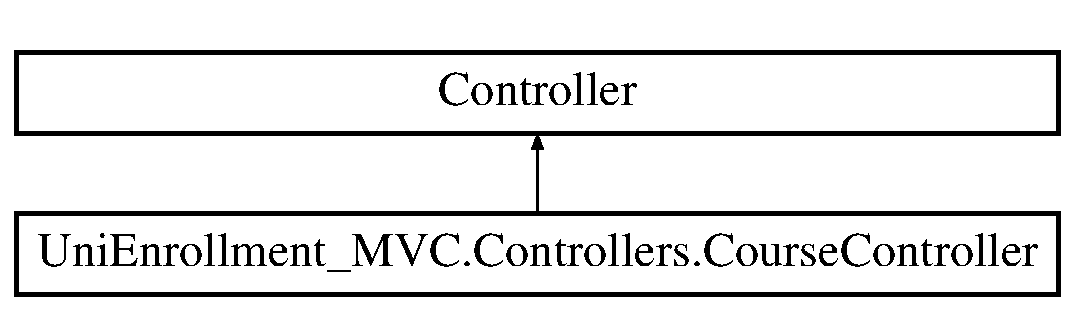
\includegraphics[height=2.000000cm]{class_uni_enrollment___m_v_c_1_1_controllers_1_1_course_controller}
\end{center}
\end{figure}
\subsection*{Public Member Functions}
\begin{DoxyCompactItemize}
\item 
Action\+Result \hyperlink{class_uni_enrollment___m_v_c_1_1_controllers_1_1_course_controller_aa5e87de4b61069e9e8a0c043dba39b16}{Index} ()
\item 
Action\+Result \hyperlink{class_uni_enrollment___m_v_c_1_1_controllers_1_1_course_controller_a94fc9ba28bf6cd5db521baa83f255609}{Create} ()
\item 
Action\+Result \hyperlink{class_uni_enrollment___m_v_c_1_1_controllers_1_1_course_controller_a28c4bc5a9d4857c2d0e2b0fdb86e924f}{Create\+With\+ID} (int?id)
\item 
Action\+Result \hyperlink{class_uni_enrollment___m_v_c_1_1_controllers_1_1_course_controller_a475949106d06d3a424f2f6b5302eee4d}{Submit\+Create} (\hyperlink{class_uni_enrollment___m_v_c_1_1_models_1_1_course_view_model}{Course\+View\+Model} vm\+Course)
\item 
Action\+Result \hyperlink{class_uni_enrollment___m_v_c_1_1_controllers_1_1_course_controller_ac5a80df6e72b44416b08f4709aa419be}{Details} (int?id)
\item 
Action\+Result \hyperlink{class_uni_enrollment___m_v_c_1_1_controllers_1_1_course_controller_afbd3818476231bac5a4b6f62a332b761}{Edit} (int?id)
\item 
Action\+Result \hyperlink{class_uni_enrollment___m_v_c_1_1_controllers_1_1_course_controller_a5ca4c1b9b6f045ff39829382838e3f4f}{Submit\+Edit} (\hyperlink{class_uni_enrollment___m_v_c_1_1_models_1_1_course}{Course} course)
\item 
Action\+Result \hyperlink{class_uni_enrollment___m_v_c_1_1_controllers_1_1_course_controller_aa918186ab2eca76077356857755580a7}{Delete} (int?id)
\end{DoxyCompactItemize}
\subsection*{Private Attributes}
\begin{DoxyCompactItemize}
\item 
\hyperlink{class_uni_enrollment___m_v_c_1_1_models_1_1_uni_enrollment_d_b_entities}{Uni\+Enrollment\+D\+B\+Entities} \hyperlink{class_uni_enrollment___m_v_c_1_1_controllers_1_1_course_controller_a4e242bdfa42da214528bfe2737274c9f}{\+\_\+entities} = new \hyperlink{class_uni_enrollment___m_v_c_1_1_models_1_1_uni_enrollment_d_b_entities}{Uni\+Enrollment\+D\+B\+Entities}()
\end{DoxyCompactItemize}


\subsection{Detailed Description}
Contains user interaction (action result) methods for anything uni \textquotesingle{}course\textquotesingle{} related 



Definition at line 15 of file Course\+Controller.\+cs.



\subsection{Member Function Documentation}
\index{Uni\+Enrollment\+\_\+\+M\+V\+C\+::\+Controllers\+::\+Course\+Controller@{Uni\+Enrollment\+\_\+\+M\+V\+C\+::\+Controllers\+::\+Course\+Controller}!Create@{Create}}
\index{Create@{Create}!Uni\+Enrollment\+\_\+\+M\+V\+C\+::\+Controllers\+::\+Course\+Controller@{Uni\+Enrollment\+\_\+\+M\+V\+C\+::\+Controllers\+::\+Course\+Controller}}
\subsubsection[{\texorpdfstring{Create()}{Create()}}]{\setlength{\rightskip}{0pt plus 5cm}Action\+Result Uni\+Enrollment\+\_\+\+M\+V\+C.\+Controllers.\+Course\+Controller.\+Create (
\begin{DoxyParamCaption}
{}
\end{DoxyParamCaption}
)}\hypertarget{class_uni_enrollment___m_v_c_1_1_controllers_1_1_course_controller_a94fc9ba28bf6cd5db521baa83f255609}{}\label{class_uni_enrollment___m_v_c_1_1_controllers_1_1_course_controller_a94fc9ba28bf6cd5db521baa83f255609}


Definition at line 25 of file Course\+Controller.\+cs.

\index{Uni\+Enrollment\+\_\+\+M\+V\+C\+::\+Controllers\+::\+Course\+Controller@{Uni\+Enrollment\+\_\+\+M\+V\+C\+::\+Controllers\+::\+Course\+Controller}!Create\+With\+ID@{Create\+With\+ID}}
\index{Create\+With\+ID@{Create\+With\+ID}!Uni\+Enrollment\+\_\+\+M\+V\+C\+::\+Controllers\+::\+Course\+Controller@{Uni\+Enrollment\+\_\+\+M\+V\+C\+::\+Controllers\+::\+Course\+Controller}}
\subsubsection[{\texorpdfstring{Create\+With\+I\+D(int?id)}{CreateWithID(int?id)}}]{\setlength{\rightskip}{0pt plus 5cm}Action\+Result Uni\+Enrollment\+\_\+\+M\+V\+C.\+Controllers.\+Course\+Controller.\+Create\+With\+ID (
\begin{DoxyParamCaption}
\item[{int?}]{id}
\end{DoxyParamCaption}
)}\hypertarget{class_uni_enrollment___m_v_c_1_1_controllers_1_1_course_controller_a28c4bc5a9d4857c2d0e2b0fdb86e924f}{}\label{class_uni_enrollment___m_v_c_1_1_controllers_1_1_course_controller_a28c4bc5a9d4857c2d0e2b0fdb86e924f}


Definition at line 38 of file Course\+Controller.\+cs.

\index{Uni\+Enrollment\+\_\+\+M\+V\+C\+::\+Controllers\+::\+Course\+Controller@{Uni\+Enrollment\+\_\+\+M\+V\+C\+::\+Controllers\+::\+Course\+Controller}!Delete@{Delete}}
\index{Delete@{Delete}!Uni\+Enrollment\+\_\+\+M\+V\+C\+::\+Controllers\+::\+Course\+Controller@{Uni\+Enrollment\+\_\+\+M\+V\+C\+::\+Controllers\+::\+Course\+Controller}}
\subsubsection[{\texorpdfstring{Delete(int?id)}{Delete(int?id)}}]{\setlength{\rightskip}{0pt plus 5cm}Action\+Result Uni\+Enrollment\+\_\+\+M\+V\+C.\+Controllers.\+Course\+Controller.\+Delete (
\begin{DoxyParamCaption}
\item[{int?}]{id}
\end{DoxyParamCaption}
)}\hypertarget{class_uni_enrollment___m_v_c_1_1_controllers_1_1_course_controller_aa918186ab2eca76077356857755580a7}{}\label{class_uni_enrollment___m_v_c_1_1_controllers_1_1_course_controller_aa918186ab2eca76077356857755580a7}


Definition at line 141 of file Course\+Controller.\+cs.

\index{Uni\+Enrollment\+\_\+\+M\+V\+C\+::\+Controllers\+::\+Course\+Controller@{Uni\+Enrollment\+\_\+\+M\+V\+C\+::\+Controllers\+::\+Course\+Controller}!Details@{Details}}
\index{Details@{Details}!Uni\+Enrollment\+\_\+\+M\+V\+C\+::\+Controllers\+::\+Course\+Controller@{Uni\+Enrollment\+\_\+\+M\+V\+C\+::\+Controllers\+::\+Course\+Controller}}
\subsubsection[{\texorpdfstring{Details(int?id)}{Details(int?id)}}]{\setlength{\rightskip}{0pt plus 5cm}Action\+Result Uni\+Enrollment\+\_\+\+M\+V\+C.\+Controllers.\+Course\+Controller.\+Details (
\begin{DoxyParamCaption}
\item[{int?}]{id}
\end{DoxyParamCaption}
)}\hypertarget{class_uni_enrollment___m_v_c_1_1_controllers_1_1_course_controller_ac5a80df6e72b44416b08f4709aa419be}{}\label{class_uni_enrollment___m_v_c_1_1_controllers_1_1_course_controller_ac5a80df6e72b44416b08f4709aa419be}


Definition at line 89 of file Course\+Controller.\+cs.

\index{Uni\+Enrollment\+\_\+\+M\+V\+C\+::\+Controllers\+::\+Course\+Controller@{Uni\+Enrollment\+\_\+\+M\+V\+C\+::\+Controllers\+::\+Course\+Controller}!Edit@{Edit}}
\index{Edit@{Edit}!Uni\+Enrollment\+\_\+\+M\+V\+C\+::\+Controllers\+::\+Course\+Controller@{Uni\+Enrollment\+\_\+\+M\+V\+C\+::\+Controllers\+::\+Course\+Controller}}
\subsubsection[{\texorpdfstring{Edit(int?id)}{Edit(int?id)}}]{\setlength{\rightskip}{0pt plus 5cm}Action\+Result Uni\+Enrollment\+\_\+\+M\+V\+C.\+Controllers.\+Course\+Controller.\+Edit (
\begin{DoxyParamCaption}
\item[{int?}]{id}
\end{DoxyParamCaption}
)}\hypertarget{class_uni_enrollment___m_v_c_1_1_controllers_1_1_course_controller_afbd3818476231bac5a4b6f62a332b761}{}\label{class_uni_enrollment___m_v_c_1_1_controllers_1_1_course_controller_afbd3818476231bac5a4b6f62a332b761}


Definition at line 103 of file Course\+Controller.\+cs.

\index{Uni\+Enrollment\+\_\+\+M\+V\+C\+::\+Controllers\+::\+Course\+Controller@{Uni\+Enrollment\+\_\+\+M\+V\+C\+::\+Controllers\+::\+Course\+Controller}!Index@{Index}}
\index{Index@{Index}!Uni\+Enrollment\+\_\+\+M\+V\+C\+::\+Controllers\+::\+Course\+Controller@{Uni\+Enrollment\+\_\+\+M\+V\+C\+::\+Controllers\+::\+Course\+Controller}}
\subsubsection[{\texorpdfstring{Index()}{Index()}}]{\setlength{\rightskip}{0pt plus 5cm}Action\+Result Uni\+Enrollment\+\_\+\+M\+V\+C.\+Controllers.\+Course\+Controller.\+Index (
\begin{DoxyParamCaption}
{}
\end{DoxyParamCaption}
)}\hypertarget{class_uni_enrollment___m_v_c_1_1_controllers_1_1_course_controller_aa5e87de4b61069e9e8a0c043dba39b16}{}\label{class_uni_enrollment___m_v_c_1_1_controllers_1_1_course_controller_aa5e87de4b61069e9e8a0c043dba39b16}


Definition at line 19 of file Course\+Controller.\+cs.

\index{Uni\+Enrollment\+\_\+\+M\+V\+C\+::\+Controllers\+::\+Course\+Controller@{Uni\+Enrollment\+\_\+\+M\+V\+C\+::\+Controllers\+::\+Course\+Controller}!Submit\+Create@{Submit\+Create}}
\index{Submit\+Create@{Submit\+Create}!Uni\+Enrollment\+\_\+\+M\+V\+C\+::\+Controllers\+::\+Course\+Controller@{Uni\+Enrollment\+\_\+\+M\+V\+C\+::\+Controllers\+::\+Course\+Controller}}
\subsubsection[{\texorpdfstring{Submit\+Create(\+Course\+View\+Model vm\+Course)}{SubmitCreate(CourseViewModel vmCourse)}}]{\setlength{\rightskip}{0pt plus 5cm}Action\+Result Uni\+Enrollment\+\_\+\+M\+V\+C.\+Controllers.\+Course\+Controller.\+Submit\+Create (
\begin{DoxyParamCaption}
\item[{{\bf Course\+View\+Model}}]{vm\+Course}
\end{DoxyParamCaption}
)}\hypertarget{class_uni_enrollment___m_v_c_1_1_controllers_1_1_course_controller_a475949106d06d3a424f2f6b5302eee4d}{}\label{class_uni_enrollment___m_v_c_1_1_controllers_1_1_course_controller_a475949106d06d3a424f2f6b5302eee4d}


Definition at line 53 of file Course\+Controller.\+cs.

\index{Uni\+Enrollment\+\_\+\+M\+V\+C\+::\+Controllers\+::\+Course\+Controller@{Uni\+Enrollment\+\_\+\+M\+V\+C\+::\+Controllers\+::\+Course\+Controller}!Submit\+Edit@{Submit\+Edit}}
\index{Submit\+Edit@{Submit\+Edit}!Uni\+Enrollment\+\_\+\+M\+V\+C\+::\+Controllers\+::\+Course\+Controller@{Uni\+Enrollment\+\_\+\+M\+V\+C\+::\+Controllers\+::\+Course\+Controller}}
\subsubsection[{\texorpdfstring{Submit\+Edit(\+Course course)}{SubmitEdit(Course course)}}]{\setlength{\rightskip}{0pt plus 5cm}Action\+Result Uni\+Enrollment\+\_\+\+M\+V\+C.\+Controllers.\+Course\+Controller.\+Submit\+Edit (
\begin{DoxyParamCaption}
\item[{{\bf Course}}]{course}
\end{DoxyParamCaption}
)}\hypertarget{class_uni_enrollment___m_v_c_1_1_controllers_1_1_course_controller_a5ca4c1b9b6f045ff39829382838e3f4f}{}\label{class_uni_enrollment___m_v_c_1_1_controllers_1_1_course_controller_a5ca4c1b9b6f045ff39829382838e3f4f}


Definition at line 126 of file Course\+Controller.\+cs.



\subsection{Member Data Documentation}
\index{Uni\+Enrollment\+\_\+\+M\+V\+C\+::\+Controllers\+::\+Course\+Controller@{Uni\+Enrollment\+\_\+\+M\+V\+C\+::\+Controllers\+::\+Course\+Controller}!\+\_\+entities@{\+\_\+entities}}
\index{\+\_\+entities@{\+\_\+entities}!Uni\+Enrollment\+\_\+\+M\+V\+C\+::\+Controllers\+::\+Course\+Controller@{Uni\+Enrollment\+\_\+\+M\+V\+C\+::\+Controllers\+::\+Course\+Controller}}
\subsubsection[{\texorpdfstring{\+\_\+entities}{_entities}}]{\setlength{\rightskip}{0pt plus 5cm}{\bf Uni\+Enrollment\+D\+B\+Entities} Uni\+Enrollment\+\_\+\+M\+V\+C.\+Controllers.\+Course\+Controller.\+\_\+entities = new {\bf Uni\+Enrollment\+D\+B\+Entities}()\hspace{0.3cm}{\ttfamily [private]}}\hypertarget{class_uni_enrollment___m_v_c_1_1_controllers_1_1_course_controller_a4e242bdfa42da214528bfe2737274c9f}{}\label{class_uni_enrollment___m_v_c_1_1_controllers_1_1_course_controller_a4e242bdfa42da214528bfe2737274c9f}


Definition at line 17 of file Course\+Controller.\+cs.



The documentation for this class was generated from the following file\+:\begin{DoxyCompactItemize}
\item 
H\+:/\+Documents/\+Work/\+Repositories/\+Uni\+Enrollment-\/\+D\+E\+M\+O/\+Uni\+Enrollment-\/\+M\+V\+C/\+Controllers/\hyperlink{_course_controller_8cs}{Course\+Controller.\+cs}\end{DoxyCompactItemize}

\hypertarget{class_uni_enrollment___m_v_c_1_1_models_1_1_course_d_b_context}{}\section{Uni\+Enrollment\+\_\+\+M\+V\+C.\+Models.\+Course\+D\+B\+Context Class Reference}
\label{class_uni_enrollment___m_v_c_1_1_models_1_1_course_d_b_context}\index{Uni\+Enrollment\+\_\+\+M\+V\+C.\+Models.\+Course\+D\+B\+Context@{Uni\+Enrollment\+\_\+\+M\+V\+C.\+Models.\+Course\+D\+B\+Context}}
Inheritance diagram for Uni\+Enrollment\+\_\+\+M\+V\+C.\+Models.\+Course\+D\+B\+Context\+:\begin{figure}[H]
\begin{center}
\leavevmode
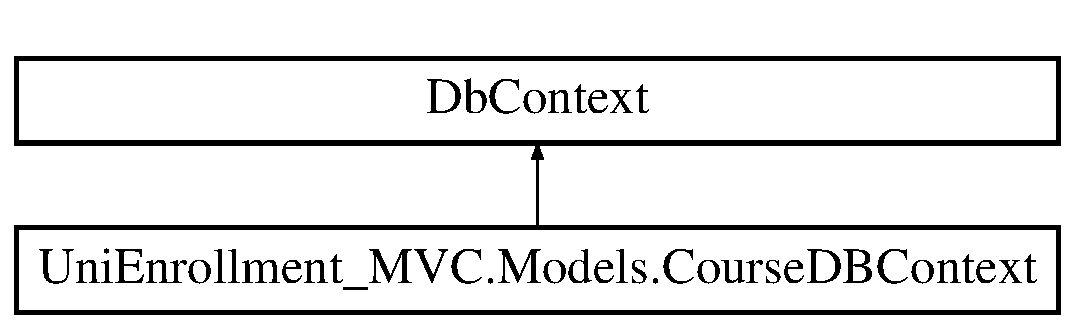
\includegraphics[height=2.000000cm]{class_uni_enrollment___m_v_c_1_1_models_1_1_course_d_b_context}
\end{center}
\end{figure}
\subsection*{Public Member Functions}
\begin{DoxyCompactItemize}
\item 
\hyperlink{class_uni_enrollment___m_v_c_1_1_models_1_1_course_d_b_context_a2c8fbc695a4f7ab1435fe0e5bb7feb76}{Course\+D\+B\+Context} ()
\end{DoxyCompactItemize}
\subsection*{Protected Member Functions}
\begin{DoxyCompactItemize}
\item 
override void \hyperlink{class_uni_enrollment___m_v_c_1_1_models_1_1_course_d_b_context_a0fe32c3c10feabfa9b142fa3a3703452}{On\+Model\+Creating} (Db\+Model\+Builder model\+Builder)
\end{DoxyCompactItemize}
\subsection*{Properties}
\begin{DoxyCompactItemize}
\item 
Db\+Set$<$ \hyperlink{class_uni_enrollment___m_v_c_1_1_models_1_1_course}{Course} $>$ \hyperlink{class_uni_enrollment___m_v_c_1_1_models_1_1_course_d_b_context_ae3387c6f33aaa416639b69b2cc34fba0}{Courses}\hspace{0.3cm}{\ttfamily  \mbox{[}get, set\mbox{]}}
\end{DoxyCompactItemize}


\subsection{Detailed Description}


Definition at line 6 of file Course\+D\+B\+Context.\+cs.



\subsection{Constructor \& Destructor Documentation}
\index{Uni\+Enrollment\+\_\+\+M\+V\+C\+::\+Models\+::\+Course\+D\+B\+Context@{Uni\+Enrollment\+\_\+\+M\+V\+C\+::\+Models\+::\+Course\+D\+B\+Context}!Course\+D\+B\+Context@{Course\+D\+B\+Context}}
\index{Course\+D\+B\+Context@{Course\+D\+B\+Context}!Uni\+Enrollment\+\_\+\+M\+V\+C\+::\+Models\+::\+Course\+D\+B\+Context@{Uni\+Enrollment\+\_\+\+M\+V\+C\+::\+Models\+::\+Course\+D\+B\+Context}}
\subsubsection[{\texorpdfstring{Course\+D\+B\+Context()}{CourseDBContext()}}]{\setlength{\rightskip}{0pt plus 5cm}Uni\+Enrollment\+\_\+\+M\+V\+C.\+Models.\+Course\+D\+B\+Context.\+Course\+D\+B\+Context (
\begin{DoxyParamCaption}
{}
\end{DoxyParamCaption}
)}\hypertarget{class_uni_enrollment___m_v_c_1_1_models_1_1_course_d_b_context_a2c8fbc695a4f7ab1435fe0e5bb7feb76}{}\label{class_uni_enrollment___m_v_c_1_1_models_1_1_course_d_b_context_a2c8fbc695a4f7ab1435fe0e5bb7feb76}


Definition at line 8 of file Course\+D\+B\+Context.\+cs.



\subsection{Member Function Documentation}
\index{Uni\+Enrollment\+\_\+\+M\+V\+C\+::\+Models\+::\+Course\+D\+B\+Context@{Uni\+Enrollment\+\_\+\+M\+V\+C\+::\+Models\+::\+Course\+D\+B\+Context}!On\+Model\+Creating@{On\+Model\+Creating}}
\index{On\+Model\+Creating@{On\+Model\+Creating}!Uni\+Enrollment\+\_\+\+M\+V\+C\+::\+Models\+::\+Course\+D\+B\+Context@{Uni\+Enrollment\+\_\+\+M\+V\+C\+::\+Models\+::\+Course\+D\+B\+Context}}
\subsubsection[{\texorpdfstring{On\+Model\+Creating(\+Db\+Model\+Builder model\+Builder)}{OnModelCreating(DbModelBuilder modelBuilder)}}]{\setlength{\rightskip}{0pt plus 5cm}override void Uni\+Enrollment\+\_\+\+M\+V\+C.\+Models.\+Course\+D\+B\+Context.\+On\+Model\+Creating (
\begin{DoxyParamCaption}
\item[{Db\+Model\+Builder}]{model\+Builder}
\end{DoxyParamCaption}
)\hspace{0.3cm}{\ttfamily [protected]}}\hypertarget{class_uni_enrollment___m_v_c_1_1_models_1_1_course_d_b_context_a0fe32c3c10feabfa9b142fa3a3703452}{}\label{class_uni_enrollment___m_v_c_1_1_models_1_1_course_d_b_context_a0fe32c3c10feabfa9b142fa3a3703452}


Definition at line 12 of file Course\+D\+B\+Context.\+cs.



\subsection{Property Documentation}
\index{Uni\+Enrollment\+\_\+\+M\+V\+C\+::\+Models\+::\+Course\+D\+B\+Context@{Uni\+Enrollment\+\_\+\+M\+V\+C\+::\+Models\+::\+Course\+D\+B\+Context}!Courses@{Courses}}
\index{Courses@{Courses}!Uni\+Enrollment\+\_\+\+M\+V\+C\+::\+Models\+::\+Course\+D\+B\+Context@{Uni\+Enrollment\+\_\+\+M\+V\+C\+::\+Models\+::\+Course\+D\+B\+Context}}
\subsubsection[{\texorpdfstring{Courses}{Courses}}]{\setlength{\rightskip}{0pt plus 5cm}Db\+Set$<${\bf Course}$>$ Uni\+Enrollment\+\_\+\+M\+V\+C.\+Models.\+Course\+D\+B\+Context.\+Courses\hspace{0.3cm}{\ttfamily [get]}, {\ttfamily [set]}}\hypertarget{class_uni_enrollment___m_v_c_1_1_models_1_1_course_d_b_context_ae3387c6f33aaa416639b69b2cc34fba0}{}\label{class_uni_enrollment___m_v_c_1_1_models_1_1_course_d_b_context_ae3387c6f33aaa416639b69b2cc34fba0}


Definition at line 26 of file Course\+D\+B\+Context.\+cs.



The documentation for this class was generated from the following file\+:\begin{DoxyCompactItemize}
\item 
H\+:/\+Documents/\+Work/\+Repositories/\+Uni\+Enrollment-\/\+D\+E\+M\+O/\+Uni\+Enrollment-\/\+M\+V\+C/\+Context/\hyperlink{_course_d_b_context_8cs}{Course\+D\+B\+Context.\+cs}\end{DoxyCompactItemize}

\hypertarget{class_uni_enrollment___m_v_c_1_1_models_1_1_course_view_model}{}\section{Uni\+Enrollment\+\_\+\+M\+V\+C.\+Models.\+Course\+View\+Model Class Reference}
\label{class_uni_enrollment___m_v_c_1_1_models_1_1_course_view_model}\index{Uni\+Enrollment\+\_\+\+M\+V\+C.\+Models.\+Course\+View\+Model@{Uni\+Enrollment\+\_\+\+M\+V\+C.\+Models.\+Course\+View\+Model}}
\subsection*{Static Public Member Functions}
\begin{DoxyCompactItemize}
\item 
static string \hyperlink{class_uni_enrollment___m_v_c_1_1_models_1_1_course_view_model_a976367559f2ac0f57f873769aa4a3377}{Get\+Professor\+Name\+By\+ID} (int id)
\begin{DoxyCompactList}\small\item\em Returns the user \textquotesingle{}Name\textquotesingle{} from their ID. Not strinctly required for most related views, the business models (seen in the Data\+Mode.\+edmx) are related so you can just call from e.\+g. Model.\+Course.\+Professor.\+Name however I used this out of scope once so it\textquotesingle{}s useful \end{DoxyCompactList}\item 
static List$<$ \hyperlink{class_uni_enrollment___m_v_c_1_1_models_1_1_course}{Course} $>$ \hyperlink{class_uni_enrollment___m_v_c_1_1_models_1_1_course_view_model_acdcd8c1864587d0c8ab23e460ed8d901}{Get\+Course\+List} ()
\begin{DoxyCompactList}\small\item\em Returns a list of courses specifically for use in drop down lsits \end{DoxyCompactList}\item 
static List$<$ \hyperlink{class_uni_enrollment___m_v_c_1_1_models_1_1_course}{Course} $>$ \hyperlink{class_uni_enrollment___m_v_c_1_1_models_1_1_course_view_model_a295886fe092d5245f6685ca0ff78bf3f}{Get\+Course\+List\+By\+Professor\+ID} (int id)
\begin{DoxyCompactList}\small\item\em Get a list of courses ran by a specific professor \end{DoxyCompactList}\end{DoxyCompactItemize}
\subsection*{Properties}
\begin{DoxyCompactItemize}
\item 
int \hyperlink{class_uni_enrollment___m_v_c_1_1_models_1_1_course_view_model_a6cdbca7e6c66c9505f4846935b355d6a}{ID}\hspace{0.3cm}{\ttfamily  \mbox{[}get, set\mbox{]}}
\item 
int \hyperlink{class_uni_enrollment___m_v_c_1_1_models_1_1_course_view_model_a8fac888ed7328928c0551a8b0f2c85e8}{Professor\+ID}\hspace{0.3cm}{\ttfamily  \mbox{[}get, set\mbox{]}}
\item 
string \hyperlink{class_uni_enrollment___m_v_c_1_1_models_1_1_course_view_model_abf48fa3094f898b40071925f91e25e58}{Course\+Code}\hspace{0.3cm}{\ttfamily  \mbox{[}get, set\mbox{]}}
\item 
string \hyperlink{class_uni_enrollment___m_v_c_1_1_models_1_1_course_view_model_a0ef4a9c7d23d04916bdc2202afea3a3f}{Name}\hspace{0.3cm}{\ttfamily  \mbox{[}get, set\mbox{]}}
\item 
string \hyperlink{class_uni_enrollment___m_v_c_1_1_models_1_1_course_view_model_a6f025e7e960e0cd91fb73c6e947e055d}{Description}\hspace{0.3cm}{\ttfamily  \mbox{[}get, set\mbox{]}}
\end{DoxyCompactItemize}


\subsection{Detailed Description}


Definition at line 8 of file Course\+View\+Model.\+cs.



\subsection{Member Function Documentation}
\index{Uni\+Enrollment\+\_\+\+M\+V\+C\+::\+Models\+::\+Course\+View\+Model@{Uni\+Enrollment\+\_\+\+M\+V\+C\+::\+Models\+::\+Course\+View\+Model}!Get\+Course\+List@{Get\+Course\+List}}
\index{Get\+Course\+List@{Get\+Course\+List}!Uni\+Enrollment\+\_\+\+M\+V\+C\+::\+Models\+::\+Course\+View\+Model@{Uni\+Enrollment\+\_\+\+M\+V\+C\+::\+Models\+::\+Course\+View\+Model}}
\subsubsection[{\texorpdfstring{Get\+Course\+List()}{GetCourseList()}}]{\setlength{\rightskip}{0pt plus 5cm}static List$<${\bf Course}$>$ Uni\+Enrollment\+\_\+\+M\+V\+C.\+Models.\+Course\+View\+Model.\+Get\+Course\+List (
\begin{DoxyParamCaption}
{}
\end{DoxyParamCaption}
)\hspace{0.3cm}{\ttfamily [static]}}\hypertarget{class_uni_enrollment___m_v_c_1_1_models_1_1_course_view_model_acdcd8c1864587d0c8ab23e460ed8d901}{}\label{class_uni_enrollment___m_v_c_1_1_models_1_1_course_view_model_acdcd8c1864587d0c8ab23e460ed8d901}


Returns a list of courses specifically for use in drop down lsits 

\begin{DoxyReturn}{Returns}
List of courses
\end{DoxyReturn}


Definition at line 47 of file Course\+View\+Model.\+cs.

\index{Uni\+Enrollment\+\_\+\+M\+V\+C\+::\+Models\+::\+Course\+View\+Model@{Uni\+Enrollment\+\_\+\+M\+V\+C\+::\+Models\+::\+Course\+View\+Model}!Get\+Course\+List\+By\+Professor\+ID@{Get\+Course\+List\+By\+Professor\+ID}}
\index{Get\+Course\+List\+By\+Professor\+ID@{Get\+Course\+List\+By\+Professor\+ID}!Uni\+Enrollment\+\_\+\+M\+V\+C\+::\+Models\+::\+Course\+View\+Model@{Uni\+Enrollment\+\_\+\+M\+V\+C\+::\+Models\+::\+Course\+View\+Model}}
\subsubsection[{\texorpdfstring{Get\+Course\+List\+By\+Professor\+I\+D(int id)}{GetCourseListByProfessorID(int id)}}]{\setlength{\rightskip}{0pt plus 5cm}static List$<${\bf Course}$>$ Uni\+Enrollment\+\_\+\+M\+V\+C.\+Models.\+Course\+View\+Model.\+Get\+Course\+List\+By\+Professor\+ID (
\begin{DoxyParamCaption}
\item[{int}]{id}
\end{DoxyParamCaption}
)\hspace{0.3cm}{\ttfamily [static]}}\hypertarget{class_uni_enrollment___m_v_c_1_1_models_1_1_course_view_model_a295886fe092d5245f6685ca0ff78bf3f}{}\label{class_uni_enrollment___m_v_c_1_1_models_1_1_course_view_model_a295886fe092d5245f6685ca0ff78bf3f}


Get a list of courses ran by a specific professor 


\begin{DoxyParams}{Parameters}
{\em id} & ID of professor (or user)\\
\hline
\end{DoxyParams}
\begin{DoxyReturn}{Returns}
List of courses ran by specific professor
\end{DoxyReturn}


Definition at line 57 of file Course\+View\+Model.\+cs.

\index{Uni\+Enrollment\+\_\+\+M\+V\+C\+::\+Models\+::\+Course\+View\+Model@{Uni\+Enrollment\+\_\+\+M\+V\+C\+::\+Models\+::\+Course\+View\+Model}!Get\+Professor\+Name\+By\+ID@{Get\+Professor\+Name\+By\+ID}}
\index{Get\+Professor\+Name\+By\+ID@{Get\+Professor\+Name\+By\+ID}!Uni\+Enrollment\+\_\+\+M\+V\+C\+::\+Models\+::\+Course\+View\+Model@{Uni\+Enrollment\+\_\+\+M\+V\+C\+::\+Models\+::\+Course\+View\+Model}}
\subsubsection[{\texorpdfstring{Get\+Professor\+Name\+By\+I\+D(int id)}{GetProfessorNameByID(int id)}}]{\setlength{\rightskip}{0pt plus 5cm}static string Uni\+Enrollment\+\_\+\+M\+V\+C.\+Models.\+Course\+View\+Model.\+Get\+Professor\+Name\+By\+ID (
\begin{DoxyParamCaption}
\item[{int}]{id}
\end{DoxyParamCaption}
)\hspace{0.3cm}{\ttfamily [static]}}\hypertarget{class_uni_enrollment___m_v_c_1_1_models_1_1_course_view_model_a976367559f2ac0f57f873769aa4a3377}{}\label{class_uni_enrollment___m_v_c_1_1_models_1_1_course_view_model_a976367559f2ac0f57f873769aa4a3377}


Returns the user \textquotesingle{}Name\textquotesingle{} from their ID. Not strinctly required for most related views, the business models (seen in the Data\+Mode.\+edmx) are related so you can just call from e.\+g. Model.\+Course.\+Professor.\+Name however I used this out of scope once so it\textquotesingle{}s useful 


\begin{DoxyParams}{Parameters}
{\em id} & ID of user\\
\hline
\end{DoxyParams}
\begin{DoxyReturn}{Returns}
Name of the professor (or user)
\end{DoxyReturn}


Definition at line 38 of file Course\+View\+Model.\+cs.



\subsection{Property Documentation}
\index{Uni\+Enrollment\+\_\+\+M\+V\+C\+::\+Models\+::\+Course\+View\+Model@{Uni\+Enrollment\+\_\+\+M\+V\+C\+::\+Models\+::\+Course\+View\+Model}!Course\+Code@{Course\+Code}}
\index{Course\+Code@{Course\+Code}!Uni\+Enrollment\+\_\+\+M\+V\+C\+::\+Models\+::\+Course\+View\+Model@{Uni\+Enrollment\+\_\+\+M\+V\+C\+::\+Models\+::\+Course\+View\+Model}}
\subsubsection[{\texorpdfstring{Course\+Code}{CourseCode}}]{\setlength{\rightskip}{0pt plus 5cm}string Uni\+Enrollment\+\_\+\+M\+V\+C.\+Models.\+Course\+View\+Model.\+Course\+Code\hspace{0.3cm}{\ttfamily [get]}, {\ttfamily [set]}}\hypertarget{class_uni_enrollment___m_v_c_1_1_models_1_1_course_view_model_abf48fa3094f898b40071925f91e25e58}{}\label{class_uni_enrollment___m_v_c_1_1_models_1_1_course_view_model_abf48fa3094f898b40071925f91e25e58}


Definition at line 19 of file Course\+View\+Model.\+cs.

\index{Uni\+Enrollment\+\_\+\+M\+V\+C\+::\+Models\+::\+Course\+View\+Model@{Uni\+Enrollment\+\_\+\+M\+V\+C\+::\+Models\+::\+Course\+View\+Model}!Description@{Description}}
\index{Description@{Description}!Uni\+Enrollment\+\_\+\+M\+V\+C\+::\+Models\+::\+Course\+View\+Model@{Uni\+Enrollment\+\_\+\+M\+V\+C\+::\+Models\+::\+Course\+View\+Model}}
\subsubsection[{\texorpdfstring{Description}{Description}}]{\setlength{\rightskip}{0pt plus 5cm}string Uni\+Enrollment\+\_\+\+M\+V\+C.\+Models.\+Course\+View\+Model.\+Description\hspace{0.3cm}{\ttfamily [get]}, {\ttfamily [set]}}\hypertarget{class_uni_enrollment___m_v_c_1_1_models_1_1_course_view_model_a6f025e7e960e0cd91fb73c6e947e055d}{}\label{class_uni_enrollment___m_v_c_1_1_models_1_1_course_view_model_a6f025e7e960e0cd91fb73c6e947e055d}


Definition at line 29 of file Course\+View\+Model.\+cs.

\index{Uni\+Enrollment\+\_\+\+M\+V\+C\+::\+Models\+::\+Course\+View\+Model@{Uni\+Enrollment\+\_\+\+M\+V\+C\+::\+Models\+::\+Course\+View\+Model}!ID@{ID}}
\index{ID@{ID}!Uni\+Enrollment\+\_\+\+M\+V\+C\+::\+Models\+::\+Course\+View\+Model@{Uni\+Enrollment\+\_\+\+M\+V\+C\+::\+Models\+::\+Course\+View\+Model}}
\subsubsection[{\texorpdfstring{ID}{ID}}]{\setlength{\rightskip}{0pt plus 5cm}int Uni\+Enrollment\+\_\+\+M\+V\+C.\+Models.\+Course\+View\+Model.\+ID\hspace{0.3cm}{\ttfamily [get]}, {\ttfamily [set]}}\hypertarget{class_uni_enrollment___m_v_c_1_1_models_1_1_course_view_model_a6cdbca7e6c66c9505f4846935b355d6a}{}\label{class_uni_enrollment___m_v_c_1_1_models_1_1_course_view_model_a6cdbca7e6c66c9505f4846935b355d6a}


Definition at line 10 of file Course\+View\+Model.\+cs.

\index{Uni\+Enrollment\+\_\+\+M\+V\+C\+::\+Models\+::\+Course\+View\+Model@{Uni\+Enrollment\+\_\+\+M\+V\+C\+::\+Models\+::\+Course\+View\+Model}!Name@{Name}}
\index{Name@{Name}!Uni\+Enrollment\+\_\+\+M\+V\+C\+::\+Models\+::\+Course\+View\+Model@{Uni\+Enrollment\+\_\+\+M\+V\+C\+::\+Models\+::\+Course\+View\+Model}}
\subsubsection[{\texorpdfstring{Name}{Name}}]{\setlength{\rightskip}{0pt plus 5cm}string Uni\+Enrollment\+\_\+\+M\+V\+C.\+Models.\+Course\+View\+Model.\+Name\hspace{0.3cm}{\ttfamily [get]}, {\ttfamily [set]}}\hypertarget{class_uni_enrollment___m_v_c_1_1_models_1_1_course_view_model_a0ef4a9c7d23d04916bdc2202afea3a3f}{}\label{class_uni_enrollment___m_v_c_1_1_models_1_1_course_view_model_a0ef4a9c7d23d04916bdc2202afea3a3f}


Definition at line 24 of file Course\+View\+Model.\+cs.

\index{Uni\+Enrollment\+\_\+\+M\+V\+C\+::\+Models\+::\+Course\+View\+Model@{Uni\+Enrollment\+\_\+\+M\+V\+C\+::\+Models\+::\+Course\+View\+Model}!Professor\+ID@{Professor\+ID}}
\index{Professor\+ID@{Professor\+ID}!Uni\+Enrollment\+\_\+\+M\+V\+C\+::\+Models\+::\+Course\+View\+Model@{Uni\+Enrollment\+\_\+\+M\+V\+C\+::\+Models\+::\+Course\+View\+Model}}
\subsubsection[{\texorpdfstring{Professor\+ID}{ProfessorID}}]{\setlength{\rightskip}{0pt plus 5cm}int Uni\+Enrollment\+\_\+\+M\+V\+C.\+Models.\+Course\+View\+Model.\+Professor\+ID\hspace{0.3cm}{\ttfamily [get]}, {\ttfamily [set]}}\hypertarget{class_uni_enrollment___m_v_c_1_1_models_1_1_course_view_model_a8fac888ed7328928c0551a8b0f2c85e8}{}\label{class_uni_enrollment___m_v_c_1_1_models_1_1_course_view_model_a8fac888ed7328928c0551a8b0f2c85e8}


Definition at line 14 of file Course\+View\+Model.\+cs.



The documentation for this class was generated from the following file\+:\begin{DoxyCompactItemize}
\item 
H\+:/\+Documents/\+Work/\+Repositories/\+Uni\+Enrollment-\/\+D\+E\+M\+O/\+Uni\+Enrollment-\/\+M\+V\+C/\+Models/\hyperlink{_course_view_model_8cs}{Course\+View\+Model.\+cs}\end{DoxyCompactItemize}

\hypertarget{class_uni_enrollment___m_v_c_1_1_models_1_1_enrollment}{}\section{Uni\+Enrollment\+\_\+\+M\+V\+C.\+Models.\+Enrollment Class Reference}
\label{class_uni_enrollment___m_v_c_1_1_models_1_1_enrollment}\index{Uni\+Enrollment\+\_\+\+M\+V\+C.\+Models.\+Enrollment@{Uni\+Enrollment\+\_\+\+M\+V\+C.\+Models.\+Enrollment}}
\subsection*{Properties}
\begin{DoxyCompactItemize}
\item 
int \hyperlink{class_uni_enrollment___m_v_c_1_1_models_1_1_enrollment_a94c4c7411d5e49898f1f9e8534a05d07}{Student\+ID}\hspace{0.3cm}{\ttfamily  \mbox{[}get, set\mbox{]}}
\item 
int \hyperlink{class_uni_enrollment___m_v_c_1_1_models_1_1_enrollment_a2553a284d00f8e39de6957e3ac6e3eb4}{Course\+ID}\hspace{0.3cm}{\ttfamily  \mbox{[}get, set\mbox{]}}
\item 
System.\+Date\+Time \hyperlink{class_uni_enrollment___m_v_c_1_1_models_1_1_enrollment_a717b740b6f699a2742dc5ff98aeea11f}{Enrollment\+Date}\hspace{0.3cm}{\ttfamily  \mbox{[}get, set\mbox{]}}
\item 
virtual \hyperlink{class_uni_enrollment___m_v_c_1_1_models_1_1_course}{Course} \hyperlink{class_uni_enrollment___m_v_c_1_1_models_1_1_enrollment_af056ea66fa437f8a724b6f8916197160}{Course}\hspace{0.3cm}{\ttfamily  \mbox{[}get, set\mbox{]}}
\item 
virtual \hyperlink{class_uni_enrollment___m_v_c_1_1_models_1_1_user}{User} \hyperlink{class_uni_enrollment___m_v_c_1_1_models_1_1_enrollment_a74c6ec4f394b98e2d676f97847a255fd}{User}\hspace{0.3cm}{\ttfamily  \mbox{[}get, set\mbox{]}}
\end{DoxyCompactItemize}


\subsection{Detailed Description}


Definition at line 15 of file Enrollment.\+cs.



\subsection{Property Documentation}
\index{Uni\+Enrollment\+\_\+\+M\+V\+C\+::\+Models\+::\+Enrollment@{Uni\+Enrollment\+\_\+\+M\+V\+C\+::\+Models\+::\+Enrollment}!Course@{Course}}
\index{Course@{Course}!Uni\+Enrollment\+\_\+\+M\+V\+C\+::\+Models\+::\+Enrollment@{Uni\+Enrollment\+\_\+\+M\+V\+C\+::\+Models\+::\+Enrollment}}
\subsubsection[{\texorpdfstring{Course}{Course}}]{\setlength{\rightskip}{0pt plus 5cm}virtual {\bf Course} Uni\+Enrollment\+\_\+\+M\+V\+C.\+Models.\+Enrollment.\+Course\hspace{0.3cm}{\ttfamily [get]}, {\ttfamily [set]}}\hypertarget{class_uni_enrollment___m_v_c_1_1_models_1_1_enrollment_af056ea66fa437f8a724b6f8916197160}{}\label{class_uni_enrollment___m_v_c_1_1_models_1_1_enrollment_af056ea66fa437f8a724b6f8916197160}


Definition at line 21 of file Enrollment.\+cs.

\index{Uni\+Enrollment\+\_\+\+M\+V\+C\+::\+Models\+::\+Enrollment@{Uni\+Enrollment\+\_\+\+M\+V\+C\+::\+Models\+::\+Enrollment}!Course\+ID@{Course\+ID}}
\index{Course\+ID@{Course\+ID}!Uni\+Enrollment\+\_\+\+M\+V\+C\+::\+Models\+::\+Enrollment@{Uni\+Enrollment\+\_\+\+M\+V\+C\+::\+Models\+::\+Enrollment}}
\subsubsection[{\texorpdfstring{Course\+ID}{CourseID}}]{\setlength{\rightskip}{0pt plus 5cm}int Uni\+Enrollment\+\_\+\+M\+V\+C.\+Models.\+Enrollment.\+Course\+ID\hspace{0.3cm}{\ttfamily [get]}, {\ttfamily [set]}}\hypertarget{class_uni_enrollment___m_v_c_1_1_models_1_1_enrollment_a2553a284d00f8e39de6957e3ac6e3eb4}{}\label{class_uni_enrollment___m_v_c_1_1_models_1_1_enrollment_a2553a284d00f8e39de6957e3ac6e3eb4}


Definition at line 18 of file Enrollment.\+cs.

\index{Uni\+Enrollment\+\_\+\+M\+V\+C\+::\+Models\+::\+Enrollment@{Uni\+Enrollment\+\_\+\+M\+V\+C\+::\+Models\+::\+Enrollment}!Enrollment\+Date@{Enrollment\+Date}}
\index{Enrollment\+Date@{Enrollment\+Date}!Uni\+Enrollment\+\_\+\+M\+V\+C\+::\+Models\+::\+Enrollment@{Uni\+Enrollment\+\_\+\+M\+V\+C\+::\+Models\+::\+Enrollment}}
\subsubsection[{\texorpdfstring{Enrollment\+Date}{EnrollmentDate}}]{\setlength{\rightskip}{0pt plus 5cm}System.\+Date\+Time Uni\+Enrollment\+\_\+\+M\+V\+C.\+Models.\+Enrollment.\+Enrollment\+Date\hspace{0.3cm}{\ttfamily [get]}, {\ttfamily [set]}}\hypertarget{class_uni_enrollment___m_v_c_1_1_models_1_1_enrollment_a717b740b6f699a2742dc5ff98aeea11f}{}\label{class_uni_enrollment___m_v_c_1_1_models_1_1_enrollment_a717b740b6f699a2742dc5ff98aeea11f}


Definition at line 19 of file Enrollment.\+cs.

\index{Uni\+Enrollment\+\_\+\+M\+V\+C\+::\+Models\+::\+Enrollment@{Uni\+Enrollment\+\_\+\+M\+V\+C\+::\+Models\+::\+Enrollment}!Student\+ID@{Student\+ID}}
\index{Student\+ID@{Student\+ID}!Uni\+Enrollment\+\_\+\+M\+V\+C\+::\+Models\+::\+Enrollment@{Uni\+Enrollment\+\_\+\+M\+V\+C\+::\+Models\+::\+Enrollment}}
\subsubsection[{\texorpdfstring{Student\+ID}{StudentID}}]{\setlength{\rightskip}{0pt plus 5cm}int Uni\+Enrollment\+\_\+\+M\+V\+C.\+Models.\+Enrollment.\+Student\+ID\hspace{0.3cm}{\ttfamily [get]}, {\ttfamily [set]}}\hypertarget{class_uni_enrollment___m_v_c_1_1_models_1_1_enrollment_a94c4c7411d5e49898f1f9e8534a05d07}{}\label{class_uni_enrollment___m_v_c_1_1_models_1_1_enrollment_a94c4c7411d5e49898f1f9e8534a05d07}


Definition at line 17 of file Enrollment.\+cs.

\index{Uni\+Enrollment\+\_\+\+M\+V\+C\+::\+Models\+::\+Enrollment@{Uni\+Enrollment\+\_\+\+M\+V\+C\+::\+Models\+::\+Enrollment}!User@{User}}
\index{User@{User}!Uni\+Enrollment\+\_\+\+M\+V\+C\+::\+Models\+::\+Enrollment@{Uni\+Enrollment\+\_\+\+M\+V\+C\+::\+Models\+::\+Enrollment}}
\subsubsection[{\texorpdfstring{User}{User}}]{\setlength{\rightskip}{0pt plus 5cm}virtual {\bf User} Uni\+Enrollment\+\_\+\+M\+V\+C.\+Models.\+Enrollment.\+User\hspace{0.3cm}{\ttfamily [get]}, {\ttfamily [set]}}\hypertarget{class_uni_enrollment___m_v_c_1_1_models_1_1_enrollment_a74c6ec4f394b98e2d676f97847a255fd}{}\label{class_uni_enrollment___m_v_c_1_1_models_1_1_enrollment_a74c6ec4f394b98e2d676f97847a255fd}


Definition at line 22 of file Enrollment.\+cs.



The documentation for this class was generated from the following file\+:\begin{DoxyCompactItemize}
\item 
H\+:/\+Documents/\+Work/\+Repositories/\+Uni\+Enrollment-\/\+D\+E\+M\+O/\+Uni\+Enrollment-\/\+M\+V\+C/\+Models/\hyperlink{_enrollment_8cs}{Enrollment.\+cs}\end{DoxyCompactItemize}

\hypertarget{class_uni_enrollment___m_v_c_1_1_controllers_1_1_enrollment_controller}{}\section{Uni\+Enrollment\+\_\+\+M\+V\+C.\+Controllers.\+Enrollment\+Controller Class Reference}
\label{class_uni_enrollment___m_v_c_1_1_controllers_1_1_enrollment_controller}\index{Uni\+Enrollment\+\_\+\+M\+V\+C.\+Controllers.\+Enrollment\+Controller@{Uni\+Enrollment\+\_\+\+M\+V\+C.\+Controllers.\+Enrollment\+Controller}}


Contains user interaction (action result) methods for anything uni \textquotesingle{}enrollment\textquotesingle{} related  


Inheritance diagram for Uni\+Enrollment\+\_\+\+M\+V\+C.\+Controllers.\+Enrollment\+Controller\+:\begin{figure}[H]
\begin{center}
\leavevmode
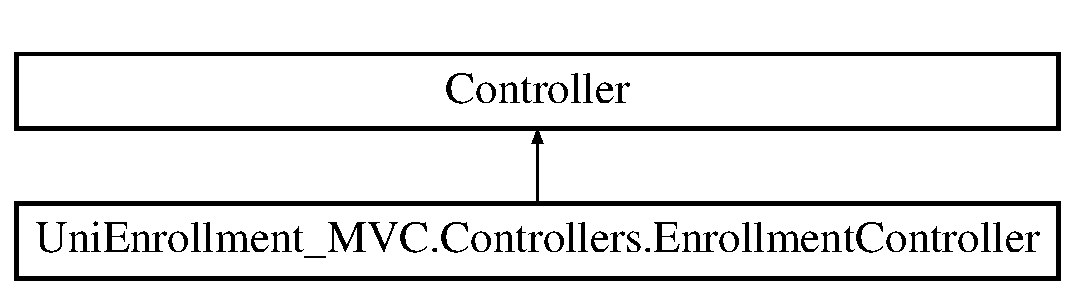
\includegraphics[height=2.000000cm]{class_uni_enrollment___m_v_c_1_1_controllers_1_1_enrollment_controller}
\end{center}
\end{figure}
\subsection*{Public Member Functions}
\begin{DoxyCompactItemize}
\item 
Action\+Result \hyperlink{class_uni_enrollment___m_v_c_1_1_controllers_1_1_enrollment_controller_a51461ec245f6264cce72f5c3ed9780f9}{Index} ()
\end{DoxyCompactItemize}
\subsection*{Private Attributes}
\begin{DoxyCompactItemize}
\item 
\hyperlink{class_uni_enrollment___m_v_c_1_1_models_1_1_uni_enrollment_d_b_entities}{Uni\+Enrollment\+D\+B\+Entities} \hyperlink{class_uni_enrollment___m_v_c_1_1_controllers_1_1_enrollment_controller_a98cfd96a937df03e8dbac2da9d04ede8}{\+\_\+entities} = new \hyperlink{class_uni_enrollment___m_v_c_1_1_models_1_1_uni_enrollment_d_b_entities}{Uni\+Enrollment\+D\+B\+Entities}()
\end{DoxyCompactItemize}


\subsection{Detailed Description}
Contains user interaction (action result) methods for anything uni \textquotesingle{}enrollment\textquotesingle{} related 



Definition at line 11 of file Enrollment\+Controller.\+cs.



\subsection{Member Function Documentation}
\index{Uni\+Enrollment\+\_\+\+M\+V\+C\+::\+Controllers\+::\+Enrollment\+Controller@{Uni\+Enrollment\+\_\+\+M\+V\+C\+::\+Controllers\+::\+Enrollment\+Controller}!Index@{Index}}
\index{Index@{Index}!Uni\+Enrollment\+\_\+\+M\+V\+C\+::\+Controllers\+::\+Enrollment\+Controller@{Uni\+Enrollment\+\_\+\+M\+V\+C\+::\+Controllers\+::\+Enrollment\+Controller}}
\subsubsection[{\texorpdfstring{Index()}{Index()}}]{\setlength{\rightskip}{0pt plus 5cm}Action\+Result Uni\+Enrollment\+\_\+\+M\+V\+C.\+Controllers.\+Enrollment\+Controller.\+Index (
\begin{DoxyParamCaption}
{}
\end{DoxyParamCaption}
)}\hypertarget{class_uni_enrollment___m_v_c_1_1_controllers_1_1_enrollment_controller_a51461ec245f6264cce72f5c3ed9780f9}{}\label{class_uni_enrollment___m_v_c_1_1_controllers_1_1_enrollment_controller_a51461ec245f6264cce72f5c3ed9780f9}


Definition at line 15 of file Enrollment\+Controller.\+cs.



\subsection{Member Data Documentation}
\index{Uni\+Enrollment\+\_\+\+M\+V\+C\+::\+Controllers\+::\+Enrollment\+Controller@{Uni\+Enrollment\+\_\+\+M\+V\+C\+::\+Controllers\+::\+Enrollment\+Controller}!\+\_\+entities@{\+\_\+entities}}
\index{\+\_\+entities@{\+\_\+entities}!Uni\+Enrollment\+\_\+\+M\+V\+C\+::\+Controllers\+::\+Enrollment\+Controller@{Uni\+Enrollment\+\_\+\+M\+V\+C\+::\+Controllers\+::\+Enrollment\+Controller}}
\subsubsection[{\texorpdfstring{\+\_\+entities}{_entities}}]{\setlength{\rightskip}{0pt plus 5cm}{\bf Uni\+Enrollment\+D\+B\+Entities} Uni\+Enrollment\+\_\+\+M\+V\+C.\+Controllers.\+Enrollment\+Controller.\+\_\+entities = new {\bf Uni\+Enrollment\+D\+B\+Entities}()\hspace{0.3cm}{\ttfamily [private]}}\hypertarget{class_uni_enrollment___m_v_c_1_1_controllers_1_1_enrollment_controller_a98cfd96a937df03e8dbac2da9d04ede8}{}\label{class_uni_enrollment___m_v_c_1_1_controllers_1_1_enrollment_controller_a98cfd96a937df03e8dbac2da9d04ede8}


Definition at line 13 of file Enrollment\+Controller.\+cs.



The documentation for this class was generated from the following file\+:\begin{DoxyCompactItemize}
\item 
H\+:/\+Documents/\+Work/\+Repositories/\+Uni\+Enrollment-\/\+D\+E\+M\+O/\+Uni\+Enrollment-\/\+M\+V\+C/\+Controllers/\hyperlink{_enrollment_controller_8cs}{Enrollment\+Controller.\+cs}\end{DoxyCompactItemize}

\hypertarget{class_uni_enrollment___m_v_c_1_1_models_1_1_enrollment_d_b_context}{}\section{Uni\+Enrollment\+\_\+\+M\+V\+C.\+Models.\+Enrollment\+D\+B\+Context Class Reference}
\label{class_uni_enrollment___m_v_c_1_1_models_1_1_enrollment_d_b_context}\index{Uni\+Enrollment\+\_\+\+M\+V\+C.\+Models.\+Enrollment\+D\+B\+Context@{Uni\+Enrollment\+\_\+\+M\+V\+C.\+Models.\+Enrollment\+D\+B\+Context}}
Inheritance diagram for Uni\+Enrollment\+\_\+\+M\+V\+C.\+Models.\+Enrollment\+D\+B\+Context\+:\begin{figure}[H]
\begin{center}
\leavevmode
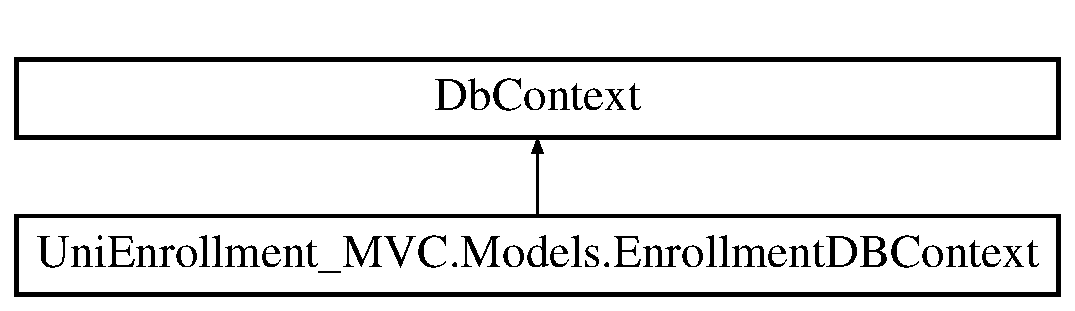
\includegraphics[height=2.000000cm]{class_uni_enrollment___m_v_c_1_1_models_1_1_enrollment_d_b_context}
\end{center}
\end{figure}
\subsection*{Public Member Functions}
\begin{DoxyCompactItemize}
\item 
\hyperlink{class_uni_enrollment___m_v_c_1_1_models_1_1_enrollment_d_b_context_a9bd979c7d54be8c4309092b71ad85079}{Enrollment\+D\+B\+Context} ()
\end{DoxyCompactItemize}
\subsection*{Protected Member Functions}
\begin{DoxyCompactItemize}
\item 
override void \hyperlink{class_uni_enrollment___m_v_c_1_1_models_1_1_enrollment_d_b_context_ac3e2f48ce2f4ff5f625f4e8df1ed9dab}{On\+Model\+Creating} (Db\+Model\+Builder model\+Builder)
\end{DoxyCompactItemize}
\subsection*{Properties}
\begin{DoxyCompactItemize}
\item 
Db\+Set$<$ \hyperlink{class_uni_enrollment___m_v_c_1_1_models_1_1_enrollment}{Enrollment} $>$ \hyperlink{class_uni_enrollment___m_v_c_1_1_models_1_1_enrollment_d_b_context_a17731fb975cd9c9b7349a874fc629490}{Enrollments}\hspace{0.3cm}{\ttfamily  \mbox{[}get, set\mbox{]}}
\end{DoxyCompactItemize}


\subsection{Detailed Description}


Definition at line 6 of file Enrollment\+D\+B\+Context.\+cs.



\subsection{Constructor \& Destructor Documentation}
\index{Uni\+Enrollment\+\_\+\+M\+V\+C\+::\+Models\+::\+Enrollment\+D\+B\+Context@{Uni\+Enrollment\+\_\+\+M\+V\+C\+::\+Models\+::\+Enrollment\+D\+B\+Context}!Enrollment\+D\+B\+Context@{Enrollment\+D\+B\+Context}}
\index{Enrollment\+D\+B\+Context@{Enrollment\+D\+B\+Context}!Uni\+Enrollment\+\_\+\+M\+V\+C\+::\+Models\+::\+Enrollment\+D\+B\+Context@{Uni\+Enrollment\+\_\+\+M\+V\+C\+::\+Models\+::\+Enrollment\+D\+B\+Context}}
\subsubsection[{\texorpdfstring{Enrollment\+D\+B\+Context()}{EnrollmentDBContext()}}]{\setlength{\rightskip}{0pt plus 5cm}Uni\+Enrollment\+\_\+\+M\+V\+C.\+Models.\+Enrollment\+D\+B\+Context.\+Enrollment\+D\+B\+Context (
\begin{DoxyParamCaption}
{}
\end{DoxyParamCaption}
)}\hypertarget{class_uni_enrollment___m_v_c_1_1_models_1_1_enrollment_d_b_context_a9bd979c7d54be8c4309092b71ad85079}{}\label{class_uni_enrollment___m_v_c_1_1_models_1_1_enrollment_d_b_context_a9bd979c7d54be8c4309092b71ad85079}


Definition at line 8 of file Enrollment\+D\+B\+Context.\+cs.



\subsection{Member Function Documentation}
\index{Uni\+Enrollment\+\_\+\+M\+V\+C\+::\+Models\+::\+Enrollment\+D\+B\+Context@{Uni\+Enrollment\+\_\+\+M\+V\+C\+::\+Models\+::\+Enrollment\+D\+B\+Context}!On\+Model\+Creating@{On\+Model\+Creating}}
\index{On\+Model\+Creating@{On\+Model\+Creating}!Uni\+Enrollment\+\_\+\+M\+V\+C\+::\+Models\+::\+Enrollment\+D\+B\+Context@{Uni\+Enrollment\+\_\+\+M\+V\+C\+::\+Models\+::\+Enrollment\+D\+B\+Context}}
\subsubsection[{\texorpdfstring{On\+Model\+Creating(\+Db\+Model\+Builder model\+Builder)}{OnModelCreating(DbModelBuilder modelBuilder)}}]{\setlength{\rightskip}{0pt plus 5cm}override void Uni\+Enrollment\+\_\+\+M\+V\+C.\+Models.\+Enrollment\+D\+B\+Context.\+On\+Model\+Creating (
\begin{DoxyParamCaption}
\item[{Db\+Model\+Builder}]{model\+Builder}
\end{DoxyParamCaption}
)\hspace{0.3cm}{\ttfamily [protected]}}\hypertarget{class_uni_enrollment___m_v_c_1_1_models_1_1_enrollment_d_b_context_ac3e2f48ce2f4ff5f625f4e8df1ed9dab}{}\label{class_uni_enrollment___m_v_c_1_1_models_1_1_enrollment_d_b_context_ac3e2f48ce2f4ff5f625f4e8df1ed9dab}


Definition at line 12 of file Enrollment\+D\+B\+Context.\+cs.



\subsection{Property Documentation}
\index{Uni\+Enrollment\+\_\+\+M\+V\+C\+::\+Models\+::\+Enrollment\+D\+B\+Context@{Uni\+Enrollment\+\_\+\+M\+V\+C\+::\+Models\+::\+Enrollment\+D\+B\+Context}!Enrollments@{Enrollments}}
\index{Enrollments@{Enrollments}!Uni\+Enrollment\+\_\+\+M\+V\+C\+::\+Models\+::\+Enrollment\+D\+B\+Context@{Uni\+Enrollment\+\_\+\+M\+V\+C\+::\+Models\+::\+Enrollment\+D\+B\+Context}}
\subsubsection[{\texorpdfstring{Enrollments}{Enrollments}}]{\setlength{\rightskip}{0pt plus 5cm}Db\+Set$<${\bf Enrollment}$>$ Uni\+Enrollment\+\_\+\+M\+V\+C.\+Models.\+Enrollment\+D\+B\+Context.\+Enrollments\hspace{0.3cm}{\ttfamily [get]}, {\ttfamily [set]}}\hypertarget{class_uni_enrollment___m_v_c_1_1_models_1_1_enrollment_d_b_context_a17731fb975cd9c9b7349a874fc629490}{}\label{class_uni_enrollment___m_v_c_1_1_models_1_1_enrollment_d_b_context_a17731fb975cd9c9b7349a874fc629490}


Definition at line 17 of file Enrollment\+D\+B\+Context.\+cs.



The documentation for this class was generated from the following file\+:\begin{DoxyCompactItemize}
\item 
H\+:/\+Documents/\+Work/\+Repositories/\+Uni\+Enrollment-\/\+D\+E\+M\+O/\+Uni\+Enrollment-\/\+M\+V\+C/\+Context/\hyperlink{_enrollment_d_b_context_8cs}{Enrollment\+D\+B\+Context.\+cs}\end{DoxyCompactItemize}

\hypertarget{class_uni_enrollment___m_v_c_1_1_models_1_1_enrollment_view_model}{}\section{Uni\+Enrollment\+\_\+\+M\+V\+C.\+Models.\+Enrollment\+View\+Model Class Reference}
\label{class_uni_enrollment___m_v_c_1_1_models_1_1_enrollment_view_model}\index{Uni\+Enrollment\+\_\+\+M\+V\+C.\+Models.\+Enrollment\+View\+Model@{Uni\+Enrollment\+\_\+\+M\+V\+C.\+Models.\+Enrollment\+View\+Model}}
\subsection*{Static Public Member Functions}
\begin{DoxyCompactItemize}
\item 
static List$<$ \hyperlink{class_uni_enrollment___m_v_c_1_1_models_1_1_user}{User} $>$ \hyperlink{class_uni_enrollment___m_v_c_1_1_models_1_1_enrollment_view_model_ae22e9947b130cec1f228bc059b4e74af}{Get\+All\+Students\+List\+With\+Professor\+ID} (int prof\+Id)
\begin{DoxyCompactList}\small\item\em Annoying method -\/ Couldn\textquotesingle{}t simply cast the query list to List of Users. It gets all the students who are enolled on a course by a specified professor \end{DoxyCompactList}\item 
static int \hyperlink{class_uni_enrollment___m_v_c_1_1_models_1_1_enrollment_view_model_a7bcea2a012bb5b3bc3481b7be74e498a}{Get\+Course\+Enrollment\+Count} (int course\+Id)
\begin{DoxyCompactList}\small\item\em Count of how many users are enrolled on a particular course \end{DoxyCompactList}\item 
static List$<$ \hyperlink{class_uni_enrollment___m_v_c_1_1_models_1_1_course}{Course} $>$ \hyperlink{class_uni_enrollment___m_v_c_1_1_models_1_1_enrollment_view_model_a98aa636acd09b996e836bb45af7fd7af}{Get\+Course\+Enrollment\+By\+Student\+ID} (int student\+Id)
\begin{DoxyCompactList}\small\item\em List of all the courses a user in enrolled on \end{DoxyCompactList}\item 
static List$<$ \hyperlink{class_uni_enrollment___m_v_c_1_1_models_1_1_course}{Course} $>$ \hyperlink{class_uni_enrollment___m_v_c_1_1_models_1_1_enrollment_view_model_aa037125196df4e574df5578152e92510}{Get\+Courses\+Not\+Enrolled\+On} (int student\+Id)
\begin{DoxyCompactList}\small\item\em All other courses a particular student is not enrolled on -\/ It\textquotesingle{}s for populating a drop down So it\textquotesingle{}s a \textquotesingle{}filtering\textquotesingle{} method \end{DoxyCompactList}\item 
static List$<$ \hyperlink{class_uni_enrollment___m_v_c_1_1_models_1_1_user}{User} $>$ \hyperlink{class_uni_enrollment___m_v_c_1_1_models_1_1_enrollment_view_model_a9b1ff396627b19e9d8b3b357ed36e787}{Get\+Students\+Enrolled\+On\+Course} (int course\+Id)
\begin{DoxyCompactList}\small\item\em Get a list of users enrolled on a particular course \end{DoxyCompactList}\end{DoxyCompactItemize}
\subsection*{Properties}
\begin{DoxyCompactItemize}
\item 
int \hyperlink{class_uni_enrollment___m_v_c_1_1_models_1_1_enrollment_view_model_a4c171e275e120403f4fc627757eb2d17}{Course\+ID}\hspace{0.3cm}{\ttfamily  \mbox{[}get, set\mbox{]}}
\item 
int \hyperlink{class_uni_enrollment___m_v_c_1_1_models_1_1_enrollment_view_model_a37ef31b609762bd1d4db2944dbbb42a0}{Student\+ID}\hspace{0.3cm}{\ttfamily  \mbox{[}get, set\mbox{]}}
\item 
Date\+Time \hyperlink{class_uni_enrollment___m_v_c_1_1_models_1_1_enrollment_view_model_ac4df04e11eccbb18ec3e8304ac7fbc0e}{Enrollment\+Date}\hspace{0.3cm}{\ttfamily  \mbox{[}get, set\mbox{]}}
\end{DoxyCompactItemize}


\subsection{Detailed Description}


Definition at line 8 of file Enrollment\+View\+Model.\+cs.



\subsection{Member Function Documentation}
\index{Uni\+Enrollment\+\_\+\+M\+V\+C\+::\+Models\+::\+Enrollment\+View\+Model@{Uni\+Enrollment\+\_\+\+M\+V\+C\+::\+Models\+::\+Enrollment\+View\+Model}!Get\+All\+Students\+List\+With\+Professor\+ID@{Get\+All\+Students\+List\+With\+Professor\+ID}}
\index{Get\+All\+Students\+List\+With\+Professor\+ID@{Get\+All\+Students\+List\+With\+Professor\+ID}!Uni\+Enrollment\+\_\+\+M\+V\+C\+::\+Models\+::\+Enrollment\+View\+Model@{Uni\+Enrollment\+\_\+\+M\+V\+C\+::\+Models\+::\+Enrollment\+View\+Model}}
\subsubsection[{\texorpdfstring{Get\+All\+Students\+List\+With\+Professor\+I\+D(int prof\+Id)}{GetAllStudentsListWithProfessorID(int profId)}}]{\setlength{\rightskip}{0pt plus 5cm}static List$<${\bf User}$>$ Uni\+Enrollment\+\_\+\+M\+V\+C.\+Models.\+Enrollment\+View\+Model.\+Get\+All\+Students\+List\+With\+Professor\+ID (
\begin{DoxyParamCaption}
\item[{int}]{prof\+Id}
\end{DoxyParamCaption}
)\hspace{0.3cm}{\ttfamily [static]}}\hypertarget{class_uni_enrollment___m_v_c_1_1_models_1_1_enrollment_view_model_ae22e9947b130cec1f228bc059b4e74af}{}\label{class_uni_enrollment___m_v_c_1_1_models_1_1_enrollment_view_model_ae22e9947b130cec1f228bc059b4e74af}


Annoying method -\/ Couldn\textquotesingle{}t simply cast the query list to List of Users. It gets all the students who are enolled on a course by a specified professor 


\begin{DoxyParams}{Parameters}
{\em prof\+Id} & ID of professor\\
\hline
\end{DoxyParams}
\begin{DoxyReturn}{Returns}
List of users
\end{DoxyReturn}


Definition at line 23 of file Enrollment\+View\+Model.\+cs.

\index{Uni\+Enrollment\+\_\+\+M\+V\+C\+::\+Models\+::\+Enrollment\+View\+Model@{Uni\+Enrollment\+\_\+\+M\+V\+C\+::\+Models\+::\+Enrollment\+View\+Model}!Get\+Course\+Enrollment\+By\+Student\+ID@{Get\+Course\+Enrollment\+By\+Student\+ID}}
\index{Get\+Course\+Enrollment\+By\+Student\+ID@{Get\+Course\+Enrollment\+By\+Student\+ID}!Uni\+Enrollment\+\_\+\+M\+V\+C\+::\+Models\+::\+Enrollment\+View\+Model@{Uni\+Enrollment\+\_\+\+M\+V\+C\+::\+Models\+::\+Enrollment\+View\+Model}}
\subsubsection[{\texorpdfstring{Get\+Course\+Enrollment\+By\+Student\+I\+D(int student\+Id)}{GetCourseEnrollmentByStudentID(int studentId)}}]{\setlength{\rightskip}{0pt plus 5cm}static List$<${\bf Course}$>$ Uni\+Enrollment\+\_\+\+M\+V\+C.\+Models.\+Enrollment\+View\+Model.\+Get\+Course\+Enrollment\+By\+Student\+ID (
\begin{DoxyParamCaption}
\item[{int}]{student\+Id}
\end{DoxyParamCaption}
)\hspace{0.3cm}{\ttfamily [static]}}\hypertarget{class_uni_enrollment___m_v_c_1_1_models_1_1_enrollment_view_model_a98aa636acd09b996e836bb45af7fd7af}{}\label{class_uni_enrollment___m_v_c_1_1_models_1_1_enrollment_view_model_a98aa636acd09b996e836bb45af7fd7af}


List of all the courses a user in enrolled on 


\begin{DoxyParams}{Parameters}
{\em student\+Id} & The ID of the student to see what course they\textquotesingle{}re enrolled on\\
\hline
\end{DoxyParams}
\begin{DoxyReturn}{Returns}
List of courses
\end{DoxyReturn}


Definition at line 62 of file Enrollment\+View\+Model.\+cs.

\index{Uni\+Enrollment\+\_\+\+M\+V\+C\+::\+Models\+::\+Enrollment\+View\+Model@{Uni\+Enrollment\+\_\+\+M\+V\+C\+::\+Models\+::\+Enrollment\+View\+Model}!Get\+Course\+Enrollment\+Count@{Get\+Course\+Enrollment\+Count}}
\index{Get\+Course\+Enrollment\+Count@{Get\+Course\+Enrollment\+Count}!Uni\+Enrollment\+\_\+\+M\+V\+C\+::\+Models\+::\+Enrollment\+View\+Model@{Uni\+Enrollment\+\_\+\+M\+V\+C\+::\+Models\+::\+Enrollment\+View\+Model}}
\subsubsection[{\texorpdfstring{Get\+Course\+Enrollment\+Count(int course\+Id)}{GetCourseEnrollmentCount(int courseId)}}]{\setlength{\rightskip}{0pt plus 5cm}static int Uni\+Enrollment\+\_\+\+M\+V\+C.\+Models.\+Enrollment\+View\+Model.\+Get\+Course\+Enrollment\+Count (
\begin{DoxyParamCaption}
\item[{int}]{course\+Id}
\end{DoxyParamCaption}
)\hspace{0.3cm}{\ttfamily [static]}}\hypertarget{class_uni_enrollment___m_v_c_1_1_models_1_1_enrollment_view_model_a7bcea2a012bb5b3bc3481b7be74e498a}{}\label{class_uni_enrollment___m_v_c_1_1_models_1_1_enrollment_view_model_a7bcea2a012bb5b3bc3481b7be74e498a}


Count of how many users are enrolled on a particular course 


\begin{DoxyParams}{Parameters}
{\em course\+Id} & The course ID of the course to count\\
\hline
\end{DoxyParams}
\begin{DoxyReturn}{Returns}
Number of students in that course
\end{DoxyReturn}


Definition at line 51 of file Enrollment\+View\+Model.\+cs.

\index{Uni\+Enrollment\+\_\+\+M\+V\+C\+::\+Models\+::\+Enrollment\+View\+Model@{Uni\+Enrollment\+\_\+\+M\+V\+C\+::\+Models\+::\+Enrollment\+View\+Model}!Get\+Courses\+Not\+Enrolled\+On@{Get\+Courses\+Not\+Enrolled\+On}}
\index{Get\+Courses\+Not\+Enrolled\+On@{Get\+Courses\+Not\+Enrolled\+On}!Uni\+Enrollment\+\_\+\+M\+V\+C\+::\+Models\+::\+Enrollment\+View\+Model@{Uni\+Enrollment\+\_\+\+M\+V\+C\+::\+Models\+::\+Enrollment\+View\+Model}}
\subsubsection[{\texorpdfstring{Get\+Courses\+Not\+Enrolled\+On(int student\+Id)}{GetCoursesNotEnrolledOn(int studentId)}}]{\setlength{\rightskip}{0pt plus 5cm}static List$<${\bf Course}$>$ Uni\+Enrollment\+\_\+\+M\+V\+C.\+Models.\+Enrollment\+View\+Model.\+Get\+Courses\+Not\+Enrolled\+On (
\begin{DoxyParamCaption}
\item[{int}]{student\+Id}
\end{DoxyParamCaption}
)\hspace{0.3cm}{\ttfamily [static]}}\hypertarget{class_uni_enrollment___m_v_c_1_1_models_1_1_enrollment_view_model_aa037125196df4e574df5578152e92510}{}\label{class_uni_enrollment___m_v_c_1_1_models_1_1_enrollment_view_model_aa037125196df4e574df5578152e92510}


All other courses a particular student is not enrolled on -\/ It\textquotesingle{}s for populating a drop down So it\textquotesingle{}s a \textquotesingle{}filtering\textquotesingle{} method 


\begin{DoxyParams}{Parameters}
{\em student\+Id} & \hyperlink{class_uni_enrollment___m_v_c_1_1_models_1_1_student}{Student} ID of student to determine what courses they don\textquotesingle{}t belong to\\
\hline
\end{DoxyParams}
\begin{DoxyReturn}{Returns}
A list of courses a user doesn\textquotesingle{}t belong to
\end{DoxyReturn}


Definition at line 82 of file Enrollment\+View\+Model.\+cs.

\index{Uni\+Enrollment\+\_\+\+M\+V\+C\+::\+Models\+::\+Enrollment\+View\+Model@{Uni\+Enrollment\+\_\+\+M\+V\+C\+::\+Models\+::\+Enrollment\+View\+Model}!Get\+Students\+Enrolled\+On\+Course@{Get\+Students\+Enrolled\+On\+Course}}
\index{Get\+Students\+Enrolled\+On\+Course@{Get\+Students\+Enrolled\+On\+Course}!Uni\+Enrollment\+\_\+\+M\+V\+C\+::\+Models\+::\+Enrollment\+View\+Model@{Uni\+Enrollment\+\_\+\+M\+V\+C\+::\+Models\+::\+Enrollment\+View\+Model}}
\subsubsection[{\texorpdfstring{Get\+Students\+Enrolled\+On\+Course(int course\+Id)}{GetStudentsEnrolledOnCourse(int courseId)}}]{\setlength{\rightskip}{0pt plus 5cm}static List$<${\bf User}$>$ Uni\+Enrollment\+\_\+\+M\+V\+C.\+Models.\+Enrollment\+View\+Model.\+Get\+Students\+Enrolled\+On\+Course (
\begin{DoxyParamCaption}
\item[{int}]{course\+Id}
\end{DoxyParamCaption}
)\hspace{0.3cm}{\ttfamily [static]}}\hypertarget{class_uni_enrollment___m_v_c_1_1_models_1_1_enrollment_view_model_a9b1ff396627b19e9d8b3b357ed36e787}{}\label{class_uni_enrollment___m_v_c_1_1_models_1_1_enrollment_view_model_a9b1ff396627b19e9d8b3b357ed36e787}


Get a list of users enrolled on a particular course 


\begin{DoxyParams}{Parameters}
{\em course\+Id} & The ID of the course that students belong to\\
\hline
\end{DoxyParams}
\begin{DoxyReturn}{Returns}
A list of users belonging to a given course
\end{DoxyReturn}


Definition at line 101 of file Enrollment\+View\+Model.\+cs.



\subsection{Property Documentation}
\index{Uni\+Enrollment\+\_\+\+M\+V\+C\+::\+Models\+::\+Enrollment\+View\+Model@{Uni\+Enrollment\+\_\+\+M\+V\+C\+::\+Models\+::\+Enrollment\+View\+Model}!Course\+ID@{Course\+ID}}
\index{Course\+ID@{Course\+ID}!Uni\+Enrollment\+\_\+\+M\+V\+C\+::\+Models\+::\+Enrollment\+View\+Model@{Uni\+Enrollment\+\_\+\+M\+V\+C\+::\+Models\+::\+Enrollment\+View\+Model}}
\subsubsection[{\texorpdfstring{Course\+ID}{CourseID}}]{\setlength{\rightskip}{0pt plus 5cm}int Uni\+Enrollment\+\_\+\+M\+V\+C.\+Models.\+Enrollment\+View\+Model.\+Course\+ID\hspace{0.3cm}{\ttfamily [get]}, {\ttfamily [set]}}\hypertarget{class_uni_enrollment___m_v_c_1_1_models_1_1_enrollment_view_model_a4c171e275e120403f4fc627757eb2d17}{}\label{class_uni_enrollment___m_v_c_1_1_models_1_1_enrollment_view_model_a4c171e275e120403f4fc627757eb2d17}


Definition at line 10 of file Enrollment\+View\+Model.\+cs.

\index{Uni\+Enrollment\+\_\+\+M\+V\+C\+::\+Models\+::\+Enrollment\+View\+Model@{Uni\+Enrollment\+\_\+\+M\+V\+C\+::\+Models\+::\+Enrollment\+View\+Model}!Enrollment\+Date@{Enrollment\+Date}}
\index{Enrollment\+Date@{Enrollment\+Date}!Uni\+Enrollment\+\_\+\+M\+V\+C\+::\+Models\+::\+Enrollment\+View\+Model@{Uni\+Enrollment\+\_\+\+M\+V\+C\+::\+Models\+::\+Enrollment\+View\+Model}}
\subsubsection[{\texorpdfstring{Enrollment\+Date}{EnrollmentDate}}]{\setlength{\rightskip}{0pt plus 5cm}Date\+Time Uni\+Enrollment\+\_\+\+M\+V\+C.\+Models.\+Enrollment\+View\+Model.\+Enrollment\+Date\hspace{0.3cm}{\ttfamily [get]}, {\ttfamily [set]}}\hypertarget{class_uni_enrollment___m_v_c_1_1_models_1_1_enrollment_view_model_ac4df04e11eccbb18ec3e8304ac7fbc0e}{}\label{class_uni_enrollment___m_v_c_1_1_models_1_1_enrollment_view_model_ac4df04e11eccbb18ec3e8304ac7fbc0e}


Definition at line 15 of file Enrollment\+View\+Model.\+cs.

\index{Uni\+Enrollment\+\_\+\+M\+V\+C\+::\+Models\+::\+Enrollment\+View\+Model@{Uni\+Enrollment\+\_\+\+M\+V\+C\+::\+Models\+::\+Enrollment\+View\+Model}!Student\+ID@{Student\+ID}}
\index{Student\+ID@{Student\+ID}!Uni\+Enrollment\+\_\+\+M\+V\+C\+::\+Models\+::\+Enrollment\+View\+Model@{Uni\+Enrollment\+\_\+\+M\+V\+C\+::\+Models\+::\+Enrollment\+View\+Model}}
\subsubsection[{\texorpdfstring{Student\+ID}{StudentID}}]{\setlength{\rightskip}{0pt plus 5cm}int Uni\+Enrollment\+\_\+\+M\+V\+C.\+Models.\+Enrollment\+View\+Model.\+Student\+ID\hspace{0.3cm}{\ttfamily [get]}, {\ttfamily [set]}}\hypertarget{class_uni_enrollment___m_v_c_1_1_models_1_1_enrollment_view_model_a37ef31b609762bd1d4db2944dbbb42a0}{}\label{class_uni_enrollment___m_v_c_1_1_models_1_1_enrollment_view_model_a37ef31b609762bd1d4db2944dbbb42a0}


Definition at line 12 of file Enrollment\+View\+Model.\+cs.



The documentation for this class was generated from the following file\+:\begin{DoxyCompactItemize}
\item 
H\+:/\+Documents/\+Work/\+Repositories/\+Uni\+Enrollment-\/\+D\+E\+M\+O/\+Uni\+Enrollment-\/\+M\+V\+C/\+Models/\hyperlink{_enrollment_view_model_8cs}{Enrollment\+View\+Model.\+cs}\end{DoxyCompactItemize}

\hypertarget{class_uni_enrollment___m_v_c_1_1_filter_config}{}\section{Uni\+Enrollment\+\_\+\+M\+V\+C.\+Filter\+Config Class Reference}
\label{class_uni_enrollment___m_v_c_1_1_filter_config}\index{Uni\+Enrollment\+\_\+\+M\+V\+C.\+Filter\+Config@{Uni\+Enrollment\+\_\+\+M\+V\+C.\+Filter\+Config}}
\subsection*{Static Public Member Functions}
\begin{DoxyCompactItemize}
\item 
static void \hyperlink{class_uni_enrollment___m_v_c_1_1_filter_config_aba356c48e56ad2bae35a4011d37b292c}{Register\+Global\+Filters} (Global\+Filter\+Collection filters)
\end{DoxyCompactItemize}


\subsection{Detailed Description}


Definition at line 6 of file Filter\+Config.\+cs.



\subsection{Member Function Documentation}
\index{Uni\+Enrollment\+\_\+\+M\+V\+C\+::\+Filter\+Config@{Uni\+Enrollment\+\_\+\+M\+V\+C\+::\+Filter\+Config}!Register\+Global\+Filters@{Register\+Global\+Filters}}
\index{Register\+Global\+Filters@{Register\+Global\+Filters}!Uni\+Enrollment\+\_\+\+M\+V\+C\+::\+Filter\+Config@{Uni\+Enrollment\+\_\+\+M\+V\+C\+::\+Filter\+Config}}
\subsubsection[{\texorpdfstring{Register\+Global\+Filters(\+Global\+Filter\+Collection filters)}{RegisterGlobalFilters(GlobalFilterCollection filters)}}]{\setlength{\rightskip}{0pt plus 5cm}static void Uni\+Enrollment\+\_\+\+M\+V\+C.\+Filter\+Config.\+Register\+Global\+Filters (
\begin{DoxyParamCaption}
\item[{Global\+Filter\+Collection}]{filters}
\end{DoxyParamCaption}
)\hspace{0.3cm}{\ttfamily [static]}}\hypertarget{class_uni_enrollment___m_v_c_1_1_filter_config_aba356c48e56ad2bae35a4011d37b292c}{}\label{class_uni_enrollment___m_v_c_1_1_filter_config_aba356c48e56ad2bae35a4011d37b292c}


Definition at line 8 of file Filter\+Config.\+cs.



The documentation for this class was generated from the following file\+:\begin{DoxyCompactItemize}
\item 
H\+:/\+Documents/\+Work/\+Repositories/\+Uni\+Enrollment-\/\+D\+E\+M\+O/\+Uni\+Enrollment-\/\+M\+V\+C/\+App\+\_\+\+Start/\hyperlink{_filter_config_8cs}{Filter\+Config.\+cs}\end{DoxyCompactItemize}

\hypertarget{class_uni_enrollment___m_v_c_1_1_controllers_1_1_home_controller}{}\section{Uni\+Enrollment\+\_\+\+M\+V\+C.\+Controllers.\+Home\+Controller Class Reference}
\label{class_uni_enrollment___m_v_c_1_1_controllers_1_1_home_controller}\index{Uni\+Enrollment\+\_\+\+M\+V\+C.\+Controllers.\+Home\+Controller@{Uni\+Enrollment\+\_\+\+M\+V\+C.\+Controllers.\+Home\+Controller}}


Contains user interaction (action result) methods for the home page  


Inheritance diagram for Uni\+Enrollment\+\_\+\+M\+V\+C.\+Controllers.\+Home\+Controller\+:\begin{figure}[H]
\begin{center}
\leavevmode
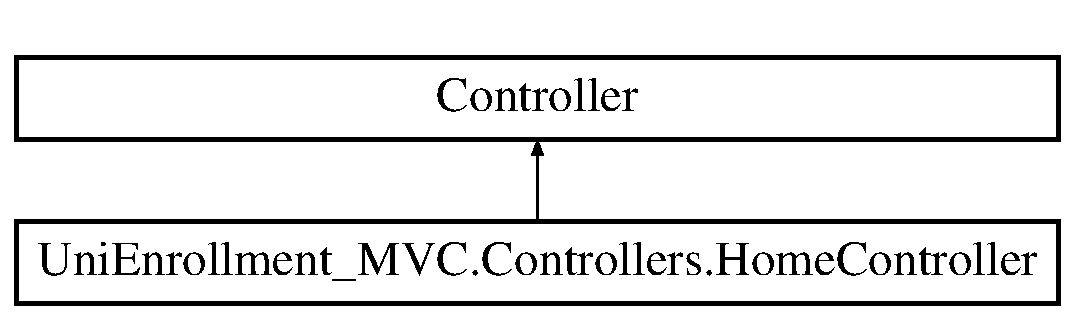
\includegraphics[height=2.000000cm]{class_uni_enrollment___m_v_c_1_1_controllers_1_1_home_controller}
\end{center}
\end{figure}
\subsection*{Public Member Functions}
\begin{DoxyCompactItemize}
\item 
Action\+Result \hyperlink{class_uni_enrollment___m_v_c_1_1_controllers_1_1_home_controller_aad4d2befa5bed0606d8152fab0f98681}{Index} ()
\end{DoxyCompactItemize}


\subsection{Detailed Description}
Contains user interaction (action result) methods for the home page 



Definition at line 8 of file Home\+Controller.\+cs.



\subsection{Member Function Documentation}
\index{Uni\+Enrollment\+\_\+\+M\+V\+C\+::\+Controllers\+::\+Home\+Controller@{Uni\+Enrollment\+\_\+\+M\+V\+C\+::\+Controllers\+::\+Home\+Controller}!Index@{Index}}
\index{Index@{Index}!Uni\+Enrollment\+\_\+\+M\+V\+C\+::\+Controllers\+::\+Home\+Controller@{Uni\+Enrollment\+\_\+\+M\+V\+C\+::\+Controllers\+::\+Home\+Controller}}
\subsubsection[{\texorpdfstring{Index()}{Index()}}]{\setlength{\rightskip}{0pt plus 5cm}Action\+Result Uni\+Enrollment\+\_\+\+M\+V\+C.\+Controllers.\+Home\+Controller.\+Index (
\begin{DoxyParamCaption}
{}
\end{DoxyParamCaption}
)}\hypertarget{class_uni_enrollment___m_v_c_1_1_controllers_1_1_home_controller_aad4d2befa5bed0606d8152fab0f98681}{}\label{class_uni_enrollment___m_v_c_1_1_controllers_1_1_home_controller_aad4d2befa5bed0606d8152fab0f98681}


Definition at line 10 of file Home\+Controller.\+cs.



The documentation for this class was generated from the following file\+:\begin{DoxyCompactItemize}
\item 
H\+:/\+Documents/\+Work/\+Repositories/\+Uni\+Enrollment-\/\+D\+E\+M\+O/\+Uni\+Enrollment-\/\+M\+V\+C/\+Controllers/\hyperlink{_home_controller_8cs}{Home\+Controller.\+cs}\end{DoxyCompactItemize}

\hypertarget{class_uni_enrollment___m_v_c_1_1_controllers_1_1_login_controller}{}\section{Uni\+Enrollment\+\_\+\+M\+V\+C.\+Controllers.\+Login\+Controller Class Reference}
\label{class_uni_enrollment___m_v_c_1_1_controllers_1_1_login_controller}\index{Uni\+Enrollment\+\_\+\+M\+V\+C.\+Controllers.\+Login\+Controller@{Uni\+Enrollment\+\_\+\+M\+V\+C.\+Controllers.\+Login\+Controller}}


Contains user interaction (action result) methods for anything uni \textquotesingle{}logging in\textquotesingle{} related  


Inheritance diagram for Uni\+Enrollment\+\_\+\+M\+V\+C.\+Controllers.\+Login\+Controller\+:\begin{figure}[H]
\begin{center}
\leavevmode
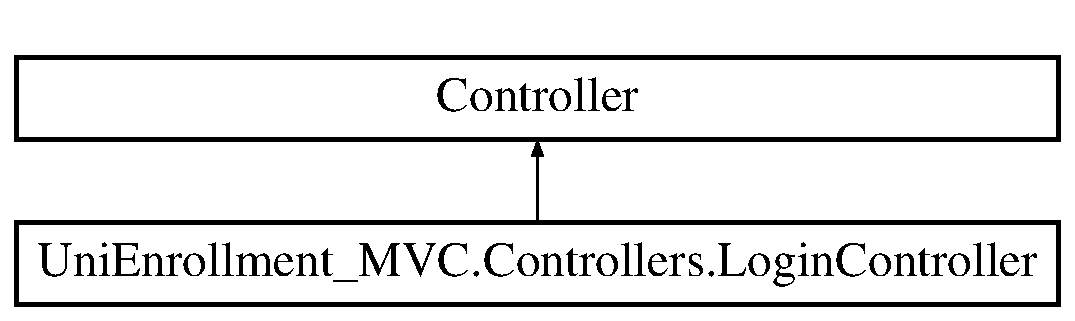
\includegraphics[height=2.000000cm]{class_uni_enrollment___m_v_c_1_1_controllers_1_1_login_controller}
\end{center}
\end{figure}
\subsection*{Public Member Functions}
\begin{DoxyCompactItemize}
\item 
Action\+Result \hyperlink{class_uni_enrollment___m_v_c_1_1_controllers_1_1_login_controller_aee5f81236c19135abeabc3f23c7a5c60}{Go\+To\+Login} (string where)
\item 
Action\+Result \hyperlink{class_uni_enrollment___m_v_c_1_1_controllers_1_1_login_controller_affee63e1f64b80feb35ad1e507174e9a}{Perform\+Login} (\hyperlink{class_uni_enrollment___m_v_c_1_1_models_1_1_login_view_model}{Login\+View\+Model} vm\+Login, string where)
\item 
Action\+Result \hyperlink{class_uni_enrollment___m_v_c_1_1_controllers_1_1_login_controller_ac1c1d9102078847d0a6d75e10cea087a}{Log\+Off} ()
\end{DoxyCompactItemize}
\subsection*{Private Attributes}
\begin{DoxyCompactItemize}
\item 
\hyperlink{class_uni_enrollment___m_v_c_1_1_models_1_1_uni_enrollment_d_b_entities}{Uni\+Enrollment\+D\+B\+Entities} \hyperlink{class_uni_enrollment___m_v_c_1_1_controllers_1_1_login_controller_a68efde44e582f061cc104372638ad5e6}{\+\_\+entities} = new \hyperlink{class_uni_enrollment___m_v_c_1_1_models_1_1_uni_enrollment_d_b_entities}{Uni\+Enrollment\+D\+B\+Entities}()
\end{DoxyCompactItemize}


\subsection{Detailed Description}
Contains user interaction (action result) methods for anything uni \textquotesingle{}logging in\textquotesingle{} related 



Definition at line 12 of file Login\+Controller.\+cs.



\subsection{Member Function Documentation}
\index{Uni\+Enrollment\+\_\+\+M\+V\+C\+::\+Controllers\+::\+Login\+Controller@{Uni\+Enrollment\+\_\+\+M\+V\+C\+::\+Controllers\+::\+Login\+Controller}!Go\+To\+Login@{Go\+To\+Login}}
\index{Go\+To\+Login@{Go\+To\+Login}!Uni\+Enrollment\+\_\+\+M\+V\+C\+::\+Controllers\+::\+Login\+Controller@{Uni\+Enrollment\+\_\+\+M\+V\+C\+::\+Controllers\+::\+Login\+Controller}}
\subsubsection[{\texorpdfstring{Go\+To\+Login(string where)}{GoToLogin(string where)}}]{\setlength{\rightskip}{0pt plus 5cm}Action\+Result Uni\+Enrollment\+\_\+\+M\+V\+C.\+Controllers.\+Login\+Controller.\+Go\+To\+Login (
\begin{DoxyParamCaption}
\item[{string}]{where}
\end{DoxyParamCaption}
)}\hypertarget{class_uni_enrollment___m_v_c_1_1_controllers_1_1_login_controller_aee5f81236c19135abeabc3f23c7a5c60}{}\label{class_uni_enrollment___m_v_c_1_1_controllers_1_1_login_controller_aee5f81236c19135abeabc3f23c7a5c60}


Definition at line 16 of file Login\+Controller.\+cs.

\index{Uni\+Enrollment\+\_\+\+M\+V\+C\+::\+Controllers\+::\+Login\+Controller@{Uni\+Enrollment\+\_\+\+M\+V\+C\+::\+Controllers\+::\+Login\+Controller}!Log\+Off@{Log\+Off}}
\index{Log\+Off@{Log\+Off}!Uni\+Enrollment\+\_\+\+M\+V\+C\+::\+Controllers\+::\+Login\+Controller@{Uni\+Enrollment\+\_\+\+M\+V\+C\+::\+Controllers\+::\+Login\+Controller}}
\subsubsection[{\texorpdfstring{Log\+Off()}{LogOff()}}]{\setlength{\rightskip}{0pt plus 5cm}Action\+Result Uni\+Enrollment\+\_\+\+M\+V\+C.\+Controllers.\+Login\+Controller.\+Log\+Off (
\begin{DoxyParamCaption}
{}
\end{DoxyParamCaption}
)}\hypertarget{class_uni_enrollment___m_v_c_1_1_controllers_1_1_login_controller_ac1c1d9102078847d0a6d75e10cea087a}{}\label{class_uni_enrollment___m_v_c_1_1_controllers_1_1_login_controller_ac1c1d9102078847d0a6d75e10cea087a}


Definition at line 72 of file Login\+Controller.\+cs.

\index{Uni\+Enrollment\+\_\+\+M\+V\+C\+::\+Controllers\+::\+Login\+Controller@{Uni\+Enrollment\+\_\+\+M\+V\+C\+::\+Controllers\+::\+Login\+Controller}!Perform\+Login@{Perform\+Login}}
\index{Perform\+Login@{Perform\+Login}!Uni\+Enrollment\+\_\+\+M\+V\+C\+::\+Controllers\+::\+Login\+Controller@{Uni\+Enrollment\+\_\+\+M\+V\+C\+::\+Controllers\+::\+Login\+Controller}}
\subsubsection[{\texorpdfstring{Perform\+Login(\+Login\+View\+Model vm\+Login, string where)}{PerformLogin(LoginViewModel vmLogin, string where)}}]{\setlength{\rightskip}{0pt plus 5cm}Action\+Result Uni\+Enrollment\+\_\+\+M\+V\+C.\+Controllers.\+Login\+Controller.\+Perform\+Login (
\begin{DoxyParamCaption}
\item[{{\bf Login\+View\+Model}}]{vm\+Login, }
\item[{string}]{where}
\end{DoxyParamCaption}
)}\hypertarget{class_uni_enrollment___m_v_c_1_1_controllers_1_1_login_controller_affee63e1f64b80feb35ad1e507174e9a}{}\label{class_uni_enrollment___m_v_c_1_1_controllers_1_1_login_controller_affee63e1f64b80feb35ad1e507174e9a}


Definition at line 22 of file Login\+Controller.\+cs.



\subsection{Member Data Documentation}
\index{Uni\+Enrollment\+\_\+\+M\+V\+C\+::\+Controllers\+::\+Login\+Controller@{Uni\+Enrollment\+\_\+\+M\+V\+C\+::\+Controllers\+::\+Login\+Controller}!\+\_\+entities@{\+\_\+entities}}
\index{\+\_\+entities@{\+\_\+entities}!Uni\+Enrollment\+\_\+\+M\+V\+C\+::\+Controllers\+::\+Login\+Controller@{Uni\+Enrollment\+\_\+\+M\+V\+C\+::\+Controllers\+::\+Login\+Controller}}
\subsubsection[{\texorpdfstring{\+\_\+entities}{_entities}}]{\setlength{\rightskip}{0pt plus 5cm}{\bf Uni\+Enrollment\+D\+B\+Entities} Uni\+Enrollment\+\_\+\+M\+V\+C.\+Controllers.\+Login\+Controller.\+\_\+entities = new {\bf Uni\+Enrollment\+D\+B\+Entities}()\hspace{0.3cm}{\ttfamily [private]}}\hypertarget{class_uni_enrollment___m_v_c_1_1_controllers_1_1_login_controller_a68efde44e582f061cc104372638ad5e6}{}\label{class_uni_enrollment___m_v_c_1_1_controllers_1_1_login_controller_a68efde44e582f061cc104372638ad5e6}


Definition at line 14 of file Login\+Controller.\+cs.



The documentation for this class was generated from the following file\+:\begin{DoxyCompactItemize}
\item 
H\+:/\+Documents/\+Work/\+Repositories/\+Uni\+Enrollment-\/\+D\+E\+M\+O/\+Uni\+Enrollment-\/\+M\+V\+C/\+Controllers/\hyperlink{_login_controller_8cs}{Login\+Controller.\+cs}\end{DoxyCompactItemize}

\hypertarget{class_uni_enrollment___m_v_c_1_1_models_1_1_login_view_model}{}\section{Uni\+Enrollment\+\_\+\+M\+V\+C.\+Models.\+Login\+View\+Model Class Reference}
\label{class_uni_enrollment___m_v_c_1_1_models_1_1_login_view_model}\index{Uni\+Enrollment\+\_\+\+M\+V\+C.\+Models.\+Login\+View\+Model@{Uni\+Enrollment\+\_\+\+M\+V\+C.\+Models.\+Login\+View\+Model}}
\subsection*{Properties}
\begin{DoxyCompactItemize}
\item 
string \hyperlink{class_uni_enrollment___m_v_c_1_1_models_1_1_login_view_model_a2a2dfafa311682f75f090f507feede8b}{Username}\hspace{0.3cm}{\ttfamily  \mbox{[}get, set\mbox{]}}
\item 
string \hyperlink{class_uni_enrollment___m_v_c_1_1_models_1_1_login_view_model_aaded43b1c35aceeb4a2114a4ad97d5e7}{Password}\hspace{0.3cm}{\ttfamily  \mbox{[}get, set\mbox{]}}
\end{DoxyCompactItemize}


\subsection{Detailed Description}


Definition at line 8 of file Login\+View\+Model.\+cs.



\subsection{Property Documentation}
\index{Uni\+Enrollment\+\_\+\+M\+V\+C\+::\+Models\+::\+Login\+View\+Model@{Uni\+Enrollment\+\_\+\+M\+V\+C\+::\+Models\+::\+Login\+View\+Model}!Password@{Password}}
\index{Password@{Password}!Uni\+Enrollment\+\_\+\+M\+V\+C\+::\+Models\+::\+Login\+View\+Model@{Uni\+Enrollment\+\_\+\+M\+V\+C\+::\+Models\+::\+Login\+View\+Model}}
\subsubsection[{\texorpdfstring{Password}{Password}}]{\setlength{\rightskip}{0pt plus 5cm}string Uni\+Enrollment\+\_\+\+M\+V\+C.\+Models.\+Login\+View\+Model.\+Password\hspace{0.3cm}{\ttfamily [get]}, {\ttfamily [set]}}\hypertarget{class_uni_enrollment___m_v_c_1_1_models_1_1_login_view_model_aaded43b1c35aceeb4a2114a4ad97d5e7}{}\label{class_uni_enrollment___m_v_c_1_1_models_1_1_login_view_model_aaded43b1c35aceeb4a2114a4ad97d5e7}


Definition at line 14 of file Login\+View\+Model.\+cs.

\index{Uni\+Enrollment\+\_\+\+M\+V\+C\+::\+Models\+::\+Login\+View\+Model@{Uni\+Enrollment\+\_\+\+M\+V\+C\+::\+Models\+::\+Login\+View\+Model}!Username@{Username}}
\index{Username@{Username}!Uni\+Enrollment\+\_\+\+M\+V\+C\+::\+Models\+::\+Login\+View\+Model@{Uni\+Enrollment\+\_\+\+M\+V\+C\+::\+Models\+::\+Login\+View\+Model}}
\subsubsection[{\texorpdfstring{Username}{Username}}]{\setlength{\rightskip}{0pt plus 5cm}string Uni\+Enrollment\+\_\+\+M\+V\+C.\+Models.\+Login\+View\+Model.\+Username\hspace{0.3cm}{\ttfamily [get]}, {\ttfamily [set]}}\hypertarget{class_uni_enrollment___m_v_c_1_1_models_1_1_login_view_model_a2a2dfafa311682f75f090f507feede8b}{}\label{class_uni_enrollment___m_v_c_1_1_models_1_1_login_view_model_a2a2dfafa311682f75f090f507feede8b}


Definition at line 11 of file Login\+View\+Model.\+cs.



The documentation for this class was generated from the following file\+:\begin{DoxyCompactItemize}
\item 
H\+:/\+Documents/\+Work/\+Repositories/\+Uni\+Enrollment-\/\+D\+E\+M\+O/\+Uni\+Enrollment-\/\+M\+V\+C/\+Models/\hyperlink{_login_view_model_8cs}{Login\+View\+Model.\+cs}\end{DoxyCompactItemize}

\hypertarget{class_uni_enrollment___m_v_c_1_1_mvc_application}{}\section{Uni\+Enrollment\+\_\+\+M\+V\+C.\+Mvc\+Application Class Reference}
\label{class_uni_enrollment___m_v_c_1_1_mvc_application}\index{Uni\+Enrollment\+\_\+\+M\+V\+C.\+Mvc\+Application@{Uni\+Enrollment\+\_\+\+M\+V\+C.\+Mvc\+Application}}
Inheritance diagram for Uni\+Enrollment\+\_\+\+M\+V\+C.\+Mvc\+Application\+:\begin{figure}[H]
\begin{center}
\leavevmode
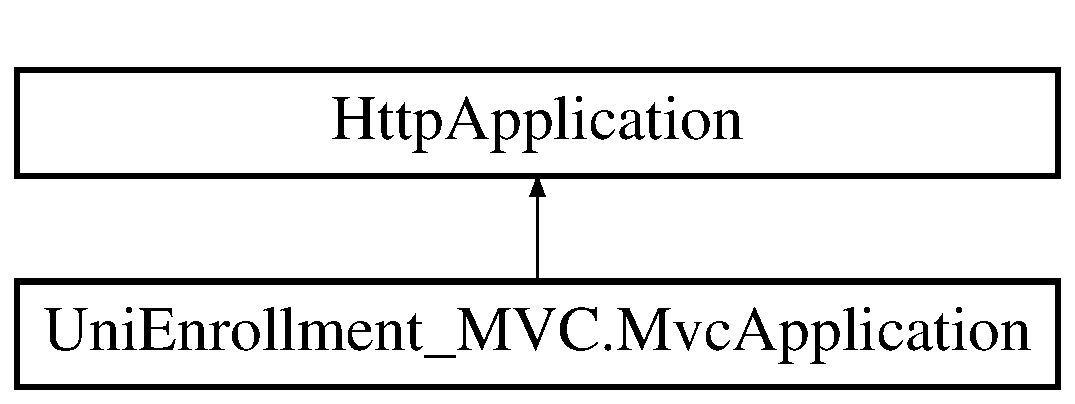
\includegraphics[height=2.000000cm]{class_uni_enrollment___m_v_c_1_1_mvc_application}
\end{center}
\end{figure}
\subsection*{Protected Member Functions}
\begin{DoxyCompactItemize}
\item 
void \hyperlink{class_uni_enrollment___m_v_c_1_1_mvc_application_a6f4d58d39c2ae4969d73bf967f43b999}{Application\+\_\+\+Start} ()
\end{DoxyCompactItemize}


\subsection{Detailed Description}


Definition at line 11 of file Global.\+asax.\+cs.



\subsection{Member Function Documentation}
\index{Uni\+Enrollment\+\_\+\+M\+V\+C\+::\+Mvc\+Application@{Uni\+Enrollment\+\_\+\+M\+V\+C\+::\+Mvc\+Application}!Application\+\_\+\+Start@{Application\+\_\+\+Start}}
\index{Application\+\_\+\+Start@{Application\+\_\+\+Start}!Uni\+Enrollment\+\_\+\+M\+V\+C\+::\+Mvc\+Application@{Uni\+Enrollment\+\_\+\+M\+V\+C\+::\+Mvc\+Application}}
\subsubsection[{\texorpdfstring{Application\+\_\+\+Start()}{Application_Start()}}]{\setlength{\rightskip}{0pt plus 5cm}void Uni\+Enrollment\+\_\+\+M\+V\+C.\+Mvc\+Application.\+Application\+\_\+\+Start (
\begin{DoxyParamCaption}
{}
\end{DoxyParamCaption}
)\hspace{0.3cm}{\ttfamily [protected]}}\hypertarget{class_uni_enrollment___m_v_c_1_1_mvc_application_a6f4d58d39c2ae4969d73bf967f43b999}{}\label{class_uni_enrollment___m_v_c_1_1_mvc_application_a6f4d58d39c2ae4969d73bf967f43b999}


Definition at line 13 of file Global.\+asax.\+cs.



The documentation for this class was generated from the following file\+:\begin{DoxyCompactItemize}
\item 
H\+:/\+Documents/\+Work/\+Repositories/\+Uni\+Enrollment-\/\+D\+E\+M\+O/\+Uni\+Enrollment-\/\+M\+V\+C/\hyperlink{_global_8asax_8cs}{Global.\+asax.\+cs}\end{DoxyCompactItemize}

\hypertarget{class_uni_enrollment___m_v_c_1_1_helpers_1_1_password_helper}{}\section{Uni\+Enrollment\+\_\+\+M\+V\+C.\+Helpers.\+Password\+Helper Class Reference}
\label{class_uni_enrollment___m_v_c_1_1_helpers_1_1_password_helper}\index{Uni\+Enrollment\+\_\+\+M\+V\+C.\+Helpers.\+Password\+Helper@{Uni\+Enrollment\+\_\+\+M\+V\+C.\+Helpers.\+Password\+Helper}}


P\+L\+A\+G\+I\+A\+R\+I\+S\+E\+D!!!! -\/ Yep, I got this of the internet for just a quick hash encrypt / decrypt. I\textquotesingle{}d probably use something else to be fair, like public / private key encryption but done properly  


\subsection*{Static Public Member Functions}
\begin{DoxyCompactItemize}
\item 
static string \hyperlink{class_uni_enrollment___m_v_c_1_1_helpers_1_1_password_helper_a154520837901c0ba725be0d3ae4b5307}{Encrypt} (string plain\+Text)
\begin{DoxyCompactList}\small\item\em Encrypts the given string \end{DoxyCompactList}\item 
static string \hyperlink{class_uni_enrollment___m_v_c_1_1_helpers_1_1_password_helper_ad8788f8201903ddd605ad6117ad79e98}{Decrypt} (string cipher\+Text)
\begin{DoxyCompactList}\small\item\em Decrypts the string \end{DoxyCompactList}\end{DoxyCompactItemize}
\subsection*{Static Private Member Functions}
\begin{DoxyCompactItemize}
\item 
static byte\mbox{[}$\,$\mbox{]} \hyperlink{class_uni_enrollment___m_v_c_1_1_helpers_1_1_password_helper_aea04bab899f5ca73b5b7ba3e04c9a937}{Generate256\+Bits\+Of\+Random\+Entropy} ()
\begin{DoxyCompactList}\small\item\em Some pure random generation \end{DoxyCompactList}\end{DoxyCompactItemize}
\subsection*{Private Attributes}
\begin{DoxyCompactItemize}
\item 
const int \hyperlink{class_uni_enrollment___m_v_c_1_1_helpers_1_1_password_helper_adf82ac46ba5e4d73e1177979eb31efc7}{Keysize} = 256
\item 
const int \hyperlink{class_uni_enrollment___m_v_c_1_1_helpers_1_1_password_helper_ae0d57bd52b9f42378589365008ecf1e2}{Derivation\+Iterations} = 1000
\begin{DoxyCompactList}\small\item\em This constant determines the number of iterations for the password bytes generation function. \end{DoxyCompactList}\end{DoxyCompactItemize}
\subsection*{Static Private Attributes}
\begin{DoxyCompactItemize}
\item 
static readonly string \hyperlink{class_uni_enrollment___m_v_c_1_1_helpers_1_1_password_helper_ab934c88f31054cd8f4ecedf645f35182}{\+\_\+pass\+Phrase} = \char`\"{}demotest\char`\"{}
\end{DoxyCompactItemize}


\subsection{Detailed Description}
P\+L\+A\+G\+I\+A\+R\+I\+S\+E\+D!!!! -\/ Yep, I got this of the internet for just a quick hash encrypt / decrypt. I\textquotesingle{}d probably use something else to be fair, like public / private key encryption but done properly 



Definition at line 15 of file Password\+Helper.\+cs.



\subsection{Member Function Documentation}
\index{Uni\+Enrollment\+\_\+\+M\+V\+C\+::\+Helpers\+::\+Password\+Helper@{Uni\+Enrollment\+\_\+\+M\+V\+C\+::\+Helpers\+::\+Password\+Helper}!Decrypt@{Decrypt}}
\index{Decrypt@{Decrypt}!Uni\+Enrollment\+\_\+\+M\+V\+C\+::\+Helpers\+::\+Password\+Helper@{Uni\+Enrollment\+\_\+\+M\+V\+C\+::\+Helpers\+::\+Password\+Helper}}
\subsubsection[{\texorpdfstring{Decrypt(string cipher\+Text)}{Decrypt(string cipherText)}}]{\setlength{\rightskip}{0pt plus 5cm}static string Uni\+Enrollment\+\_\+\+M\+V\+C.\+Helpers.\+Password\+Helper.\+Decrypt (
\begin{DoxyParamCaption}
\item[{string}]{cipher\+Text}
\end{DoxyParamCaption}
)\hspace{0.3cm}{\ttfamily [static]}}\hypertarget{class_uni_enrollment___m_v_c_1_1_helpers_1_1_password_helper_ad8788f8201903ddd605ad6117ad79e98}{}\label{class_uni_enrollment___m_v_c_1_1_helpers_1_1_password_helper_ad8788f8201903ddd605ad6117ad79e98}


Decrypts the string 


\begin{DoxyParams}{Parameters}
{\em cipher\+Text} & String to decrypt\\
\hline
\end{DoxyParams}
\begin{DoxyReturn}{Returns}
Decrypted string
\end{DoxyReturn}


Definition at line 72 of file Password\+Helper.\+cs.

\index{Uni\+Enrollment\+\_\+\+M\+V\+C\+::\+Helpers\+::\+Password\+Helper@{Uni\+Enrollment\+\_\+\+M\+V\+C\+::\+Helpers\+::\+Password\+Helper}!Encrypt@{Encrypt}}
\index{Encrypt@{Encrypt}!Uni\+Enrollment\+\_\+\+M\+V\+C\+::\+Helpers\+::\+Password\+Helper@{Uni\+Enrollment\+\_\+\+M\+V\+C\+::\+Helpers\+::\+Password\+Helper}}
\subsubsection[{\texorpdfstring{Encrypt(string plain\+Text)}{Encrypt(string plainText)}}]{\setlength{\rightskip}{0pt plus 5cm}static string Uni\+Enrollment\+\_\+\+M\+V\+C.\+Helpers.\+Password\+Helper.\+Encrypt (
\begin{DoxyParamCaption}
\item[{string}]{plain\+Text}
\end{DoxyParamCaption}
)\hspace{0.3cm}{\ttfamily [static]}}\hypertarget{class_uni_enrollment___m_v_c_1_1_helpers_1_1_password_helper_a154520837901c0ba725be0d3ae4b5307}{}\label{class_uni_enrollment___m_v_c_1_1_helpers_1_1_password_helper_a154520837901c0ba725be0d3ae4b5307}


Encrypts the given string 


\begin{DoxyParams}{Parameters}
{\em plain\+Text} & The given string to encrypt\\
\hline
\end{DoxyParams}
\begin{DoxyReturn}{Returns}
The encrypted string
\end{DoxyReturn}


Definition at line 30 of file Password\+Helper.\+cs.

\index{Uni\+Enrollment\+\_\+\+M\+V\+C\+::\+Helpers\+::\+Password\+Helper@{Uni\+Enrollment\+\_\+\+M\+V\+C\+::\+Helpers\+::\+Password\+Helper}!Generate256\+Bits\+Of\+Random\+Entropy@{Generate256\+Bits\+Of\+Random\+Entropy}}
\index{Generate256\+Bits\+Of\+Random\+Entropy@{Generate256\+Bits\+Of\+Random\+Entropy}!Uni\+Enrollment\+\_\+\+M\+V\+C\+::\+Helpers\+::\+Password\+Helper@{Uni\+Enrollment\+\_\+\+M\+V\+C\+::\+Helpers\+::\+Password\+Helper}}
\subsubsection[{\texorpdfstring{Generate256\+Bits\+Of\+Random\+Entropy()}{Generate256BitsOfRandomEntropy()}}]{\setlength{\rightskip}{0pt plus 5cm}static byte \mbox{[}$\,$\mbox{]} Uni\+Enrollment\+\_\+\+M\+V\+C.\+Helpers.\+Password\+Helper.\+Generate256\+Bits\+Of\+Random\+Entropy (
\begin{DoxyParamCaption}
{}
\end{DoxyParamCaption}
)\hspace{0.3cm}{\ttfamily [static]}, {\ttfamily [private]}}\hypertarget{class_uni_enrollment___m_v_c_1_1_helpers_1_1_password_helper_aea04bab899f5ca73b5b7ba3e04c9a937}{}\label{class_uni_enrollment___m_v_c_1_1_helpers_1_1_password_helper_aea04bab899f5ca73b5b7ba3e04c9a937}


Some pure random generation 



Definition at line 113 of file Password\+Helper.\+cs.



\subsection{Member Data Documentation}
\index{Uni\+Enrollment\+\_\+\+M\+V\+C\+::\+Helpers\+::\+Password\+Helper@{Uni\+Enrollment\+\_\+\+M\+V\+C\+::\+Helpers\+::\+Password\+Helper}!\+\_\+pass\+Phrase@{\+\_\+pass\+Phrase}}
\index{\+\_\+pass\+Phrase@{\+\_\+pass\+Phrase}!Uni\+Enrollment\+\_\+\+M\+V\+C\+::\+Helpers\+::\+Password\+Helper@{Uni\+Enrollment\+\_\+\+M\+V\+C\+::\+Helpers\+::\+Password\+Helper}}
\subsubsection[{\texorpdfstring{\+\_\+pass\+Phrase}{_passPhrase}}]{\setlength{\rightskip}{0pt plus 5cm}readonly string Uni\+Enrollment\+\_\+\+M\+V\+C.\+Helpers.\+Password\+Helper.\+\_\+pass\+Phrase = \char`\"{}demotest\char`\"{}\hspace{0.3cm}{\ttfamily [static]}, {\ttfamily [private]}}\hypertarget{class_uni_enrollment___m_v_c_1_1_helpers_1_1_password_helper_ab934c88f31054cd8f4ecedf645f35182}{}\label{class_uni_enrollment___m_v_c_1_1_helpers_1_1_password_helper_ab934c88f31054cd8f4ecedf645f35182}


Definition at line 18 of file Password\+Helper.\+cs.

\index{Uni\+Enrollment\+\_\+\+M\+V\+C\+::\+Helpers\+::\+Password\+Helper@{Uni\+Enrollment\+\_\+\+M\+V\+C\+::\+Helpers\+::\+Password\+Helper}!Derivation\+Iterations@{Derivation\+Iterations}}
\index{Derivation\+Iterations@{Derivation\+Iterations}!Uni\+Enrollment\+\_\+\+M\+V\+C\+::\+Helpers\+::\+Password\+Helper@{Uni\+Enrollment\+\_\+\+M\+V\+C\+::\+Helpers\+::\+Password\+Helper}}
\subsubsection[{\texorpdfstring{Derivation\+Iterations}{DerivationIterations}}]{\setlength{\rightskip}{0pt plus 5cm}const int Uni\+Enrollment\+\_\+\+M\+V\+C.\+Helpers.\+Password\+Helper.\+Derivation\+Iterations = 1000\hspace{0.3cm}{\ttfamily [private]}}\hypertarget{class_uni_enrollment___m_v_c_1_1_helpers_1_1_password_helper_ae0d57bd52b9f42378589365008ecf1e2}{}\label{class_uni_enrollment___m_v_c_1_1_helpers_1_1_password_helper_ae0d57bd52b9f42378589365008ecf1e2}


This constant determines the number of iterations for the password bytes generation function. 



Definition at line 23 of file Password\+Helper.\+cs.

\index{Uni\+Enrollment\+\_\+\+M\+V\+C\+::\+Helpers\+::\+Password\+Helper@{Uni\+Enrollment\+\_\+\+M\+V\+C\+::\+Helpers\+::\+Password\+Helper}!Keysize@{Keysize}}
\index{Keysize@{Keysize}!Uni\+Enrollment\+\_\+\+M\+V\+C\+::\+Helpers\+::\+Password\+Helper@{Uni\+Enrollment\+\_\+\+M\+V\+C\+::\+Helpers\+::\+Password\+Helper}}
\subsubsection[{\texorpdfstring{Keysize}{Keysize}}]{\setlength{\rightskip}{0pt plus 5cm}const int Uni\+Enrollment\+\_\+\+M\+V\+C.\+Helpers.\+Password\+Helper.\+Keysize = 256\hspace{0.3cm}{\ttfamily [private]}}\hypertarget{class_uni_enrollment___m_v_c_1_1_helpers_1_1_password_helper_adf82ac46ba5e4d73e1177979eb31efc7}{}\label{class_uni_enrollment___m_v_c_1_1_helpers_1_1_password_helper_adf82ac46ba5e4d73e1177979eb31efc7}


Definition at line 17 of file Password\+Helper.\+cs.



The documentation for this class was generated from the following file\+:\begin{DoxyCompactItemize}
\item 
H\+:/\+Documents/\+Work/\+Repositories/\+Uni\+Enrollment-\/\+D\+E\+M\+O/\+Uni\+Enrollment-\/\+M\+V\+C/\+Helpers/\hyperlink{_password_helper_8cs}{Password\+Helper.\+cs}\end{DoxyCompactItemize}

\hypertarget{class_uni_enrollment___m_v_c_1_1_models_1_1_professor}{}\section{Uni\+Enrollment\+\_\+\+M\+V\+C.\+Models.\+Professor Class Reference}
\label{class_uni_enrollment___m_v_c_1_1_models_1_1_professor}\index{Uni\+Enrollment\+\_\+\+M\+V\+C.\+Models.\+Professor@{Uni\+Enrollment\+\_\+\+M\+V\+C.\+Models.\+Professor}}
\subsection*{Public Member Functions}
\begin{DoxyCompactItemize}
\item 
\hyperlink{class_uni_enrollment___m_v_c_1_1_models_1_1_professor_a68875cd1d9f7a4b0370f9a15de523862}{Professor} ()
\end{DoxyCompactItemize}
\subsection*{Properties}
\begin{DoxyCompactItemize}
\item 
int \hyperlink{class_uni_enrollment___m_v_c_1_1_models_1_1_professor_a523e3b2481013fa4ca07e284b43b58e8}{ID}\hspace{0.3cm}{\ttfamily  \mbox{[}get, set\mbox{]}}
\item 
string \hyperlink{class_uni_enrollment___m_v_c_1_1_models_1_1_professor_aad5384f0fb0a4647d5ccfdbb1a3ecc12}{Username}\hspace{0.3cm}{\ttfamily  \mbox{[}get, set\mbox{]}}
\item 
string \hyperlink{class_uni_enrollment___m_v_c_1_1_models_1_1_professor_ab22587d825d96c35e5e0eb628d51f3d0}{Password}\hspace{0.3cm}{\ttfamily  \mbox{[}get, set\mbox{]}}
\item 
string \hyperlink{class_uni_enrollment___m_v_c_1_1_models_1_1_professor_a35954cde0d15842398954fcfcb574def}{Name}\hspace{0.3cm}{\ttfamily  \mbox{[}get, set\mbox{]}}
\item 
virtual I\+Collection$<$ \hyperlink{class_uni_enrollment___m_v_c_1_1_models_1_1_course}{Course} $>$ \hyperlink{class_uni_enrollment___m_v_c_1_1_models_1_1_professor_afa7fae847e557e25480b448ca847877c}{Courses}\hspace{0.3cm}{\ttfamily  \mbox{[}get, set\mbox{]}}
\end{DoxyCompactItemize}


\subsection{Detailed Description}


Definition at line 15 of file Professor.\+cs.



\subsection{Constructor \& Destructor Documentation}
\index{Uni\+Enrollment\+\_\+\+M\+V\+C\+::\+Models\+::\+Professor@{Uni\+Enrollment\+\_\+\+M\+V\+C\+::\+Models\+::\+Professor}!Professor@{Professor}}
\index{Professor@{Professor}!Uni\+Enrollment\+\_\+\+M\+V\+C\+::\+Models\+::\+Professor@{Uni\+Enrollment\+\_\+\+M\+V\+C\+::\+Models\+::\+Professor}}
\subsubsection[{\texorpdfstring{Professor()}{Professor()}}]{\setlength{\rightskip}{0pt plus 5cm}Uni\+Enrollment\+\_\+\+M\+V\+C.\+Models.\+Professor.\+Professor (
\begin{DoxyParamCaption}
{}
\end{DoxyParamCaption}
)}\hypertarget{class_uni_enrollment___m_v_c_1_1_models_1_1_professor_a68875cd1d9f7a4b0370f9a15de523862}{}\label{class_uni_enrollment___m_v_c_1_1_models_1_1_professor_a68875cd1d9f7a4b0370f9a15de523862}


Definition at line 18 of file Professor.\+cs.



\subsection{Property Documentation}
\index{Uni\+Enrollment\+\_\+\+M\+V\+C\+::\+Models\+::\+Professor@{Uni\+Enrollment\+\_\+\+M\+V\+C\+::\+Models\+::\+Professor}!Courses@{Courses}}
\index{Courses@{Courses}!Uni\+Enrollment\+\_\+\+M\+V\+C\+::\+Models\+::\+Professor@{Uni\+Enrollment\+\_\+\+M\+V\+C\+::\+Models\+::\+Professor}}
\subsubsection[{\texorpdfstring{Courses}{Courses}}]{\setlength{\rightskip}{0pt plus 5cm}virtual I\+Collection$<${\bf Course}$>$ Uni\+Enrollment\+\_\+\+M\+V\+C.\+Models.\+Professor.\+Courses\hspace{0.3cm}{\ttfamily [get]}, {\ttfamily [set]}}\hypertarget{class_uni_enrollment___m_v_c_1_1_models_1_1_professor_afa7fae847e557e25480b448ca847877c}{}\label{class_uni_enrollment___m_v_c_1_1_models_1_1_professor_afa7fae847e557e25480b448ca847877c}


Definition at line 29 of file Professor.\+cs.

\index{Uni\+Enrollment\+\_\+\+M\+V\+C\+::\+Models\+::\+Professor@{Uni\+Enrollment\+\_\+\+M\+V\+C\+::\+Models\+::\+Professor}!ID@{ID}}
\index{ID@{ID}!Uni\+Enrollment\+\_\+\+M\+V\+C\+::\+Models\+::\+Professor@{Uni\+Enrollment\+\_\+\+M\+V\+C\+::\+Models\+::\+Professor}}
\subsubsection[{\texorpdfstring{ID}{ID}}]{\setlength{\rightskip}{0pt plus 5cm}int Uni\+Enrollment\+\_\+\+M\+V\+C.\+Models.\+Professor.\+ID\hspace{0.3cm}{\ttfamily [get]}, {\ttfamily [set]}}\hypertarget{class_uni_enrollment___m_v_c_1_1_models_1_1_professor_a523e3b2481013fa4ca07e284b43b58e8}{}\label{class_uni_enrollment___m_v_c_1_1_models_1_1_professor_a523e3b2481013fa4ca07e284b43b58e8}


Definition at line 23 of file Professor.\+cs.

\index{Uni\+Enrollment\+\_\+\+M\+V\+C\+::\+Models\+::\+Professor@{Uni\+Enrollment\+\_\+\+M\+V\+C\+::\+Models\+::\+Professor}!Name@{Name}}
\index{Name@{Name}!Uni\+Enrollment\+\_\+\+M\+V\+C\+::\+Models\+::\+Professor@{Uni\+Enrollment\+\_\+\+M\+V\+C\+::\+Models\+::\+Professor}}
\subsubsection[{\texorpdfstring{Name}{Name}}]{\setlength{\rightskip}{0pt plus 5cm}string Uni\+Enrollment\+\_\+\+M\+V\+C.\+Models.\+Professor.\+Name\hspace{0.3cm}{\ttfamily [get]}, {\ttfamily [set]}}\hypertarget{class_uni_enrollment___m_v_c_1_1_models_1_1_professor_a35954cde0d15842398954fcfcb574def}{}\label{class_uni_enrollment___m_v_c_1_1_models_1_1_professor_a35954cde0d15842398954fcfcb574def}


Definition at line 26 of file Professor.\+cs.

\index{Uni\+Enrollment\+\_\+\+M\+V\+C\+::\+Models\+::\+Professor@{Uni\+Enrollment\+\_\+\+M\+V\+C\+::\+Models\+::\+Professor}!Password@{Password}}
\index{Password@{Password}!Uni\+Enrollment\+\_\+\+M\+V\+C\+::\+Models\+::\+Professor@{Uni\+Enrollment\+\_\+\+M\+V\+C\+::\+Models\+::\+Professor}}
\subsubsection[{\texorpdfstring{Password}{Password}}]{\setlength{\rightskip}{0pt plus 5cm}string Uni\+Enrollment\+\_\+\+M\+V\+C.\+Models.\+Professor.\+Password\hspace{0.3cm}{\ttfamily [get]}, {\ttfamily [set]}}\hypertarget{class_uni_enrollment___m_v_c_1_1_models_1_1_professor_ab22587d825d96c35e5e0eb628d51f3d0}{}\label{class_uni_enrollment___m_v_c_1_1_models_1_1_professor_ab22587d825d96c35e5e0eb628d51f3d0}


Definition at line 25 of file Professor.\+cs.

\index{Uni\+Enrollment\+\_\+\+M\+V\+C\+::\+Models\+::\+Professor@{Uni\+Enrollment\+\_\+\+M\+V\+C\+::\+Models\+::\+Professor}!Username@{Username}}
\index{Username@{Username}!Uni\+Enrollment\+\_\+\+M\+V\+C\+::\+Models\+::\+Professor@{Uni\+Enrollment\+\_\+\+M\+V\+C\+::\+Models\+::\+Professor}}
\subsubsection[{\texorpdfstring{Username}{Username}}]{\setlength{\rightskip}{0pt plus 5cm}string Uni\+Enrollment\+\_\+\+M\+V\+C.\+Models.\+Professor.\+Username\hspace{0.3cm}{\ttfamily [get]}, {\ttfamily [set]}}\hypertarget{class_uni_enrollment___m_v_c_1_1_models_1_1_professor_aad5384f0fb0a4647d5ccfdbb1a3ecc12}{}\label{class_uni_enrollment___m_v_c_1_1_models_1_1_professor_aad5384f0fb0a4647d5ccfdbb1a3ecc12}


Definition at line 24 of file Professor.\+cs.



The documentation for this class was generated from the following file\+:\begin{DoxyCompactItemize}
\item 
H\+:/\+Documents/\+Work/\+Repositories/\+Uni\+Enrollment-\/\+D\+E\+M\+O/\+Uni\+Enrollment-\/\+M\+V\+C/\+Models/\hyperlink{_professor_8cs}{Professor.\+cs}\end{DoxyCompactItemize}

\hypertarget{class_uni_enrollment___m_v_c_1_1_controllers_1_1_professor_controller}{}\section{Uni\+Enrollment\+\_\+\+M\+V\+C.\+Controllers.\+Professor\+Controller Class Reference}
\label{class_uni_enrollment___m_v_c_1_1_controllers_1_1_professor_controller}\index{Uni\+Enrollment\+\_\+\+M\+V\+C.\+Controllers.\+Professor\+Controller@{Uni\+Enrollment\+\_\+\+M\+V\+C.\+Controllers.\+Professor\+Controller}}


 


Inheritance diagram for Uni\+Enrollment\+\_\+\+M\+V\+C.\+Controllers.\+Professor\+Controller\+:\begin{figure}[H]
\begin{center}
\leavevmode
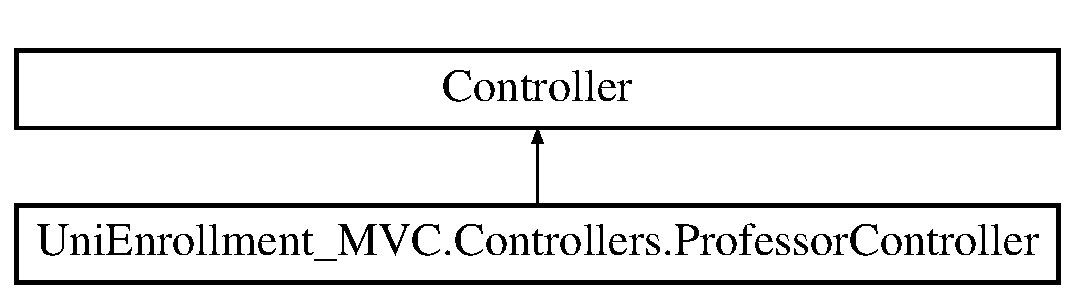
\includegraphics[height=2.000000cm]{class_uni_enrollment___m_v_c_1_1_controllers_1_1_professor_controller}
\end{center}
\end{figure}
\subsection*{Public Member Functions}
\begin{DoxyCompactItemize}
\item 
Action\+Result \hyperlink{class_uni_enrollment___m_v_c_1_1_controllers_1_1_professor_controller_a4e043a0a91774c6c4c717e20491bd07e}{Index} ()
\item 
Action\+Result \hyperlink{class_uni_enrollment___m_v_c_1_1_controllers_1_1_professor_controller_aeee3fc968f7143e40fb72435a2a52362}{Details} (int?id)
\item 
Action\+Result \hyperlink{class_uni_enrollment___m_v_c_1_1_controllers_1_1_professor_controller_af361fb8ef6501711881963e5811d0e8d}{Create} ()
\item 
Action\+Result \hyperlink{class_uni_enrollment___m_v_c_1_1_controllers_1_1_professor_controller_a608bfecc8e3f96672690c8d440e579c9}{Submit\+Create} (\hyperlink{class_uni_enrollment___m_v_c_1_1_models_1_1_professor_view_model}{Professor\+View\+Model} vm\+Professor)
\item 
Action\+Result \hyperlink{class_uni_enrollment___m_v_c_1_1_controllers_1_1_professor_controller_a5eac6c88d51b3528f8fbb5f0902a9bc7}{Edit} (int?id)
\item 
Action\+Result \hyperlink{class_uni_enrollment___m_v_c_1_1_controllers_1_1_professor_controller_ae9f81c9967f5210789cf46a9ddab53ea}{Submit\+Edit} (\hyperlink{class_uni_enrollment___m_v_c_1_1_models_1_1_user}{User} professor, string cb\+Reset\+Password)
\end{DoxyCompactItemize}
\subsection*{Properties}
\begin{DoxyCompactItemize}
\item 
int \hyperlink{class_uni_enrollment___m_v_c_1_1_controllers_1_1_professor_controller_ae95fa62ec0b4a85f1bbb3d2174359bdf}{Professor\+Type\+ID}\hspace{0.3cm}{\ttfamily  \mbox{[}get\mbox{]}}
\end{DoxyCompactItemize}
\subsection*{Private Attributes}
\begin{DoxyCompactItemize}
\item 
\hyperlink{class_uni_enrollment___m_v_c_1_1_models_1_1_uni_enrollment_d_b_entities}{Uni\+Enrollment\+D\+B\+Entities} \hyperlink{class_uni_enrollment___m_v_c_1_1_controllers_1_1_professor_controller_abff01e9d5157fe32a437eaf262b4396f}{\+\_\+entities} = new \hyperlink{class_uni_enrollment___m_v_c_1_1_models_1_1_uni_enrollment_d_b_entities}{Uni\+Enrollment\+D\+B\+Entities}()
\end{DoxyCompactItemize}


\subsection{Detailed Description}


Contains user interaction (action result) methods for anything uni \textquotesingle{}professor\textquotesingle{} related 

Definition at line 16 of file Professor\+Controller.\+cs.



\subsection{Member Function Documentation}
\index{Uni\+Enrollment\+\_\+\+M\+V\+C\+::\+Controllers\+::\+Professor\+Controller@{Uni\+Enrollment\+\_\+\+M\+V\+C\+::\+Controllers\+::\+Professor\+Controller}!Create@{Create}}
\index{Create@{Create}!Uni\+Enrollment\+\_\+\+M\+V\+C\+::\+Controllers\+::\+Professor\+Controller@{Uni\+Enrollment\+\_\+\+M\+V\+C\+::\+Controllers\+::\+Professor\+Controller}}
\subsubsection[{\texorpdfstring{Create()}{Create()}}]{\setlength{\rightskip}{0pt plus 5cm}Action\+Result Uni\+Enrollment\+\_\+\+M\+V\+C.\+Controllers.\+Professor\+Controller.\+Create (
\begin{DoxyParamCaption}
{}
\end{DoxyParamCaption}
)}\hypertarget{class_uni_enrollment___m_v_c_1_1_controllers_1_1_professor_controller_af361fb8ef6501711881963e5811d0e8d}{}\label{class_uni_enrollment___m_v_c_1_1_controllers_1_1_professor_controller_af361fb8ef6501711881963e5811d0e8d}


Definition at line 49 of file Professor\+Controller.\+cs.

\index{Uni\+Enrollment\+\_\+\+M\+V\+C\+::\+Controllers\+::\+Professor\+Controller@{Uni\+Enrollment\+\_\+\+M\+V\+C\+::\+Controllers\+::\+Professor\+Controller}!Details@{Details}}
\index{Details@{Details}!Uni\+Enrollment\+\_\+\+M\+V\+C\+::\+Controllers\+::\+Professor\+Controller@{Uni\+Enrollment\+\_\+\+M\+V\+C\+::\+Controllers\+::\+Professor\+Controller}}
\subsubsection[{\texorpdfstring{Details(int?id)}{Details(int?id)}}]{\setlength{\rightskip}{0pt plus 5cm}Action\+Result Uni\+Enrollment\+\_\+\+M\+V\+C.\+Controllers.\+Professor\+Controller.\+Details (
\begin{DoxyParamCaption}
\item[{int?}]{id}
\end{DoxyParamCaption}
)}\hypertarget{class_uni_enrollment___m_v_c_1_1_controllers_1_1_professor_controller_aeee3fc968f7143e40fb72435a2a52362}{}\label{class_uni_enrollment___m_v_c_1_1_controllers_1_1_professor_controller_aeee3fc968f7143e40fb72435a2a52362}


Definition at line 34 of file Professor\+Controller.\+cs.

\index{Uni\+Enrollment\+\_\+\+M\+V\+C\+::\+Controllers\+::\+Professor\+Controller@{Uni\+Enrollment\+\_\+\+M\+V\+C\+::\+Controllers\+::\+Professor\+Controller}!Edit@{Edit}}
\index{Edit@{Edit}!Uni\+Enrollment\+\_\+\+M\+V\+C\+::\+Controllers\+::\+Professor\+Controller@{Uni\+Enrollment\+\_\+\+M\+V\+C\+::\+Controllers\+::\+Professor\+Controller}}
\subsubsection[{\texorpdfstring{Edit(int?id)}{Edit(int?id)}}]{\setlength{\rightskip}{0pt plus 5cm}Action\+Result Uni\+Enrollment\+\_\+\+M\+V\+C.\+Controllers.\+Professor\+Controller.\+Edit (
\begin{DoxyParamCaption}
\item[{int?}]{id}
\end{DoxyParamCaption}
)}\hypertarget{class_uni_enrollment___m_v_c_1_1_controllers_1_1_professor_controller_a5eac6c88d51b3528f8fbb5f0902a9bc7}{}\label{class_uni_enrollment___m_v_c_1_1_controllers_1_1_professor_controller_a5eac6c88d51b3528f8fbb5f0902a9bc7}


Definition at line 101 of file Professor\+Controller.\+cs.

\index{Uni\+Enrollment\+\_\+\+M\+V\+C\+::\+Controllers\+::\+Professor\+Controller@{Uni\+Enrollment\+\_\+\+M\+V\+C\+::\+Controllers\+::\+Professor\+Controller}!Index@{Index}}
\index{Index@{Index}!Uni\+Enrollment\+\_\+\+M\+V\+C\+::\+Controllers\+::\+Professor\+Controller@{Uni\+Enrollment\+\_\+\+M\+V\+C\+::\+Controllers\+::\+Professor\+Controller}}
\subsubsection[{\texorpdfstring{Index()}{Index()}}]{\setlength{\rightskip}{0pt plus 5cm}Action\+Result Uni\+Enrollment\+\_\+\+M\+V\+C.\+Controllers.\+Professor\+Controller.\+Index (
\begin{DoxyParamCaption}
{}
\end{DoxyParamCaption}
)}\hypertarget{class_uni_enrollment___m_v_c_1_1_controllers_1_1_professor_controller_a4e043a0a91774c6c4c717e20491bd07e}{}\label{class_uni_enrollment___m_v_c_1_1_controllers_1_1_professor_controller_a4e043a0a91774c6c4c717e20491bd07e}


Definition at line 28 of file Professor\+Controller.\+cs.

\index{Uni\+Enrollment\+\_\+\+M\+V\+C\+::\+Controllers\+::\+Professor\+Controller@{Uni\+Enrollment\+\_\+\+M\+V\+C\+::\+Controllers\+::\+Professor\+Controller}!Submit\+Create@{Submit\+Create}}
\index{Submit\+Create@{Submit\+Create}!Uni\+Enrollment\+\_\+\+M\+V\+C\+::\+Controllers\+::\+Professor\+Controller@{Uni\+Enrollment\+\_\+\+M\+V\+C\+::\+Controllers\+::\+Professor\+Controller}}
\subsubsection[{\texorpdfstring{Submit\+Create(\+Professor\+View\+Model vm\+Professor)}{SubmitCreate(ProfessorViewModel vmProfessor)}}]{\setlength{\rightskip}{0pt plus 5cm}Action\+Result Uni\+Enrollment\+\_\+\+M\+V\+C.\+Controllers.\+Professor\+Controller.\+Submit\+Create (
\begin{DoxyParamCaption}
\item[{{\bf Professor\+View\+Model}}]{vm\+Professor}
\end{DoxyParamCaption}
)}\hypertarget{class_uni_enrollment___m_v_c_1_1_controllers_1_1_professor_controller_a608bfecc8e3f96672690c8d440e579c9}{}\label{class_uni_enrollment___m_v_c_1_1_controllers_1_1_professor_controller_a608bfecc8e3f96672690c8d440e579c9}


Definition at line 63 of file Professor\+Controller.\+cs.

\index{Uni\+Enrollment\+\_\+\+M\+V\+C\+::\+Controllers\+::\+Professor\+Controller@{Uni\+Enrollment\+\_\+\+M\+V\+C\+::\+Controllers\+::\+Professor\+Controller}!Submit\+Edit@{Submit\+Edit}}
\index{Submit\+Edit@{Submit\+Edit}!Uni\+Enrollment\+\_\+\+M\+V\+C\+::\+Controllers\+::\+Professor\+Controller@{Uni\+Enrollment\+\_\+\+M\+V\+C\+::\+Controllers\+::\+Professor\+Controller}}
\subsubsection[{\texorpdfstring{Submit\+Edit(\+User professor, string cb\+Reset\+Password)}{SubmitEdit(User professor, string cbResetPassword)}}]{\setlength{\rightskip}{0pt plus 5cm}Action\+Result Uni\+Enrollment\+\_\+\+M\+V\+C.\+Controllers.\+Professor\+Controller.\+Submit\+Edit (
\begin{DoxyParamCaption}
\item[{{\bf User}}]{professor, }
\item[{string}]{cb\+Reset\+Password}
\end{DoxyParamCaption}
)}\hypertarget{class_uni_enrollment___m_v_c_1_1_controllers_1_1_professor_controller_ae9f81c9967f5210789cf46a9ddab53ea}{}\label{class_uni_enrollment___m_v_c_1_1_controllers_1_1_professor_controller_ae9f81c9967f5210789cf46a9ddab53ea}


Definition at line 124 of file Professor\+Controller.\+cs.



\subsection{Member Data Documentation}
\index{Uni\+Enrollment\+\_\+\+M\+V\+C\+::\+Controllers\+::\+Professor\+Controller@{Uni\+Enrollment\+\_\+\+M\+V\+C\+::\+Controllers\+::\+Professor\+Controller}!\+\_\+entities@{\+\_\+entities}}
\index{\+\_\+entities@{\+\_\+entities}!Uni\+Enrollment\+\_\+\+M\+V\+C\+::\+Controllers\+::\+Professor\+Controller@{Uni\+Enrollment\+\_\+\+M\+V\+C\+::\+Controllers\+::\+Professor\+Controller}}
\subsubsection[{\texorpdfstring{\+\_\+entities}{_entities}}]{\setlength{\rightskip}{0pt plus 5cm}{\bf Uni\+Enrollment\+D\+B\+Entities} Uni\+Enrollment\+\_\+\+M\+V\+C.\+Controllers.\+Professor\+Controller.\+\_\+entities = new {\bf Uni\+Enrollment\+D\+B\+Entities}()\hspace{0.3cm}{\ttfamily [private]}}\hypertarget{class_uni_enrollment___m_v_c_1_1_controllers_1_1_professor_controller_abff01e9d5157fe32a437eaf262b4396f}{}\label{class_uni_enrollment___m_v_c_1_1_controllers_1_1_professor_controller_abff01e9d5157fe32a437eaf262b4396f}


Definition at line 18 of file Professor\+Controller.\+cs.



\subsection{Property Documentation}
\index{Uni\+Enrollment\+\_\+\+M\+V\+C\+::\+Controllers\+::\+Professor\+Controller@{Uni\+Enrollment\+\_\+\+M\+V\+C\+::\+Controllers\+::\+Professor\+Controller}!Professor\+Type\+ID@{Professor\+Type\+ID}}
\index{Professor\+Type\+ID@{Professor\+Type\+ID}!Uni\+Enrollment\+\_\+\+M\+V\+C\+::\+Controllers\+::\+Professor\+Controller@{Uni\+Enrollment\+\_\+\+M\+V\+C\+::\+Controllers\+::\+Professor\+Controller}}
\subsubsection[{\texorpdfstring{Professor\+Type\+ID}{ProfessorTypeID}}]{\setlength{\rightskip}{0pt plus 5cm}int Uni\+Enrollment\+\_\+\+M\+V\+C.\+Controllers.\+Professor\+Controller.\+Professor\+Type\+ID\hspace{0.3cm}{\ttfamily [get]}, {\ttfamily [protected]}}\hypertarget{class_uni_enrollment___m_v_c_1_1_controllers_1_1_professor_controller_ae95fa62ec0b4a85f1bbb3d2174359bdf}{}\label{class_uni_enrollment___m_v_c_1_1_controllers_1_1_professor_controller_ae95fa62ec0b4a85f1bbb3d2174359bdf}


Definition at line 21 of file Professor\+Controller.\+cs.



The documentation for this class was generated from the following file\+:\begin{DoxyCompactItemize}
\item 
H\+:/\+Documents/\+Work/\+Repositories/\+Uni\+Enrollment-\/\+D\+E\+M\+O/\+Uni\+Enrollment-\/\+M\+V\+C/\+Controllers/\hyperlink{_professor_controller_8cs}{Professor\+Controller.\+cs}\end{DoxyCompactItemize}

\hypertarget{class_uni_enrollment___m_v_c_1_1_models_1_1_professor_d_b_context}{}\section{Uni\+Enrollment\+\_\+\+M\+V\+C.\+Models.\+Professor\+D\+B\+Context Class Reference}
\label{class_uni_enrollment___m_v_c_1_1_models_1_1_professor_d_b_context}\index{Uni\+Enrollment\+\_\+\+M\+V\+C.\+Models.\+Professor\+D\+B\+Context@{Uni\+Enrollment\+\_\+\+M\+V\+C.\+Models.\+Professor\+D\+B\+Context}}
Inheritance diagram for Uni\+Enrollment\+\_\+\+M\+V\+C.\+Models.\+Professor\+D\+B\+Context\+:\begin{figure}[H]
\begin{center}
\leavevmode
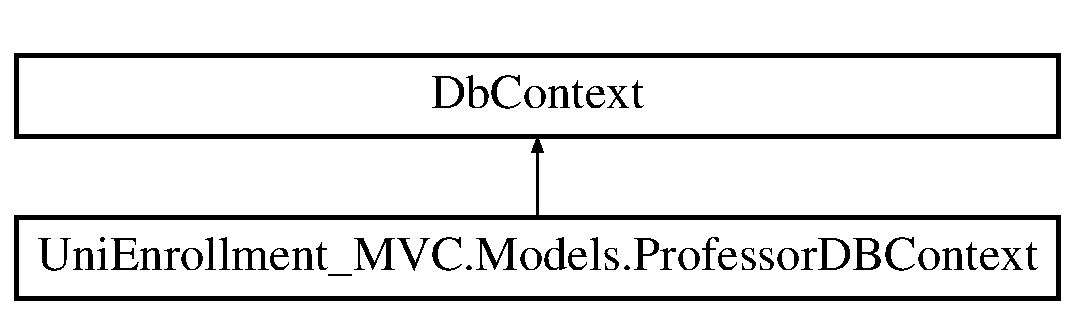
\includegraphics[height=2.000000cm]{class_uni_enrollment___m_v_c_1_1_models_1_1_professor_d_b_context}
\end{center}
\end{figure}
\subsection*{Public Member Functions}
\begin{DoxyCompactItemize}
\item 
\hyperlink{class_uni_enrollment___m_v_c_1_1_models_1_1_professor_d_b_context_a2c36d9e40760c9e937839d80273373be}{Professor\+D\+B\+Context} ()
\end{DoxyCompactItemize}
\subsection*{Protected Member Functions}
\begin{DoxyCompactItemize}
\item 
override void \hyperlink{class_uni_enrollment___m_v_c_1_1_models_1_1_professor_d_b_context_a5579a7ea482aa10fbc1e06b185d85179}{On\+Model\+Creating} (Db\+Model\+Builder model\+Builder)
\end{DoxyCompactItemize}
\subsection*{Properties}
\begin{DoxyCompactItemize}
\item 
Db\+Set$<$ \hyperlink{class_uni_enrollment___m_v_c_1_1_models_1_1_professor}{Professor} $>$ \hyperlink{class_uni_enrollment___m_v_c_1_1_models_1_1_professor_d_b_context_ae43a089ed6de4a4dfb6712b8a908626c}{Professors}\hspace{0.3cm}{\ttfamily  \mbox{[}get, set\mbox{]}}
\end{DoxyCompactItemize}


\subsection{Detailed Description}


Definition at line 6 of file Professor\+D\+B\+Context.\+cs.



\subsection{Constructor \& Destructor Documentation}
\index{Uni\+Enrollment\+\_\+\+M\+V\+C\+::\+Models\+::\+Professor\+D\+B\+Context@{Uni\+Enrollment\+\_\+\+M\+V\+C\+::\+Models\+::\+Professor\+D\+B\+Context}!Professor\+D\+B\+Context@{Professor\+D\+B\+Context}}
\index{Professor\+D\+B\+Context@{Professor\+D\+B\+Context}!Uni\+Enrollment\+\_\+\+M\+V\+C\+::\+Models\+::\+Professor\+D\+B\+Context@{Uni\+Enrollment\+\_\+\+M\+V\+C\+::\+Models\+::\+Professor\+D\+B\+Context}}
\subsubsection[{\texorpdfstring{Professor\+D\+B\+Context()}{ProfessorDBContext()}}]{\setlength{\rightskip}{0pt plus 5cm}Uni\+Enrollment\+\_\+\+M\+V\+C.\+Models.\+Professor\+D\+B\+Context.\+Professor\+D\+B\+Context (
\begin{DoxyParamCaption}
{}
\end{DoxyParamCaption}
)}\hypertarget{class_uni_enrollment___m_v_c_1_1_models_1_1_professor_d_b_context_a2c36d9e40760c9e937839d80273373be}{}\label{class_uni_enrollment___m_v_c_1_1_models_1_1_professor_d_b_context_a2c36d9e40760c9e937839d80273373be}


Definition at line 8 of file Professor\+D\+B\+Context.\+cs.



\subsection{Member Function Documentation}
\index{Uni\+Enrollment\+\_\+\+M\+V\+C\+::\+Models\+::\+Professor\+D\+B\+Context@{Uni\+Enrollment\+\_\+\+M\+V\+C\+::\+Models\+::\+Professor\+D\+B\+Context}!On\+Model\+Creating@{On\+Model\+Creating}}
\index{On\+Model\+Creating@{On\+Model\+Creating}!Uni\+Enrollment\+\_\+\+M\+V\+C\+::\+Models\+::\+Professor\+D\+B\+Context@{Uni\+Enrollment\+\_\+\+M\+V\+C\+::\+Models\+::\+Professor\+D\+B\+Context}}
\subsubsection[{\texorpdfstring{On\+Model\+Creating(\+Db\+Model\+Builder model\+Builder)}{OnModelCreating(DbModelBuilder modelBuilder)}}]{\setlength{\rightskip}{0pt plus 5cm}override void Uni\+Enrollment\+\_\+\+M\+V\+C.\+Models.\+Professor\+D\+B\+Context.\+On\+Model\+Creating (
\begin{DoxyParamCaption}
\item[{Db\+Model\+Builder}]{model\+Builder}
\end{DoxyParamCaption}
)\hspace{0.3cm}{\ttfamily [protected]}}\hypertarget{class_uni_enrollment___m_v_c_1_1_models_1_1_professor_d_b_context_a5579a7ea482aa10fbc1e06b185d85179}{}\label{class_uni_enrollment___m_v_c_1_1_models_1_1_professor_d_b_context_a5579a7ea482aa10fbc1e06b185d85179}


Definition at line 12 of file Professor\+D\+B\+Context.\+cs.



\subsection{Property Documentation}
\index{Uni\+Enrollment\+\_\+\+M\+V\+C\+::\+Models\+::\+Professor\+D\+B\+Context@{Uni\+Enrollment\+\_\+\+M\+V\+C\+::\+Models\+::\+Professor\+D\+B\+Context}!Professors@{Professors}}
\index{Professors@{Professors}!Uni\+Enrollment\+\_\+\+M\+V\+C\+::\+Models\+::\+Professor\+D\+B\+Context@{Uni\+Enrollment\+\_\+\+M\+V\+C\+::\+Models\+::\+Professor\+D\+B\+Context}}
\subsubsection[{\texorpdfstring{Professors}{Professors}}]{\setlength{\rightskip}{0pt plus 5cm}Db\+Set$<${\bf Professor}$>$ Uni\+Enrollment\+\_\+\+M\+V\+C.\+Models.\+Professor\+D\+B\+Context.\+Professors\hspace{0.3cm}{\ttfamily [get]}, {\ttfamily [set]}}\hypertarget{class_uni_enrollment___m_v_c_1_1_models_1_1_professor_d_b_context_ae43a089ed6de4a4dfb6712b8a908626c}{}\label{class_uni_enrollment___m_v_c_1_1_models_1_1_professor_d_b_context_ae43a089ed6de4a4dfb6712b8a908626c}


Definition at line 26 of file Professor\+D\+B\+Context.\+cs.



The documentation for this class was generated from the following file\+:\begin{DoxyCompactItemize}
\item 
H\+:/\+Documents/\+Work/\+Repositories/\+Uni\+Enrollment-\/\+D\+E\+M\+O/\+Uni\+Enrollment-\/\+M\+V\+C/\+Context/\hyperlink{_professor_d_b_context_8cs}{Professor\+D\+B\+Context.\+cs}\end{DoxyCompactItemize}

\hypertarget{class_uni_enrollment___m_v_c_1_1_models_1_1_professor_view_model}{}\section{Uni\+Enrollment\+\_\+\+M\+V\+C.\+Models.\+Professor\+View\+Model Class Reference}
\label{class_uni_enrollment___m_v_c_1_1_models_1_1_professor_view_model}\index{Uni\+Enrollment\+\_\+\+M\+V\+C.\+Models.\+Professor\+View\+Model@{Uni\+Enrollment\+\_\+\+M\+V\+C.\+Models.\+Professor\+View\+Model}}
\subsection*{Static Public Member Functions}
\begin{DoxyCompactItemize}
\item 
static List$<$ \hyperlink{class_uni_enrollment___m_v_c_1_1_models_1_1_user}{User} $>$ \hyperlink{class_uni_enrollment___m_v_c_1_1_models_1_1_professor_view_model_a2a3825e5981ac5301bba4e850e0e56b7}{Get\+Professor\+List} ()
\begin{DoxyCompactList}\small\item\em All active professors -\/ for a drop down list \end{DoxyCompactList}\end{DoxyCompactItemize}
\subsection*{Properties}
\begin{DoxyCompactItemize}
\item 
string \hyperlink{class_uni_enrollment___m_v_c_1_1_models_1_1_professor_view_model_ac1aabbd7b2f7b9b531ede5064097b73d}{ID}\hspace{0.3cm}{\ttfamily  \mbox{[}get, set\mbox{]}}
\item 
string \hyperlink{class_uni_enrollment___m_v_c_1_1_models_1_1_professor_view_model_a892125a1dc3a4e4d8c908a7b2aff87fa}{Name}\hspace{0.3cm}{\ttfamily  \mbox{[}get, set\mbox{]}}
\item 
string \hyperlink{class_uni_enrollment___m_v_c_1_1_models_1_1_professor_view_model_a4a8450ec4af630eb473c2f88036cb26a}{Username}\hspace{0.3cm}{\ttfamily  \mbox{[}get, set\mbox{]}}
\item 
string \hyperlink{class_uni_enrollment___m_v_c_1_1_models_1_1_professor_view_model_a925e191c8c2babf6240a7c99fb2c08b5}{Password}\hspace{0.3cm}{\ttfamily  \mbox{[}get, set\mbox{]}}
\item 
string \hyperlink{class_uni_enrollment___m_v_c_1_1_models_1_1_professor_view_model_ae87fa85f8261a37cb829b4224cccf67b}{Confirm\+Password}\hspace{0.3cm}{\ttfamily  \mbox{[}get, set\mbox{]}}
\item 
virtual List$<$ \hyperlink{class_uni_enrollment___m_v_c_1_1_models_1_1_course}{Course} $>$ \hyperlink{class_uni_enrollment___m_v_c_1_1_models_1_1_professor_view_model_a5a3f032e8a875112049116f75d9a8b73}{Courses}\hspace{0.3cm}{\ttfamily  \mbox{[}get, set\mbox{]}}
\end{DoxyCompactItemize}


\subsection{Detailed Description}


Definition at line 7 of file Professor\+View\+Model.\+cs.



\subsection{Member Function Documentation}
\index{Uni\+Enrollment\+\_\+\+M\+V\+C\+::\+Models\+::\+Professor\+View\+Model@{Uni\+Enrollment\+\_\+\+M\+V\+C\+::\+Models\+::\+Professor\+View\+Model}!Get\+Professor\+List@{Get\+Professor\+List}}
\index{Get\+Professor\+List@{Get\+Professor\+List}!Uni\+Enrollment\+\_\+\+M\+V\+C\+::\+Models\+::\+Professor\+View\+Model@{Uni\+Enrollment\+\_\+\+M\+V\+C\+::\+Models\+::\+Professor\+View\+Model}}
\subsubsection[{\texorpdfstring{Get\+Professor\+List()}{GetProfessorList()}}]{\setlength{\rightskip}{0pt plus 5cm}static List$<${\bf User}$>$ Uni\+Enrollment\+\_\+\+M\+V\+C.\+Models.\+Professor\+View\+Model.\+Get\+Professor\+List (
\begin{DoxyParamCaption}
{}
\end{DoxyParamCaption}
)\hspace{0.3cm}{\ttfamily [static]}}\hypertarget{class_uni_enrollment___m_v_c_1_1_models_1_1_professor_view_model_a2a3825e5981ac5301bba4e850e0e56b7}{}\label{class_uni_enrollment___m_v_c_1_1_models_1_1_professor_view_model_a2a3825e5981ac5301bba4e850e0e56b7}


All active professors -\/ for a drop down list 

\begin{DoxyReturn}{Returns}
A list of all active professor
\end{DoxyReturn}


Definition at line 36 of file Professor\+View\+Model.\+cs.



\subsection{Property Documentation}
\index{Uni\+Enrollment\+\_\+\+M\+V\+C\+::\+Models\+::\+Professor\+View\+Model@{Uni\+Enrollment\+\_\+\+M\+V\+C\+::\+Models\+::\+Professor\+View\+Model}!Confirm\+Password@{Confirm\+Password}}
\index{Confirm\+Password@{Confirm\+Password}!Uni\+Enrollment\+\_\+\+M\+V\+C\+::\+Models\+::\+Professor\+View\+Model@{Uni\+Enrollment\+\_\+\+M\+V\+C\+::\+Models\+::\+Professor\+View\+Model}}
\subsubsection[{\texorpdfstring{Confirm\+Password}{ConfirmPassword}}]{\setlength{\rightskip}{0pt plus 5cm}string Uni\+Enrollment\+\_\+\+M\+V\+C.\+Models.\+Professor\+View\+Model.\+Confirm\+Password\hspace{0.3cm}{\ttfamily [get]}, {\ttfamily [set]}}\hypertarget{class_uni_enrollment___m_v_c_1_1_models_1_1_professor_view_model_ae87fa85f8261a37cb829b4224cccf67b}{}\label{class_uni_enrollment___m_v_c_1_1_models_1_1_professor_view_model_ae87fa85f8261a37cb829b4224cccf67b}


Definition at line 28 of file Professor\+View\+Model.\+cs.

\index{Uni\+Enrollment\+\_\+\+M\+V\+C\+::\+Models\+::\+Professor\+View\+Model@{Uni\+Enrollment\+\_\+\+M\+V\+C\+::\+Models\+::\+Professor\+View\+Model}!Courses@{Courses}}
\index{Courses@{Courses}!Uni\+Enrollment\+\_\+\+M\+V\+C\+::\+Models\+::\+Professor\+View\+Model@{Uni\+Enrollment\+\_\+\+M\+V\+C\+::\+Models\+::\+Professor\+View\+Model}}
\subsubsection[{\texorpdfstring{Courses}{Courses}}]{\setlength{\rightskip}{0pt plus 5cm}virtual List$<${\bf Course}$>$ Uni\+Enrollment\+\_\+\+M\+V\+C.\+Models.\+Professor\+View\+Model.\+Courses\hspace{0.3cm}{\ttfamily [get]}, {\ttfamily [set]}}\hypertarget{class_uni_enrollment___m_v_c_1_1_models_1_1_professor_view_model_a5a3f032e8a875112049116f75d9a8b73}{}\label{class_uni_enrollment___m_v_c_1_1_models_1_1_professor_view_model_a5a3f032e8a875112049116f75d9a8b73}


Definition at line 30 of file Professor\+View\+Model.\+cs.

\index{Uni\+Enrollment\+\_\+\+M\+V\+C\+::\+Models\+::\+Professor\+View\+Model@{Uni\+Enrollment\+\_\+\+M\+V\+C\+::\+Models\+::\+Professor\+View\+Model}!ID@{ID}}
\index{ID@{ID}!Uni\+Enrollment\+\_\+\+M\+V\+C\+::\+Models\+::\+Professor\+View\+Model@{Uni\+Enrollment\+\_\+\+M\+V\+C\+::\+Models\+::\+Professor\+View\+Model}}
\subsubsection[{\texorpdfstring{ID}{ID}}]{\setlength{\rightskip}{0pt plus 5cm}string Uni\+Enrollment\+\_\+\+M\+V\+C.\+Models.\+Professor\+View\+Model.\+ID\hspace{0.3cm}{\ttfamily [get]}, {\ttfamily [set]}}\hypertarget{class_uni_enrollment___m_v_c_1_1_models_1_1_professor_view_model_ac1aabbd7b2f7b9b531ede5064097b73d}{}\label{class_uni_enrollment___m_v_c_1_1_models_1_1_professor_view_model_ac1aabbd7b2f7b9b531ede5064097b73d}


Definition at line 9 of file Professor\+View\+Model.\+cs.

\index{Uni\+Enrollment\+\_\+\+M\+V\+C\+::\+Models\+::\+Professor\+View\+Model@{Uni\+Enrollment\+\_\+\+M\+V\+C\+::\+Models\+::\+Professor\+View\+Model}!Name@{Name}}
\index{Name@{Name}!Uni\+Enrollment\+\_\+\+M\+V\+C\+::\+Models\+::\+Professor\+View\+Model@{Uni\+Enrollment\+\_\+\+M\+V\+C\+::\+Models\+::\+Professor\+View\+Model}}
\subsubsection[{\texorpdfstring{Name}{Name}}]{\setlength{\rightskip}{0pt plus 5cm}string Uni\+Enrollment\+\_\+\+M\+V\+C.\+Models.\+Professor\+View\+Model.\+Name\hspace{0.3cm}{\ttfamily [get]}, {\ttfamily [set]}}\hypertarget{class_uni_enrollment___m_v_c_1_1_models_1_1_professor_view_model_a892125a1dc3a4e4d8c908a7b2aff87fa}{}\label{class_uni_enrollment___m_v_c_1_1_models_1_1_professor_view_model_a892125a1dc3a4e4d8c908a7b2aff87fa}


Definition at line 14 of file Professor\+View\+Model.\+cs.

\index{Uni\+Enrollment\+\_\+\+M\+V\+C\+::\+Models\+::\+Professor\+View\+Model@{Uni\+Enrollment\+\_\+\+M\+V\+C\+::\+Models\+::\+Professor\+View\+Model}!Password@{Password}}
\index{Password@{Password}!Uni\+Enrollment\+\_\+\+M\+V\+C\+::\+Models\+::\+Professor\+View\+Model@{Uni\+Enrollment\+\_\+\+M\+V\+C\+::\+Models\+::\+Professor\+View\+Model}}
\subsubsection[{\texorpdfstring{Password}{Password}}]{\setlength{\rightskip}{0pt plus 5cm}string Uni\+Enrollment\+\_\+\+M\+V\+C.\+Models.\+Professor\+View\+Model.\+Password\hspace{0.3cm}{\ttfamily [get]}, {\ttfamily [set]}}\hypertarget{class_uni_enrollment___m_v_c_1_1_models_1_1_professor_view_model_a925e191c8c2babf6240a7c99fb2c08b5}{}\label{class_uni_enrollment___m_v_c_1_1_models_1_1_professor_view_model_a925e191c8c2babf6240a7c99fb2c08b5}


Definition at line 25 of file Professor\+View\+Model.\+cs.

\index{Uni\+Enrollment\+\_\+\+M\+V\+C\+::\+Models\+::\+Professor\+View\+Model@{Uni\+Enrollment\+\_\+\+M\+V\+C\+::\+Models\+::\+Professor\+View\+Model}!Username@{Username}}
\index{Username@{Username}!Uni\+Enrollment\+\_\+\+M\+V\+C\+::\+Models\+::\+Professor\+View\+Model@{Uni\+Enrollment\+\_\+\+M\+V\+C\+::\+Models\+::\+Professor\+View\+Model}}
\subsubsection[{\texorpdfstring{Username}{Username}}]{\setlength{\rightskip}{0pt plus 5cm}string Uni\+Enrollment\+\_\+\+M\+V\+C.\+Models.\+Professor\+View\+Model.\+Username\hspace{0.3cm}{\ttfamily [get]}, {\ttfamily [set]}}\hypertarget{class_uni_enrollment___m_v_c_1_1_models_1_1_professor_view_model_a4a8450ec4af630eb473c2f88036cb26a}{}\label{class_uni_enrollment___m_v_c_1_1_models_1_1_professor_view_model_a4a8450ec4af630eb473c2f88036cb26a}


Definition at line 19 of file Professor\+View\+Model.\+cs.



The documentation for this class was generated from the following file\+:\begin{DoxyCompactItemize}
\item 
H\+:/\+Documents/\+Work/\+Repositories/\+Uni\+Enrollment-\/\+D\+E\+M\+O/\+Uni\+Enrollment-\/\+M\+V\+C/\+Models/\hyperlink{_professor_view_model_8cs}{Professor\+View\+Model.\+cs}\end{DoxyCompactItemize}

\hypertarget{class_uni_enrollment___m_v_c_1_1_route_config}{}\section{Uni\+Enrollment\+\_\+\+M\+V\+C.\+Route\+Config Class Reference}
\label{class_uni_enrollment___m_v_c_1_1_route_config}\index{Uni\+Enrollment\+\_\+\+M\+V\+C.\+Route\+Config@{Uni\+Enrollment\+\_\+\+M\+V\+C.\+Route\+Config}}
\subsection*{Static Public Member Functions}
\begin{DoxyCompactItemize}
\item 
static void \hyperlink{class_uni_enrollment___m_v_c_1_1_route_config_aa8a86d6aefa4e6dbc49b91ca6abbf162}{Register\+Routes} (Route\+Collection routes)
\end{DoxyCompactItemize}


\subsection{Detailed Description}


Definition at line 10 of file Route\+Config.\+cs.



\subsection{Member Function Documentation}
\index{Uni\+Enrollment\+\_\+\+M\+V\+C\+::\+Route\+Config@{Uni\+Enrollment\+\_\+\+M\+V\+C\+::\+Route\+Config}!Register\+Routes@{Register\+Routes}}
\index{Register\+Routes@{Register\+Routes}!Uni\+Enrollment\+\_\+\+M\+V\+C\+::\+Route\+Config@{Uni\+Enrollment\+\_\+\+M\+V\+C\+::\+Route\+Config}}
\subsubsection[{\texorpdfstring{Register\+Routes(\+Route\+Collection routes)}{RegisterRoutes(RouteCollection routes)}}]{\setlength{\rightskip}{0pt plus 5cm}static void Uni\+Enrollment\+\_\+\+M\+V\+C.\+Route\+Config.\+Register\+Routes (
\begin{DoxyParamCaption}
\item[{Route\+Collection}]{routes}
\end{DoxyParamCaption}
)\hspace{0.3cm}{\ttfamily [static]}}\hypertarget{class_uni_enrollment___m_v_c_1_1_route_config_aa8a86d6aefa4e6dbc49b91ca6abbf162}{}\label{class_uni_enrollment___m_v_c_1_1_route_config_aa8a86d6aefa4e6dbc49b91ca6abbf162}


Definition at line 12 of file Route\+Config.\+cs.



The documentation for this class was generated from the following file\+:\begin{DoxyCompactItemize}
\item 
H\+:/\+Documents/\+Work/\+Repositories/\+Uni\+Enrollment-\/\+D\+E\+M\+O/\+Uni\+Enrollment-\/\+M\+V\+C/\+App\+\_\+\+Start/\hyperlink{_route_config_8cs}{Route\+Config.\+cs}\end{DoxyCompactItemize}

\hypertarget{class_uni_enrollment___m_v_c_1_1_startup}{}\section{Uni\+Enrollment\+\_\+\+M\+V\+C.\+Startup Class Reference}
\label{class_uni_enrollment___m_v_c_1_1_startup}\index{Uni\+Enrollment\+\_\+\+M\+V\+C.\+Startup@{Uni\+Enrollment\+\_\+\+M\+V\+C.\+Startup}}
\subsection*{Public Member Functions}
\begin{DoxyCompactItemize}
\item 
void \hyperlink{class_uni_enrollment___m_v_c_1_1_startup_a0e659d5160ef42f2eb0ae9b1c3c8aec1}{Configuration} (I\+App\+Builder app)
\end{DoxyCompactItemize}


\subsection{Detailed Description}


Definition at line 7 of file Startup.\+cs.



\subsection{Member Function Documentation}
\index{Uni\+Enrollment\+\_\+\+M\+V\+C\+::\+Startup@{Uni\+Enrollment\+\_\+\+M\+V\+C\+::\+Startup}!Configuration@{Configuration}}
\index{Configuration@{Configuration}!Uni\+Enrollment\+\_\+\+M\+V\+C\+::\+Startup@{Uni\+Enrollment\+\_\+\+M\+V\+C\+::\+Startup}}
\subsubsection[{\texorpdfstring{Configuration(\+I\+App\+Builder app)}{Configuration(IAppBuilder app)}}]{\setlength{\rightskip}{0pt plus 5cm}void Uni\+Enrollment\+\_\+\+M\+V\+C.\+Startup.\+Configuration (
\begin{DoxyParamCaption}
\item[{I\+App\+Builder}]{app}
\end{DoxyParamCaption}
)}\hypertarget{class_uni_enrollment___m_v_c_1_1_startup_a0e659d5160ef42f2eb0ae9b1c3c8aec1}{}\label{class_uni_enrollment___m_v_c_1_1_startup_a0e659d5160ef42f2eb0ae9b1c3c8aec1}


Definition at line 9 of file Startup.\+cs.



The documentation for this class was generated from the following file\+:\begin{DoxyCompactItemize}
\item 
H\+:/\+Documents/\+Work/\+Repositories/\+Uni\+Enrollment-\/\+D\+E\+M\+O/\+Uni\+Enrollment-\/\+M\+V\+C/\hyperlink{_startup_8cs}{Startup.\+cs}\end{DoxyCompactItemize}

\hypertarget{class_uni_enrollment___m_v_c_1_1_models_1_1_student}{}\section{Uni\+Enrollment\+\_\+\+M\+V\+C.\+Models.\+Student Class Reference}
\label{class_uni_enrollment___m_v_c_1_1_models_1_1_student}\index{Uni\+Enrollment\+\_\+\+M\+V\+C.\+Models.\+Student@{Uni\+Enrollment\+\_\+\+M\+V\+C.\+Models.\+Student}}
\subsection*{Public Member Functions}
\begin{DoxyCompactItemize}
\item 
\hyperlink{class_uni_enrollment___m_v_c_1_1_models_1_1_student_a20ccd261b61dab5def3fdd2c40d3681b}{Student} ()
\end{DoxyCompactItemize}
\subsection*{Properties}
\begin{DoxyCompactItemize}
\item 
int \hyperlink{class_uni_enrollment___m_v_c_1_1_models_1_1_student_af90e9ea91812385aeacb0d8016a6ac4d}{ID}\hspace{0.3cm}{\ttfamily  \mbox{[}get, set\mbox{]}}
\item 
string \hyperlink{class_uni_enrollment___m_v_c_1_1_models_1_1_student_a58b520c5e708debc5604ed96caa8fa3f}{Username}\hspace{0.3cm}{\ttfamily  \mbox{[}get, set\mbox{]}}
\item 
string \hyperlink{class_uni_enrollment___m_v_c_1_1_models_1_1_student_ad31ea99bde5adc6008eb13d8e897cdab}{Password}\hspace{0.3cm}{\ttfamily  \mbox{[}get, set\mbox{]}}
\item 
string \hyperlink{class_uni_enrollment___m_v_c_1_1_models_1_1_student_ab45cd7a456ecc65eb17b5b72f8b117d4}{Name}\hspace{0.3cm}{\ttfamily  \mbox{[}get, set\mbox{]}}
\item 
virtual I\+Collection$<$ \hyperlink{class_uni_enrollment___m_v_c_1_1_models_1_1_enrollment}{Enrollment} $>$ \hyperlink{class_uni_enrollment___m_v_c_1_1_models_1_1_student_a75f0808c2128b7a52546735a26df2d49}{Enrollments}\hspace{0.3cm}{\ttfamily  \mbox{[}get, set\mbox{]}}
\end{DoxyCompactItemize}


\subsection{Detailed Description}


Definition at line 15 of file Student.\+cs.



\subsection{Constructor \& Destructor Documentation}
\index{Uni\+Enrollment\+\_\+\+M\+V\+C\+::\+Models\+::\+Student@{Uni\+Enrollment\+\_\+\+M\+V\+C\+::\+Models\+::\+Student}!Student@{Student}}
\index{Student@{Student}!Uni\+Enrollment\+\_\+\+M\+V\+C\+::\+Models\+::\+Student@{Uni\+Enrollment\+\_\+\+M\+V\+C\+::\+Models\+::\+Student}}
\subsubsection[{\texorpdfstring{Student()}{Student()}}]{\setlength{\rightskip}{0pt plus 5cm}Uni\+Enrollment\+\_\+\+M\+V\+C.\+Models.\+Student.\+Student (
\begin{DoxyParamCaption}
{}
\end{DoxyParamCaption}
)}\hypertarget{class_uni_enrollment___m_v_c_1_1_models_1_1_student_a20ccd261b61dab5def3fdd2c40d3681b}{}\label{class_uni_enrollment___m_v_c_1_1_models_1_1_student_a20ccd261b61dab5def3fdd2c40d3681b}


Definition at line 18 of file Student.\+cs.



\subsection{Property Documentation}
\index{Uni\+Enrollment\+\_\+\+M\+V\+C\+::\+Models\+::\+Student@{Uni\+Enrollment\+\_\+\+M\+V\+C\+::\+Models\+::\+Student}!Enrollments@{Enrollments}}
\index{Enrollments@{Enrollments}!Uni\+Enrollment\+\_\+\+M\+V\+C\+::\+Models\+::\+Student@{Uni\+Enrollment\+\_\+\+M\+V\+C\+::\+Models\+::\+Student}}
\subsubsection[{\texorpdfstring{Enrollments}{Enrollments}}]{\setlength{\rightskip}{0pt plus 5cm}virtual I\+Collection$<${\bf Enrollment}$>$ Uni\+Enrollment\+\_\+\+M\+V\+C.\+Models.\+Student.\+Enrollments\hspace{0.3cm}{\ttfamily [get]}, {\ttfamily [set]}}\hypertarget{class_uni_enrollment___m_v_c_1_1_models_1_1_student_a75f0808c2128b7a52546735a26df2d49}{}\label{class_uni_enrollment___m_v_c_1_1_models_1_1_student_a75f0808c2128b7a52546735a26df2d49}


Definition at line 29 of file Student.\+cs.

\index{Uni\+Enrollment\+\_\+\+M\+V\+C\+::\+Models\+::\+Student@{Uni\+Enrollment\+\_\+\+M\+V\+C\+::\+Models\+::\+Student}!ID@{ID}}
\index{ID@{ID}!Uni\+Enrollment\+\_\+\+M\+V\+C\+::\+Models\+::\+Student@{Uni\+Enrollment\+\_\+\+M\+V\+C\+::\+Models\+::\+Student}}
\subsubsection[{\texorpdfstring{ID}{ID}}]{\setlength{\rightskip}{0pt plus 5cm}int Uni\+Enrollment\+\_\+\+M\+V\+C.\+Models.\+Student.\+ID\hspace{0.3cm}{\ttfamily [get]}, {\ttfamily [set]}}\hypertarget{class_uni_enrollment___m_v_c_1_1_models_1_1_student_af90e9ea91812385aeacb0d8016a6ac4d}{}\label{class_uni_enrollment___m_v_c_1_1_models_1_1_student_af90e9ea91812385aeacb0d8016a6ac4d}


Definition at line 23 of file Student.\+cs.

\index{Uni\+Enrollment\+\_\+\+M\+V\+C\+::\+Models\+::\+Student@{Uni\+Enrollment\+\_\+\+M\+V\+C\+::\+Models\+::\+Student}!Name@{Name}}
\index{Name@{Name}!Uni\+Enrollment\+\_\+\+M\+V\+C\+::\+Models\+::\+Student@{Uni\+Enrollment\+\_\+\+M\+V\+C\+::\+Models\+::\+Student}}
\subsubsection[{\texorpdfstring{Name}{Name}}]{\setlength{\rightskip}{0pt plus 5cm}string Uni\+Enrollment\+\_\+\+M\+V\+C.\+Models.\+Student.\+Name\hspace{0.3cm}{\ttfamily [get]}, {\ttfamily [set]}}\hypertarget{class_uni_enrollment___m_v_c_1_1_models_1_1_student_ab45cd7a456ecc65eb17b5b72f8b117d4}{}\label{class_uni_enrollment___m_v_c_1_1_models_1_1_student_ab45cd7a456ecc65eb17b5b72f8b117d4}


Definition at line 26 of file Student.\+cs.

\index{Uni\+Enrollment\+\_\+\+M\+V\+C\+::\+Models\+::\+Student@{Uni\+Enrollment\+\_\+\+M\+V\+C\+::\+Models\+::\+Student}!Password@{Password}}
\index{Password@{Password}!Uni\+Enrollment\+\_\+\+M\+V\+C\+::\+Models\+::\+Student@{Uni\+Enrollment\+\_\+\+M\+V\+C\+::\+Models\+::\+Student}}
\subsubsection[{\texorpdfstring{Password}{Password}}]{\setlength{\rightskip}{0pt plus 5cm}string Uni\+Enrollment\+\_\+\+M\+V\+C.\+Models.\+Student.\+Password\hspace{0.3cm}{\ttfamily [get]}, {\ttfamily [set]}}\hypertarget{class_uni_enrollment___m_v_c_1_1_models_1_1_student_ad31ea99bde5adc6008eb13d8e897cdab}{}\label{class_uni_enrollment___m_v_c_1_1_models_1_1_student_ad31ea99bde5adc6008eb13d8e897cdab}


Definition at line 25 of file Student.\+cs.

\index{Uni\+Enrollment\+\_\+\+M\+V\+C\+::\+Models\+::\+Student@{Uni\+Enrollment\+\_\+\+M\+V\+C\+::\+Models\+::\+Student}!Username@{Username}}
\index{Username@{Username}!Uni\+Enrollment\+\_\+\+M\+V\+C\+::\+Models\+::\+Student@{Uni\+Enrollment\+\_\+\+M\+V\+C\+::\+Models\+::\+Student}}
\subsubsection[{\texorpdfstring{Username}{Username}}]{\setlength{\rightskip}{0pt plus 5cm}string Uni\+Enrollment\+\_\+\+M\+V\+C.\+Models.\+Student.\+Username\hspace{0.3cm}{\ttfamily [get]}, {\ttfamily [set]}}\hypertarget{class_uni_enrollment___m_v_c_1_1_models_1_1_student_a58b520c5e708debc5604ed96caa8fa3f}{}\label{class_uni_enrollment___m_v_c_1_1_models_1_1_student_a58b520c5e708debc5604ed96caa8fa3f}


Definition at line 24 of file Student.\+cs.



The documentation for this class was generated from the following file\+:\begin{DoxyCompactItemize}
\item 
H\+:/\+Documents/\+Work/\+Repositories/\+Uni\+Enrollment-\/\+D\+E\+M\+O/\+Uni\+Enrollment-\/\+M\+V\+C/\+Models/\hyperlink{_student_8cs}{Student.\+cs}\end{DoxyCompactItemize}

\hypertarget{class_uni_enrollment___m_v_c_1_1_controllers_1_1_student_controller}{}\section{Uni\+Enrollment\+\_\+\+M\+V\+C.\+Controllers.\+Student\+Controller Class Reference}
\label{class_uni_enrollment___m_v_c_1_1_controllers_1_1_student_controller}\index{Uni\+Enrollment\+\_\+\+M\+V\+C.\+Controllers.\+Student\+Controller@{Uni\+Enrollment\+\_\+\+M\+V\+C.\+Controllers.\+Student\+Controller}}


Contains user interaction (action result) methods for anything uni \textquotesingle{}student\textquotesingle{} related  


Inheritance diagram for Uni\+Enrollment\+\_\+\+M\+V\+C.\+Controllers.\+Student\+Controller\+:\begin{figure}[H]
\begin{center}
\leavevmode
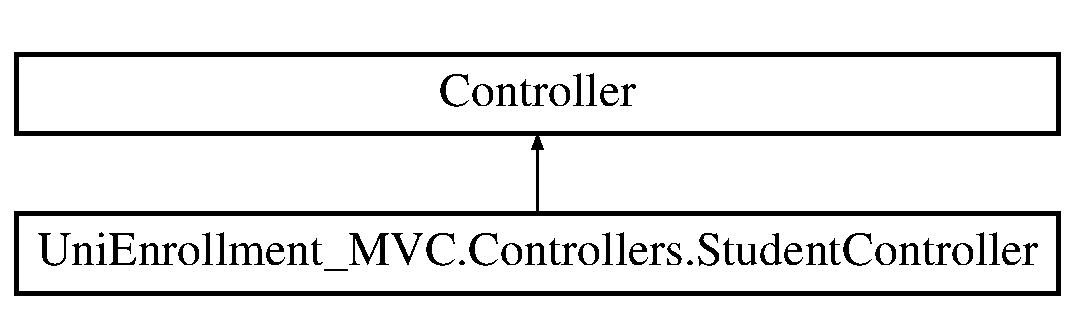
\includegraphics[height=2.000000cm]{class_uni_enrollment___m_v_c_1_1_controllers_1_1_student_controller}
\end{center}
\end{figure}
\subsection*{Public Member Functions}
\begin{DoxyCompactItemize}
\item 
Action\+Result \hyperlink{class_uni_enrollment___m_v_c_1_1_controllers_1_1_student_controller_a99a55aa0fd266130c87e5f3f410e18f0}{Index} ()
\item 
Action\+Result \hyperlink{class_uni_enrollment___m_v_c_1_1_controllers_1_1_student_controller_aa4f0e88839e2e96649fbaea4299dfded}{Details} (int?id)
\item 
Action\+Result \hyperlink{class_uni_enrollment___m_v_c_1_1_controllers_1_1_student_controller_a536100310cf7d5e404261a12a3d3a253}{Create} ()
\item 
Action\+Result \hyperlink{class_uni_enrollment___m_v_c_1_1_controllers_1_1_student_controller_a10b15f59171956321ff191dc610d1e70}{Submit\+Create} (\hyperlink{class_uni_enrollment___m_v_c_1_1_models_1_1_student_view_model}{Student\+View\+Model} vm\+Student)
\item 
Action\+Result \hyperlink{class_uni_enrollment___m_v_c_1_1_controllers_1_1_student_controller_a77fefd6af44dd913321444732fbf9d52}{Edit} (int?id)
\item 
Action\+Result \hyperlink{class_uni_enrollment___m_v_c_1_1_controllers_1_1_student_controller_aa2419626ede0b89e2eb4b4f4a8c8d5b7}{Submit\+Edit} (\hyperlink{class_uni_enrollment___m_v_c_1_1_models_1_1_user}{User} student, string cb\+Reset\+Password)
\item 
Action\+Result \hyperlink{class_uni_enrollment___m_v_c_1_1_controllers_1_1_student_controller_a954503cf9b679ce49e70678dc6511552}{Enroll} (int?id, int?course\+Id)
\end{DoxyCompactItemize}
\subsection*{Properties}
\begin{DoxyCompactItemize}
\item 
int \hyperlink{class_uni_enrollment___m_v_c_1_1_controllers_1_1_student_controller_ab8c62253a00233d37c8b799c7f3706b9}{Student\+Type\+ID}\hspace{0.3cm}{\ttfamily  \mbox{[}get\mbox{]}}
\end{DoxyCompactItemize}
\subsection*{Private Attributes}
\begin{DoxyCompactItemize}
\item 
\hyperlink{class_uni_enrollment___m_v_c_1_1_models_1_1_uni_enrollment_d_b_entities}{Uni\+Enrollment\+D\+B\+Entities} \hyperlink{class_uni_enrollment___m_v_c_1_1_controllers_1_1_student_controller_a3cd73c0385c0990a8ed4f4d5652be10a}{\+\_\+entities} = new \hyperlink{class_uni_enrollment___m_v_c_1_1_models_1_1_uni_enrollment_d_b_entities}{Uni\+Enrollment\+D\+B\+Entities}()
\end{DoxyCompactItemize}


\subsection{Detailed Description}
Contains user interaction (action result) methods for anything uni \textquotesingle{}student\textquotesingle{} related 



Definition at line 15 of file Student\+Controller.\+cs.



\subsection{Member Function Documentation}
\index{Uni\+Enrollment\+\_\+\+M\+V\+C\+::\+Controllers\+::\+Student\+Controller@{Uni\+Enrollment\+\_\+\+M\+V\+C\+::\+Controllers\+::\+Student\+Controller}!Create@{Create}}
\index{Create@{Create}!Uni\+Enrollment\+\_\+\+M\+V\+C\+::\+Controllers\+::\+Student\+Controller@{Uni\+Enrollment\+\_\+\+M\+V\+C\+::\+Controllers\+::\+Student\+Controller}}
\subsubsection[{\texorpdfstring{Create()}{Create()}}]{\setlength{\rightskip}{0pt plus 5cm}Action\+Result Uni\+Enrollment\+\_\+\+M\+V\+C.\+Controllers.\+Student\+Controller.\+Create (
\begin{DoxyParamCaption}
{}
\end{DoxyParamCaption}
)}\hypertarget{class_uni_enrollment___m_v_c_1_1_controllers_1_1_student_controller_a536100310cf7d5e404261a12a3d3a253}{}\label{class_uni_enrollment___m_v_c_1_1_controllers_1_1_student_controller_a536100310cf7d5e404261a12a3d3a253}


Definition at line 48 of file Student\+Controller.\+cs.

\index{Uni\+Enrollment\+\_\+\+M\+V\+C\+::\+Controllers\+::\+Student\+Controller@{Uni\+Enrollment\+\_\+\+M\+V\+C\+::\+Controllers\+::\+Student\+Controller}!Details@{Details}}
\index{Details@{Details}!Uni\+Enrollment\+\_\+\+M\+V\+C\+::\+Controllers\+::\+Student\+Controller@{Uni\+Enrollment\+\_\+\+M\+V\+C\+::\+Controllers\+::\+Student\+Controller}}
\subsubsection[{\texorpdfstring{Details(int?id)}{Details(int?id)}}]{\setlength{\rightskip}{0pt plus 5cm}Action\+Result Uni\+Enrollment\+\_\+\+M\+V\+C.\+Controllers.\+Student\+Controller.\+Details (
\begin{DoxyParamCaption}
\item[{int?}]{id}
\end{DoxyParamCaption}
)}\hypertarget{class_uni_enrollment___m_v_c_1_1_controllers_1_1_student_controller_aa4f0e88839e2e96649fbaea4299dfded}{}\label{class_uni_enrollment___m_v_c_1_1_controllers_1_1_student_controller_aa4f0e88839e2e96649fbaea4299dfded}


Definition at line 33 of file Student\+Controller.\+cs.

\index{Uni\+Enrollment\+\_\+\+M\+V\+C\+::\+Controllers\+::\+Student\+Controller@{Uni\+Enrollment\+\_\+\+M\+V\+C\+::\+Controllers\+::\+Student\+Controller}!Edit@{Edit}}
\index{Edit@{Edit}!Uni\+Enrollment\+\_\+\+M\+V\+C\+::\+Controllers\+::\+Student\+Controller@{Uni\+Enrollment\+\_\+\+M\+V\+C\+::\+Controllers\+::\+Student\+Controller}}
\subsubsection[{\texorpdfstring{Edit(int?id)}{Edit(int?id)}}]{\setlength{\rightskip}{0pt plus 5cm}Action\+Result Uni\+Enrollment\+\_\+\+M\+V\+C.\+Controllers.\+Student\+Controller.\+Edit (
\begin{DoxyParamCaption}
\item[{int?}]{id}
\end{DoxyParamCaption}
)}\hypertarget{class_uni_enrollment___m_v_c_1_1_controllers_1_1_student_controller_a77fefd6af44dd913321444732fbf9d52}{}\label{class_uni_enrollment___m_v_c_1_1_controllers_1_1_student_controller_a77fefd6af44dd913321444732fbf9d52}


Definition at line 100 of file Student\+Controller.\+cs.

\index{Uni\+Enrollment\+\_\+\+M\+V\+C\+::\+Controllers\+::\+Student\+Controller@{Uni\+Enrollment\+\_\+\+M\+V\+C\+::\+Controllers\+::\+Student\+Controller}!Enroll@{Enroll}}
\index{Enroll@{Enroll}!Uni\+Enrollment\+\_\+\+M\+V\+C\+::\+Controllers\+::\+Student\+Controller@{Uni\+Enrollment\+\_\+\+M\+V\+C\+::\+Controllers\+::\+Student\+Controller}}
\subsubsection[{\texorpdfstring{Enroll(int?id, int?course\+Id)}{Enroll(int?id, int?courseId)}}]{\setlength{\rightskip}{0pt plus 5cm}Action\+Result Uni\+Enrollment\+\_\+\+M\+V\+C.\+Controllers.\+Student\+Controller.\+Enroll (
\begin{DoxyParamCaption}
\item[{int?}]{id, }
\item[{int?}]{course\+Id}
\end{DoxyParamCaption}
)}\hypertarget{class_uni_enrollment___m_v_c_1_1_controllers_1_1_student_controller_a954503cf9b679ce49e70678dc6511552}{}\label{class_uni_enrollment___m_v_c_1_1_controllers_1_1_student_controller_a954503cf9b679ce49e70678dc6511552}


Definition at line 138 of file Student\+Controller.\+cs.

\index{Uni\+Enrollment\+\_\+\+M\+V\+C\+::\+Controllers\+::\+Student\+Controller@{Uni\+Enrollment\+\_\+\+M\+V\+C\+::\+Controllers\+::\+Student\+Controller}!Index@{Index}}
\index{Index@{Index}!Uni\+Enrollment\+\_\+\+M\+V\+C\+::\+Controllers\+::\+Student\+Controller@{Uni\+Enrollment\+\_\+\+M\+V\+C\+::\+Controllers\+::\+Student\+Controller}}
\subsubsection[{\texorpdfstring{Index()}{Index()}}]{\setlength{\rightskip}{0pt plus 5cm}Action\+Result Uni\+Enrollment\+\_\+\+M\+V\+C.\+Controllers.\+Student\+Controller.\+Index (
\begin{DoxyParamCaption}
{}
\end{DoxyParamCaption}
)}\hypertarget{class_uni_enrollment___m_v_c_1_1_controllers_1_1_student_controller_a99a55aa0fd266130c87e5f3f410e18f0}{}\label{class_uni_enrollment___m_v_c_1_1_controllers_1_1_student_controller_a99a55aa0fd266130c87e5f3f410e18f0}


Definition at line 27 of file Student\+Controller.\+cs.

\index{Uni\+Enrollment\+\_\+\+M\+V\+C\+::\+Controllers\+::\+Student\+Controller@{Uni\+Enrollment\+\_\+\+M\+V\+C\+::\+Controllers\+::\+Student\+Controller}!Submit\+Create@{Submit\+Create}}
\index{Submit\+Create@{Submit\+Create}!Uni\+Enrollment\+\_\+\+M\+V\+C\+::\+Controllers\+::\+Student\+Controller@{Uni\+Enrollment\+\_\+\+M\+V\+C\+::\+Controllers\+::\+Student\+Controller}}
\subsubsection[{\texorpdfstring{Submit\+Create(\+Student\+View\+Model vm\+Student)}{SubmitCreate(StudentViewModel vmStudent)}}]{\setlength{\rightskip}{0pt plus 5cm}Action\+Result Uni\+Enrollment\+\_\+\+M\+V\+C.\+Controllers.\+Student\+Controller.\+Submit\+Create (
\begin{DoxyParamCaption}
\item[{{\bf Student\+View\+Model}}]{vm\+Student}
\end{DoxyParamCaption}
)}\hypertarget{class_uni_enrollment___m_v_c_1_1_controllers_1_1_student_controller_a10b15f59171956321ff191dc610d1e70}{}\label{class_uni_enrollment___m_v_c_1_1_controllers_1_1_student_controller_a10b15f59171956321ff191dc610d1e70}


Definition at line 62 of file Student\+Controller.\+cs.

\index{Uni\+Enrollment\+\_\+\+M\+V\+C\+::\+Controllers\+::\+Student\+Controller@{Uni\+Enrollment\+\_\+\+M\+V\+C\+::\+Controllers\+::\+Student\+Controller}!Submit\+Edit@{Submit\+Edit}}
\index{Submit\+Edit@{Submit\+Edit}!Uni\+Enrollment\+\_\+\+M\+V\+C\+::\+Controllers\+::\+Student\+Controller@{Uni\+Enrollment\+\_\+\+M\+V\+C\+::\+Controllers\+::\+Student\+Controller}}
\subsubsection[{\texorpdfstring{Submit\+Edit(\+User student, string cb\+Reset\+Password)}{SubmitEdit(User student, string cbResetPassword)}}]{\setlength{\rightskip}{0pt plus 5cm}Action\+Result Uni\+Enrollment\+\_\+\+M\+V\+C.\+Controllers.\+Student\+Controller.\+Submit\+Edit (
\begin{DoxyParamCaption}
\item[{{\bf User}}]{student, }
\item[{string}]{cb\+Reset\+Password}
\end{DoxyParamCaption}
)}\hypertarget{class_uni_enrollment___m_v_c_1_1_controllers_1_1_student_controller_aa2419626ede0b89e2eb4b4f4a8c8d5b7}{}\label{class_uni_enrollment___m_v_c_1_1_controllers_1_1_student_controller_aa2419626ede0b89e2eb4b4f4a8c8d5b7}


Definition at line 117 of file Student\+Controller.\+cs.



\subsection{Member Data Documentation}
\index{Uni\+Enrollment\+\_\+\+M\+V\+C\+::\+Controllers\+::\+Student\+Controller@{Uni\+Enrollment\+\_\+\+M\+V\+C\+::\+Controllers\+::\+Student\+Controller}!\+\_\+entities@{\+\_\+entities}}
\index{\+\_\+entities@{\+\_\+entities}!Uni\+Enrollment\+\_\+\+M\+V\+C\+::\+Controllers\+::\+Student\+Controller@{Uni\+Enrollment\+\_\+\+M\+V\+C\+::\+Controllers\+::\+Student\+Controller}}
\subsubsection[{\texorpdfstring{\+\_\+entities}{_entities}}]{\setlength{\rightskip}{0pt plus 5cm}{\bf Uni\+Enrollment\+D\+B\+Entities} Uni\+Enrollment\+\_\+\+M\+V\+C.\+Controllers.\+Student\+Controller.\+\_\+entities = new {\bf Uni\+Enrollment\+D\+B\+Entities}()\hspace{0.3cm}{\ttfamily [private]}}\hypertarget{class_uni_enrollment___m_v_c_1_1_controllers_1_1_student_controller_a3cd73c0385c0990a8ed4f4d5652be10a}{}\label{class_uni_enrollment___m_v_c_1_1_controllers_1_1_student_controller_a3cd73c0385c0990a8ed4f4d5652be10a}


Definition at line 17 of file Student\+Controller.\+cs.



\subsection{Property Documentation}
\index{Uni\+Enrollment\+\_\+\+M\+V\+C\+::\+Controllers\+::\+Student\+Controller@{Uni\+Enrollment\+\_\+\+M\+V\+C\+::\+Controllers\+::\+Student\+Controller}!Student\+Type\+ID@{Student\+Type\+ID}}
\index{Student\+Type\+ID@{Student\+Type\+ID}!Uni\+Enrollment\+\_\+\+M\+V\+C\+::\+Controllers\+::\+Student\+Controller@{Uni\+Enrollment\+\_\+\+M\+V\+C\+::\+Controllers\+::\+Student\+Controller}}
\subsubsection[{\texorpdfstring{Student\+Type\+ID}{StudentTypeID}}]{\setlength{\rightskip}{0pt plus 5cm}int Uni\+Enrollment\+\_\+\+M\+V\+C.\+Controllers.\+Student\+Controller.\+Student\+Type\+ID\hspace{0.3cm}{\ttfamily [get]}, {\ttfamily [protected]}}\hypertarget{class_uni_enrollment___m_v_c_1_1_controllers_1_1_student_controller_ab8c62253a00233d37c8b799c7f3706b9}{}\label{class_uni_enrollment___m_v_c_1_1_controllers_1_1_student_controller_ab8c62253a00233d37c8b799c7f3706b9}


Definition at line 20 of file Student\+Controller.\+cs.



The documentation for this class was generated from the following file\+:\begin{DoxyCompactItemize}
\item 
H\+:/\+Documents/\+Work/\+Repositories/\+Uni\+Enrollment-\/\+D\+E\+M\+O/\+Uni\+Enrollment-\/\+M\+V\+C/\+Controllers/\hyperlink{_student_controller_8cs}{Student\+Controller.\+cs}\end{DoxyCompactItemize}

\hypertarget{class_uni_enrollment___m_v_c_1_1_models_1_1_student_d_b_context}{}\section{Uni\+Enrollment\+\_\+\+M\+V\+C.\+Models.\+Student\+D\+B\+Context Class Reference}
\label{class_uni_enrollment___m_v_c_1_1_models_1_1_student_d_b_context}\index{Uni\+Enrollment\+\_\+\+M\+V\+C.\+Models.\+Student\+D\+B\+Context@{Uni\+Enrollment\+\_\+\+M\+V\+C.\+Models.\+Student\+D\+B\+Context}}
Inheritance diagram for Uni\+Enrollment\+\_\+\+M\+V\+C.\+Models.\+Student\+D\+B\+Context\+:\begin{figure}[H]
\begin{center}
\leavevmode
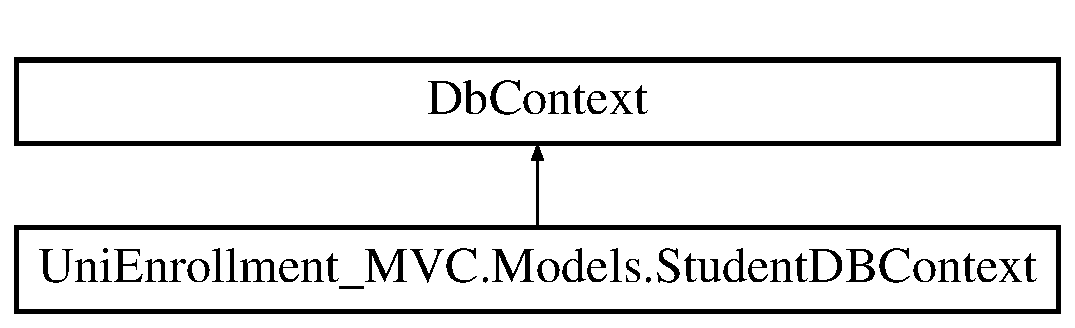
\includegraphics[height=2.000000cm]{class_uni_enrollment___m_v_c_1_1_models_1_1_student_d_b_context}
\end{center}
\end{figure}
\subsection*{Public Member Functions}
\begin{DoxyCompactItemize}
\item 
\hyperlink{class_uni_enrollment___m_v_c_1_1_models_1_1_student_d_b_context_a3955c9a6087bbe3d35e26ef879e434f5}{Student\+D\+B\+Context} ()
\end{DoxyCompactItemize}
\subsection*{Protected Member Functions}
\begin{DoxyCompactItemize}
\item 
override void \hyperlink{class_uni_enrollment___m_v_c_1_1_models_1_1_student_d_b_context_acf86c8dca4f75af696d6b75b21d041b6}{On\+Model\+Creating} (Db\+Model\+Builder model\+Builder)
\end{DoxyCompactItemize}
\subsection*{Properties}
\begin{DoxyCompactItemize}
\item 
Db\+Set$<$ \hyperlink{class_uni_enrollment___m_v_c_1_1_models_1_1_student}{Student} $>$ \hyperlink{class_uni_enrollment___m_v_c_1_1_models_1_1_student_d_b_context_aaaf3781eca16f0b42266ee141900bfca}{Students}\hspace{0.3cm}{\ttfamily  \mbox{[}get, set\mbox{]}}
\end{DoxyCompactItemize}


\subsection{Detailed Description}


Definition at line 6 of file Student\+D\+B\+Context.\+cs.



\subsection{Constructor \& Destructor Documentation}
\index{Uni\+Enrollment\+\_\+\+M\+V\+C\+::\+Models\+::\+Student\+D\+B\+Context@{Uni\+Enrollment\+\_\+\+M\+V\+C\+::\+Models\+::\+Student\+D\+B\+Context}!Student\+D\+B\+Context@{Student\+D\+B\+Context}}
\index{Student\+D\+B\+Context@{Student\+D\+B\+Context}!Uni\+Enrollment\+\_\+\+M\+V\+C\+::\+Models\+::\+Student\+D\+B\+Context@{Uni\+Enrollment\+\_\+\+M\+V\+C\+::\+Models\+::\+Student\+D\+B\+Context}}
\subsubsection[{\texorpdfstring{Student\+D\+B\+Context()}{StudentDBContext()}}]{\setlength{\rightskip}{0pt plus 5cm}Uni\+Enrollment\+\_\+\+M\+V\+C.\+Models.\+Student\+D\+B\+Context.\+Student\+D\+B\+Context (
\begin{DoxyParamCaption}
{}
\end{DoxyParamCaption}
)}\hypertarget{class_uni_enrollment___m_v_c_1_1_models_1_1_student_d_b_context_a3955c9a6087bbe3d35e26ef879e434f5}{}\label{class_uni_enrollment___m_v_c_1_1_models_1_1_student_d_b_context_a3955c9a6087bbe3d35e26ef879e434f5}


Definition at line 8 of file Student\+D\+B\+Context.\+cs.



\subsection{Member Function Documentation}
\index{Uni\+Enrollment\+\_\+\+M\+V\+C\+::\+Models\+::\+Student\+D\+B\+Context@{Uni\+Enrollment\+\_\+\+M\+V\+C\+::\+Models\+::\+Student\+D\+B\+Context}!On\+Model\+Creating@{On\+Model\+Creating}}
\index{On\+Model\+Creating@{On\+Model\+Creating}!Uni\+Enrollment\+\_\+\+M\+V\+C\+::\+Models\+::\+Student\+D\+B\+Context@{Uni\+Enrollment\+\_\+\+M\+V\+C\+::\+Models\+::\+Student\+D\+B\+Context}}
\subsubsection[{\texorpdfstring{On\+Model\+Creating(\+Db\+Model\+Builder model\+Builder)}{OnModelCreating(DbModelBuilder modelBuilder)}}]{\setlength{\rightskip}{0pt plus 5cm}override void Uni\+Enrollment\+\_\+\+M\+V\+C.\+Models.\+Student\+D\+B\+Context.\+On\+Model\+Creating (
\begin{DoxyParamCaption}
\item[{Db\+Model\+Builder}]{model\+Builder}
\end{DoxyParamCaption}
)\hspace{0.3cm}{\ttfamily [protected]}}\hypertarget{class_uni_enrollment___m_v_c_1_1_models_1_1_student_d_b_context_acf86c8dca4f75af696d6b75b21d041b6}{}\label{class_uni_enrollment___m_v_c_1_1_models_1_1_student_d_b_context_acf86c8dca4f75af696d6b75b21d041b6}


Definition at line 12 of file Student\+D\+B\+Context.\+cs.



\subsection{Property Documentation}
\index{Uni\+Enrollment\+\_\+\+M\+V\+C\+::\+Models\+::\+Student\+D\+B\+Context@{Uni\+Enrollment\+\_\+\+M\+V\+C\+::\+Models\+::\+Student\+D\+B\+Context}!Students@{Students}}
\index{Students@{Students}!Uni\+Enrollment\+\_\+\+M\+V\+C\+::\+Models\+::\+Student\+D\+B\+Context@{Uni\+Enrollment\+\_\+\+M\+V\+C\+::\+Models\+::\+Student\+D\+B\+Context}}
\subsubsection[{\texorpdfstring{Students}{Students}}]{\setlength{\rightskip}{0pt plus 5cm}Db\+Set$<${\bf Student}$>$ Uni\+Enrollment\+\_\+\+M\+V\+C.\+Models.\+Student\+D\+B\+Context.\+Students\hspace{0.3cm}{\ttfamily [get]}, {\ttfamily [set]}}\hypertarget{class_uni_enrollment___m_v_c_1_1_models_1_1_student_d_b_context_aaaf3781eca16f0b42266ee141900bfca}{}\label{class_uni_enrollment___m_v_c_1_1_models_1_1_student_d_b_context_aaaf3781eca16f0b42266ee141900bfca}


Definition at line 26 of file Student\+D\+B\+Context.\+cs.



The documentation for this class was generated from the following file\+:\begin{DoxyCompactItemize}
\item 
H\+:/\+Documents/\+Work/\+Repositories/\+Uni\+Enrollment-\/\+D\+E\+M\+O/\+Uni\+Enrollment-\/\+M\+V\+C/\+Context/\hyperlink{_student_d_b_context_8cs}{Student\+D\+B\+Context.\+cs}\end{DoxyCompactItemize}

\hypertarget{class_uni_enrollment___m_v_c_1_1_models_1_1_student_view_model}{}\section{Uni\+Enrollment\+\_\+\+M\+V\+C.\+Models.\+Student\+View\+Model Class Reference}
\label{class_uni_enrollment___m_v_c_1_1_models_1_1_student_view_model}\index{Uni\+Enrollment\+\_\+\+M\+V\+C.\+Models.\+Student\+View\+Model@{Uni\+Enrollment\+\_\+\+M\+V\+C.\+Models.\+Student\+View\+Model}}
\subsection*{Properties}
\begin{DoxyCompactItemize}
\item 
string \hyperlink{class_uni_enrollment___m_v_c_1_1_models_1_1_student_view_model_adb736203819c488b94212db3136224f9}{ID}\hspace{0.3cm}{\ttfamily  \mbox{[}get, set\mbox{]}}
\item 
string \hyperlink{class_uni_enrollment___m_v_c_1_1_models_1_1_student_view_model_a6374b7a873aa49f3d487d0a098becda0}{Name}\hspace{0.3cm}{\ttfamily  \mbox{[}get, set\mbox{]}}
\item 
string \hyperlink{class_uni_enrollment___m_v_c_1_1_models_1_1_student_view_model_a96ba162e18af0894ae751c273c797585}{Username}\hspace{0.3cm}{\ttfamily  \mbox{[}get, set\mbox{]}}
\item 
string \hyperlink{class_uni_enrollment___m_v_c_1_1_models_1_1_student_view_model_a3e926b219bc8a9ff6c00d52263b61163}{Password}\hspace{0.3cm}{\ttfamily  \mbox{[}get, set\mbox{]}}
\item 
string \hyperlink{class_uni_enrollment___m_v_c_1_1_models_1_1_student_view_model_a26c1bc2dba6280be30f91fc1e04e3c54}{Confirm\+Password}\hspace{0.3cm}{\ttfamily  \mbox{[}get, set\mbox{]}}
\item 
virtual List$<$ \hyperlink{class_uni_enrollment___m_v_c_1_1_models_1_1_enrollment}{Enrollment} $>$ \hyperlink{class_uni_enrollment___m_v_c_1_1_models_1_1_student_view_model_a5d41cb2b71a552312bf0fcf7ae8e50ac}{Enrollments}\hspace{0.3cm}{\ttfamily  \mbox{[}get, set\mbox{]}}
\end{DoxyCompactItemize}


\subsection{Detailed Description}


Definition at line 6 of file Student\+View\+Models.\+cs.



\subsection{Property Documentation}
\index{Uni\+Enrollment\+\_\+\+M\+V\+C\+::\+Models\+::\+Student\+View\+Model@{Uni\+Enrollment\+\_\+\+M\+V\+C\+::\+Models\+::\+Student\+View\+Model}!Confirm\+Password@{Confirm\+Password}}
\index{Confirm\+Password@{Confirm\+Password}!Uni\+Enrollment\+\_\+\+M\+V\+C\+::\+Models\+::\+Student\+View\+Model@{Uni\+Enrollment\+\_\+\+M\+V\+C\+::\+Models\+::\+Student\+View\+Model}}
\subsubsection[{\texorpdfstring{Confirm\+Password}{ConfirmPassword}}]{\setlength{\rightskip}{0pt plus 5cm}string Uni\+Enrollment\+\_\+\+M\+V\+C.\+Models.\+Student\+View\+Model.\+Confirm\+Password\hspace{0.3cm}{\ttfamily [get]}, {\ttfamily [set]}}\hypertarget{class_uni_enrollment___m_v_c_1_1_models_1_1_student_view_model_a26c1bc2dba6280be30f91fc1e04e3c54}{}\label{class_uni_enrollment___m_v_c_1_1_models_1_1_student_view_model_a26c1bc2dba6280be30f91fc1e04e3c54}


Definition at line 27 of file Student\+View\+Models.\+cs.

\index{Uni\+Enrollment\+\_\+\+M\+V\+C\+::\+Models\+::\+Student\+View\+Model@{Uni\+Enrollment\+\_\+\+M\+V\+C\+::\+Models\+::\+Student\+View\+Model}!Enrollments@{Enrollments}}
\index{Enrollments@{Enrollments}!Uni\+Enrollment\+\_\+\+M\+V\+C\+::\+Models\+::\+Student\+View\+Model@{Uni\+Enrollment\+\_\+\+M\+V\+C\+::\+Models\+::\+Student\+View\+Model}}
\subsubsection[{\texorpdfstring{Enrollments}{Enrollments}}]{\setlength{\rightskip}{0pt plus 5cm}virtual List$<${\bf Enrollment}$>$ Uni\+Enrollment\+\_\+\+M\+V\+C.\+Models.\+Student\+View\+Model.\+Enrollments\hspace{0.3cm}{\ttfamily [get]}, {\ttfamily [set]}}\hypertarget{class_uni_enrollment___m_v_c_1_1_models_1_1_student_view_model_a5d41cb2b71a552312bf0fcf7ae8e50ac}{}\label{class_uni_enrollment___m_v_c_1_1_models_1_1_student_view_model_a5d41cb2b71a552312bf0fcf7ae8e50ac}


Definition at line 29 of file Student\+View\+Models.\+cs.

\index{Uni\+Enrollment\+\_\+\+M\+V\+C\+::\+Models\+::\+Student\+View\+Model@{Uni\+Enrollment\+\_\+\+M\+V\+C\+::\+Models\+::\+Student\+View\+Model}!ID@{ID}}
\index{ID@{ID}!Uni\+Enrollment\+\_\+\+M\+V\+C\+::\+Models\+::\+Student\+View\+Model@{Uni\+Enrollment\+\_\+\+M\+V\+C\+::\+Models\+::\+Student\+View\+Model}}
\subsubsection[{\texorpdfstring{ID}{ID}}]{\setlength{\rightskip}{0pt plus 5cm}string Uni\+Enrollment\+\_\+\+M\+V\+C.\+Models.\+Student\+View\+Model.\+ID\hspace{0.3cm}{\ttfamily [get]}, {\ttfamily [set]}}\hypertarget{class_uni_enrollment___m_v_c_1_1_models_1_1_student_view_model_adb736203819c488b94212db3136224f9}{}\label{class_uni_enrollment___m_v_c_1_1_models_1_1_student_view_model_adb736203819c488b94212db3136224f9}


Definition at line 8 of file Student\+View\+Models.\+cs.

\index{Uni\+Enrollment\+\_\+\+M\+V\+C\+::\+Models\+::\+Student\+View\+Model@{Uni\+Enrollment\+\_\+\+M\+V\+C\+::\+Models\+::\+Student\+View\+Model}!Name@{Name}}
\index{Name@{Name}!Uni\+Enrollment\+\_\+\+M\+V\+C\+::\+Models\+::\+Student\+View\+Model@{Uni\+Enrollment\+\_\+\+M\+V\+C\+::\+Models\+::\+Student\+View\+Model}}
\subsubsection[{\texorpdfstring{Name}{Name}}]{\setlength{\rightskip}{0pt plus 5cm}string Uni\+Enrollment\+\_\+\+M\+V\+C.\+Models.\+Student\+View\+Model.\+Name\hspace{0.3cm}{\ttfamily [get]}, {\ttfamily [set]}}\hypertarget{class_uni_enrollment___m_v_c_1_1_models_1_1_student_view_model_a6374b7a873aa49f3d487d0a098becda0}{}\label{class_uni_enrollment___m_v_c_1_1_models_1_1_student_view_model_a6374b7a873aa49f3d487d0a098becda0}


Definition at line 13 of file Student\+View\+Models.\+cs.

\index{Uni\+Enrollment\+\_\+\+M\+V\+C\+::\+Models\+::\+Student\+View\+Model@{Uni\+Enrollment\+\_\+\+M\+V\+C\+::\+Models\+::\+Student\+View\+Model}!Password@{Password}}
\index{Password@{Password}!Uni\+Enrollment\+\_\+\+M\+V\+C\+::\+Models\+::\+Student\+View\+Model@{Uni\+Enrollment\+\_\+\+M\+V\+C\+::\+Models\+::\+Student\+View\+Model}}
\subsubsection[{\texorpdfstring{Password}{Password}}]{\setlength{\rightskip}{0pt plus 5cm}string Uni\+Enrollment\+\_\+\+M\+V\+C.\+Models.\+Student\+View\+Model.\+Password\hspace{0.3cm}{\ttfamily [get]}, {\ttfamily [set]}}\hypertarget{class_uni_enrollment___m_v_c_1_1_models_1_1_student_view_model_a3e926b219bc8a9ff6c00d52263b61163}{}\label{class_uni_enrollment___m_v_c_1_1_models_1_1_student_view_model_a3e926b219bc8a9ff6c00d52263b61163}


Definition at line 24 of file Student\+View\+Models.\+cs.

\index{Uni\+Enrollment\+\_\+\+M\+V\+C\+::\+Models\+::\+Student\+View\+Model@{Uni\+Enrollment\+\_\+\+M\+V\+C\+::\+Models\+::\+Student\+View\+Model}!Username@{Username}}
\index{Username@{Username}!Uni\+Enrollment\+\_\+\+M\+V\+C\+::\+Models\+::\+Student\+View\+Model@{Uni\+Enrollment\+\_\+\+M\+V\+C\+::\+Models\+::\+Student\+View\+Model}}
\subsubsection[{\texorpdfstring{Username}{Username}}]{\setlength{\rightskip}{0pt plus 5cm}string Uni\+Enrollment\+\_\+\+M\+V\+C.\+Models.\+Student\+View\+Model.\+Username\hspace{0.3cm}{\ttfamily [get]}, {\ttfamily [set]}}\hypertarget{class_uni_enrollment___m_v_c_1_1_models_1_1_student_view_model_a96ba162e18af0894ae751c273c797585}{}\label{class_uni_enrollment___m_v_c_1_1_models_1_1_student_view_model_a96ba162e18af0894ae751c273c797585}


Definition at line 18 of file Student\+View\+Models.\+cs.



The documentation for this class was generated from the following file\+:\begin{DoxyCompactItemize}
\item 
H\+:/\+Documents/\+Work/\+Repositories/\+Uni\+Enrollment-\/\+D\+E\+M\+O/\+Uni\+Enrollment-\/\+M\+V\+C/\+Models/\hyperlink{_student_view_models_8cs}{Student\+View\+Models.\+cs}\end{DoxyCompactItemize}

\hypertarget{class_uni_enrollment___m_v_c_1_1_models_1_1_uni_enrollment_d_b_entities}{}\section{Uni\+Enrollment\+\_\+\+M\+V\+C.\+Models.\+Uni\+Enrollment\+D\+B\+Entities Class Reference}
\label{class_uni_enrollment___m_v_c_1_1_models_1_1_uni_enrollment_d_b_entities}\index{Uni\+Enrollment\+\_\+\+M\+V\+C.\+Models.\+Uni\+Enrollment\+D\+B\+Entities@{Uni\+Enrollment\+\_\+\+M\+V\+C.\+Models.\+Uni\+Enrollment\+D\+B\+Entities}}
Inheritance diagram for Uni\+Enrollment\+\_\+\+M\+V\+C.\+Models.\+Uni\+Enrollment\+D\+B\+Entities\+:\begin{figure}[H]
\begin{center}
\leavevmode
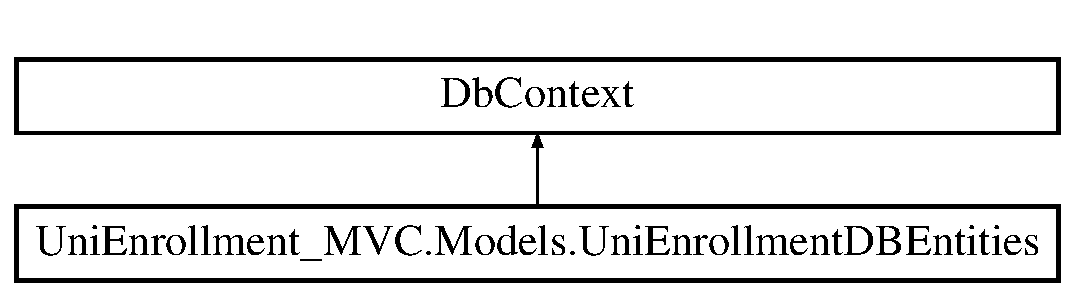
\includegraphics[height=2.000000cm]{class_uni_enrollment___m_v_c_1_1_models_1_1_uni_enrollment_d_b_entities}
\end{center}
\end{figure}
\subsection*{Public Member Functions}
\begin{DoxyCompactItemize}
\item 
\hyperlink{class_uni_enrollment___m_v_c_1_1_models_1_1_uni_enrollment_d_b_entities_a26c18449ead35261c1995d99249966bc}{Uni\+Enrollment\+D\+B\+Entities} ()
\end{DoxyCompactItemize}
\subsection*{Protected Member Functions}
\begin{DoxyCompactItemize}
\item 
override void \hyperlink{class_uni_enrollment___m_v_c_1_1_models_1_1_uni_enrollment_d_b_entities_a4f979f0b56e6ced6ada444eb2ac67d9e}{On\+Model\+Creating} (Db\+Model\+Builder model\+Builder)
\end{DoxyCompactItemize}
\subsection*{Properties}
\begin{DoxyCompactItemize}
\item 
virtual Db\+Set$<$ \hyperlink{class_uni_enrollment___m_v_c_1_1_models_1_1_course}{Course} $>$ \hyperlink{class_uni_enrollment___m_v_c_1_1_models_1_1_uni_enrollment_d_b_entities_a86c01bebd8432c0e61ce61c767697781}{Courses}\hspace{0.3cm}{\ttfamily  \mbox{[}get, set\mbox{]}}
\item 
virtual Db\+Set$<$ \hyperlink{class_uni_enrollment___m_v_c_1_1_models_1_1_user}{User} $>$ \hyperlink{class_uni_enrollment___m_v_c_1_1_models_1_1_uni_enrollment_d_b_entities_a440328d8247deb97dd72f9aede6f6ecc}{Users}\hspace{0.3cm}{\ttfamily  \mbox{[}get, set\mbox{]}}
\item 
virtual Db\+Set$<$ \hyperlink{class_uni_enrollment___m_v_c_1_1_models_1_1_user_type}{User\+Type} $>$ \hyperlink{class_uni_enrollment___m_v_c_1_1_models_1_1_uni_enrollment_d_b_entities_ae1554ac52bfff62c2ceb2edc182e8ee6}{User\+Types}\hspace{0.3cm}{\ttfamily  \mbox{[}get, set\mbox{]}}
\item 
virtual Db\+Set$<$ \hyperlink{class_uni_enrollment___m_v_c_1_1_models_1_1_enrollment}{Enrollment} $>$ \hyperlink{class_uni_enrollment___m_v_c_1_1_models_1_1_uni_enrollment_d_b_entities_a7ca0bed1f5761f9a747ac39615d0e95d}{Enrollments}\hspace{0.3cm}{\ttfamily  \mbox{[}get, set\mbox{]}}
\end{DoxyCompactItemize}


\subsection{Detailed Description}


Definition at line 16 of file Uni\+Enrollment\+Data\+Model.\+Context.\+cs.



\subsection{Constructor \& Destructor Documentation}
\index{Uni\+Enrollment\+\_\+\+M\+V\+C\+::\+Models\+::\+Uni\+Enrollment\+D\+B\+Entities@{Uni\+Enrollment\+\_\+\+M\+V\+C\+::\+Models\+::\+Uni\+Enrollment\+D\+B\+Entities}!Uni\+Enrollment\+D\+B\+Entities@{Uni\+Enrollment\+D\+B\+Entities}}
\index{Uni\+Enrollment\+D\+B\+Entities@{Uni\+Enrollment\+D\+B\+Entities}!Uni\+Enrollment\+\_\+\+M\+V\+C\+::\+Models\+::\+Uni\+Enrollment\+D\+B\+Entities@{Uni\+Enrollment\+\_\+\+M\+V\+C\+::\+Models\+::\+Uni\+Enrollment\+D\+B\+Entities}}
\subsubsection[{\texorpdfstring{Uni\+Enrollment\+D\+B\+Entities()}{UniEnrollmentDBEntities()}}]{\setlength{\rightskip}{0pt plus 5cm}Uni\+Enrollment\+\_\+\+M\+V\+C.\+Models.\+Uni\+Enrollment\+D\+B\+Entities.\+Uni\+Enrollment\+D\+B\+Entities (
\begin{DoxyParamCaption}
{}
\end{DoxyParamCaption}
)}\hypertarget{class_uni_enrollment___m_v_c_1_1_models_1_1_uni_enrollment_d_b_entities_a26c18449ead35261c1995d99249966bc}{}\label{class_uni_enrollment___m_v_c_1_1_models_1_1_uni_enrollment_d_b_entities_a26c18449ead35261c1995d99249966bc}


Definition at line 18 of file Uni\+Enrollment\+Data\+Model.\+Context.\+cs.



\subsection{Member Function Documentation}
\index{Uni\+Enrollment\+\_\+\+M\+V\+C\+::\+Models\+::\+Uni\+Enrollment\+D\+B\+Entities@{Uni\+Enrollment\+\_\+\+M\+V\+C\+::\+Models\+::\+Uni\+Enrollment\+D\+B\+Entities}!On\+Model\+Creating@{On\+Model\+Creating}}
\index{On\+Model\+Creating@{On\+Model\+Creating}!Uni\+Enrollment\+\_\+\+M\+V\+C\+::\+Models\+::\+Uni\+Enrollment\+D\+B\+Entities@{Uni\+Enrollment\+\_\+\+M\+V\+C\+::\+Models\+::\+Uni\+Enrollment\+D\+B\+Entities}}
\subsubsection[{\texorpdfstring{On\+Model\+Creating(\+Db\+Model\+Builder model\+Builder)}{OnModelCreating(DbModelBuilder modelBuilder)}}]{\setlength{\rightskip}{0pt plus 5cm}override void Uni\+Enrollment\+\_\+\+M\+V\+C.\+Models.\+Uni\+Enrollment\+D\+B\+Entities.\+On\+Model\+Creating (
\begin{DoxyParamCaption}
\item[{Db\+Model\+Builder}]{model\+Builder}
\end{DoxyParamCaption}
)\hspace{0.3cm}{\ttfamily [protected]}}\hypertarget{class_uni_enrollment___m_v_c_1_1_models_1_1_uni_enrollment_d_b_entities_a4f979f0b56e6ced6ada444eb2ac67d9e}{}\label{class_uni_enrollment___m_v_c_1_1_models_1_1_uni_enrollment_d_b_entities_a4f979f0b56e6ced6ada444eb2ac67d9e}


Definition at line 23 of file Uni\+Enrollment\+Data\+Model.\+Context.\+cs.



\subsection{Property Documentation}
\index{Uni\+Enrollment\+\_\+\+M\+V\+C\+::\+Models\+::\+Uni\+Enrollment\+D\+B\+Entities@{Uni\+Enrollment\+\_\+\+M\+V\+C\+::\+Models\+::\+Uni\+Enrollment\+D\+B\+Entities}!Courses@{Courses}}
\index{Courses@{Courses}!Uni\+Enrollment\+\_\+\+M\+V\+C\+::\+Models\+::\+Uni\+Enrollment\+D\+B\+Entities@{Uni\+Enrollment\+\_\+\+M\+V\+C\+::\+Models\+::\+Uni\+Enrollment\+D\+B\+Entities}}
\subsubsection[{\texorpdfstring{Courses}{Courses}}]{\setlength{\rightskip}{0pt plus 5cm}virtual Db\+Set$<${\bf Course}$>$ Uni\+Enrollment\+\_\+\+M\+V\+C.\+Models.\+Uni\+Enrollment\+D\+B\+Entities.\+Courses\hspace{0.3cm}{\ttfamily [get]}, {\ttfamily [set]}}\hypertarget{class_uni_enrollment___m_v_c_1_1_models_1_1_uni_enrollment_d_b_entities_a86c01bebd8432c0e61ce61c767697781}{}\label{class_uni_enrollment___m_v_c_1_1_models_1_1_uni_enrollment_d_b_entities_a86c01bebd8432c0e61ce61c767697781}


Definition at line 28 of file Uni\+Enrollment\+Data\+Model.\+Context.\+cs.

\index{Uni\+Enrollment\+\_\+\+M\+V\+C\+::\+Models\+::\+Uni\+Enrollment\+D\+B\+Entities@{Uni\+Enrollment\+\_\+\+M\+V\+C\+::\+Models\+::\+Uni\+Enrollment\+D\+B\+Entities}!Enrollments@{Enrollments}}
\index{Enrollments@{Enrollments}!Uni\+Enrollment\+\_\+\+M\+V\+C\+::\+Models\+::\+Uni\+Enrollment\+D\+B\+Entities@{Uni\+Enrollment\+\_\+\+M\+V\+C\+::\+Models\+::\+Uni\+Enrollment\+D\+B\+Entities}}
\subsubsection[{\texorpdfstring{Enrollments}{Enrollments}}]{\setlength{\rightskip}{0pt plus 5cm}virtual Db\+Set$<${\bf Enrollment}$>$ Uni\+Enrollment\+\_\+\+M\+V\+C.\+Models.\+Uni\+Enrollment\+D\+B\+Entities.\+Enrollments\hspace{0.3cm}{\ttfamily [get]}, {\ttfamily [set]}}\hypertarget{class_uni_enrollment___m_v_c_1_1_models_1_1_uni_enrollment_d_b_entities_a7ca0bed1f5761f9a747ac39615d0e95d}{}\label{class_uni_enrollment___m_v_c_1_1_models_1_1_uni_enrollment_d_b_entities_a7ca0bed1f5761f9a747ac39615d0e95d}


Definition at line 31 of file Uni\+Enrollment\+Data\+Model.\+Context.\+cs.

\index{Uni\+Enrollment\+\_\+\+M\+V\+C\+::\+Models\+::\+Uni\+Enrollment\+D\+B\+Entities@{Uni\+Enrollment\+\_\+\+M\+V\+C\+::\+Models\+::\+Uni\+Enrollment\+D\+B\+Entities}!Users@{Users}}
\index{Users@{Users}!Uni\+Enrollment\+\_\+\+M\+V\+C\+::\+Models\+::\+Uni\+Enrollment\+D\+B\+Entities@{Uni\+Enrollment\+\_\+\+M\+V\+C\+::\+Models\+::\+Uni\+Enrollment\+D\+B\+Entities}}
\subsubsection[{\texorpdfstring{Users}{Users}}]{\setlength{\rightskip}{0pt plus 5cm}virtual Db\+Set$<${\bf User}$>$ Uni\+Enrollment\+\_\+\+M\+V\+C.\+Models.\+Uni\+Enrollment\+D\+B\+Entities.\+Users\hspace{0.3cm}{\ttfamily [get]}, {\ttfamily [set]}}\hypertarget{class_uni_enrollment___m_v_c_1_1_models_1_1_uni_enrollment_d_b_entities_a440328d8247deb97dd72f9aede6f6ecc}{}\label{class_uni_enrollment___m_v_c_1_1_models_1_1_uni_enrollment_d_b_entities_a440328d8247deb97dd72f9aede6f6ecc}


Definition at line 29 of file Uni\+Enrollment\+Data\+Model.\+Context.\+cs.

\index{Uni\+Enrollment\+\_\+\+M\+V\+C\+::\+Models\+::\+Uni\+Enrollment\+D\+B\+Entities@{Uni\+Enrollment\+\_\+\+M\+V\+C\+::\+Models\+::\+Uni\+Enrollment\+D\+B\+Entities}!User\+Types@{User\+Types}}
\index{User\+Types@{User\+Types}!Uni\+Enrollment\+\_\+\+M\+V\+C\+::\+Models\+::\+Uni\+Enrollment\+D\+B\+Entities@{Uni\+Enrollment\+\_\+\+M\+V\+C\+::\+Models\+::\+Uni\+Enrollment\+D\+B\+Entities}}
\subsubsection[{\texorpdfstring{User\+Types}{UserTypes}}]{\setlength{\rightskip}{0pt plus 5cm}virtual Db\+Set$<${\bf User\+Type}$>$ Uni\+Enrollment\+\_\+\+M\+V\+C.\+Models.\+Uni\+Enrollment\+D\+B\+Entities.\+User\+Types\hspace{0.3cm}{\ttfamily [get]}, {\ttfamily [set]}}\hypertarget{class_uni_enrollment___m_v_c_1_1_models_1_1_uni_enrollment_d_b_entities_ae1554ac52bfff62c2ceb2edc182e8ee6}{}\label{class_uni_enrollment___m_v_c_1_1_models_1_1_uni_enrollment_d_b_entities_ae1554ac52bfff62c2ceb2edc182e8ee6}


Definition at line 30 of file Uni\+Enrollment\+Data\+Model.\+Context.\+cs.



The documentation for this class was generated from the following file\+:\begin{DoxyCompactItemize}
\item 
H\+:/\+Documents/\+Work/\+Repositories/\+Uni\+Enrollment-\/\+D\+E\+M\+O/\+Uni\+Enrollment-\/\+M\+V\+C/\+Models/\hyperlink{_uni_enrollment_data_model_8_context_8cs}{Uni\+Enrollment\+Data\+Model.\+Context.\+cs}\end{DoxyCompactItemize}

\hypertarget{class_uni_enrollment___m_v_c_1_1_models_1_1_user}{}\section{Uni\+Enrollment\+\_\+\+M\+V\+C.\+Models.\+User Class Reference}
\label{class_uni_enrollment___m_v_c_1_1_models_1_1_user}\index{Uni\+Enrollment\+\_\+\+M\+V\+C.\+Models.\+User@{Uni\+Enrollment\+\_\+\+M\+V\+C.\+Models.\+User}}
\subsection*{Public Member Functions}
\begin{DoxyCompactItemize}
\item 
\hyperlink{class_uni_enrollment___m_v_c_1_1_models_1_1_user_a094a61319568118725591779a5b582be}{User} ()
\end{DoxyCompactItemize}
\subsection*{Properties}
\begin{DoxyCompactItemize}
\item 
int \hyperlink{class_uni_enrollment___m_v_c_1_1_models_1_1_user_adee6f0ebfaebca34888fb5378a437bfa}{ID}\hspace{0.3cm}{\ttfamily  \mbox{[}get, set\mbox{]}}
\item 
int \hyperlink{class_uni_enrollment___m_v_c_1_1_models_1_1_user_a4f4c507ff2264229f9e1a0d319134a33}{User\+Type\+ID}\hspace{0.3cm}{\ttfamily  \mbox{[}get, set\mbox{]}}
\item 
string \hyperlink{class_uni_enrollment___m_v_c_1_1_models_1_1_user_a9c852662d106e22d53bb00bfc8945423}{Username}\hspace{0.3cm}{\ttfamily  \mbox{[}get, set\mbox{]}}
\item 
string \hyperlink{class_uni_enrollment___m_v_c_1_1_models_1_1_user_a9f4573eb934d5201cfbb5eb769b057bf}{Password}\hspace{0.3cm}{\ttfamily  \mbox{[}get, set\mbox{]}}
\item 
string \hyperlink{class_uni_enrollment___m_v_c_1_1_models_1_1_user_ac34d9112ca308c7ca425c344c5d05a79}{Name}\hspace{0.3cm}{\ttfamily  \mbox{[}get, set\mbox{]}}
\item 
bool \hyperlink{class_uni_enrollment___m_v_c_1_1_models_1_1_user_aad8a758f81d61dbace19dc3cd010a470}{Active}\hspace{0.3cm}{\ttfamily  \mbox{[}get, set\mbox{]}}
\item 
virtual I\+Collection$<$ \hyperlink{class_uni_enrollment___m_v_c_1_1_models_1_1_course}{Course} $>$ \hyperlink{class_uni_enrollment___m_v_c_1_1_models_1_1_user_a62d03b5f502392b690ba4a97e319b032}{Courses}\hspace{0.3cm}{\ttfamily  \mbox{[}get, set\mbox{]}}
\item 
virtual \hyperlink{class_uni_enrollment___m_v_c_1_1_models_1_1_user_type}{User\+Type} \hyperlink{class_uni_enrollment___m_v_c_1_1_models_1_1_user_ab82d44a89b2d1a28799473bb38e080d0}{User\+Type}\hspace{0.3cm}{\ttfamily  \mbox{[}get, set\mbox{]}}
\item 
virtual I\+Collection$<$ \hyperlink{class_uni_enrollment___m_v_c_1_1_models_1_1_enrollment}{Enrollment} $>$ \hyperlink{class_uni_enrollment___m_v_c_1_1_models_1_1_user_a5ebaaaefeb0b09ea8a85dd1a77178891}{Enrollments}\hspace{0.3cm}{\ttfamily  \mbox{[}get, set\mbox{]}}
\end{DoxyCompactItemize}


\subsection{Detailed Description}


Definition at line 15 of file User.\+cs.



\subsection{Constructor \& Destructor Documentation}
\index{Uni\+Enrollment\+\_\+\+M\+V\+C\+::\+Models\+::\+User@{Uni\+Enrollment\+\_\+\+M\+V\+C\+::\+Models\+::\+User}!User@{User}}
\index{User@{User}!Uni\+Enrollment\+\_\+\+M\+V\+C\+::\+Models\+::\+User@{Uni\+Enrollment\+\_\+\+M\+V\+C\+::\+Models\+::\+User}}
\subsubsection[{\texorpdfstring{User()}{User()}}]{\setlength{\rightskip}{0pt plus 5cm}Uni\+Enrollment\+\_\+\+M\+V\+C.\+Models.\+User.\+User (
\begin{DoxyParamCaption}
{}
\end{DoxyParamCaption}
)}\hypertarget{class_uni_enrollment___m_v_c_1_1_models_1_1_user_a094a61319568118725591779a5b582be}{}\label{class_uni_enrollment___m_v_c_1_1_models_1_1_user_a094a61319568118725591779a5b582be}


Definition at line 18 of file User.\+cs.



\subsection{Property Documentation}
\index{Uni\+Enrollment\+\_\+\+M\+V\+C\+::\+Models\+::\+User@{Uni\+Enrollment\+\_\+\+M\+V\+C\+::\+Models\+::\+User}!Active@{Active}}
\index{Active@{Active}!Uni\+Enrollment\+\_\+\+M\+V\+C\+::\+Models\+::\+User@{Uni\+Enrollment\+\_\+\+M\+V\+C\+::\+Models\+::\+User}}
\subsubsection[{\texorpdfstring{Active}{Active}}]{\setlength{\rightskip}{0pt plus 5cm}bool Uni\+Enrollment\+\_\+\+M\+V\+C.\+Models.\+User.\+Active\hspace{0.3cm}{\ttfamily [get]}, {\ttfamily [set]}}\hypertarget{class_uni_enrollment___m_v_c_1_1_models_1_1_user_aad8a758f81d61dbace19dc3cd010a470}{}\label{class_uni_enrollment___m_v_c_1_1_models_1_1_user_aad8a758f81d61dbace19dc3cd010a470}


Definition at line 29 of file User.\+cs.

\index{Uni\+Enrollment\+\_\+\+M\+V\+C\+::\+Models\+::\+User@{Uni\+Enrollment\+\_\+\+M\+V\+C\+::\+Models\+::\+User}!Courses@{Courses}}
\index{Courses@{Courses}!Uni\+Enrollment\+\_\+\+M\+V\+C\+::\+Models\+::\+User@{Uni\+Enrollment\+\_\+\+M\+V\+C\+::\+Models\+::\+User}}
\subsubsection[{\texorpdfstring{Courses}{Courses}}]{\setlength{\rightskip}{0pt plus 5cm}virtual I\+Collection$<${\bf Course}$>$ Uni\+Enrollment\+\_\+\+M\+V\+C.\+Models.\+User.\+Courses\hspace{0.3cm}{\ttfamily [get]}, {\ttfamily [set]}}\hypertarget{class_uni_enrollment___m_v_c_1_1_models_1_1_user_a62d03b5f502392b690ba4a97e319b032}{}\label{class_uni_enrollment___m_v_c_1_1_models_1_1_user_a62d03b5f502392b690ba4a97e319b032}


Definition at line 32 of file User.\+cs.

\index{Uni\+Enrollment\+\_\+\+M\+V\+C\+::\+Models\+::\+User@{Uni\+Enrollment\+\_\+\+M\+V\+C\+::\+Models\+::\+User}!Enrollments@{Enrollments}}
\index{Enrollments@{Enrollments}!Uni\+Enrollment\+\_\+\+M\+V\+C\+::\+Models\+::\+User@{Uni\+Enrollment\+\_\+\+M\+V\+C\+::\+Models\+::\+User}}
\subsubsection[{\texorpdfstring{Enrollments}{Enrollments}}]{\setlength{\rightskip}{0pt plus 5cm}virtual I\+Collection$<${\bf Enrollment}$>$ Uni\+Enrollment\+\_\+\+M\+V\+C.\+Models.\+User.\+Enrollments\hspace{0.3cm}{\ttfamily [get]}, {\ttfamily [set]}}\hypertarget{class_uni_enrollment___m_v_c_1_1_models_1_1_user_a5ebaaaefeb0b09ea8a85dd1a77178891}{}\label{class_uni_enrollment___m_v_c_1_1_models_1_1_user_a5ebaaaefeb0b09ea8a85dd1a77178891}


Definition at line 35 of file User.\+cs.

\index{Uni\+Enrollment\+\_\+\+M\+V\+C\+::\+Models\+::\+User@{Uni\+Enrollment\+\_\+\+M\+V\+C\+::\+Models\+::\+User}!ID@{ID}}
\index{ID@{ID}!Uni\+Enrollment\+\_\+\+M\+V\+C\+::\+Models\+::\+User@{Uni\+Enrollment\+\_\+\+M\+V\+C\+::\+Models\+::\+User}}
\subsubsection[{\texorpdfstring{ID}{ID}}]{\setlength{\rightskip}{0pt plus 5cm}int Uni\+Enrollment\+\_\+\+M\+V\+C.\+Models.\+User.\+ID\hspace{0.3cm}{\ttfamily [get]}, {\ttfamily [set]}}\hypertarget{class_uni_enrollment___m_v_c_1_1_models_1_1_user_adee6f0ebfaebca34888fb5378a437bfa}{}\label{class_uni_enrollment___m_v_c_1_1_models_1_1_user_adee6f0ebfaebca34888fb5378a437bfa}


Definition at line 24 of file User.\+cs.

\index{Uni\+Enrollment\+\_\+\+M\+V\+C\+::\+Models\+::\+User@{Uni\+Enrollment\+\_\+\+M\+V\+C\+::\+Models\+::\+User}!Name@{Name}}
\index{Name@{Name}!Uni\+Enrollment\+\_\+\+M\+V\+C\+::\+Models\+::\+User@{Uni\+Enrollment\+\_\+\+M\+V\+C\+::\+Models\+::\+User}}
\subsubsection[{\texorpdfstring{Name}{Name}}]{\setlength{\rightskip}{0pt plus 5cm}string Uni\+Enrollment\+\_\+\+M\+V\+C.\+Models.\+User.\+Name\hspace{0.3cm}{\ttfamily [get]}, {\ttfamily [set]}}\hypertarget{class_uni_enrollment___m_v_c_1_1_models_1_1_user_ac34d9112ca308c7ca425c344c5d05a79}{}\label{class_uni_enrollment___m_v_c_1_1_models_1_1_user_ac34d9112ca308c7ca425c344c5d05a79}


Definition at line 28 of file User.\+cs.

\index{Uni\+Enrollment\+\_\+\+M\+V\+C\+::\+Models\+::\+User@{Uni\+Enrollment\+\_\+\+M\+V\+C\+::\+Models\+::\+User}!Password@{Password}}
\index{Password@{Password}!Uni\+Enrollment\+\_\+\+M\+V\+C\+::\+Models\+::\+User@{Uni\+Enrollment\+\_\+\+M\+V\+C\+::\+Models\+::\+User}}
\subsubsection[{\texorpdfstring{Password}{Password}}]{\setlength{\rightskip}{0pt plus 5cm}string Uni\+Enrollment\+\_\+\+M\+V\+C.\+Models.\+User.\+Password\hspace{0.3cm}{\ttfamily [get]}, {\ttfamily [set]}}\hypertarget{class_uni_enrollment___m_v_c_1_1_models_1_1_user_a9f4573eb934d5201cfbb5eb769b057bf}{}\label{class_uni_enrollment___m_v_c_1_1_models_1_1_user_a9f4573eb934d5201cfbb5eb769b057bf}


Definition at line 27 of file User.\+cs.

\index{Uni\+Enrollment\+\_\+\+M\+V\+C\+::\+Models\+::\+User@{Uni\+Enrollment\+\_\+\+M\+V\+C\+::\+Models\+::\+User}!Username@{Username}}
\index{Username@{Username}!Uni\+Enrollment\+\_\+\+M\+V\+C\+::\+Models\+::\+User@{Uni\+Enrollment\+\_\+\+M\+V\+C\+::\+Models\+::\+User}}
\subsubsection[{\texorpdfstring{Username}{Username}}]{\setlength{\rightskip}{0pt plus 5cm}string Uni\+Enrollment\+\_\+\+M\+V\+C.\+Models.\+User.\+Username\hspace{0.3cm}{\ttfamily [get]}, {\ttfamily [set]}}\hypertarget{class_uni_enrollment___m_v_c_1_1_models_1_1_user_a9c852662d106e22d53bb00bfc8945423}{}\label{class_uni_enrollment___m_v_c_1_1_models_1_1_user_a9c852662d106e22d53bb00bfc8945423}


Definition at line 26 of file User.\+cs.

\index{Uni\+Enrollment\+\_\+\+M\+V\+C\+::\+Models\+::\+User@{Uni\+Enrollment\+\_\+\+M\+V\+C\+::\+Models\+::\+User}!User\+Type@{User\+Type}}
\index{User\+Type@{User\+Type}!Uni\+Enrollment\+\_\+\+M\+V\+C\+::\+Models\+::\+User@{Uni\+Enrollment\+\_\+\+M\+V\+C\+::\+Models\+::\+User}}
\subsubsection[{\texorpdfstring{User\+Type}{UserType}}]{\setlength{\rightskip}{0pt plus 5cm}virtual {\bf User\+Type} Uni\+Enrollment\+\_\+\+M\+V\+C.\+Models.\+User.\+User\+Type\hspace{0.3cm}{\ttfamily [get]}, {\ttfamily [set]}}\hypertarget{class_uni_enrollment___m_v_c_1_1_models_1_1_user_ab82d44a89b2d1a28799473bb38e080d0}{}\label{class_uni_enrollment___m_v_c_1_1_models_1_1_user_ab82d44a89b2d1a28799473bb38e080d0}


Definition at line 33 of file User.\+cs.

\index{Uni\+Enrollment\+\_\+\+M\+V\+C\+::\+Models\+::\+User@{Uni\+Enrollment\+\_\+\+M\+V\+C\+::\+Models\+::\+User}!User\+Type\+ID@{User\+Type\+ID}}
\index{User\+Type\+ID@{User\+Type\+ID}!Uni\+Enrollment\+\_\+\+M\+V\+C\+::\+Models\+::\+User@{Uni\+Enrollment\+\_\+\+M\+V\+C\+::\+Models\+::\+User}}
\subsubsection[{\texorpdfstring{User\+Type\+ID}{UserTypeID}}]{\setlength{\rightskip}{0pt plus 5cm}int Uni\+Enrollment\+\_\+\+M\+V\+C.\+Models.\+User.\+User\+Type\+ID\hspace{0.3cm}{\ttfamily [get]}, {\ttfamily [set]}}\hypertarget{class_uni_enrollment___m_v_c_1_1_models_1_1_user_a4f4c507ff2264229f9e1a0d319134a33}{}\label{class_uni_enrollment___m_v_c_1_1_models_1_1_user_a4f4c507ff2264229f9e1a0d319134a33}


Definition at line 25 of file User.\+cs.



The documentation for this class was generated from the following file\+:\begin{DoxyCompactItemize}
\item 
H\+:/\+Documents/\+Work/\+Repositories/\+Uni\+Enrollment-\/\+D\+E\+M\+O/\+Uni\+Enrollment-\/\+M\+V\+C/\+Models/\hyperlink{_user_8cs}{User.\+cs}\end{DoxyCompactItemize}

\hypertarget{class_uni_enrollment___m_v_c_1_1_models_1_1_user_type}{}\section{Uni\+Enrollment\+\_\+\+M\+V\+C.\+Models.\+User\+Type Class Reference}
\label{class_uni_enrollment___m_v_c_1_1_models_1_1_user_type}\index{Uni\+Enrollment\+\_\+\+M\+V\+C.\+Models.\+User\+Type@{Uni\+Enrollment\+\_\+\+M\+V\+C.\+Models.\+User\+Type}}
\subsection*{Public Member Functions}
\begin{DoxyCompactItemize}
\item 
\hyperlink{class_uni_enrollment___m_v_c_1_1_models_1_1_user_type_aac5f44c2218f0212acb9fc819c2b879a}{User\+Type} ()
\end{DoxyCompactItemize}
\subsection*{Properties}
\begin{DoxyCompactItemize}
\item 
int \hyperlink{class_uni_enrollment___m_v_c_1_1_models_1_1_user_type_acf9a3b3fdf3f050f1fb9a63983ca4075}{ID}\hspace{0.3cm}{\ttfamily  \mbox{[}get, set\mbox{]}}
\item 
string \hyperlink{class_uni_enrollment___m_v_c_1_1_models_1_1_user_type_a5606ad367c45e5c2fefb992377b6b55a}{Name}\hspace{0.3cm}{\ttfamily  \mbox{[}get, set\mbox{]}}
\item 
virtual I\+Collection$<$ \hyperlink{class_uni_enrollment___m_v_c_1_1_models_1_1_user}{User} $>$ \hyperlink{class_uni_enrollment___m_v_c_1_1_models_1_1_user_type_a6520e4f4b273c006fdf1926e51b4816b}{Users}\hspace{0.3cm}{\ttfamily  \mbox{[}get, set\mbox{]}}
\end{DoxyCompactItemize}


\subsection{Detailed Description}


Definition at line 15 of file User\+Type.\+cs.



\subsection{Constructor \& Destructor Documentation}
\index{Uni\+Enrollment\+\_\+\+M\+V\+C\+::\+Models\+::\+User\+Type@{Uni\+Enrollment\+\_\+\+M\+V\+C\+::\+Models\+::\+User\+Type}!User\+Type@{User\+Type}}
\index{User\+Type@{User\+Type}!Uni\+Enrollment\+\_\+\+M\+V\+C\+::\+Models\+::\+User\+Type@{Uni\+Enrollment\+\_\+\+M\+V\+C\+::\+Models\+::\+User\+Type}}
\subsubsection[{\texorpdfstring{User\+Type()}{UserType()}}]{\setlength{\rightskip}{0pt plus 5cm}Uni\+Enrollment\+\_\+\+M\+V\+C.\+Models.\+User\+Type.\+User\+Type (
\begin{DoxyParamCaption}
{}
\end{DoxyParamCaption}
)}\hypertarget{class_uni_enrollment___m_v_c_1_1_models_1_1_user_type_aac5f44c2218f0212acb9fc819c2b879a}{}\label{class_uni_enrollment___m_v_c_1_1_models_1_1_user_type_aac5f44c2218f0212acb9fc819c2b879a}


Definition at line 18 of file User\+Type.\+cs.



\subsection{Property Documentation}
\index{Uni\+Enrollment\+\_\+\+M\+V\+C\+::\+Models\+::\+User\+Type@{Uni\+Enrollment\+\_\+\+M\+V\+C\+::\+Models\+::\+User\+Type}!ID@{ID}}
\index{ID@{ID}!Uni\+Enrollment\+\_\+\+M\+V\+C\+::\+Models\+::\+User\+Type@{Uni\+Enrollment\+\_\+\+M\+V\+C\+::\+Models\+::\+User\+Type}}
\subsubsection[{\texorpdfstring{ID}{ID}}]{\setlength{\rightskip}{0pt plus 5cm}int Uni\+Enrollment\+\_\+\+M\+V\+C.\+Models.\+User\+Type.\+ID\hspace{0.3cm}{\ttfamily [get]}, {\ttfamily [set]}}\hypertarget{class_uni_enrollment___m_v_c_1_1_models_1_1_user_type_acf9a3b3fdf3f050f1fb9a63983ca4075}{}\label{class_uni_enrollment___m_v_c_1_1_models_1_1_user_type_acf9a3b3fdf3f050f1fb9a63983ca4075}


Definition at line 23 of file User\+Type.\+cs.

\index{Uni\+Enrollment\+\_\+\+M\+V\+C\+::\+Models\+::\+User\+Type@{Uni\+Enrollment\+\_\+\+M\+V\+C\+::\+Models\+::\+User\+Type}!Name@{Name}}
\index{Name@{Name}!Uni\+Enrollment\+\_\+\+M\+V\+C\+::\+Models\+::\+User\+Type@{Uni\+Enrollment\+\_\+\+M\+V\+C\+::\+Models\+::\+User\+Type}}
\subsubsection[{\texorpdfstring{Name}{Name}}]{\setlength{\rightskip}{0pt plus 5cm}string Uni\+Enrollment\+\_\+\+M\+V\+C.\+Models.\+User\+Type.\+Name\hspace{0.3cm}{\ttfamily [get]}, {\ttfamily [set]}}\hypertarget{class_uni_enrollment___m_v_c_1_1_models_1_1_user_type_a5606ad367c45e5c2fefb992377b6b55a}{}\label{class_uni_enrollment___m_v_c_1_1_models_1_1_user_type_a5606ad367c45e5c2fefb992377b6b55a}


Definition at line 24 of file User\+Type.\+cs.

\index{Uni\+Enrollment\+\_\+\+M\+V\+C\+::\+Models\+::\+User\+Type@{Uni\+Enrollment\+\_\+\+M\+V\+C\+::\+Models\+::\+User\+Type}!Users@{Users}}
\index{Users@{Users}!Uni\+Enrollment\+\_\+\+M\+V\+C\+::\+Models\+::\+User\+Type@{Uni\+Enrollment\+\_\+\+M\+V\+C\+::\+Models\+::\+User\+Type}}
\subsubsection[{\texorpdfstring{Users}{Users}}]{\setlength{\rightskip}{0pt plus 5cm}virtual I\+Collection$<${\bf User}$>$ Uni\+Enrollment\+\_\+\+M\+V\+C.\+Models.\+User\+Type.\+Users\hspace{0.3cm}{\ttfamily [get]}, {\ttfamily [set]}}\hypertarget{class_uni_enrollment___m_v_c_1_1_models_1_1_user_type_a6520e4f4b273c006fdf1926e51b4816b}{}\label{class_uni_enrollment___m_v_c_1_1_models_1_1_user_type_a6520e4f4b273c006fdf1926e51b4816b}


Definition at line 27 of file User\+Type.\+cs.



The documentation for this class was generated from the following file\+:\begin{DoxyCompactItemize}
\item 
H\+:/\+Documents/\+Work/\+Repositories/\+Uni\+Enrollment-\/\+D\+E\+M\+O/\+Uni\+Enrollment-\/\+M\+V\+C/\+Models/\hyperlink{_user_type_8cs}{User\+Type.\+cs}\end{DoxyCompactItemize}

\chapter{File Documentation}
\hypertarget{_bundle_config_8cs}{}\section{H\+:/\+Documents/\+Work/\+Repositories/\+Uni\+Enrollment-\/\+D\+E\+M\+O/\+Uni\+Enrollment-\/\+M\+V\+C/\+App\+\_\+\+Start/\+Bundle\+Config.cs File Reference}
\label{_bundle_config_8cs}\index{H\+:/\+Documents/\+Work/\+Repositories/\+Uni\+Enrollment-\/\+D\+E\+M\+O/\+Uni\+Enrollment-\/\+M\+V\+C/\+App\+\_\+\+Start/\+Bundle\+Config.\+cs@{H\+:/\+Documents/\+Work/\+Repositories/\+Uni\+Enrollment-\/\+D\+E\+M\+O/\+Uni\+Enrollment-\/\+M\+V\+C/\+App\+\_\+\+Start/\+Bundle\+Config.\+cs}}
\subsection*{Classes}
\begin{DoxyCompactItemize}
\item 
class \hyperlink{class_uni_enrollment___m_v_c_1_1_bundle_config}{Uni\+Enrollment\+\_\+\+M\+V\+C.\+Bundle\+Config}
\end{DoxyCompactItemize}
\subsection*{Namespaces}
\begin{DoxyCompactItemize}
\item 
namespace \hyperlink{namespace_uni_enrollment___m_v_c}{Uni\+Enrollment\+\_\+\+M\+VC}
\end{DoxyCompactItemize}

\hypertarget{_filter_config_8cs}{}\section{H\+:/\+Documents/\+Work/\+Repositories/\+Uni\+Enrollment-\/\+D\+E\+M\+O/\+Uni\+Enrollment-\/\+M\+V\+C/\+App\+\_\+\+Start/\+Filter\+Config.cs File Reference}
\label{_filter_config_8cs}\index{H\+:/\+Documents/\+Work/\+Repositories/\+Uni\+Enrollment-\/\+D\+E\+M\+O/\+Uni\+Enrollment-\/\+M\+V\+C/\+App\+\_\+\+Start/\+Filter\+Config.\+cs@{H\+:/\+Documents/\+Work/\+Repositories/\+Uni\+Enrollment-\/\+D\+E\+M\+O/\+Uni\+Enrollment-\/\+M\+V\+C/\+App\+\_\+\+Start/\+Filter\+Config.\+cs}}
\subsection*{Classes}
\begin{DoxyCompactItemize}
\item 
class \hyperlink{class_uni_enrollment___m_v_c_1_1_filter_config}{Uni\+Enrollment\+\_\+\+M\+V\+C.\+Filter\+Config}
\end{DoxyCompactItemize}
\subsection*{Namespaces}
\begin{DoxyCompactItemize}
\item 
namespace \hyperlink{namespace_uni_enrollment___m_v_c}{Uni\+Enrollment\+\_\+\+M\+VC}
\end{DoxyCompactItemize}

\hypertarget{_route_config_8cs}{}\section{H\+:/\+Documents/\+Work/\+Repositories/\+Uni\+Enrollment-\/\+D\+E\+M\+O/\+Uni\+Enrollment-\/\+M\+V\+C/\+App\+\_\+\+Start/\+Route\+Config.cs File Reference}
\label{_route_config_8cs}\index{H\+:/\+Documents/\+Work/\+Repositories/\+Uni\+Enrollment-\/\+D\+E\+M\+O/\+Uni\+Enrollment-\/\+M\+V\+C/\+App\+\_\+\+Start/\+Route\+Config.\+cs@{H\+:/\+Documents/\+Work/\+Repositories/\+Uni\+Enrollment-\/\+D\+E\+M\+O/\+Uni\+Enrollment-\/\+M\+V\+C/\+App\+\_\+\+Start/\+Route\+Config.\+cs}}
\subsection*{Classes}
\begin{DoxyCompactItemize}
\item 
class \hyperlink{class_uni_enrollment___m_v_c_1_1_route_config}{Uni\+Enrollment\+\_\+\+M\+V\+C.\+Route\+Config}
\end{DoxyCompactItemize}
\subsection*{Namespaces}
\begin{DoxyCompactItemize}
\item 
namespace \hyperlink{namespace_uni_enrollment___m_v_c}{Uni\+Enrollment\+\_\+\+M\+VC}
\end{DoxyCompactItemize}

\hypertarget{_course_d_b_context_8cs}{}\section{H\+:/\+Documents/\+Work/\+Repositories/\+Uni\+Enrollment-\/\+D\+E\+M\+O/\+Uni\+Enrollment-\/\+M\+V\+C/\+Context/\+Course\+D\+B\+Context.cs File Reference}
\label{_course_d_b_context_8cs}\index{H\+:/\+Documents/\+Work/\+Repositories/\+Uni\+Enrollment-\/\+D\+E\+M\+O/\+Uni\+Enrollment-\/\+M\+V\+C/\+Context/\+Course\+D\+B\+Context.\+cs@{H\+:/\+Documents/\+Work/\+Repositories/\+Uni\+Enrollment-\/\+D\+E\+M\+O/\+Uni\+Enrollment-\/\+M\+V\+C/\+Context/\+Course\+D\+B\+Context.\+cs}}
\subsection*{Classes}
\begin{DoxyCompactItemize}
\item 
class \hyperlink{class_uni_enrollment___m_v_c_1_1_models_1_1_course_d_b_context}{Uni\+Enrollment\+\_\+\+M\+V\+C.\+Models.\+Course\+D\+B\+Context}
\end{DoxyCompactItemize}
\subsection*{Namespaces}
\begin{DoxyCompactItemize}
\item 
namespace \hyperlink{namespace_uni_enrollment___m_v_c_1_1_models}{Uni\+Enrollment\+\_\+\+M\+V\+C.\+Models}
\end{DoxyCompactItemize}

\hypertarget{_enrollment_d_b_context_8cs}{}\section{H\+:/\+Documents/\+Work/\+Repositories/\+Uni\+Enrollment-\/\+D\+E\+M\+O/\+Uni\+Enrollment-\/\+M\+V\+C/\+Context/\+Enrollment\+D\+B\+Context.cs File Reference}
\label{_enrollment_d_b_context_8cs}\index{H\+:/\+Documents/\+Work/\+Repositories/\+Uni\+Enrollment-\/\+D\+E\+M\+O/\+Uni\+Enrollment-\/\+M\+V\+C/\+Context/\+Enrollment\+D\+B\+Context.\+cs@{H\+:/\+Documents/\+Work/\+Repositories/\+Uni\+Enrollment-\/\+D\+E\+M\+O/\+Uni\+Enrollment-\/\+M\+V\+C/\+Context/\+Enrollment\+D\+B\+Context.\+cs}}
\subsection*{Classes}
\begin{DoxyCompactItemize}
\item 
class \hyperlink{class_uni_enrollment___m_v_c_1_1_models_1_1_enrollment_d_b_context}{Uni\+Enrollment\+\_\+\+M\+V\+C.\+Models.\+Enrollment\+D\+B\+Context}
\end{DoxyCompactItemize}
\subsection*{Namespaces}
\begin{DoxyCompactItemize}
\item 
namespace \hyperlink{namespace_uni_enrollment___m_v_c_1_1_models}{Uni\+Enrollment\+\_\+\+M\+V\+C.\+Models}
\end{DoxyCompactItemize}

\hypertarget{_professor_d_b_context_8cs}{}\section{H\+:/\+Documents/\+Work/\+Repositories/\+Uni\+Enrollment-\/\+D\+E\+M\+O/\+Uni\+Enrollment-\/\+M\+V\+C/\+Context/\+Professor\+D\+B\+Context.cs File Reference}
\label{_professor_d_b_context_8cs}\index{H\+:/\+Documents/\+Work/\+Repositories/\+Uni\+Enrollment-\/\+D\+E\+M\+O/\+Uni\+Enrollment-\/\+M\+V\+C/\+Context/\+Professor\+D\+B\+Context.\+cs@{H\+:/\+Documents/\+Work/\+Repositories/\+Uni\+Enrollment-\/\+D\+E\+M\+O/\+Uni\+Enrollment-\/\+M\+V\+C/\+Context/\+Professor\+D\+B\+Context.\+cs}}
\subsection*{Classes}
\begin{DoxyCompactItemize}
\item 
class \hyperlink{class_uni_enrollment___m_v_c_1_1_models_1_1_professor_d_b_context}{Uni\+Enrollment\+\_\+\+M\+V\+C.\+Models.\+Professor\+D\+B\+Context}
\end{DoxyCompactItemize}
\subsection*{Namespaces}
\begin{DoxyCompactItemize}
\item 
namespace \hyperlink{namespace_uni_enrollment___m_v_c_1_1_models}{Uni\+Enrollment\+\_\+\+M\+V\+C.\+Models}
\end{DoxyCompactItemize}

\hypertarget{_student_d_b_context_8cs}{}\section{H\+:/\+Documents/\+Work/\+Repositories/\+Uni\+Enrollment-\/\+D\+E\+M\+O/\+Uni\+Enrollment-\/\+M\+V\+C/\+Context/\+Student\+D\+B\+Context.cs File Reference}
\label{_student_d_b_context_8cs}\index{H\+:/\+Documents/\+Work/\+Repositories/\+Uni\+Enrollment-\/\+D\+E\+M\+O/\+Uni\+Enrollment-\/\+M\+V\+C/\+Context/\+Student\+D\+B\+Context.\+cs@{H\+:/\+Documents/\+Work/\+Repositories/\+Uni\+Enrollment-\/\+D\+E\+M\+O/\+Uni\+Enrollment-\/\+M\+V\+C/\+Context/\+Student\+D\+B\+Context.\+cs}}
\subsection*{Classes}
\begin{DoxyCompactItemize}
\item 
class \hyperlink{class_uni_enrollment___m_v_c_1_1_models_1_1_student_d_b_context}{Uni\+Enrollment\+\_\+\+M\+V\+C.\+Models.\+Student\+D\+B\+Context}
\end{DoxyCompactItemize}
\subsection*{Namespaces}
\begin{DoxyCompactItemize}
\item 
namespace \hyperlink{namespace_uni_enrollment___m_v_c_1_1_models}{Uni\+Enrollment\+\_\+\+M\+V\+C.\+Models}
\end{DoxyCompactItemize}

\hypertarget{_course_controller_8cs}{}\section{H\+:/\+Documents/\+Work/\+Repositories/\+Uni\+Enrollment-\/\+D\+E\+M\+O/\+Uni\+Enrollment-\/\+M\+V\+C/\+Controllers/\+Course\+Controller.cs File Reference}
\label{_course_controller_8cs}\index{H\+:/\+Documents/\+Work/\+Repositories/\+Uni\+Enrollment-\/\+D\+E\+M\+O/\+Uni\+Enrollment-\/\+M\+V\+C/\+Controllers/\+Course\+Controller.\+cs@{H\+:/\+Documents/\+Work/\+Repositories/\+Uni\+Enrollment-\/\+D\+E\+M\+O/\+Uni\+Enrollment-\/\+M\+V\+C/\+Controllers/\+Course\+Controller.\+cs}}
\subsection*{Classes}
\begin{DoxyCompactItemize}
\item 
class \hyperlink{class_uni_enrollment___m_v_c_1_1_controllers_1_1_course_controller}{Uni\+Enrollment\+\_\+\+M\+V\+C.\+Controllers.\+Course\+Controller}
\begin{DoxyCompactList}\small\item\em Contains user interaction (action result) methods for anything uni \textquotesingle{}course\textquotesingle{} related \end{DoxyCompactList}\end{DoxyCompactItemize}
\subsection*{Namespaces}
\begin{DoxyCompactItemize}
\item 
namespace \hyperlink{namespace_uni_enrollment___m_v_c_1_1_controllers}{Uni\+Enrollment\+\_\+\+M\+V\+C.\+Controllers}
\end{DoxyCompactItemize}

\hypertarget{_enrollment_controller_8cs}{}\section{H\+:/\+Documents/\+Work/\+Repositories/\+Uni\+Enrollment-\/\+D\+E\+M\+O/\+Uni\+Enrollment-\/\+M\+V\+C/\+Controllers/\+Enrollment\+Controller.cs File Reference}
\label{_enrollment_controller_8cs}\index{H\+:/\+Documents/\+Work/\+Repositories/\+Uni\+Enrollment-\/\+D\+E\+M\+O/\+Uni\+Enrollment-\/\+M\+V\+C/\+Controllers/\+Enrollment\+Controller.\+cs@{H\+:/\+Documents/\+Work/\+Repositories/\+Uni\+Enrollment-\/\+D\+E\+M\+O/\+Uni\+Enrollment-\/\+M\+V\+C/\+Controllers/\+Enrollment\+Controller.\+cs}}
\subsection*{Classes}
\begin{DoxyCompactItemize}
\item 
class \hyperlink{class_uni_enrollment___m_v_c_1_1_controllers_1_1_enrollment_controller}{Uni\+Enrollment\+\_\+\+M\+V\+C.\+Controllers.\+Enrollment\+Controller}
\begin{DoxyCompactList}\small\item\em Contains user interaction (action result) methods for anything uni \textquotesingle{}enrollment\textquotesingle{} related \end{DoxyCompactList}\end{DoxyCompactItemize}
\subsection*{Namespaces}
\begin{DoxyCompactItemize}
\item 
namespace \hyperlink{namespace_uni_enrollment___m_v_c_1_1_controllers}{Uni\+Enrollment\+\_\+\+M\+V\+C.\+Controllers}
\end{DoxyCompactItemize}

\hypertarget{_home_controller_8cs}{}\section{H\+:/\+Documents/\+Work/\+Repositories/\+Uni\+Enrollment-\/\+D\+E\+M\+O/\+Uni\+Enrollment-\/\+M\+V\+C/\+Controllers/\+Home\+Controller.cs File Reference}
\label{_home_controller_8cs}\index{H\+:/\+Documents/\+Work/\+Repositories/\+Uni\+Enrollment-\/\+D\+E\+M\+O/\+Uni\+Enrollment-\/\+M\+V\+C/\+Controllers/\+Home\+Controller.\+cs@{H\+:/\+Documents/\+Work/\+Repositories/\+Uni\+Enrollment-\/\+D\+E\+M\+O/\+Uni\+Enrollment-\/\+M\+V\+C/\+Controllers/\+Home\+Controller.\+cs}}
\subsection*{Classes}
\begin{DoxyCompactItemize}
\item 
class \hyperlink{class_uni_enrollment___m_v_c_1_1_controllers_1_1_home_controller}{Uni\+Enrollment\+\_\+\+M\+V\+C.\+Controllers.\+Home\+Controller}
\begin{DoxyCompactList}\small\item\em Contains user interaction (action result) methods for the home page \end{DoxyCompactList}\end{DoxyCompactItemize}
\subsection*{Namespaces}
\begin{DoxyCompactItemize}
\item 
namespace \hyperlink{namespace_uni_enrollment___m_v_c_1_1_controllers}{Uni\+Enrollment\+\_\+\+M\+V\+C.\+Controllers}
\end{DoxyCompactItemize}

\hypertarget{_login_controller_8cs}{}\section{H\+:/\+Documents/\+Work/\+Repositories/\+Uni\+Enrollment-\/\+D\+E\+M\+O/\+Uni\+Enrollment-\/\+M\+V\+C/\+Controllers/\+Login\+Controller.cs File Reference}
\label{_login_controller_8cs}\index{H\+:/\+Documents/\+Work/\+Repositories/\+Uni\+Enrollment-\/\+D\+E\+M\+O/\+Uni\+Enrollment-\/\+M\+V\+C/\+Controllers/\+Login\+Controller.\+cs@{H\+:/\+Documents/\+Work/\+Repositories/\+Uni\+Enrollment-\/\+D\+E\+M\+O/\+Uni\+Enrollment-\/\+M\+V\+C/\+Controllers/\+Login\+Controller.\+cs}}
\subsection*{Classes}
\begin{DoxyCompactItemize}
\item 
class \hyperlink{class_uni_enrollment___m_v_c_1_1_controllers_1_1_login_controller}{Uni\+Enrollment\+\_\+\+M\+V\+C.\+Controllers.\+Login\+Controller}
\begin{DoxyCompactList}\small\item\em Contains user interaction (action result) methods for anything uni \textquotesingle{}logging in\textquotesingle{} related \end{DoxyCompactList}\end{DoxyCompactItemize}
\subsection*{Namespaces}
\begin{DoxyCompactItemize}
\item 
namespace \hyperlink{namespace_uni_enrollment___m_v_c_1_1_controllers}{Uni\+Enrollment\+\_\+\+M\+V\+C.\+Controllers}
\end{DoxyCompactItemize}

\hypertarget{_professor_controller_8cs}{}\section{H\+:/\+Documents/\+Work/\+Repositories/\+Uni\+Enrollment-\/\+D\+E\+M\+O/\+Uni\+Enrollment-\/\+M\+V\+C/\+Controllers/\+Professor\+Controller.cs File Reference}
\label{_professor_controller_8cs}\index{H\+:/\+Documents/\+Work/\+Repositories/\+Uni\+Enrollment-\/\+D\+E\+M\+O/\+Uni\+Enrollment-\/\+M\+V\+C/\+Controllers/\+Professor\+Controller.\+cs@{H\+:/\+Documents/\+Work/\+Repositories/\+Uni\+Enrollment-\/\+D\+E\+M\+O/\+Uni\+Enrollment-\/\+M\+V\+C/\+Controllers/\+Professor\+Controller.\+cs}}
\subsection*{Classes}
\begin{DoxyCompactItemize}
\item 
class \hyperlink{class_uni_enrollment___m_v_c_1_1_controllers_1_1_professor_controller}{Uni\+Enrollment\+\_\+\+M\+V\+C.\+Controllers.\+Professor\+Controller}
\end{DoxyCompactItemize}
\subsection*{Namespaces}
\begin{DoxyCompactItemize}
\item 
namespace \hyperlink{namespace_uni_enrollment___m_v_c_1_1_controllers}{Uni\+Enrollment\+\_\+\+M\+V\+C.\+Controllers}
\end{DoxyCompactItemize}

\hypertarget{_student_controller_8cs}{}\section{H\+:/\+Documents/\+Work/\+Repositories/\+Uni\+Enrollment-\/\+D\+E\+M\+O/\+Uni\+Enrollment-\/\+M\+V\+C/\+Controllers/\+Student\+Controller.cs File Reference}
\label{_student_controller_8cs}\index{H\+:/\+Documents/\+Work/\+Repositories/\+Uni\+Enrollment-\/\+D\+E\+M\+O/\+Uni\+Enrollment-\/\+M\+V\+C/\+Controllers/\+Student\+Controller.\+cs@{H\+:/\+Documents/\+Work/\+Repositories/\+Uni\+Enrollment-\/\+D\+E\+M\+O/\+Uni\+Enrollment-\/\+M\+V\+C/\+Controllers/\+Student\+Controller.\+cs}}
\subsection*{Classes}
\begin{DoxyCompactItemize}
\item 
class \hyperlink{class_uni_enrollment___m_v_c_1_1_controllers_1_1_student_controller}{Uni\+Enrollment\+\_\+\+M\+V\+C.\+Controllers.\+Student\+Controller}
\begin{DoxyCompactList}\small\item\em Contains user interaction (action result) methods for anything uni \textquotesingle{}student\textquotesingle{} related \end{DoxyCompactList}\end{DoxyCompactItemize}
\subsection*{Namespaces}
\begin{DoxyCompactItemize}
\item 
namespace \hyperlink{namespace_uni_enrollment___m_v_c_1_1_controllers}{Uni\+Enrollment\+\_\+\+M\+V\+C.\+Controllers}
\end{DoxyCompactItemize}

\hypertarget{_global_8asax_8cs}{}\section{H\+:/\+Documents/\+Work/\+Repositories/\+Uni\+Enrollment-\/\+D\+E\+M\+O/\+Uni\+Enrollment-\/\+M\+V\+C/\+Global.asax.\+cs File Reference}
\label{_global_8asax_8cs}\index{H\+:/\+Documents/\+Work/\+Repositories/\+Uni\+Enrollment-\/\+D\+E\+M\+O/\+Uni\+Enrollment-\/\+M\+V\+C/\+Global.\+asax.\+cs@{H\+:/\+Documents/\+Work/\+Repositories/\+Uni\+Enrollment-\/\+D\+E\+M\+O/\+Uni\+Enrollment-\/\+M\+V\+C/\+Global.\+asax.\+cs}}
\subsection*{Classes}
\begin{DoxyCompactItemize}
\item 
class \hyperlink{class_uni_enrollment___m_v_c_1_1_mvc_application}{Uni\+Enrollment\+\_\+\+M\+V\+C.\+Mvc\+Application}
\end{DoxyCompactItemize}
\subsection*{Namespaces}
\begin{DoxyCompactItemize}
\item 
namespace \hyperlink{namespace_uni_enrollment___m_v_c}{Uni\+Enrollment\+\_\+\+M\+VC}
\end{DoxyCompactItemize}

\hypertarget{_cookie_helper_8cs}{}\section{H\+:/\+Documents/\+Work/\+Repositories/\+Uni\+Enrollment-\/\+D\+E\+M\+O/\+Uni\+Enrollment-\/\+M\+V\+C/\+Helpers/\+Cookie\+Helper.cs File Reference}
\label{_cookie_helper_8cs}\index{H\+:/\+Documents/\+Work/\+Repositories/\+Uni\+Enrollment-\/\+D\+E\+M\+O/\+Uni\+Enrollment-\/\+M\+V\+C/\+Helpers/\+Cookie\+Helper.\+cs@{H\+:/\+Documents/\+Work/\+Repositories/\+Uni\+Enrollment-\/\+D\+E\+M\+O/\+Uni\+Enrollment-\/\+M\+V\+C/\+Helpers/\+Cookie\+Helper.\+cs}}
\subsection*{Classes}
\begin{DoxyCompactItemize}
\item 
class \hyperlink{class_uni_enrollment___m_v_c_1_1_helpers_1_1_cookie_helper}{Uni\+Enrollment\+\_\+\+M\+V\+C.\+Helpers.\+Cookie\+Helper}
\begin{DoxyCompactList}\small\item\em Used for getting and storing values from browser\textquotesingle{}s cookie store. It\textquotesingle{}s main use is storing user data and validation of logon and user type \end{DoxyCompactList}\end{DoxyCompactItemize}
\subsection*{Namespaces}
\begin{DoxyCompactItemize}
\item 
namespace \hyperlink{namespace_uni_enrollment___m_v_c_1_1_helpers}{Uni\+Enrollment\+\_\+\+M\+V\+C.\+Helpers}
\end{DoxyCompactItemize}

\hypertarget{_password_helper_8cs}{}\section{H\+:/\+Documents/\+Work/\+Repositories/\+Uni\+Enrollment-\/\+D\+E\+M\+O/\+Uni\+Enrollment-\/\+M\+V\+C/\+Helpers/\+Password\+Helper.cs File Reference}
\label{_password_helper_8cs}\index{H\+:/\+Documents/\+Work/\+Repositories/\+Uni\+Enrollment-\/\+D\+E\+M\+O/\+Uni\+Enrollment-\/\+M\+V\+C/\+Helpers/\+Password\+Helper.\+cs@{H\+:/\+Documents/\+Work/\+Repositories/\+Uni\+Enrollment-\/\+D\+E\+M\+O/\+Uni\+Enrollment-\/\+M\+V\+C/\+Helpers/\+Password\+Helper.\+cs}}
\subsection*{Classes}
\begin{DoxyCompactItemize}
\item 
class \hyperlink{class_uni_enrollment___m_v_c_1_1_helpers_1_1_password_helper}{Uni\+Enrollment\+\_\+\+M\+V\+C.\+Helpers.\+Password\+Helper}
\begin{DoxyCompactList}\small\item\em P\+L\+A\+G\+I\+A\+R\+I\+S\+E\+D!!!! -\/ Yep, I got this of the internet for just a quick hash encrypt / decrypt. I\textquotesingle{}d probably use something else to be fair, like public / private key encryption but done properly \end{DoxyCompactList}\end{DoxyCompactItemize}
\subsection*{Namespaces}
\begin{DoxyCompactItemize}
\item 
namespace \hyperlink{namespace_uni_enrollment___m_v_c_1_1_helpers}{Uni\+Enrollment\+\_\+\+M\+V\+C.\+Helpers}
\end{DoxyCompactItemize}

\hypertarget{_course_8cs}{}\section{H\+:/\+Documents/\+Work/\+Repositories/\+Uni\+Enrollment-\/\+D\+E\+M\+O/\+Uni\+Enrollment-\/\+M\+V\+C/\+Models/\+Course.cs File Reference}
\label{_course_8cs}\index{H\+:/\+Documents/\+Work/\+Repositories/\+Uni\+Enrollment-\/\+D\+E\+M\+O/\+Uni\+Enrollment-\/\+M\+V\+C/\+Models/\+Course.\+cs@{H\+:/\+Documents/\+Work/\+Repositories/\+Uni\+Enrollment-\/\+D\+E\+M\+O/\+Uni\+Enrollment-\/\+M\+V\+C/\+Models/\+Course.\+cs}}
\subsection*{Classes}
\begin{DoxyCompactItemize}
\item 
class \hyperlink{class_uni_enrollment___m_v_c_1_1_models_1_1_course}{Uni\+Enrollment\+\_\+\+M\+V\+C.\+Models.\+Course}
\end{DoxyCompactItemize}
\subsection*{Namespaces}
\begin{DoxyCompactItemize}
\item 
namespace \hyperlink{namespace_uni_enrollment___m_v_c_1_1_models}{Uni\+Enrollment\+\_\+\+M\+V\+C.\+Models}
\end{DoxyCompactItemize}

\hypertarget{_course_view_model_8cs}{}\section{H\+:/\+Documents/\+Work/\+Repositories/\+Uni\+Enrollment-\/\+D\+E\+M\+O/\+Uni\+Enrollment-\/\+M\+V\+C/\+Models/\+Course\+View\+Model.cs File Reference}
\label{_course_view_model_8cs}\index{H\+:/\+Documents/\+Work/\+Repositories/\+Uni\+Enrollment-\/\+D\+E\+M\+O/\+Uni\+Enrollment-\/\+M\+V\+C/\+Models/\+Course\+View\+Model.\+cs@{H\+:/\+Documents/\+Work/\+Repositories/\+Uni\+Enrollment-\/\+D\+E\+M\+O/\+Uni\+Enrollment-\/\+M\+V\+C/\+Models/\+Course\+View\+Model.\+cs}}
\subsection*{Classes}
\begin{DoxyCompactItemize}
\item 
class \hyperlink{class_uni_enrollment___m_v_c_1_1_models_1_1_course_view_model}{Uni\+Enrollment\+\_\+\+M\+V\+C.\+Models.\+Course\+View\+Model}
\end{DoxyCompactItemize}
\subsection*{Namespaces}
\begin{DoxyCompactItemize}
\item 
namespace \hyperlink{namespace_uni_enrollment___m_v_c_1_1_models}{Uni\+Enrollment\+\_\+\+M\+V\+C.\+Models}
\end{DoxyCompactItemize}

\hypertarget{_enrollment_8cs}{}\section{H\+:/\+Documents/\+Work/\+Repositories/\+Uni\+Enrollment-\/\+D\+E\+M\+O/\+Uni\+Enrollment-\/\+M\+V\+C/\+Models/\+Enrollment.cs File Reference}
\label{_enrollment_8cs}\index{H\+:/\+Documents/\+Work/\+Repositories/\+Uni\+Enrollment-\/\+D\+E\+M\+O/\+Uni\+Enrollment-\/\+M\+V\+C/\+Models/\+Enrollment.\+cs@{H\+:/\+Documents/\+Work/\+Repositories/\+Uni\+Enrollment-\/\+D\+E\+M\+O/\+Uni\+Enrollment-\/\+M\+V\+C/\+Models/\+Enrollment.\+cs}}
\subsection*{Classes}
\begin{DoxyCompactItemize}
\item 
class \hyperlink{class_uni_enrollment___m_v_c_1_1_models_1_1_enrollment}{Uni\+Enrollment\+\_\+\+M\+V\+C.\+Models.\+Enrollment}
\end{DoxyCompactItemize}
\subsection*{Namespaces}
\begin{DoxyCompactItemize}
\item 
namespace \hyperlink{namespace_uni_enrollment___m_v_c_1_1_models}{Uni\+Enrollment\+\_\+\+M\+V\+C.\+Models}
\end{DoxyCompactItemize}

\hypertarget{_enrollment_view_model_8cs}{}\section{H\+:/\+Documents/\+Work/\+Repositories/\+Uni\+Enrollment-\/\+D\+E\+M\+O/\+Uni\+Enrollment-\/\+M\+V\+C/\+Models/\+Enrollment\+View\+Model.cs File Reference}
\label{_enrollment_view_model_8cs}\index{H\+:/\+Documents/\+Work/\+Repositories/\+Uni\+Enrollment-\/\+D\+E\+M\+O/\+Uni\+Enrollment-\/\+M\+V\+C/\+Models/\+Enrollment\+View\+Model.\+cs@{H\+:/\+Documents/\+Work/\+Repositories/\+Uni\+Enrollment-\/\+D\+E\+M\+O/\+Uni\+Enrollment-\/\+M\+V\+C/\+Models/\+Enrollment\+View\+Model.\+cs}}
\subsection*{Classes}
\begin{DoxyCompactItemize}
\item 
class \hyperlink{class_uni_enrollment___m_v_c_1_1_models_1_1_enrollment_view_model}{Uni\+Enrollment\+\_\+\+M\+V\+C.\+Models.\+Enrollment\+View\+Model}
\end{DoxyCompactItemize}
\subsection*{Namespaces}
\begin{DoxyCompactItemize}
\item 
namespace \hyperlink{namespace_uni_enrollment___m_v_c_1_1_models}{Uni\+Enrollment\+\_\+\+M\+V\+C.\+Models}
\end{DoxyCompactItemize}

\hypertarget{_login_view_model_8cs}{}\section{H\+:/\+Documents/\+Work/\+Repositories/\+Uni\+Enrollment-\/\+D\+E\+M\+O/\+Uni\+Enrollment-\/\+M\+V\+C/\+Models/\+Login\+View\+Model.cs File Reference}
\label{_login_view_model_8cs}\index{H\+:/\+Documents/\+Work/\+Repositories/\+Uni\+Enrollment-\/\+D\+E\+M\+O/\+Uni\+Enrollment-\/\+M\+V\+C/\+Models/\+Login\+View\+Model.\+cs@{H\+:/\+Documents/\+Work/\+Repositories/\+Uni\+Enrollment-\/\+D\+E\+M\+O/\+Uni\+Enrollment-\/\+M\+V\+C/\+Models/\+Login\+View\+Model.\+cs}}
\subsection*{Classes}
\begin{DoxyCompactItemize}
\item 
class \hyperlink{class_uni_enrollment___m_v_c_1_1_models_1_1_login_view_model}{Uni\+Enrollment\+\_\+\+M\+V\+C.\+Models.\+Login\+View\+Model}
\end{DoxyCompactItemize}
\subsection*{Namespaces}
\begin{DoxyCompactItemize}
\item 
namespace \hyperlink{namespace_uni_enrollment___m_v_c_1_1_models}{Uni\+Enrollment\+\_\+\+M\+V\+C.\+Models}
\end{DoxyCompactItemize}

\hypertarget{_professor_8cs}{}\section{H\+:/\+Documents/\+Work/\+Repositories/\+Uni\+Enrollment-\/\+D\+E\+M\+O/\+Uni\+Enrollment-\/\+M\+V\+C/\+Models/\+Professor.cs File Reference}
\label{_professor_8cs}\index{H\+:/\+Documents/\+Work/\+Repositories/\+Uni\+Enrollment-\/\+D\+E\+M\+O/\+Uni\+Enrollment-\/\+M\+V\+C/\+Models/\+Professor.\+cs@{H\+:/\+Documents/\+Work/\+Repositories/\+Uni\+Enrollment-\/\+D\+E\+M\+O/\+Uni\+Enrollment-\/\+M\+V\+C/\+Models/\+Professor.\+cs}}
\subsection*{Classes}
\begin{DoxyCompactItemize}
\item 
class \hyperlink{class_uni_enrollment___m_v_c_1_1_models_1_1_professor}{Uni\+Enrollment\+\_\+\+M\+V\+C.\+Models.\+Professor}
\end{DoxyCompactItemize}
\subsection*{Namespaces}
\begin{DoxyCompactItemize}
\item 
namespace \hyperlink{namespace_uni_enrollment___m_v_c_1_1_models}{Uni\+Enrollment\+\_\+\+M\+V\+C.\+Models}
\end{DoxyCompactItemize}

\hypertarget{_professor_view_model_8cs}{}\section{H\+:/\+Documents/\+Work/\+Repositories/\+Uni\+Enrollment-\/\+D\+E\+M\+O/\+Uni\+Enrollment-\/\+M\+V\+C/\+Models/\+Professor\+View\+Model.cs File Reference}
\label{_professor_view_model_8cs}\index{H\+:/\+Documents/\+Work/\+Repositories/\+Uni\+Enrollment-\/\+D\+E\+M\+O/\+Uni\+Enrollment-\/\+M\+V\+C/\+Models/\+Professor\+View\+Model.\+cs@{H\+:/\+Documents/\+Work/\+Repositories/\+Uni\+Enrollment-\/\+D\+E\+M\+O/\+Uni\+Enrollment-\/\+M\+V\+C/\+Models/\+Professor\+View\+Model.\+cs}}
\subsection*{Classes}
\begin{DoxyCompactItemize}
\item 
class \hyperlink{class_uni_enrollment___m_v_c_1_1_models_1_1_professor_view_model}{Uni\+Enrollment\+\_\+\+M\+V\+C.\+Models.\+Professor\+View\+Model}
\end{DoxyCompactItemize}
\subsection*{Namespaces}
\begin{DoxyCompactItemize}
\item 
namespace \hyperlink{namespace_uni_enrollment___m_v_c_1_1_models}{Uni\+Enrollment\+\_\+\+M\+V\+C.\+Models}
\end{DoxyCompactItemize}

\hypertarget{_student_8cs}{}\section{H\+:/\+Documents/\+Work/\+Repositories/\+Uni\+Enrollment-\/\+D\+E\+M\+O/\+Uni\+Enrollment-\/\+M\+V\+C/\+Models/\+Student.cs File Reference}
\label{_student_8cs}\index{H\+:/\+Documents/\+Work/\+Repositories/\+Uni\+Enrollment-\/\+D\+E\+M\+O/\+Uni\+Enrollment-\/\+M\+V\+C/\+Models/\+Student.\+cs@{H\+:/\+Documents/\+Work/\+Repositories/\+Uni\+Enrollment-\/\+D\+E\+M\+O/\+Uni\+Enrollment-\/\+M\+V\+C/\+Models/\+Student.\+cs}}
\subsection*{Classes}
\begin{DoxyCompactItemize}
\item 
class \hyperlink{class_uni_enrollment___m_v_c_1_1_models_1_1_student}{Uni\+Enrollment\+\_\+\+M\+V\+C.\+Models.\+Student}
\end{DoxyCompactItemize}
\subsection*{Namespaces}
\begin{DoxyCompactItemize}
\item 
namespace \hyperlink{namespace_uni_enrollment___m_v_c_1_1_models}{Uni\+Enrollment\+\_\+\+M\+V\+C.\+Models}
\end{DoxyCompactItemize}

\hypertarget{_student_view_models_8cs}{}\section{H\+:/\+Documents/\+Work/\+Repositories/\+Uni\+Enrollment-\/\+D\+E\+M\+O/\+Uni\+Enrollment-\/\+M\+V\+C/\+Models/\+Student\+View\+Models.cs File Reference}
\label{_student_view_models_8cs}\index{H\+:/\+Documents/\+Work/\+Repositories/\+Uni\+Enrollment-\/\+D\+E\+M\+O/\+Uni\+Enrollment-\/\+M\+V\+C/\+Models/\+Student\+View\+Models.\+cs@{H\+:/\+Documents/\+Work/\+Repositories/\+Uni\+Enrollment-\/\+D\+E\+M\+O/\+Uni\+Enrollment-\/\+M\+V\+C/\+Models/\+Student\+View\+Models.\+cs}}
\subsection*{Classes}
\begin{DoxyCompactItemize}
\item 
class \hyperlink{class_uni_enrollment___m_v_c_1_1_models_1_1_student_view_model}{Uni\+Enrollment\+\_\+\+M\+V\+C.\+Models.\+Student\+View\+Model}
\end{DoxyCompactItemize}
\subsection*{Namespaces}
\begin{DoxyCompactItemize}
\item 
namespace \hyperlink{namespace_uni_enrollment___m_v_c_1_1_models}{Uni\+Enrollment\+\_\+\+M\+V\+C.\+Models}
\end{DoxyCompactItemize}

\hypertarget{_uni_enrollment_data_model_8_context_8cs}{}\section{H\+:/\+Documents/\+Work/\+Repositories/\+Uni\+Enrollment-\/\+D\+E\+M\+O/\+Uni\+Enrollment-\/\+M\+V\+C/\+Models/\+Uni\+Enrollment\+Data\+Model.Context.\+cs File Reference}
\label{_uni_enrollment_data_model_8_context_8cs}\index{H\+:/\+Documents/\+Work/\+Repositories/\+Uni\+Enrollment-\/\+D\+E\+M\+O/\+Uni\+Enrollment-\/\+M\+V\+C/\+Models/\+Uni\+Enrollment\+Data\+Model.\+Context.\+cs@{H\+:/\+Documents/\+Work/\+Repositories/\+Uni\+Enrollment-\/\+D\+E\+M\+O/\+Uni\+Enrollment-\/\+M\+V\+C/\+Models/\+Uni\+Enrollment\+Data\+Model.\+Context.\+cs}}
\subsection*{Classes}
\begin{DoxyCompactItemize}
\item 
class \hyperlink{class_uni_enrollment___m_v_c_1_1_models_1_1_uni_enrollment_d_b_entities}{Uni\+Enrollment\+\_\+\+M\+V\+C.\+Models.\+Uni\+Enrollment\+D\+B\+Entities}
\end{DoxyCompactItemize}
\subsection*{Namespaces}
\begin{DoxyCompactItemize}
\item 
namespace \hyperlink{namespace_uni_enrollment___m_v_c_1_1_models}{Uni\+Enrollment\+\_\+\+M\+V\+C.\+Models}
\end{DoxyCompactItemize}

\hypertarget{_uni_enrollment_data_model_8cs}{}\section{H\+:/\+Documents/\+Work/\+Repositories/\+Uni\+Enrollment-\/\+D\+E\+M\+O/\+Uni\+Enrollment-\/\+M\+V\+C/\+Models/\+Uni\+Enrollment\+Data\+Model.cs File Reference}
\label{_uni_enrollment_data_model_8cs}\index{H\+:/\+Documents/\+Work/\+Repositories/\+Uni\+Enrollment-\/\+D\+E\+M\+O/\+Uni\+Enrollment-\/\+M\+V\+C/\+Models/\+Uni\+Enrollment\+Data\+Model.\+cs@{H\+:/\+Documents/\+Work/\+Repositories/\+Uni\+Enrollment-\/\+D\+E\+M\+O/\+Uni\+Enrollment-\/\+M\+V\+C/\+Models/\+Uni\+Enrollment\+Data\+Model.\+cs}}

\hypertarget{_uni_enrollment_data_model_8_designer_8cs}{}\section{H\+:/\+Documents/\+Work/\+Repositories/\+Uni\+Enrollment-\/\+D\+E\+M\+O/\+Uni\+Enrollment-\/\+M\+V\+C/\+Models/\+Uni\+Enrollment\+Data\+Model.Designer.\+cs File Reference}
\label{_uni_enrollment_data_model_8_designer_8cs}\index{H\+:/\+Documents/\+Work/\+Repositories/\+Uni\+Enrollment-\/\+D\+E\+M\+O/\+Uni\+Enrollment-\/\+M\+V\+C/\+Models/\+Uni\+Enrollment\+Data\+Model.\+Designer.\+cs@{H\+:/\+Documents/\+Work/\+Repositories/\+Uni\+Enrollment-\/\+D\+E\+M\+O/\+Uni\+Enrollment-\/\+M\+V\+C/\+Models/\+Uni\+Enrollment\+Data\+Model.\+Designer.\+cs}}

\hypertarget{_user_8cs}{}\section{H\+:/\+Documents/\+Work/\+Repositories/\+Uni\+Enrollment-\/\+D\+E\+M\+O/\+Uni\+Enrollment-\/\+M\+V\+C/\+Models/\+User.cs File Reference}
\label{_user_8cs}\index{H\+:/\+Documents/\+Work/\+Repositories/\+Uni\+Enrollment-\/\+D\+E\+M\+O/\+Uni\+Enrollment-\/\+M\+V\+C/\+Models/\+User.\+cs@{H\+:/\+Documents/\+Work/\+Repositories/\+Uni\+Enrollment-\/\+D\+E\+M\+O/\+Uni\+Enrollment-\/\+M\+V\+C/\+Models/\+User.\+cs}}
\subsection*{Classes}
\begin{DoxyCompactItemize}
\item 
class \hyperlink{class_uni_enrollment___m_v_c_1_1_models_1_1_user}{Uni\+Enrollment\+\_\+\+M\+V\+C.\+Models.\+User}
\end{DoxyCompactItemize}
\subsection*{Namespaces}
\begin{DoxyCompactItemize}
\item 
namespace \hyperlink{namespace_uni_enrollment___m_v_c_1_1_models}{Uni\+Enrollment\+\_\+\+M\+V\+C.\+Models}
\end{DoxyCompactItemize}

\hypertarget{_user_type_8cs}{}\section{H\+:/\+Documents/\+Work/\+Repositories/\+Uni\+Enrollment-\/\+D\+E\+M\+O/\+Uni\+Enrollment-\/\+M\+V\+C/\+Models/\+User\+Type.cs File Reference}
\label{_user_type_8cs}\index{H\+:/\+Documents/\+Work/\+Repositories/\+Uni\+Enrollment-\/\+D\+E\+M\+O/\+Uni\+Enrollment-\/\+M\+V\+C/\+Models/\+User\+Type.\+cs@{H\+:/\+Documents/\+Work/\+Repositories/\+Uni\+Enrollment-\/\+D\+E\+M\+O/\+Uni\+Enrollment-\/\+M\+V\+C/\+Models/\+User\+Type.\+cs}}
\subsection*{Classes}
\begin{DoxyCompactItemize}
\item 
class \hyperlink{class_uni_enrollment___m_v_c_1_1_models_1_1_user_type}{Uni\+Enrollment\+\_\+\+M\+V\+C.\+Models.\+User\+Type}
\end{DoxyCompactItemize}
\subsection*{Namespaces}
\begin{DoxyCompactItemize}
\item 
namespace \hyperlink{namespace_uni_enrollment___m_v_c_1_1_models}{Uni\+Enrollment\+\_\+\+M\+V\+C.\+Models}
\end{DoxyCompactItemize}

\hypertarget{_debug_2_temporary_generated_file__036_c0_b5_b-1481-4323-8_d20-8_f5_a_d_c_b23_d92_8cs}{}\section{H\+:/\+Documents/\+Work/\+Repositories/\+Uni\+Enrollment-\/\+D\+E\+M\+O/\+Uni\+Enrollment-\/\+M\+V\+C/obj/\+Debug/\+Temporary\+Generated\+File\+\_\+036\+C0\+B5\+B-\/1481-\/4323-\/8\+D20-\/8\+F5\+A\+D\+C\+B23\+D92.cs File Reference}
\label{_debug_2_temporary_generated_file__036_c0_b5_b-1481-4323-8_d20-8_f5_a_d_c_b23_d92_8cs}\index{H\+:/\+Documents/\+Work/\+Repositories/\+Uni\+Enrollment-\/\+D\+E\+M\+O/\+Uni\+Enrollment-\/\+M\+V\+C/obj/\+Debug/\+Temporary\+Generated\+File\+\_\+036\+C0\+B5\+B-\/1481-\/4323-\/8\+D20-\/8\+F5\+A\+D\+C\+B23\+D92.\+cs@{H\+:/\+Documents/\+Work/\+Repositories/\+Uni\+Enrollment-\/\+D\+E\+M\+O/\+Uni\+Enrollment-\/\+M\+V\+C/obj/\+Debug/\+Temporary\+Generated\+File\+\_\+036\+C0\+B5\+B-\/1481-\/4323-\/8\+D20-\/8\+F5\+A\+D\+C\+B23\+D92.\+cs}}

\hypertarget{_release_2_temporary_generated_file__036_c0_b5_b-1481-4323-8_d20-8_f5_a_d_c_b23_d92_8cs}{}\section{H\+:/\+Documents/\+Work/\+Repositories/\+Uni\+Enrollment-\/\+D\+E\+M\+O/\+Uni\+Enrollment-\/\+M\+V\+C/obj/\+Release/\+Temporary\+Generated\+File\+\_\+036\+C0\+B5\+B-\/1481-\/4323-\/8\+D20-\/8\+F5\+A\+D\+C\+B23\+D92.cs File Reference}
\label{_release_2_temporary_generated_file__036_c0_b5_b-1481-4323-8_d20-8_f5_a_d_c_b23_d92_8cs}\index{H\+:/\+Documents/\+Work/\+Repositories/\+Uni\+Enrollment-\/\+D\+E\+M\+O/\+Uni\+Enrollment-\/\+M\+V\+C/obj/\+Release/\+Temporary\+Generated\+File\+\_\+036\+C0\+B5\+B-\/1481-\/4323-\/8\+D20-\/8\+F5\+A\+D\+C\+B23\+D92.\+cs@{H\+:/\+Documents/\+Work/\+Repositories/\+Uni\+Enrollment-\/\+D\+E\+M\+O/\+Uni\+Enrollment-\/\+M\+V\+C/obj/\+Release/\+Temporary\+Generated\+File\+\_\+036\+C0\+B5\+B-\/1481-\/4323-\/8\+D20-\/8\+F5\+A\+D\+C\+B23\+D92.\+cs}}

\hypertarget{_debug_2_temporary_generated_file__5937a670-0e60-4077-877b-f7221da3dda1_8cs}{}\section{H\+:/\+Documents/\+Work/\+Repositories/\+Uni\+Enrollment-\/\+D\+E\+M\+O/\+Uni\+Enrollment-\/\+M\+V\+C/obj/\+Debug/\+Temporary\+Generated\+File\+\_\+5937a670-\/0e60-\/4077-\/877b-\/f7221da3dda1.cs File Reference}
\label{_debug_2_temporary_generated_file__5937a670-0e60-4077-877b-f7221da3dda1_8cs}\index{H\+:/\+Documents/\+Work/\+Repositories/\+Uni\+Enrollment-\/\+D\+E\+M\+O/\+Uni\+Enrollment-\/\+M\+V\+C/obj/\+Debug/\+Temporary\+Generated\+File\+\_\+5937a670-\/0e60-\/4077-\/877b-\/f7221da3dda1.\+cs@{H\+:/\+Documents/\+Work/\+Repositories/\+Uni\+Enrollment-\/\+D\+E\+M\+O/\+Uni\+Enrollment-\/\+M\+V\+C/obj/\+Debug/\+Temporary\+Generated\+File\+\_\+5937a670-\/0e60-\/4077-\/877b-\/f7221da3dda1.\+cs}}

\hypertarget{_release_2_temporary_generated_file__5937a670-0e60-4077-877b-f7221da3dda1_8cs}{}\section{H\+:/\+Documents/\+Work/\+Repositories/\+Uni\+Enrollment-\/\+D\+E\+M\+O/\+Uni\+Enrollment-\/\+M\+V\+C/obj/\+Release/\+Temporary\+Generated\+File\+\_\+5937a670-\/0e60-\/4077-\/877b-\/f7221da3dda1.cs File Reference}
\label{_release_2_temporary_generated_file__5937a670-0e60-4077-877b-f7221da3dda1_8cs}\index{H\+:/\+Documents/\+Work/\+Repositories/\+Uni\+Enrollment-\/\+D\+E\+M\+O/\+Uni\+Enrollment-\/\+M\+V\+C/obj/\+Release/\+Temporary\+Generated\+File\+\_\+5937a670-\/0e60-\/4077-\/877b-\/f7221da3dda1.\+cs@{H\+:/\+Documents/\+Work/\+Repositories/\+Uni\+Enrollment-\/\+D\+E\+M\+O/\+Uni\+Enrollment-\/\+M\+V\+C/obj/\+Release/\+Temporary\+Generated\+File\+\_\+5937a670-\/0e60-\/4077-\/877b-\/f7221da3dda1.\+cs}}

\hypertarget{_debug_2_temporary_generated_file___e7_a71_f73-0_f8_d-4_b9_b-_b56_e-8_e70_b10_b_c5_d3_8cs}{}\section{H\+:/\+Documents/\+Work/\+Repositories/\+Uni\+Enrollment-\/\+D\+E\+M\+O/\+Uni\+Enrollment-\/\+M\+V\+C/obj/\+Debug/\+Temporary\+Generated\+File\+\_\+\+E7\+A71\+F73-\/0\+F8\+D-\/4\+B9\+B-\/\+B56\+E-\/8\+E70\+B10\+B\+C5\+D3.cs File Reference}
\label{_debug_2_temporary_generated_file___e7_a71_f73-0_f8_d-4_b9_b-_b56_e-8_e70_b10_b_c5_d3_8cs}\index{H\+:/\+Documents/\+Work/\+Repositories/\+Uni\+Enrollment-\/\+D\+E\+M\+O/\+Uni\+Enrollment-\/\+M\+V\+C/obj/\+Debug/\+Temporary\+Generated\+File\+\_\+\+E7\+A71\+F73-\/0\+F8\+D-\/4\+B9\+B-\/\+B56\+E-\/8\+E70\+B10\+B\+C5\+D3.\+cs@{H\+:/\+Documents/\+Work/\+Repositories/\+Uni\+Enrollment-\/\+D\+E\+M\+O/\+Uni\+Enrollment-\/\+M\+V\+C/obj/\+Debug/\+Temporary\+Generated\+File\+\_\+\+E7\+A71\+F73-\/0\+F8\+D-\/4\+B9\+B-\/\+B56\+E-\/8\+E70\+B10\+B\+C5\+D3.\+cs}}

\hypertarget{_release_2_temporary_generated_file___e7_a71_f73-0_f8_d-4_b9_b-_b56_e-8_e70_b10_b_c5_d3_8cs}{}\section{H\+:/\+Documents/\+Work/\+Repositories/\+Uni\+Enrollment-\/\+D\+E\+M\+O/\+Uni\+Enrollment-\/\+M\+V\+C/obj/\+Release/\+Temporary\+Generated\+File\+\_\+\+E7\+A71\+F73-\/0\+F8\+D-\/4\+B9\+B-\/\+B56\+E-\/8\+E70\+B10\+B\+C5\+D3.cs File Reference}
\label{_release_2_temporary_generated_file___e7_a71_f73-0_f8_d-4_b9_b-_b56_e-8_e70_b10_b_c5_d3_8cs}\index{H\+:/\+Documents/\+Work/\+Repositories/\+Uni\+Enrollment-\/\+D\+E\+M\+O/\+Uni\+Enrollment-\/\+M\+V\+C/obj/\+Release/\+Temporary\+Generated\+File\+\_\+\+E7\+A71\+F73-\/0\+F8\+D-\/4\+B9\+B-\/\+B56\+E-\/8\+E70\+B10\+B\+C5\+D3.\+cs@{H\+:/\+Documents/\+Work/\+Repositories/\+Uni\+Enrollment-\/\+D\+E\+M\+O/\+Uni\+Enrollment-\/\+M\+V\+C/obj/\+Release/\+Temporary\+Generated\+File\+\_\+\+E7\+A71\+F73-\/0\+F8\+D-\/4\+B9\+B-\/\+B56\+E-\/8\+E70\+B10\+B\+C5\+D3.\+cs}}

\hypertarget{obj_2_release_2_package_2_package_tmp_2_scripts_2__references_8js}{}\section{H\+:/\+Documents/\+Work/\+Repositories/\+Uni\+Enrollment-\/\+D\+E\+M\+O/\+Uni\+Enrollment-\/\+M\+V\+C/obj/\+Release/\+Package/\+Package\+Tmp/\+Scripts/\+\_\+references.js File Reference}
\label{obj_2_release_2_package_2_package_tmp_2_scripts_2__references_8js}\index{H\+:/\+Documents/\+Work/\+Repositories/\+Uni\+Enrollment-\/\+D\+E\+M\+O/\+Uni\+Enrollment-\/\+M\+V\+C/obj/\+Release/\+Package/\+Package\+Tmp/\+Scripts/\+\_\+references.\+js@{H\+:/\+Documents/\+Work/\+Repositories/\+Uni\+Enrollment-\/\+D\+E\+M\+O/\+Uni\+Enrollment-\/\+M\+V\+C/obj/\+Release/\+Package/\+Package\+Tmp/\+Scripts/\+\_\+references.\+js}}

\hypertarget{_scripts_2__references_8js}{}\section{H\+:/\+Documents/\+Work/\+Repositories/\+Uni\+Enrollment-\/\+D\+E\+M\+O/\+Uni\+Enrollment-\/\+M\+V\+C/\+Scripts/\+\_\+references.js File Reference}
\label{_scripts_2__references_8js}\index{H\+:/\+Documents/\+Work/\+Repositories/\+Uni\+Enrollment-\/\+D\+E\+M\+O/\+Uni\+Enrollment-\/\+M\+V\+C/\+Scripts/\+\_\+references.\+js@{H\+:/\+Documents/\+Work/\+Repositories/\+Uni\+Enrollment-\/\+D\+E\+M\+O/\+Uni\+Enrollment-\/\+M\+V\+C/\+Scripts/\+\_\+references.\+js}}

\hypertarget{obj_2_release_2_package_2_package_tmp_2_scripts_2ai_80_822_89-build00167_8js}{}\section{H\+:/\+Documents/\+Work/\+Repositories/\+Uni\+Enrollment-\/\+D\+E\+M\+O/\+Uni\+Enrollment-\/\+M\+V\+C/obj/\+Release/\+Package/\+Package\+Tmp/\+Scripts/ai.0.22.9-\/build00167.js File Reference}
\label{obj_2_release_2_package_2_package_tmp_2_scripts_2ai_80_822_89-build00167_8js}\index{H\+:/\+Documents/\+Work/\+Repositories/\+Uni\+Enrollment-\/\+D\+E\+M\+O/\+Uni\+Enrollment-\/\+M\+V\+C/obj/\+Release/\+Package/\+Package\+Tmp/\+Scripts/ai.\+0.\+22.\+9-\/build00167.\+js@{H\+:/\+Documents/\+Work/\+Repositories/\+Uni\+Enrollment-\/\+D\+E\+M\+O/\+Uni\+Enrollment-\/\+M\+V\+C/obj/\+Release/\+Package/\+Package\+Tmp/\+Scripts/ai.\+0.\+22.\+9-\/build00167.\+js}}
\subsection*{Functions}
\begin{DoxyCompactItemize}
\item 
\hyperlink{_scripts_2ai_80_822_89-build00167_8js_aa415ef4f8cdd699689ef4b61db7656d8}{Application\+Insights} \hyperlink{obj_2_release_2_package_2_package_tmp_2_scripts_2ai_80_822_89-build00167_8js_a0825f4bc80a3a4696938ea70f7793f3b}{\+\_\+\+Internal\+Message\+Id} (Application\+Insights.\+\_\+\+Internal\+Message\+Id=\{\}))
\item 
\hyperlink{obj_2_release_2_package_2_package_tmp_2_scripts_2ai_80_822_89-build00167_8js_aa18e57a9e282b8cdff692e2819a82a4f}{Microsoft} (Microsoft=\{\}))
\item 
\hyperlink{obj_2_release_2_package_2_package_tmp_2_scripts_2ai_80_822_89-build00167_8js_ae12b8f4a2b3e8969d0c265448b72c222}{Storage\+Type} (Storage\+Type=\{\}))
\item 
\hyperlink{_scripts_2ai_80_822_89-build00167_8js_aa415ef4f8cdd699689ef4b61db7656d8}{Application\+Insights} \hyperlink{obj_2_release_2_package_2_package_tmp_2_scripts_2ai_80_822_89-build00167_8js_aad38300ec9ff4d9c31a92adaa89756c9}{Field\+Type} (Application\+Insights.\+Field\+Type=\{\}))
\item 
\hyperlink{obj_2_release_2_package_2_package_tmp_2_scripts_2ai_80_822_89-build00167_8js_a928268398fa5822b5b62bb9de35877dd}{AI} (AI=\{\}))
\item 
\hyperlink{_scripts_2ai_80_822_89-build00167_8js_a928268398fa5822b5b62bb9de35877dd}{AI} \hyperlink{obj_2_release_2_package_2_package_tmp_2_scripts_2ai_80_822_89-build00167_8js_a83607050b8e5441f90ecb58dbf77a543}{Session\+State} (A\+I.\+Session\+State=\{\}))
\item 
\hyperlink{_scripts_2ai_80_822_89-build00167_8js_a928268398fa5822b5b62bb9de35877dd}{AI} \hyperlink{obj_2_release_2_package_2_package_tmp_2_scripts_2ai_80_822_89-build00167_8js_a57d4bf254a5b6a23f371b3188e8b6de9}{Severity\+Level} (A\+I.\+Severity\+Level=\{\}))
\item 
\hyperlink{_scripts_2ai_80_822_89-build00167_8js_a928268398fa5822b5b62bb9de35877dd}{AI} \hyperlink{obj_2_release_2_package_2_package_tmp_2_scripts_2ai_80_822_89-build00167_8js_a0b0c021ead88e623cf692770b557c32d}{Data\+Point\+Type} (A\+I.\+Data\+Point\+Type=\{\}))
\item 
\hyperlink{_scripts_2ai_80_822_89-build00167_8js_a928268398fa5822b5b62bb9de35877dd}{AI} \hyperlink{obj_2_release_2_package_2_package_tmp_2_scripts_2ai_80_822_89-build00167_8js_a33df44d856645f38dc306e921cf8aff9}{Dependency\+Kind} (A\+I.\+Dependency\+Kind=\{\}))
\item 
\hyperlink{_scripts_2ai_80_822_89-build00167_8js_a928268398fa5822b5b62bb9de35877dd}{AI} \hyperlink{obj_2_release_2_package_2_package_tmp_2_scripts_2ai_80_822_89-build00167_8js_affcf2bfd934556ae1978f60fa1ddcf10}{Dependency\+Source\+Type} (A\+I.\+Dependency\+Source\+Type=\{\}))
\end{DoxyCompactItemize}
\subsection*{Variables}
\begin{DoxyCompactItemize}
\item 
var \hyperlink{obj_2_release_2_package_2_package_tmp_2_scripts_2ai_80_822_89-build00167_8js_af7b21097393c8dc2ece8949358ff0e27}{Microsoft}
\begin{DoxyCompactList}\small\item\em $<$reference path=\char`\"{}./logging.\+ts\char`\"{}$>$ \end{DoxyCompactList}\item 
function \hyperlink{obj_2_release_2_package_2_package_tmp_2_scripts_2ai_80_822_89-build00167_8js_aa415ef4f8cdd699689ef4b61db7656d8}{Application\+Insights}
\item 
var \hyperlink{obj_2_release_2_package_2_package_tmp_2_scripts_2ai_80_822_89-build00167_8js_a7c9dc87e469261dd3cdf56090107bebc}{Logging\+Severity} = Application\+Insights.\+Logging\+Severity
\item 
function \hyperlink{obj_2_release_2_package_2_package_tmp_2_scripts_2ai_80_822_89-build00167_8js_aa4ededc59642ec3e9597dfcf82b22e85}{\+\_\+\+Internal\+Message\+Id}
\item 
var \hyperlink{obj_2_release_2_package_2_package_tmp_2_scripts_2ai_80_822_89-build00167_8js_aa8db6bc3fe99dd546c9bb97c6c7e4cb8}{\+\_\+\+Internal\+Log\+Message}
\item 
function \hyperlink{obj_2_release_2_package_2_package_tmp_2_scripts_2ai_80_822_89-build00167_8js_a48773dc305f9a6b59e02732bccf539e9}{Storage\+Type}
\item 
var \hyperlink{obj_2_release_2_package_2_package_tmp_2_scripts_2ai_80_822_89-build00167_8js_adf40173670f3e2786a0ef699f8b1d965}{Util}
\item 
var \hyperlink{obj_2_release_2_package_2_package_tmp_2_scripts_2ai_80_822_89-build00167_8js_a472b4d284dd284842438e13abaf8e3a3}{Url\+Helper}
\item 
var \hyperlink{obj_2_release_2_package_2_package_tmp_2_scripts_2ai_80_822_89-build00167_8js_a9ce4e17b92e5debce1c72727f3bdd551}{extensions}
\item 
var \hyperlink{obj_2_release_2_package_2_package_tmp_2_scripts_2ai_80_822_89-build00167_8js_a89651b896296468ad2af0726858df446}{string\+Utils}
\item 
var \hyperlink{obj_2_release_2_package_2_package_tmp_2_scripts_2ai_80_822_89-build00167_8js_afd39fa7d65e0546040b5b0efd5247ada}{date\+Time}
\item 
var \hyperlink{obj_2_release_2_package_2_package_tmp_2_scripts_2ai_80_822_89-build00167_8js_ab68a52b33466abbf486cdf84371fca0f}{Event\+Helper}
\item 
var \hyperlink{obj_2_release_2_package_2_package_tmp_2_scripts_2ai_80_822_89-build00167_8js_a4f771bfa65091853b832d27ff5e9c716}{X\+H\+R\+Monitoring\+State}
\item 
var \hyperlink{obj_2_release_2_package_2_package_tmp_2_scripts_2ai_80_822_89-build00167_8js_a7cd47fdf5f914d968bcb1c0bd808b2a5}{ajax\+Record}
\item 
var \hyperlink{obj_2_release_2_package_2_package_tmp_2_scripts_2ai_80_822_89-build00167_8js_a04e5b115a114a7180491d402b8c7e51b}{Ajax\+Monitor}
\item 
\hyperlink{_scripts_2ai_80_822_89-build00167_8js_aa415ef4f8cdd699689ef4b61db7656d8}{Application\+Insights} \hyperlink{obj_2_release_2_package_2_package_tmp_2_scripts_2ai_80_822_89-build00167_8js_a1712decfcea3323f71212ee873c74ce2}{Hash\+Code\+Score\+Generator} = Hash\+Code\+Score\+Generator
\item 
function \hyperlink{obj_2_release_2_package_2_package_tmp_2_scripts_2ai_80_822_89-build00167_8js_a21475a2b33a5a873fc477ad4b7f274d7}{Field\+Type}
\item 
var \hyperlink{obj_2_release_2_package_2_package_tmp_2_scripts_2ai_80_822_89-build00167_8js_ad312dca62ea45e4d0019b9fe66329a92}{Serializer}
\item 
function \hyperlink{obj_2_release_2_package_2_package_tmp_2_scripts_2ai_80_822_89-build00167_8js_ae256f6f49305d910c46af8e5b9ef950f}{Telemetry}
\item 
var \hyperlink{obj_2_release_2_package_2_package_tmp_2_scripts_2ai_80_822_89-build00167_8js_abc90faad356138d0991872b4e65ecf20}{Base}
\item 
var \hyperlink{obj_2_release_2_package_2_package_tmp_2_scripts_2ai_80_822_89-build00167_8js_a9823f9c23669cb68ab0acbfa8d2180a7}{Envelope}
\item 
var \hyperlink{obj_2_release_2_package_2_package_tmp_2_scripts_2ai_80_822_89-build00167_8js_ac09f4951ac4b25df0272d4e78ff85ae0}{\+\_\+\+\_\+extends}
\item 
function \hyperlink{obj_2_release_2_package_2_package_tmp_2_scripts_2ai_80_822_89-build00167_8js_ae319e2563fc7e9273309db9b6dca659f}{Common}
\item 
var \hyperlink{obj_2_release_2_package_2_package_tmp_2_scripts_2ai_80_822_89-build00167_8js_aa840f97564574b54956c385088b90e81}{AI}
\begin{DoxyCompactList}\small\item\em $<$reference path=\char`\"{}\+Domain.\+ts\char`\"{}$>$ \end{DoxyCompactList}\item 
var \hyperlink{obj_2_release_2_package_2_package_tmp_2_scripts_2ai_80_822_89-build00167_8js_a72ddf7ed435bb5a0f2826ad1a1f57735}{Context\+Tag\+Keys}
\item 
function \hyperlink{obj_2_release_2_package_2_package_tmp_2_scripts_2ai_80_822_89-build00167_8js_ad29165c33cb3391580723883490cde09}{Context}
\item 
var \hyperlink{obj_2_release_2_package_2_package_tmp_2_scripts_2ai_80_822_89-build00167_8js_ad06be159591b6802b5db7e36265c7ed5}{Application}
\item 
var \hyperlink{obj_2_release_2_package_2_package_tmp_2_scripts_2ai_80_822_89-build00167_8js_a8a8c87708717f319fc6104f268130638}{Device}
\item 
var \hyperlink{obj_2_release_2_package_2_package_tmp_2_scripts_2ai_80_822_89-build00167_8js_a259cf48ccc03a91135eacb5dbc0cf8b6}{Internal}
\item 
var \hyperlink{obj_2_release_2_package_2_package_tmp_2_scripts_2ai_80_822_89-build00167_8js_a107c5219a275c2c75548b48049eb29d7}{Location}
\item 
var \hyperlink{obj_2_release_2_package_2_package_tmp_2_scripts_2ai_80_822_89-build00167_8js_a53ec7a54b2849bab2d97eca342a7bb17}{Operation}
\item 
\hyperlink{_scripts_2ai_80_822_89-build00167_8js_aa415ef4f8cdd699689ef4b61db7656d8}{Application\+Insights} \hyperlink{obj_2_release_2_package_2_package_tmp_2_scripts_2ai_80_822_89-build00167_8js_a16fa020411e8bfe1c0655b09a399e6cf}{Sampling\+Score\+Generator} = Sampling\+Score\+Generator
\item 
var \hyperlink{obj_2_release_2_package_2_package_tmp_2_scripts_2ai_80_822_89-build00167_8js_ac4c96e06e96de046ca267f77e98c2cf6}{Sample}
\item 
function \hyperlink{obj_2_release_2_package_2_package_tmp_2_scripts_2ai_80_822_89-build00167_8js_aed1bddab8f824e41b716e38a2998ff37}{Session\+State}
\item 
var \hyperlink{obj_2_release_2_package_2_package_tmp_2_scripts_2ai_80_822_89-build00167_8js_adde58525426df76d5d4edaa9c8090a38}{Session}
\item 
var \hyperlink{obj_2_release_2_package_2_package_tmp_2_scripts_2ai_80_822_89-build00167_8js_ae635f688b4bd69298d993ba9db3c30b2}{\+\_\+\+Session\+Manager}
\item 
var \hyperlink{obj_2_release_2_package_2_package_tmp_2_scripts_2ai_80_822_89-build00167_8js_a0bf83e41ae2819a20c5b1651d6e492ca}{User}
\item 
var \hyperlink{obj_2_release_2_package_2_package_tmp_2_scripts_2ai_80_822_89-build00167_8js_a9d4d6587cb1e491c440b1bf2e59d8cf6}{Data\+Loss\+Analyzer}
\item 
var \hyperlink{obj_2_release_2_package_2_package_tmp_2_scripts_2ai_80_822_89-build00167_8js_aee43c3d63a57bd89c82481442f2e1a40}{Sender}
\item 
var \hyperlink{obj_2_release_2_package_2_package_tmp_2_scripts_2ai_80_822_89-build00167_8js_a27b27014c3d42240b906d918dc25c813}{Split\+Test}
\item 
var \hyperlink{obj_2_release_2_package_2_package_tmp_2_scripts_2ai_80_822_89-build00167_8js_a0178ef80afcba95b4ff5882194185f95}{Domain}
\item 
function \hyperlink{obj_2_release_2_package_2_package_tmp_2_scripts_2ai_80_822_89-build00167_8js_a09d2f6aeadb27dbc0a4d4b8964cba33c}{Severity\+Level}
\item 
var \hyperlink{obj_2_release_2_package_2_package_tmp_2_scripts_2ai_80_822_89-build00167_8js_af4121513f8b983994459ac94f198e89c}{Message\+Data}
\item 
var \hyperlink{obj_2_release_2_package_2_package_tmp_2_scripts_2ai_80_822_89-build00167_8js_ac96aeb56be9881f7bbe42dc6a9ab57fe}{Data\+Sanitizer}
\item 
var \hyperlink{obj_2_release_2_package_2_package_tmp_2_scripts_2ai_80_822_89-build00167_8js_a3867abf13e2de1973401ad4ea465f38d}{Trace}
\item 
var \hyperlink{obj_2_release_2_package_2_package_tmp_2_scripts_2ai_80_822_89-build00167_8js_a98d9526e051018875c6e50f67c015a42}{Event\+Data}
\item 
var \hyperlink{obj_2_release_2_package_2_package_tmp_2_scripts_2ai_80_822_89-build00167_8js_aed01caf943a868f8e12e0420da8fa542}{Event}
\item 
var \hyperlink{obj_2_release_2_package_2_package_tmp_2_scripts_2ai_80_822_89-build00167_8js_a7f7a19d048e084f626f1c757d98f10a2}{Exception\+Details}
\item 
var \hyperlink{obj_2_release_2_package_2_package_tmp_2_scripts_2ai_80_822_89-build00167_8js_ad9d17c4a3d7a2a475f6059d400fa1671}{Exception\+Data}
\item 
var \hyperlink{obj_2_release_2_package_2_package_tmp_2_scripts_2ai_80_822_89-build00167_8js_afa75643fbcc744bd76f3e6c5aa7df205}{Stack\+Frame}
\item 
var \hyperlink{obj_2_release_2_package_2_package_tmp_2_scripts_2ai_80_822_89-build00167_8js_af06a8af2cf9b85ae807943ea94306514}{Exception}
\item 
var \hyperlink{obj_2_release_2_package_2_package_tmp_2_scripts_2ai_80_822_89-build00167_8js_aadbde9e3300de31fb74960be10152488}{\+\_\+\+Exception\+Details}
\item 
var \hyperlink{obj_2_release_2_package_2_package_tmp_2_scripts_2ai_80_822_89-build00167_8js_a5929f1dacfa37e45fcd288d6a2cde2e6}{\+\_\+\+Stack\+Frame}
\item 
var \hyperlink{obj_2_release_2_package_2_package_tmp_2_scripts_2ai_80_822_89-build00167_8js_a2dc65d060c9e53677015ff1e51b99976}{Metric\+Data}
\item 
function \hyperlink{obj_2_release_2_package_2_package_tmp_2_scripts_2ai_80_822_89-build00167_8js_aa093c6c94aa5d7f88d2106cf69c9d985}{Data\+Point\+Type}
\item 
var \hyperlink{obj_2_release_2_package_2_package_tmp_2_scripts_2ai_80_822_89-build00167_8js_a34dc550ccc7152685306095af9b3963e}{Data\+Point}
\item 
var \hyperlink{obj_2_release_2_package_2_package_tmp_2_scripts_2ai_80_822_89-build00167_8js_ac489226418fc3fc53d1daf8e6636b97d}{Metric}
\item 
var \hyperlink{obj_2_release_2_package_2_package_tmp_2_scripts_2ai_80_822_89-build00167_8js_ac6cfe0b215811b1151dc8243d8c9d792}{Page\+View\+Data}
\item 
var \hyperlink{obj_2_release_2_package_2_package_tmp_2_scripts_2ai_80_822_89-build00167_8js_af1b38c443d0ea4ca3319b382ffb5f515}{Page\+View}
\item 
var \hyperlink{obj_2_release_2_package_2_package_tmp_2_scripts_2ai_80_822_89-build00167_8js_ae0635d96ed177bb9d2eebff04a41750e}{Page\+View\+Perf\+Data}
\item 
var \hyperlink{obj_2_release_2_package_2_package_tmp_2_scripts_2ai_80_822_89-build00167_8js_a54e662eeb199e47ffb9a94a1e1373983}{Page\+View\+Performance}
\item 
var \hyperlink{obj_2_release_2_package_2_package_tmp_2_scripts_2ai_80_822_89-build00167_8js_a8523f5dff8fbe51aa4985c4f2be9d428}{Telemetry\+Context}
\item 
var \hyperlink{obj_2_release_2_package_2_package_tmp_2_scripts_2ai_80_822_89-build00167_8js_a1c70ddbfa3627868ac58860850b66e52}{Data}
\item 
var \hyperlink{obj_2_release_2_package_2_package_tmp_2_scripts_2ai_80_822_89-build00167_8js_a1953356b8d75c486cf82acbd85c5cc9e}{Page\+View\+Manager}
\item 
var \hyperlink{obj_2_release_2_package_2_package_tmp_2_scripts_2ai_80_822_89-build00167_8js_ab8b4e4ccac1decfe8615e90f908ed5ed}{Page\+Visit\+Time\+Manager}
\item 
var \hyperlink{obj_2_release_2_package_2_package_tmp_2_scripts_2ai_80_822_89-build00167_8js_aebc84d0ba279b4ed22995e577f2cdfd2}{Page\+Visit\+Data}
\item 
function \hyperlink{obj_2_release_2_package_2_package_tmp_2_scripts_2ai_80_822_89-build00167_8js_a42b5eb4744f3a19ea507f3e7b74a808b}{Dependency\+Kind}
\item 
function \hyperlink{obj_2_release_2_package_2_package_tmp_2_scripts_2ai_80_822_89-build00167_8js_a8f44f92d20d4040180c49d805388de55}{Dependency\+Source\+Type}
\item 
var \hyperlink{obj_2_release_2_package_2_package_tmp_2_scripts_2ai_80_822_89-build00167_8js_ae73ab0e6f2105faf2ae368cf86385a16}{Remote\+Dependency\+Data}
\item 
\hyperlink{_scripts_2ai_80_822_89-build00167_8js_aa415ef4f8cdd699689ef4b61db7656d8}{Application\+Insights} \hyperlink{obj_2_release_2_package_2_package_tmp_2_scripts_2ai_80_822_89-build00167_8js_a63eb1f8235088b82a68745786527b11b}{Version} = \char`\"{}0.\+22.\+9\char`\"{}
\item 
var \hyperlink{obj_2_release_2_package_2_package_tmp_2_scripts_2ai_80_822_89-build00167_8js_a991a37a9fbd0b268560e6c895644a9dd}{App\+Insights}
\item 
var \hyperlink{obj_2_release_2_package_2_package_tmp_2_scripts_2ai_80_822_89-build00167_8js_afdd3ea2c773e0e94771da9013e155095}{Timing}
\item 
var \hyperlink{obj_2_release_2_package_2_package_tmp_2_scripts_2ai_80_822_89-build00167_8js_a85c6bfff3874043e13f9f194f56a9498}{Ajax\+Call\+Data}
\item 
var \hyperlink{obj_2_release_2_package_2_package_tmp_2_scripts_2ai_80_822_89-build00167_8js_a569c37beac3dbefbabc9e6f28ebfb9cf}{Request\+Data}
\item 
var \hyperlink{obj_2_release_2_package_2_package_tmp_2_scripts_2ai_80_822_89-build00167_8js_a86a73a610a18604fe044cbce60ed32e8}{Session\+State\+Data}
\item 
var \hyperlink{obj_2_release_2_package_2_package_tmp_2_scripts_2ai_80_822_89-build00167_8js_a473a131d7d47a72b276d14940737022a}{Initialization}
\item 
\hyperlink{obj_2_release_2_package_2_package_tmp_2_scripts_2ai_80_822_89-build00167_8js_abe4cc9788f52e49485473dc699537388}{try}
\end{DoxyCompactItemize}


\subsection{Function Documentation}
\index{obj/\+Release/\+Package/\+Package\+Tmp/\+Scripts/ai.\+0.\+22.\+9-\/build00167.\+js@{obj/\+Release/\+Package/\+Package\+Tmp/\+Scripts/ai.\+0.\+22.\+9-\/build00167.\+js}!\+\_\+\+Internal\+Message\+Id@{\+\_\+\+Internal\+Message\+Id}}
\index{\+\_\+\+Internal\+Message\+Id@{\+\_\+\+Internal\+Message\+Id}!obj/\+Release/\+Package/\+Package\+Tmp/\+Scripts/ai.\+0.\+22.\+9-\/build00167.\+js@{obj/\+Release/\+Package/\+Package\+Tmp/\+Scripts/ai.\+0.\+22.\+9-\/build00167.\+js}}
\subsubsection[{\texorpdfstring{\+\_\+\+Internal\+Message\+Id(\+Application\+Insights.\+\_\+\+Internal\+Message\+Id=\lcurly{}\rcurly{}))}{_InternalMessageId(ApplicationInsights._InternalMessageId=\{\}))}}]{\setlength{\rightskip}{0pt plus 5cm}{\bf Application\+Insights} \+\_\+\+Internal\+Message\+Id (
\begin{DoxyParamCaption}
\item[{Application\+Insights.}]{\+\_\+\+Internal\+Message\+Id = {\ttfamily \{\}}}
\end{DoxyParamCaption}
)}\hypertarget{obj_2_release_2_package_2_package_tmp_2_scripts_2ai_80_822_89-build00167_8js_a0825f4bc80a3a4696938ea70f7793f3b}{}\label{obj_2_release_2_package_2_package_tmp_2_scripts_2ai_80_822_89-build00167_8js_a0825f4bc80a3a4696938ea70f7793f3b}
\index{obj/\+Release/\+Package/\+Package\+Tmp/\+Scripts/ai.\+0.\+22.\+9-\/build00167.\+js@{obj/\+Release/\+Package/\+Package\+Tmp/\+Scripts/ai.\+0.\+22.\+9-\/build00167.\+js}!AI@{AI}}
\index{AI@{AI}!obj/\+Release/\+Package/\+Package\+Tmp/\+Scripts/ai.\+0.\+22.\+9-\/build00167.\+js@{obj/\+Release/\+Package/\+Package\+Tmp/\+Scripts/ai.\+0.\+22.\+9-\/build00167.\+js}}
\subsubsection[{\texorpdfstring{A\+I(\+A\+I=\lcurly{}\rcurly{}))}{AI(AI=\{\}))}}]{\setlength{\rightskip}{0pt plus 5cm}AI (
\begin{DoxyParamCaption}
\item[{AI}]{ = {\ttfamily \{\}}}
\end{DoxyParamCaption}
)}\hypertarget{obj_2_release_2_package_2_package_tmp_2_scripts_2ai_80_822_89-build00167_8js_a928268398fa5822b5b62bb9de35877dd}{}\label{obj_2_release_2_package_2_package_tmp_2_scripts_2ai_80_822_89-build00167_8js_a928268398fa5822b5b62bb9de35877dd}
\index{obj/\+Release/\+Package/\+Package\+Tmp/\+Scripts/ai.\+0.\+22.\+9-\/build00167.\+js@{obj/\+Release/\+Package/\+Package\+Tmp/\+Scripts/ai.\+0.\+22.\+9-\/build00167.\+js}!Data\+Point\+Type@{Data\+Point\+Type}}
\index{Data\+Point\+Type@{Data\+Point\+Type}!obj/\+Release/\+Package/\+Package\+Tmp/\+Scripts/ai.\+0.\+22.\+9-\/build00167.\+js@{obj/\+Release/\+Package/\+Package\+Tmp/\+Scripts/ai.\+0.\+22.\+9-\/build00167.\+js}}
\subsubsection[{\texorpdfstring{Data\+Point\+Type(\+A\+I.\+Data\+Point\+Type=\lcurly{}\rcurly{}))}{DataPointType(AI.DataPointType=\{\}))}}]{\setlength{\rightskip}{0pt plus 5cm}{\bf AI} Data\+Point\+Type (
\begin{DoxyParamCaption}
\item[{A\+I.}]{Data\+Point\+Type = {\ttfamily \{\}}}
\end{DoxyParamCaption}
)}\hypertarget{obj_2_release_2_package_2_package_tmp_2_scripts_2ai_80_822_89-build00167_8js_a0b0c021ead88e623cf692770b557c32d}{}\label{obj_2_release_2_package_2_package_tmp_2_scripts_2ai_80_822_89-build00167_8js_a0b0c021ead88e623cf692770b557c32d}
\index{obj/\+Release/\+Package/\+Package\+Tmp/\+Scripts/ai.\+0.\+22.\+9-\/build00167.\+js@{obj/\+Release/\+Package/\+Package\+Tmp/\+Scripts/ai.\+0.\+22.\+9-\/build00167.\+js}!Dependency\+Kind@{Dependency\+Kind}}
\index{Dependency\+Kind@{Dependency\+Kind}!obj/\+Release/\+Package/\+Package\+Tmp/\+Scripts/ai.\+0.\+22.\+9-\/build00167.\+js@{obj/\+Release/\+Package/\+Package\+Tmp/\+Scripts/ai.\+0.\+22.\+9-\/build00167.\+js}}
\subsubsection[{\texorpdfstring{Dependency\+Kind(\+A\+I.\+Dependency\+Kind=\lcurly{}\rcurly{}))}{DependencyKind(AI.DependencyKind=\{\}))}}]{\setlength{\rightskip}{0pt plus 5cm}{\bf AI} Dependency\+Kind (
\begin{DoxyParamCaption}
\item[{A\+I.}]{Dependency\+Kind = {\ttfamily \{\}}}
\end{DoxyParamCaption}
)}\hypertarget{obj_2_release_2_package_2_package_tmp_2_scripts_2ai_80_822_89-build00167_8js_a33df44d856645f38dc306e921cf8aff9}{}\label{obj_2_release_2_package_2_package_tmp_2_scripts_2ai_80_822_89-build00167_8js_a33df44d856645f38dc306e921cf8aff9}
\index{obj/\+Release/\+Package/\+Package\+Tmp/\+Scripts/ai.\+0.\+22.\+9-\/build00167.\+js@{obj/\+Release/\+Package/\+Package\+Tmp/\+Scripts/ai.\+0.\+22.\+9-\/build00167.\+js}!Dependency\+Source\+Type@{Dependency\+Source\+Type}}
\index{Dependency\+Source\+Type@{Dependency\+Source\+Type}!obj/\+Release/\+Package/\+Package\+Tmp/\+Scripts/ai.\+0.\+22.\+9-\/build00167.\+js@{obj/\+Release/\+Package/\+Package\+Tmp/\+Scripts/ai.\+0.\+22.\+9-\/build00167.\+js}}
\subsubsection[{\texorpdfstring{Dependency\+Source\+Type(\+A\+I.\+Dependency\+Source\+Type=\lcurly{}\rcurly{}))}{DependencySourceType(AI.DependencySourceType=\{\}))}}]{\setlength{\rightskip}{0pt plus 5cm}{\bf AI} Dependency\+Source\+Type (
\begin{DoxyParamCaption}
\item[{A\+I.}]{Dependency\+Source\+Type = {\ttfamily \{\}}}
\end{DoxyParamCaption}
)}\hypertarget{obj_2_release_2_package_2_package_tmp_2_scripts_2ai_80_822_89-build00167_8js_affcf2bfd934556ae1978f60fa1ddcf10}{}\label{obj_2_release_2_package_2_package_tmp_2_scripts_2ai_80_822_89-build00167_8js_affcf2bfd934556ae1978f60fa1ddcf10}
\index{obj/\+Release/\+Package/\+Package\+Tmp/\+Scripts/ai.\+0.\+22.\+9-\/build00167.\+js@{obj/\+Release/\+Package/\+Package\+Tmp/\+Scripts/ai.\+0.\+22.\+9-\/build00167.\+js}!Field\+Type@{Field\+Type}}
\index{Field\+Type@{Field\+Type}!obj/\+Release/\+Package/\+Package\+Tmp/\+Scripts/ai.\+0.\+22.\+9-\/build00167.\+js@{obj/\+Release/\+Package/\+Package\+Tmp/\+Scripts/ai.\+0.\+22.\+9-\/build00167.\+js}}
\subsubsection[{\texorpdfstring{Field\+Type(\+Application\+Insights.\+Field\+Type=\lcurly{}\rcurly{}))}{FieldType(ApplicationInsights.FieldType=\{\}))}}]{\setlength{\rightskip}{0pt plus 5cm}{\bf Application\+Insights} Field\+Type (
\begin{DoxyParamCaption}
\item[{Application\+Insights.}]{Field\+Type = {\ttfamily \{\}}}
\end{DoxyParamCaption}
)}\hypertarget{obj_2_release_2_package_2_package_tmp_2_scripts_2ai_80_822_89-build00167_8js_aad38300ec9ff4d9c31a92adaa89756c9}{}\label{obj_2_release_2_package_2_package_tmp_2_scripts_2ai_80_822_89-build00167_8js_aad38300ec9ff4d9c31a92adaa89756c9}
\index{obj/\+Release/\+Package/\+Package\+Tmp/\+Scripts/ai.\+0.\+22.\+9-\/build00167.\+js@{obj/\+Release/\+Package/\+Package\+Tmp/\+Scripts/ai.\+0.\+22.\+9-\/build00167.\+js}!Microsoft@{Microsoft}}
\index{Microsoft@{Microsoft}!obj/\+Release/\+Package/\+Package\+Tmp/\+Scripts/ai.\+0.\+22.\+9-\/build00167.\+js@{obj/\+Release/\+Package/\+Package\+Tmp/\+Scripts/ai.\+0.\+22.\+9-\/build00167.\+js}}
\subsubsection[{\texorpdfstring{Microsoft(\+Microsoft=\lcurly{}\rcurly{}))}{Microsoft(Microsoft=\{\}))}}]{\setlength{\rightskip}{0pt plus 5cm}Microsoft (
\begin{DoxyParamCaption}
\item[{Microsoft}]{ = {\ttfamily \{\}}}
\end{DoxyParamCaption}
)}\hypertarget{obj_2_release_2_package_2_package_tmp_2_scripts_2ai_80_822_89-build00167_8js_aa18e57a9e282b8cdff692e2819a82a4f}{}\label{obj_2_release_2_package_2_package_tmp_2_scripts_2ai_80_822_89-build00167_8js_aa18e57a9e282b8cdff692e2819a82a4f}
\index{obj/\+Release/\+Package/\+Package\+Tmp/\+Scripts/ai.\+0.\+22.\+9-\/build00167.\+js@{obj/\+Release/\+Package/\+Package\+Tmp/\+Scripts/ai.\+0.\+22.\+9-\/build00167.\+js}!Session\+State@{Session\+State}}
\index{Session\+State@{Session\+State}!obj/\+Release/\+Package/\+Package\+Tmp/\+Scripts/ai.\+0.\+22.\+9-\/build00167.\+js@{obj/\+Release/\+Package/\+Package\+Tmp/\+Scripts/ai.\+0.\+22.\+9-\/build00167.\+js}}
\subsubsection[{\texorpdfstring{Session\+State(\+A\+I.\+Session\+State=\lcurly{}\rcurly{}))}{SessionState(AI.SessionState=\{\}))}}]{\setlength{\rightskip}{0pt plus 5cm}{\bf AI} Session\+State (
\begin{DoxyParamCaption}
\item[{A\+I.}]{Session\+State = {\ttfamily \{\}}}
\end{DoxyParamCaption}
)}\hypertarget{obj_2_release_2_package_2_package_tmp_2_scripts_2ai_80_822_89-build00167_8js_a83607050b8e5441f90ecb58dbf77a543}{}\label{obj_2_release_2_package_2_package_tmp_2_scripts_2ai_80_822_89-build00167_8js_a83607050b8e5441f90ecb58dbf77a543}
\index{obj/\+Release/\+Package/\+Package\+Tmp/\+Scripts/ai.\+0.\+22.\+9-\/build00167.\+js@{obj/\+Release/\+Package/\+Package\+Tmp/\+Scripts/ai.\+0.\+22.\+9-\/build00167.\+js}!Severity\+Level@{Severity\+Level}}
\index{Severity\+Level@{Severity\+Level}!obj/\+Release/\+Package/\+Package\+Tmp/\+Scripts/ai.\+0.\+22.\+9-\/build00167.\+js@{obj/\+Release/\+Package/\+Package\+Tmp/\+Scripts/ai.\+0.\+22.\+9-\/build00167.\+js}}
\subsubsection[{\texorpdfstring{Severity\+Level(\+A\+I.\+Severity\+Level=\lcurly{}\rcurly{}))}{SeverityLevel(AI.SeverityLevel=\{\}))}}]{\setlength{\rightskip}{0pt plus 5cm}{\bf AI} Severity\+Level (
\begin{DoxyParamCaption}
\item[{A\+I.}]{Severity\+Level = {\ttfamily \{\}}}
\end{DoxyParamCaption}
)}\hypertarget{obj_2_release_2_package_2_package_tmp_2_scripts_2ai_80_822_89-build00167_8js_a57d4bf254a5b6a23f371b3188e8b6de9}{}\label{obj_2_release_2_package_2_package_tmp_2_scripts_2ai_80_822_89-build00167_8js_a57d4bf254a5b6a23f371b3188e8b6de9}
\index{obj/\+Release/\+Package/\+Package\+Tmp/\+Scripts/ai.\+0.\+22.\+9-\/build00167.\+js@{obj/\+Release/\+Package/\+Package\+Tmp/\+Scripts/ai.\+0.\+22.\+9-\/build00167.\+js}!Storage\+Type@{Storage\+Type}}
\index{Storage\+Type@{Storage\+Type}!obj/\+Release/\+Package/\+Package\+Tmp/\+Scripts/ai.\+0.\+22.\+9-\/build00167.\+js@{obj/\+Release/\+Package/\+Package\+Tmp/\+Scripts/ai.\+0.\+22.\+9-\/build00167.\+js}}
\subsubsection[{\texorpdfstring{Storage\+Type(\+Storage\+Type=\lcurly{}\rcurly{}))}{StorageType(StorageType=\{\}))}}]{\setlength{\rightskip}{0pt plus 5cm}Storage\+Type (
\begin{DoxyParamCaption}
\item[{Storage\+Type}]{ = {\ttfamily \{\}}}
\end{DoxyParamCaption}
)}\hypertarget{obj_2_release_2_package_2_package_tmp_2_scripts_2ai_80_822_89-build00167_8js_ae12b8f4a2b3e8969d0c265448b72c222}{}\label{obj_2_release_2_package_2_package_tmp_2_scripts_2ai_80_822_89-build00167_8js_ae12b8f4a2b3e8969d0c265448b72c222}


\subsection{Variable Documentation}
\index{obj/\+Release/\+Package/\+Package\+Tmp/\+Scripts/ai.\+0.\+22.\+9-\/build00167.\+js@{obj/\+Release/\+Package/\+Package\+Tmp/\+Scripts/ai.\+0.\+22.\+9-\/build00167.\+js}!\+\_\+\+\_\+extends@{\+\_\+\+\_\+extends}}
\index{\+\_\+\+\_\+extends@{\+\_\+\+\_\+extends}!obj/\+Release/\+Package/\+Package\+Tmp/\+Scripts/ai.\+0.\+22.\+9-\/build00167.\+js@{obj/\+Release/\+Package/\+Package\+Tmp/\+Scripts/ai.\+0.\+22.\+9-\/build00167.\+js}}
\subsubsection[{\texorpdfstring{\+\_\+\+\_\+extends}{__extends}}]{\setlength{\rightskip}{0pt plus 5cm}var \+\_\+\+\_\+extends}\hypertarget{obj_2_release_2_package_2_package_tmp_2_scripts_2ai_80_822_89-build00167_8js_ac09f4951ac4b25df0272d4e78ff85ae0}{}\label{obj_2_release_2_package_2_package_tmp_2_scripts_2ai_80_822_89-build00167_8js_ac09f4951ac4b25df0272d4e78ff85ae0}
{\bfseries Initial value\+:}
\begin{DoxyCode}
= (\textcolor{keyword}{this} && this.\hyperlink{obj_2_release_2_package_2_package_tmp_2_scripts_2ai_80_822_89-build00167_8js_ac09f4951ac4b25df0272d4e78ff85ae0}{\_\_extends}) || \textcolor{keyword}{function} (\hyperlink{obj_2_release_2_package_2_package_tmp_2_scripts_2bootstrap_8min_8js_aeb337d295abaddb5ec3cb34cc2e2bbc9}{d}, \hyperlink{obj_2_release_2_package_2_package_tmp_2_scripts_2bootstrap_8min_8js_ac0431efac4d7c393d1e70b86115cb93f}{b}) \{
    \textcolor{keywordflow}{for} (var p in \hyperlink{obj_2_release_2_package_2_package_tmp_2_scripts_2bootstrap_8min_8js_ac0431efac4d7c393d1e70b86115cb93f}{b}) \textcolor{keywordflow}{if} (b.hasOwnProperty(p)) \hyperlink{obj_2_release_2_package_2_package_tmp_2_scripts_2bootstrap_8min_8js_aeb337d295abaddb5ec3cb34cc2e2bbc9}{d}[p] = b[p];
    \textcolor{keyword}{function} \_\_() \{ this.constructor = \hyperlink{obj_2_release_2_package_2_package_tmp_2_scripts_2bootstrap_8min_8js_aeb337d295abaddb5ec3cb34cc2e2bbc9}{d}; \}
    \_\_.prototype = b.prototype;
    \hyperlink{obj_2_release_2_package_2_package_tmp_2_scripts_2bootstrap_8min_8js_aeb337d295abaddb5ec3cb34cc2e2bbc9}{d}.prototype = \textcolor{keyword}{new} \_\_();
\}
\end{DoxyCode}
$<$reference path=\char`\"{}../../\+Contracts/\+Generated/\+Envelope.\+ts\char`\"{}$>$ $<$reference path=\char`\"{}../../\+Contracts/\+Generated/\+Base.\+ts\char`\"{}$>$ $<$reference path=\char`\"{}../../\+Util.\+ts\char`\"{}$>$ 

Definition at line 1037 of file ai.\+0.\+22.\+9-\/build00167.\+js.

\index{obj/\+Release/\+Package/\+Package\+Tmp/\+Scripts/ai.\+0.\+22.\+9-\/build00167.\+js@{obj/\+Release/\+Package/\+Package\+Tmp/\+Scripts/ai.\+0.\+22.\+9-\/build00167.\+js}!\+\_\+\+Exception\+Details@{\+\_\+\+Exception\+Details}}
\index{\+\_\+\+Exception\+Details@{\+\_\+\+Exception\+Details}!obj/\+Release/\+Package/\+Package\+Tmp/\+Scripts/ai.\+0.\+22.\+9-\/build00167.\+js@{obj/\+Release/\+Package/\+Package\+Tmp/\+Scripts/ai.\+0.\+22.\+9-\/build00167.\+js}}
\subsubsection[{\texorpdfstring{\+\_\+\+Exception\+Details}{_ExceptionDetails}}]{\setlength{\rightskip}{0pt plus 5cm}var \+\_\+\+Exception\+Details}\hypertarget{obj_2_release_2_package_2_package_tmp_2_scripts_2ai_80_822_89-build00167_8js_aadbde9e3300de31fb74960be10152488}{}\label{obj_2_release_2_package_2_package_tmp_2_scripts_2ai_80_822_89-build00167_8js_aadbde9e3300de31fb74960be10152488}


Definition at line 2124 of file ai.\+0.\+22.\+9-\/build00167.\+js.

\index{obj/\+Release/\+Package/\+Package\+Tmp/\+Scripts/ai.\+0.\+22.\+9-\/build00167.\+js@{obj/\+Release/\+Package/\+Package\+Tmp/\+Scripts/ai.\+0.\+22.\+9-\/build00167.\+js}!\+\_\+\+Internal\+Log\+Message@{\+\_\+\+Internal\+Log\+Message}}
\index{\+\_\+\+Internal\+Log\+Message@{\+\_\+\+Internal\+Log\+Message}!obj/\+Release/\+Package/\+Package\+Tmp/\+Scripts/ai.\+0.\+22.\+9-\/build00167.\+js@{obj/\+Release/\+Package/\+Package\+Tmp/\+Scripts/ai.\+0.\+22.\+9-\/build00167.\+js}}
\subsubsection[{\texorpdfstring{\+\_\+\+Internal\+Log\+Message}{_InternalLogMessage}}]{\setlength{\rightskip}{0pt plus 5cm}var \+\_\+\+Internal\+Log\+Message}\hypertarget{obj_2_release_2_package_2_package_tmp_2_scripts_2ai_80_822_89-build00167_8js_aa8db6bc3fe99dd546c9bb97c6c7e4cb8}{}\label{obj_2_release_2_package_2_package_tmp_2_scripts_2ai_80_822_89-build00167_8js_aa8db6bc3fe99dd546c9bb97c6c7e4cb8}


Definition at line 72 of file ai.\+0.\+22.\+9-\/build00167.\+js.

\index{obj/\+Release/\+Package/\+Package\+Tmp/\+Scripts/ai.\+0.\+22.\+9-\/build00167.\+js@{obj/\+Release/\+Package/\+Package\+Tmp/\+Scripts/ai.\+0.\+22.\+9-\/build00167.\+js}!\+\_\+\+Internal\+Message\+Id@{\+\_\+\+Internal\+Message\+Id}}
\index{\+\_\+\+Internal\+Message\+Id@{\+\_\+\+Internal\+Message\+Id}!obj/\+Release/\+Package/\+Package\+Tmp/\+Scripts/ai.\+0.\+22.\+9-\/build00167.\+js@{obj/\+Release/\+Package/\+Package\+Tmp/\+Scripts/ai.\+0.\+22.\+9-\/build00167.\+js}}
\subsubsection[{\texorpdfstring{\+\_\+\+Internal\+Message\+Id}{_InternalMessageId}}]{\setlength{\rightskip}{0pt plus 5cm}var \+\_\+\+Internal\+Message\+Id}\hypertarget{obj_2_release_2_package_2_package_tmp_2_scripts_2ai_80_822_89-build00167_8js_aa4ededc59642ec3e9597dfcf82b22e85}{}\label{obj_2_release_2_package_2_package_tmp_2_scripts_2ai_80_822_89-build00167_8js_aa4ededc59642ec3e9597dfcf82b22e85}
{\bfseries Initial value\+:}
\begin{DoxyCode}
\{
            \hyperlink{obj_2_release_2_package_2_package_tmp_2_scripts_2ai_80_822_89-build00167_8js_aa4ededc59642ec3e9597dfcf82b22e85}{\_InternalMessageId}[\hyperlink{obj_2_release_2_package_2_package_tmp_2_scripts_2ai_80_822_89-build00167_8js_aa4ededc59642ec3e9597dfcf82b22e85}{\_InternalMessageId}[\textcolor{stringliteral}{"
      NONUSRACT\_BrowserDoesNotSupportLocalStorage"}] = 0] = \textcolor{stringliteral}{"NONUSRACT\_BrowserDoesNotSupportLocalStorage"}
\end{DoxyCode}


Definition at line 10 of file ai.\+0.\+22.\+9-\/build00167.\+js.

\index{obj/\+Release/\+Package/\+Package\+Tmp/\+Scripts/ai.\+0.\+22.\+9-\/build00167.\+js@{obj/\+Release/\+Package/\+Package\+Tmp/\+Scripts/ai.\+0.\+22.\+9-\/build00167.\+js}!\+\_\+\+Session\+Manager@{\+\_\+\+Session\+Manager}}
\index{\+\_\+\+Session\+Manager@{\+\_\+\+Session\+Manager}!obj/\+Release/\+Package/\+Package\+Tmp/\+Scripts/ai.\+0.\+22.\+9-\/build00167.\+js@{obj/\+Release/\+Package/\+Package\+Tmp/\+Scripts/ai.\+0.\+22.\+9-\/build00167.\+js}}
\subsubsection[{\texorpdfstring{\+\_\+\+Session\+Manager}{_SessionManager}}]{\setlength{\rightskip}{0pt plus 5cm}{\bf Context} \+\_\+\+Session\+Manager}\hypertarget{obj_2_release_2_package_2_package_tmp_2_scripts_2ai_80_822_89-build00167_8js_ae635f688b4bd69298d993ba9db3c30b2}{}\label{obj_2_release_2_package_2_package_tmp_2_scripts_2ai_80_822_89-build00167_8js_ae635f688b4bd69298d993ba9db3c30b2}


Definition at line 1344 of file ai.\+0.\+22.\+9-\/build00167.\+js.

\index{obj/\+Release/\+Package/\+Package\+Tmp/\+Scripts/ai.\+0.\+22.\+9-\/build00167.\+js@{obj/\+Release/\+Package/\+Package\+Tmp/\+Scripts/ai.\+0.\+22.\+9-\/build00167.\+js}!\+\_\+\+Stack\+Frame@{\+\_\+\+Stack\+Frame}}
\index{\+\_\+\+Stack\+Frame@{\+\_\+\+Stack\+Frame}!obj/\+Release/\+Package/\+Package\+Tmp/\+Scripts/ai.\+0.\+22.\+9-\/build00167.\+js@{obj/\+Release/\+Package/\+Package\+Tmp/\+Scripts/ai.\+0.\+22.\+9-\/build00167.\+js}}
\subsubsection[{\texorpdfstring{\+\_\+\+Stack\+Frame}{_StackFrame}}]{\setlength{\rightskip}{0pt plus 5cm}var \+\_\+\+Stack\+Frame}\hypertarget{obj_2_release_2_package_2_package_tmp_2_scripts_2ai_80_822_89-build00167_8js_a5929f1dacfa37e45fcd288d6a2cde2e6}{}\label{obj_2_release_2_package_2_package_tmp_2_scripts_2ai_80_822_89-build00167_8js_a5929f1dacfa37e45fcd288d6a2cde2e6}


Definition at line 2186 of file ai.\+0.\+22.\+9-\/build00167.\+js.

\index{obj/\+Release/\+Package/\+Package\+Tmp/\+Scripts/ai.\+0.\+22.\+9-\/build00167.\+js@{obj/\+Release/\+Package/\+Package\+Tmp/\+Scripts/ai.\+0.\+22.\+9-\/build00167.\+js}!AI@{AI}}
\index{AI@{AI}!obj/\+Release/\+Package/\+Package\+Tmp/\+Scripts/ai.\+0.\+22.\+9-\/build00167.\+js@{obj/\+Release/\+Package/\+Package\+Tmp/\+Scripts/ai.\+0.\+22.\+9-\/build00167.\+js}}
\subsubsection[{\texorpdfstring{AI}{AI}}]{\setlength{\rightskip}{0pt plus 5cm}AI}\hypertarget{obj_2_release_2_package_2_package_tmp_2_scripts_2ai_80_822_89-build00167_8js_aa840f97564574b54956c385088b90e81}{}\label{obj_2_release_2_package_2_package_tmp_2_scripts_2ai_80_822_89-build00167_8js_aa840f97564574b54956c385088b90e81}
{\bfseries Initial value\+:}
\begin{DoxyCode}
\{
    \textcolor{stringliteral}{"use strict"}
\end{DoxyCode}


$<$reference path=\char`\"{}\+Domain.\+ts\char`\"{}$>$ 

$<$reference path=\char`\"{}\+Page\+View\+Data.\+ts\char`\"{}$>$

$<$reference path=\char`\"{}\+Event\+Data.\+ts\char`\"{}$>$

$<$reference path=\char`\"{}\+Data\+Point\+Type.\+ts\char`\"{}$>$

$<$reference path=\char`\"{}\+Domain.\+ts\char`\"{}$>$ $<$reference path=\char`\"{}\+Severity\+Level.\+ts\char`\"{}$>$

$<$reference path=\char`\"{}\+Domain.\+ts\char`\"{}$>$ $<$reference path=\char`\"{}\+Severity\+Level.\+ts\char`\"{}$>$ $<$reference path=\char`\"{}\+Exception\+Details.\+ts\char`\"{}$>$

$<$reference path=\char`\"{}\+Domain.\+ts\char`\"{}$>$ $<$reference path=\char`\"{}\+Data\+Point\+Type.\+ts\char`\"{}$>$ $<$reference path=\char`\"{}\+Dependency\+Kind.\+ts\char`\"{}$>$ $<$reference path=\char`\"{}\+Dependency\+Source\+Type.\+ts\char`\"{}$>$

$<$reference path=\char`\"{}\+Domain.\+ts\char`\"{}$>$ $<$reference path=\char`\"{}\+Session\+State.\+ts\char`\"{}$>$ 

Definition at line 1101 of file ai.\+0.\+22.\+9-\/build00167.\+js.

\index{obj/\+Release/\+Package/\+Package\+Tmp/\+Scripts/ai.\+0.\+22.\+9-\/build00167.\+js@{obj/\+Release/\+Package/\+Package\+Tmp/\+Scripts/ai.\+0.\+22.\+9-\/build00167.\+js}!Ajax\+Call\+Data@{Ajax\+Call\+Data}}
\index{Ajax\+Call\+Data@{Ajax\+Call\+Data}!obj/\+Release/\+Package/\+Package\+Tmp/\+Scripts/ai.\+0.\+22.\+9-\/build00167.\+js@{obj/\+Release/\+Package/\+Package\+Tmp/\+Scripts/ai.\+0.\+22.\+9-\/build00167.\+js}}
\subsubsection[{\texorpdfstring{Ajax\+Call\+Data}{AjaxCallData}}]{\setlength{\rightskip}{0pt plus 5cm}{\bf AI} Ajax\+Call\+Data}\hypertarget{obj_2_release_2_package_2_package_tmp_2_scripts_2ai_80_822_89-build00167_8js_a85c6bfff3874043e13f9f194f56a9498}{}\label{obj_2_release_2_package_2_package_tmp_2_scripts_2ai_80_822_89-build00167_8js_a85c6bfff3874043e13f9f194f56a9498}
{\bfseries Initial value\+:}
\begin{DoxyCode}
= (\textcolor{keyword}{function} (\_super) \{
        \hyperlink{obj_2_release_2_package_2_package_tmp_2_scripts_2ai_80_822_89-build00167_8js_ac09f4951ac4b25df0272d4e78ff85ae0}{\_\_extends}(\hyperlink{obj_2_release_2_package_2_package_tmp_2_scripts_2ai_80_822_89-build00167_8js_a85c6bfff3874043e13f9f194f56a9498}{AjaxCallData}, \_super);
        \textcolor{keyword}{function} \hyperlink{obj_2_release_2_package_2_package_tmp_2_scripts_2ai_80_822_89-build00167_8js_a85c6bfff3874043e13f9f194f56a9498}{AjaxCallData}() \{
            this.ver = 2;
            this.properties = \{\};
            this.measurements = \{\};
            \_super.call(\textcolor{keyword}{this});
        \}
        \textcolor{keywordflow}{return} \hyperlink{obj_2_release_2_package_2_package_tmp_2_scripts_2ai_80_822_89-build00167_8js_a85c6bfff3874043e13f9f194f56a9498}{AjaxCallData};
    \})(\hyperlink{obj_2_release_2_package_2_package_tmp_2_scripts_2ai_80_822_89-build00167_8js_aa840f97564574b54956c385088b90e81}{AI}.PageViewData)
\end{DoxyCode}


Definition at line 3320 of file ai.\+0.\+22.\+9-\/build00167.\+js.

\index{obj/\+Release/\+Package/\+Package\+Tmp/\+Scripts/ai.\+0.\+22.\+9-\/build00167.\+js@{obj/\+Release/\+Package/\+Package\+Tmp/\+Scripts/ai.\+0.\+22.\+9-\/build00167.\+js}!Ajax\+Monitor@{Ajax\+Monitor}}
\index{Ajax\+Monitor@{Ajax\+Monitor}!obj/\+Release/\+Package/\+Package\+Tmp/\+Scripts/ai.\+0.\+22.\+9-\/build00167.\+js@{obj/\+Release/\+Package/\+Package\+Tmp/\+Scripts/ai.\+0.\+22.\+9-\/build00167.\+js}}
\subsubsection[{\texorpdfstring{Ajax\+Monitor}{AjaxMonitor}}]{\setlength{\rightskip}{0pt plus 5cm}{\bf Application\+Insights} Ajax\+Monitor}\hypertarget{obj_2_release_2_package_2_package_tmp_2_scripts_2ai_80_822_89-build00167_8js_a04e5b115a114a7180491d402b8c7e51b}{}\label{obj_2_release_2_package_2_package_tmp_2_scripts_2ai_80_822_89-build00167_8js_a04e5b115a114a7180491d402b8c7e51b}


Definition at line 658 of file ai.\+0.\+22.\+9-\/build00167.\+js.

\index{obj/\+Release/\+Package/\+Package\+Tmp/\+Scripts/ai.\+0.\+22.\+9-\/build00167.\+js@{obj/\+Release/\+Package/\+Package\+Tmp/\+Scripts/ai.\+0.\+22.\+9-\/build00167.\+js}!ajax\+Record@{ajax\+Record}}
\index{ajax\+Record@{ajax\+Record}!obj/\+Release/\+Package/\+Package\+Tmp/\+Scripts/ai.\+0.\+22.\+9-\/build00167.\+js@{obj/\+Release/\+Package/\+Package\+Tmp/\+Scripts/ai.\+0.\+22.\+9-\/build00167.\+js}}
\subsubsection[{\texorpdfstring{ajax\+Record}{ajaxRecord}}]{\setlength{\rightskip}{0pt plus 5cm}{\bf Application\+Insights} ajax\+Record}\hypertarget{obj_2_release_2_package_2_package_tmp_2_scripts_2ai_80_822_89-build00167_8js_a7cd47fdf5f914d968bcb1c0bd808b2a5}{}\label{obj_2_release_2_package_2_package_tmp_2_scripts_2ai_80_822_89-build00167_8js_a7cd47fdf5f914d968bcb1c0bd808b2a5}


Definition at line 608 of file ai.\+0.\+22.\+9-\/build00167.\+js.

\index{obj/\+Release/\+Package/\+Package\+Tmp/\+Scripts/ai.\+0.\+22.\+9-\/build00167.\+js@{obj/\+Release/\+Package/\+Package\+Tmp/\+Scripts/ai.\+0.\+22.\+9-\/build00167.\+js}!App\+Insights@{App\+Insights}}
\index{App\+Insights@{App\+Insights}!obj/\+Release/\+Package/\+Package\+Tmp/\+Scripts/ai.\+0.\+22.\+9-\/build00167.\+js@{obj/\+Release/\+Package/\+Package\+Tmp/\+Scripts/ai.\+0.\+22.\+9-\/build00167.\+js}}
\subsubsection[{\texorpdfstring{App\+Insights}{AppInsights}}]{\setlength{\rightskip}{0pt plus 5cm}{\bf Application\+Insights} App\+Insights}\hypertarget{obj_2_release_2_package_2_package_tmp_2_scripts_2ai_80_822_89-build00167_8js_a991a37a9fbd0b268560e6c895644a9dd}{}\label{obj_2_release_2_package_2_package_tmp_2_scripts_2ai_80_822_89-build00167_8js_a991a37a9fbd0b268560e6c895644a9dd}


Definition at line 3043 of file ai.\+0.\+22.\+9-\/build00167.\+js.

\index{obj/\+Release/\+Package/\+Package\+Tmp/\+Scripts/ai.\+0.\+22.\+9-\/build00167.\+js@{obj/\+Release/\+Package/\+Package\+Tmp/\+Scripts/ai.\+0.\+22.\+9-\/build00167.\+js}!Application@{Application}}
\index{Application@{Application}!obj/\+Release/\+Package/\+Package\+Tmp/\+Scripts/ai.\+0.\+22.\+9-\/build00167.\+js@{obj/\+Release/\+Package/\+Package\+Tmp/\+Scripts/ai.\+0.\+22.\+9-\/build00167.\+js}}
\subsubsection[{\texorpdfstring{Application}{Application}}]{\setlength{\rightskip}{0pt plus 5cm}{\bf Context} Application}\hypertarget{obj_2_release_2_package_2_package_tmp_2_scripts_2ai_80_822_89-build00167_8js_ad06be159591b6802b5db7e36265c7ed5}{}\label{obj_2_release_2_package_2_package_tmp_2_scripts_2ai_80_822_89-build00167_8js_ad06be159591b6802b5db7e36265c7ed5}
{\bfseries Initial value\+:}
\begin{DoxyCode}
= (\textcolor{keyword}{function} () \{
                \textcolor{keyword}{function} \hyperlink{obj_2_release_2_package_2_package_tmp_2_scripts_2ai_80_822_89-build00167_8js_ad06be159591b6802b5db7e36265c7ed5}{Application}() \{
                \}
                \textcolor{keywordflow}{return} \hyperlink{obj_2_release_2_package_2_package_tmp_2_scripts_2ai_80_822_89-build00167_8js_ad06be159591b6802b5db7e36265c7ed5}{Application};
            \})()
\end{DoxyCode}


Definition at line 1181 of file ai.\+0.\+22.\+9-\/build00167.\+js.

\index{obj/\+Release/\+Package/\+Package\+Tmp/\+Scripts/ai.\+0.\+22.\+9-\/build00167.\+js@{obj/\+Release/\+Package/\+Package\+Tmp/\+Scripts/ai.\+0.\+22.\+9-\/build00167.\+js}!Application\+Insights@{Application\+Insights}}
\index{Application\+Insights@{Application\+Insights}!obj/\+Release/\+Package/\+Package\+Tmp/\+Scripts/ai.\+0.\+22.\+9-\/build00167.\+js@{obj/\+Release/\+Package/\+Package\+Tmp/\+Scripts/ai.\+0.\+22.\+9-\/build00167.\+js}}
\subsubsection[{\texorpdfstring{Application\+Insights}{ApplicationInsights}}]{\setlength{\rightskip}{0pt plus 5cm}function Application\+Insights}\hypertarget{obj_2_release_2_package_2_package_tmp_2_scripts_2ai_80_822_89-build00167_8js_aa415ef4f8cdd699689ef4b61db7656d8}{}\label{obj_2_release_2_package_2_package_tmp_2_scripts_2ai_80_822_89-build00167_8js_aa415ef4f8cdd699689ef4b61db7656d8}
{\bfseries Initial value\+:}
\begin{DoxyCode}
\{
        (\textcolor{keyword}{function} (\hyperlink{obj_2_release_2_package_2_package_tmp_2_scripts_2ai_80_822_89-build00167_8js_a7c9dc87e469261dd3cdf56090107bebc}{LoggingSeverity}) \{
            \hyperlink{obj_2_release_2_package_2_package_tmp_2_scripts_2ai_80_822_89-build00167_8js_a7c9dc87e469261dd3cdf56090107bebc}{LoggingSeverity}[\hyperlink{obj_2_release_2_package_2_package_tmp_2_scripts_2ai_80_822_89-build00167_8js_a7c9dc87e469261dd3cdf56090107bebc}{LoggingSeverity}[\textcolor{stringliteral}{"CRITICAL"}] = 0] = \textcolor{stringliteral}{"CRITICAL"};
            LoggingSeverity[LoggingSeverity[\textcolor{stringliteral}{"WARNING"}] = 1] = \textcolor{stringliteral}{"WARNING"};
        \})(\hyperlink{obj_2_release_2_package_2_package_tmp_2_scripts_2ai_80_822_89-build00167_8js_aa415ef4f8cdd699689ef4b61db7656d8}{ApplicationInsights}.LoggingSeverity || (
      \hyperlink{obj_2_release_2_package_2_package_tmp_2_scripts_2ai_80_822_89-build00167_8js_aa415ef4f8cdd699689ef4b61db7656d8}{ApplicationInsights}.LoggingSeverity = \{\}))
\end{DoxyCode}


Definition at line 4 of file ai.\+0.\+22.\+9-\/build00167.\+js.

\index{obj/\+Release/\+Package/\+Package\+Tmp/\+Scripts/ai.\+0.\+22.\+9-\/build00167.\+js@{obj/\+Release/\+Package/\+Package\+Tmp/\+Scripts/ai.\+0.\+22.\+9-\/build00167.\+js}!Base@{Base}}
\index{Base@{Base}!obj/\+Release/\+Package/\+Package\+Tmp/\+Scripts/ai.\+0.\+22.\+9-\/build00167.\+js@{obj/\+Release/\+Package/\+Package\+Tmp/\+Scripts/ai.\+0.\+22.\+9-\/build00167.\+js}}
\subsubsection[{\texorpdfstring{Base}{Base}}]{\setlength{\rightskip}{0pt plus 5cm}{\bf Common} Base}\hypertarget{obj_2_release_2_package_2_package_tmp_2_scripts_2ai_80_822_89-build00167_8js_abc90faad356138d0991872b4e65ecf20}{}\label{obj_2_release_2_package_2_package_tmp_2_scripts_2ai_80_822_89-build00167_8js_abc90faad356138d0991872b4e65ecf20}
{\bfseries Initial value\+:}
\begin{DoxyCode}
= (\textcolor{keyword}{function} () \{
            \textcolor{keyword}{function} \hyperlink{obj_2_release_2_package_2_package_tmp_2_scripts_2ai_80_822_89-build00167_8js_abc90faad356138d0991872b4e65ecf20}{Base}() \{
            \}
            \textcolor{keywordflow}{return} \hyperlink{obj_2_release_2_package_2_package_tmp_2_scripts_2ai_80_822_89-build00167_8js_abc90faad356138d0991872b4e65ecf20}{Base};
        \})()
\end{DoxyCode}


Definition at line 1009 of file ai.\+0.\+22.\+9-\/build00167.\+js.

\index{obj/\+Release/\+Package/\+Package\+Tmp/\+Scripts/ai.\+0.\+22.\+9-\/build00167.\+js@{obj/\+Release/\+Package/\+Package\+Tmp/\+Scripts/ai.\+0.\+22.\+9-\/build00167.\+js}!Common@{Common}}
\index{Common@{Common}!obj/\+Release/\+Package/\+Package\+Tmp/\+Scripts/ai.\+0.\+22.\+9-\/build00167.\+js@{obj/\+Release/\+Package/\+Package\+Tmp/\+Scripts/ai.\+0.\+22.\+9-\/build00167.\+js}}
\subsubsection[{\texorpdfstring{Common}{Common}}]{\setlength{\rightskip}{0pt plus 5cm}function Common}\hypertarget{obj_2_release_2_package_2_package_tmp_2_scripts_2ai_80_822_89-build00167_8js_ae319e2563fc7e9273309db9b6dca659f}{}\label{obj_2_release_2_package_2_package_tmp_2_scripts_2ai_80_822_89-build00167_8js_ae319e2563fc7e9273309db9b6dca659f}
{\bfseries Initial value\+:}
\begin{DoxyCode}
\{
                \textcolor{stringliteral}{"use strict"}
\end{DoxyCode}


Definition at line 1050 of file ai.\+0.\+22.\+9-\/build00167.\+js.

\index{obj/\+Release/\+Package/\+Package\+Tmp/\+Scripts/ai.\+0.\+22.\+9-\/build00167.\+js@{obj/\+Release/\+Package/\+Package\+Tmp/\+Scripts/ai.\+0.\+22.\+9-\/build00167.\+js}!Context@{Context}}
\index{Context@{Context}!obj/\+Release/\+Package/\+Package\+Tmp/\+Scripts/ai.\+0.\+22.\+9-\/build00167.\+js@{obj/\+Release/\+Package/\+Package\+Tmp/\+Scripts/ai.\+0.\+22.\+9-\/build00167.\+js}}
\subsubsection[{\texorpdfstring{Context}{Context}}]{\setlength{\rightskip}{0pt plus 5cm}function Context}\hypertarget{obj_2_release_2_package_2_package_tmp_2_scripts_2ai_80_822_89-build00167_8js_ad29165c33cb3391580723883490cde09}{}\label{obj_2_release_2_package_2_package_tmp_2_scripts_2ai_80_822_89-build00167_8js_ad29165c33cb3391580723883490cde09}
{\bfseries Initial value\+:}
\begin{DoxyCode}
\{
            \textcolor{stringliteral}{"use strict"}
\end{DoxyCode}


Definition at line 1179 of file ai.\+0.\+22.\+9-\/build00167.\+js.

\index{obj/\+Release/\+Package/\+Package\+Tmp/\+Scripts/ai.\+0.\+22.\+9-\/build00167.\+js@{obj/\+Release/\+Package/\+Package\+Tmp/\+Scripts/ai.\+0.\+22.\+9-\/build00167.\+js}!Context\+Tag\+Keys@{Context\+Tag\+Keys}}
\index{Context\+Tag\+Keys@{Context\+Tag\+Keys}!obj/\+Release/\+Package/\+Package\+Tmp/\+Scripts/ai.\+0.\+22.\+9-\/build00167.\+js@{obj/\+Release/\+Package/\+Package\+Tmp/\+Scripts/ai.\+0.\+22.\+9-\/build00167.\+js}}
\subsubsection[{\texorpdfstring{Context\+Tag\+Keys}{ContextTagKeys}}]{\setlength{\rightskip}{0pt plus 5cm}{\bf AI} Context\+Tag\+Keys}\hypertarget{obj_2_release_2_package_2_package_tmp_2_scripts_2ai_80_822_89-build00167_8js_a72ddf7ed435bb5a0f2826ad1a1f57735}{}\label{obj_2_release_2_package_2_package_tmp_2_scripts_2ai_80_822_89-build00167_8js_a72ddf7ed435bb5a0f2826ad1a1f57735}


Definition at line 1104 of file ai.\+0.\+22.\+9-\/build00167.\+js.

\index{obj/\+Release/\+Package/\+Package\+Tmp/\+Scripts/ai.\+0.\+22.\+9-\/build00167.\+js@{obj/\+Release/\+Package/\+Package\+Tmp/\+Scripts/ai.\+0.\+22.\+9-\/build00167.\+js}!Data@{Data}}
\index{Data@{Data}!obj/\+Release/\+Package/\+Package\+Tmp/\+Scripts/ai.\+0.\+22.\+9-\/build00167.\+js@{obj/\+Release/\+Package/\+Package\+Tmp/\+Scripts/ai.\+0.\+22.\+9-\/build00167.\+js}}
\subsubsection[{\texorpdfstring{Data}{Data}}]{\setlength{\rightskip}{0pt plus 5cm}{\bf Common} Data}\hypertarget{obj_2_release_2_package_2_package_tmp_2_scripts_2ai_80_822_89-build00167_8js_a1c70ddbfa3627868ac58860850b66e52}{}\label{obj_2_release_2_package_2_package_tmp_2_scripts_2ai_80_822_89-build00167_8js_a1c70ddbfa3627868ac58860850b66e52}
{\bfseries Initial value\+:}
\begin{DoxyCode}
= (\textcolor{keyword}{function} (\_super) \{
            \hyperlink{obj_2_release_2_package_2_package_tmp_2_scripts_2ai_80_822_89-build00167_8js_ac09f4951ac4b25df0272d4e78ff85ae0}{\_\_extends}(\hyperlink{obj_2_release_2_package_2_package_tmp_2_scripts_2ai_80_822_89-build00167_8js_a1c70ddbfa3627868ac58860850b66e52}{Data}, \_super);
            \textcolor{keyword}{function} \hyperlink{obj_2_release_2_package_2_package_tmp_2_scripts_2ai_80_822_89-build00167_8js_a1c70ddbfa3627868ac58860850b66e52}{Data}() \{
                \_super.call(\textcolor{keyword}{this});
            \}
            \textcolor{keywordflow}{return} \hyperlink{obj_2_release_2_package_2_package_tmp_2_scripts_2ai_80_822_89-build00167_8js_a1c70ddbfa3627868ac58860850b66e52}{Data};
        \})(\hyperlink{obj_2_release_2_package_2_package_tmp_2_scripts_2ai_80_822_89-build00167_8js_af7b21097393c8dc2ece8949358ff0e27}{Microsoft}.Telemetry.Base)
\end{DoxyCode}


Definition at line 2726 of file ai.\+0.\+22.\+9-\/build00167.\+js.

\index{obj/\+Release/\+Package/\+Package\+Tmp/\+Scripts/ai.\+0.\+22.\+9-\/build00167.\+js@{obj/\+Release/\+Package/\+Package\+Tmp/\+Scripts/ai.\+0.\+22.\+9-\/build00167.\+js}!Data\+Loss\+Analyzer@{Data\+Loss\+Analyzer}}
\index{Data\+Loss\+Analyzer@{Data\+Loss\+Analyzer}!obj/\+Release/\+Package/\+Package\+Tmp/\+Scripts/ai.\+0.\+22.\+9-\/build00167.\+js@{obj/\+Release/\+Package/\+Package\+Tmp/\+Scripts/ai.\+0.\+22.\+9-\/build00167.\+js}}
\subsubsection[{\texorpdfstring{Data\+Loss\+Analyzer}{DataLossAnalyzer}}]{\setlength{\rightskip}{0pt plus 5cm}{\bf Application\+Insights} Data\+Loss\+Analyzer}\hypertarget{obj_2_release_2_package_2_package_tmp_2_scripts_2ai_80_822_89-build00167_8js_a9d4d6587cb1e491c440b1bf2e59d8cf6}{}\label{obj_2_release_2_package_2_package_tmp_2_scripts_2ai_80_822_89-build00167_8js_a9d4d6587cb1e491c440b1bf2e59d8cf6}


Definition at line 1536 of file ai.\+0.\+22.\+9-\/build00167.\+js.

\index{obj/\+Release/\+Package/\+Package\+Tmp/\+Scripts/ai.\+0.\+22.\+9-\/build00167.\+js@{obj/\+Release/\+Package/\+Package\+Tmp/\+Scripts/ai.\+0.\+22.\+9-\/build00167.\+js}!Data\+Point@{Data\+Point}}
\index{Data\+Point@{Data\+Point}!obj/\+Release/\+Package/\+Package\+Tmp/\+Scripts/ai.\+0.\+22.\+9-\/build00167.\+js@{obj/\+Release/\+Package/\+Package\+Tmp/\+Scripts/ai.\+0.\+22.\+9-\/build00167.\+js}}
\subsubsection[{\texorpdfstring{Data\+Point}{DataPoint}}]{\setlength{\rightskip}{0pt plus 5cm}{\bf Common} Data\+Point}\hypertarget{obj_2_release_2_package_2_package_tmp_2_scripts_2ai_80_822_89-build00167_8js_a34dc550ccc7152685306095af9b3963e}{}\label{obj_2_release_2_package_2_package_tmp_2_scripts_2ai_80_822_89-build00167_8js_a34dc550ccc7152685306095af9b3963e}
{\bfseries Initial value\+:}
\begin{DoxyCode}
= (\textcolor{keyword}{function} () \{
        \textcolor{keyword}{function} \hyperlink{obj_2_release_2_package_2_package_tmp_2_scripts_2ai_80_822_89-build00167_8js_a34dc550ccc7152685306095af9b3963e}{DataPoint}() \{
            this.kind = \hyperlink{obj_2_release_2_package_2_package_tmp_2_scripts_2ai_80_822_89-build00167_8js_aa840f97564574b54956c385088b90e81}{AI}.DataPointType.Measurement;
        \}
        \textcolor{keywordflow}{return} \hyperlink{obj_2_release_2_package_2_package_tmp_2_scripts_2ai_80_822_89-build00167_8js_a34dc550ccc7152685306095af9b3963e}{DataPoint};
    \})()
\end{DoxyCode}


Definition at line 2251 of file ai.\+0.\+22.\+9-\/build00167.\+js.

\index{obj/\+Release/\+Package/\+Package\+Tmp/\+Scripts/ai.\+0.\+22.\+9-\/build00167.\+js@{obj/\+Release/\+Package/\+Package\+Tmp/\+Scripts/ai.\+0.\+22.\+9-\/build00167.\+js}!Data\+Point\+Type@{Data\+Point\+Type}}
\index{Data\+Point\+Type@{Data\+Point\+Type}!obj/\+Release/\+Package/\+Package\+Tmp/\+Scripts/ai.\+0.\+22.\+9-\/build00167.\+js@{obj/\+Release/\+Package/\+Package\+Tmp/\+Scripts/ai.\+0.\+22.\+9-\/build00167.\+js}}
\subsubsection[{\texorpdfstring{Data\+Point\+Type}{DataPointType}}]{\setlength{\rightskip}{0pt plus 5cm}var Data\+Point\+Type}\hypertarget{obj_2_release_2_package_2_package_tmp_2_scripts_2ai_80_822_89-build00167_8js_aa093c6c94aa5d7f88d2106cf69c9d985}{}\label{obj_2_release_2_package_2_package_tmp_2_scripts_2ai_80_822_89-build00167_8js_aa093c6c94aa5d7f88d2106cf69c9d985}
{\bfseries Initial value\+:}
\begin{DoxyCode}
\{
        \hyperlink{obj_2_release_2_package_2_package_tmp_2_scripts_2ai_80_822_89-build00167_8js_aa093c6c94aa5d7f88d2106cf69c9d985}{DataPointType}[\hyperlink{obj_2_release_2_package_2_package_tmp_2_scripts_2ai_80_822_89-build00167_8js_aa093c6c94aa5d7f88d2106cf69c9d985}{DataPointType}[\textcolor{stringliteral}{"Measurement"}] = 0] = \textcolor{stringliteral}{"Measurement"}
\end{DoxyCode}


Definition at line 2241 of file ai.\+0.\+22.\+9-\/build00167.\+js.

\index{obj/\+Release/\+Package/\+Package\+Tmp/\+Scripts/ai.\+0.\+22.\+9-\/build00167.\+js@{obj/\+Release/\+Package/\+Package\+Tmp/\+Scripts/ai.\+0.\+22.\+9-\/build00167.\+js}!Data\+Sanitizer@{Data\+Sanitizer}}
\index{Data\+Sanitizer@{Data\+Sanitizer}!obj/\+Release/\+Package/\+Package\+Tmp/\+Scripts/ai.\+0.\+22.\+9-\/build00167.\+js@{obj/\+Release/\+Package/\+Package\+Tmp/\+Scripts/ai.\+0.\+22.\+9-\/build00167.\+js}}
\subsubsection[{\texorpdfstring{Data\+Sanitizer}{DataSanitizer}}]{\setlength{\rightskip}{0pt plus 5cm}{\bf Common} Data\+Sanitizer}\hypertarget{obj_2_release_2_package_2_package_tmp_2_scripts_2ai_80_822_89-build00167_8js_ac96aeb56be9881f7bbe42dc6a9ab57fe}{}\label{obj_2_release_2_package_2_package_tmp_2_scripts_2ai_80_822_89-build00167_8js_ac96aeb56be9881f7bbe42dc6a9ab57fe}


Definition at line 1842 of file ai.\+0.\+22.\+9-\/build00167.\+js.

\index{obj/\+Release/\+Package/\+Package\+Tmp/\+Scripts/ai.\+0.\+22.\+9-\/build00167.\+js@{obj/\+Release/\+Package/\+Package\+Tmp/\+Scripts/ai.\+0.\+22.\+9-\/build00167.\+js}!date\+Time@{date\+Time}}
\index{date\+Time@{date\+Time}!obj/\+Release/\+Package/\+Package\+Tmp/\+Scripts/ai.\+0.\+22.\+9-\/build00167.\+js@{obj/\+Release/\+Package/\+Package\+Tmp/\+Scripts/ai.\+0.\+22.\+9-\/build00167.\+js}}
\subsubsection[{\texorpdfstring{date\+Time}{dateTime}}]{\setlength{\rightskip}{0pt plus 5cm}{\bf Application\+Insights} date\+Time}\hypertarget{obj_2_release_2_package_2_package_tmp_2_scripts_2ai_80_822_89-build00167_8js_afd39fa7d65e0546040b5b0efd5247ada}{}\label{obj_2_release_2_package_2_package_tmp_2_scripts_2ai_80_822_89-build00167_8js_afd39fa7d65e0546040b5b0efd5247ada}
{\bfseries Initial value\+:}
\begin{DoxyCode}
= (\textcolor{keyword}{function} () \{
            \textcolor{keyword}{function} \hyperlink{obj_2_release_2_package_2_package_tmp_2_scripts_2ai_80_822_89-build00167_8js_afd39fa7d65e0546040b5b0efd5247ada}{dateTime}() \{
            \}
            \hyperlink{obj_2_release_2_package_2_package_tmp_2_scripts_2ai_80_822_89-build00167_8js_afd39fa7d65e0546040b5b0efd5247ada}{dateTime}.Now = (\hyperlink{obj_2_release_2_package_2_package_tmp_2_scripts_2jquery-1_810_82_8js_a04a8a2bbfa9c15500892b8e5033d625b}{window}.performance && \hyperlink{obj_2_release_2_package_2_package_tmp_2_scripts_2jquery-1_810_82_8js_a04a8a2bbfa9c15500892b8e5033d625b}{window}.performance.now) ?
                \textcolor{keyword}{function} () \{
                    \textcolor{keywordflow}{return} performance.now();
                \}
                :
                    \textcolor{keyword}{function} () \{
                        \textcolor{keywordflow}{return} \textcolor{keyword}{new} Date().getTime();
                    \};
            \hyperlink{obj_2_release_2_package_2_package_tmp_2_scripts_2ai_80_822_89-build00167_8js_afd39fa7d65e0546040b5b0efd5247ada}{dateTime}.GetDuration = \textcolor{keyword}{function} (\hyperlink{obj_2_release_2_package_2_package_tmp_2_scripts_2jquery-1_810_82_8js_aef10902ffededd983608fdb8dbfc441a}{start}, end) \{
                var result = null;
                \textcolor{keywordflow}{if} (\hyperlink{obj_2_release_2_package_2_package_tmp_2_scripts_2jquery-1_810_82_8js_aef10902ffededd983608fdb8dbfc441a}{start} !== 0 && end !== 0 && !\hyperlink{obj_2_release_2_package_2_package_tmp_2_scripts_2ai_80_822_89-build00167_8js_a9ce4e17b92e5debce1c72727f3bdd551}{extensions}.IsNullOrUndefined(
      \hyperlink{obj_2_release_2_package_2_package_tmp_2_scripts_2jquery-1_810_82_8js_aef10902ffededd983608fdb8dbfc441a}{start}) && !\hyperlink{obj_2_release_2_package_2_package_tmp_2_scripts_2ai_80_822_89-build00167_8js_a9ce4e17b92e5debce1c72727f3bdd551}{extensions}.IsNullOrUndefined(end)) \{
                    result = end - \hyperlink{obj_2_release_2_package_2_package_tmp_2_scripts_2jquery-1_810_82_8js_aef10902ffededd983608fdb8dbfc441a}{start};
                \}
                \textcolor{keywordflow}{return} result;
            \};
            \textcolor{keywordflow}{return} \hyperlink{obj_2_release_2_package_2_package_tmp_2_scripts_2ai_80_822_89-build00167_8js_afd39fa7d65e0546040b5b0efd5247ada}{dateTime};
        \})()
\end{DoxyCode}


Definition at line 532 of file ai.\+0.\+22.\+9-\/build00167.\+js.

\index{obj/\+Release/\+Package/\+Package\+Tmp/\+Scripts/ai.\+0.\+22.\+9-\/build00167.\+js@{obj/\+Release/\+Package/\+Package\+Tmp/\+Scripts/ai.\+0.\+22.\+9-\/build00167.\+js}!Dependency\+Kind@{Dependency\+Kind}}
\index{Dependency\+Kind@{Dependency\+Kind}!obj/\+Release/\+Package/\+Package\+Tmp/\+Scripts/ai.\+0.\+22.\+9-\/build00167.\+js@{obj/\+Release/\+Package/\+Package\+Tmp/\+Scripts/ai.\+0.\+22.\+9-\/build00167.\+js}}
\subsubsection[{\texorpdfstring{Dependency\+Kind}{DependencyKind}}]{\setlength{\rightskip}{0pt plus 5cm}var Dependency\+Kind}\hypertarget{obj_2_release_2_package_2_package_tmp_2_scripts_2ai_80_822_89-build00167_8js_a42b5eb4744f3a19ea507f3e7b74a808b}{}\label{obj_2_release_2_package_2_package_tmp_2_scripts_2ai_80_822_89-build00167_8js_a42b5eb4744f3a19ea507f3e7b74a808b}
{\bfseries Initial value\+:}
\begin{DoxyCode}
\{
        \hyperlink{obj_2_release_2_package_2_package_tmp_2_scripts_2ai_80_822_89-build00167_8js_a42b5eb4744f3a19ea507f3e7b74a808b}{DependencyKind}[\hyperlink{obj_2_release_2_package_2_package_tmp_2_scripts_2ai_80_822_89-build00167_8js_a42b5eb4744f3a19ea507f3e7b74a808b}{DependencyKind}[\textcolor{stringliteral}{"SQL"}] = 0] = \textcolor{stringliteral}{"SQL"}
\end{DoxyCode}


Definition at line 2938 of file ai.\+0.\+22.\+9-\/build00167.\+js.

\index{obj/\+Release/\+Package/\+Package\+Tmp/\+Scripts/ai.\+0.\+22.\+9-\/build00167.\+js@{obj/\+Release/\+Package/\+Package\+Tmp/\+Scripts/ai.\+0.\+22.\+9-\/build00167.\+js}!Dependency\+Source\+Type@{Dependency\+Source\+Type}}
\index{Dependency\+Source\+Type@{Dependency\+Source\+Type}!obj/\+Release/\+Package/\+Package\+Tmp/\+Scripts/ai.\+0.\+22.\+9-\/build00167.\+js@{obj/\+Release/\+Package/\+Package\+Tmp/\+Scripts/ai.\+0.\+22.\+9-\/build00167.\+js}}
\subsubsection[{\texorpdfstring{Dependency\+Source\+Type}{DependencySourceType}}]{\setlength{\rightskip}{0pt plus 5cm}var Dependency\+Source\+Type}\hypertarget{obj_2_release_2_package_2_package_tmp_2_scripts_2ai_80_822_89-build00167_8js_a8f44f92d20d4040180c49d805388de55}{}\label{obj_2_release_2_package_2_package_tmp_2_scripts_2ai_80_822_89-build00167_8js_a8f44f92d20d4040180c49d805388de55}
{\bfseries Initial value\+:}
\begin{DoxyCode}
\{
        \hyperlink{obj_2_release_2_package_2_package_tmp_2_scripts_2ai_80_822_89-build00167_8js_a8f44f92d20d4040180c49d805388de55}{DependencySourceType}[\hyperlink{obj_2_release_2_package_2_package_tmp_2_scripts_2ai_80_822_89-build00167_8js_a8f44f92d20d4040180c49d805388de55}{DependencySourceType}[\textcolor{stringliteral}{"Undefined"}] = 0]
       = \textcolor{stringliteral}{"Undefined"}
\end{DoxyCode}


Definition at line 2948 of file ai.\+0.\+22.\+9-\/build00167.\+js.

\index{obj/\+Release/\+Package/\+Package\+Tmp/\+Scripts/ai.\+0.\+22.\+9-\/build00167.\+js@{obj/\+Release/\+Package/\+Package\+Tmp/\+Scripts/ai.\+0.\+22.\+9-\/build00167.\+js}!Device@{Device}}
\index{Device@{Device}!obj/\+Release/\+Package/\+Package\+Tmp/\+Scripts/ai.\+0.\+22.\+9-\/build00167.\+js@{obj/\+Release/\+Package/\+Package\+Tmp/\+Scripts/ai.\+0.\+22.\+9-\/build00167.\+js}}
\subsubsection[{\texorpdfstring{Device}{Device}}]{\setlength{\rightskip}{0pt plus 5cm}{\bf Context} Device}\hypertarget{obj_2_release_2_package_2_package_tmp_2_scripts_2ai_80_822_89-build00167_8js_a8a8c87708717f319fc6104f268130638}{}\label{obj_2_release_2_package_2_package_tmp_2_scripts_2ai_80_822_89-build00167_8js_a8a8c87708717f319fc6104f268130638}
{\bfseries Initial value\+:}
\begin{DoxyCode}
= (\textcolor{keyword}{function} () \{
                \textcolor{keyword}{function} \hyperlink{obj_2_release_2_package_2_package_tmp_2_scripts_2ai_80_822_89-build00167_8js_a8a8c87708717f319fc6104f268130638}{Device}() \{
                    this.\textcolor{keywordtype}{id} = \textcolor{stringliteral}{"browser"};
                    this.type = \textcolor{stringliteral}{"Browser"};
                \}
                \textcolor{keywordflow}{return} \hyperlink{obj_2_release_2_package_2_package_tmp_2_scripts_2ai_80_822_89-build00167_8js_a8a8c87708717f319fc6104f268130638}{Device};
            \})()
\end{DoxyCode}


Definition at line 1197 of file ai.\+0.\+22.\+9-\/build00167.\+js.

\index{obj/\+Release/\+Package/\+Package\+Tmp/\+Scripts/ai.\+0.\+22.\+9-\/build00167.\+js@{obj/\+Release/\+Package/\+Package\+Tmp/\+Scripts/ai.\+0.\+22.\+9-\/build00167.\+js}!Domain@{Domain}}
\index{Domain@{Domain}!obj/\+Release/\+Package/\+Package\+Tmp/\+Scripts/ai.\+0.\+22.\+9-\/build00167.\+js@{obj/\+Release/\+Package/\+Package\+Tmp/\+Scripts/ai.\+0.\+22.\+9-\/build00167.\+js}}
\subsubsection[{\texorpdfstring{Domain}{Domain}}]{\setlength{\rightskip}{0pt plus 5cm}{\bf Telemetry} Domain}\hypertarget{obj_2_release_2_package_2_package_tmp_2_scripts_2ai_80_822_89-build00167_8js_a0178ef80afcba95b4ff5882194185f95}{}\label{obj_2_release_2_package_2_package_tmp_2_scripts_2ai_80_822_89-build00167_8js_a0178ef80afcba95b4ff5882194185f95}
{\bfseries Initial value\+:}
\begin{DoxyCode}
= (\textcolor{keyword}{function} () \{
            \textcolor{keyword}{function} \hyperlink{obj_2_release_2_package_2_package_tmp_2_scripts_2ai_80_822_89-build00167_8js_a0178ef80afcba95b4ff5882194185f95}{Domain}() \{
            \}
            \textcolor{keywordflow}{return} \hyperlink{obj_2_release_2_package_2_package_tmp_2_scripts_2ai_80_822_89-build00167_8js_a0178ef80afcba95b4ff5882194185f95}{Domain};
        \})()
\end{DoxyCode}


Definition at line 1795 of file ai.\+0.\+22.\+9-\/build00167.\+js.

\index{obj/\+Release/\+Package/\+Package\+Tmp/\+Scripts/ai.\+0.\+22.\+9-\/build00167.\+js@{obj/\+Release/\+Package/\+Package\+Tmp/\+Scripts/ai.\+0.\+22.\+9-\/build00167.\+js}!Envelope@{Envelope}}
\index{Envelope@{Envelope}!obj/\+Release/\+Package/\+Package\+Tmp/\+Scripts/ai.\+0.\+22.\+9-\/build00167.\+js@{obj/\+Release/\+Package/\+Package\+Tmp/\+Scripts/ai.\+0.\+22.\+9-\/build00167.\+js}}
\subsubsection[{\texorpdfstring{Envelope}{Envelope}}]{\setlength{\rightskip}{0pt plus 5cm}{\bf Common} Envelope}\hypertarget{obj_2_release_2_package_2_package_tmp_2_scripts_2ai_80_822_89-build00167_8js_a9823f9c23669cb68ab0acbfa8d2180a7}{}\label{obj_2_release_2_package_2_package_tmp_2_scripts_2ai_80_822_89-build00167_8js_a9823f9c23669cb68ab0acbfa8d2180a7}
{\bfseries Initial value\+:}
\begin{DoxyCode}
= (\textcolor{keyword}{function} () \{
            \textcolor{keyword}{function} \hyperlink{obj_2_release_2_package_2_package_tmp_2_scripts_2ai_80_822_89-build00167_8js_a9823f9c23669cb68ab0acbfa8d2180a7}{Envelope}() \{
                this.ver = 1;
                this.sampleRate = 100.0;
                this.tags = \{\};
            \}
            \textcolor{keywordflow}{return} \hyperlink{obj_2_release_2_package_2_package_tmp_2_scripts_2ai_80_822_89-build00167_8js_a9823f9c23669cb68ab0acbfa8d2180a7}{Envelope};
        \})()
\end{DoxyCode}


Definition at line 1023 of file ai.\+0.\+22.\+9-\/build00167.\+js.

\index{obj/\+Release/\+Package/\+Package\+Tmp/\+Scripts/ai.\+0.\+22.\+9-\/build00167.\+js@{obj/\+Release/\+Package/\+Package\+Tmp/\+Scripts/ai.\+0.\+22.\+9-\/build00167.\+js}!Event@{Event}}
\index{Event@{Event}!obj/\+Release/\+Package/\+Package\+Tmp/\+Scripts/ai.\+0.\+22.\+9-\/build00167.\+js@{obj/\+Release/\+Package/\+Package\+Tmp/\+Scripts/ai.\+0.\+22.\+9-\/build00167.\+js}}
\subsubsection[{\texorpdfstring{Event}{Event}}]{\setlength{\rightskip}{0pt plus 5cm}{\bf Telemetry} Event}\hypertarget{obj_2_release_2_package_2_package_tmp_2_scripts_2ai_80_822_89-build00167_8js_aed01caf943a868f8e12e0420da8fa542}{}\label{obj_2_release_2_package_2_package_tmp_2_scripts_2ai_80_822_89-build00167_8js_aed01caf943a868f8e12e0420da8fa542}
{\bfseries Initial value\+:}
\begin{DoxyCode}
= (\textcolor{keyword}{function} (\_super) \{
                \hyperlink{obj_2_release_2_package_2_package_tmp_2_scripts_2ai_80_822_89-build00167_8js_ac09f4951ac4b25df0272d4e78ff85ae0}{\_\_extends}(\hyperlink{obj_2_release_2_package_2_package_tmp_2_scripts_2ai_80_822_89-build00167_8js_aed01caf943a868f8e12e0420da8fa542}{Event}, \_super);
                \textcolor{keyword}{function} \hyperlink{obj_2_release_2_package_2_package_tmp_2_scripts_2ai_80_822_89-build00167_8js_aed01caf943a868f8e12e0420da8fa542}{Event}(name, properties, measurements) \{
                    \_super.call(\textcolor{keyword}{this});
                    this.aiDataContract = \{
                        ver: \hyperlink{obj_2_release_2_package_2_package_tmp_2_scripts_2ai_80_822_89-build00167_8js_aa415ef4f8cdd699689ef4b61db7656d8}{ApplicationInsights}.FieldType.Required,
                        name: \hyperlink{obj_2_release_2_package_2_package_tmp_2_scripts_2ai_80_822_89-build00167_8js_aa415ef4f8cdd699689ef4b61db7656d8}{ApplicationInsights}.FieldType.Required,
                        properties: \hyperlink{obj_2_release_2_package_2_package_tmp_2_scripts_2ai_80_822_89-build00167_8js_aa415ef4f8cdd699689ef4b61db7656d8}{ApplicationInsights}.FieldType.Default,
                        measurements: \hyperlink{obj_2_release_2_package_2_package_tmp_2_scripts_2ai_80_822_89-build00167_8js_aa415ef4f8cdd699689ef4b61db7656d8}{ApplicationInsights}.FieldType.Default
                    \};
                    this.name = \hyperlink{obj_2_release_2_package_2_package_tmp_2_scripts_2ai_80_822_89-build00167_8js_aa415ef4f8cdd699689ef4b61db7656d8}{ApplicationInsights}.Telemetry.Common.DataSanitizer.
      sanitizeString(name);
                    this.properties = \hyperlink{obj_2_release_2_package_2_package_tmp_2_scripts_2ai_80_822_89-build00167_8js_aa415ef4f8cdd699689ef4b61db7656d8}{ApplicationInsights}.Telemetry.Common.DataSanitizer
      .sanitizeProperties(properties);
                    this.measurements = \hyperlink{obj_2_release_2_package_2_package_tmp_2_scripts_2ai_80_822_89-build00167_8js_aa415ef4f8cdd699689ef4b61db7656d8}{ApplicationInsights}.Telemetry.Common.
      DataSanitizer.sanitizeMeasurements(measurements);
                \}
                \hyperlink{obj_2_release_2_package_2_package_tmp_2_scripts_2ai_80_822_89-build00167_8js_aed01caf943a868f8e12e0420da8fa542}{Event}.envelopeType = \textcolor{stringliteral}{"Microsoft.ApplicationInsights.\{0\}.Event"};
                \hyperlink{obj_2_release_2_package_2_package_tmp_2_scripts_2ai_80_822_89-build00167_8js_aed01caf943a868f8e12e0420da8fa542}{Event}.dataType = \textcolor{stringliteral}{"EventData"};
                \textcolor{keywordflow}{return} \hyperlink{obj_2_release_2_package_2_package_tmp_2_scripts_2ai_80_822_89-build00167_8js_aed01caf943a868f8e12e0420da8fa542}{Event};
            \})(\hyperlink{obj_2_release_2_package_2_package_tmp_2_scripts_2ai_80_822_89-build00167_8js_aa840f97564574b54956c385088b90e81}{AI}.EventData)
\end{DoxyCode}


Definition at line 2007 of file ai.\+0.\+22.\+9-\/build00167.\+js.

\index{obj/\+Release/\+Package/\+Package\+Tmp/\+Scripts/ai.\+0.\+22.\+9-\/build00167.\+js@{obj/\+Release/\+Package/\+Package\+Tmp/\+Scripts/ai.\+0.\+22.\+9-\/build00167.\+js}!Event\+Data@{Event\+Data}}
\index{Event\+Data@{Event\+Data}!obj/\+Release/\+Package/\+Package\+Tmp/\+Scripts/ai.\+0.\+22.\+9-\/build00167.\+js@{obj/\+Release/\+Package/\+Package\+Tmp/\+Scripts/ai.\+0.\+22.\+9-\/build00167.\+js}}
\subsubsection[{\texorpdfstring{Event\+Data}{EventData}}]{\setlength{\rightskip}{0pt plus 5cm}{\bf AI} Event\+Data}\hypertarget{obj_2_release_2_package_2_package_tmp_2_scripts_2ai_80_822_89-build00167_8js_a98d9526e051018875c6e50f67c015a42}{}\label{obj_2_release_2_package_2_package_tmp_2_scripts_2ai_80_822_89-build00167_8js_a98d9526e051018875c6e50f67c015a42}
{\bfseries Initial value\+:}
\begin{DoxyCode}
= (\textcolor{keyword}{function} (\_super) \{
        \hyperlink{obj_2_release_2_package_2_package_tmp_2_scripts_2ai_80_822_89-build00167_8js_ac09f4951ac4b25df0272d4e78ff85ae0}{\_\_extends}(\hyperlink{obj_2_release_2_package_2_package_tmp_2_scripts_2ai_80_822_89-build00167_8js_a98d9526e051018875c6e50f67c015a42}{EventData}, \_super);
        \textcolor{keyword}{function} \hyperlink{obj_2_release_2_package_2_package_tmp_2_scripts_2ai_80_822_89-build00167_8js_a98d9526e051018875c6e50f67c015a42}{EventData}() \{
            this.ver = 2;
            this.properties = \{\};
            this.measurements = \{\};
            \_super.call(\textcolor{keyword}{this});
        \}
        \textcolor{keywordflow}{return} \hyperlink{obj_2_release_2_package_2_package_tmp_2_scripts_2ai_80_822_89-build00167_8js_a98d9526e051018875c6e50f67c015a42}{EventData};
    \})(\hyperlink{obj_2_release_2_package_2_package_tmp_2_scripts_2ai_80_822_89-build00167_8js_af7b21097393c8dc2ece8949358ff0e27}{Microsoft}.Telemetry.Domain)
\end{DoxyCode}


Definition at line 1986 of file ai.\+0.\+22.\+9-\/build00167.\+js.

\index{obj/\+Release/\+Package/\+Package\+Tmp/\+Scripts/ai.\+0.\+22.\+9-\/build00167.\+js@{obj/\+Release/\+Package/\+Package\+Tmp/\+Scripts/ai.\+0.\+22.\+9-\/build00167.\+js}!Event\+Helper@{Event\+Helper}}
\index{Event\+Helper@{Event\+Helper}!obj/\+Release/\+Package/\+Package\+Tmp/\+Scripts/ai.\+0.\+22.\+9-\/build00167.\+js@{obj/\+Release/\+Package/\+Package\+Tmp/\+Scripts/ai.\+0.\+22.\+9-\/build00167.\+js}}
\subsubsection[{\texorpdfstring{Event\+Helper}{EventHelper}}]{\setlength{\rightskip}{0pt plus 5cm}{\bf Application\+Insights} Event\+Helper}\hypertarget{obj_2_release_2_package_2_package_tmp_2_scripts_2ai_80_822_89-build00167_8js_ab68a52b33466abbf486cdf84371fca0f}{}\label{obj_2_release_2_package_2_package_tmp_2_scripts_2ai_80_822_89-build00167_8js_ab68a52b33466abbf486cdf84371fca0f}


Definition at line 553 of file ai.\+0.\+22.\+9-\/build00167.\+js.

\index{obj/\+Release/\+Package/\+Package\+Tmp/\+Scripts/ai.\+0.\+22.\+9-\/build00167.\+js@{obj/\+Release/\+Package/\+Package\+Tmp/\+Scripts/ai.\+0.\+22.\+9-\/build00167.\+js}!Exception@{Exception}}
\index{Exception@{Exception}!obj/\+Release/\+Package/\+Package\+Tmp/\+Scripts/ai.\+0.\+22.\+9-\/build00167.\+js@{obj/\+Release/\+Package/\+Package\+Tmp/\+Scripts/ai.\+0.\+22.\+9-\/build00167.\+js}}
\subsubsection[{\texorpdfstring{Exception}{Exception}}]{\setlength{\rightskip}{0pt plus 5cm}{\bf Telemetry} Exception}\hypertarget{obj_2_release_2_package_2_package_tmp_2_scripts_2ai_80_822_89-build00167_8js_af06a8af2cf9b85ae807943ea94306514}{}\label{obj_2_release_2_package_2_package_tmp_2_scripts_2ai_80_822_89-build00167_8js_af06a8af2cf9b85ae807943ea94306514}


Definition at line 2080 of file ai.\+0.\+22.\+9-\/build00167.\+js.

\index{obj/\+Release/\+Package/\+Package\+Tmp/\+Scripts/ai.\+0.\+22.\+9-\/build00167.\+js@{obj/\+Release/\+Package/\+Package\+Tmp/\+Scripts/ai.\+0.\+22.\+9-\/build00167.\+js}!Exception\+Data@{Exception\+Data}}
\index{Exception\+Data@{Exception\+Data}!obj/\+Release/\+Package/\+Package\+Tmp/\+Scripts/ai.\+0.\+22.\+9-\/build00167.\+js@{obj/\+Release/\+Package/\+Package\+Tmp/\+Scripts/ai.\+0.\+22.\+9-\/build00167.\+js}}
\subsubsection[{\texorpdfstring{Exception\+Data}{ExceptionData}}]{\setlength{\rightskip}{0pt plus 5cm}{\bf AI} Exception\+Data}\hypertarget{obj_2_release_2_package_2_package_tmp_2_scripts_2ai_80_822_89-build00167_8js_ad9d17c4a3d7a2a475f6059d400fa1671}{}\label{obj_2_release_2_package_2_package_tmp_2_scripts_2ai_80_822_89-build00167_8js_ad9d17c4a3d7a2a475f6059d400fa1671}
{\bfseries Initial value\+:}
\begin{DoxyCode}
= (\textcolor{keyword}{function} (\_super) \{
        \hyperlink{obj_2_release_2_package_2_package_tmp_2_scripts_2ai_80_822_89-build00167_8js_ac09f4951ac4b25df0272d4e78ff85ae0}{\_\_extends}(\hyperlink{obj_2_release_2_package_2_package_tmp_2_scripts_2ai_80_822_89-build00167_8js_ad9d17c4a3d7a2a475f6059d400fa1671}{ExceptionData}, \_super);
        \textcolor{keyword}{function} \hyperlink{obj_2_release_2_package_2_package_tmp_2_scripts_2ai_80_822_89-build00167_8js_ad9d17c4a3d7a2a475f6059d400fa1671}{ExceptionData}() \{
            this.ver = 2;
            this.exceptions = [];
            this.properties = \{\};
            this.measurements = \{\};
            \_super.call(\textcolor{keyword}{this});
        \}
        \textcolor{keywordflow}{return} \hyperlink{obj_2_release_2_package_2_package_tmp_2_scripts_2ai_80_822_89-build00167_8js_ad9d17c4a3d7a2a475f6059d400fa1671}{ExceptionData};
    \})(\hyperlink{obj_2_release_2_package_2_package_tmp_2_scripts_2ai_80_822_89-build00167_8js_af7b21097393c8dc2ece8949358ff0e27}{Microsoft}.Telemetry.Domain)
\end{DoxyCode}


Definition at line 2047 of file ai.\+0.\+22.\+9-\/build00167.\+js.

\index{obj/\+Release/\+Package/\+Package\+Tmp/\+Scripts/ai.\+0.\+22.\+9-\/build00167.\+js@{obj/\+Release/\+Package/\+Package\+Tmp/\+Scripts/ai.\+0.\+22.\+9-\/build00167.\+js}!Exception\+Details@{Exception\+Details}}
\index{Exception\+Details@{Exception\+Details}!obj/\+Release/\+Package/\+Package\+Tmp/\+Scripts/ai.\+0.\+22.\+9-\/build00167.\+js@{obj/\+Release/\+Package/\+Package\+Tmp/\+Scripts/ai.\+0.\+22.\+9-\/build00167.\+js}}
\subsubsection[{\texorpdfstring{Exception\+Details}{ExceptionDetails}}]{\setlength{\rightskip}{0pt plus 5cm}{\bf AI} Exception\+Details}\hypertarget{obj_2_release_2_package_2_package_tmp_2_scripts_2ai_80_822_89-build00167_8js_a7f7a19d048e084f626f1c757d98f10a2}{}\label{obj_2_release_2_package_2_package_tmp_2_scripts_2ai_80_822_89-build00167_8js_a7f7a19d048e084f626f1c757d98f10a2}
{\bfseries Initial value\+:}
\begin{DoxyCode}
= (\textcolor{keyword}{function} () \{
        \textcolor{keyword}{function} \hyperlink{obj_2_release_2_package_2_package_tmp_2_scripts_2ai_80_822_89-build00167_8js_a7f7a19d048e084f626f1c757d98f10a2}{ExceptionDetails}() \{
            this.hasFullStack = \textcolor{keyword}{true};
            this.parsedStack = [];
        \}
        \textcolor{keywordflow}{return} \hyperlink{obj_2_release_2_package_2_package_tmp_2_scripts_2ai_80_822_89-build00167_8js_a7f7a19d048e084f626f1c757d98f10a2}{ExceptionDetails};
    \})()
\end{DoxyCode}


Definition at line 2032 of file ai.\+0.\+22.\+9-\/build00167.\+js.

\index{obj/\+Release/\+Package/\+Package\+Tmp/\+Scripts/ai.\+0.\+22.\+9-\/build00167.\+js@{obj/\+Release/\+Package/\+Package\+Tmp/\+Scripts/ai.\+0.\+22.\+9-\/build00167.\+js}!extensions@{extensions}}
\index{extensions@{extensions}!obj/\+Release/\+Package/\+Package\+Tmp/\+Scripts/ai.\+0.\+22.\+9-\/build00167.\+js@{obj/\+Release/\+Package/\+Package\+Tmp/\+Scripts/ai.\+0.\+22.\+9-\/build00167.\+js}}
\subsubsection[{\texorpdfstring{extensions}{extensions}}]{\setlength{\rightskip}{0pt plus 5cm}{\bf Application\+Insights} extensions}\hypertarget{obj_2_release_2_package_2_package_tmp_2_scripts_2ai_80_822_89-build00167_8js_a9ce4e17b92e5debce1c72727f3bdd551}{}\label{obj_2_release_2_package_2_package_tmp_2_scripts_2ai_80_822_89-build00167_8js_a9ce4e17b92e5debce1c72727f3bdd551}
{\bfseries Initial value\+:}
\begin{DoxyCode}
= (\textcolor{keyword}{function} () \{
            \textcolor{keyword}{function} \hyperlink{obj_2_release_2_package_2_package_tmp_2_scripts_2ai_80_822_89-build00167_8js_a9ce4e17b92e5debce1c72727f3bdd551}{extensions}() \{
            \}
            \hyperlink{obj_2_release_2_package_2_package_tmp_2_scripts_2ai_80_822_89-build00167_8js_a9ce4e17b92e5debce1c72727f3bdd551}{extensions}.IsNullOrUndefined = \textcolor{keyword}{function} (obj) \{
                \textcolor{keywordflow}{return} typeof (obj) === \textcolor{stringliteral}{"undefined"} || obj === null;
            \};
            \textcolor{keywordflow}{return} \hyperlink{obj_2_release_2_package_2_package_tmp_2_scripts_2ai_80_822_89-build00167_8js_a9ce4e17b92e5debce1c72727f3bdd551}{extensions};
        \})()
\end{DoxyCode}


Definition at line 503 of file ai.\+0.\+22.\+9-\/build00167.\+js.

\index{obj/\+Release/\+Package/\+Package\+Tmp/\+Scripts/ai.\+0.\+22.\+9-\/build00167.\+js@{obj/\+Release/\+Package/\+Package\+Tmp/\+Scripts/ai.\+0.\+22.\+9-\/build00167.\+js}!Field\+Type@{Field\+Type}}
\index{Field\+Type@{Field\+Type}!obj/\+Release/\+Package/\+Package\+Tmp/\+Scripts/ai.\+0.\+22.\+9-\/build00167.\+js@{obj/\+Release/\+Package/\+Package\+Tmp/\+Scripts/ai.\+0.\+22.\+9-\/build00167.\+js}}
\subsubsection[{\texorpdfstring{Field\+Type}{FieldType}}]{\setlength{\rightskip}{0pt plus 5cm}var Field\+Type}\hypertarget{obj_2_release_2_package_2_package_tmp_2_scripts_2ai_80_822_89-build00167_8js_a21475a2b33a5a873fc477ad4b7f274d7}{}\label{obj_2_release_2_package_2_package_tmp_2_scripts_2ai_80_822_89-build00167_8js_a21475a2b33a5a873fc477ad4b7f274d7}
{\bfseries Initial value\+:}
\begin{DoxyCode}
\{
            \hyperlink{obj_2_release_2_package_2_package_tmp_2_scripts_2ai_80_822_89-build00167_8js_a21475a2b33a5a873fc477ad4b7f274d7}{FieldType}[\hyperlink{obj_2_release_2_package_2_package_tmp_2_scripts_2ai_80_822_89-build00167_8js_a21475a2b33a5a873fc477ad4b7f274d7}{FieldType}[\textcolor{stringliteral}{"Default"}] = 0] = \textcolor{stringliteral}{"Default"}
\end{DoxyCode}


Definition at line 852 of file ai.\+0.\+22.\+9-\/build00167.\+js.

\index{obj/\+Release/\+Package/\+Package\+Tmp/\+Scripts/ai.\+0.\+22.\+9-\/build00167.\+js@{obj/\+Release/\+Package/\+Package\+Tmp/\+Scripts/ai.\+0.\+22.\+9-\/build00167.\+js}!Hash\+Code\+Score\+Generator@{Hash\+Code\+Score\+Generator}}
\index{Hash\+Code\+Score\+Generator@{Hash\+Code\+Score\+Generator}!obj/\+Release/\+Package/\+Package\+Tmp/\+Scripts/ai.\+0.\+22.\+9-\/build00167.\+js@{obj/\+Release/\+Package/\+Package\+Tmp/\+Scripts/ai.\+0.\+22.\+9-\/build00167.\+js}}
\subsubsection[{\texorpdfstring{Hash\+Code\+Score\+Generator}{HashCodeScoreGenerator}}]{\setlength{\rightskip}{0pt plus 5cm}{\bf Application\+Insights} Hash\+Code\+Score\+Generator = Hash\+Code\+Score\+Generator}\hypertarget{obj_2_release_2_package_2_package_tmp_2_scripts_2ai_80_822_89-build00167_8js_a1712decfcea3323f71212ee873c74ce2}{}\label{obj_2_release_2_package_2_package_tmp_2_scripts_2ai_80_822_89-build00167_8js_a1712decfcea3323f71212ee873c74ce2}


Definition at line 842 of file ai.\+0.\+22.\+9-\/build00167.\+js.

\index{obj/\+Release/\+Package/\+Package\+Tmp/\+Scripts/ai.\+0.\+22.\+9-\/build00167.\+js@{obj/\+Release/\+Package/\+Package\+Tmp/\+Scripts/ai.\+0.\+22.\+9-\/build00167.\+js}!Initialization@{Initialization}}
\index{Initialization@{Initialization}!obj/\+Release/\+Package/\+Package\+Tmp/\+Scripts/ai.\+0.\+22.\+9-\/build00167.\+js@{obj/\+Release/\+Package/\+Package\+Tmp/\+Scripts/ai.\+0.\+22.\+9-\/build00167.\+js}}
\subsubsection[{\texorpdfstring{Initialization}{Initialization}}]{\setlength{\rightskip}{0pt plus 5cm}{\bf Application\+Insights} Initialization}\hypertarget{obj_2_release_2_package_2_package_tmp_2_scripts_2ai_80_822_89-build00167_8js_a473a131d7d47a72b276d14940737022a}{}\label{obj_2_release_2_package_2_package_tmp_2_scripts_2ai_80_822_89-build00167_8js_a473a131d7d47a72b276d14940737022a}


Definition at line 3370 of file ai.\+0.\+22.\+9-\/build00167.\+js.

\index{obj/\+Release/\+Package/\+Package\+Tmp/\+Scripts/ai.\+0.\+22.\+9-\/build00167.\+js@{obj/\+Release/\+Package/\+Package\+Tmp/\+Scripts/ai.\+0.\+22.\+9-\/build00167.\+js}!Internal@{Internal}}
\index{Internal@{Internal}!obj/\+Release/\+Package/\+Package\+Tmp/\+Scripts/ai.\+0.\+22.\+9-\/build00167.\+js@{obj/\+Release/\+Package/\+Package\+Tmp/\+Scripts/ai.\+0.\+22.\+9-\/build00167.\+js}}
\subsubsection[{\texorpdfstring{Internal}{Internal}}]{\setlength{\rightskip}{0pt plus 5cm}{\bf Context} Internal}\hypertarget{obj_2_release_2_package_2_package_tmp_2_scripts_2ai_80_822_89-build00167_8js_a259cf48ccc03a91135eacb5dbc0cf8b6}{}\label{obj_2_release_2_package_2_package_tmp_2_scripts_2ai_80_822_89-build00167_8js_a259cf48ccc03a91135eacb5dbc0cf8b6}
{\bfseries Initial value\+:}
\begin{DoxyCode}
= (\textcolor{keyword}{function} () \{
                \textcolor{keyword}{function} \hyperlink{obj_2_release_2_package_2_package_tmp_2_scripts_2ai_80_822_89-build00167_8js_a259cf48ccc03a91135eacb5dbc0cf8b6}{Internal}() \{
                    this.sdkVersion = \textcolor{stringliteral}{"JavaScript:"} + \hyperlink{obj_2_release_2_package_2_package_tmp_2_scripts_2ai_80_822_89-build00167_8js_aa415ef4f8cdd699689ef4b61db7656d8}{ApplicationInsights}.Version;
                \}
                \textcolor{keywordflow}{return} \hyperlink{obj_2_release_2_package_2_package_tmp_2_scripts_2ai_80_822_89-build00167_8js_a259cf48ccc03a91135eacb5dbc0cf8b6}{Internal};
            \})()
\end{DoxyCode}


Definition at line 1215 of file ai.\+0.\+22.\+9-\/build00167.\+js.

\index{obj/\+Release/\+Package/\+Package\+Tmp/\+Scripts/ai.\+0.\+22.\+9-\/build00167.\+js@{obj/\+Release/\+Package/\+Package\+Tmp/\+Scripts/ai.\+0.\+22.\+9-\/build00167.\+js}!Location@{Location}}
\index{Location@{Location}!obj/\+Release/\+Package/\+Package\+Tmp/\+Scripts/ai.\+0.\+22.\+9-\/build00167.\+js@{obj/\+Release/\+Package/\+Package\+Tmp/\+Scripts/ai.\+0.\+22.\+9-\/build00167.\+js}}
\subsubsection[{\texorpdfstring{Location}{Location}}]{\setlength{\rightskip}{0pt plus 5cm}{\bf Context} Location}\hypertarget{obj_2_release_2_package_2_package_tmp_2_scripts_2ai_80_822_89-build00167_8js_a107c5219a275c2c75548b48049eb29d7}{}\label{obj_2_release_2_package_2_package_tmp_2_scripts_2ai_80_822_89-build00167_8js_a107c5219a275c2c75548b48049eb29d7}
{\bfseries Initial value\+:}
\begin{DoxyCode}
= (\textcolor{keyword}{function} () \{
                \textcolor{keyword}{function} \hyperlink{obj_2_release_2_package_2_package_tmp_2_scripts_2ai_80_822_89-build00167_8js_a107c5219a275c2c75548b48049eb29d7}{Location}() \{
                \}
                \textcolor{keywordflow}{return} \hyperlink{obj_2_release_2_package_2_package_tmp_2_scripts_2ai_80_822_89-build00167_8js_a107c5219a275c2c75548b48049eb29d7}{Location};
            \})()
\end{DoxyCode}


Definition at line 1232 of file ai.\+0.\+22.\+9-\/build00167.\+js.

\index{obj/\+Release/\+Package/\+Package\+Tmp/\+Scripts/ai.\+0.\+22.\+9-\/build00167.\+js@{obj/\+Release/\+Package/\+Package\+Tmp/\+Scripts/ai.\+0.\+22.\+9-\/build00167.\+js}!Logging\+Severity@{Logging\+Severity}}
\index{Logging\+Severity@{Logging\+Severity}!obj/\+Release/\+Package/\+Package\+Tmp/\+Scripts/ai.\+0.\+22.\+9-\/build00167.\+js@{obj/\+Release/\+Package/\+Package\+Tmp/\+Scripts/ai.\+0.\+22.\+9-\/build00167.\+js}}
\subsubsection[{\texorpdfstring{Logging\+Severity}{LoggingSeverity}}]{\setlength{\rightskip}{0pt plus 5cm}var Logging\+Severity = Application\+Insights.\+Logging\+Severity}\hypertarget{obj_2_release_2_package_2_package_tmp_2_scripts_2ai_80_822_89-build00167_8js_a7c9dc87e469261dd3cdf56090107bebc}{}\label{obj_2_release_2_package_2_package_tmp_2_scripts_2ai_80_822_89-build00167_8js_a7c9dc87e469261dd3cdf56090107bebc}


Definition at line 9 of file ai.\+0.\+22.\+9-\/build00167.\+js.

\index{obj/\+Release/\+Package/\+Package\+Tmp/\+Scripts/ai.\+0.\+22.\+9-\/build00167.\+js@{obj/\+Release/\+Package/\+Package\+Tmp/\+Scripts/ai.\+0.\+22.\+9-\/build00167.\+js}!Message\+Data@{Message\+Data}}
\index{Message\+Data@{Message\+Data}!obj/\+Release/\+Package/\+Package\+Tmp/\+Scripts/ai.\+0.\+22.\+9-\/build00167.\+js@{obj/\+Release/\+Package/\+Package\+Tmp/\+Scripts/ai.\+0.\+22.\+9-\/build00167.\+js}}
\subsubsection[{\texorpdfstring{Message\+Data}{MessageData}}]{\setlength{\rightskip}{0pt plus 5cm}{\bf AI} Message\+Data}\hypertarget{obj_2_release_2_package_2_package_tmp_2_scripts_2ai_80_822_89-build00167_8js_af4121513f8b983994459ac94f198e89c}{}\label{obj_2_release_2_package_2_package_tmp_2_scripts_2ai_80_822_89-build00167_8js_af4121513f8b983994459ac94f198e89c}
{\bfseries Initial value\+:}
\begin{DoxyCode}
= (\textcolor{keyword}{function} (\_super) \{
        \hyperlink{obj_2_release_2_package_2_package_tmp_2_scripts_2ai_80_822_89-build00167_8js_ac09f4951ac4b25df0272d4e78ff85ae0}{\_\_extends}(\hyperlink{obj_2_release_2_package_2_package_tmp_2_scripts_2ai_80_822_89-build00167_8js_af4121513f8b983994459ac94f198e89c}{MessageData}, \_super);
        \textcolor{keyword}{function} \hyperlink{obj_2_release_2_package_2_package_tmp_2_scripts_2ai_80_822_89-build00167_8js_af4121513f8b983994459ac94f198e89c}{MessageData}() \{
            this.ver = 2;
            this.properties = \{\};
            \_super.call(\textcolor{keyword}{this});
        \}
        \textcolor{keywordflow}{return} \hyperlink{obj_2_release_2_package_2_package_tmp_2_scripts_2ai_80_822_89-build00167_8js_af4121513f8b983994459ac94f198e89c}{MessageData};
    \})(\hyperlink{obj_2_release_2_package_2_package_tmp_2_scripts_2ai_80_822_89-build00167_8js_af7b21097393c8dc2ece8949358ff0e27}{Microsoft}.Telemetry.Domain)
\end{DoxyCode}


Definition at line 1820 of file ai.\+0.\+22.\+9-\/build00167.\+js.

\index{obj/\+Release/\+Package/\+Package\+Tmp/\+Scripts/ai.\+0.\+22.\+9-\/build00167.\+js@{obj/\+Release/\+Package/\+Package\+Tmp/\+Scripts/ai.\+0.\+22.\+9-\/build00167.\+js}!Metric@{Metric}}
\index{Metric@{Metric}!obj/\+Release/\+Package/\+Package\+Tmp/\+Scripts/ai.\+0.\+22.\+9-\/build00167.\+js@{obj/\+Release/\+Package/\+Package\+Tmp/\+Scripts/ai.\+0.\+22.\+9-\/build00167.\+js}}
\subsubsection[{\texorpdfstring{Metric}{Metric}}]{\setlength{\rightskip}{0pt plus 5cm}{\bf Telemetry} Metric}\hypertarget{obj_2_release_2_package_2_package_tmp_2_scripts_2ai_80_822_89-build00167_8js_ac489226418fc3fc53d1daf8e6636b97d}{}\label{obj_2_release_2_package_2_package_tmp_2_scripts_2ai_80_822_89-build00167_8js_ac489226418fc3fc53d1daf8e6636b97d}
{\bfseries Initial value\+:}
\begin{DoxyCode}
= (\textcolor{keyword}{function} (\_super) \{
                \hyperlink{obj_2_release_2_package_2_package_tmp_2_scripts_2ai_80_822_89-build00167_8js_ac09f4951ac4b25df0272d4e78ff85ae0}{\_\_extends}(\hyperlink{obj_2_release_2_package_2_package_tmp_2_scripts_2ai_80_822_89-build00167_8js_ac489226418fc3fc53d1daf8e6636b97d}{Metric}, \_super);
                \textcolor{keyword}{function} \hyperlink{obj_2_release_2_package_2_package_tmp_2_scripts_2ai_80_822_89-build00167_8js_ac489226418fc3fc53d1daf8e6636b97d}{Metric}(name, value, count, min, max, properties) \{
                    \_super.call(\textcolor{keyword}{this});
                    this.aiDataContract = \{
                        ver: \hyperlink{obj_2_release_2_package_2_package_tmp_2_scripts_2ai_80_822_89-build00167_8js_aa415ef4f8cdd699689ef4b61db7656d8}{ApplicationInsights}.FieldType.Required,
                        metrics: \hyperlink{obj_2_release_2_package_2_package_tmp_2_scripts_2ai_80_822_89-build00167_8js_aa415ef4f8cdd699689ef4b61db7656d8}{ApplicationInsights}.FieldType.Required,
                        properties: \hyperlink{obj_2_release_2_package_2_package_tmp_2_scripts_2ai_80_822_89-build00167_8js_aa415ef4f8cdd699689ef4b61db7656d8}{ApplicationInsights}.FieldType.Default
                    \};
                    var dataPoint = \textcolor{keyword}{new} \hyperlink{obj_2_release_2_package_2_package_tmp_2_scripts_2ai_80_822_89-build00167_8js_af7b21097393c8dc2ece8949358ff0e27}{Microsoft}.ApplicationInsights.Telemetry.Common.DataPoint()
      ;
                    dataPoint.count = count > 0 ? count : \hyperlink{obj_2_release_2_package_2_package_tmp_2_scripts_2jquery-1_810_82_8js_a08113a236cc18d2a9d5ce27e638012be}{undefined};
                    dataPoint.max = isNaN(max) || max === null ? \hyperlink{obj_2_release_2_package_2_package_tmp_2_scripts_2jquery-1_810_82_8js_a08113a236cc18d2a9d5ce27e638012be}{undefined} : max;
                    dataPoint.min = isNaN(min) || min === null ? \hyperlink{obj_2_release_2_package_2_package_tmp_2_scripts_2jquery-1_810_82_8js_a08113a236cc18d2a9d5ce27e638012be}{undefined} : min;
                    dataPoint.name = \hyperlink{obj_2_release_2_package_2_package_tmp_2_scripts_2ai_80_822_89-build00167_8js_ae256f6f49305d910c46af8e5b9ef950f}{Telemetry}.Common.DataSanitizer.sanitizeString(name);
                    dataPoint.value = value;
                    this.metrics = [dataPoint];
                    this.properties = \hyperlink{obj_2_release_2_package_2_package_tmp_2_scripts_2ai_80_822_89-build00167_8js_aa415ef4f8cdd699689ef4b61db7656d8}{ApplicationInsights}.Telemetry.Common.DataSanitizer
      .sanitizeProperties(properties);
                \}
                \hyperlink{obj_2_release_2_package_2_package_tmp_2_scripts_2ai_80_822_89-build00167_8js_ac489226418fc3fc53d1daf8e6636b97d}{Metric}.envelopeType = \textcolor{stringliteral}{"Microsoft.ApplicationInsights.\{0\}.Metric"};
                \hyperlink{obj_2_release_2_package_2_package_tmp_2_scripts_2ai_80_822_89-build00167_8js_ac489226418fc3fc53d1daf8e6636b97d}{Metric}.dataType = \textcolor{stringliteral}{"MetricData"};
                \textcolor{keywordflow}{return} \hyperlink{obj_2_release_2_package_2_package_tmp_2_scripts_2ai_80_822_89-build00167_8js_ac489226418fc3fc53d1daf8e6636b97d}{Metric};
            \})(\hyperlink{obj_2_release_2_package_2_package_tmp_2_scripts_2ai_80_822_89-build00167_8js_aa840f97564574b54956c385088b90e81}{AI}.MetricData)
\end{DoxyCode}


Definition at line 2300 of file ai.\+0.\+22.\+9-\/build00167.\+js.

\index{obj/\+Release/\+Package/\+Package\+Tmp/\+Scripts/ai.\+0.\+22.\+9-\/build00167.\+js@{obj/\+Release/\+Package/\+Package\+Tmp/\+Scripts/ai.\+0.\+22.\+9-\/build00167.\+js}!Metric\+Data@{Metric\+Data}}
\index{Metric\+Data@{Metric\+Data}!obj/\+Release/\+Package/\+Package\+Tmp/\+Scripts/ai.\+0.\+22.\+9-\/build00167.\+js@{obj/\+Release/\+Package/\+Package\+Tmp/\+Scripts/ai.\+0.\+22.\+9-\/build00167.\+js}}
\subsubsection[{\texorpdfstring{Metric\+Data}{MetricData}}]{\setlength{\rightskip}{0pt plus 5cm}{\bf AI} Metric\+Data}\hypertarget{obj_2_release_2_package_2_package_tmp_2_scripts_2ai_80_822_89-build00167_8js_a2dc65d060c9e53677015ff1e51b99976}{}\label{obj_2_release_2_package_2_package_tmp_2_scripts_2ai_80_822_89-build00167_8js_a2dc65d060c9e53677015ff1e51b99976}
{\bfseries Initial value\+:}
\begin{DoxyCode}
= (\textcolor{keyword}{function} (\_super) \{
        \hyperlink{obj_2_release_2_package_2_package_tmp_2_scripts_2ai_80_822_89-build00167_8js_ac09f4951ac4b25df0272d4e78ff85ae0}{\_\_extends}(\hyperlink{obj_2_release_2_package_2_package_tmp_2_scripts_2ai_80_822_89-build00167_8js_a2dc65d060c9e53677015ff1e51b99976}{MetricData}, \_super);
        \textcolor{keyword}{function} \hyperlink{obj_2_release_2_package_2_package_tmp_2_scripts_2ai_80_822_89-build00167_8js_a2dc65d060c9e53677015ff1e51b99976}{MetricData}() \{
            this.ver = 2;
            this.metrics = [];
            this.properties = \{\};
            \_super.call(\textcolor{keyword}{this});
        \}
        \textcolor{keywordflow}{return} \hyperlink{obj_2_release_2_package_2_package_tmp_2_scripts_2ai_80_822_89-build00167_8js_a2dc65d060c9e53677015ff1e51b99976}{MetricData};
    \})(\hyperlink{obj_2_release_2_package_2_package_tmp_2_scripts_2ai_80_822_89-build00167_8js_af7b21097393c8dc2ece8949358ff0e27}{Microsoft}.Telemetry.Domain)
\end{DoxyCode}


Definition at line 2226 of file ai.\+0.\+22.\+9-\/build00167.\+js.

\index{obj/\+Release/\+Package/\+Package\+Tmp/\+Scripts/ai.\+0.\+22.\+9-\/build00167.\+js@{obj/\+Release/\+Package/\+Package\+Tmp/\+Scripts/ai.\+0.\+22.\+9-\/build00167.\+js}!Microsoft@{Microsoft}}
\index{Microsoft@{Microsoft}!obj/\+Release/\+Package/\+Package\+Tmp/\+Scripts/ai.\+0.\+22.\+9-\/build00167.\+js@{obj/\+Release/\+Package/\+Package\+Tmp/\+Scripts/ai.\+0.\+22.\+9-\/build00167.\+js}}
\subsubsection[{\texorpdfstring{Microsoft}{Microsoft}}]{\setlength{\rightskip}{0pt plus 5cm}Microsoft}\hypertarget{obj_2_release_2_package_2_package_tmp_2_scripts_2ai_80_822_89-build00167_8js_af7b21097393c8dc2ece8949358ff0e27}{}\label{obj_2_release_2_package_2_package_tmp_2_scripts_2ai_80_822_89-build00167_8js_af7b21097393c8dc2ece8949358ff0e27}
{\bfseries Initial value\+:}
\begin{DoxyCode}
\{
    var \hyperlink{obj_2_release_2_package_2_package_tmp_2_scripts_2ai_80_822_89-build00167_8js_aa415ef4f8cdd699689ef4b61db7656d8}{ApplicationInsights}
\end{DoxyCode}


$<$reference path=\char`\"{}./logging.\+ts\char`\"{}$>$ 

$<$reference path=\char`\"{}initialization.\+ts\char`\"{}$>$

$<$reference path=\char`\"{}appinsights.\+ts\char`\"{}$>$

$<$reference path=\char`\"{}../\+App\+Insights.\+ts\char`\"{}$>$

$<$reference path=\char`\"{}../../\+Contracts/\+Generated/\+Data.\+ts\char`\"{}$>$

$<$reference path=\char`\"{}../../\+Contracts/\+Generated/\+Data\+Point.\+ts\char`\"{}$>$

$<$reference path=\char`\"{}../\+Sampling\+Score\+Generator.\+ts\char`\"{}$>$

$<$reference path=\char`\"{}./\+Hash\+Code\+Score\+Generator.\+ts\char`\"{}$>$

$<$reference path=\char`\"{}../util.\+ts\char`\"{}$>$

$<$reference path=\char`\"{}../../\+Contracts/\+Generated/\+Base.\+ts\char`\"{}$>$

$<$reference path=\char`\"{}\+Base.\+ts\char`\"{}$>$

$<$reference path=\char`\"{}../logging.\+ts\char`\"{}$>$ $<$reference path=\char`\"{}../util.\+ts\char`\"{}$>$

$<$reference path=\char`\"{}../logging.\+ts\char`\"{}$>$ $<$reference path=\char`\"{}../util.\+ts\char`\"{}$>$ $<$reference path=\char`\"{}./ajax\+Utils.\+ts\char`\"{}$>$

$<$reference path=\char`\"{}../logging.\+ts\char`\"{}$>$ $<$reference path=\char`\"{}../util.\+ts\char`\"{}$>$ $<$reference path=\char`\"{}./ajax\+Utils.\+ts\char`\"{}$>$ $<$reference path=\char`\"{}./ajax\+Record.\+ts\char`\"{}$>$

$<$reference path=\char`\"{}logging.\+ts\char`\"{}$>$ $<$reference path=\char`\"{}util.\+ts\char`\"{}$>$

$<$reference path=\char`\"{}../util.\+ts\char`\"{}$>$ $<$reference path=\char`\"{}../\+Contracts/\+Generated/\+Session\+State.\+ts\char`\"{}$>$

$<$reference path=\char`\"{}serializer.\+ts\char`\"{}$>$ $<$reference path=\char`\"{}\+Telemetry/\+Common/\+Envelope.\+ts\char`\"{}$>$ $<$reference path=\char`\"{}\+Telemetry/\+Common/\+Base.\+ts\char`\"{}$>$ $<$reference path=\char`\"{}\+Contracts/\+Generated/\+Context\+Tag\+Keys.\+ts\char`\"{}$>$ $<$reference path=\char`\"{}\+Context/\+Application.\+ts\char`\"{}$>$ $<$reference path=\char`\"{}\+Context/\+Device.\+ts\char`\"{}$>$ $<$reference path=\char`\"{}\+Context/\+Internal.\+ts\char`\"{}$>$ $<$reference path=\char`\"{}\+Context/\+Location.\+ts\char`\"{}$>$ $<$reference path=\char`\"{}\+Context/\+Operation.\+ts\char`\"{}$>$ $<$reference path=\char`\"{}\+Context/\+Sample.\+ts\char`\"{}$>$ $<$reference path=\char`\"{}\+Context/\+Session.\+ts\char`\"{}$>$ $<$reference path=\char`\"{}\+Context/\+User.\+ts\char`\"{}$>$ $<$reference path=\char`\"{}ajax/ajax.\+ts\char`\"{}$>$ $<$reference path=\char`\"{}./\+Data\+Loss\+Analyzer.\+ts\char`\"{}$>$

$<$reference path=\char`\"{}../../logging.\+ts\char`\"{}$>$ $<$reference path=\char`\"{}../../\+Util.\+ts\char`\"{}$>$

$<$reference path=\char`\"{}../\+Contracts/\+Generated/\+Message\+Data.\+ts\char`\"{}$>$ $<$reference path=\char`\"{}./\+Common/\+Data\+Sanitizer.\+ts\char`\"{}$>$

$<$reference path=\char`\"{}../\+Contracts/\+Generated/\+Event\+Data.\+ts\char`\"{}$>$ $<$reference path=\char`\"{}./\+Common/\+Data\+Sanitizer.\+ts\char`\"{}$>$

$<$reference path=\char`\"{}../\+Contracts/\+Generated/\+Exception\+Data.\+ts\char`\"{}$>$ $<$reference path=\char`\"{}../\+Contracts/\+Generated/\+Stack\+Frame.\+ts\char`\"{}$>$ $<$reference path=\char`\"{}./\+Common/\+Data\+Sanitizer.\+ts\char`\"{}$>$

$<$reference path=\char`\"{}../\+Contracts/\+Generated/\+Metric\+Data.\+ts\char`\"{}$>$ $<$reference path=\char`\"{}./\+Common/\+Data\+Sanitizer.\+ts\char`\"{}$>$ $<$reference path=\char`\"{}./\+Common/\+Data\+Point.\+ts\char`\"{}$>$

$<$reference path=\char`\"{}../\+Contracts/\+Generated/\+Page\+View\+Data.\+ts\char`\"{}$>$ $<$reference path=\char`\"{}./\+Common/\+Data\+Sanitizer.\+ts\char`\"{}$>$

$<$reference path=\char`\"{}../\+Contracts/\+Generated/\+Page\+View\+Perf\+Data.\+ts\char`\"{}$>$ $<$reference path=\char`\"{}./\+Common/\+Data\+Sanitizer.\+ts\char`\"{}$>$ $<$reference path=\char`\"{}../\+Util.\+ts\char`\"{}$>$

$<$reference path=\char`\"{}sender.\+ts\char`\"{}$>$ $<$reference path=\char`\"{}telemetry/trace.\+ts\char`\"{}$>$ $<$reference path=\char`\"{}telemetry/event.\+ts\char`\"{}$>$ $<$reference path=\char`\"{}telemetry/exception.\+ts\char`\"{}$>$ $<$reference path=\char`\"{}telemetry/metric.\+ts\char`\"{}$>$ $<$reference path=\char`\"{}telemetry/pageview.\+ts\char`\"{}$>$ $<$reference path=\char`\"{}telemetry/pageviewperformance.\+ts\char`\"{}$>$ $<$reference path=\char`\"{}./\+Util.\+ts\char`\"{}$>$ $<$reference path=\char`\"{}./\+Contracts/\+Generated/\+Session\+State.\+ts\char`\"{}$>$

$<$reference path=\char`\"{}../\+Contracts/\+Generated/\+Page\+View\+Data.\+ts\char`\"{}$>$ $<$reference path=\char`\"{}./\+Common/\+Data\+Sanitizer.\+ts\char`\"{}$>$ $<$reference path=\char`\"{}../\+Contracts/\+Generated/\+Remote\+Dependency\+Data.\+ts\char`\"{}$>$

$<$reference path=\char`\"{}telemetrycontext.\+ts\char`\"{}$>$ $<$reference path=\char`\"{}./\+Telemetry/\+Common/\+Data.\+ts\char`\"{}$>$ $<$reference path=\char`\"{}./\+Util.\+ts\char`\"{}$>$ $<$reference path=\char`\"{}./\+Contracts/\+Generated/\+Session\+State.\+ts\char`\"{}$>$ $<$reference path=\char`\"{}./\+Telemetry/\+Page\+View\+Manager.\+ts\char`\"{}$>$ $<$reference path=\char`\"{}./\+Telemetry/\+Page\+Visit\+Time\+Manager.\+ts\char`\"{}$>$ $<$reference path=\char`\"{}./\+Telemetry/\+Remote\+Dependency\+Data.\+ts\char`\"{}$>$ $<$reference path=\char`\"{}./ajax/ajax.\+ts\char`\"{}$>$ $<$reference path=\char`\"{}./\+Data\+Loss\+Analyzer.\+ts\char`\"{}$>$ $<$reference path=\char`\"{}./\+Split\+Test.\+ts\char`\"{}$>$ 

Definition at line 1 of file ai.\+0.\+22.\+9-\/build00167.\+js.

\index{obj/\+Release/\+Package/\+Package\+Tmp/\+Scripts/ai.\+0.\+22.\+9-\/build00167.\+js@{obj/\+Release/\+Package/\+Package\+Tmp/\+Scripts/ai.\+0.\+22.\+9-\/build00167.\+js}!Operation@{Operation}}
\index{Operation@{Operation}!obj/\+Release/\+Package/\+Package\+Tmp/\+Scripts/ai.\+0.\+22.\+9-\/build00167.\+js@{obj/\+Release/\+Package/\+Package\+Tmp/\+Scripts/ai.\+0.\+22.\+9-\/build00167.\+js}}
\subsubsection[{\texorpdfstring{Operation}{Operation}}]{\setlength{\rightskip}{0pt plus 5cm}{\bf Context} Operation}\hypertarget{obj_2_release_2_package_2_package_tmp_2_scripts_2ai_80_822_89-build00167_8js_a53ec7a54b2849bab2d97eca342a7bb17}{}\label{obj_2_release_2_package_2_package_tmp_2_scripts_2ai_80_822_89-build00167_8js_a53ec7a54b2849bab2d97eca342a7bb17}
{\bfseries Initial value\+:}
\begin{DoxyCode}
= (\textcolor{keyword}{function} () \{
                \textcolor{keyword}{function} \hyperlink{obj_2_release_2_package_2_package_tmp_2_scripts_2ai_80_822_89-build00167_8js_a53ec7a54b2849bab2d97eca342a7bb17}{Operation}() \{
                    this.\textcolor{keywordtype}{id} = \hyperlink{obj_2_release_2_package_2_package_tmp_2_scripts_2ai_80_822_89-build00167_8js_aa415ef4f8cdd699689ef4b61db7656d8}{ApplicationInsights}.Util.newId();
                    \textcolor{keywordflow}{if} (\hyperlink{obj_2_release_2_package_2_package_tmp_2_scripts_2jquery-1_810_82_8js_a04a8a2bbfa9c15500892b8e5033d625b}{window} && \hyperlink{obj_2_release_2_package_2_package_tmp_2_scripts_2jquery-1_810_82_8js_a04a8a2bbfa9c15500892b8e5033d625b}{window}.location && \hyperlink{obj_2_release_2_package_2_package_tmp_2_scripts_2jquery-1_810_82_8js_a04a8a2bbfa9c15500892b8e5033d625b}{window}.location.pathname) \{
                        this.name = \hyperlink{obj_2_release_2_package_2_package_tmp_2_scripts_2jquery-1_810_82_8js_a04a8a2bbfa9c15500892b8e5033d625b}{window}.location.pathname;
                    \}
                \}
                \textcolor{keywordflow}{return} \hyperlink{obj_2_release_2_package_2_package_tmp_2_scripts_2ai_80_822_89-build00167_8js_a53ec7a54b2849bab2d97eca342a7bb17}{Operation};
            \})()
\end{DoxyCode}


Definition at line 1249 of file ai.\+0.\+22.\+9-\/build00167.\+js.

\index{obj/\+Release/\+Package/\+Package\+Tmp/\+Scripts/ai.\+0.\+22.\+9-\/build00167.\+js@{obj/\+Release/\+Package/\+Package\+Tmp/\+Scripts/ai.\+0.\+22.\+9-\/build00167.\+js}!Page\+View@{Page\+View}}
\index{Page\+View@{Page\+View}!obj/\+Release/\+Package/\+Package\+Tmp/\+Scripts/ai.\+0.\+22.\+9-\/build00167.\+js@{obj/\+Release/\+Package/\+Package\+Tmp/\+Scripts/ai.\+0.\+22.\+9-\/build00167.\+js}}
\subsubsection[{\texorpdfstring{Page\+View}{PageView}}]{\setlength{\rightskip}{0pt plus 5cm}{\bf Telemetry} Page\+View}\hypertarget{obj_2_release_2_package_2_package_tmp_2_scripts_2ai_80_822_89-build00167_8js_af1b38c443d0ea4ca3319b382ffb5f515}{}\label{obj_2_release_2_package_2_package_tmp_2_scripts_2ai_80_822_89-build00167_8js_af1b38c443d0ea4ca3319b382ffb5f515}
{\bfseries Initial value\+:}
\begin{DoxyCode}
= (\textcolor{keyword}{function} (\_super) \{
                \hyperlink{obj_2_release_2_package_2_package_tmp_2_scripts_2ai_80_822_89-build00167_8js_ac09f4951ac4b25df0272d4e78ff85ae0}{\_\_extends}(\hyperlink{obj_2_release_2_package_2_package_tmp_2_scripts_2ai_80_822_89-build00167_8js_af1b38c443d0ea4ca3319b382ffb5f515}{PageView}, \_super);
                \textcolor{keyword}{function} \hyperlink{obj_2_release_2_package_2_package_tmp_2_scripts_2ai_80_822_89-build00167_8js_af1b38c443d0ea4ca3319b382ffb5f515}{PageView}(name, url, durationMs, properties, measurements) \{
                    \_super.call(\textcolor{keyword}{this});
                    this.aiDataContract = \{
                        ver: \hyperlink{obj_2_release_2_package_2_package_tmp_2_scripts_2ai_80_822_89-build00167_8js_aa415ef4f8cdd699689ef4b61db7656d8}{ApplicationInsights}.FieldType.Required,
                        name: \hyperlink{obj_2_release_2_package_2_package_tmp_2_scripts_2ai_80_822_89-build00167_8js_aa415ef4f8cdd699689ef4b61db7656d8}{ApplicationInsights}.FieldType.Default,
                        url: \hyperlink{obj_2_release_2_package_2_package_tmp_2_scripts_2ai_80_822_89-build00167_8js_aa415ef4f8cdd699689ef4b61db7656d8}{ApplicationInsights}.FieldType.Default,
                        duration: \hyperlink{obj_2_release_2_package_2_package_tmp_2_scripts_2ai_80_822_89-build00167_8js_aa415ef4f8cdd699689ef4b61db7656d8}{ApplicationInsights}.FieldType.Default,
                        properties: \hyperlink{obj_2_release_2_package_2_package_tmp_2_scripts_2ai_80_822_89-build00167_8js_aa415ef4f8cdd699689ef4b61db7656d8}{ApplicationInsights}.FieldType.Default,
                        measurements: \hyperlink{obj_2_release_2_package_2_package_tmp_2_scripts_2ai_80_822_89-build00167_8js_aa415ef4f8cdd699689ef4b61db7656d8}{ApplicationInsights}.FieldType.Default
                    \};
                    this.url = \hyperlink{obj_2_release_2_package_2_package_tmp_2_scripts_2ai_80_822_89-build00167_8js_ae256f6f49305d910c46af8e5b9ef950f}{Telemetry}.Common.DataSanitizer.sanitizeUrl(url);
                    this.name = \hyperlink{obj_2_release_2_package_2_package_tmp_2_scripts_2ai_80_822_89-build00167_8js_ae256f6f49305d910c46af8e5b9ef950f}{Telemetry}.Common.DataSanitizer.sanitizeString(name || 
      \hyperlink{obj_2_release_2_package_2_package_tmp_2_scripts_2ai_80_822_89-build00167_8js_aa415ef4f8cdd699689ef4b61db7656d8}{ApplicationInsights}.Util.NotSpecified);
                    \textcolor{keywordflow}{if} (!isNaN(durationMs)) \{
                        this.duration = \hyperlink{obj_2_release_2_package_2_package_tmp_2_scripts_2ai_80_822_89-build00167_8js_aa415ef4f8cdd699689ef4b61db7656d8}{ApplicationInsights}.Util.msToTimeSpan(durationMs
      );
                    \}
                    this.properties = \hyperlink{obj_2_release_2_package_2_package_tmp_2_scripts_2ai_80_822_89-build00167_8js_aa415ef4f8cdd699689ef4b61db7656d8}{ApplicationInsights}.Telemetry.Common.DataSanitizer
      .sanitizeProperties(properties);
                    this.measurements = \hyperlink{obj_2_release_2_package_2_package_tmp_2_scripts_2ai_80_822_89-build00167_8js_aa415ef4f8cdd699689ef4b61db7656d8}{ApplicationInsights}.Telemetry.Common.
      DataSanitizer.sanitizeMeasurements(measurements);
                \}
                \hyperlink{obj_2_release_2_package_2_package_tmp_2_scripts_2ai_80_822_89-build00167_8js_af1b38c443d0ea4ca3319b382ffb5f515}{PageView}.envelopeType = \textcolor{stringliteral}{"Microsoft.ApplicationInsights.\{0\}.Pageview"};
                \hyperlink{obj_2_release_2_package_2_package_tmp_2_scripts_2ai_80_822_89-build00167_8js_af1b38c443d0ea4ca3319b382ffb5f515}{PageView}.dataType = \textcolor{stringliteral}{"PageviewData"};
                \textcolor{keywordflow}{return} \hyperlink{obj_2_release_2_package_2_package_tmp_2_scripts_2ai_80_822_89-build00167_8js_af1b38c443d0ea4ca3319b382ffb5f515}{PageView};
            \})(\hyperlink{obj_2_release_2_package_2_package_tmp_2_scripts_2ai_80_822_89-build00167_8js_aa840f97564574b54956c385088b90e81}{AI}.PageViewData)
\end{DoxyCode}


Definition at line 2351 of file ai.\+0.\+22.\+9-\/build00167.\+js.

\index{obj/\+Release/\+Package/\+Package\+Tmp/\+Scripts/ai.\+0.\+22.\+9-\/build00167.\+js@{obj/\+Release/\+Package/\+Package\+Tmp/\+Scripts/ai.\+0.\+22.\+9-\/build00167.\+js}!Page\+View\+Data@{Page\+View\+Data}}
\index{Page\+View\+Data@{Page\+View\+Data}!obj/\+Release/\+Package/\+Package\+Tmp/\+Scripts/ai.\+0.\+22.\+9-\/build00167.\+js@{obj/\+Release/\+Package/\+Package\+Tmp/\+Scripts/ai.\+0.\+22.\+9-\/build00167.\+js}}
\subsubsection[{\texorpdfstring{Page\+View\+Data}{PageViewData}}]{\setlength{\rightskip}{0pt plus 5cm}{\bf AI} Page\+View\+Data}\hypertarget{obj_2_release_2_package_2_package_tmp_2_scripts_2ai_80_822_89-build00167_8js_ac6cfe0b215811b1151dc8243d8c9d792}{}\label{obj_2_release_2_package_2_package_tmp_2_scripts_2ai_80_822_89-build00167_8js_ac6cfe0b215811b1151dc8243d8c9d792}
{\bfseries Initial value\+:}
\begin{DoxyCode}
= (\textcolor{keyword}{function} (\_super) \{
        \hyperlink{obj_2_release_2_package_2_package_tmp_2_scripts_2ai_80_822_89-build00167_8js_ac09f4951ac4b25df0272d4e78ff85ae0}{\_\_extends}(\hyperlink{obj_2_release_2_package_2_package_tmp_2_scripts_2ai_80_822_89-build00167_8js_ac6cfe0b215811b1151dc8243d8c9d792}{PageViewData}, \_super);
        \textcolor{keyword}{function} \hyperlink{obj_2_release_2_package_2_package_tmp_2_scripts_2ai_80_822_89-build00167_8js_ac6cfe0b215811b1151dc8243d8c9d792}{PageViewData}() \{
            this.ver = 2;
            this.properties = \{\};
            this.measurements = \{\};
            \_super.call(\textcolor{keyword}{this});
        \}
        \textcolor{keywordflow}{return} \hyperlink{obj_2_release_2_package_2_package_tmp_2_scripts_2ai_80_822_89-build00167_8js_ac6cfe0b215811b1151dc8243d8c9d792}{PageViewData};
    \})(\hyperlink{obj_2_release_2_package_2_package_tmp_2_scripts_2ai_80_822_89-build00167_8js_aa840f97564574b54956c385088b90e81}{AI}.EventData)
\end{DoxyCode}


Definition at line 2330 of file ai.\+0.\+22.\+9-\/build00167.\+js.

\index{obj/\+Release/\+Package/\+Package\+Tmp/\+Scripts/ai.\+0.\+22.\+9-\/build00167.\+js@{obj/\+Release/\+Package/\+Package\+Tmp/\+Scripts/ai.\+0.\+22.\+9-\/build00167.\+js}!Page\+View\+Manager@{Page\+View\+Manager}}
\index{Page\+View\+Manager@{Page\+View\+Manager}!obj/\+Release/\+Package/\+Package\+Tmp/\+Scripts/ai.\+0.\+22.\+9-\/build00167.\+js@{obj/\+Release/\+Package/\+Package\+Tmp/\+Scripts/ai.\+0.\+22.\+9-\/build00167.\+js}}
\subsubsection[{\texorpdfstring{Page\+View\+Manager}{PageViewManager}}]{\setlength{\rightskip}{0pt plus 5cm}{\bf Telemetry} Page\+View\+Manager}\hypertarget{obj_2_release_2_package_2_package_tmp_2_scripts_2ai_80_822_89-build00167_8js_a1953356b8d75c486cf82acbd85c5cc9e}{}\label{obj_2_release_2_package_2_package_tmp_2_scripts_2ai_80_822_89-build00167_8js_a1953356b8d75c486cf82acbd85c5cc9e}


Definition at line 2773 of file ai.\+0.\+22.\+9-\/build00167.\+js.

\index{obj/\+Release/\+Package/\+Package\+Tmp/\+Scripts/ai.\+0.\+22.\+9-\/build00167.\+js@{obj/\+Release/\+Package/\+Package\+Tmp/\+Scripts/ai.\+0.\+22.\+9-\/build00167.\+js}!Page\+View\+Perf\+Data@{Page\+View\+Perf\+Data}}
\index{Page\+View\+Perf\+Data@{Page\+View\+Perf\+Data}!obj/\+Release/\+Package/\+Package\+Tmp/\+Scripts/ai.\+0.\+22.\+9-\/build00167.\+js@{obj/\+Release/\+Package/\+Package\+Tmp/\+Scripts/ai.\+0.\+22.\+9-\/build00167.\+js}}
\subsubsection[{\texorpdfstring{Page\+View\+Perf\+Data}{PageViewPerfData}}]{\setlength{\rightskip}{0pt plus 5cm}{\bf AI} Page\+View\+Perf\+Data}\hypertarget{obj_2_release_2_package_2_package_tmp_2_scripts_2ai_80_822_89-build00167_8js_ae0635d96ed177bb9d2eebff04a41750e}{}\label{obj_2_release_2_package_2_package_tmp_2_scripts_2ai_80_822_89-build00167_8js_ae0635d96ed177bb9d2eebff04a41750e}
{\bfseries Initial value\+:}
\begin{DoxyCode}
= (\textcolor{keyword}{function} (\_super) \{
        \hyperlink{obj_2_release_2_package_2_package_tmp_2_scripts_2ai_80_822_89-build00167_8js_ac09f4951ac4b25df0272d4e78ff85ae0}{\_\_extends}(\hyperlink{obj_2_release_2_package_2_package_tmp_2_scripts_2ai_80_822_89-build00167_8js_ae0635d96ed177bb9d2eebff04a41750e}{PageViewPerfData}, \_super);
        \textcolor{keyword}{function} \hyperlink{obj_2_release_2_package_2_package_tmp_2_scripts_2ai_80_822_89-build00167_8js_ae0635d96ed177bb9d2eebff04a41750e}{PageViewPerfData}() \{
            this.ver = 2;
            this.properties = \{\};
            this.measurements = \{\};
            \_super.call(\textcolor{keyword}{this});
        \}
        \textcolor{keywordflow}{return} \hyperlink{obj_2_release_2_package_2_package_tmp_2_scripts_2ai_80_822_89-build00167_8js_ae0635d96ed177bb9d2eebff04a41750e}{PageViewPerfData};
    \})(\hyperlink{obj_2_release_2_package_2_package_tmp_2_scripts_2ai_80_822_89-build00167_8js_aa840f97564574b54956c385088b90e81}{AI}.PageViewData)
\end{DoxyCode}


Definition at line 2383 of file ai.\+0.\+22.\+9-\/build00167.\+js.

\index{obj/\+Release/\+Package/\+Package\+Tmp/\+Scripts/ai.\+0.\+22.\+9-\/build00167.\+js@{obj/\+Release/\+Package/\+Package\+Tmp/\+Scripts/ai.\+0.\+22.\+9-\/build00167.\+js}!Page\+View\+Performance@{Page\+View\+Performance}}
\index{Page\+View\+Performance@{Page\+View\+Performance}!obj/\+Release/\+Package/\+Package\+Tmp/\+Scripts/ai.\+0.\+22.\+9-\/build00167.\+js@{obj/\+Release/\+Package/\+Package\+Tmp/\+Scripts/ai.\+0.\+22.\+9-\/build00167.\+js}}
\subsubsection[{\texorpdfstring{Page\+View\+Performance}{PageViewPerformance}}]{\setlength{\rightskip}{0pt plus 5cm}{\bf Telemetry} Page\+View\+Performance}\hypertarget{obj_2_release_2_package_2_package_tmp_2_scripts_2ai_80_822_89-build00167_8js_a54e662eeb199e47ffb9a94a1e1373983}{}\label{obj_2_release_2_package_2_package_tmp_2_scripts_2ai_80_822_89-build00167_8js_a54e662eeb199e47ffb9a94a1e1373983}


Definition at line 2405 of file ai.\+0.\+22.\+9-\/build00167.\+js.

\index{obj/\+Release/\+Package/\+Package\+Tmp/\+Scripts/ai.\+0.\+22.\+9-\/build00167.\+js@{obj/\+Release/\+Package/\+Package\+Tmp/\+Scripts/ai.\+0.\+22.\+9-\/build00167.\+js}!Page\+Visit\+Data@{Page\+Visit\+Data}}
\index{Page\+Visit\+Data@{Page\+Visit\+Data}!obj/\+Release/\+Package/\+Package\+Tmp/\+Scripts/ai.\+0.\+22.\+9-\/build00167.\+js@{obj/\+Release/\+Package/\+Package\+Tmp/\+Scripts/ai.\+0.\+22.\+9-\/build00167.\+js}}
\subsubsection[{\texorpdfstring{Page\+Visit\+Data}{PageVisitData}}]{\setlength{\rightskip}{0pt plus 5cm}{\bf Telemetry} Page\+Visit\+Data}\hypertarget{obj_2_release_2_package_2_package_tmp_2_scripts_2ai_80_822_89-build00167_8js_aebc84d0ba279b4ed22995e577f2cdfd2}{}\label{obj_2_release_2_package_2_package_tmp_2_scripts_2ai_80_822_89-build00167_8js_aebc84d0ba279b4ed22995e577f2cdfd2}
{\bfseries Initial value\+:}
\begin{DoxyCode}
= (\textcolor{keyword}{function} () \{
                \textcolor{keyword}{function} \hyperlink{obj_2_release_2_package_2_package_tmp_2_scripts_2ai_80_822_89-build00167_8js_aebc84d0ba279b4ed22995e577f2cdfd2}{PageVisitData}(pageName, pageUrl) \{
                    this.pageVisitStartTime = Date.now();
                    this.pageName = pageName;
                    this.pageUrl = pageUrl;
                \}
                \textcolor{keywordflow}{return} \hyperlink{obj_2_release_2_package_2_package_tmp_2_scripts_2ai_80_822_89-build00167_8js_aebc84d0ba279b4ed22995e577f2cdfd2}{PageVisitData};
            \})()
\end{DoxyCode}


Definition at line 2923 of file ai.\+0.\+22.\+9-\/build00167.\+js.

\index{obj/\+Release/\+Package/\+Package\+Tmp/\+Scripts/ai.\+0.\+22.\+9-\/build00167.\+js@{obj/\+Release/\+Package/\+Package\+Tmp/\+Scripts/ai.\+0.\+22.\+9-\/build00167.\+js}!Page\+Visit\+Time\+Manager@{Page\+Visit\+Time\+Manager}}
\index{Page\+Visit\+Time\+Manager@{Page\+Visit\+Time\+Manager}!obj/\+Release/\+Package/\+Package\+Tmp/\+Scripts/ai.\+0.\+22.\+9-\/build00167.\+js@{obj/\+Release/\+Package/\+Package\+Tmp/\+Scripts/ai.\+0.\+22.\+9-\/build00167.\+js}}
\subsubsection[{\texorpdfstring{Page\+Visit\+Time\+Manager}{PageVisitTimeManager}}]{\setlength{\rightskip}{0pt plus 5cm}{\bf Telemetry} Page\+Visit\+Time\+Manager}\hypertarget{obj_2_release_2_package_2_package_tmp_2_scripts_2ai_80_822_89-build00167_8js_ab8b4e4ccac1decfe8615e90f908ed5ed}{}\label{obj_2_release_2_package_2_package_tmp_2_scripts_2ai_80_822_89-build00167_8js_ab8b4e4ccac1decfe8615e90f908ed5ed}


Definition at line 2856 of file ai.\+0.\+22.\+9-\/build00167.\+js.

\index{obj/\+Release/\+Package/\+Package\+Tmp/\+Scripts/ai.\+0.\+22.\+9-\/build00167.\+js@{obj/\+Release/\+Package/\+Package\+Tmp/\+Scripts/ai.\+0.\+22.\+9-\/build00167.\+js}!Remote\+Dependency\+Data@{Remote\+Dependency\+Data}}
\index{Remote\+Dependency\+Data@{Remote\+Dependency\+Data}!obj/\+Release/\+Package/\+Package\+Tmp/\+Scripts/ai.\+0.\+22.\+9-\/build00167.\+js@{obj/\+Release/\+Package/\+Package\+Tmp/\+Scripts/ai.\+0.\+22.\+9-\/build00167.\+js}}
\subsubsection[{\texorpdfstring{Remote\+Dependency\+Data}{RemoteDependencyData}}]{\setlength{\rightskip}{0pt plus 5cm}{\bf Telemetry} Remote\+Dependency\+Data}\hypertarget{obj_2_release_2_package_2_package_tmp_2_scripts_2ai_80_822_89-build00167_8js_ae73ab0e6f2105faf2ae368cf86385a16}{}\label{obj_2_release_2_package_2_package_tmp_2_scripts_2ai_80_822_89-build00167_8js_ae73ab0e6f2105faf2ae368cf86385a16}
{\bfseries Initial value\+:}
\begin{DoxyCode}
= (\textcolor{keyword}{function} (\_super) \{
        \hyperlink{obj_2_release_2_package_2_package_tmp_2_scripts_2ai_80_822_89-build00167_8js_ac09f4951ac4b25df0272d4e78ff85ae0}{\_\_extends}(\hyperlink{obj_2_release_2_package_2_package_tmp_2_scripts_2ai_80_822_89-build00167_8js_ae73ab0e6f2105faf2ae368cf86385a16}{RemoteDependencyData}, \_super);
        \textcolor{keyword}{function} \hyperlink{obj_2_release_2_package_2_package_tmp_2_scripts_2ai_80_822_89-build00167_8js_ae73ab0e6f2105faf2ae368cf86385a16}{RemoteDependencyData}() \{
            this.ver = 2;
            this.kind = \hyperlink{obj_2_release_2_package_2_package_tmp_2_scripts_2ai_80_822_89-build00167_8js_aa840f97564574b54956c385088b90e81}{AI}.DataPointType.Aggregation;
            this.dependencyKind = \hyperlink{obj_2_release_2_package_2_package_tmp_2_scripts_2ai_80_822_89-build00167_8js_aa840f97564574b54956c385088b90e81}{AI}.DependencyKind.Other;
            this.success = \textcolor{keyword}{true};
            this.dependencySource = \hyperlink{obj_2_release_2_package_2_package_tmp_2_scripts_2ai_80_822_89-build00167_8js_aa840f97564574b54956c385088b90e81}{AI}.DependencySourceType.Apmc;
            this.properties = \{\};
            \_super.call(\textcolor{keyword}{this});
        \}
        \textcolor{keywordflow}{return} \hyperlink{obj_2_release_2_package_2_package_tmp_2_scripts_2ai_80_822_89-build00167_8js_ae73ab0e6f2105faf2ae368cf86385a16}{RemoteDependencyData};
    \})(\hyperlink{obj_2_release_2_package_2_package_tmp_2_scripts_2ai_80_822_89-build00167_8js_af7b21097393c8dc2ece8949358ff0e27}{Microsoft}.Telemetry.Domain)
\end{DoxyCode}


Definition at line 2962 of file ai.\+0.\+22.\+9-\/build00167.\+js.

\index{obj/\+Release/\+Package/\+Package\+Tmp/\+Scripts/ai.\+0.\+22.\+9-\/build00167.\+js@{obj/\+Release/\+Package/\+Package\+Tmp/\+Scripts/ai.\+0.\+22.\+9-\/build00167.\+js}!Request\+Data@{Request\+Data}}
\index{Request\+Data@{Request\+Data}!obj/\+Release/\+Package/\+Package\+Tmp/\+Scripts/ai.\+0.\+22.\+9-\/build00167.\+js@{obj/\+Release/\+Package/\+Package\+Tmp/\+Scripts/ai.\+0.\+22.\+9-\/build00167.\+js}}
\subsubsection[{\texorpdfstring{Request\+Data}{RequestData}}]{\setlength{\rightskip}{0pt plus 5cm}{\bf AI} Request\+Data}\hypertarget{obj_2_release_2_package_2_package_tmp_2_scripts_2ai_80_822_89-build00167_8js_a569c37beac3dbefbabc9e6f28ebfb9cf}{}\label{obj_2_release_2_package_2_package_tmp_2_scripts_2ai_80_822_89-build00167_8js_a569c37beac3dbefbabc9e6f28ebfb9cf}
{\bfseries Initial value\+:}
\begin{DoxyCode}
= (\textcolor{keyword}{function} (\_super) \{
        \hyperlink{obj_2_release_2_package_2_package_tmp_2_scripts_2ai_80_822_89-build00167_8js_ac09f4951ac4b25df0272d4e78ff85ae0}{\_\_extends}(\hyperlink{obj_2_release_2_package_2_package_tmp_2_scripts_2ai_80_822_89-build00167_8js_a569c37beac3dbefbabc9e6f28ebfb9cf}{RequestData}, \_super);
        \textcolor{keyword}{function} \hyperlink{obj_2_release_2_package_2_package_tmp_2_scripts_2ai_80_822_89-build00167_8js_a569c37beac3dbefbabc9e6f28ebfb9cf}{RequestData}() \{
            this.ver = 2;
            this.properties = \{\};
            this.measurements = \{\};
            \_super.call(\textcolor{keyword}{this});
        \}
        \textcolor{keywordflow}{return} \hyperlink{obj_2_release_2_package_2_package_tmp_2_scripts_2ai_80_822_89-build00167_8js_a569c37beac3dbefbabc9e6f28ebfb9cf}{RequestData};
    \})(\hyperlink{obj_2_release_2_package_2_package_tmp_2_scripts_2ai_80_822_89-build00167_8js_af7b21097393c8dc2ece8949358ff0e27}{Microsoft}.Telemetry.Domain)
\end{DoxyCode}


Definition at line 3336 of file ai.\+0.\+22.\+9-\/build00167.\+js.

\index{obj/\+Release/\+Package/\+Package\+Tmp/\+Scripts/ai.\+0.\+22.\+9-\/build00167.\+js@{obj/\+Release/\+Package/\+Package\+Tmp/\+Scripts/ai.\+0.\+22.\+9-\/build00167.\+js}!Sample@{Sample}}
\index{Sample@{Sample}!obj/\+Release/\+Package/\+Package\+Tmp/\+Scripts/ai.\+0.\+22.\+9-\/build00167.\+js@{obj/\+Release/\+Package/\+Package\+Tmp/\+Scripts/ai.\+0.\+22.\+9-\/build00167.\+js}}
\subsubsection[{\texorpdfstring{Sample}{Sample}}]{\setlength{\rightskip}{0pt plus 5cm}{\bf Context} Sample}\hypertarget{obj_2_release_2_package_2_package_tmp_2_scripts_2ai_80_822_89-build00167_8js_ac4c96e06e96de046ca267f77e98c2cf6}{}\label{obj_2_release_2_package_2_package_tmp_2_scripts_2ai_80_822_89-build00167_8js_ac4c96e06e96de046ca267f77e98c2cf6}
{\bfseries Initial value\+:}
\begin{DoxyCode}
= (\textcolor{keyword}{function} () \{
                \textcolor{keyword}{function} \hyperlink{obj_2_release_2_package_2_package_tmp_2_scripts_2ai_80_822_89-build00167_8js_ac4c96e06e96de046ca267f77e98c2cf6}{Sample}(sampleRate) \{
                    this.INT\_MAX\_VALUE = 2147483647;
                    \textcolor{keywordflow}{if} (sampleRate > 100 || sampleRate < 0) \{
                        \hyperlink{obj_2_release_2_package_2_package_tmp_2_scripts_2ai_80_822_89-build00167_8js_aa415ef4f8cdd699689ef4b61db7656d8}{ApplicationInsights}.\_InternalLogging.throwInternalUserActionable
      (\hyperlink{obj_2_release_2_package_2_package_tmp_2_scripts_2ai_80_822_89-build00167_8js_aa415ef4f8cdd699689ef4b61db7656d8}{ApplicationInsights}.LoggingSeverity.WARNING, \textcolor{keyword}{new} 
      \hyperlink{obj_2_release_2_package_2_package_tmp_2_scripts_2ai_80_822_89-build00167_8js_aa415ef4f8cdd699689ef4b61db7656d8}{ApplicationInsights}.\_InternalLogMessage(\hyperlink{obj_2_release_2_package_2_package_tmp_2_scripts_2ai_80_822_89-build00167_8js_aa415ef4f8cdd699689ef4b61db7656d8}{ApplicationInsights}.
      \_InternalMessageId.USRACT\_SampleRateOutOfRange, \textcolor{stringliteral}{"Sampling rate is out of range (0..100). Sampling will be disabled,
       you may be sending too much data which may affect your AI service level."}, \{ samplingRate: sampleRate \}));
                        this.sampleRate = 100;
                    \}
                    this.sampleRate = sampleRate;
                    this.samplingScoreGenerator = \textcolor{keyword}{new} \hyperlink{obj_2_release_2_package_2_package_tmp_2_scripts_2ai_80_822_89-build00167_8js_aa415ef4f8cdd699689ef4b61db7656d8}{ApplicationInsights}.
      SamplingScoreGenerator();
                \}
                \hyperlink{obj_2_release_2_package_2_package_tmp_2_scripts_2ai_80_822_89-build00167_8js_ac4c96e06e96de046ca267f77e98c2cf6}{Sample}.prototype.isSampledIn = \textcolor{keyword}{function} (envelope) \{
                    \textcolor{keywordflow}{if} (this.sampleRate == 100)
                        \textcolor{keywordflow}{return} \textcolor{keyword}{true};
                    var score = this.samplingScoreGenerator.getSamplingScore(envelope);
                    \textcolor{keywordflow}{return} score < this.sampleRate;
                \};
                \textcolor{keywordflow}{return} \hyperlink{obj_2_release_2_package_2_package_tmp_2_scripts_2ai_80_822_89-build00167_8js_ac4c96e06e96de046ca267f77e98c2cf6}{Sample};
            \})()
\end{DoxyCode}


Definition at line 1298 of file ai.\+0.\+22.\+9-\/build00167.\+js.

\index{obj/\+Release/\+Package/\+Package\+Tmp/\+Scripts/ai.\+0.\+22.\+9-\/build00167.\+js@{obj/\+Release/\+Package/\+Package\+Tmp/\+Scripts/ai.\+0.\+22.\+9-\/build00167.\+js}!Sampling\+Score\+Generator@{Sampling\+Score\+Generator}}
\index{Sampling\+Score\+Generator@{Sampling\+Score\+Generator}!obj/\+Release/\+Package/\+Package\+Tmp/\+Scripts/ai.\+0.\+22.\+9-\/build00167.\+js@{obj/\+Release/\+Package/\+Package\+Tmp/\+Scripts/ai.\+0.\+22.\+9-\/build00167.\+js}}
\subsubsection[{\texorpdfstring{Sampling\+Score\+Generator}{SamplingScoreGenerator}}]{\setlength{\rightskip}{0pt plus 5cm}{\bf Application\+Insights} Sampling\+Score\+Generator = Sampling\+Score\+Generator}\hypertarget{obj_2_release_2_package_2_package_tmp_2_scripts_2ai_80_822_89-build00167_8js_a16fa020411e8bfe1c0655b09a399e6cf}{}\label{obj_2_release_2_package_2_package_tmp_2_scripts_2ai_80_822_89-build00167_8js_a16fa020411e8bfe1c0655b09a399e6cf}


Definition at line 1287 of file ai.\+0.\+22.\+9-\/build00167.\+js.

\index{obj/\+Release/\+Package/\+Package\+Tmp/\+Scripts/ai.\+0.\+22.\+9-\/build00167.\+js@{obj/\+Release/\+Package/\+Package\+Tmp/\+Scripts/ai.\+0.\+22.\+9-\/build00167.\+js}!Sender@{Sender}}
\index{Sender@{Sender}!obj/\+Release/\+Package/\+Package\+Tmp/\+Scripts/ai.\+0.\+22.\+9-\/build00167.\+js@{obj/\+Release/\+Package/\+Package\+Tmp/\+Scripts/ai.\+0.\+22.\+9-\/build00167.\+js}}
\subsubsection[{\texorpdfstring{Sender}{Sender}}]{\setlength{\rightskip}{0pt plus 5cm}{\bf Application\+Insights} Sender}\hypertarget{obj_2_release_2_package_2_package_tmp_2_scripts_2ai_80_822_89-build00167_8js_aee43c3d63a57bd89c82481442f2e1a40}{}\label{obj_2_release_2_package_2_package_tmp_2_scripts_2ai_80_822_89-build00167_8js_aee43c3d63a57bd89c82481442f2e1a40}


Definition at line 1643 of file ai.\+0.\+22.\+9-\/build00167.\+js.

\index{obj/\+Release/\+Package/\+Package\+Tmp/\+Scripts/ai.\+0.\+22.\+9-\/build00167.\+js@{obj/\+Release/\+Package/\+Package\+Tmp/\+Scripts/ai.\+0.\+22.\+9-\/build00167.\+js}!Serializer@{Serializer}}
\index{Serializer@{Serializer}!obj/\+Release/\+Package/\+Package\+Tmp/\+Scripts/ai.\+0.\+22.\+9-\/build00167.\+js@{obj/\+Release/\+Package/\+Package\+Tmp/\+Scripts/ai.\+0.\+22.\+9-\/build00167.\+js}}
\subsubsection[{\texorpdfstring{Serializer}{Serializer}}]{\setlength{\rightskip}{0pt plus 5cm}{\bf Application\+Insights} Serializer}\hypertarget{obj_2_release_2_package_2_package_tmp_2_scripts_2ai_80_822_89-build00167_8js_ad312dca62ea45e4d0019b9fe66329a92}{}\label{obj_2_release_2_package_2_package_tmp_2_scripts_2ai_80_822_89-build00167_8js_ad312dca62ea45e4d0019b9fe66329a92}


Definition at line 860 of file ai.\+0.\+22.\+9-\/build00167.\+js.

\index{obj/\+Release/\+Package/\+Package\+Tmp/\+Scripts/ai.\+0.\+22.\+9-\/build00167.\+js@{obj/\+Release/\+Package/\+Package\+Tmp/\+Scripts/ai.\+0.\+22.\+9-\/build00167.\+js}!Session@{Session}}
\index{Session@{Session}!obj/\+Release/\+Package/\+Package\+Tmp/\+Scripts/ai.\+0.\+22.\+9-\/build00167.\+js@{obj/\+Release/\+Package/\+Package\+Tmp/\+Scripts/ai.\+0.\+22.\+9-\/build00167.\+js}}
\subsubsection[{\texorpdfstring{Session}{Session}}]{\setlength{\rightskip}{0pt plus 5cm}{\bf Context} Session}\hypertarget{obj_2_release_2_package_2_package_tmp_2_scripts_2ai_80_822_89-build00167_8js_adde58525426df76d5d4edaa9c8090a38}{}\label{obj_2_release_2_package_2_package_tmp_2_scripts_2ai_80_822_89-build00167_8js_adde58525426df76d5d4edaa9c8090a38}
{\bfseries Initial value\+:}
\begin{DoxyCode}
= (\textcolor{keyword}{function} () \{
                \textcolor{keyword}{function} \hyperlink{obj_2_release_2_package_2_package_tmp_2_scripts_2ai_80_822_89-build00167_8js_adde58525426df76d5d4edaa9c8090a38}{Session}() \{
                \}
                \textcolor{keywordflow}{return} \hyperlink{obj_2_release_2_package_2_package_tmp_2_scripts_2ai_80_822_89-build00167_8js_adde58525426df76d5d4edaa9c8090a38}{Session};
            \})()
\end{DoxyCode}


Definition at line 1338 of file ai.\+0.\+22.\+9-\/build00167.\+js.

\index{obj/\+Release/\+Package/\+Package\+Tmp/\+Scripts/ai.\+0.\+22.\+9-\/build00167.\+js@{obj/\+Release/\+Package/\+Package\+Tmp/\+Scripts/ai.\+0.\+22.\+9-\/build00167.\+js}!Session\+State@{Session\+State}}
\index{Session\+State@{Session\+State}!obj/\+Release/\+Package/\+Package\+Tmp/\+Scripts/ai.\+0.\+22.\+9-\/build00167.\+js@{obj/\+Release/\+Package/\+Package\+Tmp/\+Scripts/ai.\+0.\+22.\+9-\/build00167.\+js}}
\subsubsection[{\texorpdfstring{Session\+State}{SessionState}}]{\setlength{\rightskip}{0pt plus 5cm}var Session\+State}\hypertarget{obj_2_release_2_package_2_package_tmp_2_scripts_2ai_80_822_89-build00167_8js_aed1bddab8f824e41b716e38a2998ff37}{}\label{obj_2_release_2_package_2_package_tmp_2_scripts_2ai_80_822_89-build00167_8js_aed1bddab8f824e41b716e38a2998ff37}
{\bfseries Initial value\+:}
\begin{DoxyCode}
\{
        \hyperlink{obj_2_release_2_package_2_package_tmp_2_scripts_2ai_80_822_89-build00167_8js_aed1bddab8f824e41b716e38a2998ff37}{SessionState}[\hyperlink{obj_2_release_2_package_2_package_tmp_2_scripts_2ai_80_822_89-build00167_8js_aed1bddab8f824e41b716e38a2998ff37}{SessionState}[\textcolor{stringliteral}{"Start"}] = 0] = \textcolor{stringliteral}{"Start"}
\end{DoxyCode}


Definition at line 1323 of file ai.\+0.\+22.\+9-\/build00167.\+js.

\index{obj/\+Release/\+Package/\+Package\+Tmp/\+Scripts/ai.\+0.\+22.\+9-\/build00167.\+js@{obj/\+Release/\+Package/\+Package\+Tmp/\+Scripts/ai.\+0.\+22.\+9-\/build00167.\+js}!Session\+State\+Data@{Session\+State\+Data}}
\index{Session\+State\+Data@{Session\+State\+Data}!obj/\+Release/\+Package/\+Package\+Tmp/\+Scripts/ai.\+0.\+22.\+9-\/build00167.\+js@{obj/\+Release/\+Package/\+Package\+Tmp/\+Scripts/ai.\+0.\+22.\+9-\/build00167.\+js}}
\subsubsection[{\texorpdfstring{Session\+State\+Data}{SessionStateData}}]{\setlength{\rightskip}{0pt plus 5cm}{\bf AI} Session\+State\+Data}\hypertarget{obj_2_release_2_package_2_package_tmp_2_scripts_2ai_80_822_89-build00167_8js_a86a73a610a18604fe044cbce60ed32e8}{}\label{obj_2_release_2_package_2_package_tmp_2_scripts_2ai_80_822_89-build00167_8js_a86a73a610a18604fe044cbce60ed32e8}
{\bfseries Initial value\+:}
\begin{DoxyCode}
= (\textcolor{keyword}{function} (\_super) \{
        \hyperlink{obj_2_release_2_package_2_package_tmp_2_scripts_2ai_80_822_89-build00167_8js_ac09f4951ac4b25df0272d4e78ff85ae0}{\_\_extends}(\hyperlink{obj_2_release_2_package_2_package_tmp_2_scripts_2ai_80_822_89-build00167_8js_a86a73a610a18604fe044cbce60ed32e8}{SessionStateData}, \_super);
        \textcolor{keyword}{function} \hyperlink{obj_2_release_2_package_2_package_tmp_2_scripts_2ai_80_822_89-build00167_8js_a86a73a610a18604fe044cbce60ed32e8}{SessionStateData}() \{
            this.ver = 2;
            this.state = \hyperlink{obj_2_release_2_package_2_package_tmp_2_scripts_2ai_80_822_89-build00167_8js_aa840f97564574b54956c385088b90e81}{AI}.SessionState.Start;
            \_super.call(\textcolor{keyword}{this});
        \}
        \textcolor{keywordflow}{return} \hyperlink{obj_2_release_2_package_2_package_tmp_2_scripts_2ai_80_822_89-build00167_8js_a86a73a610a18604fe044cbce60ed32e8}{SessionStateData};
    \})(\hyperlink{obj_2_release_2_package_2_package_tmp_2_scripts_2ai_80_822_89-build00167_8js_af7b21097393c8dc2ece8949358ff0e27}{Microsoft}.Telemetry.Domain)
\end{DoxyCode}


Definition at line 3353 of file ai.\+0.\+22.\+9-\/build00167.\+js.

\index{obj/\+Release/\+Package/\+Package\+Tmp/\+Scripts/ai.\+0.\+22.\+9-\/build00167.\+js@{obj/\+Release/\+Package/\+Package\+Tmp/\+Scripts/ai.\+0.\+22.\+9-\/build00167.\+js}!Severity\+Level@{Severity\+Level}}
\index{Severity\+Level@{Severity\+Level}!obj/\+Release/\+Package/\+Package\+Tmp/\+Scripts/ai.\+0.\+22.\+9-\/build00167.\+js@{obj/\+Release/\+Package/\+Package\+Tmp/\+Scripts/ai.\+0.\+22.\+9-\/build00167.\+js}}
\subsubsection[{\texorpdfstring{Severity\+Level}{SeverityLevel}}]{\setlength{\rightskip}{0pt plus 5cm}var Severity\+Level}\hypertarget{obj_2_release_2_package_2_package_tmp_2_scripts_2ai_80_822_89-build00167_8js_a09d2f6aeadb27dbc0a4d4b8964cba33c}{}\label{obj_2_release_2_package_2_package_tmp_2_scripts_2ai_80_822_89-build00167_8js_a09d2f6aeadb27dbc0a4d4b8964cba33c}
{\bfseries Initial value\+:}
\begin{DoxyCode}
\{
        \hyperlink{obj_2_release_2_package_2_package_tmp_2_scripts_2ai_80_822_89-build00167_8js_a09d2f6aeadb27dbc0a4d4b8964cba33c}{SeverityLevel}[\hyperlink{obj_2_release_2_package_2_package_tmp_2_scripts_2ai_80_822_89-build00167_8js_a09d2f6aeadb27dbc0a4d4b8964cba33c}{SeverityLevel}[\textcolor{stringliteral}{"Verbose"}] = 0] = \textcolor{stringliteral}{"Verbose"}
\end{DoxyCode}


Definition at line 1806 of file ai.\+0.\+22.\+9-\/build00167.\+js.

\index{obj/\+Release/\+Package/\+Package\+Tmp/\+Scripts/ai.\+0.\+22.\+9-\/build00167.\+js@{obj/\+Release/\+Package/\+Package\+Tmp/\+Scripts/ai.\+0.\+22.\+9-\/build00167.\+js}!Split\+Test@{Split\+Test}}
\index{Split\+Test@{Split\+Test}!obj/\+Release/\+Package/\+Package\+Tmp/\+Scripts/ai.\+0.\+22.\+9-\/build00167.\+js@{obj/\+Release/\+Package/\+Package\+Tmp/\+Scripts/ai.\+0.\+22.\+9-\/build00167.\+js}}
\subsubsection[{\texorpdfstring{Split\+Test}{SplitTest}}]{\setlength{\rightskip}{0pt plus 5cm}{\bf Application\+Insights} Split\+Test}\hypertarget{obj_2_release_2_package_2_package_tmp_2_scripts_2ai_80_822_89-build00167_8js_a27b27014c3d42240b906d918dc25c813}{}\label{obj_2_release_2_package_2_package_tmp_2_scripts_2ai_80_822_89-build00167_8js_a27b27014c3d42240b906d918dc25c813}
{\bfseries Initial value\+:}
\begin{DoxyCode}
= (\textcolor{keyword}{function} () \{
            \textcolor{keyword}{function} \hyperlink{obj_2_release_2_package_2_package_tmp_2_scripts_2ai_80_822_89-build00167_8js_a27b27014c3d42240b906d918dc25c813}{SplitTest}() \{
                this.hashCodeGeneragor = \textcolor{keyword}{new} \hyperlink{obj_2_release_2_package_2_package_tmp_2_scripts_2ai_80_822_89-build00167_8js_aa415ef4f8cdd699689ef4b61db7656d8}{ApplicationInsights}.HashCodeScoreGenerator(
      );
            \}
            \hyperlink{obj_2_release_2_package_2_package_tmp_2_scripts_2ai_80_822_89-build00167_8js_a27b27014c3d42240b906d918dc25c813}{SplitTest}.prototype.isEnabled = \textcolor{keyword}{function} (key, percentEnabled) \{
                \textcolor{keywordflow}{return} this.hashCodeGeneragor.getHashCodeScore(key) < percentEnabled;
            \};
            \textcolor{keywordflow}{return} \hyperlink{obj_2_release_2_package_2_package_tmp_2_scripts_2ai_80_822_89-build00167_8js_a27b27014c3d42240b906d918dc25c813}{SplitTest};
        \})()
\end{DoxyCode}


Definition at line 1778 of file ai.\+0.\+22.\+9-\/build00167.\+js.

\index{obj/\+Release/\+Package/\+Package\+Tmp/\+Scripts/ai.\+0.\+22.\+9-\/build00167.\+js@{obj/\+Release/\+Package/\+Package\+Tmp/\+Scripts/ai.\+0.\+22.\+9-\/build00167.\+js}!Stack\+Frame@{Stack\+Frame}}
\index{Stack\+Frame@{Stack\+Frame}!obj/\+Release/\+Package/\+Package\+Tmp/\+Scripts/ai.\+0.\+22.\+9-\/build00167.\+js@{obj/\+Release/\+Package/\+Package\+Tmp/\+Scripts/ai.\+0.\+22.\+9-\/build00167.\+js}}
\subsubsection[{\texorpdfstring{Stack\+Frame}{StackFrame}}]{\setlength{\rightskip}{0pt plus 5cm}{\bf AI} Stack\+Frame}\hypertarget{obj_2_release_2_package_2_package_tmp_2_scripts_2ai_80_822_89-build00167_8js_afa75643fbcc744bd76f3e6c5aa7df205}{}\label{obj_2_release_2_package_2_package_tmp_2_scripts_2ai_80_822_89-build00167_8js_afa75643fbcc744bd76f3e6c5aa7df205}
{\bfseries Initial value\+:}
\begin{DoxyCode}
= (\textcolor{keyword}{function} () \{
        \textcolor{keyword}{function} \hyperlink{obj_2_release_2_package_2_package_tmp_2_scripts_2ai_80_822_89-build00167_8js_afa75643fbcc744bd76f3e6c5aa7df205}{StackFrame}() \{
        \}
        \textcolor{keywordflow}{return} \hyperlink{obj_2_release_2_package_2_package_tmp_2_scripts_2ai_80_822_89-build00167_8js_afa75643fbcc744bd76f3e6c5aa7df205}{StackFrame};
    \})()
\end{DoxyCode}


Definition at line 2063 of file ai.\+0.\+22.\+9-\/build00167.\+js.

\index{obj/\+Release/\+Package/\+Package\+Tmp/\+Scripts/ai.\+0.\+22.\+9-\/build00167.\+js@{obj/\+Release/\+Package/\+Package\+Tmp/\+Scripts/ai.\+0.\+22.\+9-\/build00167.\+js}!Storage\+Type@{Storage\+Type}}
\index{Storage\+Type@{Storage\+Type}!obj/\+Release/\+Package/\+Package\+Tmp/\+Scripts/ai.\+0.\+22.\+9-\/build00167.\+js@{obj/\+Release/\+Package/\+Package\+Tmp/\+Scripts/ai.\+0.\+22.\+9-\/build00167.\+js}}
\subsubsection[{\texorpdfstring{Storage\+Type}{StorageType}}]{\setlength{\rightskip}{0pt plus 5cm}Storage\+Type\mbox{[}Storage\+Type\mbox{[}\char`\"{}Session\+Storage\char`\"{}\mbox{]}=1\mbox{]}}\hypertarget{obj_2_release_2_package_2_package_tmp_2_scripts_2ai_80_822_89-build00167_8js_a48773dc305f9a6b59e02732bccf539e9}{}\label{obj_2_release_2_package_2_package_tmp_2_scripts_2ai_80_822_89-build00167_8js_a48773dc305f9a6b59e02732bccf539e9}
{\bfseries Initial value\+:}
\begin{DoxyCode}
\{
            \hyperlink{obj_2_release_2_package_2_package_tmp_2_scripts_2ai_80_822_89-build00167_8js_a48773dc305f9a6b59e02732bccf539e9}{StorageType}[\hyperlink{obj_2_release_2_package_2_package_tmp_2_scripts_2ai_80_822_89-build00167_8js_a48773dc305f9a6b59e02732bccf539e9}{StorageType}[\textcolor{stringliteral}{"LocalStorage"}] = 0] = \textcolor{stringliteral}{"LocalStorage"}
\end{DoxyCode}


Definition at line 196 of file ai.\+0.\+22.\+9-\/build00167.\+js.

\index{obj/\+Release/\+Package/\+Package\+Tmp/\+Scripts/ai.\+0.\+22.\+9-\/build00167.\+js@{obj/\+Release/\+Package/\+Package\+Tmp/\+Scripts/ai.\+0.\+22.\+9-\/build00167.\+js}!string\+Utils@{string\+Utils}}
\index{string\+Utils@{string\+Utils}!obj/\+Release/\+Package/\+Package\+Tmp/\+Scripts/ai.\+0.\+22.\+9-\/build00167.\+js@{obj/\+Release/\+Package/\+Package\+Tmp/\+Scripts/ai.\+0.\+22.\+9-\/build00167.\+js}}
\subsubsection[{\texorpdfstring{string\+Utils}{stringUtils}}]{\setlength{\rightskip}{0pt plus 5cm}{\bf Application\+Insights} string\+Utils}\hypertarget{obj_2_release_2_package_2_package_tmp_2_scripts_2ai_80_822_89-build00167_8js_a89651b896296468ad2af0726858df446}{}\label{obj_2_release_2_package_2_package_tmp_2_scripts_2ai_80_822_89-build00167_8js_a89651b896296468ad2af0726858df446}
{\bfseries Initial value\+:}
\begin{DoxyCode}
= (\textcolor{keyword}{function} () \{
            \textcolor{keyword}{function} \hyperlink{obj_2_release_2_package_2_package_tmp_2_scripts_2ai_80_822_89-build00167_8js_a89651b896296468ad2af0726858df446}{stringUtils}() \{
            \}
            \hyperlink{obj_2_release_2_package_2_package_tmp_2_scripts_2ai_80_822_89-build00167_8js_a89651b896296468ad2af0726858df446}{stringUtils}.GetLength = \textcolor{keyword}{function} (strObject) \{
                var res = 0;
                \textcolor{keywordflow}{if} (!\hyperlink{obj_2_release_2_package_2_package_tmp_2_scripts_2ai_80_822_89-build00167_8js_a9ce4e17b92e5debce1c72727f3bdd551}{extensions}.IsNullOrUndefined(strObject)) \{
                    var stringified = \textcolor{stringliteral}{""};
                    \textcolor{keywordflow}{try} \{
                        stringified = strObject.toString();
                    \}
                    \textcolor{keywordflow}{catch} (ex) \{
                    \}
                    res = stringified.length;
                    res = isNaN(res) ? 0 : res;
                \}
                \textcolor{keywordflow}{return} res;
            \};
            \textcolor{keywordflow}{return} \hyperlink{obj_2_release_2_package_2_package_tmp_2_scripts_2ai_80_822_89-build00167_8js_a89651b896296468ad2af0726858df446}{stringUtils};
        \})()
\end{DoxyCode}


Definition at line 512 of file ai.\+0.\+22.\+9-\/build00167.\+js.

\index{obj/\+Release/\+Package/\+Package\+Tmp/\+Scripts/ai.\+0.\+22.\+9-\/build00167.\+js@{obj/\+Release/\+Package/\+Package\+Tmp/\+Scripts/ai.\+0.\+22.\+9-\/build00167.\+js}!Telemetry@{Telemetry}}
\index{Telemetry@{Telemetry}!obj/\+Release/\+Package/\+Package\+Tmp/\+Scripts/ai.\+0.\+22.\+9-\/build00167.\+js@{obj/\+Release/\+Package/\+Package\+Tmp/\+Scripts/ai.\+0.\+22.\+9-\/build00167.\+js}}
\subsubsection[{\texorpdfstring{Telemetry}{Telemetry}}]{\setlength{\rightskip}{0pt plus 5cm}function Telemetry}\hypertarget{obj_2_release_2_package_2_package_tmp_2_scripts_2ai_80_822_89-build00167_8js_ae256f6f49305d910c46af8e5b9ef950f}{}\label{obj_2_release_2_package_2_package_tmp_2_scripts_2ai_80_822_89-build00167_8js_ae256f6f49305d910c46af8e5b9ef950f}
{\bfseries Initial value\+:}
\begin{DoxyCode}
\{
        \textcolor{stringliteral}{"use strict"}
\end{DoxyCode}


Definition at line 1007 of file ai.\+0.\+22.\+9-\/build00167.\+js.

\index{obj/\+Release/\+Package/\+Package\+Tmp/\+Scripts/ai.\+0.\+22.\+9-\/build00167.\+js@{obj/\+Release/\+Package/\+Package\+Tmp/\+Scripts/ai.\+0.\+22.\+9-\/build00167.\+js}!Telemetry\+Context@{Telemetry\+Context}}
\index{Telemetry\+Context@{Telemetry\+Context}!obj/\+Release/\+Package/\+Package\+Tmp/\+Scripts/ai.\+0.\+22.\+9-\/build00167.\+js@{obj/\+Release/\+Package/\+Package\+Tmp/\+Scripts/ai.\+0.\+22.\+9-\/build00167.\+js}}
\subsubsection[{\texorpdfstring{Telemetry\+Context}{TelemetryContext}}]{\setlength{\rightskip}{0pt plus 5cm}{\bf Application\+Insights} Telemetry\+Context}\hypertarget{obj_2_release_2_package_2_package_tmp_2_scripts_2ai_80_822_89-build00167_8js_a8523f5dff8fbe51aa4985c4f2be9d428}{}\label{obj_2_release_2_package_2_package_tmp_2_scripts_2ai_80_822_89-build00167_8js_a8523f5dff8fbe51aa4985c4f2be9d428}


Definition at line 2506 of file ai.\+0.\+22.\+9-\/build00167.\+js.

\index{obj/\+Release/\+Package/\+Package\+Tmp/\+Scripts/ai.\+0.\+22.\+9-\/build00167.\+js@{obj/\+Release/\+Package/\+Package\+Tmp/\+Scripts/ai.\+0.\+22.\+9-\/build00167.\+js}!Timing@{Timing}}
\index{Timing@{Timing}!obj/\+Release/\+Package/\+Package\+Tmp/\+Scripts/ai.\+0.\+22.\+9-\/build00167.\+js@{obj/\+Release/\+Package/\+Package\+Tmp/\+Scripts/ai.\+0.\+22.\+9-\/build00167.\+js}}
\subsubsection[{\texorpdfstring{Timing}{Timing}}]{\setlength{\rightskip}{0pt plus 5cm}var Timing}\hypertarget{obj_2_release_2_package_2_package_tmp_2_scripts_2ai_80_822_89-build00167_8js_afdd3ea2c773e0e94771da9013e155095}{}\label{obj_2_release_2_package_2_package_tmp_2_scripts_2ai_80_822_89-build00167_8js_afdd3ea2c773e0e94771da9013e155095}
{\bfseries Initial value\+:}
\begin{DoxyCode}
= (\textcolor{keyword}{function} () \{
            \textcolor{keyword}{function} \hyperlink{obj_2_release_2_package_2_package_tmp_2_scripts_2ai_80_822_89-build00167_8js_afdd3ea2c773e0e94771da9013e155095}{Timing}(name) \{
                this.\_name = name;
                this.\_events = \{\};
            \}
            \hyperlink{obj_2_release_2_package_2_package_tmp_2_scripts_2ai_80_822_89-build00167_8js_afdd3ea2c773e0e94771da9013e155095}{Timing}.prototype.start = \textcolor{keyword}{function} (name) \{
                \textcolor{keywordflow}{if} (typeof this.\_events[name] !== \textcolor{stringliteral}{"undefined"}) \{
                    \hyperlink{obj_2_release_2_package_2_package_tmp_2_scripts_2ai_80_822_89-build00167_8js_aa415ef4f8cdd699689ef4b61db7656d8}{ApplicationInsights}.\_InternalLogging.throwInternalUserActionable(
      \hyperlink{obj_2_release_2_package_2_package_tmp_2_scripts_2ai_80_822_89-build00167_8js_aa415ef4f8cdd699689ef4b61db7656d8}{ApplicationInsights}.LoggingSeverity.WARNING, \textcolor{keyword}{new} 
      \hyperlink{obj_2_release_2_package_2_package_tmp_2_scripts_2ai_80_822_89-build00167_8js_aa415ef4f8cdd699689ef4b61db7656d8}{ApplicationInsights}.\_InternalLogMessage(\hyperlink{obj_2_release_2_package_2_package_tmp_2_scripts_2ai_80_822_89-build00167_8js_aa415ef4f8cdd699689ef4b61db7656d8}{ApplicationInsights}.
      \_InternalMessageId.USRACT\_StartCalledMoreThanOnce, \textcolor{stringliteral}{"start was called more than once for this event without calling
       stop."}, \{ name: this.\_name, key: name \}));
                \}
                this.\_events[name] = +\textcolor{keyword}{new} Date;
            \};
            \hyperlink{obj_2_release_2_package_2_package_tmp_2_scripts_2ai_80_822_89-build00167_8js_afdd3ea2c773e0e94771da9013e155095}{Timing}.prototype.stop = \textcolor{keyword}{function} (name, url, properties, measurements) \{
                var \hyperlink{obj_2_release_2_package_2_package_tmp_2_scripts_2jquery-1_810_82_8js_aef10902ffededd983608fdb8dbfc441a}{start} = this.\_events[name];
                \textcolor{keywordflow}{if} (isNaN(start)) \{
                    \hyperlink{obj_2_release_2_package_2_package_tmp_2_scripts_2ai_80_822_89-build00167_8js_aa415ef4f8cdd699689ef4b61db7656d8}{ApplicationInsights}.\_InternalLogging.throwInternalUserActionable(
      \hyperlink{obj_2_release_2_package_2_package_tmp_2_scripts_2ai_80_822_89-build00167_8js_aa415ef4f8cdd699689ef4b61db7656d8}{ApplicationInsights}.LoggingSeverity.WARNING, \textcolor{keyword}{new} 
      \hyperlink{obj_2_release_2_package_2_package_tmp_2_scripts_2ai_80_822_89-build00167_8js_aa415ef4f8cdd699689ef4b61db7656d8}{ApplicationInsights}.\_InternalLogMessage(\hyperlink{obj_2_release_2_package_2_package_tmp_2_scripts_2ai_80_822_89-build00167_8js_aa415ef4f8cdd699689ef4b61db7656d8}{ApplicationInsights}.
      \_InternalMessageId.USRACT\_StopCalledWithoutStart, \textcolor{stringliteral}{"stop was called without a corresponding start."}, \{ name: this.\_nam
      e, key: name \}));
                \}
                \textcolor{keywordflow}{else} \{
                    var end = +\textcolor{keyword}{new} Date;
                    var duration = \hyperlink{obj_2_release_2_package_2_package_tmp_2_scripts_2ai_80_822_89-build00167_8js_aa415ef4f8cdd699689ef4b61db7656d8}{ApplicationInsights}.Telemetry.PageViewPerformance.
      getDuration(start, end);
                    this.action(name, url, duration, properties, measurements);
                \}
                \textcolor{keyword}{delete} this.\_events[name];
                this.\_events[name] = \hyperlink{obj_2_release_2_package_2_package_tmp_2_scripts_2jquery-1_810_82_8js_a08113a236cc18d2a9d5ce27e638012be}{undefined};
            \};
            \textcolor{keywordflow}{return} \hyperlink{obj_2_release_2_package_2_package_tmp_2_scripts_2ai_80_822_89-build00167_8js_afdd3ea2c773e0e94771da9013e155095}{Timing};
        \})()
\end{DoxyCode}


Definition at line 3288 of file ai.\+0.\+22.\+9-\/build00167.\+js.

\index{obj/\+Release/\+Package/\+Package\+Tmp/\+Scripts/ai.\+0.\+22.\+9-\/build00167.\+js@{obj/\+Release/\+Package/\+Package\+Tmp/\+Scripts/ai.\+0.\+22.\+9-\/build00167.\+js}!Trace@{Trace}}
\index{Trace@{Trace}!obj/\+Release/\+Package/\+Package\+Tmp/\+Scripts/ai.\+0.\+22.\+9-\/build00167.\+js@{obj/\+Release/\+Package/\+Package\+Tmp/\+Scripts/ai.\+0.\+22.\+9-\/build00167.\+js}}
\subsubsection[{\texorpdfstring{Trace}{Trace}}]{\setlength{\rightskip}{0pt plus 5cm}{\bf Telemetry} Trace}\hypertarget{obj_2_release_2_package_2_package_tmp_2_scripts_2ai_80_822_89-build00167_8js_a3867abf13e2de1973401ad4ea465f38d}{}\label{obj_2_release_2_package_2_package_tmp_2_scripts_2ai_80_822_89-build00167_8js_a3867abf13e2de1973401ad4ea465f38d}
{\bfseries Initial value\+:}
\begin{DoxyCode}
= (\textcolor{keyword}{function} (\_super) \{
                \hyperlink{obj_2_release_2_package_2_package_tmp_2_scripts_2ai_80_822_89-build00167_8js_ac09f4951ac4b25df0272d4e78ff85ae0}{\_\_extends}(\hyperlink{obj_2_release_2_package_2_package_tmp_2_scripts_2ai_80_822_89-build00167_8js_a3867abf13e2de1973401ad4ea465f38d}{Trace}, \_super);
                \textcolor{keyword}{function} \hyperlink{obj_2_release_2_package_2_package_tmp_2_scripts_2ai_80_822_89-build00167_8js_a3867abf13e2de1973401ad4ea465f38d}{Trace}(message, properties) \{
                    \_super.call(\textcolor{keyword}{this});
                    this.aiDataContract = \{
                        ver: \hyperlink{obj_2_release_2_package_2_package_tmp_2_scripts_2ai_80_822_89-build00167_8js_aa415ef4f8cdd699689ef4b61db7656d8}{ApplicationInsights}.FieldType.Required,
                        message: \hyperlink{obj_2_release_2_package_2_package_tmp_2_scripts_2ai_80_822_89-build00167_8js_aa415ef4f8cdd699689ef4b61db7656d8}{ApplicationInsights}.FieldType.Required,
                        severityLevel: \hyperlink{obj_2_release_2_package_2_package_tmp_2_scripts_2ai_80_822_89-build00167_8js_aa415ef4f8cdd699689ef4b61db7656d8}{ApplicationInsights}.FieldType.Default,
                        measurements: \hyperlink{obj_2_release_2_package_2_package_tmp_2_scripts_2ai_80_822_89-build00167_8js_aa415ef4f8cdd699689ef4b61db7656d8}{ApplicationInsights}.FieldType.Default,
                        properties: \hyperlink{obj_2_release_2_package_2_package_tmp_2_scripts_2ai_80_822_89-build00167_8js_aa415ef4f8cdd699689ef4b61db7656d8}{ApplicationInsights}.FieldType.Default
                    \};
                    message = message || \hyperlink{obj_2_release_2_package_2_package_tmp_2_scripts_2ai_80_822_89-build00167_8js_aa415ef4f8cdd699689ef4b61db7656d8}{ApplicationInsights}.Util.NotSpecified;
                    this.message = \hyperlink{obj_2_release_2_package_2_package_tmp_2_scripts_2ai_80_822_89-build00167_8js_ae256f6f49305d910c46af8e5b9ef950f}{Telemetry}.Common.DataSanitizer.sanitizeMessage(message);
                    this.properties = \hyperlink{obj_2_release_2_package_2_package_tmp_2_scripts_2ai_80_822_89-build00167_8js_ae256f6f49305d910c46af8e5b9ef950f}{Telemetry}.Common.DataSanitizer.sanitizeProperties(properties
      );
                \}
                \hyperlink{obj_2_release_2_package_2_package_tmp_2_scripts_2ai_80_822_89-build00167_8js_a3867abf13e2de1973401ad4ea465f38d}{Trace}.envelopeType = \textcolor{stringliteral}{"Microsoft.ApplicationInsights.\{0\}.Message"};
                \hyperlink{obj_2_release_2_package_2_package_tmp_2_scripts_2ai_80_822_89-build00167_8js_a3867abf13e2de1973401ad4ea465f38d}{Trace}.dataType = \textcolor{stringliteral}{"MessageData"};
                \textcolor{keywordflow}{return} \hyperlink{obj_2_release_2_package_2_package_tmp_2_scripts_2ai_80_822_89-build00167_8js_a3867abf13e2de1973401ad4ea465f38d}{Trace};
            \})(\hyperlink{obj_2_release_2_package_2_package_tmp_2_scripts_2ai_80_822_89-build00167_8js_aa840f97564574b54956c385088b90e81}{AI}.MessageData)
\end{DoxyCode}


Definition at line 1959 of file ai.\+0.\+22.\+9-\/build00167.\+js.

\index{obj/\+Release/\+Package/\+Package\+Tmp/\+Scripts/ai.\+0.\+22.\+9-\/build00167.\+js@{obj/\+Release/\+Package/\+Package\+Tmp/\+Scripts/ai.\+0.\+22.\+9-\/build00167.\+js}!try@{try}}
\index{try@{try}!obj/\+Release/\+Package/\+Package\+Tmp/\+Scripts/ai.\+0.\+22.\+9-\/build00167.\+js@{obj/\+Release/\+Package/\+Package\+Tmp/\+Scripts/ai.\+0.\+22.\+9-\/build00167.\+js}}
\subsubsection[{\texorpdfstring{try}{try}}]{\setlength{\rightskip}{0pt plus 5cm}try}\hypertarget{obj_2_release_2_package_2_package_tmp_2_scripts_2ai_80_822_89-build00167_8js_abe4cc9788f52e49485473dc699537388}{}\label{obj_2_release_2_package_2_package_tmp_2_scripts_2ai_80_822_89-build00167_8js_abe4cc9788f52e49485473dc699537388}
{\bfseries Initial value\+:}
\begin{DoxyCode}
\{
            \textcolor{keywordflow}{if} (typeof \hyperlink{obj_2_release_2_package_2_package_tmp_2_scripts_2jquery-1_810_82_8js_a04a8a2bbfa9c15500892b8e5033d625b}{window} !== \textcolor{stringliteral}{"undefined"} && typeof JSON !== \textcolor{stringliteral}{"undefined"}) \{
                var aiName = \textcolor{stringliteral}{"appInsights"};
                \textcolor{keywordflow}{if} (\hyperlink{obj_2_release_2_package_2_package_tmp_2_scripts_2jquery-1_810_82_8js_a04a8a2bbfa9c15500892b8e5033d625b}{window}[aiName] === \hyperlink{obj_2_release_2_package_2_package_tmp_2_scripts_2jquery-1_810_82_8js_a08113a236cc18d2a9d5ce27e638012be}{undefined}) \{
                    \hyperlink{obj_2_release_2_package_2_package_tmp_2_scripts_2ai_80_822_89-build00167_8js_af7b21097393c8dc2ece8949358ff0e27}{Microsoft}.ApplicationInsights.AppInsights.defaultConfig = 
      \hyperlink{obj_2_release_2_package_2_package_tmp_2_scripts_2ai_80_822_89-build00167_8js_af7b21097393c8dc2ece8949358ff0e27}{Microsoft}.ApplicationInsights.Initialization.getDefaultConfig();
                \}
                \textcolor{keywordflow}{else} \{
                    var snippet = \hyperlink{obj_2_release_2_package_2_package_tmp_2_scripts_2jquery-1_810_82_8js_a04a8a2bbfa9c15500892b8e5033d625b}{window}[aiName] || \{\};
                    var init = \textcolor{keyword}{new} \hyperlink{obj_2_release_2_package_2_package_tmp_2_scripts_2ai_80_822_89-build00167_8js_af7b21097393c8dc2ece8949358ff0e27}{Microsoft}.ApplicationInsights.Initialization(snippet);
                    var appInsightsLocal = init.loadAppInsights();
                    \textcolor{keywordflow}{for} (var field in appInsightsLocal) \{
                        snippet[field] = appInsightsLocal[field];
                    \}
                    init.emptyQueue();
                    init.pollInteralLogs(appInsightsLocal);
                    init.addHousekeepingBeforeUnload(appInsightsLocal);
                \}
            \}
        \}
        \textcolor{keywordflow}{catch} (\hyperlink{obj_2_release_2_package_2_package_tmp_2_scripts_2jquery-1_810_82_8min_8js_a2c038346d47955cbe2cb91e338edd7e1}{e}) \{
            \hyperlink{obj_2_release_2_package_2_package_tmp_2_scripts_2ai_80_822_89-build00167_8js_af7b21097393c8dc2ece8949358ff0e27}{Microsoft}.ApplicationInsights.\_InternalLogging.warnToConsole(\textcolor{stringliteral}{'Failed to initialize
       AppInsights JS SDK: '} + \hyperlink{obj_2_release_2_package_2_package_tmp_2_scripts_2jquery-1_810_82_8min_8js_a2c038346d47955cbe2cb91e338edd7e1}{e}.message);
        \}
    \})(\hyperlink{obj_2_release_2_package_2_package_tmp_2_scripts_2ai_80_822_89-build00167_8js_aa415ef4f8cdd699689ef4b61db7656d8}{ApplicationInsights} = \hyperlink{obj_2_release_2_package_2_package_tmp_2_scripts_2ai_80_822_89-build00167_8js_af7b21097393c8dc2ece8949358ff0e27}{Microsoft}.ApplicationInsights || (
      \hyperlink{obj_2_release_2_package_2_package_tmp_2_scripts_2ai_80_822_89-build00167_8js_af7b21097393c8dc2ece8949358ff0e27}{Microsoft}.ApplicationInsights = \{\}))
\end{DoxyCode}


Definition at line 3501 of file ai.\+0.\+22.\+9-\/build00167.\+js.

\index{obj/\+Release/\+Package/\+Package\+Tmp/\+Scripts/ai.\+0.\+22.\+9-\/build00167.\+js@{obj/\+Release/\+Package/\+Package\+Tmp/\+Scripts/ai.\+0.\+22.\+9-\/build00167.\+js}!Url\+Helper@{Url\+Helper}}
\index{Url\+Helper@{Url\+Helper}!obj/\+Release/\+Package/\+Package\+Tmp/\+Scripts/ai.\+0.\+22.\+9-\/build00167.\+js@{obj/\+Release/\+Package/\+Package\+Tmp/\+Scripts/ai.\+0.\+22.\+9-\/build00167.\+js}}
\subsubsection[{\texorpdfstring{Url\+Helper}{UrlHelper}}]{\setlength{\rightskip}{0pt plus 5cm}{\bf Application\+Insights} Url\+Helper}\hypertarget{obj_2_release_2_package_2_package_tmp_2_scripts_2ai_80_822_89-build00167_8js_a472b4d284dd284842438e13abaf8e3a3}{}\label{obj_2_release_2_package_2_package_tmp_2_scripts_2ai_80_822_89-build00167_8js_a472b4d284dd284842438e13abaf8e3a3}
{\bfseries Initial value\+:}
\begin{DoxyCode}
= (\textcolor{keyword}{function} () \{
            \textcolor{keyword}{function} \hyperlink{obj_2_release_2_package_2_package_tmp_2_scripts_2ai_80_822_89-build00167_8js_a472b4d284dd284842438e13abaf8e3a3}{UrlHelper}() \{
            \}
            \hyperlink{obj_2_release_2_package_2_package_tmp_2_scripts_2ai_80_822_89-build00167_8js_a472b4d284dd284842438e13abaf8e3a3}{UrlHelper}.parseUrl = \textcolor{keyword}{function} (url) \{
                \textcolor{keywordflow}{if} (!\hyperlink{obj_2_release_2_package_2_package_tmp_2_scripts_2ai_80_822_89-build00167_8js_a472b4d284dd284842438e13abaf8e3a3}{UrlHelper}.htmlAnchorElement) \{
                    \hyperlink{obj_2_release_2_package_2_package_tmp_2_scripts_2ai_80_822_89-build00167_8js_a472b4d284dd284842438e13abaf8e3a3}{UrlHelper}.htmlAnchorElement = \hyperlink{obj_2_release_2_package_2_package_tmp_2_scripts_2ai_80_822_89-build00167_8js_a472b4d284dd284842438e13abaf8e3a3}{UrlHelper}.document.createElement(\textcolor{charliteral}{'a'});
                \}
                \hyperlink{obj_2_release_2_package_2_package_tmp_2_scripts_2ai_80_822_89-build00167_8js_a472b4d284dd284842438e13abaf8e3a3}{UrlHelper}.htmlAnchorElement.href = url;
                \textcolor{keywordflow}{return} \hyperlink{obj_2_release_2_package_2_package_tmp_2_scripts_2ai_80_822_89-build00167_8js_a472b4d284dd284842438e13abaf8e3a3}{UrlHelper}.htmlAnchorElement;
            \};
            \hyperlink{obj_2_release_2_package_2_package_tmp_2_scripts_2ai_80_822_89-build00167_8js_a472b4d284dd284842438e13abaf8e3a3}{UrlHelper}.getAbsoluteUrl = \textcolor{keyword}{function} (url) \{
                var result;
                var \hyperlink{obj_2_release_2_package_2_package_tmp_2_scripts_2bootstrap_8min_8js_ae8f6b400ed3390908c5cdeebed3a82b9}{a} = \hyperlink{obj_2_release_2_package_2_package_tmp_2_scripts_2ai_80_822_89-build00167_8js_a472b4d284dd284842438e13abaf8e3a3}{UrlHelper}.parseUrl(url);
                \textcolor{keywordflow}{if} (a) \{
                    result = a.href;
                \}
                \textcolor{keywordflow}{return} result;
            \};
            \hyperlink{obj_2_release_2_package_2_package_tmp_2_scripts_2ai_80_822_89-build00167_8js_a472b4d284dd284842438e13abaf8e3a3}{UrlHelper}.getPathName = \textcolor{keyword}{function} (url) \{
                var result;
                var a = \hyperlink{obj_2_release_2_package_2_package_tmp_2_scripts_2ai_80_822_89-build00167_8js_a472b4d284dd284842438e13abaf8e3a3}{UrlHelper}.parseUrl(url);
                \textcolor{keywordflow}{if} (a) \{
                    result = a.pathname;
                \}
                \textcolor{keywordflow}{return} result;
            \};
            \hyperlink{obj_2_release_2_package_2_package_tmp_2_scripts_2ai_80_822_89-build00167_8js_a472b4d284dd284842438e13abaf8e3a3}{UrlHelper}.document = typeof document !== \textcolor{stringliteral}{"undefined"} ? document : \{\};
            \textcolor{keywordflow}{return} \hyperlink{obj_2_release_2_package_2_package_tmp_2_scripts_2ai_80_822_89-build00167_8js_a472b4d284dd284842438e13abaf8e3a3}{UrlHelper};
        \})()
\end{DoxyCode}


Definition at line 464 of file ai.\+0.\+22.\+9-\/build00167.\+js.

\index{obj/\+Release/\+Package/\+Package\+Tmp/\+Scripts/ai.\+0.\+22.\+9-\/build00167.\+js@{obj/\+Release/\+Package/\+Package\+Tmp/\+Scripts/ai.\+0.\+22.\+9-\/build00167.\+js}!User@{User}}
\index{User@{User}!obj/\+Release/\+Package/\+Package\+Tmp/\+Scripts/ai.\+0.\+22.\+9-\/build00167.\+js@{obj/\+Release/\+Package/\+Package\+Tmp/\+Scripts/ai.\+0.\+22.\+9-\/build00167.\+js}}
\subsubsection[{\texorpdfstring{User}{User}}]{\setlength{\rightskip}{0pt plus 5cm}{\bf Context} User}\hypertarget{obj_2_release_2_package_2_package_tmp_2_scripts_2ai_80_822_89-build00167_8js_a0bf83e41ae2819a20c5b1651d6e492ca}{}\label{obj_2_release_2_package_2_package_tmp_2_scripts_2ai_80_822_89-build00167_8js_a0bf83e41ae2819a20c5b1651d6e492ca}


Definition at line 1460 of file ai.\+0.\+22.\+9-\/build00167.\+js.

\index{obj/\+Release/\+Package/\+Package\+Tmp/\+Scripts/ai.\+0.\+22.\+9-\/build00167.\+js@{obj/\+Release/\+Package/\+Package\+Tmp/\+Scripts/ai.\+0.\+22.\+9-\/build00167.\+js}!Util@{Util}}
\index{Util@{Util}!obj/\+Release/\+Package/\+Package\+Tmp/\+Scripts/ai.\+0.\+22.\+9-\/build00167.\+js@{obj/\+Release/\+Package/\+Package\+Tmp/\+Scripts/ai.\+0.\+22.\+9-\/build00167.\+js}}
\subsubsection[{\texorpdfstring{Util}{Util}}]{\setlength{\rightskip}{0pt plus 5cm}{\bf Application\+Insights} Util}\hypertarget{obj_2_release_2_package_2_package_tmp_2_scripts_2ai_80_822_89-build00167_8js_adf40173670f3e2786a0ef699f8b1d965}{}\label{obj_2_release_2_package_2_package_tmp_2_scripts_2ai_80_822_89-build00167_8js_adf40173670f3e2786a0ef699f8b1d965}


Definition at line 200 of file ai.\+0.\+22.\+9-\/build00167.\+js.

\index{obj/\+Release/\+Package/\+Package\+Tmp/\+Scripts/ai.\+0.\+22.\+9-\/build00167.\+js@{obj/\+Release/\+Package/\+Package\+Tmp/\+Scripts/ai.\+0.\+22.\+9-\/build00167.\+js}!Version@{Version}}
\index{Version@{Version}!obj/\+Release/\+Package/\+Package\+Tmp/\+Scripts/ai.\+0.\+22.\+9-\/build00167.\+js@{obj/\+Release/\+Package/\+Package\+Tmp/\+Scripts/ai.\+0.\+22.\+9-\/build00167.\+js}}
\subsubsection[{\texorpdfstring{Version}{Version}}]{\setlength{\rightskip}{0pt plus 5cm}{\bf Application\+Insights} Version = \char`\"{}0.\+22.\+9\char`\"{}}\hypertarget{obj_2_release_2_package_2_package_tmp_2_scripts_2ai_80_822_89-build00167_8js_a63eb1f8235088b82a68745786527b11b}{}\label{obj_2_release_2_package_2_package_tmp_2_scripts_2ai_80_822_89-build00167_8js_a63eb1f8235088b82a68745786527b11b}


Definition at line 3042 of file ai.\+0.\+22.\+9-\/build00167.\+js.

\index{obj/\+Release/\+Package/\+Package\+Tmp/\+Scripts/ai.\+0.\+22.\+9-\/build00167.\+js@{obj/\+Release/\+Package/\+Package\+Tmp/\+Scripts/ai.\+0.\+22.\+9-\/build00167.\+js}!X\+H\+R\+Monitoring\+State@{X\+H\+R\+Monitoring\+State}}
\index{X\+H\+R\+Monitoring\+State@{X\+H\+R\+Monitoring\+State}!obj/\+Release/\+Package/\+Package\+Tmp/\+Scripts/ai.\+0.\+22.\+9-\/build00167.\+js@{obj/\+Release/\+Package/\+Package\+Tmp/\+Scripts/ai.\+0.\+22.\+9-\/build00167.\+js}}
\subsubsection[{\texorpdfstring{X\+H\+R\+Monitoring\+State}{XHRMonitoringState}}]{\setlength{\rightskip}{0pt plus 5cm}{\bf Application\+Insights} X\+H\+R\+Monitoring\+State}\hypertarget{obj_2_release_2_package_2_package_tmp_2_scripts_2ai_80_822_89-build00167_8js_a4f771bfa65091853b832d27ff5e9c716}{}\label{obj_2_release_2_package_2_package_tmp_2_scripts_2ai_80_822_89-build00167_8js_a4f771bfa65091853b832d27ff5e9c716}
{\bfseries Initial value\+:}
\begin{DoxyCode}
= (\textcolor{keyword}{function} () \{
            \textcolor{keyword}{function} \hyperlink{obj_2_release_2_package_2_package_tmp_2_scripts_2ai_80_822_89-build00167_8js_a4f771bfa65091853b832d27ff5e9c716}{XHRMonitoringState}() \{
                this.openDone = \textcolor{keyword}{false};
                this.setRequestHeaderDone = \textcolor{keyword}{false};
                this.sendDone = \textcolor{keyword}{false};
                this.abortDone = \textcolor{keyword}{false};
                this.onreadystatechangeCallbackAttached = \textcolor{keyword}{false};
            \}
            \textcolor{keywordflow}{return} \hyperlink{obj_2_release_2_package_2_package_tmp_2_scripts_2ai_80_822_89-build00167_8js_a4f771bfa65091853b832d27ff5e9c716}{XHRMonitoringState};
        \})()
\end{DoxyCode}


Definition at line 597 of file ai.\+0.\+22.\+9-\/build00167.\+js.


\hypertarget{_scripts_2ai_80_822_89-build00167_8js}{}\section{H\+:/\+Documents/\+Work/\+Repositories/\+Uni\+Enrollment-\/\+D\+E\+M\+O/\+Uni\+Enrollment-\/\+M\+V\+C/\+Scripts/ai.0.22.9-\/build00167.js File Reference}
\label{_scripts_2ai_80_822_89-build00167_8js}\index{H\+:/\+Documents/\+Work/\+Repositories/\+Uni\+Enrollment-\/\+D\+E\+M\+O/\+Uni\+Enrollment-\/\+M\+V\+C/\+Scripts/ai.\+0.\+22.\+9-\/build00167.\+js@{H\+:/\+Documents/\+Work/\+Repositories/\+Uni\+Enrollment-\/\+D\+E\+M\+O/\+Uni\+Enrollment-\/\+M\+V\+C/\+Scripts/ai.\+0.\+22.\+9-\/build00167.\+js}}
\subsection*{Functions}
\begin{DoxyCompactItemize}
\item 
\hyperlink{_scripts_2ai_80_822_89-build00167_8js_aa415ef4f8cdd699689ef4b61db7656d8}{Application\+Insights} \hyperlink{_scripts_2ai_80_822_89-build00167_8js_a0825f4bc80a3a4696938ea70f7793f3b}{\+\_\+\+Internal\+Message\+Id} (Application\+Insights.\+\_\+\+Internal\+Message\+Id=\{\}))
\item 
\hyperlink{_scripts_2ai_80_822_89-build00167_8js_aa18e57a9e282b8cdff692e2819a82a4f}{Microsoft} (Microsoft=\{\}))
\item 
\hyperlink{_scripts_2ai_80_822_89-build00167_8js_ae12b8f4a2b3e8969d0c265448b72c222}{Storage\+Type} (Storage\+Type=\{\}))
\item 
\hyperlink{_scripts_2ai_80_822_89-build00167_8js_aa415ef4f8cdd699689ef4b61db7656d8}{Application\+Insights} \hyperlink{_scripts_2ai_80_822_89-build00167_8js_aad38300ec9ff4d9c31a92adaa89756c9}{Field\+Type} (Application\+Insights.\+Field\+Type=\{\}))
\item 
\hyperlink{_scripts_2ai_80_822_89-build00167_8js_a928268398fa5822b5b62bb9de35877dd}{AI} (AI=\{\}))
\item 
\hyperlink{_scripts_2ai_80_822_89-build00167_8js_a928268398fa5822b5b62bb9de35877dd}{AI} \hyperlink{_scripts_2ai_80_822_89-build00167_8js_a83607050b8e5441f90ecb58dbf77a543}{Session\+State} (A\+I.\+Session\+State=\{\}))
\item 
\hyperlink{_scripts_2ai_80_822_89-build00167_8js_a928268398fa5822b5b62bb9de35877dd}{AI} \hyperlink{_scripts_2ai_80_822_89-build00167_8js_a57d4bf254a5b6a23f371b3188e8b6de9}{Severity\+Level} (A\+I.\+Severity\+Level=\{\}))
\item 
\hyperlink{_scripts_2ai_80_822_89-build00167_8js_a928268398fa5822b5b62bb9de35877dd}{AI} \hyperlink{_scripts_2ai_80_822_89-build00167_8js_a0b0c021ead88e623cf692770b557c32d}{Data\+Point\+Type} (A\+I.\+Data\+Point\+Type=\{\}))
\item 
\hyperlink{_scripts_2ai_80_822_89-build00167_8js_a928268398fa5822b5b62bb9de35877dd}{AI} \hyperlink{_scripts_2ai_80_822_89-build00167_8js_a33df44d856645f38dc306e921cf8aff9}{Dependency\+Kind} (A\+I.\+Dependency\+Kind=\{\}))
\item 
\hyperlink{_scripts_2ai_80_822_89-build00167_8js_a928268398fa5822b5b62bb9de35877dd}{AI} \hyperlink{_scripts_2ai_80_822_89-build00167_8js_affcf2bfd934556ae1978f60fa1ddcf10}{Dependency\+Source\+Type} (A\+I.\+Dependency\+Source\+Type=\{\}))
\end{DoxyCompactItemize}
\subsection*{Variables}
\begin{DoxyCompactItemize}
\item 
var \hyperlink{_scripts_2ai_80_822_89-build00167_8js_a346f48e65cfff7589049e855265d5054}{Microsoft}
\begin{DoxyCompactList}\small\item\em $<$reference path=\char`\"{}./logging.\+ts\char`\"{}$>$ \end{DoxyCompactList}\item 
function \hyperlink{_scripts_2ai_80_822_89-build00167_8js_aa415ef4f8cdd699689ef4b61db7656d8}{Application\+Insights}
\item 
var \hyperlink{_scripts_2ai_80_822_89-build00167_8js_a7c9dc87e469261dd3cdf56090107bebc}{Logging\+Severity} = Application\+Insights.\+Logging\+Severity
\item 
function \hyperlink{_scripts_2ai_80_822_89-build00167_8js_aa4ededc59642ec3e9597dfcf82b22e85}{\+\_\+\+Internal\+Message\+Id}
\item 
var \hyperlink{_scripts_2ai_80_822_89-build00167_8js_aa8db6bc3fe99dd546c9bb97c6c7e4cb8}{\+\_\+\+Internal\+Log\+Message}
\item 
function \hyperlink{_scripts_2ai_80_822_89-build00167_8js_a48773dc305f9a6b59e02732bccf539e9}{Storage\+Type}
\item 
var \hyperlink{_scripts_2ai_80_822_89-build00167_8js_adf40173670f3e2786a0ef699f8b1d965}{Util}
\item 
var \hyperlink{_scripts_2ai_80_822_89-build00167_8js_a472b4d284dd284842438e13abaf8e3a3}{Url\+Helper}
\item 
var \hyperlink{_scripts_2ai_80_822_89-build00167_8js_a9ce4e17b92e5debce1c72727f3bdd551}{extensions}
\item 
var \hyperlink{_scripts_2ai_80_822_89-build00167_8js_a89651b896296468ad2af0726858df446}{string\+Utils}
\item 
var \hyperlink{_scripts_2ai_80_822_89-build00167_8js_afd39fa7d65e0546040b5b0efd5247ada}{date\+Time}
\item 
var \hyperlink{_scripts_2ai_80_822_89-build00167_8js_ab68a52b33466abbf486cdf84371fca0f}{Event\+Helper}
\item 
var \hyperlink{_scripts_2ai_80_822_89-build00167_8js_a4f771bfa65091853b832d27ff5e9c716}{X\+H\+R\+Monitoring\+State}
\item 
var \hyperlink{_scripts_2ai_80_822_89-build00167_8js_a7cd47fdf5f914d968bcb1c0bd808b2a5}{ajax\+Record}
\item 
var \hyperlink{_scripts_2ai_80_822_89-build00167_8js_a04e5b115a114a7180491d402b8c7e51b}{Ajax\+Monitor}
\item 
\hyperlink{_scripts_2ai_80_822_89-build00167_8js_aa415ef4f8cdd699689ef4b61db7656d8}{Application\+Insights} \hyperlink{_scripts_2ai_80_822_89-build00167_8js_a1712decfcea3323f71212ee873c74ce2}{Hash\+Code\+Score\+Generator} = Hash\+Code\+Score\+Generator
\item 
function \hyperlink{_scripts_2ai_80_822_89-build00167_8js_a21475a2b33a5a873fc477ad4b7f274d7}{Field\+Type}
\item 
var \hyperlink{_scripts_2ai_80_822_89-build00167_8js_ad312dca62ea45e4d0019b9fe66329a92}{Serializer}
\item 
function \hyperlink{_scripts_2ai_80_822_89-build00167_8js_a1c5c71b1345d65757492c301c9df0212}{Telemetry}
\item 
var \hyperlink{_scripts_2ai_80_822_89-build00167_8js_abc90faad356138d0991872b4e65ecf20}{Base}
\item 
var \hyperlink{_scripts_2ai_80_822_89-build00167_8js_a9823f9c23669cb68ab0acbfa8d2180a7}{Envelope}
\item 
var \hyperlink{_scripts_2ai_80_822_89-build00167_8js_ac09f4951ac4b25df0272d4e78ff85ae0}{\+\_\+\+\_\+extends}
\item 
function \hyperlink{_scripts_2ai_80_822_89-build00167_8js_a2898ea5b5bdc6f6ebd68c36327a6cecd}{Common}
\item 
var \hyperlink{_scripts_2ai_80_822_89-build00167_8js_a4c5b13b0856d3a81275166500e19c58b}{AI}
\begin{DoxyCompactList}\small\item\em $<$reference path=\char`\"{}\+Domain.\+ts\char`\"{}$>$ \end{DoxyCompactList}\item 
var \hyperlink{_scripts_2ai_80_822_89-build00167_8js_a72ddf7ed435bb5a0f2826ad1a1f57735}{Context\+Tag\+Keys}
\item 
function \hyperlink{_scripts_2ai_80_822_89-build00167_8js_abbebfae2c8b3c06e3115e79965277840}{Context}
\item 
var \hyperlink{_scripts_2ai_80_822_89-build00167_8js_ad06be159591b6802b5db7e36265c7ed5}{Application}
\item 
var \hyperlink{_scripts_2ai_80_822_89-build00167_8js_a8a8c87708717f319fc6104f268130638}{Device}
\item 
var \hyperlink{_scripts_2ai_80_822_89-build00167_8js_a259cf48ccc03a91135eacb5dbc0cf8b6}{Internal}
\item 
var \hyperlink{_scripts_2ai_80_822_89-build00167_8js_a107c5219a275c2c75548b48049eb29d7}{Location}
\item 
var \hyperlink{_scripts_2ai_80_822_89-build00167_8js_a53ec7a54b2849bab2d97eca342a7bb17}{Operation}
\item 
\hyperlink{_scripts_2ai_80_822_89-build00167_8js_aa415ef4f8cdd699689ef4b61db7656d8}{Application\+Insights} \hyperlink{_scripts_2ai_80_822_89-build00167_8js_a16fa020411e8bfe1c0655b09a399e6cf}{Sampling\+Score\+Generator} = Sampling\+Score\+Generator
\item 
var \hyperlink{_scripts_2ai_80_822_89-build00167_8js_ac4c96e06e96de046ca267f77e98c2cf6}{Sample}
\item 
function \hyperlink{_scripts_2ai_80_822_89-build00167_8js_aed1bddab8f824e41b716e38a2998ff37}{Session\+State}
\item 
var \hyperlink{_scripts_2ai_80_822_89-build00167_8js_adde58525426df76d5d4edaa9c8090a38}{Session}
\item 
var \hyperlink{_scripts_2ai_80_822_89-build00167_8js_ae635f688b4bd69298d993ba9db3c30b2}{\+\_\+\+Session\+Manager}
\item 
var \hyperlink{_scripts_2ai_80_822_89-build00167_8js_a0bf83e41ae2819a20c5b1651d6e492ca}{User}
\item 
var \hyperlink{_scripts_2ai_80_822_89-build00167_8js_a9d4d6587cb1e491c440b1bf2e59d8cf6}{Data\+Loss\+Analyzer}
\item 
var \hyperlink{_scripts_2ai_80_822_89-build00167_8js_aee43c3d63a57bd89c82481442f2e1a40}{Sender}
\item 
var \hyperlink{_scripts_2ai_80_822_89-build00167_8js_a27b27014c3d42240b906d918dc25c813}{Split\+Test}
\item 
var \hyperlink{_scripts_2ai_80_822_89-build00167_8js_a0178ef80afcba95b4ff5882194185f95}{Domain}
\item 
function \hyperlink{_scripts_2ai_80_822_89-build00167_8js_a09d2f6aeadb27dbc0a4d4b8964cba33c}{Severity\+Level}
\item 
var \hyperlink{_scripts_2ai_80_822_89-build00167_8js_af4121513f8b983994459ac94f198e89c}{Message\+Data}
\item 
var \hyperlink{_scripts_2ai_80_822_89-build00167_8js_ac96aeb56be9881f7bbe42dc6a9ab57fe}{Data\+Sanitizer}
\item 
var \hyperlink{_scripts_2ai_80_822_89-build00167_8js_a3867abf13e2de1973401ad4ea465f38d}{Trace}
\item 
var \hyperlink{_scripts_2ai_80_822_89-build00167_8js_a98d9526e051018875c6e50f67c015a42}{Event\+Data}
\item 
var \hyperlink{_scripts_2ai_80_822_89-build00167_8js_aed01caf943a868f8e12e0420da8fa542}{Event}
\item 
var \hyperlink{_scripts_2ai_80_822_89-build00167_8js_a7f7a19d048e084f626f1c757d98f10a2}{Exception\+Details}
\item 
var \hyperlink{_scripts_2ai_80_822_89-build00167_8js_ad9d17c4a3d7a2a475f6059d400fa1671}{Exception\+Data}
\item 
var \hyperlink{_scripts_2ai_80_822_89-build00167_8js_afa75643fbcc744bd76f3e6c5aa7df205}{Stack\+Frame}
\item 
var \hyperlink{_scripts_2ai_80_822_89-build00167_8js_af06a8af2cf9b85ae807943ea94306514}{Exception}
\item 
var \hyperlink{_scripts_2ai_80_822_89-build00167_8js_aadbde9e3300de31fb74960be10152488}{\+\_\+\+Exception\+Details}
\item 
var \hyperlink{_scripts_2ai_80_822_89-build00167_8js_a5929f1dacfa37e45fcd288d6a2cde2e6}{\+\_\+\+Stack\+Frame}
\item 
var \hyperlink{_scripts_2ai_80_822_89-build00167_8js_a2dc65d060c9e53677015ff1e51b99976}{Metric\+Data}
\item 
function \hyperlink{_scripts_2ai_80_822_89-build00167_8js_aa093c6c94aa5d7f88d2106cf69c9d985}{Data\+Point\+Type}
\item 
var \hyperlink{_scripts_2ai_80_822_89-build00167_8js_a34dc550ccc7152685306095af9b3963e}{Data\+Point}
\item 
var \hyperlink{_scripts_2ai_80_822_89-build00167_8js_ac489226418fc3fc53d1daf8e6636b97d}{Metric}
\item 
var \hyperlink{_scripts_2ai_80_822_89-build00167_8js_ac6cfe0b215811b1151dc8243d8c9d792}{Page\+View\+Data}
\item 
var \hyperlink{_scripts_2ai_80_822_89-build00167_8js_af1b38c443d0ea4ca3319b382ffb5f515}{Page\+View}
\item 
var \hyperlink{_scripts_2ai_80_822_89-build00167_8js_ae0635d96ed177bb9d2eebff04a41750e}{Page\+View\+Perf\+Data}
\item 
var \hyperlink{_scripts_2ai_80_822_89-build00167_8js_a54e662eeb199e47ffb9a94a1e1373983}{Page\+View\+Performance}
\item 
var \hyperlink{_scripts_2ai_80_822_89-build00167_8js_a8523f5dff8fbe51aa4985c4f2be9d428}{Telemetry\+Context}
\item 
var \hyperlink{_scripts_2ai_80_822_89-build00167_8js_a1c70ddbfa3627868ac58860850b66e52}{Data}
\item 
var \hyperlink{_scripts_2ai_80_822_89-build00167_8js_a1953356b8d75c486cf82acbd85c5cc9e}{Page\+View\+Manager}
\item 
var \hyperlink{_scripts_2ai_80_822_89-build00167_8js_ab8b4e4ccac1decfe8615e90f908ed5ed}{Page\+Visit\+Time\+Manager}
\item 
var \hyperlink{_scripts_2ai_80_822_89-build00167_8js_aebc84d0ba279b4ed22995e577f2cdfd2}{Page\+Visit\+Data}
\item 
function \hyperlink{_scripts_2ai_80_822_89-build00167_8js_a42b5eb4744f3a19ea507f3e7b74a808b}{Dependency\+Kind}
\item 
function \hyperlink{_scripts_2ai_80_822_89-build00167_8js_a8f44f92d20d4040180c49d805388de55}{Dependency\+Source\+Type}
\item 
var \hyperlink{_scripts_2ai_80_822_89-build00167_8js_ae73ab0e6f2105faf2ae368cf86385a16}{Remote\+Dependency\+Data}
\item 
\hyperlink{_scripts_2ai_80_822_89-build00167_8js_aa415ef4f8cdd699689ef4b61db7656d8}{Application\+Insights} \hyperlink{_scripts_2ai_80_822_89-build00167_8js_a63eb1f8235088b82a68745786527b11b}{Version} = \char`\"{}0.\+22.\+9\char`\"{}
\item 
var \hyperlink{_scripts_2ai_80_822_89-build00167_8js_a991a37a9fbd0b268560e6c895644a9dd}{App\+Insights}
\item 
var \hyperlink{_scripts_2ai_80_822_89-build00167_8js_afdd3ea2c773e0e94771da9013e155095}{Timing}
\item 
var \hyperlink{_scripts_2ai_80_822_89-build00167_8js_a85c6bfff3874043e13f9f194f56a9498}{Ajax\+Call\+Data}
\item 
var \hyperlink{_scripts_2ai_80_822_89-build00167_8js_a569c37beac3dbefbabc9e6f28ebfb9cf}{Request\+Data}
\item 
var \hyperlink{_scripts_2ai_80_822_89-build00167_8js_a86a73a610a18604fe044cbce60ed32e8}{Session\+State\+Data}
\item 
var \hyperlink{_scripts_2ai_80_822_89-build00167_8js_a473a131d7d47a72b276d14940737022a}{Initialization}
\item 
\hyperlink{_scripts_2ai_80_822_89-build00167_8js_abe4cc9788f52e49485473dc699537388}{try}
\end{DoxyCompactItemize}


\subsection{Function Documentation}
\index{Scripts/ai.\+0.\+22.\+9-\/build00167.\+js@{Scripts/ai.\+0.\+22.\+9-\/build00167.\+js}!\+\_\+\+Internal\+Message\+Id@{\+\_\+\+Internal\+Message\+Id}}
\index{\+\_\+\+Internal\+Message\+Id@{\+\_\+\+Internal\+Message\+Id}!Scripts/ai.\+0.\+22.\+9-\/build00167.\+js@{Scripts/ai.\+0.\+22.\+9-\/build00167.\+js}}
\subsubsection[{\texorpdfstring{\+\_\+\+Internal\+Message\+Id(\+Application\+Insights.\+\_\+\+Internal\+Message\+Id=\lcurly{}\rcurly{}))}{_InternalMessageId(ApplicationInsights._InternalMessageId=\{\}))}}]{\setlength{\rightskip}{0pt plus 5cm}{\bf Application\+Insights} \+\_\+\+Internal\+Message\+Id (
\begin{DoxyParamCaption}
\item[{Application\+Insights.}]{\+\_\+\+Internal\+Message\+Id = {\ttfamily \{\}}}
\end{DoxyParamCaption}
)}\hypertarget{_scripts_2ai_80_822_89-build00167_8js_a0825f4bc80a3a4696938ea70f7793f3b}{}\label{_scripts_2ai_80_822_89-build00167_8js_a0825f4bc80a3a4696938ea70f7793f3b}
\index{Scripts/ai.\+0.\+22.\+9-\/build00167.\+js@{Scripts/ai.\+0.\+22.\+9-\/build00167.\+js}!AI@{AI}}
\index{AI@{AI}!Scripts/ai.\+0.\+22.\+9-\/build00167.\+js@{Scripts/ai.\+0.\+22.\+9-\/build00167.\+js}}
\subsubsection[{\texorpdfstring{A\+I(\+A\+I=\lcurly{}\rcurly{}))}{AI(AI=\{\}))}}]{\setlength{\rightskip}{0pt plus 5cm}AI (
\begin{DoxyParamCaption}
\item[{AI}]{ = {\ttfamily \{\}}}
\end{DoxyParamCaption}
)}\hypertarget{_scripts_2ai_80_822_89-build00167_8js_a928268398fa5822b5b62bb9de35877dd}{}\label{_scripts_2ai_80_822_89-build00167_8js_a928268398fa5822b5b62bb9de35877dd}
\index{Scripts/ai.\+0.\+22.\+9-\/build00167.\+js@{Scripts/ai.\+0.\+22.\+9-\/build00167.\+js}!Data\+Point\+Type@{Data\+Point\+Type}}
\index{Data\+Point\+Type@{Data\+Point\+Type}!Scripts/ai.\+0.\+22.\+9-\/build00167.\+js@{Scripts/ai.\+0.\+22.\+9-\/build00167.\+js}}
\subsubsection[{\texorpdfstring{Data\+Point\+Type(\+A\+I.\+Data\+Point\+Type=\lcurly{}\rcurly{}))}{DataPointType(AI.DataPointType=\{\}))}}]{\setlength{\rightskip}{0pt plus 5cm}{\bf AI} Data\+Point\+Type (
\begin{DoxyParamCaption}
\item[{A\+I.}]{Data\+Point\+Type = {\ttfamily \{\}}}
\end{DoxyParamCaption}
)}\hypertarget{_scripts_2ai_80_822_89-build00167_8js_a0b0c021ead88e623cf692770b557c32d}{}\label{_scripts_2ai_80_822_89-build00167_8js_a0b0c021ead88e623cf692770b557c32d}
\index{Scripts/ai.\+0.\+22.\+9-\/build00167.\+js@{Scripts/ai.\+0.\+22.\+9-\/build00167.\+js}!Dependency\+Kind@{Dependency\+Kind}}
\index{Dependency\+Kind@{Dependency\+Kind}!Scripts/ai.\+0.\+22.\+9-\/build00167.\+js@{Scripts/ai.\+0.\+22.\+9-\/build00167.\+js}}
\subsubsection[{\texorpdfstring{Dependency\+Kind(\+A\+I.\+Dependency\+Kind=\lcurly{}\rcurly{}))}{DependencyKind(AI.DependencyKind=\{\}))}}]{\setlength{\rightskip}{0pt plus 5cm}{\bf AI} Dependency\+Kind (
\begin{DoxyParamCaption}
\item[{A\+I.}]{Dependency\+Kind = {\ttfamily \{\}}}
\end{DoxyParamCaption}
)}\hypertarget{_scripts_2ai_80_822_89-build00167_8js_a33df44d856645f38dc306e921cf8aff9}{}\label{_scripts_2ai_80_822_89-build00167_8js_a33df44d856645f38dc306e921cf8aff9}
\index{Scripts/ai.\+0.\+22.\+9-\/build00167.\+js@{Scripts/ai.\+0.\+22.\+9-\/build00167.\+js}!Dependency\+Source\+Type@{Dependency\+Source\+Type}}
\index{Dependency\+Source\+Type@{Dependency\+Source\+Type}!Scripts/ai.\+0.\+22.\+9-\/build00167.\+js@{Scripts/ai.\+0.\+22.\+9-\/build00167.\+js}}
\subsubsection[{\texorpdfstring{Dependency\+Source\+Type(\+A\+I.\+Dependency\+Source\+Type=\lcurly{}\rcurly{}))}{DependencySourceType(AI.DependencySourceType=\{\}))}}]{\setlength{\rightskip}{0pt plus 5cm}{\bf AI} Dependency\+Source\+Type (
\begin{DoxyParamCaption}
\item[{A\+I.}]{Dependency\+Source\+Type = {\ttfamily \{\}}}
\end{DoxyParamCaption}
)}\hypertarget{_scripts_2ai_80_822_89-build00167_8js_affcf2bfd934556ae1978f60fa1ddcf10}{}\label{_scripts_2ai_80_822_89-build00167_8js_affcf2bfd934556ae1978f60fa1ddcf10}
\index{Scripts/ai.\+0.\+22.\+9-\/build00167.\+js@{Scripts/ai.\+0.\+22.\+9-\/build00167.\+js}!Field\+Type@{Field\+Type}}
\index{Field\+Type@{Field\+Type}!Scripts/ai.\+0.\+22.\+9-\/build00167.\+js@{Scripts/ai.\+0.\+22.\+9-\/build00167.\+js}}
\subsubsection[{\texorpdfstring{Field\+Type(\+Application\+Insights.\+Field\+Type=\lcurly{}\rcurly{}))}{FieldType(ApplicationInsights.FieldType=\{\}))}}]{\setlength{\rightskip}{0pt plus 5cm}{\bf Application\+Insights} Field\+Type (
\begin{DoxyParamCaption}
\item[{Application\+Insights.}]{Field\+Type = {\ttfamily \{\}}}
\end{DoxyParamCaption}
)}\hypertarget{_scripts_2ai_80_822_89-build00167_8js_aad38300ec9ff4d9c31a92adaa89756c9}{}\label{_scripts_2ai_80_822_89-build00167_8js_aad38300ec9ff4d9c31a92adaa89756c9}
\index{Scripts/ai.\+0.\+22.\+9-\/build00167.\+js@{Scripts/ai.\+0.\+22.\+9-\/build00167.\+js}!Microsoft@{Microsoft}}
\index{Microsoft@{Microsoft}!Scripts/ai.\+0.\+22.\+9-\/build00167.\+js@{Scripts/ai.\+0.\+22.\+9-\/build00167.\+js}}
\subsubsection[{\texorpdfstring{Microsoft(\+Microsoft=\lcurly{}\rcurly{}))}{Microsoft(Microsoft=\{\}))}}]{\setlength{\rightskip}{0pt plus 5cm}Microsoft (
\begin{DoxyParamCaption}
\item[{Microsoft}]{ = {\ttfamily \{\}}}
\end{DoxyParamCaption}
)}\hypertarget{_scripts_2ai_80_822_89-build00167_8js_aa18e57a9e282b8cdff692e2819a82a4f}{}\label{_scripts_2ai_80_822_89-build00167_8js_aa18e57a9e282b8cdff692e2819a82a4f}
\index{Scripts/ai.\+0.\+22.\+9-\/build00167.\+js@{Scripts/ai.\+0.\+22.\+9-\/build00167.\+js}!Session\+State@{Session\+State}}
\index{Session\+State@{Session\+State}!Scripts/ai.\+0.\+22.\+9-\/build00167.\+js@{Scripts/ai.\+0.\+22.\+9-\/build00167.\+js}}
\subsubsection[{\texorpdfstring{Session\+State(\+A\+I.\+Session\+State=\lcurly{}\rcurly{}))}{SessionState(AI.SessionState=\{\}))}}]{\setlength{\rightskip}{0pt plus 5cm}{\bf AI} Session\+State (
\begin{DoxyParamCaption}
\item[{A\+I.}]{Session\+State = {\ttfamily \{\}}}
\end{DoxyParamCaption}
)}\hypertarget{_scripts_2ai_80_822_89-build00167_8js_a83607050b8e5441f90ecb58dbf77a543}{}\label{_scripts_2ai_80_822_89-build00167_8js_a83607050b8e5441f90ecb58dbf77a543}
\index{Scripts/ai.\+0.\+22.\+9-\/build00167.\+js@{Scripts/ai.\+0.\+22.\+9-\/build00167.\+js}!Severity\+Level@{Severity\+Level}}
\index{Severity\+Level@{Severity\+Level}!Scripts/ai.\+0.\+22.\+9-\/build00167.\+js@{Scripts/ai.\+0.\+22.\+9-\/build00167.\+js}}
\subsubsection[{\texorpdfstring{Severity\+Level(\+A\+I.\+Severity\+Level=\lcurly{}\rcurly{}))}{SeverityLevel(AI.SeverityLevel=\{\}))}}]{\setlength{\rightskip}{0pt plus 5cm}{\bf AI} Severity\+Level (
\begin{DoxyParamCaption}
\item[{A\+I.}]{Severity\+Level = {\ttfamily \{\}}}
\end{DoxyParamCaption}
)}\hypertarget{_scripts_2ai_80_822_89-build00167_8js_a57d4bf254a5b6a23f371b3188e8b6de9}{}\label{_scripts_2ai_80_822_89-build00167_8js_a57d4bf254a5b6a23f371b3188e8b6de9}
\index{Scripts/ai.\+0.\+22.\+9-\/build00167.\+js@{Scripts/ai.\+0.\+22.\+9-\/build00167.\+js}!Storage\+Type@{Storage\+Type}}
\index{Storage\+Type@{Storage\+Type}!Scripts/ai.\+0.\+22.\+9-\/build00167.\+js@{Scripts/ai.\+0.\+22.\+9-\/build00167.\+js}}
\subsubsection[{\texorpdfstring{Storage\+Type(\+Storage\+Type=\lcurly{}\rcurly{}))}{StorageType(StorageType=\{\}))}}]{\setlength{\rightskip}{0pt plus 5cm}Storage\+Type (
\begin{DoxyParamCaption}
\item[{Storage\+Type}]{ = {\ttfamily \{\}}}
\end{DoxyParamCaption}
)}\hypertarget{_scripts_2ai_80_822_89-build00167_8js_ae12b8f4a2b3e8969d0c265448b72c222}{}\label{_scripts_2ai_80_822_89-build00167_8js_ae12b8f4a2b3e8969d0c265448b72c222}


\subsection{Variable Documentation}
\index{Scripts/ai.\+0.\+22.\+9-\/build00167.\+js@{Scripts/ai.\+0.\+22.\+9-\/build00167.\+js}!\+\_\+\+\_\+extends@{\+\_\+\+\_\+extends}}
\index{\+\_\+\+\_\+extends@{\+\_\+\+\_\+extends}!Scripts/ai.\+0.\+22.\+9-\/build00167.\+js@{Scripts/ai.\+0.\+22.\+9-\/build00167.\+js}}
\subsubsection[{\texorpdfstring{\+\_\+\+\_\+extends}{__extends}}]{\setlength{\rightskip}{0pt plus 5cm}var \+\_\+\+\_\+extends}\hypertarget{_scripts_2ai_80_822_89-build00167_8js_ac09f4951ac4b25df0272d4e78ff85ae0}{}\label{_scripts_2ai_80_822_89-build00167_8js_ac09f4951ac4b25df0272d4e78ff85ae0}
{\bfseries Initial value\+:}
\begin{DoxyCode}
= (\textcolor{keyword}{this} && this.\hyperlink{obj_2_release_2_package_2_package_tmp_2_scripts_2ai_80_822_89-build00167_8js_ac09f4951ac4b25df0272d4e78ff85ae0}{\_\_extends}) || \textcolor{keyword}{function} (\hyperlink{obj_2_release_2_package_2_package_tmp_2_scripts_2bootstrap_8min_8js_aeb337d295abaddb5ec3cb34cc2e2bbc9}{d}, \hyperlink{obj_2_release_2_package_2_package_tmp_2_scripts_2bootstrap_8min_8js_ac0431efac4d7c393d1e70b86115cb93f}{b}) \{
    \textcolor{keywordflow}{for} (var p in \hyperlink{obj_2_release_2_package_2_package_tmp_2_scripts_2bootstrap_8min_8js_ac0431efac4d7c393d1e70b86115cb93f}{b}) \textcolor{keywordflow}{if} (b.hasOwnProperty(p)) \hyperlink{obj_2_release_2_package_2_package_tmp_2_scripts_2bootstrap_8min_8js_aeb337d295abaddb5ec3cb34cc2e2bbc9}{d}[p] = b[p];
    \textcolor{keyword}{function} \_\_() \{ this.constructor = \hyperlink{obj_2_release_2_package_2_package_tmp_2_scripts_2bootstrap_8min_8js_aeb337d295abaddb5ec3cb34cc2e2bbc9}{d}; \}
    \_\_.prototype = b.prototype;
    \hyperlink{obj_2_release_2_package_2_package_tmp_2_scripts_2bootstrap_8min_8js_aeb337d295abaddb5ec3cb34cc2e2bbc9}{d}.prototype = \textcolor{keyword}{new} \_\_();
\}
\end{DoxyCode}
$<$reference path=\char`\"{}../../\+Contracts/\+Generated/\+Envelope.\+ts\char`\"{}$>$ $<$reference path=\char`\"{}../../\+Contracts/\+Generated/\+Base.\+ts\char`\"{}$>$ $<$reference path=\char`\"{}../../\+Util.\+ts\char`\"{}$>$ 

Definition at line 1037 of file ai.\+0.\+22.\+9-\/build00167.\+js.

\index{Scripts/ai.\+0.\+22.\+9-\/build00167.\+js@{Scripts/ai.\+0.\+22.\+9-\/build00167.\+js}!\+\_\+\+Exception\+Details@{\+\_\+\+Exception\+Details}}
\index{\+\_\+\+Exception\+Details@{\+\_\+\+Exception\+Details}!Scripts/ai.\+0.\+22.\+9-\/build00167.\+js@{Scripts/ai.\+0.\+22.\+9-\/build00167.\+js}}
\subsubsection[{\texorpdfstring{\+\_\+\+Exception\+Details}{_ExceptionDetails}}]{\setlength{\rightskip}{0pt plus 5cm}var \+\_\+\+Exception\+Details}\hypertarget{_scripts_2ai_80_822_89-build00167_8js_aadbde9e3300de31fb74960be10152488}{}\label{_scripts_2ai_80_822_89-build00167_8js_aadbde9e3300de31fb74960be10152488}


Definition at line 2124 of file ai.\+0.\+22.\+9-\/build00167.\+js.

\index{Scripts/ai.\+0.\+22.\+9-\/build00167.\+js@{Scripts/ai.\+0.\+22.\+9-\/build00167.\+js}!\+\_\+\+Internal\+Log\+Message@{\+\_\+\+Internal\+Log\+Message}}
\index{\+\_\+\+Internal\+Log\+Message@{\+\_\+\+Internal\+Log\+Message}!Scripts/ai.\+0.\+22.\+9-\/build00167.\+js@{Scripts/ai.\+0.\+22.\+9-\/build00167.\+js}}
\subsubsection[{\texorpdfstring{\+\_\+\+Internal\+Log\+Message}{_InternalLogMessage}}]{\setlength{\rightskip}{0pt plus 5cm}var \+\_\+\+Internal\+Log\+Message}\hypertarget{_scripts_2ai_80_822_89-build00167_8js_aa8db6bc3fe99dd546c9bb97c6c7e4cb8}{}\label{_scripts_2ai_80_822_89-build00167_8js_aa8db6bc3fe99dd546c9bb97c6c7e4cb8}


Definition at line 72 of file ai.\+0.\+22.\+9-\/build00167.\+js.

\index{Scripts/ai.\+0.\+22.\+9-\/build00167.\+js@{Scripts/ai.\+0.\+22.\+9-\/build00167.\+js}!\+\_\+\+Internal\+Message\+Id@{\+\_\+\+Internal\+Message\+Id}}
\index{\+\_\+\+Internal\+Message\+Id@{\+\_\+\+Internal\+Message\+Id}!Scripts/ai.\+0.\+22.\+9-\/build00167.\+js@{Scripts/ai.\+0.\+22.\+9-\/build00167.\+js}}
\subsubsection[{\texorpdfstring{\+\_\+\+Internal\+Message\+Id}{_InternalMessageId}}]{\setlength{\rightskip}{0pt plus 5cm}var \+\_\+\+Internal\+Message\+Id}\hypertarget{_scripts_2ai_80_822_89-build00167_8js_aa4ededc59642ec3e9597dfcf82b22e85}{}\label{_scripts_2ai_80_822_89-build00167_8js_aa4ededc59642ec3e9597dfcf82b22e85}
{\bfseries Initial value\+:}
\begin{DoxyCode}
\{
            \hyperlink{obj_2_release_2_package_2_package_tmp_2_scripts_2ai_80_822_89-build00167_8js_aa4ededc59642ec3e9597dfcf82b22e85}{\_InternalMessageId}[\hyperlink{obj_2_release_2_package_2_package_tmp_2_scripts_2ai_80_822_89-build00167_8js_aa4ededc59642ec3e9597dfcf82b22e85}{\_InternalMessageId}[\textcolor{stringliteral}{"
      NONUSRACT\_BrowserDoesNotSupportLocalStorage"}] = 0] = \textcolor{stringliteral}{"NONUSRACT\_BrowserDoesNotSupportLocalStorage"}
\end{DoxyCode}


Definition at line 10 of file ai.\+0.\+22.\+9-\/build00167.\+js.

\index{Scripts/ai.\+0.\+22.\+9-\/build00167.\+js@{Scripts/ai.\+0.\+22.\+9-\/build00167.\+js}!\+\_\+\+Session\+Manager@{\+\_\+\+Session\+Manager}}
\index{\+\_\+\+Session\+Manager@{\+\_\+\+Session\+Manager}!Scripts/ai.\+0.\+22.\+9-\/build00167.\+js@{Scripts/ai.\+0.\+22.\+9-\/build00167.\+js}}
\subsubsection[{\texorpdfstring{\+\_\+\+Session\+Manager}{_SessionManager}}]{\setlength{\rightskip}{0pt plus 5cm}{\bf Context} \+\_\+\+Session\+Manager}\hypertarget{_scripts_2ai_80_822_89-build00167_8js_ae635f688b4bd69298d993ba9db3c30b2}{}\label{_scripts_2ai_80_822_89-build00167_8js_ae635f688b4bd69298d993ba9db3c30b2}


Definition at line 1344 of file ai.\+0.\+22.\+9-\/build00167.\+js.

\index{Scripts/ai.\+0.\+22.\+9-\/build00167.\+js@{Scripts/ai.\+0.\+22.\+9-\/build00167.\+js}!\+\_\+\+Stack\+Frame@{\+\_\+\+Stack\+Frame}}
\index{\+\_\+\+Stack\+Frame@{\+\_\+\+Stack\+Frame}!Scripts/ai.\+0.\+22.\+9-\/build00167.\+js@{Scripts/ai.\+0.\+22.\+9-\/build00167.\+js}}
\subsubsection[{\texorpdfstring{\+\_\+\+Stack\+Frame}{_StackFrame}}]{\setlength{\rightskip}{0pt plus 5cm}var \+\_\+\+Stack\+Frame}\hypertarget{_scripts_2ai_80_822_89-build00167_8js_a5929f1dacfa37e45fcd288d6a2cde2e6}{}\label{_scripts_2ai_80_822_89-build00167_8js_a5929f1dacfa37e45fcd288d6a2cde2e6}


Definition at line 2186 of file ai.\+0.\+22.\+9-\/build00167.\+js.

\index{Scripts/ai.\+0.\+22.\+9-\/build00167.\+js@{Scripts/ai.\+0.\+22.\+9-\/build00167.\+js}!AI@{AI}}
\index{AI@{AI}!Scripts/ai.\+0.\+22.\+9-\/build00167.\+js@{Scripts/ai.\+0.\+22.\+9-\/build00167.\+js}}
\subsubsection[{\texorpdfstring{AI}{AI}}]{\setlength{\rightskip}{0pt plus 5cm}function AI}\hypertarget{_scripts_2ai_80_822_89-build00167_8js_a4c5b13b0856d3a81275166500e19c58b}{}\label{_scripts_2ai_80_822_89-build00167_8js_a4c5b13b0856d3a81275166500e19c58b}
{\bfseries Initial value\+:}
\begin{DoxyCode}
\{
    \textcolor{stringliteral}{"use strict"}
\end{DoxyCode}


$<$reference path=\char`\"{}\+Domain.\+ts\char`\"{}$>$ 

$<$reference path=\char`\"{}\+Page\+View\+Data.\+ts\char`\"{}$>$

$<$reference path=\char`\"{}\+Event\+Data.\+ts\char`\"{}$>$

$<$reference path=\char`\"{}\+Data\+Point\+Type.\+ts\char`\"{}$>$

$<$reference path=\char`\"{}\+Domain.\+ts\char`\"{}$>$ $<$reference path=\char`\"{}\+Severity\+Level.\+ts\char`\"{}$>$

$<$reference path=\char`\"{}\+Domain.\+ts\char`\"{}$>$ $<$reference path=\char`\"{}\+Severity\+Level.\+ts\char`\"{}$>$ $<$reference path=\char`\"{}\+Exception\+Details.\+ts\char`\"{}$>$

$<$reference path=\char`\"{}\+Domain.\+ts\char`\"{}$>$ $<$reference path=\char`\"{}\+Data\+Point\+Type.\+ts\char`\"{}$>$ $<$reference path=\char`\"{}\+Dependency\+Kind.\+ts\char`\"{}$>$ $<$reference path=\char`\"{}\+Dependency\+Source\+Type.\+ts\char`\"{}$>$

$<$reference path=\char`\"{}\+Domain.\+ts\char`\"{}$>$ $<$reference path=\char`\"{}\+Session\+State.\+ts\char`\"{}$>$ 

Definition at line 1101 of file ai.\+0.\+22.\+9-\/build00167.\+js.

\index{Scripts/ai.\+0.\+22.\+9-\/build00167.\+js@{Scripts/ai.\+0.\+22.\+9-\/build00167.\+js}!Ajax\+Call\+Data@{Ajax\+Call\+Data}}
\index{Ajax\+Call\+Data@{Ajax\+Call\+Data}!Scripts/ai.\+0.\+22.\+9-\/build00167.\+js@{Scripts/ai.\+0.\+22.\+9-\/build00167.\+js}}
\subsubsection[{\texorpdfstring{Ajax\+Call\+Data}{AjaxCallData}}]{\setlength{\rightskip}{0pt plus 5cm}{\bf AI} Ajax\+Call\+Data}\hypertarget{_scripts_2ai_80_822_89-build00167_8js_a85c6bfff3874043e13f9f194f56a9498}{}\label{_scripts_2ai_80_822_89-build00167_8js_a85c6bfff3874043e13f9f194f56a9498}
{\bfseries Initial value\+:}
\begin{DoxyCode}
= (\textcolor{keyword}{function} (\_super) \{
        \hyperlink{obj_2_release_2_package_2_package_tmp_2_scripts_2ai_80_822_89-build00167_8js_ac09f4951ac4b25df0272d4e78ff85ae0}{\_\_extends}(\hyperlink{obj_2_release_2_package_2_package_tmp_2_scripts_2ai_80_822_89-build00167_8js_a85c6bfff3874043e13f9f194f56a9498}{AjaxCallData}, \_super);
        \textcolor{keyword}{function} \hyperlink{obj_2_release_2_package_2_package_tmp_2_scripts_2ai_80_822_89-build00167_8js_a85c6bfff3874043e13f9f194f56a9498}{AjaxCallData}() \{
            this.ver = 2;
            this.properties = \{\};
            this.measurements = \{\};
            \_super.call(\textcolor{keyword}{this});
        \}
        \textcolor{keywordflow}{return} \hyperlink{obj_2_release_2_package_2_package_tmp_2_scripts_2ai_80_822_89-build00167_8js_a85c6bfff3874043e13f9f194f56a9498}{AjaxCallData};
    \})(\hyperlink{obj_2_release_2_package_2_package_tmp_2_scripts_2ai_80_822_89-build00167_8js_aa840f97564574b54956c385088b90e81}{AI}.PageViewData)
\end{DoxyCode}


Definition at line 3320 of file ai.\+0.\+22.\+9-\/build00167.\+js.

\index{Scripts/ai.\+0.\+22.\+9-\/build00167.\+js@{Scripts/ai.\+0.\+22.\+9-\/build00167.\+js}!Ajax\+Monitor@{Ajax\+Monitor}}
\index{Ajax\+Monitor@{Ajax\+Monitor}!Scripts/ai.\+0.\+22.\+9-\/build00167.\+js@{Scripts/ai.\+0.\+22.\+9-\/build00167.\+js}}
\subsubsection[{\texorpdfstring{Ajax\+Monitor}{AjaxMonitor}}]{\setlength{\rightskip}{0pt plus 5cm}{\bf Application\+Insights} Ajax\+Monitor}\hypertarget{_scripts_2ai_80_822_89-build00167_8js_a04e5b115a114a7180491d402b8c7e51b}{}\label{_scripts_2ai_80_822_89-build00167_8js_a04e5b115a114a7180491d402b8c7e51b}


Definition at line 658 of file ai.\+0.\+22.\+9-\/build00167.\+js.

\index{Scripts/ai.\+0.\+22.\+9-\/build00167.\+js@{Scripts/ai.\+0.\+22.\+9-\/build00167.\+js}!ajax\+Record@{ajax\+Record}}
\index{ajax\+Record@{ajax\+Record}!Scripts/ai.\+0.\+22.\+9-\/build00167.\+js@{Scripts/ai.\+0.\+22.\+9-\/build00167.\+js}}
\subsubsection[{\texorpdfstring{ajax\+Record}{ajaxRecord}}]{\setlength{\rightskip}{0pt plus 5cm}{\bf Application\+Insights} ajax\+Record}\hypertarget{_scripts_2ai_80_822_89-build00167_8js_a7cd47fdf5f914d968bcb1c0bd808b2a5}{}\label{_scripts_2ai_80_822_89-build00167_8js_a7cd47fdf5f914d968bcb1c0bd808b2a5}


Definition at line 608 of file ai.\+0.\+22.\+9-\/build00167.\+js.

\index{Scripts/ai.\+0.\+22.\+9-\/build00167.\+js@{Scripts/ai.\+0.\+22.\+9-\/build00167.\+js}!App\+Insights@{App\+Insights}}
\index{App\+Insights@{App\+Insights}!Scripts/ai.\+0.\+22.\+9-\/build00167.\+js@{Scripts/ai.\+0.\+22.\+9-\/build00167.\+js}}
\subsubsection[{\texorpdfstring{App\+Insights}{AppInsights}}]{\setlength{\rightskip}{0pt plus 5cm}{\bf Application\+Insights} App\+Insights}\hypertarget{_scripts_2ai_80_822_89-build00167_8js_a991a37a9fbd0b268560e6c895644a9dd}{}\label{_scripts_2ai_80_822_89-build00167_8js_a991a37a9fbd0b268560e6c895644a9dd}


Definition at line 3043 of file ai.\+0.\+22.\+9-\/build00167.\+js.

\index{Scripts/ai.\+0.\+22.\+9-\/build00167.\+js@{Scripts/ai.\+0.\+22.\+9-\/build00167.\+js}!Application@{Application}}
\index{Application@{Application}!Scripts/ai.\+0.\+22.\+9-\/build00167.\+js@{Scripts/ai.\+0.\+22.\+9-\/build00167.\+js}}
\subsubsection[{\texorpdfstring{Application}{Application}}]{\setlength{\rightskip}{0pt plus 5cm}{\bf Context} Application}\hypertarget{_scripts_2ai_80_822_89-build00167_8js_ad06be159591b6802b5db7e36265c7ed5}{}\label{_scripts_2ai_80_822_89-build00167_8js_ad06be159591b6802b5db7e36265c7ed5}
{\bfseries Initial value\+:}
\begin{DoxyCode}
= (\textcolor{keyword}{function} () \{
                \textcolor{keyword}{function} \hyperlink{obj_2_release_2_package_2_package_tmp_2_scripts_2ai_80_822_89-build00167_8js_ad06be159591b6802b5db7e36265c7ed5}{Application}() \{
                \}
                \textcolor{keywordflow}{return} \hyperlink{obj_2_release_2_package_2_package_tmp_2_scripts_2ai_80_822_89-build00167_8js_ad06be159591b6802b5db7e36265c7ed5}{Application};
            \})()
\end{DoxyCode}


Definition at line 1181 of file ai.\+0.\+22.\+9-\/build00167.\+js.

\index{Scripts/ai.\+0.\+22.\+9-\/build00167.\+js@{Scripts/ai.\+0.\+22.\+9-\/build00167.\+js}!Application\+Insights@{Application\+Insights}}
\index{Application\+Insights@{Application\+Insights}!Scripts/ai.\+0.\+22.\+9-\/build00167.\+js@{Scripts/ai.\+0.\+22.\+9-\/build00167.\+js}}
\subsubsection[{\texorpdfstring{Application\+Insights}{ApplicationInsights}}]{\setlength{\rightskip}{0pt plus 5cm}function Application\+Insights}\hypertarget{_scripts_2ai_80_822_89-build00167_8js_aa415ef4f8cdd699689ef4b61db7656d8}{}\label{_scripts_2ai_80_822_89-build00167_8js_aa415ef4f8cdd699689ef4b61db7656d8}
{\bfseries Initial value\+:}
\begin{DoxyCode}
\{
        (\textcolor{keyword}{function} (\hyperlink{obj_2_release_2_package_2_package_tmp_2_scripts_2ai_80_822_89-build00167_8js_a7c9dc87e469261dd3cdf56090107bebc}{LoggingSeverity}) \{
            \hyperlink{obj_2_release_2_package_2_package_tmp_2_scripts_2ai_80_822_89-build00167_8js_a7c9dc87e469261dd3cdf56090107bebc}{LoggingSeverity}[\hyperlink{obj_2_release_2_package_2_package_tmp_2_scripts_2ai_80_822_89-build00167_8js_a7c9dc87e469261dd3cdf56090107bebc}{LoggingSeverity}[\textcolor{stringliteral}{"CRITICAL"}] = 0] = \textcolor{stringliteral}{"CRITICAL"};
            LoggingSeverity[LoggingSeverity[\textcolor{stringliteral}{"WARNING"}] = 1] = \textcolor{stringliteral}{"WARNING"};
        \})(\hyperlink{obj_2_release_2_package_2_package_tmp_2_scripts_2ai_80_822_89-build00167_8js_aa415ef4f8cdd699689ef4b61db7656d8}{ApplicationInsights}.LoggingSeverity || (
      \hyperlink{obj_2_release_2_package_2_package_tmp_2_scripts_2ai_80_822_89-build00167_8js_aa415ef4f8cdd699689ef4b61db7656d8}{ApplicationInsights}.LoggingSeverity = \{\}))
\end{DoxyCode}


Definition at line 4 of file ai.\+0.\+22.\+9-\/build00167.\+js.

\index{Scripts/ai.\+0.\+22.\+9-\/build00167.\+js@{Scripts/ai.\+0.\+22.\+9-\/build00167.\+js}!Base@{Base}}
\index{Base@{Base}!Scripts/ai.\+0.\+22.\+9-\/build00167.\+js@{Scripts/ai.\+0.\+22.\+9-\/build00167.\+js}}
\subsubsection[{\texorpdfstring{Base}{Base}}]{\setlength{\rightskip}{0pt plus 5cm}{\bf Common} Base}\hypertarget{_scripts_2ai_80_822_89-build00167_8js_abc90faad356138d0991872b4e65ecf20}{}\label{_scripts_2ai_80_822_89-build00167_8js_abc90faad356138d0991872b4e65ecf20}
{\bfseries Initial value\+:}
\begin{DoxyCode}
= (\textcolor{keyword}{function} () \{
            \textcolor{keyword}{function} \hyperlink{obj_2_release_2_package_2_package_tmp_2_scripts_2ai_80_822_89-build00167_8js_abc90faad356138d0991872b4e65ecf20}{Base}() \{
            \}
            \textcolor{keywordflow}{return} \hyperlink{obj_2_release_2_package_2_package_tmp_2_scripts_2ai_80_822_89-build00167_8js_abc90faad356138d0991872b4e65ecf20}{Base};
        \})()
\end{DoxyCode}


Definition at line 1009 of file ai.\+0.\+22.\+9-\/build00167.\+js.

\index{Scripts/ai.\+0.\+22.\+9-\/build00167.\+js@{Scripts/ai.\+0.\+22.\+9-\/build00167.\+js}!Common@{Common}}
\index{Common@{Common}!Scripts/ai.\+0.\+22.\+9-\/build00167.\+js@{Scripts/ai.\+0.\+22.\+9-\/build00167.\+js}}
\subsubsection[{\texorpdfstring{Common}{Common}}]{\setlength{\rightskip}{0pt plus 5cm}Common}\hypertarget{_scripts_2ai_80_822_89-build00167_8js_a2898ea5b5bdc6f6ebd68c36327a6cecd}{}\label{_scripts_2ai_80_822_89-build00167_8js_a2898ea5b5bdc6f6ebd68c36327a6cecd}
{\bfseries Initial value\+:}
\begin{DoxyCode}
\{
                \textcolor{stringliteral}{"use strict"}
\end{DoxyCode}


Definition at line 1050 of file ai.\+0.\+22.\+9-\/build00167.\+js.

\index{Scripts/ai.\+0.\+22.\+9-\/build00167.\+js@{Scripts/ai.\+0.\+22.\+9-\/build00167.\+js}!Context@{Context}}
\index{Context@{Context}!Scripts/ai.\+0.\+22.\+9-\/build00167.\+js@{Scripts/ai.\+0.\+22.\+9-\/build00167.\+js}}
\subsubsection[{\texorpdfstring{Context}{Context}}]{\setlength{\rightskip}{0pt plus 5cm}Context}\hypertarget{_scripts_2ai_80_822_89-build00167_8js_abbebfae2c8b3c06e3115e79965277840}{}\label{_scripts_2ai_80_822_89-build00167_8js_abbebfae2c8b3c06e3115e79965277840}
{\bfseries Initial value\+:}
\begin{DoxyCode}
\{
            \textcolor{stringliteral}{"use strict"}
\end{DoxyCode}


Definition at line 1179 of file ai.\+0.\+22.\+9-\/build00167.\+js.

\index{Scripts/ai.\+0.\+22.\+9-\/build00167.\+js@{Scripts/ai.\+0.\+22.\+9-\/build00167.\+js}!Context\+Tag\+Keys@{Context\+Tag\+Keys}}
\index{Context\+Tag\+Keys@{Context\+Tag\+Keys}!Scripts/ai.\+0.\+22.\+9-\/build00167.\+js@{Scripts/ai.\+0.\+22.\+9-\/build00167.\+js}}
\subsubsection[{\texorpdfstring{Context\+Tag\+Keys}{ContextTagKeys}}]{\setlength{\rightskip}{0pt plus 5cm}{\bf AI} Context\+Tag\+Keys}\hypertarget{_scripts_2ai_80_822_89-build00167_8js_a72ddf7ed435bb5a0f2826ad1a1f57735}{}\label{_scripts_2ai_80_822_89-build00167_8js_a72ddf7ed435bb5a0f2826ad1a1f57735}


Definition at line 1104 of file ai.\+0.\+22.\+9-\/build00167.\+js.

\index{Scripts/ai.\+0.\+22.\+9-\/build00167.\+js@{Scripts/ai.\+0.\+22.\+9-\/build00167.\+js}!Data@{Data}}
\index{Data@{Data}!Scripts/ai.\+0.\+22.\+9-\/build00167.\+js@{Scripts/ai.\+0.\+22.\+9-\/build00167.\+js}}
\subsubsection[{\texorpdfstring{Data}{Data}}]{\setlength{\rightskip}{0pt plus 5cm}{\bf Common} Data}\hypertarget{_scripts_2ai_80_822_89-build00167_8js_a1c70ddbfa3627868ac58860850b66e52}{}\label{_scripts_2ai_80_822_89-build00167_8js_a1c70ddbfa3627868ac58860850b66e52}
{\bfseries Initial value\+:}
\begin{DoxyCode}
= (\textcolor{keyword}{function} (\_super) \{
            \hyperlink{obj_2_release_2_package_2_package_tmp_2_scripts_2ai_80_822_89-build00167_8js_ac09f4951ac4b25df0272d4e78ff85ae0}{\_\_extends}(\hyperlink{obj_2_release_2_package_2_package_tmp_2_scripts_2ai_80_822_89-build00167_8js_a1c70ddbfa3627868ac58860850b66e52}{Data}, \_super);
            \textcolor{keyword}{function} \hyperlink{obj_2_release_2_package_2_package_tmp_2_scripts_2ai_80_822_89-build00167_8js_a1c70ddbfa3627868ac58860850b66e52}{Data}() \{
                \_super.call(\textcolor{keyword}{this});
            \}
            \textcolor{keywordflow}{return} \hyperlink{obj_2_release_2_package_2_package_tmp_2_scripts_2ai_80_822_89-build00167_8js_a1c70ddbfa3627868ac58860850b66e52}{Data};
        \})(\hyperlink{obj_2_release_2_package_2_package_tmp_2_scripts_2ai_80_822_89-build00167_8js_af7b21097393c8dc2ece8949358ff0e27}{Microsoft}.Telemetry.Base)
\end{DoxyCode}


Definition at line 2726 of file ai.\+0.\+22.\+9-\/build00167.\+js.

\index{Scripts/ai.\+0.\+22.\+9-\/build00167.\+js@{Scripts/ai.\+0.\+22.\+9-\/build00167.\+js}!Data\+Loss\+Analyzer@{Data\+Loss\+Analyzer}}
\index{Data\+Loss\+Analyzer@{Data\+Loss\+Analyzer}!Scripts/ai.\+0.\+22.\+9-\/build00167.\+js@{Scripts/ai.\+0.\+22.\+9-\/build00167.\+js}}
\subsubsection[{\texorpdfstring{Data\+Loss\+Analyzer}{DataLossAnalyzer}}]{\setlength{\rightskip}{0pt plus 5cm}{\bf Application\+Insights} Data\+Loss\+Analyzer}\hypertarget{_scripts_2ai_80_822_89-build00167_8js_a9d4d6587cb1e491c440b1bf2e59d8cf6}{}\label{_scripts_2ai_80_822_89-build00167_8js_a9d4d6587cb1e491c440b1bf2e59d8cf6}


Definition at line 1536 of file ai.\+0.\+22.\+9-\/build00167.\+js.

\index{Scripts/ai.\+0.\+22.\+9-\/build00167.\+js@{Scripts/ai.\+0.\+22.\+9-\/build00167.\+js}!Data\+Point@{Data\+Point}}
\index{Data\+Point@{Data\+Point}!Scripts/ai.\+0.\+22.\+9-\/build00167.\+js@{Scripts/ai.\+0.\+22.\+9-\/build00167.\+js}}
\subsubsection[{\texorpdfstring{Data\+Point}{DataPoint}}]{\setlength{\rightskip}{0pt plus 5cm}{\bf Common} Data\+Point}\hypertarget{_scripts_2ai_80_822_89-build00167_8js_a34dc550ccc7152685306095af9b3963e}{}\label{_scripts_2ai_80_822_89-build00167_8js_a34dc550ccc7152685306095af9b3963e}
{\bfseries Initial value\+:}
\begin{DoxyCode}
= (\textcolor{keyword}{function} () \{
        \textcolor{keyword}{function} \hyperlink{obj_2_release_2_package_2_package_tmp_2_scripts_2ai_80_822_89-build00167_8js_a34dc550ccc7152685306095af9b3963e}{DataPoint}() \{
            this.kind = \hyperlink{obj_2_release_2_package_2_package_tmp_2_scripts_2ai_80_822_89-build00167_8js_aa840f97564574b54956c385088b90e81}{AI}.DataPointType.Measurement;
        \}
        \textcolor{keywordflow}{return} \hyperlink{obj_2_release_2_package_2_package_tmp_2_scripts_2ai_80_822_89-build00167_8js_a34dc550ccc7152685306095af9b3963e}{DataPoint};
    \})()
\end{DoxyCode}


Definition at line 2251 of file ai.\+0.\+22.\+9-\/build00167.\+js.

\index{Scripts/ai.\+0.\+22.\+9-\/build00167.\+js@{Scripts/ai.\+0.\+22.\+9-\/build00167.\+js}!Data\+Point\+Type@{Data\+Point\+Type}}
\index{Data\+Point\+Type@{Data\+Point\+Type}!Scripts/ai.\+0.\+22.\+9-\/build00167.\+js@{Scripts/ai.\+0.\+22.\+9-\/build00167.\+js}}
\subsubsection[{\texorpdfstring{Data\+Point\+Type}{DataPointType}}]{\setlength{\rightskip}{0pt plus 5cm}var Data\+Point\+Type}\hypertarget{_scripts_2ai_80_822_89-build00167_8js_aa093c6c94aa5d7f88d2106cf69c9d985}{}\label{_scripts_2ai_80_822_89-build00167_8js_aa093c6c94aa5d7f88d2106cf69c9d985}
{\bfseries Initial value\+:}
\begin{DoxyCode}
\{
        \hyperlink{obj_2_release_2_package_2_package_tmp_2_scripts_2ai_80_822_89-build00167_8js_aa093c6c94aa5d7f88d2106cf69c9d985}{DataPointType}[\hyperlink{obj_2_release_2_package_2_package_tmp_2_scripts_2ai_80_822_89-build00167_8js_aa093c6c94aa5d7f88d2106cf69c9d985}{DataPointType}[\textcolor{stringliteral}{"Measurement"}] = 0] = \textcolor{stringliteral}{"Measurement"}
\end{DoxyCode}


Definition at line 2241 of file ai.\+0.\+22.\+9-\/build00167.\+js.

\index{Scripts/ai.\+0.\+22.\+9-\/build00167.\+js@{Scripts/ai.\+0.\+22.\+9-\/build00167.\+js}!Data\+Sanitizer@{Data\+Sanitizer}}
\index{Data\+Sanitizer@{Data\+Sanitizer}!Scripts/ai.\+0.\+22.\+9-\/build00167.\+js@{Scripts/ai.\+0.\+22.\+9-\/build00167.\+js}}
\subsubsection[{\texorpdfstring{Data\+Sanitizer}{DataSanitizer}}]{\setlength{\rightskip}{0pt plus 5cm}{\bf Common} Data\+Sanitizer}\hypertarget{_scripts_2ai_80_822_89-build00167_8js_ac96aeb56be9881f7bbe42dc6a9ab57fe}{}\label{_scripts_2ai_80_822_89-build00167_8js_ac96aeb56be9881f7bbe42dc6a9ab57fe}


Definition at line 1842 of file ai.\+0.\+22.\+9-\/build00167.\+js.

\index{Scripts/ai.\+0.\+22.\+9-\/build00167.\+js@{Scripts/ai.\+0.\+22.\+9-\/build00167.\+js}!date\+Time@{date\+Time}}
\index{date\+Time@{date\+Time}!Scripts/ai.\+0.\+22.\+9-\/build00167.\+js@{Scripts/ai.\+0.\+22.\+9-\/build00167.\+js}}
\subsubsection[{\texorpdfstring{date\+Time}{dateTime}}]{\setlength{\rightskip}{0pt plus 5cm}{\bf Application\+Insights} date\+Time}\hypertarget{_scripts_2ai_80_822_89-build00167_8js_afd39fa7d65e0546040b5b0efd5247ada}{}\label{_scripts_2ai_80_822_89-build00167_8js_afd39fa7d65e0546040b5b0efd5247ada}
{\bfseries Initial value\+:}
\begin{DoxyCode}
= (\textcolor{keyword}{function} () \{
            \textcolor{keyword}{function} \hyperlink{obj_2_release_2_package_2_package_tmp_2_scripts_2ai_80_822_89-build00167_8js_afd39fa7d65e0546040b5b0efd5247ada}{dateTime}() \{
            \}
            \hyperlink{obj_2_release_2_package_2_package_tmp_2_scripts_2ai_80_822_89-build00167_8js_afd39fa7d65e0546040b5b0efd5247ada}{dateTime}.Now = (\hyperlink{obj_2_release_2_package_2_package_tmp_2_scripts_2jquery-1_810_82_8js_a04a8a2bbfa9c15500892b8e5033d625b}{window}.performance && \hyperlink{obj_2_release_2_package_2_package_tmp_2_scripts_2jquery-1_810_82_8js_a04a8a2bbfa9c15500892b8e5033d625b}{window}.performance.now) ?
                \textcolor{keyword}{function} () \{
                    \textcolor{keywordflow}{return} performance.now();
                \}
                :
                    \textcolor{keyword}{function} () \{
                        \textcolor{keywordflow}{return} \textcolor{keyword}{new} Date().getTime();
                    \};
            \hyperlink{obj_2_release_2_package_2_package_tmp_2_scripts_2ai_80_822_89-build00167_8js_afd39fa7d65e0546040b5b0efd5247ada}{dateTime}.GetDuration = \textcolor{keyword}{function} (\hyperlink{obj_2_release_2_package_2_package_tmp_2_scripts_2jquery-1_810_82_8js_aef10902ffededd983608fdb8dbfc441a}{start}, end) \{
                var result = null;
                \textcolor{keywordflow}{if} (\hyperlink{obj_2_release_2_package_2_package_tmp_2_scripts_2jquery-1_810_82_8js_aef10902ffededd983608fdb8dbfc441a}{start} !== 0 && end !== 0 && !\hyperlink{obj_2_release_2_package_2_package_tmp_2_scripts_2ai_80_822_89-build00167_8js_a9ce4e17b92e5debce1c72727f3bdd551}{extensions}.IsNullOrUndefined(
      \hyperlink{obj_2_release_2_package_2_package_tmp_2_scripts_2jquery-1_810_82_8js_aef10902ffededd983608fdb8dbfc441a}{start}) && !\hyperlink{obj_2_release_2_package_2_package_tmp_2_scripts_2ai_80_822_89-build00167_8js_a9ce4e17b92e5debce1c72727f3bdd551}{extensions}.IsNullOrUndefined(end)) \{
                    result = end - \hyperlink{obj_2_release_2_package_2_package_tmp_2_scripts_2jquery-1_810_82_8js_aef10902ffededd983608fdb8dbfc441a}{start};
                \}
                \textcolor{keywordflow}{return} result;
            \};
            \textcolor{keywordflow}{return} \hyperlink{obj_2_release_2_package_2_package_tmp_2_scripts_2ai_80_822_89-build00167_8js_afd39fa7d65e0546040b5b0efd5247ada}{dateTime};
        \})()
\end{DoxyCode}


Definition at line 532 of file ai.\+0.\+22.\+9-\/build00167.\+js.

\index{Scripts/ai.\+0.\+22.\+9-\/build00167.\+js@{Scripts/ai.\+0.\+22.\+9-\/build00167.\+js}!Dependency\+Kind@{Dependency\+Kind}}
\index{Dependency\+Kind@{Dependency\+Kind}!Scripts/ai.\+0.\+22.\+9-\/build00167.\+js@{Scripts/ai.\+0.\+22.\+9-\/build00167.\+js}}
\subsubsection[{\texorpdfstring{Dependency\+Kind}{DependencyKind}}]{\setlength{\rightskip}{0pt plus 5cm}var Dependency\+Kind}\hypertarget{_scripts_2ai_80_822_89-build00167_8js_a42b5eb4744f3a19ea507f3e7b74a808b}{}\label{_scripts_2ai_80_822_89-build00167_8js_a42b5eb4744f3a19ea507f3e7b74a808b}
{\bfseries Initial value\+:}
\begin{DoxyCode}
\{
        \hyperlink{obj_2_release_2_package_2_package_tmp_2_scripts_2ai_80_822_89-build00167_8js_a42b5eb4744f3a19ea507f3e7b74a808b}{DependencyKind}[\hyperlink{obj_2_release_2_package_2_package_tmp_2_scripts_2ai_80_822_89-build00167_8js_a42b5eb4744f3a19ea507f3e7b74a808b}{DependencyKind}[\textcolor{stringliteral}{"SQL"}] = 0] = \textcolor{stringliteral}{"SQL"}
\end{DoxyCode}


Definition at line 2938 of file ai.\+0.\+22.\+9-\/build00167.\+js.

\index{Scripts/ai.\+0.\+22.\+9-\/build00167.\+js@{Scripts/ai.\+0.\+22.\+9-\/build00167.\+js}!Dependency\+Source\+Type@{Dependency\+Source\+Type}}
\index{Dependency\+Source\+Type@{Dependency\+Source\+Type}!Scripts/ai.\+0.\+22.\+9-\/build00167.\+js@{Scripts/ai.\+0.\+22.\+9-\/build00167.\+js}}
\subsubsection[{\texorpdfstring{Dependency\+Source\+Type}{DependencySourceType}}]{\setlength{\rightskip}{0pt plus 5cm}var Dependency\+Source\+Type}\hypertarget{_scripts_2ai_80_822_89-build00167_8js_a8f44f92d20d4040180c49d805388de55}{}\label{_scripts_2ai_80_822_89-build00167_8js_a8f44f92d20d4040180c49d805388de55}
{\bfseries Initial value\+:}
\begin{DoxyCode}
\{
        \hyperlink{obj_2_release_2_package_2_package_tmp_2_scripts_2ai_80_822_89-build00167_8js_a8f44f92d20d4040180c49d805388de55}{DependencySourceType}[\hyperlink{obj_2_release_2_package_2_package_tmp_2_scripts_2ai_80_822_89-build00167_8js_a8f44f92d20d4040180c49d805388de55}{DependencySourceType}[\textcolor{stringliteral}{"Undefined"}] = 0]
       = \textcolor{stringliteral}{"Undefined"}
\end{DoxyCode}


Definition at line 2948 of file ai.\+0.\+22.\+9-\/build00167.\+js.

\index{Scripts/ai.\+0.\+22.\+9-\/build00167.\+js@{Scripts/ai.\+0.\+22.\+9-\/build00167.\+js}!Device@{Device}}
\index{Device@{Device}!Scripts/ai.\+0.\+22.\+9-\/build00167.\+js@{Scripts/ai.\+0.\+22.\+9-\/build00167.\+js}}
\subsubsection[{\texorpdfstring{Device}{Device}}]{\setlength{\rightskip}{0pt plus 5cm}{\bf Context} Device}\hypertarget{_scripts_2ai_80_822_89-build00167_8js_a8a8c87708717f319fc6104f268130638}{}\label{_scripts_2ai_80_822_89-build00167_8js_a8a8c87708717f319fc6104f268130638}
{\bfseries Initial value\+:}
\begin{DoxyCode}
= (\textcolor{keyword}{function} () \{
                \textcolor{keyword}{function} \hyperlink{obj_2_release_2_package_2_package_tmp_2_scripts_2ai_80_822_89-build00167_8js_a8a8c87708717f319fc6104f268130638}{Device}() \{
                    this.\textcolor{keywordtype}{id} = \textcolor{stringliteral}{"browser"};
                    this.type = \textcolor{stringliteral}{"Browser"};
                \}
                \textcolor{keywordflow}{return} \hyperlink{obj_2_release_2_package_2_package_tmp_2_scripts_2ai_80_822_89-build00167_8js_a8a8c87708717f319fc6104f268130638}{Device};
            \})()
\end{DoxyCode}


Definition at line 1197 of file ai.\+0.\+22.\+9-\/build00167.\+js.

\index{Scripts/ai.\+0.\+22.\+9-\/build00167.\+js@{Scripts/ai.\+0.\+22.\+9-\/build00167.\+js}!Domain@{Domain}}
\index{Domain@{Domain}!Scripts/ai.\+0.\+22.\+9-\/build00167.\+js@{Scripts/ai.\+0.\+22.\+9-\/build00167.\+js}}
\subsubsection[{\texorpdfstring{Domain}{Domain}}]{\setlength{\rightskip}{0pt plus 5cm}{\bf Telemetry} Domain}\hypertarget{_scripts_2ai_80_822_89-build00167_8js_a0178ef80afcba95b4ff5882194185f95}{}\label{_scripts_2ai_80_822_89-build00167_8js_a0178ef80afcba95b4ff5882194185f95}
{\bfseries Initial value\+:}
\begin{DoxyCode}
= (\textcolor{keyword}{function} () \{
            \textcolor{keyword}{function} \hyperlink{obj_2_release_2_package_2_package_tmp_2_scripts_2ai_80_822_89-build00167_8js_a0178ef80afcba95b4ff5882194185f95}{Domain}() \{
            \}
            \textcolor{keywordflow}{return} \hyperlink{obj_2_release_2_package_2_package_tmp_2_scripts_2ai_80_822_89-build00167_8js_a0178ef80afcba95b4ff5882194185f95}{Domain};
        \})()
\end{DoxyCode}


Definition at line 1795 of file ai.\+0.\+22.\+9-\/build00167.\+js.

\index{Scripts/ai.\+0.\+22.\+9-\/build00167.\+js@{Scripts/ai.\+0.\+22.\+9-\/build00167.\+js}!Envelope@{Envelope}}
\index{Envelope@{Envelope}!Scripts/ai.\+0.\+22.\+9-\/build00167.\+js@{Scripts/ai.\+0.\+22.\+9-\/build00167.\+js}}
\subsubsection[{\texorpdfstring{Envelope}{Envelope}}]{\setlength{\rightskip}{0pt plus 5cm}{\bf Common} Envelope}\hypertarget{_scripts_2ai_80_822_89-build00167_8js_a9823f9c23669cb68ab0acbfa8d2180a7}{}\label{_scripts_2ai_80_822_89-build00167_8js_a9823f9c23669cb68ab0acbfa8d2180a7}
{\bfseries Initial value\+:}
\begin{DoxyCode}
= (\textcolor{keyword}{function} () \{
            \textcolor{keyword}{function} \hyperlink{obj_2_release_2_package_2_package_tmp_2_scripts_2ai_80_822_89-build00167_8js_a9823f9c23669cb68ab0acbfa8d2180a7}{Envelope}() \{
                this.ver = 1;
                this.sampleRate = 100.0;
                this.tags = \{\};
            \}
            \textcolor{keywordflow}{return} \hyperlink{obj_2_release_2_package_2_package_tmp_2_scripts_2ai_80_822_89-build00167_8js_a9823f9c23669cb68ab0acbfa8d2180a7}{Envelope};
        \})()
\end{DoxyCode}


Definition at line 1023 of file ai.\+0.\+22.\+9-\/build00167.\+js.

\index{Scripts/ai.\+0.\+22.\+9-\/build00167.\+js@{Scripts/ai.\+0.\+22.\+9-\/build00167.\+js}!Event@{Event}}
\index{Event@{Event}!Scripts/ai.\+0.\+22.\+9-\/build00167.\+js@{Scripts/ai.\+0.\+22.\+9-\/build00167.\+js}}
\subsubsection[{\texorpdfstring{Event}{Event}}]{\setlength{\rightskip}{0pt plus 5cm}{\bf Telemetry} Event}\hypertarget{_scripts_2ai_80_822_89-build00167_8js_aed01caf943a868f8e12e0420da8fa542}{}\label{_scripts_2ai_80_822_89-build00167_8js_aed01caf943a868f8e12e0420da8fa542}
{\bfseries Initial value\+:}
\begin{DoxyCode}
= (\textcolor{keyword}{function} (\_super) \{
                \hyperlink{obj_2_release_2_package_2_package_tmp_2_scripts_2ai_80_822_89-build00167_8js_ac09f4951ac4b25df0272d4e78ff85ae0}{\_\_extends}(\hyperlink{obj_2_release_2_package_2_package_tmp_2_scripts_2ai_80_822_89-build00167_8js_aed01caf943a868f8e12e0420da8fa542}{Event}, \_super);
                \textcolor{keyword}{function} \hyperlink{obj_2_release_2_package_2_package_tmp_2_scripts_2ai_80_822_89-build00167_8js_aed01caf943a868f8e12e0420da8fa542}{Event}(name, properties, measurements) \{
                    \_super.call(\textcolor{keyword}{this});
                    this.aiDataContract = \{
                        ver: \hyperlink{obj_2_release_2_package_2_package_tmp_2_scripts_2ai_80_822_89-build00167_8js_aa415ef4f8cdd699689ef4b61db7656d8}{ApplicationInsights}.FieldType.Required,
                        name: \hyperlink{obj_2_release_2_package_2_package_tmp_2_scripts_2ai_80_822_89-build00167_8js_aa415ef4f8cdd699689ef4b61db7656d8}{ApplicationInsights}.FieldType.Required,
                        properties: \hyperlink{obj_2_release_2_package_2_package_tmp_2_scripts_2ai_80_822_89-build00167_8js_aa415ef4f8cdd699689ef4b61db7656d8}{ApplicationInsights}.FieldType.Default,
                        measurements: \hyperlink{obj_2_release_2_package_2_package_tmp_2_scripts_2ai_80_822_89-build00167_8js_aa415ef4f8cdd699689ef4b61db7656d8}{ApplicationInsights}.FieldType.Default
                    \};
                    this.name = \hyperlink{obj_2_release_2_package_2_package_tmp_2_scripts_2ai_80_822_89-build00167_8js_aa415ef4f8cdd699689ef4b61db7656d8}{ApplicationInsights}.Telemetry.Common.DataSanitizer.
      sanitizeString(name);
                    this.properties = \hyperlink{obj_2_release_2_package_2_package_tmp_2_scripts_2ai_80_822_89-build00167_8js_aa415ef4f8cdd699689ef4b61db7656d8}{ApplicationInsights}.Telemetry.Common.DataSanitizer
      .sanitizeProperties(properties);
                    this.measurements = \hyperlink{obj_2_release_2_package_2_package_tmp_2_scripts_2ai_80_822_89-build00167_8js_aa415ef4f8cdd699689ef4b61db7656d8}{ApplicationInsights}.Telemetry.Common.
      DataSanitizer.sanitizeMeasurements(measurements);
                \}
                \hyperlink{obj_2_release_2_package_2_package_tmp_2_scripts_2ai_80_822_89-build00167_8js_aed01caf943a868f8e12e0420da8fa542}{Event}.envelopeType = \textcolor{stringliteral}{"Microsoft.ApplicationInsights.\{0\}.Event"};
                \hyperlink{obj_2_release_2_package_2_package_tmp_2_scripts_2ai_80_822_89-build00167_8js_aed01caf943a868f8e12e0420da8fa542}{Event}.dataType = \textcolor{stringliteral}{"EventData"};
                \textcolor{keywordflow}{return} \hyperlink{obj_2_release_2_package_2_package_tmp_2_scripts_2ai_80_822_89-build00167_8js_aed01caf943a868f8e12e0420da8fa542}{Event};
            \})(\hyperlink{obj_2_release_2_package_2_package_tmp_2_scripts_2ai_80_822_89-build00167_8js_aa840f97564574b54956c385088b90e81}{AI}.EventData)
\end{DoxyCode}


Definition at line 2007 of file ai.\+0.\+22.\+9-\/build00167.\+js.

\index{Scripts/ai.\+0.\+22.\+9-\/build00167.\+js@{Scripts/ai.\+0.\+22.\+9-\/build00167.\+js}!Event\+Data@{Event\+Data}}
\index{Event\+Data@{Event\+Data}!Scripts/ai.\+0.\+22.\+9-\/build00167.\+js@{Scripts/ai.\+0.\+22.\+9-\/build00167.\+js}}
\subsubsection[{\texorpdfstring{Event\+Data}{EventData}}]{\setlength{\rightskip}{0pt plus 5cm}{\bf AI} Event\+Data}\hypertarget{_scripts_2ai_80_822_89-build00167_8js_a98d9526e051018875c6e50f67c015a42}{}\label{_scripts_2ai_80_822_89-build00167_8js_a98d9526e051018875c6e50f67c015a42}
{\bfseries Initial value\+:}
\begin{DoxyCode}
= (\textcolor{keyword}{function} (\_super) \{
        \hyperlink{obj_2_release_2_package_2_package_tmp_2_scripts_2ai_80_822_89-build00167_8js_ac09f4951ac4b25df0272d4e78ff85ae0}{\_\_extends}(\hyperlink{obj_2_release_2_package_2_package_tmp_2_scripts_2ai_80_822_89-build00167_8js_a98d9526e051018875c6e50f67c015a42}{EventData}, \_super);
        \textcolor{keyword}{function} \hyperlink{obj_2_release_2_package_2_package_tmp_2_scripts_2ai_80_822_89-build00167_8js_a98d9526e051018875c6e50f67c015a42}{EventData}() \{
            this.ver = 2;
            this.properties = \{\};
            this.measurements = \{\};
            \_super.call(\textcolor{keyword}{this});
        \}
        \textcolor{keywordflow}{return} \hyperlink{obj_2_release_2_package_2_package_tmp_2_scripts_2ai_80_822_89-build00167_8js_a98d9526e051018875c6e50f67c015a42}{EventData};
    \})(\hyperlink{obj_2_release_2_package_2_package_tmp_2_scripts_2ai_80_822_89-build00167_8js_af7b21097393c8dc2ece8949358ff0e27}{Microsoft}.Telemetry.Domain)
\end{DoxyCode}


Definition at line 1986 of file ai.\+0.\+22.\+9-\/build00167.\+js.

\index{Scripts/ai.\+0.\+22.\+9-\/build00167.\+js@{Scripts/ai.\+0.\+22.\+9-\/build00167.\+js}!Event\+Helper@{Event\+Helper}}
\index{Event\+Helper@{Event\+Helper}!Scripts/ai.\+0.\+22.\+9-\/build00167.\+js@{Scripts/ai.\+0.\+22.\+9-\/build00167.\+js}}
\subsubsection[{\texorpdfstring{Event\+Helper}{EventHelper}}]{\setlength{\rightskip}{0pt plus 5cm}{\bf Application\+Insights} Event\+Helper}\hypertarget{_scripts_2ai_80_822_89-build00167_8js_ab68a52b33466abbf486cdf84371fca0f}{}\label{_scripts_2ai_80_822_89-build00167_8js_ab68a52b33466abbf486cdf84371fca0f}


Definition at line 553 of file ai.\+0.\+22.\+9-\/build00167.\+js.

\index{Scripts/ai.\+0.\+22.\+9-\/build00167.\+js@{Scripts/ai.\+0.\+22.\+9-\/build00167.\+js}!Exception@{Exception}}
\index{Exception@{Exception}!Scripts/ai.\+0.\+22.\+9-\/build00167.\+js@{Scripts/ai.\+0.\+22.\+9-\/build00167.\+js}}
\subsubsection[{\texorpdfstring{Exception}{Exception}}]{\setlength{\rightskip}{0pt plus 5cm}{\bf Telemetry} Exception}\hypertarget{_scripts_2ai_80_822_89-build00167_8js_af06a8af2cf9b85ae807943ea94306514}{}\label{_scripts_2ai_80_822_89-build00167_8js_af06a8af2cf9b85ae807943ea94306514}


Definition at line 2080 of file ai.\+0.\+22.\+9-\/build00167.\+js.

\index{Scripts/ai.\+0.\+22.\+9-\/build00167.\+js@{Scripts/ai.\+0.\+22.\+9-\/build00167.\+js}!Exception\+Data@{Exception\+Data}}
\index{Exception\+Data@{Exception\+Data}!Scripts/ai.\+0.\+22.\+9-\/build00167.\+js@{Scripts/ai.\+0.\+22.\+9-\/build00167.\+js}}
\subsubsection[{\texorpdfstring{Exception\+Data}{ExceptionData}}]{\setlength{\rightskip}{0pt plus 5cm}{\bf AI} Exception\+Data}\hypertarget{_scripts_2ai_80_822_89-build00167_8js_ad9d17c4a3d7a2a475f6059d400fa1671}{}\label{_scripts_2ai_80_822_89-build00167_8js_ad9d17c4a3d7a2a475f6059d400fa1671}
{\bfseries Initial value\+:}
\begin{DoxyCode}
= (\textcolor{keyword}{function} (\_super) \{
        \hyperlink{obj_2_release_2_package_2_package_tmp_2_scripts_2ai_80_822_89-build00167_8js_ac09f4951ac4b25df0272d4e78ff85ae0}{\_\_extends}(\hyperlink{obj_2_release_2_package_2_package_tmp_2_scripts_2ai_80_822_89-build00167_8js_ad9d17c4a3d7a2a475f6059d400fa1671}{ExceptionData}, \_super);
        \textcolor{keyword}{function} \hyperlink{obj_2_release_2_package_2_package_tmp_2_scripts_2ai_80_822_89-build00167_8js_ad9d17c4a3d7a2a475f6059d400fa1671}{ExceptionData}() \{
            this.ver = 2;
            this.exceptions = [];
            this.properties = \{\};
            this.measurements = \{\};
            \_super.call(\textcolor{keyword}{this});
        \}
        \textcolor{keywordflow}{return} \hyperlink{obj_2_release_2_package_2_package_tmp_2_scripts_2ai_80_822_89-build00167_8js_ad9d17c4a3d7a2a475f6059d400fa1671}{ExceptionData};
    \})(\hyperlink{obj_2_release_2_package_2_package_tmp_2_scripts_2ai_80_822_89-build00167_8js_af7b21097393c8dc2ece8949358ff0e27}{Microsoft}.Telemetry.Domain)
\end{DoxyCode}


Definition at line 2047 of file ai.\+0.\+22.\+9-\/build00167.\+js.

\index{Scripts/ai.\+0.\+22.\+9-\/build00167.\+js@{Scripts/ai.\+0.\+22.\+9-\/build00167.\+js}!Exception\+Details@{Exception\+Details}}
\index{Exception\+Details@{Exception\+Details}!Scripts/ai.\+0.\+22.\+9-\/build00167.\+js@{Scripts/ai.\+0.\+22.\+9-\/build00167.\+js}}
\subsubsection[{\texorpdfstring{Exception\+Details}{ExceptionDetails}}]{\setlength{\rightskip}{0pt plus 5cm}{\bf AI} Exception\+Details}\hypertarget{_scripts_2ai_80_822_89-build00167_8js_a7f7a19d048e084f626f1c757d98f10a2}{}\label{_scripts_2ai_80_822_89-build00167_8js_a7f7a19d048e084f626f1c757d98f10a2}
{\bfseries Initial value\+:}
\begin{DoxyCode}
= (\textcolor{keyword}{function} () \{
        \textcolor{keyword}{function} \hyperlink{obj_2_release_2_package_2_package_tmp_2_scripts_2ai_80_822_89-build00167_8js_a7f7a19d048e084f626f1c757d98f10a2}{ExceptionDetails}() \{
            this.hasFullStack = \textcolor{keyword}{true};
            this.parsedStack = [];
        \}
        \textcolor{keywordflow}{return} \hyperlink{obj_2_release_2_package_2_package_tmp_2_scripts_2ai_80_822_89-build00167_8js_a7f7a19d048e084f626f1c757d98f10a2}{ExceptionDetails};
    \})()
\end{DoxyCode}


Definition at line 2032 of file ai.\+0.\+22.\+9-\/build00167.\+js.

\index{Scripts/ai.\+0.\+22.\+9-\/build00167.\+js@{Scripts/ai.\+0.\+22.\+9-\/build00167.\+js}!extensions@{extensions}}
\index{extensions@{extensions}!Scripts/ai.\+0.\+22.\+9-\/build00167.\+js@{Scripts/ai.\+0.\+22.\+9-\/build00167.\+js}}
\subsubsection[{\texorpdfstring{extensions}{extensions}}]{\setlength{\rightskip}{0pt plus 5cm}{\bf Application\+Insights} extensions}\hypertarget{_scripts_2ai_80_822_89-build00167_8js_a9ce4e17b92e5debce1c72727f3bdd551}{}\label{_scripts_2ai_80_822_89-build00167_8js_a9ce4e17b92e5debce1c72727f3bdd551}
{\bfseries Initial value\+:}
\begin{DoxyCode}
= (\textcolor{keyword}{function} () \{
            \textcolor{keyword}{function} \hyperlink{obj_2_release_2_package_2_package_tmp_2_scripts_2ai_80_822_89-build00167_8js_a9ce4e17b92e5debce1c72727f3bdd551}{extensions}() \{
            \}
            \hyperlink{obj_2_release_2_package_2_package_tmp_2_scripts_2ai_80_822_89-build00167_8js_a9ce4e17b92e5debce1c72727f3bdd551}{extensions}.IsNullOrUndefined = \textcolor{keyword}{function} (obj) \{
                \textcolor{keywordflow}{return} typeof (obj) === \textcolor{stringliteral}{"undefined"} || obj === null;
            \};
            \textcolor{keywordflow}{return} \hyperlink{obj_2_release_2_package_2_package_tmp_2_scripts_2ai_80_822_89-build00167_8js_a9ce4e17b92e5debce1c72727f3bdd551}{extensions};
        \})()
\end{DoxyCode}


Definition at line 503 of file ai.\+0.\+22.\+9-\/build00167.\+js.

\index{Scripts/ai.\+0.\+22.\+9-\/build00167.\+js@{Scripts/ai.\+0.\+22.\+9-\/build00167.\+js}!Field\+Type@{Field\+Type}}
\index{Field\+Type@{Field\+Type}!Scripts/ai.\+0.\+22.\+9-\/build00167.\+js@{Scripts/ai.\+0.\+22.\+9-\/build00167.\+js}}
\subsubsection[{\texorpdfstring{Field\+Type}{FieldType}}]{\setlength{\rightskip}{0pt plus 5cm}var Field\+Type}\hypertarget{_scripts_2ai_80_822_89-build00167_8js_a21475a2b33a5a873fc477ad4b7f274d7}{}\label{_scripts_2ai_80_822_89-build00167_8js_a21475a2b33a5a873fc477ad4b7f274d7}
{\bfseries Initial value\+:}
\begin{DoxyCode}
\{
            \hyperlink{obj_2_release_2_package_2_package_tmp_2_scripts_2ai_80_822_89-build00167_8js_a21475a2b33a5a873fc477ad4b7f274d7}{FieldType}[\hyperlink{obj_2_release_2_package_2_package_tmp_2_scripts_2ai_80_822_89-build00167_8js_a21475a2b33a5a873fc477ad4b7f274d7}{FieldType}[\textcolor{stringliteral}{"Default"}] = 0] = \textcolor{stringliteral}{"Default"}
\end{DoxyCode}


Definition at line 852 of file ai.\+0.\+22.\+9-\/build00167.\+js.

\index{Scripts/ai.\+0.\+22.\+9-\/build00167.\+js@{Scripts/ai.\+0.\+22.\+9-\/build00167.\+js}!Hash\+Code\+Score\+Generator@{Hash\+Code\+Score\+Generator}}
\index{Hash\+Code\+Score\+Generator@{Hash\+Code\+Score\+Generator}!Scripts/ai.\+0.\+22.\+9-\/build00167.\+js@{Scripts/ai.\+0.\+22.\+9-\/build00167.\+js}}
\subsubsection[{\texorpdfstring{Hash\+Code\+Score\+Generator}{HashCodeScoreGenerator}}]{\setlength{\rightskip}{0pt plus 5cm}{\bf Application\+Insights} Hash\+Code\+Score\+Generator = Hash\+Code\+Score\+Generator}\hypertarget{_scripts_2ai_80_822_89-build00167_8js_a1712decfcea3323f71212ee873c74ce2}{}\label{_scripts_2ai_80_822_89-build00167_8js_a1712decfcea3323f71212ee873c74ce2}


Definition at line 842 of file ai.\+0.\+22.\+9-\/build00167.\+js.

\index{Scripts/ai.\+0.\+22.\+9-\/build00167.\+js@{Scripts/ai.\+0.\+22.\+9-\/build00167.\+js}!Initialization@{Initialization}}
\index{Initialization@{Initialization}!Scripts/ai.\+0.\+22.\+9-\/build00167.\+js@{Scripts/ai.\+0.\+22.\+9-\/build00167.\+js}}
\subsubsection[{\texorpdfstring{Initialization}{Initialization}}]{\setlength{\rightskip}{0pt plus 5cm}{\bf Application\+Insights} Initialization}\hypertarget{_scripts_2ai_80_822_89-build00167_8js_a473a131d7d47a72b276d14940737022a}{}\label{_scripts_2ai_80_822_89-build00167_8js_a473a131d7d47a72b276d14940737022a}


Definition at line 3370 of file ai.\+0.\+22.\+9-\/build00167.\+js.

\index{Scripts/ai.\+0.\+22.\+9-\/build00167.\+js@{Scripts/ai.\+0.\+22.\+9-\/build00167.\+js}!Internal@{Internal}}
\index{Internal@{Internal}!Scripts/ai.\+0.\+22.\+9-\/build00167.\+js@{Scripts/ai.\+0.\+22.\+9-\/build00167.\+js}}
\subsubsection[{\texorpdfstring{Internal}{Internal}}]{\setlength{\rightskip}{0pt plus 5cm}{\bf Context} Internal}\hypertarget{_scripts_2ai_80_822_89-build00167_8js_a259cf48ccc03a91135eacb5dbc0cf8b6}{}\label{_scripts_2ai_80_822_89-build00167_8js_a259cf48ccc03a91135eacb5dbc0cf8b6}
{\bfseries Initial value\+:}
\begin{DoxyCode}
= (\textcolor{keyword}{function} () \{
                \textcolor{keyword}{function} \hyperlink{obj_2_release_2_package_2_package_tmp_2_scripts_2ai_80_822_89-build00167_8js_a259cf48ccc03a91135eacb5dbc0cf8b6}{Internal}() \{
                    this.sdkVersion = \textcolor{stringliteral}{"JavaScript:"} + \hyperlink{obj_2_release_2_package_2_package_tmp_2_scripts_2ai_80_822_89-build00167_8js_aa415ef4f8cdd699689ef4b61db7656d8}{ApplicationInsights}.Version;
                \}
                \textcolor{keywordflow}{return} \hyperlink{obj_2_release_2_package_2_package_tmp_2_scripts_2ai_80_822_89-build00167_8js_a259cf48ccc03a91135eacb5dbc0cf8b6}{Internal};
            \})()
\end{DoxyCode}


Definition at line 1215 of file ai.\+0.\+22.\+9-\/build00167.\+js.

\index{Scripts/ai.\+0.\+22.\+9-\/build00167.\+js@{Scripts/ai.\+0.\+22.\+9-\/build00167.\+js}!Location@{Location}}
\index{Location@{Location}!Scripts/ai.\+0.\+22.\+9-\/build00167.\+js@{Scripts/ai.\+0.\+22.\+9-\/build00167.\+js}}
\subsubsection[{\texorpdfstring{Location}{Location}}]{\setlength{\rightskip}{0pt plus 5cm}{\bf Context} Location}\hypertarget{_scripts_2ai_80_822_89-build00167_8js_a107c5219a275c2c75548b48049eb29d7}{}\label{_scripts_2ai_80_822_89-build00167_8js_a107c5219a275c2c75548b48049eb29d7}
{\bfseries Initial value\+:}
\begin{DoxyCode}
= (\textcolor{keyword}{function} () \{
                \textcolor{keyword}{function} \hyperlink{obj_2_release_2_package_2_package_tmp_2_scripts_2ai_80_822_89-build00167_8js_a107c5219a275c2c75548b48049eb29d7}{Location}() \{
                \}
                \textcolor{keywordflow}{return} \hyperlink{obj_2_release_2_package_2_package_tmp_2_scripts_2ai_80_822_89-build00167_8js_a107c5219a275c2c75548b48049eb29d7}{Location};
            \})()
\end{DoxyCode}


Definition at line 1232 of file ai.\+0.\+22.\+9-\/build00167.\+js.

\index{Scripts/ai.\+0.\+22.\+9-\/build00167.\+js@{Scripts/ai.\+0.\+22.\+9-\/build00167.\+js}!Logging\+Severity@{Logging\+Severity}}
\index{Logging\+Severity@{Logging\+Severity}!Scripts/ai.\+0.\+22.\+9-\/build00167.\+js@{Scripts/ai.\+0.\+22.\+9-\/build00167.\+js}}
\subsubsection[{\texorpdfstring{Logging\+Severity}{LoggingSeverity}}]{\setlength{\rightskip}{0pt plus 5cm}var Logging\+Severity = Application\+Insights.\+Logging\+Severity}\hypertarget{_scripts_2ai_80_822_89-build00167_8js_a7c9dc87e469261dd3cdf56090107bebc}{}\label{_scripts_2ai_80_822_89-build00167_8js_a7c9dc87e469261dd3cdf56090107bebc}


Definition at line 9 of file ai.\+0.\+22.\+9-\/build00167.\+js.

\index{Scripts/ai.\+0.\+22.\+9-\/build00167.\+js@{Scripts/ai.\+0.\+22.\+9-\/build00167.\+js}!Message\+Data@{Message\+Data}}
\index{Message\+Data@{Message\+Data}!Scripts/ai.\+0.\+22.\+9-\/build00167.\+js@{Scripts/ai.\+0.\+22.\+9-\/build00167.\+js}}
\subsubsection[{\texorpdfstring{Message\+Data}{MessageData}}]{\setlength{\rightskip}{0pt plus 5cm}{\bf AI} Message\+Data}\hypertarget{_scripts_2ai_80_822_89-build00167_8js_af4121513f8b983994459ac94f198e89c}{}\label{_scripts_2ai_80_822_89-build00167_8js_af4121513f8b983994459ac94f198e89c}
{\bfseries Initial value\+:}
\begin{DoxyCode}
= (\textcolor{keyword}{function} (\_super) \{
        \hyperlink{obj_2_release_2_package_2_package_tmp_2_scripts_2ai_80_822_89-build00167_8js_ac09f4951ac4b25df0272d4e78ff85ae0}{\_\_extends}(\hyperlink{obj_2_release_2_package_2_package_tmp_2_scripts_2ai_80_822_89-build00167_8js_af4121513f8b983994459ac94f198e89c}{MessageData}, \_super);
        \textcolor{keyword}{function} \hyperlink{obj_2_release_2_package_2_package_tmp_2_scripts_2ai_80_822_89-build00167_8js_af4121513f8b983994459ac94f198e89c}{MessageData}() \{
            this.ver = 2;
            this.properties = \{\};
            \_super.call(\textcolor{keyword}{this});
        \}
        \textcolor{keywordflow}{return} \hyperlink{obj_2_release_2_package_2_package_tmp_2_scripts_2ai_80_822_89-build00167_8js_af4121513f8b983994459ac94f198e89c}{MessageData};
    \})(\hyperlink{obj_2_release_2_package_2_package_tmp_2_scripts_2ai_80_822_89-build00167_8js_af7b21097393c8dc2ece8949358ff0e27}{Microsoft}.Telemetry.Domain)
\end{DoxyCode}


Definition at line 1820 of file ai.\+0.\+22.\+9-\/build00167.\+js.

\index{Scripts/ai.\+0.\+22.\+9-\/build00167.\+js@{Scripts/ai.\+0.\+22.\+9-\/build00167.\+js}!Metric@{Metric}}
\index{Metric@{Metric}!Scripts/ai.\+0.\+22.\+9-\/build00167.\+js@{Scripts/ai.\+0.\+22.\+9-\/build00167.\+js}}
\subsubsection[{\texorpdfstring{Metric}{Metric}}]{\setlength{\rightskip}{0pt plus 5cm}{\bf Telemetry} Metric}\hypertarget{_scripts_2ai_80_822_89-build00167_8js_ac489226418fc3fc53d1daf8e6636b97d}{}\label{_scripts_2ai_80_822_89-build00167_8js_ac489226418fc3fc53d1daf8e6636b97d}
{\bfseries Initial value\+:}
\begin{DoxyCode}
= (\textcolor{keyword}{function} (\_super) \{
                \hyperlink{obj_2_release_2_package_2_package_tmp_2_scripts_2ai_80_822_89-build00167_8js_ac09f4951ac4b25df0272d4e78ff85ae0}{\_\_extends}(\hyperlink{obj_2_release_2_package_2_package_tmp_2_scripts_2ai_80_822_89-build00167_8js_ac489226418fc3fc53d1daf8e6636b97d}{Metric}, \_super);
                \textcolor{keyword}{function} \hyperlink{obj_2_release_2_package_2_package_tmp_2_scripts_2ai_80_822_89-build00167_8js_ac489226418fc3fc53d1daf8e6636b97d}{Metric}(name, value, count, min, max, properties) \{
                    \_super.call(\textcolor{keyword}{this});
                    this.aiDataContract = \{
                        ver: \hyperlink{obj_2_release_2_package_2_package_tmp_2_scripts_2ai_80_822_89-build00167_8js_aa415ef4f8cdd699689ef4b61db7656d8}{ApplicationInsights}.FieldType.Required,
                        metrics: \hyperlink{obj_2_release_2_package_2_package_tmp_2_scripts_2ai_80_822_89-build00167_8js_aa415ef4f8cdd699689ef4b61db7656d8}{ApplicationInsights}.FieldType.Required,
                        properties: \hyperlink{obj_2_release_2_package_2_package_tmp_2_scripts_2ai_80_822_89-build00167_8js_aa415ef4f8cdd699689ef4b61db7656d8}{ApplicationInsights}.FieldType.Default
                    \};
                    var dataPoint = \textcolor{keyword}{new} \hyperlink{obj_2_release_2_package_2_package_tmp_2_scripts_2ai_80_822_89-build00167_8js_af7b21097393c8dc2ece8949358ff0e27}{Microsoft}.ApplicationInsights.Telemetry.Common.DataPoint()
      ;
                    dataPoint.count = count > 0 ? count : \hyperlink{obj_2_release_2_package_2_package_tmp_2_scripts_2jquery-1_810_82_8js_a08113a236cc18d2a9d5ce27e638012be}{undefined};
                    dataPoint.max = isNaN(max) || max === null ? \hyperlink{obj_2_release_2_package_2_package_tmp_2_scripts_2jquery-1_810_82_8js_a08113a236cc18d2a9d5ce27e638012be}{undefined} : max;
                    dataPoint.min = isNaN(min) || min === null ? \hyperlink{obj_2_release_2_package_2_package_tmp_2_scripts_2jquery-1_810_82_8js_a08113a236cc18d2a9d5ce27e638012be}{undefined} : min;
                    dataPoint.name = \hyperlink{obj_2_release_2_package_2_package_tmp_2_scripts_2ai_80_822_89-build00167_8js_ae256f6f49305d910c46af8e5b9ef950f}{Telemetry}.Common.DataSanitizer.sanitizeString(name);
                    dataPoint.value = value;
                    this.metrics = [dataPoint];
                    this.properties = \hyperlink{obj_2_release_2_package_2_package_tmp_2_scripts_2ai_80_822_89-build00167_8js_aa415ef4f8cdd699689ef4b61db7656d8}{ApplicationInsights}.Telemetry.Common.DataSanitizer
      .sanitizeProperties(properties);
                \}
                \hyperlink{obj_2_release_2_package_2_package_tmp_2_scripts_2ai_80_822_89-build00167_8js_ac489226418fc3fc53d1daf8e6636b97d}{Metric}.envelopeType = \textcolor{stringliteral}{"Microsoft.ApplicationInsights.\{0\}.Metric"};
                \hyperlink{obj_2_release_2_package_2_package_tmp_2_scripts_2ai_80_822_89-build00167_8js_ac489226418fc3fc53d1daf8e6636b97d}{Metric}.dataType = \textcolor{stringliteral}{"MetricData"};
                \textcolor{keywordflow}{return} \hyperlink{obj_2_release_2_package_2_package_tmp_2_scripts_2ai_80_822_89-build00167_8js_ac489226418fc3fc53d1daf8e6636b97d}{Metric};
            \})(\hyperlink{obj_2_release_2_package_2_package_tmp_2_scripts_2ai_80_822_89-build00167_8js_aa840f97564574b54956c385088b90e81}{AI}.MetricData)
\end{DoxyCode}


Definition at line 2300 of file ai.\+0.\+22.\+9-\/build00167.\+js.

\index{Scripts/ai.\+0.\+22.\+9-\/build00167.\+js@{Scripts/ai.\+0.\+22.\+9-\/build00167.\+js}!Metric\+Data@{Metric\+Data}}
\index{Metric\+Data@{Metric\+Data}!Scripts/ai.\+0.\+22.\+9-\/build00167.\+js@{Scripts/ai.\+0.\+22.\+9-\/build00167.\+js}}
\subsubsection[{\texorpdfstring{Metric\+Data}{MetricData}}]{\setlength{\rightskip}{0pt plus 5cm}{\bf AI} Metric\+Data}\hypertarget{_scripts_2ai_80_822_89-build00167_8js_a2dc65d060c9e53677015ff1e51b99976}{}\label{_scripts_2ai_80_822_89-build00167_8js_a2dc65d060c9e53677015ff1e51b99976}
{\bfseries Initial value\+:}
\begin{DoxyCode}
= (\textcolor{keyword}{function} (\_super) \{
        \hyperlink{obj_2_release_2_package_2_package_tmp_2_scripts_2ai_80_822_89-build00167_8js_ac09f4951ac4b25df0272d4e78ff85ae0}{\_\_extends}(\hyperlink{obj_2_release_2_package_2_package_tmp_2_scripts_2ai_80_822_89-build00167_8js_a2dc65d060c9e53677015ff1e51b99976}{MetricData}, \_super);
        \textcolor{keyword}{function} \hyperlink{obj_2_release_2_package_2_package_tmp_2_scripts_2ai_80_822_89-build00167_8js_a2dc65d060c9e53677015ff1e51b99976}{MetricData}() \{
            this.ver = 2;
            this.metrics = [];
            this.properties = \{\};
            \_super.call(\textcolor{keyword}{this});
        \}
        \textcolor{keywordflow}{return} \hyperlink{obj_2_release_2_package_2_package_tmp_2_scripts_2ai_80_822_89-build00167_8js_a2dc65d060c9e53677015ff1e51b99976}{MetricData};
    \})(\hyperlink{obj_2_release_2_package_2_package_tmp_2_scripts_2ai_80_822_89-build00167_8js_af7b21097393c8dc2ece8949358ff0e27}{Microsoft}.Telemetry.Domain)
\end{DoxyCode}


Definition at line 2226 of file ai.\+0.\+22.\+9-\/build00167.\+js.

\index{Scripts/ai.\+0.\+22.\+9-\/build00167.\+js@{Scripts/ai.\+0.\+22.\+9-\/build00167.\+js}!Microsoft@{Microsoft}}
\index{Microsoft@{Microsoft}!Scripts/ai.\+0.\+22.\+9-\/build00167.\+js@{Scripts/ai.\+0.\+22.\+9-\/build00167.\+js}}
\subsubsection[{\texorpdfstring{Microsoft}{Microsoft}}]{\setlength{\rightskip}{0pt plus 5cm}function Microsoft}\hypertarget{_scripts_2ai_80_822_89-build00167_8js_a346f48e65cfff7589049e855265d5054}{}\label{_scripts_2ai_80_822_89-build00167_8js_a346f48e65cfff7589049e855265d5054}
{\bfseries Initial value\+:}
\begin{DoxyCode}
\{
    var \hyperlink{obj_2_release_2_package_2_package_tmp_2_scripts_2ai_80_822_89-build00167_8js_aa415ef4f8cdd699689ef4b61db7656d8}{ApplicationInsights}
\end{DoxyCode}


$<$reference path=\char`\"{}./logging.\+ts\char`\"{}$>$ 

$<$reference path=\char`\"{}initialization.\+ts\char`\"{}$>$

$<$reference path=\char`\"{}appinsights.\+ts\char`\"{}$>$

$<$reference path=\char`\"{}../\+App\+Insights.\+ts\char`\"{}$>$

$<$reference path=\char`\"{}../../\+Contracts/\+Generated/\+Data.\+ts\char`\"{}$>$

$<$reference path=\char`\"{}../../\+Contracts/\+Generated/\+Data\+Point.\+ts\char`\"{}$>$

$<$reference path=\char`\"{}../\+Sampling\+Score\+Generator.\+ts\char`\"{}$>$

$<$reference path=\char`\"{}./\+Hash\+Code\+Score\+Generator.\+ts\char`\"{}$>$

$<$reference path=\char`\"{}../util.\+ts\char`\"{}$>$

$<$reference path=\char`\"{}../../\+Contracts/\+Generated/\+Base.\+ts\char`\"{}$>$

$<$reference path=\char`\"{}\+Base.\+ts\char`\"{}$>$

$<$reference path=\char`\"{}../logging.\+ts\char`\"{}$>$ $<$reference path=\char`\"{}../util.\+ts\char`\"{}$>$

$<$reference path=\char`\"{}../logging.\+ts\char`\"{}$>$ $<$reference path=\char`\"{}../util.\+ts\char`\"{}$>$ $<$reference path=\char`\"{}./ajax\+Utils.\+ts\char`\"{}$>$

$<$reference path=\char`\"{}../logging.\+ts\char`\"{}$>$ $<$reference path=\char`\"{}../util.\+ts\char`\"{}$>$ $<$reference path=\char`\"{}./ajax\+Utils.\+ts\char`\"{}$>$ $<$reference path=\char`\"{}./ajax\+Record.\+ts\char`\"{}$>$

$<$reference path=\char`\"{}logging.\+ts\char`\"{}$>$ $<$reference path=\char`\"{}util.\+ts\char`\"{}$>$

$<$reference path=\char`\"{}../util.\+ts\char`\"{}$>$ $<$reference path=\char`\"{}../\+Contracts/\+Generated/\+Session\+State.\+ts\char`\"{}$>$

$<$reference path=\char`\"{}serializer.\+ts\char`\"{}$>$ $<$reference path=\char`\"{}\+Telemetry/\+Common/\+Envelope.\+ts\char`\"{}$>$ $<$reference path=\char`\"{}\+Telemetry/\+Common/\+Base.\+ts\char`\"{}$>$ $<$reference path=\char`\"{}\+Contracts/\+Generated/\+Context\+Tag\+Keys.\+ts\char`\"{}$>$ $<$reference path=\char`\"{}\+Context/\+Application.\+ts\char`\"{}$>$ $<$reference path=\char`\"{}\+Context/\+Device.\+ts\char`\"{}$>$ $<$reference path=\char`\"{}\+Context/\+Internal.\+ts\char`\"{}$>$ $<$reference path=\char`\"{}\+Context/\+Location.\+ts\char`\"{}$>$ $<$reference path=\char`\"{}\+Context/\+Operation.\+ts\char`\"{}$>$ $<$reference path=\char`\"{}\+Context/\+Sample.\+ts\char`\"{}$>$ $<$reference path=\char`\"{}\+Context/\+Session.\+ts\char`\"{}$>$ $<$reference path=\char`\"{}\+Context/\+User.\+ts\char`\"{}$>$ $<$reference path=\char`\"{}ajax/ajax.\+ts\char`\"{}$>$ $<$reference path=\char`\"{}./\+Data\+Loss\+Analyzer.\+ts\char`\"{}$>$

$<$reference path=\char`\"{}../../logging.\+ts\char`\"{}$>$ $<$reference path=\char`\"{}../../\+Util.\+ts\char`\"{}$>$

$<$reference path=\char`\"{}../\+Contracts/\+Generated/\+Message\+Data.\+ts\char`\"{}$>$ $<$reference path=\char`\"{}./\+Common/\+Data\+Sanitizer.\+ts\char`\"{}$>$

$<$reference path=\char`\"{}../\+Contracts/\+Generated/\+Event\+Data.\+ts\char`\"{}$>$ $<$reference path=\char`\"{}./\+Common/\+Data\+Sanitizer.\+ts\char`\"{}$>$

$<$reference path=\char`\"{}../\+Contracts/\+Generated/\+Exception\+Data.\+ts\char`\"{}$>$ $<$reference path=\char`\"{}../\+Contracts/\+Generated/\+Stack\+Frame.\+ts\char`\"{}$>$ $<$reference path=\char`\"{}./\+Common/\+Data\+Sanitizer.\+ts\char`\"{}$>$

$<$reference path=\char`\"{}../\+Contracts/\+Generated/\+Metric\+Data.\+ts\char`\"{}$>$ $<$reference path=\char`\"{}./\+Common/\+Data\+Sanitizer.\+ts\char`\"{}$>$ $<$reference path=\char`\"{}./\+Common/\+Data\+Point.\+ts\char`\"{}$>$

$<$reference path=\char`\"{}../\+Contracts/\+Generated/\+Page\+View\+Data.\+ts\char`\"{}$>$ $<$reference path=\char`\"{}./\+Common/\+Data\+Sanitizer.\+ts\char`\"{}$>$

$<$reference path=\char`\"{}../\+Contracts/\+Generated/\+Page\+View\+Perf\+Data.\+ts\char`\"{}$>$ $<$reference path=\char`\"{}./\+Common/\+Data\+Sanitizer.\+ts\char`\"{}$>$ $<$reference path=\char`\"{}../\+Util.\+ts\char`\"{}$>$

$<$reference path=\char`\"{}sender.\+ts\char`\"{}$>$ $<$reference path=\char`\"{}telemetry/trace.\+ts\char`\"{}$>$ $<$reference path=\char`\"{}telemetry/event.\+ts\char`\"{}$>$ $<$reference path=\char`\"{}telemetry/exception.\+ts\char`\"{}$>$ $<$reference path=\char`\"{}telemetry/metric.\+ts\char`\"{}$>$ $<$reference path=\char`\"{}telemetry/pageview.\+ts\char`\"{}$>$ $<$reference path=\char`\"{}telemetry/pageviewperformance.\+ts\char`\"{}$>$ $<$reference path=\char`\"{}./\+Util.\+ts\char`\"{}$>$ $<$reference path=\char`\"{}./\+Contracts/\+Generated/\+Session\+State.\+ts\char`\"{}$>$

$<$reference path=\char`\"{}../\+Contracts/\+Generated/\+Page\+View\+Data.\+ts\char`\"{}$>$ $<$reference path=\char`\"{}./\+Common/\+Data\+Sanitizer.\+ts\char`\"{}$>$ $<$reference path=\char`\"{}../\+Contracts/\+Generated/\+Remote\+Dependency\+Data.\+ts\char`\"{}$>$

$<$reference path=\char`\"{}telemetrycontext.\+ts\char`\"{}$>$ $<$reference path=\char`\"{}./\+Telemetry/\+Common/\+Data.\+ts\char`\"{}$>$ $<$reference path=\char`\"{}./\+Util.\+ts\char`\"{}$>$ $<$reference path=\char`\"{}./\+Contracts/\+Generated/\+Session\+State.\+ts\char`\"{}$>$ $<$reference path=\char`\"{}./\+Telemetry/\+Page\+View\+Manager.\+ts\char`\"{}$>$ $<$reference path=\char`\"{}./\+Telemetry/\+Page\+Visit\+Time\+Manager.\+ts\char`\"{}$>$ $<$reference path=\char`\"{}./\+Telemetry/\+Remote\+Dependency\+Data.\+ts\char`\"{}$>$ $<$reference path=\char`\"{}./ajax/ajax.\+ts\char`\"{}$>$ $<$reference path=\char`\"{}./\+Data\+Loss\+Analyzer.\+ts\char`\"{}$>$ $<$reference path=\char`\"{}./\+Split\+Test.\+ts\char`\"{}$>$ 

Definition at line 1 of file ai.\+0.\+22.\+9-\/build00167.\+js.

\index{Scripts/ai.\+0.\+22.\+9-\/build00167.\+js@{Scripts/ai.\+0.\+22.\+9-\/build00167.\+js}!Operation@{Operation}}
\index{Operation@{Operation}!Scripts/ai.\+0.\+22.\+9-\/build00167.\+js@{Scripts/ai.\+0.\+22.\+9-\/build00167.\+js}}
\subsubsection[{\texorpdfstring{Operation}{Operation}}]{\setlength{\rightskip}{0pt plus 5cm}{\bf Context} Operation}\hypertarget{_scripts_2ai_80_822_89-build00167_8js_a53ec7a54b2849bab2d97eca342a7bb17}{}\label{_scripts_2ai_80_822_89-build00167_8js_a53ec7a54b2849bab2d97eca342a7bb17}
{\bfseries Initial value\+:}
\begin{DoxyCode}
= (\textcolor{keyword}{function} () \{
                \textcolor{keyword}{function} \hyperlink{obj_2_release_2_package_2_package_tmp_2_scripts_2ai_80_822_89-build00167_8js_a53ec7a54b2849bab2d97eca342a7bb17}{Operation}() \{
                    this.\textcolor{keywordtype}{id} = \hyperlink{obj_2_release_2_package_2_package_tmp_2_scripts_2ai_80_822_89-build00167_8js_aa415ef4f8cdd699689ef4b61db7656d8}{ApplicationInsights}.Util.newId();
                    \textcolor{keywordflow}{if} (\hyperlink{obj_2_release_2_package_2_package_tmp_2_scripts_2jquery-1_810_82_8js_a04a8a2bbfa9c15500892b8e5033d625b}{window} && \hyperlink{obj_2_release_2_package_2_package_tmp_2_scripts_2jquery-1_810_82_8js_a04a8a2bbfa9c15500892b8e5033d625b}{window}.location && \hyperlink{obj_2_release_2_package_2_package_tmp_2_scripts_2jquery-1_810_82_8js_a04a8a2bbfa9c15500892b8e5033d625b}{window}.location.pathname) \{
                        this.name = \hyperlink{obj_2_release_2_package_2_package_tmp_2_scripts_2jquery-1_810_82_8js_a04a8a2bbfa9c15500892b8e5033d625b}{window}.location.pathname;
                    \}
                \}
                \textcolor{keywordflow}{return} \hyperlink{obj_2_release_2_package_2_package_tmp_2_scripts_2ai_80_822_89-build00167_8js_a53ec7a54b2849bab2d97eca342a7bb17}{Operation};
            \})()
\end{DoxyCode}


Definition at line 1249 of file ai.\+0.\+22.\+9-\/build00167.\+js.

\index{Scripts/ai.\+0.\+22.\+9-\/build00167.\+js@{Scripts/ai.\+0.\+22.\+9-\/build00167.\+js}!Page\+View@{Page\+View}}
\index{Page\+View@{Page\+View}!Scripts/ai.\+0.\+22.\+9-\/build00167.\+js@{Scripts/ai.\+0.\+22.\+9-\/build00167.\+js}}
\subsubsection[{\texorpdfstring{Page\+View}{PageView}}]{\setlength{\rightskip}{0pt plus 5cm}{\bf Telemetry} Page\+View}\hypertarget{_scripts_2ai_80_822_89-build00167_8js_af1b38c443d0ea4ca3319b382ffb5f515}{}\label{_scripts_2ai_80_822_89-build00167_8js_af1b38c443d0ea4ca3319b382ffb5f515}
{\bfseries Initial value\+:}
\begin{DoxyCode}
= (\textcolor{keyword}{function} (\_super) \{
                \hyperlink{obj_2_release_2_package_2_package_tmp_2_scripts_2ai_80_822_89-build00167_8js_ac09f4951ac4b25df0272d4e78ff85ae0}{\_\_extends}(\hyperlink{obj_2_release_2_package_2_package_tmp_2_scripts_2ai_80_822_89-build00167_8js_af1b38c443d0ea4ca3319b382ffb5f515}{PageView}, \_super);
                \textcolor{keyword}{function} \hyperlink{obj_2_release_2_package_2_package_tmp_2_scripts_2ai_80_822_89-build00167_8js_af1b38c443d0ea4ca3319b382ffb5f515}{PageView}(name, url, durationMs, properties, measurements) \{
                    \_super.call(\textcolor{keyword}{this});
                    this.aiDataContract = \{
                        ver: \hyperlink{obj_2_release_2_package_2_package_tmp_2_scripts_2ai_80_822_89-build00167_8js_aa415ef4f8cdd699689ef4b61db7656d8}{ApplicationInsights}.FieldType.Required,
                        name: \hyperlink{obj_2_release_2_package_2_package_tmp_2_scripts_2ai_80_822_89-build00167_8js_aa415ef4f8cdd699689ef4b61db7656d8}{ApplicationInsights}.FieldType.Default,
                        url: \hyperlink{obj_2_release_2_package_2_package_tmp_2_scripts_2ai_80_822_89-build00167_8js_aa415ef4f8cdd699689ef4b61db7656d8}{ApplicationInsights}.FieldType.Default,
                        duration: \hyperlink{obj_2_release_2_package_2_package_tmp_2_scripts_2ai_80_822_89-build00167_8js_aa415ef4f8cdd699689ef4b61db7656d8}{ApplicationInsights}.FieldType.Default,
                        properties: \hyperlink{obj_2_release_2_package_2_package_tmp_2_scripts_2ai_80_822_89-build00167_8js_aa415ef4f8cdd699689ef4b61db7656d8}{ApplicationInsights}.FieldType.Default,
                        measurements: \hyperlink{obj_2_release_2_package_2_package_tmp_2_scripts_2ai_80_822_89-build00167_8js_aa415ef4f8cdd699689ef4b61db7656d8}{ApplicationInsights}.FieldType.Default
                    \};
                    this.url = \hyperlink{obj_2_release_2_package_2_package_tmp_2_scripts_2ai_80_822_89-build00167_8js_ae256f6f49305d910c46af8e5b9ef950f}{Telemetry}.Common.DataSanitizer.sanitizeUrl(url);
                    this.name = \hyperlink{obj_2_release_2_package_2_package_tmp_2_scripts_2ai_80_822_89-build00167_8js_ae256f6f49305d910c46af8e5b9ef950f}{Telemetry}.Common.DataSanitizer.sanitizeString(name || 
      \hyperlink{obj_2_release_2_package_2_package_tmp_2_scripts_2ai_80_822_89-build00167_8js_aa415ef4f8cdd699689ef4b61db7656d8}{ApplicationInsights}.Util.NotSpecified);
                    \textcolor{keywordflow}{if} (!isNaN(durationMs)) \{
                        this.duration = \hyperlink{obj_2_release_2_package_2_package_tmp_2_scripts_2ai_80_822_89-build00167_8js_aa415ef4f8cdd699689ef4b61db7656d8}{ApplicationInsights}.Util.msToTimeSpan(durationMs
      );
                    \}
                    this.properties = \hyperlink{obj_2_release_2_package_2_package_tmp_2_scripts_2ai_80_822_89-build00167_8js_aa415ef4f8cdd699689ef4b61db7656d8}{ApplicationInsights}.Telemetry.Common.DataSanitizer
      .sanitizeProperties(properties);
                    this.measurements = \hyperlink{obj_2_release_2_package_2_package_tmp_2_scripts_2ai_80_822_89-build00167_8js_aa415ef4f8cdd699689ef4b61db7656d8}{ApplicationInsights}.Telemetry.Common.
      DataSanitizer.sanitizeMeasurements(measurements);
                \}
                \hyperlink{obj_2_release_2_package_2_package_tmp_2_scripts_2ai_80_822_89-build00167_8js_af1b38c443d0ea4ca3319b382ffb5f515}{PageView}.envelopeType = \textcolor{stringliteral}{"Microsoft.ApplicationInsights.\{0\}.Pageview"};
                \hyperlink{obj_2_release_2_package_2_package_tmp_2_scripts_2ai_80_822_89-build00167_8js_af1b38c443d0ea4ca3319b382ffb5f515}{PageView}.dataType = \textcolor{stringliteral}{"PageviewData"};
                \textcolor{keywordflow}{return} \hyperlink{obj_2_release_2_package_2_package_tmp_2_scripts_2ai_80_822_89-build00167_8js_af1b38c443d0ea4ca3319b382ffb5f515}{PageView};
            \})(\hyperlink{obj_2_release_2_package_2_package_tmp_2_scripts_2ai_80_822_89-build00167_8js_aa840f97564574b54956c385088b90e81}{AI}.PageViewData)
\end{DoxyCode}


Definition at line 2351 of file ai.\+0.\+22.\+9-\/build00167.\+js.

\index{Scripts/ai.\+0.\+22.\+9-\/build00167.\+js@{Scripts/ai.\+0.\+22.\+9-\/build00167.\+js}!Page\+View\+Data@{Page\+View\+Data}}
\index{Page\+View\+Data@{Page\+View\+Data}!Scripts/ai.\+0.\+22.\+9-\/build00167.\+js@{Scripts/ai.\+0.\+22.\+9-\/build00167.\+js}}
\subsubsection[{\texorpdfstring{Page\+View\+Data}{PageViewData}}]{\setlength{\rightskip}{0pt plus 5cm}{\bf AI} Page\+View\+Data}\hypertarget{_scripts_2ai_80_822_89-build00167_8js_ac6cfe0b215811b1151dc8243d8c9d792}{}\label{_scripts_2ai_80_822_89-build00167_8js_ac6cfe0b215811b1151dc8243d8c9d792}
{\bfseries Initial value\+:}
\begin{DoxyCode}
= (\textcolor{keyword}{function} (\_super) \{
        \hyperlink{obj_2_release_2_package_2_package_tmp_2_scripts_2ai_80_822_89-build00167_8js_ac09f4951ac4b25df0272d4e78ff85ae0}{\_\_extends}(\hyperlink{obj_2_release_2_package_2_package_tmp_2_scripts_2ai_80_822_89-build00167_8js_ac6cfe0b215811b1151dc8243d8c9d792}{PageViewData}, \_super);
        \textcolor{keyword}{function} \hyperlink{obj_2_release_2_package_2_package_tmp_2_scripts_2ai_80_822_89-build00167_8js_ac6cfe0b215811b1151dc8243d8c9d792}{PageViewData}() \{
            this.ver = 2;
            this.properties = \{\};
            this.measurements = \{\};
            \_super.call(\textcolor{keyword}{this});
        \}
        \textcolor{keywordflow}{return} \hyperlink{obj_2_release_2_package_2_package_tmp_2_scripts_2ai_80_822_89-build00167_8js_ac6cfe0b215811b1151dc8243d8c9d792}{PageViewData};
    \})(\hyperlink{obj_2_release_2_package_2_package_tmp_2_scripts_2ai_80_822_89-build00167_8js_aa840f97564574b54956c385088b90e81}{AI}.EventData)
\end{DoxyCode}


Definition at line 2330 of file ai.\+0.\+22.\+9-\/build00167.\+js.

\index{Scripts/ai.\+0.\+22.\+9-\/build00167.\+js@{Scripts/ai.\+0.\+22.\+9-\/build00167.\+js}!Page\+View\+Manager@{Page\+View\+Manager}}
\index{Page\+View\+Manager@{Page\+View\+Manager}!Scripts/ai.\+0.\+22.\+9-\/build00167.\+js@{Scripts/ai.\+0.\+22.\+9-\/build00167.\+js}}
\subsubsection[{\texorpdfstring{Page\+View\+Manager}{PageViewManager}}]{\setlength{\rightskip}{0pt plus 5cm}{\bf Telemetry} Page\+View\+Manager}\hypertarget{_scripts_2ai_80_822_89-build00167_8js_a1953356b8d75c486cf82acbd85c5cc9e}{}\label{_scripts_2ai_80_822_89-build00167_8js_a1953356b8d75c486cf82acbd85c5cc9e}


Definition at line 2773 of file ai.\+0.\+22.\+9-\/build00167.\+js.

\index{Scripts/ai.\+0.\+22.\+9-\/build00167.\+js@{Scripts/ai.\+0.\+22.\+9-\/build00167.\+js}!Page\+View\+Perf\+Data@{Page\+View\+Perf\+Data}}
\index{Page\+View\+Perf\+Data@{Page\+View\+Perf\+Data}!Scripts/ai.\+0.\+22.\+9-\/build00167.\+js@{Scripts/ai.\+0.\+22.\+9-\/build00167.\+js}}
\subsubsection[{\texorpdfstring{Page\+View\+Perf\+Data}{PageViewPerfData}}]{\setlength{\rightskip}{0pt plus 5cm}{\bf AI} Page\+View\+Perf\+Data}\hypertarget{_scripts_2ai_80_822_89-build00167_8js_ae0635d96ed177bb9d2eebff04a41750e}{}\label{_scripts_2ai_80_822_89-build00167_8js_ae0635d96ed177bb9d2eebff04a41750e}
{\bfseries Initial value\+:}
\begin{DoxyCode}
= (\textcolor{keyword}{function} (\_super) \{
        \hyperlink{obj_2_release_2_package_2_package_tmp_2_scripts_2ai_80_822_89-build00167_8js_ac09f4951ac4b25df0272d4e78ff85ae0}{\_\_extends}(\hyperlink{obj_2_release_2_package_2_package_tmp_2_scripts_2ai_80_822_89-build00167_8js_ae0635d96ed177bb9d2eebff04a41750e}{PageViewPerfData}, \_super);
        \textcolor{keyword}{function} \hyperlink{obj_2_release_2_package_2_package_tmp_2_scripts_2ai_80_822_89-build00167_8js_ae0635d96ed177bb9d2eebff04a41750e}{PageViewPerfData}() \{
            this.ver = 2;
            this.properties = \{\};
            this.measurements = \{\};
            \_super.call(\textcolor{keyword}{this});
        \}
        \textcolor{keywordflow}{return} \hyperlink{obj_2_release_2_package_2_package_tmp_2_scripts_2ai_80_822_89-build00167_8js_ae0635d96ed177bb9d2eebff04a41750e}{PageViewPerfData};
    \})(\hyperlink{obj_2_release_2_package_2_package_tmp_2_scripts_2ai_80_822_89-build00167_8js_aa840f97564574b54956c385088b90e81}{AI}.PageViewData)
\end{DoxyCode}


Definition at line 2383 of file ai.\+0.\+22.\+9-\/build00167.\+js.

\index{Scripts/ai.\+0.\+22.\+9-\/build00167.\+js@{Scripts/ai.\+0.\+22.\+9-\/build00167.\+js}!Page\+View\+Performance@{Page\+View\+Performance}}
\index{Page\+View\+Performance@{Page\+View\+Performance}!Scripts/ai.\+0.\+22.\+9-\/build00167.\+js@{Scripts/ai.\+0.\+22.\+9-\/build00167.\+js}}
\subsubsection[{\texorpdfstring{Page\+View\+Performance}{PageViewPerformance}}]{\setlength{\rightskip}{0pt plus 5cm}{\bf Telemetry} Page\+View\+Performance}\hypertarget{_scripts_2ai_80_822_89-build00167_8js_a54e662eeb199e47ffb9a94a1e1373983}{}\label{_scripts_2ai_80_822_89-build00167_8js_a54e662eeb199e47ffb9a94a1e1373983}


Definition at line 2405 of file ai.\+0.\+22.\+9-\/build00167.\+js.

\index{Scripts/ai.\+0.\+22.\+9-\/build00167.\+js@{Scripts/ai.\+0.\+22.\+9-\/build00167.\+js}!Page\+Visit\+Data@{Page\+Visit\+Data}}
\index{Page\+Visit\+Data@{Page\+Visit\+Data}!Scripts/ai.\+0.\+22.\+9-\/build00167.\+js@{Scripts/ai.\+0.\+22.\+9-\/build00167.\+js}}
\subsubsection[{\texorpdfstring{Page\+Visit\+Data}{PageVisitData}}]{\setlength{\rightskip}{0pt plus 5cm}{\bf Telemetry} Page\+Visit\+Data}\hypertarget{_scripts_2ai_80_822_89-build00167_8js_aebc84d0ba279b4ed22995e577f2cdfd2}{}\label{_scripts_2ai_80_822_89-build00167_8js_aebc84d0ba279b4ed22995e577f2cdfd2}
{\bfseries Initial value\+:}
\begin{DoxyCode}
= (\textcolor{keyword}{function} () \{
                \textcolor{keyword}{function} \hyperlink{obj_2_release_2_package_2_package_tmp_2_scripts_2ai_80_822_89-build00167_8js_aebc84d0ba279b4ed22995e577f2cdfd2}{PageVisitData}(pageName, pageUrl) \{
                    this.pageVisitStartTime = Date.now();
                    this.pageName = pageName;
                    this.pageUrl = pageUrl;
                \}
                \textcolor{keywordflow}{return} \hyperlink{obj_2_release_2_package_2_package_tmp_2_scripts_2ai_80_822_89-build00167_8js_aebc84d0ba279b4ed22995e577f2cdfd2}{PageVisitData};
            \})()
\end{DoxyCode}


Definition at line 2923 of file ai.\+0.\+22.\+9-\/build00167.\+js.

\index{Scripts/ai.\+0.\+22.\+9-\/build00167.\+js@{Scripts/ai.\+0.\+22.\+9-\/build00167.\+js}!Page\+Visit\+Time\+Manager@{Page\+Visit\+Time\+Manager}}
\index{Page\+Visit\+Time\+Manager@{Page\+Visit\+Time\+Manager}!Scripts/ai.\+0.\+22.\+9-\/build00167.\+js@{Scripts/ai.\+0.\+22.\+9-\/build00167.\+js}}
\subsubsection[{\texorpdfstring{Page\+Visit\+Time\+Manager}{PageVisitTimeManager}}]{\setlength{\rightskip}{0pt plus 5cm}{\bf Telemetry} Page\+Visit\+Time\+Manager}\hypertarget{_scripts_2ai_80_822_89-build00167_8js_ab8b4e4ccac1decfe8615e90f908ed5ed}{}\label{_scripts_2ai_80_822_89-build00167_8js_ab8b4e4ccac1decfe8615e90f908ed5ed}


Definition at line 2856 of file ai.\+0.\+22.\+9-\/build00167.\+js.

\index{Scripts/ai.\+0.\+22.\+9-\/build00167.\+js@{Scripts/ai.\+0.\+22.\+9-\/build00167.\+js}!Remote\+Dependency\+Data@{Remote\+Dependency\+Data}}
\index{Remote\+Dependency\+Data@{Remote\+Dependency\+Data}!Scripts/ai.\+0.\+22.\+9-\/build00167.\+js@{Scripts/ai.\+0.\+22.\+9-\/build00167.\+js}}
\subsubsection[{\texorpdfstring{Remote\+Dependency\+Data}{RemoteDependencyData}}]{\setlength{\rightskip}{0pt plus 5cm}{\bf Telemetry} Remote\+Dependency\+Data}\hypertarget{_scripts_2ai_80_822_89-build00167_8js_ae73ab0e6f2105faf2ae368cf86385a16}{}\label{_scripts_2ai_80_822_89-build00167_8js_ae73ab0e6f2105faf2ae368cf86385a16}
{\bfseries Initial value\+:}
\begin{DoxyCode}
= (\textcolor{keyword}{function} (\_super) \{
        \hyperlink{obj_2_release_2_package_2_package_tmp_2_scripts_2ai_80_822_89-build00167_8js_ac09f4951ac4b25df0272d4e78ff85ae0}{\_\_extends}(\hyperlink{obj_2_release_2_package_2_package_tmp_2_scripts_2ai_80_822_89-build00167_8js_ae73ab0e6f2105faf2ae368cf86385a16}{RemoteDependencyData}, \_super);
        \textcolor{keyword}{function} \hyperlink{obj_2_release_2_package_2_package_tmp_2_scripts_2ai_80_822_89-build00167_8js_ae73ab0e6f2105faf2ae368cf86385a16}{RemoteDependencyData}() \{
            this.ver = 2;
            this.kind = \hyperlink{obj_2_release_2_package_2_package_tmp_2_scripts_2ai_80_822_89-build00167_8js_aa840f97564574b54956c385088b90e81}{AI}.DataPointType.Aggregation;
            this.dependencyKind = \hyperlink{obj_2_release_2_package_2_package_tmp_2_scripts_2ai_80_822_89-build00167_8js_aa840f97564574b54956c385088b90e81}{AI}.DependencyKind.Other;
            this.success = \textcolor{keyword}{true};
            this.dependencySource = \hyperlink{obj_2_release_2_package_2_package_tmp_2_scripts_2ai_80_822_89-build00167_8js_aa840f97564574b54956c385088b90e81}{AI}.DependencySourceType.Apmc;
            this.properties = \{\};
            \_super.call(\textcolor{keyword}{this});
        \}
        \textcolor{keywordflow}{return} \hyperlink{obj_2_release_2_package_2_package_tmp_2_scripts_2ai_80_822_89-build00167_8js_ae73ab0e6f2105faf2ae368cf86385a16}{RemoteDependencyData};
    \})(\hyperlink{obj_2_release_2_package_2_package_tmp_2_scripts_2ai_80_822_89-build00167_8js_af7b21097393c8dc2ece8949358ff0e27}{Microsoft}.Telemetry.Domain)
\end{DoxyCode}


Definition at line 2962 of file ai.\+0.\+22.\+9-\/build00167.\+js.

\index{Scripts/ai.\+0.\+22.\+9-\/build00167.\+js@{Scripts/ai.\+0.\+22.\+9-\/build00167.\+js}!Request\+Data@{Request\+Data}}
\index{Request\+Data@{Request\+Data}!Scripts/ai.\+0.\+22.\+9-\/build00167.\+js@{Scripts/ai.\+0.\+22.\+9-\/build00167.\+js}}
\subsubsection[{\texorpdfstring{Request\+Data}{RequestData}}]{\setlength{\rightskip}{0pt plus 5cm}{\bf AI} Request\+Data}\hypertarget{_scripts_2ai_80_822_89-build00167_8js_a569c37beac3dbefbabc9e6f28ebfb9cf}{}\label{_scripts_2ai_80_822_89-build00167_8js_a569c37beac3dbefbabc9e6f28ebfb9cf}
{\bfseries Initial value\+:}
\begin{DoxyCode}
= (\textcolor{keyword}{function} (\_super) \{
        \hyperlink{obj_2_release_2_package_2_package_tmp_2_scripts_2ai_80_822_89-build00167_8js_ac09f4951ac4b25df0272d4e78ff85ae0}{\_\_extends}(\hyperlink{obj_2_release_2_package_2_package_tmp_2_scripts_2ai_80_822_89-build00167_8js_a569c37beac3dbefbabc9e6f28ebfb9cf}{RequestData}, \_super);
        \textcolor{keyword}{function} \hyperlink{obj_2_release_2_package_2_package_tmp_2_scripts_2ai_80_822_89-build00167_8js_a569c37beac3dbefbabc9e6f28ebfb9cf}{RequestData}() \{
            this.ver = 2;
            this.properties = \{\};
            this.measurements = \{\};
            \_super.call(\textcolor{keyword}{this});
        \}
        \textcolor{keywordflow}{return} \hyperlink{obj_2_release_2_package_2_package_tmp_2_scripts_2ai_80_822_89-build00167_8js_a569c37beac3dbefbabc9e6f28ebfb9cf}{RequestData};
    \})(\hyperlink{obj_2_release_2_package_2_package_tmp_2_scripts_2ai_80_822_89-build00167_8js_af7b21097393c8dc2ece8949358ff0e27}{Microsoft}.Telemetry.Domain)
\end{DoxyCode}


Definition at line 3336 of file ai.\+0.\+22.\+9-\/build00167.\+js.

\index{Scripts/ai.\+0.\+22.\+9-\/build00167.\+js@{Scripts/ai.\+0.\+22.\+9-\/build00167.\+js}!Sample@{Sample}}
\index{Sample@{Sample}!Scripts/ai.\+0.\+22.\+9-\/build00167.\+js@{Scripts/ai.\+0.\+22.\+9-\/build00167.\+js}}
\subsubsection[{\texorpdfstring{Sample}{Sample}}]{\setlength{\rightskip}{0pt plus 5cm}{\bf Context} Sample}\hypertarget{_scripts_2ai_80_822_89-build00167_8js_ac4c96e06e96de046ca267f77e98c2cf6}{}\label{_scripts_2ai_80_822_89-build00167_8js_ac4c96e06e96de046ca267f77e98c2cf6}
{\bfseries Initial value\+:}
\begin{DoxyCode}
= (\textcolor{keyword}{function} () \{
                \textcolor{keyword}{function} \hyperlink{obj_2_release_2_package_2_package_tmp_2_scripts_2ai_80_822_89-build00167_8js_ac4c96e06e96de046ca267f77e98c2cf6}{Sample}(sampleRate) \{
                    this.INT\_MAX\_VALUE = 2147483647;
                    \textcolor{keywordflow}{if} (sampleRate > 100 || sampleRate < 0) \{
                        \hyperlink{obj_2_release_2_package_2_package_tmp_2_scripts_2ai_80_822_89-build00167_8js_aa415ef4f8cdd699689ef4b61db7656d8}{ApplicationInsights}.\_InternalLogging.throwInternalUserActionable
      (\hyperlink{obj_2_release_2_package_2_package_tmp_2_scripts_2ai_80_822_89-build00167_8js_aa415ef4f8cdd699689ef4b61db7656d8}{ApplicationInsights}.LoggingSeverity.WARNING, \textcolor{keyword}{new} 
      \hyperlink{obj_2_release_2_package_2_package_tmp_2_scripts_2ai_80_822_89-build00167_8js_aa415ef4f8cdd699689ef4b61db7656d8}{ApplicationInsights}.\_InternalLogMessage(\hyperlink{obj_2_release_2_package_2_package_tmp_2_scripts_2ai_80_822_89-build00167_8js_aa415ef4f8cdd699689ef4b61db7656d8}{ApplicationInsights}.
      \_InternalMessageId.USRACT\_SampleRateOutOfRange, \textcolor{stringliteral}{"Sampling rate is out of range (0..100). Sampling will be disabled,
       you may be sending too much data which may affect your AI service level."}, \{ samplingRate: sampleRate \}));
                        this.sampleRate = 100;
                    \}
                    this.sampleRate = sampleRate;
                    this.samplingScoreGenerator = \textcolor{keyword}{new} \hyperlink{obj_2_release_2_package_2_package_tmp_2_scripts_2ai_80_822_89-build00167_8js_aa415ef4f8cdd699689ef4b61db7656d8}{ApplicationInsights}.
      SamplingScoreGenerator();
                \}
                \hyperlink{obj_2_release_2_package_2_package_tmp_2_scripts_2ai_80_822_89-build00167_8js_ac4c96e06e96de046ca267f77e98c2cf6}{Sample}.prototype.isSampledIn = \textcolor{keyword}{function} (envelope) \{
                    \textcolor{keywordflow}{if} (this.sampleRate == 100)
                        \textcolor{keywordflow}{return} \textcolor{keyword}{true};
                    var score = this.samplingScoreGenerator.getSamplingScore(envelope);
                    \textcolor{keywordflow}{return} score < this.sampleRate;
                \};
                \textcolor{keywordflow}{return} \hyperlink{obj_2_release_2_package_2_package_tmp_2_scripts_2ai_80_822_89-build00167_8js_ac4c96e06e96de046ca267f77e98c2cf6}{Sample};
            \})()
\end{DoxyCode}


Definition at line 1298 of file ai.\+0.\+22.\+9-\/build00167.\+js.

\index{Scripts/ai.\+0.\+22.\+9-\/build00167.\+js@{Scripts/ai.\+0.\+22.\+9-\/build00167.\+js}!Sampling\+Score\+Generator@{Sampling\+Score\+Generator}}
\index{Sampling\+Score\+Generator@{Sampling\+Score\+Generator}!Scripts/ai.\+0.\+22.\+9-\/build00167.\+js@{Scripts/ai.\+0.\+22.\+9-\/build00167.\+js}}
\subsubsection[{\texorpdfstring{Sampling\+Score\+Generator}{SamplingScoreGenerator}}]{\setlength{\rightskip}{0pt plus 5cm}{\bf Application\+Insights} Sampling\+Score\+Generator = Sampling\+Score\+Generator}\hypertarget{_scripts_2ai_80_822_89-build00167_8js_a16fa020411e8bfe1c0655b09a399e6cf}{}\label{_scripts_2ai_80_822_89-build00167_8js_a16fa020411e8bfe1c0655b09a399e6cf}


Definition at line 1287 of file ai.\+0.\+22.\+9-\/build00167.\+js.

\index{Scripts/ai.\+0.\+22.\+9-\/build00167.\+js@{Scripts/ai.\+0.\+22.\+9-\/build00167.\+js}!Sender@{Sender}}
\index{Sender@{Sender}!Scripts/ai.\+0.\+22.\+9-\/build00167.\+js@{Scripts/ai.\+0.\+22.\+9-\/build00167.\+js}}
\subsubsection[{\texorpdfstring{Sender}{Sender}}]{\setlength{\rightskip}{0pt plus 5cm}{\bf Application\+Insights} Sender}\hypertarget{_scripts_2ai_80_822_89-build00167_8js_aee43c3d63a57bd89c82481442f2e1a40}{}\label{_scripts_2ai_80_822_89-build00167_8js_aee43c3d63a57bd89c82481442f2e1a40}


Definition at line 1643 of file ai.\+0.\+22.\+9-\/build00167.\+js.

\index{Scripts/ai.\+0.\+22.\+9-\/build00167.\+js@{Scripts/ai.\+0.\+22.\+9-\/build00167.\+js}!Serializer@{Serializer}}
\index{Serializer@{Serializer}!Scripts/ai.\+0.\+22.\+9-\/build00167.\+js@{Scripts/ai.\+0.\+22.\+9-\/build00167.\+js}}
\subsubsection[{\texorpdfstring{Serializer}{Serializer}}]{\setlength{\rightskip}{0pt plus 5cm}{\bf Application\+Insights} Serializer}\hypertarget{_scripts_2ai_80_822_89-build00167_8js_ad312dca62ea45e4d0019b9fe66329a92}{}\label{_scripts_2ai_80_822_89-build00167_8js_ad312dca62ea45e4d0019b9fe66329a92}


Definition at line 860 of file ai.\+0.\+22.\+9-\/build00167.\+js.

\index{Scripts/ai.\+0.\+22.\+9-\/build00167.\+js@{Scripts/ai.\+0.\+22.\+9-\/build00167.\+js}!Session@{Session}}
\index{Session@{Session}!Scripts/ai.\+0.\+22.\+9-\/build00167.\+js@{Scripts/ai.\+0.\+22.\+9-\/build00167.\+js}}
\subsubsection[{\texorpdfstring{Session}{Session}}]{\setlength{\rightskip}{0pt plus 5cm}{\bf Context} Session}\hypertarget{_scripts_2ai_80_822_89-build00167_8js_adde58525426df76d5d4edaa9c8090a38}{}\label{_scripts_2ai_80_822_89-build00167_8js_adde58525426df76d5d4edaa9c8090a38}
{\bfseries Initial value\+:}
\begin{DoxyCode}
= (\textcolor{keyword}{function} () \{
                \textcolor{keyword}{function} \hyperlink{obj_2_release_2_package_2_package_tmp_2_scripts_2ai_80_822_89-build00167_8js_adde58525426df76d5d4edaa9c8090a38}{Session}() \{
                \}
                \textcolor{keywordflow}{return} \hyperlink{obj_2_release_2_package_2_package_tmp_2_scripts_2ai_80_822_89-build00167_8js_adde58525426df76d5d4edaa9c8090a38}{Session};
            \})()
\end{DoxyCode}


Definition at line 1338 of file ai.\+0.\+22.\+9-\/build00167.\+js.

\index{Scripts/ai.\+0.\+22.\+9-\/build00167.\+js@{Scripts/ai.\+0.\+22.\+9-\/build00167.\+js}!Session\+State@{Session\+State}}
\index{Session\+State@{Session\+State}!Scripts/ai.\+0.\+22.\+9-\/build00167.\+js@{Scripts/ai.\+0.\+22.\+9-\/build00167.\+js}}
\subsubsection[{\texorpdfstring{Session\+State}{SessionState}}]{\setlength{\rightskip}{0pt plus 5cm}var Session\+State}\hypertarget{_scripts_2ai_80_822_89-build00167_8js_aed1bddab8f824e41b716e38a2998ff37}{}\label{_scripts_2ai_80_822_89-build00167_8js_aed1bddab8f824e41b716e38a2998ff37}
{\bfseries Initial value\+:}
\begin{DoxyCode}
\{
        \hyperlink{obj_2_release_2_package_2_package_tmp_2_scripts_2ai_80_822_89-build00167_8js_aed1bddab8f824e41b716e38a2998ff37}{SessionState}[\hyperlink{obj_2_release_2_package_2_package_tmp_2_scripts_2ai_80_822_89-build00167_8js_aed1bddab8f824e41b716e38a2998ff37}{SessionState}[\textcolor{stringliteral}{"Start"}] = 0] = \textcolor{stringliteral}{"Start"}
\end{DoxyCode}


Definition at line 1323 of file ai.\+0.\+22.\+9-\/build00167.\+js.

\index{Scripts/ai.\+0.\+22.\+9-\/build00167.\+js@{Scripts/ai.\+0.\+22.\+9-\/build00167.\+js}!Session\+State\+Data@{Session\+State\+Data}}
\index{Session\+State\+Data@{Session\+State\+Data}!Scripts/ai.\+0.\+22.\+9-\/build00167.\+js@{Scripts/ai.\+0.\+22.\+9-\/build00167.\+js}}
\subsubsection[{\texorpdfstring{Session\+State\+Data}{SessionStateData}}]{\setlength{\rightskip}{0pt plus 5cm}{\bf AI} Session\+State\+Data}\hypertarget{_scripts_2ai_80_822_89-build00167_8js_a86a73a610a18604fe044cbce60ed32e8}{}\label{_scripts_2ai_80_822_89-build00167_8js_a86a73a610a18604fe044cbce60ed32e8}
{\bfseries Initial value\+:}
\begin{DoxyCode}
= (\textcolor{keyword}{function} (\_super) \{
        \hyperlink{obj_2_release_2_package_2_package_tmp_2_scripts_2ai_80_822_89-build00167_8js_ac09f4951ac4b25df0272d4e78ff85ae0}{\_\_extends}(\hyperlink{obj_2_release_2_package_2_package_tmp_2_scripts_2ai_80_822_89-build00167_8js_a86a73a610a18604fe044cbce60ed32e8}{SessionStateData}, \_super);
        \textcolor{keyword}{function} \hyperlink{obj_2_release_2_package_2_package_tmp_2_scripts_2ai_80_822_89-build00167_8js_a86a73a610a18604fe044cbce60ed32e8}{SessionStateData}() \{
            this.ver = 2;
            this.state = \hyperlink{obj_2_release_2_package_2_package_tmp_2_scripts_2ai_80_822_89-build00167_8js_aa840f97564574b54956c385088b90e81}{AI}.SessionState.Start;
            \_super.call(\textcolor{keyword}{this});
        \}
        \textcolor{keywordflow}{return} \hyperlink{obj_2_release_2_package_2_package_tmp_2_scripts_2ai_80_822_89-build00167_8js_a86a73a610a18604fe044cbce60ed32e8}{SessionStateData};
    \})(\hyperlink{obj_2_release_2_package_2_package_tmp_2_scripts_2ai_80_822_89-build00167_8js_af7b21097393c8dc2ece8949358ff0e27}{Microsoft}.Telemetry.Domain)
\end{DoxyCode}


Definition at line 3353 of file ai.\+0.\+22.\+9-\/build00167.\+js.

\index{Scripts/ai.\+0.\+22.\+9-\/build00167.\+js@{Scripts/ai.\+0.\+22.\+9-\/build00167.\+js}!Severity\+Level@{Severity\+Level}}
\index{Severity\+Level@{Severity\+Level}!Scripts/ai.\+0.\+22.\+9-\/build00167.\+js@{Scripts/ai.\+0.\+22.\+9-\/build00167.\+js}}
\subsubsection[{\texorpdfstring{Severity\+Level}{SeverityLevel}}]{\setlength{\rightskip}{0pt plus 5cm}var Severity\+Level}\hypertarget{_scripts_2ai_80_822_89-build00167_8js_a09d2f6aeadb27dbc0a4d4b8964cba33c}{}\label{_scripts_2ai_80_822_89-build00167_8js_a09d2f6aeadb27dbc0a4d4b8964cba33c}
{\bfseries Initial value\+:}
\begin{DoxyCode}
\{
        \hyperlink{obj_2_release_2_package_2_package_tmp_2_scripts_2ai_80_822_89-build00167_8js_a09d2f6aeadb27dbc0a4d4b8964cba33c}{SeverityLevel}[\hyperlink{obj_2_release_2_package_2_package_tmp_2_scripts_2ai_80_822_89-build00167_8js_a09d2f6aeadb27dbc0a4d4b8964cba33c}{SeverityLevel}[\textcolor{stringliteral}{"Verbose"}] = 0] = \textcolor{stringliteral}{"Verbose"}
\end{DoxyCode}


Definition at line 1806 of file ai.\+0.\+22.\+9-\/build00167.\+js.

\index{Scripts/ai.\+0.\+22.\+9-\/build00167.\+js@{Scripts/ai.\+0.\+22.\+9-\/build00167.\+js}!Split\+Test@{Split\+Test}}
\index{Split\+Test@{Split\+Test}!Scripts/ai.\+0.\+22.\+9-\/build00167.\+js@{Scripts/ai.\+0.\+22.\+9-\/build00167.\+js}}
\subsubsection[{\texorpdfstring{Split\+Test}{SplitTest}}]{\setlength{\rightskip}{0pt plus 5cm}{\bf Application\+Insights} Split\+Test}\hypertarget{_scripts_2ai_80_822_89-build00167_8js_a27b27014c3d42240b906d918dc25c813}{}\label{_scripts_2ai_80_822_89-build00167_8js_a27b27014c3d42240b906d918dc25c813}
{\bfseries Initial value\+:}
\begin{DoxyCode}
= (\textcolor{keyword}{function} () \{
            \textcolor{keyword}{function} \hyperlink{obj_2_release_2_package_2_package_tmp_2_scripts_2ai_80_822_89-build00167_8js_a27b27014c3d42240b906d918dc25c813}{SplitTest}() \{
                this.hashCodeGeneragor = \textcolor{keyword}{new} \hyperlink{obj_2_release_2_package_2_package_tmp_2_scripts_2ai_80_822_89-build00167_8js_aa415ef4f8cdd699689ef4b61db7656d8}{ApplicationInsights}.HashCodeScoreGenerator(
      );
            \}
            \hyperlink{obj_2_release_2_package_2_package_tmp_2_scripts_2ai_80_822_89-build00167_8js_a27b27014c3d42240b906d918dc25c813}{SplitTest}.prototype.isEnabled = \textcolor{keyword}{function} (key, percentEnabled) \{
                \textcolor{keywordflow}{return} this.hashCodeGeneragor.getHashCodeScore(key) < percentEnabled;
            \};
            \textcolor{keywordflow}{return} \hyperlink{obj_2_release_2_package_2_package_tmp_2_scripts_2ai_80_822_89-build00167_8js_a27b27014c3d42240b906d918dc25c813}{SplitTest};
        \})()
\end{DoxyCode}


Definition at line 1778 of file ai.\+0.\+22.\+9-\/build00167.\+js.

\index{Scripts/ai.\+0.\+22.\+9-\/build00167.\+js@{Scripts/ai.\+0.\+22.\+9-\/build00167.\+js}!Stack\+Frame@{Stack\+Frame}}
\index{Stack\+Frame@{Stack\+Frame}!Scripts/ai.\+0.\+22.\+9-\/build00167.\+js@{Scripts/ai.\+0.\+22.\+9-\/build00167.\+js}}
\subsubsection[{\texorpdfstring{Stack\+Frame}{StackFrame}}]{\setlength{\rightskip}{0pt plus 5cm}{\bf AI} Stack\+Frame}\hypertarget{_scripts_2ai_80_822_89-build00167_8js_afa75643fbcc744bd76f3e6c5aa7df205}{}\label{_scripts_2ai_80_822_89-build00167_8js_afa75643fbcc744bd76f3e6c5aa7df205}
{\bfseries Initial value\+:}
\begin{DoxyCode}
= (\textcolor{keyword}{function} () \{
        \textcolor{keyword}{function} \hyperlink{obj_2_release_2_package_2_package_tmp_2_scripts_2ai_80_822_89-build00167_8js_afa75643fbcc744bd76f3e6c5aa7df205}{StackFrame}() \{
        \}
        \textcolor{keywordflow}{return} \hyperlink{obj_2_release_2_package_2_package_tmp_2_scripts_2ai_80_822_89-build00167_8js_afa75643fbcc744bd76f3e6c5aa7df205}{StackFrame};
    \})()
\end{DoxyCode}


Definition at line 2063 of file ai.\+0.\+22.\+9-\/build00167.\+js.

\index{Scripts/ai.\+0.\+22.\+9-\/build00167.\+js@{Scripts/ai.\+0.\+22.\+9-\/build00167.\+js}!Storage\+Type@{Storage\+Type}}
\index{Storage\+Type@{Storage\+Type}!Scripts/ai.\+0.\+22.\+9-\/build00167.\+js@{Scripts/ai.\+0.\+22.\+9-\/build00167.\+js}}
\subsubsection[{\texorpdfstring{Storage\+Type}{StorageType}}]{\setlength{\rightskip}{0pt plus 5cm}Storage\+Type\mbox{[}Storage\+Type\mbox{[}\char`\"{}Session\+Storage\char`\"{}\mbox{]}=1\mbox{]}}\hypertarget{_scripts_2ai_80_822_89-build00167_8js_a48773dc305f9a6b59e02732bccf539e9}{}\label{_scripts_2ai_80_822_89-build00167_8js_a48773dc305f9a6b59e02732bccf539e9}
{\bfseries Initial value\+:}
\begin{DoxyCode}
\{
            \hyperlink{obj_2_release_2_package_2_package_tmp_2_scripts_2ai_80_822_89-build00167_8js_a48773dc305f9a6b59e02732bccf539e9}{StorageType}[\hyperlink{obj_2_release_2_package_2_package_tmp_2_scripts_2ai_80_822_89-build00167_8js_a48773dc305f9a6b59e02732bccf539e9}{StorageType}[\textcolor{stringliteral}{"LocalStorage"}] = 0] = \textcolor{stringliteral}{"LocalStorage"}
\end{DoxyCode}


Definition at line 196 of file ai.\+0.\+22.\+9-\/build00167.\+js.

\index{Scripts/ai.\+0.\+22.\+9-\/build00167.\+js@{Scripts/ai.\+0.\+22.\+9-\/build00167.\+js}!string\+Utils@{string\+Utils}}
\index{string\+Utils@{string\+Utils}!Scripts/ai.\+0.\+22.\+9-\/build00167.\+js@{Scripts/ai.\+0.\+22.\+9-\/build00167.\+js}}
\subsubsection[{\texorpdfstring{string\+Utils}{stringUtils}}]{\setlength{\rightskip}{0pt plus 5cm}{\bf Application\+Insights} string\+Utils}\hypertarget{_scripts_2ai_80_822_89-build00167_8js_a89651b896296468ad2af0726858df446}{}\label{_scripts_2ai_80_822_89-build00167_8js_a89651b896296468ad2af0726858df446}
{\bfseries Initial value\+:}
\begin{DoxyCode}
= (\textcolor{keyword}{function} () \{
            \textcolor{keyword}{function} \hyperlink{obj_2_release_2_package_2_package_tmp_2_scripts_2ai_80_822_89-build00167_8js_a89651b896296468ad2af0726858df446}{stringUtils}() \{
            \}
            \hyperlink{obj_2_release_2_package_2_package_tmp_2_scripts_2ai_80_822_89-build00167_8js_a89651b896296468ad2af0726858df446}{stringUtils}.GetLength = \textcolor{keyword}{function} (strObject) \{
                var res = 0;
                \textcolor{keywordflow}{if} (!\hyperlink{obj_2_release_2_package_2_package_tmp_2_scripts_2ai_80_822_89-build00167_8js_a9ce4e17b92e5debce1c72727f3bdd551}{extensions}.IsNullOrUndefined(strObject)) \{
                    var stringified = \textcolor{stringliteral}{""};
                    \textcolor{keywordflow}{try} \{
                        stringified = strObject.toString();
                    \}
                    \textcolor{keywordflow}{catch} (ex) \{
                    \}
                    res = stringified.length;
                    res = isNaN(res) ? 0 : res;
                \}
                \textcolor{keywordflow}{return} res;
            \};
            \textcolor{keywordflow}{return} \hyperlink{obj_2_release_2_package_2_package_tmp_2_scripts_2ai_80_822_89-build00167_8js_a89651b896296468ad2af0726858df446}{stringUtils};
        \})()
\end{DoxyCode}


Definition at line 512 of file ai.\+0.\+22.\+9-\/build00167.\+js.

\index{Scripts/ai.\+0.\+22.\+9-\/build00167.\+js@{Scripts/ai.\+0.\+22.\+9-\/build00167.\+js}!Telemetry@{Telemetry}}
\index{Telemetry@{Telemetry}!Scripts/ai.\+0.\+22.\+9-\/build00167.\+js@{Scripts/ai.\+0.\+22.\+9-\/build00167.\+js}}
\subsubsection[{\texorpdfstring{Telemetry}{Telemetry}}]{\setlength{\rightskip}{0pt plus 5cm}Telemetry}\hypertarget{_scripts_2ai_80_822_89-build00167_8js_a1c5c71b1345d65757492c301c9df0212}{}\label{_scripts_2ai_80_822_89-build00167_8js_a1c5c71b1345d65757492c301c9df0212}
{\bfseries Initial value\+:}
\begin{DoxyCode}
\{
        \textcolor{stringliteral}{"use strict"}
\end{DoxyCode}


Definition at line 1007 of file ai.\+0.\+22.\+9-\/build00167.\+js.

\index{Scripts/ai.\+0.\+22.\+9-\/build00167.\+js@{Scripts/ai.\+0.\+22.\+9-\/build00167.\+js}!Telemetry\+Context@{Telemetry\+Context}}
\index{Telemetry\+Context@{Telemetry\+Context}!Scripts/ai.\+0.\+22.\+9-\/build00167.\+js@{Scripts/ai.\+0.\+22.\+9-\/build00167.\+js}}
\subsubsection[{\texorpdfstring{Telemetry\+Context}{TelemetryContext}}]{\setlength{\rightskip}{0pt plus 5cm}{\bf Application\+Insights} Telemetry\+Context}\hypertarget{_scripts_2ai_80_822_89-build00167_8js_a8523f5dff8fbe51aa4985c4f2be9d428}{}\label{_scripts_2ai_80_822_89-build00167_8js_a8523f5dff8fbe51aa4985c4f2be9d428}


Definition at line 2506 of file ai.\+0.\+22.\+9-\/build00167.\+js.

\index{Scripts/ai.\+0.\+22.\+9-\/build00167.\+js@{Scripts/ai.\+0.\+22.\+9-\/build00167.\+js}!Timing@{Timing}}
\index{Timing@{Timing}!Scripts/ai.\+0.\+22.\+9-\/build00167.\+js@{Scripts/ai.\+0.\+22.\+9-\/build00167.\+js}}
\subsubsection[{\texorpdfstring{Timing}{Timing}}]{\setlength{\rightskip}{0pt plus 5cm}var Timing}\hypertarget{_scripts_2ai_80_822_89-build00167_8js_afdd3ea2c773e0e94771da9013e155095}{}\label{_scripts_2ai_80_822_89-build00167_8js_afdd3ea2c773e0e94771da9013e155095}
{\bfseries Initial value\+:}
\begin{DoxyCode}
= (\textcolor{keyword}{function} () \{
            \textcolor{keyword}{function} \hyperlink{obj_2_release_2_package_2_package_tmp_2_scripts_2ai_80_822_89-build00167_8js_afdd3ea2c773e0e94771da9013e155095}{Timing}(name) \{
                this.\_name = name;
                this.\_events = \{\};
            \}
            \hyperlink{obj_2_release_2_package_2_package_tmp_2_scripts_2ai_80_822_89-build00167_8js_afdd3ea2c773e0e94771da9013e155095}{Timing}.prototype.start = \textcolor{keyword}{function} (name) \{
                \textcolor{keywordflow}{if} (typeof this.\_events[name] !== \textcolor{stringliteral}{"undefined"}) \{
                    \hyperlink{obj_2_release_2_package_2_package_tmp_2_scripts_2ai_80_822_89-build00167_8js_aa415ef4f8cdd699689ef4b61db7656d8}{ApplicationInsights}.\_InternalLogging.throwInternalUserActionable(
      \hyperlink{obj_2_release_2_package_2_package_tmp_2_scripts_2ai_80_822_89-build00167_8js_aa415ef4f8cdd699689ef4b61db7656d8}{ApplicationInsights}.LoggingSeverity.WARNING, \textcolor{keyword}{new} 
      \hyperlink{obj_2_release_2_package_2_package_tmp_2_scripts_2ai_80_822_89-build00167_8js_aa415ef4f8cdd699689ef4b61db7656d8}{ApplicationInsights}.\_InternalLogMessage(\hyperlink{obj_2_release_2_package_2_package_tmp_2_scripts_2ai_80_822_89-build00167_8js_aa415ef4f8cdd699689ef4b61db7656d8}{ApplicationInsights}.
      \_InternalMessageId.USRACT\_StartCalledMoreThanOnce, \textcolor{stringliteral}{"start was called more than once for this event without calling
       stop."}, \{ name: this.\_name, key: name \}));
                \}
                this.\_events[name] = +\textcolor{keyword}{new} Date;
            \};
            \hyperlink{obj_2_release_2_package_2_package_tmp_2_scripts_2ai_80_822_89-build00167_8js_afdd3ea2c773e0e94771da9013e155095}{Timing}.prototype.stop = \textcolor{keyword}{function} (name, url, properties, measurements) \{
                var \hyperlink{obj_2_release_2_package_2_package_tmp_2_scripts_2jquery-1_810_82_8js_aef10902ffededd983608fdb8dbfc441a}{start} = this.\_events[name];
                \textcolor{keywordflow}{if} (isNaN(start)) \{
                    \hyperlink{obj_2_release_2_package_2_package_tmp_2_scripts_2ai_80_822_89-build00167_8js_aa415ef4f8cdd699689ef4b61db7656d8}{ApplicationInsights}.\_InternalLogging.throwInternalUserActionable(
      \hyperlink{obj_2_release_2_package_2_package_tmp_2_scripts_2ai_80_822_89-build00167_8js_aa415ef4f8cdd699689ef4b61db7656d8}{ApplicationInsights}.LoggingSeverity.WARNING, \textcolor{keyword}{new} 
      \hyperlink{obj_2_release_2_package_2_package_tmp_2_scripts_2ai_80_822_89-build00167_8js_aa415ef4f8cdd699689ef4b61db7656d8}{ApplicationInsights}.\_InternalLogMessage(\hyperlink{obj_2_release_2_package_2_package_tmp_2_scripts_2ai_80_822_89-build00167_8js_aa415ef4f8cdd699689ef4b61db7656d8}{ApplicationInsights}.
      \_InternalMessageId.USRACT\_StopCalledWithoutStart, \textcolor{stringliteral}{"stop was called without a corresponding start."}, \{ name: this.\_nam
      e, key: name \}));
                \}
                \textcolor{keywordflow}{else} \{
                    var end = +\textcolor{keyword}{new} Date;
                    var duration = \hyperlink{obj_2_release_2_package_2_package_tmp_2_scripts_2ai_80_822_89-build00167_8js_aa415ef4f8cdd699689ef4b61db7656d8}{ApplicationInsights}.Telemetry.PageViewPerformance.
      getDuration(start, end);
                    this.action(name, url, duration, properties, measurements);
                \}
                \textcolor{keyword}{delete} this.\_events[name];
                this.\_events[name] = \hyperlink{obj_2_release_2_package_2_package_tmp_2_scripts_2jquery-1_810_82_8js_a08113a236cc18d2a9d5ce27e638012be}{undefined};
            \};
            \textcolor{keywordflow}{return} \hyperlink{obj_2_release_2_package_2_package_tmp_2_scripts_2ai_80_822_89-build00167_8js_afdd3ea2c773e0e94771da9013e155095}{Timing};
        \})()
\end{DoxyCode}


Definition at line 3288 of file ai.\+0.\+22.\+9-\/build00167.\+js.

\index{Scripts/ai.\+0.\+22.\+9-\/build00167.\+js@{Scripts/ai.\+0.\+22.\+9-\/build00167.\+js}!Trace@{Trace}}
\index{Trace@{Trace}!Scripts/ai.\+0.\+22.\+9-\/build00167.\+js@{Scripts/ai.\+0.\+22.\+9-\/build00167.\+js}}
\subsubsection[{\texorpdfstring{Trace}{Trace}}]{\setlength{\rightskip}{0pt plus 5cm}{\bf Telemetry} Trace}\hypertarget{_scripts_2ai_80_822_89-build00167_8js_a3867abf13e2de1973401ad4ea465f38d}{}\label{_scripts_2ai_80_822_89-build00167_8js_a3867abf13e2de1973401ad4ea465f38d}
{\bfseries Initial value\+:}
\begin{DoxyCode}
= (\textcolor{keyword}{function} (\_super) \{
                \hyperlink{obj_2_release_2_package_2_package_tmp_2_scripts_2ai_80_822_89-build00167_8js_ac09f4951ac4b25df0272d4e78ff85ae0}{\_\_extends}(\hyperlink{obj_2_release_2_package_2_package_tmp_2_scripts_2ai_80_822_89-build00167_8js_a3867abf13e2de1973401ad4ea465f38d}{Trace}, \_super);
                \textcolor{keyword}{function} \hyperlink{obj_2_release_2_package_2_package_tmp_2_scripts_2ai_80_822_89-build00167_8js_a3867abf13e2de1973401ad4ea465f38d}{Trace}(message, properties) \{
                    \_super.call(\textcolor{keyword}{this});
                    this.aiDataContract = \{
                        ver: \hyperlink{obj_2_release_2_package_2_package_tmp_2_scripts_2ai_80_822_89-build00167_8js_aa415ef4f8cdd699689ef4b61db7656d8}{ApplicationInsights}.FieldType.Required,
                        message: \hyperlink{obj_2_release_2_package_2_package_tmp_2_scripts_2ai_80_822_89-build00167_8js_aa415ef4f8cdd699689ef4b61db7656d8}{ApplicationInsights}.FieldType.Required,
                        severityLevel: \hyperlink{obj_2_release_2_package_2_package_tmp_2_scripts_2ai_80_822_89-build00167_8js_aa415ef4f8cdd699689ef4b61db7656d8}{ApplicationInsights}.FieldType.Default,
                        measurements: \hyperlink{obj_2_release_2_package_2_package_tmp_2_scripts_2ai_80_822_89-build00167_8js_aa415ef4f8cdd699689ef4b61db7656d8}{ApplicationInsights}.FieldType.Default,
                        properties: \hyperlink{obj_2_release_2_package_2_package_tmp_2_scripts_2ai_80_822_89-build00167_8js_aa415ef4f8cdd699689ef4b61db7656d8}{ApplicationInsights}.FieldType.Default
                    \};
                    message = message || \hyperlink{obj_2_release_2_package_2_package_tmp_2_scripts_2ai_80_822_89-build00167_8js_aa415ef4f8cdd699689ef4b61db7656d8}{ApplicationInsights}.Util.NotSpecified;
                    this.message = \hyperlink{obj_2_release_2_package_2_package_tmp_2_scripts_2ai_80_822_89-build00167_8js_ae256f6f49305d910c46af8e5b9ef950f}{Telemetry}.Common.DataSanitizer.sanitizeMessage(message);
                    this.properties = \hyperlink{obj_2_release_2_package_2_package_tmp_2_scripts_2ai_80_822_89-build00167_8js_ae256f6f49305d910c46af8e5b9ef950f}{Telemetry}.Common.DataSanitizer.sanitizeProperties(properties
      );
                \}
                \hyperlink{obj_2_release_2_package_2_package_tmp_2_scripts_2ai_80_822_89-build00167_8js_a3867abf13e2de1973401ad4ea465f38d}{Trace}.envelopeType = \textcolor{stringliteral}{"Microsoft.ApplicationInsights.\{0\}.Message"};
                \hyperlink{obj_2_release_2_package_2_package_tmp_2_scripts_2ai_80_822_89-build00167_8js_a3867abf13e2de1973401ad4ea465f38d}{Trace}.dataType = \textcolor{stringliteral}{"MessageData"};
                \textcolor{keywordflow}{return} \hyperlink{obj_2_release_2_package_2_package_tmp_2_scripts_2ai_80_822_89-build00167_8js_a3867abf13e2de1973401ad4ea465f38d}{Trace};
            \})(\hyperlink{obj_2_release_2_package_2_package_tmp_2_scripts_2ai_80_822_89-build00167_8js_aa840f97564574b54956c385088b90e81}{AI}.MessageData)
\end{DoxyCode}


Definition at line 1959 of file ai.\+0.\+22.\+9-\/build00167.\+js.

\index{Scripts/ai.\+0.\+22.\+9-\/build00167.\+js@{Scripts/ai.\+0.\+22.\+9-\/build00167.\+js}!try@{try}}
\index{try@{try}!Scripts/ai.\+0.\+22.\+9-\/build00167.\+js@{Scripts/ai.\+0.\+22.\+9-\/build00167.\+js}}
\subsubsection[{\texorpdfstring{try}{try}}]{\setlength{\rightskip}{0pt plus 5cm}try}\hypertarget{_scripts_2ai_80_822_89-build00167_8js_abe4cc9788f52e49485473dc699537388}{}\label{_scripts_2ai_80_822_89-build00167_8js_abe4cc9788f52e49485473dc699537388}
{\bfseries Initial value\+:}
\begin{DoxyCode}
\{
            \textcolor{keywordflow}{if} (typeof \hyperlink{obj_2_release_2_package_2_package_tmp_2_scripts_2jquery-1_810_82_8js_a04a8a2bbfa9c15500892b8e5033d625b}{window} !== \textcolor{stringliteral}{"undefined"} && typeof JSON !== \textcolor{stringliteral}{"undefined"}) \{
                var aiName = \textcolor{stringliteral}{"appInsights"};
                \textcolor{keywordflow}{if} (\hyperlink{obj_2_release_2_package_2_package_tmp_2_scripts_2jquery-1_810_82_8js_a04a8a2bbfa9c15500892b8e5033d625b}{window}[aiName] === \hyperlink{obj_2_release_2_package_2_package_tmp_2_scripts_2jquery-1_810_82_8js_a08113a236cc18d2a9d5ce27e638012be}{undefined}) \{
                    \hyperlink{obj_2_release_2_package_2_package_tmp_2_scripts_2ai_80_822_89-build00167_8js_af7b21097393c8dc2ece8949358ff0e27}{Microsoft}.ApplicationInsights.AppInsights.defaultConfig = 
      \hyperlink{obj_2_release_2_package_2_package_tmp_2_scripts_2ai_80_822_89-build00167_8js_af7b21097393c8dc2ece8949358ff0e27}{Microsoft}.ApplicationInsights.Initialization.getDefaultConfig();
                \}
                \textcolor{keywordflow}{else} \{
                    var snippet = \hyperlink{obj_2_release_2_package_2_package_tmp_2_scripts_2jquery-1_810_82_8js_a04a8a2bbfa9c15500892b8e5033d625b}{window}[aiName] || \{\};
                    var init = \textcolor{keyword}{new} \hyperlink{obj_2_release_2_package_2_package_tmp_2_scripts_2ai_80_822_89-build00167_8js_af7b21097393c8dc2ece8949358ff0e27}{Microsoft}.ApplicationInsights.Initialization(snippet);
                    var appInsightsLocal = init.loadAppInsights();
                    \textcolor{keywordflow}{for} (var field in appInsightsLocal) \{
                        snippet[field] = appInsightsLocal[field];
                    \}
                    init.emptyQueue();
                    init.pollInteralLogs(appInsightsLocal);
                    init.addHousekeepingBeforeUnload(appInsightsLocal);
                \}
            \}
        \}
        \textcolor{keywordflow}{catch} (\hyperlink{obj_2_release_2_package_2_package_tmp_2_scripts_2jquery-1_810_82_8min_8js_a2c038346d47955cbe2cb91e338edd7e1}{e}) \{
            \hyperlink{obj_2_release_2_package_2_package_tmp_2_scripts_2ai_80_822_89-build00167_8js_af7b21097393c8dc2ece8949358ff0e27}{Microsoft}.ApplicationInsights.\_InternalLogging.warnToConsole(\textcolor{stringliteral}{'Failed to initialize
       AppInsights JS SDK: '} + \hyperlink{obj_2_release_2_package_2_package_tmp_2_scripts_2jquery-1_810_82_8min_8js_a2c038346d47955cbe2cb91e338edd7e1}{e}.message);
        \}
    \})(\hyperlink{obj_2_release_2_package_2_package_tmp_2_scripts_2ai_80_822_89-build00167_8js_aa415ef4f8cdd699689ef4b61db7656d8}{ApplicationInsights} = \hyperlink{obj_2_release_2_package_2_package_tmp_2_scripts_2ai_80_822_89-build00167_8js_af7b21097393c8dc2ece8949358ff0e27}{Microsoft}.ApplicationInsights || (
      \hyperlink{obj_2_release_2_package_2_package_tmp_2_scripts_2ai_80_822_89-build00167_8js_af7b21097393c8dc2ece8949358ff0e27}{Microsoft}.ApplicationInsights = \{\}))
\end{DoxyCode}


Definition at line 3501 of file ai.\+0.\+22.\+9-\/build00167.\+js.

\index{Scripts/ai.\+0.\+22.\+9-\/build00167.\+js@{Scripts/ai.\+0.\+22.\+9-\/build00167.\+js}!Url\+Helper@{Url\+Helper}}
\index{Url\+Helper@{Url\+Helper}!Scripts/ai.\+0.\+22.\+9-\/build00167.\+js@{Scripts/ai.\+0.\+22.\+9-\/build00167.\+js}}
\subsubsection[{\texorpdfstring{Url\+Helper}{UrlHelper}}]{\setlength{\rightskip}{0pt plus 5cm}{\bf Application\+Insights} Url\+Helper}\hypertarget{_scripts_2ai_80_822_89-build00167_8js_a472b4d284dd284842438e13abaf8e3a3}{}\label{_scripts_2ai_80_822_89-build00167_8js_a472b4d284dd284842438e13abaf8e3a3}
{\bfseries Initial value\+:}
\begin{DoxyCode}
= (\textcolor{keyword}{function} () \{
            \textcolor{keyword}{function} \hyperlink{obj_2_release_2_package_2_package_tmp_2_scripts_2ai_80_822_89-build00167_8js_a472b4d284dd284842438e13abaf8e3a3}{UrlHelper}() \{
            \}
            \hyperlink{obj_2_release_2_package_2_package_tmp_2_scripts_2ai_80_822_89-build00167_8js_a472b4d284dd284842438e13abaf8e3a3}{UrlHelper}.parseUrl = \textcolor{keyword}{function} (url) \{
                \textcolor{keywordflow}{if} (!\hyperlink{obj_2_release_2_package_2_package_tmp_2_scripts_2ai_80_822_89-build00167_8js_a472b4d284dd284842438e13abaf8e3a3}{UrlHelper}.htmlAnchorElement) \{
                    \hyperlink{obj_2_release_2_package_2_package_tmp_2_scripts_2ai_80_822_89-build00167_8js_a472b4d284dd284842438e13abaf8e3a3}{UrlHelper}.htmlAnchorElement = \hyperlink{obj_2_release_2_package_2_package_tmp_2_scripts_2ai_80_822_89-build00167_8js_a472b4d284dd284842438e13abaf8e3a3}{UrlHelper}.document.createElement(\textcolor{charliteral}{'a'});
                \}
                \hyperlink{obj_2_release_2_package_2_package_tmp_2_scripts_2ai_80_822_89-build00167_8js_a472b4d284dd284842438e13abaf8e3a3}{UrlHelper}.htmlAnchorElement.href = url;
                \textcolor{keywordflow}{return} \hyperlink{obj_2_release_2_package_2_package_tmp_2_scripts_2ai_80_822_89-build00167_8js_a472b4d284dd284842438e13abaf8e3a3}{UrlHelper}.htmlAnchorElement;
            \};
            \hyperlink{obj_2_release_2_package_2_package_tmp_2_scripts_2ai_80_822_89-build00167_8js_a472b4d284dd284842438e13abaf8e3a3}{UrlHelper}.getAbsoluteUrl = \textcolor{keyword}{function} (url) \{
                var result;
                var \hyperlink{obj_2_release_2_package_2_package_tmp_2_scripts_2bootstrap_8min_8js_ae8f6b400ed3390908c5cdeebed3a82b9}{a} = \hyperlink{obj_2_release_2_package_2_package_tmp_2_scripts_2ai_80_822_89-build00167_8js_a472b4d284dd284842438e13abaf8e3a3}{UrlHelper}.parseUrl(url);
                \textcolor{keywordflow}{if} (a) \{
                    result = a.href;
                \}
                \textcolor{keywordflow}{return} result;
            \};
            \hyperlink{obj_2_release_2_package_2_package_tmp_2_scripts_2ai_80_822_89-build00167_8js_a472b4d284dd284842438e13abaf8e3a3}{UrlHelper}.getPathName = \textcolor{keyword}{function} (url) \{
                var result;
                var a = \hyperlink{obj_2_release_2_package_2_package_tmp_2_scripts_2ai_80_822_89-build00167_8js_a472b4d284dd284842438e13abaf8e3a3}{UrlHelper}.parseUrl(url);
                \textcolor{keywordflow}{if} (a) \{
                    result = a.pathname;
                \}
                \textcolor{keywordflow}{return} result;
            \};
            \hyperlink{obj_2_release_2_package_2_package_tmp_2_scripts_2ai_80_822_89-build00167_8js_a472b4d284dd284842438e13abaf8e3a3}{UrlHelper}.document = typeof document !== \textcolor{stringliteral}{"undefined"} ? document : \{\};
            \textcolor{keywordflow}{return} \hyperlink{obj_2_release_2_package_2_package_tmp_2_scripts_2ai_80_822_89-build00167_8js_a472b4d284dd284842438e13abaf8e3a3}{UrlHelper};
        \})()
\end{DoxyCode}


Definition at line 464 of file ai.\+0.\+22.\+9-\/build00167.\+js.

\index{Scripts/ai.\+0.\+22.\+9-\/build00167.\+js@{Scripts/ai.\+0.\+22.\+9-\/build00167.\+js}!User@{User}}
\index{User@{User}!Scripts/ai.\+0.\+22.\+9-\/build00167.\+js@{Scripts/ai.\+0.\+22.\+9-\/build00167.\+js}}
\subsubsection[{\texorpdfstring{User}{User}}]{\setlength{\rightskip}{0pt plus 5cm}{\bf Context} User}\hypertarget{_scripts_2ai_80_822_89-build00167_8js_a0bf83e41ae2819a20c5b1651d6e492ca}{}\label{_scripts_2ai_80_822_89-build00167_8js_a0bf83e41ae2819a20c5b1651d6e492ca}


Definition at line 1460 of file ai.\+0.\+22.\+9-\/build00167.\+js.

\index{Scripts/ai.\+0.\+22.\+9-\/build00167.\+js@{Scripts/ai.\+0.\+22.\+9-\/build00167.\+js}!Util@{Util}}
\index{Util@{Util}!Scripts/ai.\+0.\+22.\+9-\/build00167.\+js@{Scripts/ai.\+0.\+22.\+9-\/build00167.\+js}}
\subsubsection[{\texorpdfstring{Util}{Util}}]{\setlength{\rightskip}{0pt plus 5cm}{\bf Application\+Insights} Util}\hypertarget{_scripts_2ai_80_822_89-build00167_8js_adf40173670f3e2786a0ef699f8b1d965}{}\label{_scripts_2ai_80_822_89-build00167_8js_adf40173670f3e2786a0ef699f8b1d965}


Definition at line 200 of file ai.\+0.\+22.\+9-\/build00167.\+js.

\index{Scripts/ai.\+0.\+22.\+9-\/build00167.\+js@{Scripts/ai.\+0.\+22.\+9-\/build00167.\+js}!Version@{Version}}
\index{Version@{Version}!Scripts/ai.\+0.\+22.\+9-\/build00167.\+js@{Scripts/ai.\+0.\+22.\+9-\/build00167.\+js}}
\subsubsection[{\texorpdfstring{Version}{Version}}]{\setlength{\rightskip}{0pt plus 5cm}{\bf Application\+Insights} Version = \char`\"{}0.\+22.\+9\char`\"{}}\hypertarget{_scripts_2ai_80_822_89-build00167_8js_a63eb1f8235088b82a68745786527b11b}{}\label{_scripts_2ai_80_822_89-build00167_8js_a63eb1f8235088b82a68745786527b11b}


Definition at line 3042 of file ai.\+0.\+22.\+9-\/build00167.\+js.

\index{Scripts/ai.\+0.\+22.\+9-\/build00167.\+js@{Scripts/ai.\+0.\+22.\+9-\/build00167.\+js}!X\+H\+R\+Monitoring\+State@{X\+H\+R\+Monitoring\+State}}
\index{X\+H\+R\+Monitoring\+State@{X\+H\+R\+Monitoring\+State}!Scripts/ai.\+0.\+22.\+9-\/build00167.\+js@{Scripts/ai.\+0.\+22.\+9-\/build00167.\+js}}
\subsubsection[{\texorpdfstring{X\+H\+R\+Monitoring\+State}{XHRMonitoringState}}]{\setlength{\rightskip}{0pt plus 5cm}{\bf Application\+Insights} X\+H\+R\+Monitoring\+State}\hypertarget{_scripts_2ai_80_822_89-build00167_8js_a4f771bfa65091853b832d27ff5e9c716}{}\label{_scripts_2ai_80_822_89-build00167_8js_a4f771bfa65091853b832d27ff5e9c716}
{\bfseries Initial value\+:}
\begin{DoxyCode}
= (\textcolor{keyword}{function} () \{
            \textcolor{keyword}{function} \hyperlink{obj_2_release_2_package_2_package_tmp_2_scripts_2ai_80_822_89-build00167_8js_a4f771bfa65091853b832d27ff5e9c716}{XHRMonitoringState}() \{
                this.openDone = \textcolor{keyword}{false};
                this.setRequestHeaderDone = \textcolor{keyword}{false};
                this.sendDone = \textcolor{keyword}{false};
                this.abortDone = \textcolor{keyword}{false};
                this.onreadystatechangeCallbackAttached = \textcolor{keyword}{false};
            \}
            \textcolor{keywordflow}{return} \hyperlink{obj_2_release_2_package_2_package_tmp_2_scripts_2ai_80_822_89-build00167_8js_a4f771bfa65091853b832d27ff5e9c716}{XHRMonitoringState};
        \})()
\end{DoxyCode}


Definition at line 597 of file ai.\+0.\+22.\+9-\/build00167.\+js.


\hypertarget{obj_2_release_2_package_2_package_tmp_2_scripts_2ai_80_822_89-build00167_8min_8js}{}\section{H\+:/\+Documents/\+Work/\+Repositories/\+Uni\+Enrollment-\/\+D\+E\+M\+O/\+Uni\+Enrollment-\/\+M\+V\+C/obj/\+Release/\+Package/\+Package\+Tmp/\+Scripts/ai.0.22.9-\/build00167.min.\+js File Reference}
\label{obj_2_release_2_package_2_package_tmp_2_scripts_2ai_80_822_89-build00167_8min_8js}\index{H\+:/\+Documents/\+Work/\+Repositories/\+Uni\+Enrollment-\/\+D\+E\+M\+O/\+Uni\+Enrollment-\/\+M\+V\+C/obj/\+Release/\+Package/\+Package\+Tmp/\+Scripts/ai.\+0.\+22.\+9-\/build00167.\+min.\+js@{H\+:/\+Documents/\+Work/\+Repositories/\+Uni\+Enrollment-\/\+D\+E\+M\+O/\+Uni\+Enrollment-\/\+M\+V\+C/obj/\+Release/\+Package/\+Package\+Tmp/\+Scripts/ai.\+0.\+22.\+9-\/build00167.\+min.\+js}}
\subsection*{Variables}
\begin{DoxyCompactItemize}
\item 
var \hyperlink{obj_2_release_2_package_2_package_tmp_2_scripts_2ai_80_822_89-build00167_8min_8js_aebd041b1758d07b5fd448329e36fc804}{\+\_\+\+\_\+extends} =this\&\&this.\+\_\+\+\_\+extends$\vert$$\vert$function(\hyperlink{_scripts_2ai_80_822_89-build00167_8min_8js_afc984c4f6c68ce30a0af99006f5f8d27}{n},\hyperlink{_scripts_2jquery_8validate_8min_8js_a23c5666e83bbbceee94adcd0851f50c4}{t})\{function \hyperlink{_scripts_2ai_80_822_89-build00167_8min_8js_a07c0e0a63b5b484807c0331c78558c9e}{r}()\{this.\+constructor=\hyperlink{_scripts_2ai_80_822_89-build00167_8min_8js_afc984c4f6c68ce30a0af99006f5f8d27}{n}\}for(var \hyperlink{_scripts_2respond_8min_8js_a5e25b1d1bed9ab5f3174b76d6a722180}{i} in \hyperlink{_scripts_2jquery_8validate_8min_8js_a23c5666e83bbbceee94adcd0851f50c4}{t})t.\+has\+Own\+Property(\hyperlink{_scripts_2respond_8min_8js_a5e25b1d1bed9ab5f3174b76d6a722180}{i})\&\&(\hyperlink{_scripts_2ai_80_822_89-build00167_8min_8js_afc984c4f6c68ce30a0af99006f5f8d27}{n}\mbox{[}\hyperlink{_scripts_2respond_8min_8js_a5e25b1d1bed9ab5f3174b76d6a722180}{i}\mbox{]}=\hyperlink{_scripts_2jquery_8validate_8min_8js_a23c5666e83bbbceee94adcd0851f50c4}{t}\mbox{[}\hyperlink{_scripts_2respond_8min_8js_a5e25b1d1bed9ab5f3174b76d6a722180}{i}\mbox{]});\hyperlink{_scripts_2jquery-1_810_82_8js_ab5e5d0976552f788d31448ed049ae4a4}{r.\+prototype}=\hyperlink{_scripts_2jquery-1_810_82_8js_ab5e5d0976552f788d31448ed049ae4a4}{t.\+prototype};\hyperlink{_scripts_2jquery-1_810_82_8js_ab5e5d0976552f788d31448ed049ae4a4}{n.\+prototype}=new \hyperlink{_scripts_2ai_80_822_89-build00167_8min_8js_a07c0e0a63b5b484807c0331c78558c9e}{r}\}
\item 
var \hyperlink{obj_2_release_2_package_2_package_tmp_2_scripts_2ai_80_822_89-build00167_8min_8js_a55ad59345b2b1d61457e94250a7d7957}{AI}
\item 
var \hyperlink{obj_2_release_2_package_2_package_tmp_2_scripts_2ai_80_822_89-build00167_8min_8js_aa433b7f6d0ec7586ed58f54451523cdf}{Microsoft}
\item 
function \hyperlink{obj_2_release_2_package_2_package_tmp_2_scripts_2ai_80_822_89-build00167_8min_8js_afc984c4f6c68ce30a0af99006f5f8d27}{n} \{var \hyperlink{_scripts_2jquery_8validate_8min_8js_a23c5666e83bbbceee94adcd0851f50c4}{t}
\item 
\hyperlink{obj_2_release_2_package_2_package_tmp_2_scripts_2ai_80_822_89-build00167_8min_8js_a07c0e0a63b5b484807c0331c78558c9e}{r} =\hyperlink{_scripts_2ai_80_822_89-build00167_8js_a7c9dc87e469261dd3cdf56090107bebc}{n.\+Logging\+Severity}
\item 
\hyperlink{obj_2_release_2_package_2_package_tmp_2_scripts_2ai_80_822_89-build00167_8min_8js_a23c5666e83bbbceee94adcd0851f50c4}{t} =\hyperlink{_scripts_2ai_80_822_89-build00167_8js_a0825f4bc80a3a4696938ea70f7793f3b}{n.\+\_\+\+Internal\+Message\+Id}
\item 
\hyperlink{obj_2_release_2_package_2_package_tmp_2_scripts_2ai_80_822_89-build00167_8min_8js_aba29173262d28394924f99eb2ed5b31b}{i} =function()\{function \hyperlink{_scripts_2ai_80_822_89-build00167_8min_8js_afc984c4f6c68ce30a0af99006f5f8d27}{n}(i,\hyperlink{_scripts_2ai_80_822_89-build00167_8min_8js_a07c0e0a63b5b484807c0331c78558c9e}{r},\hyperlink{_scripts_2respond_8min_8js_accb4ce8dd4113ac0f510653e31809106}{u})\{this.\+message=\hyperlink{_scripts_2jquery_8validate_8min_8js_a23c5666e83bbbceee94adcd0851f50c4}{t}\mbox{[}i\mbox{]}.to\+String();this.\+message\+Id=i;var \hyperlink{_scripts_2jquery_8validate_8unobtrusive_8min_8js_a775508d78fd0500ad5567eb03db78606}{f}=(\hyperlink{_scripts_2ai_80_822_89-build00167_8min_8js_a07c0e0a63b5b484807c0331c78558c9e}{r}?\char`\"{} message\+:\char`\"{}+n.\+sanitize\+Diagnostic\+Text(\hyperlink{_scripts_2ai_80_822_89-build00167_8min_8js_a07c0e0a63b5b484807c0331c78558c9e}{r})\+:\char`\"{}\char`\"{})+(\hyperlink{_scripts_2respond_8min_8js_accb4ce8dd4113ac0f510653e31809106}{u}?\char`\"{} props\+:\char`\"{}+n.\+sanitize\+Diagnostic\+Text(J\+S\+O\+N.\+stringify(\hyperlink{_scripts_2respond_8min_8js_accb4ce8dd4113ac0f510653e31809106}{u}))\+:\char`\"{}\char`\"{});this.\+message+=\hyperlink{_scripts_2jquery_8validate_8unobtrusive_8min_8js_a775508d78fd0500ad5567eb03db78606}{f}\}return n.\+sanitize\+Diagnostic\+Text=function(\hyperlink{_scripts_2ai_80_822_89-build00167_8min_8js_afc984c4f6c68ce30a0af99006f5f8d27}{n})\{return\textquotesingle{}\char`\"{}\textquotesingle{}+n.\+replace(/\textbackslash{}\char`\"{}/g,\char`\"{}\char`\"{})+\textquotesingle{}\char`\"{}\textquotesingle{}\},n\}()
\item 
\hyperlink{_scripts_2ai_80_822_89-build00167_8min_8js_afc984c4f6c68ce30a0af99006f5f8d27}{n} \hyperlink{obj_2_release_2_package_2_package_tmp_2_scripts_2ai_80_822_89-build00167_8min_8js_adad583a6bcc3922dc325bdc4f9f08df3}{\+\_\+\+Internal\+Log\+Message} =\hyperlink{_scripts_2respond_8min_8js_a5e25b1d1bed9ab5f3174b76d6a722180}{i}
\item 
\hyperlink{obj_2_release_2_package_2_package_tmp_2_scripts_2ai_80_822_89-build00167_8min_8js_a6277e2a7446059985dc9bcf0a4ac1a8f}{u} =function()\{function u()\{\}return u.\+throw\+Internal\+Non\+User\+Actionable=function(\hyperlink{_scripts_2ai_80_822_89-build00167_8min_8js_afc984c4f6c68ce30a0af99006f5f8d27}{n},\hyperlink{_scripts_2jquery_8validate_8min_8js_a23c5666e83bbbceee94adcd0851f50c4}{t})\{\hyperlink{_scripts_2respond_8min_8js_a93851d60dd037a83509a1757b9ee7b66}{if}(this.\+enable\+Debug\+Exceptions())throw \hyperlink{_scripts_2jquery_8validate_8min_8js_a23c5666e83bbbceee94adcd0851f50c4}{t};\hyperlink{_scripts_2jquery_8validate_8js_a0544c3fe466e421738dae463968b70ba}{else} typeof \hyperlink{_scripts_2jquery_8validate_8min_8js_a23c5666e83bbbceee94adcd0851f50c4}{t}==\char`\"{}undefined\char`\"{}$\vert$$\vert$!t$\vert$$\vert$typeof t.\+message!=\char`\"{}undefined\char`\"{}\&\&(t.\+message=this.\+Ai\+Non\+User\+Actionable\+Prefix+t.\+message,this.\+warn\+To\+Console(t.\+message),this.\+log\+Internal\+Message(\hyperlink{_scripts_2ai_80_822_89-build00167_8min_8js_afc984c4f6c68ce30a0af99006f5f8d27}{n},\hyperlink{_scripts_2jquery_8validate_8min_8js_a23c5666e83bbbceee94adcd0851f50c4}{t}))\},u.\+throw\+Internal\+User\+Actionable=function(\hyperlink{_scripts_2ai_80_822_89-build00167_8min_8js_afc984c4f6c68ce30a0af99006f5f8d27}{n},\hyperlink{_scripts_2jquery_8validate_8min_8js_a23c5666e83bbbceee94adcd0851f50c4}{t})\{\hyperlink{_scripts_2respond_8min_8js_a93851d60dd037a83509a1757b9ee7b66}{if}(this.\+enable\+Debug\+Exceptions())throw \hyperlink{_scripts_2jquery_8validate_8min_8js_a23c5666e83bbbceee94adcd0851f50c4}{t};\hyperlink{_scripts_2jquery_8validate_8js_a0544c3fe466e421738dae463968b70ba}{else} typeof \hyperlink{_scripts_2jquery_8validate_8min_8js_a23c5666e83bbbceee94adcd0851f50c4}{t}==\char`\"{}undefined\char`\"{}$\vert$$\vert$!t$\vert$$\vert$typeof t.\+message!=\char`\"{}undefined\char`\"{}\&\&(t.\+message=this.\+Ai\+User\+Actionable\+Prefix+t.\+message,this.\+warn\+To\+Console(t.\+message),this.\+log\+Internal\+Message(\hyperlink{_scripts_2ai_80_822_89-build00167_8min_8js_afc984c4f6c68ce30a0af99006f5f8d27}{n},\hyperlink{_scripts_2jquery_8validate_8min_8js_a23c5666e83bbbceee94adcd0851f50c4}{t}))\},u.\+warn\+To\+Console=function(\hyperlink{_scripts_2ai_80_822_89-build00167_8min_8js_afc984c4f6c68ce30a0af99006f5f8d27}{n})\{typeof console==\char`\"{}undefined\char`\"{}$\vert$$\vert$!console$\vert$$\vert$(typeof console.\+warn==\char`\"{}function\char`\"{}?console.\+warn(\hyperlink{_scripts_2ai_80_822_89-build00167_8min_8js_afc984c4f6c68ce30a0af99006f5f8d27}{n})\+:typeof console.\+log==\char`\"{}function\char`\"{}\&\&console.\+log(\hyperlink{_scripts_2ai_80_822_89-build00167_8min_8js_afc984c4f6c68ce30a0af99006f5f8d27}{n}))\},u.\+reset\+Internal\+Message\+Count=function()\{this.\+\_\+message\+Count=0\},u.\+clear\+Internal\+Message\+Logged\+Types=function()\{var \hyperlink{_scripts_2respond_8min_8js_a5e25b1d1bed9ab5f3174b76d6a722180}{i},\hyperlink{_scripts_2jquery_8validate_8min_8js_a23c5666e83bbbceee94adcd0851f50c4}{t};\hyperlink{_scripts_2respond_8min_8js_a93851d60dd037a83509a1757b9ee7b66}{if}(n.\+Util.\+can\+Use\+Session\+Storage())for(\hyperlink{_scripts_2respond_8min_8js_a5e25b1d1bed9ab5f3174b76d6a722180}{i}=n.\+Util.\+get\+Session\+Storage\+Keys(),\hyperlink{_scripts_2jquery_8validate_8min_8js_a23c5666e83bbbceee94adcd0851f50c4}{t}=0;\hyperlink{_scripts_2jquery_8validate_8min_8js_a23c5666e83bbbceee94adcd0851f50c4}{t}$<$i.\+length;\hyperlink{_scripts_2jquery_8validate_8min_8js_a23c5666e83bbbceee94adcd0851f50c4}{t}++)\hyperlink{_scripts_2respond_8min_8js_a5e25b1d1bed9ab5f3174b76d6a722180}{i}\mbox{[}\hyperlink{_scripts_2jquery_8validate_8min_8js_a23c5666e83bbbceee94adcd0851f50c4}{t}\mbox{]}.index\+Of(u.\+A\+I\+Internal\+Message\+Prefix)===0\&\&n.\+Util.\+remove\+Session\+Storage(\hyperlink{_scripts_2respond_8min_8js_a5e25b1d1bed9ab5f3174b76d6a722180}{i}\mbox{[}\hyperlink{_scripts_2jquery_8validate_8min_8js_a23c5666e83bbbceee94adcd0851f50c4}{t}\mbox{]})\},u.\+set\+Max\+Internal\+Message\+Limit=function(\hyperlink{_scripts_2ai_80_822_89-build00167_8min_8js_afc984c4f6c68ce30a0af99006f5f8d27}{n})\{\hyperlink{_scripts_2respond_8min_8js_a93851d60dd037a83509a1757b9ee7b66}{if}(!\hyperlink{_scripts_2ai_80_822_89-build00167_8min_8js_afc984c4f6c68ce30a0af99006f5f8d27}{n})throw new Error(\char`\"{}limit cannot be undefined.\char`\"{});this.\+M\+A\+X\+\_\+\+I\+N\+T\+E\+R\+N\+A\+L\+\_\+\+M\+E\+S\+S\+A\+G\+E\+\_\+\+L\+I\+M\+IT=\hyperlink{_scripts_2ai_80_822_89-build00167_8min_8js_afc984c4f6c68ce30a0af99006f5f8d27}{n}\},u.\+log\+Internal\+Message=function(\hyperlink{_scripts_2jquery_8validate_8unobtrusive_8min_8js_a775508d78fd0500ad5567eb03db78606}{f},\hyperlink{_scripts_2respond_8min_8js_a2c038346d47955cbe2cb91e338edd7e1}{e})\{var \hyperlink{_scripts_2respond_8min_8js_a400dc8109620963da8314d4bdfa14f83}{o},\hyperlink{_scripts_2respond_8min_8js_ad9a7d92cb87932d25187fdec3ba1b621}{s},\hyperlink{_scripts_2jquery_8validate_8unobtrusive_8min_8js_a49679efee850e553095f7d06862738a7}{c},\hyperlink{_scripts_2respond_8min_8js_a79fe0eb780a2a4b5543b4dddf8b6188a}{h},l;this.\+\_\+are\+Internal\+Messages\+Throttled()$\vert$$\vert$(\hyperlink{_scripts_2respond_8min_8js_a400dc8109620963da8314d4bdfa14f83}{o}=!0,n.\+Util.\+can\+Use\+Session\+Storage()\&\&(\hyperlink{_scripts_2respond_8min_8js_ad9a7d92cb87932d25187fdec3ba1b621}{s}=u.\+A\+I\+Internal\+Message\+Prefix+\hyperlink{_scripts_2jquery_8validate_8min_8js_a23c5666e83bbbceee94adcd0851f50c4}{t}\mbox{[}e.\+message\+Id\mbox{]},\hyperlink{_scripts_2jquery_8validate_8unobtrusive_8min_8js_a49679efee850e553095f7d06862738a7}{c}=n.\+Util.\+get\+Session\+Storage(\hyperlink{_scripts_2respond_8min_8js_ad9a7d92cb87932d25187fdec3ba1b621}{s}),\hyperlink{_scripts_2jquery_8validate_8unobtrusive_8min_8js_a49679efee850e553095f7d06862738a7}{c}?\hyperlink{_scripts_2respond_8min_8js_a400dc8109620963da8314d4bdfa14f83}{o}=!1\+:n.\+Util.\+set\+Session\+Storage(\hyperlink{_scripts_2respond_8min_8js_ad9a7d92cb87932d25187fdec3ba1b621}{s},\char`\"{}1\char`\"{})),\hyperlink{_scripts_2respond_8min_8js_a400dc8109620963da8314d4bdfa14f83}{o}\&\&((this.\+verbose\+Logging()$\vert$$\vert$\hyperlink{_scripts_2jquery_8validate_8unobtrusive_8min_8js_a775508d78fd0500ad5567eb03db78606}{f}===r.\+C\+R\+I\+T\+I\+C\+AL)\&\&(this.\+queue.\+push(\hyperlink{_scripts_2respond_8min_8js_a2c038346d47955cbe2cb91e338edd7e1}{e}),this.\+\_\+message\+Count++),this.\+\_\+message\+Count==this.\+M\+A\+X\+\_\+\+I\+N\+T\+E\+R\+N\+A\+L\+\_\+\+M\+E\+S\+S\+A\+G\+E\+\_\+\+L\+I\+M\+IT\&\&(\hyperlink{_scripts_2respond_8min_8js_a79fe0eb780a2a4b5543b4dddf8b6188a}{h}=\char`\"{}Internal events throttle limit per \hyperlink{_scripts_2ai_80_822_89-build00167_8js_af1b38c443d0ea4ca3319b382ffb5f515}{Page\+View} reached for this app.\char`\"{},l=new \hyperlink{_scripts_2respond_8min_8js_a5e25b1d1bed9ab5f3174b76d6a722180}{i}(t.\+N\+O\+N\+U\+S\+R\+A\+C\+T\+\_\+\+Message\+Limit\+Per\+P\+V\+Exceeded,\hyperlink{_scripts_2respond_8min_8js_a79fe0eb780a2a4b5543b4dddf8b6188a}{h}),this.\+queue.\+push(l),this.\+warn\+To\+Console(\hyperlink{_scripts_2respond_8min_8js_a79fe0eb780a2a4b5543b4dddf8b6188a}{h}))))\},u.\+\_\+are\+Internal\+Messages\+Throttled=function()\{return this.\+\_\+message\+Count$>$=this.\+M\+A\+X\+\_\+\+I\+N\+T\+E\+R\+N\+A\+L\+\_\+\+M\+E\+S\+S\+A\+G\+E\+\_\+\+L\+I\+M\+IT\},u.\+Ai\+User\+Actionable\+Prefix=\char`\"{}A\+I\+: \char`\"{},u.\+A\+I\+Internal\+Message\+Prefix=\char`\"{}A\+I\+T\+R\+\_\+\char`\"{},u.\+Ai\+Non\+User\+Actionable\+Prefix=\char`\"{}AI (\hyperlink{_scripts_2ai_80_822_89-build00167_8js_a259cf48ccc03a91135eacb5dbc0cf8b6}{Internal})\+: \char`\"{},u.\+enable\+Debug\+Exceptions=function()\{return!1\},u.\+verbose\+Logging=function()\{return!1\},u.\+queue=\mbox{[}$\,$\mbox{]},u.\+M\+A\+X\+\_\+\+I\+N\+T\+E\+R\+N\+A\+L\+\_\+\+M\+E\+S\+S\+A\+G\+E\+\_\+\+L\+I\+M\+IT=25,u.\+\_\+message\+Count=0,u\}()
\item 
\hyperlink{_scripts_2ai_80_822_89-build00167_8min_8js_afc984c4f6c68ce30a0af99006f5f8d27}{n} \hyperlink{obj_2_release_2_package_2_package_tmp_2_scripts_2ai_80_822_89-build00167_8min_8js_a6b04221600a34920acc387db7cbe7fdf}{\+\_\+\+Internal\+Logging} =\hyperlink{_scripts_2respond_8min_8js_accb4ce8dd4113ac0f510653e31809106}{u}\})(\hyperlink{_scripts_2jquery_8validate_8min_8js_a23c5666e83bbbceee94adcd0851f50c4}{t}=\hyperlink{_scripts_2ai_80_822_89-build00167_8js_aa415ef4f8cdd699689ef4b61db7656d8}{n.\+Application\+Insights}$\vert$$\vert$(\hyperlink{_scripts_2ai_80_822_89-build00167_8js_aa415ef4f8cdd699689ef4b61db7656d8}{n.\+Application\+Insights}=\{\}))\})(\hyperlink{_scripts_2ai_80_822_89-build00167_8js_aa18e57a9e282b8cdff692e2819a82a4f}{Microsoft}$\vert$$\vert$(\hyperlink{_scripts_2ai_80_822_89-build00167_8js_aa18e57a9e282b8cdff692e2819a82a4f}{Microsoft}=\{\})),function(\hyperlink{_scripts_2ai_80_822_89-build00167_8min_8js_afc984c4f6c68ce30a0af99006f5f8d27}{n})\{var \hyperlink{_scripts_2jquery_8validate_8min_8js_a23c5666e83bbbceee94adcd0851f50c4}{t};(function(\hyperlink{_scripts_2ai_80_822_89-build00167_8min_8js_afc984c4f6c68ce30a0af99006f5f8d27}{n})\{var \hyperlink{_scripts_2jquery_8validate_8min_8js_a23c5666e83bbbceee94adcd0851f50c4}{t},\hyperlink{_scripts_2respond_8min_8js_a5e25b1d1bed9ab5f3174b76d6a722180}{i},\hyperlink{_scripts_2ai_80_822_89-build00167_8min_8js_a07c0e0a63b5b484807c0331c78558c9e}{r};(function(\hyperlink{_scripts_2ai_80_822_89-build00167_8min_8js_afc984c4f6c68ce30a0af99006f5f8d27}{n})\{\hyperlink{_scripts_2ai_80_822_89-build00167_8min_8js_afc984c4f6c68ce30a0af99006f5f8d27}{n}\mbox{[}n.\+Local\+Storage=0\mbox{]}=\char`\"{}Local\+Storage\char`\"{};n\mbox{[}n.\+Session\+Storage=1\mbox{]}=\char`\"{}Session\+Storage\char`\"{}\})(t$\vert$$\vert$(\hyperlink{_scripts_2jquery_8validate_8min_8js_a23c5666e83bbbceee94adcd0851f50c4}{t}=\{\}));\hyperlink{_scripts_2respond_8min_8js_a5e25b1d1bed9ab5f3174b76d6a722180}{i}=function()\{function \hyperlink{_scripts_2respond_8min_8js_a5e25b1d1bed9ab5f3174b76d6a722180}{i}()\{\}return i.\+\_\+get\+Local\+Storage\+Object=function()\{return i.\+\_\+get\+Verified\+Storage\+Object(t.\+Local\+Storage)\},i.\+\_\+get\+Verified\+Storage\+Object=function(\hyperlink{_scripts_2ai_80_822_89-build00167_8min_8js_afc984c4f6c68ce30a0af99006f5f8d27}{n})\{var \hyperlink{_scripts_2respond_8min_8js_a5e25b1d1bed9ab5f3174b76d6a722180}{i}=null,\hyperlink{_scripts_2respond_8min_8js_accb4ce8dd4113ac0f510653e31809106}{u},\hyperlink{_scripts_2ai_80_822_89-build00167_8min_8js_a07c0e0a63b5b484807c0331c78558c9e}{r};\hyperlink{_scripts_2jquery-1_810_82_8js_abe4cc9788f52e49485473dc699537388}{try}\{\hyperlink{_scripts_2ai_80_822_89-build00167_8min_8js_a07c0e0a63b5b484807c0331c78558c9e}{r}=new Date;\hyperlink{_scripts_2respond_8min_8js_a5e25b1d1bed9ab5f3174b76d6a722180}{i}=\hyperlink{_scripts_2ai_80_822_89-build00167_8min_8js_afc984c4f6c68ce30a0af99006f5f8d27}{n}===t.\+Local\+Storage?window.\+local\+Storage\+:window.\+session\+Storage;i.\+set\+Item(\hyperlink{_scripts_2ai_80_822_89-build00167_8min_8js_a07c0e0a63b5b484807c0331c78558c9e}{r},\hyperlink{_scripts_2ai_80_822_89-build00167_8min_8js_a07c0e0a63b5b484807c0331c78558c9e}{r});\hyperlink{_scripts_2respond_8min_8js_accb4ce8dd4113ac0f510653e31809106}{u}=i.\+get\+Item(\hyperlink{_scripts_2ai_80_822_89-build00167_8min_8js_a07c0e0a63b5b484807c0331c78558c9e}{r})!=\hyperlink{_scripts_2ai_80_822_89-build00167_8min_8js_a07c0e0a63b5b484807c0331c78558c9e}{r};i.\+remove\+Item(\hyperlink{_scripts_2ai_80_822_89-build00167_8min_8js_a07c0e0a63b5b484807c0331c78558c9e}{r});\hyperlink{_scripts_2respond_8min_8js_accb4ce8dd4113ac0f510653e31809106}{u}\&\&(\hyperlink{_scripts_2respond_8min_8js_a5e25b1d1bed9ab5f3174b76d6a722180}{i}=null)\}\hyperlink{_scripts_2jquery-1_810_82_8js_a5bf45fc51bc0426586792b5f9cb95431}{catch}(\hyperlink{_scripts_2jquery_8validate_8unobtrusive_8min_8js_a775508d78fd0500ad5567eb03db78606}{f})\{\hyperlink{_scripts_2respond_8min_8js_a5e25b1d1bed9ab5f3174b76d6a722180}{i}=null\}return \hyperlink{_scripts_2respond_8min_8js_a5e25b1d1bed9ab5f3174b76d6a722180}{i}\},i.\+can\+Use\+Local\+Storage=function()\{return!!i.\+\_\+get\+Local\+Storage\+Object()\},i.\+get\+Storage=function(\hyperlink{_scripts_2jquery_8validate_8min_8js_a23c5666e83bbbceee94adcd0851f50c4}{t})\{var \hyperlink{_scripts_2ai_80_822_89-build00167_8min_8js_a07c0e0a63b5b484807c0331c78558c9e}{r}=i.\+\_\+get\+Local\+Storage\+Object(),\hyperlink{_scripts_2jquery_8validate_8unobtrusive_8min_8js_a775508d78fd0500ad5567eb03db78606}{f};\hyperlink{_scripts_2respond_8min_8js_a93851d60dd037a83509a1757b9ee7b66}{if}(r!==null)\hyperlink{_scripts_2jquery-1_810_82_8js_abe4cc9788f52e49485473dc699537388}{try}\{return r.\+get\+Item(\hyperlink{_scripts_2jquery_8validate_8min_8js_a23c5666e83bbbceee94adcd0851f50c4}{t})\}\hyperlink{_scripts_2jquery-1_810_82_8js_a5bf45fc51bc0426586792b5f9cb95431}{catch}(\hyperlink{_scripts_2respond_8min_8js_accb4ce8dd4113ac0f510653e31809106}{u})\{\hyperlink{_scripts_2jquery_8validate_8unobtrusive_8min_8js_a775508d78fd0500ad5567eb03db78606}{f}=new \hyperlink{_scripts_2ai_80_822_89-build00167_8min_8js_adad583a6bcc3922dc325bdc4f9f08df3}{n.\+\_\+\+Internal\+Log\+Message}(n.\+\_\+\+Internal\+Message\+Id.\+N\+O\+N\+U\+S\+R\+A\+C\+T\+\_\+\+Browser\+Cannot\+Read\+Local\+Storage,\char`\"{}Browser failed read of local storage. \char`\"{}+i.\+get\+Exception\+Name(\hyperlink{_scripts_2respond_8min_8js_accb4ce8dd4113ac0f510653e31809106}{u}),\{exception\+:i.\+dump(\hyperlink{_scripts_2respond_8min_8js_accb4ce8dd4113ac0f510653e31809106}{u})\});n.\+\_\+\+Internal\+Logging.\+throw\+Internal\+Non\+User\+Actionable(n.\+Logging\+Severity.\+W\+A\+R\+N\+I\+NG,\hyperlink{_scripts_2jquery_8validate_8unobtrusive_8min_8js_a775508d78fd0500ad5567eb03db78606}{f})\}return null\},i.\+set\+Storage=function(\hyperlink{_scripts_2jquery_8validate_8min_8js_a23c5666e83bbbceee94adcd0851f50c4}{t},\hyperlink{_scripts_2ai_80_822_89-build00167_8min_8js_a07c0e0a63b5b484807c0331c78558c9e}{r})\{var \hyperlink{_scripts_2respond_8min_8js_accb4ce8dd4113ac0f510653e31809106}{u}=i.\+\_\+get\+Local\+Storage\+Object(),\hyperlink{_scripts_2respond_8min_8js_a2c038346d47955cbe2cb91e338edd7e1}{e};\hyperlink{_scripts_2respond_8min_8js_a93851d60dd037a83509a1757b9ee7b66}{if}(u!==null)\hyperlink{_scripts_2jquery-1_810_82_8js_abe4cc9788f52e49485473dc699537388}{try}\{return u.\+set\+Item(\hyperlink{_scripts_2jquery_8validate_8min_8js_a23c5666e83bbbceee94adcd0851f50c4}{t},\hyperlink{_scripts_2ai_80_822_89-build00167_8min_8js_a07c0e0a63b5b484807c0331c78558c9e}{r}),!0\}\hyperlink{_scripts_2jquery-1_810_82_8js_a5bf45fc51bc0426586792b5f9cb95431}{catch}(\hyperlink{_scripts_2jquery_8validate_8unobtrusive_8min_8js_a775508d78fd0500ad5567eb03db78606}{f})\{\hyperlink{_scripts_2respond_8min_8js_a2c038346d47955cbe2cb91e338edd7e1}{e}=new \hyperlink{_scripts_2ai_80_822_89-build00167_8min_8js_adad583a6bcc3922dc325bdc4f9f08df3}{n.\+\_\+\+Internal\+Log\+Message}(n.\+\_\+\+Internal\+Message\+Id.\+N\+O\+N\+U\+S\+R\+A\+C\+T\+\_\+\+Browser\+Cannot\+Write\+Local\+Storage,\char`\"{}Browser failed write to local storage. \char`\"{}+i.\+get\+Exception\+Name(\hyperlink{_scripts_2jquery_8validate_8unobtrusive_8min_8js_a775508d78fd0500ad5567eb03db78606}{f}),\{exception\+:i.\+dump(\hyperlink{_scripts_2jquery_8validate_8unobtrusive_8min_8js_a775508d78fd0500ad5567eb03db78606}{f})\});n.\+\_\+\+Internal\+Logging.\+throw\+Internal\+Non\+User\+Actionable(n.\+Logging\+Severity.\+W\+A\+R\+N\+I\+NG,\hyperlink{_scripts_2respond_8min_8js_a2c038346d47955cbe2cb91e338edd7e1}{e})\}return!1\},i.\+remove\+Storage=function(\hyperlink{_scripts_2jquery_8validate_8min_8js_a23c5666e83bbbceee94adcd0851f50c4}{t})\{var \hyperlink{_scripts_2ai_80_822_89-build00167_8min_8js_a07c0e0a63b5b484807c0331c78558c9e}{r}=i.\+\_\+get\+Local\+Storage\+Object(),\hyperlink{_scripts_2jquery_8validate_8unobtrusive_8min_8js_a775508d78fd0500ad5567eb03db78606}{f};\hyperlink{_scripts_2respond_8min_8js_a93851d60dd037a83509a1757b9ee7b66}{if}(r!==null)\hyperlink{_scripts_2jquery-1_810_82_8js_abe4cc9788f52e49485473dc699537388}{try}\{return r.\+remove\+Item(\hyperlink{_scripts_2jquery_8validate_8min_8js_a23c5666e83bbbceee94adcd0851f50c4}{t}),!0\}\hyperlink{_scripts_2jquery-1_810_82_8js_a5bf45fc51bc0426586792b5f9cb95431}{catch}(\hyperlink{_scripts_2respond_8min_8js_accb4ce8dd4113ac0f510653e31809106}{u})\{\hyperlink{_scripts_2jquery_8validate_8unobtrusive_8min_8js_a775508d78fd0500ad5567eb03db78606}{f}=new \hyperlink{_scripts_2ai_80_822_89-build00167_8min_8js_adad583a6bcc3922dc325bdc4f9f08df3}{n.\+\_\+\+Internal\+Log\+Message}(n.\+\_\+\+Internal\+Message\+Id.\+N\+O\+N\+U\+S\+R\+A\+C\+T\+\_\+\+Browser\+Failed\+Removal\+From\+Local\+Storage,\char`\"{}Browser failed removal of local storage item. \char`\"{}+i.\+get\+Exception\+Name(\hyperlink{_scripts_2respond_8min_8js_accb4ce8dd4113ac0f510653e31809106}{u}),\{exception\+:i.\+dump(\hyperlink{_scripts_2respond_8min_8js_accb4ce8dd4113ac0f510653e31809106}{u})\});n.\+\_\+\+Internal\+Logging.\+throw\+Internal\+Non\+User\+Actionable(n.\+Logging\+Severity.\+W\+A\+R\+N\+I\+NG,\hyperlink{_scripts_2jquery_8validate_8unobtrusive_8min_8js_a775508d78fd0500ad5567eb03db78606}{f})\}return!1\},i.\+\_\+get\+Session\+Storage\+Object=function()\{return i.\+\_\+get\+Verified\+Storage\+Object(t.\+Session\+Storage)\},i.\+can\+Use\+Session\+Storage=function()\{return!!i.\+\_\+get\+Session\+Storage\+Object()\},i.\+get\+Session\+Storage\+Keys=function()\{var \hyperlink{_scripts_2ai_80_822_89-build00167_8min_8js_afc984c4f6c68ce30a0af99006f5f8d27}{n}=\mbox{[}$\,$\mbox{]},\hyperlink{_scripts_2jquery_8validate_8min_8js_a23c5666e83bbbceee94adcd0851f50c4}{t};\hyperlink{_scripts_2respond_8min_8js_a93851d60dd037a83509a1757b9ee7b66}{if}(i.\+can\+Use\+Session\+Storage())for(\hyperlink{_scripts_2jquery_8validate_8min_8js_a23c5666e83bbbceee94adcd0851f50c4}{t} in window.\+session\+Storage)n.\+push(\hyperlink{_scripts_2jquery_8validate_8min_8js_a23c5666e83bbbceee94adcd0851f50c4}{t});return \hyperlink{_scripts_2ai_80_822_89-build00167_8min_8js_afc984c4f6c68ce30a0af99006f5f8d27}{n}\},i.\+get\+Session\+Storage=function(\hyperlink{_scripts_2jquery_8validate_8min_8js_a23c5666e83bbbceee94adcd0851f50c4}{t})\{var \hyperlink{_scripts_2ai_80_822_89-build00167_8min_8js_a07c0e0a63b5b484807c0331c78558c9e}{r}=i.\+\_\+get\+Session\+Storage\+Object(),\hyperlink{_scripts_2jquery_8validate_8unobtrusive_8min_8js_a775508d78fd0500ad5567eb03db78606}{f};\hyperlink{_scripts_2respond_8min_8js_a93851d60dd037a83509a1757b9ee7b66}{if}(r!==null)\hyperlink{_scripts_2jquery-1_810_82_8js_abe4cc9788f52e49485473dc699537388}{try}\{return r.\+get\+Item(\hyperlink{_scripts_2jquery_8validate_8min_8js_a23c5666e83bbbceee94adcd0851f50c4}{t})\}\hyperlink{_scripts_2jquery-1_810_82_8js_a5bf45fc51bc0426586792b5f9cb95431}{catch}(\hyperlink{_scripts_2respond_8min_8js_accb4ce8dd4113ac0f510653e31809106}{u})\{\hyperlink{_scripts_2jquery_8validate_8unobtrusive_8min_8js_a775508d78fd0500ad5567eb03db78606}{f}=new \hyperlink{_scripts_2ai_80_822_89-build00167_8min_8js_adad583a6bcc3922dc325bdc4f9f08df3}{n.\+\_\+\+Internal\+Log\+Message}(n.\+\_\+\+Internal\+Message\+Id.\+N\+O\+N\+U\+S\+R\+A\+C\+T\+\_\+\+Browser\+Cannot\+Read\+Session\+Storage,\char`\"{}Browser failed read of session storage. \char`\"{}+i.\+get\+Exception\+Name(\hyperlink{_scripts_2respond_8min_8js_accb4ce8dd4113ac0f510653e31809106}{u}),\{exception\+:i.\+dump(\hyperlink{_scripts_2respond_8min_8js_accb4ce8dd4113ac0f510653e31809106}{u})\});n.\+\_\+\+Internal\+Logging.\+throw\+Internal\+Non\+User\+Actionable(n.\+Logging\+Severity.\+C\+R\+I\+T\+I\+C\+AL,\hyperlink{_scripts_2jquery_8validate_8unobtrusive_8min_8js_a775508d78fd0500ad5567eb03db78606}{f})\}return null\},i.\+set\+Session\+Storage=function(\hyperlink{_scripts_2jquery_8validate_8min_8js_a23c5666e83bbbceee94adcd0851f50c4}{t},\hyperlink{_scripts_2ai_80_822_89-build00167_8min_8js_a07c0e0a63b5b484807c0331c78558c9e}{r})\{var \hyperlink{_scripts_2respond_8min_8js_accb4ce8dd4113ac0f510653e31809106}{u}=i.\+\_\+get\+Session\+Storage\+Object(),\hyperlink{_scripts_2respond_8min_8js_a2c038346d47955cbe2cb91e338edd7e1}{e};\hyperlink{_scripts_2respond_8min_8js_a93851d60dd037a83509a1757b9ee7b66}{if}(u!==null)\hyperlink{_scripts_2jquery-1_810_82_8js_abe4cc9788f52e49485473dc699537388}{try}\{return u.\+set\+Item(\hyperlink{_scripts_2jquery_8validate_8min_8js_a23c5666e83bbbceee94adcd0851f50c4}{t},\hyperlink{_scripts_2ai_80_822_89-build00167_8min_8js_a07c0e0a63b5b484807c0331c78558c9e}{r}),!0\}\hyperlink{_scripts_2jquery-1_810_82_8js_a5bf45fc51bc0426586792b5f9cb95431}{catch}(\hyperlink{_scripts_2jquery_8validate_8unobtrusive_8min_8js_a775508d78fd0500ad5567eb03db78606}{f})\{\hyperlink{_scripts_2respond_8min_8js_a2c038346d47955cbe2cb91e338edd7e1}{e}=new \hyperlink{_scripts_2ai_80_822_89-build00167_8min_8js_adad583a6bcc3922dc325bdc4f9f08df3}{n.\+\_\+\+Internal\+Log\+Message}(n.\+\_\+\+Internal\+Message\+Id.\+N\+O\+N\+U\+S\+R\+A\+C\+T\+\_\+\+Browser\+Cannot\+Write\+Session\+Storage,\char`\"{}Browser failed write to session storage. \char`\"{}+i.\+get\+Exception\+Name(\hyperlink{_scripts_2jquery_8validate_8unobtrusive_8min_8js_a775508d78fd0500ad5567eb03db78606}{f}),\{exception\+:i.\+dump(\hyperlink{_scripts_2jquery_8validate_8unobtrusive_8min_8js_a775508d78fd0500ad5567eb03db78606}{f})\});n.\+\_\+\+Internal\+Logging.\+throw\+Internal\+Non\+User\+Actionable(n.\+Logging\+Severity.\+C\+R\+I\+T\+I\+C\+AL,\hyperlink{_scripts_2respond_8min_8js_a2c038346d47955cbe2cb91e338edd7e1}{e})\}return!1\},i.\+remove\+Session\+Storage=function(\hyperlink{_scripts_2jquery_8validate_8min_8js_a23c5666e83bbbceee94adcd0851f50c4}{t})\{var \hyperlink{_scripts_2ai_80_822_89-build00167_8min_8js_a07c0e0a63b5b484807c0331c78558c9e}{r}=i.\+\_\+get\+Session\+Storage\+Object(),\hyperlink{_scripts_2jquery_8validate_8unobtrusive_8min_8js_a775508d78fd0500ad5567eb03db78606}{f};\hyperlink{_scripts_2respond_8min_8js_a93851d60dd037a83509a1757b9ee7b66}{if}(r!==null)\hyperlink{_scripts_2jquery-1_810_82_8js_abe4cc9788f52e49485473dc699537388}{try}\{return r.\+remove\+Item(\hyperlink{_scripts_2jquery_8validate_8min_8js_a23c5666e83bbbceee94adcd0851f50c4}{t}),!0\}\hyperlink{_scripts_2jquery-1_810_82_8js_a5bf45fc51bc0426586792b5f9cb95431}{catch}(\hyperlink{_scripts_2respond_8min_8js_accb4ce8dd4113ac0f510653e31809106}{u})\{\hyperlink{_scripts_2jquery_8validate_8unobtrusive_8min_8js_a775508d78fd0500ad5567eb03db78606}{f}=new \hyperlink{_scripts_2ai_80_822_89-build00167_8min_8js_adad583a6bcc3922dc325bdc4f9f08df3}{n.\+\_\+\+Internal\+Log\+Message}(n.\+\_\+\+Internal\+Message\+Id.\+N\+O\+N\+U\+S\+R\+A\+C\+T\+\_\+\+Browser\+Failed\+Removal\+From\+Session\+Storage,\char`\"{}Browser failed removal of session storage item. \char`\"{}+i.\+get\+Exception\+Name(\hyperlink{_scripts_2respond_8min_8js_accb4ce8dd4113ac0f510653e31809106}{u}),\{exception\+:i.\+dump(\hyperlink{_scripts_2respond_8min_8js_accb4ce8dd4113ac0f510653e31809106}{u})\});n.\+\_\+\+Internal\+Logging.\+throw\+Internal\+Non\+User\+Actionable(n.\+Logging\+Severity.\+C\+R\+I\+T\+I\+C\+AL,\hyperlink{_scripts_2jquery_8validate_8unobtrusive_8min_8js_a775508d78fd0500ad5567eb03db78606}{f})\}return!1\},i.\+set\+Cookie=function(\hyperlink{_scripts_2ai_80_822_89-build00167_8min_8js_afc984c4f6c68ce30a0af99006f5f8d27}{n},\hyperlink{_scripts_2jquery_8validate_8min_8js_a23c5666e83bbbceee94adcd0851f50c4}{t},\hyperlink{_scripts_2ai_80_822_89-build00167_8min_8js_a07c0e0a63b5b484807c0331c78558c9e}{r})\{var \hyperlink{_scripts_2respond_8min_8js_accb4ce8dd4113ac0f510653e31809106}{u}=\char`\"{}\char`\"{};\hyperlink{_scripts_2ai_80_822_89-build00167_8min_8js_a07c0e0a63b5b484807c0331c78558c9e}{r}\&\&(\hyperlink{_scripts_2respond_8min_8js_accb4ce8dd4113ac0f510653e31809106}{u}=\char`\"{};domain=\char`\"{}+r);i.\+document.\+cookie=\hyperlink{_scripts_2ai_80_822_89-build00167_8min_8js_afc984c4f6c68ce30a0af99006f5f8d27}{n}+\char`\"{}=\char`\"{}+\hyperlink{_scripts_2jquery_8validate_8min_8js_a23c5666e83bbbceee94adcd0851f50c4}{t}+\hyperlink{_scripts_2respond_8min_8js_accb4ce8dd4113ac0f510653e31809106}{u}+\char`\"{};path=/\char`\"{}\},i.\+string\+To\+Bool\+Or\+Default=function(\hyperlink{_scripts_2ai_80_822_89-build00167_8min_8js_afc984c4f6c68ce30a0af99006f5f8d27}{n})\{return \hyperlink{_scripts_2ai_80_822_89-build00167_8min_8js_afc984c4f6c68ce30a0af99006f5f8d27}{n}?n.\+to\+String().to\+Lower\+Case()===\char`\"{}true\char`\"{}\+:!1\},i.\+get\+Cookie=function(\hyperlink{_scripts_2ai_80_822_89-build00167_8min_8js_afc984c4f6c68ce30a0af99006f5f8d27}{n})\{var \hyperlink{_scripts_2respond_8min_8js_a2c038346d47955cbe2cb91e338edd7e1}{e}=\char`\"{}\char`\"{},\hyperlink{_scripts_2jquery_8validate_8unobtrusive_8min_8js_a775508d78fd0500ad5567eb03db78606}{f},\hyperlink{_scripts_2respond_8min_8js_accb4ce8dd4113ac0f510653e31809106}{u},\hyperlink{_scripts_2ai_80_822_89-build00167_8min_8js_a07c0e0a63b5b484807c0331c78558c9e}{r},\hyperlink{_scripts_2jquery_8validate_8min_8js_a23c5666e83bbbceee94adcd0851f50c4}{t};\hyperlink{_scripts_2respond_8min_8js_a93851d60dd037a83509a1757b9ee7b66}{if}(\hyperlink{_scripts_2ai_80_822_89-build00167_8min_8js_afc984c4f6c68ce30a0af99006f5f8d27}{n}\&\&n.\+length)for(\hyperlink{_scripts_2jquery_8validate_8unobtrusive_8min_8js_a775508d78fd0500ad5567eb03db78606}{f}=\hyperlink{_scripts_2ai_80_822_89-build00167_8min_8js_afc984c4f6c68ce30a0af99006f5f8d27}{n}+\char`\"{}=\char`\"{},\hyperlink{_scripts_2respond_8min_8js_accb4ce8dd4113ac0f510653e31809106}{u}=i.\+document.\+cookie.\+split(\char`\"{};\char`\"{}),\hyperlink{_scripts_2ai_80_822_89-build00167_8min_8js_a07c0e0a63b5b484807c0331c78558c9e}{r}=0;\hyperlink{_scripts_2ai_80_822_89-build00167_8min_8js_a07c0e0a63b5b484807c0331c78558c9e}{r}$<$u.\+length;\hyperlink{_scripts_2ai_80_822_89-build00167_8min_8js_a07c0e0a63b5b484807c0331c78558c9e}{r}++)\hyperlink{_scripts_2respond_8min_8js_a93851d60dd037a83509a1757b9ee7b66}{if}(\hyperlink{_scripts_2jquery_8validate_8min_8js_a23c5666e83bbbceee94adcd0851f50c4}{t}=\hyperlink{_scripts_2respond_8min_8js_accb4ce8dd4113ac0f510653e31809106}{u}\mbox{[}\hyperlink{_scripts_2ai_80_822_89-build00167_8min_8js_a07c0e0a63b5b484807c0331c78558c9e}{r}\mbox{]},\hyperlink{_scripts_2jquery_8validate_8min_8js_a23c5666e83bbbceee94adcd0851f50c4}{t}=i.\+trim(\hyperlink{_scripts_2jquery_8validate_8min_8js_a23c5666e83bbbceee94adcd0851f50c4}{t}),\hyperlink{_scripts_2jquery_8validate_8min_8js_a23c5666e83bbbceee94adcd0851f50c4}{t}\&\&t.\+index\+Of(\hyperlink{_scripts_2jquery_8validate_8unobtrusive_8min_8js_a775508d78fd0500ad5567eb03db78606}{f})===0)\{\hyperlink{_scripts_2respond_8min_8js_a2c038346d47955cbe2cb91e338edd7e1}{e}=t.\+substring(f.\+length,\hyperlink{_scripts_2respond_8min_8js_accb4ce8dd4113ac0f510653e31809106}{u}\mbox{[}\hyperlink{_scripts_2ai_80_822_89-build00167_8min_8js_a07c0e0a63b5b484807c0331c78558c9e}{r}\mbox{]}.length);break\}return \hyperlink{_scripts_2respond_8min_8js_a2c038346d47955cbe2cb91e338edd7e1}{e}\},i.\+delete\+Cookie=function(\hyperlink{_scripts_2ai_80_822_89-build00167_8min_8js_afc984c4f6c68ce30a0af99006f5f8d27}{n})\{i.\+document.\+cookie=\hyperlink{_scripts_2ai_80_822_89-build00167_8min_8js_afc984c4f6c68ce30a0af99006f5f8d27}{n}+\char`\"{}=;path=/;expires=Thu, 01 Jan 1970 00\+:00\+:01 G\+MT;\char`\"{}\},i.\+trim=function(\hyperlink{_scripts_2ai_80_822_89-build00167_8min_8js_afc984c4f6c68ce30a0af99006f5f8d27}{n})\{return typeof n!=\char`\"{}string\char`\"{}?n\+:n.\+replace(/$^\wedge$\textbackslash{}\hyperlink{_scripts_2respond_8min_8js_ad9a7d92cb87932d25187fdec3ba1b621}{s}+$\vert$\textbackslash{}\hyperlink{_scripts_2respond_8min_8js_ad9a7d92cb87932d25187fdec3ba1b621}{s}+\$/\hyperlink{_scripts_2respond_8min_8js_a103df269476e78897c9c4c6cb8f4eb06}{g},\char`\"{}\char`\"{})\},i.\+new\+Id=function()\{for(var \hyperlink{_scripts_2jquery_8validate_8min_8js_a23c5666e83bbbceee94adcd0851f50c4}{t}=\char`\"{}\char`\"{},\hyperlink{_scripts_2ai_80_822_89-build00167_8min_8js_afc984c4f6c68ce30a0af99006f5f8d27}{n}=Math.\+random()$\ast$1073741824,\hyperlink{_scripts_2respond_8min_8js_a5e25b1d1bed9ab5f3174b76d6a722180}{i};\hyperlink{_scripts_2ai_80_822_89-build00167_8min_8js_afc984c4f6c68ce30a0af99006f5f8d27}{n}$>$0;)\hyperlink{_scripts_2respond_8min_8js_a5e25b1d1bed9ab5f3174b76d6a722180}{i}=\char`\"{}A\+B\+C\+D\+E\+F\+G\+H\+I\+J\+K\+L\+M\+N\+O\+P\+Q\+R\+S\+T\+U\+V\+W\+X\+Y\+Zabcdefghijklmnopqrstuvwxyz0123456789+/\char`\"{}.char\+At(\hyperlink{_scripts_2ai_80_822_89-build00167_8min_8js_afc984c4f6c68ce30a0af99006f5f8d27}{n}\%64),\hyperlink{_scripts_2jquery_8validate_8min_8js_a23c5666e83bbbceee94adcd0851f50c4}{t}+=\hyperlink{_scripts_2respond_8min_8js_a5e25b1d1bed9ab5f3174b76d6a722180}{i},\hyperlink{_scripts_2ai_80_822_89-build00167_8min_8js_afc984c4f6c68ce30a0af99006f5f8d27}{n}=Math.\+floor(\hyperlink{_scripts_2ai_80_822_89-build00167_8min_8js_afc984c4f6c68ce30a0af99006f5f8d27}{n}/64);return \hyperlink{_scripts_2jquery_8validate_8min_8js_a23c5666e83bbbceee94adcd0851f50c4}{t}\},i.\+is\+Array=function(\hyperlink{_scripts_2ai_80_822_89-build00167_8min_8js_afc984c4f6c68ce30a0af99006f5f8d27}{n})\{return Object.\+prototype.\+to\+String.\+call(\hyperlink{_scripts_2ai_80_822_89-build00167_8min_8js_afc984c4f6c68ce30a0af99006f5f8d27}{n})===\char`\"{}\mbox{[}object Array\mbox{]}\char`\"{}\},i.\+is\+Error=function(\hyperlink{_scripts_2ai_80_822_89-build00167_8min_8js_afc984c4f6c68ce30a0af99006f5f8d27}{n})\{return Object.\+prototype.\+to\+String.\+call(\hyperlink{_scripts_2ai_80_822_89-build00167_8min_8js_afc984c4f6c68ce30a0af99006f5f8d27}{n})===\char`\"{}\mbox{[}object Error\mbox{]}\char`\"{}\},i.\+is\+Date=function(\hyperlink{_scripts_2ai_80_822_89-build00167_8min_8js_afc984c4f6c68ce30a0af99006f5f8d27}{n})\{return Object.\+prototype.\+to\+String.\+call(\hyperlink{_scripts_2ai_80_822_89-build00167_8min_8js_afc984c4f6c68ce30a0af99006f5f8d27}{n})===\char`\"{}\mbox{[}object Date\mbox{]}\char`\"{}\},i.\+to\+I\+S\+O\+String\+For\+I\+E8=function(\hyperlink{_scripts_2ai_80_822_89-build00167_8min_8js_afc984c4f6c68ce30a0af99006f5f8d27}{n})\{\hyperlink{_scripts_2respond_8min_8js_a93851d60dd037a83509a1757b9ee7b66}{if}(i.\+is\+Date(\hyperlink{_scripts_2ai_80_822_89-build00167_8min_8js_afc984c4f6c68ce30a0af99006f5f8d27}{n}))\{function \hyperlink{_scripts_2jquery_8validate_8min_8js_a23c5666e83bbbceee94adcd0851f50c4}{t}(\hyperlink{_scripts_2ai_80_822_89-build00167_8min_8js_afc984c4f6c68ce30a0af99006f5f8d27}{n})\{var \hyperlink{_scripts_2jquery_8validate_8min_8js_a23c5666e83bbbceee94adcd0851f50c4}{t}=String(\hyperlink{_scripts_2ai_80_822_89-build00167_8min_8js_afc984c4f6c68ce30a0af99006f5f8d27}{n});return t.\+length===1\&\&(\hyperlink{_scripts_2jquery_8validate_8min_8js_a23c5666e83bbbceee94adcd0851f50c4}{t}=\char`\"{}0\char`\"{}+\hyperlink{_scripts_2jquery_8validate_8min_8js_a23c5666e83bbbceee94adcd0851f50c4}{t}),\hyperlink{_scripts_2jquery_8validate_8min_8js_a23c5666e83bbbceee94adcd0851f50c4}{t}\}return Date.\+prototype.\+to\+I\+S\+O\+String?n.\+to\+I\+S\+O\+String()\+:n.\+get\+U\+T\+C\+Full\+Year()+\char`\"{}-\/\char`\"{}+\hyperlink{_scripts_2jquery_8validate_8min_8js_a23c5666e83bbbceee94adcd0851f50c4}{t}(n.\+get\+U\+T\+C\+Month()+1)+\char`\"{}-\/\char`\"{}+\hyperlink{_scripts_2jquery_8validate_8min_8js_a23c5666e83bbbceee94adcd0851f50c4}{t}(n.\+get\+U\+T\+C\+Date())+\char`\"{}T\char`\"{}+t(n.\+get\+U\+T\+C\+Hours())+\char`\"{}\+:\char`\"{}+\hyperlink{_scripts_2jquery_8validate_8min_8js_a23c5666e83bbbceee94adcd0851f50c4}{t}(n.\+get\+U\+T\+C\+Minutes())+\char`\"{}\+:\char`\"{}+\hyperlink{_scripts_2jquery_8validate_8min_8js_a23c5666e83bbbceee94adcd0851f50c4}{t}(n.\+get\+U\+T\+C\+Seconds())+\char`\"{}.\char`\"{}+String((n.\+get\+U\+T\+C\+Milliseconds()/1e3).\+to\+Fixed(3)).\+slice(2,5)+\char`\"{}\+Z\char`\"{}\}\},i.\+get\+I\+E\+Version=function(n)\{n===void 0\&\&(n=null);var t=n?n.\+to\+Lower\+Case()\+:navigator.\+user\+Agent.\+to\+Lower\+Case();return t.\+index\+Of(\char`\"{}msie\char`\"{})!=-\/1?parse\+Int(t.\+split(\char`\"{}msie\char`\"{})\mbox{[}1\mbox{]})\+:null\},i.\+ms\+To\+Time\+Span=function(n)\{(is\+Na\+N(n)$\vert$$\vert$n$<$0)\&\&(n=0);var t=\char`\"{}\char`\"{}+n\%1e3,i=\char`\"{}\char`\"{}+\+Math.\+floor(n/1e3)\%60,r=\char`\"{}\char`\"{}+\+Math.\+floor(n/6e4)\%60,u=\char`\"{}\char`\"{}+\+Math.\+floor(n/36e5)\%24;return t=t.\+length===1?\char`\"{}00\char`\"{}+t\+:t.\+length===2?\char`\"{}0\char`\"{}+t\+:t,i=i.\+length$<$2?\char`\"{}0\char`\"{}+i\+:i,r=r.\+length$<$2?\char`\"{}0\char`\"{}+r\+:r,u=u.\+length$<$2?\char`\"{}0\char`\"{}+u\+:u,u+\char`\"{}\+:\char`\"{}+r+\char`\"{}\+:\char`\"{}+i+\char`\"{}.\char`\"{}+t\},i.\+is\+Cross\+Origin\+Error=function(n,t,i,r,u)\{return(n===\char`\"{}\+Script error.\char`\"{}$\vert$$\vert$n===\char`\"{}\+Script error\char`\"{})\&\&u===null\},i.\+dump=function(n)\{var t=\+Object.\+prototype.\+to\+String.\+call(n),i=\+J\+S\+O\+N.\+stringify(n);return t===\char`\"{}\mbox{[}object Error\mbox{]}\char`\"{}\&\&(i=\char`\"{}\{ stack\+: \textquotesingle{}\char`\"{}+n.\+stack+\char`\"{}\textquotesingle{}, message\+: \textquotesingle{}\char`\"{}+n.\+message+\char`\"{}\textquotesingle{}, name\+: \textquotesingle{}\char`\"{}+n.\+name+\char`\"{}\textquotesingle{}\char`\"{}),t+i\},i.\+get\+Exception\+Name=function(n)\{var t=\+Object.\+prototype.\+to\+String.\+call(n);return t===\char`\"{}\mbox{[}object Error\mbox{]}\char`\"{}?n.\+name\+:\char`\"{}\char`\"{}\},i.\+add\+Event\+Handler=function(n,t)\{if(!window$\vert$$\vert$typeof n!=\char`\"{}string\char`\"{}$\vert$$\vert$typeof t!=\char`\"{}function\char`\"{})return!1;var i=\char`\"{}on\char`\"{}+n;if(window.\+add\+Event\+Listener)window.\+add\+Event\+Listener(n,t,!1);else if(window.\+attach\+Event)window.\+attach\+Event.\+call(i,t);else return!1;return!0\},i.\+document=typeof document!=\char`\"{}undefined\char`\"{}?document\+:\{\},i.\+Not\+Specified=\char`\"{}not\+\_\+specified\char`\"{},i\}();n.\+Util=i;r=function()\{function n()\{\}return n.\+parse\+Url=function(t)\{return n.\+html\+Anchor\+Element$\vert$$\vert$(n.\+html\+Anchor\+Element=n.\+document.\+create\+Element(\char`\"{}a\char`\"{})),n.\+html\+Anchor\+Element.\+href=t,n.\+html\+Anchor\+Element\},n.\+get\+Absolute\+Url=function(t)\{var i,r=n.\+parse\+Url(t);return r\&\&(i=r.\+href),i\},n.\+get\+Path\+Name=function(t)\{var i,r=n.\+parse\+Url(t);return r\&\&(i=r.\+pathname),i\},n.\+document=typeof document!=\char`\"{}undefined\char`\"{}?document\+:\{\},n\}();n.\+Url\+Helper=r\})(t=n.\+Application\+Insights$\vert$$\vert$(n.\+Application\+Insights=\{\}))\}(\+Microsoft$\vert$$\vert$(\+Microsoft=\{\})),function(n)\{var t;(function(n)\{\char`\"{}use strict\char`\"{};var t=function()\{function n()\{\}return n.\+Is\+Null\+Or\+Undefined=function(n)\{return typeof n==\char`\"{}undefined\char`\"{}$\vert$$\vert$n===null\},n\}(),i,r,u;n.\+extensions=t;i=function()\{function n()\{\}return n.\+Get\+Length=function(n)\{var i=0,r;if(!t.\+Is\+Null\+Or\+Undefined(n))\{r=\char`\"{}\char`\"{};try\{r=n.\+to\+String()\}catch(u)\{\}i=r.\+length;i=is\+Na\+N(i)?0\+:i\}return i\},n\}();n.\+string\+Utils=i;r=function()\{function n()\{\}return n.\+Now=window.\+performance\&\&window.\+performance.\+now?function()\{return performance.\+now()\}\+:function()\{return(new Date).\+get\+Time()\},n.\+Get\+Duration=function(n,i)\{var r=null;return n===0$\vert$$\vert$i===0$\vert$$\vert$t.\+Is\+Null\+Or\+Undefined(n)$\vert$$\vert$t.\+Is\+Null\+Or\+Undefined(i)$\vert$$\vert$(r=i-\/n),r\},n\}();n.\+date\+Time=r;u=function()\{function n()\{\}return n.\+Attach\+Event=function(n,i,r)\{var u=!1;return t.\+Is\+Null\+Or\+Undefined(n)$\vert$$\vert$(t.\+Is\+Null\+Or\+Undefined(n.\+attach\+Event)?t.\+Is\+Null\+Or\+Undefined(n.\+add\+Event\+Listener)$\vert$$\vert$(n.\+add\+Event\+Listener(i,r,!1),u=!0)\+:(n.\+attach\+Event(\char`\"{}on\char`\"{}+i,r),u=!0)),u\},n.\+Detach\+Event=function(n,i,r)\{t.\+Is\+Null\+Or\+Undefined(n)$\vert$$\vert$(t.\+Is\+Null\+Or\+Undefined(n.\+detach\+Event)?t.\+Is\+Null\+Or\+Undefined(n.\+remove\+Event\+Listener)$\vert$$\vert$n.\+remove\+Event\+Listener(i,r,!1)\+:n.\+detach\+Event(\char`\"{}on\char`\"{}+i,r))\},n\}();n.\+Event\+Helper=u\})(t=n.\+Application\+Insights$\vert$$\vert$(n.\+Application\+Insights=\{\}))\}(\+Microsoft$\vert$$\vert$(\+Microsoft=\{\})),function(n)\{var t;(function(n)\{\char`\"{}use strict\char`\"{};var t=function()\{function n()\{this.\+open\+Done=!1;this.\+set\+Request\+Header\+Done=!1;this.\+send\+Done=!1;this.\+abort\+Done=!1;this.\+onreadystatechange\+Callback\+Attached=!1\}return n\}(),i;n.\+X\+H\+R\+Monitoring\+State=t;i=function()\{function i(i)\{this.\+completed=!1;this.\+request\+Headers\+Size=null;this.\+ttfb=null;this.\+response\+Receiving\+Duration=null;this.\+callback\+Duration=null;this.\+ajax\+Total\+Duration=null;this.\+aborted=null;this.\+page\+Url=null;this.\+request\+Url=null;this.\+request\+Size=0;this.\+method=null;this.\+status=null;this.\+request\+Sent\+Time=null;this.\+response\+Started\+Time=null;this.\+response\+Finished\+Time=null;this.\+callback\+Finished\+Time=null;this.\+end\+Time=null;this.\+original\+Onreadystatechage=null;this.\+xhr\+Monitoring\+State=new t;this.\+client\+Failure=0;this.\+Calculate\+Metrics=function()\{var t=this;t.\+ajax\+Total\+Duration=n.\+date\+Time.\+Get\+Duration(t.\+request\+Sent\+Time,t.\+response\+Finished\+Time)\};this.\+id=i\}return i.\+prototype.\+get\+Absolute\+Url=function()\{return this.\+request\+Url?n.\+Url\+Helper.\+get\+Absolute\+Url(this.\+request\+Url)\+:null\},i.\+prototype.\+get\+Path\+Name=function()\{return this.\+request\+Url?n.\+Url\+Helper.\+get\+Path\+Name(this.\+request\+Url)\+:null\},i\}();n.\+ajax\+Record=i\})(t=n.\+Application\+Insights$\vert$$\vert$(n.\+Application\+Insights=\{\}))\}(\+Microsoft$\vert$$\vert$(\+Microsoft=\{\})),function(n)\{var t;(function(t)\{\char`\"{}use strict\char`\"{};var i=function()\{function i(n)\{this.\+current\+Window\+Host=window.\+location.\+host;this.\+app\+Insights=n;this.\+initialized=!1;this.\+Init()\}return i.\+prototype.\+Init=function()\{this.\+supports\+Monitoring()\&\&(this.\+instrument\+Open(),this.\+instrument\+Send(),this.\+instrument\+Abort(),this.\+initialized=!0)\},i.\+prototype.\+is\+Monitored\+Instance=function(n,r)\{return this.\+initialized\&\&(r===!0$\vert$$\vert$!t.\+extensions.\+Is\+Null\+Or\+Undefined(n.\+ajax\+Data))\&\&n\mbox{[}i.\+Disabled\+Property\+Name\mbox{]}!==!0\},i.\+prototype.\+supports\+Monitoring=function()\{var n=!1;return t.\+extensions.\+Is\+Null\+Or\+Undefined(\+X\+M\+L\+Http\+Request)$\vert$$\vert$(n=!0),n\},i.\+prototype.\+instrument\+Open=function()\{var u=\+X\+M\+L\+Http\+Request.\+prototype.\+open,r=this;\+X\+M\+L\+Http\+Request.\+prototype.\+open=function(f,e,o)\{try\{!r.\+is\+Monitored\+Instance(this,!0)$\vert$$\vert$this.\+ajax\+Data\&\&this.\+ajax\+Data.\+xhr\+Monitoring\+State.\+open\+Done$\vert$$\vert$r.\+open\+Handler(this,f,e,o)\}catch(s)\{t.\+\_\+\+Internal\+Logging.\+throw\+Internal\+Non\+User\+Actionable(t.\+Logging\+Severity.\+C\+R\+I\+T\+I\+C\+A\+L,new t.\+\_\+\+Internal\+Log\+Message(t.\+\_\+\+Internal\+Message\+Id.\+N\+O\+N\+U\+S\+R\+A\+C\+T\+\_\+\+Failed\+Monitor\+Ajax\+Open,\char`\"{}\+Failed to monitor X\+M\+L\+Http\+Request.\+open, monitoring data for this ajax call may be incorrect.\char`\"{},\{ajax\+Diagnostics\+Message\+:i.\+get\+Failed\+Ajax\+Diagnostics\+Message(this),exception\+:n.\+Application\+Insights.\+Util.\+dump(s)\}))\}return u.\+apply(this,arguments)\}\},i.\+prototype.\+open\+Handler=function(n,i,r)\{var u=new t.\+ajax\+Record(t.\+Util.\+new\+Id());u.\+method=i;u.\+request\+Url=r;u.\+xhr\+Monitoring\+State.\+open\+Done=!0;n.\+ajax\+Data=u;this.\+attach\+To\+On\+Ready\+State\+Change(n)\},i.\+get\+Failed\+Ajax\+Diagnostics\+Message=function(n)\{var i=\char`\"{}\char`\"{};try\{t.\+extensions.\+Is\+Null\+Or\+Undefined(n)$\vert$$\vert$t.\+extensions.\+Is\+Null\+Or\+Undefined(n.\+ajax\+Data)$\vert$$\vert$t.\+extensions.\+Is\+Null\+Or\+Undefined(n.\+ajax\+Data.\+request\+Url)$\vert$$\vert$(i+=\char`\"{}(url\+: \textquotesingle{}\char`\"{}+n.\+ajax\+Data.\+request\+Url+\char`\"{}\textquotesingle{})\char`\"{})\}catch(r)\{\}return i\},i.\+prototype.\+instrument\+Send=function()\{var u=\+X\+M\+L\+Http\+Request.\+prototype.\+send,r=this;\+X\+M\+L\+Http\+Request.\+prototype.\+send=function(f)\{try\{r.\+is\+Monitored\+Instance(this)\&\&!this.\+ajax\+Data.\+xhr\+Monitoring\+State.\+send\+Done\&\&r.\+send\+Handler(this,f)\}catch(e)\{t.\+\_\+\+Internal\+Logging.\+throw\+Internal\+Non\+User\+Actionable(t.\+Logging\+Severity.\+C\+R\+I\+T\+I\+C\+A\+L,new t.\+\_\+\+Internal\+Log\+Message(t.\+\_\+\+Internal\+Message\+Id.\+N\+O\+N\+U\+S\+R\+A\+C\+T\+\_\+\+Failed\+Monitor\+Ajax\+Send,\char`\"{}\+Failed to monitor X\+M\+L\+Http\+Request, monitoring data for this ajax call may be incorrect.\char`\"{},\{ajax\+Diagnostics\+Message\+:i.\+get\+Failed\+Ajax\+Diagnostics\+Message(this),exception\+:n.\+Application\+Insights.\+Util.\+dump(e)\}))\}return u.\+apply(this,arguments)\}\},i.\+prototype.\+send\+Handler=function(n)\{n.\+ajax\+Data.\+request\+Sent\+Time=t.\+date\+Time.\+Now();this.\+app\+Insights.\+config.\+disable\+Correlation\+Headers$\vert$$\vert$t.\+Url\+Helper.\+parse\+Url(n.\+ajax\+Data.\+get\+Absolute\+Url()).\+host!=this.\+current\+Window\+Host$\vert$$\vert$n.\+set\+Request\+Header(\char`\"{}x-\/ms-\/request-\/id\char`\"{},n.\+ajax\+Data.\+id);n.\+ajax\+Data.\+xhr\+Monitoring\+State.\+send\+Done=!0\},i.\+prototype.\+instrument\+Abort=function()\{var r=\+X\+M\+L\+Http\+Request.\+prototype.\+abort,u=this;\+X\+M\+L\+Http\+Request.\+prototype.\+abort=function()\{try\{u.\+is\+Monitored\+Instance(this)\&\&!this.\+ajax\+Data.\+xhr\+Monitoring\+State.\+abort\+Done\&\&(this.\+ajax\+Data.\+aborted=1,this.\+ajax\+Data.\+xhr\+Monitoring\+State.\+abort\+Done=!0)\}catch(f)\{t.\+\_\+\+Internal\+Logging.\+throw\+Internal\+Non\+User\+Actionable(t.\+Logging\+Severity.\+C\+R\+I\+T\+I\+C\+A\+L,new t.\+\_\+\+Internal\+Log\+Message(t.\+\_\+\+Internal\+Message\+Id.\+N\+O\+N\+U\+S\+R\+A\+C\+T\+\_\+\+Failed\+Monitor\+Ajax\+Abort,\char`\"{}\+Failed to monitor X\+M\+L\+Http\+Request.\+abort, monitoring data for this ajax call may be incorrect.\char`\"{},\{ajax\+Diagnostics\+Message\+:i.\+get\+Failed\+Ajax\+Diagnostics\+Message(this),exception\+:n.\+Application\+Insights.\+Util.\+dump(f)\}))\}return r.\+apply(this,arguments)\}\},i.\+prototype.\+attach\+To\+On\+Ready\+State\+Change=function(r)\{var u=this;r.\+ajax\+Data.\+xhr\+Monitoring\+State.\+onreadystatechange\+Callback\+Attached=t.\+Event\+Helper.\+Attach\+Event(r,\char`\"{}readystatechange\char`\"{},function()\{try\{if(u.\+is\+Monitored\+Instance(r)\&\&r.\+ready\+State===4)u.\+on\+Ajax\+Complete(r)\}catch(f)\{var e=n.\+Application\+Insights.\+Util.\+dump(f);e\&\&e.\+to\+Lower\+Case().\+index\+Of(\char`\"{}c00c023f\char`\"{})!=-\/1$\vert$$\vert$t.\+\_\+\+Internal\+Logging.\+throw\+Internal\+Non\+User\+Actionable(t.\+Logging\+Severity.\+C\+R\+I\+T\+I\+C\+A\+L,new t.\+\_\+\+Internal\+Log\+Message(t.\+\_\+\+Internal\+Message\+Id.\+N\+O\+N\+U\+S\+R\+A\+C\+T\+\_\+\+Failed\+Monitor\+Ajax\+R\+S\+C,\char`\"{}\+Failed to monitor X\+M\+L\+Http\+Request \textquotesingle{}readystatechange\textquotesingle{} event handler, monitoring data for this ajax call may be incorrect.\char`\"{},\{ajax\+Diagnostics\+Message\+:i.\+get\+Failed\+Ajax\+Diagnostics\+Message(r),exception\+:n.\+Application\+Insights.\+Util.\+dump(f)\}))\}\})\},i.\+prototype.\+on\+Ajax\+Complete=function(n)\{n.\+ajax\+Data.\+response\+Finished\+Time=t.\+date\+Time.\+Now();n.\+ajax\+Data.\+status=n.\+status;n.\+ajax\+Data.\+Calculate\+Metrics();n.\+ajax\+Data.\+ajax\+Total\+Duration$<$0?t.\+\_\+\+Internal\+Logging.\+throw\+Internal\+Non\+User\+Actionable(t.\+Logging\+Severity.\+W\+A\+R\+N\+I\+N\+G,new t.\+\_\+\+Internal\+Log\+Message(t.\+\_\+\+Internal\+Message\+Id.\+N\+O\+N\+U\+S\+R\+A\+C\+T\+\_\+\+Failed\+Monitor\+Ajax\+Dur,\char`\"{}\+Failed to calculate the duration of the ajax call, monitoring data for this ajax call won\textquotesingle{}t be sent.\char`\"{},\{ajax\+Diagnostics\+Message\+:i.\+get\+Failed\+Ajax\+Diagnostics\+Message(n),request\+Sent\+Time\+:n.\+ajax\+Data.\+request\+Sent\+Time,response\+Finished\+Time\+:n.\+ajax\+Data.\+response\+Finished\+Time\}))\+:(this.\+app\+Insights.\+track\+Ajax(n.\+ajax\+Data.\+id,n.\+ajax\+Data.\+get\+Absolute\+Url(),n.\+ajax\+Data.\+get\+Path\+Name(),n.\+ajax\+Data.\+ajax\+Total\+Duration,+n.\+ajax\+Data.\+status$>$=200\&\&+n.\+ajax\+Data.\+status$<$400,+n.\+ajax\+Data.\+status),n.\+ajax\+Data=null)\},i.\+instrumented\+By\+App\+Insights\+Name=\char`\"{}\+Instrumented\+By\+App\+Insights\char`\"{},i.\+Disabled\+Property\+Name=\char`\"{}\+Microsoft\+\_\+\+Application\+Insights\+\_\+\+Bypass\+Ajax\+Instrumentation\char`\"{},i\}();t.\+Ajax\+Monitor=i\})(t=n.\+Application\+Insights$\vert$$\vert$(n.\+Application\+Insights=\{\}))\}(\+Microsoft$\vert$$\vert$(\+Microsoft=\{\})),function(n)\{var t;(function(n)\{var t=function()\{function n()\{\}return n.\+prototype.\+get\+Hash\+Code\+Score=function(t)\{var i=this.\+get\+Hash\+Code(t)/n.\+I\+N\+T\+\_\+\+M\+A\+X\+\_\+\+V\+A\+L\+U\+E;return i$\ast$100\},n.\+prototype.\+get\+Hash\+Code=function(t)\{var i,r;if(t==\char`\"{}\char`\"{})return 0;while(t.\+length$<$n.\+M\+I\+N\+\_\+\+I\+N\+P\+U\+T\+\_\+\+L\+E\+N\+G\+T\+H)t=t.\+concat(t);for(i=5381,r=0;r$<$t.\+length;++r)i=(i$<$$<$5)+i+t.\+char\+Code\+At(r),i=i\&i;return Math.\+abs(i)\},n.\+I\+N\+T\+\_\+\+M\+A\+X\+\_\+\+V\+A\+L\+U\+E=2147483647,n.\+M\+I\+N\+\_\+\+I\+N\+P\+U\+T\+\_\+\+L\+E\+N\+G\+T\+H=8,n\}();n.\+Hash\+Code\+Score\+Generator=t\})(t=n.\+Application\+Insights$\vert$$\vert$(n.\+Application\+Insights=\{\}))\}(\+Microsoft$\vert$$\vert$(\+Microsoft=\{\})),function(n)\{var t;(function(n)\{\char`\"{}use strict\char`\"{};(function(n)\{n\mbox{[}n.\+Default=0\mbox{]}=\char`\"{}\+Default\char`\"{};n\mbox{[}n.\+Required=1\mbox{]}=\char`\"{}\+Required\char`\"{};n\mbox{[}n.\+Array=2\mbox{]}=\char`\"{}\+Array\char`\"{};n\mbox{[}n.\+Hidden=4\mbox{]}=\char`\"{}\+Hidden\char`\"{}\})(n.\+Field\+Type$\vert$$\vert$(n.\+Field\+Type=\{\}));var t=n.\+Field\+Type,i=function()\{function i()\{\}return i.\+serialize=function(n)\{var t=i.\+\_\+serialize\+Object(n,\char`\"{}root\char`\"{});return J\+S\+O\+N.\+stringify(t)\},i.\+\_\+serialize\+Object=function(r,u)\{var s=\char`\"{}\+\_\+\+\_\+ai\+Circular\+Ref\+Check\char`\"{},e=\{\},f,c;if(!r)return n.\+\_\+\+Internal\+Logging.\+throw\+Internal\+User\+Actionable(n.\+Logging\+Severity.\+C\+R\+I\+T\+I\+C\+A\+L,new n.\+\_\+\+Internal\+Log\+Message(n.\+\_\+\+Internal\+Message\+Id.\+U\+S\+R\+A\+C\+T\+\_\+\+Cannot\+Serialize\+Object,\char`\"{}cannot serialize object because it is null or undefined\char`\"{},\{name\+:u\})),e;if(r\mbox{[}s\mbox{]})return n.\+\_\+\+Internal\+Logging.\+throw\+Internal\+User\+Actionable(n.\+Logging\+Severity.\+W\+A\+R\+N\+I\+N\+G,new n.\+\_\+\+Internal\+Log\+Message(n.\+\_\+\+Internal\+Message\+Id.\+U\+S\+R\+A\+C\+T\+\_\+\+Circular\+Reference\+Detected,\char`\"{}\+Circular reference detected while serializing object\char`\"{},\{name\+:u\})),e;if(!r.\+ai\+Data\+Contract)\{if(u===\char`\"{}measurements\char`\"{})e=i.\+\_\+serialize\+String\+Map(r,\char`\"{}number\char`\"{},u);else if(u===\char`\"{}properties\char`\"{})e=i.\+\_\+serialize\+String\+Map(r,\char`\"{}string\char`\"{},u);else if(u===\char`\"{}tags\char`\"{})e=i.\+\_\+serialize\+String\+Map(r,\char`\"{}string\char`\"{},u);else if(n.\+Util.\+is\+Array(r))e=i.\+\_\+serialize\+Array(r,u);else\{n.\+\_\+\+Internal\+Logging.\+throw\+Internal\+User\+Actionable(n.\+Logging\+Severity.\+W\+A\+R\+N\+I\+N\+G,new n.\+\_\+\+Internal\+Log\+Message(n.\+\_\+\+Internal\+Message\+Id.\+U\+S\+R\+A\+C\+T\+\_\+\+Cannot\+Serialize\+Object\+Non\+Serializable,\char`\"{}\+Attempting to serialize an object which does not implement I\+Serializable\char`\"{},\{name\+:u\}));try\{\+J\+S\+O\+N.\+stringify(r);e=r\}catch(h)\{n.\+\_\+\+Internal\+Logging.\+throw\+Internal\+User\+Actionable(n.\+Logging\+Severity.\+C\+R\+I\+T\+I\+C\+A\+L,h\&\&typeof h.\+to\+String==\char`\"{}function\char`\"{}?h.\+to\+String()\+:\char`\"{}\+Error serializing object\char`\"{})\}\}return e\}r\mbox{[}s\mbox{]}=!0;for(f in r.\+ai\+Data\+Contract)\{var o=r.\+ai\+Data\+Contract\mbox{[}f\mbox{]},a=typeof o==\char`\"{}function\char`\"{}?o()\&t.\+Required\+:o\&t.\+Required,v=typeof o==\char`\"{}function\char`\"{}?o()\&t.\+Hidden\+:o\&t.\+Hidden,l=o\&t.\+Array,y=r\mbox{[}f\mbox{]}!==undefined,p=typeof r\mbox{[}f\mbox{]}==\char`\"{}object\char`\"{}\&\&r\mbox{[}f\mbox{]}!==null;if(a\&\&!y\&\&!l)\{n.\+\_\+\+Internal\+Logging.\+throw\+Internal\+Non\+User\+Actionable(n.\+Logging\+Severity.\+C\+R\+I\+T\+I\+C\+A\+L,new n.\+\_\+\+Internal\+Log\+Message(n.\+\_\+\+Internal\+Message\+Id.\+N\+O\+N\+U\+S\+R\+A\+C\+T\+\_\+\+Missing\+Required\+Field\+Specification,\char`\"{}\+Missing required field specification. The field is required but not present on source\char`\"{},\{field\+:f,name\+:u\}));continue\}v$\vert$$\vert$(c=p?l?i.\+\_\+serialize\+Array(r\mbox{[}f\mbox{]},f)\+:i.\+\_\+serialize\+Object(r\mbox{[}f\mbox{]},f)\+:r\mbox{[}f\mbox{]},c!==undefined\&\&(e\mbox{[}f\mbox{]}=c))\}return delete r\mbox{[}s\mbox{]},e\},i.\+\_\+serialize\+Array=function(t,r)\{var f=undefined,u,e,o;if(!!t)if(n.\+Util.\+is\+Array(t))for(f=\mbox{[}$\,$\mbox{]},u=0;u$<$t.\+length;u++)e=t\mbox{[}u\mbox{]},o=i.\+\_\+serialize\+Object(e,r+\char`\"{}\mbox{[}\char`\"{}+u+\char`\"{}\mbox{]}\char`\"{}),f.\+push(o);else n.\+\_\+\+Internal\+Logging.\+throw\+Internal\+User\+Actionable(n.\+Logging\+Severity.\+C\+R\+I\+T\+I\+C\+A\+L,new n.\+\_\+\+Internal\+Log\+Message(n.\+\_\+\+Internal\+Message\+Id.\+U\+S\+R\+A\+C\+T\+\_\+\+Item\+Not\+In\+Array,\char`\"{}\+This field was specified as an array in the contract but the item is not an array.\textbackslash{}r\textbackslash{}n\char`\"{},\{name\+:r\}));return f\},i.\+\_\+serialize\+String\+Map=function(t,i,r)\{var u=undefined,f,e,o;if(t)\{u=\{\};for(f in t)e=t\mbox{[}f\mbox{]},i===\char`\"{}string\char`\"{}?u\mbox{[}f\mbox{]}=e===undefined?\char`\"{}undefined\char`\"{}\+:e===null?\char`\"{}null\char`\"{}\+:e.\+to\+String?e.\+to\+String()\+:\char`\"{}invalid field\+: to\+String() is not defined.\char`\"{}\+:i===\char`\"{}number\char`\"{}?e===undefined?u\mbox{[}f\mbox{]}=\char`\"{}undefined\char`\"{}\+:e===null?u\mbox{[}f\mbox{]}=\char`\"{}null\char`\"{}\+:(o=parse\+Float(e),u\mbox{[}f\mbox{]}=is\+Na\+N(o)?\char`\"{}\+Na\+N\char`\"{}\+:o)\+:(u\mbox{[}f\mbox{]}=\char`\"{}invalid field\+: \char`\"{}+r+\char`\"{} is of unknown type.\char`\"{},n.\+\_\+\+Internal\+Logging.\+throw\+Internal\+User\+Actionable(n.\+Logging\+Severity.\+C\+R\+I\+T\+I\+C\+A\+L,u\mbox{[}f\mbox{]}))\}return u\},i\}();n.\+Serializer=i\})(t=n.\+Application\+Insights$\vert$$\vert$(n.\+Application\+Insights=\{\}))\}(\+Microsoft$\vert$$\vert$(\+Microsoft=\{\})),function(n)\{var t;(function(n)\{\char`\"{}use strict\char`\"{};var t=function()\{function n()\{\}return n\}();n.\+Base=t\})(t=n.\+Telemetry$\vert$$\vert$(n.\+Telemetry=\{\}))\}(\+Microsoft$\vert$$\vert$(\+Microsoft=\{\})),function(n)\{var t;(function(n)\{\char`\"{}use strict\char`\"{};var t=function()\{function n()\{this.\+ver=1;this.\+sample\+Rate=100;this.\+tags=\{\}\}return n\}();n.\+Envelope=t\})(t=n.\+Telemetry$\vert$$\vert$(n.\+Telemetry=\{\}))\}(\+Microsoft$\vert$$\vert$(\+Microsoft=\{\}))
\end{DoxyCompactItemize}


\subsection{Variable Documentation}
\index{obj/\+Release/\+Package/\+Package\+Tmp/\+Scripts/ai.\+0.\+22.\+9-\/build00167.\+min.\+js@{obj/\+Release/\+Package/\+Package\+Tmp/\+Scripts/ai.\+0.\+22.\+9-\/build00167.\+min.\+js}!\+\_\+\+\_\+extends@{\+\_\+\+\_\+extends}}
\index{\+\_\+\+\_\+extends@{\+\_\+\+\_\+extends}!obj/\+Release/\+Package/\+Package\+Tmp/\+Scripts/ai.\+0.\+22.\+9-\/build00167.\+min.\+js@{obj/\+Release/\+Package/\+Package\+Tmp/\+Scripts/ai.\+0.\+22.\+9-\/build00167.\+min.\+js}}
\subsubsection[{\texorpdfstring{\+\_\+\+\_\+extends}{__extends}}]{\setlength{\rightskip}{0pt plus 5cm}\+\_\+\+\_\+extends =this\&\&this.\+\_\+\+\_\+extends$\vert$$\vert$function({\bf n},{\bf t})\{function {\bf r}()\{this.\+constructor={\bf n}\}for(var {\bf i} in {\bf t})t.\+has\+Own\+Property({\bf i})\&\&({\bf n}\mbox{[}{\bf i}\mbox{]}={\bf t}\mbox{[}{\bf i}\mbox{]});{\bf r.\+prototype}={\bf t.\+prototype};{\bf n.\+prototype}=new {\bf r}\}}\hypertarget{obj_2_release_2_package_2_package_tmp_2_scripts_2ai_80_822_89-build00167_8min_8js_aebd041b1758d07b5fd448329e36fc804}{}\label{obj_2_release_2_package_2_package_tmp_2_scripts_2ai_80_822_89-build00167_8min_8js_aebd041b1758d07b5fd448329e36fc804}


Definition at line 1 of file ai.\+0.\+22.\+9-\/build00167.\+min.\+js.

\index{obj/\+Release/\+Package/\+Package\+Tmp/\+Scripts/ai.\+0.\+22.\+9-\/build00167.\+min.\+js@{obj/\+Release/\+Package/\+Package\+Tmp/\+Scripts/ai.\+0.\+22.\+9-\/build00167.\+min.\+js}!\+\_\+\+Internal\+Logging@{\+\_\+\+Internal\+Logging}}
\index{\+\_\+\+Internal\+Logging@{\+\_\+\+Internal\+Logging}!obj/\+Release/\+Package/\+Package\+Tmp/\+Scripts/ai.\+0.\+22.\+9-\/build00167.\+min.\+js@{obj/\+Release/\+Package/\+Package\+Tmp/\+Scripts/ai.\+0.\+22.\+9-\/build00167.\+min.\+js}}
\subsubsection[{\texorpdfstring{\+\_\+\+Internal\+Logging}{_InternalLogging}}]{\setlength{\rightskip}{0pt plus 5cm}{\bf n} \+\_\+\+Internal\+Logging ={\bf u}\})({\bf t}={\bf n.\+Application\+Insights}$\vert$$\vert$({\bf n.\+Application\+Insights}=\{\}))\})({\bf Microsoft}$\vert$$\vert$({\bf Microsoft}=\{\})),function({\bf n})\{var {\bf t};(function({\bf n})\{var {\bf t},{\bf i},{\bf r};(function({\bf n})\{{\bf n}\mbox{[}n.\+Local\+Storage=0\mbox{]}=\char`\"{}Local\+Storage\char`\"{};n\mbox{[}n.\+Session\+Storage=1\mbox{]}=\char`\"{}Session\+Storage\char`\"{}\})(t$\vert$$\vert$({\bf t}=\{\}));{\bf i}=function()\{function {\bf i}()\{\}return i.\+\_\+get\+Local\+Storage\+Object=function()\{return i.\+\_\+get\+Verified\+Storage\+Object(t.\+Local\+Storage)\},i.\+\_\+get\+Verified\+Storage\+Object=function({\bf n})\{var {\bf i}=null,{\bf u},{\bf r};{\bf try}\{{\bf r}=new Date;{\bf i}={\bf n}===t.\+Local\+Storage?window.\+local\+Storage\+:window.\+session\+Storage;i.\+set\+Item({\bf r},{\bf r});{\bf u}=i.\+get\+Item({\bf r})!={\bf r};i.\+remove\+Item({\bf r});{\bf u}\&\&({\bf i}=null)\}{\bf catch}({\bf f})\{{\bf i}=null\}return {\bf i}\},i.\+can\+Use\+Local\+Storage=function()\{return!!i.\+\_\+get\+Local\+Storage\+Object()\},i.\+get\+Storage=function({\bf t})\{var {\bf r}=i.\+\_\+get\+Local\+Storage\+Object(),{\bf f};{\bf if}(r!==null){\bf try}\{return r.\+get\+Item({\bf t})\}{\bf catch}({\bf u})\{{\bf f}=new {\bf n.\+\_\+\+Internal\+Log\+Message}(n.\+\_\+\+Internal\+Message\+Id.\+N\+O\+N\+U\+S\+R\+A\+C\+T\+\_\+\+Browser\+Cannot\+Read\+Local\+Storage,\char`\"{}Browser failed read of local storage. \char`\"{}+i.\+get\+Exception\+Name({\bf u}),\{exception\+:i.\+dump({\bf u})\});n.\+\_\+\+Internal\+Logging.\+throw\+Internal\+Non\+User\+Actionable(n.\+Logging\+Severity.\+W\+A\+R\+N\+I\+NG,{\bf f})\}return null\},i.\+set\+Storage=function({\bf t},{\bf r})\{var {\bf u}=i.\+\_\+get\+Local\+Storage\+Object(),{\bf e};{\bf if}(u!==null){\bf try}\{return u.\+set\+Item({\bf t},{\bf r}),!0\}{\bf catch}({\bf f})\{{\bf e}=new {\bf n.\+\_\+\+Internal\+Log\+Message}(n.\+\_\+\+Internal\+Message\+Id.\+N\+O\+N\+U\+S\+R\+A\+C\+T\+\_\+\+Browser\+Cannot\+Write\+Local\+Storage,\char`\"{}Browser failed write to local storage. \char`\"{}+i.\+get\+Exception\+Name({\bf f}),\{exception\+:i.\+dump({\bf f})\});n.\+\_\+\+Internal\+Logging.\+throw\+Internal\+Non\+User\+Actionable(n.\+Logging\+Severity.\+W\+A\+R\+N\+I\+NG,{\bf e})\}return!1\},i.\+remove\+Storage=function({\bf t})\{var {\bf r}=i.\+\_\+get\+Local\+Storage\+Object(),{\bf f};{\bf if}(r!==null){\bf try}\{return r.\+remove\+Item({\bf t}),!0\}{\bf catch}({\bf u})\{{\bf f}=new {\bf n.\+\_\+\+Internal\+Log\+Message}(n.\+\_\+\+Internal\+Message\+Id.\+N\+O\+N\+U\+S\+R\+A\+C\+T\+\_\+\+Browser\+Failed\+Removal\+From\+Local\+Storage,\char`\"{}Browser failed removal of local storage item. \char`\"{}+i.\+get\+Exception\+Name({\bf u}),\{exception\+:i.\+dump({\bf u})\});n.\+\_\+\+Internal\+Logging.\+throw\+Internal\+Non\+User\+Actionable(n.\+Logging\+Severity.\+W\+A\+R\+N\+I\+NG,{\bf f})\}return!1\},i.\+\_\+get\+Session\+Storage\+Object=function()\{return i.\+\_\+get\+Verified\+Storage\+Object(t.\+Session\+Storage)\},i.\+can\+Use\+Session\+Storage=function()\{return!!i.\+\_\+get\+Session\+Storage\+Object()\},i.\+get\+Session\+Storage\+Keys=function()\{var {\bf n}=\mbox{[}$\,$\mbox{]},{\bf t};{\bf if}(i.\+can\+Use\+Session\+Storage())for({\bf t} in window.\+session\+Storage)n.\+push({\bf t});return {\bf n}\},i.\+get\+Session\+Storage=function({\bf t})\{var {\bf r}=i.\+\_\+get\+Session\+Storage\+Object(),{\bf f};{\bf if}(r!==null){\bf try}\{return r.\+get\+Item({\bf t})\}{\bf catch}({\bf u})\{{\bf f}=new {\bf n.\+\_\+\+Internal\+Log\+Message}(n.\+\_\+\+Internal\+Message\+Id.\+N\+O\+N\+U\+S\+R\+A\+C\+T\+\_\+\+Browser\+Cannot\+Read\+Session\+Storage,\char`\"{}Browser failed read of session storage. \char`\"{}+i.\+get\+Exception\+Name({\bf u}),\{exception\+:i.\+dump({\bf u})\});n.\+\_\+\+Internal\+Logging.\+throw\+Internal\+Non\+User\+Actionable(n.\+Logging\+Severity.\+C\+R\+I\+T\+I\+C\+AL,{\bf f})\}return null\},i.\+set\+Session\+Storage=function({\bf t},{\bf r})\{var {\bf u}=i.\+\_\+get\+Session\+Storage\+Object(),{\bf e};{\bf if}(u!==null){\bf try}\{return u.\+set\+Item({\bf t},{\bf r}),!0\}{\bf catch}({\bf f})\{{\bf e}=new {\bf n.\+\_\+\+Internal\+Log\+Message}(n.\+\_\+\+Internal\+Message\+Id.\+N\+O\+N\+U\+S\+R\+A\+C\+T\+\_\+\+Browser\+Cannot\+Write\+Session\+Storage,\char`\"{}Browser failed write to session storage. \char`\"{}+i.\+get\+Exception\+Name({\bf f}),\{exception\+:i.\+dump({\bf f})\});n.\+\_\+\+Internal\+Logging.\+throw\+Internal\+Non\+User\+Actionable(n.\+Logging\+Severity.\+C\+R\+I\+T\+I\+C\+AL,{\bf e})\}return!1\},i.\+remove\+Session\+Storage=function({\bf t})\{var {\bf r}=i.\+\_\+get\+Session\+Storage\+Object(),{\bf f};{\bf if}(r!==null){\bf try}\{return r.\+remove\+Item({\bf t}),!0\}{\bf catch}({\bf u})\{{\bf f}=new {\bf n.\+\_\+\+Internal\+Log\+Message}(n.\+\_\+\+Internal\+Message\+Id.\+N\+O\+N\+U\+S\+R\+A\+C\+T\+\_\+\+Browser\+Failed\+Removal\+From\+Session\+Storage,\char`\"{}Browser failed removal of session storage item. \char`\"{}+i.\+get\+Exception\+Name({\bf u}),\{exception\+:i.\+dump({\bf u})\});n.\+\_\+\+Internal\+Logging.\+throw\+Internal\+Non\+User\+Actionable(n.\+Logging\+Severity.\+C\+R\+I\+T\+I\+C\+AL,{\bf f})\}return!1\},i.\+set\+Cookie=function({\bf n},{\bf t},{\bf r})\{var {\bf u}=\char`\"{}\char`\"{};{\bf r}\&\&({\bf u}=\char`\"{};domain=\char`\"{}+r);i.\+document.\+cookie={\bf n}+\char`\"{}=\char`\"{}+{\bf t}+{\bf u}+\char`\"{};path=/\char`\"{}\},i.\+string\+To\+Bool\+Or\+Default=function({\bf n})\{return {\bf n}?n.\+to\+String().to\+Lower\+Case()===\char`\"{}true\char`\"{}\+:!1\},i.\+get\+Cookie=function({\bf n})\{var {\bf e}=\char`\"{}\char`\"{},{\bf f},{\bf u},{\bf r},{\bf t};{\bf if}({\bf n}\&\&n.\+length)for({\bf f}={\bf n}+\char`\"{}=\char`\"{},{\bf u}=i.\+document.\+cookie.\+split(\char`\"{};\char`\"{}),{\bf r}=0;{\bf r}$<$u.\+length;{\bf r}++){\bf if}({\bf t}={\bf u}\mbox{[}{\bf r}\mbox{]},{\bf t}=i.\+trim({\bf t}),{\bf t}\&\&t.\+index\+Of({\bf f})===0)\{{\bf e}=t.\+substring(f.\+length,{\bf u}\mbox{[}{\bf r}\mbox{]}.length);break\}return {\bf e}\},i.\+delete\+Cookie=function({\bf n})\{i.\+document.\+cookie={\bf n}+\char`\"{}=;path=/;expires=Thu, 01 Jan 1970 00\+:00\+:01 G\+MT;\char`\"{}\},i.\+trim=function({\bf n})\{return typeof n!=\char`\"{}string\char`\"{}?n\+:n.\+replace(/$^\wedge$\textbackslash{}{\bf s}+$\vert$\textbackslash{}{\bf s}+\$/{\bf g},\char`\"{}\char`\"{})\},i.\+new\+Id=function()\{for(var {\bf t}=\char`\"{}\char`\"{},{\bf n}=Math.\+random()$\ast$1073741824,{\bf i};{\bf n}$>$0;){\bf i}=\char`\"{}A\+B\+C\+D\+E\+F\+G\+H\+I\+J\+K\+L\+M\+N\+O\+P\+Q\+R\+S\+T\+U\+V\+W\+X\+Y\+Zabcdefghijklmnopqrstuvwxyz0123456789+/\char`\"{}.char\+At({\bf n}\%64),{\bf t}+={\bf i},{\bf n}=Math.\+floor({\bf n}/64);return {\bf t}\},i.\+is\+Array=function({\bf n})\{return Object.\+prototype.\+to\+String.\+call({\bf n})===\char`\"{}\mbox{[}object Array\mbox{]}\char`\"{}\},i.\+is\+Error=function({\bf n})\{return Object.\+prototype.\+to\+String.\+call({\bf n})===\char`\"{}\mbox{[}object Error\mbox{]}\char`\"{}\},i.\+is\+Date=function({\bf n})\{return Object.\+prototype.\+to\+String.\+call({\bf n})===\char`\"{}\mbox{[}object Date\mbox{]}\char`\"{}\},i.\+to\+I\+S\+O\+String\+For\+I\+E8=function({\bf n})\{{\bf if}(i.\+is\+Date({\bf n}))\{function {\bf t}({\bf n})\{var {\bf t}=String({\bf n});return t.\+length===1\&\&({\bf t}=\char`\"{}0\char`\"{}+{\bf t}),{\bf t}\}return Date.\+prototype.\+to\+I\+S\+O\+String?n.\+to\+I\+S\+O\+String()\+:n.\+get\+U\+T\+C\+Full\+Year()+\char`\"{}-\/\char`\"{}+{\bf t}(n.\+get\+U\+T\+C\+Month()+1)+\char`\"{}-\/\char`\"{}+{\bf t}(n.\+get\+U\+T\+C\+Date())+\char`\"{}T\char`\"{}+t(n.\+get\+U\+T\+C\+Hours())+\char`\"{}\+:\char`\"{}+{\bf t}(n.\+get\+U\+T\+C\+Minutes())+\char`\"{}\+:\char`\"{}+{\bf t}(n.\+get\+U\+T\+C\+Seconds())+\char`\"{}.\char`\"{}+String((n.\+get\+U\+T\+C\+Milliseconds()/1e3).\+to\+Fixed(3)).\+slice(2,5)+\char`\"{}\+Z\char`\"{}\}\},i.\+get\+I\+E\+Version=function(n)\{n===void 0\&\&(n=null);var t=n?n.\+to\+Lower\+Case()\+:navigator.\+user\+Agent.\+to\+Lower\+Case();return t.\+index\+Of(\char`\"{}msie\char`\"{})!=-\/1?parse\+Int(t.\+split(\char`\"{}msie\char`\"{})\mbox{[}1\mbox{]})\+:null\},i.\+ms\+To\+Time\+Span=function(n)\{(is\+Na\+N(n)$\vert$$\vert$n$<$0)\&\&(n=0);var t=\char`\"{}\char`\"{}+n\%1e3,i=\char`\"{}\char`\"{}+\+Math.\+floor(n/1e3)\%60,r=\char`\"{}\char`\"{}+\+Math.\+floor(n/6e4)\%60,u=\char`\"{}\char`\"{}+\+Math.\+floor(n/36e5)\%24;return t=t.\+length===1?\char`\"{}00\char`\"{}+t\+:t.\+length===2?\char`\"{}0\char`\"{}+t\+:t,i=i.\+length$<$2?\char`\"{}0\char`\"{}+i\+:i,r=r.\+length$<$2?\char`\"{}0\char`\"{}+r\+:r,u=u.\+length$<$2?\char`\"{}0\char`\"{}+u\+:u,u+\char`\"{}\+:\char`\"{}+r+\char`\"{}\+:\char`\"{}+i+\char`\"{}.\char`\"{}+t\},i.\+is\+Cross\+Origin\+Error=function(n,t,i,r,u)\{return(n===\char`\"{}\+Script error.\char`\"{}$\vert$$\vert$n===\char`\"{}\+Script error\char`\"{})\&\&u===null\},i.\+dump=function(n)\{var t=\+Object.\+prototype.\+to\+String.\+call(n),i=\+J\+S\+O\+N.\+stringify(n);return t===\char`\"{}\mbox{[}object Error\mbox{]}\char`\"{}\&\&(i=\char`\"{}\{ stack\+: \textquotesingle{}\char`\"{}+n.\+stack+\char`\"{}\textquotesingle{}, message\+: \textquotesingle{}\char`\"{}+n.\+message+\char`\"{}\textquotesingle{}, name\+: \textquotesingle{}\char`\"{}+n.\+name+\char`\"{}\textquotesingle{}\char`\"{}),t+i\},i.\+get\+Exception\+Name=function(n)\{var t=\+Object.\+prototype.\+to\+String.\+call(n);return t===\char`\"{}\mbox{[}object Error\mbox{]}\char`\"{}?n.\+name\+:\char`\"{}\char`\"{}\},i.\+add\+Event\+Handler=function(n,t)\{if(!window$\vert$$\vert$typeof n!=\char`\"{}string\char`\"{}$\vert$$\vert$typeof t!=\char`\"{}function\char`\"{})return!1;var i=\char`\"{}on\char`\"{}+n;if(window.\+add\+Event\+Listener)window.\+add\+Event\+Listener(n,t,!1);else if(window.\+attach\+Event)window.\+attach\+Event.\+call(i,t);else return!1;return!0\},i.\+document=typeof document!=\char`\"{}undefined\char`\"{}?document\+:\{\},i.\+Not\+Specified=\char`\"{}not\+\_\+specified\char`\"{},i\}();n.\+Util=i;r=function()\{function n()\{\}return n.\+parse\+Url=function(t)\{return n.\+html\+Anchor\+Element$\vert$$\vert$(n.\+html\+Anchor\+Element=n.\+document.\+create\+Element(\char`\"{}a\char`\"{})),n.\+html\+Anchor\+Element.\+href=t,n.\+html\+Anchor\+Element\},n.\+get\+Absolute\+Url=function(t)\{var i,r=n.\+parse\+Url(t);return r\&\&(i=r.\+href),i\},n.\+get\+Path\+Name=function(t)\{var i,r=n.\+parse\+Url(t);return r\&\&(i=r.\+pathname),i\},n.\+document=typeof document!=\char`\"{}undefined\char`\"{}?document\+:\{\},n\}();n.\+Url\+Helper=r\})(t=n.\+Application\+Insights$\vert$$\vert$(n.\+Application\+Insights=\{\}))\}(\+Microsoft$\vert$$\vert$(\+Microsoft=\{\})),function(n)\{var t;(function(n)\{\char`\"{}use strict\char`\"{};var t=function()\{function n()\{\}return n.\+Is\+Null\+Or\+Undefined=function(n)\{return typeof n==\char`\"{}undefined\char`\"{}$\vert$$\vert$n===null\},n\}(),i,r,u;n.\+extensions=t;i=function()\{function n()\{\}return n.\+Get\+Length=function(n)\{var i=0,r;if(!t.\+Is\+Null\+Or\+Undefined(n))\{r=\char`\"{}\char`\"{};try\{r=n.\+to\+String()\}catch(u)\{\}i=r.\+length;i=is\+Na\+N(i)?0\+:i\}return i\},n\}();n.\+string\+Utils=i;r=function()\{function n()\{\}return n.\+Now=window.\+performance\&\&window.\+performance.\+now?function()\{return performance.\+now()\}\+:function()\{return(new Date).\+get\+Time()\},n.\+Get\+Duration=function(n,i)\{var r=null;return n===0$\vert$$\vert$i===0$\vert$$\vert$t.\+Is\+Null\+Or\+Undefined(n)$\vert$$\vert$t.\+Is\+Null\+Or\+Undefined(i)$\vert$$\vert$(r=i-\/n),r\},n\}();n.\+date\+Time=r;u=function()\{function n()\{\}return n.\+Attach\+Event=function(n,i,r)\{var u=!1;return t.\+Is\+Null\+Or\+Undefined(n)$\vert$$\vert$(t.\+Is\+Null\+Or\+Undefined(n.\+attach\+Event)?t.\+Is\+Null\+Or\+Undefined(n.\+add\+Event\+Listener)$\vert$$\vert$(n.\+add\+Event\+Listener(i,r,!1),u=!0)\+:(n.\+attach\+Event(\char`\"{}on\char`\"{}+i,r),u=!0)),u\},n.\+Detach\+Event=function(n,i,r)\{t.\+Is\+Null\+Or\+Undefined(n)$\vert$$\vert$(t.\+Is\+Null\+Or\+Undefined(n.\+detach\+Event)?t.\+Is\+Null\+Or\+Undefined(n.\+remove\+Event\+Listener)$\vert$$\vert$n.\+remove\+Event\+Listener(i,r,!1)\+:n.\+detach\+Event(\char`\"{}on\char`\"{}+i,r))\},n\}();n.\+Event\+Helper=u\})(t=n.\+Application\+Insights$\vert$$\vert$(n.\+Application\+Insights=\{\}))\}(\+Microsoft$\vert$$\vert$(\+Microsoft=\{\})),function(n)\{var t;(function(n)\{\char`\"{}use strict\char`\"{};var t=function()\{function n()\{this.\+open\+Done=!1;this.\+set\+Request\+Header\+Done=!1;this.\+send\+Done=!1;this.\+abort\+Done=!1;this.\+onreadystatechange\+Callback\+Attached=!1\}return n\}(),i;n.\+X\+H\+R\+Monitoring\+State=t;i=function()\{function i(i)\{this.\+completed=!1;this.\+request\+Headers\+Size=null;this.\+ttfb=null;this.\+response\+Receiving\+Duration=null;this.\+callback\+Duration=null;this.\+ajax\+Total\+Duration=null;this.\+aborted=null;this.\+page\+Url=null;this.\+request\+Url=null;this.\+request\+Size=0;this.\+method=null;this.\+status=null;this.\+request\+Sent\+Time=null;this.\+response\+Started\+Time=null;this.\+response\+Finished\+Time=null;this.\+callback\+Finished\+Time=null;this.\+end\+Time=null;this.\+original\+Onreadystatechage=null;this.\+xhr\+Monitoring\+State=new t;this.\+client\+Failure=0;this.\+Calculate\+Metrics=function()\{var t=this;t.\+ajax\+Total\+Duration=n.\+date\+Time.\+Get\+Duration(t.\+request\+Sent\+Time,t.\+response\+Finished\+Time)\};this.\+id=i\}return i.\+prototype.\+get\+Absolute\+Url=function()\{return this.\+request\+Url?n.\+Url\+Helper.\+get\+Absolute\+Url(this.\+request\+Url)\+:null\},i.\+prototype.\+get\+Path\+Name=function()\{return this.\+request\+Url?n.\+Url\+Helper.\+get\+Path\+Name(this.\+request\+Url)\+:null\},i\}();n.\+ajax\+Record=i\})(t=n.\+Application\+Insights$\vert$$\vert$(n.\+Application\+Insights=\{\}))\}(\+Microsoft$\vert$$\vert$(\+Microsoft=\{\})),function(n)\{var t;(function(t)\{\char`\"{}use strict\char`\"{};var i=function()\{function i(n)\{this.\+current\+Window\+Host=window.\+location.\+host;this.\+app\+Insights=n;this.\+initialized=!1;this.\+Init()\}return i.\+prototype.\+Init=function()\{this.\+supports\+Monitoring()\&\&(this.\+instrument\+Open(),this.\+instrument\+Send(),this.\+instrument\+Abort(),this.\+initialized=!0)\},i.\+prototype.\+is\+Monitored\+Instance=function(n,r)\{return this.\+initialized\&\&(r===!0$\vert$$\vert$!t.\+extensions.\+Is\+Null\+Or\+Undefined(n.\+ajax\+Data))\&\&n\mbox{[}i.\+Disabled\+Property\+Name\mbox{]}!==!0\},i.\+prototype.\+supports\+Monitoring=function()\{var n=!1;return t.\+extensions.\+Is\+Null\+Or\+Undefined(\+X\+M\+L\+Http\+Request)$\vert$$\vert$(n=!0),n\},i.\+prototype.\+instrument\+Open=function()\{var u=\+X\+M\+L\+Http\+Request.\+prototype.\+open,r=this;\+X\+M\+L\+Http\+Request.\+prototype.\+open=function(f,e,o)\{try\{!r.\+is\+Monitored\+Instance(this,!0)$\vert$$\vert$this.\+ajax\+Data\&\&this.\+ajax\+Data.\+xhr\+Monitoring\+State.\+open\+Done$\vert$$\vert$r.\+open\+Handler(this,f,e,o)\}catch(s)\{t.\+\_\+\+Internal\+Logging.\+throw\+Internal\+Non\+User\+Actionable(t.\+Logging\+Severity.\+C\+R\+I\+T\+I\+C\+A\+L,new t.\+\_\+\+Internal\+Log\+Message(t.\+\_\+\+Internal\+Message\+Id.\+N\+O\+N\+U\+S\+R\+A\+C\+T\+\_\+\+Failed\+Monitor\+Ajax\+Open,\char`\"{}\+Failed to monitor X\+M\+L\+Http\+Request.\+open, monitoring data for this ajax call may be incorrect.\char`\"{},\{ajax\+Diagnostics\+Message\+:i.\+get\+Failed\+Ajax\+Diagnostics\+Message(this),exception\+:n.\+Application\+Insights.\+Util.\+dump(s)\}))\}return u.\+apply(this,arguments)\}\},i.\+prototype.\+open\+Handler=function(n,i,r)\{var u=new t.\+ajax\+Record(t.\+Util.\+new\+Id());u.\+method=i;u.\+request\+Url=r;u.\+xhr\+Monitoring\+State.\+open\+Done=!0;n.\+ajax\+Data=u;this.\+attach\+To\+On\+Ready\+State\+Change(n)\},i.\+get\+Failed\+Ajax\+Diagnostics\+Message=function(n)\{var i=\char`\"{}\char`\"{};try\{t.\+extensions.\+Is\+Null\+Or\+Undefined(n)$\vert$$\vert$t.\+extensions.\+Is\+Null\+Or\+Undefined(n.\+ajax\+Data)$\vert$$\vert$t.\+extensions.\+Is\+Null\+Or\+Undefined(n.\+ajax\+Data.\+request\+Url)$\vert$$\vert$(i+=\char`\"{}(url\+: \textquotesingle{}\char`\"{}+n.\+ajax\+Data.\+request\+Url+\char`\"{}\textquotesingle{})\char`\"{})\}catch(r)\{\}return i\},i.\+prototype.\+instrument\+Send=function()\{var u=\+X\+M\+L\+Http\+Request.\+prototype.\+send,r=this;\+X\+M\+L\+Http\+Request.\+prototype.\+send=function(f)\{try\{r.\+is\+Monitored\+Instance(this)\&\&!this.\+ajax\+Data.\+xhr\+Monitoring\+State.\+send\+Done\&\&r.\+send\+Handler(this,f)\}catch(e)\{t.\+\_\+\+Internal\+Logging.\+throw\+Internal\+Non\+User\+Actionable(t.\+Logging\+Severity.\+C\+R\+I\+T\+I\+C\+A\+L,new t.\+\_\+\+Internal\+Log\+Message(t.\+\_\+\+Internal\+Message\+Id.\+N\+O\+N\+U\+S\+R\+A\+C\+T\+\_\+\+Failed\+Monitor\+Ajax\+Send,\char`\"{}\+Failed to monitor X\+M\+L\+Http\+Request, monitoring data for this ajax call may be incorrect.\char`\"{},\{ajax\+Diagnostics\+Message\+:i.\+get\+Failed\+Ajax\+Diagnostics\+Message(this),exception\+:n.\+Application\+Insights.\+Util.\+dump(e)\}))\}return u.\+apply(this,arguments)\}\},i.\+prototype.\+send\+Handler=function(n)\{n.\+ajax\+Data.\+request\+Sent\+Time=t.\+date\+Time.\+Now();this.\+app\+Insights.\+config.\+disable\+Correlation\+Headers$\vert$$\vert$t.\+Url\+Helper.\+parse\+Url(n.\+ajax\+Data.\+get\+Absolute\+Url()).\+host!=this.\+current\+Window\+Host$\vert$$\vert$n.\+set\+Request\+Header(\char`\"{}x-\/ms-\/request-\/id\char`\"{},n.\+ajax\+Data.\+id);n.\+ajax\+Data.\+xhr\+Monitoring\+State.\+send\+Done=!0\},i.\+prototype.\+instrument\+Abort=function()\{var r=\+X\+M\+L\+Http\+Request.\+prototype.\+abort,u=this;\+X\+M\+L\+Http\+Request.\+prototype.\+abort=function()\{try\{u.\+is\+Monitored\+Instance(this)\&\&!this.\+ajax\+Data.\+xhr\+Monitoring\+State.\+abort\+Done\&\&(this.\+ajax\+Data.\+aborted=1,this.\+ajax\+Data.\+xhr\+Monitoring\+State.\+abort\+Done=!0)\}catch(f)\{t.\+\_\+\+Internal\+Logging.\+throw\+Internal\+Non\+User\+Actionable(t.\+Logging\+Severity.\+C\+R\+I\+T\+I\+C\+A\+L,new t.\+\_\+\+Internal\+Log\+Message(t.\+\_\+\+Internal\+Message\+Id.\+N\+O\+N\+U\+S\+R\+A\+C\+T\+\_\+\+Failed\+Monitor\+Ajax\+Abort,\char`\"{}\+Failed to monitor X\+M\+L\+Http\+Request.\+abort, monitoring data for this ajax call may be incorrect.\char`\"{},\{ajax\+Diagnostics\+Message\+:i.\+get\+Failed\+Ajax\+Diagnostics\+Message(this),exception\+:n.\+Application\+Insights.\+Util.\+dump(f)\}))\}return r.\+apply(this,arguments)\}\},i.\+prototype.\+attach\+To\+On\+Ready\+State\+Change=function(r)\{var u=this;r.\+ajax\+Data.\+xhr\+Monitoring\+State.\+onreadystatechange\+Callback\+Attached=t.\+Event\+Helper.\+Attach\+Event(r,\char`\"{}readystatechange\char`\"{},function()\{try\{if(u.\+is\+Monitored\+Instance(r)\&\&r.\+ready\+State===4)u.\+on\+Ajax\+Complete(r)\}catch(f)\{var e=n.\+Application\+Insights.\+Util.\+dump(f);e\&\&e.\+to\+Lower\+Case().\+index\+Of(\char`\"{}c00c023f\char`\"{})!=-\/1$\vert$$\vert$t.\+\_\+\+Internal\+Logging.\+throw\+Internal\+Non\+User\+Actionable(t.\+Logging\+Severity.\+C\+R\+I\+T\+I\+C\+A\+L,new t.\+\_\+\+Internal\+Log\+Message(t.\+\_\+\+Internal\+Message\+Id.\+N\+O\+N\+U\+S\+R\+A\+C\+T\+\_\+\+Failed\+Monitor\+Ajax\+R\+S\+C,\char`\"{}\+Failed to monitor X\+M\+L\+Http\+Request \textquotesingle{}readystatechange\textquotesingle{} event handler, monitoring data for this ajax call may be incorrect.\char`\"{},\{ajax\+Diagnostics\+Message\+:i.\+get\+Failed\+Ajax\+Diagnostics\+Message(r),exception\+:n.\+Application\+Insights.\+Util.\+dump(f)\}))\}\})\},i.\+prototype.\+on\+Ajax\+Complete=function(n)\{n.\+ajax\+Data.\+response\+Finished\+Time=t.\+date\+Time.\+Now();n.\+ajax\+Data.\+status=n.\+status;n.\+ajax\+Data.\+Calculate\+Metrics();n.\+ajax\+Data.\+ajax\+Total\+Duration$<$0?t.\+\_\+\+Internal\+Logging.\+throw\+Internal\+Non\+User\+Actionable(t.\+Logging\+Severity.\+W\+A\+R\+N\+I\+N\+G,new t.\+\_\+\+Internal\+Log\+Message(t.\+\_\+\+Internal\+Message\+Id.\+N\+O\+N\+U\+S\+R\+A\+C\+T\+\_\+\+Failed\+Monitor\+Ajax\+Dur,\char`\"{}\+Failed to calculate the duration of the ajax call, monitoring data for this ajax call won\textquotesingle{}t be sent.\char`\"{},\{ajax\+Diagnostics\+Message\+:i.\+get\+Failed\+Ajax\+Diagnostics\+Message(n),request\+Sent\+Time\+:n.\+ajax\+Data.\+request\+Sent\+Time,response\+Finished\+Time\+:n.\+ajax\+Data.\+response\+Finished\+Time\}))\+:(this.\+app\+Insights.\+track\+Ajax(n.\+ajax\+Data.\+id,n.\+ajax\+Data.\+get\+Absolute\+Url(),n.\+ajax\+Data.\+get\+Path\+Name(),n.\+ajax\+Data.\+ajax\+Total\+Duration,+n.\+ajax\+Data.\+status$>$=200\&\&+n.\+ajax\+Data.\+status$<$400,+n.\+ajax\+Data.\+status),n.\+ajax\+Data=null)\},i.\+instrumented\+By\+App\+Insights\+Name=\char`\"{}\+Instrumented\+By\+App\+Insights\char`\"{},i.\+Disabled\+Property\+Name=\char`\"{}\+Microsoft\+\_\+\+Application\+Insights\+\_\+\+Bypass\+Ajax\+Instrumentation\char`\"{},i\}();t.\+Ajax\+Monitor=i\})(t=n.\+Application\+Insights$\vert$$\vert$(n.\+Application\+Insights=\{\}))\}(\+Microsoft$\vert$$\vert$(\+Microsoft=\{\})),function(n)\{var t;(function(n)\{var t=function()\{function n()\{\}return n.\+prototype.\+get\+Hash\+Code\+Score=function(t)\{var i=this.\+get\+Hash\+Code(t)/n.\+I\+N\+T\+\_\+\+M\+A\+X\+\_\+\+V\+A\+L\+U\+E;return i$\ast$100\},n.\+prototype.\+get\+Hash\+Code=function(t)\{var i,r;if(t==\char`\"{}\char`\"{})return 0;while(t.\+length$<$n.\+M\+I\+N\+\_\+\+I\+N\+P\+U\+T\+\_\+\+L\+E\+N\+G\+T\+H)t=t.\+concat(t);for(i=5381,r=0;r$<$t.\+length;++r)i=(i$<$$<$5)+i+t.\+char\+Code\+At(r),i=i\&i;return Math.\+abs(i)\},n.\+I\+N\+T\+\_\+\+M\+A\+X\+\_\+\+V\+A\+L\+U\+E=2147483647,n.\+M\+I\+N\+\_\+\+I\+N\+P\+U\+T\+\_\+\+L\+E\+N\+G\+T\+H=8,n\}();n.\+Hash\+Code\+Score\+Generator=t\})(t=n.\+Application\+Insights$\vert$$\vert$(n.\+Application\+Insights=\{\}))\}(\+Microsoft$\vert$$\vert$(\+Microsoft=\{\})),function(n)\{var t;(function(n)\{\char`\"{}use strict\char`\"{};(function(n)\{n\mbox{[}n.\+Default=0\mbox{]}=\char`\"{}\+Default\char`\"{};n\mbox{[}n.\+Required=1\mbox{]}=\char`\"{}\+Required\char`\"{};n\mbox{[}n.\+Array=2\mbox{]}=\char`\"{}\+Array\char`\"{};n\mbox{[}n.\+Hidden=4\mbox{]}=\char`\"{}\+Hidden\char`\"{}\})(n.\+Field\+Type$\vert$$\vert$(n.\+Field\+Type=\{\}));var t=n.\+Field\+Type,i=function()\{function i()\{\}return i.\+serialize=function(n)\{var t=i.\+\_\+serialize\+Object(n,\char`\"{}root\char`\"{});return J\+S\+O\+N.\+stringify(t)\},i.\+\_\+serialize\+Object=function(r,u)\{var s=\char`\"{}\+\_\+\+\_\+ai\+Circular\+Ref\+Check\char`\"{},e=\{\},f,c;if(!r)return n.\+\_\+\+Internal\+Logging.\+throw\+Internal\+User\+Actionable(n.\+Logging\+Severity.\+C\+R\+I\+T\+I\+C\+A\+L,new n.\+\_\+\+Internal\+Log\+Message(n.\+\_\+\+Internal\+Message\+Id.\+U\+S\+R\+A\+C\+T\+\_\+\+Cannot\+Serialize\+Object,\char`\"{}cannot serialize object because it is null or undefined\char`\"{},\{name\+:u\})),e;if(r\mbox{[}s\mbox{]})return n.\+\_\+\+Internal\+Logging.\+throw\+Internal\+User\+Actionable(n.\+Logging\+Severity.\+W\+A\+R\+N\+I\+N\+G,new n.\+\_\+\+Internal\+Log\+Message(n.\+\_\+\+Internal\+Message\+Id.\+U\+S\+R\+A\+C\+T\+\_\+\+Circular\+Reference\+Detected,\char`\"{}\+Circular reference detected while serializing object\char`\"{},\{name\+:u\})),e;if(!r.\+ai\+Data\+Contract)\{if(u===\char`\"{}measurements\char`\"{})e=i.\+\_\+serialize\+String\+Map(r,\char`\"{}number\char`\"{},u);else if(u===\char`\"{}properties\char`\"{})e=i.\+\_\+serialize\+String\+Map(r,\char`\"{}string\char`\"{},u);else if(u===\char`\"{}tags\char`\"{})e=i.\+\_\+serialize\+String\+Map(r,\char`\"{}string\char`\"{},u);else if(n.\+Util.\+is\+Array(r))e=i.\+\_\+serialize\+Array(r,u);else\{n.\+\_\+\+Internal\+Logging.\+throw\+Internal\+User\+Actionable(n.\+Logging\+Severity.\+W\+A\+R\+N\+I\+N\+G,new n.\+\_\+\+Internal\+Log\+Message(n.\+\_\+\+Internal\+Message\+Id.\+U\+S\+R\+A\+C\+T\+\_\+\+Cannot\+Serialize\+Object\+Non\+Serializable,\char`\"{}\+Attempting to serialize an object which does not implement I\+Serializable\char`\"{},\{name\+:u\}));try\{\+J\+S\+O\+N.\+stringify(r);e=r\}catch(h)\{n.\+\_\+\+Internal\+Logging.\+throw\+Internal\+User\+Actionable(n.\+Logging\+Severity.\+C\+R\+I\+T\+I\+C\+A\+L,h\&\&typeof h.\+to\+String==\char`\"{}function\char`\"{}?h.\+to\+String()\+:\char`\"{}\+Error serializing object\char`\"{})\}\}return e\}r\mbox{[}s\mbox{]}=!0;for(f in r.\+ai\+Data\+Contract)\{var o=r.\+ai\+Data\+Contract\mbox{[}f\mbox{]},a=typeof o==\char`\"{}function\char`\"{}?o()\&t.\+Required\+:o\&t.\+Required,v=typeof o==\char`\"{}function\char`\"{}?o()\&t.\+Hidden\+:o\&t.\+Hidden,l=o\&t.\+Array,y=r\mbox{[}f\mbox{]}!==undefined,p=typeof r\mbox{[}f\mbox{]}==\char`\"{}object\char`\"{}\&\&r\mbox{[}f\mbox{]}!==null;if(a\&\&!y\&\&!l)\{n.\+\_\+\+Internal\+Logging.\+throw\+Internal\+Non\+User\+Actionable(n.\+Logging\+Severity.\+C\+R\+I\+T\+I\+C\+A\+L,new n.\+\_\+\+Internal\+Log\+Message(n.\+\_\+\+Internal\+Message\+Id.\+N\+O\+N\+U\+S\+R\+A\+C\+T\+\_\+\+Missing\+Required\+Field\+Specification,\char`\"{}\+Missing required field specification. The field is required but not present on source\char`\"{},\{field\+:f,name\+:u\}));continue\}v$\vert$$\vert$(c=p?l?i.\+\_\+serialize\+Array(r\mbox{[}f\mbox{]},f)\+:i.\+\_\+serialize\+Object(r\mbox{[}f\mbox{]},f)\+:r\mbox{[}f\mbox{]},c!==undefined\&\&(e\mbox{[}f\mbox{]}=c))\}return delete r\mbox{[}s\mbox{]},e\},i.\+\_\+serialize\+Array=function(t,r)\{var f=undefined,u,e,o;if(!!t)if(n.\+Util.\+is\+Array(t))for(f=\mbox{[}$\,$\mbox{]},u=0;u$<$t.\+length;u++)e=t\mbox{[}u\mbox{]},o=i.\+\_\+serialize\+Object(e,r+\char`\"{}\mbox{[}\char`\"{}+u+\char`\"{}\mbox{]}\char`\"{}),f.\+push(o);else n.\+\_\+\+Internal\+Logging.\+throw\+Internal\+User\+Actionable(n.\+Logging\+Severity.\+C\+R\+I\+T\+I\+C\+A\+L,new n.\+\_\+\+Internal\+Log\+Message(n.\+\_\+\+Internal\+Message\+Id.\+U\+S\+R\+A\+C\+T\+\_\+\+Item\+Not\+In\+Array,\char`\"{}\+This field was specified as an array in the contract but the item is not an array.\textbackslash{}r\textbackslash{}n\char`\"{},\{name\+:r\}));return f\},i.\+\_\+serialize\+String\+Map=function(t,i,r)\{var u=undefined,f,e,o;if(t)\{u=\{\};for(f in t)e=t\mbox{[}f\mbox{]},i===\char`\"{}string\char`\"{}?u\mbox{[}f\mbox{]}=e===undefined?\char`\"{}undefined\char`\"{}\+:e===null?\char`\"{}null\char`\"{}\+:e.\+to\+String?e.\+to\+String()\+:\char`\"{}invalid field\+: to\+String() is not defined.\char`\"{}\+:i===\char`\"{}number\char`\"{}?e===undefined?u\mbox{[}f\mbox{]}=\char`\"{}undefined\char`\"{}\+:e===null?u\mbox{[}f\mbox{]}=\char`\"{}null\char`\"{}\+:(o=parse\+Float(e),u\mbox{[}f\mbox{]}=is\+Na\+N(o)?\char`\"{}\+Na\+N\char`\"{}\+:o)\+:(u\mbox{[}f\mbox{]}=\char`\"{}invalid field\+: \char`\"{}+r+\char`\"{} is of unknown type.\char`\"{},n.\+\_\+\+Internal\+Logging.\+throw\+Internal\+User\+Actionable(n.\+Logging\+Severity.\+C\+R\+I\+T\+I\+C\+A\+L,u\mbox{[}f\mbox{]}))\}return u\},i\}();n.\+Serializer=i\})(t=n.\+Application\+Insights$\vert$$\vert$(n.\+Application\+Insights=\{\}))\}(\+Microsoft$\vert$$\vert$(\+Microsoft=\{\})),function(n)\{var t;(function(n)\{\char`\"{}use strict\char`\"{};var t=function()\{function n()\{\}return n\}();n.\+Base=t\})(t=n.\+Telemetry$\vert$$\vert$(n.\+Telemetry=\{\}))\}(\+Microsoft$\vert$$\vert$(\+Microsoft=\{\})),function(n)\{var t;(function(n)\{\char`\"{}use strict\char`\"{};var t=function()\{function n()\{this.\+ver=1;this.\+sample\+Rate=100;this.\+tags=\{\}\}return n\}();n.\+Envelope=t\})(t=n.\+Telemetry$\vert$$\vert$(n.\+Telemetry=\{\}))\}(\+Microsoft$\vert$$\vert$(\+Microsoft=\{\}))}\hypertarget{obj_2_release_2_package_2_package_tmp_2_scripts_2ai_80_822_89-build00167_8min_8js_a6b04221600a34920acc387db7cbe7fdf}{}\label{obj_2_release_2_package_2_package_tmp_2_scripts_2ai_80_822_89-build00167_8min_8js_a6b04221600a34920acc387db7cbe7fdf}


Definition at line 1 of file ai.\+0.\+22.\+9-\/build00167.\+min.\+js.

\index{obj/\+Release/\+Package/\+Package\+Tmp/\+Scripts/ai.\+0.\+22.\+9-\/build00167.\+min.\+js@{obj/\+Release/\+Package/\+Package\+Tmp/\+Scripts/ai.\+0.\+22.\+9-\/build00167.\+min.\+js}!\+\_\+\+Internal\+Log\+Message@{\+\_\+\+Internal\+Log\+Message}}
\index{\+\_\+\+Internal\+Log\+Message@{\+\_\+\+Internal\+Log\+Message}!obj/\+Release/\+Package/\+Package\+Tmp/\+Scripts/ai.\+0.\+22.\+9-\/build00167.\+min.\+js@{obj/\+Release/\+Package/\+Package\+Tmp/\+Scripts/ai.\+0.\+22.\+9-\/build00167.\+min.\+js}}
\subsubsection[{\texorpdfstring{\+\_\+\+Internal\+Log\+Message}{_InternalLogMessage}}]{\setlength{\rightskip}{0pt plus 5cm}{\bf n} \+\_\+\+Internal\+Log\+Message ={\bf i}}\hypertarget{obj_2_release_2_package_2_package_tmp_2_scripts_2ai_80_822_89-build00167_8min_8js_adad583a6bcc3922dc325bdc4f9f08df3}{}\label{obj_2_release_2_package_2_package_tmp_2_scripts_2ai_80_822_89-build00167_8min_8js_adad583a6bcc3922dc325bdc4f9f08df3}


Definition at line 1 of file ai.\+0.\+22.\+9-\/build00167.\+min.\+js.

\index{obj/\+Release/\+Package/\+Package\+Tmp/\+Scripts/ai.\+0.\+22.\+9-\/build00167.\+min.\+js@{obj/\+Release/\+Package/\+Package\+Tmp/\+Scripts/ai.\+0.\+22.\+9-\/build00167.\+min.\+js}!AI@{AI}}
\index{AI@{AI}!obj/\+Release/\+Package/\+Package\+Tmp/\+Scripts/ai.\+0.\+22.\+9-\/build00167.\+min.\+js@{obj/\+Release/\+Package/\+Package\+Tmp/\+Scripts/ai.\+0.\+22.\+9-\/build00167.\+min.\+js}}
\subsubsection[{\texorpdfstring{AI}{AI}}]{\setlength{\rightskip}{0pt plus 5cm}var AI}\hypertarget{obj_2_release_2_package_2_package_tmp_2_scripts_2ai_80_822_89-build00167_8min_8js_a55ad59345b2b1d61457e94250a7d7957}{}\label{obj_2_release_2_package_2_package_tmp_2_scripts_2ai_80_822_89-build00167_8min_8js_a55ad59345b2b1d61457e94250a7d7957}


Definition at line 1 of file ai.\+0.\+22.\+9-\/build00167.\+min.\+js.

\index{obj/\+Release/\+Package/\+Package\+Tmp/\+Scripts/ai.\+0.\+22.\+9-\/build00167.\+min.\+js@{obj/\+Release/\+Package/\+Package\+Tmp/\+Scripts/ai.\+0.\+22.\+9-\/build00167.\+min.\+js}!i@{i}}
\index{i@{i}!obj/\+Release/\+Package/\+Package\+Tmp/\+Scripts/ai.\+0.\+22.\+9-\/build00167.\+min.\+js@{obj/\+Release/\+Package/\+Package\+Tmp/\+Scripts/ai.\+0.\+22.\+9-\/build00167.\+min.\+js}}
\subsubsection[{\texorpdfstring{i}{i}}]{\setlength{\rightskip}{0pt plus 5cm}function i =function()\{function {\bf n}(i,{\bf r},{\bf u})\{this.\+message={\bf t}\mbox{[}i\mbox{]}.to\+String();this.\+message\+Id=i;var {\bf f}=({\bf r}?\char`\"{} message\+:\char`\"{}+n.\+sanitize\+Diagnostic\+Text({\bf r})\+:\char`\"{}\char`\"{})+({\bf u}?\char`\"{} props\+:\char`\"{}+n.\+sanitize\+Diagnostic\+Text(J\+S\+O\+N.\+stringify({\bf u}))\+:\char`\"{}\char`\"{});this.\+message+={\bf f}\}return n.\+sanitize\+Diagnostic\+Text=function({\bf n})\{return\textquotesingle{}\char`\"{}\textquotesingle{}+n.\+replace(/\textbackslash{}\char`\"{}/g,\char`\"{}\char`\"{})+\textquotesingle{}\char`\"{}\textquotesingle{}\},n\}()}\hypertarget{obj_2_release_2_package_2_package_tmp_2_scripts_2ai_80_822_89-build00167_8min_8js_aba29173262d28394924f99eb2ed5b31b}{}\label{obj_2_release_2_package_2_package_tmp_2_scripts_2ai_80_822_89-build00167_8min_8js_aba29173262d28394924f99eb2ed5b31b}


Definition at line 1 of file ai.\+0.\+22.\+9-\/build00167.\+min.\+js.

\index{obj/\+Release/\+Package/\+Package\+Tmp/\+Scripts/ai.\+0.\+22.\+9-\/build00167.\+min.\+js@{obj/\+Release/\+Package/\+Package\+Tmp/\+Scripts/ai.\+0.\+22.\+9-\/build00167.\+min.\+js}!Microsoft@{Microsoft}}
\index{Microsoft@{Microsoft}!obj/\+Release/\+Package/\+Package\+Tmp/\+Scripts/ai.\+0.\+22.\+9-\/build00167.\+min.\+js@{obj/\+Release/\+Package/\+Package\+Tmp/\+Scripts/ai.\+0.\+22.\+9-\/build00167.\+min.\+js}}
\subsubsection[{\texorpdfstring{Microsoft}{Microsoft}}]{\setlength{\rightskip}{0pt plus 5cm}var Microsoft}\hypertarget{obj_2_release_2_package_2_package_tmp_2_scripts_2ai_80_822_89-build00167_8min_8js_aa433b7f6d0ec7586ed58f54451523cdf}{}\label{obj_2_release_2_package_2_package_tmp_2_scripts_2ai_80_822_89-build00167_8min_8js_aa433b7f6d0ec7586ed58f54451523cdf}


Definition at line 1 of file ai.\+0.\+22.\+9-\/build00167.\+min.\+js.

\index{obj/\+Release/\+Package/\+Package\+Tmp/\+Scripts/ai.\+0.\+22.\+9-\/build00167.\+min.\+js@{obj/\+Release/\+Package/\+Package\+Tmp/\+Scripts/ai.\+0.\+22.\+9-\/build00167.\+min.\+js}!n@{n}}
\index{n@{n}!obj/\+Release/\+Package/\+Package\+Tmp/\+Scripts/ai.\+0.\+22.\+9-\/build00167.\+min.\+js@{obj/\+Release/\+Package/\+Package\+Tmp/\+Scripts/ai.\+0.\+22.\+9-\/build00167.\+min.\+js}}
\subsubsection[{\texorpdfstring{n}{n}}]{\setlength{\rightskip}{0pt plus 5cm}function n \{var {\bf t}}\hypertarget{obj_2_release_2_package_2_package_tmp_2_scripts_2ai_80_822_89-build00167_8min_8js_afc984c4f6c68ce30a0af99006f5f8d27}{}\label{obj_2_release_2_package_2_package_tmp_2_scripts_2ai_80_822_89-build00167_8min_8js_afc984c4f6c68ce30a0af99006f5f8d27}


Definition at line 1 of file ai.\+0.\+22.\+9-\/build00167.\+min.\+js.

\index{obj/\+Release/\+Package/\+Package\+Tmp/\+Scripts/ai.\+0.\+22.\+9-\/build00167.\+min.\+js@{obj/\+Release/\+Package/\+Package\+Tmp/\+Scripts/ai.\+0.\+22.\+9-\/build00167.\+min.\+js}!r@{r}}
\index{r@{r}!obj/\+Release/\+Package/\+Package\+Tmp/\+Scripts/ai.\+0.\+22.\+9-\/build00167.\+min.\+js@{obj/\+Release/\+Package/\+Package\+Tmp/\+Scripts/ai.\+0.\+22.\+9-\/build00167.\+min.\+js}}
\subsubsection[{\texorpdfstring{r}{r}}]{\setlength{\rightskip}{0pt plus 5cm}var r ={\bf n.\+Logging\+Severity}}\hypertarget{obj_2_release_2_package_2_package_tmp_2_scripts_2ai_80_822_89-build00167_8min_8js_a07c0e0a63b5b484807c0331c78558c9e}{}\label{obj_2_release_2_package_2_package_tmp_2_scripts_2ai_80_822_89-build00167_8min_8js_a07c0e0a63b5b484807c0331c78558c9e}


Definition at line 1 of file ai.\+0.\+22.\+9-\/build00167.\+min.\+js.

\index{obj/\+Release/\+Package/\+Package\+Tmp/\+Scripts/ai.\+0.\+22.\+9-\/build00167.\+min.\+js@{obj/\+Release/\+Package/\+Package\+Tmp/\+Scripts/ai.\+0.\+22.\+9-\/build00167.\+min.\+js}!t@{t}}
\index{t@{t}!obj/\+Release/\+Package/\+Package\+Tmp/\+Scripts/ai.\+0.\+22.\+9-\/build00167.\+min.\+js@{obj/\+Release/\+Package/\+Package\+Tmp/\+Scripts/ai.\+0.\+22.\+9-\/build00167.\+min.\+js}}
\subsubsection[{\texorpdfstring{t}{t}}]{\setlength{\rightskip}{0pt plus 5cm}function t ={\bf n.\+\_\+\+Internal\+Message\+Id}}\hypertarget{obj_2_release_2_package_2_package_tmp_2_scripts_2ai_80_822_89-build00167_8min_8js_a23c5666e83bbbceee94adcd0851f50c4}{}\label{obj_2_release_2_package_2_package_tmp_2_scripts_2ai_80_822_89-build00167_8min_8js_a23c5666e83bbbceee94adcd0851f50c4}


Definition at line 1 of file ai.\+0.\+22.\+9-\/build00167.\+min.\+js.

\index{obj/\+Release/\+Package/\+Package\+Tmp/\+Scripts/ai.\+0.\+22.\+9-\/build00167.\+min.\+js@{obj/\+Release/\+Package/\+Package\+Tmp/\+Scripts/ai.\+0.\+22.\+9-\/build00167.\+min.\+js}!u@{u}}
\index{u@{u}!obj/\+Release/\+Package/\+Package\+Tmp/\+Scripts/ai.\+0.\+22.\+9-\/build00167.\+min.\+js@{obj/\+Release/\+Package/\+Package\+Tmp/\+Scripts/ai.\+0.\+22.\+9-\/build00167.\+min.\+js}}
\subsubsection[{\texorpdfstring{u}{u}}]{\setlength{\rightskip}{0pt plus 5cm}u =function()\{function u()\{\}return u.\+throw\+Internal\+Non\+User\+Actionable=function({\bf n},{\bf t})\{{\bf if}(this.\+enable\+Debug\+Exceptions())throw {\bf t};{\bf else} typeof {\bf t}==\char`\"{}undefined\char`\"{}$\vert$$\vert$!t$\vert$$\vert$typeof t.\+message!=\char`\"{}undefined\char`\"{}\&\&(t.\+message=this.\+Ai\+Non\+User\+Actionable\+Prefix+t.\+message,this.\+warn\+To\+Console(t.\+message),this.\+log\+Internal\+Message({\bf n},{\bf t}))\},u.\+throw\+Internal\+User\+Actionable=function({\bf n},{\bf t})\{{\bf if}(this.\+enable\+Debug\+Exceptions())throw {\bf t};{\bf else} typeof {\bf t}==\char`\"{}undefined\char`\"{}$\vert$$\vert$!t$\vert$$\vert$typeof t.\+message!=\char`\"{}undefined\char`\"{}\&\&(t.\+message=this.\+Ai\+User\+Actionable\+Prefix+t.\+message,this.\+warn\+To\+Console(t.\+message),this.\+log\+Internal\+Message({\bf n},{\bf t}))\},u.\+warn\+To\+Console=function({\bf n})\{typeof console==\char`\"{}undefined\char`\"{}$\vert$$\vert$!console$\vert$$\vert$(typeof console.\+warn==\char`\"{}function\char`\"{}?console.\+warn({\bf n})\+:typeof console.\+log==\char`\"{}function\char`\"{}\&\&console.\+log({\bf n}))\},u.\+reset\+Internal\+Message\+Count=function()\{this.\+\_\+message\+Count=0\},u.\+clear\+Internal\+Message\+Logged\+Types=function()\{var {\bf i},{\bf t};{\bf if}(n.\+Util.\+can\+Use\+Session\+Storage())for({\bf i}=n.\+Util.\+get\+Session\+Storage\+Keys(),{\bf t}=0;{\bf t}$<$i.\+length;{\bf t}++){\bf i}\mbox{[}{\bf t}\mbox{]}.index\+Of(u.\+A\+I\+Internal\+Message\+Prefix)===0\&\&n.\+Util.\+remove\+Session\+Storage({\bf i}\mbox{[}{\bf t}\mbox{]})\},u.\+set\+Max\+Internal\+Message\+Limit=function({\bf n})\{{\bf if}(!{\bf n})throw new Error(\char`\"{}limit cannot be undefined.\char`\"{});this.\+M\+A\+X\+\_\+\+I\+N\+T\+E\+R\+N\+A\+L\+\_\+\+M\+E\+S\+S\+A\+G\+E\+\_\+\+L\+I\+M\+IT={\bf n}\},u.\+log\+Internal\+Message=function({\bf f},{\bf e})\{var {\bf o},{\bf s},{\bf c},{\bf h},l;this.\+\_\+are\+Internal\+Messages\+Throttled()$\vert$$\vert$({\bf o}=!0,n.\+Util.\+can\+Use\+Session\+Storage()\&\&({\bf s}=u.\+A\+I\+Internal\+Message\+Prefix+{\bf t}\mbox{[}e.\+message\+Id\mbox{]},{\bf c}=n.\+Util.\+get\+Session\+Storage({\bf s}),{\bf c}?{\bf o}=!1\+:n.\+Util.\+set\+Session\+Storage({\bf s},\char`\"{}1\char`\"{})),{\bf o}\&\&((this.\+verbose\+Logging()$\vert$$\vert${\bf f}===r.\+C\+R\+I\+T\+I\+C\+AL)\&\&(this.\+queue.\+push({\bf e}),this.\+\_\+message\+Count++),this.\+\_\+message\+Count==this.\+M\+A\+X\+\_\+\+I\+N\+T\+E\+R\+N\+A\+L\+\_\+\+M\+E\+S\+S\+A\+G\+E\+\_\+\+L\+I\+M\+IT\&\&({\bf h}=\char`\"{}Internal events throttle limit per {\bf Page\+View} reached for this app.\char`\"{},l=new {\bf i}(t.\+N\+O\+N\+U\+S\+R\+A\+C\+T\+\_\+\+Message\+Limit\+Per\+P\+V\+Exceeded,{\bf h}),this.\+queue.\+push(l),this.\+warn\+To\+Console({\bf h}))))\},u.\+\_\+are\+Internal\+Messages\+Throttled=function()\{return this.\+\_\+message\+Count$>$=this.\+M\+A\+X\+\_\+\+I\+N\+T\+E\+R\+N\+A\+L\+\_\+\+M\+E\+S\+S\+A\+G\+E\+\_\+\+L\+I\+M\+IT\},u.\+Ai\+User\+Actionable\+Prefix=\char`\"{}A\+I\+: \char`\"{},u.\+A\+I\+Internal\+Message\+Prefix=\char`\"{}A\+I\+T\+R\+\_\+\char`\"{},u.\+Ai\+Non\+User\+Actionable\+Prefix=\char`\"{}AI ({\bf Internal})\+: \char`\"{},u.\+enable\+Debug\+Exceptions=function()\{return!1\},u.\+verbose\+Logging=function()\{return!1\},u.\+queue=\mbox{[}$\,$\mbox{]},u.\+M\+A\+X\+\_\+\+I\+N\+T\+E\+R\+N\+A\+L\+\_\+\+M\+E\+S\+S\+A\+G\+E\+\_\+\+L\+I\+M\+IT=25,u.\+\_\+message\+Count=0,u\}()}\hypertarget{obj_2_release_2_package_2_package_tmp_2_scripts_2ai_80_822_89-build00167_8min_8js_a6277e2a7446059985dc9bcf0a4ac1a8f}{}\label{obj_2_release_2_package_2_package_tmp_2_scripts_2ai_80_822_89-build00167_8min_8js_a6277e2a7446059985dc9bcf0a4ac1a8f}


Definition at line 1 of file ai.\+0.\+22.\+9-\/build00167.\+min.\+js.


\hypertarget{_scripts_2ai_80_822_89-build00167_8min_8js}{}\section{H\+:/\+Documents/\+Work/\+Repositories/\+Uni\+Enrollment-\/\+D\+E\+M\+O/\+Uni\+Enrollment-\/\+M\+V\+C/\+Scripts/ai.0.22.9-\/build00167.min.\+js File Reference}
\label{_scripts_2ai_80_822_89-build00167_8min_8js}\index{H\+:/\+Documents/\+Work/\+Repositories/\+Uni\+Enrollment-\/\+D\+E\+M\+O/\+Uni\+Enrollment-\/\+M\+V\+C/\+Scripts/ai.\+0.\+22.\+9-\/build00167.\+min.\+js@{H\+:/\+Documents/\+Work/\+Repositories/\+Uni\+Enrollment-\/\+D\+E\+M\+O/\+Uni\+Enrollment-\/\+M\+V\+C/\+Scripts/ai.\+0.\+22.\+9-\/build00167.\+min.\+js}}
\subsection*{Variables}
\begin{DoxyCompactItemize}
\item 
var \hyperlink{_scripts_2ai_80_822_89-build00167_8min_8js_aebd041b1758d07b5fd448329e36fc804}{\+\_\+\+\_\+extends} =this\&\&this.\+\_\+\+\_\+extends$\vert$$\vert$function(\hyperlink{_scripts_2ai_80_822_89-build00167_8min_8js_afc984c4f6c68ce30a0af99006f5f8d27}{n},\hyperlink{_scripts_2jquery_8validate_8min_8js_a23c5666e83bbbceee94adcd0851f50c4}{t})\{function \hyperlink{_scripts_2ai_80_822_89-build00167_8min_8js_a07c0e0a63b5b484807c0331c78558c9e}{r}()\{this.\+constructor=\hyperlink{_scripts_2ai_80_822_89-build00167_8min_8js_afc984c4f6c68ce30a0af99006f5f8d27}{n}\}for(var \hyperlink{_scripts_2respond_8min_8js_a5e25b1d1bed9ab5f3174b76d6a722180}{i} in \hyperlink{_scripts_2jquery_8validate_8min_8js_a23c5666e83bbbceee94adcd0851f50c4}{t})t.\+has\+Own\+Property(\hyperlink{_scripts_2respond_8min_8js_a5e25b1d1bed9ab5f3174b76d6a722180}{i})\&\&(\hyperlink{_scripts_2ai_80_822_89-build00167_8min_8js_afc984c4f6c68ce30a0af99006f5f8d27}{n}\mbox{[}\hyperlink{_scripts_2respond_8min_8js_a5e25b1d1bed9ab5f3174b76d6a722180}{i}\mbox{]}=\hyperlink{_scripts_2jquery_8validate_8min_8js_a23c5666e83bbbceee94adcd0851f50c4}{t}\mbox{[}\hyperlink{_scripts_2respond_8min_8js_a5e25b1d1bed9ab5f3174b76d6a722180}{i}\mbox{]});\hyperlink{_scripts_2jquery-1_810_82_8js_ab5e5d0976552f788d31448ed049ae4a4}{r.\+prototype}=\hyperlink{_scripts_2jquery-1_810_82_8js_ab5e5d0976552f788d31448ed049ae4a4}{t.\+prototype};\hyperlink{_scripts_2jquery-1_810_82_8js_ab5e5d0976552f788d31448ed049ae4a4}{n.\+prototype}=new \hyperlink{_scripts_2ai_80_822_89-build00167_8min_8js_a07c0e0a63b5b484807c0331c78558c9e}{r}\}
\item 
var \hyperlink{_scripts_2ai_80_822_89-build00167_8min_8js_a55ad59345b2b1d61457e94250a7d7957}{AI}
\item 
var \hyperlink{_scripts_2ai_80_822_89-build00167_8min_8js_aa433b7f6d0ec7586ed58f54451523cdf}{Microsoft}
\item 
function \hyperlink{_scripts_2ai_80_822_89-build00167_8min_8js_afc984c4f6c68ce30a0af99006f5f8d27}{n} \{var \hyperlink{_scripts_2jquery_8validate_8min_8js_a23c5666e83bbbceee94adcd0851f50c4}{t}
\item 
\hyperlink{_scripts_2ai_80_822_89-build00167_8min_8js_a07c0e0a63b5b484807c0331c78558c9e}{r} =\hyperlink{_scripts_2ai_80_822_89-build00167_8js_a7c9dc87e469261dd3cdf56090107bebc}{n.\+Logging\+Severity}
\item 
\hyperlink{_scripts_2ai_80_822_89-build00167_8min_8js_a23c5666e83bbbceee94adcd0851f50c4}{t} =\hyperlink{_scripts_2ai_80_822_89-build00167_8js_a0825f4bc80a3a4696938ea70f7793f3b}{n.\+\_\+\+Internal\+Message\+Id}
\item 
\hyperlink{_scripts_2ai_80_822_89-build00167_8min_8js_aba29173262d28394924f99eb2ed5b31b}{i} =function()\{function \hyperlink{_scripts_2ai_80_822_89-build00167_8min_8js_afc984c4f6c68ce30a0af99006f5f8d27}{n}(i,\hyperlink{_scripts_2ai_80_822_89-build00167_8min_8js_a07c0e0a63b5b484807c0331c78558c9e}{r},\hyperlink{_scripts_2respond_8min_8js_accb4ce8dd4113ac0f510653e31809106}{u})\{this.\+message=\hyperlink{_scripts_2jquery_8validate_8min_8js_a23c5666e83bbbceee94adcd0851f50c4}{t}\mbox{[}i\mbox{]}.to\+String();this.\+message\+Id=i;var \hyperlink{_scripts_2jquery_8validate_8unobtrusive_8min_8js_a775508d78fd0500ad5567eb03db78606}{f}=(\hyperlink{_scripts_2ai_80_822_89-build00167_8min_8js_a07c0e0a63b5b484807c0331c78558c9e}{r}?\char`\"{} message\+:\char`\"{}+n.\+sanitize\+Diagnostic\+Text(\hyperlink{_scripts_2ai_80_822_89-build00167_8min_8js_a07c0e0a63b5b484807c0331c78558c9e}{r})\+:\char`\"{}\char`\"{})+(\hyperlink{_scripts_2respond_8min_8js_accb4ce8dd4113ac0f510653e31809106}{u}?\char`\"{} props\+:\char`\"{}+n.\+sanitize\+Diagnostic\+Text(J\+S\+O\+N.\+stringify(\hyperlink{_scripts_2respond_8min_8js_accb4ce8dd4113ac0f510653e31809106}{u}))\+:\char`\"{}\char`\"{});this.\+message+=\hyperlink{_scripts_2jquery_8validate_8unobtrusive_8min_8js_a775508d78fd0500ad5567eb03db78606}{f}\}return n.\+sanitize\+Diagnostic\+Text=function(\hyperlink{_scripts_2ai_80_822_89-build00167_8min_8js_afc984c4f6c68ce30a0af99006f5f8d27}{n})\{return\textquotesingle{}\char`\"{}\textquotesingle{}+n.\+replace(/\textbackslash{}\char`\"{}/g,\char`\"{}\char`\"{})+\textquotesingle{}\char`\"{}\textquotesingle{}\},n\}()
\item 
\hyperlink{_scripts_2ai_80_822_89-build00167_8min_8js_afc984c4f6c68ce30a0af99006f5f8d27}{n} \hyperlink{_scripts_2ai_80_822_89-build00167_8min_8js_adad583a6bcc3922dc325bdc4f9f08df3}{\+\_\+\+Internal\+Log\+Message} =\hyperlink{_scripts_2respond_8min_8js_a5e25b1d1bed9ab5f3174b76d6a722180}{i}
\item 
\hyperlink{_scripts_2ai_80_822_89-build00167_8min_8js_a6277e2a7446059985dc9bcf0a4ac1a8f}{u} =function()\{function u()\{\}return u.\+throw\+Internal\+Non\+User\+Actionable=function(\hyperlink{_scripts_2ai_80_822_89-build00167_8min_8js_afc984c4f6c68ce30a0af99006f5f8d27}{n},\hyperlink{_scripts_2jquery_8validate_8min_8js_a23c5666e83bbbceee94adcd0851f50c4}{t})\{\hyperlink{_scripts_2respond_8min_8js_a93851d60dd037a83509a1757b9ee7b66}{if}(this.\+enable\+Debug\+Exceptions())throw \hyperlink{_scripts_2jquery_8validate_8min_8js_a23c5666e83bbbceee94adcd0851f50c4}{t};\hyperlink{_scripts_2jquery_8validate_8js_a0544c3fe466e421738dae463968b70ba}{else} typeof \hyperlink{_scripts_2jquery_8validate_8min_8js_a23c5666e83bbbceee94adcd0851f50c4}{t}==\char`\"{}undefined\char`\"{}$\vert$$\vert$!t$\vert$$\vert$typeof t.\+message!=\char`\"{}undefined\char`\"{}\&\&(t.\+message=this.\+Ai\+Non\+User\+Actionable\+Prefix+t.\+message,this.\+warn\+To\+Console(t.\+message),this.\+log\+Internal\+Message(\hyperlink{_scripts_2ai_80_822_89-build00167_8min_8js_afc984c4f6c68ce30a0af99006f5f8d27}{n},\hyperlink{_scripts_2jquery_8validate_8min_8js_a23c5666e83bbbceee94adcd0851f50c4}{t}))\},u.\+throw\+Internal\+User\+Actionable=function(\hyperlink{_scripts_2ai_80_822_89-build00167_8min_8js_afc984c4f6c68ce30a0af99006f5f8d27}{n},\hyperlink{_scripts_2jquery_8validate_8min_8js_a23c5666e83bbbceee94adcd0851f50c4}{t})\{\hyperlink{_scripts_2respond_8min_8js_a93851d60dd037a83509a1757b9ee7b66}{if}(this.\+enable\+Debug\+Exceptions())throw \hyperlink{_scripts_2jquery_8validate_8min_8js_a23c5666e83bbbceee94adcd0851f50c4}{t};\hyperlink{_scripts_2jquery_8validate_8js_a0544c3fe466e421738dae463968b70ba}{else} typeof \hyperlink{_scripts_2jquery_8validate_8min_8js_a23c5666e83bbbceee94adcd0851f50c4}{t}==\char`\"{}undefined\char`\"{}$\vert$$\vert$!t$\vert$$\vert$typeof t.\+message!=\char`\"{}undefined\char`\"{}\&\&(t.\+message=this.\+Ai\+User\+Actionable\+Prefix+t.\+message,this.\+warn\+To\+Console(t.\+message),this.\+log\+Internal\+Message(\hyperlink{_scripts_2ai_80_822_89-build00167_8min_8js_afc984c4f6c68ce30a0af99006f5f8d27}{n},\hyperlink{_scripts_2jquery_8validate_8min_8js_a23c5666e83bbbceee94adcd0851f50c4}{t}))\},u.\+warn\+To\+Console=function(\hyperlink{_scripts_2ai_80_822_89-build00167_8min_8js_afc984c4f6c68ce30a0af99006f5f8d27}{n})\{typeof console==\char`\"{}undefined\char`\"{}$\vert$$\vert$!console$\vert$$\vert$(typeof console.\+warn==\char`\"{}function\char`\"{}?console.\+warn(\hyperlink{_scripts_2ai_80_822_89-build00167_8min_8js_afc984c4f6c68ce30a0af99006f5f8d27}{n})\+:typeof console.\+log==\char`\"{}function\char`\"{}\&\&console.\+log(\hyperlink{_scripts_2ai_80_822_89-build00167_8min_8js_afc984c4f6c68ce30a0af99006f5f8d27}{n}))\},u.\+reset\+Internal\+Message\+Count=function()\{this.\+\_\+message\+Count=0\},u.\+clear\+Internal\+Message\+Logged\+Types=function()\{var \hyperlink{_scripts_2respond_8min_8js_a5e25b1d1bed9ab5f3174b76d6a722180}{i},\hyperlink{_scripts_2jquery_8validate_8min_8js_a23c5666e83bbbceee94adcd0851f50c4}{t};\hyperlink{_scripts_2respond_8min_8js_a93851d60dd037a83509a1757b9ee7b66}{if}(n.\+Util.\+can\+Use\+Session\+Storage())for(\hyperlink{_scripts_2respond_8min_8js_a5e25b1d1bed9ab5f3174b76d6a722180}{i}=n.\+Util.\+get\+Session\+Storage\+Keys(),\hyperlink{_scripts_2jquery_8validate_8min_8js_a23c5666e83bbbceee94adcd0851f50c4}{t}=0;\hyperlink{_scripts_2jquery_8validate_8min_8js_a23c5666e83bbbceee94adcd0851f50c4}{t}$<$i.\+length;\hyperlink{_scripts_2jquery_8validate_8min_8js_a23c5666e83bbbceee94adcd0851f50c4}{t}++)\hyperlink{_scripts_2respond_8min_8js_a5e25b1d1bed9ab5f3174b76d6a722180}{i}\mbox{[}\hyperlink{_scripts_2jquery_8validate_8min_8js_a23c5666e83bbbceee94adcd0851f50c4}{t}\mbox{]}.index\+Of(u.\+A\+I\+Internal\+Message\+Prefix)===0\&\&n.\+Util.\+remove\+Session\+Storage(\hyperlink{_scripts_2respond_8min_8js_a5e25b1d1bed9ab5f3174b76d6a722180}{i}\mbox{[}\hyperlink{_scripts_2jquery_8validate_8min_8js_a23c5666e83bbbceee94adcd0851f50c4}{t}\mbox{]})\},u.\+set\+Max\+Internal\+Message\+Limit=function(\hyperlink{_scripts_2ai_80_822_89-build00167_8min_8js_afc984c4f6c68ce30a0af99006f5f8d27}{n})\{\hyperlink{_scripts_2respond_8min_8js_a93851d60dd037a83509a1757b9ee7b66}{if}(!\hyperlink{_scripts_2ai_80_822_89-build00167_8min_8js_afc984c4f6c68ce30a0af99006f5f8d27}{n})throw new Error(\char`\"{}limit cannot be undefined.\char`\"{});this.\+M\+A\+X\+\_\+\+I\+N\+T\+E\+R\+N\+A\+L\+\_\+\+M\+E\+S\+S\+A\+G\+E\+\_\+\+L\+I\+M\+IT=\hyperlink{_scripts_2ai_80_822_89-build00167_8min_8js_afc984c4f6c68ce30a0af99006f5f8d27}{n}\},u.\+log\+Internal\+Message=function(\hyperlink{_scripts_2jquery_8validate_8unobtrusive_8min_8js_a775508d78fd0500ad5567eb03db78606}{f},\hyperlink{_scripts_2respond_8min_8js_a2c038346d47955cbe2cb91e338edd7e1}{e})\{var \hyperlink{_scripts_2respond_8min_8js_a400dc8109620963da8314d4bdfa14f83}{o},\hyperlink{_scripts_2respond_8min_8js_ad9a7d92cb87932d25187fdec3ba1b621}{s},\hyperlink{_scripts_2jquery_8validate_8unobtrusive_8min_8js_a49679efee850e553095f7d06862738a7}{c},\hyperlink{_scripts_2respond_8min_8js_a79fe0eb780a2a4b5543b4dddf8b6188a}{h},l;this.\+\_\+are\+Internal\+Messages\+Throttled()$\vert$$\vert$(\hyperlink{_scripts_2respond_8min_8js_a400dc8109620963da8314d4bdfa14f83}{o}=!0,n.\+Util.\+can\+Use\+Session\+Storage()\&\&(\hyperlink{_scripts_2respond_8min_8js_ad9a7d92cb87932d25187fdec3ba1b621}{s}=u.\+A\+I\+Internal\+Message\+Prefix+\hyperlink{_scripts_2jquery_8validate_8min_8js_a23c5666e83bbbceee94adcd0851f50c4}{t}\mbox{[}e.\+message\+Id\mbox{]},\hyperlink{_scripts_2jquery_8validate_8unobtrusive_8min_8js_a49679efee850e553095f7d06862738a7}{c}=n.\+Util.\+get\+Session\+Storage(\hyperlink{_scripts_2respond_8min_8js_ad9a7d92cb87932d25187fdec3ba1b621}{s}),\hyperlink{_scripts_2jquery_8validate_8unobtrusive_8min_8js_a49679efee850e553095f7d06862738a7}{c}?\hyperlink{_scripts_2respond_8min_8js_a400dc8109620963da8314d4bdfa14f83}{o}=!1\+:n.\+Util.\+set\+Session\+Storage(\hyperlink{_scripts_2respond_8min_8js_ad9a7d92cb87932d25187fdec3ba1b621}{s},\char`\"{}1\char`\"{})),\hyperlink{_scripts_2respond_8min_8js_a400dc8109620963da8314d4bdfa14f83}{o}\&\&((this.\+verbose\+Logging()$\vert$$\vert$\hyperlink{_scripts_2jquery_8validate_8unobtrusive_8min_8js_a775508d78fd0500ad5567eb03db78606}{f}===r.\+C\+R\+I\+T\+I\+C\+AL)\&\&(this.\+queue.\+push(\hyperlink{_scripts_2respond_8min_8js_a2c038346d47955cbe2cb91e338edd7e1}{e}),this.\+\_\+message\+Count++),this.\+\_\+message\+Count==this.\+M\+A\+X\+\_\+\+I\+N\+T\+E\+R\+N\+A\+L\+\_\+\+M\+E\+S\+S\+A\+G\+E\+\_\+\+L\+I\+M\+IT\&\&(\hyperlink{_scripts_2respond_8min_8js_a79fe0eb780a2a4b5543b4dddf8b6188a}{h}=\char`\"{}Internal events throttle limit per \hyperlink{_scripts_2ai_80_822_89-build00167_8js_af1b38c443d0ea4ca3319b382ffb5f515}{Page\+View} reached for this app.\char`\"{},l=new \hyperlink{_scripts_2respond_8min_8js_a5e25b1d1bed9ab5f3174b76d6a722180}{i}(t.\+N\+O\+N\+U\+S\+R\+A\+C\+T\+\_\+\+Message\+Limit\+Per\+P\+V\+Exceeded,\hyperlink{_scripts_2respond_8min_8js_a79fe0eb780a2a4b5543b4dddf8b6188a}{h}),this.\+queue.\+push(l),this.\+warn\+To\+Console(\hyperlink{_scripts_2respond_8min_8js_a79fe0eb780a2a4b5543b4dddf8b6188a}{h}))))\},u.\+\_\+are\+Internal\+Messages\+Throttled=function()\{return this.\+\_\+message\+Count$>$=this.\+M\+A\+X\+\_\+\+I\+N\+T\+E\+R\+N\+A\+L\+\_\+\+M\+E\+S\+S\+A\+G\+E\+\_\+\+L\+I\+M\+IT\},u.\+Ai\+User\+Actionable\+Prefix=\char`\"{}A\+I\+: \char`\"{},u.\+A\+I\+Internal\+Message\+Prefix=\char`\"{}A\+I\+T\+R\+\_\+\char`\"{},u.\+Ai\+Non\+User\+Actionable\+Prefix=\char`\"{}AI (\hyperlink{_scripts_2ai_80_822_89-build00167_8js_a259cf48ccc03a91135eacb5dbc0cf8b6}{Internal})\+: \char`\"{},u.\+enable\+Debug\+Exceptions=function()\{return!1\},u.\+verbose\+Logging=function()\{return!1\},u.\+queue=\mbox{[}$\,$\mbox{]},u.\+M\+A\+X\+\_\+\+I\+N\+T\+E\+R\+N\+A\+L\+\_\+\+M\+E\+S\+S\+A\+G\+E\+\_\+\+L\+I\+M\+IT=25,u.\+\_\+message\+Count=0,u\}()
\item 
\hyperlink{_scripts_2ai_80_822_89-build00167_8min_8js_afc984c4f6c68ce30a0af99006f5f8d27}{n} \hyperlink{_scripts_2ai_80_822_89-build00167_8min_8js_a6b04221600a34920acc387db7cbe7fdf}{\+\_\+\+Internal\+Logging} =\hyperlink{_scripts_2respond_8min_8js_accb4ce8dd4113ac0f510653e31809106}{u}\})(\hyperlink{_scripts_2jquery_8validate_8min_8js_a23c5666e83bbbceee94adcd0851f50c4}{t}=\hyperlink{_scripts_2ai_80_822_89-build00167_8js_aa415ef4f8cdd699689ef4b61db7656d8}{n.\+Application\+Insights}$\vert$$\vert$(\hyperlink{_scripts_2ai_80_822_89-build00167_8js_aa415ef4f8cdd699689ef4b61db7656d8}{n.\+Application\+Insights}=\{\}))\})(\hyperlink{_scripts_2ai_80_822_89-build00167_8js_aa18e57a9e282b8cdff692e2819a82a4f}{Microsoft}$\vert$$\vert$(\hyperlink{_scripts_2ai_80_822_89-build00167_8js_aa18e57a9e282b8cdff692e2819a82a4f}{Microsoft}=\{\})),function(\hyperlink{_scripts_2ai_80_822_89-build00167_8min_8js_afc984c4f6c68ce30a0af99006f5f8d27}{n})\{var \hyperlink{_scripts_2jquery_8validate_8min_8js_a23c5666e83bbbceee94adcd0851f50c4}{t};(function(\hyperlink{_scripts_2ai_80_822_89-build00167_8min_8js_afc984c4f6c68ce30a0af99006f5f8d27}{n})\{var \hyperlink{_scripts_2jquery_8validate_8min_8js_a23c5666e83bbbceee94adcd0851f50c4}{t},\hyperlink{_scripts_2respond_8min_8js_a5e25b1d1bed9ab5f3174b76d6a722180}{i},\hyperlink{_scripts_2ai_80_822_89-build00167_8min_8js_a07c0e0a63b5b484807c0331c78558c9e}{r};(function(\hyperlink{_scripts_2ai_80_822_89-build00167_8min_8js_afc984c4f6c68ce30a0af99006f5f8d27}{n})\{\hyperlink{_scripts_2ai_80_822_89-build00167_8min_8js_afc984c4f6c68ce30a0af99006f5f8d27}{n}\mbox{[}n.\+Local\+Storage=0\mbox{]}=\char`\"{}Local\+Storage\char`\"{};n\mbox{[}n.\+Session\+Storage=1\mbox{]}=\char`\"{}Session\+Storage\char`\"{}\})(t$\vert$$\vert$(\hyperlink{_scripts_2jquery_8validate_8min_8js_a23c5666e83bbbceee94adcd0851f50c4}{t}=\{\}));\hyperlink{_scripts_2respond_8min_8js_a5e25b1d1bed9ab5f3174b76d6a722180}{i}=function()\{function \hyperlink{_scripts_2respond_8min_8js_a5e25b1d1bed9ab5f3174b76d6a722180}{i}()\{\}return i.\+\_\+get\+Local\+Storage\+Object=function()\{return i.\+\_\+get\+Verified\+Storage\+Object(t.\+Local\+Storage)\},i.\+\_\+get\+Verified\+Storage\+Object=function(\hyperlink{_scripts_2ai_80_822_89-build00167_8min_8js_afc984c4f6c68ce30a0af99006f5f8d27}{n})\{var \hyperlink{_scripts_2respond_8min_8js_a5e25b1d1bed9ab5f3174b76d6a722180}{i}=null,\hyperlink{_scripts_2respond_8min_8js_accb4ce8dd4113ac0f510653e31809106}{u},\hyperlink{_scripts_2ai_80_822_89-build00167_8min_8js_a07c0e0a63b5b484807c0331c78558c9e}{r};\hyperlink{_scripts_2jquery-1_810_82_8js_abe4cc9788f52e49485473dc699537388}{try}\{\hyperlink{_scripts_2ai_80_822_89-build00167_8min_8js_a07c0e0a63b5b484807c0331c78558c9e}{r}=new Date;\hyperlink{_scripts_2respond_8min_8js_a5e25b1d1bed9ab5f3174b76d6a722180}{i}=\hyperlink{_scripts_2ai_80_822_89-build00167_8min_8js_afc984c4f6c68ce30a0af99006f5f8d27}{n}===t.\+Local\+Storage?window.\+local\+Storage\+:window.\+session\+Storage;i.\+set\+Item(\hyperlink{_scripts_2ai_80_822_89-build00167_8min_8js_a07c0e0a63b5b484807c0331c78558c9e}{r},\hyperlink{_scripts_2ai_80_822_89-build00167_8min_8js_a07c0e0a63b5b484807c0331c78558c9e}{r});\hyperlink{_scripts_2respond_8min_8js_accb4ce8dd4113ac0f510653e31809106}{u}=i.\+get\+Item(\hyperlink{_scripts_2ai_80_822_89-build00167_8min_8js_a07c0e0a63b5b484807c0331c78558c9e}{r})!=\hyperlink{_scripts_2ai_80_822_89-build00167_8min_8js_a07c0e0a63b5b484807c0331c78558c9e}{r};i.\+remove\+Item(\hyperlink{_scripts_2ai_80_822_89-build00167_8min_8js_a07c0e0a63b5b484807c0331c78558c9e}{r});\hyperlink{_scripts_2respond_8min_8js_accb4ce8dd4113ac0f510653e31809106}{u}\&\&(\hyperlink{_scripts_2respond_8min_8js_a5e25b1d1bed9ab5f3174b76d6a722180}{i}=null)\}\hyperlink{_scripts_2jquery-1_810_82_8js_a5bf45fc51bc0426586792b5f9cb95431}{catch}(\hyperlink{_scripts_2jquery_8validate_8unobtrusive_8min_8js_a775508d78fd0500ad5567eb03db78606}{f})\{\hyperlink{_scripts_2respond_8min_8js_a5e25b1d1bed9ab5f3174b76d6a722180}{i}=null\}return \hyperlink{_scripts_2respond_8min_8js_a5e25b1d1bed9ab5f3174b76d6a722180}{i}\},i.\+can\+Use\+Local\+Storage=function()\{return!!i.\+\_\+get\+Local\+Storage\+Object()\},i.\+get\+Storage=function(\hyperlink{_scripts_2jquery_8validate_8min_8js_a23c5666e83bbbceee94adcd0851f50c4}{t})\{var \hyperlink{_scripts_2ai_80_822_89-build00167_8min_8js_a07c0e0a63b5b484807c0331c78558c9e}{r}=i.\+\_\+get\+Local\+Storage\+Object(),\hyperlink{_scripts_2jquery_8validate_8unobtrusive_8min_8js_a775508d78fd0500ad5567eb03db78606}{f};\hyperlink{_scripts_2respond_8min_8js_a93851d60dd037a83509a1757b9ee7b66}{if}(r!==null)\hyperlink{_scripts_2jquery-1_810_82_8js_abe4cc9788f52e49485473dc699537388}{try}\{return r.\+get\+Item(\hyperlink{_scripts_2jquery_8validate_8min_8js_a23c5666e83bbbceee94adcd0851f50c4}{t})\}\hyperlink{_scripts_2jquery-1_810_82_8js_a5bf45fc51bc0426586792b5f9cb95431}{catch}(\hyperlink{_scripts_2respond_8min_8js_accb4ce8dd4113ac0f510653e31809106}{u})\{\hyperlink{_scripts_2jquery_8validate_8unobtrusive_8min_8js_a775508d78fd0500ad5567eb03db78606}{f}=new \hyperlink{_scripts_2ai_80_822_89-build00167_8min_8js_adad583a6bcc3922dc325bdc4f9f08df3}{n.\+\_\+\+Internal\+Log\+Message}(n.\+\_\+\+Internal\+Message\+Id.\+N\+O\+N\+U\+S\+R\+A\+C\+T\+\_\+\+Browser\+Cannot\+Read\+Local\+Storage,\char`\"{}Browser failed read of local storage. \char`\"{}+i.\+get\+Exception\+Name(\hyperlink{_scripts_2respond_8min_8js_accb4ce8dd4113ac0f510653e31809106}{u}),\{exception\+:i.\+dump(\hyperlink{_scripts_2respond_8min_8js_accb4ce8dd4113ac0f510653e31809106}{u})\});n.\+\_\+\+Internal\+Logging.\+throw\+Internal\+Non\+User\+Actionable(n.\+Logging\+Severity.\+W\+A\+R\+N\+I\+NG,\hyperlink{_scripts_2jquery_8validate_8unobtrusive_8min_8js_a775508d78fd0500ad5567eb03db78606}{f})\}return null\},i.\+set\+Storage=function(\hyperlink{_scripts_2jquery_8validate_8min_8js_a23c5666e83bbbceee94adcd0851f50c4}{t},\hyperlink{_scripts_2ai_80_822_89-build00167_8min_8js_a07c0e0a63b5b484807c0331c78558c9e}{r})\{var \hyperlink{_scripts_2respond_8min_8js_accb4ce8dd4113ac0f510653e31809106}{u}=i.\+\_\+get\+Local\+Storage\+Object(),\hyperlink{_scripts_2respond_8min_8js_a2c038346d47955cbe2cb91e338edd7e1}{e};\hyperlink{_scripts_2respond_8min_8js_a93851d60dd037a83509a1757b9ee7b66}{if}(u!==null)\hyperlink{_scripts_2jquery-1_810_82_8js_abe4cc9788f52e49485473dc699537388}{try}\{return u.\+set\+Item(\hyperlink{_scripts_2jquery_8validate_8min_8js_a23c5666e83bbbceee94adcd0851f50c4}{t},\hyperlink{_scripts_2ai_80_822_89-build00167_8min_8js_a07c0e0a63b5b484807c0331c78558c9e}{r}),!0\}\hyperlink{_scripts_2jquery-1_810_82_8js_a5bf45fc51bc0426586792b5f9cb95431}{catch}(\hyperlink{_scripts_2jquery_8validate_8unobtrusive_8min_8js_a775508d78fd0500ad5567eb03db78606}{f})\{\hyperlink{_scripts_2respond_8min_8js_a2c038346d47955cbe2cb91e338edd7e1}{e}=new \hyperlink{_scripts_2ai_80_822_89-build00167_8min_8js_adad583a6bcc3922dc325bdc4f9f08df3}{n.\+\_\+\+Internal\+Log\+Message}(n.\+\_\+\+Internal\+Message\+Id.\+N\+O\+N\+U\+S\+R\+A\+C\+T\+\_\+\+Browser\+Cannot\+Write\+Local\+Storage,\char`\"{}Browser failed write to local storage. \char`\"{}+i.\+get\+Exception\+Name(\hyperlink{_scripts_2jquery_8validate_8unobtrusive_8min_8js_a775508d78fd0500ad5567eb03db78606}{f}),\{exception\+:i.\+dump(\hyperlink{_scripts_2jquery_8validate_8unobtrusive_8min_8js_a775508d78fd0500ad5567eb03db78606}{f})\});n.\+\_\+\+Internal\+Logging.\+throw\+Internal\+Non\+User\+Actionable(n.\+Logging\+Severity.\+W\+A\+R\+N\+I\+NG,\hyperlink{_scripts_2respond_8min_8js_a2c038346d47955cbe2cb91e338edd7e1}{e})\}return!1\},i.\+remove\+Storage=function(\hyperlink{_scripts_2jquery_8validate_8min_8js_a23c5666e83bbbceee94adcd0851f50c4}{t})\{var \hyperlink{_scripts_2ai_80_822_89-build00167_8min_8js_a07c0e0a63b5b484807c0331c78558c9e}{r}=i.\+\_\+get\+Local\+Storage\+Object(),\hyperlink{_scripts_2jquery_8validate_8unobtrusive_8min_8js_a775508d78fd0500ad5567eb03db78606}{f};\hyperlink{_scripts_2respond_8min_8js_a93851d60dd037a83509a1757b9ee7b66}{if}(r!==null)\hyperlink{_scripts_2jquery-1_810_82_8js_abe4cc9788f52e49485473dc699537388}{try}\{return r.\+remove\+Item(\hyperlink{_scripts_2jquery_8validate_8min_8js_a23c5666e83bbbceee94adcd0851f50c4}{t}),!0\}\hyperlink{_scripts_2jquery-1_810_82_8js_a5bf45fc51bc0426586792b5f9cb95431}{catch}(\hyperlink{_scripts_2respond_8min_8js_accb4ce8dd4113ac0f510653e31809106}{u})\{\hyperlink{_scripts_2jquery_8validate_8unobtrusive_8min_8js_a775508d78fd0500ad5567eb03db78606}{f}=new \hyperlink{_scripts_2ai_80_822_89-build00167_8min_8js_adad583a6bcc3922dc325bdc4f9f08df3}{n.\+\_\+\+Internal\+Log\+Message}(n.\+\_\+\+Internal\+Message\+Id.\+N\+O\+N\+U\+S\+R\+A\+C\+T\+\_\+\+Browser\+Failed\+Removal\+From\+Local\+Storage,\char`\"{}Browser failed removal of local storage item. \char`\"{}+i.\+get\+Exception\+Name(\hyperlink{_scripts_2respond_8min_8js_accb4ce8dd4113ac0f510653e31809106}{u}),\{exception\+:i.\+dump(\hyperlink{_scripts_2respond_8min_8js_accb4ce8dd4113ac0f510653e31809106}{u})\});n.\+\_\+\+Internal\+Logging.\+throw\+Internal\+Non\+User\+Actionable(n.\+Logging\+Severity.\+W\+A\+R\+N\+I\+NG,\hyperlink{_scripts_2jquery_8validate_8unobtrusive_8min_8js_a775508d78fd0500ad5567eb03db78606}{f})\}return!1\},i.\+\_\+get\+Session\+Storage\+Object=function()\{return i.\+\_\+get\+Verified\+Storage\+Object(t.\+Session\+Storage)\},i.\+can\+Use\+Session\+Storage=function()\{return!!i.\+\_\+get\+Session\+Storage\+Object()\},i.\+get\+Session\+Storage\+Keys=function()\{var \hyperlink{_scripts_2ai_80_822_89-build00167_8min_8js_afc984c4f6c68ce30a0af99006f5f8d27}{n}=\mbox{[}$\,$\mbox{]},\hyperlink{_scripts_2jquery_8validate_8min_8js_a23c5666e83bbbceee94adcd0851f50c4}{t};\hyperlink{_scripts_2respond_8min_8js_a93851d60dd037a83509a1757b9ee7b66}{if}(i.\+can\+Use\+Session\+Storage())for(\hyperlink{_scripts_2jquery_8validate_8min_8js_a23c5666e83bbbceee94adcd0851f50c4}{t} in window.\+session\+Storage)n.\+push(\hyperlink{_scripts_2jquery_8validate_8min_8js_a23c5666e83bbbceee94adcd0851f50c4}{t});return \hyperlink{_scripts_2ai_80_822_89-build00167_8min_8js_afc984c4f6c68ce30a0af99006f5f8d27}{n}\},i.\+get\+Session\+Storage=function(\hyperlink{_scripts_2jquery_8validate_8min_8js_a23c5666e83bbbceee94adcd0851f50c4}{t})\{var \hyperlink{_scripts_2ai_80_822_89-build00167_8min_8js_a07c0e0a63b5b484807c0331c78558c9e}{r}=i.\+\_\+get\+Session\+Storage\+Object(),\hyperlink{_scripts_2jquery_8validate_8unobtrusive_8min_8js_a775508d78fd0500ad5567eb03db78606}{f};\hyperlink{_scripts_2respond_8min_8js_a93851d60dd037a83509a1757b9ee7b66}{if}(r!==null)\hyperlink{_scripts_2jquery-1_810_82_8js_abe4cc9788f52e49485473dc699537388}{try}\{return r.\+get\+Item(\hyperlink{_scripts_2jquery_8validate_8min_8js_a23c5666e83bbbceee94adcd0851f50c4}{t})\}\hyperlink{_scripts_2jquery-1_810_82_8js_a5bf45fc51bc0426586792b5f9cb95431}{catch}(\hyperlink{_scripts_2respond_8min_8js_accb4ce8dd4113ac0f510653e31809106}{u})\{\hyperlink{_scripts_2jquery_8validate_8unobtrusive_8min_8js_a775508d78fd0500ad5567eb03db78606}{f}=new \hyperlink{_scripts_2ai_80_822_89-build00167_8min_8js_adad583a6bcc3922dc325bdc4f9f08df3}{n.\+\_\+\+Internal\+Log\+Message}(n.\+\_\+\+Internal\+Message\+Id.\+N\+O\+N\+U\+S\+R\+A\+C\+T\+\_\+\+Browser\+Cannot\+Read\+Session\+Storage,\char`\"{}Browser failed read of session storage. \char`\"{}+i.\+get\+Exception\+Name(\hyperlink{_scripts_2respond_8min_8js_accb4ce8dd4113ac0f510653e31809106}{u}),\{exception\+:i.\+dump(\hyperlink{_scripts_2respond_8min_8js_accb4ce8dd4113ac0f510653e31809106}{u})\});n.\+\_\+\+Internal\+Logging.\+throw\+Internal\+Non\+User\+Actionable(n.\+Logging\+Severity.\+C\+R\+I\+T\+I\+C\+AL,\hyperlink{_scripts_2jquery_8validate_8unobtrusive_8min_8js_a775508d78fd0500ad5567eb03db78606}{f})\}return null\},i.\+set\+Session\+Storage=function(\hyperlink{_scripts_2jquery_8validate_8min_8js_a23c5666e83bbbceee94adcd0851f50c4}{t},\hyperlink{_scripts_2ai_80_822_89-build00167_8min_8js_a07c0e0a63b5b484807c0331c78558c9e}{r})\{var \hyperlink{_scripts_2respond_8min_8js_accb4ce8dd4113ac0f510653e31809106}{u}=i.\+\_\+get\+Session\+Storage\+Object(),\hyperlink{_scripts_2respond_8min_8js_a2c038346d47955cbe2cb91e338edd7e1}{e};\hyperlink{_scripts_2respond_8min_8js_a93851d60dd037a83509a1757b9ee7b66}{if}(u!==null)\hyperlink{_scripts_2jquery-1_810_82_8js_abe4cc9788f52e49485473dc699537388}{try}\{return u.\+set\+Item(\hyperlink{_scripts_2jquery_8validate_8min_8js_a23c5666e83bbbceee94adcd0851f50c4}{t},\hyperlink{_scripts_2ai_80_822_89-build00167_8min_8js_a07c0e0a63b5b484807c0331c78558c9e}{r}),!0\}\hyperlink{_scripts_2jquery-1_810_82_8js_a5bf45fc51bc0426586792b5f9cb95431}{catch}(\hyperlink{_scripts_2jquery_8validate_8unobtrusive_8min_8js_a775508d78fd0500ad5567eb03db78606}{f})\{\hyperlink{_scripts_2respond_8min_8js_a2c038346d47955cbe2cb91e338edd7e1}{e}=new \hyperlink{_scripts_2ai_80_822_89-build00167_8min_8js_adad583a6bcc3922dc325bdc4f9f08df3}{n.\+\_\+\+Internal\+Log\+Message}(n.\+\_\+\+Internal\+Message\+Id.\+N\+O\+N\+U\+S\+R\+A\+C\+T\+\_\+\+Browser\+Cannot\+Write\+Session\+Storage,\char`\"{}Browser failed write to session storage. \char`\"{}+i.\+get\+Exception\+Name(\hyperlink{_scripts_2jquery_8validate_8unobtrusive_8min_8js_a775508d78fd0500ad5567eb03db78606}{f}),\{exception\+:i.\+dump(\hyperlink{_scripts_2jquery_8validate_8unobtrusive_8min_8js_a775508d78fd0500ad5567eb03db78606}{f})\});n.\+\_\+\+Internal\+Logging.\+throw\+Internal\+Non\+User\+Actionable(n.\+Logging\+Severity.\+C\+R\+I\+T\+I\+C\+AL,\hyperlink{_scripts_2respond_8min_8js_a2c038346d47955cbe2cb91e338edd7e1}{e})\}return!1\},i.\+remove\+Session\+Storage=function(\hyperlink{_scripts_2jquery_8validate_8min_8js_a23c5666e83bbbceee94adcd0851f50c4}{t})\{var \hyperlink{_scripts_2ai_80_822_89-build00167_8min_8js_a07c0e0a63b5b484807c0331c78558c9e}{r}=i.\+\_\+get\+Session\+Storage\+Object(),\hyperlink{_scripts_2jquery_8validate_8unobtrusive_8min_8js_a775508d78fd0500ad5567eb03db78606}{f};\hyperlink{_scripts_2respond_8min_8js_a93851d60dd037a83509a1757b9ee7b66}{if}(r!==null)\hyperlink{_scripts_2jquery-1_810_82_8js_abe4cc9788f52e49485473dc699537388}{try}\{return r.\+remove\+Item(\hyperlink{_scripts_2jquery_8validate_8min_8js_a23c5666e83bbbceee94adcd0851f50c4}{t}),!0\}\hyperlink{_scripts_2jquery-1_810_82_8js_a5bf45fc51bc0426586792b5f9cb95431}{catch}(\hyperlink{_scripts_2respond_8min_8js_accb4ce8dd4113ac0f510653e31809106}{u})\{\hyperlink{_scripts_2jquery_8validate_8unobtrusive_8min_8js_a775508d78fd0500ad5567eb03db78606}{f}=new \hyperlink{_scripts_2ai_80_822_89-build00167_8min_8js_adad583a6bcc3922dc325bdc4f9f08df3}{n.\+\_\+\+Internal\+Log\+Message}(n.\+\_\+\+Internal\+Message\+Id.\+N\+O\+N\+U\+S\+R\+A\+C\+T\+\_\+\+Browser\+Failed\+Removal\+From\+Session\+Storage,\char`\"{}Browser failed removal of session storage item. \char`\"{}+i.\+get\+Exception\+Name(\hyperlink{_scripts_2respond_8min_8js_accb4ce8dd4113ac0f510653e31809106}{u}),\{exception\+:i.\+dump(\hyperlink{_scripts_2respond_8min_8js_accb4ce8dd4113ac0f510653e31809106}{u})\});n.\+\_\+\+Internal\+Logging.\+throw\+Internal\+Non\+User\+Actionable(n.\+Logging\+Severity.\+C\+R\+I\+T\+I\+C\+AL,\hyperlink{_scripts_2jquery_8validate_8unobtrusive_8min_8js_a775508d78fd0500ad5567eb03db78606}{f})\}return!1\},i.\+set\+Cookie=function(\hyperlink{_scripts_2ai_80_822_89-build00167_8min_8js_afc984c4f6c68ce30a0af99006f5f8d27}{n},\hyperlink{_scripts_2jquery_8validate_8min_8js_a23c5666e83bbbceee94adcd0851f50c4}{t},\hyperlink{_scripts_2ai_80_822_89-build00167_8min_8js_a07c0e0a63b5b484807c0331c78558c9e}{r})\{var \hyperlink{_scripts_2respond_8min_8js_accb4ce8dd4113ac0f510653e31809106}{u}=\char`\"{}\char`\"{};\hyperlink{_scripts_2ai_80_822_89-build00167_8min_8js_a07c0e0a63b5b484807c0331c78558c9e}{r}\&\&(\hyperlink{_scripts_2respond_8min_8js_accb4ce8dd4113ac0f510653e31809106}{u}=\char`\"{};domain=\char`\"{}+r);i.\+document.\+cookie=\hyperlink{_scripts_2ai_80_822_89-build00167_8min_8js_afc984c4f6c68ce30a0af99006f5f8d27}{n}+\char`\"{}=\char`\"{}+\hyperlink{_scripts_2jquery_8validate_8min_8js_a23c5666e83bbbceee94adcd0851f50c4}{t}+\hyperlink{_scripts_2respond_8min_8js_accb4ce8dd4113ac0f510653e31809106}{u}+\char`\"{};path=/\char`\"{}\},i.\+string\+To\+Bool\+Or\+Default=function(\hyperlink{_scripts_2ai_80_822_89-build00167_8min_8js_afc984c4f6c68ce30a0af99006f5f8d27}{n})\{return \hyperlink{_scripts_2ai_80_822_89-build00167_8min_8js_afc984c4f6c68ce30a0af99006f5f8d27}{n}?n.\+to\+String().to\+Lower\+Case()===\char`\"{}true\char`\"{}\+:!1\},i.\+get\+Cookie=function(\hyperlink{_scripts_2ai_80_822_89-build00167_8min_8js_afc984c4f6c68ce30a0af99006f5f8d27}{n})\{var \hyperlink{_scripts_2respond_8min_8js_a2c038346d47955cbe2cb91e338edd7e1}{e}=\char`\"{}\char`\"{},\hyperlink{_scripts_2jquery_8validate_8unobtrusive_8min_8js_a775508d78fd0500ad5567eb03db78606}{f},\hyperlink{_scripts_2respond_8min_8js_accb4ce8dd4113ac0f510653e31809106}{u},\hyperlink{_scripts_2ai_80_822_89-build00167_8min_8js_a07c0e0a63b5b484807c0331c78558c9e}{r},\hyperlink{_scripts_2jquery_8validate_8min_8js_a23c5666e83bbbceee94adcd0851f50c4}{t};\hyperlink{_scripts_2respond_8min_8js_a93851d60dd037a83509a1757b9ee7b66}{if}(\hyperlink{_scripts_2ai_80_822_89-build00167_8min_8js_afc984c4f6c68ce30a0af99006f5f8d27}{n}\&\&n.\+length)for(\hyperlink{_scripts_2jquery_8validate_8unobtrusive_8min_8js_a775508d78fd0500ad5567eb03db78606}{f}=\hyperlink{_scripts_2ai_80_822_89-build00167_8min_8js_afc984c4f6c68ce30a0af99006f5f8d27}{n}+\char`\"{}=\char`\"{},\hyperlink{_scripts_2respond_8min_8js_accb4ce8dd4113ac0f510653e31809106}{u}=i.\+document.\+cookie.\+split(\char`\"{};\char`\"{}),\hyperlink{_scripts_2ai_80_822_89-build00167_8min_8js_a07c0e0a63b5b484807c0331c78558c9e}{r}=0;\hyperlink{_scripts_2ai_80_822_89-build00167_8min_8js_a07c0e0a63b5b484807c0331c78558c9e}{r}$<$u.\+length;\hyperlink{_scripts_2ai_80_822_89-build00167_8min_8js_a07c0e0a63b5b484807c0331c78558c9e}{r}++)\hyperlink{_scripts_2respond_8min_8js_a93851d60dd037a83509a1757b9ee7b66}{if}(\hyperlink{_scripts_2jquery_8validate_8min_8js_a23c5666e83bbbceee94adcd0851f50c4}{t}=\hyperlink{_scripts_2respond_8min_8js_accb4ce8dd4113ac0f510653e31809106}{u}\mbox{[}\hyperlink{_scripts_2ai_80_822_89-build00167_8min_8js_a07c0e0a63b5b484807c0331c78558c9e}{r}\mbox{]},\hyperlink{_scripts_2jquery_8validate_8min_8js_a23c5666e83bbbceee94adcd0851f50c4}{t}=i.\+trim(\hyperlink{_scripts_2jquery_8validate_8min_8js_a23c5666e83bbbceee94adcd0851f50c4}{t}),\hyperlink{_scripts_2jquery_8validate_8min_8js_a23c5666e83bbbceee94adcd0851f50c4}{t}\&\&t.\+index\+Of(\hyperlink{_scripts_2jquery_8validate_8unobtrusive_8min_8js_a775508d78fd0500ad5567eb03db78606}{f})===0)\{\hyperlink{_scripts_2respond_8min_8js_a2c038346d47955cbe2cb91e338edd7e1}{e}=t.\+substring(f.\+length,\hyperlink{_scripts_2respond_8min_8js_accb4ce8dd4113ac0f510653e31809106}{u}\mbox{[}\hyperlink{_scripts_2ai_80_822_89-build00167_8min_8js_a07c0e0a63b5b484807c0331c78558c9e}{r}\mbox{]}.length);break\}return \hyperlink{_scripts_2respond_8min_8js_a2c038346d47955cbe2cb91e338edd7e1}{e}\},i.\+delete\+Cookie=function(\hyperlink{_scripts_2ai_80_822_89-build00167_8min_8js_afc984c4f6c68ce30a0af99006f5f8d27}{n})\{i.\+document.\+cookie=\hyperlink{_scripts_2ai_80_822_89-build00167_8min_8js_afc984c4f6c68ce30a0af99006f5f8d27}{n}+\char`\"{}=;path=/;expires=Thu, 01 Jan 1970 00\+:00\+:01 G\+MT;\char`\"{}\},i.\+trim=function(\hyperlink{_scripts_2ai_80_822_89-build00167_8min_8js_afc984c4f6c68ce30a0af99006f5f8d27}{n})\{return typeof n!=\char`\"{}string\char`\"{}?n\+:n.\+replace(/$^\wedge$\textbackslash{}\hyperlink{_scripts_2respond_8min_8js_ad9a7d92cb87932d25187fdec3ba1b621}{s}+$\vert$\textbackslash{}\hyperlink{_scripts_2respond_8min_8js_ad9a7d92cb87932d25187fdec3ba1b621}{s}+\$/\hyperlink{_scripts_2respond_8min_8js_a103df269476e78897c9c4c6cb8f4eb06}{g},\char`\"{}\char`\"{})\},i.\+new\+Id=function()\{for(var \hyperlink{_scripts_2jquery_8validate_8min_8js_a23c5666e83bbbceee94adcd0851f50c4}{t}=\char`\"{}\char`\"{},\hyperlink{_scripts_2ai_80_822_89-build00167_8min_8js_afc984c4f6c68ce30a0af99006f5f8d27}{n}=Math.\+random()$\ast$1073741824,\hyperlink{_scripts_2respond_8min_8js_a5e25b1d1bed9ab5f3174b76d6a722180}{i};\hyperlink{_scripts_2ai_80_822_89-build00167_8min_8js_afc984c4f6c68ce30a0af99006f5f8d27}{n}$>$0;)\hyperlink{_scripts_2respond_8min_8js_a5e25b1d1bed9ab5f3174b76d6a722180}{i}=\char`\"{}A\+B\+C\+D\+E\+F\+G\+H\+I\+J\+K\+L\+M\+N\+O\+P\+Q\+R\+S\+T\+U\+V\+W\+X\+Y\+Zabcdefghijklmnopqrstuvwxyz0123456789+/\char`\"{}.char\+At(\hyperlink{_scripts_2ai_80_822_89-build00167_8min_8js_afc984c4f6c68ce30a0af99006f5f8d27}{n}\%64),\hyperlink{_scripts_2jquery_8validate_8min_8js_a23c5666e83bbbceee94adcd0851f50c4}{t}+=\hyperlink{_scripts_2respond_8min_8js_a5e25b1d1bed9ab5f3174b76d6a722180}{i},\hyperlink{_scripts_2ai_80_822_89-build00167_8min_8js_afc984c4f6c68ce30a0af99006f5f8d27}{n}=Math.\+floor(\hyperlink{_scripts_2ai_80_822_89-build00167_8min_8js_afc984c4f6c68ce30a0af99006f5f8d27}{n}/64);return \hyperlink{_scripts_2jquery_8validate_8min_8js_a23c5666e83bbbceee94adcd0851f50c4}{t}\},i.\+is\+Array=function(\hyperlink{_scripts_2ai_80_822_89-build00167_8min_8js_afc984c4f6c68ce30a0af99006f5f8d27}{n})\{return Object.\+prototype.\+to\+String.\+call(\hyperlink{_scripts_2ai_80_822_89-build00167_8min_8js_afc984c4f6c68ce30a0af99006f5f8d27}{n})===\char`\"{}\mbox{[}object Array\mbox{]}\char`\"{}\},i.\+is\+Error=function(\hyperlink{_scripts_2ai_80_822_89-build00167_8min_8js_afc984c4f6c68ce30a0af99006f5f8d27}{n})\{return Object.\+prototype.\+to\+String.\+call(\hyperlink{_scripts_2ai_80_822_89-build00167_8min_8js_afc984c4f6c68ce30a0af99006f5f8d27}{n})===\char`\"{}\mbox{[}object Error\mbox{]}\char`\"{}\},i.\+is\+Date=function(\hyperlink{_scripts_2ai_80_822_89-build00167_8min_8js_afc984c4f6c68ce30a0af99006f5f8d27}{n})\{return Object.\+prototype.\+to\+String.\+call(\hyperlink{_scripts_2ai_80_822_89-build00167_8min_8js_afc984c4f6c68ce30a0af99006f5f8d27}{n})===\char`\"{}\mbox{[}object Date\mbox{]}\char`\"{}\},i.\+to\+I\+S\+O\+String\+For\+I\+E8=function(\hyperlink{_scripts_2ai_80_822_89-build00167_8min_8js_afc984c4f6c68ce30a0af99006f5f8d27}{n})\{\hyperlink{_scripts_2respond_8min_8js_a93851d60dd037a83509a1757b9ee7b66}{if}(i.\+is\+Date(\hyperlink{_scripts_2ai_80_822_89-build00167_8min_8js_afc984c4f6c68ce30a0af99006f5f8d27}{n}))\{function \hyperlink{_scripts_2jquery_8validate_8min_8js_a23c5666e83bbbceee94adcd0851f50c4}{t}(\hyperlink{_scripts_2ai_80_822_89-build00167_8min_8js_afc984c4f6c68ce30a0af99006f5f8d27}{n})\{var \hyperlink{_scripts_2jquery_8validate_8min_8js_a23c5666e83bbbceee94adcd0851f50c4}{t}=String(\hyperlink{_scripts_2ai_80_822_89-build00167_8min_8js_afc984c4f6c68ce30a0af99006f5f8d27}{n});return t.\+length===1\&\&(\hyperlink{_scripts_2jquery_8validate_8min_8js_a23c5666e83bbbceee94adcd0851f50c4}{t}=\char`\"{}0\char`\"{}+\hyperlink{_scripts_2jquery_8validate_8min_8js_a23c5666e83bbbceee94adcd0851f50c4}{t}),\hyperlink{_scripts_2jquery_8validate_8min_8js_a23c5666e83bbbceee94adcd0851f50c4}{t}\}return Date.\+prototype.\+to\+I\+S\+O\+String?n.\+to\+I\+S\+O\+String()\+:n.\+get\+U\+T\+C\+Full\+Year()+\char`\"{}-\/\char`\"{}+\hyperlink{_scripts_2jquery_8validate_8min_8js_a23c5666e83bbbceee94adcd0851f50c4}{t}(n.\+get\+U\+T\+C\+Month()+1)+\char`\"{}-\/\char`\"{}+\hyperlink{_scripts_2jquery_8validate_8min_8js_a23c5666e83bbbceee94adcd0851f50c4}{t}(n.\+get\+U\+T\+C\+Date())+\char`\"{}T\char`\"{}+t(n.\+get\+U\+T\+C\+Hours())+\char`\"{}\+:\char`\"{}+\hyperlink{_scripts_2jquery_8validate_8min_8js_a23c5666e83bbbceee94adcd0851f50c4}{t}(n.\+get\+U\+T\+C\+Minutes())+\char`\"{}\+:\char`\"{}+\hyperlink{_scripts_2jquery_8validate_8min_8js_a23c5666e83bbbceee94adcd0851f50c4}{t}(n.\+get\+U\+T\+C\+Seconds())+\char`\"{}.\char`\"{}+String((n.\+get\+U\+T\+C\+Milliseconds()/1e3).\+to\+Fixed(3)).\+slice(2,5)+\char`\"{}\+Z\char`\"{}\}\},i.\+get\+I\+E\+Version=function(n)\{n===void 0\&\&(n=null);var t=n?n.\+to\+Lower\+Case()\+:navigator.\+user\+Agent.\+to\+Lower\+Case();return t.\+index\+Of(\char`\"{}msie\char`\"{})!=-\/1?parse\+Int(t.\+split(\char`\"{}msie\char`\"{})\mbox{[}1\mbox{]})\+:null\},i.\+ms\+To\+Time\+Span=function(n)\{(is\+Na\+N(n)$\vert$$\vert$n$<$0)\&\&(n=0);var t=\char`\"{}\char`\"{}+n\%1e3,i=\char`\"{}\char`\"{}+\+Math.\+floor(n/1e3)\%60,r=\char`\"{}\char`\"{}+\+Math.\+floor(n/6e4)\%60,u=\char`\"{}\char`\"{}+\+Math.\+floor(n/36e5)\%24;return t=t.\+length===1?\char`\"{}00\char`\"{}+t\+:t.\+length===2?\char`\"{}0\char`\"{}+t\+:t,i=i.\+length$<$2?\char`\"{}0\char`\"{}+i\+:i,r=r.\+length$<$2?\char`\"{}0\char`\"{}+r\+:r,u=u.\+length$<$2?\char`\"{}0\char`\"{}+u\+:u,u+\char`\"{}\+:\char`\"{}+r+\char`\"{}\+:\char`\"{}+i+\char`\"{}.\char`\"{}+t\},i.\+is\+Cross\+Origin\+Error=function(n,t,i,r,u)\{return(n===\char`\"{}\+Script error.\char`\"{}$\vert$$\vert$n===\char`\"{}\+Script error\char`\"{})\&\&u===null\},i.\+dump=function(n)\{var t=\+Object.\+prototype.\+to\+String.\+call(n),i=\+J\+S\+O\+N.\+stringify(n);return t===\char`\"{}\mbox{[}object Error\mbox{]}\char`\"{}\&\&(i=\char`\"{}\{ stack\+: \textquotesingle{}\char`\"{}+n.\+stack+\char`\"{}\textquotesingle{}, message\+: \textquotesingle{}\char`\"{}+n.\+message+\char`\"{}\textquotesingle{}, name\+: \textquotesingle{}\char`\"{}+n.\+name+\char`\"{}\textquotesingle{}\char`\"{}),t+i\},i.\+get\+Exception\+Name=function(n)\{var t=\+Object.\+prototype.\+to\+String.\+call(n);return t===\char`\"{}\mbox{[}object Error\mbox{]}\char`\"{}?n.\+name\+:\char`\"{}\char`\"{}\},i.\+add\+Event\+Handler=function(n,t)\{if(!window$\vert$$\vert$typeof n!=\char`\"{}string\char`\"{}$\vert$$\vert$typeof t!=\char`\"{}function\char`\"{})return!1;var i=\char`\"{}on\char`\"{}+n;if(window.\+add\+Event\+Listener)window.\+add\+Event\+Listener(n,t,!1);else if(window.\+attach\+Event)window.\+attach\+Event.\+call(i,t);else return!1;return!0\},i.\+document=typeof document!=\char`\"{}undefined\char`\"{}?document\+:\{\},i.\+Not\+Specified=\char`\"{}not\+\_\+specified\char`\"{},i\}();n.\+Util=i;r=function()\{function n()\{\}return n.\+parse\+Url=function(t)\{return n.\+html\+Anchor\+Element$\vert$$\vert$(n.\+html\+Anchor\+Element=n.\+document.\+create\+Element(\char`\"{}a\char`\"{})),n.\+html\+Anchor\+Element.\+href=t,n.\+html\+Anchor\+Element\},n.\+get\+Absolute\+Url=function(t)\{var i,r=n.\+parse\+Url(t);return r\&\&(i=r.\+href),i\},n.\+get\+Path\+Name=function(t)\{var i,r=n.\+parse\+Url(t);return r\&\&(i=r.\+pathname),i\},n.\+document=typeof document!=\char`\"{}undefined\char`\"{}?document\+:\{\},n\}();n.\+Url\+Helper=r\})(t=n.\+Application\+Insights$\vert$$\vert$(n.\+Application\+Insights=\{\}))\}(\+Microsoft$\vert$$\vert$(\+Microsoft=\{\})),function(n)\{var t;(function(n)\{\char`\"{}use strict\char`\"{};var t=function()\{function n()\{\}return n.\+Is\+Null\+Or\+Undefined=function(n)\{return typeof n==\char`\"{}undefined\char`\"{}$\vert$$\vert$n===null\},n\}(),i,r,u;n.\+extensions=t;i=function()\{function n()\{\}return n.\+Get\+Length=function(n)\{var i=0,r;if(!t.\+Is\+Null\+Or\+Undefined(n))\{r=\char`\"{}\char`\"{};try\{r=n.\+to\+String()\}catch(u)\{\}i=r.\+length;i=is\+Na\+N(i)?0\+:i\}return i\},n\}();n.\+string\+Utils=i;r=function()\{function n()\{\}return n.\+Now=window.\+performance\&\&window.\+performance.\+now?function()\{return performance.\+now()\}\+:function()\{return(new Date).\+get\+Time()\},n.\+Get\+Duration=function(n,i)\{var r=null;return n===0$\vert$$\vert$i===0$\vert$$\vert$t.\+Is\+Null\+Or\+Undefined(n)$\vert$$\vert$t.\+Is\+Null\+Or\+Undefined(i)$\vert$$\vert$(r=i-\/n),r\},n\}();n.\+date\+Time=r;u=function()\{function n()\{\}return n.\+Attach\+Event=function(n,i,r)\{var u=!1;return t.\+Is\+Null\+Or\+Undefined(n)$\vert$$\vert$(t.\+Is\+Null\+Or\+Undefined(n.\+attach\+Event)?t.\+Is\+Null\+Or\+Undefined(n.\+add\+Event\+Listener)$\vert$$\vert$(n.\+add\+Event\+Listener(i,r,!1),u=!0)\+:(n.\+attach\+Event(\char`\"{}on\char`\"{}+i,r),u=!0)),u\},n.\+Detach\+Event=function(n,i,r)\{t.\+Is\+Null\+Or\+Undefined(n)$\vert$$\vert$(t.\+Is\+Null\+Or\+Undefined(n.\+detach\+Event)?t.\+Is\+Null\+Or\+Undefined(n.\+remove\+Event\+Listener)$\vert$$\vert$n.\+remove\+Event\+Listener(i,r,!1)\+:n.\+detach\+Event(\char`\"{}on\char`\"{}+i,r))\},n\}();n.\+Event\+Helper=u\})(t=n.\+Application\+Insights$\vert$$\vert$(n.\+Application\+Insights=\{\}))\}(\+Microsoft$\vert$$\vert$(\+Microsoft=\{\})),function(n)\{var t;(function(n)\{\char`\"{}use strict\char`\"{};var t=function()\{function n()\{this.\+open\+Done=!1;this.\+set\+Request\+Header\+Done=!1;this.\+send\+Done=!1;this.\+abort\+Done=!1;this.\+onreadystatechange\+Callback\+Attached=!1\}return n\}(),i;n.\+X\+H\+R\+Monitoring\+State=t;i=function()\{function i(i)\{this.\+completed=!1;this.\+request\+Headers\+Size=null;this.\+ttfb=null;this.\+response\+Receiving\+Duration=null;this.\+callback\+Duration=null;this.\+ajax\+Total\+Duration=null;this.\+aborted=null;this.\+page\+Url=null;this.\+request\+Url=null;this.\+request\+Size=0;this.\+method=null;this.\+status=null;this.\+request\+Sent\+Time=null;this.\+response\+Started\+Time=null;this.\+response\+Finished\+Time=null;this.\+callback\+Finished\+Time=null;this.\+end\+Time=null;this.\+original\+Onreadystatechage=null;this.\+xhr\+Monitoring\+State=new t;this.\+client\+Failure=0;this.\+Calculate\+Metrics=function()\{var t=this;t.\+ajax\+Total\+Duration=n.\+date\+Time.\+Get\+Duration(t.\+request\+Sent\+Time,t.\+response\+Finished\+Time)\};this.\+id=i\}return i.\+prototype.\+get\+Absolute\+Url=function()\{return this.\+request\+Url?n.\+Url\+Helper.\+get\+Absolute\+Url(this.\+request\+Url)\+:null\},i.\+prototype.\+get\+Path\+Name=function()\{return this.\+request\+Url?n.\+Url\+Helper.\+get\+Path\+Name(this.\+request\+Url)\+:null\},i\}();n.\+ajax\+Record=i\})(t=n.\+Application\+Insights$\vert$$\vert$(n.\+Application\+Insights=\{\}))\}(\+Microsoft$\vert$$\vert$(\+Microsoft=\{\})),function(n)\{var t;(function(t)\{\char`\"{}use strict\char`\"{};var i=function()\{function i(n)\{this.\+current\+Window\+Host=window.\+location.\+host;this.\+app\+Insights=n;this.\+initialized=!1;this.\+Init()\}return i.\+prototype.\+Init=function()\{this.\+supports\+Monitoring()\&\&(this.\+instrument\+Open(),this.\+instrument\+Send(),this.\+instrument\+Abort(),this.\+initialized=!0)\},i.\+prototype.\+is\+Monitored\+Instance=function(n,r)\{return this.\+initialized\&\&(r===!0$\vert$$\vert$!t.\+extensions.\+Is\+Null\+Or\+Undefined(n.\+ajax\+Data))\&\&n\mbox{[}i.\+Disabled\+Property\+Name\mbox{]}!==!0\},i.\+prototype.\+supports\+Monitoring=function()\{var n=!1;return t.\+extensions.\+Is\+Null\+Or\+Undefined(\+X\+M\+L\+Http\+Request)$\vert$$\vert$(n=!0),n\},i.\+prototype.\+instrument\+Open=function()\{var u=\+X\+M\+L\+Http\+Request.\+prototype.\+open,r=this;\+X\+M\+L\+Http\+Request.\+prototype.\+open=function(f,e,o)\{try\{!r.\+is\+Monitored\+Instance(this,!0)$\vert$$\vert$this.\+ajax\+Data\&\&this.\+ajax\+Data.\+xhr\+Monitoring\+State.\+open\+Done$\vert$$\vert$r.\+open\+Handler(this,f,e,o)\}catch(s)\{t.\+\_\+\+Internal\+Logging.\+throw\+Internal\+Non\+User\+Actionable(t.\+Logging\+Severity.\+C\+R\+I\+T\+I\+C\+A\+L,new t.\+\_\+\+Internal\+Log\+Message(t.\+\_\+\+Internal\+Message\+Id.\+N\+O\+N\+U\+S\+R\+A\+C\+T\+\_\+\+Failed\+Monitor\+Ajax\+Open,\char`\"{}\+Failed to monitor X\+M\+L\+Http\+Request.\+open, monitoring data for this ajax call may be incorrect.\char`\"{},\{ajax\+Diagnostics\+Message\+:i.\+get\+Failed\+Ajax\+Diagnostics\+Message(this),exception\+:n.\+Application\+Insights.\+Util.\+dump(s)\}))\}return u.\+apply(this,arguments)\}\},i.\+prototype.\+open\+Handler=function(n,i,r)\{var u=new t.\+ajax\+Record(t.\+Util.\+new\+Id());u.\+method=i;u.\+request\+Url=r;u.\+xhr\+Monitoring\+State.\+open\+Done=!0;n.\+ajax\+Data=u;this.\+attach\+To\+On\+Ready\+State\+Change(n)\},i.\+get\+Failed\+Ajax\+Diagnostics\+Message=function(n)\{var i=\char`\"{}\char`\"{};try\{t.\+extensions.\+Is\+Null\+Or\+Undefined(n)$\vert$$\vert$t.\+extensions.\+Is\+Null\+Or\+Undefined(n.\+ajax\+Data)$\vert$$\vert$t.\+extensions.\+Is\+Null\+Or\+Undefined(n.\+ajax\+Data.\+request\+Url)$\vert$$\vert$(i+=\char`\"{}(url\+: \textquotesingle{}\char`\"{}+n.\+ajax\+Data.\+request\+Url+\char`\"{}\textquotesingle{})\char`\"{})\}catch(r)\{\}return i\},i.\+prototype.\+instrument\+Send=function()\{var u=\+X\+M\+L\+Http\+Request.\+prototype.\+send,r=this;\+X\+M\+L\+Http\+Request.\+prototype.\+send=function(f)\{try\{r.\+is\+Monitored\+Instance(this)\&\&!this.\+ajax\+Data.\+xhr\+Monitoring\+State.\+send\+Done\&\&r.\+send\+Handler(this,f)\}catch(e)\{t.\+\_\+\+Internal\+Logging.\+throw\+Internal\+Non\+User\+Actionable(t.\+Logging\+Severity.\+C\+R\+I\+T\+I\+C\+A\+L,new t.\+\_\+\+Internal\+Log\+Message(t.\+\_\+\+Internal\+Message\+Id.\+N\+O\+N\+U\+S\+R\+A\+C\+T\+\_\+\+Failed\+Monitor\+Ajax\+Send,\char`\"{}\+Failed to monitor X\+M\+L\+Http\+Request, monitoring data for this ajax call may be incorrect.\char`\"{},\{ajax\+Diagnostics\+Message\+:i.\+get\+Failed\+Ajax\+Diagnostics\+Message(this),exception\+:n.\+Application\+Insights.\+Util.\+dump(e)\}))\}return u.\+apply(this,arguments)\}\},i.\+prototype.\+send\+Handler=function(n)\{n.\+ajax\+Data.\+request\+Sent\+Time=t.\+date\+Time.\+Now();this.\+app\+Insights.\+config.\+disable\+Correlation\+Headers$\vert$$\vert$t.\+Url\+Helper.\+parse\+Url(n.\+ajax\+Data.\+get\+Absolute\+Url()).\+host!=this.\+current\+Window\+Host$\vert$$\vert$n.\+set\+Request\+Header(\char`\"{}x-\/ms-\/request-\/id\char`\"{},n.\+ajax\+Data.\+id);n.\+ajax\+Data.\+xhr\+Monitoring\+State.\+send\+Done=!0\},i.\+prototype.\+instrument\+Abort=function()\{var r=\+X\+M\+L\+Http\+Request.\+prototype.\+abort,u=this;\+X\+M\+L\+Http\+Request.\+prototype.\+abort=function()\{try\{u.\+is\+Monitored\+Instance(this)\&\&!this.\+ajax\+Data.\+xhr\+Monitoring\+State.\+abort\+Done\&\&(this.\+ajax\+Data.\+aborted=1,this.\+ajax\+Data.\+xhr\+Monitoring\+State.\+abort\+Done=!0)\}catch(f)\{t.\+\_\+\+Internal\+Logging.\+throw\+Internal\+Non\+User\+Actionable(t.\+Logging\+Severity.\+C\+R\+I\+T\+I\+C\+A\+L,new t.\+\_\+\+Internal\+Log\+Message(t.\+\_\+\+Internal\+Message\+Id.\+N\+O\+N\+U\+S\+R\+A\+C\+T\+\_\+\+Failed\+Monitor\+Ajax\+Abort,\char`\"{}\+Failed to monitor X\+M\+L\+Http\+Request.\+abort, monitoring data for this ajax call may be incorrect.\char`\"{},\{ajax\+Diagnostics\+Message\+:i.\+get\+Failed\+Ajax\+Diagnostics\+Message(this),exception\+:n.\+Application\+Insights.\+Util.\+dump(f)\}))\}return r.\+apply(this,arguments)\}\},i.\+prototype.\+attach\+To\+On\+Ready\+State\+Change=function(r)\{var u=this;r.\+ajax\+Data.\+xhr\+Monitoring\+State.\+onreadystatechange\+Callback\+Attached=t.\+Event\+Helper.\+Attach\+Event(r,\char`\"{}readystatechange\char`\"{},function()\{try\{if(u.\+is\+Monitored\+Instance(r)\&\&r.\+ready\+State===4)u.\+on\+Ajax\+Complete(r)\}catch(f)\{var e=n.\+Application\+Insights.\+Util.\+dump(f);e\&\&e.\+to\+Lower\+Case().\+index\+Of(\char`\"{}c00c023f\char`\"{})!=-\/1$\vert$$\vert$t.\+\_\+\+Internal\+Logging.\+throw\+Internal\+Non\+User\+Actionable(t.\+Logging\+Severity.\+C\+R\+I\+T\+I\+C\+A\+L,new t.\+\_\+\+Internal\+Log\+Message(t.\+\_\+\+Internal\+Message\+Id.\+N\+O\+N\+U\+S\+R\+A\+C\+T\+\_\+\+Failed\+Monitor\+Ajax\+R\+S\+C,\char`\"{}\+Failed to monitor X\+M\+L\+Http\+Request \textquotesingle{}readystatechange\textquotesingle{} event handler, monitoring data for this ajax call may be incorrect.\char`\"{},\{ajax\+Diagnostics\+Message\+:i.\+get\+Failed\+Ajax\+Diagnostics\+Message(r),exception\+:n.\+Application\+Insights.\+Util.\+dump(f)\}))\}\})\},i.\+prototype.\+on\+Ajax\+Complete=function(n)\{n.\+ajax\+Data.\+response\+Finished\+Time=t.\+date\+Time.\+Now();n.\+ajax\+Data.\+status=n.\+status;n.\+ajax\+Data.\+Calculate\+Metrics();n.\+ajax\+Data.\+ajax\+Total\+Duration$<$0?t.\+\_\+\+Internal\+Logging.\+throw\+Internal\+Non\+User\+Actionable(t.\+Logging\+Severity.\+W\+A\+R\+N\+I\+N\+G,new t.\+\_\+\+Internal\+Log\+Message(t.\+\_\+\+Internal\+Message\+Id.\+N\+O\+N\+U\+S\+R\+A\+C\+T\+\_\+\+Failed\+Monitor\+Ajax\+Dur,\char`\"{}\+Failed to calculate the duration of the ajax call, monitoring data for this ajax call won\textquotesingle{}t be sent.\char`\"{},\{ajax\+Diagnostics\+Message\+:i.\+get\+Failed\+Ajax\+Diagnostics\+Message(n),request\+Sent\+Time\+:n.\+ajax\+Data.\+request\+Sent\+Time,response\+Finished\+Time\+:n.\+ajax\+Data.\+response\+Finished\+Time\}))\+:(this.\+app\+Insights.\+track\+Ajax(n.\+ajax\+Data.\+id,n.\+ajax\+Data.\+get\+Absolute\+Url(),n.\+ajax\+Data.\+get\+Path\+Name(),n.\+ajax\+Data.\+ajax\+Total\+Duration,+n.\+ajax\+Data.\+status$>$=200\&\&+n.\+ajax\+Data.\+status$<$400,+n.\+ajax\+Data.\+status),n.\+ajax\+Data=null)\},i.\+instrumented\+By\+App\+Insights\+Name=\char`\"{}\+Instrumented\+By\+App\+Insights\char`\"{},i.\+Disabled\+Property\+Name=\char`\"{}\+Microsoft\+\_\+\+Application\+Insights\+\_\+\+Bypass\+Ajax\+Instrumentation\char`\"{},i\}();t.\+Ajax\+Monitor=i\})(t=n.\+Application\+Insights$\vert$$\vert$(n.\+Application\+Insights=\{\}))\}(\+Microsoft$\vert$$\vert$(\+Microsoft=\{\})),function(n)\{var t;(function(n)\{var t=function()\{function n()\{\}return n.\+prototype.\+get\+Hash\+Code\+Score=function(t)\{var i=this.\+get\+Hash\+Code(t)/n.\+I\+N\+T\+\_\+\+M\+A\+X\+\_\+\+V\+A\+L\+U\+E;return i$\ast$100\},n.\+prototype.\+get\+Hash\+Code=function(t)\{var i,r;if(t==\char`\"{}\char`\"{})return 0;while(t.\+length$<$n.\+M\+I\+N\+\_\+\+I\+N\+P\+U\+T\+\_\+\+L\+E\+N\+G\+T\+H)t=t.\+concat(t);for(i=5381,r=0;r$<$t.\+length;++r)i=(i$<$$<$5)+i+t.\+char\+Code\+At(r),i=i\&i;return Math.\+abs(i)\},n.\+I\+N\+T\+\_\+\+M\+A\+X\+\_\+\+V\+A\+L\+U\+E=2147483647,n.\+M\+I\+N\+\_\+\+I\+N\+P\+U\+T\+\_\+\+L\+E\+N\+G\+T\+H=8,n\}();n.\+Hash\+Code\+Score\+Generator=t\})(t=n.\+Application\+Insights$\vert$$\vert$(n.\+Application\+Insights=\{\}))\}(\+Microsoft$\vert$$\vert$(\+Microsoft=\{\})),function(n)\{var t;(function(n)\{\char`\"{}use strict\char`\"{};(function(n)\{n\mbox{[}n.\+Default=0\mbox{]}=\char`\"{}\+Default\char`\"{};n\mbox{[}n.\+Required=1\mbox{]}=\char`\"{}\+Required\char`\"{};n\mbox{[}n.\+Array=2\mbox{]}=\char`\"{}\+Array\char`\"{};n\mbox{[}n.\+Hidden=4\mbox{]}=\char`\"{}\+Hidden\char`\"{}\})(n.\+Field\+Type$\vert$$\vert$(n.\+Field\+Type=\{\}));var t=n.\+Field\+Type,i=function()\{function i()\{\}return i.\+serialize=function(n)\{var t=i.\+\_\+serialize\+Object(n,\char`\"{}root\char`\"{});return J\+S\+O\+N.\+stringify(t)\},i.\+\_\+serialize\+Object=function(r,u)\{var s=\char`\"{}\+\_\+\+\_\+ai\+Circular\+Ref\+Check\char`\"{},e=\{\},f,c;if(!r)return n.\+\_\+\+Internal\+Logging.\+throw\+Internal\+User\+Actionable(n.\+Logging\+Severity.\+C\+R\+I\+T\+I\+C\+A\+L,new n.\+\_\+\+Internal\+Log\+Message(n.\+\_\+\+Internal\+Message\+Id.\+U\+S\+R\+A\+C\+T\+\_\+\+Cannot\+Serialize\+Object,\char`\"{}cannot serialize object because it is null or undefined\char`\"{},\{name\+:u\})),e;if(r\mbox{[}s\mbox{]})return n.\+\_\+\+Internal\+Logging.\+throw\+Internal\+User\+Actionable(n.\+Logging\+Severity.\+W\+A\+R\+N\+I\+N\+G,new n.\+\_\+\+Internal\+Log\+Message(n.\+\_\+\+Internal\+Message\+Id.\+U\+S\+R\+A\+C\+T\+\_\+\+Circular\+Reference\+Detected,\char`\"{}\+Circular reference detected while serializing object\char`\"{},\{name\+:u\})),e;if(!r.\+ai\+Data\+Contract)\{if(u===\char`\"{}measurements\char`\"{})e=i.\+\_\+serialize\+String\+Map(r,\char`\"{}number\char`\"{},u);else if(u===\char`\"{}properties\char`\"{})e=i.\+\_\+serialize\+String\+Map(r,\char`\"{}string\char`\"{},u);else if(u===\char`\"{}tags\char`\"{})e=i.\+\_\+serialize\+String\+Map(r,\char`\"{}string\char`\"{},u);else if(n.\+Util.\+is\+Array(r))e=i.\+\_\+serialize\+Array(r,u);else\{n.\+\_\+\+Internal\+Logging.\+throw\+Internal\+User\+Actionable(n.\+Logging\+Severity.\+W\+A\+R\+N\+I\+N\+G,new n.\+\_\+\+Internal\+Log\+Message(n.\+\_\+\+Internal\+Message\+Id.\+U\+S\+R\+A\+C\+T\+\_\+\+Cannot\+Serialize\+Object\+Non\+Serializable,\char`\"{}\+Attempting to serialize an object which does not implement I\+Serializable\char`\"{},\{name\+:u\}));try\{\+J\+S\+O\+N.\+stringify(r);e=r\}catch(h)\{n.\+\_\+\+Internal\+Logging.\+throw\+Internal\+User\+Actionable(n.\+Logging\+Severity.\+C\+R\+I\+T\+I\+C\+A\+L,h\&\&typeof h.\+to\+String==\char`\"{}function\char`\"{}?h.\+to\+String()\+:\char`\"{}\+Error serializing object\char`\"{})\}\}return e\}r\mbox{[}s\mbox{]}=!0;for(f in r.\+ai\+Data\+Contract)\{var o=r.\+ai\+Data\+Contract\mbox{[}f\mbox{]},a=typeof o==\char`\"{}function\char`\"{}?o()\&t.\+Required\+:o\&t.\+Required,v=typeof o==\char`\"{}function\char`\"{}?o()\&t.\+Hidden\+:o\&t.\+Hidden,l=o\&t.\+Array,y=r\mbox{[}f\mbox{]}!==undefined,p=typeof r\mbox{[}f\mbox{]}==\char`\"{}object\char`\"{}\&\&r\mbox{[}f\mbox{]}!==null;if(a\&\&!y\&\&!l)\{n.\+\_\+\+Internal\+Logging.\+throw\+Internal\+Non\+User\+Actionable(n.\+Logging\+Severity.\+C\+R\+I\+T\+I\+C\+A\+L,new n.\+\_\+\+Internal\+Log\+Message(n.\+\_\+\+Internal\+Message\+Id.\+N\+O\+N\+U\+S\+R\+A\+C\+T\+\_\+\+Missing\+Required\+Field\+Specification,\char`\"{}\+Missing required field specification. The field is required but not present on source\char`\"{},\{field\+:f,name\+:u\}));continue\}v$\vert$$\vert$(c=p?l?i.\+\_\+serialize\+Array(r\mbox{[}f\mbox{]},f)\+:i.\+\_\+serialize\+Object(r\mbox{[}f\mbox{]},f)\+:r\mbox{[}f\mbox{]},c!==undefined\&\&(e\mbox{[}f\mbox{]}=c))\}return delete r\mbox{[}s\mbox{]},e\},i.\+\_\+serialize\+Array=function(t,r)\{var f=undefined,u,e,o;if(!!t)if(n.\+Util.\+is\+Array(t))for(f=\mbox{[}$\,$\mbox{]},u=0;u$<$t.\+length;u++)e=t\mbox{[}u\mbox{]},o=i.\+\_\+serialize\+Object(e,r+\char`\"{}\mbox{[}\char`\"{}+u+\char`\"{}\mbox{]}\char`\"{}),f.\+push(o);else n.\+\_\+\+Internal\+Logging.\+throw\+Internal\+User\+Actionable(n.\+Logging\+Severity.\+C\+R\+I\+T\+I\+C\+A\+L,new n.\+\_\+\+Internal\+Log\+Message(n.\+\_\+\+Internal\+Message\+Id.\+U\+S\+R\+A\+C\+T\+\_\+\+Item\+Not\+In\+Array,\char`\"{}\+This field was specified as an array in the contract but the item is not an array.\textbackslash{}r\textbackslash{}n\char`\"{},\{name\+:r\}));return f\},i.\+\_\+serialize\+String\+Map=function(t,i,r)\{var u=undefined,f,e,o;if(t)\{u=\{\};for(f in t)e=t\mbox{[}f\mbox{]},i===\char`\"{}string\char`\"{}?u\mbox{[}f\mbox{]}=e===undefined?\char`\"{}undefined\char`\"{}\+:e===null?\char`\"{}null\char`\"{}\+:e.\+to\+String?e.\+to\+String()\+:\char`\"{}invalid field\+: to\+String() is not defined.\char`\"{}\+:i===\char`\"{}number\char`\"{}?e===undefined?u\mbox{[}f\mbox{]}=\char`\"{}undefined\char`\"{}\+:e===null?u\mbox{[}f\mbox{]}=\char`\"{}null\char`\"{}\+:(o=parse\+Float(e),u\mbox{[}f\mbox{]}=is\+Na\+N(o)?\char`\"{}\+Na\+N\char`\"{}\+:o)\+:(u\mbox{[}f\mbox{]}=\char`\"{}invalid field\+: \char`\"{}+r+\char`\"{} is of unknown type.\char`\"{},n.\+\_\+\+Internal\+Logging.\+throw\+Internal\+User\+Actionable(n.\+Logging\+Severity.\+C\+R\+I\+T\+I\+C\+A\+L,u\mbox{[}f\mbox{]}))\}return u\},i\}();n.\+Serializer=i\})(t=n.\+Application\+Insights$\vert$$\vert$(n.\+Application\+Insights=\{\}))\}(\+Microsoft$\vert$$\vert$(\+Microsoft=\{\})),function(n)\{var t;(function(n)\{\char`\"{}use strict\char`\"{};var t=function()\{function n()\{\}return n\}();n.\+Base=t\})(t=n.\+Telemetry$\vert$$\vert$(n.\+Telemetry=\{\}))\}(\+Microsoft$\vert$$\vert$(\+Microsoft=\{\})),function(n)\{var t;(function(n)\{\char`\"{}use strict\char`\"{};var t=function()\{function n()\{this.\+ver=1;this.\+sample\+Rate=100;this.\+tags=\{\}\}return n\}();n.\+Envelope=t\})(t=n.\+Telemetry$\vert$$\vert$(n.\+Telemetry=\{\}))\}(\+Microsoft$\vert$$\vert$(\+Microsoft=\{\}))
\end{DoxyCompactItemize}


\subsection{Variable Documentation}
\index{Scripts/ai.\+0.\+22.\+9-\/build00167.\+min.\+js@{Scripts/ai.\+0.\+22.\+9-\/build00167.\+min.\+js}!\+\_\+\+\_\+extends@{\+\_\+\+\_\+extends}}
\index{\+\_\+\+\_\+extends@{\+\_\+\+\_\+extends}!Scripts/ai.\+0.\+22.\+9-\/build00167.\+min.\+js@{Scripts/ai.\+0.\+22.\+9-\/build00167.\+min.\+js}}
\subsubsection[{\texorpdfstring{\+\_\+\+\_\+extends}{__extends}}]{\setlength{\rightskip}{0pt plus 5cm}\+\_\+\+\_\+extends =this\&\&this.\+\_\+\+\_\+extends$\vert$$\vert$function({\bf n},{\bf t})\{function {\bf r}()\{this.\+constructor={\bf n}\}for(var {\bf i} in {\bf t})t.\+has\+Own\+Property({\bf i})\&\&({\bf n}\mbox{[}{\bf i}\mbox{]}={\bf t}\mbox{[}{\bf i}\mbox{]});{\bf r.\+prototype}={\bf t.\+prototype};{\bf n.\+prototype}=new {\bf r}\}}\hypertarget{_scripts_2ai_80_822_89-build00167_8min_8js_aebd041b1758d07b5fd448329e36fc804}{}\label{_scripts_2ai_80_822_89-build00167_8min_8js_aebd041b1758d07b5fd448329e36fc804}


Definition at line 1 of file ai.\+0.\+22.\+9-\/build00167.\+min.\+js.

\index{Scripts/ai.\+0.\+22.\+9-\/build00167.\+min.\+js@{Scripts/ai.\+0.\+22.\+9-\/build00167.\+min.\+js}!\+\_\+\+Internal\+Logging@{\+\_\+\+Internal\+Logging}}
\index{\+\_\+\+Internal\+Logging@{\+\_\+\+Internal\+Logging}!Scripts/ai.\+0.\+22.\+9-\/build00167.\+min.\+js@{Scripts/ai.\+0.\+22.\+9-\/build00167.\+min.\+js}}
\subsubsection[{\texorpdfstring{\+\_\+\+Internal\+Logging}{_InternalLogging}}]{\setlength{\rightskip}{0pt plus 5cm}{\bf n} \+\_\+\+Internal\+Logging ={\bf u}\})({\bf t}={\bf n.\+Application\+Insights}$\vert$$\vert$({\bf n.\+Application\+Insights}=\{\}))\})({\bf Microsoft}$\vert$$\vert$({\bf Microsoft}=\{\})),function({\bf n})\{var {\bf t};(function({\bf n})\{var {\bf t},{\bf i},{\bf r};(function({\bf n})\{{\bf n}\mbox{[}n.\+Local\+Storage=0\mbox{]}=\char`\"{}Local\+Storage\char`\"{};n\mbox{[}n.\+Session\+Storage=1\mbox{]}=\char`\"{}Session\+Storage\char`\"{}\})(t$\vert$$\vert$({\bf t}=\{\}));{\bf i}=function()\{function {\bf i}()\{\}return i.\+\_\+get\+Local\+Storage\+Object=function()\{return i.\+\_\+get\+Verified\+Storage\+Object(t.\+Local\+Storage)\},i.\+\_\+get\+Verified\+Storage\+Object=function({\bf n})\{var {\bf i}=null,{\bf u},{\bf r};{\bf try}\{{\bf r}=new Date;{\bf i}={\bf n}===t.\+Local\+Storage?window.\+local\+Storage\+:window.\+session\+Storage;i.\+set\+Item({\bf r},{\bf r});{\bf u}=i.\+get\+Item({\bf r})!={\bf r};i.\+remove\+Item({\bf r});{\bf u}\&\&({\bf i}=null)\}{\bf catch}({\bf f})\{{\bf i}=null\}return {\bf i}\},i.\+can\+Use\+Local\+Storage=function()\{return!!i.\+\_\+get\+Local\+Storage\+Object()\},i.\+get\+Storage=function({\bf t})\{var {\bf r}=i.\+\_\+get\+Local\+Storage\+Object(),{\bf f};{\bf if}(r!==null){\bf try}\{return r.\+get\+Item({\bf t})\}{\bf catch}({\bf u})\{{\bf f}=new {\bf n.\+\_\+\+Internal\+Log\+Message}(n.\+\_\+\+Internal\+Message\+Id.\+N\+O\+N\+U\+S\+R\+A\+C\+T\+\_\+\+Browser\+Cannot\+Read\+Local\+Storage,\char`\"{}Browser failed read of local storage. \char`\"{}+i.\+get\+Exception\+Name({\bf u}),\{exception\+:i.\+dump({\bf u})\});n.\+\_\+\+Internal\+Logging.\+throw\+Internal\+Non\+User\+Actionable(n.\+Logging\+Severity.\+W\+A\+R\+N\+I\+NG,{\bf f})\}return null\},i.\+set\+Storage=function({\bf t},{\bf r})\{var {\bf u}=i.\+\_\+get\+Local\+Storage\+Object(),{\bf e};{\bf if}(u!==null){\bf try}\{return u.\+set\+Item({\bf t},{\bf r}),!0\}{\bf catch}({\bf f})\{{\bf e}=new {\bf n.\+\_\+\+Internal\+Log\+Message}(n.\+\_\+\+Internal\+Message\+Id.\+N\+O\+N\+U\+S\+R\+A\+C\+T\+\_\+\+Browser\+Cannot\+Write\+Local\+Storage,\char`\"{}Browser failed write to local storage. \char`\"{}+i.\+get\+Exception\+Name({\bf f}),\{exception\+:i.\+dump({\bf f})\});n.\+\_\+\+Internal\+Logging.\+throw\+Internal\+Non\+User\+Actionable(n.\+Logging\+Severity.\+W\+A\+R\+N\+I\+NG,{\bf e})\}return!1\},i.\+remove\+Storage=function({\bf t})\{var {\bf r}=i.\+\_\+get\+Local\+Storage\+Object(),{\bf f};{\bf if}(r!==null){\bf try}\{return r.\+remove\+Item({\bf t}),!0\}{\bf catch}({\bf u})\{{\bf f}=new {\bf n.\+\_\+\+Internal\+Log\+Message}(n.\+\_\+\+Internal\+Message\+Id.\+N\+O\+N\+U\+S\+R\+A\+C\+T\+\_\+\+Browser\+Failed\+Removal\+From\+Local\+Storage,\char`\"{}Browser failed removal of local storage item. \char`\"{}+i.\+get\+Exception\+Name({\bf u}),\{exception\+:i.\+dump({\bf u})\});n.\+\_\+\+Internal\+Logging.\+throw\+Internal\+Non\+User\+Actionable(n.\+Logging\+Severity.\+W\+A\+R\+N\+I\+NG,{\bf f})\}return!1\},i.\+\_\+get\+Session\+Storage\+Object=function()\{return i.\+\_\+get\+Verified\+Storage\+Object(t.\+Session\+Storage)\},i.\+can\+Use\+Session\+Storage=function()\{return!!i.\+\_\+get\+Session\+Storage\+Object()\},i.\+get\+Session\+Storage\+Keys=function()\{var {\bf n}=\mbox{[}$\,$\mbox{]},{\bf t};{\bf if}(i.\+can\+Use\+Session\+Storage())for({\bf t} in window.\+session\+Storage)n.\+push({\bf t});return {\bf n}\},i.\+get\+Session\+Storage=function({\bf t})\{var {\bf r}=i.\+\_\+get\+Session\+Storage\+Object(),{\bf f};{\bf if}(r!==null){\bf try}\{return r.\+get\+Item({\bf t})\}{\bf catch}({\bf u})\{{\bf f}=new {\bf n.\+\_\+\+Internal\+Log\+Message}(n.\+\_\+\+Internal\+Message\+Id.\+N\+O\+N\+U\+S\+R\+A\+C\+T\+\_\+\+Browser\+Cannot\+Read\+Session\+Storage,\char`\"{}Browser failed read of session storage. \char`\"{}+i.\+get\+Exception\+Name({\bf u}),\{exception\+:i.\+dump({\bf u})\});n.\+\_\+\+Internal\+Logging.\+throw\+Internal\+Non\+User\+Actionable(n.\+Logging\+Severity.\+C\+R\+I\+T\+I\+C\+AL,{\bf f})\}return null\},i.\+set\+Session\+Storage=function({\bf t},{\bf r})\{var {\bf u}=i.\+\_\+get\+Session\+Storage\+Object(),{\bf e};{\bf if}(u!==null){\bf try}\{return u.\+set\+Item({\bf t},{\bf r}),!0\}{\bf catch}({\bf f})\{{\bf e}=new {\bf n.\+\_\+\+Internal\+Log\+Message}(n.\+\_\+\+Internal\+Message\+Id.\+N\+O\+N\+U\+S\+R\+A\+C\+T\+\_\+\+Browser\+Cannot\+Write\+Session\+Storage,\char`\"{}Browser failed write to session storage. \char`\"{}+i.\+get\+Exception\+Name({\bf f}),\{exception\+:i.\+dump({\bf f})\});n.\+\_\+\+Internal\+Logging.\+throw\+Internal\+Non\+User\+Actionable(n.\+Logging\+Severity.\+C\+R\+I\+T\+I\+C\+AL,{\bf e})\}return!1\},i.\+remove\+Session\+Storage=function({\bf t})\{var {\bf r}=i.\+\_\+get\+Session\+Storage\+Object(),{\bf f};{\bf if}(r!==null){\bf try}\{return r.\+remove\+Item({\bf t}),!0\}{\bf catch}({\bf u})\{{\bf f}=new {\bf n.\+\_\+\+Internal\+Log\+Message}(n.\+\_\+\+Internal\+Message\+Id.\+N\+O\+N\+U\+S\+R\+A\+C\+T\+\_\+\+Browser\+Failed\+Removal\+From\+Session\+Storage,\char`\"{}Browser failed removal of session storage item. \char`\"{}+i.\+get\+Exception\+Name({\bf u}),\{exception\+:i.\+dump({\bf u})\});n.\+\_\+\+Internal\+Logging.\+throw\+Internal\+Non\+User\+Actionable(n.\+Logging\+Severity.\+C\+R\+I\+T\+I\+C\+AL,{\bf f})\}return!1\},i.\+set\+Cookie=function({\bf n},{\bf t},{\bf r})\{var {\bf u}=\char`\"{}\char`\"{};{\bf r}\&\&({\bf u}=\char`\"{};domain=\char`\"{}+r);i.\+document.\+cookie={\bf n}+\char`\"{}=\char`\"{}+{\bf t}+{\bf u}+\char`\"{};path=/\char`\"{}\},i.\+string\+To\+Bool\+Or\+Default=function({\bf n})\{return {\bf n}?n.\+to\+String().to\+Lower\+Case()===\char`\"{}true\char`\"{}\+:!1\},i.\+get\+Cookie=function({\bf n})\{var {\bf e}=\char`\"{}\char`\"{},{\bf f},{\bf u},{\bf r},{\bf t};{\bf if}({\bf n}\&\&n.\+length)for({\bf f}={\bf n}+\char`\"{}=\char`\"{},{\bf u}=i.\+document.\+cookie.\+split(\char`\"{};\char`\"{}),{\bf r}=0;{\bf r}$<$u.\+length;{\bf r}++){\bf if}({\bf t}={\bf u}\mbox{[}{\bf r}\mbox{]},{\bf t}=i.\+trim({\bf t}),{\bf t}\&\&t.\+index\+Of({\bf f})===0)\{{\bf e}=t.\+substring(f.\+length,{\bf u}\mbox{[}{\bf r}\mbox{]}.length);break\}return {\bf e}\},i.\+delete\+Cookie=function({\bf n})\{i.\+document.\+cookie={\bf n}+\char`\"{}=;path=/;expires=Thu, 01 Jan 1970 00\+:00\+:01 G\+MT;\char`\"{}\},i.\+trim=function({\bf n})\{return typeof n!=\char`\"{}string\char`\"{}?n\+:n.\+replace(/$^\wedge$\textbackslash{}{\bf s}+$\vert$\textbackslash{}{\bf s}+\$/{\bf g},\char`\"{}\char`\"{})\},i.\+new\+Id=function()\{for(var {\bf t}=\char`\"{}\char`\"{},{\bf n}=Math.\+random()$\ast$1073741824,{\bf i};{\bf n}$>$0;){\bf i}=\char`\"{}A\+B\+C\+D\+E\+F\+G\+H\+I\+J\+K\+L\+M\+N\+O\+P\+Q\+R\+S\+T\+U\+V\+W\+X\+Y\+Zabcdefghijklmnopqrstuvwxyz0123456789+/\char`\"{}.char\+At({\bf n}\%64),{\bf t}+={\bf i},{\bf n}=Math.\+floor({\bf n}/64);return {\bf t}\},i.\+is\+Array=function({\bf n})\{return Object.\+prototype.\+to\+String.\+call({\bf n})===\char`\"{}\mbox{[}object Array\mbox{]}\char`\"{}\},i.\+is\+Error=function({\bf n})\{return Object.\+prototype.\+to\+String.\+call({\bf n})===\char`\"{}\mbox{[}object Error\mbox{]}\char`\"{}\},i.\+is\+Date=function({\bf n})\{return Object.\+prototype.\+to\+String.\+call({\bf n})===\char`\"{}\mbox{[}object Date\mbox{]}\char`\"{}\},i.\+to\+I\+S\+O\+String\+For\+I\+E8=function({\bf n})\{{\bf if}(i.\+is\+Date({\bf n}))\{function {\bf t}({\bf n})\{var {\bf t}=String({\bf n});return t.\+length===1\&\&({\bf t}=\char`\"{}0\char`\"{}+{\bf t}),{\bf t}\}return Date.\+prototype.\+to\+I\+S\+O\+String?n.\+to\+I\+S\+O\+String()\+:n.\+get\+U\+T\+C\+Full\+Year()+\char`\"{}-\/\char`\"{}+{\bf t}(n.\+get\+U\+T\+C\+Month()+1)+\char`\"{}-\/\char`\"{}+{\bf t}(n.\+get\+U\+T\+C\+Date())+\char`\"{}T\char`\"{}+t(n.\+get\+U\+T\+C\+Hours())+\char`\"{}\+:\char`\"{}+{\bf t}(n.\+get\+U\+T\+C\+Minutes())+\char`\"{}\+:\char`\"{}+{\bf t}(n.\+get\+U\+T\+C\+Seconds())+\char`\"{}.\char`\"{}+String((n.\+get\+U\+T\+C\+Milliseconds()/1e3).\+to\+Fixed(3)).\+slice(2,5)+\char`\"{}\+Z\char`\"{}\}\},i.\+get\+I\+E\+Version=function(n)\{n===void 0\&\&(n=null);var t=n?n.\+to\+Lower\+Case()\+:navigator.\+user\+Agent.\+to\+Lower\+Case();return t.\+index\+Of(\char`\"{}msie\char`\"{})!=-\/1?parse\+Int(t.\+split(\char`\"{}msie\char`\"{})\mbox{[}1\mbox{]})\+:null\},i.\+ms\+To\+Time\+Span=function(n)\{(is\+Na\+N(n)$\vert$$\vert$n$<$0)\&\&(n=0);var t=\char`\"{}\char`\"{}+n\%1e3,i=\char`\"{}\char`\"{}+\+Math.\+floor(n/1e3)\%60,r=\char`\"{}\char`\"{}+\+Math.\+floor(n/6e4)\%60,u=\char`\"{}\char`\"{}+\+Math.\+floor(n/36e5)\%24;return t=t.\+length===1?\char`\"{}00\char`\"{}+t\+:t.\+length===2?\char`\"{}0\char`\"{}+t\+:t,i=i.\+length$<$2?\char`\"{}0\char`\"{}+i\+:i,r=r.\+length$<$2?\char`\"{}0\char`\"{}+r\+:r,u=u.\+length$<$2?\char`\"{}0\char`\"{}+u\+:u,u+\char`\"{}\+:\char`\"{}+r+\char`\"{}\+:\char`\"{}+i+\char`\"{}.\char`\"{}+t\},i.\+is\+Cross\+Origin\+Error=function(n,t,i,r,u)\{return(n===\char`\"{}\+Script error.\char`\"{}$\vert$$\vert$n===\char`\"{}\+Script error\char`\"{})\&\&u===null\},i.\+dump=function(n)\{var t=\+Object.\+prototype.\+to\+String.\+call(n),i=\+J\+S\+O\+N.\+stringify(n);return t===\char`\"{}\mbox{[}object Error\mbox{]}\char`\"{}\&\&(i=\char`\"{}\{ stack\+: \textquotesingle{}\char`\"{}+n.\+stack+\char`\"{}\textquotesingle{}, message\+: \textquotesingle{}\char`\"{}+n.\+message+\char`\"{}\textquotesingle{}, name\+: \textquotesingle{}\char`\"{}+n.\+name+\char`\"{}\textquotesingle{}\char`\"{}),t+i\},i.\+get\+Exception\+Name=function(n)\{var t=\+Object.\+prototype.\+to\+String.\+call(n);return t===\char`\"{}\mbox{[}object Error\mbox{]}\char`\"{}?n.\+name\+:\char`\"{}\char`\"{}\},i.\+add\+Event\+Handler=function(n,t)\{if(!window$\vert$$\vert$typeof n!=\char`\"{}string\char`\"{}$\vert$$\vert$typeof t!=\char`\"{}function\char`\"{})return!1;var i=\char`\"{}on\char`\"{}+n;if(window.\+add\+Event\+Listener)window.\+add\+Event\+Listener(n,t,!1);else if(window.\+attach\+Event)window.\+attach\+Event.\+call(i,t);else return!1;return!0\},i.\+document=typeof document!=\char`\"{}undefined\char`\"{}?document\+:\{\},i.\+Not\+Specified=\char`\"{}not\+\_\+specified\char`\"{},i\}();n.\+Util=i;r=function()\{function n()\{\}return n.\+parse\+Url=function(t)\{return n.\+html\+Anchor\+Element$\vert$$\vert$(n.\+html\+Anchor\+Element=n.\+document.\+create\+Element(\char`\"{}a\char`\"{})),n.\+html\+Anchor\+Element.\+href=t,n.\+html\+Anchor\+Element\},n.\+get\+Absolute\+Url=function(t)\{var i,r=n.\+parse\+Url(t);return r\&\&(i=r.\+href),i\},n.\+get\+Path\+Name=function(t)\{var i,r=n.\+parse\+Url(t);return r\&\&(i=r.\+pathname),i\},n.\+document=typeof document!=\char`\"{}undefined\char`\"{}?document\+:\{\},n\}();n.\+Url\+Helper=r\})(t=n.\+Application\+Insights$\vert$$\vert$(n.\+Application\+Insights=\{\}))\}(\+Microsoft$\vert$$\vert$(\+Microsoft=\{\})),function(n)\{var t;(function(n)\{\char`\"{}use strict\char`\"{};var t=function()\{function n()\{\}return n.\+Is\+Null\+Or\+Undefined=function(n)\{return typeof n==\char`\"{}undefined\char`\"{}$\vert$$\vert$n===null\},n\}(),i,r,u;n.\+extensions=t;i=function()\{function n()\{\}return n.\+Get\+Length=function(n)\{var i=0,r;if(!t.\+Is\+Null\+Or\+Undefined(n))\{r=\char`\"{}\char`\"{};try\{r=n.\+to\+String()\}catch(u)\{\}i=r.\+length;i=is\+Na\+N(i)?0\+:i\}return i\},n\}();n.\+string\+Utils=i;r=function()\{function n()\{\}return n.\+Now=window.\+performance\&\&window.\+performance.\+now?function()\{return performance.\+now()\}\+:function()\{return(new Date).\+get\+Time()\},n.\+Get\+Duration=function(n,i)\{var r=null;return n===0$\vert$$\vert$i===0$\vert$$\vert$t.\+Is\+Null\+Or\+Undefined(n)$\vert$$\vert$t.\+Is\+Null\+Or\+Undefined(i)$\vert$$\vert$(r=i-\/n),r\},n\}();n.\+date\+Time=r;u=function()\{function n()\{\}return n.\+Attach\+Event=function(n,i,r)\{var u=!1;return t.\+Is\+Null\+Or\+Undefined(n)$\vert$$\vert$(t.\+Is\+Null\+Or\+Undefined(n.\+attach\+Event)?t.\+Is\+Null\+Or\+Undefined(n.\+add\+Event\+Listener)$\vert$$\vert$(n.\+add\+Event\+Listener(i,r,!1),u=!0)\+:(n.\+attach\+Event(\char`\"{}on\char`\"{}+i,r),u=!0)),u\},n.\+Detach\+Event=function(n,i,r)\{t.\+Is\+Null\+Or\+Undefined(n)$\vert$$\vert$(t.\+Is\+Null\+Or\+Undefined(n.\+detach\+Event)?t.\+Is\+Null\+Or\+Undefined(n.\+remove\+Event\+Listener)$\vert$$\vert$n.\+remove\+Event\+Listener(i,r,!1)\+:n.\+detach\+Event(\char`\"{}on\char`\"{}+i,r))\},n\}();n.\+Event\+Helper=u\})(t=n.\+Application\+Insights$\vert$$\vert$(n.\+Application\+Insights=\{\}))\}(\+Microsoft$\vert$$\vert$(\+Microsoft=\{\})),function(n)\{var t;(function(n)\{\char`\"{}use strict\char`\"{};var t=function()\{function n()\{this.\+open\+Done=!1;this.\+set\+Request\+Header\+Done=!1;this.\+send\+Done=!1;this.\+abort\+Done=!1;this.\+onreadystatechange\+Callback\+Attached=!1\}return n\}(),i;n.\+X\+H\+R\+Monitoring\+State=t;i=function()\{function i(i)\{this.\+completed=!1;this.\+request\+Headers\+Size=null;this.\+ttfb=null;this.\+response\+Receiving\+Duration=null;this.\+callback\+Duration=null;this.\+ajax\+Total\+Duration=null;this.\+aborted=null;this.\+page\+Url=null;this.\+request\+Url=null;this.\+request\+Size=0;this.\+method=null;this.\+status=null;this.\+request\+Sent\+Time=null;this.\+response\+Started\+Time=null;this.\+response\+Finished\+Time=null;this.\+callback\+Finished\+Time=null;this.\+end\+Time=null;this.\+original\+Onreadystatechage=null;this.\+xhr\+Monitoring\+State=new t;this.\+client\+Failure=0;this.\+Calculate\+Metrics=function()\{var t=this;t.\+ajax\+Total\+Duration=n.\+date\+Time.\+Get\+Duration(t.\+request\+Sent\+Time,t.\+response\+Finished\+Time)\};this.\+id=i\}return i.\+prototype.\+get\+Absolute\+Url=function()\{return this.\+request\+Url?n.\+Url\+Helper.\+get\+Absolute\+Url(this.\+request\+Url)\+:null\},i.\+prototype.\+get\+Path\+Name=function()\{return this.\+request\+Url?n.\+Url\+Helper.\+get\+Path\+Name(this.\+request\+Url)\+:null\},i\}();n.\+ajax\+Record=i\})(t=n.\+Application\+Insights$\vert$$\vert$(n.\+Application\+Insights=\{\}))\}(\+Microsoft$\vert$$\vert$(\+Microsoft=\{\})),function(n)\{var t;(function(t)\{\char`\"{}use strict\char`\"{};var i=function()\{function i(n)\{this.\+current\+Window\+Host=window.\+location.\+host;this.\+app\+Insights=n;this.\+initialized=!1;this.\+Init()\}return i.\+prototype.\+Init=function()\{this.\+supports\+Monitoring()\&\&(this.\+instrument\+Open(),this.\+instrument\+Send(),this.\+instrument\+Abort(),this.\+initialized=!0)\},i.\+prototype.\+is\+Monitored\+Instance=function(n,r)\{return this.\+initialized\&\&(r===!0$\vert$$\vert$!t.\+extensions.\+Is\+Null\+Or\+Undefined(n.\+ajax\+Data))\&\&n\mbox{[}i.\+Disabled\+Property\+Name\mbox{]}!==!0\},i.\+prototype.\+supports\+Monitoring=function()\{var n=!1;return t.\+extensions.\+Is\+Null\+Or\+Undefined(\+X\+M\+L\+Http\+Request)$\vert$$\vert$(n=!0),n\},i.\+prototype.\+instrument\+Open=function()\{var u=\+X\+M\+L\+Http\+Request.\+prototype.\+open,r=this;\+X\+M\+L\+Http\+Request.\+prototype.\+open=function(f,e,o)\{try\{!r.\+is\+Monitored\+Instance(this,!0)$\vert$$\vert$this.\+ajax\+Data\&\&this.\+ajax\+Data.\+xhr\+Monitoring\+State.\+open\+Done$\vert$$\vert$r.\+open\+Handler(this,f,e,o)\}catch(s)\{t.\+\_\+\+Internal\+Logging.\+throw\+Internal\+Non\+User\+Actionable(t.\+Logging\+Severity.\+C\+R\+I\+T\+I\+C\+A\+L,new t.\+\_\+\+Internal\+Log\+Message(t.\+\_\+\+Internal\+Message\+Id.\+N\+O\+N\+U\+S\+R\+A\+C\+T\+\_\+\+Failed\+Monitor\+Ajax\+Open,\char`\"{}\+Failed to monitor X\+M\+L\+Http\+Request.\+open, monitoring data for this ajax call may be incorrect.\char`\"{},\{ajax\+Diagnostics\+Message\+:i.\+get\+Failed\+Ajax\+Diagnostics\+Message(this),exception\+:n.\+Application\+Insights.\+Util.\+dump(s)\}))\}return u.\+apply(this,arguments)\}\},i.\+prototype.\+open\+Handler=function(n,i,r)\{var u=new t.\+ajax\+Record(t.\+Util.\+new\+Id());u.\+method=i;u.\+request\+Url=r;u.\+xhr\+Monitoring\+State.\+open\+Done=!0;n.\+ajax\+Data=u;this.\+attach\+To\+On\+Ready\+State\+Change(n)\},i.\+get\+Failed\+Ajax\+Diagnostics\+Message=function(n)\{var i=\char`\"{}\char`\"{};try\{t.\+extensions.\+Is\+Null\+Or\+Undefined(n)$\vert$$\vert$t.\+extensions.\+Is\+Null\+Or\+Undefined(n.\+ajax\+Data)$\vert$$\vert$t.\+extensions.\+Is\+Null\+Or\+Undefined(n.\+ajax\+Data.\+request\+Url)$\vert$$\vert$(i+=\char`\"{}(url\+: \textquotesingle{}\char`\"{}+n.\+ajax\+Data.\+request\+Url+\char`\"{}\textquotesingle{})\char`\"{})\}catch(r)\{\}return i\},i.\+prototype.\+instrument\+Send=function()\{var u=\+X\+M\+L\+Http\+Request.\+prototype.\+send,r=this;\+X\+M\+L\+Http\+Request.\+prototype.\+send=function(f)\{try\{r.\+is\+Monitored\+Instance(this)\&\&!this.\+ajax\+Data.\+xhr\+Monitoring\+State.\+send\+Done\&\&r.\+send\+Handler(this,f)\}catch(e)\{t.\+\_\+\+Internal\+Logging.\+throw\+Internal\+Non\+User\+Actionable(t.\+Logging\+Severity.\+C\+R\+I\+T\+I\+C\+A\+L,new t.\+\_\+\+Internal\+Log\+Message(t.\+\_\+\+Internal\+Message\+Id.\+N\+O\+N\+U\+S\+R\+A\+C\+T\+\_\+\+Failed\+Monitor\+Ajax\+Send,\char`\"{}\+Failed to monitor X\+M\+L\+Http\+Request, monitoring data for this ajax call may be incorrect.\char`\"{},\{ajax\+Diagnostics\+Message\+:i.\+get\+Failed\+Ajax\+Diagnostics\+Message(this),exception\+:n.\+Application\+Insights.\+Util.\+dump(e)\}))\}return u.\+apply(this,arguments)\}\},i.\+prototype.\+send\+Handler=function(n)\{n.\+ajax\+Data.\+request\+Sent\+Time=t.\+date\+Time.\+Now();this.\+app\+Insights.\+config.\+disable\+Correlation\+Headers$\vert$$\vert$t.\+Url\+Helper.\+parse\+Url(n.\+ajax\+Data.\+get\+Absolute\+Url()).\+host!=this.\+current\+Window\+Host$\vert$$\vert$n.\+set\+Request\+Header(\char`\"{}x-\/ms-\/request-\/id\char`\"{},n.\+ajax\+Data.\+id);n.\+ajax\+Data.\+xhr\+Monitoring\+State.\+send\+Done=!0\},i.\+prototype.\+instrument\+Abort=function()\{var r=\+X\+M\+L\+Http\+Request.\+prototype.\+abort,u=this;\+X\+M\+L\+Http\+Request.\+prototype.\+abort=function()\{try\{u.\+is\+Monitored\+Instance(this)\&\&!this.\+ajax\+Data.\+xhr\+Monitoring\+State.\+abort\+Done\&\&(this.\+ajax\+Data.\+aborted=1,this.\+ajax\+Data.\+xhr\+Monitoring\+State.\+abort\+Done=!0)\}catch(f)\{t.\+\_\+\+Internal\+Logging.\+throw\+Internal\+Non\+User\+Actionable(t.\+Logging\+Severity.\+C\+R\+I\+T\+I\+C\+A\+L,new t.\+\_\+\+Internal\+Log\+Message(t.\+\_\+\+Internal\+Message\+Id.\+N\+O\+N\+U\+S\+R\+A\+C\+T\+\_\+\+Failed\+Monitor\+Ajax\+Abort,\char`\"{}\+Failed to monitor X\+M\+L\+Http\+Request.\+abort, monitoring data for this ajax call may be incorrect.\char`\"{},\{ajax\+Diagnostics\+Message\+:i.\+get\+Failed\+Ajax\+Diagnostics\+Message(this),exception\+:n.\+Application\+Insights.\+Util.\+dump(f)\}))\}return r.\+apply(this,arguments)\}\},i.\+prototype.\+attach\+To\+On\+Ready\+State\+Change=function(r)\{var u=this;r.\+ajax\+Data.\+xhr\+Monitoring\+State.\+onreadystatechange\+Callback\+Attached=t.\+Event\+Helper.\+Attach\+Event(r,\char`\"{}readystatechange\char`\"{},function()\{try\{if(u.\+is\+Monitored\+Instance(r)\&\&r.\+ready\+State===4)u.\+on\+Ajax\+Complete(r)\}catch(f)\{var e=n.\+Application\+Insights.\+Util.\+dump(f);e\&\&e.\+to\+Lower\+Case().\+index\+Of(\char`\"{}c00c023f\char`\"{})!=-\/1$\vert$$\vert$t.\+\_\+\+Internal\+Logging.\+throw\+Internal\+Non\+User\+Actionable(t.\+Logging\+Severity.\+C\+R\+I\+T\+I\+C\+A\+L,new t.\+\_\+\+Internal\+Log\+Message(t.\+\_\+\+Internal\+Message\+Id.\+N\+O\+N\+U\+S\+R\+A\+C\+T\+\_\+\+Failed\+Monitor\+Ajax\+R\+S\+C,\char`\"{}\+Failed to monitor X\+M\+L\+Http\+Request \textquotesingle{}readystatechange\textquotesingle{} event handler, monitoring data for this ajax call may be incorrect.\char`\"{},\{ajax\+Diagnostics\+Message\+:i.\+get\+Failed\+Ajax\+Diagnostics\+Message(r),exception\+:n.\+Application\+Insights.\+Util.\+dump(f)\}))\}\})\},i.\+prototype.\+on\+Ajax\+Complete=function(n)\{n.\+ajax\+Data.\+response\+Finished\+Time=t.\+date\+Time.\+Now();n.\+ajax\+Data.\+status=n.\+status;n.\+ajax\+Data.\+Calculate\+Metrics();n.\+ajax\+Data.\+ajax\+Total\+Duration$<$0?t.\+\_\+\+Internal\+Logging.\+throw\+Internal\+Non\+User\+Actionable(t.\+Logging\+Severity.\+W\+A\+R\+N\+I\+N\+G,new t.\+\_\+\+Internal\+Log\+Message(t.\+\_\+\+Internal\+Message\+Id.\+N\+O\+N\+U\+S\+R\+A\+C\+T\+\_\+\+Failed\+Monitor\+Ajax\+Dur,\char`\"{}\+Failed to calculate the duration of the ajax call, monitoring data for this ajax call won\textquotesingle{}t be sent.\char`\"{},\{ajax\+Diagnostics\+Message\+:i.\+get\+Failed\+Ajax\+Diagnostics\+Message(n),request\+Sent\+Time\+:n.\+ajax\+Data.\+request\+Sent\+Time,response\+Finished\+Time\+:n.\+ajax\+Data.\+response\+Finished\+Time\}))\+:(this.\+app\+Insights.\+track\+Ajax(n.\+ajax\+Data.\+id,n.\+ajax\+Data.\+get\+Absolute\+Url(),n.\+ajax\+Data.\+get\+Path\+Name(),n.\+ajax\+Data.\+ajax\+Total\+Duration,+n.\+ajax\+Data.\+status$>$=200\&\&+n.\+ajax\+Data.\+status$<$400,+n.\+ajax\+Data.\+status),n.\+ajax\+Data=null)\},i.\+instrumented\+By\+App\+Insights\+Name=\char`\"{}\+Instrumented\+By\+App\+Insights\char`\"{},i.\+Disabled\+Property\+Name=\char`\"{}\+Microsoft\+\_\+\+Application\+Insights\+\_\+\+Bypass\+Ajax\+Instrumentation\char`\"{},i\}();t.\+Ajax\+Monitor=i\})(t=n.\+Application\+Insights$\vert$$\vert$(n.\+Application\+Insights=\{\}))\}(\+Microsoft$\vert$$\vert$(\+Microsoft=\{\})),function(n)\{var t;(function(n)\{var t=function()\{function n()\{\}return n.\+prototype.\+get\+Hash\+Code\+Score=function(t)\{var i=this.\+get\+Hash\+Code(t)/n.\+I\+N\+T\+\_\+\+M\+A\+X\+\_\+\+V\+A\+L\+U\+E;return i$\ast$100\},n.\+prototype.\+get\+Hash\+Code=function(t)\{var i,r;if(t==\char`\"{}\char`\"{})return 0;while(t.\+length$<$n.\+M\+I\+N\+\_\+\+I\+N\+P\+U\+T\+\_\+\+L\+E\+N\+G\+T\+H)t=t.\+concat(t);for(i=5381,r=0;r$<$t.\+length;++r)i=(i$<$$<$5)+i+t.\+char\+Code\+At(r),i=i\&i;return Math.\+abs(i)\},n.\+I\+N\+T\+\_\+\+M\+A\+X\+\_\+\+V\+A\+L\+U\+E=2147483647,n.\+M\+I\+N\+\_\+\+I\+N\+P\+U\+T\+\_\+\+L\+E\+N\+G\+T\+H=8,n\}();n.\+Hash\+Code\+Score\+Generator=t\})(t=n.\+Application\+Insights$\vert$$\vert$(n.\+Application\+Insights=\{\}))\}(\+Microsoft$\vert$$\vert$(\+Microsoft=\{\})),function(n)\{var t;(function(n)\{\char`\"{}use strict\char`\"{};(function(n)\{n\mbox{[}n.\+Default=0\mbox{]}=\char`\"{}\+Default\char`\"{};n\mbox{[}n.\+Required=1\mbox{]}=\char`\"{}\+Required\char`\"{};n\mbox{[}n.\+Array=2\mbox{]}=\char`\"{}\+Array\char`\"{};n\mbox{[}n.\+Hidden=4\mbox{]}=\char`\"{}\+Hidden\char`\"{}\})(n.\+Field\+Type$\vert$$\vert$(n.\+Field\+Type=\{\}));var t=n.\+Field\+Type,i=function()\{function i()\{\}return i.\+serialize=function(n)\{var t=i.\+\_\+serialize\+Object(n,\char`\"{}root\char`\"{});return J\+S\+O\+N.\+stringify(t)\},i.\+\_\+serialize\+Object=function(r,u)\{var s=\char`\"{}\+\_\+\+\_\+ai\+Circular\+Ref\+Check\char`\"{},e=\{\},f,c;if(!r)return n.\+\_\+\+Internal\+Logging.\+throw\+Internal\+User\+Actionable(n.\+Logging\+Severity.\+C\+R\+I\+T\+I\+C\+A\+L,new n.\+\_\+\+Internal\+Log\+Message(n.\+\_\+\+Internal\+Message\+Id.\+U\+S\+R\+A\+C\+T\+\_\+\+Cannot\+Serialize\+Object,\char`\"{}cannot serialize object because it is null or undefined\char`\"{},\{name\+:u\})),e;if(r\mbox{[}s\mbox{]})return n.\+\_\+\+Internal\+Logging.\+throw\+Internal\+User\+Actionable(n.\+Logging\+Severity.\+W\+A\+R\+N\+I\+N\+G,new n.\+\_\+\+Internal\+Log\+Message(n.\+\_\+\+Internal\+Message\+Id.\+U\+S\+R\+A\+C\+T\+\_\+\+Circular\+Reference\+Detected,\char`\"{}\+Circular reference detected while serializing object\char`\"{},\{name\+:u\})),e;if(!r.\+ai\+Data\+Contract)\{if(u===\char`\"{}measurements\char`\"{})e=i.\+\_\+serialize\+String\+Map(r,\char`\"{}number\char`\"{},u);else if(u===\char`\"{}properties\char`\"{})e=i.\+\_\+serialize\+String\+Map(r,\char`\"{}string\char`\"{},u);else if(u===\char`\"{}tags\char`\"{})e=i.\+\_\+serialize\+String\+Map(r,\char`\"{}string\char`\"{},u);else if(n.\+Util.\+is\+Array(r))e=i.\+\_\+serialize\+Array(r,u);else\{n.\+\_\+\+Internal\+Logging.\+throw\+Internal\+User\+Actionable(n.\+Logging\+Severity.\+W\+A\+R\+N\+I\+N\+G,new n.\+\_\+\+Internal\+Log\+Message(n.\+\_\+\+Internal\+Message\+Id.\+U\+S\+R\+A\+C\+T\+\_\+\+Cannot\+Serialize\+Object\+Non\+Serializable,\char`\"{}\+Attempting to serialize an object which does not implement I\+Serializable\char`\"{},\{name\+:u\}));try\{\+J\+S\+O\+N.\+stringify(r);e=r\}catch(h)\{n.\+\_\+\+Internal\+Logging.\+throw\+Internal\+User\+Actionable(n.\+Logging\+Severity.\+C\+R\+I\+T\+I\+C\+A\+L,h\&\&typeof h.\+to\+String==\char`\"{}function\char`\"{}?h.\+to\+String()\+:\char`\"{}\+Error serializing object\char`\"{})\}\}return e\}r\mbox{[}s\mbox{]}=!0;for(f in r.\+ai\+Data\+Contract)\{var o=r.\+ai\+Data\+Contract\mbox{[}f\mbox{]},a=typeof o==\char`\"{}function\char`\"{}?o()\&t.\+Required\+:o\&t.\+Required,v=typeof o==\char`\"{}function\char`\"{}?o()\&t.\+Hidden\+:o\&t.\+Hidden,l=o\&t.\+Array,y=r\mbox{[}f\mbox{]}!==undefined,p=typeof r\mbox{[}f\mbox{]}==\char`\"{}object\char`\"{}\&\&r\mbox{[}f\mbox{]}!==null;if(a\&\&!y\&\&!l)\{n.\+\_\+\+Internal\+Logging.\+throw\+Internal\+Non\+User\+Actionable(n.\+Logging\+Severity.\+C\+R\+I\+T\+I\+C\+A\+L,new n.\+\_\+\+Internal\+Log\+Message(n.\+\_\+\+Internal\+Message\+Id.\+N\+O\+N\+U\+S\+R\+A\+C\+T\+\_\+\+Missing\+Required\+Field\+Specification,\char`\"{}\+Missing required field specification. The field is required but not present on source\char`\"{},\{field\+:f,name\+:u\}));continue\}v$\vert$$\vert$(c=p?l?i.\+\_\+serialize\+Array(r\mbox{[}f\mbox{]},f)\+:i.\+\_\+serialize\+Object(r\mbox{[}f\mbox{]},f)\+:r\mbox{[}f\mbox{]},c!==undefined\&\&(e\mbox{[}f\mbox{]}=c))\}return delete r\mbox{[}s\mbox{]},e\},i.\+\_\+serialize\+Array=function(t,r)\{var f=undefined,u,e,o;if(!!t)if(n.\+Util.\+is\+Array(t))for(f=\mbox{[}$\,$\mbox{]},u=0;u$<$t.\+length;u++)e=t\mbox{[}u\mbox{]},o=i.\+\_\+serialize\+Object(e,r+\char`\"{}\mbox{[}\char`\"{}+u+\char`\"{}\mbox{]}\char`\"{}),f.\+push(o);else n.\+\_\+\+Internal\+Logging.\+throw\+Internal\+User\+Actionable(n.\+Logging\+Severity.\+C\+R\+I\+T\+I\+C\+A\+L,new n.\+\_\+\+Internal\+Log\+Message(n.\+\_\+\+Internal\+Message\+Id.\+U\+S\+R\+A\+C\+T\+\_\+\+Item\+Not\+In\+Array,\char`\"{}\+This field was specified as an array in the contract but the item is not an array.\textbackslash{}r\textbackslash{}n\char`\"{},\{name\+:r\}));return f\},i.\+\_\+serialize\+String\+Map=function(t,i,r)\{var u=undefined,f,e,o;if(t)\{u=\{\};for(f in t)e=t\mbox{[}f\mbox{]},i===\char`\"{}string\char`\"{}?u\mbox{[}f\mbox{]}=e===undefined?\char`\"{}undefined\char`\"{}\+:e===null?\char`\"{}null\char`\"{}\+:e.\+to\+String?e.\+to\+String()\+:\char`\"{}invalid field\+: to\+String() is not defined.\char`\"{}\+:i===\char`\"{}number\char`\"{}?e===undefined?u\mbox{[}f\mbox{]}=\char`\"{}undefined\char`\"{}\+:e===null?u\mbox{[}f\mbox{]}=\char`\"{}null\char`\"{}\+:(o=parse\+Float(e),u\mbox{[}f\mbox{]}=is\+Na\+N(o)?\char`\"{}\+Na\+N\char`\"{}\+:o)\+:(u\mbox{[}f\mbox{]}=\char`\"{}invalid field\+: \char`\"{}+r+\char`\"{} is of unknown type.\char`\"{},n.\+\_\+\+Internal\+Logging.\+throw\+Internal\+User\+Actionable(n.\+Logging\+Severity.\+C\+R\+I\+T\+I\+C\+A\+L,u\mbox{[}f\mbox{]}))\}return u\},i\}();n.\+Serializer=i\})(t=n.\+Application\+Insights$\vert$$\vert$(n.\+Application\+Insights=\{\}))\}(\+Microsoft$\vert$$\vert$(\+Microsoft=\{\})),function(n)\{var t;(function(n)\{\char`\"{}use strict\char`\"{};var t=function()\{function n()\{\}return n\}();n.\+Base=t\})(t=n.\+Telemetry$\vert$$\vert$(n.\+Telemetry=\{\}))\}(\+Microsoft$\vert$$\vert$(\+Microsoft=\{\})),function(n)\{var t;(function(n)\{\char`\"{}use strict\char`\"{};var t=function()\{function n()\{this.\+ver=1;this.\+sample\+Rate=100;this.\+tags=\{\}\}return n\}();n.\+Envelope=t\})(t=n.\+Telemetry$\vert$$\vert$(n.\+Telemetry=\{\}))\}(\+Microsoft$\vert$$\vert$(\+Microsoft=\{\}))}\hypertarget{_scripts_2ai_80_822_89-build00167_8min_8js_a6b04221600a34920acc387db7cbe7fdf}{}\label{_scripts_2ai_80_822_89-build00167_8min_8js_a6b04221600a34920acc387db7cbe7fdf}


Definition at line 1 of file ai.\+0.\+22.\+9-\/build00167.\+min.\+js.

\index{Scripts/ai.\+0.\+22.\+9-\/build00167.\+min.\+js@{Scripts/ai.\+0.\+22.\+9-\/build00167.\+min.\+js}!\+\_\+\+Internal\+Log\+Message@{\+\_\+\+Internal\+Log\+Message}}
\index{\+\_\+\+Internal\+Log\+Message@{\+\_\+\+Internal\+Log\+Message}!Scripts/ai.\+0.\+22.\+9-\/build00167.\+min.\+js@{Scripts/ai.\+0.\+22.\+9-\/build00167.\+min.\+js}}
\subsubsection[{\texorpdfstring{\+\_\+\+Internal\+Log\+Message}{_InternalLogMessage}}]{\setlength{\rightskip}{0pt plus 5cm}{\bf n} \+\_\+\+Internal\+Log\+Message ={\bf i}}\hypertarget{_scripts_2ai_80_822_89-build00167_8min_8js_adad583a6bcc3922dc325bdc4f9f08df3}{}\label{_scripts_2ai_80_822_89-build00167_8min_8js_adad583a6bcc3922dc325bdc4f9f08df3}


Definition at line 1 of file ai.\+0.\+22.\+9-\/build00167.\+min.\+js.

\index{Scripts/ai.\+0.\+22.\+9-\/build00167.\+min.\+js@{Scripts/ai.\+0.\+22.\+9-\/build00167.\+min.\+js}!AI@{AI}}
\index{AI@{AI}!Scripts/ai.\+0.\+22.\+9-\/build00167.\+min.\+js@{Scripts/ai.\+0.\+22.\+9-\/build00167.\+min.\+js}}
\subsubsection[{\texorpdfstring{AI}{AI}}]{\setlength{\rightskip}{0pt plus 5cm}var AI}\hypertarget{_scripts_2ai_80_822_89-build00167_8min_8js_a55ad59345b2b1d61457e94250a7d7957}{}\label{_scripts_2ai_80_822_89-build00167_8min_8js_a55ad59345b2b1d61457e94250a7d7957}


Definition at line 1 of file ai.\+0.\+22.\+9-\/build00167.\+min.\+js.

\index{Scripts/ai.\+0.\+22.\+9-\/build00167.\+min.\+js@{Scripts/ai.\+0.\+22.\+9-\/build00167.\+min.\+js}!i@{i}}
\index{i@{i}!Scripts/ai.\+0.\+22.\+9-\/build00167.\+min.\+js@{Scripts/ai.\+0.\+22.\+9-\/build00167.\+min.\+js}}
\subsubsection[{\texorpdfstring{i}{i}}]{\setlength{\rightskip}{0pt plus 5cm}function i =function()\{function {\bf n}(i,{\bf r},{\bf u})\{this.\+message={\bf t}\mbox{[}i\mbox{]}.to\+String();this.\+message\+Id=i;var {\bf f}=({\bf r}?\char`\"{} message\+:\char`\"{}+n.\+sanitize\+Diagnostic\+Text({\bf r})\+:\char`\"{}\char`\"{})+({\bf u}?\char`\"{} props\+:\char`\"{}+n.\+sanitize\+Diagnostic\+Text(J\+S\+O\+N.\+stringify({\bf u}))\+:\char`\"{}\char`\"{});this.\+message+={\bf f}\}return n.\+sanitize\+Diagnostic\+Text=function({\bf n})\{return\textquotesingle{}\char`\"{}\textquotesingle{}+n.\+replace(/\textbackslash{}\char`\"{}/g,\char`\"{}\char`\"{})+\textquotesingle{}\char`\"{}\textquotesingle{}\},n\}()}\hypertarget{_scripts_2ai_80_822_89-build00167_8min_8js_aba29173262d28394924f99eb2ed5b31b}{}\label{_scripts_2ai_80_822_89-build00167_8min_8js_aba29173262d28394924f99eb2ed5b31b}


Definition at line 1 of file ai.\+0.\+22.\+9-\/build00167.\+min.\+js.

\index{Scripts/ai.\+0.\+22.\+9-\/build00167.\+min.\+js@{Scripts/ai.\+0.\+22.\+9-\/build00167.\+min.\+js}!Microsoft@{Microsoft}}
\index{Microsoft@{Microsoft}!Scripts/ai.\+0.\+22.\+9-\/build00167.\+min.\+js@{Scripts/ai.\+0.\+22.\+9-\/build00167.\+min.\+js}}
\subsubsection[{\texorpdfstring{Microsoft}{Microsoft}}]{\setlength{\rightskip}{0pt plus 5cm}var Microsoft}\hypertarget{_scripts_2ai_80_822_89-build00167_8min_8js_aa433b7f6d0ec7586ed58f54451523cdf}{}\label{_scripts_2ai_80_822_89-build00167_8min_8js_aa433b7f6d0ec7586ed58f54451523cdf}


Definition at line 1 of file ai.\+0.\+22.\+9-\/build00167.\+min.\+js.

\index{Scripts/ai.\+0.\+22.\+9-\/build00167.\+min.\+js@{Scripts/ai.\+0.\+22.\+9-\/build00167.\+min.\+js}!n@{n}}
\index{n@{n}!Scripts/ai.\+0.\+22.\+9-\/build00167.\+min.\+js@{Scripts/ai.\+0.\+22.\+9-\/build00167.\+min.\+js}}
\subsubsection[{\texorpdfstring{n}{n}}]{\setlength{\rightskip}{0pt plus 5cm}function n \{var {\bf t}}\hypertarget{_scripts_2ai_80_822_89-build00167_8min_8js_afc984c4f6c68ce30a0af99006f5f8d27}{}\label{_scripts_2ai_80_822_89-build00167_8min_8js_afc984c4f6c68ce30a0af99006f5f8d27}


Definition at line 1 of file ai.\+0.\+22.\+9-\/build00167.\+min.\+js.

\index{Scripts/ai.\+0.\+22.\+9-\/build00167.\+min.\+js@{Scripts/ai.\+0.\+22.\+9-\/build00167.\+min.\+js}!r@{r}}
\index{r@{r}!Scripts/ai.\+0.\+22.\+9-\/build00167.\+min.\+js@{Scripts/ai.\+0.\+22.\+9-\/build00167.\+min.\+js}}
\subsubsection[{\texorpdfstring{r}{r}}]{\setlength{\rightskip}{0pt plus 5cm}var r ={\bf n.\+Logging\+Severity}}\hypertarget{_scripts_2ai_80_822_89-build00167_8min_8js_a07c0e0a63b5b484807c0331c78558c9e}{}\label{_scripts_2ai_80_822_89-build00167_8min_8js_a07c0e0a63b5b484807c0331c78558c9e}


Definition at line 1 of file ai.\+0.\+22.\+9-\/build00167.\+min.\+js.

\index{Scripts/ai.\+0.\+22.\+9-\/build00167.\+min.\+js@{Scripts/ai.\+0.\+22.\+9-\/build00167.\+min.\+js}!t@{t}}
\index{t@{t}!Scripts/ai.\+0.\+22.\+9-\/build00167.\+min.\+js@{Scripts/ai.\+0.\+22.\+9-\/build00167.\+min.\+js}}
\subsubsection[{\texorpdfstring{t}{t}}]{\setlength{\rightskip}{0pt plus 5cm}function t ={\bf n.\+\_\+\+Internal\+Message\+Id}}\hypertarget{_scripts_2ai_80_822_89-build00167_8min_8js_a23c5666e83bbbceee94adcd0851f50c4}{}\label{_scripts_2ai_80_822_89-build00167_8min_8js_a23c5666e83bbbceee94adcd0851f50c4}


Definition at line 1 of file ai.\+0.\+22.\+9-\/build00167.\+min.\+js.

\index{Scripts/ai.\+0.\+22.\+9-\/build00167.\+min.\+js@{Scripts/ai.\+0.\+22.\+9-\/build00167.\+min.\+js}!u@{u}}
\index{u@{u}!Scripts/ai.\+0.\+22.\+9-\/build00167.\+min.\+js@{Scripts/ai.\+0.\+22.\+9-\/build00167.\+min.\+js}}
\subsubsection[{\texorpdfstring{u}{u}}]{\setlength{\rightskip}{0pt plus 5cm}u =function()\{function u()\{\}return u.\+throw\+Internal\+Non\+User\+Actionable=function({\bf n},{\bf t})\{{\bf if}(this.\+enable\+Debug\+Exceptions())throw {\bf t};{\bf else} typeof {\bf t}==\char`\"{}undefined\char`\"{}$\vert$$\vert$!t$\vert$$\vert$typeof t.\+message!=\char`\"{}undefined\char`\"{}\&\&(t.\+message=this.\+Ai\+Non\+User\+Actionable\+Prefix+t.\+message,this.\+warn\+To\+Console(t.\+message),this.\+log\+Internal\+Message({\bf n},{\bf t}))\},u.\+throw\+Internal\+User\+Actionable=function({\bf n},{\bf t})\{{\bf if}(this.\+enable\+Debug\+Exceptions())throw {\bf t};{\bf else} typeof {\bf t}==\char`\"{}undefined\char`\"{}$\vert$$\vert$!t$\vert$$\vert$typeof t.\+message!=\char`\"{}undefined\char`\"{}\&\&(t.\+message=this.\+Ai\+User\+Actionable\+Prefix+t.\+message,this.\+warn\+To\+Console(t.\+message),this.\+log\+Internal\+Message({\bf n},{\bf t}))\},u.\+warn\+To\+Console=function({\bf n})\{typeof console==\char`\"{}undefined\char`\"{}$\vert$$\vert$!console$\vert$$\vert$(typeof console.\+warn==\char`\"{}function\char`\"{}?console.\+warn({\bf n})\+:typeof console.\+log==\char`\"{}function\char`\"{}\&\&console.\+log({\bf n}))\},u.\+reset\+Internal\+Message\+Count=function()\{this.\+\_\+message\+Count=0\},u.\+clear\+Internal\+Message\+Logged\+Types=function()\{var {\bf i},{\bf t};{\bf if}(n.\+Util.\+can\+Use\+Session\+Storage())for({\bf i}=n.\+Util.\+get\+Session\+Storage\+Keys(),{\bf t}=0;{\bf t}$<$i.\+length;{\bf t}++){\bf i}\mbox{[}{\bf t}\mbox{]}.index\+Of(u.\+A\+I\+Internal\+Message\+Prefix)===0\&\&n.\+Util.\+remove\+Session\+Storage({\bf i}\mbox{[}{\bf t}\mbox{]})\},u.\+set\+Max\+Internal\+Message\+Limit=function({\bf n})\{{\bf if}(!{\bf n})throw new Error(\char`\"{}limit cannot be undefined.\char`\"{});this.\+M\+A\+X\+\_\+\+I\+N\+T\+E\+R\+N\+A\+L\+\_\+\+M\+E\+S\+S\+A\+G\+E\+\_\+\+L\+I\+M\+IT={\bf n}\},u.\+log\+Internal\+Message=function({\bf f},{\bf e})\{var {\bf o},{\bf s},{\bf c},{\bf h},l;this.\+\_\+are\+Internal\+Messages\+Throttled()$\vert$$\vert$({\bf o}=!0,n.\+Util.\+can\+Use\+Session\+Storage()\&\&({\bf s}=u.\+A\+I\+Internal\+Message\+Prefix+{\bf t}\mbox{[}e.\+message\+Id\mbox{]},{\bf c}=n.\+Util.\+get\+Session\+Storage({\bf s}),{\bf c}?{\bf o}=!1\+:n.\+Util.\+set\+Session\+Storage({\bf s},\char`\"{}1\char`\"{})),{\bf o}\&\&((this.\+verbose\+Logging()$\vert$$\vert${\bf f}===r.\+C\+R\+I\+T\+I\+C\+AL)\&\&(this.\+queue.\+push({\bf e}),this.\+\_\+message\+Count++),this.\+\_\+message\+Count==this.\+M\+A\+X\+\_\+\+I\+N\+T\+E\+R\+N\+A\+L\+\_\+\+M\+E\+S\+S\+A\+G\+E\+\_\+\+L\+I\+M\+IT\&\&({\bf h}=\char`\"{}Internal events throttle limit per {\bf Page\+View} reached for this app.\char`\"{},l=new {\bf i}(t.\+N\+O\+N\+U\+S\+R\+A\+C\+T\+\_\+\+Message\+Limit\+Per\+P\+V\+Exceeded,{\bf h}),this.\+queue.\+push(l),this.\+warn\+To\+Console({\bf h}))))\},u.\+\_\+are\+Internal\+Messages\+Throttled=function()\{return this.\+\_\+message\+Count$>$=this.\+M\+A\+X\+\_\+\+I\+N\+T\+E\+R\+N\+A\+L\+\_\+\+M\+E\+S\+S\+A\+G\+E\+\_\+\+L\+I\+M\+IT\},u.\+Ai\+User\+Actionable\+Prefix=\char`\"{}A\+I\+: \char`\"{},u.\+A\+I\+Internal\+Message\+Prefix=\char`\"{}A\+I\+T\+R\+\_\+\char`\"{},u.\+Ai\+Non\+User\+Actionable\+Prefix=\char`\"{}AI ({\bf Internal})\+: \char`\"{},u.\+enable\+Debug\+Exceptions=function()\{return!1\},u.\+verbose\+Logging=function()\{return!1\},u.\+queue=\mbox{[}$\,$\mbox{]},u.\+M\+A\+X\+\_\+\+I\+N\+T\+E\+R\+N\+A\+L\+\_\+\+M\+E\+S\+S\+A\+G\+E\+\_\+\+L\+I\+M\+IT=25,u.\+\_\+message\+Count=0,u\}()}\hypertarget{_scripts_2ai_80_822_89-build00167_8min_8js_a6277e2a7446059985dc9bcf0a4ac1a8f}{}\label{_scripts_2ai_80_822_89-build00167_8min_8js_a6277e2a7446059985dc9bcf0a4ac1a8f}


Definition at line 1 of file ai.\+0.\+22.\+9-\/build00167.\+min.\+js.


\hypertarget{obj_2_release_2_package_2_package_tmp_2_scripts_2bootstrap_8js}{}\section{H\+:/\+Documents/\+Work/\+Repositories/\+Uni\+Enrollment-\/\+D\+E\+M\+O/\+Uni\+Enrollment-\/\+M\+V\+C/obj/\+Release/\+Package/\+Package\+Tmp/\+Scripts/bootstrap.js File Reference}
\label{obj_2_release_2_package_2_package_tmp_2_scripts_2bootstrap_8js}\index{H\+:/\+Documents/\+Work/\+Repositories/\+Uni\+Enrollment-\/\+D\+E\+M\+O/\+Uni\+Enrollment-\/\+M\+V\+C/obj/\+Release/\+Package/\+Package\+Tmp/\+Scripts/bootstrap.\+js@{H\+:/\+Documents/\+Work/\+Repositories/\+Uni\+Enrollment-\/\+D\+E\+M\+O/\+Uni\+Enrollment-\/\+M\+V\+C/obj/\+Release/\+Package/\+Package\+Tmp/\+Scripts/bootstrap.\+js}}
\subsection*{Functions}
\begin{DoxyCompactItemize}
\item 
\hyperlink{obj_2_release_2_package_2_package_tmp_2_scripts_2bootstrap_8js_a44707daffbd6c25f3adffefd2ee932d4}{if} (!\hyperlink{_scripts_2jquery-1_810_82_8js_a41c2e1bff4a6b292938143764e31d789}{j\+Query})
\item 
function \hyperlink{obj_2_release_2_package_2_package_tmp_2_scripts_2bootstrap_8js_a1f869ec6b1fa9940961fb14a72d20473}{transition\+End} ()
\end{DoxyCompactItemize}
\subsection*{Variables}
\begin{DoxyCompactItemize}
\item 
\hyperlink{_scripts_2jquery-1_810_82_8min_8js_a37b9e1ceee4c6d2616fa6081784b5468}{fn} \hyperlink{obj_2_release_2_package_2_package_tmp_2_scripts_2bootstrap_8js_a2eb5ccc0cd870ff2cc5ce9b8d53cec48}{emulate\+Transition\+End}
\item 
var \hyperlink{obj_2_release_2_package_2_package_tmp_2_scripts_2bootstrap_8js_a5a23b6797090169c0f80e3372ca76a4d}{dismiss}
\item 
var \hyperlink{obj_2_release_2_package_2_package_tmp_2_scripts_2bootstrap_8js_a261c5f999cc82b4ce70e4914330a1ef6}{Button}
\item 
var \hyperlink{obj_2_release_2_package_2_package_tmp_2_scripts_2bootstrap_8js_a423054031c78e782a9ea7433185ebafe}{Carousel}
\item 
var \hyperlink{obj_2_release_2_package_2_package_tmp_2_scripts_2bootstrap_8js_a702a68ef70b72eabdbdce3fc9ad195d4}{Collapse}
\item 
var \hyperlink{obj_2_release_2_package_2_package_tmp_2_scripts_2bootstrap_8js_aba65c57a7d9ee9d45d314e2bba7dd072}{backdrop}
\end{DoxyCompactItemize}


\subsection{Function Documentation}
\index{obj/\+Release/\+Package/\+Package\+Tmp/\+Scripts/bootstrap.\+js@{obj/\+Release/\+Package/\+Package\+Tmp/\+Scripts/bootstrap.\+js}!if@{if}}
\index{if@{if}!obj/\+Release/\+Package/\+Package\+Tmp/\+Scripts/bootstrap.\+js@{obj/\+Release/\+Package/\+Package\+Tmp/\+Scripts/bootstrap.\+js}}
\subsubsection[{\texorpdfstring{if("!j\+Query)}{if(!jQuery)}}]{\setlength{\rightskip}{0pt plus 5cm}if (
\begin{DoxyParamCaption}
\item[{!}]{j\+Query}
\end{DoxyParamCaption}
)\hspace{0.3cm}{\ttfamily [new]}}\hypertarget{obj_2_release_2_package_2_package_tmp_2_scripts_2bootstrap_8js_a44707daffbd6c25f3adffefd2ee932d4}{}\label{obj_2_release_2_package_2_package_tmp_2_scripts_2bootstrap_8js_a44707daffbd6c25f3adffefd2ee932d4}
bootstrap.\+js v3.\+0.\+0 by  and  Copyright 2013 Twitter Inc. \href{http://www.apache.org/licenses/LICENSE-2.0}{\tt http\+://www.\+apache.\+org/licenses/\+L\+I\+C\+E\+N\+S\+E-\/2.\+0} 

Definition at line 21 of file bootstrap.\+js.

\index{obj/\+Release/\+Package/\+Package\+Tmp/\+Scripts/bootstrap.\+js@{obj/\+Release/\+Package/\+Package\+Tmp/\+Scripts/bootstrap.\+js}!transition\+End@{transition\+End}}
\index{transition\+End@{transition\+End}!obj/\+Release/\+Package/\+Package\+Tmp/\+Scripts/bootstrap.\+js@{obj/\+Release/\+Package/\+Package\+Tmp/\+Scripts/bootstrap.\+js}}
\subsubsection[{\texorpdfstring{transition\+End()}{transitionEnd()}}]{\setlength{\rightskip}{0pt plus 5cm}function transition\+End (
\begin{DoxyParamCaption}
{}
\end{DoxyParamCaption}
)}\hypertarget{obj_2_release_2_package_2_package_tmp_2_scripts_2bootstrap_8js_a1f869ec6b1fa9940961fb14a72d20473}{}\label{obj_2_release_2_package_2_package_tmp_2_scripts_2bootstrap_8js_a1f869ec6b1fa9940961fb14a72d20473}


Definition at line 48 of file bootstrap.\+js.



\subsection{Variable Documentation}
\index{obj/\+Release/\+Package/\+Package\+Tmp/\+Scripts/bootstrap.\+js@{obj/\+Release/\+Package/\+Package\+Tmp/\+Scripts/bootstrap.\+js}!backdrop@{backdrop}}
\index{backdrop@{backdrop}!obj/\+Release/\+Package/\+Package\+Tmp/\+Scripts/bootstrap.\+js@{obj/\+Release/\+Package/\+Package\+Tmp/\+Scripts/bootstrap.\+js}}
\subsubsection[{\texorpdfstring{backdrop}{backdrop}}]{\setlength{\rightskip}{0pt plus 5cm}var backdrop}\hypertarget{obj_2_release_2_package_2_package_tmp_2_scripts_2bootstrap_8js_aba65c57a7d9ee9d45d314e2bba7dd072}{}\label{obj_2_release_2_package_2_package_tmp_2_scripts_2bootstrap_8js_aba65c57a7d9ee9d45d314e2bba7dd072}


Definition at line 712 of file bootstrap.\+js.

\index{obj/\+Release/\+Package/\+Package\+Tmp/\+Scripts/bootstrap.\+js@{obj/\+Release/\+Package/\+Package\+Tmp/\+Scripts/bootstrap.\+js}!Button@{Button}}
\index{Button@{Button}!obj/\+Release/\+Package/\+Package\+Tmp/\+Scripts/bootstrap.\+js@{obj/\+Release/\+Package/\+Package\+Tmp/\+Scripts/bootstrap.\+js}}
\subsubsection[{\texorpdfstring{Button}{Button}}]{\setlength{\rightskip}{0pt plus 5cm}var Button}\hypertarget{obj_2_release_2_package_2_package_tmp_2_scripts_2bootstrap_8js_a261c5f999cc82b4ce70e4914330a1ef6}{}\label{obj_2_release_2_package_2_package_tmp_2_scripts_2bootstrap_8js_a261c5f999cc82b4ce70e4914330a1ef6}


Definition at line 204 of file bootstrap.\+js.

\index{obj/\+Release/\+Package/\+Package\+Tmp/\+Scripts/bootstrap.\+js@{obj/\+Release/\+Package/\+Package\+Tmp/\+Scripts/bootstrap.\+js}!Carousel@{Carousel}}
\index{Carousel@{Carousel}!obj/\+Release/\+Package/\+Package\+Tmp/\+Scripts/bootstrap.\+js@{obj/\+Release/\+Package/\+Package\+Tmp/\+Scripts/bootstrap.\+js}}
\subsubsection[{\texorpdfstring{Carousel}{Carousel}}]{\setlength{\rightskip}{0pt plus 5cm}var Carousel}\hypertarget{obj_2_release_2_package_2_package_tmp_2_scripts_2bootstrap_8js_a423054031c78e782a9ea7433185ebafe}{}\label{obj_2_release_2_package_2_package_tmp_2_scripts_2bootstrap_8js_a423054031c78e782a9ea7433185ebafe}


Definition at line 314 of file bootstrap.\+js.

\index{obj/\+Release/\+Package/\+Package\+Tmp/\+Scripts/bootstrap.\+js@{obj/\+Release/\+Package/\+Package\+Tmp/\+Scripts/bootstrap.\+js}!Collapse@{Collapse}}
\index{Collapse@{Collapse}!obj/\+Release/\+Package/\+Package\+Tmp/\+Scripts/bootstrap.\+js@{obj/\+Release/\+Package/\+Package\+Tmp/\+Scripts/bootstrap.\+js}}
\subsubsection[{\texorpdfstring{Collapse}{Collapse}}]{\setlength{\rightskip}{0pt plus 5cm}var Collapse}\hypertarget{obj_2_release_2_package_2_package_tmp_2_scripts_2bootstrap_8js_a702a68ef70b72eabdbdce3fc9ad195d4}{}\label{obj_2_release_2_package_2_package_tmp_2_scripts_2bootstrap_8js_a702a68ef70b72eabdbdce3fc9ad195d4}


Definition at line 532 of file bootstrap.\+js.

\index{obj/\+Release/\+Package/\+Package\+Tmp/\+Scripts/bootstrap.\+js@{obj/\+Release/\+Package/\+Package\+Tmp/\+Scripts/bootstrap.\+js}!dismiss@{dismiss}}
\index{dismiss@{dismiss}!obj/\+Release/\+Package/\+Package\+Tmp/\+Scripts/bootstrap.\+js@{obj/\+Release/\+Package/\+Package\+Tmp/\+Scripts/bootstrap.\+js}}
\subsubsection[{\texorpdfstring{dismiss}{dismiss}}]{\setlength{\rightskip}{0pt plus 5cm}var dismiss}\hypertarget{obj_2_release_2_package_2_package_tmp_2_scripts_2bootstrap_8js_a5a23b6797090169c0f80e3372ca76a4d}{}\label{obj_2_release_2_package_2_package_tmp_2_scripts_2bootstrap_8js_a5a23b6797090169c0f80e3372ca76a4d}


Definition at line 105 of file bootstrap.\+js.

\index{obj/\+Release/\+Package/\+Package\+Tmp/\+Scripts/bootstrap.\+js@{obj/\+Release/\+Package/\+Package\+Tmp/\+Scripts/bootstrap.\+js}!emulate\+Transition\+End@{emulate\+Transition\+End}}
\index{emulate\+Transition\+End@{emulate\+Transition\+End}!obj/\+Release/\+Package/\+Package\+Tmp/\+Scripts/bootstrap.\+js@{obj/\+Release/\+Package/\+Package\+Tmp/\+Scripts/bootstrap.\+js}}
\subsubsection[{\texorpdfstring{emulate\+Transition\+End}{emulateTransitionEnd}}]{\setlength{\rightskip}{0pt plus 5cm}{\bf fn} emulate\+Transition\+End}\hypertarget{obj_2_release_2_package_2_package_tmp_2_scripts_2bootstrap_8js_a2eb5ccc0cd870ff2cc5ce9b8d53cec48}{}\label{obj_2_release_2_package_2_package_tmp_2_scripts_2bootstrap_8js_a2eb5ccc0cd870ff2cc5ce9b8d53cec48}
{\bfseries Initial value\+:}
\begin{DoxyCode}
= \textcolor{keyword}{function} (duration) \{
    var called = \textcolor{keyword}{false}, $el = \textcolor{keyword}{this}
    $(\textcolor{keyword}{this}).one($.support.transition.end, function () \{ called = \textcolor{keyword}{true} \})
    var callback = \textcolor{keyword}{function} () \{ \textcolor{keywordflow}{if} (!called) $($el).trigger($.support.transition.end) \}
    setTimeout(callback, duration)
    return this
  \}

  $(function () \{
    $.support.transition = \hyperlink{obj_2_release_2_package_2_package_tmp_2_scripts_2bootstrap_8js_a1f869ec6b1fa9940961fb14a72d20473}{transitionEnd}()
  \})

\}(\hyperlink{obj_2_release_2_package_2_package_tmp_2_scripts_2jquery-1_810_82_8js_a04a8a2bbfa9c15500892b8e5033d625b}{window}.jQuery)
\end{DoxyCode}


Definition at line 66 of file bootstrap.\+js.


\hypertarget{_scripts_2bootstrap_8js}{}\section{H\+:/\+Documents/\+Work/\+Repositories/\+Uni\+Enrollment-\/\+D\+E\+M\+O/\+Uni\+Enrollment-\/\+M\+V\+C/\+Scripts/bootstrap.js File Reference}
\label{_scripts_2bootstrap_8js}\index{H\+:/\+Documents/\+Work/\+Repositories/\+Uni\+Enrollment-\/\+D\+E\+M\+O/\+Uni\+Enrollment-\/\+M\+V\+C/\+Scripts/bootstrap.\+js@{H\+:/\+Documents/\+Work/\+Repositories/\+Uni\+Enrollment-\/\+D\+E\+M\+O/\+Uni\+Enrollment-\/\+M\+V\+C/\+Scripts/bootstrap.\+js}}
\subsection*{Functions}
\begin{DoxyCompactItemize}
\item 
\hyperlink{_scripts_2bootstrap_8js_a44707daffbd6c25f3adffefd2ee932d4}{if} (!\hyperlink{_scripts_2jquery-1_810_82_8js_a41c2e1bff4a6b292938143764e31d789}{j\+Query})
\item 
function \hyperlink{_scripts_2bootstrap_8js_a1f869ec6b1fa9940961fb14a72d20473}{transition\+End} ()
\end{DoxyCompactItemize}
\subsection*{Variables}
\begin{DoxyCompactItemize}
\item 
\hyperlink{_scripts_2jquery-1_810_82_8min_8js_a37b9e1ceee4c6d2616fa6081784b5468}{fn} \hyperlink{_scripts_2bootstrap_8js_a2eb5ccc0cd870ff2cc5ce9b8d53cec48}{emulate\+Transition\+End}
\item 
var \hyperlink{_scripts_2bootstrap_8js_a5a23b6797090169c0f80e3372ca76a4d}{dismiss}
\item 
var \hyperlink{_scripts_2bootstrap_8js_a261c5f999cc82b4ce70e4914330a1ef6}{Button}
\item 
var \hyperlink{_scripts_2bootstrap_8js_a423054031c78e782a9ea7433185ebafe}{Carousel}
\item 
var \hyperlink{_scripts_2bootstrap_8js_a702a68ef70b72eabdbdce3fc9ad195d4}{Collapse}
\item 
var \hyperlink{_scripts_2bootstrap_8js_aba65c57a7d9ee9d45d314e2bba7dd072}{backdrop}
\end{DoxyCompactItemize}


\subsection{Function Documentation}
\index{Scripts/bootstrap.\+js@{Scripts/bootstrap.\+js}!if@{if}}
\index{if@{if}!Scripts/bootstrap.\+js@{Scripts/bootstrap.\+js}}
\subsubsection[{\texorpdfstring{if("!j\+Query)}{if(!jQuery)}}]{\setlength{\rightskip}{0pt plus 5cm}if (
\begin{DoxyParamCaption}
\item[{!}]{j\+Query}
\end{DoxyParamCaption}
)\hspace{0.3cm}{\ttfamily [new]}}\hypertarget{_scripts_2bootstrap_8js_a44707daffbd6c25f3adffefd2ee932d4}{}\label{_scripts_2bootstrap_8js_a44707daffbd6c25f3adffefd2ee932d4}
bootstrap.\+js v3.\+0.\+0 by  and  Copyright 2013 Twitter Inc. \href{http://www.apache.org/licenses/LICENSE-2.0}{\tt http\+://www.\+apache.\+org/licenses/\+L\+I\+C\+E\+N\+S\+E-\/2.\+0} 

Definition at line 21 of file bootstrap.\+js.

\index{Scripts/bootstrap.\+js@{Scripts/bootstrap.\+js}!transition\+End@{transition\+End}}
\index{transition\+End@{transition\+End}!Scripts/bootstrap.\+js@{Scripts/bootstrap.\+js}}
\subsubsection[{\texorpdfstring{transition\+End()}{transitionEnd()}}]{\setlength{\rightskip}{0pt plus 5cm}function transition\+End (
\begin{DoxyParamCaption}
{}
\end{DoxyParamCaption}
)}\hypertarget{_scripts_2bootstrap_8js_a1f869ec6b1fa9940961fb14a72d20473}{}\label{_scripts_2bootstrap_8js_a1f869ec6b1fa9940961fb14a72d20473}


Definition at line 48 of file bootstrap.\+js.



\subsection{Variable Documentation}
\index{Scripts/bootstrap.\+js@{Scripts/bootstrap.\+js}!backdrop@{backdrop}}
\index{backdrop@{backdrop}!Scripts/bootstrap.\+js@{Scripts/bootstrap.\+js}}
\subsubsection[{\texorpdfstring{backdrop}{backdrop}}]{\setlength{\rightskip}{0pt plus 5cm}var backdrop}\hypertarget{_scripts_2bootstrap_8js_aba65c57a7d9ee9d45d314e2bba7dd072}{}\label{_scripts_2bootstrap_8js_aba65c57a7d9ee9d45d314e2bba7dd072}


Definition at line 712 of file bootstrap.\+js.

\index{Scripts/bootstrap.\+js@{Scripts/bootstrap.\+js}!Button@{Button}}
\index{Button@{Button}!Scripts/bootstrap.\+js@{Scripts/bootstrap.\+js}}
\subsubsection[{\texorpdfstring{Button}{Button}}]{\setlength{\rightskip}{0pt plus 5cm}var Button}\hypertarget{_scripts_2bootstrap_8js_a261c5f999cc82b4ce70e4914330a1ef6}{}\label{_scripts_2bootstrap_8js_a261c5f999cc82b4ce70e4914330a1ef6}


Definition at line 204 of file bootstrap.\+js.

\index{Scripts/bootstrap.\+js@{Scripts/bootstrap.\+js}!Carousel@{Carousel}}
\index{Carousel@{Carousel}!Scripts/bootstrap.\+js@{Scripts/bootstrap.\+js}}
\subsubsection[{\texorpdfstring{Carousel}{Carousel}}]{\setlength{\rightskip}{0pt plus 5cm}var Carousel}\hypertarget{_scripts_2bootstrap_8js_a423054031c78e782a9ea7433185ebafe}{}\label{_scripts_2bootstrap_8js_a423054031c78e782a9ea7433185ebafe}


Definition at line 314 of file bootstrap.\+js.

\index{Scripts/bootstrap.\+js@{Scripts/bootstrap.\+js}!Collapse@{Collapse}}
\index{Collapse@{Collapse}!Scripts/bootstrap.\+js@{Scripts/bootstrap.\+js}}
\subsubsection[{\texorpdfstring{Collapse}{Collapse}}]{\setlength{\rightskip}{0pt plus 5cm}var Collapse}\hypertarget{_scripts_2bootstrap_8js_a702a68ef70b72eabdbdce3fc9ad195d4}{}\label{_scripts_2bootstrap_8js_a702a68ef70b72eabdbdce3fc9ad195d4}


Definition at line 532 of file bootstrap.\+js.

\index{Scripts/bootstrap.\+js@{Scripts/bootstrap.\+js}!dismiss@{dismiss}}
\index{dismiss@{dismiss}!Scripts/bootstrap.\+js@{Scripts/bootstrap.\+js}}
\subsubsection[{\texorpdfstring{dismiss}{dismiss}}]{\setlength{\rightskip}{0pt plus 5cm}var dismiss}\hypertarget{_scripts_2bootstrap_8js_a5a23b6797090169c0f80e3372ca76a4d}{}\label{_scripts_2bootstrap_8js_a5a23b6797090169c0f80e3372ca76a4d}


Definition at line 105 of file bootstrap.\+js.

\index{Scripts/bootstrap.\+js@{Scripts/bootstrap.\+js}!emulate\+Transition\+End@{emulate\+Transition\+End}}
\index{emulate\+Transition\+End@{emulate\+Transition\+End}!Scripts/bootstrap.\+js@{Scripts/bootstrap.\+js}}
\subsubsection[{\texorpdfstring{emulate\+Transition\+End}{emulateTransitionEnd}}]{\setlength{\rightskip}{0pt plus 5cm}{\bf fn} emulate\+Transition\+End}\hypertarget{_scripts_2bootstrap_8js_a2eb5ccc0cd870ff2cc5ce9b8d53cec48}{}\label{_scripts_2bootstrap_8js_a2eb5ccc0cd870ff2cc5ce9b8d53cec48}
{\bfseries Initial value\+:}
\begin{DoxyCode}
= \textcolor{keyword}{function} (duration) \{
    var called = \textcolor{keyword}{false}, $el = \textcolor{keyword}{this}
    $(\textcolor{keyword}{this}).one($.support.transition.end, function () \{ called = \textcolor{keyword}{true} \})
    var callback = \textcolor{keyword}{function} () \{ \textcolor{keywordflow}{if} (!called) $($el).trigger($.support.transition.end) \}
    setTimeout(callback, duration)
    return this
  \}

  $(function () \{
    $.support.transition = \hyperlink{obj_2_release_2_package_2_package_tmp_2_scripts_2bootstrap_8js_a1f869ec6b1fa9940961fb14a72d20473}{transitionEnd}()
  \})

\}(\hyperlink{obj_2_release_2_package_2_package_tmp_2_scripts_2jquery-1_810_82_8js_a04a8a2bbfa9c15500892b8e5033d625b}{window}.jQuery)
\end{DoxyCode}


Definition at line 66 of file bootstrap.\+js.


\hypertarget{obj_2_release_2_package_2_package_tmp_2_scripts_2bootstrap_8min_8js}{}\section{H\+:/\+Documents/\+Work/\+Repositories/\+Uni\+Enrollment-\/\+D\+E\+M\+O/\+Uni\+Enrollment-\/\+M\+V\+C/obj/\+Release/\+Package/\+Package\+Tmp/\+Scripts/bootstrap.min.\+js File Reference}
\label{obj_2_release_2_package_2_package_tmp_2_scripts_2bootstrap_8min_8js}\index{H\+:/\+Documents/\+Work/\+Repositories/\+Uni\+Enrollment-\/\+D\+E\+M\+O/\+Uni\+Enrollment-\/\+M\+V\+C/obj/\+Release/\+Package/\+Package\+Tmp/\+Scripts/bootstrap.\+min.\+js@{H\+:/\+Documents/\+Work/\+Repositories/\+Uni\+Enrollment-\/\+D\+E\+M\+O/\+Uni\+Enrollment-\/\+M\+V\+C/obj/\+Release/\+Package/\+Package\+Tmp/\+Scripts/bootstrap.\+min.\+js}}
\subsection*{Functions}
\begin{DoxyCompactItemize}
\item 
\hyperlink{obj_2_release_2_package_2_package_tmp_2_scripts_2bootstrap_8min_8js_afac0f023df4d3c79a9b54c1aae1fbdc3}{if} (!\hyperlink{_scripts_2jquery-1_810_82_8js_a41c2e1bff4a6b292938143764e31d789}{j\+Query}) throw new Error(\char`\"{}Bootstrap requires \hyperlink{_scripts_2jquery-1_810_82_8js_a41c2e1bff4a6b292938143764e31d789}{j\+Query}\char`\"{})
\item 
function \hyperlink{obj_2_release_2_package_2_package_tmp_2_scripts_2bootstrap_8min_8js_a7c192e47b11481e4717b9f1e04eb4420}{b} ()
\item 
a \hyperlink{_scripts_2jquery-1_810_82_8min_8js_a37b9e1ceee4c6d2616fa6081784b5468}{fn} \hyperlink{obj_2_release_2_package_2_package_tmp_2_scripts_2bootstrap_8min_8js_a7318f59fb86a4437995ee89c780c51ac}{a} (function()\{a.\+support.\+transition=\hyperlink{_scripts_2bootstrap_8min_8js_a7c192e47b11481e4717b9f1e04eb4420}{b}()\})\}(\hyperlink{_scripts_2jquery-1_810_82_8js_a41c2e1bff4a6b292938143764e31d789}{window.\+j\+Query})
\item 
\hyperlink{_scripts_2bootstrap_8min_8js_a7318f59fb86a4437995ee89c780c51ac}{a} \hyperlink{_scripts_2jquery-1_810_82_8min_8js_a37b9e1ceee4c6d2616fa6081784b5468}{fn} \hyperlink{_scripts_2bootstrap_8min_8js_a7318f59fb86a4437995ee89c780c51ac}{a} \hyperlink{_scripts_2jquery-1_810_82_8min_8js_a37b9e1ceee4c6d2616fa6081784b5468}{fn} \hyperlink{_scripts_2bootstrap_8min_8js_aaa41eef066735d697e7786ec86d52389}{alert} \hyperlink{_scripts_2bootstrap_8min_8js_a7318f59fb86a4437995ee89c780c51ac}{a} \hyperlink{_scripts_2jquery-1_810_82_8min_8js_a37b9e1ceee4c6d2616fa6081784b5468}{fn} \hyperlink{_scripts_2bootstrap_8min_8js_aaa41eef066735d697e7786ec86d52389}{alert} \hyperlink{_scripts_2jquery_8validate_8unobtrusive_8min_8js_a49679efee850e553095f7d06862738a7}{c} \hyperlink{_scripts_2jquery-1_810_82_8js_ab5e5d0976552f788d31448ed049ae4a4}{prototype} \hyperlink{obj_2_release_2_package_2_package_tmp_2_scripts_2bootstrap_8min_8js_ac581e13fc2b7b6ddfcf10b44940becde}{close} (\hyperlink{_scripts_2jquery-1_810_82_8js_a41c2e1bff4a6b292938143764e31d789}{window.\+j\+Query})
\item 
\hyperlink{_scripts_2jquery_8validate_8unobtrusive_8min_8js_a49679efee850e553095f7d06862738a7}{c} \hyperlink{obj_2_release_2_package_2_package_tmp_2_scripts_2bootstrap_8min_8js_a8def0d8d5e720a12b6d5be36ad348855}{has\+Class} (\char`\"{}btn\char`\"{})$\vert$$\vert$(c
\end{DoxyCompactItemize}
\subsection*{Variables}
\begin{DoxyCompactItemize}
\item 
function \hyperlink{obj_2_release_2_package_2_package_tmp_2_scripts_2bootstrap_8min_8js_ae8f6b400ed3390908c5cdeebed3a82b9}{a} \{\char`\"{}use strict\char`\"{}
\item 
\hyperlink{_scripts_2bootstrap_8min_8js_a7318f59fb86a4437995ee89c780c51ac}{a} \hyperlink{_scripts_2jquery-1_810_82_8min_8js_a37b9e1ceee4c6d2616fa6081784b5468}{fn} \hyperlink{obj_2_release_2_package_2_package_tmp_2_scripts_2bootstrap_8min_8js_a006fe6a2a254572b367123c6db401ff3}{emulate\+Transition\+End} =function(\hyperlink{_scripts_2bootstrap_8min_8js_a7c192e47b11481e4717b9f1e04eb4420}{b})\{var \hyperlink{_scripts_2jquery_8validate_8unobtrusive_8min_8js_a49679efee850e553095f7d06862738a7}{c}=!1,\hyperlink{_scripts_2respond_8min_8js_aeb337d295abaddb5ec3cb34cc2e2bbc9}{d}=this;\hyperlink{_scripts_2bootstrap_8min_8js_a7318f59fb86a4437995ee89c780c51ac}{a}(this).one(a.\+support.\+transition.\+end,function()\{\hyperlink{_scripts_2jquery_8validate_8unobtrusive_8min_8js_a49679efee850e553095f7d06862738a7}{c}=!0\});var \hyperlink{_scripts_2respond_8min_8js_a2c038346d47955cbe2cb91e338edd7e1}{e}=function()\{\hyperlink{_scripts_2jquery_8validate_8unobtrusive_8min_8js_a49679efee850e553095f7d06862738a7}{c}$\vert$$\vert$\hyperlink{_scripts_2bootstrap_8min_8js_a7318f59fb86a4437995ee89c780c51ac}{a}(\hyperlink{_scripts_2respond_8min_8js_aeb337d295abaddb5ec3cb34cc2e2bbc9}{d}).trigger(a.\+support.\+transition.\+end)\};return set\+Timeout(\hyperlink{_scripts_2respond_8min_8js_a2c038346d47955cbe2cb91e338edd7e1}{e},\hyperlink{_scripts_2bootstrap_8min_8js_a7c192e47b11481e4717b9f1e04eb4420}{b}),this\}
\item 
var \hyperlink{obj_2_release_2_package_2_package_tmp_2_scripts_2bootstrap_8min_8js_ac0431efac4d7c393d1e70b86115cb93f}{b} =\textquotesingle{}\mbox{[}data-\/\hyperlink{_scripts_2bootstrap_8js_a5a23b6797090169c0f80e3372ca76a4d}{dismiss}=\char`\"{}alert\char`\"{}\mbox{]}\textquotesingle{}
\item 
var \hyperlink{obj_2_release_2_package_2_package_tmp_2_scripts_2bootstrap_8min_8js_abce695e0af988ece0826d9ad59b8160d}{c} =function(c)\{\hyperlink{_scripts_2bootstrap_8min_8js_a7318f59fb86a4437995ee89c780c51ac}{a}(c).\hyperlink{_scripts_2jquery-1_810_82_8min_8js_a9d5fa4fe98b38569490d55d1a97b0f72}{on}(\char`\"{}click\char`\"{},b,\hyperlink{_scripts_2bootstrap_8min_8js_ac581e13fc2b7b6ddfcf10b44940becde}{this.\+close})\}
\item 
\hyperlink{_scripts_2jquery_8validate_8unobtrusive_8min_8js_a49679efee850e553095f7d06862738a7}{c} \hyperlink{_scripts_2jquery-1_810_82_8js_ab5e5d0976552f788d31448ed049ae4a4}{prototype} \hyperlink{obj_2_release_2_package_2_package_tmp_2_scripts_2bootstrap_8min_8js_a314ce17330af946811d51efef6a5b8d0}{close} =function(\hyperlink{_scripts_2bootstrap_8min_8js_a7c192e47b11481e4717b9f1e04eb4420}{b})\{function \hyperlink{_scripts_2jquery_8validate_8unobtrusive_8min_8js_a49679efee850e553095f7d06862738a7}{c}()\{f.\+trigger(\char`\"{}closed.\+bs.\+alert\char`\"{}).remove()\}var \hyperlink{_scripts_2respond_8min_8js_aeb337d295abaddb5ec3cb34cc2e2bbc9}{d}=\hyperlink{_scripts_2bootstrap_8min_8js_a7318f59fb86a4437995ee89c780c51ac}{a}(this),\hyperlink{_scripts_2respond_8min_8js_a2c038346d47955cbe2cb91e338edd7e1}{e}=d.\+attr(\char`\"{}data-\/target\char`\"{});e$\vert$$\vert$(\hyperlink{_scripts_2respond_8min_8js_a2c038346d47955cbe2cb91e338edd7e1}{e}=d.\+attr(\char`\"{}href\char`\"{}),e=\hyperlink{_scripts_2respond_8min_8js_a2c038346d47955cbe2cb91e338edd7e1}{e}\&\&e.\+replace(/.$\ast$(?=\#\mbox{[}$^\wedge$\textbackslash{}\hyperlink{_scripts_2respond_8min_8js_ad9a7d92cb87932d25187fdec3ba1b621}{s}\mbox{]}$\ast$\$)/,\char`\"{}\char`\"{}));var \hyperlink{_scripts_2jquery_8validate_8unobtrusive_8min_8js_a775508d78fd0500ad5567eb03db78606}{f}=\hyperlink{_scripts_2bootstrap_8min_8js_a7318f59fb86a4437995ee89c780c51ac}{a}(\hyperlink{_scripts_2respond_8min_8js_a2c038346d47955cbe2cb91e338edd7e1}{e});\hyperlink{_scripts_2bootstrap_8min_8js_a7c192e47b11481e4717b9f1e04eb4420}{b}\&\&b.\+prevent\+Default(),f.\+length$\vert$$\vert$(\hyperlink{_scripts_2jquery_8validate_8unobtrusive_8min_8js_a775508d78fd0500ad5567eb03db78606}{f}=\hyperlink{_scripts_2bootstrap_8min_8js_a8def0d8d5e720a12b6d5be36ad348855}{d.\+has\+Class}(\char`\"{}alert\char`\"{})?d\+:d.\+parent()),f.\+trigger(\hyperlink{_scripts_2bootstrap_8min_8js_a7c192e47b11481e4717b9f1e04eb4420}{b}=\hyperlink{_scripts_2ai_80_822_89-build00167_8js_aed01caf943a868f8e12e0420da8fa542}{a.\+Event}(\char`\"{}close.\+bs.\+alert\char`\"{})),b.\+is\+Default\+Prevented()$\vert$$\vert$(f.\+remove\+Class(\char`\"{}in\char`\"{}),a.\+support.\+transition\&\&\hyperlink{_scripts_2bootstrap_8min_8js_a8def0d8d5e720a12b6d5be36ad348855}{f.\+has\+Class}(\char`\"{}fade\char`\"{})?f.\+one(a.\+support.\+transition.\+end,\hyperlink{_scripts_2jquery_8validate_8unobtrusive_8min_8js_a49679efee850e553095f7d06862738a7}{c}).\hyperlink{_scripts_2bootstrap_8min_8js_a006fe6a2a254572b367123c6db401ff3}{emulate\+Transition\+End}(150)\+:\hyperlink{_scripts_2jquery_8validate_8unobtrusive_8min_8js_a49679efee850e553095f7d06862738a7}{c}())\}
\item 
var \hyperlink{obj_2_release_2_package_2_package_tmp_2_scripts_2bootstrap_8min_8js_aeb337d295abaddb5ec3cb34cc2e2bbc9}{d} =\hyperlink{_scripts_2bootstrap_8min_8js_aaa41eef066735d697e7786ec86d52389}{a.\+fn.\+alert}
\item 
\hyperlink{_scripts_2bootstrap_8min_8js_a7318f59fb86a4437995ee89c780c51ac}{a} \hyperlink{_scripts_2jquery-1_810_82_8min_8js_a37b9e1ceee4c6d2616fa6081784b5468}{fn} \hyperlink{obj_2_release_2_package_2_package_tmp_2_scripts_2bootstrap_8min_8js_aaa41eef066735d697e7786ec86d52389}{alert} =function(\hyperlink{_scripts_2bootstrap_8min_8js_a7c192e47b11481e4717b9f1e04eb4420}{b})\{return \hyperlink{_scripts_2jquery-1_810_82_8min_8js_af24c9ea1e34372f8c8b312b35586008d}{this.\+each}(function()\{var \hyperlink{_scripts_2respond_8min_8js_aeb337d295abaddb5ec3cb34cc2e2bbc9}{d}=\hyperlink{_scripts_2bootstrap_8min_8js_a7318f59fb86a4437995ee89c780c51ac}{a}(this),\hyperlink{_scripts_2respond_8min_8js_a2c038346d47955cbe2cb91e338edd7e1}{e}=d.\+data(\char`\"{}bs.\+alert\char`\"{});e$\vert$$\vert$d.\+data(\char`\"{}bs.\+alert\char`\"{},e=new \hyperlink{_scripts_2jquery_8validate_8unobtrusive_8min_8js_a49679efee850e553095f7d06862738a7}{c}(this)),\char`\"{}string\char`\"{}==typeof \hyperlink{_scripts_2bootstrap_8min_8js_a7c192e47b11481e4717b9f1e04eb4420}{b}\&\&\hyperlink{_scripts_2respond_8min_8js_a2c038346d47955cbe2cb91e338edd7e1}{e}\mbox{[}\hyperlink{_scripts_2bootstrap_8min_8js_a7c192e47b11481e4717b9f1e04eb4420}{b}\mbox{]}.call(\hyperlink{_scripts_2respond_8min_8js_aeb337d295abaddb5ec3cb34cc2e2bbc9}{d})\})\}
\item 
\hyperlink{_scripts_2bootstrap_8min_8js_a7318f59fb86a4437995ee89c780c51ac}{a} \hyperlink{_scripts_2jquery-1_810_82_8min_8js_a37b9e1ceee4c6d2616fa6081784b5468}{fn} \hyperlink{_scripts_2bootstrap_8min_8js_a7318f59fb86a4437995ee89c780c51ac}{a} \hyperlink{_scripts_2jquery-1_810_82_8min_8js_a37b9e1ceee4c6d2616fa6081784b5468}{fn} \hyperlink{_scripts_2bootstrap_8min_8js_aaa41eef066735d697e7786ec86d52389}{alert} \hyperlink{obj_2_release_2_package_2_package_tmp_2_scripts_2bootstrap_8min_8js_a0545907c609a48549a0cf5d4c692f851}{Constructor} =\hyperlink{_scripts_2jquery_8validate_8unobtrusive_8min_8js_a49679efee850e553095f7d06862738a7}{c}
\item 
\hyperlink{_scripts_2bootstrap_8min_8js_a7318f59fb86a4437995ee89c780c51ac}{a} \hyperlink{_scripts_2jquery-1_810_82_8min_8js_a37b9e1ceee4c6d2616fa6081784b5468}{fn} \hyperlink{_scripts_2bootstrap_8min_8js_a7318f59fb86a4437995ee89c780c51ac}{a} \hyperlink{_scripts_2jquery-1_810_82_8min_8js_a37b9e1ceee4c6d2616fa6081784b5468}{fn} \hyperlink{_scripts_2bootstrap_8min_8js_aaa41eef066735d697e7786ec86d52389}{alert} \hyperlink{_scripts_2bootstrap_8min_8js_a7318f59fb86a4437995ee89c780c51ac}{a} \hyperlink{_scripts_2jquery-1_810_82_8min_8js_a37b9e1ceee4c6d2616fa6081784b5468}{fn} \hyperlink{_scripts_2bootstrap_8min_8js_aaa41eef066735d697e7786ec86d52389}{alert} \hyperlink{obj_2_release_2_package_2_package_tmp_2_scripts_2bootstrap_8min_8js_ac26971afe341e4079ee34fceab395fc2}{no\+Conflict} =function()\{return \hyperlink{_scripts_2bootstrap_8min_8js_aaa41eef066735d697e7786ec86d52389}{a.\+fn.\+alert}=\hyperlink{_scripts_2respond_8min_8js_aeb337d295abaddb5ec3cb34cc2e2bbc9}{d},this\}
\item 
\hyperlink{_scripts_2bootstrap_8min_8js_a7c192e47b11481e4717b9f1e04eb4420}{b} \hyperlink{obj_2_release_2_package_2_package_tmp_2_scripts_2bootstrap_8min_8js_afc6c55f4447aa01fb85409abfdd168f1}{D\+E\+F\+A\+U\+L\+TS} =\{loading\+Text\+:\char`\"{}loading...\char`\"{}\}
\item 
\hyperlink{_scripts_2bootstrap_8min_8js_a7c192e47b11481e4717b9f1e04eb4420}{b} \hyperlink{_scripts_2bootstrap_8min_8js_a7c192e47b11481e4717b9f1e04eb4420}{b} \hyperlink{_scripts_2jquery-1_810_82_8js_ab5e5d0976552f788d31448ed049ae4a4}{prototype} \hyperlink{obj_2_release_2_package_2_package_tmp_2_scripts_2bootstrap_8min_8js_ad273a05f4079b14677fb31d6e6a563cc}{set\+State} =function(\hyperlink{_scripts_2bootstrap_8min_8js_a7318f59fb86a4437995ee89c780c51ac}{a})\{var \hyperlink{_scripts_2bootstrap_8min_8js_a7c192e47b11481e4717b9f1e04eb4420}{b}=\char`\"{}disabled\char`\"{},c=this.\$element,\hyperlink{_scripts_2respond_8min_8js_aeb337d295abaddb5ec3cb34cc2e2bbc9}{d}=c.\+is(\char`\"{}input\char`\"{})?\char`\"{}val\char`\"{}\+:\char`\"{}html\char`\"{},e=c.\+data();\hyperlink{_scripts_2bootstrap_8min_8js_a7318f59fb86a4437995ee89c780c51ac}{a}+=\char`\"{}Text\char`\"{},e.\+reset\+Text$\vert$$\vert$c.\+data(\char`\"{}reset\+Text\char`\"{},c\mbox{[}\hyperlink{_scripts_2respond_8min_8js_aeb337d295abaddb5ec3cb34cc2e2bbc9}{d}\mbox{]}()),\hyperlink{_scripts_2jquery_8validate_8unobtrusive_8min_8js_a49679efee850e553095f7d06862738a7}{c}\mbox{[}\hyperlink{_scripts_2respond_8min_8js_aeb337d295abaddb5ec3cb34cc2e2bbc9}{d}\mbox{]}(\hyperlink{_scripts_2respond_8min_8js_a2c038346d47955cbe2cb91e338edd7e1}{e}\mbox{[}\hyperlink{_scripts_2bootstrap_8min_8js_a7318f59fb86a4437995ee89c780c51ac}{a}\mbox{]}$\vert$$\vert$this.\+options\mbox{[}\hyperlink{_scripts_2bootstrap_8min_8js_a7318f59fb86a4437995ee89c780c51ac}{a}\mbox{]}),set\+Timeout(function()\{\char`\"{}loading\+Text\char`\"{}==a?c.\+add\+Class(\hyperlink{_scripts_2bootstrap_8min_8js_a7c192e47b11481e4717b9f1e04eb4420}{b}).attr(\hyperlink{_scripts_2bootstrap_8min_8js_a7c192e47b11481e4717b9f1e04eb4420}{b},\hyperlink{_scripts_2bootstrap_8min_8js_a7c192e47b11481e4717b9f1e04eb4420}{b})\+:c.\+remove\+Class(\hyperlink{_scripts_2bootstrap_8min_8js_a7c192e47b11481e4717b9f1e04eb4420}{b}).remove\+Attr(\hyperlink{_scripts_2bootstrap_8min_8js_a7c192e47b11481e4717b9f1e04eb4420}{b})\},0)\}
\item 
\hyperlink{_scripts_2bootstrap_8min_8js_a7c192e47b11481e4717b9f1e04eb4420}{b} \hyperlink{_scripts_2bootstrap_8min_8js_a7c192e47b11481e4717b9f1e04eb4420}{b} \hyperlink{_scripts_2jquery-1_810_82_8js_ab5e5d0976552f788d31448ed049ae4a4}{prototype} \hyperlink{_scripts_2bootstrap_8min_8js_a7c192e47b11481e4717b9f1e04eb4420}{b} \hyperlink{_scripts_2jquery-1_810_82_8js_ab5e5d0976552f788d31448ed049ae4a4}{prototype} \hyperlink{obj_2_release_2_package_2_package_tmp_2_scripts_2bootstrap_8min_8js_acf7cf7d86a171d1c082d8bf08f2de490}{toggle} =function()\{var \hyperlink{_scripts_2bootstrap_8min_8js_a7318f59fb86a4437995ee89c780c51ac}{a}=this.\$element.\+closest(\textquotesingle{}\mbox{[}data-\/toggle=\char`\"{}buttons\char`\"{}\mbox{]}\textquotesingle{});if(a.\+length)\{var \hyperlink{_scripts_2bootstrap_8min_8js_a7c192e47b11481e4717b9f1e04eb4420}{b}=this.\$element.\+find(\char`\"{}input\char`\"{}).prop(\char`\"{}checked\char`\"{},!this.\$element.\+has\+Class(\char`\"{}active\char`\"{})).trigger(\char`\"{}change\char`\"{});\char`\"{}radio\char`\"{}===b.\+prop(\char`\"{}type\char`\"{})\&\&a.\+find(\char`\"{}.active\char`\"{}).remove\+Class(\char`\"{}active\char`\"{})\}this.\$element.\+toggle\+Class(\char`\"{}active\char`\"{})\}
\item 
\hyperlink{_scripts_2bootstrap_8min_8js_a7318f59fb86a4437995ee89c780c51ac}{a} \hyperlink{_scripts_2jquery-1_810_82_8min_8js_a37b9e1ceee4c6d2616fa6081784b5468}{fn} \hyperlink{obj_2_release_2_package_2_package_tmp_2_scripts_2bootstrap_8min_8js_a55e170814e74f6c3db8ae9ea3ba9054f}{button} =function(\hyperlink{_scripts_2jquery_8validate_8unobtrusive_8min_8js_a49679efee850e553095f7d06862738a7}{c})\{return \hyperlink{_scripts_2jquery-1_810_82_8min_8js_af24c9ea1e34372f8c8b312b35586008d}{this.\+each}(function()\{var \hyperlink{_scripts_2respond_8min_8js_aeb337d295abaddb5ec3cb34cc2e2bbc9}{d}=\hyperlink{_scripts_2bootstrap_8min_8js_a7318f59fb86a4437995ee89c780c51ac}{a}(this),\hyperlink{_scripts_2respond_8min_8js_a2c038346d47955cbe2cb91e338edd7e1}{e}=d.\+data(\char`\"{}bs.\+button\char`\"{}),f=\char`\"{}object\char`\"{}==typeof \hyperlink{_scripts_2jquery_8validate_8unobtrusive_8min_8js_a49679efee850e553095f7d06862738a7}{c}\&\&\hyperlink{_scripts_2jquery_8validate_8unobtrusive_8min_8js_a49679efee850e553095f7d06862738a7}{c};\hyperlink{_scripts_2respond_8min_8js_a2c038346d47955cbe2cb91e338edd7e1}{e}$\vert$$\vert$d.\+data(\char`\"{}bs.\+button\char`\"{},e=new \hyperlink{_scripts_2bootstrap_8min_8js_a7c192e47b11481e4717b9f1e04eb4420}{b}(this,\hyperlink{_scripts_2jquery_8validate_8unobtrusive_8min_8js_a775508d78fd0500ad5567eb03db78606}{f})),\char`\"{}toggle\char`\"{}==c?\hyperlink{_scripts_2bootstrap_8min_8js_acf7cf7d86a171d1c082d8bf08f2de490}{e.\+toggle}()\+:\hyperlink{_scripts_2jquery_8validate_8unobtrusive_8min_8js_a49679efee850e553095f7d06862738a7}{c}\&\&\hyperlink{_scripts_2bootstrap_8min_8js_ad273a05f4079b14677fb31d6e6a563cc}{e.\+set\+State}(\hyperlink{_scripts_2jquery_8validate_8unobtrusive_8min_8js_a49679efee850e553095f7d06862738a7}{c})\})\}
\end{DoxyCompactItemize}


\subsection{Function Documentation}
\index{obj/\+Release/\+Package/\+Package\+Tmp/\+Scripts/bootstrap.\+min.\+js@{obj/\+Release/\+Package/\+Package\+Tmp/\+Scripts/bootstrap.\+min.\+js}!a@{a}}
\index{a@{a}!obj/\+Release/\+Package/\+Package\+Tmp/\+Scripts/bootstrap.\+min.\+js@{obj/\+Release/\+Package/\+Package\+Tmp/\+Scripts/bootstrap.\+min.\+js}}
\subsubsection[{\texorpdfstring{a(function()\lcurly{}a.\+support.\+transition=b()\rcurly{})\rcurly{}(window.\+j\+Query)}{a(function()\{a.support.transition=b()\})\}(window.jQuery)}}]{\setlength{\rightskip}{0pt plus 5cm}a {\bf fn} a (
\begin{DoxyParamCaption}
\item[{}]{function()\{a.\+support.\+transition=b()\}}
\end{DoxyParamCaption}
)}\hypertarget{obj_2_release_2_package_2_package_tmp_2_scripts_2bootstrap_8min_8js_a7318f59fb86a4437995ee89c780c51ac}{}\label{obj_2_release_2_package_2_package_tmp_2_scripts_2bootstrap_8min_8js_a7318f59fb86a4437995ee89c780c51ac}
\index{obj/\+Release/\+Package/\+Package\+Tmp/\+Scripts/bootstrap.\+min.\+js@{obj/\+Release/\+Package/\+Package\+Tmp/\+Scripts/bootstrap.\+min.\+js}!b@{b}}
\index{b@{b}!obj/\+Release/\+Package/\+Package\+Tmp/\+Scripts/bootstrap.\+min.\+js@{obj/\+Release/\+Package/\+Package\+Tmp/\+Scripts/bootstrap.\+min.\+js}}
\subsubsection[{\texorpdfstring{b()}{b()}}]{\setlength{\rightskip}{0pt plus 5cm}function b (
\begin{DoxyParamCaption}
{}
\end{DoxyParamCaption}
)}\hypertarget{obj_2_release_2_package_2_package_tmp_2_scripts_2bootstrap_8min_8js_a7c192e47b11481e4717b9f1e04eb4420}{}\label{obj_2_release_2_package_2_package_tmp_2_scripts_2bootstrap_8min_8js_a7c192e47b11481e4717b9f1e04eb4420}


Definition at line 21 of file bootstrap.\+min.\+js.

\index{obj/\+Release/\+Package/\+Package\+Tmp/\+Scripts/bootstrap.\+min.\+js@{obj/\+Release/\+Package/\+Package\+Tmp/\+Scripts/bootstrap.\+min.\+js}!close@{close}}
\index{close@{close}!obj/\+Release/\+Package/\+Package\+Tmp/\+Scripts/bootstrap.\+min.\+js@{obj/\+Release/\+Package/\+Package\+Tmp/\+Scripts/bootstrap.\+min.\+js}}
\subsubsection[{\texorpdfstring{close(window.\+j\+Query)}{close(window.jQuery)}}]{\setlength{\rightskip}{0pt plus 5cm}{\bf a} {\bf fn} {\bf a} {\bf fn} {\bf alert} {\bf a} {\bf fn} {\bf alert} {\bf c} {\bf prototype} close (
\begin{DoxyParamCaption}
\item[{window.}]{j\+Query}
\end{DoxyParamCaption}
)}\hypertarget{obj_2_release_2_package_2_package_tmp_2_scripts_2bootstrap_8min_8js_ac581e13fc2b7b6ddfcf10b44940becde}{}\label{obj_2_release_2_package_2_package_tmp_2_scripts_2bootstrap_8min_8js_ac581e13fc2b7b6ddfcf10b44940becde}
\index{obj/\+Release/\+Package/\+Package\+Tmp/\+Scripts/bootstrap.\+min.\+js@{obj/\+Release/\+Package/\+Package\+Tmp/\+Scripts/bootstrap.\+min.\+js}!has\+Class@{has\+Class}}
\index{has\+Class@{has\+Class}!obj/\+Release/\+Package/\+Package\+Tmp/\+Scripts/bootstrap.\+min.\+js@{obj/\+Release/\+Package/\+Package\+Tmp/\+Scripts/bootstrap.\+min.\+js}}
\subsubsection[{\texorpdfstring{has\+Class(""btn"")\texttt{"|}\texttt{"|}(c}{hasClass("btn")||(c}}]{\setlength{\rightskip}{0pt plus 5cm}{\bf c} has\+Class (
\begin{DoxyParamCaption}
\item[{\char`\"{}btn\char`\"{}}]{}
\end{DoxyParamCaption}
)}\hypertarget{obj_2_release_2_package_2_package_tmp_2_scripts_2bootstrap_8min_8js_a8def0d8d5e720a12b6d5be36ad348855}{}\label{obj_2_release_2_package_2_package_tmp_2_scripts_2bootstrap_8min_8js_a8def0d8d5e720a12b6d5be36ad348855}
\index{obj/\+Release/\+Package/\+Package\+Tmp/\+Scripts/bootstrap.\+min.\+js@{obj/\+Release/\+Package/\+Package\+Tmp/\+Scripts/bootstrap.\+min.\+js}!if@{if}}
\index{if@{if}!obj/\+Release/\+Package/\+Package\+Tmp/\+Scripts/bootstrap.\+min.\+js@{obj/\+Release/\+Package/\+Package\+Tmp/\+Scripts/bootstrap.\+min.\+js}}
\subsubsection[{\texorpdfstring{if("!j\+Query) throw new Error(""Bootstrap requires j\+Query"")}{if(!jQuery) throw new Error("Bootstrap requires jQuery")}}]{\setlength{\rightskip}{0pt plus 5cm}if (
\begin{DoxyParamCaption}
\item[{!}]{j\+Query}
\end{DoxyParamCaption}
)\hspace{0.3cm}{\ttfamily [new]}}\hypertarget{obj_2_release_2_package_2_package_tmp_2_scripts_2bootstrap_8min_8js_afac0f023df4d3c79a9b54c1aae1fbdc3}{}\label{obj_2_release_2_package_2_package_tmp_2_scripts_2bootstrap_8min_8js_afac0f023df4d3c79a9b54c1aae1fbdc3}
bootstrap.\+js v3.\+0.\+0 by  and  Copyright 2013 Twitter Inc. \href{http://www.apache.org/licenses/LICENSE-2.0}{\tt http\+://www.\+apache.\+org/licenses/\+L\+I\+C\+E\+N\+S\+E-\/2.\+0} 

Definition at line 21 of file bootstrap.\+js.



\subsection{Variable Documentation}
\index{obj/\+Release/\+Package/\+Package\+Tmp/\+Scripts/bootstrap.\+min.\+js@{obj/\+Release/\+Package/\+Package\+Tmp/\+Scripts/bootstrap.\+min.\+js}!a@{a}}
\index{a@{a}!obj/\+Release/\+Package/\+Package\+Tmp/\+Scripts/bootstrap.\+min.\+js@{obj/\+Release/\+Package/\+Package\+Tmp/\+Scripts/bootstrap.\+min.\+js}}
\subsubsection[{\texorpdfstring{a}{a}}]{\setlength{\rightskip}{0pt plus 5cm}a {\bf fn} a {\bf fn} {\bf button} a {\bf fn} {\bf button} a \{\char`\"{}use strict\char`\"{}}\hypertarget{obj_2_release_2_package_2_package_tmp_2_scripts_2bootstrap_8min_8js_ae8f6b400ed3390908c5cdeebed3a82b9}{}\label{obj_2_release_2_package_2_package_tmp_2_scripts_2bootstrap_8min_8js_ae8f6b400ed3390908c5cdeebed3a82b9}


Definition at line 21 of file bootstrap.\+min.\+js.

\index{obj/\+Release/\+Package/\+Package\+Tmp/\+Scripts/bootstrap.\+min.\+js@{obj/\+Release/\+Package/\+Package\+Tmp/\+Scripts/bootstrap.\+min.\+js}!alert@{alert}}
\index{alert@{alert}!obj/\+Release/\+Package/\+Package\+Tmp/\+Scripts/bootstrap.\+min.\+js@{obj/\+Release/\+Package/\+Package\+Tmp/\+Scripts/bootstrap.\+min.\+js}}
\subsubsection[{\texorpdfstring{alert}{alert}}]{\setlength{\rightskip}{0pt plus 5cm}{\bf a} {\bf fn} alert =function({\bf b})\{return {\bf this.\+each}(function()\{var {\bf d}={\bf a}(this),{\bf e}=d.\+data(\char`\"{}bs.\+alert\char`\"{});e$\vert$$\vert$d.\+data(\char`\"{}bs.\+alert\char`\"{},e=new {\bf c}(this)),\char`\"{}string\char`\"{}==typeof {\bf b}\&\&{\bf e}\mbox{[}{\bf b}\mbox{]}.call({\bf d})\})\}}\hypertarget{obj_2_release_2_package_2_package_tmp_2_scripts_2bootstrap_8min_8js_aaa41eef066735d697e7786ec86d52389}{}\label{obj_2_release_2_package_2_package_tmp_2_scripts_2bootstrap_8min_8js_aaa41eef066735d697e7786ec86d52389}


Definition at line 21 of file bootstrap.\+min.\+js.

\index{obj/\+Release/\+Package/\+Package\+Tmp/\+Scripts/bootstrap.\+min.\+js@{obj/\+Release/\+Package/\+Package\+Tmp/\+Scripts/bootstrap.\+min.\+js}!b@{b}}
\index{b@{b}!obj/\+Release/\+Package/\+Package\+Tmp/\+Scripts/bootstrap.\+min.\+js@{obj/\+Release/\+Package/\+Package\+Tmp/\+Scripts/bootstrap.\+min.\+js}}
\subsubsection[{\texorpdfstring{b}{b}}]{\setlength{\rightskip}{0pt plus 5cm}function b =\textquotesingle{}\mbox{[}data-\/{\bf dismiss}=\char`\"{}alert\char`\"{}\mbox{]}\textquotesingle{}}\hypertarget{obj_2_release_2_package_2_package_tmp_2_scripts_2bootstrap_8min_8js_ac0431efac4d7c393d1e70b86115cb93f}{}\label{obj_2_release_2_package_2_package_tmp_2_scripts_2bootstrap_8min_8js_ac0431efac4d7c393d1e70b86115cb93f}


Definition at line 21 of file bootstrap.\+min.\+js.

\index{obj/\+Release/\+Package/\+Package\+Tmp/\+Scripts/bootstrap.\+min.\+js@{obj/\+Release/\+Package/\+Package\+Tmp/\+Scripts/bootstrap.\+min.\+js}!button@{button}}
\index{button@{button}!obj/\+Release/\+Package/\+Package\+Tmp/\+Scripts/bootstrap.\+min.\+js@{obj/\+Release/\+Package/\+Package\+Tmp/\+Scripts/bootstrap.\+min.\+js}}
\subsubsection[{\texorpdfstring{button}{button}}]{\setlength{\rightskip}{0pt plus 5cm}{\bf a} {\bf fn} button =function({\bf c})\{return {\bf this.\+each}(function()\{var {\bf d}={\bf a}(this),{\bf e}=d.\+data(\char`\"{}bs.\+button\char`\"{}),f=\char`\"{}object\char`\"{}==typeof {\bf c}\&\&{\bf c};{\bf e}$\vert$$\vert$d.\+data(\char`\"{}bs.\+button\char`\"{},e=new {\bf b}(this,{\bf f})),\char`\"{}toggle\char`\"{}==c?{\bf e.\+toggle}()\+:{\bf c}\&\&{\bf e.\+set\+State}({\bf c})\})\}}\hypertarget{obj_2_release_2_package_2_package_tmp_2_scripts_2bootstrap_8min_8js_a55e170814e74f6c3db8ae9ea3ba9054f}{}\label{obj_2_release_2_package_2_package_tmp_2_scripts_2bootstrap_8min_8js_a55e170814e74f6c3db8ae9ea3ba9054f}


Definition at line 21 of file bootstrap.\+min.\+js.

\index{obj/\+Release/\+Package/\+Package\+Tmp/\+Scripts/bootstrap.\+min.\+js@{obj/\+Release/\+Package/\+Package\+Tmp/\+Scripts/bootstrap.\+min.\+js}!c@{c}}
\index{c@{c}!obj/\+Release/\+Package/\+Package\+Tmp/\+Scripts/bootstrap.\+min.\+js@{obj/\+Release/\+Package/\+Package\+Tmp/\+Scripts/bootstrap.\+min.\+js}}
\subsubsection[{\texorpdfstring{c}{c}}]{\setlength{\rightskip}{0pt plus 5cm}var c =function(c)\{{\bf a}(c).{\bf on}(\char`\"{}click\char`\"{},b,{\bf this.\+close})\}}\hypertarget{obj_2_release_2_package_2_package_tmp_2_scripts_2bootstrap_8min_8js_abce695e0af988ece0826d9ad59b8160d}{}\label{obj_2_release_2_package_2_package_tmp_2_scripts_2bootstrap_8min_8js_abce695e0af988ece0826d9ad59b8160d}


Definition at line 21 of file bootstrap.\+min.\+js.

\index{obj/\+Release/\+Package/\+Package\+Tmp/\+Scripts/bootstrap.\+min.\+js@{obj/\+Release/\+Package/\+Package\+Tmp/\+Scripts/bootstrap.\+min.\+js}!close@{close}}
\index{close@{close}!obj/\+Release/\+Package/\+Package\+Tmp/\+Scripts/bootstrap.\+min.\+js@{obj/\+Release/\+Package/\+Package\+Tmp/\+Scripts/bootstrap.\+min.\+js}}
\subsubsection[{\texorpdfstring{close}{close}}]{\setlength{\rightskip}{0pt plus 5cm}{\bf c} {\bf prototype} close =function({\bf b})\{function {\bf c}()\{f.\+trigger(\char`\"{}closed.\+bs.\+alert\char`\"{}).remove()\}var {\bf d}={\bf a}(this),{\bf e}=d.\+attr(\char`\"{}data-\/target\char`\"{});e$\vert$$\vert$({\bf e}=d.\+attr(\char`\"{}href\char`\"{}),e={\bf e}\&\&e.\+replace(/.$\ast$(?=\#\mbox{[}$^\wedge$\textbackslash{}{\bf s}\mbox{]}$\ast$\$)/,\char`\"{}\char`\"{}));var {\bf f}={\bf a}({\bf e});{\bf b}\&\&b.\+prevent\+Default(),f.\+length$\vert$$\vert$({\bf f}={\bf d.\+has\+Class}(\char`\"{}alert\char`\"{})?d\+:d.\+parent()),f.\+trigger({\bf b}={\bf a.\+Event}(\char`\"{}close.\+bs.\+alert\char`\"{})),b.\+is\+Default\+Prevented()$\vert$$\vert$(f.\+remove\+Class(\char`\"{}in\char`\"{}),a.\+support.\+transition\&\&{\bf f.\+has\+Class}(\char`\"{}fade\char`\"{})?f.\+one(a.\+support.\+transition.\+end,{\bf c}).{\bf emulate\+Transition\+End}(150)\+:{\bf c}())\}}\hypertarget{obj_2_release_2_package_2_package_tmp_2_scripts_2bootstrap_8min_8js_a314ce17330af946811d51efef6a5b8d0}{}\label{obj_2_release_2_package_2_package_tmp_2_scripts_2bootstrap_8min_8js_a314ce17330af946811d51efef6a5b8d0}


Definition at line 21 of file bootstrap.\+min.\+js.

\index{obj/\+Release/\+Package/\+Package\+Tmp/\+Scripts/bootstrap.\+min.\+js@{obj/\+Release/\+Package/\+Package\+Tmp/\+Scripts/bootstrap.\+min.\+js}!Constructor@{Constructor}}
\index{Constructor@{Constructor}!obj/\+Release/\+Package/\+Package\+Tmp/\+Scripts/bootstrap.\+min.\+js@{obj/\+Release/\+Package/\+Package\+Tmp/\+Scripts/bootstrap.\+min.\+js}}
\subsubsection[{\texorpdfstring{Constructor}{Constructor}}]{\setlength{\rightskip}{0pt plus 5cm}{\bf a} {\bf fn} {\bf a} {\bf fn} {\bf button} Constructor ={\bf c}}\hypertarget{obj_2_release_2_package_2_package_tmp_2_scripts_2bootstrap_8min_8js_a0545907c609a48549a0cf5d4c692f851}{}\label{obj_2_release_2_package_2_package_tmp_2_scripts_2bootstrap_8min_8js_a0545907c609a48549a0cf5d4c692f851}


Definition at line 21 of file bootstrap.\+min.\+js.

\index{obj/\+Release/\+Package/\+Package\+Tmp/\+Scripts/bootstrap.\+min.\+js@{obj/\+Release/\+Package/\+Package\+Tmp/\+Scripts/bootstrap.\+min.\+js}!d@{d}}
\index{d@{d}!obj/\+Release/\+Package/\+Package\+Tmp/\+Scripts/bootstrap.\+min.\+js@{obj/\+Release/\+Package/\+Package\+Tmp/\+Scripts/bootstrap.\+min.\+js}}
\subsubsection[{\texorpdfstring{d}{d}}]{\setlength{\rightskip}{0pt plus 5cm}var d ={\bf a.\+fn.\+alert}}\hypertarget{obj_2_release_2_package_2_package_tmp_2_scripts_2bootstrap_8min_8js_aeb337d295abaddb5ec3cb34cc2e2bbc9}{}\label{obj_2_release_2_package_2_package_tmp_2_scripts_2bootstrap_8min_8js_aeb337d295abaddb5ec3cb34cc2e2bbc9}


Definition at line 21 of file bootstrap.\+min.\+js.

\index{obj/\+Release/\+Package/\+Package\+Tmp/\+Scripts/bootstrap.\+min.\+js@{obj/\+Release/\+Package/\+Package\+Tmp/\+Scripts/bootstrap.\+min.\+js}!D\+E\+F\+A\+U\+L\+TS@{D\+E\+F\+A\+U\+L\+TS}}
\index{D\+E\+F\+A\+U\+L\+TS@{D\+E\+F\+A\+U\+L\+TS}!obj/\+Release/\+Package/\+Package\+Tmp/\+Scripts/bootstrap.\+min.\+js@{obj/\+Release/\+Package/\+Package\+Tmp/\+Scripts/bootstrap.\+min.\+js}}
\subsubsection[{\texorpdfstring{D\+E\+F\+A\+U\+L\+TS}{DEFAULTS}}]{\setlength{\rightskip}{0pt plus 5cm}{\bf b} D\+E\+F\+A\+U\+L\+TS =\{loading\+Text\+:\char`\"{}loading...\char`\"{}\}}\hypertarget{obj_2_release_2_package_2_package_tmp_2_scripts_2bootstrap_8min_8js_afc6c55f4447aa01fb85409abfdd168f1}{}\label{obj_2_release_2_package_2_package_tmp_2_scripts_2bootstrap_8min_8js_afc6c55f4447aa01fb85409abfdd168f1}


Definition at line 21 of file bootstrap.\+min.\+js.

\index{obj/\+Release/\+Package/\+Package\+Tmp/\+Scripts/bootstrap.\+min.\+js@{obj/\+Release/\+Package/\+Package\+Tmp/\+Scripts/bootstrap.\+min.\+js}!emulate\+Transition\+End@{emulate\+Transition\+End}}
\index{emulate\+Transition\+End@{emulate\+Transition\+End}!obj/\+Release/\+Package/\+Package\+Tmp/\+Scripts/bootstrap.\+min.\+js@{obj/\+Release/\+Package/\+Package\+Tmp/\+Scripts/bootstrap.\+min.\+js}}
\subsubsection[{\texorpdfstring{emulate\+Transition\+End}{emulateTransitionEnd}}]{\setlength{\rightskip}{0pt plus 5cm}{\bf a} {\bf fn} emulate\+Transition\+End =function({\bf b})\{var {\bf c}=!1,{\bf d}=this;{\bf a}(this).one(a.\+support.\+transition.\+end,function()\{{\bf c}=!0\});var {\bf e}=function()\{{\bf c}$\vert$$\vert${\bf a}({\bf d}).trigger(a.\+support.\+transition.\+end)\};return set\+Timeout({\bf e},{\bf b}),this\}}\hypertarget{obj_2_release_2_package_2_package_tmp_2_scripts_2bootstrap_8min_8js_a006fe6a2a254572b367123c6db401ff3}{}\label{obj_2_release_2_package_2_package_tmp_2_scripts_2bootstrap_8min_8js_a006fe6a2a254572b367123c6db401ff3}


Definition at line 21 of file bootstrap.\+min.\+js.

\index{obj/\+Release/\+Package/\+Package\+Tmp/\+Scripts/bootstrap.\+min.\+js@{obj/\+Release/\+Package/\+Package\+Tmp/\+Scripts/bootstrap.\+min.\+js}!no\+Conflict@{no\+Conflict}}
\index{no\+Conflict@{no\+Conflict}!obj/\+Release/\+Package/\+Package\+Tmp/\+Scripts/bootstrap.\+min.\+js@{obj/\+Release/\+Package/\+Package\+Tmp/\+Scripts/bootstrap.\+min.\+js}}
\subsubsection[{\texorpdfstring{no\+Conflict}{noConflict}}]{\setlength{\rightskip}{0pt plus 5cm}{\bf a} {\bf fn} {\bf a} {\bf fn} {\bf button} {\bf a} {\bf fn} {\bf button} no\+Conflict =function()\{return {\bf a.\+fn.\+alert}={\bf d},this\}}\hypertarget{obj_2_release_2_package_2_package_tmp_2_scripts_2bootstrap_8min_8js_ac26971afe341e4079ee34fceab395fc2}{}\label{obj_2_release_2_package_2_package_tmp_2_scripts_2bootstrap_8min_8js_ac26971afe341e4079ee34fceab395fc2}


Definition at line 21 of file bootstrap.\+min.\+js.

\index{obj/\+Release/\+Package/\+Package\+Tmp/\+Scripts/bootstrap.\+min.\+js@{obj/\+Release/\+Package/\+Package\+Tmp/\+Scripts/bootstrap.\+min.\+js}!set\+State@{set\+State}}
\index{set\+State@{set\+State}!obj/\+Release/\+Package/\+Package\+Tmp/\+Scripts/bootstrap.\+min.\+js@{obj/\+Release/\+Package/\+Package\+Tmp/\+Scripts/bootstrap.\+min.\+js}}
\subsubsection[{\texorpdfstring{set\+State}{setState}}]{\setlength{\rightskip}{0pt plus 5cm}{\bf b} {\bf b} {\bf prototype} set\+State =function({\bf a})\{var {\bf b}=\char`\"{}disabled\char`\"{},c=this.\$element,{\bf d}=c.\+is(\char`\"{}input\char`\"{})?\char`\"{}val\char`\"{}\+:\char`\"{}html\char`\"{},e=c.\+data();{\bf a}+=\char`\"{}Text\char`\"{},e.\+reset\+Text$\vert$$\vert$c.\+data(\char`\"{}reset\+Text\char`\"{},c\mbox{[}{\bf d}\mbox{]}()),{\bf c}\mbox{[}{\bf d}\mbox{]}({\bf e}\mbox{[}{\bf a}\mbox{]}$\vert$$\vert$this.\+options\mbox{[}{\bf a}\mbox{]}),set\+Timeout(function()\{\char`\"{}loading\+Text\char`\"{}==a?c.\+add\+Class({\bf b}).attr({\bf b},{\bf b})\+:c.\+remove\+Class({\bf b}).remove\+Attr({\bf b})\},0)\}}\hypertarget{obj_2_release_2_package_2_package_tmp_2_scripts_2bootstrap_8min_8js_ad273a05f4079b14677fb31d6e6a563cc}{}\label{obj_2_release_2_package_2_package_tmp_2_scripts_2bootstrap_8min_8js_ad273a05f4079b14677fb31d6e6a563cc}


Definition at line 21 of file bootstrap.\+min.\+js.

\index{obj/\+Release/\+Package/\+Package\+Tmp/\+Scripts/bootstrap.\+min.\+js@{obj/\+Release/\+Package/\+Package\+Tmp/\+Scripts/bootstrap.\+min.\+js}!toggle@{toggle}}
\index{toggle@{toggle}!obj/\+Release/\+Package/\+Package\+Tmp/\+Scripts/bootstrap.\+min.\+js@{obj/\+Release/\+Package/\+Package\+Tmp/\+Scripts/bootstrap.\+min.\+js}}
\subsubsection[{\texorpdfstring{toggle}{toggle}}]{\setlength{\rightskip}{0pt plus 5cm}{\bf b} {\bf b} {\bf prototype} {\bf b} {\bf prototype} toggle =function()\{var {\bf a}=this.\$element.\+closest(\textquotesingle{}\mbox{[}data-\/toggle=\char`\"{}buttons\char`\"{}\mbox{]}\textquotesingle{});if(a.\+length)\{var {\bf b}=this.\$element.\+find(\char`\"{}input\char`\"{}).prop(\char`\"{}checked\char`\"{},!this.\$element.\+has\+Class(\char`\"{}active\char`\"{})).trigger(\char`\"{}change\char`\"{});\char`\"{}radio\char`\"{}===b.\+prop(\char`\"{}type\char`\"{})\&\&a.\+find(\char`\"{}.active\char`\"{}).remove\+Class(\char`\"{}active\char`\"{})\}this.\$element.\+toggle\+Class(\char`\"{}active\char`\"{})\}}\hypertarget{obj_2_release_2_package_2_package_tmp_2_scripts_2bootstrap_8min_8js_acf7cf7d86a171d1c082d8bf08f2de490}{}\label{obj_2_release_2_package_2_package_tmp_2_scripts_2bootstrap_8min_8js_acf7cf7d86a171d1c082d8bf08f2de490}


Definition at line 21 of file bootstrap.\+min.\+js.


\hypertarget{_scripts_2bootstrap_8min_8js}{}\section{H\+:/\+Documents/\+Work/\+Repositories/\+Uni\+Enrollment-\/\+D\+E\+M\+O/\+Uni\+Enrollment-\/\+M\+V\+C/\+Scripts/bootstrap.min.\+js File Reference}
\label{_scripts_2bootstrap_8min_8js}\index{H\+:/\+Documents/\+Work/\+Repositories/\+Uni\+Enrollment-\/\+D\+E\+M\+O/\+Uni\+Enrollment-\/\+M\+V\+C/\+Scripts/bootstrap.\+min.\+js@{H\+:/\+Documents/\+Work/\+Repositories/\+Uni\+Enrollment-\/\+D\+E\+M\+O/\+Uni\+Enrollment-\/\+M\+V\+C/\+Scripts/bootstrap.\+min.\+js}}
\subsection*{Functions}
\begin{DoxyCompactItemize}
\item 
\hyperlink{_scripts_2bootstrap_8min_8js_afac0f023df4d3c79a9b54c1aae1fbdc3}{if} (!\hyperlink{_scripts_2jquery-1_810_82_8js_a41c2e1bff4a6b292938143764e31d789}{j\+Query}) throw new Error(\char`\"{}Bootstrap requires \hyperlink{_scripts_2jquery-1_810_82_8js_a41c2e1bff4a6b292938143764e31d789}{j\+Query}\char`\"{})
\item 
function \hyperlink{_scripts_2bootstrap_8min_8js_a7c192e47b11481e4717b9f1e04eb4420}{b} ()
\item 
a \hyperlink{_scripts_2jquery-1_810_82_8min_8js_a37b9e1ceee4c6d2616fa6081784b5468}{fn} \hyperlink{_scripts_2bootstrap_8min_8js_a7318f59fb86a4437995ee89c780c51ac}{a} (function()\{a.\+support.\+transition=\hyperlink{_scripts_2bootstrap_8min_8js_a7c192e47b11481e4717b9f1e04eb4420}{b}()\})\}(\hyperlink{_scripts_2jquery-1_810_82_8js_a41c2e1bff4a6b292938143764e31d789}{window.\+j\+Query})
\item 
\hyperlink{_scripts_2bootstrap_8min_8js_a7318f59fb86a4437995ee89c780c51ac}{a} \hyperlink{_scripts_2jquery-1_810_82_8min_8js_a37b9e1ceee4c6d2616fa6081784b5468}{fn} \hyperlink{_scripts_2bootstrap_8min_8js_a7318f59fb86a4437995ee89c780c51ac}{a} \hyperlink{_scripts_2jquery-1_810_82_8min_8js_a37b9e1ceee4c6d2616fa6081784b5468}{fn} \hyperlink{_scripts_2bootstrap_8min_8js_aaa41eef066735d697e7786ec86d52389}{alert} \hyperlink{_scripts_2bootstrap_8min_8js_a7318f59fb86a4437995ee89c780c51ac}{a} \hyperlink{_scripts_2jquery-1_810_82_8min_8js_a37b9e1ceee4c6d2616fa6081784b5468}{fn} \hyperlink{_scripts_2bootstrap_8min_8js_aaa41eef066735d697e7786ec86d52389}{alert} \hyperlink{_scripts_2jquery_8validate_8unobtrusive_8min_8js_a49679efee850e553095f7d06862738a7}{c} \hyperlink{_scripts_2jquery-1_810_82_8js_ab5e5d0976552f788d31448ed049ae4a4}{prototype} \hyperlink{_scripts_2bootstrap_8min_8js_ac581e13fc2b7b6ddfcf10b44940becde}{close} (\hyperlink{_scripts_2jquery-1_810_82_8js_a41c2e1bff4a6b292938143764e31d789}{window.\+j\+Query})
\item 
\hyperlink{_scripts_2jquery_8validate_8unobtrusive_8min_8js_a49679efee850e553095f7d06862738a7}{c} \hyperlink{_scripts_2bootstrap_8min_8js_a8def0d8d5e720a12b6d5be36ad348855}{has\+Class} (\char`\"{}btn\char`\"{})$\vert$$\vert$(c
\end{DoxyCompactItemize}
\subsection*{Variables}
\begin{DoxyCompactItemize}
\item 
function \hyperlink{_scripts_2bootstrap_8min_8js_aa4d4888597588a84fd5b1184d00c91f3}{a} \{\char`\"{}use strict\char`\"{}
\item 
\hyperlink{_scripts_2bootstrap_8min_8js_a7318f59fb86a4437995ee89c780c51ac}{a} \hyperlink{_scripts_2jquery-1_810_82_8min_8js_a37b9e1ceee4c6d2616fa6081784b5468}{fn} \hyperlink{_scripts_2bootstrap_8min_8js_a006fe6a2a254572b367123c6db401ff3}{emulate\+Transition\+End} =function(\hyperlink{_scripts_2bootstrap_8min_8js_a7c192e47b11481e4717b9f1e04eb4420}{b})\{var \hyperlink{_scripts_2jquery_8validate_8unobtrusive_8min_8js_a49679efee850e553095f7d06862738a7}{c}=!1,\hyperlink{_scripts_2respond_8min_8js_aeb337d295abaddb5ec3cb34cc2e2bbc9}{d}=this;\hyperlink{_scripts_2bootstrap_8min_8js_a7318f59fb86a4437995ee89c780c51ac}{a}(this).one(a.\+support.\+transition.\+end,function()\{\hyperlink{_scripts_2jquery_8validate_8unobtrusive_8min_8js_a49679efee850e553095f7d06862738a7}{c}=!0\});var \hyperlink{_scripts_2respond_8min_8js_a2c038346d47955cbe2cb91e338edd7e1}{e}=function()\{\hyperlink{_scripts_2jquery_8validate_8unobtrusive_8min_8js_a49679efee850e553095f7d06862738a7}{c}$\vert$$\vert$\hyperlink{_scripts_2bootstrap_8min_8js_a7318f59fb86a4437995ee89c780c51ac}{a}(\hyperlink{_scripts_2respond_8min_8js_aeb337d295abaddb5ec3cb34cc2e2bbc9}{d}).trigger(a.\+support.\+transition.\+end)\};return set\+Timeout(\hyperlink{_scripts_2respond_8min_8js_a2c038346d47955cbe2cb91e338edd7e1}{e},\hyperlink{_scripts_2bootstrap_8min_8js_a7c192e47b11481e4717b9f1e04eb4420}{b}),this\}
\item 
var \hyperlink{_scripts_2bootstrap_8min_8js_ac0431efac4d7c393d1e70b86115cb93f}{b} =\textquotesingle{}\mbox{[}data-\/\hyperlink{_scripts_2bootstrap_8js_a5a23b6797090169c0f80e3372ca76a4d}{dismiss}=\char`\"{}alert\char`\"{}\mbox{]}\textquotesingle{}
\item 
var \hyperlink{_scripts_2bootstrap_8min_8js_abce695e0af988ece0826d9ad59b8160d}{c} =function(c)\{\hyperlink{_scripts_2bootstrap_8min_8js_a7318f59fb86a4437995ee89c780c51ac}{a}(c).\hyperlink{_scripts_2jquery-1_810_82_8min_8js_a9d5fa4fe98b38569490d55d1a97b0f72}{on}(\char`\"{}click\char`\"{},b,\hyperlink{_scripts_2bootstrap_8min_8js_ac581e13fc2b7b6ddfcf10b44940becde}{this.\+close})\}
\item 
\hyperlink{_scripts_2jquery_8validate_8unobtrusive_8min_8js_a49679efee850e553095f7d06862738a7}{c} \hyperlink{_scripts_2jquery-1_810_82_8js_ab5e5d0976552f788d31448ed049ae4a4}{prototype} \hyperlink{_scripts_2bootstrap_8min_8js_a314ce17330af946811d51efef6a5b8d0}{close} =function(\hyperlink{_scripts_2bootstrap_8min_8js_a7c192e47b11481e4717b9f1e04eb4420}{b})\{function \hyperlink{_scripts_2jquery_8validate_8unobtrusive_8min_8js_a49679efee850e553095f7d06862738a7}{c}()\{f.\+trigger(\char`\"{}closed.\+bs.\+alert\char`\"{}).remove()\}var \hyperlink{_scripts_2respond_8min_8js_aeb337d295abaddb5ec3cb34cc2e2bbc9}{d}=\hyperlink{_scripts_2bootstrap_8min_8js_a7318f59fb86a4437995ee89c780c51ac}{a}(this),\hyperlink{_scripts_2respond_8min_8js_a2c038346d47955cbe2cb91e338edd7e1}{e}=d.\+attr(\char`\"{}data-\/target\char`\"{});e$\vert$$\vert$(\hyperlink{_scripts_2respond_8min_8js_a2c038346d47955cbe2cb91e338edd7e1}{e}=d.\+attr(\char`\"{}href\char`\"{}),e=\hyperlink{_scripts_2respond_8min_8js_a2c038346d47955cbe2cb91e338edd7e1}{e}\&\&e.\+replace(/.$\ast$(?=\#\mbox{[}$^\wedge$\textbackslash{}\hyperlink{_scripts_2respond_8min_8js_ad9a7d92cb87932d25187fdec3ba1b621}{s}\mbox{]}$\ast$\$)/,\char`\"{}\char`\"{}));var \hyperlink{_scripts_2jquery_8validate_8unobtrusive_8min_8js_a775508d78fd0500ad5567eb03db78606}{f}=\hyperlink{_scripts_2bootstrap_8min_8js_a7318f59fb86a4437995ee89c780c51ac}{a}(\hyperlink{_scripts_2respond_8min_8js_a2c038346d47955cbe2cb91e338edd7e1}{e});\hyperlink{_scripts_2bootstrap_8min_8js_a7c192e47b11481e4717b9f1e04eb4420}{b}\&\&b.\+prevent\+Default(),f.\+length$\vert$$\vert$(\hyperlink{_scripts_2jquery_8validate_8unobtrusive_8min_8js_a775508d78fd0500ad5567eb03db78606}{f}=\hyperlink{_scripts_2bootstrap_8min_8js_a8def0d8d5e720a12b6d5be36ad348855}{d.\+has\+Class}(\char`\"{}alert\char`\"{})?d\+:d.\+parent()),f.\+trigger(\hyperlink{_scripts_2bootstrap_8min_8js_a7c192e47b11481e4717b9f1e04eb4420}{b}=\hyperlink{_scripts_2ai_80_822_89-build00167_8js_aed01caf943a868f8e12e0420da8fa542}{a.\+Event}(\char`\"{}close.\+bs.\+alert\char`\"{})),b.\+is\+Default\+Prevented()$\vert$$\vert$(f.\+remove\+Class(\char`\"{}in\char`\"{}),a.\+support.\+transition\&\&\hyperlink{_scripts_2bootstrap_8min_8js_a8def0d8d5e720a12b6d5be36ad348855}{f.\+has\+Class}(\char`\"{}fade\char`\"{})?f.\+one(a.\+support.\+transition.\+end,\hyperlink{_scripts_2jquery_8validate_8unobtrusive_8min_8js_a49679efee850e553095f7d06862738a7}{c}).\hyperlink{_scripts_2bootstrap_8min_8js_a006fe6a2a254572b367123c6db401ff3}{emulate\+Transition\+End}(150)\+:\hyperlink{_scripts_2jquery_8validate_8unobtrusive_8min_8js_a49679efee850e553095f7d06862738a7}{c}())\}
\item 
var \hyperlink{_scripts_2bootstrap_8min_8js_aeb337d295abaddb5ec3cb34cc2e2bbc9}{d} =\hyperlink{_scripts_2bootstrap_8min_8js_aaa41eef066735d697e7786ec86d52389}{a.\+fn.\+alert}
\item 
\hyperlink{_scripts_2bootstrap_8min_8js_a7318f59fb86a4437995ee89c780c51ac}{a} \hyperlink{_scripts_2jquery-1_810_82_8min_8js_a37b9e1ceee4c6d2616fa6081784b5468}{fn} \hyperlink{_scripts_2bootstrap_8min_8js_aaa41eef066735d697e7786ec86d52389}{alert} =function(\hyperlink{_scripts_2bootstrap_8min_8js_a7c192e47b11481e4717b9f1e04eb4420}{b})\{return \hyperlink{_scripts_2jquery-1_810_82_8min_8js_af24c9ea1e34372f8c8b312b35586008d}{this.\+each}(function()\{var \hyperlink{_scripts_2respond_8min_8js_aeb337d295abaddb5ec3cb34cc2e2bbc9}{d}=\hyperlink{_scripts_2bootstrap_8min_8js_a7318f59fb86a4437995ee89c780c51ac}{a}(this),\hyperlink{_scripts_2respond_8min_8js_a2c038346d47955cbe2cb91e338edd7e1}{e}=d.\+data(\char`\"{}bs.\+alert\char`\"{});e$\vert$$\vert$d.\+data(\char`\"{}bs.\+alert\char`\"{},e=new \hyperlink{_scripts_2jquery_8validate_8unobtrusive_8min_8js_a49679efee850e553095f7d06862738a7}{c}(this)),\char`\"{}string\char`\"{}==typeof \hyperlink{_scripts_2bootstrap_8min_8js_a7c192e47b11481e4717b9f1e04eb4420}{b}\&\&\hyperlink{_scripts_2respond_8min_8js_a2c038346d47955cbe2cb91e338edd7e1}{e}\mbox{[}\hyperlink{_scripts_2bootstrap_8min_8js_a7c192e47b11481e4717b9f1e04eb4420}{b}\mbox{]}.call(\hyperlink{_scripts_2respond_8min_8js_aeb337d295abaddb5ec3cb34cc2e2bbc9}{d})\})\}
\item 
\hyperlink{_scripts_2bootstrap_8min_8js_a7318f59fb86a4437995ee89c780c51ac}{a} \hyperlink{_scripts_2jquery-1_810_82_8min_8js_a37b9e1ceee4c6d2616fa6081784b5468}{fn} \hyperlink{_scripts_2bootstrap_8min_8js_a7318f59fb86a4437995ee89c780c51ac}{a} \hyperlink{_scripts_2jquery-1_810_82_8min_8js_a37b9e1ceee4c6d2616fa6081784b5468}{fn} \hyperlink{_scripts_2bootstrap_8min_8js_aaa41eef066735d697e7786ec86d52389}{alert} \hyperlink{_scripts_2bootstrap_8min_8js_a0545907c609a48549a0cf5d4c692f851}{Constructor} =\hyperlink{_scripts_2jquery_8validate_8unobtrusive_8min_8js_a49679efee850e553095f7d06862738a7}{c}
\item 
\hyperlink{_scripts_2bootstrap_8min_8js_a7318f59fb86a4437995ee89c780c51ac}{a} \hyperlink{_scripts_2jquery-1_810_82_8min_8js_a37b9e1ceee4c6d2616fa6081784b5468}{fn} \hyperlink{_scripts_2bootstrap_8min_8js_a7318f59fb86a4437995ee89c780c51ac}{a} \hyperlink{_scripts_2jquery-1_810_82_8min_8js_a37b9e1ceee4c6d2616fa6081784b5468}{fn} \hyperlink{_scripts_2bootstrap_8min_8js_aaa41eef066735d697e7786ec86d52389}{alert} \hyperlink{_scripts_2bootstrap_8min_8js_a7318f59fb86a4437995ee89c780c51ac}{a} \hyperlink{_scripts_2jquery-1_810_82_8min_8js_a37b9e1ceee4c6d2616fa6081784b5468}{fn} \hyperlink{_scripts_2bootstrap_8min_8js_aaa41eef066735d697e7786ec86d52389}{alert} \hyperlink{_scripts_2bootstrap_8min_8js_ac26971afe341e4079ee34fceab395fc2}{no\+Conflict} =function()\{return \hyperlink{_scripts_2bootstrap_8min_8js_aaa41eef066735d697e7786ec86d52389}{a.\+fn.\+alert}=\hyperlink{_scripts_2respond_8min_8js_aeb337d295abaddb5ec3cb34cc2e2bbc9}{d},this\}
\item 
\hyperlink{_scripts_2bootstrap_8min_8js_a7c192e47b11481e4717b9f1e04eb4420}{b} \hyperlink{_scripts_2bootstrap_8min_8js_afc6c55f4447aa01fb85409abfdd168f1}{D\+E\+F\+A\+U\+L\+TS} =\{loading\+Text\+:\char`\"{}loading...\char`\"{}\}
\item 
\hyperlink{_scripts_2bootstrap_8min_8js_a7c192e47b11481e4717b9f1e04eb4420}{b} \hyperlink{_scripts_2bootstrap_8min_8js_a7c192e47b11481e4717b9f1e04eb4420}{b} \hyperlink{_scripts_2jquery-1_810_82_8js_ab5e5d0976552f788d31448ed049ae4a4}{prototype} \hyperlink{_scripts_2bootstrap_8min_8js_ad273a05f4079b14677fb31d6e6a563cc}{set\+State} =function(\hyperlink{_scripts_2bootstrap_8min_8js_a7318f59fb86a4437995ee89c780c51ac}{a})\{var \hyperlink{_scripts_2bootstrap_8min_8js_a7c192e47b11481e4717b9f1e04eb4420}{b}=\char`\"{}disabled\char`\"{},c=this.\$element,\hyperlink{_scripts_2respond_8min_8js_aeb337d295abaddb5ec3cb34cc2e2bbc9}{d}=c.\+is(\char`\"{}input\char`\"{})?\char`\"{}val\char`\"{}\+:\char`\"{}html\char`\"{},e=c.\+data();\hyperlink{_scripts_2bootstrap_8min_8js_a7318f59fb86a4437995ee89c780c51ac}{a}+=\char`\"{}Text\char`\"{},e.\+reset\+Text$\vert$$\vert$c.\+data(\char`\"{}reset\+Text\char`\"{},c\mbox{[}\hyperlink{_scripts_2respond_8min_8js_aeb337d295abaddb5ec3cb34cc2e2bbc9}{d}\mbox{]}()),\hyperlink{_scripts_2jquery_8validate_8unobtrusive_8min_8js_a49679efee850e553095f7d06862738a7}{c}\mbox{[}\hyperlink{_scripts_2respond_8min_8js_aeb337d295abaddb5ec3cb34cc2e2bbc9}{d}\mbox{]}(\hyperlink{_scripts_2respond_8min_8js_a2c038346d47955cbe2cb91e338edd7e1}{e}\mbox{[}\hyperlink{_scripts_2bootstrap_8min_8js_a7318f59fb86a4437995ee89c780c51ac}{a}\mbox{]}$\vert$$\vert$this.\+options\mbox{[}\hyperlink{_scripts_2bootstrap_8min_8js_a7318f59fb86a4437995ee89c780c51ac}{a}\mbox{]}),set\+Timeout(function()\{\char`\"{}loading\+Text\char`\"{}==a?c.\+add\+Class(\hyperlink{_scripts_2bootstrap_8min_8js_a7c192e47b11481e4717b9f1e04eb4420}{b}).attr(\hyperlink{_scripts_2bootstrap_8min_8js_a7c192e47b11481e4717b9f1e04eb4420}{b},\hyperlink{_scripts_2bootstrap_8min_8js_a7c192e47b11481e4717b9f1e04eb4420}{b})\+:c.\+remove\+Class(\hyperlink{_scripts_2bootstrap_8min_8js_a7c192e47b11481e4717b9f1e04eb4420}{b}).remove\+Attr(\hyperlink{_scripts_2bootstrap_8min_8js_a7c192e47b11481e4717b9f1e04eb4420}{b})\},0)\}
\item 
\hyperlink{_scripts_2bootstrap_8min_8js_a7c192e47b11481e4717b9f1e04eb4420}{b} \hyperlink{_scripts_2bootstrap_8min_8js_a7c192e47b11481e4717b9f1e04eb4420}{b} \hyperlink{_scripts_2jquery-1_810_82_8js_ab5e5d0976552f788d31448ed049ae4a4}{prototype} \hyperlink{_scripts_2bootstrap_8min_8js_a7c192e47b11481e4717b9f1e04eb4420}{b} \hyperlink{_scripts_2jquery-1_810_82_8js_ab5e5d0976552f788d31448ed049ae4a4}{prototype} \hyperlink{_scripts_2bootstrap_8min_8js_acf7cf7d86a171d1c082d8bf08f2de490}{toggle} =function()\{var \hyperlink{_scripts_2bootstrap_8min_8js_a7318f59fb86a4437995ee89c780c51ac}{a}=this.\$element.\+closest(\textquotesingle{}\mbox{[}data-\/toggle=\char`\"{}buttons\char`\"{}\mbox{]}\textquotesingle{});if(a.\+length)\{var \hyperlink{_scripts_2bootstrap_8min_8js_a7c192e47b11481e4717b9f1e04eb4420}{b}=this.\$element.\+find(\char`\"{}input\char`\"{}).prop(\char`\"{}checked\char`\"{},!this.\$element.\+has\+Class(\char`\"{}active\char`\"{})).trigger(\char`\"{}change\char`\"{});\char`\"{}radio\char`\"{}===b.\+prop(\char`\"{}type\char`\"{})\&\&a.\+find(\char`\"{}.active\char`\"{}).remove\+Class(\char`\"{}active\char`\"{})\}this.\$element.\+toggle\+Class(\char`\"{}active\char`\"{})\}
\item 
\hyperlink{_scripts_2bootstrap_8min_8js_a7318f59fb86a4437995ee89c780c51ac}{a} \hyperlink{_scripts_2jquery-1_810_82_8min_8js_a37b9e1ceee4c6d2616fa6081784b5468}{fn} \hyperlink{_scripts_2bootstrap_8min_8js_a55e170814e74f6c3db8ae9ea3ba9054f}{button} =function(\hyperlink{_scripts_2jquery_8validate_8unobtrusive_8min_8js_a49679efee850e553095f7d06862738a7}{c})\{return \hyperlink{_scripts_2jquery-1_810_82_8min_8js_af24c9ea1e34372f8c8b312b35586008d}{this.\+each}(function()\{var \hyperlink{_scripts_2respond_8min_8js_aeb337d295abaddb5ec3cb34cc2e2bbc9}{d}=\hyperlink{_scripts_2bootstrap_8min_8js_a7318f59fb86a4437995ee89c780c51ac}{a}(this),\hyperlink{_scripts_2respond_8min_8js_a2c038346d47955cbe2cb91e338edd7e1}{e}=d.\+data(\char`\"{}bs.\+button\char`\"{}),f=\char`\"{}object\char`\"{}==typeof \hyperlink{_scripts_2jquery_8validate_8unobtrusive_8min_8js_a49679efee850e553095f7d06862738a7}{c}\&\&\hyperlink{_scripts_2jquery_8validate_8unobtrusive_8min_8js_a49679efee850e553095f7d06862738a7}{c};\hyperlink{_scripts_2respond_8min_8js_a2c038346d47955cbe2cb91e338edd7e1}{e}$\vert$$\vert$d.\+data(\char`\"{}bs.\+button\char`\"{},e=new \hyperlink{_scripts_2bootstrap_8min_8js_a7c192e47b11481e4717b9f1e04eb4420}{b}(this,\hyperlink{_scripts_2jquery_8validate_8unobtrusive_8min_8js_a775508d78fd0500ad5567eb03db78606}{f})),\char`\"{}toggle\char`\"{}==c?\hyperlink{_scripts_2bootstrap_8min_8js_acf7cf7d86a171d1c082d8bf08f2de490}{e.\+toggle}()\+:\hyperlink{_scripts_2jquery_8validate_8unobtrusive_8min_8js_a49679efee850e553095f7d06862738a7}{c}\&\&\hyperlink{_scripts_2bootstrap_8min_8js_ad273a05f4079b14677fb31d6e6a563cc}{e.\+set\+State}(\hyperlink{_scripts_2jquery_8validate_8unobtrusive_8min_8js_a49679efee850e553095f7d06862738a7}{c})\})\}
\end{DoxyCompactItemize}


\subsection{Function Documentation}
\index{Scripts/bootstrap.\+min.\+js@{Scripts/bootstrap.\+min.\+js}!a@{a}}
\index{a@{a}!Scripts/bootstrap.\+min.\+js@{Scripts/bootstrap.\+min.\+js}}
\subsubsection[{\texorpdfstring{a(function()\lcurly{}a.\+support.\+transition=b()\rcurly{})\rcurly{}(window.\+j\+Query)}{a(function()\{a.support.transition=b()\})\}(window.jQuery)}}]{\setlength{\rightskip}{0pt plus 5cm}a {\bf fn} a (
\begin{DoxyParamCaption}
\item[{}]{function()\{a.\+support.\+transition=b()\}}
\end{DoxyParamCaption}
)}\hypertarget{_scripts_2bootstrap_8min_8js_a7318f59fb86a4437995ee89c780c51ac}{}\label{_scripts_2bootstrap_8min_8js_a7318f59fb86a4437995ee89c780c51ac}
\index{Scripts/bootstrap.\+min.\+js@{Scripts/bootstrap.\+min.\+js}!b@{b}}
\index{b@{b}!Scripts/bootstrap.\+min.\+js@{Scripts/bootstrap.\+min.\+js}}
\subsubsection[{\texorpdfstring{b()}{b()}}]{\setlength{\rightskip}{0pt plus 5cm}function b (
\begin{DoxyParamCaption}
{}
\end{DoxyParamCaption}
)}\hypertarget{_scripts_2bootstrap_8min_8js_a7c192e47b11481e4717b9f1e04eb4420}{}\label{_scripts_2bootstrap_8min_8js_a7c192e47b11481e4717b9f1e04eb4420}


Definition at line 21 of file bootstrap.\+min.\+js.

\index{Scripts/bootstrap.\+min.\+js@{Scripts/bootstrap.\+min.\+js}!close@{close}}
\index{close@{close}!Scripts/bootstrap.\+min.\+js@{Scripts/bootstrap.\+min.\+js}}
\subsubsection[{\texorpdfstring{close(window.\+j\+Query)}{close(window.jQuery)}}]{\setlength{\rightskip}{0pt plus 5cm}{\bf a} {\bf fn} {\bf a} {\bf fn} {\bf alert} {\bf a} {\bf fn} {\bf alert} {\bf c} {\bf prototype} close (
\begin{DoxyParamCaption}
\item[{window.}]{j\+Query}
\end{DoxyParamCaption}
)}\hypertarget{_scripts_2bootstrap_8min_8js_ac581e13fc2b7b6ddfcf10b44940becde}{}\label{_scripts_2bootstrap_8min_8js_ac581e13fc2b7b6ddfcf10b44940becde}
\index{Scripts/bootstrap.\+min.\+js@{Scripts/bootstrap.\+min.\+js}!has\+Class@{has\+Class}}
\index{has\+Class@{has\+Class}!Scripts/bootstrap.\+min.\+js@{Scripts/bootstrap.\+min.\+js}}
\subsubsection[{\texorpdfstring{has\+Class(""btn"")\texttt{"|}\texttt{"|}(c}{hasClass("btn")||(c}}]{\setlength{\rightskip}{0pt plus 5cm}{\bf c} has\+Class (
\begin{DoxyParamCaption}
\item[{\char`\"{}btn\char`\"{}}]{}
\end{DoxyParamCaption}
)}\hypertarget{_scripts_2bootstrap_8min_8js_a8def0d8d5e720a12b6d5be36ad348855}{}\label{_scripts_2bootstrap_8min_8js_a8def0d8d5e720a12b6d5be36ad348855}
\index{Scripts/bootstrap.\+min.\+js@{Scripts/bootstrap.\+min.\+js}!if@{if}}
\index{if@{if}!Scripts/bootstrap.\+min.\+js@{Scripts/bootstrap.\+min.\+js}}
\subsubsection[{\texorpdfstring{if("!j\+Query) throw new Error(""Bootstrap requires j\+Query"")}{if(!jQuery) throw new Error("Bootstrap requires jQuery")}}]{\setlength{\rightskip}{0pt plus 5cm}if (
\begin{DoxyParamCaption}
\item[{!}]{j\+Query}
\end{DoxyParamCaption}
)\hspace{0.3cm}{\ttfamily [new]}}\hypertarget{_scripts_2bootstrap_8min_8js_afac0f023df4d3c79a9b54c1aae1fbdc3}{}\label{_scripts_2bootstrap_8min_8js_afac0f023df4d3c79a9b54c1aae1fbdc3}
bootstrap.\+js v3.\+0.\+0 by  and  Copyright 2013 Twitter Inc. \href{http://www.apache.org/licenses/LICENSE-2.0}{\tt http\+://www.\+apache.\+org/licenses/\+L\+I\+C\+E\+N\+S\+E-\/2.\+0} 

Definition at line 21 of file bootstrap.\+js.



\subsection{Variable Documentation}
\index{Scripts/bootstrap.\+min.\+js@{Scripts/bootstrap.\+min.\+js}!a@{a}}
\index{a@{a}!Scripts/bootstrap.\+min.\+js@{Scripts/bootstrap.\+min.\+js}}
\subsubsection[{\texorpdfstring{a}{a}}]{\setlength{\rightskip}{0pt plus 5cm}function a \{\char`\"{}use strict\char`\"{}}\hypertarget{_scripts_2bootstrap_8min_8js_aa4d4888597588a84fd5b1184d00c91f3}{}\label{_scripts_2bootstrap_8min_8js_aa4d4888597588a84fd5b1184d00c91f3}


Definition at line 21 of file bootstrap.\+min.\+js.

\index{Scripts/bootstrap.\+min.\+js@{Scripts/bootstrap.\+min.\+js}!alert@{alert}}
\index{alert@{alert}!Scripts/bootstrap.\+min.\+js@{Scripts/bootstrap.\+min.\+js}}
\subsubsection[{\texorpdfstring{alert}{alert}}]{\setlength{\rightskip}{0pt plus 5cm}{\bf a} {\bf fn} alert =function({\bf b})\{return {\bf this.\+each}(function()\{var {\bf d}={\bf a}(this),{\bf e}=d.\+data(\char`\"{}bs.\+alert\char`\"{});e$\vert$$\vert$d.\+data(\char`\"{}bs.\+alert\char`\"{},e=new {\bf c}(this)),\char`\"{}string\char`\"{}==typeof {\bf b}\&\&{\bf e}\mbox{[}{\bf b}\mbox{]}.call({\bf d})\})\}}\hypertarget{_scripts_2bootstrap_8min_8js_aaa41eef066735d697e7786ec86d52389}{}\label{_scripts_2bootstrap_8min_8js_aaa41eef066735d697e7786ec86d52389}


Definition at line 21 of file bootstrap.\+min.\+js.

\index{Scripts/bootstrap.\+min.\+js@{Scripts/bootstrap.\+min.\+js}!b@{b}}
\index{b@{b}!Scripts/bootstrap.\+min.\+js@{Scripts/bootstrap.\+min.\+js}}
\subsubsection[{\texorpdfstring{b}{b}}]{\setlength{\rightskip}{0pt plus 5cm}function b =\textquotesingle{}\mbox{[}data-\/{\bf dismiss}=\char`\"{}alert\char`\"{}\mbox{]}\textquotesingle{}}\hypertarget{_scripts_2bootstrap_8min_8js_ac0431efac4d7c393d1e70b86115cb93f}{}\label{_scripts_2bootstrap_8min_8js_ac0431efac4d7c393d1e70b86115cb93f}


Definition at line 21 of file bootstrap.\+min.\+js.

\index{Scripts/bootstrap.\+min.\+js@{Scripts/bootstrap.\+min.\+js}!button@{button}}
\index{button@{button}!Scripts/bootstrap.\+min.\+js@{Scripts/bootstrap.\+min.\+js}}
\subsubsection[{\texorpdfstring{button}{button}}]{\setlength{\rightskip}{0pt plus 5cm}{\bf a} {\bf fn} button =function({\bf c})\{return {\bf this.\+each}(function()\{var {\bf d}={\bf a}(this),{\bf e}=d.\+data(\char`\"{}bs.\+button\char`\"{}),f=\char`\"{}object\char`\"{}==typeof {\bf c}\&\&{\bf c};{\bf e}$\vert$$\vert$d.\+data(\char`\"{}bs.\+button\char`\"{},e=new {\bf b}(this,{\bf f})),\char`\"{}toggle\char`\"{}==c?{\bf e.\+toggle}()\+:{\bf c}\&\&{\bf e.\+set\+State}({\bf c})\})\}}\hypertarget{_scripts_2bootstrap_8min_8js_a55e170814e74f6c3db8ae9ea3ba9054f}{}\label{_scripts_2bootstrap_8min_8js_a55e170814e74f6c3db8ae9ea3ba9054f}


Definition at line 21 of file bootstrap.\+min.\+js.

\index{Scripts/bootstrap.\+min.\+js@{Scripts/bootstrap.\+min.\+js}!c@{c}}
\index{c@{c}!Scripts/bootstrap.\+min.\+js@{Scripts/bootstrap.\+min.\+js}}
\subsubsection[{\texorpdfstring{c}{c}}]{\setlength{\rightskip}{0pt plus 5cm}var c =function(c)\{{\bf a}(c).{\bf on}(\char`\"{}click\char`\"{},b,{\bf this.\+close})\}}\hypertarget{_scripts_2bootstrap_8min_8js_abce695e0af988ece0826d9ad59b8160d}{}\label{_scripts_2bootstrap_8min_8js_abce695e0af988ece0826d9ad59b8160d}


Definition at line 21 of file bootstrap.\+min.\+js.

\index{Scripts/bootstrap.\+min.\+js@{Scripts/bootstrap.\+min.\+js}!close@{close}}
\index{close@{close}!Scripts/bootstrap.\+min.\+js@{Scripts/bootstrap.\+min.\+js}}
\subsubsection[{\texorpdfstring{close}{close}}]{\setlength{\rightskip}{0pt plus 5cm}{\bf c} {\bf prototype} close =function({\bf b})\{function {\bf c}()\{f.\+trigger(\char`\"{}closed.\+bs.\+alert\char`\"{}).remove()\}var {\bf d}={\bf a}(this),{\bf e}=d.\+attr(\char`\"{}data-\/target\char`\"{});e$\vert$$\vert$({\bf e}=d.\+attr(\char`\"{}href\char`\"{}),e={\bf e}\&\&e.\+replace(/.$\ast$(?=\#\mbox{[}$^\wedge$\textbackslash{}{\bf s}\mbox{]}$\ast$\$)/,\char`\"{}\char`\"{}));var {\bf f}={\bf a}({\bf e});{\bf b}\&\&b.\+prevent\+Default(),f.\+length$\vert$$\vert$({\bf f}={\bf d.\+has\+Class}(\char`\"{}alert\char`\"{})?d\+:d.\+parent()),f.\+trigger({\bf b}={\bf a.\+Event}(\char`\"{}close.\+bs.\+alert\char`\"{})),b.\+is\+Default\+Prevented()$\vert$$\vert$(f.\+remove\+Class(\char`\"{}in\char`\"{}),a.\+support.\+transition\&\&{\bf f.\+has\+Class}(\char`\"{}fade\char`\"{})?f.\+one(a.\+support.\+transition.\+end,{\bf c}).{\bf emulate\+Transition\+End}(150)\+:{\bf c}())\}}\hypertarget{_scripts_2bootstrap_8min_8js_a314ce17330af946811d51efef6a5b8d0}{}\label{_scripts_2bootstrap_8min_8js_a314ce17330af946811d51efef6a5b8d0}


Definition at line 21 of file bootstrap.\+min.\+js.

\index{Scripts/bootstrap.\+min.\+js@{Scripts/bootstrap.\+min.\+js}!Constructor@{Constructor}}
\index{Constructor@{Constructor}!Scripts/bootstrap.\+min.\+js@{Scripts/bootstrap.\+min.\+js}}
\subsubsection[{\texorpdfstring{Constructor}{Constructor}}]{\setlength{\rightskip}{0pt plus 5cm}{\bf a} {\bf fn} {\bf a} {\bf fn} {\bf button} Constructor ={\bf c}}\hypertarget{_scripts_2bootstrap_8min_8js_a0545907c609a48549a0cf5d4c692f851}{}\label{_scripts_2bootstrap_8min_8js_a0545907c609a48549a0cf5d4c692f851}


Definition at line 21 of file bootstrap.\+min.\+js.

\index{Scripts/bootstrap.\+min.\+js@{Scripts/bootstrap.\+min.\+js}!d@{d}}
\index{d@{d}!Scripts/bootstrap.\+min.\+js@{Scripts/bootstrap.\+min.\+js}}
\subsubsection[{\texorpdfstring{d}{d}}]{\setlength{\rightskip}{0pt plus 5cm}var d ={\bf a.\+fn.\+alert}}\hypertarget{_scripts_2bootstrap_8min_8js_aeb337d295abaddb5ec3cb34cc2e2bbc9}{}\label{_scripts_2bootstrap_8min_8js_aeb337d295abaddb5ec3cb34cc2e2bbc9}


Definition at line 21 of file bootstrap.\+min.\+js.

\index{Scripts/bootstrap.\+min.\+js@{Scripts/bootstrap.\+min.\+js}!D\+E\+F\+A\+U\+L\+TS@{D\+E\+F\+A\+U\+L\+TS}}
\index{D\+E\+F\+A\+U\+L\+TS@{D\+E\+F\+A\+U\+L\+TS}!Scripts/bootstrap.\+min.\+js@{Scripts/bootstrap.\+min.\+js}}
\subsubsection[{\texorpdfstring{D\+E\+F\+A\+U\+L\+TS}{DEFAULTS}}]{\setlength{\rightskip}{0pt plus 5cm}{\bf b} D\+E\+F\+A\+U\+L\+TS =\{loading\+Text\+:\char`\"{}loading...\char`\"{}\}}\hypertarget{_scripts_2bootstrap_8min_8js_afc6c55f4447aa01fb85409abfdd168f1}{}\label{_scripts_2bootstrap_8min_8js_afc6c55f4447aa01fb85409abfdd168f1}


Definition at line 21 of file bootstrap.\+min.\+js.

\index{Scripts/bootstrap.\+min.\+js@{Scripts/bootstrap.\+min.\+js}!emulate\+Transition\+End@{emulate\+Transition\+End}}
\index{emulate\+Transition\+End@{emulate\+Transition\+End}!Scripts/bootstrap.\+min.\+js@{Scripts/bootstrap.\+min.\+js}}
\subsubsection[{\texorpdfstring{emulate\+Transition\+End}{emulateTransitionEnd}}]{\setlength{\rightskip}{0pt plus 5cm}{\bf a} {\bf fn} emulate\+Transition\+End =function({\bf b})\{var {\bf c}=!1,{\bf d}=this;{\bf a}(this).one(a.\+support.\+transition.\+end,function()\{{\bf c}=!0\});var {\bf e}=function()\{{\bf c}$\vert$$\vert${\bf a}({\bf d}).trigger(a.\+support.\+transition.\+end)\};return set\+Timeout({\bf e},{\bf b}),this\}}\hypertarget{_scripts_2bootstrap_8min_8js_a006fe6a2a254572b367123c6db401ff3}{}\label{_scripts_2bootstrap_8min_8js_a006fe6a2a254572b367123c6db401ff3}


Definition at line 21 of file bootstrap.\+min.\+js.

\index{Scripts/bootstrap.\+min.\+js@{Scripts/bootstrap.\+min.\+js}!no\+Conflict@{no\+Conflict}}
\index{no\+Conflict@{no\+Conflict}!Scripts/bootstrap.\+min.\+js@{Scripts/bootstrap.\+min.\+js}}
\subsubsection[{\texorpdfstring{no\+Conflict}{noConflict}}]{\setlength{\rightskip}{0pt plus 5cm}{\bf a} {\bf fn} {\bf a} {\bf fn} {\bf button} {\bf a} {\bf fn} {\bf button} no\+Conflict =function()\{return {\bf a.\+fn.\+alert}={\bf d},this\}}\hypertarget{_scripts_2bootstrap_8min_8js_ac26971afe341e4079ee34fceab395fc2}{}\label{_scripts_2bootstrap_8min_8js_ac26971afe341e4079ee34fceab395fc2}


Definition at line 21 of file bootstrap.\+min.\+js.

\index{Scripts/bootstrap.\+min.\+js@{Scripts/bootstrap.\+min.\+js}!set\+State@{set\+State}}
\index{set\+State@{set\+State}!Scripts/bootstrap.\+min.\+js@{Scripts/bootstrap.\+min.\+js}}
\subsubsection[{\texorpdfstring{set\+State}{setState}}]{\setlength{\rightskip}{0pt plus 5cm}{\bf b} {\bf b} {\bf prototype} set\+State =function({\bf a})\{var {\bf b}=\char`\"{}disabled\char`\"{},c=this.\$element,{\bf d}=c.\+is(\char`\"{}input\char`\"{})?\char`\"{}val\char`\"{}\+:\char`\"{}html\char`\"{},e=c.\+data();{\bf a}+=\char`\"{}Text\char`\"{},e.\+reset\+Text$\vert$$\vert$c.\+data(\char`\"{}reset\+Text\char`\"{},c\mbox{[}{\bf d}\mbox{]}()),{\bf c}\mbox{[}{\bf d}\mbox{]}({\bf e}\mbox{[}{\bf a}\mbox{]}$\vert$$\vert$this.\+options\mbox{[}{\bf a}\mbox{]}),set\+Timeout(function()\{\char`\"{}loading\+Text\char`\"{}==a?c.\+add\+Class({\bf b}).attr({\bf b},{\bf b})\+:c.\+remove\+Class({\bf b}).remove\+Attr({\bf b})\},0)\}}\hypertarget{_scripts_2bootstrap_8min_8js_ad273a05f4079b14677fb31d6e6a563cc}{}\label{_scripts_2bootstrap_8min_8js_ad273a05f4079b14677fb31d6e6a563cc}


Definition at line 21 of file bootstrap.\+min.\+js.

\index{Scripts/bootstrap.\+min.\+js@{Scripts/bootstrap.\+min.\+js}!toggle@{toggle}}
\index{toggle@{toggle}!Scripts/bootstrap.\+min.\+js@{Scripts/bootstrap.\+min.\+js}}
\subsubsection[{\texorpdfstring{toggle}{toggle}}]{\setlength{\rightskip}{0pt plus 5cm}{\bf b} {\bf b} {\bf prototype} {\bf b} {\bf prototype} toggle =function()\{var {\bf a}=this.\$element.\+closest(\textquotesingle{}\mbox{[}data-\/toggle=\char`\"{}buttons\char`\"{}\mbox{]}\textquotesingle{});if(a.\+length)\{var {\bf b}=this.\$element.\+find(\char`\"{}input\char`\"{}).prop(\char`\"{}checked\char`\"{},!this.\$element.\+has\+Class(\char`\"{}active\char`\"{})).trigger(\char`\"{}change\char`\"{});\char`\"{}radio\char`\"{}===b.\+prop(\char`\"{}type\char`\"{})\&\&a.\+find(\char`\"{}.active\char`\"{}).remove\+Class(\char`\"{}active\char`\"{})\}this.\$element.\+toggle\+Class(\char`\"{}active\char`\"{})\}}\hypertarget{_scripts_2bootstrap_8min_8js_acf7cf7d86a171d1c082d8bf08f2de490}{}\label{_scripts_2bootstrap_8min_8js_acf7cf7d86a171d1c082d8bf08f2de490}


Definition at line 21 of file bootstrap.\+min.\+js.


\hypertarget{obj_2_release_2_package_2_package_tmp_2_scripts_2jquery-1_810_82_8js}{}\section{H\+:/\+Documents/\+Work/\+Repositories/\+Uni\+Enrollment-\/\+D\+E\+M\+O/\+Uni\+Enrollment-\/\+M\+V\+C/obj/\+Release/\+Package/\+Package\+Tmp/\+Scripts/jquery-\/1.10.2.js File Reference}
\label{obj_2_release_2_package_2_package_tmp_2_scripts_2jquery-1_810_82_8js}\index{H\+:/\+Documents/\+Work/\+Repositories/\+Uni\+Enrollment-\/\+D\+E\+M\+O/\+Uni\+Enrollment-\/\+M\+V\+C/obj/\+Release/\+Package/\+Package\+Tmp/\+Scripts/jquery-\/1.\+10.\+2.\+js@{H\+:/\+Documents/\+Work/\+Repositories/\+Uni\+Enrollment-\/\+D\+E\+M\+O/\+Uni\+Enrollment-\/\+M\+V\+C/obj/\+Release/\+Package/\+Package\+Tmp/\+Scripts/jquery-\/1.\+10.\+2.\+js}}
\subsection*{Functions}
\begin{DoxyCompactItemize}
\item 
function \hyperlink{obj_2_release_2_package_2_package_tmp_2_scripts_2jquery-1_810_82_8js_a6a111234d6e26ce833f8fabd50819b7a}{vendor\+Prop\+Name} (style, name)
\item 
function \hyperlink{obj_2_release_2_package_2_package_tmp_2_scripts_2jquery-1_810_82_8js_a67ed58d688ff11991ca2826ebfbf28a4}{is\+Hidden} (elem, el)
\item 
function \hyperlink{obj_2_release_2_package_2_package_tmp_2_scripts_2jquery-1_810_82_8js_a002b8e481f3ab2a83194366aceb7a706}{show\+Hide} (elements, show)
\item 
\hyperlink{_scripts_2jquery-1_810_82_8js_a41c2e1bff4a6b292938143764e31d789}{j\+Query} \hyperlink{_scripts_2jquery-1_810_82_8min_8js_a37b9e1ceee4c6d2616fa6081784b5468}{fn} \hyperlink{obj_2_release_2_package_2_package_tmp_2_scripts_2jquery-1_810_82_8js_a23e2461f04a4f08dd7cba41707f8b9fa}{extend} (\{css\+:function(name, value)\{return j\+Query.\+access(this, function(elem, name, value)\{var len, styles, map=\{\}, \hyperlink{_scripts_2respond_8min_8js_a5e25b1d1bed9ab5f3174b76d6a722180}{i}=0;\hyperlink{_scripts_2respond_8min_8js_a93851d60dd037a83509a1757b9ee7b66}{if}(j\+Query.\+is\+Array(name))\{styles=get\+Styles(elem);len=name.\+length;for(;\hyperlink{_scripts_2respond_8min_8js_a5e25b1d1bed9ab5f3174b76d6a722180}{i}$<$ len;\hyperlink{_scripts_2respond_8min_8js_a5e25b1d1bed9ab5f3174b76d6a722180}{i}++)\{map\mbox{[}name\mbox{[}\hyperlink{_scripts_2respond_8min_8js_a5e25b1d1bed9ab5f3174b76d6a722180}{i}\mbox{]}\mbox{]}=j\+Query.\+css(elem, name\mbox{[}\hyperlink{_scripts_2respond_8min_8js_a5e25b1d1bed9ab5f3174b76d6a722180}{i}\mbox{]}, false, styles);\}return map;\}return value!==\hyperlink{_scripts_2jquery-1_810_82_8js_a08113a236cc18d2a9d5ce27e638012be}{undefined}?j\+Query.\+style(elem, name, value)\+:j\+Query.\+css(elem, name);\}, name, value, arguments.\+length $>$ 1);\}, show\+:function()\{return \hyperlink{_scripts_2jquery-1_810_82_8js_a002b8e481f3ab2a83194366aceb7a706}{show\+Hide}(this, true);\}, hide\+:function()\{return \hyperlink{_scripts_2jquery-1_810_82_8js_a002b8e481f3ab2a83194366aceb7a706}{show\+Hide}(this);\}, toggle\+:function(state)\{\hyperlink{_scripts_2respond_8min_8js_a93851d60dd037a83509a1757b9ee7b66}{if}(typeof state===\char`\"{}boolean\char`\"{})\{return state?this.\+show()\+:this.\+hide();\}return \hyperlink{_scripts_2jquery-1_810_82_8min_8js_af24c9ea1e34372f8c8b312b35586008d}{this.\+each}(function()\{\hyperlink{_scripts_2respond_8min_8js_a93851d60dd037a83509a1757b9ee7b66}{if}(\hyperlink{_scripts_2jquery-1_810_82_8js_a67ed58d688ff11991ca2826ebfbf28a4}{is\+Hidden}(this))\{\hyperlink{_scripts_2jquery-1_810_82_8js_a41c2e1bff4a6b292938143764e31d789}{j\+Query}(this).show();\}\hyperlink{_scripts_2jquery_8validate_8js_a0544c3fe466e421738dae463968b70ba}{else}\{\hyperlink{_scripts_2jquery-1_810_82_8js_a41c2e1bff4a6b292938143764e31d789}{j\+Query}(this).hide();\}\});\}\})
\item 
\hyperlink{obj_2_release_2_package_2_package_tmp_2_scripts_2jquery-1_810_82_8js_add3620f254b483a46b557fde577ecbf7}{if} (window.\+get\+Computed\+Style)
\item 
\hyperlink{_scripts_2jquery_8validate_8js_a0544c3fe466e421738dae463968b70ba}{else} \hyperlink{obj_2_release_2_package_2_package_tmp_2_scripts_2jquery-1_810_82_8js_ac118b48e1947a1d7c85fefbdad49502e}{if} (document.\+document\+Element.\+current\+Style)
\item 
function \hyperlink{obj_2_release_2_package_2_package_tmp_2_scripts_2jquery-1_810_82_8js_a049182834e8b4b2d7485cd919ed272d7}{set\+Positive\+Number} (elem, value, subtract)
\item 
function \hyperlink{obj_2_release_2_package_2_package_tmp_2_scripts_2jquery-1_810_82_8js_aacaac1f0b5ea53030522e6f5b227ce51}{augment\+Width\+Or\+Height} (elem, name, extra, is\+Border\+Box, styles)
\item 
function \hyperlink{obj_2_release_2_package_2_package_tmp_2_scripts_2jquery-1_810_82_8js_a6520fbbeac78eeb0f519393470dc873b}{get\+Width\+Or\+Height} (elem, name, extra)
\item 
function \hyperlink{obj_2_release_2_package_2_package_tmp_2_scripts_2jquery-1_810_82_8js_a90f91be23732240774f2a323d500c78a}{css\+\_\+default\+Display} (node\+Name)
\item 
function \hyperlink{obj_2_release_2_package_2_package_tmp_2_scripts_2jquery-1_810_82_8js_a88bc5a80e40ccc594ece17ae5772d5d3}{actual\+Display} (name, \hyperlink{_scripts_2respond_8js_a8375eceb3a4b59a36700e7fc468e8983}{doc})
\item 
\hyperlink{_scripts_2jquery-1_810_82_8js_a41c2e1bff4a6b292938143764e31d789}{j\+Query} \hyperlink{obj_2_release_2_package_2_package_tmp_2_scripts_2jquery-1_810_82_8js_af7620627e2f905064d3dff5102ed804b}{each} (\mbox{[}\char`\"{}height\char`\"{},\char`\"{}width\char`\"{}\mbox{]}, function(\hyperlink{_scripts_2respond_8min_8js_a5e25b1d1bed9ab5f3174b76d6a722180}{i}, name)\{j\+Query.\+css\+Hooks\mbox{[}name\mbox{]}=\{get\+:function(elem, computed, extra)\{\hyperlink{_scripts_2respond_8min_8js_a93851d60dd037a83509a1757b9ee7b66}{if}(computed)\{   return elem.\+offset\+Width===0 \&\&rdisplayswap.\+test(j\+Query.\+css(elem,\char`\"{}display\char`\"{}))?j\+Query.\+swap(elem, css\+Show, function()\{return \hyperlink{_scripts_2jquery-1_810_82_8js_a6520fbbeac78eeb0f519393470dc873b}{get\+Width\+Or\+Height}(elem, name, extra);\})\+:\hyperlink{_scripts_2jquery-1_810_82_8js_a6520fbbeac78eeb0f519393470dc873b}{get\+Width\+Or\+Height}(elem, name, extra);\}\}, set\+:function(elem, value, extra)\{var styles=extra \&\&get\+Styles(elem);return \hyperlink{_scripts_2jquery-1_810_82_8js_a049182834e8b4b2d7485cd919ed272d7}{set\+Positive\+Number}(elem, value, extra?\hyperlink{_scripts_2jquery-1_810_82_8js_aacaac1f0b5ea53030522e6f5b227ce51}{augment\+Width\+Or\+Height}(elem, name, extra, j\+Query.\+support.\+box\+Sizing \&\&j\+Query.\+css(elem,\char`\"{}box\+Sizing\char`\"{}, false, styles)===\char`\"{}border-\/box\char`\"{}, styles)\+:0);\}\};\})
\item 
\hyperlink{obj_2_release_2_package_2_package_tmp_2_scripts_2jquery-1_810_82_8js_abc7375d3165b805c35ce8ca2e1a31e81}{if} (!\hyperlink{_scripts_2jquery-1_810_82_8min_8js_a328c19d9255bfd09a2f3cddecadca6ad}{j\+Query.\+support.\+opacity})
\item 
\hyperlink{obj_2_release_2_package_2_package_tmp_2_scripts_2jquery-1_810_82_8js_a41c2e1bff4a6b292938143764e31d789}{j\+Query} (function()\{\hyperlink{_scripts_2respond_8min_8js_a93851d60dd037a83509a1757b9ee7b66}{if}(!j\+Query.\+support.\+reliable\+Margin\+Right)\{j\+Query.\+css\+Hooks.\+margin\+Right=\{get\+:function(elem, computed)\{\hyperlink{_scripts_2respond_8min_8js_a93851d60dd037a83509a1757b9ee7b66}{if}(computed)\{   return j\+Query.\+swap(elem,\{\char`\"{}display\char`\"{}\+:\char`\"{}inline-\/block\char`\"{}\}, cur\+C\+SS, \mbox{[}elem,\char`\"{}margin\+Right\char`\"{}\mbox{]});\}\}\};\}       if(!j\+Query.\+support.\+pixel\+Position \&\&j\+Query.\+fn.\+position)\{\hyperlink{_scripts_2jquery-1_810_82_8min_8js_af24c9ea1e34372f8c8b312b35586008d}{j\+Query.\+each}(\mbox{[}\char`\"{}top\char`\"{},\char`\"{}left\char`\"{}\mbox{]}, function(\hyperlink{_scripts_2respond_8min_8js_a5e25b1d1bed9ab5f3174b76d6a722180}{i}, prop)\{j\+Query.\+css\+Hooks\mbox{[}prop\mbox{]}=\{get\+:function(elem, computed)\{\hyperlink{_scripts_2respond_8min_8js_a93851d60dd037a83509a1757b9ee7b66}{if}(computed)\{computed=cur\+C\+SS(elem, prop);return rnumnonpx.\+test(computed)?j\+Query(elem).position()\mbox{[}prop\mbox{]}+\char`\"{}px\char`\"{}\+:computed;\}\}\};\});\}\})
\item 
\hyperlink{obj_2_release_2_package_2_package_tmp_2_scripts_2jquery-1_810_82_8js_a0335a19470806a284d8c38df8f5b5718}{if} (j\+Query.\+expr \&\&j\+Query.\+expr.\+filters)
\item 
\hyperlink{_scripts_2jquery-1_810_82_8js_a41c2e1bff4a6b292938143764e31d789}{j\+Query} \hyperlink{obj_2_release_2_package_2_package_tmp_2_scripts_2jquery-1_810_82_8js_a4d613a6d16c025ab901ff536b58f9ecd}{each} (\{margin\+:\char`\"{}\char`\"{}, padding\+:\char`\"{}\char`\"{}, border\+:\char`\"{}Width\char`\"{}\}, function(prefix, suffix)\{j\+Query.\+css\+Hooks\mbox{[}prefix+suffix\mbox{]}=\{expand\+:function(value)\{var \hyperlink{_scripts_2respond_8min_8js_a5e25b1d1bed9ab5f3174b76d6a722180}{i}=0, expanded=\{\}, parts=typeof value===\char`\"{}string\char`\"{}?value.\+split(\char`\"{} \char`\"{})\+:\mbox{[}value\mbox{]};for(;\hyperlink{_scripts_2respond_8min_8js_a5e25b1d1bed9ab5f3174b76d6a722180}{i}$<$ 4;\hyperlink{_scripts_2respond_8min_8js_a5e25b1d1bed9ab5f3174b76d6a722180}{i}++)\{expanded\mbox{[}prefix+css\+Expand\mbox{[}\hyperlink{_scripts_2respond_8min_8js_a5e25b1d1bed9ab5f3174b76d6a722180}{i}\mbox{]}+suffix\mbox{]}=parts\mbox{[}\hyperlink{_scripts_2respond_8min_8js_a5e25b1d1bed9ab5f3174b76d6a722180}{i}\mbox{]}$\vert$$\vert$parts\mbox{[}\hyperlink{_scripts_2respond_8min_8js_a5e25b1d1bed9ab5f3174b76d6a722180}{i}-\/2\mbox{]}$\vert$$\vert$parts\mbox{[}0\mbox{]};\}return expanded;\}\};\hyperlink{_scripts_2respond_8min_8js_a93851d60dd037a83509a1757b9ee7b66}{if}(!rmargin.\+test(prefix))\{j\+Query.\+css\+Hooks\mbox{[}prefix+suffix\mbox{]}.set=\hyperlink{_scripts_2jquery-1_810_82_8js_a049182834e8b4b2d7485cd919ed272d7}{set\+Positive\+Number};\}\})
\item 
function \hyperlink{obj_2_release_2_package_2_package_tmp_2_scripts_2jquery-1_810_82_8js_a3c4f3b337daa2444fa73ee856be5f9d8}{build\+Params} (prefix, obj, traditional, add)
\item 
\hyperlink{obj_2_release_2_package_2_package_tmp_2_scripts_2jquery-1_810_82_8js_a5bf45fc51bc0426586792b5f9cb95431}{catch} (\hyperlink{_scripts_2respond_8min_8js_a2c038346d47955cbe2cb91e338edd7e1}{e})
\item 
function \hyperlink{obj_2_release_2_package_2_package_tmp_2_scripts_2jquery-1_810_82_8js_ae8bffbac8c6b2208e0ca37b475ec0b70}{add\+To\+Prefilters\+Or\+Transports} (structure)
\item 
function \hyperlink{obj_2_release_2_package_2_package_tmp_2_scripts_2jquery-1_810_82_8js_ac96b244aea80657fe2d6e3d2c1e8b622}{inspect\+Prefilters\+Or\+Transports} (structure, options, original\+Options, jq\+X\+HR)
\item 
function \hyperlink{obj_2_release_2_package_2_package_tmp_2_scripts_2jquery-1_810_82_8js_a113ade43cfd5328ebd5ccc84f45fe4de}{ajax\+Extend} (target, src)
\item 
function \hyperlink{obj_2_release_2_package_2_package_tmp_2_scripts_2jquery-1_810_82_8js_a71c2db7846f21963cee426cb81003c63}{ajax\+Handle\+Responses} (\hyperlink{_scripts_2respond_8min_8js_ad9a7d92cb87932d25187fdec3ba1b621}{s}, jq\+X\+HR, responses)
\item 
function \hyperlink{obj_2_release_2_package_2_package_tmp_2_scripts_2jquery-1_810_82_8js_a549518271b8708165811ae69c274b58a}{ajax\+Convert} (\hyperlink{_scripts_2respond_8min_8js_ad9a7d92cb87932d25187fdec3ba1b621}{s}, response, jq\+X\+HR, is\+Success)
\item 
\hyperlink{_scripts_2jquery-1_810_82_8js_a41c2e1bff4a6b292938143764e31d789}{j\+Query} \hyperlink{obj_2_release_2_package_2_package_tmp_2_scripts_2jquery-1_810_82_8js_a52a40924d02e0d9756f051e36a640cd6}{ajax\+Setup} (\{accepts\+:\{script\+:\char`\"{}text/javascript, application/javascript, application/ecmascript, application/\hyperlink{_scripts_2jquery-1_810_82_8min_8js_a5ce50d751c9664d05375c8f5080ed43e}{x}-\/ecmascript\char`\"{}\}, contents\+:\{script\+:/(?\+:java$\vert$ecma) script/\}, converters\+:\{\char`\"{}text script\char`\"{}\+:function(text)\{j\+Query.\+global\+Eval(text);return text;\}\}\})
\item 
\hyperlink{_scripts_2jquery-1_810_82_8js_a41c2e1bff4a6b292938143764e31d789}{j\+Query} \hyperlink{obj_2_release_2_package_2_package_tmp_2_scripts_2jquery-1_810_82_8js_a144939e373cc1ad511a53c4251ec7ffa}{ajax\+Prefilter} (\char`\"{}script\char`\"{}, function(\hyperlink{_scripts_2respond_8min_8js_ad9a7d92cb87932d25187fdec3ba1b621}{s})\{\hyperlink{_scripts_2respond_8min_8js_a93851d60dd037a83509a1757b9ee7b66}{if}(s.\+cache===\hyperlink{_scripts_2jquery-1_810_82_8js_a08113a236cc18d2a9d5ce27e638012be}{undefined})\{s.\+cache=false;\}\hyperlink{_scripts_2respond_8min_8js_a93851d60dd037a83509a1757b9ee7b66}{if}(s.\+cross\+Domain)\{s.\+type=\char`\"{}G\+ET\char`\"{};s.\+global=false;\}\})
\item 
\hyperlink{_scripts_2jquery-1_810_82_8js_a41c2e1bff4a6b292938143764e31d789}{j\+Query} \hyperlink{obj_2_release_2_package_2_package_tmp_2_scripts_2jquery-1_810_82_8js_ade7f5e1842214b9c2ed0c201344a110c}{ajax\+Transport} (\char`\"{}script\char`\"{}, function(\hyperlink{_scripts_2respond_8min_8js_ad9a7d92cb87932d25187fdec3ba1b621}{s})\{\hyperlink{_scripts_2respond_8min_8js_a93851d60dd037a83509a1757b9ee7b66}{if}(s.\+cross\+Domain)\{var script, \hyperlink{_scripts_2respond_8js_aeb4eed5f5e638eafa138655bd16be507}{head}=\hyperlink{_scripts_2respond_8js_aeb4eed5f5e638eafa138655bd16be507}{document.\+head}$\vert$$\vert$\hyperlink{_scripts_2jquery-1_810_82_8js_a41c2e1bff4a6b292938143764e31d789}{j\+Query}(\char`\"{}head\char`\"{})\mbox{[}0\mbox{]}$\vert$$\vert$document.\+document\+Element;return\{send\+:function(\+\_\+, callback)\{script=document.\+create\+Element(\char`\"{}script\char`\"{});script.\+async=true;\hyperlink{_scripts_2respond_8min_8js_a93851d60dd037a83509a1757b9ee7b66}{if}(s.\+script\+Charset)\{script.\+charset=s.\+script\+Charset;\}script.\+src=s.\+url;script.\+onload=script.\+onreadystatechange=function(\+\_\+, is\+Abort)\{\hyperlink{_scripts_2respond_8min_8js_a93851d60dd037a83509a1757b9ee7b66}{if}(is\+Abort$\vert$$\vert$!script.\+ready\+State$\vert$$\vert$/loaded$\vert$complete/.test(script.\+ready\+State))\{script.\+onload=script.\+onreadystatechange=null;\hyperlink{_scripts_2respond_8min_8js_a93851d60dd037a83509a1757b9ee7b66}{if}(script.\+parent\+Node)\{script.\+parent\+Node.\+remove\+Child(script);\}script=null;\hyperlink{_scripts_2respond_8min_8js_a93851d60dd037a83509a1757b9ee7b66}{if}(!is\+Abort)\{callback(200,\char`\"{}success\char`\"{});\}\}\};   head.\+insert\+Before(script, head.\+first\+Child);\}, abort\+:function()\{\hyperlink{_scripts_2respond_8min_8js_a93851d60dd037a83509a1757b9ee7b66}{if}(script)\{script.\+onload(\hyperlink{_scripts_2jquery-1_810_82_8js_a08113a236cc18d2a9d5ce27e638012be}{undefined}, true);\}\}\};\}\})
\item 
function \hyperlink{obj_2_release_2_package_2_package_tmp_2_scripts_2jquery-1_810_82_8js_acea019a8b67e4d114deb75d1e0b3474a}{create\+Standard\+X\+HR} ()
\item 
function \hyperlink{obj_2_release_2_package_2_package_tmp_2_scripts_2jquery-1_810_82_8js_a54bf63f1b5f905292db45a1d6a9dc300}{create\+Active\+X\+HR} ()
\item 
\hyperlink{obj_2_release_2_package_2_package_tmp_2_scripts_2jquery-1_810_82_8js_ae2dd433d7bb020adf83db5351a0671e1}{if} (\hyperlink{_scripts_2jquery-1_810_82_8js_afd7e72f2f357a5a8b17e46776a6283eb}{xhr\+Supported})
\item 
function \hyperlink{obj_2_release_2_package_2_package_tmp_2_scripts_2jquery-1_810_82_8js_a3c7bcef859b0811abb1dbf890c6cc635}{create\+Fx\+Now} ()
\item 
function \hyperlink{obj_2_release_2_package_2_package_tmp_2_scripts_2jquery-1_810_82_8js_a0c2043fcd2fa684768877127fbbc2e55}{create\+Tween} (value, prop, animation)
\item 
function \hyperlink{obj_2_release_2_package_2_package_tmp_2_scripts_2jquery-1_810_82_8js_aa33f7dcb8ee41587d545a0bc69849296}{Animation} (elem, properties, options)
\item 
function \hyperlink{obj_2_release_2_package_2_package_tmp_2_scripts_2jquery-1_810_82_8js_a0196d1f08ae60b747901b5a2950f72f1}{prop\+Filter} (props, special\+Easing)
\item 
function \hyperlink{obj_2_release_2_package_2_package_tmp_2_scripts_2jquery-1_810_82_8js_a8041b1040535dcee84ad474aaaf11dde}{default\+Prefilter} (elem, props, opts)
\item 
function \hyperlink{obj_2_release_2_package_2_package_tmp_2_scripts_2jquery-1_810_82_8js_adcb517ce3709049d37bb5f5bd3811edf}{Tween} (elem, options, prop, end, \hyperlink{_scripts_2jquery-1_810_82_8js_a9758a312629fa6de1744280dd6e6253b}{easing})
\item 
function \hyperlink{obj_2_release_2_package_2_package_tmp_2_scripts_2jquery-1_810_82_8js_a0dad9ae6c57fd32a071de202faa87081}{gen\+Fx} (type, include\+Width)
\item 
function \hyperlink{obj_2_release_2_package_2_package_tmp_2_scripts_2jquery-1_810_82_8js_ab8e6e1fb3b8b51b6afe437c63df0e09f}{get\+Window} (elem)
\item 
\hyperlink{obj_2_release_2_package_2_package_tmp_2_scripts_2jquery-1_810_82_8js_aa2cebb51f03a2e3ab2af45a3f9241c96}{if} (typeof module===\char`\"{}object\char`\"{}\&\&module \&\&typeof module.\+exports===\char`\"{}object\char`\"{})
\end{DoxyCompactItemize}
\subsection*{Variables}
\begin{DoxyCompactItemize}
\item 
function \hyperlink{obj_2_release_2_package_2_package_tmp_2_scripts_2jquery-1_810_82_8js_a04a8a2bbfa9c15500892b8e5033d625b}{window}
\item 
function \hyperlink{obj_2_release_2_package_2_package_tmp_2_scripts_2jquery-1_810_82_8js_a08113a236cc18d2a9d5ce27e638012be}{undefined}
\item 
function \hyperlink{obj_2_release_2_package_2_package_tmp_2_scripts_2jquery-1_810_82_8js_ac7f66efc33d974809d85fc5bdb00c6eb}{Right}
\item 
function \hyperlink{obj_2_release_2_package_2_package_tmp_2_scripts_2jquery-1_810_82_8js_aff76c1cba4a00c678dfce0e0c5a5538a}{Bottom}
\item 
function \hyperlink{obj_2_release_2_package_2_package_tmp_2_scripts_2jquery-1_810_82_8js_abef68bf244a1159a49fe3a2c153a65d2}{Left}
\item 
function \hyperlink{obj_2_release_2_package_2_package_tmp_2_scripts_2jquery-1_810_82_8js_a2ed3892172b336458b8074254f4471da}{css\+Prefixes} = \mbox{[} \char`\"{}Webkit\char`\"{}, \char`\"{}O\char`\"{}, \char`\"{}Moz\char`\"{}, \char`\"{}ms\char`\"{} \mbox{]}
\item 
var \hyperlink{obj_2_release_2_package_2_package_tmp_2_scripts_2jquery-1_810_82_8js_a0e39f72d512af99fb5992d66f1a1c821}{r20} = /\%20/\hyperlink{_scripts_2respond_8min_8js_a103df269476e78897c9c4c6cb8f4eb06}{g}
\item 
var \hyperlink{obj_2_release_2_package_2_package_tmp_2_scripts_2jquery-1_810_82_8js_a07117e28ee58d2d2664cfbaf741e10c1}{rbracket} = /\textbackslash{}\mbox{[}\textbackslash{}\mbox{]}\$/
\item 
var \hyperlink{obj_2_release_2_package_2_package_tmp_2_scripts_2jquery-1_810_82_8js_a4fd9dfc4eb645b441a3e84730c50154b}{r\+C\+R\+LF} = /\textbackslash{}\hyperlink{_scripts_2ai_80_822_89-build00167_8min_8js_a07c0e0a63b5b484807c0331c78558c9e}{r}?\textbackslash{}\hyperlink{_scripts_2ai_80_822_89-build00167_8min_8js_afc984c4f6c68ce30a0af99006f5f8d27}{n}/\hyperlink{_scripts_2respond_8min_8js_a103df269476e78897c9c4c6cb8f4eb06}{g}
\item 
var \hyperlink{obj_2_release_2_package_2_package_tmp_2_scripts_2jquery-1_810_82_8js_a0e9cd4ca08945afe827846f34a36c74a}{rsubmitter\+Types} = /$^\wedge$(?\+:submit$\vert$\hyperlink{_scripts_2bootstrap_8min_8js_a55e170814e74f6c3db8ae9ea3ba9054f}{button}$\vert$image$\vert$reset$\vert$file)\$/\hyperlink{_scripts_2respond_8min_8js_a5e25b1d1bed9ab5f3174b76d6a722180}{i}
\item 
var \hyperlink{obj_2_release_2_package_2_package_tmp_2_scripts_2jquery-1_810_82_8js_a12d248d7e6c5985c5ea21f56fbef9e90}{rsubmittable} = /$^\wedge$(?\+:input$\vert$select$\vert$textarea$\vert$keygen)/\hyperlink{_scripts_2respond_8min_8js_a5e25b1d1bed9ab5f3174b76d6a722180}{i}
\item 
\hyperlink{_scripts_2jquery-1_810_82_8js_a41c2e1bff4a6b292938143764e31d789}{j\+Query} \hyperlink{obj_2_release_2_package_2_package_tmp_2_scripts_2jquery-1_810_82_8js_a24ced9cd3c9e1970a8cbe8d7adedc765}{param}
\item 
var \hyperlink{obj_2_release_2_package_2_package_tmp_2_scripts_2jquery-1_810_82_8js_a4c35110da3c335cfca38505ee65a5e79}{ajax\+Loc\+Parts} = rurl.\+exec( ajax\+Location.\+to\+Lower\+Case() ) $\vert$$\vert$ \mbox{[}$\,$\mbox{]}
\item 
var \hyperlink{obj_2_release_2_package_2_package_tmp_2_scripts_2jquery-1_810_82_8js_a1661d4e1676e7c6ffde5a3cb8d8ae246}{ajax\+Location}
\item 
var \hyperlink{obj_2_release_2_package_2_package_tmp_2_scripts_2jquery-1_810_82_8js_aaa43e6d4c76ee8be878dd7e93fb755a4}{ajax\+\_\+nonce} = j\+Query.\+now()
\item 
var \hyperlink{obj_2_release_2_package_2_package_tmp_2_scripts_2jquery-1_810_82_8js_a4da85c0011217bf1643139dc23999c5c}{ajax\+\_\+rquery} = /\textbackslash{}?/
\item 
var \hyperlink{obj_2_release_2_package_2_package_tmp_2_scripts_2jquery-1_810_82_8js_a6990b6955b6bec9dd39f3814cfb56d6d}{rhash} = /\#.$\ast$\$/
\item 
var \hyperlink{obj_2_release_2_package_2_package_tmp_2_scripts_2jquery-1_810_82_8js_a38ff30904f54277281a13514d7aea00d}{rts} = /(\mbox{[}?\&\mbox{]})\+\_\+=\mbox{[}$^\wedge$\&\mbox{]}$\ast$/
\item 
var \hyperlink{obj_2_release_2_package_2_package_tmp_2_scripts_2jquery-1_810_82_8js_af506d11612139f03091db71089d92e8b}{rheaders} = /$^\wedge$(.$\ast$?)\+:\mbox{[} \textbackslash{}\hyperlink{_scripts_2jquery_8validate_8min_8js_a23c5666e83bbbceee94adcd0851f50c4}{t}\mbox{]}$\ast$(\mbox{[}$^\wedge$\textbackslash{}\hyperlink{_scripts_2ai_80_822_89-build00167_8min_8js_afc984c4f6c68ce30a0af99006f5f8d27}{r\textbackslash{}n}\mbox{]}$\ast$)\textbackslash{}\hyperlink{_scripts_2ai_80_822_89-build00167_8min_8js_a07c0e0a63b5b484807c0331c78558c9e}{r}?\$/mg
\item 
var \hyperlink{obj_2_release_2_package_2_package_tmp_2_scripts_2jquery-1_810_82_8js_af4dd13c90298bbf53ce08ec707dc9e2a}{rlocal\+Protocol} = /$^\wedge$(?\+:about$\vert$app$\vert$app-\/storage$\vert$.+-\/extension$\vert$file$\vert$res$\vert$widget)\+:\$/
\item 
var \hyperlink{obj_2_release_2_package_2_package_tmp_2_scripts_2jquery-1_810_82_8js_a537d744d72e31ec312aa3f16ef576d3f}{rno\+Content} = /$^\wedge$(?\+:G\+ET$\vert$H\+E\+AD)\$/
\item 
var \hyperlink{obj_2_release_2_package_2_package_tmp_2_scripts_2jquery-1_810_82_8js_a0f02b710647fcf95e74593954fb9b4cb}{rprotocol}
\item 
var \hyperlink{obj_2_release_2_package_2_package_tmp_2_scripts_2jquery-1_810_82_8js_ab9d9919a16b6ef96017991e55a3a9e6c}{\+\_\+load} = \hyperlink{_scripts_2jquery-1_810_82_8js_a8d0b9ec82c308161432f1c387d2fc2a7}{j\+Query.\+fn.\+load}
\item 
var \hyperlink{obj_2_release_2_package_2_package_tmp_2_scripts_2jquery-1_810_82_8js_a5682e57225039bc5b0c2e80654930080}{prefilters} = \{\}
\item 
var \hyperlink{obj_2_release_2_package_2_package_tmp_2_scripts_2jquery-1_810_82_8js_ae354ef69102eb621a6b2ef6c9fc4d6a3}{transports} = \{\}
\item 
var \hyperlink{obj_2_release_2_package_2_package_tmp_2_scripts_2jquery-1_810_82_8js_a2d6199559f6d1e840af674910a329b04}{all\+Types} = \char`\"{}$\ast$/\char`\"{}.concat(\char`\"{}$\ast$\char`\"{})
\item 
\hyperlink{obj_2_release_2_package_2_package_tmp_2_scripts_2jquery-1_810_82_8js_abe4cc9788f52e49485473dc699537388}{try}
\item 
\hyperlink{_scripts_2jquery-1_810_82_8js_a41c2e1bff4a6b292938143764e31d789}{j\+Query} \hyperlink{_scripts_2jquery-1_810_82_8min_8js_a37b9e1ceee4c6d2616fa6081784b5468}{fn} \hyperlink{obj_2_release_2_package_2_package_tmp_2_scripts_2jquery-1_810_82_8js_a8d0b9ec82c308161432f1c387d2fc2a7}{load}
\item 
var \hyperlink{obj_2_release_2_package_2_package_tmp_2_scripts_2jquery-1_810_82_8js_ae46a2ee65a3f347972462f869c9d4960}{old\+Callbacks} = \mbox{[}$\,$\mbox{]}
\item 
var \hyperlink{obj_2_release_2_package_2_package_tmp_2_scripts_2jquery-1_810_82_8js_a8b62e46075611fd1fc0bbb78b14d113a}{rjsonp} = /(=)\textbackslash{}?(?=\&$\vert$\$)$\vert$\textbackslash{}?\textbackslash{}?/
\item 
var \hyperlink{obj_2_release_2_package_2_package_tmp_2_scripts_2jquery-1_810_82_8js_a068f27a70831ff3a9e0ffa79e063847f}{xhr\+Callbacks}
\item 
var \hyperlink{obj_2_release_2_package_2_package_tmp_2_scripts_2jquery-1_810_82_8js_afd7e72f2f357a5a8b17e46776a6283eb}{xhr\+Supported} = \hyperlink{_scripts_2jquery-1_810_82_8js_a0b7a5cb538ca9913b1b3b1c807ad06f0}{j\+Query.\+ajax\+Settings.\+xhr}()
\item 
var \hyperlink{obj_2_release_2_package_2_package_tmp_2_scripts_2jquery-1_810_82_8js_aa23ed64cf7afc9b028419517bf23fcea}{xhr\+Id} = 0
\item 
var \hyperlink{obj_2_release_2_package_2_package_tmp_2_scripts_2jquery-1_810_82_8js_a271c099ab18ab35c15cac2faa2a097aa}{xhr\+On\+Unload\+Abort}
\item 
\hyperlink{_scripts_2jquery-1_810_82_8js_a41c2e1bff4a6b292938143764e31d789}{j\+Query} ajax\+Settings \hyperlink{obj_2_release_2_package_2_package_tmp_2_scripts_2jquery-1_810_82_8js_a0b7a5cb538ca9913b1b3b1c807ad06f0}{xhr}
\item 
\hyperlink{_scripts_2jquery-1_810_82_8js_a41c2e1bff4a6b292938143764e31d789}{j\+Query} support \hyperlink{obj_2_release_2_package_2_package_tmp_2_scripts_2jquery-1_810_82_8js_a4b8fe3fdfa8cb03b32c86e4a36575dfc}{cors} = !!\hyperlink{_scripts_2jquery-1_810_82_8js_afd7e72f2f357a5a8b17e46776a6283eb}{xhr\+Supported} \&\& ( \char`\"{}with\+Credentials\char`\"{} in \hyperlink{_scripts_2jquery-1_810_82_8js_afd7e72f2f357a5a8b17e46776a6283eb}{xhr\+Supported} )
\item 
var \hyperlink{obj_2_release_2_package_2_package_tmp_2_scripts_2jquery-1_810_82_8js_a008b3271e2f410e89917bc6d96096296}{fx\+Now}
\item 
var \hyperlink{obj_2_release_2_package_2_package_tmp_2_scripts_2jquery-1_810_82_8js_aa447439fbe7027e58837a297297c9d8a}{timer\+Id}
\item 
var \hyperlink{obj_2_release_2_package_2_package_tmp_2_scripts_2jquery-1_810_82_8js_a28b1e14ecaade6675453a292b2c1dba6}{rfxtypes} = /$^\wedge$(?\+:\hyperlink{_scripts_2bootstrap_8min_8js_acf7cf7d86a171d1c082d8bf08f2de490}{toggle}$\vert$show$\vert$hide)\$/
\item 
var \hyperlink{obj_2_release_2_package_2_package_tmp_2_scripts_2jquery-1_810_82_8js_a7907e208847275b29993c85031275f9f}{rfxnum} = new Reg\+Exp( \char`\"{}$^\wedge$(?\+:(\mbox{[}+-\/\mbox{]})=$\vert$)(\char`\"{} + core\+\_\+pnum + \char`\"{})(\mbox{[}a-\/z\%\mbox{]}$\ast$)\$\char`\"{}, \char`\"{}\hyperlink{_scripts_2respond_8min_8js_a5e25b1d1bed9ab5f3174b76d6a722180}{i}\char`\"{} )
\item 
var \hyperlink{obj_2_release_2_package_2_package_tmp_2_scripts_2jquery-1_810_82_8js_acf9d5e6b315eca81eb432bb6ee280a2e}{rrun} = /queue\+Hooks\$/
\item 
var \hyperlink{obj_2_release_2_package_2_package_tmp_2_scripts_2jquery-1_810_82_8js_adb3f17c5359fbc12b7043b6969553d78}{animation\+Prefilters} = \mbox{[} \hyperlink{_scripts_2jquery-1_810_82_8js_a8041b1040535dcee84ad474aaaf11dde}{default\+Prefilter} \mbox{]}
\item 
var \hyperlink{obj_2_release_2_package_2_package_tmp_2_scripts_2jquery-1_810_82_8js_a948afd2431eec272c99689edddfb6850}{tweeners}
\item 
\hyperlink{_scripts_2jquery-1_810_82_8js_a41c2e1bff4a6b292938143764e31d789}{j\+Query} \hyperlink{obj_2_release_2_package_2_package_tmp_2_scripts_2jquery-1_810_82_8js_a3299b781c8ec8287357326920ab3565a}{Animation}
\item 
\hyperlink{_scripts_2jquery-1_810_82_8js_a41c2e1bff4a6b292938143764e31d789}{j\+Query} \hyperlink{obj_2_release_2_package_2_package_tmp_2_scripts_2jquery-1_810_82_8js_a91e55267cc469e865a6a7c6cfc51c7b1}{Tween} = Tween
\item 
\hyperlink{_scripts_2jquery-1_810_82_8js_adcb517ce3709049d37bb5f5bd3811edf}{Tween} \hyperlink{obj_2_release_2_package_2_package_tmp_2_scripts_2jquery-1_810_82_8js_ab5e5d0976552f788d31448ed049ae4a4}{prototype}
\item 
\hyperlink{_scripts_2jquery-1_810_82_8js_adcb517ce3709049d37bb5f5bd3811edf}{Tween} \hyperlink{obj_2_release_2_package_2_package_tmp_2_scripts_2jquery-1_810_82_8js_a5679fa4cd6152d76b96e19f7dfb8b057}{prop\+Hooks}
\item 
\hyperlink{_scripts_2jquery-1_810_82_8js_adcb517ce3709049d37bb5f5bd3811edf}{Tween} \hyperlink{_scripts_2jquery-1_810_82_8js_a5679fa4cd6152d76b96e19f7dfb8b057}{prop\+Hooks} \hyperlink{obj_2_release_2_package_2_package_tmp_2_scripts_2jquery-1_810_82_8js_a57beb1f611d6c8b84919b0f7d9e0e890}{scroll\+Top}
\item 
\hyperlink{_scripts_2jquery-1_810_82_8js_a41c2e1bff4a6b292938143764e31d789}{j\+Query} \hyperlink{obj_2_release_2_package_2_package_tmp_2_scripts_2jquery-1_810_82_8js_add98c90065e6563cba26ff6d2016c46c}{speed}
\item 
\hyperlink{_scripts_2jquery-1_810_82_8js_a41c2e1bff4a6b292938143764e31d789}{j\+Query} \hyperlink{obj_2_release_2_package_2_package_tmp_2_scripts_2jquery-1_810_82_8js_a9758a312629fa6de1744280dd6e6253b}{easing}
\item 
\hyperlink{_scripts_2jquery-1_810_82_8js_a41c2e1bff4a6b292938143764e31d789}{j\+Query} \hyperlink{obj_2_release_2_package_2_package_tmp_2_scripts_2jquery-1_810_82_8js_a90bf6571856437dc2269be68a12c1d5a}{timers} = \mbox{[}$\,$\mbox{]}
\item 
\hyperlink{_scripts_2jquery-1_810_82_8js_a41c2e1bff4a6b292938143764e31d789}{j\+Query} \hyperlink{obj_2_release_2_package_2_package_tmp_2_scripts_2jquery-1_810_82_8js_afbcf56cb9545c8bc885722b4fe4253ce}{fx} = Tween.\+prototype.\+init
\item 
\hyperlink{_scripts_2jquery-1_810_82_8js_a41c2e1bff4a6b292938143764e31d789}{j\+Query} \hyperlink{_scripts_2jquery-1_810_82_8js_afbcf56cb9545c8bc885722b4fe4253ce}{fx} \hyperlink{obj_2_release_2_package_2_package_tmp_2_scripts_2jquery-1_810_82_8js_a4820e1fd61053b39dd3bbd8cac9f48ba}{tick}
\item 
\hyperlink{_scripts_2jquery-1_810_82_8js_a41c2e1bff4a6b292938143764e31d789}{j\+Query} \hyperlink{_scripts_2jquery-1_810_82_8js_afbcf56cb9545c8bc885722b4fe4253ce}{fx} \hyperlink{obj_2_release_2_package_2_package_tmp_2_scripts_2jquery-1_810_82_8js_a2b44b4db680ed005831a801cef9f8bb3}{timer}
\item 
\hyperlink{_scripts_2jquery-1_810_82_8js_a41c2e1bff4a6b292938143764e31d789}{j\+Query} \hyperlink{_scripts_2jquery-1_810_82_8js_afbcf56cb9545c8bc885722b4fe4253ce}{fx} \hyperlink{obj_2_release_2_package_2_package_tmp_2_scripts_2jquery-1_810_82_8js_a22f2d1dcf51c862e922248df75aaa9f7}{interval} = 13
\item 
\hyperlink{_scripts_2jquery-1_810_82_8js_a41c2e1bff4a6b292938143764e31d789}{j\+Query} \hyperlink{_scripts_2jquery-1_810_82_8js_afbcf56cb9545c8bc885722b4fe4253ce}{fx} \hyperlink{obj_2_release_2_package_2_package_tmp_2_scripts_2jquery-1_810_82_8js_aef10902ffededd983608fdb8dbfc441a}{start}
\item 
\hyperlink{_scripts_2jquery-1_810_82_8js_a41c2e1bff4a6b292938143764e31d789}{j\+Query} \hyperlink{_scripts_2jquery-1_810_82_8js_afbcf56cb9545c8bc885722b4fe4253ce}{fx} \hyperlink{obj_2_release_2_package_2_package_tmp_2_scripts_2jquery-1_810_82_8js_ac9a544302040b74e845b33c285cd10e7}{stop}
\item 
\hyperlink{_scripts_2jquery-1_810_82_8js_a41c2e1bff4a6b292938143764e31d789}{j\+Query} \hyperlink{_scripts_2jquery-1_810_82_8js_afbcf56cb9545c8bc885722b4fe4253ce}{fx} \hyperlink{obj_2_release_2_package_2_package_tmp_2_scripts_2jquery-1_810_82_8js_a1079544ab08b6d4ca1692ce090f6ea2d}{speeds}
\item 
\hyperlink{_scripts_2jquery-1_810_82_8js_a41c2e1bff4a6b292938143764e31d789}{j\+Query} \hyperlink{_scripts_2jquery-1_810_82_8js_afbcf56cb9545c8bc885722b4fe4253ce}{fx} \hyperlink{obj_2_release_2_package_2_package_tmp_2_scripts_2jquery-1_810_82_8js_a7337229078e935a813e7e0f674fad739}{step} = \{\}
\item 
\hyperlink{_scripts_2jquery-1_810_82_8js_a41c2e1bff4a6b292938143764e31d789}{j\+Query} \hyperlink{_scripts_2jquery-1_810_82_8min_8js_a37b9e1ceee4c6d2616fa6081784b5468}{fn} \hyperlink{obj_2_release_2_package_2_package_tmp_2_scripts_2jquery-1_810_82_8js_a4a9f594d20d927164551fc7fa4751a2f}{offset}
\item 
\hyperlink{_scripts_2jquery-1_810_82_8js_a41c2e1bff4a6b292938143764e31d789}{j\+Query} \hyperlink{_scripts_2jquery-1_810_82_8min_8js_a37b9e1ceee4c6d2616fa6081784b5468}{fn} \hyperlink{obj_2_release_2_package_2_package_tmp_2_scripts_2jquery-1_810_82_8js_afa6806c6ee5e63d5177f1dcc082ba6bc}{size}
\item 
\hyperlink{_scripts_2jquery-1_810_82_8js_a41c2e1bff4a6b292938143764e31d789}{j\+Query} \hyperlink{_scripts_2jquery-1_810_82_8min_8js_a37b9e1ceee4c6d2616fa6081784b5468}{fn} \hyperlink{obj_2_release_2_package_2_package_tmp_2_scripts_2jquery-1_810_82_8js_a63df20b949f6e6fc37d300a41fd9c02b}{and\+Self} = j\+Query.\+fn.\+add\+Back
\item 
\hyperlink{obj_2_release_2_package_2_package_tmp_2_scripts_2jquery-1_810_82_8js_a0544c3fe466e421738dae463968b70ba}{else}
\end{DoxyCompactItemize}


\subsection{Function Documentation}
\index{obj/\+Release/\+Package/\+Package\+Tmp/\+Scripts/jquery-\/1.\+10.\+2.\+js@{obj/\+Release/\+Package/\+Package\+Tmp/\+Scripts/jquery-\/1.\+10.\+2.\+js}!actual\+Display@{actual\+Display}}
\index{actual\+Display@{actual\+Display}!obj/\+Release/\+Package/\+Package\+Tmp/\+Scripts/jquery-\/1.\+10.\+2.\+js@{obj/\+Release/\+Package/\+Package\+Tmp/\+Scripts/jquery-\/1.\+10.\+2.\+js}}
\subsubsection[{\texorpdfstring{actual\+Display(name, doc)}{actualDisplay(name, doc)}}]{\setlength{\rightskip}{0pt plus 5cm}function actual\+Display (
\begin{DoxyParamCaption}
\item[{}]{name, }
\item[{}]{doc}
\end{DoxyParamCaption}
)}\hypertarget{obj_2_release_2_package_2_package_tmp_2_scripts_2jquery-1_810_82_8js_a88bc5a80e40ccc594ece17ae5772d5d3}{}\label{obj_2_release_2_package_2_package_tmp_2_scripts_2jquery-1_810_82_8js_a88bc5a80e40ccc594ece17ae5772d5d3}


Definition at line 7312 of file jquery-\/1.\+10.\+2.\+js.

\index{obj/\+Release/\+Package/\+Package\+Tmp/\+Scripts/jquery-\/1.\+10.\+2.\+js@{obj/\+Release/\+Package/\+Package\+Tmp/\+Scripts/jquery-\/1.\+10.\+2.\+js}!add\+To\+Prefilters\+Or\+Transports@{add\+To\+Prefilters\+Or\+Transports}}
\index{add\+To\+Prefilters\+Or\+Transports@{add\+To\+Prefilters\+Or\+Transports}!obj/\+Release/\+Package/\+Package\+Tmp/\+Scripts/jquery-\/1.\+10.\+2.\+js@{obj/\+Release/\+Package/\+Package\+Tmp/\+Scripts/jquery-\/1.\+10.\+2.\+js}}
\subsubsection[{\texorpdfstring{add\+To\+Prefilters\+Or\+Transports(structure)}{addToPrefiltersOrTransports(structure)}}]{\setlength{\rightskip}{0pt plus 5cm}function add\+To\+Prefilters\+Or\+Transports (
\begin{DoxyParamCaption}
\item[{}]{structure}
\end{DoxyParamCaption}
)}\hypertarget{obj_2_release_2_package_2_package_tmp_2_scripts_2jquery-1_810_82_8js_ae8bffbac8c6b2208e0ca37b475ec0b70}{}\label{obj_2_release_2_package_2_package_tmp_2_scripts_2jquery-1_810_82_8js_ae8bffbac8c6b2208e0ca37b475ec0b70}


Definition at line 7656 of file jquery-\/1.\+10.\+2.\+js.

\index{obj/\+Release/\+Package/\+Package\+Tmp/\+Scripts/jquery-\/1.\+10.\+2.\+js@{obj/\+Release/\+Package/\+Package\+Tmp/\+Scripts/jquery-\/1.\+10.\+2.\+js}!ajax\+Convert@{ajax\+Convert}}
\index{ajax\+Convert@{ajax\+Convert}!obj/\+Release/\+Package/\+Package\+Tmp/\+Scripts/jquery-\/1.\+10.\+2.\+js@{obj/\+Release/\+Package/\+Package\+Tmp/\+Scripts/jquery-\/1.\+10.\+2.\+js}}
\subsubsection[{\texorpdfstring{ajax\+Convert(s, response, jq\+X\+H\+R, is\+Success)}{ajaxConvert(s, response, jqXHR, isSuccess)}}]{\setlength{\rightskip}{0pt plus 5cm}function ajax\+Convert (
\begin{DoxyParamCaption}
\item[{}]{s, }
\item[{}]{response, }
\item[{}]{jq\+X\+HR, }
\item[{}]{is\+Success}
\end{DoxyParamCaption}
)}\hypertarget{obj_2_release_2_package_2_package_tmp_2_scripts_2jquery-1_810_82_8js_a549518271b8708165811ae69c274b58a}{}\label{obj_2_release_2_package_2_package_tmp_2_scripts_2jquery-1_810_82_8js_a549518271b8708165811ae69c274b58a}


Definition at line 8365 of file jquery-\/1.\+10.\+2.\+js.

\index{obj/\+Release/\+Package/\+Package\+Tmp/\+Scripts/jquery-\/1.\+10.\+2.\+js@{obj/\+Release/\+Package/\+Package\+Tmp/\+Scripts/jquery-\/1.\+10.\+2.\+js}!ajax\+Extend@{ajax\+Extend}}
\index{ajax\+Extend@{ajax\+Extend}!obj/\+Release/\+Package/\+Package\+Tmp/\+Scripts/jquery-\/1.\+10.\+2.\+js@{obj/\+Release/\+Package/\+Package\+Tmp/\+Scripts/jquery-\/1.\+10.\+2.\+js}}
\subsubsection[{\texorpdfstring{ajax\+Extend(target, src)}{ajaxExtend(target, src)}}]{\setlength{\rightskip}{0pt plus 5cm}function ajax\+Extend (
\begin{DoxyParamCaption}
\item[{}]{target, }
\item[{}]{src}
\end{DoxyParamCaption}
)}\hypertarget{obj_2_release_2_package_2_package_tmp_2_scripts_2jquery-1_810_82_8js_a113ade43cfd5328ebd5ccc84f45fe4de}{}\label{obj_2_release_2_package_2_package_tmp_2_scripts_2jquery-1_810_82_8js_a113ade43cfd5328ebd5ccc84f45fe4de}


Definition at line 7715 of file jquery-\/1.\+10.\+2.\+js.

\index{obj/\+Release/\+Package/\+Package\+Tmp/\+Scripts/jquery-\/1.\+10.\+2.\+js@{obj/\+Release/\+Package/\+Package\+Tmp/\+Scripts/jquery-\/1.\+10.\+2.\+js}!ajax\+Handle\+Responses@{ajax\+Handle\+Responses}}
\index{ajax\+Handle\+Responses@{ajax\+Handle\+Responses}!obj/\+Release/\+Package/\+Package\+Tmp/\+Scripts/jquery-\/1.\+10.\+2.\+js@{obj/\+Release/\+Package/\+Package\+Tmp/\+Scripts/jquery-\/1.\+10.\+2.\+js}}
\subsubsection[{\texorpdfstring{ajax\+Handle\+Responses(s, jq\+X\+H\+R, responses)}{ajaxHandleResponses(s, jqXHR, responses)}}]{\setlength{\rightskip}{0pt plus 5cm}function ajax\+Handle\+Responses (
\begin{DoxyParamCaption}
\item[{}]{s, }
\item[{}]{jq\+X\+HR, }
\item[{}]{responses}
\end{DoxyParamCaption}
)}\hypertarget{obj_2_release_2_package_2_package_tmp_2_scripts_2jquery-1_810_82_8js_a71c2db7846f21963cee426cb81003c63}{}\label{obj_2_release_2_package_2_package_tmp_2_scripts_2jquery-1_810_82_8js_a71c2db7846f21963cee426cb81003c63}


Definition at line 8310 of file jquery-\/1.\+10.\+2.\+js.

\index{obj/\+Release/\+Package/\+Package\+Tmp/\+Scripts/jquery-\/1.\+10.\+2.\+js@{obj/\+Release/\+Package/\+Package\+Tmp/\+Scripts/jquery-\/1.\+10.\+2.\+js}!ajax\+Prefilter@{ajax\+Prefilter}}
\index{ajax\+Prefilter@{ajax\+Prefilter}!obj/\+Release/\+Package/\+Package\+Tmp/\+Scripts/jquery-\/1.\+10.\+2.\+js@{obj/\+Release/\+Package/\+Package\+Tmp/\+Scripts/jquery-\/1.\+10.\+2.\+js}}
\subsubsection[{\texorpdfstring{ajax\+Prefilter(""script"", function(s)\lcurly{}if(s.\+cache===undefined)\lcurly{}s.\+cache=false;\rcurly{}if(s.\+cross\+Domain)\lcurly{}s.\+type=""G\+ET"";s.\+global=false;\rcurly{}\rcurly{})}{ajaxPrefilter("script", function(s)\{if(s.cache===undefined)\{s.cache=false;\}if(s.crossDomain)\{s.type="GET";s.global=false;\}\})}}]{\setlength{\rightskip}{0pt plus 5cm}{\bf j\+Query} ajax\+Prefilter (
\begin{DoxyParamCaption}
\item[{\char`\"{}script\char`\"{}}]{, }
\item[{function({\bf s})\{{\bf if}(s.\+cache==={\bf undefined})\{s.\+cache=false;\}{\bf if}(s.\+cross\+Domain)\{s.\+type=\char`\"{}G\+ET\char`\"{};s.\+global=false;\}\}}]{}
\end{DoxyParamCaption}
)}\hypertarget{obj_2_release_2_package_2_package_tmp_2_scripts_2jquery-1_810_82_8js_a144939e373cc1ad511a53c4251ec7ffa}{}\label{obj_2_release_2_package_2_package_tmp_2_scripts_2jquery-1_810_82_8js_a144939e373cc1ad511a53c4251ec7ffa}
\index{obj/\+Release/\+Package/\+Package\+Tmp/\+Scripts/jquery-\/1.\+10.\+2.\+js@{obj/\+Release/\+Package/\+Package\+Tmp/\+Scripts/jquery-\/1.\+10.\+2.\+js}!ajax\+Setup@{ajax\+Setup}}
\index{ajax\+Setup@{ajax\+Setup}!obj/\+Release/\+Package/\+Package\+Tmp/\+Scripts/jquery-\/1.\+10.\+2.\+js@{obj/\+Release/\+Package/\+Package\+Tmp/\+Scripts/jquery-\/1.\+10.\+2.\+js}}
\subsubsection[{\texorpdfstring{ajax\+Setup(\lcurly{}accepts\+:\lcurly{}script\+:""text/javascript, application/javascript, application/ecmascript, application/x-\/ecmascript""\rcurly{}, contents\+:\lcurly{}script\+:/(?\+:java\texttt{"|}ecma) script/\rcurly{}, converters\+:\lcurly{}""text script""\+:function(text)\lcurly{}j\+Query.\+global\+Eval(text);return text;\rcurly{}\rcurly{}\rcurly{})}{ajaxSetup(\{accepts:\{script:"text/javascript, application/javascript, application/ecmascript, application/x-ecmascript"\}, contents:\{script:/(?:java|ecma) script/\}, converters:\{"text script":function(text)\{jQuery.globalEval(text);return text;\}\}\})}}]{\setlength{\rightskip}{0pt plus 5cm}{\bf j\+Query} ajax\+Setup (
\begin{DoxyParamCaption}
\item[{\{accepts\+:\{script\+:\char`\"{}text/javascript, application/javascript, application/ecmascript, application/{\bf x}-\/ecmascript\char`\"{}\}, contents\+:\{script\+:/(?\+:java$\vert$ecma) script/\}, converters\+:\{\char`\"{}text script\char`\"{}\+:function(text)\{j\+Query.\+global\+Eval(text);return text;\}\}\}}]{}
\end{DoxyParamCaption}
)}\hypertarget{obj_2_release_2_package_2_package_tmp_2_scripts_2jquery-1_810_82_8js_a52a40924d02e0d9756f051e36a640cd6}{}\label{obj_2_release_2_package_2_package_tmp_2_scripts_2jquery-1_810_82_8js_a52a40924d02e0d9756f051e36a640cd6}
\index{obj/\+Release/\+Package/\+Package\+Tmp/\+Scripts/jquery-\/1.\+10.\+2.\+js@{obj/\+Release/\+Package/\+Package\+Tmp/\+Scripts/jquery-\/1.\+10.\+2.\+js}!ajax\+Transport@{ajax\+Transport}}
\index{ajax\+Transport@{ajax\+Transport}!obj/\+Release/\+Package/\+Package\+Tmp/\+Scripts/jquery-\/1.\+10.\+2.\+js@{obj/\+Release/\+Package/\+Package\+Tmp/\+Scripts/jquery-\/1.\+10.\+2.\+js}}
\subsubsection[{\texorpdfstring{ajax\+Transport(""script"", function(s)\lcurly{}if(s.\+cross\+Domain)\lcurly{}var script, head=document.\+head\texttt{"|}\texttt{"|}j\+Query(""head"")[0]\texttt{"|}\texttt{"|}document.\+document\+Element;return\lcurly{}send\+:function(\+\_\+, callback)\lcurly{}script=document.\+create\+Element(""script"");script.\+async=true;if(s.\+script\+Charset)\lcurly{}script.\+charset=s.\+script\+Charset;\rcurly{}script.\+src=s.\+url;script.\+onload=script.\+onreadystatechange=function(\+\_\+, is\+Abort)\lcurly{}if(is\+Abort\texttt{"|}\texttt{"|}"!script.\+ready\+State\texttt{"|}\texttt{"|}/loaded\texttt{"|}complete/.\+test(script.\+ready\+State))\lcurly{}script.\+onload=script.\+onreadystatechange=null;if(script.\+parent\+Node)\lcurly{}script.\+parent\+Node.\+remove\+Child(script);\rcurly{}script=null;if("!is\+Abort)\lcurly{}callback(200,""success"");\rcurly{}\rcurly{}\rcurly{};   head.\+insert\+Before(script, head.\+first\+Child);\rcurly{}, abort\+:function()\lcurly{}if(script)\lcurly{}script.\+onload(undefined, true);\rcurly{}\rcurly{}\rcurly{};\rcurly{}\rcurly{})}{ajaxTransport("script", function(s)\{if(s.crossDomain)\{var script, head=document.head||jQuery("head")[0]||document.documentElement;return\{send:function(_, callback)\{script=document.createElement("script");script.async=true;if(s.scriptCharset)\{script.charset=s.scriptCharset;\}script.src=s.url;script.onload=script.onreadystatechange=function(_, isAbort)\{if(isAbort||!script.readyState||/loaded|complete/.test(script.readyState))\{script.onload=script.onreadystatechange=null;if(script.parentNode)\{script.parentNode.removeChild(script);\}script=null;if(!isAbort)\{callback(200,"success");\}\}\};   head.insertBefore(script, head.firstChild);\}, abort:function()\{if(script)\{script.onload(undefined, true);\}\}\};\}\})}}]{\setlength{\rightskip}{0pt plus 5cm}{\bf j\+Query} ajax\+Transport (
\begin{DoxyParamCaption}
\item[{\char`\"{}script\char`\"{}}]{, }
\item[{function({\bf s})\{{\bf if}(s.\+cross\+Domain)\{var script, {\bf head}={\bf document.\+head}$\vert$$\vert${\bf j\+Query}(\char`\"{}head\char`\"{})\mbox{[}0\mbox{]}$\vert$$\vert$document.\+document\+Element;return\{send\+:function(\+\_\+, callback)\{script=document.\+create\+Element(\char`\"{}script\char`\"{});script.\+async=true;{\bf if}(s.\+script\+Charset)\{script.\+charset=s.\+script\+Charset;\}script.\+src=s.\+url;script.\+onload=script.\+onreadystatechange=function(\+\_\+, is\+Abort)\{{\bf if}(is\+Abort$\vert$$\vert$!script.\+ready\+State$\vert$$\vert$/loaded$\vert$complete/.test(script.\+ready\+State))\{script.\+onload=script.\+onreadystatechange=null;{\bf if}(script.\+parent\+Node)\{script.\+parent\+Node.\+remove\+Child(script);\}script=null;{\bf if}(!is\+Abort)\{callback(200,\char`\"{}success\char`\"{});\}\}\};   head.\+insert\+Before(script, head.\+first\+Child);\}, abort\+:function()\{{\bf if}(script)\{script.\+onload({\bf undefined}, true);\}\}\};\}\}}]{}
\end{DoxyParamCaption}
)}\hypertarget{obj_2_release_2_package_2_package_tmp_2_scripts_2jquery-1_810_82_8js_ade7f5e1842214b9c2ed0c201344a110c}{}\label{obj_2_release_2_package_2_package_tmp_2_scripts_2jquery-1_810_82_8js_ade7f5e1842214b9c2ed0c201344a110c}
\index{obj/\+Release/\+Package/\+Package\+Tmp/\+Scripts/jquery-\/1.\+10.\+2.\+js@{obj/\+Release/\+Package/\+Package\+Tmp/\+Scripts/jquery-\/1.\+10.\+2.\+js}!Animation@{Animation}}
\index{Animation@{Animation}!obj/\+Release/\+Package/\+Package\+Tmp/\+Scripts/jquery-\/1.\+10.\+2.\+js@{obj/\+Release/\+Package/\+Package\+Tmp/\+Scripts/jquery-\/1.\+10.\+2.\+js}}
\subsubsection[{\texorpdfstring{Animation(elem, properties, options)}{Animation(elem, properties, options)}}]{\setlength{\rightskip}{0pt plus 5cm}function Animation (
\begin{DoxyParamCaption}
\item[{}]{elem, }
\item[{}]{properties, }
\item[{}]{options}
\end{DoxyParamCaption}
)}\hypertarget{obj_2_release_2_package_2_package_tmp_2_scripts_2jquery-1_810_82_8js_aa33f7dcb8ee41587d545a0bc69849296}{}\label{obj_2_release_2_package_2_package_tmp_2_scripts_2jquery-1_810_82_8js_aa33f7dcb8ee41587d545a0bc69849296}


Definition at line 8906 of file jquery-\/1.\+10.\+2.\+js.

\index{obj/\+Release/\+Package/\+Package\+Tmp/\+Scripts/jquery-\/1.\+10.\+2.\+js@{obj/\+Release/\+Package/\+Package\+Tmp/\+Scripts/jquery-\/1.\+10.\+2.\+js}!augment\+Width\+Or\+Height@{augment\+Width\+Or\+Height}}
\index{augment\+Width\+Or\+Height@{augment\+Width\+Or\+Height}!obj/\+Release/\+Package/\+Package\+Tmp/\+Scripts/jquery-\/1.\+10.\+2.\+js@{obj/\+Release/\+Package/\+Package\+Tmp/\+Scripts/jquery-\/1.\+10.\+2.\+js}}
\subsubsection[{\texorpdfstring{augment\+Width\+Or\+Height(elem, name, extra, is\+Border\+Box, styles)}{augmentWidthOrHeight(elem, name, extra, isBorderBox, styles)}}]{\setlength{\rightskip}{0pt plus 5cm}function augment\+Width\+Or\+Height (
\begin{DoxyParamCaption}
\item[{}]{elem, }
\item[{}]{name, }
\item[{}]{extra, }
\item[{}]{is\+Border\+Box, }
\item[{}]{styles}
\end{DoxyParamCaption}
)}\hypertarget{obj_2_release_2_package_2_package_tmp_2_scripts_2jquery-1_810_82_8js_aacaac1f0b5ea53030522e6f5b227ce51}{}\label{obj_2_release_2_package_2_package_tmp_2_scripts_2jquery-1_810_82_8js_aacaac1f0b5ea53030522e6f5b227ce51}


Definition at line 7197 of file jquery-\/1.\+10.\+2.\+js.

\index{obj/\+Release/\+Package/\+Package\+Tmp/\+Scripts/jquery-\/1.\+10.\+2.\+js@{obj/\+Release/\+Package/\+Package\+Tmp/\+Scripts/jquery-\/1.\+10.\+2.\+js}!build\+Params@{build\+Params}}
\index{build\+Params@{build\+Params}!obj/\+Release/\+Package/\+Package\+Tmp/\+Scripts/jquery-\/1.\+10.\+2.\+js@{obj/\+Release/\+Package/\+Package\+Tmp/\+Scripts/jquery-\/1.\+10.\+2.\+js}}
\subsubsection[{\texorpdfstring{build\+Params(prefix, obj, traditional, add)}{buildParams(prefix, obj, traditional, add)}}]{\setlength{\rightskip}{0pt plus 5cm}function build\+Params (
\begin{DoxyParamCaption}
\item[{}]{prefix, }
\item[{}]{obj, }
\item[{}]{traditional, }
\item[{}]{add}
\end{DoxyParamCaption}
)}\hypertarget{obj_2_release_2_package_2_package_tmp_2_scripts_2jquery-1_810_82_8js_a3c4f3b337daa2444fa73ee856be5f9d8}{}\label{obj_2_release_2_package_2_package_tmp_2_scripts_2jquery-1_810_82_8js_a3c4f3b337daa2444fa73ee856be5f9d8}


Definition at line 7541 of file jquery-\/1.\+10.\+2.\+js.

\index{obj/\+Release/\+Package/\+Package\+Tmp/\+Scripts/jquery-\/1.\+10.\+2.\+js@{obj/\+Release/\+Package/\+Package\+Tmp/\+Scripts/jquery-\/1.\+10.\+2.\+js}!catch@{catch}}
\index{catch@{catch}!obj/\+Release/\+Package/\+Package\+Tmp/\+Scripts/jquery-\/1.\+10.\+2.\+js@{obj/\+Release/\+Package/\+Package\+Tmp/\+Scripts/jquery-\/1.\+10.\+2.\+js}}
\subsubsection[{\texorpdfstring{catch(e)}{catch(e)}}]{\setlength{\rightskip}{0pt plus 5cm}catch (
\begin{DoxyParamCaption}
\item[{}]{e}
\end{DoxyParamCaption}
)}\hypertarget{obj_2_release_2_package_2_package_tmp_2_scripts_2jquery-1_810_82_8js_a5bf45fc51bc0426586792b5f9cb95431}{}\label{obj_2_release_2_package_2_package_tmp_2_scripts_2jquery-1_810_82_8js_a5bf45fc51bc0426586792b5f9cb95431}


Definition at line 7644 of file jquery-\/1.\+10.\+2.\+js.

\index{obj/\+Release/\+Package/\+Package\+Tmp/\+Scripts/jquery-\/1.\+10.\+2.\+js@{obj/\+Release/\+Package/\+Package\+Tmp/\+Scripts/jquery-\/1.\+10.\+2.\+js}!create\+Active\+X\+HR@{create\+Active\+X\+HR}}
\index{create\+Active\+X\+HR@{create\+Active\+X\+HR}!obj/\+Release/\+Package/\+Package\+Tmp/\+Scripts/jquery-\/1.\+10.\+2.\+js@{obj/\+Release/\+Package/\+Package\+Tmp/\+Scripts/jquery-\/1.\+10.\+2.\+js}}
\subsubsection[{\texorpdfstring{create\+Active\+X\+H\+R()}{createActiveXHR()}}]{\setlength{\rightskip}{0pt plus 5cm}function create\+Active\+X\+HR (
\begin{DoxyParamCaption}
{}
\end{DoxyParamCaption}
)}\hypertarget{obj_2_release_2_package_2_package_tmp_2_scripts_2jquery-1_810_82_8js_a54bf63f1b5f905292db45a1d6a9dc300}{}\label{obj_2_release_2_package_2_package_tmp_2_scripts_2jquery-1_810_82_8js_a54bf63f1b5f905292db45a1d6a9dc300}


Definition at line 8639 of file jquery-\/1.\+10.\+2.\+js.

\index{obj/\+Release/\+Package/\+Package\+Tmp/\+Scripts/jquery-\/1.\+10.\+2.\+js@{obj/\+Release/\+Package/\+Package\+Tmp/\+Scripts/jquery-\/1.\+10.\+2.\+js}!create\+Fx\+Now@{create\+Fx\+Now}}
\index{create\+Fx\+Now@{create\+Fx\+Now}!obj/\+Release/\+Package/\+Package\+Tmp/\+Scripts/jquery-\/1.\+10.\+2.\+js@{obj/\+Release/\+Package/\+Package\+Tmp/\+Scripts/jquery-\/1.\+10.\+2.\+js}}
\subsubsection[{\texorpdfstring{create\+Fx\+Now()}{createFxNow()}}]{\setlength{\rightskip}{0pt plus 5cm}function create\+Fx\+Now (
\begin{DoxyParamCaption}
{}
\end{DoxyParamCaption}
)}\hypertarget{obj_2_release_2_package_2_package_tmp_2_scripts_2jquery-1_810_82_8js_a3c7bcef859b0811abb1dbf890c6cc635}{}\label{obj_2_release_2_package_2_package_tmp_2_scripts_2jquery-1_810_82_8js_a3c7bcef859b0811abb1dbf890c6cc635}


Definition at line 8885 of file jquery-\/1.\+10.\+2.\+js.

\index{obj/\+Release/\+Package/\+Package\+Tmp/\+Scripts/jquery-\/1.\+10.\+2.\+js@{obj/\+Release/\+Package/\+Package\+Tmp/\+Scripts/jquery-\/1.\+10.\+2.\+js}!create\+Standard\+X\+HR@{create\+Standard\+X\+HR}}
\index{create\+Standard\+X\+HR@{create\+Standard\+X\+HR}!obj/\+Release/\+Package/\+Package\+Tmp/\+Scripts/jquery-\/1.\+10.\+2.\+js@{obj/\+Release/\+Package/\+Package\+Tmp/\+Scripts/jquery-\/1.\+10.\+2.\+js}}
\subsubsection[{\texorpdfstring{create\+Standard\+X\+H\+R()}{createStandardXHR()}}]{\setlength{\rightskip}{0pt plus 5cm}function create\+Standard\+X\+HR (
\begin{DoxyParamCaption}
{}
\end{DoxyParamCaption}
)}\hypertarget{obj_2_release_2_package_2_package_tmp_2_scripts_2jquery-1_810_82_8js_acea019a8b67e4d114deb75d1e0b3474a}{}\label{obj_2_release_2_package_2_package_tmp_2_scripts_2jquery-1_810_82_8js_acea019a8b67e4d114deb75d1e0b3474a}


Definition at line 8633 of file jquery-\/1.\+10.\+2.\+js.

\index{obj/\+Release/\+Package/\+Package\+Tmp/\+Scripts/jquery-\/1.\+10.\+2.\+js@{obj/\+Release/\+Package/\+Package\+Tmp/\+Scripts/jquery-\/1.\+10.\+2.\+js}!create\+Tween@{create\+Tween}}
\index{create\+Tween@{create\+Tween}!obj/\+Release/\+Package/\+Package\+Tmp/\+Scripts/jquery-\/1.\+10.\+2.\+js@{obj/\+Release/\+Package/\+Package\+Tmp/\+Scripts/jquery-\/1.\+10.\+2.\+js}}
\subsubsection[{\texorpdfstring{create\+Tween(value, prop, animation)}{createTween(value, prop, animation)}}]{\setlength{\rightskip}{0pt plus 5cm}function create\+Tween (
\begin{DoxyParamCaption}
\item[{}]{value, }
\item[{}]{prop, }
\item[{}]{animation}
\end{DoxyParamCaption}
)}\hypertarget{obj_2_release_2_package_2_package_tmp_2_scripts_2jquery-1_810_82_8js_a0c2043fcd2fa684768877127fbbc2e55}{}\label{obj_2_release_2_package_2_package_tmp_2_scripts_2jquery-1_810_82_8js_a0c2043fcd2fa684768877127fbbc2e55}


Definition at line 8892 of file jquery-\/1.\+10.\+2.\+js.

\index{obj/\+Release/\+Package/\+Package\+Tmp/\+Scripts/jquery-\/1.\+10.\+2.\+js@{obj/\+Release/\+Package/\+Package\+Tmp/\+Scripts/jquery-\/1.\+10.\+2.\+js}!css\+\_\+default\+Display@{css\+\_\+default\+Display}}
\index{css\+\_\+default\+Display@{css\+\_\+default\+Display}!obj/\+Release/\+Package/\+Package\+Tmp/\+Scripts/jquery-\/1.\+10.\+2.\+js@{obj/\+Release/\+Package/\+Package\+Tmp/\+Scripts/jquery-\/1.\+10.\+2.\+js}}
\subsubsection[{\texorpdfstring{css\+\_\+default\+Display(node\+Name)}{css_defaultDisplay(nodeName)}}]{\setlength{\rightskip}{0pt plus 5cm}function css\+\_\+default\+Display (
\begin{DoxyParamCaption}
\item[{}]{node\+Name}
\end{DoxyParamCaption}
)}\hypertarget{obj_2_release_2_package_2_package_tmp_2_scripts_2jquery-1_810_82_8js_a90f91be23732240774f2a323d500c78a}{}\label{obj_2_release_2_package_2_package_tmp_2_scripts_2jquery-1_810_82_8js_a90f91be23732240774f2a323d500c78a}


Definition at line 7280 of file jquery-\/1.\+10.\+2.\+js.

\index{obj/\+Release/\+Package/\+Package\+Tmp/\+Scripts/jquery-\/1.\+10.\+2.\+js@{obj/\+Release/\+Package/\+Package\+Tmp/\+Scripts/jquery-\/1.\+10.\+2.\+js}!default\+Prefilter@{default\+Prefilter}}
\index{default\+Prefilter@{default\+Prefilter}!obj/\+Release/\+Package/\+Package\+Tmp/\+Scripts/jquery-\/1.\+10.\+2.\+js@{obj/\+Release/\+Package/\+Package\+Tmp/\+Scripts/jquery-\/1.\+10.\+2.\+js}}
\subsubsection[{\texorpdfstring{default\+Prefilter(elem, props, opts)}{defaultPrefilter(elem, props, opts)}}]{\setlength{\rightskip}{0pt plus 5cm}function default\+Prefilter (
\begin{DoxyParamCaption}
\item[{}]{elem, }
\item[{}]{props, }
\item[{}]{opts}
\end{DoxyParamCaption}
)}\hypertarget{obj_2_release_2_package_2_package_tmp_2_scripts_2jquery-1_810_82_8js_a8041b1040535dcee84ad474aaaf11dde}{}\label{obj_2_release_2_package_2_package_tmp_2_scripts_2jquery-1_810_82_8js_a8041b1040535dcee84ad474aaaf11dde}


Definition at line 9077 of file jquery-\/1.\+10.\+2.\+js.

\index{obj/\+Release/\+Package/\+Package\+Tmp/\+Scripts/jquery-\/1.\+10.\+2.\+js@{obj/\+Release/\+Package/\+Package\+Tmp/\+Scripts/jquery-\/1.\+10.\+2.\+js}!each@{each}}
\index{each@{each}!obj/\+Release/\+Package/\+Package\+Tmp/\+Scripts/jquery-\/1.\+10.\+2.\+js@{obj/\+Release/\+Package/\+Package\+Tmp/\+Scripts/jquery-\/1.\+10.\+2.\+js}}
\subsubsection[{\texorpdfstring{each([""height"",""width""], function(i, name)\lcurly{}j\+Query.\+css\+Hooks[name]=\lcurly{}get\+:function(elem, computed, extra)\lcurly{}if(computed)\lcurly{}   return elem.\+offset\+Width===0 \&\&rdisplayswap.\+test(j\+Query.\+css(elem,""display""))?j\+Query.\+swap(elem, css\+Show, function()\lcurly{}return get\+Width\+Or\+Height(elem, name, extra);\rcurly{})\+:get\+Width\+Or\+Height(elem, name, extra);\rcurly{}\rcurly{}, set\+:function(elem, value, extra)\lcurly{}var styles=extra \&\&get\+Styles(elem);return set\+Positive\+Number(elem, value, extra?augment\+Width\+Or\+Height(elem, name, extra, j\+Query.\+support.\+box\+Sizing \&\&j\+Query.\+css(elem,""box\+Sizing"", false, styles)===""border-\/box"", styles)\+:0);\rcurly{}\rcurly{};\rcurly{})}{each(["height","width"], function(i, name)\{jQuery.cssHooks[name]=\{get:function(elem, computed, extra)\{if(computed)\{   return elem.offsetWidth===0 &&rdisplayswap.test(jQuery.css(elem,"display"))?jQuery.swap(elem, cssShow, function()\{return getWidthOrHeight(elem, name, extra);\}):getWidthOrHeight(elem, name, extra);\}\}, set:function(elem, value, extra)\{var styles=extra &&getStyles(elem);return setPositiveNumber(elem, value, extra?augmentWidthOrHeight(elem, name, extra, jQuery.support.boxSizing &&jQuery.css(elem,"boxSizing", false, styles)==="border-box", styles):0);\}\};\})}}]{\setlength{\rightskip}{0pt plus 5cm}{\bf j\+Query} each (
\begin{DoxyParamCaption}
\item[{function({\bf i}, name)\{j\+Query.\+css\+Hooks\mbox{[}name\mbox{]}=\{get\+:function(elem, computed, extra)\{{\bf if}(computed)\{   return elem.\+offset\+Width===0 \&\&rdisplayswap.\+test(j\+Query.\+css(elem,\char`\"{}display\char`\"{}))?j\+Query.\+swap(elem, css\+Show, function()\{return {\bf get\+Width\+Or\+Height}(elem, name, extra);\})\+:{\bf get\+Width\+Or\+Height}(elem, name, extra);\}\}, set\+:function(elem, value, extra)\{var styles=extra \&\&get\+Styles(elem);return {\bf set\+Positive\+Number}(elem, value, extra?{\bf augment\+Width\+Or\+Height}(elem, name, extra, j\+Query.\+support.\+box\+Sizing \&\&j\+Query.\+css(elem,\char`\"{}box\+Sizing\char`\"{}, false, styles)===\char`\"{}border-\/box\char`\"{}, styles)\+:0);\}\};\}}]{}
\end{DoxyParamCaption}
)}\hypertarget{obj_2_release_2_package_2_package_tmp_2_scripts_2jquery-1_810_82_8js_af7620627e2f905064d3dff5102ed804b}{}\label{obj_2_release_2_package_2_package_tmp_2_scripts_2jquery-1_810_82_8js_af7620627e2f905064d3dff5102ed804b}
\index{obj/\+Release/\+Package/\+Package\+Tmp/\+Scripts/jquery-\/1.\+10.\+2.\+js@{obj/\+Release/\+Package/\+Package\+Tmp/\+Scripts/jquery-\/1.\+10.\+2.\+js}!each@{each}}
\index{each@{each}!obj/\+Release/\+Package/\+Package\+Tmp/\+Scripts/jquery-\/1.\+10.\+2.\+js@{obj/\+Release/\+Package/\+Package\+Tmp/\+Scripts/jquery-\/1.\+10.\+2.\+js}}
\subsubsection[{\texorpdfstring{each(\lcurly{}margin\+:"""", padding\+:"""", border\+:""Width""\rcurly{}, function(prefix, suffix)\lcurly{}j\+Query.\+css\+Hooks[prefix+suffix]=\lcurly{}expand\+:function(value)\lcurly{}var i=0, expanded=\lcurly{}\rcurly{}, parts=typeof value===""string""?value.\+split("" "")\+:[value];for(;i$<$ 4;i++)\lcurly{}expanded[prefix+css\+Expand[i]+suffix]=parts[i]\texttt{"|}\texttt{"|}parts[i-\/2]\texttt{"|}\texttt{"|}parts[0];\rcurly{}return expanded;\rcurly{}\rcurly{};if("!rmargin.\+test(prefix))\lcurly{}j\+Query.\+css\+Hooks[prefix+suffix].\+set=set\+Positive\+Number;\rcurly{}\rcurly{})}{each(\{margin:"", padding:"", border:"Width"\}, function(prefix, suffix)\{jQuery.cssHooks[prefix+suffix]=\{expand:function(value)\{var i=0, expanded=\{\}, parts=typeof value==="string"?value.split(" "):[value];for(;i< 4;i++)\{expanded[prefix+cssExpand[i]+suffix]=parts[i]||parts[i-2]||parts[0];\}return expanded;\}\};if(!rmargin.test(prefix))\{jQuery.cssHooks[prefix+suffix].set=setPositiveNumber;\}\})}}]{\setlength{\rightskip}{0pt plus 5cm}{\bf j\+Query} each (
\begin{DoxyParamCaption}
\item[{\{margin\+:\char`\"{}\char`\"{}, padding\+:\char`\"{}\char`\"{}, border\+:\char`\"{}Width\char`\"{}\}}]{, }
\item[{function(prefix, suffix)\{j\+Query.\+css\+Hooks\mbox{[}prefix+suffix\mbox{]}=\{expand\+:function(value)\{var {\bf i}=0, expanded=\{\}, parts=typeof value===\char`\"{}string\char`\"{}?value.\+split(\char`\"{} \char`\"{})\+:\mbox{[}value\mbox{]};for(;{\bf i}$<$ 4;{\bf i}++)\{expanded\mbox{[}prefix+css\+Expand\mbox{[}{\bf i}\mbox{]}+suffix\mbox{]}=parts\mbox{[}{\bf i}\mbox{]}$\vert$$\vert$parts\mbox{[}{\bf i}-\/2\mbox{]}$\vert$$\vert$parts\mbox{[}0\mbox{]};\}return expanded;\}\};{\bf if}(!rmargin.\+test(prefix))\{j\+Query.\+css\+Hooks\mbox{[}prefix+suffix\mbox{]}.set={\bf set\+Positive\+Number};\}\}}]{}
\end{DoxyParamCaption}
)}\hypertarget{obj_2_release_2_package_2_package_tmp_2_scripts_2jquery-1_810_82_8js_a4d613a6d16c025ab901ff536b58f9ecd}{}\label{obj_2_release_2_package_2_package_tmp_2_scripts_2jquery-1_810_82_8js_a4d613a6d16c025ab901ff536b58f9ecd}
\index{obj/\+Release/\+Package/\+Package\+Tmp/\+Scripts/jquery-\/1.\+10.\+2.\+js@{obj/\+Release/\+Package/\+Package\+Tmp/\+Scripts/jquery-\/1.\+10.\+2.\+js}!extend@{extend}}
\index{extend@{extend}!obj/\+Release/\+Package/\+Package\+Tmp/\+Scripts/jquery-\/1.\+10.\+2.\+js@{obj/\+Release/\+Package/\+Package\+Tmp/\+Scripts/jquery-\/1.\+10.\+2.\+js}}
\subsubsection[{\texorpdfstring{extend(\lcurly{}css\+:function(name, value)\lcurly{}return j\+Query.\+access(this, function(elem, name, value)\lcurly{}var len, styles, map=\lcurly{}\rcurly{}, i=0;if(j\+Query.\+is\+Array(name))\lcurly{}styles=get\+Styles(elem);len=name.\+length;for(;i$<$ len;i++)\lcurly{}map[name[i]]=j\+Query.\+css(elem, name[i], false, styles);\rcurly{}return map;\rcurly{}return value"!==undefined?j\+Query.\+style(elem, name, value)\+:j\+Query.\+css(elem, name);\rcurly{}, name, value, arguments.\+length $>$ 1);\rcurly{}, show\+:function()\lcurly{}return show\+Hide(this, true);\rcurly{}, hide\+:function()\lcurly{}return show\+Hide(this);\rcurly{}, toggle\+:function(state)\lcurly{}if(typeof state===""boolean"")\lcurly{}return state?this.\+show()\+:this.\+hide();\rcurly{}return this.\+each(function()\lcurly{}if(is\+Hidden(this))\lcurly{}j\+Query(this).\+show();\rcurly{}else\lcurly{}j\+Query(this).\+hide();\rcurly{}\rcurly{});\rcurly{}\rcurly{})}{extend(\{css:function(name, value)\{return jQuery.access(this, function(elem, name, value)\{var len, styles, map=\{\}, i=0;if(jQuery.isArray(name))\{styles=getStyles(elem);len=name.length;for(;i< len;i++)\{map[name[i]]=jQuery.css(elem, name[i], false, styles);\}return map;\}return value!==undefined?jQuery.style(elem, name, value):jQuery.css(elem, name);\}, name, value, arguments.length > 1);\}, show:function()\{return showHide(this, true);\}, hide:function()\{return showHide(this);\}, toggle:function(state)\{if(typeof state==="boolean")\{return state?this.show():this.hide();\}return this.each(function()\{if(isHidden(this))\{jQuery(this).show();\}else\{jQuery(this).hide();\}\});\}\})}}]{\setlength{\rightskip}{0pt plus 5cm}{\bf x} {\bf x} {\bf fn} extend (
\begin{DoxyParamCaption}
\item[{\{css\+:function(name, value)\{return j\+Query.\+access(this, function(elem, name, value)\{var len, styles, map=\{\}, {\bf i}=0;{\bf if}(j\+Query.\+is\+Array(name))\{styles=get\+Styles(elem);len=name.\+length;for(;{\bf i}$<$ len;{\bf i}++)\{map\mbox{[}name\mbox{[}{\bf i}\mbox{]}\mbox{]}=j\+Query.\+css(elem, name\mbox{[}{\bf i}\mbox{]}, false, styles);\}return map;\}return value!=={\bf undefined}?j\+Query.\+style(elem, name, value)\+:j\+Query.\+css(elem, name);\}, name, value, arguments.\+length $>$ 1);\}, show\+:function()\{return {\bf show\+Hide}(this, true);\}, hide\+:function()\{return {\bf show\+Hide}(this);\}, toggle\+:function(state)\{{\bf if}(typeof state===\char`\"{}boolean\char`\"{})\{return state?this.\+show()\+:this.\+hide();\}return {\bf this.\+each}(function()\{{\bf if}({\bf is\+Hidden}(this))\{{\bf j\+Query}(this).show();\}{\bf else}\{{\bf j\+Query}(this).hide();\}\});\}\}}]{}
\end{DoxyParamCaption}
)}\hypertarget{obj_2_release_2_package_2_package_tmp_2_scripts_2jquery-1_810_82_8js_a23e2461f04a4f08dd7cba41707f8b9fa}{}\label{obj_2_release_2_package_2_package_tmp_2_scripts_2jquery-1_810_82_8js_a23e2461f04a4f08dd7cba41707f8b9fa}
\index{obj/\+Release/\+Package/\+Package\+Tmp/\+Scripts/jquery-\/1.\+10.\+2.\+js@{obj/\+Release/\+Package/\+Package\+Tmp/\+Scripts/jquery-\/1.\+10.\+2.\+js}!gen\+Fx@{gen\+Fx}}
\index{gen\+Fx@{gen\+Fx}!obj/\+Release/\+Package/\+Package\+Tmp/\+Scripts/jquery-\/1.\+10.\+2.\+js@{obj/\+Release/\+Package/\+Package\+Tmp/\+Scripts/jquery-\/1.\+10.\+2.\+js}}
\subsubsection[{\texorpdfstring{gen\+Fx(type, include\+Width)}{genFx(type, includeWidth)}}]{\setlength{\rightskip}{0pt plus 5cm}function gen\+Fx (
\begin{DoxyParamCaption}
\item[{}]{type, }
\item[{}]{include\+Width}
\end{DoxyParamCaption}
)}\hypertarget{obj_2_release_2_package_2_package_tmp_2_scripts_2jquery-1_810_82_8js_a0dad9ae6c57fd32a071de202faa87081}{}\label{obj_2_release_2_package_2_package_tmp_2_scripts_2jquery-1_810_82_8js_a0dad9ae6c57fd32a071de202faa87081}


Definition at line 9426 of file jquery-\/1.\+10.\+2.\+js.

\index{obj/\+Release/\+Package/\+Package\+Tmp/\+Scripts/jquery-\/1.\+10.\+2.\+js@{obj/\+Release/\+Package/\+Package\+Tmp/\+Scripts/jquery-\/1.\+10.\+2.\+js}!get\+Width\+Or\+Height@{get\+Width\+Or\+Height}}
\index{get\+Width\+Or\+Height@{get\+Width\+Or\+Height}!obj/\+Release/\+Package/\+Package\+Tmp/\+Scripts/jquery-\/1.\+10.\+2.\+js@{obj/\+Release/\+Package/\+Package\+Tmp/\+Scripts/jquery-\/1.\+10.\+2.\+js}}
\subsubsection[{\texorpdfstring{get\+Width\+Or\+Height(elem, name, extra)}{getWidthOrHeight(elem, name, extra)}}]{\setlength{\rightskip}{0pt plus 5cm}function get\+Width\+Or\+Height (
\begin{DoxyParamCaption}
\item[{}]{elem, }
\item[{}]{name, }
\item[{}]{extra}
\end{DoxyParamCaption}
)}\hypertarget{obj_2_release_2_package_2_package_tmp_2_scripts_2jquery-1_810_82_8js_a6520fbbeac78eeb0f519393470dc873b}{}\label{obj_2_release_2_package_2_package_tmp_2_scripts_2jquery-1_810_82_8js_a6520fbbeac78eeb0f519393470dc873b}


Definition at line 7236 of file jquery-\/1.\+10.\+2.\+js.

\index{obj/\+Release/\+Package/\+Package\+Tmp/\+Scripts/jquery-\/1.\+10.\+2.\+js@{obj/\+Release/\+Package/\+Package\+Tmp/\+Scripts/jquery-\/1.\+10.\+2.\+js}!get\+Window@{get\+Window}}
\index{get\+Window@{get\+Window}!obj/\+Release/\+Package/\+Package\+Tmp/\+Scripts/jquery-\/1.\+10.\+2.\+js@{obj/\+Release/\+Package/\+Package\+Tmp/\+Scripts/jquery-\/1.\+10.\+2.\+js}}
\subsubsection[{\texorpdfstring{get\+Window(elem)}{getWindow(elem)}}]{\setlength{\rightskip}{0pt plus 5cm}function get\+Window (
\begin{DoxyParamCaption}
\item[{}]{elem}
\end{DoxyParamCaption}
)}\hypertarget{obj_2_release_2_package_2_package_tmp_2_scripts_2jquery-1_810_82_8js_ab8e6e1fb3b8b51b6afe437c63df0e09f}{}\label{obj_2_release_2_package_2_package_tmp_2_scripts_2jquery-1_810_82_8js_ab8e6e1fb3b8b51b6afe437c63df0e09f}


Definition at line 9722 of file jquery-\/1.\+10.\+2.\+js.

\index{obj/\+Release/\+Package/\+Package\+Tmp/\+Scripts/jquery-\/1.\+10.\+2.\+js@{obj/\+Release/\+Package/\+Package\+Tmp/\+Scripts/jquery-\/1.\+10.\+2.\+js}!if@{if}}
\index{if@{if}!obj/\+Release/\+Package/\+Package\+Tmp/\+Scripts/jquery-\/1.\+10.\+2.\+js@{obj/\+Release/\+Package/\+Package\+Tmp/\+Scripts/jquery-\/1.\+10.\+2.\+js}}
\subsubsection[{\texorpdfstring{if(window.\+get\+Computed\+Style)}{if(window.getComputedStyle)}}]{\setlength{\rightskip}{0pt plus 5cm}if (
\begin{DoxyParamCaption}
\item[{window.}]{get\+Computed\+Style}
\end{DoxyParamCaption}
)}\hypertarget{obj_2_release_2_package_2_package_tmp_2_scripts_2jquery-1_810_82_8js_add3620f254b483a46b557fde577ecbf7}{}\label{obj_2_release_2_package_2_package_tmp_2_scripts_2jquery-1_810_82_8js_add3620f254b483a46b557fde577ecbf7}


Definition at line 7097 of file jquery-\/1.\+10.\+2.\+js.

\index{obj/\+Release/\+Package/\+Package\+Tmp/\+Scripts/jquery-\/1.\+10.\+2.\+js@{obj/\+Release/\+Package/\+Package\+Tmp/\+Scripts/jquery-\/1.\+10.\+2.\+js}!if@{if}}
\index{if@{if}!obj/\+Release/\+Package/\+Package\+Tmp/\+Scripts/jquery-\/1.\+10.\+2.\+js@{obj/\+Release/\+Package/\+Package\+Tmp/\+Scripts/jquery-\/1.\+10.\+2.\+js}}
\subsubsection[{\texorpdfstring{if(document.\+document\+Element.\+current\+Style)}{if(document.documentElement.currentStyle)}}]{\setlength{\rightskip}{0pt plus 5cm}{\bf else} if (
\begin{DoxyParamCaption}
\item[{document.\+document\+Element.}]{current\+Style}
\end{DoxyParamCaption}
)}\hypertarget{obj_2_release_2_package_2_package_tmp_2_scripts_2jquery-1_810_82_8js_ac118b48e1947a1d7c85fefbdad49502e}{}\label{obj_2_release_2_package_2_package_tmp_2_scripts_2jquery-1_810_82_8js_ac118b48e1947a1d7c85fefbdad49502e}


Definition at line 7140 of file jquery-\/1.\+10.\+2.\+js.

\index{obj/\+Release/\+Package/\+Package\+Tmp/\+Scripts/jquery-\/1.\+10.\+2.\+js@{obj/\+Release/\+Package/\+Package\+Tmp/\+Scripts/jquery-\/1.\+10.\+2.\+js}!if@{if}}
\index{if@{if}!obj/\+Release/\+Package/\+Package\+Tmp/\+Scripts/jquery-\/1.\+10.\+2.\+js@{obj/\+Release/\+Package/\+Package\+Tmp/\+Scripts/jquery-\/1.\+10.\+2.\+js}}
\subsubsection[{\texorpdfstring{if("!j\+Query.\+support.\+opacity)}{if(!jQuery.support.opacity)}}]{\setlength{\rightskip}{0pt plus 5cm}if (
\begin{DoxyParamCaption}
\item[{!j\+Query.\+support.}]{opacity}
\end{DoxyParamCaption}
)}\hypertarget{obj_2_release_2_package_2_package_tmp_2_scripts_2jquery-1_810_82_8js_abc7375d3165b805c35ce8ca2e1a31e81}{}\label{obj_2_release_2_package_2_package_tmp_2_scripts_2jquery-1_810_82_8js_abc7375d3165b805c35ce8ca2e1a31e81}


Definition at line 7348 of file jquery-\/1.\+10.\+2.\+js.

\index{obj/\+Release/\+Package/\+Package\+Tmp/\+Scripts/jquery-\/1.\+10.\+2.\+js@{obj/\+Release/\+Package/\+Package\+Tmp/\+Scripts/jquery-\/1.\+10.\+2.\+js}!if@{if}}
\index{if@{if}!obj/\+Release/\+Package/\+Package\+Tmp/\+Scripts/jquery-\/1.\+10.\+2.\+js@{obj/\+Release/\+Package/\+Package\+Tmp/\+Scripts/jquery-\/1.\+10.\+2.\+js}}
\subsubsection[{\texorpdfstring{if(j\+Query.\+expr \&\&j\+Query.\+expr.\+filters)}{if(jQuery.expr &&jQuery.expr.filters)}}]{\setlength{\rightskip}{0pt plus 5cm}if (
\begin{DoxyParamCaption}
\item[{j\+Query.\+expr \&\&j\+Query.\+expr.}]{filters}
\end{DoxyParamCaption}
)}\hypertarget{obj_2_release_2_package_2_package_tmp_2_scripts_2jquery-1_810_82_8js_a0335a19470806a284d8c38df8f5b5718}{}\label{obj_2_release_2_package_2_package_tmp_2_scripts_2jquery-1_810_82_8js_a0335a19470806a284d8c38df8f5b5718}


Definition at line 7429 of file jquery-\/1.\+10.\+2.\+js.

\index{obj/\+Release/\+Package/\+Package\+Tmp/\+Scripts/jquery-\/1.\+10.\+2.\+js@{obj/\+Release/\+Package/\+Package\+Tmp/\+Scripts/jquery-\/1.\+10.\+2.\+js}!if@{if}}
\index{if@{if}!obj/\+Release/\+Package/\+Package\+Tmp/\+Scripts/jquery-\/1.\+10.\+2.\+js@{obj/\+Release/\+Package/\+Package\+Tmp/\+Scripts/jquery-\/1.\+10.\+2.\+js}}
\subsubsection[{\texorpdfstring{if(xhr\+Supported)}{if(xhrSupported)}}]{\setlength{\rightskip}{0pt plus 5cm}if (
\begin{DoxyParamCaption}
\item[{}]{xhr\+Supported}
\end{DoxyParamCaption}
)}\hypertarget{obj_2_release_2_package_2_package_tmp_2_scripts_2jquery-1_810_82_8js_ae2dd433d7bb020adf83db5351a0671e1}{}\label{obj_2_release_2_package_2_package_tmp_2_scripts_2jquery-1_810_82_8js_ae2dd433d7bb020adf83db5351a0671e1}


Definition at line 8666 of file jquery-\/1.\+10.\+2.\+js.

\index{obj/\+Release/\+Package/\+Package\+Tmp/\+Scripts/jquery-\/1.\+10.\+2.\+js@{obj/\+Release/\+Package/\+Package\+Tmp/\+Scripts/jquery-\/1.\+10.\+2.\+js}!if@{if}}
\index{if@{if}!obj/\+Release/\+Package/\+Package\+Tmp/\+Scripts/jquery-\/1.\+10.\+2.\+js@{obj/\+Release/\+Package/\+Package\+Tmp/\+Scripts/jquery-\/1.\+10.\+2.\+js}}
\subsubsection[{\texorpdfstring{if(typeof module===""object""\&\&module \&\&typeof module.\+exports===""object"")}{if(typeof module==="object"&&module &&typeof module.exports==="object")}}]{\setlength{\rightskip}{0pt plus 5cm}if (
\begin{DoxyParamCaption}
\item[{typeof}]{module = {\ttfamily ==~\char`\"{}object\char`\"{}~\&\&~module~\&\&~typeof~module.exports~===~\char`\"{}object\char`\"{}}}
\end{DoxyParamCaption}
)}\hypertarget{obj_2_release_2_package_2_package_tmp_2_scripts_2jquery-1_810_82_8js_aa2cebb51f03a2e3ab2af45a3f9241c96}{}\label{obj_2_release_2_package_2_package_tmp_2_scripts_2jquery-1_810_82_8js_aa2cebb51f03a2e3ab2af45a3f9241c96}


Definition at line 9781 of file jquery-\/1.\+10.\+2.\+js.

\index{obj/\+Release/\+Package/\+Package\+Tmp/\+Scripts/jquery-\/1.\+10.\+2.\+js@{obj/\+Release/\+Package/\+Package\+Tmp/\+Scripts/jquery-\/1.\+10.\+2.\+js}!inspect\+Prefilters\+Or\+Transports@{inspect\+Prefilters\+Or\+Transports}}
\index{inspect\+Prefilters\+Or\+Transports@{inspect\+Prefilters\+Or\+Transports}!obj/\+Release/\+Package/\+Package\+Tmp/\+Scripts/jquery-\/1.\+10.\+2.\+js@{obj/\+Release/\+Package/\+Package\+Tmp/\+Scripts/jquery-\/1.\+10.\+2.\+js}}
\subsubsection[{\texorpdfstring{inspect\+Prefilters\+Or\+Transports(structure, options, original\+Options, jq\+X\+H\+R)}{inspectPrefiltersOrTransports(structure, options, originalOptions, jqXHR)}}]{\setlength{\rightskip}{0pt plus 5cm}function inspect\+Prefilters\+Or\+Transports (
\begin{DoxyParamCaption}
\item[{}]{structure, }
\item[{}]{options, }
\item[{}]{original\+Options, }
\item[{}]{jq\+X\+HR}
\end{DoxyParamCaption}
)}\hypertarget{obj_2_release_2_package_2_package_tmp_2_scripts_2jquery-1_810_82_8js_ac96b244aea80657fe2d6e3d2c1e8b622}{}\label{obj_2_release_2_package_2_package_tmp_2_scripts_2jquery-1_810_82_8js_ac96b244aea80657fe2d6e3d2c1e8b622}


Definition at line 7688 of file jquery-\/1.\+10.\+2.\+js.

\index{obj/\+Release/\+Package/\+Package\+Tmp/\+Scripts/jquery-\/1.\+10.\+2.\+js@{obj/\+Release/\+Package/\+Package\+Tmp/\+Scripts/jquery-\/1.\+10.\+2.\+js}!is\+Hidden@{is\+Hidden}}
\index{is\+Hidden@{is\+Hidden}!obj/\+Release/\+Package/\+Package\+Tmp/\+Scripts/jquery-\/1.\+10.\+2.\+js@{obj/\+Release/\+Package/\+Package\+Tmp/\+Scripts/jquery-\/1.\+10.\+2.\+js}}
\subsubsection[{\texorpdfstring{is\+Hidden(elem, el)}{isHidden(elem, el)}}]{\setlength{\rightskip}{0pt plus 5cm}function is\+Hidden (
\begin{DoxyParamCaption}
\item[{}]{elem, }
\item[{}]{el}
\end{DoxyParamCaption}
)}\hypertarget{obj_2_release_2_package_2_package_tmp_2_scripts_2jquery-1_810_82_8js_a67ed58d688ff11991ca2826ebfbf28a4}{}\label{obj_2_release_2_package_2_package_tmp_2_scripts_2jquery-1_810_82_8js_a67ed58d688ff11991ca2826ebfbf28a4}


Definition at line 6853 of file jquery-\/1.\+10.\+2.\+js.

\index{obj/\+Release/\+Package/\+Package\+Tmp/\+Scripts/jquery-\/1.\+10.\+2.\+js@{obj/\+Release/\+Package/\+Package\+Tmp/\+Scripts/jquery-\/1.\+10.\+2.\+js}!j\+Query@{j\+Query}}
\index{j\+Query@{j\+Query}!obj/\+Release/\+Package/\+Package\+Tmp/\+Scripts/jquery-\/1.\+10.\+2.\+js@{obj/\+Release/\+Package/\+Package\+Tmp/\+Scripts/jquery-\/1.\+10.\+2.\+js}}
\subsubsection[{\texorpdfstring{j\+Query(function()\lcurly{}if("!j\+Query.\+support.\+reliable\+Margin\+Right)\lcurly{}j\+Query.\+css\+Hooks.\+margin\+Right=\lcurly{}get\+:function(elem, computed)\lcurly{}if(computed)\lcurly{}   return j\+Query.\+swap(elem,\lcurly{}""display""\+:""inline-\/block""\rcurly{}, cur\+C\+S\+S, [elem,""margin\+Right""]);\rcurly{}\rcurly{}\rcurly{};\rcurly{}       if("!j\+Query.\+support.\+pixel\+Position \&\&j\+Query.\+fn.\+position)\lcurly{}j\+Query.\+each([""top"",""left""], function(i, prop)\lcurly{}j\+Query.\+css\+Hooks[prop]=\lcurly{}get\+:function(elem, computed)\lcurly{}if(computed)\lcurly{}computed=cur\+C\+S\+S(elem, prop);return rnumnonpx.\+test(computed)?j\+Query(elem).\+position()[prop]+""px""\+:computed;\rcurly{}\rcurly{}\rcurly{};\rcurly{});\rcurly{}\rcurly{})}{jQuery(function()\{if(!jQuery.support.reliableMarginRight)\{jQuery.cssHooks.marginRight=\{get:function(elem, computed)\{if(computed)\{   return jQuery.swap(elem,\{"display":"inline-block"\}, curCSS, [elem,"marginRight"]);\}\}\};\}       if(!jQuery.support.pixelPosition &&jQuery.fn.position)\{jQuery.each(["top","left"], function(i, prop)\{jQuery.cssHooks[prop]=\{get:function(elem, computed)\{if(computed)\{computed=curCSS(elem, prop);return rnumnonpx.test(computed)?jQuery(elem).position()[prop]+"px":computed;\}\}\};\});\}\})}}]{\setlength{\rightskip}{0pt plus 5cm}j\+Query (
\begin{DoxyParamCaption}
\item[{function()\{{\bf if}(!j\+Query.\+support.\+reliable\+Margin\+Right)\{j\+Query.\+css\+Hooks.\+margin\+Right=\{get\+:function(elem, computed)\{{\bf if}(computed)\{   return j\+Query.\+swap(elem,\{\char`\"{}display\char`\"{}\+:\char`\"{}inline-\/block\char`\"{}\}, cur\+C\+SS, \mbox{[}elem,\char`\"{}margin\+Right\char`\"{}\mbox{]});\}\}\};\}                   if(!j\+Query.\+support.\+pixel\+Position \&\&j\+Query.\+fn.\+position)\{{\bf j\+Query.\+each}(\mbox{[}\char`\"{}top\char`\"{},\char`\"{}left\char`\"{}\mbox{]}, function({\bf i}, prop)\{j\+Query.\+css\+Hooks\mbox{[}prop\mbox{]}=\{get\+:function(elem, computed)\{{\bf if}(computed)\{computed=cur\+C\+SS(elem, prop);return rnumnonpx.\+test(computed)?j\+Query(elem).position()\mbox{[}prop\mbox{]}+\char`\"{}px\char`\"{}\+:computed;\}\}\};\});\}\}}]{}
\end{DoxyParamCaption}
)}\hypertarget{obj_2_release_2_package_2_package_tmp_2_scripts_2jquery-1_810_82_8js_a41c2e1bff4a6b292938143764e31d789}{}\label{obj_2_release_2_package_2_package_tmp_2_scripts_2jquery-1_810_82_8js_a41c2e1bff4a6b292938143764e31d789}
\index{obj/\+Release/\+Package/\+Package\+Tmp/\+Scripts/jquery-\/1.\+10.\+2.\+js@{obj/\+Release/\+Package/\+Package\+Tmp/\+Scripts/jquery-\/1.\+10.\+2.\+js}!prop\+Filter@{prop\+Filter}}
\index{prop\+Filter@{prop\+Filter}!obj/\+Release/\+Package/\+Package\+Tmp/\+Scripts/jquery-\/1.\+10.\+2.\+js@{obj/\+Release/\+Package/\+Package\+Tmp/\+Scripts/jquery-\/1.\+10.\+2.\+js}}
\subsubsection[{\texorpdfstring{prop\+Filter(props, special\+Easing)}{propFilter(props, specialEasing)}}]{\setlength{\rightskip}{0pt plus 5cm}function prop\+Filter (
\begin{DoxyParamCaption}
\item[{}]{props, }
\item[{}]{special\+Easing}
\end{DoxyParamCaption}
)}\hypertarget{obj_2_release_2_package_2_package_tmp_2_scripts_2jquery-1_810_82_8js_a0196d1f08ae60b747901b5a2950f72f1}{}\label{obj_2_release_2_package_2_package_tmp_2_scripts_2jquery-1_810_82_8js_a0196d1f08ae60b747901b5a2950f72f1}


Definition at line 9010 of file jquery-\/1.\+10.\+2.\+js.

\index{obj/\+Release/\+Package/\+Package\+Tmp/\+Scripts/jquery-\/1.\+10.\+2.\+js@{obj/\+Release/\+Package/\+Package\+Tmp/\+Scripts/jquery-\/1.\+10.\+2.\+js}!set\+Positive\+Number@{set\+Positive\+Number}}
\index{set\+Positive\+Number@{set\+Positive\+Number}!obj/\+Release/\+Package/\+Package\+Tmp/\+Scripts/jquery-\/1.\+10.\+2.\+js@{obj/\+Release/\+Package/\+Package\+Tmp/\+Scripts/jquery-\/1.\+10.\+2.\+js}}
\subsubsection[{\texorpdfstring{set\+Positive\+Number(elem, value, subtract)}{setPositiveNumber(elem, value, subtract)}}]{\setlength{\rightskip}{0pt plus 5cm}function set\+Positive\+Number (
\begin{DoxyParamCaption}
\item[{}]{elem, }
\item[{}]{value, }
\item[{}]{subtract}
\end{DoxyParamCaption}
)}\hypertarget{obj_2_release_2_package_2_package_tmp_2_scripts_2jquery-1_810_82_8js_a049182834e8b4b2d7485cd919ed272d7}{}\label{obj_2_release_2_package_2_package_tmp_2_scripts_2jquery-1_810_82_8js_a049182834e8b4b2d7485cd919ed272d7}


Definition at line 7189 of file jquery-\/1.\+10.\+2.\+js.

\index{obj/\+Release/\+Package/\+Package\+Tmp/\+Scripts/jquery-\/1.\+10.\+2.\+js@{obj/\+Release/\+Package/\+Package\+Tmp/\+Scripts/jquery-\/1.\+10.\+2.\+js}!show\+Hide@{show\+Hide}}
\index{show\+Hide@{show\+Hide}!obj/\+Release/\+Package/\+Package\+Tmp/\+Scripts/jquery-\/1.\+10.\+2.\+js@{obj/\+Release/\+Package/\+Package\+Tmp/\+Scripts/jquery-\/1.\+10.\+2.\+js}}
\subsubsection[{\texorpdfstring{show\+Hide(elements, show)}{showHide(elements, show)}}]{\setlength{\rightskip}{0pt plus 5cm}function show\+Hide (
\begin{DoxyParamCaption}
\item[{}]{elements, }
\item[{}]{show}
\end{DoxyParamCaption}
)}\hypertarget{obj_2_release_2_package_2_package_tmp_2_scripts_2jquery-1_810_82_8js_a002b8e481f3ab2a83194366aceb7a706}{}\label{obj_2_release_2_package_2_package_tmp_2_scripts_2jquery-1_810_82_8js_a002b8e481f3ab2a83194366aceb7a706}


Definition at line 6860 of file jquery-\/1.\+10.\+2.\+js.

\index{obj/\+Release/\+Package/\+Package\+Tmp/\+Scripts/jquery-\/1.\+10.\+2.\+js@{obj/\+Release/\+Package/\+Package\+Tmp/\+Scripts/jquery-\/1.\+10.\+2.\+js}!Tween@{Tween}}
\index{Tween@{Tween}!obj/\+Release/\+Package/\+Package\+Tmp/\+Scripts/jquery-\/1.\+10.\+2.\+js@{obj/\+Release/\+Package/\+Package\+Tmp/\+Scripts/jquery-\/1.\+10.\+2.\+js}}
\subsubsection[{\texorpdfstring{Tween(elem, options, prop, end, easing)}{Tween(elem, options, prop, end, easing)}}]{\setlength{\rightskip}{0pt plus 5cm}function Tween (
\begin{DoxyParamCaption}
\item[{}]{elem, }
\item[{}]{options, }
\item[{}]{prop, }
\item[{}]{end, }
\item[{}]{easing}
\end{DoxyParamCaption}
)}\hypertarget{obj_2_release_2_package_2_package_tmp_2_scripts_2jquery-1_810_82_8js_adcb517ce3709049d37bb5f5bd3811edf}{}\label{obj_2_release_2_package_2_package_tmp_2_scripts_2jquery-1_810_82_8js_adcb517ce3709049d37bb5f5bd3811edf}


Definition at line 9202 of file jquery-\/1.\+10.\+2.\+js.

\index{obj/\+Release/\+Package/\+Package\+Tmp/\+Scripts/jquery-\/1.\+10.\+2.\+js@{obj/\+Release/\+Package/\+Package\+Tmp/\+Scripts/jquery-\/1.\+10.\+2.\+js}!vendor\+Prop\+Name@{vendor\+Prop\+Name}}
\index{vendor\+Prop\+Name@{vendor\+Prop\+Name}!obj/\+Release/\+Package/\+Package\+Tmp/\+Scripts/jquery-\/1.\+10.\+2.\+js@{obj/\+Release/\+Package/\+Package\+Tmp/\+Scripts/jquery-\/1.\+10.\+2.\+js}}
\subsubsection[{\texorpdfstring{vendor\+Prop\+Name(style, name)}{vendorPropName(style, name)}}]{\setlength{\rightskip}{0pt plus 5cm}function vendor\+Prop\+Name (
\begin{DoxyParamCaption}
\item[{}]{style, }
\item[{}]{name}
\end{DoxyParamCaption}
)}\hypertarget{obj_2_release_2_package_2_package_tmp_2_scripts_2jquery-1_810_82_8js_a6a111234d6e26ce833f8fabd50819b7a}{}\label{obj_2_release_2_package_2_package_tmp_2_scripts_2jquery-1_810_82_8js_a6a111234d6e26ce833f8fabd50819b7a}


Definition at line 6831 of file jquery-\/1.\+10.\+2.\+js.



\subsection{Variable Documentation}
\index{obj/\+Release/\+Package/\+Package\+Tmp/\+Scripts/jquery-\/1.\+10.\+2.\+js@{obj/\+Release/\+Package/\+Package\+Tmp/\+Scripts/jquery-\/1.\+10.\+2.\+js}!\+\_\+load@{\+\_\+load}}
\index{\+\_\+load@{\+\_\+load}!obj/\+Release/\+Package/\+Package\+Tmp/\+Scripts/jquery-\/1.\+10.\+2.\+js@{obj/\+Release/\+Package/\+Package\+Tmp/\+Scripts/jquery-\/1.\+10.\+2.\+js}}
\subsubsection[{\texorpdfstring{\+\_\+load}{_load}}]{\setlength{\rightskip}{0pt plus 5cm}var \+\_\+load = {\bf j\+Query.\+fn.\+load}}\hypertarget{obj_2_release_2_package_2_package_tmp_2_scripts_2jquery-1_810_82_8js_ab9d9919a16b6ef96017991e55a3a9e6c}{}\label{obj_2_release_2_package_2_package_tmp_2_scripts_2jquery-1_810_82_8js_ab9d9919a16b6ef96017991e55a3a9e6c}


Definition at line 7617 of file jquery-\/1.\+10.\+2.\+js.

\index{obj/\+Release/\+Package/\+Package\+Tmp/\+Scripts/jquery-\/1.\+10.\+2.\+js@{obj/\+Release/\+Package/\+Package\+Tmp/\+Scripts/jquery-\/1.\+10.\+2.\+js}!ajax\+\_\+nonce@{ajax\+\_\+nonce}}
\index{ajax\+\_\+nonce@{ajax\+\_\+nonce}!obj/\+Release/\+Package/\+Package\+Tmp/\+Scripts/jquery-\/1.\+10.\+2.\+js@{obj/\+Release/\+Package/\+Package\+Tmp/\+Scripts/jquery-\/1.\+10.\+2.\+js}}
\subsubsection[{\texorpdfstring{ajax\+\_\+nonce}{ajax_nonce}}]{\setlength{\rightskip}{0pt plus 5cm}var ajax\+\_\+nonce = j\+Query.\+now()}\hypertarget{obj_2_release_2_package_2_package_tmp_2_scripts_2jquery-1_810_82_8js_aaa43e6d4c76ee8be878dd7e93fb755a4}{}\label{obj_2_release_2_package_2_package_tmp_2_scripts_2jquery-1_810_82_8js_aaa43e6d4c76ee8be878dd7e93fb755a4}


Definition at line 7604 of file jquery-\/1.\+10.\+2.\+js.

\index{obj/\+Release/\+Package/\+Package\+Tmp/\+Scripts/jquery-\/1.\+10.\+2.\+js@{obj/\+Release/\+Package/\+Package\+Tmp/\+Scripts/jquery-\/1.\+10.\+2.\+js}!ajax\+\_\+rquery@{ajax\+\_\+rquery}}
\index{ajax\+\_\+rquery@{ajax\+\_\+rquery}!obj/\+Release/\+Package/\+Package\+Tmp/\+Scripts/jquery-\/1.\+10.\+2.\+js@{obj/\+Release/\+Package/\+Package\+Tmp/\+Scripts/jquery-\/1.\+10.\+2.\+js}}
\subsubsection[{\texorpdfstring{ajax\+\_\+rquery}{ajax_rquery}}]{\setlength{\rightskip}{0pt plus 5cm}var ajax\+\_\+rquery = /\textbackslash{}?/}\hypertarget{obj_2_release_2_package_2_package_tmp_2_scripts_2jquery-1_810_82_8js_a4da85c0011217bf1643139dc23999c5c}{}\label{obj_2_release_2_package_2_package_tmp_2_scripts_2jquery-1_810_82_8js_a4da85c0011217bf1643139dc23999c5c}


Definition at line 7606 of file jquery-\/1.\+10.\+2.\+js.

\index{obj/\+Release/\+Package/\+Package\+Tmp/\+Scripts/jquery-\/1.\+10.\+2.\+js@{obj/\+Release/\+Package/\+Package\+Tmp/\+Scripts/jquery-\/1.\+10.\+2.\+js}!ajax\+Location@{ajax\+Location}}
\index{ajax\+Location@{ajax\+Location}!obj/\+Release/\+Package/\+Package\+Tmp/\+Scripts/jquery-\/1.\+10.\+2.\+js@{obj/\+Release/\+Package/\+Package\+Tmp/\+Scripts/jquery-\/1.\+10.\+2.\+js}}
\subsubsection[{\texorpdfstring{ajax\+Location}{ajaxLocation}}]{\setlength{\rightskip}{0pt plus 5cm}var ajax\+Location}\hypertarget{obj_2_release_2_package_2_package_tmp_2_scripts_2jquery-1_810_82_8js_a1661d4e1676e7c6ffde5a3cb8d8ae246}{}\label{obj_2_release_2_package_2_package_tmp_2_scripts_2jquery-1_810_82_8js_a1661d4e1676e7c6ffde5a3cb8d8ae246}


Definition at line 7602 of file jquery-\/1.\+10.\+2.\+js.

\index{obj/\+Release/\+Package/\+Package\+Tmp/\+Scripts/jquery-\/1.\+10.\+2.\+js@{obj/\+Release/\+Package/\+Package\+Tmp/\+Scripts/jquery-\/1.\+10.\+2.\+js}!ajax\+Loc\+Parts@{ajax\+Loc\+Parts}}
\index{ajax\+Loc\+Parts@{ajax\+Loc\+Parts}!obj/\+Release/\+Package/\+Package\+Tmp/\+Scripts/jquery-\/1.\+10.\+2.\+js@{obj/\+Release/\+Package/\+Package\+Tmp/\+Scripts/jquery-\/1.\+10.\+2.\+js}}
\subsubsection[{\texorpdfstring{ajax\+Loc\+Parts}{ajaxLocParts}}]{\setlength{\rightskip}{0pt plus 5cm}ajax\+Loc\+Parts = rurl.\+exec( ajax\+Location.\+to\+Lower\+Case() ) $\vert$$\vert$ \mbox{[}$\,$\mbox{]}}\hypertarget{obj_2_release_2_package_2_package_tmp_2_scripts_2jquery-1_810_82_8js_a4c35110da3c335cfca38505ee65a5e79}{}\label{obj_2_release_2_package_2_package_tmp_2_scripts_2jquery-1_810_82_8js_a4c35110da3c335cfca38505ee65a5e79}


Definition at line 7602 of file jquery-\/1.\+10.\+2.\+js.

\index{obj/\+Release/\+Package/\+Package\+Tmp/\+Scripts/jquery-\/1.\+10.\+2.\+js@{obj/\+Release/\+Package/\+Package\+Tmp/\+Scripts/jquery-\/1.\+10.\+2.\+js}!all\+Types@{all\+Types}}
\index{all\+Types@{all\+Types}!obj/\+Release/\+Package/\+Package\+Tmp/\+Scripts/jquery-\/1.\+10.\+2.\+js@{obj/\+Release/\+Package/\+Package\+Tmp/\+Scripts/jquery-\/1.\+10.\+2.\+js}}
\subsubsection[{\texorpdfstring{all\+Types}{allTypes}}]{\setlength{\rightskip}{0pt plus 5cm}var all\+Types = \char`\"{}$\ast$/\char`\"{}.concat(\char`\"{}$\ast$\char`\"{})}\hypertarget{obj_2_release_2_package_2_package_tmp_2_scripts_2jquery-1_810_82_8js_a2d6199559f6d1e840af674910a329b04}{}\label{obj_2_release_2_package_2_package_tmp_2_scripts_2jquery-1_810_82_8js_a2d6199559f6d1e840af674910a329b04}


Definition at line 7638 of file jquery-\/1.\+10.\+2.\+js.

\index{obj/\+Release/\+Package/\+Package\+Tmp/\+Scripts/jquery-\/1.\+10.\+2.\+js@{obj/\+Release/\+Package/\+Package\+Tmp/\+Scripts/jquery-\/1.\+10.\+2.\+js}!and\+Self@{and\+Self}}
\index{and\+Self@{and\+Self}!obj/\+Release/\+Package/\+Package\+Tmp/\+Scripts/jquery-\/1.\+10.\+2.\+js@{obj/\+Release/\+Package/\+Package\+Tmp/\+Scripts/jquery-\/1.\+10.\+2.\+js}}
\subsubsection[{\texorpdfstring{and\+Self}{andSelf}}]{\setlength{\rightskip}{0pt plus 5cm}{\bf j\+Query} {\bf fn} and\+Self = j\+Query.\+fn.\+add\+Back}\hypertarget{obj_2_release_2_package_2_package_tmp_2_scripts_2jquery-1_810_82_8js_a63df20b949f6e6fc37d300a41fd9c02b}{}\label{obj_2_release_2_package_2_package_tmp_2_scripts_2jquery-1_810_82_8js_a63df20b949f6e6fc37d300a41fd9c02b}


Definition at line 9778 of file jquery-\/1.\+10.\+2.\+js.

\index{obj/\+Release/\+Package/\+Package\+Tmp/\+Scripts/jquery-\/1.\+10.\+2.\+js@{obj/\+Release/\+Package/\+Package\+Tmp/\+Scripts/jquery-\/1.\+10.\+2.\+js}!Animation@{Animation}}
\index{Animation@{Animation}!obj/\+Release/\+Package/\+Package\+Tmp/\+Scripts/jquery-\/1.\+10.\+2.\+js@{obj/\+Release/\+Package/\+Package\+Tmp/\+Scripts/jquery-\/1.\+10.\+2.\+js}}
\subsubsection[{\texorpdfstring{Animation}{Animation}}]{\setlength{\rightskip}{0pt plus 5cm}{\bf j\+Query} Animation}\hypertarget{obj_2_release_2_package_2_package_tmp_2_scripts_2jquery-1_810_82_8js_a3299b781c8ec8287357326920ab3565a}{}\label{obj_2_release_2_package_2_package_tmp_2_scripts_2jquery-1_810_82_8js_a3299b781c8ec8287357326920ab3565a}
{\bfseries Initial value\+:}
\begin{DoxyCode}
= \hyperlink{obj_2_release_2_package_2_package_tmp_2_scripts_2jquery-1_810_82_8js_a41c2e1bff4a6b292938143764e31d789}{jQuery}.extend( \hyperlink{obj_2_release_2_package_2_package_tmp_2_scripts_2jquery-1_810_82_8js_a3299b781c8ec8287357326920ab3565a}{Animation}, \{

    tweener: \textcolor{keyword}{function}( props, callback ) \{
        \textcolor{keywordflow}{if} ( \hyperlink{obj_2_release_2_package_2_package_tmp_2_scripts_2jquery-1_810_82_8js_a41c2e1bff4a6b292938143764e31d789}{jQuery}.isFunction( props ) ) \{
            callback = props;
            props = [ \textcolor{stringliteral}{"*"} ];
        \} \textcolor{keywordflow}{else} \{
            props = props.split(\textcolor{stringliteral}{" "});
        \}

        var prop,
            index = 0,
            length = props.length;

        \textcolor{keywordflow}{for} ( ; index < length ; index++ ) \{
            prop = props[ index ];
            \hyperlink{obj_2_release_2_package_2_package_tmp_2_scripts_2jquery-1_810_82_8js_a948afd2431eec272c99689edddfb6850}{tweeners}[ prop ] = \hyperlink{obj_2_release_2_package_2_package_tmp_2_scripts_2jquery-1_810_82_8js_a948afd2431eec272c99689edddfb6850}{tweeners}[ prop ] || [];
            \hyperlink{obj_2_release_2_package_2_package_tmp_2_scripts_2jquery-1_810_82_8js_a948afd2431eec272c99689edddfb6850}{tweeners}[ prop ].unshift( callback );
        \}
    \},

    prefilter: \textcolor{keyword}{function}( callback, prepend ) \{
        \textcolor{keywordflow}{if} ( prepend ) \{
            \hyperlink{obj_2_release_2_package_2_package_tmp_2_scripts_2jquery-1_810_82_8js_adb3f17c5359fbc12b7043b6969553d78}{animationPrefilters}.unshift( callback );
        \} \textcolor{keywordflow}{else} \{
            \hyperlink{obj_2_release_2_package_2_package_tmp_2_scripts_2jquery-1_810_82_8js_adb3f17c5359fbc12b7043b6969553d78}{animationPrefilters}.push( callback );
        \}
    \}
\})
\end{DoxyCode}


Definition at line 9047 of file jquery-\/1.\+10.\+2.\+js.

\index{obj/\+Release/\+Package/\+Package\+Tmp/\+Scripts/jquery-\/1.\+10.\+2.\+js@{obj/\+Release/\+Package/\+Package\+Tmp/\+Scripts/jquery-\/1.\+10.\+2.\+js}!animation\+Prefilters@{animation\+Prefilters}}
\index{animation\+Prefilters@{animation\+Prefilters}!obj/\+Release/\+Package/\+Package\+Tmp/\+Scripts/jquery-\/1.\+10.\+2.\+js@{obj/\+Release/\+Package/\+Package\+Tmp/\+Scripts/jquery-\/1.\+10.\+2.\+js}}
\subsubsection[{\texorpdfstring{animation\+Prefilters}{animationPrefilters}}]{\setlength{\rightskip}{0pt plus 5cm}var animation\+Prefilters = \mbox{[} {\bf default\+Prefilter} \mbox{]}}\hypertarget{obj_2_release_2_package_2_package_tmp_2_scripts_2jquery-1_810_82_8js_adb3f17c5359fbc12b7043b6969553d78}{}\label{obj_2_release_2_package_2_package_tmp_2_scripts_2jquery-1_810_82_8js_adb3f17c5359fbc12b7043b6969553d78}


Definition at line 8832 of file jquery-\/1.\+10.\+2.\+js.

\index{obj/\+Release/\+Package/\+Package\+Tmp/\+Scripts/jquery-\/1.\+10.\+2.\+js@{obj/\+Release/\+Package/\+Package\+Tmp/\+Scripts/jquery-\/1.\+10.\+2.\+js}!Bottom@{Bottom}}
\index{Bottom@{Bottom}!obj/\+Release/\+Package/\+Package\+Tmp/\+Scripts/jquery-\/1.\+10.\+2.\+js@{obj/\+Release/\+Package/\+Package\+Tmp/\+Scripts/jquery-\/1.\+10.\+2.\+js}}
\subsubsection[{\texorpdfstring{Bottom}{Bottom}}]{\setlength{\rightskip}{0pt plus 5cm}function Bottom}\hypertarget{obj_2_release_2_package_2_package_tmp_2_scripts_2jquery-1_810_82_8js_aff76c1cba4a00c678dfce0e0c5a5538a}{}\label{obj_2_release_2_package_2_package_tmp_2_scripts_2jquery-1_810_82_8js_aff76c1cba4a00c678dfce0e0c5a5538a}


Definition at line 28 of file jquery-\/1.\+10.\+2.\+js.

\index{obj/\+Release/\+Package/\+Package\+Tmp/\+Scripts/jquery-\/1.\+10.\+2.\+js@{obj/\+Release/\+Package/\+Package\+Tmp/\+Scripts/jquery-\/1.\+10.\+2.\+js}!cors@{cors}}
\index{cors@{cors}!obj/\+Release/\+Package/\+Package\+Tmp/\+Scripts/jquery-\/1.\+10.\+2.\+js@{obj/\+Release/\+Package/\+Package\+Tmp/\+Scripts/jquery-\/1.\+10.\+2.\+js}}
\subsubsection[{\texorpdfstring{cors}{cors}}]{\setlength{\rightskip}{0pt plus 5cm}{\bf j\+Query} support cors = !!{\bf xhr\+Supported} \&\& ( \char`\"{}with\+Credentials\char`\"{} in {\bf xhr\+Supported} )}\hypertarget{obj_2_release_2_package_2_package_tmp_2_scripts_2jquery-1_810_82_8js_a4b8fe3fdfa8cb03b32c86e4a36575dfc}{}\label{obj_2_release_2_package_2_package_tmp_2_scripts_2jquery-1_810_82_8js_a4b8fe3fdfa8cb03b32c86e4a36575dfc}


Definition at line 8662 of file jquery-\/1.\+10.\+2.\+js.

\index{obj/\+Release/\+Package/\+Package\+Tmp/\+Scripts/jquery-\/1.\+10.\+2.\+js@{obj/\+Release/\+Package/\+Package\+Tmp/\+Scripts/jquery-\/1.\+10.\+2.\+js}!css\+Prefixes@{css\+Prefixes}}
\index{css\+Prefixes@{css\+Prefixes}!obj/\+Release/\+Package/\+Package\+Tmp/\+Scripts/jquery-\/1.\+10.\+2.\+js@{obj/\+Release/\+Package/\+Package\+Tmp/\+Scripts/jquery-\/1.\+10.\+2.\+js}}
\subsubsection[{\texorpdfstring{css\+Prefixes}{cssPrefixes}}]{\setlength{\rightskip}{0pt plus 5cm}function css\+Prefixes = \mbox{[} \char`\"{}Webkit\char`\"{}, \char`\"{}O\char`\"{}, \char`\"{}Moz\char`\"{}, \char`\"{}ms\char`\"{} \mbox{]}}\hypertarget{obj_2_release_2_package_2_package_tmp_2_scripts_2jquery-1_810_82_8js_a2ed3892172b336458b8074254f4471da}{}\label{obj_2_release_2_package_2_package_tmp_2_scripts_2jquery-1_810_82_8js_a2ed3892172b336458b8074254f4471da}


Definition at line 6828 of file jquery-\/1.\+10.\+2.\+js.

\index{obj/\+Release/\+Package/\+Package\+Tmp/\+Scripts/jquery-\/1.\+10.\+2.\+js@{obj/\+Release/\+Package/\+Package\+Tmp/\+Scripts/jquery-\/1.\+10.\+2.\+js}!easing@{easing}}
\index{easing@{easing}!obj/\+Release/\+Package/\+Package\+Tmp/\+Scripts/jquery-\/1.\+10.\+2.\+js@{obj/\+Release/\+Package/\+Package\+Tmp/\+Scripts/jquery-\/1.\+10.\+2.\+js}}
\subsubsection[{\texorpdfstring{easing}{easing}}]{\setlength{\rightskip}{0pt plus 5cm}{\bf j\+Query} easing}\hypertarget{obj_2_release_2_package_2_package_tmp_2_scripts_2jquery-1_810_82_8js_a9758a312629fa6de1744280dd6e6253b}{}\label{obj_2_release_2_package_2_package_tmp_2_scripts_2jquery-1_810_82_8js_a9758a312629fa6de1744280dd6e6253b}
{\bfseries Initial value\+:}
\begin{DoxyCode}
= \{
    linear: \textcolor{keyword}{function}( p ) \{
        \textcolor{keywordflow}{return} p;
    \},
    swing: \textcolor{keyword}{function}( p ) \{
        \textcolor{keywordflow}{return} 0.5 - Math.cos( p*Math.PI ) / 2;
    \}
\}
\end{DoxyCode}


Definition at line 9492 of file jquery-\/1.\+10.\+2.\+js.

\index{obj/\+Release/\+Package/\+Package\+Tmp/\+Scripts/jquery-\/1.\+10.\+2.\+js@{obj/\+Release/\+Package/\+Package\+Tmp/\+Scripts/jquery-\/1.\+10.\+2.\+js}!else@{else}}
\index{else@{else}!obj/\+Release/\+Package/\+Package\+Tmp/\+Scripts/jquery-\/1.\+10.\+2.\+js@{obj/\+Release/\+Package/\+Package\+Tmp/\+Scripts/jquery-\/1.\+10.\+2.\+js}}
\subsubsection[{\texorpdfstring{else}{else}}]{\setlength{\rightskip}{0pt plus 5cm}else}\hypertarget{obj_2_release_2_package_2_package_tmp_2_scripts_2jquery-1_810_82_8js_a0544c3fe466e421738dae463968b70ba}{}\label{obj_2_release_2_package_2_package_tmp_2_scripts_2jquery-1_810_82_8js_a0544c3fe466e421738dae463968b70ba}
{\bfseries Initial value\+:}
\begin{DoxyCode}
\{
    
    \hyperlink{obj_2_release_2_package_2_package_tmp_2_scripts_2jquery-1_810_82_8js_a04a8a2bbfa9c15500892b8e5033d625b}{window}.jQuery = \hyperlink{obj_2_release_2_package_2_package_tmp_2_scripts_2jquery-1_810_82_8js_a04a8a2bbfa9c15500892b8e5033d625b}{window}.$ = \hyperlink{obj_2_release_2_package_2_package_tmp_2_scripts_2jquery-1_810_82_8js_a41c2e1bff4a6b292938143764e31d789}{jQuery}
\end{DoxyCode}


Definition at line 9787 of file jquery-\/1.\+10.\+2.\+js.

\index{obj/\+Release/\+Package/\+Package\+Tmp/\+Scripts/jquery-\/1.\+10.\+2.\+js@{obj/\+Release/\+Package/\+Package\+Tmp/\+Scripts/jquery-\/1.\+10.\+2.\+js}!fx@{fx}}
\index{fx@{fx}!obj/\+Release/\+Package/\+Package\+Tmp/\+Scripts/jquery-\/1.\+10.\+2.\+js@{obj/\+Release/\+Package/\+Package\+Tmp/\+Scripts/jquery-\/1.\+10.\+2.\+js}}
\subsubsection[{\texorpdfstring{fx}{fx}}]{\setlength{\rightskip}{0pt plus 5cm}{\bf j\+Query} fx = Tween.\+prototype.\+init}\hypertarget{obj_2_release_2_package_2_package_tmp_2_scripts_2jquery-1_810_82_8js_afbcf56cb9545c8bc885722b4fe4253ce}{}\label{obj_2_release_2_package_2_package_tmp_2_scripts_2jquery-1_810_82_8js_afbcf56cb9545c8bc885722b4fe4253ce}


Definition at line 9502 of file jquery-\/1.\+10.\+2.\+js.

\index{obj/\+Release/\+Package/\+Package\+Tmp/\+Scripts/jquery-\/1.\+10.\+2.\+js@{obj/\+Release/\+Package/\+Package\+Tmp/\+Scripts/jquery-\/1.\+10.\+2.\+js}!fx\+Now@{fx\+Now}}
\index{fx\+Now@{fx\+Now}!obj/\+Release/\+Package/\+Package\+Tmp/\+Scripts/jquery-\/1.\+10.\+2.\+js@{obj/\+Release/\+Package/\+Package\+Tmp/\+Scripts/jquery-\/1.\+10.\+2.\+js}}
\subsubsection[{\texorpdfstring{fx\+Now}{fxNow}}]{\setlength{\rightskip}{0pt plus 5cm}var fx\+Now}\hypertarget{obj_2_release_2_package_2_package_tmp_2_scripts_2jquery-1_810_82_8js_a008b3271e2f410e89917bc6d96096296}{}\label{obj_2_release_2_package_2_package_tmp_2_scripts_2jquery-1_810_82_8js_a008b3271e2f410e89917bc6d96096296}


Definition at line 8828 of file jquery-\/1.\+10.\+2.\+js.

\index{obj/\+Release/\+Package/\+Package\+Tmp/\+Scripts/jquery-\/1.\+10.\+2.\+js@{obj/\+Release/\+Package/\+Package\+Tmp/\+Scripts/jquery-\/1.\+10.\+2.\+js}!interval@{interval}}
\index{interval@{interval}!obj/\+Release/\+Package/\+Package\+Tmp/\+Scripts/jquery-\/1.\+10.\+2.\+js@{obj/\+Release/\+Package/\+Package\+Tmp/\+Scripts/jquery-\/1.\+10.\+2.\+js}}
\subsubsection[{\texorpdfstring{interval}{interval}}]{\setlength{\rightskip}{0pt plus 5cm}{\bf j\+Query} {\bf fx} interval = 13}\hypertarget{obj_2_release_2_package_2_package_tmp_2_scripts_2jquery-1_810_82_8js_a22f2d1dcf51c862e922248df75aaa9f7}{}\label{obj_2_release_2_package_2_package_tmp_2_scripts_2jquery-1_810_82_8js_a22f2d1dcf51c862e922248df75aaa9f7}


Definition at line 9530 of file jquery-\/1.\+10.\+2.\+js.

\index{obj/\+Release/\+Package/\+Package\+Tmp/\+Scripts/jquery-\/1.\+10.\+2.\+js@{obj/\+Release/\+Package/\+Package\+Tmp/\+Scripts/jquery-\/1.\+10.\+2.\+js}!Left@{Left}}
\index{Left@{Left}!obj/\+Release/\+Package/\+Package\+Tmp/\+Scripts/jquery-\/1.\+10.\+2.\+js@{obj/\+Release/\+Package/\+Package\+Tmp/\+Scripts/jquery-\/1.\+10.\+2.\+js}}
\subsubsection[{\texorpdfstring{Left}{Left}}]{\setlength{\rightskip}{0pt plus 5cm}function Left}\hypertarget{obj_2_release_2_package_2_package_tmp_2_scripts_2jquery-1_810_82_8js_abef68bf244a1159a49fe3a2c153a65d2}{}\label{obj_2_release_2_package_2_package_tmp_2_scripts_2jquery-1_810_82_8js_abef68bf244a1159a49fe3a2c153a65d2}


Definition at line 28 of file jquery-\/1.\+10.\+2.\+js.

\index{obj/\+Release/\+Package/\+Package\+Tmp/\+Scripts/jquery-\/1.\+10.\+2.\+js@{obj/\+Release/\+Package/\+Package\+Tmp/\+Scripts/jquery-\/1.\+10.\+2.\+js}!load@{load}}
\index{load@{load}!obj/\+Release/\+Package/\+Package\+Tmp/\+Scripts/jquery-\/1.\+10.\+2.\+js@{obj/\+Release/\+Package/\+Package\+Tmp/\+Scripts/jquery-\/1.\+10.\+2.\+js}}
\subsubsection[{\texorpdfstring{load}{load}}]{\setlength{\rightskip}{0pt plus 5cm}{\bf j\+Query} {\bf fn} load}\hypertarget{obj_2_release_2_package_2_package_tmp_2_scripts_2jquery-1_810_82_8js_a8d0b9ec82c308161432f1c387d2fc2a7}{}\label{obj_2_release_2_package_2_package_tmp_2_scripts_2jquery-1_810_82_8js_a8d0b9ec82c308161432f1c387d2fc2a7}


Definition at line 7731 of file jquery-\/1.\+10.\+2.\+js.

\index{obj/\+Release/\+Package/\+Package\+Tmp/\+Scripts/jquery-\/1.\+10.\+2.\+js@{obj/\+Release/\+Package/\+Package\+Tmp/\+Scripts/jquery-\/1.\+10.\+2.\+js}!offset@{offset}}
\index{offset@{offset}!obj/\+Release/\+Package/\+Package\+Tmp/\+Scripts/jquery-\/1.\+10.\+2.\+js@{obj/\+Release/\+Package/\+Package\+Tmp/\+Scripts/jquery-\/1.\+10.\+2.\+js}}
\subsubsection[{\texorpdfstring{offset}{offset}}]{\setlength{\rightskip}{0pt plus 5cm}{\bf j\+Query} offset}\hypertarget{obj_2_release_2_package_2_package_tmp_2_scripts_2jquery-1_810_82_8js_a4a9f594d20d927164551fc7fa4751a2f}{}\label{obj_2_release_2_package_2_package_tmp_2_scripts_2jquery-1_810_82_8js_a4a9f594d20d927164551fc7fa4751a2f}


Definition at line 9560 of file jquery-\/1.\+10.\+2.\+js.

\index{obj/\+Release/\+Package/\+Package\+Tmp/\+Scripts/jquery-\/1.\+10.\+2.\+js@{obj/\+Release/\+Package/\+Package\+Tmp/\+Scripts/jquery-\/1.\+10.\+2.\+js}!old\+Callbacks@{old\+Callbacks}}
\index{old\+Callbacks@{old\+Callbacks}!obj/\+Release/\+Package/\+Package\+Tmp/\+Scripts/jquery-\/1.\+10.\+2.\+js@{obj/\+Release/\+Package/\+Package\+Tmp/\+Scripts/jquery-\/1.\+10.\+2.\+js}}
\subsubsection[{\texorpdfstring{old\+Callbacks}{oldCallbacks}}]{\setlength{\rightskip}{0pt plus 5cm}var old\+Callbacks = \mbox{[}$\,$\mbox{]}}\hypertarget{obj_2_release_2_package_2_package_tmp_2_scripts_2jquery-1_810_82_8js_ae46a2ee65a3f347972462f869c9d4960}{}\label{obj_2_release_2_package_2_package_tmp_2_scripts_2jquery-1_810_82_8js_ae46a2ee65a3f347972462f869c9d4960}


Definition at line 8541 of file jquery-\/1.\+10.\+2.\+js.

\index{obj/\+Release/\+Package/\+Package\+Tmp/\+Scripts/jquery-\/1.\+10.\+2.\+js@{obj/\+Release/\+Package/\+Package\+Tmp/\+Scripts/jquery-\/1.\+10.\+2.\+js}!param@{param}}
\index{param@{param}!obj/\+Release/\+Package/\+Package\+Tmp/\+Scripts/jquery-\/1.\+10.\+2.\+js@{obj/\+Release/\+Package/\+Package\+Tmp/\+Scripts/jquery-\/1.\+10.\+2.\+js}}
\subsubsection[{\texorpdfstring{param}{param}}]{\setlength{\rightskip}{0pt plus 5cm}{\bf j\+Query} param}\hypertarget{obj_2_release_2_package_2_package_tmp_2_scripts_2jquery-1_810_82_8js_a24ced9cd3c9e1970a8cbe8d7adedc765}{}\label{obj_2_release_2_package_2_package_tmp_2_scripts_2jquery-1_810_82_8js_a24ced9cd3c9e1970a8cbe8d7adedc765}


Definition at line 7508 of file jquery-\/1.\+10.\+2.\+js.

\index{obj/\+Release/\+Package/\+Package\+Tmp/\+Scripts/jquery-\/1.\+10.\+2.\+js@{obj/\+Release/\+Package/\+Package\+Tmp/\+Scripts/jquery-\/1.\+10.\+2.\+js}!prefilters@{prefilters}}
\index{prefilters@{prefilters}!obj/\+Release/\+Package/\+Package\+Tmp/\+Scripts/jquery-\/1.\+10.\+2.\+js@{obj/\+Release/\+Package/\+Package\+Tmp/\+Scripts/jquery-\/1.\+10.\+2.\+js}}
\subsubsection[{\texorpdfstring{prefilters}{prefilters}}]{\setlength{\rightskip}{0pt plus 5cm}var prefilters = \{\}}\hypertarget{obj_2_release_2_package_2_package_tmp_2_scripts_2jquery-1_810_82_8js_a5682e57225039bc5b0c2e80654930080}{}\label{obj_2_release_2_package_2_package_tmp_2_scripts_2jquery-1_810_82_8js_a5682e57225039bc5b0c2e80654930080}


Definition at line 7628 of file jquery-\/1.\+10.\+2.\+js.

\index{obj/\+Release/\+Package/\+Package\+Tmp/\+Scripts/jquery-\/1.\+10.\+2.\+js@{obj/\+Release/\+Package/\+Package\+Tmp/\+Scripts/jquery-\/1.\+10.\+2.\+js}!prop\+Hooks@{prop\+Hooks}}
\index{prop\+Hooks@{prop\+Hooks}!obj/\+Release/\+Package/\+Package\+Tmp/\+Scripts/jquery-\/1.\+10.\+2.\+js@{obj/\+Release/\+Package/\+Package\+Tmp/\+Scripts/jquery-\/1.\+10.\+2.\+js}}
\subsubsection[{\texorpdfstring{prop\+Hooks}{propHooks}}]{\setlength{\rightskip}{0pt plus 5cm}{\bf Tween} prop\+Hooks}\hypertarget{obj_2_release_2_package_2_package_tmp_2_scripts_2jquery-1_810_82_8js_a5679fa4cd6152d76b96e19f7dfb8b057}{}\label{obj_2_release_2_package_2_package_tmp_2_scripts_2jquery-1_810_82_8js_a5679fa4cd6152d76b96e19f7dfb8b057}


Definition at line 9253 of file jquery-\/1.\+10.\+2.\+js.

\index{obj/\+Release/\+Package/\+Package\+Tmp/\+Scripts/jquery-\/1.\+10.\+2.\+js@{obj/\+Release/\+Package/\+Package\+Tmp/\+Scripts/jquery-\/1.\+10.\+2.\+js}!prototype@{prototype}}
\index{prototype@{prototype}!obj/\+Release/\+Package/\+Package\+Tmp/\+Scripts/jquery-\/1.\+10.\+2.\+js@{obj/\+Release/\+Package/\+Package\+Tmp/\+Scripts/jquery-\/1.\+10.\+2.\+js}}
\subsubsection[{\texorpdfstring{prototype}{prototype}}]{\setlength{\rightskip}{0pt plus 5cm}{\bf Tween} prototype init prototype}\hypertarget{obj_2_release_2_package_2_package_tmp_2_scripts_2jquery-1_810_82_8js_ab5e5d0976552f788d31448ed049ae4a4}{}\label{obj_2_release_2_package_2_package_tmp_2_scripts_2jquery-1_810_82_8js_ab5e5d0976552f788d31448ed049ae4a4}


Definition at line 9207 of file jquery-\/1.\+10.\+2.\+js.

\index{obj/\+Release/\+Package/\+Package\+Tmp/\+Scripts/jquery-\/1.\+10.\+2.\+js@{obj/\+Release/\+Package/\+Package\+Tmp/\+Scripts/jquery-\/1.\+10.\+2.\+js}!r20@{r20}}
\index{r20@{r20}!obj/\+Release/\+Package/\+Package\+Tmp/\+Scripts/jquery-\/1.\+10.\+2.\+js@{obj/\+Release/\+Package/\+Package\+Tmp/\+Scripts/jquery-\/1.\+10.\+2.\+js}}
\subsubsection[{\texorpdfstring{r20}{r20}}]{\setlength{\rightskip}{0pt plus 5cm}var r20 = /\%20/{\bf g}}\hypertarget{obj_2_release_2_package_2_package_tmp_2_scripts_2jquery-1_810_82_8js_a0e39f72d512af99fb5992d66f1a1c821}{}\label{obj_2_release_2_package_2_package_tmp_2_scripts_2jquery-1_810_82_8js_a0e39f72d512af99fb5992d66f1a1c821}


Definition at line 7469 of file jquery-\/1.\+10.\+2.\+js.

\index{obj/\+Release/\+Package/\+Package\+Tmp/\+Scripts/jquery-\/1.\+10.\+2.\+js@{obj/\+Release/\+Package/\+Package\+Tmp/\+Scripts/jquery-\/1.\+10.\+2.\+js}!rbracket@{rbracket}}
\index{rbracket@{rbracket}!obj/\+Release/\+Package/\+Package\+Tmp/\+Scripts/jquery-\/1.\+10.\+2.\+js@{obj/\+Release/\+Package/\+Package\+Tmp/\+Scripts/jquery-\/1.\+10.\+2.\+js}}
\subsubsection[{\texorpdfstring{rbracket}{rbracket}}]{\setlength{\rightskip}{0pt plus 5cm}var rbracket = /\textbackslash{}\mbox{[}\textbackslash{}\mbox{]}\$/}\hypertarget{obj_2_release_2_package_2_package_tmp_2_scripts_2jquery-1_810_82_8js_a07117e28ee58d2d2664cfbaf741e10c1}{}\label{obj_2_release_2_package_2_package_tmp_2_scripts_2jquery-1_810_82_8js_a07117e28ee58d2d2664cfbaf741e10c1}


Definition at line 7470 of file jquery-\/1.\+10.\+2.\+js.

\index{obj/\+Release/\+Package/\+Package\+Tmp/\+Scripts/jquery-\/1.\+10.\+2.\+js@{obj/\+Release/\+Package/\+Package\+Tmp/\+Scripts/jquery-\/1.\+10.\+2.\+js}!r\+C\+R\+LF@{r\+C\+R\+LF}}
\index{r\+C\+R\+LF@{r\+C\+R\+LF}!obj/\+Release/\+Package/\+Package\+Tmp/\+Scripts/jquery-\/1.\+10.\+2.\+js@{obj/\+Release/\+Package/\+Package\+Tmp/\+Scripts/jquery-\/1.\+10.\+2.\+js}}
\subsubsection[{\texorpdfstring{r\+C\+R\+LF}{rCRLF}}]{\setlength{\rightskip}{0pt plus 5cm}var r\+C\+R\+LF = /\textbackslash{}{\bf r}?\textbackslash{}{\bf n}/{\bf g}}\hypertarget{obj_2_release_2_package_2_package_tmp_2_scripts_2jquery-1_810_82_8js_a4fd9dfc4eb645b441a3e84730c50154b}{}\label{obj_2_release_2_package_2_package_tmp_2_scripts_2jquery-1_810_82_8js_a4fd9dfc4eb645b441a3e84730c50154b}


Definition at line 7471 of file jquery-\/1.\+10.\+2.\+js.

\index{obj/\+Release/\+Package/\+Package\+Tmp/\+Scripts/jquery-\/1.\+10.\+2.\+js@{obj/\+Release/\+Package/\+Package\+Tmp/\+Scripts/jquery-\/1.\+10.\+2.\+js}!rfxnum@{rfxnum}}
\index{rfxnum@{rfxnum}!obj/\+Release/\+Package/\+Package\+Tmp/\+Scripts/jquery-\/1.\+10.\+2.\+js@{obj/\+Release/\+Package/\+Package\+Tmp/\+Scripts/jquery-\/1.\+10.\+2.\+js}}
\subsubsection[{\texorpdfstring{rfxnum}{rfxnum}}]{\setlength{\rightskip}{0pt plus 5cm}var rfxnum = new Reg\+Exp( \char`\"{}$^\wedge$(?\+:(\mbox{[}+-\/\mbox{]})=$\vert$)(\char`\"{} + core\+\_\+pnum + \char`\"{})(\mbox{[}a-\/z\%\mbox{]}$\ast$)\$\char`\"{}, \char`\"{}{\bf i}\char`\"{} )}\hypertarget{obj_2_release_2_package_2_package_tmp_2_scripts_2jquery-1_810_82_8js_a7907e208847275b29993c85031275f9f}{}\label{obj_2_release_2_package_2_package_tmp_2_scripts_2jquery-1_810_82_8js_a7907e208847275b29993c85031275f9f}


Definition at line 8830 of file jquery-\/1.\+10.\+2.\+js.

\index{obj/\+Release/\+Package/\+Package\+Tmp/\+Scripts/jquery-\/1.\+10.\+2.\+js@{obj/\+Release/\+Package/\+Package\+Tmp/\+Scripts/jquery-\/1.\+10.\+2.\+js}!rfxtypes@{rfxtypes}}
\index{rfxtypes@{rfxtypes}!obj/\+Release/\+Package/\+Package\+Tmp/\+Scripts/jquery-\/1.\+10.\+2.\+js@{obj/\+Release/\+Package/\+Package\+Tmp/\+Scripts/jquery-\/1.\+10.\+2.\+js}}
\subsubsection[{\texorpdfstring{rfxtypes}{rfxtypes}}]{\setlength{\rightskip}{0pt plus 5cm}var rfxtypes = /$^\wedge$(?\+:{\bf toggle}$\vert$show$\vert$hide)\$/}\hypertarget{obj_2_release_2_package_2_package_tmp_2_scripts_2jquery-1_810_82_8js_a28b1e14ecaade6675453a292b2c1dba6}{}\label{obj_2_release_2_package_2_package_tmp_2_scripts_2jquery-1_810_82_8js_a28b1e14ecaade6675453a292b2c1dba6}


Definition at line 8829 of file jquery-\/1.\+10.\+2.\+js.

\index{obj/\+Release/\+Package/\+Package\+Tmp/\+Scripts/jquery-\/1.\+10.\+2.\+js@{obj/\+Release/\+Package/\+Package\+Tmp/\+Scripts/jquery-\/1.\+10.\+2.\+js}!rhash@{rhash}}
\index{rhash@{rhash}!obj/\+Release/\+Package/\+Package\+Tmp/\+Scripts/jquery-\/1.\+10.\+2.\+js@{obj/\+Release/\+Package/\+Package\+Tmp/\+Scripts/jquery-\/1.\+10.\+2.\+js}}
\subsubsection[{\texorpdfstring{rhash}{rhash}}]{\setlength{\rightskip}{0pt plus 5cm}var rhash = /\#.$\ast$\$/}\hypertarget{obj_2_release_2_package_2_package_tmp_2_scripts_2jquery-1_810_82_8js_a6990b6955b6bec9dd39f3814cfb56d6d}{}\label{obj_2_release_2_package_2_package_tmp_2_scripts_2jquery-1_810_82_8js_a6990b6955b6bec9dd39f3814cfb56d6d}


Definition at line 7607 of file jquery-\/1.\+10.\+2.\+js.

\index{obj/\+Release/\+Package/\+Package\+Tmp/\+Scripts/jquery-\/1.\+10.\+2.\+js@{obj/\+Release/\+Package/\+Package\+Tmp/\+Scripts/jquery-\/1.\+10.\+2.\+js}!rheaders@{rheaders}}
\index{rheaders@{rheaders}!obj/\+Release/\+Package/\+Package\+Tmp/\+Scripts/jquery-\/1.\+10.\+2.\+js@{obj/\+Release/\+Package/\+Package\+Tmp/\+Scripts/jquery-\/1.\+10.\+2.\+js}}
\subsubsection[{\texorpdfstring{rheaders}{rheaders}}]{\setlength{\rightskip}{0pt plus 5cm}var rheaders = /$^\wedge$(.$\ast$?)\+:\mbox{[} \textbackslash{}{\bf t}\mbox{]}$\ast$(\mbox{[}$^\wedge$\textbackslash{}{\bf r\textbackslash{}n}\mbox{]}$\ast$)\textbackslash{}{\bf r}?\$/mg}\hypertarget{obj_2_release_2_package_2_package_tmp_2_scripts_2jquery-1_810_82_8js_af506d11612139f03091db71089d92e8b}{}\label{obj_2_release_2_package_2_package_tmp_2_scripts_2jquery-1_810_82_8js_af506d11612139f03091db71089d92e8b}


Definition at line 7609 of file jquery-\/1.\+10.\+2.\+js.

\index{obj/\+Release/\+Package/\+Package\+Tmp/\+Scripts/jquery-\/1.\+10.\+2.\+js@{obj/\+Release/\+Package/\+Package\+Tmp/\+Scripts/jquery-\/1.\+10.\+2.\+js}!Right@{Right}}
\index{Right@{Right}!obj/\+Release/\+Package/\+Package\+Tmp/\+Scripts/jquery-\/1.\+10.\+2.\+js@{obj/\+Release/\+Package/\+Package\+Tmp/\+Scripts/jquery-\/1.\+10.\+2.\+js}}
\subsubsection[{\texorpdfstring{Right}{Right}}]{\setlength{\rightskip}{0pt plus 5cm}function Right}\hypertarget{obj_2_release_2_package_2_package_tmp_2_scripts_2jquery-1_810_82_8js_ac7f66efc33d974809d85fc5bdb00c6eb}{}\label{obj_2_release_2_package_2_package_tmp_2_scripts_2jquery-1_810_82_8js_ac7f66efc33d974809d85fc5bdb00c6eb}


Definition at line 28 of file jquery-\/1.\+10.\+2.\+js.

\index{obj/\+Release/\+Package/\+Package\+Tmp/\+Scripts/jquery-\/1.\+10.\+2.\+js@{obj/\+Release/\+Package/\+Package\+Tmp/\+Scripts/jquery-\/1.\+10.\+2.\+js}!rjsonp@{rjsonp}}
\index{rjsonp@{rjsonp}!obj/\+Release/\+Package/\+Package\+Tmp/\+Scripts/jquery-\/1.\+10.\+2.\+js@{obj/\+Release/\+Package/\+Package\+Tmp/\+Scripts/jquery-\/1.\+10.\+2.\+js}}
\subsubsection[{\texorpdfstring{rjsonp}{rjsonp}}]{\setlength{\rightskip}{0pt plus 5cm}var rjsonp = /(=)\textbackslash{}?(?=\&$\vert$\$)$\vert$\textbackslash{}?\textbackslash{}?/}\hypertarget{obj_2_release_2_package_2_package_tmp_2_scripts_2jquery-1_810_82_8js_a8b62e46075611fd1fc0bbb78b14d113a}{}\label{obj_2_release_2_package_2_package_tmp_2_scripts_2jquery-1_810_82_8js_a8b62e46075611fd1fc0bbb78b14d113a}


Definition at line 8542 of file jquery-\/1.\+10.\+2.\+js.

\index{obj/\+Release/\+Package/\+Package\+Tmp/\+Scripts/jquery-\/1.\+10.\+2.\+js@{obj/\+Release/\+Package/\+Package\+Tmp/\+Scripts/jquery-\/1.\+10.\+2.\+js}!rlocal\+Protocol@{rlocal\+Protocol}}
\index{rlocal\+Protocol@{rlocal\+Protocol}!obj/\+Release/\+Package/\+Package\+Tmp/\+Scripts/jquery-\/1.\+10.\+2.\+js@{obj/\+Release/\+Package/\+Package\+Tmp/\+Scripts/jquery-\/1.\+10.\+2.\+js}}
\subsubsection[{\texorpdfstring{rlocal\+Protocol}{rlocalProtocol}}]{\setlength{\rightskip}{0pt plus 5cm}var rlocal\+Protocol = /$^\wedge$(?\+:about$\vert$app$\vert$app-\/storage$\vert$.+-\/extension$\vert$file$\vert$res$\vert$widget)\+:\$/}\hypertarget{obj_2_release_2_package_2_package_tmp_2_scripts_2jquery-1_810_82_8js_af4dd13c90298bbf53ce08ec707dc9e2a}{}\label{obj_2_release_2_package_2_package_tmp_2_scripts_2jquery-1_810_82_8js_af4dd13c90298bbf53ce08ec707dc9e2a}


Definition at line 7611 of file jquery-\/1.\+10.\+2.\+js.

\index{obj/\+Release/\+Package/\+Package\+Tmp/\+Scripts/jquery-\/1.\+10.\+2.\+js@{obj/\+Release/\+Package/\+Package\+Tmp/\+Scripts/jquery-\/1.\+10.\+2.\+js}!rno\+Content@{rno\+Content}}
\index{rno\+Content@{rno\+Content}!obj/\+Release/\+Package/\+Package\+Tmp/\+Scripts/jquery-\/1.\+10.\+2.\+js@{obj/\+Release/\+Package/\+Package\+Tmp/\+Scripts/jquery-\/1.\+10.\+2.\+js}}
\subsubsection[{\texorpdfstring{rno\+Content}{rnoContent}}]{\setlength{\rightskip}{0pt plus 5cm}var rno\+Content = /$^\wedge$(?\+:G\+ET$\vert$H\+E\+AD)\$/}\hypertarget{obj_2_release_2_package_2_package_tmp_2_scripts_2jquery-1_810_82_8js_a537d744d72e31ec312aa3f16ef576d3f}{}\label{obj_2_release_2_package_2_package_tmp_2_scripts_2jquery-1_810_82_8js_a537d744d72e31ec312aa3f16ef576d3f}


Definition at line 7612 of file jquery-\/1.\+10.\+2.\+js.

\index{obj/\+Release/\+Package/\+Package\+Tmp/\+Scripts/jquery-\/1.\+10.\+2.\+js@{obj/\+Release/\+Package/\+Package\+Tmp/\+Scripts/jquery-\/1.\+10.\+2.\+js}!rprotocol@{rprotocol}}
\index{rprotocol@{rprotocol}!obj/\+Release/\+Package/\+Package\+Tmp/\+Scripts/jquery-\/1.\+10.\+2.\+js@{obj/\+Release/\+Package/\+Package\+Tmp/\+Scripts/jquery-\/1.\+10.\+2.\+js}}
\subsubsection[{\texorpdfstring{rprotocol}{rprotocol}}]{\setlength{\rightskip}{0pt plus 5cm}var rprotocol}\hypertarget{obj_2_release_2_package_2_package_tmp_2_scripts_2jquery-1_810_82_8js_a0f02b710647fcf95e74593954fb9b4cb}{}\label{obj_2_release_2_package_2_package_tmp_2_scripts_2jquery-1_810_82_8js_a0f02b710647fcf95e74593954fb9b4cb}
{\bfseries Initial value\+:}
\begin{DoxyCode}
= /^\(\backslash\)/\(\backslash\)
    rurl = /^([\hyperlink{obj_2_release_2_package_2_package_tmp_2_scripts_2respond_8min_8js_a9721a992655f700bdc2e91ba68b71e26}{\(\backslash\)w}.+-]+:)(?:\(\backslash\)/\(\backslash\)/([^\(\backslash\)/?#:]*)(?::(\hyperlink{obj_2_release_2_package_2_package_tmp_2_scripts_2bootstrap_8min_8js_aeb337d295abaddb5ec3cb34cc2e2bbc9}{\(\backslash\)d}+)|)|)/
\end{DoxyCode}


Definition at line 7613 of file jquery-\/1.\+10.\+2.\+js.

\index{obj/\+Release/\+Package/\+Package\+Tmp/\+Scripts/jquery-\/1.\+10.\+2.\+js@{obj/\+Release/\+Package/\+Package\+Tmp/\+Scripts/jquery-\/1.\+10.\+2.\+js}!rrun@{rrun}}
\index{rrun@{rrun}!obj/\+Release/\+Package/\+Package\+Tmp/\+Scripts/jquery-\/1.\+10.\+2.\+js@{obj/\+Release/\+Package/\+Package\+Tmp/\+Scripts/jquery-\/1.\+10.\+2.\+js}}
\subsubsection[{\texorpdfstring{rrun}{rrun}}]{\setlength{\rightskip}{0pt plus 5cm}var rrun = /queue\+Hooks\$/}\hypertarget{obj_2_release_2_package_2_package_tmp_2_scripts_2jquery-1_810_82_8js_acf9d5e6b315eca81eb432bb6ee280a2e}{}\label{obj_2_release_2_package_2_package_tmp_2_scripts_2jquery-1_810_82_8js_acf9d5e6b315eca81eb432bb6ee280a2e}


Definition at line 8831 of file jquery-\/1.\+10.\+2.\+js.

\index{obj/\+Release/\+Package/\+Package\+Tmp/\+Scripts/jquery-\/1.\+10.\+2.\+js@{obj/\+Release/\+Package/\+Package\+Tmp/\+Scripts/jquery-\/1.\+10.\+2.\+js}!rsubmittable@{rsubmittable}}
\index{rsubmittable@{rsubmittable}!obj/\+Release/\+Package/\+Package\+Tmp/\+Scripts/jquery-\/1.\+10.\+2.\+js@{obj/\+Release/\+Package/\+Package\+Tmp/\+Scripts/jquery-\/1.\+10.\+2.\+js}}
\subsubsection[{\texorpdfstring{rsubmittable}{rsubmittable}}]{\setlength{\rightskip}{0pt plus 5cm}var rsubmittable = /$^\wedge$(?\+:input$\vert$select$\vert$textarea$\vert$keygen)/{\bf i}}\hypertarget{obj_2_release_2_package_2_package_tmp_2_scripts_2jquery-1_810_82_8js_a12d248d7e6c5985c5ea21f56fbef9e90}{}\label{obj_2_release_2_package_2_package_tmp_2_scripts_2jquery-1_810_82_8js_a12d248d7e6c5985c5ea21f56fbef9e90}


Definition at line 7473 of file jquery-\/1.\+10.\+2.\+js.

\index{obj/\+Release/\+Package/\+Package\+Tmp/\+Scripts/jquery-\/1.\+10.\+2.\+js@{obj/\+Release/\+Package/\+Package\+Tmp/\+Scripts/jquery-\/1.\+10.\+2.\+js}!rsubmitter\+Types@{rsubmitter\+Types}}
\index{rsubmitter\+Types@{rsubmitter\+Types}!obj/\+Release/\+Package/\+Package\+Tmp/\+Scripts/jquery-\/1.\+10.\+2.\+js@{obj/\+Release/\+Package/\+Package\+Tmp/\+Scripts/jquery-\/1.\+10.\+2.\+js}}
\subsubsection[{\texorpdfstring{rsubmitter\+Types}{rsubmitterTypes}}]{\setlength{\rightskip}{0pt plus 5cm}var rsubmitter\+Types = /$^\wedge$(?\+:submit$\vert${\bf button}$\vert$image$\vert$reset$\vert$file)\$/{\bf i}}\hypertarget{obj_2_release_2_package_2_package_tmp_2_scripts_2jquery-1_810_82_8js_a0e9cd4ca08945afe827846f34a36c74a}{}\label{obj_2_release_2_package_2_package_tmp_2_scripts_2jquery-1_810_82_8js_a0e9cd4ca08945afe827846f34a36c74a}


Definition at line 7472 of file jquery-\/1.\+10.\+2.\+js.

\index{obj/\+Release/\+Package/\+Package\+Tmp/\+Scripts/jquery-\/1.\+10.\+2.\+js@{obj/\+Release/\+Package/\+Package\+Tmp/\+Scripts/jquery-\/1.\+10.\+2.\+js}!rts@{rts}}
\index{rts@{rts}!obj/\+Release/\+Package/\+Package\+Tmp/\+Scripts/jquery-\/1.\+10.\+2.\+js@{obj/\+Release/\+Package/\+Package\+Tmp/\+Scripts/jquery-\/1.\+10.\+2.\+js}}
\subsubsection[{\texorpdfstring{rts}{rts}}]{\setlength{\rightskip}{0pt plus 5cm}var rts = /(\mbox{[}?\&\mbox{]})\+\_\+=\mbox{[}$^\wedge$\&\mbox{]}$\ast$/}\hypertarget{obj_2_release_2_package_2_package_tmp_2_scripts_2jquery-1_810_82_8js_a38ff30904f54277281a13514d7aea00d}{}\label{obj_2_release_2_package_2_package_tmp_2_scripts_2jquery-1_810_82_8js_a38ff30904f54277281a13514d7aea00d}


Definition at line 7608 of file jquery-\/1.\+10.\+2.\+js.

\index{obj/\+Release/\+Package/\+Package\+Tmp/\+Scripts/jquery-\/1.\+10.\+2.\+js@{obj/\+Release/\+Package/\+Package\+Tmp/\+Scripts/jquery-\/1.\+10.\+2.\+js}!scroll\+Top@{scroll\+Top}}
\index{scroll\+Top@{scroll\+Top}!obj/\+Release/\+Package/\+Package\+Tmp/\+Scripts/jquery-\/1.\+10.\+2.\+js@{obj/\+Release/\+Package/\+Package\+Tmp/\+Scripts/jquery-\/1.\+10.\+2.\+js}}
\subsubsection[{\texorpdfstring{scroll\+Top}{scrollTop}}]{\setlength{\rightskip}{0pt plus 5cm}{\bf Tween} {\bf prop\+Hooks} scroll\+Top}\hypertarget{obj_2_release_2_package_2_package_tmp_2_scripts_2jquery-1_810_82_8js_a57beb1f611d6c8b84919b0f7d9e0e890}{}\label{obj_2_release_2_package_2_package_tmp_2_scripts_2jquery-1_810_82_8js_a57beb1f611d6c8b84919b0f7d9e0e890}
{\bfseries Initial value\+:}
\begin{DoxyCode}
= \hyperlink{obj_2_release_2_package_2_package_tmp_2_scripts_2jquery-1_810_82_8js_a91e55267cc469e865a6a7c6cfc51c7b1}{Tween}.propHooks.scrollLeft = \{
    \textcolor{keyword}{set}: \textcolor{keyword}{function}( tween ) \{
        \textcolor{keywordflow}{if} ( tween.elem.nodeType && tween.elem.parentNode ) \{
            tween.elem[ tween.prop ] = tween.now;
        \}
    \}
\}
\end{DoxyCode}


Definition at line 9288 of file jquery-\/1.\+10.\+2.\+js.

\index{obj/\+Release/\+Package/\+Package\+Tmp/\+Scripts/jquery-\/1.\+10.\+2.\+js@{obj/\+Release/\+Package/\+Package\+Tmp/\+Scripts/jquery-\/1.\+10.\+2.\+js}!size@{size}}
\index{size@{size}!obj/\+Release/\+Package/\+Package\+Tmp/\+Scripts/jquery-\/1.\+10.\+2.\+js@{obj/\+Release/\+Package/\+Package\+Tmp/\+Scripts/jquery-\/1.\+10.\+2.\+js}}
\subsubsection[{\texorpdfstring{size}{size}}]{\setlength{\rightskip}{0pt plus 5cm}{\bf j\+Query} {\bf fn} size}\hypertarget{obj_2_release_2_package_2_package_tmp_2_scripts_2jquery-1_810_82_8js_afa6806c6ee5e63d5177f1dcc082ba6bc}{}\label{obj_2_release_2_package_2_package_tmp_2_scripts_2jquery-1_810_82_8js_afa6806c6ee5e63d5177f1dcc082ba6bc}
{\bfseries Initial value\+:}
\begin{DoxyCode}
= \textcolor{keyword}{function}() \{
    \textcolor{keywordflow}{return} this.length;
\}
\end{DoxyCode}


Definition at line 9774 of file jquery-\/1.\+10.\+2.\+js.

\index{obj/\+Release/\+Package/\+Package\+Tmp/\+Scripts/jquery-\/1.\+10.\+2.\+js@{obj/\+Release/\+Package/\+Package\+Tmp/\+Scripts/jquery-\/1.\+10.\+2.\+js}!speed@{speed}}
\index{speed@{speed}!obj/\+Release/\+Package/\+Package\+Tmp/\+Scripts/jquery-\/1.\+10.\+2.\+js@{obj/\+Release/\+Package/\+Package\+Tmp/\+Scripts/jquery-\/1.\+10.\+2.\+js}}
\subsubsection[{\texorpdfstring{speed}{speed}}]{\setlength{\rightskip}{0pt plus 5cm}{\bf j\+Query} speed}\hypertarget{obj_2_release_2_package_2_package_tmp_2_scripts_2jquery-1_810_82_8js_add98c90065e6563cba26ff6d2016c46c}{}\label{obj_2_release_2_package_2_package_tmp_2_scripts_2jquery-1_810_82_8js_add98c90065e6563cba26ff6d2016c46c}


Definition at line 9460 of file jquery-\/1.\+10.\+2.\+js.

\index{obj/\+Release/\+Package/\+Package\+Tmp/\+Scripts/jquery-\/1.\+10.\+2.\+js@{obj/\+Release/\+Package/\+Package\+Tmp/\+Scripts/jquery-\/1.\+10.\+2.\+js}!speeds@{speeds}}
\index{speeds@{speeds}!obj/\+Release/\+Package/\+Package\+Tmp/\+Scripts/jquery-\/1.\+10.\+2.\+js@{obj/\+Release/\+Package/\+Package\+Tmp/\+Scripts/jquery-\/1.\+10.\+2.\+js}}
\subsubsection[{\texorpdfstring{speeds}{speeds}}]{\setlength{\rightskip}{0pt plus 5cm}{\bf j\+Query} {\bf fx} speeds}\hypertarget{obj_2_release_2_package_2_package_tmp_2_scripts_2jquery-1_810_82_8js_a1079544ab08b6d4ca1692ce090f6ea2d}{}\label{obj_2_release_2_package_2_package_tmp_2_scripts_2jquery-1_810_82_8js_a1079544ab08b6d4ca1692ce090f6ea2d}
{\bfseries Initial value\+:}
\begin{DoxyCode}
= \{
    slow: 600,
    fast: 200,
    
    \_default: 400
\}
\end{DoxyCode}


Definition at line 9543 of file jquery-\/1.\+10.\+2.\+js.

\index{obj/\+Release/\+Package/\+Package\+Tmp/\+Scripts/jquery-\/1.\+10.\+2.\+js@{obj/\+Release/\+Package/\+Package\+Tmp/\+Scripts/jquery-\/1.\+10.\+2.\+js}!start@{start}}
\index{start@{start}!obj/\+Release/\+Package/\+Package\+Tmp/\+Scripts/jquery-\/1.\+10.\+2.\+js@{obj/\+Release/\+Package/\+Package\+Tmp/\+Scripts/jquery-\/1.\+10.\+2.\+js}}
\subsubsection[{\texorpdfstring{start}{start}}]{\setlength{\rightskip}{0pt plus 5cm}{\bf j\+Query} {\bf fx} start}\hypertarget{obj_2_release_2_package_2_package_tmp_2_scripts_2jquery-1_810_82_8js_aef10902ffededd983608fdb8dbfc441a}{}\label{obj_2_release_2_package_2_package_tmp_2_scripts_2jquery-1_810_82_8js_aef10902ffededd983608fdb8dbfc441a}
{\bfseries Initial value\+:}
\begin{DoxyCode}
= \textcolor{keyword}{function}() \{
    \textcolor{keywordflow}{if} ( !\hyperlink{obj_2_release_2_package_2_package_tmp_2_scripts_2jquery-1_810_82_8js_aa447439fbe7027e58837a297297c9d8a}{timerId} ) \{
        \hyperlink{obj_2_release_2_package_2_package_tmp_2_scripts_2jquery-1_810_82_8js_aa447439fbe7027e58837a297297c9d8a}{timerId} = setInterval( \hyperlink{obj_2_release_2_package_2_package_tmp_2_scripts_2jquery-1_810_82_8js_a41c2e1bff4a6b292938143764e31d789}{jQuery}.fx.tick, \hyperlink{obj_2_release_2_package_2_package_tmp_2_scripts_2jquery-1_810_82_8js_a41c2e1bff4a6b292938143764e31d789}{jQuery}.fx.interval );
    \}
\}
\end{DoxyCode}


Definition at line 9532 of file jquery-\/1.\+10.\+2.\+js.

\index{obj/\+Release/\+Package/\+Package\+Tmp/\+Scripts/jquery-\/1.\+10.\+2.\+js@{obj/\+Release/\+Package/\+Package\+Tmp/\+Scripts/jquery-\/1.\+10.\+2.\+js}!step@{step}}
\index{step@{step}!obj/\+Release/\+Package/\+Package\+Tmp/\+Scripts/jquery-\/1.\+10.\+2.\+js@{obj/\+Release/\+Package/\+Package\+Tmp/\+Scripts/jquery-\/1.\+10.\+2.\+js}}
\subsubsection[{\texorpdfstring{step}{step}}]{\setlength{\rightskip}{0pt plus 5cm}{\bf j\+Query} {\bf fx} step = \{\}}\hypertarget{obj_2_release_2_package_2_package_tmp_2_scripts_2jquery-1_810_82_8js_a7337229078e935a813e7e0f674fad739}{}\label{obj_2_release_2_package_2_package_tmp_2_scripts_2jquery-1_810_82_8js_a7337229078e935a813e7e0f674fad739}


Definition at line 9551 of file jquery-\/1.\+10.\+2.\+js.

\index{obj/\+Release/\+Package/\+Package\+Tmp/\+Scripts/jquery-\/1.\+10.\+2.\+js@{obj/\+Release/\+Package/\+Package\+Tmp/\+Scripts/jquery-\/1.\+10.\+2.\+js}!stop@{stop}}
\index{stop@{stop}!obj/\+Release/\+Package/\+Package\+Tmp/\+Scripts/jquery-\/1.\+10.\+2.\+js@{obj/\+Release/\+Package/\+Package\+Tmp/\+Scripts/jquery-\/1.\+10.\+2.\+js}}
\subsubsection[{\texorpdfstring{stop}{stop}}]{\setlength{\rightskip}{0pt plus 5cm}{\bf j\+Query} {\bf fx} stop}\hypertarget{obj_2_release_2_package_2_package_tmp_2_scripts_2jquery-1_810_82_8js_ac9a544302040b74e845b33c285cd10e7}{}\label{obj_2_release_2_package_2_package_tmp_2_scripts_2jquery-1_810_82_8js_ac9a544302040b74e845b33c285cd10e7}
{\bfseries Initial value\+:}
\begin{DoxyCode}
= \textcolor{keyword}{function}() \{
    clearInterval( \hyperlink{obj_2_release_2_package_2_package_tmp_2_scripts_2jquery-1_810_82_8js_aa447439fbe7027e58837a297297c9d8a}{timerId} );
    \hyperlink{obj_2_release_2_package_2_package_tmp_2_scripts_2jquery-1_810_82_8js_aa447439fbe7027e58837a297297c9d8a}{timerId} = null;
\}
\end{DoxyCode}


Definition at line 9538 of file jquery-\/1.\+10.\+2.\+js.

\index{obj/\+Release/\+Package/\+Package\+Tmp/\+Scripts/jquery-\/1.\+10.\+2.\+js@{obj/\+Release/\+Package/\+Package\+Tmp/\+Scripts/jquery-\/1.\+10.\+2.\+js}!tick@{tick}}
\index{tick@{tick}!obj/\+Release/\+Package/\+Package\+Tmp/\+Scripts/jquery-\/1.\+10.\+2.\+js@{obj/\+Release/\+Package/\+Package\+Tmp/\+Scripts/jquery-\/1.\+10.\+2.\+js}}
\subsubsection[{\texorpdfstring{tick}{tick}}]{\setlength{\rightskip}{0pt plus 5cm}{\bf j\+Query} {\bf fx} tick}\hypertarget{obj_2_release_2_package_2_package_tmp_2_scripts_2jquery-1_810_82_8js_a4820e1fd61053b39dd3bbd8cac9f48ba}{}\label{obj_2_release_2_package_2_package_tmp_2_scripts_2jquery-1_810_82_8js_a4820e1fd61053b39dd3bbd8cac9f48ba}
{\bfseries Initial value\+:}
\begin{DoxyCode}
= \textcolor{keyword}{function}() \{
    var \hyperlink{obj_2_release_2_package_2_package_tmp_2_scripts_2jquery-1_810_82_8js_a2b44b4db680ed005831a801cef9f8bb3}{timer},
        \hyperlink{obj_2_release_2_package_2_package_tmp_2_scripts_2jquery-1_810_82_8js_a90bf6571856437dc2269be68a12c1d5a}{timers} = \hyperlink{obj_2_release_2_package_2_package_tmp_2_scripts_2jquery-1_810_82_8js_a41c2e1bff4a6b292938143764e31d789}{jQuery}.timers,
        \hyperlink{obj_2_release_2_package_2_package_tmp_2_scripts_2ai_80_822_89-build00167_8min_8js_aba29173262d28394924f99eb2ed5b31b}{i} = 0;

    \hyperlink{obj_2_release_2_package_2_package_tmp_2_scripts_2jquery-1_810_82_8js_a008b3271e2f410e89917bc6d96096296}{fxNow} = \hyperlink{obj_2_release_2_package_2_package_tmp_2_scripts_2jquery-1_810_82_8js_a41c2e1bff4a6b292938143764e31d789}{jQuery}.now();

    \textcolor{keywordflow}{for} ( ; \hyperlink{obj_2_release_2_package_2_package_tmp_2_scripts_2ai_80_822_89-build00167_8min_8js_aba29173262d28394924f99eb2ed5b31b}{i} < timers.length; \hyperlink{obj_2_release_2_package_2_package_tmp_2_scripts_2ai_80_822_89-build00167_8min_8js_aba29173262d28394924f99eb2ed5b31b}{i}++ ) \{
        timer = timers[ \hyperlink{obj_2_release_2_package_2_package_tmp_2_scripts_2ai_80_822_89-build00167_8min_8js_aba29173262d28394924f99eb2ed5b31b}{i} ];
        
        \textcolor{keywordflow}{if} ( !\hyperlink{obj_2_release_2_package_2_package_tmp_2_scripts_2jquery-1_810_82_8js_a2b44b4db680ed005831a801cef9f8bb3}{timer}() && timers[ \hyperlink{obj_2_release_2_package_2_package_tmp_2_scripts_2ai_80_822_89-build00167_8min_8js_aba29173262d28394924f99eb2ed5b31b}{i} ] === timer ) \{
            timers.splice( \hyperlink{obj_2_release_2_package_2_package_tmp_2_scripts_2ai_80_822_89-build00167_8min_8js_aba29173262d28394924f99eb2ed5b31b}{i}--, 1 );
        \}
    \}

    \textcolor{keywordflow}{if} ( !timers.length ) \{
        \hyperlink{obj_2_release_2_package_2_package_tmp_2_scripts_2jquery-1_810_82_8js_a41c2e1bff4a6b292938143764e31d789}{jQuery}.fx.stop();
    \}
    \hyperlink{obj_2_release_2_package_2_package_tmp_2_scripts_2jquery-1_810_82_8js_a008b3271e2f410e89917bc6d96096296}{fxNow} = \hyperlink{obj_2_release_2_package_2_package_tmp_2_scripts_2jquery-1_810_82_8js_a08113a236cc18d2a9d5ce27e638012be}{undefined};
\}
\end{DoxyCode}


Definition at line 9503 of file jquery-\/1.\+10.\+2.\+js.

\index{obj/\+Release/\+Package/\+Package\+Tmp/\+Scripts/jquery-\/1.\+10.\+2.\+js@{obj/\+Release/\+Package/\+Package\+Tmp/\+Scripts/jquery-\/1.\+10.\+2.\+js}!timer@{timer}}
\index{timer@{timer}!obj/\+Release/\+Package/\+Package\+Tmp/\+Scripts/jquery-\/1.\+10.\+2.\+js@{obj/\+Release/\+Package/\+Package\+Tmp/\+Scripts/jquery-\/1.\+10.\+2.\+js}}
\subsubsection[{\texorpdfstring{timer}{timer}}]{\setlength{\rightskip}{0pt plus 5cm}{\bf j\+Query} {\bf fx} timer}\hypertarget{obj_2_release_2_package_2_package_tmp_2_scripts_2jquery-1_810_82_8js_a2b44b4db680ed005831a801cef9f8bb3}{}\label{obj_2_release_2_package_2_package_tmp_2_scripts_2jquery-1_810_82_8js_a2b44b4db680ed005831a801cef9f8bb3}
{\bfseries Initial value\+:}
\begin{DoxyCode}
= \textcolor{keyword}{function}( \hyperlink{obj_2_release_2_package_2_package_tmp_2_scripts_2jquery-1_810_82_8js_a2b44b4db680ed005831a801cef9f8bb3}{timer} ) \{
    \textcolor{keywordflow}{if} ( \hyperlink{obj_2_release_2_package_2_package_tmp_2_scripts_2jquery-1_810_82_8js_a2b44b4db680ed005831a801cef9f8bb3}{timer}() && \hyperlink{obj_2_release_2_package_2_package_tmp_2_scripts_2jquery-1_810_82_8js_a41c2e1bff4a6b292938143764e31d789}{jQuery}.timers.push( \hyperlink{obj_2_release_2_package_2_package_tmp_2_scripts_2jquery-1_810_82_8js_a2b44b4db680ed005831a801cef9f8bb3}{timer} ) ) \{
        \hyperlink{obj_2_release_2_package_2_package_tmp_2_scripts_2jquery-1_810_82_8js_a41c2e1bff4a6b292938143764e31d789}{jQuery}.fx.start();
    \}
\}
\end{DoxyCode}


Definition at line 9524 of file jquery-\/1.\+10.\+2.\+js.

\index{obj/\+Release/\+Package/\+Package\+Tmp/\+Scripts/jquery-\/1.\+10.\+2.\+js@{obj/\+Release/\+Package/\+Package\+Tmp/\+Scripts/jquery-\/1.\+10.\+2.\+js}!timer\+Id@{timer\+Id}}
\index{timer\+Id@{timer\+Id}!obj/\+Release/\+Package/\+Package\+Tmp/\+Scripts/jquery-\/1.\+10.\+2.\+js@{obj/\+Release/\+Package/\+Package\+Tmp/\+Scripts/jquery-\/1.\+10.\+2.\+js}}
\subsubsection[{\texorpdfstring{timer\+Id}{timerId}}]{\setlength{\rightskip}{0pt plus 5cm}var timer\+Id}\hypertarget{obj_2_release_2_package_2_package_tmp_2_scripts_2jquery-1_810_82_8js_aa447439fbe7027e58837a297297c9d8a}{}\label{obj_2_release_2_package_2_package_tmp_2_scripts_2jquery-1_810_82_8js_aa447439fbe7027e58837a297297c9d8a}


Definition at line 8828 of file jquery-\/1.\+10.\+2.\+js.

\index{obj/\+Release/\+Package/\+Package\+Tmp/\+Scripts/jquery-\/1.\+10.\+2.\+js@{obj/\+Release/\+Package/\+Package\+Tmp/\+Scripts/jquery-\/1.\+10.\+2.\+js}!timers@{timers}}
\index{timers@{timers}!obj/\+Release/\+Package/\+Package\+Tmp/\+Scripts/jquery-\/1.\+10.\+2.\+js@{obj/\+Release/\+Package/\+Package\+Tmp/\+Scripts/jquery-\/1.\+10.\+2.\+js}}
\subsubsection[{\texorpdfstring{timers}{timers}}]{\setlength{\rightskip}{0pt plus 5cm}{\bf j\+Query} timers = \mbox{[}$\,$\mbox{]}}\hypertarget{obj_2_release_2_package_2_package_tmp_2_scripts_2jquery-1_810_82_8js_a90bf6571856437dc2269be68a12c1d5a}{}\label{obj_2_release_2_package_2_package_tmp_2_scripts_2jquery-1_810_82_8js_a90bf6571856437dc2269be68a12c1d5a}


Definition at line 9501 of file jquery-\/1.\+10.\+2.\+js.

\index{obj/\+Release/\+Package/\+Package\+Tmp/\+Scripts/jquery-\/1.\+10.\+2.\+js@{obj/\+Release/\+Package/\+Package\+Tmp/\+Scripts/jquery-\/1.\+10.\+2.\+js}!transports@{transports}}
\index{transports@{transports}!obj/\+Release/\+Package/\+Package\+Tmp/\+Scripts/jquery-\/1.\+10.\+2.\+js@{obj/\+Release/\+Package/\+Package\+Tmp/\+Scripts/jquery-\/1.\+10.\+2.\+js}}
\subsubsection[{\texorpdfstring{transports}{transports}}]{\setlength{\rightskip}{0pt plus 5cm}var transports = \{\}}\hypertarget{obj_2_release_2_package_2_package_tmp_2_scripts_2jquery-1_810_82_8js_ae354ef69102eb621a6b2ef6c9fc4d6a3}{}\label{obj_2_release_2_package_2_package_tmp_2_scripts_2jquery-1_810_82_8js_ae354ef69102eb621a6b2ef6c9fc4d6a3}


Definition at line 7635 of file jquery-\/1.\+10.\+2.\+js.

\index{obj/\+Release/\+Package/\+Package\+Tmp/\+Scripts/jquery-\/1.\+10.\+2.\+js@{obj/\+Release/\+Package/\+Package\+Tmp/\+Scripts/jquery-\/1.\+10.\+2.\+js}!try@{try}}
\index{try@{try}!obj/\+Release/\+Package/\+Package\+Tmp/\+Scripts/jquery-\/1.\+10.\+2.\+js@{obj/\+Release/\+Package/\+Package\+Tmp/\+Scripts/jquery-\/1.\+10.\+2.\+js}}
\subsubsection[{\texorpdfstring{try}{try}}]{\setlength{\rightskip}{0pt plus 5cm}try}\hypertarget{obj_2_release_2_package_2_package_tmp_2_scripts_2jquery-1_810_82_8js_abe4cc9788f52e49485473dc699537388}{}\label{obj_2_release_2_package_2_package_tmp_2_scripts_2jquery-1_810_82_8js_abe4cc9788f52e49485473dc699537388}
{\bfseries Initial value\+:}
\begin{DoxyCode}
\{
    \hyperlink{obj_2_release_2_package_2_package_tmp_2_scripts_2jquery-1_810_82_8js_a1661d4e1676e7c6ffde5a3cb8d8ae246}{ajaxLocation} = location.href
\end{DoxyCode}


Definition at line 7642 of file jquery-\/1.\+10.\+2.\+js.

\index{obj/\+Release/\+Package/\+Package\+Tmp/\+Scripts/jquery-\/1.\+10.\+2.\+js@{obj/\+Release/\+Package/\+Package\+Tmp/\+Scripts/jquery-\/1.\+10.\+2.\+js}!Tween@{Tween}}
\index{Tween@{Tween}!obj/\+Release/\+Package/\+Package\+Tmp/\+Scripts/jquery-\/1.\+10.\+2.\+js@{obj/\+Release/\+Package/\+Package\+Tmp/\+Scripts/jquery-\/1.\+10.\+2.\+js}}
\subsubsection[{\texorpdfstring{Tween}{Tween}}]{\setlength{\rightskip}{0pt plus 5cm}{\bf j\+Query} Tween = Tween}\hypertarget{obj_2_release_2_package_2_package_tmp_2_scripts_2jquery-1_810_82_8js_a91e55267cc469e865a6a7c6cfc51c7b1}{}\label{obj_2_release_2_package_2_package_tmp_2_scripts_2jquery-1_810_82_8js_a91e55267cc469e865a6a7c6cfc51c7b1}


Definition at line 9205 of file jquery-\/1.\+10.\+2.\+js.

\index{obj/\+Release/\+Package/\+Package\+Tmp/\+Scripts/jquery-\/1.\+10.\+2.\+js@{obj/\+Release/\+Package/\+Package\+Tmp/\+Scripts/jquery-\/1.\+10.\+2.\+js}!tweeners@{tweeners}}
\index{tweeners@{tweeners}!obj/\+Release/\+Package/\+Package\+Tmp/\+Scripts/jquery-\/1.\+10.\+2.\+js@{obj/\+Release/\+Package/\+Package\+Tmp/\+Scripts/jquery-\/1.\+10.\+2.\+js}}
\subsubsection[{\texorpdfstring{tweeners}{tweeners}}]{\setlength{\rightskip}{0pt plus 5cm}var tweeners}\hypertarget{obj_2_release_2_package_2_package_tmp_2_scripts_2jquery-1_810_82_8js_a948afd2431eec272c99689edddfb6850}{}\label{obj_2_release_2_package_2_package_tmp_2_scripts_2jquery-1_810_82_8js_a948afd2431eec272c99689edddfb6850}


Definition at line 8833 of file jquery-\/1.\+10.\+2.\+js.

\index{obj/\+Release/\+Package/\+Package\+Tmp/\+Scripts/jquery-\/1.\+10.\+2.\+js@{obj/\+Release/\+Package/\+Package\+Tmp/\+Scripts/jquery-\/1.\+10.\+2.\+js}!undefined@{undefined}}
\index{undefined@{undefined}!obj/\+Release/\+Package/\+Package\+Tmp/\+Scripts/jquery-\/1.\+10.\+2.\+js@{obj/\+Release/\+Package/\+Package\+Tmp/\+Scripts/jquery-\/1.\+10.\+2.\+js}}
\subsubsection[{\texorpdfstring{undefined}{undefined}}]{\setlength{\rightskip}{0pt plus 5cm}function undefined}\hypertarget{obj_2_release_2_package_2_package_tmp_2_scripts_2jquery-1_810_82_8js_a08113a236cc18d2a9d5ce27e638012be}{}\label{obj_2_release_2_package_2_package_tmp_2_scripts_2jquery-1_810_82_8js_a08113a236cc18d2a9d5ce27e638012be}


Definition at line 28 of file jquery-\/1.\+10.\+2.\+js.

\index{obj/\+Release/\+Package/\+Package\+Tmp/\+Scripts/jquery-\/1.\+10.\+2.\+js@{obj/\+Release/\+Package/\+Package\+Tmp/\+Scripts/jquery-\/1.\+10.\+2.\+js}!window@{window}}
\index{window@{window}!obj/\+Release/\+Package/\+Package\+Tmp/\+Scripts/jquery-\/1.\+10.\+2.\+js@{obj/\+Release/\+Package/\+Package\+Tmp/\+Scripts/jquery-\/1.\+10.\+2.\+js}}
\subsubsection[{\texorpdfstring{window}{window}}]{\setlength{\rightskip}{0pt plus 5cm}window}\hypertarget{obj_2_release_2_package_2_package_tmp_2_scripts_2jquery-1_810_82_8js_a04a8a2bbfa9c15500892b8e5033d625b}{}\label{obj_2_release_2_package_2_package_tmp_2_scripts_2jquery-1_810_82_8js_a04a8a2bbfa9c15500892b8e5033d625b}
j\+Query Java\+Script Library v1.\+10.\+2 \href{http://jquery.com/}{\tt http\+://jquery.\+com/}

Includes Sizzle.\+js \href{http://sizzlejs.com/}{\tt http\+://sizzlejs.\+com/}

Copyright 2005, 2013 j\+Query Foundation, Inc. and other contributors Released under the M\+IT license \href{http://jquery.org/license}{\tt http\+://jquery.\+org/license}

Date\+: 2013-\/07-\/03\+T13\+:48Z 

Definition at line 28 of file jquery-\/1.\+10.\+2.\+js.

\index{obj/\+Release/\+Package/\+Package\+Tmp/\+Scripts/jquery-\/1.\+10.\+2.\+js@{obj/\+Release/\+Package/\+Package\+Tmp/\+Scripts/jquery-\/1.\+10.\+2.\+js}!xhr@{xhr}}
\index{xhr@{xhr}!obj/\+Release/\+Package/\+Package\+Tmp/\+Scripts/jquery-\/1.\+10.\+2.\+js@{obj/\+Release/\+Package/\+Package\+Tmp/\+Scripts/jquery-\/1.\+10.\+2.\+js}}
\subsubsection[{\texorpdfstring{xhr}{xhr}}]{\setlength{\rightskip}{0pt plus 5cm}{\bf j\+Query} ajax\+Settings xhr}\hypertarget{obj_2_release_2_package_2_package_tmp_2_scripts_2jquery-1_810_82_8js_a0b7a5cb538ca9913b1b3b1c807ad06f0}{}\label{obj_2_release_2_package_2_package_tmp_2_scripts_2jquery-1_810_82_8js_a0b7a5cb538ca9913b1b3b1c807ad06f0}
{\bfseries Initial value\+:}
\begin{DoxyCode}
= \hyperlink{obj_2_release_2_package_2_package_tmp_2_scripts_2jquery-1_810_82_8js_a04a8a2bbfa9c15500892b8e5033d625b}{window}.ActiveXObject ?
    
    \textcolor{keyword}{function}() \{
        \textcolor{keywordflow}{return} !this.isLocal && \hyperlink{obj_2_release_2_package_2_package_tmp_2_scripts_2jquery-1_810_82_8js_acea019a8b67e4d114deb75d1e0b3474a}{createStandardXHR}() || 
      \hyperlink{obj_2_release_2_package_2_package_tmp_2_scripts_2jquery-1_810_82_8js_a54bf63f1b5f905292db45a1d6a9dc300}{createActiveXHR}();
    \} :
    
    \hyperlink{obj_2_release_2_package_2_package_tmp_2_scripts_2jquery-1_810_82_8js_acea019a8b67e4d114deb75d1e0b3474a}{createStandardXHR}
\end{DoxyCode}


Definition at line 8647 of file jquery-\/1.\+10.\+2.\+js.

\index{obj/\+Release/\+Package/\+Package\+Tmp/\+Scripts/jquery-\/1.\+10.\+2.\+js@{obj/\+Release/\+Package/\+Package\+Tmp/\+Scripts/jquery-\/1.\+10.\+2.\+js}!xhr\+Callbacks@{xhr\+Callbacks}}
\index{xhr\+Callbacks@{xhr\+Callbacks}!obj/\+Release/\+Package/\+Package\+Tmp/\+Scripts/jquery-\/1.\+10.\+2.\+js@{obj/\+Release/\+Package/\+Package\+Tmp/\+Scripts/jquery-\/1.\+10.\+2.\+js}}
\subsubsection[{\texorpdfstring{xhr\+Callbacks}{xhrCallbacks}}]{\setlength{\rightskip}{0pt plus 5cm}var xhr\+Callbacks}\hypertarget{obj_2_release_2_package_2_package_tmp_2_scripts_2jquery-1_810_82_8js_a068f27a70831ff3a9e0ffa79e063847f}{}\label{obj_2_release_2_package_2_package_tmp_2_scripts_2jquery-1_810_82_8js_a068f27a70831ff3a9e0ffa79e063847f}


Definition at line 8621 of file jquery-\/1.\+10.\+2.\+js.

\index{obj/\+Release/\+Package/\+Package\+Tmp/\+Scripts/jquery-\/1.\+10.\+2.\+js@{obj/\+Release/\+Package/\+Package\+Tmp/\+Scripts/jquery-\/1.\+10.\+2.\+js}!xhr\+Id@{xhr\+Id}}
\index{xhr\+Id@{xhr\+Id}!obj/\+Release/\+Package/\+Package\+Tmp/\+Scripts/jquery-\/1.\+10.\+2.\+js@{obj/\+Release/\+Package/\+Package\+Tmp/\+Scripts/jquery-\/1.\+10.\+2.\+js}}
\subsubsection[{\texorpdfstring{xhr\+Id}{xhrId}}]{\setlength{\rightskip}{0pt plus 5cm}var xhr\+Id = 0}\hypertarget{obj_2_release_2_package_2_package_tmp_2_scripts_2jquery-1_810_82_8js_aa23ed64cf7afc9b028419517bf23fcea}{}\label{obj_2_release_2_package_2_package_tmp_2_scripts_2jquery-1_810_82_8js_aa23ed64cf7afc9b028419517bf23fcea}


Definition at line 8622 of file jquery-\/1.\+10.\+2.\+js.

\index{obj/\+Release/\+Package/\+Package\+Tmp/\+Scripts/jquery-\/1.\+10.\+2.\+js@{obj/\+Release/\+Package/\+Package\+Tmp/\+Scripts/jquery-\/1.\+10.\+2.\+js}!xhr\+On\+Unload\+Abort@{xhr\+On\+Unload\+Abort}}
\index{xhr\+On\+Unload\+Abort@{xhr\+On\+Unload\+Abort}!obj/\+Release/\+Package/\+Package\+Tmp/\+Scripts/jquery-\/1.\+10.\+2.\+js@{obj/\+Release/\+Package/\+Package\+Tmp/\+Scripts/jquery-\/1.\+10.\+2.\+js}}
\subsubsection[{\texorpdfstring{xhr\+On\+Unload\+Abort}{xhrOnUnloadAbort}}]{\setlength{\rightskip}{0pt plus 5cm}var xhr\+On\+Unload\+Abort}\hypertarget{obj_2_release_2_package_2_package_tmp_2_scripts_2jquery-1_810_82_8js_a271c099ab18ab35c15cac2faa2a097aa}{}\label{obj_2_release_2_package_2_package_tmp_2_scripts_2jquery-1_810_82_8js_a271c099ab18ab35c15cac2faa2a097aa}
{\bfseries Initial value\+:}
\begin{DoxyCode}
= \hyperlink{obj_2_release_2_package_2_package_tmp_2_scripts_2jquery-1_810_82_8js_a04a8a2bbfa9c15500892b8e5033d625b}{window}.ActiveXObject && \textcolor{keyword}{function}() \{
        
        var key;
        \textcolor{keywordflow}{for} ( key in \hyperlink{obj_2_release_2_package_2_package_tmp_2_scripts_2jquery-1_810_82_8js_a068f27a70831ff3a9e0ffa79e063847f}{xhrCallbacks} ) \{
            xhrCallbacks[ key ]( \hyperlink{obj_2_release_2_package_2_package_tmp_2_scripts_2jquery-1_810_82_8js_a08113a236cc18d2a9d5ce27e638012be}{undefined}, true );
        \}
    \}
\end{DoxyCode}


Definition at line 8624 of file jquery-\/1.\+10.\+2.\+js.

\index{obj/\+Release/\+Package/\+Package\+Tmp/\+Scripts/jquery-\/1.\+10.\+2.\+js@{obj/\+Release/\+Package/\+Package\+Tmp/\+Scripts/jquery-\/1.\+10.\+2.\+js}!xhr\+Supported@{xhr\+Supported}}
\index{xhr\+Supported@{xhr\+Supported}!obj/\+Release/\+Package/\+Package\+Tmp/\+Scripts/jquery-\/1.\+10.\+2.\+js@{obj/\+Release/\+Package/\+Package\+Tmp/\+Scripts/jquery-\/1.\+10.\+2.\+js}}
\subsubsection[{\texorpdfstring{xhr\+Supported}{xhrSupported}}]{\setlength{\rightskip}{0pt plus 5cm}xhr\+Supported = {\bf j\+Query.\+ajax\+Settings.\+xhr}()}\hypertarget{obj_2_release_2_package_2_package_tmp_2_scripts_2jquery-1_810_82_8js_afd7e72f2f357a5a8b17e46776a6283eb}{}\label{obj_2_release_2_package_2_package_tmp_2_scripts_2jquery-1_810_82_8js_afd7e72f2f357a5a8b17e46776a6283eb}


Definition at line 8621 of file jquery-\/1.\+10.\+2.\+js.


\hypertarget{_scripts_2jquery-1_810_82_8js}{}\section{H\+:/\+Documents/\+Work/\+Repositories/\+Uni\+Enrollment-\/\+D\+E\+M\+O/\+Uni\+Enrollment-\/\+M\+V\+C/\+Scripts/jquery-\/1.10.2.js File Reference}
\label{_scripts_2jquery-1_810_82_8js}\index{H\+:/\+Documents/\+Work/\+Repositories/\+Uni\+Enrollment-\/\+D\+E\+M\+O/\+Uni\+Enrollment-\/\+M\+V\+C/\+Scripts/jquery-\/1.\+10.\+2.\+js@{H\+:/\+Documents/\+Work/\+Repositories/\+Uni\+Enrollment-\/\+D\+E\+M\+O/\+Uni\+Enrollment-\/\+M\+V\+C/\+Scripts/jquery-\/1.\+10.\+2.\+js}}
\subsection*{Functions}
\begin{DoxyCompactItemize}
\item 
function \hyperlink{_scripts_2jquery-1_810_82_8js_a6a111234d6e26ce833f8fabd50819b7a}{vendor\+Prop\+Name} (style, name)
\item 
function \hyperlink{_scripts_2jquery-1_810_82_8js_a67ed58d688ff11991ca2826ebfbf28a4}{is\+Hidden} (elem, el)
\item 
function \hyperlink{_scripts_2jquery-1_810_82_8js_a002b8e481f3ab2a83194366aceb7a706}{show\+Hide} (elements, show)
\item 
\hyperlink{_scripts_2jquery-1_810_82_8js_a41c2e1bff4a6b292938143764e31d789}{j\+Query} \hyperlink{_scripts_2jquery-1_810_82_8min_8js_a37b9e1ceee4c6d2616fa6081784b5468}{fn} \hyperlink{_scripts_2jquery-1_810_82_8js_ad4fdfe428276b642e003de3d604b2735}{extend} (\{css\+:function(name, value)\{return j\+Query.\+access(this, function(elem, name, value)\{var len, styles, map=\{\}, \hyperlink{_scripts_2respond_8min_8js_a5e25b1d1bed9ab5f3174b76d6a722180}{i}=0;\hyperlink{_scripts_2respond_8min_8js_a93851d60dd037a83509a1757b9ee7b66}{if}(j\+Query.\+is\+Array(name))\{styles=get\+Styles(elem);len=name.\+length;for(;\hyperlink{_scripts_2respond_8min_8js_a5e25b1d1bed9ab5f3174b76d6a722180}{i}$<$ len;\hyperlink{_scripts_2respond_8min_8js_a5e25b1d1bed9ab5f3174b76d6a722180}{i}++)\{map\mbox{[}name\mbox{[}\hyperlink{_scripts_2respond_8min_8js_a5e25b1d1bed9ab5f3174b76d6a722180}{i}\mbox{]}\mbox{]}=j\+Query.\+css(elem, name\mbox{[}\hyperlink{_scripts_2respond_8min_8js_a5e25b1d1bed9ab5f3174b76d6a722180}{i}\mbox{]}, false, styles);\}return map;\}return value!==\hyperlink{_scripts_2jquery-1_810_82_8js_a08113a236cc18d2a9d5ce27e638012be}{undefined}?j\+Query.\+style(elem, name, value)\+:j\+Query.\+css(elem, name);\}, name, value, arguments.\+length $>$ 1);\}, show\+:function()\{return \hyperlink{_scripts_2jquery-1_810_82_8js_a002b8e481f3ab2a83194366aceb7a706}{show\+Hide}(this, true);\}, hide\+:function()\{return \hyperlink{_scripts_2jquery-1_810_82_8js_a002b8e481f3ab2a83194366aceb7a706}{show\+Hide}(this);\}, toggle\+:function(state)\{\hyperlink{_scripts_2respond_8min_8js_a93851d60dd037a83509a1757b9ee7b66}{if}(typeof state===\char`\"{}boolean\char`\"{})\{return state?this.\+show()\+:this.\+hide();\}return \hyperlink{_scripts_2jquery-1_810_82_8min_8js_af24c9ea1e34372f8c8b312b35586008d}{this.\+each}(function()\{\hyperlink{_scripts_2respond_8min_8js_a93851d60dd037a83509a1757b9ee7b66}{if}(\hyperlink{_scripts_2jquery-1_810_82_8js_a67ed58d688ff11991ca2826ebfbf28a4}{is\+Hidden}(this))\{\hyperlink{_scripts_2jquery-1_810_82_8js_a41c2e1bff4a6b292938143764e31d789}{j\+Query}(this).show();\}\hyperlink{_scripts_2jquery_8validate_8js_a0544c3fe466e421738dae463968b70ba}{else}\{\hyperlink{_scripts_2jquery-1_810_82_8js_a41c2e1bff4a6b292938143764e31d789}{j\+Query}(this).hide();\}\});\}\})
\item 
\hyperlink{_scripts_2jquery-1_810_82_8js_add3620f254b483a46b557fde577ecbf7}{if} (window.\+get\+Computed\+Style)
\item 
\hyperlink{_scripts_2jquery_8validate_8js_a0544c3fe466e421738dae463968b70ba}{else} \hyperlink{_scripts_2jquery-1_810_82_8js_ac118b48e1947a1d7c85fefbdad49502e}{if} (document.\+document\+Element.\+current\+Style)
\item 
function \hyperlink{_scripts_2jquery-1_810_82_8js_a049182834e8b4b2d7485cd919ed272d7}{set\+Positive\+Number} (elem, value, subtract)
\item 
function \hyperlink{_scripts_2jquery-1_810_82_8js_aacaac1f0b5ea53030522e6f5b227ce51}{augment\+Width\+Or\+Height} (elem, name, extra, is\+Border\+Box, styles)
\item 
function \hyperlink{_scripts_2jquery-1_810_82_8js_a6520fbbeac78eeb0f519393470dc873b}{get\+Width\+Or\+Height} (elem, name, extra)
\item 
function \hyperlink{_scripts_2jquery-1_810_82_8js_a90f91be23732240774f2a323d500c78a}{css\+\_\+default\+Display} (node\+Name)
\item 
function \hyperlink{_scripts_2jquery-1_810_82_8js_a88bc5a80e40ccc594ece17ae5772d5d3}{actual\+Display} (name, \hyperlink{_scripts_2respond_8js_a8375eceb3a4b59a36700e7fc468e8983}{doc})
\item 
\hyperlink{_scripts_2jquery-1_810_82_8js_a41c2e1bff4a6b292938143764e31d789}{j\+Query} \hyperlink{_scripts_2jquery-1_810_82_8js_af7620627e2f905064d3dff5102ed804b}{each} (\mbox{[}\char`\"{}height\char`\"{},\char`\"{}width\char`\"{}\mbox{]}, function(\hyperlink{_scripts_2respond_8min_8js_a5e25b1d1bed9ab5f3174b76d6a722180}{i}, name)\{j\+Query.\+css\+Hooks\mbox{[}name\mbox{]}=\{get\+:function(elem, computed, extra)\{\hyperlink{_scripts_2respond_8min_8js_a93851d60dd037a83509a1757b9ee7b66}{if}(computed)\{   return elem.\+offset\+Width===0 \&\&rdisplayswap.\+test(j\+Query.\+css(elem,\char`\"{}display\char`\"{}))?j\+Query.\+swap(elem, css\+Show, function()\{return \hyperlink{_scripts_2jquery-1_810_82_8js_a6520fbbeac78eeb0f519393470dc873b}{get\+Width\+Or\+Height}(elem, name, extra);\})\+:\hyperlink{_scripts_2jquery-1_810_82_8js_a6520fbbeac78eeb0f519393470dc873b}{get\+Width\+Or\+Height}(elem, name, extra);\}\}, set\+:function(elem, value, extra)\{var styles=extra \&\&get\+Styles(elem);return \hyperlink{_scripts_2jquery-1_810_82_8js_a049182834e8b4b2d7485cd919ed272d7}{set\+Positive\+Number}(elem, value, extra?\hyperlink{_scripts_2jquery-1_810_82_8js_aacaac1f0b5ea53030522e6f5b227ce51}{augment\+Width\+Or\+Height}(elem, name, extra, j\+Query.\+support.\+box\+Sizing \&\&j\+Query.\+css(elem,\char`\"{}box\+Sizing\char`\"{}, false, styles)===\char`\"{}border-\/box\char`\"{}, styles)\+:0);\}\};\})
\item 
\hyperlink{_scripts_2jquery-1_810_82_8js_abc7375d3165b805c35ce8ca2e1a31e81}{if} (!\hyperlink{_scripts_2jquery-1_810_82_8min_8js_a328c19d9255bfd09a2f3cddecadca6ad}{j\+Query.\+support.\+opacity})
\item 
\hyperlink{_scripts_2jquery-1_810_82_8js_a41c2e1bff4a6b292938143764e31d789}{j\+Query} (function()\{\hyperlink{_scripts_2respond_8min_8js_a93851d60dd037a83509a1757b9ee7b66}{if}(!j\+Query.\+support.\+reliable\+Margin\+Right)\{j\+Query.\+css\+Hooks.\+margin\+Right=\{get\+:function(elem, computed)\{\hyperlink{_scripts_2respond_8min_8js_a93851d60dd037a83509a1757b9ee7b66}{if}(computed)\{   return j\+Query.\+swap(elem,\{\char`\"{}display\char`\"{}\+:\char`\"{}inline-\/block\char`\"{}\}, cur\+C\+SS, \mbox{[}elem,\char`\"{}margin\+Right\char`\"{}\mbox{]});\}\}\};\}       if(!j\+Query.\+support.\+pixel\+Position \&\&j\+Query.\+fn.\+position)\{\hyperlink{_scripts_2jquery-1_810_82_8min_8js_af24c9ea1e34372f8c8b312b35586008d}{j\+Query.\+each}(\mbox{[}\char`\"{}top\char`\"{},\char`\"{}left\char`\"{}\mbox{]}, function(\hyperlink{_scripts_2respond_8min_8js_a5e25b1d1bed9ab5f3174b76d6a722180}{i}, prop)\{j\+Query.\+css\+Hooks\mbox{[}prop\mbox{]}=\{get\+:function(elem, computed)\{\hyperlink{_scripts_2respond_8min_8js_a93851d60dd037a83509a1757b9ee7b66}{if}(computed)\{computed=cur\+C\+SS(elem, prop);return rnumnonpx.\+test(computed)?j\+Query(elem).position()\mbox{[}prop\mbox{]}+\char`\"{}px\char`\"{}\+:computed;\}\}\};\});\}\})
\item 
\hyperlink{_scripts_2jquery-1_810_82_8js_a0335a19470806a284d8c38df8f5b5718}{if} (j\+Query.\+expr \&\&j\+Query.\+expr.\+filters)
\item 
\hyperlink{_scripts_2jquery-1_810_82_8js_a41c2e1bff4a6b292938143764e31d789}{j\+Query} \hyperlink{_scripts_2jquery-1_810_82_8js_a4d613a6d16c025ab901ff536b58f9ecd}{each} (\{margin\+:\char`\"{}\char`\"{}, padding\+:\char`\"{}\char`\"{}, border\+:\char`\"{}Width\char`\"{}\}, function(prefix, suffix)\{j\+Query.\+css\+Hooks\mbox{[}prefix+suffix\mbox{]}=\{expand\+:function(value)\{var \hyperlink{_scripts_2respond_8min_8js_a5e25b1d1bed9ab5f3174b76d6a722180}{i}=0, expanded=\{\}, parts=typeof value===\char`\"{}string\char`\"{}?value.\+split(\char`\"{} \char`\"{})\+:\mbox{[}value\mbox{]};for(;\hyperlink{_scripts_2respond_8min_8js_a5e25b1d1bed9ab5f3174b76d6a722180}{i}$<$ 4;\hyperlink{_scripts_2respond_8min_8js_a5e25b1d1bed9ab5f3174b76d6a722180}{i}++)\{expanded\mbox{[}prefix+css\+Expand\mbox{[}\hyperlink{_scripts_2respond_8min_8js_a5e25b1d1bed9ab5f3174b76d6a722180}{i}\mbox{]}+suffix\mbox{]}=parts\mbox{[}\hyperlink{_scripts_2respond_8min_8js_a5e25b1d1bed9ab5f3174b76d6a722180}{i}\mbox{]}$\vert$$\vert$parts\mbox{[}\hyperlink{_scripts_2respond_8min_8js_a5e25b1d1bed9ab5f3174b76d6a722180}{i}-\/2\mbox{]}$\vert$$\vert$parts\mbox{[}0\mbox{]};\}return expanded;\}\};\hyperlink{_scripts_2respond_8min_8js_a93851d60dd037a83509a1757b9ee7b66}{if}(!rmargin.\+test(prefix))\{j\+Query.\+css\+Hooks\mbox{[}prefix+suffix\mbox{]}.set=\hyperlink{_scripts_2jquery-1_810_82_8js_a049182834e8b4b2d7485cd919ed272d7}{set\+Positive\+Number};\}\})
\item 
function \hyperlink{_scripts_2jquery-1_810_82_8js_a3c4f3b337daa2444fa73ee856be5f9d8}{build\+Params} (prefix, obj, traditional, add)
\item 
\hyperlink{_scripts_2jquery-1_810_82_8js_a5bf45fc51bc0426586792b5f9cb95431}{catch} (\hyperlink{_scripts_2respond_8min_8js_a2c038346d47955cbe2cb91e338edd7e1}{e})
\item 
function \hyperlink{_scripts_2jquery-1_810_82_8js_ae8bffbac8c6b2208e0ca37b475ec0b70}{add\+To\+Prefilters\+Or\+Transports} (structure)
\item 
function \hyperlink{_scripts_2jquery-1_810_82_8js_ac96b244aea80657fe2d6e3d2c1e8b622}{inspect\+Prefilters\+Or\+Transports} (structure, options, original\+Options, jq\+X\+HR)
\item 
function \hyperlink{_scripts_2jquery-1_810_82_8js_a113ade43cfd5328ebd5ccc84f45fe4de}{ajax\+Extend} (target, src)
\item 
function \hyperlink{_scripts_2jquery-1_810_82_8js_a71c2db7846f21963cee426cb81003c63}{ajax\+Handle\+Responses} (\hyperlink{_scripts_2respond_8min_8js_ad9a7d92cb87932d25187fdec3ba1b621}{s}, jq\+X\+HR, responses)
\item 
function \hyperlink{_scripts_2jquery-1_810_82_8js_a549518271b8708165811ae69c274b58a}{ajax\+Convert} (\hyperlink{_scripts_2respond_8min_8js_ad9a7d92cb87932d25187fdec3ba1b621}{s}, response, jq\+X\+HR, is\+Success)
\item 
\hyperlink{_scripts_2jquery-1_810_82_8js_a41c2e1bff4a6b292938143764e31d789}{j\+Query} \hyperlink{_scripts_2jquery-1_810_82_8js_a52a40924d02e0d9756f051e36a640cd6}{ajax\+Setup} (\{accepts\+:\{script\+:\char`\"{}text/javascript, application/javascript, application/ecmascript, application/\hyperlink{_scripts_2jquery-1_810_82_8min_8js_a5ce50d751c9664d05375c8f5080ed43e}{x}-\/ecmascript\char`\"{}\}, contents\+:\{script\+:/(?\+:java$\vert$ecma) script/\}, converters\+:\{\char`\"{}text script\char`\"{}\+:function(text)\{j\+Query.\+global\+Eval(text);return text;\}\}\})
\item 
\hyperlink{_scripts_2jquery-1_810_82_8js_a41c2e1bff4a6b292938143764e31d789}{j\+Query} \hyperlink{_scripts_2jquery-1_810_82_8js_a144939e373cc1ad511a53c4251ec7ffa}{ajax\+Prefilter} (\char`\"{}script\char`\"{}, function(\hyperlink{_scripts_2respond_8min_8js_ad9a7d92cb87932d25187fdec3ba1b621}{s})\{\hyperlink{_scripts_2respond_8min_8js_a93851d60dd037a83509a1757b9ee7b66}{if}(s.\+cache===\hyperlink{_scripts_2jquery-1_810_82_8js_a08113a236cc18d2a9d5ce27e638012be}{undefined})\{s.\+cache=false;\}\hyperlink{_scripts_2respond_8min_8js_a93851d60dd037a83509a1757b9ee7b66}{if}(s.\+cross\+Domain)\{s.\+type=\char`\"{}G\+ET\char`\"{};s.\+global=false;\}\})
\item 
\hyperlink{_scripts_2jquery-1_810_82_8js_a41c2e1bff4a6b292938143764e31d789}{j\+Query} \hyperlink{_scripts_2jquery-1_810_82_8js_ade7f5e1842214b9c2ed0c201344a110c}{ajax\+Transport} (\char`\"{}script\char`\"{}, function(\hyperlink{_scripts_2respond_8min_8js_ad9a7d92cb87932d25187fdec3ba1b621}{s})\{\hyperlink{_scripts_2respond_8min_8js_a93851d60dd037a83509a1757b9ee7b66}{if}(s.\+cross\+Domain)\{var script, \hyperlink{_scripts_2respond_8js_aeb4eed5f5e638eafa138655bd16be507}{head}=\hyperlink{_scripts_2respond_8js_aeb4eed5f5e638eafa138655bd16be507}{document.\+head}$\vert$$\vert$\hyperlink{_scripts_2jquery-1_810_82_8js_a41c2e1bff4a6b292938143764e31d789}{j\+Query}(\char`\"{}head\char`\"{})\mbox{[}0\mbox{]}$\vert$$\vert$document.\+document\+Element;return\{send\+:function(\+\_\+, callback)\{script=document.\+create\+Element(\char`\"{}script\char`\"{});script.\+async=true;\hyperlink{_scripts_2respond_8min_8js_a93851d60dd037a83509a1757b9ee7b66}{if}(s.\+script\+Charset)\{script.\+charset=s.\+script\+Charset;\}script.\+src=s.\+url;script.\+onload=script.\+onreadystatechange=function(\+\_\+, is\+Abort)\{\hyperlink{_scripts_2respond_8min_8js_a93851d60dd037a83509a1757b9ee7b66}{if}(is\+Abort$\vert$$\vert$!script.\+ready\+State$\vert$$\vert$/loaded$\vert$complete/.test(script.\+ready\+State))\{script.\+onload=script.\+onreadystatechange=null;\hyperlink{_scripts_2respond_8min_8js_a93851d60dd037a83509a1757b9ee7b66}{if}(script.\+parent\+Node)\{script.\+parent\+Node.\+remove\+Child(script);\}script=null;\hyperlink{_scripts_2respond_8min_8js_a93851d60dd037a83509a1757b9ee7b66}{if}(!is\+Abort)\{callback(200,\char`\"{}success\char`\"{});\}\}\};   head.\+insert\+Before(script, head.\+first\+Child);\}, abort\+:function()\{\hyperlink{_scripts_2respond_8min_8js_a93851d60dd037a83509a1757b9ee7b66}{if}(script)\{script.\+onload(\hyperlink{_scripts_2jquery-1_810_82_8js_a08113a236cc18d2a9d5ce27e638012be}{undefined}, true);\}\}\};\}\})
\item 
function \hyperlink{_scripts_2jquery-1_810_82_8js_acea019a8b67e4d114deb75d1e0b3474a}{create\+Standard\+X\+HR} ()
\item 
function \hyperlink{_scripts_2jquery-1_810_82_8js_a54bf63f1b5f905292db45a1d6a9dc300}{create\+Active\+X\+HR} ()
\item 
\hyperlink{_scripts_2jquery-1_810_82_8js_ae2dd433d7bb020adf83db5351a0671e1}{if} (\hyperlink{_scripts_2jquery-1_810_82_8js_afd7e72f2f357a5a8b17e46776a6283eb}{xhr\+Supported})
\item 
function \hyperlink{_scripts_2jquery-1_810_82_8js_a3c7bcef859b0811abb1dbf890c6cc635}{create\+Fx\+Now} ()
\item 
function \hyperlink{_scripts_2jquery-1_810_82_8js_a0c2043fcd2fa684768877127fbbc2e55}{create\+Tween} (value, prop, animation)
\item 
function \hyperlink{_scripts_2jquery-1_810_82_8js_aa33f7dcb8ee41587d545a0bc69849296}{Animation} (elem, properties, options)
\item 
function \hyperlink{_scripts_2jquery-1_810_82_8js_a0196d1f08ae60b747901b5a2950f72f1}{prop\+Filter} (props, special\+Easing)
\item 
function \hyperlink{_scripts_2jquery-1_810_82_8js_a8041b1040535dcee84ad474aaaf11dde}{default\+Prefilter} (elem, props, opts)
\item 
function \hyperlink{_scripts_2jquery-1_810_82_8js_adcb517ce3709049d37bb5f5bd3811edf}{Tween} (elem, options, prop, end, \hyperlink{_scripts_2jquery-1_810_82_8js_a9758a312629fa6de1744280dd6e6253b}{easing})
\item 
function \hyperlink{_scripts_2jquery-1_810_82_8js_a0dad9ae6c57fd32a071de202faa87081}{gen\+Fx} (type, include\+Width)
\item 
function \hyperlink{_scripts_2jquery-1_810_82_8js_ab8e6e1fb3b8b51b6afe437c63df0e09f}{get\+Window} (elem)
\item 
\hyperlink{_scripts_2jquery-1_810_82_8js_aa2cebb51f03a2e3ab2af45a3f9241c96}{if} (typeof module===\char`\"{}object\char`\"{}\&\&module \&\&typeof module.\+exports===\char`\"{}object\char`\"{})
\end{DoxyCompactItemize}
\subsection*{Variables}
\begin{DoxyCompactItemize}
\item 
function \hyperlink{_scripts_2jquery-1_810_82_8js_a04a8a2bbfa9c15500892b8e5033d625b}{window}
\item 
function \hyperlink{_scripts_2jquery-1_810_82_8js_a08113a236cc18d2a9d5ce27e638012be}{undefined}
\item 
function \hyperlink{_scripts_2jquery-1_810_82_8js_ac7f66efc33d974809d85fc5bdb00c6eb}{Right}
\item 
function \hyperlink{_scripts_2jquery-1_810_82_8js_aff76c1cba4a00c678dfce0e0c5a5538a}{Bottom}
\item 
function \hyperlink{_scripts_2jquery-1_810_82_8js_abef68bf244a1159a49fe3a2c153a65d2}{Left}
\item 
function \hyperlink{_scripts_2jquery-1_810_82_8js_a2ed3892172b336458b8074254f4471da}{css\+Prefixes} = \mbox{[} \char`\"{}Webkit\char`\"{}, \char`\"{}O\char`\"{}, \char`\"{}Moz\char`\"{}, \char`\"{}ms\char`\"{} \mbox{]}
\item 
var \hyperlink{_scripts_2jquery-1_810_82_8js_a0e39f72d512af99fb5992d66f1a1c821}{r20} = /\%20/\hyperlink{_scripts_2respond_8min_8js_a103df269476e78897c9c4c6cb8f4eb06}{g}
\item 
var \hyperlink{_scripts_2jquery-1_810_82_8js_a07117e28ee58d2d2664cfbaf741e10c1}{rbracket} = /\textbackslash{}\mbox{[}\textbackslash{}\mbox{]}\$/
\item 
var \hyperlink{_scripts_2jquery-1_810_82_8js_a4fd9dfc4eb645b441a3e84730c50154b}{r\+C\+R\+LF} = /\textbackslash{}\hyperlink{_scripts_2ai_80_822_89-build00167_8min_8js_a07c0e0a63b5b484807c0331c78558c9e}{r}?\textbackslash{}\hyperlink{_scripts_2ai_80_822_89-build00167_8min_8js_afc984c4f6c68ce30a0af99006f5f8d27}{n}/\hyperlink{_scripts_2respond_8min_8js_a103df269476e78897c9c4c6cb8f4eb06}{g}
\item 
var \hyperlink{_scripts_2jquery-1_810_82_8js_a0e9cd4ca08945afe827846f34a36c74a}{rsubmitter\+Types} = /$^\wedge$(?\+:submit$\vert$\hyperlink{_scripts_2bootstrap_8min_8js_a55e170814e74f6c3db8ae9ea3ba9054f}{button}$\vert$image$\vert$reset$\vert$file)\$/\hyperlink{_scripts_2respond_8min_8js_a5e25b1d1bed9ab5f3174b76d6a722180}{i}
\item 
var \hyperlink{_scripts_2jquery-1_810_82_8js_a12d248d7e6c5985c5ea21f56fbef9e90}{rsubmittable} = /$^\wedge$(?\+:input$\vert$select$\vert$textarea$\vert$keygen)/\hyperlink{_scripts_2respond_8min_8js_a5e25b1d1bed9ab5f3174b76d6a722180}{i}
\item 
\hyperlink{_scripts_2jquery-1_810_82_8js_a41c2e1bff4a6b292938143764e31d789}{j\+Query} \hyperlink{_scripts_2jquery-1_810_82_8js_a24ced9cd3c9e1970a8cbe8d7adedc765}{param}
\item 
var \hyperlink{_scripts_2jquery-1_810_82_8js_a4c35110da3c335cfca38505ee65a5e79}{ajax\+Loc\+Parts} = rurl.\+exec( ajax\+Location.\+to\+Lower\+Case() ) $\vert$$\vert$ \mbox{[}$\,$\mbox{]}
\item 
var \hyperlink{_scripts_2jquery-1_810_82_8js_a1661d4e1676e7c6ffde5a3cb8d8ae246}{ajax\+Location}
\item 
var \hyperlink{_scripts_2jquery-1_810_82_8js_aaa43e6d4c76ee8be878dd7e93fb755a4}{ajax\+\_\+nonce} = j\+Query.\+now()
\item 
var \hyperlink{_scripts_2jquery-1_810_82_8js_a4da85c0011217bf1643139dc23999c5c}{ajax\+\_\+rquery} = /\textbackslash{}?/
\item 
var \hyperlink{_scripts_2jquery-1_810_82_8js_a6990b6955b6bec9dd39f3814cfb56d6d}{rhash} = /\#.$\ast$\$/
\item 
var \hyperlink{_scripts_2jquery-1_810_82_8js_a38ff30904f54277281a13514d7aea00d}{rts} = /(\mbox{[}?\&\mbox{]})\+\_\+=\mbox{[}$^\wedge$\&\mbox{]}$\ast$/
\item 
var \hyperlink{_scripts_2jquery-1_810_82_8js_af506d11612139f03091db71089d92e8b}{rheaders} = /$^\wedge$(.$\ast$?)\+:\mbox{[} \textbackslash{}\hyperlink{_scripts_2jquery_8validate_8min_8js_a23c5666e83bbbceee94adcd0851f50c4}{t}\mbox{]}$\ast$(\mbox{[}$^\wedge$\textbackslash{}\hyperlink{_scripts_2ai_80_822_89-build00167_8min_8js_afc984c4f6c68ce30a0af99006f5f8d27}{r\textbackslash{}n}\mbox{]}$\ast$)\textbackslash{}\hyperlink{_scripts_2ai_80_822_89-build00167_8min_8js_a07c0e0a63b5b484807c0331c78558c9e}{r}?\$/mg
\item 
var \hyperlink{_scripts_2jquery-1_810_82_8js_af4dd13c90298bbf53ce08ec707dc9e2a}{rlocal\+Protocol} = /$^\wedge$(?\+:about$\vert$app$\vert$app-\/storage$\vert$.+-\/extension$\vert$file$\vert$res$\vert$widget)\+:\$/
\item 
var \hyperlink{_scripts_2jquery-1_810_82_8js_a537d744d72e31ec312aa3f16ef576d3f}{rno\+Content} = /$^\wedge$(?\+:G\+ET$\vert$H\+E\+AD)\$/
\item 
var \hyperlink{_scripts_2jquery-1_810_82_8js_a0f02b710647fcf95e74593954fb9b4cb}{rprotocol}
\item 
var \hyperlink{_scripts_2jquery-1_810_82_8js_ab9d9919a16b6ef96017991e55a3a9e6c}{\+\_\+load} = \hyperlink{_scripts_2jquery-1_810_82_8js_a8d0b9ec82c308161432f1c387d2fc2a7}{j\+Query.\+fn.\+load}
\item 
var \hyperlink{_scripts_2jquery-1_810_82_8js_a5682e57225039bc5b0c2e80654930080}{prefilters} = \{\}
\item 
var \hyperlink{_scripts_2jquery-1_810_82_8js_ae354ef69102eb621a6b2ef6c9fc4d6a3}{transports} = \{\}
\item 
var \hyperlink{_scripts_2jquery-1_810_82_8js_a2d6199559f6d1e840af674910a329b04}{all\+Types} = \char`\"{}$\ast$/\char`\"{}.concat(\char`\"{}$\ast$\char`\"{})
\item 
\hyperlink{_scripts_2jquery-1_810_82_8js_abe4cc9788f52e49485473dc699537388}{try}
\item 
\hyperlink{_scripts_2jquery-1_810_82_8js_a41c2e1bff4a6b292938143764e31d789}{j\+Query} \hyperlink{_scripts_2jquery-1_810_82_8min_8js_a37b9e1ceee4c6d2616fa6081784b5468}{fn} \hyperlink{_scripts_2jquery-1_810_82_8js_a8d0b9ec82c308161432f1c387d2fc2a7}{load}
\item 
var \hyperlink{_scripts_2jquery-1_810_82_8js_ae46a2ee65a3f347972462f869c9d4960}{old\+Callbacks} = \mbox{[}$\,$\mbox{]}
\item 
var \hyperlink{_scripts_2jquery-1_810_82_8js_a8b62e46075611fd1fc0bbb78b14d113a}{rjsonp} = /(=)\textbackslash{}?(?=\&$\vert$\$)$\vert$\textbackslash{}?\textbackslash{}?/
\item 
var \hyperlink{_scripts_2jquery-1_810_82_8js_a068f27a70831ff3a9e0ffa79e063847f}{xhr\+Callbacks}
\item 
var \hyperlink{_scripts_2jquery-1_810_82_8js_afd7e72f2f357a5a8b17e46776a6283eb}{xhr\+Supported} = \hyperlink{_scripts_2jquery-1_810_82_8js_a0b7a5cb538ca9913b1b3b1c807ad06f0}{j\+Query.\+ajax\+Settings.\+xhr}()
\item 
var \hyperlink{_scripts_2jquery-1_810_82_8js_aa23ed64cf7afc9b028419517bf23fcea}{xhr\+Id} = 0
\item 
var \hyperlink{_scripts_2jquery-1_810_82_8js_a271c099ab18ab35c15cac2faa2a097aa}{xhr\+On\+Unload\+Abort}
\item 
\hyperlink{_scripts_2jquery-1_810_82_8js_a41c2e1bff4a6b292938143764e31d789}{j\+Query} ajax\+Settings \hyperlink{_scripts_2jquery-1_810_82_8js_a0b7a5cb538ca9913b1b3b1c807ad06f0}{xhr}
\item 
\hyperlink{_scripts_2jquery-1_810_82_8js_a41c2e1bff4a6b292938143764e31d789}{j\+Query} support \hyperlink{_scripts_2jquery-1_810_82_8js_a4b8fe3fdfa8cb03b32c86e4a36575dfc}{cors} = !!\hyperlink{_scripts_2jquery-1_810_82_8js_afd7e72f2f357a5a8b17e46776a6283eb}{xhr\+Supported} \&\& ( \char`\"{}with\+Credentials\char`\"{} in \hyperlink{_scripts_2jquery-1_810_82_8js_afd7e72f2f357a5a8b17e46776a6283eb}{xhr\+Supported} )
\item 
var \hyperlink{_scripts_2jquery-1_810_82_8js_a008b3271e2f410e89917bc6d96096296}{fx\+Now}
\item 
var \hyperlink{_scripts_2jquery-1_810_82_8js_aa447439fbe7027e58837a297297c9d8a}{timer\+Id}
\item 
var \hyperlink{_scripts_2jquery-1_810_82_8js_a28b1e14ecaade6675453a292b2c1dba6}{rfxtypes} = /$^\wedge$(?\+:\hyperlink{_scripts_2bootstrap_8min_8js_acf7cf7d86a171d1c082d8bf08f2de490}{toggle}$\vert$show$\vert$hide)\$/
\item 
var \hyperlink{_scripts_2jquery-1_810_82_8js_a7907e208847275b29993c85031275f9f}{rfxnum} = new Reg\+Exp( \char`\"{}$^\wedge$(?\+:(\mbox{[}+-\/\mbox{]})=$\vert$)(\char`\"{} + core\+\_\+pnum + \char`\"{})(\mbox{[}a-\/z\%\mbox{]}$\ast$)\$\char`\"{}, \char`\"{}\hyperlink{_scripts_2respond_8min_8js_a5e25b1d1bed9ab5f3174b76d6a722180}{i}\char`\"{} )
\item 
var \hyperlink{_scripts_2jquery-1_810_82_8js_acf9d5e6b315eca81eb432bb6ee280a2e}{rrun} = /queue\+Hooks\$/
\item 
var \hyperlink{_scripts_2jquery-1_810_82_8js_adb3f17c5359fbc12b7043b6969553d78}{animation\+Prefilters} = \mbox{[} \hyperlink{_scripts_2jquery-1_810_82_8js_a8041b1040535dcee84ad474aaaf11dde}{default\+Prefilter} \mbox{]}
\item 
var \hyperlink{_scripts_2jquery-1_810_82_8js_a948afd2431eec272c99689edddfb6850}{tweeners}
\item 
\hyperlink{_scripts_2jquery-1_810_82_8js_a41c2e1bff4a6b292938143764e31d789}{j\+Query} \hyperlink{_scripts_2jquery-1_810_82_8js_a3299b781c8ec8287357326920ab3565a}{Animation}
\item 
\hyperlink{_scripts_2jquery-1_810_82_8js_a41c2e1bff4a6b292938143764e31d789}{j\+Query} \hyperlink{_scripts_2jquery-1_810_82_8js_a91e55267cc469e865a6a7c6cfc51c7b1}{Tween} = Tween
\item 
\hyperlink{_scripts_2jquery-1_810_82_8js_adcb517ce3709049d37bb5f5bd3811edf}{Tween} \hyperlink{_scripts_2jquery-1_810_82_8js_ab5e5d0976552f788d31448ed049ae4a4}{prototype}
\item 
\hyperlink{_scripts_2jquery-1_810_82_8js_adcb517ce3709049d37bb5f5bd3811edf}{Tween} \hyperlink{_scripts_2jquery-1_810_82_8js_a5679fa4cd6152d76b96e19f7dfb8b057}{prop\+Hooks}
\item 
\hyperlink{_scripts_2jquery-1_810_82_8js_adcb517ce3709049d37bb5f5bd3811edf}{Tween} \hyperlink{_scripts_2jquery-1_810_82_8js_a5679fa4cd6152d76b96e19f7dfb8b057}{prop\+Hooks} \hyperlink{_scripts_2jquery-1_810_82_8js_a57beb1f611d6c8b84919b0f7d9e0e890}{scroll\+Top}
\item 
\hyperlink{_scripts_2jquery-1_810_82_8js_a41c2e1bff4a6b292938143764e31d789}{j\+Query} \hyperlink{_scripts_2jquery-1_810_82_8js_add98c90065e6563cba26ff6d2016c46c}{speed}
\item 
\hyperlink{_scripts_2jquery-1_810_82_8js_a41c2e1bff4a6b292938143764e31d789}{j\+Query} \hyperlink{_scripts_2jquery-1_810_82_8js_a9758a312629fa6de1744280dd6e6253b}{easing}
\item 
\hyperlink{_scripts_2jquery-1_810_82_8js_a41c2e1bff4a6b292938143764e31d789}{j\+Query} \hyperlink{_scripts_2jquery-1_810_82_8js_a90bf6571856437dc2269be68a12c1d5a}{timers} = \mbox{[}$\,$\mbox{]}
\item 
\hyperlink{_scripts_2jquery-1_810_82_8js_a41c2e1bff4a6b292938143764e31d789}{j\+Query} \hyperlink{_scripts_2jquery-1_810_82_8js_afbcf56cb9545c8bc885722b4fe4253ce}{fx} = Tween.\+prototype.\+init
\item 
\hyperlink{_scripts_2jquery-1_810_82_8js_a41c2e1bff4a6b292938143764e31d789}{j\+Query} \hyperlink{_scripts_2jquery-1_810_82_8js_afbcf56cb9545c8bc885722b4fe4253ce}{fx} \hyperlink{_scripts_2jquery-1_810_82_8js_a4820e1fd61053b39dd3bbd8cac9f48ba}{tick}
\item 
\hyperlink{_scripts_2jquery-1_810_82_8js_a41c2e1bff4a6b292938143764e31d789}{j\+Query} \hyperlink{_scripts_2jquery-1_810_82_8js_afbcf56cb9545c8bc885722b4fe4253ce}{fx} \hyperlink{_scripts_2jquery-1_810_82_8js_a2b44b4db680ed005831a801cef9f8bb3}{timer}
\item 
\hyperlink{_scripts_2jquery-1_810_82_8js_a41c2e1bff4a6b292938143764e31d789}{j\+Query} \hyperlink{_scripts_2jquery-1_810_82_8js_afbcf56cb9545c8bc885722b4fe4253ce}{fx} \hyperlink{_scripts_2jquery-1_810_82_8js_a22f2d1dcf51c862e922248df75aaa9f7}{interval} = 13
\item 
\hyperlink{_scripts_2jquery-1_810_82_8js_a41c2e1bff4a6b292938143764e31d789}{j\+Query} \hyperlink{_scripts_2jquery-1_810_82_8js_afbcf56cb9545c8bc885722b4fe4253ce}{fx} \hyperlink{_scripts_2jquery-1_810_82_8js_aef10902ffededd983608fdb8dbfc441a}{start}
\item 
\hyperlink{_scripts_2jquery-1_810_82_8js_a41c2e1bff4a6b292938143764e31d789}{j\+Query} \hyperlink{_scripts_2jquery-1_810_82_8js_afbcf56cb9545c8bc885722b4fe4253ce}{fx} \hyperlink{_scripts_2jquery-1_810_82_8js_ac9a544302040b74e845b33c285cd10e7}{stop}
\item 
\hyperlink{_scripts_2jquery-1_810_82_8js_a41c2e1bff4a6b292938143764e31d789}{j\+Query} \hyperlink{_scripts_2jquery-1_810_82_8js_afbcf56cb9545c8bc885722b4fe4253ce}{fx} \hyperlink{_scripts_2jquery-1_810_82_8js_a1079544ab08b6d4ca1692ce090f6ea2d}{speeds}
\item 
\hyperlink{_scripts_2jquery-1_810_82_8js_a41c2e1bff4a6b292938143764e31d789}{j\+Query} \hyperlink{_scripts_2jquery-1_810_82_8js_afbcf56cb9545c8bc885722b4fe4253ce}{fx} \hyperlink{_scripts_2jquery-1_810_82_8js_a7337229078e935a813e7e0f674fad739}{step} = \{\}
\item 
\hyperlink{_scripts_2jquery-1_810_82_8js_a41c2e1bff4a6b292938143764e31d789}{j\+Query} \hyperlink{_scripts_2jquery-1_810_82_8min_8js_a37b9e1ceee4c6d2616fa6081784b5468}{fn} \hyperlink{_scripts_2jquery-1_810_82_8js_a4a9f594d20d927164551fc7fa4751a2f}{offset}
\item 
\hyperlink{_scripts_2jquery-1_810_82_8js_a41c2e1bff4a6b292938143764e31d789}{j\+Query} \hyperlink{_scripts_2jquery-1_810_82_8min_8js_a37b9e1ceee4c6d2616fa6081784b5468}{fn} \hyperlink{_scripts_2jquery-1_810_82_8js_afa6806c6ee5e63d5177f1dcc082ba6bc}{size}
\item 
\hyperlink{_scripts_2jquery-1_810_82_8js_a41c2e1bff4a6b292938143764e31d789}{j\+Query} \hyperlink{_scripts_2jquery-1_810_82_8min_8js_a37b9e1ceee4c6d2616fa6081784b5468}{fn} \hyperlink{_scripts_2jquery-1_810_82_8js_a63df20b949f6e6fc37d300a41fd9c02b}{and\+Self} = j\+Query.\+fn.\+add\+Back
\item 
\hyperlink{_scripts_2jquery-1_810_82_8js_a0544c3fe466e421738dae463968b70ba}{else}
\end{DoxyCompactItemize}


\subsection{Function Documentation}
\index{Scripts/jquery-\/1.\+10.\+2.\+js@{Scripts/jquery-\/1.\+10.\+2.\+js}!actual\+Display@{actual\+Display}}
\index{actual\+Display@{actual\+Display}!Scripts/jquery-\/1.\+10.\+2.\+js@{Scripts/jquery-\/1.\+10.\+2.\+js}}
\subsubsection[{\texorpdfstring{actual\+Display(name, doc)}{actualDisplay(name, doc)}}]{\setlength{\rightskip}{0pt plus 5cm}function actual\+Display (
\begin{DoxyParamCaption}
\item[{}]{name, }
\item[{}]{doc}
\end{DoxyParamCaption}
)}\hypertarget{_scripts_2jquery-1_810_82_8js_a88bc5a80e40ccc594ece17ae5772d5d3}{}\label{_scripts_2jquery-1_810_82_8js_a88bc5a80e40ccc594ece17ae5772d5d3}


Definition at line 7312 of file jquery-\/1.\+10.\+2.\+js.

\index{Scripts/jquery-\/1.\+10.\+2.\+js@{Scripts/jquery-\/1.\+10.\+2.\+js}!add\+To\+Prefilters\+Or\+Transports@{add\+To\+Prefilters\+Or\+Transports}}
\index{add\+To\+Prefilters\+Or\+Transports@{add\+To\+Prefilters\+Or\+Transports}!Scripts/jquery-\/1.\+10.\+2.\+js@{Scripts/jquery-\/1.\+10.\+2.\+js}}
\subsubsection[{\texorpdfstring{add\+To\+Prefilters\+Or\+Transports(structure)}{addToPrefiltersOrTransports(structure)}}]{\setlength{\rightskip}{0pt plus 5cm}function add\+To\+Prefilters\+Or\+Transports (
\begin{DoxyParamCaption}
\item[{}]{structure}
\end{DoxyParamCaption}
)}\hypertarget{_scripts_2jquery-1_810_82_8js_ae8bffbac8c6b2208e0ca37b475ec0b70}{}\label{_scripts_2jquery-1_810_82_8js_ae8bffbac8c6b2208e0ca37b475ec0b70}


Definition at line 7656 of file jquery-\/1.\+10.\+2.\+js.

\index{Scripts/jquery-\/1.\+10.\+2.\+js@{Scripts/jquery-\/1.\+10.\+2.\+js}!ajax\+Convert@{ajax\+Convert}}
\index{ajax\+Convert@{ajax\+Convert}!Scripts/jquery-\/1.\+10.\+2.\+js@{Scripts/jquery-\/1.\+10.\+2.\+js}}
\subsubsection[{\texorpdfstring{ajax\+Convert(s, response, jq\+X\+H\+R, is\+Success)}{ajaxConvert(s, response, jqXHR, isSuccess)}}]{\setlength{\rightskip}{0pt plus 5cm}function ajax\+Convert (
\begin{DoxyParamCaption}
\item[{}]{s, }
\item[{}]{response, }
\item[{}]{jq\+X\+HR, }
\item[{}]{is\+Success}
\end{DoxyParamCaption}
)}\hypertarget{_scripts_2jquery-1_810_82_8js_a549518271b8708165811ae69c274b58a}{}\label{_scripts_2jquery-1_810_82_8js_a549518271b8708165811ae69c274b58a}


Definition at line 8365 of file jquery-\/1.\+10.\+2.\+js.

\index{Scripts/jquery-\/1.\+10.\+2.\+js@{Scripts/jquery-\/1.\+10.\+2.\+js}!ajax\+Extend@{ajax\+Extend}}
\index{ajax\+Extend@{ajax\+Extend}!Scripts/jquery-\/1.\+10.\+2.\+js@{Scripts/jquery-\/1.\+10.\+2.\+js}}
\subsubsection[{\texorpdfstring{ajax\+Extend(target, src)}{ajaxExtend(target, src)}}]{\setlength{\rightskip}{0pt plus 5cm}function ajax\+Extend (
\begin{DoxyParamCaption}
\item[{}]{target, }
\item[{}]{src}
\end{DoxyParamCaption}
)}\hypertarget{_scripts_2jquery-1_810_82_8js_a113ade43cfd5328ebd5ccc84f45fe4de}{}\label{_scripts_2jquery-1_810_82_8js_a113ade43cfd5328ebd5ccc84f45fe4de}


Definition at line 7715 of file jquery-\/1.\+10.\+2.\+js.

\index{Scripts/jquery-\/1.\+10.\+2.\+js@{Scripts/jquery-\/1.\+10.\+2.\+js}!ajax\+Handle\+Responses@{ajax\+Handle\+Responses}}
\index{ajax\+Handle\+Responses@{ajax\+Handle\+Responses}!Scripts/jquery-\/1.\+10.\+2.\+js@{Scripts/jquery-\/1.\+10.\+2.\+js}}
\subsubsection[{\texorpdfstring{ajax\+Handle\+Responses(s, jq\+X\+H\+R, responses)}{ajaxHandleResponses(s, jqXHR, responses)}}]{\setlength{\rightskip}{0pt plus 5cm}function ajax\+Handle\+Responses (
\begin{DoxyParamCaption}
\item[{}]{s, }
\item[{}]{jq\+X\+HR, }
\item[{}]{responses}
\end{DoxyParamCaption}
)}\hypertarget{_scripts_2jquery-1_810_82_8js_a71c2db7846f21963cee426cb81003c63}{}\label{_scripts_2jquery-1_810_82_8js_a71c2db7846f21963cee426cb81003c63}


Definition at line 8310 of file jquery-\/1.\+10.\+2.\+js.

\index{Scripts/jquery-\/1.\+10.\+2.\+js@{Scripts/jquery-\/1.\+10.\+2.\+js}!ajax\+Prefilter@{ajax\+Prefilter}}
\index{ajax\+Prefilter@{ajax\+Prefilter}!Scripts/jquery-\/1.\+10.\+2.\+js@{Scripts/jquery-\/1.\+10.\+2.\+js}}
\subsubsection[{\texorpdfstring{ajax\+Prefilter(""script"", function(s)\lcurly{}if(s.\+cache===undefined)\lcurly{}s.\+cache=false;\rcurly{}if(s.\+cross\+Domain)\lcurly{}s.\+type=""G\+ET"";s.\+global=false;\rcurly{}\rcurly{})}{ajaxPrefilter("script", function(s)\{if(s.cache===undefined)\{s.cache=false;\}if(s.crossDomain)\{s.type="GET";s.global=false;\}\})}}]{\setlength{\rightskip}{0pt plus 5cm}{\bf j\+Query} ajax\+Prefilter (
\begin{DoxyParamCaption}
\item[{\char`\"{}script\char`\"{}}]{, }
\item[{function({\bf s})\{{\bf if}(s.\+cache==={\bf undefined})\{s.\+cache=false;\}{\bf if}(s.\+cross\+Domain)\{s.\+type=\char`\"{}G\+ET\char`\"{};s.\+global=false;\}\}}]{}
\end{DoxyParamCaption}
)}\hypertarget{_scripts_2jquery-1_810_82_8js_a144939e373cc1ad511a53c4251ec7ffa}{}\label{_scripts_2jquery-1_810_82_8js_a144939e373cc1ad511a53c4251ec7ffa}
\index{Scripts/jquery-\/1.\+10.\+2.\+js@{Scripts/jquery-\/1.\+10.\+2.\+js}!ajax\+Setup@{ajax\+Setup}}
\index{ajax\+Setup@{ajax\+Setup}!Scripts/jquery-\/1.\+10.\+2.\+js@{Scripts/jquery-\/1.\+10.\+2.\+js}}
\subsubsection[{\texorpdfstring{ajax\+Setup(\lcurly{}accepts\+:\lcurly{}script\+:""text/javascript, application/javascript, application/ecmascript, application/x-\/ecmascript""\rcurly{}, contents\+:\lcurly{}script\+:/(?\+:java\texttt{"|}ecma) script/\rcurly{}, converters\+:\lcurly{}""text script""\+:function(text)\lcurly{}j\+Query.\+global\+Eval(text);return text;\rcurly{}\rcurly{}\rcurly{})}{ajaxSetup(\{accepts:\{script:"text/javascript, application/javascript, application/ecmascript, application/x-ecmascript"\}, contents:\{script:/(?:java|ecma) script/\}, converters:\{"text script":function(text)\{jQuery.globalEval(text);return text;\}\}\})}}]{\setlength{\rightskip}{0pt plus 5cm}{\bf j\+Query} ajax\+Setup (
\begin{DoxyParamCaption}
\item[{\{accepts\+:\{script\+:\char`\"{}text/javascript, application/javascript, application/ecmascript, application/{\bf x}-\/ecmascript\char`\"{}\}, contents\+:\{script\+:/(?\+:java$\vert$ecma) script/\}, converters\+:\{\char`\"{}text script\char`\"{}\+:function(text)\{j\+Query.\+global\+Eval(text);return text;\}\}\}}]{}
\end{DoxyParamCaption}
)}\hypertarget{_scripts_2jquery-1_810_82_8js_a52a40924d02e0d9756f051e36a640cd6}{}\label{_scripts_2jquery-1_810_82_8js_a52a40924d02e0d9756f051e36a640cd6}
\index{Scripts/jquery-\/1.\+10.\+2.\+js@{Scripts/jquery-\/1.\+10.\+2.\+js}!ajax\+Transport@{ajax\+Transport}}
\index{ajax\+Transport@{ajax\+Transport}!Scripts/jquery-\/1.\+10.\+2.\+js@{Scripts/jquery-\/1.\+10.\+2.\+js}}
\subsubsection[{\texorpdfstring{ajax\+Transport(""script"", function(s)\lcurly{}if(s.\+cross\+Domain)\lcurly{}var script, head=document.\+head\texttt{"|}\texttt{"|}j\+Query(""head"")[0]\texttt{"|}\texttt{"|}document.\+document\+Element;return\lcurly{}send\+:function(\+\_\+, callback)\lcurly{}script=document.\+create\+Element(""script"");script.\+async=true;if(s.\+script\+Charset)\lcurly{}script.\+charset=s.\+script\+Charset;\rcurly{}script.\+src=s.\+url;script.\+onload=script.\+onreadystatechange=function(\+\_\+, is\+Abort)\lcurly{}if(is\+Abort\texttt{"|}\texttt{"|}"!script.\+ready\+State\texttt{"|}\texttt{"|}/loaded\texttt{"|}complete/.\+test(script.\+ready\+State))\lcurly{}script.\+onload=script.\+onreadystatechange=null;if(script.\+parent\+Node)\lcurly{}script.\+parent\+Node.\+remove\+Child(script);\rcurly{}script=null;if("!is\+Abort)\lcurly{}callback(200,""success"");\rcurly{}\rcurly{}\rcurly{};   head.\+insert\+Before(script, head.\+first\+Child);\rcurly{}, abort\+:function()\lcurly{}if(script)\lcurly{}script.\+onload(undefined, true);\rcurly{}\rcurly{}\rcurly{};\rcurly{}\rcurly{})}{ajaxTransport("script", function(s)\{if(s.crossDomain)\{var script, head=document.head||jQuery("head")[0]||document.documentElement;return\{send:function(_, callback)\{script=document.createElement("script");script.async=true;if(s.scriptCharset)\{script.charset=s.scriptCharset;\}script.src=s.url;script.onload=script.onreadystatechange=function(_, isAbort)\{if(isAbort||!script.readyState||/loaded|complete/.test(script.readyState))\{script.onload=script.onreadystatechange=null;if(script.parentNode)\{script.parentNode.removeChild(script);\}script=null;if(!isAbort)\{callback(200,"success");\}\}\};   head.insertBefore(script, head.firstChild);\}, abort:function()\{if(script)\{script.onload(undefined, true);\}\}\};\}\})}}]{\setlength{\rightskip}{0pt plus 5cm}{\bf j\+Query} ajax\+Transport (
\begin{DoxyParamCaption}
\item[{\char`\"{}script\char`\"{}}]{, }
\item[{function({\bf s})\{{\bf if}(s.\+cross\+Domain)\{var script, {\bf head}={\bf document.\+head}$\vert$$\vert${\bf j\+Query}(\char`\"{}head\char`\"{})\mbox{[}0\mbox{]}$\vert$$\vert$document.\+document\+Element;return\{send\+:function(\+\_\+, callback)\{script=document.\+create\+Element(\char`\"{}script\char`\"{});script.\+async=true;{\bf if}(s.\+script\+Charset)\{script.\+charset=s.\+script\+Charset;\}script.\+src=s.\+url;script.\+onload=script.\+onreadystatechange=function(\+\_\+, is\+Abort)\{{\bf if}(is\+Abort$\vert$$\vert$!script.\+ready\+State$\vert$$\vert$/loaded$\vert$complete/.test(script.\+ready\+State))\{script.\+onload=script.\+onreadystatechange=null;{\bf if}(script.\+parent\+Node)\{script.\+parent\+Node.\+remove\+Child(script);\}script=null;{\bf if}(!is\+Abort)\{callback(200,\char`\"{}success\char`\"{});\}\}\};   head.\+insert\+Before(script, head.\+first\+Child);\}, abort\+:function()\{{\bf if}(script)\{script.\+onload({\bf undefined}, true);\}\}\};\}\}}]{}
\end{DoxyParamCaption}
)}\hypertarget{_scripts_2jquery-1_810_82_8js_ade7f5e1842214b9c2ed0c201344a110c}{}\label{_scripts_2jquery-1_810_82_8js_ade7f5e1842214b9c2ed0c201344a110c}
\index{Scripts/jquery-\/1.\+10.\+2.\+js@{Scripts/jquery-\/1.\+10.\+2.\+js}!Animation@{Animation}}
\index{Animation@{Animation}!Scripts/jquery-\/1.\+10.\+2.\+js@{Scripts/jquery-\/1.\+10.\+2.\+js}}
\subsubsection[{\texorpdfstring{Animation(elem, properties, options)}{Animation(elem, properties, options)}}]{\setlength{\rightskip}{0pt plus 5cm}function Animation (
\begin{DoxyParamCaption}
\item[{}]{elem, }
\item[{}]{properties, }
\item[{}]{options}
\end{DoxyParamCaption}
)}\hypertarget{_scripts_2jquery-1_810_82_8js_aa33f7dcb8ee41587d545a0bc69849296}{}\label{_scripts_2jquery-1_810_82_8js_aa33f7dcb8ee41587d545a0bc69849296}


Definition at line 8906 of file jquery-\/1.\+10.\+2.\+js.

\index{Scripts/jquery-\/1.\+10.\+2.\+js@{Scripts/jquery-\/1.\+10.\+2.\+js}!augment\+Width\+Or\+Height@{augment\+Width\+Or\+Height}}
\index{augment\+Width\+Or\+Height@{augment\+Width\+Or\+Height}!Scripts/jquery-\/1.\+10.\+2.\+js@{Scripts/jquery-\/1.\+10.\+2.\+js}}
\subsubsection[{\texorpdfstring{augment\+Width\+Or\+Height(elem, name, extra, is\+Border\+Box, styles)}{augmentWidthOrHeight(elem, name, extra, isBorderBox, styles)}}]{\setlength{\rightskip}{0pt plus 5cm}function augment\+Width\+Or\+Height (
\begin{DoxyParamCaption}
\item[{}]{elem, }
\item[{}]{name, }
\item[{}]{extra, }
\item[{}]{is\+Border\+Box, }
\item[{}]{styles}
\end{DoxyParamCaption}
)}\hypertarget{_scripts_2jquery-1_810_82_8js_aacaac1f0b5ea53030522e6f5b227ce51}{}\label{_scripts_2jquery-1_810_82_8js_aacaac1f0b5ea53030522e6f5b227ce51}


Definition at line 7197 of file jquery-\/1.\+10.\+2.\+js.

\index{Scripts/jquery-\/1.\+10.\+2.\+js@{Scripts/jquery-\/1.\+10.\+2.\+js}!build\+Params@{build\+Params}}
\index{build\+Params@{build\+Params}!Scripts/jquery-\/1.\+10.\+2.\+js@{Scripts/jquery-\/1.\+10.\+2.\+js}}
\subsubsection[{\texorpdfstring{build\+Params(prefix, obj, traditional, add)}{buildParams(prefix, obj, traditional, add)}}]{\setlength{\rightskip}{0pt plus 5cm}function build\+Params (
\begin{DoxyParamCaption}
\item[{}]{prefix, }
\item[{}]{obj, }
\item[{}]{traditional, }
\item[{}]{add}
\end{DoxyParamCaption}
)}\hypertarget{_scripts_2jquery-1_810_82_8js_a3c4f3b337daa2444fa73ee856be5f9d8}{}\label{_scripts_2jquery-1_810_82_8js_a3c4f3b337daa2444fa73ee856be5f9d8}


Definition at line 7541 of file jquery-\/1.\+10.\+2.\+js.

\index{Scripts/jquery-\/1.\+10.\+2.\+js@{Scripts/jquery-\/1.\+10.\+2.\+js}!catch@{catch}}
\index{catch@{catch}!Scripts/jquery-\/1.\+10.\+2.\+js@{Scripts/jquery-\/1.\+10.\+2.\+js}}
\subsubsection[{\texorpdfstring{catch(e)}{catch(e)}}]{\setlength{\rightskip}{0pt plus 5cm}catch (
\begin{DoxyParamCaption}
\item[{}]{e}
\end{DoxyParamCaption}
)}\hypertarget{_scripts_2jquery-1_810_82_8js_a5bf45fc51bc0426586792b5f9cb95431}{}\label{_scripts_2jquery-1_810_82_8js_a5bf45fc51bc0426586792b5f9cb95431}


Definition at line 7644 of file jquery-\/1.\+10.\+2.\+js.

\index{Scripts/jquery-\/1.\+10.\+2.\+js@{Scripts/jquery-\/1.\+10.\+2.\+js}!create\+Active\+X\+HR@{create\+Active\+X\+HR}}
\index{create\+Active\+X\+HR@{create\+Active\+X\+HR}!Scripts/jquery-\/1.\+10.\+2.\+js@{Scripts/jquery-\/1.\+10.\+2.\+js}}
\subsubsection[{\texorpdfstring{create\+Active\+X\+H\+R()}{createActiveXHR()}}]{\setlength{\rightskip}{0pt plus 5cm}function create\+Active\+X\+HR (
\begin{DoxyParamCaption}
{}
\end{DoxyParamCaption}
)}\hypertarget{_scripts_2jquery-1_810_82_8js_a54bf63f1b5f905292db45a1d6a9dc300}{}\label{_scripts_2jquery-1_810_82_8js_a54bf63f1b5f905292db45a1d6a9dc300}


Definition at line 8639 of file jquery-\/1.\+10.\+2.\+js.

\index{Scripts/jquery-\/1.\+10.\+2.\+js@{Scripts/jquery-\/1.\+10.\+2.\+js}!create\+Fx\+Now@{create\+Fx\+Now}}
\index{create\+Fx\+Now@{create\+Fx\+Now}!Scripts/jquery-\/1.\+10.\+2.\+js@{Scripts/jquery-\/1.\+10.\+2.\+js}}
\subsubsection[{\texorpdfstring{create\+Fx\+Now()}{createFxNow()}}]{\setlength{\rightskip}{0pt plus 5cm}function create\+Fx\+Now (
\begin{DoxyParamCaption}
{}
\end{DoxyParamCaption}
)}\hypertarget{_scripts_2jquery-1_810_82_8js_a3c7bcef859b0811abb1dbf890c6cc635}{}\label{_scripts_2jquery-1_810_82_8js_a3c7bcef859b0811abb1dbf890c6cc635}


Definition at line 8885 of file jquery-\/1.\+10.\+2.\+js.

\index{Scripts/jquery-\/1.\+10.\+2.\+js@{Scripts/jquery-\/1.\+10.\+2.\+js}!create\+Standard\+X\+HR@{create\+Standard\+X\+HR}}
\index{create\+Standard\+X\+HR@{create\+Standard\+X\+HR}!Scripts/jquery-\/1.\+10.\+2.\+js@{Scripts/jquery-\/1.\+10.\+2.\+js}}
\subsubsection[{\texorpdfstring{create\+Standard\+X\+H\+R()}{createStandardXHR()}}]{\setlength{\rightskip}{0pt plus 5cm}function create\+Standard\+X\+HR (
\begin{DoxyParamCaption}
{}
\end{DoxyParamCaption}
)}\hypertarget{_scripts_2jquery-1_810_82_8js_acea019a8b67e4d114deb75d1e0b3474a}{}\label{_scripts_2jquery-1_810_82_8js_acea019a8b67e4d114deb75d1e0b3474a}


Definition at line 8633 of file jquery-\/1.\+10.\+2.\+js.

\index{Scripts/jquery-\/1.\+10.\+2.\+js@{Scripts/jquery-\/1.\+10.\+2.\+js}!create\+Tween@{create\+Tween}}
\index{create\+Tween@{create\+Tween}!Scripts/jquery-\/1.\+10.\+2.\+js@{Scripts/jquery-\/1.\+10.\+2.\+js}}
\subsubsection[{\texorpdfstring{create\+Tween(value, prop, animation)}{createTween(value, prop, animation)}}]{\setlength{\rightskip}{0pt plus 5cm}function create\+Tween (
\begin{DoxyParamCaption}
\item[{}]{value, }
\item[{}]{prop, }
\item[{}]{animation}
\end{DoxyParamCaption}
)}\hypertarget{_scripts_2jquery-1_810_82_8js_a0c2043fcd2fa684768877127fbbc2e55}{}\label{_scripts_2jquery-1_810_82_8js_a0c2043fcd2fa684768877127fbbc2e55}


Definition at line 8892 of file jquery-\/1.\+10.\+2.\+js.

\index{Scripts/jquery-\/1.\+10.\+2.\+js@{Scripts/jquery-\/1.\+10.\+2.\+js}!css\+\_\+default\+Display@{css\+\_\+default\+Display}}
\index{css\+\_\+default\+Display@{css\+\_\+default\+Display}!Scripts/jquery-\/1.\+10.\+2.\+js@{Scripts/jquery-\/1.\+10.\+2.\+js}}
\subsubsection[{\texorpdfstring{css\+\_\+default\+Display(node\+Name)}{css_defaultDisplay(nodeName)}}]{\setlength{\rightskip}{0pt plus 5cm}function css\+\_\+default\+Display (
\begin{DoxyParamCaption}
\item[{}]{node\+Name}
\end{DoxyParamCaption}
)}\hypertarget{_scripts_2jquery-1_810_82_8js_a90f91be23732240774f2a323d500c78a}{}\label{_scripts_2jquery-1_810_82_8js_a90f91be23732240774f2a323d500c78a}


Definition at line 7280 of file jquery-\/1.\+10.\+2.\+js.

\index{Scripts/jquery-\/1.\+10.\+2.\+js@{Scripts/jquery-\/1.\+10.\+2.\+js}!default\+Prefilter@{default\+Prefilter}}
\index{default\+Prefilter@{default\+Prefilter}!Scripts/jquery-\/1.\+10.\+2.\+js@{Scripts/jquery-\/1.\+10.\+2.\+js}}
\subsubsection[{\texorpdfstring{default\+Prefilter(elem, props, opts)}{defaultPrefilter(elem, props, opts)}}]{\setlength{\rightskip}{0pt plus 5cm}function default\+Prefilter (
\begin{DoxyParamCaption}
\item[{}]{elem, }
\item[{}]{props, }
\item[{}]{opts}
\end{DoxyParamCaption}
)}\hypertarget{_scripts_2jquery-1_810_82_8js_a8041b1040535dcee84ad474aaaf11dde}{}\label{_scripts_2jquery-1_810_82_8js_a8041b1040535dcee84ad474aaaf11dde}


Definition at line 9077 of file jquery-\/1.\+10.\+2.\+js.

\index{Scripts/jquery-\/1.\+10.\+2.\+js@{Scripts/jquery-\/1.\+10.\+2.\+js}!each@{each}}
\index{each@{each}!Scripts/jquery-\/1.\+10.\+2.\+js@{Scripts/jquery-\/1.\+10.\+2.\+js}}
\subsubsection[{\texorpdfstring{each([""height"",""width""], function(i, name)\lcurly{}j\+Query.\+css\+Hooks[name]=\lcurly{}get\+:function(elem, computed, extra)\lcurly{}if(computed)\lcurly{}   return elem.\+offset\+Width===0 \&\&rdisplayswap.\+test(j\+Query.\+css(elem,""display""))?j\+Query.\+swap(elem, css\+Show, function()\lcurly{}return get\+Width\+Or\+Height(elem, name, extra);\rcurly{})\+:get\+Width\+Or\+Height(elem, name, extra);\rcurly{}\rcurly{}, set\+:function(elem, value, extra)\lcurly{}var styles=extra \&\&get\+Styles(elem);return set\+Positive\+Number(elem, value, extra?augment\+Width\+Or\+Height(elem, name, extra, j\+Query.\+support.\+box\+Sizing \&\&j\+Query.\+css(elem,""box\+Sizing"", false, styles)===""border-\/box"", styles)\+:0);\rcurly{}\rcurly{};\rcurly{})}{each(["height","width"], function(i, name)\{jQuery.cssHooks[name]=\{get:function(elem, computed, extra)\{if(computed)\{   return elem.offsetWidth===0 &&rdisplayswap.test(jQuery.css(elem,"display"))?jQuery.swap(elem, cssShow, function()\{return getWidthOrHeight(elem, name, extra);\}):getWidthOrHeight(elem, name, extra);\}\}, set:function(elem, value, extra)\{var styles=extra &&getStyles(elem);return setPositiveNumber(elem, value, extra?augmentWidthOrHeight(elem, name, extra, jQuery.support.boxSizing &&jQuery.css(elem,"boxSizing", false, styles)==="border-box", styles):0);\}\};\})}}]{\setlength{\rightskip}{0pt plus 5cm}{\bf j\+Query} each (
\begin{DoxyParamCaption}
\item[{function({\bf i}, name)\{j\+Query.\+css\+Hooks\mbox{[}name\mbox{]}=\{get\+:function(elem, computed, extra)\{{\bf if}(computed)\{   return elem.\+offset\+Width===0 \&\&rdisplayswap.\+test(j\+Query.\+css(elem,\char`\"{}display\char`\"{}))?j\+Query.\+swap(elem, css\+Show, function()\{return {\bf get\+Width\+Or\+Height}(elem, name, extra);\})\+:{\bf get\+Width\+Or\+Height}(elem, name, extra);\}\}, set\+:function(elem, value, extra)\{var styles=extra \&\&get\+Styles(elem);return {\bf set\+Positive\+Number}(elem, value, extra?{\bf augment\+Width\+Or\+Height}(elem, name, extra, j\+Query.\+support.\+box\+Sizing \&\&j\+Query.\+css(elem,\char`\"{}box\+Sizing\char`\"{}, false, styles)===\char`\"{}border-\/box\char`\"{}, styles)\+:0);\}\};\}}]{}
\end{DoxyParamCaption}
)}\hypertarget{_scripts_2jquery-1_810_82_8js_af7620627e2f905064d3dff5102ed804b}{}\label{_scripts_2jquery-1_810_82_8js_af7620627e2f905064d3dff5102ed804b}
\index{Scripts/jquery-\/1.\+10.\+2.\+js@{Scripts/jquery-\/1.\+10.\+2.\+js}!each@{each}}
\index{each@{each}!Scripts/jquery-\/1.\+10.\+2.\+js@{Scripts/jquery-\/1.\+10.\+2.\+js}}
\subsubsection[{\texorpdfstring{each(\lcurly{}margin\+:"""", padding\+:"""", border\+:""Width""\rcurly{}, function(prefix, suffix)\lcurly{}j\+Query.\+css\+Hooks[prefix+suffix]=\lcurly{}expand\+:function(value)\lcurly{}var i=0, expanded=\lcurly{}\rcurly{}, parts=typeof value===""string""?value.\+split("" "")\+:[value];for(;i$<$ 4;i++)\lcurly{}expanded[prefix+css\+Expand[i]+suffix]=parts[i]\texttt{"|}\texttt{"|}parts[i-\/2]\texttt{"|}\texttt{"|}parts[0];\rcurly{}return expanded;\rcurly{}\rcurly{};if("!rmargin.\+test(prefix))\lcurly{}j\+Query.\+css\+Hooks[prefix+suffix].\+set=set\+Positive\+Number;\rcurly{}\rcurly{})}{each(\{margin:"", padding:"", border:"Width"\}, function(prefix, suffix)\{jQuery.cssHooks[prefix+suffix]=\{expand:function(value)\{var i=0, expanded=\{\}, parts=typeof value==="string"?value.split(" "):[value];for(;i< 4;i++)\{expanded[prefix+cssExpand[i]+suffix]=parts[i]||parts[i-2]||parts[0];\}return expanded;\}\};if(!rmargin.test(prefix))\{jQuery.cssHooks[prefix+suffix].set=setPositiveNumber;\}\})}}]{\setlength{\rightskip}{0pt plus 5cm}{\bf j\+Query} each (
\begin{DoxyParamCaption}
\item[{\{margin\+:\char`\"{}\char`\"{}, padding\+:\char`\"{}\char`\"{}, border\+:\char`\"{}Width\char`\"{}\}}]{, }
\item[{function(prefix, suffix)\{j\+Query.\+css\+Hooks\mbox{[}prefix+suffix\mbox{]}=\{expand\+:function(value)\{var {\bf i}=0, expanded=\{\}, parts=typeof value===\char`\"{}string\char`\"{}?value.\+split(\char`\"{} \char`\"{})\+:\mbox{[}value\mbox{]};for(;{\bf i}$<$ 4;{\bf i}++)\{expanded\mbox{[}prefix+css\+Expand\mbox{[}{\bf i}\mbox{]}+suffix\mbox{]}=parts\mbox{[}{\bf i}\mbox{]}$\vert$$\vert$parts\mbox{[}{\bf i}-\/2\mbox{]}$\vert$$\vert$parts\mbox{[}0\mbox{]};\}return expanded;\}\};{\bf if}(!rmargin.\+test(prefix))\{j\+Query.\+css\+Hooks\mbox{[}prefix+suffix\mbox{]}.set={\bf set\+Positive\+Number};\}\}}]{}
\end{DoxyParamCaption}
)}\hypertarget{_scripts_2jquery-1_810_82_8js_a4d613a6d16c025ab901ff536b58f9ecd}{}\label{_scripts_2jquery-1_810_82_8js_a4d613a6d16c025ab901ff536b58f9ecd}
\index{Scripts/jquery-\/1.\+10.\+2.\+js@{Scripts/jquery-\/1.\+10.\+2.\+js}!extend@{extend}}
\index{extend@{extend}!Scripts/jquery-\/1.\+10.\+2.\+js@{Scripts/jquery-\/1.\+10.\+2.\+js}}
\subsubsection[{\texorpdfstring{extend(\lcurly{}css\+:function(name, value)\lcurly{}return j\+Query.\+access(this, function(elem, name, value)\lcurly{}var len, styles, map=\lcurly{}\rcurly{}, i=0;if(j\+Query.\+is\+Array(name))\lcurly{}styles=get\+Styles(elem);len=name.\+length;for(;i$<$ len;i++)\lcurly{}map[name[i]]=j\+Query.\+css(elem, name[i], false, styles);\rcurly{}return map;\rcurly{}return value"!==undefined?j\+Query.\+style(elem, name, value)\+:j\+Query.\+css(elem, name);\rcurly{}, name, value, arguments.\+length $>$ 1);\rcurly{}, show\+:function()\lcurly{}return show\+Hide(this, true);\rcurly{}, hide\+:function()\lcurly{}return show\+Hide(this);\rcurly{}, toggle\+:function(state)\lcurly{}if(typeof state===""boolean"")\lcurly{}return state?this.\+show()\+:this.\+hide();\rcurly{}return this.\+each(function()\lcurly{}if(is\+Hidden(this))\lcurly{}j\+Query(this).\+show();\rcurly{}else\lcurly{}j\+Query(this).\+hide();\rcurly{}\rcurly{});\rcurly{}\rcurly{})}{extend(\{css:function(name, value)\{return jQuery.access(this, function(elem, name, value)\{var len, styles, map=\{\}, i=0;if(jQuery.isArray(name))\{styles=getStyles(elem);len=name.length;for(;i< len;i++)\{map[name[i]]=jQuery.css(elem, name[i], false, styles);\}return map;\}return value!==undefined?jQuery.style(elem, name, value):jQuery.css(elem, name);\}, name, value, arguments.length > 1);\}, show:function()\{return showHide(this, true);\}, hide:function()\{return showHide(this);\}, toggle:function(state)\{if(typeof state==="boolean")\{return state?this.show():this.hide();\}return this.each(function()\{if(isHidden(this))\{jQuery(this).show();\}else\{jQuery(this).hide();\}\});\}\})}}]{\setlength{\rightskip}{0pt plus 5cm}{\bf j\+Query} {\bf fn} extend (
\begin{DoxyParamCaption}
\item[{\{css\+:function(name, value)\{return j\+Query.\+access(this, function(elem, name, value)\{var len, styles, map=\{\}, {\bf i}=0;{\bf if}(j\+Query.\+is\+Array(name))\{styles=get\+Styles(elem);len=name.\+length;for(;{\bf i}$<$ len;{\bf i}++)\{map\mbox{[}name\mbox{[}{\bf i}\mbox{]}\mbox{]}=j\+Query.\+css(elem, name\mbox{[}{\bf i}\mbox{]}, false, styles);\}return map;\}return value!=={\bf undefined}?j\+Query.\+style(elem, name, value)\+:j\+Query.\+css(elem, name);\}, name, value, arguments.\+length $>$ 1);\}, show\+:function()\{return {\bf show\+Hide}(this, true);\}, hide\+:function()\{return {\bf show\+Hide}(this);\}, toggle\+:function(state)\{{\bf if}(typeof state===\char`\"{}boolean\char`\"{})\{return state?this.\+show()\+:this.\+hide();\}return {\bf this.\+each}(function()\{{\bf if}({\bf is\+Hidden}(this))\{{\bf j\+Query}(this).show();\}{\bf else}\{{\bf j\+Query}(this).hide();\}\});\}\}}]{}
\end{DoxyParamCaption}
)}\hypertarget{_scripts_2jquery-1_810_82_8js_ad4fdfe428276b642e003de3d604b2735}{}\label{_scripts_2jquery-1_810_82_8js_ad4fdfe428276b642e003de3d604b2735}
\index{Scripts/jquery-\/1.\+10.\+2.\+js@{Scripts/jquery-\/1.\+10.\+2.\+js}!gen\+Fx@{gen\+Fx}}
\index{gen\+Fx@{gen\+Fx}!Scripts/jquery-\/1.\+10.\+2.\+js@{Scripts/jquery-\/1.\+10.\+2.\+js}}
\subsubsection[{\texorpdfstring{gen\+Fx(type, include\+Width)}{genFx(type, includeWidth)}}]{\setlength{\rightskip}{0pt plus 5cm}function gen\+Fx (
\begin{DoxyParamCaption}
\item[{}]{type, }
\item[{}]{include\+Width}
\end{DoxyParamCaption}
)}\hypertarget{_scripts_2jquery-1_810_82_8js_a0dad9ae6c57fd32a071de202faa87081}{}\label{_scripts_2jquery-1_810_82_8js_a0dad9ae6c57fd32a071de202faa87081}


Definition at line 9426 of file jquery-\/1.\+10.\+2.\+js.

\index{Scripts/jquery-\/1.\+10.\+2.\+js@{Scripts/jquery-\/1.\+10.\+2.\+js}!get\+Width\+Or\+Height@{get\+Width\+Or\+Height}}
\index{get\+Width\+Or\+Height@{get\+Width\+Or\+Height}!Scripts/jquery-\/1.\+10.\+2.\+js@{Scripts/jquery-\/1.\+10.\+2.\+js}}
\subsubsection[{\texorpdfstring{get\+Width\+Or\+Height(elem, name, extra)}{getWidthOrHeight(elem, name, extra)}}]{\setlength{\rightskip}{0pt plus 5cm}function get\+Width\+Or\+Height (
\begin{DoxyParamCaption}
\item[{}]{elem, }
\item[{}]{name, }
\item[{}]{extra}
\end{DoxyParamCaption}
)}\hypertarget{_scripts_2jquery-1_810_82_8js_a6520fbbeac78eeb0f519393470dc873b}{}\label{_scripts_2jquery-1_810_82_8js_a6520fbbeac78eeb0f519393470dc873b}


Definition at line 7236 of file jquery-\/1.\+10.\+2.\+js.

\index{Scripts/jquery-\/1.\+10.\+2.\+js@{Scripts/jquery-\/1.\+10.\+2.\+js}!get\+Window@{get\+Window}}
\index{get\+Window@{get\+Window}!Scripts/jquery-\/1.\+10.\+2.\+js@{Scripts/jquery-\/1.\+10.\+2.\+js}}
\subsubsection[{\texorpdfstring{get\+Window(elem)}{getWindow(elem)}}]{\setlength{\rightskip}{0pt plus 5cm}function get\+Window (
\begin{DoxyParamCaption}
\item[{}]{elem}
\end{DoxyParamCaption}
)}\hypertarget{_scripts_2jquery-1_810_82_8js_ab8e6e1fb3b8b51b6afe437c63df0e09f}{}\label{_scripts_2jquery-1_810_82_8js_ab8e6e1fb3b8b51b6afe437c63df0e09f}


Definition at line 9722 of file jquery-\/1.\+10.\+2.\+js.

\index{Scripts/jquery-\/1.\+10.\+2.\+js@{Scripts/jquery-\/1.\+10.\+2.\+js}!if@{if}}
\index{if@{if}!Scripts/jquery-\/1.\+10.\+2.\+js@{Scripts/jquery-\/1.\+10.\+2.\+js}}
\subsubsection[{\texorpdfstring{if(window.\+get\+Computed\+Style)}{if(window.getComputedStyle)}}]{\setlength{\rightskip}{0pt plus 5cm}if (
\begin{DoxyParamCaption}
\item[{window.}]{get\+Computed\+Style}
\end{DoxyParamCaption}
)}\hypertarget{_scripts_2jquery-1_810_82_8js_add3620f254b483a46b557fde577ecbf7}{}\label{_scripts_2jquery-1_810_82_8js_add3620f254b483a46b557fde577ecbf7}


Definition at line 7097 of file jquery-\/1.\+10.\+2.\+js.

\index{Scripts/jquery-\/1.\+10.\+2.\+js@{Scripts/jquery-\/1.\+10.\+2.\+js}!if@{if}}
\index{if@{if}!Scripts/jquery-\/1.\+10.\+2.\+js@{Scripts/jquery-\/1.\+10.\+2.\+js}}
\subsubsection[{\texorpdfstring{if(document.\+document\+Element.\+current\+Style)}{if(document.documentElement.currentStyle)}}]{\setlength{\rightskip}{0pt plus 5cm}{\bf else} if (
\begin{DoxyParamCaption}
\item[{document.\+document\+Element.}]{current\+Style}
\end{DoxyParamCaption}
)}\hypertarget{_scripts_2jquery-1_810_82_8js_ac118b48e1947a1d7c85fefbdad49502e}{}\label{_scripts_2jquery-1_810_82_8js_ac118b48e1947a1d7c85fefbdad49502e}


Definition at line 7140 of file jquery-\/1.\+10.\+2.\+js.

\index{Scripts/jquery-\/1.\+10.\+2.\+js@{Scripts/jquery-\/1.\+10.\+2.\+js}!if@{if}}
\index{if@{if}!Scripts/jquery-\/1.\+10.\+2.\+js@{Scripts/jquery-\/1.\+10.\+2.\+js}}
\subsubsection[{\texorpdfstring{if("!j\+Query.\+support.\+opacity)}{if(!jQuery.support.opacity)}}]{\setlength{\rightskip}{0pt plus 5cm}if (
\begin{DoxyParamCaption}
\item[{!j\+Query.\+support.}]{opacity}
\end{DoxyParamCaption}
)}\hypertarget{_scripts_2jquery-1_810_82_8js_abc7375d3165b805c35ce8ca2e1a31e81}{}\label{_scripts_2jquery-1_810_82_8js_abc7375d3165b805c35ce8ca2e1a31e81}


Definition at line 7348 of file jquery-\/1.\+10.\+2.\+js.

\index{Scripts/jquery-\/1.\+10.\+2.\+js@{Scripts/jquery-\/1.\+10.\+2.\+js}!if@{if}}
\index{if@{if}!Scripts/jquery-\/1.\+10.\+2.\+js@{Scripts/jquery-\/1.\+10.\+2.\+js}}
\subsubsection[{\texorpdfstring{if(j\+Query.\+expr \&\&j\+Query.\+expr.\+filters)}{if(jQuery.expr &&jQuery.expr.filters)}}]{\setlength{\rightskip}{0pt plus 5cm}if (
\begin{DoxyParamCaption}
\item[{j\+Query.\+expr \&\&j\+Query.\+expr.}]{filters}
\end{DoxyParamCaption}
)}\hypertarget{_scripts_2jquery-1_810_82_8js_a0335a19470806a284d8c38df8f5b5718}{}\label{_scripts_2jquery-1_810_82_8js_a0335a19470806a284d8c38df8f5b5718}


Definition at line 7429 of file jquery-\/1.\+10.\+2.\+js.

\index{Scripts/jquery-\/1.\+10.\+2.\+js@{Scripts/jquery-\/1.\+10.\+2.\+js}!if@{if}}
\index{if@{if}!Scripts/jquery-\/1.\+10.\+2.\+js@{Scripts/jquery-\/1.\+10.\+2.\+js}}
\subsubsection[{\texorpdfstring{if(xhr\+Supported)}{if(xhrSupported)}}]{\setlength{\rightskip}{0pt plus 5cm}if (
\begin{DoxyParamCaption}
\item[{}]{xhr\+Supported}
\end{DoxyParamCaption}
)}\hypertarget{_scripts_2jquery-1_810_82_8js_ae2dd433d7bb020adf83db5351a0671e1}{}\label{_scripts_2jquery-1_810_82_8js_ae2dd433d7bb020adf83db5351a0671e1}


Definition at line 8666 of file jquery-\/1.\+10.\+2.\+js.

\index{Scripts/jquery-\/1.\+10.\+2.\+js@{Scripts/jquery-\/1.\+10.\+2.\+js}!if@{if}}
\index{if@{if}!Scripts/jquery-\/1.\+10.\+2.\+js@{Scripts/jquery-\/1.\+10.\+2.\+js}}
\subsubsection[{\texorpdfstring{if(typeof module===""object""\&\&module \&\&typeof module.\+exports===""object"")}{if(typeof module==="object"&&module &&typeof module.exports==="object")}}]{\setlength{\rightskip}{0pt plus 5cm}if (
\begin{DoxyParamCaption}
\item[{typeof}]{module = {\ttfamily ==~\char`\"{}object\char`\"{}~\&\&~module~\&\&~typeof~module.exports~===~\char`\"{}object\char`\"{}}}
\end{DoxyParamCaption}
)}\hypertarget{_scripts_2jquery-1_810_82_8js_aa2cebb51f03a2e3ab2af45a3f9241c96}{}\label{_scripts_2jquery-1_810_82_8js_aa2cebb51f03a2e3ab2af45a3f9241c96}


Definition at line 9781 of file jquery-\/1.\+10.\+2.\+js.

\index{Scripts/jquery-\/1.\+10.\+2.\+js@{Scripts/jquery-\/1.\+10.\+2.\+js}!inspect\+Prefilters\+Or\+Transports@{inspect\+Prefilters\+Or\+Transports}}
\index{inspect\+Prefilters\+Or\+Transports@{inspect\+Prefilters\+Or\+Transports}!Scripts/jquery-\/1.\+10.\+2.\+js@{Scripts/jquery-\/1.\+10.\+2.\+js}}
\subsubsection[{\texorpdfstring{inspect\+Prefilters\+Or\+Transports(structure, options, original\+Options, jq\+X\+H\+R)}{inspectPrefiltersOrTransports(structure, options, originalOptions, jqXHR)}}]{\setlength{\rightskip}{0pt plus 5cm}function inspect\+Prefilters\+Or\+Transports (
\begin{DoxyParamCaption}
\item[{}]{structure, }
\item[{}]{options, }
\item[{}]{original\+Options, }
\item[{}]{jq\+X\+HR}
\end{DoxyParamCaption}
)}\hypertarget{_scripts_2jquery-1_810_82_8js_ac96b244aea80657fe2d6e3d2c1e8b622}{}\label{_scripts_2jquery-1_810_82_8js_ac96b244aea80657fe2d6e3d2c1e8b622}


Definition at line 7688 of file jquery-\/1.\+10.\+2.\+js.

\index{Scripts/jquery-\/1.\+10.\+2.\+js@{Scripts/jquery-\/1.\+10.\+2.\+js}!is\+Hidden@{is\+Hidden}}
\index{is\+Hidden@{is\+Hidden}!Scripts/jquery-\/1.\+10.\+2.\+js@{Scripts/jquery-\/1.\+10.\+2.\+js}}
\subsubsection[{\texorpdfstring{is\+Hidden(elem, el)}{isHidden(elem, el)}}]{\setlength{\rightskip}{0pt plus 5cm}function is\+Hidden (
\begin{DoxyParamCaption}
\item[{}]{elem, }
\item[{}]{el}
\end{DoxyParamCaption}
)}\hypertarget{_scripts_2jquery-1_810_82_8js_a67ed58d688ff11991ca2826ebfbf28a4}{}\label{_scripts_2jquery-1_810_82_8js_a67ed58d688ff11991ca2826ebfbf28a4}


Definition at line 6853 of file jquery-\/1.\+10.\+2.\+js.

\index{Scripts/jquery-\/1.\+10.\+2.\+js@{Scripts/jquery-\/1.\+10.\+2.\+js}!j\+Query@{j\+Query}}
\index{j\+Query@{j\+Query}!Scripts/jquery-\/1.\+10.\+2.\+js@{Scripts/jquery-\/1.\+10.\+2.\+js}}
\subsubsection[{\texorpdfstring{j\+Query(function()\lcurly{}if("!j\+Query.\+support.\+reliable\+Margin\+Right)\lcurly{}j\+Query.\+css\+Hooks.\+margin\+Right=\lcurly{}get\+:function(elem, computed)\lcurly{}if(computed)\lcurly{}   return j\+Query.\+swap(elem,\lcurly{}""display""\+:""inline-\/block""\rcurly{}, cur\+C\+S\+S, [elem,""margin\+Right""]);\rcurly{}\rcurly{}\rcurly{};\rcurly{}       if("!j\+Query.\+support.\+pixel\+Position \&\&j\+Query.\+fn.\+position)\lcurly{}j\+Query.\+each([""top"",""left""], function(i, prop)\lcurly{}j\+Query.\+css\+Hooks[prop]=\lcurly{}get\+:function(elem, computed)\lcurly{}if(computed)\lcurly{}computed=cur\+C\+S\+S(elem, prop);return rnumnonpx.\+test(computed)?j\+Query(elem).\+position()[prop]+""px""\+:computed;\rcurly{}\rcurly{}\rcurly{};\rcurly{});\rcurly{}\rcurly{})}{jQuery(function()\{if(!jQuery.support.reliableMarginRight)\{jQuery.cssHooks.marginRight=\{get:function(elem, computed)\{if(computed)\{   return jQuery.swap(elem,\{"display":"inline-block"\}, curCSS, [elem,"marginRight"]);\}\}\};\}       if(!jQuery.support.pixelPosition &&jQuery.fn.position)\{jQuery.each(["top","left"], function(i, prop)\{jQuery.cssHooks[prop]=\{get:function(elem, computed)\{if(computed)\{computed=curCSS(elem, prop);return rnumnonpx.test(computed)?jQuery(elem).position()[prop]+"px":computed;\}\}\};\});\}\})}}]{\setlength{\rightskip}{0pt plus 5cm}j\+Query (
\begin{DoxyParamCaption}
\item[{function()\{{\bf if}(!j\+Query.\+support.\+reliable\+Margin\+Right)\{j\+Query.\+css\+Hooks.\+margin\+Right=\{get\+:function(elem, computed)\{{\bf if}(computed)\{   return j\+Query.\+swap(elem,\{\char`\"{}display\char`\"{}\+:\char`\"{}inline-\/block\char`\"{}\}, cur\+C\+SS, \mbox{[}elem,\char`\"{}margin\+Right\char`\"{}\mbox{]});\}\}\};\}                   if(!j\+Query.\+support.\+pixel\+Position \&\&j\+Query.\+fn.\+position)\{{\bf j\+Query.\+each}(\mbox{[}\char`\"{}top\char`\"{},\char`\"{}left\char`\"{}\mbox{]}, function({\bf i}, prop)\{j\+Query.\+css\+Hooks\mbox{[}prop\mbox{]}=\{get\+:function(elem, computed)\{{\bf if}(computed)\{computed=cur\+C\+SS(elem, prop);return rnumnonpx.\+test(computed)?j\+Query(elem).position()\mbox{[}prop\mbox{]}+\char`\"{}px\char`\"{}\+:computed;\}\}\};\});\}\}}]{}
\end{DoxyParamCaption}
)}\hypertarget{_scripts_2jquery-1_810_82_8js_a41c2e1bff4a6b292938143764e31d789}{}\label{_scripts_2jquery-1_810_82_8js_a41c2e1bff4a6b292938143764e31d789}
\index{Scripts/jquery-\/1.\+10.\+2.\+js@{Scripts/jquery-\/1.\+10.\+2.\+js}!prop\+Filter@{prop\+Filter}}
\index{prop\+Filter@{prop\+Filter}!Scripts/jquery-\/1.\+10.\+2.\+js@{Scripts/jquery-\/1.\+10.\+2.\+js}}
\subsubsection[{\texorpdfstring{prop\+Filter(props, special\+Easing)}{propFilter(props, specialEasing)}}]{\setlength{\rightskip}{0pt plus 5cm}function prop\+Filter (
\begin{DoxyParamCaption}
\item[{}]{props, }
\item[{}]{special\+Easing}
\end{DoxyParamCaption}
)}\hypertarget{_scripts_2jquery-1_810_82_8js_a0196d1f08ae60b747901b5a2950f72f1}{}\label{_scripts_2jquery-1_810_82_8js_a0196d1f08ae60b747901b5a2950f72f1}


Definition at line 9010 of file jquery-\/1.\+10.\+2.\+js.

\index{Scripts/jquery-\/1.\+10.\+2.\+js@{Scripts/jquery-\/1.\+10.\+2.\+js}!set\+Positive\+Number@{set\+Positive\+Number}}
\index{set\+Positive\+Number@{set\+Positive\+Number}!Scripts/jquery-\/1.\+10.\+2.\+js@{Scripts/jquery-\/1.\+10.\+2.\+js}}
\subsubsection[{\texorpdfstring{set\+Positive\+Number(elem, value, subtract)}{setPositiveNumber(elem, value, subtract)}}]{\setlength{\rightskip}{0pt plus 5cm}function set\+Positive\+Number (
\begin{DoxyParamCaption}
\item[{}]{elem, }
\item[{}]{value, }
\item[{}]{subtract}
\end{DoxyParamCaption}
)}\hypertarget{_scripts_2jquery-1_810_82_8js_a049182834e8b4b2d7485cd919ed272d7}{}\label{_scripts_2jquery-1_810_82_8js_a049182834e8b4b2d7485cd919ed272d7}


Definition at line 7189 of file jquery-\/1.\+10.\+2.\+js.

\index{Scripts/jquery-\/1.\+10.\+2.\+js@{Scripts/jquery-\/1.\+10.\+2.\+js}!show\+Hide@{show\+Hide}}
\index{show\+Hide@{show\+Hide}!Scripts/jquery-\/1.\+10.\+2.\+js@{Scripts/jquery-\/1.\+10.\+2.\+js}}
\subsubsection[{\texorpdfstring{show\+Hide(elements, show)}{showHide(elements, show)}}]{\setlength{\rightskip}{0pt plus 5cm}function show\+Hide (
\begin{DoxyParamCaption}
\item[{}]{elements, }
\item[{}]{show}
\end{DoxyParamCaption}
)}\hypertarget{_scripts_2jquery-1_810_82_8js_a002b8e481f3ab2a83194366aceb7a706}{}\label{_scripts_2jquery-1_810_82_8js_a002b8e481f3ab2a83194366aceb7a706}


Definition at line 6860 of file jquery-\/1.\+10.\+2.\+js.

\index{Scripts/jquery-\/1.\+10.\+2.\+js@{Scripts/jquery-\/1.\+10.\+2.\+js}!Tween@{Tween}}
\index{Tween@{Tween}!Scripts/jquery-\/1.\+10.\+2.\+js@{Scripts/jquery-\/1.\+10.\+2.\+js}}
\subsubsection[{\texorpdfstring{Tween(elem, options, prop, end, easing)}{Tween(elem, options, prop, end, easing)}}]{\setlength{\rightskip}{0pt plus 5cm}function Tween (
\begin{DoxyParamCaption}
\item[{}]{elem, }
\item[{}]{options, }
\item[{}]{prop, }
\item[{}]{end, }
\item[{}]{easing}
\end{DoxyParamCaption}
)}\hypertarget{_scripts_2jquery-1_810_82_8js_adcb517ce3709049d37bb5f5bd3811edf}{}\label{_scripts_2jquery-1_810_82_8js_adcb517ce3709049d37bb5f5bd3811edf}


Definition at line 9202 of file jquery-\/1.\+10.\+2.\+js.

\index{Scripts/jquery-\/1.\+10.\+2.\+js@{Scripts/jquery-\/1.\+10.\+2.\+js}!vendor\+Prop\+Name@{vendor\+Prop\+Name}}
\index{vendor\+Prop\+Name@{vendor\+Prop\+Name}!Scripts/jquery-\/1.\+10.\+2.\+js@{Scripts/jquery-\/1.\+10.\+2.\+js}}
\subsubsection[{\texorpdfstring{vendor\+Prop\+Name(style, name)}{vendorPropName(style, name)}}]{\setlength{\rightskip}{0pt plus 5cm}function vendor\+Prop\+Name (
\begin{DoxyParamCaption}
\item[{}]{style, }
\item[{}]{name}
\end{DoxyParamCaption}
)}\hypertarget{_scripts_2jquery-1_810_82_8js_a6a111234d6e26ce833f8fabd50819b7a}{}\label{_scripts_2jquery-1_810_82_8js_a6a111234d6e26ce833f8fabd50819b7a}


Definition at line 6831 of file jquery-\/1.\+10.\+2.\+js.



\subsection{Variable Documentation}
\index{Scripts/jquery-\/1.\+10.\+2.\+js@{Scripts/jquery-\/1.\+10.\+2.\+js}!\+\_\+load@{\+\_\+load}}
\index{\+\_\+load@{\+\_\+load}!Scripts/jquery-\/1.\+10.\+2.\+js@{Scripts/jquery-\/1.\+10.\+2.\+js}}
\subsubsection[{\texorpdfstring{\+\_\+load}{_load}}]{\setlength{\rightskip}{0pt plus 5cm}var \+\_\+load = {\bf j\+Query.\+fn.\+load}}\hypertarget{_scripts_2jquery-1_810_82_8js_ab9d9919a16b6ef96017991e55a3a9e6c}{}\label{_scripts_2jquery-1_810_82_8js_ab9d9919a16b6ef96017991e55a3a9e6c}


Definition at line 7617 of file jquery-\/1.\+10.\+2.\+js.

\index{Scripts/jquery-\/1.\+10.\+2.\+js@{Scripts/jquery-\/1.\+10.\+2.\+js}!ajax\+\_\+nonce@{ajax\+\_\+nonce}}
\index{ajax\+\_\+nonce@{ajax\+\_\+nonce}!Scripts/jquery-\/1.\+10.\+2.\+js@{Scripts/jquery-\/1.\+10.\+2.\+js}}
\subsubsection[{\texorpdfstring{ajax\+\_\+nonce}{ajax_nonce}}]{\setlength{\rightskip}{0pt plus 5cm}var ajax\+\_\+nonce = j\+Query.\+now()}\hypertarget{_scripts_2jquery-1_810_82_8js_aaa43e6d4c76ee8be878dd7e93fb755a4}{}\label{_scripts_2jquery-1_810_82_8js_aaa43e6d4c76ee8be878dd7e93fb755a4}


Definition at line 7604 of file jquery-\/1.\+10.\+2.\+js.

\index{Scripts/jquery-\/1.\+10.\+2.\+js@{Scripts/jquery-\/1.\+10.\+2.\+js}!ajax\+\_\+rquery@{ajax\+\_\+rquery}}
\index{ajax\+\_\+rquery@{ajax\+\_\+rquery}!Scripts/jquery-\/1.\+10.\+2.\+js@{Scripts/jquery-\/1.\+10.\+2.\+js}}
\subsubsection[{\texorpdfstring{ajax\+\_\+rquery}{ajax_rquery}}]{\setlength{\rightskip}{0pt plus 5cm}var ajax\+\_\+rquery = /\textbackslash{}?/}\hypertarget{_scripts_2jquery-1_810_82_8js_a4da85c0011217bf1643139dc23999c5c}{}\label{_scripts_2jquery-1_810_82_8js_a4da85c0011217bf1643139dc23999c5c}


Definition at line 7606 of file jquery-\/1.\+10.\+2.\+js.

\index{Scripts/jquery-\/1.\+10.\+2.\+js@{Scripts/jquery-\/1.\+10.\+2.\+js}!ajax\+Location@{ajax\+Location}}
\index{ajax\+Location@{ajax\+Location}!Scripts/jquery-\/1.\+10.\+2.\+js@{Scripts/jquery-\/1.\+10.\+2.\+js}}
\subsubsection[{\texorpdfstring{ajax\+Location}{ajaxLocation}}]{\setlength{\rightskip}{0pt plus 5cm}var ajax\+Location}\hypertarget{_scripts_2jquery-1_810_82_8js_a1661d4e1676e7c6ffde5a3cb8d8ae246}{}\label{_scripts_2jquery-1_810_82_8js_a1661d4e1676e7c6ffde5a3cb8d8ae246}


Definition at line 7602 of file jquery-\/1.\+10.\+2.\+js.

\index{Scripts/jquery-\/1.\+10.\+2.\+js@{Scripts/jquery-\/1.\+10.\+2.\+js}!ajax\+Loc\+Parts@{ajax\+Loc\+Parts}}
\index{ajax\+Loc\+Parts@{ajax\+Loc\+Parts}!Scripts/jquery-\/1.\+10.\+2.\+js@{Scripts/jquery-\/1.\+10.\+2.\+js}}
\subsubsection[{\texorpdfstring{ajax\+Loc\+Parts}{ajaxLocParts}}]{\setlength{\rightskip}{0pt plus 5cm}ajax\+Loc\+Parts = rurl.\+exec( ajax\+Location.\+to\+Lower\+Case() ) $\vert$$\vert$ \mbox{[}$\,$\mbox{]}}\hypertarget{_scripts_2jquery-1_810_82_8js_a4c35110da3c335cfca38505ee65a5e79}{}\label{_scripts_2jquery-1_810_82_8js_a4c35110da3c335cfca38505ee65a5e79}


Definition at line 7602 of file jquery-\/1.\+10.\+2.\+js.

\index{Scripts/jquery-\/1.\+10.\+2.\+js@{Scripts/jquery-\/1.\+10.\+2.\+js}!all\+Types@{all\+Types}}
\index{all\+Types@{all\+Types}!Scripts/jquery-\/1.\+10.\+2.\+js@{Scripts/jquery-\/1.\+10.\+2.\+js}}
\subsubsection[{\texorpdfstring{all\+Types}{allTypes}}]{\setlength{\rightskip}{0pt plus 5cm}var all\+Types = \char`\"{}$\ast$/\char`\"{}.concat(\char`\"{}$\ast$\char`\"{})}\hypertarget{_scripts_2jquery-1_810_82_8js_a2d6199559f6d1e840af674910a329b04}{}\label{_scripts_2jquery-1_810_82_8js_a2d6199559f6d1e840af674910a329b04}


Definition at line 7638 of file jquery-\/1.\+10.\+2.\+js.

\index{Scripts/jquery-\/1.\+10.\+2.\+js@{Scripts/jquery-\/1.\+10.\+2.\+js}!and\+Self@{and\+Self}}
\index{and\+Self@{and\+Self}!Scripts/jquery-\/1.\+10.\+2.\+js@{Scripts/jquery-\/1.\+10.\+2.\+js}}
\subsubsection[{\texorpdfstring{and\+Self}{andSelf}}]{\setlength{\rightskip}{0pt plus 5cm}{\bf j\+Query} {\bf fn} and\+Self = j\+Query.\+fn.\+add\+Back}\hypertarget{_scripts_2jquery-1_810_82_8js_a63df20b949f6e6fc37d300a41fd9c02b}{}\label{_scripts_2jquery-1_810_82_8js_a63df20b949f6e6fc37d300a41fd9c02b}


Definition at line 9778 of file jquery-\/1.\+10.\+2.\+js.

\index{Scripts/jquery-\/1.\+10.\+2.\+js@{Scripts/jquery-\/1.\+10.\+2.\+js}!Animation@{Animation}}
\index{Animation@{Animation}!Scripts/jquery-\/1.\+10.\+2.\+js@{Scripts/jquery-\/1.\+10.\+2.\+js}}
\subsubsection[{\texorpdfstring{Animation}{Animation}}]{\setlength{\rightskip}{0pt plus 5cm}{\bf j\+Query} Animation}\hypertarget{_scripts_2jquery-1_810_82_8js_a3299b781c8ec8287357326920ab3565a}{}\label{_scripts_2jquery-1_810_82_8js_a3299b781c8ec8287357326920ab3565a}
{\bfseries Initial value\+:}
\begin{DoxyCode}
= \hyperlink{obj_2_release_2_package_2_package_tmp_2_scripts_2jquery-1_810_82_8js_a41c2e1bff4a6b292938143764e31d789}{jQuery}.extend( \hyperlink{obj_2_release_2_package_2_package_tmp_2_scripts_2jquery-1_810_82_8js_a3299b781c8ec8287357326920ab3565a}{Animation}, \{

    tweener: \textcolor{keyword}{function}( props, callback ) \{
        \textcolor{keywordflow}{if} ( \hyperlink{obj_2_release_2_package_2_package_tmp_2_scripts_2jquery-1_810_82_8js_a41c2e1bff4a6b292938143764e31d789}{jQuery}.isFunction( props ) ) \{
            callback = props;
            props = [ \textcolor{stringliteral}{"*"} ];
        \} \textcolor{keywordflow}{else} \{
            props = props.split(\textcolor{stringliteral}{" "});
        \}

        var prop,
            index = 0,
            length = props.length;

        \textcolor{keywordflow}{for} ( ; index < length ; index++ ) \{
            prop = props[ index ];
            \hyperlink{obj_2_release_2_package_2_package_tmp_2_scripts_2jquery-1_810_82_8js_a948afd2431eec272c99689edddfb6850}{tweeners}[ prop ] = \hyperlink{obj_2_release_2_package_2_package_tmp_2_scripts_2jquery-1_810_82_8js_a948afd2431eec272c99689edddfb6850}{tweeners}[ prop ] || [];
            \hyperlink{obj_2_release_2_package_2_package_tmp_2_scripts_2jquery-1_810_82_8js_a948afd2431eec272c99689edddfb6850}{tweeners}[ prop ].unshift( callback );
        \}
    \},

    prefilter: \textcolor{keyword}{function}( callback, prepend ) \{
        \textcolor{keywordflow}{if} ( prepend ) \{
            \hyperlink{obj_2_release_2_package_2_package_tmp_2_scripts_2jquery-1_810_82_8js_adb3f17c5359fbc12b7043b6969553d78}{animationPrefilters}.unshift( callback );
        \} \textcolor{keywordflow}{else} \{
            \hyperlink{obj_2_release_2_package_2_package_tmp_2_scripts_2jquery-1_810_82_8js_adb3f17c5359fbc12b7043b6969553d78}{animationPrefilters}.push( callback );
        \}
    \}
\})
\end{DoxyCode}


Definition at line 9047 of file jquery-\/1.\+10.\+2.\+js.

\index{Scripts/jquery-\/1.\+10.\+2.\+js@{Scripts/jquery-\/1.\+10.\+2.\+js}!animation\+Prefilters@{animation\+Prefilters}}
\index{animation\+Prefilters@{animation\+Prefilters}!Scripts/jquery-\/1.\+10.\+2.\+js@{Scripts/jquery-\/1.\+10.\+2.\+js}}
\subsubsection[{\texorpdfstring{animation\+Prefilters}{animationPrefilters}}]{\setlength{\rightskip}{0pt plus 5cm}var animation\+Prefilters = \mbox{[} {\bf default\+Prefilter} \mbox{]}}\hypertarget{_scripts_2jquery-1_810_82_8js_adb3f17c5359fbc12b7043b6969553d78}{}\label{_scripts_2jquery-1_810_82_8js_adb3f17c5359fbc12b7043b6969553d78}


Definition at line 8832 of file jquery-\/1.\+10.\+2.\+js.

\index{Scripts/jquery-\/1.\+10.\+2.\+js@{Scripts/jquery-\/1.\+10.\+2.\+js}!Bottom@{Bottom}}
\index{Bottom@{Bottom}!Scripts/jquery-\/1.\+10.\+2.\+js@{Scripts/jquery-\/1.\+10.\+2.\+js}}
\subsubsection[{\texorpdfstring{Bottom}{Bottom}}]{\setlength{\rightskip}{0pt plus 5cm}function Bottom}\hypertarget{_scripts_2jquery-1_810_82_8js_aff76c1cba4a00c678dfce0e0c5a5538a}{}\label{_scripts_2jquery-1_810_82_8js_aff76c1cba4a00c678dfce0e0c5a5538a}


Definition at line 28 of file jquery-\/1.\+10.\+2.\+js.

\index{Scripts/jquery-\/1.\+10.\+2.\+js@{Scripts/jquery-\/1.\+10.\+2.\+js}!cors@{cors}}
\index{cors@{cors}!Scripts/jquery-\/1.\+10.\+2.\+js@{Scripts/jquery-\/1.\+10.\+2.\+js}}
\subsubsection[{\texorpdfstring{cors}{cors}}]{\setlength{\rightskip}{0pt plus 5cm}{\bf j\+Query} support cors = !!{\bf xhr\+Supported} \&\& ( \char`\"{}with\+Credentials\char`\"{} in {\bf xhr\+Supported} )}\hypertarget{_scripts_2jquery-1_810_82_8js_a4b8fe3fdfa8cb03b32c86e4a36575dfc}{}\label{_scripts_2jquery-1_810_82_8js_a4b8fe3fdfa8cb03b32c86e4a36575dfc}


Definition at line 8662 of file jquery-\/1.\+10.\+2.\+js.

\index{Scripts/jquery-\/1.\+10.\+2.\+js@{Scripts/jquery-\/1.\+10.\+2.\+js}!css\+Prefixes@{css\+Prefixes}}
\index{css\+Prefixes@{css\+Prefixes}!Scripts/jquery-\/1.\+10.\+2.\+js@{Scripts/jquery-\/1.\+10.\+2.\+js}}
\subsubsection[{\texorpdfstring{css\+Prefixes}{cssPrefixes}}]{\setlength{\rightskip}{0pt plus 5cm}function css\+Prefixes = \mbox{[} \char`\"{}Webkit\char`\"{}, \char`\"{}O\char`\"{}, \char`\"{}Moz\char`\"{}, \char`\"{}ms\char`\"{} \mbox{]}}\hypertarget{_scripts_2jquery-1_810_82_8js_a2ed3892172b336458b8074254f4471da}{}\label{_scripts_2jquery-1_810_82_8js_a2ed3892172b336458b8074254f4471da}


Definition at line 6828 of file jquery-\/1.\+10.\+2.\+js.

\index{Scripts/jquery-\/1.\+10.\+2.\+js@{Scripts/jquery-\/1.\+10.\+2.\+js}!easing@{easing}}
\index{easing@{easing}!Scripts/jquery-\/1.\+10.\+2.\+js@{Scripts/jquery-\/1.\+10.\+2.\+js}}
\subsubsection[{\texorpdfstring{easing}{easing}}]{\setlength{\rightskip}{0pt plus 5cm}{\bf j\+Query} easing}\hypertarget{_scripts_2jquery-1_810_82_8js_a9758a312629fa6de1744280dd6e6253b}{}\label{_scripts_2jquery-1_810_82_8js_a9758a312629fa6de1744280dd6e6253b}
{\bfseries Initial value\+:}
\begin{DoxyCode}
= \{
    linear: \textcolor{keyword}{function}( p ) \{
        \textcolor{keywordflow}{return} p;
    \},
    swing: \textcolor{keyword}{function}( p ) \{
        \textcolor{keywordflow}{return} 0.5 - Math.cos( p*Math.PI ) / 2;
    \}
\}
\end{DoxyCode}


Definition at line 9492 of file jquery-\/1.\+10.\+2.\+js.

\index{Scripts/jquery-\/1.\+10.\+2.\+js@{Scripts/jquery-\/1.\+10.\+2.\+js}!else@{else}}
\index{else@{else}!Scripts/jquery-\/1.\+10.\+2.\+js@{Scripts/jquery-\/1.\+10.\+2.\+js}}
\subsubsection[{\texorpdfstring{else}{else}}]{\setlength{\rightskip}{0pt plus 5cm}else}\hypertarget{_scripts_2jquery-1_810_82_8js_a0544c3fe466e421738dae463968b70ba}{}\label{_scripts_2jquery-1_810_82_8js_a0544c3fe466e421738dae463968b70ba}
{\bfseries Initial value\+:}
\begin{DoxyCode}
\{
    
    \hyperlink{obj_2_release_2_package_2_package_tmp_2_scripts_2jquery-1_810_82_8js_a04a8a2bbfa9c15500892b8e5033d625b}{window}.jQuery = \hyperlink{obj_2_release_2_package_2_package_tmp_2_scripts_2jquery-1_810_82_8js_a04a8a2bbfa9c15500892b8e5033d625b}{window}.$ = \hyperlink{obj_2_release_2_package_2_package_tmp_2_scripts_2jquery-1_810_82_8js_a41c2e1bff4a6b292938143764e31d789}{jQuery}
\end{DoxyCode}


Definition at line 9787 of file jquery-\/1.\+10.\+2.\+js.

\index{Scripts/jquery-\/1.\+10.\+2.\+js@{Scripts/jquery-\/1.\+10.\+2.\+js}!fx@{fx}}
\index{fx@{fx}!Scripts/jquery-\/1.\+10.\+2.\+js@{Scripts/jquery-\/1.\+10.\+2.\+js}}
\subsubsection[{\texorpdfstring{fx}{fx}}]{\setlength{\rightskip}{0pt plus 5cm}{\bf j\+Query} fx = Tween.\+prototype.\+init}\hypertarget{_scripts_2jquery-1_810_82_8js_afbcf56cb9545c8bc885722b4fe4253ce}{}\label{_scripts_2jquery-1_810_82_8js_afbcf56cb9545c8bc885722b4fe4253ce}


Definition at line 9502 of file jquery-\/1.\+10.\+2.\+js.

\index{Scripts/jquery-\/1.\+10.\+2.\+js@{Scripts/jquery-\/1.\+10.\+2.\+js}!fx\+Now@{fx\+Now}}
\index{fx\+Now@{fx\+Now}!Scripts/jquery-\/1.\+10.\+2.\+js@{Scripts/jquery-\/1.\+10.\+2.\+js}}
\subsubsection[{\texorpdfstring{fx\+Now}{fxNow}}]{\setlength{\rightskip}{0pt plus 5cm}var fx\+Now}\hypertarget{_scripts_2jquery-1_810_82_8js_a008b3271e2f410e89917bc6d96096296}{}\label{_scripts_2jquery-1_810_82_8js_a008b3271e2f410e89917bc6d96096296}


Definition at line 8828 of file jquery-\/1.\+10.\+2.\+js.

\index{Scripts/jquery-\/1.\+10.\+2.\+js@{Scripts/jquery-\/1.\+10.\+2.\+js}!interval@{interval}}
\index{interval@{interval}!Scripts/jquery-\/1.\+10.\+2.\+js@{Scripts/jquery-\/1.\+10.\+2.\+js}}
\subsubsection[{\texorpdfstring{interval}{interval}}]{\setlength{\rightskip}{0pt plus 5cm}{\bf j\+Query} {\bf fx} interval = 13}\hypertarget{_scripts_2jquery-1_810_82_8js_a22f2d1dcf51c862e922248df75aaa9f7}{}\label{_scripts_2jquery-1_810_82_8js_a22f2d1dcf51c862e922248df75aaa9f7}


Definition at line 9530 of file jquery-\/1.\+10.\+2.\+js.

\index{Scripts/jquery-\/1.\+10.\+2.\+js@{Scripts/jquery-\/1.\+10.\+2.\+js}!Left@{Left}}
\index{Left@{Left}!Scripts/jquery-\/1.\+10.\+2.\+js@{Scripts/jquery-\/1.\+10.\+2.\+js}}
\subsubsection[{\texorpdfstring{Left}{Left}}]{\setlength{\rightskip}{0pt plus 5cm}function Left}\hypertarget{_scripts_2jquery-1_810_82_8js_abef68bf244a1159a49fe3a2c153a65d2}{}\label{_scripts_2jquery-1_810_82_8js_abef68bf244a1159a49fe3a2c153a65d2}


Definition at line 28 of file jquery-\/1.\+10.\+2.\+js.

\index{Scripts/jquery-\/1.\+10.\+2.\+js@{Scripts/jquery-\/1.\+10.\+2.\+js}!load@{load}}
\index{load@{load}!Scripts/jquery-\/1.\+10.\+2.\+js@{Scripts/jquery-\/1.\+10.\+2.\+js}}
\subsubsection[{\texorpdfstring{load}{load}}]{\setlength{\rightskip}{0pt plus 5cm}{\bf j\+Query} {\bf fn} load}\hypertarget{_scripts_2jquery-1_810_82_8js_a8d0b9ec82c308161432f1c387d2fc2a7}{}\label{_scripts_2jquery-1_810_82_8js_a8d0b9ec82c308161432f1c387d2fc2a7}


Definition at line 7731 of file jquery-\/1.\+10.\+2.\+js.

\index{Scripts/jquery-\/1.\+10.\+2.\+js@{Scripts/jquery-\/1.\+10.\+2.\+js}!offset@{offset}}
\index{offset@{offset}!Scripts/jquery-\/1.\+10.\+2.\+js@{Scripts/jquery-\/1.\+10.\+2.\+js}}
\subsubsection[{\texorpdfstring{offset}{offset}}]{\setlength{\rightskip}{0pt plus 5cm}{\bf j\+Query} offset}\hypertarget{_scripts_2jquery-1_810_82_8js_a4a9f594d20d927164551fc7fa4751a2f}{}\label{_scripts_2jquery-1_810_82_8js_a4a9f594d20d927164551fc7fa4751a2f}


Definition at line 9560 of file jquery-\/1.\+10.\+2.\+js.

\index{Scripts/jquery-\/1.\+10.\+2.\+js@{Scripts/jquery-\/1.\+10.\+2.\+js}!old\+Callbacks@{old\+Callbacks}}
\index{old\+Callbacks@{old\+Callbacks}!Scripts/jquery-\/1.\+10.\+2.\+js@{Scripts/jquery-\/1.\+10.\+2.\+js}}
\subsubsection[{\texorpdfstring{old\+Callbacks}{oldCallbacks}}]{\setlength{\rightskip}{0pt plus 5cm}var old\+Callbacks = \mbox{[}$\,$\mbox{]}}\hypertarget{_scripts_2jquery-1_810_82_8js_ae46a2ee65a3f347972462f869c9d4960}{}\label{_scripts_2jquery-1_810_82_8js_ae46a2ee65a3f347972462f869c9d4960}


Definition at line 8541 of file jquery-\/1.\+10.\+2.\+js.

\index{Scripts/jquery-\/1.\+10.\+2.\+js@{Scripts/jquery-\/1.\+10.\+2.\+js}!param@{param}}
\index{param@{param}!Scripts/jquery-\/1.\+10.\+2.\+js@{Scripts/jquery-\/1.\+10.\+2.\+js}}
\subsubsection[{\texorpdfstring{param}{param}}]{\setlength{\rightskip}{0pt plus 5cm}{\bf j\+Query} param}\hypertarget{_scripts_2jquery-1_810_82_8js_a24ced9cd3c9e1970a8cbe8d7adedc765}{}\label{_scripts_2jquery-1_810_82_8js_a24ced9cd3c9e1970a8cbe8d7adedc765}


Definition at line 7508 of file jquery-\/1.\+10.\+2.\+js.

\index{Scripts/jquery-\/1.\+10.\+2.\+js@{Scripts/jquery-\/1.\+10.\+2.\+js}!prefilters@{prefilters}}
\index{prefilters@{prefilters}!Scripts/jquery-\/1.\+10.\+2.\+js@{Scripts/jquery-\/1.\+10.\+2.\+js}}
\subsubsection[{\texorpdfstring{prefilters}{prefilters}}]{\setlength{\rightskip}{0pt plus 5cm}var prefilters = \{\}}\hypertarget{_scripts_2jquery-1_810_82_8js_a5682e57225039bc5b0c2e80654930080}{}\label{_scripts_2jquery-1_810_82_8js_a5682e57225039bc5b0c2e80654930080}


Definition at line 7628 of file jquery-\/1.\+10.\+2.\+js.

\index{Scripts/jquery-\/1.\+10.\+2.\+js@{Scripts/jquery-\/1.\+10.\+2.\+js}!prop\+Hooks@{prop\+Hooks}}
\index{prop\+Hooks@{prop\+Hooks}!Scripts/jquery-\/1.\+10.\+2.\+js@{Scripts/jquery-\/1.\+10.\+2.\+js}}
\subsubsection[{\texorpdfstring{prop\+Hooks}{propHooks}}]{\setlength{\rightskip}{0pt plus 5cm}{\bf Tween} prop\+Hooks}\hypertarget{_scripts_2jquery-1_810_82_8js_a5679fa4cd6152d76b96e19f7dfb8b057}{}\label{_scripts_2jquery-1_810_82_8js_a5679fa4cd6152d76b96e19f7dfb8b057}


Definition at line 9253 of file jquery-\/1.\+10.\+2.\+js.

\index{Scripts/jquery-\/1.\+10.\+2.\+js@{Scripts/jquery-\/1.\+10.\+2.\+js}!prototype@{prototype}}
\index{prototype@{prototype}!Scripts/jquery-\/1.\+10.\+2.\+js@{Scripts/jquery-\/1.\+10.\+2.\+js}}
\subsubsection[{\texorpdfstring{prototype}{prototype}}]{\setlength{\rightskip}{0pt plus 5cm}{\bf Tween} prototype init prototype}\hypertarget{_scripts_2jquery-1_810_82_8js_ab5e5d0976552f788d31448ed049ae4a4}{}\label{_scripts_2jquery-1_810_82_8js_ab5e5d0976552f788d31448ed049ae4a4}


Definition at line 9207 of file jquery-\/1.\+10.\+2.\+js.

\index{Scripts/jquery-\/1.\+10.\+2.\+js@{Scripts/jquery-\/1.\+10.\+2.\+js}!r20@{r20}}
\index{r20@{r20}!Scripts/jquery-\/1.\+10.\+2.\+js@{Scripts/jquery-\/1.\+10.\+2.\+js}}
\subsubsection[{\texorpdfstring{r20}{r20}}]{\setlength{\rightskip}{0pt plus 5cm}var r20 = /\%20/{\bf g}}\hypertarget{_scripts_2jquery-1_810_82_8js_a0e39f72d512af99fb5992d66f1a1c821}{}\label{_scripts_2jquery-1_810_82_8js_a0e39f72d512af99fb5992d66f1a1c821}


Definition at line 7469 of file jquery-\/1.\+10.\+2.\+js.

\index{Scripts/jquery-\/1.\+10.\+2.\+js@{Scripts/jquery-\/1.\+10.\+2.\+js}!rbracket@{rbracket}}
\index{rbracket@{rbracket}!Scripts/jquery-\/1.\+10.\+2.\+js@{Scripts/jquery-\/1.\+10.\+2.\+js}}
\subsubsection[{\texorpdfstring{rbracket}{rbracket}}]{\setlength{\rightskip}{0pt plus 5cm}var rbracket = /\textbackslash{}\mbox{[}\textbackslash{}\mbox{]}\$/}\hypertarget{_scripts_2jquery-1_810_82_8js_a07117e28ee58d2d2664cfbaf741e10c1}{}\label{_scripts_2jquery-1_810_82_8js_a07117e28ee58d2d2664cfbaf741e10c1}


Definition at line 7470 of file jquery-\/1.\+10.\+2.\+js.

\index{Scripts/jquery-\/1.\+10.\+2.\+js@{Scripts/jquery-\/1.\+10.\+2.\+js}!r\+C\+R\+LF@{r\+C\+R\+LF}}
\index{r\+C\+R\+LF@{r\+C\+R\+LF}!Scripts/jquery-\/1.\+10.\+2.\+js@{Scripts/jquery-\/1.\+10.\+2.\+js}}
\subsubsection[{\texorpdfstring{r\+C\+R\+LF}{rCRLF}}]{\setlength{\rightskip}{0pt plus 5cm}var r\+C\+R\+LF = /\textbackslash{}{\bf r}?\textbackslash{}{\bf n}/{\bf g}}\hypertarget{_scripts_2jquery-1_810_82_8js_a4fd9dfc4eb645b441a3e84730c50154b}{}\label{_scripts_2jquery-1_810_82_8js_a4fd9dfc4eb645b441a3e84730c50154b}


Definition at line 7471 of file jquery-\/1.\+10.\+2.\+js.

\index{Scripts/jquery-\/1.\+10.\+2.\+js@{Scripts/jquery-\/1.\+10.\+2.\+js}!rfxnum@{rfxnum}}
\index{rfxnum@{rfxnum}!Scripts/jquery-\/1.\+10.\+2.\+js@{Scripts/jquery-\/1.\+10.\+2.\+js}}
\subsubsection[{\texorpdfstring{rfxnum}{rfxnum}}]{\setlength{\rightskip}{0pt plus 5cm}var rfxnum = new Reg\+Exp( \char`\"{}$^\wedge$(?\+:(\mbox{[}+-\/\mbox{]})=$\vert$)(\char`\"{} + core\+\_\+pnum + \char`\"{})(\mbox{[}a-\/z\%\mbox{]}$\ast$)\$\char`\"{}, \char`\"{}{\bf i}\char`\"{} )}\hypertarget{_scripts_2jquery-1_810_82_8js_a7907e208847275b29993c85031275f9f}{}\label{_scripts_2jquery-1_810_82_8js_a7907e208847275b29993c85031275f9f}


Definition at line 8830 of file jquery-\/1.\+10.\+2.\+js.

\index{Scripts/jquery-\/1.\+10.\+2.\+js@{Scripts/jquery-\/1.\+10.\+2.\+js}!rfxtypes@{rfxtypes}}
\index{rfxtypes@{rfxtypes}!Scripts/jquery-\/1.\+10.\+2.\+js@{Scripts/jquery-\/1.\+10.\+2.\+js}}
\subsubsection[{\texorpdfstring{rfxtypes}{rfxtypes}}]{\setlength{\rightskip}{0pt plus 5cm}var rfxtypes = /$^\wedge$(?\+:{\bf toggle}$\vert$show$\vert$hide)\$/}\hypertarget{_scripts_2jquery-1_810_82_8js_a28b1e14ecaade6675453a292b2c1dba6}{}\label{_scripts_2jquery-1_810_82_8js_a28b1e14ecaade6675453a292b2c1dba6}


Definition at line 8829 of file jquery-\/1.\+10.\+2.\+js.

\index{Scripts/jquery-\/1.\+10.\+2.\+js@{Scripts/jquery-\/1.\+10.\+2.\+js}!rhash@{rhash}}
\index{rhash@{rhash}!Scripts/jquery-\/1.\+10.\+2.\+js@{Scripts/jquery-\/1.\+10.\+2.\+js}}
\subsubsection[{\texorpdfstring{rhash}{rhash}}]{\setlength{\rightskip}{0pt plus 5cm}var rhash = /\#.$\ast$\$/}\hypertarget{_scripts_2jquery-1_810_82_8js_a6990b6955b6bec9dd39f3814cfb56d6d}{}\label{_scripts_2jquery-1_810_82_8js_a6990b6955b6bec9dd39f3814cfb56d6d}


Definition at line 7607 of file jquery-\/1.\+10.\+2.\+js.

\index{Scripts/jquery-\/1.\+10.\+2.\+js@{Scripts/jquery-\/1.\+10.\+2.\+js}!rheaders@{rheaders}}
\index{rheaders@{rheaders}!Scripts/jquery-\/1.\+10.\+2.\+js@{Scripts/jquery-\/1.\+10.\+2.\+js}}
\subsubsection[{\texorpdfstring{rheaders}{rheaders}}]{\setlength{\rightskip}{0pt plus 5cm}var rheaders = /$^\wedge$(.$\ast$?)\+:\mbox{[} \textbackslash{}{\bf t}\mbox{]}$\ast$(\mbox{[}$^\wedge$\textbackslash{}{\bf r\textbackslash{}n}\mbox{]}$\ast$)\textbackslash{}{\bf r}?\$/mg}\hypertarget{_scripts_2jquery-1_810_82_8js_af506d11612139f03091db71089d92e8b}{}\label{_scripts_2jquery-1_810_82_8js_af506d11612139f03091db71089d92e8b}


Definition at line 7609 of file jquery-\/1.\+10.\+2.\+js.

\index{Scripts/jquery-\/1.\+10.\+2.\+js@{Scripts/jquery-\/1.\+10.\+2.\+js}!Right@{Right}}
\index{Right@{Right}!Scripts/jquery-\/1.\+10.\+2.\+js@{Scripts/jquery-\/1.\+10.\+2.\+js}}
\subsubsection[{\texorpdfstring{Right}{Right}}]{\setlength{\rightskip}{0pt plus 5cm}function Right}\hypertarget{_scripts_2jquery-1_810_82_8js_ac7f66efc33d974809d85fc5bdb00c6eb}{}\label{_scripts_2jquery-1_810_82_8js_ac7f66efc33d974809d85fc5bdb00c6eb}


Definition at line 28 of file jquery-\/1.\+10.\+2.\+js.

\index{Scripts/jquery-\/1.\+10.\+2.\+js@{Scripts/jquery-\/1.\+10.\+2.\+js}!rjsonp@{rjsonp}}
\index{rjsonp@{rjsonp}!Scripts/jquery-\/1.\+10.\+2.\+js@{Scripts/jquery-\/1.\+10.\+2.\+js}}
\subsubsection[{\texorpdfstring{rjsonp}{rjsonp}}]{\setlength{\rightskip}{0pt plus 5cm}var rjsonp = /(=)\textbackslash{}?(?=\&$\vert$\$)$\vert$\textbackslash{}?\textbackslash{}?/}\hypertarget{_scripts_2jquery-1_810_82_8js_a8b62e46075611fd1fc0bbb78b14d113a}{}\label{_scripts_2jquery-1_810_82_8js_a8b62e46075611fd1fc0bbb78b14d113a}


Definition at line 8542 of file jquery-\/1.\+10.\+2.\+js.

\index{Scripts/jquery-\/1.\+10.\+2.\+js@{Scripts/jquery-\/1.\+10.\+2.\+js}!rlocal\+Protocol@{rlocal\+Protocol}}
\index{rlocal\+Protocol@{rlocal\+Protocol}!Scripts/jquery-\/1.\+10.\+2.\+js@{Scripts/jquery-\/1.\+10.\+2.\+js}}
\subsubsection[{\texorpdfstring{rlocal\+Protocol}{rlocalProtocol}}]{\setlength{\rightskip}{0pt plus 5cm}var rlocal\+Protocol = /$^\wedge$(?\+:about$\vert$app$\vert$app-\/storage$\vert$.+-\/extension$\vert$file$\vert$res$\vert$widget)\+:\$/}\hypertarget{_scripts_2jquery-1_810_82_8js_af4dd13c90298bbf53ce08ec707dc9e2a}{}\label{_scripts_2jquery-1_810_82_8js_af4dd13c90298bbf53ce08ec707dc9e2a}


Definition at line 7611 of file jquery-\/1.\+10.\+2.\+js.

\index{Scripts/jquery-\/1.\+10.\+2.\+js@{Scripts/jquery-\/1.\+10.\+2.\+js}!rno\+Content@{rno\+Content}}
\index{rno\+Content@{rno\+Content}!Scripts/jquery-\/1.\+10.\+2.\+js@{Scripts/jquery-\/1.\+10.\+2.\+js}}
\subsubsection[{\texorpdfstring{rno\+Content}{rnoContent}}]{\setlength{\rightskip}{0pt plus 5cm}var rno\+Content = /$^\wedge$(?\+:G\+ET$\vert$H\+E\+AD)\$/}\hypertarget{_scripts_2jquery-1_810_82_8js_a537d744d72e31ec312aa3f16ef576d3f}{}\label{_scripts_2jquery-1_810_82_8js_a537d744d72e31ec312aa3f16ef576d3f}


Definition at line 7612 of file jquery-\/1.\+10.\+2.\+js.

\index{Scripts/jquery-\/1.\+10.\+2.\+js@{Scripts/jquery-\/1.\+10.\+2.\+js}!rprotocol@{rprotocol}}
\index{rprotocol@{rprotocol}!Scripts/jquery-\/1.\+10.\+2.\+js@{Scripts/jquery-\/1.\+10.\+2.\+js}}
\subsubsection[{\texorpdfstring{rprotocol}{rprotocol}}]{\setlength{\rightskip}{0pt plus 5cm}var rprotocol}\hypertarget{_scripts_2jquery-1_810_82_8js_a0f02b710647fcf95e74593954fb9b4cb}{}\label{_scripts_2jquery-1_810_82_8js_a0f02b710647fcf95e74593954fb9b4cb}
{\bfseries Initial value\+:}
\begin{DoxyCode}
= /^\(\backslash\)/\(\backslash\)
    rurl = /^([\hyperlink{obj_2_release_2_package_2_package_tmp_2_scripts_2respond_8min_8js_a9721a992655f700bdc2e91ba68b71e26}{\(\backslash\)w}.+-]+:)(?:\(\backslash\)/\(\backslash\)/([^\(\backslash\)/?#:]*)(?::(\hyperlink{obj_2_release_2_package_2_package_tmp_2_scripts_2bootstrap_8min_8js_aeb337d295abaddb5ec3cb34cc2e2bbc9}{\(\backslash\)d}+)|)|)/
\end{DoxyCode}


Definition at line 7613 of file jquery-\/1.\+10.\+2.\+js.

\index{Scripts/jquery-\/1.\+10.\+2.\+js@{Scripts/jquery-\/1.\+10.\+2.\+js}!rrun@{rrun}}
\index{rrun@{rrun}!Scripts/jquery-\/1.\+10.\+2.\+js@{Scripts/jquery-\/1.\+10.\+2.\+js}}
\subsubsection[{\texorpdfstring{rrun}{rrun}}]{\setlength{\rightskip}{0pt plus 5cm}var rrun = /queue\+Hooks\$/}\hypertarget{_scripts_2jquery-1_810_82_8js_acf9d5e6b315eca81eb432bb6ee280a2e}{}\label{_scripts_2jquery-1_810_82_8js_acf9d5e6b315eca81eb432bb6ee280a2e}


Definition at line 8831 of file jquery-\/1.\+10.\+2.\+js.

\index{Scripts/jquery-\/1.\+10.\+2.\+js@{Scripts/jquery-\/1.\+10.\+2.\+js}!rsubmittable@{rsubmittable}}
\index{rsubmittable@{rsubmittable}!Scripts/jquery-\/1.\+10.\+2.\+js@{Scripts/jquery-\/1.\+10.\+2.\+js}}
\subsubsection[{\texorpdfstring{rsubmittable}{rsubmittable}}]{\setlength{\rightskip}{0pt plus 5cm}var rsubmittable = /$^\wedge$(?\+:input$\vert$select$\vert$textarea$\vert$keygen)/{\bf i}}\hypertarget{_scripts_2jquery-1_810_82_8js_a12d248d7e6c5985c5ea21f56fbef9e90}{}\label{_scripts_2jquery-1_810_82_8js_a12d248d7e6c5985c5ea21f56fbef9e90}


Definition at line 7473 of file jquery-\/1.\+10.\+2.\+js.

\index{Scripts/jquery-\/1.\+10.\+2.\+js@{Scripts/jquery-\/1.\+10.\+2.\+js}!rsubmitter\+Types@{rsubmitter\+Types}}
\index{rsubmitter\+Types@{rsubmitter\+Types}!Scripts/jquery-\/1.\+10.\+2.\+js@{Scripts/jquery-\/1.\+10.\+2.\+js}}
\subsubsection[{\texorpdfstring{rsubmitter\+Types}{rsubmitterTypes}}]{\setlength{\rightskip}{0pt plus 5cm}var rsubmitter\+Types = /$^\wedge$(?\+:submit$\vert${\bf button}$\vert$image$\vert$reset$\vert$file)\$/{\bf i}}\hypertarget{_scripts_2jquery-1_810_82_8js_a0e9cd4ca08945afe827846f34a36c74a}{}\label{_scripts_2jquery-1_810_82_8js_a0e9cd4ca08945afe827846f34a36c74a}


Definition at line 7472 of file jquery-\/1.\+10.\+2.\+js.

\index{Scripts/jquery-\/1.\+10.\+2.\+js@{Scripts/jquery-\/1.\+10.\+2.\+js}!rts@{rts}}
\index{rts@{rts}!Scripts/jquery-\/1.\+10.\+2.\+js@{Scripts/jquery-\/1.\+10.\+2.\+js}}
\subsubsection[{\texorpdfstring{rts}{rts}}]{\setlength{\rightskip}{0pt plus 5cm}var rts = /(\mbox{[}?\&\mbox{]})\+\_\+=\mbox{[}$^\wedge$\&\mbox{]}$\ast$/}\hypertarget{_scripts_2jquery-1_810_82_8js_a38ff30904f54277281a13514d7aea00d}{}\label{_scripts_2jquery-1_810_82_8js_a38ff30904f54277281a13514d7aea00d}


Definition at line 7608 of file jquery-\/1.\+10.\+2.\+js.

\index{Scripts/jquery-\/1.\+10.\+2.\+js@{Scripts/jquery-\/1.\+10.\+2.\+js}!scroll\+Top@{scroll\+Top}}
\index{scroll\+Top@{scroll\+Top}!Scripts/jquery-\/1.\+10.\+2.\+js@{Scripts/jquery-\/1.\+10.\+2.\+js}}
\subsubsection[{\texorpdfstring{scroll\+Top}{scrollTop}}]{\setlength{\rightskip}{0pt plus 5cm}{\bf Tween} {\bf prop\+Hooks} scroll\+Top}\hypertarget{_scripts_2jquery-1_810_82_8js_a57beb1f611d6c8b84919b0f7d9e0e890}{}\label{_scripts_2jquery-1_810_82_8js_a57beb1f611d6c8b84919b0f7d9e0e890}
{\bfseries Initial value\+:}
\begin{DoxyCode}
= \hyperlink{obj_2_release_2_package_2_package_tmp_2_scripts_2jquery-1_810_82_8js_a91e55267cc469e865a6a7c6cfc51c7b1}{Tween}.propHooks.scrollLeft = \{
    \textcolor{keyword}{set}: \textcolor{keyword}{function}( tween ) \{
        \textcolor{keywordflow}{if} ( tween.elem.nodeType && tween.elem.parentNode ) \{
            tween.elem[ tween.prop ] = tween.now;
        \}
    \}
\}
\end{DoxyCode}


Definition at line 9288 of file jquery-\/1.\+10.\+2.\+js.

\index{Scripts/jquery-\/1.\+10.\+2.\+js@{Scripts/jquery-\/1.\+10.\+2.\+js}!size@{size}}
\index{size@{size}!Scripts/jquery-\/1.\+10.\+2.\+js@{Scripts/jquery-\/1.\+10.\+2.\+js}}
\subsubsection[{\texorpdfstring{size}{size}}]{\setlength{\rightskip}{0pt plus 5cm}{\bf j\+Query} {\bf fn} size}\hypertarget{_scripts_2jquery-1_810_82_8js_afa6806c6ee5e63d5177f1dcc082ba6bc}{}\label{_scripts_2jquery-1_810_82_8js_afa6806c6ee5e63d5177f1dcc082ba6bc}
{\bfseries Initial value\+:}
\begin{DoxyCode}
= \textcolor{keyword}{function}() \{
    \textcolor{keywordflow}{return} this.length;
\}
\end{DoxyCode}


Definition at line 9774 of file jquery-\/1.\+10.\+2.\+js.

\index{Scripts/jquery-\/1.\+10.\+2.\+js@{Scripts/jquery-\/1.\+10.\+2.\+js}!speed@{speed}}
\index{speed@{speed}!Scripts/jquery-\/1.\+10.\+2.\+js@{Scripts/jquery-\/1.\+10.\+2.\+js}}
\subsubsection[{\texorpdfstring{speed}{speed}}]{\setlength{\rightskip}{0pt plus 5cm}{\bf j\+Query} speed}\hypertarget{_scripts_2jquery-1_810_82_8js_add98c90065e6563cba26ff6d2016c46c}{}\label{_scripts_2jquery-1_810_82_8js_add98c90065e6563cba26ff6d2016c46c}


Definition at line 9460 of file jquery-\/1.\+10.\+2.\+js.

\index{Scripts/jquery-\/1.\+10.\+2.\+js@{Scripts/jquery-\/1.\+10.\+2.\+js}!speeds@{speeds}}
\index{speeds@{speeds}!Scripts/jquery-\/1.\+10.\+2.\+js@{Scripts/jquery-\/1.\+10.\+2.\+js}}
\subsubsection[{\texorpdfstring{speeds}{speeds}}]{\setlength{\rightskip}{0pt plus 5cm}{\bf j\+Query} {\bf fx} speeds}\hypertarget{_scripts_2jquery-1_810_82_8js_a1079544ab08b6d4ca1692ce090f6ea2d}{}\label{_scripts_2jquery-1_810_82_8js_a1079544ab08b6d4ca1692ce090f6ea2d}
{\bfseries Initial value\+:}
\begin{DoxyCode}
= \{
    slow: 600,
    fast: 200,
    
    \_default: 400
\}
\end{DoxyCode}


Definition at line 9543 of file jquery-\/1.\+10.\+2.\+js.

\index{Scripts/jquery-\/1.\+10.\+2.\+js@{Scripts/jquery-\/1.\+10.\+2.\+js}!start@{start}}
\index{start@{start}!Scripts/jquery-\/1.\+10.\+2.\+js@{Scripts/jquery-\/1.\+10.\+2.\+js}}
\subsubsection[{\texorpdfstring{start}{start}}]{\setlength{\rightskip}{0pt plus 5cm}{\bf j\+Query} {\bf fx} start}\hypertarget{_scripts_2jquery-1_810_82_8js_aef10902ffededd983608fdb8dbfc441a}{}\label{_scripts_2jquery-1_810_82_8js_aef10902ffededd983608fdb8dbfc441a}
{\bfseries Initial value\+:}
\begin{DoxyCode}
= \textcolor{keyword}{function}() \{
    \textcolor{keywordflow}{if} ( !\hyperlink{obj_2_release_2_package_2_package_tmp_2_scripts_2jquery-1_810_82_8js_aa447439fbe7027e58837a297297c9d8a}{timerId} ) \{
        \hyperlink{obj_2_release_2_package_2_package_tmp_2_scripts_2jquery-1_810_82_8js_aa447439fbe7027e58837a297297c9d8a}{timerId} = setInterval( \hyperlink{obj_2_release_2_package_2_package_tmp_2_scripts_2jquery-1_810_82_8js_a41c2e1bff4a6b292938143764e31d789}{jQuery}.fx.tick, \hyperlink{obj_2_release_2_package_2_package_tmp_2_scripts_2jquery-1_810_82_8js_a41c2e1bff4a6b292938143764e31d789}{jQuery}.fx.interval );
    \}
\}
\end{DoxyCode}


Definition at line 9532 of file jquery-\/1.\+10.\+2.\+js.

\index{Scripts/jquery-\/1.\+10.\+2.\+js@{Scripts/jquery-\/1.\+10.\+2.\+js}!step@{step}}
\index{step@{step}!Scripts/jquery-\/1.\+10.\+2.\+js@{Scripts/jquery-\/1.\+10.\+2.\+js}}
\subsubsection[{\texorpdfstring{step}{step}}]{\setlength{\rightskip}{0pt plus 5cm}{\bf j\+Query} {\bf fx} step = \{\}}\hypertarget{_scripts_2jquery-1_810_82_8js_a7337229078e935a813e7e0f674fad739}{}\label{_scripts_2jquery-1_810_82_8js_a7337229078e935a813e7e0f674fad739}


Definition at line 9551 of file jquery-\/1.\+10.\+2.\+js.

\index{Scripts/jquery-\/1.\+10.\+2.\+js@{Scripts/jquery-\/1.\+10.\+2.\+js}!stop@{stop}}
\index{stop@{stop}!Scripts/jquery-\/1.\+10.\+2.\+js@{Scripts/jquery-\/1.\+10.\+2.\+js}}
\subsubsection[{\texorpdfstring{stop}{stop}}]{\setlength{\rightskip}{0pt plus 5cm}{\bf j\+Query} {\bf fx} stop}\hypertarget{_scripts_2jquery-1_810_82_8js_ac9a544302040b74e845b33c285cd10e7}{}\label{_scripts_2jquery-1_810_82_8js_ac9a544302040b74e845b33c285cd10e7}
{\bfseries Initial value\+:}
\begin{DoxyCode}
= \textcolor{keyword}{function}() \{
    clearInterval( \hyperlink{obj_2_release_2_package_2_package_tmp_2_scripts_2jquery-1_810_82_8js_aa447439fbe7027e58837a297297c9d8a}{timerId} );
    \hyperlink{obj_2_release_2_package_2_package_tmp_2_scripts_2jquery-1_810_82_8js_aa447439fbe7027e58837a297297c9d8a}{timerId} = null;
\}
\end{DoxyCode}


Definition at line 9538 of file jquery-\/1.\+10.\+2.\+js.

\index{Scripts/jquery-\/1.\+10.\+2.\+js@{Scripts/jquery-\/1.\+10.\+2.\+js}!tick@{tick}}
\index{tick@{tick}!Scripts/jquery-\/1.\+10.\+2.\+js@{Scripts/jquery-\/1.\+10.\+2.\+js}}
\subsubsection[{\texorpdfstring{tick}{tick}}]{\setlength{\rightskip}{0pt plus 5cm}{\bf j\+Query} {\bf fx} tick}\hypertarget{_scripts_2jquery-1_810_82_8js_a4820e1fd61053b39dd3bbd8cac9f48ba}{}\label{_scripts_2jquery-1_810_82_8js_a4820e1fd61053b39dd3bbd8cac9f48ba}
{\bfseries Initial value\+:}
\begin{DoxyCode}
= \textcolor{keyword}{function}() \{
    var \hyperlink{obj_2_release_2_package_2_package_tmp_2_scripts_2jquery-1_810_82_8js_a2b44b4db680ed005831a801cef9f8bb3}{timer},
        \hyperlink{obj_2_release_2_package_2_package_tmp_2_scripts_2jquery-1_810_82_8js_a90bf6571856437dc2269be68a12c1d5a}{timers} = \hyperlink{obj_2_release_2_package_2_package_tmp_2_scripts_2jquery-1_810_82_8js_a41c2e1bff4a6b292938143764e31d789}{jQuery}.timers,
        \hyperlink{obj_2_release_2_package_2_package_tmp_2_scripts_2ai_80_822_89-build00167_8min_8js_aba29173262d28394924f99eb2ed5b31b}{i} = 0;

    \hyperlink{obj_2_release_2_package_2_package_tmp_2_scripts_2jquery-1_810_82_8js_a008b3271e2f410e89917bc6d96096296}{fxNow} = \hyperlink{obj_2_release_2_package_2_package_tmp_2_scripts_2jquery-1_810_82_8js_a41c2e1bff4a6b292938143764e31d789}{jQuery}.now();

    \textcolor{keywordflow}{for} ( ; \hyperlink{obj_2_release_2_package_2_package_tmp_2_scripts_2ai_80_822_89-build00167_8min_8js_aba29173262d28394924f99eb2ed5b31b}{i} < timers.length; \hyperlink{obj_2_release_2_package_2_package_tmp_2_scripts_2ai_80_822_89-build00167_8min_8js_aba29173262d28394924f99eb2ed5b31b}{i}++ ) \{
        timer = timers[ \hyperlink{obj_2_release_2_package_2_package_tmp_2_scripts_2ai_80_822_89-build00167_8min_8js_aba29173262d28394924f99eb2ed5b31b}{i} ];
        
        \textcolor{keywordflow}{if} ( !\hyperlink{obj_2_release_2_package_2_package_tmp_2_scripts_2jquery-1_810_82_8js_a2b44b4db680ed005831a801cef9f8bb3}{timer}() && timers[ \hyperlink{obj_2_release_2_package_2_package_tmp_2_scripts_2ai_80_822_89-build00167_8min_8js_aba29173262d28394924f99eb2ed5b31b}{i} ] === timer ) \{
            timers.splice( \hyperlink{obj_2_release_2_package_2_package_tmp_2_scripts_2ai_80_822_89-build00167_8min_8js_aba29173262d28394924f99eb2ed5b31b}{i}--, 1 );
        \}
    \}

    \textcolor{keywordflow}{if} ( !timers.length ) \{
        \hyperlink{obj_2_release_2_package_2_package_tmp_2_scripts_2jquery-1_810_82_8js_a41c2e1bff4a6b292938143764e31d789}{jQuery}.fx.stop();
    \}
    \hyperlink{obj_2_release_2_package_2_package_tmp_2_scripts_2jquery-1_810_82_8js_a008b3271e2f410e89917bc6d96096296}{fxNow} = \hyperlink{obj_2_release_2_package_2_package_tmp_2_scripts_2jquery-1_810_82_8js_a08113a236cc18d2a9d5ce27e638012be}{undefined};
\}
\end{DoxyCode}


Definition at line 9503 of file jquery-\/1.\+10.\+2.\+js.

\index{Scripts/jquery-\/1.\+10.\+2.\+js@{Scripts/jquery-\/1.\+10.\+2.\+js}!timer@{timer}}
\index{timer@{timer}!Scripts/jquery-\/1.\+10.\+2.\+js@{Scripts/jquery-\/1.\+10.\+2.\+js}}
\subsubsection[{\texorpdfstring{timer}{timer}}]{\setlength{\rightskip}{0pt plus 5cm}{\bf j\+Query} {\bf fx} timer}\hypertarget{_scripts_2jquery-1_810_82_8js_a2b44b4db680ed005831a801cef9f8bb3}{}\label{_scripts_2jquery-1_810_82_8js_a2b44b4db680ed005831a801cef9f8bb3}
{\bfseries Initial value\+:}
\begin{DoxyCode}
= \textcolor{keyword}{function}( \hyperlink{obj_2_release_2_package_2_package_tmp_2_scripts_2jquery-1_810_82_8js_a2b44b4db680ed005831a801cef9f8bb3}{timer} ) \{
    \textcolor{keywordflow}{if} ( \hyperlink{obj_2_release_2_package_2_package_tmp_2_scripts_2jquery-1_810_82_8js_a2b44b4db680ed005831a801cef9f8bb3}{timer}() && \hyperlink{obj_2_release_2_package_2_package_tmp_2_scripts_2jquery-1_810_82_8js_a41c2e1bff4a6b292938143764e31d789}{jQuery}.timers.push( \hyperlink{obj_2_release_2_package_2_package_tmp_2_scripts_2jquery-1_810_82_8js_a2b44b4db680ed005831a801cef9f8bb3}{timer} ) ) \{
        \hyperlink{obj_2_release_2_package_2_package_tmp_2_scripts_2jquery-1_810_82_8js_a41c2e1bff4a6b292938143764e31d789}{jQuery}.fx.start();
    \}
\}
\end{DoxyCode}


Definition at line 9524 of file jquery-\/1.\+10.\+2.\+js.

\index{Scripts/jquery-\/1.\+10.\+2.\+js@{Scripts/jquery-\/1.\+10.\+2.\+js}!timer\+Id@{timer\+Id}}
\index{timer\+Id@{timer\+Id}!Scripts/jquery-\/1.\+10.\+2.\+js@{Scripts/jquery-\/1.\+10.\+2.\+js}}
\subsubsection[{\texorpdfstring{timer\+Id}{timerId}}]{\setlength{\rightskip}{0pt plus 5cm}var timer\+Id}\hypertarget{_scripts_2jquery-1_810_82_8js_aa447439fbe7027e58837a297297c9d8a}{}\label{_scripts_2jquery-1_810_82_8js_aa447439fbe7027e58837a297297c9d8a}


Definition at line 8828 of file jquery-\/1.\+10.\+2.\+js.

\index{Scripts/jquery-\/1.\+10.\+2.\+js@{Scripts/jquery-\/1.\+10.\+2.\+js}!timers@{timers}}
\index{timers@{timers}!Scripts/jquery-\/1.\+10.\+2.\+js@{Scripts/jquery-\/1.\+10.\+2.\+js}}
\subsubsection[{\texorpdfstring{timers}{timers}}]{\setlength{\rightskip}{0pt plus 5cm}{\bf j\+Query} timers = \mbox{[}$\,$\mbox{]}}\hypertarget{_scripts_2jquery-1_810_82_8js_a90bf6571856437dc2269be68a12c1d5a}{}\label{_scripts_2jquery-1_810_82_8js_a90bf6571856437dc2269be68a12c1d5a}


Definition at line 9501 of file jquery-\/1.\+10.\+2.\+js.

\index{Scripts/jquery-\/1.\+10.\+2.\+js@{Scripts/jquery-\/1.\+10.\+2.\+js}!transports@{transports}}
\index{transports@{transports}!Scripts/jquery-\/1.\+10.\+2.\+js@{Scripts/jquery-\/1.\+10.\+2.\+js}}
\subsubsection[{\texorpdfstring{transports}{transports}}]{\setlength{\rightskip}{0pt plus 5cm}var transports = \{\}}\hypertarget{_scripts_2jquery-1_810_82_8js_ae354ef69102eb621a6b2ef6c9fc4d6a3}{}\label{_scripts_2jquery-1_810_82_8js_ae354ef69102eb621a6b2ef6c9fc4d6a3}


Definition at line 7635 of file jquery-\/1.\+10.\+2.\+js.

\index{Scripts/jquery-\/1.\+10.\+2.\+js@{Scripts/jquery-\/1.\+10.\+2.\+js}!try@{try}}
\index{try@{try}!Scripts/jquery-\/1.\+10.\+2.\+js@{Scripts/jquery-\/1.\+10.\+2.\+js}}
\subsubsection[{\texorpdfstring{try}{try}}]{\setlength{\rightskip}{0pt plus 5cm}try}\hypertarget{_scripts_2jquery-1_810_82_8js_abe4cc9788f52e49485473dc699537388}{}\label{_scripts_2jquery-1_810_82_8js_abe4cc9788f52e49485473dc699537388}
{\bfseries Initial value\+:}
\begin{DoxyCode}
\{
    \hyperlink{obj_2_release_2_package_2_package_tmp_2_scripts_2jquery-1_810_82_8js_a1661d4e1676e7c6ffde5a3cb8d8ae246}{ajaxLocation} = location.href
\end{DoxyCode}


Definition at line 7642 of file jquery-\/1.\+10.\+2.\+js.

\index{Scripts/jquery-\/1.\+10.\+2.\+js@{Scripts/jquery-\/1.\+10.\+2.\+js}!Tween@{Tween}}
\index{Tween@{Tween}!Scripts/jquery-\/1.\+10.\+2.\+js@{Scripts/jquery-\/1.\+10.\+2.\+js}}
\subsubsection[{\texorpdfstring{Tween}{Tween}}]{\setlength{\rightskip}{0pt plus 5cm}{\bf j\+Query} Tween = Tween}\hypertarget{_scripts_2jquery-1_810_82_8js_a91e55267cc469e865a6a7c6cfc51c7b1}{}\label{_scripts_2jquery-1_810_82_8js_a91e55267cc469e865a6a7c6cfc51c7b1}


Definition at line 9205 of file jquery-\/1.\+10.\+2.\+js.

\index{Scripts/jquery-\/1.\+10.\+2.\+js@{Scripts/jquery-\/1.\+10.\+2.\+js}!tweeners@{tweeners}}
\index{tweeners@{tweeners}!Scripts/jquery-\/1.\+10.\+2.\+js@{Scripts/jquery-\/1.\+10.\+2.\+js}}
\subsubsection[{\texorpdfstring{tweeners}{tweeners}}]{\setlength{\rightskip}{0pt plus 5cm}var tweeners}\hypertarget{_scripts_2jquery-1_810_82_8js_a948afd2431eec272c99689edddfb6850}{}\label{_scripts_2jquery-1_810_82_8js_a948afd2431eec272c99689edddfb6850}


Definition at line 8833 of file jquery-\/1.\+10.\+2.\+js.

\index{Scripts/jquery-\/1.\+10.\+2.\+js@{Scripts/jquery-\/1.\+10.\+2.\+js}!undefined@{undefined}}
\index{undefined@{undefined}!Scripts/jquery-\/1.\+10.\+2.\+js@{Scripts/jquery-\/1.\+10.\+2.\+js}}
\subsubsection[{\texorpdfstring{undefined}{undefined}}]{\setlength{\rightskip}{0pt plus 5cm}function undefined}\hypertarget{_scripts_2jquery-1_810_82_8js_a08113a236cc18d2a9d5ce27e638012be}{}\label{_scripts_2jquery-1_810_82_8js_a08113a236cc18d2a9d5ce27e638012be}


Definition at line 28 of file jquery-\/1.\+10.\+2.\+js.

\index{Scripts/jquery-\/1.\+10.\+2.\+js@{Scripts/jquery-\/1.\+10.\+2.\+js}!window@{window}}
\index{window@{window}!Scripts/jquery-\/1.\+10.\+2.\+js@{Scripts/jquery-\/1.\+10.\+2.\+js}}
\subsubsection[{\texorpdfstring{window}{window}}]{\setlength{\rightskip}{0pt plus 5cm}window}\hypertarget{_scripts_2jquery-1_810_82_8js_a04a8a2bbfa9c15500892b8e5033d625b}{}\label{_scripts_2jquery-1_810_82_8js_a04a8a2bbfa9c15500892b8e5033d625b}
j\+Query Java\+Script Library v1.\+10.\+2 \href{http://jquery.com/}{\tt http\+://jquery.\+com/}

Includes Sizzle.\+js \href{http://sizzlejs.com/}{\tt http\+://sizzlejs.\+com/}

Copyright 2005, 2013 j\+Query Foundation, Inc. and other contributors Released under the M\+IT license \href{http://jquery.org/license}{\tt http\+://jquery.\+org/license}

Date\+: 2013-\/07-\/03\+T13\+:48Z 

Definition at line 28 of file jquery-\/1.\+10.\+2.\+js.

\index{Scripts/jquery-\/1.\+10.\+2.\+js@{Scripts/jquery-\/1.\+10.\+2.\+js}!xhr@{xhr}}
\index{xhr@{xhr}!Scripts/jquery-\/1.\+10.\+2.\+js@{Scripts/jquery-\/1.\+10.\+2.\+js}}
\subsubsection[{\texorpdfstring{xhr}{xhr}}]{\setlength{\rightskip}{0pt plus 5cm}{\bf j\+Query} ajax\+Settings xhr}\hypertarget{_scripts_2jquery-1_810_82_8js_a0b7a5cb538ca9913b1b3b1c807ad06f0}{}\label{_scripts_2jquery-1_810_82_8js_a0b7a5cb538ca9913b1b3b1c807ad06f0}
{\bfseries Initial value\+:}
\begin{DoxyCode}
= \hyperlink{obj_2_release_2_package_2_package_tmp_2_scripts_2jquery-1_810_82_8js_a04a8a2bbfa9c15500892b8e5033d625b}{window}.ActiveXObject ?
    
    \textcolor{keyword}{function}() \{
        \textcolor{keywordflow}{return} !this.isLocal && \hyperlink{obj_2_release_2_package_2_package_tmp_2_scripts_2jquery-1_810_82_8js_acea019a8b67e4d114deb75d1e0b3474a}{createStandardXHR}() || 
      \hyperlink{obj_2_release_2_package_2_package_tmp_2_scripts_2jquery-1_810_82_8js_a54bf63f1b5f905292db45a1d6a9dc300}{createActiveXHR}();
    \} :
    
    \hyperlink{obj_2_release_2_package_2_package_tmp_2_scripts_2jquery-1_810_82_8js_acea019a8b67e4d114deb75d1e0b3474a}{createStandardXHR}
\end{DoxyCode}


Definition at line 8647 of file jquery-\/1.\+10.\+2.\+js.

\index{Scripts/jquery-\/1.\+10.\+2.\+js@{Scripts/jquery-\/1.\+10.\+2.\+js}!xhr\+Callbacks@{xhr\+Callbacks}}
\index{xhr\+Callbacks@{xhr\+Callbacks}!Scripts/jquery-\/1.\+10.\+2.\+js@{Scripts/jquery-\/1.\+10.\+2.\+js}}
\subsubsection[{\texorpdfstring{xhr\+Callbacks}{xhrCallbacks}}]{\setlength{\rightskip}{0pt plus 5cm}var xhr\+Callbacks}\hypertarget{_scripts_2jquery-1_810_82_8js_a068f27a70831ff3a9e0ffa79e063847f}{}\label{_scripts_2jquery-1_810_82_8js_a068f27a70831ff3a9e0ffa79e063847f}


Definition at line 8621 of file jquery-\/1.\+10.\+2.\+js.

\index{Scripts/jquery-\/1.\+10.\+2.\+js@{Scripts/jquery-\/1.\+10.\+2.\+js}!xhr\+Id@{xhr\+Id}}
\index{xhr\+Id@{xhr\+Id}!Scripts/jquery-\/1.\+10.\+2.\+js@{Scripts/jquery-\/1.\+10.\+2.\+js}}
\subsubsection[{\texorpdfstring{xhr\+Id}{xhrId}}]{\setlength{\rightskip}{0pt plus 5cm}var xhr\+Id = 0}\hypertarget{_scripts_2jquery-1_810_82_8js_aa23ed64cf7afc9b028419517bf23fcea}{}\label{_scripts_2jquery-1_810_82_8js_aa23ed64cf7afc9b028419517bf23fcea}


Definition at line 8622 of file jquery-\/1.\+10.\+2.\+js.

\index{Scripts/jquery-\/1.\+10.\+2.\+js@{Scripts/jquery-\/1.\+10.\+2.\+js}!xhr\+On\+Unload\+Abort@{xhr\+On\+Unload\+Abort}}
\index{xhr\+On\+Unload\+Abort@{xhr\+On\+Unload\+Abort}!Scripts/jquery-\/1.\+10.\+2.\+js@{Scripts/jquery-\/1.\+10.\+2.\+js}}
\subsubsection[{\texorpdfstring{xhr\+On\+Unload\+Abort}{xhrOnUnloadAbort}}]{\setlength{\rightskip}{0pt plus 5cm}var xhr\+On\+Unload\+Abort}\hypertarget{_scripts_2jquery-1_810_82_8js_a271c099ab18ab35c15cac2faa2a097aa}{}\label{_scripts_2jquery-1_810_82_8js_a271c099ab18ab35c15cac2faa2a097aa}
{\bfseries Initial value\+:}
\begin{DoxyCode}
= \hyperlink{obj_2_release_2_package_2_package_tmp_2_scripts_2jquery-1_810_82_8js_a04a8a2bbfa9c15500892b8e5033d625b}{window}.ActiveXObject && \textcolor{keyword}{function}() \{
        
        var key;
        \textcolor{keywordflow}{for} ( key in \hyperlink{obj_2_release_2_package_2_package_tmp_2_scripts_2jquery-1_810_82_8js_a068f27a70831ff3a9e0ffa79e063847f}{xhrCallbacks} ) \{
            xhrCallbacks[ key ]( \hyperlink{obj_2_release_2_package_2_package_tmp_2_scripts_2jquery-1_810_82_8js_a08113a236cc18d2a9d5ce27e638012be}{undefined}, true );
        \}
    \}
\end{DoxyCode}


Definition at line 8624 of file jquery-\/1.\+10.\+2.\+js.

\index{Scripts/jquery-\/1.\+10.\+2.\+js@{Scripts/jquery-\/1.\+10.\+2.\+js}!xhr\+Supported@{xhr\+Supported}}
\index{xhr\+Supported@{xhr\+Supported}!Scripts/jquery-\/1.\+10.\+2.\+js@{Scripts/jquery-\/1.\+10.\+2.\+js}}
\subsubsection[{\texorpdfstring{xhr\+Supported}{xhrSupported}}]{\setlength{\rightskip}{0pt plus 5cm}xhr\+Supported = {\bf j\+Query.\+ajax\+Settings.\+xhr}()}\hypertarget{_scripts_2jquery-1_810_82_8js_afd7e72f2f357a5a8b17e46776a6283eb}{}\label{_scripts_2jquery-1_810_82_8js_afd7e72f2f357a5a8b17e46776a6283eb}


Definition at line 8621 of file jquery-\/1.\+10.\+2.\+js.


\hypertarget{obj_2_release_2_package_2_package_tmp_2_scripts_2jquery-1_810_82_8min_8js}{}\section{H\+:/\+Documents/\+Work/\+Repositories/\+Uni\+Enrollment-\/\+D\+E\+M\+O/\+Uni\+Enrollment-\/\+M\+V\+C/obj/\+Release/\+Package/\+Package\+Tmp/\+Scripts/jquery-\/1.10.2.min.\+js File Reference}
\label{obj_2_release_2_package_2_package_tmp_2_scripts_2jquery-1_810_82_8min_8js}\index{H\+:/\+Documents/\+Work/\+Repositories/\+Uni\+Enrollment-\/\+D\+E\+M\+O/\+Uni\+Enrollment-\/\+M\+V\+C/obj/\+Release/\+Package/\+Package\+Tmp/\+Scripts/jquery-\/1.\+10.\+2.\+min.\+js@{H\+:/\+Documents/\+Work/\+Repositories/\+Uni\+Enrollment-\/\+D\+E\+M\+O/\+Uni\+Enrollment-\/\+M\+V\+C/obj/\+Release/\+Package/\+Package\+Tmp/\+Scripts/jquery-\/1.\+10.\+2.\+min.\+js}}
\subsection*{Functions}
\begin{DoxyCompactItemize}
\item 
function \hyperlink{obj_2_release_2_package_2_package_tmp_2_scripts_2jquery-1_810_82_8min_8js_a9372ffea5788fa8dc44b8fc18aba3118}{tn} (\hyperlink{_scripts_2respond_8min_8js_a2c038346d47955cbe2cb91e338edd7e1}{e}, \hyperlink{_scripts_2jquery_8validate_8min_8js_a23c5666e83bbbceee94adcd0851f50c4}{t})
\item 
function \hyperlink{obj_2_release_2_package_2_package_tmp_2_scripts_2jquery-1_810_82_8min_8js_a11655b827ec323fed5b6a764f93b9ece}{nn} (\hyperlink{_scripts_2respond_8min_8js_a2c038346d47955cbe2cb91e338edd7e1}{e}, \hyperlink{_scripts_2jquery_8validate_8min_8js_a23c5666e83bbbceee94adcd0851f50c4}{t})
\item 
function \hyperlink{obj_2_release_2_package_2_package_tmp_2_scripts_2jquery-1_810_82_8min_8js_a683a60c6ff4ff96a79f34e54fc8cc972}{rn} (\hyperlink{_scripts_2respond_8min_8js_a2c038346d47955cbe2cb91e338edd7e1}{e}, \hyperlink{_scripts_2jquery_8validate_8min_8js_a23c5666e83bbbceee94adcd0851f50c4}{t})
\item 
\hyperlink{_scripts_2jquery-1_810_82_8min_8js_a5ce50d751c9664d05375c8f5080ed43e}{x} \hyperlink{_scripts_2jquery-1_810_82_8min_8js_a37b9e1ceee4c6d2616fa6081784b5468}{fn} \hyperlink{obj_2_release_2_package_2_package_tmp_2_scripts_2jquery-1_810_82_8min_8js_ab8aed9e7f4cecde77c845edee6fc50c6}{extend} (\{css\+:function(\hyperlink{_scripts_2respond_8min_8js_a2c038346d47955cbe2cb91e338edd7e1}{e}, \hyperlink{_scripts_2ai_80_822_89-build00167_8min_8js_afc984c4f6c68ce30a0af99006f5f8d27}{n})\{return x.\+access(this, function(\hyperlink{_scripts_2respond_8min_8js_a2c038346d47955cbe2cb91e338edd7e1}{e}, \hyperlink{_scripts_2ai_80_822_89-build00167_8min_8js_afc984c4f6c68ce30a0af99006f5f8d27}{n}, \hyperlink{_scripts_2ai_80_822_89-build00167_8min_8js_a07c0e0a63b5b484807c0331c78558c9e}{r})\{var \hyperlink{_scripts_2respond_8min_8js_a5e25b1d1bed9ab5f3174b76d6a722180}{i}, \hyperlink{_scripts_2respond_8min_8js_a400dc8109620963da8314d4bdfa14f83}{o}, \hyperlink{_scripts_2bootstrap_8min_8js_a7318f59fb86a4437995ee89c780c51ac}{a}=\{\}, \hyperlink{_scripts_2respond_8min_8js_ad9a7d92cb87932d25187fdec3ba1b621}{s}=0;\hyperlink{_scripts_2respond_8min_8js_a93851d60dd037a83509a1757b9ee7b66}{if}(x.\+is\+Array(\hyperlink{_scripts_2ai_80_822_89-build00167_8min_8js_afc984c4f6c68ce30a0af99006f5f8d27}{n}))\{for(\hyperlink{_scripts_2respond_8min_8js_a400dc8109620963da8314d4bdfa14f83}{o}=Rt(\hyperlink{_scripts_2respond_8min_8js_a2c038346d47955cbe2cb91e338edd7e1}{e}), \hyperlink{_scripts_2respond_8min_8js_a5e25b1d1bed9ab5f3174b76d6a722180}{i}=n.\+length;\hyperlink{_scripts_2respond_8min_8js_a5e25b1d1bed9ab5f3174b76d6a722180}{i} $>$\hyperlink{_scripts_2respond_8min_8js_ad9a7d92cb87932d25187fdec3ba1b621}{s};\hyperlink{_scripts_2respond_8min_8js_ad9a7d92cb87932d25187fdec3ba1b621}{s}++) \hyperlink{_scripts_2bootstrap_8min_8js_a7318f59fb86a4437995ee89c780c51ac}{a}\mbox{[}\hyperlink{_scripts_2ai_80_822_89-build00167_8min_8js_afc984c4f6c68ce30a0af99006f5f8d27}{n}\mbox{[}\hyperlink{_scripts_2respond_8min_8js_ad9a7d92cb87932d25187fdec3ba1b621}{s}\mbox{]}\mbox{]}=x.\+css(\hyperlink{_scripts_2respond_8min_8js_a2c038346d47955cbe2cb91e338edd7e1}{e}, \hyperlink{_scripts_2ai_80_822_89-build00167_8min_8js_afc984c4f6c68ce30a0af99006f5f8d27}{n}\mbox{[}\hyperlink{_scripts_2respond_8min_8js_ad9a7d92cb87932d25187fdec3ba1b621}{s}\mbox{]},!1, \hyperlink{_scripts_2respond_8min_8js_a400dc8109620963da8314d4bdfa14f83}{o});return \hyperlink{_scripts_2bootstrap_8min_8js_a7318f59fb86a4437995ee89c780c51ac}{a}\}return r!==\hyperlink{_scripts_2jquery_8validate_8min_8js_a23c5666e83bbbceee94adcd0851f50c4}{t}?x.\+style(\hyperlink{_scripts_2respond_8min_8js_a2c038346d47955cbe2cb91e338edd7e1}{e}, \hyperlink{_scripts_2ai_80_822_89-build00167_8min_8js_afc984c4f6c68ce30a0af99006f5f8d27}{n}, \hyperlink{_scripts_2ai_80_822_89-build00167_8min_8js_a07c0e0a63b5b484807c0331c78558c9e}{r})\+:x.\+css(\hyperlink{_scripts_2respond_8min_8js_a2c038346d47955cbe2cb91e338edd7e1}{e}, \hyperlink{_scripts_2ai_80_822_89-build00167_8min_8js_afc984c4f6c68ce30a0af99006f5f8d27}{n})\}, \hyperlink{_scripts_2respond_8min_8js_a2c038346d47955cbe2cb91e338edd7e1}{e}, \hyperlink{_scripts_2ai_80_822_89-build00167_8min_8js_afc984c4f6c68ce30a0af99006f5f8d27}{n}, arguments.\+length $>$1)\}, show\+:function()\{return \hyperlink{_scripts_2jquery-1_810_82_8min_8js_a683a60c6ff4ff96a79f34e54fc8cc972}{rn}(this,!0)\}, hide\+:function()\{return \hyperlink{_scripts_2jquery-1_810_82_8min_8js_a683a60c6ff4ff96a79f34e54fc8cc972}{rn}(this)\}, toggle\+:function(\hyperlink{_scripts_2respond_8min_8js_a2c038346d47955cbe2cb91e338edd7e1}{e})\{return\char`\"{}boolean\char`\"{}==typeof \hyperlink{_scripts_2respond_8min_8js_a2c038346d47955cbe2cb91e338edd7e1}{e}?\hyperlink{_scripts_2respond_8min_8js_a2c038346d47955cbe2cb91e338edd7e1}{e}?this.\+show()\+:this.\+hide()\+:\hyperlink{_scripts_2jquery-1_810_82_8min_8js_af24c9ea1e34372f8c8b312b35586008d}{this.\+each}(function()\{\hyperlink{_scripts_2jquery-1_810_82_8min_8js_a11655b827ec323fed5b6a764f93b9ece}{nn}(this)?\hyperlink{_scripts_2jquery-1_810_82_8min_8js_a5ce50d751c9664d05375c8f5080ed43e}{x}(this).show()\+:\hyperlink{_scripts_2jquery-1_810_82_8min_8js_a5ce50d751c9664d05375c8f5080ed43e}{x}(this).hide()\})\}\})
\item 
function get\+Computed\+Style(Rt=function(\hyperlink{_scripts_2jquery_8validate_8min_8js_a23c5666e83bbbceee94adcd0851f50c4}{t})\{return e.\+get\+Computed\+Style(\hyperlink{_scripts_2jquery_8validate_8min_8js_a23c5666e83bbbceee94adcd0851f50c4}{t}, null)\}, Wt=function(\hyperlink{_scripts_2respond_8min_8js_a2c038346d47955cbe2cb91e338edd7e1}{e}, \hyperlink{_scripts_2ai_80_822_89-build00167_8min_8js_afc984c4f6c68ce30a0af99006f5f8d27}{n}, \hyperlink{_scripts_2ai_80_822_89-build00167_8min_8js_a07c0e0a63b5b484807c0331c78558c9e}{r})\{var \hyperlink{_scripts_2respond_8min_8js_a5e25b1d1bed9ab5f3174b76d6a722180}{i}, \hyperlink{_scripts_2respond_8min_8js_a400dc8109620963da8314d4bdfa14f83}{o}, \hyperlink{_scripts_2bootstrap_8min_8js_a7318f59fb86a4437995ee89c780c51ac}{a}, \hyperlink{_scripts_2respond_8min_8js_ad9a7d92cb87932d25187fdec3ba1b621}{s}=\hyperlink{_scripts_2ai_80_822_89-build00167_8min_8js_a07c0e0a63b5b484807c0331c78558c9e}{r}$\vert$$\vert$Rt(\hyperlink{_scripts_2respond_8min_8js_a2c038346d47955cbe2cb91e338edd7e1}{e}), l=\hyperlink{_scripts_2respond_8min_8js_ad9a7d92cb87932d25187fdec3ba1b621}{s}?s.\+get\+Property\+Value(\hyperlink{_scripts_2ai_80_822_89-build00167_8min_8js_afc984c4f6c68ce30a0af99006f5f8d27}{n})$\vert$$\vert$\hyperlink{_scripts_2respond_8min_8js_ad9a7d92cb87932d25187fdec3ba1b621}{s}\mbox{[}\hyperlink{_scripts_2ai_80_822_89-build00167_8min_8js_afc984c4f6c68ce30a0af99006f5f8d27}{n}\mbox{]}\+:\hyperlink{_scripts_2jquery_8validate_8min_8js_a23c5666e83bbbceee94adcd0851f50c4}{t}, \hyperlink{_scripts_2respond_8min_8js_accb4ce8dd4113ac0f510653e31809106}{u}=e.\+style;return \hyperlink{_scripts_2respond_8min_8js_ad9a7d92cb87932d25187fdec3ba1b621}{s} \&\&(\char`\"{}\char`\"{}!==l$\vert$$\vert$x.\+contains(e.\+owner\+Document, \hyperlink{_scripts_2respond_8min_8js_a2c038346d47955cbe2cb91e338edd7e1}{e})$\vert$$\vert$(l=x.\+style(\hyperlink{_scripts_2respond_8min_8js_a2c038346d47955cbe2cb91e338edd7e1}{e}, \hyperlink{_scripts_2ai_80_822_89-build00167_8min_8js_afc984c4f6c68ce30a0af99006f5f8d27}{n})), Yt.\+test(l)\&\&Ut.\+test(\hyperlink{_scripts_2ai_80_822_89-build00167_8min_8js_afc984c4f6c68ce30a0af99006f5f8d27}{n})\&\&(\hyperlink{_scripts_2respond_8min_8js_a5e25b1d1bed9ab5f3174b76d6a722180}{i}=u.\+width, \hyperlink{_scripts_2respond_8min_8js_a400dc8109620963da8314d4bdfa14f83}{o}=u.\+min\+Width, \hyperlink{_scripts_2bootstrap_8min_8js_a7318f59fb86a4437995ee89c780c51ac}{a}=u.\+max\+Width, u.\+min\+Width=u.\+max\+Width=u.\+width=l, l=s.\+width, u.\+width=\hyperlink{_scripts_2respond_8min_8js_a5e25b1d1bed9ab5f3174b76d6a722180}{i}, u.\+min\+Width=\hyperlink{_scripts_2respond_8min_8js_a400dc8109620963da8314d4bdfa14f83}{o}, u.\+max\+Width=\hyperlink{_scripts_2bootstrap_8min_8js_a7318f59fb86a4437995ee89c780c51ac}{a})), l\}) \hyperlink{obj_2_release_2_package_2_package_tmp_2_scripts_2jquery-1_810_82_8min_8js_a9d5fa4fe98b38569490d55d1a97b0f72}{on} (\hyperlink{_scripts_2respond_8min_8js_a2c038346d47955cbe2cb91e338edd7e1}{e}, \hyperlink{_scripts_2jquery_8validate_8min_8js_a23c5666e83bbbceee94adcd0851f50c4}{t}, \hyperlink{_scripts_2ai_80_822_89-build00167_8min_8js_afc984c4f6c68ce30a0af99006f5f8d27}{n})
\item 
function \hyperlink{obj_2_release_2_package_2_package_tmp_2_scripts_2jquery-1_810_82_8min_8js_ada4b4d9ce9b76d68aeaf886e5325561f}{an} (\hyperlink{_scripts_2respond_8min_8js_a2c038346d47955cbe2cb91e338edd7e1}{e}, \hyperlink{_scripts_2jquery_8validate_8min_8js_a23c5666e83bbbceee94adcd0851f50c4}{t}, \hyperlink{_scripts_2ai_80_822_89-build00167_8min_8js_afc984c4f6c68ce30a0af99006f5f8d27}{n}, \hyperlink{_scripts_2ai_80_822_89-build00167_8min_8js_a07c0e0a63b5b484807c0331c78558c9e}{r}, \hyperlink{_scripts_2respond_8min_8js_a5e25b1d1bed9ab5f3174b76d6a722180}{i})
\item 
function \hyperlink{obj_2_release_2_package_2_package_tmp_2_scripts_2jquery-1_810_82_8min_8js_abccbe99209ac0b8dff41f1baddfc4d70}{sn} (\hyperlink{_scripts_2respond_8min_8js_a2c038346d47955cbe2cb91e338edd7e1}{e}, \hyperlink{_scripts_2jquery_8validate_8min_8js_a23c5666e83bbbceee94adcd0851f50c4}{t}, \hyperlink{_scripts_2ai_80_822_89-build00167_8min_8js_afc984c4f6c68ce30a0af99006f5f8d27}{n})
\item 
function \hyperlink{obj_2_release_2_package_2_package_tmp_2_scripts_2jquery-1_810_82_8min_8js_a42661329b17b306f3a9acb09791baff6}{ln} (\hyperlink{_scripts_2respond_8min_8js_a2c038346d47955cbe2cb91e338edd7e1}{e})
\item 
function \hyperlink{obj_2_release_2_package_2_package_tmp_2_scripts_2jquery-1_810_82_8min_8js_a0fc2cca04563be83e112872ffd700452}{un} (\hyperlink{_scripts_2respond_8min_8js_a2c038346d47955cbe2cb91e338edd7e1}{e}, \hyperlink{_scripts_2jquery_8validate_8min_8js_a23c5666e83bbbceee94adcd0851f50c4}{t})
\item 
\hyperlink{_scripts_2jquery-1_810_82_8min_8js_a5ce50d751c9664d05375c8f5080ed43e}{x} \hyperlink{obj_2_release_2_package_2_package_tmp_2_scripts_2jquery-1_810_82_8min_8js_a6f451301b91d40514a108ee16d72af50}{each} (\mbox{[}\char`\"{}height\char`\"{},\char`\"{}width\char`\"{}\mbox{]}, function(\hyperlink{_scripts_2respond_8min_8js_a2c038346d47955cbe2cb91e338edd7e1}{e}, \hyperlink{_scripts_2ai_80_822_89-build00167_8min_8js_afc984c4f6c68ce30a0af99006f5f8d27}{n})\{x.\+css\+Hooks\mbox{[}\hyperlink{_scripts_2ai_80_822_89-build00167_8min_8js_afc984c4f6c68ce30a0af99006f5f8d27}{n}\mbox{]}=\{get\+:function(\hyperlink{_scripts_2respond_8min_8js_a2c038346d47955cbe2cb91e338edd7e1}{e}, \hyperlink{_scripts_2ai_80_822_89-build00167_8min_8js_a07c0e0a63b5b484807c0331c78558c9e}{r}, \hyperlink{_scripts_2respond_8min_8js_a5e25b1d1bed9ab5f3174b76d6a722180}{i})\{return \hyperlink{_scripts_2ai_80_822_89-build00167_8min_8js_a07c0e0a63b5b484807c0331c78558c9e}{r}?0===e.\+offset\+Width \&\&Xt.\+test(x.\+css(\hyperlink{_scripts_2respond_8min_8js_a2c038346d47955cbe2cb91e338edd7e1}{e},\char`\"{}display\char`\"{}))?x.\+swap(\hyperlink{_scripts_2respond_8min_8js_a2c038346d47955cbe2cb91e338edd7e1}{e}, Qt, function()\{return \hyperlink{_scripts_2jquery-1_810_82_8min_8js_abccbe99209ac0b8dff41f1baddfc4d70}{sn}(\hyperlink{_scripts_2respond_8min_8js_a2c038346d47955cbe2cb91e338edd7e1}{e}, \hyperlink{_scripts_2ai_80_822_89-build00167_8min_8js_afc984c4f6c68ce30a0af99006f5f8d27}{n}, \hyperlink{_scripts_2respond_8min_8js_a5e25b1d1bed9ab5f3174b76d6a722180}{i})\})\+:\hyperlink{_scripts_2jquery-1_810_82_8min_8js_abccbe99209ac0b8dff41f1baddfc4d70}{sn}(\hyperlink{_scripts_2respond_8min_8js_a2c038346d47955cbe2cb91e338edd7e1}{e}, \hyperlink{_scripts_2ai_80_822_89-build00167_8min_8js_afc984c4f6c68ce30a0af99006f5f8d27}{n}, \hyperlink{_scripts_2respond_8min_8js_a5e25b1d1bed9ab5f3174b76d6a722180}{i})\+:\hyperlink{_scripts_2jquery_8validate_8min_8js_a23c5666e83bbbceee94adcd0851f50c4}{t}\}, set\+:function(\hyperlink{_scripts_2respond_8min_8js_a2c038346d47955cbe2cb91e338edd7e1}{e}, \hyperlink{_scripts_2jquery_8validate_8min_8js_a23c5666e83bbbceee94adcd0851f50c4}{t}, \hyperlink{_scripts_2ai_80_822_89-build00167_8min_8js_a07c0e0a63b5b484807c0331c78558c9e}{r})\{var \hyperlink{_scripts_2respond_8min_8js_a5e25b1d1bed9ab5f3174b76d6a722180}{i}=\hyperlink{_scripts_2ai_80_822_89-build00167_8min_8js_a07c0e0a63b5b484807c0331c78558c9e}{r} \&\&Rt(\hyperlink{_scripts_2respond_8min_8js_a2c038346d47955cbe2cb91e338edd7e1}{e});return \hyperlink{_scripts_2jquery-1_810_82_8min_8js_a9d5fa4fe98b38569490d55d1a97b0f72}{on}(\hyperlink{_scripts_2respond_8min_8js_a2c038346d47955cbe2cb91e338edd7e1}{e}, \hyperlink{_scripts_2jquery_8validate_8min_8js_a23c5666e83bbbceee94adcd0851f50c4}{t}, \hyperlink{_scripts_2ai_80_822_89-build00167_8min_8js_a07c0e0a63b5b484807c0331c78558c9e}{r}?\hyperlink{_scripts_2jquery-1_810_82_8min_8js_ada4b4d9ce9b76d68aeaf886e5325561f}{an}(\hyperlink{_scripts_2respond_8min_8js_a2c038346d47955cbe2cb91e338edd7e1}{e}, \hyperlink{_scripts_2ai_80_822_89-build00167_8min_8js_afc984c4f6c68ce30a0af99006f5f8d27}{n}, \hyperlink{_scripts_2ai_80_822_89-build00167_8min_8js_a07c0e0a63b5b484807c0331c78558c9e}{r}, x.\+support.\+box\+Sizing \&\&\char`\"{}border-\/box\char`\"{}===x.\+css(\hyperlink{_scripts_2respond_8min_8js_a2c038346d47955cbe2cb91e338edd7e1}{e},\char`\"{}box\+Sizing\char`\"{},!1, i), \hyperlink{_scripts_2respond_8min_8js_a5e25b1d1bed9ab5f3174b76d6a722180}{i})\+:0)\}\}\})
\item 
\hyperlink{_scripts_2jquery-1_810_82_8min_8js_a5ce50d751c9664d05375c8f5080ed43e}{x} \hyperlink{_scripts_2jquery-1_810_82_8min_8js_a5ce50d751c9664d05375c8f5080ed43e}{x} support \hyperlink{obj_2_release_2_package_2_package_tmp_2_scripts_2jquery-1_810_82_8min_8js_a328c19d9255bfd09a2f3cddecadca6ad}{opacity} (x.\+css\+Hooks.\+opacity=\{get\+:function(\hyperlink{_scripts_2respond_8min_8js_a2c038346d47955cbe2cb91e338edd7e1}{e}, \hyperlink{_scripts_2jquery_8validate_8min_8js_a23c5666e83bbbceee94adcd0851f50c4}{t})\{return It.\+test((\hyperlink{_scripts_2jquery_8validate_8min_8js_a23c5666e83bbbceee94adcd0851f50c4}{t} \&\&e.\+current\+Style?e.\+current\+Style.\+filter\+:e.\+style.\+filter)$\vert$$\vert$\char`\"{}\char`\"{})?.\+01 $\ast$parse\+Float(Reg\+Exp.\$1)+\char`\"{}\char`\"{}\+:\hyperlink{_scripts_2jquery_8validate_8min_8js_a23c5666e83bbbceee94adcd0851f50c4}{t}?\char`\"{}1\char`\"{}\+:\char`\"{}\char`\"{}\}, set\+:function(\hyperlink{_scripts_2respond_8min_8js_a2c038346d47955cbe2cb91e338edd7e1}{e}, \hyperlink{_scripts_2jquery_8validate_8min_8js_a23c5666e83bbbceee94adcd0851f50c4}{t})\{var \hyperlink{_scripts_2ai_80_822_89-build00167_8min_8js_afc984c4f6c68ce30a0af99006f5f8d27}{n}=e.\+style, \hyperlink{_scripts_2ai_80_822_89-build00167_8min_8js_a07c0e0a63b5b484807c0331c78558c9e}{r}=e.\+current\+Style, \hyperlink{_scripts_2respond_8min_8js_a5e25b1d1bed9ab5f3174b76d6a722180}{i}=x.\+is\+Numeric(\hyperlink{_scripts_2jquery_8validate_8min_8js_a23c5666e83bbbceee94adcd0851f50c4}{t})?\char`\"{}alpha(opacity=\char`\"{}+100 $\ast$t+\char`\"{})\char`\"{}\+:\char`\"{}\char`\"{}, \hyperlink{_scripts_2respond_8min_8js_a400dc8109620963da8314d4bdfa14f83}{o}=\hyperlink{_scripts_2ai_80_822_89-build00167_8min_8js_a07c0e0a63b5b484807c0331c78558c9e}{r} \&\&r.\+filter$\vert$$\vert$n.\+filter$\vert$$\vert$\char`\"{}\char`\"{};n.\+zoom=1,(\hyperlink{_scripts_2jquery_8validate_8min_8js_a23c5666e83bbbceee94adcd0851f50c4}{t} $>$=1$\vert$$\vert$\char`\"{}\char`\"{}===\hyperlink{_scripts_2jquery_8validate_8min_8js_a23c5666e83bbbceee94adcd0851f50c4}{t})\&\&\char`\"{}\char`\"{}===x.\+trim(o.\+replace(\$\hyperlink{_scripts_2jquery_8validate_8min_8js_a23c5666e83bbbceee94adcd0851f50c4}{t},\char`\"{}\char`\"{}))\&\&n.\+remove\+Attribute \&\&(n.\+remove\+Attribute(\char`\"{}filter\char`\"{}),\char`\"{}\char`\"{}===t$\vert$$\vert$\hyperlink{_scripts_2ai_80_822_89-build00167_8min_8js_a07c0e0a63b5b484807c0331c78558c9e}{r} \&\&!r.\+filter)$\vert$$\vert$(n.\+filter=\$t.\+test(\hyperlink{_scripts_2respond_8min_8js_a400dc8109620963da8314d4bdfa14f83}{o})?o.\+replace(\$\hyperlink{_scripts_2jquery_8validate_8min_8js_a23c5666e83bbbceee94adcd0851f50c4}{t}, \hyperlink{_scripts_2respond_8min_8js_a5e25b1d1bed9ab5f3174b76d6a722180}{i})\+:\hyperlink{_scripts_2respond_8min_8js_a400dc8109620963da8314d4bdfa14f83}{o}+\char`\"{} \char`\"{}+\hyperlink{_scripts_2respond_8min_8js_a5e25b1d1bed9ab5f3174b76d6a722180}{i})\}\})
\item 
x x support \hyperlink{obj_2_release_2_package_2_package_tmp_2_scripts_2jquery-1_810_82_8min_8js_a5ce50d751c9664d05375c8f5080ed43e}{x} (function()\{x.\+support.\+reliable\+Margin\+Right$\vert$$\vert$(x.\+css\+Hooks.\+margin\+Right=\{get\+:function(\hyperlink{_scripts_2respond_8min_8js_a2c038346d47955cbe2cb91e338edd7e1}{e}, \hyperlink{_scripts_2ai_80_822_89-build00167_8min_8js_afc984c4f6c68ce30a0af99006f5f8d27}{n})\{return \hyperlink{_scripts_2ai_80_822_89-build00167_8min_8js_afc984c4f6c68ce30a0af99006f5f8d27}{n}?x.\+swap(\hyperlink{_scripts_2respond_8min_8js_a2c038346d47955cbe2cb91e338edd7e1}{e},\{display\+:\char`\"{}inline-\/block\char`\"{}\}, Wt,\mbox{[}\hyperlink{_scripts_2respond_8min_8js_a2c038346d47955cbe2cb91e338edd7e1}{e},\char`\"{}margin\+Right\char`\"{}\mbox{]})\+:t\}\}),!x.\+support.\+pixel\+Position \&\&x.\+fn.\+position \&\&\hyperlink{_scripts_2jquery-1_810_82_8min_8js_af24c9ea1e34372f8c8b312b35586008d}{x.\+each}(\mbox{[}\char`\"{}top\char`\"{},\char`\"{}left\char`\"{}\mbox{]}, function(\hyperlink{_scripts_2respond_8min_8js_a2c038346d47955cbe2cb91e338edd7e1}{e}, \hyperlink{_scripts_2ai_80_822_89-build00167_8min_8js_afc984c4f6c68ce30a0af99006f5f8d27}{n})\{x.\+css\+Hooks\mbox{[}\hyperlink{_scripts_2ai_80_822_89-build00167_8min_8js_afc984c4f6c68ce30a0af99006f5f8d27}{n}\mbox{]}=\{get\+:function(\hyperlink{_scripts_2respond_8min_8js_a2c038346d47955cbe2cb91e338edd7e1}{e}, \hyperlink{_scripts_2ai_80_822_89-build00167_8min_8js_a07c0e0a63b5b484807c0331c78558c9e}{r})\{return \hyperlink{_scripts_2ai_80_822_89-build00167_8min_8js_a07c0e0a63b5b484807c0331c78558c9e}{r}?(\hyperlink{_scripts_2ai_80_822_89-build00167_8min_8js_a07c0e0a63b5b484807c0331c78558c9e}{r}=Wt(\hyperlink{_scripts_2respond_8min_8js_a2c038346d47955cbe2cb91e338edd7e1}{e}, \hyperlink{_scripts_2ai_80_822_89-build00167_8min_8js_afc984c4f6c68ce30a0af99006f5f8d27}{n}), Yt.\+test(\hyperlink{_scripts_2ai_80_822_89-build00167_8min_8js_a07c0e0a63b5b484807c0331c78558c9e}{r})?x(\hyperlink{_scripts_2respond_8min_8js_a2c038346d47955cbe2cb91e338edd7e1}{e}).position()\mbox{[}\hyperlink{_scripts_2ai_80_822_89-build00167_8min_8js_afc984c4f6c68ce30a0af99006f5f8d27}{n}\mbox{]}+\char`\"{}px\char`\"{}\+:r)\+:\hyperlink{_scripts_2jquery_8validate_8min_8js_a23c5666e83bbbceee94adcd0851f50c4}{t}\}\}\})\})
\item 
function \hyperlink{obj_2_release_2_package_2_package_tmp_2_scripts_2jquery-1_810_82_8min_8js_a52b2392dd08654e3e724f72921390090}{gn} (\hyperlink{_scripts_2respond_8min_8js_a2c038346d47955cbe2cb91e338edd7e1}{e}, \hyperlink{_scripts_2jquery_8validate_8min_8js_a23c5666e83bbbceee94adcd0851f50c4}{t}, \hyperlink{_scripts_2ai_80_822_89-build00167_8min_8js_afc984c4f6c68ce30a0af99006f5f8d27}{n}, \hyperlink{_scripts_2ai_80_822_89-build00167_8min_8js_a07c0e0a63b5b484807c0331c78558c9e}{r})
\item 
\hyperlink{_scripts_2jquery-1_810_82_8min_8js_a5ce50d751c9664d05375c8f5080ed43e}{x} \hyperlink{obj_2_release_2_package_2_package_tmp_2_scripts_2jquery-1_810_82_8min_8js_af24c9ea1e34372f8c8b312b35586008d}{each} (\char`\"{}blur focus focusin focusout \hyperlink{_scripts_2jquery-1_810_82_8js_a8d0b9ec82c308161432f1c387d2fc2a7}{load} resize scroll unload click dblclick mousedown mouseup mousemove mouseover mouseout mouseenter mouseleave change select submit keydown keypress keyup error contextmenu\char`\"{}.split(\char`\"{} \char`\"{}), function(\hyperlink{_scripts_2respond_8min_8js_a2c038346d47955cbe2cb91e338edd7e1}{e}, \hyperlink{_scripts_2jquery_8validate_8min_8js_a23c5666e83bbbceee94adcd0851f50c4}{t})\{\hyperlink{_scripts_2jquery-1_810_82_8min_8js_a37b9e1ceee4c6d2616fa6081784b5468}{x.\+fn}\mbox{[}\hyperlink{_scripts_2jquery_8validate_8min_8js_a23c5666e83bbbceee94adcd0851f50c4}{t}\mbox{]}=function(\hyperlink{_scripts_2respond_8min_8js_a2c038346d47955cbe2cb91e338edd7e1}{e}, \hyperlink{_scripts_2ai_80_822_89-build00167_8min_8js_afc984c4f6c68ce30a0af99006f5f8d27}{n})\{return arguments.\+length $>$0?\hyperlink{_scripts_2jquery-1_810_82_8min_8js_a9d5fa4fe98b38569490d55d1a97b0f72}{this.\+on}(\hyperlink{_scripts_2jquery_8validate_8min_8js_a23c5666e83bbbceee94adcd0851f50c4}{t}, null, \hyperlink{_scripts_2respond_8min_8js_a2c038346d47955cbe2cb91e338edd7e1}{e}, \hyperlink{_scripts_2ai_80_822_89-build00167_8min_8js_afc984c4f6c68ce30a0af99006f5f8d27}{n})\+:this.\+trigger(\hyperlink{_scripts_2jquery_8validate_8min_8js_a23c5666e83bbbceee94adcd0851f50c4}{t})\}\})
\end{DoxyCompactItemize}
\subsection*{Variables}
\begin{DoxyCompactItemize}
\item 
function \hyperlink{obj_2_release_2_package_2_package_tmp_2_scripts_2jquery-1_810_82_8min_8js_a2c038346d47955cbe2cb91e338edd7e1}{e}
\item 
function \hyperlink{obj_2_release_2_package_2_package_tmp_2_scripts_2jquery-1_810_82_8min_8js_a23c5666e83bbbceee94adcd0851f50c4}{t}
\item 
function \hyperlink{obj_2_release_2_package_2_package_tmp_2_scripts_2jquery-1_810_82_8min_8js_ac7f66efc33d974809d85fc5bdb00c6eb}{Right}
\item 
function \hyperlink{obj_2_release_2_package_2_package_tmp_2_scripts_2jquery-1_810_82_8min_8js_aff76c1cba4a00c678dfce0e0c5a5538a}{Bottom}
\item 
function \hyperlink{obj_2_release_2_package_2_package_tmp_2_scripts_2jquery-1_810_82_8min_8js_abef68bf244a1159a49fe3a2c153a65d2}{Left}
\item 
function \hyperlink{obj_2_release_2_package_2_package_tmp_2_scripts_2jquery-1_810_82_8min_8js_a5d7a777130eac935addcf4926a74b23c}{en} =\mbox{[}\char`\"{}Webkit\char`\"{},\char`\"{}O\char`\"{},\char`\"{}Moz\char`\"{},\char`\"{}ms\char`\"{}\mbox{]}
\item 
\hyperlink{_scripts_2jquery-1_810_82_8min_8js_a5ce50d751c9664d05375c8f5080ed43e}{x} \hyperlink{_scripts_2jquery-1_810_82_8min_8js_a5ce50d751c9664d05375c8f5080ed43e}{x} support \hyperlink{_scripts_2jquery-1_810_82_8min_8js_a5ce50d751c9664d05375c8f5080ed43e}{x} expr \&\&\hyperlink{_scripts_2jquery-1_810_82_8min_8js_a5ce50d751c9664d05375c8f5080ed43e}{x} expr filters \&\&\hyperlink{_scripts_2jquery-1_810_82_8min_8js_a5ce50d751c9664d05375c8f5080ed43e}{x} expr filters \hyperlink{obj_2_release_2_package_2_package_tmp_2_scripts_2jquery-1_810_82_8min_8js_a086b6295ec8d15f090cd7239137a4979}{hidden} =function(\hyperlink{_scripts_2respond_8min_8js_a2c038346d47955cbe2cb91e338edd7e1}{e})\{return 0$>$=e.\+offset\+Width\&\&0$>$=e.\+offset\+Height$\vert$$\vert$!x.\+support.\+reliable\+Hidden\+Offsets\&\&\char`\"{}none\char`\"{}===(e.\+style\&\&e.\+style.\+display$\vert$$\vert$x.\+css(\hyperlink{_scripts_2respond_8min_8js_a2c038346d47955cbe2cb91e338edd7e1}{e},\char`\"{}display\char`\"{}))\}
\item 
\hyperlink{_scripts_2jquery-1_810_82_8min_8js_a5ce50d751c9664d05375c8f5080ed43e}{x} \hyperlink{_scripts_2jquery-1_810_82_8min_8js_a5ce50d751c9664d05375c8f5080ed43e}{x} support \hyperlink{_scripts_2jquery-1_810_82_8min_8js_a5ce50d751c9664d05375c8f5080ed43e}{x} expr \&\&\hyperlink{_scripts_2jquery-1_810_82_8min_8js_a5ce50d751c9664d05375c8f5080ed43e}{x} expr filters \&\&\hyperlink{_scripts_2jquery-1_810_82_8min_8js_a5ce50d751c9664d05375c8f5080ed43e}{x} expr filters \hyperlink{_scripts_2jquery-1_810_82_8min_8js_a5ce50d751c9664d05375c8f5080ed43e}{x} expr filters \hyperlink{obj_2_release_2_package_2_package_tmp_2_scripts_2jquery-1_810_82_8min_8js_a52992524aa1f4d01d5c9f1b9a15c35f5}{visible} =function(\hyperlink{_scripts_2respond_8min_8js_a2c038346d47955cbe2cb91e338edd7e1}{e})\{\hyperlink{_scripts_2jquery-1_810_82_8min_8js_a086b6295ec8d15f090cd7239137a4979}{return!x.\+expr.\+filters.\+hidden}(\hyperlink{_scripts_2respond_8min_8js_a2c038346d47955cbe2cb91e338edd7e1}{e})\}),\hyperlink{_scripts_2jquery-1_810_82_8min_8js_af24c9ea1e34372f8c8b312b35586008d}{x.\+each}(\{margin\+:\char`\"{}\char`\"{},padding\+:\char`\"{}\char`\"{},border\+:\char`\"{}Width\char`\"{}\},function(\hyperlink{_scripts_2respond_8min_8js_a2c038346d47955cbe2cb91e338edd7e1}{e},\hyperlink{_scripts_2jquery_8validate_8min_8js_a23c5666e83bbbceee94adcd0851f50c4}{t})\{x.\+css\+Hooks\mbox{[}\hyperlink{_scripts_2respond_8min_8js_a2c038346d47955cbe2cb91e338edd7e1}{e}+\hyperlink{_scripts_2jquery_8validate_8min_8js_a23c5666e83bbbceee94adcd0851f50c4}{t}\mbox{]}=\{expand\+:function(\hyperlink{_scripts_2ai_80_822_89-build00167_8min_8js_afc984c4f6c68ce30a0af99006f5f8d27}{n})\{var \hyperlink{_scripts_2ai_80_822_89-build00167_8min_8js_a07c0e0a63b5b484807c0331c78558c9e}{r}=0,\hyperlink{_scripts_2respond_8min_8js_a5e25b1d1bed9ab5f3174b76d6a722180}{i}=\{\},\hyperlink{_scripts_2respond_8min_8js_a400dc8109620963da8314d4bdfa14f83}{o}=\char`\"{}string\char`\"{}==typeof \hyperlink{_scripts_2ai_80_822_89-build00167_8min_8js_afc984c4f6c68ce30a0af99006f5f8d27}{n}?n.\+split(\char`\"{} \char`\"{})\+:\mbox{[}\hyperlink{_scripts_2ai_80_822_89-build00167_8min_8js_afc984c4f6c68ce30a0af99006f5f8d27}{n}\mbox{]};for(;4$>$\hyperlink{_scripts_2ai_80_822_89-build00167_8min_8js_a07c0e0a63b5b484807c0331c78558c9e}{r};\hyperlink{_scripts_2ai_80_822_89-build00167_8min_8js_a07c0e0a63b5b484807c0331c78558c9e}{r}++)\hyperlink{_scripts_2respond_8min_8js_a5e25b1d1bed9ab5f3174b76d6a722180}{i}\mbox{[}\hyperlink{_scripts_2respond_8min_8js_a2c038346d47955cbe2cb91e338edd7e1}{e}+Zt\mbox{[}\hyperlink{_scripts_2ai_80_822_89-build00167_8min_8js_a07c0e0a63b5b484807c0331c78558c9e}{r}\mbox{]}+\hyperlink{_scripts_2jquery_8validate_8min_8js_a23c5666e83bbbceee94adcd0851f50c4}{t}\mbox{]}=\hyperlink{_scripts_2respond_8min_8js_a400dc8109620963da8314d4bdfa14f83}{o}\mbox{[}\hyperlink{_scripts_2ai_80_822_89-build00167_8min_8js_a07c0e0a63b5b484807c0331c78558c9e}{r}\mbox{]}$\vert$$\vert$\hyperlink{_scripts_2respond_8min_8js_a400dc8109620963da8314d4bdfa14f83}{o}\mbox{[}\hyperlink{_scripts_2ai_80_822_89-build00167_8min_8js_a07c0e0a63b5b484807c0331c78558c9e}{r}-\/2\mbox{]}$\vert$$\vert$\hyperlink{_scripts_2respond_8min_8js_a400dc8109620963da8314d4bdfa14f83}{o}\mbox{[}0\mbox{]};return \hyperlink{_scripts_2respond_8min_8js_a5e25b1d1bed9ab5f3174b76d6a722180}{i}\}\},Ut.\+test(\hyperlink{_scripts_2respond_8min_8js_a2c038346d47955cbe2cb91e338edd7e1}{e})$\vert$$\vert$(x.\+css\+Hooks\mbox{[}\hyperlink{_scripts_2respond_8min_8js_a2c038346d47955cbe2cb91e338edd7e1}{e}+\hyperlink{_scripts_2jquery_8validate_8min_8js_a23c5666e83bbbceee94adcd0851f50c4}{t}\mbox{]}.set=\hyperlink{_scripts_2jquery-1_810_82_8min_8js_a9d5fa4fe98b38569490d55d1a97b0f72}{on})\})
\item 
var \hyperlink{obj_2_release_2_package_2_package_tmp_2_scripts_2jquery-1_810_82_8min_8js_a43c2bda2537661fb64e62fdfdcea1560}{cn} =/\%20/\hyperlink{_scripts_2respond_8min_8js_a103df269476e78897c9c4c6cb8f4eb06}{g}
\item 
var \hyperlink{obj_2_release_2_package_2_package_tmp_2_scripts_2jquery-1_810_82_8min_8js_a6a40831f7c967a457dbbd3b5e6f287d7}{pn} =/\textbackslash{}\mbox{[}\textbackslash{}\mbox{]}\$/
\item 
var \hyperlink{obj_2_release_2_package_2_package_tmp_2_scripts_2jquery-1_810_82_8min_8js_a37b9e1ceee4c6d2616fa6081784b5468}{fn} =/\textbackslash{}\hyperlink{_scripts_2ai_80_822_89-build00167_8min_8js_a07c0e0a63b5b484807c0331c78558c9e}{r}?\textbackslash{}\hyperlink{_scripts_2ai_80_822_89-build00167_8min_8js_afc984c4f6c68ce30a0af99006f5f8d27}{n}/\hyperlink{_scripts_2respond_8min_8js_a103df269476e78897c9c4c6cb8f4eb06}{g}
\item 
var \hyperlink{obj_2_release_2_package_2_package_tmp_2_scripts_2jquery-1_810_82_8min_8js_ab5e3f3e2b2507b73e2d8092caa5c8650}{dn} =/$^\wedge$(?\+:submit$\vert$\hyperlink{_scripts_2bootstrap_8min_8js_a55e170814e74f6c3db8ae9ea3ba9054f}{button}$\vert$image$\vert$reset$\vert$file)\$/\hyperlink{_scripts_2respond_8min_8js_a5e25b1d1bed9ab5f3174b76d6a722180}{i}
\item 
var \hyperlink{obj_2_release_2_package_2_package_tmp_2_scripts_2jquery-1_810_82_8min_8js_a703d7f6a2aadb540eb051a5f62674194}{hn} =/$^\wedge$(?\+:input$\vert$select$\vert$textarea$\vert$keygen)/\hyperlink{_scripts_2respond_8min_8js_a5e25b1d1bed9ab5f3174b76d6a722180}{i}
\item 
\hyperlink{_scripts_2jquery-1_810_82_8min_8js_a5ce50d751c9664d05375c8f5080ed43e}{x} \hyperlink{_scripts_2jquery-1_810_82_8min_8js_a37b9e1ceee4c6d2616fa6081784b5468}{fn} \hyperlink{_scripts_2jquery-1_810_82_8min_8js_a5ce50d751c9664d05375c8f5080ed43e}{x} \hyperlink{obj_2_release_2_package_2_package_tmp_2_scripts_2jquery-1_810_82_8min_8js_ae8915303d11557d1b001bc56b6195251}{param} =function(\hyperlink{_scripts_2respond_8min_8js_a2c038346d47955cbe2cb91e338edd7e1}{e},\hyperlink{_scripts_2ai_80_822_89-build00167_8min_8js_afc984c4f6c68ce30a0af99006f5f8d27}{n})\{var \hyperlink{_scripts_2ai_80_822_89-build00167_8min_8js_a07c0e0a63b5b484807c0331c78558c9e}{r},\hyperlink{_scripts_2respond_8min_8js_a5e25b1d1bed9ab5f3174b76d6a722180}{i}=\mbox{[}$\,$\mbox{]},\hyperlink{_scripts_2respond_8min_8js_a400dc8109620963da8314d4bdfa14f83}{o}=function(\hyperlink{_scripts_2respond_8min_8js_a2c038346d47955cbe2cb91e338edd7e1}{e},\hyperlink{_scripts_2jquery_8validate_8min_8js_a23c5666e83bbbceee94adcd0851f50c4}{t})\{\hyperlink{_scripts_2jquery_8validate_8min_8js_a23c5666e83bbbceee94adcd0851f50c4}{t}=x.\+is\+Function(\hyperlink{_scripts_2jquery_8validate_8min_8js_a23c5666e83bbbceee94adcd0851f50c4}{t})?\hyperlink{_scripts_2jquery_8validate_8min_8js_a23c5666e83bbbceee94adcd0851f50c4}{t}()\+:null==\hyperlink{_scripts_2jquery_8validate_8min_8js_a23c5666e83bbbceee94adcd0851f50c4}{t}?\char`\"{}\char`\"{}\+:\hyperlink{_scripts_2jquery_8validate_8min_8js_a23c5666e83bbbceee94adcd0851f50c4}{t},\hyperlink{_scripts_2respond_8min_8js_a5e25b1d1bed9ab5f3174b76d6a722180}{i}\mbox{[}i.\+length\mbox{]}=encode\+U\+R\+I\+Component(\hyperlink{_scripts_2respond_8min_8js_a2c038346d47955cbe2cb91e338edd7e1}{e})+\char`\"{}=\char`\"{}+encode\+U\+R\+I\+Component(\hyperlink{_scripts_2jquery_8validate_8min_8js_a23c5666e83bbbceee94adcd0851f50c4}{t})\};\hyperlink{_scripts_2respond_8min_8js_a93851d60dd037a83509a1757b9ee7b66}{if}(\hyperlink{_scripts_2ai_80_822_89-build00167_8min_8js_afc984c4f6c68ce30a0af99006f5f8d27}{n}===\hyperlink{_scripts_2jquery_8validate_8min_8js_a23c5666e83bbbceee94adcd0851f50c4}{t}\&\&(\hyperlink{_scripts_2ai_80_822_89-build00167_8min_8js_afc984c4f6c68ce30a0af99006f5f8d27}{n}=x.\+ajax\+Settings\&\&x.\+ajax\+Settings.\+traditional),x.\+is\+Array(\hyperlink{_scripts_2respond_8min_8js_a2c038346d47955cbe2cb91e338edd7e1}{e})$\vert$$\vert$e.\+jquery\&\&!x.\+is\+Plain\+Object(\hyperlink{_scripts_2respond_8min_8js_a2c038346d47955cbe2cb91e338edd7e1}{e}))\hyperlink{_scripts_2jquery-1_810_82_8min_8js_af24c9ea1e34372f8c8b312b35586008d}{x.\+each}(\hyperlink{_scripts_2respond_8min_8js_a2c038346d47955cbe2cb91e338edd7e1}{e},function()\{\hyperlink{_scripts_2respond_8min_8js_a400dc8109620963da8314d4bdfa14f83}{o}(this.\+name,this.\+value)\});\hyperlink{_scripts_2jquery_8validate_8js_a0544c3fe466e421738dae463968b70ba}{else} for(\hyperlink{_scripts_2ai_80_822_89-build00167_8min_8js_a07c0e0a63b5b484807c0331c78558c9e}{r} in \hyperlink{_scripts_2respond_8min_8js_a2c038346d47955cbe2cb91e338edd7e1}{e})\hyperlink{_scripts_2jquery-1_810_82_8min_8js_a52b2392dd08654e3e724f72921390090}{gn}(\hyperlink{_scripts_2ai_80_822_89-build00167_8min_8js_a07c0e0a63b5b484807c0331c78558c9e}{r},\hyperlink{_scripts_2respond_8min_8js_a2c038346d47955cbe2cb91e338edd7e1}{e}\mbox{[}\hyperlink{_scripts_2ai_80_822_89-build00167_8min_8js_a07c0e0a63b5b484807c0331c78558c9e}{r}\mbox{]},\hyperlink{_scripts_2ai_80_822_89-build00167_8min_8js_afc984c4f6c68ce30a0af99006f5f8d27}{n},\hyperlink{_scripts_2respond_8min_8js_a400dc8109620963da8314d4bdfa14f83}{o});return i.\+join(\char`\"{}\&\char`\"{}).replace(\hyperlink{_scripts_2jquery-1_810_82_8min_8js_a43c2bda2537661fb64e62fdfdcea1560}{cn},\char`\"{}+\char`\"{})\}
\item 
var \hyperlink{obj_2_release_2_package_2_package_tmp_2_scripts_2jquery-1_810_82_8min_8js_a227fb8e4dbaed5a772526c7e9bb0795f}{mn}
\item 
var \hyperlink{obj_2_release_2_package_2_package_tmp_2_scripts_2jquery-1_810_82_8min_8js_a390d7ca752a48e31e8ffb5209c0a4cd6}{yn}
\item 
var \hyperlink{obj_2_release_2_package_2_package_tmp_2_scripts_2jquery-1_810_82_8min_8js_a4d3ea42bab8c1a36105c29b5a098a050}{vn} =x.\+now()
\item 
var \hyperlink{obj_2_release_2_package_2_package_tmp_2_scripts_2jquery-1_810_82_8min_8js_ac1a6899002e156376de301d5f5fa36d8}{bn} =/\textbackslash{}?/
\item 
var \hyperlink{obj_2_release_2_package_2_package_tmp_2_scripts_2jquery-1_810_82_8min_8js_a5d600963c6441f15f548bc0b847b6a04}{xn} =/\#.$\ast$\$/
\item 
var \hyperlink{obj_2_release_2_package_2_package_tmp_2_scripts_2jquery-1_810_82_8min_8js_aaa87ec69cc4d144180280e906cac73f1}{wn} =/(\mbox{[}?\&\mbox{]})\+\_\+=\mbox{[}$^\wedge$\&\mbox{]}$\ast$/
\item 
var \hyperlink{obj_2_release_2_package_2_package_tmp_2_scripts_2jquery-1_810_82_8min_8js_a2a743fa90b7bc233019c5b720ccde5cc}{Tn} =/$^\wedge$(.$\ast$?)\+:\mbox{[} \textbackslash{}\hyperlink{_scripts_2jquery_8validate_8min_8js_a23c5666e83bbbceee94adcd0851f50c4}{t}\mbox{]}$\ast$(\mbox{[}$^\wedge$\textbackslash{}\hyperlink{_scripts_2ai_80_822_89-build00167_8min_8js_afc984c4f6c68ce30a0af99006f5f8d27}{r\textbackslash{}n}\mbox{]}$\ast$)\textbackslash{}\hyperlink{_scripts_2ai_80_822_89-build00167_8min_8js_a07c0e0a63b5b484807c0331c78558c9e}{r}?\$/gm
\item 
var \hyperlink{obj_2_release_2_package_2_package_tmp_2_scripts_2jquery-1_810_82_8min_8js_ab832fcb3f80f807f0b65d1e3b4904de8}{Cn} =/$^\wedge$(?\+:about$\vert$app$\vert$app-\/storage$\vert$.+-\/extension$\vert$file$\vert$res$\vert$widget)\+:\$/
\item 
var \hyperlink{obj_2_release_2_package_2_package_tmp_2_scripts_2jquery-1_810_82_8min_8js_a03586bb881647685652f72d98d189ed0}{Nn} =/$^\wedge$(?\+:G\+ET$\vert$H\+E\+AD)\$/
\end{DoxyCompactItemize}


\subsection{Function Documentation}
\index{obj/\+Release/\+Package/\+Package\+Tmp/\+Scripts/jquery-\/1.\+10.\+2.\+min.\+js@{obj/\+Release/\+Package/\+Package\+Tmp/\+Scripts/jquery-\/1.\+10.\+2.\+min.\+js}!an@{an}}
\index{an@{an}!obj/\+Release/\+Package/\+Package\+Tmp/\+Scripts/jquery-\/1.\+10.\+2.\+min.\+js@{obj/\+Release/\+Package/\+Package\+Tmp/\+Scripts/jquery-\/1.\+10.\+2.\+min.\+js}}
\subsubsection[{\texorpdfstring{an(e, t, n, r, i)}{an(e, t, n, r, i)}}]{\setlength{\rightskip}{0pt plus 5cm}function an (
\begin{DoxyParamCaption}
\item[{}]{e, }
\item[{}]{t, }
\item[{}]{n, }
\item[{}]{r, }
\item[{}]{i}
\end{DoxyParamCaption}
)}\hypertarget{obj_2_release_2_package_2_package_tmp_2_scripts_2jquery-1_810_82_8min_8js_ada4b4d9ce9b76d68aeaf886e5325561f}{}\label{obj_2_release_2_package_2_package_tmp_2_scripts_2jquery-1_810_82_8min_8js_ada4b4d9ce9b76d68aeaf886e5325561f}


Definition at line 23 of file jquery-\/1.\+10.\+2.\+min.\+js.

\index{obj/\+Release/\+Package/\+Package\+Tmp/\+Scripts/jquery-\/1.\+10.\+2.\+min.\+js@{obj/\+Release/\+Package/\+Package\+Tmp/\+Scripts/jquery-\/1.\+10.\+2.\+min.\+js}!each@{each}}
\index{each@{each}!obj/\+Release/\+Package/\+Package\+Tmp/\+Scripts/jquery-\/1.\+10.\+2.\+min.\+js@{obj/\+Release/\+Package/\+Package\+Tmp/\+Scripts/jquery-\/1.\+10.\+2.\+min.\+js}}
\subsubsection[{\texorpdfstring{each([""height"",""width""], function(e, n)\lcurly{}x.\+css\+Hooks[n]=\lcurly{}get\+:function(e, r, i)\lcurly{}return r?0===e.\+offset\+Width \&\&\+Xt.\+test(x.\+css(e,""display""))?x.\+swap(e, Qt, function()\lcurly{}return sn(e, n, i)\rcurly{})\+:sn(e, n, i)\+:t\rcurly{}, set\+:function(e, t, r)\lcurly{}var i=r \&\&\+Rt(e);return on(e, t, r?an(e, n, r, x.\+support.\+box\+Sizing \&\&""border-\/box""===x.\+css(e,""box\+Sizing"","!1, i), i)\+:0)\rcurly{}\rcurly{}\rcurly{})}{each(["height","width"], function(e, n)\{x.cssHooks[n]=\{get:function(e, r, i)\{return r?0===e.offsetWidth &&Xt.test(x.css(e,"display"))?x.swap(e, Qt, function()\{return sn(e, n, i)\}):sn(e, n, i):t\}, set:function(e, t, r)\{var i=r &&Rt(e);return on(e, t, r?an(e, n, r, x.support.boxSizing &&"border-box"===x.css(e,"boxSizing",!1, i), i):0)\}\}\})}}]{\setlength{\rightskip}{0pt plus 5cm}{\bf x} each (
\begin{DoxyParamCaption}
\item[{}]{function(e, n)\{x.\+css\+Hooks\mbox{[}n\mbox{]}=\{get\+:function(e, r, i)\{return r?0===e.\+offset\+Width \&\&\+Xt.\+test(x.\+css(e,\char`\"{}display\char`\"{}))?x.\+swap(e, Qt, function()\{return sn(e, n, i)\})\+:sn(e, n, i)\+:t\}, set\+:function(e, t, r)\{var i=r \&\&\+Rt(e);return on(e, t, r?an(e, n, r, x.\+support.\+box\+Sizing \&\&\char`\"{}border-\/box\char`\"{}===x.\+css(e,\char`\"{}box\+Sizing\char`\"{},!1, i), i)\+:0)\}\}\}}
\end{DoxyParamCaption}
)}\hypertarget{obj_2_release_2_package_2_package_tmp_2_scripts_2jquery-1_810_82_8min_8js_a6f451301b91d40514a108ee16d72af50}{}\label{obj_2_release_2_package_2_package_tmp_2_scripts_2jquery-1_810_82_8min_8js_a6f451301b91d40514a108ee16d72af50}
\index{obj/\+Release/\+Package/\+Package\+Tmp/\+Scripts/jquery-\/1.\+10.\+2.\+min.\+js@{obj/\+Release/\+Package/\+Package\+Tmp/\+Scripts/jquery-\/1.\+10.\+2.\+min.\+js}!each@{each}}
\index{each@{each}!obj/\+Release/\+Package/\+Package\+Tmp/\+Scripts/jquery-\/1.\+10.\+2.\+min.\+js@{obj/\+Release/\+Package/\+Package\+Tmp/\+Scripts/jquery-\/1.\+10.\+2.\+min.\+js}}
\subsubsection[{\texorpdfstring{each(""blur focus focusin focusout load resize scroll unload click dblclick mousedown mouseup mousemove mouseover mouseout mouseenter mouseleave change select submit keydown keypress keyup error contextmenu"".\+split("" ""), function(e, t)\lcurly{}x.\+fn[t]=function(e, n)\lcurly{}return arguments.\+length $>$0?this.\+on(t, null, e, n)\+:this.\+trigger(t)\rcurly{}\rcurly{})}{each("blur focus focusin focusout load resize scroll unload click dblclick mousedown mouseup mousemove mouseover mouseout mouseenter mouseleave change select submit keydown keypress keyup error contextmenu".split(" "), function(e, t)\{x.fn[t]=function(e, n)\{return arguments.length >0?this.on(t, null, e, n):this.trigger(t)\}\})}}]{\setlength{\rightskip}{0pt plus 5cm}{\bf x} each (
\begin{DoxyParamCaption}
\item[{\char`\"{}blur focus focusin focusout {\bf load} resize scroll unload click dblclick mousedown mouseup mousemove mouseover mouseout mouseenter mouseleave change select submit keydown keypress keyup error contextmenu\char`\"{}.}]{split\char`\"{} \char`\"{}, }
\item[{}]{function(e, t)\{x.\+fn\mbox{[}t\mbox{]}=function(e, n)\{return arguments.\+length $>$0?this.\+on(t, null, e, n)\+:this.\+trigger(t)\}\}}
\end{DoxyParamCaption}
)}\hypertarget{obj_2_release_2_package_2_package_tmp_2_scripts_2jquery-1_810_82_8min_8js_af24c9ea1e34372f8c8b312b35586008d}{}\label{obj_2_release_2_package_2_package_tmp_2_scripts_2jquery-1_810_82_8min_8js_af24c9ea1e34372f8c8b312b35586008d}
\index{obj/\+Release/\+Package/\+Package\+Tmp/\+Scripts/jquery-\/1.\+10.\+2.\+min.\+js@{obj/\+Release/\+Package/\+Package\+Tmp/\+Scripts/jquery-\/1.\+10.\+2.\+min.\+js}!extend@{extend}}
\index{extend@{extend}!obj/\+Release/\+Package/\+Package\+Tmp/\+Scripts/jquery-\/1.\+10.\+2.\+min.\+js@{obj/\+Release/\+Package/\+Package\+Tmp/\+Scripts/jquery-\/1.\+10.\+2.\+min.\+js}}
\subsubsection[{\texorpdfstring{extend(\lcurly{}css\+:function(e, n)\lcurly{}return x.\+access(this, function(e, n, r)\lcurly{}var i, o, a=\lcurly{}\rcurly{}, s=0;if(x.\+is\+Array(n))\lcurly{}for(o=\+Rt(e), i=n.\+length;i $>$s;s++) a[n[s]]=x.\+css(e, n[s],"!1, o);return a\rcurly{}return r"!==t?x.\+style(e, n, r)\+:x.\+css(e, n)\rcurly{}, e, n, arguments.\+length $>$1)\rcurly{}, show\+:function()\lcurly{}return rn(this,"!0)\rcurly{}, hide\+:function()\lcurly{}return rn(this)\rcurly{}, toggle\+:function(e)\lcurly{}return""boolean""==typeof e?e?this.\+show()\+:this.\+hide()\+:this.\+each(function()\lcurly{}nn(this)?x(this).\+show()\+:x(this).\+hide()\rcurly{})\rcurly{}\rcurly{})}{extend(\{css:function(e, n)\{return x.access(this, function(e, n, r)\{var i, o, a=\{\}, s=0;if(x.isArray(n))\{for(o=Rt(e), i=n.length;i >s;s++) a[n[s]]=x.css(e, n[s],!1, o);return a\}return r!==t?x.style(e, n, r):x.css(e, n)\}, e, n, arguments.length >1)\}, show:function()\{return rn(this,!0)\}, hide:function()\{return rn(this)\}, toggle:function(e)\{return"boolean"==typeof e?e?this.show():this.hide():this.each(function()\{nn(this)?x(this).show():x(this).hide()\})\}\})}}]{\setlength{\rightskip}{0pt plus 5cm}{\bf x} {\bf fn} extend (
\begin{DoxyParamCaption}
\item[{\{css\+:function({\bf e}, {\bf n})\{return x.\+access(this, function({\bf e}, {\bf n}, {\bf r})\{var {\bf i}, {\bf o}, {\bf a}=\{\}, {\bf s}=0;{\bf if}(x.\+is\+Array({\bf n}))\{for({\bf o}=Rt({\bf e}), {\bf i}=n.\+length;{\bf i} $>${\bf s};{\bf s}++) {\bf a}\mbox{[}{\bf n}\mbox{[}{\bf s}\mbox{]}\mbox{]}=x.\+css({\bf e}, {\bf n}\mbox{[}{\bf s}\mbox{]},!1, {\bf o});return {\bf a}\}return r!=={\bf t}?x.\+style({\bf e}, {\bf n}, {\bf r})\+:x.\+css({\bf e}, {\bf n})\}, {\bf e}, {\bf n}, arguments.\+length $>$1)\}, show\+:function()\{return {\bf rn}(this,!0)\}, hide\+:function()\{return {\bf rn}(this)\}, toggle\+:function({\bf e})\{return\char`\"{}boolean\char`\"{}==typeof {\bf e}?{\bf e}?this.\+show()\+:this.\+hide()\+:{\bf this.\+each}(function()\{{\bf nn}(this)?{\bf x}(this).show()\+:{\bf x}(this).hide()\})\}\}}]{}
\end{DoxyParamCaption}
)}\hypertarget{obj_2_release_2_package_2_package_tmp_2_scripts_2jquery-1_810_82_8min_8js_ab8aed9e7f4cecde77c845edee6fc50c6}{}\label{obj_2_release_2_package_2_package_tmp_2_scripts_2jquery-1_810_82_8min_8js_ab8aed9e7f4cecde77c845edee6fc50c6}
\index{obj/\+Release/\+Package/\+Package\+Tmp/\+Scripts/jquery-\/1.\+10.\+2.\+min.\+js@{obj/\+Release/\+Package/\+Package\+Tmp/\+Scripts/jquery-\/1.\+10.\+2.\+min.\+js}!gn@{gn}}
\index{gn@{gn}!obj/\+Release/\+Package/\+Package\+Tmp/\+Scripts/jquery-\/1.\+10.\+2.\+min.\+js@{obj/\+Release/\+Package/\+Package\+Tmp/\+Scripts/jquery-\/1.\+10.\+2.\+min.\+js}}
\subsubsection[{\texorpdfstring{gn(e, t, n, r)}{gn(e, t, n, r)}}]{\setlength{\rightskip}{0pt plus 5cm}function gn (
\begin{DoxyParamCaption}
\item[{}]{e, }
\item[{}]{t, }
\item[{}]{n, }
\item[{}]{r}
\end{DoxyParamCaption}
)}\hypertarget{obj_2_release_2_package_2_package_tmp_2_scripts_2jquery-1_810_82_8min_8js_a52b2392dd08654e3e724f72921390090}{}\label{obj_2_release_2_package_2_package_tmp_2_scripts_2jquery-1_810_82_8min_8js_a52b2392dd08654e3e724f72921390090}


Definition at line 23 of file jquery-\/1.\+10.\+2.\+min.\+js.

\index{obj/\+Release/\+Package/\+Package\+Tmp/\+Scripts/jquery-\/1.\+10.\+2.\+min.\+js@{obj/\+Release/\+Package/\+Package\+Tmp/\+Scripts/jquery-\/1.\+10.\+2.\+min.\+js}!ln@{ln}}
\index{ln@{ln}!obj/\+Release/\+Package/\+Package\+Tmp/\+Scripts/jquery-\/1.\+10.\+2.\+min.\+js@{obj/\+Release/\+Package/\+Package\+Tmp/\+Scripts/jquery-\/1.\+10.\+2.\+min.\+js}}
\subsubsection[{\texorpdfstring{ln(e)}{ln(e)}}]{\setlength{\rightskip}{0pt plus 5cm}function ln (
\begin{DoxyParamCaption}
\item[{}]{e}
\end{DoxyParamCaption}
)}\hypertarget{obj_2_release_2_package_2_package_tmp_2_scripts_2jquery-1_810_82_8min_8js_a42661329b17b306f3a9acb09791baff6}{}\label{obj_2_release_2_package_2_package_tmp_2_scripts_2jquery-1_810_82_8min_8js_a42661329b17b306f3a9acb09791baff6}


Definition at line 23 of file jquery-\/1.\+10.\+2.\+min.\+js.

\index{obj/\+Release/\+Package/\+Package\+Tmp/\+Scripts/jquery-\/1.\+10.\+2.\+min.\+js@{obj/\+Release/\+Package/\+Package\+Tmp/\+Scripts/jquery-\/1.\+10.\+2.\+min.\+js}!nn@{nn}}
\index{nn@{nn}!obj/\+Release/\+Package/\+Package\+Tmp/\+Scripts/jquery-\/1.\+10.\+2.\+min.\+js@{obj/\+Release/\+Package/\+Package\+Tmp/\+Scripts/jquery-\/1.\+10.\+2.\+min.\+js}}
\subsubsection[{\texorpdfstring{nn(e, t)}{nn(e, t)}}]{\setlength{\rightskip}{0pt plus 5cm}function nn (
\begin{DoxyParamCaption}
\item[{}]{e, }
\item[{}]{t}
\end{DoxyParamCaption}
)}\hypertarget{obj_2_release_2_package_2_package_tmp_2_scripts_2jquery-1_810_82_8min_8js_a11655b827ec323fed5b6a764f93b9ece}{}\label{obj_2_release_2_package_2_package_tmp_2_scripts_2jquery-1_810_82_8min_8js_a11655b827ec323fed5b6a764f93b9ece}


Definition at line 23 of file jquery-\/1.\+10.\+2.\+min.\+js.

\index{obj/\+Release/\+Package/\+Package\+Tmp/\+Scripts/jquery-\/1.\+10.\+2.\+min.\+js@{obj/\+Release/\+Package/\+Package\+Tmp/\+Scripts/jquery-\/1.\+10.\+2.\+min.\+js}!on@{on}}
\index{on@{on}!obj/\+Release/\+Package/\+Package\+Tmp/\+Scripts/jquery-\/1.\+10.\+2.\+min.\+js@{obj/\+Release/\+Package/\+Package\+Tmp/\+Scripts/jquery-\/1.\+10.\+2.\+min.\+js}}
\subsubsection[{\texorpdfstring{on(e, t, n)}{on(e, t, n)}}]{\setlength{\rightskip}{0pt plus 5cm}function get\+Computed\+Style (Rt=function({\bf t})\{return e.\+get\+Computed\+Style({\bf t},null)\},Wt=function({\bf e},{\bf n},{\bf r})\{var {\bf i},{\bf o},{\bf a},{\bf s}={\bf r}$\vert$$\vert$Rt({\bf e}),l={\bf s}?s.\+get\+Property\+Value({\bf n})$\vert$$\vert${\bf s}\mbox{[}{\bf n}\mbox{]}\+:{\bf t},{\bf u}=e.\+style;return {\bf s}\&\&(\char`\"{}\char`\"{}!==l$\vert$$\vert$x.\+contains(e.\+owner\+Document,{\bf e})$\vert$$\vert$(l=x.\+style({\bf e},{\bf n})),Yt.\+test(l)\&\&Ut.\+test({\bf n})\&\&({\bf i}=u.\+width,{\bf o}=u.\+min\+Width,{\bf a}=u.\+max\+Width,u.\+min\+Width=u.\+max\+Width=u.\+width=l,l=s.\+width,u.\+width={\bf i},u.\+min\+Width={\bf o},u.\+max\+Width={\bf a})),l\}) on (
\begin{DoxyParamCaption}
\item[{}]{e, }
\item[{}]{t, }
\item[{}]{n}
\end{DoxyParamCaption}
)}\hypertarget{obj_2_release_2_package_2_package_tmp_2_scripts_2jquery-1_810_82_8min_8js_a9d5fa4fe98b38569490d55d1a97b0f72}{}\label{obj_2_release_2_package_2_package_tmp_2_scripts_2jquery-1_810_82_8min_8js_a9d5fa4fe98b38569490d55d1a97b0f72}


Definition at line 23 of file jquery-\/1.\+10.\+2.\+min.\+js.

\index{obj/\+Release/\+Package/\+Package\+Tmp/\+Scripts/jquery-\/1.\+10.\+2.\+min.\+js@{obj/\+Release/\+Package/\+Package\+Tmp/\+Scripts/jquery-\/1.\+10.\+2.\+min.\+js}!opacity@{opacity}}
\index{opacity@{opacity}!obj/\+Release/\+Package/\+Package\+Tmp/\+Scripts/jquery-\/1.\+10.\+2.\+min.\+js@{obj/\+Release/\+Package/\+Package\+Tmp/\+Scripts/jquery-\/1.\+10.\+2.\+min.\+js}}
\subsubsection[{\texorpdfstring{opacity(x.\+css\+Hooks.\+opacity=\lcurly{}get\+:function(e, t)\lcurly{}return It.\+test((t \&\&e.\+current\+Style?e.\+current\+Style.\+filter\+:e.\+style.\+filter)\texttt{"|}\texttt{"|}"""")?.\+01 $\ast$parse\+Float(\+Reg\+Exp.\$1)+""""\+:t?""1""\+:""""\rcurly{}, set\+:function(e, t)\lcurly{}var n=e.\+style, r=e.\+current\+Style, i=x.\+is\+Numeric(t)?""alpha(opacity=""+100 $\ast$t+"")""\+:"""", o=r \&\&r.\+filter\texttt{"|}\texttt{"|}n.\+filter\texttt{"|}\texttt{"|}"""";n.\+zoom=1,(t $>$=1\texttt{"|}\texttt{"|}""""===t)\&\&""""===x.\+trim(o.\+replace(\$t,""""))\&\&n.\+remove\+Attribute \&\&(n.\+remove\+Attribute(""filter""),""""===t\texttt{"|}\texttt{"|}r \&\&"!r.\+filter)\texttt{"|}\texttt{"|}(n.\+filter=\$t.\+test(o)?o.\+replace(\$t, i)\+:o+"" ""+i)\rcurly{}\rcurly{})}{opacity(x.cssHooks.opacity=\{get:function(e, t)\{return It.test((t &&e.currentStyle?e.currentStyle.filter:e.style.filter)||"")?.01 *parseFloat(RegExp.$1)+"":t?"1":""\}, set:function(e, t)\{var n=e.style, r=e.currentStyle, i=x.isNumeric(t)?"alpha(opacity="+100 *t+")":"", o=r &&r.filter||n.filter||"";n.zoom=1,(t >=1||""===t)&&""===x.trim(o.replace($t,""))&&n.removeAttribute &&(n.removeAttribute("filter"),""===t||r &&!r.filter)||(n.filter=$t.test(o)?o.replace($t, i):o+" "+i)\}\})}}]{\setlength{\rightskip}{0pt plus 5cm}{\bf x} {\bf x} support opacity (
\begin{DoxyParamCaption}
\item[{x.\+css\+Hooks.}]{opacity = {\ttfamily \{get\+:function({\bf e},{\bf t})\{return~It.test(({\bf t}\&\&e.currentStyle?e.currentStyle.filter\+:e.style.filter)$\vert$$\vert$\char`\"{}\char`\"{})?.01$\ast$parseFloat(RegExp.\$1)+\char`\"{}\char`\"{}\+:{\bf t}?\char`\"{}1\char`\"{}\+:\char`\"{}\char`\"{}\},set\+:function({\bf e},{\bf t})\{var~{\bf n}=e.style,{\bf r}=e.currentStyle,{\bf i}=x.isNumeric({\bf t})?\char`\"{}alpha(opacity=\char`\"{}+100$\ast$t+\char`\"{})\char`\"{}\+:\char`\"{}\char`\"{},{\bf o}={\bf r}\&\&r.filter$\vert$$\vert$n.filter$\vert$$\vert$\char`\"{}\char`\"{};n.zoom=1,({\bf t}$>$=1$\vert$$\vert$\char`\"{}\char`\"{}==={\bf t})\&\&\char`\"{}\char`\"{}===x.trim(o.replace(\${\bf t},\char`\"{}\char`\"{}))\&\&n.removeAttribute\&\&(n.removeAttribute(\char`\"{}filter\char`\"{}),\char`\"{}\char`\"{}===t$\vert$$\vert${\bf r}\&\&!r.filter)$\vert$$\vert$(n.filter=\$t.test({\bf o})?o.replace(\${\bf t},{\bf i})\+:{\bf o}+\char`\"{}~\char`\"{}+{\bf i})\}\}}}
\end{DoxyParamCaption}
)}\hypertarget{obj_2_release_2_package_2_package_tmp_2_scripts_2jquery-1_810_82_8min_8js_a328c19d9255bfd09a2f3cddecadca6ad}{}\label{obj_2_release_2_package_2_package_tmp_2_scripts_2jquery-1_810_82_8min_8js_a328c19d9255bfd09a2f3cddecadca6ad}
\index{obj/\+Release/\+Package/\+Package\+Tmp/\+Scripts/jquery-\/1.\+10.\+2.\+min.\+js@{obj/\+Release/\+Package/\+Package\+Tmp/\+Scripts/jquery-\/1.\+10.\+2.\+min.\+js}!rn@{rn}}
\index{rn@{rn}!obj/\+Release/\+Package/\+Package\+Tmp/\+Scripts/jquery-\/1.\+10.\+2.\+min.\+js@{obj/\+Release/\+Package/\+Package\+Tmp/\+Scripts/jquery-\/1.\+10.\+2.\+min.\+js}}
\subsubsection[{\texorpdfstring{rn(e, t)}{rn(e, t)}}]{\setlength{\rightskip}{0pt plus 5cm}function rn (
\begin{DoxyParamCaption}
\item[{}]{e, }
\item[{}]{t}
\end{DoxyParamCaption}
)}\hypertarget{obj_2_release_2_package_2_package_tmp_2_scripts_2jquery-1_810_82_8min_8js_a683a60c6ff4ff96a79f34e54fc8cc972}{}\label{obj_2_release_2_package_2_package_tmp_2_scripts_2jquery-1_810_82_8min_8js_a683a60c6ff4ff96a79f34e54fc8cc972}


Definition at line 23 of file jquery-\/1.\+10.\+2.\+min.\+js.

\index{obj/\+Release/\+Package/\+Package\+Tmp/\+Scripts/jquery-\/1.\+10.\+2.\+min.\+js@{obj/\+Release/\+Package/\+Package\+Tmp/\+Scripts/jquery-\/1.\+10.\+2.\+min.\+js}!sn@{sn}}
\index{sn@{sn}!obj/\+Release/\+Package/\+Package\+Tmp/\+Scripts/jquery-\/1.\+10.\+2.\+min.\+js@{obj/\+Release/\+Package/\+Package\+Tmp/\+Scripts/jquery-\/1.\+10.\+2.\+min.\+js}}
\subsubsection[{\texorpdfstring{sn(e, t, n)}{sn(e, t, n)}}]{\setlength{\rightskip}{0pt plus 5cm}function sn (
\begin{DoxyParamCaption}
\item[{}]{e, }
\item[{}]{t, }
\item[{}]{n}
\end{DoxyParamCaption}
)}\hypertarget{obj_2_release_2_package_2_package_tmp_2_scripts_2jquery-1_810_82_8min_8js_abccbe99209ac0b8dff41f1baddfc4d70}{}\label{obj_2_release_2_package_2_package_tmp_2_scripts_2jquery-1_810_82_8min_8js_abccbe99209ac0b8dff41f1baddfc4d70}


Definition at line 23 of file jquery-\/1.\+10.\+2.\+min.\+js.

\index{obj/\+Release/\+Package/\+Package\+Tmp/\+Scripts/jquery-\/1.\+10.\+2.\+min.\+js@{obj/\+Release/\+Package/\+Package\+Tmp/\+Scripts/jquery-\/1.\+10.\+2.\+min.\+js}!tn@{tn}}
\index{tn@{tn}!obj/\+Release/\+Package/\+Package\+Tmp/\+Scripts/jquery-\/1.\+10.\+2.\+min.\+js@{obj/\+Release/\+Package/\+Package\+Tmp/\+Scripts/jquery-\/1.\+10.\+2.\+min.\+js}}
\subsubsection[{\texorpdfstring{tn(e, t)}{tn(e, t)}}]{\setlength{\rightskip}{0pt plus 5cm}function tn (
\begin{DoxyParamCaption}
\item[{}]{e, }
\item[{}]{t}
\end{DoxyParamCaption}
)}\hypertarget{obj_2_release_2_package_2_package_tmp_2_scripts_2jquery-1_810_82_8min_8js_a9372ffea5788fa8dc44b8fc18aba3118}{}\label{obj_2_release_2_package_2_package_tmp_2_scripts_2jquery-1_810_82_8min_8js_a9372ffea5788fa8dc44b8fc18aba3118}


Definition at line 23 of file jquery-\/1.\+10.\+2.\+min.\+js.

\index{obj/\+Release/\+Package/\+Package\+Tmp/\+Scripts/jquery-\/1.\+10.\+2.\+min.\+js@{obj/\+Release/\+Package/\+Package\+Tmp/\+Scripts/jquery-\/1.\+10.\+2.\+min.\+js}!un@{un}}
\index{un@{un}!obj/\+Release/\+Package/\+Package\+Tmp/\+Scripts/jquery-\/1.\+10.\+2.\+min.\+js@{obj/\+Release/\+Package/\+Package\+Tmp/\+Scripts/jquery-\/1.\+10.\+2.\+min.\+js}}
\subsubsection[{\texorpdfstring{un(e, t)}{un(e, t)}}]{\setlength{\rightskip}{0pt plus 5cm}function un (
\begin{DoxyParamCaption}
\item[{}]{e, }
\item[{}]{t}
\end{DoxyParamCaption}
)}\hypertarget{obj_2_release_2_package_2_package_tmp_2_scripts_2jquery-1_810_82_8min_8js_a0fc2cca04563be83e112872ffd700452}{}\label{obj_2_release_2_package_2_package_tmp_2_scripts_2jquery-1_810_82_8min_8js_a0fc2cca04563be83e112872ffd700452}


Definition at line 23 of file jquery-\/1.\+10.\+2.\+min.\+js.

\index{obj/\+Release/\+Package/\+Package\+Tmp/\+Scripts/jquery-\/1.\+10.\+2.\+min.\+js@{obj/\+Release/\+Package/\+Package\+Tmp/\+Scripts/jquery-\/1.\+10.\+2.\+min.\+js}!x@{x}}
\index{x@{x}!obj/\+Release/\+Package/\+Package\+Tmp/\+Scripts/jquery-\/1.\+10.\+2.\+min.\+js@{obj/\+Release/\+Package/\+Package\+Tmp/\+Scripts/jquery-\/1.\+10.\+2.\+min.\+js}}
\subsubsection[{\texorpdfstring{x(function()\lcurly{}x.\+support.\+reliable\+Margin\+Right\texttt{"|}\texttt{"|}(x.\+css\+Hooks.\+margin\+Right=\lcurly{}get\+:function(e, n)\lcurly{}return n?x.\+swap(e,\lcurly{}display\+:""inline-\/block""\rcurly{}, Wt,[e,""margin\+Right""])\+:t\rcurly{}\rcurly{}),"!x.\+support.\+pixel\+Position \&\&x.\+fn.\+position \&\&x.\+each([""top"",""left""], function(e, n)\lcurly{}x.\+css\+Hooks[n]=\lcurly{}get\+:function(e, r)\lcurly{}return r?(r=\+Wt(e, n), Yt.\+test(r)?x(e).\+position()[n]+""px""\+:r)\+:t\rcurly{}\rcurly{}\rcurly{})\rcurly{})}{x(function()\{x.support.reliableMarginRight||(x.cssHooks.marginRight=\{get:function(e, n)\{return n?x.swap(e,\{display:"inline-block"\}, Wt,[e,"marginRight"]):t\}\}),!x.support.pixelPosition &&x.fn.position &&x.each(["top","left"], function(e, n)\{x.cssHooks[n]=\{get:function(e, r)\{return r?(r=Wt(e, n), Yt.test(r)?x(e).position()[n]+"px":r):t\}\}\})\})}}]{\setlength{\rightskip}{0pt plus 5cm}x x support x (
\begin{DoxyParamCaption}
\item[{}]{function()\{x.\+support.\+reliable\+Margin\+Right$\vert$$\vert$(x.\+css\+Hooks.\+margin\+Right=\{get\+:function(e, n)\{return n?x.\+swap(e,\{display\+:\char`\"{}inline-\/block\char`\"{}\}, Wt,\mbox{[}e,\char`\"{}margin\+Right\char`\"{}\mbox{]})\+:t\}\}),!x.\+support.\+pixel\+Position \&\&x.\+fn.\+position \&\&x.\+each(\mbox{[}\char`\"{}top\char`\"{},\char`\"{}left\char`\"{}\mbox{]}, function(e, n)\{x.\+css\+Hooks\mbox{[}n\mbox{]}=\{get\+:function(e, r)\{return r?(r=\+Wt(e, n), Yt.\+test(r)?x(e).\+position()\mbox{[}n\mbox{]}+\char`\"{}px\char`\"{}\+:r)\+:t\}\}\})\}}
\end{DoxyParamCaption}
)}\hypertarget{obj_2_release_2_package_2_package_tmp_2_scripts_2jquery-1_810_82_8min_8js_a5ce50d751c9664d05375c8f5080ed43e}{}\label{obj_2_release_2_package_2_package_tmp_2_scripts_2jquery-1_810_82_8min_8js_a5ce50d751c9664d05375c8f5080ed43e}


\subsection{Variable Documentation}
\index{obj/\+Release/\+Package/\+Package\+Tmp/\+Scripts/jquery-\/1.\+10.\+2.\+min.\+js@{obj/\+Release/\+Package/\+Package\+Tmp/\+Scripts/jquery-\/1.\+10.\+2.\+min.\+js}!bn@{bn}}
\index{bn@{bn}!obj/\+Release/\+Package/\+Package\+Tmp/\+Scripts/jquery-\/1.\+10.\+2.\+min.\+js@{obj/\+Release/\+Package/\+Package\+Tmp/\+Scripts/jquery-\/1.\+10.\+2.\+min.\+js}}
\subsubsection[{\texorpdfstring{bn}{bn}}]{\setlength{\rightskip}{0pt plus 5cm}var bn =/\textbackslash{}?/}\hypertarget{obj_2_release_2_package_2_package_tmp_2_scripts_2jquery-1_810_82_8min_8js_ac1a6899002e156376de301d5f5fa36d8}{}\label{obj_2_release_2_package_2_package_tmp_2_scripts_2jquery-1_810_82_8min_8js_ac1a6899002e156376de301d5f5fa36d8}


Definition at line 23 of file jquery-\/1.\+10.\+2.\+min.\+js.

\index{obj/\+Release/\+Package/\+Package\+Tmp/\+Scripts/jquery-\/1.\+10.\+2.\+min.\+js@{obj/\+Release/\+Package/\+Package\+Tmp/\+Scripts/jquery-\/1.\+10.\+2.\+min.\+js}!Bottom@{Bottom}}
\index{Bottom@{Bottom}!obj/\+Release/\+Package/\+Package\+Tmp/\+Scripts/jquery-\/1.\+10.\+2.\+min.\+js@{obj/\+Release/\+Package/\+Package\+Tmp/\+Scripts/jquery-\/1.\+10.\+2.\+min.\+js}}
\subsubsection[{\texorpdfstring{Bottom}{Bottom}}]{\setlength{\rightskip}{0pt plus 5cm}function Bottom}\hypertarget{obj_2_release_2_package_2_package_tmp_2_scripts_2jquery-1_810_82_8min_8js_aff76c1cba4a00c678dfce0e0c5a5538a}{}\label{obj_2_release_2_package_2_package_tmp_2_scripts_2jquery-1_810_82_8min_8js_aff76c1cba4a00c678dfce0e0c5a5538a}


Definition at line 21 of file jquery-\/1.\+10.\+2.\+min.\+js.

\index{obj/\+Release/\+Package/\+Package\+Tmp/\+Scripts/jquery-\/1.\+10.\+2.\+min.\+js@{obj/\+Release/\+Package/\+Package\+Tmp/\+Scripts/jquery-\/1.\+10.\+2.\+min.\+js}!cn@{cn}}
\index{cn@{cn}!obj/\+Release/\+Package/\+Package\+Tmp/\+Scripts/jquery-\/1.\+10.\+2.\+min.\+js@{obj/\+Release/\+Package/\+Package\+Tmp/\+Scripts/jquery-\/1.\+10.\+2.\+min.\+js}}
\subsubsection[{\texorpdfstring{cn}{cn}}]{\setlength{\rightskip}{0pt plus 5cm}var cn =/\%20/{\bf g}}\hypertarget{obj_2_release_2_package_2_package_tmp_2_scripts_2jquery-1_810_82_8min_8js_a43c2bda2537661fb64e62fdfdcea1560}{}\label{obj_2_release_2_package_2_package_tmp_2_scripts_2jquery-1_810_82_8min_8js_a43c2bda2537661fb64e62fdfdcea1560}


Definition at line 23 of file jquery-\/1.\+10.\+2.\+min.\+js.

\index{obj/\+Release/\+Package/\+Package\+Tmp/\+Scripts/jquery-\/1.\+10.\+2.\+min.\+js@{obj/\+Release/\+Package/\+Package\+Tmp/\+Scripts/jquery-\/1.\+10.\+2.\+min.\+js}!Cn@{Cn}}
\index{Cn@{Cn}!obj/\+Release/\+Package/\+Package\+Tmp/\+Scripts/jquery-\/1.\+10.\+2.\+min.\+js@{obj/\+Release/\+Package/\+Package\+Tmp/\+Scripts/jquery-\/1.\+10.\+2.\+min.\+js}}
\subsubsection[{\texorpdfstring{Cn}{Cn}}]{\setlength{\rightskip}{0pt plus 5cm}var Cn =/$^\wedge$(?\+:about$\vert$app$\vert$app-\/storage$\vert$.+-\/extension$\vert$file$\vert$res$\vert$widget)\+:\$/}\hypertarget{obj_2_release_2_package_2_package_tmp_2_scripts_2jquery-1_810_82_8min_8js_ab832fcb3f80f807f0b65d1e3b4904de8}{}\label{obj_2_release_2_package_2_package_tmp_2_scripts_2jquery-1_810_82_8min_8js_ab832fcb3f80f807f0b65d1e3b4904de8}


Definition at line 23 of file jquery-\/1.\+10.\+2.\+min.\+js.

\index{obj/\+Release/\+Package/\+Package\+Tmp/\+Scripts/jquery-\/1.\+10.\+2.\+min.\+js@{obj/\+Release/\+Package/\+Package\+Tmp/\+Scripts/jquery-\/1.\+10.\+2.\+min.\+js}!dn@{dn}}
\index{dn@{dn}!obj/\+Release/\+Package/\+Package\+Tmp/\+Scripts/jquery-\/1.\+10.\+2.\+min.\+js@{obj/\+Release/\+Package/\+Package\+Tmp/\+Scripts/jquery-\/1.\+10.\+2.\+min.\+js}}
\subsubsection[{\texorpdfstring{dn}{dn}}]{\setlength{\rightskip}{0pt plus 5cm}var dn =/$^\wedge$(?\+:submit$\vert${\bf button}$\vert$image$\vert$reset$\vert$file)\$/{\bf i}}\hypertarget{obj_2_release_2_package_2_package_tmp_2_scripts_2jquery-1_810_82_8min_8js_ab5e3f3e2b2507b73e2d8092caa5c8650}{}\label{obj_2_release_2_package_2_package_tmp_2_scripts_2jquery-1_810_82_8min_8js_ab5e3f3e2b2507b73e2d8092caa5c8650}


Definition at line 23 of file jquery-\/1.\+10.\+2.\+min.\+js.

\index{obj/\+Release/\+Package/\+Package\+Tmp/\+Scripts/jquery-\/1.\+10.\+2.\+min.\+js@{obj/\+Release/\+Package/\+Package\+Tmp/\+Scripts/jquery-\/1.\+10.\+2.\+min.\+js}!e@{e}}
\index{e@{e}!obj/\+Release/\+Package/\+Package\+Tmp/\+Scripts/jquery-\/1.\+10.\+2.\+min.\+js@{obj/\+Release/\+Package/\+Package\+Tmp/\+Scripts/jquery-\/1.\+10.\+2.\+min.\+js}}
\subsubsection[{\texorpdfstring{e}{e}}]{\setlength{\rightskip}{0pt plus 5cm}function e}\hypertarget{obj_2_release_2_package_2_package_tmp_2_scripts_2jquery-1_810_82_8min_8js_a2c038346d47955cbe2cb91e338edd7e1}{}\label{obj_2_release_2_package_2_package_tmp_2_scripts_2jquery-1_810_82_8min_8js_a2c038346d47955cbe2cb91e338edd7e1}
j\+Query v1.\+10.\+2 $\vert$ (c) 2005, 2013 j\+Query Foundation, Inc. $\vert$ jquery.\+org/license @ source\+Mapping\+U\+RL=jquery-\/1.\+10.\+2.\+min.\+map 

Definition at line 21 of file jquery-\/1.\+10.\+2.\+min.\+js.

\index{obj/\+Release/\+Package/\+Package\+Tmp/\+Scripts/jquery-\/1.\+10.\+2.\+min.\+js@{obj/\+Release/\+Package/\+Package\+Tmp/\+Scripts/jquery-\/1.\+10.\+2.\+min.\+js}!en@{en}}
\index{en@{en}!obj/\+Release/\+Package/\+Package\+Tmp/\+Scripts/jquery-\/1.\+10.\+2.\+min.\+js@{obj/\+Release/\+Package/\+Package\+Tmp/\+Scripts/jquery-\/1.\+10.\+2.\+min.\+js}}
\subsubsection[{\texorpdfstring{en}{en}}]{\setlength{\rightskip}{0pt plus 5cm}function en =\mbox{[}\char`\"{}Webkit\char`\"{},\char`\"{}O\char`\"{},\char`\"{}Moz\char`\"{},\char`\"{}ms\char`\"{}\mbox{]}}\hypertarget{obj_2_release_2_package_2_package_tmp_2_scripts_2jquery-1_810_82_8min_8js_a5d7a777130eac935addcf4926a74b23c}{}\label{obj_2_release_2_package_2_package_tmp_2_scripts_2jquery-1_810_82_8min_8js_a5d7a777130eac935addcf4926a74b23c}


Definition at line 23 of file jquery-\/1.\+10.\+2.\+min.\+js.

\index{obj/\+Release/\+Package/\+Package\+Tmp/\+Scripts/jquery-\/1.\+10.\+2.\+min.\+js@{obj/\+Release/\+Package/\+Package\+Tmp/\+Scripts/jquery-\/1.\+10.\+2.\+min.\+js}!fn@{fn}}
\index{fn@{fn}!obj/\+Release/\+Package/\+Package\+Tmp/\+Scripts/jquery-\/1.\+10.\+2.\+min.\+js@{obj/\+Release/\+Package/\+Package\+Tmp/\+Scripts/jquery-\/1.\+10.\+2.\+min.\+js}}
\subsubsection[{\texorpdfstring{fn}{fn}}]{\setlength{\rightskip}{0pt plus 5cm}var fn =/\textbackslash{}{\bf r}?\textbackslash{}{\bf n}/{\bf g}}\hypertarget{obj_2_release_2_package_2_package_tmp_2_scripts_2jquery-1_810_82_8min_8js_a37b9e1ceee4c6d2616fa6081784b5468}{}\label{obj_2_release_2_package_2_package_tmp_2_scripts_2jquery-1_810_82_8min_8js_a37b9e1ceee4c6d2616fa6081784b5468}


Definition at line 23 of file jquery-\/1.\+10.\+2.\+min.\+js.

\index{obj/\+Release/\+Package/\+Package\+Tmp/\+Scripts/jquery-\/1.\+10.\+2.\+min.\+js@{obj/\+Release/\+Package/\+Package\+Tmp/\+Scripts/jquery-\/1.\+10.\+2.\+min.\+js}!hidden@{hidden}}
\index{hidden@{hidden}!obj/\+Release/\+Package/\+Package\+Tmp/\+Scripts/jquery-\/1.\+10.\+2.\+min.\+js@{obj/\+Release/\+Package/\+Package\+Tmp/\+Scripts/jquery-\/1.\+10.\+2.\+min.\+js}}
\subsubsection[{\texorpdfstring{hidden}{hidden}}]{\setlength{\rightskip}{0pt plus 5cm}{\bf x} {\bf x} support {\bf x} expr\&\& {\bf x} expr filters\&\& {\bf x} expr filters hidden =function({\bf e})\{return 0$>$=e.\+offset\+Width\&\&0$>$=e.\+offset\+Height$\vert$$\vert$!x.\+support.\+reliable\+Hidden\+Offsets\&\&\char`\"{}none\char`\"{}===(e.\+style\&\&e.\+style.\+display$\vert$$\vert$x.\+css({\bf e},\char`\"{}display\char`\"{}))\}}\hypertarget{obj_2_release_2_package_2_package_tmp_2_scripts_2jquery-1_810_82_8min_8js_a086b6295ec8d15f090cd7239137a4979}{}\label{obj_2_release_2_package_2_package_tmp_2_scripts_2jquery-1_810_82_8min_8js_a086b6295ec8d15f090cd7239137a4979}


Definition at line 23 of file jquery-\/1.\+10.\+2.\+min.\+js.

\index{obj/\+Release/\+Package/\+Package\+Tmp/\+Scripts/jquery-\/1.\+10.\+2.\+min.\+js@{obj/\+Release/\+Package/\+Package\+Tmp/\+Scripts/jquery-\/1.\+10.\+2.\+min.\+js}!hn@{hn}}
\index{hn@{hn}!obj/\+Release/\+Package/\+Package\+Tmp/\+Scripts/jquery-\/1.\+10.\+2.\+min.\+js@{obj/\+Release/\+Package/\+Package\+Tmp/\+Scripts/jquery-\/1.\+10.\+2.\+min.\+js}}
\subsubsection[{\texorpdfstring{hn}{hn}}]{\setlength{\rightskip}{0pt plus 5cm}var hn =/$^\wedge$(?\+:input$\vert$select$\vert$textarea$\vert$keygen)/{\bf i}}\hypertarget{obj_2_release_2_package_2_package_tmp_2_scripts_2jquery-1_810_82_8min_8js_a703d7f6a2aadb540eb051a5f62674194}{}\label{obj_2_release_2_package_2_package_tmp_2_scripts_2jquery-1_810_82_8min_8js_a703d7f6a2aadb540eb051a5f62674194}


Definition at line 23 of file jquery-\/1.\+10.\+2.\+min.\+js.

\index{obj/\+Release/\+Package/\+Package\+Tmp/\+Scripts/jquery-\/1.\+10.\+2.\+min.\+js@{obj/\+Release/\+Package/\+Package\+Tmp/\+Scripts/jquery-\/1.\+10.\+2.\+min.\+js}!Left@{Left}}
\index{Left@{Left}!obj/\+Release/\+Package/\+Package\+Tmp/\+Scripts/jquery-\/1.\+10.\+2.\+min.\+js@{obj/\+Release/\+Package/\+Package\+Tmp/\+Scripts/jquery-\/1.\+10.\+2.\+min.\+js}}
\subsubsection[{\texorpdfstring{Left}{Left}}]{\setlength{\rightskip}{0pt plus 5cm}function Left}\hypertarget{obj_2_release_2_package_2_package_tmp_2_scripts_2jquery-1_810_82_8min_8js_abef68bf244a1159a49fe3a2c153a65d2}{}\label{obj_2_release_2_package_2_package_tmp_2_scripts_2jquery-1_810_82_8min_8js_abef68bf244a1159a49fe3a2c153a65d2}


Definition at line 21 of file jquery-\/1.\+10.\+2.\+min.\+js.

\index{obj/\+Release/\+Package/\+Package\+Tmp/\+Scripts/jquery-\/1.\+10.\+2.\+min.\+js@{obj/\+Release/\+Package/\+Package\+Tmp/\+Scripts/jquery-\/1.\+10.\+2.\+min.\+js}!mn@{mn}}
\index{mn@{mn}!obj/\+Release/\+Package/\+Package\+Tmp/\+Scripts/jquery-\/1.\+10.\+2.\+min.\+js@{obj/\+Release/\+Package/\+Package\+Tmp/\+Scripts/jquery-\/1.\+10.\+2.\+min.\+js}}
\subsubsection[{\texorpdfstring{mn}{mn}}]{\setlength{\rightskip}{0pt plus 5cm}var mn}\hypertarget{obj_2_release_2_package_2_package_tmp_2_scripts_2jquery-1_810_82_8min_8js_a227fb8e4dbaed5a772526c7e9bb0795f}{}\label{obj_2_release_2_package_2_package_tmp_2_scripts_2jquery-1_810_82_8min_8js_a227fb8e4dbaed5a772526c7e9bb0795f}


Definition at line 23 of file jquery-\/1.\+10.\+2.\+min.\+js.

\index{obj/\+Release/\+Package/\+Package\+Tmp/\+Scripts/jquery-\/1.\+10.\+2.\+min.\+js@{obj/\+Release/\+Package/\+Package\+Tmp/\+Scripts/jquery-\/1.\+10.\+2.\+min.\+js}!Nn@{Nn}}
\index{Nn@{Nn}!obj/\+Release/\+Package/\+Package\+Tmp/\+Scripts/jquery-\/1.\+10.\+2.\+min.\+js@{obj/\+Release/\+Package/\+Package\+Tmp/\+Scripts/jquery-\/1.\+10.\+2.\+min.\+js}}
\subsubsection[{\texorpdfstring{Nn}{Nn}}]{\setlength{\rightskip}{0pt plus 5cm}var Nn =/$^\wedge$(?\+:G\+ET$\vert$H\+E\+AD)\$/}\hypertarget{obj_2_release_2_package_2_package_tmp_2_scripts_2jquery-1_810_82_8min_8js_a03586bb881647685652f72d98d189ed0}{}\label{obj_2_release_2_package_2_package_tmp_2_scripts_2jquery-1_810_82_8min_8js_a03586bb881647685652f72d98d189ed0}


Definition at line 23 of file jquery-\/1.\+10.\+2.\+min.\+js.

\index{obj/\+Release/\+Package/\+Package\+Tmp/\+Scripts/jquery-\/1.\+10.\+2.\+min.\+js@{obj/\+Release/\+Package/\+Package\+Tmp/\+Scripts/jquery-\/1.\+10.\+2.\+min.\+js}!param@{param}}
\index{param@{param}!obj/\+Release/\+Package/\+Package\+Tmp/\+Scripts/jquery-\/1.\+10.\+2.\+min.\+js@{obj/\+Release/\+Package/\+Package\+Tmp/\+Scripts/jquery-\/1.\+10.\+2.\+min.\+js}}
\subsubsection[{\texorpdfstring{param}{param}}]{\setlength{\rightskip}{0pt plus 5cm}{\bf x} {\bf fn} {\bf x} param =function({\bf e},{\bf n})\{var {\bf r},{\bf i}=\mbox{[}$\,$\mbox{]},{\bf o}=function({\bf e},{\bf t})\{{\bf t}=x.\+is\+Function({\bf t})?{\bf t}()\+:null=={\bf t}?\char`\"{}\char`\"{}\+:{\bf t},{\bf i}\mbox{[}i.\+length\mbox{]}=encode\+U\+R\+I\+Component({\bf e})+\char`\"{}=\char`\"{}+encode\+U\+R\+I\+Component({\bf t})\};{\bf if}({\bf n}==={\bf t}\&\&({\bf n}=x.\+ajax\+Settings\&\&x.\+ajax\+Settings.\+traditional),x.\+is\+Array({\bf e})$\vert$$\vert$e.\+jquery\&\&!x.\+is\+Plain\+Object({\bf e})){\bf x.\+each}({\bf e},function()\{{\bf o}(this.\+name,this.\+value)\});{\bf else} for({\bf r} in {\bf e}){\bf gn}({\bf r},{\bf e}\mbox{[}{\bf r}\mbox{]},{\bf n},{\bf o});return i.\+join(\char`\"{}\&\char`\"{}).replace({\bf cn},\char`\"{}+\char`\"{})\}}\hypertarget{obj_2_release_2_package_2_package_tmp_2_scripts_2jquery-1_810_82_8min_8js_ae8915303d11557d1b001bc56b6195251}{}\label{obj_2_release_2_package_2_package_tmp_2_scripts_2jquery-1_810_82_8min_8js_ae8915303d11557d1b001bc56b6195251}


Definition at line 23 of file jquery-\/1.\+10.\+2.\+min.\+js.

\index{obj/\+Release/\+Package/\+Package\+Tmp/\+Scripts/jquery-\/1.\+10.\+2.\+min.\+js@{obj/\+Release/\+Package/\+Package\+Tmp/\+Scripts/jquery-\/1.\+10.\+2.\+min.\+js}!pn@{pn}}
\index{pn@{pn}!obj/\+Release/\+Package/\+Package\+Tmp/\+Scripts/jquery-\/1.\+10.\+2.\+min.\+js@{obj/\+Release/\+Package/\+Package\+Tmp/\+Scripts/jquery-\/1.\+10.\+2.\+min.\+js}}
\subsubsection[{\texorpdfstring{pn}{pn}}]{\setlength{\rightskip}{0pt plus 5cm}var pn =/\textbackslash{}\mbox{[}\textbackslash{}\mbox{]}\$/}\hypertarget{obj_2_release_2_package_2_package_tmp_2_scripts_2jquery-1_810_82_8min_8js_a6a40831f7c967a457dbbd3b5e6f287d7}{}\label{obj_2_release_2_package_2_package_tmp_2_scripts_2jquery-1_810_82_8min_8js_a6a40831f7c967a457dbbd3b5e6f287d7}


Definition at line 23 of file jquery-\/1.\+10.\+2.\+min.\+js.

\index{obj/\+Release/\+Package/\+Package\+Tmp/\+Scripts/jquery-\/1.\+10.\+2.\+min.\+js@{obj/\+Release/\+Package/\+Package\+Tmp/\+Scripts/jquery-\/1.\+10.\+2.\+min.\+js}!Right@{Right}}
\index{Right@{Right}!obj/\+Release/\+Package/\+Package\+Tmp/\+Scripts/jquery-\/1.\+10.\+2.\+min.\+js@{obj/\+Release/\+Package/\+Package\+Tmp/\+Scripts/jquery-\/1.\+10.\+2.\+min.\+js}}
\subsubsection[{\texorpdfstring{Right}{Right}}]{\setlength{\rightskip}{0pt plus 5cm}function Right}\hypertarget{obj_2_release_2_package_2_package_tmp_2_scripts_2jquery-1_810_82_8min_8js_ac7f66efc33d974809d85fc5bdb00c6eb}{}\label{obj_2_release_2_package_2_package_tmp_2_scripts_2jquery-1_810_82_8min_8js_ac7f66efc33d974809d85fc5bdb00c6eb}


Definition at line 21 of file jquery-\/1.\+10.\+2.\+min.\+js.

\index{obj/\+Release/\+Package/\+Package\+Tmp/\+Scripts/jquery-\/1.\+10.\+2.\+min.\+js@{obj/\+Release/\+Package/\+Package\+Tmp/\+Scripts/jquery-\/1.\+10.\+2.\+min.\+js}!t@{t}}
\index{t@{t}!obj/\+Release/\+Package/\+Package\+Tmp/\+Scripts/jquery-\/1.\+10.\+2.\+min.\+js@{obj/\+Release/\+Package/\+Package\+Tmp/\+Scripts/jquery-\/1.\+10.\+2.\+min.\+js}}
\subsubsection[{\texorpdfstring{t}{t}}]{\setlength{\rightskip}{0pt plus 5cm}function t}\hypertarget{obj_2_release_2_package_2_package_tmp_2_scripts_2jquery-1_810_82_8min_8js_a23c5666e83bbbceee94adcd0851f50c4}{}\label{obj_2_release_2_package_2_package_tmp_2_scripts_2jquery-1_810_82_8min_8js_a23c5666e83bbbceee94adcd0851f50c4}
{\bfseries Initial value\+:}
\begin{DoxyCode}
\{var \hyperlink{obj_2_release_2_package_2_package_tmp_2_scripts_2ai_80_822_89-build00167_8min_8js_afc984c4f6c68ce30a0af99006f5f8d27}{n},\hyperlink{obj_2_release_2_package_2_package_tmp_2_scripts_2ai_80_822_89-build00167_8min_8js_a07c0e0a63b5b484807c0331c78558c9e}{r},\hyperlink{obj_2_release_2_package_2_package_tmp_2_scripts_2ai_80_822_89-build00167_8min_8js_aba29173262d28394924f99eb2ed5b31b}{i}=typeof \hyperlink{obj_2_release_2_package_2_package_tmp_2_scripts_2jquery-1_810_82_8min_8js_a23c5666e83bbbceee94adcd0851f50c4}{t},\hyperlink{obj_2_release_2_package_2_package_tmp_2_scripts_2respond_8min_8js_a400dc8109620963da8314d4bdfa14f83}{o}=\hyperlink{obj_2_release_2_package_2_package_tmp_2_scripts_2jquery-1_810_82_8min_8js_a2c038346d47955cbe2cb91e338edd7e1}{e}.location,\hyperlink{obj_2_release_2_package_2_package_tmp_2_scripts_2bootstrap_8min_8js_ae8f6b400ed3390908c5cdeebed3a82b9}{a}=\hyperlink{obj_2_release_2_package_2_package_tmp_2_scripts_2jquery-1_810_82_8min_8js_a2c038346d47955cbe2cb91e338edd7e1}{e}.document,\hyperlink{obj_2_release_2_package_2_package_tmp_2_scripts_2respond_8min_8js_ad9a7d92cb87932d25187fdec3ba1b621}{s}=\hyperlink{obj_2_release_2_package_2_package_tmp_2_scripts_2bootstrap_8min_8js_ae8f6b400ed3390908c5cdeebed3a82b9}{a}.documentElement,l=\hyperlink{obj_2_release_2_package_2_package_tmp_2_scripts_2jquery-1_810_82_8min_8js_a2c038346d47955cbe2cb91e338edd7e1}{e}.jQuery,
      \hyperlink{obj_2_release_2_package_2_package_tmp_2_scripts_2ai_80_822_89-build00167_8min_8js_a6277e2a7446059985dc9bcf0a4ac1a8f}{u}=\hyperlink{obj_2_release_2_package_2_package_tmp_2_scripts_2jquery-1_810_82_8min_8js_a2c038346d47955cbe2cb91e338edd7e1}{e}.$,\hyperlink{obj_2_release_2_package_2_package_tmp_2_scripts_2bootstrap_8min_8js_abce695e0af988ece0826d9ad59b8160d}{c}=\{\},p=[],\hyperlink{obj_2_release_2_package_2_package_tmp_2_scripts_2respond_8min_8js_a9cf09a2972472098a4c689fd988f4dfc}{f}=\textcolor{stringliteral}{"1.10.2"},\hyperlink{obj_2_release_2_package_2_package_tmp_2_scripts_2bootstrap_8min_8js_aeb337d295abaddb5ec3cb34cc2e2bbc9}{d}=p.concat,\hyperlink{obj_2_release_2_package_2_package_tmp_2_scripts_2respond_8min_8js_a79fe0eb780a2a4b5543b4dddf8b6188a}{h}=p.push,\hyperlink{obj_2_release_2_package_2_package_tmp_2_scripts_2respond_8min_8js_a103df269476e78897c9c4c6cb8f4eb06}{g}=p.slice,m=p.indexOf,y=\hyperlink{obj_2_release_2_package_2_package_tmp_2_scripts_2bootstrap_8min_8js_abce695e0af988ece0826d9ad59b8160d}{c}.toString,v=
      \hyperlink{obj_2_release_2_package_2_package_tmp_2_scripts_2bootstrap_8min_8js_abce695e0af988ece0826d9ad59b8160d}{c}.hasOwnProperty,\hyperlink{obj_2_release_2_package_2_package_tmp_2_scripts_2bootstrap_8min_8js_ac0431efac4d7c393d1e70b86115cb93f}{b}=\hyperlink{obj_2_release_2_package_2_package_tmp_2_scripts_2respond_8min_8js_a9cf09a2972472098a4c689fd988f4dfc}{f}.trim,\hyperlink{obj_2_release_2_package_2_package_tmp_2_scripts_2jquery-1_810_82_8min_8js_a5ce50d751c9664d05375c8f5080ed43e}{x}=\textcolor{keyword}{function}(\hyperlink{obj_2_release_2_package_2_package_tmp_2_scripts_2jquery-1_810_82_8min_8js_a2c038346d47955cbe2cb91e338edd7e1}{e},\hyperlink{obj_2_release_2_package_2_package_tmp_2_scripts_2jquery-1_810_82_8min_8js_a23c5666e83bbbceee94adcd0851f50c4}{t})\{\textcolor{keywordflow}{return} \textcolor{keyword}{new} \hyperlink{obj_2_release_2_package_2_package_tmp_2_scripts_2jquery-1_810_82_8min_8js_a5ce50d751c9664d05375c8f5080ed43e}{x}.fn.init(\hyperlink{obj_2_release_2_package_2_package_tmp_2_scripts_2jquery-1_810_82_8min_8js_a2c038346d47955cbe2cb91e338edd7e1}{e},t,r)\},\hyperlink{obj_2_release_2_package_2_package_tmp_2_scripts_2respond_8min_8js_a9721a992655f700bdc2e91ba68b71e26}{w}=/[+-]?(?:
      \hyperlink{obj_2_release_2_package_2_package_tmp_2_scripts_2bootstrap_8min_8js_aeb337d295abaddb5ec3cb34cc2e2bbc9}{\(\backslash\)d}*\(\backslash\).|)\(\backslash\)\hyperlink{obj_2_release_2_package_2_package_tmp_2_scripts_2bootstrap_8min_8js_aeb337d295abaddb5ec3cb34cc2e2bbc9}{d}+(?:[eE][+-]?\(\backslash\)\hyperlink{obj_2_release_2_package_2_package_tmp_2_scripts_2bootstrap_8min_8js_aeb337d295abaddb5ec3cb34cc2e2bbc9}{d}+|)/.source,T=/\(\backslash\)S+/\hyperlink{obj_2_release_2_package_2_package_tmp_2_scripts_2respond_8min_8js_a103df269476e78897c9c4c6cb8f4eb06}{g},C=/^[\(\backslash\)s\(\backslash\)uFEFF\(\backslash\)xA0]+|[\(\backslash\)s\(\backslash\)uFEFF\(\backslash\)xA0]+$/
      \hyperlink{obj_2_release_2_package_2_package_tmp_2_scripts_2respond_8min_8js_a103df269476e78897c9c4c6cb8f4eb06}{g},N=/^(?:\hyperlink{obj_2_release_2_package_2_package_tmp_2_scripts_2respond_8min_8js_ad9a7d92cb87932d25187fdec3ba1b621}{\(\backslash\)s}*(<[\(\backslash\)w\(\backslash\)W]+>)[^>]*|#([\(\backslash\)\hyperlink{obj_2_release_2_package_2_package_tmp_2_scripts_2respond_8min_8js_a9721a992655f700bdc2e91ba68b71e26}{w}-]*))$/,\hyperlink{obj_2_release_2_package_2_package_tmp_2_scripts_2respond_8min_8js_ab26645c014aa005ecedef329ecf58c99}{k}=/^<(\(\backslash\)\hyperlink{obj_2_release_2_package_2_package_tmp_2_scripts_2respond_8min_8js_a9721a992655f700bdc2e91ba68b71e26}{w}+)\hyperlink{obj_2_release_2_package_2_package_tmp_2_scripts_2respond_8min_8js_ad9a7d92cb87932d25187fdec3ba1b621}{\(\backslash\)s}*\(\backslash\)/?>(?:<\(\backslash\)/\(\backslash\)1>|)$/,E=/^[\(\backslash\)],:\{\}
      \hyperlink{obj_2_release_2_package_2_package_tmp_2_scripts_2respond_8min_8js_ad9a7d92cb87932d25187fdec3ba1b621}{\(\backslash\)s}]*$/,S=/(?:^|:|,)(?:\(\backslash\)\hyperlink{obj_2_release_2_package_2_package_tmp_2_scripts_2respond_8min_8js_ad9a7d92cb87932d25187fdec3ba1b621}{s}*\(\backslash\)[)+/\hyperlink{obj_2_release_2_package_2_package_tmp_2_scripts_2respond_8min_8js_a103df269476e78897c9c4c6cb8f4eb06}{g},A=/\(\backslash\)\(\backslash\)(?:[\textcolor{stringliteral}{"\(\backslash\)\(\backslash\)\(\backslash\)/bfnrt]|u[\(\backslash\)da-fA-F]\{4\})/g,j=/"}[^\textcolor{stringliteral}{"\(\backslash\)\(\backslash\)\(\backslash\)r\(\backslash\)n]*"}|\textcolor{keyword}{true}|\textcolor{keyword}{false}|null
      |-?(?:\hyperlink{obj_2_release_2_package_2_package_tmp_2_scripts_2bootstrap_8min_8js_aeb337d295abaddb5ec3cb34cc2e2bbc9}{\(\backslash\)d}+\(\backslash\).|)\(\backslash\)\hyperlink{obj_2_release_2_package_2_package_tmp_2_scripts_2bootstrap_8min_8js_aeb337d295abaddb5ec3cb34cc2e2bbc9}{d}+(?:[eE][+-]?\(\backslash\)\hyperlink{obj_2_release_2_package_2_package_tmp_2_scripts_2bootstrap_8min_8js_aeb337d295abaddb5ec3cb34cc2e2bbc9}{d}+|)/\hyperlink{obj_2_release_2_package_2_package_tmp_2_scripts_2respond_8min_8js_a103df269476e78897c9c4c6cb8f4eb06}{g},D=/^-ms-/,L=/-([\(\backslash\)da-z])/gi,H=\textcolor{keyword}{function}(\hyperlink{obj_2_release_2_package_2_package_tmp_2_scripts_2jquery-1_810_82_8min_8js_a2c038346d47955cbe2cb91e338edd7e1}{e},t)\{\textcolor{keywordflow}{return} t.toUpperCase()\}
      ,\hyperlink{obj_2_release_2_package_2_package_tmp_2_scripts_2respond_8min_8js_aee3046c01d22ccd1efcb944608aec125}{q}=\textcolor{keyword}{function}(\hyperlink{obj_2_release_2_package_2_package_tmp_2_scripts_2jquery-1_810_82_8min_8js_a2c038346d47955cbe2cb91e338edd7e1}{e})\{(\hyperlink{obj_2_release_2_package_2_package_tmp_2_scripts_2bootstrap_8min_8js_ae8f6b400ed3390908c5cdeebed3a82b9}{a}.addEventListener||\textcolor{stringliteral}{"load"}===\hyperlink{obj_2_release_2_package_2_package_tmp_2_scripts_2jquery-1_810_82_8min_8js_a2c038346d47955cbe2cb91e338edd7e1}{e}.type||\textcolor{stringliteral}{"complete"}===\hyperlink{obj_2_release_2_package_2_package_tmp_2_scripts_2bootstrap_8min_8js_ae8f6b400ed3390908c5cdeebed3a82b9}{a}.readyState)&&(\_(),
      \hyperlink{obj_2_release_2_package_2_package_tmp_2_scripts_2jquery-1_810_82_8min_8js_a5ce50d751c9664d05375c8f5080ed43e}{x}.ready())\},\_=\textcolor{keyword}{function}()\{\hyperlink{obj_2_release_2_package_2_package_tmp_2_scripts_2bootstrap_8min_8js_ae8f6b400ed3390908c5cdeebed3a82b9}{a}.addEventListener?(\hyperlink{obj_2_release_2_package_2_package_tmp_2_scripts_2bootstrap_8min_8js_ae8f6b400ed3390908c5cdeebed3a82b9}{a}.removeEventListener(\textcolor{stringliteral}{"DOMContentLoaded"},
      \hyperlink{obj_2_release_2_package_2_package_tmp_2_scripts_2respond_8min_8js_aee3046c01d22ccd1efcb944608aec125}{q},!1),\hyperlink{obj_2_release_2_package_2_package_tmp_2_scripts_2jquery-1_810_82_8min_8js_a2c038346d47955cbe2cb91e338edd7e1}{e}.removeEventListener(\textcolor{stringliteral}{"load"},\hyperlink{obj_2_release_2_package_2_package_tmp_2_scripts_2respond_8min_8js_aee3046c01d22ccd1efcb944608aec125}{q},!1)):(\hyperlink{obj_2_release_2_package_2_package_tmp_2_scripts_2bootstrap_8min_8js_ae8f6b400ed3390908c5cdeebed3a82b9}{a}.detachEvent(\textcolor{stringliteral}{"onreadystatechange"},
      \hyperlink{obj_2_release_2_package_2_package_tmp_2_scripts_2respond_8min_8js_aee3046c01d22ccd1efcb944608aec125}{q}),\hyperlink{obj_2_release_2_package_2_package_tmp_2_scripts_2jquery-1_810_82_8min_8js_a2c038346d47955cbe2cb91e338edd7e1}{e}.detachEvent(\textcolor{stringliteral}{"onload"},\hyperlink{obj_2_release_2_package_2_package_tmp_2_scripts_2respond_8min_8js_aee3046c01d22ccd1efcb944608aec125}{q}))\};\hyperlink{obj_2_release_2_package_2_package_tmp_2_scripts_2jquery-1_810_82_8min_8js_a5ce50d751c9664d05375c8f5080ed43e}{x}.fn=\hyperlink{obj_2_release_2_package_2_package_tmp_2_scripts_2jquery-1_810_82_8min_8js_a5ce50d751c9664d05375c8f5080ed43e}{x}.prototype=\{jquery:\hyperlink{obj_2_release_2_package_2_package_tmp_2_scripts_2respond_8min_8js_a9cf09a2972472098a4c689fd988f4dfc}{f},constructor:\hyperlink{obj_2_release_2_package_2_package_tmp_2_scripts_2jquery-1_810_82_8min_8js_a5ce50d751c9664d05375c8f5080ed43e}{x},init:\textcolor{keyword}{function}(
      \hyperlink{obj_2_release_2_package_2_package_tmp_2_scripts_2jquery-1_810_82_8min_8js_a2c038346d47955cbe2cb91e338edd7e1}{e},\hyperlink{obj_2_release_2_package_2_package_tmp_2_scripts_2ai_80_822_89-build00167_8min_8js_afc984c4f6c68ce30a0af99006f5f8d27}{n},\hyperlink{obj_2_release_2_package_2_package_tmp_2_scripts_2ai_80_822_89-build00167_8min_8js_a07c0e0a63b5b484807c0331c78558c9e}{r})\{var \hyperlink{obj_2_release_2_package_2_package_tmp_2_scripts_2ai_80_822_89-build00167_8min_8js_aba29173262d28394924f99eb2ed5b31b}{i},\hyperlink{obj_2_release_2_package_2_package_tmp_2_scripts_2respond_8min_8js_a400dc8109620963da8314d4bdfa14f83}{o};\textcolor{keywordflow}{if}(!\hyperlink{obj_2_release_2_package_2_package_tmp_2_scripts_2jquery-1_810_82_8min_8js_a2c038346d47955cbe2cb91e338edd7e1}{e})\textcolor{keywordflow}{return} \textcolor{keyword}{this};\textcolor{keywordflow}{if}(\textcolor{stringliteral}{"string"}==typeof \hyperlink{obj_2_release_2_package_2_package_tmp_2_scripts_2jquery-1_810_82_8min_8js_a2c038346d47955cbe2cb91e338edd7e1}{e})\{\textcolor{keywordflow}{if}(i=\textcolor{stringliteral}{"<"}===e.charAt(0)&&\textcolor{stringliteral}{">"}===e.charAt(e.
      length-1)&&e.length>=3?[null,\hyperlink{obj_2_release_2_package_2_package_tmp_2_scripts_2jquery-1_810_82_8min_8js_a2c038346d47955cbe2cb91e338edd7e1}{e},null]:N.exec(e),!i||!i[1]&&\hyperlink{obj_2_release_2_package_2_package_tmp_2_scripts_2ai_80_822_89-build00167_8min_8js_afc984c4f6c68ce30a0af99006f5f8d27}{n})\textcolor{keywordflow}{return}!n||n.jquery?(n||r).find(e):this.
      constructor(n).find(e);\textcolor{keywordflow}{if}(i[1])\{\textcolor{keywordflow}{if}(n=n instanceof \hyperlink{obj_2_release_2_package_2_package_tmp_2_scripts_2jquery-1_810_82_8min_8js_a5ce50d751c9664d05375c8f5080ed43e}{x}?n[0]:n,\hyperlink{obj_2_release_2_package_2_package_tmp_2_scripts_2jquery-1_810_82_8min_8js_a5ce50d751c9664d05375c8f5080ed43e}{x}.merge(\textcolor{keyword}{this},\hyperlink{obj_2_release_2_package_2_package_tmp_2_scripts_2jquery-1_810_82_8min_8js_a5ce50d751c9664d05375c8f5080ed43e}{x}.parseHTML(i[1],n&&n.nodeType?n.
      ownerDocument||n:\hyperlink{obj_2_release_2_package_2_package_tmp_2_scripts_2bootstrap_8min_8js_ae8f6b400ed3390908c5cdeebed3a82b9}{a},!0)),\hyperlink{obj_2_release_2_package_2_package_tmp_2_scripts_2respond_8min_8js_ab26645c014aa005ecedef329ecf58c99}{k}.test(i[1])&&\hyperlink{obj_2_release_2_package_2_package_tmp_2_scripts_2jquery-1_810_82_8min_8js_a5ce50d751c9664d05375c8f5080ed43e}{x}.isPlainObject(n))\textcolor{keywordflow}{for}(i in n)\hyperlink{obj_2_release_2_package_2_package_tmp_2_scripts_2jquery-1_810_82_8min_8js_a5ce50d751c9664d05375c8f5080ed43e}{x}.isFunction(\textcolor{keyword}{this}[i])?\textcolor{keyword}{this}[
      \hyperlink{obj_2_release_2_package_2_package_tmp_2_scripts_2ai_80_822_89-build00167_8min_8js_aba29173262d28394924f99eb2ed5b31b}{i}](n[\hyperlink{obj_2_release_2_package_2_package_tmp_2_scripts_2ai_80_822_89-build00167_8min_8js_aba29173262d28394924f99eb2ed5b31b}{i}]):this.attr(i,n[i]);\textcolor{keywordflow}{return} \textcolor{keyword}{this}\}\textcolor{keywordflow}{if}(o=a.getElementById(i[2]),o&&o.parentNode)\{\textcolor{keywordflow}{if}(o.id!==i[2])\textcolor{keywordflow}{return}
       r.find(e);this.length=1,\textcolor{keyword}{this}[0]=o\}\textcolor{keywordflow}{return} this.context=\hyperlink{obj_2_release_2_package_2_package_tmp_2_scripts_2bootstrap_8min_8js_ae8f6b400ed3390908c5cdeebed3a82b9}{a},this.selector=\hyperlink{obj_2_release_2_package_2_package_tmp_2_scripts_2jquery-1_810_82_8min_8js_a2c038346d47955cbe2cb91e338edd7e1}{e},\textcolor{keyword}{this}\}\textcolor{keywordflow}{return} e.nodeType?(this.
      context=\textcolor{keyword}{this}[0]=\hyperlink{obj_2_release_2_package_2_package_tmp_2_scripts_2jquery-1_810_82_8min_8js_a2c038346d47955cbe2cb91e338edd7e1}{e},this.length=1,\textcolor{keyword}{this}):\hyperlink{obj_2_release_2_package_2_package_tmp_2_scripts_2jquery-1_810_82_8min_8js_a5ce50d751c9664d05375c8f5080ed43e}{x}.isFunction(e)?r.ready(e):(e.selector!==t&&(this.selector=e.selector,
      this.context=e.context),\hyperlink{obj_2_release_2_package_2_package_tmp_2_scripts_2jquery-1_810_82_8min_8js_a5ce50d751c9664d05375c8f5080ed43e}{x}.makeArray(e,\textcolor{keyword}{this}))\},selector:\textcolor{stringliteral}{""},length:0,toArray:\textcolor{keyword}{function}()\{\textcolor{keywordflow}{return} 
      \hyperlink{obj_2_release_2_package_2_package_tmp_2_scripts_2respond_8min_8js_a103df269476e78897c9c4c6cb8f4eb06}{g}.call(\textcolor{keyword}{this})\},\textcolor{keyword}{get}:\textcolor{keyword}{function}(\hyperlink{obj_2_release_2_package_2_package_tmp_2_scripts_2jquery-1_810_82_8min_8js_a2c038346d47955cbe2cb91e338edd7e1}{e})\{\textcolor{keywordflow}{return} null==e?this.toArray():0>e?this[this.length+e]:this[e]\},pushStack:
      function(e)\{var t=\hyperlink{obj_2_release_2_package_2_package_tmp_2_scripts_2jquery-1_810_82_8min_8js_a5ce50d751c9664d05375c8f5080ed43e}{x}.merge(this.constructor(),e);\textcolor{keywordflow}{return} t.prevObject=\textcolor{keyword}{this},t.context=this.context,t\},
      \hyperlink{obj_2_release_2_package_2_package_tmp_2_scripts_2jquery-1_810_82_8min_8js_a6f451301b91d40514a108ee16d72af50}{each}:\textcolor{keyword}{function}(\hyperlink{obj_2_release_2_package_2_package_tmp_2_scripts_2jquery-1_810_82_8min_8js_a2c038346d47955cbe2cb91e338edd7e1}{e},\hyperlink{obj_2_release_2_package_2_package_tmp_2_scripts_2jquery-1_810_82_8min_8js_a23c5666e83bbbceee94adcd0851f50c4}{t})\{\textcolor{keywordflow}{return} \hyperlink{obj_2_release_2_package_2_package_tmp_2_scripts_2jquery-1_810_82_8min_8js_a5ce50d751c9664d05375c8f5080ed43e}{x}.each(\textcolor{keyword}{this},e,t)\},ready:\textcolor{keyword}{function}(\hyperlink{obj_2_release_2_package_2_package_tmp_2_scripts_2jquery-1_810_82_8min_8js_a2c038346d47955cbe2cb91e338edd7e1}{e})\{\textcolor{keywordflow}{return} \hyperlink{obj_2_release_2_package_2_package_tmp_2_scripts_2jquery-1_810_82_8min_8js_a5ce50d751c9664d05375c8f5080ed43e}{x}.ready.promise().done(e),\textcolor{keyword}{
      this}\},slice:\textcolor{keyword}{function}()\{\textcolor{keywordflow}{return} this.pushStack(\hyperlink{obj_2_release_2_package_2_package_tmp_2_scripts_2respond_8min_8js_a103df269476e78897c9c4c6cb8f4eb06}{g}.apply(\textcolor{keyword}{this},arguments))\},first:\textcolor{keyword}{function}()\{\textcolor{keywordflow}{return} this.eq(0)\},
      last:\textcolor{keyword}{function}()\{\textcolor{keywordflow}{return} this.eq(-1)\},eq:\textcolor{keyword}{function}(\hyperlink{obj_2_release_2_package_2_package_tmp_2_scripts_2jquery-1_810_82_8min_8js_a2c038346d47955cbe2cb91e338edd7e1}{e})\{var t=this.length,n=+e+(0>e?t:0);\textcolor{keywordflow}{return} this.pushStack(n>=0
      &&t>n?[\textcolor{keyword}{this}[n]]:[])\},map:\textcolor{keyword}{function}(\hyperlink{obj_2_release_2_package_2_package_tmp_2_scripts_2jquery-1_810_82_8min_8js_a2c038346d47955cbe2cb91e338edd7e1}{e})\{\textcolor{keywordflow}{return} this.pushStack(\hyperlink{obj_2_release_2_package_2_package_tmp_2_scripts_2jquery-1_810_82_8min_8js_a5ce50d751c9664d05375c8f5080ed43e}{x}.map(\textcolor{keyword}{this},\textcolor{keyword}{function}(t,n)\{return e.call(t,n,t)\})
      )\},end:\textcolor{keyword}{function}()\{\textcolor{keywordflow}{return} this.prevObject||this.constructor(null)\},push:\hyperlink{obj_2_release_2_package_2_package_tmp_2_scripts_2respond_8min_8js_a79fe0eb780a2a4b5543b4dddf8b6188a}{h},sort:[].sort,splice:[].splice\},
      \hyperlink{obj_2_release_2_package_2_package_tmp_2_scripts_2jquery-1_810_82_8min_8js_a5ce50d751c9664d05375c8f5080ed43e}{x}.fn.init.prototype=\hyperlink{obj_2_release_2_package_2_package_tmp_2_scripts_2jquery-1_810_82_8min_8js_a5ce50d751c9664d05375c8f5080ed43e}{x}.fn,\hyperlink{obj_2_release_2_package_2_package_tmp_2_scripts_2jquery-1_810_82_8min_8js_a5ce50d751c9664d05375c8f5080ed43e}{x}.extend=\hyperlink{obj_2_release_2_package_2_package_tmp_2_scripts_2jquery-1_810_82_8min_8js_a5ce50d751c9664d05375c8f5080ed43e}{x}.fn.extend=\textcolor{keyword}{function}()\{var \hyperlink{obj_2_release_2_package_2_package_tmp_2_scripts_2jquery-1_810_82_8min_8js_a2c038346d47955cbe2cb91e338edd7e1}{e},\hyperlink{obj_2_release_2_package_2_package_tmp_2_scripts_2ai_80_822_89-build00167_8min_8js_afc984c4f6c68ce30a0af99006f5f8d27}{n},\hyperlink{obj_2_release_2_package_2_package_tmp_2_scripts_2ai_80_822_89-build00167_8min_8js_a07c0e0a63b5b484807c0331c78558c9e}{r},\hyperlink{obj_2_release_2_package_2_package_tmp_2_scripts_2ai_80_822_89-build00167_8min_8js_aba29173262d28394924f99eb2ed5b31b}{i},\hyperlink{obj_2_release_2_package_2_package_tmp_2_scripts_2respond_8min_8js_a400dc8109620963da8314d4bdfa14f83}{o},
      \hyperlink{obj_2_release_2_package_2_package_tmp_2_scripts_2bootstrap_8min_8js_ae8f6b400ed3390908c5cdeebed3a82b9}{a},\hyperlink{obj_2_release_2_package_2_package_tmp_2_scripts_2respond_8min_8js_ad9a7d92cb87932d25187fdec3ba1b621}{s}=arguments[0]||\{\},l=1,\hyperlink{obj_2_release_2_package_2_package_tmp_2_scripts_2ai_80_822_89-build00167_8min_8js_a6277e2a7446059985dc9bcf0a4ac1a8f}{u}=arguments.length,\hyperlink{obj_2_release_2_package_2_package_tmp_2_scripts_2bootstrap_8min_8js_abce695e0af988ece0826d9ad59b8160d}{c}=!1;\textcolor{keywordflow}{for}(\textcolor{stringliteral}{"boolean"}==typeof s&&(\hyperlink{obj_2_release_2_package_2_package_tmp_2_scripts_2bootstrap_8min_8js_abce695e0af988ece0826d9ad59b8160d}{c}=s,s=arguments[1]||\{\},l=2)
      ,\textcolor{stringliteral}{"object"}==typeof s||\hyperlink{obj_2_release_2_package_2_package_tmp_2_scripts_2jquery-1_810_82_8min_8js_a5ce50d751c9664d05375c8f5080ed43e}{x}.isFunction(s)||(s=\{\}),\hyperlink{obj_2_release_2_package_2_package_tmp_2_scripts_2ai_80_822_89-build00167_8min_8js_a6277e2a7446059985dc9bcf0a4ac1a8f}{u}===l&&(s=\textcolor{keyword}{this},--l);\hyperlink{obj_2_release_2_package_2_package_tmp_2_scripts_2ai_80_822_89-build00167_8min_8js_a6277e2a7446059985dc9bcf0a4ac1a8f}{u}>l;l++)\textcolor{keywordflow}{if}(null!=(o=arguments[l]))\textcolor{keywordflow}{for}(i 
      in o)e=s[\hyperlink{obj_2_release_2_package_2_package_tmp_2_scripts_2ai_80_822_89-build00167_8min_8js_aba29173262d28394924f99eb2ed5b31b}{i}],r=o[\hyperlink{obj_2_release_2_package_2_package_tmp_2_scripts_2ai_80_822_89-build00167_8min_8js_aba29173262d28394924f99eb2ed5b31b}{i}],s!==r&&(\hyperlink{obj_2_release_2_package_2_package_tmp_2_scripts_2bootstrap_8min_8js_abce695e0af988ece0826d9ad59b8160d}{c}&&r&&(\hyperlink{obj_2_release_2_package_2_package_tmp_2_scripts_2jquery-1_810_82_8min_8js_a5ce50d751c9664d05375c8f5080ed43e}{x}.isPlainObject(r)||(n=\hyperlink{obj_2_release_2_package_2_package_tmp_2_scripts_2jquery-1_810_82_8min_8js_a5ce50d751c9664d05375c8f5080ed43e}{x}.isArray(r)))?(n?(n=!1,a=e&&
      \hyperlink{obj_2_release_2_package_2_package_tmp_2_scripts_2jquery-1_810_82_8min_8js_a5ce50d751c9664d05375c8f5080ed43e}{x}.isArray(e)?e:[]):a=e&&\hyperlink{obj_2_release_2_package_2_package_tmp_2_scripts_2jquery-1_810_82_8min_8js_a5ce50d751c9664d05375c8f5080ed43e}{x}.isPlainObject(e)?e:\{\},s[\hyperlink{obj_2_release_2_package_2_package_tmp_2_scripts_2ai_80_822_89-build00167_8min_8js_aba29173262d28394924f99eb2ed5b31b}{i}]=\hyperlink{obj_2_release_2_package_2_package_tmp_2_scripts_2jquery-1_810_82_8min_8js_a5ce50d751c9664d05375c8f5080ed43e}{x}.extend(\hyperlink{obj_2_release_2_package_2_package_tmp_2_scripts_2bootstrap_8min_8js_abce695e0af988ece0826d9ad59b8160d}{c},a,r)):r!==t&&(s[i]=r));\textcolor{keywordflow}{return} s\},
      \hyperlink{obj_2_release_2_package_2_package_tmp_2_scripts_2jquery-1_810_82_8min_8js_a5ce50d751c9664d05375c8f5080ed43e}{x}.extend(\{expando:\textcolor{stringliteral}{"jQuery"}+(\hyperlink{obj_2_release_2_package_2_package_tmp_2_scripts_2respond_8min_8js_a9cf09a2972472098a4c689fd988f4dfc}{f}+Math.random()).replace(/\(\backslash\)D/\hyperlink{obj_2_release_2_package_2_package_tmp_2_scripts_2respond_8min_8js_a103df269476e78897c9c4c6cb8f4eb06}{g},\textcolor{stringliteral}{""}),\hyperlink{obj_2_release_2_package_2_package_tmp_2_scripts_2bootstrap_8min_8js_ac26971afe341e4079ee34fceab395fc2}{noConflict}:\textcolor{keyword}{function}(
      \hyperlink{obj_2_release_2_package_2_package_tmp_2_scripts_2jquery-1_810_82_8min_8js_a23c5666e83bbbceee94adcd0851f50c4}{t})\{\textcolor{keywordflow}{return} e.$===\hyperlink{obj_2_release_2_package_2_package_tmp_2_scripts_2jquery-1_810_82_8min_8js_a5ce50d751c9664d05375c8f5080ed43e}{x}&&(e.$=\hyperlink{obj_2_release_2_package_2_package_tmp_2_scripts_2ai_80_822_89-build00167_8min_8js_a6277e2a7446059985dc9bcf0a4ac1a8f}{u}),t&&e.jQuery===\hyperlink{obj_2_release_2_package_2_package_tmp_2_scripts_2jquery-1_810_82_8min_8js_a5ce50d751c9664d05375c8f5080ed43e}{x}&&(e.jQuery=l),\hyperlink{obj_2_release_2_package_2_package_tmp_2_scripts_2jquery-1_810_82_8min_8js_a5ce50d751c9664d05375c8f5080ed43e}{x}\},isReady:!1,readyWait:1,holdReady:\textcolor{keyword}{function}(
      \hyperlink{obj_2_release_2_package_2_package_tmp_2_scripts_2jquery-1_810_82_8min_8js_a2c038346d47955cbe2cb91e338edd7e1}{e})\{e?\hyperlink{obj_2_release_2_package_2_package_tmp_2_scripts_2jquery-1_810_82_8min_8js_a5ce50d751c9664d05375c8f5080ed43e}{x}.readyWait++:\hyperlink{obj_2_release_2_package_2_package_tmp_2_scripts_2jquery-1_810_82_8min_8js_a5ce50d751c9664d05375c8f5080ed43e}{x}.ready(!0)\},ready:\textcolor{keyword}{function}(\hyperlink{obj_2_release_2_package_2_package_tmp_2_scripts_2jquery-1_810_82_8min_8js_a2c038346d47955cbe2cb91e338edd7e1}{e})\{\textcolor{keywordflow}{if}(e===!0?!--\hyperlink{obj_2_release_2_package_2_package_tmp_2_scripts_2jquery-1_810_82_8min_8js_a5ce50d751c9664d05375c8f5080ed43e}{x}.readyWait:!
      \hyperlink{obj_2_release_2_package_2_package_tmp_2_scripts_2jquery-1_810_82_8min_8js_a5ce50d751c9664d05375c8f5080ed43e}{x}.isReady)\{\textcolor{keywordflow}{if}(!a.body)\textcolor{keywordflow}{return} setTimeout(\hyperlink{obj_2_release_2_package_2_package_tmp_2_scripts_2jquery-1_810_82_8min_8js_a5ce50d751c9664d05375c8f5080ed43e}{x}.ready);\hyperlink{obj_2_release_2_package_2_package_tmp_2_scripts_2jquery-1_810_82_8min_8js_a5ce50d751c9664d05375c8f5080ed43e}{x}.isReady=!0,e!==!0&&--\hyperlink{obj_2_release_2_package_2_package_tmp_2_scripts_2jquery-1_810_82_8min_8js_a5ce50d751c9664d05375c8f5080ed43e}{x}.readyWait>0||(n.resolveWith(a
      ,[\hyperlink{obj_2_release_2_package_2_package_tmp_2_scripts_2jquery-1_810_82_8min_8js_a5ce50d751c9664d05375c8f5080ed43e}{x}]),\hyperlink{obj_2_release_2_package_2_package_tmp_2_scripts_2jquery-1_810_82_8min_8js_a5ce50d751c9664d05375c8f5080ed43e}{x}.fn.trigger&&\hyperlink{obj_2_release_2_package_2_package_tmp_2_scripts_2jquery-1_810_82_8min_8js_a5ce50d751c9664d05375c8f5080ed43e}{x}(a).trigger(\textcolor{stringliteral}{"ready"}).off(\textcolor{stringliteral}{"ready"}))\}\},isFunction:\textcolor{keyword}{function}(e)\{\textcolor{keywordflow}{return}\textcolor{stringliteral}{"function"}===
      \hyperlink{obj_2_release_2_package_2_package_tmp_2_scripts_2jquery-1_810_82_8min_8js_a5ce50d751c9664d05375c8f5080ed43e}{x}.type(e)\},isArray:Array.isArray||\textcolor{keyword}{function}(\hyperlink{obj_2_release_2_package_2_package_tmp_2_scripts_2jquery-1_810_82_8min_8js_a2c038346d47955cbe2cb91e338edd7e1}{e})\{\textcolor{keywordflow}{return}\textcolor{stringliteral}{"array"}===\hyperlink{obj_2_release_2_package_2_package_tmp_2_scripts_2jquery-1_810_82_8min_8js_a5ce50d751c9664d05375c8f5080ed43e}{x}.type(e)\},isWindow:\textcolor{keyword}{function}(
      \hyperlink{obj_2_release_2_package_2_package_tmp_2_scripts_2jquery-1_810_82_8min_8js_a2c038346d47955cbe2cb91e338edd7e1}{e})\{\textcolor{keywordflow}{return} null!=e&&e==e.window\},isNumeric:\textcolor{keyword}{function}(\hyperlink{obj_2_release_2_package_2_package_tmp_2_scripts_2jquery-1_810_82_8min_8js_a2c038346d47955cbe2cb91e338edd7e1}{e})\{\textcolor{keywordflow}{return}!isNaN(parseFloat(e))&&isFinite(e)\},type:\textcolor{keyword}{
      function}(\hyperlink{obj_2_release_2_package_2_package_tmp_2_scripts_2jquery-1_810_82_8min_8js_a2c038346d47955cbe2cb91e338edd7e1}{e})\{\textcolor{keywordflow}{return} null==e?e+\textcolor{stringliteral}{""}:\textcolor{stringliteral}{"object"}==typeof e||\textcolor{stringliteral}{"function"}==typeof e?\hyperlink{obj_2_release_2_package_2_package_tmp_2_scripts_2bootstrap_8min_8js_abce695e0af988ece0826d9ad59b8160d}{c}[y.call(e)]||\textcolor{stringliteral}{"object"}:typeof e\},
      isPlainObject:\textcolor{keyword}{function}(\hyperlink{obj_2_release_2_package_2_package_tmp_2_scripts_2jquery-1_810_82_8min_8js_a2c038346d47955cbe2cb91e338edd7e1}{e})\{var \hyperlink{obj_2_release_2_package_2_package_tmp_2_scripts_2ai_80_822_89-build00167_8min_8js_afc984c4f6c68ce30a0af99006f5f8d27}{n};\textcolor{keywordflow}{if}(!e||\textcolor{stringliteral}{"object"}!==\hyperlink{obj_2_release_2_package_2_package_tmp_2_scripts_2jquery-1_810_82_8min_8js_a5ce50d751c9664d05375c8f5080ed43e}{x}.type(e)||e.nodeType||\hyperlink{obj_2_release_2_package_2_package_tmp_2_scripts_2jquery-1_810_82_8min_8js_a5ce50d751c9664d05375c8f5080ed43e}{x}.isWindow(e))\textcolor{keywordflow}{return}!1;\textcolor{keywordflow}{try}\{\textcolor{keywordflow}{if}(e.
      constructor&&!v.call(e,\textcolor{stringliteral}{"constructor"})&&!v.call(e.constructor.prototype,\textcolor{stringliteral}{"isPrototypeOf"}))\textcolor{keywordflow}{return}!1\}\textcolor{keywordflow}{catch}(r)\{\textcolor{keywordflow}{
      return}!1\}\textcolor{keywordflow}{if}(\hyperlink{obj_2_release_2_package_2_package_tmp_2_scripts_2jquery-1_810_82_8min_8js_a5ce50d751c9664d05375c8f5080ed43e}{x}.support.ownLast)\textcolor{keywordflow}{for}(n in e)\textcolor{keywordflow}{return} v.call(e,n);\textcolor{keywordflow}{for}(n in e);\textcolor{keywordflow}{return} n===t||v.call(e,n)\},isEmptyObject
      :\textcolor{keyword}{function}(\hyperlink{obj_2_release_2_package_2_package_tmp_2_scripts_2jquery-1_810_82_8min_8js_a2c038346d47955cbe2cb91e338edd7e1}{e})\{var \hyperlink{obj_2_release_2_package_2_package_tmp_2_scripts_2jquery-1_810_82_8min_8js_a23c5666e83bbbceee94adcd0851f50c4}{t};\textcolor{keywordflow}{for}(t in e)\textcolor{keywordflow}{return}!1;\textcolor{keywordflow}{return}!0\},error:\textcolor{keyword}{function}(\hyperlink{obj_2_release_2_package_2_package_tmp_2_scripts_2jquery-1_810_82_8min_8js_a2c038346d47955cbe2cb91e338edd7e1}{e})\{\textcolor{keywordflow}{throw} Error(e)\},parseHTML:\textcolor{keyword}{function}(
      \hyperlink{obj_2_release_2_package_2_package_tmp_2_scripts_2jquery-1_810_82_8min_8js_a2c038346d47955cbe2cb91e338edd7e1}{e},\hyperlink{obj_2_release_2_package_2_package_tmp_2_scripts_2jquery-1_810_82_8min_8js_a23c5666e83bbbceee94adcd0851f50c4}{t},\hyperlink{obj_2_release_2_package_2_package_tmp_2_scripts_2ai_80_822_89-build00167_8min_8js_afc984c4f6c68ce30a0af99006f5f8d27}{n})\{\textcolor{keywordflow}{if}(!e||\textcolor{stringliteral}{"string"}!=typeof e)\textcolor{keywordflow}{return} null;\textcolor{stringliteral}{"boolean"}==typeof t&&(n=\hyperlink{obj_2_release_2_package_2_package_tmp_2_scripts_2jquery-1_810_82_8min_8js_a23c5666e83bbbceee94adcd0851f50c4}{t},t=!1),t=t||a;var r=
      \hyperlink{obj_2_release_2_package_2_package_tmp_2_scripts_2respond_8min_8js_ab26645c014aa005ecedef329ecf58c99}{k}.exec(e),i=!n&&[];\textcolor{keywordflow}{return} r?[t.createElement(r[1])]:(r=\hyperlink{obj_2_release_2_package_2_package_tmp_2_scripts_2jquery-1_810_82_8min_8js_a5ce50d751c9664d05375c8f5080ed43e}{x}.buildFragment([e],t,i),i&&
      \hyperlink{obj_2_release_2_package_2_package_tmp_2_scripts_2jquery-1_810_82_8min_8js_a5ce50d751c9664d05375c8f5080ed43e}{x}(i).remove(),\hyperlink{obj_2_release_2_package_2_package_tmp_2_scripts_2jquery-1_810_82_8min_8js_a5ce50d751c9664d05375c8f5080ed43e}{x}.merge([],r.childNodes))\},parseJSON:\textcolor{keyword}{function}(n)\{\textcolor{keywordflow}{return} e.JSON&&e.JSON.parse?e.JSON.parse(n
      ):null===n?n:\textcolor{stringliteral}{"string"}==typeof n&&(n=\hyperlink{obj_2_release_2_package_2_package_tmp_2_scripts_2jquery-1_810_82_8min_8js_a5ce50d751c9664d05375c8f5080ed43e}{x}.trim(n),n&&E.test(n.replace(A,\textcolor{stringliteral}{"@"}).replace(
      \hyperlink{obj_2_release_2_package_2_package_tmp_2_scripts_2jquery_8validate_8unobtrusive_8min_8js_a5f7d9fc7ba35dc513eb3080d74d27476}{j},\textcolor{stringliteral}{"]"}).replace(S,\textcolor{stringliteral}{""})))?Function(\textcolor{stringliteral}{"return "}+n)():(\hyperlink{obj_2_release_2_package_2_package_tmp_2_scripts_2jquery-1_810_82_8min_8js_a5ce50d751c9664d05375c8f5080ed43e}{x}.error(\textcolor{stringliteral}{"Invalid JSON: "}+n),\hyperlink{obj_2_release_2_package_2_package_tmp_2_scripts_2jquery-1_810_82_8min_8js_a23c5666e83bbbceee94adcd0851f50c4}{t})\},parseXML:\textcolor{keyword}{function}(n)\{var
       \hyperlink{obj_2_release_2_package_2_package_tmp_2_scripts_2ai_80_822_89-build00167_8min_8js_a07c0e0a63b5b484807c0331c78558c9e}{r},\hyperlink{obj_2_release_2_package_2_package_tmp_2_scripts_2ai_80_822_89-build00167_8min_8js_aba29173262d28394924f99eb2ed5b31b}{i};\textcolor{keywordflow}{if}(!n||\textcolor{stringliteral}{"string"}!=typeof n)\textcolor{keywordflow}{return} null;\textcolor{keywordflow}{try}\{e.DOMParser?(i=\textcolor{keyword}{new} DOMParser,r=i.parseFromString(n,\textcolor{stringliteral}{"
      text/xml"})):(r=\textcolor{keyword}{new} ActiveXObject(\textcolor{stringliteral}{"Microsoft.XMLDOM"}),r.async=\textcolor{stringliteral}{"false"},r.loadXML(n))\}\textcolor{keywordflow}{catch}(o)\{r=t\}\textcolor{keywordflow}{return} r&&r.
      documentElement&&!r.getElementsByTagName(\textcolor{stringliteral}{"parsererror"}).length||\hyperlink{obj_2_release_2_package_2_package_tmp_2_scripts_2jquery-1_810_82_8min_8js_a5ce50d751c9664d05375c8f5080ed43e}{x}.error(\textcolor{stringliteral}{"Invalid XML: "}+n),r\},noop:\textcolor{keyword}{function}()\{\},
      globalEval:\textcolor{keyword}{function}(\hyperlink{obj_2_release_2_package_2_package_tmp_2_scripts_2jquery-1_810_82_8min_8js_a23c5666e83bbbceee94adcd0851f50c4}{t})\{t&&\hyperlink{obj_2_release_2_package_2_package_tmp_2_scripts_2jquery-1_810_82_8min_8js_a5ce50d751c9664d05375c8f5080ed43e}{x}.trim(t)&&(e.execScript||\textcolor{keyword}{function}(\hyperlink{obj_2_release_2_package_2_package_tmp_2_scripts_2jquery-1_810_82_8min_8js_a23c5666e83bbbceee94adcd0851f50c4}{t})\{e.eval.call(e,t)\})(t)\},camelCase:\textcolor{keyword}{function}(
      \hyperlink{obj_2_release_2_package_2_package_tmp_2_scripts_2jquery-1_810_82_8min_8js_a2c038346d47955cbe2cb91e338edd7e1}{e})\{\textcolor{keywordflow}{return} e.replace(D,\textcolor{stringliteral}{"ms-"}).replace(L,H)\},nodeName:\textcolor{keyword}{function}(\hyperlink{obj_2_release_2_package_2_package_tmp_2_scripts_2jquery-1_810_82_8min_8js_a2c038346d47955cbe2cb91e338edd7e1}{e},\hyperlink{obj_2_release_2_package_2_package_tmp_2_scripts_2jquery-1_810_82_8min_8js_a23c5666e83bbbceee94adcd0851f50c4}{t})\{\textcolor{keywordflow}{return} e.nodeName&&e.nodeName.
      toLowerCase()===t.toLowerCase()\},\hyperlink{obj_2_release_2_package_2_package_tmp_2_scripts_2jquery-1_810_82_8min_8js_a6f451301b91d40514a108ee16d72af50}{each}:\textcolor{keyword}{function}(\hyperlink{obj_2_release_2_package_2_package_tmp_2_scripts_2jquery-1_810_82_8min_8js_a2c038346d47955cbe2cb91e338edd7e1}{e},\hyperlink{obj_2_release_2_package_2_package_tmp_2_scripts_2jquery-1_810_82_8min_8js_a23c5666e83bbbceee94adcd0851f50c4}{t},\hyperlink{obj_2_release_2_package_2_package_tmp_2_scripts_2ai_80_822_89-build00167_8min_8js_afc984c4f6c68ce30a0af99006f5f8d27}{n})\{var \hyperlink{obj_2_release_2_package_2_package_tmp_2_scripts_2ai_80_822_89-build00167_8min_8js_a07c0e0a63b5b484807c0331c78558c9e}{r},i=0,o=e.length,a=M(e);\textcolor{keywordflow}{if}(n)\{\textcolor{keywordflow}{if}(a)\{\textcolor{keywordflow}{for}(;o>
      \hyperlink{obj_2_release_2_package_2_package_tmp_2_scripts_2ai_80_822_89-build00167_8min_8js_aba29173262d28394924f99eb2ed5b31b}{i};i++)\textcolor{keywordflow}{if}(r=t.apply(e[i],n),r===!1)\textcolor{keywordflow}{break}\}\textcolor{keywordflow}{else} \textcolor{keywordflow}{for}(i in e)\textcolor{keywordflow}{if}(r=t.apply(e[i],n),r===!1)\textcolor{keywordflow}{break}\}\textcolor{keywordflow}{else} \textcolor{keywordflow}{if}(a)\{\textcolor{keywordflow}{for}(;
      o>\hyperlink{obj_2_release_2_package_2_package_tmp_2_scripts_2ai_80_822_89-build00167_8min_8js_aba29173262d28394924f99eb2ed5b31b}{i};i++)\textcolor{keywordflow}{if}(r=t.call(e[i],i,e[i]),r===!1)\textcolor{keywordflow}{break}\}\textcolor{keywordflow}{else} \textcolor{keywordflow}{for}(i in e)\textcolor{keywordflow}{if}(r=t.call(e[i],i,e[i]),r===!1)\textcolor{keywordflow}{break};\textcolor{keywordflow}{return} 
      e\},trim:\hyperlink{obj_2_release_2_package_2_package_tmp_2_scripts_2bootstrap_8min_8js_ac0431efac4d7c393d1e70b86115cb93f}{b}&&!\hyperlink{obj_2_release_2_package_2_package_tmp_2_scripts_2bootstrap_8min_8js_ac0431efac4d7c393d1e70b86115cb93f}{b}.call(\textcolor{stringliteral}{"\(\backslash\)ufeff\(\backslash\)u00a0"})?\textcolor{keyword}{function}(\hyperlink{obj_2_release_2_package_2_package_tmp_2_scripts_2jquery-1_810_82_8min_8js_a2c038346d47955cbe2cb91e338edd7e1}{e})\{\textcolor{keywordflow}{return} null==e?\textcolor{stringliteral}{""}:\hyperlink{obj_2_release_2_package_2_package_tmp_2_scripts_2bootstrap_8min_8js_ac0431efac4d7c393d1e70b86115cb93f}{b}.call(e)\}:\textcolor{keyword}{function}(
      \hyperlink{obj_2_release_2_package_2_package_tmp_2_scripts_2jquery-1_810_82_8min_8js_a2c038346d47955cbe2cb91e338edd7e1}{e})\{\textcolor{keywordflow}{return} null==e?\textcolor{stringliteral}{""}:(e+\textcolor{stringliteral}{""}).replace(C,\textcolor{stringliteral}{""})\},makeArray:\textcolor{keyword}{function}(\hyperlink{obj_2_release_2_package_2_package_tmp_2_scripts_2jquery-1_810_82_8min_8js_a2c038346d47955cbe2cb91e338edd7e1}{e},\hyperlink{obj_2_release_2_package_2_package_tmp_2_scripts_2jquery-1_810_82_8min_8js_a23c5666e83bbbceee94adcd0851f50c4}{t})\{var n=t||[];\textcolor{keywordflow}{return} null!=e&&(M(Object
      (e))?\hyperlink{obj_2_release_2_package_2_package_tmp_2_scripts_2jquery-1_810_82_8min_8js_a5ce50d751c9664d05375c8f5080ed43e}{x}.merge(n,\textcolor{stringliteral}{"string"}==typeof e?[e]:e):\hyperlink{obj_2_release_2_package_2_package_tmp_2_scripts_2respond_8min_8js_a79fe0eb780a2a4b5543b4dddf8b6188a}{h}.call(n,e)),n\},inArray:\textcolor{keyword}{function}(e,t,n)\{var 
      \hyperlink{obj_2_release_2_package_2_package_tmp_2_scripts_2ai_80_822_89-build00167_8min_8js_a07c0e0a63b5b484807c0331c78558c9e}{r};\textcolor{keywordflow}{if}(t)\{\textcolor{keywordflow}{if}(m)\textcolor{keywordflow}{return} m.call(t,e,n);\textcolor{keywordflow}{for}(r=t.length,n=n?0>n?Math.max(0,r+n):n:0;r>
      \hyperlink{obj_2_release_2_package_2_package_tmp_2_scripts_2ai_80_822_89-build00167_8min_8js_afc984c4f6c68ce30a0af99006f5f8d27}{n};n++)\textcolor{keywordflow}{if}(n in t&&t[n]===e)\textcolor{keywordflow}{return} n\}\textcolor{keywordflow}{return}-1\},merge:\textcolor{keyword}{function}(\hyperlink{obj_2_release_2_package_2_package_tmp_2_scripts_2jquery-1_810_82_8min_8js_a2c038346d47955cbe2cb91e338edd7e1}{e},\hyperlink{obj_2_release_2_package_2_package_tmp_2_scripts_2ai_80_822_89-build00167_8min_8js_afc984c4f6c68ce30a0af99006f5f8d27}{n})\{var r=n.length,i=e.length,o=0;\textcolor{keywordflow}{if}(\textcolor{stringliteral}{"
      number"}==typeof r)\textcolor{keywordflow}{for}(;r>\hyperlink{obj_2_release_2_package_2_package_tmp_2_scripts_2respond_8min_8js_a400dc8109620963da8314d4bdfa14f83}{o};o++)e[i++]=n[o];\textcolor{keywordflow}{else} \textcolor{keywordflow}{while}(n[o]!==t)e[i++]=n[o++];\textcolor{keywordflow}{return} e.length=
      \hyperlink{obj_2_release_2_package_2_package_tmp_2_scripts_2ai_80_822_89-build00167_8min_8js_aba29173262d28394924f99eb2ed5b31b}{i},e\},grep:\textcolor{keyword}{function}(\hyperlink{obj_2_release_2_package_2_package_tmp_2_scripts_2jquery-1_810_82_8min_8js_a2c038346d47955cbe2cb91e338edd7e1}{e},\hyperlink{obj_2_release_2_package_2_package_tmp_2_scripts_2jquery-1_810_82_8min_8js_a23c5666e83bbbceee94adcd0851f50c4}{t},\hyperlink{obj_2_release_2_package_2_package_tmp_2_scripts_2ai_80_822_89-build00167_8min_8js_afc984c4f6c68ce30a0af99006f5f8d27}{n})\{var \hyperlink{obj_2_release_2_package_2_package_tmp_2_scripts_2ai_80_822_89-build00167_8min_8js_a07c0e0a63b5b484807c0331c78558c9e}{r},i=[],o=0,a=e.length;\textcolor{keywordflow}{for}(n=!!n;a>\hyperlink{obj_2_release_2_package_2_package_tmp_2_scripts_2respond_8min_8js_a400dc8109620963da8314d4bdfa14f83}{o};o++)r=!!
      \hyperlink{obj_2_release_2_package_2_package_tmp_2_scripts_2jquery-1_810_82_8min_8js_a23c5666e83bbbceee94adcd0851f50c4}{t}(e[o],o),n!==r&&i.push(e[o]);\textcolor{keywordflow}{return} i\},map:\textcolor{keyword}{function}(\hyperlink{obj_2_release_2_package_2_package_tmp_2_scripts_2jquery-1_810_82_8min_8js_a2c038346d47955cbe2cb91e338edd7e1}{e},\hyperlink{obj_2_release_2_package_2_package_tmp_2_scripts_2jquery-1_810_82_8min_8js_a23c5666e83bbbceee94adcd0851f50c4}{t},\hyperlink{obj_2_release_2_package_2_package_tmp_2_scripts_2ai_80_822_89-build00167_8min_8js_afc984c4f6c68ce30a0af99006f5f8d27}{n})\{var \hyperlink{obj_2_release_2_package_2_package_tmp_2_scripts_2ai_80_822_89-build00167_8min_8js_a07c0e0a63b5b484807c0331c78558c9e}{r},i=0,o=e.length,a=M(e),s=[];\textcolor{keywordflow}{if}(a)\textcolor{keywordflow}{for}(
      ;o>\hyperlink{obj_2_release_2_package_2_package_tmp_2_scripts_2ai_80_822_89-build00167_8min_8js_aba29173262d28394924f99eb2ed5b31b}{i};i++)r=\hyperlink{obj_2_release_2_package_2_package_tmp_2_scripts_2jquery-1_810_82_8min_8js_a23c5666e83bbbceee94adcd0851f50c4}{t}(e[i],i,n),null!=r&&(s[s.length]=\hyperlink{obj_2_release_2_package_2_package_tmp_2_scripts_2ai_80_822_89-build00167_8min_8js_a07c0e0a63b5b484807c0331c78558c9e}{r});\textcolor{keywordflow}{else} \textcolor{keywordflow}{for}(i in e)r=\hyperlink{obj_2_release_2_package_2_package_tmp_2_scripts_2jquery-1_810_82_8min_8js_a23c5666e83bbbceee94adcd0851f50c4}{t}(e[i],i,n),null!=r&&(s[s.length]=
      \hyperlink{obj_2_release_2_package_2_package_tmp_2_scripts_2ai_80_822_89-build00167_8min_8js_a07c0e0a63b5b484807c0331c78558c9e}{r});\textcolor{keywordflow}{return} \hyperlink{obj_2_release_2_package_2_package_tmp_2_scripts_2bootstrap_8min_8js_aeb337d295abaddb5ec3cb34cc2e2bbc9}{d}.apply([],s)\},guid:1,proxy:\textcolor{keyword}{function}(\hyperlink{obj_2_release_2_package_2_package_tmp_2_scripts_2jquery-1_810_82_8min_8js_a2c038346d47955cbe2cb91e338edd7e1}{e},\hyperlink{obj_2_release_2_package_2_package_tmp_2_scripts_2ai_80_822_89-build00167_8min_8js_afc984c4f6c68ce30a0af99006f5f8d27}{n})\{var \hyperlink{obj_2_release_2_package_2_package_tmp_2_scripts_2ai_80_822_89-build00167_8min_8js_a07c0e0a63b5b484807c0331c78558c9e}{r},\hyperlink{obj_2_release_2_package_2_package_tmp_2_scripts_2ai_80_822_89-build00167_8min_8js_aba29173262d28394924f99eb2ed5b31b}{i},\hyperlink{obj_2_release_2_package_2_package_tmp_2_scripts_2respond_8min_8js_a400dc8109620963da8314d4bdfa14f83}{o};\textcolor{keywordflow}{return}\textcolor{stringliteral}{"string"}==typeof n&&(o=e[
      \hyperlink{obj_2_release_2_package_2_package_tmp_2_scripts_2ai_80_822_89-build00167_8min_8js_afc984c4f6c68ce30a0af99006f5f8d27}{n}],n=\hyperlink{obj_2_release_2_package_2_package_tmp_2_scripts_2jquery-1_810_82_8min_8js_a2c038346d47955cbe2cb91e338edd7e1}{e},e=\hyperlink{obj_2_release_2_package_2_package_tmp_2_scripts_2respond_8min_8js_a400dc8109620963da8314d4bdfa14f83}{o}),\hyperlink{obj_2_release_2_package_2_package_tmp_2_scripts_2jquery-1_810_82_8min_8js_a5ce50d751c9664d05375c8f5080ed43e}{x}.isFunction(e)?(r=\hyperlink{obj_2_release_2_package_2_package_tmp_2_scripts_2respond_8min_8js_a103df269476e78897c9c4c6cb8f4eb06}{g}.call(arguments,2),i=\textcolor{keyword}{function}()\{\textcolor{keywordflow}{return} e.apply(n||\textcolor{keyword}{this},r.concat(
      \hyperlink{obj_2_release_2_package_2_package_tmp_2_scripts_2respond_8min_8js_a103df269476e78897c9c4c6cb8f4eb06}{g}.call(arguments)))\},i.guid=e.guid=e.guid||\hyperlink{obj_2_release_2_package_2_package_tmp_2_scripts_2jquery-1_810_82_8min_8js_a5ce50d751c9664d05375c8f5080ed43e}{x}.guid++,\hyperlink{obj_2_release_2_package_2_package_tmp_2_scripts_2ai_80_822_89-build00167_8min_8js_aba29173262d28394924f99eb2ed5b31b}{i}):t\},access:\textcolor{keyword}{function}(e,n,r,i,o,a,s)\{var l=0,
      \hyperlink{obj_2_release_2_package_2_package_tmp_2_scripts_2ai_80_822_89-build00167_8min_8js_a6277e2a7446059985dc9bcf0a4ac1a8f}{u}=e.length,\hyperlink{obj_2_release_2_package_2_package_tmp_2_scripts_2bootstrap_8min_8js_abce695e0af988ece0826d9ad59b8160d}{c}=null==\hyperlink{obj_2_release_2_package_2_package_tmp_2_scripts_2ai_80_822_89-build00167_8min_8js_a07c0e0a63b5b484807c0331c78558c9e}{r};\textcolor{keywordflow}{if}(\textcolor{stringliteral}{"object"}===\hyperlink{obj_2_release_2_package_2_package_tmp_2_scripts_2jquery-1_810_82_8min_8js_a5ce50d751c9664d05375c8f5080ed43e}{x}.type(r))\{o=!0;\textcolor{keywordflow}{for}(l in r)\hyperlink{obj_2_release_2_package_2_package_tmp_2_scripts_2jquery-1_810_82_8min_8js_a5ce50d751c9664d05375c8f5080ed43e}{x}.access(e,n,l,r[l],!0,a,s)\}\textcolor{keywordflow}{else} \textcolor{keywordflow}{if}(i!==
      t&&(o=!0,\hyperlink{obj_2_release_2_package_2_package_tmp_2_scripts_2jquery-1_810_82_8min_8js_a5ce50d751c9664d05375c8f5080ed43e}{x}.isFunction(i)||(s=!0),\hyperlink{obj_2_release_2_package_2_package_tmp_2_scripts_2bootstrap_8min_8js_abce695e0af988ece0826d9ad59b8160d}{c}&&(s?(n.call(e,i),n=null):(\hyperlink{obj_2_release_2_package_2_package_tmp_2_scripts_2bootstrap_8min_8js_abce695e0af988ece0826d9ad59b8160d}{c}=n,n=\textcolor{keyword}{function}(e,t,n)\{\textcolor{keywordflow}{return} 
      \hyperlink{obj_2_release_2_package_2_package_tmp_2_scripts_2bootstrap_8min_8js_abce695e0af988ece0826d9ad59b8160d}{c}.call(\hyperlink{obj_2_release_2_package_2_package_tmp_2_scripts_2jquery-1_810_82_8min_8js_a5ce50d751c9664d05375c8f5080ed43e}{x}(e),n)\})),\hyperlink{obj_2_release_2_package_2_package_tmp_2_scripts_2ai_80_822_89-build00167_8min_8js_afc984c4f6c68ce30a0af99006f5f8d27}{n}))\textcolor{keywordflow}{for}(;\hyperlink{obj_2_release_2_package_2_package_tmp_2_scripts_2ai_80_822_89-build00167_8min_8js_a6277e2a7446059985dc9bcf0a4ac1a8f}{u}>l;l++)\hyperlink{obj_2_release_2_package_2_package_tmp_2_scripts_2ai_80_822_89-build00167_8min_8js_afc984c4f6c68ce30a0af99006f5f8d27}{n}(e[l],r,s?i:i.call(e[l],l,n(e[l],r)));\textcolor{keywordflow}{return} o?e:
      \hyperlink{obj_2_release_2_package_2_package_tmp_2_scripts_2bootstrap_8min_8js_abce695e0af988ece0826d9ad59b8160d}{c}?n.call(e):\hyperlink{obj_2_release_2_package_2_package_tmp_2_scripts_2ai_80_822_89-build00167_8min_8js_a6277e2a7446059985dc9bcf0a4ac1a8f}{u}?\hyperlink{obj_2_release_2_package_2_package_tmp_2_scripts_2ai_80_822_89-build00167_8min_8js_afc984c4f6c68ce30a0af99006f5f8d27}{n}(e[0],r):a\},now:function()\{\textcolor{keywordflow}{return}(\textcolor{keyword}{new} Date).getTime()\},swap:\textcolor{keyword}{function}(
      \hyperlink{obj_2_release_2_package_2_package_tmp_2_scripts_2jquery-1_810_82_8min_8js_a2c038346d47955cbe2cb91e338edd7e1}{e},\hyperlink{obj_2_release_2_package_2_package_tmp_2_scripts_2jquery-1_810_82_8min_8js_a23c5666e83bbbceee94adcd0851f50c4}{t},\hyperlink{obj_2_release_2_package_2_package_tmp_2_scripts_2ai_80_822_89-build00167_8min_8js_afc984c4f6c68ce30a0af99006f5f8d27}{n},\hyperlink{obj_2_release_2_package_2_package_tmp_2_scripts_2ai_80_822_89-build00167_8min_8js_a07c0e0a63b5b484807c0331c78558c9e}{r})\{var \hyperlink{obj_2_release_2_package_2_package_tmp_2_scripts_2ai_80_822_89-build00167_8min_8js_aba29173262d28394924f99eb2ed5b31b}{i},\hyperlink{obj_2_release_2_package_2_package_tmp_2_scripts_2respond_8min_8js_a400dc8109620963da8314d4bdfa14f83}{o},a=\{\};\textcolor{keywordflow}{for}(o in t)a[\hyperlink{obj_2_release_2_package_2_package_tmp_2_scripts_2respond_8min_8js_a400dc8109620963da8314d4bdfa14f83}{o}]=e.style[\hyperlink{obj_2_release_2_package_2_package_tmp_2_scripts_2respond_8min_8js_a400dc8109620963da8314d4bdfa14f83}{o}],e.style[\hyperlink{obj_2_release_2_package_2_package_tmp_2_scripts_2respond_8min_8js_a400dc8109620963da8314d4bdfa14f83}{o}]=t[\hyperlink{obj_2_release_2_package_2_package_tmp_2_scripts_2respond_8min_8js_a400dc8109620963da8314d4bdfa14f83}{o}];i=n.apply(e,r||[]);\textcolor{keywordflow}{for}(o in t)e.
      style[\hyperlink{obj_2_release_2_package_2_package_tmp_2_scripts_2respond_8min_8js_a400dc8109620963da8314d4bdfa14f83}{o}]=a[\hyperlink{obj_2_release_2_package_2_package_tmp_2_scripts_2respond_8min_8js_a400dc8109620963da8314d4bdfa14f83}{o}];\textcolor{keywordflow}{return} i\}\}),\hyperlink{obj_2_release_2_package_2_package_tmp_2_scripts_2jquery-1_810_82_8min_8js_a5ce50d751c9664d05375c8f5080ed43e}{x}.ready.promise=\textcolor{keyword}{function}(t)\{\textcolor{keywordflow}{if}(!n)\textcolor{keywordflow}{if}(n=\hyperlink{obj_2_release_2_package_2_package_tmp_2_scripts_2jquery-1_810_82_8min_8js_a5ce50d751c9664d05375c8f5080ed43e}{x}.Deferred(),\textcolor{stringliteral}{"complete"}===a.readyState)
      setTimeout(\hyperlink{obj_2_release_2_package_2_package_tmp_2_scripts_2jquery-1_810_82_8min_8js_a5ce50d751c9664d05375c8f5080ed43e}{x}.ready);\textcolor{keywordflow}{else} \textcolor{keywordflow}{if}(a.addEventListener)a.addEventListener(\textcolor{stringliteral}{"DOMContentLoaded"},
      \hyperlink{obj_2_release_2_package_2_package_tmp_2_scripts_2respond_8min_8js_aee3046c01d22ccd1efcb944608aec125}{q},!1),e.addEventListener(\textcolor{stringliteral}{"load"},\hyperlink{obj_2_release_2_package_2_package_tmp_2_scripts_2respond_8min_8js_aee3046c01d22ccd1efcb944608aec125}{q},!1);\textcolor{keywordflow}{else}\{a.attachEvent(\textcolor{stringliteral}{"onreadystatechange"},
      \hyperlink{obj_2_release_2_package_2_package_tmp_2_scripts_2respond_8min_8js_aee3046c01d22ccd1efcb944608aec125}{q}),e.attachEvent(\textcolor{stringliteral}{"onload"},\hyperlink{obj_2_release_2_package_2_package_tmp_2_scripts_2respond_8min_8js_aee3046c01d22ccd1efcb944608aec125}{q});var r=!1;\textcolor{keywordflow}{try}\{r=null==e.frameElement&&a.documentElement\}\textcolor{keywordflow}{catch}(i)\{\}r&&r.
      doScroll&&\textcolor{keyword}{function} \hyperlink{obj_2_release_2_package_2_package_tmp_2_scripts_2respond_8min_8js_a400dc8109620963da8314d4bdfa14f83}{o}()\{\textcolor{keywordflow}{if}(!\hyperlink{obj_2_release_2_package_2_package_tmp_2_scripts_2jquery-1_810_82_8min_8js_a5ce50d751c9664d05375c8f5080ed43e}{x}.isReady)\{\textcolor{keywordflow}{try}\{r.doScroll(\textcolor{stringliteral}{"left"})\}\textcolor{keywordflow}{catch}(e)\{\textcolor{keywordflow}{return} setTimeout(o,50)\}\_(),
      \hyperlink{obj_2_release_2_package_2_package_tmp_2_scripts_2jquery-1_810_82_8min_8js_a5ce50d751c9664d05375c8f5080ed43e}{x}.ready()\}\}()\}\textcolor{keywordflow}{return} n.promise(t)\},\hyperlink{obj_2_release_2_package_2_package_tmp_2_scripts_2jquery-1_810_82_8min_8js_a5ce50d751c9664d05375c8f5080ed43e}{x}.each(\textcolor{stringliteral}{"Boolean Number String Function Array Date RegExp Object Error"}
      .split(\textcolor{stringliteral}{" "}),\textcolor{keyword}{function}(e,t)\{\hyperlink{obj_2_release_2_package_2_package_tmp_2_scripts_2bootstrap_8min_8js_abce695e0af988ece0826d9ad59b8160d}{c}[\textcolor{stringliteral}{"[object "}+t+\textcolor{stringliteral}{"]"}]=t.toLowerCase()\});\textcolor{keyword}{function} M(e)\{var t=e.length,n=
      \hyperlink{obj_2_release_2_package_2_package_tmp_2_scripts_2jquery-1_810_82_8min_8js_a5ce50d751c9664d05375c8f5080ed43e}{x}.type(e);\textcolor{keywordflow}{return} \hyperlink{obj_2_release_2_package_2_package_tmp_2_scripts_2jquery-1_810_82_8min_8js_a5ce50d751c9664d05375c8f5080ed43e}{x}.isWindow(e)?!1:1===e.nodeType&&t?!0:\textcolor{stringliteral}{"array"}===n||\textcolor{stringliteral}{"function"}!==n&&(0===t||\textcolor{stringliteral}{"number"}==
      typeof t&&t>0&&t-1 in \hyperlink{obj_2_release_2_package_2_package_tmp_2_scripts_2jquery-1_810_82_8min_8js_a2c038346d47955cbe2cb91e338edd7e1}{e})\}r=\hyperlink{obj_2_release_2_package_2_package_tmp_2_scripts_2jquery-1_810_82_8min_8js_a5ce50d751c9664d05375c8f5080ed43e}{x}(a),\textcolor{keyword}{function}(\hyperlink{obj_2_release_2_package_2_package_tmp_2_scripts_2jquery-1_810_82_8min_8js_a2c038346d47955cbe2cb91e338edd7e1}{e},\hyperlink{obj_2_release_2_package_2_package_tmp_2_scripts_2jquery-1_810_82_8min_8js_a23c5666e83bbbceee94adcd0851f50c4}{t})\{var \hyperlink{obj_2_release_2_package_2_package_tmp_2_scripts_2ai_80_822_89-build00167_8min_8js_afc984c4f6c68ce30a0af99006f5f8d27}{n},\hyperlink{obj_2_release_2_package_2_package_tmp_2_scripts_2ai_80_822_89-build00167_8min_8js_a07c0e0a63b5b484807c0331c78558c9e}{r},\hyperlink{obj_2_release_2_package_2_package_tmp_2_scripts_2ai_80_822_89-build00167_8min_8js_aba29173262d28394924f99eb2ed5b31b}{i},\hyperlink{obj_2_release_2_package_2_package_tmp_2_scripts_2respond_8min_8js_a400dc8109620963da8314d4bdfa14f83}{o},\hyperlink{obj_2_release_2_package_2_package_tmp_2_scripts_2bootstrap_8min_8js_ae8f6b400ed3390908c5cdeebed3a82b9}{a},\hyperlink{obj_2_release_2_package_2_package_tmp_2_scripts_2respond_8min_8js_ad9a7d92cb87932d25187fdec3ba1b621}{s},l,\hyperlink{obj_2_release_2_package_2_package_tmp_2_scripts_2ai_80_822_89-build00167_8min_8js_a6277e2a7446059985dc9bcf0a4ac1a8f}{u},\hyperlink{obj_2_release_2_package_2_package_tmp_2_scripts_2bootstrap_8min_8js_abce695e0af988ece0826d9ad59b8160d}{c},p,\hyperlink{obj_2_release_2_package_2_package_tmp_2_scripts_2respond_8min_8js_a9cf09a2972472098a4c689fd988f4dfc}{f},
      \hyperlink{obj_2_release_2_package_2_package_tmp_2_scripts_2bootstrap_8min_8js_aeb337d295abaddb5ec3cb34cc2e2bbc9}{d},\hyperlink{obj_2_release_2_package_2_package_tmp_2_scripts_2respond_8min_8js_a79fe0eb780a2a4b5543b4dddf8b6188a}{h},\hyperlink{obj_2_release_2_package_2_package_tmp_2_scripts_2respond_8min_8js_a103df269476e78897c9c4c6cb8f4eb06}{g},m,y,v,\hyperlink{obj_2_release_2_package_2_package_tmp_2_scripts_2bootstrap_8min_8js_ac0431efac4d7c393d1e70b86115cb93f}{b}=\textcolor{stringliteral}{"sizzle"}+-\textcolor{keyword}{new} Date,\hyperlink{obj_2_release_2_package_2_package_tmp_2_scripts_2respond_8min_8js_a9721a992655f700bdc2e91ba68b71e26}{w}=e.document,T=0,C=0,N=st(),\hyperlink{obj_2_release_2_package_2_package_tmp_2_scripts_2respond_8min_8js_ab26645c014aa005ecedef329ecf58c99}{k}=st(),E=st(),S=!1,A=\textcolor{keyword}{function}(
      \hyperlink{obj_2_release_2_package_2_package_tmp_2_scripts_2jquery-1_810_82_8min_8js_a2c038346d47955cbe2cb91e338edd7e1}{e},\hyperlink{obj_2_release_2_package_2_package_tmp_2_scripts_2jquery-1_810_82_8min_8js_a23c5666e83bbbceee94adcd0851f50c4}{t})\{\textcolor{keywordflow}{return} e===t?(S=!0,0):0\},\hyperlink{obj_2_release_2_package_2_package_tmp_2_scripts_2jquery_8validate_8unobtrusive_8min_8js_a5f7d9fc7ba35dc513eb3080d74d27476}{j}=typeof t,D=1<<31,L=\{\}.hasOwnProperty,H=[],\hyperlink{obj_2_release_2_package_2_package_tmp_2_scripts_2respond_8min_8js_aee3046c01d22ccd1efcb944608aec125}{q}=H.pop,\_=H.push,M=H.push,O=H
      .slice,F=H.indexOf||\textcolor{keyword}{function}(\hyperlink{obj_2_release_2_package_2_package_tmp_2_scripts_2jquery-1_810_82_8min_8js_a2c038346d47955cbe2cb91e338edd7e1}{e})\{var t=0,n=this.length;\textcolor{keywordflow}{for}(;n>\hyperlink{obj_2_release_2_package_2_package_tmp_2_scripts_2jquery-1_810_82_8min_8js_a23c5666e83bbbceee94adcd0851f50c4}{t};t++)\textcolor{keywordflow}{if}(\textcolor{keyword}{this}[t]===e)\textcolor{keywordflow}{return} 
      \hyperlink{obj_2_release_2_package_2_package_tmp_2_scripts_2jquery-1_810_82_8min_8js_a23c5666e83bbbceee94adcd0851f50c4}{t};\textcolor{keywordflow}{return}-1\},B=\textcolor{stringliteral}{"
      checked|selected|async|autofocus|autoplay|controls|defer|disabled|hidden|ismap|loop|multiple|open|readonly|required|scoped"},P=\textcolor{stringliteral}{"[\(\backslash\)\(\backslash\)x20\(\backslash\)\(\backslash\)t\(\backslash\)\(\backslash\)r\(\backslash\)\(\backslash\)n\(\backslash\)\(\backslash\)f]"},R=\textcolor{stringliteral}{"(?:\(\backslash\)\(\backslash\)\(\backslash\)\(\backslash\).|[\(\backslash\)\(\backslash\)w-]|[^\(\backslash\)\(\backslash\)x00-\(\backslash\)\(\backslash\)xa0])+"},W=R.replace(\textcolor{stringliteral}{"w
      "},\textcolor{stringliteral}{"w#"}),$=\textcolor{stringliteral}{"\(\backslash\)\(\backslash\)["}+P+\textcolor{stringliteral}{"*("}+R+\textcolor{stringliteral}{")"}+P+\textcolor{stringliteral}{"*(?:([*^$|!~]?=)"}+P+\textcolor{stringliteral}{"*(?:(['\(\backslash\)"])((?:\(\backslash\)\(\backslash\)\(\backslash\)\(\backslash\).|[^\(\backslash\)\(\backslash\)\(\backslash\)\(\backslash\)])*?)\(\backslash\)\(\backslash\)3|("}+W+\textcolor{stringliteral}{")|)|)"}+P+\textcolor{stringliteral}{"*\(\backslash\)\(\backslash\)
      ]"},I=\textcolor{stringliteral}{":("}+R+\textcolor{stringliteral}{")(?:\(\backslash\)\(\backslash\)(((['\(\backslash\)"])((?:\(\backslash\)\(\backslash\)\(\backslash\)\(\backslash\).|[^\(\backslash\)\(\backslash\)\(\backslash\)\(\backslash\)])*?)\(\backslash\)\(\backslash\)3|((?:\(\backslash\)\(\backslash\)\(\backslash\)\(\backslash\).|[^\(\backslash\)\(\backslash\)\(\backslash\)\(\backslash\)()[\(\backslash\)\(\backslash\)]]|"}+$.replace(3,8)+\textcolor{stringliteral}{")*)|.*)\(\backslash\)\(\backslash\))|)"}
      ,z=RegExp(\textcolor{stringliteral}{"^"}+P+\textcolor{stringliteral}{"+|((?:^|[^\(\backslash\)\(\backslash\)\(\backslash\)\(\backslash\)])(?:\(\backslash\)\(\backslash\)\(\backslash\)\(\backslash\).)*)"}+P+\textcolor{stringliteral}{"+$"},\textcolor{stringliteral}{"g"}),X=RegExp(\textcolor{stringliteral}{"^"}+P+\textcolor{stringliteral}{"*,"}+P+\textcolor{stringliteral}{"*"}),U=RegExp(\textcolor{stringliteral}{"^"}+P+\textcolor{stringliteral}{"
      *([>+~]|"}+P+\textcolor{stringliteral}{")"}+P+\textcolor{stringliteral}{"*"}),V=RegExp(P+\textcolor{stringliteral}{"*[+~]"}),Y=RegExp(\textcolor{stringliteral}{"="}+P+\textcolor{stringliteral}{"*([^\(\backslash\)\(\backslash\)]'\(\backslash\)"]*)"}+P+\textcolor{stringliteral}{"*\(\backslash\)\(\backslash\)]"},\textcolor{stringliteral}{"g"}),J=RegExp(I),G=RegExp(\textcolor{stringliteral}{"^"}+W+\textcolor{stringliteral}{
      "$"}),Q=\{ID:RegExp(\textcolor{stringliteral}{"^#("}+R+\textcolor{stringliteral}{")"}),CLASS:RegExp(\textcolor{stringliteral}{"^\(\backslash\)\(\backslash\).("}+R+\textcolor{stringliteral}{")"}),TAG:RegExp(\textcolor{stringliteral}{"^("}+R.replace(\textcolor{stringliteral}{"w"},\textcolor{stringliteral}{"w*"})+\textcolor{stringliteral}{")"}),ATTR:
      RegExp(\textcolor{stringliteral}{"^"}+$),PSEUDO:RegExp(\textcolor{stringliteral}{"^"}+I),CHILD:RegExp(\textcolor{stringliteral}{"^:(only|first|last|nth|nth-last)-(child|of-type)(?:\(\backslash\)\(\backslash\)("}+P+\textcolor{stringliteral}{"
      *(even|odd|(([+-]|)(\(\backslash\)\(\backslash\)d*)n|)"}+P+\textcolor{stringliteral}{"*(?:([+-]|)"}+P+\textcolor{stringliteral}{"*(\(\backslash\)\(\backslash\)d+)|))"}+P+\textcolor{stringliteral}{"*\(\backslash\)\(\backslash\))|)"},\textcolor{stringliteral}{"i"}),\textcolor{keywordtype}{bool}:RegExp(\textcolor{stringliteral}{"^(?:"}+B+\textcolor{stringliteral}{")$"},\textcolor{stringliteral}{"i"}),
      needsContext:RegExp(\textcolor{stringliteral}{"^"}+P+\textcolor{stringliteral}{"*[>+~]|:(even|odd|eq|gt|lt|nth|first|last)(?:\(\backslash\)\(\backslash\)("}+P+\textcolor{stringliteral}{"*((?:-\(\backslash\)\(\backslash\)d)?\(\backslash\)\(\backslash\)d*)"}+P+\textcolor{stringliteral}{"*\(\backslash\)\(\backslash\)
      )|)(?=[^-]|$)"},\textcolor{stringliteral}{"i"})\},K=/^[^\{]+\(\backslash\)\{\hyperlink{obj_2_release_2_package_2_package_tmp_2_scripts_2respond_8min_8js_ad9a7d92cb87932d25187fdec3ba1b621}{\(\backslash\)s}*\(\backslash\)[\hyperlink{obj_2_release_2_package_2_package_tmp_2_scripts_2respond_8min_8js_a9721a992655f700bdc2e91ba68b71e26}{native \(\backslash\)w}/,Z=/^(?:#([\hyperlink{obj_2_release_2_package_2_package_tmp_2_scripts_2respond_8min_8js_a9721a992655f700bdc2e91ba68b71e26}{\(\backslash\)w}-]+)|(\(\backslash\)w+)|\(\backslash\).([
      \hyperlink{obj_2_release_2_package_2_package_tmp_2_scripts_2respond_8min_8js_a9721a992655f700bdc2e91ba68b71e26}{\(\backslash\)w}-]+))$/,et=/^(?:input|select|textarea|\hyperlink{obj_2_release_2_package_2_package_tmp_2_scripts_2bootstrap_8min_8js_a55e170814e74f6c3db8ae9ea3ba9054f}{button})$/i,tt=/^h\(\backslash\)d$/i,nt=/\textcolor{stringliteral}{'|\(\backslash\)\(\backslash\)/g,rt=RegExp("\(\backslash\)\(\backslash\)\(\backslash\)\(\backslash\)([\(\backslash\)\(\backslash\)
      da-f]\{1,6\}"+P+"?|("+P+")|.)","ig"),it=function(e,t,n)\{var r="0x"+t-65536;return
       r!==r||n?t:0>r?String.fromCharCode(
      r+65536):String.fromCharCode(55296|r>>10,56320|1023&r)\};try\{M.apply(H=O.call(w.childNodes),w.childNodes),H[w
      .childNodes.length].nodeType\}catch(ot)\{M=\{apply:H.length?function(e,t)\{\_.apply(e,O.call(t))\}:function(e,t)\{var n=e.length,r=0;while(e[n++]=t[r++]);e.length=n-1\}\}\}function at(e,t,n,i)\{var
       o,a,s,l,u,c,d,m,y,x;if((t?t.ownerDocument||t:w)!==f&&p(t),t=t||f,n=n||[],!e||"string"!=typeof e)return
       n;if(1!==(l=t.nodeType)&&9!==l)return[];if(h&&!i)\{if(o=Z.exec(e))if(s=o[1])\{if(9===l)\{if(a=t.getElementById(s),!a||!a.parentNode)return
       n;if(a.id===s)return n.push(a),n\}else
       if(t.ownerDocument&&(a=t.ownerDocument.getElementById(s))&&v(t,a)&&a.id===s)return n.push(a),n\}else\{if(o[2])return
       M.apply(n,t.getElementsByTagName(e)),n;if((s=o[3])&&r.getElementsByClassName&&t.getElementsByClassName)return
       M.apply(n,t.getElementsByClassName(s)),n\}if(r.qsa&&(!g||!g.test(e))
      )\{if(m=d=b,y=t,x=9===l&&e,1===l&&"object"!==t.nodeName.toLowerCase())\{c=mt(e),(d=t.getAttribute("id"))?m=d.replace(nt,"\(\backslash\)\(\backslash\)$&"):t.setAttribute("id",m),m="[id='}\textcolor{stringliteral}{"+m+"}\textcolor{stringliteral}{']
       ",u=c.length;while(u--)c[u]=m+yt(c[u]);y=V.test(e)&&t.parentNode||t,x=c.join(",")\}if(x)try\{return
       M.apply(n,y.querySelectorAll(x)),n\}catch(T)\{\}finally\{d||t.removeAttribute("id")\}\}\}return kt(e.replace(z,"$1"),t,n,i)\}function st()\{var e=[];function t(n,r)\{return
       e.push(n+=" ")>o.cacheLength&&delete t[e.shift()],t[n]=r\}return t\}function lt(e)\{return e[b]=!0,e\}function
       ut(e)\{var
       t=f.createElement("div");try\{return!!e(t)\}catch(n)\{return!1\}finally\{t.parentNode&&t.parentNode.removeChild(t),t=null\}\}function ct(e,t)\{var n=e.split("|"),r=e.length;while(r--)o.attrHandle[n[r]]=t\}function
       pt(e,t)\{var n=t&&e,r=n&&1===e.nodeType&&1===t.nodeType&&(~t.sourceIndex||D)-(~e.sourceIndex||D);if(r)return
       r;if(n)while(n=n.nextSibling)if(n===t)return-1;return e?1:-1\}function ft(e)\{return function(t)\{var
       n=t.nodeName.toLowerCase();return"input"===n&&t.type===e\}\}function dt(e)\{return function(t)\{var
       n=t.nodeName.toLowerCase();return("input"===n||"button"===n)&&t.type===e\}\}function ht(e)\{return lt(function(t)\{return
       t=+t,lt(function(n,r)\{var
       i,o=e([],n.length,t),a=o.length;while(a--)n[i=o[a]]&&(n[i]=!(r[i]=n[i]))\})\})\}s=at.isXML=function(e)\{var t=e&&(e.ownerDocument||e).documentElement;return
       t?"HTML"!==t.nodeName:!1\},r=at.support=\{\},p=at.setDocument=function(e)\{var n=e?e.ownerDocument||e:w,i=n.defaultView;return
       n!==f&&9===n.nodeType&&n.documentElement?
      (f=n,d=n.documentElement,h=!s(n),i&&i.attachEvent&&i!==i.top&&i.attachEvent("onbeforeunload",function()\{p()\}),r.attributes=ut(function(e)\{return
       e.className="i",!e.getAttribute("className")\}),r.getElementsByTagName=ut(function(e)\{return
       e.appendChild(n.createComment("")),!e.getElementsByTagName("*").length\}),r.getElementsByClassName=ut(function(e)\{return e.innerHTML="<div class='}a\textcolor{stringliteral}{'></div><div class='}a i\textcolor{stringliteral}{'
      ></div>",e.firstChild.className="i",2===e.getElementsByClassName("i").length\}),r.getById=ut(function(e)\{return
       d.appendChild(e).id=b,!n.getElementsByName||!n.getElementsByName(b).length\}),r.getById?(o.find.ID=function(e,t)\{if(typeof
       t.getElementById!==j&&h)\{var n=t.getElementById(e);return n&&n.parentNode?[n]:[]\}\},o.filter.ID=function(e)\{var
       t=e.replace(rt,it);return function(e)\{return e.getAttribute("id")===t\}\}):(delete
       o.find.ID,o.filter.ID=function(e)\{var t=e.replace(rt,it);return function(e)\{var n=typeof
       e.getAttributeNode!==j&&e.getAttributeNode("id");return n&&n.value===t\}\}),o.find.TAG=r.getElementsByTagName?function(e,n)\{return typeof
       n.getElementsByTagName!==j?n.getElementsByTagName(e):t\}:function(e,t)\{var
       n,r=[],i=0,o=t.getElementsByTagName(e);if("*"===e)\{while(n=o[i++])1===n.nodeType&&r.push(n);return r\}return
       o\},o.find.CLASS=r.getElementsByClassName&&function(e,n)\{return typeof
       n.getElementsByClassName!==j&&h?n.getElementsByClassName(e):t\},m=[],g=[],(r.qsa=K.test(n.querySelectorAll))&&(ut(function(e)\{e.innerHTML="<select><option selected='}\textcolor{stringliteral}{'
      ></option></select>",e.querySelectorAll("[selected]").length||g.push("\(\backslash\)\(\backslash\)
      ["+P+"*(?:value|"+B+")"),e.querySelectorAll(":checked").length||g.push(":checked")\}),ut(function(e)\{var
       t=n.createElement("input");t.setAttribute("type","hidden"),e.appendChild(t).setAttribute("t",""),e.querySelectorAll("[t^='}\textcolor{stringliteral}{']").length&&g.push("[*^$]="+P+"*(?:'}\textcolor{stringliteral}{'|\(\backslash\)"\(\backslash\)"
      )"),e.querySelectorAl
      l(":enabled").length||g.push(":enabled",":disabled"),e.querySelectorAll("*,:x"),g.push(",.*:")\})),(r.matches
      Selector=K.test(y=d.webkitMatchesSelector||d.mozMatchesSelector||d.oMatchesSelector||d.msMatchesSelector))&&ut(function(e)\{r.disconnectedMatch=y.call(e,"div"),y.call(e,"[s!='}\textcolor{stringliteral}{'
      ]:x"),m.push("!=",I)\}),g=g.length&&RegExp
      (g.join("|")),m=m.length&&RegExp(m.join("|")),v=K.test(d.contains)||d.compareDocumentPosition?function(e,t)\{var n=9===e.nodeType?e.documentElement:e,r=t&&t.parentNode;return
       e===r||!(!r||1!==r.nodeType||!(n.contains?
      n.contains(r):e.compareDocumentPosition&&16&e.compareDocumentPosition(r)))\}:function(e,t)\{if(t)while(t=t.parentNode)if(t===e)return!0;return!1\},A=d.compareDocumentPosition?function(e,t)\{if(e===t)return S=!0,0;var
       i=t.compareDocumentPosition&&e.compareDocumentPosition&&e.compareDocumentPosition(t);return
       i?1&i||!r.sortDetac
      hed&&t.compareDocumentPosition(e)===i?e===n||v(w,e)?-1:t===n||v(w,t)?1:c?F.call(c,e)-F.call(c,t):0:4&i?-1:1:e.compareDocumentPosition?-1:1\}:function(e,t)\{var
       r,i=0,o=e.parentNode,a=t.parentNode,s=[e],l=[t];if(e===t)return S=!0,0;if(!o||!a)return e===n?-1:t===n?1:o?-1:a?1:c?F.call(c,e)-F.call(c,t):0;if(o===a)return
       pt(e,t);r=e;while(r=r.parentNode)s.unshift(r);r=t;while(r=r.parentNode)l.unshift(r);while(s[i]===l[i])i++;return
       i?pt(s[i],l[i]):s[i]===w?-1:l[i]===w?1:0\},n):f\},at.matches=function(e,t)\{return
       at(e,null,null,t)\},at.matchesSelector=function(e,t)\{if((e.ownerDocument||e)!==f&&p(e),t=t.replace(Y,"='}$1\textcolor{stringliteral}{'
      ]"),!(!r.matchesSelector||!h||m&&m.test(t)||g&&g.test(t)))try\{var
       n=y.call(e,t);if(n||r.disconnectedMatch||e.document&&11!==e.document.nodeType)return n\}catch(i)\{\}return
       at(t,f,null,[e]).length>0\},at.contains=function(e,t)\{return(e.ownerDocument||e)!==f&&p(e),v(e,t)\},at.attr=function(e,n)\{(e.ownerDocument||e)!==f&&p(e);var
       i=o.attrHandle[n.toLowerCase()],a=i&&L.call(o.attrHandle,n.toLowerCase())?i(e,n,!h):t;return
       a===t?r.attributes||!h?e.getAttribute(n):(a=e.getAttributeNode(n))&&a.specified?a.value:null:a\},at.error=function(e)\{throw Error("Syntax error,
       unrecognized expression: "+e)\},at.uniqueSort=function(e)\{var
       t,n=[],i=0,o=0;if(S=!r.detectDuplicates,c=!r.sortStable&&e.slice(0),e.sort(A),S)\{while(t=e[o++])t===e[o]&&(i=n.push(o));while(i--)e.splice(n[i],1)\}return
       e\},a=at.getText=function(e)\{var t,n="",r=0,i=e.nodeType;if(i)\{if(1===i||9===i||11===i)\{if("string"==typeof
       e.textContent)return e.textContent;for(e=e.firstChild;e;e=e.nextSibling)n+=a(e)\}else if(3===i||4===i)return
       e.nodeValue\}else for(;t=e[r];r++)n+=a(t);return
       n\},o=at.selectors=\{cacheLength:50,createPseudo:lt,match:Q,attrHandle:\{\},find:\{\},relative:\{">":\{dir:"parentNode",first:!0\},"
       ":\{dir:"parentNode"\},"+":\{dir:"previousSibling",first:!0\},"~":\{dir:"previousSibling"\}\},preFilter:\{ATTR:function(e)\{return
       e[1]=e[1].replace(rt,it),e[3]=(e[4]||e[5]||"").replace(rt,it),"~="===e[2]&&(e[3]=" "+e[3]+" "),e.slice(0,4)\},CHILD:function(e)\{return
       e[1]=e[1].toLower
      Case(),"nth"===e[1].slice(0,3)?(e[3]||at.error(e[0]),e[4]=+(e[4]?e[5]+(e[6]||1):2*("even"===e[3]||"odd"===e[3])),e[5]=+(e[7]+e[8]||"odd"===e[3])):e[3]&&at.error(e[0]),e\},PSEUDO:function(e)\{var n,r=!e[5]&&e[2];return
       
      Q.CHILD.test(e[0])?null:(e[3]&&e[4]!==t?e[2]=e[4]:r&&J.test(r)&&(n=mt(r,!0))&&(n=r.indexOf(")",r.length-n)-r.length)&&(e[0]=e[0].slice(0,n),e[2]=r.slice(0,n)),e.slice(0,3))\}\},filter:\{TAG:function(e)\{var
       t=e.replace(rt,it).toLowerCase();return"*"===e?function()\{return!0\}:function(e)\{return
       e.nodeName&&e.nodeName.toLowerCase()===t\}\},CLASS:function(e)\{var t=N[e+" "];return
       t||(t=RegExp("(^|"+P+")"+e+"("+P+"|$)"))&&N(e,function(e)\{return t.test("string"==typeof e.className&&e.className||typeof
       e.getAttribute!==j&&e.getAttribute("class")||"")\})\},ATTR:function(e,t,n)\{return function(r)\{var i=at.attr(r,e);return
       null==i?"!="===t:t?(i+="","="===t?i
      ===n:"!="===t?i!==n:"^="===t?n&&0===i.indexOf(n):"*="===t?n&&i.indexOf(n)>-1:"$="===t?n&&i.slice(-n.length)===n:"~="===t?(" "+i+"
       ").indexOf(n)>-1:"|="===t?i===n||i.slice(0,n.length+1)===n+"-":!1):!0\}\},CHILD:function(e,t,n,r,i)\{var o="nth"!==e.slice(0,3),a="last"!==e.slice(-4),s="of-type"===t;return
       1===r&&0===i?function(e)\{return!!e.parentNode\}:function(t,n,l)\{var
       u,c,p,f,d,h,g=o!==a?"nextSibling":"previousSibling",m=t.parentNo
      de,y=s&&t.nodeName.toLowerCase(),v=!l&&!s;if(m)\{if(o)\{while(g)\{p=t;while(p=p[g])if(s?p.nodeName.toLowerCase(
      )===y:1===p.nodeType)return!1;h=g="only"===e&&!h&&"nextSibling"\}return!0\}if(h=[a?m.firstChild:m.lastChild],a
      &&v)\{c=m[b]||(m[b]=\{\}),u=c[e]||[],d=u[0]===T&&u[1],f=u[0]===T&&u[2],p=d&&m.childNodes[d];while(p=++d&&p&&p[g]||(f=d=0)||h.pop())if(1===p.nodeType&&++f&&p===t)\{c[e]=[T,d,f];break\}\}else
       if(v&&(u=(t[b]||(t[b]=\{\}))[e])&&u[0]===T)f=u[1];else
       while(p=++d&&p&&p[g]||(f=d=0)||h.pop())if((s?p.nodeName.toLowerCase()===y:1===p.nodeType)&&++f&&(v&&((p[b]||(p[b]=\{\}))[e]=[T,f]),p===t))break;return
       f-=i,f===r||0===f%r&&f/r>=0\}\}\},PSEUDO:function(e,t)\{var n,r=o.pseudos[e]||o.setFilters[e.toLowerCase()]||at.error("unsupported pseudo: "+e);return
       r[b]?r(t):r.length>1?(n=[e,e,"",t],o.setFilters.hasOwnProperty(e.toLowerCase())?lt(function(e,n)\{var
       i,o=r(e,t),a=o.length;while(a--)i=F.call(e,o[a]),e[i]=!(n[i]=o[a])\}):function(e)\{return
       r(e,0,n)\}):r\}\},pseudos:\{not:lt(function(e)\{var t=[],n=[],r=l(e.replace(z,"$1"));return r[b]?lt(function(e,t,n,i)\{var
       o,a=r(e,null,i,[]),s=e.length;while(s--)(o=a[s])&&(e[s]=!(t[s]=o))\}):function(e,i,o)\{return
       t[0]=e,r(t,null,o,n),!n.pop()\}\}),has:lt(function(e)\{return function(t)\{return at(e,t).length>0\}\}),contains:lt(function(e)\{return
       function(t)\{return(t.textContent||t.innerText||a(t)).indexOf(e)>-1\}\}),lang:lt(function(e)\{return
       G.test(e||"")||at.error("unsupported lang: "+e),e=e.replace(rt,it).toLowerCase(),function(t)\{var n;do
       if(n=h?t.lang:t.getAttribute("xml:lang")||t.getAttribute("lang"))return
       n=n.toLowerCase(),n===e||0===n.indexOf(e+"-");while((t=t.parentNode)&&1===t.nodeType);return!1\}\}),target:function(t)\{var n=e.location&&e.location.hash;return
       n&&n.slice(1)===t.id\},root:function(e)\{return e===d\},focus:function(e)\{return
       e===f.activeElement&&(!f.hasFocus||f.hasFocus())&&!!(e.type||e.href||~e.tabIndex)\},enabled:function(e)\{return e.disabled===!1\},disabled:function(e)\{return
       e.disabled===!0\},checked:function(e)\{var
       t=e.nodeName.toLowerCase();return"input"===t&&!!e.checked||"option"===t&&!!e.selected\},selected:function(e)\{return
       e.parentNode&&e.parentNode.selectedIndex,e.selected===!0\},empty:fu
      nction(e)\{for(e=e.firstChild;e;e=e.nextSibling)if(e.nodeName>"@"||3===e.nodeType||4===e.nodeType)return!1;return!0\},parent:function(e)\{return!o.pseudos.empty(e)\},header:function(e)\{return
       tt.test(e.nodeName)\},input:function(e)\{return et.test(e.nodeName)\},button:function(e)\{var
       t=e.nodeName.toLowerCase();return"input"===t&&"button"===e.type||"button"===t\},text:function(e)\{var
       t;return"input"===e.nodeName.toLowerCase()&&"text"===e
      .type&&(null==(t=e.getAttribute("type"))||t.toLowerCase()===e.type)\},first:ht(function()\{return[0]\}),last:ht(function(e,t)\{return[t-1]\}),eq:ht(function(e,t,n)\{return[0>n?n+t:n]\}),even:ht(function(e,t)\{var
       n=0;for(;t>n;n+=2)e.push(n);return e\}),odd:ht(function(e,t)\{var n=1;for(;t>n;n+=2)e.push(n);return
       e\}),lt:ht(function(e,t,n)\{var r=0>n?n+t:n;for(;--r>=0;)e.push(r);return e\}),gt:ht(function(e,t,n)\{var
       r=0>n?n+t:n;for(;t>++r;)e.push(r);return e\})\}\},o.pseudos.nth=o.pseudos.eq;for(n
       in\{radio:!0,checkbox:!0,file:!0,password:!0,image:!0\})o.pseudos[n]=ft(n);for(n in\{submit:!0,reset:!0\})o.pseudos[n]=dt(n);function
       gt()\{\}gt.prototype=o.filters=o.pseudos,o.setFilters=new gt;function mt(e,t)\{var n,r,i,a,s,l,u,c=k[e+" "];if(c)return
       t?0:c.slice(0);s=e,l=[]
      ,u=o.preFilter;while(s)\{(!n||(r=X.exec(s)))&&(r&&(s=s.slice(r[0].length)||s),l.push(i=[])),n=!1,(r=U.exec(s))&&(n=r.shift(),i.push(\{value:n,type:r[0].replace(z," ")\}),s=s.slice(n.length));for(a in
       o.filter)!(r=Q[a].e
      xec(s))||u[a]&&!(r=u[a](r))||(n=r.shift(),i.push(\{value:n,type:a,matches:r\}),s=s.slice(n.length));if(!n)break\}return t?s.length:s?at.error(e):k(e,l).slice(0)\}function yt(e)\{var
       t=0,n=e.length,r="";for(;n>t;t++)r+=e[t].value;return r\}function vt(e,t,n)\{var r=t.dir,o=n&&"parentNode"===r,a=C++;return
       t.first?function(t,n,i)\{while(t=t[r])if(1===t.nodeType||o)return e(t,n,i)\}:function(t,n,s)\{var l,u,c,p=T+"
       "+a;if(s)\{while(t=t[r])if((1===t.nodeType||o)&&e(t,n,s))return!0\}else
       while(t=t[r])if(1===t.nodeType||o)if(c=t[b]||(t[b]=\{\}),(u=c[r])&&u[0]===p)\{if((l=u[1])===!0||l===i)return l===!0\}else
       if(u=c[r]=[p],u[1]=e(t,n,s)||i,u[1]===!0)return!0\}\}function bt(e)\{return e.length>1?function(t,n,r)\{var
       i=e.length;while(i--)if(!e[i](t,n,r))return!1;return!0\}:e[0]\}function xt(e,t,n,r,i)\{var
       o,a=[],s=0,l=e.length,u=null!=t;for(;l>s;s++)(o=e[s])&&(!n||n(o,r,i))&&(a.push(o),u&&t.push(s));return a\}function wt(e,t,n,r,i,o)\{return
       r&&!r[b]&&(r=wt(r)),i&&!i[b]&&(i=wt(i,o)),lt(function(o,a,s,l)\{var
       u,c,p,f=[],d=[],h=a.length,g=o||Nt(t||"*",s.nodeType?[s]:s,[]),m=!e||!o&&t?g:xt(g,f,e,s,l)
      ,y=n?i||(o?e:h||r)?[]:a:m;if(n&&n(m,y,s,l),r)\{u=xt(y,d),r(u,[],s,l),c=u.length;while(c--)(p=u[c])&&(y[d[c]]=
      !(m[d[c]]=p))\}if(o)\{if(i||e)\{if(i)\{u=[],c=y.length;while(c--)(p=y[c])&&u.push(m[c]=p);i(null,y=[],u,l)\}c=y.length;while(c--)(p=y[c])&&(u=i?F.call(o,p):f[c])>-1&&(o[u]=!(a[u]=p))\}\}else
       y=xt(y===a?y.splice(h,y.length):y),i?i(null,a,y,l):M.apply(a,y)\})\}function Tt(e)\{var
       t,n,r,i=e.length,a=o.relative[e[0].type],s=a||o.relative[" "],l=a?1:0,c=vt(function(e)\{return e===t\},s,!0),p=vt(function(e)\{return
       F.call(t,e)>-1\},s,!0),f=[functio
      n(e,n,r)\{return!a&&(r||n!==u)||((t=n).nodeType?c(e,n,r):p(e,n,r))\}];for(;i>l;l++)if(n=o.relative[e[l].type])
      f=[vt(bt(f),n)];else\{if(n=o.filter[e[l].type].apply(null,e[l].matches),n[b])\{for(r=++l;i>r;r++)if(o.relative[e[r].type])break;return wt(l>1&&bt(f),l>1&&yt(e.slice(0,l-1).concat(\{value:"
       "===e[l-2].type?"*":""\})).replace(z,"$1"),n,r>l&&Tt(e.slice(l,r)),i>r&&Tt(e=e.slice(r)),i>r&&yt(e))\}f.push(n)\}return bt(f)\}function
       Ct(e,t)\{var n=0,r=t.length>0,a=e.length>0,s=function(s,l,c,p,d)\{var
       h,g,m,y=[],v=0,b="0",x=s&&[],w=null!=d,C=u,N=s
      ||a&&o.find.TAG("*",d&&l.parentNode||l),k=T+=null==C?1:Math.random()||.1;for(w&&(u=l!==f&&l,i=n);null!=(h=N[
      b]);b++)\{if(a&&h)\{g=0;while(m=e[g++])if(m(h,l,c))\{p.push(h);break\}w&&(T=k,i=++n)\}r&&((h=!m&&h)&&v--,s&&x.pus
      h(h))\}if(v+=b,r&&b!==v)\{g=0;while(m=t[g++])m(x,y,l,c);if(s)\{if(v>0)while(b--)x[b]||y[b]||(y[b]=q.call(p));y=xt(y)\}M.apply(p,y),w&&!s&&y.length>0&&v+t.length>1&&at.uniqueSort(p)\}return w&&(T=k,u=C),x\};return
       r?lt(s):s\}l=at.compile=function(e,t)\{var n,r=[],i=[],o=E[e+"
       "];if(!o)\{t||(t=mt(e)),n=t.length;while(n--)o=Tt(t[n]),o[b]?r.push(o):i.push(o);o=E(e,Ct(i,r))\}return o\};function Nt(e,t,n)\{var
       r=0,i=t.length;for(;i>r;r++)at(e,t[r],n);return n\}function kt(e,t,n,i)\{var
       a,s,u,c,p,f=mt(e);if(!i&&1===f.length)\{if(s=f[0]=f[0].slice(0),s.leng
      th>2&&"ID"===(u=s[0]).type&&r.getById&&9===t.nodeType&&h&&o.relative[s[1].type])\{if(t=(o.find.ID(u.matches[0].replace(rt,it),t)||[])[0],!t)return
       n;e=e.slice(s.shift().value.length)\}a=Q.needsContext.test(e)?0:s.lengt
      h;while(a--)\{if(u=s[a],o.relative[c=u.type])break;if((p=o.find[c])&&(i=p(u.matches[0].replace(rt,it),V.test(s[0].type)&&t.parentNode||t)))\{if(s.splice(a,1),e=i.length&&yt(s),!e)return M.apply(n,i),n;break\}\}\}return
       l(
      e,f)(i,t,!h,n,V.test(e)),n\}r.sortStable=b.split("").sort(A).join("")===b,r.detectDuplicates=S,p(),r.sortDetached=ut(function(e)\{return 1&e.compareDocumentPosition(f.createElement("div"))\}),ut(function(e)\{return
       e.innerHTML="<a href='}#\textcolor{stringliteral}{'
      ></a>","#"===e.firstChild.getAttribute("href")\})||ct("type|href|height|width",function(e,n,r)\{return r?t:e.getAttribute(n,"type"===n.toLowerCase()?1:2)\}),r.attributes&&ut(function(e)\{return
       e.inner
      HTML="<input/>",e.firstChild.setAttribute("value",""),""===e.firstChild.getAttribute("value")\})||ct("value",function(e,n,r)\{return r||"input"!==e.nodeName.toLowerCase()?t:e.defaultValue\}),ut(function(e)\{return
       null==e.getAttribute("disabled")\})||ct(B,function(e,n,r)\{var i;return
       r?t:(i=e.getAttributeNode(n))&&i.specified?i
      .value:e[n]===!0?n.toLowerCase():null\}),x.find=at,x.expr=at.selectors,x.expr[":"]=x.expr.pseudos,x.unique=at.uniqueSort,x.text=at.getText,x.isXMLDoc=at.isXML,x.contains=at.contains\}(e);var O=\{\};function F(e)\{var
       t=O[e]=\{\};return x.each(e.match(T)||[],function(e,n)\{t[n]=!0\}),t\}x.Callbacks=function(e)\{e="string"==typeof
       e?O[e]||F(e):x.extend(\{\},e);var
       n,r,i,o,a,s,l=[],u=!e.once&&[],c=function(t)\{for(r=e.memory&&t,i=!0,a=s||0,s=0,o
      =l.length,n=!0;l&&o>a;a++)if(l[a].apply(t[0],t[1])===!1&&e.stopOnFalse)\{r=!1;break\}n=!1,l&&(u?u.length&&c(u.shift()):r?l=[]:p.disable())\},p=\{add:function()\{if(l)\{var t=l.length;(function
       i(t)\{x.each(t,function(t,n)\{var
       r=x.type(n);"function"===r?e.unique&&p.has(n)||l.push(n):n&&n.length&&"string"!==r&&i(n)\})\})(arguments),n?o=l.length:r&&(s=t,c(r))\}return this\},remove:function()\{return l&&x.each(arguments,function(e,t)\{var
       r;while((r=x.inArray(t,l,r))>-1)l.splice(r,1),n&&(o>=r&&o--,a>=r&&a--)\}),this\},has:function(e)\{return
       e?x.inArray(e,l)>-1:!(!l||!l.length)\},empty:function()\{return l=[],o=0,this\},disable:function()\{return
       l=u=r=t,this\},disabled:function()\{return!l\},lock:function()\{return
       u=t,r||p.disable(),this\},locked:function()\{return!u\},fireW
      ith:function(e,t)\{return!l||i&&!u||(t=t||[],t=[e,t.slice?t.slice():t],n?u.push(t):c(t)),this\},fire:function()\{return p.fireWith(this,arguments),this\},fired:function()\{return!!i\}\};return
       p\},x.extend(\{Deferred:function(e)\{var t=[["resolve","done",x.Callbacks("once memory"),"resolved"],["reject","fail",x.Callbacks("once
       memory"),"rejected"],["notify","progress",x.Callbacks("memory")]],n="pending",r=\{state:function()\{return
       n\},always:function()\{return i.done(arguments).fail(arguments),this\},then:function()\{var e=arguments;return
       x.Deferred(function(n)\{x.each(t,function(t,o)\{var a=o[0],s=x.isFunction(e[t])&&e[t];i[o[1]](function()\{var
       e=s&&s.app
      ly(this,arguments);e&&x.isFunction(e.promise)?e.promise().done(n.resolve).fail(n.reject).progress(n.notify):n[a+"With"](this===r?n.promise():this,s?[e]:arguments)\})\}),e=null\}).promise()\},promise:function(e)\{return
       null!=e?x.extend(e,r):r\}\},i=\{\};return r.pipe=r.then,x.each(t,function(e,o)\{var
       a=o[2],s=o[3];r[o[1]]=a.add,s&&a.add(function()\{n=s\},t[1^e][2].disable,t[2][2].lock),i[o[0]]=function()\{return
       i[o[0]+"With"](this===i?r:this,arguments),this\},i[o[0]+"With"]=a.fireWith\}),r.promise(i),e&&e.call(i,i),i\},when:function(e)\{var
       t=0,n=g.
      call(arguments),r=n.length,i=1!==r||e&&x.isFunction(e.promise)?r:0,o=1===i?e:x.Deferred(),a=function(e,t,n)\{return
       function(r)\{t[e]=this,n[e]=arguments.length>1?g.call(arguments):r,n===s?o.notifyWith(t,n):--i||o.reso
      lveWith(t,n)\}\},s,l,u;if(r>1)for(s=Array(r),l=Array(r),u=Array(r);r>t;t++)n[t]&&x.isFunction(n[t].promise)?n[t].promise().done(a(t,u,n)).fail(o.reject).progress(a(t,l,s)):--i;return
       i||o.resolveWith(u,n),o.promise()\}\}),x.support=function(t)\{var
       n,r,o,s,l,u,c,p,f,d=a.createElement("div");if(d.setAttribute("className","t"),d.innerHTML="  <link/><table></table><a href='}/a\textcolor{stringliteral}{'>a</a><input type='}checkbox\textcolor{stringliteral}{'
      />",n=d.getElementsByTagName("*")||[],r=d.getElementsByTagName("a")[0],!r||!r.style||!n.length)return
       t;s=a.createElement("select"),u=s.appen
      dChild(a.createElement("option")),o=d.getElementsByTagName("input")[0],r.style.cssText="top:1px;float:left;o
      pacity:.5",t.getSetAttribute="t"!==d.className,t.leadingWhitespace=3===d.firstChild.nodeType,t.tbody=!d.getE
      lementsByTagName("tbody").length,t.htmlSerialize=!!d.getElementsByTagName("link").length,t.style=/top/.test(
      r.getAttribute("style")),t.hrefNormalized="/a"===r.getAttribute("href"),t.opacity=/^0.5/.test(r.style.opacit
      y),t.cssFloat=!!r.style.cssFloat,t.checkOn=!!o.value,t.optSelected=u.selected,t.enctype=!!a.createElement("f
      orm").enctype,t.html5Clone="<:nav></:nav>"!==a.createElement("nav").cloneNode(!0).outerHTML,t.inlineBlockNee
      dsLayout=!1,t.shrinkWrapBlocks=!1,t.pixelPosition=!1,t.deleteExpando=!0,t.noCloneEvent=!0,t.reliableMarginRi
      ght=!0,t.boxSizingReliable=!0,o.checked=!0,t.noCloneChecked=o.cloneNode(!0).checked,s.disabled=!0,t.optDisabled=!u.disabled;try\{delete
       d.test\}catch(h)\{t.deleteExpando=!1\}o=a.createElement("input"),o.setAttribute("val
      ue",""),t.input=""===o.getAttribute("value"),o.value="t",o.setAttribute("type","radio"),t.radioValue="t"===o
      .value,o.setAttribute("checked","t"),o.setAttribute("name","t"),l=a.createDocumentFragment(),l.appendChild(o
      ),t.appendChecked=o.checked,t.checkClone=l.cloneNode(!0).cloneNode(!0).lastChild.checked,d.attachEvent&&(d.attachEvent("onclick",function()\{t.noCloneEvent=!1\}),d.cloneNode(!0).click());for(f
       in\{submit:!0,change:!0,focusin:!0\})d.setAttribute(c="on"+f,"t"),t[f+"Bubbles"]=c in
       e||d.attributes[c].expando===!1;d.style.backgroun
      dClip="content-box",d.cloneNode(!0).style.backgroundClip="",t.clearCloneStyle="content-box"===d.style.backgroundClip;for(f in x(t))break;return t.ownLast="0"!==f,x(function()\{var
       n,r,o,s="padding:0;margin:0;border:0;
      display:block;box-sizing:content-box;-moz-box-sizing:content-box;-webkit-box-sizing:content-box;",l=a.getEle
      mentsByTagName("body")[0];l&&(n=a.createElement("div"),n.style.cssText="border:0;width:0;height:0;position:a
      bsolute;top:0;left:-9999px;margin-top:1px",l.appendChild(n).appendChild(d),d.innerHTML="<table><tr><td></td>
      <td>t</td></tr></table>",o=d.getElementsByTagName("td"),o[0].style.cssText="padding:0;margin:0;border:0;disp
      lay:none",p=0===o[0].offsetHeight,o[0].style.display="",o[1].style.display="none",t.reliableHiddenOffsets=p&
      &0===o[0].offsetHeight,d.innerHTML="",d.style.cssText="box-sizing:border-box;-moz-box-sizing:border-box;-web
      kit-box-sizing:border-box;padding:1px;border:1px;display:block;width:4px;margin-top:1%;position:absolute;top
      :1%;",x.swap(l,null!=l.style.zoom?\{zoom:1\}:\{\},function()\{t.boxSizing=4===d.offsetWidth\}),e.getComputedStyle&
      &(t.pixelPosition="1%"!==(e.getComputedStyle(d,null)||\{\}).top,t.boxSizingReliable="4px"===(e.getComputedStyl
      e(d,null)||\{width:"4px"\}).width,r=d.appendChild(a.createElement("div")),r.style.cssText=d.style.cssText=s,r.
      style.marginRight=r.style.width="0",d.style.width="1px",t.reliableMarginRight=!parseFloat((e.getComputedStyle(r,null)||\{\}).marginRight)),typeof
       d.style.zoom!==i&&(d.innerHTML="",d.style.cssText=s+"width:1px;padding:1
      px;display:inline;zoom:1",t.inlineBlockNeedsLayout=3===d.offsetWidth,d.style.display="block",d.innerHTML="<d
      iv></div>",d.firstChild.style.width="5px",t.shrinkWrapBlocks=3!==d.offsetWidth,t.inlineBlockNeedsLayout&&(l.style.zoom=1)),l.removeChild(n),n=d=o=r=null)\}),n=s=l=u=r=o=null,t}
\textcolor{stringliteral}{\}(\{\});var B=/(?:\(\backslash\)\{[\(\backslash\)s\(\backslash\)S]*\(\backslash\)\}|\(\backslash\)[[\(\backslash\)s\(\backslash\)S]*\(\backslash\)])$/,P=/([A-Z])/g;function R(e,n,r,i)\{if(x.acceptData(e))\{var
       o,a,s=x.expando,l=e.nodeType,u=l?x.cache:e,c=l?e[s]:e[s]&&s;if(c&&u[c]&&(i||u[c].data)||r!==t||"string"!=typeof
       n)return c||(c=l?e[s]=p.pop()||x.guid++:s),u[c]||(u[c]=l?\{\}:\{toJSON:x.noop\}),("object"==typeof
       n||"function"==typeof
       n)&&(i?u[c]=x.extend(u[c],n):u[c].data=x.extend(u[c].data,n)),a=u[c],i||(a.data||(a.data=\{\}),a=a.data),r!==t&&(a[x.camelCase(n)]=r),"string"==typeof n?(o=a[n],null==o&&(o=a[x.camelCase(n)])):o=a,o\}\}function
       W(e,t,n)\{if(x.acceptData(e))\{var
       r,i,o=e.nodeType,a=o?x.cache:e,s=o?e[x.expando]:x.expando;if(a[s])\{if(t&&(r=n?a[s]:a[s].data))\{x.isArray(t)?t=t.concat(x.map(t,x.camelCase)):t in r?t=[t]:(t=x.camelCase(t),t=t in
       r?[t]:t.split(" ")),i=t.length;while(i--)delete r[t[i]];if(n?!I(r):!x.isEmptyObject(r))return\}(n||(delete
       a[s].data,I(a[s])))&&(o?x.cleanData([e],!0):x.support.deleteExpando||a!=a.window?delete
       a[s]:a[s]=null)\}\}\}x.extend(\{ca
      che:\{\},noData:\{applet:!0,embed:!0,object:"clsid:D27CDB6E-AE6D-11cf-96B8-444553540000"\},hasData:function(e)\{return e=e.nodeType?x.cache[e[x.expando]]:e[x.expando],!!e&&!I(e)\},data:function(e,t,n)\{return
       R(e,t,n)\},removeData:function(e,t)\{return W(e,t)\},\_data:function(e,t,n)\{return
       R(e,t,n,!0)\},\_removeData:function(e,t)\{return W(e,t,!0)\},acceptData:function(e)\{if(e.nodeType&&1!==e.nodeType&&9!==e.nodeType)return!1;var
       t=e.nodeName
      &&x.noData[e.nodeName.toLowerCase()];return!t||t!==!0&&e.getAttribute("classid")===t\}\}),x.fn.extend(\{data:function(e,n)\{var
       r,i,o=null,a=0,s=this[0];if(e===t)\{if(this.length&&(o=x.data(s),1===s.nodeType&&!x.\_data(s,"
      parsedAttrs")))\{for(r=s.attributes;r.length>a;a++)i=r[a].name,0===i.indexOf("data-")&&(i=x.camelCase(i.slice(5)),$(s,i,o[i]));x.\_data(s,"parsedAttrs",!0)\}return o\}return"object"==typeof
       e?this.each(function()\{x.data(
      this,e)\}):arguments.length>1?this.each(function()\{x.data(this,e,n)\}):s?$(s,e,x.data(s,e)):null\},removeData:function(e)\{return this.each(function()\{x.removeData(this,e)\})\}\});function
       $(e,n,r)\{if(r===t&&1===e.nodeType)\{var i="data-"+n.replace(P,"-$1").toLowerCase();if(r=e.getAttribute(i),"string"==typeof
       r)\{try\{r="true"===r?!0:"false"===r?!1:"null"===r?null:+r+""===r?+r:B.test(r)?x.parseJSON(r):r\}catch(o)\{\}x.data(e,n,r)\}else
       r=t\}return r\}function I(e)\{var t;for(t in
       e)if(("data"!==t||!x.isEmptyObject(e[t]))&&"toJSON"!==t)return!1;return!0\}x.extend(\{queue:function(e,n,r)\{var i;return
       e?(n=(n||"fx")+"queue",i=x.\_data(e,n),r&&(!i||x.isArray(r)?i=x.\_data(e,n,x.makeArray(r)):i.push(r)),i||[]):t\},dequeue:function(e,t)\{t=t||"fx";var
       n=x.queue(e,t),r=n.len
      gth,i=n.shift(),o=x.\_queueHooks(e,t),a=function()\{x.dequeue(e,t)\};"inprogress"===i&&(i=n.shift(),r--),i&&("fx"===t&&n.unshift("inprogress"),delete
       o.stop,i.call(e,a,o)),!r&&o&&o.empty.fire()\},\_queueHooks:function(e,t)\{var n=t+"queueHooks";return x.\_data(e,n)||x.\_data(e,n,\{empty:x.Callbacks("once
       memory").add(function()\{x.\_removeData(e,t+"queue"),x.\_removeData(e,n)\})\})\}\}),x.fn.extend(\{queue:function(e,n)\{var
       r=2;return"string"!=typeof e&&(n=e,e="fx",r--),r>arguments.length?x.queue(this[0],e):n===t?this:this.each(function()\{var
       t=x.queu
      e(this,e,n);x.\_queueHooks(this,e),"fx"===e&&"inprogress"!==t[0]&&x.dequeue(this,e)\})\},dequeue:function(e)\{return this.each(function()\{x.dequeue(this,e)\})\},delay:function(e,t)\{return
       e=x.fx?x.fx.speeds[e]||e:e,t=t||"fx",this.queue(t,function(t,n)\{var
       r=setTimeout(t,e);n.stop=function()\{clearTimeout(r)\}\})\},clearQueue:function(e)\{return this.queue(e||"fx",[])\},promise:function(e,n)\{var
       r,i=1,o=x.Deferred(),a=this,s=this.length,l=function()\{--i||o.resolveWith(a,[a])\};"string"!=typeof
       e&&(n=e,e=t),e=e||"fx";while(s--)r=x.\_data(a[s],e+"queueHooks"),r&&r.empty&&(i++,r.empty.add(l));return l(),o.promise(n)\}\});var z,X,U=/[\(\backslash\)t\(\backslash\)r\(\backslash\)n\(\backslash\)f]/g,V=/\(\backslash\)r
      /g,Y=/^(?:
      input|select|textarea|button|object)$/i,J=/^(?:a|area)$/i,G=/^(?:checked|selected)$/i,Q=x.support.getSetAttribute,K=x.support.input;x.fn.extend(\{attr:function(e,t)\{return
       x.access(this,x.attr,e,t,arguments.length>1)\},removeAttr:function(e)\{return this.each(function()\{x.removeAttr(this,e)\})\},prop:function(e,t)\{return
       x.access(this,x.prop,e,t,arguments.length>1)\},removeProp:function(e)\{return
       e=x.propFix[e]||e,this.each(function()\{try\{this[e]=t,delete this[e]\}catch(n)\{\}\})\},addClass:function(e)\{var
       t,n,r,i,o,a=0,s=this.length,l="string"==typeof e&&e;if(x.isFunction(e))return
       this.each(function(t)\{x(this).addClass(e.call(this,t,this.className))\});if(l)for(t=(e||"").match(T)||[];s>a;a++)if(n=this[a],r=1===n.nodeType&&(n.className?(" "+n.className+"
       ").replace(U," "):" "))\{o=0;while(i=t[o++])0>r.indexOf(" "+i+" ")&&(r+=i+" ");n.className=x.trim(r)\}return
       this\},removeClass:function(e)\{var t,n,r,i,o,a=0,s=this.length,l=0===arguments.length||"string"==typeof
       e&&e;if(x.isFunction(e))return
       this.each(function(t)\{x(this).removeClass(e.call(this,t,this.className))\});if(l)for(t=(e||"").match(T)||[];s>a;a++)if(n=this[a],r=1===n.nodeType&&(n.className?(" "+n.className+" ").replace(U,"
       "):""))\{o=0;while(i=t[o++])while(r.indexOf(" "+i+" ")>=0)r=r.replace(" "+i+" ","
       ");n.className=e?x.trim(r):""\}return this\},toggleClass:function(e,t)\{var n=typeof e;return"boolean"==typeof
       t&&"string"===n?t?this.addC
      lass(e):this.removeClass(e):x.isFunction(e)?this.each(function(n)\{x(this).toggleClass(e.call(this,n,this.className,t),t)\}):this.each(function()\{if("string"===n)\{var
       t,r=0,o=x(this),a=e.match(T)||[];while(t=a[r++])o.h
      asClass(t)?o.removeClass(t):o.addClass(t)\}else(n===i||"boolean"===n)&&(this.className&&x.\_data(this,"\_\_class
      Name\_\_",this.className),this.className=this.className||e===!1?"":x.\_data(this,"\_\_className\_\_")||"")\})\},hasClass:function(e)\{var t=" "+e+" ",n=0,r=this.length;for(;r>n;n++)if(1===this[n].nodeType&&("
       "+this[n].className+" ").replace(U," ").indexOf(t)>=0)return!0;return!1\},val:function(e)\{var
       n,r,i,o=this[0];\{if(arguments.length)return i=x.isFunction(e),this.each(function(n)\{var
       o;1===this.nodeType&&(o=i?e.call(this,n,x(this).val()):e,null==o?o="":"number"==typeof o?o+="":x.isArray(o)&&(o=x.map(o,function(e)\{return
       null==e?"":e+""\})),r=x.valHooks[this.type]||x.valHooks[this.nodeName.toLowerCase()],r&&"set"in
       r&&r.set(this,o,"value")!==t||(this.value=o))\});if(o)return r=x.valHooks[o.type]||x.valHooks[o.nodeName.toLowerCase()],r&&"get"in
       r&&(n=r.get(o,"value"))!==t?n:(n=o.value,"string"==typeof
       n?n.replace(V,""):null==n?"":n)\}\}\}),x.extend(\{valHooks:\{option:\{get:function(e)\{var t=x.find.attr(e,"value");return null!=t?t:e.text\}\},select:\{get:function(e)\{var
       t,n,r=e
      .options,i=e.selectedIndex,o="select-one"===e.type||0>i,a=o?null:[],s=o?i+1:r.length,l=0>i?s:o?i:0;for(;s>l;
      l++)if(n=r[l],!(!n.selected&&l!==i||(x.support.optDisabled?n.disabled:null!==n.getAttribute("disabled"))||n.parentNode.disabled&&x.nodeName(n.parentNode,"optgroup")))\{if(t=x(n).val(),o)return t;a.push(t)\}return
       a\},set:function(e,t)\{var
       n,r,i=e.options,o=x.makeArray(t),a=i.length;while(a--)r=i[a],(r.selected=x.inArray(x(r).val(),o)>=0)&&(n=!0);return n||(e.selectedIndex=-1),o\}\}\},attr:function(e,n,r)\{var
       o,a,s=e.nodeType;if(e&&3!==s&&8!==s&&2!==s)return typeof
       e.getAttribute===i?x.prop(e,n,r):(1===s&&x.isXMLDoc(e)||(n=n.toLowerCase(),o=x.attrHooks[n]||(x.expr.match.bool.test(n)?X:z)),r===t?o&&"get"in
       o&&null!==(a=o.get(e,n))?a:(a=x.find.attr(e,n),null==a?t:a):null!==r?o&&"set"in
       o&&(a=o.set(e,r,n))!==t?a:(e.setAttribute(n,r+""),r):(x.removeAttr(e,n),t))\},removeAttr:function(e,t)\{var
       n,r,i=0,o=t&&t.match(T);if(o&&1===e.nodeType)while(n=o[i++])r=x.propFix[
      n]||n,x.expr.match.bool.test(n)?K&&Q||!G.test(n)?e[r]=!1:e[x.camelCase("default-"+n)]=e[r]=!1:x.attr(e,n,"")
      ,e.removeAttribute(Q?n:r)\},attrHooks:\{type:\{set:function(e,t)\{if(!x.support.radioValue&&"radio"===t&&x.nodeName(e,"input"))\{var n=e.value;return
       e.setAttribute("type",t),n&&(e.value=n),t\}\}\}\},propFix:\{"for":"htmlFor","class":"className"\},prop:function(e,n,r)\{var i,o,a,s=e.nodeType;if(e&&3!==s&&8!==s&&2!==s)return
       a=1!==s||!x.isXMLDoc(e),a&&(n=x.propFix[n]||n,o=x.propHooks[n]),r!==t?o&&"set"in
       o&&(i=o.set(e,r,n))!==t?i:e[n]=r:o&&"get"in o&&null!==(i=o.get(e,n))?i:e[n]\},propHooks:\{tabIndex:\{get:function(e)\{var
       t=x.find.attr(e,"tabindex");return
       t?parseInt(t,10):Y.test(e.nodeName)||J.test(e.nodeName)&&e.href?0:-1\}\}\}\}),X=\{set:function(e,t,n)\{return
       t===!1?x.removeAttr(e,n):K&&Q||!G.test(n)?e.setAttribute(!Q&&x.propFix[n]||n,n):e[x.camelCase("default-"+n)]=e[n]=!0,n\}\},x.each(x.expr.match.bool.source.match(/\(\backslash\)w+/g),function(e,n)\{var
       r=x.expr.attrHandle[n]||x.find.attr;x.expr.attrHandle[n]=K&&Q||!G.test(n)?function(e,n,i)\{var
       o=x.expr.attrHandle[n],a=i?t:(x.expr.attrHandle[n]=t)!=r(e,n,i)?n.toLowerCase():null;return x.expr.attrHandle[n]=o,a\}:function(e,n,r)\{return
       r?t:e[x.camelCase("default-"+n)]?n.toLowerCase():null\}\}),K&&Q||(x.attrHooks.value=\{set:function(e,n,r)\{return
       x.nodeName(e,"input")?(e.defaultValue=n,t):z&&z.set(e,n,r)\}\}),Q||(z=\{set:function(e,n,r)\{var
       i=e.getAttributeNode(r);return
       i||e.setAttributeNode(i=e.ownerDocument.createAttribute(r)),i.value=n+="","value"===r||n===e.getAttribute(r)?n:t\}\},x.expr.attrHandle.id=x.expr.attrHandle.name=x.expr.attrHandle.coords=function(e,n,r)\{var
       i;return r?t:(i=e.getAttributeNode(n))&&""!==i.value?i.value:null\},x.valHooks.button=\{get:function(e,n)\{var
       r=e.getAttributeNode(n);return
       r&&r.specified?r.value:t\},set:z.set\},x.attrHooks.contenteditable=\{set:function(
      e,t,n)\{z.set(e,""===t?!1:t,n)\}\},x.each(["width","height"],function(e,n)\{x.attrHooks[n]=\{set:function(e,r)\{re
      turn""===r?(e.setAttribute(n,"auto"),r):t\}\}\})),x.support.hrefNormalized||x.each(["href","src"],function(e,t)\{x.propHooks[t]=\{get:function(e)\{return
       e.getAttribute(t,4)\}\}\}),x.support.style||(x.attrHooks.style=\{get:function(e)\{return e.style.cssText||t\},set:function(e,t)\{return
       e.style.cssText=t+""\}\}),x.support.optSelected||(x.propHooks.selected=\{get:function(e)\{var t=e.parentNode;return
       t&&(t.selectedIndex,t.parentNode&&t.parentN
      ode.selectedIndex),null\}\}),x.each(["tabIndex","readOnly","maxLength","cellSpacing","cellPadding","rowSpan","
      colSpan","useMap","frameBorder","contentEditable"],function()\{x.propFix[this.toLowerCase()]=this\}),x.support
      .enctype||(x.propFix.enctype="encoding"),x.each(["radio","checkbox"],function()\{x.valHooks[this]=\{set:function(e,n)\{return
       x.isArray(n)?e.checked=x.inArray(x(e).val(),n)>=0:t\}\},x.support.checkOn||(x.valHooks[this].get=function(e)\{return null===e.getAttribute("value")?"on":e.value\})\});var
       Z=/^(?:input|select|textarea)$/i,et=/^key/,tt=/^(?:mouse|contextmenu)|click/,nt=/^(?:focusinfocus|focusoutblur)$/,rt=/^([^.]*)(?:\(\backslash\).
      (.+)|)$/;function it()\{return!0\}function ot()\{return!1\}function at()\{try\{return
       a.activeElement\}catch(e)\{\}\}x.event=\{global:\{\},add:function(e,n,r,o,a)\{var
       s,l,u,c,p,f,d,h,g,m,y,v=x.\_data(e);if(v)\{r.handler&&(c=r,r=c.handler,a=c.s
      elector),r.guid||(r.guid=x.guid++),(l=v.events)||(l=v.events=\{\}),(f=v.handle)||(f=v.handle=function(e)\{return typeof
       x===i||e&&x.event.triggered===e.type?t:x.event.dispatch.apply(f.elem,arguments)\},f.elem=e),n=(n||""
      ).match(T)||[""],u=n.length;while(u--)s=rt.exec(n[u])||[],g=y=s[1],m=(s[2]||"").split(".").sort(),g&&(p=x.ev
      ent.special[g]||\{\},g=(a?p.delegateType:p.bindType)||g,p=x.event.special[g]||\{\},d=x.extend(\{type:g,origType:y
      ,data:o,handler:r,guid:r.guid,selector:a,needsContext:a&&x.expr.match.needsContext.test(a),namespace:m.join(
      ".")\},c),(h=l[g])||(h=l[g]=[],h.delegateCount=0,p.setup&&p.setup.call(e,o,m,f)!==!1||(e.addEventListener?e.a
      ddEventListener(g,f,!1):e.attachEvent&&e.attachEvent("on"+g,f))),p.add&&(p.add.call(e,d),d.handler.guid||(d.
      handler.guid=r.guid)),a?h.splice(h.delegateCount++,0,d):h.push(d),x.event.global[g]=!0);e=null\}\},remove:function(e,t,n,r,i)\{var
       o,a,s,l,u,c,p,f,d,h,g,m=x.hasData(e)&&x.\_data(e);if(m&&(c=m.events))\{t=(t||"").match(T)|
      |[""],u=t.length;while(u--)if(s=rt.exec(t[u])||[],d=g=s[1],h=(s[2]||"").split(".").sort(),d)\{p=x.event.special[d]||\{\},d=(r?p.delegateType:p.bindType)||d,f=c[d]||[],s=s[2]&&RegExp("(^|\(\backslash\)\(\backslash\).)"+h.join("\(\backslash\)\(\backslash\).(?:.*\(\backslash\)\(\backslash\).|)")+"(
      \(\backslash\)\(\backslash\)
      .|$)"),l=o=f.length;while(o--)a=f[o],!i&&g!==a.origType||n&&n.guid!==a.guid||s&&!s.test(a.namespace)||r&&r!
      ==a.selector&&("**"!==r||!a.selector)||(f.splice(o,1),a.selector&&f.delegateCount--,p.remove&&p.remove.call(e,a));l&&!f.length&&(p.teardown&&p.teardown.call(e,h,m.handle)!==!1||x.removeEvent(e,d,m.handle),delete
       c[d])\}else for(d in c)x.event.remove(e,d+t[u],n,r,!0);x.isEmptyObject(c)&&(delete
       m.handle,x.\_removeData(e,"events"))\}\},trigger:function(n,r,i,o)\{var
       s,l,u,c,p,f,d,h=[i||a],g=v.call(n,"type")?n.type:n,m=v.call(n,"namespa
      ce")?n.namespace.split("."):[];if(u=f=i=i||a,3!==i.nodeType&&8!==i.nodeType&&!nt.test(g+x.event.triggered)&&(g.indexOf(".")>=0&&(m=g.split("."),g=m.shift(),m.sort()),l=0>g.indexOf(":")&&"on"+g,n=n[x.expando]?n:new
       x.Event(g,"object"==typeof
       n&&n),n.isTrigger=o?2:3,n.namespace=m.join("."),n.namespace\_re=n.namespace?RegExp("(^|\(\backslash\)\(\backslash\).)"+m.join("\(\backslash\)\(\backslash\).(?:.*\(\backslash\)\(\backslash\).|)")+"(\(\backslash\)\(\backslash\)
      .|$)"):null,n.result=t,n.target||(n.target=i),r=null==r?[n]:x.makeArray
      (r,[n]),p=x.event.special[g]||\{\},o||!p.trigger||p.trigger.apply(i,r)!==!1))\{if(!o&&!p.noBubble&&!x.isWindow(
      i))\{for(c=p.delegateType||g,nt.test(c+g)||(u=u.parentNode);u;u=u.parentNode)h.push(u),f=u;f===(i.ownerDocume
      nt||a)&&h.push(f.defaultView||f.parentWindow||e)\}d=0;while((u=h[d++])&&!n.isPropagationStopped())n.type=d>1?
      c:p.bindType||g,s=(x.\_data(u,"events")||\{\})[n.type]&&x.\_data(u,"handle"),s&&s.apply(u,r),s=l&&u[l],s&&x.acce
      ptData(u)&&s.apply&&s.apply(u,r)===!1&&n.preventDefault();if(n.type=g,!o&&!n.isDefaultPrevented()&&(!p.\_defa
      ult||p.\_default.apply(h.pop(),r)===!1)&&x.acceptData(i)&&l&&i[g]&&!x.isWindow(i))\{f=i[l],f&&(i[l]=null),x.event.triggered=g;try\{i[g]()\}catch(y)\{\}x.event.triggered=t,f&&(i[l]=f)\}return
       n.result\}\},dispatch:function(e)\{e=x.event.fix(e);var
       n,r,i,o,a,s=[],l=g.call(arguments),u=(x.\_data(this,"events")||\{\})[e.type]||[],c=x.event
      .special[e.type]||\{\};if(l[0]=e,e.delegateTarget=this,!c.preDispatch||c.preDispatch.call(this,e)!==!1)\{s=x.ev
      ent.handlers.call(this,e,u),n=0;while((o=s[n++])&&!e.isPropagationStopped())\{e.currentTarget=o.elem,a=0;whil
      e((i=o.handlers[a++])&&!e.isImmediatePropagationStopped())(!e.namespace\_re||e.namespace\_re.test(i.namespace)
      )&&(e.handleObj=i,e.data=i.data,r=((x.event.special[i.origType]||\{\}).handle||i.handler).apply(o.elem,l),r!==t&&(e.result=r)===!1&&(e.preventDefault(),e.stopPropagation()))\}return
       c.postDispatch&&c.postDispatch.call(this,e),e.result\}\},handlers:function(e,n)\{var
       r,i,o,a,s=[],l=n.delegateCount,u=e.target;if(l&&u.nodeType&&(!e
      .button||"click"!==e.type))for(;u!=this;u=u.parentNode||this)if(1===u.nodeType&&(u.disabled!==!0||"click"!==e.type))\{for(o=[],a=0;l>a;a++)i=n[a],r=i.selector+"
       ",o[r]===t&&(o[r]=i.needsContext?x(r,this).index(u)>=0:x.find(r,this,null,[u]).length),o[r]&&o.push(i);o.length&&s.push(\{elem:u,handlers:o\})\}return
       n.length>l&&s.push(\{elem:this,handlers:n.slice(l)\}),s\},fix:function(e)\{if(e[x.expando])return e;var
       t,n,r,i=e.type,o=e,s=thi
      s.fixHooks[i];s||(this.fixHooks[i]=s=tt.test(i)?this.mouseHooks:et.test(i)?this.keyHooks:\{\}),r=s.props?this.props.concat(s.props):this.props,e=new x.Event(o),t=r.length;while(t--)n=r[t],e[n]=o[n];return
       e.target||(e.
      target=o.srcElement||a),3===e.target.nodeType&&(e.target=e.target.parentNode),e.metaKey=!!e.metaKey,s.filter?s.filter(e,o):e\},props:"altKey bubbles cancelable ctrlKey currentTarget eventPhase metaKey relatedTarget
       shiftKey target timeStamp view which".split(" "),fixHooks:\{\},keyHooks:\{props:"char charCode key
       keyCode".split(" "),filter:function(e,t)\{return
       null==e.which&&(e.which=null!=t.charCode?t.charCode:t.keyCode),e\}\},mouseHooks:\{props:"button buttons clientX clientY fromElement offsetX offsetY pageX pageY screenX screenY
       toElement".split(" "),filter:function(e,n)\{var r,i,o,s=n.button,l=n.fromElement;return
       null==e.pageX&&null!=n.clientX
      &&(i=e.target.ownerDocument||a,o=i.documentElement,r=i.body,e.pageX=n.clientX+(o&&o.scrollLeft||r&&r.scrollL
      eft||0)-(o&&o.clientLeft||r&&r.clientLeft||0),e.pageY=n.clientY+(o&&o.scrollTop||r&&r.scrollTop||0)-(o&&o.cl
      ientTop||r&&r.clientTop||0)),!e.relatedTarget&&l&&(e.relatedTarget=l===e.target?n.toElement:l),e.which||s===
      t||(e.which=1&s?1:2&s?3:4&s?2:0),e\}\},special:\{load:\{noBubble:!0\},focus:\{trigger:function()\{if(this!==at()&&this.focus)try\{return this.focus(),!1\}catch(e)\{\}\},delegateType:"focusin"\},blur:\{trigger:function()\{return
       this===at()&&this.blur?(this.blur(),!1):t\},delegateType:"focusout"\},click:\{trigger:function()\{return
       x.nodeName(this,"input")&&"checkbox"===this.type&&this.click?(this.click(),!1):t\},\_default:function(e)\{return
       x.nodeNa
      me(e.target,"a")\}\},beforeunload:\{postDispatch:function(e)\{e.result!==t&&(e.originalEvent.returnValue=e.result)\}\}\},simulate:function(e,t,n,r)\{var i=x.extend(new
       x.Event,n,\{type:e,isSimulated:!0,originalEvent:\{\}\});r?x.
      event.trigger(i,null,t):x.event.dispatch.call(t,i),i.isDefaultPrevented()&&n.preventDefault()\}\},x.removeEven
      t=a.removeEventListener?function(e,t,n)\{e.removeEventListener&&e.removeEventListener(t,n,!1)\}:function(e,t,n)\{var r="on"+t;e.detachEvent&&(typeof
       e[r]===i&&(e[r]=null),e.detachEvent(r,n))\},x.Event=function(e,n)\{return this instanceof
       x.Event?(e&&e.type?(this.originalEvent=e,this.type=e.type,this.isDefaultPrevented=e.defaul
      tPrevented||e.returnValue===!1||e.getPreventDefault&&e.getPreventDefault()?it:ot):this.type=e,n&&x.extend(this,n),this.timeStamp=e&&e.timeStamp||x.now(),this[x.expando]=!0,t):new
       x.Event(e,n)\},x.Event.prototype=\{isDefaultPrevented:ot,isPropagationStopped:ot,isImmediatePropagationStopped:ot,preventDefault:function()\{var
       e=t
      his.originalEvent;this.isDefaultPrevented=it,e&&(e.preventDefault?e.preventDefault():e.returnValue=!1)\},stopPropagation:function()\{var
       e=this.originalEvent;this.isPropagationStopped=it,e&&(e.stopPropagation&&e.stopPr
      opagation(),e.cancelBubble=!0)\},stopImmediatePropagation:function()\{this.isImmediatePropagationStopped=it,th
      is.stopPropagation()\}\},x.each(\{mouseenter:"mouseover",mouseleave:"mouseout"\},function(e,t)\{x.event.special[e]=\{delegateType:t,bindType:t,handle:function(e)\{var
       n,r=this,i=e.relatedTarget,o=e.handleObj;return(!i||i!==
      r&&!x.contains(r,i))&&(e.type=o.origType,n=o.handler.apply(this,arguments),e.type=t),n\}\}\}),x.support.submitBubbles||(x.event.special.submit=\{setup:function()\{return
       x.nodeName(this,"form")?!1:(x.event.add(this,"click.\_submit keypress.\_submit",function(e)\{var
       n=e.target,r=x.nodeName(n,"input")||x.nodeName(n,"button")?n.form
      :t;r&&!x.\_data(r,"submitBubbles")&&(x.event.add(r,"submit.\_submit",function(e)\{e.\_submit\_bubble=!0\}),x.\_data(r,"submitBubbles",!0))\}),t)\},postDispatch:function(e)\{e.\_submit\_bubble&&(delete
       e.\_submit\_bubble,this.parentNode&&!e.isTrigger&&x.event.simulate("submit",this.parentNode,e,!0))\},teardown:function()\{return
       x.nodeName
      (this,"form")?!1:(x.event.remove(this,".\_submit"),t)\}\}),x.support.changeBubbles||(x.event.special.change=\{setup:function()\{return
       Z.test(this.nodeName)?(("checkbox"===this.type||"radio"===this.type)&&(x.event.add(thi
      s,"propertychange.\_change",function(e)\{"checked"===e.originalEvent.propertyName&&(this.\_just\_changed=!0)\}),x
      .event.add(this,"click.\_change",function(e)\{this.\_just\_changed&&!e.isTrigger&&(this.\_just\_changed=!1),x.event.simulate("change",this,e,!0)\})),!1):(x.event.add(this,"beforeactivate.\_change",function(e)\{var
       t=e.target;
      Z.test(t.nodeName)&&!x.\_data(t,"changeBubbles")&&(x.event.add(t,"change.\_change",function(e)\{!this.parentNod
      e||e.isSimulated||e.isTrigger||x.event.simulate("change",this.parentNode,e,!0)\}),x.\_data(t,"changeBubbles",!0))\}),t)\},handle:function(e)\{var n=e.target;return
       this!==n||e.isSimulated||e.isTrigger||"radio"!==n.type&&"checkbox"!==n.type?e.handleObj.handler.apply(this,arguments):t\},teardown:function()\{return
       x.event.remove(th
      is,".\_change"),!Z.test(this.nodeName)\}\}),x.support.focusinBubbles||x.each(\{focus:"focusin",blur:"focusout"\},function(e,t)\{var
       n=0,r=function(e)\{x.event.simulate(t,e.target,x.event.fix(e),!0)\};x.event.special[t]=\{setu
      p:function()\{0===n++&&a.addEventListener(e,r,!0)\},teardown:function()\{0===--n&&a.removeEventListener(e,r,!0)\}\}\}),x.fn.extend(\{on:function(e,n,r,i,o)\{var a,s;if("object"==typeof e)\{"string"!=typeof
       n&&(r=r||n,n=t);for(a in e)this.on(a,n,r,e[a],o);return this\}if(null==r&&null==i?(i=n,r=n=t):null==i&&("string"==typeof
       n?(i=r,r=t):(i=r,r=n,n=t)),i===!1)i=ot;else if(!i)return this;return 1===o&&(s=i,i=function(e)\{return
       x().off(e),s.
      apply(this,arguments)\},i.guid=s.guid||(s.guid=x.guid++)),this.each(function()\{x.event.add(this,e,i,r,n)\})\},one:function(e,t,n,r)\{return this.on(e,t,n,r,1)\},off:function(e,n,r)\{var
       i,o;if(e&&e.preventDefault&&e.handleObj)return
       i=e.handleObj,x(e.delegateTarget).off(i.namespace?i.origType+"."+i.namespace:i.origType,i.selector,i.handler),this;if("object"==typeof e)\{for(o in e)this.off(o,n,e[o]);return
       this\}return(n===!1||"function"==typeof
       n)&&(r=n,n=t),r===!1&&(r=ot),this.each(function()\{x.event.remove(this,e,r,n)\})\},trigger:function(e,t)\{return this.each(function()\{x.event.trigger(e,t,this)\})\},triggerHandler:function(e,n)\{var
       r=this[0];return r?x.event.trigger(e,n,r,!0):t\}\});var st=/^.[^:#\(\backslash\)[\(\backslash\).
      ,]*$/,lt=/^(?:parents|prev(?:Until|All))/,ut=x.expr.match.needsContext,ct=\{children:!0,contents:!0,next:!0,prev:!0\};x.fn.extend(\{find:function(e)\{var
       t,n=[],r=this,i=r.length;if("string"!=typeof e)return
       this.pushStack(x(e).filter(function()\{for(t=0;i>t;t++)if(x.contains(r[t],this))return!0\}));for(t=0;i>t;t++)x.find(e,r[t],n);return
       n=this.pushStack(i>1?x.unique(n):n),n.selector=this.selector?this.selector+" "+e:e,n\},has:function(e)\{var t,n=x(e,this),r=n.length;return
       this.filter(function()\{for(t=0;r>t;t++)if(x.contains(this,n[t]))return!0\})\},not:function(e)\{return
       this.pushStack(ft(this,e||[],!0))\},filter:function(e)\{return
       this.pushStack(ft(this,e||[],!1))\},is:function(e)\{return!!ft(this,"string"==typeof e&&ut.test(e)?x(e):e||[],!1).length\},closest:function(e,t)\{var
       n,r=0,i=this.length,o=[],a=ut.test(e)||"string"!=typeof
       e?x(e,t||this.context):0;for(;i>r;r++)for(n=this[r];n&&n!==t;n=n.parentNode)if(11>n.nodeType&&(a?a.index(n)>-1:1===n.nodeType&&x.find.matchesSelector(n,e)))\{n=o.push(n);break\}return
       this.pushStack(o.length>1?x.unique(o):o)\},index:function(e)\{return e?"string"==typeof
       e?x.inArray(this[0],x(e)):x.inAr
      ray(e.jquery?e[0]:e,this):this[0]&&this[0].parentNode?this.first().prevAll().length:-1\},add:function(e,t)\{var n="string"==typeof e?x(e,t):x.makeArray(e&&e.nodeType?[e]:e),r=x.merge(this.get(),n);return
       this.pushStack(x.unique(r))\},addBack:function(e)\{return
       this.add(null==e?this.prevObject:this.prevObject.filter(e))\}\});function pt(e,t)\{do e=e[t];while(e&&1!==e.nodeType);return e\}x.each(\{parent:function(e)\{var
       t=e.parentNode;return t&&11!==t.nodeType?t:null\},parents:function(e)\{return
       x.dir(e,"parentNode")\},parentsUntil:function(e,t,n)\{return x.dir(e,"parentNode",n)\},next:function(e)\{return pt(e,"nextSibling")\},prev:function(e)\{return
       pt(e,"previousSibling")\},nextAll:function(e)\{return x.dir(e,"nextSibling")\},prevAll:function(e)\{return
       x.dir(e,"previousSibling")\},nextUntil:function(e,t,n)\{return
       x.dir(e,"nextSibling",n)\},prevUntil:function(e,t,n)\{return x.dir(e,"previousSibling",n)\},siblings:function(e)\{return
       x.sibling((e.parentNode||\{\}).firstChild,e)\},children:function(e)\{return x.sibling(e.firstChild)\},contents:function(e)\{return
       x.nodeName(e,"iframe")?e.contentDocument||e.contentWindow.document:x.merge([],e.childNodes)\}\},function(e,t)\{x.fn[e]=function(n,r)\{var
       i=x.map(this,t,n);return"Until"!==e.slice(-5)&&(r=n),r&&"string"==typeof
       r&&(i=x.filter(r,i)),this.length>1&&(ct[e]||(i=x.unique(i)),lt.test(e)&&(i=i.reverse())),this.pushStack(i)\}\}),x.extend(\{filter:function(e,t,n)\{var
       r=t[0];return
       n&&(e=":not("+e+")"),1===t.length&&1===r.nodeType?x.find.matchesSelector(r,e)?[r]:[]:x.find.matches(e,x.grep(t,function(e)\{return 1===e.nodeType\}))\},dir:function(e,n,r)\{var
       i=[],o=e[n];while(o&&9!==o.nodeType&&(r===t||1!==o.nodeType||!x(o).is(r)))1===o.nodeType&&i.push(o),o=o[n];return
       i\},sibling:function(e,t)\{var n=[];for(;e;e=e.nextSibling)1===e.nodeType&&e!==t&&n.push(e);return n\}\});function
       ft(e,t,n)\{if(x.isFunction(t))return x.grep(e,function(e,r)\{return!!t.call(e,r,e)!==n\});if(t.nodeType)return
       x.grep(e,function(e)\{return e===t!==n\});if("string"==typeof t)\{if(st.test(t))return x.filter(t,e,n);t=x.filter(t,e)\}return
       x.grep(e,function(e)\{return x.inArray(e,t)>=0!==n\})\}function dt(e)\{var
       t=ht.split("|"),n=e.createDocumentFragment();if(n.createElement)while(t.length)n.createElement(t.pop());return n\}var
       ht="abbr|article|aside|audio|bdi|ca
      nvas|data|datalist|details|figcaption|figure|footer|header|hgroup|mark|meter|nav|output|progress|section|summary|time|video",gt=/ jQuery\(\backslash\)d+="(?:null|\(\backslash\)d+)"/g,mt=RegExp("<(?:"+ht+")[\(\backslash\)\(\backslash\)s/>]","i"),yt=/^\(\backslash\)s
      +/,vt=/<(?!area|br|col|embed|hr|img|input|link|meta|param)(([\(\backslash\)w:]+)[^>]*)\(\backslash\)/>/gi,bt=/<([\(\backslash\)w:]+)/,xt=/<tbody/i,wt=/<|&#?\(\backslash\)w
      +;/,Tt=/<(?:script|style|link)/i,Ct=/^(?:checkbox|radio)$/i,Nt=/checked\(\backslash\)s*(?:[^=]|=\(\backslash\)s*.checked.)/i,kt=/^$|\(\backslash\)/
      (?:java|ecma)script/i,Et=/^true\(\backslash\)/(.*)/,St=/^\(\backslash\)s*<!(?:\(\backslash\)[CDATA\(\backslash\)[|--)|(?:\(\backslash\)]\(\backslash\)]|--)>\(\backslash\)s*$/g,At=\{option:[1,"<select
       multiple='}multiple\textcolor{stringliteral}{'
      >","</select>"],legend:[1,"<fieldset>","</fieldset>"],area:[1,"<map>","</map>"],param:[1,"<obj
      ect>","</object>"],thead:[1,"<table>","</table>"],tr:[2,"<table><tbody>","</tbody></table>"],col:[2,"<table>
      <tbody></tbody><colgroup>","</colgroup></table>"],td:[3,"<table><tbody><tr>","</tr></tbody></table>"],\_defau
      lt:x.support.htmlSerialize?[0,"",""]:[1,"X<div>","</div>"]\},jt=dt(a),Dt=jt.appendChild(a.createElement("div"
      ));At.optgroup=At.option,At.tbody=At.tfoot=At.colgroup=At.caption=At.thead,At.th=At.td,x.fn.extend(\{text:function(e)\{return x.access(this,function(e)\{return
       e===t?x.text(this):this.empty().append((this[0]&&this[0].ownerDocument||a).createTextNode(e))\},null,e,arguments.length)\},append:function()\{return
       this.domManip(arguments,function(e)\{if(1===this.nodeType||11===this.nodeType||9===this.nodeType)\{var
       t=Lt(this,e);t.appendChild(e)\}\})\},prepend:function()\{return
       this.domManip(arguments,function(e)\{if(1===this.nodeType||11===this.nodeType||9===this.nodeType)\{var t=Lt(this,e);t.insertBefore(e,t.firstChild)\}\})\},before:function()\{return
       this.domManip(arguments,function(e)\{this.parentNode&&this.parentNode.insertBefore(e,this)\})\},after:function()\{return
       t
      his.domManip(arguments,function(e)\{this.parentNode&&this.parentNode.insertBefore(e,this.nextSibling)\})\},remove:function(e,t)\{var
       n,r=e?x.filter(e,this):this,i=0;for(;null!=(n=r[i]);i++)t||1!==n.nodeType||x.cleanData(
      Ft(n)),n.parentNode&&(t&&x.contains(n.ownerDocument,n)&&\_t(Ft(n,"script")),n.parentNode.removeChild(n));return this\},empty:function()\{var
       e,t=0;for(;null!=(e=this[t]);t++)\{1===e.nodeType&&x.cleanData(Ft(e,!1));while(e.firstChild)e.removeChild(e.firstChild);e.options&&x.nodeName(e,"select")&&(e.options.length=0)\}return
       this\},clone:function(e,t)\{return e=null==e?!1:e,t=null==t?e:t,this.map(function()\{return
       x.clone(this,e,t)\})\},html:function(e)\{return x.access(this,function(e)\{var n=this[0]||\{\},r=0,i=this.length;if(e===t)return
       1===n.nodeType?n.innerHTML.replace(gt,""):t;if(!("string"!=typeof
       e||Tt.test(e)||!x.support.htmlSerialize&&mt.test(e
      )||!x.support.leadingWhitespace&&yt.test(e)||At[(bt.exec(e)||["",""])[1].toLowerCase()]))\{e=e.replace(vt,"<$
      1></$2>");try\{for(;i>r;r++)n=this[r]||\{\},1===n.nodeType&&(x.cleanData(Ft(n,!1)),n.innerHTML=e);n=0\}catch(o)\{\}\}n&&this.empty().append(e)\},null,e,arguments.length)\},replaceWith:function()\{var
       e=x.map(this,function(e)\{return[e.nextSibling,e.parentNode]\}),t=0;return this.domManip(arguments,function(n)\{var
       r=e[t++],i=e[t++];i&&
      (r&&r.parentNode!==i&&(r=this.nextSibling),x(this).remove(),i.insertBefore(n,r))\},!0),t?this:this.remove()\},detach:function(e)\{return this.remove(e,!0)\},domManip:function(e,t,n)\{e=d.apply([],e);var
       r,i,o,a,s,l,u=0,c=this.length,p=this,f=c-1,h=e[0],g=x.isFunction(h);if(g||!(1>=c||"string"!=typeof
       h||x.support.checkClone)&&Nt.test(h))return this.each(function(r)\{var
       i=p.eq(r);g&&(e[0]=h.call(this,r,i.html())),i.domManip(e,t,n)\});i
      f(c&&(l=x.buildFragment(e,this[0].ownerDocument,!1,!n&&this),r=l.firstChild,1===l.childNodes.length&&(l=r),r
      ))\{for(a=x.map(Ft(l,"script"),Ht),o=a.length;c>u;u++)i=l,u!==f&&(i=x.clone(i,!0,!0),o&&x.merge(a,Ft(i,"scrip
      t"))),t.call(this[u],i,u);if(o)for(s=a[a.length-1].ownerDocument,x.map(a,qt),u=0;o>u;u++)i=a[u],kt.test(i.ty
      pe||"")&&!x.\_data(i,"globalEval")&&x.contains(s,i)&&(i.src?x.\_evalUrl(i.src):x.globalEval((i.text||i.textContent||i.innerHTML||"").replace(St,"")));l=r=null\}return this\}\});function Lt(e,t)\{return
       x.nodeName(e,"table"
      )&&x.nodeName(1===t.nodeType?t:t.firstChild,"tr")?e.getElementsByTagName("tbody")[0]||e.appendChild(e.ownerDocument.createElement("tbody")):e\}function Ht(e)\{return
       e.type=(null!==x.find.attr(e,"type"))+"/"+e.type,e\}function qt(e)\{var t=Et.exec(e.type);return t?e.type=t[1]:e.removeAttribute("type"),e\}function \_t(e,t)\{var
       n,r=0;for(;null!=(n=e[r]);r++)x.\_data(n,"globalEval",!t||x.\_data(t[r],"globalEval"))\}function
       Mt(e,t)\{if(1===t.nodeType&&x.hasData(e))\{var n,r,i,o=x.\_data(e),a=x.\_data(t,o),s=o.events;if(s)\{delete
       a.handle,a.events=\{\};for(n in
       s)for(r=0,i=s[n].length;i>r;r++)x.event.add(t,n,s[n][r])\}a.data&&(a.data=x.extend(\{\},a.data))\}\}function Ot(e,t)\{var
       n,r,i;if(1===t.nodeType)\{if(n=t.nodeName.toLowerCase(),!x.support.noCloneEvent&&t[x.expando])\{i=x.\_data(t);for(r in
       i.events)x.removeEvent(t,r,i.handle);t.removeAttribute(x.expando)\}"script"===n&&t.t
      ext!==e.text?(Ht(t).text=e.text,qt(t)):"object"===n?(t.parentNode&&(t.outerHTML=e.outerHTML),x.support.html5
      Clone&&e.innerHTML&&!x.trim(t.innerHTML)&&(t.innerHTML=e.innerHTML)):"input"===n&&Ct.test(e.type)?(t.default
      Checked=t.checked=e.checked,t.value!==e.value&&(t.value=e.value)):"option"===n?t.defaultSelected=t.selected=
      e.defaultSelected:("input"===n||"textarea"===n)&&(t.defaultValue=e.defaultValue)\}\}x.each(\{appendTo:"append",
      prependTo:"prepend",insertBefore:"before",insertAfter:"after",replaceAll:"replaceWith"\},function(e,t)\{x.fn[e]=function(e)\{var
       n,r=0,i=[],o=x(e),a=o.length-1;for(;a>=r;r++)n=r===a?this:this.clone(!0),x(o[r])[t](n),h.apply(i,n.get());return this.pushStack(i)\}\});function Ft(e,n)\{var r,o,a=0,s=typeof
       e.getElementsByTagName!==i?e.getElementsByTagName(n||"*"):typeof
       e.querySelectorAll!==i?e.querySelectorAll(n||"*"):t;if(!s)for(s=[],r=e.childNodes||e;null!=(o=r[a]);a++)!n||x.nodeName(o,n)?s.push(o):x.merge(s,Ft(o,n));return
       n===t||n&&x.nodeName(e,n)?x.merge([e],s):s\}function
       Bt(e)\{Ct.test(e.type)&&(e.defaultChecked=e.checked)\}x.extend(\{clone:function(e,t,n)\{var
       r,i,o,a,s,l=x.contains(e.ownerDocument,e);if(x.support.html5Clone||x.isXMLDoc(e)||!mt.test("<
      "+e.nodeName+">")?o=e.cloneNode(!0):(Dt.innerHTML=e.outerHTML,Dt.removeChild(o=Dt.firstChild)),!(x.support.n
      oCloneEvent&&x.support.noCloneChecked||1!==e.nodeType&&11!==e.nodeType||x.isXMLDoc(e)))for(r=Ft(o),s=Ft(e),a
      =0;null!=(i=s[a]);++a)r[a]&&Ot(i,r[a]);if(t)if(n)for(s=s||Ft(e),r=r||Ft(o),a=0;null!=(i=s[a]);a++)Mt(i,r[a]);else Mt(e,o);return
       r=Ft(o,"script"),r.length>0&&\_t(r,!l&&Ft(e,"script")),r=s=i=null,o\},buildFragment:function(e,t,n,r)\{var
       i,o,a,s,l,u,c,p=e.length,f=dt(t),d=[],h=0;for(;p>h;h++)if(o=e[h],o||0===o)if("object"===x.type(o))x.merge(d,o.nodeType?[o]:o);else
       if(wt.test(o))\{s=s||f.appendChild(t.createElement("div")),l=(bt.exec
      (o)||["",""])[1].toLowerCase(),c=At[l]||At.\_default,s.innerHTML=c[1]+o.replace(vt,"<$1></$2>")+c[2],i=c[0];w
      hile(i--)s=s.lastChild;if(!x.support.leadingWhitespace&&yt.test(o)&&d.push(t.createTextNode(yt.exec(o)[0])),
      !x.support.tbody)\{o="table"!==l||xt.test(o)?"<table>"!==c[1]||xt.test(o)?0:s:s.firstChild,i=o&&o.childNodes.
      length;while(i--)x.nodeName(u=o.childNodes[i],"tbody")&&!u.childNodes.length&&o.removeChild(u)\}x.merge(d,s.childNodes),s.textContent="";while(s.firstChild)s.removeChild(s.firstChild);s=f.lastChild\}else
       d.push(t.creat
      eTextNode(o));s&&f.removeChild(s),x.support.appendChecked||x.grep(Ft(d,"input"),Bt),h=0;while(o=d[h++])if((!
      r||-1===x.inArray(o,r))&&(a=x.contains(o.ownerDocument,o),s=Ft(f.appendChild(o),"script"),a&&\_t(s),n))\{i=0;while(o=s[i++])kt.test(o.type||"")&&n.push(o)\}return s=null,f\},cleanData:function(e,t)\{var
       n,r,o,a,s=0,l=x.ex
      pando,u=x.cache,c=x.support.deleteExpando,f=x.event.special;for(;null!=(n=e[s]);s++)if((t||x.acceptData(n))&&(o=n[l],a=o&&u[o]))\{if(a.events)for(r in a.events)f[r]?x.event.remove(n,r):x.removeEvent(n,r,a.handle);}
\textcolor{stringliteral}{u[o]&&(delete u[o],c?delete n[l]:typeof
       n.removeAttribute!==i?n.removeAttribute(l):n[l]=null,p.push(o))\}\},\_evalUrl:function(e)\{return
       x.ajax(\{url:e,type:"GET",dataType:"script",async:!1,global:!1,"throws":!0\})\}\}),x.fn.extend(\{wrapAll:function(e)\{if(x.isFunction(e))return
       this.each(function(t)\{x(this).wrapAll(e.call(this,t))\});if(this[0])\{var
       t=x(e,this[0].ownerDocument).eq(0).clone(!0);this[0].parentNode&&t.insertBefore(this[0]),t.map(function()\{var e=this;while(e.firstChild&&1===e.firstChild.nodeType)e=e.firstChild;return
       e\}).append(this)\}return this\},wrapInner:function(e)\{return
       x.isFunction(e)?this.each(function(t)\{x(this).wrapInner(e.call(this,t))\}):this.each(function()\{var
       t=x(this),n=t.contents();n.length?n.wrapAll(e):t.append(e)\})\},wrap:function(e)\{var t=x.isFunction(e);return
       this.each(function(n)\{x(this).wrapAll(t?e.call(this,n):e)\})\},unwrap:function()\{return
       this.parent().each(function()\{x.nodeName(this,"body")||x(this).replaceWith(this.childNodes)\}).end()\}\});var Pt,Rt,Wt,$t=/alpha\(\backslash\)([^)]*\(\backslash\))/i,It=/opacity\(\backslash\)s*=\(\backslash\)s
      *([^)]*)/,zt=/^(top|right|bottom|left)$/,Xt=/
      ^(none|table(?!-c[ea]).+)/,Ut=/^margin/,Vt=RegExp("^("+w+")(.*)$","i"),Yt=RegExp("^("+w+")(?!px)[a-z%]+$","i
      "),Jt=RegExp("^([+-])=("+w+")","i"),Gt=\{BODY:"block"\},Qt=\{position:"absolute",visibility:"hidden",display:"block"\},Kt=\{letterSpacing:0,fontWeight:400\},Zt=["Top"}
\end{DoxyCode}


Definition at line 21 of file jquery-\/1.\+10.\+2.\+min.\+js.

\index{obj/\+Release/\+Package/\+Package\+Tmp/\+Scripts/jquery-\/1.\+10.\+2.\+min.\+js@{obj/\+Release/\+Package/\+Package\+Tmp/\+Scripts/jquery-\/1.\+10.\+2.\+min.\+js}!Tn@{Tn}}
\index{Tn@{Tn}!obj/\+Release/\+Package/\+Package\+Tmp/\+Scripts/jquery-\/1.\+10.\+2.\+min.\+js@{obj/\+Release/\+Package/\+Package\+Tmp/\+Scripts/jquery-\/1.\+10.\+2.\+min.\+js}}
\subsubsection[{\texorpdfstring{Tn}{Tn}}]{\setlength{\rightskip}{0pt plus 5cm}var Tn =/$^\wedge$(.$\ast$?)\+:\mbox{[} \textbackslash{}{\bf t}\mbox{]}$\ast$(\mbox{[}$^\wedge$\textbackslash{}{\bf r\textbackslash{}n}\mbox{]}$\ast$)\textbackslash{}{\bf r}?\$/gm}\hypertarget{obj_2_release_2_package_2_package_tmp_2_scripts_2jquery-1_810_82_8min_8js_a2a743fa90b7bc233019c5b720ccde5cc}{}\label{obj_2_release_2_package_2_package_tmp_2_scripts_2jquery-1_810_82_8min_8js_a2a743fa90b7bc233019c5b720ccde5cc}


Definition at line 23 of file jquery-\/1.\+10.\+2.\+min.\+js.

\index{obj/\+Release/\+Package/\+Package\+Tmp/\+Scripts/jquery-\/1.\+10.\+2.\+min.\+js@{obj/\+Release/\+Package/\+Package\+Tmp/\+Scripts/jquery-\/1.\+10.\+2.\+min.\+js}!visible@{visible}}
\index{visible@{visible}!obj/\+Release/\+Package/\+Package\+Tmp/\+Scripts/jquery-\/1.\+10.\+2.\+min.\+js@{obj/\+Release/\+Package/\+Package\+Tmp/\+Scripts/jquery-\/1.\+10.\+2.\+min.\+js}}
\subsubsection[{\texorpdfstring{visible}{visible}}]{\setlength{\rightskip}{0pt plus 5cm}{\bf x} {\bf x} support {\bf x} expr\&\& {\bf x} expr filters\&\& {\bf x} expr filters {\bf x} expr filters visible =function({\bf e})\{{\bf return!x.\+expr.\+filters.\+hidden}({\bf e})\}),{\bf x.\+each}(\{margin\+:\char`\"{}\char`\"{},padding\+:\char`\"{}\char`\"{},border\+:\char`\"{}Width\char`\"{}\},function({\bf e},{\bf t})\{x.\+css\+Hooks\mbox{[}{\bf e}+{\bf t}\mbox{]}=\{expand\+:function({\bf n})\{var {\bf r}=0,{\bf i}=\{\},{\bf o}=\char`\"{}string\char`\"{}==typeof {\bf n}?n.\+split(\char`\"{} \char`\"{})\+:\mbox{[}{\bf n}\mbox{]};for(;4$>${\bf r};{\bf r}++){\bf i}\mbox{[}{\bf e}+Zt\mbox{[}{\bf r}\mbox{]}+{\bf t}\mbox{]}={\bf o}\mbox{[}{\bf r}\mbox{]}$\vert$$\vert${\bf o}\mbox{[}{\bf r}-\/2\mbox{]}$\vert$$\vert${\bf o}\mbox{[}0\mbox{]};return {\bf i}\}\},Ut.\+test({\bf e})$\vert$$\vert$(x.\+css\+Hooks\mbox{[}{\bf e}+{\bf t}\mbox{]}.set={\bf on})\})}\hypertarget{obj_2_release_2_package_2_package_tmp_2_scripts_2jquery-1_810_82_8min_8js_a52992524aa1f4d01d5c9f1b9a15c35f5}{}\label{obj_2_release_2_package_2_package_tmp_2_scripts_2jquery-1_810_82_8min_8js_a52992524aa1f4d01d5c9f1b9a15c35f5}


Definition at line 23 of file jquery-\/1.\+10.\+2.\+min.\+js.

\index{obj/\+Release/\+Package/\+Package\+Tmp/\+Scripts/jquery-\/1.\+10.\+2.\+min.\+js@{obj/\+Release/\+Package/\+Package\+Tmp/\+Scripts/jquery-\/1.\+10.\+2.\+min.\+js}!vn@{vn}}
\index{vn@{vn}!obj/\+Release/\+Package/\+Package\+Tmp/\+Scripts/jquery-\/1.\+10.\+2.\+min.\+js@{obj/\+Release/\+Package/\+Package\+Tmp/\+Scripts/jquery-\/1.\+10.\+2.\+min.\+js}}
\subsubsection[{\texorpdfstring{vn}{vn}}]{\setlength{\rightskip}{0pt plus 5cm}var vn =x.\+now()}\hypertarget{obj_2_release_2_package_2_package_tmp_2_scripts_2jquery-1_810_82_8min_8js_a4d3ea42bab8c1a36105c29b5a098a050}{}\label{obj_2_release_2_package_2_package_tmp_2_scripts_2jquery-1_810_82_8min_8js_a4d3ea42bab8c1a36105c29b5a098a050}


Definition at line 23 of file jquery-\/1.\+10.\+2.\+min.\+js.

\index{obj/\+Release/\+Package/\+Package\+Tmp/\+Scripts/jquery-\/1.\+10.\+2.\+min.\+js@{obj/\+Release/\+Package/\+Package\+Tmp/\+Scripts/jquery-\/1.\+10.\+2.\+min.\+js}!wn@{wn}}
\index{wn@{wn}!obj/\+Release/\+Package/\+Package\+Tmp/\+Scripts/jquery-\/1.\+10.\+2.\+min.\+js@{obj/\+Release/\+Package/\+Package\+Tmp/\+Scripts/jquery-\/1.\+10.\+2.\+min.\+js}}
\subsubsection[{\texorpdfstring{wn}{wn}}]{\setlength{\rightskip}{0pt plus 5cm}var wn =/(\mbox{[}?\&\mbox{]})\+\_\+=\mbox{[}$^\wedge$\&\mbox{]}$\ast$/}\hypertarget{obj_2_release_2_package_2_package_tmp_2_scripts_2jquery-1_810_82_8min_8js_aaa87ec69cc4d144180280e906cac73f1}{}\label{obj_2_release_2_package_2_package_tmp_2_scripts_2jquery-1_810_82_8min_8js_aaa87ec69cc4d144180280e906cac73f1}


Definition at line 23 of file jquery-\/1.\+10.\+2.\+min.\+js.

\index{obj/\+Release/\+Package/\+Package\+Tmp/\+Scripts/jquery-\/1.\+10.\+2.\+min.\+js@{obj/\+Release/\+Package/\+Package\+Tmp/\+Scripts/jquery-\/1.\+10.\+2.\+min.\+js}!xn@{xn}}
\index{xn@{xn}!obj/\+Release/\+Package/\+Package\+Tmp/\+Scripts/jquery-\/1.\+10.\+2.\+min.\+js@{obj/\+Release/\+Package/\+Package\+Tmp/\+Scripts/jquery-\/1.\+10.\+2.\+min.\+js}}
\subsubsection[{\texorpdfstring{xn}{xn}}]{\setlength{\rightskip}{0pt plus 5cm}var xn =/\#.$\ast$\$/}\hypertarget{obj_2_release_2_package_2_package_tmp_2_scripts_2jquery-1_810_82_8min_8js_a5d600963c6441f15f548bc0b847b6a04}{}\label{obj_2_release_2_package_2_package_tmp_2_scripts_2jquery-1_810_82_8min_8js_a5d600963c6441f15f548bc0b847b6a04}


Definition at line 23 of file jquery-\/1.\+10.\+2.\+min.\+js.

\index{obj/\+Release/\+Package/\+Package\+Tmp/\+Scripts/jquery-\/1.\+10.\+2.\+min.\+js@{obj/\+Release/\+Package/\+Package\+Tmp/\+Scripts/jquery-\/1.\+10.\+2.\+min.\+js}!yn@{yn}}
\index{yn@{yn}!obj/\+Release/\+Package/\+Package\+Tmp/\+Scripts/jquery-\/1.\+10.\+2.\+min.\+js@{obj/\+Release/\+Package/\+Package\+Tmp/\+Scripts/jquery-\/1.\+10.\+2.\+min.\+js}}
\subsubsection[{\texorpdfstring{yn}{yn}}]{\setlength{\rightskip}{0pt plus 5cm}var yn}\hypertarget{obj_2_release_2_package_2_package_tmp_2_scripts_2jquery-1_810_82_8min_8js_a390d7ca752a48e31e8ffb5209c0a4cd6}{}\label{obj_2_release_2_package_2_package_tmp_2_scripts_2jquery-1_810_82_8min_8js_a390d7ca752a48e31e8ffb5209c0a4cd6}


Definition at line 23 of file jquery-\/1.\+10.\+2.\+min.\+js.


\hypertarget{_scripts_2jquery-1_810_82_8min_8js}{}\section{H\+:/\+Documents/\+Work/\+Repositories/\+Uni\+Enrollment-\/\+D\+E\+M\+O/\+Uni\+Enrollment-\/\+M\+V\+C/\+Scripts/jquery-\/1.10.2.min.\+js File Reference}
\label{_scripts_2jquery-1_810_82_8min_8js}\index{H\+:/\+Documents/\+Work/\+Repositories/\+Uni\+Enrollment-\/\+D\+E\+M\+O/\+Uni\+Enrollment-\/\+M\+V\+C/\+Scripts/jquery-\/1.\+10.\+2.\+min.\+js@{H\+:/\+Documents/\+Work/\+Repositories/\+Uni\+Enrollment-\/\+D\+E\+M\+O/\+Uni\+Enrollment-\/\+M\+V\+C/\+Scripts/jquery-\/1.\+10.\+2.\+min.\+js}}
\subsection*{Functions}
\begin{DoxyCompactItemize}
\item 
function \hyperlink{_scripts_2jquery-1_810_82_8min_8js_a9372ffea5788fa8dc44b8fc18aba3118}{tn} (\hyperlink{_scripts_2respond_8min_8js_a2c038346d47955cbe2cb91e338edd7e1}{e}, \hyperlink{_scripts_2jquery_8validate_8min_8js_a23c5666e83bbbceee94adcd0851f50c4}{t})
\item 
function \hyperlink{_scripts_2jquery-1_810_82_8min_8js_a11655b827ec323fed5b6a764f93b9ece}{nn} (\hyperlink{_scripts_2respond_8min_8js_a2c038346d47955cbe2cb91e338edd7e1}{e}, \hyperlink{_scripts_2jquery_8validate_8min_8js_a23c5666e83bbbceee94adcd0851f50c4}{t})
\item 
function \hyperlink{_scripts_2jquery-1_810_82_8min_8js_a683a60c6ff4ff96a79f34e54fc8cc972}{rn} (\hyperlink{_scripts_2respond_8min_8js_a2c038346d47955cbe2cb91e338edd7e1}{e}, \hyperlink{_scripts_2jquery_8validate_8min_8js_a23c5666e83bbbceee94adcd0851f50c4}{t})
\item 
\hyperlink{_scripts_2jquery-1_810_82_8min_8js_a5ce50d751c9664d05375c8f5080ed43e}{x} \hyperlink{_scripts_2jquery-1_810_82_8min_8js_a37b9e1ceee4c6d2616fa6081784b5468}{fn} \hyperlink{_scripts_2jquery-1_810_82_8min_8js_ab8aed9e7f4cecde77c845edee6fc50c6}{extend} (\{css\+:function(\hyperlink{_scripts_2respond_8min_8js_a2c038346d47955cbe2cb91e338edd7e1}{e}, \hyperlink{_scripts_2ai_80_822_89-build00167_8min_8js_afc984c4f6c68ce30a0af99006f5f8d27}{n})\{return x.\+access(this, function(\hyperlink{_scripts_2respond_8min_8js_a2c038346d47955cbe2cb91e338edd7e1}{e}, \hyperlink{_scripts_2ai_80_822_89-build00167_8min_8js_afc984c4f6c68ce30a0af99006f5f8d27}{n}, \hyperlink{_scripts_2ai_80_822_89-build00167_8min_8js_a07c0e0a63b5b484807c0331c78558c9e}{r})\{var \hyperlink{_scripts_2respond_8min_8js_a5e25b1d1bed9ab5f3174b76d6a722180}{i}, \hyperlink{_scripts_2respond_8min_8js_a400dc8109620963da8314d4bdfa14f83}{o}, \hyperlink{_scripts_2bootstrap_8min_8js_a7318f59fb86a4437995ee89c780c51ac}{a}=\{\}, \hyperlink{_scripts_2respond_8min_8js_ad9a7d92cb87932d25187fdec3ba1b621}{s}=0;\hyperlink{_scripts_2respond_8min_8js_a93851d60dd037a83509a1757b9ee7b66}{if}(x.\+is\+Array(\hyperlink{_scripts_2ai_80_822_89-build00167_8min_8js_afc984c4f6c68ce30a0af99006f5f8d27}{n}))\{for(\hyperlink{_scripts_2respond_8min_8js_a400dc8109620963da8314d4bdfa14f83}{o}=Rt(\hyperlink{_scripts_2respond_8min_8js_a2c038346d47955cbe2cb91e338edd7e1}{e}), \hyperlink{_scripts_2respond_8min_8js_a5e25b1d1bed9ab5f3174b76d6a722180}{i}=n.\+length;\hyperlink{_scripts_2respond_8min_8js_a5e25b1d1bed9ab5f3174b76d6a722180}{i} $>$\hyperlink{_scripts_2respond_8min_8js_ad9a7d92cb87932d25187fdec3ba1b621}{s};\hyperlink{_scripts_2respond_8min_8js_ad9a7d92cb87932d25187fdec3ba1b621}{s}++) \hyperlink{_scripts_2bootstrap_8min_8js_a7318f59fb86a4437995ee89c780c51ac}{a}\mbox{[}\hyperlink{_scripts_2ai_80_822_89-build00167_8min_8js_afc984c4f6c68ce30a0af99006f5f8d27}{n}\mbox{[}\hyperlink{_scripts_2respond_8min_8js_ad9a7d92cb87932d25187fdec3ba1b621}{s}\mbox{]}\mbox{]}=x.\+css(\hyperlink{_scripts_2respond_8min_8js_a2c038346d47955cbe2cb91e338edd7e1}{e}, \hyperlink{_scripts_2ai_80_822_89-build00167_8min_8js_afc984c4f6c68ce30a0af99006f5f8d27}{n}\mbox{[}\hyperlink{_scripts_2respond_8min_8js_ad9a7d92cb87932d25187fdec3ba1b621}{s}\mbox{]},!1, \hyperlink{_scripts_2respond_8min_8js_a400dc8109620963da8314d4bdfa14f83}{o});return \hyperlink{_scripts_2bootstrap_8min_8js_a7318f59fb86a4437995ee89c780c51ac}{a}\}return r!==\hyperlink{_scripts_2jquery_8validate_8min_8js_a23c5666e83bbbceee94adcd0851f50c4}{t}?x.\+style(\hyperlink{_scripts_2respond_8min_8js_a2c038346d47955cbe2cb91e338edd7e1}{e}, \hyperlink{_scripts_2ai_80_822_89-build00167_8min_8js_afc984c4f6c68ce30a0af99006f5f8d27}{n}, \hyperlink{_scripts_2ai_80_822_89-build00167_8min_8js_a07c0e0a63b5b484807c0331c78558c9e}{r})\+:x.\+css(\hyperlink{_scripts_2respond_8min_8js_a2c038346d47955cbe2cb91e338edd7e1}{e}, \hyperlink{_scripts_2ai_80_822_89-build00167_8min_8js_afc984c4f6c68ce30a0af99006f5f8d27}{n})\}, \hyperlink{_scripts_2respond_8min_8js_a2c038346d47955cbe2cb91e338edd7e1}{e}, \hyperlink{_scripts_2ai_80_822_89-build00167_8min_8js_afc984c4f6c68ce30a0af99006f5f8d27}{n}, arguments.\+length $>$1)\}, show\+:function()\{return \hyperlink{_scripts_2jquery-1_810_82_8min_8js_a683a60c6ff4ff96a79f34e54fc8cc972}{rn}(this,!0)\}, hide\+:function()\{return \hyperlink{_scripts_2jquery-1_810_82_8min_8js_a683a60c6ff4ff96a79f34e54fc8cc972}{rn}(this)\}, toggle\+:function(\hyperlink{_scripts_2respond_8min_8js_a2c038346d47955cbe2cb91e338edd7e1}{e})\{return\char`\"{}boolean\char`\"{}==typeof \hyperlink{_scripts_2respond_8min_8js_a2c038346d47955cbe2cb91e338edd7e1}{e}?\hyperlink{_scripts_2respond_8min_8js_a2c038346d47955cbe2cb91e338edd7e1}{e}?this.\+show()\+:this.\+hide()\+:\hyperlink{_scripts_2jquery-1_810_82_8min_8js_af24c9ea1e34372f8c8b312b35586008d}{this.\+each}(function()\{\hyperlink{_scripts_2jquery-1_810_82_8min_8js_a11655b827ec323fed5b6a764f93b9ece}{nn}(this)?\hyperlink{_scripts_2jquery-1_810_82_8min_8js_a5ce50d751c9664d05375c8f5080ed43e}{x}(this).show()\+:\hyperlink{_scripts_2jquery-1_810_82_8min_8js_a5ce50d751c9664d05375c8f5080ed43e}{x}(this).hide()\})\}\})
\item 
function get\+Computed\+Style(Rt=function(\hyperlink{_scripts_2jquery_8validate_8min_8js_a23c5666e83bbbceee94adcd0851f50c4}{t})\{return e.\+get\+Computed\+Style(\hyperlink{_scripts_2jquery_8validate_8min_8js_a23c5666e83bbbceee94adcd0851f50c4}{t}, null)\}, Wt=function(\hyperlink{_scripts_2respond_8min_8js_a2c038346d47955cbe2cb91e338edd7e1}{e}, \hyperlink{_scripts_2ai_80_822_89-build00167_8min_8js_afc984c4f6c68ce30a0af99006f5f8d27}{n}, \hyperlink{_scripts_2ai_80_822_89-build00167_8min_8js_a07c0e0a63b5b484807c0331c78558c9e}{r})\{var \hyperlink{_scripts_2respond_8min_8js_a5e25b1d1bed9ab5f3174b76d6a722180}{i}, \hyperlink{_scripts_2respond_8min_8js_a400dc8109620963da8314d4bdfa14f83}{o}, \hyperlink{_scripts_2bootstrap_8min_8js_a7318f59fb86a4437995ee89c780c51ac}{a}, \hyperlink{_scripts_2respond_8min_8js_ad9a7d92cb87932d25187fdec3ba1b621}{s}=\hyperlink{_scripts_2ai_80_822_89-build00167_8min_8js_a07c0e0a63b5b484807c0331c78558c9e}{r}$\vert$$\vert$Rt(\hyperlink{_scripts_2respond_8min_8js_a2c038346d47955cbe2cb91e338edd7e1}{e}), l=\hyperlink{_scripts_2respond_8min_8js_ad9a7d92cb87932d25187fdec3ba1b621}{s}?s.\+get\+Property\+Value(\hyperlink{_scripts_2ai_80_822_89-build00167_8min_8js_afc984c4f6c68ce30a0af99006f5f8d27}{n})$\vert$$\vert$\hyperlink{_scripts_2respond_8min_8js_ad9a7d92cb87932d25187fdec3ba1b621}{s}\mbox{[}\hyperlink{_scripts_2ai_80_822_89-build00167_8min_8js_afc984c4f6c68ce30a0af99006f5f8d27}{n}\mbox{]}\+:\hyperlink{_scripts_2jquery_8validate_8min_8js_a23c5666e83bbbceee94adcd0851f50c4}{t}, \hyperlink{_scripts_2respond_8min_8js_accb4ce8dd4113ac0f510653e31809106}{u}=e.\+style;return \hyperlink{_scripts_2respond_8min_8js_ad9a7d92cb87932d25187fdec3ba1b621}{s} \&\&(\char`\"{}\char`\"{}!==l$\vert$$\vert$x.\+contains(e.\+owner\+Document, \hyperlink{_scripts_2respond_8min_8js_a2c038346d47955cbe2cb91e338edd7e1}{e})$\vert$$\vert$(l=x.\+style(\hyperlink{_scripts_2respond_8min_8js_a2c038346d47955cbe2cb91e338edd7e1}{e}, \hyperlink{_scripts_2ai_80_822_89-build00167_8min_8js_afc984c4f6c68ce30a0af99006f5f8d27}{n})), Yt.\+test(l)\&\&Ut.\+test(\hyperlink{_scripts_2ai_80_822_89-build00167_8min_8js_afc984c4f6c68ce30a0af99006f5f8d27}{n})\&\&(\hyperlink{_scripts_2respond_8min_8js_a5e25b1d1bed9ab5f3174b76d6a722180}{i}=u.\+width, \hyperlink{_scripts_2respond_8min_8js_a400dc8109620963da8314d4bdfa14f83}{o}=u.\+min\+Width, \hyperlink{_scripts_2bootstrap_8min_8js_a7318f59fb86a4437995ee89c780c51ac}{a}=u.\+max\+Width, u.\+min\+Width=u.\+max\+Width=u.\+width=l, l=s.\+width, u.\+width=\hyperlink{_scripts_2respond_8min_8js_a5e25b1d1bed9ab5f3174b76d6a722180}{i}, u.\+min\+Width=\hyperlink{_scripts_2respond_8min_8js_a400dc8109620963da8314d4bdfa14f83}{o}, u.\+max\+Width=\hyperlink{_scripts_2bootstrap_8min_8js_a7318f59fb86a4437995ee89c780c51ac}{a})), l\}) \hyperlink{_scripts_2jquery-1_810_82_8min_8js_a9d5fa4fe98b38569490d55d1a97b0f72}{on} (\hyperlink{_scripts_2respond_8min_8js_a2c038346d47955cbe2cb91e338edd7e1}{e}, \hyperlink{_scripts_2jquery_8validate_8min_8js_a23c5666e83bbbceee94adcd0851f50c4}{t}, \hyperlink{_scripts_2ai_80_822_89-build00167_8min_8js_afc984c4f6c68ce30a0af99006f5f8d27}{n})
\item 
function \hyperlink{_scripts_2jquery-1_810_82_8min_8js_ada4b4d9ce9b76d68aeaf886e5325561f}{an} (\hyperlink{_scripts_2respond_8min_8js_a2c038346d47955cbe2cb91e338edd7e1}{e}, \hyperlink{_scripts_2jquery_8validate_8min_8js_a23c5666e83bbbceee94adcd0851f50c4}{t}, \hyperlink{_scripts_2ai_80_822_89-build00167_8min_8js_afc984c4f6c68ce30a0af99006f5f8d27}{n}, \hyperlink{_scripts_2ai_80_822_89-build00167_8min_8js_a07c0e0a63b5b484807c0331c78558c9e}{r}, \hyperlink{_scripts_2respond_8min_8js_a5e25b1d1bed9ab5f3174b76d6a722180}{i})
\item 
function \hyperlink{_scripts_2jquery-1_810_82_8min_8js_abccbe99209ac0b8dff41f1baddfc4d70}{sn} (\hyperlink{_scripts_2respond_8min_8js_a2c038346d47955cbe2cb91e338edd7e1}{e}, \hyperlink{_scripts_2jquery_8validate_8min_8js_a23c5666e83bbbceee94adcd0851f50c4}{t}, \hyperlink{_scripts_2ai_80_822_89-build00167_8min_8js_afc984c4f6c68ce30a0af99006f5f8d27}{n})
\item 
function \hyperlink{_scripts_2jquery-1_810_82_8min_8js_a42661329b17b306f3a9acb09791baff6}{ln} (\hyperlink{_scripts_2respond_8min_8js_a2c038346d47955cbe2cb91e338edd7e1}{e})
\item 
function \hyperlink{_scripts_2jquery-1_810_82_8min_8js_a0fc2cca04563be83e112872ffd700452}{un} (\hyperlink{_scripts_2respond_8min_8js_a2c038346d47955cbe2cb91e338edd7e1}{e}, \hyperlink{_scripts_2jquery_8validate_8min_8js_a23c5666e83bbbceee94adcd0851f50c4}{t})
\item 
\hyperlink{_scripts_2jquery-1_810_82_8min_8js_a5ce50d751c9664d05375c8f5080ed43e}{x} \hyperlink{_scripts_2jquery-1_810_82_8min_8js_a6f451301b91d40514a108ee16d72af50}{each} (\mbox{[}\char`\"{}height\char`\"{},\char`\"{}width\char`\"{}\mbox{]}, function(\hyperlink{_scripts_2respond_8min_8js_a2c038346d47955cbe2cb91e338edd7e1}{e}, \hyperlink{_scripts_2ai_80_822_89-build00167_8min_8js_afc984c4f6c68ce30a0af99006f5f8d27}{n})\{x.\+css\+Hooks\mbox{[}\hyperlink{_scripts_2ai_80_822_89-build00167_8min_8js_afc984c4f6c68ce30a0af99006f5f8d27}{n}\mbox{]}=\{get\+:function(\hyperlink{_scripts_2respond_8min_8js_a2c038346d47955cbe2cb91e338edd7e1}{e}, \hyperlink{_scripts_2ai_80_822_89-build00167_8min_8js_a07c0e0a63b5b484807c0331c78558c9e}{r}, \hyperlink{_scripts_2respond_8min_8js_a5e25b1d1bed9ab5f3174b76d6a722180}{i})\{return \hyperlink{_scripts_2ai_80_822_89-build00167_8min_8js_a07c0e0a63b5b484807c0331c78558c9e}{r}?0===e.\+offset\+Width \&\&Xt.\+test(x.\+css(\hyperlink{_scripts_2respond_8min_8js_a2c038346d47955cbe2cb91e338edd7e1}{e},\char`\"{}display\char`\"{}))?x.\+swap(\hyperlink{_scripts_2respond_8min_8js_a2c038346d47955cbe2cb91e338edd7e1}{e}, Qt, function()\{return \hyperlink{_scripts_2jquery-1_810_82_8min_8js_abccbe99209ac0b8dff41f1baddfc4d70}{sn}(\hyperlink{_scripts_2respond_8min_8js_a2c038346d47955cbe2cb91e338edd7e1}{e}, \hyperlink{_scripts_2ai_80_822_89-build00167_8min_8js_afc984c4f6c68ce30a0af99006f5f8d27}{n}, \hyperlink{_scripts_2respond_8min_8js_a5e25b1d1bed9ab5f3174b76d6a722180}{i})\})\+:\hyperlink{_scripts_2jquery-1_810_82_8min_8js_abccbe99209ac0b8dff41f1baddfc4d70}{sn}(\hyperlink{_scripts_2respond_8min_8js_a2c038346d47955cbe2cb91e338edd7e1}{e}, \hyperlink{_scripts_2ai_80_822_89-build00167_8min_8js_afc984c4f6c68ce30a0af99006f5f8d27}{n}, \hyperlink{_scripts_2respond_8min_8js_a5e25b1d1bed9ab5f3174b76d6a722180}{i})\+:\hyperlink{_scripts_2jquery_8validate_8min_8js_a23c5666e83bbbceee94adcd0851f50c4}{t}\}, set\+:function(\hyperlink{_scripts_2respond_8min_8js_a2c038346d47955cbe2cb91e338edd7e1}{e}, \hyperlink{_scripts_2jquery_8validate_8min_8js_a23c5666e83bbbceee94adcd0851f50c4}{t}, \hyperlink{_scripts_2ai_80_822_89-build00167_8min_8js_a07c0e0a63b5b484807c0331c78558c9e}{r})\{var \hyperlink{_scripts_2respond_8min_8js_a5e25b1d1bed9ab5f3174b76d6a722180}{i}=\hyperlink{_scripts_2ai_80_822_89-build00167_8min_8js_a07c0e0a63b5b484807c0331c78558c9e}{r} \&\&Rt(\hyperlink{_scripts_2respond_8min_8js_a2c038346d47955cbe2cb91e338edd7e1}{e});return \hyperlink{_scripts_2jquery-1_810_82_8min_8js_a9d5fa4fe98b38569490d55d1a97b0f72}{on}(\hyperlink{_scripts_2respond_8min_8js_a2c038346d47955cbe2cb91e338edd7e1}{e}, \hyperlink{_scripts_2jquery_8validate_8min_8js_a23c5666e83bbbceee94adcd0851f50c4}{t}, \hyperlink{_scripts_2ai_80_822_89-build00167_8min_8js_a07c0e0a63b5b484807c0331c78558c9e}{r}?\hyperlink{_scripts_2jquery-1_810_82_8min_8js_ada4b4d9ce9b76d68aeaf886e5325561f}{an}(\hyperlink{_scripts_2respond_8min_8js_a2c038346d47955cbe2cb91e338edd7e1}{e}, \hyperlink{_scripts_2ai_80_822_89-build00167_8min_8js_afc984c4f6c68ce30a0af99006f5f8d27}{n}, \hyperlink{_scripts_2ai_80_822_89-build00167_8min_8js_a07c0e0a63b5b484807c0331c78558c9e}{r}, x.\+support.\+box\+Sizing \&\&\char`\"{}border-\/box\char`\"{}===x.\+css(\hyperlink{_scripts_2respond_8min_8js_a2c038346d47955cbe2cb91e338edd7e1}{e},\char`\"{}box\+Sizing\char`\"{},!1, i), \hyperlink{_scripts_2respond_8min_8js_a5e25b1d1bed9ab5f3174b76d6a722180}{i})\+:0)\}\}\})
\item 
\hyperlink{_scripts_2jquery-1_810_82_8min_8js_a5ce50d751c9664d05375c8f5080ed43e}{x} \hyperlink{_scripts_2jquery-1_810_82_8min_8js_a5ce50d751c9664d05375c8f5080ed43e}{x} support \hyperlink{_scripts_2jquery-1_810_82_8min_8js_a328c19d9255bfd09a2f3cddecadca6ad}{opacity} (x.\+css\+Hooks.\+opacity=\{get\+:function(\hyperlink{_scripts_2respond_8min_8js_a2c038346d47955cbe2cb91e338edd7e1}{e}, \hyperlink{_scripts_2jquery_8validate_8min_8js_a23c5666e83bbbceee94adcd0851f50c4}{t})\{return It.\+test((\hyperlink{_scripts_2jquery_8validate_8min_8js_a23c5666e83bbbceee94adcd0851f50c4}{t} \&\&e.\+current\+Style?e.\+current\+Style.\+filter\+:e.\+style.\+filter)$\vert$$\vert$\char`\"{}\char`\"{})?.\+01 $\ast$parse\+Float(Reg\+Exp.\$1)+\char`\"{}\char`\"{}\+:\hyperlink{_scripts_2jquery_8validate_8min_8js_a23c5666e83bbbceee94adcd0851f50c4}{t}?\char`\"{}1\char`\"{}\+:\char`\"{}\char`\"{}\}, set\+:function(\hyperlink{_scripts_2respond_8min_8js_a2c038346d47955cbe2cb91e338edd7e1}{e}, \hyperlink{_scripts_2jquery_8validate_8min_8js_a23c5666e83bbbceee94adcd0851f50c4}{t})\{var \hyperlink{_scripts_2ai_80_822_89-build00167_8min_8js_afc984c4f6c68ce30a0af99006f5f8d27}{n}=e.\+style, \hyperlink{_scripts_2ai_80_822_89-build00167_8min_8js_a07c0e0a63b5b484807c0331c78558c9e}{r}=e.\+current\+Style, \hyperlink{_scripts_2respond_8min_8js_a5e25b1d1bed9ab5f3174b76d6a722180}{i}=x.\+is\+Numeric(\hyperlink{_scripts_2jquery_8validate_8min_8js_a23c5666e83bbbceee94adcd0851f50c4}{t})?\char`\"{}alpha(opacity=\char`\"{}+100 $\ast$t+\char`\"{})\char`\"{}\+:\char`\"{}\char`\"{}, \hyperlink{_scripts_2respond_8min_8js_a400dc8109620963da8314d4bdfa14f83}{o}=\hyperlink{_scripts_2ai_80_822_89-build00167_8min_8js_a07c0e0a63b5b484807c0331c78558c9e}{r} \&\&r.\+filter$\vert$$\vert$n.\+filter$\vert$$\vert$\char`\"{}\char`\"{};n.\+zoom=1,(\hyperlink{_scripts_2jquery_8validate_8min_8js_a23c5666e83bbbceee94adcd0851f50c4}{t} $>$=1$\vert$$\vert$\char`\"{}\char`\"{}===\hyperlink{_scripts_2jquery_8validate_8min_8js_a23c5666e83bbbceee94adcd0851f50c4}{t})\&\&\char`\"{}\char`\"{}===x.\+trim(o.\+replace(\$\hyperlink{_scripts_2jquery_8validate_8min_8js_a23c5666e83bbbceee94adcd0851f50c4}{t},\char`\"{}\char`\"{}))\&\&n.\+remove\+Attribute \&\&(n.\+remove\+Attribute(\char`\"{}filter\char`\"{}),\char`\"{}\char`\"{}===t$\vert$$\vert$\hyperlink{_scripts_2ai_80_822_89-build00167_8min_8js_a07c0e0a63b5b484807c0331c78558c9e}{r} \&\&!r.\+filter)$\vert$$\vert$(n.\+filter=\$t.\+test(\hyperlink{_scripts_2respond_8min_8js_a400dc8109620963da8314d4bdfa14f83}{o})?o.\+replace(\$\hyperlink{_scripts_2jquery_8validate_8min_8js_a23c5666e83bbbceee94adcd0851f50c4}{t}, \hyperlink{_scripts_2respond_8min_8js_a5e25b1d1bed9ab5f3174b76d6a722180}{i})\+:\hyperlink{_scripts_2respond_8min_8js_a400dc8109620963da8314d4bdfa14f83}{o}+\char`\"{} \char`\"{}+\hyperlink{_scripts_2respond_8min_8js_a5e25b1d1bed9ab5f3174b76d6a722180}{i})\}\})
\item 
x x support \hyperlink{_scripts_2jquery-1_810_82_8min_8js_a5ce50d751c9664d05375c8f5080ed43e}{x} (function()\{x.\+support.\+reliable\+Margin\+Right$\vert$$\vert$(x.\+css\+Hooks.\+margin\+Right=\{get\+:function(\hyperlink{_scripts_2respond_8min_8js_a2c038346d47955cbe2cb91e338edd7e1}{e}, \hyperlink{_scripts_2ai_80_822_89-build00167_8min_8js_afc984c4f6c68ce30a0af99006f5f8d27}{n})\{return \hyperlink{_scripts_2ai_80_822_89-build00167_8min_8js_afc984c4f6c68ce30a0af99006f5f8d27}{n}?x.\+swap(\hyperlink{_scripts_2respond_8min_8js_a2c038346d47955cbe2cb91e338edd7e1}{e},\{display\+:\char`\"{}inline-\/block\char`\"{}\}, Wt,\mbox{[}\hyperlink{_scripts_2respond_8min_8js_a2c038346d47955cbe2cb91e338edd7e1}{e},\char`\"{}margin\+Right\char`\"{}\mbox{]})\+:t\}\}),!x.\+support.\+pixel\+Position \&\&x.\+fn.\+position \&\&\hyperlink{_scripts_2jquery-1_810_82_8min_8js_af24c9ea1e34372f8c8b312b35586008d}{x.\+each}(\mbox{[}\char`\"{}top\char`\"{},\char`\"{}left\char`\"{}\mbox{]}, function(\hyperlink{_scripts_2respond_8min_8js_a2c038346d47955cbe2cb91e338edd7e1}{e}, \hyperlink{_scripts_2ai_80_822_89-build00167_8min_8js_afc984c4f6c68ce30a0af99006f5f8d27}{n})\{x.\+css\+Hooks\mbox{[}\hyperlink{_scripts_2ai_80_822_89-build00167_8min_8js_afc984c4f6c68ce30a0af99006f5f8d27}{n}\mbox{]}=\{get\+:function(\hyperlink{_scripts_2respond_8min_8js_a2c038346d47955cbe2cb91e338edd7e1}{e}, \hyperlink{_scripts_2ai_80_822_89-build00167_8min_8js_a07c0e0a63b5b484807c0331c78558c9e}{r})\{return \hyperlink{_scripts_2ai_80_822_89-build00167_8min_8js_a07c0e0a63b5b484807c0331c78558c9e}{r}?(\hyperlink{_scripts_2ai_80_822_89-build00167_8min_8js_a07c0e0a63b5b484807c0331c78558c9e}{r}=Wt(\hyperlink{_scripts_2respond_8min_8js_a2c038346d47955cbe2cb91e338edd7e1}{e}, \hyperlink{_scripts_2ai_80_822_89-build00167_8min_8js_afc984c4f6c68ce30a0af99006f5f8d27}{n}), Yt.\+test(\hyperlink{_scripts_2ai_80_822_89-build00167_8min_8js_a07c0e0a63b5b484807c0331c78558c9e}{r})?x(\hyperlink{_scripts_2respond_8min_8js_a2c038346d47955cbe2cb91e338edd7e1}{e}).position()\mbox{[}\hyperlink{_scripts_2ai_80_822_89-build00167_8min_8js_afc984c4f6c68ce30a0af99006f5f8d27}{n}\mbox{]}+\char`\"{}px\char`\"{}\+:r)\+:\hyperlink{_scripts_2jquery_8validate_8min_8js_a23c5666e83bbbceee94adcd0851f50c4}{t}\}\}\})\})
\item 
function \hyperlink{_scripts_2jquery-1_810_82_8min_8js_a52b2392dd08654e3e724f72921390090}{gn} (\hyperlink{_scripts_2respond_8min_8js_a2c038346d47955cbe2cb91e338edd7e1}{e}, \hyperlink{_scripts_2jquery_8validate_8min_8js_a23c5666e83bbbceee94adcd0851f50c4}{t}, \hyperlink{_scripts_2ai_80_822_89-build00167_8min_8js_afc984c4f6c68ce30a0af99006f5f8d27}{n}, \hyperlink{_scripts_2ai_80_822_89-build00167_8min_8js_a07c0e0a63b5b484807c0331c78558c9e}{r})
\item 
\hyperlink{_scripts_2jquery-1_810_82_8min_8js_a5ce50d751c9664d05375c8f5080ed43e}{x} \hyperlink{_scripts_2jquery-1_810_82_8min_8js_af24c9ea1e34372f8c8b312b35586008d}{each} (\char`\"{}blur focus focusin focusout \hyperlink{_scripts_2jquery-1_810_82_8js_a8d0b9ec82c308161432f1c387d2fc2a7}{load} resize scroll unload click dblclick mousedown mouseup mousemove mouseover mouseout mouseenter mouseleave change select submit keydown keypress keyup error contextmenu\char`\"{}.split(\char`\"{} \char`\"{}), function(\hyperlink{_scripts_2respond_8min_8js_a2c038346d47955cbe2cb91e338edd7e1}{e}, \hyperlink{_scripts_2jquery_8validate_8min_8js_a23c5666e83bbbceee94adcd0851f50c4}{t})\{\hyperlink{_scripts_2jquery-1_810_82_8min_8js_a37b9e1ceee4c6d2616fa6081784b5468}{x.\+fn}\mbox{[}\hyperlink{_scripts_2jquery_8validate_8min_8js_a23c5666e83bbbceee94adcd0851f50c4}{t}\mbox{]}=function(\hyperlink{_scripts_2respond_8min_8js_a2c038346d47955cbe2cb91e338edd7e1}{e}, \hyperlink{_scripts_2ai_80_822_89-build00167_8min_8js_afc984c4f6c68ce30a0af99006f5f8d27}{n})\{return arguments.\+length $>$0?\hyperlink{_scripts_2jquery-1_810_82_8min_8js_a9d5fa4fe98b38569490d55d1a97b0f72}{this.\+on}(\hyperlink{_scripts_2jquery_8validate_8min_8js_a23c5666e83bbbceee94adcd0851f50c4}{t}, null, \hyperlink{_scripts_2respond_8min_8js_a2c038346d47955cbe2cb91e338edd7e1}{e}, \hyperlink{_scripts_2ai_80_822_89-build00167_8min_8js_afc984c4f6c68ce30a0af99006f5f8d27}{n})\+:this.\+trigger(\hyperlink{_scripts_2jquery_8validate_8min_8js_a23c5666e83bbbceee94adcd0851f50c4}{t})\}\})
\end{DoxyCompactItemize}
\subsection*{Variables}
\begin{DoxyCompactItemize}
\item 
function \hyperlink{_scripts_2jquery-1_810_82_8min_8js_a2c038346d47955cbe2cb91e338edd7e1}{e}
\item 
function \hyperlink{_scripts_2jquery-1_810_82_8min_8js_a23c5666e83bbbceee94adcd0851f50c4}{t}
\item 
function \hyperlink{_scripts_2jquery-1_810_82_8min_8js_ac7f66efc33d974809d85fc5bdb00c6eb}{Right}
\item 
function \hyperlink{_scripts_2jquery-1_810_82_8min_8js_aff76c1cba4a00c678dfce0e0c5a5538a}{Bottom}
\item 
function \hyperlink{_scripts_2jquery-1_810_82_8min_8js_abef68bf244a1159a49fe3a2c153a65d2}{Left}
\item 
function \hyperlink{_scripts_2jquery-1_810_82_8min_8js_a5d7a777130eac935addcf4926a74b23c}{en} =\mbox{[}\char`\"{}Webkit\char`\"{},\char`\"{}O\char`\"{},\char`\"{}Moz\char`\"{},\char`\"{}ms\char`\"{}\mbox{]}
\item 
\hyperlink{_scripts_2jquery-1_810_82_8min_8js_a5ce50d751c9664d05375c8f5080ed43e}{x} \hyperlink{_scripts_2jquery-1_810_82_8min_8js_a5ce50d751c9664d05375c8f5080ed43e}{x} support \hyperlink{_scripts_2jquery-1_810_82_8min_8js_a5ce50d751c9664d05375c8f5080ed43e}{x} expr \&\&\hyperlink{_scripts_2jquery-1_810_82_8min_8js_a5ce50d751c9664d05375c8f5080ed43e}{x} expr filters \&\&\hyperlink{_scripts_2jquery-1_810_82_8min_8js_a5ce50d751c9664d05375c8f5080ed43e}{x} expr filters \hyperlink{_scripts_2jquery-1_810_82_8min_8js_a086b6295ec8d15f090cd7239137a4979}{hidden} =function(\hyperlink{_scripts_2respond_8min_8js_a2c038346d47955cbe2cb91e338edd7e1}{e})\{return 0$>$=e.\+offset\+Width\&\&0$>$=e.\+offset\+Height$\vert$$\vert$!x.\+support.\+reliable\+Hidden\+Offsets\&\&\char`\"{}none\char`\"{}===(e.\+style\&\&e.\+style.\+display$\vert$$\vert$x.\+css(\hyperlink{_scripts_2respond_8min_8js_a2c038346d47955cbe2cb91e338edd7e1}{e},\char`\"{}display\char`\"{}))\}
\item 
\hyperlink{_scripts_2jquery-1_810_82_8min_8js_a5ce50d751c9664d05375c8f5080ed43e}{x} \hyperlink{_scripts_2jquery-1_810_82_8min_8js_a5ce50d751c9664d05375c8f5080ed43e}{x} support \hyperlink{_scripts_2jquery-1_810_82_8min_8js_a5ce50d751c9664d05375c8f5080ed43e}{x} expr \&\&\hyperlink{_scripts_2jquery-1_810_82_8min_8js_a5ce50d751c9664d05375c8f5080ed43e}{x} expr filters \&\&\hyperlink{_scripts_2jquery-1_810_82_8min_8js_a5ce50d751c9664d05375c8f5080ed43e}{x} expr filters \hyperlink{_scripts_2jquery-1_810_82_8min_8js_a5ce50d751c9664d05375c8f5080ed43e}{x} expr filters \hyperlink{_scripts_2jquery-1_810_82_8min_8js_a52992524aa1f4d01d5c9f1b9a15c35f5}{visible} =function(\hyperlink{_scripts_2respond_8min_8js_a2c038346d47955cbe2cb91e338edd7e1}{e})\{\hyperlink{_scripts_2jquery-1_810_82_8min_8js_a086b6295ec8d15f090cd7239137a4979}{return!x.\+expr.\+filters.\+hidden}(\hyperlink{_scripts_2respond_8min_8js_a2c038346d47955cbe2cb91e338edd7e1}{e})\}),\hyperlink{_scripts_2jquery-1_810_82_8min_8js_af24c9ea1e34372f8c8b312b35586008d}{x.\+each}(\{margin\+:\char`\"{}\char`\"{},padding\+:\char`\"{}\char`\"{},border\+:\char`\"{}Width\char`\"{}\},function(\hyperlink{_scripts_2respond_8min_8js_a2c038346d47955cbe2cb91e338edd7e1}{e},\hyperlink{_scripts_2jquery_8validate_8min_8js_a23c5666e83bbbceee94adcd0851f50c4}{t})\{x.\+css\+Hooks\mbox{[}\hyperlink{_scripts_2respond_8min_8js_a2c038346d47955cbe2cb91e338edd7e1}{e}+\hyperlink{_scripts_2jquery_8validate_8min_8js_a23c5666e83bbbceee94adcd0851f50c4}{t}\mbox{]}=\{expand\+:function(\hyperlink{_scripts_2ai_80_822_89-build00167_8min_8js_afc984c4f6c68ce30a0af99006f5f8d27}{n})\{var \hyperlink{_scripts_2ai_80_822_89-build00167_8min_8js_a07c0e0a63b5b484807c0331c78558c9e}{r}=0,\hyperlink{_scripts_2respond_8min_8js_a5e25b1d1bed9ab5f3174b76d6a722180}{i}=\{\},\hyperlink{_scripts_2respond_8min_8js_a400dc8109620963da8314d4bdfa14f83}{o}=\char`\"{}string\char`\"{}==typeof \hyperlink{_scripts_2ai_80_822_89-build00167_8min_8js_afc984c4f6c68ce30a0af99006f5f8d27}{n}?n.\+split(\char`\"{} \char`\"{})\+:\mbox{[}\hyperlink{_scripts_2ai_80_822_89-build00167_8min_8js_afc984c4f6c68ce30a0af99006f5f8d27}{n}\mbox{]};for(;4$>$\hyperlink{_scripts_2ai_80_822_89-build00167_8min_8js_a07c0e0a63b5b484807c0331c78558c9e}{r};\hyperlink{_scripts_2ai_80_822_89-build00167_8min_8js_a07c0e0a63b5b484807c0331c78558c9e}{r}++)\hyperlink{_scripts_2respond_8min_8js_a5e25b1d1bed9ab5f3174b76d6a722180}{i}\mbox{[}\hyperlink{_scripts_2respond_8min_8js_a2c038346d47955cbe2cb91e338edd7e1}{e}+Zt\mbox{[}\hyperlink{_scripts_2ai_80_822_89-build00167_8min_8js_a07c0e0a63b5b484807c0331c78558c9e}{r}\mbox{]}+\hyperlink{_scripts_2jquery_8validate_8min_8js_a23c5666e83bbbceee94adcd0851f50c4}{t}\mbox{]}=\hyperlink{_scripts_2respond_8min_8js_a400dc8109620963da8314d4bdfa14f83}{o}\mbox{[}\hyperlink{_scripts_2ai_80_822_89-build00167_8min_8js_a07c0e0a63b5b484807c0331c78558c9e}{r}\mbox{]}$\vert$$\vert$\hyperlink{_scripts_2respond_8min_8js_a400dc8109620963da8314d4bdfa14f83}{o}\mbox{[}\hyperlink{_scripts_2ai_80_822_89-build00167_8min_8js_a07c0e0a63b5b484807c0331c78558c9e}{r}-\/2\mbox{]}$\vert$$\vert$\hyperlink{_scripts_2respond_8min_8js_a400dc8109620963da8314d4bdfa14f83}{o}\mbox{[}0\mbox{]};return \hyperlink{_scripts_2respond_8min_8js_a5e25b1d1bed9ab5f3174b76d6a722180}{i}\}\},Ut.\+test(\hyperlink{_scripts_2respond_8min_8js_a2c038346d47955cbe2cb91e338edd7e1}{e})$\vert$$\vert$(x.\+css\+Hooks\mbox{[}\hyperlink{_scripts_2respond_8min_8js_a2c038346d47955cbe2cb91e338edd7e1}{e}+\hyperlink{_scripts_2jquery_8validate_8min_8js_a23c5666e83bbbceee94adcd0851f50c4}{t}\mbox{]}.set=\hyperlink{_scripts_2jquery-1_810_82_8min_8js_a9d5fa4fe98b38569490d55d1a97b0f72}{on})\})
\item 
var \hyperlink{_scripts_2jquery-1_810_82_8min_8js_a43c2bda2537661fb64e62fdfdcea1560}{cn} =/\%20/\hyperlink{_scripts_2respond_8min_8js_a103df269476e78897c9c4c6cb8f4eb06}{g}
\item 
var \hyperlink{_scripts_2jquery-1_810_82_8min_8js_a6a40831f7c967a457dbbd3b5e6f287d7}{pn} =/\textbackslash{}\mbox{[}\textbackslash{}\mbox{]}\$/
\item 
var \hyperlink{_scripts_2jquery-1_810_82_8min_8js_a37b9e1ceee4c6d2616fa6081784b5468}{fn} =/\textbackslash{}\hyperlink{_scripts_2ai_80_822_89-build00167_8min_8js_a07c0e0a63b5b484807c0331c78558c9e}{r}?\textbackslash{}\hyperlink{_scripts_2ai_80_822_89-build00167_8min_8js_afc984c4f6c68ce30a0af99006f5f8d27}{n}/\hyperlink{_scripts_2respond_8min_8js_a103df269476e78897c9c4c6cb8f4eb06}{g}
\item 
var \hyperlink{_scripts_2jquery-1_810_82_8min_8js_ab5e3f3e2b2507b73e2d8092caa5c8650}{dn} =/$^\wedge$(?\+:submit$\vert$\hyperlink{_scripts_2bootstrap_8min_8js_a55e170814e74f6c3db8ae9ea3ba9054f}{button}$\vert$image$\vert$reset$\vert$file)\$/\hyperlink{_scripts_2respond_8min_8js_a5e25b1d1bed9ab5f3174b76d6a722180}{i}
\item 
var \hyperlink{_scripts_2jquery-1_810_82_8min_8js_a703d7f6a2aadb540eb051a5f62674194}{hn} =/$^\wedge$(?\+:input$\vert$select$\vert$textarea$\vert$keygen)/\hyperlink{_scripts_2respond_8min_8js_a5e25b1d1bed9ab5f3174b76d6a722180}{i}
\item 
\hyperlink{_scripts_2jquery-1_810_82_8min_8js_a5ce50d751c9664d05375c8f5080ed43e}{x} \hyperlink{_scripts_2jquery-1_810_82_8min_8js_a37b9e1ceee4c6d2616fa6081784b5468}{fn} \hyperlink{_scripts_2jquery-1_810_82_8min_8js_a5ce50d751c9664d05375c8f5080ed43e}{x} \hyperlink{_scripts_2jquery-1_810_82_8min_8js_ae8915303d11557d1b001bc56b6195251}{param} =function(\hyperlink{_scripts_2respond_8min_8js_a2c038346d47955cbe2cb91e338edd7e1}{e},\hyperlink{_scripts_2ai_80_822_89-build00167_8min_8js_afc984c4f6c68ce30a0af99006f5f8d27}{n})\{var \hyperlink{_scripts_2ai_80_822_89-build00167_8min_8js_a07c0e0a63b5b484807c0331c78558c9e}{r},\hyperlink{_scripts_2respond_8min_8js_a5e25b1d1bed9ab5f3174b76d6a722180}{i}=\mbox{[}$\,$\mbox{]},\hyperlink{_scripts_2respond_8min_8js_a400dc8109620963da8314d4bdfa14f83}{o}=function(\hyperlink{_scripts_2respond_8min_8js_a2c038346d47955cbe2cb91e338edd7e1}{e},\hyperlink{_scripts_2jquery_8validate_8min_8js_a23c5666e83bbbceee94adcd0851f50c4}{t})\{\hyperlink{_scripts_2jquery_8validate_8min_8js_a23c5666e83bbbceee94adcd0851f50c4}{t}=x.\+is\+Function(\hyperlink{_scripts_2jquery_8validate_8min_8js_a23c5666e83bbbceee94adcd0851f50c4}{t})?\hyperlink{_scripts_2jquery_8validate_8min_8js_a23c5666e83bbbceee94adcd0851f50c4}{t}()\+:null==\hyperlink{_scripts_2jquery_8validate_8min_8js_a23c5666e83bbbceee94adcd0851f50c4}{t}?\char`\"{}\char`\"{}\+:\hyperlink{_scripts_2jquery_8validate_8min_8js_a23c5666e83bbbceee94adcd0851f50c4}{t},\hyperlink{_scripts_2respond_8min_8js_a5e25b1d1bed9ab5f3174b76d6a722180}{i}\mbox{[}i.\+length\mbox{]}=encode\+U\+R\+I\+Component(\hyperlink{_scripts_2respond_8min_8js_a2c038346d47955cbe2cb91e338edd7e1}{e})+\char`\"{}=\char`\"{}+encode\+U\+R\+I\+Component(\hyperlink{_scripts_2jquery_8validate_8min_8js_a23c5666e83bbbceee94adcd0851f50c4}{t})\};\hyperlink{_scripts_2respond_8min_8js_a93851d60dd037a83509a1757b9ee7b66}{if}(\hyperlink{_scripts_2ai_80_822_89-build00167_8min_8js_afc984c4f6c68ce30a0af99006f5f8d27}{n}===\hyperlink{_scripts_2jquery_8validate_8min_8js_a23c5666e83bbbceee94adcd0851f50c4}{t}\&\&(\hyperlink{_scripts_2ai_80_822_89-build00167_8min_8js_afc984c4f6c68ce30a0af99006f5f8d27}{n}=x.\+ajax\+Settings\&\&x.\+ajax\+Settings.\+traditional),x.\+is\+Array(\hyperlink{_scripts_2respond_8min_8js_a2c038346d47955cbe2cb91e338edd7e1}{e})$\vert$$\vert$e.\+jquery\&\&!x.\+is\+Plain\+Object(\hyperlink{_scripts_2respond_8min_8js_a2c038346d47955cbe2cb91e338edd7e1}{e}))\hyperlink{_scripts_2jquery-1_810_82_8min_8js_af24c9ea1e34372f8c8b312b35586008d}{x.\+each}(\hyperlink{_scripts_2respond_8min_8js_a2c038346d47955cbe2cb91e338edd7e1}{e},function()\{\hyperlink{_scripts_2respond_8min_8js_a400dc8109620963da8314d4bdfa14f83}{o}(this.\+name,this.\+value)\});\hyperlink{_scripts_2jquery_8validate_8js_a0544c3fe466e421738dae463968b70ba}{else} for(\hyperlink{_scripts_2ai_80_822_89-build00167_8min_8js_a07c0e0a63b5b484807c0331c78558c9e}{r} in \hyperlink{_scripts_2respond_8min_8js_a2c038346d47955cbe2cb91e338edd7e1}{e})\hyperlink{_scripts_2jquery-1_810_82_8min_8js_a52b2392dd08654e3e724f72921390090}{gn}(\hyperlink{_scripts_2ai_80_822_89-build00167_8min_8js_a07c0e0a63b5b484807c0331c78558c9e}{r},\hyperlink{_scripts_2respond_8min_8js_a2c038346d47955cbe2cb91e338edd7e1}{e}\mbox{[}\hyperlink{_scripts_2ai_80_822_89-build00167_8min_8js_a07c0e0a63b5b484807c0331c78558c9e}{r}\mbox{]},\hyperlink{_scripts_2ai_80_822_89-build00167_8min_8js_afc984c4f6c68ce30a0af99006f5f8d27}{n},\hyperlink{_scripts_2respond_8min_8js_a400dc8109620963da8314d4bdfa14f83}{o});return i.\+join(\char`\"{}\&\char`\"{}).replace(\hyperlink{_scripts_2jquery-1_810_82_8min_8js_a43c2bda2537661fb64e62fdfdcea1560}{cn},\char`\"{}+\char`\"{})\}
\item 
var \hyperlink{_scripts_2jquery-1_810_82_8min_8js_a227fb8e4dbaed5a772526c7e9bb0795f}{mn}
\item 
var \hyperlink{_scripts_2jquery-1_810_82_8min_8js_a390d7ca752a48e31e8ffb5209c0a4cd6}{yn}
\item 
var \hyperlink{_scripts_2jquery-1_810_82_8min_8js_a4d3ea42bab8c1a36105c29b5a098a050}{vn} =x.\+now()
\item 
var \hyperlink{_scripts_2jquery-1_810_82_8min_8js_ac1a6899002e156376de301d5f5fa36d8}{bn} =/\textbackslash{}?/
\item 
var \hyperlink{_scripts_2jquery-1_810_82_8min_8js_a5d600963c6441f15f548bc0b847b6a04}{xn} =/\#.$\ast$\$/
\item 
var \hyperlink{_scripts_2jquery-1_810_82_8min_8js_aaa87ec69cc4d144180280e906cac73f1}{wn} =/(\mbox{[}?\&\mbox{]})\+\_\+=\mbox{[}$^\wedge$\&\mbox{]}$\ast$/
\item 
var \hyperlink{_scripts_2jquery-1_810_82_8min_8js_a2a743fa90b7bc233019c5b720ccde5cc}{Tn} =/$^\wedge$(.$\ast$?)\+:\mbox{[} \textbackslash{}\hyperlink{_scripts_2jquery_8validate_8min_8js_a23c5666e83bbbceee94adcd0851f50c4}{t}\mbox{]}$\ast$(\mbox{[}$^\wedge$\textbackslash{}\hyperlink{_scripts_2ai_80_822_89-build00167_8min_8js_afc984c4f6c68ce30a0af99006f5f8d27}{r\textbackslash{}n}\mbox{]}$\ast$)\textbackslash{}\hyperlink{_scripts_2ai_80_822_89-build00167_8min_8js_a07c0e0a63b5b484807c0331c78558c9e}{r}?\$/gm
\item 
var \hyperlink{_scripts_2jquery-1_810_82_8min_8js_ab832fcb3f80f807f0b65d1e3b4904de8}{Cn} =/$^\wedge$(?\+:about$\vert$app$\vert$app-\/storage$\vert$.+-\/extension$\vert$file$\vert$res$\vert$widget)\+:\$/
\item 
var \hyperlink{_scripts_2jquery-1_810_82_8min_8js_a03586bb881647685652f72d98d189ed0}{Nn} =/$^\wedge$(?\+:G\+ET$\vert$H\+E\+AD)\$/
\end{DoxyCompactItemize}


\subsection{Function Documentation}
\index{Scripts/jquery-\/1.\+10.\+2.\+min.\+js@{Scripts/jquery-\/1.\+10.\+2.\+min.\+js}!an@{an}}
\index{an@{an}!Scripts/jquery-\/1.\+10.\+2.\+min.\+js@{Scripts/jquery-\/1.\+10.\+2.\+min.\+js}}
\subsubsection[{\texorpdfstring{an(e, t, n, r, i)}{an(e, t, n, r, i)}}]{\setlength{\rightskip}{0pt plus 5cm}function an (
\begin{DoxyParamCaption}
\item[{}]{e, }
\item[{}]{t, }
\item[{}]{n, }
\item[{}]{r, }
\item[{}]{i}
\end{DoxyParamCaption}
)}\hypertarget{_scripts_2jquery-1_810_82_8min_8js_ada4b4d9ce9b76d68aeaf886e5325561f}{}\label{_scripts_2jquery-1_810_82_8min_8js_ada4b4d9ce9b76d68aeaf886e5325561f}


Definition at line 23 of file jquery-\/1.\+10.\+2.\+min.\+js.

\index{Scripts/jquery-\/1.\+10.\+2.\+min.\+js@{Scripts/jquery-\/1.\+10.\+2.\+min.\+js}!each@{each}}
\index{each@{each}!Scripts/jquery-\/1.\+10.\+2.\+min.\+js@{Scripts/jquery-\/1.\+10.\+2.\+min.\+js}}
\subsubsection[{\texorpdfstring{each([""height"",""width""], function(e, n)\lcurly{}x.\+css\+Hooks[n]=\lcurly{}get\+:function(e, r, i)\lcurly{}return r?0===e.\+offset\+Width \&\&\+Xt.\+test(x.\+css(e,""display""))?x.\+swap(e, Qt, function()\lcurly{}return sn(e, n, i)\rcurly{})\+:sn(e, n, i)\+:t\rcurly{}, set\+:function(e, t, r)\lcurly{}var i=r \&\&\+Rt(e);return on(e, t, r?an(e, n, r, x.\+support.\+box\+Sizing \&\&""border-\/box""===x.\+css(e,""box\+Sizing"","!1, i), i)\+:0)\rcurly{}\rcurly{}\rcurly{})}{each(["height","width"], function(e, n)\{x.cssHooks[n]=\{get:function(e, r, i)\{return r?0===e.offsetWidth &&Xt.test(x.css(e,"display"))?x.swap(e, Qt, function()\{return sn(e, n, i)\}):sn(e, n, i):t\}, set:function(e, t, r)\{var i=r &&Rt(e);return on(e, t, r?an(e, n, r, x.support.boxSizing &&"border-box"===x.css(e,"boxSizing",!1, i), i):0)\}\}\})}}]{\setlength{\rightskip}{0pt plus 5cm}{\bf x} each (
\begin{DoxyParamCaption}
\item[{}]{function(e, n)\{x.\+css\+Hooks\mbox{[}n\mbox{]}=\{get\+:function(e, r, i)\{return r?0===e.\+offset\+Width \&\&\+Xt.\+test(x.\+css(e,\char`\"{}display\char`\"{}))?x.\+swap(e, Qt, function()\{return sn(e, n, i)\})\+:sn(e, n, i)\+:t\}, set\+:function(e, t, r)\{var i=r \&\&\+Rt(e);return on(e, t, r?an(e, n, r, x.\+support.\+box\+Sizing \&\&\char`\"{}border-\/box\char`\"{}===x.\+css(e,\char`\"{}box\+Sizing\char`\"{},!1, i), i)\+:0)\}\}\}}
\end{DoxyParamCaption}
)}\hypertarget{_scripts_2jquery-1_810_82_8min_8js_a6f451301b91d40514a108ee16d72af50}{}\label{_scripts_2jquery-1_810_82_8min_8js_a6f451301b91d40514a108ee16d72af50}
\index{Scripts/jquery-\/1.\+10.\+2.\+min.\+js@{Scripts/jquery-\/1.\+10.\+2.\+min.\+js}!each@{each}}
\index{each@{each}!Scripts/jquery-\/1.\+10.\+2.\+min.\+js@{Scripts/jquery-\/1.\+10.\+2.\+min.\+js}}
\subsubsection[{\texorpdfstring{each(""blur focus focusin focusout load resize scroll unload click dblclick mousedown mouseup mousemove mouseover mouseout mouseenter mouseleave change select submit keydown keypress keyup error contextmenu"".\+split("" ""), function(e, t)\lcurly{}x.\+fn[t]=function(e, n)\lcurly{}return arguments.\+length $>$0?this.\+on(t, null, e, n)\+:this.\+trigger(t)\rcurly{}\rcurly{})}{each("blur focus focusin focusout load resize scroll unload click dblclick mousedown mouseup mousemove mouseover mouseout mouseenter mouseleave change select submit keydown keypress keyup error contextmenu".split(" "), function(e, t)\{x.fn[t]=function(e, n)\{return arguments.length >0?this.on(t, null, e, n):this.trigger(t)\}\})}}]{\setlength{\rightskip}{0pt plus 5cm}{\bf x} each (
\begin{DoxyParamCaption}
\item[{\char`\"{}blur focus focusin focusout {\bf load} resize scroll unload click dblclick mousedown mouseup mousemove mouseover mouseout mouseenter mouseleave change select submit keydown keypress keyup error contextmenu\char`\"{}.}]{split\char`\"{} \char`\"{}, }
\item[{}]{function(e, t)\{x.\+fn\mbox{[}t\mbox{]}=function(e, n)\{return arguments.\+length $>$0?this.\+on(t, null, e, n)\+:this.\+trigger(t)\}\}}
\end{DoxyParamCaption}
)}\hypertarget{_scripts_2jquery-1_810_82_8min_8js_af24c9ea1e34372f8c8b312b35586008d}{}\label{_scripts_2jquery-1_810_82_8min_8js_af24c9ea1e34372f8c8b312b35586008d}
\index{Scripts/jquery-\/1.\+10.\+2.\+min.\+js@{Scripts/jquery-\/1.\+10.\+2.\+min.\+js}!extend@{extend}}
\index{extend@{extend}!Scripts/jquery-\/1.\+10.\+2.\+min.\+js@{Scripts/jquery-\/1.\+10.\+2.\+min.\+js}}
\subsubsection[{\texorpdfstring{extend(\lcurly{}css\+:function(e, n)\lcurly{}return x.\+access(this, function(e, n, r)\lcurly{}var i, o, a=\lcurly{}\rcurly{}, s=0;if(x.\+is\+Array(n))\lcurly{}for(o=\+Rt(e), i=n.\+length;i $>$s;s++) a[n[s]]=x.\+css(e, n[s],"!1, o);return a\rcurly{}return r"!==t?x.\+style(e, n, r)\+:x.\+css(e, n)\rcurly{}, e, n, arguments.\+length $>$1)\rcurly{}, show\+:function()\lcurly{}return rn(this,"!0)\rcurly{}, hide\+:function()\lcurly{}return rn(this)\rcurly{}, toggle\+:function(e)\lcurly{}return""boolean""==typeof e?e?this.\+show()\+:this.\+hide()\+:this.\+each(function()\lcurly{}nn(this)?x(this).\+show()\+:x(this).\+hide()\rcurly{})\rcurly{}\rcurly{})}{extend(\{css:function(e, n)\{return x.access(this, function(e, n, r)\{var i, o, a=\{\}, s=0;if(x.isArray(n))\{for(o=Rt(e), i=n.length;i >s;s++) a[n[s]]=x.css(e, n[s],!1, o);return a\}return r!==t?x.style(e, n, r):x.css(e, n)\}, e, n, arguments.length >1)\}, show:function()\{return rn(this,!0)\}, hide:function()\{return rn(this)\}, toggle:function(e)\{return"boolean"==typeof e?e?this.show():this.hide():this.each(function()\{nn(this)?x(this).show():x(this).hide()\})\}\})}}]{\setlength{\rightskip}{0pt plus 5cm}{\bf x} {\bf fn} extend (
\begin{DoxyParamCaption}
\item[{\{css\+:function({\bf e}, {\bf n})\{return x.\+access(this, function({\bf e}, {\bf n}, {\bf r})\{var {\bf i}, {\bf o}, {\bf a}=\{\}, {\bf s}=0;{\bf if}(x.\+is\+Array({\bf n}))\{for({\bf o}=Rt({\bf e}), {\bf i}=n.\+length;{\bf i} $>${\bf s};{\bf s}++) {\bf a}\mbox{[}{\bf n}\mbox{[}{\bf s}\mbox{]}\mbox{]}=x.\+css({\bf e}, {\bf n}\mbox{[}{\bf s}\mbox{]},!1, {\bf o});return {\bf a}\}return r!=={\bf t}?x.\+style({\bf e}, {\bf n}, {\bf r})\+:x.\+css({\bf e}, {\bf n})\}, {\bf e}, {\bf n}, arguments.\+length $>$1)\}, show\+:function()\{return {\bf rn}(this,!0)\}, hide\+:function()\{return {\bf rn}(this)\}, toggle\+:function({\bf e})\{return\char`\"{}boolean\char`\"{}==typeof {\bf e}?{\bf e}?this.\+show()\+:this.\+hide()\+:{\bf this.\+each}(function()\{{\bf nn}(this)?{\bf x}(this).show()\+:{\bf x}(this).hide()\})\}\}}]{}
\end{DoxyParamCaption}
)}\hypertarget{_scripts_2jquery-1_810_82_8min_8js_ab8aed9e7f4cecde77c845edee6fc50c6}{}\label{_scripts_2jquery-1_810_82_8min_8js_ab8aed9e7f4cecde77c845edee6fc50c6}
\index{Scripts/jquery-\/1.\+10.\+2.\+min.\+js@{Scripts/jquery-\/1.\+10.\+2.\+min.\+js}!gn@{gn}}
\index{gn@{gn}!Scripts/jquery-\/1.\+10.\+2.\+min.\+js@{Scripts/jquery-\/1.\+10.\+2.\+min.\+js}}
\subsubsection[{\texorpdfstring{gn(e, t, n, r)}{gn(e, t, n, r)}}]{\setlength{\rightskip}{0pt plus 5cm}function gn (
\begin{DoxyParamCaption}
\item[{}]{e, }
\item[{}]{t, }
\item[{}]{n, }
\item[{}]{r}
\end{DoxyParamCaption}
)}\hypertarget{_scripts_2jquery-1_810_82_8min_8js_a52b2392dd08654e3e724f72921390090}{}\label{_scripts_2jquery-1_810_82_8min_8js_a52b2392dd08654e3e724f72921390090}


Definition at line 23 of file jquery-\/1.\+10.\+2.\+min.\+js.

\index{Scripts/jquery-\/1.\+10.\+2.\+min.\+js@{Scripts/jquery-\/1.\+10.\+2.\+min.\+js}!ln@{ln}}
\index{ln@{ln}!Scripts/jquery-\/1.\+10.\+2.\+min.\+js@{Scripts/jquery-\/1.\+10.\+2.\+min.\+js}}
\subsubsection[{\texorpdfstring{ln(e)}{ln(e)}}]{\setlength{\rightskip}{0pt plus 5cm}function ln (
\begin{DoxyParamCaption}
\item[{}]{e}
\end{DoxyParamCaption}
)}\hypertarget{_scripts_2jquery-1_810_82_8min_8js_a42661329b17b306f3a9acb09791baff6}{}\label{_scripts_2jquery-1_810_82_8min_8js_a42661329b17b306f3a9acb09791baff6}


Definition at line 23 of file jquery-\/1.\+10.\+2.\+min.\+js.

\index{Scripts/jquery-\/1.\+10.\+2.\+min.\+js@{Scripts/jquery-\/1.\+10.\+2.\+min.\+js}!nn@{nn}}
\index{nn@{nn}!Scripts/jquery-\/1.\+10.\+2.\+min.\+js@{Scripts/jquery-\/1.\+10.\+2.\+min.\+js}}
\subsubsection[{\texorpdfstring{nn(e, t)}{nn(e, t)}}]{\setlength{\rightskip}{0pt plus 5cm}function nn (
\begin{DoxyParamCaption}
\item[{}]{e, }
\item[{}]{t}
\end{DoxyParamCaption}
)}\hypertarget{_scripts_2jquery-1_810_82_8min_8js_a11655b827ec323fed5b6a764f93b9ece}{}\label{_scripts_2jquery-1_810_82_8min_8js_a11655b827ec323fed5b6a764f93b9ece}


Definition at line 23 of file jquery-\/1.\+10.\+2.\+min.\+js.

\index{Scripts/jquery-\/1.\+10.\+2.\+min.\+js@{Scripts/jquery-\/1.\+10.\+2.\+min.\+js}!on@{on}}
\index{on@{on}!Scripts/jquery-\/1.\+10.\+2.\+min.\+js@{Scripts/jquery-\/1.\+10.\+2.\+min.\+js}}
\subsubsection[{\texorpdfstring{on(e, t, n)}{on(e, t, n)}}]{\setlength{\rightskip}{0pt plus 5cm}function get\+Computed\+Style (Rt=function({\bf t})\{return e.\+get\+Computed\+Style({\bf t},null)\},Wt=function({\bf e},{\bf n},{\bf r})\{var {\bf i},{\bf o},{\bf a},{\bf s}={\bf r}$\vert$$\vert$Rt({\bf e}),l={\bf s}?s.\+get\+Property\+Value({\bf n})$\vert$$\vert${\bf s}\mbox{[}{\bf n}\mbox{]}\+:{\bf t},{\bf u}=e.\+style;return {\bf s}\&\&(\char`\"{}\char`\"{}!==l$\vert$$\vert$x.\+contains(e.\+owner\+Document,{\bf e})$\vert$$\vert$(l=x.\+style({\bf e},{\bf n})),Yt.\+test(l)\&\&Ut.\+test({\bf n})\&\&({\bf i}=u.\+width,{\bf o}=u.\+min\+Width,{\bf a}=u.\+max\+Width,u.\+min\+Width=u.\+max\+Width=u.\+width=l,l=s.\+width,u.\+width={\bf i},u.\+min\+Width={\bf o},u.\+max\+Width={\bf a})),l\}) on (
\begin{DoxyParamCaption}
\item[{}]{e, }
\item[{}]{t, }
\item[{}]{n}
\end{DoxyParamCaption}
)}\hypertarget{_scripts_2jquery-1_810_82_8min_8js_a9d5fa4fe98b38569490d55d1a97b0f72}{}\label{_scripts_2jquery-1_810_82_8min_8js_a9d5fa4fe98b38569490d55d1a97b0f72}


Definition at line 23 of file jquery-\/1.\+10.\+2.\+min.\+js.

\index{Scripts/jquery-\/1.\+10.\+2.\+min.\+js@{Scripts/jquery-\/1.\+10.\+2.\+min.\+js}!opacity@{opacity}}
\index{opacity@{opacity}!Scripts/jquery-\/1.\+10.\+2.\+min.\+js@{Scripts/jquery-\/1.\+10.\+2.\+min.\+js}}
\subsubsection[{\texorpdfstring{opacity(x.\+css\+Hooks.\+opacity=\lcurly{}get\+:function(e, t)\lcurly{}return It.\+test((t \&\&e.\+current\+Style?e.\+current\+Style.\+filter\+:e.\+style.\+filter)\texttt{"|}\texttt{"|}"""")?.\+01 $\ast$parse\+Float(\+Reg\+Exp.\$1)+""""\+:t?""1""\+:""""\rcurly{}, set\+:function(e, t)\lcurly{}var n=e.\+style, r=e.\+current\+Style, i=x.\+is\+Numeric(t)?""alpha(opacity=""+100 $\ast$t+"")""\+:"""", o=r \&\&r.\+filter\texttt{"|}\texttt{"|}n.\+filter\texttt{"|}\texttt{"|}"""";n.\+zoom=1,(t $>$=1\texttt{"|}\texttt{"|}""""===t)\&\&""""===x.\+trim(o.\+replace(\$t,""""))\&\&n.\+remove\+Attribute \&\&(n.\+remove\+Attribute(""filter""),""""===t\texttt{"|}\texttt{"|}r \&\&"!r.\+filter)\texttt{"|}\texttt{"|}(n.\+filter=\$t.\+test(o)?o.\+replace(\$t, i)\+:o+"" ""+i)\rcurly{}\rcurly{})}{opacity(x.cssHooks.opacity=\{get:function(e, t)\{return It.test((t &&e.currentStyle?e.currentStyle.filter:e.style.filter)||"")?.01 *parseFloat(RegExp.$1)+"":t?"1":""\}, set:function(e, t)\{var n=e.style, r=e.currentStyle, i=x.isNumeric(t)?"alpha(opacity="+100 *t+")":"", o=r &&r.filter||n.filter||"";n.zoom=1,(t >=1||""===t)&&""===x.trim(o.replace($t,""))&&n.removeAttribute &&(n.removeAttribute("filter"),""===t||r &&!r.filter)||(n.filter=$t.test(o)?o.replace($t, i):o+" "+i)\}\})}}]{\setlength{\rightskip}{0pt plus 5cm}{\bf x} {\bf x} support opacity (
\begin{DoxyParamCaption}
\item[{x.\+css\+Hooks.}]{opacity = {\ttfamily \{get\+:function({\bf e},{\bf t})\{return~It.test(({\bf t}\&\&e.currentStyle?e.currentStyle.filter\+:e.style.filter)$\vert$$\vert$\char`\"{}\char`\"{})?.01$\ast$parseFloat(RegExp.\$1)+\char`\"{}\char`\"{}\+:{\bf t}?\char`\"{}1\char`\"{}\+:\char`\"{}\char`\"{}\},set\+:function({\bf e},{\bf t})\{var~{\bf n}=e.style,{\bf r}=e.currentStyle,{\bf i}=x.isNumeric({\bf t})?\char`\"{}alpha(opacity=\char`\"{}+100$\ast$t+\char`\"{})\char`\"{}\+:\char`\"{}\char`\"{},{\bf o}={\bf r}\&\&r.filter$\vert$$\vert$n.filter$\vert$$\vert$\char`\"{}\char`\"{};n.zoom=1,({\bf t}$>$=1$\vert$$\vert$\char`\"{}\char`\"{}==={\bf t})\&\&\char`\"{}\char`\"{}===x.trim(o.replace(\${\bf t},\char`\"{}\char`\"{}))\&\&n.removeAttribute\&\&(n.removeAttribute(\char`\"{}filter\char`\"{}),\char`\"{}\char`\"{}===t$\vert$$\vert${\bf r}\&\&!r.filter)$\vert$$\vert$(n.filter=\$t.test({\bf o})?o.replace(\${\bf t},{\bf i})\+:{\bf o}+\char`\"{}~\char`\"{}+{\bf i})\}\}}}
\end{DoxyParamCaption}
)}\hypertarget{_scripts_2jquery-1_810_82_8min_8js_a328c19d9255bfd09a2f3cddecadca6ad}{}\label{_scripts_2jquery-1_810_82_8min_8js_a328c19d9255bfd09a2f3cddecadca6ad}
\index{Scripts/jquery-\/1.\+10.\+2.\+min.\+js@{Scripts/jquery-\/1.\+10.\+2.\+min.\+js}!rn@{rn}}
\index{rn@{rn}!Scripts/jquery-\/1.\+10.\+2.\+min.\+js@{Scripts/jquery-\/1.\+10.\+2.\+min.\+js}}
\subsubsection[{\texorpdfstring{rn(e, t)}{rn(e, t)}}]{\setlength{\rightskip}{0pt plus 5cm}function rn (
\begin{DoxyParamCaption}
\item[{}]{e, }
\item[{}]{t}
\end{DoxyParamCaption}
)}\hypertarget{_scripts_2jquery-1_810_82_8min_8js_a683a60c6ff4ff96a79f34e54fc8cc972}{}\label{_scripts_2jquery-1_810_82_8min_8js_a683a60c6ff4ff96a79f34e54fc8cc972}


Definition at line 23 of file jquery-\/1.\+10.\+2.\+min.\+js.

\index{Scripts/jquery-\/1.\+10.\+2.\+min.\+js@{Scripts/jquery-\/1.\+10.\+2.\+min.\+js}!sn@{sn}}
\index{sn@{sn}!Scripts/jquery-\/1.\+10.\+2.\+min.\+js@{Scripts/jquery-\/1.\+10.\+2.\+min.\+js}}
\subsubsection[{\texorpdfstring{sn(e, t, n)}{sn(e, t, n)}}]{\setlength{\rightskip}{0pt plus 5cm}function sn (
\begin{DoxyParamCaption}
\item[{}]{e, }
\item[{}]{t, }
\item[{}]{n}
\end{DoxyParamCaption}
)}\hypertarget{_scripts_2jquery-1_810_82_8min_8js_abccbe99209ac0b8dff41f1baddfc4d70}{}\label{_scripts_2jquery-1_810_82_8min_8js_abccbe99209ac0b8dff41f1baddfc4d70}


Definition at line 23 of file jquery-\/1.\+10.\+2.\+min.\+js.

\index{Scripts/jquery-\/1.\+10.\+2.\+min.\+js@{Scripts/jquery-\/1.\+10.\+2.\+min.\+js}!tn@{tn}}
\index{tn@{tn}!Scripts/jquery-\/1.\+10.\+2.\+min.\+js@{Scripts/jquery-\/1.\+10.\+2.\+min.\+js}}
\subsubsection[{\texorpdfstring{tn(e, t)}{tn(e, t)}}]{\setlength{\rightskip}{0pt plus 5cm}function tn (
\begin{DoxyParamCaption}
\item[{}]{e, }
\item[{}]{t}
\end{DoxyParamCaption}
)}\hypertarget{_scripts_2jquery-1_810_82_8min_8js_a9372ffea5788fa8dc44b8fc18aba3118}{}\label{_scripts_2jquery-1_810_82_8min_8js_a9372ffea5788fa8dc44b8fc18aba3118}


Definition at line 23 of file jquery-\/1.\+10.\+2.\+min.\+js.

\index{Scripts/jquery-\/1.\+10.\+2.\+min.\+js@{Scripts/jquery-\/1.\+10.\+2.\+min.\+js}!un@{un}}
\index{un@{un}!Scripts/jquery-\/1.\+10.\+2.\+min.\+js@{Scripts/jquery-\/1.\+10.\+2.\+min.\+js}}
\subsubsection[{\texorpdfstring{un(e, t)}{un(e, t)}}]{\setlength{\rightskip}{0pt plus 5cm}function un (
\begin{DoxyParamCaption}
\item[{}]{e, }
\item[{}]{t}
\end{DoxyParamCaption}
)}\hypertarget{_scripts_2jquery-1_810_82_8min_8js_a0fc2cca04563be83e112872ffd700452}{}\label{_scripts_2jquery-1_810_82_8min_8js_a0fc2cca04563be83e112872ffd700452}


Definition at line 23 of file jquery-\/1.\+10.\+2.\+min.\+js.

\index{Scripts/jquery-\/1.\+10.\+2.\+min.\+js@{Scripts/jquery-\/1.\+10.\+2.\+min.\+js}!x@{x}}
\index{x@{x}!Scripts/jquery-\/1.\+10.\+2.\+min.\+js@{Scripts/jquery-\/1.\+10.\+2.\+min.\+js}}
\subsubsection[{\texorpdfstring{x(function()\lcurly{}x.\+support.\+reliable\+Margin\+Right\texttt{"|}\texttt{"|}(x.\+css\+Hooks.\+margin\+Right=\lcurly{}get\+:function(e, n)\lcurly{}return n?x.\+swap(e,\lcurly{}display\+:""inline-\/block""\rcurly{}, Wt,[e,""margin\+Right""])\+:t\rcurly{}\rcurly{}),"!x.\+support.\+pixel\+Position \&\&x.\+fn.\+position \&\&x.\+each([""top"",""left""], function(e, n)\lcurly{}x.\+css\+Hooks[n]=\lcurly{}get\+:function(e, r)\lcurly{}return r?(r=\+Wt(e, n), Yt.\+test(r)?x(e).\+position()[n]+""px""\+:r)\+:t\rcurly{}\rcurly{}\rcurly{})\rcurly{})}{x(function()\{x.support.reliableMarginRight||(x.cssHooks.marginRight=\{get:function(e, n)\{return n?x.swap(e,\{display:"inline-block"\}, Wt,[e,"marginRight"]):t\}\}),!x.support.pixelPosition &&x.fn.position &&x.each(["top","left"], function(e, n)\{x.cssHooks[n]=\{get:function(e, r)\{return r?(r=Wt(e, n), Yt.test(r)?x(e).position()[n]+"px":r):t\}\}\})\})}}]{\setlength{\rightskip}{0pt plus 5cm}x x support x (
\begin{DoxyParamCaption}
\item[{}]{function()\{x.\+support.\+reliable\+Margin\+Right$\vert$$\vert$(x.\+css\+Hooks.\+margin\+Right=\{get\+:function(e, n)\{return n?x.\+swap(e,\{display\+:\char`\"{}inline-\/block\char`\"{}\}, Wt,\mbox{[}e,\char`\"{}margin\+Right\char`\"{}\mbox{]})\+:t\}\}),!x.\+support.\+pixel\+Position \&\&x.\+fn.\+position \&\&x.\+each(\mbox{[}\char`\"{}top\char`\"{},\char`\"{}left\char`\"{}\mbox{]}, function(e, n)\{x.\+css\+Hooks\mbox{[}n\mbox{]}=\{get\+:function(e, r)\{return r?(r=\+Wt(e, n), Yt.\+test(r)?x(e).\+position()\mbox{[}n\mbox{]}+\char`\"{}px\char`\"{}\+:r)\+:t\}\}\})\}}
\end{DoxyParamCaption}
)}\hypertarget{_scripts_2jquery-1_810_82_8min_8js_a5ce50d751c9664d05375c8f5080ed43e}{}\label{_scripts_2jquery-1_810_82_8min_8js_a5ce50d751c9664d05375c8f5080ed43e}


\subsection{Variable Documentation}
\index{Scripts/jquery-\/1.\+10.\+2.\+min.\+js@{Scripts/jquery-\/1.\+10.\+2.\+min.\+js}!bn@{bn}}
\index{bn@{bn}!Scripts/jquery-\/1.\+10.\+2.\+min.\+js@{Scripts/jquery-\/1.\+10.\+2.\+min.\+js}}
\subsubsection[{\texorpdfstring{bn}{bn}}]{\setlength{\rightskip}{0pt plus 5cm}var bn =/\textbackslash{}?/}\hypertarget{_scripts_2jquery-1_810_82_8min_8js_ac1a6899002e156376de301d5f5fa36d8}{}\label{_scripts_2jquery-1_810_82_8min_8js_ac1a6899002e156376de301d5f5fa36d8}


Definition at line 23 of file jquery-\/1.\+10.\+2.\+min.\+js.

\index{Scripts/jquery-\/1.\+10.\+2.\+min.\+js@{Scripts/jquery-\/1.\+10.\+2.\+min.\+js}!Bottom@{Bottom}}
\index{Bottom@{Bottom}!Scripts/jquery-\/1.\+10.\+2.\+min.\+js@{Scripts/jquery-\/1.\+10.\+2.\+min.\+js}}
\subsubsection[{\texorpdfstring{Bottom}{Bottom}}]{\setlength{\rightskip}{0pt plus 5cm}function Bottom}\hypertarget{_scripts_2jquery-1_810_82_8min_8js_aff76c1cba4a00c678dfce0e0c5a5538a}{}\label{_scripts_2jquery-1_810_82_8min_8js_aff76c1cba4a00c678dfce0e0c5a5538a}


Definition at line 21 of file jquery-\/1.\+10.\+2.\+min.\+js.

\index{Scripts/jquery-\/1.\+10.\+2.\+min.\+js@{Scripts/jquery-\/1.\+10.\+2.\+min.\+js}!cn@{cn}}
\index{cn@{cn}!Scripts/jquery-\/1.\+10.\+2.\+min.\+js@{Scripts/jquery-\/1.\+10.\+2.\+min.\+js}}
\subsubsection[{\texorpdfstring{cn}{cn}}]{\setlength{\rightskip}{0pt plus 5cm}var cn =/\%20/{\bf g}}\hypertarget{_scripts_2jquery-1_810_82_8min_8js_a43c2bda2537661fb64e62fdfdcea1560}{}\label{_scripts_2jquery-1_810_82_8min_8js_a43c2bda2537661fb64e62fdfdcea1560}


Definition at line 23 of file jquery-\/1.\+10.\+2.\+min.\+js.

\index{Scripts/jquery-\/1.\+10.\+2.\+min.\+js@{Scripts/jquery-\/1.\+10.\+2.\+min.\+js}!Cn@{Cn}}
\index{Cn@{Cn}!Scripts/jquery-\/1.\+10.\+2.\+min.\+js@{Scripts/jquery-\/1.\+10.\+2.\+min.\+js}}
\subsubsection[{\texorpdfstring{Cn}{Cn}}]{\setlength{\rightskip}{0pt plus 5cm}var Cn =/$^\wedge$(?\+:about$\vert$app$\vert$app-\/storage$\vert$.+-\/extension$\vert$file$\vert$res$\vert$widget)\+:\$/}\hypertarget{_scripts_2jquery-1_810_82_8min_8js_ab832fcb3f80f807f0b65d1e3b4904de8}{}\label{_scripts_2jquery-1_810_82_8min_8js_ab832fcb3f80f807f0b65d1e3b4904de8}


Definition at line 23 of file jquery-\/1.\+10.\+2.\+min.\+js.

\index{Scripts/jquery-\/1.\+10.\+2.\+min.\+js@{Scripts/jquery-\/1.\+10.\+2.\+min.\+js}!dn@{dn}}
\index{dn@{dn}!Scripts/jquery-\/1.\+10.\+2.\+min.\+js@{Scripts/jquery-\/1.\+10.\+2.\+min.\+js}}
\subsubsection[{\texorpdfstring{dn}{dn}}]{\setlength{\rightskip}{0pt plus 5cm}var dn =/$^\wedge$(?\+:submit$\vert${\bf button}$\vert$image$\vert$reset$\vert$file)\$/{\bf i}}\hypertarget{_scripts_2jquery-1_810_82_8min_8js_ab5e3f3e2b2507b73e2d8092caa5c8650}{}\label{_scripts_2jquery-1_810_82_8min_8js_ab5e3f3e2b2507b73e2d8092caa5c8650}


Definition at line 23 of file jquery-\/1.\+10.\+2.\+min.\+js.

\index{Scripts/jquery-\/1.\+10.\+2.\+min.\+js@{Scripts/jquery-\/1.\+10.\+2.\+min.\+js}!e@{e}}
\index{e@{e}!Scripts/jquery-\/1.\+10.\+2.\+min.\+js@{Scripts/jquery-\/1.\+10.\+2.\+min.\+js}}
\subsubsection[{\texorpdfstring{e}{e}}]{\setlength{\rightskip}{0pt plus 5cm}function e}\hypertarget{_scripts_2jquery-1_810_82_8min_8js_a2c038346d47955cbe2cb91e338edd7e1}{}\label{_scripts_2jquery-1_810_82_8min_8js_a2c038346d47955cbe2cb91e338edd7e1}
j\+Query v1.\+10.\+2 $\vert$ (c) 2005, 2013 j\+Query Foundation, Inc. $\vert$ jquery.\+org/license @ source\+Mapping\+U\+RL=jquery-\/1.\+10.\+2.\+min.\+map 

Definition at line 21 of file jquery-\/1.\+10.\+2.\+min.\+js.

\index{Scripts/jquery-\/1.\+10.\+2.\+min.\+js@{Scripts/jquery-\/1.\+10.\+2.\+min.\+js}!en@{en}}
\index{en@{en}!Scripts/jquery-\/1.\+10.\+2.\+min.\+js@{Scripts/jquery-\/1.\+10.\+2.\+min.\+js}}
\subsubsection[{\texorpdfstring{en}{en}}]{\setlength{\rightskip}{0pt plus 5cm}function en =\mbox{[}\char`\"{}Webkit\char`\"{},\char`\"{}O\char`\"{},\char`\"{}Moz\char`\"{},\char`\"{}ms\char`\"{}\mbox{]}}\hypertarget{_scripts_2jquery-1_810_82_8min_8js_a5d7a777130eac935addcf4926a74b23c}{}\label{_scripts_2jquery-1_810_82_8min_8js_a5d7a777130eac935addcf4926a74b23c}


Definition at line 23 of file jquery-\/1.\+10.\+2.\+min.\+js.

\index{Scripts/jquery-\/1.\+10.\+2.\+min.\+js@{Scripts/jquery-\/1.\+10.\+2.\+min.\+js}!fn@{fn}}
\index{fn@{fn}!Scripts/jquery-\/1.\+10.\+2.\+min.\+js@{Scripts/jquery-\/1.\+10.\+2.\+min.\+js}}
\subsubsection[{\texorpdfstring{fn}{fn}}]{\setlength{\rightskip}{0pt plus 5cm}var fn =/\textbackslash{}{\bf r}?\textbackslash{}{\bf n}/{\bf g}}\hypertarget{_scripts_2jquery-1_810_82_8min_8js_a37b9e1ceee4c6d2616fa6081784b5468}{}\label{_scripts_2jquery-1_810_82_8min_8js_a37b9e1ceee4c6d2616fa6081784b5468}


Definition at line 23 of file jquery-\/1.\+10.\+2.\+min.\+js.

\index{Scripts/jquery-\/1.\+10.\+2.\+min.\+js@{Scripts/jquery-\/1.\+10.\+2.\+min.\+js}!hidden@{hidden}}
\index{hidden@{hidden}!Scripts/jquery-\/1.\+10.\+2.\+min.\+js@{Scripts/jquery-\/1.\+10.\+2.\+min.\+js}}
\subsubsection[{\texorpdfstring{hidden}{hidden}}]{\setlength{\rightskip}{0pt plus 5cm}{\bf x} {\bf x} support {\bf x} expr\&\& {\bf x} expr filters\&\& {\bf x} expr filters hidden =function({\bf e})\{return 0$>$=e.\+offset\+Width\&\&0$>$=e.\+offset\+Height$\vert$$\vert$!x.\+support.\+reliable\+Hidden\+Offsets\&\&\char`\"{}none\char`\"{}===(e.\+style\&\&e.\+style.\+display$\vert$$\vert$x.\+css({\bf e},\char`\"{}display\char`\"{}))\}}\hypertarget{_scripts_2jquery-1_810_82_8min_8js_a086b6295ec8d15f090cd7239137a4979}{}\label{_scripts_2jquery-1_810_82_8min_8js_a086b6295ec8d15f090cd7239137a4979}


Definition at line 23 of file jquery-\/1.\+10.\+2.\+min.\+js.

\index{Scripts/jquery-\/1.\+10.\+2.\+min.\+js@{Scripts/jquery-\/1.\+10.\+2.\+min.\+js}!hn@{hn}}
\index{hn@{hn}!Scripts/jquery-\/1.\+10.\+2.\+min.\+js@{Scripts/jquery-\/1.\+10.\+2.\+min.\+js}}
\subsubsection[{\texorpdfstring{hn}{hn}}]{\setlength{\rightskip}{0pt plus 5cm}var hn =/$^\wedge$(?\+:input$\vert$select$\vert$textarea$\vert$keygen)/{\bf i}}\hypertarget{_scripts_2jquery-1_810_82_8min_8js_a703d7f6a2aadb540eb051a5f62674194}{}\label{_scripts_2jquery-1_810_82_8min_8js_a703d7f6a2aadb540eb051a5f62674194}


Definition at line 23 of file jquery-\/1.\+10.\+2.\+min.\+js.

\index{Scripts/jquery-\/1.\+10.\+2.\+min.\+js@{Scripts/jquery-\/1.\+10.\+2.\+min.\+js}!Left@{Left}}
\index{Left@{Left}!Scripts/jquery-\/1.\+10.\+2.\+min.\+js@{Scripts/jquery-\/1.\+10.\+2.\+min.\+js}}
\subsubsection[{\texorpdfstring{Left}{Left}}]{\setlength{\rightskip}{0pt plus 5cm}function Left}\hypertarget{_scripts_2jquery-1_810_82_8min_8js_abef68bf244a1159a49fe3a2c153a65d2}{}\label{_scripts_2jquery-1_810_82_8min_8js_abef68bf244a1159a49fe3a2c153a65d2}


Definition at line 21 of file jquery-\/1.\+10.\+2.\+min.\+js.

\index{Scripts/jquery-\/1.\+10.\+2.\+min.\+js@{Scripts/jquery-\/1.\+10.\+2.\+min.\+js}!mn@{mn}}
\index{mn@{mn}!Scripts/jquery-\/1.\+10.\+2.\+min.\+js@{Scripts/jquery-\/1.\+10.\+2.\+min.\+js}}
\subsubsection[{\texorpdfstring{mn}{mn}}]{\setlength{\rightskip}{0pt plus 5cm}var mn}\hypertarget{_scripts_2jquery-1_810_82_8min_8js_a227fb8e4dbaed5a772526c7e9bb0795f}{}\label{_scripts_2jquery-1_810_82_8min_8js_a227fb8e4dbaed5a772526c7e9bb0795f}


Definition at line 23 of file jquery-\/1.\+10.\+2.\+min.\+js.

\index{Scripts/jquery-\/1.\+10.\+2.\+min.\+js@{Scripts/jquery-\/1.\+10.\+2.\+min.\+js}!Nn@{Nn}}
\index{Nn@{Nn}!Scripts/jquery-\/1.\+10.\+2.\+min.\+js@{Scripts/jquery-\/1.\+10.\+2.\+min.\+js}}
\subsubsection[{\texorpdfstring{Nn}{Nn}}]{\setlength{\rightskip}{0pt plus 5cm}var Nn =/$^\wedge$(?\+:G\+ET$\vert$H\+E\+AD)\$/}\hypertarget{_scripts_2jquery-1_810_82_8min_8js_a03586bb881647685652f72d98d189ed0}{}\label{_scripts_2jquery-1_810_82_8min_8js_a03586bb881647685652f72d98d189ed0}


Definition at line 23 of file jquery-\/1.\+10.\+2.\+min.\+js.

\index{Scripts/jquery-\/1.\+10.\+2.\+min.\+js@{Scripts/jquery-\/1.\+10.\+2.\+min.\+js}!param@{param}}
\index{param@{param}!Scripts/jquery-\/1.\+10.\+2.\+min.\+js@{Scripts/jquery-\/1.\+10.\+2.\+min.\+js}}
\subsubsection[{\texorpdfstring{param}{param}}]{\setlength{\rightskip}{0pt plus 5cm}{\bf x} {\bf fn} {\bf x} param =function({\bf e},{\bf n})\{var {\bf r},{\bf i}=\mbox{[}$\,$\mbox{]},{\bf o}=function({\bf e},{\bf t})\{{\bf t}=x.\+is\+Function({\bf t})?{\bf t}()\+:null=={\bf t}?\char`\"{}\char`\"{}\+:{\bf t},{\bf i}\mbox{[}i.\+length\mbox{]}=encode\+U\+R\+I\+Component({\bf e})+\char`\"{}=\char`\"{}+encode\+U\+R\+I\+Component({\bf t})\};{\bf if}({\bf n}==={\bf t}\&\&({\bf n}=x.\+ajax\+Settings\&\&x.\+ajax\+Settings.\+traditional),x.\+is\+Array({\bf e})$\vert$$\vert$e.\+jquery\&\&!x.\+is\+Plain\+Object({\bf e})){\bf x.\+each}({\bf e},function()\{{\bf o}(this.\+name,this.\+value)\});{\bf else} for({\bf r} in {\bf e}){\bf gn}({\bf r},{\bf e}\mbox{[}{\bf r}\mbox{]},{\bf n},{\bf o});return i.\+join(\char`\"{}\&\char`\"{}).replace({\bf cn},\char`\"{}+\char`\"{})\}}\hypertarget{_scripts_2jquery-1_810_82_8min_8js_ae8915303d11557d1b001bc56b6195251}{}\label{_scripts_2jquery-1_810_82_8min_8js_ae8915303d11557d1b001bc56b6195251}


Definition at line 23 of file jquery-\/1.\+10.\+2.\+min.\+js.

\index{Scripts/jquery-\/1.\+10.\+2.\+min.\+js@{Scripts/jquery-\/1.\+10.\+2.\+min.\+js}!pn@{pn}}
\index{pn@{pn}!Scripts/jquery-\/1.\+10.\+2.\+min.\+js@{Scripts/jquery-\/1.\+10.\+2.\+min.\+js}}
\subsubsection[{\texorpdfstring{pn}{pn}}]{\setlength{\rightskip}{0pt plus 5cm}var pn =/\textbackslash{}\mbox{[}\textbackslash{}\mbox{]}\$/}\hypertarget{_scripts_2jquery-1_810_82_8min_8js_a6a40831f7c967a457dbbd3b5e6f287d7}{}\label{_scripts_2jquery-1_810_82_8min_8js_a6a40831f7c967a457dbbd3b5e6f287d7}


Definition at line 23 of file jquery-\/1.\+10.\+2.\+min.\+js.

\index{Scripts/jquery-\/1.\+10.\+2.\+min.\+js@{Scripts/jquery-\/1.\+10.\+2.\+min.\+js}!Right@{Right}}
\index{Right@{Right}!Scripts/jquery-\/1.\+10.\+2.\+min.\+js@{Scripts/jquery-\/1.\+10.\+2.\+min.\+js}}
\subsubsection[{\texorpdfstring{Right}{Right}}]{\setlength{\rightskip}{0pt plus 5cm}function Right}\hypertarget{_scripts_2jquery-1_810_82_8min_8js_ac7f66efc33d974809d85fc5bdb00c6eb}{}\label{_scripts_2jquery-1_810_82_8min_8js_ac7f66efc33d974809d85fc5bdb00c6eb}


Definition at line 21 of file jquery-\/1.\+10.\+2.\+min.\+js.

\index{Scripts/jquery-\/1.\+10.\+2.\+min.\+js@{Scripts/jquery-\/1.\+10.\+2.\+min.\+js}!t@{t}}
\index{t@{t}!Scripts/jquery-\/1.\+10.\+2.\+min.\+js@{Scripts/jquery-\/1.\+10.\+2.\+min.\+js}}
\subsubsection[{\texorpdfstring{t}{t}}]{\setlength{\rightskip}{0pt plus 5cm}function t}\hypertarget{_scripts_2jquery-1_810_82_8min_8js_a23c5666e83bbbceee94adcd0851f50c4}{}\label{_scripts_2jquery-1_810_82_8min_8js_a23c5666e83bbbceee94adcd0851f50c4}
{\bfseries Initial value\+:}
\begin{DoxyCode}
\{var \hyperlink{obj_2_release_2_package_2_package_tmp_2_scripts_2ai_80_822_89-build00167_8min_8js_afc984c4f6c68ce30a0af99006f5f8d27}{n},\hyperlink{obj_2_release_2_package_2_package_tmp_2_scripts_2ai_80_822_89-build00167_8min_8js_a07c0e0a63b5b484807c0331c78558c9e}{r},\hyperlink{obj_2_release_2_package_2_package_tmp_2_scripts_2ai_80_822_89-build00167_8min_8js_aba29173262d28394924f99eb2ed5b31b}{i}=typeof \hyperlink{obj_2_release_2_package_2_package_tmp_2_scripts_2jquery-1_810_82_8min_8js_a23c5666e83bbbceee94adcd0851f50c4}{t},\hyperlink{obj_2_release_2_package_2_package_tmp_2_scripts_2respond_8min_8js_a400dc8109620963da8314d4bdfa14f83}{o}=\hyperlink{obj_2_release_2_package_2_package_tmp_2_scripts_2jquery-1_810_82_8min_8js_a2c038346d47955cbe2cb91e338edd7e1}{e}.location,\hyperlink{obj_2_release_2_package_2_package_tmp_2_scripts_2bootstrap_8min_8js_ae8f6b400ed3390908c5cdeebed3a82b9}{a}=\hyperlink{obj_2_release_2_package_2_package_tmp_2_scripts_2jquery-1_810_82_8min_8js_a2c038346d47955cbe2cb91e338edd7e1}{e}.document,\hyperlink{obj_2_release_2_package_2_package_tmp_2_scripts_2respond_8min_8js_ad9a7d92cb87932d25187fdec3ba1b621}{s}=\hyperlink{obj_2_release_2_package_2_package_tmp_2_scripts_2bootstrap_8min_8js_ae8f6b400ed3390908c5cdeebed3a82b9}{a}.documentElement,l=\hyperlink{obj_2_release_2_package_2_package_tmp_2_scripts_2jquery-1_810_82_8min_8js_a2c038346d47955cbe2cb91e338edd7e1}{e}.jQuery,
      \hyperlink{obj_2_release_2_package_2_package_tmp_2_scripts_2ai_80_822_89-build00167_8min_8js_a6277e2a7446059985dc9bcf0a4ac1a8f}{u}=\hyperlink{obj_2_release_2_package_2_package_tmp_2_scripts_2jquery-1_810_82_8min_8js_a2c038346d47955cbe2cb91e338edd7e1}{e}.$,\hyperlink{obj_2_release_2_package_2_package_tmp_2_scripts_2bootstrap_8min_8js_abce695e0af988ece0826d9ad59b8160d}{c}=\{\},p=[],\hyperlink{obj_2_release_2_package_2_package_tmp_2_scripts_2respond_8min_8js_a9cf09a2972472098a4c689fd988f4dfc}{f}=\textcolor{stringliteral}{"1.10.2"},\hyperlink{obj_2_release_2_package_2_package_tmp_2_scripts_2bootstrap_8min_8js_aeb337d295abaddb5ec3cb34cc2e2bbc9}{d}=p.concat,\hyperlink{obj_2_release_2_package_2_package_tmp_2_scripts_2respond_8min_8js_a79fe0eb780a2a4b5543b4dddf8b6188a}{h}=p.push,\hyperlink{obj_2_release_2_package_2_package_tmp_2_scripts_2respond_8min_8js_a103df269476e78897c9c4c6cb8f4eb06}{g}=p.slice,m=p.indexOf,y=\hyperlink{obj_2_release_2_package_2_package_tmp_2_scripts_2bootstrap_8min_8js_abce695e0af988ece0826d9ad59b8160d}{c}.toString,v=
      \hyperlink{obj_2_release_2_package_2_package_tmp_2_scripts_2bootstrap_8min_8js_abce695e0af988ece0826d9ad59b8160d}{c}.hasOwnProperty,\hyperlink{obj_2_release_2_package_2_package_tmp_2_scripts_2bootstrap_8min_8js_ac0431efac4d7c393d1e70b86115cb93f}{b}=\hyperlink{obj_2_release_2_package_2_package_tmp_2_scripts_2respond_8min_8js_a9cf09a2972472098a4c689fd988f4dfc}{f}.trim,\hyperlink{obj_2_release_2_package_2_package_tmp_2_scripts_2jquery-1_810_82_8min_8js_a5ce50d751c9664d05375c8f5080ed43e}{x}=\textcolor{keyword}{function}(\hyperlink{obj_2_release_2_package_2_package_tmp_2_scripts_2jquery-1_810_82_8min_8js_a2c038346d47955cbe2cb91e338edd7e1}{e},\hyperlink{obj_2_release_2_package_2_package_tmp_2_scripts_2jquery-1_810_82_8min_8js_a23c5666e83bbbceee94adcd0851f50c4}{t})\{\textcolor{keywordflow}{return} \textcolor{keyword}{new} \hyperlink{obj_2_release_2_package_2_package_tmp_2_scripts_2jquery-1_810_82_8min_8js_a5ce50d751c9664d05375c8f5080ed43e}{x}.fn.init(\hyperlink{obj_2_release_2_package_2_package_tmp_2_scripts_2jquery-1_810_82_8min_8js_a2c038346d47955cbe2cb91e338edd7e1}{e},t,r)\},\hyperlink{obj_2_release_2_package_2_package_tmp_2_scripts_2respond_8min_8js_a9721a992655f700bdc2e91ba68b71e26}{w}=/[+-]?(?:
      \hyperlink{obj_2_release_2_package_2_package_tmp_2_scripts_2bootstrap_8min_8js_aeb337d295abaddb5ec3cb34cc2e2bbc9}{\(\backslash\)d}*\(\backslash\).|)\(\backslash\)\hyperlink{obj_2_release_2_package_2_package_tmp_2_scripts_2bootstrap_8min_8js_aeb337d295abaddb5ec3cb34cc2e2bbc9}{d}+(?:[eE][+-]?\(\backslash\)\hyperlink{obj_2_release_2_package_2_package_tmp_2_scripts_2bootstrap_8min_8js_aeb337d295abaddb5ec3cb34cc2e2bbc9}{d}+|)/.source,T=/\(\backslash\)S+/\hyperlink{obj_2_release_2_package_2_package_tmp_2_scripts_2respond_8min_8js_a103df269476e78897c9c4c6cb8f4eb06}{g},C=/^[\(\backslash\)s\(\backslash\)uFEFF\(\backslash\)xA0]+|[\(\backslash\)s\(\backslash\)uFEFF\(\backslash\)xA0]+$/
      \hyperlink{obj_2_release_2_package_2_package_tmp_2_scripts_2respond_8min_8js_a103df269476e78897c9c4c6cb8f4eb06}{g},N=/^(?:\hyperlink{obj_2_release_2_package_2_package_tmp_2_scripts_2respond_8min_8js_ad9a7d92cb87932d25187fdec3ba1b621}{\(\backslash\)s}*(<[\(\backslash\)w\(\backslash\)W]+>)[^>]*|#([\(\backslash\)\hyperlink{obj_2_release_2_package_2_package_tmp_2_scripts_2respond_8min_8js_a9721a992655f700bdc2e91ba68b71e26}{w}-]*))$/,\hyperlink{obj_2_release_2_package_2_package_tmp_2_scripts_2respond_8min_8js_ab26645c014aa005ecedef329ecf58c99}{k}=/^<(\(\backslash\)\hyperlink{obj_2_release_2_package_2_package_tmp_2_scripts_2respond_8min_8js_a9721a992655f700bdc2e91ba68b71e26}{w}+)\hyperlink{obj_2_release_2_package_2_package_tmp_2_scripts_2respond_8min_8js_ad9a7d92cb87932d25187fdec3ba1b621}{\(\backslash\)s}*\(\backslash\)/?>(?:<\(\backslash\)/\(\backslash\)1>|)$/,E=/^[\(\backslash\)],:\{\}
      \hyperlink{obj_2_release_2_package_2_package_tmp_2_scripts_2respond_8min_8js_ad9a7d92cb87932d25187fdec3ba1b621}{\(\backslash\)s}]*$/,S=/(?:^|:|,)(?:\(\backslash\)\hyperlink{obj_2_release_2_package_2_package_tmp_2_scripts_2respond_8min_8js_ad9a7d92cb87932d25187fdec3ba1b621}{s}*\(\backslash\)[)+/\hyperlink{obj_2_release_2_package_2_package_tmp_2_scripts_2respond_8min_8js_a103df269476e78897c9c4c6cb8f4eb06}{g},A=/\(\backslash\)\(\backslash\)(?:[\textcolor{stringliteral}{"\(\backslash\)\(\backslash\)\(\backslash\)/bfnrt]|u[\(\backslash\)da-fA-F]\{4\})/g,j=/"}[^\textcolor{stringliteral}{"\(\backslash\)\(\backslash\)\(\backslash\)r\(\backslash\)n]*"}|\textcolor{keyword}{true}|\textcolor{keyword}{false}|null
      |-?(?:\hyperlink{obj_2_release_2_package_2_package_tmp_2_scripts_2bootstrap_8min_8js_aeb337d295abaddb5ec3cb34cc2e2bbc9}{\(\backslash\)d}+\(\backslash\).|)\(\backslash\)\hyperlink{obj_2_release_2_package_2_package_tmp_2_scripts_2bootstrap_8min_8js_aeb337d295abaddb5ec3cb34cc2e2bbc9}{d}+(?:[eE][+-]?\(\backslash\)\hyperlink{obj_2_release_2_package_2_package_tmp_2_scripts_2bootstrap_8min_8js_aeb337d295abaddb5ec3cb34cc2e2bbc9}{d}+|)/\hyperlink{obj_2_release_2_package_2_package_tmp_2_scripts_2respond_8min_8js_a103df269476e78897c9c4c6cb8f4eb06}{g},D=/^-ms-/,L=/-([\(\backslash\)da-z])/gi,H=\textcolor{keyword}{function}(\hyperlink{obj_2_release_2_package_2_package_tmp_2_scripts_2jquery-1_810_82_8min_8js_a2c038346d47955cbe2cb91e338edd7e1}{e},t)\{\textcolor{keywordflow}{return} t.toUpperCase()\}
      ,\hyperlink{obj_2_release_2_package_2_package_tmp_2_scripts_2respond_8min_8js_aee3046c01d22ccd1efcb944608aec125}{q}=\textcolor{keyword}{function}(\hyperlink{obj_2_release_2_package_2_package_tmp_2_scripts_2jquery-1_810_82_8min_8js_a2c038346d47955cbe2cb91e338edd7e1}{e})\{(\hyperlink{obj_2_release_2_package_2_package_tmp_2_scripts_2bootstrap_8min_8js_ae8f6b400ed3390908c5cdeebed3a82b9}{a}.addEventListener||\textcolor{stringliteral}{"load"}===\hyperlink{obj_2_release_2_package_2_package_tmp_2_scripts_2jquery-1_810_82_8min_8js_a2c038346d47955cbe2cb91e338edd7e1}{e}.type||\textcolor{stringliteral}{"complete"}===\hyperlink{obj_2_release_2_package_2_package_tmp_2_scripts_2bootstrap_8min_8js_ae8f6b400ed3390908c5cdeebed3a82b9}{a}.readyState)&&(\_(),
      \hyperlink{obj_2_release_2_package_2_package_tmp_2_scripts_2jquery-1_810_82_8min_8js_a5ce50d751c9664d05375c8f5080ed43e}{x}.ready())\},\_=\textcolor{keyword}{function}()\{\hyperlink{obj_2_release_2_package_2_package_tmp_2_scripts_2bootstrap_8min_8js_ae8f6b400ed3390908c5cdeebed3a82b9}{a}.addEventListener?(\hyperlink{obj_2_release_2_package_2_package_tmp_2_scripts_2bootstrap_8min_8js_ae8f6b400ed3390908c5cdeebed3a82b9}{a}.removeEventListener(\textcolor{stringliteral}{"DOMContentLoaded"},
      \hyperlink{obj_2_release_2_package_2_package_tmp_2_scripts_2respond_8min_8js_aee3046c01d22ccd1efcb944608aec125}{q},!1),\hyperlink{obj_2_release_2_package_2_package_tmp_2_scripts_2jquery-1_810_82_8min_8js_a2c038346d47955cbe2cb91e338edd7e1}{e}.removeEventListener(\textcolor{stringliteral}{"load"},\hyperlink{obj_2_release_2_package_2_package_tmp_2_scripts_2respond_8min_8js_aee3046c01d22ccd1efcb944608aec125}{q},!1)):(\hyperlink{obj_2_release_2_package_2_package_tmp_2_scripts_2bootstrap_8min_8js_ae8f6b400ed3390908c5cdeebed3a82b9}{a}.detachEvent(\textcolor{stringliteral}{"onreadystatechange"},
      \hyperlink{obj_2_release_2_package_2_package_tmp_2_scripts_2respond_8min_8js_aee3046c01d22ccd1efcb944608aec125}{q}),\hyperlink{obj_2_release_2_package_2_package_tmp_2_scripts_2jquery-1_810_82_8min_8js_a2c038346d47955cbe2cb91e338edd7e1}{e}.detachEvent(\textcolor{stringliteral}{"onload"},\hyperlink{obj_2_release_2_package_2_package_tmp_2_scripts_2respond_8min_8js_aee3046c01d22ccd1efcb944608aec125}{q}))\};\hyperlink{obj_2_release_2_package_2_package_tmp_2_scripts_2jquery-1_810_82_8min_8js_a5ce50d751c9664d05375c8f5080ed43e}{x}.fn=\hyperlink{obj_2_release_2_package_2_package_tmp_2_scripts_2jquery-1_810_82_8min_8js_a5ce50d751c9664d05375c8f5080ed43e}{x}.prototype=\{jquery:\hyperlink{obj_2_release_2_package_2_package_tmp_2_scripts_2respond_8min_8js_a9cf09a2972472098a4c689fd988f4dfc}{f},constructor:\hyperlink{obj_2_release_2_package_2_package_tmp_2_scripts_2jquery-1_810_82_8min_8js_a5ce50d751c9664d05375c8f5080ed43e}{x},init:\textcolor{keyword}{function}(
      \hyperlink{obj_2_release_2_package_2_package_tmp_2_scripts_2jquery-1_810_82_8min_8js_a2c038346d47955cbe2cb91e338edd7e1}{e},\hyperlink{obj_2_release_2_package_2_package_tmp_2_scripts_2ai_80_822_89-build00167_8min_8js_afc984c4f6c68ce30a0af99006f5f8d27}{n},\hyperlink{obj_2_release_2_package_2_package_tmp_2_scripts_2ai_80_822_89-build00167_8min_8js_a07c0e0a63b5b484807c0331c78558c9e}{r})\{var \hyperlink{obj_2_release_2_package_2_package_tmp_2_scripts_2ai_80_822_89-build00167_8min_8js_aba29173262d28394924f99eb2ed5b31b}{i},\hyperlink{obj_2_release_2_package_2_package_tmp_2_scripts_2respond_8min_8js_a400dc8109620963da8314d4bdfa14f83}{o};\textcolor{keywordflow}{if}(!\hyperlink{obj_2_release_2_package_2_package_tmp_2_scripts_2jquery-1_810_82_8min_8js_a2c038346d47955cbe2cb91e338edd7e1}{e})\textcolor{keywordflow}{return} \textcolor{keyword}{this};\textcolor{keywordflow}{if}(\textcolor{stringliteral}{"string"}==typeof \hyperlink{obj_2_release_2_package_2_package_tmp_2_scripts_2jquery-1_810_82_8min_8js_a2c038346d47955cbe2cb91e338edd7e1}{e})\{\textcolor{keywordflow}{if}(i=\textcolor{stringliteral}{"<"}===e.charAt(0)&&\textcolor{stringliteral}{">"}===e.charAt(e.
      length-1)&&e.length>=3?[null,\hyperlink{obj_2_release_2_package_2_package_tmp_2_scripts_2jquery-1_810_82_8min_8js_a2c038346d47955cbe2cb91e338edd7e1}{e},null]:N.exec(e),!i||!i[1]&&\hyperlink{obj_2_release_2_package_2_package_tmp_2_scripts_2ai_80_822_89-build00167_8min_8js_afc984c4f6c68ce30a0af99006f5f8d27}{n})\textcolor{keywordflow}{return}!n||n.jquery?(n||r).find(e):this.
      constructor(n).find(e);\textcolor{keywordflow}{if}(i[1])\{\textcolor{keywordflow}{if}(n=n instanceof \hyperlink{obj_2_release_2_package_2_package_tmp_2_scripts_2jquery-1_810_82_8min_8js_a5ce50d751c9664d05375c8f5080ed43e}{x}?n[0]:n,\hyperlink{obj_2_release_2_package_2_package_tmp_2_scripts_2jquery-1_810_82_8min_8js_a5ce50d751c9664d05375c8f5080ed43e}{x}.merge(\textcolor{keyword}{this},\hyperlink{obj_2_release_2_package_2_package_tmp_2_scripts_2jquery-1_810_82_8min_8js_a5ce50d751c9664d05375c8f5080ed43e}{x}.parseHTML(i[1],n&&n.nodeType?n.
      ownerDocument||n:\hyperlink{obj_2_release_2_package_2_package_tmp_2_scripts_2bootstrap_8min_8js_ae8f6b400ed3390908c5cdeebed3a82b9}{a},!0)),\hyperlink{obj_2_release_2_package_2_package_tmp_2_scripts_2respond_8min_8js_ab26645c014aa005ecedef329ecf58c99}{k}.test(i[1])&&\hyperlink{obj_2_release_2_package_2_package_tmp_2_scripts_2jquery-1_810_82_8min_8js_a5ce50d751c9664d05375c8f5080ed43e}{x}.isPlainObject(n))\textcolor{keywordflow}{for}(i in n)\hyperlink{obj_2_release_2_package_2_package_tmp_2_scripts_2jquery-1_810_82_8min_8js_a5ce50d751c9664d05375c8f5080ed43e}{x}.isFunction(\textcolor{keyword}{this}[i])?\textcolor{keyword}{this}[
      \hyperlink{obj_2_release_2_package_2_package_tmp_2_scripts_2ai_80_822_89-build00167_8min_8js_aba29173262d28394924f99eb2ed5b31b}{i}](n[\hyperlink{obj_2_release_2_package_2_package_tmp_2_scripts_2ai_80_822_89-build00167_8min_8js_aba29173262d28394924f99eb2ed5b31b}{i}]):this.attr(i,n[i]);\textcolor{keywordflow}{return} \textcolor{keyword}{this}\}\textcolor{keywordflow}{if}(o=a.getElementById(i[2]),o&&o.parentNode)\{\textcolor{keywordflow}{if}(o.id!==i[2])\textcolor{keywordflow}{return}
       r.find(e);this.length=1,\textcolor{keyword}{this}[0]=o\}\textcolor{keywordflow}{return} this.context=\hyperlink{obj_2_release_2_package_2_package_tmp_2_scripts_2bootstrap_8min_8js_ae8f6b400ed3390908c5cdeebed3a82b9}{a},this.selector=\hyperlink{obj_2_release_2_package_2_package_tmp_2_scripts_2jquery-1_810_82_8min_8js_a2c038346d47955cbe2cb91e338edd7e1}{e},\textcolor{keyword}{this}\}\textcolor{keywordflow}{return} e.nodeType?(this.
      context=\textcolor{keyword}{this}[0]=\hyperlink{obj_2_release_2_package_2_package_tmp_2_scripts_2jquery-1_810_82_8min_8js_a2c038346d47955cbe2cb91e338edd7e1}{e},this.length=1,\textcolor{keyword}{this}):\hyperlink{obj_2_release_2_package_2_package_tmp_2_scripts_2jquery-1_810_82_8min_8js_a5ce50d751c9664d05375c8f5080ed43e}{x}.isFunction(e)?r.ready(e):(e.selector!==t&&(this.selector=e.selector,
      this.context=e.context),\hyperlink{obj_2_release_2_package_2_package_tmp_2_scripts_2jquery-1_810_82_8min_8js_a5ce50d751c9664d05375c8f5080ed43e}{x}.makeArray(e,\textcolor{keyword}{this}))\},selector:\textcolor{stringliteral}{""},length:0,toArray:\textcolor{keyword}{function}()\{\textcolor{keywordflow}{return} 
      \hyperlink{obj_2_release_2_package_2_package_tmp_2_scripts_2respond_8min_8js_a103df269476e78897c9c4c6cb8f4eb06}{g}.call(\textcolor{keyword}{this})\},\textcolor{keyword}{get}:\textcolor{keyword}{function}(\hyperlink{obj_2_release_2_package_2_package_tmp_2_scripts_2jquery-1_810_82_8min_8js_a2c038346d47955cbe2cb91e338edd7e1}{e})\{\textcolor{keywordflow}{return} null==e?this.toArray():0>e?this[this.length+e]:this[e]\},pushStack:
      function(e)\{var t=\hyperlink{obj_2_release_2_package_2_package_tmp_2_scripts_2jquery-1_810_82_8min_8js_a5ce50d751c9664d05375c8f5080ed43e}{x}.merge(this.constructor(),e);\textcolor{keywordflow}{return} t.prevObject=\textcolor{keyword}{this},t.context=this.context,t\},
      \hyperlink{obj_2_release_2_package_2_package_tmp_2_scripts_2jquery-1_810_82_8min_8js_a6f451301b91d40514a108ee16d72af50}{each}:\textcolor{keyword}{function}(\hyperlink{obj_2_release_2_package_2_package_tmp_2_scripts_2jquery-1_810_82_8min_8js_a2c038346d47955cbe2cb91e338edd7e1}{e},\hyperlink{obj_2_release_2_package_2_package_tmp_2_scripts_2jquery-1_810_82_8min_8js_a23c5666e83bbbceee94adcd0851f50c4}{t})\{\textcolor{keywordflow}{return} \hyperlink{obj_2_release_2_package_2_package_tmp_2_scripts_2jquery-1_810_82_8min_8js_a5ce50d751c9664d05375c8f5080ed43e}{x}.each(\textcolor{keyword}{this},e,t)\},ready:\textcolor{keyword}{function}(\hyperlink{obj_2_release_2_package_2_package_tmp_2_scripts_2jquery-1_810_82_8min_8js_a2c038346d47955cbe2cb91e338edd7e1}{e})\{\textcolor{keywordflow}{return} \hyperlink{obj_2_release_2_package_2_package_tmp_2_scripts_2jquery-1_810_82_8min_8js_a5ce50d751c9664d05375c8f5080ed43e}{x}.ready.promise().done(e),\textcolor{keyword}{
      this}\},slice:\textcolor{keyword}{function}()\{\textcolor{keywordflow}{return} this.pushStack(\hyperlink{obj_2_release_2_package_2_package_tmp_2_scripts_2respond_8min_8js_a103df269476e78897c9c4c6cb8f4eb06}{g}.apply(\textcolor{keyword}{this},arguments))\},first:\textcolor{keyword}{function}()\{\textcolor{keywordflow}{return} this.eq(0)\},
      last:\textcolor{keyword}{function}()\{\textcolor{keywordflow}{return} this.eq(-1)\},eq:\textcolor{keyword}{function}(\hyperlink{obj_2_release_2_package_2_package_tmp_2_scripts_2jquery-1_810_82_8min_8js_a2c038346d47955cbe2cb91e338edd7e1}{e})\{var t=this.length,n=+e+(0>e?t:0);\textcolor{keywordflow}{return} this.pushStack(n>=0
      &&t>n?[\textcolor{keyword}{this}[n]]:[])\},map:\textcolor{keyword}{function}(\hyperlink{obj_2_release_2_package_2_package_tmp_2_scripts_2jquery-1_810_82_8min_8js_a2c038346d47955cbe2cb91e338edd7e1}{e})\{\textcolor{keywordflow}{return} this.pushStack(\hyperlink{obj_2_release_2_package_2_package_tmp_2_scripts_2jquery-1_810_82_8min_8js_a5ce50d751c9664d05375c8f5080ed43e}{x}.map(\textcolor{keyword}{this},\textcolor{keyword}{function}(t,n)\{return e.call(t,n,t)\})
      )\},end:\textcolor{keyword}{function}()\{\textcolor{keywordflow}{return} this.prevObject||this.constructor(null)\},push:\hyperlink{obj_2_release_2_package_2_package_tmp_2_scripts_2respond_8min_8js_a79fe0eb780a2a4b5543b4dddf8b6188a}{h},sort:[].sort,splice:[].splice\},
      \hyperlink{obj_2_release_2_package_2_package_tmp_2_scripts_2jquery-1_810_82_8min_8js_a5ce50d751c9664d05375c8f5080ed43e}{x}.fn.init.prototype=\hyperlink{obj_2_release_2_package_2_package_tmp_2_scripts_2jquery-1_810_82_8min_8js_a5ce50d751c9664d05375c8f5080ed43e}{x}.fn,\hyperlink{obj_2_release_2_package_2_package_tmp_2_scripts_2jquery-1_810_82_8min_8js_a5ce50d751c9664d05375c8f5080ed43e}{x}.extend=\hyperlink{obj_2_release_2_package_2_package_tmp_2_scripts_2jquery-1_810_82_8min_8js_a5ce50d751c9664d05375c8f5080ed43e}{x}.fn.extend=\textcolor{keyword}{function}()\{var \hyperlink{obj_2_release_2_package_2_package_tmp_2_scripts_2jquery-1_810_82_8min_8js_a2c038346d47955cbe2cb91e338edd7e1}{e},\hyperlink{obj_2_release_2_package_2_package_tmp_2_scripts_2ai_80_822_89-build00167_8min_8js_afc984c4f6c68ce30a0af99006f5f8d27}{n},\hyperlink{obj_2_release_2_package_2_package_tmp_2_scripts_2ai_80_822_89-build00167_8min_8js_a07c0e0a63b5b484807c0331c78558c9e}{r},\hyperlink{obj_2_release_2_package_2_package_tmp_2_scripts_2ai_80_822_89-build00167_8min_8js_aba29173262d28394924f99eb2ed5b31b}{i},\hyperlink{obj_2_release_2_package_2_package_tmp_2_scripts_2respond_8min_8js_a400dc8109620963da8314d4bdfa14f83}{o},
      \hyperlink{obj_2_release_2_package_2_package_tmp_2_scripts_2bootstrap_8min_8js_ae8f6b400ed3390908c5cdeebed3a82b9}{a},\hyperlink{obj_2_release_2_package_2_package_tmp_2_scripts_2respond_8min_8js_ad9a7d92cb87932d25187fdec3ba1b621}{s}=arguments[0]||\{\},l=1,\hyperlink{obj_2_release_2_package_2_package_tmp_2_scripts_2ai_80_822_89-build00167_8min_8js_a6277e2a7446059985dc9bcf0a4ac1a8f}{u}=arguments.length,\hyperlink{obj_2_release_2_package_2_package_tmp_2_scripts_2bootstrap_8min_8js_abce695e0af988ece0826d9ad59b8160d}{c}=!1;\textcolor{keywordflow}{for}(\textcolor{stringliteral}{"boolean"}==typeof s&&(\hyperlink{obj_2_release_2_package_2_package_tmp_2_scripts_2bootstrap_8min_8js_abce695e0af988ece0826d9ad59b8160d}{c}=s,s=arguments[1]||\{\},l=2)
      ,\textcolor{stringliteral}{"object"}==typeof s||\hyperlink{obj_2_release_2_package_2_package_tmp_2_scripts_2jquery-1_810_82_8min_8js_a5ce50d751c9664d05375c8f5080ed43e}{x}.isFunction(s)||(s=\{\}),\hyperlink{obj_2_release_2_package_2_package_tmp_2_scripts_2ai_80_822_89-build00167_8min_8js_a6277e2a7446059985dc9bcf0a4ac1a8f}{u}===l&&(s=\textcolor{keyword}{this},--l);\hyperlink{obj_2_release_2_package_2_package_tmp_2_scripts_2ai_80_822_89-build00167_8min_8js_a6277e2a7446059985dc9bcf0a4ac1a8f}{u}>l;l++)\textcolor{keywordflow}{if}(null!=(o=arguments[l]))\textcolor{keywordflow}{for}(i 
      in o)e=s[\hyperlink{obj_2_release_2_package_2_package_tmp_2_scripts_2ai_80_822_89-build00167_8min_8js_aba29173262d28394924f99eb2ed5b31b}{i}],r=o[\hyperlink{obj_2_release_2_package_2_package_tmp_2_scripts_2ai_80_822_89-build00167_8min_8js_aba29173262d28394924f99eb2ed5b31b}{i}],s!==r&&(\hyperlink{obj_2_release_2_package_2_package_tmp_2_scripts_2bootstrap_8min_8js_abce695e0af988ece0826d9ad59b8160d}{c}&&r&&(\hyperlink{obj_2_release_2_package_2_package_tmp_2_scripts_2jquery-1_810_82_8min_8js_a5ce50d751c9664d05375c8f5080ed43e}{x}.isPlainObject(r)||(n=\hyperlink{obj_2_release_2_package_2_package_tmp_2_scripts_2jquery-1_810_82_8min_8js_a5ce50d751c9664d05375c8f5080ed43e}{x}.isArray(r)))?(n?(n=!1,a=e&&
      \hyperlink{obj_2_release_2_package_2_package_tmp_2_scripts_2jquery-1_810_82_8min_8js_a5ce50d751c9664d05375c8f5080ed43e}{x}.isArray(e)?e:[]):a=e&&\hyperlink{obj_2_release_2_package_2_package_tmp_2_scripts_2jquery-1_810_82_8min_8js_a5ce50d751c9664d05375c8f5080ed43e}{x}.isPlainObject(e)?e:\{\},s[\hyperlink{obj_2_release_2_package_2_package_tmp_2_scripts_2ai_80_822_89-build00167_8min_8js_aba29173262d28394924f99eb2ed5b31b}{i}]=\hyperlink{obj_2_release_2_package_2_package_tmp_2_scripts_2jquery-1_810_82_8min_8js_a5ce50d751c9664d05375c8f5080ed43e}{x}.extend(\hyperlink{obj_2_release_2_package_2_package_tmp_2_scripts_2bootstrap_8min_8js_abce695e0af988ece0826d9ad59b8160d}{c},a,r)):r!==t&&(s[i]=r));\textcolor{keywordflow}{return} s\},
      \hyperlink{obj_2_release_2_package_2_package_tmp_2_scripts_2jquery-1_810_82_8min_8js_a5ce50d751c9664d05375c8f5080ed43e}{x}.extend(\{expando:\textcolor{stringliteral}{"jQuery"}+(\hyperlink{obj_2_release_2_package_2_package_tmp_2_scripts_2respond_8min_8js_a9cf09a2972472098a4c689fd988f4dfc}{f}+Math.random()).replace(/\(\backslash\)D/\hyperlink{obj_2_release_2_package_2_package_tmp_2_scripts_2respond_8min_8js_a103df269476e78897c9c4c6cb8f4eb06}{g},\textcolor{stringliteral}{""}),\hyperlink{obj_2_release_2_package_2_package_tmp_2_scripts_2bootstrap_8min_8js_ac26971afe341e4079ee34fceab395fc2}{noConflict}:\textcolor{keyword}{function}(
      \hyperlink{obj_2_release_2_package_2_package_tmp_2_scripts_2jquery-1_810_82_8min_8js_a23c5666e83bbbceee94adcd0851f50c4}{t})\{\textcolor{keywordflow}{return} e.$===\hyperlink{obj_2_release_2_package_2_package_tmp_2_scripts_2jquery-1_810_82_8min_8js_a5ce50d751c9664d05375c8f5080ed43e}{x}&&(e.$=\hyperlink{obj_2_release_2_package_2_package_tmp_2_scripts_2ai_80_822_89-build00167_8min_8js_a6277e2a7446059985dc9bcf0a4ac1a8f}{u}),t&&e.jQuery===\hyperlink{obj_2_release_2_package_2_package_tmp_2_scripts_2jquery-1_810_82_8min_8js_a5ce50d751c9664d05375c8f5080ed43e}{x}&&(e.jQuery=l),\hyperlink{obj_2_release_2_package_2_package_tmp_2_scripts_2jquery-1_810_82_8min_8js_a5ce50d751c9664d05375c8f5080ed43e}{x}\},isReady:!1,readyWait:1,holdReady:\textcolor{keyword}{function}(
      \hyperlink{obj_2_release_2_package_2_package_tmp_2_scripts_2jquery-1_810_82_8min_8js_a2c038346d47955cbe2cb91e338edd7e1}{e})\{e?\hyperlink{obj_2_release_2_package_2_package_tmp_2_scripts_2jquery-1_810_82_8min_8js_a5ce50d751c9664d05375c8f5080ed43e}{x}.readyWait++:\hyperlink{obj_2_release_2_package_2_package_tmp_2_scripts_2jquery-1_810_82_8min_8js_a5ce50d751c9664d05375c8f5080ed43e}{x}.ready(!0)\},ready:\textcolor{keyword}{function}(\hyperlink{obj_2_release_2_package_2_package_tmp_2_scripts_2jquery-1_810_82_8min_8js_a2c038346d47955cbe2cb91e338edd7e1}{e})\{\textcolor{keywordflow}{if}(e===!0?!--\hyperlink{obj_2_release_2_package_2_package_tmp_2_scripts_2jquery-1_810_82_8min_8js_a5ce50d751c9664d05375c8f5080ed43e}{x}.readyWait:!
      \hyperlink{obj_2_release_2_package_2_package_tmp_2_scripts_2jquery-1_810_82_8min_8js_a5ce50d751c9664d05375c8f5080ed43e}{x}.isReady)\{\textcolor{keywordflow}{if}(!a.body)\textcolor{keywordflow}{return} setTimeout(\hyperlink{obj_2_release_2_package_2_package_tmp_2_scripts_2jquery-1_810_82_8min_8js_a5ce50d751c9664d05375c8f5080ed43e}{x}.ready);\hyperlink{obj_2_release_2_package_2_package_tmp_2_scripts_2jquery-1_810_82_8min_8js_a5ce50d751c9664d05375c8f5080ed43e}{x}.isReady=!0,e!==!0&&--\hyperlink{obj_2_release_2_package_2_package_tmp_2_scripts_2jquery-1_810_82_8min_8js_a5ce50d751c9664d05375c8f5080ed43e}{x}.readyWait>0||(n.resolveWith(a
      ,[\hyperlink{obj_2_release_2_package_2_package_tmp_2_scripts_2jquery-1_810_82_8min_8js_a5ce50d751c9664d05375c8f5080ed43e}{x}]),\hyperlink{obj_2_release_2_package_2_package_tmp_2_scripts_2jquery-1_810_82_8min_8js_a5ce50d751c9664d05375c8f5080ed43e}{x}.fn.trigger&&\hyperlink{obj_2_release_2_package_2_package_tmp_2_scripts_2jquery-1_810_82_8min_8js_a5ce50d751c9664d05375c8f5080ed43e}{x}(a).trigger(\textcolor{stringliteral}{"ready"}).off(\textcolor{stringliteral}{"ready"}))\}\},isFunction:\textcolor{keyword}{function}(e)\{\textcolor{keywordflow}{return}\textcolor{stringliteral}{"function"}===
      \hyperlink{obj_2_release_2_package_2_package_tmp_2_scripts_2jquery-1_810_82_8min_8js_a5ce50d751c9664d05375c8f5080ed43e}{x}.type(e)\},isArray:Array.isArray||\textcolor{keyword}{function}(\hyperlink{obj_2_release_2_package_2_package_tmp_2_scripts_2jquery-1_810_82_8min_8js_a2c038346d47955cbe2cb91e338edd7e1}{e})\{\textcolor{keywordflow}{return}\textcolor{stringliteral}{"array"}===\hyperlink{obj_2_release_2_package_2_package_tmp_2_scripts_2jquery-1_810_82_8min_8js_a5ce50d751c9664d05375c8f5080ed43e}{x}.type(e)\},isWindow:\textcolor{keyword}{function}(
      \hyperlink{obj_2_release_2_package_2_package_tmp_2_scripts_2jquery-1_810_82_8min_8js_a2c038346d47955cbe2cb91e338edd7e1}{e})\{\textcolor{keywordflow}{return} null!=e&&e==e.window\},isNumeric:\textcolor{keyword}{function}(\hyperlink{obj_2_release_2_package_2_package_tmp_2_scripts_2jquery-1_810_82_8min_8js_a2c038346d47955cbe2cb91e338edd7e1}{e})\{\textcolor{keywordflow}{return}!isNaN(parseFloat(e))&&isFinite(e)\},type:\textcolor{keyword}{
      function}(\hyperlink{obj_2_release_2_package_2_package_tmp_2_scripts_2jquery-1_810_82_8min_8js_a2c038346d47955cbe2cb91e338edd7e1}{e})\{\textcolor{keywordflow}{return} null==e?e+\textcolor{stringliteral}{""}:\textcolor{stringliteral}{"object"}==typeof e||\textcolor{stringliteral}{"function"}==typeof e?\hyperlink{obj_2_release_2_package_2_package_tmp_2_scripts_2bootstrap_8min_8js_abce695e0af988ece0826d9ad59b8160d}{c}[y.call(e)]||\textcolor{stringliteral}{"object"}:typeof e\},
      isPlainObject:\textcolor{keyword}{function}(\hyperlink{obj_2_release_2_package_2_package_tmp_2_scripts_2jquery-1_810_82_8min_8js_a2c038346d47955cbe2cb91e338edd7e1}{e})\{var \hyperlink{obj_2_release_2_package_2_package_tmp_2_scripts_2ai_80_822_89-build00167_8min_8js_afc984c4f6c68ce30a0af99006f5f8d27}{n};\textcolor{keywordflow}{if}(!e||\textcolor{stringliteral}{"object"}!==\hyperlink{obj_2_release_2_package_2_package_tmp_2_scripts_2jquery-1_810_82_8min_8js_a5ce50d751c9664d05375c8f5080ed43e}{x}.type(e)||e.nodeType||\hyperlink{obj_2_release_2_package_2_package_tmp_2_scripts_2jquery-1_810_82_8min_8js_a5ce50d751c9664d05375c8f5080ed43e}{x}.isWindow(e))\textcolor{keywordflow}{return}!1;\textcolor{keywordflow}{try}\{\textcolor{keywordflow}{if}(e.
      constructor&&!v.call(e,\textcolor{stringliteral}{"constructor"})&&!v.call(e.constructor.prototype,\textcolor{stringliteral}{"isPrototypeOf"}))\textcolor{keywordflow}{return}!1\}\textcolor{keywordflow}{catch}(r)\{\textcolor{keywordflow}{
      return}!1\}\textcolor{keywordflow}{if}(\hyperlink{obj_2_release_2_package_2_package_tmp_2_scripts_2jquery-1_810_82_8min_8js_a5ce50d751c9664d05375c8f5080ed43e}{x}.support.ownLast)\textcolor{keywordflow}{for}(n in e)\textcolor{keywordflow}{return} v.call(e,n);\textcolor{keywordflow}{for}(n in e);\textcolor{keywordflow}{return} n===t||v.call(e,n)\},isEmptyObject
      :\textcolor{keyword}{function}(\hyperlink{obj_2_release_2_package_2_package_tmp_2_scripts_2jquery-1_810_82_8min_8js_a2c038346d47955cbe2cb91e338edd7e1}{e})\{var \hyperlink{obj_2_release_2_package_2_package_tmp_2_scripts_2jquery-1_810_82_8min_8js_a23c5666e83bbbceee94adcd0851f50c4}{t};\textcolor{keywordflow}{for}(t in e)\textcolor{keywordflow}{return}!1;\textcolor{keywordflow}{return}!0\},error:\textcolor{keyword}{function}(\hyperlink{obj_2_release_2_package_2_package_tmp_2_scripts_2jquery-1_810_82_8min_8js_a2c038346d47955cbe2cb91e338edd7e1}{e})\{\textcolor{keywordflow}{throw} Error(e)\},parseHTML:\textcolor{keyword}{function}(
      \hyperlink{obj_2_release_2_package_2_package_tmp_2_scripts_2jquery-1_810_82_8min_8js_a2c038346d47955cbe2cb91e338edd7e1}{e},\hyperlink{obj_2_release_2_package_2_package_tmp_2_scripts_2jquery-1_810_82_8min_8js_a23c5666e83bbbceee94adcd0851f50c4}{t},\hyperlink{obj_2_release_2_package_2_package_tmp_2_scripts_2ai_80_822_89-build00167_8min_8js_afc984c4f6c68ce30a0af99006f5f8d27}{n})\{\textcolor{keywordflow}{if}(!e||\textcolor{stringliteral}{"string"}!=typeof e)\textcolor{keywordflow}{return} null;\textcolor{stringliteral}{"boolean"}==typeof t&&(n=\hyperlink{obj_2_release_2_package_2_package_tmp_2_scripts_2jquery-1_810_82_8min_8js_a23c5666e83bbbceee94adcd0851f50c4}{t},t=!1),t=t||a;var r=
      \hyperlink{obj_2_release_2_package_2_package_tmp_2_scripts_2respond_8min_8js_ab26645c014aa005ecedef329ecf58c99}{k}.exec(e),i=!n&&[];\textcolor{keywordflow}{return} r?[t.createElement(r[1])]:(r=\hyperlink{obj_2_release_2_package_2_package_tmp_2_scripts_2jquery-1_810_82_8min_8js_a5ce50d751c9664d05375c8f5080ed43e}{x}.buildFragment([e],t,i),i&&
      \hyperlink{obj_2_release_2_package_2_package_tmp_2_scripts_2jquery-1_810_82_8min_8js_a5ce50d751c9664d05375c8f5080ed43e}{x}(i).remove(),\hyperlink{obj_2_release_2_package_2_package_tmp_2_scripts_2jquery-1_810_82_8min_8js_a5ce50d751c9664d05375c8f5080ed43e}{x}.merge([],r.childNodes))\},parseJSON:\textcolor{keyword}{function}(n)\{\textcolor{keywordflow}{return} e.JSON&&e.JSON.parse?e.JSON.parse(n
      ):null===n?n:\textcolor{stringliteral}{"string"}==typeof n&&(n=\hyperlink{obj_2_release_2_package_2_package_tmp_2_scripts_2jquery-1_810_82_8min_8js_a5ce50d751c9664d05375c8f5080ed43e}{x}.trim(n),n&&E.test(n.replace(A,\textcolor{stringliteral}{"@"}).replace(
      \hyperlink{obj_2_release_2_package_2_package_tmp_2_scripts_2jquery_8validate_8unobtrusive_8min_8js_a5f7d9fc7ba35dc513eb3080d74d27476}{j},\textcolor{stringliteral}{"]"}).replace(S,\textcolor{stringliteral}{""})))?Function(\textcolor{stringliteral}{"return "}+n)():(\hyperlink{obj_2_release_2_package_2_package_tmp_2_scripts_2jquery-1_810_82_8min_8js_a5ce50d751c9664d05375c8f5080ed43e}{x}.error(\textcolor{stringliteral}{"Invalid JSON: "}+n),\hyperlink{obj_2_release_2_package_2_package_tmp_2_scripts_2jquery-1_810_82_8min_8js_a23c5666e83bbbceee94adcd0851f50c4}{t})\},parseXML:\textcolor{keyword}{function}(n)\{var
       \hyperlink{obj_2_release_2_package_2_package_tmp_2_scripts_2ai_80_822_89-build00167_8min_8js_a07c0e0a63b5b484807c0331c78558c9e}{r},\hyperlink{obj_2_release_2_package_2_package_tmp_2_scripts_2ai_80_822_89-build00167_8min_8js_aba29173262d28394924f99eb2ed5b31b}{i};\textcolor{keywordflow}{if}(!n||\textcolor{stringliteral}{"string"}!=typeof n)\textcolor{keywordflow}{return} null;\textcolor{keywordflow}{try}\{e.DOMParser?(i=\textcolor{keyword}{new} DOMParser,r=i.parseFromString(n,\textcolor{stringliteral}{"
      text/xml"})):(r=\textcolor{keyword}{new} ActiveXObject(\textcolor{stringliteral}{"Microsoft.XMLDOM"}),r.async=\textcolor{stringliteral}{"false"},r.loadXML(n))\}\textcolor{keywordflow}{catch}(o)\{r=t\}\textcolor{keywordflow}{return} r&&r.
      documentElement&&!r.getElementsByTagName(\textcolor{stringliteral}{"parsererror"}).length||\hyperlink{obj_2_release_2_package_2_package_tmp_2_scripts_2jquery-1_810_82_8min_8js_a5ce50d751c9664d05375c8f5080ed43e}{x}.error(\textcolor{stringliteral}{"Invalid XML: "}+n),r\},noop:\textcolor{keyword}{function}()\{\},
      globalEval:\textcolor{keyword}{function}(\hyperlink{obj_2_release_2_package_2_package_tmp_2_scripts_2jquery-1_810_82_8min_8js_a23c5666e83bbbceee94adcd0851f50c4}{t})\{t&&\hyperlink{obj_2_release_2_package_2_package_tmp_2_scripts_2jquery-1_810_82_8min_8js_a5ce50d751c9664d05375c8f5080ed43e}{x}.trim(t)&&(e.execScript||\textcolor{keyword}{function}(\hyperlink{obj_2_release_2_package_2_package_tmp_2_scripts_2jquery-1_810_82_8min_8js_a23c5666e83bbbceee94adcd0851f50c4}{t})\{e.eval.call(e,t)\})(t)\},camelCase:\textcolor{keyword}{function}(
      \hyperlink{obj_2_release_2_package_2_package_tmp_2_scripts_2jquery-1_810_82_8min_8js_a2c038346d47955cbe2cb91e338edd7e1}{e})\{\textcolor{keywordflow}{return} e.replace(D,\textcolor{stringliteral}{"ms-"}).replace(L,H)\},nodeName:\textcolor{keyword}{function}(\hyperlink{obj_2_release_2_package_2_package_tmp_2_scripts_2jquery-1_810_82_8min_8js_a2c038346d47955cbe2cb91e338edd7e1}{e},\hyperlink{obj_2_release_2_package_2_package_tmp_2_scripts_2jquery-1_810_82_8min_8js_a23c5666e83bbbceee94adcd0851f50c4}{t})\{\textcolor{keywordflow}{return} e.nodeName&&e.nodeName.
      toLowerCase()===t.toLowerCase()\},\hyperlink{obj_2_release_2_package_2_package_tmp_2_scripts_2jquery-1_810_82_8min_8js_a6f451301b91d40514a108ee16d72af50}{each}:\textcolor{keyword}{function}(\hyperlink{obj_2_release_2_package_2_package_tmp_2_scripts_2jquery-1_810_82_8min_8js_a2c038346d47955cbe2cb91e338edd7e1}{e},\hyperlink{obj_2_release_2_package_2_package_tmp_2_scripts_2jquery-1_810_82_8min_8js_a23c5666e83bbbceee94adcd0851f50c4}{t},\hyperlink{obj_2_release_2_package_2_package_tmp_2_scripts_2ai_80_822_89-build00167_8min_8js_afc984c4f6c68ce30a0af99006f5f8d27}{n})\{var \hyperlink{obj_2_release_2_package_2_package_tmp_2_scripts_2ai_80_822_89-build00167_8min_8js_a07c0e0a63b5b484807c0331c78558c9e}{r},i=0,o=e.length,a=M(e);\textcolor{keywordflow}{if}(n)\{\textcolor{keywordflow}{if}(a)\{\textcolor{keywordflow}{for}(;o>
      \hyperlink{obj_2_release_2_package_2_package_tmp_2_scripts_2ai_80_822_89-build00167_8min_8js_aba29173262d28394924f99eb2ed5b31b}{i};i++)\textcolor{keywordflow}{if}(r=t.apply(e[i],n),r===!1)\textcolor{keywordflow}{break}\}\textcolor{keywordflow}{else} \textcolor{keywordflow}{for}(i in e)\textcolor{keywordflow}{if}(r=t.apply(e[i],n),r===!1)\textcolor{keywordflow}{break}\}\textcolor{keywordflow}{else} \textcolor{keywordflow}{if}(a)\{\textcolor{keywordflow}{for}(;
      o>\hyperlink{obj_2_release_2_package_2_package_tmp_2_scripts_2ai_80_822_89-build00167_8min_8js_aba29173262d28394924f99eb2ed5b31b}{i};i++)\textcolor{keywordflow}{if}(r=t.call(e[i],i,e[i]),r===!1)\textcolor{keywordflow}{break}\}\textcolor{keywordflow}{else} \textcolor{keywordflow}{for}(i in e)\textcolor{keywordflow}{if}(r=t.call(e[i],i,e[i]),r===!1)\textcolor{keywordflow}{break};\textcolor{keywordflow}{return} 
      e\},trim:\hyperlink{obj_2_release_2_package_2_package_tmp_2_scripts_2bootstrap_8min_8js_ac0431efac4d7c393d1e70b86115cb93f}{b}&&!\hyperlink{obj_2_release_2_package_2_package_tmp_2_scripts_2bootstrap_8min_8js_ac0431efac4d7c393d1e70b86115cb93f}{b}.call(\textcolor{stringliteral}{"\(\backslash\)ufeff\(\backslash\)u00a0"})?\textcolor{keyword}{function}(\hyperlink{obj_2_release_2_package_2_package_tmp_2_scripts_2jquery-1_810_82_8min_8js_a2c038346d47955cbe2cb91e338edd7e1}{e})\{\textcolor{keywordflow}{return} null==e?\textcolor{stringliteral}{""}:\hyperlink{obj_2_release_2_package_2_package_tmp_2_scripts_2bootstrap_8min_8js_ac0431efac4d7c393d1e70b86115cb93f}{b}.call(e)\}:\textcolor{keyword}{function}(
      \hyperlink{obj_2_release_2_package_2_package_tmp_2_scripts_2jquery-1_810_82_8min_8js_a2c038346d47955cbe2cb91e338edd7e1}{e})\{\textcolor{keywordflow}{return} null==e?\textcolor{stringliteral}{""}:(e+\textcolor{stringliteral}{""}).replace(C,\textcolor{stringliteral}{""})\},makeArray:\textcolor{keyword}{function}(\hyperlink{obj_2_release_2_package_2_package_tmp_2_scripts_2jquery-1_810_82_8min_8js_a2c038346d47955cbe2cb91e338edd7e1}{e},\hyperlink{obj_2_release_2_package_2_package_tmp_2_scripts_2jquery-1_810_82_8min_8js_a23c5666e83bbbceee94adcd0851f50c4}{t})\{var n=t||[];\textcolor{keywordflow}{return} null!=e&&(M(Object
      (e))?\hyperlink{obj_2_release_2_package_2_package_tmp_2_scripts_2jquery-1_810_82_8min_8js_a5ce50d751c9664d05375c8f5080ed43e}{x}.merge(n,\textcolor{stringliteral}{"string"}==typeof e?[e]:e):\hyperlink{obj_2_release_2_package_2_package_tmp_2_scripts_2respond_8min_8js_a79fe0eb780a2a4b5543b4dddf8b6188a}{h}.call(n,e)),n\},inArray:\textcolor{keyword}{function}(e,t,n)\{var 
      \hyperlink{obj_2_release_2_package_2_package_tmp_2_scripts_2ai_80_822_89-build00167_8min_8js_a07c0e0a63b5b484807c0331c78558c9e}{r};\textcolor{keywordflow}{if}(t)\{\textcolor{keywordflow}{if}(m)\textcolor{keywordflow}{return} m.call(t,e,n);\textcolor{keywordflow}{for}(r=t.length,n=n?0>n?Math.max(0,r+n):n:0;r>
      \hyperlink{obj_2_release_2_package_2_package_tmp_2_scripts_2ai_80_822_89-build00167_8min_8js_afc984c4f6c68ce30a0af99006f5f8d27}{n};n++)\textcolor{keywordflow}{if}(n in t&&t[n]===e)\textcolor{keywordflow}{return} n\}\textcolor{keywordflow}{return}-1\},merge:\textcolor{keyword}{function}(\hyperlink{obj_2_release_2_package_2_package_tmp_2_scripts_2jquery-1_810_82_8min_8js_a2c038346d47955cbe2cb91e338edd7e1}{e},\hyperlink{obj_2_release_2_package_2_package_tmp_2_scripts_2ai_80_822_89-build00167_8min_8js_afc984c4f6c68ce30a0af99006f5f8d27}{n})\{var r=n.length,i=e.length,o=0;\textcolor{keywordflow}{if}(\textcolor{stringliteral}{"
      number"}==typeof r)\textcolor{keywordflow}{for}(;r>\hyperlink{obj_2_release_2_package_2_package_tmp_2_scripts_2respond_8min_8js_a400dc8109620963da8314d4bdfa14f83}{o};o++)e[i++]=n[o];\textcolor{keywordflow}{else} \textcolor{keywordflow}{while}(n[o]!==t)e[i++]=n[o++];\textcolor{keywordflow}{return} e.length=
      \hyperlink{obj_2_release_2_package_2_package_tmp_2_scripts_2ai_80_822_89-build00167_8min_8js_aba29173262d28394924f99eb2ed5b31b}{i},e\},grep:\textcolor{keyword}{function}(\hyperlink{obj_2_release_2_package_2_package_tmp_2_scripts_2jquery-1_810_82_8min_8js_a2c038346d47955cbe2cb91e338edd7e1}{e},\hyperlink{obj_2_release_2_package_2_package_tmp_2_scripts_2jquery-1_810_82_8min_8js_a23c5666e83bbbceee94adcd0851f50c4}{t},\hyperlink{obj_2_release_2_package_2_package_tmp_2_scripts_2ai_80_822_89-build00167_8min_8js_afc984c4f6c68ce30a0af99006f5f8d27}{n})\{var \hyperlink{obj_2_release_2_package_2_package_tmp_2_scripts_2ai_80_822_89-build00167_8min_8js_a07c0e0a63b5b484807c0331c78558c9e}{r},i=[],o=0,a=e.length;\textcolor{keywordflow}{for}(n=!!n;a>\hyperlink{obj_2_release_2_package_2_package_tmp_2_scripts_2respond_8min_8js_a400dc8109620963da8314d4bdfa14f83}{o};o++)r=!!
      \hyperlink{obj_2_release_2_package_2_package_tmp_2_scripts_2jquery-1_810_82_8min_8js_a23c5666e83bbbceee94adcd0851f50c4}{t}(e[o],o),n!==r&&i.push(e[o]);\textcolor{keywordflow}{return} i\},map:\textcolor{keyword}{function}(\hyperlink{obj_2_release_2_package_2_package_tmp_2_scripts_2jquery-1_810_82_8min_8js_a2c038346d47955cbe2cb91e338edd7e1}{e},\hyperlink{obj_2_release_2_package_2_package_tmp_2_scripts_2jquery-1_810_82_8min_8js_a23c5666e83bbbceee94adcd0851f50c4}{t},\hyperlink{obj_2_release_2_package_2_package_tmp_2_scripts_2ai_80_822_89-build00167_8min_8js_afc984c4f6c68ce30a0af99006f5f8d27}{n})\{var \hyperlink{obj_2_release_2_package_2_package_tmp_2_scripts_2ai_80_822_89-build00167_8min_8js_a07c0e0a63b5b484807c0331c78558c9e}{r},i=0,o=e.length,a=M(e),s=[];\textcolor{keywordflow}{if}(a)\textcolor{keywordflow}{for}(
      ;o>\hyperlink{obj_2_release_2_package_2_package_tmp_2_scripts_2ai_80_822_89-build00167_8min_8js_aba29173262d28394924f99eb2ed5b31b}{i};i++)r=\hyperlink{obj_2_release_2_package_2_package_tmp_2_scripts_2jquery-1_810_82_8min_8js_a23c5666e83bbbceee94adcd0851f50c4}{t}(e[i],i,n),null!=r&&(s[s.length]=\hyperlink{obj_2_release_2_package_2_package_tmp_2_scripts_2ai_80_822_89-build00167_8min_8js_a07c0e0a63b5b484807c0331c78558c9e}{r});\textcolor{keywordflow}{else} \textcolor{keywordflow}{for}(i in e)r=\hyperlink{obj_2_release_2_package_2_package_tmp_2_scripts_2jquery-1_810_82_8min_8js_a23c5666e83bbbceee94adcd0851f50c4}{t}(e[i],i,n),null!=r&&(s[s.length]=
      \hyperlink{obj_2_release_2_package_2_package_tmp_2_scripts_2ai_80_822_89-build00167_8min_8js_a07c0e0a63b5b484807c0331c78558c9e}{r});\textcolor{keywordflow}{return} \hyperlink{obj_2_release_2_package_2_package_tmp_2_scripts_2bootstrap_8min_8js_aeb337d295abaddb5ec3cb34cc2e2bbc9}{d}.apply([],s)\},guid:1,proxy:\textcolor{keyword}{function}(\hyperlink{obj_2_release_2_package_2_package_tmp_2_scripts_2jquery-1_810_82_8min_8js_a2c038346d47955cbe2cb91e338edd7e1}{e},\hyperlink{obj_2_release_2_package_2_package_tmp_2_scripts_2ai_80_822_89-build00167_8min_8js_afc984c4f6c68ce30a0af99006f5f8d27}{n})\{var \hyperlink{obj_2_release_2_package_2_package_tmp_2_scripts_2ai_80_822_89-build00167_8min_8js_a07c0e0a63b5b484807c0331c78558c9e}{r},\hyperlink{obj_2_release_2_package_2_package_tmp_2_scripts_2ai_80_822_89-build00167_8min_8js_aba29173262d28394924f99eb2ed5b31b}{i},\hyperlink{obj_2_release_2_package_2_package_tmp_2_scripts_2respond_8min_8js_a400dc8109620963da8314d4bdfa14f83}{o};\textcolor{keywordflow}{return}\textcolor{stringliteral}{"string"}==typeof n&&(o=e[
      \hyperlink{obj_2_release_2_package_2_package_tmp_2_scripts_2ai_80_822_89-build00167_8min_8js_afc984c4f6c68ce30a0af99006f5f8d27}{n}],n=\hyperlink{obj_2_release_2_package_2_package_tmp_2_scripts_2jquery-1_810_82_8min_8js_a2c038346d47955cbe2cb91e338edd7e1}{e},e=\hyperlink{obj_2_release_2_package_2_package_tmp_2_scripts_2respond_8min_8js_a400dc8109620963da8314d4bdfa14f83}{o}),\hyperlink{obj_2_release_2_package_2_package_tmp_2_scripts_2jquery-1_810_82_8min_8js_a5ce50d751c9664d05375c8f5080ed43e}{x}.isFunction(e)?(r=\hyperlink{obj_2_release_2_package_2_package_tmp_2_scripts_2respond_8min_8js_a103df269476e78897c9c4c6cb8f4eb06}{g}.call(arguments,2),i=\textcolor{keyword}{function}()\{\textcolor{keywordflow}{return} e.apply(n||\textcolor{keyword}{this},r.concat(
      \hyperlink{obj_2_release_2_package_2_package_tmp_2_scripts_2respond_8min_8js_a103df269476e78897c9c4c6cb8f4eb06}{g}.call(arguments)))\},i.guid=e.guid=e.guid||\hyperlink{obj_2_release_2_package_2_package_tmp_2_scripts_2jquery-1_810_82_8min_8js_a5ce50d751c9664d05375c8f5080ed43e}{x}.guid++,\hyperlink{obj_2_release_2_package_2_package_tmp_2_scripts_2ai_80_822_89-build00167_8min_8js_aba29173262d28394924f99eb2ed5b31b}{i}):t\},access:\textcolor{keyword}{function}(e,n,r,i,o,a,s)\{var l=0,
      \hyperlink{obj_2_release_2_package_2_package_tmp_2_scripts_2ai_80_822_89-build00167_8min_8js_a6277e2a7446059985dc9bcf0a4ac1a8f}{u}=e.length,\hyperlink{obj_2_release_2_package_2_package_tmp_2_scripts_2bootstrap_8min_8js_abce695e0af988ece0826d9ad59b8160d}{c}=null==\hyperlink{obj_2_release_2_package_2_package_tmp_2_scripts_2ai_80_822_89-build00167_8min_8js_a07c0e0a63b5b484807c0331c78558c9e}{r};\textcolor{keywordflow}{if}(\textcolor{stringliteral}{"object"}===\hyperlink{obj_2_release_2_package_2_package_tmp_2_scripts_2jquery-1_810_82_8min_8js_a5ce50d751c9664d05375c8f5080ed43e}{x}.type(r))\{o=!0;\textcolor{keywordflow}{for}(l in r)\hyperlink{obj_2_release_2_package_2_package_tmp_2_scripts_2jquery-1_810_82_8min_8js_a5ce50d751c9664d05375c8f5080ed43e}{x}.access(e,n,l,r[l],!0,a,s)\}\textcolor{keywordflow}{else} \textcolor{keywordflow}{if}(i!==
      t&&(o=!0,\hyperlink{obj_2_release_2_package_2_package_tmp_2_scripts_2jquery-1_810_82_8min_8js_a5ce50d751c9664d05375c8f5080ed43e}{x}.isFunction(i)||(s=!0),\hyperlink{obj_2_release_2_package_2_package_tmp_2_scripts_2bootstrap_8min_8js_abce695e0af988ece0826d9ad59b8160d}{c}&&(s?(n.call(e,i),n=null):(\hyperlink{obj_2_release_2_package_2_package_tmp_2_scripts_2bootstrap_8min_8js_abce695e0af988ece0826d9ad59b8160d}{c}=n,n=\textcolor{keyword}{function}(e,t,n)\{\textcolor{keywordflow}{return} 
      \hyperlink{obj_2_release_2_package_2_package_tmp_2_scripts_2bootstrap_8min_8js_abce695e0af988ece0826d9ad59b8160d}{c}.call(\hyperlink{obj_2_release_2_package_2_package_tmp_2_scripts_2jquery-1_810_82_8min_8js_a5ce50d751c9664d05375c8f5080ed43e}{x}(e),n)\})),\hyperlink{obj_2_release_2_package_2_package_tmp_2_scripts_2ai_80_822_89-build00167_8min_8js_afc984c4f6c68ce30a0af99006f5f8d27}{n}))\textcolor{keywordflow}{for}(;\hyperlink{obj_2_release_2_package_2_package_tmp_2_scripts_2ai_80_822_89-build00167_8min_8js_a6277e2a7446059985dc9bcf0a4ac1a8f}{u}>l;l++)\hyperlink{obj_2_release_2_package_2_package_tmp_2_scripts_2ai_80_822_89-build00167_8min_8js_afc984c4f6c68ce30a0af99006f5f8d27}{n}(e[l],r,s?i:i.call(e[l],l,n(e[l],r)));\textcolor{keywordflow}{return} o?e:
      \hyperlink{obj_2_release_2_package_2_package_tmp_2_scripts_2bootstrap_8min_8js_abce695e0af988ece0826d9ad59b8160d}{c}?n.call(e):\hyperlink{obj_2_release_2_package_2_package_tmp_2_scripts_2ai_80_822_89-build00167_8min_8js_a6277e2a7446059985dc9bcf0a4ac1a8f}{u}?\hyperlink{obj_2_release_2_package_2_package_tmp_2_scripts_2ai_80_822_89-build00167_8min_8js_afc984c4f6c68ce30a0af99006f5f8d27}{n}(e[0],r):a\},now:function()\{\textcolor{keywordflow}{return}(\textcolor{keyword}{new} Date).getTime()\},swap:\textcolor{keyword}{function}(
      \hyperlink{obj_2_release_2_package_2_package_tmp_2_scripts_2jquery-1_810_82_8min_8js_a2c038346d47955cbe2cb91e338edd7e1}{e},\hyperlink{obj_2_release_2_package_2_package_tmp_2_scripts_2jquery-1_810_82_8min_8js_a23c5666e83bbbceee94adcd0851f50c4}{t},\hyperlink{obj_2_release_2_package_2_package_tmp_2_scripts_2ai_80_822_89-build00167_8min_8js_afc984c4f6c68ce30a0af99006f5f8d27}{n},\hyperlink{obj_2_release_2_package_2_package_tmp_2_scripts_2ai_80_822_89-build00167_8min_8js_a07c0e0a63b5b484807c0331c78558c9e}{r})\{var \hyperlink{obj_2_release_2_package_2_package_tmp_2_scripts_2ai_80_822_89-build00167_8min_8js_aba29173262d28394924f99eb2ed5b31b}{i},\hyperlink{obj_2_release_2_package_2_package_tmp_2_scripts_2respond_8min_8js_a400dc8109620963da8314d4bdfa14f83}{o},a=\{\};\textcolor{keywordflow}{for}(o in t)a[\hyperlink{obj_2_release_2_package_2_package_tmp_2_scripts_2respond_8min_8js_a400dc8109620963da8314d4bdfa14f83}{o}]=e.style[\hyperlink{obj_2_release_2_package_2_package_tmp_2_scripts_2respond_8min_8js_a400dc8109620963da8314d4bdfa14f83}{o}],e.style[\hyperlink{obj_2_release_2_package_2_package_tmp_2_scripts_2respond_8min_8js_a400dc8109620963da8314d4bdfa14f83}{o}]=t[\hyperlink{obj_2_release_2_package_2_package_tmp_2_scripts_2respond_8min_8js_a400dc8109620963da8314d4bdfa14f83}{o}];i=n.apply(e,r||[]);\textcolor{keywordflow}{for}(o in t)e.
      style[\hyperlink{obj_2_release_2_package_2_package_tmp_2_scripts_2respond_8min_8js_a400dc8109620963da8314d4bdfa14f83}{o}]=a[\hyperlink{obj_2_release_2_package_2_package_tmp_2_scripts_2respond_8min_8js_a400dc8109620963da8314d4bdfa14f83}{o}];\textcolor{keywordflow}{return} i\}\}),\hyperlink{obj_2_release_2_package_2_package_tmp_2_scripts_2jquery-1_810_82_8min_8js_a5ce50d751c9664d05375c8f5080ed43e}{x}.ready.promise=\textcolor{keyword}{function}(t)\{\textcolor{keywordflow}{if}(!n)\textcolor{keywordflow}{if}(n=\hyperlink{obj_2_release_2_package_2_package_tmp_2_scripts_2jquery-1_810_82_8min_8js_a5ce50d751c9664d05375c8f5080ed43e}{x}.Deferred(),\textcolor{stringliteral}{"complete"}===a.readyState)
      setTimeout(\hyperlink{obj_2_release_2_package_2_package_tmp_2_scripts_2jquery-1_810_82_8min_8js_a5ce50d751c9664d05375c8f5080ed43e}{x}.ready);\textcolor{keywordflow}{else} \textcolor{keywordflow}{if}(a.addEventListener)a.addEventListener(\textcolor{stringliteral}{"DOMContentLoaded"},
      \hyperlink{obj_2_release_2_package_2_package_tmp_2_scripts_2respond_8min_8js_aee3046c01d22ccd1efcb944608aec125}{q},!1),e.addEventListener(\textcolor{stringliteral}{"load"},\hyperlink{obj_2_release_2_package_2_package_tmp_2_scripts_2respond_8min_8js_aee3046c01d22ccd1efcb944608aec125}{q},!1);\textcolor{keywordflow}{else}\{a.attachEvent(\textcolor{stringliteral}{"onreadystatechange"},
      \hyperlink{obj_2_release_2_package_2_package_tmp_2_scripts_2respond_8min_8js_aee3046c01d22ccd1efcb944608aec125}{q}),e.attachEvent(\textcolor{stringliteral}{"onload"},\hyperlink{obj_2_release_2_package_2_package_tmp_2_scripts_2respond_8min_8js_aee3046c01d22ccd1efcb944608aec125}{q});var r=!1;\textcolor{keywordflow}{try}\{r=null==e.frameElement&&a.documentElement\}\textcolor{keywordflow}{catch}(i)\{\}r&&r.
      doScroll&&\textcolor{keyword}{function} \hyperlink{obj_2_release_2_package_2_package_tmp_2_scripts_2respond_8min_8js_a400dc8109620963da8314d4bdfa14f83}{o}()\{\textcolor{keywordflow}{if}(!\hyperlink{obj_2_release_2_package_2_package_tmp_2_scripts_2jquery-1_810_82_8min_8js_a5ce50d751c9664d05375c8f5080ed43e}{x}.isReady)\{\textcolor{keywordflow}{try}\{r.doScroll(\textcolor{stringliteral}{"left"})\}\textcolor{keywordflow}{catch}(e)\{\textcolor{keywordflow}{return} setTimeout(o,50)\}\_(),
      \hyperlink{obj_2_release_2_package_2_package_tmp_2_scripts_2jquery-1_810_82_8min_8js_a5ce50d751c9664d05375c8f5080ed43e}{x}.ready()\}\}()\}\textcolor{keywordflow}{return} n.promise(t)\},\hyperlink{obj_2_release_2_package_2_package_tmp_2_scripts_2jquery-1_810_82_8min_8js_a5ce50d751c9664d05375c8f5080ed43e}{x}.each(\textcolor{stringliteral}{"Boolean Number String Function Array Date RegExp Object Error"}
      .split(\textcolor{stringliteral}{" "}),\textcolor{keyword}{function}(e,t)\{\hyperlink{obj_2_release_2_package_2_package_tmp_2_scripts_2bootstrap_8min_8js_abce695e0af988ece0826d9ad59b8160d}{c}[\textcolor{stringliteral}{"[object "}+t+\textcolor{stringliteral}{"]"}]=t.toLowerCase()\});\textcolor{keyword}{function} M(e)\{var t=e.length,n=
      \hyperlink{obj_2_release_2_package_2_package_tmp_2_scripts_2jquery-1_810_82_8min_8js_a5ce50d751c9664d05375c8f5080ed43e}{x}.type(e);\textcolor{keywordflow}{return} \hyperlink{obj_2_release_2_package_2_package_tmp_2_scripts_2jquery-1_810_82_8min_8js_a5ce50d751c9664d05375c8f5080ed43e}{x}.isWindow(e)?!1:1===e.nodeType&&t?!0:\textcolor{stringliteral}{"array"}===n||\textcolor{stringliteral}{"function"}!==n&&(0===t||\textcolor{stringliteral}{"number"}==
      typeof t&&t>0&&t-1 in \hyperlink{obj_2_release_2_package_2_package_tmp_2_scripts_2jquery-1_810_82_8min_8js_a2c038346d47955cbe2cb91e338edd7e1}{e})\}r=\hyperlink{obj_2_release_2_package_2_package_tmp_2_scripts_2jquery-1_810_82_8min_8js_a5ce50d751c9664d05375c8f5080ed43e}{x}(a),\textcolor{keyword}{function}(\hyperlink{obj_2_release_2_package_2_package_tmp_2_scripts_2jquery-1_810_82_8min_8js_a2c038346d47955cbe2cb91e338edd7e1}{e},\hyperlink{obj_2_release_2_package_2_package_tmp_2_scripts_2jquery-1_810_82_8min_8js_a23c5666e83bbbceee94adcd0851f50c4}{t})\{var \hyperlink{obj_2_release_2_package_2_package_tmp_2_scripts_2ai_80_822_89-build00167_8min_8js_afc984c4f6c68ce30a0af99006f5f8d27}{n},\hyperlink{obj_2_release_2_package_2_package_tmp_2_scripts_2ai_80_822_89-build00167_8min_8js_a07c0e0a63b5b484807c0331c78558c9e}{r},\hyperlink{obj_2_release_2_package_2_package_tmp_2_scripts_2ai_80_822_89-build00167_8min_8js_aba29173262d28394924f99eb2ed5b31b}{i},\hyperlink{obj_2_release_2_package_2_package_tmp_2_scripts_2respond_8min_8js_a400dc8109620963da8314d4bdfa14f83}{o},\hyperlink{obj_2_release_2_package_2_package_tmp_2_scripts_2bootstrap_8min_8js_ae8f6b400ed3390908c5cdeebed3a82b9}{a},\hyperlink{obj_2_release_2_package_2_package_tmp_2_scripts_2respond_8min_8js_ad9a7d92cb87932d25187fdec3ba1b621}{s},l,\hyperlink{obj_2_release_2_package_2_package_tmp_2_scripts_2ai_80_822_89-build00167_8min_8js_a6277e2a7446059985dc9bcf0a4ac1a8f}{u},\hyperlink{obj_2_release_2_package_2_package_tmp_2_scripts_2bootstrap_8min_8js_abce695e0af988ece0826d9ad59b8160d}{c},p,\hyperlink{obj_2_release_2_package_2_package_tmp_2_scripts_2respond_8min_8js_a9cf09a2972472098a4c689fd988f4dfc}{f},
      \hyperlink{obj_2_release_2_package_2_package_tmp_2_scripts_2bootstrap_8min_8js_aeb337d295abaddb5ec3cb34cc2e2bbc9}{d},\hyperlink{obj_2_release_2_package_2_package_tmp_2_scripts_2respond_8min_8js_a79fe0eb780a2a4b5543b4dddf8b6188a}{h},\hyperlink{obj_2_release_2_package_2_package_tmp_2_scripts_2respond_8min_8js_a103df269476e78897c9c4c6cb8f4eb06}{g},m,y,v,\hyperlink{obj_2_release_2_package_2_package_tmp_2_scripts_2bootstrap_8min_8js_ac0431efac4d7c393d1e70b86115cb93f}{b}=\textcolor{stringliteral}{"sizzle"}+-\textcolor{keyword}{new} Date,\hyperlink{obj_2_release_2_package_2_package_tmp_2_scripts_2respond_8min_8js_a9721a992655f700bdc2e91ba68b71e26}{w}=e.document,T=0,C=0,N=st(),\hyperlink{obj_2_release_2_package_2_package_tmp_2_scripts_2respond_8min_8js_ab26645c014aa005ecedef329ecf58c99}{k}=st(),E=st(),S=!1,A=\textcolor{keyword}{function}(
      \hyperlink{obj_2_release_2_package_2_package_tmp_2_scripts_2jquery-1_810_82_8min_8js_a2c038346d47955cbe2cb91e338edd7e1}{e},\hyperlink{obj_2_release_2_package_2_package_tmp_2_scripts_2jquery-1_810_82_8min_8js_a23c5666e83bbbceee94adcd0851f50c4}{t})\{\textcolor{keywordflow}{return} e===t?(S=!0,0):0\},\hyperlink{obj_2_release_2_package_2_package_tmp_2_scripts_2jquery_8validate_8unobtrusive_8min_8js_a5f7d9fc7ba35dc513eb3080d74d27476}{j}=typeof t,D=1<<31,L=\{\}.hasOwnProperty,H=[],\hyperlink{obj_2_release_2_package_2_package_tmp_2_scripts_2respond_8min_8js_aee3046c01d22ccd1efcb944608aec125}{q}=H.pop,\_=H.push,M=H.push,O=H
      .slice,F=H.indexOf||\textcolor{keyword}{function}(\hyperlink{obj_2_release_2_package_2_package_tmp_2_scripts_2jquery-1_810_82_8min_8js_a2c038346d47955cbe2cb91e338edd7e1}{e})\{var t=0,n=this.length;\textcolor{keywordflow}{for}(;n>\hyperlink{obj_2_release_2_package_2_package_tmp_2_scripts_2jquery-1_810_82_8min_8js_a23c5666e83bbbceee94adcd0851f50c4}{t};t++)\textcolor{keywordflow}{if}(\textcolor{keyword}{this}[t]===e)\textcolor{keywordflow}{return} 
      \hyperlink{obj_2_release_2_package_2_package_tmp_2_scripts_2jquery-1_810_82_8min_8js_a23c5666e83bbbceee94adcd0851f50c4}{t};\textcolor{keywordflow}{return}-1\},B=\textcolor{stringliteral}{"
      checked|selected|async|autofocus|autoplay|controls|defer|disabled|hidden|ismap|loop|multiple|open|readonly|required|scoped"},P=\textcolor{stringliteral}{"[\(\backslash\)\(\backslash\)x20\(\backslash\)\(\backslash\)t\(\backslash\)\(\backslash\)r\(\backslash\)\(\backslash\)n\(\backslash\)\(\backslash\)f]"},R=\textcolor{stringliteral}{"(?:\(\backslash\)\(\backslash\)\(\backslash\)\(\backslash\).|[\(\backslash\)\(\backslash\)w-]|[^\(\backslash\)\(\backslash\)x00-\(\backslash\)\(\backslash\)xa0])+"},W=R.replace(\textcolor{stringliteral}{"w
      "},\textcolor{stringliteral}{"w#"}),$=\textcolor{stringliteral}{"\(\backslash\)\(\backslash\)["}+P+\textcolor{stringliteral}{"*("}+R+\textcolor{stringliteral}{")"}+P+\textcolor{stringliteral}{"*(?:([*^$|!~]?=)"}+P+\textcolor{stringliteral}{"*(?:(['\(\backslash\)"])((?:\(\backslash\)\(\backslash\)\(\backslash\)\(\backslash\).|[^\(\backslash\)\(\backslash\)\(\backslash\)\(\backslash\)])*?)\(\backslash\)\(\backslash\)3|("}+W+\textcolor{stringliteral}{")|)|)"}+P+\textcolor{stringliteral}{"*\(\backslash\)\(\backslash\)
      ]"},I=\textcolor{stringliteral}{":("}+R+\textcolor{stringliteral}{")(?:\(\backslash\)\(\backslash\)(((['\(\backslash\)"])((?:\(\backslash\)\(\backslash\)\(\backslash\)\(\backslash\).|[^\(\backslash\)\(\backslash\)\(\backslash\)\(\backslash\)])*?)\(\backslash\)\(\backslash\)3|((?:\(\backslash\)\(\backslash\)\(\backslash\)\(\backslash\).|[^\(\backslash\)\(\backslash\)\(\backslash\)\(\backslash\)()[\(\backslash\)\(\backslash\)]]|"}+$.replace(3,8)+\textcolor{stringliteral}{")*)|.*)\(\backslash\)\(\backslash\))|)"}
      ,z=RegExp(\textcolor{stringliteral}{"^"}+P+\textcolor{stringliteral}{"+|((?:^|[^\(\backslash\)\(\backslash\)\(\backslash\)\(\backslash\)])(?:\(\backslash\)\(\backslash\)\(\backslash\)\(\backslash\).)*)"}+P+\textcolor{stringliteral}{"+$"},\textcolor{stringliteral}{"g"}),X=RegExp(\textcolor{stringliteral}{"^"}+P+\textcolor{stringliteral}{"*,"}+P+\textcolor{stringliteral}{"*"}),U=RegExp(\textcolor{stringliteral}{"^"}+P+\textcolor{stringliteral}{"
      *([>+~]|"}+P+\textcolor{stringliteral}{")"}+P+\textcolor{stringliteral}{"*"}),V=RegExp(P+\textcolor{stringliteral}{"*[+~]"}),Y=RegExp(\textcolor{stringliteral}{"="}+P+\textcolor{stringliteral}{"*([^\(\backslash\)\(\backslash\)]'\(\backslash\)"]*)"}+P+\textcolor{stringliteral}{"*\(\backslash\)\(\backslash\)]"},\textcolor{stringliteral}{"g"}),J=RegExp(I),G=RegExp(\textcolor{stringliteral}{"^"}+W+\textcolor{stringliteral}{
      "$"}),Q=\{ID:RegExp(\textcolor{stringliteral}{"^#("}+R+\textcolor{stringliteral}{")"}),CLASS:RegExp(\textcolor{stringliteral}{"^\(\backslash\)\(\backslash\).("}+R+\textcolor{stringliteral}{")"}),TAG:RegExp(\textcolor{stringliteral}{"^("}+R.replace(\textcolor{stringliteral}{"w"},\textcolor{stringliteral}{"w*"})+\textcolor{stringliteral}{")"}),ATTR:
      RegExp(\textcolor{stringliteral}{"^"}+$),PSEUDO:RegExp(\textcolor{stringliteral}{"^"}+I),CHILD:RegExp(\textcolor{stringliteral}{"^:(only|first|last|nth|nth-last)-(child|of-type)(?:\(\backslash\)\(\backslash\)("}+P+\textcolor{stringliteral}{"
      *(even|odd|(([+-]|)(\(\backslash\)\(\backslash\)d*)n|)"}+P+\textcolor{stringliteral}{"*(?:([+-]|)"}+P+\textcolor{stringliteral}{"*(\(\backslash\)\(\backslash\)d+)|))"}+P+\textcolor{stringliteral}{"*\(\backslash\)\(\backslash\))|)"},\textcolor{stringliteral}{"i"}),\textcolor{keywordtype}{bool}:RegExp(\textcolor{stringliteral}{"^(?:"}+B+\textcolor{stringliteral}{")$"},\textcolor{stringliteral}{"i"}),
      needsContext:RegExp(\textcolor{stringliteral}{"^"}+P+\textcolor{stringliteral}{"*[>+~]|:(even|odd|eq|gt|lt|nth|first|last)(?:\(\backslash\)\(\backslash\)("}+P+\textcolor{stringliteral}{"*((?:-\(\backslash\)\(\backslash\)d)?\(\backslash\)\(\backslash\)d*)"}+P+\textcolor{stringliteral}{"*\(\backslash\)\(\backslash\)
      )|)(?=[^-]|$)"},\textcolor{stringliteral}{"i"})\},K=/^[^\{]+\(\backslash\)\{\hyperlink{obj_2_release_2_package_2_package_tmp_2_scripts_2respond_8min_8js_ad9a7d92cb87932d25187fdec3ba1b621}{\(\backslash\)s}*\(\backslash\)[\hyperlink{obj_2_release_2_package_2_package_tmp_2_scripts_2respond_8min_8js_a9721a992655f700bdc2e91ba68b71e26}{native \(\backslash\)w}/,Z=/^(?:#([\hyperlink{obj_2_release_2_package_2_package_tmp_2_scripts_2respond_8min_8js_a9721a992655f700bdc2e91ba68b71e26}{\(\backslash\)w}-]+)|(\(\backslash\)w+)|\(\backslash\).([
      \hyperlink{obj_2_release_2_package_2_package_tmp_2_scripts_2respond_8min_8js_a9721a992655f700bdc2e91ba68b71e26}{\(\backslash\)w}-]+))$/,et=/^(?:input|select|textarea|\hyperlink{obj_2_release_2_package_2_package_tmp_2_scripts_2bootstrap_8min_8js_a55e170814e74f6c3db8ae9ea3ba9054f}{button})$/i,tt=/^h\(\backslash\)d$/i,nt=/\textcolor{stringliteral}{'|\(\backslash\)\(\backslash\)/g,rt=RegExp("\(\backslash\)\(\backslash\)\(\backslash\)\(\backslash\)([\(\backslash\)\(\backslash\)
      da-f]\{1,6\}"+P+"?|("+P+")|.)","ig"),it=function(e,t,n)\{var r="0x"+t-65536;return
       r!==r||n?t:0>r?String.fromCharCode(
      r+65536):String.fromCharCode(55296|r>>10,56320|1023&r)\};try\{M.apply(H=O.call(w.childNodes),w.childNodes),H[w
      .childNodes.length].nodeType\}catch(ot)\{M=\{apply:H.length?function(e,t)\{\_.apply(e,O.call(t))\}:function(e,t)\{var n=e.length,r=0;while(e[n++]=t[r++]);e.length=n-1\}\}\}function at(e,t,n,i)\{var
       o,a,s,l,u,c,d,m,y,x;if((t?t.ownerDocument||t:w)!==f&&p(t),t=t||f,n=n||[],!e||"string"!=typeof e)return
       n;if(1!==(l=t.nodeType)&&9!==l)return[];if(h&&!i)\{if(o=Z.exec(e))if(s=o[1])\{if(9===l)\{if(a=t.getElementById(s),!a||!a.parentNode)return
       n;if(a.id===s)return n.push(a),n\}else
       if(t.ownerDocument&&(a=t.ownerDocument.getElementById(s))&&v(t,a)&&a.id===s)return n.push(a),n\}else\{if(o[2])return
       M.apply(n,t.getElementsByTagName(e)),n;if((s=o[3])&&r.getElementsByClassName&&t.getElementsByClassName)return
       M.apply(n,t.getElementsByClassName(s)),n\}if(r.qsa&&(!g||!g.test(e))
      )\{if(m=d=b,y=t,x=9===l&&e,1===l&&"object"!==t.nodeName.toLowerCase())\{c=mt(e),(d=t.getAttribute("id"))?m=d.replace(nt,"\(\backslash\)\(\backslash\)$&"):t.setAttribute("id",m),m="[id='}\textcolor{stringliteral}{"+m+"}\textcolor{stringliteral}{']
       ",u=c.length;while(u--)c[u]=m+yt(c[u]);y=V.test(e)&&t.parentNode||t,x=c.join(",")\}if(x)try\{return
       M.apply(n,y.querySelectorAll(x)),n\}catch(T)\{\}finally\{d||t.removeAttribute("id")\}\}\}return kt(e.replace(z,"$1"),t,n,i)\}function st()\{var e=[];function t(n,r)\{return
       e.push(n+=" ")>o.cacheLength&&delete t[e.shift()],t[n]=r\}return t\}function lt(e)\{return e[b]=!0,e\}function
       ut(e)\{var
       t=f.createElement("div");try\{return!!e(t)\}catch(n)\{return!1\}finally\{t.parentNode&&t.parentNode.removeChild(t),t=null\}\}function ct(e,t)\{var n=e.split("|"),r=e.length;while(r--)o.attrHandle[n[r]]=t\}function
       pt(e,t)\{var n=t&&e,r=n&&1===e.nodeType&&1===t.nodeType&&(~t.sourceIndex||D)-(~e.sourceIndex||D);if(r)return
       r;if(n)while(n=n.nextSibling)if(n===t)return-1;return e?1:-1\}function ft(e)\{return function(t)\{var
       n=t.nodeName.toLowerCase();return"input"===n&&t.type===e\}\}function dt(e)\{return function(t)\{var
       n=t.nodeName.toLowerCase();return("input"===n||"button"===n)&&t.type===e\}\}function ht(e)\{return lt(function(t)\{return
       t=+t,lt(function(n,r)\{var
       i,o=e([],n.length,t),a=o.length;while(a--)n[i=o[a]]&&(n[i]=!(r[i]=n[i]))\})\})\}s=at.isXML=function(e)\{var t=e&&(e.ownerDocument||e).documentElement;return
       t?"HTML"!==t.nodeName:!1\},r=at.support=\{\},p=at.setDocument=function(e)\{var n=e?e.ownerDocument||e:w,i=n.defaultView;return
       n!==f&&9===n.nodeType&&n.documentElement?
      (f=n,d=n.documentElement,h=!s(n),i&&i.attachEvent&&i!==i.top&&i.attachEvent("onbeforeunload",function()\{p()\}),r.attributes=ut(function(e)\{return
       e.className="i",!e.getAttribute("className")\}),r.getElementsByTagName=ut(function(e)\{return
       e.appendChild(n.createComment("")),!e.getElementsByTagName("*").length\}),r.getElementsByClassName=ut(function(e)\{return e.innerHTML="<div class='}a\textcolor{stringliteral}{'></div><div class='}a i\textcolor{stringliteral}{'
      ></div>",e.firstChild.className="i",2===e.getElementsByClassName("i").length\}),r.getById=ut(function(e)\{return
       d.appendChild(e).id=b,!n.getElementsByName||!n.getElementsByName(b).length\}),r.getById?(o.find.ID=function(e,t)\{if(typeof
       t.getElementById!==j&&h)\{var n=t.getElementById(e);return n&&n.parentNode?[n]:[]\}\},o.filter.ID=function(e)\{var
       t=e.replace(rt,it);return function(e)\{return e.getAttribute("id")===t\}\}):(delete
       o.find.ID,o.filter.ID=function(e)\{var t=e.replace(rt,it);return function(e)\{var n=typeof
       e.getAttributeNode!==j&&e.getAttributeNode("id");return n&&n.value===t\}\}),o.find.TAG=r.getElementsByTagName?function(e,n)\{return typeof
       n.getElementsByTagName!==j?n.getElementsByTagName(e):t\}:function(e,t)\{var
       n,r=[],i=0,o=t.getElementsByTagName(e);if("*"===e)\{while(n=o[i++])1===n.nodeType&&r.push(n);return r\}return
       o\},o.find.CLASS=r.getElementsByClassName&&function(e,n)\{return typeof
       n.getElementsByClassName!==j&&h?n.getElementsByClassName(e):t\},m=[],g=[],(r.qsa=K.test(n.querySelectorAll))&&(ut(function(e)\{e.innerHTML="<select><option selected='}\textcolor{stringliteral}{'
      ></option></select>",e.querySelectorAll("[selected]").length||g.push("\(\backslash\)\(\backslash\)
      ["+P+"*(?:value|"+B+")"),e.querySelectorAll(":checked").length||g.push(":checked")\}),ut(function(e)\{var
       t=n.createElement("input");t.setAttribute("type","hidden"),e.appendChild(t).setAttribute("t",""),e.querySelectorAll("[t^='}\textcolor{stringliteral}{']").length&&g.push("[*^$]="+P+"*(?:'}\textcolor{stringliteral}{'|\(\backslash\)"\(\backslash\)"
      )"),e.querySelectorAl
      l(":enabled").length||g.push(":enabled",":disabled"),e.querySelectorAll("*,:x"),g.push(",.*:")\})),(r.matches
      Selector=K.test(y=d.webkitMatchesSelector||d.mozMatchesSelector||d.oMatchesSelector||d.msMatchesSelector))&&ut(function(e)\{r.disconnectedMatch=y.call(e,"div"),y.call(e,"[s!='}\textcolor{stringliteral}{'
      ]:x"),m.push("!=",I)\}),g=g.length&&RegExp
      (g.join("|")),m=m.length&&RegExp(m.join("|")),v=K.test(d.contains)||d.compareDocumentPosition?function(e,t)\{var n=9===e.nodeType?e.documentElement:e,r=t&&t.parentNode;return
       e===r||!(!r||1!==r.nodeType||!(n.contains?
      n.contains(r):e.compareDocumentPosition&&16&e.compareDocumentPosition(r)))\}:function(e,t)\{if(t)while(t=t.parentNode)if(t===e)return!0;return!1\},A=d.compareDocumentPosition?function(e,t)\{if(e===t)return S=!0,0;var
       i=t.compareDocumentPosition&&e.compareDocumentPosition&&e.compareDocumentPosition(t);return
       i?1&i||!r.sortDetac
      hed&&t.compareDocumentPosition(e)===i?e===n||v(w,e)?-1:t===n||v(w,t)?1:c?F.call(c,e)-F.call(c,t):0:4&i?-1:1:e.compareDocumentPosition?-1:1\}:function(e,t)\{var
       r,i=0,o=e.parentNode,a=t.parentNode,s=[e],l=[t];if(e===t)return S=!0,0;if(!o||!a)return e===n?-1:t===n?1:o?-1:a?1:c?F.call(c,e)-F.call(c,t):0;if(o===a)return
       pt(e,t);r=e;while(r=r.parentNode)s.unshift(r);r=t;while(r=r.parentNode)l.unshift(r);while(s[i]===l[i])i++;return
       i?pt(s[i],l[i]):s[i]===w?-1:l[i]===w?1:0\},n):f\},at.matches=function(e,t)\{return
       at(e,null,null,t)\},at.matchesSelector=function(e,t)\{if((e.ownerDocument||e)!==f&&p(e),t=t.replace(Y,"='}$1\textcolor{stringliteral}{'
      ]"),!(!r.matchesSelector||!h||m&&m.test(t)||g&&g.test(t)))try\{var
       n=y.call(e,t);if(n||r.disconnectedMatch||e.document&&11!==e.document.nodeType)return n\}catch(i)\{\}return
       at(t,f,null,[e]).length>0\},at.contains=function(e,t)\{return(e.ownerDocument||e)!==f&&p(e),v(e,t)\},at.attr=function(e,n)\{(e.ownerDocument||e)!==f&&p(e);var
       i=o.attrHandle[n.toLowerCase()],a=i&&L.call(o.attrHandle,n.toLowerCase())?i(e,n,!h):t;return
       a===t?r.attributes||!h?e.getAttribute(n):(a=e.getAttributeNode(n))&&a.specified?a.value:null:a\},at.error=function(e)\{throw Error("Syntax error,
       unrecognized expression: "+e)\},at.uniqueSort=function(e)\{var
       t,n=[],i=0,o=0;if(S=!r.detectDuplicates,c=!r.sortStable&&e.slice(0),e.sort(A),S)\{while(t=e[o++])t===e[o]&&(i=n.push(o));while(i--)e.splice(n[i],1)\}return
       e\},a=at.getText=function(e)\{var t,n="",r=0,i=e.nodeType;if(i)\{if(1===i||9===i||11===i)\{if("string"==typeof
       e.textContent)return e.textContent;for(e=e.firstChild;e;e=e.nextSibling)n+=a(e)\}else if(3===i||4===i)return
       e.nodeValue\}else for(;t=e[r];r++)n+=a(t);return
       n\},o=at.selectors=\{cacheLength:50,createPseudo:lt,match:Q,attrHandle:\{\},find:\{\},relative:\{">":\{dir:"parentNode",first:!0\},"
       ":\{dir:"parentNode"\},"+":\{dir:"previousSibling",first:!0\},"~":\{dir:"previousSibling"\}\},preFilter:\{ATTR:function(e)\{return
       e[1]=e[1].replace(rt,it),e[3]=(e[4]||e[5]||"").replace(rt,it),"~="===e[2]&&(e[3]=" "+e[3]+" "),e.slice(0,4)\},CHILD:function(e)\{return
       e[1]=e[1].toLower
      Case(),"nth"===e[1].slice(0,3)?(e[3]||at.error(e[0]),e[4]=+(e[4]?e[5]+(e[6]||1):2*("even"===e[3]||"odd"===e[3])),e[5]=+(e[7]+e[8]||"odd"===e[3])):e[3]&&at.error(e[0]),e\},PSEUDO:function(e)\{var n,r=!e[5]&&e[2];return
       
      Q.CHILD.test(e[0])?null:(e[3]&&e[4]!==t?e[2]=e[4]:r&&J.test(r)&&(n=mt(r,!0))&&(n=r.indexOf(")",r.length-n)-r.length)&&(e[0]=e[0].slice(0,n),e[2]=r.slice(0,n)),e.slice(0,3))\}\},filter:\{TAG:function(e)\{var
       t=e.replace(rt,it).toLowerCase();return"*"===e?function()\{return!0\}:function(e)\{return
       e.nodeName&&e.nodeName.toLowerCase()===t\}\},CLASS:function(e)\{var t=N[e+" "];return
       t||(t=RegExp("(^|"+P+")"+e+"("+P+"|$)"))&&N(e,function(e)\{return t.test("string"==typeof e.className&&e.className||typeof
       e.getAttribute!==j&&e.getAttribute("class")||"")\})\},ATTR:function(e,t,n)\{return function(r)\{var i=at.attr(r,e);return
       null==i?"!="===t:t?(i+="","="===t?i
      ===n:"!="===t?i!==n:"^="===t?n&&0===i.indexOf(n):"*="===t?n&&i.indexOf(n)>-1:"$="===t?n&&i.slice(-n.length)===n:"~="===t?(" "+i+"
       ").indexOf(n)>-1:"|="===t?i===n||i.slice(0,n.length+1)===n+"-":!1):!0\}\},CHILD:function(e,t,n,r,i)\{var o="nth"!==e.slice(0,3),a="last"!==e.slice(-4),s="of-type"===t;return
       1===r&&0===i?function(e)\{return!!e.parentNode\}:function(t,n,l)\{var
       u,c,p,f,d,h,g=o!==a?"nextSibling":"previousSibling",m=t.parentNo
      de,y=s&&t.nodeName.toLowerCase(),v=!l&&!s;if(m)\{if(o)\{while(g)\{p=t;while(p=p[g])if(s?p.nodeName.toLowerCase(
      )===y:1===p.nodeType)return!1;h=g="only"===e&&!h&&"nextSibling"\}return!0\}if(h=[a?m.firstChild:m.lastChild],a
      &&v)\{c=m[b]||(m[b]=\{\}),u=c[e]||[],d=u[0]===T&&u[1],f=u[0]===T&&u[2],p=d&&m.childNodes[d];while(p=++d&&p&&p[g]||(f=d=0)||h.pop())if(1===p.nodeType&&++f&&p===t)\{c[e]=[T,d,f];break\}\}else
       if(v&&(u=(t[b]||(t[b]=\{\}))[e])&&u[0]===T)f=u[1];else
       while(p=++d&&p&&p[g]||(f=d=0)||h.pop())if((s?p.nodeName.toLowerCase()===y:1===p.nodeType)&&++f&&(v&&((p[b]||(p[b]=\{\}))[e]=[T,f]),p===t))break;return
       f-=i,f===r||0===f%r&&f/r>=0\}\}\},PSEUDO:function(e,t)\{var n,r=o.pseudos[e]||o.setFilters[e.toLowerCase()]||at.error("unsupported pseudo: "+e);return
       r[b]?r(t):r.length>1?(n=[e,e,"",t],o.setFilters.hasOwnProperty(e.toLowerCase())?lt(function(e,n)\{var
       i,o=r(e,t),a=o.length;while(a--)i=F.call(e,o[a]),e[i]=!(n[i]=o[a])\}):function(e)\{return
       r(e,0,n)\}):r\}\},pseudos:\{not:lt(function(e)\{var t=[],n=[],r=l(e.replace(z,"$1"));return r[b]?lt(function(e,t,n,i)\{var
       o,a=r(e,null,i,[]),s=e.length;while(s--)(o=a[s])&&(e[s]=!(t[s]=o))\}):function(e,i,o)\{return
       t[0]=e,r(t,null,o,n),!n.pop()\}\}),has:lt(function(e)\{return function(t)\{return at(e,t).length>0\}\}),contains:lt(function(e)\{return
       function(t)\{return(t.textContent||t.innerText||a(t)).indexOf(e)>-1\}\}),lang:lt(function(e)\{return
       G.test(e||"")||at.error("unsupported lang: "+e),e=e.replace(rt,it).toLowerCase(),function(t)\{var n;do
       if(n=h?t.lang:t.getAttribute("xml:lang")||t.getAttribute("lang"))return
       n=n.toLowerCase(),n===e||0===n.indexOf(e+"-");while((t=t.parentNode)&&1===t.nodeType);return!1\}\}),target:function(t)\{var n=e.location&&e.location.hash;return
       n&&n.slice(1)===t.id\},root:function(e)\{return e===d\},focus:function(e)\{return
       e===f.activeElement&&(!f.hasFocus||f.hasFocus())&&!!(e.type||e.href||~e.tabIndex)\},enabled:function(e)\{return e.disabled===!1\},disabled:function(e)\{return
       e.disabled===!0\},checked:function(e)\{var
       t=e.nodeName.toLowerCase();return"input"===t&&!!e.checked||"option"===t&&!!e.selected\},selected:function(e)\{return
       e.parentNode&&e.parentNode.selectedIndex,e.selected===!0\},empty:fu
      nction(e)\{for(e=e.firstChild;e;e=e.nextSibling)if(e.nodeName>"@"||3===e.nodeType||4===e.nodeType)return!1;return!0\},parent:function(e)\{return!o.pseudos.empty(e)\},header:function(e)\{return
       tt.test(e.nodeName)\},input:function(e)\{return et.test(e.nodeName)\},button:function(e)\{var
       t=e.nodeName.toLowerCase();return"input"===t&&"button"===e.type||"button"===t\},text:function(e)\{var
       t;return"input"===e.nodeName.toLowerCase()&&"text"===e
      .type&&(null==(t=e.getAttribute("type"))||t.toLowerCase()===e.type)\},first:ht(function()\{return[0]\}),last:ht(function(e,t)\{return[t-1]\}),eq:ht(function(e,t,n)\{return[0>n?n+t:n]\}),even:ht(function(e,t)\{var
       n=0;for(;t>n;n+=2)e.push(n);return e\}),odd:ht(function(e,t)\{var n=1;for(;t>n;n+=2)e.push(n);return
       e\}),lt:ht(function(e,t,n)\{var r=0>n?n+t:n;for(;--r>=0;)e.push(r);return e\}),gt:ht(function(e,t,n)\{var
       r=0>n?n+t:n;for(;t>++r;)e.push(r);return e\})\}\},o.pseudos.nth=o.pseudos.eq;for(n
       in\{radio:!0,checkbox:!0,file:!0,password:!0,image:!0\})o.pseudos[n]=ft(n);for(n in\{submit:!0,reset:!0\})o.pseudos[n]=dt(n);function
       gt()\{\}gt.prototype=o.filters=o.pseudos,o.setFilters=new gt;function mt(e,t)\{var n,r,i,a,s,l,u,c=k[e+" "];if(c)return
       t?0:c.slice(0);s=e,l=[]
      ,u=o.preFilter;while(s)\{(!n||(r=X.exec(s)))&&(r&&(s=s.slice(r[0].length)||s),l.push(i=[])),n=!1,(r=U.exec(s))&&(n=r.shift(),i.push(\{value:n,type:r[0].replace(z," ")\}),s=s.slice(n.length));for(a in
       o.filter)!(r=Q[a].e
      xec(s))||u[a]&&!(r=u[a](r))||(n=r.shift(),i.push(\{value:n,type:a,matches:r\}),s=s.slice(n.length));if(!n)break\}return t?s.length:s?at.error(e):k(e,l).slice(0)\}function yt(e)\{var
       t=0,n=e.length,r="";for(;n>t;t++)r+=e[t].value;return r\}function vt(e,t,n)\{var r=t.dir,o=n&&"parentNode"===r,a=C++;return
       t.first?function(t,n,i)\{while(t=t[r])if(1===t.nodeType||o)return e(t,n,i)\}:function(t,n,s)\{var l,u,c,p=T+"
       "+a;if(s)\{while(t=t[r])if((1===t.nodeType||o)&&e(t,n,s))return!0\}else
       while(t=t[r])if(1===t.nodeType||o)if(c=t[b]||(t[b]=\{\}),(u=c[r])&&u[0]===p)\{if((l=u[1])===!0||l===i)return l===!0\}else
       if(u=c[r]=[p],u[1]=e(t,n,s)||i,u[1]===!0)return!0\}\}function bt(e)\{return e.length>1?function(t,n,r)\{var
       i=e.length;while(i--)if(!e[i](t,n,r))return!1;return!0\}:e[0]\}function xt(e,t,n,r,i)\{var
       o,a=[],s=0,l=e.length,u=null!=t;for(;l>s;s++)(o=e[s])&&(!n||n(o,r,i))&&(a.push(o),u&&t.push(s));return a\}function wt(e,t,n,r,i,o)\{return
       r&&!r[b]&&(r=wt(r)),i&&!i[b]&&(i=wt(i,o)),lt(function(o,a,s,l)\{var
       u,c,p,f=[],d=[],h=a.length,g=o||Nt(t||"*",s.nodeType?[s]:s,[]),m=!e||!o&&t?g:xt(g,f,e,s,l)
      ,y=n?i||(o?e:h||r)?[]:a:m;if(n&&n(m,y,s,l),r)\{u=xt(y,d),r(u,[],s,l),c=u.length;while(c--)(p=u[c])&&(y[d[c]]=
      !(m[d[c]]=p))\}if(o)\{if(i||e)\{if(i)\{u=[],c=y.length;while(c--)(p=y[c])&&u.push(m[c]=p);i(null,y=[],u,l)\}c=y.length;while(c--)(p=y[c])&&(u=i?F.call(o,p):f[c])>-1&&(o[u]=!(a[u]=p))\}\}else
       y=xt(y===a?y.splice(h,y.length):y),i?i(null,a,y,l):M.apply(a,y)\})\}function Tt(e)\{var
       t,n,r,i=e.length,a=o.relative[e[0].type],s=a||o.relative[" "],l=a?1:0,c=vt(function(e)\{return e===t\},s,!0),p=vt(function(e)\{return
       F.call(t,e)>-1\},s,!0),f=[functio
      n(e,n,r)\{return!a&&(r||n!==u)||((t=n).nodeType?c(e,n,r):p(e,n,r))\}];for(;i>l;l++)if(n=o.relative[e[l].type])
      f=[vt(bt(f),n)];else\{if(n=o.filter[e[l].type].apply(null,e[l].matches),n[b])\{for(r=++l;i>r;r++)if(o.relative[e[r].type])break;return wt(l>1&&bt(f),l>1&&yt(e.slice(0,l-1).concat(\{value:"
       "===e[l-2].type?"*":""\})).replace(z,"$1"),n,r>l&&Tt(e.slice(l,r)),i>r&&Tt(e=e.slice(r)),i>r&&yt(e))\}f.push(n)\}return bt(f)\}function
       Ct(e,t)\{var n=0,r=t.length>0,a=e.length>0,s=function(s,l,c,p,d)\{var
       h,g,m,y=[],v=0,b="0",x=s&&[],w=null!=d,C=u,N=s
      ||a&&o.find.TAG("*",d&&l.parentNode||l),k=T+=null==C?1:Math.random()||.1;for(w&&(u=l!==f&&l,i=n);null!=(h=N[
      b]);b++)\{if(a&&h)\{g=0;while(m=e[g++])if(m(h,l,c))\{p.push(h);break\}w&&(T=k,i=++n)\}r&&((h=!m&&h)&&v--,s&&x.pus
      h(h))\}if(v+=b,r&&b!==v)\{g=0;while(m=t[g++])m(x,y,l,c);if(s)\{if(v>0)while(b--)x[b]||y[b]||(y[b]=q.call(p));y=xt(y)\}M.apply(p,y),w&&!s&&y.length>0&&v+t.length>1&&at.uniqueSort(p)\}return w&&(T=k,u=C),x\};return
       r?lt(s):s\}l=at.compile=function(e,t)\{var n,r=[],i=[],o=E[e+"
       "];if(!o)\{t||(t=mt(e)),n=t.length;while(n--)o=Tt(t[n]),o[b]?r.push(o):i.push(o);o=E(e,Ct(i,r))\}return o\};function Nt(e,t,n)\{var
       r=0,i=t.length;for(;i>r;r++)at(e,t[r],n);return n\}function kt(e,t,n,i)\{var
       a,s,u,c,p,f=mt(e);if(!i&&1===f.length)\{if(s=f[0]=f[0].slice(0),s.leng
      th>2&&"ID"===(u=s[0]).type&&r.getById&&9===t.nodeType&&h&&o.relative[s[1].type])\{if(t=(o.find.ID(u.matches[0].replace(rt,it),t)||[])[0],!t)return
       n;e=e.slice(s.shift().value.length)\}a=Q.needsContext.test(e)?0:s.lengt
      h;while(a--)\{if(u=s[a],o.relative[c=u.type])break;if((p=o.find[c])&&(i=p(u.matches[0].replace(rt,it),V.test(s[0].type)&&t.parentNode||t)))\{if(s.splice(a,1),e=i.length&&yt(s),!e)return M.apply(n,i),n;break\}\}\}return
       l(
      e,f)(i,t,!h,n,V.test(e)),n\}r.sortStable=b.split("").sort(A).join("")===b,r.detectDuplicates=S,p(),r.sortDetached=ut(function(e)\{return 1&e.compareDocumentPosition(f.createElement("div"))\}),ut(function(e)\{return
       e.innerHTML="<a href='}#\textcolor{stringliteral}{'
      ></a>","#"===e.firstChild.getAttribute("href")\})||ct("type|href|height|width",function(e,n,r)\{return r?t:e.getAttribute(n,"type"===n.toLowerCase()?1:2)\}),r.attributes&&ut(function(e)\{return
       e.inner
      HTML="<input/>",e.firstChild.setAttribute("value",""),""===e.firstChild.getAttribute("value")\})||ct("value",function(e,n,r)\{return r||"input"!==e.nodeName.toLowerCase()?t:e.defaultValue\}),ut(function(e)\{return
       null==e.getAttribute("disabled")\})||ct(B,function(e,n,r)\{var i;return
       r?t:(i=e.getAttributeNode(n))&&i.specified?i
      .value:e[n]===!0?n.toLowerCase():null\}),x.find=at,x.expr=at.selectors,x.expr[":"]=x.expr.pseudos,x.unique=at.uniqueSort,x.text=at.getText,x.isXMLDoc=at.isXML,x.contains=at.contains\}(e);var O=\{\};function F(e)\{var
       t=O[e]=\{\};return x.each(e.match(T)||[],function(e,n)\{t[n]=!0\}),t\}x.Callbacks=function(e)\{e="string"==typeof
       e?O[e]||F(e):x.extend(\{\},e);var
       n,r,i,o,a,s,l=[],u=!e.once&&[],c=function(t)\{for(r=e.memory&&t,i=!0,a=s||0,s=0,o
      =l.length,n=!0;l&&o>a;a++)if(l[a].apply(t[0],t[1])===!1&&e.stopOnFalse)\{r=!1;break\}n=!1,l&&(u?u.length&&c(u.shift()):r?l=[]:p.disable())\},p=\{add:function()\{if(l)\{var t=l.length;(function
       i(t)\{x.each(t,function(t,n)\{var
       r=x.type(n);"function"===r?e.unique&&p.has(n)||l.push(n):n&&n.length&&"string"!==r&&i(n)\})\})(arguments),n?o=l.length:r&&(s=t,c(r))\}return this\},remove:function()\{return l&&x.each(arguments,function(e,t)\{var
       r;while((r=x.inArray(t,l,r))>-1)l.splice(r,1),n&&(o>=r&&o--,a>=r&&a--)\}),this\},has:function(e)\{return
       e?x.inArray(e,l)>-1:!(!l||!l.length)\},empty:function()\{return l=[],o=0,this\},disable:function()\{return
       l=u=r=t,this\},disabled:function()\{return!l\},lock:function()\{return
       u=t,r||p.disable(),this\},locked:function()\{return!u\},fireW
      ith:function(e,t)\{return!l||i&&!u||(t=t||[],t=[e,t.slice?t.slice():t],n?u.push(t):c(t)),this\},fire:function()\{return p.fireWith(this,arguments),this\},fired:function()\{return!!i\}\};return
       p\},x.extend(\{Deferred:function(e)\{var t=[["resolve","done",x.Callbacks("once memory"),"resolved"],["reject","fail",x.Callbacks("once
       memory"),"rejected"],["notify","progress",x.Callbacks("memory")]],n="pending",r=\{state:function()\{return
       n\},always:function()\{return i.done(arguments).fail(arguments),this\},then:function()\{var e=arguments;return
       x.Deferred(function(n)\{x.each(t,function(t,o)\{var a=o[0],s=x.isFunction(e[t])&&e[t];i[o[1]](function()\{var
       e=s&&s.app
      ly(this,arguments);e&&x.isFunction(e.promise)?e.promise().done(n.resolve).fail(n.reject).progress(n.notify):n[a+"With"](this===r?n.promise():this,s?[e]:arguments)\})\}),e=null\}).promise()\},promise:function(e)\{return
       null!=e?x.extend(e,r):r\}\},i=\{\};return r.pipe=r.then,x.each(t,function(e,o)\{var
       a=o[2],s=o[3];r[o[1]]=a.add,s&&a.add(function()\{n=s\},t[1^e][2].disable,t[2][2].lock),i[o[0]]=function()\{return
       i[o[0]+"With"](this===i?r:this,arguments),this\},i[o[0]+"With"]=a.fireWith\}),r.promise(i),e&&e.call(i,i),i\},when:function(e)\{var
       t=0,n=g.
      call(arguments),r=n.length,i=1!==r||e&&x.isFunction(e.promise)?r:0,o=1===i?e:x.Deferred(),a=function(e,t,n)\{return
       function(r)\{t[e]=this,n[e]=arguments.length>1?g.call(arguments):r,n===s?o.notifyWith(t,n):--i||o.reso
      lveWith(t,n)\}\},s,l,u;if(r>1)for(s=Array(r),l=Array(r),u=Array(r);r>t;t++)n[t]&&x.isFunction(n[t].promise)?n[t].promise().done(a(t,u,n)).fail(o.reject).progress(a(t,l,s)):--i;return
       i||o.resolveWith(u,n),o.promise()\}\}),x.support=function(t)\{var
       n,r,o,s,l,u,c,p,f,d=a.createElement("div");if(d.setAttribute("className","t"),d.innerHTML="  <link/><table></table><a href='}/a\textcolor{stringliteral}{'>a</a><input type='}checkbox\textcolor{stringliteral}{'
      />",n=d.getElementsByTagName("*")||[],r=d.getElementsByTagName("a")[0],!r||!r.style||!n.length)return
       t;s=a.createElement("select"),u=s.appen
      dChild(a.createElement("option")),o=d.getElementsByTagName("input")[0],r.style.cssText="top:1px;float:left;o
      pacity:.5",t.getSetAttribute="t"!==d.className,t.leadingWhitespace=3===d.firstChild.nodeType,t.tbody=!d.getE
      lementsByTagName("tbody").length,t.htmlSerialize=!!d.getElementsByTagName("link").length,t.style=/top/.test(
      r.getAttribute("style")),t.hrefNormalized="/a"===r.getAttribute("href"),t.opacity=/^0.5/.test(r.style.opacit
      y),t.cssFloat=!!r.style.cssFloat,t.checkOn=!!o.value,t.optSelected=u.selected,t.enctype=!!a.createElement("f
      orm").enctype,t.html5Clone="<:nav></:nav>"!==a.createElement("nav").cloneNode(!0).outerHTML,t.inlineBlockNee
      dsLayout=!1,t.shrinkWrapBlocks=!1,t.pixelPosition=!1,t.deleteExpando=!0,t.noCloneEvent=!0,t.reliableMarginRi
      ght=!0,t.boxSizingReliable=!0,o.checked=!0,t.noCloneChecked=o.cloneNode(!0).checked,s.disabled=!0,t.optDisabled=!u.disabled;try\{delete
       d.test\}catch(h)\{t.deleteExpando=!1\}o=a.createElement("input"),o.setAttribute("val
      ue",""),t.input=""===o.getAttribute("value"),o.value="t",o.setAttribute("type","radio"),t.radioValue="t"===o
      .value,o.setAttribute("checked","t"),o.setAttribute("name","t"),l=a.createDocumentFragment(),l.appendChild(o
      ),t.appendChecked=o.checked,t.checkClone=l.cloneNode(!0).cloneNode(!0).lastChild.checked,d.attachEvent&&(d.attachEvent("onclick",function()\{t.noCloneEvent=!1\}),d.cloneNode(!0).click());for(f
       in\{submit:!0,change:!0,focusin:!0\})d.setAttribute(c="on"+f,"t"),t[f+"Bubbles"]=c in
       e||d.attributes[c].expando===!1;d.style.backgroun
      dClip="content-box",d.cloneNode(!0).style.backgroundClip="",t.clearCloneStyle="content-box"===d.style.backgroundClip;for(f in x(t))break;return t.ownLast="0"!==f,x(function()\{var
       n,r,o,s="padding:0;margin:0;border:0;
      display:block;box-sizing:content-box;-moz-box-sizing:content-box;-webkit-box-sizing:content-box;",l=a.getEle
      mentsByTagName("body")[0];l&&(n=a.createElement("div"),n.style.cssText="border:0;width:0;height:0;position:a
      bsolute;top:0;left:-9999px;margin-top:1px",l.appendChild(n).appendChild(d),d.innerHTML="<table><tr><td></td>
      <td>t</td></tr></table>",o=d.getElementsByTagName("td"),o[0].style.cssText="padding:0;margin:0;border:0;disp
      lay:none",p=0===o[0].offsetHeight,o[0].style.display="",o[1].style.display="none",t.reliableHiddenOffsets=p&
      &0===o[0].offsetHeight,d.innerHTML="",d.style.cssText="box-sizing:border-box;-moz-box-sizing:border-box;-web
      kit-box-sizing:border-box;padding:1px;border:1px;display:block;width:4px;margin-top:1%;position:absolute;top
      :1%;",x.swap(l,null!=l.style.zoom?\{zoom:1\}:\{\},function()\{t.boxSizing=4===d.offsetWidth\}),e.getComputedStyle&
      &(t.pixelPosition="1%"!==(e.getComputedStyle(d,null)||\{\}).top,t.boxSizingReliable="4px"===(e.getComputedStyl
      e(d,null)||\{width:"4px"\}).width,r=d.appendChild(a.createElement("div")),r.style.cssText=d.style.cssText=s,r.
      style.marginRight=r.style.width="0",d.style.width="1px",t.reliableMarginRight=!parseFloat((e.getComputedStyle(r,null)||\{\}).marginRight)),typeof
       d.style.zoom!==i&&(d.innerHTML="",d.style.cssText=s+"width:1px;padding:1
      px;display:inline;zoom:1",t.inlineBlockNeedsLayout=3===d.offsetWidth,d.style.display="block",d.innerHTML="<d
      iv></div>",d.firstChild.style.width="5px",t.shrinkWrapBlocks=3!==d.offsetWidth,t.inlineBlockNeedsLayout&&(l.style.zoom=1)),l.removeChild(n),n=d=o=r=null)\}),n=s=l=u=r=o=null,t}
\textcolor{stringliteral}{\}(\{\});var B=/(?:\(\backslash\)\{[\(\backslash\)s\(\backslash\)S]*\(\backslash\)\}|\(\backslash\)[[\(\backslash\)s\(\backslash\)S]*\(\backslash\)])$/,P=/([A-Z])/g;function R(e,n,r,i)\{if(x.acceptData(e))\{var
       o,a,s=x.expando,l=e.nodeType,u=l?x.cache:e,c=l?e[s]:e[s]&&s;if(c&&u[c]&&(i||u[c].data)||r!==t||"string"!=typeof
       n)return c||(c=l?e[s]=p.pop()||x.guid++:s),u[c]||(u[c]=l?\{\}:\{toJSON:x.noop\}),("object"==typeof
       n||"function"==typeof
       n)&&(i?u[c]=x.extend(u[c],n):u[c].data=x.extend(u[c].data,n)),a=u[c],i||(a.data||(a.data=\{\}),a=a.data),r!==t&&(a[x.camelCase(n)]=r),"string"==typeof n?(o=a[n],null==o&&(o=a[x.camelCase(n)])):o=a,o\}\}function
       W(e,t,n)\{if(x.acceptData(e))\{var
       r,i,o=e.nodeType,a=o?x.cache:e,s=o?e[x.expando]:x.expando;if(a[s])\{if(t&&(r=n?a[s]:a[s].data))\{x.isArray(t)?t=t.concat(x.map(t,x.camelCase)):t in r?t=[t]:(t=x.camelCase(t),t=t in
       r?[t]:t.split(" ")),i=t.length;while(i--)delete r[t[i]];if(n?!I(r):!x.isEmptyObject(r))return\}(n||(delete
       a[s].data,I(a[s])))&&(o?x.cleanData([e],!0):x.support.deleteExpando||a!=a.window?delete
       a[s]:a[s]=null)\}\}\}x.extend(\{ca
      che:\{\},noData:\{applet:!0,embed:!0,object:"clsid:D27CDB6E-AE6D-11cf-96B8-444553540000"\},hasData:function(e)\{return e=e.nodeType?x.cache[e[x.expando]]:e[x.expando],!!e&&!I(e)\},data:function(e,t,n)\{return
       R(e,t,n)\},removeData:function(e,t)\{return W(e,t)\},\_data:function(e,t,n)\{return
       R(e,t,n,!0)\},\_removeData:function(e,t)\{return W(e,t,!0)\},acceptData:function(e)\{if(e.nodeType&&1!==e.nodeType&&9!==e.nodeType)return!1;var
       t=e.nodeName
      &&x.noData[e.nodeName.toLowerCase()];return!t||t!==!0&&e.getAttribute("classid")===t\}\}),x.fn.extend(\{data:function(e,n)\{var
       r,i,o=null,a=0,s=this[0];if(e===t)\{if(this.length&&(o=x.data(s),1===s.nodeType&&!x.\_data(s,"
      parsedAttrs")))\{for(r=s.attributes;r.length>a;a++)i=r[a].name,0===i.indexOf("data-")&&(i=x.camelCase(i.slice(5)),$(s,i,o[i]));x.\_data(s,"parsedAttrs",!0)\}return o\}return"object"==typeof
       e?this.each(function()\{x.data(
      this,e)\}):arguments.length>1?this.each(function()\{x.data(this,e,n)\}):s?$(s,e,x.data(s,e)):null\},removeData:function(e)\{return this.each(function()\{x.removeData(this,e)\})\}\});function
       $(e,n,r)\{if(r===t&&1===e.nodeType)\{var i="data-"+n.replace(P,"-$1").toLowerCase();if(r=e.getAttribute(i),"string"==typeof
       r)\{try\{r="true"===r?!0:"false"===r?!1:"null"===r?null:+r+""===r?+r:B.test(r)?x.parseJSON(r):r\}catch(o)\{\}x.data(e,n,r)\}else
       r=t\}return r\}function I(e)\{var t;for(t in
       e)if(("data"!==t||!x.isEmptyObject(e[t]))&&"toJSON"!==t)return!1;return!0\}x.extend(\{queue:function(e,n,r)\{var i;return
       e?(n=(n||"fx")+"queue",i=x.\_data(e,n),r&&(!i||x.isArray(r)?i=x.\_data(e,n,x.makeArray(r)):i.push(r)),i||[]):t\},dequeue:function(e,t)\{t=t||"fx";var
       n=x.queue(e,t),r=n.len
      gth,i=n.shift(),o=x.\_queueHooks(e,t),a=function()\{x.dequeue(e,t)\};"inprogress"===i&&(i=n.shift(),r--),i&&("fx"===t&&n.unshift("inprogress"),delete
       o.stop,i.call(e,a,o)),!r&&o&&o.empty.fire()\},\_queueHooks:function(e,t)\{var n=t+"queueHooks";return x.\_data(e,n)||x.\_data(e,n,\{empty:x.Callbacks("once
       memory").add(function()\{x.\_removeData(e,t+"queue"),x.\_removeData(e,n)\})\})\}\}),x.fn.extend(\{queue:function(e,n)\{var
       r=2;return"string"!=typeof e&&(n=e,e="fx",r--),r>arguments.length?x.queue(this[0],e):n===t?this:this.each(function()\{var
       t=x.queu
      e(this,e,n);x.\_queueHooks(this,e),"fx"===e&&"inprogress"!==t[0]&&x.dequeue(this,e)\})\},dequeue:function(e)\{return this.each(function()\{x.dequeue(this,e)\})\},delay:function(e,t)\{return
       e=x.fx?x.fx.speeds[e]||e:e,t=t||"fx",this.queue(t,function(t,n)\{var
       r=setTimeout(t,e);n.stop=function()\{clearTimeout(r)\}\})\},clearQueue:function(e)\{return this.queue(e||"fx",[])\},promise:function(e,n)\{var
       r,i=1,o=x.Deferred(),a=this,s=this.length,l=function()\{--i||o.resolveWith(a,[a])\};"string"!=typeof
       e&&(n=e,e=t),e=e||"fx";while(s--)r=x.\_data(a[s],e+"queueHooks"),r&&r.empty&&(i++,r.empty.add(l));return l(),o.promise(n)\}\});var z,X,U=/[\(\backslash\)t\(\backslash\)r\(\backslash\)n\(\backslash\)f]/g,V=/\(\backslash\)r
      /g,Y=/^(?:
      input|select|textarea|button|object)$/i,J=/^(?:a|area)$/i,G=/^(?:checked|selected)$/i,Q=x.support.getSetAttribute,K=x.support.input;x.fn.extend(\{attr:function(e,t)\{return
       x.access(this,x.attr,e,t,arguments.length>1)\},removeAttr:function(e)\{return this.each(function()\{x.removeAttr(this,e)\})\},prop:function(e,t)\{return
       x.access(this,x.prop,e,t,arguments.length>1)\},removeProp:function(e)\{return
       e=x.propFix[e]||e,this.each(function()\{try\{this[e]=t,delete this[e]\}catch(n)\{\}\})\},addClass:function(e)\{var
       t,n,r,i,o,a=0,s=this.length,l="string"==typeof e&&e;if(x.isFunction(e))return
       this.each(function(t)\{x(this).addClass(e.call(this,t,this.className))\});if(l)for(t=(e||"").match(T)||[];s>a;a++)if(n=this[a],r=1===n.nodeType&&(n.className?(" "+n.className+"
       ").replace(U," "):" "))\{o=0;while(i=t[o++])0>r.indexOf(" "+i+" ")&&(r+=i+" ");n.className=x.trim(r)\}return
       this\},removeClass:function(e)\{var t,n,r,i,o,a=0,s=this.length,l=0===arguments.length||"string"==typeof
       e&&e;if(x.isFunction(e))return
       this.each(function(t)\{x(this).removeClass(e.call(this,t,this.className))\});if(l)for(t=(e||"").match(T)||[];s>a;a++)if(n=this[a],r=1===n.nodeType&&(n.className?(" "+n.className+" ").replace(U,"
       "):""))\{o=0;while(i=t[o++])while(r.indexOf(" "+i+" ")>=0)r=r.replace(" "+i+" ","
       ");n.className=e?x.trim(r):""\}return this\},toggleClass:function(e,t)\{var n=typeof e;return"boolean"==typeof
       t&&"string"===n?t?this.addC
      lass(e):this.removeClass(e):x.isFunction(e)?this.each(function(n)\{x(this).toggleClass(e.call(this,n,this.className,t),t)\}):this.each(function()\{if("string"===n)\{var
       t,r=0,o=x(this),a=e.match(T)||[];while(t=a[r++])o.h
      asClass(t)?o.removeClass(t):o.addClass(t)\}else(n===i||"boolean"===n)&&(this.className&&x.\_data(this,"\_\_class
      Name\_\_",this.className),this.className=this.className||e===!1?"":x.\_data(this,"\_\_className\_\_")||"")\})\},hasClass:function(e)\{var t=" "+e+" ",n=0,r=this.length;for(;r>n;n++)if(1===this[n].nodeType&&("
       "+this[n].className+" ").replace(U," ").indexOf(t)>=0)return!0;return!1\},val:function(e)\{var
       n,r,i,o=this[0];\{if(arguments.length)return i=x.isFunction(e),this.each(function(n)\{var
       o;1===this.nodeType&&(o=i?e.call(this,n,x(this).val()):e,null==o?o="":"number"==typeof o?o+="":x.isArray(o)&&(o=x.map(o,function(e)\{return
       null==e?"":e+""\})),r=x.valHooks[this.type]||x.valHooks[this.nodeName.toLowerCase()],r&&"set"in
       r&&r.set(this,o,"value")!==t||(this.value=o))\});if(o)return r=x.valHooks[o.type]||x.valHooks[o.nodeName.toLowerCase()],r&&"get"in
       r&&(n=r.get(o,"value"))!==t?n:(n=o.value,"string"==typeof
       n?n.replace(V,""):null==n?"":n)\}\}\}),x.extend(\{valHooks:\{option:\{get:function(e)\{var t=x.find.attr(e,"value");return null!=t?t:e.text\}\},select:\{get:function(e)\{var
       t,n,r=e
      .options,i=e.selectedIndex,o="select-one"===e.type||0>i,a=o?null:[],s=o?i+1:r.length,l=0>i?s:o?i:0;for(;s>l;
      l++)if(n=r[l],!(!n.selected&&l!==i||(x.support.optDisabled?n.disabled:null!==n.getAttribute("disabled"))||n.parentNode.disabled&&x.nodeName(n.parentNode,"optgroup")))\{if(t=x(n).val(),o)return t;a.push(t)\}return
       a\},set:function(e,t)\{var
       n,r,i=e.options,o=x.makeArray(t),a=i.length;while(a--)r=i[a],(r.selected=x.inArray(x(r).val(),o)>=0)&&(n=!0);return n||(e.selectedIndex=-1),o\}\}\},attr:function(e,n,r)\{var
       o,a,s=e.nodeType;if(e&&3!==s&&8!==s&&2!==s)return typeof
       e.getAttribute===i?x.prop(e,n,r):(1===s&&x.isXMLDoc(e)||(n=n.toLowerCase(),o=x.attrHooks[n]||(x.expr.match.bool.test(n)?X:z)),r===t?o&&"get"in
       o&&null!==(a=o.get(e,n))?a:(a=x.find.attr(e,n),null==a?t:a):null!==r?o&&"set"in
       o&&(a=o.set(e,r,n))!==t?a:(e.setAttribute(n,r+""),r):(x.removeAttr(e,n),t))\},removeAttr:function(e,t)\{var
       n,r,i=0,o=t&&t.match(T);if(o&&1===e.nodeType)while(n=o[i++])r=x.propFix[
      n]||n,x.expr.match.bool.test(n)?K&&Q||!G.test(n)?e[r]=!1:e[x.camelCase("default-"+n)]=e[r]=!1:x.attr(e,n,"")
      ,e.removeAttribute(Q?n:r)\},attrHooks:\{type:\{set:function(e,t)\{if(!x.support.radioValue&&"radio"===t&&x.nodeName(e,"input"))\{var n=e.value;return
       e.setAttribute("type",t),n&&(e.value=n),t\}\}\}\},propFix:\{"for":"htmlFor","class":"className"\},prop:function(e,n,r)\{var i,o,a,s=e.nodeType;if(e&&3!==s&&8!==s&&2!==s)return
       a=1!==s||!x.isXMLDoc(e),a&&(n=x.propFix[n]||n,o=x.propHooks[n]),r!==t?o&&"set"in
       o&&(i=o.set(e,r,n))!==t?i:e[n]=r:o&&"get"in o&&null!==(i=o.get(e,n))?i:e[n]\},propHooks:\{tabIndex:\{get:function(e)\{var
       t=x.find.attr(e,"tabindex");return
       t?parseInt(t,10):Y.test(e.nodeName)||J.test(e.nodeName)&&e.href?0:-1\}\}\}\}),X=\{set:function(e,t,n)\{return
       t===!1?x.removeAttr(e,n):K&&Q||!G.test(n)?e.setAttribute(!Q&&x.propFix[n]||n,n):e[x.camelCase("default-"+n)]=e[n]=!0,n\}\},x.each(x.expr.match.bool.source.match(/\(\backslash\)w+/g),function(e,n)\{var
       r=x.expr.attrHandle[n]||x.find.attr;x.expr.attrHandle[n]=K&&Q||!G.test(n)?function(e,n,i)\{var
       o=x.expr.attrHandle[n],a=i?t:(x.expr.attrHandle[n]=t)!=r(e,n,i)?n.toLowerCase():null;return x.expr.attrHandle[n]=o,a\}:function(e,n,r)\{return
       r?t:e[x.camelCase("default-"+n)]?n.toLowerCase():null\}\}),K&&Q||(x.attrHooks.value=\{set:function(e,n,r)\{return
       x.nodeName(e,"input")?(e.defaultValue=n,t):z&&z.set(e,n,r)\}\}),Q||(z=\{set:function(e,n,r)\{var
       i=e.getAttributeNode(r);return
       i||e.setAttributeNode(i=e.ownerDocument.createAttribute(r)),i.value=n+="","value"===r||n===e.getAttribute(r)?n:t\}\},x.expr.attrHandle.id=x.expr.attrHandle.name=x.expr.attrHandle.coords=function(e,n,r)\{var
       i;return r?t:(i=e.getAttributeNode(n))&&""!==i.value?i.value:null\},x.valHooks.button=\{get:function(e,n)\{var
       r=e.getAttributeNode(n);return
       r&&r.specified?r.value:t\},set:z.set\},x.attrHooks.contenteditable=\{set:function(
      e,t,n)\{z.set(e,""===t?!1:t,n)\}\},x.each(["width","height"],function(e,n)\{x.attrHooks[n]=\{set:function(e,r)\{re
      turn""===r?(e.setAttribute(n,"auto"),r):t\}\}\})),x.support.hrefNormalized||x.each(["href","src"],function(e,t)\{x.propHooks[t]=\{get:function(e)\{return
       e.getAttribute(t,4)\}\}\}),x.support.style||(x.attrHooks.style=\{get:function(e)\{return e.style.cssText||t\},set:function(e,t)\{return
       e.style.cssText=t+""\}\}),x.support.optSelected||(x.propHooks.selected=\{get:function(e)\{var t=e.parentNode;return
       t&&(t.selectedIndex,t.parentNode&&t.parentN
      ode.selectedIndex),null\}\}),x.each(["tabIndex","readOnly","maxLength","cellSpacing","cellPadding","rowSpan","
      colSpan","useMap","frameBorder","contentEditable"],function()\{x.propFix[this.toLowerCase()]=this\}),x.support
      .enctype||(x.propFix.enctype="encoding"),x.each(["radio","checkbox"],function()\{x.valHooks[this]=\{set:function(e,n)\{return
       x.isArray(n)?e.checked=x.inArray(x(e).val(),n)>=0:t\}\},x.support.checkOn||(x.valHooks[this].get=function(e)\{return null===e.getAttribute("value")?"on":e.value\})\});var
       Z=/^(?:input|select|textarea)$/i,et=/^key/,tt=/^(?:mouse|contextmenu)|click/,nt=/^(?:focusinfocus|focusoutblur)$/,rt=/^([^.]*)(?:\(\backslash\).
      (.+)|)$/;function it()\{return!0\}function ot()\{return!1\}function at()\{try\{return
       a.activeElement\}catch(e)\{\}\}x.event=\{global:\{\},add:function(e,n,r,o,a)\{var
       s,l,u,c,p,f,d,h,g,m,y,v=x.\_data(e);if(v)\{r.handler&&(c=r,r=c.handler,a=c.s
      elector),r.guid||(r.guid=x.guid++),(l=v.events)||(l=v.events=\{\}),(f=v.handle)||(f=v.handle=function(e)\{return typeof
       x===i||e&&x.event.triggered===e.type?t:x.event.dispatch.apply(f.elem,arguments)\},f.elem=e),n=(n||""
      ).match(T)||[""],u=n.length;while(u--)s=rt.exec(n[u])||[],g=y=s[1],m=(s[2]||"").split(".").sort(),g&&(p=x.ev
      ent.special[g]||\{\},g=(a?p.delegateType:p.bindType)||g,p=x.event.special[g]||\{\},d=x.extend(\{type:g,origType:y
      ,data:o,handler:r,guid:r.guid,selector:a,needsContext:a&&x.expr.match.needsContext.test(a),namespace:m.join(
      ".")\},c),(h=l[g])||(h=l[g]=[],h.delegateCount=0,p.setup&&p.setup.call(e,o,m,f)!==!1||(e.addEventListener?e.a
      ddEventListener(g,f,!1):e.attachEvent&&e.attachEvent("on"+g,f))),p.add&&(p.add.call(e,d),d.handler.guid||(d.
      handler.guid=r.guid)),a?h.splice(h.delegateCount++,0,d):h.push(d),x.event.global[g]=!0);e=null\}\},remove:function(e,t,n,r,i)\{var
       o,a,s,l,u,c,p,f,d,h,g,m=x.hasData(e)&&x.\_data(e);if(m&&(c=m.events))\{t=(t||"").match(T)|
      |[""],u=t.length;while(u--)if(s=rt.exec(t[u])||[],d=g=s[1],h=(s[2]||"").split(".").sort(),d)\{p=x.event.special[d]||\{\},d=(r?p.delegateType:p.bindType)||d,f=c[d]||[],s=s[2]&&RegExp("(^|\(\backslash\)\(\backslash\).)"+h.join("\(\backslash\)\(\backslash\).(?:.*\(\backslash\)\(\backslash\).|)")+"(
      \(\backslash\)\(\backslash\)
      .|$)"),l=o=f.length;while(o--)a=f[o],!i&&g!==a.origType||n&&n.guid!==a.guid||s&&!s.test(a.namespace)||r&&r!
      ==a.selector&&("**"!==r||!a.selector)||(f.splice(o,1),a.selector&&f.delegateCount--,p.remove&&p.remove.call(e,a));l&&!f.length&&(p.teardown&&p.teardown.call(e,h,m.handle)!==!1||x.removeEvent(e,d,m.handle),delete
       c[d])\}else for(d in c)x.event.remove(e,d+t[u],n,r,!0);x.isEmptyObject(c)&&(delete
       m.handle,x.\_removeData(e,"events"))\}\},trigger:function(n,r,i,o)\{var
       s,l,u,c,p,f,d,h=[i||a],g=v.call(n,"type")?n.type:n,m=v.call(n,"namespa
      ce")?n.namespace.split("."):[];if(u=f=i=i||a,3!==i.nodeType&&8!==i.nodeType&&!nt.test(g+x.event.triggered)&&(g.indexOf(".")>=0&&(m=g.split("."),g=m.shift(),m.sort()),l=0>g.indexOf(":")&&"on"+g,n=n[x.expando]?n:new
       x.Event(g,"object"==typeof
       n&&n),n.isTrigger=o?2:3,n.namespace=m.join("."),n.namespace\_re=n.namespace?RegExp("(^|\(\backslash\)\(\backslash\).)"+m.join("\(\backslash\)\(\backslash\).(?:.*\(\backslash\)\(\backslash\).|)")+"(\(\backslash\)\(\backslash\)
      .|$)"):null,n.result=t,n.target||(n.target=i),r=null==r?[n]:x.makeArray
      (r,[n]),p=x.event.special[g]||\{\},o||!p.trigger||p.trigger.apply(i,r)!==!1))\{if(!o&&!p.noBubble&&!x.isWindow(
      i))\{for(c=p.delegateType||g,nt.test(c+g)||(u=u.parentNode);u;u=u.parentNode)h.push(u),f=u;f===(i.ownerDocume
      nt||a)&&h.push(f.defaultView||f.parentWindow||e)\}d=0;while((u=h[d++])&&!n.isPropagationStopped())n.type=d>1?
      c:p.bindType||g,s=(x.\_data(u,"events")||\{\})[n.type]&&x.\_data(u,"handle"),s&&s.apply(u,r),s=l&&u[l],s&&x.acce
      ptData(u)&&s.apply&&s.apply(u,r)===!1&&n.preventDefault();if(n.type=g,!o&&!n.isDefaultPrevented()&&(!p.\_defa
      ult||p.\_default.apply(h.pop(),r)===!1)&&x.acceptData(i)&&l&&i[g]&&!x.isWindow(i))\{f=i[l],f&&(i[l]=null),x.event.triggered=g;try\{i[g]()\}catch(y)\{\}x.event.triggered=t,f&&(i[l]=f)\}return
       n.result\}\},dispatch:function(e)\{e=x.event.fix(e);var
       n,r,i,o,a,s=[],l=g.call(arguments),u=(x.\_data(this,"events")||\{\})[e.type]||[],c=x.event
      .special[e.type]||\{\};if(l[0]=e,e.delegateTarget=this,!c.preDispatch||c.preDispatch.call(this,e)!==!1)\{s=x.ev
      ent.handlers.call(this,e,u),n=0;while((o=s[n++])&&!e.isPropagationStopped())\{e.currentTarget=o.elem,a=0;whil
      e((i=o.handlers[a++])&&!e.isImmediatePropagationStopped())(!e.namespace\_re||e.namespace\_re.test(i.namespace)
      )&&(e.handleObj=i,e.data=i.data,r=((x.event.special[i.origType]||\{\}).handle||i.handler).apply(o.elem,l),r!==t&&(e.result=r)===!1&&(e.preventDefault(),e.stopPropagation()))\}return
       c.postDispatch&&c.postDispatch.call(this,e),e.result\}\},handlers:function(e,n)\{var
       r,i,o,a,s=[],l=n.delegateCount,u=e.target;if(l&&u.nodeType&&(!e
      .button||"click"!==e.type))for(;u!=this;u=u.parentNode||this)if(1===u.nodeType&&(u.disabled!==!0||"click"!==e.type))\{for(o=[],a=0;l>a;a++)i=n[a],r=i.selector+"
       ",o[r]===t&&(o[r]=i.needsContext?x(r,this).index(u)>=0:x.find(r,this,null,[u]).length),o[r]&&o.push(i);o.length&&s.push(\{elem:u,handlers:o\})\}return
       n.length>l&&s.push(\{elem:this,handlers:n.slice(l)\}),s\},fix:function(e)\{if(e[x.expando])return e;var
       t,n,r,i=e.type,o=e,s=thi
      s.fixHooks[i];s||(this.fixHooks[i]=s=tt.test(i)?this.mouseHooks:et.test(i)?this.keyHooks:\{\}),r=s.props?this.props.concat(s.props):this.props,e=new x.Event(o),t=r.length;while(t--)n=r[t],e[n]=o[n];return
       e.target||(e.
      target=o.srcElement||a),3===e.target.nodeType&&(e.target=e.target.parentNode),e.metaKey=!!e.metaKey,s.filter?s.filter(e,o):e\},props:"altKey bubbles cancelable ctrlKey currentTarget eventPhase metaKey relatedTarget
       shiftKey target timeStamp view which".split(" "),fixHooks:\{\},keyHooks:\{props:"char charCode key
       keyCode".split(" "),filter:function(e,t)\{return
       null==e.which&&(e.which=null!=t.charCode?t.charCode:t.keyCode),e\}\},mouseHooks:\{props:"button buttons clientX clientY fromElement offsetX offsetY pageX pageY screenX screenY
       toElement".split(" "),filter:function(e,n)\{var r,i,o,s=n.button,l=n.fromElement;return
       null==e.pageX&&null!=n.clientX
      &&(i=e.target.ownerDocument||a,o=i.documentElement,r=i.body,e.pageX=n.clientX+(o&&o.scrollLeft||r&&r.scrollL
      eft||0)-(o&&o.clientLeft||r&&r.clientLeft||0),e.pageY=n.clientY+(o&&o.scrollTop||r&&r.scrollTop||0)-(o&&o.cl
      ientTop||r&&r.clientTop||0)),!e.relatedTarget&&l&&(e.relatedTarget=l===e.target?n.toElement:l),e.which||s===
      t||(e.which=1&s?1:2&s?3:4&s?2:0),e\}\},special:\{load:\{noBubble:!0\},focus:\{trigger:function()\{if(this!==at()&&this.focus)try\{return this.focus(),!1\}catch(e)\{\}\},delegateType:"focusin"\},blur:\{trigger:function()\{return
       this===at()&&this.blur?(this.blur(),!1):t\},delegateType:"focusout"\},click:\{trigger:function()\{return
       x.nodeName(this,"input")&&"checkbox"===this.type&&this.click?(this.click(),!1):t\},\_default:function(e)\{return
       x.nodeNa
      me(e.target,"a")\}\},beforeunload:\{postDispatch:function(e)\{e.result!==t&&(e.originalEvent.returnValue=e.result)\}\}\},simulate:function(e,t,n,r)\{var i=x.extend(new
       x.Event,n,\{type:e,isSimulated:!0,originalEvent:\{\}\});r?x.
      event.trigger(i,null,t):x.event.dispatch.call(t,i),i.isDefaultPrevented()&&n.preventDefault()\}\},x.removeEven
      t=a.removeEventListener?function(e,t,n)\{e.removeEventListener&&e.removeEventListener(t,n,!1)\}:function(e,t,n)\{var r="on"+t;e.detachEvent&&(typeof
       e[r]===i&&(e[r]=null),e.detachEvent(r,n))\},x.Event=function(e,n)\{return this instanceof
       x.Event?(e&&e.type?(this.originalEvent=e,this.type=e.type,this.isDefaultPrevented=e.defaul
      tPrevented||e.returnValue===!1||e.getPreventDefault&&e.getPreventDefault()?it:ot):this.type=e,n&&x.extend(this,n),this.timeStamp=e&&e.timeStamp||x.now(),this[x.expando]=!0,t):new
       x.Event(e,n)\},x.Event.prototype=\{isDefaultPrevented:ot,isPropagationStopped:ot,isImmediatePropagationStopped:ot,preventDefault:function()\{var
       e=t
      his.originalEvent;this.isDefaultPrevented=it,e&&(e.preventDefault?e.preventDefault():e.returnValue=!1)\},stopPropagation:function()\{var
       e=this.originalEvent;this.isPropagationStopped=it,e&&(e.stopPropagation&&e.stopPr
      opagation(),e.cancelBubble=!0)\},stopImmediatePropagation:function()\{this.isImmediatePropagationStopped=it,th
      is.stopPropagation()\}\},x.each(\{mouseenter:"mouseover",mouseleave:"mouseout"\},function(e,t)\{x.event.special[e]=\{delegateType:t,bindType:t,handle:function(e)\{var
       n,r=this,i=e.relatedTarget,o=e.handleObj;return(!i||i!==
      r&&!x.contains(r,i))&&(e.type=o.origType,n=o.handler.apply(this,arguments),e.type=t),n\}\}\}),x.support.submitBubbles||(x.event.special.submit=\{setup:function()\{return
       x.nodeName(this,"form")?!1:(x.event.add(this,"click.\_submit keypress.\_submit",function(e)\{var
       n=e.target,r=x.nodeName(n,"input")||x.nodeName(n,"button")?n.form
      :t;r&&!x.\_data(r,"submitBubbles")&&(x.event.add(r,"submit.\_submit",function(e)\{e.\_submit\_bubble=!0\}),x.\_data(r,"submitBubbles",!0))\}),t)\},postDispatch:function(e)\{e.\_submit\_bubble&&(delete
       e.\_submit\_bubble,this.parentNode&&!e.isTrigger&&x.event.simulate("submit",this.parentNode,e,!0))\},teardown:function()\{return
       x.nodeName
      (this,"form")?!1:(x.event.remove(this,".\_submit"),t)\}\}),x.support.changeBubbles||(x.event.special.change=\{setup:function()\{return
       Z.test(this.nodeName)?(("checkbox"===this.type||"radio"===this.type)&&(x.event.add(thi
      s,"propertychange.\_change",function(e)\{"checked"===e.originalEvent.propertyName&&(this.\_just\_changed=!0)\}),x
      .event.add(this,"click.\_change",function(e)\{this.\_just\_changed&&!e.isTrigger&&(this.\_just\_changed=!1),x.event.simulate("change",this,e,!0)\})),!1):(x.event.add(this,"beforeactivate.\_change",function(e)\{var
       t=e.target;
      Z.test(t.nodeName)&&!x.\_data(t,"changeBubbles")&&(x.event.add(t,"change.\_change",function(e)\{!this.parentNod
      e||e.isSimulated||e.isTrigger||x.event.simulate("change",this.parentNode,e,!0)\}),x.\_data(t,"changeBubbles",!0))\}),t)\},handle:function(e)\{var n=e.target;return
       this!==n||e.isSimulated||e.isTrigger||"radio"!==n.type&&"checkbox"!==n.type?e.handleObj.handler.apply(this,arguments):t\},teardown:function()\{return
       x.event.remove(th
      is,".\_change"),!Z.test(this.nodeName)\}\}),x.support.focusinBubbles||x.each(\{focus:"focusin",blur:"focusout"\},function(e,t)\{var
       n=0,r=function(e)\{x.event.simulate(t,e.target,x.event.fix(e),!0)\};x.event.special[t]=\{setu
      p:function()\{0===n++&&a.addEventListener(e,r,!0)\},teardown:function()\{0===--n&&a.removeEventListener(e,r,!0)\}\}\}),x.fn.extend(\{on:function(e,n,r,i,o)\{var a,s;if("object"==typeof e)\{"string"!=typeof
       n&&(r=r||n,n=t);for(a in e)this.on(a,n,r,e[a],o);return this\}if(null==r&&null==i?(i=n,r=n=t):null==i&&("string"==typeof
       n?(i=r,r=t):(i=r,r=n,n=t)),i===!1)i=ot;else if(!i)return this;return 1===o&&(s=i,i=function(e)\{return
       x().off(e),s.
      apply(this,arguments)\},i.guid=s.guid||(s.guid=x.guid++)),this.each(function()\{x.event.add(this,e,i,r,n)\})\},one:function(e,t,n,r)\{return this.on(e,t,n,r,1)\},off:function(e,n,r)\{var
       i,o;if(e&&e.preventDefault&&e.handleObj)return
       i=e.handleObj,x(e.delegateTarget).off(i.namespace?i.origType+"."+i.namespace:i.origType,i.selector,i.handler),this;if("object"==typeof e)\{for(o in e)this.off(o,n,e[o]);return
       this\}return(n===!1||"function"==typeof
       n)&&(r=n,n=t),r===!1&&(r=ot),this.each(function()\{x.event.remove(this,e,r,n)\})\},trigger:function(e,t)\{return this.each(function()\{x.event.trigger(e,t,this)\})\},triggerHandler:function(e,n)\{var
       r=this[0];return r?x.event.trigger(e,n,r,!0):t\}\});var st=/^.[^:#\(\backslash\)[\(\backslash\).
      ,]*$/,lt=/^(?:parents|prev(?:Until|All))/,ut=x.expr.match.needsContext,ct=\{children:!0,contents:!0,next:!0,prev:!0\};x.fn.extend(\{find:function(e)\{var
       t,n=[],r=this,i=r.length;if("string"!=typeof e)return
       this.pushStack(x(e).filter(function()\{for(t=0;i>t;t++)if(x.contains(r[t],this))return!0\}));for(t=0;i>t;t++)x.find(e,r[t],n);return
       n=this.pushStack(i>1?x.unique(n):n),n.selector=this.selector?this.selector+" "+e:e,n\},has:function(e)\{var t,n=x(e,this),r=n.length;return
       this.filter(function()\{for(t=0;r>t;t++)if(x.contains(this,n[t]))return!0\})\},not:function(e)\{return
       this.pushStack(ft(this,e||[],!0))\},filter:function(e)\{return
       this.pushStack(ft(this,e||[],!1))\},is:function(e)\{return!!ft(this,"string"==typeof e&&ut.test(e)?x(e):e||[],!1).length\},closest:function(e,t)\{var
       n,r=0,i=this.length,o=[],a=ut.test(e)||"string"!=typeof
       e?x(e,t||this.context):0;for(;i>r;r++)for(n=this[r];n&&n!==t;n=n.parentNode)if(11>n.nodeType&&(a?a.index(n)>-1:1===n.nodeType&&x.find.matchesSelector(n,e)))\{n=o.push(n);break\}return
       this.pushStack(o.length>1?x.unique(o):o)\},index:function(e)\{return e?"string"==typeof
       e?x.inArray(this[0],x(e)):x.inAr
      ray(e.jquery?e[0]:e,this):this[0]&&this[0].parentNode?this.first().prevAll().length:-1\},add:function(e,t)\{var n="string"==typeof e?x(e,t):x.makeArray(e&&e.nodeType?[e]:e),r=x.merge(this.get(),n);return
       this.pushStack(x.unique(r))\},addBack:function(e)\{return
       this.add(null==e?this.prevObject:this.prevObject.filter(e))\}\});function pt(e,t)\{do e=e[t];while(e&&1!==e.nodeType);return e\}x.each(\{parent:function(e)\{var
       t=e.parentNode;return t&&11!==t.nodeType?t:null\},parents:function(e)\{return
       x.dir(e,"parentNode")\},parentsUntil:function(e,t,n)\{return x.dir(e,"parentNode",n)\},next:function(e)\{return pt(e,"nextSibling")\},prev:function(e)\{return
       pt(e,"previousSibling")\},nextAll:function(e)\{return x.dir(e,"nextSibling")\},prevAll:function(e)\{return
       x.dir(e,"previousSibling")\},nextUntil:function(e,t,n)\{return
       x.dir(e,"nextSibling",n)\},prevUntil:function(e,t,n)\{return x.dir(e,"previousSibling",n)\},siblings:function(e)\{return
       x.sibling((e.parentNode||\{\}).firstChild,e)\},children:function(e)\{return x.sibling(e.firstChild)\},contents:function(e)\{return
       x.nodeName(e,"iframe")?e.contentDocument||e.contentWindow.document:x.merge([],e.childNodes)\}\},function(e,t)\{x.fn[e]=function(n,r)\{var
       i=x.map(this,t,n);return"Until"!==e.slice(-5)&&(r=n),r&&"string"==typeof
       r&&(i=x.filter(r,i)),this.length>1&&(ct[e]||(i=x.unique(i)),lt.test(e)&&(i=i.reverse())),this.pushStack(i)\}\}),x.extend(\{filter:function(e,t,n)\{var
       r=t[0];return
       n&&(e=":not("+e+")"),1===t.length&&1===r.nodeType?x.find.matchesSelector(r,e)?[r]:[]:x.find.matches(e,x.grep(t,function(e)\{return 1===e.nodeType\}))\},dir:function(e,n,r)\{var
       i=[],o=e[n];while(o&&9!==o.nodeType&&(r===t||1!==o.nodeType||!x(o).is(r)))1===o.nodeType&&i.push(o),o=o[n];return
       i\},sibling:function(e,t)\{var n=[];for(;e;e=e.nextSibling)1===e.nodeType&&e!==t&&n.push(e);return n\}\});function
       ft(e,t,n)\{if(x.isFunction(t))return x.grep(e,function(e,r)\{return!!t.call(e,r,e)!==n\});if(t.nodeType)return
       x.grep(e,function(e)\{return e===t!==n\});if("string"==typeof t)\{if(st.test(t))return x.filter(t,e,n);t=x.filter(t,e)\}return
       x.grep(e,function(e)\{return x.inArray(e,t)>=0!==n\})\}function dt(e)\{var
       t=ht.split("|"),n=e.createDocumentFragment();if(n.createElement)while(t.length)n.createElement(t.pop());return n\}var
       ht="abbr|article|aside|audio|bdi|ca
      nvas|data|datalist|details|figcaption|figure|footer|header|hgroup|mark|meter|nav|output|progress|section|summary|time|video",gt=/ jQuery\(\backslash\)d+="(?:null|\(\backslash\)d+)"/g,mt=RegExp("<(?:"+ht+")[\(\backslash\)\(\backslash\)s/>]","i"),yt=/^\(\backslash\)s
      +/,vt=/<(?!area|br|col|embed|hr|img|input|link|meta|param)(([\(\backslash\)w:]+)[^>]*)\(\backslash\)/>/gi,bt=/<([\(\backslash\)w:]+)/,xt=/<tbody/i,wt=/<|&#?\(\backslash\)w
      +;/,Tt=/<(?:script|style|link)/i,Ct=/^(?:checkbox|radio)$/i,Nt=/checked\(\backslash\)s*(?:[^=]|=\(\backslash\)s*.checked.)/i,kt=/^$|\(\backslash\)/
      (?:java|ecma)script/i,Et=/^true\(\backslash\)/(.*)/,St=/^\(\backslash\)s*<!(?:\(\backslash\)[CDATA\(\backslash\)[|--)|(?:\(\backslash\)]\(\backslash\)]|--)>\(\backslash\)s*$/g,At=\{option:[1,"<select
       multiple='}multiple\textcolor{stringliteral}{'
      >","</select>"],legend:[1,"<fieldset>","</fieldset>"],area:[1,"<map>","</map>"],param:[1,"<obj
      ect>","</object>"],thead:[1,"<table>","</table>"],tr:[2,"<table><tbody>","</tbody></table>"],col:[2,"<table>
      <tbody></tbody><colgroup>","</colgroup></table>"],td:[3,"<table><tbody><tr>","</tr></tbody></table>"],\_defau
      lt:x.support.htmlSerialize?[0,"",""]:[1,"X<div>","</div>"]\},jt=dt(a),Dt=jt.appendChild(a.createElement("div"
      ));At.optgroup=At.option,At.tbody=At.tfoot=At.colgroup=At.caption=At.thead,At.th=At.td,x.fn.extend(\{text:function(e)\{return x.access(this,function(e)\{return
       e===t?x.text(this):this.empty().append((this[0]&&this[0].ownerDocument||a).createTextNode(e))\},null,e,arguments.length)\},append:function()\{return
       this.domManip(arguments,function(e)\{if(1===this.nodeType||11===this.nodeType||9===this.nodeType)\{var
       t=Lt(this,e);t.appendChild(e)\}\})\},prepend:function()\{return
       this.domManip(arguments,function(e)\{if(1===this.nodeType||11===this.nodeType||9===this.nodeType)\{var t=Lt(this,e);t.insertBefore(e,t.firstChild)\}\})\},before:function()\{return
       this.domManip(arguments,function(e)\{this.parentNode&&this.parentNode.insertBefore(e,this)\})\},after:function()\{return
       t
      his.domManip(arguments,function(e)\{this.parentNode&&this.parentNode.insertBefore(e,this.nextSibling)\})\},remove:function(e,t)\{var
       n,r=e?x.filter(e,this):this,i=0;for(;null!=(n=r[i]);i++)t||1!==n.nodeType||x.cleanData(
      Ft(n)),n.parentNode&&(t&&x.contains(n.ownerDocument,n)&&\_t(Ft(n,"script")),n.parentNode.removeChild(n));return this\},empty:function()\{var
       e,t=0;for(;null!=(e=this[t]);t++)\{1===e.nodeType&&x.cleanData(Ft(e,!1));while(e.firstChild)e.removeChild(e.firstChild);e.options&&x.nodeName(e,"select")&&(e.options.length=0)\}return
       this\},clone:function(e,t)\{return e=null==e?!1:e,t=null==t?e:t,this.map(function()\{return
       x.clone(this,e,t)\})\},html:function(e)\{return x.access(this,function(e)\{var n=this[0]||\{\},r=0,i=this.length;if(e===t)return
       1===n.nodeType?n.innerHTML.replace(gt,""):t;if(!("string"!=typeof
       e||Tt.test(e)||!x.support.htmlSerialize&&mt.test(e
      )||!x.support.leadingWhitespace&&yt.test(e)||At[(bt.exec(e)||["",""])[1].toLowerCase()]))\{e=e.replace(vt,"<$
      1></$2>");try\{for(;i>r;r++)n=this[r]||\{\},1===n.nodeType&&(x.cleanData(Ft(n,!1)),n.innerHTML=e);n=0\}catch(o)\{\}\}n&&this.empty().append(e)\},null,e,arguments.length)\},replaceWith:function()\{var
       e=x.map(this,function(e)\{return[e.nextSibling,e.parentNode]\}),t=0;return this.domManip(arguments,function(n)\{var
       r=e[t++],i=e[t++];i&&
      (r&&r.parentNode!==i&&(r=this.nextSibling),x(this).remove(),i.insertBefore(n,r))\},!0),t?this:this.remove()\},detach:function(e)\{return this.remove(e,!0)\},domManip:function(e,t,n)\{e=d.apply([],e);var
       r,i,o,a,s,l,u=0,c=this.length,p=this,f=c-1,h=e[0],g=x.isFunction(h);if(g||!(1>=c||"string"!=typeof
       h||x.support.checkClone)&&Nt.test(h))return this.each(function(r)\{var
       i=p.eq(r);g&&(e[0]=h.call(this,r,i.html())),i.domManip(e,t,n)\});i
      f(c&&(l=x.buildFragment(e,this[0].ownerDocument,!1,!n&&this),r=l.firstChild,1===l.childNodes.length&&(l=r),r
      ))\{for(a=x.map(Ft(l,"script"),Ht),o=a.length;c>u;u++)i=l,u!==f&&(i=x.clone(i,!0,!0),o&&x.merge(a,Ft(i,"scrip
      t"))),t.call(this[u],i,u);if(o)for(s=a[a.length-1].ownerDocument,x.map(a,qt),u=0;o>u;u++)i=a[u],kt.test(i.ty
      pe||"")&&!x.\_data(i,"globalEval")&&x.contains(s,i)&&(i.src?x.\_evalUrl(i.src):x.globalEval((i.text||i.textContent||i.innerHTML||"").replace(St,"")));l=r=null\}return this\}\});function Lt(e,t)\{return
       x.nodeName(e,"table"
      )&&x.nodeName(1===t.nodeType?t:t.firstChild,"tr")?e.getElementsByTagName("tbody")[0]||e.appendChild(e.ownerDocument.createElement("tbody")):e\}function Ht(e)\{return
       e.type=(null!==x.find.attr(e,"type"))+"/"+e.type,e\}function qt(e)\{var t=Et.exec(e.type);return t?e.type=t[1]:e.removeAttribute("type"),e\}function \_t(e,t)\{var
       n,r=0;for(;null!=(n=e[r]);r++)x.\_data(n,"globalEval",!t||x.\_data(t[r],"globalEval"))\}function
       Mt(e,t)\{if(1===t.nodeType&&x.hasData(e))\{var n,r,i,o=x.\_data(e),a=x.\_data(t,o),s=o.events;if(s)\{delete
       a.handle,a.events=\{\};for(n in
       s)for(r=0,i=s[n].length;i>r;r++)x.event.add(t,n,s[n][r])\}a.data&&(a.data=x.extend(\{\},a.data))\}\}function Ot(e,t)\{var
       n,r,i;if(1===t.nodeType)\{if(n=t.nodeName.toLowerCase(),!x.support.noCloneEvent&&t[x.expando])\{i=x.\_data(t);for(r in
       i.events)x.removeEvent(t,r,i.handle);t.removeAttribute(x.expando)\}"script"===n&&t.t
      ext!==e.text?(Ht(t).text=e.text,qt(t)):"object"===n?(t.parentNode&&(t.outerHTML=e.outerHTML),x.support.html5
      Clone&&e.innerHTML&&!x.trim(t.innerHTML)&&(t.innerHTML=e.innerHTML)):"input"===n&&Ct.test(e.type)?(t.default
      Checked=t.checked=e.checked,t.value!==e.value&&(t.value=e.value)):"option"===n?t.defaultSelected=t.selected=
      e.defaultSelected:("input"===n||"textarea"===n)&&(t.defaultValue=e.defaultValue)\}\}x.each(\{appendTo:"append",
      prependTo:"prepend",insertBefore:"before",insertAfter:"after",replaceAll:"replaceWith"\},function(e,t)\{x.fn[e]=function(e)\{var
       n,r=0,i=[],o=x(e),a=o.length-1;for(;a>=r;r++)n=r===a?this:this.clone(!0),x(o[r])[t](n),h.apply(i,n.get());return this.pushStack(i)\}\});function Ft(e,n)\{var r,o,a=0,s=typeof
       e.getElementsByTagName!==i?e.getElementsByTagName(n||"*"):typeof
       e.querySelectorAll!==i?e.querySelectorAll(n||"*"):t;if(!s)for(s=[],r=e.childNodes||e;null!=(o=r[a]);a++)!n||x.nodeName(o,n)?s.push(o):x.merge(s,Ft(o,n));return
       n===t||n&&x.nodeName(e,n)?x.merge([e],s):s\}function
       Bt(e)\{Ct.test(e.type)&&(e.defaultChecked=e.checked)\}x.extend(\{clone:function(e,t,n)\{var
       r,i,o,a,s,l=x.contains(e.ownerDocument,e);if(x.support.html5Clone||x.isXMLDoc(e)||!mt.test("<
      "+e.nodeName+">")?o=e.cloneNode(!0):(Dt.innerHTML=e.outerHTML,Dt.removeChild(o=Dt.firstChild)),!(x.support.n
      oCloneEvent&&x.support.noCloneChecked||1!==e.nodeType&&11!==e.nodeType||x.isXMLDoc(e)))for(r=Ft(o),s=Ft(e),a
      =0;null!=(i=s[a]);++a)r[a]&&Ot(i,r[a]);if(t)if(n)for(s=s||Ft(e),r=r||Ft(o),a=0;null!=(i=s[a]);a++)Mt(i,r[a]);else Mt(e,o);return
       r=Ft(o,"script"),r.length>0&&\_t(r,!l&&Ft(e,"script")),r=s=i=null,o\},buildFragment:function(e,t,n,r)\{var
       i,o,a,s,l,u,c,p=e.length,f=dt(t),d=[],h=0;for(;p>h;h++)if(o=e[h],o||0===o)if("object"===x.type(o))x.merge(d,o.nodeType?[o]:o);else
       if(wt.test(o))\{s=s||f.appendChild(t.createElement("div")),l=(bt.exec
      (o)||["",""])[1].toLowerCase(),c=At[l]||At.\_default,s.innerHTML=c[1]+o.replace(vt,"<$1></$2>")+c[2],i=c[0];w
      hile(i--)s=s.lastChild;if(!x.support.leadingWhitespace&&yt.test(o)&&d.push(t.createTextNode(yt.exec(o)[0])),
      !x.support.tbody)\{o="table"!==l||xt.test(o)?"<table>"!==c[1]||xt.test(o)?0:s:s.firstChild,i=o&&o.childNodes.
      length;while(i--)x.nodeName(u=o.childNodes[i],"tbody")&&!u.childNodes.length&&o.removeChild(u)\}x.merge(d,s.childNodes),s.textContent="";while(s.firstChild)s.removeChild(s.firstChild);s=f.lastChild\}else
       d.push(t.creat
      eTextNode(o));s&&f.removeChild(s),x.support.appendChecked||x.grep(Ft(d,"input"),Bt),h=0;while(o=d[h++])if((!
      r||-1===x.inArray(o,r))&&(a=x.contains(o.ownerDocument,o),s=Ft(f.appendChild(o),"script"),a&&\_t(s),n))\{i=0;while(o=s[i++])kt.test(o.type||"")&&n.push(o)\}return s=null,f\},cleanData:function(e,t)\{var
       n,r,o,a,s=0,l=x.ex
      pando,u=x.cache,c=x.support.deleteExpando,f=x.event.special;for(;null!=(n=e[s]);s++)if((t||x.acceptData(n))&&(o=n[l],a=o&&u[o]))\{if(a.events)for(r in a.events)f[r]?x.event.remove(n,r):x.removeEvent(n,r,a.handle);}
\textcolor{stringliteral}{u[o]&&(delete u[o],c?delete n[l]:typeof
       n.removeAttribute!==i?n.removeAttribute(l):n[l]=null,p.push(o))\}\},\_evalUrl:function(e)\{return
       x.ajax(\{url:e,type:"GET",dataType:"script",async:!1,global:!1,"throws":!0\})\}\}),x.fn.extend(\{wrapAll:function(e)\{if(x.isFunction(e))return
       this.each(function(t)\{x(this).wrapAll(e.call(this,t))\});if(this[0])\{var
       t=x(e,this[0].ownerDocument).eq(0).clone(!0);this[0].parentNode&&t.insertBefore(this[0]),t.map(function()\{var e=this;while(e.firstChild&&1===e.firstChild.nodeType)e=e.firstChild;return
       e\}).append(this)\}return this\},wrapInner:function(e)\{return
       x.isFunction(e)?this.each(function(t)\{x(this).wrapInner(e.call(this,t))\}):this.each(function()\{var
       t=x(this),n=t.contents();n.length?n.wrapAll(e):t.append(e)\})\},wrap:function(e)\{var t=x.isFunction(e);return
       this.each(function(n)\{x(this).wrapAll(t?e.call(this,n):e)\})\},unwrap:function()\{return
       this.parent().each(function()\{x.nodeName(this,"body")||x(this).replaceWith(this.childNodes)\}).end()\}\});var Pt,Rt,Wt,$t=/alpha\(\backslash\)([^)]*\(\backslash\))/i,It=/opacity\(\backslash\)s*=\(\backslash\)s
      *([^)]*)/,zt=/^(top|right|bottom|left)$/,Xt=/
      ^(none|table(?!-c[ea]).+)/,Ut=/^margin/,Vt=RegExp("^("+w+")(.*)$","i"),Yt=RegExp("^("+w+")(?!px)[a-z%]+$","i
      "),Jt=RegExp("^([+-])=("+w+")","i"),Gt=\{BODY:"block"\},Qt=\{position:"absolute",visibility:"hidden",display:"block"\},Kt=\{letterSpacing:0,fontWeight:400\},Zt=["Top"}
\end{DoxyCode}


Definition at line 21 of file jquery-\/1.\+10.\+2.\+min.\+js.

\index{Scripts/jquery-\/1.\+10.\+2.\+min.\+js@{Scripts/jquery-\/1.\+10.\+2.\+min.\+js}!Tn@{Tn}}
\index{Tn@{Tn}!Scripts/jquery-\/1.\+10.\+2.\+min.\+js@{Scripts/jquery-\/1.\+10.\+2.\+min.\+js}}
\subsubsection[{\texorpdfstring{Tn}{Tn}}]{\setlength{\rightskip}{0pt plus 5cm}var Tn =/$^\wedge$(.$\ast$?)\+:\mbox{[} \textbackslash{}{\bf t}\mbox{]}$\ast$(\mbox{[}$^\wedge$\textbackslash{}{\bf r\textbackslash{}n}\mbox{]}$\ast$)\textbackslash{}{\bf r}?\$/gm}\hypertarget{_scripts_2jquery-1_810_82_8min_8js_a2a743fa90b7bc233019c5b720ccde5cc}{}\label{_scripts_2jquery-1_810_82_8min_8js_a2a743fa90b7bc233019c5b720ccde5cc}


Definition at line 23 of file jquery-\/1.\+10.\+2.\+min.\+js.

\index{Scripts/jquery-\/1.\+10.\+2.\+min.\+js@{Scripts/jquery-\/1.\+10.\+2.\+min.\+js}!visible@{visible}}
\index{visible@{visible}!Scripts/jquery-\/1.\+10.\+2.\+min.\+js@{Scripts/jquery-\/1.\+10.\+2.\+min.\+js}}
\subsubsection[{\texorpdfstring{visible}{visible}}]{\setlength{\rightskip}{0pt plus 5cm}{\bf x} {\bf x} support {\bf x} expr\&\& {\bf x} expr filters\&\& {\bf x} expr filters {\bf x} expr filters visible =function({\bf e})\{{\bf return!x.\+expr.\+filters.\+hidden}({\bf e})\}),{\bf x.\+each}(\{margin\+:\char`\"{}\char`\"{},padding\+:\char`\"{}\char`\"{},border\+:\char`\"{}Width\char`\"{}\},function({\bf e},{\bf t})\{x.\+css\+Hooks\mbox{[}{\bf e}+{\bf t}\mbox{]}=\{expand\+:function({\bf n})\{var {\bf r}=0,{\bf i}=\{\},{\bf o}=\char`\"{}string\char`\"{}==typeof {\bf n}?n.\+split(\char`\"{} \char`\"{})\+:\mbox{[}{\bf n}\mbox{]};for(;4$>${\bf r};{\bf r}++){\bf i}\mbox{[}{\bf e}+Zt\mbox{[}{\bf r}\mbox{]}+{\bf t}\mbox{]}={\bf o}\mbox{[}{\bf r}\mbox{]}$\vert$$\vert${\bf o}\mbox{[}{\bf r}-\/2\mbox{]}$\vert$$\vert${\bf o}\mbox{[}0\mbox{]};return {\bf i}\}\},Ut.\+test({\bf e})$\vert$$\vert$(x.\+css\+Hooks\mbox{[}{\bf e}+{\bf t}\mbox{]}.set={\bf on})\})}\hypertarget{_scripts_2jquery-1_810_82_8min_8js_a52992524aa1f4d01d5c9f1b9a15c35f5}{}\label{_scripts_2jquery-1_810_82_8min_8js_a52992524aa1f4d01d5c9f1b9a15c35f5}


Definition at line 23 of file jquery-\/1.\+10.\+2.\+min.\+js.

\index{Scripts/jquery-\/1.\+10.\+2.\+min.\+js@{Scripts/jquery-\/1.\+10.\+2.\+min.\+js}!vn@{vn}}
\index{vn@{vn}!Scripts/jquery-\/1.\+10.\+2.\+min.\+js@{Scripts/jquery-\/1.\+10.\+2.\+min.\+js}}
\subsubsection[{\texorpdfstring{vn}{vn}}]{\setlength{\rightskip}{0pt plus 5cm}var vn =x.\+now()}\hypertarget{_scripts_2jquery-1_810_82_8min_8js_a4d3ea42bab8c1a36105c29b5a098a050}{}\label{_scripts_2jquery-1_810_82_8min_8js_a4d3ea42bab8c1a36105c29b5a098a050}


Definition at line 23 of file jquery-\/1.\+10.\+2.\+min.\+js.

\index{Scripts/jquery-\/1.\+10.\+2.\+min.\+js@{Scripts/jquery-\/1.\+10.\+2.\+min.\+js}!wn@{wn}}
\index{wn@{wn}!Scripts/jquery-\/1.\+10.\+2.\+min.\+js@{Scripts/jquery-\/1.\+10.\+2.\+min.\+js}}
\subsubsection[{\texorpdfstring{wn}{wn}}]{\setlength{\rightskip}{0pt plus 5cm}var wn =/(\mbox{[}?\&\mbox{]})\+\_\+=\mbox{[}$^\wedge$\&\mbox{]}$\ast$/}\hypertarget{_scripts_2jquery-1_810_82_8min_8js_aaa87ec69cc4d144180280e906cac73f1}{}\label{_scripts_2jquery-1_810_82_8min_8js_aaa87ec69cc4d144180280e906cac73f1}


Definition at line 23 of file jquery-\/1.\+10.\+2.\+min.\+js.

\index{Scripts/jquery-\/1.\+10.\+2.\+min.\+js@{Scripts/jquery-\/1.\+10.\+2.\+min.\+js}!xn@{xn}}
\index{xn@{xn}!Scripts/jquery-\/1.\+10.\+2.\+min.\+js@{Scripts/jquery-\/1.\+10.\+2.\+min.\+js}}
\subsubsection[{\texorpdfstring{xn}{xn}}]{\setlength{\rightskip}{0pt plus 5cm}var xn =/\#.$\ast$\$/}\hypertarget{_scripts_2jquery-1_810_82_8min_8js_a5d600963c6441f15f548bc0b847b6a04}{}\label{_scripts_2jquery-1_810_82_8min_8js_a5d600963c6441f15f548bc0b847b6a04}


Definition at line 23 of file jquery-\/1.\+10.\+2.\+min.\+js.

\index{Scripts/jquery-\/1.\+10.\+2.\+min.\+js@{Scripts/jquery-\/1.\+10.\+2.\+min.\+js}!yn@{yn}}
\index{yn@{yn}!Scripts/jquery-\/1.\+10.\+2.\+min.\+js@{Scripts/jquery-\/1.\+10.\+2.\+min.\+js}}
\subsubsection[{\texorpdfstring{yn}{yn}}]{\setlength{\rightskip}{0pt plus 5cm}var yn}\hypertarget{_scripts_2jquery-1_810_82_8min_8js_a390d7ca752a48e31e8ffb5209c0a4cd6}{}\label{_scripts_2jquery-1_810_82_8min_8js_a390d7ca752a48e31e8ffb5209c0a4cd6}


Definition at line 23 of file jquery-\/1.\+10.\+2.\+min.\+js.


\hypertarget{obj_2_release_2_package_2_package_tmp_2_scripts_2jquery_8validate_8js}{}\section{H\+:/\+Documents/\+Work/\+Repositories/\+Uni\+Enrollment-\/\+D\+E\+M\+O/\+Uni\+Enrollment-\/\+M\+V\+C/obj/\+Release/\+Package/\+Package\+Tmp/\+Scripts/jquery.validate.\+js File Reference}
\label{obj_2_release_2_package_2_package_tmp_2_scripts_2jquery_8validate_8js}\index{H\+:/\+Documents/\+Work/\+Repositories/\+Uni\+Enrollment-\/\+D\+E\+M\+O/\+Uni\+Enrollment-\/\+M\+V\+C/obj/\+Release/\+Package/\+Package\+Tmp/\+Scripts/jquery.\+validate.\+js@{H\+:/\+Documents/\+Work/\+Repositories/\+Uni\+Enrollment-\/\+D\+E\+M\+O/\+Uni\+Enrollment-\/\+M\+V\+C/obj/\+Release/\+Package/\+Package\+Tmp/\+Scripts/jquery.\+validate.\+js}}
\subsection*{Functions}
\begin{DoxyCompactItemize}
\item 
function \hyperlink{obj_2_release_2_package_2_package_tmp_2_scripts_2jquery_8validate_8js_a98d664574dbc9acf04ea0468aa2c0606}{extend} (\$.expr\mbox{[}\char`\"{}\+:\char`\"{}\mbox{]},\{blank\+:function(\hyperlink{_scripts_2bootstrap_8min_8js_a7318f59fb86a4437995ee89c780c51ac}{a})\{return!\$.\+trim(\char`\"{}\char`\"{}+\$(\hyperlink{_scripts_2bootstrap_8min_8js_a7318f59fb86a4437995ee89c780c51ac}{a}).val());\}, filled\+:function(\hyperlink{_scripts_2bootstrap_8min_8js_a7318f59fb86a4437995ee89c780c51ac}{a})\{return!!\$.\+trim(\char`\"{}\char`\"{}+\$(\hyperlink{_scripts_2bootstrap_8min_8js_a7318f59fb86a4437995ee89c780c51ac}{a}).val());\}, unchecked\+:function(\hyperlink{_scripts_2bootstrap_8min_8js_a7318f59fb86a4437995ee89c780c51ac}{a})\{return!\$(\hyperlink{_scripts_2bootstrap_8min_8js_a7318f59fb86a4437995ee89c780c51ac}{a}).prop(\char`\"{}checked\char`\"{});\}\})
\item 
\hyperlink{obj_2_release_2_package_2_package_tmp_2_scripts_2jquery_8validate_8js_a75444d357d14f9e68ceb16b4751abe5c}{extend} (\$.\hyperlink{_scripts_2jquery_8validate_8js_a2dc8272bb221cdffcccbd20db038f172}{validator},\{defaults\+:\{messages\+:\{\}, groups\+:\{\}, rules\+:\{\}, error\+Class\+:\char`\"{}error\char`\"{}, valid\+Class\+:\char`\"{}valid\char`\"{}, error\+Element\+:\char`\"{}label\char`\"{}, focus\+Invalid\+:true, error\+Container\+:\$(\mbox{[}$\,$\mbox{]}), error\+Label\+Container\+:\$(\mbox{[}$\,$\mbox{]}), onsubmit\+:true, ignore\+:\char`\"{}\+:hidden\char`\"{}, ignore\+Title\+:false, onfocusin\+:function(element, event)\{this.\+last\+Active=element;\hyperlink{_scripts_2respond_8min_8js_a93851d60dd037a83509a1757b9ee7b66}{if}(this.\+settings.\+focus\+Cleanup \&\&!this.\+block\+Focus\+Cleanup)\{\hyperlink{_scripts_2respond_8min_8js_a93851d60dd037a83509a1757b9ee7b66}{if}(this.\+settings.\+unhighlight)\{this.\+settings.\+unhighlight.\+call(this, element, this.\+settings.\+error\+Class, this.\+settings.\+valid\+Class);\}this.\+add\+Wrapper(this.\+errors\+For(element)).hide();\}\}, onfocusout\+:function(element, event)\{\hyperlink{_scripts_2respond_8min_8js_a93851d60dd037a83509a1757b9ee7b66}{if}(!this.\+checkable(element)\&\&(element.\+name in this.\+submitted$\vert$$\vert$!this.\+optional(element)))\{this.\+element(element);\}\}, onkeyup\+:function(element, event)\{\hyperlink{_scripts_2respond_8min_8js_a93851d60dd037a83509a1757b9ee7b66}{if}(event.\+which===9 \&\&this.\+element\+Value(element)===\char`\"{}\char`\"{})\{return;\}\hyperlink{_scripts_2jquery_8validate_8js_a0544c3fe466e421738dae463968b70ba}{else} \hyperlink{_scripts_2respond_8min_8js_a93851d60dd037a83509a1757b9ee7b66}{if}(element.\+name in this.\+submitted$\vert$$\vert$element===this.\+last\+Element)\{this.\+element(element);\}\}, onclick\+:function(element, event)\{\hyperlink{_scripts_2respond_8min_8js_a93851d60dd037a83509a1757b9ee7b66}{if}(element.\+name in this.\+submitted)\{this.\+element(element);\}\hyperlink{_scripts_2jquery_8validate_8js_a0544c3fe466e421738dae463968b70ba}{else} \hyperlink{_scripts_2respond_8min_8js_a93851d60dd037a83509a1757b9ee7b66}{if}(element.\+parent\+Node.\+name in this.\+submitted)\{this.\+element(element.\+parent\+Node);\}\}, highlight\+:function(element, error\+Class, valid\+Class)\{\hyperlink{_scripts_2respond_8min_8js_a93851d60dd037a83509a1757b9ee7b66}{if}(element.\+type===\char`\"{}radio\char`\"{})\{this.\+find\+By\+Name(element.\+name).add\+Class(error\+Class).remove\+Class(valid\+Class);\}\hyperlink{_scripts_2jquery_8validate_8js_a0544c3fe466e421738dae463968b70ba}{else}\{\$(element).add\+Class(error\+Class).remove\+Class(valid\+Class);\}\}, unhighlight\+:function(element, error\+Class, valid\+Class)\{\hyperlink{_scripts_2respond_8min_8js_a93851d60dd037a83509a1757b9ee7b66}{if}(element.\+type===\char`\"{}radio\char`\"{})\{this.\+find\+By\+Name(element.\+name).remove\+Class(error\+Class).add\+Class(valid\+Class);\}\hyperlink{_scripts_2jquery_8validate_8js_a0544c3fe466e421738dae463968b70ba}{else}\{\$(element).remove\+Class(error\+Class).add\+Class(valid\+Class);\}\}\}, set\+Defaults\+:function(settings)\{\$.extend(\$.validator.\+defaults, settings);\}, messages\+:\{required\+:\char`\"{}This field is required.\char`\"{}, remote\+:\char`\"{}Please fix this field.\char`\"{}, email\+:\char`\"{}Please enter \hyperlink{_scripts_2bootstrap_8min_8js_a7318f59fb86a4437995ee89c780c51ac}{a} valid email address.\char`\"{}, url\+:\char`\"{}Please enter \hyperlink{_scripts_2bootstrap_8min_8js_a7318f59fb86a4437995ee89c780c51ac}{a} valid U\+R\+L.\char`\"{}, date\+:\char`\"{}Please enter \hyperlink{_scripts_2bootstrap_8min_8js_a7318f59fb86a4437995ee89c780c51ac}{a} valid date.\char`\"{}, date\+I\+S\+O\+:\char`\"{}Please enter \hyperlink{_scripts_2bootstrap_8min_8js_a7318f59fb86a4437995ee89c780c51ac}{a} valid date (I\+SO).\char`\"{}, number\+:\char`\"{}Please enter \hyperlink{_scripts_2bootstrap_8min_8js_a7318f59fb86a4437995ee89c780c51ac}{a} valid number.\char`\"{}, digits\+:\char`\"{}Please enter only digits.\char`\"{}, creditcard\+:\char`\"{}Please enter \hyperlink{_scripts_2bootstrap_8min_8js_a7318f59fb86a4437995ee89c780c51ac}{a} valid credit card number.\char`\"{}, equal\+To\+:\char`\"{}Please enter the same value again.\char`\"{}, maxlength\+:\$.\+validator.\+format(\char`\"{}Please enter no more than \{0\} characters.\char`\"{}), minlength\+:\$.\+validator.\+format(\char`\"{}Please enter at least \{0\} characters.\char`\"{}), rangelength\+:\$.\+validator.\+format(\char`\"{}Please enter \hyperlink{_scripts_2bootstrap_8min_8js_a7318f59fb86a4437995ee89c780c51ac}{a} value between \{0\} and \{1\} characters long.\char`\"{}), range\+:\$.\+validator.\+format(\char`\"{}Please enter \hyperlink{_scripts_2bootstrap_8min_8js_a7318f59fb86a4437995ee89c780c51ac}{a} value between \{0\} and \{1\}.\char`\"{}), max\+:\$.\+validator.\+format(\char`\"{}Please enter \hyperlink{_scripts_2bootstrap_8min_8js_a7318f59fb86a4437995ee89c780c51ac}{a} value less than or equal to \{0\}.\char`\"{}), min\+:\$.\+validator.\+format(\char`\"{}Please enter \hyperlink{_scripts_2bootstrap_8min_8js_a7318f59fb86a4437995ee89c780c51ac}{a} value greater than or equal to \{0\}.\char`\"{})\}, auto\+Create\+Ranges\+:false, prototype\+:\{init\+:function()\{this.\+label\+Container=\$(this.\+settings.\+error\+Label\+Container);this.\+error\+Context=this.\+label\+Container.\+length \&\&this.\+label\+Container$\vert$$\vert$\$(this.\+current\+Form);this.\+containers=\$(this.\+settings.\+error\+Container).add(this.\+settings.\+error\+Label\+Container);this.\+submitted=\{\};this.\+value\+Cache=\{\};this.\+pending\+Request=0;this.\+pending=\{\};this.\+invalid=\{\};this.\+reset();var groups=(this.\+groups=\{\});\$.\hyperlink{_scripts_2jquery-1_810_82_8min_8js_af24c9ea1e34372f8c8b312b35586008d}{each}(this.\+settings.\+groups, function(key, value)\{\hyperlink{_scripts_2respond_8min_8js_a93851d60dd037a83509a1757b9ee7b66}{if}(typeof value===\char`\"{}string\char`\"{})\{value=value.\+split(/\textbackslash{}\hyperlink{_scripts_2respond_8min_8js_ad9a7d92cb87932d25187fdec3ba1b621}{s}/);\}\$.\hyperlink{_scripts_2jquery-1_810_82_8min_8js_af24c9ea1e34372f8c8b312b35586008d}{each}(value, function(index, name)\{groups\mbox{[}name\mbox{]}=key;\});\});var \hyperlink{_scripts_2respond_8js_ada87c2e257bc5ff6e77cdbc23ed986a3}{rules}=\hyperlink{_scripts_2respond_8js_ada87c2e257bc5ff6e77cdbc23ed986a3}{this.\+settings.\+rules};\$.\hyperlink{_scripts_2jquery-1_810_82_8min_8js_af24c9ea1e34372f8c8b312b35586008d}{each}(\hyperlink{_scripts_2respond_8js_ada87c2e257bc5ff6e77cdbc23ed986a3}{rules}, function(key, value)\{\hyperlink{_scripts_2respond_8js_ada87c2e257bc5ff6e77cdbc23ed986a3}{rules}\mbox{[}key\mbox{]}=\$.validator.\+normalize\+Rule(value);\});function delegate(event)\{var \hyperlink{_scripts_2jquery_8validate_8js_a2dc8272bb221cdffcccbd20db038f172}{validator}=\$.data(this\mbox{[}0\mbox{]}.form,\char`\"{}validator\char`\"{}), event\+Type=\char`\"{}on\char`\"{}+event.\+type.\+replace(/$^\wedge$validate/,\char`\"{}\char`\"{});\hyperlink{_scripts_2respond_8min_8js_a93851d60dd037a83509a1757b9ee7b66}{if}(validator.\+settings\mbox{[}event\+Type\mbox{]})\{validator.\+settings\mbox{[}event\+Type\mbox{]}.call(\hyperlink{_scripts_2jquery_8validate_8js_a2dc8272bb221cdffcccbd20db038f172}{validator}, this\mbox{[}0\mbox{]}, event);\}\}\$(this.\+current\+Form).validate\+Delegate(\char`\"{}\+:text, \mbox{[}type=\textquotesingle{}password\textquotesingle{}\mbox{]}, \mbox{[}type=\textquotesingle{}file\textquotesingle{}\mbox{]}, select, textarea, \char`\"{}+\char`\"{}\mbox{[}type=\textquotesingle{}number\textquotesingle{}\mbox{]}, \mbox{[}type=\textquotesingle{}search\textquotesingle{}\mbox{]} ,\mbox{[}type=\textquotesingle{}tel\textquotesingle{}\mbox{]}, \mbox{[}type=\textquotesingle{}url\textquotesingle{}\mbox{]}, \char`\"{}+\char`\"{}\mbox{[}type=\textquotesingle{}email\textquotesingle{}\mbox{]}, \mbox{[}type=\textquotesingle{}datetime\textquotesingle{}\mbox{]}, \mbox{[}type=\textquotesingle{}date\textquotesingle{}\mbox{]}, \mbox{[}type=\textquotesingle{}month\textquotesingle{}\mbox{]}, \char`\"{}+\char`\"{}\mbox{[}type=\textquotesingle{}week\textquotesingle{}\mbox{]}, \mbox{[}type=\textquotesingle{}time\textquotesingle{}\mbox{]}, \mbox{[}type=\textquotesingle{}datetime-\/local\textquotesingle{}\mbox{]}, \char`\"{}+\char`\"{}\mbox{[}type=\textquotesingle{}range\textquotesingle{}\mbox{]}, \mbox{[}type=\textquotesingle{}color\textquotesingle{}\mbox{]} \char`\"{},\char`\"{}focusin focusout keyup\char`\"{}, delegate).validate\+Delegate(\char`\"{}\mbox{[}type=\textquotesingle{}radio\textquotesingle{}\mbox{]}, \mbox{[}type=\textquotesingle{}checkbox\textquotesingle{}\mbox{]}, select, option\char`\"{},\char`\"{}click\char`\"{}, delegate);\hyperlink{_scripts_2respond_8min_8js_a93851d60dd037a83509a1757b9ee7b66}{if}(this.\+settings.\+invalid\+Handler)\{\$(this.\+current\+Form).bind(\char`\"{}invalid-\/form.\+validate\char`\"{}, this.\+settings.\+invalid\+Handler);\}\}, form\+:function()\{this.\+check\+Form();\$.extend(this.\+submitted, this.\+error\+Map);this.\+invalid=\$.extend(\{\}, this.\+error\+Map);\hyperlink{_scripts_2respond_8min_8js_a93851d60dd037a83509a1757b9ee7b66}{if}(!this.\+valid())\{\$(this.\+current\+Form).trigger\+Handler(\char`\"{}invalid-\/form\char`\"{}, \mbox{[}this\mbox{]});\}this.\+show\+Errors();return this.\+valid();\}, check\+Form\+:function()\{this.\+prepare\+Form();for(var \hyperlink{_scripts_2respond_8min_8js_a5e25b1d1bed9ab5f3174b76d6a722180}{i}=0, elements=(this.\+current\+Elements=this.\+elements());elements\mbox{[}\hyperlink{_scripts_2respond_8min_8js_a5e25b1d1bed9ab5f3174b76d6a722180}{i}\mbox{]};\hyperlink{_scripts_2respond_8min_8js_a5e25b1d1bed9ab5f3174b76d6a722180}{i}++)\{this.\+check(elements\mbox{[}\hyperlink{_scripts_2respond_8min_8js_a5e25b1d1bed9ab5f3174b76d6a722180}{i}\mbox{]});\}return this.\+valid();\}, element\+:function(element)\{element=this.\+validation\+Target\+For(this.\+clean(element));this.\+last\+Element=element;this.\+prepare\+Element(element);this.\+current\+Elements=\$(element);var result=this.\+check(element)!==false;\hyperlink{_scripts_2respond_8min_8js_a93851d60dd037a83509a1757b9ee7b66}{if}(result)\{delete this.\+invalid\mbox{[}element.\+name\mbox{]};\}\hyperlink{_scripts_2jquery_8validate_8js_a0544c3fe466e421738dae463968b70ba}{else}\{this.\+invalid\mbox{[}element.\+name\mbox{]}=true;\}\hyperlink{_scripts_2respond_8min_8js_a93851d60dd037a83509a1757b9ee7b66}{if}(!this.\+number\+Of\+Invalids())\{this.\+to\+Hide=this.\+to\+Hide.\+add(this.\+containers);\}this.\+show\+Errors();return result;\}, show\+Errors\+:function(errors)\{\hyperlink{_scripts_2respond_8min_8js_a93851d60dd037a83509a1757b9ee7b66}{if}(errors)\{\$.extend(this.\+error\+Map, errors);this.\+error\+List=\mbox{[}$\,$\mbox{]};for(var name in errors)\{this.\+error\+List.\+push(\{message\+:errors\mbox{[}name\mbox{]}, element\+:this.\+find\+By\+Name(name)\mbox{[}0\mbox{]}\});\}this.\+success\+List=\$.grep(this.\+success\+List, function(element)\{return!(element.\+name in errors);\});\}\hyperlink{_scripts_2respond_8min_8js_a93851d60dd037a83509a1757b9ee7b66}{if}(this.\+settings.\+show\+Errors)\{this.\+settings.\+show\+Errors.\+call(this, this.\+error\+Map, this.\+error\+List);\}\hyperlink{_scripts_2jquery_8validate_8js_a0544c3fe466e421738dae463968b70ba}{else}\{this.\+default\+Show\+Errors();\}\}, reset\+Form\+:function()\{\hyperlink{_scripts_2respond_8min_8js_a93851d60dd037a83509a1757b9ee7b66}{if}(\$.fn.\+reset\+Form)\{\$(this.\+current\+Form).reset\+Form();\}this.\+submitted=\{\};this.\+last\+Element=null;this.\+prepare\+Form();this.\+hide\+Errors();this.\+elements().remove\+Class(this.\+settings.\+error\+Class).remove\+Data(\char`\"{}previous\+Value\char`\"{});\}, number\+Of\+Invalids\+:function()\{return this.\+object\+Length(this.\+invalid);\}, object\+Length\+:function(obj)\{var count=0;for(var \hyperlink{_scripts_2respond_8min_8js_a5e25b1d1bed9ab5f3174b76d6a722180}{i} in obj)\{count++;\}return count;\}, hide\+Errors\+:function()\{this.\+add\+Wrapper(this.\+to\+Hide).hide();\}, valid\+:function()\{return \hyperlink{_scripts_2jquery-1_810_82_8js_afa6806c6ee5e63d5177f1dcc082ba6bc}{this.\+size}()===0;\}, size\+:function()\{return this.\+error\+List.\+length;\}, focus\+Invalid\+:function()\{\hyperlink{_scripts_2respond_8min_8js_a93851d60dd037a83509a1757b9ee7b66}{if}(this.\+settings.\+focus\+Invalid)\{\hyperlink{_scripts_2jquery-1_810_82_8js_abe4cc9788f52e49485473dc699537388}{try}\{\$(this.\+find\+Last\+Active()$\vert$$\vert$this.\+error\+List.\+length \&\&this.\+error\+List\mbox{[}0\mbox{]}.element$\vert$$\vert$\mbox{[}$\,$\mbox{]}).filter(\char`\"{}\+:visible\char`\"{}).focus().trigger(\char`\"{}focusin\char`\"{});\}catch(\hyperlink{_scripts_2respond_8min_8js_a2c038346d47955cbe2cb91e338edd7e1}{e})\{\}\}\}, find\+Last\+Active\+:function()\{var last\+Active=this.\+last\+Active;return last\+Active \&\&\$.grep(this.\+error\+List, function(\hyperlink{_scripts_2ai_80_822_89-build00167_8min_8js_afc984c4f6c68ce30a0af99006f5f8d27}{n})\{return n.\+element.\+name===last\+Active.\+name;\}).length===1 \&\&last\+Active;\}, elements\+:function()\{var \hyperlink{_scripts_2jquery_8validate_8js_a2dc8272bb221cdffcccbd20db038f172}{validator}=this, rules\+Cache=\{\};return \$(this.\+current\+Form).find(\char`\"{}input, select, textarea\char`\"{}).not(\char`\"{}\+:submit, \+:reset, \+:image, \mbox{[}disabled\mbox{]}\char`\"{}).not(this.\+settings.\+ignore).filter(function()\{\hyperlink{_scripts_2respond_8min_8js_a93851d60dd037a83509a1757b9ee7b66}{if}(!this.\+name \&\&validator.\+settings.\+debug \&\&window.\+console)\{console.\+error(\char`\"{}\%o has no name assigned\char`\"{}, this);\}\hyperlink{_scripts_2respond_8min_8js_a93851d60dd037a83509a1757b9ee7b66}{if}(this.\+name in rules\+Cache$\vert$$\vert$!validator.\+object\+Length(\$(this).\hyperlink{_scripts_2respond_8js_ada87c2e257bc5ff6e77cdbc23ed986a3}{rules}()))\{return false;\}rules\+Cache\mbox{[}this.\+name\mbox{]}=true;return true;\});\}, clean\+:function(selector)\{return \$(selector)\mbox{[}0\mbox{]};\}, errors\+:function()\{var error\+Class=this.\+settings.\+error\+Class.\+replace(\char`\"{} \char`\"{},\char`\"{}.\char`\"{});return \$(this.\+settings.\+error\+Element+\char`\"{}.\char`\"{}+error\+Class, this.\+error\+Context);\}, reset\+:function()\{this.\+success\+List=\mbox{[}$\,$\mbox{]};this.\+error\+List=\mbox{[}$\,$\mbox{]};this.\+error\+Map=\{\};this.\+to\+Show=\$(\mbox{[}$\,$\mbox{]});this.\+to\+Hide=\$(\mbox{[}$\,$\mbox{]});this.\+current\+Elements=\$(\mbox{[}$\,$\mbox{]});\}, prepare\+Form\+:function()\{this.\+reset();this.\+to\+Hide=this.\+errors().add(this.\+containers);\}, prepare\+Element\+:function(element)\{this.\+reset();this.\+to\+Hide=this.\+errors\+For(element);\}, element\+Value\+:function(element)\{var type=\$(element).attr(\char`\"{}type\char`\"{}), val=\$(element).val();\hyperlink{_scripts_2respond_8min_8js_a93851d60dd037a83509a1757b9ee7b66}{if}(type===\char`\"{}radio\char`\"{}$\vert$$\vert$type===\char`\"{}checkbox\char`\"{})\{return \$(\char`\"{}input\mbox{[}name=\textquotesingle{}\char`\"{}+\$(element).attr(\char`\"{}name\char`\"{})+\char`\"{}\textquotesingle{}\mbox{]}\+:checked\char`\"{}).val();\}\hyperlink{_scripts_2respond_8min_8js_a93851d60dd037a83509a1757b9ee7b66}{if}(typeof val===\char`\"{}string\char`\"{})\{return val.\+replace(/\textbackslash{}\hyperlink{_scripts_2ai_80_822_89-build00167_8min_8js_a07c0e0a63b5b484807c0331c78558c9e}{r}/\hyperlink{_scripts_2respond_8min_8js_a103df269476e78897c9c4c6cb8f4eb06}{g},\char`\"{}\char`\"{});\}return val;\}, check\+:function(element)\{element=this.\+validation\+Target\+For(this.\+clean(element));var \hyperlink{_scripts_2respond_8js_ada87c2e257bc5ff6e77cdbc23ed986a3}{rules}=\$(element).\hyperlink{_scripts_2respond_8js_ada87c2e257bc5ff6e77cdbc23ed986a3}{rules}();var dependency\+Mismatch=false;var val=this.\+element\+Value(element);var result;for(var method in \hyperlink{_scripts_2respond_8js_ada87c2e257bc5ff6e77cdbc23ed986a3}{rules})\{var rule=\{method\+:method, parameters\+:rules\mbox{[}method\mbox{]}\};\hyperlink{_scripts_2jquery-1_810_82_8js_abe4cc9788f52e49485473dc699537388}{try}\{result=\$.validator.\+methods\mbox{[}method\mbox{]}.call(this, val, element, rule.\+parameters);   \hyperlink{_scripts_2respond_8min_8js_a93851d60dd037a83509a1757b9ee7b66}{if}(result===\char`\"{}dependency-\/mismatch\char`\"{})\{dependency\+Mismatch=true;continue;\}dependency\+Mismatch=false;\hyperlink{_scripts_2respond_8min_8js_a93851d60dd037a83509a1757b9ee7b66}{if}(result===\char`\"{}pending\char`\"{})\{this.\+to\+Hide=this.\+to\+Hide.\+not(this.\+errors\+For(element));return;\}\hyperlink{_scripts_2respond_8min_8js_a93851d60dd037a83509a1757b9ee7b66}{if}(!result)\{this.\+format\+And\+Add(element, rule);return false;\}\}\hyperlink{_scripts_2jquery-1_810_82_8js_a5bf45fc51bc0426586792b5f9cb95431}{catch}(\hyperlink{_scripts_2respond_8min_8js_a2c038346d47955cbe2cb91e338edd7e1}{e})\{\hyperlink{_scripts_2respond_8min_8js_a93851d60dd037a83509a1757b9ee7b66}{if}(this.\+settings.\+debug \&\&window.\+console)\{console.\+log(\char`\"{}Exception occurred when checking element \char`\"{}+element.\+id+\char`\"{}, check the \textquotesingle{}\char`\"{}+rule.\+method+\char`\"{}\textquotesingle{} method.\char`\"{}, e);\}throw \hyperlink{_scripts_2respond_8min_8js_a2c038346d47955cbe2cb91e338edd7e1}{e};\}\}\hyperlink{_scripts_2respond_8min_8js_a93851d60dd037a83509a1757b9ee7b66}{if}(dependency\+Mismatch)\{return;\}\hyperlink{_scripts_2respond_8min_8js_a93851d60dd037a83509a1757b9ee7b66}{if}(this.\+object\+Length(\hyperlink{_scripts_2respond_8js_ada87c2e257bc5ff6e77cdbc23ed986a3}{rules}))\{this.\+success\+List.\+push(element);\}return true;\},   custom\+Data\+Message\+:function(element, method)\{return \$(element).data(\char`\"{}msg-\/\char`\"{}+method.\+to\+Lower\+Case())$\vert$$\vert$(element.\+attributes \&\&\$(element).attr(\char`\"{}data-\/msg-\/\char`\"{}+method.\+to\+Lower\+Case()));\}, custom\+Message\+:function(name, method)\{var m=this.\+settings.\+messages\mbox{[}name\mbox{]};return m \&\&(m.\+constructor===String?m\+:m\mbox{[}method\mbox{]});\}, find\+Defined\+:function()\{for(var \hyperlink{_scripts_2respond_8min_8js_a5e25b1d1bed9ab5f3174b76d6a722180}{i}=0;\hyperlink{_scripts_2respond_8min_8js_a5e25b1d1bed9ab5f3174b76d6a722180}{i}$<$ arguments.\+length;\hyperlink{_scripts_2respond_8min_8js_a5e25b1d1bed9ab5f3174b76d6a722180}{i}++)\{\hyperlink{_scripts_2respond_8min_8js_a93851d60dd037a83509a1757b9ee7b66}{if}(arguments\mbox{[}\hyperlink{_scripts_2respond_8min_8js_a5e25b1d1bed9ab5f3174b76d6a722180}{i}\mbox{]}!==\hyperlink{_scripts_2jquery-1_810_82_8js_a08113a236cc18d2a9d5ce27e638012be}{undefined})\{return arguments\mbox{[}\hyperlink{_scripts_2respond_8min_8js_a5e25b1d1bed9ab5f3174b76d6a722180}{i}\mbox{]};\}\}return \hyperlink{_scripts_2jquery-1_810_82_8js_a08113a236cc18d2a9d5ce27e638012be}{undefined};\}, default\+Message\+:function(element, method)\{return this.\+find\+Defined(this.\+custom\+Message(element.\+name, method), this.\+custom\+Data\+Message(element, method),!this.\+settings.\+ignore\+Title \&\&element.\+title$\vert$$\vert$\hyperlink{_scripts_2jquery-1_810_82_8js_a08113a236cc18d2a9d5ce27e638012be}{undefined},\$.validator.\+messages\mbox{[}method\mbox{]},\char`\"{}$<$strong$>$Warning\+: No message defined for \char`\"{}+element.\+name+\char`\"{}$<$/strong$>$\char`\"{});\}, format\+And\+Add\+:function(element, rule)\{var message=this.\+default\+Message(element, rule.\+method), theregex=/\textbackslash{}\$?\textbackslash{}\{(\textbackslash{}\hyperlink{_scripts_2respond_8min_8js_aeb337d295abaddb5ec3cb34cc2e2bbc9}{d}+)\textbackslash{}\}/\hyperlink{_scripts_2respond_8min_8js_a103df269476e78897c9c4c6cb8f4eb06}{g};\hyperlink{_scripts_2respond_8min_8js_a93851d60dd037a83509a1757b9ee7b66}{if}(typeof message===\char`\"{}function\char`\"{})\{message=message.\+call(this, rule.\+parameters, element);\}\hyperlink{_scripts_2jquery_8validate_8js_a0544c3fe466e421738dae463968b70ba}{else} \hyperlink{_scripts_2respond_8min_8js_a93851d60dd037a83509a1757b9ee7b66}{if}(theregex.\+test(message))\{message=\$.\hyperlink{_scripts_2jquery_8validate_8js_a387137c43ed9616d39ba90e890d181eb}{validator.\+format}(message.\+replace(theregex,\char`\"{}\{\$1\}\char`\"{}), rule.\+parameters);\}this.\+error\+List.\+push(\{message\+:message, element\+:element\});this.\+error\+Map\mbox{[}element.\+name\mbox{]}=message;this.\+submitted\mbox{[}element.\+name\mbox{]}=message;\}, add\+Wrapper\+:function(to\+Toggle)\{\hyperlink{_scripts_2respond_8min_8js_a93851d60dd037a83509a1757b9ee7b66}{if}(this.\+settings.\+wrapper)\{to\+Toggle=to\+Toggle.\+add(to\+Toggle.\+parent(this.\+settings.\+wrapper));\}return to\+Toggle;\}, default\+Show\+Errors\+:function()\{var \hyperlink{_scripts_2respond_8min_8js_a5e25b1d1bed9ab5f3174b76d6a722180}{i}, elements;for(\hyperlink{_scripts_2respond_8min_8js_a5e25b1d1bed9ab5f3174b76d6a722180}{i}=0;this.\+error\+List\mbox{[}\hyperlink{_scripts_2respond_8min_8js_a5e25b1d1bed9ab5f3174b76d6a722180}{i}\mbox{]};\hyperlink{_scripts_2respond_8min_8js_a5e25b1d1bed9ab5f3174b76d6a722180}{i}++)\{var error=this.\+error\+List\mbox{[}\hyperlink{_scripts_2respond_8min_8js_a5e25b1d1bed9ab5f3174b76d6a722180}{i}\mbox{]};\hyperlink{_scripts_2respond_8min_8js_a93851d60dd037a83509a1757b9ee7b66}{if}(this.\+settings.\+highlight)\{this.\+settings.\+highlight.\+call(this, error.\+element, this.\+settings.\+error\+Class, this.\+settings.\+valid\+Class);\}this.\+show\+Label(error.\+element, error.\+message);\}\hyperlink{_scripts_2respond_8min_8js_a93851d60dd037a83509a1757b9ee7b66}{if}(this.\+error\+List.\+length)\{this.\+to\+Show=this.\+to\+Show.\+add(this.\+containers);\}\hyperlink{_scripts_2respond_8min_8js_a93851d60dd037a83509a1757b9ee7b66}{if}(this.\+settings.\+success)\{for(\hyperlink{_scripts_2respond_8min_8js_a5e25b1d1bed9ab5f3174b76d6a722180}{i}=0;this.\+success\+List\mbox{[}\hyperlink{_scripts_2respond_8min_8js_a5e25b1d1bed9ab5f3174b76d6a722180}{i}\mbox{]};\hyperlink{_scripts_2respond_8min_8js_a5e25b1d1bed9ab5f3174b76d6a722180}{i}++)\{this.\+show\+Label(this.\+success\+List\mbox{[}\hyperlink{_scripts_2respond_8min_8js_a5e25b1d1bed9ab5f3174b76d6a722180}{i}\mbox{]});\}\}\hyperlink{_scripts_2respond_8min_8js_a93851d60dd037a83509a1757b9ee7b66}{if}(this.\+settings.\+unhighlight)\{for(\hyperlink{_scripts_2respond_8min_8js_a5e25b1d1bed9ab5f3174b76d6a722180}{i}=0, elements=this.\+valid\+Elements();elements\mbox{[}\hyperlink{_scripts_2respond_8min_8js_a5e25b1d1bed9ab5f3174b76d6a722180}{i}\mbox{]};\hyperlink{_scripts_2respond_8min_8js_a5e25b1d1bed9ab5f3174b76d6a722180}{i}++)\{this.\+settings.\+unhighlight.\+call(this, elements\mbox{[}\hyperlink{_scripts_2respond_8min_8js_a5e25b1d1bed9ab5f3174b76d6a722180}{i}\mbox{]}, this.\+settings.\+error\+Class, this.\+settings.\+valid\+Class);\}\}this.\+to\+Hide=this.\+to\+Hide.\+not(this.\+to\+Show);this.\+hide\+Errors();this.\+add\+Wrapper(this.\+to\+Show).show();\}, valid\+Elements\+:function()\{return this.\+current\+Elements.\+not(this.\+invalid\+Elements());\}, invalid\+Elements\+:function()\{return \$(this.\+error\+List).map(function()\{return this.\+element;\});\}, show\+Label\+:function(element, message)\{var label=this.\+errors\+For(element);\hyperlink{_scripts_2respond_8min_8js_a93851d60dd037a83509a1757b9ee7b66}{if}(label.\+length)\{label.\+remove\+Class(this.\+settings.\+valid\+Class).add\+Class(this.\+settings.\+error\+Class);label.\+html(message);\}\hyperlink{_scripts_2jquery_8validate_8js_a0544c3fe466e421738dae463968b70ba}{else}\{label=\$(\char`\"{}$<$\char`\"{}+this.\+settings.\+error\+Element+\char`\"{}$>$\char`\"{}).attr(\char`\"{}for\char`\"{}, this.\+id\+Or\+Name(element)).add\+Class(this.\+settings.\+error\+Class).html(message$\vert$$\vert$\char`\"{}\char`\"{});\hyperlink{_scripts_2respond_8min_8js_a93851d60dd037a83509a1757b9ee7b66}{if}(this.\+settings.\+wrapper)\{   label=label.\+hide().show().wrap(\char`\"{}$<$\char`\"{}+this.\+settings.\+wrapper+\char`\"{}/$>$\char`\"{}).parent();\}\hyperlink{_scripts_2respond_8min_8js_a93851d60dd037a83509a1757b9ee7b66}{if}(!this.\+label\+Container.\+append(label).length)\{\hyperlink{_scripts_2respond_8min_8js_a93851d60dd037a83509a1757b9ee7b66}{if}(this.\+settings.\+error\+Placement)\{this.\+settings.\+error\+Placement(label,\$(element));\}\hyperlink{_scripts_2jquery_8validate_8js_a0544c3fe466e421738dae463968b70ba}{else}\{label.\+insert\+After(element);\}\}\}\hyperlink{_scripts_2respond_8min_8js_a93851d60dd037a83509a1757b9ee7b66}{if}(!message \&\&this.\+settings.\+success)\{label.\+text(\char`\"{}\char`\"{});\hyperlink{_scripts_2respond_8min_8js_a93851d60dd037a83509a1757b9ee7b66}{if}(typeof this.\+settings.\+success===\char`\"{}string\char`\"{})\{label.\+add\+Class(this.\+settings.\+success);\}\hyperlink{_scripts_2jquery_8validate_8js_a0544c3fe466e421738dae463968b70ba}{else}\{this.\+settings.\+success(label, element);\}\}this.\+to\+Show=this.\+to\+Show.\+add(label);\}, errors\+For\+:function(element)\{var name=this.\+id\+Or\+Name(element);return this.\+errors().filter(function()\{return \$(this).attr(\char`\"{}for\char`\"{})===name;\});\}, id\+Or\+Name\+:function(element)\{return this.\+groups\mbox{[}element.\+name\mbox{]}$\vert$$\vert$(this.\+checkable(element)?element.\+name\+:element.\+id$\vert$$\vert$element.\+name);\}, validation\+Target\+For\+:function(element)\{\hyperlink{_scripts_2respond_8min_8js_a93851d60dd037a83509a1757b9ee7b66}{if}(this.\+checkable(element))\{element=this.\+find\+By\+Name(element.\+name).not(this.\+settings.\+ignore)\mbox{[}0\mbox{]};\}return element;\}, checkable\+:function(element)\{return(/radio$\vert$checkbox/\hyperlink{_scripts_2respond_8min_8js_a5e25b1d1bed9ab5f3174b76d6a722180}{i}).test(element.\+type);\}, find\+By\+Name\+:function(name)\{return \$(this.\+current\+Form).find(\char`\"{}\mbox{[}name=\textquotesingle{}\char`\"{}+name+\char`\"{}\textquotesingle{}\mbox{]}\char`\"{});\}, get\+Length\+:function(value, element)\{switch(element.\+node\+Name.\+to\+Lower\+Case())\{case\char`\"{}select\char`\"{}\+:return \$(\char`\"{}option\+:selected\char`\"{}, element).length;case\char`\"{}input\char`\"{}\+:if(this.\+checkable(element))\{return this.\+find\+By\+Name(element.\+name).filter(\char`\"{}\+:checked\char`\"{}).length;\}\}return value.\+length;\}, depend\+:function(\hyperlink{_scripts_2jquery-1_810_82_8min_8js_ae8915303d11557d1b001bc56b6195251}{param}, element)\{return this.\+depend\+Types\mbox{[}typeof \hyperlink{_scripts_2jquery-1_810_82_8min_8js_ae8915303d11557d1b001bc56b6195251}{param}\mbox{]}?this.\+depend\+Types\mbox{[}typeof \hyperlink{_scripts_2jquery-1_810_82_8min_8js_ae8915303d11557d1b001bc56b6195251}{param}\mbox{]}(\hyperlink{_scripts_2jquery-1_810_82_8min_8js_ae8915303d11557d1b001bc56b6195251}{param}, element)\+:true;\}, depend\+Types\+:\{\char`\"{}boolean\char`\"{}\+:function(\hyperlink{_scripts_2jquery-1_810_82_8min_8js_ae8915303d11557d1b001bc56b6195251}{param}, element)\{return \hyperlink{_scripts_2jquery-1_810_82_8min_8js_ae8915303d11557d1b001bc56b6195251}{param};\},\char`\"{}string\char`\"{}\+:function(\hyperlink{_scripts_2jquery-1_810_82_8min_8js_ae8915303d11557d1b001bc56b6195251}{param}, element)\{return!!\$(\hyperlink{_scripts_2jquery-1_810_82_8min_8js_ae8915303d11557d1b001bc56b6195251}{param}, element.\+form).length;\},\char`\"{}function\char`\"{}\+:function(\hyperlink{_scripts_2jquery-1_810_82_8min_8js_ae8915303d11557d1b001bc56b6195251}{param}, element)\{return \hyperlink{_scripts_2jquery-1_810_82_8min_8js_ae8915303d11557d1b001bc56b6195251}{param}(element);\}\}, optional\+:function(element)\{var val=this.\+element\+Value(element);return!\$.\+validator.\+methods.\+required.\+call(this, val, element)\&\&\char`\"{}dependency-\/mismatch\char`\"{};\}, start\+Request\+:function(element)\{\hyperlink{_scripts_2respond_8min_8js_a93851d60dd037a83509a1757b9ee7b66}{if}(!this.\+pending\mbox{[}element.\+name\mbox{]})\{this.\+pending\+Request++;this.\+pending\mbox{[}element.\+name\mbox{]}=true;\}\}, stop\+Request\+:function(element, valid)\{this.\+pending\+Request-\/-\/;\hyperlink{_scripts_2respond_8min_8js_a93851d60dd037a83509a1757b9ee7b66}{if}(this.\+pending\+Request$<$ 0)\{this.\+pending\+Request=0;\}delete this.\+pending\mbox{[}element.\+name\mbox{]};\hyperlink{_scripts_2respond_8min_8js_a93851d60dd037a83509a1757b9ee7b66}{if}(valid \&\&this.\+pending\+Request===0 \&\&this.\+form\+Submitted \&\&this.\+form())\{\$(this.\+current\+Form).submit();this.\+form\+Submitted=false;\}\hyperlink{_scripts_2jquery_8validate_8js_a0544c3fe466e421738dae463968b70ba}{else} \hyperlink{_scripts_2respond_8min_8js_a93851d60dd037a83509a1757b9ee7b66}{if}(!valid \&\&this.\+pending\+Request===0 \&\&this.\+form\+Submitted)\{\$(this.\+current\+Form).trigger\+Handler(\char`\"{}invalid-\/form\char`\"{}, \mbox{[}this\mbox{]});this.\+form\+Submitted=false;\}\}, previous\+Value\+:function(element)\{return \$.data(element,\char`\"{}previous\+Value\char`\"{})$\vert$$\vert$\$.data(element,\char`\"{}previous\+Value\char`\"{},\{old\+:null, valid\+:true, message\+:this.\+default\+Message(element,\char`\"{}remote\char`\"{})\});\}\}, class\+Rule\+Settings\+:\{required\+:\{required\+:true\}, email\+:\{email\+:true\}, url\+:\{url\+:true\}, date\+:\{date\+:true\}, date\+I\+S\+O\+:\{date\+I\+S\+O\+:true\}, number\+:\{number\+:true\}, digits\+:\{digits\+:true\}, creditcard\+:\{creditcard\+:true\}\}, add\+Class\+Rules\+:function(class\+Name, \hyperlink{_scripts_2respond_8js_ada87c2e257bc5ff6e77cdbc23ed986a3}{rules})\{\hyperlink{_scripts_2respond_8min_8js_a93851d60dd037a83509a1757b9ee7b66}{if}(class\+Name.\+constructor===String)\{this.\+class\+Rule\+Settings\mbox{[}class\+Name\mbox{]}=\hyperlink{_scripts_2respond_8js_ada87c2e257bc5ff6e77cdbc23ed986a3}{rules};\}\hyperlink{_scripts_2jquery_8validate_8js_a0544c3fe466e421738dae463968b70ba}{else}\{\$.extend(this.\+class\+Rule\+Settings, class\+Name);\}\}, class\+Rules\+:function(element)\{var \hyperlink{_scripts_2respond_8js_ada87c2e257bc5ff6e77cdbc23ed986a3}{rules}=\{\};var classes=\$(element).attr(\char`\"{}class\char`\"{});if(classes)\{\$.\hyperlink{_scripts_2jquery-1_810_82_8min_8js_af24c9ea1e34372f8c8b312b35586008d}{each}(classes.\+split(\char`\"{} \char`\"{}), function()\{\hyperlink{_scripts_2respond_8min_8js_a93851d60dd037a83509a1757b9ee7b66}{if}(this in \$.validator.\+class\+Rule\+Settings)\{\$.extend(\hyperlink{_scripts_2respond_8js_ada87c2e257bc5ff6e77cdbc23ed986a3}{rules},\$.validator.\+class\+Rule\+Settings\mbox{[}this\mbox{]});\}\});\}return \hyperlink{_scripts_2respond_8js_ada87c2e257bc5ff6e77cdbc23ed986a3}{rules};\}, attribute\+Rules\+:function(element)\{var \hyperlink{_scripts_2respond_8js_ada87c2e257bc5ff6e77cdbc23ed986a3}{rules}=\{\};var \$element=\$(element);var type=\$element\mbox{[}0\mbox{]}.get\+Attribute(\char`\"{}type\char`\"{});for(var method in \$.validator.\+methods)\{var value;\hyperlink{_scripts_2respond_8min_8js_a93851d60dd037a83509a1757b9ee7b66}{if}(method===\char`\"{}required\char`\"{})\{value=\$element.\+get(0).get\+Attribute(method);   \hyperlink{_scripts_2respond_8min_8js_a93851d60dd037a83509a1757b9ee7b66}{if}(value===\char`\"{}\char`\"{})\{value=true;\}value=!!value;\}\hyperlink{_scripts_2jquery_8validate_8js_a0544c3fe466e421738dae463968b70ba}{else}\{value=\$element.\+attr(method);\}   \hyperlink{_scripts_2respond_8min_8js_a93851d60dd037a83509a1757b9ee7b66}{if}(/min$\vert$max/.test(method)\&\&(type===null$\vert$$\vert$/number$\vert$range$\vert$text/.test(type)))\{value=Number(value);\}\hyperlink{_scripts_2respond_8min_8js_a93851d60dd037a83509a1757b9ee7b66}{if}(value)\{\hyperlink{_scripts_2respond_8js_ada87c2e257bc5ff6e77cdbc23ed986a3}{rules}\mbox{[}method\mbox{]}=value;\}\hyperlink{_scripts_2jquery_8validate_8js_a0544c3fe466e421738dae463968b70ba}{else} \hyperlink{_scripts_2respond_8min_8js_a93851d60dd037a83509a1757b9ee7b66}{if}(type===method \&\&type!== \textquotesingle{}range\textquotesingle{})\{   \hyperlink{_scripts_2respond_8js_ada87c2e257bc5ff6e77cdbc23ed986a3}{rules}\mbox{[}method\mbox{]}=true;\}\}\hyperlink{_scripts_2respond_8min_8js_a93851d60dd037a83509a1757b9ee7b66}{if}(rules.\+maxlength \&\&/-\/1$\vert$2147483647$\vert$524288/.test(rules.\+maxlength))\{delete rules.\+maxlength;\}return \hyperlink{_scripts_2respond_8js_ada87c2e257bc5ff6e77cdbc23ed986a3}{rules};\}, data\+Rules\+:function(element)\{var method, value, \hyperlink{_scripts_2respond_8js_ada87c2e257bc5ff6e77cdbc23ed986a3}{rules}=\{\}, \$element=\$(element);for(method in \$.validator.\+methods)\{value=\$element.\+data(\char`\"{}rule-\/\char`\"{}+method.\+to\+Lower\+Case());\hyperlink{_scripts_2respond_8min_8js_a93851d60dd037a83509a1757b9ee7b66}{if}(value!==\hyperlink{_scripts_2jquery-1_810_82_8js_a08113a236cc18d2a9d5ce27e638012be}{undefined})\{\hyperlink{_scripts_2respond_8js_ada87c2e257bc5ff6e77cdbc23ed986a3}{rules}\mbox{[}method\mbox{]}=value;\}\}return \hyperlink{_scripts_2respond_8js_ada87c2e257bc5ff6e77cdbc23ed986a3}{rules};\}, static\+Rules\+:function(element)\{var \hyperlink{_scripts_2respond_8js_ada87c2e257bc5ff6e77cdbc23ed986a3}{rules}=\{\};var \hyperlink{_scripts_2jquery_8validate_8js_a2dc8272bb221cdffcccbd20db038f172}{validator}=\$.data(element.\+form,\char`\"{}validator\char`\"{});if(\hyperlink{_scripts_2respond_8js_ada87c2e257bc5ff6e77cdbc23ed986a3}{validator.\+settings.\+rules})\{\hyperlink{_scripts_2respond_8js_ada87c2e257bc5ff6e77cdbc23ed986a3}{rules}=\$.validator.\+normalize\+Rule(\hyperlink{_scripts_2respond_8js_ada87c2e257bc5ff6e77cdbc23ed986a3}{validator.\+settings.\+rules}\mbox{[}element.\+name\mbox{]})$\vert$$\vert$\{\};\}return \hyperlink{_scripts_2respond_8js_ada87c2e257bc5ff6e77cdbc23ed986a3}{rules};\}, normalize\+Rules\+:function(\hyperlink{_scripts_2respond_8js_ada87c2e257bc5ff6e77cdbc23ed986a3}{rules}, element)\{\$.\hyperlink{_scripts_2jquery-1_810_82_8min_8js_af24c9ea1e34372f8c8b312b35586008d}{each}(\hyperlink{_scripts_2respond_8js_ada87c2e257bc5ff6e77cdbc23ed986a3}{rules}, function(prop, val)\{\hyperlink{_scripts_2respond_8min_8js_a93851d60dd037a83509a1757b9ee7b66}{if}(val===false)\{delete \hyperlink{_scripts_2respond_8js_ada87c2e257bc5ff6e77cdbc23ed986a3}{rules}\mbox{[}prop\mbox{]};return;\}\hyperlink{_scripts_2respond_8min_8js_a93851d60dd037a83509a1757b9ee7b66}{if}(\hyperlink{_scripts_2jquery-1_810_82_8min_8js_ae8915303d11557d1b001bc56b6195251}{val.\+param}$\vert$$\vert$val.\+depends)\{var keep\+Rule=true;switch(typeof val.\+depends)\{case\char`\"{}string\char`\"{}\+:keep\+Rule=!!\$(val.\+depends, element.\+form).length;break;case\char`\"{}function\char`\"{}\+:keep\+Rule=val.\+depends.\+call(element, element);break;\}\hyperlink{_scripts_2respond_8min_8js_a93851d60dd037a83509a1757b9ee7b66}{if}(keep\+Rule)\{\hyperlink{_scripts_2respond_8js_ada87c2e257bc5ff6e77cdbc23ed986a3}{rules}\mbox{[}prop\mbox{]}=val.\+param!==\hyperlink{_scripts_2jquery-1_810_82_8js_a08113a236cc18d2a9d5ce27e638012be}{undefined}?val.\+param\+:true;\}\hyperlink{_scripts_2jquery_8validate_8js_a0544c3fe466e421738dae463968b70ba}{else}\{delete \hyperlink{_scripts_2respond_8js_ada87c2e257bc5ff6e77cdbc23ed986a3}{rules}\mbox{[}prop\mbox{]};\}\}\});\$.\hyperlink{_scripts_2jquery-1_810_82_8min_8js_af24c9ea1e34372f8c8b312b35586008d}{each}(\hyperlink{_scripts_2respond_8js_ada87c2e257bc5ff6e77cdbc23ed986a3}{rules}, function(rule, parameter)\{\hyperlink{_scripts_2respond_8js_ada87c2e257bc5ff6e77cdbc23ed986a3}{rules}\mbox{[}rule\mbox{]}=\$.is\+Function(parameter)?parameter(element)\+:parameter;\});\$.\hyperlink{_scripts_2jquery-1_810_82_8min_8js_af24c9ea1e34372f8c8b312b35586008d}{each}(\mbox{[}\textquotesingle{}minlength\textquotesingle{}, \textquotesingle{}maxlength\textquotesingle{}\mbox{]}, function()\{\hyperlink{_scripts_2respond_8min_8js_a93851d60dd037a83509a1757b9ee7b66}{if}(\hyperlink{_scripts_2respond_8js_ada87c2e257bc5ff6e77cdbc23ed986a3}{rules}\mbox{[}this\mbox{]})\{\hyperlink{_scripts_2respond_8js_ada87c2e257bc5ff6e77cdbc23ed986a3}{rules}\mbox{[}this\mbox{]}=Number(\hyperlink{_scripts_2respond_8js_ada87c2e257bc5ff6e77cdbc23ed986a3}{rules}\mbox{[}this\mbox{]});\}\});\$.\hyperlink{_scripts_2jquery-1_810_82_8min_8js_af24c9ea1e34372f8c8b312b35586008d}{each}(\mbox{[}\textquotesingle{}rangelength\textquotesingle{}, \textquotesingle{}range\textquotesingle{}\mbox{]}, function()\{var parts;\hyperlink{_scripts_2respond_8min_8js_a93851d60dd037a83509a1757b9ee7b66}{if}(\hyperlink{_scripts_2respond_8js_ada87c2e257bc5ff6e77cdbc23ed986a3}{rules}\mbox{[}this\mbox{]})\{\hyperlink{_scripts_2respond_8min_8js_a93851d60dd037a83509a1757b9ee7b66}{if}(\$.is\+Array(\hyperlink{_scripts_2respond_8js_ada87c2e257bc5ff6e77cdbc23ed986a3}{rules}\mbox{[}this\mbox{]}))\{\hyperlink{_scripts_2respond_8js_ada87c2e257bc5ff6e77cdbc23ed986a3}{rules}\mbox{[}this\mbox{]}=\mbox{[}Number(\hyperlink{_scripts_2respond_8js_ada87c2e257bc5ff6e77cdbc23ed986a3}{rules}\mbox{[}this\mbox{]}\mbox{[}0\mbox{]}), Number(\hyperlink{_scripts_2respond_8js_ada87c2e257bc5ff6e77cdbc23ed986a3}{rules}\mbox{[}this\mbox{]}\mbox{[}1\mbox{]})\mbox{]};\}\hyperlink{_scripts_2jquery_8validate_8js_a0544c3fe466e421738dae463968b70ba}{else} \hyperlink{_scripts_2respond_8min_8js_a93851d60dd037a83509a1757b9ee7b66}{if}(typeof \hyperlink{_scripts_2respond_8js_ada87c2e257bc5ff6e77cdbc23ed986a3}{rules}\mbox{[}this\mbox{]}===\char`\"{}string\char`\"{})\{parts=\hyperlink{_scripts_2respond_8js_ada87c2e257bc5ff6e77cdbc23ed986a3}{rules}\mbox{[}this\mbox{]}.split(/\mbox{[}\textbackslash{}\hyperlink{_scripts_2respond_8min_8js_ad9a7d92cb87932d25187fdec3ba1b621}{s},\mbox{]}+/);\hyperlink{_scripts_2respond_8js_ada87c2e257bc5ff6e77cdbc23ed986a3}{rules}\mbox{[}this\mbox{]}=\mbox{[}Number(parts\mbox{[}0\mbox{]}), Number(parts\mbox{[}1\mbox{]})\mbox{]};\}\}\});\hyperlink{_scripts_2respond_8min_8js_a93851d60dd037a83509a1757b9ee7b66}{if}(\$.validator.\+auto\+Create\+Ranges)\{\hyperlink{_scripts_2respond_8min_8js_a93851d60dd037a83509a1757b9ee7b66}{if}(rules.\+min \&\&rules.\+max)\{rules.\+range=\mbox{[}rules.\+min, rules.\+max\mbox{]};delete rules.\+min;delete rules.\+max;\}\hyperlink{_scripts_2respond_8min_8js_a93851d60dd037a83509a1757b9ee7b66}{if}(rules.\+minlength \&\&rules.\+maxlength)\{rules.\+rangelength=\mbox{[}rules.\+minlength, rules.\+maxlength\mbox{]};delete rules.\+minlength;delete rules.\+maxlength;\}\}return \hyperlink{_scripts_2respond_8js_ada87c2e257bc5ff6e77cdbc23ed986a3}{rules};\}, normalize\+Rule\+:function(data)\{\hyperlink{_scripts_2respond_8min_8js_a93851d60dd037a83509a1757b9ee7b66}{if}(typeof data===\char`\"{}string\char`\"{})\{var transformed=\{\};\$.\hyperlink{_scripts_2jquery-1_810_82_8min_8js_af24c9ea1e34372f8c8b312b35586008d}{each}(data.\+split(/\textbackslash{}\hyperlink{_scripts_2respond_8min_8js_ad9a7d92cb87932d25187fdec3ba1b621}{s}/), function()\{transformed\mbox{[}this\mbox{]}=true;\});data=transformed;\}return data;\}, add\+Method\+:function(name, method, message)\{\$.validator.\+methods\mbox{[}name\mbox{]}=method;\$.validator.\+messages\mbox{[}name\mbox{]}=message!==\hyperlink{_scripts_2jquery-1_810_82_8js_a08113a236cc18d2a9d5ce27e638012be}{undefined}?message\+:\$.\+validator.\+messages\mbox{[}name\mbox{]};\hyperlink{_scripts_2respond_8min_8js_a93851d60dd037a83509a1757b9ee7b66}{if}(method.\+length$<$ 3)\{\$.validator.\+add\+Class\+Rules(name,\$.validator.\+normalize\+Rule(name));\}\}, methods\+:\{required\+:function(value, element, \hyperlink{_scripts_2jquery-1_810_82_8min_8js_ae8915303d11557d1b001bc56b6195251}{param})\{\hyperlink{_scripts_2respond_8min_8js_a93851d60dd037a83509a1757b9ee7b66}{if}(!this.\+depend(\hyperlink{_scripts_2jquery-1_810_82_8min_8js_ae8915303d11557d1b001bc56b6195251}{param}, element))\{return\char`\"{}dependency-\/mismatch\char`\"{};\}if(element.\+node\+Name.\+to\+Lower\+Case()===\char`\"{}select\char`\"{})\{var val=\$(element).val();return val \&\&val.\+length $>$ 0;\}\hyperlink{_scripts_2respond_8min_8js_a93851d60dd037a83509a1757b9ee7b66}{if}(this.\+checkable(element))\{return this.\+get\+Length(value, element) $>$ 0;\}return \$.trim(value).length $>$ 0;\}, email\+:function(value, element)\{return this.\+optional(element)$\vert$$\vert$/$^\wedge$(((\mbox{[}\hyperlink{_scripts_2bootstrap_8min_8js_a7318f59fb86a4437995ee89c780c51ac}{a}-\/z\mbox{]}$\vert$\textbackslash{}\hyperlink{_scripts_2respond_8min_8js_aeb337d295abaddb5ec3cb34cc2e2bbc9}{d}$\vert$\mbox{[}!\#\textbackslash{}\$\%\&\textquotesingle{}\textbackslash{}$\ast$\textbackslash{}+\textbackslash{}-\/\textbackslash{}/=\textbackslash{}?\textbackslash{}$^\wedge$\+\_\+`\{\textbackslash{}$\vert$\}$\sim$\mbox{]}$\vert$\mbox{[}\textbackslash{}u00\+A0-\/\textbackslash{}u\+D7\+F\+F\textbackslash{}u\+F900-\/\textbackslash{}u\+F\+D\+C\+F\textbackslash{}u\+F\+D\+F0-\/\textbackslash{}u\+F\+F\+EF\mbox{]})+(\textbackslash{}.(\mbox{[}\hyperlink{_scripts_2bootstrap_8min_8js_a7318f59fb86a4437995ee89c780c51ac}{a}-\/z\mbox{]}$\vert$\textbackslash{}\hyperlink{_scripts_2respond_8min_8js_aeb337d295abaddb5ec3cb34cc2e2bbc9}{d}$\vert$\mbox{[}!\#\textbackslash{}\$\%\&\textquotesingle{}\textbackslash{}$\ast$\textbackslash{}+\textbackslash{}-\/\textbackslash{}/=\textbackslash{}?\textbackslash{}$^\wedge$\+\_\+`\{\textbackslash{}$\vert$\}$\sim$\mbox{]}$\vert$\mbox{[}\textbackslash{}u00\+A0-\/\textbackslash{}u\+D7\+F\+F\textbackslash{}u\+F900-\/\textbackslash{}u\+F\+D\+C\+F\textbackslash{}u\+F\+D\+F0-\/\textbackslash{}u\+F\+F\+EF\mbox{]})+)$\ast$)$\vert$((\textbackslash{}x22)((((\textbackslash{}x20$\vert$\textbackslash{}x09)$\ast$(\textbackslash{}x0d\textbackslash{}x0a))?(\textbackslash{}x20$\vert$\textbackslash{}x09)+)?((\mbox{[}\textbackslash{}x01-\/\textbackslash{}x08\textbackslash{}x0b\textbackslash{}x0c\textbackslash{}x0e-\/\textbackslash{}x1f\textbackslash{}x7f\mbox{]}$\vert$\textbackslash{}x21$\vert$\mbox{[}\textbackslash{}x23-\/\textbackslash{}x5b\mbox{]}$\vert$\mbox{[}\textbackslash{}x5d-\/\textbackslash{}x7e\mbox{]}$\vert$\mbox{[}\textbackslash{}u00\+A0-\/\textbackslash{}u\+D7\+F\+F\textbackslash{}u\+F900-\/\textbackslash{}u\+F\+D\+C\+F\textbackslash{}u\+F\+D\+F0-\/\textbackslash{}u\+F\+F\+EF\mbox{]})$\vert$(\textbackslash{}\textbackslash{}(\mbox{[}\textbackslash{}x01-\/\textbackslash{}x09\textbackslash{}x0b\textbackslash{}x0c\textbackslash{}x0d-\/\textbackslash{}x7f\mbox{]}$\vert$\mbox{[}\textbackslash{}u00\+A0-\/\textbackslash{}u\+D7\+F\+F\textbackslash{}u\+F900-\/\textbackslash{}u\+F\+D\+C\+F\textbackslash{}u\+F\+D\+F0-\/\textbackslash{}u\+F\+F\+EF\mbox{]}))))$\ast$(((\textbackslash{}x20$\vert$\textbackslash{}x09)$\ast$(\textbackslash{}x0d\textbackslash{}x0a))?(\textbackslash{}x20$\vert$\textbackslash{}x09)+)?(\textbackslash{}x22)))@(((\mbox{[}\hyperlink{_scripts_2bootstrap_8min_8js_a7318f59fb86a4437995ee89c780c51ac}{a}-\/z\mbox{]}$\vert$\textbackslash{}\hyperlink{_scripts_2respond_8min_8js_aeb337d295abaddb5ec3cb34cc2e2bbc9}{d}$\vert$\mbox{[}\textbackslash{}u00\+A0-\/\textbackslash{}u\+D7\+F\+F\textbackslash{}u\+F900-\/\textbackslash{}u\+F\+D\+C\+F\textbackslash{}u\+F\+D\+F0-\/\textbackslash{}u\+F\+F\+EF\mbox{]})$\vert$((\mbox{[}\hyperlink{_scripts_2bootstrap_8min_8js_a7318f59fb86a4437995ee89c780c51ac}{a}-\/z\mbox{]}$\vert$\textbackslash{}\hyperlink{_scripts_2respond_8min_8js_aeb337d295abaddb5ec3cb34cc2e2bbc9}{d}$\vert$\mbox{[}\textbackslash{}u00\+A0-\/\textbackslash{}u\+D7\+F\+F\textbackslash{}u\+F900-\/\textbackslash{}u\+F\+D\+C\+F\textbackslash{}u\+F\+D\+F0-\/\textbackslash{}u\+F\+F\+EF\mbox{]})(\mbox{[}\hyperlink{_scripts_2bootstrap_8min_8js_a7318f59fb86a4437995ee89c780c51ac}{a}-\/z\mbox{]}$\vert$\textbackslash{}\hyperlink{_scripts_2respond_8min_8js_aeb337d295abaddb5ec3cb34cc2e2bbc9}{d}$\vert$-\/$\vert$\textbackslash{}.$\vert$\+\_\+$\vert$$\sim$$\vert$\mbox{[}\textbackslash{}u00\+A0-\/\textbackslash{}u\+D7\+F\+F\textbackslash{}u\+F900-\/\textbackslash{}u\+F\+D\+C\+F\textbackslash{}u\+F\+D\+F0-\/\textbackslash{}u\+F\+F\+EF\mbox{]})$\ast$(\mbox{[}\hyperlink{_scripts_2bootstrap_8min_8js_a7318f59fb86a4437995ee89c780c51ac}{a}-\/z\mbox{]}$\vert$\textbackslash{}\hyperlink{_scripts_2respond_8min_8js_aeb337d295abaddb5ec3cb34cc2e2bbc9}{d}$\vert$\mbox{[}\textbackslash{}u00\+A0-\/\textbackslash{}u\+D7\+F\+F\textbackslash{}u\+F900-\/\textbackslash{}u\+F\+D\+C\+F\textbackslash{}u\+F\+D\+F0-\/\textbackslash{}u\+F\+F\+EF\mbox{]})))\textbackslash{}.)+((\mbox{[}\hyperlink{_scripts_2bootstrap_8min_8js_a7318f59fb86a4437995ee89c780c51ac}{a}-\/z\mbox{]}$\vert$\mbox{[}\textbackslash{}u00\+A0-\/\textbackslash{}u\+D7\+F\+F\textbackslash{}u\+F900-\/\textbackslash{}u\+F\+D\+C\+F\textbackslash{}u\+F\+D\+F0-\/\textbackslash{}u\+F\+F\+EF\mbox{]})$\vert$((\mbox{[}\hyperlink{_scripts_2bootstrap_8min_8js_a7318f59fb86a4437995ee89c780c51ac}{a}-\/z\mbox{]}$\vert$\mbox{[}\textbackslash{}u00\+A0-\/\textbackslash{}u\+D7\+F\+F\textbackslash{}u\+F900-\/\textbackslash{}u\+F\+D\+C\+F\textbackslash{}u\+F\+D\+F0-\/\textbackslash{}u\+F\+F\+EF\mbox{]})(\mbox{[}\hyperlink{_scripts_2bootstrap_8min_8js_a7318f59fb86a4437995ee89c780c51ac}{a}-\/z\mbox{]}$\vert$\textbackslash{}\hyperlink{_scripts_2respond_8min_8js_aeb337d295abaddb5ec3cb34cc2e2bbc9}{d}$\vert$-\/$\vert$\textbackslash{}.$\vert$\+\_\+$\vert$$\sim$$\vert$\mbox{[}\textbackslash{}u00\+A0-\/\textbackslash{}u\+D7\+F\+F\textbackslash{}u\+F900-\/\textbackslash{}u\+F\+D\+C\+F\textbackslash{}u\+F\+D\+F0-\/\textbackslash{}u\+F\+F\+EF\mbox{]})$\ast$(\mbox{[}\hyperlink{_scripts_2bootstrap_8min_8js_a7318f59fb86a4437995ee89c780c51ac}{a}-\/z\mbox{]}$\vert$\mbox{[}\textbackslash{}u00\+A0-\/\textbackslash{}u\+D7\+F\+F\textbackslash{}u\+F900-\/\textbackslash{}u\+F\+D\+C\+F\textbackslash{}u\+F\+D\+F0-\/\textbackslash{}u\+F\+F\+EF\mbox{]})))\$/i.\+test(value);\}, url\+:function(value, element)\{return this.\+optional(element)$\vert$$\vert$/$^\wedge$(https?$\vert$\hyperlink{_scripts_2respond_8min_8js_ad9a7d92cb87932d25187fdec3ba1b621}{s}?ftp)\+:\textbackslash{}/\textbackslash{}/((((\mbox{[}\hyperlink{_scripts_2bootstrap_8min_8js_a7318f59fb86a4437995ee89c780c51ac}{a}-\/z\mbox{]}$\vert$\textbackslash{}\hyperlink{_scripts_2respond_8min_8js_aeb337d295abaddb5ec3cb34cc2e2bbc9}{d}$\vert$-\/$\vert$\textbackslash{}.$\vert$\+\_\+$\vert$$\sim$$\vert$\mbox{[}\textbackslash{}u00\+A0-\/\textbackslash{}u\+D7\+F\+F\textbackslash{}u\+F900-\/\textbackslash{}u\+F\+D\+C\+F\textbackslash{}u\+F\+D\+F0-\/\textbackslash{}u\+F\+F\+EF\mbox{]})$\vert$(\%\mbox{[}\textbackslash{}da-\/\hyperlink{_scripts_2jquery_8validate_8unobtrusive_8min_8js_a775508d78fd0500ad5567eb03db78606}{f}\mbox{]}\{2\})$\vert$\mbox{[}!\textbackslash{}\$\&\textquotesingle{}\textbackslash{}(\textbackslash{})\textbackslash{}$\ast$\textbackslash{}+,;=\mbox{]}$\vert$\+:)$\ast$@)?(((\textbackslash{}\hyperlink{_scripts_2respond_8min_8js_aeb337d295abaddb5ec3cb34cc2e2bbc9}{d}$\vert$\mbox{[}1-\/9\mbox{]}\textbackslash{}\hyperlink{_scripts_2respond_8min_8js_aeb337d295abaddb5ec3cb34cc2e2bbc9}{d}$\vert$1\textbackslash{}\hyperlink{_scripts_2respond_8min_8js_aeb337d295abaddb5ec3cb34cc2e2bbc9}{d\textbackslash{}d}$\vert$2\mbox{[}0-\/4\mbox{]}\textbackslash{}\hyperlink{_scripts_2respond_8min_8js_aeb337d295abaddb5ec3cb34cc2e2bbc9}{d}$\vert$25\mbox{[}0-\/5\mbox{]})\textbackslash{}.(\textbackslash{}\hyperlink{_scripts_2respond_8min_8js_aeb337d295abaddb5ec3cb34cc2e2bbc9}{d}$\vert$\mbox{[}1-\/9\mbox{]}\textbackslash{}\hyperlink{_scripts_2respond_8min_8js_aeb337d295abaddb5ec3cb34cc2e2bbc9}{d}$\vert$1\textbackslash{}\hyperlink{_scripts_2respond_8min_8js_aeb337d295abaddb5ec3cb34cc2e2bbc9}{d\textbackslash{}d}$\vert$2\mbox{[}0-\/4\mbox{]}\textbackslash{}\hyperlink{_scripts_2respond_8min_8js_aeb337d295abaddb5ec3cb34cc2e2bbc9}{d}$\vert$25\mbox{[}0-\/5\mbox{]})\textbackslash{}.(\textbackslash{}\hyperlink{_scripts_2respond_8min_8js_aeb337d295abaddb5ec3cb34cc2e2bbc9}{d}$\vert$\mbox{[}1-\/9\mbox{]}\textbackslash{}\hyperlink{_scripts_2respond_8min_8js_aeb337d295abaddb5ec3cb34cc2e2bbc9}{d}$\vert$1\textbackslash{}\hyperlink{_scripts_2respond_8min_8js_aeb337d295abaddb5ec3cb34cc2e2bbc9}{d\textbackslash{}d}$\vert$2\mbox{[}0-\/4\mbox{]}\textbackslash{}\hyperlink{_scripts_2respond_8min_8js_aeb337d295abaddb5ec3cb34cc2e2bbc9}{d}$\vert$25\mbox{[}0-\/5\mbox{]})\textbackslash{}.(\textbackslash{}\hyperlink{_scripts_2respond_8min_8js_aeb337d295abaddb5ec3cb34cc2e2bbc9}{d}$\vert$\mbox{[}1-\/9\mbox{]}\textbackslash{}\hyperlink{_scripts_2respond_8min_8js_aeb337d295abaddb5ec3cb34cc2e2bbc9}{d}$\vert$1\textbackslash{}\hyperlink{_scripts_2respond_8min_8js_aeb337d295abaddb5ec3cb34cc2e2bbc9}{d\textbackslash{}d}$\vert$2\mbox{[}0-\/4\mbox{]}\textbackslash{}\hyperlink{_scripts_2respond_8min_8js_aeb337d295abaddb5ec3cb34cc2e2bbc9}{d}$\vert$25\mbox{[}0-\/5\mbox{]}))$\vert$(((\mbox{[}\hyperlink{_scripts_2bootstrap_8min_8js_a7318f59fb86a4437995ee89c780c51ac}{a}-\/z\mbox{]}$\vert$\textbackslash{}\hyperlink{_scripts_2respond_8min_8js_aeb337d295abaddb5ec3cb34cc2e2bbc9}{d}$\vert$\mbox{[}\textbackslash{}u00\+A0-\/\textbackslash{}u\+D7\+F\+F\textbackslash{}u\+F900-\/\textbackslash{}u\+F\+D\+C\+F\textbackslash{}u\+F\+D\+F0-\/\textbackslash{}u\+F\+F\+EF\mbox{]})$\vert$((\mbox{[}\hyperlink{_scripts_2bootstrap_8min_8js_a7318f59fb86a4437995ee89c780c51ac}{a}-\/z\mbox{]}$\vert$\textbackslash{}\hyperlink{_scripts_2respond_8min_8js_aeb337d295abaddb5ec3cb34cc2e2bbc9}{d}$\vert$\mbox{[}\textbackslash{}u00\+A0-\/\textbackslash{}u\+D7\+F\+F\textbackslash{}u\+F900-\/\textbackslash{}u\+F\+D\+C\+F\textbackslash{}u\+F\+D\+F0-\/\textbackslash{}u\+F\+F\+EF\mbox{]})(\mbox{[}\hyperlink{_scripts_2bootstrap_8min_8js_a7318f59fb86a4437995ee89c780c51ac}{a}-\/z\mbox{]}$\vert$\textbackslash{}\hyperlink{_scripts_2respond_8min_8js_aeb337d295abaddb5ec3cb34cc2e2bbc9}{d}$\vert$-\/$\vert$\textbackslash{}.$\vert$\+\_\+$\vert$$\sim$$\vert$\mbox{[}\textbackslash{}u00\+A0-\/\textbackslash{}u\+D7\+F\+F\textbackslash{}u\+F900-\/\textbackslash{}u\+F\+D\+C\+F\textbackslash{}u\+F\+D\+F0-\/\textbackslash{}u\+F\+F\+EF\mbox{]})$\ast$(\mbox{[}\hyperlink{_scripts_2bootstrap_8min_8js_a7318f59fb86a4437995ee89c780c51ac}{a}-\/z\mbox{]}$\vert$\textbackslash{}\hyperlink{_scripts_2respond_8min_8js_aeb337d295abaddb5ec3cb34cc2e2bbc9}{d}$\vert$\mbox{[}\textbackslash{}u00\+A0-\/\textbackslash{}u\+D7\+F\+F\textbackslash{}u\+F900-\/\textbackslash{}u\+F\+D\+C\+F\textbackslash{}u\+F\+D\+F0-\/\textbackslash{}u\+F\+F\+EF\mbox{]})))\textbackslash{}.)+((\mbox{[}\hyperlink{_scripts_2bootstrap_8min_8js_a7318f59fb86a4437995ee89c780c51ac}{a}-\/z\mbox{]}$\vert$\mbox{[}\textbackslash{}u00\+A0-\/\textbackslash{}u\+D7\+F\+F\textbackslash{}u\+F900-\/\textbackslash{}u\+F\+D\+C\+F\textbackslash{}u\+F\+D\+F0-\/\textbackslash{}u\+F\+F\+EF\mbox{]})$\vert$((\mbox{[}\hyperlink{_scripts_2bootstrap_8min_8js_a7318f59fb86a4437995ee89c780c51ac}{a}-\/z\mbox{]}$\vert$\mbox{[}\textbackslash{}u00\+A0-\/\textbackslash{}u\+D7\+F\+F\textbackslash{}u\+F900-\/\textbackslash{}u\+F\+D\+C\+F\textbackslash{}u\+F\+D\+F0-\/\textbackslash{}u\+F\+F\+EF\mbox{]})(\mbox{[}\hyperlink{_scripts_2bootstrap_8min_8js_a7318f59fb86a4437995ee89c780c51ac}{a}-\/z\mbox{]}$\vert$\textbackslash{}\hyperlink{_scripts_2respond_8min_8js_aeb337d295abaddb5ec3cb34cc2e2bbc9}{d}$\vert$-\/$\vert$\textbackslash{}.$\vert$\+\_\+$\vert$$\sim$$\vert$\mbox{[}\textbackslash{}u00\+A0-\/\textbackslash{}u\+D7\+F\+F\textbackslash{}u\+F900-\/\textbackslash{}u\+F\+D\+C\+F\textbackslash{}u\+F\+D\+F0-\/\textbackslash{}u\+F\+F\+EF\mbox{]})$\ast$(\mbox{[}\hyperlink{_scripts_2bootstrap_8min_8js_a7318f59fb86a4437995ee89c780c51ac}{a}-\/z\mbox{]}$\vert$\mbox{[}\textbackslash{}u00\+A0-\/\textbackslash{}u\+D7\+F\+F\textbackslash{}u\+F900-\/\textbackslash{}u\+F\+D\+C\+F\textbackslash{}u\+F\+D\+F0-\/\textbackslash{}u\+F\+F\+EF\mbox{]})))\textbackslash{}.?)(\+:\textbackslash{}\hyperlink{_scripts_2respond_8min_8js_aeb337d295abaddb5ec3cb34cc2e2bbc9}{d} $\ast$)?)(\textbackslash{}/(((\mbox{[}\hyperlink{_scripts_2bootstrap_8min_8js_a7318f59fb86a4437995ee89c780c51ac}{a}-\/z\mbox{]}$\vert$\textbackslash{}\hyperlink{_scripts_2respond_8min_8js_aeb337d295abaddb5ec3cb34cc2e2bbc9}{d}$\vert$-\/$\vert$\textbackslash{}.$\vert$\+\_\+$\vert$$\sim$$\vert$\mbox{[}\textbackslash{}u00\+A0-\/\textbackslash{}u\+D7\+F\+F\textbackslash{}u\+F900-\/\textbackslash{}u\+F\+D\+C\+F\textbackslash{}u\+F\+D\+F0-\/\textbackslash{}u\+F\+F\+EF\mbox{]})$\vert$(\%\mbox{[}\textbackslash{}da-\/\hyperlink{_scripts_2jquery_8validate_8unobtrusive_8min_8js_a775508d78fd0500ad5567eb03db78606}{f}\mbox{]}\{2\})$\vert$\mbox{[}!\textbackslash{}\$\&\textquotesingle{}\textbackslash{}(\textbackslash{})\textbackslash{}$\ast$\textbackslash{}+,;=\mbox{]}$\vert$\+:$\vert$@)+(\textbackslash{}/((\mbox{[}\hyperlink{_scripts_2bootstrap_8min_8js_a7318f59fb86a4437995ee89c780c51ac}{a}-\/z\mbox{]}$\vert$\textbackslash{}\hyperlink{_scripts_2respond_8min_8js_aeb337d295abaddb5ec3cb34cc2e2bbc9}{d}$\vert$-\/$\vert$\textbackslash{}.$\vert$\+\_\+$\vert$$\sim$$\vert$\mbox{[}\textbackslash{}u00\+A0-\/\textbackslash{}u\+D7\+F\+F\textbackslash{}u\+F900-\/\textbackslash{}u\+F\+D\+C\+F\textbackslash{}u\+F\+D\+F0-\/\textbackslash{}u\+F\+F\+EF\mbox{]})$\vert$(\%\mbox{[}\textbackslash{}da-\/\hyperlink{_scripts_2jquery_8validate_8unobtrusive_8min_8js_a775508d78fd0500ad5567eb03db78606}{f}\mbox{]}\{2\})$\vert$\mbox{[}!\textbackslash{}\$\&\textquotesingle{}\textbackslash{}(\textbackslash{})\textbackslash{}$\ast$\textbackslash{}+,;=\mbox{]}$\vert$\+:$\vert$@)$\ast$)$\ast$)?)?(\textbackslash{}?(((\mbox{[}\hyperlink{_scripts_2bootstrap_8min_8js_a7318f59fb86a4437995ee89c780c51ac}{a}-\/z\mbox{]}$\vert$\textbackslash{}\hyperlink{_scripts_2respond_8min_8js_aeb337d295abaddb5ec3cb34cc2e2bbc9}{d}$\vert$-\/$\vert$\textbackslash{}.$\vert$\+\_\+$\vert$$\sim$$\vert$\mbox{[}\textbackslash{}u00\+A0-\/\textbackslash{}u\+D7\+F\+F\textbackslash{}u\+F900-\/\textbackslash{}u\+F\+D\+C\+F\textbackslash{}u\+F\+D\+F0-\/\textbackslash{}u\+F\+F\+EF\mbox{]})$\vert$(\%\mbox{[}\textbackslash{}da-\/\hyperlink{_scripts_2jquery_8validate_8unobtrusive_8min_8js_a775508d78fd0500ad5567eb03db78606}{f}\mbox{]}\{2\})$\vert$\mbox{[}!\textbackslash{}\$\&\textquotesingle{}\textbackslash{}(\textbackslash{})\textbackslash{}$\ast$\textbackslash{}+,;=\mbox{]}$\vert$\+:$\vert$@)$\vert$\mbox{[}\textbackslash{}u\+E000-\/\textbackslash{}u\+F8\+FF\mbox{]}$\vert$\textbackslash{}/$\vert$\textbackslash{}?)$\ast$)?(\#(((\mbox{[}\hyperlink{_scripts_2bootstrap_8min_8js_a7318f59fb86a4437995ee89c780c51ac}{a}-\/z\mbox{]}$\vert$\textbackslash{}\hyperlink{_scripts_2respond_8min_8js_aeb337d295abaddb5ec3cb34cc2e2bbc9}{d}$\vert$-\/$\vert$\textbackslash{}.$\vert$\+\_\+$\vert$$\sim$$\vert$\mbox{[}\textbackslash{}u00\+A0-\/\textbackslash{}u\+D7\+F\+F\textbackslash{}u\+F900-\/\textbackslash{}u\+F\+D\+C\+F\textbackslash{}u\+F\+D\+F0-\/\textbackslash{}u\+F\+F\+EF\mbox{]})$\vert$(\%\mbox{[}\textbackslash{}da-\/\hyperlink{_scripts_2jquery_8validate_8unobtrusive_8min_8js_a775508d78fd0500ad5567eb03db78606}{f}\mbox{]}\{2\})$\vert$\mbox{[}!\textbackslash{}\$\&\textquotesingle{}\textbackslash{}(\textbackslash{})\textbackslash{}$\ast$\textbackslash{}+,;=\mbox{]}$\vert$\+:$\vert$@)$\vert$\textbackslash{}/$\vert$\textbackslash{}?)$\ast$)?\$/i.\+test(value);\}, date\+:function(value, element)\{return this.\+optional(element)$\vert$$\vert$!/Invalid$\vert$NaN/.test(new Date(value).to\+String());\}, date\+I\+S\+O\+:function(value, element)\{return this.\+optional(element)$\vert$$\vert$/$^\wedge$\textbackslash{}\hyperlink{_scripts_2respond_8min_8js_aeb337d295abaddb5ec3cb34cc2e2bbc9}{d}\{4\}\mbox{[}\textbackslash{}/\textbackslash{}-\/\mbox{]}\textbackslash{}\hyperlink{_scripts_2respond_8min_8js_aeb337d295abaddb5ec3cb34cc2e2bbc9}{d}\{1, 2\}\mbox{[}\textbackslash{}/\textbackslash{}-\/\mbox{]}\textbackslash{}\hyperlink{_scripts_2respond_8min_8js_aeb337d295abaddb5ec3cb34cc2e2bbc9}{d}\{1, 2\}\$/.test(value);\}, number\+:function(value, element)\{return this.\+optional(element)$\vert$$\vert$/$^\wedge$-\/?(?\+:\textbackslash{}\hyperlink{_scripts_2respond_8min_8js_aeb337d295abaddb5ec3cb34cc2e2bbc9}{d}+$\vert$\textbackslash{}\hyperlink{_scripts_2respond_8min_8js_aeb337d295abaddb5ec3cb34cc2e2bbc9}{d}\{1, 3\}(?\+:,\textbackslash{}\hyperlink{_scripts_2respond_8min_8js_aeb337d295abaddb5ec3cb34cc2e2bbc9}{d}\{3\})+)?(?\+:\textbackslash{}.\textbackslash{}\hyperlink{_scripts_2respond_8min_8js_aeb337d295abaddb5ec3cb34cc2e2bbc9}{d}+)?\$/.test(value);\}, digits\+:function(value, element)\{return this.\+optional(element)$\vert$$\vert$/$^\wedge$\textbackslash{}\hyperlink{_scripts_2respond_8min_8js_aeb337d295abaddb5ec3cb34cc2e2bbc9}{d}+\$/.test(value);\},   creditcard\+:function(value, element)\{\hyperlink{_scripts_2respond_8min_8js_a93851d60dd037a83509a1757b9ee7b66}{if}(this.\+optional(element))\{return\char`\"{}dependency-\/mismatch\char`\"{};\}if(/\mbox{[}$^\wedge$0-\/9\textbackslash{}-\/\mbox{]}+/.test(value))\{return false;\}var n\+Check=0, n\+Digit=0, b\+Even=false;value=value.\+replace(/\textbackslash{}D/\hyperlink{_scripts_2respond_8min_8js_a103df269476e78897c9c4c6cb8f4eb06}{g},\char`\"{}\char`\"{});for(var \hyperlink{_scripts_2ai_80_822_89-build00167_8min_8js_afc984c4f6c68ce30a0af99006f5f8d27}{n}=value.\+length-\/1;\hyperlink{_scripts_2ai_80_822_89-build00167_8min_8js_afc984c4f6c68ce30a0af99006f5f8d27}{n} $>$=0;\hyperlink{_scripts_2ai_80_822_89-build00167_8min_8js_afc984c4f6c68ce30a0af99006f5f8d27}{n}-\/-\/)\{var c\+Digit=value.\+char\+At(\hyperlink{_scripts_2ai_80_822_89-build00167_8min_8js_afc984c4f6c68ce30a0af99006f5f8d27}{n});n\+Digit=parse\+Int(c\+Digit, 10);\hyperlink{_scripts_2respond_8min_8js_a93851d60dd037a83509a1757b9ee7b66}{if}(b\+Even)\{\hyperlink{_scripts_2respond_8min_8js_a93851d60dd037a83509a1757b9ee7b66}{if}((n\+Digit $\ast$=2) $>$ 9)\{n\+Digit-\/=9;\}\}n\+Check+=n\+Digit;b\+Even=!b\+Even;\}return(n\+Check\%10)===0;\}, minlength\+:function(value, element, \hyperlink{_scripts_2jquery-1_810_82_8min_8js_ae8915303d11557d1b001bc56b6195251}{param})\{var length=\$.is\+Array(value)?value.\+length\+:this.\+get\+Length(\$.trim(value), element);return this.\+optional(element)$\vert$$\vert$length $>$=\hyperlink{_scripts_2jquery-1_810_82_8min_8js_ae8915303d11557d1b001bc56b6195251}{param};\}, maxlength\+:function(value, element, \hyperlink{_scripts_2jquery-1_810_82_8min_8js_ae8915303d11557d1b001bc56b6195251}{param})\{var length=\$.is\+Array(value)?value.\+length\+:this.\+get\+Length(\$.trim(value), element);return this.\+optional(element)$\vert$$\vert$length$<$=\hyperlink{_scripts_2jquery-1_810_82_8min_8js_ae8915303d11557d1b001bc56b6195251}{param};\}, rangelength\+:function(value, element, \hyperlink{_scripts_2jquery-1_810_82_8min_8js_ae8915303d11557d1b001bc56b6195251}{param})\{var length=\$.is\+Array(value)?value.\+length\+:this.\+get\+Length(\$.trim(value), element);return this.\+optional(element)$\vert$$\vert$(length $>$=\hyperlink{_scripts_2jquery-1_810_82_8min_8js_ae8915303d11557d1b001bc56b6195251}{param}\mbox{[}0\mbox{]}\&\&length$<$=\hyperlink{_scripts_2jquery-1_810_82_8min_8js_ae8915303d11557d1b001bc56b6195251}{param}\mbox{[}1\mbox{]});\}, min\+:function(value, element, \hyperlink{_scripts_2jquery-1_810_82_8min_8js_ae8915303d11557d1b001bc56b6195251}{param})\{return this.\+optional(element)$\vert$$\vert$value $>$=\hyperlink{_scripts_2jquery-1_810_82_8min_8js_ae8915303d11557d1b001bc56b6195251}{param};\}, max\+:function(value, element, \hyperlink{_scripts_2jquery-1_810_82_8min_8js_ae8915303d11557d1b001bc56b6195251}{param})\{return this.\+optional(element)$\vert$$\vert$value$<$=\hyperlink{_scripts_2jquery-1_810_82_8min_8js_ae8915303d11557d1b001bc56b6195251}{param};\}, range\+:function(value, element, \hyperlink{_scripts_2jquery-1_810_82_8min_8js_ae8915303d11557d1b001bc56b6195251}{param})\{return this.\+optional(element)$\vert$$\vert$(value $>$=\hyperlink{_scripts_2jquery-1_810_82_8min_8js_ae8915303d11557d1b001bc56b6195251}{param}\mbox{[}0\mbox{]}\&\&value$<$=\hyperlink{_scripts_2jquery-1_810_82_8min_8js_ae8915303d11557d1b001bc56b6195251}{param}\mbox{[}1\mbox{]});\}, equal\+To\+:function(value, element, \hyperlink{_scripts_2jquery-1_810_82_8min_8js_ae8915303d11557d1b001bc56b6195251}{param})\{   var target=\$(\hyperlink{_scripts_2jquery-1_810_82_8min_8js_ae8915303d11557d1b001bc56b6195251}{param});\hyperlink{_scripts_2respond_8min_8js_a93851d60dd037a83509a1757b9ee7b66}{if}(this.\+settings.\+onfocusout)\{target.\+unbind(\char`\"{}.validate-\/equal\+To\char`\"{}).bind(\char`\"{}blur.\+validate-\/equal\+To\char`\"{}, function()\{\$(element).valid();\});\}return value===target.\+val();\}, remote\+:function(value, element, \hyperlink{_scripts_2jquery-1_810_82_8min_8js_ae8915303d11557d1b001bc56b6195251}{param})\{\hyperlink{_scripts_2respond_8min_8js_a93851d60dd037a83509a1757b9ee7b66}{if}(this.\+optional(element))\{return\char`\"{}dependency-\/mismatch\char`\"{};\}var previous=this.\+previous\+Value(element);\hyperlink{_scripts_2respond_8min_8js_a93851d60dd037a83509a1757b9ee7b66}{if}(!this.\+settings.\+messages\mbox{[}element.\+name\mbox{]})\{this.\+settings.\+messages\mbox{[}element.\+name\mbox{]}=\{\};\}previous.\+original\+Message=this.\+settings.\+messages\mbox{[}element.\+name\mbox{]}.remote;this.\+settings.\+messages\mbox{[}element.\+name\mbox{]}.remote=previous.\+message;\hyperlink{_scripts_2jquery-1_810_82_8min_8js_ae8915303d11557d1b001bc56b6195251}{param}=typeof \hyperlink{_scripts_2jquery-1_810_82_8min_8js_ae8915303d11557d1b001bc56b6195251}{param}===\char`\"{}string\char`\"{}\&\&\{url\+:param\}$\vert$$\vert$\hyperlink{_scripts_2jquery-1_810_82_8min_8js_ae8915303d11557d1b001bc56b6195251}{param};\hyperlink{_scripts_2respond_8min_8js_a93851d60dd037a83509a1757b9ee7b66}{if}(previous.\+old===value)\{return previous.\+valid;\}previous.\+old=value;var \hyperlink{_scripts_2jquery_8validate_8js_a2dc8272bb221cdffcccbd20db038f172}{validator}=this;this.\+start\+Request(element);var data=\{\};data\mbox{[}element.\+name\mbox{]}=value;\$.\hyperlink{_scripts_2jquery_8validate_8js_a77004c0fdc08a5bc07afa0b099cdf6df}{ajax}(\$.extend(true,\{url\+:param, mode\+:\char`\"{}abort\char`\"{}, port\+:\char`\"{}validate\char`\"{}+element.\+name, data\+Type\+:\char`\"{}json\char`\"{}, data\+:data, success\+:function(response)\{validator.\+settings.\+messages\mbox{[}element.\+name\mbox{]}.remote=previous.\+original\+Message;var valid=response===true$\vert$$\vert$response===\char`\"{}true\char`\"{};if(valid)\{var submitted=validator.\+form\+Submitted;validator.\+prepare\+Element(element);validator.\+form\+Submitted=submitted;validator.\+success\+List.\+push(element);delete validator.\+invalid\mbox{[}element.\+name\mbox{]};validator.\+show\+Errors();\}\hyperlink{_scripts_2jquery_8validate_8js_a0544c3fe466e421738dae463968b70ba}{else}\{var errors=\{\};var message=response$\vert$$\vert$validator.\+default\+Message(element,\char`\"{}remote\char`\"{});errors\mbox{[}element.\+name\mbox{]}=previous.\+message=\$.is\+Function(message)?message(value)\+:message;validator.\+invalid\mbox{[}element.\+name\mbox{]}=true;validator.\+show\+Errors(errors);\}previous.\+valid=valid;validator.\+stop\+Request(element, valid);\}\}, \hyperlink{_scripts_2jquery-1_810_82_8min_8js_ae8915303d11557d1b001bc56b6195251}{param}));return\char`\"{}pending\char`\"{};\}\}\})
\item 
function \hyperlink{obj_2_release_2_package_2_package_tmp_2_scripts_2jquery_8validate_8js_a16ce734a141a1eebcad26fae286eb128}{if} (\$.\hyperlink{_scripts_2jquery-1_810_82_8js_a144939e373cc1ad511a53c4251ec7ffa}{ajax\+Prefilter})
\end{DoxyCompactItemize}
\subsection*{Variables}
\begin{DoxyCompactItemize}
\item 
\hyperlink{obj_2_release_2_package_2_package_tmp_2_scripts_2jquery_8validate_8js_a2dc8272bb221cdffcccbd20db038f172}{validator}
\item 
\hyperlink{_scripts_2jquery_8validate_8js_a2dc8272bb221cdffcccbd20db038f172}{validator} \hyperlink{obj_2_release_2_package_2_package_tmp_2_scripts_2jquery_8validate_8js_a387137c43ed9616d39ba90e890d181eb}{format}
\item 
\hyperlink{obj_2_release_2_package_2_package_tmp_2_scripts_2jquery_8validate_8js_a1e853eabf9d8ee3ac2700c9a2ddda672}{j\+Query}
\item 
\hyperlink{obj_2_release_2_package_2_package_tmp_2_scripts_2jquery_8validate_8js_a0544c3fe466e421738dae463968b70ba}{else}
\item 
\hyperlink{obj_2_release_2_package_2_package_tmp_2_scripts_2jquery_8validate_8js_a77004c0fdc08a5bc07afa0b099cdf6df}{ajax}
\end{DoxyCompactItemize}


\subsection{Function Documentation}
\index{obj/\+Release/\+Package/\+Package\+Tmp/\+Scripts/jquery.\+validate.\+js@{obj/\+Release/\+Package/\+Package\+Tmp/\+Scripts/jquery.\+validate.\+js}!extend@{extend}}
\index{extend@{extend}!obj/\+Release/\+Package/\+Package\+Tmp/\+Scripts/jquery.\+validate.\+js@{obj/\+Release/\+Package/\+Package\+Tmp/\+Scripts/jquery.\+validate.\+js}}
\subsubsection[{\texorpdfstring{extend(\$.\+expr[""\+:""],\lcurly{}blank\+:function(a)\lcurly{}return"!\$.\+trim(""""+\$(a).\+val());\rcurly{}, filled\+:function(a)\lcurly{}return"!"!\$.\+trim(""""+\$(a).\+val());\rcurly{}, unchecked\+:function(a)\lcurly{}return"!\$(a).\+prop(""checked"");\rcurly{}\rcurly{})}{extend($.expr[":"],\{blank:function(a)\{return!$.trim(""+$(a).val());\}, filled:function(a)\{return!!$.trim(""+$(a).val());\}, unchecked:function(a)\{return!$(a).prop("checked");\}\})}}]{\setlength{\rightskip}{0pt plus 5cm}function extend (
\begin{DoxyParamCaption}
\item[{}]{\$.\mbox{[}\char`\"{}\+:\char`\"{}\mbox{]}, }
\item[{\{blank\+:function({\bf a})\{return!\$.\+trim(\char`\"{}\char`\"{}+\$({\bf a}).val());\}, filled\+:function({\bf a})\{return!!\$.\+trim(\char`\"{}\char`\"{}+\$({\bf a}).val());\}, unchecked\+:function({\bf a})\{return!\$({\bf a}).prop(\char`\"{}checked\char`\"{});\}\}}]{}
\end{DoxyParamCaption}
)}\hypertarget{obj_2_release_2_package_2_package_tmp_2_scripts_2jquery_8validate_8js_a98d664574dbc9acf04ea0468aa2c0606}{}\label{obj_2_release_2_package_2_package_tmp_2_scripts_2jquery_8validate_8js_a98d664574dbc9acf04ea0468aa2c0606}
j\+Query Validation Plugin 1.\+11.\+1

\href{http://bassistance.de/jquery-plugins/jquery-plugin-validation/}{\tt http\+://bassistance.\+de/jquery-\/plugins/jquery-\/plugin-\/validation/} \href{http://docs.jquery.com/Plugins/Validation}{\tt http\+://docs.\+jquery.\+com/\+Plugins/\+Validation}

Copyright 2013 Jörn Zaefferer Released under the M\+IT license\+: \href{http://www.opensource.org/licenses/mit-license.php}{\tt http\+://www.\+opensource.\+org/licenses/mit-\/license.\+php} \index{obj/\+Release/\+Package/\+Package\+Tmp/\+Scripts/jquery.\+validate.\+js@{obj/\+Release/\+Package/\+Package\+Tmp/\+Scripts/jquery.\+validate.\+js}!extend@{extend}}
\index{extend@{extend}!obj/\+Release/\+Package/\+Package\+Tmp/\+Scripts/jquery.\+validate.\+js@{obj/\+Release/\+Package/\+Package\+Tmp/\+Scripts/jquery.\+validate.\+js}}
\subsubsection[{\texorpdfstring{extend(\$.\+validator,\lcurly{}defaults\+:\lcurly{}messages\+:\lcurly{}\rcurly{}, groups\+:\lcurly{}\rcurly{}, rules\+:\lcurly{}\rcurly{}, error\+Class\+:""error"", valid\+Class\+:""valid"", error\+Element\+:""label"", focus\+Invalid\+:true, error\+Container\+:\$([]), error\+Label\+Container\+:\$([]), onsubmit\+:true, ignore\+:""\+:hidden"", ignore\+Title\+:false, onfocusin\+:function(element, event)\lcurly{}this.\+last\+Active=element;if(this.\+settings.\+focus\+Cleanup \&\&"!this.\+block\+Focus\+Cleanup)\lcurly{}if(this.\+settings.\+unhighlight)\lcurly{}this.\+settings.\+unhighlight.\+call(this, element, this.\+settings.\+error\+Class, this.\+settings.\+valid\+Class);\rcurly{}this.\+add\+Wrapper(this.\+errors\+For(element)).\+hide();\rcurly{}\rcurly{}, onfocusout\+:function(element, event)\lcurly{}if("!this.\+checkable(element)\&\&(element.\+name in this.\+submitted\texttt{"|}\texttt{"|}"!this.\+optional(element)))\lcurly{}this.\+element(element);\rcurly{}\rcurly{}, onkeyup\+:function(element, event)\lcurly{}if(event.\+which===9 \&\&this.\+element\+Value(element)==="""")\lcurly{}return;\rcurly{}else if(element.\+name in this.\+submitted\texttt{"|}\texttt{"|}element===this.\+last\+Element)\lcurly{}this.\+element(element);\rcurly{}\rcurly{}, onclick\+:function(element, event)\lcurly{}if(element.\+name in this.\+submitted)\lcurly{}this.\+element(element);\rcurly{}else if(element.\+parent\+Node.\+name in this.\+submitted)\lcurly{}this.\+element(element.\+parent\+Node);\rcurly{}\rcurly{}, highlight\+:function(element, error\+Class, valid\+Class)\lcurly{}if(element.\+type===""radio"")\lcurly{}this.\+find\+By\+Name(element.\+name).\+add\+Class(error\+Class).\+remove\+Class(valid\+Class);\rcurly{}else\lcurly{}\$(element).\+add\+Class(error\+Class).\+remove\+Class(valid\+Class);\rcurly{}\rcurly{}, unhighlight\+:function(element, error\+Class, valid\+Class)\lcurly{}if(element.\+type===""radio"")\lcurly{}this.\+find\+By\+Name(element.\+name).\+remove\+Class(error\+Class).\+add\+Class(valid\+Class);\rcurly{}else\lcurly{}\$(element).\+remove\+Class(error\+Class).\+add\+Class(valid\+Class);\rcurly{}\rcurly{}\rcurly{}, set\+Defaults\+:function(settings)\lcurly{}\$.\+extend(\$.\+validator.\+defaults, settings);\rcurly{}, messages\+:\lcurly{}required\+:""This field is required."", remote\+:""Please fix this field."", email\+:""Please enter a valid email address."", url\+:""Please enter a valid U\+R\+L."", date\+:""Please enter a valid date."", date\+I\+S\+O\+:""Please enter a valid date (\+I\+S\+O)."", number\+:""Please enter a valid number."", digits\+:""Please enter only digits."", creditcard\+:""Please enter a valid credit card number."", equal\+To\+:""Please enter the same value again."", maxlength\+:\$.\+validator.\+format(""Please enter no more than \lcurly{}0\rcurly{} characters.""), minlength\+:\$.\+validator.\+format(""Please enter at least \lcurly{}0\rcurly{} characters.""), rangelength\+:\$.\+validator.\+format(""Please enter a value between \lcurly{}0\rcurly{} and \lcurly{}1\rcurly{} characters long.""), range\+:\$.\+validator.\+format(""Please enter a value between \lcurly{}0\rcurly{} and \lcurly{}1\rcurly{}.""), max\+:\$.\+validator.\+format(""Please enter a value less than or equal to \lcurly{}0\rcurly{}.""), min\+:\$.\+validator.\+format(""Please enter a value greater than or equal to \lcurly{}0\rcurly{}."")\rcurly{}, auto\+Create\+Ranges\+:false, prototype\+:\lcurly{}init\+:function()\lcurly{}this.\+label\+Container=\$(this.\+settings.\+error\+Label\+Container);this.\+error\+Context=this.\+label\+Container.\+length \&\&this.\+label\+Container\texttt{"|}\texttt{"|}\$(this.\+current\+Form);this.\+containers=\$(this.\+settings.\+error\+Container).\+add(this.\+settings.\+error\+Label\+Container);this.\+submitted=\lcurly{}\rcurly{};this.\+value\+Cache=\lcurly{}\rcurly{};this.\+pending\+Request=0;this.\+pending=\lcurly{}\rcurly{};this.\+invalid=\lcurly{}\rcurly{};this.\+reset();var groups=(this.\+groups=\lcurly{}\rcurly{});\$.\+each(this.\+settings.\+groups, function(key, value)\lcurly{}if(typeof value===""string"")\lcurly{}value=value.\+split(/\textbackslash{}s/);\rcurly{}\$.\+each(value, function(index, name)\lcurly{}groups[name]=key;\rcurly{});\rcurly{});var rules=this.\+settings.\+rules;\$.\+each(rules, function(key, value)\lcurly{}rules[key]=\$.\+validator.\+normalize\+Rule(value);\rcurly{});function delegate(event)\lcurly{}var validator=\$.\+data(this[0].\+form,""validator""), event\+Type=""on""+event.\+type.\+replace(/$^\wedge$validate/,"""");if(validator.\+settings[event\+Type])\lcurly{}validator.\+settings[event\+Type].\+call(validator, this[0], event);\rcurly{}\rcurly{}\$(this.\+current\+Form).\+validate\+Delegate(""\+:text, [type=\textquotesingle{}password\textquotesingle{}], [type=\textquotesingle{}file\textquotesingle{}], select, textarea, ""+""[type=\textquotesingle{}number\textquotesingle{}], [type=\textquotesingle{}search\textquotesingle{}] ,[type=\textquotesingle{}tel\textquotesingle{}], [type=\textquotesingle{}url\textquotesingle{}], ""+""[type=\textquotesingle{}email\textquotesingle{}], [type=\textquotesingle{}datetime\textquotesingle{}], [type=\textquotesingle{}date\textquotesingle{}], [type=\textquotesingle{}month\textquotesingle{}], ""+""[type=\textquotesingle{}week\textquotesingle{}], [type=\textquotesingle{}time\textquotesingle{}], [type=\textquotesingle{}datetime-\/local\textquotesingle{}], ""+""[type=\textquotesingle{}range\textquotesingle{}], [type=\textquotesingle{}color\textquotesingle{}] "",""focusin focusout keyup"", delegate).\+validate\+Delegate(""[type=\textquotesingle{}radio\textquotesingle{}], [type=\textquotesingle{}checkbox\textquotesingle{}], select, option"",""click"", delegate);if(this.\+settings.\+invalid\+Handler)\lcurly{}\$(this.\+current\+Form).\+bind(""invalid-\/form.\+validate"", this.\+settings.\+invalid\+Handler);\rcurly{}\rcurly{}, form\+:function()\lcurly{}this.\+check\+Form();\$.\+extend(this.\+submitted, this.\+error\+Map);this.\+invalid=\$.\+extend(\lcurly{}\rcurly{}, this.\+error\+Map);if("!this.\+valid())\lcurly{}\$(this.\+current\+Form).\+trigger\+Handler(""invalid-\/form"", [this]);\rcurly{}this.\+show\+Errors();return this.\+valid();\rcurly{}, check\+Form\+:function()\lcurly{}this.\+prepare\+Form();for(var i=0, elements=(this.\+current\+Elements=this.\+elements());elements[i];i++)\lcurly{}this.\+check(elements[i]);\rcurly{}return this.\+valid();\rcurly{}, element\+:function(element)\lcurly{}element=this.\+validation\+Target\+For(this.\+clean(element));this.\+last\+Element=element;this.\+prepare\+Element(element);this.\+current\+Elements=\$(element);var result=this.\+check(element)"!==false;if(result)\lcurly{}delete this.\+invalid[element.\+name];\rcurly{}else\lcurly{}this.\+invalid[element.\+name]=true;\rcurly{}if("!this.\+number\+Of\+Invalids())\lcurly{}this.\+to\+Hide=this.\+to\+Hide.\+add(this.\+containers);\rcurly{}this.\+show\+Errors();return result;\rcurly{}, show\+Errors\+:function(errors)\lcurly{}if(errors)\lcurly{}\$.\+extend(this.\+error\+Map, errors);this.\+error\+List=[];for(var name in errors)\lcurly{}this.\+error\+List.\+push(\lcurly{}message\+:errors[name], element\+:this.\+find\+By\+Name(name)[0]\rcurly{});\rcurly{}this.\+success\+List=\$.\+grep(this.\+success\+List, function(element)\lcurly{}return"!(element.\+name in errors);\rcurly{});\rcurly{}if(this.\+settings.\+show\+Errors)\lcurly{}this.\+settings.\+show\+Errors.\+call(this, this.\+error\+Map, this.\+error\+List);\rcurly{}else\lcurly{}this.\+default\+Show\+Errors();\rcurly{}\rcurly{}, reset\+Form\+:function()\lcurly{}if(\$.\+fn.\+reset\+Form)\lcurly{}\$(this.\+current\+Form).\+reset\+Form();\rcurly{}this.\+submitted=\lcurly{}\rcurly{};this.\+last\+Element=null;this.\+prepare\+Form();this.\+hide\+Errors();this.\+elements().\+remove\+Class(this.\+settings.\+error\+Class).\+remove\+Data(""previous\+Value"");\rcurly{}, number\+Of\+Invalids\+:function()\lcurly{}return this.\+object\+Length(this.\+invalid);\rcurly{}, object\+Length\+:function(obj)\lcurly{}var count=0;for(var i in obj)\lcurly{}count++;\rcurly{}return count;\rcurly{}, hide\+Errors\+:function()\lcurly{}this.\+add\+Wrapper(this.\+to\+Hide).\+hide();\rcurly{}, valid\+:function()\lcurly{}return this.\+size()===0;\rcurly{}, size\+:function()\lcurly{}return this.\+error\+List.\+length;\rcurly{}, focus\+Invalid\+:function()\lcurly{}if(this.\+settings.\+focus\+Invalid)\lcurly{}try\lcurly{}\$(this.\+find\+Last\+Active()\texttt{"|}\texttt{"|}this.\+error\+List.\+length \&\&this.\+error\+List[0].\+element\texttt{"|}\texttt{"|}[]).\+filter(""\+:visible"").\+focus().\+trigger(""focusin"");\rcurly{}catch(e)\lcurly{}\rcurly{}\rcurly{}\rcurly{}, find\+Last\+Active\+:function()\lcurly{}var last\+Active=this.\+last\+Active;return last\+Active \&\&\$.\+grep(this.\+error\+List, function(n)\lcurly{}return n.\+element.\+name===last\+Active.\+name;\rcurly{}).\+length===1 \&\&last\+Active;\rcurly{}, elements\+:function()\lcurly{}var validator=this, rules\+Cache=\lcurly{}\rcurly{};return \$(this.\+current\+Form).\+find(""input, select, textarea"").\+not(""\+:submit, \+:reset, \+:image, [disabled]"").\+not(this.\+settings.\+ignore).\+filter(function()\lcurly{}if("!this.\+name \&\&validator.\+settings.\+debug \&\&window.\+console)\lcurly{}console.\+error(""\%o has no name assigned"", this);\rcurly{}if(this.\+name in rules\+Cache\texttt{"|}\texttt{"|}"!validator.\+object\+Length(\$(this).\+rules()))\lcurly{}return false;\rcurly{}rules\+Cache[this.\+name]=true;return true;\rcurly{});\rcurly{}, clean\+:function(selector)\lcurly{}return \$(selector)[0];\rcurly{}, errors\+:function()\lcurly{}var error\+Class=this.\+settings.\+error\+Class.\+replace("" "",""."");return \$(this.\+settings.\+error\+Element+"".""+error\+Class, this.\+error\+Context);\rcurly{}, reset\+:function()\lcurly{}this.\+success\+List=[];this.\+error\+List=[];this.\+error\+Map=\lcurly{}\rcurly{};this.\+to\+Show=\$([]);this.\+to\+Hide=\$([]);this.\+current\+Elements=\$([]);\rcurly{}, prepare\+Form\+:function()\lcurly{}this.\+reset();this.\+to\+Hide=this.\+errors().\+add(this.\+containers);\rcurly{}, prepare\+Element\+:function(element)\lcurly{}this.\+reset();this.\+to\+Hide=this.\+errors\+For(element);\rcurly{}, element\+Value\+:function(element)\lcurly{}var type=\$(element).\+attr(""type""), val=\$(element).\+val();if(type===""radio""\texttt{"|}\texttt{"|}type===""checkbox"")\lcurly{}return \$(""input[name=\textquotesingle{}""+\$(element).\+attr(""name"")+""\textquotesingle{}]\+:checked"").\+val();\rcurly{}if(typeof val===""string"")\lcurly{}return val.\+replace(/\textbackslash{}r/g,"""");\rcurly{}return val;\rcurly{}, check\+:function(element)\lcurly{}element=this.\+validation\+Target\+For(this.\+clean(element));var rules=\$(element).\+rules();var dependency\+Mismatch=false;var val=this.\+element\+Value(element);var result;for(var method in rules)\lcurly{}var rule=\lcurly{}method\+:method, parameters\+:rules[method]\rcurly{};try\lcurly{}result=\$.\+validator.\+methods[method].\+call(this, val, element, rule.\+parameters);   if(result===""dependency-\/mismatch"")\lcurly{}dependency\+Mismatch=true;continue;\rcurly{}dependency\+Mismatch=false;if(result===""pending"")\lcurly{}this.\+to\+Hide=this.\+to\+Hide.\+not(this.\+errors\+For(element));return;\rcurly{}if("!result)\lcurly{}this.\+format\+And\+Add(element, rule);return false;\rcurly{}\rcurly{}catch(e)\lcurly{}if(this.\+settings.\+debug \&\&window.\+console)\lcurly{}console.\+log(""Exception occurred when checking element ""+element.\+id+"", check the \textquotesingle{}""+rule.\+method+""\textquotesingle{} method."", e);\rcurly{}throw e;\rcurly{}\rcurly{}if(dependency\+Mismatch)\lcurly{}return;\rcurly{}if(this.\+object\+Length(rules))\lcurly{}this.\+success\+List.\+push(element);\rcurly{}return true;\rcurly{},   custom\+Data\+Message\+:function(element, method)\lcurly{}return \$(element).\+data(""msg-\/""+method.\+to\+Lower\+Case())\texttt{"|}\texttt{"|}(element.\+attributes \&\&\$(element).\+attr(""data-\/msg-\/""+method.\+to\+Lower\+Case()));\rcurly{}, custom\+Message\+:function(name, method)\lcurly{}var m=this.\+settings.\+messages[name];return m \&\&(m.\+constructor===\+String?m\+:m[method]);\rcurly{}, find\+Defined\+:function()\lcurly{}for(var i=0;i$<$ arguments.\+length;i++)\lcurly{}if(arguments[i]"!==undefined)\lcurly{}return arguments[i];\rcurly{}\rcurly{}return undefined;\rcurly{}, default\+Message\+:function(element, method)\lcurly{}return this.\+find\+Defined(this.\+custom\+Message(element.\+name, method), this.\+custom\+Data\+Message(element, method),"!this.\+settings.\+ignore\+Title \&\&element.\+title\texttt{"|}\texttt{"|}undefined,\$.\+validator.\+messages[method],""$<$strong$>$\+Warning\+: No message defined for ""+element.\+name+""$<$/strong$>$"");\rcurly{}, format\+And\+Add\+:function(element, rule)\lcurly{}var message=this.\+default\+Message(element, rule.\+method), theregex=/\textbackslash{}\$?\textbackslash{}\lcurly{}(\textbackslash{}d+)\textbackslash{}\rcurly{}/g;if(typeof message===""function"")\lcurly{}message=message.\+call(this, rule.\+parameters, element);\rcurly{}else if(theregex.\+test(message))\lcurly{}message=\$.\+validator.\+format(message.\+replace(theregex,""\lcurly{}\$1\rcurly{}""), rule.\+parameters);\rcurly{}this.\+error\+List.\+push(\lcurly{}message\+:message, element\+:element\rcurly{});this.\+error\+Map[element.\+name]=message;this.\+submitted[element.\+name]=message;\rcurly{}, add\+Wrapper\+:function(to\+Toggle)\lcurly{}if(this.\+settings.\+wrapper)\lcurly{}to\+Toggle=to\+Toggle.\+add(to\+Toggle.\+parent(this.\+settings.\+wrapper));\rcurly{}return to\+Toggle;\rcurly{}, default\+Show\+Errors\+:function()\lcurly{}var i, elements;for(i=0;this.\+error\+List[i];i++)\lcurly{}var error=this.\+error\+List[i];if(this.\+settings.\+highlight)\lcurly{}this.\+settings.\+highlight.\+call(this, error.\+element, this.\+settings.\+error\+Class, this.\+settings.\+valid\+Class);\rcurly{}this.\+show\+Label(error.\+element, error.\+message);\rcurly{}if(this.\+error\+List.\+length)\lcurly{}this.\+to\+Show=this.\+to\+Show.\+add(this.\+containers);\rcurly{}if(this.\+settings.\+success)\lcurly{}for(i=0;this.\+success\+List[i];i++)\lcurly{}this.\+show\+Label(this.\+success\+List[i]);\rcurly{}\rcurly{}if(this.\+settings.\+unhighlight)\lcurly{}for(i=0, elements=this.\+valid\+Elements();elements[i];i++)\lcurly{}this.\+settings.\+unhighlight.\+call(this, elements[i], this.\+settings.\+error\+Class, this.\+settings.\+valid\+Class);\rcurly{}\rcurly{}this.\+to\+Hide=this.\+to\+Hide.\+not(this.\+to\+Show);this.\+hide\+Errors();this.\+add\+Wrapper(this.\+to\+Show).\+show();\rcurly{}, valid\+Elements\+:function()\lcurly{}return this.\+current\+Elements.\+not(this.\+invalid\+Elements());\rcurly{}, invalid\+Elements\+:function()\lcurly{}return \$(this.\+error\+List).\+map(function()\lcurly{}return this.\+element;\rcurly{});\rcurly{}, show\+Label\+:function(element, message)\lcurly{}var label=this.\+errors\+For(element);if(label.\+length)\lcurly{}label.\+remove\+Class(this.\+settings.\+valid\+Class).\+add\+Class(this.\+settings.\+error\+Class);label.\+html(message);\rcurly{}else\lcurly{}label=\$(""$<$""+this.\+settings.\+error\+Element+""$>$"").\+attr(""for"", this.\+id\+Or\+Name(element)).\+add\+Class(this.\+settings.\+error\+Class).\+html(message\texttt{"|}\texttt{"|}"""");if(this.\+settings.\+wrapper)\lcurly{}   label=label.\+hide().\+show().\+wrap(""$<$""+this.\+settings.\+wrapper+""/$>$"").\+parent();\rcurly{}if("!this.\+label\+Container.\+append(label).\+length)\lcurly{}if(this.\+settings.\+error\+Placement)\lcurly{}this.\+settings.\+error\+Placement(label,\$(element));\rcurly{}else\lcurly{}label.\+insert\+After(element);\rcurly{}\rcurly{}\rcurly{}if("!message \&\&this.\+settings.\+success)\lcurly{}label.\+text("""");if(typeof this.\+settings.\+success===""string"")\lcurly{}label.\+add\+Class(this.\+settings.\+success);\rcurly{}else\lcurly{}this.\+settings.\+success(label, element);\rcurly{}\rcurly{}this.\+to\+Show=this.\+to\+Show.\+add(label);\rcurly{}, errors\+For\+:function(element)\lcurly{}var name=this.\+id\+Or\+Name(element);return this.\+errors().\+filter(function()\lcurly{}return \$(this).\+attr(""for"")===name;\rcurly{});\rcurly{}, id\+Or\+Name\+:function(element)\lcurly{}return this.\+groups[element.\+name]\texttt{"|}\texttt{"|}(this.\+checkable(element)?element.\+name\+:element.\+id\texttt{"|}\texttt{"|}element.\+name);\rcurly{}, validation\+Target\+For\+:function(element)\lcurly{}if(this.\+checkable(element))\lcurly{}element=this.\+find\+By\+Name(element.\+name).\+not(this.\+settings.\+ignore)[0];\rcurly{}return element;\rcurly{}, checkable\+:function(element)\lcurly{}return(/radio\texttt{"|}checkbox/i).\+test(element.\+type);\rcurly{}, find\+By\+Name\+:function(name)\lcurly{}return \$(this.\+current\+Form).\+find(""[name=\textquotesingle{}""+name+""\textquotesingle{}]"");\rcurly{}, get\+Length\+:function(value, element)\lcurly{}switch(element.\+node\+Name.\+to\+Lower\+Case())\lcurly{}case""select""\+:return \$(""option\+:selected"", element).\+length;case""input""\+:if(this.\+checkable(element))\lcurly{}return this.\+find\+By\+Name(element.\+name).\+filter(""\+:checked"").\+length;\rcurly{}\rcurly{}return value.\+length;\rcurly{}, depend\+:function(param, element)\lcurly{}return this.\+depend\+Types[typeof param]?this.\+depend\+Types[typeof param](param, element)\+:true;\rcurly{}, depend\+Types\+:\lcurly{}""boolean""\+:function(param, element)\lcurly{}return param;\rcurly{},""string""\+:function(param, element)\lcurly{}return"!"!\$(param, element.\+form).\+length;\rcurly{},""function""\+:function(param, element)\lcurly{}return param(element);\rcurly{}\rcurly{}, optional\+:function(element)\lcurly{}var val=this.\+element\+Value(element);return"!\$.\+validator.\+methods.\+required.\+call(this, val, element)\&\&""dependency-\/mismatch"";\rcurly{}, start\+Request\+:function(element)\lcurly{}if("!this.\+pending[element.\+name])\lcurly{}this.\+pending\+Request++;this.\+pending[element.\+name]=true;\rcurly{}\rcurly{}, stop\+Request\+:function(element, valid)\lcurly{}this.\+pending\+Request-\/-\/;if(this.\+pending\+Request$<$ 0)\lcurly{}this.\+pending\+Request=0;\rcurly{}delete this.\+pending[element.\+name];if(valid \&\&this.\+pending\+Request===0 \&\&this.\+form\+Submitted \&\&this.\+form())\lcurly{}\$(this.\+current\+Form).\+submit();this.\+form\+Submitted=false;\rcurly{}else if("!valid \&\&this.\+pending\+Request===0 \&\&this.\+form\+Submitted)\lcurly{}\$(this.\+current\+Form).\+trigger\+Handler(""invalid-\/form"", [this]);this.\+form\+Submitted=false;\rcurly{}\rcurly{}, previous\+Value\+:function(element)\lcurly{}return \$.\+data(element,""previous\+Value"")\texttt{"|}\texttt{"|}\$.\+data(element,""previous\+Value"",\lcurly{}old\+:null, valid\+:true, message\+:this.\+default\+Message(element,""remote"")\rcurly{});\rcurly{}\rcurly{}, class\+Rule\+Settings\+:\lcurly{}required\+:\lcurly{}required\+:true\rcurly{}, email\+:\lcurly{}email\+:true\rcurly{}, url\+:\lcurly{}url\+:true\rcurly{}, date\+:\lcurly{}date\+:true\rcurly{}, date\+I\+S\+O\+:\lcurly{}date\+I\+S\+O\+:true\rcurly{}, number\+:\lcurly{}number\+:true\rcurly{}, digits\+:\lcurly{}digits\+:true\rcurly{}, creditcard\+:\lcurly{}creditcard\+:true\rcurly{}\rcurly{}, add\+Class\+Rules\+:function(class\+Name, rules)\lcurly{}if(class\+Name.\+constructor===\+String)\lcurly{}this.\+class\+Rule\+Settings[class\+Name]=rules;\rcurly{}else\lcurly{}\$.\+extend(this.\+class\+Rule\+Settings, class\+Name);\rcurly{}\rcurly{}, class\+Rules\+:function(element)\lcurly{}var rules=\lcurly{}\rcurly{};var classes=\$(element).\+attr(""class"");if(classes)\lcurly{}\$.\+each(classes.\+split("" ""), function()\lcurly{}if(this in \$.\+validator.\+class\+Rule\+Settings)\lcurly{}\$.\+extend(rules,\$.\+validator.\+class\+Rule\+Settings[this]);\rcurly{}\rcurly{});\rcurly{}return rules;\rcurly{}, attribute\+Rules\+:function(element)\lcurly{}var rules=\lcurly{}\rcurly{};var \$element=\$(element);var type=\$element[0].\+get\+Attribute(""type"");for(var method in \$.\+validator.\+methods)\lcurly{}var value;if(method===""required"")\lcurly{}value=\$element.\+get(0).\+get\+Attribute(method);   if(value==="""")\lcurly{}value=true;\rcurly{}value="!"!value;\rcurly{}else\lcurly{}value=\$element.\+attr(method);\rcurly{}   if(/min\texttt{"|}max/.\+test(method)\&\&(type===null\texttt{"|}\texttt{"|}/number\texttt{"|}range\texttt{"|}text/.\+test(type)))\lcurly{}value=\+Number(value);\rcurly{}if(value)\lcurly{}rules[method]=value;\rcurly{}else if(type===method \&\&type"!== \textquotesingle{}range\textquotesingle{})\lcurly{}   rules[method]=true;\rcurly{}\rcurly{}if(rules.\+maxlength \&\&/-\/1\texttt{"|}2147483647\texttt{"|}524288/.\+test(rules.\+maxlength))\lcurly{}delete rules.\+maxlength;\rcurly{}return rules;\rcurly{}, data\+Rules\+:function(element)\lcurly{}var method, value, rules=\lcurly{}\rcurly{}, \$element=\$(element);for(method in \$.\+validator.\+methods)\lcurly{}value=\$element.\+data(""rule-\/""+method.\+to\+Lower\+Case());if(value"!==undefined)\lcurly{}rules[method]=value;\rcurly{}\rcurly{}return rules;\rcurly{}, static\+Rules\+:function(element)\lcurly{}var rules=\lcurly{}\rcurly{};var validator=\$.\+data(element.\+form,""validator"");if(validator.\+settings.\+rules)\lcurly{}rules=\$.\+validator.\+normalize\+Rule(validator.\+settings.\+rules[element.\+name])\texttt{"|}\texttt{"|}\lcurly{}\rcurly{};\rcurly{}return rules;\rcurly{}, normalize\+Rules\+:function(rules, element)\lcurly{}\$.\+each(rules, function(prop, val)\lcurly{}if(val===false)\lcurly{}delete rules[prop];return;\rcurly{}if(val.\+param\texttt{"|}\texttt{"|}val.\+depends)\lcurly{}var keep\+Rule=true;switch(typeof val.\+depends)\lcurly{}case""string""\+:keep\+Rule="!"!\$(val.\+depends, element.\+form).\+length;break;case""function""\+:keep\+Rule=val.\+depends.\+call(element, element);break;\rcurly{}if(keep\+Rule)\lcurly{}rules[prop]=val.\+param"!==undefined?val.\+param\+:true;\rcurly{}else\lcurly{}delete rules[prop];\rcurly{}\rcurly{}\rcurly{});\$.\+each(rules, function(rule, parameter)\lcurly{}rules[rule]=\$.\+is\+Function(parameter)?parameter(element)\+:parameter;\rcurly{});\$.\+each([\textquotesingle{}minlength\textquotesingle{}, \textquotesingle{}maxlength\textquotesingle{}], function()\lcurly{}if(rules[this])\lcurly{}rules[this]=\+Number(rules[this]);\rcurly{}\rcurly{});\$.\+each([\textquotesingle{}rangelength\textquotesingle{}, \textquotesingle{}range\textquotesingle{}], function()\lcurly{}var parts;if(rules[this])\lcurly{}if(\$.\+is\+Array(rules[this]))\lcurly{}rules[this]=[Number(rules[this][0]), Number(rules[this][1])];\rcurly{}else if(typeof rules[this]===""string"")\lcurly{}parts=rules[this].\+split(/[\textbackslash{}s,]+/);rules[this]=[Number(parts[0]), Number(parts[1])];\rcurly{}\rcurly{}\rcurly{});if(\$.\+validator.\+auto\+Create\+Ranges)\lcurly{}if(rules.\+min \&\&rules.\+max)\lcurly{}rules.\+range=[rules.\+min, rules.\+max];delete rules.\+min;delete rules.\+max;\rcurly{}if(rules.\+minlength \&\&rules.\+maxlength)\lcurly{}rules.\+rangelength=[rules.\+minlength, rules.\+maxlength];delete rules.\+minlength;delete rules.\+maxlength;\rcurly{}\rcurly{}return rules;\rcurly{}, normalize\+Rule\+:function(data)\lcurly{}if(typeof data===""string"")\lcurly{}var transformed=\lcurly{}\rcurly{};\$.\+each(data.\+split(/\textbackslash{}s/), function()\lcurly{}transformed[this]=true;\rcurly{});data=transformed;\rcurly{}return data;\rcurly{}, add\+Method\+:function(name, method, message)\lcurly{}\$.\+validator.\+methods[name]=method;\$.\+validator.\+messages[name]=message"!==undefined?message\+:\$.\+validator.\+messages[name];if(method.\+length$<$ 3)\lcurly{}\$.\+validator.\+add\+Class\+Rules(name,\$.\+validator.\+normalize\+Rule(name));\rcurly{}\rcurly{}, methods\+:\lcurly{}required\+:function(value, element, param)\lcurly{}if("!this.\+depend(param, element))\lcurly{}return""dependency-\/mismatch"";\rcurly{}if(element.\+node\+Name.\+to\+Lower\+Case()===""select"")\lcurly{}var val=\$(element).\+val();return val \&\&val.\+length $>$ 0;\rcurly{}if(this.\+checkable(element))\lcurly{}return this.\+get\+Length(value, element) $>$ 0;\rcurly{}return \$.\+trim(value).\+length $>$ 0;\rcurly{}, email\+:function(value, element)\lcurly{}return this.\+optional(element)\texttt{"|}\texttt{"|}/$^\wedge$((([a-\/z]\texttt{"|}\textbackslash{}d\texttt{"|}["!\#\textbackslash{}\$\%\&\textquotesingle{}\textbackslash{}$\ast$\textbackslash{}+\textbackslash{}-\/\textbackslash{}/=\textbackslash{}?\textbackslash{}$^\wedge$\+\_\+`\lcurly{}\textbackslash{}\texttt{"|}\rcurly{}$\sim$]\texttt{"|}[\textbackslash{}u00\+A0-\/\textbackslash{}u\+D7\+F\+F\textbackslash{}u\+F900-\/\textbackslash{}u\+F\+D\+C\+F\textbackslash{}u\+F\+D\+F0-\/\textbackslash{}u\+F\+F\+EF])+(\textbackslash{}.([a-\/z]\texttt{"|}\textbackslash{}d\texttt{"|}["!\#\textbackslash{}\$\%\&\textquotesingle{}\textbackslash{}$\ast$\textbackslash{}+\textbackslash{}-\/\textbackslash{}/=\textbackslash{}?\textbackslash{}$^\wedge$\+\_\+`\lcurly{}\textbackslash{}\texttt{"|}\rcurly{}$\sim$]\texttt{"|}[\textbackslash{}u00\+A0-\/\textbackslash{}u\+D7\+F\+F\textbackslash{}u\+F900-\/\textbackslash{}u\+F\+D\+C\+F\textbackslash{}u\+F\+D\+F0-\/\textbackslash{}u\+F\+F\+EF])+)$\ast$)\texttt{"|}((\textbackslash{}x22)((((\textbackslash{}x20\texttt{"|}\textbackslash{}x09)$\ast$(\textbackslash{}x0d\textbackslash{}x0a))?(\textbackslash{}x20\texttt{"|}\textbackslash{}x09)+)?(([\textbackslash{}x01-\/\textbackslash{}x08\textbackslash{}x0b\textbackslash{}x0c\textbackslash{}x0e-\/\textbackslash{}x1f\textbackslash{}x7f]\texttt{"|}\textbackslash{}x21\texttt{"|}[\textbackslash{}x23-\/\textbackslash{}x5b]\texttt{"|}[\textbackslash{}x5d-\/\textbackslash{}x7e]\texttt{"|}[\textbackslash{}u00\+A0-\/\textbackslash{}u\+D7\+F\+F\textbackslash{}u\+F900-\/\textbackslash{}u\+F\+D\+C\+F\textbackslash{}u\+F\+D\+F0-\/\textbackslash{}u\+F\+F\+EF])\texttt{"|}(\textbackslash{}\textbackslash{}([\textbackslash{}x01-\/\textbackslash{}x09\textbackslash{}x0b\textbackslash{}x0c\textbackslash{}x0d-\/\textbackslash{}x7f]\texttt{"|}[\textbackslash{}u00\+A0-\/\textbackslash{}u\+D7\+F\+F\textbackslash{}u\+F900-\/\textbackslash{}u\+F\+D\+C\+F\textbackslash{}u\+F\+D\+F0-\/\textbackslash{}u\+F\+F\+EF]))))$\ast$(((\textbackslash{}x20\texttt{"|}\textbackslash{}x09)$\ast$(\textbackslash{}x0d\textbackslash{}x0a))?(\textbackslash{}x20\texttt{"|}\textbackslash{}x09)+)?(\textbackslash{}x22)))"@((([a-\/z]\texttt{"|}\textbackslash{}d\texttt{"|}[\textbackslash{}u00\+A0-\/\textbackslash{}u\+D7\+F\+F\textbackslash{}u\+F900-\/\textbackslash{}u\+F\+D\+C\+F\textbackslash{}u\+F\+D\+F0-\/\textbackslash{}u\+F\+F\+EF])\texttt{"|}(([a-\/z]\texttt{"|}\textbackslash{}d\texttt{"|}[\textbackslash{}u00\+A0-\/\textbackslash{}u\+D7\+F\+F\textbackslash{}u\+F900-\/\textbackslash{}u\+F\+D\+C\+F\textbackslash{}u\+F\+D\+F0-\/\textbackslash{}u\+F\+F\+EF])([a-\/z]\texttt{"|}\textbackslash{}d\texttt{"|}-\/\texttt{"|}\textbackslash{}.\texttt{"|}\+\_\+\texttt{"|}$\sim$\texttt{"|}[\textbackslash{}u00\+A0-\/\textbackslash{}u\+D7\+F\+F\textbackslash{}u\+F900-\/\textbackslash{}u\+F\+D\+C\+F\textbackslash{}u\+F\+D\+F0-\/\textbackslash{}u\+F\+F\+EF])$\ast$([a-\/z]\texttt{"|}\textbackslash{}d\texttt{"|}[\textbackslash{}u00\+A0-\/\textbackslash{}u\+D7\+F\+F\textbackslash{}u\+F900-\/\textbackslash{}u\+F\+D\+C\+F\textbackslash{}u\+F\+D\+F0-\/\textbackslash{}u\+F\+F\+EF])))\textbackslash{}.)+(([a-\/z]\texttt{"|}[\textbackslash{}u00\+A0-\/\textbackslash{}u\+D7\+F\+F\textbackslash{}u\+F900-\/\textbackslash{}u\+F\+D\+C\+F\textbackslash{}u\+F\+D\+F0-\/\textbackslash{}u\+F\+F\+EF])\texttt{"|}(([a-\/z]\texttt{"|}[\textbackslash{}u00\+A0-\/\textbackslash{}u\+D7\+F\+F\textbackslash{}u\+F900-\/\textbackslash{}u\+F\+D\+C\+F\textbackslash{}u\+F\+D\+F0-\/\textbackslash{}u\+F\+F\+EF])([a-\/z]\texttt{"|}\textbackslash{}d\texttt{"|}-\/\texttt{"|}\textbackslash{}.\texttt{"|}\+\_\+\texttt{"|}$\sim$\texttt{"|}[\textbackslash{}u00\+A0-\/\textbackslash{}u\+D7\+F\+F\textbackslash{}u\+F900-\/\textbackslash{}u\+F\+D\+C\+F\textbackslash{}u\+F\+D\+F0-\/\textbackslash{}u\+F\+F\+EF])$\ast$([a-\/z]\texttt{"|}[\textbackslash{}u00\+A0-\/\textbackslash{}u\+D7\+F\+F\textbackslash{}u\+F900-\/\textbackslash{}u\+F\+D\+C\+F\textbackslash{}u\+F\+D\+F0-\/\textbackslash{}u\+F\+F\+EF])))\$/i.\+test(value);\rcurly{}, url\+:function(value, element)\lcurly{}return this.\+optional(element)\texttt{"|}\texttt{"|}/$^\wedge$(https?\texttt{"|}s?ftp)\+:\textbackslash{}/\textbackslash{}/(((([a-\/z]\texttt{"|}\textbackslash{}d\texttt{"|}-\/\texttt{"|}\textbackslash{}.\texttt{"|}\+\_\+\texttt{"|}$\sim$\texttt{"|}[\textbackslash{}u00\+A0-\/\textbackslash{}u\+D7\+F\+F\textbackslash{}u\+F900-\/\textbackslash{}u\+F\+D\+C\+F\textbackslash{}u\+F\+D\+F0-\/\textbackslash{}u\+F\+F\+EF])\texttt{"|}(\%[\textbackslash{}da-\/f]\lcurly{}2\rcurly{})\texttt{"|}["!\textbackslash{}\$\&\textquotesingle{}\textbackslash{}(\textbackslash{})\textbackslash{}$\ast$\textbackslash{}+,;=]\texttt{"|}\+:)$\ast$"@)?(((\textbackslash{}d\texttt{"|}[1-\/9]\textbackslash{}d\texttt{"|}1\textbackslash{}d\textbackslash{}d\texttt{"|}2[0-\/4]\textbackslash{}d\texttt{"|}25[0-\/5])\textbackslash{}.(\textbackslash{}d\texttt{"|}[1-\/9]\textbackslash{}d\texttt{"|}1\textbackslash{}d\textbackslash{}d\texttt{"|}2[0-\/4]\textbackslash{}d\texttt{"|}25[0-\/5])\textbackslash{}.(\textbackslash{}d\texttt{"|}[1-\/9]\textbackslash{}d\texttt{"|}1\textbackslash{}d\textbackslash{}d\texttt{"|}2[0-\/4]\textbackslash{}d\texttt{"|}25[0-\/5])\textbackslash{}.(\textbackslash{}d\texttt{"|}[1-\/9]\textbackslash{}d\texttt{"|}1\textbackslash{}d\textbackslash{}d\texttt{"|}2[0-\/4]\textbackslash{}d\texttt{"|}25[0-\/5]))\texttt{"|}((([a-\/z]\texttt{"|}\textbackslash{}d\texttt{"|}[\textbackslash{}u00\+A0-\/\textbackslash{}u\+D7\+F\+F\textbackslash{}u\+F900-\/\textbackslash{}u\+F\+D\+C\+F\textbackslash{}u\+F\+D\+F0-\/\textbackslash{}u\+F\+F\+EF])\texttt{"|}(([a-\/z]\texttt{"|}\textbackslash{}d\texttt{"|}[\textbackslash{}u00\+A0-\/\textbackslash{}u\+D7\+F\+F\textbackslash{}u\+F900-\/\textbackslash{}u\+F\+D\+C\+F\textbackslash{}u\+F\+D\+F0-\/\textbackslash{}u\+F\+F\+EF])([a-\/z]\texttt{"|}\textbackslash{}d\texttt{"|}-\/\texttt{"|}\textbackslash{}.\texttt{"|}\+\_\+\texttt{"|}$\sim$\texttt{"|}[\textbackslash{}u00\+A0-\/\textbackslash{}u\+D7\+F\+F\textbackslash{}u\+F900-\/\textbackslash{}u\+F\+D\+C\+F\textbackslash{}u\+F\+D\+F0-\/\textbackslash{}u\+F\+F\+EF])$\ast$([a-\/z]\texttt{"|}\textbackslash{}d\texttt{"|}[\textbackslash{}u00\+A0-\/\textbackslash{}u\+D7\+F\+F\textbackslash{}u\+F900-\/\textbackslash{}u\+F\+D\+C\+F\textbackslash{}u\+F\+D\+F0-\/\textbackslash{}u\+F\+F\+EF])))\textbackslash{}.)+(([a-\/z]\texttt{"|}[\textbackslash{}u00\+A0-\/\textbackslash{}u\+D7\+F\+F\textbackslash{}u\+F900-\/\textbackslash{}u\+F\+D\+C\+F\textbackslash{}u\+F\+D\+F0-\/\textbackslash{}u\+F\+F\+EF])\texttt{"|}(([a-\/z]\texttt{"|}[\textbackslash{}u00\+A0-\/\textbackslash{}u\+D7\+F\+F\textbackslash{}u\+F900-\/\textbackslash{}u\+F\+D\+C\+F\textbackslash{}u\+F\+D\+F0-\/\textbackslash{}u\+F\+F\+EF])([a-\/z]\texttt{"|}\textbackslash{}d\texttt{"|}-\/\texttt{"|}\textbackslash{}.\texttt{"|}\+\_\+\texttt{"|}$\sim$\texttt{"|}[\textbackslash{}u00\+A0-\/\textbackslash{}u\+D7\+F\+F\textbackslash{}u\+F900-\/\textbackslash{}u\+F\+D\+C\+F\textbackslash{}u\+F\+D\+F0-\/\textbackslash{}u\+F\+F\+EF])$\ast$([a-\/z]\texttt{"|}[\textbackslash{}u00\+A0-\/\textbackslash{}u\+D7\+F\+F\textbackslash{}u\+F900-\/\textbackslash{}u\+F\+D\+C\+F\textbackslash{}u\+F\+D\+F0-\/\textbackslash{}u\+F\+F\+EF])))\textbackslash{}.?)(\+:\textbackslash{}d $\ast$)?)(\textbackslash{}/((([a-\/z]\texttt{"|}\textbackslash{}d\texttt{"|}-\/\texttt{"|}\textbackslash{}.\texttt{"|}\+\_\+\texttt{"|}$\sim$\texttt{"|}[\textbackslash{}u00\+A0-\/\textbackslash{}u\+D7\+F\+F\textbackslash{}u\+F900-\/\textbackslash{}u\+F\+D\+C\+F\textbackslash{}u\+F\+D\+F0-\/\textbackslash{}u\+F\+F\+EF])\texttt{"|}(\%[\textbackslash{}da-\/f]\lcurly{}2\rcurly{})\texttt{"|}["!\textbackslash{}\$\&\textquotesingle{}\textbackslash{}(\textbackslash{})\textbackslash{}$\ast$\textbackslash{}+,;=]\texttt{"|}\+:\texttt{"|}"@)+(\textbackslash{}/(([a-\/z]\texttt{"|}\textbackslash{}d\texttt{"|}-\/\texttt{"|}\textbackslash{}.\texttt{"|}\+\_\+\texttt{"|}$\sim$\texttt{"|}[\textbackslash{}u00\+A0-\/\textbackslash{}u\+D7\+F\+F\textbackslash{}u\+F900-\/\textbackslash{}u\+F\+D\+C\+F\textbackslash{}u\+F\+D\+F0-\/\textbackslash{}u\+F\+F\+EF])\texttt{"|}(\%[\textbackslash{}da-\/f]\lcurly{}2\rcurly{})\texttt{"|}["!\textbackslash{}\$\&\textquotesingle{}\textbackslash{}(\textbackslash{})\textbackslash{}$\ast$\textbackslash{}+,;=]\texttt{"|}\+:\texttt{"|}"@)$\ast$)$\ast$)?)?(\textbackslash{}?((([a-\/z]\texttt{"|}\textbackslash{}d\texttt{"|}-\/\texttt{"|}\textbackslash{}.\texttt{"|}\+\_\+\texttt{"|}$\sim$\texttt{"|}[\textbackslash{}u00\+A0-\/\textbackslash{}u\+D7\+F\+F\textbackslash{}u\+F900-\/\textbackslash{}u\+F\+D\+C\+F\textbackslash{}u\+F\+D\+F0-\/\textbackslash{}u\+F\+F\+EF])\texttt{"|}(\%[\textbackslash{}da-\/f]\lcurly{}2\rcurly{})\texttt{"|}["!\textbackslash{}\$\&\textquotesingle{}\textbackslash{}(\textbackslash{})\textbackslash{}$\ast$\textbackslash{}+,;=]\texttt{"|}\+:\texttt{"|}"@)\texttt{"|}[\textbackslash{}u\+E000-\/\textbackslash{}u\+F8\+FF]\texttt{"|}\textbackslash{}/\texttt{"|}\textbackslash{}?)$\ast$)?(\#((([a-\/z]\texttt{"|}\textbackslash{}d\texttt{"|}-\/\texttt{"|}\textbackslash{}.\texttt{"|}\+\_\+\texttt{"|}$\sim$\texttt{"|}[\textbackslash{}u00\+A0-\/\textbackslash{}u\+D7\+F\+F\textbackslash{}u\+F900-\/\textbackslash{}u\+F\+D\+C\+F\textbackslash{}u\+F\+D\+F0-\/\textbackslash{}u\+F\+F\+EF])\texttt{"|}(\%[\textbackslash{}da-\/f]\lcurly{}2\rcurly{})\texttt{"|}["!\textbackslash{}\$\&\textquotesingle{}\textbackslash{}(\textbackslash{})\textbackslash{}$\ast$\textbackslash{}+,;=]\texttt{"|}\+:\texttt{"|}"@)\texttt{"|}\textbackslash{}/\texttt{"|}\textbackslash{}?)$\ast$)?\$/i.\+test(value);\rcurly{}, date\+:function(value, element)\lcurly{}return this.\+optional(element)\texttt{"|}\texttt{"|}"!/\+Invalid\texttt{"|}Na\+N/.\+test(new Date(value).\+to\+String());\rcurly{}, date\+I\+S\+O\+:function(value, element)\lcurly{}return this.\+optional(element)\texttt{"|}\texttt{"|}/$^\wedge$\textbackslash{}d\lcurly{}4\rcurly{}[\textbackslash{}/\textbackslash{}-\/]\textbackslash{}d\lcurly{}1, 2\rcurly{}[\textbackslash{}/\textbackslash{}-\/]\textbackslash{}d\lcurly{}1, 2\rcurly{}\$/.\+test(value);\rcurly{}, number\+:function(value, element)\lcurly{}return this.\+optional(element)\texttt{"|}\texttt{"|}/$^\wedge$-\/?(?\+:\textbackslash{}d+\texttt{"|}\textbackslash{}d\lcurly{}1, 3\rcurly{}(?\+:,\textbackslash{}d\lcurly{}3\rcurly{})+)?(?\+:\textbackslash{}.\textbackslash{}d+)?\$/.\+test(value);\rcurly{}, digits\+:function(value, element)\lcurly{}return this.\+optional(element)\texttt{"|}\texttt{"|}/$^\wedge$\textbackslash{}d+\$/.\+test(value);\rcurly{},   creditcard\+:function(value, element)\lcurly{}if(this.\+optional(element))\lcurly{}return""dependency-\/mismatch"";\rcurly{}if(/[$^\wedge$0-\/9\textbackslash{}-\/]+/.\+test(value))\lcurly{}return false;\rcurly{}var n\+Check=0, n\+Digit=0, b\+Even=false;value=value.\+replace(/\textbackslash{}\+D/g,"""");for(var n=value.\+length-\/1;n $>$=0;n-\/-\/)\lcurly{}var c\+Digit=value.\+char\+At(n);n\+Digit=parse\+Int(c\+Digit, 10);if(b\+Even)\lcurly{}if((n\+Digit $\ast$=2) $>$ 9)\lcurly{}n\+Digit-\/=9;\rcurly{}\rcurly{}n\+Check+=n\+Digit;b\+Even="!b\+Even;\rcurly{}return(n\+Check\%10)===0;\rcurly{}, minlength\+:function(value, element, param)\lcurly{}var length=\$.\+is\+Array(value)?value.\+length\+:this.\+get\+Length(\$.\+trim(value), element);return this.\+optional(element)\texttt{"|}\texttt{"|}length $>$=param;\rcurly{}, maxlength\+:function(value, element, param)\lcurly{}var length=\$.\+is\+Array(value)?value.\+length\+:this.\+get\+Length(\$.\+trim(value), element);return this.\+optional(element)\texttt{"|}\texttt{"|}length$<$=param;\rcurly{}, rangelength\+:function(value, element, param)\lcurly{}var length=\$.\+is\+Array(value)?value.\+length\+:this.\+get\+Length(\$.\+trim(value), element);return this.\+optional(element)\texttt{"|}\texttt{"|}(length $>$=param[0]\&\&length$<$=param[1]);\rcurly{}, min\+:function(value, element, param)\lcurly{}return this.\+optional(element)\texttt{"|}\texttt{"|}value $>$=param;\rcurly{}, max\+:function(value, element, param)\lcurly{}return this.\+optional(element)\texttt{"|}\texttt{"|}value$<$=param;\rcurly{}, range\+:function(value, element, param)\lcurly{}return this.\+optional(element)\texttt{"|}\texttt{"|}(value $>$=param[0]\&\&value$<$=param[1]);\rcurly{}, equal\+To\+:function(value, element, param)\lcurly{}   var target=\$(param);if(this.\+settings.\+onfocusout)\lcurly{}target.\+unbind("".\+validate-\/equal\+To"").\+bind(""blur.\+validate-\/equal\+To"", function()\lcurly{}\$(element).\+valid();\rcurly{});\rcurly{}return value===target.\+val();\rcurly{}, remote\+:function(value, element, param)\lcurly{}if(this.\+optional(element))\lcurly{}return""dependency-\/mismatch"";\rcurly{}var previous=this.\+previous\+Value(element);if("!this.\+settings.\+messages[element.\+name])\lcurly{}this.\+settings.\+messages[element.\+name]=\lcurly{}\rcurly{};\rcurly{}previous.\+original\+Message=this.\+settings.\+messages[element.\+name].\+remote;this.\+settings.\+messages[element.\+name].\+remote=previous.\+message;param=typeof param===""string""\&\&\lcurly{}url\+:param\rcurly{}\texttt{"|}\texttt{"|}param;if(previous.\+old===value)\lcurly{}return previous.\+valid;\rcurly{}previous.\+old=value;var validator=this;this.\+start\+Request(element);var data=\lcurly{}\rcurly{};data[element.\+name]=value;\$.\+ajax(\$.\+extend(true,\lcurly{}url\+:param, mode\+:""abort"", port\+:""validate""+element.\+name, data\+Type\+:""json"", data\+:data, success\+:function(response)\lcurly{}validator.\+settings.\+messages[element.\+name].\+remote=previous.\+original\+Message;var valid=response===true\texttt{"|}\texttt{"|}response===""true"";if(valid)\lcurly{}var submitted=validator.\+form\+Submitted;validator.\+prepare\+Element(element);validator.\+form\+Submitted=submitted;validator.\+success\+List.\+push(element);delete validator.\+invalid[element.\+name];validator.\+show\+Errors();\rcurly{}else\lcurly{}var errors=\lcurly{}\rcurly{};var message=response\texttt{"|}\texttt{"|}validator.\+default\+Message(element,""remote"");errors[element.\+name]=previous.\+message=\$.\+is\+Function(message)?message(value)\+:message;validator.\+invalid[element.\+name]=true;validator.\+show\+Errors(errors);\rcurly{}previous.\+valid=valid;validator.\+stop\+Request(element, valid);\rcurly{}\rcurly{}, param));return""pending"";\rcurly{}\rcurly{}\rcurly{})}{extend($.validator,\{defaults:\{messages:\{\}, groups:\{\}, rules:\{\}, errorClass:"error", validClass:"valid", errorElement:"label", focusInvalid:true, errorContainer:$([]), errorLabelContainer:$([]), onsubmit:true, ignore:":hidden", ignoreTitle:false, onfocusin:function(element, event)\{this.lastActive=element;if(this.settings.focusCleanup &&!this.blockFocusCleanup)\{if(this.settings.unhighlight)\{this.settings.unhighlight.call(this, element, this.settings.errorClass, this.settings.validClass);\}this.addWrapper(this.errorsFor(element)).hide();\}\}, onfocusout:function(element, event)\{if(!this.checkable(element)&&(element.name in this.submitted||!this.optional(element)))\{this.element(element);\}\}, onkeyup:function(element, event)\{if(event.which===9 &&this.elementValue(element)==="")\{return;\}else if(element.name in this.submitted||element===this.lastElement)\{this.element(element);\}\}, onclick:function(element, event)\{if(element.name in this.submitted)\{this.element(element);\}else if(element.parentNode.name in this.submitted)\{this.element(element.parentNode);\}\}, highlight:function(element, errorClass, validClass)\{if(element.type==="radio")\{this.findByName(element.name).addClass(errorClass).removeClass(validClass);\}else\{$(element).addClass(errorClass).removeClass(validClass);\}\}, unhighlight:function(element, errorClass, validClass)\{if(element.type==="radio")\{this.findByName(element.name).removeClass(errorClass).addClass(validClass);\}else\{$(element).removeClass(errorClass).addClass(validClass);\}\}\}, setDefaults:function(settings)\{$.extend($.validator.defaults, settings);\}, messages:\{required:"This field is required.", remote:"Please fix this field.", email:"Please enter a valid email address.", url:"Please enter a valid URL.", date:"Please enter a valid date.", dateISO:"Please enter a valid date (ISO).", number:"Please enter a valid number.", digits:"Please enter only digits.", creditcard:"Please enter a valid credit card number.", equalTo:"Please enter the same value again.", maxlength:$.validator.format("Please enter no more than \{0\} characters."), minlength:$.validator.format("Please enter at least \{0\} characters."), rangelength:$.validator.format("Please enter a value between \{0\} and \{1\} characters long."), range:$.validator.format("Please enter a value between \{0\} and \{1\}."), max:$.validator.format("Please enter a value less than or equal to \{0\}."), min:$.validator.format("Please enter a value greater than or equal to \{0\}.")\}, autoCreateRanges:false, prototype:\{init:function()\{this.labelContainer=$(this.settings.errorLabelContainer);this.errorContext=this.labelContainer.length &&this.labelContainer||$(this.currentForm);this.containers=$(this.settings.errorContainer).add(this.settings.errorLabelContainer);this.submitted=\{\};this.valueCache=\{\};this.pendingRequest=0;this.pending=\{\};this.invalid=\{\};this.reset();var groups=(this.groups=\{\});$.each(this.settings.groups, function(key, value)\{if(typeof value==="string")\{value=value.split(/\textbackslash{}s/);\}$.each(value, function(index, name)\{groups[name]=key;\});\});var rules=this.settings.rules;$.each(rules, function(key, value)\{rules[key]=$.validator.normalizeRule(value);\});function delegate(event)\{var validator=$.data(this[0].form,"validator"), eventType="on"+event.type.replace(/^validate/,"");if(validator.settings[eventType])\{validator.settings[eventType].call(validator, this[0], event);\}\}$(this.currentForm).validateDelegate(":text, [type='password'], [type='file'], select, textarea, "+"[type='number'], [type='search'] ,[type='tel'], [type='url'], "+"[type='email'], [type='datetime'], [type='date'], [type='month'], "+"[type='week'], [type='time'], [type='datetime-local'], "+"[type='range'], [type='color'] ","focusin focusout keyup", delegate).validateDelegate("[type='radio'], [type='checkbox'], select, option","click", delegate);if(this.settings.invalidHandler)\{$(this.currentForm).bind("invalid-form.validate", this.settings.invalidHandler);\}\}, form:function()\{this.checkForm();$.extend(this.submitted, this.errorMap);this.invalid=$.extend(\{\}, this.errorMap);if(!this.valid())\{$(this.currentForm).triggerHandler("invalid-form", [this]);\}this.showErrors();return this.valid();\}, checkForm:function()\{this.prepareForm();for(var i=0, elements=(this.currentElements=this.elements());elements[i];i++)\{this.check(elements[i]);\}return this.valid();\}, element:function(element)\{element=this.validationTargetFor(this.clean(element));this.lastElement=element;this.prepareElement(element);this.currentElements=$(element);var result=this.check(element)!==false;if(result)\{delete this.invalid[element.name];\}else\{this.invalid[element.name]=true;\}if(!this.numberOfInvalids())\{this.toHide=this.toHide.add(this.containers);\}this.showErrors();return result;\}, showErrors:function(errors)\{if(errors)\{$.extend(this.errorMap, errors);this.errorList=[];for(var name in errors)\{this.errorList.push(\{message:errors[name], element:this.findByName(name)[0]\});\}this.successList=$.grep(this.successList, function(element)\{return!(element.name in errors);\});\}if(this.settings.showErrors)\{this.settings.showErrors.call(this, this.errorMap, this.errorList);\}else\{this.defaultShowErrors();\}\}, resetForm:function()\{if($.fn.resetForm)\{$(this.currentForm).resetForm();\}this.submitted=\{\};this.lastElement=null;this.prepareForm();this.hideErrors();this.elements().removeClass(this.settings.errorClass).removeData("previousValue");\}, numberOfInvalids:function()\{return this.objectLength(this.invalid);\}, objectLength:function(obj)\{var count=0;for(var i in obj)\{count++;\}return count;\}, hideErrors:function()\{this.addWrapper(this.toHide).hide();\}, valid:function()\{return this.size()===0;\}, size:function()\{return this.errorList.length;\}, focusInvalid:function()\{if(this.settings.focusInvalid)\{try\{$(this.findLastActive()||this.errorList.length &&this.errorList[0].element||[]).filter(":visible").focus().trigger("focusin");\}catch(e)\{\}\}\}, findLastActive:function()\{var lastActive=this.lastActive;return lastActive &&$.grep(this.errorList, function(n)\{return n.element.name===lastActive.name;\}).length===1 &&lastActive;\}, elements:function()\{var validator=this, rulesCache=\{\};return $(this.currentForm).find("input, select, textarea").not(":submit, :reset, :image, [disabled]").not(this.settings.ignore).filter(function()\{if(!this.name &&validator.settings.debug &&window.console)\{console.error("%o has no name assigned", this);\}if(this.name in rulesCache||!validator.objectLength($(this).rules()))\{return false;\}rulesCache[this.name]=true;return true;\});\}, clean:function(selector)\{return $(selector)[0];\}, errors:function()\{var errorClass=this.settings.errorClass.replace(" ",".");return $(this.settings.errorElement+"."+errorClass, this.errorContext);\}, reset:function()\{this.successList=[];this.errorList=[];this.errorMap=\{\};this.toShow=$([]);this.toHide=$([]);this.currentElements=$([]);\}, prepareForm:function()\{this.reset();this.toHide=this.errors().add(this.containers);\}, prepareElement:function(element)\{this.reset();this.toHide=this.errorsFor(element);\}, elementValue:function(element)\{var type=$(element).attr("type"), val=$(element).val();if(type==="radio"||type==="checkbox")\{return $("input[name='"+$(element).attr("name")+"']:checked").val();\}if(typeof val==="string")\{return val.replace(/\textbackslash{}r/g,"");\}return val;\}, check:function(element)\{element=this.validationTargetFor(this.clean(element));var rules=$(element).rules();var dependencyMismatch=false;var val=this.elementValue(element);var result;for(var method in rules)\{var rule=\{method:method, parameters:rules[method]\};try\{result=$.validator.methods[method].call(this, val, element, rule.parameters);   if(result==="dependency-mismatch")\{dependencyMismatch=true;continue;\}dependencyMismatch=false;if(result==="pending")\{this.toHide=this.toHide.not(this.errorsFor(element));return;\}if(!result)\{this.formatAndAdd(element, rule);return false;\}\}catch(e)\{if(this.settings.debug &&window.console)\{console.log("Exception occurred when checking element "+element.id+", check the '"+rule.method+"' method.", e);\}throw e;\}\}if(dependencyMismatch)\{return;\}if(this.objectLength(rules))\{this.successList.push(element);\}return true;\},   customDataMessage:function(element, method)\{return $(element).data("msg-"+method.toLowerCase())||(element.attributes &&$(element).attr("data-msg-"+method.toLowerCase()));\}, customMessage:function(name, method)\{var m=this.settings.messages[name];return m &&(m.constructor===String?m:m[method]);\}, findDefined:function()\{for(var i=0;i< arguments.length;i++)\{if(arguments[i]!==undefined)\{return arguments[i];\}\}return undefined;\}, defaultMessage:function(element, method)\{return this.findDefined(this.customMessage(element.name, method), this.customDataMessage(element, method),!this.settings.ignoreTitle &&element.title||undefined,$.validator.messages[method],"<strong>Warning: No message defined for "+element.name+"</strong>");\}, formatAndAdd:function(element, rule)\{var message=this.defaultMessage(element, rule.method), theregex=/\textbackslash{}$?\textbackslash{}\{(\textbackslash{}d+)\textbackslash{}\}/g;if(typeof message==="function")\{message=message.call(this, rule.parameters, element);\}else if(theregex.test(message))\{message=$.validator.format(message.replace(theregex,"\{$1\}"), rule.parameters);\}this.errorList.push(\{message:message, element:element\});this.errorMap[element.name]=message;this.submitted[element.name]=message;\}, addWrapper:function(toToggle)\{if(this.settings.wrapper)\{toToggle=toToggle.add(toToggle.parent(this.settings.wrapper));\}return toToggle;\}, defaultShowErrors:function()\{var i, elements;for(i=0;this.errorList[i];i++)\{var error=this.errorList[i];if(this.settings.highlight)\{this.settings.highlight.call(this, error.element, this.settings.errorClass, this.settings.validClass);\}this.showLabel(error.element, error.message);\}if(this.errorList.length)\{this.toShow=this.toShow.add(this.containers);\}if(this.settings.success)\{for(i=0;this.successList[i];i++)\{this.showLabel(this.successList[i]);\}\}if(this.settings.unhighlight)\{for(i=0, elements=this.validElements();elements[i];i++)\{this.settings.unhighlight.call(this, elements[i], this.settings.errorClass, this.settings.validClass);\}\}this.toHide=this.toHide.not(this.toShow);this.hideErrors();this.addWrapper(this.toShow).show();\}, validElements:function()\{return this.currentElements.not(this.invalidElements());\}, invalidElements:function()\{return $(this.errorList).map(function()\{return this.element;\});\}, showLabel:function(element, message)\{var label=this.errorsFor(element);if(label.length)\{label.removeClass(this.settings.validClass).addClass(this.settings.errorClass);label.html(message);\}else\{label=$("<"+this.settings.errorElement+">").attr("for", this.idOrName(element)).addClass(this.settings.errorClass).html(message||"");if(this.settings.wrapper)\{   label=label.hide().show().wrap("<"+this.settings.wrapper+"/>").parent();\}if(!this.labelContainer.append(label).length)\{if(this.settings.errorPlacement)\{this.settings.errorPlacement(label,$(element));\}else\{label.insertAfter(element);\}\}\}if(!message &&this.settings.success)\{label.text("");if(typeof this.settings.success==="string")\{label.addClass(this.settings.success);\}else\{this.settings.success(label, element);\}\}this.toShow=this.toShow.add(label);\}, errorsFor:function(element)\{var name=this.idOrName(element);return this.errors().filter(function()\{return $(this).attr("for")===name;\});\}, idOrName:function(element)\{return this.groups[element.name]||(this.checkable(element)?element.name:element.id||element.name);\}, validationTargetFor:function(element)\{if(this.checkable(element))\{element=this.findByName(element.name).not(this.settings.ignore)[0];\}return element;\}, checkable:function(element)\{return(/radio|checkbox/i).test(element.type);\}, findByName:function(name)\{return $(this.currentForm).find("[name='"+name+"']");\}, getLength:function(value, element)\{switch(element.nodeName.toLowerCase())\{case"select":return $("option:selected", element).length;case"input":if(this.checkable(element))\{return this.findByName(element.name).filter(":checked").length;\}\}return value.length;\}, depend:function(param, element)\{return this.dependTypes[typeof param]?this.dependTypes[typeof param](param, element):true;\}, dependTypes:\{"boolean":function(param, element)\{return param;\},"string":function(param, element)\{return!!$(param, element.form).length;\},"function":function(param, element)\{return param(element);\}\}, optional:function(element)\{var val=this.elementValue(element);return!$.validator.methods.required.call(this, val, element)&&"dependency-mismatch";\}, startRequest:function(element)\{if(!this.pending[element.name])\{this.pendingRequest++;this.pending[element.name]=true;\}\}, stopRequest:function(element, valid)\{this.pendingRequest--;if(this.pendingRequest< 0)\{this.pendingRequest=0;\}delete this.pending[element.name];if(valid &&this.pendingRequest===0 &&this.formSubmitted &&this.form())\{$(this.currentForm).submit();this.formSubmitted=false;\}else if(!valid &&this.pendingRequest===0 &&this.formSubmitted)\{$(this.currentForm).triggerHandler("invalid-form", [this]);this.formSubmitted=false;\}\}, previousValue:function(element)\{return $.data(element,"previousValue")||$.data(element,"previousValue",\{old:null, valid:true, message:this.defaultMessage(element,"remote")\});\}\}, classRuleSettings:\{required:\{required:true\}, email:\{email:true\}, url:\{url:true\}, date:\{date:true\}, dateISO:\{dateISO:true\}, number:\{number:true\}, digits:\{digits:true\}, creditcard:\{creditcard:true\}\}, addClassRules:function(className, rules)\{if(className.constructor===String)\{this.classRuleSettings[className]=rules;\}else\{$.extend(this.classRuleSettings, className);\}\}, classRules:function(element)\{var rules=\{\};var classes=$(element).attr("class");if(classes)\{$.each(classes.split(" "), function()\{if(this in $.validator.classRuleSettings)\{$.extend(rules,$.validator.classRuleSettings[this]);\}\});\}return rules;\}, attributeRules:function(element)\{var rules=\{\};var $element=$(element);var type=$element[0].getAttribute("type");for(var method in $.validator.methods)\{var value;if(method==="required")\{value=$element.get(0).getAttribute(method);   if(value==="")\{value=true;\}value=!!value;\}else\{value=$element.attr(method);\}   if(/min|max/.test(method)&&(type===null||/number|range|text/.test(type)))\{value=Number(value);\}if(value)\{rules[method]=value;\}else if(type===method &&type!== 'range')\{   rules[method]=true;\}\}if(rules.maxlength &&/-1|2147483647|524288/.test(rules.maxlength))\{delete rules.maxlength;\}return rules;\}, dataRules:function(element)\{var method, value, rules=\{\}, $element=$(element);for(method in $.validator.methods)\{value=$element.data("rule-"+method.toLowerCase());if(value!==undefined)\{rules[method]=value;\}\}return rules;\}, staticRules:function(element)\{var rules=\{\};var validator=$.data(element.form,"validator");if(validator.settings.rules)\{rules=$.validator.normalizeRule(validator.settings.rules[element.name])||\{\};\}return rules;\}, normalizeRules:function(rules, element)\{$.each(rules, function(prop, val)\{if(val===false)\{delete rules[prop];return;\}if(val.param||val.depends)\{var keepRule=true;switch(typeof val.depends)\{case"string":keepRule=!!$(val.depends, element.form).length;break;case"function":keepRule=val.depends.call(element, element);break;\}if(keepRule)\{rules[prop]=val.param!==undefined?val.param:true;\}else\{delete rules[prop];\}\}\});$.each(rules, function(rule, parameter)\{rules[rule]=$.isFunction(parameter)?parameter(element):parameter;\});$.each(['minlength', 'maxlength'], function()\{if(rules[this])\{rules[this]=Number(rules[this]);\}\});$.each(['rangelength', 'range'], function()\{var parts;if(rules[this])\{if($.isArray(rules[this]))\{rules[this]=[Number(rules[this][0]), Number(rules[this][1])];\}else if(typeof rules[this]==="string")\{parts=rules[this].split(/[\textbackslash{}s,]+/);rules[this]=[Number(parts[0]), Number(parts[1])];\}\}\});if($.validator.autoCreateRanges)\{if(rules.min &&rules.max)\{rules.range=[rules.min, rules.max];delete rules.min;delete rules.max;\}if(rules.minlength &&rules.maxlength)\{rules.rangelength=[rules.minlength, rules.maxlength];delete rules.minlength;delete rules.maxlength;\}\}return rules;\}, normalizeRule:function(data)\{if(typeof data==="string")\{var transformed=\{\};$.each(data.split(/\textbackslash{}s/), function()\{transformed[this]=true;\});data=transformed;\}return data;\}, addMethod:function(name, method, message)\{$.validator.methods[name]=method;$.validator.messages[name]=message!==undefined?message:$.validator.messages[name];if(method.length< 3)\{$.validator.addClassRules(name,$.validator.normalizeRule(name));\}\}, methods:\{required:function(value, element, param)\{if(!this.depend(param, element))\{return"dependency-mismatch";\}if(element.nodeName.toLowerCase()==="select")\{var val=$(element).val();return val &&val.length > 0;\}if(this.checkable(element))\{return this.getLength(value, element) > 0;\}return $.trim(value).length > 0;\}, email:function(value, element)\{return this.optional(element)||/^((([a-z]|\textbackslash{}d|[!#\textbackslash{}$%&'\textbackslash{}*\textbackslash{}+\textbackslash{}-\textbackslash{}/=\textbackslash{}?\textbackslash{}^_`\{\textbackslash{}|\}~]|[\textbackslash{}u00A0-\textbackslash{}uD7FF\textbackslash{}uF900-\textbackslash{}uFDCF\textbackslash{}uFDF0-\textbackslash{}uFFEF])+(\textbackslash{}.([a-z]|\textbackslash{}d|[!#\textbackslash{}$%&'\textbackslash{}*\textbackslash{}+\textbackslash{}-\textbackslash{}/=\textbackslash{}?\textbackslash{}^_`\{\textbackslash{}|\}~]|[\textbackslash{}u00A0-\textbackslash{}uD7FF\textbackslash{}uF900-\textbackslash{}uFDCF\textbackslash{}uFDF0-\textbackslash{}uFFEF])+)*)|((\textbackslash{}x22)((((\textbackslash{}x20|\textbackslash{}x09)*(\textbackslash{}x0d\textbackslash{}x0a))?(\textbackslash{}x20|\textbackslash{}x09)+)?(([\textbackslash{}x01-\textbackslash{}x08\textbackslash{}x0b\textbackslash{}x0c\textbackslash{}x0e-\textbackslash{}x1f\textbackslash{}x7f]|\textbackslash{}x21|[\textbackslash{}x23-\textbackslash{}x5b]|[\textbackslash{}x5d-\textbackslash{}x7e]|[\textbackslash{}u00A0-\textbackslash{}uD7FF\textbackslash{}uF900-\textbackslash{}uFDCF\textbackslash{}uFDF0-\textbackslash{}uFFEF])|(\textbackslash{}\textbackslash{}([\textbackslash{}x01-\textbackslash{}x09\textbackslash{}x0b\textbackslash{}x0c\textbackslash{}x0d-\textbackslash{}x7f]|[\textbackslash{}u00A0-\textbackslash{}uD7FF\textbackslash{}uF900-\textbackslash{}uFDCF\textbackslash{}uFDF0-\textbackslash{}uFFEF]))))*(((\textbackslash{}x20|\textbackslash{}x09)*(\textbackslash{}x0d\textbackslash{}x0a))?(\textbackslash{}x20|\textbackslash{}x09)+)?(\textbackslash{}x22)))@((([a-z]|\textbackslash{}d|[\textbackslash{}u00A0-\textbackslash{}uD7FF\textbackslash{}uF900-\textbackslash{}uFDCF\textbackslash{}uFDF0-\textbackslash{}uFFEF])|(([a-z]|\textbackslash{}d|[\textbackslash{}u00A0-\textbackslash{}uD7FF\textbackslash{}uF900-\textbackslash{}uFDCF\textbackslash{}uFDF0-\textbackslash{}uFFEF])([a-z]|\textbackslash{}d|-|\textbackslash{}.|_|~|[\textbackslash{}u00A0-\textbackslash{}uD7FF\textbackslash{}uF900-\textbackslash{}uFDCF\textbackslash{}uFDF0-\textbackslash{}uFFEF])*([a-z]|\textbackslash{}d|[\textbackslash{}u00A0-\textbackslash{}uD7FF\textbackslash{}uF900-\textbackslash{}uFDCF\textbackslash{}uFDF0-\textbackslash{}uFFEF])))\textbackslash{}.)+(([a-z]|[\textbackslash{}u00A0-\textbackslash{}uD7FF\textbackslash{}uF900-\textbackslash{}uFDCF\textbackslash{}uFDF0-\textbackslash{}uFFEF])|(([a-z]|[\textbackslash{}u00A0-\textbackslash{}uD7FF\textbackslash{}uF900-\textbackslash{}uFDCF\textbackslash{}uFDF0-\textbackslash{}uFFEF])([a-z]|\textbackslash{}d|-|\textbackslash{}.|_|~|[\textbackslash{}u00A0-\textbackslash{}uD7FF\textbackslash{}uF900-\textbackslash{}uFDCF\textbackslash{}uFDF0-\textbackslash{}uFFEF])*([a-z]|[\textbackslash{}u00A0-\textbackslash{}uD7FF\textbackslash{}uF900-\textbackslash{}uFDCF\textbackslash{}uFDF0-\textbackslash{}uFFEF])))$/i.test(value);\}, url:function(value, element)\{return this.optional(element)||/^(https?|s?ftp):\textbackslash{}/\textbackslash{}/(((([a-z]|\textbackslash{}d|-|\textbackslash{}.|_|~|[\textbackslash{}u00A0-\textbackslash{}uD7FF\textbackslash{}uF900-\textbackslash{}uFDCF\textbackslash{}uFDF0-\textbackslash{}uFFEF])|(%[\textbackslash{}da-f]\{2\})|[!\textbackslash{}$&'\textbackslash{}(\textbackslash{})\textbackslash{}*\textbackslash{}+,;=]|:)*@)?(((\textbackslash{}d|[1-9]\textbackslash{}d|1\textbackslash{}d\textbackslash{}d|2[0-4]\textbackslash{}d|25[0-5])\textbackslash{}.(\textbackslash{}d|[1-9]\textbackslash{}d|1\textbackslash{}d\textbackslash{}d|2[0-4]\textbackslash{}d|25[0-5])\textbackslash{}.(\textbackslash{}d|[1-9]\textbackslash{}d|1\textbackslash{}d\textbackslash{}d|2[0-4]\textbackslash{}d|25[0-5])\textbackslash{}.(\textbackslash{}d|[1-9]\textbackslash{}d|1\textbackslash{}d\textbackslash{}d|2[0-4]\textbackslash{}d|25[0-5]))|((([a-z]|\textbackslash{}d|[\textbackslash{}u00A0-\textbackslash{}uD7FF\textbackslash{}uF900-\textbackslash{}uFDCF\textbackslash{}uFDF0-\textbackslash{}uFFEF])|(([a-z]|\textbackslash{}d|[\textbackslash{}u00A0-\textbackslash{}uD7FF\textbackslash{}uF900-\textbackslash{}uFDCF\textbackslash{}uFDF0-\textbackslash{}uFFEF])([a-z]|\textbackslash{}d|-|\textbackslash{}.|_|~|[\textbackslash{}u00A0-\textbackslash{}uD7FF\textbackslash{}uF900-\textbackslash{}uFDCF\textbackslash{}uFDF0-\textbackslash{}uFFEF])*([a-z]|\textbackslash{}d|[\textbackslash{}u00A0-\textbackslash{}uD7FF\textbackslash{}uF900-\textbackslash{}uFDCF\textbackslash{}uFDF0-\textbackslash{}uFFEF])))\textbackslash{}.)+(([a-z]|[\textbackslash{}u00A0-\textbackslash{}uD7FF\textbackslash{}uF900-\textbackslash{}uFDCF\textbackslash{}uFDF0-\textbackslash{}uFFEF])|(([a-z]|[\textbackslash{}u00A0-\textbackslash{}uD7FF\textbackslash{}uF900-\textbackslash{}uFDCF\textbackslash{}uFDF0-\textbackslash{}uFFEF])([a-z]|\textbackslash{}d|-|\textbackslash{}.|_|~|[\textbackslash{}u00A0-\textbackslash{}uD7FF\textbackslash{}uF900-\textbackslash{}uFDCF\textbackslash{}uFDF0-\textbackslash{}uFFEF])*([a-z]|[\textbackslash{}u00A0-\textbackslash{}uD7FF\textbackslash{}uF900-\textbackslash{}uFDCF\textbackslash{}uFDF0-\textbackslash{}uFFEF])))\textbackslash{}.?)(:\textbackslash{}d *)?)(\textbackslash{}/((([a-z]|\textbackslash{}d|-|\textbackslash{}.|_|~|[\textbackslash{}u00A0-\textbackslash{}uD7FF\textbackslash{}uF900-\textbackslash{}uFDCF\textbackslash{}uFDF0-\textbackslash{}uFFEF])|(%[\textbackslash{}da-f]\{2\})|[!\textbackslash{}$&'\textbackslash{}(\textbackslash{})\textbackslash{}*\textbackslash{}+,;=]|:|@)+(\textbackslash{}/(([a-z]|\textbackslash{}d|-|\textbackslash{}.|_|~|[\textbackslash{}u00A0-\textbackslash{}uD7FF\textbackslash{}uF900-\textbackslash{}uFDCF\textbackslash{}uFDF0-\textbackslash{}uFFEF])|(%[\textbackslash{}da-f]\{2\})|[!\textbackslash{}$&'\textbackslash{}(\textbackslash{})\textbackslash{}*\textbackslash{}+,;=]|:|@)*)*)?)?(\textbackslash{}?((([a-z]|\textbackslash{}d|-|\textbackslash{}.|_|~|[\textbackslash{}u00A0-\textbackslash{}uD7FF\textbackslash{}uF900-\textbackslash{}uFDCF\textbackslash{}uFDF0-\textbackslash{}uFFEF])|(%[\textbackslash{}da-f]\{2\})|[!\textbackslash{}$&'\textbackslash{}(\textbackslash{})\textbackslash{}*\textbackslash{}+,;=]|:|@)|[\textbackslash{}uE000-\textbackslash{}uF8FF]|\textbackslash{}/|\textbackslash{}?)*)?(#((([a-z]|\textbackslash{}d|-|\textbackslash{}.|_|~|[\textbackslash{}u00A0-\textbackslash{}uD7FF\textbackslash{}uF900-\textbackslash{}uFDCF\textbackslash{}uFDF0-\textbackslash{}uFFEF])|(%[\textbackslash{}da-f]\{2\})|[!\textbackslash{}$&'\textbackslash{}(\textbackslash{})\textbackslash{}*\textbackslash{}+,;=]|:|@)|\textbackslash{}/|\textbackslash{}?)*)?$/i.test(value);\}, date:function(value, element)\{return this.optional(element)||!/Invalid|NaN/.test(new Date(value).toString());\}, dateISO:function(value, element)\{return this.optional(element)||/^\textbackslash{}d\{4\}[\textbackslash{}/\textbackslash{}-]\textbackslash{}d\{1, 2\}[\textbackslash{}/\textbackslash{}-]\textbackslash{}d\{1, 2\}$/.test(value);\}, number:function(value, element)\{return this.optional(element)||/^-?(?:\textbackslash{}d+|\textbackslash{}d\{1, 3\}(?:,\textbackslash{}d\{3\})+)?(?:\textbackslash{}.\textbackslash{}d+)?$/.test(value);\}, digits:function(value, element)\{return this.optional(element)||/^\textbackslash{}d+$/.test(value);\},   creditcard:function(value, element)\{if(this.optional(element))\{return"dependency-mismatch";\}if(/[^0-9\textbackslash{}-]+/.test(value))\{return false;\}var nCheck=0, nDigit=0, bEven=false;value=value.replace(/\textbackslash{}D/g,"");for(var n=value.length-1;n >=0;n--)\{var cDigit=value.charAt(n);nDigit=parseInt(cDigit, 10);if(bEven)\{if((nDigit *=2) > 9)\{nDigit-=9;\}\}nCheck+=nDigit;bEven=!bEven;\}return(nCheck%10)===0;\}, minlength:function(value, element, param)\{var length=$.isArray(value)?value.length:this.getLength($.trim(value), element);return this.optional(element)||length >=param;\}, maxlength:function(value, element, param)\{var length=$.isArray(value)?value.length:this.getLength($.trim(value), element);return this.optional(element)||length<=param;\}, rangelength:function(value, element, param)\{var length=$.isArray(value)?value.length:this.getLength($.trim(value), element);return this.optional(element)||(length >=param[0]&&length<=param[1]);\}, min:function(value, element, param)\{return this.optional(element)||value >=param;\}, max:function(value, element, param)\{return this.optional(element)||value<=param;\}, range:function(value, element, param)\{return this.optional(element)||(value >=param[0]&&value<=param[1]);\}, equalTo:function(value, element, param)\{   var target=$(param);if(this.settings.onfocusout)\{target.unbind(".validate-equalTo").bind("blur.validate-equalTo", function()\{$(element).valid();\});\}return value===target.val();\}, remote:function(value, element, param)\{if(this.optional(element))\{return"dependency-mismatch";\}var previous=this.previousValue(element);if(!this.settings.messages[element.name])\{this.settings.messages[element.name]=\{\};\}previous.originalMessage=this.settings.messages[element.name].remote;this.settings.messages[element.name].remote=previous.message;param=typeof param==="string"&&\{url:param\}||param;if(previous.old===value)\{return previous.valid;\}previous.old=value;var validator=this;this.startRequest(element);var data=\{\};data[element.name]=value;$.ajax($.extend(true,\{url:param, mode:"abort", port:"validate"+element.name, dataType:"json", data:data, success:function(response)\{validator.settings.messages[element.name].remote=previous.originalMessage;var valid=response===true||response==="true";if(valid)\{var submitted=validator.formSubmitted;validator.prepareElement(element);validator.formSubmitted=submitted;validator.successList.push(element);delete validator.invalid[element.name];validator.showErrors();\}else\{var errors=\{\};var message=response||validator.defaultMessage(element,"remote");errors[element.name]=previous.message=$.isFunction(message)?message(value):message;validator.invalid[element.name]=true;validator.showErrors(errors);\}previous.valid=valid;validator.stopRequest(element, valid);\}\}, param));return"pending";\}\}\})}}]{\setlength{\rightskip}{0pt plus 5cm}function extend (
\begin{DoxyParamCaption}
\item[{}]{\$., }
\item[{\{defaults\+:\{messages\+:\{\}, groups\+:\{\}, rules\+:\{\}, error\+Class\+:\char`\"{}error\char`\"{}, valid\+Class\+:\char`\"{}valid\char`\"{}, error\+Element\+:\char`\"{}label\char`\"{}, focus\+Invalid\+:true, error\+Container\+:\$(\mbox{[}$\,$\mbox{]}), error\+Label\+Container\+:\$(\mbox{[}$\,$\mbox{]}), onsubmit\+:true, ignore\+:\char`\"{}\+:hidden\char`\"{}, ignore\+Title\+:false, onfocusin\+:function(element, event)\{this.\+last\+Active=element;{\bf if}(this.\+settings.\+focus\+Cleanup \&\&!this.\+block\+Focus\+Cleanup)\{{\bf if}(this.\+settings.\+unhighlight)\{this.\+settings.\+unhighlight.\+call(this, element, this.\+settings.\+error\+Class, this.\+settings.\+valid\+Class);\}this.\+add\+Wrapper(this.\+errors\+For(element)).hide();\}\}, onfocusout\+:function(element, event)\{{\bf if}(!this.\+checkable(element)\&\&(element.\+name in this.\+submitted$\vert$$\vert$!this.\+optional(element)))\{this.\+element(element);\}\}, onkeyup\+:function(element, event)\{{\bf if}(event.\+which===9 \&\&this.\+element\+Value(element)===\char`\"{}\char`\"{})\{return;\}{\bf else} {\bf if}(element.\+name in this.\+submitted$\vert$$\vert$element===this.\+last\+Element)\{this.\+element(element);\}\}, onclick\+:function(element, event)\{{\bf if}(element.\+name in this.\+submitted)\{this.\+element(element);\}{\bf else} {\bf if}(element.\+parent\+Node.\+name in this.\+submitted)\{this.\+element(element.\+parent\+Node);\}\}, highlight\+:function(element, error\+Class, valid\+Class)\{{\bf if}(element.\+type===\char`\"{}radio\char`\"{})\{this.\+find\+By\+Name(element.\+name).add\+Class(error\+Class).remove\+Class(valid\+Class);\}{\bf else}\{\$(element).add\+Class(error\+Class).remove\+Class(valid\+Class);\}\}, unhighlight\+:function(element, error\+Class, valid\+Class)\{{\bf if}(element.\+type===\char`\"{}radio\char`\"{})\{this.\+find\+By\+Name(element.\+name).remove\+Class(error\+Class).add\+Class(valid\+Class);\}{\bf else}\{\$(element).remove\+Class(error\+Class).add\+Class(valid\+Class);\}\}\}, set\+Defaults\+:function(settings)\{\$.extend(\$.validator.\+defaults, settings);\}, messages\+:\{required\+:\char`\"{}This field is required.\char`\"{}, remote\+:\char`\"{}Please fix this field.\char`\"{}, email\+:\char`\"{}Please enter {\bf a} valid email address.\char`\"{}, url\+:\char`\"{}Please enter {\bf a} valid U\+R\+L.\char`\"{}, date\+:\char`\"{}Please enter {\bf a} valid date.\char`\"{}, date\+I\+S\+O\+:\char`\"{}Please enter {\bf a} valid date (I\+SO).\char`\"{}, number\+:\char`\"{}Please enter {\bf a} valid number.\char`\"{}, digits\+:\char`\"{}Please enter only digits.\char`\"{}, creditcard\+:\char`\"{}Please enter {\bf a} valid credit card number.\char`\"{}, equal\+To\+:\char`\"{}Please enter the same value again.\char`\"{}, maxlength\+:\$.\+validator.\+format(\char`\"{}Please enter no more than \{0\} characters.\char`\"{}), minlength\+:\$.\+validator.\+format(\char`\"{}Please enter at least \{0\} characters.\char`\"{}), rangelength\+:\$.\+validator.\+format(\char`\"{}Please enter {\bf a} value between \{0\} and \{1\} characters long.\char`\"{}), range\+:\$.\+validator.\+format(\char`\"{}Please enter {\bf a} value between \{0\} and \{1\}.\char`\"{}), max\+:\$.\+validator.\+format(\char`\"{}Please enter {\bf a} value less than or equal to \{0\}.\char`\"{}), min\+:\$.\+validator.\+format(\char`\"{}Please enter {\bf a} value greater than or equal to \{0\}.\char`\"{})\}, auto\+Create\+Ranges\+:false, prototype\+:\{init\+:function()\{this.\+label\+Container=\$(this.\+settings.\+error\+Label\+Container);this.\+error\+Context=this.\+label\+Container.\+length \&\&this.\+label\+Container$\vert$$\vert$\$(this.\+current\+Form);this.\+containers=\$(this.\+settings.\+error\+Container).add(this.\+settings.\+error\+Label\+Container);this.\+submitted=\{\};this.\+value\+Cache=\{\};this.\+pending\+Request=0;this.\+pending=\{\};this.\+invalid=\{\};this.\+reset();var groups=(this.\+groups=\{\});\$.{\bf each}(this.\+settings.\+groups, function(key, value)\{{\bf if}(typeof value===\char`\"{}string\char`\"{})\{value=value.\+split(/\textbackslash{}{\bf s}/);\}\$.{\bf each}(value, function(index, name)\{groups\mbox{[}name\mbox{]}=key;\});\});var {\bf rules}={\bf this.\+settings.\+rules};\$.{\bf each}({\bf rules}, function(key, value)\{{\bf rules}\mbox{[}key\mbox{]}=\$.validator.\+normalize\+Rule(value);\});function delegate(event)\{var {\bf validator}=\$.data(this\mbox{[}0\mbox{]}.form,\char`\"{}validator\char`\"{}), event\+Type=\char`\"{}on\char`\"{}+event.\+type.\+replace(/$^\wedge$validate/,\char`\"{}\char`\"{});{\bf if}(validator.\+settings\mbox{[}event\+Type\mbox{]})\{validator.\+settings\mbox{[}event\+Type\mbox{]}.call({\bf validator}, this\mbox{[}0\mbox{]}, event);\}\}\$(this.\+current\+Form).validate\+Delegate(\char`\"{}\+:text, \mbox{[}type=\textquotesingle{}password\textquotesingle{}\mbox{]}, \mbox{[}type=\textquotesingle{}file\textquotesingle{}\mbox{]}, select, textarea, \char`\"{}+\char`\"{}\mbox{[}type=\textquotesingle{}number\textquotesingle{}\mbox{]}, \mbox{[}type=\textquotesingle{}search\textquotesingle{}\mbox{]} ,\mbox{[}type=\textquotesingle{}tel\textquotesingle{}\mbox{]}, \mbox{[}type=\textquotesingle{}url\textquotesingle{}\mbox{]}, \char`\"{}+\char`\"{}\mbox{[}type=\textquotesingle{}email\textquotesingle{}\mbox{]}, \mbox{[}type=\textquotesingle{}datetime\textquotesingle{}\mbox{]}, \mbox{[}type=\textquotesingle{}date\textquotesingle{}\mbox{]}, \mbox{[}type=\textquotesingle{}month\textquotesingle{}\mbox{]}, \char`\"{}+\char`\"{}\mbox{[}type=\textquotesingle{}week\textquotesingle{}\mbox{]}, \mbox{[}type=\textquotesingle{}time\textquotesingle{}\mbox{]}, \mbox{[}type=\textquotesingle{}datetime-\/local\textquotesingle{}\mbox{]}, \char`\"{}+\char`\"{}\mbox{[}type=\textquotesingle{}range\textquotesingle{}\mbox{]}, \mbox{[}type=\textquotesingle{}color\textquotesingle{}\mbox{]} \char`\"{},\char`\"{}focusin focusout keyup\char`\"{}, delegate).validate\+Delegate(\char`\"{}\mbox{[}type=\textquotesingle{}radio\textquotesingle{}\mbox{]}, \mbox{[}type=\textquotesingle{}checkbox\textquotesingle{}\mbox{]}, select, option\char`\"{},\char`\"{}click\char`\"{}, delegate);{\bf if}(this.\+settings.\+invalid\+Handler)\{\$(this.\+current\+Form).bind(\char`\"{}invalid-\/form.\+validate\char`\"{}, this.\+settings.\+invalid\+Handler);\}\}, form\+:function()\{this.\+check\+Form();\$.extend(this.\+submitted, this.\+error\+Map);this.\+invalid=\$.extend(\{\}, this.\+error\+Map);{\bf if}(!this.\+valid())\{\$(this.\+current\+Form).trigger\+Handler(\char`\"{}invalid-\/form\char`\"{}, \mbox{[}this\mbox{]});\}this.\+show\+Errors();return this.\+valid();\}, check\+Form\+:function()\{this.\+prepare\+Form();for(var {\bf i}=0, elements=(this.\+current\+Elements=this.\+elements());elements\mbox{[}{\bf i}\mbox{]};{\bf i}++)\{this.\+check(elements\mbox{[}{\bf i}\mbox{]});\}return this.\+valid();\}, element\+:function(element)\{element=this.\+validation\+Target\+For(this.\+clean(element));this.\+last\+Element=element;this.\+prepare\+Element(element);this.\+current\+Elements=\$(element);var result=this.\+check(element)!==false;{\bf if}(result)\{delete this.\+invalid\mbox{[}element.\+name\mbox{]};\}{\bf else}\{this.\+invalid\mbox{[}element.\+name\mbox{]}=true;\}{\bf if}(!this.\+number\+Of\+Invalids())\{this.\+to\+Hide=this.\+to\+Hide.\+add(this.\+containers);\}this.\+show\+Errors();return result;\}, show\+Errors\+:function(errors)\{{\bf if}(errors)\{\$.extend(this.\+error\+Map, errors);this.\+error\+List=\mbox{[}$\,$\mbox{]};for(var name in errors)\{this.\+error\+List.\+push(\{message\+:errors\mbox{[}name\mbox{]}, element\+:this.\+find\+By\+Name(name)\mbox{[}0\mbox{]}\});\}this.\+success\+List=\$.grep(this.\+success\+List, function(element)\{return!(element.\+name in errors);\});\}{\bf if}(this.\+settings.\+show\+Errors)\{this.\+settings.\+show\+Errors.\+call(this, this.\+error\+Map, this.\+error\+List);\}{\bf else}\{this.\+default\+Show\+Errors();\}\}, reset\+Form\+:function()\{{\bf if}(\$.fn.\+reset\+Form)\{\$(this.\+current\+Form).reset\+Form();\}this.\+submitted=\{\};this.\+last\+Element=null;this.\+prepare\+Form();this.\+hide\+Errors();this.\+elements().remove\+Class(this.\+settings.\+error\+Class).remove\+Data(\char`\"{}previous\+Value\char`\"{});\}, number\+Of\+Invalids\+:function()\{return this.\+object\+Length(this.\+invalid);\}, object\+Length\+:function(obj)\{var count=0;for(var {\bf i} in obj)\{count++;\}return count;\}, hide\+Errors\+:function()\{this.\+add\+Wrapper(this.\+to\+Hide).hide();\}, valid\+:function()\{return {\bf this.\+size}()===0;\}, size\+:function()\{return this.\+error\+List.\+length;\}, focus\+Invalid\+:function()\{{\bf if}(this.\+settings.\+focus\+Invalid)\{{\bf try}\{\$(this.\+find\+Last\+Active()$\vert$$\vert$this.\+error\+List.\+length \&\&this.\+error\+List\mbox{[}0\mbox{]}.element$\vert$$\vert$\mbox{[}$\,$\mbox{]}).filter(\char`\"{}\+:visible\char`\"{}).focus().trigger(\char`\"{}focusin\char`\"{});\}catch({\bf e})\{\}\}\}, find\+Last\+Active\+:function()\{var last\+Active=this.\+last\+Active;return last\+Active \&\&\$.grep(this.\+error\+List, function({\bf n})\{return n.\+element.\+name===last\+Active.\+name;\}).length===1 \&\&last\+Active;\}, elements\+:function()\{var {\bf validator}=this, rules\+Cache=\{\};return \$(this.\+current\+Form).find(\char`\"{}input, select, textarea\char`\"{}).not(\char`\"{}\+:submit, \+:reset, \+:image, \mbox{[}disabled\mbox{]}\char`\"{}).not(this.\+settings.\+ignore).filter(function()\{{\bf if}(!this.\+name \&\&validator.\+settings.\+debug \&\&window.\+console)\{console.\+error(\char`\"{}\%o has no name assigned\char`\"{}, this);\}{\bf if}(this.\+name in rules\+Cache$\vert$$\vert$!validator.\+object\+Length(\$(this).{\bf rules}()))\{return false;\}rules\+Cache\mbox{[}this.\+name\mbox{]}=true;return true;\});\}, clean\+:function(selector)\{return \$(selector)\mbox{[}0\mbox{]};\}, errors\+:function()\{var error\+Class=this.\+settings.\+error\+Class.\+replace(\char`\"{} \char`\"{},\char`\"{}.\char`\"{});return \$(this.\+settings.\+error\+Element+\char`\"{}.\char`\"{}+error\+Class, this.\+error\+Context);\}, reset\+:function()\{this.\+success\+List=\mbox{[}$\,$\mbox{]};this.\+error\+List=\mbox{[}$\,$\mbox{]};this.\+error\+Map=\{\};this.\+to\+Show=\$(\mbox{[}$\,$\mbox{]});this.\+to\+Hide=\$(\mbox{[}$\,$\mbox{]});this.\+current\+Elements=\$(\mbox{[}$\,$\mbox{]});\}, prepare\+Form\+:function()\{this.\+reset();this.\+to\+Hide=this.\+errors().add(this.\+containers);\}, prepare\+Element\+:function(element)\{this.\+reset();this.\+to\+Hide=this.\+errors\+For(element);\}, element\+Value\+:function(element)\{var type=\$(element).attr(\char`\"{}type\char`\"{}), val=\$(element).val();{\bf if}(type===\char`\"{}radio\char`\"{}$\vert$$\vert$type===\char`\"{}checkbox\char`\"{})\{return \$(\char`\"{}input\mbox{[}name=\textquotesingle{}\char`\"{}+\$(element).attr(\char`\"{}name\char`\"{})+\char`\"{}\textquotesingle{}\mbox{]}\+:checked\char`\"{}).val();\}{\bf if}(typeof val===\char`\"{}string\char`\"{})\{return val.\+replace(/\textbackslash{}{\bf r}/{\bf g},\char`\"{}\char`\"{});\}return val;\}, check\+:function(element)\{element=this.\+validation\+Target\+For(this.\+clean(element));var {\bf rules}=\$(element).{\bf rules}();var dependency\+Mismatch=false;var val=this.\+element\+Value(element);var result;for(var method in {\bf rules})\{var rule=\{method\+:method, parameters\+:rules\mbox{[}method\mbox{]}\};{\bf try}\{result=\$.validator.\+methods\mbox{[}method\mbox{]}.call(this, val, element, rule.\+parameters);   {\bf if}(result===\char`\"{}dependency-\/mismatch\char`\"{})\{dependency\+Mismatch=true;continue;\}dependency\+Mismatch=false;{\bf if}(result===\char`\"{}pending\char`\"{})\{this.\+to\+Hide=this.\+to\+Hide.\+not(this.\+errors\+For(element));return;\}{\bf if}(!result)\{this.\+format\+And\+Add(element, rule);return false;\}\}{\bf catch}({\bf e})\{{\bf if}(this.\+settings.\+debug \&\&window.\+console)\{console.\+log(\char`\"{}Exception occurred when checking element \char`\"{}+element.\+id+\char`\"{}, check the \textquotesingle{}\char`\"{}+rule.\+method+\char`\"{}\textquotesingle{} method.\char`\"{}, e);\}throw {\bf e};\}\}{\bf if}(dependency\+Mismatch)\{return;\}{\bf if}(this.\+object\+Length({\bf rules}))\{this.\+success\+List.\+push(element);\}return true;\},   custom\+Data\+Message\+:function(element, method)\{return \$(element).data(\char`\"{}msg-\/\char`\"{}+method.\+to\+Lower\+Case())$\vert$$\vert$(element.\+attributes \&\&\$(element).attr(\char`\"{}data-\/msg-\/\char`\"{}+method.\+to\+Lower\+Case()));\}, custom\+Message\+:function(name, method)\{var m=this.\+settings.\+messages\mbox{[}name\mbox{]};return m \&\&(m.\+constructor===String?m\+:m\mbox{[}method\mbox{]});\}, find\+Defined\+:function()\{for(var {\bf i}=0;{\bf i}$<$ arguments.\+length;{\bf i}++)\{{\bf if}(arguments\mbox{[}{\bf i}\mbox{]}!=={\bf undefined})\{return arguments\mbox{[}{\bf i}\mbox{]};\}\}return {\bf undefined};\}, default\+Message\+:function(element, method)\{return this.\+find\+Defined(this.\+custom\+Message(element.\+name, method), this.\+custom\+Data\+Message(element, method),!this.\+settings.\+ignore\+Title \&\&element.\+title$\vert$$\vert${\bf undefined},\$.validator.\+messages\mbox{[}method\mbox{]},\char`\"{}$<$strong$>$Warning\+: No message defined for \char`\"{}+element.\+name+\char`\"{}$<$/strong$>$\char`\"{});\}, format\+And\+Add\+:function(element, rule)\{var message=this.\+default\+Message(element, rule.\+method), theregex=/\textbackslash{}\$?\textbackslash{}\{(\textbackslash{}{\bf d}+)\textbackslash{}\}/{\bf g};{\bf if}(typeof message===\char`\"{}function\char`\"{})\{message=message.\+call(this, rule.\+parameters, element);\}{\bf else} {\bf if}(theregex.\+test(message))\{message=\$.{\bf validator.\+format}(message.\+replace(theregex,\char`\"{}\{\$1\}\char`\"{}), rule.\+parameters);\}this.\+error\+List.\+push(\{message\+:message, element\+:element\});this.\+error\+Map\mbox{[}element.\+name\mbox{]}=message;this.\+submitted\mbox{[}element.\+name\mbox{]}=message;\}, add\+Wrapper\+:function(to\+Toggle)\{{\bf if}(this.\+settings.\+wrapper)\{to\+Toggle=to\+Toggle.\+add(to\+Toggle.\+parent(this.\+settings.\+wrapper));\}return to\+Toggle;\}, default\+Show\+Errors\+:function()\{var {\bf i}, elements;for({\bf i}=0;this.\+error\+List\mbox{[}{\bf i}\mbox{]};{\bf i}++)\{var error=this.\+error\+List\mbox{[}{\bf i}\mbox{]};{\bf if}(this.\+settings.\+highlight)\{this.\+settings.\+highlight.\+call(this, error.\+element, this.\+settings.\+error\+Class, this.\+settings.\+valid\+Class);\}this.\+show\+Label(error.\+element, error.\+message);\}{\bf if}(this.\+error\+List.\+length)\{this.\+to\+Show=this.\+to\+Show.\+add(this.\+containers);\}{\bf if}(this.\+settings.\+success)\{for({\bf i}=0;this.\+success\+List\mbox{[}{\bf i}\mbox{]};{\bf i}++)\{this.\+show\+Label(this.\+success\+List\mbox{[}{\bf i}\mbox{]});\}\}{\bf if}(this.\+settings.\+unhighlight)\{for({\bf i}=0, elements=this.\+valid\+Elements();elements\mbox{[}{\bf i}\mbox{]};{\bf i}++)\{this.\+settings.\+unhighlight.\+call(this, elements\mbox{[}{\bf i}\mbox{]}, this.\+settings.\+error\+Class, this.\+settings.\+valid\+Class);\}\}this.\+to\+Hide=this.\+to\+Hide.\+not(this.\+to\+Show);this.\+hide\+Errors();this.\+add\+Wrapper(this.\+to\+Show).show();\}, valid\+Elements\+:function()\{return this.\+current\+Elements.\+not(this.\+invalid\+Elements());\}, invalid\+Elements\+:function()\{return \$(this.\+error\+List).map(function()\{return this.\+element;\});\}, show\+Label\+:function(element, message)\{var label=this.\+errors\+For(element);{\bf if}(label.\+length)\{label.\+remove\+Class(this.\+settings.\+valid\+Class).add\+Class(this.\+settings.\+error\+Class);label.\+html(message);\}{\bf else}\{label=\$(\char`\"{}$<$\char`\"{}+this.\+settings.\+error\+Element+\char`\"{}$>$\char`\"{}).attr(\char`\"{}for\char`\"{}, this.\+id\+Or\+Name(element)).add\+Class(this.\+settings.\+error\+Class).html(message$\vert$$\vert$\char`\"{}\char`\"{});{\bf if}(this.\+settings.\+wrapper)\{   label=label.\+hide().show().wrap(\char`\"{}$<$\char`\"{}+this.\+settings.\+wrapper+\char`\"{}/$>$\char`\"{}).parent();\}{\bf if}(!this.\+label\+Container.\+append(label).length)\{{\bf if}(this.\+settings.\+error\+Placement)\{this.\+settings.\+error\+Placement(label,\$(element));\}{\bf else}\{label.\+insert\+After(element);\}\}\}{\bf if}(!message \&\&this.\+settings.\+success)\{label.\+text(\char`\"{}\char`\"{});{\bf if}(typeof this.\+settings.\+success===\char`\"{}string\char`\"{})\{label.\+add\+Class(this.\+settings.\+success);\}{\bf else}\{this.\+settings.\+success(label, element);\}\}this.\+to\+Show=this.\+to\+Show.\+add(label);\}, errors\+For\+:function(element)\{var name=this.\+id\+Or\+Name(element);return this.\+errors().filter(function()\{return \$(this).attr(\char`\"{}for\char`\"{})===name;\});\}, id\+Or\+Name\+:function(element)\{return this.\+groups\mbox{[}element.\+name\mbox{]}$\vert$$\vert$(this.\+checkable(element)?element.\+name\+:element.\+id$\vert$$\vert$element.\+name);\}, validation\+Target\+For\+:function(element)\{{\bf if}(this.\+checkable(element))\{element=this.\+find\+By\+Name(element.\+name).not(this.\+settings.\+ignore)\mbox{[}0\mbox{]};\}return element;\}, checkable\+:function(element)\{return(/radio$\vert$checkbox/{\bf i}).test(element.\+type);\}, find\+By\+Name\+:function(name)\{return \$(this.\+current\+Form).find(\char`\"{}\mbox{[}name=\textquotesingle{}\char`\"{}+name+\char`\"{}\textquotesingle{}\mbox{]}\char`\"{});\}, get\+Length\+:function(value, element)\{switch(element.\+node\+Name.\+to\+Lower\+Case())\{case\char`\"{}select\char`\"{}\+:return \$(\char`\"{}option\+:selected\char`\"{}, element).length;case\char`\"{}input\char`\"{}\+:if(this.\+checkable(element))\{return this.\+find\+By\+Name(element.\+name).filter(\char`\"{}\+:checked\char`\"{}).length;\}\}return value.\+length;\}, depend\+:function({\bf param}, element)\{return this.\+depend\+Types\mbox{[}typeof {\bf param}\mbox{]}?this.\+depend\+Types\mbox{[}typeof {\bf param}\mbox{]}({\bf param}, element)\+:true;\}, depend\+Types\+:\{\char`\"{}boolean\char`\"{}\+:function({\bf param}, element)\{return {\bf param};\},\char`\"{}string\char`\"{}\+:function({\bf param}, element)\{return!!\$({\bf param}, element.\+form).length;\},\char`\"{}function\char`\"{}\+:function({\bf param}, element)\{return {\bf param}(element);\}\}, optional\+:function(element)\{var val=this.\+element\+Value(element);return!\$.\+validator.\+methods.\+required.\+call(this, val, element)\&\&\char`\"{}dependency-\/mismatch\char`\"{};\}, start\+Request\+:function(element)\{{\bf if}(!this.\+pending\mbox{[}element.\+name\mbox{]})\{this.\+pending\+Request++;this.\+pending\mbox{[}element.\+name\mbox{]}=true;\}\}, stop\+Request\+:function(element, valid)\{this.\+pending\+Request-\/-\/;{\bf if}(this.\+pending\+Request$<$ 0)\{this.\+pending\+Request=0;\}delete this.\+pending\mbox{[}element.\+name\mbox{]};{\bf if}(valid \&\&this.\+pending\+Request===0 \&\&this.\+form\+Submitted \&\&this.\+form())\{\$(this.\+current\+Form).submit();this.\+form\+Submitted=false;\}{\bf else} {\bf if}(!valid \&\&this.\+pending\+Request===0 \&\&this.\+form\+Submitted)\{\$(this.\+current\+Form).trigger\+Handler(\char`\"{}invalid-\/form\char`\"{}, \mbox{[}this\mbox{]});this.\+form\+Submitted=false;\}\}, previous\+Value\+:function(element)\{return \$.data(element,\char`\"{}previous\+Value\char`\"{})$\vert$$\vert$\$.data(element,\char`\"{}previous\+Value\char`\"{},\{old\+:null, valid\+:true, message\+:this.\+default\+Message(element,\char`\"{}remote\char`\"{})\});\}\}, class\+Rule\+Settings\+:\{required\+:\{required\+:true\}, email\+:\{email\+:true\}, url\+:\{url\+:true\}, date\+:\{date\+:true\}, date\+I\+S\+O\+:\{date\+I\+S\+O\+:true\}, number\+:\{number\+:true\}, digits\+:\{digits\+:true\}, creditcard\+:\{creditcard\+:true\}\}, add\+Class\+Rules\+:function(class\+Name, {\bf rules})\{{\bf if}(class\+Name.\+constructor===String)\{this.\+class\+Rule\+Settings\mbox{[}class\+Name\mbox{]}={\bf rules};\}{\bf else}\{\$.extend(this.\+class\+Rule\+Settings, class\+Name);\}\}, class\+Rules\+:function(element)\{var {\bf rules}=\{\};var classes=\$(element).attr(\char`\"{}class\char`\"{});if(classes)\{\$.{\bf each}(classes.\+split(\char`\"{} \char`\"{}), function()\{{\bf if}(this in \$.validator.\+class\+Rule\+Settings)\{\$.extend({\bf rules},\$.validator.\+class\+Rule\+Settings\mbox{[}this\mbox{]});\}\});\}return {\bf rules};\}, attribute\+Rules\+:function(element)\{var {\bf rules}=\{\};var \$element=\$(element);var type=\$element\mbox{[}0\mbox{]}.get\+Attribute(\char`\"{}type\char`\"{});for(var method in \$.validator.\+methods)\{var value;{\bf if}(method===\char`\"{}required\char`\"{})\{value=\$element.\+get(0).get\+Attribute(method);   {\bf if}(value===\char`\"{}\char`\"{})\{value=true;\}value=!!value;\}{\bf else}\{value=\$element.\+attr(method);\}   {\bf if}(/min$\vert$max/.test(method)\&\&(type===null$\vert$$\vert$/number$\vert$range$\vert$text/.test(type)))\{value=Number(value);\}{\bf if}(value)\{{\bf rules}\mbox{[}method\mbox{]}=value;\}{\bf else} {\bf if}(type===method \&\&type!== \textquotesingle{}range\textquotesingle{})\{   {\bf rules}\mbox{[}method\mbox{]}=true;\}\}{\bf if}(rules.\+maxlength \&\&/-\/1$\vert$2147483647$\vert$524288/.test(rules.\+maxlength))\{delete rules.\+maxlength;\}return {\bf rules};\}, data\+Rules\+:function(element)\{var method, value, {\bf rules}=\{\}, \$element=\$(element);for(method in \$.validator.\+methods)\{value=\$element.\+data(\char`\"{}rule-\/\char`\"{}+method.\+to\+Lower\+Case());{\bf if}(value!=={\bf undefined})\{{\bf rules}\mbox{[}method\mbox{]}=value;\}\}return {\bf rules};\}, static\+Rules\+:function(element)\{var {\bf rules}=\{\};var {\bf validator}=\$.data(element.\+form,\char`\"{}validator\char`\"{});if({\bf validator.\+settings.\+rules})\{{\bf rules}=\$.validator.\+normalize\+Rule({\bf validator.\+settings.\+rules}\mbox{[}element.\+name\mbox{]})$\vert$$\vert$\{\};\}return {\bf rules};\}, normalize\+Rules\+:function({\bf rules}, element)\{\$.{\bf each}({\bf rules}, function(prop, val)\{{\bf if}(val===false)\{delete {\bf rules}\mbox{[}prop\mbox{]};return;\}{\bf if}({\bf val.\+param}$\vert$$\vert$val.\+depends)\{var keep\+Rule=true;switch(typeof val.\+depends)\{case\char`\"{}string\char`\"{}\+:keep\+Rule=!!\$(val.\+depends, element.\+form).length;break;case\char`\"{}function\char`\"{}\+:keep\+Rule=val.\+depends.\+call(element, element);break;\}{\bf if}(keep\+Rule)\{{\bf rules}\mbox{[}prop\mbox{]}=val.\+param!=={\bf undefined}?val.\+param\+:true;\}{\bf else}\{delete {\bf rules}\mbox{[}prop\mbox{]};\}\}\});\$.{\bf each}({\bf rules}, function(rule, parameter)\{{\bf rules}\mbox{[}rule\mbox{]}=\$.is\+Function(parameter)?parameter(element)\+:parameter;\});\$.{\bf each}(\mbox{[}\textquotesingle{}minlength\textquotesingle{}, \textquotesingle{}maxlength\textquotesingle{}\mbox{]}, function()\{{\bf if}({\bf rules}\mbox{[}this\mbox{]})\{{\bf rules}\mbox{[}this\mbox{]}=Number({\bf rules}\mbox{[}this\mbox{]});\}\});\$.{\bf each}(\mbox{[}\textquotesingle{}rangelength\textquotesingle{}, \textquotesingle{}range\textquotesingle{}\mbox{]}, function()\{var parts;{\bf if}({\bf rules}\mbox{[}this\mbox{]})\{{\bf if}(\$.is\+Array({\bf rules}\mbox{[}this\mbox{]}))\{{\bf rules}\mbox{[}this\mbox{]}=\mbox{[}Number({\bf rules}\mbox{[}this\mbox{]}\mbox{[}0\mbox{]}), Number({\bf rules}\mbox{[}this\mbox{]}\mbox{[}1\mbox{]})\mbox{]};\}{\bf else} {\bf if}(typeof {\bf rules}\mbox{[}this\mbox{]}===\char`\"{}string\char`\"{})\{parts={\bf rules}\mbox{[}this\mbox{]}.split(/\mbox{[}\textbackslash{}{\bf s},\mbox{]}+/);{\bf rules}\mbox{[}this\mbox{]}=\mbox{[}Number(parts\mbox{[}0\mbox{]}), Number(parts\mbox{[}1\mbox{]})\mbox{]};\}\}\});{\bf if}(\$.validator.\+auto\+Create\+Ranges)\{{\bf if}(rules.\+min \&\&rules.\+max)\{rules.\+range=\mbox{[}rules.\+min, rules.\+max\mbox{]};delete rules.\+min;delete rules.\+max;\}{\bf if}(rules.\+minlength \&\&rules.\+maxlength)\{rules.\+rangelength=\mbox{[}rules.\+minlength, rules.\+maxlength\mbox{]};delete rules.\+minlength;delete rules.\+maxlength;\}\}return {\bf rules};\}, normalize\+Rule\+:function(data)\{{\bf if}(typeof data===\char`\"{}string\char`\"{})\{var transformed=\{\};\$.{\bf each}(data.\+split(/\textbackslash{}{\bf s}/), function()\{transformed\mbox{[}this\mbox{]}=true;\});data=transformed;\}return data;\}, add\+Method\+:function(name, method, message)\{\$.validator.\+methods\mbox{[}name\mbox{]}=method;\$.validator.\+messages\mbox{[}name\mbox{]}=message!=={\bf undefined}?message\+:\$.\+validator.\+messages\mbox{[}name\mbox{]};{\bf if}(method.\+length$<$ 3)\{\$.validator.\+add\+Class\+Rules(name,\$.validator.\+normalize\+Rule(name));\}\}, methods\+:\{required\+:function(value, element, {\bf param})\{{\bf if}(!this.\+depend({\bf param}, element))\{return\char`\"{}dependency-\/mismatch\char`\"{};\}if(element.\+node\+Name.\+to\+Lower\+Case()===\char`\"{}select\char`\"{})\{var val=\$(element).val();return val \&\&val.\+length $>$ 0;\}{\bf if}(this.\+checkable(element))\{return this.\+get\+Length(value, element) $>$ 0;\}return \$.trim(value).length $>$ 0;\}, email\+:function(value, element)\{return this.\+optional(element)$\vert$$\vert$/$^\wedge$(((\mbox{[}{\bf a}-\/z\mbox{]}$\vert$\textbackslash{}{\bf d}$\vert$\mbox{[}!\#\textbackslash{}\$\%\&\textquotesingle{}\textbackslash{}$\ast$\textbackslash{}+\textbackslash{}-\/\textbackslash{}/=\textbackslash{}?\textbackslash{}$^\wedge$\+\_\+`\{\textbackslash{}$\vert$\}$\sim$\mbox{]}$\vert$\mbox{[}\textbackslash{}u00\+A0-\/\textbackslash{}u\+D7\+F\+F\textbackslash{}u\+F900-\/\textbackslash{}u\+F\+D\+C\+F\textbackslash{}u\+F\+D\+F0-\/\textbackslash{}u\+F\+F\+EF\mbox{]})+(\textbackslash{}.(\mbox{[}{\bf a}-\/z\mbox{]}$\vert$\textbackslash{}{\bf d}$\vert$\mbox{[}!\#\textbackslash{}\$\%\&\textquotesingle{}\textbackslash{}$\ast$\textbackslash{}+\textbackslash{}-\/\textbackslash{}/=\textbackslash{}?\textbackslash{}$^\wedge$\+\_\+`\{\textbackslash{}$\vert$\}$\sim$\mbox{]}$\vert$\mbox{[}\textbackslash{}u00\+A0-\/\textbackslash{}u\+D7\+F\+F\textbackslash{}u\+F900-\/\textbackslash{}u\+F\+D\+C\+F\textbackslash{}u\+F\+D\+F0-\/\textbackslash{}u\+F\+F\+EF\mbox{]})+)$\ast$)$\vert$((\textbackslash{}x22)((((\textbackslash{}x20$\vert$\textbackslash{}x09)$\ast$(\textbackslash{}x0d\textbackslash{}x0a))?(\textbackslash{}x20$\vert$\textbackslash{}x09)+)?((\mbox{[}\textbackslash{}x01-\/\textbackslash{}x08\textbackslash{}x0b\textbackslash{}x0c\textbackslash{}x0e-\/\textbackslash{}x1f\textbackslash{}x7f\mbox{]}$\vert$\textbackslash{}x21$\vert$\mbox{[}\textbackslash{}x23-\/\textbackslash{}x5b\mbox{]}$\vert$\mbox{[}\textbackslash{}x5d-\/\textbackslash{}x7e\mbox{]}$\vert$\mbox{[}\textbackslash{}u00\+A0-\/\textbackslash{}u\+D7\+F\+F\textbackslash{}u\+F900-\/\textbackslash{}u\+F\+D\+C\+F\textbackslash{}u\+F\+D\+F0-\/\textbackslash{}u\+F\+F\+EF\mbox{]})$\vert$(\textbackslash{}\textbackslash{}(\mbox{[}\textbackslash{}x01-\/\textbackslash{}x09\textbackslash{}x0b\textbackslash{}x0c\textbackslash{}x0d-\/\textbackslash{}x7f\mbox{]}$\vert$\mbox{[}\textbackslash{}u00\+A0-\/\textbackslash{}u\+D7\+F\+F\textbackslash{}u\+F900-\/\textbackslash{}u\+F\+D\+C\+F\textbackslash{}u\+F\+D\+F0-\/\textbackslash{}u\+F\+F\+EF\mbox{]}))))$\ast$(((\textbackslash{}x20$\vert$\textbackslash{}x09)$\ast$(\textbackslash{}x0d\textbackslash{}x0a))?(\textbackslash{}x20$\vert$\textbackslash{}x09)+)?(\textbackslash{}x22)))@(((\mbox{[}{\bf a}-\/z\mbox{]}$\vert$\textbackslash{}{\bf d}$\vert$\mbox{[}\textbackslash{}u00\+A0-\/\textbackslash{}u\+D7\+F\+F\textbackslash{}u\+F900-\/\textbackslash{}u\+F\+D\+C\+F\textbackslash{}u\+F\+D\+F0-\/\textbackslash{}u\+F\+F\+EF\mbox{]})$\vert$((\mbox{[}{\bf a}-\/z\mbox{]}$\vert$\textbackslash{}{\bf d}$\vert$\mbox{[}\textbackslash{}u00\+A0-\/\textbackslash{}u\+D7\+F\+F\textbackslash{}u\+F900-\/\textbackslash{}u\+F\+D\+C\+F\textbackslash{}u\+F\+D\+F0-\/\textbackslash{}u\+F\+F\+EF\mbox{]})(\mbox{[}{\bf a}-\/z\mbox{]}$\vert$\textbackslash{}{\bf d}$\vert$-\/$\vert$\textbackslash{}.$\vert$\+\_\+$\vert$$\sim$$\vert$\mbox{[}\textbackslash{}u00\+A0-\/\textbackslash{}u\+D7\+F\+F\textbackslash{}u\+F900-\/\textbackslash{}u\+F\+D\+C\+F\textbackslash{}u\+F\+D\+F0-\/\textbackslash{}u\+F\+F\+EF\mbox{]})$\ast$(\mbox{[}{\bf a}-\/z\mbox{]}$\vert$\textbackslash{}{\bf d}$\vert$\mbox{[}\textbackslash{}u00\+A0-\/\textbackslash{}u\+D7\+F\+F\textbackslash{}u\+F900-\/\textbackslash{}u\+F\+D\+C\+F\textbackslash{}u\+F\+D\+F0-\/\textbackslash{}u\+F\+F\+EF\mbox{]})))\textbackslash{}.)+((\mbox{[}{\bf a}-\/z\mbox{]}$\vert$\mbox{[}\textbackslash{}u00\+A0-\/\textbackslash{}u\+D7\+F\+F\textbackslash{}u\+F900-\/\textbackslash{}u\+F\+D\+C\+F\textbackslash{}u\+F\+D\+F0-\/\textbackslash{}u\+F\+F\+EF\mbox{]})$\vert$((\mbox{[}{\bf a}-\/z\mbox{]}$\vert$\mbox{[}\textbackslash{}u00\+A0-\/\textbackslash{}u\+D7\+F\+F\textbackslash{}u\+F900-\/\textbackslash{}u\+F\+D\+C\+F\textbackslash{}u\+F\+D\+F0-\/\textbackslash{}u\+F\+F\+EF\mbox{]})(\mbox{[}{\bf a}-\/z\mbox{]}$\vert$\textbackslash{}{\bf d}$\vert$-\/$\vert$\textbackslash{}.$\vert$\+\_\+$\vert$$\sim$$\vert$\mbox{[}\textbackslash{}u00\+A0-\/\textbackslash{}u\+D7\+F\+F\textbackslash{}u\+F900-\/\textbackslash{}u\+F\+D\+C\+F\textbackslash{}u\+F\+D\+F0-\/\textbackslash{}u\+F\+F\+EF\mbox{]})$\ast$(\mbox{[}{\bf a}-\/z\mbox{]}$\vert$\mbox{[}\textbackslash{}u00\+A0-\/\textbackslash{}u\+D7\+F\+F\textbackslash{}u\+F900-\/\textbackslash{}u\+F\+D\+C\+F\textbackslash{}u\+F\+D\+F0-\/\textbackslash{}u\+F\+F\+EF\mbox{]})))\$/i.\+test(value);\}, url\+:function(value, element)\{return this.\+optional(element)$\vert$$\vert$/$^\wedge$(https?$\vert${\bf s}?ftp)\+:\textbackslash{}/\textbackslash{}/((((\mbox{[}{\bf a}-\/z\mbox{]}$\vert$\textbackslash{}{\bf d}$\vert$-\/$\vert$\textbackslash{}.$\vert$\+\_\+$\vert$$\sim$$\vert$\mbox{[}\textbackslash{}u00\+A0-\/\textbackslash{}u\+D7\+F\+F\textbackslash{}u\+F900-\/\textbackslash{}u\+F\+D\+C\+F\textbackslash{}u\+F\+D\+F0-\/\textbackslash{}u\+F\+F\+EF\mbox{]})$\vert$(\%\mbox{[}\textbackslash{}da-\/{\bf f}\mbox{]}\{2\})$\vert$\mbox{[}!\textbackslash{}\$\&\textquotesingle{}\textbackslash{}(\textbackslash{})\textbackslash{}$\ast$\textbackslash{}+,;=\mbox{]}$\vert$\+:)$\ast$@)?(((\textbackslash{}{\bf d}$\vert$\mbox{[}1-\/9\mbox{]}\textbackslash{}{\bf d}$\vert$1\textbackslash{}{\bf d\textbackslash{}d}$\vert$2\mbox{[}0-\/4\mbox{]}\textbackslash{}{\bf d}$\vert$25\mbox{[}0-\/5\mbox{]})\textbackslash{}.(\textbackslash{}{\bf d}$\vert$\mbox{[}1-\/9\mbox{]}\textbackslash{}{\bf d}$\vert$1\textbackslash{}{\bf d\textbackslash{}d}$\vert$2\mbox{[}0-\/4\mbox{]}\textbackslash{}{\bf d}$\vert$25\mbox{[}0-\/5\mbox{]})\textbackslash{}.(\textbackslash{}{\bf d}$\vert$\mbox{[}1-\/9\mbox{]}\textbackslash{}{\bf d}$\vert$1\textbackslash{}{\bf d\textbackslash{}d}$\vert$2\mbox{[}0-\/4\mbox{]}\textbackslash{}{\bf d}$\vert$25\mbox{[}0-\/5\mbox{]})\textbackslash{}.(\textbackslash{}{\bf d}$\vert$\mbox{[}1-\/9\mbox{]}\textbackslash{}{\bf d}$\vert$1\textbackslash{}{\bf d\textbackslash{}d}$\vert$2\mbox{[}0-\/4\mbox{]}\textbackslash{}{\bf d}$\vert$25\mbox{[}0-\/5\mbox{]}))$\vert$(((\mbox{[}{\bf a}-\/z\mbox{]}$\vert$\textbackslash{}{\bf d}$\vert$\mbox{[}\textbackslash{}u00\+A0-\/\textbackslash{}u\+D7\+F\+F\textbackslash{}u\+F900-\/\textbackslash{}u\+F\+D\+C\+F\textbackslash{}u\+F\+D\+F0-\/\textbackslash{}u\+F\+F\+EF\mbox{]})$\vert$((\mbox{[}{\bf a}-\/z\mbox{]}$\vert$\textbackslash{}{\bf d}$\vert$\mbox{[}\textbackslash{}u00\+A0-\/\textbackslash{}u\+D7\+F\+F\textbackslash{}u\+F900-\/\textbackslash{}u\+F\+D\+C\+F\textbackslash{}u\+F\+D\+F0-\/\textbackslash{}u\+F\+F\+EF\mbox{]})(\mbox{[}{\bf a}-\/z\mbox{]}$\vert$\textbackslash{}{\bf d}$\vert$-\/$\vert$\textbackslash{}.$\vert$\+\_\+$\vert$$\sim$$\vert$\mbox{[}\textbackslash{}u00\+A0-\/\textbackslash{}u\+D7\+F\+F\textbackslash{}u\+F900-\/\textbackslash{}u\+F\+D\+C\+F\textbackslash{}u\+F\+D\+F0-\/\textbackslash{}u\+F\+F\+EF\mbox{]})$\ast$(\mbox{[}{\bf a}-\/z\mbox{]}$\vert$\textbackslash{}{\bf d}$\vert$\mbox{[}\textbackslash{}u00\+A0-\/\textbackslash{}u\+D7\+F\+F\textbackslash{}u\+F900-\/\textbackslash{}u\+F\+D\+C\+F\textbackslash{}u\+F\+D\+F0-\/\textbackslash{}u\+F\+F\+EF\mbox{]})))\textbackslash{}.)+((\mbox{[}{\bf a}-\/z\mbox{]}$\vert$\mbox{[}\textbackslash{}u00\+A0-\/\textbackslash{}u\+D7\+F\+F\textbackslash{}u\+F900-\/\textbackslash{}u\+F\+D\+C\+F\textbackslash{}u\+F\+D\+F0-\/\textbackslash{}u\+F\+F\+EF\mbox{]})$\vert$((\mbox{[}{\bf a}-\/z\mbox{]}$\vert$\mbox{[}\textbackslash{}u00\+A0-\/\textbackslash{}u\+D7\+F\+F\textbackslash{}u\+F900-\/\textbackslash{}u\+F\+D\+C\+F\textbackslash{}u\+F\+D\+F0-\/\textbackslash{}u\+F\+F\+EF\mbox{]})(\mbox{[}{\bf a}-\/z\mbox{]}$\vert$\textbackslash{}{\bf d}$\vert$-\/$\vert$\textbackslash{}.$\vert$\+\_\+$\vert$$\sim$$\vert$\mbox{[}\textbackslash{}u00\+A0-\/\textbackslash{}u\+D7\+F\+F\textbackslash{}u\+F900-\/\textbackslash{}u\+F\+D\+C\+F\textbackslash{}u\+F\+D\+F0-\/\textbackslash{}u\+F\+F\+EF\mbox{]})$\ast$(\mbox{[}{\bf a}-\/z\mbox{]}$\vert$\mbox{[}\textbackslash{}u00\+A0-\/\textbackslash{}u\+D7\+F\+F\textbackslash{}u\+F900-\/\textbackslash{}u\+F\+D\+C\+F\textbackslash{}u\+F\+D\+F0-\/\textbackslash{}u\+F\+F\+EF\mbox{]})))\textbackslash{}.?)(\+:\textbackslash{}{\bf d} $\ast$)?)(\textbackslash{}/(((\mbox{[}{\bf a}-\/z\mbox{]}$\vert$\textbackslash{}{\bf d}$\vert$-\/$\vert$\textbackslash{}.$\vert$\+\_\+$\vert$$\sim$$\vert$\mbox{[}\textbackslash{}u00\+A0-\/\textbackslash{}u\+D7\+F\+F\textbackslash{}u\+F900-\/\textbackslash{}u\+F\+D\+C\+F\textbackslash{}u\+F\+D\+F0-\/\textbackslash{}u\+F\+F\+EF\mbox{]})$\vert$(\%\mbox{[}\textbackslash{}da-\/{\bf f}\mbox{]}\{2\})$\vert$\mbox{[}!\textbackslash{}\$\&\textquotesingle{}\textbackslash{}(\textbackslash{})\textbackslash{}$\ast$\textbackslash{}+,;=\mbox{]}$\vert$\+:$\vert$@)+(\textbackslash{}/((\mbox{[}{\bf a}-\/z\mbox{]}$\vert$\textbackslash{}{\bf d}$\vert$-\/$\vert$\textbackslash{}.$\vert$\+\_\+$\vert$$\sim$$\vert$\mbox{[}\textbackslash{}u00\+A0-\/\textbackslash{}u\+D7\+F\+F\textbackslash{}u\+F900-\/\textbackslash{}u\+F\+D\+C\+F\textbackslash{}u\+F\+D\+F0-\/\textbackslash{}u\+F\+F\+EF\mbox{]})$\vert$(\%\mbox{[}\textbackslash{}da-\/{\bf f}\mbox{]}\{2\})$\vert$\mbox{[}!\textbackslash{}\$\&\textquotesingle{}\textbackslash{}(\textbackslash{})\textbackslash{}$\ast$\textbackslash{}+,;=\mbox{]}$\vert$\+:$\vert$@)$\ast$)$\ast$)?)?(\textbackslash{}?(((\mbox{[}{\bf a}-\/z\mbox{]}$\vert$\textbackslash{}{\bf d}$\vert$-\/$\vert$\textbackslash{}.$\vert$\+\_\+$\vert$$\sim$$\vert$\mbox{[}\textbackslash{}u00\+A0-\/\textbackslash{}u\+D7\+F\+F\textbackslash{}u\+F900-\/\textbackslash{}u\+F\+D\+C\+F\textbackslash{}u\+F\+D\+F0-\/\textbackslash{}u\+F\+F\+EF\mbox{]})$\vert$(\%\mbox{[}\textbackslash{}da-\/{\bf f}\mbox{]}\{2\})$\vert$\mbox{[}!\textbackslash{}\$\&\textquotesingle{}\textbackslash{}(\textbackslash{})\textbackslash{}$\ast$\textbackslash{}+,;=\mbox{]}$\vert$\+:$\vert$@)$\vert$\mbox{[}\textbackslash{}u\+E000-\/\textbackslash{}u\+F8\+FF\mbox{]}$\vert$\textbackslash{}/$\vert$\textbackslash{}?)$\ast$)?(\#(((\mbox{[}{\bf a}-\/z\mbox{]}$\vert$\textbackslash{}{\bf d}$\vert$-\/$\vert$\textbackslash{}.$\vert$\+\_\+$\vert$$\sim$$\vert$\mbox{[}\textbackslash{}u00\+A0-\/\textbackslash{}u\+D7\+F\+F\textbackslash{}u\+F900-\/\textbackslash{}u\+F\+D\+C\+F\textbackslash{}u\+F\+D\+F0-\/\textbackslash{}u\+F\+F\+EF\mbox{]})$\vert$(\%\mbox{[}\textbackslash{}da-\/{\bf f}\mbox{]}\{2\})$\vert$\mbox{[}!\textbackslash{}\$\&\textquotesingle{}\textbackslash{}(\textbackslash{})\textbackslash{}$\ast$\textbackslash{}+,;=\mbox{]}$\vert$\+:$\vert$@)$\vert$\textbackslash{}/$\vert$\textbackslash{}?)$\ast$)?\$/i.\+test(value);\}, date\+:function(value, element)\{return this.\+optional(element)$\vert$$\vert$!/Invalid$\vert$NaN/.test(new Date(value).to\+String());\}, date\+I\+S\+O\+:function(value, element)\{return this.\+optional(element)$\vert$$\vert$/$^\wedge$\textbackslash{}{\bf d}\{4\}\mbox{[}\textbackslash{}/\textbackslash{}-\/\mbox{]}\textbackslash{}{\bf d}\{1, 2\}\mbox{[}\textbackslash{}/\textbackslash{}-\/\mbox{]}\textbackslash{}{\bf d}\{1, 2\}\$/.test(value);\}, number\+:function(value, element)\{return this.\+optional(element)$\vert$$\vert$/$^\wedge$-\/?(?\+:\textbackslash{}{\bf d}+$\vert$\textbackslash{}{\bf d}\{1, 3\}(?\+:,\textbackslash{}{\bf d}\{3\})+)?(?\+:\textbackslash{}.\textbackslash{}{\bf d}+)?\$/.test(value);\}, digits\+:function(value, element)\{return this.\+optional(element)$\vert$$\vert$/$^\wedge$\textbackslash{}{\bf d}+\$/.test(value);\},   creditcard\+:function(value, element)\{{\bf if}(this.\+optional(element))\{return\char`\"{}dependency-\/mismatch\char`\"{};\}if(/\mbox{[}$^\wedge$0-\/9\textbackslash{}-\/\mbox{]}+/.test(value))\{return false;\}var n\+Check=0, n\+Digit=0, b\+Even=false;value=value.\+replace(/\textbackslash{}D/{\bf g},\char`\"{}\char`\"{});for(var {\bf n}=value.\+length-\/1;{\bf n} $>$=0;{\bf n}-\/-\/)\{var c\+Digit=value.\+char\+At({\bf n});n\+Digit=parse\+Int(c\+Digit, 10);{\bf if}(b\+Even)\{{\bf if}((n\+Digit $\ast$=2) $>$ 9)\{n\+Digit-\/=9;\}\}n\+Check+=n\+Digit;b\+Even=!b\+Even;\}return(n\+Check\%10)===0;\}, minlength\+:function(value, element, {\bf param})\{var length=\$.is\+Array(value)?value.\+length\+:this.\+get\+Length(\$.trim(value), element);return this.\+optional(element)$\vert$$\vert$length $>$={\bf param};\}, maxlength\+:function(value, element, {\bf param})\{var length=\$.is\+Array(value)?value.\+length\+:this.\+get\+Length(\$.trim(value), element);return this.\+optional(element)$\vert$$\vert$length$<$={\bf param};\}, rangelength\+:function(value, element, {\bf param})\{var length=\$.is\+Array(value)?value.\+length\+:this.\+get\+Length(\$.trim(value), element);return this.\+optional(element)$\vert$$\vert$(length $>$={\bf param}\mbox{[}0\mbox{]}\&\&length$<$={\bf param}\mbox{[}1\mbox{]});\}, min\+:function(value, element, {\bf param})\{return this.\+optional(element)$\vert$$\vert$value $>$={\bf param};\}, max\+:function(value, element, {\bf param})\{return this.\+optional(element)$\vert$$\vert$value$<$={\bf param};\}, range\+:function(value, element, {\bf param})\{return this.\+optional(element)$\vert$$\vert$(value $>$={\bf param}\mbox{[}0\mbox{]}\&\&value$<$={\bf param}\mbox{[}1\mbox{]});\}, equal\+To\+:function(value, element, {\bf param})\{   var target=\$({\bf param});{\bf if}(this.\+settings.\+onfocusout)\{target.\+unbind(\char`\"{}.validate-\/equal\+To\char`\"{}).bind(\char`\"{}blur.\+validate-\/equal\+To\char`\"{}, function()\{\$(element).valid();\});\}return value===target.\+val();\}, remote\+:function(value, element, {\bf param})\{{\bf if}(this.\+optional(element))\{return\char`\"{}dependency-\/mismatch\char`\"{};\}var previous=this.\+previous\+Value(element);{\bf if}(!this.\+settings.\+messages\mbox{[}element.\+name\mbox{]})\{this.\+settings.\+messages\mbox{[}element.\+name\mbox{]}=\{\};\}previous.\+original\+Message=this.\+settings.\+messages\mbox{[}element.\+name\mbox{]}.remote;this.\+settings.\+messages\mbox{[}element.\+name\mbox{]}.remote=previous.\+message;{\bf param}=typeof {\bf param}===\char`\"{}string\char`\"{}\&\&\{url\+:param\}$\vert$$\vert${\bf param};{\bf if}(previous.\+old===value)\{return previous.\+valid;\}previous.\+old=value;var {\bf validator}=this;this.\+start\+Request(element);var data=\{\};data\mbox{[}element.\+name\mbox{]}=value;\$.{\bf ajax}(\$.extend(true,\{url\+:param, mode\+:\char`\"{}abort\char`\"{}, port\+:\char`\"{}validate\char`\"{}+element.\+name, data\+Type\+:\char`\"{}json\char`\"{}, data\+:data, success\+:function(response)\{validator.\+settings.\+messages\mbox{[}element.\+name\mbox{]}.remote=previous.\+original\+Message;var valid=response===true$\vert$$\vert$response===\char`\"{}true\char`\"{};if(valid)\{var submitted=validator.\+form\+Submitted;validator.\+prepare\+Element(element);validator.\+form\+Submitted=submitted;validator.\+success\+List.\+push(element);delete validator.\+invalid\mbox{[}element.\+name\mbox{]};validator.\+show\+Errors();\}{\bf else}\{var errors=\{\};var message=response$\vert$$\vert$validator.\+default\+Message(element,\char`\"{}remote\char`\"{});errors\mbox{[}element.\+name\mbox{]}=previous.\+message=\$.is\+Function(message)?message(value)\+:message;validator.\+invalid\mbox{[}element.\+name\mbox{]}=true;validator.\+show\+Errors(errors);\}previous.\+valid=valid;validator.\+stop\+Request(element, valid);\}\}, {\bf param}));return\char`\"{}pending\char`\"{};\}\}\}}]{}
\end{DoxyParamCaption}
)}\hypertarget{obj_2_release_2_package_2_package_tmp_2_scripts_2jquery_8validate_8js_a75444d357d14f9e68ceb16b4751abe5c}{}\label{obj_2_release_2_package_2_package_tmp_2_scripts_2jquery_8validate_8js_a75444d357d14f9e68ceb16b4751abe5c}
{\bfseries Initial value\+:}
\begin{DoxyCode}
\{
    
    
    \textcolor{keywordflow}{if} (!\hyperlink{obj_2_release_2_package_2_package_tmp_2_scripts_2jquery_8validate_8js_a1e853eabf9d8ee3ac2700c9a2ddda672}{jQuery}.event.special.focusin && !\hyperlink{obj_2_release_2_package_2_package_tmp_2_scripts_2jquery_8validate_8js_a1e853eabf9d8ee3ac2700c9a2ddda672}{jQuery}.event.special.focusout && document.
      addEventListener) \{
        $.each(\{
            focus: \textcolor{stringliteral}{'focusin'},
            blur: \textcolor{stringliteral}{'focusout'}    
        \}, \textcolor{keyword}{function}( original, fix )\{
            $.event.special[fix] = \{
                setup:\textcolor{keyword}{function}() \{
                    this.addEventListener( original, handler, \textcolor{keyword}{true} );
                \},
                teardown:\textcolor{keyword}{function}() \{
                    this.removeEventListener( original, handler, \textcolor{keyword}{true} );
                \},
                handler: \textcolor{keyword}{function}(\hyperlink{obj_2_release_2_package_2_package_tmp_2_scripts_2jquery-1_810_82_8min_8js_a2c038346d47955cbe2cb91e338edd7e1}{e}) \{
                    arguments[0] = $.event.fix(\hyperlink{obj_2_release_2_package_2_package_tmp_2_scripts_2jquery-1_810_82_8min_8js_a2c038346d47955cbe2cb91e338edd7e1}{e});
                    arguments[0].type = fix;
                    \textcolor{keywordflow}{return} $.event.handle.apply(\textcolor{keyword}{this}, arguments);
                \}
            \};
            \textcolor{keyword}{function} handler(\hyperlink{obj_2_release_2_package_2_package_tmp_2_scripts_2jquery-1_810_82_8min_8js_a2c038346d47955cbe2cb91e338edd7e1}{e}) \{
                \hyperlink{obj_2_release_2_package_2_package_tmp_2_scripts_2jquery-1_810_82_8min_8js_a2c038346d47955cbe2cb91e338edd7e1}{e} = $.event.fix(\hyperlink{obj_2_release_2_package_2_package_tmp_2_scripts_2jquery-1_810_82_8min_8js_a2c038346d47955cbe2cb91e338edd7e1}{e});
                \hyperlink{obj_2_release_2_package_2_package_tmp_2_scripts_2jquery-1_810_82_8min_8js_a2c038346d47955cbe2cb91e338edd7e1}{e}.type = fix;
                \textcolor{keywordflow}{return} $.event.handle.call(\textcolor{keyword}{this}, \hyperlink{obj_2_release_2_package_2_package_tmp_2_scripts_2jquery-1_810_82_8min_8js_a2c038346d47955cbe2cb91e338edd7e1}{e});
            \}
        \});
    \}
\end{DoxyCode}
\index{obj/\+Release/\+Package/\+Package\+Tmp/\+Scripts/jquery.\+validate.\+js@{obj/\+Release/\+Package/\+Package\+Tmp/\+Scripts/jquery.\+validate.\+js}!if@{if}}
\index{if@{if}!obj/\+Release/\+Package/\+Package\+Tmp/\+Scripts/jquery.\+validate.\+js@{obj/\+Release/\+Package/\+Package\+Tmp/\+Scripts/jquery.\+validate.\+js}}
\subsubsection[{\texorpdfstring{if(\$.\+ajax\+Prefilter)}{if($.ajaxPrefilter)}}]{\setlength{\rightskip}{0pt plus 5cm}function if (
\begin{DoxyParamCaption}
\item[{}]{\$.}
\end{DoxyParamCaption}
)}\hypertarget{obj_2_release_2_package_2_package_tmp_2_scripts_2jquery_8validate_8js_a16ce734a141a1eebcad26fae286eb128}{}\label{obj_2_release_2_package_2_package_tmp_2_scripts_2jquery_8validate_8js_a16ce734a141a1eebcad26fae286eb128}


Definition at line 1204 of file jquery.\+validate.\+js.



\subsection{Variable Documentation}
\index{obj/\+Release/\+Package/\+Package\+Tmp/\+Scripts/jquery.\+validate.\+js@{obj/\+Release/\+Package/\+Package\+Tmp/\+Scripts/jquery.\+validate.\+js}!ajax@{ajax}}
\index{ajax@{ajax}!obj/\+Release/\+Package/\+Package\+Tmp/\+Scripts/jquery.\+validate.\+js@{obj/\+Release/\+Package/\+Package\+Tmp/\+Scripts/jquery.\+validate.\+js}}
\subsubsection[{\texorpdfstring{ajax}{ajax}}]{\setlength{\rightskip}{0pt plus 5cm}ajax}\hypertarget{obj_2_release_2_package_2_package_tmp_2_scripts_2jquery_8validate_8js_a77004c0fdc08a5bc07afa0b099cdf6df}{}\label{obj_2_release_2_package_2_package_tmp_2_scripts_2jquery_8validate_8js_a77004c0fdc08a5bc07afa0b099cdf6df}
{\bfseries Initial value\+:}
\begin{DoxyCode}
= \textcolor{keyword}{function}( settings ) \{
            var mode = ( \textcolor{stringliteral}{"mode"} in settings ? settings : $.ajaxSettings ).mode,
                port = ( \textcolor{stringliteral}{"port"} in settings ? settings : $.ajaxSettings ).port;
            \textcolor{keywordflow}{if} ( mode === \textcolor{stringliteral}{"abort"} ) \{
                \textcolor{keywordflow}{if} ( pendingRequests[port] ) \{
                    pendingRequests[port].abort();
                \}
                pendingRequests[port] = \hyperlink{obj_2_release_2_package_2_package_tmp_2_scripts_2jquery_8validate_8js_a77004c0fdc08a5bc07afa0b099cdf6df}{ajax}.apply(\textcolor{keyword}{this}, arguments);
                \textcolor{keywordflow}{return} pendingRequests[port];
            \}
            \textcolor{keywordflow}{return} \hyperlink{obj_2_release_2_package_2_package_tmp_2_scripts_2jquery_8validate_8js_a77004c0fdc08a5bc07afa0b099cdf6df}{ajax}.apply(\textcolor{keyword}{this}, arguments);
        \}
\end{DoxyCode}


Definition at line 1217 of file jquery.\+validate.\+js.

\index{obj/\+Release/\+Package/\+Package\+Tmp/\+Scripts/jquery.\+validate.\+js@{obj/\+Release/\+Package/\+Package\+Tmp/\+Scripts/jquery.\+validate.\+js}!else@{else}}
\index{else@{else}!obj/\+Release/\+Package/\+Package\+Tmp/\+Scripts/jquery.\+validate.\+js@{obj/\+Release/\+Package/\+Package\+Tmp/\+Scripts/jquery.\+validate.\+js}}
\subsubsection[{\texorpdfstring{else}{else}}]{\setlength{\rightskip}{0pt plus 5cm}else}\hypertarget{obj_2_release_2_package_2_package_tmp_2_scripts_2jquery_8validate_8js_a0544c3fe466e421738dae463968b70ba}{}\label{obj_2_release_2_package_2_package_tmp_2_scripts_2jquery_8validate_8js_a0544c3fe466e421738dae463968b70ba}
{\bfseries Initial value\+:}
\begin{DoxyCode}
\{
        
        var \hyperlink{obj_2_release_2_package_2_package_tmp_2_scripts_2jquery_8validate_8js_a77004c0fdc08a5bc07afa0b099cdf6df}{ajax} = $.ajax
\end{DoxyCode}


Definition at line 1214 of file jquery.\+validate.\+js.

\index{obj/\+Release/\+Package/\+Package\+Tmp/\+Scripts/jquery.\+validate.\+js@{obj/\+Release/\+Package/\+Package\+Tmp/\+Scripts/jquery.\+validate.\+js}!format@{format}}
\index{format@{format}!obj/\+Release/\+Package/\+Package\+Tmp/\+Scripts/jquery.\+validate.\+js@{obj/\+Release/\+Package/\+Package\+Tmp/\+Scripts/jquery.\+validate.\+js}}
\subsubsection[{\texorpdfstring{format}{format}}]{\setlength{\rightskip}{0pt plus 5cm}format}\hypertarget{obj_2_release_2_package_2_package_tmp_2_scripts_2jquery_8validate_8js_a387137c43ed9616d39ba90e890d181eb}{}\label{obj_2_release_2_package_2_package_tmp_2_scripts_2jquery_8validate_8js_a387137c43ed9616d39ba90e890d181eb}
{\bfseries Initial value\+:}
\begin{DoxyCode}
= \textcolor{keyword}{function}( source, params ) \{
    \textcolor{keywordflow}{if} ( arguments.length === 1 ) \{
        \textcolor{keywordflow}{return} \textcolor{keyword}{function}() \{
            var args = $.makeArray(arguments);
            args.unshift(source);
            \textcolor{keywordflow}{return} $.validator.format.apply( \textcolor{keyword}{this}, args );
        \};
    \}
    \textcolor{keywordflow}{if} ( arguments.length > 2 && params.constructor !== Array  ) \{
        params = $.makeArray(arguments).slice(1);
    \}
    \textcolor{keywordflow}{if} ( params.constructor !== Array ) \{
        params = [ params ];
    \}
    $.each(params, \textcolor{keyword}{function}( \hyperlink{obj_2_release_2_package_2_package_tmp_2_scripts_2ai_80_822_89-build00167_8min_8js_aba29173262d28394924f99eb2ed5b31b}{i}, \hyperlink{obj_2_release_2_package_2_package_tmp_2_scripts_2ai_80_822_89-build00167_8min_8js_afc984c4f6c68ce30a0af99006f5f8d27}{n} ) \{
        source = source.replace( \textcolor{keyword}{new} RegExp(\textcolor{stringliteral}{"\(\backslash\)\(\backslash\)\{"} + \hyperlink{obj_2_release_2_package_2_package_tmp_2_scripts_2ai_80_822_89-build00167_8min_8js_aba29173262d28394924f99eb2ed5b31b}{i} + \textcolor{stringliteral}{"\(\backslash\)\(\backslash\)\}"}, \textcolor{stringliteral}{"g"}), \textcolor{keyword}{function}() \{
            \textcolor{keywordflow}{return} \hyperlink{obj_2_release_2_package_2_package_tmp_2_scripts_2ai_80_822_89-build00167_8min_8js_afc984c4f6c68ce30a0af99006f5f8d27}{n};
        \});
    \});
    \textcolor{keywordflow}{return} source;
\}
\end{DoxyCode}


Definition at line 204 of file jquery.\+validate.\+js.

\index{obj/\+Release/\+Package/\+Package\+Tmp/\+Scripts/jquery.\+validate.\+js@{obj/\+Release/\+Package/\+Package\+Tmp/\+Scripts/jquery.\+validate.\+js}!j\+Query@{j\+Query}}
\index{j\+Query@{j\+Query}!obj/\+Release/\+Package/\+Package\+Tmp/\+Scripts/jquery.\+validate.\+js@{obj/\+Release/\+Package/\+Package\+Tmp/\+Scripts/jquery.\+validate.\+js}}
\subsubsection[{\texorpdfstring{j\+Query}{jQuery}}]{\setlength{\rightskip}{0pt plus 5cm}function j\+Query}\hypertarget{obj_2_release_2_package_2_package_tmp_2_scripts_2jquery_8validate_8js_a1e853eabf9d8ee3ac2700c9a2ddda672}{}\label{obj_2_release_2_package_2_package_tmp_2_scripts_2jquery_8validate_8js_a1e853eabf9d8ee3ac2700c9a2ddda672}
{\bfseries Initial value\+:}
\begin{DoxyCode}
\{
    $.extend($.\hyperlink{obj_2_release_2_package_2_package_tmp_2_scripts_2jquery-1_810_82_8min_8js_a37b9e1ceee4c6d2616fa6081784b5468}{fn}, \{
        validateDelegate: \textcolor{keyword}{function}( delegate, type, handler ) \{
            \textcolor{keywordflow}{return} this.bind(type, \textcolor{keyword}{function}( event ) \{
                var target = $(\textcolor{keyword}{event}.target);
                \textcolor{keywordflow}{if} ( target.is(delegate) ) \{
                    \textcolor{keywordflow}{return} handler.apply(target, arguments);
                \}
            \});
        \}
    \})
\end{DoxyCode}


Definition at line 1196 of file jquery.\+validate.\+js.

\index{obj/\+Release/\+Package/\+Package\+Tmp/\+Scripts/jquery.\+validate.\+js@{obj/\+Release/\+Package/\+Package\+Tmp/\+Scripts/jquery.\+validate.\+js}!validator@{validator}}
\index{validator@{validator}!obj/\+Release/\+Package/\+Package\+Tmp/\+Scripts/jquery.\+validate.\+js@{obj/\+Release/\+Package/\+Package\+Tmp/\+Scripts/jquery.\+validate.\+js}}
\subsubsection[{\texorpdfstring{validator}{validator}}]{\setlength{\rightskip}{0pt plus 5cm}validator}\hypertarget{obj_2_release_2_package_2_package_tmp_2_scripts_2jquery_8validate_8js_a2dc8272bb221cdffcccbd20db038f172}{}\label{obj_2_release_2_package_2_package_tmp_2_scripts_2jquery_8validate_8js_a2dc8272bb221cdffcccbd20db038f172}
{\bfseries Initial value\+:}
\begin{DoxyCode}
= \textcolor{keyword}{function}( options, form ) \{
    this.settings = $.extend( \textcolor{keyword}{true}, \{\}, $.validator.defaults, options );
    this.currentForm = form;
    this.init();
\}
\end{DoxyCode}


Definition at line 198 of file jquery.\+validate.\+js.


\hypertarget{_scripts_2jquery_8validate_8js}{}\section{H\+:/\+Documents/\+Work/\+Repositories/\+Uni\+Enrollment-\/\+D\+E\+M\+O/\+Uni\+Enrollment-\/\+M\+V\+C/\+Scripts/jquery.validate.\+js File Reference}
\label{_scripts_2jquery_8validate_8js}\index{H\+:/\+Documents/\+Work/\+Repositories/\+Uni\+Enrollment-\/\+D\+E\+M\+O/\+Uni\+Enrollment-\/\+M\+V\+C/\+Scripts/jquery.\+validate.\+js@{H\+:/\+Documents/\+Work/\+Repositories/\+Uni\+Enrollment-\/\+D\+E\+M\+O/\+Uni\+Enrollment-\/\+M\+V\+C/\+Scripts/jquery.\+validate.\+js}}
\subsection*{Functions}
\begin{DoxyCompactItemize}
\item 
function \hyperlink{_scripts_2jquery_8validate_8js_a98d664574dbc9acf04ea0468aa2c0606}{extend} (\$.expr\mbox{[}\char`\"{}\+:\char`\"{}\mbox{]},\{blank\+:function(\hyperlink{_scripts_2bootstrap_8min_8js_a7318f59fb86a4437995ee89c780c51ac}{a})\{return!\$.\+trim(\char`\"{}\char`\"{}+\$(\hyperlink{_scripts_2bootstrap_8min_8js_a7318f59fb86a4437995ee89c780c51ac}{a}).val());\}, filled\+:function(\hyperlink{_scripts_2bootstrap_8min_8js_a7318f59fb86a4437995ee89c780c51ac}{a})\{return!!\$.\+trim(\char`\"{}\char`\"{}+\$(\hyperlink{_scripts_2bootstrap_8min_8js_a7318f59fb86a4437995ee89c780c51ac}{a}).val());\}, unchecked\+:function(\hyperlink{_scripts_2bootstrap_8min_8js_a7318f59fb86a4437995ee89c780c51ac}{a})\{return!\$(\hyperlink{_scripts_2bootstrap_8min_8js_a7318f59fb86a4437995ee89c780c51ac}{a}).prop(\char`\"{}checked\char`\"{});\}\})
\item 
\hyperlink{_scripts_2jquery_8validate_8js_af5783aaf51391a5134949cfee0f54666}{extend} (\$.\hyperlink{_scripts_2jquery_8validate_8js_a2dc8272bb221cdffcccbd20db038f172}{validator},\{defaults\+:\{messages\+:\{\}, groups\+:\{\}, rules\+:\{\}, error\+Class\+:\char`\"{}error\char`\"{}, valid\+Class\+:\char`\"{}valid\char`\"{}, error\+Element\+:\char`\"{}label\char`\"{}, focus\+Invalid\+:true, error\+Container\+:\$(\mbox{[}$\,$\mbox{]}), error\+Label\+Container\+:\$(\mbox{[}$\,$\mbox{]}), onsubmit\+:true, ignore\+:\char`\"{}\+:hidden\char`\"{}, ignore\+Title\+:false, onfocusin\+:function(element, event)\{this.\+last\+Active=element;\hyperlink{_scripts_2respond_8min_8js_a93851d60dd037a83509a1757b9ee7b66}{if}(this.\+settings.\+focus\+Cleanup \&\&!this.\+block\+Focus\+Cleanup)\{\hyperlink{_scripts_2respond_8min_8js_a93851d60dd037a83509a1757b9ee7b66}{if}(this.\+settings.\+unhighlight)\{this.\+settings.\+unhighlight.\+call(this, element, this.\+settings.\+error\+Class, this.\+settings.\+valid\+Class);\}this.\+add\+Wrapper(this.\+errors\+For(element)).hide();\}\}, onfocusout\+:function(element, event)\{\hyperlink{_scripts_2respond_8min_8js_a93851d60dd037a83509a1757b9ee7b66}{if}(!this.\+checkable(element)\&\&(element.\+name in this.\+submitted$\vert$$\vert$!this.\+optional(element)))\{this.\+element(element);\}\}, onkeyup\+:function(element, event)\{\hyperlink{_scripts_2respond_8min_8js_a93851d60dd037a83509a1757b9ee7b66}{if}(event.\+which===9 \&\&this.\+element\+Value(element)===\char`\"{}\char`\"{})\{return;\}\hyperlink{_scripts_2jquery_8validate_8js_a0544c3fe466e421738dae463968b70ba}{else} \hyperlink{_scripts_2respond_8min_8js_a93851d60dd037a83509a1757b9ee7b66}{if}(element.\+name in this.\+submitted$\vert$$\vert$element===this.\+last\+Element)\{this.\+element(element);\}\}, onclick\+:function(element, event)\{\hyperlink{_scripts_2respond_8min_8js_a93851d60dd037a83509a1757b9ee7b66}{if}(element.\+name in this.\+submitted)\{this.\+element(element);\}\hyperlink{_scripts_2jquery_8validate_8js_a0544c3fe466e421738dae463968b70ba}{else} \hyperlink{_scripts_2respond_8min_8js_a93851d60dd037a83509a1757b9ee7b66}{if}(element.\+parent\+Node.\+name in this.\+submitted)\{this.\+element(element.\+parent\+Node);\}\}, highlight\+:function(element, error\+Class, valid\+Class)\{\hyperlink{_scripts_2respond_8min_8js_a93851d60dd037a83509a1757b9ee7b66}{if}(element.\+type===\char`\"{}radio\char`\"{})\{this.\+find\+By\+Name(element.\+name).add\+Class(error\+Class).remove\+Class(valid\+Class);\}\hyperlink{_scripts_2jquery_8validate_8js_a0544c3fe466e421738dae463968b70ba}{else}\{\$(element).add\+Class(error\+Class).remove\+Class(valid\+Class);\}\}, unhighlight\+:function(element, error\+Class, valid\+Class)\{\hyperlink{_scripts_2respond_8min_8js_a93851d60dd037a83509a1757b9ee7b66}{if}(element.\+type===\char`\"{}radio\char`\"{})\{this.\+find\+By\+Name(element.\+name).remove\+Class(error\+Class).add\+Class(valid\+Class);\}\hyperlink{_scripts_2jquery_8validate_8js_a0544c3fe466e421738dae463968b70ba}{else}\{\$(element).remove\+Class(error\+Class).add\+Class(valid\+Class);\}\}\}, set\+Defaults\+:function(settings)\{\$.extend(\$.validator.\+defaults, settings);\}, messages\+:\{required\+:\char`\"{}This field is required.\char`\"{}, remote\+:\char`\"{}Please fix this field.\char`\"{}, email\+:\char`\"{}Please enter \hyperlink{_scripts_2bootstrap_8min_8js_a7318f59fb86a4437995ee89c780c51ac}{a} valid email address.\char`\"{}, url\+:\char`\"{}Please enter \hyperlink{_scripts_2bootstrap_8min_8js_a7318f59fb86a4437995ee89c780c51ac}{a} valid U\+R\+L.\char`\"{}, date\+:\char`\"{}Please enter \hyperlink{_scripts_2bootstrap_8min_8js_a7318f59fb86a4437995ee89c780c51ac}{a} valid date.\char`\"{}, date\+I\+S\+O\+:\char`\"{}Please enter \hyperlink{_scripts_2bootstrap_8min_8js_a7318f59fb86a4437995ee89c780c51ac}{a} valid date (I\+SO).\char`\"{}, number\+:\char`\"{}Please enter \hyperlink{_scripts_2bootstrap_8min_8js_a7318f59fb86a4437995ee89c780c51ac}{a} valid number.\char`\"{}, digits\+:\char`\"{}Please enter only digits.\char`\"{}, creditcard\+:\char`\"{}Please enter \hyperlink{_scripts_2bootstrap_8min_8js_a7318f59fb86a4437995ee89c780c51ac}{a} valid credit card number.\char`\"{}, equal\+To\+:\char`\"{}Please enter the same value again.\char`\"{}, maxlength\+:\$.\+validator.\+format(\char`\"{}Please enter no more than \{0\} characters.\char`\"{}), minlength\+:\$.\+validator.\+format(\char`\"{}Please enter at least \{0\} characters.\char`\"{}), rangelength\+:\$.\+validator.\+format(\char`\"{}Please enter \hyperlink{_scripts_2bootstrap_8min_8js_a7318f59fb86a4437995ee89c780c51ac}{a} value between \{0\} and \{1\} characters long.\char`\"{}), range\+:\$.\+validator.\+format(\char`\"{}Please enter \hyperlink{_scripts_2bootstrap_8min_8js_a7318f59fb86a4437995ee89c780c51ac}{a} value between \{0\} and \{1\}.\char`\"{}), max\+:\$.\+validator.\+format(\char`\"{}Please enter \hyperlink{_scripts_2bootstrap_8min_8js_a7318f59fb86a4437995ee89c780c51ac}{a} value less than or equal to \{0\}.\char`\"{}), min\+:\$.\+validator.\+format(\char`\"{}Please enter \hyperlink{_scripts_2bootstrap_8min_8js_a7318f59fb86a4437995ee89c780c51ac}{a} value greater than or equal to \{0\}.\char`\"{})\}, auto\+Create\+Ranges\+:false, prototype\+:\{init\+:function()\{this.\+label\+Container=\$(this.\+settings.\+error\+Label\+Container);this.\+error\+Context=this.\+label\+Container.\+length \&\&this.\+label\+Container$\vert$$\vert$\$(this.\+current\+Form);this.\+containers=\$(this.\+settings.\+error\+Container).add(this.\+settings.\+error\+Label\+Container);this.\+submitted=\{\};this.\+value\+Cache=\{\};this.\+pending\+Request=0;this.\+pending=\{\};this.\+invalid=\{\};this.\+reset();var groups=(this.\+groups=\{\});\$.\hyperlink{_scripts_2jquery-1_810_82_8min_8js_af24c9ea1e34372f8c8b312b35586008d}{each}(this.\+settings.\+groups, function(key, value)\{\hyperlink{_scripts_2respond_8min_8js_a93851d60dd037a83509a1757b9ee7b66}{if}(typeof value===\char`\"{}string\char`\"{})\{value=value.\+split(/\textbackslash{}\hyperlink{_scripts_2respond_8min_8js_ad9a7d92cb87932d25187fdec3ba1b621}{s}/);\}\$.\hyperlink{_scripts_2jquery-1_810_82_8min_8js_af24c9ea1e34372f8c8b312b35586008d}{each}(value, function(index, name)\{groups\mbox{[}name\mbox{]}=key;\});\});var \hyperlink{_scripts_2respond_8js_ada87c2e257bc5ff6e77cdbc23ed986a3}{rules}=\hyperlink{_scripts_2respond_8js_ada87c2e257bc5ff6e77cdbc23ed986a3}{this.\+settings.\+rules};\$.\hyperlink{_scripts_2jquery-1_810_82_8min_8js_af24c9ea1e34372f8c8b312b35586008d}{each}(\hyperlink{_scripts_2respond_8js_ada87c2e257bc5ff6e77cdbc23ed986a3}{rules}, function(key, value)\{\hyperlink{_scripts_2respond_8js_ada87c2e257bc5ff6e77cdbc23ed986a3}{rules}\mbox{[}key\mbox{]}=\$.validator.\+normalize\+Rule(value);\});function delegate(event)\{var \hyperlink{_scripts_2jquery_8validate_8js_a2dc8272bb221cdffcccbd20db038f172}{validator}=\$.data(this\mbox{[}0\mbox{]}.form,\char`\"{}validator\char`\"{}), event\+Type=\char`\"{}on\char`\"{}+event.\+type.\+replace(/$^\wedge$validate/,\char`\"{}\char`\"{});\hyperlink{_scripts_2respond_8min_8js_a93851d60dd037a83509a1757b9ee7b66}{if}(validator.\+settings\mbox{[}event\+Type\mbox{]})\{validator.\+settings\mbox{[}event\+Type\mbox{]}.call(\hyperlink{_scripts_2jquery_8validate_8js_a2dc8272bb221cdffcccbd20db038f172}{validator}, this\mbox{[}0\mbox{]}, event);\}\}\$(this.\+current\+Form).validate\+Delegate(\char`\"{}\+:text, \mbox{[}type=\textquotesingle{}password\textquotesingle{}\mbox{]}, \mbox{[}type=\textquotesingle{}file\textquotesingle{}\mbox{]}, select, textarea, \char`\"{}+\char`\"{}\mbox{[}type=\textquotesingle{}number\textquotesingle{}\mbox{]}, \mbox{[}type=\textquotesingle{}search\textquotesingle{}\mbox{]} ,\mbox{[}type=\textquotesingle{}tel\textquotesingle{}\mbox{]}, \mbox{[}type=\textquotesingle{}url\textquotesingle{}\mbox{]}, \char`\"{}+\char`\"{}\mbox{[}type=\textquotesingle{}email\textquotesingle{}\mbox{]}, \mbox{[}type=\textquotesingle{}datetime\textquotesingle{}\mbox{]}, \mbox{[}type=\textquotesingle{}date\textquotesingle{}\mbox{]}, \mbox{[}type=\textquotesingle{}month\textquotesingle{}\mbox{]}, \char`\"{}+\char`\"{}\mbox{[}type=\textquotesingle{}week\textquotesingle{}\mbox{]}, \mbox{[}type=\textquotesingle{}time\textquotesingle{}\mbox{]}, \mbox{[}type=\textquotesingle{}datetime-\/local\textquotesingle{}\mbox{]}, \char`\"{}+\char`\"{}\mbox{[}type=\textquotesingle{}range\textquotesingle{}\mbox{]}, \mbox{[}type=\textquotesingle{}color\textquotesingle{}\mbox{]} \char`\"{},\char`\"{}focusin focusout keyup\char`\"{}, delegate).validate\+Delegate(\char`\"{}\mbox{[}type=\textquotesingle{}radio\textquotesingle{}\mbox{]}, \mbox{[}type=\textquotesingle{}checkbox\textquotesingle{}\mbox{]}, select, option\char`\"{},\char`\"{}click\char`\"{}, delegate);\hyperlink{_scripts_2respond_8min_8js_a93851d60dd037a83509a1757b9ee7b66}{if}(this.\+settings.\+invalid\+Handler)\{\$(this.\+current\+Form).bind(\char`\"{}invalid-\/form.\+validate\char`\"{}, this.\+settings.\+invalid\+Handler);\}\}, form\+:function()\{this.\+check\+Form();\$.extend(this.\+submitted, this.\+error\+Map);this.\+invalid=\$.extend(\{\}, this.\+error\+Map);\hyperlink{_scripts_2respond_8min_8js_a93851d60dd037a83509a1757b9ee7b66}{if}(!this.\+valid())\{\$(this.\+current\+Form).trigger\+Handler(\char`\"{}invalid-\/form\char`\"{}, \mbox{[}this\mbox{]});\}this.\+show\+Errors();return this.\+valid();\}, check\+Form\+:function()\{this.\+prepare\+Form();for(var \hyperlink{_scripts_2respond_8min_8js_a5e25b1d1bed9ab5f3174b76d6a722180}{i}=0, elements=(this.\+current\+Elements=this.\+elements());elements\mbox{[}\hyperlink{_scripts_2respond_8min_8js_a5e25b1d1bed9ab5f3174b76d6a722180}{i}\mbox{]};\hyperlink{_scripts_2respond_8min_8js_a5e25b1d1bed9ab5f3174b76d6a722180}{i}++)\{this.\+check(elements\mbox{[}\hyperlink{_scripts_2respond_8min_8js_a5e25b1d1bed9ab5f3174b76d6a722180}{i}\mbox{]});\}return this.\+valid();\}, element\+:function(element)\{element=this.\+validation\+Target\+For(this.\+clean(element));this.\+last\+Element=element;this.\+prepare\+Element(element);this.\+current\+Elements=\$(element);var result=this.\+check(element)!==false;\hyperlink{_scripts_2respond_8min_8js_a93851d60dd037a83509a1757b9ee7b66}{if}(result)\{delete this.\+invalid\mbox{[}element.\+name\mbox{]};\}\hyperlink{_scripts_2jquery_8validate_8js_a0544c3fe466e421738dae463968b70ba}{else}\{this.\+invalid\mbox{[}element.\+name\mbox{]}=true;\}\hyperlink{_scripts_2respond_8min_8js_a93851d60dd037a83509a1757b9ee7b66}{if}(!this.\+number\+Of\+Invalids())\{this.\+to\+Hide=this.\+to\+Hide.\+add(this.\+containers);\}this.\+show\+Errors();return result;\}, show\+Errors\+:function(errors)\{\hyperlink{_scripts_2respond_8min_8js_a93851d60dd037a83509a1757b9ee7b66}{if}(errors)\{\$.extend(this.\+error\+Map, errors);this.\+error\+List=\mbox{[}$\,$\mbox{]};for(var name in errors)\{this.\+error\+List.\+push(\{message\+:errors\mbox{[}name\mbox{]}, element\+:this.\+find\+By\+Name(name)\mbox{[}0\mbox{]}\});\}this.\+success\+List=\$.grep(this.\+success\+List, function(element)\{return!(element.\+name in errors);\});\}\hyperlink{_scripts_2respond_8min_8js_a93851d60dd037a83509a1757b9ee7b66}{if}(this.\+settings.\+show\+Errors)\{this.\+settings.\+show\+Errors.\+call(this, this.\+error\+Map, this.\+error\+List);\}\hyperlink{_scripts_2jquery_8validate_8js_a0544c3fe466e421738dae463968b70ba}{else}\{this.\+default\+Show\+Errors();\}\}, reset\+Form\+:function()\{\hyperlink{_scripts_2respond_8min_8js_a93851d60dd037a83509a1757b9ee7b66}{if}(\$.fn.\+reset\+Form)\{\$(this.\+current\+Form).reset\+Form();\}this.\+submitted=\{\};this.\+last\+Element=null;this.\+prepare\+Form();this.\+hide\+Errors();this.\+elements().remove\+Class(this.\+settings.\+error\+Class).remove\+Data(\char`\"{}previous\+Value\char`\"{});\}, number\+Of\+Invalids\+:function()\{return this.\+object\+Length(this.\+invalid);\}, object\+Length\+:function(obj)\{var count=0;for(var \hyperlink{_scripts_2respond_8min_8js_a5e25b1d1bed9ab5f3174b76d6a722180}{i} in obj)\{count++;\}return count;\}, hide\+Errors\+:function()\{this.\+add\+Wrapper(this.\+to\+Hide).hide();\}, valid\+:function()\{return \hyperlink{_scripts_2jquery-1_810_82_8js_afa6806c6ee5e63d5177f1dcc082ba6bc}{this.\+size}()===0;\}, size\+:function()\{return this.\+error\+List.\+length;\}, focus\+Invalid\+:function()\{\hyperlink{_scripts_2respond_8min_8js_a93851d60dd037a83509a1757b9ee7b66}{if}(this.\+settings.\+focus\+Invalid)\{\hyperlink{_scripts_2jquery-1_810_82_8js_abe4cc9788f52e49485473dc699537388}{try}\{\$(this.\+find\+Last\+Active()$\vert$$\vert$this.\+error\+List.\+length \&\&this.\+error\+List\mbox{[}0\mbox{]}.element$\vert$$\vert$\mbox{[}$\,$\mbox{]}).filter(\char`\"{}\+:visible\char`\"{}).focus().trigger(\char`\"{}focusin\char`\"{});\}catch(\hyperlink{_scripts_2respond_8min_8js_a2c038346d47955cbe2cb91e338edd7e1}{e})\{\}\}\}, find\+Last\+Active\+:function()\{var last\+Active=this.\+last\+Active;return last\+Active \&\&\$.grep(this.\+error\+List, function(\hyperlink{_scripts_2ai_80_822_89-build00167_8min_8js_afc984c4f6c68ce30a0af99006f5f8d27}{n})\{return n.\+element.\+name===last\+Active.\+name;\}).length===1 \&\&last\+Active;\}, elements\+:function()\{var \hyperlink{_scripts_2jquery_8validate_8js_a2dc8272bb221cdffcccbd20db038f172}{validator}=this, rules\+Cache=\{\};return \$(this.\+current\+Form).find(\char`\"{}input, select, textarea\char`\"{}).not(\char`\"{}\+:submit, \+:reset, \+:image, \mbox{[}disabled\mbox{]}\char`\"{}).not(this.\+settings.\+ignore).filter(function()\{\hyperlink{_scripts_2respond_8min_8js_a93851d60dd037a83509a1757b9ee7b66}{if}(!this.\+name \&\&validator.\+settings.\+debug \&\&window.\+console)\{console.\+error(\char`\"{}\%o has no name assigned\char`\"{}, this);\}\hyperlink{_scripts_2respond_8min_8js_a93851d60dd037a83509a1757b9ee7b66}{if}(this.\+name in rules\+Cache$\vert$$\vert$!validator.\+object\+Length(\$(this).\hyperlink{_scripts_2respond_8js_ada87c2e257bc5ff6e77cdbc23ed986a3}{rules}()))\{return false;\}rules\+Cache\mbox{[}this.\+name\mbox{]}=true;return true;\});\}, clean\+:function(selector)\{return \$(selector)\mbox{[}0\mbox{]};\}, errors\+:function()\{var error\+Class=this.\+settings.\+error\+Class.\+replace(\char`\"{} \char`\"{},\char`\"{}.\char`\"{});return \$(this.\+settings.\+error\+Element+\char`\"{}.\char`\"{}+error\+Class, this.\+error\+Context);\}, reset\+:function()\{this.\+success\+List=\mbox{[}$\,$\mbox{]};this.\+error\+List=\mbox{[}$\,$\mbox{]};this.\+error\+Map=\{\};this.\+to\+Show=\$(\mbox{[}$\,$\mbox{]});this.\+to\+Hide=\$(\mbox{[}$\,$\mbox{]});this.\+current\+Elements=\$(\mbox{[}$\,$\mbox{]});\}, prepare\+Form\+:function()\{this.\+reset();this.\+to\+Hide=this.\+errors().add(this.\+containers);\}, prepare\+Element\+:function(element)\{this.\+reset();this.\+to\+Hide=this.\+errors\+For(element);\}, element\+Value\+:function(element)\{var type=\$(element).attr(\char`\"{}type\char`\"{}), val=\$(element).val();\hyperlink{_scripts_2respond_8min_8js_a93851d60dd037a83509a1757b9ee7b66}{if}(type===\char`\"{}radio\char`\"{}$\vert$$\vert$type===\char`\"{}checkbox\char`\"{})\{return \$(\char`\"{}input\mbox{[}name=\textquotesingle{}\char`\"{}+\$(element).attr(\char`\"{}name\char`\"{})+\char`\"{}\textquotesingle{}\mbox{]}\+:checked\char`\"{}).val();\}\hyperlink{_scripts_2respond_8min_8js_a93851d60dd037a83509a1757b9ee7b66}{if}(typeof val===\char`\"{}string\char`\"{})\{return val.\+replace(/\textbackslash{}\hyperlink{_scripts_2ai_80_822_89-build00167_8min_8js_a07c0e0a63b5b484807c0331c78558c9e}{r}/\hyperlink{_scripts_2respond_8min_8js_a103df269476e78897c9c4c6cb8f4eb06}{g},\char`\"{}\char`\"{});\}return val;\}, check\+:function(element)\{element=this.\+validation\+Target\+For(this.\+clean(element));var \hyperlink{_scripts_2respond_8js_ada87c2e257bc5ff6e77cdbc23ed986a3}{rules}=\$(element).\hyperlink{_scripts_2respond_8js_ada87c2e257bc5ff6e77cdbc23ed986a3}{rules}();var dependency\+Mismatch=false;var val=this.\+element\+Value(element);var result;for(var method in \hyperlink{_scripts_2respond_8js_ada87c2e257bc5ff6e77cdbc23ed986a3}{rules})\{var rule=\{method\+:method, parameters\+:rules\mbox{[}method\mbox{]}\};\hyperlink{_scripts_2jquery-1_810_82_8js_abe4cc9788f52e49485473dc699537388}{try}\{result=\$.validator.\+methods\mbox{[}method\mbox{]}.call(this, val, element, rule.\+parameters);   \hyperlink{_scripts_2respond_8min_8js_a93851d60dd037a83509a1757b9ee7b66}{if}(result===\char`\"{}dependency-\/mismatch\char`\"{})\{dependency\+Mismatch=true;continue;\}dependency\+Mismatch=false;\hyperlink{_scripts_2respond_8min_8js_a93851d60dd037a83509a1757b9ee7b66}{if}(result===\char`\"{}pending\char`\"{})\{this.\+to\+Hide=this.\+to\+Hide.\+not(this.\+errors\+For(element));return;\}\hyperlink{_scripts_2respond_8min_8js_a93851d60dd037a83509a1757b9ee7b66}{if}(!result)\{this.\+format\+And\+Add(element, rule);return false;\}\}\hyperlink{_scripts_2jquery-1_810_82_8js_a5bf45fc51bc0426586792b5f9cb95431}{catch}(\hyperlink{_scripts_2respond_8min_8js_a2c038346d47955cbe2cb91e338edd7e1}{e})\{\hyperlink{_scripts_2respond_8min_8js_a93851d60dd037a83509a1757b9ee7b66}{if}(this.\+settings.\+debug \&\&window.\+console)\{console.\+log(\char`\"{}Exception occurred when checking element \char`\"{}+element.\+id+\char`\"{}, check the \textquotesingle{}\char`\"{}+rule.\+method+\char`\"{}\textquotesingle{} method.\char`\"{}, e);\}throw \hyperlink{_scripts_2respond_8min_8js_a2c038346d47955cbe2cb91e338edd7e1}{e};\}\}\hyperlink{_scripts_2respond_8min_8js_a93851d60dd037a83509a1757b9ee7b66}{if}(dependency\+Mismatch)\{return;\}\hyperlink{_scripts_2respond_8min_8js_a93851d60dd037a83509a1757b9ee7b66}{if}(this.\+object\+Length(\hyperlink{_scripts_2respond_8js_ada87c2e257bc5ff6e77cdbc23ed986a3}{rules}))\{this.\+success\+List.\+push(element);\}return true;\},   custom\+Data\+Message\+:function(element, method)\{return \$(element).data(\char`\"{}msg-\/\char`\"{}+method.\+to\+Lower\+Case())$\vert$$\vert$(element.\+attributes \&\&\$(element).attr(\char`\"{}data-\/msg-\/\char`\"{}+method.\+to\+Lower\+Case()));\}, custom\+Message\+:function(name, method)\{var m=this.\+settings.\+messages\mbox{[}name\mbox{]};return m \&\&(m.\+constructor===String?m\+:m\mbox{[}method\mbox{]});\}, find\+Defined\+:function()\{for(var \hyperlink{_scripts_2respond_8min_8js_a5e25b1d1bed9ab5f3174b76d6a722180}{i}=0;\hyperlink{_scripts_2respond_8min_8js_a5e25b1d1bed9ab5f3174b76d6a722180}{i}$<$ arguments.\+length;\hyperlink{_scripts_2respond_8min_8js_a5e25b1d1bed9ab5f3174b76d6a722180}{i}++)\{\hyperlink{_scripts_2respond_8min_8js_a93851d60dd037a83509a1757b9ee7b66}{if}(arguments\mbox{[}\hyperlink{_scripts_2respond_8min_8js_a5e25b1d1bed9ab5f3174b76d6a722180}{i}\mbox{]}!==\hyperlink{_scripts_2jquery-1_810_82_8js_a08113a236cc18d2a9d5ce27e638012be}{undefined})\{return arguments\mbox{[}\hyperlink{_scripts_2respond_8min_8js_a5e25b1d1bed9ab5f3174b76d6a722180}{i}\mbox{]};\}\}return \hyperlink{_scripts_2jquery-1_810_82_8js_a08113a236cc18d2a9d5ce27e638012be}{undefined};\}, default\+Message\+:function(element, method)\{return this.\+find\+Defined(this.\+custom\+Message(element.\+name, method), this.\+custom\+Data\+Message(element, method),!this.\+settings.\+ignore\+Title \&\&element.\+title$\vert$$\vert$\hyperlink{_scripts_2jquery-1_810_82_8js_a08113a236cc18d2a9d5ce27e638012be}{undefined},\$.validator.\+messages\mbox{[}method\mbox{]},\char`\"{}$<$strong$>$Warning\+: No message defined for \char`\"{}+element.\+name+\char`\"{}$<$/strong$>$\char`\"{});\}, format\+And\+Add\+:function(element, rule)\{var message=this.\+default\+Message(element, rule.\+method), theregex=/\textbackslash{}\$?\textbackslash{}\{(\textbackslash{}\hyperlink{_scripts_2respond_8min_8js_aeb337d295abaddb5ec3cb34cc2e2bbc9}{d}+)\textbackslash{}\}/\hyperlink{_scripts_2respond_8min_8js_a103df269476e78897c9c4c6cb8f4eb06}{g};\hyperlink{_scripts_2respond_8min_8js_a93851d60dd037a83509a1757b9ee7b66}{if}(typeof message===\char`\"{}function\char`\"{})\{message=message.\+call(this, rule.\+parameters, element);\}\hyperlink{_scripts_2jquery_8validate_8js_a0544c3fe466e421738dae463968b70ba}{else} \hyperlink{_scripts_2respond_8min_8js_a93851d60dd037a83509a1757b9ee7b66}{if}(theregex.\+test(message))\{message=\$.\hyperlink{_scripts_2jquery_8validate_8js_a387137c43ed9616d39ba90e890d181eb}{validator.\+format}(message.\+replace(theregex,\char`\"{}\{\$1\}\char`\"{}), rule.\+parameters);\}this.\+error\+List.\+push(\{message\+:message, element\+:element\});this.\+error\+Map\mbox{[}element.\+name\mbox{]}=message;this.\+submitted\mbox{[}element.\+name\mbox{]}=message;\}, add\+Wrapper\+:function(to\+Toggle)\{\hyperlink{_scripts_2respond_8min_8js_a93851d60dd037a83509a1757b9ee7b66}{if}(this.\+settings.\+wrapper)\{to\+Toggle=to\+Toggle.\+add(to\+Toggle.\+parent(this.\+settings.\+wrapper));\}return to\+Toggle;\}, default\+Show\+Errors\+:function()\{var \hyperlink{_scripts_2respond_8min_8js_a5e25b1d1bed9ab5f3174b76d6a722180}{i}, elements;for(\hyperlink{_scripts_2respond_8min_8js_a5e25b1d1bed9ab5f3174b76d6a722180}{i}=0;this.\+error\+List\mbox{[}\hyperlink{_scripts_2respond_8min_8js_a5e25b1d1bed9ab5f3174b76d6a722180}{i}\mbox{]};\hyperlink{_scripts_2respond_8min_8js_a5e25b1d1bed9ab5f3174b76d6a722180}{i}++)\{var error=this.\+error\+List\mbox{[}\hyperlink{_scripts_2respond_8min_8js_a5e25b1d1bed9ab5f3174b76d6a722180}{i}\mbox{]};\hyperlink{_scripts_2respond_8min_8js_a93851d60dd037a83509a1757b9ee7b66}{if}(this.\+settings.\+highlight)\{this.\+settings.\+highlight.\+call(this, error.\+element, this.\+settings.\+error\+Class, this.\+settings.\+valid\+Class);\}this.\+show\+Label(error.\+element, error.\+message);\}\hyperlink{_scripts_2respond_8min_8js_a93851d60dd037a83509a1757b9ee7b66}{if}(this.\+error\+List.\+length)\{this.\+to\+Show=this.\+to\+Show.\+add(this.\+containers);\}\hyperlink{_scripts_2respond_8min_8js_a93851d60dd037a83509a1757b9ee7b66}{if}(this.\+settings.\+success)\{for(\hyperlink{_scripts_2respond_8min_8js_a5e25b1d1bed9ab5f3174b76d6a722180}{i}=0;this.\+success\+List\mbox{[}\hyperlink{_scripts_2respond_8min_8js_a5e25b1d1bed9ab5f3174b76d6a722180}{i}\mbox{]};\hyperlink{_scripts_2respond_8min_8js_a5e25b1d1bed9ab5f3174b76d6a722180}{i}++)\{this.\+show\+Label(this.\+success\+List\mbox{[}\hyperlink{_scripts_2respond_8min_8js_a5e25b1d1bed9ab5f3174b76d6a722180}{i}\mbox{]});\}\}\hyperlink{_scripts_2respond_8min_8js_a93851d60dd037a83509a1757b9ee7b66}{if}(this.\+settings.\+unhighlight)\{for(\hyperlink{_scripts_2respond_8min_8js_a5e25b1d1bed9ab5f3174b76d6a722180}{i}=0, elements=this.\+valid\+Elements();elements\mbox{[}\hyperlink{_scripts_2respond_8min_8js_a5e25b1d1bed9ab5f3174b76d6a722180}{i}\mbox{]};\hyperlink{_scripts_2respond_8min_8js_a5e25b1d1bed9ab5f3174b76d6a722180}{i}++)\{this.\+settings.\+unhighlight.\+call(this, elements\mbox{[}\hyperlink{_scripts_2respond_8min_8js_a5e25b1d1bed9ab5f3174b76d6a722180}{i}\mbox{]}, this.\+settings.\+error\+Class, this.\+settings.\+valid\+Class);\}\}this.\+to\+Hide=this.\+to\+Hide.\+not(this.\+to\+Show);this.\+hide\+Errors();this.\+add\+Wrapper(this.\+to\+Show).show();\}, valid\+Elements\+:function()\{return this.\+current\+Elements.\+not(this.\+invalid\+Elements());\}, invalid\+Elements\+:function()\{return \$(this.\+error\+List).map(function()\{return this.\+element;\});\}, show\+Label\+:function(element, message)\{var label=this.\+errors\+For(element);\hyperlink{_scripts_2respond_8min_8js_a93851d60dd037a83509a1757b9ee7b66}{if}(label.\+length)\{label.\+remove\+Class(this.\+settings.\+valid\+Class).add\+Class(this.\+settings.\+error\+Class);label.\+html(message);\}\hyperlink{_scripts_2jquery_8validate_8js_a0544c3fe466e421738dae463968b70ba}{else}\{label=\$(\char`\"{}$<$\char`\"{}+this.\+settings.\+error\+Element+\char`\"{}$>$\char`\"{}).attr(\char`\"{}for\char`\"{}, this.\+id\+Or\+Name(element)).add\+Class(this.\+settings.\+error\+Class).html(message$\vert$$\vert$\char`\"{}\char`\"{});\hyperlink{_scripts_2respond_8min_8js_a93851d60dd037a83509a1757b9ee7b66}{if}(this.\+settings.\+wrapper)\{   label=label.\+hide().show().wrap(\char`\"{}$<$\char`\"{}+this.\+settings.\+wrapper+\char`\"{}/$>$\char`\"{}).parent();\}\hyperlink{_scripts_2respond_8min_8js_a93851d60dd037a83509a1757b9ee7b66}{if}(!this.\+label\+Container.\+append(label).length)\{\hyperlink{_scripts_2respond_8min_8js_a93851d60dd037a83509a1757b9ee7b66}{if}(this.\+settings.\+error\+Placement)\{this.\+settings.\+error\+Placement(label,\$(element));\}\hyperlink{_scripts_2jquery_8validate_8js_a0544c3fe466e421738dae463968b70ba}{else}\{label.\+insert\+After(element);\}\}\}\hyperlink{_scripts_2respond_8min_8js_a93851d60dd037a83509a1757b9ee7b66}{if}(!message \&\&this.\+settings.\+success)\{label.\+text(\char`\"{}\char`\"{});\hyperlink{_scripts_2respond_8min_8js_a93851d60dd037a83509a1757b9ee7b66}{if}(typeof this.\+settings.\+success===\char`\"{}string\char`\"{})\{label.\+add\+Class(this.\+settings.\+success);\}\hyperlink{_scripts_2jquery_8validate_8js_a0544c3fe466e421738dae463968b70ba}{else}\{this.\+settings.\+success(label, element);\}\}this.\+to\+Show=this.\+to\+Show.\+add(label);\}, errors\+For\+:function(element)\{var name=this.\+id\+Or\+Name(element);return this.\+errors().filter(function()\{return \$(this).attr(\char`\"{}for\char`\"{})===name;\});\}, id\+Or\+Name\+:function(element)\{return this.\+groups\mbox{[}element.\+name\mbox{]}$\vert$$\vert$(this.\+checkable(element)?element.\+name\+:element.\+id$\vert$$\vert$element.\+name);\}, validation\+Target\+For\+:function(element)\{\hyperlink{_scripts_2respond_8min_8js_a93851d60dd037a83509a1757b9ee7b66}{if}(this.\+checkable(element))\{element=this.\+find\+By\+Name(element.\+name).not(this.\+settings.\+ignore)\mbox{[}0\mbox{]};\}return element;\}, checkable\+:function(element)\{return(/radio$\vert$checkbox/\hyperlink{_scripts_2respond_8min_8js_a5e25b1d1bed9ab5f3174b76d6a722180}{i}).test(element.\+type);\}, find\+By\+Name\+:function(name)\{return \$(this.\+current\+Form).find(\char`\"{}\mbox{[}name=\textquotesingle{}\char`\"{}+name+\char`\"{}\textquotesingle{}\mbox{]}\char`\"{});\}, get\+Length\+:function(value, element)\{switch(element.\+node\+Name.\+to\+Lower\+Case())\{case\char`\"{}select\char`\"{}\+:return \$(\char`\"{}option\+:selected\char`\"{}, element).length;case\char`\"{}input\char`\"{}\+:if(this.\+checkable(element))\{return this.\+find\+By\+Name(element.\+name).filter(\char`\"{}\+:checked\char`\"{}).length;\}\}return value.\+length;\}, depend\+:function(\hyperlink{_scripts_2jquery-1_810_82_8min_8js_ae8915303d11557d1b001bc56b6195251}{param}, element)\{return this.\+depend\+Types\mbox{[}typeof \hyperlink{_scripts_2jquery-1_810_82_8min_8js_ae8915303d11557d1b001bc56b6195251}{param}\mbox{]}?this.\+depend\+Types\mbox{[}typeof \hyperlink{_scripts_2jquery-1_810_82_8min_8js_ae8915303d11557d1b001bc56b6195251}{param}\mbox{]}(\hyperlink{_scripts_2jquery-1_810_82_8min_8js_ae8915303d11557d1b001bc56b6195251}{param}, element)\+:true;\}, depend\+Types\+:\{\char`\"{}boolean\char`\"{}\+:function(\hyperlink{_scripts_2jquery-1_810_82_8min_8js_ae8915303d11557d1b001bc56b6195251}{param}, element)\{return \hyperlink{_scripts_2jquery-1_810_82_8min_8js_ae8915303d11557d1b001bc56b6195251}{param};\},\char`\"{}string\char`\"{}\+:function(\hyperlink{_scripts_2jquery-1_810_82_8min_8js_ae8915303d11557d1b001bc56b6195251}{param}, element)\{return!!\$(\hyperlink{_scripts_2jquery-1_810_82_8min_8js_ae8915303d11557d1b001bc56b6195251}{param}, element.\+form).length;\},\char`\"{}function\char`\"{}\+:function(\hyperlink{_scripts_2jquery-1_810_82_8min_8js_ae8915303d11557d1b001bc56b6195251}{param}, element)\{return \hyperlink{_scripts_2jquery-1_810_82_8min_8js_ae8915303d11557d1b001bc56b6195251}{param}(element);\}\}, optional\+:function(element)\{var val=this.\+element\+Value(element);return!\$.\+validator.\+methods.\+required.\+call(this, val, element)\&\&\char`\"{}dependency-\/mismatch\char`\"{};\}, start\+Request\+:function(element)\{\hyperlink{_scripts_2respond_8min_8js_a93851d60dd037a83509a1757b9ee7b66}{if}(!this.\+pending\mbox{[}element.\+name\mbox{]})\{this.\+pending\+Request++;this.\+pending\mbox{[}element.\+name\mbox{]}=true;\}\}, stop\+Request\+:function(element, valid)\{this.\+pending\+Request-\/-\/;\hyperlink{_scripts_2respond_8min_8js_a93851d60dd037a83509a1757b9ee7b66}{if}(this.\+pending\+Request$<$ 0)\{this.\+pending\+Request=0;\}delete this.\+pending\mbox{[}element.\+name\mbox{]};\hyperlink{_scripts_2respond_8min_8js_a93851d60dd037a83509a1757b9ee7b66}{if}(valid \&\&this.\+pending\+Request===0 \&\&this.\+form\+Submitted \&\&this.\+form())\{\$(this.\+current\+Form).submit();this.\+form\+Submitted=false;\}\hyperlink{_scripts_2jquery_8validate_8js_a0544c3fe466e421738dae463968b70ba}{else} \hyperlink{_scripts_2respond_8min_8js_a93851d60dd037a83509a1757b9ee7b66}{if}(!valid \&\&this.\+pending\+Request===0 \&\&this.\+form\+Submitted)\{\$(this.\+current\+Form).trigger\+Handler(\char`\"{}invalid-\/form\char`\"{}, \mbox{[}this\mbox{]});this.\+form\+Submitted=false;\}\}, previous\+Value\+:function(element)\{return \$.data(element,\char`\"{}previous\+Value\char`\"{})$\vert$$\vert$\$.data(element,\char`\"{}previous\+Value\char`\"{},\{old\+:null, valid\+:true, message\+:this.\+default\+Message(element,\char`\"{}remote\char`\"{})\});\}\}, class\+Rule\+Settings\+:\{required\+:\{required\+:true\}, email\+:\{email\+:true\}, url\+:\{url\+:true\}, date\+:\{date\+:true\}, date\+I\+S\+O\+:\{date\+I\+S\+O\+:true\}, number\+:\{number\+:true\}, digits\+:\{digits\+:true\}, creditcard\+:\{creditcard\+:true\}\}, add\+Class\+Rules\+:function(class\+Name, \hyperlink{_scripts_2respond_8js_ada87c2e257bc5ff6e77cdbc23ed986a3}{rules})\{\hyperlink{_scripts_2respond_8min_8js_a93851d60dd037a83509a1757b9ee7b66}{if}(class\+Name.\+constructor===String)\{this.\+class\+Rule\+Settings\mbox{[}class\+Name\mbox{]}=\hyperlink{_scripts_2respond_8js_ada87c2e257bc5ff6e77cdbc23ed986a3}{rules};\}\hyperlink{_scripts_2jquery_8validate_8js_a0544c3fe466e421738dae463968b70ba}{else}\{\$.extend(this.\+class\+Rule\+Settings, class\+Name);\}\}, class\+Rules\+:function(element)\{var \hyperlink{_scripts_2respond_8js_ada87c2e257bc5ff6e77cdbc23ed986a3}{rules}=\{\};var classes=\$(element).attr(\char`\"{}class\char`\"{});if(classes)\{\$.\hyperlink{_scripts_2jquery-1_810_82_8min_8js_af24c9ea1e34372f8c8b312b35586008d}{each}(classes.\+split(\char`\"{} \char`\"{}), function()\{\hyperlink{_scripts_2respond_8min_8js_a93851d60dd037a83509a1757b9ee7b66}{if}(this in \$.validator.\+class\+Rule\+Settings)\{\$.extend(\hyperlink{_scripts_2respond_8js_ada87c2e257bc5ff6e77cdbc23ed986a3}{rules},\$.validator.\+class\+Rule\+Settings\mbox{[}this\mbox{]});\}\});\}return \hyperlink{_scripts_2respond_8js_ada87c2e257bc5ff6e77cdbc23ed986a3}{rules};\}, attribute\+Rules\+:function(element)\{var \hyperlink{_scripts_2respond_8js_ada87c2e257bc5ff6e77cdbc23ed986a3}{rules}=\{\};var \$element=\$(element);var type=\$element\mbox{[}0\mbox{]}.get\+Attribute(\char`\"{}type\char`\"{});for(var method in \$.validator.\+methods)\{var value;\hyperlink{_scripts_2respond_8min_8js_a93851d60dd037a83509a1757b9ee7b66}{if}(method===\char`\"{}required\char`\"{})\{value=\$element.\+get(0).get\+Attribute(method);   \hyperlink{_scripts_2respond_8min_8js_a93851d60dd037a83509a1757b9ee7b66}{if}(value===\char`\"{}\char`\"{})\{value=true;\}value=!!value;\}\hyperlink{_scripts_2jquery_8validate_8js_a0544c3fe466e421738dae463968b70ba}{else}\{value=\$element.\+attr(method);\}   \hyperlink{_scripts_2respond_8min_8js_a93851d60dd037a83509a1757b9ee7b66}{if}(/min$\vert$max/.test(method)\&\&(type===null$\vert$$\vert$/number$\vert$range$\vert$text/.test(type)))\{value=Number(value);\}\hyperlink{_scripts_2respond_8min_8js_a93851d60dd037a83509a1757b9ee7b66}{if}(value)\{\hyperlink{_scripts_2respond_8js_ada87c2e257bc5ff6e77cdbc23ed986a3}{rules}\mbox{[}method\mbox{]}=value;\}\hyperlink{_scripts_2jquery_8validate_8js_a0544c3fe466e421738dae463968b70ba}{else} \hyperlink{_scripts_2respond_8min_8js_a93851d60dd037a83509a1757b9ee7b66}{if}(type===method \&\&type!== \textquotesingle{}range\textquotesingle{})\{   \hyperlink{_scripts_2respond_8js_ada87c2e257bc5ff6e77cdbc23ed986a3}{rules}\mbox{[}method\mbox{]}=true;\}\}\hyperlink{_scripts_2respond_8min_8js_a93851d60dd037a83509a1757b9ee7b66}{if}(rules.\+maxlength \&\&/-\/1$\vert$2147483647$\vert$524288/.test(rules.\+maxlength))\{delete rules.\+maxlength;\}return \hyperlink{_scripts_2respond_8js_ada87c2e257bc5ff6e77cdbc23ed986a3}{rules};\}, data\+Rules\+:function(element)\{var method, value, \hyperlink{_scripts_2respond_8js_ada87c2e257bc5ff6e77cdbc23ed986a3}{rules}=\{\}, \$element=\$(element);for(method in \$.validator.\+methods)\{value=\$element.\+data(\char`\"{}rule-\/\char`\"{}+method.\+to\+Lower\+Case());\hyperlink{_scripts_2respond_8min_8js_a93851d60dd037a83509a1757b9ee7b66}{if}(value!==\hyperlink{_scripts_2jquery-1_810_82_8js_a08113a236cc18d2a9d5ce27e638012be}{undefined})\{\hyperlink{_scripts_2respond_8js_ada87c2e257bc5ff6e77cdbc23ed986a3}{rules}\mbox{[}method\mbox{]}=value;\}\}return \hyperlink{_scripts_2respond_8js_ada87c2e257bc5ff6e77cdbc23ed986a3}{rules};\}, static\+Rules\+:function(element)\{var \hyperlink{_scripts_2respond_8js_ada87c2e257bc5ff6e77cdbc23ed986a3}{rules}=\{\};var \hyperlink{_scripts_2jquery_8validate_8js_a2dc8272bb221cdffcccbd20db038f172}{validator}=\$.data(element.\+form,\char`\"{}validator\char`\"{});if(\hyperlink{_scripts_2respond_8js_ada87c2e257bc5ff6e77cdbc23ed986a3}{validator.\+settings.\+rules})\{\hyperlink{_scripts_2respond_8js_ada87c2e257bc5ff6e77cdbc23ed986a3}{rules}=\$.validator.\+normalize\+Rule(\hyperlink{_scripts_2respond_8js_ada87c2e257bc5ff6e77cdbc23ed986a3}{validator.\+settings.\+rules}\mbox{[}element.\+name\mbox{]})$\vert$$\vert$\{\};\}return \hyperlink{_scripts_2respond_8js_ada87c2e257bc5ff6e77cdbc23ed986a3}{rules};\}, normalize\+Rules\+:function(\hyperlink{_scripts_2respond_8js_ada87c2e257bc5ff6e77cdbc23ed986a3}{rules}, element)\{\$.\hyperlink{_scripts_2jquery-1_810_82_8min_8js_af24c9ea1e34372f8c8b312b35586008d}{each}(\hyperlink{_scripts_2respond_8js_ada87c2e257bc5ff6e77cdbc23ed986a3}{rules}, function(prop, val)\{\hyperlink{_scripts_2respond_8min_8js_a93851d60dd037a83509a1757b9ee7b66}{if}(val===false)\{delete \hyperlink{_scripts_2respond_8js_ada87c2e257bc5ff6e77cdbc23ed986a3}{rules}\mbox{[}prop\mbox{]};return;\}\hyperlink{_scripts_2respond_8min_8js_a93851d60dd037a83509a1757b9ee7b66}{if}(\hyperlink{_scripts_2jquery-1_810_82_8min_8js_ae8915303d11557d1b001bc56b6195251}{val.\+param}$\vert$$\vert$val.\+depends)\{var keep\+Rule=true;switch(typeof val.\+depends)\{case\char`\"{}string\char`\"{}\+:keep\+Rule=!!\$(val.\+depends, element.\+form).length;break;case\char`\"{}function\char`\"{}\+:keep\+Rule=val.\+depends.\+call(element, element);break;\}\hyperlink{_scripts_2respond_8min_8js_a93851d60dd037a83509a1757b9ee7b66}{if}(keep\+Rule)\{\hyperlink{_scripts_2respond_8js_ada87c2e257bc5ff6e77cdbc23ed986a3}{rules}\mbox{[}prop\mbox{]}=val.\+param!==\hyperlink{_scripts_2jquery-1_810_82_8js_a08113a236cc18d2a9d5ce27e638012be}{undefined}?val.\+param\+:true;\}\hyperlink{_scripts_2jquery_8validate_8js_a0544c3fe466e421738dae463968b70ba}{else}\{delete \hyperlink{_scripts_2respond_8js_ada87c2e257bc5ff6e77cdbc23ed986a3}{rules}\mbox{[}prop\mbox{]};\}\}\});\$.\hyperlink{_scripts_2jquery-1_810_82_8min_8js_af24c9ea1e34372f8c8b312b35586008d}{each}(\hyperlink{_scripts_2respond_8js_ada87c2e257bc5ff6e77cdbc23ed986a3}{rules}, function(rule, parameter)\{\hyperlink{_scripts_2respond_8js_ada87c2e257bc5ff6e77cdbc23ed986a3}{rules}\mbox{[}rule\mbox{]}=\$.is\+Function(parameter)?parameter(element)\+:parameter;\});\$.\hyperlink{_scripts_2jquery-1_810_82_8min_8js_af24c9ea1e34372f8c8b312b35586008d}{each}(\mbox{[}\textquotesingle{}minlength\textquotesingle{}, \textquotesingle{}maxlength\textquotesingle{}\mbox{]}, function()\{\hyperlink{_scripts_2respond_8min_8js_a93851d60dd037a83509a1757b9ee7b66}{if}(\hyperlink{_scripts_2respond_8js_ada87c2e257bc5ff6e77cdbc23ed986a3}{rules}\mbox{[}this\mbox{]})\{\hyperlink{_scripts_2respond_8js_ada87c2e257bc5ff6e77cdbc23ed986a3}{rules}\mbox{[}this\mbox{]}=Number(\hyperlink{_scripts_2respond_8js_ada87c2e257bc5ff6e77cdbc23ed986a3}{rules}\mbox{[}this\mbox{]});\}\});\$.\hyperlink{_scripts_2jquery-1_810_82_8min_8js_af24c9ea1e34372f8c8b312b35586008d}{each}(\mbox{[}\textquotesingle{}rangelength\textquotesingle{}, \textquotesingle{}range\textquotesingle{}\mbox{]}, function()\{var parts;\hyperlink{_scripts_2respond_8min_8js_a93851d60dd037a83509a1757b9ee7b66}{if}(\hyperlink{_scripts_2respond_8js_ada87c2e257bc5ff6e77cdbc23ed986a3}{rules}\mbox{[}this\mbox{]})\{\hyperlink{_scripts_2respond_8min_8js_a93851d60dd037a83509a1757b9ee7b66}{if}(\$.is\+Array(\hyperlink{_scripts_2respond_8js_ada87c2e257bc5ff6e77cdbc23ed986a3}{rules}\mbox{[}this\mbox{]}))\{\hyperlink{_scripts_2respond_8js_ada87c2e257bc5ff6e77cdbc23ed986a3}{rules}\mbox{[}this\mbox{]}=\mbox{[}Number(\hyperlink{_scripts_2respond_8js_ada87c2e257bc5ff6e77cdbc23ed986a3}{rules}\mbox{[}this\mbox{]}\mbox{[}0\mbox{]}), Number(\hyperlink{_scripts_2respond_8js_ada87c2e257bc5ff6e77cdbc23ed986a3}{rules}\mbox{[}this\mbox{]}\mbox{[}1\mbox{]})\mbox{]};\}\hyperlink{_scripts_2jquery_8validate_8js_a0544c3fe466e421738dae463968b70ba}{else} \hyperlink{_scripts_2respond_8min_8js_a93851d60dd037a83509a1757b9ee7b66}{if}(typeof \hyperlink{_scripts_2respond_8js_ada87c2e257bc5ff6e77cdbc23ed986a3}{rules}\mbox{[}this\mbox{]}===\char`\"{}string\char`\"{})\{parts=\hyperlink{_scripts_2respond_8js_ada87c2e257bc5ff6e77cdbc23ed986a3}{rules}\mbox{[}this\mbox{]}.split(/\mbox{[}\textbackslash{}\hyperlink{_scripts_2respond_8min_8js_ad9a7d92cb87932d25187fdec3ba1b621}{s},\mbox{]}+/);\hyperlink{_scripts_2respond_8js_ada87c2e257bc5ff6e77cdbc23ed986a3}{rules}\mbox{[}this\mbox{]}=\mbox{[}Number(parts\mbox{[}0\mbox{]}), Number(parts\mbox{[}1\mbox{]})\mbox{]};\}\}\});\hyperlink{_scripts_2respond_8min_8js_a93851d60dd037a83509a1757b9ee7b66}{if}(\$.validator.\+auto\+Create\+Ranges)\{\hyperlink{_scripts_2respond_8min_8js_a93851d60dd037a83509a1757b9ee7b66}{if}(rules.\+min \&\&rules.\+max)\{rules.\+range=\mbox{[}rules.\+min, rules.\+max\mbox{]};delete rules.\+min;delete rules.\+max;\}\hyperlink{_scripts_2respond_8min_8js_a93851d60dd037a83509a1757b9ee7b66}{if}(rules.\+minlength \&\&rules.\+maxlength)\{rules.\+rangelength=\mbox{[}rules.\+minlength, rules.\+maxlength\mbox{]};delete rules.\+minlength;delete rules.\+maxlength;\}\}return \hyperlink{_scripts_2respond_8js_ada87c2e257bc5ff6e77cdbc23ed986a3}{rules};\}, normalize\+Rule\+:function(data)\{\hyperlink{_scripts_2respond_8min_8js_a93851d60dd037a83509a1757b9ee7b66}{if}(typeof data===\char`\"{}string\char`\"{})\{var transformed=\{\};\$.\hyperlink{_scripts_2jquery-1_810_82_8min_8js_af24c9ea1e34372f8c8b312b35586008d}{each}(data.\+split(/\textbackslash{}\hyperlink{_scripts_2respond_8min_8js_ad9a7d92cb87932d25187fdec3ba1b621}{s}/), function()\{transformed\mbox{[}this\mbox{]}=true;\});data=transformed;\}return data;\}, add\+Method\+:function(name, method, message)\{\$.validator.\+methods\mbox{[}name\mbox{]}=method;\$.validator.\+messages\mbox{[}name\mbox{]}=message!==\hyperlink{_scripts_2jquery-1_810_82_8js_a08113a236cc18d2a9d5ce27e638012be}{undefined}?message\+:\$.\+validator.\+messages\mbox{[}name\mbox{]};\hyperlink{_scripts_2respond_8min_8js_a93851d60dd037a83509a1757b9ee7b66}{if}(method.\+length$<$ 3)\{\$.validator.\+add\+Class\+Rules(name,\$.validator.\+normalize\+Rule(name));\}\}, methods\+:\{required\+:function(value, element, \hyperlink{_scripts_2jquery-1_810_82_8min_8js_ae8915303d11557d1b001bc56b6195251}{param})\{\hyperlink{_scripts_2respond_8min_8js_a93851d60dd037a83509a1757b9ee7b66}{if}(!this.\+depend(\hyperlink{_scripts_2jquery-1_810_82_8min_8js_ae8915303d11557d1b001bc56b6195251}{param}, element))\{return\char`\"{}dependency-\/mismatch\char`\"{};\}if(element.\+node\+Name.\+to\+Lower\+Case()===\char`\"{}select\char`\"{})\{var val=\$(element).val();return val \&\&val.\+length $>$ 0;\}\hyperlink{_scripts_2respond_8min_8js_a93851d60dd037a83509a1757b9ee7b66}{if}(this.\+checkable(element))\{return this.\+get\+Length(value, element) $>$ 0;\}return \$.trim(value).length $>$ 0;\}, email\+:function(value, element)\{return this.\+optional(element)$\vert$$\vert$/$^\wedge$(((\mbox{[}\hyperlink{_scripts_2bootstrap_8min_8js_a7318f59fb86a4437995ee89c780c51ac}{a}-\/z\mbox{]}$\vert$\textbackslash{}\hyperlink{_scripts_2respond_8min_8js_aeb337d295abaddb5ec3cb34cc2e2bbc9}{d}$\vert$\mbox{[}!\#\textbackslash{}\$\%\&\textquotesingle{}\textbackslash{}$\ast$\textbackslash{}+\textbackslash{}-\/\textbackslash{}/=\textbackslash{}?\textbackslash{}$^\wedge$\+\_\+`\{\textbackslash{}$\vert$\}$\sim$\mbox{]}$\vert$\mbox{[}\textbackslash{}u00\+A0-\/\textbackslash{}u\+D7\+F\+F\textbackslash{}u\+F900-\/\textbackslash{}u\+F\+D\+C\+F\textbackslash{}u\+F\+D\+F0-\/\textbackslash{}u\+F\+F\+EF\mbox{]})+(\textbackslash{}.(\mbox{[}\hyperlink{_scripts_2bootstrap_8min_8js_a7318f59fb86a4437995ee89c780c51ac}{a}-\/z\mbox{]}$\vert$\textbackslash{}\hyperlink{_scripts_2respond_8min_8js_aeb337d295abaddb5ec3cb34cc2e2bbc9}{d}$\vert$\mbox{[}!\#\textbackslash{}\$\%\&\textquotesingle{}\textbackslash{}$\ast$\textbackslash{}+\textbackslash{}-\/\textbackslash{}/=\textbackslash{}?\textbackslash{}$^\wedge$\+\_\+`\{\textbackslash{}$\vert$\}$\sim$\mbox{]}$\vert$\mbox{[}\textbackslash{}u00\+A0-\/\textbackslash{}u\+D7\+F\+F\textbackslash{}u\+F900-\/\textbackslash{}u\+F\+D\+C\+F\textbackslash{}u\+F\+D\+F0-\/\textbackslash{}u\+F\+F\+EF\mbox{]})+)$\ast$)$\vert$((\textbackslash{}x22)((((\textbackslash{}x20$\vert$\textbackslash{}x09)$\ast$(\textbackslash{}x0d\textbackslash{}x0a))?(\textbackslash{}x20$\vert$\textbackslash{}x09)+)?((\mbox{[}\textbackslash{}x01-\/\textbackslash{}x08\textbackslash{}x0b\textbackslash{}x0c\textbackslash{}x0e-\/\textbackslash{}x1f\textbackslash{}x7f\mbox{]}$\vert$\textbackslash{}x21$\vert$\mbox{[}\textbackslash{}x23-\/\textbackslash{}x5b\mbox{]}$\vert$\mbox{[}\textbackslash{}x5d-\/\textbackslash{}x7e\mbox{]}$\vert$\mbox{[}\textbackslash{}u00\+A0-\/\textbackslash{}u\+D7\+F\+F\textbackslash{}u\+F900-\/\textbackslash{}u\+F\+D\+C\+F\textbackslash{}u\+F\+D\+F0-\/\textbackslash{}u\+F\+F\+EF\mbox{]})$\vert$(\textbackslash{}\textbackslash{}(\mbox{[}\textbackslash{}x01-\/\textbackslash{}x09\textbackslash{}x0b\textbackslash{}x0c\textbackslash{}x0d-\/\textbackslash{}x7f\mbox{]}$\vert$\mbox{[}\textbackslash{}u00\+A0-\/\textbackslash{}u\+D7\+F\+F\textbackslash{}u\+F900-\/\textbackslash{}u\+F\+D\+C\+F\textbackslash{}u\+F\+D\+F0-\/\textbackslash{}u\+F\+F\+EF\mbox{]}))))$\ast$(((\textbackslash{}x20$\vert$\textbackslash{}x09)$\ast$(\textbackslash{}x0d\textbackslash{}x0a))?(\textbackslash{}x20$\vert$\textbackslash{}x09)+)?(\textbackslash{}x22)))@(((\mbox{[}\hyperlink{_scripts_2bootstrap_8min_8js_a7318f59fb86a4437995ee89c780c51ac}{a}-\/z\mbox{]}$\vert$\textbackslash{}\hyperlink{_scripts_2respond_8min_8js_aeb337d295abaddb5ec3cb34cc2e2bbc9}{d}$\vert$\mbox{[}\textbackslash{}u00\+A0-\/\textbackslash{}u\+D7\+F\+F\textbackslash{}u\+F900-\/\textbackslash{}u\+F\+D\+C\+F\textbackslash{}u\+F\+D\+F0-\/\textbackslash{}u\+F\+F\+EF\mbox{]})$\vert$((\mbox{[}\hyperlink{_scripts_2bootstrap_8min_8js_a7318f59fb86a4437995ee89c780c51ac}{a}-\/z\mbox{]}$\vert$\textbackslash{}\hyperlink{_scripts_2respond_8min_8js_aeb337d295abaddb5ec3cb34cc2e2bbc9}{d}$\vert$\mbox{[}\textbackslash{}u00\+A0-\/\textbackslash{}u\+D7\+F\+F\textbackslash{}u\+F900-\/\textbackslash{}u\+F\+D\+C\+F\textbackslash{}u\+F\+D\+F0-\/\textbackslash{}u\+F\+F\+EF\mbox{]})(\mbox{[}\hyperlink{_scripts_2bootstrap_8min_8js_a7318f59fb86a4437995ee89c780c51ac}{a}-\/z\mbox{]}$\vert$\textbackslash{}\hyperlink{_scripts_2respond_8min_8js_aeb337d295abaddb5ec3cb34cc2e2bbc9}{d}$\vert$-\/$\vert$\textbackslash{}.$\vert$\+\_\+$\vert$$\sim$$\vert$\mbox{[}\textbackslash{}u00\+A0-\/\textbackslash{}u\+D7\+F\+F\textbackslash{}u\+F900-\/\textbackslash{}u\+F\+D\+C\+F\textbackslash{}u\+F\+D\+F0-\/\textbackslash{}u\+F\+F\+EF\mbox{]})$\ast$(\mbox{[}\hyperlink{_scripts_2bootstrap_8min_8js_a7318f59fb86a4437995ee89c780c51ac}{a}-\/z\mbox{]}$\vert$\textbackslash{}\hyperlink{_scripts_2respond_8min_8js_aeb337d295abaddb5ec3cb34cc2e2bbc9}{d}$\vert$\mbox{[}\textbackslash{}u00\+A0-\/\textbackslash{}u\+D7\+F\+F\textbackslash{}u\+F900-\/\textbackslash{}u\+F\+D\+C\+F\textbackslash{}u\+F\+D\+F0-\/\textbackslash{}u\+F\+F\+EF\mbox{]})))\textbackslash{}.)+((\mbox{[}\hyperlink{_scripts_2bootstrap_8min_8js_a7318f59fb86a4437995ee89c780c51ac}{a}-\/z\mbox{]}$\vert$\mbox{[}\textbackslash{}u00\+A0-\/\textbackslash{}u\+D7\+F\+F\textbackslash{}u\+F900-\/\textbackslash{}u\+F\+D\+C\+F\textbackslash{}u\+F\+D\+F0-\/\textbackslash{}u\+F\+F\+EF\mbox{]})$\vert$((\mbox{[}\hyperlink{_scripts_2bootstrap_8min_8js_a7318f59fb86a4437995ee89c780c51ac}{a}-\/z\mbox{]}$\vert$\mbox{[}\textbackslash{}u00\+A0-\/\textbackslash{}u\+D7\+F\+F\textbackslash{}u\+F900-\/\textbackslash{}u\+F\+D\+C\+F\textbackslash{}u\+F\+D\+F0-\/\textbackslash{}u\+F\+F\+EF\mbox{]})(\mbox{[}\hyperlink{_scripts_2bootstrap_8min_8js_a7318f59fb86a4437995ee89c780c51ac}{a}-\/z\mbox{]}$\vert$\textbackslash{}\hyperlink{_scripts_2respond_8min_8js_aeb337d295abaddb5ec3cb34cc2e2bbc9}{d}$\vert$-\/$\vert$\textbackslash{}.$\vert$\+\_\+$\vert$$\sim$$\vert$\mbox{[}\textbackslash{}u00\+A0-\/\textbackslash{}u\+D7\+F\+F\textbackslash{}u\+F900-\/\textbackslash{}u\+F\+D\+C\+F\textbackslash{}u\+F\+D\+F0-\/\textbackslash{}u\+F\+F\+EF\mbox{]})$\ast$(\mbox{[}\hyperlink{_scripts_2bootstrap_8min_8js_a7318f59fb86a4437995ee89c780c51ac}{a}-\/z\mbox{]}$\vert$\mbox{[}\textbackslash{}u00\+A0-\/\textbackslash{}u\+D7\+F\+F\textbackslash{}u\+F900-\/\textbackslash{}u\+F\+D\+C\+F\textbackslash{}u\+F\+D\+F0-\/\textbackslash{}u\+F\+F\+EF\mbox{]})))\$/i.\+test(value);\}, url\+:function(value, element)\{return this.\+optional(element)$\vert$$\vert$/$^\wedge$(https?$\vert$\hyperlink{_scripts_2respond_8min_8js_ad9a7d92cb87932d25187fdec3ba1b621}{s}?ftp)\+:\textbackslash{}/\textbackslash{}/((((\mbox{[}\hyperlink{_scripts_2bootstrap_8min_8js_a7318f59fb86a4437995ee89c780c51ac}{a}-\/z\mbox{]}$\vert$\textbackslash{}\hyperlink{_scripts_2respond_8min_8js_aeb337d295abaddb5ec3cb34cc2e2bbc9}{d}$\vert$-\/$\vert$\textbackslash{}.$\vert$\+\_\+$\vert$$\sim$$\vert$\mbox{[}\textbackslash{}u00\+A0-\/\textbackslash{}u\+D7\+F\+F\textbackslash{}u\+F900-\/\textbackslash{}u\+F\+D\+C\+F\textbackslash{}u\+F\+D\+F0-\/\textbackslash{}u\+F\+F\+EF\mbox{]})$\vert$(\%\mbox{[}\textbackslash{}da-\/\hyperlink{_scripts_2jquery_8validate_8unobtrusive_8min_8js_a775508d78fd0500ad5567eb03db78606}{f}\mbox{]}\{2\})$\vert$\mbox{[}!\textbackslash{}\$\&\textquotesingle{}\textbackslash{}(\textbackslash{})\textbackslash{}$\ast$\textbackslash{}+,;=\mbox{]}$\vert$\+:)$\ast$@)?(((\textbackslash{}\hyperlink{_scripts_2respond_8min_8js_aeb337d295abaddb5ec3cb34cc2e2bbc9}{d}$\vert$\mbox{[}1-\/9\mbox{]}\textbackslash{}\hyperlink{_scripts_2respond_8min_8js_aeb337d295abaddb5ec3cb34cc2e2bbc9}{d}$\vert$1\textbackslash{}\hyperlink{_scripts_2respond_8min_8js_aeb337d295abaddb5ec3cb34cc2e2bbc9}{d\textbackslash{}d}$\vert$2\mbox{[}0-\/4\mbox{]}\textbackslash{}\hyperlink{_scripts_2respond_8min_8js_aeb337d295abaddb5ec3cb34cc2e2bbc9}{d}$\vert$25\mbox{[}0-\/5\mbox{]})\textbackslash{}.(\textbackslash{}\hyperlink{_scripts_2respond_8min_8js_aeb337d295abaddb5ec3cb34cc2e2bbc9}{d}$\vert$\mbox{[}1-\/9\mbox{]}\textbackslash{}\hyperlink{_scripts_2respond_8min_8js_aeb337d295abaddb5ec3cb34cc2e2bbc9}{d}$\vert$1\textbackslash{}\hyperlink{_scripts_2respond_8min_8js_aeb337d295abaddb5ec3cb34cc2e2bbc9}{d\textbackslash{}d}$\vert$2\mbox{[}0-\/4\mbox{]}\textbackslash{}\hyperlink{_scripts_2respond_8min_8js_aeb337d295abaddb5ec3cb34cc2e2bbc9}{d}$\vert$25\mbox{[}0-\/5\mbox{]})\textbackslash{}.(\textbackslash{}\hyperlink{_scripts_2respond_8min_8js_aeb337d295abaddb5ec3cb34cc2e2bbc9}{d}$\vert$\mbox{[}1-\/9\mbox{]}\textbackslash{}\hyperlink{_scripts_2respond_8min_8js_aeb337d295abaddb5ec3cb34cc2e2bbc9}{d}$\vert$1\textbackslash{}\hyperlink{_scripts_2respond_8min_8js_aeb337d295abaddb5ec3cb34cc2e2bbc9}{d\textbackslash{}d}$\vert$2\mbox{[}0-\/4\mbox{]}\textbackslash{}\hyperlink{_scripts_2respond_8min_8js_aeb337d295abaddb5ec3cb34cc2e2bbc9}{d}$\vert$25\mbox{[}0-\/5\mbox{]})\textbackslash{}.(\textbackslash{}\hyperlink{_scripts_2respond_8min_8js_aeb337d295abaddb5ec3cb34cc2e2bbc9}{d}$\vert$\mbox{[}1-\/9\mbox{]}\textbackslash{}\hyperlink{_scripts_2respond_8min_8js_aeb337d295abaddb5ec3cb34cc2e2bbc9}{d}$\vert$1\textbackslash{}\hyperlink{_scripts_2respond_8min_8js_aeb337d295abaddb5ec3cb34cc2e2bbc9}{d\textbackslash{}d}$\vert$2\mbox{[}0-\/4\mbox{]}\textbackslash{}\hyperlink{_scripts_2respond_8min_8js_aeb337d295abaddb5ec3cb34cc2e2bbc9}{d}$\vert$25\mbox{[}0-\/5\mbox{]}))$\vert$(((\mbox{[}\hyperlink{_scripts_2bootstrap_8min_8js_a7318f59fb86a4437995ee89c780c51ac}{a}-\/z\mbox{]}$\vert$\textbackslash{}\hyperlink{_scripts_2respond_8min_8js_aeb337d295abaddb5ec3cb34cc2e2bbc9}{d}$\vert$\mbox{[}\textbackslash{}u00\+A0-\/\textbackslash{}u\+D7\+F\+F\textbackslash{}u\+F900-\/\textbackslash{}u\+F\+D\+C\+F\textbackslash{}u\+F\+D\+F0-\/\textbackslash{}u\+F\+F\+EF\mbox{]})$\vert$((\mbox{[}\hyperlink{_scripts_2bootstrap_8min_8js_a7318f59fb86a4437995ee89c780c51ac}{a}-\/z\mbox{]}$\vert$\textbackslash{}\hyperlink{_scripts_2respond_8min_8js_aeb337d295abaddb5ec3cb34cc2e2bbc9}{d}$\vert$\mbox{[}\textbackslash{}u00\+A0-\/\textbackslash{}u\+D7\+F\+F\textbackslash{}u\+F900-\/\textbackslash{}u\+F\+D\+C\+F\textbackslash{}u\+F\+D\+F0-\/\textbackslash{}u\+F\+F\+EF\mbox{]})(\mbox{[}\hyperlink{_scripts_2bootstrap_8min_8js_a7318f59fb86a4437995ee89c780c51ac}{a}-\/z\mbox{]}$\vert$\textbackslash{}\hyperlink{_scripts_2respond_8min_8js_aeb337d295abaddb5ec3cb34cc2e2bbc9}{d}$\vert$-\/$\vert$\textbackslash{}.$\vert$\+\_\+$\vert$$\sim$$\vert$\mbox{[}\textbackslash{}u00\+A0-\/\textbackslash{}u\+D7\+F\+F\textbackslash{}u\+F900-\/\textbackslash{}u\+F\+D\+C\+F\textbackslash{}u\+F\+D\+F0-\/\textbackslash{}u\+F\+F\+EF\mbox{]})$\ast$(\mbox{[}\hyperlink{_scripts_2bootstrap_8min_8js_a7318f59fb86a4437995ee89c780c51ac}{a}-\/z\mbox{]}$\vert$\textbackslash{}\hyperlink{_scripts_2respond_8min_8js_aeb337d295abaddb5ec3cb34cc2e2bbc9}{d}$\vert$\mbox{[}\textbackslash{}u00\+A0-\/\textbackslash{}u\+D7\+F\+F\textbackslash{}u\+F900-\/\textbackslash{}u\+F\+D\+C\+F\textbackslash{}u\+F\+D\+F0-\/\textbackslash{}u\+F\+F\+EF\mbox{]})))\textbackslash{}.)+((\mbox{[}\hyperlink{_scripts_2bootstrap_8min_8js_a7318f59fb86a4437995ee89c780c51ac}{a}-\/z\mbox{]}$\vert$\mbox{[}\textbackslash{}u00\+A0-\/\textbackslash{}u\+D7\+F\+F\textbackslash{}u\+F900-\/\textbackslash{}u\+F\+D\+C\+F\textbackslash{}u\+F\+D\+F0-\/\textbackslash{}u\+F\+F\+EF\mbox{]})$\vert$((\mbox{[}\hyperlink{_scripts_2bootstrap_8min_8js_a7318f59fb86a4437995ee89c780c51ac}{a}-\/z\mbox{]}$\vert$\mbox{[}\textbackslash{}u00\+A0-\/\textbackslash{}u\+D7\+F\+F\textbackslash{}u\+F900-\/\textbackslash{}u\+F\+D\+C\+F\textbackslash{}u\+F\+D\+F0-\/\textbackslash{}u\+F\+F\+EF\mbox{]})(\mbox{[}\hyperlink{_scripts_2bootstrap_8min_8js_a7318f59fb86a4437995ee89c780c51ac}{a}-\/z\mbox{]}$\vert$\textbackslash{}\hyperlink{_scripts_2respond_8min_8js_aeb337d295abaddb5ec3cb34cc2e2bbc9}{d}$\vert$-\/$\vert$\textbackslash{}.$\vert$\+\_\+$\vert$$\sim$$\vert$\mbox{[}\textbackslash{}u00\+A0-\/\textbackslash{}u\+D7\+F\+F\textbackslash{}u\+F900-\/\textbackslash{}u\+F\+D\+C\+F\textbackslash{}u\+F\+D\+F0-\/\textbackslash{}u\+F\+F\+EF\mbox{]})$\ast$(\mbox{[}\hyperlink{_scripts_2bootstrap_8min_8js_a7318f59fb86a4437995ee89c780c51ac}{a}-\/z\mbox{]}$\vert$\mbox{[}\textbackslash{}u00\+A0-\/\textbackslash{}u\+D7\+F\+F\textbackslash{}u\+F900-\/\textbackslash{}u\+F\+D\+C\+F\textbackslash{}u\+F\+D\+F0-\/\textbackslash{}u\+F\+F\+EF\mbox{]})))\textbackslash{}.?)(\+:\textbackslash{}\hyperlink{_scripts_2respond_8min_8js_aeb337d295abaddb5ec3cb34cc2e2bbc9}{d} $\ast$)?)(\textbackslash{}/(((\mbox{[}\hyperlink{_scripts_2bootstrap_8min_8js_a7318f59fb86a4437995ee89c780c51ac}{a}-\/z\mbox{]}$\vert$\textbackslash{}\hyperlink{_scripts_2respond_8min_8js_aeb337d295abaddb5ec3cb34cc2e2bbc9}{d}$\vert$-\/$\vert$\textbackslash{}.$\vert$\+\_\+$\vert$$\sim$$\vert$\mbox{[}\textbackslash{}u00\+A0-\/\textbackslash{}u\+D7\+F\+F\textbackslash{}u\+F900-\/\textbackslash{}u\+F\+D\+C\+F\textbackslash{}u\+F\+D\+F0-\/\textbackslash{}u\+F\+F\+EF\mbox{]})$\vert$(\%\mbox{[}\textbackslash{}da-\/\hyperlink{_scripts_2jquery_8validate_8unobtrusive_8min_8js_a775508d78fd0500ad5567eb03db78606}{f}\mbox{]}\{2\})$\vert$\mbox{[}!\textbackslash{}\$\&\textquotesingle{}\textbackslash{}(\textbackslash{})\textbackslash{}$\ast$\textbackslash{}+,;=\mbox{]}$\vert$\+:$\vert$@)+(\textbackslash{}/((\mbox{[}\hyperlink{_scripts_2bootstrap_8min_8js_a7318f59fb86a4437995ee89c780c51ac}{a}-\/z\mbox{]}$\vert$\textbackslash{}\hyperlink{_scripts_2respond_8min_8js_aeb337d295abaddb5ec3cb34cc2e2bbc9}{d}$\vert$-\/$\vert$\textbackslash{}.$\vert$\+\_\+$\vert$$\sim$$\vert$\mbox{[}\textbackslash{}u00\+A0-\/\textbackslash{}u\+D7\+F\+F\textbackslash{}u\+F900-\/\textbackslash{}u\+F\+D\+C\+F\textbackslash{}u\+F\+D\+F0-\/\textbackslash{}u\+F\+F\+EF\mbox{]})$\vert$(\%\mbox{[}\textbackslash{}da-\/\hyperlink{_scripts_2jquery_8validate_8unobtrusive_8min_8js_a775508d78fd0500ad5567eb03db78606}{f}\mbox{]}\{2\})$\vert$\mbox{[}!\textbackslash{}\$\&\textquotesingle{}\textbackslash{}(\textbackslash{})\textbackslash{}$\ast$\textbackslash{}+,;=\mbox{]}$\vert$\+:$\vert$@)$\ast$)$\ast$)?)?(\textbackslash{}?(((\mbox{[}\hyperlink{_scripts_2bootstrap_8min_8js_a7318f59fb86a4437995ee89c780c51ac}{a}-\/z\mbox{]}$\vert$\textbackslash{}\hyperlink{_scripts_2respond_8min_8js_aeb337d295abaddb5ec3cb34cc2e2bbc9}{d}$\vert$-\/$\vert$\textbackslash{}.$\vert$\+\_\+$\vert$$\sim$$\vert$\mbox{[}\textbackslash{}u00\+A0-\/\textbackslash{}u\+D7\+F\+F\textbackslash{}u\+F900-\/\textbackslash{}u\+F\+D\+C\+F\textbackslash{}u\+F\+D\+F0-\/\textbackslash{}u\+F\+F\+EF\mbox{]})$\vert$(\%\mbox{[}\textbackslash{}da-\/\hyperlink{_scripts_2jquery_8validate_8unobtrusive_8min_8js_a775508d78fd0500ad5567eb03db78606}{f}\mbox{]}\{2\})$\vert$\mbox{[}!\textbackslash{}\$\&\textquotesingle{}\textbackslash{}(\textbackslash{})\textbackslash{}$\ast$\textbackslash{}+,;=\mbox{]}$\vert$\+:$\vert$@)$\vert$\mbox{[}\textbackslash{}u\+E000-\/\textbackslash{}u\+F8\+FF\mbox{]}$\vert$\textbackslash{}/$\vert$\textbackslash{}?)$\ast$)?(\#(((\mbox{[}\hyperlink{_scripts_2bootstrap_8min_8js_a7318f59fb86a4437995ee89c780c51ac}{a}-\/z\mbox{]}$\vert$\textbackslash{}\hyperlink{_scripts_2respond_8min_8js_aeb337d295abaddb5ec3cb34cc2e2bbc9}{d}$\vert$-\/$\vert$\textbackslash{}.$\vert$\+\_\+$\vert$$\sim$$\vert$\mbox{[}\textbackslash{}u00\+A0-\/\textbackslash{}u\+D7\+F\+F\textbackslash{}u\+F900-\/\textbackslash{}u\+F\+D\+C\+F\textbackslash{}u\+F\+D\+F0-\/\textbackslash{}u\+F\+F\+EF\mbox{]})$\vert$(\%\mbox{[}\textbackslash{}da-\/\hyperlink{_scripts_2jquery_8validate_8unobtrusive_8min_8js_a775508d78fd0500ad5567eb03db78606}{f}\mbox{]}\{2\})$\vert$\mbox{[}!\textbackslash{}\$\&\textquotesingle{}\textbackslash{}(\textbackslash{})\textbackslash{}$\ast$\textbackslash{}+,;=\mbox{]}$\vert$\+:$\vert$@)$\vert$\textbackslash{}/$\vert$\textbackslash{}?)$\ast$)?\$/i.\+test(value);\}, date\+:function(value, element)\{return this.\+optional(element)$\vert$$\vert$!/Invalid$\vert$NaN/.test(new Date(value).to\+String());\}, date\+I\+S\+O\+:function(value, element)\{return this.\+optional(element)$\vert$$\vert$/$^\wedge$\textbackslash{}\hyperlink{_scripts_2respond_8min_8js_aeb337d295abaddb5ec3cb34cc2e2bbc9}{d}\{4\}\mbox{[}\textbackslash{}/\textbackslash{}-\/\mbox{]}\textbackslash{}\hyperlink{_scripts_2respond_8min_8js_aeb337d295abaddb5ec3cb34cc2e2bbc9}{d}\{1, 2\}\mbox{[}\textbackslash{}/\textbackslash{}-\/\mbox{]}\textbackslash{}\hyperlink{_scripts_2respond_8min_8js_aeb337d295abaddb5ec3cb34cc2e2bbc9}{d}\{1, 2\}\$/.test(value);\}, number\+:function(value, element)\{return this.\+optional(element)$\vert$$\vert$/$^\wedge$-\/?(?\+:\textbackslash{}\hyperlink{_scripts_2respond_8min_8js_aeb337d295abaddb5ec3cb34cc2e2bbc9}{d}+$\vert$\textbackslash{}\hyperlink{_scripts_2respond_8min_8js_aeb337d295abaddb5ec3cb34cc2e2bbc9}{d}\{1, 3\}(?\+:,\textbackslash{}\hyperlink{_scripts_2respond_8min_8js_aeb337d295abaddb5ec3cb34cc2e2bbc9}{d}\{3\})+)?(?\+:\textbackslash{}.\textbackslash{}\hyperlink{_scripts_2respond_8min_8js_aeb337d295abaddb5ec3cb34cc2e2bbc9}{d}+)?\$/.test(value);\}, digits\+:function(value, element)\{return this.\+optional(element)$\vert$$\vert$/$^\wedge$\textbackslash{}\hyperlink{_scripts_2respond_8min_8js_aeb337d295abaddb5ec3cb34cc2e2bbc9}{d}+\$/.test(value);\},   creditcard\+:function(value, element)\{\hyperlink{_scripts_2respond_8min_8js_a93851d60dd037a83509a1757b9ee7b66}{if}(this.\+optional(element))\{return\char`\"{}dependency-\/mismatch\char`\"{};\}if(/\mbox{[}$^\wedge$0-\/9\textbackslash{}-\/\mbox{]}+/.test(value))\{return false;\}var n\+Check=0, n\+Digit=0, b\+Even=false;value=value.\+replace(/\textbackslash{}D/\hyperlink{_scripts_2respond_8min_8js_a103df269476e78897c9c4c6cb8f4eb06}{g},\char`\"{}\char`\"{});for(var \hyperlink{_scripts_2ai_80_822_89-build00167_8min_8js_afc984c4f6c68ce30a0af99006f5f8d27}{n}=value.\+length-\/1;\hyperlink{_scripts_2ai_80_822_89-build00167_8min_8js_afc984c4f6c68ce30a0af99006f5f8d27}{n} $>$=0;\hyperlink{_scripts_2ai_80_822_89-build00167_8min_8js_afc984c4f6c68ce30a0af99006f5f8d27}{n}-\/-\/)\{var c\+Digit=value.\+char\+At(\hyperlink{_scripts_2ai_80_822_89-build00167_8min_8js_afc984c4f6c68ce30a0af99006f5f8d27}{n});n\+Digit=parse\+Int(c\+Digit, 10);\hyperlink{_scripts_2respond_8min_8js_a93851d60dd037a83509a1757b9ee7b66}{if}(b\+Even)\{\hyperlink{_scripts_2respond_8min_8js_a93851d60dd037a83509a1757b9ee7b66}{if}((n\+Digit $\ast$=2) $>$ 9)\{n\+Digit-\/=9;\}\}n\+Check+=n\+Digit;b\+Even=!b\+Even;\}return(n\+Check\%10)===0;\}, minlength\+:function(value, element, \hyperlink{_scripts_2jquery-1_810_82_8min_8js_ae8915303d11557d1b001bc56b6195251}{param})\{var length=\$.is\+Array(value)?value.\+length\+:this.\+get\+Length(\$.trim(value), element);return this.\+optional(element)$\vert$$\vert$length $>$=\hyperlink{_scripts_2jquery-1_810_82_8min_8js_ae8915303d11557d1b001bc56b6195251}{param};\}, maxlength\+:function(value, element, \hyperlink{_scripts_2jquery-1_810_82_8min_8js_ae8915303d11557d1b001bc56b6195251}{param})\{var length=\$.is\+Array(value)?value.\+length\+:this.\+get\+Length(\$.trim(value), element);return this.\+optional(element)$\vert$$\vert$length$<$=\hyperlink{_scripts_2jquery-1_810_82_8min_8js_ae8915303d11557d1b001bc56b6195251}{param};\}, rangelength\+:function(value, element, \hyperlink{_scripts_2jquery-1_810_82_8min_8js_ae8915303d11557d1b001bc56b6195251}{param})\{var length=\$.is\+Array(value)?value.\+length\+:this.\+get\+Length(\$.trim(value), element);return this.\+optional(element)$\vert$$\vert$(length $>$=\hyperlink{_scripts_2jquery-1_810_82_8min_8js_ae8915303d11557d1b001bc56b6195251}{param}\mbox{[}0\mbox{]}\&\&length$<$=\hyperlink{_scripts_2jquery-1_810_82_8min_8js_ae8915303d11557d1b001bc56b6195251}{param}\mbox{[}1\mbox{]});\}, min\+:function(value, element, \hyperlink{_scripts_2jquery-1_810_82_8min_8js_ae8915303d11557d1b001bc56b6195251}{param})\{return this.\+optional(element)$\vert$$\vert$value $>$=\hyperlink{_scripts_2jquery-1_810_82_8min_8js_ae8915303d11557d1b001bc56b6195251}{param};\}, max\+:function(value, element, \hyperlink{_scripts_2jquery-1_810_82_8min_8js_ae8915303d11557d1b001bc56b6195251}{param})\{return this.\+optional(element)$\vert$$\vert$value$<$=\hyperlink{_scripts_2jquery-1_810_82_8min_8js_ae8915303d11557d1b001bc56b6195251}{param};\}, range\+:function(value, element, \hyperlink{_scripts_2jquery-1_810_82_8min_8js_ae8915303d11557d1b001bc56b6195251}{param})\{return this.\+optional(element)$\vert$$\vert$(value $>$=\hyperlink{_scripts_2jquery-1_810_82_8min_8js_ae8915303d11557d1b001bc56b6195251}{param}\mbox{[}0\mbox{]}\&\&value$<$=\hyperlink{_scripts_2jquery-1_810_82_8min_8js_ae8915303d11557d1b001bc56b6195251}{param}\mbox{[}1\mbox{]});\}, equal\+To\+:function(value, element, \hyperlink{_scripts_2jquery-1_810_82_8min_8js_ae8915303d11557d1b001bc56b6195251}{param})\{   var target=\$(\hyperlink{_scripts_2jquery-1_810_82_8min_8js_ae8915303d11557d1b001bc56b6195251}{param});\hyperlink{_scripts_2respond_8min_8js_a93851d60dd037a83509a1757b9ee7b66}{if}(this.\+settings.\+onfocusout)\{target.\+unbind(\char`\"{}.validate-\/equal\+To\char`\"{}).bind(\char`\"{}blur.\+validate-\/equal\+To\char`\"{}, function()\{\$(element).valid();\});\}return value===target.\+val();\}, remote\+:function(value, element, \hyperlink{_scripts_2jquery-1_810_82_8min_8js_ae8915303d11557d1b001bc56b6195251}{param})\{\hyperlink{_scripts_2respond_8min_8js_a93851d60dd037a83509a1757b9ee7b66}{if}(this.\+optional(element))\{return\char`\"{}dependency-\/mismatch\char`\"{};\}var previous=this.\+previous\+Value(element);\hyperlink{_scripts_2respond_8min_8js_a93851d60dd037a83509a1757b9ee7b66}{if}(!this.\+settings.\+messages\mbox{[}element.\+name\mbox{]})\{this.\+settings.\+messages\mbox{[}element.\+name\mbox{]}=\{\};\}previous.\+original\+Message=this.\+settings.\+messages\mbox{[}element.\+name\mbox{]}.remote;this.\+settings.\+messages\mbox{[}element.\+name\mbox{]}.remote=previous.\+message;\hyperlink{_scripts_2jquery-1_810_82_8min_8js_ae8915303d11557d1b001bc56b6195251}{param}=typeof \hyperlink{_scripts_2jquery-1_810_82_8min_8js_ae8915303d11557d1b001bc56b6195251}{param}===\char`\"{}string\char`\"{}\&\&\{url\+:param\}$\vert$$\vert$\hyperlink{_scripts_2jquery-1_810_82_8min_8js_ae8915303d11557d1b001bc56b6195251}{param};\hyperlink{_scripts_2respond_8min_8js_a93851d60dd037a83509a1757b9ee7b66}{if}(previous.\+old===value)\{return previous.\+valid;\}previous.\+old=value;var \hyperlink{_scripts_2jquery_8validate_8js_a2dc8272bb221cdffcccbd20db038f172}{validator}=this;this.\+start\+Request(element);var data=\{\};data\mbox{[}element.\+name\mbox{]}=value;\$.\hyperlink{_scripts_2jquery_8validate_8js_a77004c0fdc08a5bc07afa0b099cdf6df}{ajax}(\$.extend(true,\{url\+:param, mode\+:\char`\"{}abort\char`\"{}, port\+:\char`\"{}validate\char`\"{}+element.\+name, data\+Type\+:\char`\"{}json\char`\"{}, data\+:data, success\+:function(response)\{validator.\+settings.\+messages\mbox{[}element.\+name\mbox{]}.remote=previous.\+original\+Message;var valid=response===true$\vert$$\vert$response===\char`\"{}true\char`\"{};if(valid)\{var submitted=validator.\+form\+Submitted;validator.\+prepare\+Element(element);validator.\+form\+Submitted=submitted;validator.\+success\+List.\+push(element);delete validator.\+invalid\mbox{[}element.\+name\mbox{]};validator.\+show\+Errors();\}\hyperlink{_scripts_2jquery_8validate_8js_a0544c3fe466e421738dae463968b70ba}{else}\{var errors=\{\};var message=response$\vert$$\vert$validator.\+default\+Message(element,\char`\"{}remote\char`\"{});errors\mbox{[}element.\+name\mbox{]}=previous.\+message=\$.is\+Function(message)?message(value)\+:message;validator.\+invalid\mbox{[}element.\+name\mbox{]}=true;validator.\+show\+Errors(errors);\}previous.\+valid=valid;validator.\+stop\+Request(element, valid);\}\}, \hyperlink{_scripts_2jquery-1_810_82_8min_8js_ae8915303d11557d1b001bc56b6195251}{param}));return\char`\"{}pending\char`\"{};\}\}\})
\item 
function \hyperlink{_scripts_2jquery_8validate_8js_a16ce734a141a1eebcad26fae286eb128}{if} (\$.\hyperlink{_scripts_2jquery-1_810_82_8js_a144939e373cc1ad511a53c4251ec7ffa}{ajax\+Prefilter})
\end{DoxyCompactItemize}
\subsection*{Variables}
\begin{DoxyCompactItemize}
\item 
\hyperlink{_scripts_2jquery_8validate_8js_a2dc8272bb221cdffcccbd20db038f172}{validator}
\item 
\hyperlink{_scripts_2jquery_8validate_8js_a2dc8272bb221cdffcccbd20db038f172}{validator} \hyperlink{_scripts_2jquery_8validate_8js_a387137c43ed9616d39ba90e890d181eb}{format}
\item 
\hyperlink{_scripts_2jquery_8validate_8js_a1e853eabf9d8ee3ac2700c9a2ddda672}{j\+Query}
\item 
\hyperlink{_scripts_2jquery_8validate_8js_a0544c3fe466e421738dae463968b70ba}{else}
\item 
\hyperlink{_scripts_2jquery_8validate_8js_a77004c0fdc08a5bc07afa0b099cdf6df}{ajax}
\end{DoxyCompactItemize}


\subsection{Function Documentation}
\index{Scripts/jquery.\+validate.\+js@{Scripts/jquery.\+validate.\+js}!extend@{extend}}
\index{extend@{extend}!Scripts/jquery.\+validate.\+js@{Scripts/jquery.\+validate.\+js}}
\subsubsection[{\texorpdfstring{extend(\$.\+expr[""\+:""],\lcurly{}blank\+:function(a)\lcurly{}return"!\$.\+trim(""""+\$(a).\+val());\rcurly{}, filled\+:function(a)\lcurly{}return"!"!\$.\+trim(""""+\$(a).\+val());\rcurly{}, unchecked\+:function(a)\lcurly{}return"!\$(a).\+prop(""checked"");\rcurly{}\rcurly{})}{extend($.expr[":"],\{blank:function(a)\{return!$.trim(""+$(a).val());\}, filled:function(a)\{return!!$.trim(""+$(a).val());\}, unchecked:function(a)\{return!$(a).prop("checked");\}\})}}]{\setlength{\rightskip}{0pt plus 5cm}function extend (
\begin{DoxyParamCaption}
\item[{}]{\$.\mbox{[}\char`\"{}\+:\char`\"{}\mbox{]}, }
\item[{\{blank\+:function({\bf a})\{return!\$.\+trim(\char`\"{}\char`\"{}+\$({\bf a}).val());\}, filled\+:function({\bf a})\{return!!\$.\+trim(\char`\"{}\char`\"{}+\$({\bf a}).val());\}, unchecked\+:function({\bf a})\{return!\$({\bf a}).prop(\char`\"{}checked\char`\"{});\}\}}]{}
\end{DoxyParamCaption}
)}\hypertarget{_scripts_2jquery_8validate_8js_a98d664574dbc9acf04ea0468aa2c0606}{}\label{_scripts_2jquery_8validate_8js_a98d664574dbc9acf04ea0468aa2c0606}
j\+Query Validation Plugin 1.\+11.\+1

\href{http://bassistance.de/jquery-plugins/jquery-plugin-validation/}{\tt http\+://bassistance.\+de/jquery-\/plugins/jquery-\/plugin-\/validation/} \href{http://docs.jquery.com/Plugins/Validation}{\tt http\+://docs.\+jquery.\+com/\+Plugins/\+Validation}

Copyright 2013 Jörn Zaefferer Released under the M\+IT license\+: \href{http://www.opensource.org/licenses/mit-license.php}{\tt http\+://www.\+opensource.\+org/licenses/mit-\/license.\+php} \index{Scripts/jquery.\+validate.\+js@{Scripts/jquery.\+validate.\+js}!extend@{extend}}
\index{extend@{extend}!Scripts/jquery.\+validate.\+js@{Scripts/jquery.\+validate.\+js}}
\subsubsection[{\texorpdfstring{extend(\$.\+validator,\lcurly{}defaults\+:\lcurly{}messages\+:\lcurly{}\rcurly{}, groups\+:\lcurly{}\rcurly{}, rules\+:\lcurly{}\rcurly{}, error\+Class\+:""error"", valid\+Class\+:""valid"", error\+Element\+:""label"", focus\+Invalid\+:true, error\+Container\+:\$([]), error\+Label\+Container\+:\$([]), onsubmit\+:true, ignore\+:""\+:hidden"", ignore\+Title\+:false, onfocusin\+:function(element, event)\lcurly{}this.\+last\+Active=element;if(this.\+settings.\+focus\+Cleanup \&\&"!this.\+block\+Focus\+Cleanup)\lcurly{}if(this.\+settings.\+unhighlight)\lcurly{}this.\+settings.\+unhighlight.\+call(this, element, this.\+settings.\+error\+Class, this.\+settings.\+valid\+Class);\rcurly{}this.\+add\+Wrapper(this.\+errors\+For(element)).\+hide();\rcurly{}\rcurly{}, onfocusout\+:function(element, event)\lcurly{}if("!this.\+checkable(element)\&\&(element.\+name in this.\+submitted\texttt{"|}\texttt{"|}"!this.\+optional(element)))\lcurly{}this.\+element(element);\rcurly{}\rcurly{}, onkeyup\+:function(element, event)\lcurly{}if(event.\+which===9 \&\&this.\+element\+Value(element)==="""")\lcurly{}return;\rcurly{}else if(element.\+name in this.\+submitted\texttt{"|}\texttt{"|}element===this.\+last\+Element)\lcurly{}this.\+element(element);\rcurly{}\rcurly{}, onclick\+:function(element, event)\lcurly{}if(element.\+name in this.\+submitted)\lcurly{}this.\+element(element);\rcurly{}else if(element.\+parent\+Node.\+name in this.\+submitted)\lcurly{}this.\+element(element.\+parent\+Node);\rcurly{}\rcurly{}, highlight\+:function(element, error\+Class, valid\+Class)\lcurly{}if(element.\+type===""radio"")\lcurly{}this.\+find\+By\+Name(element.\+name).\+add\+Class(error\+Class).\+remove\+Class(valid\+Class);\rcurly{}else\lcurly{}\$(element).\+add\+Class(error\+Class).\+remove\+Class(valid\+Class);\rcurly{}\rcurly{}, unhighlight\+:function(element, error\+Class, valid\+Class)\lcurly{}if(element.\+type===""radio"")\lcurly{}this.\+find\+By\+Name(element.\+name).\+remove\+Class(error\+Class).\+add\+Class(valid\+Class);\rcurly{}else\lcurly{}\$(element).\+remove\+Class(error\+Class).\+add\+Class(valid\+Class);\rcurly{}\rcurly{}\rcurly{}, set\+Defaults\+:function(settings)\lcurly{}\$.\+extend(\$.\+validator.\+defaults, settings);\rcurly{}, messages\+:\lcurly{}required\+:""This field is required."", remote\+:""Please fix this field."", email\+:""Please enter a valid email address."", url\+:""Please enter a valid U\+R\+L."", date\+:""Please enter a valid date."", date\+I\+S\+O\+:""Please enter a valid date (\+I\+S\+O)."", number\+:""Please enter a valid number."", digits\+:""Please enter only digits."", creditcard\+:""Please enter a valid credit card number."", equal\+To\+:""Please enter the same value again."", maxlength\+:\$.\+validator.\+format(""Please enter no more than \lcurly{}0\rcurly{} characters.""), minlength\+:\$.\+validator.\+format(""Please enter at least \lcurly{}0\rcurly{} characters.""), rangelength\+:\$.\+validator.\+format(""Please enter a value between \lcurly{}0\rcurly{} and \lcurly{}1\rcurly{} characters long.""), range\+:\$.\+validator.\+format(""Please enter a value between \lcurly{}0\rcurly{} and \lcurly{}1\rcurly{}.""), max\+:\$.\+validator.\+format(""Please enter a value less than or equal to \lcurly{}0\rcurly{}.""), min\+:\$.\+validator.\+format(""Please enter a value greater than or equal to \lcurly{}0\rcurly{}."")\rcurly{}, auto\+Create\+Ranges\+:false, prototype\+:\lcurly{}init\+:function()\lcurly{}this.\+label\+Container=\$(this.\+settings.\+error\+Label\+Container);this.\+error\+Context=this.\+label\+Container.\+length \&\&this.\+label\+Container\texttt{"|}\texttt{"|}\$(this.\+current\+Form);this.\+containers=\$(this.\+settings.\+error\+Container).\+add(this.\+settings.\+error\+Label\+Container);this.\+submitted=\lcurly{}\rcurly{};this.\+value\+Cache=\lcurly{}\rcurly{};this.\+pending\+Request=0;this.\+pending=\lcurly{}\rcurly{};this.\+invalid=\lcurly{}\rcurly{};this.\+reset();var groups=(this.\+groups=\lcurly{}\rcurly{});\$.\+each(this.\+settings.\+groups, function(key, value)\lcurly{}if(typeof value===""string"")\lcurly{}value=value.\+split(/\textbackslash{}s/);\rcurly{}\$.\+each(value, function(index, name)\lcurly{}groups[name]=key;\rcurly{});\rcurly{});var rules=this.\+settings.\+rules;\$.\+each(rules, function(key, value)\lcurly{}rules[key]=\$.\+validator.\+normalize\+Rule(value);\rcurly{});function delegate(event)\lcurly{}var validator=\$.\+data(this[0].\+form,""validator""), event\+Type=""on""+event.\+type.\+replace(/$^\wedge$validate/,"""");if(validator.\+settings[event\+Type])\lcurly{}validator.\+settings[event\+Type].\+call(validator, this[0], event);\rcurly{}\rcurly{}\$(this.\+current\+Form).\+validate\+Delegate(""\+:text, [type=\textquotesingle{}password\textquotesingle{}], [type=\textquotesingle{}file\textquotesingle{}], select, textarea, ""+""[type=\textquotesingle{}number\textquotesingle{}], [type=\textquotesingle{}search\textquotesingle{}] ,[type=\textquotesingle{}tel\textquotesingle{}], [type=\textquotesingle{}url\textquotesingle{}], ""+""[type=\textquotesingle{}email\textquotesingle{}], [type=\textquotesingle{}datetime\textquotesingle{}], [type=\textquotesingle{}date\textquotesingle{}], [type=\textquotesingle{}month\textquotesingle{}], ""+""[type=\textquotesingle{}week\textquotesingle{}], [type=\textquotesingle{}time\textquotesingle{}], [type=\textquotesingle{}datetime-\/local\textquotesingle{}], ""+""[type=\textquotesingle{}range\textquotesingle{}], [type=\textquotesingle{}color\textquotesingle{}] "",""focusin focusout keyup"", delegate).\+validate\+Delegate(""[type=\textquotesingle{}radio\textquotesingle{}], [type=\textquotesingle{}checkbox\textquotesingle{}], select, option"",""click"", delegate);if(this.\+settings.\+invalid\+Handler)\lcurly{}\$(this.\+current\+Form).\+bind(""invalid-\/form.\+validate"", this.\+settings.\+invalid\+Handler);\rcurly{}\rcurly{}, form\+:function()\lcurly{}this.\+check\+Form();\$.\+extend(this.\+submitted, this.\+error\+Map);this.\+invalid=\$.\+extend(\lcurly{}\rcurly{}, this.\+error\+Map);if("!this.\+valid())\lcurly{}\$(this.\+current\+Form).\+trigger\+Handler(""invalid-\/form"", [this]);\rcurly{}this.\+show\+Errors();return this.\+valid();\rcurly{}, check\+Form\+:function()\lcurly{}this.\+prepare\+Form();for(var i=0, elements=(this.\+current\+Elements=this.\+elements());elements[i];i++)\lcurly{}this.\+check(elements[i]);\rcurly{}return this.\+valid();\rcurly{}, element\+:function(element)\lcurly{}element=this.\+validation\+Target\+For(this.\+clean(element));this.\+last\+Element=element;this.\+prepare\+Element(element);this.\+current\+Elements=\$(element);var result=this.\+check(element)"!==false;if(result)\lcurly{}delete this.\+invalid[element.\+name];\rcurly{}else\lcurly{}this.\+invalid[element.\+name]=true;\rcurly{}if("!this.\+number\+Of\+Invalids())\lcurly{}this.\+to\+Hide=this.\+to\+Hide.\+add(this.\+containers);\rcurly{}this.\+show\+Errors();return result;\rcurly{}, show\+Errors\+:function(errors)\lcurly{}if(errors)\lcurly{}\$.\+extend(this.\+error\+Map, errors);this.\+error\+List=[];for(var name in errors)\lcurly{}this.\+error\+List.\+push(\lcurly{}message\+:errors[name], element\+:this.\+find\+By\+Name(name)[0]\rcurly{});\rcurly{}this.\+success\+List=\$.\+grep(this.\+success\+List, function(element)\lcurly{}return"!(element.\+name in errors);\rcurly{});\rcurly{}if(this.\+settings.\+show\+Errors)\lcurly{}this.\+settings.\+show\+Errors.\+call(this, this.\+error\+Map, this.\+error\+List);\rcurly{}else\lcurly{}this.\+default\+Show\+Errors();\rcurly{}\rcurly{}, reset\+Form\+:function()\lcurly{}if(\$.\+fn.\+reset\+Form)\lcurly{}\$(this.\+current\+Form).\+reset\+Form();\rcurly{}this.\+submitted=\lcurly{}\rcurly{};this.\+last\+Element=null;this.\+prepare\+Form();this.\+hide\+Errors();this.\+elements().\+remove\+Class(this.\+settings.\+error\+Class).\+remove\+Data(""previous\+Value"");\rcurly{}, number\+Of\+Invalids\+:function()\lcurly{}return this.\+object\+Length(this.\+invalid);\rcurly{}, object\+Length\+:function(obj)\lcurly{}var count=0;for(var i in obj)\lcurly{}count++;\rcurly{}return count;\rcurly{}, hide\+Errors\+:function()\lcurly{}this.\+add\+Wrapper(this.\+to\+Hide).\+hide();\rcurly{}, valid\+:function()\lcurly{}return this.\+size()===0;\rcurly{}, size\+:function()\lcurly{}return this.\+error\+List.\+length;\rcurly{}, focus\+Invalid\+:function()\lcurly{}if(this.\+settings.\+focus\+Invalid)\lcurly{}try\lcurly{}\$(this.\+find\+Last\+Active()\texttt{"|}\texttt{"|}this.\+error\+List.\+length \&\&this.\+error\+List[0].\+element\texttt{"|}\texttt{"|}[]).\+filter(""\+:visible"").\+focus().\+trigger(""focusin"");\rcurly{}catch(e)\lcurly{}\rcurly{}\rcurly{}\rcurly{}, find\+Last\+Active\+:function()\lcurly{}var last\+Active=this.\+last\+Active;return last\+Active \&\&\$.\+grep(this.\+error\+List, function(n)\lcurly{}return n.\+element.\+name===last\+Active.\+name;\rcurly{}).\+length===1 \&\&last\+Active;\rcurly{}, elements\+:function()\lcurly{}var validator=this, rules\+Cache=\lcurly{}\rcurly{};return \$(this.\+current\+Form).\+find(""input, select, textarea"").\+not(""\+:submit, \+:reset, \+:image, [disabled]"").\+not(this.\+settings.\+ignore).\+filter(function()\lcurly{}if("!this.\+name \&\&validator.\+settings.\+debug \&\&window.\+console)\lcurly{}console.\+error(""\%o has no name assigned"", this);\rcurly{}if(this.\+name in rules\+Cache\texttt{"|}\texttt{"|}"!validator.\+object\+Length(\$(this).\+rules()))\lcurly{}return false;\rcurly{}rules\+Cache[this.\+name]=true;return true;\rcurly{});\rcurly{}, clean\+:function(selector)\lcurly{}return \$(selector)[0];\rcurly{}, errors\+:function()\lcurly{}var error\+Class=this.\+settings.\+error\+Class.\+replace("" "",""."");return \$(this.\+settings.\+error\+Element+"".""+error\+Class, this.\+error\+Context);\rcurly{}, reset\+:function()\lcurly{}this.\+success\+List=[];this.\+error\+List=[];this.\+error\+Map=\lcurly{}\rcurly{};this.\+to\+Show=\$([]);this.\+to\+Hide=\$([]);this.\+current\+Elements=\$([]);\rcurly{}, prepare\+Form\+:function()\lcurly{}this.\+reset();this.\+to\+Hide=this.\+errors().\+add(this.\+containers);\rcurly{}, prepare\+Element\+:function(element)\lcurly{}this.\+reset();this.\+to\+Hide=this.\+errors\+For(element);\rcurly{}, element\+Value\+:function(element)\lcurly{}var type=\$(element).\+attr(""type""), val=\$(element).\+val();if(type===""radio""\texttt{"|}\texttt{"|}type===""checkbox"")\lcurly{}return \$(""input[name=\textquotesingle{}""+\$(element).\+attr(""name"")+""\textquotesingle{}]\+:checked"").\+val();\rcurly{}if(typeof val===""string"")\lcurly{}return val.\+replace(/\textbackslash{}r/g,"""");\rcurly{}return val;\rcurly{}, check\+:function(element)\lcurly{}element=this.\+validation\+Target\+For(this.\+clean(element));var rules=\$(element).\+rules();var dependency\+Mismatch=false;var val=this.\+element\+Value(element);var result;for(var method in rules)\lcurly{}var rule=\lcurly{}method\+:method, parameters\+:rules[method]\rcurly{};try\lcurly{}result=\$.\+validator.\+methods[method].\+call(this, val, element, rule.\+parameters);   if(result===""dependency-\/mismatch"")\lcurly{}dependency\+Mismatch=true;continue;\rcurly{}dependency\+Mismatch=false;if(result===""pending"")\lcurly{}this.\+to\+Hide=this.\+to\+Hide.\+not(this.\+errors\+For(element));return;\rcurly{}if("!result)\lcurly{}this.\+format\+And\+Add(element, rule);return false;\rcurly{}\rcurly{}catch(e)\lcurly{}if(this.\+settings.\+debug \&\&window.\+console)\lcurly{}console.\+log(""Exception occurred when checking element ""+element.\+id+"", check the \textquotesingle{}""+rule.\+method+""\textquotesingle{} method."", e);\rcurly{}throw e;\rcurly{}\rcurly{}if(dependency\+Mismatch)\lcurly{}return;\rcurly{}if(this.\+object\+Length(rules))\lcurly{}this.\+success\+List.\+push(element);\rcurly{}return true;\rcurly{},   custom\+Data\+Message\+:function(element, method)\lcurly{}return \$(element).\+data(""msg-\/""+method.\+to\+Lower\+Case())\texttt{"|}\texttt{"|}(element.\+attributes \&\&\$(element).\+attr(""data-\/msg-\/""+method.\+to\+Lower\+Case()));\rcurly{}, custom\+Message\+:function(name, method)\lcurly{}var m=this.\+settings.\+messages[name];return m \&\&(m.\+constructor===\+String?m\+:m[method]);\rcurly{}, find\+Defined\+:function()\lcurly{}for(var i=0;i$<$ arguments.\+length;i++)\lcurly{}if(arguments[i]"!==undefined)\lcurly{}return arguments[i];\rcurly{}\rcurly{}return undefined;\rcurly{}, default\+Message\+:function(element, method)\lcurly{}return this.\+find\+Defined(this.\+custom\+Message(element.\+name, method), this.\+custom\+Data\+Message(element, method),"!this.\+settings.\+ignore\+Title \&\&element.\+title\texttt{"|}\texttt{"|}undefined,\$.\+validator.\+messages[method],""$<$strong$>$\+Warning\+: No message defined for ""+element.\+name+""$<$/strong$>$"");\rcurly{}, format\+And\+Add\+:function(element, rule)\lcurly{}var message=this.\+default\+Message(element, rule.\+method), theregex=/\textbackslash{}\$?\textbackslash{}\lcurly{}(\textbackslash{}d+)\textbackslash{}\rcurly{}/g;if(typeof message===""function"")\lcurly{}message=message.\+call(this, rule.\+parameters, element);\rcurly{}else if(theregex.\+test(message))\lcurly{}message=\$.\+validator.\+format(message.\+replace(theregex,""\lcurly{}\$1\rcurly{}""), rule.\+parameters);\rcurly{}this.\+error\+List.\+push(\lcurly{}message\+:message, element\+:element\rcurly{});this.\+error\+Map[element.\+name]=message;this.\+submitted[element.\+name]=message;\rcurly{}, add\+Wrapper\+:function(to\+Toggle)\lcurly{}if(this.\+settings.\+wrapper)\lcurly{}to\+Toggle=to\+Toggle.\+add(to\+Toggle.\+parent(this.\+settings.\+wrapper));\rcurly{}return to\+Toggle;\rcurly{}, default\+Show\+Errors\+:function()\lcurly{}var i, elements;for(i=0;this.\+error\+List[i];i++)\lcurly{}var error=this.\+error\+List[i];if(this.\+settings.\+highlight)\lcurly{}this.\+settings.\+highlight.\+call(this, error.\+element, this.\+settings.\+error\+Class, this.\+settings.\+valid\+Class);\rcurly{}this.\+show\+Label(error.\+element, error.\+message);\rcurly{}if(this.\+error\+List.\+length)\lcurly{}this.\+to\+Show=this.\+to\+Show.\+add(this.\+containers);\rcurly{}if(this.\+settings.\+success)\lcurly{}for(i=0;this.\+success\+List[i];i++)\lcurly{}this.\+show\+Label(this.\+success\+List[i]);\rcurly{}\rcurly{}if(this.\+settings.\+unhighlight)\lcurly{}for(i=0, elements=this.\+valid\+Elements();elements[i];i++)\lcurly{}this.\+settings.\+unhighlight.\+call(this, elements[i], this.\+settings.\+error\+Class, this.\+settings.\+valid\+Class);\rcurly{}\rcurly{}this.\+to\+Hide=this.\+to\+Hide.\+not(this.\+to\+Show);this.\+hide\+Errors();this.\+add\+Wrapper(this.\+to\+Show).\+show();\rcurly{}, valid\+Elements\+:function()\lcurly{}return this.\+current\+Elements.\+not(this.\+invalid\+Elements());\rcurly{}, invalid\+Elements\+:function()\lcurly{}return \$(this.\+error\+List).\+map(function()\lcurly{}return this.\+element;\rcurly{});\rcurly{}, show\+Label\+:function(element, message)\lcurly{}var label=this.\+errors\+For(element);if(label.\+length)\lcurly{}label.\+remove\+Class(this.\+settings.\+valid\+Class).\+add\+Class(this.\+settings.\+error\+Class);label.\+html(message);\rcurly{}else\lcurly{}label=\$(""$<$""+this.\+settings.\+error\+Element+""$>$"").\+attr(""for"", this.\+id\+Or\+Name(element)).\+add\+Class(this.\+settings.\+error\+Class).\+html(message\texttt{"|}\texttt{"|}"""");if(this.\+settings.\+wrapper)\lcurly{}   label=label.\+hide().\+show().\+wrap(""$<$""+this.\+settings.\+wrapper+""/$>$"").\+parent();\rcurly{}if("!this.\+label\+Container.\+append(label).\+length)\lcurly{}if(this.\+settings.\+error\+Placement)\lcurly{}this.\+settings.\+error\+Placement(label,\$(element));\rcurly{}else\lcurly{}label.\+insert\+After(element);\rcurly{}\rcurly{}\rcurly{}if("!message \&\&this.\+settings.\+success)\lcurly{}label.\+text("""");if(typeof this.\+settings.\+success===""string"")\lcurly{}label.\+add\+Class(this.\+settings.\+success);\rcurly{}else\lcurly{}this.\+settings.\+success(label, element);\rcurly{}\rcurly{}this.\+to\+Show=this.\+to\+Show.\+add(label);\rcurly{}, errors\+For\+:function(element)\lcurly{}var name=this.\+id\+Or\+Name(element);return this.\+errors().\+filter(function()\lcurly{}return \$(this).\+attr(""for"")===name;\rcurly{});\rcurly{}, id\+Or\+Name\+:function(element)\lcurly{}return this.\+groups[element.\+name]\texttt{"|}\texttt{"|}(this.\+checkable(element)?element.\+name\+:element.\+id\texttt{"|}\texttt{"|}element.\+name);\rcurly{}, validation\+Target\+For\+:function(element)\lcurly{}if(this.\+checkable(element))\lcurly{}element=this.\+find\+By\+Name(element.\+name).\+not(this.\+settings.\+ignore)[0];\rcurly{}return element;\rcurly{}, checkable\+:function(element)\lcurly{}return(/radio\texttt{"|}checkbox/i).\+test(element.\+type);\rcurly{}, find\+By\+Name\+:function(name)\lcurly{}return \$(this.\+current\+Form).\+find(""[name=\textquotesingle{}""+name+""\textquotesingle{}]"");\rcurly{}, get\+Length\+:function(value, element)\lcurly{}switch(element.\+node\+Name.\+to\+Lower\+Case())\lcurly{}case""select""\+:return \$(""option\+:selected"", element).\+length;case""input""\+:if(this.\+checkable(element))\lcurly{}return this.\+find\+By\+Name(element.\+name).\+filter(""\+:checked"").\+length;\rcurly{}\rcurly{}return value.\+length;\rcurly{}, depend\+:function(param, element)\lcurly{}return this.\+depend\+Types[typeof param]?this.\+depend\+Types[typeof param](param, element)\+:true;\rcurly{}, depend\+Types\+:\lcurly{}""boolean""\+:function(param, element)\lcurly{}return param;\rcurly{},""string""\+:function(param, element)\lcurly{}return"!"!\$(param, element.\+form).\+length;\rcurly{},""function""\+:function(param, element)\lcurly{}return param(element);\rcurly{}\rcurly{}, optional\+:function(element)\lcurly{}var val=this.\+element\+Value(element);return"!\$.\+validator.\+methods.\+required.\+call(this, val, element)\&\&""dependency-\/mismatch"";\rcurly{}, start\+Request\+:function(element)\lcurly{}if("!this.\+pending[element.\+name])\lcurly{}this.\+pending\+Request++;this.\+pending[element.\+name]=true;\rcurly{}\rcurly{}, stop\+Request\+:function(element, valid)\lcurly{}this.\+pending\+Request-\/-\/;if(this.\+pending\+Request$<$ 0)\lcurly{}this.\+pending\+Request=0;\rcurly{}delete this.\+pending[element.\+name];if(valid \&\&this.\+pending\+Request===0 \&\&this.\+form\+Submitted \&\&this.\+form())\lcurly{}\$(this.\+current\+Form).\+submit();this.\+form\+Submitted=false;\rcurly{}else if("!valid \&\&this.\+pending\+Request===0 \&\&this.\+form\+Submitted)\lcurly{}\$(this.\+current\+Form).\+trigger\+Handler(""invalid-\/form"", [this]);this.\+form\+Submitted=false;\rcurly{}\rcurly{}, previous\+Value\+:function(element)\lcurly{}return \$.\+data(element,""previous\+Value"")\texttt{"|}\texttt{"|}\$.\+data(element,""previous\+Value"",\lcurly{}old\+:null, valid\+:true, message\+:this.\+default\+Message(element,""remote"")\rcurly{});\rcurly{}\rcurly{}, class\+Rule\+Settings\+:\lcurly{}required\+:\lcurly{}required\+:true\rcurly{}, email\+:\lcurly{}email\+:true\rcurly{}, url\+:\lcurly{}url\+:true\rcurly{}, date\+:\lcurly{}date\+:true\rcurly{}, date\+I\+S\+O\+:\lcurly{}date\+I\+S\+O\+:true\rcurly{}, number\+:\lcurly{}number\+:true\rcurly{}, digits\+:\lcurly{}digits\+:true\rcurly{}, creditcard\+:\lcurly{}creditcard\+:true\rcurly{}\rcurly{}, add\+Class\+Rules\+:function(class\+Name, rules)\lcurly{}if(class\+Name.\+constructor===\+String)\lcurly{}this.\+class\+Rule\+Settings[class\+Name]=rules;\rcurly{}else\lcurly{}\$.\+extend(this.\+class\+Rule\+Settings, class\+Name);\rcurly{}\rcurly{}, class\+Rules\+:function(element)\lcurly{}var rules=\lcurly{}\rcurly{};var classes=\$(element).\+attr(""class"");if(classes)\lcurly{}\$.\+each(classes.\+split("" ""), function()\lcurly{}if(this in \$.\+validator.\+class\+Rule\+Settings)\lcurly{}\$.\+extend(rules,\$.\+validator.\+class\+Rule\+Settings[this]);\rcurly{}\rcurly{});\rcurly{}return rules;\rcurly{}, attribute\+Rules\+:function(element)\lcurly{}var rules=\lcurly{}\rcurly{};var \$element=\$(element);var type=\$element[0].\+get\+Attribute(""type"");for(var method in \$.\+validator.\+methods)\lcurly{}var value;if(method===""required"")\lcurly{}value=\$element.\+get(0).\+get\+Attribute(method);   if(value==="""")\lcurly{}value=true;\rcurly{}value="!"!value;\rcurly{}else\lcurly{}value=\$element.\+attr(method);\rcurly{}   if(/min\texttt{"|}max/.\+test(method)\&\&(type===null\texttt{"|}\texttt{"|}/number\texttt{"|}range\texttt{"|}text/.\+test(type)))\lcurly{}value=\+Number(value);\rcurly{}if(value)\lcurly{}rules[method]=value;\rcurly{}else if(type===method \&\&type"!== \textquotesingle{}range\textquotesingle{})\lcurly{}   rules[method]=true;\rcurly{}\rcurly{}if(rules.\+maxlength \&\&/-\/1\texttt{"|}2147483647\texttt{"|}524288/.\+test(rules.\+maxlength))\lcurly{}delete rules.\+maxlength;\rcurly{}return rules;\rcurly{}, data\+Rules\+:function(element)\lcurly{}var method, value, rules=\lcurly{}\rcurly{}, \$element=\$(element);for(method in \$.\+validator.\+methods)\lcurly{}value=\$element.\+data(""rule-\/""+method.\+to\+Lower\+Case());if(value"!==undefined)\lcurly{}rules[method]=value;\rcurly{}\rcurly{}return rules;\rcurly{}, static\+Rules\+:function(element)\lcurly{}var rules=\lcurly{}\rcurly{};var validator=\$.\+data(element.\+form,""validator"");if(validator.\+settings.\+rules)\lcurly{}rules=\$.\+validator.\+normalize\+Rule(validator.\+settings.\+rules[element.\+name])\texttt{"|}\texttt{"|}\lcurly{}\rcurly{};\rcurly{}return rules;\rcurly{}, normalize\+Rules\+:function(rules, element)\lcurly{}\$.\+each(rules, function(prop, val)\lcurly{}if(val===false)\lcurly{}delete rules[prop];return;\rcurly{}if(val.\+param\texttt{"|}\texttt{"|}val.\+depends)\lcurly{}var keep\+Rule=true;switch(typeof val.\+depends)\lcurly{}case""string""\+:keep\+Rule="!"!\$(val.\+depends, element.\+form).\+length;break;case""function""\+:keep\+Rule=val.\+depends.\+call(element, element);break;\rcurly{}if(keep\+Rule)\lcurly{}rules[prop]=val.\+param"!==undefined?val.\+param\+:true;\rcurly{}else\lcurly{}delete rules[prop];\rcurly{}\rcurly{}\rcurly{});\$.\+each(rules, function(rule, parameter)\lcurly{}rules[rule]=\$.\+is\+Function(parameter)?parameter(element)\+:parameter;\rcurly{});\$.\+each([\textquotesingle{}minlength\textquotesingle{}, \textquotesingle{}maxlength\textquotesingle{}], function()\lcurly{}if(rules[this])\lcurly{}rules[this]=\+Number(rules[this]);\rcurly{}\rcurly{});\$.\+each([\textquotesingle{}rangelength\textquotesingle{}, \textquotesingle{}range\textquotesingle{}], function()\lcurly{}var parts;if(rules[this])\lcurly{}if(\$.\+is\+Array(rules[this]))\lcurly{}rules[this]=[Number(rules[this][0]), Number(rules[this][1])];\rcurly{}else if(typeof rules[this]===""string"")\lcurly{}parts=rules[this].\+split(/[\textbackslash{}s,]+/);rules[this]=[Number(parts[0]), Number(parts[1])];\rcurly{}\rcurly{}\rcurly{});if(\$.\+validator.\+auto\+Create\+Ranges)\lcurly{}if(rules.\+min \&\&rules.\+max)\lcurly{}rules.\+range=[rules.\+min, rules.\+max];delete rules.\+min;delete rules.\+max;\rcurly{}if(rules.\+minlength \&\&rules.\+maxlength)\lcurly{}rules.\+rangelength=[rules.\+minlength, rules.\+maxlength];delete rules.\+minlength;delete rules.\+maxlength;\rcurly{}\rcurly{}return rules;\rcurly{}, normalize\+Rule\+:function(data)\lcurly{}if(typeof data===""string"")\lcurly{}var transformed=\lcurly{}\rcurly{};\$.\+each(data.\+split(/\textbackslash{}s/), function()\lcurly{}transformed[this]=true;\rcurly{});data=transformed;\rcurly{}return data;\rcurly{}, add\+Method\+:function(name, method, message)\lcurly{}\$.\+validator.\+methods[name]=method;\$.\+validator.\+messages[name]=message"!==undefined?message\+:\$.\+validator.\+messages[name];if(method.\+length$<$ 3)\lcurly{}\$.\+validator.\+add\+Class\+Rules(name,\$.\+validator.\+normalize\+Rule(name));\rcurly{}\rcurly{}, methods\+:\lcurly{}required\+:function(value, element, param)\lcurly{}if("!this.\+depend(param, element))\lcurly{}return""dependency-\/mismatch"";\rcurly{}if(element.\+node\+Name.\+to\+Lower\+Case()===""select"")\lcurly{}var val=\$(element).\+val();return val \&\&val.\+length $>$ 0;\rcurly{}if(this.\+checkable(element))\lcurly{}return this.\+get\+Length(value, element) $>$ 0;\rcurly{}return \$.\+trim(value).\+length $>$ 0;\rcurly{}, email\+:function(value, element)\lcurly{}return this.\+optional(element)\texttt{"|}\texttt{"|}/$^\wedge$((([a-\/z]\texttt{"|}\textbackslash{}d\texttt{"|}["!\#\textbackslash{}\$\%\&\textquotesingle{}\textbackslash{}$\ast$\textbackslash{}+\textbackslash{}-\/\textbackslash{}/=\textbackslash{}?\textbackslash{}$^\wedge$\+\_\+`\lcurly{}\textbackslash{}\texttt{"|}\rcurly{}$\sim$]\texttt{"|}[\textbackslash{}u00\+A0-\/\textbackslash{}u\+D7\+F\+F\textbackslash{}u\+F900-\/\textbackslash{}u\+F\+D\+C\+F\textbackslash{}u\+F\+D\+F0-\/\textbackslash{}u\+F\+F\+EF])+(\textbackslash{}.([a-\/z]\texttt{"|}\textbackslash{}d\texttt{"|}["!\#\textbackslash{}\$\%\&\textquotesingle{}\textbackslash{}$\ast$\textbackslash{}+\textbackslash{}-\/\textbackslash{}/=\textbackslash{}?\textbackslash{}$^\wedge$\+\_\+`\lcurly{}\textbackslash{}\texttt{"|}\rcurly{}$\sim$]\texttt{"|}[\textbackslash{}u00\+A0-\/\textbackslash{}u\+D7\+F\+F\textbackslash{}u\+F900-\/\textbackslash{}u\+F\+D\+C\+F\textbackslash{}u\+F\+D\+F0-\/\textbackslash{}u\+F\+F\+EF])+)$\ast$)\texttt{"|}((\textbackslash{}x22)((((\textbackslash{}x20\texttt{"|}\textbackslash{}x09)$\ast$(\textbackslash{}x0d\textbackslash{}x0a))?(\textbackslash{}x20\texttt{"|}\textbackslash{}x09)+)?(([\textbackslash{}x01-\/\textbackslash{}x08\textbackslash{}x0b\textbackslash{}x0c\textbackslash{}x0e-\/\textbackslash{}x1f\textbackslash{}x7f]\texttt{"|}\textbackslash{}x21\texttt{"|}[\textbackslash{}x23-\/\textbackslash{}x5b]\texttt{"|}[\textbackslash{}x5d-\/\textbackslash{}x7e]\texttt{"|}[\textbackslash{}u00\+A0-\/\textbackslash{}u\+D7\+F\+F\textbackslash{}u\+F900-\/\textbackslash{}u\+F\+D\+C\+F\textbackslash{}u\+F\+D\+F0-\/\textbackslash{}u\+F\+F\+EF])\texttt{"|}(\textbackslash{}\textbackslash{}([\textbackslash{}x01-\/\textbackslash{}x09\textbackslash{}x0b\textbackslash{}x0c\textbackslash{}x0d-\/\textbackslash{}x7f]\texttt{"|}[\textbackslash{}u00\+A0-\/\textbackslash{}u\+D7\+F\+F\textbackslash{}u\+F900-\/\textbackslash{}u\+F\+D\+C\+F\textbackslash{}u\+F\+D\+F0-\/\textbackslash{}u\+F\+F\+EF]))))$\ast$(((\textbackslash{}x20\texttt{"|}\textbackslash{}x09)$\ast$(\textbackslash{}x0d\textbackslash{}x0a))?(\textbackslash{}x20\texttt{"|}\textbackslash{}x09)+)?(\textbackslash{}x22)))"@((([a-\/z]\texttt{"|}\textbackslash{}d\texttt{"|}[\textbackslash{}u00\+A0-\/\textbackslash{}u\+D7\+F\+F\textbackslash{}u\+F900-\/\textbackslash{}u\+F\+D\+C\+F\textbackslash{}u\+F\+D\+F0-\/\textbackslash{}u\+F\+F\+EF])\texttt{"|}(([a-\/z]\texttt{"|}\textbackslash{}d\texttt{"|}[\textbackslash{}u00\+A0-\/\textbackslash{}u\+D7\+F\+F\textbackslash{}u\+F900-\/\textbackslash{}u\+F\+D\+C\+F\textbackslash{}u\+F\+D\+F0-\/\textbackslash{}u\+F\+F\+EF])([a-\/z]\texttt{"|}\textbackslash{}d\texttt{"|}-\/\texttt{"|}\textbackslash{}.\texttt{"|}\+\_\+\texttt{"|}$\sim$\texttt{"|}[\textbackslash{}u00\+A0-\/\textbackslash{}u\+D7\+F\+F\textbackslash{}u\+F900-\/\textbackslash{}u\+F\+D\+C\+F\textbackslash{}u\+F\+D\+F0-\/\textbackslash{}u\+F\+F\+EF])$\ast$([a-\/z]\texttt{"|}\textbackslash{}d\texttt{"|}[\textbackslash{}u00\+A0-\/\textbackslash{}u\+D7\+F\+F\textbackslash{}u\+F900-\/\textbackslash{}u\+F\+D\+C\+F\textbackslash{}u\+F\+D\+F0-\/\textbackslash{}u\+F\+F\+EF])))\textbackslash{}.)+(([a-\/z]\texttt{"|}[\textbackslash{}u00\+A0-\/\textbackslash{}u\+D7\+F\+F\textbackslash{}u\+F900-\/\textbackslash{}u\+F\+D\+C\+F\textbackslash{}u\+F\+D\+F0-\/\textbackslash{}u\+F\+F\+EF])\texttt{"|}(([a-\/z]\texttt{"|}[\textbackslash{}u00\+A0-\/\textbackslash{}u\+D7\+F\+F\textbackslash{}u\+F900-\/\textbackslash{}u\+F\+D\+C\+F\textbackslash{}u\+F\+D\+F0-\/\textbackslash{}u\+F\+F\+EF])([a-\/z]\texttt{"|}\textbackslash{}d\texttt{"|}-\/\texttt{"|}\textbackslash{}.\texttt{"|}\+\_\+\texttt{"|}$\sim$\texttt{"|}[\textbackslash{}u00\+A0-\/\textbackslash{}u\+D7\+F\+F\textbackslash{}u\+F900-\/\textbackslash{}u\+F\+D\+C\+F\textbackslash{}u\+F\+D\+F0-\/\textbackslash{}u\+F\+F\+EF])$\ast$([a-\/z]\texttt{"|}[\textbackslash{}u00\+A0-\/\textbackslash{}u\+D7\+F\+F\textbackslash{}u\+F900-\/\textbackslash{}u\+F\+D\+C\+F\textbackslash{}u\+F\+D\+F0-\/\textbackslash{}u\+F\+F\+EF])))\$/i.\+test(value);\rcurly{}, url\+:function(value, element)\lcurly{}return this.\+optional(element)\texttt{"|}\texttt{"|}/$^\wedge$(https?\texttt{"|}s?ftp)\+:\textbackslash{}/\textbackslash{}/(((([a-\/z]\texttt{"|}\textbackslash{}d\texttt{"|}-\/\texttt{"|}\textbackslash{}.\texttt{"|}\+\_\+\texttt{"|}$\sim$\texttt{"|}[\textbackslash{}u00\+A0-\/\textbackslash{}u\+D7\+F\+F\textbackslash{}u\+F900-\/\textbackslash{}u\+F\+D\+C\+F\textbackslash{}u\+F\+D\+F0-\/\textbackslash{}u\+F\+F\+EF])\texttt{"|}(\%[\textbackslash{}da-\/f]\lcurly{}2\rcurly{})\texttt{"|}["!\textbackslash{}\$\&\textquotesingle{}\textbackslash{}(\textbackslash{})\textbackslash{}$\ast$\textbackslash{}+,;=]\texttt{"|}\+:)$\ast$"@)?(((\textbackslash{}d\texttt{"|}[1-\/9]\textbackslash{}d\texttt{"|}1\textbackslash{}d\textbackslash{}d\texttt{"|}2[0-\/4]\textbackslash{}d\texttt{"|}25[0-\/5])\textbackslash{}.(\textbackslash{}d\texttt{"|}[1-\/9]\textbackslash{}d\texttt{"|}1\textbackslash{}d\textbackslash{}d\texttt{"|}2[0-\/4]\textbackslash{}d\texttt{"|}25[0-\/5])\textbackslash{}.(\textbackslash{}d\texttt{"|}[1-\/9]\textbackslash{}d\texttt{"|}1\textbackslash{}d\textbackslash{}d\texttt{"|}2[0-\/4]\textbackslash{}d\texttt{"|}25[0-\/5])\textbackslash{}.(\textbackslash{}d\texttt{"|}[1-\/9]\textbackslash{}d\texttt{"|}1\textbackslash{}d\textbackslash{}d\texttt{"|}2[0-\/4]\textbackslash{}d\texttt{"|}25[0-\/5]))\texttt{"|}((([a-\/z]\texttt{"|}\textbackslash{}d\texttt{"|}[\textbackslash{}u00\+A0-\/\textbackslash{}u\+D7\+F\+F\textbackslash{}u\+F900-\/\textbackslash{}u\+F\+D\+C\+F\textbackslash{}u\+F\+D\+F0-\/\textbackslash{}u\+F\+F\+EF])\texttt{"|}(([a-\/z]\texttt{"|}\textbackslash{}d\texttt{"|}[\textbackslash{}u00\+A0-\/\textbackslash{}u\+D7\+F\+F\textbackslash{}u\+F900-\/\textbackslash{}u\+F\+D\+C\+F\textbackslash{}u\+F\+D\+F0-\/\textbackslash{}u\+F\+F\+EF])([a-\/z]\texttt{"|}\textbackslash{}d\texttt{"|}-\/\texttt{"|}\textbackslash{}.\texttt{"|}\+\_\+\texttt{"|}$\sim$\texttt{"|}[\textbackslash{}u00\+A0-\/\textbackslash{}u\+D7\+F\+F\textbackslash{}u\+F900-\/\textbackslash{}u\+F\+D\+C\+F\textbackslash{}u\+F\+D\+F0-\/\textbackslash{}u\+F\+F\+EF])$\ast$([a-\/z]\texttt{"|}\textbackslash{}d\texttt{"|}[\textbackslash{}u00\+A0-\/\textbackslash{}u\+D7\+F\+F\textbackslash{}u\+F900-\/\textbackslash{}u\+F\+D\+C\+F\textbackslash{}u\+F\+D\+F0-\/\textbackslash{}u\+F\+F\+EF])))\textbackslash{}.)+(([a-\/z]\texttt{"|}[\textbackslash{}u00\+A0-\/\textbackslash{}u\+D7\+F\+F\textbackslash{}u\+F900-\/\textbackslash{}u\+F\+D\+C\+F\textbackslash{}u\+F\+D\+F0-\/\textbackslash{}u\+F\+F\+EF])\texttt{"|}(([a-\/z]\texttt{"|}[\textbackslash{}u00\+A0-\/\textbackslash{}u\+D7\+F\+F\textbackslash{}u\+F900-\/\textbackslash{}u\+F\+D\+C\+F\textbackslash{}u\+F\+D\+F0-\/\textbackslash{}u\+F\+F\+EF])([a-\/z]\texttt{"|}\textbackslash{}d\texttt{"|}-\/\texttt{"|}\textbackslash{}.\texttt{"|}\+\_\+\texttt{"|}$\sim$\texttt{"|}[\textbackslash{}u00\+A0-\/\textbackslash{}u\+D7\+F\+F\textbackslash{}u\+F900-\/\textbackslash{}u\+F\+D\+C\+F\textbackslash{}u\+F\+D\+F0-\/\textbackslash{}u\+F\+F\+EF])$\ast$([a-\/z]\texttt{"|}[\textbackslash{}u00\+A0-\/\textbackslash{}u\+D7\+F\+F\textbackslash{}u\+F900-\/\textbackslash{}u\+F\+D\+C\+F\textbackslash{}u\+F\+D\+F0-\/\textbackslash{}u\+F\+F\+EF])))\textbackslash{}.?)(\+:\textbackslash{}d $\ast$)?)(\textbackslash{}/((([a-\/z]\texttt{"|}\textbackslash{}d\texttt{"|}-\/\texttt{"|}\textbackslash{}.\texttt{"|}\+\_\+\texttt{"|}$\sim$\texttt{"|}[\textbackslash{}u00\+A0-\/\textbackslash{}u\+D7\+F\+F\textbackslash{}u\+F900-\/\textbackslash{}u\+F\+D\+C\+F\textbackslash{}u\+F\+D\+F0-\/\textbackslash{}u\+F\+F\+EF])\texttt{"|}(\%[\textbackslash{}da-\/f]\lcurly{}2\rcurly{})\texttt{"|}["!\textbackslash{}\$\&\textquotesingle{}\textbackslash{}(\textbackslash{})\textbackslash{}$\ast$\textbackslash{}+,;=]\texttt{"|}\+:\texttt{"|}"@)+(\textbackslash{}/(([a-\/z]\texttt{"|}\textbackslash{}d\texttt{"|}-\/\texttt{"|}\textbackslash{}.\texttt{"|}\+\_\+\texttt{"|}$\sim$\texttt{"|}[\textbackslash{}u00\+A0-\/\textbackslash{}u\+D7\+F\+F\textbackslash{}u\+F900-\/\textbackslash{}u\+F\+D\+C\+F\textbackslash{}u\+F\+D\+F0-\/\textbackslash{}u\+F\+F\+EF])\texttt{"|}(\%[\textbackslash{}da-\/f]\lcurly{}2\rcurly{})\texttt{"|}["!\textbackslash{}\$\&\textquotesingle{}\textbackslash{}(\textbackslash{})\textbackslash{}$\ast$\textbackslash{}+,;=]\texttt{"|}\+:\texttt{"|}"@)$\ast$)$\ast$)?)?(\textbackslash{}?((([a-\/z]\texttt{"|}\textbackslash{}d\texttt{"|}-\/\texttt{"|}\textbackslash{}.\texttt{"|}\+\_\+\texttt{"|}$\sim$\texttt{"|}[\textbackslash{}u00\+A0-\/\textbackslash{}u\+D7\+F\+F\textbackslash{}u\+F900-\/\textbackslash{}u\+F\+D\+C\+F\textbackslash{}u\+F\+D\+F0-\/\textbackslash{}u\+F\+F\+EF])\texttt{"|}(\%[\textbackslash{}da-\/f]\lcurly{}2\rcurly{})\texttt{"|}["!\textbackslash{}\$\&\textquotesingle{}\textbackslash{}(\textbackslash{})\textbackslash{}$\ast$\textbackslash{}+,;=]\texttt{"|}\+:\texttt{"|}"@)\texttt{"|}[\textbackslash{}u\+E000-\/\textbackslash{}u\+F8\+FF]\texttt{"|}\textbackslash{}/\texttt{"|}\textbackslash{}?)$\ast$)?(\#((([a-\/z]\texttt{"|}\textbackslash{}d\texttt{"|}-\/\texttt{"|}\textbackslash{}.\texttt{"|}\+\_\+\texttt{"|}$\sim$\texttt{"|}[\textbackslash{}u00\+A0-\/\textbackslash{}u\+D7\+F\+F\textbackslash{}u\+F900-\/\textbackslash{}u\+F\+D\+C\+F\textbackslash{}u\+F\+D\+F0-\/\textbackslash{}u\+F\+F\+EF])\texttt{"|}(\%[\textbackslash{}da-\/f]\lcurly{}2\rcurly{})\texttt{"|}["!\textbackslash{}\$\&\textquotesingle{}\textbackslash{}(\textbackslash{})\textbackslash{}$\ast$\textbackslash{}+,;=]\texttt{"|}\+:\texttt{"|}"@)\texttt{"|}\textbackslash{}/\texttt{"|}\textbackslash{}?)$\ast$)?\$/i.\+test(value);\rcurly{}, date\+:function(value, element)\lcurly{}return this.\+optional(element)\texttt{"|}\texttt{"|}"!/\+Invalid\texttt{"|}Na\+N/.\+test(new Date(value).\+to\+String());\rcurly{}, date\+I\+S\+O\+:function(value, element)\lcurly{}return this.\+optional(element)\texttt{"|}\texttt{"|}/$^\wedge$\textbackslash{}d\lcurly{}4\rcurly{}[\textbackslash{}/\textbackslash{}-\/]\textbackslash{}d\lcurly{}1, 2\rcurly{}[\textbackslash{}/\textbackslash{}-\/]\textbackslash{}d\lcurly{}1, 2\rcurly{}\$/.\+test(value);\rcurly{}, number\+:function(value, element)\lcurly{}return this.\+optional(element)\texttt{"|}\texttt{"|}/$^\wedge$-\/?(?\+:\textbackslash{}d+\texttt{"|}\textbackslash{}d\lcurly{}1, 3\rcurly{}(?\+:,\textbackslash{}d\lcurly{}3\rcurly{})+)?(?\+:\textbackslash{}.\textbackslash{}d+)?\$/.\+test(value);\rcurly{}, digits\+:function(value, element)\lcurly{}return this.\+optional(element)\texttt{"|}\texttt{"|}/$^\wedge$\textbackslash{}d+\$/.\+test(value);\rcurly{},   creditcard\+:function(value, element)\lcurly{}if(this.\+optional(element))\lcurly{}return""dependency-\/mismatch"";\rcurly{}if(/[$^\wedge$0-\/9\textbackslash{}-\/]+/.\+test(value))\lcurly{}return false;\rcurly{}var n\+Check=0, n\+Digit=0, b\+Even=false;value=value.\+replace(/\textbackslash{}\+D/g,"""");for(var n=value.\+length-\/1;n $>$=0;n-\/-\/)\lcurly{}var c\+Digit=value.\+char\+At(n);n\+Digit=parse\+Int(c\+Digit, 10);if(b\+Even)\lcurly{}if((n\+Digit $\ast$=2) $>$ 9)\lcurly{}n\+Digit-\/=9;\rcurly{}\rcurly{}n\+Check+=n\+Digit;b\+Even="!b\+Even;\rcurly{}return(n\+Check\%10)===0;\rcurly{}, minlength\+:function(value, element, param)\lcurly{}var length=\$.\+is\+Array(value)?value.\+length\+:this.\+get\+Length(\$.\+trim(value), element);return this.\+optional(element)\texttt{"|}\texttt{"|}length $>$=param;\rcurly{}, maxlength\+:function(value, element, param)\lcurly{}var length=\$.\+is\+Array(value)?value.\+length\+:this.\+get\+Length(\$.\+trim(value), element);return this.\+optional(element)\texttt{"|}\texttt{"|}length$<$=param;\rcurly{}, rangelength\+:function(value, element, param)\lcurly{}var length=\$.\+is\+Array(value)?value.\+length\+:this.\+get\+Length(\$.\+trim(value), element);return this.\+optional(element)\texttt{"|}\texttt{"|}(length $>$=param[0]\&\&length$<$=param[1]);\rcurly{}, min\+:function(value, element, param)\lcurly{}return this.\+optional(element)\texttt{"|}\texttt{"|}value $>$=param;\rcurly{}, max\+:function(value, element, param)\lcurly{}return this.\+optional(element)\texttt{"|}\texttt{"|}value$<$=param;\rcurly{}, range\+:function(value, element, param)\lcurly{}return this.\+optional(element)\texttt{"|}\texttt{"|}(value $>$=param[0]\&\&value$<$=param[1]);\rcurly{}, equal\+To\+:function(value, element, param)\lcurly{}   var target=\$(param);if(this.\+settings.\+onfocusout)\lcurly{}target.\+unbind("".\+validate-\/equal\+To"").\+bind(""blur.\+validate-\/equal\+To"", function()\lcurly{}\$(element).\+valid();\rcurly{});\rcurly{}return value===target.\+val();\rcurly{}, remote\+:function(value, element, param)\lcurly{}if(this.\+optional(element))\lcurly{}return""dependency-\/mismatch"";\rcurly{}var previous=this.\+previous\+Value(element);if("!this.\+settings.\+messages[element.\+name])\lcurly{}this.\+settings.\+messages[element.\+name]=\lcurly{}\rcurly{};\rcurly{}previous.\+original\+Message=this.\+settings.\+messages[element.\+name].\+remote;this.\+settings.\+messages[element.\+name].\+remote=previous.\+message;param=typeof param===""string""\&\&\lcurly{}url\+:param\rcurly{}\texttt{"|}\texttt{"|}param;if(previous.\+old===value)\lcurly{}return previous.\+valid;\rcurly{}previous.\+old=value;var validator=this;this.\+start\+Request(element);var data=\lcurly{}\rcurly{};data[element.\+name]=value;\$.\+ajax(\$.\+extend(true,\lcurly{}url\+:param, mode\+:""abort"", port\+:""validate""+element.\+name, data\+Type\+:""json"", data\+:data, success\+:function(response)\lcurly{}validator.\+settings.\+messages[element.\+name].\+remote=previous.\+original\+Message;var valid=response===true\texttt{"|}\texttt{"|}response===""true"";if(valid)\lcurly{}var submitted=validator.\+form\+Submitted;validator.\+prepare\+Element(element);validator.\+form\+Submitted=submitted;validator.\+success\+List.\+push(element);delete validator.\+invalid[element.\+name];validator.\+show\+Errors();\rcurly{}else\lcurly{}var errors=\lcurly{}\rcurly{};var message=response\texttt{"|}\texttt{"|}validator.\+default\+Message(element,""remote"");errors[element.\+name]=previous.\+message=\$.\+is\+Function(message)?message(value)\+:message;validator.\+invalid[element.\+name]=true;validator.\+show\+Errors(errors);\rcurly{}previous.\+valid=valid;validator.\+stop\+Request(element, valid);\rcurly{}\rcurly{}, param));return""pending"";\rcurly{}\rcurly{}\rcurly{})}{extend($.validator,\{defaults:\{messages:\{\}, groups:\{\}, rules:\{\}, errorClass:"error", validClass:"valid", errorElement:"label", focusInvalid:true, errorContainer:$([]), errorLabelContainer:$([]), onsubmit:true, ignore:":hidden", ignoreTitle:false, onfocusin:function(element, event)\{this.lastActive=element;if(this.settings.focusCleanup &&!this.blockFocusCleanup)\{if(this.settings.unhighlight)\{this.settings.unhighlight.call(this, element, this.settings.errorClass, this.settings.validClass);\}this.addWrapper(this.errorsFor(element)).hide();\}\}, onfocusout:function(element, event)\{if(!this.checkable(element)&&(element.name in this.submitted||!this.optional(element)))\{this.element(element);\}\}, onkeyup:function(element, event)\{if(event.which===9 &&this.elementValue(element)==="")\{return;\}else if(element.name in this.submitted||element===this.lastElement)\{this.element(element);\}\}, onclick:function(element, event)\{if(element.name in this.submitted)\{this.element(element);\}else if(element.parentNode.name in this.submitted)\{this.element(element.parentNode);\}\}, highlight:function(element, errorClass, validClass)\{if(element.type==="radio")\{this.findByName(element.name).addClass(errorClass).removeClass(validClass);\}else\{$(element).addClass(errorClass).removeClass(validClass);\}\}, unhighlight:function(element, errorClass, validClass)\{if(element.type==="radio")\{this.findByName(element.name).removeClass(errorClass).addClass(validClass);\}else\{$(element).removeClass(errorClass).addClass(validClass);\}\}\}, setDefaults:function(settings)\{$.extend($.validator.defaults, settings);\}, messages:\{required:"This field is required.", remote:"Please fix this field.", email:"Please enter a valid email address.", url:"Please enter a valid URL.", date:"Please enter a valid date.", dateISO:"Please enter a valid date (ISO).", number:"Please enter a valid number.", digits:"Please enter only digits.", creditcard:"Please enter a valid credit card number.", equalTo:"Please enter the same value again.", maxlength:$.validator.format("Please enter no more than \{0\} characters."), minlength:$.validator.format("Please enter at least \{0\} characters."), rangelength:$.validator.format("Please enter a value between \{0\} and \{1\} characters long."), range:$.validator.format("Please enter a value between \{0\} and \{1\}."), max:$.validator.format("Please enter a value less than or equal to \{0\}."), min:$.validator.format("Please enter a value greater than or equal to \{0\}.")\}, autoCreateRanges:false, prototype:\{init:function()\{this.labelContainer=$(this.settings.errorLabelContainer);this.errorContext=this.labelContainer.length &&this.labelContainer||$(this.currentForm);this.containers=$(this.settings.errorContainer).add(this.settings.errorLabelContainer);this.submitted=\{\};this.valueCache=\{\};this.pendingRequest=0;this.pending=\{\};this.invalid=\{\};this.reset();var groups=(this.groups=\{\});$.each(this.settings.groups, function(key, value)\{if(typeof value==="string")\{value=value.split(/\textbackslash{}s/);\}$.each(value, function(index, name)\{groups[name]=key;\});\});var rules=this.settings.rules;$.each(rules, function(key, value)\{rules[key]=$.validator.normalizeRule(value);\});function delegate(event)\{var validator=$.data(this[0].form,"validator"), eventType="on"+event.type.replace(/^validate/,"");if(validator.settings[eventType])\{validator.settings[eventType].call(validator, this[0], event);\}\}$(this.currentForm).validateDelegate(":text, [type='password'], [type='file'], select, textarea, "+"[type='number'], [type='search'] ,[type='tel'], [type='url'], "+"[type='email'], [type='datetime'], [type='date'], [type='month'], "+"[type='week'], [type='time'], [type='datetime-local'], "+"[type='range'], [type='color'] ","focusin focusout keyup", delegate).validateDelegate("[type='radio'], [type='checkbox'], select, option","click", delegate);if(this.settings.invalidHandler)\{$(this.currentForm).bind("invalid-form.validate", this.settings.invalidHandler);\}\}, form:function()\{this.checkForm();$.extend(this.submitted, this.errorMap);this.invalid=$.extend(\{\}, this.errorMap);if(!this.valid())\{$(this.currentForm).triggerHandler("invalid-form", [this]);\}this.showErrors();return this.valid();\}, checkForm:function()\{this.prepareForm();for(var i=0, elements=(this.currentElements=this.elements());elements[i];i++)\{this.check(elements[i]);\}return this.valid();\}, element:function(element)\{element=this.validationTargetFor(this.clean(element));this.lastElement=element;this.prepareElement(element);this.currentElements=$(element);var result=this.check(element)!==false;if(result)\{delete this.invalid[element.name];\}else\{this.invalid[element.name]=true;\}if(!this.numberOfInvalids())\{this.toHide=this.toHide.add(this.containers);\}this.showErrors();return result;\}, showErrors:function(errors)\{if(errors)\{$.extend(this.errorMap, errors);this.errorList=[];for(var name in errors)\{this.errorList.push(\{message:errors[name], element:this.findByName(name)[0]\});\}this.successList=$.grep(this.successList, function(element)\{return!(element.name in errors);\});\}if(this.settings.showErrors)\{this.settings.showErrors.call(this, this.errorMap, this.errorList);\}else\{this.defaultShowErrors();\}\}, resetForm:function()\{if($.fn.resetForm)\{$(this.currentForm).resetForm();\}this.submitted=\{\};this.lastElement=null;this.prepareForm();this.hideErrors();this.elements().removeClass(this.settings.errorClass).removeData("previousValue");\}, numberOfInvalids:function()\{return this.objectLength(this.invalid);\}, objectLength:function(obj)\{var count=0;for(var i in obj)\{count++;\}return count;\}, hideErrors:function()\{this.addWrapper(this.toHide).hide();\}, valid:function()\{return this.size()===0;\}, size:function()\{return this.errorList.length;\}, focusInvalid:function()\{if(this.settings.focusInvalid)\{try\{$(this.findLastActive()||this.errorList.length &&this.errorList[0].element||[]).filter(":visible").focus().trigger("focusin");\}catch(e)\{\}\}\}, findLastActive:function()\{var lastActive=this.lastActive;return lastActive &&$.grep(this.errorList, function(n)\{return n.element.name===lastActive.name;\}).length===1 &&lastActive;\}, elements:function()\{var validator=this, rulesCache=\{\};return $(this.currentForm).find("input, select, textarea").not(":submit, :reset, :image, [disabled]").not(this.settings.ignore).filter(function()\{if(!this.name &&validator.settings.debug &&window.console)\{console.error("%o has no name assigned", this);\}if(this.name in rulesCache||!validator.objectLength($(this).rules()))\{return false;\}rulesCache[this.name]=true;return true;\});\}, clean:function(selector)\{return $(selector)[0];\}, errors:function()\{var errorClass=this.settings.errorClass.replace(" ",".");return $(this.settings.errorElement+"."+errorClass, this.errorContext);\}, reset:function()\{this.successList=[];this.errorList=[];this.errorMap=\{\};this.toShow=$([]);this.toHide=$([]);this.currentElements=$([]);\}, prepareForm:function()\{this.reset();this.toHide=this.errors().add(this.containers);\}, prepareElement:function(element)\{this.reset();this.toHide=this.errorsFor(element);\}, elementValue:function(element)\{var type=$(element).attr("type"), val=$(element).val();if(type==="radio"||type==="checkbox")\{return $("input[name='"+$(element).attr("name")+"']:checked").val();\}if(typeof val==="string")\{return val.replace(/\textbackslash{}r/g,"");\}return val;\}, check:function(element)\{element=this.validationTargetFor(this.clean(element));var rules=$(element).rules();var dependencyMismatch=false;var val=this.elementValue(element);var result;for(var method in rules)\{var rule=\{method:method, parameters:rules[method]\};try\{result=$.validator.methods[method].call(this, val, element, rule.parameters);   if(result==="dependency-mismatch")\{dependencyMismatch=true;continue;\}dependencyMismatch=false;if(result==="pending")\{this.toHide=this.toHide.not(this.errorsFor(element));return;\}if(!result)\{this.formatAndAdd(element, rule);return false;\}\}catch(e)\{if(this.settings.debug &&window.console)\{console.log("Exception occurred when checking element "+element.id+", check the '"+rule.method+"' method.", e);\}throw e;\}\}if(dependencyMismatch)\{return;\}if(this.objectLength(rules))\{this.successList.push(element);\}return true;\},   customDataMessage:function(element, method)\{return $(element).data("msg-"+method.toLowerCase())||(element.attributes &&$(element).attr("data-msg-"+method.toLowerCase()));\}, customMessage:function(name, method)\{var m=this.settings.messages[name];return m &&(m.constructor===String?m:m[method]);\}, findDefined:function()\{for(var i=0;i< arguments.length;i++)\{if(arguments[i]!==undefined)\{return arguments[i];\}\}return undefined;\}, defaultMessage:function(element, method)\{return this.findDefined(this.customMessage(element.name, method), this.customDataMessage(element, method),!this.settings.ignoreTitle &&element.title||undefined,$.validator.messages[method],"<strong>Warning: No message defined for "+element.name+"</strong>");\}, formatAndAdd:function(element, rule)\{var message=this.defaultMessage(element, rule.method), theregex=/\textbackslash{}$?\textbackslash{}\{(\textbackslash{}d+)\textbackslash{}\}/g;if(typeof message==="function")\{message=message.call(this, rule.parameters, element);\}else if(theregex.test(message))\{message=$.validator.format(message.replace(theregex,"\{$1\}"), rule.parameters);\}this.errorList.push(\{message:message, element:element\});this.errorMap[element.name]=message;this.submitted[element.name]=message;\}, addWrapper:function(toToggle)\{if(this.settings.wrapper)\{toToggle=toToggle.add(toToggle.parent(this.settings.wrapper));\}return toToggle;\}, defaultShowErrors:function()\{var i, elements;for(i=0;this.errorList[i];i++)\{var error=this.errorList[i];if(this.settings.highlight)\{this.settings.highlight.call(this, error.element, this.settings.errorClass, this.settings.validClass);\}this.showLabel(error.element, error.message);\}if(this.errorList.length)\{this.toShow=this.toShow.add(this.containers);\}if(this.settings.success)\{for(i=0;this.successList[i];i++)\{this.showLabel(this.successList[i]);\}\}if(this.settings.unhighlight)\{for(i=0, elements=this.validElements();elements[i];i++)\{this.settings.unhighlight.call(this, elements[i], this.settings.errorClass, this.settings.validClass);\}\}this.toHide=this.toHide.not(this.toShow);this.hideErrors();this.addWrapper(this.toShow).show();\}, validElements:function()\{return this.currentElements.not(this.invalidElements());\}, invalidElements:function()\{return $(this.errorList).map(function()\{return this.element;\});\}, showLabel:function(element, message)\{var label=this.errorsFor(element);if(label.length)\{label.removeClass(this.settings.validClass).addClass(this.settings.errorClass);label.html(message);\}else\{label=$("<"+this.settings.errorElement+">").attr("for", this.idOrName(element)).addClass(this.settings.errorClass).html(message||"");if(this.settings.wrapper)\{   label=label.hide().show().wrap("<"+this.settings.wrapper+"/>").parent();\}if(!this.labelContainer.append(label).length)\{if(this.settings.errorPlacement)\{this.settings.errorPlacement(label,$(element));\}else\{label.insertAfter(element);\}\}\}if(!message &&this.settings.success)\{label.text("");if(typeof this.settings.success==="string")\{label.addClass(this.settings.success);\}else\{this.settings.success(label, element);\}\}this.toShow=this.toShow.add(label);\}, errorsFor:function(element)\{var name=this.idOrName(element);return this.errors().filter(function()\{return $(this).attr("for")===name;\});\}, idOrName:function(element)\{return this.groups[element.name]||(this.checkable(element)?element.name:element.id||element.name);\}, validationTargetFor:function(element)\{if(this.checkable(element))\{element=this.findByName(element.name).not(this.settings.ignore)[0];\}return element;\}, checkable:function(element)\{return(/radio|checkbox/i).test(element.type);\}, findByName:function(name)\{return $(this.currentForm).find("[name='"+name+"']");\}, getLength:function(value, element)\{switch(element.nodeName.toLowerCase())\{case"select":return $("option:selected", element).length;case"input":if(this.checkable(element))\{return this.findByName(element.name).filter(":checked").length;\}\}return value.length;\}, depend:function(param, element)\{return this.dependTypes[typeof param]?this.dependTypes[typeof param](param, element):true;\}, dependTypes:\{"boolean":function(param, element)\{return param;\},"string":function(param, element)\{return!!$(param, element.form).length;\},"function":function(param, element)\{return param(element);\}\}, optional:function(element)\{var val=this.elementValue(element);return!$.validator.methods.required.call(this, val, element)&&"dependency-mismatch";\}, startRequest:function(element)\{if(!this.pending[element.name])\{this.pendingRequest++;this.pending[element.name]=true;\}\}, stopRequest:function(element, valid)\{this.pendingRequest--;if(this.pendingRequest< 0)\{this.pendingRequest=0;\}delete this.pending[element.name];if(valid &&this.pendingRequest===0 &&this.formSubmitted &&this.form())\{$(this.currentForm).submit();this.formSubmitted=false;\}else if(!valid &&this.pendingRequest===0 &&this.formSubmitted)\{$(this.currentForm).triggerHandler("invalid-form", [this]);this.formSubmitted=false;\}\}, previousValue:function(element)\{return $.data(element,"previousValue")||$.data(element,"previousValue",\{old:null, valid:true, message:this.defaultMessage(element,"remote")\});\}\}, classRuleSettings:\{required:\{required:true\}, email:\{email:true\}, url:\{url:true\}, date:\{date:true\}, dateISO:\{dateISO:true\}, number:\{number:true\}, digits:\{digits:true\}, creditcard:\{creditcard:true\}\}, addClassRules:function(className, rules)\{if(className.constructor===String)\{this.classRuleSettings[className]=rules;\}else\{$.extend(this.classRuleSettings, className);\}\}, classRules:function(element)\{var rules=\{\};var classes=$(element).attr("class");if(classes)\{$.each(classes.split(" "), function()\{if(this in $.validator.classRuleSettings)\{$.extend(rules,$.validator.classRuleSettings[this]);\}\});\}return rules;\}, attributeRules:function(element)\{var rules=\{\};var $element=$(element);var type=$element[0].getAttribute("type");for(var method in $.validator.methods)\{var value;if(method==="required")\{value=$element.get(0).getAttribute(method);   if(value==="")\{value=true;\}value=!!value;\}else\{value=$element.attr(method);\}   if(/min|max/.test(method)&&(type===null||/number|range|text/.test(type)))\{value=Number(value);\}if(value)\{rules[method]=value;\}else if(type===method &&type!== 'range')\{   rules[method]=true;\}\}if(rules.maxlength &&/-1|2147483647|524288/.test(rules.maxlength))\{delete rules.maxlength;\}return rules;\}, dataRules:function(element)\{var method, value, rules=\{\}, $element=$(element);for(method in $.validator.methods)\{value=$element.data("rule-"+method.toLowerCase());if(value!==undefined)\{rules[method]=value;\}\}return rules;\}, staticRules:function(element)\{var rules=\{\};var validator=$.data(element.form,"validator");if(validator.settings.rules)\{rules=$.validator.normalizeRule(validator.settings.rules[element.name])||\{\};\}return rules;\}, normalizeRules:function(rules, element)\{$.each(rules, function(prop, val)\{if(val===false)\{delete rules[prop];return;\}if(val.param||val.depends)\{var keepRule=true;switch(typeof val.depends)\{case"string":keepRule=!!$(val.depends, element.form).length;break;case"function":keepRule=val.depends.call(element, element);break;\}if(keepRule)\{rules[prop]=val.param!==undefined?val.param:true;\}else\{delete rules[prop];\}\}\});$.each(rules, function(rule, parameter)\{rules[rule]=$.isFunction(parameter)?parameter(element):parameter;\});$.each(['minlength', 'maxlength'], function()\{if(rules[this])\{rules[this]=Number(rules[this]);\}\});$.each(['rangelength', 'range'], function()\{var parts;if(rules[this])\{if($.isArray(rules[this]))\{rules[this]=[Number(rules[this][0]), Number(rules[this][1])];\}else if(typeof rules[this]==="string")\{parts=rules[this].split(/[\textbackslash{}s,]+/);rules[this]=[Number(parts[0]), Number(parts[1])];\}\}\});if($.validator.autoCreateRanges)\{if(rules.min &&rules.max)\{rules.range=[rules.min, rules.max];delete rules.min;delete rules.max;\}if(rules.minlength &&rules.maxlength)\{rules.rangelength=[rules.minlength, rules.maxlength];delete rules.minlength;delete rules.maxlength;\}\}return rules;\}, normalizeRule:function(data)\{if(typeof data==="string")\{var transformed=\{\};$.each(data.split(/\textbackslash{}s/), function()\{transformed[this]=true;\});data=transformed;\}return data;\}, addMethod:function(name, method, message)\{$.validator.methods[name]=method;$.validator.messages[name]=message!==undefined?message:$.validator.messages[name];if(method.length< 3)\{$.validator.addClassRules(name,$.validator.normalizeRule(name));\}\}, methods:\{required:function(value, element, param)\{if(!this.depend(param, element))\{return"dependency-mismatch";\}if(element.nodeName.toLowerCase()==="select")\{var val=$(element).val();return val &&val.length > 0;\}if(this.checkable(element))\{return this.getLength(value, element) > 0;\}return $.trim(value).length > 0;\}, email:function(value, element)\{return this.optional(element)||/^((([a-z]|\textbackslash{}d|[!#\textbackslash{}$%&'\textbackslash{}*\textbackslash{}+\textbackslash{}-\textbackslash{}/=\textbackslash{}?\textbackslash{}^_`\{\textbackslash{}|\}~]|[\textbackslash{}u00A0-\textbackslash{}uD7FF\textbackslash{}uF900-\textbackslash{}uFDCF\textbackslash{}uFDF0-\textbackslash{}uFFEF])+(\textbackslash{}.([a-z]|\textbackslash{}d|[!#\textbackslash{}$%&'\textbackslash{}*\textbackslash{}+\textbackslash{}-\textbackslash{}/=\textbackslash{}?\textbackslash{}^_`\{\textbackslash{}|\}~]|[\textbackslash{}u00A0-\textbackslash{}uD7FF\textbackslash{}uF900-\textbackslash{}uFDCF\textbackslash{}uFDF0-\textbackslash{}uFFEF])+)*)|((\textbackslash{}x22)((((\textbackslash{}x20|\textbackslash{}x09)*(\textbackslash{}x0d\textbackslash{}x0a))?(\textbackslash{}x20|\textbackslash{}x09)+)?(([\textbackslash{}x01-\textbackslash{}x08\textbackslash{}x0b\textbackslash{}x0c\textbackslash{}x0e-\textbackslash{}x1f\textbackslash{}x7f]|\textbackslash{}x21|[\textbackslash{}x23-\textbackslash{}x5b]|[\textbackslash{}x5d-\textbackslash{}x7e]|[\textbackslash{}u00A0-\textbackslash{}uD7FF\textbackslash{}uF900-\textbackslash{}uFDCF\textbackslash{}uFDF0-\textbackslash{}uFFEF])|(\textbackslash{}\textbackslash{}([\textbackslash{}x01-\textbackslash{}x09\textbackslash{}x0b\textbackslash{}x0c\textbackslash{}x0d-\textbackslash{}x7f]|[\textbackslash{}u00A0-\textbackslash{}uD7FF\textbackslash{}uF900-\textbackslash{}uFDCF\textbackslash{}uFDF0-\textbackslash{}uFFEF]))))*(((\textbackslash{}x20|\textbackslash{}x09)*(\textbackslash{}x0d\textbackslash{}x0a))?(\textbackslash{}x20|\textbackslash{}x09)+)?(\textbackslash{}x22)))@((([a-z]|\textbackslash{}d|[\textbackslash{}u00A0-\textbackslash{}uD7FF\textbackslash{}uF900-\textbackslash{}uFDCF\textbackslash{}uFDF0-\textbackslash{}uFFEF])|(([a-z]|\textbackslash{}d|[\textbackslash{}u00A0-\textbackslash{}uD7FF\textbackslash{}uF900-\textbackslash{}uFDCF\textbackslash{}uFDF0-\textbackslash{}uFFEF])([a-z]|\textbackslash{}d|-|\textbackslash{}.|_|~|[\textbackslash{}u00A0-\textbackslash{}uD7FF\textbackslash{}uF900-\textbackslash{}uFDCF\textbackslash{}uFDF0-\textbackslash{}uFFEF])*([a-z]|\textbackslash{}d|[\textbackslash{}u00A0-\textbackslash{}uD7FF\textbackslash{}uF900-\textbackslash{}uFDCF\textbackslash{}uFDF0-\textbackslash{}uFFEF])))\textbackslash{}.)+(([a-z]|[\textbackslash{}u00A0-\textbackslash{}uD7FF\textbackslash{}uF900-\textbackslash{}uFDCF\textbackslash{}uFDF0-\textbackslash{}uFFEF])|(([a-z]|[\textbackslash{}u00A0-\textbackslash{}uD7FF\textbackslash{}uF900-\textbackslash{}uFDCF\textbackslash{}uFDF0-\textbackslash{}uFFEF])([a-z]|\textbackslash{}d|-|\textbackslash{}.|_|~|[\textbackslash{}u00A0-\textbackslash{}uD7FF\textbackslash{}uF900-\textbackslash{}uFDCF\textbackslash{}uFDF0-\textbackslash{}uFFEF])*([a-z]|[\textbackslash{}u00A0-\textbackslash{}uD7FF\textbackslash{}uF900-\textbackslash{}uFDCF\textbackslash{}uFDF0-\textbackslash{}uFFEF])))$/i.test(value);\}, url:function(value, element)\{return this.optional(element)||/^(https?|s?ftp):\textbackslash{}/\textbackslash{}/(((([a-z]|\textbackslash{}d|-|\textbackslash{}.|_|~|[\textbackslash{}u00A0-\textbackslash{}uD7FF\textbackslash{}uF900-\textbackslash{}uFDCF\textbackslash{}uFDF0-\textbackslash{}uFFEF])|(%[\textbackslash{}da-f]\{2\})|[!\textbackslash{}$&'\textbackslash{}(\textbackslash{})\textbackslash{}*\textbackslash{}+,;=]|:)*@)?(((\textbackslash{}d|[1-9]\textbackslash{}d|1\textbackslash{}d\textbackslash{}d|2[0-4]\textbackslash{}d|25[0-5])\textbackslash{}.(\textbackslash{}d|[1-9]\textbackslash{}d|1\textbackslash{}d\textbackslash{}d|2[0-4]\textbackslash{}d|25[0-5])\textbackslash{}.(\textbackslash{}d|[1-9]\textbackslash{}d|1\textbackslash{}d\textbackslash{}d|2[0-4]\textbackslash{}d|25[0-5])\textbackslash{}.(\textbackslash{}d|[1-9]\textbackslash{}d|1\textbackslash{}d\textbackslash{}d|2[0-4]\textbackslash{}d|25[0-5]))|((([a-z]|\textbackslash{}d|[\textbackslash{}u00A0-\textbackslash{}uD7FF\textbackslash{}uF900-\textbackslash{}uFDCF\textbackslash{}uFDF0-\textbackslash{}uFFEF])|(([a-z]|\textbackslash{}d|[\textbackslash{}u00A0-\textbackslash{}uD7FF\textbackslash{}uF900-\textbackslash{}uFDCF\textbackslash{}uFDF0-\textbackslash{}uFFEF])([a-z]|\textbackslash{}d|-|\textbackslash{}.|_|~|[\textbackslash{}u00A0-\textbackslash{}uD7FF\textbackslash{}uF900-\textbackslash{}uFDCF\textbackslash{}uFDF0-\textbackslash{}uFFEF])*([a-z]|\textbackslash{}d|[\textbackslash{}u00A0-\textbackslash{}uD7FF\textbackslash{}uF900-\textbackslash{}uFDCF\textbackslash{}uFDF0-\textbackslash{}uFFEF])))\textbackslash{}.)+(([a-z]|[\textbackslash{}u00A0-\textbackslash{}uD7FF\textbackslash{}uF900-\textbackslash{}uFDCF\textbackslash{}uFDF0-\textbackslash{}uFFEF])|(([a-z]|[\textbackslash{}u00A0-\textbackslash{}uD7FF\textbackslash{}uF900-\textbackslash{}uFDCF\textbackslash{}uFDF0-\textbackslash{}uFFEF])([a-z]|\textbackslash{}d|-|\textbackslash{}.|_|~|[\textbackslash{}u00A0-\textbackslash{}uD7FF\textbackslash{}uF900-\textbackslash{}uFDCF\textbackslash{}uFDF0-\textbackslash{}uFFEF])*([a-z]|[\textbackslash{}u00A0-\textbackslash{}uD7FF\textbackslash{}uF900-\textbackslash{}uFDCF\textbackslash{}uFDF0-\textbackslash{}uFFEF])))\textbackslash{}.?)(:\textbackslash{}d *)?)(\textbackslash{}/((([a-z]|\textbackslash{}d|-|\textbackslash{}.|_|~|[\textbackslash{}u00A0-\textbackslash{}uD7FF\textbackslash{}uF900-\textbackslash{}uFDCF\textbackslash{}uFDF0-\textbackslash{}uFFEF])|(%[\textbackslash{}da-f]\{2\})|[!\textbackslash{}$&'\textbackslash{}(\textbackslash{})\textbackslash{}*\textbackslash{}+,;=]|:|@)+(\textbackslash{}/(([a-z]|\textbackslash{}d|-|\textbackslash{}.|_|~|[\textbackslash{}u00A0-\textbackslash{}uD7FF\textbackslash{}uF900-\textbackslash{}uFDCF\textbackslash{}uFDF0-\textbackslash{}uFFEF])|(%[\textbackslash{}da-f]\{2\})|[!\textbackslash{}$&'\textbackslash{}(\textbackslash{})\textbackslash{}*\textbackslash{}+,;=]|:|@)*)*)?)?(\textbackslash{}?((([a-z]|\textbackslash{}d|-|\textbackslash{}.|_|~|[\textbackslash{}u00A0-\textbackslash{}uD7FF\textbackslash{}uF900-\textbackslash{}uFDCF\textbackslash{}uFDF0-\textbackslash{}uFFEF])|(%[\textbackslash{}da-f]\{2\})|[!\textbackslash{}$&'\textbackslash{}(\textbackslash{})\textbackslash{}*\textbackslash{}+,;=]|:|@)|[\textbackslash{}uE000-\textbackslash{}uF8FF]|\textbackslash{}/|\textbackslash{}?)*)?(#((([a-z]|\textbackslash{}d|-|\textbackslash{}.|_|~|[\textbackslash{}u00A0-\textbackslash{}uD7FF\textbackslash{}uF900-\textbackslash{}uFDCF\textbackslash{}uFDF0-\textbackslash{}uFFEF])|(%[\textbackslash{}da-f]\{2\})|[!\textbackslash{}$&'\textbackslash{}(\textbackslash{})\textbackslash{}*\textbackslash{}+,;=]|:|@)|\textbackslash{}/|\textbackslash{}?)*)?$/i.test(value);\}, date:function(value, element)\{return this.optional(element)||!/Invalid|NaN/.test(new Date(value).toString());\}, dateISO:function(value, element)\{return this.optional(element)||/^\textbackslash{}d\{4\}[\textbackslash{}/\textbackslash{}-]\textbackslash{}d\{1, 2\}[\textbackslash{}/\textbackslash{}-]\textbackslash{}d\{1, 2\}$/.test(value);\}, number:function(value, element)\{return this.optional(element)||/^-?(?:\textbackslash{}d+|\textbackslash{}d\{1, 3\}(?:,\textbackslash{}d\{3\})+)?(?:\textbackslash{}.\textbackslash{}d+)?$/.test(value);\}, digits:function(value, element)\{return this.optional(element)||/^\textbackslash{}d+$/.test(value);\},   creditcard:function(value, element)\{if(this.optional(element))\{return"dependency-mismatch";\}if(/[^0-9\textbackslash{}-]+/.test(value))\{return false;\}var nCheck=0, nDigit=0, bEven=false;value=value.replace(/\textbackslash{}D/g,"");for(var n=value.length-1;n >=0;n--)\{var cDigit=value.charAt(n);nDigit=parseInt(cDigit, 10);if(bEven)\{if((nDigit *=2) > 9)\{nDigit-=9;\}\}nCheck+=nDigit;bEven=!bEven;\}return(nCheck%10)===0;\}, minlength:function(value, element, param)\{var length=$.isArray(value)?value.length:this.getLength($.trim(value), element);return this.optional(element)||length >=param;\}, maxlength:function(value, element, param)\{var length=$.isArray(value)?value.length:this.getLength($.trim(value), element);return this.optional(element)||length<=param;\}, rangelength:function(value, element, param)\{var length=$.isArray(value)?value.length:this.getLength($.trim(value), element);return this.optional(element)||(length >=param[0]&&length<=param[1]);\}, min:function(value, element, param)\{return this.optional(element)||value >=param;\}, max:function(value, element, param)\{return this.optional(element)||value<=param;\}, range:function(value, element, param)\{return this.optional(element)||(value >=param[0]&&value<=param[1]);\}, equalTo:function(value, element, param)\{   var target=$(param);if(this.settings.onfocusout)\{target.unbind(".validate-equalTo").bind("blur.validate-equalTo", function()\{$(element).valid();\});\}return value===target.val();\}, remote:function(value, element, param)\{if(this.optional(element))\{return"dependency-mismatch";\}var previous=this.previousValue(element);if(!this.settings.messages[element.name])\{this.settings.messages[element.name]=\{\};\}previous.originalMessage=this.settings.messages[element.name].remote;this.settings.messages[element.name].remote=previous.message;param=typeof param==="string"&&\{url:param\}||param;if(previous.old===value)\{return previous.valid;\}previous.old=value;var validator=this;this.startRequest(element);var data=\{\};data[element.name]=value;$.ajax($.extend(true,\{url:param, mode:"abort", port:"validate"+element.name, dataType:"json", data:data, success:function(response)\{validator.settings.messages[element.name].remote=previous.originalMessage;var valid=response===true||response==="true";if(valid)\{var submitted=validator.formSubmitted;validator.prepareElement(element);validator.formSubmitted=submitted;validator.successList.push(element);delete validator.invalid[element.name];validator.showErrors();\}else\{var errors=\{\};var message=response||validator.defaultMessage(element,"remote");errors[element.name]=previous.message=$.isFunction(message)?message(value):message;validator.invalid[element.name]=true;validator.showErrors(errors);\}previous.valid=valid;validator.stopRequest(element, valid);\}\}, param));return"pending";\}\}\})}}]{\setlength{\rightskip}{0pt plus 5cm}extend (
\begin{DoxyParamCaption}
\item[{}]{\$., }
\item[{\{defaults\+:\{messages\+:\{\}, groups\+:\{\}, rules\+:\{\}, error\+Class\+:\char`\"{}error\char`\"{}, valid\+Class\+:\char`\"{}valid\char`\"{}, error\+Element\+:\char`\"{}label\char`\"{}, focus\+Invalid\+:true, error\+Container\+:\$(\mbox{[}$\,$\mbox{]}), error\+Label\+Container\+:\$(\mbox{[}$\,$\mbox{]}), onsubmit\+:true, ignore\+:\char`\"{}\+:hidden\char`\"{}, ignore\+Title\+:false, onfocusin\+:function(element, event)\{this.\+last\+Active=element;{\bf if}(this.\+settings.\+focus\+Cleanup \&\&!this.\+block\+Focus\+Cleanup)\{{\bf if}(this.\+settings.\+unhighlight)\{this.\+settings.\+unhighlight.\+call(this, element, this.\+settings.\+error\+Class, this.\+settings.\+valid\+Class);\}this.\+add\+Wrapper(this.\+errors\+For(element)).hide();\}\}, onfocusout\+:function(element, event)\{{\bf if}(!this.\+checkable(element)\&\&(element.\+name in this.\+submitted$\vert$$\vert$!this.\+optional(element)))\{this.\+element(element);\}\}, onkeyup\+:function(element, event)\{{\bf if}(event.\+which===9 \&\&this.\+element\+Value(element)===\char`\"{}\char`\"{})\{return;\}{\bf else} {\bf if}(element.\+name in this.\+submitted$\vert$$\vert$element===this.\+last\+Element)\{this.\+element(element);\}\}, onclick\+:function(element, event)\{{\bf if}(element.\+name in this.\+submitted)\{this.\+element(element);\}{\bf else} {\bf if}(element.\+parent\+Node.\+name in this.\+submitted)\{this.\+element(element.\+parent\+Node);\}\}, highlight\+:function(element, error\+Class, valid\+Class)\{{\bf if}(element.\+type===\char`\"{}radio\char`\"{})\{this.\+find\+By\+Name(element.\+name).add\+Class(error\+Class).remove\+Class(valid\+Class);\}{\bf else}\{\$(element).add\+Class(error\+Class).remove\+Class(valid\+Class);\}\}, unhighlight\+:function(element, error\+Class, valid\+Class)\{{\bf if}(element.\+type===\char`\"{}radio\char`\"{})\{this.\+find\+By\+Name(element.\+name).remove\+Class(error\+Class).add\+Class(valid\+Class);\}{\bf else}\{\$(element).remove\+Class(error\+Class).add\+Class(valid\+Class);\}\}\}, set\+Defaults\+:function(settings)\{\$.extend(\$.validator.\+defaults, settings);\}, messages\+:\{required\+:\char`\"{}This field is required.\char`\"{}, remote\+:\char`\"{}Please fix this field.\char`\"{}, email\+:\char`\"{}Please enter {\bf a} valid email address.\char`\"{}, url\+:\char`\"{}Please enter {\bf a} valid U\+R\+L.\char`\"{}, date\+:\char`\"{}Please enter {\bf a} valid date.\char`\"{}, date\+I\+S\+O\+:\char`\"{}Please enter {\bf a} valid date (I\+SO).\char`\"{}, number\+:\char`\"{}Please enter {\bf a} valid number.\char`\"{}, digits\+:\char`\"{}Please enter only digits.\char`\"{}, creditcard\+:\char`\"{}Please enter {\bf a} valid credit card number.\char`\"{}, equal\+To\+:\char`\"{}Please enter the same value again.\char`\"{}, maxlength\+:\$.\+validator.\+format(\char`\"{}Please enter no more than \{0\} characters.\char`\"{}), minlength\+:\$.\+validator.\+format(\char`\"{}Please enter at least \{0\} characters.\char`\"{}), rangelength\+:\$.\+validator.\+format(\char`\"{}Please enter {\bf a} value between \{0\} and \{1\} characters long.\char`\"{}), range\+:\$.\+validator.\+format(\char`\"{}Please enter {\bf a} value between \{0\} and \{1\}.\char`\"{}), max\+:\$.\+validator.\+format(\char`\"{}Please enter {\bf a} value less than or equal to \{0\}.\char`\"{}), min\+:\$.\+validator.\+format(\char`\"{}Please enter {\bf a} value greater than or equal to \{0\}.\char`\"{})\}, auto\+Create\+Ranges\+:false, prototype\+:\{init\+:function()\{this.\+label\+Container=\$(this.\+settings.\+error\+Label\+Container);this.\+error\+Context=this.\+label\+Container.\+length \&\&this.\+label\+Container$\vert$$\vert$\$(this.\+current\+Form);this.\+containers=\$(this.\+settings.\+error\+Container).add(this.\+settings.\+error\+Label\+Container);this.\+submitted=\{\};this.\+value\+Cache=\{\};this.\+pending\+Request=0;this.\+pending=\{\};this.\+invalid=\{\};this.\+reset();var groups=(this.\+groups=\{\});\$.{\bf each}(this.\+settings.\+groups, function(key, value)\{{\bf if}(typeof value===\char`\"{}string\char`\"{})\{value=value.\+split(/\textbackslash{}{\bf s}/);\}\$.{\bf each}(value, function(index, name)\{groups\mbox{[}name\mbox{]}=key;\});\});var {\bf rules}={\bf this.\+settings.\+rules};\$.{\bf each}({\bf rules}, function(key, value)\{{\bf rules}\mbox{[}key\mbox{]}=\$.validator.\+normalize\+Rule(value);\});function delegate(event)\{var {\bf validator}=\$.data(this\mbox{[}0\mbox{]}.form,\char`\"{}validator\char`\"{}), event\+Type=\char`\"{}on\char`\"{}+event.\+type.\+replace(/$^\wedge$validate/,\char`\"{}\char`\"{});{\bf if}(validator.\+settings\mbox{[}event\+Type\mbox{]})\{validator.\+settings\mbox{[}event\+Type\mbox{]}.call({\bf validator}, this\mbox{[}0\mbox{]}, event);\}\}\$(this.\+current\+Form).validate\+Delegate(\char`\"{}\+:text, \mbox{[}type=\textquotesingle{}password\textquotesingle{}\mbox{]}, \mbox{[}type=\textquotesingle{}file\textquotesingle{}\mbox{]}, select, textarea, \char`\"{}+\char`\"{}\mbox{[}type=\textquotesingle{}number\textquotesingle{}\mbox{]}, \mbox{[}type=\textquotesingle{}search\textquotesingle{}\mbox{]} ,\mbox{[}type=\textquotesingle{}tel\textquotesingle{}\mbox{]}, \mbox{[}type=\textquotesingle{}url\textquotesingle{}\mbox{]}, \char`\"{}+\char`\"{}\mbox{[}type=\textquotesingle{}email\textquotesingle{}\mbox{]}, \mbox{[}type=\textquotesingle{}datetime\textquotesingle{}\mbox{]}, \mbox{[}type=\textquotesingle{}date\textquotesingle{}\mbox{]}, \mbox{[}type=\textquotesingle{}month\textquotesingle{}\mbox{]}, \char`\"{}+\char`\"{}\mbox{[}type=\textquotesingle{}week\textquotesingle{}\mbox{]}, \mbox{[}type=\textquotesingle{}time\textquotesingle{}\mbox{]}, \mbox{[}type=\textquotesingle{}datetime-\/local\textquotesingle{}\mbox{]}, \char`\"{}+\char`\"{}\mbox{[}type=\textquotesingle{}range\textquotesingle{}\mbox{]}, \mbox{[}type=\textquotesingle{}color\textquotesingle{}\mbox{]} \char`\"{},\char`\"{}focusin focusout keyup\char`\"{}, delegate).validate\+Delegate(\char`\"{}\mbox{[}type=\textquotesingle{}radio\textquotesingle{}\mbox{]}, \mbox{[}type=\textquotesingle{}checkbox\textquotesingle{}\mbox{]}, select, option\char`\"{},\char`\"{}click\char`\"{}, delegate);{\bf if}(this.\+settings.\+invalid\+Handler)\{\$(this.\+current\+Form).bind(\char`\"{}invalid-\/form.\+validate\char`\"{}, this.\+settings.\+invalid\+Handler);\}\}, form\+:function()\{this.\+check\+Form();\$.extend(this.\+submitted, this.\+error\+Map);this.\+invalid=\$.extend(\{\}, this.\+error\+Map);{\bf if}(!this.\+valid())\{\$(this.\+current\+Form).trigger\+Handler(\char`\"{}invalid-\/form\char`\"{}, \mbox{[}this\mbox{]});\}this.\+show\+Errors();return this.\+valid();\}, check\+Form\+:function()\{this.\+prepare\+Form();for(var {\bf i}=0, elements=(this.\+current\+Elements=this.\+elements());elements\mbox{[}{\bf i}\mbox{]};{\bf i}++)\{this.\+check(elements\mbox{[}{\bf i}\mbox{]});\}return this.\+valid();\}, element\+:function(element)\{element=this.\+validation\+Target\+For(this.\+clean(element));this.\+last\+Element=element;this.\+prepare\+Element(element);this.\+current\+Elements=\$(element);var result=this.\+check(element)!==false;{\bf if}(result)\{delete this.\+invalid\mbox{[}element.\+name\mbox{]};\}{\bf else}\{this.\+invalid\mbox{[}element.\+name\mbox{]}=true;\}{\bf if}(!this.\+number\+Of\+Invalids())\{this.\+to\+Hide=this.\+to\+Hide.\+add(this.\+containers);\}this.\+show\+Errors();return result;\}, show\+Errors\+:function(errors)\{{\bf if}(errors)\{\$.extend(this.\+error\+Map, errors);this.\+error\+List=\mbox{[}$\,$\mbox{]};for(var name in errors)\{this.\+error\+List.\+push(\{message\+:errors\mbox{[}name\mbox{]}, element\+:this.\+find\+By\+Name(name)\mbox{[}0\mbox{]}\});\}this.\+success\+List=\$.grep(this.\+success\+List, function(element)\{return!(element.\+name in errors);\});\}{\bf if}(this.\+settings.\+show\+Errors)\{this.\+settings.\+show\+Errors.\+call(this, this.\+error\+Map, this.\+error\+List);\}{\bf else}\{this.\+default\+Show\+Errors();\}\}, reset\+Form\+:function()\{{\bf if}(\$.fn.\+reset\+Form)\{\$(this.\+current\+Form).reset\+Form();\}this.\+submitted=\{\};this.\+last\+Element=null;this.\+prepare\+Form();this.\+hide\+Errors();this.\+elements().remove\+Class(this.\+settings.\+error\+Class).remove\+Data(\char`\"{}previous\+Value\char`\"{});\}, number\+Of\+Invalids\+:function()\{return this.\+object\+Length(this.\+invalid);\}, object\+Length\+:function(obj)\{var count=0;for(var {\bf i} in obj)\{count++;\}return count;\}, hide\+Errors\+:function()\{this.\+add\+Wrapper(this.\+to\+Hide).hide();\}, valid\+:function()\{return {\bf this.\+size}()===0;\}, size\+:function()\{return this.\+error\+List.\+length;\}, focus\+Invalid\+:function()\{{\bf if}(this.\+settings.\+focus\+Invalid)\{{\bf try}\{\$(this.\+find\+Last\+Active()$\vert$$\vert$this.\+error\+List.\+length \&\&this.\+error\+List\mbox{[}0\mbox{]}.element$\vert$$\vert$\mbox{[}$\,$\mbox{]}).filter(\char`\"{}\+:visible\char`\"{}).focus().trigger(\char`\"{}focusin\char`\"{});\}catch({\bf e})\{\}\}\}, find\+Last\+Active\+:function()\{var last\+Active=this.\+last\+Active;return last\+Active \&\&\$.grep(this.\+error\+List, function({\bf n})\{return n.\+element.\+name===last\+Active.\+name;\}).length===1 \&\&last\+Active;\}, elements\+:function()\{var {\bf validator}=this, rules\+Cache=\{\};return \$(this.\+current\+Form).find(\char`\"{}input, select, textarea\char`\"{}).not(\char`\"{}\+:submit, \+:reset, \+:image, \mbox{[}disabled\mbox{]}\char`\"{}).not(this.\+settings.\+ignore).filter(function()\{{\bf if}(!this.\+name \&\&validator.\+settings.\+debug \&\&window.\+console)\{console.\+error(\char`\"{}\%o has no name assigned\char`\"{}, this);\}{\bf if}(this.\+name in rules\+Cache$\vert$$\vert$!validator.\+object\+Length(\$(this).{\bf rules}()))\{return false;\}rules\+Cache\mbox{[}this.\+name\mbox{]}=true;return true;\});\}, clean\+:function(selector)\{return \$(selector)\mbox{[}0\mbox{]};\}, errors\+:function()\{var error\+Class=this.\+settings.\+error\+Class.\+replace(\char`\"{} \char`\"{},\char`\"{}.\char`\"{});return \$(this.\+settings.\+error\+Element+\char`\"{}.\char`\"{}+error\+Class, this.\+error\+Context);\}, reset\+:function()\{this.\+success\+List=\mbox{[}$\,$\mbox{]};this.\+error\+List=\mbox{[}$\,$\mbox{]};this.\+error\+Map=\{\};this.\+to\+Show=\$(\mbox{[}$\,$\mbox{]});this.\+to\+Hide=\$(\mbox{[}$\,$\mbox{]});this.\+current\+Elements=\$(\mbox{[}$\,$\mbox{]});\}, prepare\+Form\+:function()\{this.\+reset();this.\+to\+Hide=this.\+errors().add(this.\+containers);\}, prepare\+Element\+:function(element)\{this.\+reset();this.\+to\+Hide=this.\+errors\+For(element);\}, element\+Value\+:function(element)\{var type=\$(element).attr(\char`\"{}type\char`\"{}), val=\$(element).val();{\bf if}(type===\char`\"{}radio\char`\"{}$\vert$$\vert$type===\char`\"{}checkbox\char`\"{})\{return \$(\char`\"{}input\mbox{[}name=\textquotesingle{}\char`\"{}+\$(element).attr(\char`\"{}name\char`\"{})+\char`\"{}\textquotesingle{}\mbox{]}\+:checked\char`\"{}).val();\}{\bf if}(typeof val===\char`\"{}string\char`\"{})\{return val.\+replace(/\textbackslash{}{\bf r}/{\bf g},\char`\"{}\char`\"{});\}return val;\}, check\+:function(element)\{element=this.\+validation\+Target\+For(this.\+clean(element));var {\bf rules}=\$(element).{\bf rules}();var dependency\+Mismatch=false;var val=this.\+element\+Value(element);var result;for(var method in {\bf rules})\{var rule=\{method\+:method, parameters\+:rules\mbox{[}method\mbox{]}\};{\bf try}\{result=\$.validator.\+methods\mbox{[}method\mbox{]}.call(this, val, element, rule.\+parameters);   {\bf if}(result===\char`\"{}dependency-\/mismatch\char`\"{})\{dependency\+Mismatch=true;continue;\}dependency\+Mismatch=false;{\bf if}(result===\char`\"{}pending\char`\"{})\{this.\+to\+Hide=this.\+to\+Hide.\+not(this.\+errors\+For(element));return;\}{\bf if}(!result)\{this.\+format\+And\+Add(element, rule);return false;\}\}{\bf catch}({\bf e})\{{\bf if}(this.\+settings.\+debug \&\&window.\+console)\{console.\+log(\char`\"{}Exception occurred when checking element \char`\"{}+element.\+id+\char`\"{}, check the \textquotesingle{}\char`\"{}+rule.\+method+\char`\"{}\textquotesingle{} method.\char`\"{}, e);\}throw {\bf e};\}\}{\bf if}(dependency\+Mismatch)\{return;\}{\bf if}(this.\+object\+Length({\bf rules}))\{this.\+success\+List.\+push(element);\}return true;\},   custom\+Data\+Message\+:function(element, method)\{return \$(element).data(\char`\"{}msg-\/\char`\"{}+method.\+to\+Lower\+Case())$\vert$$\vert$(element.\+attributes \&\&\$(element).attr(\char`\"{}data-\/msg-\/\char`\"{}+method.\+to\+Lower\+Case()));\}, custom\+Message\+:function(name, method)\{var m=this.\+settings.\+messages\mbox{[}name\mbox{]};return m \&\&(m.\+constructor===String?m\+:m\mbox{[}method\mbox{]});\}, find\+Defined\+:function()\{for(var {\bf i}=0;{\bf i}$<$ arguments.\+length;{\bf i}++)\{{\bf if}(arguments\mbox{[}{\bf i}\mbox{]}!=={\bf undefined})\{return arguments\mbox{[}{\bf i}\mbox{]};\}\}return {\bf undefined};\}, default\+Message\+:function(element, method)\{return this.\+find\+Defined(this.\+custom\+Message(element.\+name, method), this.\+custom\+Data\+Message(element, method),!this.\+settings.\+ignore\+Title \&\&element.\+title$\vert$$\vert${\bf undefined},\$.validator.\+messages\mbox{[}method\mbox{]},\char`\"{}$<$strong$>$Warning\+: No message defined for \char`\"{}+element.\+name+\char`\"{}$<$/strong$>$\char`\"{});\}, format\+And\+Add\+:function(element, rule)\{var message=this.\+default\+Message(element, rule.\+method), theregex=/\textbackslash{}\$?\textbackslash{}\{(\textbackslash{}{\bf d}+)\textbackslash{}\}/{\bf g};{\bf if}(typeof message===\char`\"{}function\char`\"{})\{message=message.\+call(this, rule.\+parameters, element);\}{\bf else} {\bf if}(theregex.\+test(message))\{message=\$.{\bf validator.\+format}(message.\+replace(theregex,\char`\"{}\{\$1\}\char`\"{}), rule.\+parameters);\}this.\+error\+List.\+push(\{message\+:message, element\+:element\});this.\+error\+Map\mbox{[}element.\+name\mbox{]}=message;this.\+submitted\mbox{[}element.\+name\mbox{]}=message;\}, add\+Wrapper\+:function(to\+Toggle)\{{\bf if}(this.\+settings.\+wrapper)\{to\+Toggle=to\+Toggle.\+add(to\+Toggle.\+parent(this.\+settings.\+wrapper));\}return to\+Toggle;\}, default\+Show\+Errors\+:function()\{var {\bf i}, elements;for({\bf i}=0;this.\+error\+List\mbox{[}{\bf i}\mbox{]};{\bf i}++)\{var error=this.\+error\+List\mbox{[}{\bf i}\mbox{]};{\bf if}(this.\+settings.\+highlight)\{this.\+settings.\+highlight.\+call(this, error.\+element, this.\+settings.\+error\+Class, this.\+settings.\+valid\+Class);\}this.\+show\+Label(error.\+element, error.\+message);\}{\bf if}(this.\+error\+List.\+length)\{this.\+to\+Show=this.\+to\+Show.\+add(this.\+containers);\}{\bf if}(this.\+settings.\+success)\{for({\bf i}=0;this.\+success\+List\mbox{[}{\bf i}\mbox{]};{\bf i}++)\{this.\+show\+Label(this.\+success\+List\mbox{[}{\bf i}\mbox{]});\}\}{\bf if}(this.\+settings.\+unhighlight)\{for({\bf i}=0, elements=this.\+valid\+Elements();elements\mbox{[}{\bf i}\mbox{]};{\bf i}++)\{this.\+settings.\+unhighlight.\+call(this, elements\mbox{[}{\bf i}\mbox{]}, this.\+settings.\+error\+Class, this.\+settings.\+valid\+Class);\}\}this.\+to\+Hide=this.\+to\+Hide.\+not(this.\+to\+Show);this.\+hide\+Errors();this.\+add\+Wrapper(this.\+to\+Show).show();\}, valid\+Elements\+:function()\{return this.\+current\+Elements.\+not(this.\+invalid\+Elements());\}, invalid\+Elements\+:function()\{return \$(this.\+error\+List).map(function()\{return this.\+element;\});\}, show\+Label\+:function(element, message)\{var label=this.\+errors\+For(element);{\bf if}(label.\+length)\{label.\+remove\+Class(this.\+settings.\+valid\+Class).add\+Class(this.\+settings.\+error\+Class);label.\+html(message);\}{\bf else}\{label=\$(\char`\"{}$<$\char`\"{}+this.\+settings.\+error\+Element+\char`\"{}$>$\char`\"{}).attr(\char`\"{}for\char`\"{}, this.\+id\+Or\+Name(element)).add\+Class(this.\+settings.\+error\+Class).html(message$\vert$$\vert$\char`\"{}\char`\"{});{\bf if}(this.\+settings.\+wrapper)\{   label=label.\+hide().show().wrap(\char`\"{}$<$\char`\"{}+this.\+settings.\+wrapper+\char`\"{}/$>$\char`\"{}).parent();\}{\bf if}(!this.\+label\+Container.\+append(label).length)\{{\bf if}(this.\+settings.\+error\+Placement)\{this.\+settings.\+error\+Placement(label,\$(element));\}{\bf else}\{label.\+insert\+After(element);\}\}\}{\bf if}(!message \&\&this.\+settings.\+success)\{label.\+text(\char`\"{}\char`\"{});{\bf if}(typeof this.\+settings.\+success===\char`\"{}string\char`\"{})\{label.\+add\+Class(this.\+settings.\+success);\}{\bf else}\{this.\+settings.\+success(label, element);\}\}this.\+to\+Show=this.\+to\+Show.\+add(label);\}, errors\+For\+:function(element)\{var name=this.\+id\+Or\+Name(element);return this.\+errors().filter(function()\{return \$(this).attr(\char`\"{}for\char`\"{})===name;\});\}, id\+Or\+Name\+:function(element)\{return this.\+groups\mbox{[}element.\+name\mbox{]}$\vert$$\vert$(this.\+checkable(element)?element.\+name\+:element.\+id$\vert$$\vert$element.\+name);\}, validation\+Target\+For\+:function(element)\{{\bf if}(this.\+checkable(element))\{element=this.\+find\+By\+Name(element.\+name).not(this.\+settings.\+ignore)\mbox{[}0\mbox{]};\}return element;\}, checkable\+:function(element)\{return(/radio$\vert$checkbox/{\bf i}).test(element.\+type);\}, find\+By\+Name\+:function(name)\{return \$(this.\+current\+Form).find(\char`\"{}\mbox{[}name=\textquotesingle{}\char`\"{}+name+\char`\"{}\textquotesingle{}\mbox{]}\char`\"{});\}, get\+Length\+:function(value, element)\{switch(element.\+node\+Name.\+to\+Lower\+Case())\{case\char`\"{}select\char`\"{}\+:return \$(\char`\"{}option\+:selected\char`\"{}, element).length;case\char`\"{}input\char`\"{}\+:if(this.\+checkable(element))\{return this.\+find\+By\+Name(element.\+name).filter(\char`\"{}\+:checked\char`\"{}).length;\}\}return value.\+length;\}, depend\+:function({\bf param}, element)\{return this.\+depend\+Types\mbox{[}typeof {\bf param}\mbox{]}?this.\+depend\+Types\mbox{[}typeof {\bf param}\mbox{]}({\bf param}, element)\+:true;\}, depend\+Types\+:\{\char`\"{}boolean\char`\"{}\+:function({\bf param}, element)\{return {\bf param};\},\char`\"{}string\char`\"{}\+:function({\bf param}, element)\{return!!\$({\bf param}, element.\+form).length;\},\char`\"{}function\char`\"{}\+:function({\bf param}, element)\{return {\bf param}(element);\}\}, optional\+:function(element)\{var val=this.\+element\+Value(element);return!\$.\+validator.\+methods.\+required.\+call(this, val, element)\&\&\char`\"{}dependency-\/mismatch\char`\"{};\}, start\+Request\+:function(element)\{{\bf if}(!this.\+pending\mbox{[}element.\+name\mbox{]})\{this.\+pending\+Request++;this.\+pending\mbox{[}element.\+name\mbox{]}=true;\}\}, stop\+Request\+:function(element, valid)\{this.\+pending\+Request-\/-\/;{\bf if}(this.\+pending\+Request$<$ 0)\{this.\+pending\+Request=0;\}delete this.\+pending\mbox{[}element.\+name\mbox{]};{\bf if}(valid \&\&this.\+pending\+Request===0 \&\&this.\+form\+Submitted \&\&this.\+form())\{\$(this.\+current\+Form).submit();this.\+form\+Submitted=false;\}{\bf else} {\bf if}(!valid \&\&this.\+pending\+Request===0 \&\&this.\+form\+Submitted)\{\$(this.\+current\+Form).trigger\+Handler(\char`\"{}invalid-\/form\char`\"{}, \mbox{[}this\mbox{]});this.\+form\+Submitted=false;\}\}, previous\+Value\+:function(element)\{return \$.data(element,\char`\"{}previous\+Value\char`\"{})$\vert$$\vert$\$.data(element,\char`\"{}previous\+Value\char`\"{},\{old\+:null, valid\+:true, message\+:this.\+default\+Message(element,\char`\"{}remote\char`\"{})\});\}\}, class\+Rule\+Settings\+:\{required\+:\{required\+:true\}, email\+:\{email\+:true\}, url\+:\{url\+:true\}, date\+:\{date\+:true\}, date\+I\+S\+O\+:\{date\+I\+S\+O\+:true\}, number\+:\{number\+:true\}, digits\+:\{digits\+:true\}, creditcard\+:\{creditcard\+:true\}\}, add\+Class\+Rules\+:function(class\+Name, {\bf rules})\{{\bf if}(class\+Name.\+constructor===String)\{this.\+class\+Rule\+Settings\mbox{[}class\+Name\mbox{]}={\bf rules};\}{\bf else}\{\$.extend(this.\+class\+Rule\+Settings, class\+Name);\}\}, class\+Rules\+:function(element)\{var {\bf rules}=\{\};var classes=\$(element).attr(\char`\"{}class\char`\"{});if(classes)\{\$.{\bf each}(classes.\+split(\char`\"{} \char`\"{}), function()\{{\bf if}(this in \$.validator.\+class\+Rule\+Settings)\{\$.extend({\bf rules},\$.validator.\+class\+Rule\+Settings\mbox{[}this\mbox{]});\}\});\}return {\bf rules};\}, attribute\+Rules\+:function(element)\{var {\bf rules}=\{\};var \$element=\$(element);var type=\$element\mbox{[}0\mbox{]}.get\+Attribute(\char`\"{}type\char`\"{});for(var method in \$.validator.\+methods)\{var value;{\bf if}(method===\char`\"{}required\char`\"{})\{value=\$element.\+get(0).get\+Attribute(method);   {\bf if}(value===\char`\"{}\char`\"{})\{value=true;\}value=!!value;\}{\bf else}\{value=\$element.\+attr(method);\}   {\bf if}(/min$\vert$max/.test(method)\&\&(type===null$\vert$$\vert$/number$\vert$range$\vert$text/.test(type)))\{value=Number(value);\}{\bf if}(value)\{{\bf rules}\mbox{[}method\mbox{]}=value;\}{\bf else} {\bf if}(type===method \&\&type!== \textquotesingle{}range\textquotesingle{})\{   {\bf rules}\mbox{[}method\mbox{]}=true;\}\}{\bf if}(rules.\+maxlength \&\&/-\/1$\vert$2147483647$\vert$524288/.test(rules.\+maxlength))\{delete rules.\+maxlength;\}return {\bf rules};\}, data\+Rules\+:function(element)\{var method, value, {\bf rules}=\{\}, \$element=\$(element);for(method in \$.validator.\+methods)\{value=\$element.\+data(\char`\"{}rule-\/\char`\"{}+method.\+to\+Lower\+Case());{\bf if}(value!=={\bf undefined})\{{\bf rules}\mbox{[}method\mbox{]}=value;\}\}return {\bf rules};\}, static\+Rules\+:function(element)\{var {\bf rules}=\{\};var {\bf validator}=\$.data(element.\+form,\char`\"{}validator\char`\"{});if({\bf validator.\+settings.\+rules})\{{\bf rules}=\$.validator.\+normalize\+Rule({\bf validator.\+settings.\+rules}\mbox{[}element.\+name\mbox{]})$\vert$$\vert$\{\};\}return {\bf rules};\}, normalize\+Rules\+:function({\bf rules}, element)\{\$.{\bf each}({\bf rules}, function(prop, val)\{{\bf if}(val===false)\{delete {\bf rules}\mbox{[}prop\mbox{]};return;\}{\bf if}({\bf val.\+param}$\vert$$\vert$val.\+depends)\{var keep\+Rule=true;switch(typeof val.\+depends)\{case\char`\"{}string\char`\"{}\+:keep\+Rule=!!\$(val.\+depends, element.\+form).length;break;case\char`\"{}function\char`\"{}\+:keep\+Rule=val.\+depends.\+call(element, element);break;\}{\bf if}(keep\+Rule)\{{\bf rules}\mbox{[}prop\mbox{]}=val.\+param!=={\bf undefined}?val.\+param\+:true;\}{\bf else}\{delete {\bf rules}\mbox{[}prop\mbox{]};\}\}\});\$.{\bf each}({\bf rules}, function(rule, parameter)\{{\bf rules}\mbox{[}rule\mbox{]}=\$.is\+Function(parameter)?parameter(element)\+:parameter;\});\$.{\bf each}(\mbox{[}\textquotesingle{}minlength\textquotesingle{}, \textquotesingle{}maxlength\textquotesingle{}\mbox{]}, function()\{{\bf if}({\bf rules}\mbox{[}this\mbox{]})\{{\bf rules}\mbox{[}this\mbox{]}=Number({\bf rules}\mbox{[}this\mbox{]});\}\});\$.{\bf each}(\mbox{[}\textquotesingle{}rangelength\textquotesingle{}, \textquotesingle{}range\textquotesingle{}\mbox{]}, function()\{var parts;{\bf if}({\bf rules}\mbox{[}this\mbox{]})\{{\bf if}(\$.is\+Array({\bf rules}\mbox{[}this\mbox{]}))\{{\bf rules}\mbox{[}this\mbox{]}=\mbox{[}Number({\bf rules}\mbox{[}this\mbox{]}\mbox{[}0\mbox{]}), Number({\bf rules}\mbox{[}this\mbox{]}\mbox{[}1\mbox{]})\mbox{]};\}{\bf else} {\bf if}(typeof {\bf rules}\mbox{[}this\mbox{]}===\char`\"{}string\char`\"{})\{parts={\bf rules}\mbox{[}this\mbox{]}.split(/\mbox{[}\textbackslash{}{\bf s},\mbox{]}+/);{\bf rules}\mbox{[}this\mbox{]}=\mbox{[}Number(parts\mbox{[}0\mbox{]}), Number(parts\mbox{[}1\mbox{]})\mbox{]};\}\}\});{\bf if}(\$.validator.\+auto\+Create\+Ranges)\{{\bf if}(rules.\+min \&\&rules.\+max)\{rules.\+range=\mbox{[}rules.\+min, rules.\+max\mbox{]};delete rules.\+min;delete rules.\+max;\}{\bf if}(rules.\+minlength \&\&rules.\+maxlength)\{rules.\+rangelength=\mbox{[}rules.\+minlength, rules.\+maxlength\mbox{]};delete rules.\+minlength;delete rules.\+maxlength;\}\}return {\bf rules};\}, normalize\+Rule\+:function(data)\{{\bf if}(typeof data===\char`\"{}string\char`\"{})\{var transformed=\{\};\$.{\bf each}(data.\+split(/\textbackslash{}{\bf s}/), function()\{transformed\mbox{[}this\mbox{]}=true;\});data=transformed;\}return data;\}, add\+Method\+:function(name, method, message)\{\$.validator.\+methods\mbox{[}name\mbox{]}=method;\$.validator.\+messages\mbox{[}name\mbox{]}=message!=={\bf undefined}?message\+:\$.\+validator.\+messages\mbox{[}name\mbox{]};{\bf if}(method.\+length$<$ 3)\{\$.validator.\+add\+Class\+Rules(name,\$.validator.\+normalize\+Rule(name));\}\}, methods\+:\{required\+:function(value, element, {\bf param})\{{\bf if}(!this.\+depend({\bf param}, element))\{return\char`\"{}dependency-\/mismatch\char`\"{};\}if(element.\+node\+Name.\+to\+Lower\+Case()===\char`\"{}select\char`\"{})\{var val=\$(element).val();return val \&\&val.\+length $>$ 0;\}{\bf if}(this.\+checkable(element))\{return this.\+get\+Length(value, element) $>$ 0;\}return \$.trim(value).length $>$ 0;\}, email\+:function(value, element)\{return this.\+optional(element)$\vert$$\vert$/$^\wedge$(((\mbox{[}{\bf a}-\/z\mbox{]}$\vert$\textbackslash{}{\bf d}$\vert$\mbox{[}!\#\textbackslash{}\$\%\&\textquotesingle{}\textbackslash{}$\ast$\textbackslash{}+\textbackslash{}-\/\textbackslash{}/=\textbackslash{}?\textbackslash{}$^\wedge$\+\_\+`\{\textbackslash{}$\vert$\}$\sim$\mbox{]}$\vert$\mbox{[}\textbackslash{}u00\+A0-\/\textbackslash{}u\+D7\+F\+F\textbackslash{}u\+F900-\/\textbackslash{}u\+F\+D\+C\+F\textbackslash{}u\+F\+D\+F0-\/\textbackslash{}u\+F\+F\+EF\mbox{]})+(\textbackslash{}.(\mbox{[}{\bf a}-\/z\mbox{]}$\vert$\textbackslash{}{\bf d}$\vert$\mbox{[}!\#\textbackslash{}\$\%\&\textquotesingle{}\textbackslash{}$\ast$\textbackslash{}+\textbackslash{}-\/\textbackslash{}/=\textbackslash{}?\textbackslash{}$^\wedge$\+\_\+`\{\textbackslash{}$\vert$\}$\sim$\mbox{]}$\vert$\mbox{[}\textbackslash{}u00\+A0-\/\textbackslash{}u\+D7\+F\+F\textbackslash{}u\+F900-\/\textbackslash{}u\+F\+D\+C\+F\textbackslash{}u\+F\+D\+F0-\/\textbackslash{}u\+F\+F\+EF\mbox{]})+)$\ast$)$\vert$((\textbackslash{}x22)((((\textbackslash{}x20$\vert$\textbackslash{}x09)$\ast$(\textbackslash{}x0d\textbackslash{}x0a))?(\textbackslash{}x20$\vert$\textbackslash{}x09)+)?((\mbox{[}\textbackslash{}x01-\/\textbackslash{}x08\textbackslash{}x0b\textbackslash{}x0c\textbackslash{}x0e-\/\textbackslash{}x1f\textbackslash{}x7f\mbox{]}$\vert$\textbackslash{}x21$\vert$\mbox{[}\textbackslash{}x23-\/\textbackslash{}x5b\mbox{]}$\vert$\mbox{[}\textbackslash{}x5d-\/\textbackslash{}x7e\mbox{]}$\vert$\mbox{[}\textbackslash{}u00\+A0-\/\textbackslash{}u\+D7\+F\+F\textbackslash{}u\+F900-\/\textbackslash{}u\+F\+D\+C\+F\textbackslash{}u\+F\+D\+F0-\/\textbackslash{}u\+F\+F\+EF\mbox{]})$\vert$(\textbackslash{}\textbackslash{}(\mbox{[}\textbackslash{}x01-\/\textbackslash{}x09\textbackslash{}x0b\textbackslash{}x0c\textbackslash{}x0d-\/\textbackslash{}x7f\mbox{]}$\vert$\mbox{[}\textbackslash{}u00\+A0-\/\textbackslash{}u\+D7\+F\+F\textbackslash{}u\+F900-\/\textbackslash{}u\+F\+D\+C\+F\textbackslash{}u\+F\+D\+F0-\/\textbackslash{}u\+F\+F\+EF\mbox{]}))))$\ast$(((\textbackslash{}x20$\vert$\textbackslash{}x09)$\ast$(\textbackslash{}x0d\textbackslash{}x0a))?(\textbackslash{}x20$\vert$\textbackslash{}x09)+)?(\textbackslash{}x22)))@(((\mbox{[}{\bf a}-\/z\mbox{]}$\vert$\textbackslash{}{\bf d}$\vert$\mbox{[}\textbackslash{}u00\+A0-\/\textbackslash{}u\+D7\+F\+F\textbackslash{}u\+F900-\/\textbackslash{}u\+F\+D\+C\+F\textbackslash{}u\+F\+D\+F0-\/\textbackslash{}u\+F\+F\+EF\mbox{]})$\vert$((\mbox{[}{\bf a}-\/z\mbox{]}$\vert$\textbackslash{}{\bf d}$\vert$\mbox{[}\textbackslash{}u00\+A0-\/\textbackslash{}u\+D7\+F\+F\textbackslash{}u\+F900-\/\textbackslash{}u\+F\+D\+C\+F\textbackslash{}u\+F\+D\+F0-\/\textbackslash{}u\+F\+F\+EF\mbox{]})(\mbox{[}{\bf a}-\/z\mbox{]}$\vert$\textbackslash{}{\bf d}$\vert$-\/$\vert$\textbackslash{}.$\vert$\+\_\+$\vert$$\sim$$\vert$\mbox{[}\textbackslash{}u00\+A0-\/\textbackslash{}u\+D7\+F\+F\textbackslash{}u\+F900-\/\textbackslash{}u\+F\+D\+C\+F\textbackslash{}u\+F\+D\+F0-\/\textbackslash{}u\+F\+F\+EF\mbox{]})$\ast$(\mbox{[}{\bf a}-\/z\mbox{]}$\vert$\textbackslash{}{\bf d}$\vert$\mbox{[}\textbackslash{}u00\+A0-\/\textbackslash{}u\+D7\+F\+F\textbackslash{}u\+F900-\/\textbackslash{}u\+F\+D\+C\+F\textbackslash{}u\+F\+D\+F0-\/\textbackslash{}u\+F\+F\+EF\mbox{]})))\textbackslash{}.)+((\mbox{[}{\bf a}-\/z\mbox{]}$\vert$\mbox{[}\textbackslash{}u00\+A0-\/\textbackslash{}u\+D7\+F\+F\textbackslash{}u\+F900-\/\textbackslash{}u\+F\+D\+C\+F\textbackslash{}u\+F\+D\+F0-\/\textbackslash{}u\+F\+F\+EF\mbox{]})$\vert$((\mbox{[}{\bf a}-\/z\mbox{]}$\vert$\mbox{[}\textbackslash{}u00\+A0-\/\textbackslash{}u\+D7\+F\+F\textbackslash{}u\+F900-\/\textbackslash{}u\+F\+D\+C\+F\textbackslash{}u\+F\+D\+F0-\/\textbackslash{}u\+F\+F\+EF\mbox{]})(\mbox{[}{\bf a}-\/z\mbox{]}$\vert$\textbackslash{}{\bf d}$\vert$-\/$\vert$\textbackslash{}.$\vert$\+\_\+$\vert$$\sim$$\vert$\mbox{[}\textbackslash{}u00\+A0-\/\textbackslash{}u\+D7\+F\+F\textbackslash{}u\+F900-\/\textbackslash{}u\+F\+D\+C\+F\textbackslash{}u\+F\+D\+F0-\/\textbackslash{}u\+F\+F\+EF\mbox{]})$\ast$(\mbox{[}{\bf a}-\/z\mbox{]}$\vert$\mbox{[}\textbackslash{}u00\+A0-\/\textbackslash{}u\+D7\+F\+F\textbackslash{}u\+F900-\/\textbackslash{}u\+F\+D\+C\+F\textbackslash{}u\+F\+D\+F0-\/\textbackslash{}u\+F\+F\+EF\mbox{]})))\$/i.\+test(value);\}, url\+:function(value, element)\{return this.\+optional(element)$\vert$$\vert$/$^\wedge$(https?$\vert${\bf s}?ftp)\+:\textbackslash{}/\textbackslash{}/((((\mbox{[}{\bf a}-\/z\mbox{]}$\vert$\textbackslash{}{\bf d}$\vert$-\/$\vert$\textbackslash{}.$\vert$\+\_\+$\vert$$\sim$$\vert$\mbox{[}\textbackslash{}u00\+A0-\/\textbackslash{}u\+D7\+F\+F\textbackslash{}u\+F900-\/\textbackslash{}u\+F\+D\+C\+F\textbackslash{}u\+F\+D\+F0-\/\textbackslash{}u\+F\+F\+EF\mbox{]})$\vert$(\%\mbox{[}\textbackslash{}da-\/{\bf f}\mbox{]}\{2\})$\vert$\mbox{[}!\textbackslash{}\$\&\textquotesingle{}\textbackslash{}(\textbackslash{})\textbackslash{}$\ast$\textbackslash{}+,;=\mbox{]}$\vert$\+:)$\ast$@)?(((\textbackslash{}{\bf d}$\vert$\mbox{[}1-\/9\mbox{]}\textbackslash{}{\bf d}$\vert$1\textbackslash{}{\bf d\textbackslash{}d}$\vert$2\mbox{[}0-\/4\mbox{]}\textbackslash{}{\bf d}$\vert$25\mbox{[}0-\/5\mbox{]})\textbackslash{}.(\textbackslash{}{\bf d}$\vert$\mbox{[}1-\/9\mbox{]}\textbackslash{}{\bf d}$\vert$1\textbackslash{}{\bf d\textbackslash{}d}$\vert$2\mbox{[}0-\/4\mbox{]}\textbackslash{}{\bf d}$\vert$25\mbox{[}0-\/5\mbox{]})\textbackslash{}.(\textbackslash{}{\bf d}$\vert$\mbox{[}1-\/9\mbox{]}\textbackslash{}{\bf d}$\vert$1\textbackslash{}{\bf d\textbackslash{}d}$\vert$2\mbox{[}0-\/4\mbox{]}\textbackslash{}{\bf d}$\vert$25\mbox{[}0-\/5\mbox{]})\textbackslash{}.(\textbackslash{}{\bf d}$\vert$\mbox{[}1-\/9\mbox{]}\textbackslash{}{\bf d}$\vert$1\textbackslash{}{\bf d\textbackslash{}d}$\vert$2\mbox{[}0-\/4\mbox{]}\textbackslash{}{\bf d}$\vert$25\mbox{[}0-\/5\mbox{]}))$\vert$(((\mbox{[}{\bf a}-\/z\mbox{]}$\vert$\textbackslash{}{\bf d}$\vert$\mbox{[}\textbackslash{}u00\+A0-\/\textbackslash{}u\+D7\+F\+F\textbackslash{}u\+F900-\/\textbackslash{}u\+F\+D\+C\+F\textbackslash{}u\+F\+D\+F0-\/\textbackslash{}u\+F\+F\+EF\mbox{]})$\vert$((\mbox{[}{\bf a}-\/z\mbox{]}$\vert$\textbackslash{}{\bf d}$\vert$\mbox{[}\textbackslash{}u00\+A0-\/\textbackslash{}u\+D7\+F\+F\textbackslash{}u\+F900-\/\textbackslash{}u\+F\+D\+C\+F\textbackslash{}u\+F\+D\+F0-\/\textbackslash{}u\+F\+F\+EF\mbox{]})(\mbox{[}{\bf a}-\/z\mbox{]}$\vert$\textbackslash{}{\bf d}$\vert$-\/$\vert$\textbackslash{}.$\vert$\+\_\+$\vert$$\sim$$\vert$\mbox{[}\textbackslash{}u00\+A0-\/\textbackslash{}u\+D7\+F\+F\textbackslash{}u\+F900-\/\textbackslash{}u\+F\+D\+C\+F\textbackslash{}u\+F\+D\+F0-\/\textbackslash{}u\+F\+F\+EF\mbox{]})$\ast$(\mbox{[}{\bf a}-\/z\mbox{]}$\vert$\textbackslash{}{\bf d}$\vert$\mbox{[}\textbackslash{}u00\+A0-\/\textbackslash{}u\+D7\+F\+F\textbackslash{}u\+F900-\/\textbackslash{}u\+F\+D\+C\+F\textbackslash{}u\+F\+D\+F0-\/\textbackslash{}u\+F\+F\+EF\mbox{]})))\textbackslash{}.)+((\mbox{[}{\bf a}-\/z\mbox{]}$\vert$\mbox{[}\textbackslash{}u00\+A0-\/\textbackslash{}u\+D7\+F\+F\textbackslash{}u\+F900-\/\textbackslash{}u\+F\+D\+C\+F\textbackslash{}u\+F\+D\+F0-\/\textbackslash{}u\+F\+F\+EF\mbox{]})$\vert$((\mbox{[}{\bf a}-\/z\mbox{]}$\vert$\mbox{[}\textbackslash{}u00\+A0-\/\textbackslash{}u\+D7\+F\+F\textbackslash{}u\+F900-\/\textbackslash{}u\+F\+D\+C\+F\textbackslash{}u\+F\+D\+F0-\/\textbackslash{}u\+F\+F\+EF\mbox{]})(\mbox{[}{\bf a}-\/z\mbox{]}$\vert$\textbackslash{}{\bf d}$\vert$-\/$\vert$\textbackslash{}.$\vert$\+\_\+$\vert$$\sim$$\vert$\mbox{[}\textbackslash{}u00\+A0-\/\textbackslash{}u\+D7\+F\+F\textbackslash{}u\+F900-\/\textbackslash{}u\+F\+D\+C\+F\textbackslash{}u\+F\+D\+F0-\/\textbackslash{}u\+F\+F\+EF\mbox{]})$\ast$(\mbox{[}{\bf a}-\/z\mbox{]}$\vert$\mbox{[}\textbackslash{}u00\+A0-\/\textbackslash{}u\+D7\+F\+F\textbackslash{}u\+F900-\/\textbackslash{}u\+F\+D\+C\+F\textbackslash{}u\+F\+D\+F0-\/\textbackslash{}u\+F\+F\+EF\mbox{]})))\textbackslash{}.?)(\+:\textbackslash{}{\bf d} $\ast$)?)(\textbackslash{}/(((\mbox{[}{\bf a}-\/z\mbox{]}$\vert$\textbackslash{}{\bf d}$\vert$-\/$\vert$\textbackslash{}.$\vert$\+\_\+$\vert$$\sim$$\vert$\mbox{[}\textbackslash{}u00\+A0-\/\textbackslash{}u\+D7\+F\+F\textbackslash{}u\+F900-\/\textbackslash{}u\+F\+D\+C\+F\textbackslash{}u\+F\+D\+F0-\/\textbackslash{}u\+F\+F\+EF\mbox{]})$\vert$(\%\mbox{[}\textbackslash{}da-\/{\bf f}\mbox{]}\{2\})$\vert$\mbox{[}!\textbackslash{}\$\&\textquotesingle{}\textbackslash{}(\textbackslash{})\textbackslash{}$\ast$\textbackslash{}+,;=\mbox{]}$\vert$\+:$\vert$@)+(\textbackslash{}/((\mbox{[}{\bf a}-\/z\mbox{]}$\vert$\textbackslash{}{\bf d}$\vert$-\/$\vert$\textbackslash{}.$\vert$\+\_\+$\vert$$\sim$$\vert$\mbox{[}\textbackslash{}u00\+A0-\/\textbackslash{}u\+D7\+F\+F\textbackslash{}u\+F900-\/\textbackslash{}u\+F\+D\+C\+F\textbackslash{}u\+F\+D\+F0-\/\textbackslash{}u\+F\+F\+EF\mbox{]})$\vert$(\%\mbox{[}\textbackslash{}da-\/{\bf f}\mbox{]}\{2\})$\vert$\mbox{[}!\textbackslash{}\$\&\textquotesingle{}\textbackslash{}(\textbackslash{})\textbackslash{}$\ast$\textbackslash{}+,;=\mbox{]}$\vert$\+:$\vert$@)$\ast$)$\ast$)?)?(\textbackslash{}?(((\mbox{[}{\bf a}-\/z\mbox{]}$\vert$\textbackslash{}{\bf d}$\vert$-\/$\vert$\textbackslash{}.$\vert$\+\_\+$\vert$$\sim$$\vert$\mbox{[}\textbackslash{}u00\+A0-\/\textbackslash{}u\+D7\+F\+F\textbackslash{}u\+F900-\/\textbackslash{}u\+F\+D\+C\+F\textbackslash{}u\+F\+D\+F0-\/\textbackslash{}u\+F\+F\+EF\mbox{]})$\vert$(\%\mbox{[}\textbackslash{}da-\/{\bf f}\mbox{]}\{2\})$\vert$\mbox{[}!\textbackslash{}\$\&\textquotesingle{}\textbackslash{}(\textbackslash{})\textbackslash{}$\ast$\textbackslash{}+,;=\mbox{]}$\vert$\+:$\vert$@)$\vert$\mbox{[}\textbackslash{}u\+E000-\/\textbackslash{}u\+F8\+FF\mbox{]}$\vert$\textbackslash{}/$\vert$\textbackslash{}?)$\ast$)?(\#(((\mbox{[}{\bf a}-\/z\mbox{]}$\vert$\textbackslash{}{\bf d}$\vert$-\/$\vert$\textbackslash{}.$\vert$\+\_\+$\vert$$\sim$$\vert$\mbox{[}\textbackslash{}u00\+A0-\/\textbackslash{}u\+D7\+F\+F\textbackslash{}u\+F900-\/\textbackslash{}u\+F\+D\+C\+F\textbackslash{}u\+F\+D\+F0-\/\textbackslash{}u\+F\+F\+EF\mbox{]})$\vert$(\%\mbox{[}\textbackslash{}da-\/{\bf f}\mbox{]}\{2\})$\vert$\mbox{[}!\textbackslash{}\$\&\textquotesingle{}\textbackslash{}(\textbackslash{})\textbackslash{}$\ast$\textbackslash{}+,;=\mbox{]}$\vert$\+:$\vert$@)$\vert$\textbackslash{}/$\vert$\textbackslash{}?)$\ast$)?\$/i.\+test(value);\}, date\+:function(value, element)\{return this.\+optional(element)$\vert$$\vert$!/Invalid$\vert$NaN/.test(new Date(value).to\+String());\}, date\+I\+S\+O\+:function(value, element)\{return this.\+optional(element)$\vert$$\vert$/$^\wedge$\textbackslash{}{\bf d}\{4\}\mbox{[}\textbackslash{}/\textbackslash{}-\/\mbox{]}\textbackslash{}{\bf d}\{1, 2\}\mbox{[}\textbackslash{}/\textbackslash{}-\/\mbox{]}\textbackslash{}{\bf d}\{1, 2\}\$/.test(value);\}, number\+:function(value, element)\{return this.\+optional(element)$\vert$$\vert$/$^\wedge$-\/?(?\+:\textbackslash{}{\bf d}+$\vert$\textbackslash{}{\bf d}\{1, 3\}(?\+:,\textbackslash{}{\bf d}\{3\})+)?(?\+:\textbackslash{}.\textbackslash{}{\bf d}+)?\$/.test(value);\}, digits\+:function(value, element)\{return this.\+optional(element)$\vert$$\vert$/$^\wedge$\textbackslash{}{\bf d}+\$/.test(value);\},   creditcard\+:function(value, element)\{{\bf if}(this.\+optional(element))\{return\char`\"{}dependency-\/mismatch\char`\"{};\}if(/\mbox{[}$^\wedge$0-\/9\textbackslash{}-\/\mbox{]}+/.test(value))\{return false;\}var n\+Check=0, n\+Digit=0, b\+Even=false;value=value.\+replace(/\textbackslash{}D/{\bf g},\char`\"{}\char`\"{});for(var {\bf n}=value.\+length-\/1;{\bf n} $>$=0;{\bf n}-\/-\/)\{var c\+Digit=value.\+char\+At({\bf n});n\+Digit=parse\+Int(c\+Digit, 10);{\bf if}(b\+Even)\{{\bf if}((n\+Digit $\ast$=2) $>$ 9)\{n\+Digit-\/=9;\}\}n\+Check+=n\+Digit;b\+Even=!b\+Even;\}return(n\+Check\%10)===0;\}, minlength\+:function(value, element, {\bf param})\{var length=\$.is\+Array(value)?value.\+length\+:this.\+get\+Length(\$.trim(value), element);return this.\+optional(element)$\vert$$\vert$length $>$={\bf param};\}, maxlength\+:function(value, element, {\bf param})\{var length=\$.is\+Array(value)?value.\+length\+:this.\+get\+Length(\$.trim(value), element);return this.\+optional(element)$\vert$$\vert$length$<$={\bf param};\}, rangelength\+:function(value, element, {\bf param})\{var length=\$.is\+Array(value)?value.\+length\+:this.\+get\+Length(\$.trim(value), element);return this.\+optional(element)$\vert$$\vert$(length $>$={\bf param}\mbox{[}0\mbox{]}\&\&length$<$={\bf param}\mbox{[}1\mbox{]});\}, min\+:function(value, element, {\bf param})\{return this.\+optional(element)$\vert$$\vert$value $>$={\bf param};\}, max\+:function(value, element, {\bf param})\{return this.\+optional(element)$\vert$$\vert$value$<$={\bf param};\}, range\+:function(value, element, {\bf param})\{return this.\+optional(element)$\vert$$\vert$(value $>$={\bf param}\mbox{[}0\mbox{]}\&\&value$<$={\bf param}\mbox{[}1\mbox{]});\}, equal\+To\+:function(value, element, {\bf param})\{   var target=\$({\bf param});{\bf if}(this.\+settings.\+onfocusout)\{target.\+unbind(\char`\"{}.validate-\/equal\+To\char`\"{}).bind(\char`\"{}blur.\+validate-\/equal\+To\char`\"{}, function()\{\$(element).valid();\});\}return value===target.\+val();\}, remote\+:function(value, element, {\bf param})\{{\bf if}(this.\+optional(element))\{return\char`\"{}dependency-\/mismatch\char`\"{};\}var previous=this.\+previous\+Value(element);{\bf if}(!this.\+settings.\+messages\mbox{[}element.\+name\mbox{]})\{this.\+settings.\+messages\mbox{[}element.\+name\mbox{]}=\{\};\}previous.\+original\+Message=this.\+settings.\+messages\mbox{[}element.\+name\mbox{]}.remote;this.\+settings.\+messages\mbox{[}element.\+name\mbox{]}.remote=previous.\+message;{\bf param}=typeof {\bf param}===\char`\"{}string\char`\"{}\&\&\{url\+:param\}$\vert$$\vert${\bf param};{\bf if}(previous.\+old===value)\{return previous.\+valid;\}previous.\+old=value;var {\bf validator}=this;this.\+start\+Request(element);var data=\{\};data\mbox{[}element.\+name\mbox{]}=value;\$.{\bf ajax}(\$.extend(true,\{url\+:param, mode\+:\char`\"{}abort\char`\"{}, port\+:\char`\"{}validate\char`\"{}+element.\+name, data\+Type\+:\char`\"{}json\char`\"{}, data\+:data, success\+:function(response)\{validator.\+settings.\+messages\mbox{[}element.\+name\mbox{]}.remote=previous.\+original\+Message;var valid=response===true$\vert$$\vert$response===\char`\"{}true\char`\"{};if(valid)\{var submitted=validator.\+form\+Submitted;validator.\+prepare\+Element(element);validator.\+form\+Submitted=submitted;validator.\+success\+List.\+push(element);delete validator.\+invalid\mbox{[}element.\+name\mbox{]};validator.\+show\+Errors();\}{\bf else}\{var errors=\{\};var message=response$\vert$$\vert$validator.\+default\+Message(element,\char`\"{}remote\char`\"{});errors\mbox{[}element.\+name\mbox{]}=previous.\+message=\$.is\+Function(message)?message(value)\+:message;validator.\+invalid\mbox{[}element.\+name\mbox{]}=true;validator.\+show\+Errors(errors);\}previous.\+valid=valid;validator.\+stop\+Request(element, valid);\}\}, {\bf param}));return\char`\"{}pending\char`\"{};\}\}\}}]{}
\end{DoxyParamCaption}
)}\hypertarget{_scripts_2jquery_8validate_8js_af5783aaf51391a5134949cfee0f54666}{}\label{_scripts_2jquery_8validate_8js_af5783aaf51391a5134949cfee0f54666}
\index{Scripts/jquery.\+validate.\+js@{Scripts/jquery.\+validate.\+js}!if@{if}}
\index{if@{if}!Scripts/jquery.\+validate.\+js@{Scripts/jquery.\+validate.\+js}}
\subsubsection[{\texorpdfstring{if(\$.\+ajax\+Prefilter)}{if($.ajaxPrefilter)}}]{\setlength{\rightskip}{0pt plus 5cm}function if (
\begin{DoxyParamCaption}
\item[{}]{\$.}
\end{DoxyParamCaption}
)}\hypertarget{_scripts_2jquery_8validate_8js_a16ce734a141a1eebcad26fae286eb128}{}\label{_scripts_2jquery_8validate_8js_a16ce734a141a1eebcad26fae286eb128}


Definition at line 1204 of file jquery.\+validate.\+js.



\subsection{Variable Documentation}
\index{Scripts/jquery.\+validate.\+js@{Scripts/jquery.\+validate.\+js}!ajax@{ajax}}
\index{ajax@{ajax}!Scripts/jquery.\+validate.\+js@{Scripts/jquery.\+validate.\+js}}
\subsubsection[{\texorpdfstring{ajax}{ajax}}]{\setlength{\rightskip}{0pt plus 5cm}ajax}\hypertarget{_scripts_2jquery_8validate_8js_a77004c0fdc08a5bc07afa0b099cdf6df}{}\label{_scripts_2jquery_8validate_8js_a77004c0fdc08a5bc07afa0b099cdf6df}
{\bfseries Initial value\+:}
\begin{DoxyCode}
= \textcolor{keyword}{function}( settings ) \{
            var mode = ( \textcolor{stringliteral}{"mode"} in settings ? settings : $.ajaxSettings ).mode,
                port = ( \textcolor{stringliteral}{"port"} in settings ? settings : $.ajaxSettings ).port;
            \textcolor{keywordflow}{if} ( mode === \textcolor{stringliteral}{"abort"} ) \{
                \textcolor{keywordflow}{if} ( pendingRequests[port] ) \{
                    pendingRequests[port].abort();
                \}
                pendingRequests[port] = \hyperlink{obj_2_release_2_package_2_package_tmp_2_scripts_2jquery_8validate_8js_a77004c0fdc08a5bc07afa0b099cdf6df}{ajax}.apply(\textcolor{keyword}{this}, arguments);
                \textcolor{keywordflow}{return} pendingRequests[port];
            \}
            \textcolor{keywordflow}{return} \hyperlink{obj_2_release_2_package_2_package_tmp_2_scripts_2jquery_8validate_8js_a77004c0fdc08a5bc07afa0b099cdf6df}{ajax}.apply(\textcolor{keyword}{this}, arguments);
        \}
\end{DoxyCode}


Definition at line 1217 of file jquery.\+validate.\+js.

\index{Scripts/jquery.\+validate.\+js@{Scripts/jquery.\+validate.\+js}!else@{else}}
\index{else@{else}!Scripts/jquery.\+validate.\+js@{Scripts/jquery.\+validate.\+js}}
\subsubsection[{\texorpdfstring{else}{else}}]{\setlength{\rightskip}{0pt plus 5cm}else}\hypertarget{_scripts_2jquery_8validate_8js_a0544c3fe466e421738dae463968b70ba}{}\label{_scripts_2jquery_8validate_8js_a0544c3fe466e421738dae463968b70ba}
{\bfseries Initial value\+:}
\begin{DoxyCode}
\{
        
        var \hyperlink{obj_2_release_2_package_2_package_tmp_2_scripts_2jquery_8validate_8js_a77004c0fdc08a5bc07afa0b099cdf6df}{ajax} = $.ajax
\end{DoxyCode}


Definition at line 1214 of file jquery.\+validate.\+js.

\index{Scripts/jquery.\+validate.\+js@{Scripts/jquery.\+validate.\+js}!format@{format}}
\index{format@{format}!Scripts/jquery.\+validate.\+js@{Scripts/jquery.\+validate.\+js}}
\subsubsection[{\texorpdfstring{format}{format}}]{\setlength{\rightskip}{0pt plus 5cm}format}\hypertarget{_scripts_2jquery_8validate_8js_a387137c43ed9616d39ba90e890d181eb}{}\label{_scripts_2jquery_8validate_8js_a387137c43ed9616d39ba90e890d181eb}
{\bfseries Initial value\+:}
\begin{DoxyCode}
= \textcolor{keyword}{function}( source, params ) \{
    \textcolor{keywordflow}{if} ( arguments.length === 1 ) \{
        \textcolor{keywordflow}{return} \textcolor{keyword}{function}() \{
            var args = $.makeArray(arguments);
            args.unshift(source);
            \textcolor{keywordflow}{return} $.validator.format.apply( \textcolor{keyword}{this}, args );
        \};
    \}
    \textcolor{keywordflow}{if} ( arguments.length > 2 && params.constructor !== Array  ) \{
        params = $.makeArray(arguments).slice(1);
    \}
    \textcolor{keywordflow}{if} ( params.constructor !== Array ) \{
        params = [ params ];
    \}
    $.each(params, \textcolor{keyword}{function}( \hyperlink{obj_2_release_2_package_2_package_tmp_2_scripts_2ai_80_822_89-build00167_8min_8js_aba29173262d28394924f99eb2ed5b31b}{i}, \hyperlink{obj_2_release_2_package_2_package_tmp_2_scripts_2ai_80_822_89-build00167_8min_8js_afc984c4f6c68ce30a0af99006f5f8d27}{n} ) \{
        source = source.replace( \textcolor{keyword}{new} RegExp(\textcolor{stringliteral}{"\(\backslash\)\(\backslash\)\{"} + \hyperlink{obj_2_release_2_package_2_package_tmp_2_scripts_2ai_80_822_89-build00167_8min_8js_aba29173262d28394924f99eb2ed5b31b}{i} + \textcolor{stringliteral}{"\(\backslash\)\(\backslash\)\}"}, \textcolor{stringliteral}{"g"}), \textcolor{keyword}{function}() \{
            \textcolor{keywordflow}{return} \hyperlink{obj_2_release_2_package_2_package_tmp_2_scripts_2ai_80_822_89-build00167_8min_8js_afc984c4f6c68ce30a0af99006f5f8d27}{n};
        \});
    \});
    \textcolor{keywordflow}{return} source;
\}
\end{DoxyCode}


Definition at line 204 of file jquery.\+validate.\+js.

\index{Scripts/jquery.\+validate.\+js@{Scripts/jquery.\+validate.\+js}!j\+Query@{j\+Query}}
\index{j\+Query@{j\+Query}!Scripts/jquery.\+validate.\+js@{Scripts/jquery.\+validate.\+js}}
\subsubsection[{\texorpdfstring{j\+Query}{jQuery}}]{\setlength{\rightskip}{0pt plus 5cm}function j\+Query}\hypertarget{_scripts_2jquery_8validate_8js_a1e853eabf9d8ee3ac2700c9a2ddda672}{}\label{_scripts_2jquery_8validate_8js_a1e853eabf9d8ee3ac2700c9a2ddda672}
{\bfseries Initial value\+:}
\begin{DoxyCode}
\{
    $.extend($.\hyperlink{obj_2_release_2_package_2_package_tmp_2_scripts_2jquery-1_810_82_8min_8js_a37b9e1ceee4c6d2616fa6081784b5468}{fn}, \{
        validateDelegate: \textcolor{keyword}{function}( delegate, type, handler ) \{
            \textcolor{keywordflow}{return} this.bind(type, \textcolor{keyword}{function}( event ) \{
                var target = $(\textcolor{keyword}{event}.target);
                \textcolor{keywordflow}{if} ( target.is(delegate) ) \{
                    \textcolor{keywordflow}{return} handler.apply(target, arguments);
                \}
            \});
        \}
    \})
\end{DoxyCode}


Definition at line 1196 of file jquery.\+validate.\+js.

\index{Scripts/jquery.\+validate.\+js@{Scripts/jquery.\+validate.\+js}!validator@{validator}}
\index{validator@{validator}!Scripts/jquery.\+validate.\+js@{Scripts/jquery.\+validate.\+js}}
\subsubsection[{\texorpdfstring{validator}{validator}}]{\setlength{\rightskip}{0pt plus 5cm}validator}\hypertarget{_scripts_2jquery_8validate_8js_a2dc8272bb221cdffcccbd20db038f172}{}\label{_scripts_2jquery_8validate_8js_a2dc8272bb221cdffcccbd20db038f172}
{\bfseries Initial value\+:}
\begin{DoxyCode}
= \textcolor{keyword}{function}( options, form ) \{
    this.settings = $.extend( \textcolor{keyword}{true}, \{\}, $.validator.defaults, options );
    this.currentForm = form;
    this.init();
\}
\end{DoxyCode}


Definition at line 198 of file jquery.\+validate.\+js.


\hypertarget{obj_2_release_2_package_2_package_tmp_2_scripts_2jquery_8validate_8min_8js}{}\section{H\+:/\+Documents/\+Work/\+Repositories/\+Uni\+Enrollment-\/\+D\+E\+M\+O/\+Uni\+Enrollment-\/\+M\+V\+C/obj/\+Release/\+Package/\+Package\+Tmp/\+Scripts/jquery.validate.\+min.\+js File Reference}
\label{obj_2_release_2_package_2_package_tmp_2_scripts_2jquery_8validate_8min_8js}\index{H\+:/\+Documents/\+Work/\+Repositories/\+Uni\+Enrollment-\/\+D\+E\+M\+O/\+Uni\+Enrollment-\/\+M\+V\+C/obj/\+Release/\+Package/\+Package\+Tmp/\+Scripts/jquery.\+validate.\+min.\+js@{H\+:/\+Documents/\+Work/\+Repositories/\+Uni\+Enrollment-\/\+D\+E\+M\+O/\+Uni\+Enrollment-\/\+M\+V\+C/obj/\+Release/\+Package/\+Package\+Tmp/\+Scripts/jquery.\+validate.\+min.\+js}}
\subsection*{Variables}
\begin{DoxyCompactItemize}
\item 
function \hyperlink{obj_2_release_2_package_2_package_tmp_2_scripts_2jquery_8validate_8min_8js_a23c5666e83bbbceee94adcd0851f50c4}{t} \{\hyperlink{_scripts_2jquery_8validate_8js_af5783aaf51391a5134949cfee0f54666}{t.\+extend}(\hyperlink{_scripts_2jquery-1_810_82_8min_8js_a37b9e1ceee4c6d2616fa6081784b5468}{t.\+fn},\{validate\+:function(\hyperlink{_scripts_2respond_8min_8js_a2c038346d47955cbe2cb91e338edd7e1}{e})\{\hyperlink{_scripts_2respond_8min_8js_a93851d60dd037a83509a1757b9ee7b66}{if}(!this.\+length)return \hyperlink{_scripts_2respond_8min_8js_a2c038346d47955cbe2cb91e338edd7e1}{e}\&\&e.\+debug\&\&window.\+console\&\&console.\+warn(\char`\"{}Nothing selected, can\textquotesingle{}t validate, returning nothing.\char`\"{}),void 0;var \hyperlink{_scripts_2respond_8min_8js_a5e25b1d1bed9ab5f3174b76d6a722180}{i}=t.\+data(this\mbox{[}0\mbox{]},\char`\"{}validator\char`\"{});return \hyperlink{_scripts_2respond_8min_8js_a5e25b1d1bed9ab5f3174b76d6a722180}{i}?i\+:(this.\+attr(\char`\"{}novalidate\char`\"{},\char`\"{}novalidate\char`\"{}),i=new \hyperlink{_scripts_2jquery_8validate_8js_a2dc8272bb221cdffcccbd20db038f172}{t.\+validator}(\hyperlink{_scripts_2respond_8min_8js_a2c038346d47955cbe2cb91e338edd7e1}{e},this\mbox{[}0\mbox{]}),t.\+data(this\mbox{[}0\mbox{]},\char`\"{}validator\char`\"{},i),i.\+settings.\+onsubmit\&\&(this.\+validate\+Delegate(\char`\"{}\+:submit\char`\"{},\char`\"{}click\char`\"{},function(\hyperlink{_scripts_2respond_8min_8js_a2c038346d47955cbe2cb91e338edd7e1}{e})\{i.\+settings.\+submit\+Handler\&\&(i.\+submit\+Button=e.\+target),t(e.\+target).\hyperlink{_scripts_2bootstrap_8min_8js_a8def0d8d5e720a12b6d5be36ad348855}{has\+Class}(\char`\"{}cancel\char`\"{})\&\&(i.\+cancel\+Submit=!0),void 0!==t(e.\+target).attr(\char`\"{}formnovalidate\char`\"{})\&\&(i.\+cancel\+Submit=!0)\}),this.\+submit(function(\hyperlink{_scripts_2respond_8min_8js_a2c038346d47955cbe2cb91e338edd7e1}{e})\{function \hyperlink{_scripts_2respond_8min_8js_ad9a7d92cb87932d25187fdec3ba1b621}{s}()\{var \hyperlink{_scripts_2respond_8min_8js_ad9a7d92cb87932d25187fdec3ba1b621}{s};return i.\+settings.\+submit\+Handler?(i.\+submit\+Button\&\&(\hyperlink{_scripts_2respond_8min_8js_ad9a7d92cb87932d25187fdec3ba1b621}{s}=t(\char`\"{}$<$input type=\textquotesingle{}\hyperlink{_scripts_2jquery-1_810_82_8min_8js_a086b6295ec8d15f090cd7239137a4979}{hidden}\textquotesingle{}/$>$\char`\"{}).attr(\char`\"{}name\char`\"{},i.\+submit\+Button.\+name).val(t(i.\+submit\+Button).val()).append\+To(i.\+current\+Form)),i.\+settings.\+submit\+Handler.\+call(\hyperlink{_scripts_2respond_8min_8js_a5e25b1d1bed9ab5f3174b76d6a722180}{i},i.\+current\+Form,\hyperlink{_scripts_2respond_8min_8js_a2c038346d47955cbe2cb91e338edd7e1}{e}),i.\+submit\+Button\&\&s.\+remove(),!1)\+:!0\}return i.\+settings.\+debug\&\&e.\+prevent\+Default(),i.\+cancel\+Submit?(i.\+cancel\+Submit=!1,\hyperlink{_scripts_2respond_8min_8js_ad9a7d92cb87932d25187fdec3ba1b621}{s}())\+:i.\+form()?i.\+pending\+Request?(i.\+form\+Submitted=!0,!1)\+:\hyperlink{_scripts_2respond_8min_8js_ad9a7d92cb87932d25187fdec3ba1b621}{s}()\+:(i.\+focus\+Invalid(),!1)\})),\hyperlink{_scripts_2respond_8min_8js_a5e25b1d1bed9ab5f3174b76d6a722180}{i})\},valid\+:function()\{\hyperlink{_scripts_2respond_8min_8js_a93851d60dd037a83509a1757b9ee7b66}{if}(t(this\mbox{[}0\mbox{]}).is(\char`\"{}form\char`\"{}))return this.\+validate().form();var \hyperlink{_scripts_2respond_8min_8js_a2c038346d47955cbe2cb91e338edd7e1}{e}=!0,\hyperlink{_scripts_2respond_8min_8js_a5e25b1d1bed9ab5f3174b76d6a722180}{i}=t(this\mbox{[}0\mbox{]}.form).validate();return \hyperlink{_scripts_2jquery-1_810_82_8min_8js_af24c9ea1e34372f8c8b312b35586008d}{this.\+each}(function()\{\hyperlink{_scripts_2respond_8min_8js_a2c038346d47955cbe2cb91e338edd7e1}{e}=\hyperlink{_scripts_2respond_8min_8js_a2c038346d47955cbe2cb91e338edd7e1}{e}\&\&i.\+element(this)\}),\hyperlink{_scripts_2respond_8min_8js_a2c038346d47955cbe2cb91e338edd7e1}{e}\},remove\+Attrs\+:function(\hyperlink{_scripts_2respond_8min_8js_a2c038346d47955cbe2cb91e338edd7e1}{e})\{var \hyperlink{_scripts_2respond_8min_8js_a5e25b1d1bed9ab5f3174b76d6a722180}{i}=\{\},\hyperlink{_scripts_2respond_8min_8js_ad9a7d92cb87932d25187fdec3ba1b621}{s}=this;return \hyperlink{_scripts_2jquery-1_810_82_8min_8js_af24c9ea1e34372f8c8b312b35586008d}{t.\+each}(e.\+split(/\textbackslash{}\hyperlink{_scripts_2respond_8min_8js_ad9a7d92cb87932d25187fdec3ba1b621}{s}/),function(t,\hyperlink{_scripts_2respond_8min_8js_a2c038346d47955cbe2cb91e338edd7e1}{e})\{\hyperlink{_scripts_2respond_8min_8js_a5e25b1d1bed9ab5f3174b76d6a722180}{i}\mbox{[}\hyperlink{_scripts_2respond_8min_8js_a2c038346d47955cbe2cb91e338edd7e1}{e}\mbox{]}=s.\+attr(\hyperlink{_scripts_2respond_8min_8js_a2c038346d47955cbe2cb91e338edd7e1}{e}),s.\+remove\+Attr(\hyperlink{_scripts_2respond_8min_8js_a2c038346d47955cbe2cb91e338edd7e1}{e})\}),\hyperlink{_scripts_2respond_8min_8js_a5e25b1d1bed9ab5f3174b76d6a722180}{i}\},rules\+:function(\hyperlink{_scripts_2respond_8min_8js_a2c038346d47955cbe2cb91e338edd7e1}{e},\hyperlink{_scripts_2respond_8min_8js_a5e25b1d1bed9ab5f3174b76d6a722180}{i})\{var \hyperlink{_scripts_2respond_8min_8js_ad9a7d92cb87932d25187fdec3ba1b621}{s}=this\mbox{[}0\mbox{]};\hyperlink{_scripts_2respond_8min_8js_a93851d60dd037a83509a1757b9ee7b66}{if}(\hyperlink{_scripts_2respond_8min_8js_a2c038346d47955cbe2cb91e338edd7e1}{e})\{var \hyperlink{_scripts_2ai_80_822_89-build00167_8min_8js_a07c0e0a63b5b484807c0331c78558c9e}{r}=t.\+data(s.\+form,\char`\"{}validator\char`\"{}).settings,\hyperlink{_scripts_2ai_80_822_89-build00167_8min_8js_afc984c4f6c68ce30a0af99006f5f8d27}{n}=\hyperlink{_scripts_2respond_8js_ada87c2e257bc5ff6e77cdbc23ed986a3}{r.\+rules},\hyperlink{_scripts_2bootstrap_8min_8js_a7318f59fb86a4437995ee89c780c51ac}{a}=t.\+validator.\+static\+Rules(\hyperlink{_scripts_2respond_8min_8js_ad9a7d92cb87932d25187fdec3ba1b621}{s});switch(\hyperlink{_scripts_2respond_8min_8js_a2c038346d47955cbe2cb91e338edd7e1}{e})\{case\char`\"{}add\char`\"{}\+:t.\+extend(\hyperlink{_scripts_2bootstrap_8min_8js_a7318f59fb86a4437995ee89c780c51ac}{a},t.\+validator.\+normalize\+Rule(\hyperlink{_scripts_2respond_8min_8js_a5e25b1d1bed9ab5f3174b76d6a722180}{i})),delete a.\+messages,\hyperlink{_scripts_2ai_80_822_89-build00167_8min_8js_afc984c4f6c68ce30a0af99006f5f8d27}{n}\mbox{[}s.\+name\mbox{]}=\hyperlink{_scripts_2bootstrap_8min_8js_a7318f59fb86a4437995ee89c780c51ac}{a},i.\+messages\&\&(r.\+messages\mbox{[}s.\+name\mbox{]}=\hyperlink{_scripts_2jquery_8validate_8js_af5783aaf51391a5134949cfee0f54666}{t.\+extend}(r.\+messages\mbox{[}s.\+name\mbox{]},i.\+messages));break;case\char`\"{}remove\char`\"{}\+:if(!\hyperlink{_scripts_2respond_8min_8js_a5e25b1d1bed9ab5f3174b76d6a722180}{i})return delete \hyperlink{_scripts_2ai_80_822_89-build00167_8min_8js_afc984c4f6c68ce30a0af99006f5f8d27}{n}\mbox{[}s.\+name\mbox{]},\hyperlink{_scripts_2bootstrap_8min_8js_a7318f59fb86a4437995ee89c780c51ac}{a};var \hyperlink{_scripts_2respond_8min_8js_accb4ce8dd4113ac0f510653e31809106}{u}=\{\};return \hyperlink{_scripts_2jquery-1_810_82_8min_8js_af24c9ea1e34372f8c8b312b35586008d}{t.\+each}(i.\+split(/\textbackslash{}\hyperlink{_scripts_2respond_8min_8js_ad9a7d92cb87932d25187fdec3ba1b621}{s}/),function(t,\hyperlink{_scripts_2respond_8min_8js_a2c038346d47955cbe2cb91e338edd7e1}{e})\{\hyperlink{_scripts_2respond_8min_8js_accb4ce8dd4113ac0f510653e31809106}{u}\mbox{[}\hyperlink{_scripts_2respond_8min_8js_a2c038346d47955cbe2cb91e338edd7e1}{e}\mbox{]}=\hyperlink{_scripts_2bootstrap_8min_8js_a7318f59fb86a4437995ee89c780c51ac}{a}\mbox{[}\hyperlink{_scripts_2respond_8min_8js_a2c038346d47955cbe2cb91e338edd7e1}{e}\mbox{]},delete \hyperlink{_scripts_2bootstrap_8min_8js_a7318f59fb86a4437995ee89c780c51ac}{a}\mbox{[}\hyperlink{_scripts_2respond_8min_8js_a2c038346d47955cbe2cb91e338edd7e1}{e}\mbox{]}\}),\hyperlink{_scripts_2respond_8min_8js_accb4ce8dd4113ac0f510653e31809106}{u}\}\}var \hyperlink{_scripts_2respond_8min_8js_a400dc8109620963da8314d4bdfa14f83}{o}=t.\+validator.\+normalize\+Rules(\hyperlink{_scripts_2jquery_8validate_8js_af5783aaf51391a5134949cfee0f54666}{t.\+extend}(\{\},t.\+validator.\+class\+Rules(\hyperlink{_scripts_2respond_8min_8js_ad9a7d92cb87932d25187fdec3ba1b621}{s}),t.\+validator.\+attribute\+Rules(\hyperlink{_scripts_2respond_8min_8js_ad9a7d92cb87932d25187fdec3ba1b621}{s}),t.\+validator.\+data\+Rules(\hyperlink{_scripts_2respond_8min_8js_ad9a7d92cb87932d25187fdec3ba1b621}{s}),t.\+validator.\+static\+Rules(\hyperlink{_scripts_2respond_8min_8js_ad9a7d92cb87932d25187fdec3ba1b621}{s})),\hyperlink{_scripts_2respond_8min_8js_ad9a7d92cb87932d25187fdec3ba1b621}{s});\hyperlink{_scripts_2respond_8min_8js_a93851d60dd037a83509a1757b9ee7b66}{if}(o.\+required)\{var l=o.\+required;delete o.\+required,\hyperlink{_scripts_2respond_8min_8js_a400dc8109620963da8314d4bdfa14f83}{o}=\hyperlink{_scripts_2jquery_8validate_8js_af5783aaf51391a5134949cfee0f54666}{t.\+extend}(\{required\+:l\},\hyperlink{_scripts_2respond_8min_8js_a400dc8109620963da8314d4bdfa14f83}{o})\}return \hyperlink{_scripts_2respond_8min_8js_a400dc8109620963da8314d4bdfa14f83}{o}\}\}),\hyperlink{_scripts_2jquery_8validate_8js_af5783aaf51391a5134949cfee0f54666}{t.\+extend}(t.\+expr\mbox{[}\char`\"{}\+:\char`\"{}\mbox{]},\{blank\+:function(\hyperlink{_scripts_2respond_8min_8js_a2c038346d47955cbe2cb91e338edd7e1}{e})\{return!t.\+trim(\char`\"{}\char`\"{}+t(\hyperlink{_scripts_2respond_8min_8js_a2c038346d47955cbe2cb91e338edd7e1}{e}).val())\},filled\+:function(\hyperlink{_scripts_2respond_8min_8js_a2c038346d47955cbe2cb91e338edd7e1}{e})\{return!!t.\+trim(\char`\"{}\char`\"{}+t(\hyperlink{_scripts_2respond_8min_8js_a2c038346d47955cbe2cb91e338edd7e1}{e}).val())\},unchecked\+:function(\hyperlink{_scripts_2respond_8min_8js_a2c038346d47955cbe2cb91e338edd7e1}{e})\{return!t(\hyperlink{_scripts_2respond_8min_8js_a2c038346d47955cbe2cb91e338edd7e1}{e}).prop(\char`\"{}checked\char`\"{})\}\}),t.\+validator=function(\hyperlink{_scripts_2respond_8min_8js_a2c038346d47955cbe2cb91e338edd7e1}{e},\hyperlink{_scripts_2respond_8min_8js_a5e25b1d1bed9ab5f3174b76d6a722180}{i})\{this.\+settings=\hyperlink{_scripts_2jquery_8validate_8js_af5783aaf51391a5134949cfee0f54666}{t.\+extend}(!0,\{\},t.\+validator.\+defaults,\hyperlink{_scripts_2respond_8min_8js_a2c038346d47955cbe2cb91e338edd7e1}{e}),this.\+current\+Form=\hyperlink{_scripts_2respond_8min_8js_a5e25b1d1bed9ab5f3174b76d6a722180}{i},this.\+init()\},\hyperlink{_scripts_2jquery_8validate_8js_a387137c43ed9616d39ba90e890d181eb}{t.\+validator.\+format}=function(\hyperlink{_scripts_2respond_8min_8js_a2c038346d47955cbe2cb91e338edd7e1}{e},\hyperlink{_scripts_2respond_8min_8js_a5e25b1d1bed9ab5f3174b76d6a722180}{i})\{return 1===arguments.\+length?function()\{var \hyperlink{_scripts_2respond_8min_8js_a5e25b1d1bed9ab5f3174b76d6a722180}{i}=t.\+make\+Array(arguments);return i.\+unshift(\hyperlink{_scripts_2respond_8min_8js_a2c038346d47955cbe2cb91e338edd7e1}{e}),t.\+validator.\+format.\+apply(this,\hyperlink{_scripts_2respond_8min_8js_a5e25b1d1bed9ab5f3174b76d6a722180}{i})\}\+:(arguments.\+length$>$2\&\&i.\+constructor!==Array\&\&(\hyperlink{_scripts_2respond_8min_8js_a5e25b1d1bed9ab5f3174b76d6a722180}{i}=t.\+make\+Array(arguments).slice(1)),i.\+constructor!==Array\&\&(\hyperlink{_scripts_2respond_8min_8js_a5e25b1d1bed9ab5f3174b76d6a722180}{i}=\mbox{[}\hyperlink{_scripts_2respond_8min_8js_a5e25b1d1bed9ab5f3174b76d6a722180}{i}\mbox{]}),\hyperlink{_scripts_2jquery-1_810_82_8min_8js_af24c9ea1e34372f8c8b312b35586008d}{t.\+each}(\hyperlink{_scripts_2respond_8min_8js_a5e25b1d1bed9ab5f3174b76d6a722180}{i},function(t,\hyperlink{_scripts_2respond_8min_8js_a5e25b1d1bed9ab5f3174b76d6a722180}{i})\{\hyperlink{_scripts_2respond_8min_8js_a2c038346d47955cbe2cb91e338edd7e1}{e}=e.\+replace(Reg\+Exp(\char`\"{}\textbackslash{}\textbackslash{}\{\char`\"{}+t+\char`\"{}\textbackslash{}\textbackslash{}\}\char`\"{},\char`\"{}g\char`\"{}),function()\{return \hyperlink{_scripts_2respond_8min_8js_a5e25b1d1bed9ab5f3174b76d6a722180}{i}\})\}),\hyperlink{_scripts_2respond_8min_8js_a2c038346d47955cbe2cb91e338edd7e1}{e})\},\hyperlink{_scripts_2jquery_8validate_8js_af5783aaf51391a5134949cfee0f54666}{t.\+extend}(\hyperlink{_scripts_2jquery_8validate_8js_a2dc8272bb221cdffcccbd20db038f172}{t.\+validator},\{defaults\+:\{messages\+:\{\},groups\+:\{\},rules\+:\{\},error\+Class\+:\char`\"{}error\char`\"{},valid\+Class\+:\char`\"{}valid\char`\"{},error\+Element\+:\char`\"{}label\char`\"{},focus\+Invalid\+:!0,error\+Container\+:t(\mbox{[}$\,$\mbox{]}),error\+Label\+Container\+:t(\mbox{[}$\,$\mbox{]}),onsubmit\+:!0,ignore\+:\char`\"{}\+:hidden\char`\"{},ignore\+Title\+:!1,onfocusin\+:function(t)\{this.\+last\+Active=t,this.\+settings.\+focus\+Cleanup\&\&!this.\+block\+Focus\+Cleanup\&\&(this.\+settings.\+unhighlight\&\&this.\+settings.\+unhighlight.\+call(this,t,this.\+settings.\+error\+Class,this.\+settings.\+valid\+Class),this.\+add\+Wrapper(this.\+errors\+For(t)).hide())\},onfocusout\+:function(t)\{this.\+checkable(t)$\vert$$\vert$!(t.\+name in this.\+submitted)\&\&this.\+optional(t)$\vert$$\vert$this.\+element(t)\},onkeyup\+:function(t,\hyperlink{_scripts_2respond_8min_8js_a2c038346d47955cbe2cb91e338edd7e1}{e})\{(9!==e.\+which$\vert$$\vert$\char`\"{}\char`\"{}!==this.\+element\+Value(t))\&\&(t.\+name in this.\+submitted$\vert$$\vert$t===this.\+last\+Element)\&\&this.\+element(t)\},onclick\+:function(t)\{t.\+name in this.\+submitted?this.\+element(t)\+:t.\+parent\+Node.\+name in this.\+submitted\&\&this.\+element(t.\+parent\+Node)\},highlight\+:function(\hyperlink{_scripts_2respond_8min_8js_a2c038346d47955cbe2cb91e338edd7e1}{e},\hyperlink{_scripts_2respond_8min_8js_a5e25b1d1bed9ab5f3174b76d6a722180}{i},\hyperlink{_scripts_2respond_8min_8js_ad9a7d92cb87932d25187fdec3ba1b621}{s})\{\char`\"{}radio\char`\"{}===e.\+type?this.\+find\+By\+Name(e.\+name).add\+Class(\hyperlink{_scripts_2respond_8min_8js_a5e25b1d1bed9ab5f3174b76d6a722180}{i}).remove\+Class(\hyperlink{_scripts_2respond_8min_8js_ad9a7d92cb87932d25187fdec3ba1b621}{s})\+:t(\hyperlink{_scripts_2respond_8min_8js_a2c038346d47955cbe2cb91e338edd7e1}{e}).add\+Class(\hyperlink{_scripts_2respond_8min_8js_a5e25b1d1bed9ab5f3174b76d6a722180}{i}).remove\+Class(\hyperlink{_scripts_2respond_8min_8js_ad9a7d92cb87932d25187fdec3ba1b621}{s})\},unhighlight\+:function(\hyperlink{_scripts_2respond_8min_8js_a2c038346d47955cbe2cb91e338edd7e1}{e},\hyperlink{_scripts_2respond_8min_8js_a5e25b1d1bed9ab5f3174b76d6a722180}{i},\hyperlink{_scripts_2respond_8min_8js_ad9a7d92cb87932d25187fdec3ba1b621}{s})\{\char`\"{}radio\char`\"{}===e.\+type?this.\+find\+By\+Name(e.\+name).remove\+Class(\hyperlink{_scripts_2respond_8min_8js_a5e25b1d1bed9ab5f3174b76d6a722180}{i}).add\+Class(\hyperlink{_scripts_2respond_8min_8js_ad9a7d92cb87932d25187fdec3ba1b621}{s})\+:t(\hyperlink{_scripts_2respond_8min_8js_a2c038346d47955cbe2cb91e338edd7e1}{e}).remove\+Class(\hyperlink{_scripts_2respond_8min_8js_a5e25b1d1bed9ab5f3174b76d6a722180}{i}).add\+Class(\hyperlink{_scripts_2respond_8min_8js_ad9a7d92cb87932d25187fdec3ba1b621}{s})\}\},set\+Defaults\+:function(\hyperlink{_scripts_2respond_8min_8js_a2c038346d47955cbe2cb91e338edd7e1}{e})\{\hyperlink{_scripts_2jquery_8validate_8js_af5783aaf51391a5134949cfee0f54666}{t.\+extend}(t.\+validator.\+defaults,\hyperlink{_scripts_2respond_8min_8js_a2c038346d47955cbe2cb91e338edd7e1}{e})\},messages\+:\{required\+:\char`\"{}This field is required.\char`\"{},remote\+:\char`\"{}Please fix this field.\char`\"{},email\+:\char`\"{}Please enter \hyperlink{_scripts_2bootstrap_8min_8js_a7318f59fb86a4437995ee89c780c51ac}{a} valid email address.\char`\"{},url\+:\char`\"{}Please enter \hyperlink{_scripts_2bootstrap_8min_8js_a7318f59fb86a4437995ee89c780c51ac}{a} valid U\+R\+L.\char`\"{},date\+:\char`\"{}Please enter \hyperlink{_scripts_2bootstrap_8min_8js_a7318f59fb86a4437995ee89c780c51ac}{a} valid date.\char`\"{},date\+I\+S\+O\+:\char`\"{}Please enter \hyperlink{_scripts_2bootstrap_8min_8js_a7318f59fb86a4437995ee89c780c51ac}{a} valid date (I\+SO).\char`\"{},number\+:\char`\"{}Please enter \hyperlink{_scripts_2bootstrap_8min_8js_a7318f59fb86a4437995ee89c780c51ac}{a} valid number.\char`\"{},digits\+:\char`\"{}Please enter only digits.\char`\"{},creditcard\+:\char`\"{}Please enter \hyperlink{_scripts_2bootstrap_8min_8js_a7318f59fb86a4437995ee89c780c51ac}{a} valid credit card number.\char`\"{},equal\+To\+:\char`\"{}Please enter the same value again.\char`\"{},maxlength\+:t.\+validator.\+format(\char`\"{}Please enter no more than \{0\} characters.\char`\"{}),minlength\+:t.\+validator.\+format(\char`\"{}Please enter at least \{0\} characters.\char`\"{}),rangelength\+:t.\+validator.\+format(\char`\"{}Please enter \hyperlink{_scripts_2bootstrap_8min_8js_a7318f59fb86a4437995ee89c780c51ac}{a} value between \{0\} and \{1\} characters long.\char`\"{}),range\+:t.\+validator.\+format(\char`\"{}Please enter \hyperlink{_scripts_2bootstrap_8min_8js_a7318f59fb86a4437995ee89c780c51ac}{a} value between \{0\} and \{1\}.\char`\"{}),max\+:t.\+validator.\+format(\char`\"{}Please enter \hyperlink{_scripts_2bootstrap_8min_8js_a7318f59fb86a4437995ee89c780c51ac}{a} value less than or equal to \{0\}.\char`\"{}),min\+:t.\+validator.\+format(\char`\"{}Please enter \hyperlink{_scripts_2bootstrap_8min_8js_a7318f59fb86a4437995ee89c780c51ac}{a} value greater than or equal to \{0\}.\char`\"{})\},auto\+Create\+Ranges\+:!1,prototype\+:\{init\+:function()\{function \hyperlink{_scripts_2respond_8min_8js_a2c038346d47955cbe2cb91e338edd7e1}{e}(\hyperlink{_scripts_2respond_8min_8js_a2c038346d47955cbe2cb91e338edd7e1}{e})\{var \hyperlink{_scripts_2respond_8min_8js_a5e25b1d1bed9ab5f3174b76d6a722180}{i}=t.\+data(this\mbox{[}0\mbox{]}.form,\char`\"{}validator\char`\"{}),s=\char`\"{}on\char`\"{}+e.\+type.\+replace(/$^\wedge$validate/,\char`\"{}\char`\"{});i.\+settings\mbox{[}\hyperlink{_scripts_2respond_8min_8js_ad9a7d92cb87932d25187fdec3ba1b621}{s}\mbox{]}\&\&i.\+settings\mbox{[}\hyperlink{_scripts_2respond_8min_8js_ad9a7d92cb87932d25187fdec3ba1b621}{s}\mbox{]}.call(\hyperlink{_scripts_2respond_8min_8js_a5e25b1d1bed9ab5f3174b76d6a722180}{i},this\mbox{[}0\mbox{]},\hyperlink{_scripts_2respond_8min_8js_a2c038346d47955cbe2cb91e338edd7e1}{e})\}this.\+label\+Container=t(this.\+settings.\+error\+Label\+Container),this.\+error\+Context=this.\+label\+Container.\+length\&\&this.\+label\+Container$\vert$$\vert$t(this.\+current\+Form),this.\+containers=t(this.\+settings.\+error\+Container).add(this.\+settings.\+error\+Label\+Container),this.\+submitted=\{\},this.\+value\+Cache=\{\},this.\+pending\+Request=0,this.\+pending=\{\},this.\+invalid=\{\},this.\+reset();var \hyperlink{_scripts_2respond_8min_8js_a5e25b1d1bed9ab5f3174b76d6a722180}{i}=this.\+groups=\{\};\hyperlink{_scripts_2jquery-1_810_82_8min_8js_af24c9ea1e34372f8c8b312b35586008d}{t.\+each}(this.\+settings.\+groups,function(\hyperlink{_scripts_2respond_8min_8js_a2c038346d47955cbe2cb91e338edd7e1}{e},\hyperlink{_scripts_2respond_8min_8js_ad9a7d92cb87932d25187fdec3ba1b621}{s})\{\char`\"{}string\char`\"{}==typeof \hyperlink{_scripts_2respond_8min_8js_ad9a7d92cb87932d25187fdec3ba1b621}{s}\&\&(\hyperlink{_scripts_2respond_8min_8js_ad9a7d92cb87932d25187fdec3ba1b621}{s}=s.\+split(/\textbackslash{}\hyperlink{_scripts_2respond_8min_8js_ad9a7d92cb87932d25187fdec3ba1b621}{s}/)),\hyperlink{_scripts_2jquery-1_810_82_8min_8js_af24c9ea1e34372f8c8b312b35586008d}{t.\+each}(\hyperlink{_scripts_2respond_8min_8js_ad9a7d92cb87932d25187fdec3ba1b621}{s},function(t,\hyperlink{_scripts_2respond_8min_8js_ad9a7d92cb87932d25187fdec3ba1b621}{s})\{\hyperlink{_scripts_2respond_8min_8js_a5e25b1d1bed9ab5f3174b76d6a722180}{i}\mbox{[}\hyperlink{_scripts_2respond_8min_8js_ad9a7d92cb87932d25187fdec3ba1b621}{s}\mbox{]}=\hyperlink{_scripts_2respond_8min_8js_a2c038346d47955cbe2cb91e338edd7e1}{e}\})\});var \hyperlink{_scripts_2respond_8min_8js_ad9a7d92cb87932d25187fdec3ba1b621}{s}=\hyperlink{_scripts_2respond_8js_ada87c2e257bc5ff6e77cdbc23ed986a3}{this.\+settings.\+rules};\hyperlink{_scripts_2jquery-1_810_82_8min_8js_af24c9ea1e34372f8c8b312b35586008d}{t.\+each}(\hyperlink{_scripts_2respond_8min_8js_ad9a7d92cb87932d25187fdec3ba1b621}{s},function(\hyperlink{_scripts_2respond_8min_8js_a2c038346d47955cbe2cb91e338edd7e1}{e},\hyperlink{_scripts_2respond_8min_8js_a5e25b1d1bed9ab5f3174b76d6a722180}{i})\{\hyperlink{_scripts_2respond_8min_8js_ad9a7d92cb87932d25187fdec3ba1b621}{s}\mbox{[}\hyperlink{_scripts_2respond_8min_8js_a2c038346d47955cbe2cb91e338edd7e1}{e}\mbox{]}=t.\+validator.\+normalize\+Rule(\hyperlink{_scripts_2respond_8min_8js_a5e25b1d1bed9ab5f3174b76d6a722180}{i})\}),t(this.\+current\+Form).validate\+Delegate(\char`\"{}\+:text, \mbox{[}type=\textquotesingle{}password\textquotesingle{}\mbox{]}, \mbox{[}type=\textquotesingle{}file\textquotesingle{}\mbox{]}, select, textarea, \mbox{[}type=\textquotesingle{}number\textquotesingle{}\mbox{]}, \mbox{[}type=\textquotesingle{}search\textquotesingle{}\mbox{]} ,\mbox{[}type=\textquotesingle{}tel\textquotesingle{}\mbox{]}, \mbox{[}type=\textquotesingle{}url\textquotesingle{}\mbox{]}, \mbox{[}type=\textquotesingle{}email\textquotesingle{}\mbox{]}, \mbox{[}type=\textquotesingle{}datetime\textquotesingle{}\mbox{]}, \mbox{[}type=\textquotesingle{}date\textquotesingle{}\mbox{]}, \mbox{[}type=\textquotesingle{}month\textquotesingle{}\mbox{]}, \mbox{[}type=\textquotesingle{}week\textquotesingle{}\mbox{]}, \mbox{[}type=\textquotesingle{}time\textquotesingle{}\mbox{]}, \mbox{[}type=\textquotesingle{}datetime-\/local\textquotesingle{}\mbox{]}, \mbox{[}type=\textquotesingle{}range\textquotesingle{}\mbox{]}, \mbox{[}type=\textquotesingle{}color\textquotesingle{}\mbox{]} \char`\"{},\char`\"{}focusin focusout keyup\char`\"{},e).validate\+Delegate(\char`\"{}\mbox{[}type=\textquotesingle{}radio\textquotesingle{}\mbox{]}, \mbox{[}type=\textquotesingle{}checkbox\textquotesingle{}\mbox{]}, select, option\char`\"{},\char`\"{}click\char`\"{},e),this.\+settings.\+invalid\+Handler\&\&t(this.\+current\+Form).bind(\char`\"{}invalid-\/form.\+validate\char`\"{},this.\+settings.\+invalid\+Handler)\},form\+:function()\{return this.\+check\+Form(),\hyperlink{_scripts_2jquery_8validate_8js_af5783aaf51391a5134949cfee0f54666}{t.\+extend}(this.\+submitted,this.\+error\+Map),this.\+invalid=\hyperlink{_scripts_2jquery_8validate_8js_af5783aaf51391a5134949cfee0f54666}{t.\+extend}(\{\},this.\+error\+Map),this.\+valid()$\vert$$\vert$t(this.\+current\+Form).trigger\+Handler(\char`\"{}invalid-\/form\char`\"{},\mbox{[}this\mbox{]}),this.\+show\+Errors(),this.\+valid()\},check\+Form\+:function()\{this.\+prepare\+Form();for(var t=0,\hyperlink{_scripts_2respond_8min_8js_a2c038346d47955cbe2cb91e338edd7e1}{e}=this.\+current\+Elements=this.\+elements();\hyperlink{_scripts_2respond_8min_8js_a2c038346d47955cbe2cb91e338edd7e1}{e}\mbox{[}t\mbox{]};t++)this.\+check(\hyperlink{_scripts_2respond_8min_8js_a2c038346d47955cbe2cb91e338edd7e1}{e}\mbox{[}t\mbox{]});return this.\+valid()\},element\+:function(\hyperlink{_scripts_2respond_8min_8js_a2c038346d47955cbe2cb91e338edd7e1}{e})\{\hyperlink{_scripts_2respond_8min_8js_a2c038346d47955cbe2cb91e338edd7e1}{e}=this.\+validation\+Target\+For(this.\+clean(\hyperlink{_scripts_2respond_8min_8js_a2c038346d47955cbe2cb91e338edd7e1}{e})),this.\+last\+Element=\hyperlink{_scripts_2respond_8min_8js_a2c038346d47955cbe2cb91e338edd7e1}{e},this.\+prepare\+Element(\hyperlink{_scripts_2respond_8min_8js_a2c038346d47955cbe2cb91e338edd7e1}{e}),this.\+current\+Elements=t(\hyperlink{_scripts_2respond_8min_8js_a2c038346d47955cbe2cb91e338edd7e1}{e});var \hyperlink{_scripts_2respond_8min_8js_a5e25b1d1bed9ab5f3174b76d6a722180}{i}=this.\+check(\hyperlink{_scripts_2respond_8min_8js_a2c038346d47955cbe2cb91e338edd7e1}{e})!==!1;return \hyperlink{_scripts_2respond_8min_8js_a5e25b1d1bed9ab5f3174b76d6a722180}{i}?delete this.\+invalid\mbox{[}e.\+name\mbox{]}\+:this.\+invalid\mbox{[}e.\+name\mbox{]}=!0,this.\+number\+Of\+Invalids()$\vert$$\vert$(this.\+to\+Hide=this.\+to\+Hide.\+add(this.\+containers)),this.\+show\+Errors(),\hyperlink{_scripts_2respond_8min_8js_a5e25b1d1bed9ab5f3174b76d6a722180}{i}\},show\+Errors\+:function(\hyperlink{_scripts_2respond_8min_8js_a2c038346d47955cbe2cb91e338edd7e1}{e})\{\hyperlink{_scripts_2respond_8min_8js_a93851d60dd037a83509a1757b9ee7b66}{if}(\hyperlink{_scripts_2respond_8min_8js_a2c038346d47955cbe2cb91e338edd7e1}{e})\{\hyperlink{_scripts_2jquery_8validate_8js_af5783aaf51391a5134949cfee0f54666}{t.\+extend}(this.\+error\+Map,\hyperlink{_scripts_2respond_8min_8js_a2c038346d47955cbe2cb91e338edd7e1}{e}),this.\+error\+List=\mbox{[}$\,$\mbox{]};for(var \hyperlink{_scripts_2respond_8min_8js_a5e25b1d1bed9ab5f3174b76d6a722180}{i} in \hyperlink{_scripts_2respond_8min_8js_a2c038346d47955cbe2cb91e338edd7e1}{e})this.\+error\+List.\+push(\{message\+:e\mbox{[}\hyperlink{_scripts_2respond_8min_8js_a5e25b1d1bed9ab5f3174b76d6a722180}{i}\mbox{]},element\+:this.\+find\+By\+Name(\hyperlink{_scripts_2respond_8min_8js_a5e25b1d1bed9ab5f3174b76d6a722180}{i})\mbox{[}0\mbox{]}\});this.\+success\+List=t.\+grep(this.\+success\+List,function(t)\{return!(t.\+name in \hyperlink{_scripts_2respond_8min_8js_a2c038346d47955cbe2cb91e338edd7e1}{e})\})\}this.\+settings.\+show\+Errors?this.\+settings.\+show\+Errors.\+call(this,this.\+error\+Map,this.\+error\+List)\+:this.\+default\+Show\+Errors()\},reset\+Form\+:function()\{t.\+fn.\+reset\+Form\&\&t(this.\+current\+Form).reset\+Form(),this.\+submitted=\{\},this.\+last\+Element=null,this.\+prepare\+Form(),this.\+hide\+Errors(),this.\+elements().remove\+Class(this.\+settings.\+error\+Class).remove\+Data(\char`\"{}previous\+Value\char`\"{})\},number\+Of\+Invalids\+:function()\{return this.\+object\+Length(this.\+invalid)\},object\+Length\+:function(t)\{var \hyperlink{_scripts_2respond_8min_8js_a2c038346d47955cbe2cb91e338edd7e1}{e}=0;for(var \hyperlink{_scripts_2respond_8min_8js_a5e25b1d1bed9ab5f3174b76d6a722180}{i} in t)\hyperlink{_scripts_2respond_8min_8js_a2c038346d47955cbe2cb91e338edd7e1}{e}++;return \hyperlink{_scripts_2respond_8min_8js_a2c038346d47955cbe2cb91e338edd7e1}{e}\},hide\+Errors\+:function()\{this.\+add\+Wrapper(this.\+to\+Hide).hide()\},valid\+:function()\{return 0===\hyperlink{_scripts_2jquery-1_810_82_8js_afa6806c6ee5e63d5177f1dcc082ba6bc}{this.\+size}()\},size\+:function()\{return this.\+error\+List.\+length\},focus\+Invalid\+:function()\{\hyperlink{_scripts_2respond_8min_8js_a93851d60dd037a83509a1757b9ee7b66}{if}(this.\+settings.\+focus\+Invalid)\hyperlink{_scripts_2jquery-1_810_82_8js_abe4cc9788f52e49485473dc699537388}{try}\{t(this.\+find\+Last\+Active()$\vert$$\vert$this.\+error\+List.\+length\&\&this.\+error\+List\mbox{[}0\mbox{]}.element$\vert$$\vert$\mbox{[}$\,$\mbox{]}).filter(\char`\"{}\+:visible\char`\"{}).focus().trigger(\char`\"{}focusin\char`\"{})\}catch(\hyperlink{_scripts_2respond_8min_8js_a2c038346d47955cbe2cb91e338edd7e1}{e})\{\}\},find\+Last\+Active\+:function()\{var \hyperlink{_scripts_2respond_8min_8js_a2c038346d47955cbe2cb91e338edd7e1}{e}=this.\+last\+Active;return \hyperlink{_scripts_2respond_8min_8js_a2c038346d47955cbe2cb91e338edd7e1}{e}\&\&1===t.\+grep(this.\+error\+List,function(t)\{return t.\+element.\+name===e.\+name\}).length\&\&\hyperlink{_scripts_2respond_8min_8js_a2c038346d47955cbe2cb91e338edd7e1}{e}\},elements\+:function()\{var \hyperlink{_scripts_2respond_8min_8js_a2c038346d47955cbe2cb91e338edd7e1}{e}=this,\hyperlink{_scripts_2respond_8min_8js_a5e25b1d1bed9ab5f3174b76d6a722180}{i}=\{\};return t(this.\+current\+Form).find(\char`\"{}input, select, textarea\char`\"{}).not(\char`\"{}\+:submit, \+:reset, \+:image, \mbox{[}disabled\mbox{]}\char`\"{}).not(this.\+settings.\+ignore).filter(function()\{return!this.\+name\&\&e.\+settings.\+debug\&\&window.\+console\&\&console.\+error(\char`\"{}\%o has no name assigned\char`\"{},this),this.\+name in \hyperlink{_scripts_2respond_8min_8js_a5e25b1d1bed9ab5f3174b76d6a722180}{i}$\vert$$\vert$!e.\+object\+Length(t(this).\hyperlink{_scripts_2respond_8js_ada87c2e257bc5ff6e77cdbc23ed986a3}{rules}())?!1\+:(\hyperlink{_scripts_2respond_8min_8js_a5e25b1d1bed9ab5f3174b76d6a722180}{i}\mbox{[}this.\+name\mbox{]}=!0,!0)\})\},clean\+:function(\hyperlink{_scripts_2respond_8min_8js_a2c038346d47955cbe2cb91e338edd7e1}{e})\{return t(\hyperlink{_scripts_2respond_8min_8js_a2c038346d47955cbe2cb91e338edd7e1}{e})\mbox{[}0\mbox{]}\},errors\+:function()\{var \hyperlink{_scripts_2respond_8min_8js_a2c038346d47955cbe2cb91e338edd7e1}{e}=this.\+settings.\+error\+Class.\+replace(\char`\"{} \char`\"{},\char`\"{}.\char`\"{});return t(this.\+settings.\+error\+Element+\char`\"{}.\char`\"{}+\hyperlink{_scripts_2respond_8min_8js_a2c038346d47955cbe2cb91e338edd7e1}{e},this.\+error\+Context)\},reset\+:function()\{this.\+success\+List=\mbox{[}$\,$\mbox{]},this.\+error\+List=\mbox{[}$\,$\mbox{]},this.\+error\+Map=\{\},this.\+to\+Show=t(\mbox{[}$\,$\mbox{]}),this.\+to\+Hide=t(\mbox{[}$\,$\mbox{]}),this.\+current\+Elements=t(\mbox{[}$\,$\mbox{]})\},prepare\+Form\+:function()\{this.\+reset(),this.\+to\+Hide=this.\+errors().add(this.\+containers)\},prepare\+Element\+:function(t)\{this.\+reset(),this.\+to\+Hide=this.\+errors\+For(t)\},element\+Value\+:function(\hyperlink{_scripts_2respond_8min_8js_a2c038346d47955cbe2cb91e338edd7e1}{e})\{var \hyperlink{_scripts_2respond_8min_8js_a5e25b1d1bed9ab5f3174b76d6a722180}{i}=t(\hyperlink{_scripts_2respond_8min_8js_a2c038346d47955cbe2cb91e338edd7e1}{e}).attr(\char`\"{}type\char`\"{}),s=t(\hyperlink{_scripts_2respond_8min_8js_a2c038346d47955cbe2cb91e338edd7e1}{e}).val();return\char`\"{}radio\char`\"{}===i$\vert$$\vert$\char`\"{}checkbox\char`\"{}===i?t(\char`\"{}input\mbox{[}name=\textquotesingle{}\char`\"{}+t(\hyperlink{_scripts_2respond_8min_8js_a2c038346d47955cbe2cb91e338edd7e1}{e}).attr(\char`\"{}name\char`\"{})+\char`\"{}\textquotesingle{}\mbox{]}\+:checked\char`\"{}).val()\+:\char`\"{}string\char`\"{}==typeof \hyperlink{_scripts_2respond_8min_8js_ad9a7d92cb87932d25187fdec3ba1b621}{s}?s.\+replace(/\textbackslash{}\hyperlink{_scripts_2ai_80_822_89-build00167_8min_8js_a07c0e0a63b5b484807c0331c78558c9e}{r}/\hyperlink{_scripts_2respond_8min_8js_a103df269476e78897c9c4c6cb8f4eb06}{g},\char`\"{}\char`\"{})\+:\hyperlink{_scripts_2respond_8min_8js_ad9a7d92cb87932d25187fdec3ba1b621}{s}\},check\+:function(\hyperlink{_scripts_2respond_8min_8js_a2c038346d47955cbe2cb91e338edd7e1}{e})\{\hyperlink{_scripts_2respond_8min_8js_a2c038346d47955cbe2cb91e338edd7e1}{e}=this.\+validation\+Target\+For(this.\+clean(\hyperlink{_scripts_2respond_8min_8js_a2c038346d47955cbe2cb91e338edd7e1}{e}));var \hyperlink{_scripts_2respond_8min_8js_a5e25b1d1bed9ab5f3174b76d6a722180}{i},\hyperlink{_scripts_2respond_8min_8js_ad9a7d92cb87932d25187fdec3ba1b621}{s}=t(\hyperlink{_scripts_2respond_8min_8js_a2c038346d47955cbe2cb91e338edd7e1}{e}).\hyperlink{_scripts_2respond_8js_ada87c2e257bc5ff6e77cdbc23ed986a3}{rules}(),\hyperlink{_scripts_2ai_80_822_89-build00167_8min_8js_a07c0e0a63b5b484807c0331c78558c9e}{r}=!1,\hyperlink{_scripts_2ai_80_822_89-build00167_8min_8js_afc984c4f6c68ce30a0af99006f5f8d27}{n}=this.\+element\+Value(\hyperlink{_scripts_2respond_8min_8js_a2c038346d47955cbe2cb91e338edd7e1}{e});for(var \hyperlink{_scripts_2bootstrap_8min_8js_a7318f59fb86a4437995ee89c780c51ac}{a} in \hyperlink{_scripts_2respond_8min_8js_ad9a7d92cb87932d25187fdec3ba1b621}{s})\{var \hyperlink{_scripts_2respond_8min_8js_accb4ce8dd4113ac0f510653e31809106}{u}=\{method\+:a,parameters\+:s\mbox{[}\hyperlink{_scripts_2bootstrap_8min_8js_a7318f59fb86a4437995ee89c780c51ac}{a}\mbox{]}\};\hyperlink{_scripts_2jquery-1_810_82_8js_abe4cc9788f52e49485473dc699537388}{try}\{\hyperlink{_scripts_2respond_8min_8js_a93851d60dd037a83509a1757b9ee7b66}{if}(\hyperlink{_scripts_2respond_8min_8js_a5e25b1d1bed9ab5f3174b76d6a722180}{i}=t.\+validator.\+methods\mbox{[}\hyperlink{_scripts_2bootstrap_8min_8js_a7318f59fb86a4437995ee89c780c51ac}{a}\mbox{]}.call(this,\hyperlink{_scripts_2ai_80_822_89-build00167_8min_8js_afc984c4f6c68ce30a0af99006f5f8d27}{n},\hyperlink{_scripts_2respond_8min_8js_a2c038346d47955cbe2cb91e338edd7e1}{e},u.\+parameters),\char`\"{}dependency-\/mismatch\char`\"{}===i)\{\hyperlink{_scripts_2ai_80_822_89-build00167_8min_8js_a07c0e0a63b5b484807c0331c78558c9e}{r}=!0;continue\}\hyperlink{_scripts_2respond_8min_8js_a93851d60dd037a83509a1757b9ee7b66}{if}(\hyperlink{_scripts_2ai_80_822_89-build00167_8min_8js_a07c0e0a63b5b484807c0331c78558c9e}{r}=!1,\char`\"{}pending\char`\"{}===i)return this.\+to\+Hide=this.\+to\+Hide.\+not(this.\+errors\+For(\hyperlink{_scripts_2respond_8min_8js_a2c038346d47955cbe2cb91e338edd7e1}{e})),void 0;\hyperlink{_scripts_2respond_8min_8js_a93851d60dd037a83509a1757b9ee7b66}{if}(!\hyperlink{_scripts_2respond_8min_8js_a5e25b1d1bed9ab5f3174b76d6a722180}{i})return this.\+format\+And\+Add(\hyperlink{_scripts_2respond_8min_8js_a2c038346d47955cbe2cb91e338edd7e1}{e},\hyperlink{_scripts_2respond_8min_8js_accb4ce8dd4113ac0f510653e31809106}{u}),!1\}\hyperlink{_scripts_2jquery-1_810_82_8js_a5bf45fc51bc0426586792b5f9cb95431}{catch}(\hyperlink{_scripts_2respond_8min_8js_a400dc8109620963da8314d4bdfa14f83}{o})\{throw this.\+settings.\+debug\&\&window.\+console\&\&console.\+log(\char`\"{}Exception occurred when checking element \char`\"{}+e.\+id+\char`\"{}, check the \textquotesingle{}\char`\"{}+u.\+method+\char`\"{}\textquotesingle{} method.\char`\"{},o),\hyperlink{_scripts_2respond_8min_8js_a400dc8109620963da8314d4bdfa14f83}{o}\}\}return \hyperlink{_scripts_2ai_80_822_89-build00167_8min_8js_a07c0e0a63b5b484807c0331c78558c9e}{r}?void 0\+:(this.\+object\+Length(\hyperlink{_scripts_2respond_8min_8js_ad9a7d92cb87932d25187fdec3ba1b621}{s})\&\&this.\+success\+List.\+push(\hyperlink{_scripts_2respond_8min_8js_a2c038346d47955cbe2cb91e338edd7e1}{e}),!0)\},custom\+Data\+Message\+:function(\hyperlink{_scripts_2respond_8min_8js_a2c038346d47955cbe2cb91e338edd7e1}{e},\hyperlink{_scripts_2respond_8min_8js_a5e25b1d1bed9ab5f3174b76d6a722180}{i})\{return t(\hyperlink{_scripts_2respond_8min_8js_a2c038346d47955cbe2cb91e338edd7e1}{e}).data(\char`\"{}msg-\/\char`\"{}+i.\+to\+Lower\+Case())$\vert$$\vert$e.\+attributes\&\&t(\hyperlink{_scripts_2respond_8min_8js_a2c038346d47955cbe2cb91e338edd7e1}{e}).attr(\char`\"{}data-\/msg-\/\char`\"{}+i.\+to\+Lower\+Case())\},custom\+Message\+:function(t,\hyperlink{_scripts_2respond_8min_8js_a2c038346d47955cbe2cb91e338edd7e1}{e})\{var \hyperlink{_scripts_2respond_8min_8js_a5e25b1d1bed9ab5f3174b76d6a722180}{i}=this.\+settings.\+messages\mbox{[}t\mbox{]};return \hyperlink{_scripts_2respond_8min_8js_a5e25b1d1bed9ab5f3174b76d6a722180}{i}\&\&(i.\+constructor===String?i\+:i\mbox{[}\hyperlink{_scripts_2respond_8min_8js_a2c038346d47955cbe2cb91e338edd7e1}{e}\mbox{]})\},find\+Defined\+:function()\{for(var t=0;arguments.\+length$>$t;t++)\hyperlink{_scripts_2respond_8min_8js_a93851d60dd037a83509a1757b9ee7b66}{if}(void 0!==arguments\mbox{[}t\mbox{]})return arguments\mbox{[}t\mbox{]};return void 0\},default\+Message\+:function(\hyperlink{_scripts_2respond_8min_8js_a2c038346d47955cbe2cb91e338edd7e1}{e},\hyperlink{_scripts_2respond_8min_8js_a5e25b1d1bed9ab5f3174b76d6a722180}{i})\{return this.\+find\+Defined(this.\+custom\+Message(e.\+name,\hyperlink{_scripts_2respond_8min_8js_a5e25b1d1bed9ab5f3174b76d6a722180}{i}),this.\+custom\+Data\+Message(\hyperlink{_scripts_2respond_8min_8js_a2c038346d47955cbe2cb91e338edd7e1}{e},\hyperlink{_scripts_2respond_8min_8js_a5e25b1d1bed9ab5f3174b76d6a722180}{i}),!this.\+settings.\+ignore\+Title\&\&e.\+title$\vert$$\vert$void 0,t.\+validator.\+messages\mbox{[}\hyperlink{_scripts_2respond_8min_8js_a5e25b1d1bed9ab5f3174b76d6a722180}{i}\mbox{]},\char`\"{}$<$strong$>$Warning\+: No message defined for \char`\"{}+e.\+name+\char`\"{}$<$/strong$>$\char`\"{})\},format\+And\+Add\+:function(\hyperlink{_scripts_2respond_8min_8js_a2c038346d47955cbe2cb91e338edd7e1}{e},\hyperlink{_scripts_2respond_8min_8js_a5e25b1d1bed9ab5f3174b76d6a722180}{i})\{var \hyperlink{_scripts_2respond_8min_8js_ad9a7d92cb87932d25187fdec3ba1b621}{s}=this.\+default\+Message(\hyperlink{_scripts_2respond_8min_8js_a2c038346d47955cbe2cb91e338edd7e1}{e},i.\+method),\hyperlink{_scripts_2ai_80_822_89-build00167_8min_8js_a07c0e0a63b5b484807c0331c78558c9e}{r}=/\textbackslash{}\$?\textbackslash{}\{(\textbackslash{}\hyperlink{_scripts_2respond_8min_8js_aeb337d295abaddb5ec3cb34cc2e2bbc9}{d}+)\textbackslash{}\}/\hyperlink{_scripts_2respond_8min_8js_a103df269476e78897c9c4c6cb8f4eb06}{g};\char`\"{}function\char`\"{}==typeof \hyperlink{_scripts_2respond_8min_8js_ad9a7d92cb87932d25187fdec3ba1b621}{s}?\hyperlink{_scripts_2respond_8min_8js_ad9a7d92cb87932d25187fdec3ba1b621}{s}=s.\+call(this,i.\+parameters,\hyperlink{_scripts_2respond_8min_8js_a2c038346d47955cbe2cb91e338edd7e1}{e})\+:r.\+test(\hyperlink{_scripts_2respond_8min_8js_ad9a7d92cb87932d25187fdec3ba1b621}{s})\&\&(\hyperlink{_scripts_2respond_8min_8js_ad9a7d92cb87932d25187fdec3ba1b621}{s}=\hyperlink{_scripts_2jquery_8validate_8js_a387137c43ed9616d39ba90e890d181eb}{t.\+validator.\+format}(s.\+replace(\hyperlink{_scripts_2ai_80_822_89-build00167_8min_8js_a07c0e0a63b5b484807c0331c78558c9e}{r},\char`\"{}\{\$1\}\char`\"{}),i.\+parameters)),this.\+error\+List.\+push(\{message\+:s,element\+:e\}),this.\+error\+Map\mbox{[}e.\+name\mbox{]}=\hyperlink{_scripts_2respond_8min_8js_ad9a7d92cb87932d25187fdec3ba1b621}{s},this.\+submitted\mbox{[}e.\+name\mbox{]}=\hyperlink{_scripts_2respond_8min_8js_ad9a7d92cb87932d25187fdec3ba1b621}{s}\},add\+Wrapper\+:function(t)\{return this.\+settings.\+wrapper\&\&(t=t.\+add(t.\+parent(this.\+settings.\+wrapper))),t\},default\+Show\+Errors\+:function()\{var t,\hyperlink{_scripts_2respond_8min_8js_a2c038346d47955cbe2cb91e338edd7e1}{e};for(t=0;this.\+error\+List\mbox{[}t\mbox{]};t++)\{var \hyperlink{_scripts_2respond_8min_8js_a5e25b1d1bed9ab5f3174b76d6a722180}{i}=this.\+error\+List\mbox{[}t\mbox{]};this.\+settings.\+highlight\&\&this.\+settings.\+highlight.\+call(this,i.\+element,this.\+settings.\+error\+Class,this.\+settings.\+valid\+Class),this.\+show\+Label(i.\+element,i.\+message)\}\hyperlink{_scripts_2respond_8min_8js_a93851d60dd037a83509a1757b9ee7b66}{if}(this.\+error\+List.\+length\&\&(this.\+to\+Show=this.\+to\+Show.\+add(this.\+containers)),this.\+settings.\+success)for(t=0;this.\+success\+List\mbox{[}t\mbox{]};t++)this.\+show\+Label(this.\+success\+List\mbox{[}t\mbox{]});\hyperlink{_scripts_2respond_8min_8js_a93851d60dd037a83509a1757b9ee7b66}{if}(this.\+settings.\+unhighlight)for(t=0,\hyperlink{_scripts_2respond_8min_8js_a2c038346d47955cbe2cb91e338edd7e1}{e}=this.\+valid\+Elements();\hyperlink{_scripts_2respond_8min_8js_a2c038346d47955cbe2cb91e338edd7e1}{e}\mbox{[}t\mbox{]};t++)this.\+settings.\+unhighlight.\+call(this,\hyperlink{_scripts_2respond_8min_8js_a2c038346d47955cbe2cb91e338edd7e1}{e}\mbox{[}t\mbox{]},this.\+settings.\+error\+Class,this.\+settings.\+valid\+Class);this.\+to\+Hide=this.\+to\+Hide.\+not(this.\+to\+Show),this.\+hide\+Errors(),this.\+add\+Wrapper(this.\+to\+Show).show()\},valid\+Elements\+:function()\{return this.\+current\+Elements.\+not(this.\+invalid\+Elements())\},invalid\+Elements\+:function()\{return t(this.\+error\+List).map(function()\{return this.\+element\})\},show\+Label\+:function(\hyperlink{_scripts_2respond_8min_8js_a2c038346d47955cbe2cb91e338edd7e1}{e},\hyperlink{_scripts_2respond_8min_8js_a5e25b1d1bed9ab5f3174b76d6a722180}{i})\{var \hyperlink{_scripts_2respond_8min_8js_ad9a7d92cb87932d25187fdec3ba1b621}{s}=this.\+errors\+For(\hyperlink{_scripts_2respond_8min_8js_a2c038346d47955cbe2cb91e338edd7e1}{e});s.\+length?(s.\+remove\+Class(this.\+settings.\+valid\+Class).add\+Class(this.\+settings.\+error\+Class),s.\+html(\hyperlink{_scripts_2respond_8min_8js_a5e25b1d1bed9ab5f3174b76d6a722180}{i}))\+:(\hyperlink{_scripts_2respond_8min_8js_ad9a7d92cb87932d25187fdec3ba1b621}{s}=t(\char`\"{}$<$\char`\"{}+this.\+settings.\+error\+Element+\char`\"{}$>$\char`\"{}).attr(\char`\"{}for\char`\"{},this.\+id\+Or\+Name(\hyperlink{_scripts_2respond_8min_8js_a2c038346d47955cbe2cb91e338edd7e1}{e})).add\+Class(this.\+settings.\+error\+Class).html(\hyperlink{_scripts_2respond_8min_8js_a5e25b1d1bed9ab5f3174b76d6a722180}{i}$\vert$$\vert$\char`\"{}\char`\"{}),this.\+settings.\+wrapper\&\&(\hyperlink{_scripts_2respond_8min_8js_ad9a7d92cb87932d25187fdec3ba1b621}{s}=s.\+hide().show().wrap(\char`\"{}$<$\char`\"{}+this.\+settings.\+wrapper+\char`\"{}/$>$\char`\"{}).parent()),this.\+label\+Container.\+append(\hyperlink{_scripts_2respond_8min_8js_ad9a7d92cb87932d25187fdec3ba1b621}{s}).length$\vert$$\vert$(this.\+settings.\+error\+Placement?this.\+settings.\+error\+Placement(\hyperlink{_scripts_2respond_8min_8js_ad9a7d92cb87932d25187fdec3ba1b621}{s},t(\hyperlink{_scripts_2respond_8min_8js_a2c038346d47955cbe2cb91e338edd7e1}{e}))\+:s.\+insert\+After(\hyperlink{_scripts_2respond_8min_8js_a2c038346d47955cbe2cb91e338edd7e1}{e}))),!\hyperlink{_scripts_2respond_8min_8js_a5e25b1d1bed9ab5f3174b76d6a722180}{i}\&\&this.\+settings.\+success\&\&(s.\+text(\char`\"{}\char`\"{}),\char`\"{}string\char`\"{}==typeof this.\+settings.\+success?s.\+add\+Class(this.\+settings.\+success)\+:this.\+settings.\+success(\hyperlink{_scripts_2respond_8min_8js_ad9a7d92cb87932d25187fdec3ba1b621}{s},\hyperlink{_scripts_2respond_8min_8js_a2c038346d47955cbe2cb91e338edd7e1}{e})),this.\+to\+Show=this.\+to\+Show.\+add(\hyperlink{_scripts_2respond_8min_8js_ad9a7d92cb87932d25187fdec3ba1b621}{s})\},errors\+For\+:function(\hyperlink{_scripts_2respond_8min_8js_a2c038346d47955cbe2cb91e338edd7e1}{e})\{var \hyperlink{_scripts_2respond_8min_8js_a5e25b1d1bed9ab5f3174b76d6a722180}{i}=this.\+id\+Or\+Name(\hyperlink{_scripts_2respond_8min_8js_a2c038346d47955cbe2cb91e338edd7e1}{e});return this.\+errors().filter(function()\{return t(this).attr(\char`\"{}for\char`\"{})===i\})\},id\+Or\+Name\+:function(t)\{return this.\+groups\mbox{[}t.\+name\mbox{]}$\vert$$\vert$(this.\+checkable(t)?t.\+name\+:t.\+id$\vert$$\vert$t.\+name)\},validation\+Target\+For\+:function(t)\{return this.\+checkable(t)\&\&(t=this.\+find\+By\+Name(t.\+name).not(this.\+settings.\+ignore)\mbox{[}0\mbox{]}),t\},checkable\+:function(t)\{return/radio$\vert$checkbox/i.\+test(t.\+type)\},find\+By\+Name\+:function(\hyperlink{_scripts_2respond_8min_8js_a2c038346d47955cbe2cb91e338edd7e1}{e})\{return t(this.\+current\+Form).find(\char`\"{}\mbox{[}name=\textquotesingle{}\char`\"{}+e+\char`\"{}\textquotesingle{}\mbox{]}\char`\"{})\},get\+Length\+:function(\hyperlink{_scripts_2respond_8min_8js_a2c038346d47955cbe2cb91e338edd7e1}{e},\hyperlink{_scripts_2respond_8min_8js_a5e25b1d1bed9ab5f3174b76d6a722180}{i})\{switch(i.\+node\+Name.\+to\+Lower\+Case())\{case\char`\"{}select\char`\"{}\+:return t(\char`\"{}option\+:selected\char`\"{},i).length;case\char`\"{}input\char`\"{}\+:if(this.\+checkable(\hyperlink{_scripts_2respond_8min_8js_a5e25b1d1bed9ab5f3174b76d6a722180}{i}))return this.\+find\+By\+Name(i.\+name).filter(\char`\"{}\+:checked\char`\"{}).length\}return e.\+length\},depend\+:function(t,\hyperlink{_scripts_2respond_8min_8js_a2c038346d47955cbe2cb91e338edd7e1}{e})\{return this.\+depend\+Types\mbox{[}typeof t\mbox{]}?this.\+depend\+Types\mbox{[}typeof t\mbox{]}(t,\hyperlink{_scripts_2respond_8min_8js_a2c038346d47955cbe2cb91e338edd7e1}{e})\+:!0\},depend\+Types\+:\{\char`\"{}boolean\char`\"{}\+:function(t)\{return t\},string\+:function(\hyperlink{_scripts_2respond_8min_8js_a2c038346d47955cbe2cb91e338edd7e1}{e},\hyperlink{_scripts_2respond_8min_8js_a5e25b1d1bed9ab5f3174b76d6a722180}{i})\{return!!t(\hyperlink{_scripts_2respond_8min_8js_a2c038346d47955cbe2cb91e338edd7e1}{e},i.\+form).length\},\char`\"{}function\char`\"{}\+:function(t,\hyperlink{_scripts_2respond_8min_8js_a2c038346d47955cbe2cb91e338edd7e1}{e})\{return t(\hyperlink{_scripts_2respond_8min_8js_a2c038346d47955cbe2cb91e338edd7e1}{e})\}\},optional\+:function(\hyperlink{_scripts_2respond_8min_8js_a2c038346d47955cbe2cb91e338edd7e1}{e})\{var \hyperlink{_scripts_2respond_8min_8js_a5e25b1d1bed9ab5f3174b76d6a722180}{i}=this.\+element\+Value(\hyperlink{_scripts_2respond_8min_8js_a2c038346d47955cbe2cb91e338edd7e1}{e});return!t.\+validator.\+methods.\+required.\+call(this,\hyperlink{_scripts_2respond_8min_8js_a5e25b1d1bed9ab5f3174b76d6a722180}{i},\hyperlink{_scripts_2respond_8min_8js_a2c038346d47955cbe2cb91e338edd7e1}{e})\&\&\char`\"{}dependency-\/mismatch\char`\"{}\},start\+Request\+:function(t)\{this.\+pending\mbox{[}t.\+name\mbox{]}$\vert$$\vert$(this.\+pending\+Request++,this.\+pending\mbox{[}t.\+name\mbox{]}=!0)\},stop\+Request\+:function(\hyperlink{_scripts_2respond_8min_8js_a2c038346d47955cbe2cb91e338edd7e1}{e},\hyperlink{_scripts_2respond_8min_8js_a5e25b1d1bed9ab5f3174b76d6a722180}{i})\{this.\+pending\+Request-\/-\/,0$>$this.\+pending\+Request\&\&(this.\+pending\+Request=0),delete this.\+pending\mbox{[}e.\+name\mbox{]},\hyperlink{_scripts_2respond_8min_8js_a5e25b1d1bed9ab5f3174b76d6a722180}{i}\&\&0===this.\+pending\+Request\&\&this.\+form\+Submitted\&\&this.\+form()?(t(this.\+current\+Form).submit(),this.\+form\+Submitted=!1)\+:!\hyperlink{_scripts_2respond_8min_8js_a5e25b1d1bed9ab5f3174b76d6a722180}{i}\&\&0===this.\+pending\+Request\&\&this.\+form\+Submitted\&\&(t(this.\+current\+Form).trigger\+Handler(\char`\"{}invalid-\/form\char`\"{},\mbox{[}this\mbox{]}),this.\+form\+Submitted=!1)\},previous\+Value\+:function(\hyperlink{_scripts_2respond_8min_8js_a2c038346d47955cbe2cb91e338edd7e1}{e})\{return t.\+data(\hyperlink{_scripts_2respond_8min_8js_a2c038346d47955cbe2cb91e338edd7e1}{e},\char`\"{}previous\+Value\char`\"{})$\vert$$\vert$t.\+data(\hyperlink{_scripts_2respond_8min_8js_a2c038346d47955cbe2cb91e338edd7e1}{e},\char`\"{}previous\+Value\char`\"{},\{old\+:null,valid\+:!0,message\+:this.\+default\+Message(\hyperlink{_scripts_2respond_8min_8js_a2c038346d47955cbe2cb91e338edd7e1}{e},\char`\"{}remote\char`\"{})\})\}\},class\+Rule\+Settings\+:\{required\+:\{required\+:!0\},email\+:\{email\+:!0\},url\+:\{url\+:!0\},date\+:\{date\+:!0\},date\+I\+S\+O\+:\{date\+I\+S\+O\+:!0\},number\+:\{number\+:!0\},digits\+:\{digits\+:!0\},creditcard\+:\{creditcard\+:!0\}\},add\+Class\+Rules\+:function(\hyperlink{_scripts_2respond_8min_8js_a2c038346d47955cbe2cb91e338edd7e1}{e},\hyperlink{_scripts_2respond_8min_8js_a5e25b1d1bed9ab5f3174b76d6a722180}{i})\{e.\+constructor===String?this.\+class\+Rule\+Settings\mbox{[}\hyperlink{_scripts_2respond_8min_8js_a2c038346d47955cbe2cb91e338edd7e1}{e}\mbox{]}=\hyperlink{_scripts_2jquery_8validate_8js_af5783aaf51391a5134949cfee0f54666}{i\+:t.\+extend}(this.\+class\+Rule\+Settings,\hyperlink{_scripts_2respond_8min_8js_a2c038346d47955cbe2cb91e338edd7e1}{e})\},class\+Rules\+:function(\hyperlink{_scripts_2respond_8min_8js_a2c038346d47955cbe2cb91e338edd7e1}{e})\{var \hyperlink{_scripts_2respond_8min_8js_a5e25b1d1bed9ab5f3174b76d6a722180}{i}=\{\},\hyperlink{_scripts_2respond_8min_8js_ad9a7d92cb87932d25187fdec3ba1b621}{s}=t(\hyperlink{_scripts_2respond_8min_8js_a2c038346d47955cbe2cb91e338edd7e1}{e}).attr(\char`\"{}class\char`\"{});return \hyperlink{_scripts_2respond_8min_8js_ad9a7d92cb87932d25187fdec3ba1b621}{s}\&\&\hyperlink{_scripts_2jquery-1_810_82_8min_8js_af24c9ea1e34372f8c8b312b35586008d}{t.\+each}(s.\+split(\char`\"{} \char`\"{}),function()\{this in t.\+validator.\+class\+Rule\+Settings\&\&\hyperlink{_scripts_2jquery_8validate_8js_af5783aaf51391a5134949cfee0f54666}{t.\+extend}(\hyperlink{_scripts_2respond_8min_8js_a5e25b1d1bed9ab5f3174b76d6a722180}{i},t.\+validator.\+class\+Rule\+Settings\mbox{[}this\mbox{]})\}),\hyperlink{_scripts_2respond_8min_8js_a5e25b1d1bed9ab5f3174b76d6a722180}{i}\},attribute\+Rules\+:function(\hyperlink{_scripts_2respond_8min_8js_a2c038346d47955cbe2cb91e338edd7e1}{e})\{var \hyperlink{_scripts_2respond_8min_8js_a5e25b1d1bed9ab5f3174b76d6a722180}{i}=\{\},\hyperlink{_scripts_2respond_8min_8js_ad9a7d92cb87932d25187fdec3ba1b621}{s}=t(\hyperlink{_scripts_2respond_8min_8js_a2c038346d47955cbe2cb91e338edd7e1}{e}),\hyperlink{_scripts_2ai_80_822_89-build00167_8min_8js_a07c0e0a63b5b484807c0331c78558c9e}{r}=\hyperlink{_scripts_2respond_8min_8js_ad9a7d92cb87932d25187fdec3ba1b621}{s}\mbox{[}0\mbox{]}.get\+Attribute(\char`\"{}type\char`\"{});for(var \hyperlink{_scripts_2ai_80_822_89-build00167_8min_8js_afc984c4f6c68ce30a0af99006f5f8d27}{n} in t.\+validator.\+methods)\{var \hyperlink{_scripts_2bootstrap_8min_8js_a7318f59fb86a4437995ee89c780c51ac}{a};\char`\"{}required\char`\"{}===n?(\hyperlink{_scripts_2bootstrap_8min_8js_a7318f59fb86a4437995ee89c780c51ac}{a}=s.\+get(0).get\+Attribute(\hyperlink{_scripts_2ai_80_822_89-build00167_8min_8js_afc984c4f6c68ce30a0af99006f5f8d27}{n}),\char`\"{}\char`\"{}===\hyperlink{_scripts_2bootstrap_8min_8js_a7318f59fb86a4437995ee89c780c51ac}{a}\&\&(\hyperlink{_scripts_2bootstrap_8min_8js_a7318f59fb86a4437995ee89c780c51ac}{a}=!0),\hyperlink{_scripts_2bootstrap_8min_8js_a7318f59fb86a4437995ee89c780c51ac}{a}=!!\hyperlink{_scripts_2bootstrap_8min_8js_a7318f59fb86a4437995ee89c780c51ac}{a})\+:\hyperlink{_scripts_2bootstrap_8min_8js_a7318f59fb86a4437995ee89c780c51ac}{a}=s.\+attr(\hyperlink{_scripts_2ai_80_822_89-build00167_8min_8js_afc984c4f6c68ce30a0af99006f5f8d27}{n}),/min$\vert$max/.test(\hyperlink{_scripts_2ai_80_822_89-build00167_8min_8js_afc984c4f6c68ce30a0af99006f5f8d27}{n})\&\&(null===\hyperlink{_scripts_2ai_80_822_89-build00167_8min_8js_a07c0e0a63b5b484807c0331c78558c9e}{r}$\vert$$\vert$/number$\vert$range$\vert$text/.test(\hyperlink{_scripts_2ai_80_822_89-build00167_8min_8js_a07c0e0a63b5b484807c0331c78558c9e}{r}))\&\&(\hyperlink{_scripts_2bootstrap_8min_8js_a7318f59fb86a4437995ee89c780c51ac}{a}=Number(\hyperlink{_scripts_2bootstrap_8min_8js_a7318f59fb86a4437995ee89c780c51ac}{a})),\hyperlink{_scripts_2bootstrap_8min_8js_a7318f59fb86a4437995ee89c780c51ac}{a}?\hyperlink{_scripts_2respond_8min_8js_a5e25b1d1bed9ab5f3174b76d6a722180}{i}\mbox{[}\hyperlink{_scripts_2ai_80_822_89-build00167_8min_8js_afc984c4f6c68ce30a0af99006f5f8d27}{n}\mbox{]}=a\+:r===\hyperlink{_scripts_2ai_80_822_89-build00167_8min_8js_afc984c4f6c68ce30a0af99006f5f8d27}{n}\&\&\char`\"{}range\char`\"{}!==r\&\&(\hyperlink{_scripts_2respond_8min_8js_a5e25b1d1bed9ab5f3174b76d6a722180}{i}\mbox{[}\hyperlink{_scripts_2ai_80_822_89-build00167_8min_8js_afc984c4f6c68ce30a0af99006f5f8d27}{n}\mbox{]}=!0)\}return i.\+maxlength\&\&/-\/1$\vert$2147483647$\vert$524288/.test(i.\+maxlength)\&\&delete i.\+maxlength,\hyperlink{_scripts_2respond_8min_8js_a5e25b1d1bed9ab5f3174b76d6a722180}{i}\},data\+Rules\+:function(\hyperlink{_scripts_2respond_8min_8js_a2c038346d47955cbe2cb91e338edd7e1}{e})\{var \hyperlink{_scripts_2respond_8min_8js_a5e25b1d1bed9ab5f3174b76d6a722180}{i},\hyperlink{_scripts_2respond_8min_8js_ad9a7d92cb87932d25187fdec3ba1b621}{s},\hyperlink{_scripts_2ai_80_822_89-build00167_8min_8js_a07c0e0a63b5b484807c0331c78558c9e}{r}=\{\},\hyperlink{_scripts_2ai_80_822_89-build00167_8min_8js_afc984c4f6c68ce30a0af99006f5f8d27}{n}=t(\hyperlink{_scripts_2respond_8min_8js_a2c038346d47955cbe2cb91e338edd7e1}{e});for(\hyperlink{_scripts_2respond_8min_8js_a5e25b1d1bed9ab5f3174b76d6a722180}{i} in t.\+validator.\+methods)\hyperlink{_scripts_2respond_8min_8js_ad9a7d92cb87932d25187fdec3ba1b621}{s}=n.\+data(\char`\"{}rule-\/\char`\"{}+i.\+to\+Lower\+Case()),void 0!==\hyperlink{_scripts_2respond_8min_8js_ad9a7d92cb87932d25187fdec3ba1b621}{s}\&\&(\hyperlink{_scripts_2ai_80_822_89-build00167_8min_8js_a07c0e0a63b5b484807c0331c78558c9e}{r}\mbox{[}\hyperlink{_scripts_2respond_8min_8js_a5e25b1d1bed9ab5f3174b76d6a722180}{i}\mbox{]}=\hyperlink{_scripts_2respond_8min_8js_ad9a7d92cb87932d25187fdec3ba1b621}{s});return \hyperlink{_scripts_2ai_80_822_89-build00167_8min_8js_a07c0e0a63b5b484807c0331c78558c9e}{r}\},static\+Rules\+:function(\hyperlink{_scripts_2respond_8min_8js_a2c038346d47955cbe2cb91e338edd7e1}{e})\{var \hyperlink{_scripts_2respond_8min_8js_a5e25b1d1bed9ab5f3174b76d6a722180}{i}=\{\},\hyperlink{_scripts_2respond_8min_8js_ad9a7d92cb87932d25187fdec3ba1b621}{s}=t.\+data(e.\+form,\char`\"{}validator\char`\"{});return \hyperlink{_scripts_2respond_8js_ada87c2e257bc5ff6e77cdbc23ed986a3}{s.\+settings.\+rules}\&\&(\hyperlink{_scripts_2respond_8min_8js_a5e25b1d1bed9ab5f3174b76d6a722180}{i}=t.\+validator.\+normalize\+Rule(\hyperlink{_scripts_2respond_8js_ada87c2e257bc5ff6e77cdbc23ed986a3}{s.\+settings.\+rules}\mbox{[}e.\+name\mbox{]})$\vert$$\vert$\{\}),\hyperlink{_scripts_2respond_8min_8js_a5e25b1d1bed9ab5f3174b76d6a722180}{i}\},normalize\+Rules\+:function(\hyperlink{_scripts_2respond_8min_8js_a2c038346d47955cbe2cb91e338edd7e1}{e},\hyperlink{_scripts_2respond_8min_8js_a5e25b1d1bed9ab5f3174b76d6a722180}{i})\{return \hyperlink{_scripts_2jquery-1_810_82_8min_8js_af24c9ea1e34372f8c8b312b35586008d}{t.\+each}(\hyperlink{_scripts_2respond_8min_8js_a2c038346d47955cbe2cb91e338edd7e1}{e},function(\hyperlink{_scripts_2respond_8min_8js_ad9a7d92cb87932d25187fdec3ba1b621}{s},\hyperlink{_scripts_2ai_80_822_89-build00167_8min_8js_a07c0e0a63b5b484807c0331c78558c9e}{r})\{\hyperlink{_scripts_2respond_8min_8js_a93851d60dd037a83509a1757b9ee7b66}{if}(\hyperlink{_scripts_2ai_80_822_89-build00167_8min_8js_a07c0e0a63b5b484807c0331c78558c9e}{r}===!1)return delete \hyperlink{_scripts_2respond_8min_8js_a2c038346d47955cbe2cb91e338edd7e1}{e}\mbox{[}\hyperlink{_scripts_2respond_8min_8js_ad9a7d92cb87932d25187fdec3ba1b621}{s}\mbox{]},void 0;\hyperlink{_scripts_2respond_8min_8js_a93851d60dd037a83509a1757b9ee7b66}{if}(\hyperlink{_scripts_2jquery-1_810_82_8min_8js_ae8915303d11557d1b001bc56b6195251}{r.\+param}$\vert$$\vert$r.\+depends)\{var \hyperlink{_scripts_2ai_80_822_89-build00167_8min_8js_afc984c4f6c68ce30a0af99006f5f8d27}{n}=!0;switch(typeof r.\+depends)\{case\char`\"{}string\char`\"{}\+:n=!!t(r.\+depends,i.\+form).length;break;case\char`\"{}function\char`\"{}\+:n=r.\+depends.\+call(\hyperlink{_scripts_2respond_8min_8js_a5e25b1d1bed9ab5f3174b76d6a722180}{i},\hyperlink{_scripts_2respond_8min_8js_a5e25b1d1bed9ab5f3174b76d6a722180}{i})\}\hyperlink{_scripts_2ai_80_822_89-build00167_8min_8js_afc984c4f6c68ce30a0af99006f5f8d27}{n}?\hyperlink{_scripts_2respond_8min_8js_a2c038346d47955cbe2cb91e338edd7e1}{e}\mbox{[}\hyperlink{_scripts_2respond_8min_8js_ad9a7d92cb87932d25187fdec3ba1b621}{s}\mbox{]}=void 0!==\hyperlink{_scripts_2jquery-1_810_82_8min_8js_ae8915303d11557d1b001bc56b6195251}{r.\+param}?r.\+param\+:!0\+:delete \hyperlink{_scripts_2respond_8min_8js_a2c038346d47955cbe2cb91e338edd7e1}{e}\mbox{[}\hyperlink{_scripts_2respond_8min_8js_ad9a7d92cb87932d25187fdec3ba1b621}{s}\mbox{]}\}\}),\hyperlink{_scripts_2jquery-1_810_82_8min_8js_af24c9ea1e34372f8c8b312b35586008d}{t.\+each}(\hyperlink{_scripts_2respond_8min_8js_a2c038346d47955cbe2cb91e338edd7e1}{e},function(\hyperlink{_scripts_2respond_8min_8js_ad9a7d92cb87932d25187fdec3ba1b621}{s},\hyperlink{_scripts_2ai_80_822_89-build00167_8min_8js_a07c0e0a63b5b484807c0331c78558c9e}{r})\{\hyperlink{_scripts_2respond_8min_8js_a2c038346d47955cbe2cb91e338edd7e1}{e}\mbox{[}\hyperlink{_scripts_2respond_8min_8js_ad9a7d92cb87932d25187fdec3ba1b621}{s}\mbox{]}=t.\+is\+Function(\hyperlink{_scripts_2ai_80_822_89-build00167_8min_8js_a07c0e0a63b5b484807c0331c78558c9e}{r})?\hyperlink{_scripts_2ai_80_822_89-build00167_8min_8js_a07c0e0a63b5b484807c0331c78558c9e}{r}(\hyperlink{_scripts_2respond_8min_8js_a5e25b1d1bed9ab5f3174b76d6a722180}{i})\+:\hyperlink{_scripts_2ai_80_822_89-build00167_8min_8js_a07c0e0a63b5b484807c0331c78558c9e}{r}\}),\hyperlink{_scripts_2jquery-1_810_82_8min_8js_af24c9ea1e34372f8c8b312b35586008d}{t.\+each}(\mbox{[}\char`\"{}minlength\char`\"{},\char`\"{}maxlength\char`\"{}\mbox{]},function()\{\hyperlink{_scripts_2respond_8min_8js_a2c038346d47955cbe2cb91e338edd7e1}{e}\mbox{[}this\mbox{]}\&\&(\hyperlink{_scripts_2respond_8min_8js_a2c038346d47955cbe2cb91e338edd7e1}{e}\mbox{[}this\mbox{]}=Number(\hyperlink{_scripts_2respond_8min_8js_a2c038346d47955cbe2cb91e338edd7e1}{e}\mbox{[}this\mbox{]}))\}),\hyperlink{_scripts_2jquery-1_810_82_8min_8js_af24c9ea1e34372f8c8b312b35586008d}{t.\+each}(\mbox{[}\char`\"{}rangelength\char`\"{},\char`\"{}range\char`\"{}\mbox{]},function()\{var \hyperlink{_scripts_2respond_8min_8js_a5e25b1d1bed9ab5f3174b76d6a722180}{i};\hyperlink{_scripts_2respond_8min_8js_a2c038346d47955cbe2cb91e338edd7e1}{e}\mbox{[}this\mbox{]}\&\&(t.\+is\+Array(\hyperlink{_scripts_2respond_8min_8js_a2c038346d47955cbe2cb91e338edd7e1}{e}\mbox{[}this\mbox{]})?\hyperlink{_scripts_2respond_8min_8js_a2c038346d47955cbe2cb91e338edd7e1}{e}\mbox{[}this\mbox{]}=\mbox{[}Number(\hyperlink{_scripts_2respond_8min_8js_a2c038346d47955cbe2cb91e338edd7e1}{e}\mbox{[}this\mbox{]}\mbox{[}0\mbox{]}),Number(\hyperlink{_scripts_2respond_8min_8js_a2c038346d47955cbe2cb91e338edd7e1}{e}\mbox{[}this\mbox{]}\mbox{[}1\mbox{]})\mbox{]}\+:\char`\"{}string\char`\"{}==typeof \hyperlink{_scripts_2respond_8min_8js_a2c038346d47955cbe2cb91e338edd7e1}{e}\mbox{[}this\mbox{]}\&\&(\hyperlink{_scripts_2respond_8min_8js_a5e25b1d1bed9ab5f3174b76d6a722180}{i}=\hyperlink{_scripts_2respond_8min_8js_a2c038346d47955cbe2cb91e338edd7e1}{e}\mbox{[}this\mbox{]}.split(/\mbox{[}\textbackslash{}\hyperlink{_scripts_2respond_8min_8js_ad9a7d92cb87932d25187fdec3ba1b621}{s},\mbox{]}+/),\hyperlink{_scripts_2respond_8min_8js_a2c038346d47955cbe2cb91e338edd7e1}{e}\mbox{[}this\mbox{]}=\mbox{[}Number(\hyperlink{_scripts_2respond_8min_8js_a5e25b1d1bed9ab5f3174b76d6a722180}{i}\mbox{[}0\mbox{]}),Number(\hyperlink{_scripts_2respond_8min_8js_a5e25b1d1bed9ab5f3174b76d6a722180}{i}\mbox{[}1\mbox{]})\mbox{]}))\}),t.\+validator.\+auto\+Create\+Ranges\&\&(e.\+min\&\&e.\+max\&\&(e.\+range=\mbox{[}e.\+min,e.\+max\mbox{]},delete e.\+min,delete e.\+max),e.\+minlength\&\&e.\+maxlength\&\&(e.\+rangelength=\mbox{[}e.\+minlength,e.\+maxlength\mbox{]},delete e.\+minlength,delete e.\+maxlength)),\hyperlink{_scripts_2respond_8min_8js_a2c038346d47955cbe2cb91e338edd7e1}{e}\},normalize\+Rule\+:function(\hyperlink{_scripts_2respond_8min_8js_a2c038346d47955cbe2cb91e338edd7e1}{e})\{\hyperlink{_scripts_2respond_8min_8js_a93851d60dd037a83509a1757b9ee7b66}{if}(\char`\"{}string\char`\"{}==typeof \hyperlink{_scripts_2respond_8min_8js_a2c038346d47955cbe2cb91e338edd7e1}{e})\{var \hyperlink{_scripts_2respond_8min_8js_a5e25b1d1bed9ab5f3174b76d6a722180}{i}=\{\};\hyperlink{_scripts_2jquery-1_810_82_8min_8js_af24c9ea1e34372f8c8b312b35586008d}{t.\+each}(e.\+split(/\textbackslash{}\hyperlink{_scripts_2respond_8min_8js_ad9a7d92cb87932d25187fdec3ba1b621}{s}/),function()\{\hyperlink{_scripts_2respond_8min_8js_a5e25b1d1bed9ab5f3174b76d6a722180}{i}\mbox{[}this\mbox{]}=!0\}),\hyperlink{_scripts_2respond_8min_8js_a2c038346d47955cbe2cb91e338edd7e1}{e}=\hyperlink{_scripts_2respond_8min_8js_a5e25b1d1bed9ab5f3174b76d6a722180}{i}\}return \hyperlink{_scripts_2respond_8min_8js_a2c038346d47955cbe2cb91e338edd7e1}{e}\},add\+Method\+:function(\hyperlink{_scripts_2respond_8min_8js_a2c038346d47955cbe2cb91e338edd7e1}{e},\hyperlink{_scripts_2respond_8min_8js_a5e25b1d1bed9ab5f3174b76d6a722180}{i},\hyperlink{_scripts_2respond_8min_8js_ad9a7d92cb87932d25187fdec3ba1b621}{s})\{t.\+validator.\+methods\mbox{[}\hyperlink{_scripts_2respond_8min_8js_a2c038346d47955cbe2cb91e338edd7e1}{e}\mbox{]}=\hyperlink{_scripts_2respond_8min_8js_a5e25b1d1bed9ab5f3174b76d6a722180}{i},t.\+validator.\+messages\mbox{[}\hyperlink{_scripts_2respond_8min_8js_a2c038346d47955cbe2cb91e338edd7e1}{e}\mbox{]}=void 0!==\hyperlink{_scripts_2respond_8min_8js_ad9a7d92cb87932d25187fdec3ba1b621}{s}?s\+:t.\+validator.\+messages\mbox{[}\hyperlink{_scripts_2respond_8min_8js_a2c038346d47955cbe2cb91e338edd7e1}{e}\mbox{]},3$>$i.\+length\&\&t.\+validator.\+add\+Class\+Rules(\hyperlink{_scripts_2respond_8min_8js_a2c038346d47955cbe2cb91e338edd7e1}{e},t.\+validator.\+normalize\+Rule(\hyperlink{_scripts_2respond_8min_8js_a2c038346d47955cbe2cb91e338edd7e1}{e}))\},methods\+:\{required\+:function(\hyperlink{_scripts_2respond_8min_8js_a2c038346d47955cbe2cb91e338edd7e1}{e},\hyperlink{_scripts_2respond_8min_8js_a5e25b1d1bed9ab5f3174b76d6a722180}{i},\hyperlink{_scripts_2respond_8min_8js_ad9a7d92cb87932d25187fdec3ba1b621}{s})\{\hyperlink{_scripts_2respond_8min_8js_a93851d60dd037a83509a1757b9ee7b66}{if}(!this.\+depend(\hyperlink{_scripts_2respond_8min_8js_ad9a7d92cb87932d25187fdec3ba1b621}{s},\hyperlink{_scripts_2respond_8min_8js_a5e25b1d1bed9ab5f3174b76d6a722180}{i}))return\char`\"{}dependency-\/mismatch\char`\"{};if(\char`\"{}select\char`\"{}===i.\+node\+Name.\+to\+Lower\+Case())\{var \hyperlink{_scripts_2ai_80_822_89-build00167_8min_8js_a07c0e0a63b5b484807c0331c78558c9e}{r}=t(\hyperlink{_scripts_2respond_8min_8js_a5e25b1d1bed9ab5f3174b76d6a722180}{i}).val();return \hyperlink{_scripts_2ai_80_822_89-build00167_8min_8js_a07c0e0a63b5b484807c0331c78558c9e}{r}\&\&r.\+length$>$0\}return this.\+checkable(\hyperlink{_scripts_2respond_8min_8js_a5e25b1d1bed9ab5f3174b76d6a722180}{i})?this.\+get\+Length(\hyperlink{_scripts_2respond_8min_8js_a2c038346d47955cbe2cb91e338edd7e1}{e},\hyperlink{_scripts_2respond_8min_8js_a5e25b1d1bed9ab5f3174b76d6a722180}{i})$>$0\+:t.\+trim(\hyperlink{_scripts_2respond_8min_8js_a2c038346d47955cbe2cb91e338edd7e1}{e}).length$>$0\},email\+:function(t,\hyperlink{_scripts_2respond_8min_8js_a2c038346d47955cbe2cb91e338edd7e1}{e})\{return this.\+optional(\hyperlink{_scripts_2respond_8min_8js_a2c038346d47955cbe2cb91e338edd7e1}{e})$\vert$$\vert$/$^\wedge$(((\mbox{[}\hyperlink{_scripts_2bootstrap_8min_8js_a7318f59fb86a4437995ee89c780c51ac}{a}-\/z\mbox{]}$\vert$\textbackslash{}\hyperlink{_scripts_2respond_8min_8js_aeb337d295abaddb5ec3cb34cc2e2bbc9}{d}$\vert$\mbox{[}!\#\textbackslash{}\$\%\&\textquotesingle{}\textbackslash{}$\ast$\textbackslash{}+\textbackslash{}-\/\textbackslash{}/=\textbackslash{}?\textbackslash{}$^\wedge$\+\_\+`\{\textbackslash{}$\vert$\}$\sim$\mbox{]}$\vert$\mbox{[}\textbackslash{}u00\+A0-\/\textbackslash{}u\+D7\+F\+F\textbackslash{}u\+F900-\/\textbackslash{}u\+F\+D\+C\+F\textbackslash{}u\+F\+D\+F0-\/\textbackslash{}u\+F\+F\+EF\mbox{]})+(\textbackslash{}.(\mbox{[}\hyperlink{_scripts_2bootstrap_8min_8js_a7318f59fb86a4437995ee89c780c51ac}{a}-\/z\mbox{]}$\vert$\textbackslash{}\hyperlink{_scripts_2respond_8min_8js_aeb337d295abaddb5ec3cb34cc2e2bbc9}{d}$\vert$\mbox{[}!\#\textbackslash{}\$\%\&\textquotesingle{}\textbackslash{}$\ast$\textbackslash{}+\textbackslash{}-\/\textbackslash{}/=\textbackslash{}?\textbackslash{}$^\wedge$\+\_\+`\{\textbackslash{}$\vert$\}$\sim$\mbox{]}$\vert$\mbox{[}\textbackslash{}u00\+A0-\/\textbackslash{}u\+D7\+F\+F\textbackslash{}u\+F900-\/\textbackslash{}u\+F\+D\+C\+F\textbackslash{}u\+F\+D\+F0-\/\textbackslash{}u\+F\+F\+EF\mbox{]})+)$\ast$)$\vert$((\textbackslash{}x22)((((\textbackslash{}x20$\vert$\textbackslash{}x09)$\ast$(\textbackslash{}x0d\textbackslash{}x0a))?(\textbackslash{}x20$\vert$\textbackslash{}x09)+)?((\mbox{[}\textbackslash{}x01-\/\textbackslash{}x08\textbackslash{}x0b\textbackslash{}x0c\textbackslash{}x0e-\/\textbackslash{}x1f\textbackslash{}x7f\mbox{]}$\vert$\textbackslash{}x21$\vert$\mbox{[}\textbackslash{}x23-\/\textbackslash{}x5b\mbox{]}$\vert$\mbox{[}\textbackslash{}x5d-\/\textbackslash{}x7e\mbox{]}$\vert$\mbox{[}\textbackslash{}u00\+A0-\/\textbackslash{}u\+D7\+F\+F\textbackslash{}u\+F900-\/\textbackslash{}u\+F\+D\+C\+F\textbackslash{}u\+F\+D\+F0-\/\textbackslash{}u\+F\+F\+EF\mbox{]})$\vert$(\textbackslash{}\textbackslash{}(\mbox{[}\textbackslash{}x01-\/\textbackslash{}x09\textbackslash{}x0b\textbackslash{}x0c\textbackslash{}x0d-\/\textbackslash{}x7f\mbox{]}$\vert$\mbox{[}\textbackslash{}u00\+A0-\/\textbackslash{}u\+D7\+F\+F\textbackslash{}u\+F900-\/\textbackslash{}u\+F\+D\+C\+F\textbackslash{}u\+F\+D\+F0-\/\textbackslash{}u\+F\+F\+EF\mbox{]}))))$\ast$(((\textbackslash{}x20$\vert$\textbackslash{}x09)$\ast$(\textbackslash{}x0d\textbackslash{}x0a))?(\textbackslash{}x20$\vert$\textbackslash{}x09)+)?(\textbackslash{}x22)))@(((\mbox{[}\hyperlink{_scripts_2bootstrap_8min_8js_a7318f59fb86a4437995ee89c780c51ac}{a}-\/z\mbox{]}$\vert$\textbackslash{}\hyperlink{_scripts_2respond_8min_8js_aeb337d295abaddb5ec3cb34cc2e2bbc9}{d}$\vert$\mbox{[}\textbackslash{}u00\+A0-\/\textbackslash{}u\+D7\+F\+F\textbackslash{}u\+F900-\/\textbackslash{}u\+F\+D\+C\+F\textbackslash{}u\+F\+D\+F0-\/\textbackslash{}u\+F\+F\+EF\mbox{]})$\vert$((\mbox{[}\hyperlink{_scripts_2bootstrap_8min_8js_a7318f59fb86a4437995ee89c780c51ac}{a}-\/z\mbox{]}$\vert$\textbackslash{}\hyperlink{_scripts_2respond_8min_8js_aeb337d295abaddb5ec3cb34cc2e2bbc9}{d}$\vert$\mbox{[}\textbackslash{}u00\+A0-\/\textbackslash{}u\+D7\+F\+F\textbackslash{}u\+F900-\/\textbackslash{}u\+F\+D\+C\+F\textbackslash{}u\+F\+D\+F0-\/\textbackslash{}u\+F\+F\+EF\mbox{]})(\mbox{[}\hyperlink{_scripts_2bootstrap_8min_8js_a7318f59fb86a4437995ee89c780c51ac}{a}-\/z\mbox{]}$\vert$\textbackslash{}\hyperlink{_scripts_2respond_8min_8js_aeb337d295abaddb5ec3cb34cc2e2bbc9}{d}$\vert$-\/$\vert$\textbackslash{}.$\vert$\+\_\+$\vert$$\sim$$\vert$\mbox{[}\textbackslash{}u00\+A0-\/\textbackslash{}u\+D7\+F\+F\textbackslash{}u\+F900-\/\textbackslash{}u\+F\+D\+C\+F\textbackslash{}u\+F\+D\+F0-\/\textbackslash{}u\+F\+F\+EF\mbox{]})$\ast$(\mbox{[}\hyperlink{_scripts_2bootstrap_8min_8js_a7318f59fb86a4437995ee89c780c51ac}{a}-\/z\mbox{]}$\vert$\textbackslash{}\hyperlink{_scripts_2respond_8min_8js_aeb337d295abaddb5ec3cb34cc2e2bbc9}{d}$\vert$\mbox{[}\textbackslash{}u00\+A0-\/\textbackslash{}u\+D7\+F\+F\textbackslash{}u\+F900-\/\textbackslash{}u\+F\+D\+C\+F\textbackslash{}u\+F\+D\+F0-\/\textbackslash{}u\+F\+F\+EF\mbox{]})))\textbackslash{}.)+((\mbox{[}\hyperlink{_scripts_2bootstrap_8min_8js_a7318f59fb86a4437995ee89c780c51ac}{a}-\/z\mbox{]}$\vert$\mbox{[}\textbackslash{}u00\+A0-\/\textbackslash{}u\+D7\+F\+F\textbackslash{}u\+F900-\/\textbackslash{}u\+F\+D\+C\+F\textbackslash{}u\+F\+D\+F0-\/\textbackslash{}u\+F\+F\+EF\mbox{]})$\vert$((\mbox{[}\hyperlink{_scripts_2bootstrap_8min_8js_a7318f59fb86a4437995ee89c780c51ac}{a}-\/z\mbox{]}$\vert$\mbox{[}\textbackslash{}u00\+A0-\/\textbackslash{}u\+D7\+F\+F\textbackslash{}u\+F900-\/\textbackslash{}u\+F\+D\+C\+F\textbackslash{}u\+F\+D\+F0-\/\textbackslash{}u\+F\+F\+EF\mbox{]})(\mbox{[}\hyperlink{_scripts_2bootstrap_8min_8js_a7318f59fb86a4437995ee89c780c51ac}{a}-\/z\mbox{]}$\vert$\textbackslash{}\hyperlink{_scripts_2respond_8min_8js_aeb337d295abaddb5ec3cb34cc2e2bbc9}{d}$\vert$-\/$\vert$\textbackslash{}.$\vert$\+\_\+$\vert$$\sim$$\vert$\mbox{[}\textbackslash{}u00\+A0-\/\textbackslash{}u\+D7\+F\+F\textbackslash{}u\+F900-\/\textbackslash{}u\+F\+D\+C\+F\textbackslash{}u\+F\+D\+F0-\/\textbackslash{}u\+F\+F\+EF\mbox{]})$\ast$(\mbox{[}\hyperlink{_scripts_2bootstrap_8min_8js_a7318f59fb86a4437995ee89c780c51ac}{a}-\/z\mbox{]}$\vert$\mbox{[}\textbackslash{}u00\+A0-\/\textbackslash{}u\+D7\+F\+F\textbackslash{}u\+F900-\/\textbackslash{}u\+F\+D\+C\+F\textbackslash{}u\+F\+D\+F0-\/\textbackslash{}u\+F\+F\+EF\mbox{]})))\$/i.\+test(t)\},url\+:function(t,\hyperlink{_scripts_2respond_8min_8js_a2c038346d47955cbe2cb91e338edd7e1}{e})\{return this.\+optional(\hyperlink{_scripts_2respond_8min_8js_a2c038346d47955cbe2cb91e338edd7e1}{e})$\vert$$\vert$/$^\wedge$(https?$\vert$\hyperlink{_scripts_2respond_8min_8js_ad9a7d92cb87932d25187fdec3ba1b621}{s}?ftp)\+:\textbackslash{}/\textbackslash{}/((((\mbox{[}\hyperlink{_scripts_2bootstrap_8min_8js_a7318f59fb86a4437995ee89c780c51ac}{a}-\/z\mbox{]}$\vert$\textbackslash{}\hyperlink{_scripts_2respond_8min_8js_aeb337d295abaddb5ec3cb34cc2e2bbc9}{d}$\vert$-\/$\vert$\textbackslash{}.$\vert$\+\_\+$\vert$$\sim$$\vert$\mbox{[}\textbackslash{}u00\+A0-\/\textbackslash{}u\+D7\+F\+F\textbackslash{}u\+F900-\/\textbackslash{}u\+F\+D\+C\+F\textbackslash{}u\+F\+D\+F0-\/\textbackslash{}u\+F\+F\+EF\mbox{]})$\vert$(\%\mbox{[}\textbackslash{}da-\/\hyperlink{_scripts_2jquery_8validate_8unobtrusive_8min_8js_a775508d78fd0500ad5567eb03db78606}{f}\mbox{]}\{2\})$\vert$\mbox{[}!\textbackslash{}\$\&\textquotesingle{}\textbackslash{}(\textbackslash{})\textbackslash{}$\ast$\textbackslash{}+,;=\mbox{]}$\vert$\+:)$\ast$@)?(((\textbackslash{}\hyperlink{_scripts_2respond_8min_8js_aeb337d295abaddb5ec3cb34cc2e2bbc9}{d}$\vert$\mbox{[}1-\/9\mbox{]}\textbackslash{}\hyperlink{_scripts_2respond_8min_8js_aeb337d295abaddb5ec3cb34cc2e2bbc9}{d}$\vert$1\textbackslash{}\hyperlink{_scripts_2respond_8min_8js_aeb337d295abaddb5ec3cb34cc2e2bbc9}{d\textbackslash{}d}$\vert$2\mbox{[}0-\/4\mbox{]}\textbackslash{}\hyperlink{_scripts_2respond_8min_8js_aeb337d295abaddb5ec3cb34cc2e2bbc9}{d}$\vert$25\mbox{[}0-\/5\mbox{]})\textbackslash{}.(\textbackslash{}\hyperlink{_scripts_2respond_8min_8js_aeb337d295abaddb5ec3cb34cc2e2bbc9}{d}$\vert$\mbox{[}1-\/9\mbox{]}\textbackslash{}\hyperlink{_scripts_2respond_8min_8js_aeb337d295abaddb5ec3cb34cc2e2bbc9}{d}$\vert$1\textbackslash{}\hyperlink{_scripts_2respond_8min_8js_aeb337d295abaddb5ec3cb34cc2e2bbc9}{d\textbackslash{}d}$\vert$2\mbox{[}0-\/4\mbox{]}\textbackslash{}\hyperlink{_scripts_2respond_8min_8js_aeb337d295abaddb5ec3cb34cc2e2bbc9}{d}$\vert$25\mbox{[}0-\/5\mbox{]})\textbackslash{}.(\textbackslash{}\hyperlink{_scripts_2respond_8min_8js_aeb337d295abaddb5ec3cb34cc2e2bbc9}{d}$\vert$\mbox{[}1-\/9\mbox{]}\textbackslash{}\hyperlink{_scripts_2respond_8min_8js_aeb337d295abaddb5ec3cb34cc2e2bbc9}{d}$\vert$1\textbackslash{}\hyperlink{_scripts_2respond_8min_8js_aeb337d295abaddb5ec3cb34cc2e2bbc9}{d\textbackslash{}d}$\vert$2\mbox{[}0-\/4\mbox{]}\textbackslash{}\hyperlink{_scripts_2respond_8min_8js_aeb337d295abaddb5ec3cb34cc2e2bbc9}{d}$\vert$25\mbox{[}0-\/5\mbox{]})\textbackslash{}.(\textbackslash{}\hyperlink{_scripts_2respond_8min_8js_aeb337d295abaddb5ec3cb34cc2e2bbc9}{d}$\vert$\mbox{[}1-\/9\mbox{]}\textbackslash{}\hyperlink{_scripts_2respond_8min_8js_aeb337d295abaddb5ec3cb34cc2e2bbc9}{d}$\vert$1\textbackslash{}\hyperlink{_scripts_2respond_8min_8js_aeb337d295abaddb5ec3cb34cc2e2bbc9}{d\textbackslash{}d}$\vert$2\mbox{[}0-\/4\mbox{]}\textbackslash{}\hyperlink{_scripts_2respond_8min_8js_aeb337d295abaddb5ec3cb34cc2e2bbc9}{d}$\vert$25\mbox{[}0-\/5\mbox{]}))$\vert$(((\mbox{[}\hyperlink{_scripts_2bootstrap_8min_8js_a7318f59fb86a4437995ee89c780c51ac}{a}-\/z\mbox{]}$\vert$\textbackslash{}\hyperlink{_scripts_2respond_8min_8js_aeb337d295abaddb5ec3cb34cc2e2bbc9}{d}$\vert$\mbox{[}\textbackslash{}u00\+A0-\/\textbackslash{}u\+D7\+F\+F\textbackslash{}u\+F900-\/\textbackslash{}u\+F\+D\+C\+F\textbackslash{}u\+F\+D\+F0-\/\textbackslash{}u\+F\+F\+EF\mbox{]})$\vert$((\mbox{[}\hyperlink{_scripts_2bootstrap_8min_8js_a7318f59fb86a4437995ee89c780c51ac}{a}-\/z\mbox{]}$\vert$\textbackslash{}\hyperlink{_scripts_2respond_8min_8js_aeb337d295abaddb5ec3cb34cc2e2bbc9}{d}$\vert$\mbox{[}\textbackslash{}u00\+A0-\/\textbackslash{}u\+D7\+F\+F\textbackslash{}u\+F900-\/\textbackslash{}u\+F\+D\+C\+F\textbackslash{}u\+F\+D\+F0-\/\textbackslash{}u\+F\+F\+EF\mbox{]})(\mbox{[}\hyperlink{_scripts_2bootstrap_8min_8js_a7318f59fb86a4437995ee89c780c51ac}{a}-\/z\mbox{]}$\vert$\textbackslash{}\hyperlink{_scripts_2respond_8min_8js_aeb337d295abaddb5ec3cb34cc2e2bbc9}{d}$\vert$-\/$\vert$\textbackslash{}.$\vert$\+\_\+$\vert$$\sim$$\vert$\mbox{[}\textbackslash{}u00\+A0-\/\textbackslash{}u\+D7\+F\+F\textbackslash{}u\+F900-\/\textbackslash{}u\+F\+D\+C\+F\textbackslash{}u\+F\+D\+F0-\/\textbackslash{}u\+F\+F\+EF\mbox{]})$\ast$(\mbox{[}\hyperlink{_scripts_2bootstrap_8min_8js_a7318f59fb86a4437995ee89c780c51ac}{a}-\/z\mbox{]}$\vert$\textbackslash{}\hyperlink{_scripts_2respond_8min_8js_aeb337d295abaddb5ec3cb34cc2e2bbc9}{d}$\vert$\mbox{[}\textbackslash{}u00\+A0-\/\textbackslash{}u\+D7\+F\+F\textbackslash{}u\+F900-\/\textbackslash{}u\+F\+D\+C\+F\textbackslash{}u\+F\+D\+F0-\/\textbackslash{}u\+F\+F\+EF\mbox{]})))\textbackslash{}.)+((\mbox{[}\hyperlink{_scripts_2bootstrap_8min_8js_a7318f59fb86a4437995ee89c780c51ac}{a}-\/z\mbox{]}$\vert$\mbox{[}\textbackslash{}u00\+A0-\/\textbackslash{}u\+D7\+F\+F\textbackslash{}u\+F900-\/\textbackslash{}u\+F\+D\+C\+F\textbackslash{}u\+F\+D\+F0-\/\textbackslash{}u\+F\+F\+EF\mbox{]})$\vert$((\mbox{[}\hyperlink{_scripts_2bootstrap_8min_8js_a7318f59fb86a4437995ee89c780c51ac}{a}-\/z\mbox{]}$\vert$\mbox{[}\textbackslash{}u00\+A0-\/\textbackslash{}u\+D7\+F\+F\textbackslash{}u\+F900-\/\textbackslash{}u\+F\+D\+C\+F\textbackslash{}u\+F\+D\+F0-\/\textbackslash{}u\+F\+F\+EF\mbox{]})(\mbox{[}\hyperlink{_scripts_2bootstrap_8min_8js_a7318f59fb86a4437995ee89c780c51ac}{a}-\/z\mbox{]}$\vert$\textbackslash{}\hyperlink{_scripts_2respond_8min_8js_aeb337d295abaddb5ec3cb34cc2e2bbc9}{d}$\vert$-\/$\vert$\textbackslash{}.$\vert$\+\_\+$\vert$$\sim$$\vert$\mbox{[}\textbackslash{}u00\+A0-\/\textbackslash{}u\+D7\+F\+F\textbackslash{}u\+F900-\/\textbackslash{}u\+F\+D\+C\+F\textbackslash{}u\+F\+D\+F0-\/\textbackslash{}u\+F\+F\+EF\mbox{]})$\ast$(\mbox{[}\hyperlink{_scripts_2bootstrap_8min_8js_a7318f59fb86a4437995ee89c780c51ac}{a}-\/z\mbox{]}$\vert$\mbox{[}\textbackslash{}u00\+A0-\/\textbackslash{}u\+D7\+F\+F\textbackslash{}u\+F900-\/\textbackslash{}u\+F\+D\+C\+F\textbackslash{}u\+F\+D\+F0-\/\textbackslash{}u\+F\+F\+EF\mbox{]})))\textbackslash{}.?)(\+:\textbackslash{}\hyperlink{_scripts_2respond_8min_8js_aeb337d295abaddb5ec3cb34cc2e2bbc9}{d}$\ast$)?)(\textbackslash{}/(((\mbox{[}\hyperlink{_scripts_2bootstrap_8min_8js_a7318f59fb86a4437995ee89c780c51ac}{a}-\/z\mbox{]}$\vert$\textbackslash{}\hyperlink{_scripts_2respond_8min_8js_aeb337d295abaddb5ec3cb34cc2e2bbc9}{d}$\vert$-\/$\vert$\textbackslash{}.$\vert$\+\_\+$\vert$$\sim$$\vert$\mbox{[}\textbackslash{}u00\+A0-\/\textbackslash{}u\+D7\+F\+F\textbackslash{}u\+F900-\/\textbackslash{}u\+F\+D\+C\+F\textbackslash{}u\+F\+D\+F0-\/\textbackslash{}u\+F\+F\+EF\mbox{]})$\vert$(\%\mbox{[}\textbackslash{}da-\/\hyperlink{_scripts_2jquery_8validate_8unobtrusive_8min_8js_a775508d78fd0500ad5567eb03db78606}{f}\mbox{]}\{2\})$\vert$\mbox{[}!\textbackslash{}\$\&\textquotesingle{}\textbackslash{}(\textbackslash{})\textbackslash{}$\ast$\textbackslash{}+,;=\mbox{]}$\vert$\+:$\vert$@)+(\textbackslash{}/((\mbox{[}\hyperlink{_scripts_2bootstrap_8min_8js_a7318f59fb86a4437995ee89c780c51ac}{a}-\/z\mbox{]}$\vert$\textbackslash{}\hyperlink{_scripts_2respond_8min_8js_aeb337d295abaddb5ec3cb34cc2e2bbc9}{d}$\vert$-\/$\vert$\textbackslash{}.$\vert$\+\_\+$\vert$$\sim$$\vert$\mbox{[}\textbackslash{}u00\+A0-\/\textbackslash{}u\+D7\+F\+F\textbackslash{}u\+F900-\/\textbackslash{}u\+F\+D\+C\+F\textbackslash{}u\+F\+D\+F0-\/\textbackslash{}u\+F\+F\+EF\mbox{]})$\vert$(\%\mbox{[}\textbackslash{}da-\/\hyperlink{_scripts_2jquery_8validate_8unobtrusive_8min_8js_a775508d78fd0500ad5567eb03db78606}{f}\mbox{]}\{2\})$\vert$\mbox{[}!\textbackslash{}\$\&\textquotesingle{}\textbackslash{}(\textbackslash{})\textbackslash{}$\ast$\textbackslash{}+,;=\mbox{]}$\vert$\+:$\vert$@)$\ast$)$\ast$)?)?(\textbackslash{}?(((\mbox{[}\hyperlink{_scripts_2bootstrap_8min_8js_a7318f59fb86a4437995ee89c780c51ac}{a}-\/z\mbox{]}$\vert$\textbackslash{}\hyperlink{_scripts_2respond_8min_8js_aeb337d295abaddb5ec3cb34cc2e2bbc9}{d}$\vert$-\/$\vert$\textbackslash{}.$\vert$\+\_\+$\vert$$\sim$$\vert$\mbox{[}\textbackslash{}u00\+A0-\/\textbackslash{}u\+D7\+F\+F\textbackslash{}u\+F900-\/\textbackslash{}u\+F\+D\+C\+F\textbackslash{}u\+F\+D\+F0-\/\textbackslash{}u\+F\+F\+EF\mbox{]})$\vert$(\%\mbox{[}\textbackslash{}da-\/\hyperlink{_scripts_2jquery_8validate_8unobtrusive_8min_8js_a775508d78fd0500ad5567eb03db78606}{f}\mbox{]}\{2\})$\vert$\mbox{[}!\textbackslash{}\$\&\textquotesingle{}\textbackslash{}(\textbackslash{})\textbackslash{}$\ast$\textbackslash{}+,;=\mbox{]}$\vert$\+:$\vert$@)$\vert$\mbox{[}\textbackslash{}u\+E000-\/\textbackslash{}u\+F8\+FF\mbox{]}$\vert$\textbackslash{}/$\vert$\textbackslash{}?)$\ast$)?(\#(((\mbox{[}\hyperlink{_scripts_2bootstrap_8min_8js_a7318f59fb86a4437995ee89c780c51ac}{a}-\/z\mbox{]}$\vert$\textbackslash{}\hyperlink{_scripts_2respond_8min_8js_aeb337d295abaddb5ec3cb34cc2e2bbc9}{d}$\vert$-\/$\vert$\textbackslash{}.$\vert$\+\_\+$\vert$$\sim$$\vert$\mbox{[}\textbackslash{}u00\+A0-\/\textbackslash{}u\+D7\+F\+F\textbackslash{}u\+F900-\/\textbackslash{}u\+F\+D\+C\+F\textbackslash{}u\+F\+D\+F0-\/\textbackslash{}u\+F\+F\+EF\mbox{]})$\vert$(\%\mbox{[}\textbackslash{}da-\/\hyperlink{_scripts_2jquery_8validate_8unobtrusive_8min_8js_a775508d78fd0500ad5567eb03db78606}{f}\mbox{]}\{2\})$\vert$\mbox{[}!\textbackslash{}\$\&\textquotesingle{}\textbackslash{}(\textbackslash{})\textbackslash{}$\ast$\textbackslash{}+,;=\mbox{]}$\vert$\+:$\vert$@)$\vert$\textbackslash{}/$\vert$\textbackslash{}?)$\ast$)?\$/i.\+test(t)\},date\+:function(t,\hyperlink{_scripts_2respond_8min_8js_a2c038346d47955cbe2cb91e338edd7e1}{e})\{return this.\+optional(\hyperlink{_scripts_2respond_8min_8js_a2c038346d47955cbe2cb91e338edd7e1}{e})$\vert$$\vert$!/Invalid$\vert$NaN/.test(\char`\"{}\char`\"{}+new Date(t))\},date\+I\+S\+O\+:function(t,\hyperlink{_scripts_2respond_8min_8js_a2c038346d47955cbe2cb91e338edd7e1}{e})\{return this.\+optional(\hyperlink{_scripts_2respond_8min_8js_a2c038346d47955cbe2cb91e338edd7e1}{e})$\vert$$\vert$/$^\wedge$\textbackslash{}\hyperlink{_scripts_2respond_8min_8js_aeb337d295abaddb5ec3cb34cc2e2bbc9}{d}\{4\}\mbox{[}\textbackslash{}/\textbackslash{}-\/\mbox{]}\textbackslash{}\hyperlink{_scripts_2respond_8min_8js_aeb337d295abaddb5ec3cb34cc2e2bbc9}{d}\{1,2\}\mbox{[}\textbackslash{}/\textbackslash{}-\/\mbox{]}\textbackslash{}\hyperlink{_scripts_2respond_8min_8js_aeb337d295abaddb5ec3cb34cc2e2bbc9}{d}\{1,2\}\$/.test(t)\},number\+:function(t,\hyperlink{_scripts_2respond_8min_8js_a2c038346d47955cbe2cb91e338edd7e1}{e})\{return this.\+optional(\hyperlink{_scripts_2respond_8min_8js_a2c038346d47955cbe2cb91e338edd7e1}{e})$\vert$$\vert$/$^\wedge$-\/?(?\+:\textbackslash{}\hyperlink{_scripts_2respond_8min_8js_aeb337d295abaddb5ec3cb34cc2e2bbc9}{d}+$\vert$\textbackslash{}\hyperlink{_scripts_2respond_8min_8js_aeb337d295abaddb5ec3cb34cc2e2bbc9}{d}\{1,3\}(?\+:,\textbackslash{}\hyperlink{_scripts_2respond_8min_8js_aeb337d295abaddb5ec3cb34cc2e2bbc9}{d}\{3\})+)?(?\+:\textbackslash{}.\textbackslash{}\hyperlink{_scripts_2respond_8min_8js_aeb337d295abaddb5ec3cb34cc2e2bbc9}{d}+)?\$/.test(t)\},digits\+:function(t,\hyperlink{_scripts_2respond_8min_8js_a2c038346d47955cbe2cb91e338edd7e1}{e})\{return this.\+optional(\hyperlink{_scripts_2respond_8min_8js_a2c038346d47955cbe2cb91e338edd7e1}{e})$\vert$$\vert$/$^\wedge$\textbackslash{}\hyperlink{_scripts_2respond_8min_8js_aeb337d295abaddb5ec3cb34cc2e2bbc9}{d}+\$/.test(t)\},creditcard\+:function(t,\hyperlink{_scripts_2respond_8min_8js_a2c038346d47955cbe2cb91e338edd7e1}{e})\{\hyperlink{_scripts_2respond_8min_8js_a93851d60dd037a83509a1757b9ee7b66}{if}(this.\+optional(\hyperlink{_scripts_2respond_8min_8js_a2c038346d47955cbe2cb91e338edd7e1}{e}))return\char`\"{}dependency-\/mismatch\char`\"{};if(/\mbox{[}$^\wedge$0-\/9 \textbackslash{}-\/\mbox{]}+/.test(t))return!1;var \hyperlink{_scripts_2respond_8min_8js_a5e25b1d1bed9ab5f3174b76d6a722180}{i}=0,\hyperlink{_scripts_2respond_8min_8js_ad9a7d92cb87932d25187fdec3ba1b621}{s}=0,\hyperlink{_scripts_2ai_80_822_89-build00167_8min_8js_a07c0e0a63b5b484807c0331c78558c9e}{r}=!1;t=t.\+replace(/\textbackslash{}D/\hyperlink{_scripts_2respond_8min_8js_a103df269476e78897c9c4c6cb8f4eb06}{g},\char`\"{}\char`\"{});for(var \hyperlink{_scripts_2ai_80_822_89-build00167_8min_8js_afc984c4f6c68ce30a0af99006f5f8d27}{n}=t.\+length-\/1;\hyperlink{_scripts_2ai_80_822_89-build00167_8min_8js_afc984c4f6c68ce30a0af99006f5f8d27}{n}$>$=0;\hyperlink{_scripts_2ai_80_822_89-build00167_8min_8js_afc984c4f6c68ce30a0af99006f5f8d27}{n}-\/-\/)\{var \hyperlink{_scripts_2bootstrap_8min_8js_a7318f59fb86a4437995ee89c780c51ac}{a}=t.\+char\+At(\hyperlink{_scripts_2ai_80_822_89-build00167_8min_8js_afc984c4f6c68ce30a0af99006f5f8d27}{n});\hyperlink{_scripts_2respond_8min_8js_ad9a7d92cb87932d25187fdec3ba1b621}{s}=parse\+Int(\hyperlink{_scripts_2bootstrap_8min_8js_a7318f59fb86a4437995ee89c780c51ac}{a},10),\hyperlink{_scripts_2ai_80_822_89-build00167_8min_8js_a07c0e0a63b5b484807c0331c78558c9e}{r}\&\&(\hyperlink{_scripts_2respond_8min_8js_ad9a7d92cb87932d25187fdec3ba1b621}{s}$\ast$=2)$>$9\&\&(\hyperlink{_scripts_2respond_8min_8js_ad9a7d92cb87932d25187fdec3ba1b621}{s}-\/=9),\hyperlink{_scripts_2respond_8min_8js_a5e25b1d1bed9ab5f3174b76d6a722180}{i}+=\hyperlink{_scripts_2respond_8min_8js_ad9a7d92cb87932d25187fdec3ba1b621}{s},\hyperlink{_scripts_2ai_80_822_89-build00167_8min_8js_a07c0e0a63b5b484807c0331c78558c9e}{r}=!\hyperlink{_scripts_2ai_80_822_89-build00167_8min_8js_a07c0e0a63b5b484807c0331c78558c9e}{r}\}return 0===\hyperlink{_scripts_2respond_8min_8js_a5e25b1d1bed9ab5f3174b76d6a722180}{i}\%10\},minlength\+:function(\hyperlink{_scripts_2respond_8min_8js_a2c038346d47955cbe2cb91e338edd7e1}{e},\hyperlink{_scripts_2respond_8min_8js_a5e25b1d1bed9ab5f3174b76d6a722180}{i},\hyperlink{_scripts_2respond_8min_8js_ad9a7d92cb87932d25187fdec3ba1b621}{s})\{var \hyperlink{_scripts_2ai_80_822_89-build00167_8min_8js_a07c0e0a63b5b484807c0331c78558c9e}{r}=t.\+is\+Array(\hyperlink{_scripts_2respond_8min_8js_a2c038346d47955cbe2cb91e338edd7e1}{e})?e.\+length\+:this.\+get\+Length(t.\+trim(\hyperlink{_scripts_2respond_8min_8js_a2c038346d47955cbe2cb91e338edd7e1}{e}),\hyperlink{_scripts_2respond_8min_8js_a5e25b1d1bed9ab5f3174b76d6a722180}{i});return this.\+optional(\hyperlink{_scripts_2respond_8min_8js_a5e25b1d1bed9ab5f3174b76d6a722180}{i})$\vert$$\vert$\hyperlink{_scripts_2ai_80_822_89-build00167_8min_8js_a07c0e0a63b5b484807c0331c78558c9e}{r}$>$=\hyperlink{_scripts_2respond_8min_8js_ad9a7d92cb87932d25187fdec3ba1b621}{s}\},maxlength\+:function(\hyperlink{_scripts_2respond_8min_8js_a2c038346d47955cbe2cb91e338edd7e1}{e},\hyperlink{_scripts_2respond_8min_8js_a5e25b1d1bed9ab5f3174b76d6a722180}{i},\hyperlink{_scripts_2respond_8min_8js_ad9a7d92cb87932d25187fdec3ba1b621}{s})\{var \hyperlink{_scripts_2ai_80_822_89-build00167_8min_8js_a07c0e0a63b5b484807c0331c78558c9e}{r}=t.\+is\+Array(\hyperlink{_scripts_2respond_8min_8js_a2c038346d47955cbe2cb91e338edd7e1}{e})?e.\+length\+:this.\+get\+Length(t.\+trim(\hyperlink{_scripts_2respond_8min_8js_a2c038346d47955cbe2cb91e338edd7e1}{e}),\hyperlink{_scripts_2respond_8min_8js_a5e25b1d1bed9ab5f3174b76d6a722180}{i});return this.\+optional(\hyperlink{_scripts_2respond_8min_8js_a5e25b1d1bed9ab5f3174b76d6a722180}{i})$\vert$$\vert$\hyperlink{_scripts_2respond_8min_8js_ad9a7d92cb87932d25187fdec3ba1b621}{s}$>$=\hyperlink{_scripts_2ai_80_822_89-build00167_8min_8js_a07c0e0a63b5b484807c0331c78558c9e}{r}\},rangelength\+:function(\hyperlink{_scripts_2respond_8min_8js_a2c038346d47955cbe2cb91e338edd7e1}{e},\hyperlink{_scripts_2respond_8min_8js_a5e25b1d1bed9ab5f3174b76d6a722180}{i},\hyperlink{_scripts_2respond_8min_8js_ad9a7d92cb87932d25187fdec3ba1b621}{s})\{var \hyperlink{_scripts_2ai_80_822_89-build00167_8min_8js_a07c0e0a63b5b484807c0331c78558c9e}{r}=t.\+is\+Array(\hyperlink{_scripts_2respond_8min_8js_a2c038346d47955cbe2cb91e338edd7e1}{e})?e.\+length\+:this.\+get\+Length(t.\+trim(\hyperlink{_scripts_2respond_8min_8js_a2c038346d47955cbe2cb91e338edd7e1}{e}),\hyperlink{_scripts_2respond_8min_8js_a5e25b1d1bed9ab5f3174b76d6a722180}{i});return this.\+optional(\hyperlink{_scripts_2respond_8min_8js_a5e25b1d1bed9ab5f3174b76d6a722180}{i})$\vert$$\vert$\hyperlink{_scripts_2ai_80_822_89-build00167_8min_8js_a07c0e0a63b5b484807c0331c78558c9e}{r}$>$=\hyperlink{_scripts_2respond_8min_8js_ad9a7d92cb87932d25187fdec3ba1b621}{s}\mbox{[}0\mbox{]}\&\&\hyperlink{_scripts_2respond_8min_8js_ad9a7d92cb87932d25187fdec3ba1b621}{s}\mbox{[}1\mbox{]}$>$=\hyperlink{_scripts_2ai_80_822_89-build00167_8min_8js_a07c0e0a63b5b484807c0331c78558c9e}{r}\},min\+:function(t,\hyperlink{_scripts_2respond_8min_8js_a2c038346d47955cbe2cb91e338edd7e1}{e},\hyperlink{_scripts_2respond_8min_8js_a5e25b1d1bed9ab5f3174b76d6a722180}{i})\{return this.\+optional(\hyperlink{_scripts_2respond_8min_8js_a2c038346d47955cbe2cb91e338edd7e1}{e})$\vert$$\vert$t$>$=\hyperlink{_scripts_2respond_8min_8js_a5e25b1d1bed9ab5f3174b76d6a722180}{i}\},max\+:function(t,\hyperlink{_scripts_2respond_8min_8js_a2c038346d47955cbe2cb91e338edd7e1}{e},\hyperlink{_scripts_2respond_8min_8js_a5e25b1d1bed9ab5f3174b76d6a722180}{i})\{return this.\+optional(\hyperlink{_scripts_2respond_8min_8js_a2c038346d47955cbe2cb91e338edd7e1}{e})$\vert$$\vert$\hyperlink{_scripts_2respond_8min_8js_a5e25b1d1bed9ab5f3174b76d6a722180}{i}$>$=t\},range\+:function(t,\hyperlink{_scripts_2respond_8min_8js_a2c038346d47955cbe2cb91e338edd7e1}{e},\hyperlink{_scripts_2respond_8min_8js_a5e25b1d1bed9ab5f3174b76d6a722180}{i})\{return this.\+optional(\hyperlink{_scripts_2respond_8min_8js_a2c038346d47955cbe2cb91e338edd7e1}{e})$\vert$$\vert$t$>$=\hyperlink{_scripts_2respond_8min_8js_a5e25b1d1bed9ab5f3174b76d6a722180}{i}\mbox{[}0\mbox{]}\&\&\hyperlink{_scripts_2respond_8min_8js_a5e25b1d1bed9ab5f3174b76d6a722180}{i}\mbox{[}1\mbox{]}$>$=t\},equal\+To\+:function(\hyperlink{_scripts_2respond_8min_8js_a2c038346d47955cbe2cb91e338edd7e1}{e},\hyperlink{_scripts_2respond_8min_8js_a5e25b1d1bed9ab5f3174b76d6a722180}{i},\hyperlink{_scripts_2respond_8min_8js_ad9a7d92cb87932d25187fdec3ba1b621}{s})\{var \hyperlink{_scripts_2ai_80_822_89-build00167_8min_8js_a07c0e0a63b5b484807c0331c78558c9e}{r}=t(\hyperlink{_scripts_2respond_8min_8js_ad9a7d92cb87932d25187fdec3ba1b621}{s});return this.\+settings.\+onfocusout\&\&r.\+unbind(\char`\"{}.validate-\/equal\+To\char`\"{}).bind(\char`\"{}blur.\+validate-\/equal\+To\char`\"{},function()\{t(\hyperlink{_scripts_2respond_8min_8js_a5e25b1d1bed9ab5f3174b76d6a722180}{i}).valid()\}),\hyperlink{_scripts_2respond_8min_8js_a2c038346d47955cbe2cb91e338edd7e1}{e}===r.\+val()\},remote\+:function(\hyperlink{_scripts_2respond_8min_8js_a2c038346d47955cbe2cb91e338edd7e1}{e},\hyperlink{_scripts_2respond_8min_8js_a5e25b1d1bed9ab5f3174b76d6a722180}{i},\hyperlink{_scripts_2respond_8min_8js_ad9a7d92cb87932d25187fdec3ba1b621}{s})\{\hyperlink{_scripts_2respond_8min_8js_a93851d60dd037a83509a1757b9ee7b66}{if}(this.\+optional(\hyperlink{_scripts_2respond_8min_8js_a5e25b1d1bed9ab5f3174b76d6a722180}{i}))return\char`\"{}dependency-\/mismatch\char`\"{};var \hyperlink{_scripts_2ai_80_822_89-build00167_8min_8js_a07c0e0a63b5b484807c0331c78558c9e}{r}=this.\+previous\+Value(\hyperlink{_scripts_2respond_8min_8js_a5e25b1d1bed9ab5f3174b76d6a722180}{i});\hyperlink{_scripts_2respond_8min_8js_a93851d60dd037a83509a1757b9ee7b66}{if}(this.\+settings.\+messages\mbox{[}i.\+name\mbox{]}$\vert$$\vert$(this.\+settings.\+messages\mbox{[}i.\+name\mbox{]}=\{\}),r.\+original\+Message=this.\+settings.\+messages\mbox{[}i.\+name\mbox{]}.remote,this.\+settings.\+messages\mbox{[}i.\+name\mbox{]}.remote=r.\+message,\hyperlink{_scripts_2respond_8min_8js_ad9a7d92cb87932d25187fdec3ba1b621}{s}=\char`\"{}string\char`\"{}==typeof \hyperlink{_scripts_2respond_8min_8js_ad9a7d92cb87932d25187fdec3ba1b621}{s}\&\&\{url\+:s\}$\vert$$\vert$\hyperlink{_scripts_2respond_8min_8js_ad9a7d92cb87932d25187fdec3ba1b621}{s},r.\+old===\hyperlink{_scripts_2respond_8min_8js_a2c038346d47955cbe2cb91e338edd7e1}{e})return r.\+valid;r.\+old=\hyperlink{_scripts_2respond_8min_8js_a2c038346d47955cbe2cb91e338edd7e1}{e};var \hyperlink{_scripts_2ai_80_822_89-build00167_8min_8js_afc984c4f6c68ce30a0af99006f5f8d27}{n}=this;this.\+start\+Request(\hyperlink{_scripts_2respond_8min_8js_a5e25b1d1bed9ab5f3174b76d6a722180}{i});var \hyperlink{_scripts_2bootstrap_8min_8js_a7318f59fb86a4437995ee89c780c51ac}{a}=\{\};return \hyperlink{_scripts_2bootstrap_8min_8js_a7318f59fb86a4437995ee89c780c51ac}{a}\mbox{[}i.\+name\mbox{]}=\hyperlink{_scripts_2respond_8min_8js_a2c038346d47955cbe2cb91e338edd7e1}{e},\hyperlink{_scripts_2jquery_8validate_8js_a77004c0fdc08a5bc07afa0b099cdf6df}{t.\+ajax}(\hyperlink{_scripts_2jquery_8validate_8js_af5783aaf51391a5134949cfee0f54666}{t.\+extend}(!0,\{url\+:s,mode\+:\char`\"{}abort\char`\"{},port\+:\char`\"{}validate\char`\"{}+i.\+name,data\+Type\+:\char`\"{}json\char`\"{},data\+:a,success\+:function(\hyperlink{_scripts_2respond_8min_8js_ad9a7d92cb87932d25187fdec3ba1b621}{s})\{n.\+settings.\+messages\mbox{[}i.\+name\mbox{]}.remote=r.\+original\+Message;var \hyperlink{_scripts_2bootstrap_8min_8js_a7318f59fb86a4437995ee89c780c51ac}{a}=\hyperlink{_scripts_2respond_8min_8js_ad9a7d92cb87932d25187fdec3ba1b621}{s}===!0$\vert$$\vert$\char`\"{}true\char`\"{}===s;\hyperlink{_scripts_2respond_8min_8js_a93851d60dd037a83509a1757b9ee7b66}{if}(\hyperlink{_scripts_2bootstrap_8min_8js_a7318f59fb86a4437995ee89c780c51ac}{a})\{var \hyperlink{_scripts_2respond_8min_8js_accb4ce8dd4113ac0f510653e31809106}{u}=n.\+form\+Submitted;n.\+prepare\+Element(\hyperlink{_scripts_2respond_8min_8js_a5e25b1d1bed9ab5f3174b76d6a722180}{i}),n.\+form\+Submitted=\hyperlink{_scripts_2respond_8min_8js_accb4ce8dd4113ac0f510653e31809106}{u},n.\+success\+List.\+push(\hyperlink{_scripts_2respond_8min_8js_a5e25b1d1bed9ab5f3174b76d6a722180}{i}),delete n.\+invalid\mbox{[}i.\+name\mbox{]},n.\+show\+Errors()\}\hyperlink{_scripts_2jquery_8validate_8js_a0544c3fe466e421738dae463968b70ba}{else}\{var \hyperlink{_scripts_2respond_8min_8js_a400dc8109620963da8314d4bdfa14f83}{o}=\{\},l=\hyperlink{_scripts_2respond_8min_8js_ad9a7d92cb87932d25187fdec3ba1b621}{s}$\vert$$\vert$n.\+default\+Message(\hyperlink{_scripts_2respond_8min_8js_a5e25b1d1bed9ab5f3174b76d6a722180}{i},\char`\"{}remote\char`\"{});o\mbox{[}i.\+name\mbox{]}=r.\+message=t.\+is\+Function(l)?l(\hyperlink{_scripts_2respond_8min_8js_a2c038346d47955cbe2cb91e338edd7e1}{e})\+:l,n.\+invalid\mbox{[}i.\+name\mbox{]}=!0,n.\+show\+Errors(\hyperlink{_scripts_2respond_8min_8js_a400dc8109620963da8314d4bdfa14f83}{o})\}r.\+valid=\hyperlink{_scripts_2bootstrap_8min_8js_a7318f59fb86a4437995ee89c780c51ac}{a},n.\+stop\+Request(\hyperlink{_scripts_2respond_8min_8js_a5e25b1d1bed9ab5f3174b76d6a722180}{i},\hyperlink{_scripts_2bootstrap_8min_8js_a7318f59fb86a4437995ee89c780c51ac}{a})\}\},\hyperlink{_scripts_2respond_8min_8js_ad9a7d92cb87932d25187fdec3ba1b621}{s})),\char`\"{}pending\char`\"{}\}\}\}),t.\+format=\hyperlink{_scripts_2jquery_8validate_8js_a387137c43ed9616d39ba90e890d181eb}{t.\+validator.\+format}\})(\hyperlink{_scripts_2jquery-1_810_82_8js_a41c2e1bff4a6b292938143764e31d789}{j\+Query}),function(t)\{var \hyperlink{_scripts_2respond_8min_8js_a2c038346d47955cbe2cb91e338edd7e1}{e}=\{\};\hyperlink{_scripts_2respond_8min_8js_a93851d60dd037a83509a1757b9ee7b66}{if}(\hyperlink{_scripts_2jquery-1_810_82_8js_a144939e373cc1ad511a53c4251ec7ffa}{t.\+ajax\+Prefilter})\hyperlink{_scripts_2jquery-1_810_82_8js_a144939e373cc1ad511a53c4251ec7ffa}{t.\+ajax\+Prefilter}(function(t,\hyperlink{_scripts_2respond_8min_8js_a5e25b1d1bed9ab5f3174b76d6a722180}{i},\hyperlink{_scripts_2respond_8min_8js_ad9a7d92cb87932d25187fdec3ba1b621}{s})\{var \hyperlink{_scripts_2ai_80_822_89-build00167_8min_8js_a07c0e0a63b5b484807c0331c78558c9e}{r}=t.\+port;\char`\"{}abort\char`\"{}===t.\+mode\&\&(\hyperlink{_scripts_2respond_8min_8js_a2c038346d47955cbe2cb91e338edd7e1}{e}\mbox{[}\hyperlink{_scripts_2ai_80_822_89-build00167_8min_8js_a07c0e0a63b5b484807c0331c78558c9e}{r}\mbox{]}\&\&\hyperlink{_scripts_2respond_8min_8js_a2c038346d47955cbe2cb91e338edd7e1}{e}\mbox{[}\hyperlink{_scripts_2ai_80_822_89-build00167_8min_8js_a07c0e0a63b5b484807c0331c78558c9e}{r}\mbox{]}.abort(),\hyperlink{_scripts_2respond_8min_8js_a2c038346d47955cbe2cb91e338edd7e1}{e}\mbox{[}\hyperlink{_scripts_2ai_80_822_89-build00167_8min_8js_a07c0e0a63b5b484807c0331c78558c9e}{r}\mbox{]}=\hyperlink{_scripts_2respond_8min_8js_ad9a7d92cb87932d25187fdec3ba1b621}{s})\});\hyperlink{_scripts_2jquery_8validate_8js_a0544c3fe466e421738dae463968b70ba}{else}\{var \hyperlink{_scripts_2respond_8min_8js_a5e25b1d1bed9ab5f3174b76d6a722180}{i}=\hyperlink{_scripts_2jquery_8validate_8js_a77004c0fdc08a5bc07afa0b099cdf6df}{t.\+ajax};\hyperlink{_scripts_2jquery_8validate_8js_a77004c0fdc08a5bc07afa0b099cdf6df}{t.\+ajax}=function(\hyperlink{_scripts_2respond_8min_8js_ad9a7d92cb87932d25187fdec3ba1b621}{s})\{var \hyperlink{_scripts_2ai_80_822_89-build00167_8min_8js_a07c0e0a63b5b484807c0331c78558c9e}{r}=(\char`\"{}mode\char`\"{}in \hyperlink{_scripts_2respond_8min_8js_ad9a7d92cb87932d25187fdec3ba1b621}{s}?s\+:t.\+ajax\+Settings).mode,\hyperlink{_scripts_2ai_80_822_89-build00167_8min_8js_afc984c4f6c68ce30a0af99006f5f8d27}{n}=(\char`\"{}port\char`\"{}in \hyperlink{_scripts_2respond_8min_8js_ad9a7d92cb87932d25187fdec3ba1b621}{s}?s\+:t.\+ajax\+Settings).port;return\char`\"{}abort\char`\"{}===r?(\hyperlink{_scripts_2respond_8min_8js_a2c038346d47955cbe2cb91e338edd7e1}{e}\mbox{[}\hyperlink{_scripts_2ai_80_822_89-build00167_8min_8js_afc984c4f6c68ce30a0af99006f5f8d27}{n}\mbox{]}\&\&\hyperlink{_scripts_2respond_8min_8js_a2c038346d47955cbe2cb91e338edd7e1}{e}\mbox{[}\hyperlink{_scripts_2ai_80_822_89-build00167_8min_8js_afc984c4f6c68ce30a0af99006f5f8d27}{n}\mbox{]}.abort(),\hyperlink{_scripts_2respond_8min_8js_a2c038346d47955cbe2cb91e338edd7e1}{e}\mbox{[}\hyperlink{_scripts_2ai_80_822_89-build00167_8min_8js_afc984c4f6c68ce30a0af99006f5f8d27}{n}\mbox{]}=i.\+apply(this,arguments),\hyperlink{_scripts_2respond_8min_8js_a2c038346d47955cbe2cb91e338edd7e1}{e}\mbox{[}\hyperlink{_scripts_2ai_80_822_89-build00167_8min_8js_afc984c4f6c68ce30a0af99006f5f8d27}{n}\mbox{]})\+:i.\+apply(this,arguments)\}\}\}(\hyperlink{_scripts_2jquery-1_810_82_8js_a41c2e1bff4a6b292938143764e31d789}{j\+Query}),function(t)\{\hyperlink{_scripts_2jquery_8validate_8js_af5783aaf51391a5134949cfee0f54666}{t.\+extend}(\hyperlink{_scripts_2jquery-1_810_82_8min_8js_a37b9e1ceee4c6d2616fa6081784b5468}{t.\+fn},\{validate\+Delegate\+:function(\hyperlink{_scripts_2respond_8min_8js_a2c038346d47955cbe2cb91e338edd7e1}{e},\hyperlink{_scripts_2respond_8min_8js_a5e25b1d1bed9ab5f3174b76d6a722180}{i},\hyperlink{_scripts_2respond_8min_8js_ad9a7d92cb87932d25187fdec3ba1b621}{s})\{return this.\+bind(\hyperlink{_scripts_2respond_8min_8js_a5e25b1d1bed9ab5f3174b76d6a722180}{i},function(\hyperlink{_scripts_2respond_8min_8js_a5e25b1d1bed9ab5f3174b76d6a722180}{i})\{var \hyperlink{_scripts_2ai_80_822_89-build00167_8min_8js_a07c0e0a63b5b484807c0331c78558c9e}{r}=t(i.\+target);return r.\+is(\hyperlink{_scripts_2respond_8min_8js_a2c038346d47955cbe2cb91e338edd7e1}{e})?s.\+apply(\hyperlink{_scripts_2ai_80_822_89-build00167_8min_8js_a07c0e0a63b5b484807c0331c78558c9e}{r},arguments)\+:void 0\})\}\})\}(\hyperlink{_scripts_2jquery-1_810_82_8js_a41c2e1bff4a6b292938143764e31d789}{j\+Query})
\end{DoxyCompactItemize}


\subsection{Variable Documentation}
\index{obj/\+Release/\+Package/\+Package\+Tmp/\+Scripts/jquery.\+validate.\+min.\+js@{obj/\+Release/\+Package/\+Package\+Tmp/\+Scripts/jquery.\+validate.\+min.\+js}!t@{t}}
\index{t@{t}!obj/\+Release/\+Package/\+Package\+Tmp/\+Scripts/jquery.\+validate.\+min.\+js@{obj/\+Release/\+Package/\+Package\+Tmp/\+Scripts/jquery.\+validate.\+min.\+js}}
\subsubsection[{\texorpdfstring{t}{t}}]{\setlength{\rightskip}{0pt plus 5cm}function t \{{\bf t.\+extend}({\bf t.\+fn},\{validate\+:function({\bf e})\{{\bf if}(!this.\+length)return {\bf e}\&\&e.\+debug\&\&window.\+console\&\&console.\+warn(\char`\"{}Nothing selected, can\textquotesingle{}t validate, returning nothing.\char`\"{}),void 0;var {\bf i}=t.\+data(this\mbox{[}0\mbox{]},\char`\"{}validator\char`\"{});return {\bf i}?i\+:(this.\+attr(\char`\"{}novalidate\char`\"{},\char`\"{}novalidate\char`\"{}),i=new {\bf t.\+validator}({\bf e},this\mbox{[}0\mbox{]}),t.\+data(this\mbox{[}0\mbox{]},\char`\"{}validator\char`\"{},i),i.\+settings.\+onsubmit\&\&(this.\+validate\+Delegate(\char`\"{}\+:submit\char`\"{},\char`\"{}click\char`\"{},function({\bf e})\{i.\+settings.\+submit\+Handler\&\&(i.\+submit\+Button=e.\+target),t(e.\+target).{\bf has\+Class}(\char`\"{}cancel\char`\"{})\&\&(i.\+cancel\+Submit=!0),void 0!==t(e.\+target).attr(\char`\"{}formnovalidate\char`\"{})\&\&(i.\+cancel\+Submit=!0)\}),this.\+submit(function({\bf e})\{function {\bf s}()\{var {\bf s};return i.\+settings.\+submit\+Handler?(i.\+submit\+Button\&\&({\bf s}=t(\char`\"{}$<$input type=\textquotesingle{}{\bf hidden}\textquotesingle{}/$>$\char`\"{}).attr(\char`\"{}name\char`\"{},i.\+submit\+Button.\+name).val(t(i.\+submit\+Button).val()).append\+To(i.\+current\+Form)),i.\+settings.\+submit\+Handler.\+call({\bf i},i.\+current\+Form,{\bf e}),i.\+submit\+Button\&\&s.\+remove(),!1)\+:!0\}return i.\+settings.\+debug\&\&e.\+prevent\+Default(),i.\+cancel\+Submit?(i.\+cancel\+Submit=!1,{\bf s}())\+:i.\+form()?i.\+pending\+Request?(i.\+form\+Submitted=!0,!1)\+:{\bf s}()\+:(i.\+focus\+Invalid(),!1)\})),{\bf i})\},valid\+:function()\{{\bf if}(t(this\mbox{[}0\mbox{]}).is(\char`\"{}form\char`\"{}))return this.\+validate().form();var {\bf e}=!0,{\bf i}=t(this\mbox{[}0\mbox{]}.form).validate();return {\bf this.\+each}(function()\{{\bf e}={\bf e}\&\&i.\+element(this)\}),{\bf e}\},remove\+Attrs\+:function({\bf e})\{var {\bf i}=\{\},{\bf s}=this;return {\bf t.\+each}(e.\+split(/\textbackslash{}{\bf s}/),function(t,{\bf e})\{{\bf i}\mbox{[}{\bf e}\mbox{]}=s.\+attr({\bf e}),s.\+remove\+Attr({\bf e})\}),{\bf i}\},rules\+:function({\bf e},{\bf i})\{var {\bf s}=this\mbox{[}0\mbox{]};{\bf if}({\bf e})\{var {\bf r}=t.\+data(s.\+form,\char`\"{}validator\char`\"{}).settings,{\bf n}={\bf r.\+rules},{\bf a}=t.\+validator.\+static\+Rules({\bf s});switch({\bf e})\{case\char`\"{}add\char`\"{}\+:t.\+extend({\bf a},t.\+validator.\+normalize\+Rule({\bf i})),delete a.\+messages,{\bf n}\mbox{[}s.\+name\mbox{]}={\bf a},i.\+messages\&\&(r.\+messages\mbox{[}s.\+name\mbox{]}={\bf t.\+extend}(r.\+messages\mbox{[}s.\+name\mbox{]},i.\+messages));break;case\char`\"{}remove\char`\"{}\+:if(!{\bf i})return delete {\bf n}\mbox{[}s.\+name\mbox{]},{\bf a};var {\bf u}=\{\};return {\bf t.\+each}(i.\+split(/\textbackslash{}{\bf s}/),function(t,{\bf e})\{{\bf u}\mbox{[}{\bf e}\mbox{]}={\bf a}\mbox{[}{\bf e}\mbox{]},delete {\bf a}\mbox{[}{\bf e}\mbox{]}\}),{\bf u}\}\}var {\bf o}=t.\+validator.\+normalize\+Rules({\bf t.\+extend}(\{\},t.\+validator.\+class\+Rules({\bf s}),t.\+validator.\+attribute\+Rules({\bf s}),t.\+validator.\+data\+Rules({\bf s}),t.\+validator.\+static\+Rules({\bf s})),{\bf s});{\bf if}(o.\+required)\{var l=o.\+required;delete o.\+required,{\bf o}={\bf t.\+extend}(\{required\+:l\},{\bf o})\}return {\bf o}\}\}),{\bf t.\+extend}(t.\+expr\mbox{[}\char`\"{}\+:\char`\"{}\mbox{]},\{blank\+:function({\bf e})\{return!t.\+trim(\char`\"{}\char`\"{}+t({\bf e}).val())\},filled\+:function({\bf e})\{return!!t.\+trim(\char`\"{}\char`\"{}+t({\bf e}).val())\},unchecked\+:function({\bf e})\{return!t({\bf e}).prop(\char`\"{}checked\char`\"{})\}\}),t.\+validator=function({\bf e},{\bf i})\{this.\+settings={\bf t.\+extend}(!0,\{\},t.\+validator.\+defaults,{\bf e}),this.\+current\+Form={\bf i},this.\+init()\},{\bf t.\+validator.\+format}=function({\bf e},{\bf i})\{return 1===arguments.\+length?function()\{var {\bf i}=t.\+make\+Array(arguments);return i.\+unshift({\bf e}),t.\+validator.\+format.\+apply(this,{\bf i})\}\+:(arguments.\+length$>$2\&\&i.\+constructor!==Array\&\&({\bf i}=t.\+make\+Array(arguments).slice(1)),i.\+constructor!==Array\&\&({\bf i}=\mbox{[}{\bf i}\mbox{]}),{\bf t.\+each}({\bf i},function(t,{\bf i})\{{\bf e}=e.\+replace(Reg\+Exp(\char`\"{}\textbackslash{}\textbackslash{}\{\char`\"{}+t+\char`\"{}\textbackslash{}\textbackslash{}\}\char`\"{},\char`\"{}g\char`\"{}),function()\{return {\bf i}\})\}),{\bf e})\},{\bf t.\+extend}({\bf t.\+validator},\{defaults\+:\{messages\+:\{\},groups\+:\{\},rules\+:\{\},error\+Class\+:\char`\"{}error\char`\"{},valid\+Class\+:\char`\"{}valid\char`\"{},error\+Element\+:\char`\"{}label\char`\"{},focus\+Invalid\+:!0,error\+Container\+:t(\mbox{[}$\,$\mbox{]}),error\+Label\+Container\+:t(\mbox{[}$\,$\mbox{]}),onsubmit\+:!0,ignore\+:\char`\"{}\+:hidden\char`\"{},ignore\+Title\+:!1,onfocusin\+:function(t)\{this.\+last\+Active=t,this.\+settings.\+focus\+Cleanup\&\&!this.\+block\+Focus\+Cleanup\&\&(this.\+settings.\+unhighlight\&\&this.\+settings.\+unhighlight.\+call(this,t,this.\+settings.\+error\+Class,this.\+settings.\+valid\+Class),this.\+add\+Wrapper(this.\+errors\+For(t)).hide())\},onfocusout\+:function(t)\{this.\+checkable(t)$\vert$$\vert$!(t.\+name in this.\+submitted)\&\&this.\+optional(t)$\vert$$\vert$this.\+element(t)\},onkeyup\+:function(t,{\bf e})\{(9!==e.\+which$\vert$$\vert$\char`\"{}\char`\"{}!==this.\+element\+Value(t))\&\&(t.\+name in this.\+submitted$\vert$$\vert$t===this.\+last\+Element)\&\&this.\+element(t)\},onclick\+:function(t)\{t.\+name in this.\+submitted?this.\+element(t)\+:t.\+parent\+Node.\+name in this.\+submitted\&\&this.\+element(t.\+parent\+Node)\},highlight\+:function({\bf e},{\bf i},{\bf s})\{\char`\"{}radio\char`\"{}===e.\+type?this.\+find\+By\+Name(e.\+name).add\+Class({\bf i}).remove\+Class({\bf s})\+:t({\bf e}).add\+Class({\bf i}).remove\+Class({\bf s})\},unhighlight\+:function({\bf e},{\bf i},{\bf s})\{\char`\"{}radio\char`\"{}===e.\+type?this.\+find\+By\+Name(e.\+name).remove\+Class({\bf i}).add\+Class({\bf s})\+:t({\bf e}).remove\+Class({\bf i}).add\+Class({\bf s})\}\},set\+Defaults\+:function({\bf e})\{{\bf t.\+extend}(t.\+validator.\+defaults,{\bf e})\},messages\+:\{required\+:\char`\"{}This field is required.\char`\"{},remote\+:\char`\"{}Please fix this field.\char`\"{},email\+:\char`\"{}Please enter {\bf a} valid email address.\char`\"{},url\+:\char`\"{}Please enter {\bf a} valid U\+R\+L.\char`\"{},date\+:\char`\"{}Please enter {\bf a} valid date.\char`\"{},date\+I\+S\+O\+:\char`\"{}Please enter {\bf a} valid date (I\+SO).\char`\"{},number\+:\char`\"{}Please enter {\bf a} valid number.\char`\"{},digits\+:\char`\"{}Please enter only digits.\char`\"{},creditcard\+:\char`\"{}Please enter {\bf a} valid credit card number.\char`\"{},equal\+To\+:\char`\"{}Please enter the same value again.\char`\"{},maxlength\+:t.\+validator.\+format(\char`\"{}Please enter no more than \{0\} characters.\char`\"{}),minlength\+:t.\+validator.\+format(\char`\"{}Please enter at least \{0\} characters.\char`\"{}),rangelength\+:t.\+validator.\+format(\char`\"{}Please enter {\bf a} value between \{0\} and \{1\} characters long.\char`\"{}),range\+:t.\+validator.\+format(\char`\"{}Please enter {\bf a} value between \{0\} and \{1\}.\char`\"{}),max\+:t.\+validator.\+format(\char`\"{}Please enter {\bf a} value less than or equal to \{0\}.\char`\"{}),min\+:t.\+validator.\+format(\char`\"{}Please enter {\bf a} value greater than or equal to \{0\}.\char`\"{})\},auto\+Create\+Ranges\+:!1,prototype\+:\{init\+:function()\{function {\bf e}({\bf e})\{var {\bf i}=t.\+data(this\mbox{[}0\mbox{]}.form,\char`\"{}validator\char`\"{}),s=\char`\"{}on\char`\"{}+e.\+type.\+replace(/$^\wedge$validate/,\char`\"{}\char`\"{});i.\+settings\mbox{[}{\bf s}\mbox{]}\&\&i.\+settings\mbox{[}{\bf s}\mbox{]}.call({\bf i},this\mbox{[}0\mbox{]},{\bf e})\}this.\+label\+Container=t(this.\+settings.\+error\+Label\+Container),this.\+error\+Context=this.\+label\+Container.\+length\&\&this.\+label\+Container$\vert$$\vert$t(this.\+current\+Form),this.\+containers=t(this.\+settings.\+error\+Container).add(this.\+settings.\+error\+Label\+Container),this.\+submitted=\{\},this.\+value\+Cache=\{\},this.\+pending\+Request=0,this.\+pending=\{\},this.\+invalid=\{\},this.\+reset();var {\bf i}=this.\+groups=\{\};{\bf t.\+each}(this.\+settings.\+groups,function({\bf e},{\bf s})\{\char`\"{}string\char`\"{}==typeof {\bf s}\&\&({\bf s}=s.\+split(/\textbackslash{}{\bf s}/)),{\bf t.\+each}({\bf s},function(t,{\bf s})\{{\bf i}\mbox{[}{\bf s}\mbox{]}={\bf e}\})\});var {\bf s}={\bf this.\+settings.\+rules};{\bf t.\+each}({\bf s},function({\bf e},{\bf i})\{{\bf s}\mbox{[}{\bf e}\mbox{]}=t.\+validator.\+normalize\+Rule({\bf i})\}),t(this.\+current\+Form).validate\+Delegate(\char`\"{}\+:text, \mbox{[}type=\textquotesingle{}password\textquotesingle{}\mbox{]}, \mbox{[}type=\textquotesingle{}file\textquotesingle{}\mbox{]}, select, textarea, \mbox{[}type=\textquotesingle{}number\textquotesingle{}\mbox{]}, \mbox{[}type=\textquotesingle{}search\textquotesingle{}\mbox{]} ,\mbox{[}type=\textquotesingle{}tel\textquotesingle{}\mbox{]}, \mbox{[}type=\textquotesingle{}url\textquotesingle{}\mbox{]}, \mbox{[}type=\textquotesingle{}email\textquotesingle{}\mbox{]}, \mbox{[}type=\textquotesingle{}datetime\textquotesingle{}\mbox{]}, \mbox{[}type=\textquotesingle{}date\textquotesingle{}\mbox{]}, \mbox{[}type=\textquotesingle{}month\textquotesingle{}\mbox{]}, \mbox{[}type=\textquotesingle{}week\textquotesingle{}\mbox{]}, \mbox{[}type=\textquotesingle{}time\textquotesingle{}\mbox{]}, \mbox{[}type=\textquotesingle{}datetime-\/local\textquotesingle{}\mbox{]}, \mbox{[}type=\textquotesingle{}range\textquotesingle{}\mbox{]}, \mbox{[}type=\textquotesingle{}color\textquotesingle{}\mbox{]} \char`\"{},\char`\"{}focusin focusout keyup\char`\"{},e).validate\+Delegate(\char`\"{}\mbox{[}type=\textquotesingle{}radio\textquotesingle{}\mbox{]}, \mbox{[}type=\textquotesingle{}checkbox\textquotesingle{}\mbox{]}, select, option\char`\"{},\char`\"{}click\char`\"{},e),this.\+settings.\+invalid\+Handler\&\&t(this.\+current\+Form).bind(\char`\"{}invalid-\/form.\+validate\char`\"{},this.\+settings.\+invalid\+Handler)\},form\+:function()\{return this.\+check\+Form(),{\bf t.\+extend}(this.\+submitted,this.\+error\+Map),this.\+invalid={\bf t.\+extend}(\{\},this.\+error\+Map),this.\+valid()$\vert$$\vert$t(this.\+current\+Form).trigger\+Handler(\char`\"{}invalid-\/form\char`\"{},\mbox{[}this\mbox{]}),this.\+show\+Errors(),this.\+valid()\},check\+Form\+:function()\{this.\+prepare\+Form();for(var t=0,{\bf e}=this.\+current\+Elements=this.\+elements();{\bf e}\mbox{[}t\mbox{]};t++)this.\+check({\bf e}\mbox{[}t\mbox{]});return this.\+valid()\},element\+:function({\bf e})\{{\bf e}=this.\+validation\+Target\+For(this.\+clean({\bf e})),this.\+last\+Element={\bf e},this.\+prepare\+Element({\bf e}),this.\+current\+Elements=t({\bf e});var {\bf i}=this.\+check({\bf e})!==!1;return {\bf i}?delete this.\+invalid\mbox{[}e.\+name\mbox{]}\+:this.\+invalid\mbox{[}e.\+name\mbox{]}=!0,this.\+number\+Of\+Invalids()$\vert$$\vert$(this.\+to\+Hide=this.\+to\+Hide.\+add(this.\+containers)),this.\+show\+Errors(),{\bf i}\},show\+Errors\+:function({\bf e})\{{\bf if}({\bf e})\{{\bf t.\+extend}(this.\+error\+Map,{\bf e}),this.\+error\+List=\mbox{[}$\,$\mbox{]};for(var {\bf i} in {\bf e})this.\+error\+List.\+push(\{message\+:e\mbox{[}{\bf i}\mbox{]},element\+:this.\+find\+By\+Name({\bf i})\mbox{[}0\mbox{]}\});this.\+success\+List=t.\+grep(this.\+success\+List,function(t)\{return!(t.\+name in {\bf e})\})\}this.\+settings.\+show\+Errors?this.\+settings.\+show\+Errors.\+call(this,this.\+error\+Map,this.\+error\+List)\+:this.\+default\+Show\+Errors()\},reset\+Form\+:function()\{t.\+fn.\+reset\+Form\&\&t(this.\+current\+Form).reset\+Form(),this.\+submitted=\{\},this.\+last\+Element=null,this.\+prepare\+Form(),this.\+hide\+Errors(),this.\+elements().remove\+Class(this.\+settings.\+error\+Class).remove\+Data(\char`\"{}previous\+Value\char`\"{})\},number\+Of\+Invalids\+:function()\{return this.\+object\+Length(this.\+invalid)\},object\+Length\+:function(t)\{var {\bf e}=0;for(var {\bf i} in t){\bf e}++;return {\bf e}\},hide\+Errors\+:function()\{this.\+add\+Wrapper(this.\+to\+Hide).hide()\},valid\+:function()\{return 0==={\bf this.\+size}()\},size\+:function()\{return this.\+error\+List.\+length\},focus\+Invalid\+:function()\{{\bf if}(this.\+settings.\+focus\+Invalid){\bf try}\{t(this.\+find\+Last\+Active()$\vert$$\vert$this.\+error\+List.\+length\&\&this.\+error\+List\mbox{[}0\mbox{]}.element$\vert$$\vert$\mbox{[}$\,$\mbox{]}).filter(\char`\"{}\+:visible\char`\"{}).focus().trigger(\char`\"{}focusin\char`\"{})\}catch({\bf e})\{\}\},find\+Last\+Active\+:function()\{var {\bf e}=this.\+last\+Active;return {\bf e}\&\&1===t.\+grep(this.\+error\+List,function(t)\{return t.\+element.\+name===e.\+name\}).length\&\&{\bf e}\},elements\+:function()\{var {\bf e}=this,{\bf i}=\{\};return t(this.\+current\+Form).find(\char`\"{}input, select, textarea\char`\"{}).not(\char`\"{}\+:submit, \+:reset, \+:image, \mbox{[}disabled\mbox{]}\char`\"{}).not(this.\+settings.\+ignore).filter(function()\{return!this.\+name\&\&e.\+settings.\+debug\&\&window.\+console\&\&console.\+error(\char`\"{}\%o has no name assigned\char`\"{},this),this.\+name in {\bf i}$\vert$$\vert$!e.\+object\+Length(t(this).{\bf rules}())?!1\+:({\bf i}\mbox{[}this.\+name\mbox{]}=!0,!0)\})\},clean\+:function({\bf e})\{return t({\bf e})\mbox{[}0\mbox{]}\},errors\+:function()\{var {\bf e}=this.\+settings.\+error\+Class.\+replace(\char`\"{} \char`\"{},\char`\"{}.\char`\"{});return t(this.\+settings.\+error\+Element+\char`\"{}.\char`\"{}+{\bf e},this.\+error\+Context)\},reset\+:function()\{this.\+success\+List=\mbox{[}$\,$\mbox{]},this.\+error\+List=\mbox{[}$\,$\mbox{]},this.\+error\+Map=\{\},this.\+to\+Show=t(\mbox{[}$\,$\mbox{]}),this.\+to\+Hide=t(\mbox{[}$\,$\mbox{]}),this.\+current\+Elements=t(\mbox{[}$\,$\mbox{]})\},prepare\+Form\+:function()\{this.\+reset(),this.\+to\+Hide=this.\+errors().add(this.\+containers)\},prepare\+Element\+:function(t)\{this.\+reset(),this.\+to\+Hide=this.\+errors\+For(t)\},element\+Value\+:function({\bf e})\{var {\bf i}=t({\bf e}).attr(\char`\"{}type\char`\"{}),s=t({\bf e}).val();return\char`\"{}radio\char`\"{}===i$\vert$$\vert$\char`\"{}checkbox\char`\"{}===i?t(\char`\"{}input\mbox{[}name=\textquotesingle{}\char`\"{}+t({\bf e}).attr(\char`\"{}name\char`\"{})+\char`\"{}\textquotesingle{}\mbox{]}\+:checked\char`\"{}).val()\+:\char`\"{}string\char`\"{}==typeof {\bf s}?s.\+replace(/\textbackslash{}{\bf r}/{\bf g},\char`\"{}\char`\"{})\+:{\bf s}\},check\+:function({\bf e})\{{\bf e}=this.\+validation\+Target\+For(this.\+clean({\bf e}));var {\bf i},{\bf s}=t({\bf e}).{\bf rules}(),{\bf r}=!1,{\bf n}=this.\+element\+Value({\bf e});for(var {\bf a} in {\bf s})\{var {\bf u}=\{method\+:a,parameters\+:s\mbox{[}{\bf a}\mbox{]}\};{\bf try}\{{\bf if}({\bf i}=t.\+validator.\+methods\mbox{[}{\bf a}\mbox{]}.call(this,{\bf n},{\bf e},u.\+parameters),\char`\"{}dependency-\/mismatch\char`\"{}===i)\{{\bf r}=!0;continue\}{\bf if}({\bf r}=!1,\char`\"{}pending\char`\"{}===i)return this.\+to\+Hide=this.\+to\+Hide.\+not(this.\+errors\+For({\bf e})),void 0;{\bf if}(!{\bf i})return this.\+format\+And\+Add({\bf e},{\bf u}),!1\}{\bf catch}({\bf o})\{throw this.\+settings.\+debug\&\&window.\+console\&\&console.\+log(\char`\"{}Exception occurred when checking element \char`\"{}+e.\+id+\char`\"{}, check the \textquotesingle{}\char`\"{}+u.\+method+\char`\"{}\textquotesingle{} method.\char`\"{},o),{\bf o}\}\}return {\bf r}?void 0\+:(this.\+object\+Length({\bf s})\&\&this.\+success\+List.\+push({\bf e}),!0)\},custom\+Data\+Message\+:function({\bf e},{\bf i})\{return t({\bf e}).data(\char`\"{}msg-\/\char`\"{}+i.\+to\+Lower\+Case())$\vert$$\vert$e.\+attributes\&\&t({\bf e}).attr(\char`\"{}data-\/msg-\/\char`\"{}+i.\+to\+Lower\+Case())\},custom\+Message\+:function(t,{\bf e})\{var {\bf i}=this.\+settings.\+messages\mbox{[}t\mbox{]};return {\bf i}\&\&(i.\+constructor===String?i\+:i\mbox{[}{\bf e}\mbox{]})\},find\+Defined\+:function()\{for(var t=0;arguments.\+length$>$t;t++){\bf if}(void 0!==arguments\mbox{[}t\mbox{]})return arguments\mbox{[}t\mbox{]};return void 0\},default\+Message\+:function({\bf e},{\bf i})\{return this.\+find\+Defined(this.\+custom\+Message(e.\+name,{\bf i}),this.\+custom\+Data\+Message({\bf e},{\bf i}),!this.\+settings.\+ignore\+Title\&\&e.\+title$\vert$$\vert$void 0,t.\+validator.\+messages\mbox{[}{\bf i}\mbox{]},\char`\"{}$<$strong$>$Warning\+: No message defined for \char`\"{}+e.\+name+\char`\"{}$<$/strong$>$\char`\"{})\},format\+And\+Add\+:function({\bf e},{\bf i})\{var {\bf s}=this.\+default\+Message({\bf e},i.\+method),{\bf r}=/\textbackslash{}\$?\textbackslash{}\{(\textbackslash{}{\bf d}+)\textbackslash{}\}/{\bf g};\char`\"{}function\char`\"{}==typeof {\bf s}?{\bf s}=s.\+call(this,i.\+parameters,{\bf e})\+:r.\+test({\bf s})\&\&({\bf s}={\bf t.\+validator.\+format}(s.\+replace({\bf r},\char`\"{}\{\$1\}\char`\"{}),i.\+parameters)),this.\+error\+List.\+push(\{message\+:s,element\+:e\}),this.\+error\+Map\mbox{[}e.\+name\mbox{]}={\bf s},this.\+submitted\mbox{[}e.\+name\mbox{]}={\bf s}\},add\+Wrapper\+:function(t)\{return this.\+settings.\+wrapper\&\&(t=t.\+add(t.\+parent(this.\+settings.\+wrapper))),t\},default\+Show\+Errors\+:function()\{var t,{\bf e};for(t=0;this.\+error\+List\mbox{[}t\mbox{]};t++)\{var {\bf i}=this.\+error\+List\mbox{[}t\mbox{]};this.\+settings.\+highlight\&\&this.\+settings.\+highlight.\+call(this,i.\+element,this.\+settings.\+error\+Class,this.\+settings.\+valid\+Class),this.\+show\+Label(i.\+element,i.\+message)\}{\bf if}(this.\+error\+List.\+length\&\&(this.\+to\+Show=this.\+to\+Show.\+add(this.\+containers)),this.\+settings.\+success)for(t=0;this.\+success\+List\mbox{[}t\mbox{]};t++)this.\+show\+Label(this.\+success\+List\mbox{[}t\mbox{]});{\bf if}(this.\+settings.\+unhighlight)for(t=0,{\bf e}=this.\+valid\+Elements();{\bf e}\mbox{[}t\mbox{]};t++)this.\+settings.\+unhighlight.\+call(this,{\bf e}\mbox{[}t\mbox{]},this.\+settings.\+error\+Class,this.\+settings.\+valid\+Class);this.\+to\+Hide=this.\+to\+Hide.\+not(this.\+to\+Show),this.\+hide\+Errors(),this.\+add\+Wrapper(this.\+to\+Show).show()\},valid\+Elements\+:function()\{return this.\+current\+Elements.\+not(this.\+invalid\+Elements())\},invalid\+Elements\+:function()\{return t(this.\+error\+List).map(function()\{return this.\+element\})\},show\+Label\+:function({\bf e},{\bf i})\{var {\bf s}=this.\+errors\+For({\bf e});s.\+length?(s.\+remove\+Class(this.\+settings.\+valid\+Class).add\+Class(this.\+settings.\+error\+Class),s.\+html({\bf i}))\+:({\bf s}=t(\char`\"{}$<$\char`\"{}+this.\+settings.\+error\+Element+\char`\"{}$>$\char`\"{}).attr(\char`\"{}for\char`\"{},this.\+id\+Or\+Name({\bf e})).add\+Class(this.\+settings.\+error\+Class).html({\bf i}$\vert$$\vert$\char`\"{}\char`\"{}),this.\+settings.\+wrapper\&\&({\bf s}=s.\+hide().show().wrap(\char`\"{}$<$\char`\"{}+this.\+settings.\+wrapper+\char`\"{}/$>$\char`\"{}).parent()),this.\+label\+Container.\+append({\bf s}).length$\vert$$\vert$(this.\+settings.\+error\+Placement?this.\+settings.\+error\+Placement({\bf s},t({\bf e}))\+:s.\+insert\+After({\bf e}))),!{\bf i}\&\&this.\+settings.\+success\&\&(s.\+text(\char`\"{}\char`\"{}),\char`\"{}string\char`\"{}==typeof this.\+settings.\+success?s.\+add\+Class(this.\+settings.\+success)\+:this.\+settings.\+success({\bf s},{\bf e})),this.\+to\+Show=this.\+to\+Show.\+add({\bf s})\},errors\+For\+:function({\bf e})\{var {\bf i}=this.\+id\+Or\+Name({\bf e});return this.\+errors().filter(function()\{return t(this).attr(\char`\"{}for\char`\"{})===i\})\},id\+Or\+Name\+:function(t)\{return this.\+groups\mbox{[}t.\+name\mbox{]}$\vert$$\vert$(this.\+checkable(t)?t.\+name\+:t.\+id$\vert$$\vert$t.\+name)\},validation\+Target\+For\+:function(t)\{return this.\+checkable(t)\&\&(t=this.\+find\+By\+Name(t.\+name).not(this.\+settings.\+ignore)\mbox{[}0\mbox{]}),t\},checkable\+:function(t)\{return/radio$\vert$checkbox/i.\+test(t.\+type)\},find\+By\+Name\+:function({\bf e})\{return t(this.\+current\+Form).find(\char`\"{}\mbox{[}name=\textquotesingle{}\char`\"{}+e+\char`\"{}\textquotesingle{}\mbox{]}\char`\"{})\},get\+Length\+:function({\bf e},{\bf i})\{switch(i.\+node\+Name.\+to\+Lower\+Case())\{case\char`\"{}select\char`\"{}\+:return t(\char`\"{}option\+:selected\char`\"{},i).length;case\char`\"{}input\char`\"{}\+:if(this.\+checkable({\bf i}))return this.\+find\+By\+Name(i.\+name).filter(\char`\"{}\+:checked\char`\"{}).length\}return e.\+length\},depend\+:function(t,{\bf e})\{return this.\+depend\+Types\mbox{[}typeof t\mbox{]}?this.\+depend\+Types\mbox{[}typeof t\mbox{]}(t,{\bf e})\+:!0\},depend\+Types\+:\{\char`\"{}boolean\char`\"{}\+:function(t)\{return t\},string\+:function({\bf e},{\bf i})\{return!!t({\bf e},i.\+form).length\},\char`\"{}function\char`\"{}\+:function(t,{\bf e})\{return t({\bf e})\}\},optional\+:function({\bf e})\{var {\bf i}=this.\+element\+Value({\bf e});return!t.\+validator.\+methods.\+required.\+call(this,{\bf i},{\bf e})\&\&\char`\"{}dependency-\/mismatch\char`\"{}\},start\+Request\+:function(t)\{this.\+pending\mbox{[}t.\+name\mbox{]}$\vert$$\vert$(this.\+pending\+Request++,this.\+pending\mbox{[}t.\+name\mbox{]}=!0)\},stop\+Request\+:function({\bf e},{\bf i})\{this.\+pending\+Request-\/-\/,0$>$this.\+pending\+Request\&\&(this.\+pending\+Request=0),delete this.\+pending\mbox{[}e.\+name\mbox{]},{\bf i}\&\&0===this.\+pending\+Request\&\&this.\+form\+Submitted\&\&this.\+form()?(t(this.\+current\+Form).submit(),this.\+form\+Submitted=!1)\+:!{\bf i}\&\&0===this.\+pending\+Request\&\&this.\+form\+Submitted\&\&(t(this.\+current\+Form).trigger\+Handler(\char`\"{}invalid-\/form\char`\"{},\mbox{[}this\mbox{]}),this.\+form\+Submitted=!1)\},previous\+Value\+:function({\bf e})\{return t.\+data({\bf e},\char`\"{}previous\+Value\char`\"{})$\vert$$\vert$t.\+data({\bf e},\char`\"{}previous\+Value\char`\"{},\{old\+:null,valid\+:!0,message\+:this.\+default\+Message({\bf e},\char`\"{}remote\char`\"{})\})\}\},class\+Rule\+Settings\+:\{required\+:\{required\+:!0\},email\+:\{email\+:!0\},url\+:\{url\+:!0\},date\+:\{date\+:!0\},date\+I\+S\+O\+:\{date\+I\+S\+O\+:!0\},number\+:\{number\+:!0\},digits\+:\{digits\+:!0\},creditcard\+:\{creditcard\+:!0\}\},add\+Class\+Rules\+:function({\bf e},{\bf i})\{e.\+constructor===String?this.\+class\+Rule\+Settings\mbox{[}{\bf e}\mbox{]}={\bf i\+:t.\+extend}(this.\+class\+Rule\+Settings,{\bf e})\},class\+Rules\+:function({\bf e})\{var {\bf i}=\{\},{\bf s}=t({\bf e}).attr(\char`\"{}class\char`\"{});return {\bf s}\&\&{\bf t.\+each}(s.\+split(\char`\"{} \char`\"{}),function()\{this in t.\+validator.\+class\+Rule\+Settings\&\&{\bf t.\+extend}({\bf i},t.\+validator.\+class\+Rule\+Settings\mbox{[}this\mbox{]})\}),{\bf i}\},attribute\+Rules\+:function({\bf e})\{var {\bf i}=\{\},{\bf s}=t({\bf e}),{\bf r}={\bf s}\mbox{[}0\mbox{]}.get\+Attribute(\char`\"{}type\char`\"{});for(var {\bf n} in t.\+validator.\+methods)\{var {\bf a};\char`\"{}required\char`\"{}===n?({\bf a}=s.\+get(0).get\+Attribute({\bf n}),\char`\"{}\char`\"{}==={\bf a}\&\&({\bf a}=!0),{\bf a}=!!{\bf a})\+:{\bf a}=s.\+attr({\bf n}),/min$\vert$max/.test({\bf n})\&\&(null==={\bf r}$\vert$$\vert$/number$\vert$range$\vert$text/.test({\bf r}))\&\&({\bf a}=Number({\bf a})),{\bf a}?{\bf i}\mbox{[}{\bf n}\mbox{]}=a\+:r==={\bf n}\&\&\char`\"{}range\char`\"{}!==r\&\&({\bf i}\mbox{[}{\bf n}\mbox{]}=!0)\}return i.\+maxlength\&\&/-\/1$\vert$2147483647$\vert$524288/.test(i.\+maxlength)\&\&delete i.\+maxlength,{\bf i}\},data\+Rules\+:function({\bf e})\{var {\bf i},{\bf s},{\bf r}=\{\},{\bf n}=t({\bf e});for({\bf i} in t.\+validator.\+methods){\bf s}=n.\+data(\char`\"{}rule-\/\char`\"{}+i.\+to\+Lower\+Case()),void 0!=={\bf s}\&\&({\bf r}\mbox{[}{\bf i}\mbox{]}={\bf s});return {\bf r}\},static\+Rules\+:function({\bf e})\{var {\bf i}=\{\},{\bf s}=t.\+data(e.\+form,\char`\"{}validator\char`\"{});return {\bf s.\+settings.\+rules}\&\&({\bf i}=t.\+validator.\+normalize\+Rule({\bf s.\+settings.\+rules}\mbox{[}e.\+name\mbox{]})$\vert$$\vert$\{\}),{\bf i}\},normalize\+Rules\+:function({\bf e},{\bf i})\{return {\bf t.\+each}({\bf e},function({\bf s},{\bf r})\{{\bf if}({\bf r}===!1)return delete {\bf e}\mbox{[}{\bf s}\mbox{]},void 0;{\bf if}({\bf r.\+param}$\vert$$\vert$r.\+depends)\{var {\bf n}=!0;switch(typeof r.\+depends)\{case\char`\"{}string\char`\"{}\+:n=!!t(r.\+depends,i.\+form).length;break;case\char`\"{}function\char`\"{}\+:n=r.\+depends.\+call({\bf i},{\bf i})\}{\bf n}?{\bf e}\mbox{[}{\bf s}\mbox{]}=void 0!=={\bf r.\+param}?r.\+param\+:!0\+:delete {\bf e}\mbox{[}{\bf s}\mbox{]}\}\}),{\bf t.\+each}({\bf e},function({\bf s},{\bf r})\{{\bf e}\mbox{[}{\bf s}\mbox{]}=t.\+is\+Function({\bf r})?{\bf r}({\bf i})\+:{\bf r}\}),{\bf t.\+each}(\mbox{[}\char`\"{}minlength\char`\"{},\char`\"{}maxlength\char`\"{}\mbox{]},function()\{{\bf e}\mbox{[}this\mbox{]}\&\&({\bf e}\mbox{[}this\mbox{]}=Number({\bf e}\mbox{[}this\mbox{]}))\}),{\bf t.\+each}(\mbox{[}\char`\"{}rangelength\char`\"{},\char`\"{}range\char`\"{}\mbox{]},function()\{var {\bf i};{\bf e}\mbox{[}this\mbox{]}\&\&(t.\+is\+Array({\bf e}\mbox{[}this\mbox{]})?{\bf e}\mbox{[}this\mbox{]}=\mbox{[}Number({\bf e}\mbox{[}this\mbox{]}\mbox{[}0\mbox{]}),Number({\bf e}\mbox{[}this\mbox{]}\mbox{[}1\mbox{]})\mbox{]}\+:\char`\"{}string\char`\"{}==typeof {\bf e}\mbox{[}this\mbox{]}\&\&({\bf i}={\bf e}\mbox{[}this\mbox{]}.split(/\mbox{[}\textbackslash{}{\bf s},\mbox{]}+/),{\bf e}\mbox{[}this\mbox{]}=\mbox{[}Number({\bf i}\mbox{[}0\mbox{]}),Number({\bf i}\mbox{[}1\mbox{]})\mbox{]}))\}),t.\+validator.\+auto\+Create\+Ranges\&\&(e.\+min\&\&e.\+max\&\&(e.\+range=\mbox{[}e.\+min,e.\+max\mbox{]},delete e.\+min,delete e.\+max),e.\+minlength\&\&e.\+maxlength\&\&(e.\+rangelength=\mbox{[}e.\+minlength,e.\+maxlength\mbox{]},delete e.\+minlength,delete e.\+maxlength)),{\bf e}\},normalize\+Rule\+:function({\bf e})\{{\bf if}(\char`\"{}string\char`\"{}==typeof {\bf e})\{var {\bf i}=\{\};{\bf t.\+each}(e.\+split(/\textbackslash{}{\bf s}/),function()\{{\bf i}\mbox{[}this\mbox{]}=!0\}),{\bf e}={\bf i}\}return {\bf e}\},add\+Method\+:function({\bf e},{\bf i},{\bf s})\{t.\+validator.\+methods\mbox{[}{\bf e}\mbox{]}={\bf i},t.\+validator.\+messages\mbox{[}{\bf e}\mbox{]}=void 0!=={\bf s}?s\+:t.\+validator.\+messages\mbox{[}{\bf e}\mbox{]},3$>$i.\+length\&\&t.\+validator.\+add\+Class\+Rules({\bf e},t.\+validator.\+normalize\+Rule({\bf e}))\},methods\+:\{required\+:function({\bf e},{\bf i},{\bf s})\{{\bf if}(!this.\+depend({\bf s},{\bf i}))return\char`\"{}dependency-\/mismatch\char`\"{};if(\char`\"{}select\char`\"{}===i.\+node\+Name.\+to\+Lower\+Case())\{var {\bf r}=t({\bf i}).val();return {\bf r}\&\&r.\+length$>$0\}return this.\+checkable({\bf i})?this.\+get\+Length({\bf e},{\bf i})$>$0\+:t.\+trim({\bf e}).length$>$0\},email\+:function(t,{\bf e})\{return this.\+optional({\bf e})$\vert$$\vert$/$^\wedge$(((\mbox{[}{\bf a}-\/z\mbox{]}$\vert$\textbackslash{}{\bf d}$\vert$\mbox{[}!\#\textbackslash{}\$\%\&\textquotesingle{}\textbackslash{}$\ast$\textbackslash{}+\textbackslash{}-\/\textbackslash{}/=\textbackslash{}?\textbackslash{}$^\wedge$\+\_\+`\{\textbackslash{}$\vert$\}$\sim$\mbox{]}$\vert$\mbox{[}\textbackslash{}u00\+A0-\/\textbackslash{}u\+D7\+F\+F\textbackslash{}u\+F900-\/\textbackslash{}u\+F\+D\+C\+F\textbackslash{}u\+F\+D\+F0-\/\textbackslash{}u\+F\+F\+EF\mbox{]})+(\textbackslash{}.(\mbox{[}{\bf a}-\/z\mbox{]}$\vert$\textbackslash{}{\bf d}$\vert$\mbox{[}!\#\textbackslash{}\$\%\&\textquotesingle{}\textbackslash{}$\ast$\textbackslash{}+\textbackslash{}-\/\textbackslash{}/=\textbackslash{}?\textbackslash{}$^\wedge$\+\_\+`\{\textbackslash{}$\vert$\}$\sim$\mbox{]}$\vert$\mbox{[}\textbackslash{}u00\+A0-\/\textbackslash{}u\+D7\+F\+F\textbackslash{}u\+F900-\/\textbackslash{}u\+F\+D\+C\+F\textbackslash{}u\+F\+D\+F0-\/\textbackslash{}u\+F\+F\+EF\mbox{]})+)$\ast$)$\vert$((\textbackslash{}x22)((((\textbackslash{}x20$\vert$\textbackslash{}x09)$\ast$(\textbackslash{}x0d\textbackslash{}x0a))?(\textbackslash{}x20$\vert$\textbackslash{}x09)+)?((\mbox{[}\textbackslash{}x01-\/\textbackslash{}x08\textbackslash{}x0b\textbackslash{}x0c\textbackslash{}x0e-\/\textbackslash{}x1f\textbackslash{}x7f\mbox{]}$\vert$\textbackslash{}x21$\vert$\mbox{[}\textbackslash{}x23-\/\textbackslash{}x5b\mbox{]}$\vert$\mbox{[}\textbackslash{}x5d-\/\textbackslash{}x7e\mbox{]}$\vert$\mbox{[}\textbackslash{}u00\+A0-\/\textbackslash{}u\+D7\+F\+F\textbackslash{}u\+F900-\/\textbackslash{}u\+F\+D\+C\+F\textbackslash{}u\+F\+D\+F0-\/\textbackslash{}u\+F\+F\+EF\mbox{]})$\vert$(\textbackslash{}\textbackslash{}(\mbox{[}\textbackslash{}x01-\/\textbackslash{}x09\textbackslash{}x0b\textbackslash{}x0c\textbackslash{}x0d-\/\textbackslash{}x7f\mbox{]}$\vert$\mbox{[}\textbackslash{}u00\+A0-\/\textbackslash{}u\+D7\+F\+F\textbackslash{}u\+F900-\/\textbackslash{}u\+F\+D\+C\+F\textbackslash{}u\+F\+D\+F0-\/\textbackslash{}u\+F\+F\+EF\mbox{]}))))$\ast$(((\textbackslash{}x20$\vert$\textbackslash{}x09)$\ast$(\textbackslash{}x0d\textbackslash{}x0a))?(\textbackslash{}x20$\vert$\textbackslash{}x09)+)?(\textbackslash{}x22)))@(((\mbox{[}{\bf a}-\/z\mbox{]}$\vert$\textbackslash{}{\bf d}$\vert$\mbox{[}\textbackslash{}u00\+A0-\/\textbackslash{}u\+D7\+F\+F\textbackslash{}u\+F900-\/\textbackslash{}u\+F\+D\+C\+F\textbackslash{}u\+F\+D\+F0-\/\textbackslash{}u\+F\+F\+EF\mbox{]})$\vert$((\mbox{[}{\bf a}-\/z\mbox{]}$\vert$\textbackslash{}{\bf d}$\vert$\mbox{[}\textbackslash{}u00\+A0-\/\textbackslash{}u\+D7\+F\+F\textbackslash{}u\+F900-\/\textbackslash{}u\+F\+D\+C\+F\textbackslash{}u\+F\+D\+F0-\/\textbackslash{}u\+F\+F\+EF\mbox{]})(\mbox{[}{\bf a}-\/z\mbox{]}$\vert$\textbackslash{}{\bf d}$\vert$-\/$\vert$\textbackslash{}.$\vert$\+\_\+$\vert$$\sim$$\vert$\mbox{[}\textbackslash{}u00\+A0-\/\textbackslash{}u\+D7\+F\+F\textbackslash{}u\+F900-\/\textbackslash{}u\+F\+D\+C\+F\textbackslash{}u\+F\+D\+F0-\/\textbackslash{}u\+F\+F\+EF\mbox{]})$\ast$(\mbox{[}{\bf a}-\/z\mbox{]}$\vert$\textbackslash{}{\bf d}$\vert$\mbox{[}\textbackslash{}u00\+A0-\/\textbackslash{}u\+D7\+F\+F\textbackslash{}u\+F900-\/\textbackslash{}u\+F\+D\+C\+F\textbackslash{}u\+F\+D\+F0-\/\textbackslash{}u\+F\+F\+EF\mbox{]})))\textbackslash{}.)+((\mbox{[}{\bf a}-\/z\mbox{]}$\vert$\mbox{[}\textbackslash{}u00\+A0-\/\textbackslash{}u\+D7\+F\+F\textbackslash{}u\+F900-\/\textbackslash{}u\+F\+D\+C\+F\textbackslash{}u\+F\+D\+F0-\/\textbackslash{}u\+F\+F\+EF\mbox{]})$\vert$((\mbox{[}{\bf a}-\/z\mbox{]}$\vert$\mbox{[}\textbackslash{}u00\+A0-\/\textbackslash{}u\+D7\+F\+F\textbackslash{}u\+F900-\/\textbackslash{}u\+F\+D\+C\+F\textbackslash{}u\+F\+D\+F0-\/\textbackslash{}u\+F\+F\+EF\mbox{]})(\mbox{[}{\bf a}-\/z\mbox{]}$\vert$\textbackslash{}{\bf d}$\vert$-\/$\vert$\textbackslash{}.$\vert$\+\_\+$\vert$$\sim$$\vert$\mbox{[}\textbackslash{}u00\+A0-\/\textbackslash{}u\+D7\+F\+F\textbackslash{}u\+F900-\/\textbackslash{}u\+F\+D\+C\+F\textbackslash{}u\+F\+D\+F0-\/\textbackslash{}u\+F\+F\+EF\mbox{]})$\ast$(\mbox{[}{\bf a}-\/z\mbox{]}$\vert$\mbox{[}\textbackslash{}u00\+A0-\/\textbackslash{}u\+D7\+F\+F\textbackslash{}u\+F900-\/\textbackslash{}u\+F\+D\+C\+F\textbackslash{}u\+F\+D\+F0-\/\textbackslash{}u\+F\+F\+EF\mbox{]})))\$/i.\+test(t)\},url\+:function(t,{\bf e})\{return this.\+optional({\bf e})$\vert$$\vert$/$^\wedge$(https?$\vert${\bf s}?ftp)\+:\textbackslash{}/\textbackslash{}/((((\mbox{[}{\bf a}-\/z\mbox{]}$\vert$\textbackslash{}{\bf d}$\vert$-\/$\vert$\textbackslash{}.$\vert$\+\_\+$\vert$$\sim$$\vert$\mbox{[}\textbackslash{}u00\+A0-\/\textbackslash{}u\+D7\+F\+F\textbackslash{}u\+F900-\/\textbackslash{}u\+F\+D\+C\+F\textbackslash{}u\+F\+D\+F0-\/\textbackslash{}u\+F\+F\+EF\mbox{]})$\vert$(\%\mbox{[}\textbackslash{}da-\/{\bf f}\mbox{]}\{2\})$\vert$\mbox{[}!\textbackslash{}\$\&\textquotesingle{}\textbackslash{}(\textbackslash{})\textbackslash{}$\ast$\textbackslash{}+,;=\mbox{]}$\vert$\+:)$\ast$@)?(((\textbackslash{}{\bf d}$\vert$\mbox{[}1-\/9\mbox{]}\textbackslash{}{\bf d}$\vert$1\textbackslash{}{\bf d\textbackslash{}d}$\vert$2\mbox{[}0-\/4\mbox{]}\textbackslash{}{\bf d}$\vert$25\mbox{[}0-\/5\mbox{]})\textbackslash{}.(\textbackslash{}{\bf d}$\vert$\mbox{[}1-\/9\mbox{]}\textbackslash{}{\bf d}$\vert$1\textbackslash{}{\bf d\textbackslash{}d}$\vert$2\mbox{[}0-\/4\mbox{]}\textbackslash{}{\bf d}$\vert$25\mbox{[}0-\/5\mbox{]})\textbackslash{}.(\textbackslash{}{\bf d}$\vert$\mbox{[}1-\/9\mbox{]}\textbackslash{}{\bf d}$\vert$1\textbackslash{}{\bf d\textbackslash{}d}$\vert$2\mbox{[}0-\/4\mbox{]}\textbackslash{}{\bf d}$\vert$25\mbox{[}0-\/5\mbox{]})\textbackslash{}.(\textbackslash{}{\bf d}$\vert$\mbox{[}1-\/9\mbox{]}\textbackslash{}{\bf d}$\vert$1\textbackslash{}{\bf d\textbackslash{}d}$\vert$2\mbox{[}0-\/4\mbox{]}\textbackslash{}{\bf d}$\vert$25\mbox{[}0-\/5\mbox{]}))$\vert$(((\mbox{[}{\bf a}-\/z\mbox{]}$\vert$\textbackslash{}{\bf d}$\vert$\mbox{[}\textbackslash{}u00\+A0-\/\textbackslash{}u\+D7\+F\+F\textbackslash{}u\+F900-\/\textbackslash{}u\+F\+D\+C\+F\textbackslash{}u\+F\+D\+F0-\/\textbackslash{}u\+F\+F\+EF\mbox{]})$\vert$((\mbox{[}{\bf a}-\/z\mbox{]}$\vert$\textbackslash{}{\bf d}$\vert$\mbox{[}\textbackslash{}u00\+A0-\/\textbackslash{}u\+D7\+F\+F\textbackslash{}u\+F900-\/\textbackslash{}u\+F\+D\+C\+F\textbackslash{}u\+F\+D\+F0-\/\textbackslash{}u\+F\+F\+EF\mbox{]})(\mbox{[}{\bf a}-\/z\mbox{]}$\vert$\textbackslash{}{\bf d}$\vert$-\/$\vert$\textbackslash{}.$\vert$\+\_\+$\vert$$\sim$$\vert$\mbox{[}\textbackslash{}u00\+A0-\/\textbackslash{}u\+D7\+F\+F\textbackslash{}u\+F900-\/\textbackslash{}u\+F\+D\+C\+F\textbackslash{}u\+F\+D\+F0-\/\textbackslash{}u\+F\+F\+EF\mbox{]})$\ast$(\mbox{[}{\bf a}-\/z\mbox{]}$\vert$\textbackslash{}{\bf d}$\vert$\mbox{[}\textbackslash{}u00\+A0-\/\textbackslash{}u\+D7\+F\+F\textbackslash{}u\+F900-\/\textbackslash{}u\+F\+D\+C\+F\textbackslash{}u\+F\+D\+F0-\/\textbackslash{}u\+F\+F\+EF\mbox{]})))\textbackslash{}.)+((\mbox{[}{\bf a}-\/z\mbox{]}$\vert$\mbox{[}\textbackslash{}u00\+A0-\/\textbackslash{}u\+D7\+F\+F\textbackslash{}u\+F900-\/\textbackslash{}u\+F\+D\+C\+F\textbackslash{}u\+F\+D\+F0-\/\textbackslash{}u\+F\+F\+EF\mbox{]})$\vert$((\mbox{[}{\bf a}-\/z\mbox{]}$\vert$\mbox{[}\textbackslash{}u00\+A0-\/\textbackslash{}u\+D7\+F\+F\textbackslash{}u\+F900-\/\textbackslash{}u\+F\+D\+C\+F\textbackslash{}u\+F\+D\+F0-\/\textbackslash{}u\+F\+F\+EF\mbox{]})(\mbox{[}{\bf a}-\/z\mbox{]}$\vert$\textbackslash{}{\bf d}$\vert$-\/$\vert$\textbackslash{}.$\vert$\+\_\+$\vert$$\sim$$\vert$\mbox{[}\textbackslash{}u00\+A0-\/\textbackslash{}u\+D7\+F\+F\textbackslash{}u\+F900-\/\textbackslash{}u\+F\+D\+C\+F\textbackslash{}u\+F\+D\+F0-\/\textbackslash{}u\+F\+F\+EF\mbox{]})$\ast$(\mbox{[}{\bf a}-\/z\mbox{]}$\vert$\mbox{[}\textbackslash{}u00\+A0-\/\textbackslash{}u\+D7\+F\+F\textbackslash{}u\+F900-\/\textbackslash{}u\+F\+D\+C\+F\textbackslash{}u\+F\+D\+F0-\/\textbackslash{}u\+F\+F\+EF\mbox{]})))\textbackslash{}.?)(\+:\textbackslash{}{\bf d}$\ast$)?)(\textbackslash{}/(((\mbox{[}{\bf a}-\/z\mbox{]}$\vert$\textbackslash{}{\bf d}$\vert$-\/$\vert$\textbackslash{}.$\vert$\+\_\+$\vert$$\sim$$\vert$\mbox{[}\textbackslash{}u00\+A0-\/\textbackslash{}u\+D7\+F\+F\textbackslash{}u\+F900-\/\textbackslash{}u\+F\+D\+C\+F\textbackslash{}u\+F\+D\+F0-\/\textbackslash{}u\+F\+F\+EF\mbox{]})$\vert$(\%\mbox{[}\textbackslash{}da-\/{\bf f}\mbox{]}\{2\})$\vert$\mbox{[}!\textbackslash{}\$\&\textquotesingle{}\textbackslash{}(\textbackslash{})\textbackslash{}$\ast$\textbackslash{}+,;=\mbox{]}$\vert$\+:$\vert$@)+(\textbackslash{}/((\mbox{[}{\bf a}-\/z\mbox{]}$\vert$\textbackslash{}{\bf d}$\vert$-\/$\vert$\textbackslash{}.$\vert$\+\_\+$\vert$$\sim$$\vert$\mbox{[}\textbackslash{}u00\+A0-\/\textbackslash{}u\+D7\+F\+F\textbackslash{}u\+F900-\/\textbackslash{}u\+F\+D\+C\+F\textbackslash{}u\+F\+D\+F0-\/\textbackslash{}u\+F\+F\+EF\mbox{]})$\vert$(\%\mbox{[}\textbackslash{}da-\/{\bf f}\mbox{]}\{2\})$\vert$\mbox{[}!\textbackslash{}\$\&\textquotesingle{}\textbackslash{}(\textbackslash{})\textbackslash{}$\ast$\textbackslash{}+,;=\mbox{]}$\vert$\+:$\vert$@)$\ast$)$\ast$)?)?(\textbackslash{}?(((\mbox{[}{\bf a}-\/z\mbox{]}$\vert$\textbackslash{}{\bf d}$\vert$-\/$\vert$\textbackslash{}.$\vert$\+\_\+$\vert$$\sim$$\vert$\mbox{[}\textbackslash{}u00\+A0-\/\textbackslash{}u\+D7\+F\+F\textbackslash{}u\+F900-\/\textbackslash{}u\+F\+D\+C\+F\textbackslash{}u\+F\+D\+F0-\/\textbackslash{}u\+F\+F\+EF\mbox{]})$\vert$(\%\mbox{[}\textbackslash{}da-\/{\bf f}\mbox{]}\{2\})$\vert$\mbox{[}!\textbackslash{}\$\&\textquotesingle{}\textbackslash{}(\textbackslash{})\textbackslash{}$\ast$\textbackslash{}+,;=\mbox{]}$\vert$\+:$\vert$@)$\vert$\mbox{[}\textbackslash{}u\+E000-\/\textbackslash{}u\+F8\+FF\mbox{]}$\vert$\textbackslash{}/$\vert$\textbackslash{}?)$\ast$)?(\#(((\mbox{[}{\bf a}-\/z\mbox{]}$\vert$\textbackslash{}{\bf d}$\vert$-\/$\vert$\textbackslash{}.$\vert$\+\_\+$\vert$$\sim$$\vert$\mbox{[}\textbackslash{}u00\+A0-\/\textbackslash{}u\+D7\+F\+F\textbackslash{}u\+F900-\/\textbackslash{}u\+F\+D\+C\+F\textbackslash{}u\+F\+D\+F0-\/\textbackslash{}u\+F\+F\+EF\mbox{]})$\vert$(\%\mbox{[}\textbackslash{}da-\/{\bf f}\mbox{]}\{2\})$\vert$\mbox{[}!\textbackslash{}\$\&\textquotesingle{}\textbackslash{}(\textbackslash{})\textbackslash{}$\ast$\textbackslash{}+,;=\mbox{]}$\vert$\+:$\vert$@)$\vert$\textbackslash{}/$\vert$\textbackslash{}?)$\ast$)?\$/i.\+test(t)\},date\+:function(t,{\bf e})\{return this.\+optional({\bf e})$\vert$$\vert$!/Invalid$\vert$NaN/.test(\char`\"{}\char`\"{}+new Date(t))\},date\+I\+S\+O\+:function(t,{\bf e})\{return this.\+optional({\bf e})$\vert$$\vert$/$^\wedge$\textbackslash{}{\bf d}\{4\}\mbox{[}\textbackslash{}/\textbackslash{}-\/\mbox{]}\textbackslash{}{\bf d}\{1,2\}\mbox{[}\textbackslash{}/\textbackslash{}-\/\mbox{]}\textbackslash{}{\bf d}\{1,2\}\$/.test(t)\},number\+:function(t,{\bf e})\{return this.\+optional({\bf e})$\vert$$\vert$/$^\wedge$-\/?(?\+:\textbackslash{}{\bf d}+$\vert$\textbackslash{}{\bf d}\{1,3\}(?\+:,\textbackslash{}{\bf d}\{3\})+)?(?\+:\textbackslash{}.\textbackslash{}{\bf d}+)?\$/.test(t)\},digits\+:function(t,{\bf e})\{return this.\+optional({\bf e})$\vert$$\vert$/$^\wedge$\textbackslash{}{\bf d}+\$/.test(t)\},creditcard\+:function(t,{\bf e})\{{\bf if}(this.\+optional({\bf e}))return\char`\"{}dependency-\/mismatch\char`\"{};if(/\mbox{[}$^\wedge$0-\/9 \textbackslash{}-\/\mbox{]}+/.test(t))return!1;var {\bf i}=0,{\bf s}=0,{\bf r}=!1;t=t.\+replace(/\textbackslash{}D/{\bf g},\char`\"{}\char`\"{});for(var {\bf n}=t.\+length-\/1;{\bf n}$>$=0;{\bf n}-\/-\/)\{var {\bf a}=t.\+char\+At({\bf n});{\bf s}=parse\+Int({\bf a},10),{\bf r}\&\&({\bf s}$\ast$=2)$>$9\&\&({\bf s}-\/=9),{\bf i}+={\bf s},{\bf r}=!{\bf r}\}return 0==={\bf i}\%10\},minlength\+:function({\bf e},{\bf i},{\bf s})\{var {\bf r}=t.\+is\+Array({\bf e})?e.\+length\+:this.\+get\+Length(t.\+trim({\bf e}),{\bf i});return this.\+optional({\bf i})$\vert$$\vert${\bf r}$>$={\bf s}\},maxlength\+:function({\bf e},{\bf i},{\bf s})\{var {\bf r}=t.\+is\+Array({\bf e})?e.\+length\+:this.\+get\+Length(t.\+trim({\bf e}),{\bf i});return this.\+optional({\bf i})$\vert$$\vert${\bf s}$>$={\bf r}\},rangelength\+:function({\bf e},{\bf i},{\bf s})\{var {\bf r}=t.\+is\+Array({\bf e})?e.\+length\+:this.\+get\+Length(t.\+trim({\bf e}),{\bf i});return this.\+optional({\bf i})$\vert$$\vert${\bf r}$>$={\bf s}\mbox{[}0\mbox{]}\&\&{\bf s}\mbox{[}1\mbox{]}$>$={\bf r}\},min\+:function(t,{\bf e},{\bf i})\{return this.\+optional({\bf e})$\vert$$\vert$t$>$={\bf i}\},max\+:function(t,{\bf e},{\bf i})\{return this.\+optional({\bf e})$\vert$$\vert${\bf i}$>$=t\},range\+:function(t,{\bf e},{\bf i})\{return this.\+optional({\bf e})$\vert$$\vert$t$>$={\bf i}\mbox{[}0\mbox{]}\&\&{\bf i}\mbox{[}1\mbox{]}$>$=t\},equal\+To\+:function({\bf e},{\bf i},{\bf s})\{var {\bf r}=t({\bf s});return this.\+settings.\+onfocusout\&\&r.\+unbind(\char`\"{}.validate-\/equal\+To\char`\"{}).bind(\char`\"{}blur.\+validate-\/equal\+To\char`\"{},function()\{t({\bf i}).valid()\}),{\bf e}===r.\+val()\},remote\+:function({\bf e},{\bf i},{\bf s})\{{\bf if}(this.\+optional({\bf i}))return\char`\"{}dependency-\/mismatch\char`\"{};var {\bf r}=this.\+previous\+Value({\bf i});{\bf if}(this.\+settings.\+messages\mbox{[}i.\+name\mbox{]}$\vert$$\vert$(this.\+settings.\+messages\mbox{[}i.\+name\mbox{]}=\{\}),r.\+original\+Message=this.\+settings.\+messages\mbox{[}i.\+name\mbox{]}.remote,this.\+settings.\+messages\mbox{[}i.\+name\mbox{]}.remote=r.\+message,{\bf s}=\char`\"{}string\char`\"{}==typeof {\bf s}\&\&\{url\+:s\}$\vert$$\vert${\bf s},r.\+old==={\bf e})return r.\+valid;r.\+old={\bf e};var {\bf n}=this;this.\+start\+Request({\bf i});var {\bf a}=\{\};return {\bf a}\mbox{[}i.\+name\mbox{]}={\bf e},{\bf t.\+ajax}({\bf t.\+extend}(!0,\{url\+:s,mode\+:\char`\"{}abort\char`\"{},port\+:\char`\"{}validate\char`\"{}+i.\+name,data\+Type\+:\char`\"{}json\char`\"{},data\+:a,success\+:function({\bf s})\{n.\+settings.\+messages\mbox{[}i.\+name\mbox{]}.remote=r.\+original\+Message;var {\bf a}={\bf s}===!0$\vert$$\vert$\char`\"{}true\char`\"{}===s;{\bf if}({\bf a})\{var {\bf u}=n.\+form\+Submitted;n.\+prepare\+Element({\bf i}),n.\+form\+Submitted={\bf u},n.\+success\+List.\+push({\bf i}),delete n.\+invalid\mbox{[}i.\+name\mbox{]},n.\+show\+Errors()\}{\bf else}\{var {\bf o}=\{\},l={\bf s}$\vert$$\vert$n.\+default\+Message({\bf i},\char`\"{}remote\char`\"{});o\mbox{[}i.\+name\mbox{]}=r.\+message=t.\+is\+Function(l)?l({\bf e})\+:l,n.\+invalid\mbox{[}i.\+name\mbox{]}=!0,n.\+show\+Errors({\bf o})\}r.\+valid={\bf a},n.\+stop\+Request({\bf i},{\bf a})\}\},{\bf s})),\char`\"{}pending\char`\"{}\}\}\}),t.\+format={\bf t.\+validator.\+format}\})({\bf j\+Query}),function(t)\{var {\bf e}=\{\};{\bf if}({\bf t.\+ajax\+Prefilter}){\bf t.\+ajax\+Prefilter}(function(t,{\bf i},{\bf s})\{var {\bf r}=t.\+port;\char`\"{}abort\char`\"{}===t.\+mode\&\&({\bf e}\mbox{[}{\bf r}\mbox{]}\&\&{\bf e}\mbox{[}{\bf r}\mbox{]}.abort(),{\bf e}\mbox{[}{\bf r}\mbox{]}={\bf s})\});{\bf else}\{var {\bf i}={\bf t.\+ajax};{\bf t.\+ajax}=function({\bf s})\{var {\bf r}=(\char`\"{}mode\char`\"{}in {\bf s}?s\+:t.\+ajax\+Settings).mode,{\bf n}=(\char`\"{}port\char`\"{}in {\bf s}?s\+:t.\+ajax\+Settings).port;return\char`\"{}abort\char`\"{}===r?({\bf e}\mbox{[}{\bf n}\mbox{]}\&\&{\bf e}\mbox{[}{\bf n}\mbox{]}.abort(),{\bf e}\mbox{[}{\bf n}\mbox{]}=i.\+apply(this,arguments),{\bf e}\mbox{[}{\bf n}\mbox{]})\+:i.\+apply(this,arguments)\}\}\}({\bf j\+Query}),function(t)\{{\bf t.\+extend}({\bf t.\+fn},\{validate\+Delegate\+:function({\bf e},{\bf i},{\bf s})\{return this.\+bind({\bf i},function({\bf i})\{var {\bf r}=t(i.\+target);return r.\+is({\bf e})?s.\+apply({\bf r},arguments)\+:void 0\})\}\})\}({\bf j\+Query})}\hypertarget{obj_2_release_2_package_2_package_tmp_2_scripts_2jquery_8validate_8min_8js_a23c5666e83bbbceee94adcd0851f50c4}{}\label{obj_2_release_2_package_2_package_tmp_2_scripts_2jquery_8validate_8min_8js_a23c5666e83bbbceee94adcd0851f50c4}
j\+Query Validation Plugin -\/ v1.\+11.\+1 -\/ 3/22/2013~\newline
$\ast$ \href{https://github.com/jzaefferer/jquery-validation}{\tt https\+://github.\+com/jzaefferer/jquery-\/validation} Copyright (c) 2013 Jörn Zaefferer; Licensed M\+IT 

Definition at line 16 of file jquery.\+validate.\+min.\+js.


\hypertarget{_scripts_2jquery_8validate_8min_8js}{}\section{H\+:/\+Documents/\+Work/\+Repositories/\+Uni\+Enrollment-\/\+D\+E\+M\+O/\+Uni\+Enrollment-\/\+M\+V\+C/\+Scripts/jquery.validate.\+min.\+js File Reference}
\label{_scripts_2jquery_8validate_8min_8js}\index{H\+:/\+Documents/\+Work/\+Repositories/\+Uni\+Enrollment-\/\+D\+E\+M\+O/\+Uni\+Enrollment-\/\+M\+V\+C/\+Scripts/jquery.\+validate.\+min.\+js@{H\+:/\+Documents/\+Work/\+Repositories/\+Uni\+Enrollment-\/\+D\+E\+M\+O/\+Uni\+Enrollment-\/\+M\+V\+C/\+Scripts/jquery.\+validate.\+min.\+js}}
\subsection*{Variables}
\begin{DoxyCompactItemize}
\item 
function \hyperlink{_scripts_2jquery_8validate_8min_8js_a23c5666e83bbbceee94adcd0851f50c4}{t} \{\hyperlink{_scripts_2jquery_8validate_8js_af5783aaf51391a5134949cfee0f54666}{t.\+extend}(\hyperlink{_scripts_2jquery-1_810_82_8min_8js_a37b9e1ceee4c6d2616fa6081784b5468}{t.\+fn},\{validate\+:function(\hyperlink{_scripts_2respond_8min_8js_a2c038346d47955cbe2cb91e338edd7e1}{e})\{\hyperlink{_scripts_2respond_8min_8js_a93851d60dd037a83509a1757b9ee7b66}{if}(!this.\+length)return \hyperlink{_scripts_2respond_8min_8js_a2c038346d47955cbe2cb91e338edd7e1}{e}\&\&e.\+debug\&\&window.\+console\&\&console.\+warn(\char`\"{}Nothing selected, can\textquotesingle{}t validate, returning nothing.\char`\"{}),void 0;var \hyperlink{_scripts_2respond_8min_8js_a5e25b1d1bed9ab5f3174b76d6a722180}{i}=t.\+data(this\mbox{[}0\mbox{]},\char`\"{}validator\char`\"{});return \hyperlink{_scripts_2respond_8min_8js_a5e25b1d1bed9ab5f3174b76d6a722180}{i}?i\+:(this.\+attr(\char`\"{}novalidate\char`\"{},\char`\"{}novalidate\char`\"{}),i=new \hyperlink{_scripts_2jquery_8validate_8js_a2dc8272bb221cdffcccbd20db038f172}{t.\+validator}(\hyperlink{_scripts_2respond_8min_8js_a2c038346d47955cbe2cb91e338edd7e1}{e},this\mbox{[}0\mbox{]}),t.\+data(this\mbox{[}0\mbox{]},\char`\"{}validator\char`\"{},i),i.\+settings.\+onsubmit\&\&(this.\+validate\+Delegate(\char`\"{}\+:submit\char`\"{},\char`\"{}click\char`\"{},function(\hyperlink{_scripts_2respond_8min_8js_a2c038346d47955cbe2cb91e338edd7e1}{e})\{i.\+settings.\+submit\+Handler\&\&(i.\+submit\+Button=e.\+target),t(e.\+target).\hyperlink{_scripts_2bootstrap_8min_8js_a8def0d8d5e720a12b6d5be36ad348855}{has\+Class}(\char`\"{}cancel\char`\"{})\&\&(i.\+cancel\+Submit=!0),void 0!==t(e.\+target).attr(\char`\"{}formnovalidate\char`\"{})\&\&(i.\+cancel\+Submit=!0)\}),this.\+submit(function(\hyperlink{_scripts_2respond_8min_8js_a2c038346d47955cbe2cb91e338edd7e1}{e})\{function \hyperlink{_scripts_2respond_8min_8js_ad9a7d92cb87932d25187fdec3ba1b621}{s}()\{var \hyperlink{_scripts_2respond_8min_8js_ad9a7d92cb87932d25187fdec3ba1b621}{s};return i.\+settings.\+submit\+Handler?(i.\+submit\+Button\&\&(\hyperlink{_scripts_2respond_8min_8js_ad9a7d92cb87932d25187fdec3ba1b621}{s}=t(\char`\"{}$<$input type=\textquotesingle{}\hyperlink{_scripts_2jquery-1_810_82_8min_8js_a086b6295ec8d15f090cd7239137a4979}{hidden}\textquotesingle{}/$>$\char`\"{}).attr(\char`\"{}name\char`\"{},i.\+submit\+Button.\+name).val(t(i.\+submit\+Button).val()).append\+To(i.\+current\+Form)),i.\+settings.\+submit\+Handler.\+call(\hyperlink{_scripts_2respond_8min_8js_a5e25b1d1bed9ab5f3174b76d6a722180}{i},i.\+current\+Form,\hyperlink{_scripts_2respond_8min_8js_a2c038346d47955cbe2cb91e338edd7e1}{e}),i.\+submit\+Button\&\&s.\+remove(),!1)\+:!0\}return i.\+settings.\+debug\&\&e.\+prevent\+Default(),i.\+cancel\+Submit?(i.\+cancel\+Submit=!1,\hyperlink{_scripts_2respond_8min_8js_ad9a7d92cb87932d25187fdec3ba1b621}{s}())\+:i.\+form()?i.\+pending\+Request?(i.\+form\+Submitted=!0,!1)\+:\hyperlink{_scripts_2respond_8min_8js_ad9a7d92cb87932d25187fdec3ba1b621}{s}()\+:(i.\+focus\+Invalid(),!1)\})),\hyperlink{_scripts_2respond_8min_8js_a5e25b1d1bed9ab5f3174b76d6a722180}{i})\},valid\+:function()\{\hyperlink{_scripts_2respond_8min_8js_a93851d60dd037a83509a1757b9ee7b66}{if}(t(this\mbox{[}0\mbox{]}).is(\char`\"{}form\char`\"{}))return this.\+validate().form();var \hyperlink{_scripts_2respond_8min_8js_a2c038346d47955cbe2cb91e338edd7e1}{e}=!0,\hyperlink{_scripts_2respond_8min_8js_a5e25b1d1bed9ab5f3174b76d6a722180}{i}=t(this\mbox{[}0\mbox{]}.form).validate();return \hyperlink{_scripts_2jquery-1_810_82_8min_8js_af24c9ea1e34372f8c8b312b35586008d}{this.\+each}(function()\{\hyperlink{_scripts_2respond_8min_8js_a2c038346d47955cbe2cb91e338edd7e1}{e}=\hyperlink{_scripts_2respond_8min_8js_a2c038346d47955cbe2cb91e338edd7e1}{e}\&\&i.\+element(this)\}),\hyperlink{_scripts_2respond_8min_8js_a2c038346d47955cbe2cb91e338edd7e1}{e}\},remove\+Attrs\+:function(\hyperlink{_scripts_2respond_8min_8js_a2c038346d47955cbe2cb91e338edd7e1}{e})\{var \hyperlink{_scripts_2respond_8min_8js_a5e25b1d1bed9ab5f3174b76d6a722180}{i}=\{\},\hyperlink{_scripts_2respond_8min_8js_ad9a7d92cb87932d25187fdec3ba1b621}{s}=this;return \hyperlink{_scripts_2jquery-1_810_82_8min_8js_af24c9ea1e34372f8c8b312b35586008d}{t.\+each}(e.\+split(/\textbackslash{}\hyperlink{_scripts_2respond_8min_8js_ad9a7d92cb87932d25187fdec3ba1b621}{s}/),function(t,\hyperlink{_scripts_2respond_8min_8js_a2c038346d47955cbe2cb91e338edd7e1}{e})\{\hyperlink{_scripts_2respond_8min_8js_a5e25b1d1bed9ab5f3174b76d6a722180}{i}\mbox{[}\hyperlink{_scripts_2respond_8min_8js_a2c038346d47955cbe2cb91e338edd7e1}{e}\mbox{]}=s.\+attr(\hyperlink{_scripts_2respond_8min_8js_a2c038346d47955cbe2cb91e338edd7e1}{e}),s.\+remove\+Attr(\hyperlink{_scripts_2respond_8min_8js_a2c038346d47955cbe2cb91e338edd7e1}{e})\}),\hyperlink{_scripts_2respond_8min_8js_a5e25b1d1bed9ab5f3174b76d6a722180}{i}\},rules\+:function(\hyperlink{_scripts_2respond_8min_8js_a2c038346d47955cbe2cb91e338edd7e1}{e},\hyperlink{_scripts_2respond_8min_8js_a5e25b1d1bed9ab5f3174b76d6a722180}{i})\{var \hyperlink{_scripts_2respond_8min_8js_ad9a7d92cb87932d25187fdec3ba1b621}{s}=this\mbox{[}0\mbox{]};\hyperlink{_scripts_2respond_8min_8js_a93851d60dd037a83509a1757b9ee7b66}{if}(\hyperlink{_scripts_2respond_8min_8js_a2c038346d47955cbe2cb91e338edd7e1}{e})\{var \hyperlink{_scripts_2ai_80_822_89-build00167_8min_8js_a07c0e0a63b5b484807c0331c78558c9e}{r}=t.\+data(s.\+form,\char`\"{}validator\char`\"{}).settings,\hyperlink{_scripts_2ai_80_822_89-build00167_8min_8js_afc984c4f6c68ce30a0af99006f5f8d27}{n}=\hyperlink{_scripts_2respond_8js_ada87c2e257bc5ff6e77cdbc23ed986a3}{r.\+rules},\hyperlink{_scripts_2bootstrap_8min_8js_a7318f59fb86a4437995ee89c780c51ac}{a}=t.\+validator.\+static\+Rules(\hyperlink{_scripts_2respond_8min_8js_ad9a7d92cb87932d25187fdec3ba1b621}{s});switch(\hyperlink{_scripts_2respond_8min_8js_a2c038346d47955cbe2cb91e338edd7e1}{e})\{case\char`\"{}add\char`\"{}\+:t.\+extend(\hyperlink{_scripts_2bootstrap_8min_8js_a7318f59fb86a4437995ee89c780c51ac}{a},t.\+validator.\+normalize\+Rule(\hyperlink{_scripts_2respond_8min_8js_a5e25b1d1bed9ab5f3174b76d6a722180}{i})),delete a.\+messages,\hyperlink{_scripts_2ai_80_822_89-build00167_8min_8js_afc984c4f6c68ce30a0af99006f5f8d27}{n}\mbox{[}s.\+name\mbox{]}=\hyperlink{_scripts_2bootstrap_8min_8js_a7318f59fb86a4437995ee89c780c51ac}{a},i.\+messages\&\&(r.\+messages\mbox{[}s.\+name\mbox{]}=\hyperlink{_scripts_2jquery_8validate_8js_af5783aaf51391a5134949cfee0f54666}{t.\+extend}(r.\+messages\mbox{[}s.\+name\mbox{]},i.\+messages));break;case\char`\"{}remove\char`\"{}\+:if(!\hyperlink{_scripts_2respond_8min_8js_a5e25b1d1bed9ab5f3174b76d6a722180}{i})return delete \hyperlink{_scripts_2ai_80_822_89-build00167_8min_8js_afc984c4f6c68ce30a0af99006f5f8d27}{n}\mbox{[}s.\+name\mbox{]},\hyperlink{_scripts_2bootstrap_8min_8js_a7318f59fb86a4437995ee89c780c51ac}{a};var \hyperlink{_scripts_2respond_8min_8js_accb4ce8dd4113ac0f510653e31809106}{u}=\{\};return \hyperlink{_scripts_2jquery-1_810_82_8min_8js_af24c9ea1e34372f8c8b312b35586008d}{t.\+each}(i.\+split(/\textbackslash{}\hyperlink{_scripts_2respond_8min_8js_ad9a7d92cb87932d25187fdec3ba1b621}{s}/),function(t,\hyperlink{_scripts_2respond_8min_8js_a2c038346d47955cbe2cb91e338edd7e1}{e})\{\hyperlink{_scripts_2respond_8min_8js_accb4ce8dd4113ac0f510653e31809106}{u}\mbox{[}\hyperlink{_scripts_2respond_8min_8js_a2c038346d47955cbe2cb91e338edd7e1}{e}\mbox{]}=\hyperlink{_scripts_2bootstrap_8min_8js_a7318f59fb86a4437995ee89c780c51ac}{a}\mbox{[}\hyperlink{_scripts_2respond_8min_8js_a2c038346d47955cbe2cb91e338edd7e1}{e}\mbox{]},delete \hyperlink{_scripts_2bootstrap_8min_8js_a7318f59fb86a4437995ee89c780c51ac}{a}\mbox{[}\hyperlink{_scripts_2respond_8min_8js_a2c038346d47955cbe2cb91e338edd7e1}{e}\mbox{]}\}),\hyperlink{_scripts_2respond_8min_8js_accb4ce8dd4113ac0f510653e31809106}{u}\}\}var \hyperlink{_scripts_2respond_8min_8js_a400dc8109620963da8314d4bdfa14f83}{o}=t.\+validator.\+normalize\+Rules(\hyperlink{_scripts_2jquery_8validate_8js_af5783aaf51391a5134949cfee0f54666}{t.\+extend}(\{\},t.\+validator.\+class\+Rules(\hyperlink{_scripts_2respond_8min_8js_ad9a7d92cb87932d25187fdec3ba1b621}{s}),t.\+validator.\+attribute\+Rules(\hyperlink{_scripts_2respond_8min_8js_ad9a7d92cb87932d25187fdec3ba1b621}{s}),t.\+validator.\+data\+Rules(\hyperlink{_scripts_2respond_8min_8js_ad9a7d92cb87932d25187fdec3ba1b621}{s}),t.\+validator.\+static\+Rules(\hyperlink{_scripts_2respond_8min_8js_ad9a7d92cb87932d25187fdec3ba1b621}{s})),\hyperlink{_scripts_2respond_8min_8js_ad9a7d92cb87932d25187fdec3ba1b621}{s});\hyperlink{_scripts_2respond_8min_8js_a93851d60dd037a83509a1757b9ee7b66}{if}(o.\+required)\{var l=o.\+required;delete o.\+required,\hyperlink{_scripts_2respond_8min_8js_a400dc8109620963da8314d4bdfa14f83}{o}=\hyperlink{_scripts_2jquery_8validate_8js_af5783aaf51391a5134949cfee0f54666}{t.\+extend}(\{required\+:l\},\hyperlink{_scripts_2respond_8min_8js_a400dc8109620963da8314d4bdfa14f83}{o})\}return \hyperlink{_scripts_2respond_8min_8js_a400dc8109620963da8314d4bdfa14f83}{o}\}\}),\hyperlink{_scripts_2jquery_8validate_8js_af5783aaf51391a5134949cfee0f54666}{t.\+extend}(t.\+expr\mbox{[}\char`\"{}\+:\char`\"{}\mbox{]},\{blank\+:function(\hyperlink{_scripts_2respond_8min_8js_a2c038346d47955cbe2cb91e338edd7e1}{e})\{return!t.\+trim(\char`\"{}\char`\"{}+t(\hyperlink{_scripts_2respond_8min_8js_a2c038346d47955cbe2cb91e338edd7e1}{e}).val())\},filled\+:function(\hyperlink{_scripts_2respond_8min_8js_a2c038346d47955cbe2cb91e338edd7e1}{e})\{return!!t.\+trim(\char`\"{}\char`\"{}+t(\hyperlink{_scripts_2respond_8min_8js_a2c038346d47955cbe2cb91e338edd7e1}{e}).val())\},unchecked\+:function(\hyperlink{_scripts_2respond_8min_8js_a2c038346d47955cbe2cb91e338edd7e1}{e})\{return!t(\hyperlink{_scripts_2respond_8min_8js_a2c038346d47955cbe2cb91e338edd7e1}{e}).prop(\char`\"{}checked\char`\"{})\}\}),t.\+validator=function(\hyperlink{_scripts_2respond_8min_8js_a2c038346d47955cbe2cb91e338edd7e1}{e},\hyperlink{_scripts_2respond_8min_8js_a5e25b1d1bed9ab5f3174b76d6a722180}{i})\{this.\+settings=\hyperlink{_scripts_2jquery_8validate_8js_af5783aaf51391a5134949cfee0f54666}{t.\+extend}(!0,\{\},t.\+validator.\+defaults,\hyperlink{_scripts_2respond_8min_8js_a2c038346d47955cbe2cb91e338edd7e1}{e}),this.\+current\+Form=\hyperlink{_scripts_2respond_8min_8js_a5e25b1d1bed9ab5f3174b76d6a722180}{i},this.\+init()\},\hyperlink{_scripts_2jquery_8validate_8js_a387137c43ed9616d39ba90e890d181eb}{t.\+validator.\+format}=function(\hyperlink{_scripts_2respond_8min_8js_a2c038346d47955cbe2cb91e338edd7e1}{e},\hyperlink{_scripts_2respond_8min_8js_a5e25b1d1bed9ab5f3174b76d6a722180}{i})\{return 1===arguments.\+length?function()\{var \hyperlink{_scripts_2respond_8min_8js_a5e25b1d1bed9ab5f3174b76d6a722180}{i}=t.\+make\+Array(arguments);return i.\+unshift(\hyperlink{_scripts_2respond_8min_8js_a2c038346d47955cbe2cb91e338edd7e1}{e}),t.\+validator.\+format.\+apply(this,\hyperlink{_scripts_2respond_8min_8js_a5e25b1d1bed9ab5f3174b76d6a722180}{i})\}\+:(arguments.\+length$>$2\&\&i.\+constructor!==Array\&\&(\hyperlink{_scripts_2respond_8min_8js_a5e25b1d1bed9ab5f3174b76d6a722180}{i}=t.\+make\+Array(arguments).slice(1)),i.\+constructor!==Array\&\&(\hyperlink{_scripts_2respond_8min_8js_a5e25b1d1bed9ab5f3174b76d6a722180}{i}=\mbox{[}\hyperlink{_scripts_2respond_8min_8js_a5e25b1d1bed9ab5f3174b76d6a722180}{i}\mbox{]}),\hyperlink{_scripts_2jquery-1_810_82_8min_8js_af24c9ea1e34372f8c8b312b35586008d}{t.\+each}(\hyperlink{_scripts_2respond_8min_8js_a5e25b1d1bed9ab5f3174b76d6a722180}{i},function(t,\hyperlink{_scripts_2respond_8min_8js_a5e25b1d1bed9ab5f3174b76d6a722180}{i})\{\hyperlink{_scripts_2respond_8min_8js_a2c038346d47955cbe2cb91e338edd7e1}{e}=e.\+replace(Reg\+Exp(\char`\"{}\textbackslash{}\textbackslash{}\{\char`\"{}+t+\char`\"{}\textbackslash{}\textbackslash{}\}\char`\"{},\char`\"{}g\char`\"{}),function()\{return \hyperlink{_scripts_2respond_8min_8js_a5e25b1d1bed9ab5f3174b76d6a722180}{i}\})\}),\hyperlink{_scripts_2respond_8min_8js_a2c038346d47955cbe2cb91e338edd7e1}{e})\},\hyperlink{_scripts_2jquery_8validate_8js_af5783aaf51391a5134949cfee0f54666}{t.\+extend}(\hyperlink{_scripts_2jquery_8validate_8js_a2dc8272bb221cdffcccbd20db038f172}{t.\+validator},\{defaults\+:\{messages\+:\{\},groups\+:\{\},rules\+:\{\},error\+Class\+:\char`\"{}error\char`\"{},valid\+Class\+:\char`\"{}valid\char`\"{},error\+Element\+:\char`\"{}label\char`\"{},focus\+Invalid\+:!0,error\+Container\+:t(\mbox{[}$\,$\mbox{]}),error\+Label\+Container\+:t(\mbox{[}$\,$\mbox{]}),onsubmit\+:!0,ignore\+:\char`\"{}\+:hidden\char`\"{},ignore\+Title\+:!1,onfocusin\+:function(t)\{this.\+last\+Active=t,this.\+settings.\+focus\+Cleanup\&\&!this.\+block\+Focus\+Cleanup\&\&(this.\+settings.\+unhighlight\&\&this.\+settings.\+unhighlight.\+call(this,t,this.\+settings.\+error\+Class,this.\+settings.\+valid\+Class),this.\+add\+Wrapper(this.\+errors\+For(t)).hide())\},onfocusout\+:function(t)\{this.\+checkable(t)$\vert$$\vert$!(t.\+name in this.\+submitted)\&\&this.\+optional(t)$\vert$$\vert$this.\+element(t)\},onkeyup\+:function(t,\hyperlink{_scripts_2respond_8min_8js_a2c038346d47955cbe2cb91e338edd7e1}{e})\{(9!==e.\+which$\vert$$\vert$\char`\"{}\char`\"{}!==this.\+element\+Value(t))\&\&(t.\+name in this.\+submitted$\vert$$\vert$t===this.\+last\+Element)\&\&this.\+element(t)\},onclick\+:function(t)\{t.\+name in this.\+submitted?this.\+element(t)\+:t.\+parent\+Node.\+name in this.\+submitted\&\&this.\+element(t.\+parent\+Node)\},highlight\+:function(\hyperlink{_scripts_2respond_8min_8js_a2c038346d47955cbe2cb91e338edd7e1}{e},\hyperlink{_scripts_2respond_8min_8js_a5e25b1d1bed9ab5f3174b76d6a722180}{i},\hyperlink{_scripts_2respond_8min_8js_ad9a7d92cb87932d25187fdec3ba1b621}{s})\{\char`\"{}radio\char`\"{}===e.\+type?this.\+find\+By\+Name(e.\+name).add\+Class(\hyperlink{_scripts_2respond_8min_8js_a5e25b1d1bed9ab5f3174b76d6a722180}{i}).remove\+Class(\hyperlink{_scripts_2respond_8min_8js_ad9a7d92cb87932d25187fdec3ba1b621}{s})\+:t(\hyperlink{_scripts_2respond_8min_8js_a2c038346d47955cbe2cb91e338edd7e1}{e}).add\+Class(\hyperlink{_scripts_2respond_8min_8js_a5e25b1d1bed9ab5f3174b76d6a722180}{i}).remove\+Class(\hyperlink{_scripts_2respond_8min_8js_ad9a7d92cb87932d25187fdec3ba1b621}{s})\},unhighlight\+:function(\hyperlink{_scripts_2respond_8min_8js_a2c038346d47955cbe2cb91e338edd7e1}{e},\hyperlink{_scripts_2respond_8min_8js_a5e25b1d1bed9ab5f3174b76d6a722180}{i},\hyperlink{_scripts_2respond_8min_8js_ad9a7d92cb87932d25187fdec3ba1b621}{s})\{\char`\"{}radio\char`\"{}===e.\+type?this.\+find\+By\+Name(e.\+name).remove\+Class(\hyperlink{_scripts_2respond_8min_8js_a5e25b1d1bed9ab5f3174b76d6a722180}{i}).add\+Class(\hyperlink{_scripts_2respond_8min_8js_ad9a7d92cb87932d25187fdec3ba1b621}{s})\+:t(\hyperlink{_scripts_2respond_8min_8js_a2c038346d47955cbe2cb91e338edd7e1}{e}).remove\+Class(\hyperlink{_scripts_2respond_8min_8js_a5e25b1d1bed9ab5f3174b76d6a722180}{i}).add\+Class(\hyperlink{_scripts_2respond_8min_8js_ad9a7d92cb87932d25187fdec3ba1b621}{s})\}\},set\+Defaults\+:function(\hyperlink{_scripts_2respond_8min_8js_a2c038346d47955cbe2cb91e338edd7e1}{e})\{\hyperlink{_scripts_2jquery_8validate_8js_af5783aaf51391a5134949cfee0f54666}{t.\+extend}(t.\+validator.\+defaults,\hyperlink{_scripts_2respond_8min_8js_a2c038346d47955cbe2cb91e338edd7e1}{e})\},messages\+:\{required\+:\char`\"{}This field is required.\char`\"{},remote\+:\char`\"{}Please fix this field.\char`\"{},email\+:\char`\"{}Please enter \hyperlink{_scripts_2bootstrap_8min_8js_a7318f59fb86a4437995ee89c780c51ac}{a} valid email address.\char`\"{},url\+:\char`\"{}Please enter \hyperlink{_scripts_2bootstrap_8min_8js_a7318f59fb86a4437995ee89c780c51ac}{a} valid U\+R\+L.\char`\"{},date\+:\char`\"{}Please enter \hyperlink{_scripts_2bootstrap_8min_8js_a7318f59fb86a4437995ee89c780c51ac}{a} valid date.\char`\"{},date\+I\+S\+O\+:\char`\"{}Please enter \hyperlink{_scripts_2bootstrap_8min_8js_a7318f59fb86a4437995ee89c780c51ac}{a} valid date (I\+SO).\char`\"{},number\+:\char`\"{}Please enter \hyperlink{_scripts_2bootstrap_8min_8js_a7318f59fb86a4437995ee89c780c51ac}{a} valid number.\char`\"{},digits\+:\char`\"{}Please enter only digits.\char`\"{},creditcard\+:\char`\"{}Please enter \hyperlink{_scripts_2bootstrap_8min_8js_a7318f59fb86a4437995ee89c780c51ac}{a} valid credit card number.\char`\"{},equal\+To\+:\char`\"{}Please enter the same value again.\char`\"{},maxlength\+:t.\+validator.\+format(\char`\"{}Please enter no more than \{0\} characters.\char`\"{}),minlength\+:t.\+validator.\+format(\char`\"{}Please enter at least \{0\} characters.\char`\"{}),rangelength\+:t.\+validator.\+format(\char`\"{}Please enter \hyperlink{_scripts_2bootstrap_8min_8js_a7318f59fb86a4437995ee89c780c51ac}{a} value between \{0\} and \{1\} characters long.\char`\"{}),range\+:t.\+validator.\+format(\char`\"{}Please enter \hyperlink{_scripts_2bootstrap_8min_8js_a7318f59fb86a4437995ee89c780c51ac}{a} value between \{0\} and \{1\}.\char`\"{}),max\+:t.\+validator.\+format(\char`\"{}Please enter \hyperlink{_scripts_2bootstrap_8min_8js_a7318f59fb86a4437995ee89c780c51ac}{a} value less than or equal to \{0\}.\char`\"{}),min\+:t.\+validator.\+format(\char`\"{}Please enter \hyperlink{_scripts_2bootstrap_8min_8js_a7318f59fb86a4437995ee89c780c51ac}{a} value greater than or equal to \{0\}.\char`\"{})\},auto\+Create\+Ranges\+:!1,prototype\+:\{init\+:function()\{function \hyperlink{_scripts_2respond_8min_8js_a2c038346d47955cbe2cb91e338edd7e1}{e}(\hyperlink{_scripts_2respond_8min_8js_a2c038346d47955cbe2cb91e338edd7e1}{e})\{var \hyperlink{_scripts_2respond_8min_8js_a5e25b1d1bed9ab5f3174b76d6a722180}{i}=t.\+data(this\mbox{[}0\mbox{]}.form,\char`\"{}validator\char`\"{}),s=\char`\"{}on\char`\"{}+e.\+type.\+replace(/$^\wedge$validate/,\char`\"{}\char`\"{});i.\+settings\mbox{[}\hyperlink{_scripts_2respond_8min_8js_ad9a7d92cb87932d25187fdec3ba1b621}{s}\mbox{]}\&\&i.\+settings\mbox{[}\hyperlink{_scripts_2respond_8min_8js_ad9a7d92cb87932d25187fdec3ba1b621}{s}\mbox{]}.call(\hyperlink{_scripts_2respond_8min_8js_a5e25b1d1bed9ab5f3174b76d6a722180}{i},this\mbox{[}0\mbox{]},\hyperlink{_scripts_2respond_8min_8js_a2c038346d47955cbe2cb91e338edd7e1}{e})\}this.\+label\+Container=t(this.\+settings.\+error\+Label\+Container),this.\+error\+Context=this.\+label\+Container.\+length\&\&this.\+label\+Container$\vert$$\vert$t(this.\+current\+Form),this.\+containers=t(this.\+settings.\+error\+Container).add(this.\+settings.\+error\+Label\+Container),this.\+submitted=\{\},this.\+value\+Cache=\{\},this.\+pending\+Request=0,this.\+pending=\{\},this.\+invalid=\{\},this.\+reset();var \hyperlink{_scripts_2respond_8min_8js_a5e25b1d1bed9ab5f3174b76d6a722180}{i}=this.\+groups=\{\};\hyperlink{_scripts_2jquery-1_810_82_8min_8js_af24c9ea1e34372f8c8b312b35586008d}{t.\+each}(this.\+settings.\+groups,function(\hyperlink{_scripts_2respond_8min_8js_a2c038346d47955cbe2cb91e338edd7e1}{e},\hyperlink{_scripts_2respond_8min_8js_ad9a7d92cb87932d25187fdec3ba1b621}{s})\{\char`\"{}string\char`\"{}==typeof \hyperlink{_scripts_2respond_8min_8js_ad9a7d92cb87932d25187fdec3ba1b621}{s}\&\&(\hyperlink{_scripts_2respond_8min_8js_ad9a7d92cb87932d25187fdec3ba1b621}{s}=s.\+split(/\textbackslash{}\hyperlink{_scripts_2respond_8min_8js_ad9a7d92cb87932d25187fdec3ba1b621}{s}/)),\hyperlink{_scripts_2jquery-1_810_82_8min_8js_af24c9ea1e34372f8c8b312b35586008d}{t.\+each}(\hyperlink{_scripts_2respond_8min_8js_ad9a7d92cb87932d25187fdec3ba1b621}{s},function(t,\hyperlink{_scripts_2respond_8min_8js_ad9a7d92cb87932d25187fdec3ba1b621}{s})\{\hyperlink{_scripts_2respond_8min_8js_a5e25b1d1bed9ab5f3174b76d6a722180}{i}\mbox{[}\hyperlink{_scripts_2respond_8min_8js_ad9a7d92cb87932d25187fdec3ba1b621}{s}\mbox{]}=\hyperlink{_scripts_2respond_8min_8js_a2c038346d47955cbe2cb91e338edd7e1}{e}\})\});var \hyperlink{_scripts_2respond_8min_8js_ad9a7d92cb87932d25187fdec3ba1b621}{s}=\hyperlink{_scripts_2respond_8js_ada87c2e257bc5ff6e77cdbc23ed986a3}{this.\+settings.\+rules};\hyperlink{_scripts_2jquery-1_810_82_8min_8js_af24c9ea1e34372f8c8b312b35586008d}{t.\+each}(\hyperlink{_scripts_2respond_8min_8js_ad9a7d92cb87932d25187fdec3ba1b621}{s},function(\hyperlink{_scripts_2respond_8min_8js_a2c038346d47955cbe2cb91e338edd7e1}{e},\hyperlink{_scripts_2respond_8min_8js_a5e25b1d1bed9ab5f3174b76d6a722180}{i})\{\hyperlink{_scripts_2respond_8min_8js_ad9a7d92cb87932d25187fdec3ba1b621}{s}\mbox{[}\hyperlink{_scripts_2respond_8min_8js_a2c038346d47955cbe2cb91e338edd7e1}{e}\mbox{]}=t.\+validator.\+normalize\+Rule(\hyperlink{_scripts_2respond_8min_8js_a5e25b1d1bed9ab5f3174b76d6a722180}{i})\}),t(this.\+current\+Form).validate\+Delegate(\char`\"{}\+:text, \mbox{[}type=\textquotesingle{}password\textquotesingle{}\mbox{]}, \mbox{[}type=\textquotesingle{}file\textquotesingle{}\mbox{]}, select, textarea, \mbox{[}type=\textquotesingle{}number\textquotesingle{}\mbox{]}, \mbox{[}type=\textquotesingle{}search\textquotesingle{}\mbox{]} ,\mbox{[}type=\textquotesingle{}tel\textquotesingle{}\mbox{]}, \mbox{[}type=\textquotesingle{}url\textquotesingle{}\mbox{]}, \mbox{[}type=\textquotesingle{}email\textquotesingle{}\mbox{]}, \mbox{[}type=\textquotesingle{}datetime\textquotesingle{}\mbox{]}, \mbox{[}type=\textquotesingle{}date\textquotesingle{}\mbox{]}, \mbox{[}type=\textquotesingle{}month\textquotesingle{}\mbox{]}, \mbox{[}type=\textquotesingle{}week\textquotesingle{}\mbox{]}, \mbox{[}type=\textquotesingle{}time\textquotesingle{}\mbox{]}, \mbox{[}type=\textquotesingle{}datetime-\/local\textquotesingle{}\mbox{]}, \mbox{[}type=\textquotesingle{}range\textquotesingle{}\mbox{]}, \mbox{[}type=\textquotesingle{}color\textquotesingle{}\mbox{]} \char`\"{},\char`\"{}focusin focusout keyup\char`\"{},e).validate\+Delegate(\char`\"{}\mbox{[}type=\textquotesingle{}radio\textquotesingle{}\mbox{]}, \mbox{[}type=\textquotesingle{}checkbox\textquotesingle{}\mbox{]}, select, option\char`\"{},\char`\"{}click\char`\"{},e),this.\+settings.\+invalid\+Handler\&\&t(this.\+current\+Form).bind(\char`\"{}invalid-\/form.\+validate\char`\"{},this.\+settings.\+invalid\+Handler)\},form\+:function()\{return this.\+check\+Form(),\hyperlink{_scripts_2jquery_8validate_8js_af5783aaf51391a5134949cfee0f54666}{t.\+extend}(this.\+submitted,this.\+error\+Map),this.\+invalid=\hyperlink{_scripts_2jquery_8validate_8js_af5783aaf51391a5134949cfee0f54666}{t.\+extend}(\{\},this.\+error\+Map),this.\+valid()$\vert$$\vert$t(this.\+current\+Form).trigger\+Handler(\char`\"{}invalid-\/form\char`\"{},\mbox{[}this\mbox{]}),this.\+show\+Errors(),this.\+valid()\},check\+Form\+:function()\{this.\+prepare\+Form();for(var t=0,\hyperlink{_scripts_2respond_8min_8js_a2c038346d47955cbe2cb91e338edd7e1}{e}=this.\+current\+Elements=this.\+elements();\hyperlink{_scripts_2respond_8min_8js_a2c038346d47955cbe2cb91e338edd7e1}{e}\mbox{[}t\mbox{]};t++)this.\+check(\hyperlink{_scripts_2respond_8min_8js_a2c038346d47955cbe2cb91e338edd7e1}{e}\mbox{[}t\mbox{]});return this.\+valid()\},element\+:function(\hyperlink{_scripts_2respond_8min_8js_a2c038346d47955cbe2cb91e338edd7e1}{e})\{\hyperlink{_scripts_2respond_8min_8js_a2c038346d47955cbe2cb91e338edd7e1}{e}=this.\+validation\+Target\+For(this.\+clean(\hyperlink{_scripts_2respond_8min_8js_a2c038346d47955cbe2cb91e338edd7e1}{e})),this.\+last\+Element=\hyperlink{_scripts_2respond_8min_8js_a2c038346d47955cbe2cb91e338edd7e1}{e},this.\+prepare\+Element(\hyperlink{_scripts_2respond_8min_8js_a2c038346d47955cbe2cb91e338edd7e1}{e}),this.\+current\+Elements=t(\hyperlink{_scripts_2respond_8min_8js_a2c038346d47955cbe2cb91e338edd7e1}{e});var \hyperlink{_scripts_2respond_8min_8js_a5e25b1d1bed9ab5f3174b76d6a722180}{i}=this.\+check(\hyperlink{_scripts_2respond_8min_8js_a2c038346d47955cbe2cb91e338edd7e1}{e})!==!1;return \hyperlink{_scripts_2respond_8min_8js_a5e25b1d1bed9ab5f3174b76d6a722180}{i}?delete this.\+invalid\mbox{[}e.\+name\mbox{]}\+:this.\+invalid\mbox{[}e.\+name\mbox{]}=!0,this.\+number\+Of\+Invalids()$\vert$$\vert$(this.\+to\+Hide=this.\+to\+Hide.\+add(this.\+containers)),this.\+show\+Errors(),\hyperlink{_scripts_2respond_8min_8js_a5e25b1d1bed9ab5f3174b76d6a722180}{i}\},show\+Errors\+:function(\hyperlink{_scripts_2respond_8min_8js_a2c038346d47955cbe2cb91e338edd7e1}{e})\{\hyperlink{_scripts_2respond_8min_8js_a93851d60dd037a83509a1757b9ee7b66}{if}(\hyperlink{_scripts_2respond_8min_8js_a2c038346d47955cbe2cb91e338edd7e1}{e})\{\hyperlink{_scripts_2jquery_8validate_8js_af5783aaf51391a5134949cfee0f54666}{t.\+extend}(this.\+error\+Map,\hyperlink{_scripts_2respond_8min_8js_a2c038346d47955cbe2cb91e338edd7e1}{e}),this.\+error\+List=\mbox{[}$\,$\mbox{]};for(var \hyperlink{_scripts_2respond_8min_8js_a5e25b1d1bed9ab5f3174b76d6a722180}{i} in \hyperlink{_scripts_2respond_8min_8js_a2c038346d47955cbe2cb91e338edd7e1}{e})this.\+error\+List.\+push(\{message\+:e\mbox{[}\hyperlink{_scripts_2respond_8min_8js_a5e25b1d1bed9ab5f3174b76d6a722180}{i}\mbox{]},element\+:this.\+find\+By\+Name(\hyperlink{_scripts_2respond_8min_8js_a5e25b1d1bed9ab5f3174b76d6a722180}{i})\mbox{[}0\mbox{]}\});this.\+success\+List=t.\+grep(this.\+success\+List,function(t)\{return!(t.\+name in \hyperlink{_scripts_2respond_8min_8js_a2c038346d47955cbe2cb91e338edd7e1}{e})\})\}this.\+settings.\+show\+Errors?this.\+settings.\+show\+Errors.\+call(this,this.\+error\+Map,this.\+error\+List)\+:this.\+default\+Show\+Errors()\},reset\+Form\+:function()\{t.\+fn.\+reset\+Form\&\&t(this.\+current\+Form).reset\+Form(),this.\+submitted=\{\},this.\+last\+Element=null,this.\+prepare\+Form(),this.\+hide\+Errors(),this.\+elements().remove\+Class(this.\+settings.\+error\+Class).remove\+Data(\char`\"{}previous\+Value\char`\"{})\},number\+Of\+Invalids\+:function()\{return this.\+object\+Length(this.\+invalid)\},object\+Length\+:function(t)\{var \hyperlink{_scripts_2respond_8min_8js_a2c038346d47955cbe2cb91e338edd7e1}{e}=0;for(var \hyperlink{_scripts_2respond_8min_8js_a5e25b1d1bed9ab5f3174b76d6a722180}{i} in t)\hyperlink{_scripts_2respond_8min_8js_a2c038346d47955cbe2cb91e338edd7e1}{e}++;return \hyperlink{_scripts_2respond_8min_8js_a2c038346d47955cbe2cb91e338edd7e1}{e}\},hide\+Errors\+:function()\{this.\+add\+Wrapper(this.\+to\+Hide).hide()\},valid\+:function()\{return 0===\hyperlink{_scripts_2jquery-1_810_82_8js_afa6806c6ee5e63d5177f1dcc082ba6bc}{this.\+size}()\},size\+:function()\{return this.\+error\+List.\+length\},focus\+Invalid\+:function()\{\hyperlink{_scripts_2respond_8min_8js_a93851d60dd037a83509a1757b9ee7b66}{if}(this.\+settings.\+focus\+Invalid)\hyperlink{_scripts_2jquery-1_810_82_8js_abe4cc9788f52e49485473dc699537388}{try}\{t(this.\+find\+Last\+Active()$\vert$$\vert$this.\+error\+List.\+length\&\&this.\+error\+List\mbox{[}0\mbox{]}.element$\vert$$\vert$\mbox{[}$\,$\mbox{]}).filter(\char`\"{}\+:visible\char`\"{}).focus().trigger(\char`\"{}focusin\char`\"{})\}catch(\hyperlink{_scripts_2respond_8min_8js_a2c038346d47955cbe2cb91e338edd7e1}{e})\{\}\},find\+Last\+Active\+:function()\{var \hyperlink{_scripts_2respond_8min_8js_a2c038346d47955cbe2cb91e338edd7e1}{e}=this.\+last\+Active;return \hyperlink{_scripts_2respond_8min_8js_a2c038346d47955cbe2cb91e338edd7e1}{e}\&\&1===t.\+grep(this.\+error\+List,function(t)\{return t.\+element.\+name===e.\+name\}).length\&\&\hyperlink{_scripts_2respond_8min_8js_a2c038346d47955cbe2cb91e338edd7e1}{e}\},elements\+:function()\{var \hyperlink{_scripts_2respond_8min_8js_a2c038346d47955cbe2cb91e338edd7e1}{e}=this,\hyperlink{_scripts_2respond_8min_8js_a5e25b1d1bed9ab5f3174b76d6a722180}{i}=\{\};return t(this.\+current\+Form).find(\char`\"{}input, select, textarea\char`\"{}).not(\char`\"{}\+:submit, \+:reset, \+:image, \mbox{[}disabled\mbox{]}\char`\"{}).not(this.\+settings.\+ignore).filter(function()\{return!this.\+name\&\&e.\+settings.\+debug\&\&window.\+console\&\&console.\+error(\char`\"{}\%o has no name assigned\char`\"{},this),this.\+name in \hyperlink{_scripts_2respond_8min_8js_a5e25b1d1bed9ab5f3174b76d6a722180}{i}$\vert$$\vert$!e.\+object\+Length(t(this).\hyperlink{_scripts_2respond_8js_ada87c2e257bc5ff6e77cdbc23ed986a3}{rules}())?!1\+:(\hyperlink{_scripts_2respond_8min_8js_a5e25b1d1bed9ab5f3174b76d6a722180}{i}\mbox{[}this.\+name\mbox{]}=!0,!0)\})\},clean\+:function(\hyperlink{_scripts_2respond_8min_8js_a2c038346d47955cbe2cb91e338edd7e1}{e})\{return t(\hyperlink{_scripts_2respond_8min_8js_a2c038346d47955cbe2cb91e338edd7e1}{e})\mbox{[}0\mbox{]}\},errors\+:function()\{var \hyperlink{_scripts_2respond_8min_8js_a2c038346d47955cbe2cb91e338edd7e1}{e}=this.\+settings.\+error\+Class.\+replace(\char`\"{} \char`\"{},\char`\"{}.\char`\"{});return t(this.\+settings.\+error\+Element+\char`\"{}.\char`\"{}+\hyperlink{_scripts_2respond_8min_8js_a2c038346d47955cbe2cb91e338edd7e1}{e},this.\+error\+Context)\},reset\+:function()\{this.\+success\+List=\mbox{[}$\,$\mbox{]},this.\+error\+List=\mbox{[}$\,$\mbox{]},this.\+error\+Map=\{\},this.\+to\+Show=t(\mbox{[}$\,$\mbox{]}),this.\+to\+Hide=t(\mbox{[}$\,$\mbox{]}),this.\+current\+Elements=t(\mbox{[}$\,$\mbox{]})\},prepare\+Form\+:function()\{this.\+reset(),this.\+to\+Hide=this.\+errors().add(this.\+containers)\},prepare\+Element\+:function(t)\{this.\+reset(),this.\+to\+Hide=this.\+errors\+For(t)\},element\+Value\+:function(\hyperlink{_scripts_2respond_8min_8js_a2c038346d47955cbe2cb91e338edd7e1}{e})\{var \hyperlink{_scripts_2respond_8min_8js_a5e25b1d1bed9ab5f3174b76d6a722180}{i}=t(\hyperlink{_scripts_2respond_8min_8js_a2c038346d47955cbe2cb91e338edd7e1}{e}).attr(\char`\"{}type\char`\"{}),s=t(\hyperlink{_scripts_2respond_8min_8js_a2c038346d47955cbe2cb91e338edd7e1}{e}).val();return\char`\"{}radio\char`\"{}===i$\vert$$\vert$\char`\"{}checkbox\char`\"{}===i?t(\char`\"{}input\mbox{[}name=\textquotesingle{}\char`\"{}+t(\hyperlink{_scripts_2respond_8min_8js_a2c038346d47955cbe2cb91e338edd7e1}{e}).attr(\char`\"{}name\char`\"{})+\char`\"{}\textquotesingle{}\mbox{]}\+:checked\char`\"{}).val()\+:\char`\"{}string\char`\"{}==typeof \hyperlink{_scripts_2respond_8min_8js_ad9a7d92cb87932d25187fdec3ba1b621}{s}?s.\+replace(/\textbackslash{}\hyperlink{_scripts_2ai_80_822_89-build00167_8min_8js_a07c0e0a63b5b484807c0331c78558c9e}{r}/\hyperlink{_scripts_2respond_8min_8js_a103df269476e78897c9c4c6cb8f4eb06}{g},\char`\"{}\char`\"{})\+:\hyperlink{_scripts_2respond_8min_8js_ad9a7d92cb87932d25187fdec3ba1b621}{s}\},check\+:function(\hyperlink{_scripts_2respond_8min_8js_a2c038346d47955cbe2cb91e338edd7e1}{e})\{\hyperlink{_scripts_2respond_8min_8js_a2c038346d47955cbe2cb91e338edd7e1}{e}=this.\+validation\+Target\+For(this.\+clean(\hyperlink{_scripts_2respond_8min_8js_a2c038346d47955cbe2cb91e338edd7e1}{e}));var \hyperlink{_scripts_2respond_8min_8js_a5e25b1d1bed9ab5f3174b76d6a722180}{i},\hyperlink{_scripts_2respond_8min_8js_ad9a7d92cb87932d25187fdec3ba1b621}{s}=t(\hyperlink{_scripts_2respond_8min_8js_a2c038346d47955cbe2cb91e338edd7e1}{e}).\hyperlink{_scripts_2respond_8js_ada87c2e257bc5ff6e77cdbc23ed986a3}{rules}(),\hyperlink{_scripts_2ai_80_822_89-build00167_8min_8js_a07c0e0a63b5b484807c0331c78558c9e}{r}=!1,\hyperlink{_scripts_2ai_80_822_89-build00167_8min_8js_afc984c4f6c68ce30a0af99006f5f8d27}{n}=this.\+element\+Value(\hyperlink{_scripts_2respond_8min_8js_a2c038346d47955cbe2cb91e338edd7e1}{e});for(var \hyperlink{_scripts_2bootstrap_8min_8js_a7318f59fb86a4437995ee89c780c51ac}{a} in \hyperlink{_scripts_2respond_8min_8js_ad9a7d92cb87932d25187fdec3ba1b621}{s})\{var \hyperlink{_scripts_2respond_8min_8js_accb4ce8dd4113ac0f510653e31809106}{u}=\{method\+:a,parameters\+:s\mbox{[}\hyperlink{_scripts_2bootstrap_8min_8js_a7318f59fb86a4437995ee89c780c51ac}{a}\mbox{]}\};\hyperlink{_scripts_2jquery-1_810_82_8js_abe4cc9788f52e49485473dc699537388}{try}\{\hyperlink{_scripts_2respond_8min_8js_a93851d60dd037a83509a1757b9ee7b66}{if}(\hyperlink{_scripts_2respond_8min_8js_a5e25b1d1bed9ab5f3174b76d6a722180}{i}=t.\+validator.\+methods\mbox{[}\hyperlink{_scripts_2bootstrap_8min_8js_a7318f59fb86a4437995ee89c780c51ac}{a}\mbox{]}.call(this,\hyperlink{_scripts_2ai_80_822_89-build00167_8min_8js_afc984c4f6c68ce30a0af99006f5f8d27}{n},\hyperlink{_scripts_2respond_8min_8js_a2c038346d47955cbe2cb91e338edd7e1}{e},u.\+parameters),\char`\"{}dependency-\/mismatch\char`\"{}===i)\{\hyperlink{_scripts_2ai_80_822_89-build00167_8min_8js_a07c0e0a63b5b484807c0331c78558c9e}{r}=!0;continue\}\hyperlink{_scripts_2respond_8min_8js_a93851d60dd037a83509a1757b9ee7b66}{if}(\hyperlink{_scripts_2ai_80_822_89-build00167_8min_8js_a07c0e0a63b5b484807c0331c78558c9e}{r}=!1,\char`\"{}pending\char`\"{}===i)return this.\+to\+Hide=this.\+to\+Hide.\+not(this.\+errors\+For(\hyperlink{_scripts_2respond_8min_8js_a2c038346d47955cbe2cb91e338edd7e1}{e})),void 0;\hyperlink{_scripts_2respond_8min_8js_a93851d60dd037a83509a1757b9ee7b66}{if}(!\hyperlink{_scripts_2respond_8min_8js_a5e25b1d1bed9ab5f3174b76d6a722180}{i})return this.\+format\+And\+Add(\hyperlink{_scripts_2respond_8min_8js_a2c038346d47955cbe2cb91e338edd7e1}{e},\hyperlink{_scripts_2respond_8min_8js_accb4ce8dd4113ac0f510653e31809106}{u}),!1\}\hyperlink{_scripts_2jquery-1_810_82_8js_a5bf45fc51bc0426586792b5f9cb95431}{catch}(\hyperlink{_scripts_2respond_8min_8js_a400dc8109620963da8314d4bdfa14f83}{o})\{throw this.\+settings.\+debug\&\&window.\+console\&\&console.\+log(\char`\"{}Exception occurred when checking element \char`\"{}+e.\+id+\char`\"{}, check the \textquotesingle{}\char`\"{}+u.\+method+\char`\"{}\textquotesingle{} method.\char`\"{},o),\hyperlink{_scripts_2respond_8min_8js_a400dc8109620963da8314d4bdfa14f83}{o}\}\}return \hyperlink{_scripts_2ai_80_822_89-build00167_8min_8js_a07c0e0a63b5b484807c0331c78558c9e}{r}?void 0\+:(this.\+object\+Length(\hyperlink{_scripts_2respond_8min_8js_ad9a7d92cb87932d25187fdec3ba1b621}{s})\&\&this.\+success\+List.\+push(\hyperlink{_scripts_2respond_8min_8js_a2c038346d47955cbe2cb91e338edd7e1}{e}),!0)\},custom\+Data\+Message\+:function(\hyperlink{_scripts_2respond_8min_8js_a2c038346d47955cbe2cb91e338edd7e1}{e},\hyperlink{_scripts_2respond_8min_8js_a5e25b1d1bed9ab5f3174b76d6a722180}{i})\{return t(\hyperlink{_scripts_2respond_8min_8js_a2c038346d47955cbe2cb91e338edd7e1}{e}).data(\char`\"{}msg-\/\char`\"{}+i.\+to\+Lower\+Case())$\vert$$\vert$e.\+attributes\&\&t(\hyperlink{_scripts_2respond_8min_8js_a2c038346d47955cbe2cb91e338edd7e1}{e}).attr(\char`\"{}data-\/msg-\/\char`\"{}+i.\+to\+Lower\+Case())\},custom\+Message\+:function(t,\hyperlink{_scripts_2respond_8min_8js_a2c038346d47955cbe2cb91e338edd7e1}{e})\{var \hyperlink{_scripts_2respond_8min_8js_a5e25b1d1bed9ab5f3174b76d6a722180}{i}=this.\+settings.\+messages\mbox{[}t\mbox{]};return \hyperlink{_scripts_2respond_8min_8js_a5e25b1d1bed9ab5f3174b76d6a722180}{i}\&\&(i.\+constructor===String?i\+:i\mbox{[}\hyperlink{_scripts_2respond_8min_8js_a2c038346d47955cbe2cb91e338edd7e1}{e}\mbox{]})\},find\+Defined\+:function()\{for(var t=0;arguments.\+length$>$t;t++)\hyperlink{_scripts_2respond_8min_8js_a93851d60dd037a83509a1757b9ee7b66}{if}(void 0!==arguments\mbox{[}t\mbox{]})return arguments\mbox{[}t\mbox{]};return void 0\},default\+Message\+:function(\hyperlink{_scripts_2respond_8min_8js_a2c038346d47955cbe2cb91e338edd7e1}{e},\hyperlink{_scripts_2respond_8min_8js_a5e25b1d1bed9ab5f3174b76d6a722180}{i})\{return this.\+find\+Defined(this.\+custom\+Message(e.\+name,\hyperlink{_scripts_2respond_8min_8js_a5e25b1d1bed9ab5f3174b76d6a722180}{i}),this.\+custom\+Data\+Message(\hyperlink{_scripts_2respond_8min_8js_a2c038346d47955cbe2cb91e338edd7e1}{e},\hyperlink{_scripts_2respond_8min_8js_a5e25b1d1bed9ab5f3174b76d6a722180}{i}),!this.\+settings.\+ignore\+Title\&\&e.\+title$\vert$$\vert$void 0,t.\+validator.\+messages\mbox{[}\hyperlink{_scripts_2respond_8min_8js_a5e25b1d1bed9ab5f3174b76d6a722180}{i}\mbox{]},\char`\"{}$<$strong$>$Warning\+: No message defined for \char`\"{}+e.\+name+\char`\"{}$<$/strong$>$\char`\"{})\},format\+And\+Add\+:function(\hyperlink{_scripts_2respond_8min_8js_a2c038346d47955cbe2cb91e338edd7e1}{e},\hyperlink{_scripts_2respond_8min_8js_a5e25b1d1bed9ab5f3174b76d6a722180}{i})\{var \hyperlink{_scripts_2respond_8min_8js_ad9a7d92cb87932d25187fdec3ba1b621}{s}=this.\+default\+Message(\hyperlink{_scripts_2respond_8min_8js_a2c038346d47955cbe2cb91e338edd7e1}{e},i.\+method),\hyperlink{_scripts_2ai_80_822_89-build00167_8min_8js_a07c0e0a63b5b484807c0331c78558c9e}{r}=/\textbackslash{}\$?\textbackslash{}\{(\textbackslash{}\hyperlink{_scripts_2respond_8min_8js_aeb337d295abaddb5ec3cb34cc2e2bbc9}{d}+)\textbackslash{}\}/\hyperlink{_scripts_2respond_8min_8js_a103df269476e78897c9c4c6cb8f4eb06}{g};\char`\"{}function\char`\"{}==typeof \hyperlink{_scripts_2respond_8min_8js_ad9a7d92cb87932d25187fdec3ba1b621}{s}?\hyperlink{_scripts_2respond_8min_8js_ad9a7d92cb87932d25187fdec3ba1b621}{s}=s.\+call(this,i.\+parameters,\hyperlink{_scripts_2respond_8min_8js_a2c038346d47955cbe2cb91e338edd7e1}{e})\+:r.\+test(\hyperlink{_scripts_2respond_8min_8js_ad9a7d92cb87932d25187fdec3ba1b621}{s})\&\&(\hyperlink{_scripts_2respond_8min_8js_ad9a7d92cb87932d25187fdec3ba1b621}{s}=\hyperlink{_scripts_2jquery_8validate_8js_a387137c43ed9616d39ba90e890d181eb}{t.\+validator.\+format}(s.\+replace(\hyperlink{_scripts_2ai_80_822_89-build00167_8min_8js_a07c0e0a63b5b484807c0331c78558c9e}{r},\char`\"{}\{\$1\}\char`\"{}),i.\+parameters)),this.\+error\+List.\+push(\{message\+:s,element\+:e\}),this.\+error\+Map\mbox{[}e.\+name\mbox{]}=\hyperlink{_scripts_2respond_8min_8js_ad9a7d92cb87932d25187fdec3ba1b621}{s},this.\+submitted\mbox{[}e.\+name\mbox{]}=\hyperlink{_scripts_2respond_8min_8js_ad9a7d92cb87932d25187fdec3ba1b621}{s}\},add\+Wrapper\+:function(t)\{return this.\+settings.\+wrapper\&\&(t=t.\+add(t.\+parent(this.\+settings.\+wrapper))),t\},default\+Show\+Errors\+:function()\{var t,\hyperlink{_scripts_2respond_8min_8js_a2c038346d47955cbe2cb91e338edd7e1}{e};for(t=0;this.\+error\+List\mbox{[}t\mbox{]};t++)\{var \hyperlink{_scripts_2respond_8min_8js_a5e25b1d1bed9ab5f3174b76d6a722180}{i}=this.\+error\+List\mbox{[}t\mbox{]};this.\+settings.\+highlight\&\&this.\+settings.\+highlight.\+call(this,i.\+element,this.\+settings.\+error\+Class,this.\+settings.\+valid\+Class),this.\+show\+Label(i.\+element,i.\+message)\}\hyperlink{_scripts_2respond_8min_8js_a93851d60dd037a83509a1757b9ee7b66}{if}(this.\+error\+List.\+length\&\&(this.\+to\+Show=this.\+to\+Show.\+add(this.\+containers)),this.\+settings.\+success)for(t=0;this.\+success\+List\mbox{[}t\mbox{]};t++)this.\+show\+Label(this.\+success\+List\mbox{[}t\mbox{]});\hyperlink{_scripts_2respond_8min_8js_a93851d60dd037a83509a1757b9ee7b66}{if}(this.\+settings.\+unhighlight)for(t=0,\hyperlink{_scripts_2respond_8min_8js_a2c038346d47955cbe2cb91e338edd7e1}{e}=this.\+valid\+Elements();\hyperlink{_scripts_2respond_8min_8js_a2c038346d47955cbe2cb91e338edd7e1}{e}\mbox{[}t\mbox{]};t++)this.\+settings.\+unhighlight.\+call(this,\hyperlink{_scripts_2respond_8min_8js_a2c038346d47955cbe2cb91e338edd7e1}{e}\mbox{[}t\mbox{]},this.\+settings.\+error\+Class,this.\+settings.\+valid\+Class);this.\+to\+Hide=this.\+to\+Hide.\+not(this.\+to\+Show),this.\+hide\+Errors(),this.\+add\+Wrapper(this.\+to\+Show).show()\},valid\+Elements\+:function()\{return this.\+current\+Elements.\+not(this.\+invalid\+Elements())\},invalid\+Elements\+:function()\{return t(this.\+error\+List).map(function()\{return this.\+element\})\},show\+Label\+:function(\hyperlink{_scripts_2respond_8min_8js_a2c038346d47955cbe2cb91e338edd7e1}{e},\hyperlink{_scripts_2respond_8min_8js_a5e25b1d1bed9ab5f3174b76d6a722180}{i})\{var \hyperlink{_scripts_2respond_8min_8js_ad9a7d92cb87932d25187fdec3ba1b621}{s}=this.\+errors\+For(\hyperlink{_scripts_2respond_8min_8js_a2c038346d47955cbe2cb91e338edd7e1}{e});s.\+length?(s.\+remove\+Class(this.\+settings.\+valid\+Class).add\+Class(this.\+settings.\+error\+Class),s.\+html(\hyperlink{_scripts_2respond_8min_8js_a5e25b1d1bed9ab5f3174b76d6a722180}{i}))\+:(\hyperlink{_scripts_2respond_8min_8js_ad9a7d92cb87932d25187fdec3ba1b621}{s}=t(\char`\"{}$<$\char`\"{}+this.\+settings.\+error\+Element+\char`\"{}$>$\char`\"{}).attr(\char`\"{}for\char`\"{},this.\+id\+Or\+Name(\hyperlink{_scripts_2respond_8min_8js_a2c038346d47955cbe2cb91e338edd7e1}{e})).add\+Class(this.\+settings.\+error\+Class).html(\hyperlink{_scripts_2respond_8min_8js_a5e25b1d1bed9ab5f3174b76d6a722180}{i}$\vert$$\vert$\char`\"{}\char`\"{}),this.\+settings.\+wrapper\&\&(\hyperlink{_scripts_2respond_8min_8js_ad9a7d92cb87932d25187fdec3ba1b621}{s}=s.\+hide().show().wrap(\char`\"{}$<$\char`\"{}+this.\+settings.\+wrapper+\char`\"{}/$>$\char`\"{}).parent()),this.\+label\+Container.\+append(\hyperlink{_scripts_2respond_8min_8js_ad9a7d92cb87932d25187fdec3ba1b621}{s}).length$\vert$$\vert$(this.\+settings.\+error\+Placement?this.\+settings.\+error\+Placement(\hyperlink{_scripts_2respond_8min_8js_ad9a7d92cb87932d25187fdec3ba1b621}{s},t(\hyperlink{_scripts_2respond_8min_8js_a2c038346d47955cbe2cb91e338edd7e1}{e}))\+:s.\+insert\+After(\hyperlink{_scripts_2respond_8min_8js_a2c038346d47955cbe2cb91e338edd7e1}{e}))),!\hyperlink{_scripts_2respond_8min_8js_a5e25b1d1bed9ab5f3174b76d6a722180}{i}\&\&this.\+settings.\+success\&\&(s.\+text(\char`\"{}\char`\"{}),\char`\"{}string\char`\"{}==typeof this.\+settings.\+success?s.\+add\+Class(this.\+settings.\+success)\+:this.\+settings.\+success(\hyperlink{_scripts_2respond_8min_8js_ad9a7d92cb87932d25187fdec3ba1b621}{s},\hyperlink{_scripts_2respond_8min_8js_a2c038346d47955cbe2cb91e338edd7e1}{e})),this.\+to\+Show=this.\+to\+Show.\+add(\hyperlink{_scripts_2respond_8min_8js_ad9a7d92cb87932d25187fdec3ba1b621}{s})\},errors\+For\+:function(\hyperlink{_scripts_2respond_8min_8js_a2c038346d47955cbe2cb91e338edd7e1}{e})\{var \hyperlink{_scripts_2respond_8min_8js_a5e25b1d1bed9ab5f3174b76d6a722180}{i}=this.\+id\+Or\+Name(\hyperlink{_scripts_2respond_8min_8js_a2c038346d47955cbe2cb91e338edd7e1}{e});return this.\+errors().filter(function()\{return t(this).attr(\char`\"{}for\char`\"{})===i\})\},id\+Or\+Name\+:function(t)\{return this.\+groups\mbox{[}t.\+name\mbox{]}$\vert$$\vert$(this.\+checkable(t)?t.\+name\+:t.\+id$\vert$$\vert$t.\+name)\},validation\+Target\+For\+:function(t)\{return this.\+checkable(t)\&\&(t=this.\+find\+By\+Name(t.\+name).not(this.\+settings.\+ignore)\mbox{[}0\mbox{]}),t\},checkable\+:function(t)\{return/radio$\vert$checkbox/i.\+test(t.\+type)\},find\+By\+Name\+:function(\hyperlink{_scripts_2respond_8min_8js_a2c038346d47955cbe2cb91e338edd7e1}{e})\{return t(this.\+current\+Form).find(\char`\"{}\mbox{[}name=\textquotesingle{}\char`\"{}+e+\char`\"{}\textquotesingle{}\mbox{]}\char`\"{})\},get\+Length\+:function(\hyperlink{_scripts_2respond_8min_8js_a2c038346d47955cbe2cb91e338edd7e1}{e},\hyperlink{_scripts_2respond_8min_8js_a5e25b1d1bed9ab5f3174b76d6a722180}{i})\{switch(i.\+node\+Name.\+to\+Lower\+Case())\{case\char`\"{}select\char`\"{}\+:return t(\char`\"{}option\+:selected\char`\"{},i).length;case\char`\"{}input\char`\"{}\+:if(this.\+checkable(\hyperlink{_scripts_2respond_8min_8js_a5e25b1d1bed9ab5f3174b76d6a722180}{i}))return this.\+find\+By\+Name(i.\+name).filter(\char`\"{}\+:checked\char`\"{}).length\}return e.\+length\},depend\+:function(t,\hyperlink{_scripts_2respond_8min_8js_a2c038346d47955cbe2cb91e338edd7e1}{e})\{return this.\+depend\+Types\mbox{[}typeof t\mbox{]}?this.\+depend\+Types\mbox{[}typeof t\mbox{]}(t,\hyperlink{_scripts_2respond_8min_8js_a2c038346d47955cbe2cb91e338edd7e1}{e})\+:!0\},depend\+Types\+:\{\char`\"{}boolean\char`\"{}\+:function(t)\{return t\},string\+:function(\hyperlink{_scripts_2respond_8min_8js_a2c038346d47955cbe2cb91e338edd7e1}{e},\hyperlink{_scripts_2respond_8min_8js_a5e25b1d1bed9ab5f3174b76d6a722180}{i})\{return!!t(\hyperlink{_scripts_2respond_8min_8js_a2c038346d47955cbe2cb91e338edd7e1}{e},i.\+form).length\},\char`\"{}function\char`\"{}\+:function(t,\hyperlink{_scripts_2respond_8min_8js_a2c038346d47955cbe2cb91e338edd7e1}{e})\{return t(\hyperlink{_scripts_2respond_8min_8js_a2c038346d47955cbe2cb91e338edd7e1}{e})\}\},optional\+:function(\hyperlink{_scripts_2respond_8min_8js_a2c038346d47955cbe2cb91e338edd7e1}{e})\{var \hyperlink{_scripts_2respond_8min_8js_a5e25b1d1bed9ab5f3174b76d6a722180}{i}=this.\+element\+Value(\hyperlink{_scripts_2respond_8min_8js_a2c038346d47955cbe2cb91e338edd7e1}{e});return!t.\+validator.\+methods.\+required.\+call(this,\hyperlink{_scripts_2respond_8min_8js_a5e25b1d1bed9ab5f3174b76d6a722180}{i},\hyperlink{_scripts_2respond_8min_8js_a2c038346d47955cbe2cb91e338edd7e1}{e})\&\&\char`\"{}dependency-\/mismatch\char`\"{}\},start\+Request\+:function(t)\{this.\+pending\mbox{[}t.\+name\mbox{]}$\vert$$\vert$(this.\+pending\+Request++,this.\+pending\mbox{[}t.\+name\mbox{]}=!0)\},stop\+Request\+:function(\hyperlink{_scripts_2respond_8min_8js_a2c038346d47955cbe2cb91e338edd7e1}{e},\hyperlink{_scripts_2respond_8min_8js_a5e25b1d1bed9ab5f3174b76d6a722180}{i})\{this.\+pending\+Request-\/-\/,0$>$this.\+pending\+Request\&\&(this.\+pending\+Request=0),delete this.\+pending\mbox{[}e.\+name\mbox{]},\hyperlink{_scripts_2respond_8min_8js_a5e25b1d1bed9ab5f3174b76d6a722180}{i}\&\&0===this.\+pending\+Request\&\&this.\+form\+Submitted\&\&this.\+form()?(t(this.\+current\+Form).submit(),this.\+form\+Submitted=!1)\+:!\hyperlink{_scripts_2respond_8min_8js_a5e25b1d1bed9ab5f3174b76d6a722180}{i}\&\&0===this.\+pending\+Request\&\&this.\+form\+Submitted\&\&(t(this.\+current\+Form).trigger\+Handler(\char`\"{}invalid-\/form\char`\"{},\mbox{[}this\mbox{]}),this.\+form\+Submitted=!1)\},previous\+Value\+:function(\hyperlink{_scripts_2respond_8min_8js_a2c038346d47955cbe2cb91e338edd7e1}{e})\{return t.\+data(\hyperlink{_scripts_2respond_8min_8js_a2c038346d47955cbe2cb91e338edd7e1}{e},\char`\"{}previous\+Value\char`\"{})$\vert$$\vert$t.\+data(\hyperlink{_scripts_2respond_8min_8js_a2c038346d47955cbe2cb91e338edd7e1}{e},\char`\"{}previous\+Value\char`\"{},\{old\+:null,valid\+:!0,message\+:this.\+default\+Message(\hyperlink{_scripts_2respond_8min_8js_a2c038346d47955cbe2cb91e338edd7e1}{e},\char`\"{}remote\char`\"{})\})\}\},class\+Rule\+Settings\+:\{required\+:\{required\+:!0\},email\+:\{email\+:!0\},url\+:\{url\+:!0\},date\+:\{date\+:!0\},date\+I\+S\+O\+:\{date\+I\+S\+O\+:!0\},number\+:\{number\+:!0\},digits\+:\{digits\+:!0\},creditcard\+:\{creditcard\+:!0\}\},add\+Class\+Rules\+:function(\hyperlink{_scripts_2respond_8min_8js_a2c038346d47955cbe2cb91e338edd7e1}{e},\hyperlink{_scripts_2respond_8min_8js_a5e25b1d1bed9ab5f3174b76d6a722180}{i})\{e.\+constructor===String?this.\+class\+Rule\+Settings\mbox{[}\hyperlink{_scripts_2respond_8min_8js_a2c038346d47955cbe2cb91e338edd7e1}{e}\mbox{]}=\hyperlink{_scripts_2jquery_8validate_8js_af5783aaf51391a5134949cfee0f54666}{i\+:t.\+extend}(this.\+class\+Rule\+Settings,\hyperlink{_scripts_2respond_8min_8js_a2c038346d47955cbe2cb91e338edd7e1}{e})\},class\+Rules\+:function(\hyperlink{_scripts_2respond_8min_8js_a2c038346d47955cbe2cb91e338edd7e1}{e})\{var \hyperlink{_scripts_2respond_8min_8js_a5e25b1d1bed9ab5f3174b76d6a722180}{i}=\{\},\hyperlink{_scripts_2respond_8min_8js_ad9a7d92cb87932d25187fdec3ba1b621}{s}=t(\hyperlink{_scripts_2respond_8min_8js_a2c038346d47955cbe2cb91e338edd7e1}{e}).attr(\char`\"{}class\char`\"{});return \hyperlink{_scripts_2respond_8min_8js_ad9a7d92cb87932d25187fdec3ba1b621}{s}\&\&\hyperlink{_scripts_2jquery-1_810_82_8min_8js_af24c9ea1e34372f8c8b312b35586008d}{t.\+each}(s.\+split(\char`\"{} \char`\"{}),function()\{this in t.\+validator.\+class\+Rule\+Settings\&\&\hyperlink{_scripts_2jquery_8validate_8js_af5783aaf51391a5134949cfee0f54666}{t.\+extend}(\hyperlink{_scripts_2respond_8min_8js_a5e25b1d1bed9ab5f3174b76d6a722180}{i},t.\+validator.\+class\+Rule\+Settings\mbox{[}this\mbox{]})\}),\hyperlink{_scripts_2respond_8min_8js_a5e25b1d1bed9ab5f3174b76d6a722180}{i}\},attribute\+Rules\+:function(\hyperlink{_scripts_2respond_8min_8js_a2c038346d47955cbe2cb91e338edd7e1}{e})\{var \hyperlink{_scripts_2respond_8min_8js_a5e25b1d1bed9ab5f3174b76d6a722180}{i}=\{\},\hyperlink{_scripts_2respond_8min_8js_ad9a7d92cb87932d25187fdec3ba1b621}{s}=t(\hyperlink{_scripts_2respond_8min_8js_a2c038346d47955cbe2cb91e338edd7e1}{e}),\hyperlink{_scripts_2ai_80_822_89-build00167_8min_8js_a07c0e0a63b5b484807c0331c78558c9e}{r}=\hyperlink{_scripts_2respond_8min_8js_ad9a7d92cb87932d25187fdec3ba1b621}{s}\mbox{[}0\mbox{]}.get\+Attribute(\char`\"{}type\char`\"{});for(var \hyperlink{_scripts_2ai_80_822_89-build00167_8min_8js_afc984c4f6c68ce30a0af99006f5f8d27}{n} in t.\+validator.\+methods)\{var \hyperlink{_scripts_2bootstrap_8min_8js_a7318f59fb86a4437995ee89c780c51ac}{a};\char`\"{}required\char`\"{}===n?(\hyperlink{_scripts_2bootstrap_8min_8js_a7318f59fb86a4437995ee89c780c51ac}{a}=s.\+get(0).get\+Attribute(\hyperlink{_scripts_2ai_80_822_89-build00167_8min_8js_afc984c4f6c68ce30a0af99006f5f8d27}{n}),\char`\"{}\char`\"{}===\hyperlink{_scripts_2bootstrap_8min_8js_a7318f59fb86a4437995ee89c780c51ac}{a}\&\&(\hyperlink{_scripts_2bootstrap_8min_8js_a7318f59fb86a4437995ee89c780c51ac}{a}=!0),\hyperlink{_scripts_2bootstrap_8min_8js_a7318f59fb86a4437995ee89c780c51ac}{a}=!!\hyperlink{_scripts_2bootstrap_8min_8js_a7318f59fb86a4437995ee89c780c51ac}{a})\+:\hyperlink{_scripts_2bootstrap_8min_8js_a7318f59fb86a4437995ee89c780c51ac}{a}=s.\+attr(\hyperlink{_scripts_2ai_80_822_89-build00167_8min_8js_afc984c4f6c68ce30a0af99006f5f8d27}{n}),/min$\vert$max/.test(\hyperlink{_scripts_2ai_80_822_89-build00167_8min_8js_afc984c4f6c68ce30a0af99006f5f8d27}{n})\&\&(null===\hyperlink{_scripts_2ai_80_822_89-build00167_8min_8js_a07c0e0a63b5b484807c0331c78558c9e}{r}$\vert$$\vert$/number$\vert$range$\vert$text/.test(\hyperlink{_scripts_2ai_80_822_89-build00167_8min_8js_a07c0e0a63b5b484807c0331c78558c9e}{r}))\&\&(\hyperlink{_scripts_2bootstrap_8min_8js_a7318f59fb86a4437995ee89c780c51ac}{a}=Number(\hyperlink{_scripts_2bootstrap_8min_8js_a7318f59fb86a4437995ee89c780c51ac}{a})),\hyperlink{_scripts_2bootstrap_8min_8js_a7318f59fb86a4437995ee89c780c51ac}{a}?\hyperlink{_scripts_2respond_8min_8js_a5e25b1d1bed9ab5f3174b76d6a722180}{i}\mbox{[}\hyperlink{_scripts_2ai_80_822_89-build00167_8min_8js_afc984c4f6c68ce30a0af99006f5f8d27}{n}\mbox{]}=a\+:r===\hyperlink{_scripts_2ai_80_822_89-build00167_8min_8js_afc984c4f6c68ce30a0af99006f5f8d27}{n}\&\&\char`\"{}range\char`\"{}!==r\&\&(\hyperlink{_scripts_2respond_8min_8js_a5e25b1d1bed9ab5f3174b76d6a722180}{i}\mbox{[}\hyperlink{_scripts_2ai_80_822_89-build00167_8min_8js_afc984c4f6c68ce30a0af99006f5f8d27}{n}\mbox{]}=!0)\}return i.\+maxlength\&\&/-\/1$\vert$2147483647$\vert$524288/.test(i.\+maxlength)\&\&delete i.\+maxlength,\hyperlink{_scripts_2respond_8min_8js_a5e25b1d1bed9ab5f3174b76d6a722180}{i}\},data\+Rules\+:function(\hyperlink{_scripts_2respond_8min_8js_a2c038346d47955cbe2cb91e338edd7e1}{e})\{var \hyperlink{_scripts_2respond_8min_8js_a5e25b1d1bed9ab5f3174b76d6a722180}{i},\hyperlink{_scripts_2respond_8min_8js_ad9a7d92cb87932d25187fdec3ba1b621}{s},\hyperlink{_scripts_2ai_80_822_89-build00167_8min_8js_a07c0e0a63b5b484807c0331c78558c9e}{r}=\{\},\hyperlink{_scripts_2ai_80_822_89-build00167_8min_8js_afc984c4f6c68ce30a0af99006f5f8d27}{n}=t(\hyperlink{_scripts_2respond_8min_8js_a2c038346d47955cbe2cb91e338edd7e1}{e});for(\hyperlink{_scripts_2respond_8min_8js_a5e25b1d1bed9ab5f3174b76d6a722180}{i} in t.\+validator.\+methods)\hyperlink{_scripts_2respond_8min_8js_ad9a7d92cb87932d25187fdec3ba1b621}{s}=n.\+data(\char`\"{}rule-\/\char`\"{}+i.\+to\+Lower\+Case()),void 0!==\hyperlink{_scripts_2respond_8min_8js_ad9a7d92cb87932d25187fdec3ba1b621}{s}\&\&(\hyperlink{_scripts_2ai_80_822_89-build00167_8min_8js_a07c0e0a63b5b484807c0331c78558c9e}{r}\mbox{[}\hyperlink{_scripts_2respond_8min_8js_a5e25b1d1bed9ab5f3174b76d6a722180}{i}\mbox{]}=\hyperlink{_scripts_2respond_8min_8js_ad9a7d92cb87932d25187fdec3ba1b621}{s});return \hyperlink{_scripts_2ai_80_822_89-build00167_8min_8js_a07c0e0a63b5b484807c0331c78558c9e}{r}\},static\+Rules\+:function(\hyperlink{_scripts_2respond_8min_8js_a2c038346d47955cbe2cb91e338edd7e1}{e})\{var \hyperlink{_scripts_2respond_8min_8js_a5e25b1d1bed9ab5f3174b76d6a722180}{i}=\{\},\hyperlink{_scripts_2respond_8min_8js_ad9a7d92cb87932d25187fdec3ba1b621}{s}=t.\+data(e.\+form,\char`\"{}validator\char`\"{});return \hyperlink{_scripts_2respond_8js_ada87c2e257bc5ff6e77cdbc23ed986a3}{s.\+settings.\+rules}\&\&(\hyperlink{_scripts_2respond_8min_8js_a5e25b1d1bed9ab5f3174b76d6a722180}{i}=t.\+validator.\+normalize\+Rule(\hyperlink{_scripts_2respond_8js_ada87c2e257bc5ff6e77cdbc23ed986a3}{s.\+settings.\+rules}\mbox{[}e.\+name\mbox{]})$\vert$$\vert$\{\}),\hyperlink{_scripts_2respond_8min_8js_a5e25b1d1bed9ab5f3174b76d6a722180}{i}\},normalize\+Rules\+:function(\hyperlink{_scripts_2respond_8min_8js_a2c038346d47955cbe2cb91e338edd7e1}{e},\hyperlink{_scripts_2respond_8min_8js_a5e25b1d1bed9ab5f3174b76d6a722180}{i})\{return \hyperlink{_scripts_2jquery-1_810_82_8min_8js_af24c9ea1e34372f8c8b312b35586008d}{t.\+each}(\hyperlink{_scripts_2respond_8min_8js_a2c038346d47955cbe2cb91e338edd7e1}{e},function(\hyperlink{_scripts_2respond_8min_8js_ad9a7d92cb87932d25187fdec3ba1b621}{s},\hyperlink{_scripts_2ai_80_822_89-build00167_8min_8js_a07c0e0a63b5b484807c0331c78558c9e}{r})\{\hyperlink{_scripts_2respond_8min_8js_a93851d60dd037a83509a1757b9ee7b66}{if}(\hyperlink{_scripts_2ai_80_822_89-build00167_8min_8js_a07c0e0a63b5b484807c0331c78558c9e}{r}===!1)return delete \hyperlink{_scripts_2respond_8min_8js_a2c038346d47955cbe2cb91e338edd7e1}{e}\mbox{[}\hyperlink{_scripts_2respond_8min_8js_ad9a7d92cb87932d25187fdec3ba1b621}{s}\mbox{]},void 0;\hyperlink{_scripts_2respond_8min_8js_a93851d60dd037a83509a1757b9ee7b66}{if}(\hyperlink{_scripts_2jquery-1_810_82_8min_8js_ae8915303d11557d1b001bc56b6195251}{r.\+param}$\vert$$\vert$r.\+depends)\{var \hyperlink{_scripts_2ai_80_822_89-build00167_8min_8js_afc984c4f6c68ce30a0af99006f5f8d27}{n}=!0;switch(typeof r.\+depends)\{case\char`\"{}string\char`\"{}\+:n=!!t(r.\+depends,i.\+form).length;break;case\char`\"{}function\char`\"{}\+:n=r.\+depends.\+call(\hyperlink{_scripts_2respond_8min_8js_a5e25b1d1bed9ab5f3174b76d6a722180}{i},\hyperlink{_scripts_2respond_8min_8js_a5e25b1d1bed9ab5f3174b76d6a722180}{i})\}\hyperlink{_scripts_2ai_80_822_89-build00167_8min_8js_afc984c4f6c68ce30a0af99006f5f8d27}{n}?\hyperlink{_scripts_2respond_8min_8js_a2c038346d47955cbe2cb91e338edd7e1}{e}\mbox{[}\hyperlink{_scripts_2respond_8min_8js_ad9a7d92cb87932d25187fdec3ba1b621}{s}\mbox{]}=void 0!==\hyperlink{_scripts_2jquery-1_810_82_8min_8js_ae8915303d11557d1b001bc56b6195251}{r.\+param}?r.\+param\+:!0\+:delete \hyperlink{_scripts_2respond_8min_8js_a2c038346d47955cbe2cb91e338edd7e1}{e}\mbox{[}\hyperlink{_scripts_2respond_8min_8js_ad9a7d92cb87932d25187fdec3ba1b621}{s}\mbox{]}\}\}),\hyperlink{_scripts_2jquery-1_810_82_8min_8js_af24c9ea1e34372f8c8b312b35586008d}{t.\+each}(\hyperlink{_scripts_2respond_8min_8js_a2c038346d47955cbe2cb91e338edd7e1}{e},function(\hyperlink{_scripts_2respond_8min_8js_ad9a7d92cb87932d25187fdec3ba1b621}{s},\hyperlink{_scripts_2ai_80_822_89-build00167_8min_8js_a07c0e0a63b5b484807c0331c78558c9e}{r})\{\hyperlink{_scripts_2respond_8min_8js_a2c038346d47955cbe2cb91e338edd7e1}{e}\mbox{[}\hyperlink{_scripts_2respond_8min_8js_ad9a7d92cb87932d25187fdec3ba1b621}{s}\mbox{]}=t.\+is\+Function(\hyperlink{_scripts_2ai_80_822_89-build00167_8min_8js_a07c0e0a63b5b484807c0331c78558c9e}{r})?\hyperlink{_scripts_2ai_80_822_89-build00167_8min_8js_a07c0e0a63b5b484807c0331c78558c9e}{r}(\hyperlink{_scripts_2respond_8min_8js_a5e25b1d1bed9ab5f3174b76d6a722180}{i})\+:\hyperlink{_scripts_2ai_80_822_89-build00167_8min_8js_a07c0e0a63b5b484807c0331c78558c9e}{r}\}),\hyperlink{_scripts_2jquery-1_810_82_8min_8js_af24c9ea1e34372f8c8b312b35586008d}{t.\+each}(\mbox{[}\char`\"{}minlength\char`\"{},\char`\"{}maxlength\char`\"{}\mbox{]},function()\{\hyperlink{_scripts_2respond_8min_8js_a2c038346d47955cbe2cb91e338edd7e1}{e}\mbox{[}this\mbox{]}\&\&(\hyperlink{_scripts_2respond_8min_8js_a2c038346d47955cbe2cb91e338edd7e1}{e}\mbox{[}this\mbox{]}=Number(\hyperlink{_scripts_2respond_8min_8js_a2c038346d47955cbe2cb91e338edd7e1}{e}\mbox{[}this\mbox{]}))\}),\hyperlink{_scripts_2jquery-1_810_82_8min_8js_af24c9ea1e34372f8c8b312b35586008d}{t.\+each}(\mbox{[}\char`\"{}rangelength\char`\"{},\char`\"{}range\char`\"{}\mbox{]},function()\{var \hyperlink{_scripts_2respond_8min_8js_a5e25b1d1bed9ab5f3174b76d6a722180}{i};\hyperlink{_scripts_2respond_8min_8js_a2c038346d47955cbe2cb91e338edd7e1}{e}\mbox{[}this\mbox{]}\&\&(t.\+is\+Array(\hyperlink{_scripts_2respond_8min_8js_a2c038346d47955cbe2cb91e338edd7e1}{e}\mbox{[}this\mbox{]})?\hyperlink{_scripts_2respond_8min_8js_a2c038346d47955cbe2cb91e338edd7e1}{e}\mbox{[}this\mbox{]}=\mbox{[}Number(\hyperlink{_scripts_2respond_8min_8js_a2c038346d47955cbe2cb91e338edd7e1}{e}\mbox{[}this\mbox{]}\mbox{[}0\mbox{]}),Number(\hyperlink{_scripts_2respond_8min_8js_a2c038346d47955cbe2cb91e338edd7e1}{e}\mbox{[}this\mbox{]}\mbox{[}1\mbox{]})\mbox{]}\+:\char`\"{}string\char`\"{}==typeof \hyperlink{_scripts_2respond_8min_8js_a2c038346d47955cbe2cb91e338edd7e1}{e}\mbox{[}this\mbox{]}\&\&(\hyperlink{_scripts_2respond_8min_8js_a5e25b1d1bed9ab5f3174b76d6a722180}{i}=\hyperlink{_scripts_2respond_8min_8js_a2c038346d47955cbe2cb91e338edd7e1}{e}\mbox{[}this\mbox{]}.split(/\mbox{[}\textbackslash{}\hyperlink{_scripts_2respond_8min_8js_ad9a7d92cb87932d25187fdec3ba1b621}{s},\mbox{]}+/),\hyperlink{_scripts_2respond_8min_8js_a2c038346d47955cbe2cb91e338edd7e1}{e}\mbox{[}this\mbox{]}=\mbox{[}Number(\hyperlink{_scripts_2respond_8min_8js_a5e25b1d1bed9ab5f3174b76d6a722180}{i}\mbox{[}0\mbox{]}),Number(\hyperlink{_scripts_2respond_8min_8js_a5e25b1d1bed9ab5f3174b76d6a722180}{i}\mbox{[}1\mbox{]})\mbox{]}))\}),t.\+validator.\+auto\+Create\+Ranges\&\&(e.\+min\&\&e.\+max\&\&(e.\+range=\mbox{[}e.\+min,e.\+max\mbox{]},delete e.\+min,delete e.\+max),e.\+minlength\&\&e.\+maxlength\&\&(e.\+rangelength=\mbox{[}e.\+minlength,e.\+maxlength\mbox{]},delete e.\+minlength,delete e.\+maxlength)),\hyperlink{_scripts_2respond_8min_8js_a2c038346d47955cbe2cb91e338edd7e1}{e}\},normalize\+Rule\+:function(\hyperlink{_scripts_2respond_8min_8js_a2c038346d47955cbe2cb91e338edd7e1}{e})\{\hyperlink{_scripts_2respond_8min_8js_a93851d60dd037a83509a1757b9ee7b66}{if}(\char`\"{}string\char`\"{}==typeof \hyperlink{_scripts_2respond_8min_8js_a2c038346d47955cbe2cb91e338edd7e1}{e})\{var \hyperlink{_scripts_2respond_8min_8js_a5e25b1d1bed9ab5f3174b76d6a722180}{i}=\{\};\hyperlink{_scripts_2jquery-1_810_82_8min_8js_af24c9ea1e34372f8c8b312b35586008d}{t.\+each}(e.\+split(/\textbackslash{}\hyperlink{_scripts_2respond_8min_8js_ad9a7d92cb87932d25187fdec3ba1b621}{s}/),function()\{\hyperlink{_scripts_2respond_8min_8js_a5e25b1d1bed9ab5f3174b76d6a722180}{i}\mbox{[}this\mbox{]}=!0\}),\hyperlink{_scripts_2respond_8min_8js_a2c038346d47955cbe2cb91e338edd7e1}{e}=\hyperlink{_scripts_2respond_8min_8js_a5e25b1d1bed9ab5f3174b76d6a722180}{i}\}return \hyperlink{_scripts_2respond_8min_8js_a2c038346d47955cbe2cb91e338edd7e1}{e}\},add\+Method\+:function(\hyperlink{_scripts_2respond_8min_8js_a2c038346d47955cbe2cb91e338edd7e1}{e},\hyperlink{_scripts_2respond_8min_8js_a5e25b1d1bed9ab5f3174b76d6a722180}{i},\hyperlink{_scripts_2respond_8min_8js_ad9a7d92cb87932d25187fdec3ba1b621}{s})\{t.\+validator.\+methods\mbox{[}\hyperlink{_scripts_2respond_8min_8js_a2c038346d47955cbe2cb91e338edd7e1}{e}\mbox{]}=\hyperlink{_scripts_2respond_8min_8js_a5e25b1d1bed9ab5f3174b76d6a722180}{i},t.\+validator.\+messages\mbox{[}\hyperlink{_scripts_2respond_8min_8js_a2c038346d47955cbe2cb91e338edd7e1}{e}\mbox{]}=void 0!==\hyperlink{_scripts_2respond_8min_8js_ad9a7d92cb87932d25187fdec3ba1b621}{s}?s\+:t.\+validator.\+messages\mbox{[}\hyperlink{_scripts_2respond_8min_8js_a2c038346d47955cbe2cb91e338edd7e1}{e}\mbox{]},3$>$i.\+length\&\&t.\+validator.\+add\+Class\+Rules(\hyperlink{_scripts_2respond_8min_8js_a2c038346d47955cbe2cb91e338edd7e1}{e},t.\+validator.\+normalize\+Rule(\hyperlink{_scripts_2respond_8min_8js_a2c038346d47955cbe2cb91e338edd7e1}{e}))\},methods\+:\{required\+:function(\hyperlink{_scripts_2respond_8min_8js_a2c038346d47955cbe2cb91e338edd7e1}{e},\hyperlink{_scripts_2respond_8min_8js_a5e25b1d1bed9ab5f3174b76d6a722180}{i},\hyperlink{_scripts_2respond_8min_8js_ad9a7d92cb87932d25187fdec3ba1b621}{s})\{\hyperlink{_scripts_2respond_8min_8js_a93851d60dd037a83509a1757b9ee7b66}{if}(!this.\+depend(\hyperlink{_scripts_2respond_8min_8js_ad9a7d92cb87932d25187fdec3ba1b621}{s},\hyperlink{_scripts_2respond_8min_8js_a5e25b1d1bed9ab5f3174b76d6a722180}{i}))return\char`\"{}dependency-\/mismatch\char`\"{};if(\char`\"{}select\char`\"{}===i.\+node\+Name.\+to\+Lower\+Case())\{var \hyperlink{_scripts_2ai_80_822_89-build00167_8min_8js_a07c0e0a63b5b484807c0331c78558c9e}{r}=t(\hyperlink{_scripts_2respond_8min_8js_a5e25b1d1bed9ab5f3174b76d6a722180}{i}).val();return \hyperlink{_scripts_2ai_80_822_89-build00167_8min_8js_a07c0e0a63b5b484807c0331c78558c9e}{r}\&\&r.\+length$>$0\}return this.\+checkable(\hyperlink{_scripts_2respond_8min_8js_a5e25b1d1bed9ab5f3174b76d6a722180}{i})?this.\+get\+Length(\hyperlink{_scripts_2respond_8min_8js_a2c038346d47955cbe2cb91e338edd7e1}{e},\hyperlink{_scripts_2respond_8min_8js_a5e25b1d1bed9ab5f3174b76d6a722180}{i})$>$0\+:t.\+trim(\hyperlink{_scripts_2respond_8min_8js_a2c038346d47955cbe2cb91e338edd7e1}{e}).length$>$0\},email\+:function(t,\hyperlink{_scripts_2respond_8min_8js_a2c038346d47955cbe2cb91e338edd7e1}{e})\{return this.\+optional(\hyperlink{_scripts_2respond_8min_8js_a2c038346d47955cbe2cb91e338edd7e1}{e})$\vert$$\vert$/$^\wedge$(((\mbox{[}\hyperlink{_scripts_2bootstrap_8min_8js_a7318f59fb86a4437995ee89c780c51ac}{a}-\/z\mbox{]}$\vert$\textbackslash{}\hyperlink{_scripts_2respond_8min_8js_aeb337d295abaddb5ec3cb34cc2e2bbc9}{d}$\vert$\mbox{[}!\#\textbackslash{}\$\%\&\textquotesingle{}\textbackslash{}$\ast$\textbackslash{}+\textbackslash{}-\/\textbackslash{}/=\textbackslash{}?\textbackslash{}$^\wedge$\+\_\+`\{\textbackslash{}$\vert$\}$\sim$\mbox{]}$\vert$\mbox{[}\textbackslash{}u00\+A0-\/\textbackslash{}u\+D7\+F\+F\textbackslash{}u\+F900-\/\textbackslash{}u\+F\+D\+C\+F\textbackslash{}u\+F\+D\+F0-\/\textbackslash{}u\+F\+F\+EF\mbox{]})+(\textbackslash{}.(\mbox{[}\hyperlink{_scripts_2bootstrap_8min_8js_a7318f59fb86a4437995ee89c780c51ac}{a}-\/z\mbox{]}$\vert$\textbackslash{}\hyperlink{_scripts_2respond_8min_8js_aeb337d295abaddb5ec3cb34cc2e2bbc9}{d}$\vert$\mbox{[}!\#\textbackslash{}\$\%\&\textquotesingle{}\textbackslash{}$\ast$\textbackslash{}+\textbackslash{}-\/\textbackslash{}/=\textbackslash{}?\textbackslash{}$^\wedge$\+\_\+`\{\textbackslash{}$\vert$\}$\sim$\mbox{]}$\vert$\mbox{[}\textbackslash{}u00\+A0-\/\textbackslash{}u\+D7\+F\+F\textbackslash{}u\+F900-\/\textbackslash{}u\+F\+D\+C\+F\textbackslash{}u\+F\+D\+F0-\/\textbackslash{}u\+F\+F\+EF\mbox{]})+)$\ast$)$\vert$((\textbackslash{}x22)((((\textbackslash{}x20$\vert$\textbackslash{}x09)$\ast$(\textbackslash{}x0d\textbackslash{}x0a))?(\textbackslash{}x20$\vert$\textbackslash{}x09)+)?((\mbox{[}\textbackslash{}x01-\/\textbackslash{}x08\textbackslash{}x0b\textbackslash{}x0c\textbackslash{}x0e-\/\textbackslash{}x1f\textbackslash{}x7f\mbox{]}$\vert$\textbackslash{}x21$\vert$\mbox{[}\textbackslash{}x23-\/\textbackslash{}x5b\mbox{]}$\vert$\mbox{[}\textbackslash{}x5d-\/\textbackslash{}x7e\mbox{]}$\vert$\mbox{[}\textbackslash{}u00\+A0-\/\textbackslash{}u\+D7\+F\+F\textbackslash{}u\+F900-\/\textbackslash{}u\+F\+D\+C\+F\textbackslash{}u\+F\+D\+F0-\/\textbackslash{}u\+F\+F\+EF\mbox{]})$\vert$(\textbackslash{}\textbackslash{}(\mbox{[}\textbackslash{}x01-\/\textbackslash{}x09\textbackslash{}x0b\textbackslash{}x0c\textbackslash{}x0d-\/\textbackslash{}x7f\mbox{]}$\vert$\mbox{[}\textbackslash{}u00\+A0-\/\textbackslash{}u\+D7\+F\+F\textbackslash{}u\+F900-\/\textbackslash{}u\+F\+D\+C\+F\textbackslash{}u\+F\+D\+F0-\/\textbackslash{}u\+F\+F\+EF\mbox{]}))))$\ast$(((\textbackslash{}x20$\vert$\textbackslash{}x09)$\ast$(\textbackslash{}x0d\textbackslash{}x0a))?(\textbackslash{}x20$\vert$\textbackslash{}x09)+)?(\textbackslash{}x22)))@(((\mbox{[}\hyperlink{_scripts_2bootstrap_8min_8js_a7318f59fb86a4437995ee89c780c51ac}{a}-\/z\mbox{]}$\vert$\textbackslash{}\hyperlink{_scripts_2respond_8min_8js_aeb337d295abaddb5ec3cb34cc2e2bbc9}{d}$\vert$\mbox{[}\textbackslash{}u00\+A0-\/\textbackslash{}u\+D7\+F\+F\textbackslash{}u\+F900-\/\textbackslash{}u\+F\+D\+C\+F\textbackslash{}u\+F\+D\+F0-\/\textbackslash{}u\+F\+F\+EF\mbox{]})$\vert$((\mbox{[}\hyperlink{_scripts_2bootstrap_8min_8js_a7318f59fb86a4437995ee89c780c51ac}{a}-\/z\mbox{]}$\vert$\textbackslash{}\hyperlink{_scripts_2respond_8min_8js_aeb337d295abaddb5ec3cb34cc2e2bbc9}{d}$\vert$\mbox{[}\textbackslash{}u00\+A0-\/\textbackslash{}u\+D7\+F\+F\textbackslash{}u\+F900-\/\textbackslash{}u\+F\+D\+C\+F\textbackslash{}u\+F\+D\+F0-\/\textbackslash{}u\+F\+F\+EF\mbox{]})(\mbox{[}\hyperlink{_scripts_2bootstrap_8min_8js_a7318f59fb86a4437995ee89c780c51ac}{a}-\/z\mbox{]}$\vert$\textbackslash{}\hyperlink{_scripts_2respond_8min_8js_aeb337d295abaddb5ec3cb34cc2e2bbc9}{d}$\vert$-\/$\vert$\textbackslash{}.$\vert$\+\_\+$\vert$$\sim$$\vert$\mbox{[}\textbackslash{}u00\+A0-\/\textbackslash{}u\+D7\+F\+F\textbackslash{}u\+F900-\/\textbackslash{}u\+F\+D\+C\+F\textbackslash{}u\+F\+D\+F0-\/\textbackslash{}u\+F\+F\+EF\mbox{]})$\ast$(\mbox{[}\hyperlink{_scripts_2bootstrap_8min_8js_a7318f59fb86a4437995ee89c780c51ac}{a}-\/z\mbox{]}$\vert$\textbackslash{}\hyperlink{_scripts_2respond_8min_8js_aeb337d295abaddb5ec3cb34cc2e2bbc9}{d}$\vert$\mbox{[}\textbackslash{}u00\+A0-\/\textbackslash{}u\+D7\+F\+F\textbackslash{}u\+F900-\/\textbackslash{}u\+F\+D\+C\+F\textbackslash{}u\+F\+D\+F0-\/\textbackslash{}u\+F\+F\+EF\mbox{]})))\textbackslash{}.)+((\mbox{[}\hyperlink{_scripts_2bootstrap_8min_8js_a7318f59fb86a4437995ee89c780c51ac}{a}-\/z\mbox{]}$\vert$\mbox{[}\textbackslash{}u00\+A0-\/\textbackslash{}u\+D7\+F\+F\textbackslash{}u\+F900-\/\textbackslash{}u\+F\+D\+C\+F\textbackslash{}u\+F\+D\+F0-\/\textbackslash{}u\+F\+F\+EF\mbox{]})$\vert$((\mbox{[}\hyperlink{_scripts_2bootstrap_8min_8js_a7318f59fb86a4437995ee89c780c51ac}{a}-\/z\mbox{]}$\vert$\mbox{[}\textbackslash{}u00\+A0-\/\textbackslash{}u\+D7\+F\+F\textbackslash{}u\+F900-\/\textbackslash{}u\+F\+D\+C\+F\textbackslash{}u\+F\+D\+F0-\/\textbackslash{}u\+F\+F\+EF\mbox{]})(\mbox{[}\hyperlink{_scripts_2bootstrap_8min_8js_a7318f59fb86a4437995ee89c780c51ac}{a}-\/z\mbox{]}$\vert$\textbackslash{}\hyperlink{_scripts_2respond_8min_8js_aeb337d295abaddb5ec3cb34cc2e2bbc9}{d}$\vert$-\/$\vert$\textbackslash{}.$\vert$\+\_\+$\vert$$\sim$$\vert$\mbox{[}\textbackslash{}u00\+A0-\/\textbackslash{}u\+D7\+F\+F\textbackslash{}u\+F900-\/\textbackslash{}u\+F\+D\+C\+F\textbackslash{}u\+F\+D\+F0-\/\textbackslash{}u\+F\+F\+EF\mbox{]})$\ast$(\mbox{[}\hyperlink{_scripts_2bootstrap_8min_8js_a7318f59fb86a4437995ee89c780c51ac}{a}-\/z\mbox{]}$\vert$\mbox{[}\textbackslash{}u00\+A0-\/\textbackslash{}u\+D7\+F\+F\textbackslash{}u\+F900-\/\textbackslash{}u\+F\+D\+C\+F\textbackslash{}u\+F\+D\+F0-\/\textbackslash{}u\+F\+F\+EF\mbox{]})))\$/i.\+test(t)\},url\+:function(t,\hyperlink{_scripts_2respond_8min_8js_a2c038346d47955cbe2cb91e338edd7e1}{e})\{return this.\+optional(\hyperlink{_scripts_2respond_8min_8js_a2c038346d47955cbe2cb91e338edd7e1}{e})$\vert$$\vert$/$^\wedge$(https?$\vert$\hyperlink{_scripts_2respond_8min_8js_ad9a7d92cb87932d25187fdec3ba1b621}{s}?ftp)\+:\textbackslash{}/\textbackslash{}/((((\mbox{[}\hyperlink{_scripts_2bootstrap_8min_8js_a7318f59fb86a4437995ee89c780c51ac}{a}-\/z\mbox{]}$\vert$\textbackslash{}\hyperlink{_scripts_2respond_8min_8js_aeb337d295abaddb5ec3cb34cc2e2bbc9}{d}$\vert$-\/$\vert$\textbackslash{}.$\vert$\+\_\+$\vert$$\sim$$\vert$\mbox{[}\textbackslash{}u00\+A0-\/\textbackslash{}u\+D7\+F\+F\textbackslash{}u\+F900-\/\textbackslash{}u\+F\+D\+C\+F\textbackslash{}u\+F\+D\+F0-\/\textbackslash{}u\+F\+F\+EF\mbox{]})$\vert$(\%\mbox{[}\textbackslash{}da-\/\hyperlink{_scripts_2jquery_8validate_8unobtrusive_8min_8js_a775508d78fd0500ad5567eb03db78606}{f}\mbox{]}\{2\})$\vert$\mbox{[}!\textbackslash{}\$\&\textquotesingle{}\textbackslash{}(\textbackslash{})\textbackslash{}$\ast$\textbackslash{}+,;=\mbox{]}$\vert$\+:)$\ast$@)?(((\textbackslash{}\hyperlink{_scripts_2respond_8min_8js_aeb337d295abaddb5ec3cb34cc2e2bbc9}{d}$\vert$\mbox{[}1-\/9\mbox{]}\textbackslash{}\hyperlink{_scripts_2respond_8min_8js_aeb337d295abaddb5ec3cb34cc2e2bbc9}{d}$\vert$1\textbackslash{}\hyperlink{_scripts_2respond_8min_8js_aeb337d295abaddb5ec3cb34cc2e2bbc9}{d\textbackslash{}d}$\vert$2\mbox{[}0-\/4\mbox{]}\textbackslash{}\hyperlink{_scripts_2respond_8min_8js_aeb337d295abaddb5ec3cb34cc2e2bbc9}{d}$\vert$25\mbox{[}0-\/5\mbox{]})\textbackslash{}.(\textbackslash{}\hyperlink{_scripts_2respond_8min_8js_aeb337d295abaddb5ec3cb34cc2e2bbc9}{d}$\vert$\mbox{[}1-\/9\mbox{]}\textbackslash{}\hyperlink{_scripts_2respond_8min_8js_aeb337d295abaddb5ec3cb34cc2e2bbc9}{d}$\vert$1\textbackslash{}\hyperlink{_scripts_2respond_8min_8js_aeb337d295abaddb5ec3cb34cc2e2bbc9}{d\textbackslash{}d}$\vert$2\mbox{[}0-\/4\mbox{]}\textbackslash{}\hyperlink{_scripts_2respond_8min_8js_aeb337d295abaddb5ec3cb34cc2e2bbc9}{d}$\vert$25\mbox{[}0-\/5\mbox{]})\textbackslash{}.(\textbackslash{}\hyperlink{_scripts_2respond_8min_8js_aeb337d295abaddb5ec3cb34cc2e2bbc9}{d}$\vert$\mbox{[}1-\/9\mbox{]}\textbackslash{}\hyperlink{_scripts_2respond_8min_8js_aeb337d295abaddb5ec3cb34cc2e2bbc9}{d}$\vert$1\textbackslash{}\hyperlink{_scripts_2respond_8min_8js_aeb337d295abaddb5ec3cb34cc2e2bbc9}{d\textbackslash{}d}$\vert$2\mbox{[}0-\/4\mbox{]}\textbackslash{}\hyperlink{_scripts_2respond_8min_8js_aeb337d295abaddb5ec3cb34cc2e2bbc9}{d}$\vert$25\mbox{[}0-\/5\mbox{]})\textbackslash{}.(\textbackslash{}\hyperlink{_scripts_2respond_8min_8js_aeb337d295abaddb5ec3cb34cc2e2bbc9}{d}$\vert$\mbox{[}1-\/9\mbox{]}\textbackslash{}\hyperlink{_scripts_2respond_8min_8js_aeb337d295abaddb5ec3cb34cc2e2bbc9}{d}$\vert$1\textbackslash{}\hyperlink{_scripts_2respond_8min_8js_aeb337d295abaddb5ec3cb34cc2e2bbc9}{d\textbackslash{}d}$\vert$2\mbox{[}0-\/4\mbox{]}\textbackslash{}\hyperlink{_scripts_2respond_8min_8js_aeb337d295abaddb5ec3cb34cc2e2bbc9}{d}$\vert$25\mbox{[}0-\/5\mbox{]}))$\vert$(((\mbox{[}\hyperlink{_scripts_2bootstrap_8min_8js_a7318f59fb86a4437995ee89c780c51ac}{a}-\/z\mbox{]}$\vert$\textbackslash{}\hyperlink{_scripts_2respond_8min_8js_aeb337d295abaddb5ec3cb34cc2e2bbc9}{d}$\vert$\mbox{[}\textbackslash{}u00\+A0-\/\textbackslash{}u\+D7\+F\+F\textbackslash{}u\+F900-\/\textbackslash{}u\+F\+D\+C\+F\textbackslash{}u\+F\+D\+F0-\/\textbackslash{}u\+F\+F\+EF\mbox{]})$\vert$((\mbox{[}\hyperlink{_scripts_2bootstrap_8min_8js_a7318f59fb86a4437995ee89c780c51ac}{a}-\/z\mbox{]}$\vert$\textbackslash{}\hyperlink{_scripts_2respond_8min_8js_aeb337d295abaddb5ec3cb34cc2e2bbc9}{d}$\vert$\mbox{[}\textbackslash{}u00\+A0-\/\textbackslash{}u\+D7\+F\+F\textbackslash{}u\+F900-\/\textbackslash{}u\+F\+D\+C\+F\textbackslash{}u\+F\+D\+F0-\/\textbackslash{}u\+F\+F\+EF\mbox{]})(\mbox{[}\hyperlink{_scripts_2bootstrap_8min_8js_a7318f59fb86a4437995ee89c780c51ac}{a}-\/z\mbox{]}$\vert$\textbackslash{}\hyperlink{_scripts_2respond_8min_8js_aeb337d295abaddb5ec3cb34cc2e2bbc9}{d}$\vert$-\/$\vert$\textbackslash{}.$\vert$\+\_\+$\vert$$\sim$$\vert$\mbox{[}\textbackslash{}u00\+A0-\/\textbackslash{}u\+D7\+F\+F\textbackslash{}u\+F900-\/\textbackslash{}u\+F\+D\+C\+F\textbackslash{}u\+F\+D\+F0-\/\textbackslash{}u\+F\+F\+EF\mbox{]})$\ast$(\mbox{[}\hyperlink{_scripts_2bootstrap_8min_8js_a7318f59fb86a4437995ee89c780c51ac}{a}-\/z\mbox{]}$\vert$\textbackslash{}\hyperlink{_scripts_2respond_8min_8js_aeb337d295abaddb5ec3cb34cc2e2bbc9}{d}$\vert$\mbox{[}\textbackslash{}u00\+A0-\/\textbackslash{}u\+D7\+F\+F\textbackslash{}u\+F900-\/\textbackslash{}u\+F\+D\+C\+F\textbackslash{}u\+F\+D\+F0-\/\textbackslash{}u\+F\+F\+EF\mbox{]})))\textbackslash{}.)+((\mbox{[}\hyperlink{_scripts_2bootstrap_8min_8js_a7318f59fb86a4437995ee89c780c51ac}{a}-\/z\mbox{]}$\vert$\mbox{[}\textbackslash{}u00\+A0-\/\textbackslash{}u\+D7\+F\+F\textbackslash{}u\+F900-\/\textbackslash{}u\+F\+D\+C\+F\textbackslash{}u\+F\+D\+F0-\/\textbackslash{}u\+F\+F\+EF\mbox{]})$\vert$((\mbox{[}\hyperlink{_scripts_2bootstrap_8min_8js_a7318f59fb86a4437995ee89c780c51ac}{a}-\/z\mbox{]}$\vert$\mbox{[}\textbackslash{}u00\+A0-\/\textbackslash{}u\+D7\+F\+F\textbackslash{}u\+F900-\/\textbackslash{}u\+F\+D\+C\+F\textbackslash{}u\+F\+D\+F0-\/\textbackslash{}u\+F\+F\+EF\mbox{]})(\mbox{[}\hyperlink{_scripts_2bootstrap_8min_8js_a7318f59fb86a4437995ee89c780c51ac}{a}-\/z\mbox{]}$\vert$\textbackslash{}\hyperlink{_scripts_2respond_8min_8js_aeb337d295abaddb5ec3cb34cc2e2bbc9}{d}$\vert$-\/$\vert$\textbackslash{}.$\vert$\+\_\+$\vert$$\sim$$\vert$\mbox{[}\textbackslash{}u00\+A0-\/\textbackslash{}u\+D7\+F\+F\textbackslash{}u\+F900-\/\textbackslash{}u\+F\+D\+C\+F\textbackslash{}u\+F\+D\+F0-\/\textbackslash{}u\+F\+F\+EF\mbox{]})$\ast$(\mbox{[}\hyperlink{_scripts_2bootstrap_8min_8js_a7318f59fb86a4437995ee89c780c51ac}{a}-\/z\mbox{]}$\vert$\mbox{[}\textbackslash{}u00\+A0-\/\textbackslash{}u\+D7\+F\+F\textbackslash{}u\+F900-\/\textbackslash{}u\+F\+D\+C\+F\textbackslash{}u\+F\+D\+F0-\/\textbackslash{}u\+F\+F\+EF\mbox{]})))\textbackslash{}.?)(\+:\textbackslash{}\hyperlink{_scripts_2respond_8min_8js_aeb337d295abaddb5ec3cb34cc2e2bbc9}{d}$\ast$)?)(\textbackslash{}/(((\mbox{[}\hyperlink{_scripts_2bootstrap_8min_8js_a7318f59fb86a4437995ee89c780c51ac}{a}-\/z\mbox{]}$\vert$\textbackslash{}\hyperlink{_scripts_2respond_8min_8js_aeb337d295abaddb5ec3cb34cc2e2bbc9}{d}$\vert$-\/$\vert$\textbackslash{}.$\vert$\+\_\+$\vert$$\sim$$\vert$\mbox{[}\textbackslash{}u00\+A0-\/\textbackslash{}u\+D7\+F\+F\textbackslash{}u\+F900-\/\textbackslash{}u\+F\+D\+C\+F\textbackslash{}u\+F\+D\+F0-\/\textbackslash{}u\+F\+F\+EF\mbox{]})$\vert$(\%\mbox{[}\textbackslash{}da-\/\hyperlink{_scripts_2jquery_8validate_8unobtrusive_8min_8js_a775508d78fd0500ad5567eb03db78606}{f}\mbox{]}\{2\})$\vert$\mbox{[}!\textbackslash{}\$\&\textquotesingle{}\textbackslash{}(\textbackslash{})\textbackslash{}$\ast$\textbackslash{}+,;=\mbox{]}$\vert$\+:$\vert$@)+(\textbackslash{}/((\mbox{[}\hyperlink{_scripts_2bootstrap_8min_8js_a7318f59fb86a4437995ee89c780c51ac}{a}-\/z\mbox{]}$\vert$\textbackslash{}\hyperlink{_scripts_2respond_8min_8js_aeb337d295abaddb5ec3cb34cc2e2bbc9}{d}$\vert$-\/$\vert$\textbackslash{}.$\vert$\+\_\+$\vert$$\sim$$\vert$\mbox{[}\textbackslash{}u00\+A0-\/\textbackslash{}u\+D7\+F\+F\textbackslash{}u\+F900-\/\textbackslash{}u\+F\+D\+C\+F\textbackslash{}u\+F\+D\+F0-\/\textbackslash{}u\+F\+F\+EF\mbox{]})$\vert$(\%\mbox{[}\textbackslash{}da-\/\hyperlink{_scripts_2jquery_8validate_8unobtrusive_8min_8js_a775508d78fd0500ad5567eb03db78606}{f}\mbox{]}\{2\})$\vert$\mbox{[}!\textbackslash{}\$\&\textquotesingle{}\textbackslash{}(\textbackslash{})\textbackslash{}$\ast$\textbackslash{}+,;=\mbox{]}$\vert$\+:$\vert$@)$\ast$)$\ast$)?)?(\textbackslash{}?(((\mbox{[}\hyperlink{_scripts_2bootstrap_8min_8js_a7318f59fb86a4437995ee89c780c51ac}{a}-\/z\mbox{]}$\vert$\textbackslash{}\hyperlink{_scripts_2respond_8min_8js_aeb337d295abaddb5ec3cb34cc2e2bbc9}{d}$\vert$-\/$\vert$\textbackslash{}.$\vert$\+\_\+$\vert$$\sim$$\vert$\mbox{[}\textbackslash{}u00\+A0-\/\textbackslash{}u\+D7\+F\+F\textbackslash{}u\+F900-\/\textbackslash{}u\+F\+D\+C\+F\textbackslash{}u\+F\+D\+F0-\/\textbackslash{}u\+F\+F\+EF\mbox{]})$\vert$(\%\mbox{[}\textbackslash{}da-\/\hyperlink{_scripts_2jquery_8validate_8unobtrusive_8min_8js_a775508d78fd0500ad5567eb03db78606}{f}\mbox{]}\{2\})$\vert$\mbox{[}!\textbackslash{}\$\&\textquotesingle{}\textbackslash{}(\textbackslash{})\textbackslash{}$\ast$\textbackslash{}+,;=\mbox{]}$\vert$\+:$\vert$@)$\vert$\mbox{[}\textbackslash{}u\+E000-\/\textbackslash{}u\+F8\+FF\mbox{]}$\vert$\textbackslash{}/$\vert$\textbackslash{}?)$\ast$)?(\#(((\mbox{[}\hyperlink{_scripts_2bootstrap_8min_8js_a7318f59fb86a4437995ee89c780c51ac}{a}-\/z\mbox{]}$\vert$\textbackslash{}\hyperlink{_scripts_2respond_8min_8js_aeb337d295abaddb5ec3cb34cc2e2bbc9}{d}$\vert$-\/$\vert$\textbackslash{}.$\vert$\+\_\+$\vert$$\sim$$\vert$\mbox{[}\textbackslash{}u00\+A0-\/\textbackslash{}u\+D7\+F\+F\textbackslash{}u\+F900-\/\textbackslash{}u\+F\+D\+C\+F\textbackslash{}u\+F\+D\+F0-\/\textbackslash{}u\+F\+F\+EF\mbox{]})$\vert$(\%\mbox{[}\textbackslash{}da-\/\hyperlink{_scripts_2jquery_8validate_8unobtrusive_8min_8js_a775508d78fd0500ad5567eb03db78606}{f}\mbox{]}\{2\})$\vert$\mbox{[}!\textbackslash{}\$\&\textquotesingle{}\textbackslash{}(\textbackslash{})\textbackslash{}$\ast$\textbackslash{}+,;=\mbox{]}$\vert$\+:$\vert$@)$\vert$\textbackslash{}/$\vert$\textbackslash{}?)$\ast$)?\$/i.\+test(t)\},date\+:function(t,\hyperlink{_scripts_2respond_8min_8js_a2c038346d47955cbe2cb91e338edd7e1}{e})\{return this.\+optional(\hyperlink{_scripts_2respond_8min_8js_a2c038346d47955cbe2cb91e338edd7e1}{e})$\vert$$\vert$!/Invalid$\vert$NaN/.test(\char`\"{}\char`\"{}+new Date(t))\},date\+I\+S\+O\+:function(t,\hyperlink{_scripts_2respond_8min_8js_a2c038346d47955cbe2cb91e338edd7e1}{e})\{return this.\+optional(\hyperlink{_scripts_2respond_8min_8js_a2c038346d47955cbe2cb91e338edd7e1}{e})$\vert$$\vert$/$^\wedge$\textbackslash{}\hyperlink{_scripts_2respond_8min_8js_aeb337d295abaddb5ec3cb34cc2e2bbc9}{d}\{4\}\mbox{[}\textbackslash{}/\textbackslash{}-\/\mbox{]}\textbackslash{}\hyperlink{_scripts_2respond_8min_8js_aeb337d295abaddb5ec3cb34cc2e2bbc9}{d}\{1,2\}\mbox{[}\textbackslash{}/\textbackslash{}-\/\mbox{]}\textbackslash{}\hyperlink{_scripts_2respond_8min_8js_aeb337d295abaddb5ec3cb34cc2e2bbc9}{d}\{1,2\}\$/.test(t)\},number\+:function(t,\hyperlink{_scripts_2respond_8min_8js_a2c038346d47955cbe2cb91e338edd7e1}{e})\{return this.\+optional(\hyperlink{_scripts_2respond_8min_8js_a2c038346d47955cbe2cb91e338edd7e1}{e})$\vert$$\vert$/$^\wedge$-\/?(?\+:\textbackslash{}\hyperlink{_scripts_2respond_8min_8js_aeb337d295abaddb5ec3cb34cc2e2bbc9}{d}+$\vert$\textbackslash{}\hyperlink{_scripts_2respond_8min_8js_aeb337d295abaddb5ec3cb34cc2e2bbc9}{d}\{1,3\}(?\+:,\textbackslash{}\hyperlink{_scripts_2respond_8min_8js_aeb337d295abaddb5ec3cb34cc2e2bbc9}{d}\{3\})+)?(?\+:\textbackslash{}.\textbackslash{}\hyperlink{_scripts_2respond_8min_8js_aeb337d295abaddb5ec3cb34cc2e2bbc9}{d}+)?\$/.test(t)\},digits\+:function(t,\hyperlink{_scripts_2respond_8min_8js_a2c038346d47955cbe2cb91e338edd7e1}{e})\{return this.\+optional(\hyperlink{_scripts_2respond_8min_8js_a2c038346d47955cbe2cb91e338edd7e1}{e})$\vert$$\vert$/$^\wedge$\textbackslash{}\hyperlink{_scripts_2respond_8min_8js_aeb337d295abaddb5ec3cb34cc2e2bbc9}{d}+\$/.test(t)\},creditcard\+:function(t,\hyperlink{_scripts_2respond_8min_8js_a2c038346d47955cbe2cb91e338edd7e1}{e})\{\hyperlink{_scripts_2respond_8min_8js_a93851d60dd037a83509a1757b9ee7b66}{if}(this.\+optional(\hyperlink{_scripts_2respond_8min_8js_a2c038346d47955cbe2cb91e338edd7e1}{e}))return\char`\"{}dependency-\/mismatch\char`\"{};if(/\mbox{[}$^\wedge$0-\/9 \textbackslash{}-\/\mbox{]}+/.test(t))return!1;var \hyperlink{_scripts_2respond_8min_8js_a5e25b1d1bed9ab5f3174b76d6a722180}{i}=0,\hyperlink{_scripts_2respond_8min_8js_ad9a7d92cb87932d25187fdec3ba1b621}{s}=0,\hyperlink{_scripts_2ai_80_822_89-build00167_8min_8js_a07c0e0a63b5b484807c0331c78558c9e}{r}=!1;t=t.\+replace(/\textbackslash{}D/\hyperlink{_scripts_2respond_8min_8js_a103df269476e78897c9c4c6cb8f4eb06}{g},\char`\"{}\char`\"{});for(var \hyperlink{_scripts_2ai_80_822_89-build00167_8min_8js_afc984c4f6c68ce30a0af99006f5f8d27}{n}=t.\+length-\/1;\hyperlink{_scripts_2ai_80_822_89-build00167_8min_8js_afc984c4f6c68ce30a0af99006f5f8d27}{n}$>$=0;\hyperlink{_scripts_2ai_80_822_89-build00167_8min_8js_afc984c4f6c68ce30a0af99006f5f8d27}{n}-\/-\/)\{var \hyperlink{_scripts_2bootstrap_8min_8js_a7318f59fb86a4437995ee89c780c51ac}{a}=t.\+char\+At(\hyperlink{_scripts_2ai_80_822_89-build00167_8min_8js_afc984c4f6c68ce30a0af99006f5f8d27}{n});\hyperlink{_scripts_2respond_8min_8js_ad9a7d92cb87932d25187fdec3ba1b621}{s}=parse\+Int(\hyperlink{_scripts_2bootstrap_8min_8js_a7318f59fb86a4437995ee89c780c51ac}{a},10),\hyperlink{_scripts_2ai_80_822_89-build00167_8min_8js_a07c0e0a63b5b484807c0331c78558c9e}{r}\&\&(\hyperlink{_scripts_2respond_8min_8js_ad9a7d92cb87932d25187fdec3ba1b621}{s}$\ast$=2)$>$9\&\&(\hyperlink{_scripts_2respond_8min_8js_ad9a7d92cb87932d25187fdec3ba1b621}{s}-\/=9),\hyperlink{_scripts_2respond_8min_8js_a5e25b1d1bed9ab5f3174b76d6a722180}{i}+=\hyperlink{_scripts_2respond_8min_8js_ad9a7d92cb87932d25187fdec3ba1b621}{s},\hyperlink{_scripts_2ai_80_822_89-build00167_8min_8js_a07c0e0a63b5b484807c0331c78558c9e}{r}=!\hyperlink{_scripts_2ai_80_822_89-build00167_8min_8js_a07c0e0a63b5b484807c0331c78558c9e}{r}\}return 0===\hyperlink{_scripts_2respond_8min_8js_a5e25b1d1bed9ab5f3174b76d6a722180}{i}\%10\},minlength\+:function(\hyperlink{_scripts_2respond_8min_8js_a2c038346d47955cbe2cb91e338edd7e1}{e},\hyperlink{_scripts_2respond_8min_8js_a5e25b1d1bed9ab5f3174b76d6a722180}{i},\hyperlink{_scripts_2respond_8min_8js_ad9a7d92cb87932d25187fdec3ba1b621}{s})\{var \hyperlink{_scripts_2ai_80_822_89-build00167_8min_8js_a07c0e0a63b5b484807c0331c78558c9e}{r}=t.\+is\+Array(\hyperlink{_scripts_2respond_8min_8js_a2c038346d47955cbe2cb91e338edd7e1}{e})?e.\+length\+:this.\+get\+Length(t.\+trim(\hyperlink{_scripts_2respond_8min_8js_a2c038346d47955cbe2cb91e338edd7e1}{e}),\hyperlink{_scripts_2respond_8min_8js_a5e25b1d1bed9ab5f3174b76d6a722180}{i});return this.\+optional(\hyperlink{_scripts_2respond_8min_8js_a5e25b1d1bed9ab5f3174b76d6a722180}{i})$\vert$$\vert$\hyperlink{_scripts_2ai_80_822_89-build00167_8min_8js_a07c0e0a63b5b484807c0331c78558c9e}{r}$>$=\hyperlink{_scripts_2respond_8min_8js_ad9a7d92cb87932d25187fdec3ba1b621}{s}\},maxlength\+:function(\hyperlink{_scripts_2respond_8min_8js_a2c038346d47955cbe2cb91e338edd7e1}{e},\hyperlink{_scripts_2respond_8min_8js_a5e25b1d1bed9ab5f3174b76d6a722180}{i},\hyperlink{_scripts_2respond_8min_8js_ad9a7d92cb87932d25187fdec3ba1b621}{s})\{var \hyperlink{_scripts_2ai_80_822_89-build00167_8min_8js_a07c0e0a63b5b484807c0331c78558c9e}{r}=t.\+is\+Array(\hyperlink{_scripts_2respond_8min_8js_a2c038346d47955cbe2cb91e338edd7e1}{e})?e.\+length\+:this.\+get\+Length(t.\+trim(\hyperlink{_scripts_2respond_8min_8js_a2c038346d47955cbe2cb91e338edd7e1}{e}),\hyperlink{_scripts_2respond_8min_8js_a5e25b1d1bed9ab5f3174b76d6a722180}{i});return this.\+optional(\hyperlink{_scripts_2respond_8min_8js_a5e25b1d1bed9ab5f3174b76d6a722180}{i})$\vert$$\vert$\hyperlink{_scripts_2respond_8min_8js_ad9a7d92cb87932d25187fdec3ba1b621}{s}$>$=\hyperlink{_scripts_2ai_80_822_89-build00167_8min_8js_a07c0e0a63b5b484807c0331c78558c9e}{r}\},rangelength\+:function(\hyperlink{_scripts_2respond_8min_8js_a2c038346d47955cbe2cb91e338edd7e1}{e},\hyperlink{_scripts_2respond_8min_8js_a5e25b1d1bed9ab5f3174b76d6a722180}{i},\hyperlink{_scripts_2respond_8min_8js_ad9a7d92cb87932d25187fdec3ba1b621}{s})\{var \hyperlink{_scripts_2ai_80_822_89-build00167_8min_8js_a07c0e0a63b5b484807c0331c78558c9e}{r}=t.\+is\+Array(\hyperlink{_scripts_2respond_8min_8js_a2c038346d47955cbe2cb91e338edd7e1}{e})?e.\+length\+:this.\+get\+Length(t.\+trim(\hyperlink{_scripts_2respond_8min_8js_a2c038346d47955cbe2cb91e338edd7e1}{e}),\hyperlink{_scripts_2respond_8min_8js_a5e25b1d1bed9ab5f3174b76d6a722180}{i});return this.\+optional(\hyperlink{_scripts_2respond_8min_8js_a5e25b1d1bed9ab5f3174b76d6a722180}{i})$\vert$$\vert$\hyperlink{_scripts_2ai_80_822_89-build00167_8min_8js_a07c0e0a63b5b484807c0331c78558c9e}{r}$>$=\hyperlink{_scripts_2respond_8min_8js_ad9a7d92cb87932d25187fdec3ba1b621}{s}\mbox{[}0\mbox{]}\&\&\hyperlink{_scripts_2respond_8min_8js_ad9a7d92cb87932d25187fdec3ba1b621}{s}\mbox{[}1\mbox{]}$>$=\hyperlink{_scripts_2ai_80_822_89-build00167_8min_8js_a07c0e0a63b5b484807c0331c78558c9e}{r}\},min\+:function(t,\hyperlink{_scripts_2respond_8min_8js_a2c038346d47955cbe2cb91e338edd7e1}{e},\hyperlink{_scripts_2respond_8min_8js_a5e25b1d1bed9ab5f3174b76d6a722180}{i})\{return this.\+optional(\hyperlink{_scripts_2respond_8min_8js_a2c038346d47955cbe2cb91e338edd7e1}{e})$\vert$$\vert$t$>$=\hyperlink{_scripts_2respond_8min_8js_a5e25b1d1bed9ab5f3174b76d6a722180}{i}\},max\+:function(t,\hyperlink{_scripts_2respond_8min_8js_a2c038346d47955cbe2cb91e338edd7e1}{e},\hyperlink{_scripts_2respond_8min_8js_a5e25b1d1bed9ab5f3174b76d6a722180}{i})\{return this.\+optional(\hyperlink{_scripts_2respond_8min_8js_a2c038346d47955cbe2cb91e338edd7e1}{e})$\vert$$\vert$\hyperlink{_scripts_2respond_8min_8js_a5e25b1d1bed9ab5f3174b76d6a722180}{i}$>$=t\},range\+:function(t,\hyperlink{_scripts_2respond_8min_8js_a2c038346d47955cbe2cb91e338edd7e1}{e},\hyperlink{_scripts_2respond_8min_8js_a5e25b1d1bed9ab5f3174b76d6a722180}{i})\{return this.\+optional(\hyperlink{_scripts_2respond_8min_8js_a2c038346d47955cbe2cb91e338edd7e1}{e})$\vert$$\vert$t$>$=\hyperlink{_scripts_2respond_8min_8js_a5e25b1d1bed9ab5f3174b76d6a722180}{i}\mbox{[}0\mbox{]}\&\&\hyperlink{_scripts_2respond_8min_8js_a5e25b1d1bed9ab5f3174b76d6a722180}{i}\mbox{[}1\mbox{]}$>$=t\},equal\+To\+:function(\hyperlink{_scripts_2respond_8min_8js_a2c038346d47955cbe2cb91e338edd7e1}{e},\hyperlink{_scripts_2respond_8min_8js_a5e25b1d1bed9ab5f3174b76d6a722180}{i},\hyperlink{_scripts_2respond_8min_8js_ad9a7d92cb87932d25187fdec3ba1b621}{s})\{var \hyperlink{_scripts_2ai_80_822_89-build00167_8min_8js_a07c0e0a63b5b484807c0331c78558c9e}{r}=t(\hyperlink{_scripts_2respond_8min_8js_ad9a7d92cb87932d25187fdec3ba1b621}{s});return this.\+settings.\+onfocusout\&\&r.\+unbind(\char`\"{}.validate-\/equal\+To\char`\"{}).bind(\char`\"{}blur.\+validate-\/equal\+To\char`\"{},function()\{t(\hyperlink{_scripts_2respond_8min_8js_a5e25b1d1bed9ab5f3174b76d6a722180}{i}).valid()\}),\hyperlink{_scripts_2respond_8min_8js_a2c038346d47955cbe2cb91e338edd7e1}{e}===r.\+val()\},remote\+:function(\hyperlink{_scripts_2respond_8min_8js_a2c038346d47955cbe2cb91e338edd7e1}{e},\hyperlink{_scripts_2respond_8min_8js_a5e25b1d1bed9ab5f3174b76d6a722180}{i},\hyperlink{_scripts_2respond_8min_8js_ad9a7d92cb87932d25187fdec3ba1b621}{s})\{\hyperlink{_scripts_2respond_8min_8js_a93851d60dd037a83509a1757b9ee7b66}{if}(this.\+optional(\hyperlink{_scripts_2respond_8min_8js_a5e25b1d1bed9ab5f3174b76d6a722180}{i}))return\char`\"{}dependency-\/mismatch\char`\"{};var \hyperlink{_scripts_2ai_80_822_89-build00167_8min_8js_a07c0e0a63b5b484807c0331c78558c9e}{r}=this.\+previous\+Value(\hyperlink{_scripts_2respond_8min_8js_a5e25b1d1bed9ab5f3174b76d6a722180}{i});\hyperlink{_scripts_2respond_8min_8js_a93851d60dd037a83509a1757b9ee7b66}{if}(this.\+settings.\+messages\mbox{[}i.\+name\mbox{]}$\vert$$\vert$(this.\+settings.\+messages\mbox{[}i.\+name\mbox{]}=\{\}),r.\+original\+Message=this.\+settings.\+messages\mbox{[}i.\+name\mbox{]}.remote,this.\+settings.\+messages\mbox{[}i.\+name\mbox{]}.remote=r.\+message,\hyperlink{_scripts_2respond_8min_8js_ad9a7d92cb87932d25187fdec3ba1b621}{s}=\char`\"{}string\char`\"{}==typeof \hyperlink{_scripts_2respond_8min_8js_ad9a7d92cb87932d25187fdec3ba1b621}{s}\&\&\{url\+:s\}$\vert$$\vert$\hyperlink{_scripts_2respond_8min_8js_ad9a7d92cb87932d25187fdec3ba1b621}{s},r.\+old===\hyperlink{_scripts_2respond_8min_8js_a2c038346d47955cbe2cb91e338edd7e1}{e})return r.\+valid;r.\+old=\hyperlink{_scripts_2respond_8min_8js_a2c038346d47955cbe2cb91e338edd7e1}{e};var \hyperlink{_scripts_2ai_80_822_89-build00167_8min_8js_afc984c4f6c68ce30a0af99006f5f8d27}{n}=this;this.\+start\+Request(\hyperlink{_scripts_2respond_8min_8js_a5e25b1d1bed9ab5f3174b76d6a722180}{i});var \hyperlink{_scripts_2bootstrap_8min_8js_a7318f59fb86a4437995ee89c780c51ac}{a}=\{\};return \hyperlink{_scripts_2bootstrap_8min_8js_a7318f59fb86a4437995ee89c780c51ac}{a}\mbox{[}i.\+name\mbox{]}=\hyperlink{_scripts_2respond_8min_8js_a2c038346d47955cbe2cb91e338edd7e1}{e},\hyperlink{_scripts_2jquery_8validate_8js_a77004c0fdc08a5bc07afa0b099cdf6df}{t.\+ajax}(\hyperlink{_scripts_2jquery_8validate_8js_af5783aaf51391a5134949cfee0f54666}{t.\+extend}(!0,\{url\+:s,mode\+:\char`\"{}abort\char`\"{},port\+:\char`\"{}validate\char`\"{}+i.\+name,data\+Type\+:\char`\"{}json\char`\"{},data\+:a,success\+:function(\hyperlink{_scripts_2respond_8min_8js_ad9a7d92cb87932d25187fdec3ba1b621}{s})\{n.\+settings.\+messages\mbox{[}i.\+name\mbox{]}.remote=r.\+original\+Message;var \hyperlink{_scripts_2bootstrap_8min_8js_a7318f59fb86a4437995ee89c780c51ac}{a}=\hyperlink{_scripts_2respond_8min_8js_ad9a7d92cb87932d25187fdec3ba1b621}{s}===!0$\vert$$\vert$\char`\"{}true\char`\"{}===s;\hyperlink{_scripts_2respond_8min_8js_a93851d60dd037a83509a1757b9ee7b66}{if}(\hyperlink{_scripts_2bootstrap_8min_8js_a7318f59fb86a4437995ee89c780c51ac}{a})\{var \hyperlink{_scripts_2respond_8min_8js_accb4ce8dd4113ac0f510653e31809106}{u}=n.\+form\+Submitted;n.\+prepare\+Element(\hyperlink{_scripts_2respond_8min_8js_a5e25b1d1bed9ab5f3174b76d6a722180}{i}),n.\+form\+Submitted=\hyperlink{_scripts_2respond_8min_8js_accb4ce8dd4113ac0f510653e31809106}{u},n.\+success\+List.\+push(\hyperlink{_scripts_2respond_8min_8js_a5e25b1d1bed9ab5f3174b76d6a722180}{i}),delete n.\+invalid\mbox{[}i.\+name\mbox{]},n.\+show\+Errors()\}\hyperlink{_scripts_2jquery_8validate_8js_a0544c3fe466e421738dae463968b70ba}{else}\{var \hyperlink{_scripts_2respond_8min_8js_a400dc8109620963da8314d4bdfa14f83}{o}=\{\},l=\hyperlink{_scripts_2respond_8min_8js_ad9a7d92cb87932d25187fdec3ba1b621}{s}$\vert$$\vert$n.\+default\+Message(\hyperlink{_scripts_2respond_8min_8js_a5e25b1d1bed9ab5f3174b76d6a722180}{i},\char`\"{}remote\char`\"{});o\mbox{[}i.\+name\mbox{]}=r.\+message=t.\+is\+Function(l)?l(\hyperlink{_scripts_2respond_8min_8js_a2c038346d47955cbe2cb91e338edd7e1}{e})\+:l,n.\+invalid\mbox{[}i.\+name\mbox{]}=!0,n.\+show\+Errors(\hyperlink{_scripts_2respond_8min_8js_a400dc8109620963da8314d4bdfa14f83}{o})\}r.\+valid=\hyperlink{_scripts_2bootstrap_8min_8js_a7318f59fb86a4437995ee89c780c51ac}{a},n.\+stop\+Request(\hyperlink{_scripts_2respond_8min_8js_a5e25b1d1bed9ab5f3174b76d6a722180}{i},\hyperlink{_scripts_2bootstrap_8min_8js_a7318f59fb86a4437995ee89c780c51ac}{a})\}\},\hyperlink{_scripts_2respond_8min_8js_ad9a7d92cb87932d25187fdec3ba1b621}{s})),\char`\"{}pending\char`\"{}\}\}\}),t.\+format=\hyperlink{_scripts_2jquery_8validate_8js_a387137c43ed9616d39ba90e890d181eb}{t.\+validator.\+format}\})(\hyperlink{_scripts_2jquery-1_810_82_8js_a41c2e1bff4a6b292938143764e31d789}{j\+Query}),function(t)\{var \hyperlink{_scripts_2respond_8min_8js_a2c038346d47955cbe2cb91e338edd7e1}{e}=\{\};\hyperlink{_scripts_2respond_8min_8js_a93851d60dd037a83509a1757b9ee7b66}{if}(\hyperlink{_scripts_2jquery-1_810_82_8js_a144939e373cc1ad511a53c4251ec7ffa}{t.\+ajax\+Prefilter})\hyperlink{_scripts_2jquery-1_810_82_8js_a144939e373cc1ad511a53c4251ec7ffa}{t.\+ajax\+Prefilter}(function(t,\hyperlink{_scripts_2respond_8min_8js_a5e25b1d1bed9ab5f3174b76d6a722180}{i},\hyperlink{_scripts_2respond_8min_8js_ad9a7d92cb87932d25187fdec3ba1b621}{s})\{var \hyperlink{_scripts_2ai_80_822_89-build00167_8min_8js_a07c0e0a63b5b484807c0331c78558c9e}{r}=t.\+port;\char`\"{}abort\char`\"{}===t.\+mode\&\&(\hyperlink{_scripts_2respond_8min_8js_a2c038346d47955cbe2cb91e338edd7e1}{e}\mbox{[}\hyperlink{_scripts_2ai_80_822_89-build00167_8min_8js_a07c0e0a63b5b484807c0331c78558c9e}{r}\mbox{]}\&\&\hyperlink{_scripts_2respond_8min_8js_a2c038346d47955cbe2cb91e338edd7e1}{e}\mbox{[}\hyperlink{_scripts_2ai_80_822_89-build00167_8min_8js_a07c0e0a63b5b484807c0331c78558c9e}{r}\mbox{]}.abort(),\hyperlink{_scripts_2respond_8min_8js_a2c038346d47955cbe2cb91e338edd7e1}{e}\mbox{[}\hyperlink{_scripts_2ai_80_822_89-build00167_8min_8js_a07c0e0a63b5b484807c0331c78558c9e}{r}\mbox{]}=\hyperlink{_scripts_2respond_8min_8js_ad9a7d92cb87932d25187fdec3ba1b621}{s})\});\hyperlink{_scripts_2jquery_8validate_8js_a0544c3fe466e421738dae463968b70ba}{else}\{var \hyperlink{_scripts_2respond_8min_8js_a5e25b1d1bed9ab5f3174b76d6a722180}{i}=\hyperlink{_scripts_2jquery_8validate_8js_a77004c0fdc08a5bc07afa0b099cdf6df}{t.\+ajax};\hyperlink{_scripts_2jquery_8validate_8js_a77004c0fdc08a5bc07afa0b099cdf6df}{t.\+ajax}=function(\hyperlink{_scripts_2respond_8min_8js_ad9a7d92cb87932d25187fdec3ba1b621}{s})\{var \hyperlink{_scripts_2ai_80_822_89-build00167_8min_8js_a07c0e0a63b5b484807c0331c78558c9e}{r}=(\char`\"{}mode\char`\"{}in \hyperlink{_scripts_2respond_8min_8js_ad9a7d92cb87932d25187fdec3ba1b621}{s}?s\+:t.\+ajax\+Settings).mode,\hyperlink{_scripts_2ai_80_822_89-build00167_8min_8js_afc984c4f6c68ce30a0af99006f5f8d27}{n}=(\char`\"{}port\char`\"{}in \hyperlink{_scripts_2respond_8min_8js_ad9a7d92cb87932d25187fdec3ba1b621}{s}?s\+:t.\+ajax\+Settings).port;return\char`\"{}abort\char`\"{}===r?(\hyperlink{_scripts_2respond_8min_8js_a2c038346d47955cbe2cb91e338edd7e1}{e}\mbox{[}\hyperlink{_scripts_2ai_80_822_89-build00167_8min_8js_afc984c4f6c68ce30a0af99006f5f8d27}{n}\mbox{]}\&\&\hyperlink{_scripts_2respond_8min_8js_a2c038346d47955cbe2cb91e338edd7e1}{e}\mbox{[}\hyperlink{_scripts_2ai_80_822_89-build00167_8min_8js_afc984c4f6c68ce30a0af99006f5f8d27}{n}\mbox{]}.abort(),\hyperlink{_scripts_2respond_8min_8js_a2c038346d47955cbe2cb91e338edd7e1}{e}\mbox{[}\hyperlink{_scripts_2ai_80_822_89-build00167_8min_8js_afc984c4f6c68ce30a0af99006f5f8d27}{n}\mbox{]}=i.\+apply(this,arguments),\hyperlink{_scripts_2respond_8min_8js_a2c038346d47955cbe2cb91e338edd7e1}{e}\mbox{[}\hyperlink{_scripts_2ai_80_822_89-build00167_8min_8js_afc984c4f6c68ce30a0af99006f5f8d27}{n}\mbox{]})\+:i.\+apply(this,arguments)\}\}\}(\hyperlink{_scripts_2jquery-1_810_82_8js_a41c2e1bff4a6b292938143764e31d789}{j\+Query}),function(t)\{\hyperlink{_scripts_2jquery_8validate_8js_af5783aaf51391a5134949cfee0f54666}{t.\+extend}(\hyperlink{_scripts_2jquery-1_810_82_8min_8js_a37b9e1ceee4c6d2616fa6081784b5468}{t.\+fn},\{validate\+Delegate\+:function(\hyperlink{_scripts_2respond_8min_8js_a2c038346d47955cbe2cb91e338edd7e1}{e},\hyperlink{_scripts_2respond_8min_8js_a5e25b1d1bed9ab5f3174b76d6a722180}{i},\hyperlink{_scripts_2respond_8min_8js_ad9a7d92cb87932d25187fdec3ba1b621}{s})\{return this.\+bind(\hyperlink{_scripts_2respond_8min_8js_a5e25b1d1bed9ab5f3174b76d6a722180}{i},function(\hyperlink{_scripts_2respond_8min_8js_a5e25b1d1bed9ab5f3174b76d6a722180}{i})\{var \hyperlink{_scripts_2ai_80_822_89-build00167_8min_8js_a07c0e0a63b5b484807c0331c78558c9e}{r}=t(i.\+target);return r.\+is(\hyperlink{_scripts_2respond_8min_8js_a2c038346d47955cbe2cb91e338edd7e1}{e})?s.\+apply(\hyperlink{_scripts_2ai_80_822_89-build00167_8min_8js_a07c0e0a63b5b484807c0331c78558c9e}{r},arguments)\+:void 0\})\}\})\}(\hyperlink{_scripts_2jquery-1_810_82_8js_a41c2e1bff4a6b292938143764e31d789}{j\+Query})
\end{DoxyCompactItemize}


\subsection{Variable Documentation}
\index{Scripts/jquery.\+validate.\+min.\+js@{Scripts/jquery.\+validate.\+min.\+js}!t@{t}}
\index{t@{t}!Scripts/jquery.\+validate.\+min.\+js@{Scripts/jquery.\+validate.\+min.\+js}}
\subsubsection[{\texorpdfstring{t}{t}}]{\setlength{\rightskip}{0pt plus 5cm}function t \{{\bf t.\+extend}({\bf t.\+fn},\{validate\+:function({\bf e})\{{\bf if}(!this.\+length)return {\bf e}\&\&e.\+debug\&\&window.\+console\&\&console.\+warn(\char`\"{}Nothing selected, can\textquotesingle{}t validate, returning nothing.\char`\"{}),void 0;var {\bf i}=t.\+data(this\mbox{[}0\mbox{]},\char`\"{}validator\char`\"{});return {\bf i}?i\+:(this.\+attr(\char`\"{}novalidate\char`\"{},\char`\"{}novalidate\char`\"{}),i=new {\bf t.\+validator}({\bf e},this\mbox{[}0\mbox{]}),t.\+data(this\mbox{[}0\mbox{]},\char`\"{}validator\char`\"{},i),i.\+settings.\+onsubmit\&\&(this.\+validate\+Delegate(\char`\"{}\+:submit\char`\"{},\char`\"{}click\char`\"{},function({\bf e})\{i.\+settings.\+submit\+Handler\&\&(i.\+submit\+Button=e.\+target),t(e.\+target).{\bf has\+Class}(\char`\"{}cancel\char`\"{})\&\&(i.\+cancel\+Submit=!0),void 0!==t(e.\+target).attr(\char`\"{}formnovalidate\char`\"{})\&\&(i.\+cancel\+Submit=!0)\}),this.\+submit(function({\bf e})\{function {\bf s}()\{var {\bf s};return i.\+settings.\+submit\+Handler?(i.\+submit\+Button\&\&({\bf s}=t(\char`\"{}$<$input type=\textquotesingle{}{\bf hidden}\textquotesingle{}/$>$\char`\"{}).attr(\char`\"{}name\char`\"{},i.\+submit\+Button.\+name).val(t(i.\+submit\+Button).val()).append\+To(i.\+current\+Form)),i.\+settings.\+submit\+Handler.\+call({\bf i},i.\+current\+Form,{\bf e}),i.\+submit\+Button\&\&s.\+remove(),!1)\+:!0\}return i.\+settings.\+debug\&\&e.\+prevent\+Default(),i.\+cancel\+Submit?(i.\+cancel\+Submit=!1,{\bf s}())\+:i.\+form()?i.\+pending\+Request?(i.\+form\+Submitted=!0,!1)\+:{\bf s}()\+:(i.\+focus\+Invalid(),!1)\})),{\bf i})\},valid\+:function()\{{\bf if}(t(this\mbox{[}0\mbox{]}).is(\char`\"{}form\char`\"{}))return this.\+validate().form();var {\bf e}=!0,{\bf i}=t(this\mbox{[}0\mbox{]}.form).validate();return {\bf this.\+each}(function()\{{\bf e}={\bf e}\&\&i.\+element(this)\}),{\bf e}\},remove\+Attrs\+:function({\bf e})\{var {\bf i}=\{\},{\bf s}=this;return {\bf t.\+each}(e.\+split(/\textbackslash{}{\bf s}/),function(t,{\bf e})\{{\bf i}\mbox{[}{\bf e}\mbox{]}=s.\+attr({\bf e}),s.\+remove\+Attr({\bf e})\}),{\bf i}\},rules\+:function({\bf e},{\bf i})\{var {\bf s}=this\mbox{[}0\mbox{]};{\bf if}({\bf e})\{var {\bf r}=t.\+data(s.\+form,\char`\"{}validator\char`\"{}).settings,{\bf n}={\bf r.\+rules},{\bf a}=t.\+validator.\+static\+Rules({\bf s});switch({\bf e})\{case\char`\"{}add\char`\"{}\+:t.\+extend({\bf a},t.\+validator.\+normalize\+Rule({\bf i})),delete a.\+messages,{\bf n}\mbox{[}s.\+name\mbox{]}={\bf a},i.\+messages\&\&(r.\+messages\mbox{[}s.\+name\mbox{]}={\bf t.\+extend}(r.\+messages\mbox{[}s.\+name\mbox{]},i.\+messages));break;case\char`\"{}remove\char`\"{}\+:if(!{\bf i})return delete {\bf n}\mbox{[}s.\+name\mbox{]},{\bf a};var {\bf u}=\{\};return {\bf t.\+each}(i.\+split(/\textbackslash{}{\bf s}/),function(t,{\bf e})\{{\bf u}\mbox{[}{\bf e}\mbox{]}={\bf a}\mbox{[}{\bf e}\mbox{]},delete {\bf a}\mbox{[}{\bf e}\mbox{]}\}),{\bf u}\}\}var {\bf o}=t.\+validator.\+normalize\+Rules({\bf t.\+extend}(\{\},t.\+validator.\+class\+Rules({\bf s}),t.\+validator.\+attribute\+Rules({\bf s}),t.\+validator.\+data\+Rules({\bf s}),t.\+validator.\+static\+Rules({\bf s})),{\bf s});{\bf if}(o.\+required)\{var l=o.\+required;delete o.\+required,{\bf o}={\bf t.\+extend}(\{required\+:l\},{\bf o})\}return {\bf o}\}\}),{\bf t.\+extend}(t.\+expr\mbox{[}\char`\"{}\+:\char`\"{}\mbox{]},\{blank\+:function({\bf e})\{return!t.\+trim(\char`\"{}\char`\"{}+t({\bf e}).val())\},filled\+:function({\bf e})\{return!!t.\+trim(\char`\"{}\char`\"{}+t({\bf e}).val())\},unchecked\+:function({\bf e})\{return!t({\bf e}).prop(\char`\"{}checked\char`\"{})\}\}),t.\+validator=function({\bf e},{\bf i})\{this.\+settings={\bf t.\+extend}(!0,\{\},t.\+validator.\+defaults,{\bf e}),this.\+current\+Form={\bf i},this.\+init()\},{\bf t.\+validator.\+format}=function({\bf e},{\bf i})\{return 1===arguments.\+length?function()\{var {\bf i}=t.\+make\+Array(arguments);return i.\+unshift({\bf e}),t.\+validator.\+format.\+apply(this,{\bf i})\}\+:(arguments.\+length$>$2\&\&i.\+constructor!==Array\&\&({\bf i}=t.\+make\+Array(arguments).slice(1)),i.\+constructor!==Array\&\&({\bf i}=\mbox{[}{\bf i}\mbox{]}),{\bf t.\+each}({\bf i},function(t,{\bf i})\{{\bf e}=e.\+replace(Reg\+Exp(\char`\"{}\textbackslash{}\textbackslash{}\{\char`\"{}+t+\char`\"{}\textbackslash{}\textbackslash{}\}\char`\"{},\char`\"{}g\char`\"{}),function()\{return {\bf i}\})\}),{\bf e})\},{\bf t.\+extend}({\bf t.\+validator},\{defaults\+:\{messages\+:\{\},groups\+:\{\},rules\+:\{\},error\+Class\+:\char`\"{}error\char`\"{},valid\+Class\+:\char`\"{}valid\char`\"{},error\+Element\+:\char`\"{}label\char`\"{},focus\+Invalid\+:!0,error\+Container\+:t(\mbox{[}$\,$\mbox{]}),error\+Label\+Container\+:t(\mbox{[}$\,$\mbox{]}),onsubmit\+:!0,ignore\+:\char`\"{}\+:hidden\char`\"{},ignore\+Title\+:!1,onfocusin\+:function(t)\{this.\+last\+Active=t,this.\+settings.\+focus\+Cleanup\&\&!this.\+block\+Focus\+Cleanup\&\&(this.\+settings.\+unhighlight\&\&this.\+settings.\+unhighlight.\+call(this,t,this.\+settings.\+error\+Class,this.\+settings.\+valid\+Class),this.\+add\+Wrapper(this.\+errors\+For(t)).hide())\},onfocusout\+:function(t)\{this.\+checkable(t)$\vert$$\vert$!(t.\+name in this.\+submitted)\&\&this.\+optional(t)$\vert$$\vert$this.\+element(t)\},onkeyup\+:function(t,{\bf e})\{(9!==e.\+which$\vert$$\vert$\char`\"{}\char`\"{}!==this.\+element\+Value(t))\&\&(t.\+name in this.\+submitted$\vert$$\vert$t===this.\+last\+Element)\&\&this.\+element(t)\},onclick\+:function(t)\{t.\+name in this.\+submitted?this.\+element(t)\+:t.\+parent\+Node.\+name in this.\+submitted\&\&this.\+element(t.\+parent\+Node)\},highlight\+:function({\bf e},{\bf i},{\bf s})\{\char`\"{}radio\char`\"{}===e.\+type?this.\+find\+By\+Name(e.\+name).add\+Class({\bf i}).remove\+Class({\bf s})\+:t({\bf e}).add\+Class({\bf i}).remove\+Class({\bf s})\},unhighlight\+:function({\bf e},{\bf i},{\bf s})\{\char`\"{}radio\char`\"{}===e.\+type?this.\+find\+By\+Name(e.\+name).remove\+Class({\bf i}).add\+Class({\bf s})\+:t({\bf e}).remove\+Class({\bf i}).add\+Class({\bf s})\}\},set\+Defaults\+:function({\bf e})\{{\bf t.\+extend}(t.\+validator.\+defaults,{\bf e})\},messages\+:\{required\+:\char`\"{}This field is required.\char`\"{},remote\+:\char`\"{}Please fix this field.\char`\"{},email\+:\char`\"{}Please enter {\bf a} valid email address.\char`\"{},url\+:\char`\"{}Please enter {\bf a} valid U\+R\+L.\char`\"{},date\+:\char`\"{}Please enter {\bf a} valid date.\char`\"{},date\+I\+S\+O\+:\char`\"{}Please enter {\bf a} valid date (I\+SO).\char`\"{},number\+:\char`\"{}Please enter {\bf a} valid number.\char`\"{},digits\+:\char`\"{}Please enter only digits.\char`\"{},creditcard\+:\char`\"{}Please enter {\bf a} valid credit card number.\char`\"{},equal\+To\+:\char`\"{}Please enter the same value again.\char`\"{},maxlength\+:t.\+validator.\+format(\char`\"{}Please enter no more than \{0\} characters.\char`\"{}),minlength\+:t.\+validator.\+format(\char`\"{}Please enter at least \{0\} characters.\char`\"{}),rangelength\+:t.\+validator.\+format(\char`\"{}Please enter {\bf a} value between \{0\} and \{1\} characters long.\char`\"{}),range\+:t.\+validator.\+format(\char`\"{}Please enter {\bf a} value between \{0\} and \{1\}.\char`\"{}),max\+:t.\+validator.\+format(\char`\"{}Please enter {\bf a} value less than or equal to \{0\}.\char`\"{}),min\+:t.\+validator.\+format(\char`\"{}Please enter {\bf a} value greater than or equal to \{0\}.\char`\"{})\},auto\+Create\+Ranges\+:!1,prototype\+:\{init\+:function()\{function {\bf e}({\bf e})\{var {\bf i}=t.\+data(this\mbox{[}0\mbox{]}.form,\char`\"{}validator\char`\"{}),s=\char`\"{}on\char`\"{}+e.\+type.\+replace(/$^\wedge$validate/,\char`\"{}\char`\"{});i.\+settings\mbox{[}{\bf s}\mbox{]}\&\&i.\+settings\mbox{[}{\bf s}\mbox{]}.call({\bf i},this\mbox{[}0\mbox{]},{\bf e})\}this.\+label\+Container=t(this.\+settings.\+error\+Label\+Container),this.\+error\+Context=this.\+label\+Container.\+length\&\&this.\+label\+Container$\vert$$\vert$t(this.\+current\+Form),this.\+containers=t(this.\+settings.\+error\+Container).add(this.\+settings.\+error\+Label\+Container),this.\+submitted=\{\},this.\+value\+Cache=\{\},this.\+pending\+Request=0,this.\+pending=\{\},this.\+invalid=\{\},this.\+reset();var {\bf i}=this.\+groups=\{\};{\bf t.\+each}(this.\+settings.\+groups,function({\bf e},{\bf s})\{\char`\"{}string\char`\"{}==typeof {\bf s}\&\&({\bf s}=s.\+split(/\textbackslash{}{\bf s}/)),{\bf t.\+each}({\bf s},function(t,{\bf s})\{{\bf i}\mbox{[}{\bf s}\mbox{]}={\bf e}\})\});var {\bf s}={\bf this.\+settings.\+rules};{\bf t.\+each}({\bf s},function({\bf e},{\bf i})\{{\bf s}\mbox{[}{\bf e}\mbox{]}=t.\+validator.\+normalize\+Rule({\bf i})\}),t(this.\+current\+Form).validate\+Delegate(\char`\"{}\+:text, \mbox{[}type=\textquotesingle{}password\textquotesingle{}\mbox{]}, \mbox{[}type=\textquotesingle{}file\textquotesingle{}\mbox{]}, select, textarea, \mbox{[}type=\textquotesingle{}number\textquotesingle{}\mbox{]}, \mbox{[}type=\textquotesingle{}search\textquotesingle{}\mbox{]} ,\mbox{[}type=\textquotesingle{}tel\textquotesingle{}\mbox{]}, \mbox{[}type=\textquotesingle{}url\textquotesingle{}\mbox{]}, \mbox{[}type=\textquotesingle{}email\textquotesingle{}\mbox{]}, \mbox{[}type=\textquotesingle{}datetime\textquotesingle{}\mbox{]}, \mbox{[}type=\textquotesingle{}date\textquotesingle{}\mbox{]}, \mbox{[}type=\textquotesingle{}month\textquotesingle{}\mbox{]}, \mbox{[}type=\textquotesingle{}week\textquotesingle{}\mbox{]}, \mbox{[}type=\textquotesingle{}time\textquotesingle{}\mbox{]}, \mbox{[}type=\textquotesingle{}datetime-\/local\textquotesingle{}\mbox{]}, \mbox{[}type=\textquotesingle{}range\textquotesingle{}\mbox{]}, \mbox{[}type=\textquotesingle{}color\textquotesingle{}\mbox{]} \char`\"{},\char`\"{}focusin focusout keyup\char`\"{},e).validate\+Delegate(\char`\"{}\mbox{[}type=\textquotesingle{}radio\textquotesingle{}\mbox{]}, \mbox{[}type=\textquotesingle{}checkbox\textquotesingle{}\mbox{]}, select, option\char`\"{},\char`\"{}click\char`\"{},e),this.\+settings.\+invalid\+Handler\&\&t(this.\+current\+Form).bind(\char`\"{}invalid-\/form.\+validate\char`\"{},this.\+settings.\+invalid\+Handler)\},form\+:function()\{return this.\+check\+Form(),{\bf t.\+extend}(this.\+submitted,this.\+error\+Map),this.\+invalid={\bf t.\+extend}(\{\},this.\+error\+Map),this.\+valid()$\vert$$\vert$t(this.\+current\+Form).trigger\+Handler(\char`\"{}invalid-\/form\char`\"{},\mbox{[}this\mbox{]}),this.\+show\+Errors(),this.\+valid()\},check\+Form\+:function()\{this.\+prepare\+Form();for(var t=0,{\bf e}=this.\+current\+Elements=this.\+elements();{\bf e}\mbox{[}t\mbox{]};t++)this.\+check({\bf e}\mbox{[}t\mbox{]});return this.\+valid()\},element\+:function({\bf e})\{{\bf e}=this.\+validation\+Target\+For(this.\+clean({\bf e})),this.\+last\+Element={\bf e},this.\+prepare\+Element({\bf e}),this.\+current\+Elements=t({\bf e});var {\bf i}=this.\+check({\bf e})!==!1;return {\bf i}?delete this.\+invalid\mbox{[}e.\+name\mbox{]}\+:this.\+invalid\mbox{[}e.\+name\mbox{]}=!0,this.\+number\+Of\+Invalids()$\vert$$\vert$(this.\+to\+Hide=this.\+to\+Hide.\+add(this.\+containers)),this.\+show\+Errors(),{\bf i}\},show\+Errors\+:function({\bf e})\{{\bf if}({\bf e})\{{\bf t.\+extend}(this.\+error\+Map,{\bf e}),this.\+error\+List=\mbox{[}$\,$\mbox{]};for(var {\bf i} in {\bf e})this.\+error\+List.\+push(\{message\+:e\mbox{[}{\bf i}\mbox{]},element\+:this.\+find\+By\+Name({\bf i})\mbox{[}0\mbox{]}\});this.\+success\+List=t.\+grep(this.\+success\+List,function(t)\{return!(t.\+name in {\bf e})\})\}this.\+settings.\+show\+Errors?this.\+settings.\+show\+Errors.\+call(this,this.\+error\+Map,this.\+error\+List)\+:this.\+default\+Show\+Errors()\},reset\+Form\+:function()\{t.\+fn.\+reset\+Form\&\&t(this.\+current\+Form).reset\+Form(),this.\+submitted=\{\},this.\+last\+Element=null,this.\+prepare\+Form(),this.\+hide\+Errors(),this.\+elements().remove\+Class(this.\+settings.\+error\+Class).remove\+Data(\char`\"{}previous\+Value\char`\"{})\},number\+Of\+Invalids\+:function()\{return this.\+object\+Length(this.\+invalid)\},object\+Length\+:function(t)\{var {\bf e}=0;for(var {\bf i} in t){\bf e}++;return {\bf e}\},hide\+Errors\+:function()\{this.\+add\+Wrapper(this.\+to\+Hide).hide()\},valid\+:function()\{return 0==={\bf this.\+size}()\},size\+:function()\{return this.\+error\+List.\+length\},focus\+Invalid\+:function()\{{\bf if}(this.\+settings.\+focus\+Invalid){\bf try}\{t(this.\+find\+Last\+Active()$\vert$$\vert$this.\+error\+List.\+length\&\&this.\+error\+List\mbox{[}0\mbox{]}.element$\vert$$\vert$\mbox{[}$\,$\mbox{]}).filter(\char`\"{}\+:visible\char`\"{}).focus().trigger(\char`\"{}focusin\char`\"{})\}catch({\bf e})\{\}\},find\+Last\+Active\+:function()\{var {\bf e}=this.\+last\+Active;return {\bf e}\&\&1===t.\+grep(this.\+error\+List,function(t)\{return t.\+element.\+name===e.\+name\}).length\&\&{\bf e}\},elements\+:function()\{var {\bf e}=this,{\bf i}=\{\};return t(this.\+current\+Form).find(\char`\"{}input, select, textarea\char`\"{}).not(\char`\"{}\+:submit, \+:reset, \+:image, \mbox{[}disabled\mbox{]}\char`\"{}).not(this.\+settings.\+ignore).filter(function()\{return!this.\+name\&\&e.\+settings.\+debug\&\&window.\+console\&\&console.\+error(\char`\"{}\%o has no name assigned\char`\"{},this),this.\+name in {\bf i}$\vert$$\vert$!e.\+object\+Length(t(this).{\bf rules}())?!1\+:({\bf i}\mbox{[}this.\+name\mbox{]}=!0,!0)\})\},clean\+:function({\bf e})\{return t({\bf e})\mbox{[}0\mbox{]}\},errors\+:function()\{var {\bf e}=this.\+settings.\+error\+Class.\+replace(\char`\"{} \char`\"{},\char`\"{}.\char`\"{});return t(this.\+settings.\+error\+Element+\char`\"{}.\char`\"{}+{\bf e},this.\+error\+Context)\},reset\+:function()\{this.\+success\+List=\mbox{[}$\,$\mbox{]},this.\+error\+List=\mbox{[}$\,$\mbox{]},this.\+error\+Map=\{\},this.\+to\+Show=t(\mbox{[}$\,$\mbox{]}),this.\+to\+Hide=t(\mbox{[}$\,$\mbox{]}),this.\+current\+Elements=t(\mbox{[}$\,$\mbox{]})\},prepare\+Form\+:function()\{this.\+reset(),this.\+to\+Hide=this.\+errors().add(this.\+containers)\},prepare\+Element\+:function(t)\{this.\+reset(),this.\+to\+Hide=this.\+errors\+For(t)\},element\+Value\+:function({\bf e})\{var {\bf i}=t({\bf e}).attr(\char`\"{}type\char`\"{}),s=t({\bf e}).val();return\char`\"{}radio\char`\"{}===i$\vert$$\vert$\char`\"{}checkbox\char`\"{}===i?t(\char`\"{}input\mbox{[}name=\textquotesingle{}\char`\"{}+t({\bf e}).attr(\char`\"{}name\char`\"{})+\char`\"{}\textquotesingle{}\mbox{]}\+:checked\char`\"{}).val()\+:\char`\"{}string\char`\"{}==typeof {\bf s}?s.\+replace(/\textbackslash{}{\bf r}/{\bf g},\char`\"{}\char`\"{})\+:{\bf s}\},check\+:function({\bf e})\{{\bf e}=this.\+validation\+Target\+For(this.\+clean({\bf e}));var {\bf i},{\bf s}=t({\bf e}).{\bf rules}(),{\bf r}=!1,{\bf n}=this.\+element\+Value({\bf e});for(var {\bf a} in {\bf s})\{var {\bf u}=\{method\+:a,parameters\+:s\mbox{[}{\bf a}\mbox{]}\};{\bf try}\{{\bf if}({\bf i}=t.\+validator.\+methods\mbox{[}{\bf a}\mbox{]}.call(this,{\bf n},{\bf e},u.\+parameters),\char`\"{}dependency-\/mismatch\char`\"{}===i)\{{\bf r}=!0;continue\}{\bf if}({\bf r}=!1,\char`\"{}pending\char`\"{}===i)return this.\+to\+Hide=this.\+to\+Hide.\+not(this.\+errors\+For({\bf e})),void 0;{\bf if}(!{\bf i})return this.\+format\+And\+Add({\bf e},{\bf u}),!1\}{\bf catch}({\bf o})\{throw this.\+settings.\+debug\&\&window.\+console\&\&console.\+log(\char`\"{}Exception occurred when checking element \char`\"{}+e.\+id+\char`\"{}, check the \textquotesingle{}\char`\"{}+u.\+method+\char`\"{}\textquotesingle{} method.\char`\"{},o),{\bf o}\}\}return {\bf r}?void 0\+:(this.\+object\+Length({\bf s})\&\&this.\+success\+List.\+push({\bf e}),!0)\},custom\+Data\+Message\+:function({\bf e},{\bf i})\{return t({\bf e}).data(\char`\"{}msg-\/\char`\"{}+i.\+to\+Lower\+Case())$\vert$$\vert$e.\+attributes\&\&t({\bf e}).attr(\char`\"{}data-\/msg-\/\char`\"{}+i.\+to\+Lower\+Case())\},custom\+Message\+:function(t,{\bf e})\{var {\bf i}=this.\+settings.\+messages\mbox{[}t\mbox{]};return {\bf i}\&\&(i.\+constructor===String?i\+:i\mbox{[}{\bf e}\mbox{]})\},find\+Defined\+:function()\{for(var t=0;arguments.\+length$>$t;t++){\bf if}(void 0!==arguments\mbox{[}t\mbox{]})return arguments\mbox{[}t\mbox{]};return void 0\},default\+Message\+:function({\bf e},{\bf i})\{return this.\+find\+Defined(this.\+custom\+Message(e.\+name,{\bf i}),this.\+custom\+Data\+Message({\bf e},{\bf i}),!this.\+settings.\+ignore\+Title\&\&e.\+title$\vert$$\vert$void 0,t.\+validator.\+messages\mbox{[}{\bf i}\mbox{]},\char`\"{}$<$strong$>$Warning\+: No message defined for \char`\"{}+e.\+name+\char`\"{}$<$/strong$>$\char`\"{})\},format\+And\+Add\+:function({\bf e},{\bf i})\{var {\bf s}=this.\+default\+Message({\bf e},i.\+method),{\bf r}=/\textbackslash{}\$?\textbackslash{}\{(\textbackslash{}{\bf d}+)\textbackslash{}\}/{\bf g};\char`\"{}function\char`\"{}==typeof {\bf s}?{\bf s}=s.\+call(this,i.\+parameters,{\bf e})\+:r.\+test({\bf s})\&\&({\bf s}={\bf t.\+validator.\+format}(s.\+replace({\bf r},\char`\"{}\{\$1\}\char`\"{}),i.\+parameters)),this.\+error\+List.\+push(\{message\+:s,element\+:e\}),this.\+error\+Map\mbox{[}e.\+name\mbox{]}={\bf s},this.\+submitted\mbox{[}e.\+name\mbox{]}={\bf s}\},add\+Wrapper\+:function(t)\{return this.\+settings.\+wrapper\&\&(t=t.\+add(t.\+parent(this.\+settings.\+wrapper))),t\},default\+Show\+Errors\+:function()\{var t,{\bf e};for(t=0;this.\+error\+List\mbox{[}t\mbox{]};t++)\{var {\bf i}=this.\+error\+List\mbox{[}t\mbox{]};this.\+settings.\+highlight\&\&this.\+settings.\+highlight.\+call(this,i.\+element,this.\+settings.\+error\+Class,this.\+settings.\+valid\+Class),this.\+show\+Label(i.\+element,i.\+message)\}{\bf if}(this.\+error\+List.\+length\&\&(this.\+to\+Show=this.\+to\+Show.\+add(this.\+containers)),this.\+settings.\+success)for(t=0;this.\+success\+List\mbox{[}t\mbox{]};t++)this.\+show\+Label(this.\+success\+List\mbox{[}t\mbox{]});{\bf if}(this.\+settings.\+unhighlight)for(t=0,{\bf e}=this.\+valid\+Elements();{\bf e}\mbox{[}t\mbox{]};t++)this.\+settings.\+unhighlight.\+call(this,{\bf e}\mbox{[}t\mbox{]},this.\+settings.\+error\+Class,this.\+settings.\+valid\+Class);this.\+to\+Hide=this.\+to\+Hide.\+not(this.\+to\+Show),this.\+hide\+Errors(),this.\+add\+Wrapper(this.\+to\+Show).show()\},valid\+Elements\+:function()\{return this.\+current\+Elements.\+not(this.\+invalid\+Elements())\},invalid\+Elements\+:function()\{return t(this.\+error\+List).map(function()\{return this.\+element\})\},show\+Label\+:function({\bf e},{\bf i})\{var {\bf s}=this.\+errors\+For({\bf e});s.\+length?(s.\+remove\+Class(this.\+settings.\+valid\+Class).add\+Class(this.\+settings.\+error\+Class),s.\+html({\bf i}))\+:({\bf s}=t(\char`\"{}$<$\char`\"{}+this.\+settings.\+error\+Element+\char`\"{}$>$\char`\"{}).attr(\char`\"{}for\char`\"{},this.\+id\+Or\+Name({\bf e})).add\+Class(this.\+settings.\+error\+Class).html({\bf i}$\vert$$\vert$\char`\"{}\char`\"{}),this.\+settings.\+wrapper\&\&({\bf s}=s.\+hide().show().wrap(\char`\"{}$<$\char`\"{}+this.\+settings.\+wrapper+\char`\"{}/$>$\char`\"{}).parent()),this.\+label\+Container.\+append({\bf s}).length$\vert$$\vert$(this.\+settings.\+error\+Placement?this.\+settings.\+error\+Placement({\bf s},t({\bf e}))\+:s.\+insert\+After({\bf e}))),!{\bf i}\&\&this.\+settings.\+success\&\&(s.\+text(\char`\"{}\char`\"{}),\char`\"{}string\char`\"{}==typeof this.\+settings.\+success?s.\+add\+Class(this.\+settings.\+success)\+:this.\+settings.\+success({\bf s},{\bf e})),this.\+to\+Show=this.\+to\+Show.\+add({\bf s})\},errors\+For\+:function({\bf e})\{var {\bf i}=this.\+id\+Or\+Name({\bf e});return this.\+errors().filter(function()\{return t(this).attr(\char`\"{}for\char`\"{})===i\})\},id\+Or\+Name\+:function(t)\{return this.\+groups\mbox{[}t.\+name\mbox{]}$\vert$$\vert$(this.\+checkable(t)?t.\+name\+:t.\+id$\vert$$\vert$t.\+name)\},validation\+Target\+For\+:function(t)\{return this.\+checkable(t)\&\&(t=this.\+find\+By\+Name(t.\+name).not(this.\+settings.\+ignore)\mbox{[}0\mbox{]}),t\},checkable\+:function(t)\{return/radio$\vert$checkbox/i.\+test(t.\+type)\},find\+By\+Name\+:function({\bf e})\{return t(this.\+current\+Form).find(\char`\"{}\mbox{[}name=\textquotesingle{}\char`\"{}+e+\char`\"{}\textquotesingle{}\mbox{]}\char`\"{})\},get\+Length\+:function({\bf e},{\bf i})\{switch(i.\+node\+Name.\+to\+Lower\+Case())\{case\char`\"{}select\char`\"{}\+:return t(\char`\"{}option\+:selected\char`\"{},i).length;case\char`\"{}input\char`\"{}\+:if(this.\+checkable({\bf i}))return this.\+find\+By\+Name(i.\+name).filter(\char`\"{}\+:checked\char`\"{}).length\}return e.\+length\},depend\+:function(t,{\bf e})\{return this.\+depend\+Types\mbox{[}typeof t\mbox{]}?this.\+depend\+Types\mbox{[}typeof t\mbox{]}(t,{\bf e})\+:!0\},depend\+Types\+:\{\char`\"{}boolean\char`\"{}\+:function(t)\{return t\},string\+:function({\bf e},{\bf i})\{return!!t({\bf e},i.\+form).length\},\char`\"{}function\char`\"{}\+:function(t,{\bf e})\{return t({\bf e})\}\},optional\+:function({\bf e})\{var {\bf i}=this.\+element\+Value({\bf e});return!t.\+validator.\+methods.\+required.\+call(this,{\bf i},{\bf e})\&\&\char`\"{}dependency-\/mismatch\char`\"{}\},start\+Request\+:function(t)\{this.\+pending\mbox{[}t.\+name\mbox{]}$\vert$$\vert$(this.\+pending\+Request++,this.\+pending\mbox{[}t.\+name\mbox{]}=!0)\},stop\+Request\+:function({\bf e},{\bf i})\{this.\+pending\+Request-\/-\/,0$>$this.\+pending\+Request\&\&(this.\+pending\+Request=0),delete this.\+pending\mbox{[}e.\+name\mbox{]},{\bf i}\&\&0===this.\+pending\+Request\&\&this.\+form\+Submitted\&\&this.\+form()?(t(this.\+current\+Form).submit(),this.\+form\+Submitted=!1)\+:!{\bf i}\&\&0===this.\+pending\+Request\&\&this.\+form\+Submitted\&\&(t(this.\+current\+Form).trigger\+Handler(\char`\"{}invalid-\/form\char`\"{},\mbox{[}this\mbox{]}),this.\+form\+Submitted=!1)\},previous\+Value\+:function({\bf e})\{return t.\+data({\bf e},\char`\"{}previous\+Value\char`\"{})$\vert$$\vert$t.\+data({\bf e},\char`\"{}previous\+Value\char`\"{},\{old\+:null,valid\+:!0,message\+:this.\+default\+Message({\bf e},\char`\"{}remote\char`\"{})\})\}\},class\+Rule\+Settings\+:\{required\+:\{required\+:!0\},email\+:\{email\+:!0\},url\+:\{url\+:!0\},date\+:\{date\+:!0\},date\+I\+S\+O\+:\{date\+I\+S\+O\+:!0\},number\+:\{number\+:!0\},digits\+:\{digits\+:!0\},creditcard\+:\{creditcard\+:!0\}\},add\+Class\+Rules\+:function({\bf e},{\bf i})\{e.\+constructor===String?this.\+class\+Rule\+Settings\mbox{[}{\bf e}\mbox{]}={\bf i\+:t.\+extend}(this.\+class\+Rule\+Settings,{\bf e})\},class\+Rules\+:function({\bf e})\{var {\bf i}=\{\},{\bf s}=t({\bf e}).attr(\char`\"{}class\char`\"{});return {\bf s}\&\&{\bf t.\+each}(s.\+split(\char`\"{} \char`\"{}),function()\{this in t.\+validator.\+class\+Rule\+Settings\&\&{\bf t.\+extend}({\bf i},t.\+validator.\+class\+Rule\+Settings\mbox{[}this\mbox{]})\}),{\bf i}\},attribute\+Rules\+:function({\bf e})\{var {\bf i}=\{\},{\bf s}=t({\bf e}),{\bf r}={\bf s}\mbox{[}0\mbox{]}.get\+Attribute(\char`\"{}type\char`\"{});for(var {\bf n} in t.\+validator.\+methods)\{var {\bf a};\char`\"{}required\char`\"{}===n?({\bf a}=s.\+get(0).get\+Attribute({\bf n}),\char`\"{}\char`\"{}==={\bf a}\&\&({\bf a}=!0),{\bf a}=!!{\bf a})\+:{\bf a}=s.\+attr({\bf n}),/min$\vert$max/.test({\bf n})\&\&(null==={\bf r}$\vert$$\vert$/number$\vert$range$\vert$text/.test({\bf r}))\&\&({\bf a}=Number({\bf a})),{\bf a}?{\bf i}\mbox{[}{\bf n}\mbox{]}=a\+:r==={\bf n}\&\&\char`\"{}range\char`\"{}!==r\&\&({\bf i}\mbox{[}{\bf n}\mbox{]}=!0)\}return i.\+maxlength\&\&/-\/1$\vert$2147483647$\vert$524288/.test(i.\+maxlength)\&\&delete i.\+maxlength,{\bf i}\},data\+Rules\+:function({\bf e})\{var {\bf i},{\bf s},{\bf r}=\{\},{\bf n}=t({\bf e});for({\bf i} in t.\+validator.\+methods){\bf s}=n.\+data(\char`\"{}rule-\/\char`\"{}+i.\+to\+Lower\+Case()),void 0!=={\bf s}\&\&({\bf r}\mbox{[}{\bf i}\mbox{]}={\bf s});return {\bf r}\},static\+Rules\+:function({\bf e})\{var {\bf i}=\{\},{\bf s}=t.\+data(e.\+form,\char`\"{}validator\char`\"{});return {\bf s.\+settings.\+rules}\&\&({\bf i}=t.\+validator.\+normalize\+Rule({\bf s.\+settings.\+rules}\mbox{[}e.\+name\mbox{]})$\vert$$\vert$\{\}),{\bf i}\},normalize\+Rules\+:function({\bf e},{\bf i})\{return {\bf t.\+each}({\bf e},function({\bf s},{\bf r})\{{\bf if}({\bf r}===!1)return delete {\bf e}\mbox{[}{\bf s}\mbox{]},void 0;{\bf if}({\bf r.\+param}$\vert$$\vert$r.\+depends)\{var {\bf n}=!0;switch(typeof r.\+depends)\{case\char`\"{}string\char`\"{}\+:n=!!t(r.\+depends,i.\+form).length;break;case\char`\"{}function\char`\"{}\+:n=r.\+depends.\+call({\bf i},{\bf i})\}{\bf n}?{\bf e}\mbox{[}{\bf s}\mbox{]}=void 0!=={\bf r.\+param}?r.\+param\+:!0\+:delete {\bf e}\mbox{[}{\bf s}\mbox{]}\}\}),{\bf t.\+each}({\bf e},function({\bf s},{\bf r})\{{\bf e}\mbox{[}{\bf s}\mbox{]}=t.\+is\+Function({\bf r})?{\bf r}({\bf i})\+:{\bf r}\}),{\bf t.\+each}(\mbox{[}\char`\"{}minlength\char`\"{},\char`\"{}maxlength\char`\"{}\mbox{]},function()\{{\bf e}\mbox{[}this\mbox{]}\&\&({\bf e}\mbox{[}this\mbox{]}=Number({\bf e}\mbox{[}this\mbox{]}))\}),{\bf t.\+each}(\mbox{[}\char`\"{}rangelength\char`\"{},\char`\"{}range\char`\"{}\mbox{]},function()\{var {\bf i};{\bf e}\mbox{[}this\mbox{]}\&\&(t.\+is\+Array({\bf e}\mbox{[}this\mbox{]})?{\bf e}\mbox{[}this\mbox{]}=\mbox{[}Number({\bf e}\mbox{[}this\mbox{]}\mbox{[}0\mbox{]}),Number({\bf e}\mbox{[}this\mbox{]}\mbox{[}1\mbox{]})\mbox{]}\+:\char`\"{}string\char`\"{}==typeof {\bf e}\mbox{[}this\mbox{]}\&\&({\bf i}={\bf e}\mbox{[}this\mbox{]}.split(/\mbox{[}\textbackslash{}{\bf s},\mbox{]}+/),{\bf e}\mbox{[}this\mbox{]}=\mbox{[}Number({\bf i}\mbox{[}0\mbox{]}),Number({\bf i}\mbox{[}1\mbox{]})\mbox{]}))\}),t.\+validator.\+auto\+Create\+Ranges\&\&(e.\+min\&\&e.\+max\&\&(e.\+range=\mbox{[}e.\+min,e.\+max\mbox{]},delete e.\+min,delete e.\+max),e.\+minlength\&\&e.\+maxlength\&\&(e.\+rangelength=\mbox{[}e.\+minlength,e.\+maxlength\mbox{]},delete e.\+minlength,delete e.\+maxlength)),{\bf e}\},normalize\+Rule\+:function({\bf e})\{{\bf if}(\char`\"{}string\char`\"{}==typeof {\bf e})\{var {\bf i}=\{\};{\bf t.\+each}(e.\+split(/\textbackslash{}{\bf s}/),function()\{{\bf i}\mbox{[}this\mbox{]}=!0\}),{\bf e}={\bf i}\}return {\bf e}\},add\+Method\+:function({\bf e},{\bf i},{\bf s})\{t.\+validator.\+methods\mbox{[}{\bf e}\mbox{]}={\bf i},t.\+validator.\+messages\mbox{[}{\bf e}\mbox{]}=void 0!=={\bf s}?s\+:t.\+validator.\+messages\mbox{[}{\bf e}\mbox{]},3$>$i.\+length\&\&t.\+validator.\+add\+Class\+Rules({\bf e},t.\+validator.\+normalize\+Rule({\bf e}))\},methods\+:\{required\+:function({\bf e},{\bf i},{\bf s})\{{\bf if}(!this.\+depend({\bf s},{\bf i}))return\char`\"{}dependency-\/mismatch\char`\"{};if(\char`\"{}select\char`\"{}===i.\+node\+Name.\+to\+Lower\+Case())\{var {\bf r}=t({\bf i}).val();return {\bf r}\&\&r.\+length$>$0\}return this.\+checkable({\bf i})?this.\+get\+Length({\bf e},{\bf i})$>$0\+:t.\+trim({\bf e}).length$>$0\},email\+:function(t,{\bf e})\{return this.\+optional({\bf e})$\vert$$\vert$/$^\wedge$(((\mbox{[}{\bf a}-\/z\mbox{]}$\vert$\textbackslash{}{\bf d}$\vert$\mbox{[}!\#\textbackslash{}\$\%\&\textquotesingle{}\textbackslash{}$\ast$\textbackslash{}+\textbackslash{}-\/\textbackslash{}/=\textbackslash{}?\textbackslash{}$^\wedge$\+\_\+`\{\textbackslash{}$\vert$\}$\sim$\mbox{]}$\vert$\mbox{[}\textbackslash{}u00\+A0-\/\textbackslash{}u\+D7\+F\+F\textbackslash{}u\+F900-\/\textbackslash{}u\+F\+D\+C\+F\textbackslash{}u\+F\+D\+F0-\/\textbackslash{}u\+F\+F\+EF\mbox{]})+(\textbackslash{}.(\mbox{[}{\bf a}-\/z\mbox{]}$\vert$\textbackslash{}{\bf d}$\vert$\mbox{[}!\#\textbackslash{}\$\%\&\textquotesingle{}\textbackslash{}$\ast$\textbackslash{}+\textbackslash{}-\/\textbackslash{}/=\textbackslash{}?\textbackslash{}$^\wedge$\+\_\+`\{\textbackslash{}$\vert$\}$\sim$\mbox{]}$\vert$\mbox{[}\textbackslash{}u00\+A0-\/\textbackslash{}u\+D7\+F\+F\textbackslash{}u\+F900-\/\textbackslash{}u\+F\+D\+C\+F\textbackslash{}u\+F\+D\+F0-\/\textbackslash{}u\+F\+F\+EF\mbox{]})+)$\ast$)$\vert$((\textbackslash{}x22)((((\textbackslash{}x20$\vert$\textbackslash{}x09)$\ast$(\textbackslash{}x0d\textbackslash{}x0a))?(\textbackslash{}x20$\vert$\textbackslash{}x09)+)?((\mbox{[}\textbackslash{}x01-\/\textbackslash{}x08\textbackslash{}x0b\textbackslash{}x0c\textbackslash{}x0e-\/\textbackslash{}x1f\textbackslash{}x7f\mbox{]}$\vert$\textbackslash{}x21$\vert$\mbox{[}\textbackslash{}x23-\/\textbackslash{}x5b\mbox{]}$\vert$\mbox{[}\textbackslash{}x5d-\/\textbackslash{}x7e\mbox{]}$\vert$\mbox{[}\textbackslash{}u00\+A0-\/\textbackslash{}u\+D7\+F\+F\textbackslash{}u\+F900-\/\textbackslash{}u\+F\+D\+C\+F\textbackslash{}u\+F\+D\+F0-\/\textbackslash{}u\+F\+F\+EF\mbox{]})$\vert$(\textbackslash{}\textbackslash{}(\mbox{[}\textbackslash{}x01-\/\textbackslash{}x09\textbackslash{}x0b\textbackslash{}x0c\textbackslash{}x0d-\/\textbackslash{}x7f\mbox{]}$\vert$\mbox{[}\textbackslash{}u00\+A0-\/\textbackslash{}u\+D7\+F\+F\textbackslash{}u\+F900-\/\textbackslash{}u\+F\+D\+C\+F\textbackslash{}u\+F\+D\+F0-\/\textbackslash{}u\+F\+F\+EF\mbox{]}))))$\ast$(((\textbackslash{}x20$\vert$\textbackslash{}x09)$\ast$(\textbackslash{}x0d\textbackslash{}x0a))?(\textbackslash{}x20$\vert$\textbackslash{}x09)+)?(\textbackslash{}x22)))@(((\mbox{[}{\bf a}-\/z\mbox{]}$\vert$\textbackslash{}{\bf d}$\vert$\mbox{[}\textbackslash{}u00\+A0-\/\textbackslash{}u\+D7\+F\+F\textbackslash{}u\+F900-\/\textbackslash{}u\+F\+D\+C\+F\textbackslash{}u\+F\+D\+F0-\/\textbackslash{}u\+F\+F\+EF\mbox{]})$\vert$((\mbox{[}{\bf a}-\/z\mbox{]}$\vert$\textbackslash{}{\bf d}$\vert$\mbox{[}\textbackslash{}u00\+A0-\/\textbackslash{}u\+D7\+F\+F\textbackslash{}u\+F900-\/\textbackslash{}u\+F\+D\+C\+F\textbackslash{}u\+F\+D\+F0-\/\textbackslash{}u\+F\+F\+EF\mbox{]})(\mbox{[}{\bf a}-\/z\mbox{]}$\vert$\textbackslash{}{\bf d}$\vert$-\/$\vert$\textbackslash{}.$\vert$\+\_\+$\vert$$\sim$$\vert$\mbox{[}\textbackslash{}u00\+A0-\/\textbackslash{}u\+D7\+F\+F\textbackslash{}u\+F900-\/\textbackslash{}u\+F\+D\+C\+F\textbackslash{}u\+F\+D\+F0-\/\textbackslash{}u\+F\+F\+EF\mbox{]})$\ast$(\mbox{[}{\bf a}-\/z\mbox{]}$\vert$\textbackslash{}{\bf d}$\vert$\mbox{[}\textbackslash{}u00\+A0-\/\textbackslash{}u\+D7\+F\+F\textbackslash{}u\+F900-\/\textbackslash{}u\+F\+D\+C\+F\textbackslash{}u\+F\+D\+F0-\/\textbackslash{}u\+F\+F\+EF\mbox{]})))\textbackslash{}.)+((\mbox{[}{\bf a}-\/z\mbox{]}$\vert$\mbox{[}\textbackslash{}u00\+A0-\/\textbackslash{}u\+D7\+F\+F\textbackslash{}u\+F900-\/\textbackslash{}u\+F\+D\+C\+F\textbackslash{}u\+F\+D\+F0-\/\textbackslash{}u\+F\+F\+EF\mbox{]})$\vert$((\mbox{[}{\bf a}-\/z\mbox{]}$\vert$\mbox{[}\textbackslash{}u00\+A0-\/\textbackslash{}u\+D7\+F\+F\textbackslash{}u\+F900-\/\textbackslash{}u\+F\+D\+C\+F\textbackslash{}u\+F\+D\+F0-\/\textbackslash{}u\+F\+F\+EF\mbox{]})(\mbox{[}{\bf a}-\/z\mbox{]}$\vert$\textbackslash{}{\bf d}$\vert$-\/$\vert$\textbackslash{}.$\vert$\+\_\+$\vert$$\sim$$\vert$\mbox{[}\textbackslash{}u00\+A0-\/\textbackslash{}u\+D7\+F\+F\textbackslash{}u\+F900-\/\textbackslash{}u\+F\+D\+C\+F\textbackslash{}u\+F\+D\+F0-\/\textbackslash{}u\+F\+F\+EF\mbox{]})$\ast$(\mbox{[}{\bf a}-\/z\mbox{]}$\vert$\mbox{[}\textbackslash{}u00\+A0-\/\textbackslash{}u\+D7\+F\+F\textbackslash{}u\+F900-\/\textbackslash{}u\+F\+D\+C\+F\textbackslash{}u\+F\+D\+F0-\/\textbackslash{}u\+F\+F\+EF\mbox{]})))\$/i.\+test(t)\},url\+:function(t,{\bf e})\{return this.\+optional({\bf e})$\vert$$\vert$/$^\wedge$(https?$\vert${\bf s}?ftp)\+:\textbackslash{}/\textbackslash{}/((((\mbox{[}{\bf a}-\/z\mbox{]}$\vert$\textbackslash{}{\bf d}$\vert$-\/$\vert$\textbackslash{}.$\vert$\+\_\+$\vert$$\sim$$\vert$\mbox{[}\textbackslash{}u00\+A0-\/\textbackslash{}u\+D7\+F\+F\textbackslash{}u\+F900-\/\textbackslash{}u\+F\+D\+C\+F\textbackslash{}u\+F\+D\+F0-\/\textbackslash{}u\+F\+F\+EF\mbox{]})$\vert$(\%\mbox{[}\textbackslash{}da-\/{\bf f}\mbox{]}\{2\})$\vert$\mbox{[}!\textbackslash{}\$\&\textquotesingle{}\textbackslash{}(\textbackslash{})\textbackslash{}$\ast$\textbackslash{}+,;=\mbox{]}$\vert$\+:)$\ast$@)?(((\textbackslash{}{\bf d}$\vert$\mbox{[}1-\/9\mbox{]}\textbackslash{}{\bf d}$\vert$1\textbackslash{}{\bf d\textbackslash{}d}$\vert$2\mbox{[}0-\/4\mbox{]}\textbackslash{}{\bf d}$\vert$25\mbox{[}0-\/5\mbox{]})\textbackslash{}.(\textbackslash{}{\bf d}$\vert$\mbox{[}1-\/9\mbox{]}\textbackslash{}{\bf d}$\vert$1\textbackslash{}{\bf d\textbackslash{}d}$\vert$2\mbox{[}0-\/4\mbox{]}\textbackslash{}{\bf d}$\vert$25\mbox{[}0-\/5\mbox{]})\textbackslash{}.(\textbackslash{}{\bf d}$\vert$\mbox{[}1-\/9\mbox{]}\textbackslash{}{\bf d}$\vert$1\textbackslash{}{\bf d\textbackslash{}d}$\vert$2\mbox{[}0-\/4\mbox{]}\textbackslash{}{\bf d}$\vert$25\mbox{[}0-\/5\mbox{]})\textbackslash{}.(\textbackslash{}{\bf d}$\vert$\mbox{[}1-\/9\mbox{]}\textbackslash{}{\bf d}$\vert$1\textbackslash{}{\bf d\textbackslash{}d}$\vert$2\mbox{[}0-\/4\mbox{]}\textbackslash{}{\bf d}$\vert$25\mbox{[}0-\/5\mbox{]}))$\vert$(((\mbox{[}{\bf a}-\/z\mbox{]}$\vert$\textbackslash{}{\bf d}$\vert$\mbox{[}\textbackslash{}u00\+A0-\/\textbackslash{}u\+D7\+F\+F\textbackslash{}u\+F900-\/\textbackslash{}u\+F\+D\+C\+F\textbackslash{}u\+F\+D\+F0-\/\textbackslash{}u\+F\+F\+EF\mbox{]})$\vert$((\mbox{[}{\bf a}-\/z\mbox{]}$\vert$\textbackslash{}{\bf d}$\vert$\mbox{[}\textbackslash{}u00\+A0-\/\textbackslash{}u\+D7\+F\+F\textbackslash{}u\+F900-\/\textbackslash{}u\+F\+D\+C\+F\textbackslash{}u\+F\+D\+F0-\/\textbackslash{}u\+F\+F\+EF\mbox{]})(\mbox{[}{\bf a}-\/z\mbox{]}$\vert$\textbackslash{}{\bf d}$\vert$-\/$\vert$\textbackslash{}.$\vert$\+\_\+$\vert$$\sim$$\vert$\mbox{[}\textbackslash{}u00\+A0-\/\textbackslash{}u\+D7\+F\+F\textbackslash{}u\+F900-\/\textbackslash{}u\+F\+D\+C\+F\textbackslash{}u\+F\+D\+F0-\/\textbackslash{}u\+F\+F\+EF\mbox{]})$\ast$(\mbox{[}{\bf a}-\/z\mbox{]}$\vert$\textbackslash{}{\bf d}$\vert$\mbox{[}\textbackslash{}u00\+A0-\/\textbackslash{}u\+D7\+F\+F\textbackslash{}u\+F900-\/\textbackslash{}u\+F\+D\+C\+F\textbackslash{}u\+F\+D\+F0-\/\textbackslash{}u\+F\+F\+EF\mbox{]})))\textbackslash{}.)+((\mbox{[}{\bf a}-\/z\mbox{]}$\vert$\mbox{[}\textbackslash{}u00\+A0-\/\textbackslash{}u\+D7\+F\+F\textbackslash{}u\+F900-\/\textbackslash{}u\+F\+D\+C\+F\textbackslash{}u\+F\+D\+F0-\/\textbackslash{}u\+F\+F\+EF\mbox{]})$\vert$((\mbox{[}{\bf a}-\/z\mbox{]}$\vert$\mbox{[}\textbackslash{}u00\+A0-\/\textbackslash{}u\+D7\+F\+F\textbackslash{}u\+F900-\/\textbackslash{}u\+F\+D\+C\+F\textbackslash{}u\+F\+D\+F0-\/\textbackslash{}u\+F\+F\+EF\mbox{]})(\mbox{[}{\bf a}-\/z\mbox{]}$\vert$\textbackslash{}{\bf d}$\vert$-\/$\vert$\textbackslash{}.$\vert$\+\_\+$\vert$$\sim$$\vert$\mbox{[}\textbackslash{}u00\+A0-\/\textbackslash{}u\+D7\+F\+F\textbackslash{}u\+F900-\/\textbackslash{}u\+F\+D\+C\+F\textbackslash{}u\+F\+D\+F0-\/\textbackslash{}u\+F\+F\+EF\mbox{]})$\ast$(\mbox{[}{\bf a}-\/z\mbox{]}$\vert$\mbox{[}\textbackslash{}u00\+A0-\/\textbackslash{}u\+D7\+F\+F\textbackslash{}u\+F900-\/\textbackslash{}u\+F\+D\+C\+F\textbackslash{}u\+F\+D\+F0-\/\textbackslash{}u\+F\+F\+EF\mbox{]})))\textbackslash{}.?)(\+:\textbackslash{}{\bf d}$\ast$)?)(\textbackslash{}/(((\mbox{[}{\bf a}-\/z\mbox{]}$\vert$\textbackslash{}{\bf d}$\vert$-\/$\vert$\textbackslash{}.$\vert$\+\_\+$\vert$$\sim$$\vert$\mbox{[}\textbackslash{}u00\+A0-\/\textbackslash{}u\+D7\+F\+F\textbackslash{}u\+F900-\/\textbackslash{}u\+F\+D\+C\+F\textbackslash{}u\+F\+D\+F0-\/\textbackslash{}u\+F\+F\+EF\mbox{]})$\vert$(\%\mbox{[}\textbackslash{}da-\/{\bf f}\mbox{]}\{2\})$\vert$\mbox{[}!\textbackslash{}\$\&\textquotesingle{}\textbackslash{}(\textbackslash{})\textbackslash{}$\ast$\textbackslash{}+,;=\mbox{]}$\vert$\+:$\vert$@)+(\textbackslash{}/((\mbox{[}{\bf a}-\/z\mbox{]}$\vert$\textbackslash{}{\bf d}$\vert$-\/$\vert$\textbackslash{}.$\vert$\+\_\+$\vert$$\sim$$\vert$\mbox{[}\textbackslash{}u00\+A0-\/\textbackslash{}u\+D7\+F\+F\textbackslash{}u\+F900-\/\textbackslash{}u\+F\+D\+C\+F\textbackslash{}u\+F\+D\+F0-\/\textbackslash{}u\+F\+F\+EF\mbox{]})$\vert$(\%\mbox{[}\textbackslash{}da-\/{\bf f}\mbox{]}\{2\})$\vert$\mbox{[}!\textbackslash{}\$\&\textquotesingle{}\textbackslash{}(\textbackslash{})\textbackslash{}$\ast$\textbackslash{}+,;=\mbox{]}$\vert$\+:$\vert$@)$\ast$)$\ast$)?)?(\textbackslash{}?(((\mbox{[}{\bf a}-\/z\mbox{]}$\vert$\textbackslash{}{\bf d}$\vert$-\/$\vert$\textbackslash{}.$\vert$\+\_\+$\vert$$\sim$$\vert$\mbox{[}\textbackslash{}u00\+A0-\/\textbackslash{}u\+D7\+F\+F\textbackslash{}u\+F900-\/\textbackslash{}u\+F\+D\+C\+F\textbackslash{}u\+F\+D\+F0-\/\textbackslash{}u\+F\+F\+EF\mbox{]})$\vert$(\%\mbox{[}\textbackslash{}da-\/{\bf f}\mbox{]}\{2\})$\vert$\mbox{[}!\textbackslash{}\$\&\textquotesingle{}\textbackslash{}(\textbackslash{})\textbackslash{}$\ast$\textbackslash{}+,;=\mbox{]}$\vert$\+:$\vert$@)$\vert$\mbox{[}\textbackslash{}u\+E000-\/\textbackslash{}u\+F8\+FF\mbox{]}$\vert$\textbackslash{}/$\vert$\textbackslash{}?)$\ast$)?(\#(((\mbox{[}{\bf a}-\/z\mbox{]}$\vert$\textbackslash{}{\bf d}$\vert$-\/$\vert$\textbackslash{}.$\vert$\+\_\+$\vert$$\sim$$\vert$\mbox{[}\textbackslash{}u00\+A0-\/\textbackslash{}u\+D7\+F\+F\textbackslash{}u\+F900-\/\textbackslash{}u\+F\+D\+C\+F\textbackslash{}u\+F\+D\+F0-\/\textbackslash{}u\+F\+F\+EF\mbox{]})$\vert$(\%\mbox{[}\textbackslash{}da-\/{\bf f}\mbox{]}\{2\})$\vert$\mbox{[}!\textbackslash{}\$\&\textquotesingle{}\textbackslash{}(\textbackslash{})\textbackslash{}$\ast$\textbackslash{}+,;=\mbox{]}$\vert$\+:$\vert$@)$\vert$\textbackslash{}/$\vert$\textbackslash{}?)$\ast$)?\$/i.\+test(t)\},date\+:function(t,{\bf e})\{return this.\+optional({\bf e})$\vert$$\vert$!/Invalid$\vert$NaN/.test(\char`\"{}\char`\"{}+new Date(t))\},date\+I\+S\+O\+:function(t,{\bf e})\{return this.\+optional({\bf e})$\vert$$\vert$/$^\wedge$\textbackslash{}{\bf d}\{4\}\mbox{[}\textbackslash{}/\textbackslash{}-\/\mbox{]}\textbackslash{}{\bf d}\{1,2\}\mbox{[}\textbackslash{}/\textbackslash{}-\/\mbox{]}\textbackslash{}{\bf d}\{1,2\}\$/.test(t)\},number\+:function(t,{\bf e})\{return this.\+optional({\bf e})$\vert$$\vert$/$^\wedge$-\/?(?\+:\textbackslash{}{\bf d}+$\vert$\textbackslash{}{\bf d}\{1,3\}(?\+:,\textbackslash{}{\bf d}\{3\})+)?(?\+:\textbackslash{}.\textbackslash{}{\bf d}+)?\$/.test(t)\},digits\+:function(t,{\bf e})\{return this.\+optional({\bf e})$\vert$$\vert$/$^\wedge$\textbackslash{}{\bf d}+\$/.test(t)\},creditcard\+:function(t,{\bf e})\{{\bf if}(this.\+optional({\bf e}))return\char`\"{}dependency-\/mismatch\char`\"{};if(/\mbox{[}$^\wedge$0-\/9 \textbackslash{}-\/\mbox{]}+/.test(t))return!1;var {\bf i}=0,{\bf s}=0,{\bf r}=!1;t=t.\+replace(/\textbackslash{}D/{\bf g},\char`\"{}\char`\"{});for(var {\bf n}=t.\+length-\/1;{\bf n}$>$=0;{\bf n}-\/-\/)\{var {\bf a}=t.\+char\+At({\bf n});{\bf s}=parse\+Int({\bf a},10),{\bf r}\&\&({\bf s}$\ast$=2)$>$9\&\&({\bf s}-\/=9),{\bf i}+={\bf s},{\bf r}=!{\bf r}\}return 0==={\bf i}\%10\},minlength\+:function({\bf e},{\bf i},{\bf s})\{var {\bf r}=t.\+is\+Array({\bf e})?e.\+length\+:this.\+get\+Length(t.\+trim({\bf e}),{\bf i});return this.\+optional({\bf i})$\vert$$\vert${\bf r}$>$={\bf s}\},maxlength\+:function({\bf e},{\bf i},{\bf s})\{var {\bf r}=t.\+is\+Array({\bf e})?e.\+length\+:this.\+get\+Length(t.\+trim({\bf e}),{\bf i});return this.\+optional({\bf i})$\vert$$\vert${\bf s}$>$={\bf r}\},rangelength\+:function({\bf e},{\bf i},{\bf s})\{var {\bf r}=t.\+is\+Array({\bf e})?e.\+length\+:this.\+get\+Length(t.\+trim({\bf e}),{\bf i});return this.\+optional({\bf i})$\vert$$\vert${\bf r}$>$={\bf s}\mbox{[}0\mbox{]}\&\&{\bf s}\mbox{[}1\mbox{]}$>$={\bf r}\},min\+:function(t,{\bf e},{\bf i})\{return this.\+optional({\bf e})$\vert$$\vert$t$>$={\bf i}\},max\+:function(t,{\bf e},{\bf i})\{return this.\+optional({\bf e})$\vert$$\vert${\bf i}$>$=t\},range\+:function(t,{\bf e},{\bf i})\{return this.\+optional({\bf e})$\vert$$\vert$t$>$={\bf i}\mbox{[}0\mbox{]}\&\&{\bf i}\mbox{[}1\mbox{]}$>$=t\},equal\+To\+:function({\bf e},{\bf i},{\bf s})\{var {\bf r}=t({\bf s});return this.\+settings.\+onfocusout\&\&r.\+unbind(\char`\"{}.validate-\/equal\+To\char`\"{}).bind(\char`\"{}blur.\+validate-\/equal\+To\char`\"{},function()\{t({\bf i}).valid()\}),{\bf e}===r.\+val()\},remote\+:function({\bf e},{\bf i},{\bf s})\{{\bf if}(this.\+optional({\bf i}))return\char`\"{}dependency-\/mismatch\char`\"{};var {\bf r}=this.\+previous\+Value({\bf i});{\bf if}(this.\+settings.\+messages\mbox{[}i.\+name\mbox{]}$\vert$$\vert$(this.\+settings.\+messages\mbox{[}i.\+name\mbox{]}=\{\}),r.\+original\+Message=this.\+settings.\+messages\mbox{[}i.\+name\mbox{]}.remote,this.\+settings.\+messages\mbox{[}i.\+name\mbox{]}.remote=r.\+message,{\bf s}=\char`\"{}string\char`\"{}==typeof {\bf s}\&\&\{url\+:s\}$\vert$$\vert${\bf s},r.\+old==={\bf e})return r.\+valid;r.\+old={\bf e};var {\bf n}=this;this.\+start\+Request({\bf i});var {\bf a}=\{\};return {\bf a}\mbox{[}i.\+name\mbox{]}={\bf e},{\bf t.\+ajax}({\bf t.\+extend}(!0,\{url\+:s,mode\+:\char`\"{}abort\char`\"{},port\+:\char`\"{}validate\char`\"{}+i.\+name,data\+Type\+:\char`\"{}json\char`\"{},data\+:a,success\+:function({\bf s})\{n.\+settings.\+messages\mbox{[}i.\+name\mbox{]}.remote=r.\+original\+Message;var {\bf a}={\bf s}===!0$\vert$$\vert$\char`\"{}true\char`\"{}===s;{\bf if}({\bf a})\{var {\bf u}=n.\+form\+Submitted;n.\+prepare\+Element({\bf i}),n.\+form\+Submitted={\bf u},n.\+success\+List.\+push({\bf i}),delete n.\+invalid\mbox{[}i.\+name\mbox{]},n.\+show\+Errors()\}{\bf else}\{var {\bf o}=\{\},l={\bf s}$\vert$$\vert$n.\+default\+Message({\bf i},\char`\"{}remote\char`\"{});o\mbox{[}i.\+name\mbox{]}=r.\+message=t.\+is\+Function(l)?l({\bf e})\+:l,n.\+invalid\mbox{[}i.\+name\mbox{]}=!0,n.\+show\+Errors({\bf o})\}r.\+valid={\bf a},n.\+stop\+Request({\bf i},{\bf a})\}\},{\bf s})),\char`\"{}pending\char`\"{}\}\}\}),t.\+format={\bf t.\+validator.\+format}\})({\bf j\+Query}),function(t)\{var {\bf e}=\{\};{\bf if}({\bf t.\+ajax\+Prefilter}){\bf t.\+ajax\+Prefilter}(function(t,{\bf i},{\bf s})\{var {\bf r}=t.\+port;\char`\"{}abort\char`\"{}===t.\+mode\&\&({\bf e}\mbox{[}{\bf r}\mbox{]}\&\&{\bf e}\mbox{[}{\bf r}\mbox{]}.abort(),{\bf e}\mbox{[}{\bf r}\mbox{]}={\bf s})\});{\bf else}\{var {\bf i}={\bf t.\+ajax};{\bf t.\+ajax}=function({\bf s})\{var {\bf r}=(\char`\"{}mode\char`\"{}in {\bf s}?s\+:t.\+ajax\+Settings).mode,{\bf n}=(\char`\"{}port\char`\"{}in {\bf s}?s\+:t.\+ajax\+Settings).port;return\char`\"{}abort\char`\"{}===r?({\bf e}\mbox{[}{\bf n}\mbox{]}\&\&{\bf e}\mbox{[}{\bf n}\mbox{]}.abort(),{\bf e}\mbox{[}{\bf n}\mbox{]}=i.\+apply(this,arguments),{\bf e}\mbox{[}{\bf n}\mbox{]})\+:i.\+apply(this,arguments)\}\}\}({\bf j\+Query}),function(t)\{{\bf t.\+extend}({\bf t.\+fn},\{validate\+Delegate\+:function({\bf e},{\bf i},{\bf s})\{return this.\+bind({\bf i},function({\bf i})\{var {\bf r}=t(i.\+target);return r.\+is({\bf e})?s.\+apply({\bf r},arguments)\+:void 0\})\}\})\}({\bf j\+Query})}\hypertarget{_scripts_2jquery_8validate_8min_8js_a23c5666e83bbbceee94adcd0851f50c4}{}\label{_scripts_2jquery_8validate_8min_8js_a23c5666e83bbbceee94adcd0851f50c4}
j\+Query Validation Plugin -\/ v1.\+11.\+1 -\/ 3/22/2013~\newline
$\ast$ \href{https://github.com/jzaefferer/jquery-validation}{\tt https\+://github.\+com/jzaefferer/jquery-\/validation} Copyright (c) 2013 Jörn Zaefferer; Licensed M\+IT 

Definition at line 16 of file jquery.\+validate.\+min.\+js.


\hypertarget{obj_2_release_2_package_2_package_tmp_2_scripts_2jquery_8validate_8unobtrusive_8js}{}\section{H\+:/\+Documents/\+Work/\+Repositories/\+Uni\+Enrollment-\/\+D\+E\+M\+O/\+Uni\+Enrollment-\/\+M\+V\+C/obj/\+Release/\+Package/\+Package\+Tmp/\+Scripts/jquery.validate.\+unobtrusive.\+js File Reference}
\label{obj_2_release_2_package_2_package_tmp_2_scripts_2jquery_8validate_8unobtrusive_8js}\index{H\+:/\+Documents/\+Work/\+Repositories/\+Uni\+Enrollment-\/\+D\+E\+M\+O/\+Uni\+Enrollment-\/\+M\+V\+C/obj/\+Release/\+Package/\+Package\+Tmp/\+Scripts/jquery.\+validate.\+unobtrusive.\+js@{H\+:/\+Documents/\+Work/\+Repositories/\+Uni\+Enrollment-\/\+D\+E\+M\+O/\+Uni\+Enrollment-\/\+M\+V\+C/obj/\+Release/\+Package/\+Package\+Tmp/\+Scripts/jquery.\+validate.\+unobtrusive.\+js}}
\subsection*{Functions}
\begin{DoxyCompactItemize}
\item 
function \hyperlink{obj_2_release_2_package_2_package_tmp_2_scripts_2jquery_8validate_8unobtrusive_8js_a8ec801e1076fb7c968ab5814031eeb4a}{set\+Validation\+Values} (options, rule\+Name, value)
\item 
function \hyperlink{obj_2_release_2_package_2_package_tmp_2_scripts_2jquery_8validate_8unobtrusive_8js_ae8b65fcf53d868b5efa72181c8fe5288}{split\+And\+Trim} (value)
\item 
function \hyperlink{obj_2_release_2_package_2_package_tmp_2_scripts_2jquery_8validate_8unobtrusive_8js_a98cdc4f24ad7542eb2cfc2d5a5710b07}{escape\+Attribute\+Value} (value)
\end{DoxyCompactItemize}


\subsection{Function Documentation}
\index{obj/\+Release/\+Package/\+Package\+Tmp/\+Scripts/jquery.\+validate.\+unobtrusive.\+js@{obj/\+Release/\+Package/\+Package\+Tmp/\+Scripts/jquery.\+validate.\+unobtrusive.\+js}!escape\+Attribute\+Value@{escape\+Attribute\+Value}}
\index{escape\+Attribute\+Value@{escape\+Attribute\+Value}!obj/\+Release/\+Package/\+Package\+Tmp/\+Scripts/jquery.\+validate.\+unobtrusive.\+js@{obj/\+Release/\+Package/\+Package\+Tmp/\+Scripts/jquery.\+validate.\+unobtrusive.\+js}}
\subsubsection[{\texorpdfstring{escape\+Attribute\+Value(value)}{escapeAttributeValue(value)}}]{\setlength{\rightskip}{0pt plus 5cm}function escape\+Attribute\+Value (
\begin{DoxyParamCaption}
\item[{}]{value}
\end{DoxyParamCaption}
)}\hypertarget{obj_2_release_2_package_2_package_tmp_2_scripts_2jquery_8validate_8unobtrusive_8js_a98cdc4f24ad7542eb2cfc2d5a5710b07}{}\label{obj_2_release_2_package_2_package_tmp_2_scripts_2jquery_8validate_8unobtrusive_8js_a98cdc4f24ad7542eb2cfc2d5a5710b07}


Definition at line 39 of file jquery.\+validate.\+unobtrusive.\+js.

\index{obj/\+Release/\+Package/\+Package\+Tmp/\+Scripts/jquery.\+validate.\+unobtrusive.\+js@{obj/\+Release/\+Package/\+Package\+Tmp/\+Scripts/jquery.\+validate.\+unobtrusive.\+js}!set\+Validation\+Values@{set\+Validation\+Values}}
\index{set\+Validation\+Values@{set\+Validation\+Values}!obj/\+Release/\+Package/\+Package\+Tmp/\+Scripts/jquery.\+validate.\+unobtrusive.\+js@{obj/\+Release/\+Package/\+Package\+Tmp/\+Scripts/jquery.\+validate.\+unobtrusive.\+js}}
\subsubsection[{\texorpdfstring{set\+Validation\+Values(options, rule\+Name, value)}{setValidationValues(options, ruleName, value)}}]{\setlength{\rightskip}{0pt plus 5cm}function set\+Validation\+Values (
\begin{DoxyParamCaption}
\item[{}]{options, }
\item[{}]{rule\+Name, }
\item[{}]{value}
\end{DoxyParamCaption}
)}\hypertarget{obj_2_release_2_package_2_package_tmp_2_scripts_2jquery_8validate_8unobtrusive_8js_a8ec801e1076fb7c968ab5814031eeb4a}{}\label{obj_2_release_2_package_2_package_tmp_2_scripts_2jquery_8validate_8unobtrusive_8js_a8ec801e1076fb7c968ab5814031eeb4a}
Unobtrusive validation support library for j\+Query and j\+Query Validate Copyright (C) Microsoft Corporation. All rights reserved. 

Definition at line 28 of file jquery.\+validate.\+unobtrusive.\+js.

\index{obj/\+Release/\+Package/\+Package\+Tmp/\+Scripts/jquery.\+validate.\+unobtrusive.\+js@{obj/\+Release/\+Package/\+Package\+Tmp/\+Scripts/jquery.\+validate.\+unobtrusive.\+js}!split\+And\+Trim@{split\+And\+Trim}}
\index{split\+And\+Trim@{split\+And\+Trim}!obj/\+Release/\+Package/\+Package\+Tmp/\+Scripts/jquery.\+validate.\+unobtrusive.\+js@{obj/\+Release/\+Package/\+Package\+Tmp/\+Scripts/jquery.\+validate.\+unobtrusive.\+js}}
\subsubsection[{\texorpdfstring{split\+And\+Trim(value)}{splitAndTrim(value)}}]{\setlength{\rightskip}{0pt plus 5cm}function split\+And\+Trim (
\begin{DoxyParamCaption}
\item[{}]{value}
\end{DoxyParamCaption}
)}\hypertarget{obj_2_release_2_package_2_package_tmp_2_scripts_2jquery_8validate_8unobtrusive_8js_ae8b65fcf53d868b5efa72181c8fe5288}{}\label{obj_2_release_2_package_2_package_tmp_2_scripts_2jquery_8validate_8unobtrusive_8js_ae8b65fcf53d868b5efa72181c8fe5288}


Definition at line 35 of file jquery.\+validate.\+unobtrusive.\+js.


\hypertarget{_scripts_2jquery_8validate_8unobtrusive_8js}{}\section{H\+:/\+Documents/\+Work/\+Repositories/\+Uni\+Enrollment-\/\+D\+E\+M\+O/\+Uni\+Enrollment-\/\+M\+V\+C/\+Scripts/jquery.validate.\+unobtrusive.\+js File Reference}
\label{_scripts_2jquery_8validate_8unobtrusive_8js}\index{H\+:/\+Documents/\+Work/\+Repositories/\+Uni\+Enrollment-\/\+D\+E\+M\+O/\+Uni\+Enrollment-\/\+M\+V\+C/\+Scripts/jquery.\+validate.\+unobtrusive.\+js@{H\+:/\+Documents/\+Work/\+Repositories/\+Uni\+Enrollment-\/\+D\+E\+M\+O/\+Uni\+Enrollment-\/\+M\+V\+C/\+Scripts/jquery.\+validate.\+unobtrusive.\+js}}
\subsection*{Functions}
\begin{DoxyCompactItemize}
\item 
function \hyperlink{_scripts_2jquery_8validate_8unobtrusive_8js_a8ec801e1076fb7c968ab5814031eeb4a}{set\+Validation\+Values} (options, rule\+Name, value)
\item 
function \hyperlink{_scripts_2jquery_8validate_8unobtrusive_8js_ae8b65fcf53d868b5efa72181c8fe5288}{split\+And\+Trim} (value)
\item 
function \hyperlink{_scripts_2jquery_8validate_8unobtrusive_8js_a98cdc4f24ad7542eb2cfc2d5a5710b07}{escape\+Attribute\+Value} (value)
\end{DoxyCompactItemize}


\subsection{Function Documentation}
\index{Scripts/jquery.\+validate.\+unobtrusive.\+js@{Scripts/jquery.\+validate.\+unobtrusive.\+js}!escape\+Attribute\+Value@{escape\+Attribute\+Value}}
\index{escape\+Attribute\+Value@{escape\+Attribute\+Value}!Scripts/jquery.\+validate.\+unobtrusive.\+js@{Scripts/jquery.\+validate.\+unobtrusive.\+js}}
\subsubsection[{\texorpdfstring{escape\+Attribute\+Value(value)}{escapeAttributeValue(value)}}]{\setlength{\rightskip}{0pt plus 5cm}function escape\+Attribute\+Value (
\begin{DoxyParamCaption}
\item[{}]{value}
\end{DoxyParamCaption}
)}\hypertarget{_scripts_2jquery_8validate_8unobtrusive_8js_a98cdc4f24ad7542eb2cfc2d5a5710b07}{}\label{_scripts_2jquery_8validate_8unobtrusive_8js_a98cdc4f24ad7542eb2cfc2d5a5710b07}


Definition at line 39 of file jquery.\+validate.\+unobtrusive.\+js.

\index{Scripts/jquery.\+validate.\+unobtrusive.\+js@{Scripts/jquery.\+validate.\+unobtrusive.\+js}!set\+Validation\+Values@{set\+Validation\+Values}}
\index{set\+Validation\+Values@{set\+Validation\+Values}!Scripts/jquery.\+validate.\+unobtrusive.\+js@{Scripts/jquery.\+validate.\+unobtrusive.\+js}}
\subsubsection[{\texorpdfstring{set\+Validation\+Values(options, rule\+Name, value)}{setValidationValues(options, ruleName, value)}}]{\setlength{\rightskip}{0pt plus 5cm}function set\+Validation\+Values (
\begin{DoxyParamCaption}
\item[{}]{options, }
\item[{}]{rule\+Name, }
\item[{}]{value}
\end{DoxyParamCaption}
)}\hypertarget{_scripts_2jquery_8validate_8unobtrusive_8js_a8ec801e1076fb7c968ab5814031eeb4a}{}\label{_scripts_2jquery_8validate_8unobtrusive_8js_a8ec801e1076fb7c968ab5814031eeb4a}
Unobtrusive validation support library for j\+Query and j\+Query Validate Copyright (C) Microsoft Corporation. All rights reserved. 

Definition at line 28 of file jquery.\+validate.\+unobtrusive.\+js.

\index{Scripts/jquery.\+validate.\+unobtrusive.\+js@{Scripts/jquery.\+validate.\+unobtrusive.\+js}!split\+And\+Trim@{split\+And\+Trim}}
\index{split\+And\+Trim@{split\+And\+Trim}!Scripts/jquery.\+validate.\+unobtrusive.\+js@{Scripts/jquery.\+validate.\+unobtrusive.\+js}}
\subsubsection[{\texorpdfstring{split\+And\+Trim(value)}{splitAndTrim(value)}}]{\setlength{\rightskip}{0pt plus 5cm}function split\+And\+Trim (
\begin{DoxyParamCaption}
\item[{}]{value}
\end{DoxyParamCaption}
)}\hypertarget{_scripts_2jquery_8validate_8unobtrusive_8js_ae8b65fcf53d868b5efa72181c8fe5288}{}\label{_scripts_2jquery_8validate_8unobtrusive_8js_ae8b65fcf53d868b5efa72181c8fe5288}


Definition at line 35 of file jquery.\+validate.\+unobtrusive.\+js.


\hypertarget{obj_2_release_2_package_2_package_tmp_2_scripts_2jquery_8validate_8unobtrusive_8min_8js}{}\section{H\+:/\+Documents/\+Work/\+Repositories/\+Uni\+Enrollment-\/\+D\+E\+M\+O/\+Uni\+Enrollment-\/\+M\+V\+C/obj/\+Release/\+Package/\+Package\+Tmp/\+Scripts/jquery.validate.\+unobtrusive.\+min.\+js File Reference}
\label{obj_2_release_2_package_2_package_tmp_2_scripts_2jquery_8validate_8unobtrusive_8min_8js}\index{H\+:/\+Documents/\+Work/\+Repositories/\+Uni\+Enrollment-\/\+D\+E\+M\+O/\+Uni\+Enrollment-\/\+M\+V\+C/obj/\+Release/\+Package/\+Package\+Tmp/\+Scripts/jquery.\+validate.\+unobtrusive.\+min.\+js@{H\+:/\+Documents/\+Work/\+Repositories/\+Uni\+Enrollment-\/\+D\+E\+M\+O/\+Uni\+Enrollment-\/\+M\+V\+C/obj/\+Release/\+Package/\+Package\+Tmp/\+Scripts/jquery.\+validate.\+unobtrusive.\+min.\+js}}
\subsection*{Functions}
\begin{DoxyCompactItemize}
\item 
function \hyperlink{obj_2_release_2_package_2_package_tmp_2_scripts_2jquery_8validate_8unobtrusive_8min_8js_a49679efee850e553095f7d06862738a7}{c} (\hyperlink{_scripts_2bootstrap_8min_8js_a7318f59fb86a4437995ee89c780c51ac}{a}, \hyperlink{_scripts_2bootstrap_8min_8js_a7c192e47b11481e4717b9f1e04eb4420}{b}, c)
\item 
function \hyperlink{obj_2_release_2_package_2_package_tmp_2_scripts_2jquery_8validate_8unobtrusive_8min_8js_a5f7d9fc7ba35dc513eb3080d74d27476}{j} (\hyperlink{_scripts_2bootstrap_8min_8js_a7318f59fb86a4437995ee89c780c51ac}{a})
\item 
function \hyperlink{obj_2_release_2_package_2_package_tmp_2_scripts_2jquery_8validate_8unobtrusive_8min_8js_a775508d78fd0500ad5567eb03db78606}{f} (\hyperlink{_scripts_2bootstrap_8min_8js_a7318f59fb86a4437995ee89c780c51ac}{a})
\end{DoxyCompactItemize}
\subsection*{Variables}
\begin{DoxyCompactItemize}
\item 
function \hyperlink{obj_2_release_2_package_2_package_tmp_2_scripts_2jquery_8validate_8unobtrusive_8min_8js_aa4d4888597588a84fd5b1184d00c91f3}{a} \{var \hyperlink{_scripts_2respond_8min_8js_aeb337d295abaddb5ec3cb34cc2e2bbc9}{d}=\hyperlink{_scripts_2jquery_8validate_8js_a2dc8272bb221cdffcccbd20db038f172}{a.\+validator},\hyperlink{_scripts_2bootstrap_8min_8js_a7c192e47b11481e4717b9f1e04eb4420}{b},\hyperlink{_scripts_2respond_8min_8js_a2c038346d47955cbe2cb91e338edd7e1}{e}=\char`\"{}unobtrusive\+Validation\char`\"{}
\end{DoxyCompactItemize}


\subsection{Function Documentation}
\index{obj/\+Release/\+Package/\+Package\+Tmp/\+Scripts/jquery.\+validate.\+unobtrusive.\+min.\+js@{obj/\+Release/\+Package/\+Package\+Tmp/\+Scripts/jquery.\+validate.\+unobtrusive.\+min.\+js}!c@{c}}
\index{c@{c}!obj/\+Release/\+Package/\+Package\+Tmp/\+Scripts/jquery.\+validate.\+unobtrusive.\+min.\+js@{obj/\+Release/\+Package/\+Package\+Tmp/\+Scripts/jquery.\+validate.\+unobtrusive.\+min.\+js}}
\subsubsection[{\texorpdfstring{c(a, b, c)}{c(a, b, c)}}]{\setlength{\rightskip}{0pt plus 5cm}function c (
\begin{DoxyParamCaption}
\item[{}]{a, }
\item[{}]{b, }
\item[{}]{c}
\end{DoxyParamCaption}
)}\hypertarget{obj_2_release_2_package_2_package_tmp_2_scripts_2jquery_8validate_8unobtrusive_8min_8js_a49679efee850e553095f7d06862738a7}{}\label{obj_2_release_2_package_2_package_tmp_2_scripts_2jquery_8validate_8unobtrusive_8min_8js_a49679efee850e553095f7d06862738a7}


Definition at line 19 of file jquery.\+validate.\+unobtrusive.\+min.\+js.

\index{obj/\+Release/\+Package/\+Package\+Tmp/\+Scripts/jquery.\+validate.\+unobtrusive.\+min.\+js@{obj/\+Release/\+Package/\+Package\+Tmp/\+Scripts/jquery.\+validate.\+unobtrusive.\+min.\+js}!f@{f}}
\index{f@{f}!obj/\+Release/\+Package/\+Package\+Tmp/\+Scripts/jquery.\+validate.\+unobtrusive.\+min.\+js@{obj/\+Release/\+Package/\+Package\+Tmp/\+Scripts/jquery.\+validate.\+unobtrusive.\+min.\+js}}
\subsubsection[{\texorpdfstring{f(a)}{f(a)}}]{\setlength{\rightskip}{0pt plus 5cm}function f (
\begin{DoxyParamCaption}
\item[{}]{a}
\end{DoxyParamCaption}
)}\hypertarget{obj_2_release_2_package_2_package_tmp_2_scripts_2jquery_8validate_8unobtrusive_8min_8js_a775508d78fd0500ad5567eb03db78606}{}\label{obj_2_release_2_package_2_package_tmp_2_scripts_2jquery_8validate_8unobtrusive_8min_8js_a775508d78fd0500ad5567eb03db78606}


Definition at line 19 of file jquery.\+validate.\+unobtrusive.\+min.\+js.

\index{obj/\+Release/\+Package/\+Package\+Tmp/\+Scripts/jquery.\+validate.\+unobtrusive.\+min.\+js@{obj/\+Release/\+Package/\+Package\+Tmp/\+Scripts/jquery.\+validate.\+unobtrusive.\+min.\+js}!j@{j}}
\index{j@{j}!obj/\+Release/\+Package/\+Package\+Tmp/\+Scripts/jquery.\+validate.\+unobtrusive.\+min.\+js@{obj/\+Release/\+Package/\+Package\+Tmp/\+Scripts/jquery.\+validate.\+unobtrusive.\+min.\+js}}
\subsubsection[{\texorpdfstring{j(a)}{j(a)}}]{\setlength{\rightskip}{0pt plus 5cm}function j (
\begin{DoxyParamCaption}
\item[{}]{a}
\end{DoxyParamCaption}
)}\hypertarget{obj_2_release_2_package_2_package_tmp_2_scripts_2jquery_8validate_8unobtrusive_8min_8js_a5f7d9fc7ba35dc513eb3080d74d27476}{}\label{obj_2_release_2_package_2_package_tmp_2_scripts_2jquery_8validate_8unobtrusive_8min_8js_a5f7d9fc7ba35dc513eb3080d74d27476}


Definition at line 19 of file jquery.\+validate.\+unobtrusive.\+min.\+js.



\subsection{Variable Documentation}
\index{obj/\+Release/\+Package/\+Package\+Tmp/\+Scripts/jquery.\+validate.\+unobtrusive.\+min.\+js@{obj/\+Release/\+Package/\+Package\+Tmp/\+Scripts/jquery.\+validate.\+unobtrusive.\+min.\+js}!a@{a}}
\index{a@{a}!obj/\+Release/\+Package/\+Package\+Tmp/\+Scripts/jquery.\+validate.\+unobtrusive.\+min.\+js@{obj/\+Release/\+Package/\+Package\+Tmp/\+Scripts/jquery.\+validate.\+unobtrusive.\+min.\+js}}
\subsubsection[{\texorpdfstring{a}{a}}]{\setlength{\rightskip}{0pt plus 5cm}function a \{var {\bf d}={\bf a.\+validator},{\bf b},{\bf e}=\char`\"{}unobtrusive\+Validation\char`\"{}}\hypertarget{obj_2_release_2_package_2_package_tmp_2_scripts_2jquery_8validate_8unobtrusive_8min_8js_aa4d4888597588a84fd5b1184d00c91f3}{}\label{obj_2_release_2_package_2_package_tmp_2_scripts_2jquery_8validate_8unobtrusive_8min_8js_aa4d4888597588a84fd5b1184d00c91f3}


Definition at line 19 of file jquery.\+validate.\+unobtrusive.\+min.\+js.


\hypertarget{_scripts_2jquery_8validate_8unobtrusive_8min_8js}{}\section{H\+:/\+Documents/\+Work/\+Repositories/\+Uni\+Enrollment-\/\+D\+E\+M\+O/\+Uni\+Enrollment-\/\+M\+V\+C/\+Scripts/jquery.validate.\+unobtrusive.\+min.\+js File Reference}
\label{_scripts_2jquery_8validate_8unobtrusive_8min_8js}\index{H\+:/\+Documents/\+Work/\+Repositories/\+Uni\+Enrollment-\/\+D\+E\+M\+O/\+Uni\+Enrollment-\/\+M\+V\+C/\+Scripts/jquery.\+validate.\+unobtrusive.\+min.\+js@{H\+:/\+Documents/\+Work/\+Repositories/\+Uni\+Enrollment-\/\+D\+E\+M\+O/\+Uni\+Enrollment-\/\+M\+V\+C/\+Scripts/jquery.\+validate.\+unobtrusive.\+min.\+js}}
\subsection*{Functions}
\begin{DoxyCompactItemize}
\item 
function \hyperlink{_scripts_2jquery_8validate_8unobtrusive_8min_8js_a49679efee850e553095f7d06862738a7}{c} (\hyperlink{_scripts_2bootstrap_8min_8js_a7318f59fb86a4437995ee89c780c51ac}{a}, \hyperlink{_scripts_2bootstrap_8min_8js_a7c192e47b11481e4717b9f1e04eb4420}{b}, c)
\item 
function \hyperlink{_scripts_2jquery_8validate_8unobtrusive_8min_8js_a5f7d9fc7ba35dc513eb3080d74d27476}{j} (\hyperlink{_scripts_2bootstrap_8min_8js_a7318f59fb86a4437995ee89c780c51ac}{a})
\item 
function \hyperlink{_scripts_2jquery_8validate_8unobtrusive_8min_8js_a775508d78fd0500ad5567eb03db78606}{f} (\hyperlink{_scripts_2bootstrap_8min_8js_a7318f59fb86a4437995ee89c780c51ac}{a})
\end{DoxyCompactItemize}
\subsection*{Variables}
\begin{DoxyCompactItemize}
\item 
function \hyperlink{_scripts_2jquery_8validate_8unobtrusive_8min_8js_aa4d4888597588a84fd5b1184d00c91f3}{a} \{var \hyperlink{_scripts_2respond_8min_8js_aeb337d295abaddb5ec3cb34cc2e2bbc9}{d}=\hyperlink{_scripts_2jquery_8validate_8js_a2dc8272bb221cdffcccbd20db038f172}{a.\+validator},\hyperlink{_scripts_2bootstrap_8min_8js_a7c192e47b11481e4717b9f1e04eb4420}{b},\hyperlink{_scripts_2respond_8min_8js_a2c038346d47955cbe2cb91e338edd7e1}{e}=\char`\"{}unobtrusive\+Validation\char`\"{}
\end{DoxyCompactItemize}


\subsection{Function Documentation}
\index{Scripts/jquery.\+validate.\+unobtrusive.\+min.\+js@{Scripts/jquery.\+validate.\+unobtrusive.\+min.\+js}!c@{c}}
\index{c@{c}!Scripts/jquery.\+validate.\+unobtrusive.\+min.\+js@{Scripts/jquery.\+validate.\+unobtrusive.\+min.\+js}}
\subsubsection[{\texorpdfstring{c(a, b, c)}{c(a, b, c)}}]{\setlength{\rightskip}{0pt plus 5cm}function c (
\begin{DoxyParamCaption}
\item[{}]{a, }
\item[{}]{b, }
\item[{}]{c}
\end{DoxyParamCaption}
)}\hypertarget{_scripts_2jquery_8validate_8unobtrusive_8min_8js_a49679efee850e553095f7d06862738a7}{}\label{_scripts_2jquery_8validate_8unobtrusive_8min_8js_a49679efee850e553095f7d06862738a7}


Definition at line 19 of file jquery.\+validate.\+unobtrusive.\+min.\+js.

\index{Scripts/jquery.\+validate.\+unobtrusive.\+min.\+js@{Scripts/jquery.\+validate.\+unobtrusive.\+min.\+js}!f@{f}}
\index{f@{f}!Scripts/jquery.\+validate.\+unobtrusive.\+min.\+js@{Scripts/jquery.\+validate.\+unobtrusive.\+min.\+js}}
\subsubsection[{\texorpdfstring{f(a)}{f(a)}}]{\setlength{\rightskip}{0pt plus 5cm}function f (
\begin{DoxyParamCaption}
\item[{}]{a}
\end{DoxyParamCaption}
)}\hypertarget{_scripts_2jquery_8validate_8unobtrusive_8min_8js_a775508d78fd0500ad5567eb03db78606}{}\label{_scripts_2jquery_8validate_8unobtrusive_8min_8js_a775508d78fd0500ad5567eb03db78606}


Definition at line 19 of file jquery.\+validate.\+unobtrusive.\+min.\+js.

\index{Scripts/jquery.\+validate.\+unobtrusive.\+min.\+js@{Scripts/jquery.\+validate.\+unobtrusive.\+min.\+js}!j@{j}}
\index{j@{j}!Scripts/jquery.\+validate.\+unobtrusive.\+min.\+js@{Scripts/jquery.\+validate.\+unobtrusive.\+min.\+js}}
\subsubsection[{\texorpdfstring{j(a)}{j(a)}}]{\setlength{\rightskip}{0pt plus 5cm}function j (
\begin{DoxyParamCaption}
\item[{}]{a}
\end{DoxyParamCaption}
)}\hypertarget{_scripts_2jquery_8validate_8unobtrusive_8min_8js_a5f7d9fc7ba35dc513eb3080d74d27476}{}\label{_scripts_2jquery_8validate_8unobtrusive_8min_8js_a5f7d9fc7ba35dc513eb3080d74d27476}


Definition at line 19 of file jquery.\+validate.\+unobtrusive.\+min.\+js.



\subsection{Variable Documentation}
\index{Scripts/jquery.\+validate.\+unobtrusive.\+min.\+js@{Scripts/jquery.\+validate.\+unobtrusive.\+min.\+js}!a@{a}}
\index{a@{a}!Scripts/jquery.\+validate.\+unobtrusive.\+min.\+js@{Scripts/jquery.\+validate.\+unobtrusive.\+min.\+js}}
\subsubsection[{\texorpdfstring{a}{a}}]{\setlength{\rightskip}{0pt plus 5cm}function a \{var {\bf d}={\bf a.\+validator},{\bf b},{\bf e}=\char`\"{}unobtrusive\+Validation\char`\"{}}\hypertarget{_scripts_2jquery_8validate_8unobtrusive_8min_8js_aa4d4888597588a84fd5b1184d00c91f3}{}\label{_scripts_2jquery_8validate_8unobtrusive_8min_8js_aa4d4888597588a84fd5b1184d00c91f3}


Definition at line 19 of file jquery.\+validate.\+unobtrusive.\+min.\+js.


\hypertarget{obj_2_release_2_package_2_package_tmp_2_scripts_2modernizr-2_86_82_8js}{}\section{H\+:/\+Documents/\+Work/\+Repositories/\+Uni\+Enrollment-\/\+D\+E\+M\+O/\+Uni\+Enrollment-\/\+M\+V\+C/obj/\+Release/\+Package/\+Package\+Tmp/\+Scripts/modernizr-\/2.6.2.js File Reference}
\label{obj_2_release_2_package_2_package_tmp_2_scripts_2modernizr-2_86_82_8js}\index{H\+:/\+Documents/\+Work/\+Repositories/\+Uni\+Enrollment-\/\+D\+E\+M\+O/\+Uni\+Enrollment-\/\+M\+V\+C/obj/\+Release/\+Package/\+Package\+Tmp/\+Scripts/modernizr-\/2.\+6.\+2.\+js@{H\+:/\+Documents/\+Work/\+Repositories/\+Uni\+Enrollment-\/\+D\+E\+M\+O/\+Uni\+Enrollment-\/\+M\+V\+C/obj/\+Release/\+Package/\+Package\+Tmp/\+Scripts/modernizr-\/2.\+6.\+2.\+js}}

\hypertarget{_scripts_2modernizr-2_86_82_8js}{}\section{H\+:/\+Documents/\+Work/\+Repositories/\+Uni\+Enrollment-\/\+D\+E\+M\+O/\+Uni\+Enrollment-\/\+M\+V\+C/\+Scripts/modernizr-\/2.6.2.js File Reference}
\label{_scripts_2modernizr-2_86_82_8js}\index{H\+:/\+Documents/\+Work/\+Repositories/\+Uni\+Enrollment-\/\+D\+E\+M\+O/\+Uni\+Enrollment-\/\+M\+V\+C/\+Scripts/modernizr-\/2.\+6.\+2.\+js@{H\+:/\+Documents/\+Work/\+Repositories/\+Uni\+Enrollment-\/\+D\+E\+M\+O/\+Uni\+Enrollment-\/\+M\+V\+C/\+Scripts/modernizr-\/2.\+6.\+2.\+js}}

\hypertarget{obj_2_release_2_package_2_package_tmp_2_scripts_2respond_8js}{}\section{H\+:/\+Documents/\+Work/\+Repositories/\+Uni\+Enrollment-\/\+D\+E\+M\+O/\+Uni\+Enrollment-\/\+M\+V\+C/obj/\+Release/\+Package/\+Package\+Tmp/\+Scripts/respond.js File Reference}
\label{obj_2_release_2_package_2_package_tmp_2_scripts_2respond_8js}\index{H\+:/\+Documents/\+Work/\+Repositories/\+Uni\+Enrollment-\/\+D\+E\+M\+O/\+Uni\+Enrollment-\/\+M\+V\+C/obj/\+Release/\+Package/\+Package\+Tmp/\+Scripts/respond.\+js@{H\+:/\+Documents/\+Work/\+Repositories/\+Uni\+Enrollment-\/\+D\+E\+M\+O/\+Uni\+Enrollment-\/\+M\+V\+C/obj/\+Release/\+Package/\+Package\+Tmp/\+Scripts/respond.\+js}}
\subsection*{Functions}
\begin{DoxyCompactItemize}
\item 
\hyperlink{obj_2_release_2_package_2_package_tmp_2_scripts_2respond_8js_a93851d60dd037a83509a1757b9ee7b66}{if} (\hyperlink{_scripts_2respond_8min_8js_a6cdd43f03f90ae835d4c75e69a3e4279}{respond.\+media\+Queries\+Supported})
\end{DoxyCompactItemize}
\subsection*{Variables}
\begin{DoxyCompactItemize}
\item 
\hyperlink{_scripts_2jquery-1_810_82_8js_a04a8a2bbfa9c15500892b8e5033d625b}{window} \hyperlink{obj_2_release_2_package_2_package_tmp_2_scripts_2respond_8js_a5d2e7fa1a8dac8c4ffd9294e5ef6b584}{match\+Media}
\item 
function \hyperlink{obj_2_release_2_package_2_package_tmp_2_scripts_2respond_8js_a0d799b5d86c2a73eb9d6d34a1a836797}{win}
\item 
respond \hyperlink{obj_2_release_2_package_2_package_tmp_2_scripts_2respond_8js_a98917bda956f6c824861730a3974eedc}{update} = function()\{\}
\item 
respond \hyperlink{obj_2_release_2_package_2_package_tmp_2_scripts_2respond_8js_a6cdd43f03f90ae835d4c75e69a3e4279}{media\+Queries\+Supported} = \hyperlink{_scripts_2respond_8min_8js_a5d2e7fa1a8dac8c4ffd9294e5ef6b584}{win.\+match\+Media} \&\& \hyperlink{_scripts_2respond_8min_8js_a5d2e7fa1a8dac8c4ffd9294e5ef6b584}{win.\+match\+Media}( \char`\"{}only all\char`\"{} ).matches
\item 
var \hyperlink{obj_2_release_2_package_2_package_tmp_2_scripts_2respond_8js_a8375eceb3a4b59a36700e7fc468e8983}{doc} = win.\+document
\item 
var \hyperlink{obj_2_release_2_package_2_package_tmp_2_scripts_2respond_8js_a5fb2b54cff340aa6e8fb7831cf99ec95}{doc\+Elem} = doc.\+document\+Element
\item 
var \hyperlink{obj_2_release_2_package_2_package_tmp_2_scripts_2respond_8js_a115ac7f0613cc36ba40bdf31f932618d}{mediastyles} = \mbox{[}$\,$\mbox{]}
\item 
var \hyperlink{obj_2_release_2_package_2_package_tmp_2_scripts_2respond_8js_ada87c2e257bc5ff6e77cdbc23ed986a3}{rules} = \mbox{[}$\,$\mbox{]}
\item 
var \hyperlink{obj_2_release_2_package_2_package_tmp_2_scripts_2respond_8js_ac8ab2d31765fb98443e9d9065705e8d6}{appended\+Els} = \mbox{[}$\,$\mbox{]}
\item 
var \hyperlink{obj_2_release_2_package_2_package_tmp_2_scripts_2respond_8js_a85a6906e60e3f81c33d5dfd4252025b0}{parsed\+Sheets} = \{\}
\item 
var \hyperlink{obj_2_release_2_package_2_package_tmp_2_scripts_2respond_8js_a33b209bf86b8b7a0cd3bbcb34ec2299f}{resize\+Throttle} = 30
\item 
var \hyperlink{obj_2_release_2_package_2_package_tmp_2_scripts_2respond_8js_aeb4eed5f5e638eafa138655bd16be507}{head} = doc.\+get\+Elements\+By\+Tag\+Name( \char`\"{}head\char`\"{} )\mbox{[}0\mbox{]} $\vert$$\vert$ doc\+Elem
\item 
var \hyperlink{obj_2_release_2_package_2_package_tmp_2_scripts_2respond_8js_a633f76c2f6070be182949e8d86a51bc6}{base} = doc.\+get\+Elements\+By\+Tag\+Name( \char`\"{}base\char`\"{} )\mbox{[}0\mbox{]}
\item 
var \hyperlink{obj_2_release_2_package_2_package_tmp_2_scripts_2respond_8js_a2c38680fd20f30c625eafa9ca51476ed}{links} = head.\+get\+Elements\+By\+Tag\+Name( \char`\"{}link\char`\"{} )
\item 
var \hyperlink{obj_2_release_2_package_2_package_tmp_2_scripts_2respond_8js_abea246851d111d42c5a42e0f5114e776}{request\+Queue} = \mbox{[}$\,$\mbox{]}
\item 
var \hyperlink{obj_2_release_2_package_2_package_tmp_2_scripts_2respond_8js_abdac6f17c4e5d28d1395d58de9af2137}{rip\+C\+SS}
\item 
var \hyperlink{obj_2_release_2_package_2_package_tmp_2_scripts_2respond_8js_a75c185c044204be007daf1b53eada64b}{make\+Requests}
\end{DoxyCompactItemize}


\subsection{Function Documentation}
\index{obj/\+Release/\+Package/\+Package\+Tmp/\+Scripts/respond.\+js@{obj/\+Release/\+Package/\+Package\+Tmp/\+Scripts/respond.\+js}!if@{if}}
\index{if@{if}!obj/\+Release/\+Package/\+Package\+Tmp/\+Scripts/respond.\+js@{obj/\+Release/\+Package/\+Package\+Tmp/\+Scripts/respond.\+js}}
\subsubsection[{\texorpdfstring{if(respond.\+media\+Queries\+Supported)}{if(respond.mediaQueriesSupported)}}]{\setlength{\rightskip}{0pt plus 5cm}if (
\begin{DoxyParamCaption}
\item[{respond.}]{media\+Queries\+Supported}
\end{DoxyParamCaption}
)}\hypertarget{obj_2_release_2_package_2_package_tmp_2_scripts_2respond_8js_a93851d60dd037a83509a1757b9ee7b66}{}\label{obj_2_release_2_package_2_package_tmp_2_scripts_2respond_8js_a93851d60dd037a83509a1757b9ee7b66}


Definition at line 59 of file respond.\+js.



\subsection{Variable Documentation}
\index{obj/\+Release/\+Package/\+Package\+Tmp/\+Scripts/respond.\+js@{obj/\+Release/\+Package/\+Package\+Tmp/\+Scripts/respond.\+js}!appended\+Els@{appended\+Els}}
\index{appended\+Els@{appended\+Els}!obj/\+Release/\+Package/\+Package\+Tmp/\+Scripts/respond.\+js@{obj/\+Release/\+Package/\+Package\+Tmp/\+Scripts/respond.\+js}}
\subsubsection[{\texorpdfstring{appended\+Els}{appendedEls}}]{\setlength{\rightskip}{0pt plus 5cm}var appended\+Els = \mbox{[}$\,$\mbox{]}}\hypertarget{obj_2_release_2_package_2_package_tmp_2_scripts_2respond_8js_ac8ab2d31765fb98443e9d9065705e8d6}{}\label{obj_2_release_2_package_2_package_tmp_2_scripts_2respond_8js_ac8ab2d31765fb98443e9d9065705e8d6}


Definition at line 66 of file respond.\+js.

\index{obj/\+Release/\+Package/\+Package\+Tmp/\+Scripts/respond.\+js@{obj/\+Release/\+Package/\+Package\+Tmp/\+Scripts/respond.\+js}!base@{base}}
\index{base@{base}!obj/\+Release/\+Package/\+Package\+Tmp/\+Scripts/respond.\+js@{obj/\+Release/\+Package/\+Package\+Tmp/\+Scripts/respond.\+js}}
\subsubsection[{\texorpdfstring{base}{base}}]{\setlength{\rightskip}{0pt plus 5cm}var base = doc.\+get\+Elements\+By\+Tag\+Name( \char`\"{}base\char`\"{} )\mbox{[}0\mbox{]}}\hypertarget{obj_2_release_2_package_2_package_tmp_2_scripts_2respond_8js_a633f76c2f6070be182949e8d86a51bc6}{}\label{obj_2_release_2_package_2_package_tmp_2_scripts_2respond_8js_a633f76c2f6070be182949e8d86a51bc6}


Definition at line 70 of file respond.\+js.

\index{obj/\+Release/\+Package/\+Package\+Tmp/\+Scripts/respond.\+js@{obj/\+Release/\+Package/\+Package\+Tmp/\+Scripts/respond.\+js}!doc@{doc}}
\index{doc@{doc}!obj/\+Release/\+Package/\+Package\+Tmp/\+Scripts/respond.\+js@{obj/\+Release/\+Package/\+Package\+Tmp/\+Scripts/respond.\+js}}
\subsubsection[{\texorpdfstring{doc}{doc}}]{\setlength{\rightskip}{0pt plus 5cm}var doc = win.\+document}\hypertarget{obj_2_release_2_package_2_package_tmp_2_scripts_2respond_8js_a8375eceb3a4b59a36700e7fc468e8983}{}\label{obj_2_release_2_package_2_package_tmp_2_scripts_2respond_8js_a8375eceb3a4b59a36700e7fc468e8983}


Definition at line 62 of file respond.\+js.

\index{obj/\+Release/\+Package/\+Package\+Tmp/\+Scripts/respond.\+js@{obj/\+Release/\+Package/\+Package\+Tmp/\+Scripts/respond.\+js}!doc\+Elem@{doc\+Elem}}
\index{doc\+Elem@{doc\+Elem}!obj/\+Release/\+Package/\+Package\+Tmp/\+Scripts/respond.\+js@{obj/\+Release/\+Package/\+Package\+Tmp/\+Scripts/respond.\+js}}
\subsubsection[{\texorpdfstring{doc\+Elem}{docElem}}]{\setlength{\rightskip}{0pt plus 5cm}var doc\+Elem = doc.\+document\+Element}\hypertarget{obj_2_release_2_package_2_package_tmp_2_scripts_2respond_8js_a5fb2b54cff340aa6e8fb7831cf99ec95}{}\label{obj_2_release_2_package_2_package_tmp_2_scripts_2respond_8js_a5fb2b54cff340aa6e8fb7831cf99ec95}


Definition at line 63 of file respond.\+js.

\index{obj/\+Release/\+Package/\+Package\+Tmp/\+Scripts/respond.\+js@{obj/\+Release/\+Package/\+Package\+Tmp/\+Scripts/respond.\+js}!head@{head}}
\index{head@{head}!obj/\+Release/\+Package/\+Package\+Tmp/\+Scripts/respond.\+js@{obj/\+Release/\+Package/\+Package\+Tmp/\+Scripts/respond.\+js}}
\subsubsection[{\texorpdfstring{head}{head}}]{\setlength{\rightskip}{0pt plus 5cm}var head = doc.\+get\+Elements\+By\+Tag\+Name( \char`\"{}head\char`\"{} )\mbox{[}0\mbox{]} $\vert$$\vert$ doc\+Elem}\hypertarget{obj_2_release_2_package_2_package_tmp_2_scripts_2respond_8js_aeb4eed5f5e638eafa138655bd16be507}{}\label{obj_2_release_2_package_2_package_tmp_2_scripts_2respond_8js_aeb4eed5f5e638eafa138655bd16be507}


Definition at line 69 of file respond.\+js.

\index{obj/\+Release/\+Package/\+Package\+Tmp/\+Scripts/respond.\+js@{obj/\+Release/\+Package/\+Package\+Tmp/\+Scripts/respond.\+js}!links@{links}}
\index{links@{links}!obj/\+Release/\+Package/\+Package\+Tmp/\+Scripts/respond.\+js@{obj/\+Release/\+Package/\+Package\+Tmp/\+Scripts/respond.\+js}}
\subsubsection[{\texorpdfstring{links}{links}}]{\setlength{\rightskip}{0pt plus 5cm}var links = head.\+get\+Elements\+By\+Tag\+Name( \char`\"{}link\char`\"{} )}\hypertarget{obj_2_release_2_package_2_package_tmp_2_scripts_2respond_8js_a2c38680fd20f30c625eafa9ca51476ed}{}\label{obj_2_release_2_package_2_package_tmp_2_scripts_2respond_8js_a2c38680fd20f30c625eafa9ca51476ed}


Definition at line 71 of file respond.\+js.

\index{obj/\+Release/\+Package/\+Package\+Tmp/\+Scripts/respond.\+js@{obj/\+Release/\+Package/\+Package\+Tmp/\+Scripts/respond.\+js}!make\+Requests@{make\+Requests}}
\index{make\+Requests@{make\+Requests}!obj/\+Release/\+Package/\+Package\+Tmp/\+Scripts/respond.\+js@{obj/\+Release/\+Package/\+Package\+Tmp/\+Scripts/respond.\+js}}
\subsubsection[{\texorpdfstring{make\+Requests}{makeRequests}}]{\setlength{\rightskip}{0pt plus 5cm}var make\+Requests}\hypertarget{obj_2_release_2_package_2_package_tmp_2_scripts_2respond_8js_a75c185c044204be007daf1b53eada64b}{}\label{obj_2_release_2_package_2_package_tmp_2_scripts_2respond_8js_a75c185c044204be007daf1b53eada64b}
{\bfseries Initial value\+:}
\begin{DoxyCode}
= \textcolor{keyword}{function}()\{
            \textcolor{keywordflow}{if}( \hyperlink{obj_2_release_2_package_2_package_tmp_2_scripts_2respond_8js_abea246851d111d42c5a42e0f5114e776}{requestQueue}.length )\{
                var thisRequest = \hyperlink{obj_2_release_2_package_2_package_tmp_2_scripts_2respond_8js_abea246851d111d42c5a42e0f5114e776}{requestQueue}.shift();
                
                \hyperlink{obj_2_release_2_package_2_package_tmp_2_scripts_2jquery_8validate_8js_a77004c0fdc08a5bc07afa0b099cdf6df}{ajax}( thisRequest.href, \textcolor{keyword}{function}( styles )\{
                    translate( styles, thisRequest.href, thisRequest.media );
                    parsedSheets[ thisRequest.href ] = true;
                    makeRequests();
                \} );
            \}
        \}
\end{DoxyCode}


Definition at line 109 of file respond.\+js.

\index{obj/\+Release/\+Package/\+Package\+Tmp/\+Scripts/respond.\+js@{obj/\+Release/\+Package/\+Package\+Tmp/\+Scripts/respond.\+js}!match\+Media@{match\+Media}}
\index{match\+Media@{match\+Media}!obj/\+Release/\+Package/\+Package\+Tmp/\+Scripts/respond.\+js@{obj/\+Release/\+Package/\+Package\+Tmp/\+Scripts/respond.\+js}}
\subsubsection[{\texorpdfstring{match\+Media}{matchMedia}}]{\setlength{\rightskip}{0pt plus 5cm}{\bf window} match\+Media}\hypertarget{obj_2_release_2_package_2_package_tmp_2_scripts_2respond_8js_a5d2e7fa1a8dac8c4ffd9294e5ef6b584}{}\label{obj_2_release_2_package_2_package_tmp_2_scripts_2respond_8js_a5d2e7fa1a8dac8c4ffd9294e5ef6b584}
{\bfseries Initial value\+:}
\begin{DoxyCode}
= \hyperlink{obj_2_release_2_package_2_package_tmp_2_scripts_2jquery-1_810_82_8js_a04a8a2bbfa9c15500892b8e5033d625b}{window}.matchMedia || (\textcolor{keyword}{function}(\hyperlink{obj_2_release_2_package_2_package_tmp_2_scripts_2respond_8js_a8375eceb3a4b59a36700e7fc468e8983}{doc}, \hyperlink{obj_2_release_2_package_2_package_tmp_2_scripts_2jquery-1_810_82_8js_a08113a236cc18d2a9d5ce27e638012be}{undefined})\{
  
  var bool,
      \hyperlink{obj_2_release_2_package_2_package_tmp_2_scripts_2respond_8js_a5fb2b54cff340aa6e8fb7831cf99ec95}{docElem}  = \hyperlink{obj_2_release_2_package_2_package_tmp_2_scripts_2respond_8js_a8375eceb3a4b59a36700e7fc468e8983}{doc}.documentElement,
      refNode  = docElem.firstElementChild || docElem.firstChild,
      
      fakeBody = \hyperlink{obj_2_release_2_package_2_package_tmp_2_scripts_2respond_8js_a8375eceb3a4b59a36700e7fc468e8983}{doc}.createElement(\textcolor{stringliteral}{'body'}),
      div      = \hyperlink{obj_2_release_2_package_2_package_tmp_2_scripts_2respond_8js_a8375eceb3a4b59a36700e7fc468e8983}{doc}.createElement(\textcolor{stringliteral}{'div'});
  
  div.id = \textcolor{stringliteral}{'mq-test-1'};
  div.style.cssText = \textcolor{stringliteral}{"position:absolute;top:-100em"};
  fakeBody.style.background = \textcolor{stringliteral}{"none"};
  fakeBody.appendChild(div);
  
  \textcolor{keywordflow}{return} \textcolor{keyword}{function}(\hyperlink{obj_2_release_2_package_2_package_tmp_2_scripts_2respond_8min_8js_aee3046c01d22ccd1efcb944608aec125}{q})\{
    
    div.innerHTML = \textcolor{stringliteral}{'&shy;<style media="'}+\hyperlink{obj_2_release_2_package_2_package_tmp_2_scripts_2respond_8min_8js_aee3046c01d22ccd1efcb944608aec125}{q}+\textcolor{stringliteral}{'"> #mq-test-1 \{ width: 42px; \}</style>'};
    
    docElem.insertBefore(fakeBody, refNode);
    \textcolor{keywordtype}{bool} = div.offsetWidth == 42;  
    docElem.removeChild(fakeBody);
    
    \textcolor{keywordflow}{return} \{ matches: bool, media: \hyperlink{obj_2_release_2_package_2_package_tmp_2_scripts_2respond_8min_8js_aee3046c01d22ccd1efcb944608aec125}{q} \};
  \};
  
\})(document)
\end{DoxyCode}
\hyperlink{obj_2_release_2_package_2_package_tmp_2_scripts_2respond_8js_a5d2e7fa1a8dac8c4ffd9294e5ef6b584}{match\+Media()} polyfill -\/ Test a C\+SS media type/query in JS. Authors \& copyright (c) 2012\+: Scott Jehl, Paul Irish, Nicholas Zakas. Dual M\+I\+T/\+B\+SD license

N\+O\+TE\+: If you\textquotesingle{}re already including a window.\+match\+Media polyfill via Modernizr or otherwise, you don\textquotesingle{}t need this part 

Definition at line 17 of file respond.\+js.

\index{obj/\+Release/\+Package/\+Package\+Tmp/\+Scripts/respond.\+js@{obj/\+Release/\+Package/\+Package\+Tmp/\+Scripts/respond.\+js}!media\+Queries\+Supported@{media\+Queries\+Supported}}
\index{media\+Queries\+Supported@{media\+Queries\+Supported}!obj/\+Release/\+Package/\+Package\+Tmp/\+Scripts/respond.\+js@{obj/\+Release/\+Package/\+Package\+Tmp/\+Scripts/respond.\+js}}
\subsubsection[{\texorpdfstring{media\+Queries\+Supported}{mediaQueriesSupported}}]{\setlength{\rightskip}{0pt plus 5cm}respond media\+Queries\+Supported = {\bf win.\+match\+Media} \&\& {\bf win.\+match\+Media}( \char`\"{}only all\char`\"{} ).matches}\hypertarget{obj_2_release_2_package_2_package_tmp_2_scripts_2respond_8js_a6cdd43f03f90ae835d4c75e69a3e4279}{}\label{obj_2_release_2_package_2_package_tmp_2_scripts_2respond_8js_a6cdd43f03f90ae835d4c75e69a3e4279}


Definition at line 56 of file respond.\+js.

\index{obj/\+Release/\+Package/\+Package\+Tmp/\+Scripts/respond.\+js@{obj/\+Release/\+Package/\+Package\+Tmp/\+Scripts/respond.\+js}!mediastyles@{mediastyles}}
\index{mediastyles@{mediastyles}!obj/\+Release/\+Package/\+Package\+Tmp/\+Scripts/respond.\+js@{obj/\+Release/\+Package/\+Package\+Tmp/\+Scripts/respond.\+js}}
\subsubsection[{\texorpdfstring{mediastyles}{mediastyles}}]{\setlength{\rightskip}{0pt plus 5cm}var mediastyles = \mbox{[}$\,$\mbox{]}}\hypertarget{obj_2_release_2_package_2_package_tmp_2_scripts_2respond_8js_a115ac7f0613cc36ba40bdf31f932618d}{}\label{obj_2_release_2_package_2_package_tmp_2_scripts_2respond_8js_a115ac7f0613cc36ba40bdf31f932618d}


Definition at line 64 of file respond.\+js.

\index{obj/\+Release/\+Package/\+Package\+Tmp/\+Scripts/respond.\+js@{obj/\+Release/\+Package/\+Package\+Tmp/\+Scripts/respond.\+js}!parsed\+Sheets@{parsed\+Sheets}}
\index{parsed\+Sheets@{parsed\+Sheets}!obj/\+Release/\+Package/\+Package\+Tmp/\+Scripts/respond.\+js@{obj/\+Release/\+Package/\+Package\+Tmp/\+Scripts/respond.\+js}}
\subsubsection[{\texorpdfstring{parsed\+Sheets}{parsedSheets}}]{\setlength{\rightskip}{0pt plus 5cm}var parsed\+Sheets = \{\}}\hypertarget{obj_2_release_2_package_2_package_tmp_2_scripts_2respond_8js_a85a6906e60e3f81c33d5dfd4252025b0}{}\label{obj_2_release_2_package_2_package_tmp_2_scripts_2respond_8js_a85a6906e60e3f81c33d5dfd4252025b0}


Definition at line 67 of file respond.\+js.

\index{obj/\+Release/\+Package/\+Package\+Tmp/\+Scripts/respond.\+js@{obj/\+Release/\+Package/\+Package\+Tmp/\+Scripts/respond.\+js}!request\+Queue@{request\+Queue}}
\index{request\+Queue@{request\+Queue}!obj/\+Release/\+Package/\+Package\+Tmp/\+Scripts/respond.\+js@{obj/\+Release/\+Package/\+Package\+Tmp/\+Scripts/respond.\+js}}
\subsubsection[{\texorpdfstring{request\+Queue}{requestQueue}}]{\setlength{\rightskip}{0pt plus 5cm}var request\+Queue = \mbox{[}$\,$\mbox{]}}\hypertarget{obj_2_release_2_package_2_package_tmp_2_scripts_2respond_8js_abea246851d111d42c5a42e0f5114e776}{}\label{obj_2_release_2_package_2_package_tmp_2_scripts_2respond_8js_abea246851d111d42c5a42e0f5114e776}


Definition at line 72 of file respond.\+js.

\index{obj/\+Release/\+Package/\+Package\+Tmp/\+Scripts/respond.\+js@{obj/\+Release/\+Package/\+Package\+Tmp/\+Scripts/respond.\+js}!resize\+Throttle@{resize\+Throttle}}
\index{resize\+Throttle@{resize\+Throttle}!obj/\+Release/\+Package/\+Package\+Tmp/\+Scripts/respond.\+js@{obj/\+Release/\+Package/\+Package\+Tmp/\+Scripts/respond.\+js}}
\subsubsection[{\texorpdfstring{resize\+Throttle}{resizeThrottle}}]{\setlength{\rightskip}{0pt plus 5cm}var resize\+Throttle = 30}\hypertarget{obj_2_release_2_package_2_package_tmp_2_scripts_2respond_8js_a33b209bf86b8b7a0cd3bbcb34ec2299f}{}\label{obj_2_release_2_package_2_package_tmp_2_scripts_2respond_8js_a33b209bf86b8b7a0cd3bbcb34ec2299f}


Definition at line 68 of file respond.\+js.

\index{obj/\+Release/\+Package/\+Package\+Tmp/\+Scripts/respond.\+js@{obj/\+Release/\+Package/\+Package\+Tmp/\+Scripts/respond.\+js}!rip\+C\+SS@{rip\+C\+SS}}
\index{rip\+C\+SS@{rip\+C\+SS}!obj/\+Release/\+Package/\+Package\+Tmp/\+Scripts/respond.\+js@{obj/\+Release/\+Package/\+Package\+Tmp/\+Scripts/respond.\+js}}
\subsubsection[{\texorpdfstring{rip\+C\+SS}{ripCSS}}]{\setlength{\rightskip}{0pt plus 5cm}var rip\+C\+SS}\hypertarget{obj_2_release_2_package_2_package_tmp_2_scripts_2respond_8js_abdac6f17c4e5d28d1395d58de9af2137}{}\label{obj_2_release_2_package_2_package_tmp_2_scripts_2respond_8js_abdac6f17c4e5d28d1395d58de9af2137}


Definition at line 75 of file respond.\+js.

\index{obj/\+Release/\+Package/\+Package\+Tmp/\+Scripts/respond.\+js@{obj/\+Release/\+Package/\+Package\+Tmp/\+Scripts/respond.\+js}!rules@{rules}}
\index{rules@{rules}!obj/\+Release/\+Package/\+Package\+Tmp/\+Scripts/respond.\+js@{obj/\+Release/\+Package/\+Package\+Tmp/\+Scripts/respond.\+js}}
\subsubsection[{\texorpdfstring{rules}{rules}}]{\setlength{\rightskip}{0pt plus 5cm}var rules = \mbox{[}$\,$\mbox{]}}\hypertarget{obj_2_release_2_package_2_package_tmp_2_scripts_2respond_8js_ada87c2e257bc5ff6e77cdbc23ed986a3}{}\label{obj_2_release_2_package_2_package_tmp_2_scripts_2respond_8js_ada87c2e257bc5ff6e77cdbc23ed986a3}


Definition at line 65 of file respond.\+js.

\index{obj/\+Release/\+Package/\+Package\+Tmp/\+Scripts/respond.\+js@{obj/\+Release/\+Package/\+Package\+Tmp/\+Scripts/respond.\+js}!update@{update}}
\index{update@{update}!obj/\+Release/\+Package/\+Package\+Tmp/\+Scripts/respond.\+js@{obj/\+Release/\+Package/\+Package\+Tmp/\+Scripts/respond.\+js}}
\subsubsection[{\texorpdfstring{update}{update}}]{\setlength{\rightskip}{0pt plus 5cm}respond update = function()\{\}}\hypertarget{obj_2_release_2_package_2_package_tmp_2_scripts_2respond_8js_a98917bda956f6c824861730a3974eedc}{}\label{obj_2_release_2_package_2_package_tmp_2_scripts_2respond_8js_a98917bda956f6c824861730a3974eedc}


Definition at line 53 of file respond.\+js.

\index{obj/\+Release/\+Package/\+Package\+Tmp/\+Scripts/respond.\+js@{obj/\+Release/\+Package/\+Package\+Tmp/\+Scripts/respond.\+js}!win@{win}}
\index{win@{win}!obj/\+Release/\+Package/\+Package\+Tmp/\+Scripts/respond.\+js@{obj/\+Release/\+Package/\+Package\+Tmp/\+Scripts/respond.\+js}}
\subsubsection[{\texorpdfstring{win}{win}}]{\setlength{\rightskip}{0pt plus 5cm}function win}\hypertarget{obj_2_release_2_package_2_package_tmp_2_scripts_2respond_8js_a0d799b5d86c2a73eb9d6d34a1a836797}{}\label{obj_2_release_2_package_2_package_tmp_2_scripts_2respond_8js_a0d799b5d86c2a73eb9d6d34a1a836797}
{\bfseries Initial value\+:}
\begin{DoxyCode}
\{
    
    \hyperlink{obj_2_release_2_package_2_package_tmp_2_scripts_2respond_8js_a0d799b5d86c2a73eb9d6d34a1a836797}{win}.respond      = \{\}
\end{DoxyCode}
Respond.\+js v1.\+2.\+0\+: min/max-\/width media query polyfill. (c) Scott Jehl. M\+I\+T/\+G\+P\+Lv2 Lic. j.\+mp/respondjs 

Definition at line 48 of file respond.\+js.


\hypertarget{_scripts_2respond_8js}{}\section{H\+:/\+Documents/\+Work/\+Repositories/\+Uni\+Enrollment-\/\+D\+E\+M\+O/\+Uni\+Enrollment-\/\+M\+V\+C/\+Scripts/respond.js File Reference}
\label{_scripts_2respond_8js}\index{H\+:/\+Documents/\+Work/\+Repositories/\+Uni\+Enrollment-\/\+D\+E\+M\+O/\+Uni\+Enrollment-\/\+M\+V\+C/\+Scripts/respond.\+js@{H\+:/\+Documents/\+Work/\+Repositories/\+Uni\+Enrollment-\/\+D\+E\+M\+O/\+Uni\+Enrollment-\/\+M\+V\+C/\+Scripts/respond.\+js}}
\subsection*{Functions}
\begin{DoxyCompactItemize}
\item 
\hyperlink{_scripts_2respond_8js_a93851d60dd037a83509a1757b9ee7b66}{if} (\hyperlink{_scripts_2respond_8min_8js_a6cdd43f03f90ae835d4c75e69a3e4279}{respond.\+media\+Queries\+Supported})
\end{DoxyCompactItemize}
\subsection*{Variables}
\begin{DoxyCompactItemize}
\item 
\hyperlink{_scripts_2jquery-1_810_82_8js_a04a8a2bbfa9c15500892b8e5033d625b}{window} \hyperlink{_scripts_2respond_8js_a5d2e7fa1a8dac8c4ffd9294e5ef6b584}{match\+Media}
\item 
function \hyperlink{_scripts_2respond_8js_a0d799b5d86c2a73eb9d6d34a1a836797}{win}
\item 
respond \hyperlink{_scripts_2respond_8js_a98917bda956f6c824861730a3974eedc}{update} = function()\{\}
\item 
respond \hyperlink{_scripts_2respond_8js_a6cdd43f03f90ae835d4c75e69a3e4279}{media\+Queries\+Supported} = \hyperlink{_scripts_2respond_8min_8js_a5d2e7fa1a8dac8c4ffd9294e5ef6b584}{win.\+match\+Media} \&\& \hyperlink{_scripts_2respond_8min_8js_a5d2e7fa1a8dac8c4ffd9294e5ef6b584}{win.\+match\+Media}( \char`\"{}only all\char`\"{} ).matches
\item 
var \hyperlink{_scripts_2respond_8js_a8375eceb3a4b59a36700e7fc468e8983}{doc} = win.\+document
\item 
var \hyperlink{_scripts_2respond_8js_a5fb2b54cff340aa6e8fb7831cf99ec95}{doc\+Elem} = doc.\+document\+Element
\item 
var \hyperlink{_scripts_2respond_8js_a115ac7f0613cc36ba40bdf31f932618d}{mediastyles} = \mbox{[}$\,$\mbox{]}
\item 
var \hyperlink{_scripts_2respond_8js_ada87c2e257bc5ff6e77cdbc23ed986a3}{rules} = \mbox{[}$\,$\mbox{]}
\item 
var \hyperlink{_scripts_2respond_8js_ac8ab2d31765fb98443e9d9065705e8d6}{appended\+Els} = \mbox{[}$\,$\mbox{]}
\item 
var \hyperlink{_scripts_2respond_8js_a85a6906e60e3f81c33d5dfd4252025b0}{parsed\+Sheets} = \{\}
\item 
var \hyperlink{_scripts_2respond_8js_a33b209bf86b8b7a0cd3bbcb34ec2299f}{resize\+Throttle} = 30
\item 
var \hyperlink{_scripts_2respond_8js_aeb4eed5f5e638eafa138655bd16be507}{head} = doc.\+get\+Elements\+By\+Tag\+Name( \char`\"{}head\char`\"{} )\mbox{[}0\mbox{]} $\vert$$\vert$ doc\+Elem
\item 
var \hyperlink{_scripts_2respond_8js_a633f76c2f6070be182949e8d86a51bc6}{base} = doc.\+get\+Elements\+By\+Tag\+Name( \char`\"{}base\char`\"{} )\mbox{[}0\mbox{]}
\item 
var \hyperlink{_scripts_2respond_8js_a2c38680fd20f30c625eafa9ca51476ed}{links} = head.\+get\+Elements\+By\+Tag\+Name( \char`\"{}link\char`\"{} )
\item 
var \hyperlink{_scripts_2respond_8js_abea246851d111d42c5a42e0f5114e776}{request\+Queue} = \mbox{[}$\,$\mbox{]}
\item 
var \hyperlink{_scripts_2respond_8js_abdac6f17c4e5d28d1395d58de9af2137}{rip\+C\+SS}
\item 
var \hyperlink{_scripts_2respond_8js_a75c185c044204be007daf1b53eada64b}{make\+Requests}
\end{DoxyCompactItemize}


\subsection{Function Documentation}
\index{Scripts/respond.\+js@{Scripts/respond.\+js}!if@{if}}
\index{if@{if}!Scripts/respond.\+js@{Scripts/respond.\+js}}
\subsubsection[{\texorpdfstring{if(respond.\+media\+Queries\+Supported)}{if(respond.mediaQueriesSupported)}}]{\setlength{\rightskip}{0pt plus 5cm}if (
\begin{DoxyParamCaption}
\item[{respond.}]{media\+Queries\+Supported}
\end{DoxyParamCaption}
)}\hypertarget{_scripts_2respond_8js_a93851d60dd037a83509a1757b9ee7b66}{}\label{_scripts_2respond_8js_a93851d60dd037a83509a1757b9ee7b66}


Definition at line 59 of file respond.\+js.



\subsection{Variable Documentation}
\index{Scripts/respond.\+js@{Scripts/respond.\+js}!appended\+Els@{appended\+Els}}
\index{appended\+Els@{appended\+Els}!Scripts/respond.\+js@{Scripts/respond.\+js}}
\subsubsection[{\texorpdfstring{appended\+Els}{appendedEls}}]{\setlength{\rightskip}{0pt plus 5cm}var appended\+Els = \mbox{[}$\,$\mbox{]}}\hypertarget{_scripts_2respond_8js_ac8ab2d31765fb98443e9d9065705e8d6}{}\label{_scripts_2respond_8js_ac8ab2d31765fb98443e9d9065705e8d6}


Definition at line 66 of file respond.\+js.

\index{Scripts/respond.\+js@{Scripts/respond.\+js}!base@{base}}
\index{base@{base}!Scripts/respond.\+js@{Scripts/respond.\+js}}
\subsubsection[{\texorpdfstring{base}{base}}]{\setlength{\rightskip}{0pt plus 5cm}var base = doc.\+get\+Elements\+By\+Tag\+Name( \char`\"{}base\char`\"{} )\mbox{[}0\mbox{]}}\hypertarget{_scripts_2respond_8js_a633f76c2f6070be182949e8d86a51bc6}{}\label{_scripts_2respond_8js_a633f76c2f6070be182949e8d86a51bc6}


Definition at line 70 of file respond.\+js.

\index{Scripts/respond.\+js@{Scripts/respond.\+js}!doc@{doc}}
\index{doc@{doc}!Scripts/respond.\+js@{Scripts/respond.\+js}}
\subsubsection[{\texorpdfstring{doc}{doc}}]{\setlength{\rightskip}{0pt plus 5cm}var doc = win.\+document}\hypertarget{_scripts_2respond_8js_a8375eceb3a4b59a36700e7fc468e8983}{}\label{_scripts_2respond_8js_a8375eceb3a4b59a36700e7fc468e8983}


Definition at line 62 of file respond.\+js.

\index{Scripts/respond.\+js@{Scripts/respond.\+js}!doc\+Elem@{doc\+Elem}}
\index{doc\+Elem@{doc\+Elem}!Scripts/respond.\+js@{Scripts/respond.\+js}}
\subsubsection[{\texorpdfstring{doc\+Elem}{docElem}}]{\setlength{\rightskip}{0pt plus 5cm}var doc\+Elem = doc.\+document\+Element}\hypertarget{_scripts_2respond_8js_a5fb2b54cff340aa6e8fb7831cf99ec95}{}\label{_scripts_2respond_8js_a5fb2b54cff340aa6e8fb7831cf99ec95}


Definition at line 63 of file respond.\+js.

\index{Scripts/respond.\+js@{Scripts/respond.\+js}!head@{head}}
\index{head@{head}!Scripts/respond.\+js@{Scripts/respond.\+js}}
\subsubsection[{\texorpdfstring{head}{head}}]{\setlength{\rightskip}{0pt plus 5cm}var head = doc.\+get\+Elements\+By\+Tag\+Name( \char`\"{}head\char`\"{} )\mbox{[}0\mbox{]} $\vert$$\vert$ doc\+Elem}\hypertarget{_scripts_2respond_8js_aeb4eed5f5e638eafa138655bd16be507}{}\label{_scripts_2respond_8js_aeb4eed5f5e638eafa138655bd16be507}


Definition at line 69 of file respond.\+js.

\index{Scripts/respond.\+js@{Scripts/respond.\+js}!links@{links}}
\index{links@{links}!Scripts/respond.\+js@{Scripts/respond.\+js}}
\subsubsection[{\texorpdfstring{links}{links}}]{\setlength{\rightskip}{0pt plus 5cm}var links = head.\+get\+Elements\+By\+Tag\+Name( \char`\"{}link\char`\"{} )}\hypertarget{_scripts_2respond_8js_a2c38680fd20f30c625eafa9ca51476ed}{}\label{_scripts_2respond_8js_a2c38680fd20f30c625eafa9ca51476ed}


Definition at line 71 of file respond.\+js.

\index{Scripts/respond.\+js@{Scripts/respond.\+js}!make\+Requests@{make\+Requests}}
\index{make\+Requests@{make\+Requests}!Scripts/respond.\+js@{Scripts/respond.\+js}}
\subsubsection[{\texorpdfstring{make\+Requests}{makeRequests}}]{\setlength{\rightskip}{0pt plus 5cm}var make\+Requests}\hypertarget{_scripts_2respond_8js_a75c185c044204be007daf1b53eada64b}{}\label{_scripts_2respond_8js_a75c185c044204be007daf1b53eada64b}
{\bfseries Initial value\+:}
\begin{DoxyCode}
= \textcolor{keyword}{function}()\{
            \textcolor{keywordflow}{if}( \hyperlink{obj_2_release_2_package_2_package_tmp_2_scripts_2respond_8js_abea246851d111d42c5a42e0f5114e776}{requestQueue}.length )\{
                var thisRequest = \hyperlink{obj_2_release_2_package_2_package_tmp_2_scripts_2respond_8js_abea246851d111d42c5a42e0f5114e776}{requestQueue}.shift();
                
                \hyperlink{obj_2_release_2_package_2_package_tmp_2_scripts_2jquery_8validate_8js_a77004c0fdc08a5bc07afa0b099cdf6df}{ajax}( thisRequest.href, \textcolor{keyword}{function}( styles )\{
                    translate( styles, thisRequest.href, thisRequest.media );
                    parsedSheets[ thisRequest.href ] = true;
                    makeRequests();
                \} );
            \}
        \}
\end{DoxyCode}


Definition at line 109 of file respond.\+js.

\index{Scripts/respond.\+js@{Scripts/respond.\+js}!match\+Media@{match\+Media}}
\index{match\+Media@{match\+Media}!Scripts/respond.\+js@{Scripts/respond.\+js}}
\subsubsection[{\texorpdfstring{match\+Media}{matchMedia}}]{\setlength{\rightskip}{0pt plus 5cm}{\bf window} match\+Media}\hypertarget{_scripts_2respond_8js_a5d2e7fa1a8dac8c4ffd9294e5ef6b584}{}\label{_scripts_2respond_8js_a5d2e7fa1a8dac8c4ffd9294e5ef6b584}
{\bfseries Initial value\+:}
\begin{DoxyCode}
= \hyperlink{obj_2_release_2_package_2_package_tmp_2_scripts_2jquery-1_810_82_8js_a04a8a2bbfa9c15500892b8e5033d625b}{window}.matchMedia || (\textcolor{keyword}{function}(\hyperlink{obj_2_release_2_package_2_package_tmp_2_scripts_2respond_8js_a8375eceb3a4b59a36700e7fc468e8983}{doc}, \hyperlink{obj_2_release_2_package_2_package_tmp_2_scripts_2jquery-1_810_82_8js_a08113a236cc18d2a9d5ce27e638012be}{undefined})\{
  
  var bool,
      \hyperlink{obj_2_release_2_package_2_package_tmp_2_scripts_2respond_8js_a5fb2b54cff340aa6e8fb7831cf99ec95}{docElem}  = \hyperlink{obj_2_release_2_package_2_package_tmp_2_scripts_2respond_8js_a8375eceb3a4b59a36700e7fc468e8983}{doc}.documentElement,
      refNode  = docElem.firstElementChild || docElem.firstChild,
      
      fakeBody = \hyperlink{obj_2_release_2_package_2_package_tmp_2_scripts_2respond_8js_a8375eceb3a4b59a36700e7fc468e8983}{doc}.createElement(\textcolor{stringliteral}{'body'}),
      div      = \hyperlink{obj_2_release_2_package_2_package_tmp_2_scripts_2respond_8js_a8375eceb3a4b59a36700e7fc468e8983}{doc}.createElement(\textcolor{stringliteral}{'div'});
  
  div.id = \textcolor{stringliteral}{'mq-test-1'};
  div.style.cssText = \textcolor{stringliteral}{"position:absolute;top:-100em"};
  fakeBody.style.background = \textcolor{stringliteral}{"none"};
  fakeBody.appendChild(div);
  
  \textcolor{keywordflow}{return} \textcolor{keyword}{function}(\hyperlink{obj_2_release_2_package_2_package_tmp_2_scripts_2respond_8min_8js_aee3046c01d22ccd1efcb944608aec125}{q})\{
    
    div.innerHTML = \textcolor{stringliteral}{'&shy;<style media="'}+\hyperlink{obj_2_release_2_package_2_package_tmp_2_scripts_2respond_8min_8js_aee3046c01d22ccd1efcb944608aec125}{q}+\textcolor{stringliteral}{'"> #mq-test-1 \{ width: 42px; \}</style>'};
    
    docElem.insertBefore(fakeBody, refNode);
    \textcolor{keywordtype}{bool} = div.offsetWidth == 42;  
    docElem.removeChild(fakeBody);
    
    \textcolor{keywordflow}{return} \{ matches: bool, media: \hyperlink{obj_2_release_2_package_2_package_tmp_2_scripts_2respond_8min_8js_aee3046c01d22ccd1efcb944608aec125}{q} \};
  \};
  
\})(document)
\end{DoxyCode}
\hyperlink{obj_2_release_2_package_2_package_tmp_2_scripts_2respond_8js_a5d2e7fa1a8dac8c4ffd9294e5ef6b584}{match\+Media()} polyfill -\/ Test a C\+SS media type/query in JS. Authors \& copyright (c) 2012\+: Scott Jehl, Paul Irish, Nicholas Zakas. Dual M\+I\+T/\+B\+SD license

N\+O\+TE\+: If you\textquotesingle{}re already including a window.\+match\+Media polyfill via Modernizr or otherwise, you don\textquotesingle{}t need this part 

Definition at line 17 of file respond.\+js.

\index{Scripts/respond.\+js@{Scripts/respond.\+js}!media\+Queries\+Supported@{media\+Queries\+Supported}}
\index{media\+Queries\+Supported@{media\+Queries\+Supported}!Scripts/respond.\+js@{Scripts/respond.\+js}}
\subsubsection[{\texorpdfstring{media\+Queries\+Supported}{mediaQueriesSupported}}]{\setlength{\rightskip}{0pt plus 5cm}respond media\+Queries\+Supported = {\bf win.\+match\+Media} \&\& {\bf win.\+match\+Media}( \char`\"{}only all\char`\"{} ).matches}\hypertarget{_scripts_2respond_8js_a6cdd43f03f90ae835d4c75e69a3e4279}{}\label{_scripts_2respond_8js_a6cdd43f03f90ae835d4c75e69a3e4279}


Definition at line 56 of file respond.\+js.

\index{Scripts/respond.\+js@{Scripts/respond.\+js}!mediastyles@{mediastyles}}
\index{mediastyles@{mediastyles}!Scripts/respond.\+js@{Scripts/respond.\+js}}
\subsubsection[{\texorpdfstring{mediastyles}{mediastyles}}]{\setlength{\rightskip}{0pt plus 5cm}var mediastyles = \mbox{[}$\,$\mbox{]}}\hypertarget{_scripts_2respond_8js_a115ac7f0613cc36ba40bdf31f932618d}{}\label{_scripts_2respond_8js_a115ac7f0613cc36ba40bdf31f932618d}


Definition at line 64 of file respond.\+js.

\index{Scripts/respond.\+js@{Scripts/respond.\+js}!parsed\+Sheets@{parsed\+Sheets}}
\index{parsed\+Sheets@{parsed\+Sheets}!Scripts/respond.\+js@{Scripts/respond.\+js}}
\subsubsection[{\texorpdfstring{parsed\+Sheets}{parsedSheets}}]{\setlength{\rightskip}{0pt plus 5cm}var parsed\+Sheets = \{\}}\hypertarget{_scripts_2respond_8js_a85a6906e60e3f81c33d5dfd4252025b0}{}\label{_scripts_2respond_8js_a85a6906e60e3f81c33d5dfd4252025b0}


Definition at line 67 of file respond.\+js.

\index{Scripts/respond.\+js@{Scripts/respond.\+js}!request\+Queue@{request\+Queue}}
\index{request\+Queue@{request\+Queue}!Scripts/respond.\+js@{Scripts/respond.\+js}}
\subsubsection[{\texorpdfstring{request\+Queue}{requestQueue}}]{\setlength{\rightskip}{0pt plus 5cm}var request\+Queue = \mbox{[}$\,$\mbox{]}}\hypertarget{_scripts_2respond_8js_abea246851d111d42c5a42e0f5114e776}{}\label{_scripts_2respond_8js_abea246851d111d42c5a42e0f5114e776}


Definition at line 72 of file respond.\+js.

\index{Scripts/respond.\+js@{Scripts/respond.\+js}!resize\+Throttle@{resize\+Throttle}}
\index{resize\+Throttle@{resize\+Throttle}!Scripts/respond.\+js@{Scripts/respond.\+js}}
\subsubsection[{\texorpdfstring{resize\+Throttle}{resizeThrottle}}]{\setlength{\rightskip}{0pt plus 5cm}var resize\+Throttle = 30}\hypertarget{_scripts_2respond_8js_a33b209bf86b8b7a0cd3bbcb34ec2299f}{}\label{_scripts_2respond_8js_a33b209bf86b8b7a0cd3bbcb34ec2299f}


Definition at line 68 of file respond.\+js.

\index{Scripts/respond.\+js@{Scripts/respond.\+js}!rip\+C\+SS@{rip\+C\+SS}}
\index{rip\+C\+SS@{rip\+C\+SS}!Scripts/respond.\+js@{Scripts/respond.\+js}}
\subsubsection[{\texorpdfstring{rip\+C\+SS}{ripCSS}}]{\setlength{\rightskip}{0pt plus 5cm}var rip\+C\+SS}\hypertarget{_scripts_2respond_8js_abdac6f17c4e5d28d1395d58de9af2137}{}\label{_scripts_2respond_8js_abdac6f17c4e5d28d1395d58de9af2137}


Definition at line 75 of file respond.\+js.

\index{Scripts/respond.\+js@{Scripts/respond.\+js}!rules@{rules}}
\index{rules@{rules}!Scripts/respond.\+js@{Scripts/respond.\+js}}
\subsubsection[{\texorpdfstring{rules}{rules}}]{\setlength{\rightskip}{0pt plus 5cm}var rules = \mbox{[}$\,$\mbox{]}}\hypertarget{_scripts_2respond_8js_ada87c2e257bc5ff6e77cdbc23ed986a3}{}\label{_scripts_2respond_8js_ada87c2e257bc5ff6e77cdbc23ed986a3}


Definition at line 65 of file respond.\+js.

\index{Scripts/respond.\+js@{Scripts/respond.\+js}!update@{update}}
\index{update@{update}!Scripts/respond.\+js@{Scripts/respond.\+js}}
\subsubsection[{\texorpdfstring{update}{update}}]{\setlength{\rightskip}{0pt plus 5cm}respond update = function()\{\}}\hypertarget{_scripts_2respond_8js_a98917bda956f6c824861730a3974eedc}{}\label{_scripts_2respond_8js_a98917bda956f6c824861730a3974eedc}


Definition at line 53 of file respond.\+js.

\index{Scripts/respond.\+js@{Scripts/respond.\+js}!win@{win}}
\index{win@{win}!Scripts/respond.\+js@{Scripts/respond.\+js}}
\subsubsection[{\texorpdfstring{win}{win}}]{\setlength{\rightskip}{0pt plus 5cm}function win}\hypertarget{_scripts_2respond_8js_a0d799b5d86c2a73eb9d6d34a1a836797}{}\label{_scripts_2respond_8js_a0d799b5d86c2a73eb9d6d34a1a836797}
{\bfseries Initial value\+:}
\begin{DoxyCode}
\{
    
    \hyperlink{obj_2_release_2_package_2_package_tmp_2_scripts_2respond_8js_a0d799b5d86c2a73eb9d6d34a1a836797}{win}.respond      = \{\}
\end{DoxyCode}
Respond.\+js v1.\+2.\+0\+: min/max-\/width media query polyfill. (c) Scott Jehl. M\+I\+T/\+G\+P\+Lv2 Lic. j.\+mp/respondjs 

Definition at line 48 of file respond.\+js.


\hypertarget{obj_2_release_2_package_2_package_tmp_2_scripts_2respond_8min_8js}{}\section{H\+:/\+Documents/\+Work/\+Repositories/\+Uni\+Enrollment-\/\+D\+E\+M\+O/\+Uni\+Enrollment-\/\+M\+V\+C/obj/\+Release/\+Package/\+Package\+Tmp/\+Scripts/respond.min.\+js File Reference}
\label{obj_2_release_2_package_2_package_tmp_2_scripts_2respond_8min_8js}\index{H\+:/\+Documents/\+Work/\+Repositories/\+Uni\+Enrollment-\/\+D\+E\+M\+O/\+Uni\+Enrollment-\/\+M\+V\+C/obj/\+Release/\+Package/\+Package\+Tmp/\+Scripts/respond.\+min.\+js@{H\+:/\+Documents/\+Work/\+Repositories/\+Uni\+Enrollment-\/\+D\+E\+M\+O/\+Uni\+Enrollment-\/\+M\+V\+C/obj/\+Release/\+Package/\+Package\+Tmp/\+Scripts/respond.\+min.\+js}}
\subsection*{Functions}
\begin{DoxyCompactItemize}
\item 
\hyperlink{obj_2_release_2_package_2_package_tmp_2_scripts_2respond_8min_8js_a93851d60dd037a83509a1757b9ee7b66}{if} (\hyperlink{_scripts_2respond_8min_8js_a6cdd43f03f90ae835d4c75e69a3e4279}{respond.\+media\+Queries\+Supported})
\end{DoxyCompactItemize}
\subsection*{Variables}
\begin{DoxyCompactItemize}
\item 
\hyperlink{_scripts_2jquery-1_810_82_8js_a04a8a2bbfa9c15500892b8e5033d625b}{window} \hyperlink{obj_2_release_2_package_2_package_tmp_2_scripts_2respond_8min_8js_a5d2e7fa1a8dac8c4ffd9294e5ef6b584}{match\+Media} =window.\+match\+Media$\vert$$\vert$(function(\hyperlink{_scripts_2respond_8min_8js_a2c038346d47955cbe2cb91e338edd7e1}{e},\hyperlink{_scripts_2jquery_8validate_8unobtrusive_8min_8js_a775508d78fd0500ad5567eb03db78606}{f})\{var \hyperlink{_scripts_2jquery_8validate_8unobtrusive_8min_8js_a49679efee850e553095f7d06862738a7}{c},\hyperlink{_scripts_2bootstrap_8min_8js_a7318f59fb86a4437995ee89c780c51ac}{a}=e.\+document\+Element,\hyperlink{_scripts_2bootstrap_8min_8js_a7c192e47b11481e4717b9f1e04eb4420}{b}=a.\+first\+Element\+Child$\vert$$\vert$a.\+first\+Child,\hyperlink{_scripts_2respond_8min_8js_aeb337d295abaddb5ec3cb34cc2e2bbc9}{d}=e.\+create\+Element(\char`\"{}body\char`\"{}),g=e.\+create\+Element(\char`\"{}div\char`\"{});g.\+id=\char`\"{}mq-\/test-\/1\char`\"{};g.\+style.\+css\+Text=\char`\"{}position\+:absolute;top\+:-\/100em\char`\"{};d.\+style.\+background=\char`\"{}none\char`\"{};d.\+append\+Child(g);return function(h)\{g.\+inner\+H\+T\+M\+L=\textquotesingle{}{$\-$}$<$style media=\char`\"{}\textquotesingle{}+h+\textquotesingle{}\char`\"{}$>$ \#mq-\/test-\/1 \{ width\+: 42px; \}$<$/style$>$\textquotesingle{};a.\+insert\+Before(d,b);c=g.\+offset\+Width==42;a.\+remove\+Child(d);return\{matches\+:c,media\+:h\}\}\})(document)
\item 
function \hyperlink{obj_2_release_2_package_2_package_tmp_2_scripts_2respond_8min_8js_a2c038346d47955cbe2cb91e338edd7e1}{e} \{e.\+respond=\{\}
\item 
respond \hyperlink{obj_2_release_2_package_2_package_tmp_2_scripts_2respond_8min_8js_a98917bda956f6c824861730a3974eedc}{update} =function()\{\}
\item 
respond \hyperlink{obj_2_release_2_package_2_package_tmp_2_scripts_2respond_8min_8js_a6cdd43f03f90ae835d4c75e69a3e4279}{media\+Queries\+Supported} =\hyperlink{_scripts_2respond_8min_8js_a5d2e7fa1a8dac8c4ffd9294e5ef6b584}{e.\+match\+Media}\&\&\hyperlink{_scripts_2respond_8min_8js_a5d2e7fa1a8dac8c4ffd9294e5ef6b584}{e.\+match\+Media}(\char`\"{}only all\char`\"{}).matches
\item 
var \hyperlink{obj_2_release_2_package_2_package_tmp_2_scripts_2respond_8min_8js_a9721a992655f700bdc2e91ba68b71e26}{w} =e.\+document
\item 
var \hyperlink{obj_2_release_2_package_2_package_tmp_2_scripts_2respond_8min_8js_ad9a7d92cb87932d25187fdec3ba1b621}{s} =w.\+document\+Element
\item 
var \hyperlink{obj_2_release_2_package_2_package_tmp_2_scripts_2respond_8min_8js_a5e25b1d1bed9ab5f3174b76d6a722180}{i} =\mbox{[}$\,$\mbox{]}
\item 
var \hyperlink{obj_2_release_2_package_2_package_tmp_2_scripts_2respond_8min_8js_ab26645c014aa005ecedef329ecf58c99}{k} =\mbox{[}$\,$\mbox{]}
\item 
var \hyperlink{obj_2_release_2_package_2_package_tmp_2_scripts_2respond_8min_8js_aee3046c01d22ccd1efcb944608aec125}{q} =\mbox{[}$\,$\mbox{]}
\item 
var \hyperlink{obj_2_release_2_package_2_package_tmp_2_scripts_2respond_8min_8js_a400dc8109620963da8314d4bdfa14f83}{o} =\{\}
\item 
var \hyperlink{obj_2_release_2_package_2_package_tmp_2_scripts_2respond_8min_8js_a79fe0eb780a2a4b5543b4dddf8b6188a}{h} =30
\item 
var \hyperlink{obj_2_release_2_package_2_package_tmp_2_scripts_2respond_8min_8js_a9cf09a2972472098a4c689fd988f4dfc}{f} =w.\+get\+Elements\+By\+Tag\+Name(\char`\"{}head\char`\"{})\mbox{[}0\mbox{]}$\vert$$\vert$s
\item 
var \hyperlink{obj_2_release_2_package_2_package_tmp_2_scripts_2respond_8min_8js_a103df269476e78897c9c4c6cb8f4eb06}{g} =w.\+get\+Elements\+By\+Tag\+Name(\char`\"{}base\char`\"{})\mbox{[}0\mbox{]}
\item 
var \hyperlink{obj_2_release_2_package_2_package_tmp_2_scripts_2respond_8min_8js_aa4026ad5544b958e54ce5e106fa1c805}{b} =f.\+get\+Elements\+By\+Tag\+Name(\char`\"{}link\char`\"{})
\item 
var \hyperlink{obj_2_release_2_package_2_package_tmp_2_scripts_2respond_8min_8js_aeb337d295abaddb5ec3cb34cc2e2bbc9}{d} =\mbox{[}$\,$\mbox{]}
\item 
var \hyperlink{obj_2_release_2_package_2_package_tmp_2_scripts_2respond_8min_8js_a82ca4ee5dd63e58a2bb967077dc8b8fb}{a} =function()\{var D=\hyperlink{_scripts_2bootstrap_8min_8js_a7c192e47b11481e4717b9f1e04eb4420}{b},y=D.\+length,B=0,A,z,C,\hyperlink{_scripts_2jquery-1_810_82_8min_8js_a5ce50d751c9664d05375c8f5080ed43e}{x};for(;B$<$y;B++)\{A=D\mbox{[}B\mbox{]},z=A.\+href,C=A.\+media,\hyperlink{_scripts_2jquery-1_810_82_8min_8js_a5ce50d751c9664d05375c8f5080ed43e}{x}=A.\+rel\&\&A.\+rel.\+to\+Lower\+Case()===\char`\"{}stylesheet\char`\"{};if(!!z\&\&\hyperlink{_scripts_2jquery-1_810_82_8min_8js_a5ce50d751c9664d05375c8f5080ed43e}{x}\&\&!\hyperlink{_scripts_2respond_8min_8js_a400dc8109620963da8314d4bdfa14f83}{o}\mbox{[}z\mbox{]})\{\hyperlink{_scripts_2respond_8min_8js_a93851d60dd037a83509a1757b9ee7b66}{if}(A.\+style\+Sheet\&\&A.\+style\+Sheet.\+raw\+Css\+Text)\{m(A.\+style\+Sheet.\+raw\+Css\+Text,z,C);\hyperlink{_scripts_2respond_8min_8js_a400dc8109620963da8314d4bdfa14f83}{o}\mbox{[}z\mbox{]}=true\}\hyperlink{_scripts_2jquery_8validate_8js_a0544c3fe466e421738dae463968b70ba}{else}\{\hyperlink{_scripts_2respond_8min_8js_a93851d60dd037a83509a1757b9ee7b66}{if}((!/$^\wedge$(\mbox{[}a-\/zA-\/Z\+:\mbox{]}$\ast$\textbackslash{}/\textbackslash{}/)/.test(z)\&\&!\hyperlink{_scripts_2respond_8min_8js_a103df269476e78897c9c4c6cb8f4eb06}{g})$\vert$$\vert$z.\+replace(Reg\+Exp.\$1,\char`\"{}\char`\"{}).split(\char`\"{}/\char`\"{})\mbox{[}0\mbox{]}===e.\+location.\+host)\{d.\+push(\{href\+:z,media\+:C\})\}\}\}\}\hyperlink{_scripts_2respond_8min_8js_accb4ce8dd4113ac0f510653e31809106}{u}()\}
\item 
var \hyperlink{obj_2_release_2_package_2_package_tmp_2_scripts_2respond_8min_8js_accb4ce8dd4113ac0f510653e31809106}{u} =function()\{\hyperlink{_scripts_2respond_8min_8js_a93851d60dd037a83509a1757b9ee7b66}{if}(d.\+length)\{var \hyperlink{_scripts_2jquery-1_810_82_8min_8js_a5ce50d751c9664d05375c8f5080ed43e}{x}=d.\+shift();\hyperlink{_scripts_2ai_80_822_89-build00167_8min_8js_afc984c4f6c68ce30a0af99006f5f8d27}{n}(x.\+href,function(y)\{m(y,x.\+href,x.\+media);\hyperlink{_scripts_2respond_8min_8js_a400dc8109620963da8314d4bdfa14f83}{o}\mbox{[}x.\+href\mbox{]}=true;u()\})\}\}
\end{DoxyCompactItemize}


\subsection{Function Documentation}
\index{obj/\+Release/\+Package/\+Package\+Tmp/\+Scripts/respond.\+min.\+js@{obj/\+Release/\+Package/\+Package\+Tmp/\+Scripts/respond.\+min.\+js}!if@{if}}
\index{if@{if}!obj/\+Release/\+Package/\+Package\+Tmp/\+Scripts/respond.\+min.\+js@{obj/\+Release/\+Package/\+Package\+Tmp/\+Scripts/respond.\+min.\+js}}
\subsubsection[{\texorpdfstring{if(respond.\+media\+Queries\+Supported)}{if(respond.mediaQueriesSupported)}}]{\setlength{\rightskip}{0pt plus 5cm}if (
\begin{DoxyParamCaption}
\item[{respond.}]{media\+Queries\+Supported}
\end{DoxyParamCaption}
)}\hypertarget{obj_2_release_2_package_2_package_tmp_2_scripts_2respond_8min_8js_a93851d60dd037a83509a1757b9ee7b66}{}\label{obj_2_release_2_package_2_package_tmp_2_scripts_2respond_8min_8js_a93851d60dd037a83509a1757b9ee7b66}


Definition at line 20 of file respond.\+min.\+js.



\subsection{Variable Documentation}
\index{obj/\+Release/\+Package/\+Package\+Tmp/\+Scripts/respond.\+min.\+js@{obj/\+Release/\+Package/\+Package\+Tmp/\+Scripts/respond.\+min.\+js}!a@{a}}
\index{a@{a}!obj/\+Release/\+Package/\+Package\+Tmp/\+Scripts/respond.\+min.\+js@{obj/\+Release/\+Package/\+Package\+Tmp/\+Scripts/respond.\+min.\+js}}
\subsubsection[{\texorpdfstring{a}{a}}]{\setlength{\rightskip}{0pt plus 5cm}var a =function()\{var D={\bf b},y=D.\+length,B=0,A,z,C,{\bf x};for(;B$<$y;B++)\{A=D\mbox{[}B\mbox{]},z=A.\+href,C=A.\+media,{\bf x}=A.\+rel\&\&A.\+rel.\+to\+Lower\+Case()===\char`\"{}stylesheet\char`\"{};if(!!z\&\&{\bf x}\&\&!{\bf o}\mbox{[}z\mbox{]})\{{\bf if}(A.\+style\+Sheet\&\&A.\+style\+Sheet.\+raw\+Css\+Text)\{m(A.\+style\+Sheet.\+raw\+Css\+Text,z,C);{\bf o}\mbox{[}z\mbox{]}=true\}{\bf else}\{{\bf if}((!/$^\wedge$(\mbox{[}a-\/zA-\/Z\+:\mbox{]}$\ast$\textbackslash{}/\textbackslash{}/)/.test(z)\&\&!{\bf g})$\vert$$\vert$z.\+replace(Reg\+Exp.\$1,\char`\"{}\char`\"{}).split(\char`\"{}/\char`\"{})\mbox{[}0\mbox{]}===e.\+location.\+host)\{d.\+push(\{href\+:z,media\+:C\})\}\}\}\}{\bf u}()\}}\hypertarget{obj_2_release_2_package_2_package_tmp_2_scripts_2respond_8min_8js_a82ca4ee5dd63e58a2bb967077dc8b8fb}{}\label{obj_2_release_2_package_2_package_tmp_2_scripts_2respond_8min_8js_a82ca4ee5dd63e58a2bb967077dc8b8fb}


Definition at line 20 of file respond.\+min.\+js.

\index{obj/\+Release/\+Package/\+Package\+Tmp/\+Scripts/respond.\+min.\+js@{obj/\+Release/\+Package/\+Package\+Tmp/\+Scripts/respond.\+min.\+js}!b@{b}}
\index{b@{b}!obj/\+Release/\+Package/\+Package\+Tmp/\+Scripts/respond.\+min.\+js@{obj/\+Release/\+Package/\+Package\+Tmp/\+Scripts/respond.\+min.\+js}}
\subsubsection[{\texorpdfstring{b}{b}}]{\setlength{\rightskip}{0pt plus 5cm}var b =f.\+get\+Elements\+By\+Tag\+Name(\char`\"{}link\char`\"{})}\hypertarget{obj_2_release_2_package_2_package_tmp_2_scripts_2respond_8min_8js_aa4026ad5544b958e54ce5e106fa1c805}{}\label{obj_2_release_2_package_2_package_tmp_2_scripts_2respond_8min_8js_aa4026ad5544b958e54ce5e106fa1c805}


Definition at line 20 of file respond.\+min.\+js.

\index{obj/\+Release/\+Package/\+Package\+Tmp/\+Scripts/respond.\+min.\+js@{obj/\+Release/\+Package/\+Package\+Tmp/\+Scripts/respond.\+min.\+js}!d@{d}}
\index{d@{d}!obj/\+Release/\+Package/\+Package\+Tmp/\+Scripts/respond.\+min.\+js@{obj/\+Release/\+Package/\+Package\+Tmp/\+Scripts/respond.\+min.\+js}}
\subsubsection[{\texorpdfstring{d}{d}}]{\setlength{\rightskip}{0pt plus 5cm}var d =\mbox{[}$\,$\mbox{]}}\hypertarget{obj_2_release_2_package_2_package_tmp_2_scripts_2respond_8min_8js_aeb337d295abaddb5ec3cb34cc2e2bbc9}{}\label{obj_2_release_2_package_2_package_tmp_2_scripts_2respond_8min_8js_aeb337d295abaddb5ec3cb34cc2e2bbc9}


Definition at line 20 of file respond.\+min.\+js.

\index{obj/\+Release/\+Package/\+Package\+Tmp/\+Scripts/respond.\+min.\+js@{obj/\+Release/\+Package/\+Package\+Tmp/\+Scripts/respond.\+min.\+js}!e@{e}}
\index{e@{e}!obj/\+Release/\+Package/\+Package\+Tmp/\+Scripts/respond.\+min.\+js@{obj/\+Release/\+Package/\+Package\+Tmp/\+Scripts/respond.\+min.\+js}}
\subsubsection[{\texorpdfstring{e}{e}}]{\setlength{\rightskip}{0pt plus 5cm}function e \{e.\+respond=\{\}}\hypertarget{obj_2_release_2_package_2_package_tmp_2_scripts_2respond_8min_8js_a2c038346d47955cbe2cb91e338edd7e1}{}\label{obj_2_release_2_package_2_package_tmp_2_scripts_2respond_8min_8js_a2c038346d47955cbe2cb91e338edd7e1}
Respond.\+js v1.\+2.\+0\+: min/max-\/width media query polyfill. (c) Scott Jehl. M\+I\+T/\+G\+P\+Lv2 Lic. j.\+mp/respondjs 

Definition at line 20 of file respond.\+min.\+js.

\index{obj/\+Release/\+Package/\+Package\+Tmp/\+Scripts/respond.\+min.\+js@{obj/\+Release/\+Package/\+Package\+Tmp/\+Scripts/respond.\+min.\+js}!f@{f}}
\index{f@{f}!obj/\+Release/\+Package/\+Package\+Tmp/\+Scripts/respond.\+min.\+js@{obj/\+Release/\+Package/\+Package\+Tmp/\+Scripts/respond.\+min.\+js}}
\subsubsection[{\texorpdfstring{f}{f}}]{\setlength{\rightskip}{0pt plus 5cm}var f =w.\+get\+Elements\+By\+Tag\+Name(\char`\"{}head\char`\"{})\mbox{[}0\mbox{]}$\vert$$\vert$s}\hypertarget{obj_2_release_2_package_2_package_tmp_2_scripts_2respond_8min_8js_a9cf09a2972472098a4c689fd988f4dfc}{}\label{obj_2_release_2_package_2_package_tmp_2_scripts_2respond_8min_8js_a9cf09a2972472098a4c689fd988f4dfc}


Definition at line 20 of file respond.\+min.\+js.

\index{obj/\+Release/\+Package/\+Package\+Tmp/\+Scripts/respond.\+min.\+js@{obj/\+Release/\+Package/\+Package\+Tmp/\+Scripts/respond.\+min.\+js}!g@{g}}
\index{g@{g}!obj/\+Release/\+Package/\+Package\+Tmp/\+Scripts/respond.\+min.\+js@{obj/\+Release/\+Package/\+Package\+Tmp/\+Scripts/respond.\+min.\+js}}
\subsubsection[{\texorpdfstring{g}{g}}]{\setlength{\rightskip}{0pt plus 5cm}var g =w.\+get\+Elements\+By\+Tag\+Name(\char`\"{}base\char`\"{})\mbox{[}0\mbox{]}}\hypertarget{obj_2_release_2_package_2_package_tmp_2_scripts_2respond_8min_8js_a103df269476e78897c9c4c6cb8f4eb06}{}\label{obj_2_release_2_package_2_package_tmp_2_scripts_2respond_8min_8js_a103df269476e78897c9c4c6cb8f4eb06}


Definition at line 20 of file respond.\+min.\+js.

\index{obj/\+Release/\+Package/\+Package\+Tmp/\+Scripts/respond.\+min.\+js@{obj/\+Release/\+Package/\+Package\+Tmp/\+Scripts/respond.\+min.\+js}!h@{h}}
\index{h@{h}!obj/\+Release/\+Package/\+Package\+Tmp/\+Scripts/respond.\+min.\+js@{obj/\+Release/\+Package/\+Package\+Tmp/\+Scripts/respond.\+min.\+js}}
\subsubsection[{\texorpdfstring{h}{h}}]{\setlength{\rightskip}{0pt plus 5cm}var h =30}\hypertarget{obj_2_release_2_package_2_package_tmp_2_scripts_2respond_8min_8js_a79fe0eb780a2a4b5543b4dddf8b6188a}{}\label{obj_2_release_2_package_2_package_tmp_2_scripts_2respond_8min_8js_a79fe0eb780a2a4b5543b4dddf8b6188a}


Definition at line 20 of file respond.\+min.\+js.

\index{obj/\+Release/\+Package/\+Package\+Tmp/\+Scripts/respond.\+min.\+js@{obj/\+Release/\+Package/\+Package\+Tmp/\+Scripts/respond.\+min.\+js}!i@{i}}
\index{i@{i}!obj/\+Release/\+Package/\+Package\+Tmp/\+Scripts/respond.\+min.\+js@{obj/\+Release/\+Package/\+Package\+Tmp/\+Scripts/respond.\+min.\+js}}
\subsubsection[{\texorpdfstring{i}{i}}]{\setlength{\rightskip}{0pt plus 5cm}var i =\mbox{[}$\,$\mbox{]}}\hypertarget{obj_2_release_2_package_2_package_tmp_2_scripts_2respond_8min_8js_a5e25b1d1bed9ab5f3174b76d6a722180}{}\label{obj_2_release_2_package_2_package_tmp_2_scripts_2respond_8min_8js_a5e25b1d1bed9ab5f3174b76d6a722180}


Definition at line 20 of file respond.\+min.\+js.

\index{obj/\+Release/\+Package/\+Package\+Tmp/\+Scripts/respond.\+min.\+js@{obj/\+Release/\+Package/\+Package\+Tmp/\+Scripts/respond.\+min.\+js}!k@{k}}
\index{k@{k}!obj/\+Release/\+Package/\+Package\+Tmp/\+Scripts/respond.\+min.\+js@{obj/\+Release/\+Package/\+Package\+Tmp/\+Scripts/respond.\+min.\+js}}
\subsubsection[{\texorpdfstring{k}{k}}]{\setlength{\rightskip}{0pt plus 5cm}var k =\mbox{[}$\,$\mbox{]}}\hypertarget{obj_2_release_2_package_2_package_tmp_2_scripts_2respond_8min_8js_ab26645c014aa005ecedef329ecf58c99}{}\label{obj_2_release_2_package_2_package_tmp_2_scripts_2respond_8min_8js_ab26645c014aa005ecedef329ecf58c99}


Definition at line 20 of file respond.\+min.\+js.

\index{obj/\+Release/\+Package/\+Package\+Tmp/\+Scripts/respond.\+min.\+js@{obj/\+Release/\+Package/\+Package\+Tmp/\+Scripts/respond.\+min.\+js}!match\+Media@{match\+Media}}
\index{match\+Media@{match\+Media}!obj/\+Release/\+Package/\+Package\+Tmp/\+Scripts/respond.\+min.\+js@{obj/\+Release/\+Package/\+Package\+Tmp/\+Scripts/respond.\+min.\+js}}
\subsubsection[{\texorpdfstring{match\+Media}{matchMedia}}]{\setlength{\rightskip}{0pt plus 5cm}{\bf window} match\+Media =window.\+match\+Media$\vert$$\vert$(function({\bf e},{\bf f})\{var {\bf c},{\bf a}=e.\+document\+Element,{\bf b}=a.\+first\+Element\+Child$\vert$$\vert$a.\+first\+Child,{\bf d}=e.\+create\+Element(\char`\"{}body\char`\"{}),g=e.\+create\+Element(\char`\"{}div\char`\"{});g.\+id=\char`\"{}mq-\/test-\/1\char`\"{};g.\+style.\+css\+Text=\char`\"{}position\+:absolute;top\+:-\/100em\char`\"{};d.\+style.\+background=\char`\"{}none\char`\"{};d.\+append\+Child(g);return function(h)\{g.\+inner\+H\+T\+M\+L=\textquotesingle{}{$\-$}$<$style media=\char`\"{}\textquotesingle{}+h+\textquotesingle{}\char`\"{}$>$ \#mq-\/test-\/1 \{ width\+: 42px; \}$<$/style$>$\textquotesingle{};a.\+insert\+Before(d,b);c=g.\+offset\+Width==42;a.\+remove\+Child(d);return\{matches\+:c,media\+:h\}\}\})(document)}\hypertarget{obj_2_release_2_package_2_package_tmp_2_scripts_2respond_8min_8js_a5d2e7fa1a8dac8c4ffd9294e5ef6b584}{}\label{obj_2_release_2_package_2_package_tmp_2_scripts_2respond_8min_8js_a5d2e7fa1a8dac8c4ffd9294e5ef6b584}
\hyperlink{obj_2_release_2_package_2_package_tmp_2_scripts_2respond_8min_8js_a5d2e7fa1a8dac8c4ffd9294e5ef6b584}{match\+Media()} polyfill -\/ Test a C\+SS media type/query in JS. Authors \& copyright (c) 2012\+: Scott Jehl, Paul Irish, Nicholas Zakas. Dual M\+I\+T/\+B\+SD license

N\+O\+TE\+: If you\textquotesingle{}re already including a window.\+match\+Media polyfill via Modernizr or otherwise, you don\textquotesingle{}t need this part 

Definition at line 17 of file respond.\+min.\+js.

\index{obj/\+Release/\+Package/\+Package\+Tmp/\+Scripts/respond.\+min.\+js@{obj/\+Release/\+Package/\+Package\+Tmp/\+Scripts/respond.\+min.\+js}!media\+Queries\+Supported@{media\+Queries\+Supported}}
\index{media\+Queries\+Supported@{media\+Queries\+Supported}!obj/\+Release/\+Package/\+Package\+Tmp/\+Scripts/respond.\+min.\+js@{obj/\+Release/\+Package/\+Package\+Tmp/\+Scripts/respond.\+min.\+js}}
\subsubsection[{\texorpdfstring{media\+Queries\+Supported}{mediaQueriesSupported}}]{\setlength{\rightskip}{0pt plus 5cm}respond media\+Queries\+Supported ={\bf e.\+match\+Media}\&\&{\bf e.\+match\+Media}(\char`\"{}only all\char`\"{}).matches}\hypertarget{obj_2_release_2_package_2_package_tmp_2_scripts_2respond_8min_8js_a6cdd43f03f90ae835d4c75e69a3e4279}{}\label{obj_2_release_2_package_2_package_tmp_2_scripts_2respond_8min_8js_a6cdd43f03f90ae835d4c75e69a3e4279}


Definition at line 20 of file respond.\+min.\+js.

\index{obj/\+Release/\+Package/\+Package\+Tmp/\+Scripts/respond.\+min.\+js@{obj/\+Release/\+Package/\+Package\+Tmp/\+Scripts/respond.\+min.\+js}!o@{o}}
\index{o@{o}!obj/\+Release/\+Package/\+Package\+Tmp/\+Scripts/respond.\+min.\+js@{obj/\+Release/\+Package/\+Package\+Tmp/\+Scripts/respond.\+min.\+js}}
\subsubsection[{\texorpdfstring{o}{o}}]{\setlength{\rightskip}{0pt plus 5cm}var o =\{\}}\hypertarget{obj_2_release_2_package_2_package_tmp_2_scripts_2respond_8min_8js_a400dc8109620963da8314d4bdfa14f83}{}\label{obj_2_release_2_package_2_package_tmp_2_scripts_2respond_8min_8js_a400dc8109620963da8314d4bdfa14f83}


Definition at line 20 of file respond.\+min.\+js.

\index{obj/\+Release/\+Package/\+Package\+Tmp/\+Scripts/respond.\+min.\+js@{obj/\+Release/\+Package/\+Package\+Tmp/\+Scripts/respond.\+min.\+js}!q@{q}}
\index{q@{q}!obj/\+Release/\+Package/\+Package\+Tmp/\+Scripts/respond.\+min.\+js@{obj/\+Release/\+Package/\+Package\+Tmp/\+Scripts/respond.\+min.\+js}}
\subsubsection[{\texorpdfstring{q}{q}}]{\setlength{\rightskip}{0pt plus 5cm}var q =\mbox{[}$\,$\mbox{]}}\hypertarget{obj_2_release_2_package_2_package_tmp_2_scripts_2respond_8min_8js_aee3046c01d22ccd1efcb944608aec125}{}\label{obj_2_release_2_package_2_package_tmp_2_scripts_2respond_8min_8js_aee3046c01d22ccd1efcb944608aec125}


Definition at line 20 of file respond.\+min.\+js.

\index{obj/\+Release/\+Package/\+Package\+Tmp/\+Scripts/respond.\+min.\+js@{obj/\+Release/\+Package/\+Package\+Tmp/\+Scripts/respond.\+min.\+js}!s@{s}}
\index{s@{s}!obj/\+Release/\+Package/\+Package\+Tmp/\+Scripts/respond.\+min.\+js@{obj/\+Release/\+Package/\+Package\+Tmp/\+Scripts/respond.\+min.\+js}}
\subsubsection[{\texorpdfstring{s}{s}}]{\setlength{\rightskip}{0pt plus 5cm}var s =w.\+document\+Element}\hypertarget{obj_2_release_2_package_2_package_tmp_2_scripts_2respond_8min_8js_ad9a7d92cb87932d25187fdec3ba1b621}{}\label{obj_2_release_2_package_2_package_tmp_2_scripts_2respond_8min_8js_ad9a7d92cb87932d25187fdec3ba1b621}


Definition at line 20 of file respond.\+min.\+js.

\index{obj/\+Release/\+Package/\+Package\+Tmp/\+Scripts/respond.\+min.\+js@{obj/\+Release/\+Package/\+Package\+Tmp/\+Scripts/respond.\+min.\+js}!u@{u}}
\index{u@{u}!obj/\+Release/\+Package/\+Package\+Tmp/\+Scripts/respond.\+min.\+js@{obj/\+Release/\+Package/\+Package\+Tmp/\+Scripts/respond.\+min.\+js}}
\subsubsection[{\texorpdfstring{u}{u}}]{\setlength{\rightskip}{0pt plus 5cm}var u =function()\{{\bf if}(d.\+length)\{var {\bf x}=d.\+shift();{\bf n}(x.\+href,function(y)\{m(y,x.\+href,x.\+media);{\bf o}\mbox{[}x.\+href\mbox{]}=true;u()\})\}\}}\hypertarget{obj_2_release_2_package_2_package_tmp_2_scripts_2respond_8min_8js_accb4ce8dd4113ac0f510653e31809106}{}\label{obj_2_release_2_package_2_package_tmp_2_scripts_2respond_8min_8js_accb4ce8dd4113ac0f510653e31809106}


Definition at line 20 of file respond.\+min.\+js.

\index{obj/\+Release/\+Package/\+Package\+Tmp/\+Scripts/respond.\+min.\+js@{obj/\+Release/\+Package/\+Package\+Tmp/\+Scripts/respond.\+min.\+js}!update@{update}}
\index{update@{update}!obj/\+Release/\+Package/\+Package\+Tmp/\+Scripts/respond.\+min.\+js@{obj/\+Release/\+Package/\+Package\+Tmp/\+Scripts/respond.\+min.\+js}}
\subsubsection[{\texorpdfstring{update}{update}}]{\setlength{\rightskip}{0pt plus 5cm}respond update =function()\{\}}\hypertarget{obj_2_release_2_package_2_package_tmp_2_scripts_2respond_8min_8js_a98917bda956f6c824861730a3974eedc}{}\label{obj_2_release_2_package_2_package_tmp_2_scripts_2respond_8min_8js_a98917bda956f6c824861730a3974eedc}


Definition at line 20 of file respond.\+min.\+js.

\index{obj/\+Release/\+Package/\+Package\+Tmp/\+Scripts/respond.\+min.\+js@{obj/\+Release/\+Package/\+Package\+Tmp/\+Scripts/respond.\+min.\+js}!w@{w}}
\index{w@{w}!obj/\+Release/\+Package/\+Package\+Tmp/\+Scripts/respond.\+min.\+js@{obj/\+Release/\+Package/\+Package\+Tmp/\+Scripts/respond.\+min.\+js}}
\subsubsection[{\texorpdfstring{w}{w}}]{\setlength{\rightskip}{0pt plus 5cm}var w =e.\+document}\hypertarget{obj_2_release_2_package_2_package_tmp_2_scripts_2respond_8min_8js_a9721a992655f700bdc2e91ba68b71e26}{}\label{obj_2_release_2_package_2_package_tmp_2_scripts_2respond_8min_8js_a9721a992655f700bdc2e91ba68b71e26}


Definition at line 20 of file respond.\+min.\+js.


\hypertarget{_scripts_2respond_8min_8js}{}\section{H\+:/\+Documents/\+Work/\+Repositories/\+Uni\+Enrollment-\/\+D\+E\+M\+O/\+Uni\+Enrollment-\/\+M\+V\+C/\+Scripts/respond.min.\+js File Reference}
\label{_scripts_2respond_8min_8js}\index{H\+:/\+Documents/\+Work/\+Repositories/\+Uni\+Enrollment-\/\+D\+E\+M\+O/\+Uni\+Enrollment-\/\+M\+V\+C/\+Scripts/respond.\+min.\+js@{H\+:/\+Documents/\+Work/\+Repositories/\+Uni\+Enrollment-\/\+D\+E\+M\+O/\+Uni\+Enrollment-\/\+M\+V\+C/\+Scripts/respond.\+min.\+js}}
\subsection*{Functions}
\begin{DoxyCompactItemize}
\item 
\hyperlink{_scripts_2respond_8min_8js_a93851d60dd037a83509a1757b9ee7b66}{if} (\hyperlink{_scripts_2respond_8min_8js_a6cdd43f03f90ae835d4c75e69a3e4279}{respond.\+media\+Queries\+Supported})
\end{DoxyCompactItemize}
\subsection*{Variables}
\begin{DoxyCompactItemize}
\item 
\hyperlink{_scripts_2jquery-1_810_82_8js_a04a8a2bbfa9c15500892b8e5033d625b}{window} \hyperlink{_scripts_2respond_8min_8js_a5d2e7fa1a8dac8c4ffd9294e5ef6b584}{match\+Media} =window.\+match\+Media$\vert$$\vert$(function(\hyperlink{_scripts_2respond_8min_8js_a2c038346d47955cbe2cb91e338edd7e1}{e},\hyperlink{_scripts_2jquery_8validate_8unobtrusive_8min_8js_a775508d78fd0500ad5567eb03db78606}{f})\{var \hyperlink{_scripts_2jquery_8validate_8unobtrusive_8min_8js_a49679efee850e553095f7d06862738a7}{c},\hyperlink{_scripts_2bootstrap_8min_8js_a7318f59fb86a4437995ee89c780c51ac}{a}=e.\+document\+Element,\hyperlink{_scripts_2bootstrap_8min_8js_a7c192e47b11481e4717b9f1e04eb4420}{b}=a.\+first\+Element\+Child$\vert$$\vert$a.\+first\+Child,\hyperlink{_scripts_2respond_8min_8js_aeb337d295abaddb5ec3cb34cc2e2bbc9}{d}=e.\+create\+Element(\char`\"{}body\char`\"{}),g=e.\+create\+Element(\char`\"{}div\char`\"{});g.\+id=\char`\"{}mq-\/test-\/1\char`\"{};g.\+style.\+css\+Text=\char`\"{}position\+:absolute;top\+:-\/100em\char`\"{};d.\+style.\+background=\char`\"{}none\char`\"{};d.\+append\+Child(g);return function(h)\{g.\+inner\+H\+T\+M\+L=\textquotesingle{}{$\-$}$<$style media=\char`\"{}\textquotesingle{}+h+\textquotesingle{}\char`\"{}$>$ \#mq-\/test-\/1 \{ width\+: 42px; \}$<$/style$>$\textquotesingle{};a.\+insert\+Before(d,b);c=g.\+offset\+Width==42;a.\+remove\+Child(d);return\{matches\+:c,media\+:h\}\}\})(document)
\item 
function \hyperlink{_scripts_2respond_8min_8js_a2c038346d47955cbe2cb91e338edd7e1}{e} \{e.\+respond=\{\}
\item 
respond \hyperlink{_scripts_2respond_8min_8js_a98917bda956f6c824861730a3974eedc}{update} =function()\{\}
\item 
respond \hyperlink{_scripts_2respond_8min_8js_a6cdd43f03f90ae835d4c75e69a3e4279}{media\+Queries\+Supported} =\hyperlink{_scripts_2respond_8min_8js_a5d2e7fa1a8dac8c4ffd9294e5ef6b584}{e.\+match\+Media}\&\&\hyperlink{_scripts_2respond_8min_8js_a5d2e7fa1a8dac8c4ffd9294e5ef6b584}{e.\+match\+Media}(\char`\"{}only all\char`\"{}).matches
\item 
var \hyperlink{_scripts_2respond_8min_8js_a9721a992655f700bdc2e91ba68b71e26}{w} =e.\+document
\item 
var \hyperlink{_scripts_2respond_8min_8js_ad9a7d92cb87932d25187fdec3ba1b621}{s} =w.\+document\+Element
\item 
var \hyperlink{_scripts_2respond_8min_8js_a5e25b1d1bed9ab5f3174b76d6a722180}{i} =\mbox{[}$\,$\mbox{]}
\item 
var \hyperlink{_scripts_2respond_8min_8js_ab26645c014aa005ecedef329ecf58c99}{k} =\mbox{[}$\,$\mbox{]}
\item 
var \hyperlink{_scripts_2respond_8min_8js_aee3046c01d22ccd1efcb944608aec125}{q} =\mbox{[}$\,$\mbox{]}
\item 
var \hyperlink{_scripts_2respond_8min_8js_a400dc8109620963da8314d4bdfa14f83}{o} =\{\}
\item 
var \hyperlink{_scripts_2respond_8min_8js_a79fe0eb780a2a4b5543b4dddf8b6188a}{h} =30
\item 
var \hyperlink{_scripts_2respond_8min_8js_a9cf09a2972472098a4c689fd988f4dfc}{f} =w.\+get\+Elements\+By\+Tag\+Name(\char`\"{}head\char`\"{})\mbox{[}0\mbox{]}$\vert$$\vert$s
\item 
var \hyperlink{_scripts_2respond_8min_8js_a103df269476e78897c9c4c6cb8f4eb06}{g} =w.\+get\+Elements\+By\+Tag\+Name(\char`\"{}base\char`\"{})\mbox{[}0\mbox{]}
\item 
var \hyperlink{_scripts_2respond_8min_8js_aa4026ad5544b958e54ce5e106fa1c805}{b} =f.\+get\+Elements\+By\+Tag\+Name(\char`\"{}link\char`\"{})
\item 
var \hyperlink{_scripts_2respond_8min_8js_aeb337d295abaddb5ec3cb34cc2e2bbc9}{d} =\mbox{[}$\,$\mbox{]}
\item 
var \hyperlink{_scripts_2respond_8min_8js_a82ca4ee5dd63e58a2bb967077dc8b8fb}{a} =function()\{var D=\hyperlink{_scripts_2bootstrap_8min_8js_a7c192e47b11481e4717b9f1e04eb4420}{b},y=D.\+length,B=0,A,z,C,\hyperlink{_scripts_2jquery-1_810_82_8min_8js_a5ce50d751c9664d05375c8f5080ed43e}{x};for(;B$<$y;B++)\{A=D\mbox{[}B\mbox{]},z=A.\+href,C=A.\+media,\hyperlink{_scripts_2jquery-1_810_82_8min_8js_a5ce50d751c9664d05375c8f5080ed43e}{x}=A.\+rel\&\&A.\+rel.\+to\+Lower\+Case()===\char`\"{}stylesheet\char`\"{};if(!!z\&\&\hyperlink{_scripts_2jquery-1_810_82_8min_8js_a5ce50d751c9664d05375c8f5080ed43e}{x}\&\&!\hyperlink{_scripts_2respond_8min_8js_a400dc8109620963da8314d4bdfa14f83}{o}\mbox{[}z\mbox{]})\{\hyperlink{_scripts_2respond_8min_8js_a93851d60dd037a83509a1757b9ee7b66}{if}(A.\+style\+Sheet\&\&A.\+style\+Sheet.\+raw\+Css\+Text)\{m(A.\+style\+Sheet.\+raw\+Css\+Text,z,C);\hyperlink{_scripts_2respond_8min_8js_a400dc8109620963da8314d4bdfa14f83}{o}\mbox{[}z\mbox{]}=true\}\hyperlink{_scripts_2jquery_8validate_8js_a0544c3fe466e421738dae463968b70ba}{else}\{\hyperlink{_scripts_2respond_8min_8js_a93851d60dd037a83509a1757b9ee7b66}{if}((!/$^\wedge$(\mbox{[}a-\/zA-\/Z\+:\mbox{]}$\ast$\textbackslash{}/\textbackslash{}/)/.test(z)\&\&!\hyperlink{_scripts_2respond_8min_8js_a103df269476e78897c9c4c6cb8f4eb06}{g})$\vert$$\vert$z.\+replace(Reg\+Exp.\$1,\char`\"{}\char`\"{}).split(\char`\"{}/\char`\"{})\mbox{[}0\mbox{]}===e.\+location.\+host)\{d.\+push(\{href\+:z,media\+:C\})\}\}\}\}\hyperlink{_scripts_2respond_8min_8js_accb4ce8dd4113ac0f510653e31809106}{u}()\}
\item 
var \hyperlink{_scripts_2respond_8min_8js_accb4ce8dd4113ac0f510653e31809106}{u} =function()\{\hyperlink{_scripts_2respond_8min_8js_a93851d60dd037a83509a1757b9ee7b66}{if}(d.\+length)\{var \hyperlink{_scripts_2jquery-1_810_82_8min_8js_a5ce50d751c9664d05375c8f5080ed43e}{x}=d.\+shift();\hyperlink{_scripts_2ai_80_822_89-build00167_8min_8js_afc984c4f6c68ce30a0af99006f5f8d27}{n}(x.\+href,function(y)\{m(y,x.\+href,x.\+media);\hyperlink{_scripts_2respond_8min_8js_a400dc8109620963da8314d4bdfa14f83}{o}\mbox{[}x.\+href\mbox{]}=true;u()\})\}\}
\end{DoxyCompactItemize}


\subsection{Function Documentation}
\index{Scripts/respond.\+min.\+js@{Scripts/respond.\+min.\+js}!if@{if}}
\index{if@{if}!Scripts/respond.\+min.\+js@{Scripts/respond.\+min.\+js}}
\subsubsection[{\texorpdfstring{if(respond.\+media\+Queries\+Supported)}{if(respond.mediaQueriesSupported)}}]{\setlength{\rightskip}{0pt plus 5cm}if (
\begin{DoxyParamCaption}
\item[{respond.}]{media\+Queries\+Supported}
\end{DoxyParamCaption}
)}\hypertarget{_scripts_2respond_8min_8js_a93851d60dd037a83509a1757b9ee7b66}{}\label{_scripts_2respond_8min_8js_a93851d60dd037a83509a1757b9ee7b66}


Definition at line 20 of file respond.\+min.\+js.



\subsection{Variable Documentation}
\index{Scripts/respond.\+min.\+js@{Scripts/respond.\+min.\+js}!a@{a}}
\index{a@{a}!Scripts/respond.\+min.\+js@{Scripts/respond.\+min.\+js}}
\subsubsection[{\texorpdfstring{a}{a}}]{\setlength{\rightskip}{0pt plus 5cm}var a =function()\{var D={\bf b},y=D.\+length,B=0,A,z,C,{\bf x};for(;B$<$y;B++)\{A=D\mbox{[}B\mbox{]},z=A.\+href,C=A.\+media,{\bf x}=A.\+rel\&\&A.\+rel.\+to\+Lower\+Case()===\char`\"{}stylesheet\char`\"{};if(!!z\&\&{\bf x}\&\&!{\bf o}\mbox{[}z\mbox{]})\{{\bf if}(A.\+style\+Sheet\&\&A.\+style\+Sheet.\+raw\+Css\+Text)\{m(A.\+style\+Sheet.\+raw\+Css\+Text,z,C);{\bf o}\mbox{[}z\mbox{]}=true\}{\bf else}\{{\bf if}((!/$^\wedge$(\mbox{[}a-\/zA-\/Z\+:\mbox{]}$\ast$\textbackslash{}/\textbackslash{}/)/.test(z)\&\&!{\bf g})$\vert$$\vert$z.\+replace(Reg\+Exp.\$1,\char`\"{}\char`\"{}).split(\char`\"{}/\char`\"{})\mbox{[}0\mbox{]}===e.\+location.\+host)\{d.\+push(\{href\+:z,media\+:C\})\}\}\}\}{\bf u}()\}}\hypertarget{_scripts_2respond_8min_8js_a82ca4ee5dd63e58a2bb967077dc8b8fb}{}\label{_scripts_2respond_8min_8js_a82ca4ee5dd63e58a2bb967077dc8b8fb}


Definition at line 20 of file respond.\+min.\+js.

\index{Scripts/respond.\+min.\+js@{Scripts/respond.\+min.\+js}!b@{b}}
\index{b@{b}!Scripts/respond.\+min.\+js@{Scripts/respond.\+min.\+js}}
\subsubsection[{\texorpdfstring{b}{b}}]{\setlength{\rightskip}{0pt plus 5cm}var b =f.\+get\+Elements\+By\+Tag\+Name(\char`\"{}link\char`\"{})}\hypertarget{_scripts_2respond_8min_8js_aa4026ad5544b958e54ce5e106fa1c805}{}\label{_scripts_2respond_8min_8js_aa4026ad5544b958e54ce5e106fa1c805}


Definition at line 20 of file respond.\+min.\+js.

\index{Scripts/respond.\+min.\+js@{Scripts/respond.\+min.\+js}!d@{d}}
\index{d@{d}!Scripts/respond.\+min.\+js@{Scripts/respond.\+min.\+js}}
\subsubsection[{\texorpdfstring{d}{d}}]{\setlength{\rightskip}{0pt plus 5cm}var d =\mbox{[}$\,$\mbox{]}}\hypertarget{_scripts_2respond_8min_8js_aeb337d295abaddb5ec3cb34cc2e2bbc9}{}\label{_scripts_2respond_8min_8js_aeb337d295abaddb5ec3cb34cc2e2bbc9}


Definition at line 20 of file respond.\+min.\+js.

\index{Scripts/respond.\+min.\+js@{Scripts/respond.\+min.\+js}!e@{e}}
\index{e@{e}!Scripts/respond.\+min.\+js@{Scripts/respond.\+min.\+js}}
\subsubsection[{\texorpdfstring{e}{e}}]{\setlength{\rightskip}{0pt plus 5cm}function e \{e.\+respond=\{\}}\hypertarget{_scripts_2respond_8min_8js_a2c038346d47955cbe2cb91e338edd7e1}{}\label{_scripts_2respond_8min_8js_a2c038346d47955cbe2cb91e338edd7e1}
Respond.\+js v1.\+2.\+0\+: min/max-\/width media query polyfill. (c) Scott Jehl. M\+I\+T/\+G\+P\+Lv2 Lic. j.\+mp/respondjs 

Definition at line 20 of file respond.\+min.\+js.

\index{Scripts/respond.\+min.\+js@{Scripts/respond.\+min.\+js}!f@{f}}
\index{f@{f}!Scripts/respond.\+min.\+js@{Scripts/respond.\+min.\+js}}
\subsubsection[{\texorpdfstring{f}{f}}]{\setlength{\rightskip}{0pt plus 5cm}var f =w.\+get\+Elements\+By\+Tag\+Name(\char`\"{}head\char`\"{})\mbox{[}0\mbox{]}$\vert$$\vert$s}\hypertarget{_scripts_2respond_8min_8js_a9cf09a2972472098a4c689fd988f4dfc}{}\label{_scripts_2respond_8min_8js_a9cf09a2972472098a4c689fd988f4dfc}


Definition at line 20 of file respond.\+min.\+js.

\index{Scripts/respond.\+min.\+js@{Scripts/respond.\+min.\+js}!g@{g}}
\index{g@{g}!Scripts/respond.\+min.\+js@{Scripts/respond.\+min.\+js}}
\subsubsection[{\texorpdfstring{g}{g}}]{\setlength{\rightskip}{0pt plus 5cm}var g =w.\+get\+Elements\+By\+Tag\+Name(\char`\"{}base\char`\"{})\mbox{[}0\mbox{]}}\hypertarget{_scripts_2respond_8min_8js_a103df269476e78897c9c4c6cb8f4eb06}{}\label{_scripts_2respond_8min_8js_a103df269476e78897c9c4c6cb8f4eb06}


Definition at line 20 of file respond.\+min.\+js.

\index{Scripts/respond.\+min.\+js@{Scripts/respond.\+min.\+js}!h@{h}}
\index{h@{h}!Scripts/respond.\+min.\+js@{Scripts/respond.\+min.\+js}}
\subsubsection[{\texorpdfstring{h}{h}}]{\setlength{\rightskip}{0pt plus 5cm}var h =30}\hypertarget{_scripts_2respond_8min_8js_a79fe0eb780a2a4b5543b4dddf8b6188a}{}\label{_scripts_2respond_8min_8js_a79fe0eb780a2a4b5543b4dddf8b6188a}


Definition at line 20 of file respond.\+min.\+js.

\index{Scripts/respond.\+min.\+js@{Scripts/respond.\+min.\+js}!i@{i}}
\index{i@{i}!Scripts/respond.\+min.\+js@{Scripts/respond.\+min.\+js}}
\subsubsection[{\texorpdfstring{i}{i}}]{\setlength{\rightskip}{0pt plus 5cm}var i =\mbox{[}$\,$\mbox{]}}\hypertarget{_scripts_2respond_8min_8js_a5e25b1d1bed9ab5f3174b76d6a722180}{}\label{_scripts_2respond_8min_8js_a5e25b1d1bed9ab5f3174b76d6a722180}


Definition at line 20 of file respond.\+min.\+js.

\index{Scripts/respond.\+min.\+js@{Scripts/respond.\+min.\+js}!k@{k}}
\index{k@{k}!Scripts/respond.\+min.\+js@{Scripts/respond.\+min.\+js}}
\subsubsection[{\texorpdfstring{k}{k}}]{\setlength{\rightskip}{0pt plus 5cm}var k =\mbox{[}$\,$\mbox{]}}\hypertarget{_scripts_2respond_8min_8js_ab26645c014aa005ecedef329ecf58c99}{}\label{_scripts_2respond_8min_8js_ab26645c014aa005ecedef329ecf58c99}


Definition at line 20 of file respond.\+min.\+js.

\index{Scripts/respond.\+min.\+js@{Scripts/respond.\+min.\+js}!match\+Media@{match\+Media}}
\index{match\+Media@{match\+Media}!Scripts/respond.\+min.\+js@{Scripts/respond.\+min.\+js}}
\subsubsection[{\texorpdfstring{match\+Media}{matchMedia}}]{\setlength{\rightskip}{0pt plus 5cm}{\bf window} match\+Media =window.\+match\+Media$\vert$$\vert$(function({\bf e},{\bf f})\{var {\bf c},{\bf a}=e.\+document\+Element,{\bf b}=a.\+first\+Element\+Child$\vert$$\vert$a.\+first\+Child,{\bf d}=e.\+create\+Element(\char`\"{}body\char`\"{}),g=e.\+create\+Element(\char`\"{}div\char`\"{});g.\+id=\char`\"{}mq-\/test-\/1\char`\"{};g.\+style.\+css\+Text=\char`\"{}position\+:absolute;top\+:-\/100em\char`\"{};d.\+style.\+background=\char`\"{}none\char`\"{};d.\+append\+Child(g);return function(h)\{g.\+inner\+H\+T\+M\+L=\textquotesingle{}{$\-$}$<$style media=\char`\"{}\textquotesingle{}+h+\textquotesingle{}\char`\"{}$>$ \#mq-\/test-\/1 \{ width\+: 42px; \}$<$/style$>$\textquotesingle{};a.\+insert\+Before(d,b);c=g.\+offset\+Width==42;a.\+remove\+Child(d);return\{matches\+:c,media\+:h\}\}\})(document)}\hypertarget{_scripts_2respond_8min_8js_a5d2e7fa1a8dac8c4ffd9294e5ef6b584}{}\label{_scripts_2respond_8min_8js_a5d2e7fa1a8dac8c4ffd9294e5ef6b584}
\hyperlink{obj_2_release_2_package_2_package_tmp_2_scripts_2respond_8min_8js_a5d2e7fa1a8dac8c4ffd9294e5ef6b584}{match\+Media()} polyfill -\/ Test a C\+SS media type/query in JS. Authors \& copyright (c) 2012\+: Scott Jehl, Paul Irish, Nicholas Zakas. Dual M\+I\+T/\+B\+SD license

N\+O\+TE\+: If you\textquotesingle{}re already including a window.\+match\+Media polyfill via Modernizr or otherwise, you don\textquotesingle{}t need this part 

Definition at line 17 of file respond.\+min.\+js.

\index{Scripts/respond.\+min.\+js@{Scripts/respond.\+min.\+js}!media\+Queries\+Supported@{media\+Queries\+Supported}}
\index{media\+Queries\+Supported@{media\+Queries\+Supported}!Scripts/respond.\+min.\+js@{Scripts/respond.\+min.\+js}}
\subsubsection[{\texorpdfstring{media\+Queries\+Supported}{mediaQueriesSupported}}]{\setlength{\rightskip}{0pt plus 5cm}respond media\+Queries\+Supported ={\bf e.\+match\+Media}\&\&{\bf e.\+match\+Media}(\char`\"{}only all\char`\"{}).matches}\hypertarget{_scripts_2respond_8min_8js_a6cdd43f03f90ae835d4c75e69a3e4279}{}\label{_scripts_2respond_8min_8js_a6cdd43f03f90ae835d4c75e69a3e4279}


Definition at line 20 of file respond.\+min.\+js.

\index{Scripts/respond.\+min.\+js@{Scripts/respond.\+min.\+js}!o@{o}}
\index{o@{o}!Scripts/respond.\+min.\+js@{Scripts/respond.\+min.\+js}}
\subsubsection[{\texorpdfstring{o}{o}}]{\setlength{\rightskip}{0pt plus 5cm}var o =\{\}}\hypertarget{_scripts_2respond_8min_8js_a400dc8109620963da8314d4bdfa14f83}{}\label{_scripts_2respond_8min_8js_a400dc8109620963da8314d4bdfa14f83}


Definition at line 20 of file respond.\+min.\+js.

\index{Scripts/respond.\+min.\+js@{Scripts/respond.\+min.\+js}!q@{q}}
\index{q@{q}!Scripts/respond.\+min.\+js@{Scripts/respond.\+min.\+js}}
\subsubsection[{\texorpdfstring{q}{q}}]{\setlength{\rightskip}{0pt plus 5cm}var q =\mbox{[}$\,$\mbox{]}}\hypertarget{_scripts_2respond_8min_8js_aee3046c01d22ccd1efcb944608aec125}{}\label{_scripts_2respond_8min_8js_aee3046c01d22ccd1efcb944608aec125}


Definition at line 20 of file respond.\+min.\+js.

\index{Scripts/respond.\+min.\+js@{Scripts/respond.\+min.\+js}!s@{s}}
\index{s@{s}!Scripts/respond.\+min.\+js@{Scripts/respond.\+min.\+js}}
\subsubsection[{\texorpdfstring{s}{s}}]{\setlength{\rightskip}{0pt plus 5cm}var s =w.\+document\+Element}\hypertarget{_scripts_2respond_8min_8js_ad9a7d92cb87932d25187fdec3ba1b621}{}\label{_scripts_2respond_8min_8js_ad9a7d92cb87932d25187fdec3ba1b621}


Definition at line 20 of file respond.\+min.\+js.

\index{Scripts/respond.\+min.\+js@{Scripts/respond.\+min.\+js}!u@{u}}
\index{u@{u}!Scripts/respond.\+min.\+js@{Scripts/respond.\+min.\+js}}
\subsubsection[{\texorpdfstring{u}{u}}]{\setlength{\rightskip}{0pt plus 5cm}var u =function()\{{\bf if}(d.\+length)\{var {\bf x}=d.\+shift();{\bf n}(x.\+href,function(y)\{m(y,x.\+href,x.\+media);{\bf o}\mbox{[}x.\+href\mbox{]}=true;u()\})\}\}}\hypertarget{_scripts_2respond_8min_8js_accb4ce8dd4113ac0f510653e31809106}{}\label{_scripts_2respond_8min_8js_accb4ce8dd4113ac0f510653e31809106}


Definition at line 20 of file respond.\+min.\+js.

\index{Scripts/respond.\+min.\+js@{Scripts/respond.\+min.\+js}!update@{update}}
\index{update@{update}!Scripts/respond.\+min.\+js@{Scripts/respond.\+min.\+js}}
\subsubsection[{\texorpdfstring{update}{update}}]{\setlength{\rightskip}{0pt plus 5cm}respond update =function()\{\}}\hypertarget{_scripts_2respond_8min_8js_a98917bda956f6c824861730a3974eedc}{}\label{_scripts_2respond_8min_8js_a98917bda956f6c824861730a3974eedc}


Definition at line 20 of file respond.\+min.\+js.

\index{Scripts/respond.\+min.\+js@{Scripts/respond.\+min.\+js}!w@{w}}
\index{w@{w}!Scripts/respond.\+min.\+js@{Scripts/respond.\+min.\+js}}
\subsubsection[{\texorpdfstring{w}{w}}]{\setlength{\rightskip}{0pt plus 5cm}var w =e.\+document}\hypertarget{_scripts_2respond_8min_8js_a9721a992655f700bdc2e91ba68b71e26}{}\label{_scripts_2respond_8min_8js_a9721a992655f700bdc2e91ba68b71e26}


Definition at line 20 of file respond.\+min.\+js.


\hypertarget{_assembly_info_8cs}{}\section{H\+:/\+Documents/\+Work/\+Repositories/\+Uni\+Enrollment-\/\+D\+E\+M\+O/\+Uni\+Enrollment-\/\+M\+V\+C/\+Properties/\+Assembly\+Info.cs File Reference}
\label{_assembly_info_8cs}\index{H\+:/\+Documents/\+Work/\+Repositories/\+Uni\+Enrollment-\/\+D\+E\+M\+O/\+Uni\+Enrollment-\/\+M\+V\+C/\+Properties/\+Assembly\+Info.\+cs@{H\+:/\+Documents/\+Work/\+Repositories/\+Uni\+Enrollment-\/\+D\+E\+M\+O/\+Uni\+Enrollment-\/\+M\+V\+C/\+Properties/\+Assembly\+Info.\+cs}}

\hypertarget{jquery-1_810_82_8intellisense_8js}{}\section{H\+:/\+Documents/\+Work/\+Repositories/\+Uni\+Enrollment-\/\+D\+E\+M\+O/\+Uni\+Enrollment-\/\+M\+V\+C/\+Scripts/jquery-\/1.10.2.intellisense.\+js File Reference}
\label{jquery-1_810_82_8intellisense_8js}\index{H\+:/\+Documents/\+Work/\+Repositories/\+Uni\+Enrollment-\/\+D\+E\+M\+O/\+Uni\+Enrollment-\/\+M\+V\+C/\+Scripts/jquery-\/1.\+10.\+2.\+intellisense.\+js@{H\+:/\+Documents/\+Work/\+Repositories/\+Uni\+Enrollment-\/\+D\+E\+M\+O/\+Uni\+Enrollment-\/\+M\+V\+C/\+Scripts/jquery-\/1.\+10.\+2.\+intellisense.\+js}}
\subsection*{Functions}
\begin{DoxyCompactItemize}
\item 
intellisense \hyperlink{jquery-1_810_82_8intellisense_8js_ad1527630d45bb696c9bc5e21e4bd7355}{annotate} (\hyperlink{_scripts_2jquery-1_810_82_8js_a41c2e1bff4a6b292938143764e31d789}{j\+Query},\{ \textquotesingle{}\hyperlink{_scripts_2jquery_8validate_8js_a77004c0fdc08a5bc07afa0b099cdf6df}{ajax}\textquotesingle{}\+:function()\{\}, \textquotesingle{}\hyperlink{_scripts_2jquery-1_810_82_8js_a144939e373cc1ad511a53c4251ec7ffa}{ajax\+Prefilter}\textquotesingle{}\+:function()\{\}, \textquotesingle{}\hyperlink{_scripts_2jquery-1_810_82_8js_a52a40924d02e0d9756f051e36a640cd6}{ajax\+Setup}\textquotesingle{}\+:function()\{\}, \textquotesingle{}\hyperlink{_scripts_2jquery-1_810_82_8js_ade7f5e1842214b9c2ed0c201344a110c}{ajax\+Transport}\textquotesingle{}\+:function()\{\}, \textquotesingle{}box\+Model\textquotesingle{}\+:function()\{\}, \textquotesingle{}browser\textquotesingle{}\+:function()\{\}, \textquotesingle{}browser.\+version\textquotesingle{}\+:function()\{\}, \textquotesingle{}\hyperlink{jquery-1_810_82_8intellisense_8js_add8d59d25831bb9b171fdbee8a18795b}{Callbacks}\textquotesingle{}\+:function()\{\}, \textquotesingle{}contains\textquotesingle{}\+:function()\{\}, \textquotesingle{}css\+Hooks\textquotesingle{}\+:function()\{\}, \textquotesingle{}data\textquotesingle{}\+:function()\{\}, \textquotesingle{}\hyperlink{jquery-1_810_82_8intellisense_8js_ab355ffd82371d88c17da7c1dae9e8829}{Deferred}\textquotesingle{}\+:function()\{\}, \textquotesingle{}dequeue\textquotesingle{}\+:function()\{\}, \textquotesingle{}\hyperlink{_scripts_2jquery-1_810_82_8min_8js_af24c9ea1e34372f8c8b312b35586008d}{each}\textquotesingle{}\+:function()\{\}, \textquotesingle{}error\textquotesingle{}\+:function()\{\}, \textquotesingle{}\hyperlink{_scripts_2jquery_8validate_8js_af5783aaf51391a5134949cfee0f54666}{extend}\textquotesingle{}\+:function()\{\}, \textquotesingle{}get\textquotesingle{}\+:function()\{\}, \textquotesingle{}get\+J\+S\+ON\textquotesingle{}\+:function()\{\}, \textquotesingle{}get\+Script\textquotesingle{}\+:function()\{\}, \textquotesingle{}global\+Eval\textquotesingle{}\+:function()\{\}, \textquotesingle{}grep\textquotesingle{}\+:function()\{\}, \textquotesingle{}has\+Data\textquotesingle{}\+:function()\{\}, \textquotesingle{}hold\+Ready\textquotesingle{}\+:function()\{\}, \textquotesingle{}in\+Array\textquotesingle{}\+:function()\{\}, \textquotesingle{}is\+Array\textquotesingle{}\+:function()\{\}, \textquotesingle{}is\+Empty\+Object\textquotesingle{}\+:function()\{\}, \textquotesingle{}is\+Function\textquotesingle{}\+:function()\{\}, \textquotesingle{}is\+Numeric\textquotesingle{}\+:function()\{\}, \textquotesingle{}is\+Plain\+Object\textquotesingle{}\+:function()\{\}, \textquotesingle{}is\+Window\textquotesingle{}\+:function()\{\}, \textquotesingle{}is\+X\+M\+L\+Doc\textquotesingle{}\+:function()\{\}, \textquotesingle{}make\+Array\textquotesingle{}\+:function()\{\}, \textquotesingle{}map\textquotesingle{}\+:function()\{\}, \textquotesingle{}merge\textquotesingle{}\+:function()\{\}, \textquotesingle{}\hyperlink{_scripts_2bootstrap_8min_8js_ac26971afe341e4079ee34fceab395fc2}{no\+Conflict}\textquotesingle{}\+:function()\{\}, \textquotesingle{}noop\textquotesingle{}\+:function()\{\}, \textquotesingle{}now\textquotesingle{}\+:function()\{\}, \textquotesingle{}\hyperlink{_scripts_2jquery-1_810_82_8min_8js_ae8915303d11557d1b001bc56b6195251}{param}\textquotesingle{}\+:function()\{\}, \textquotesingle{}parse\+H\+T\+ML\textquotesingle{}\+:function()\{\}, \textquotesingle{}parse\+J\+S\+ON\textquotesingle{}\+:function()\{\}, \textquotesingle{}parse\+X\+ML\textquotesingle{}\+:function()\{\}, \textquotesingle{}post\textquotesingle{}\+:function()\{\}, \textquotesingle{}proxy\textquotesingle{}\+:function()\{\}, \textquotesingle{}queue\textquotesingle{}\+:function()\{\}, \textquotesingle{}remove\+Data\textquotesingle{}\+:function()\{\}, \textquotesingle{}sub\textquotesingle{}\+:function()\{\}, \textquotesingle{}support\textquotesingle{}\+:function()\{\}, \textquotesingle{}trim\textquotesingle{}\+:function()\{\}, \textquotesingle{}type\textquotesingle{}\+:function()\{\}, \textquotesingle{}unique\textquotesingle{}\+:function()\{\}, \textquotesingle{}when\textquotesingle{}\+:function()\{\},\})
\item 
intellisense \hyperlink{jquery-1_810_82_8intellisense_8js_abeba0f4b2ef2a8a655ac517b37c9fc63}{redirect\+Definition} (\hyperlink{jquery-1_810_82_8intellisense_8js_add8d59d25831bb9b171fdbee8a18795b}{j\+Query.\+Callbacks}, \hyperlink{jquery-1_810_82_8intellisense_8js_af58a9af35e2376001e3219aef7e0bda3}{\+\_\+1228819969})
\item 
intellisense \hyperlink{jquery-1_810_82_8intellisense_8js_a55098c3abe028707512d17d570d3486b}{annotate} (\hyperlink{_scripts_2jquery-1_810_82_8js_ab5e5d0976552f788d31448ed049ae4a4}{j\+Query.\+Event.\+prototype},\{ \textquotesingle{}current\+Target\textquotesingle{}\+:function()\{\}, \textquotesingle{}data\textquotesingle{}\+:function()\{\}, \textquotesingle{}delegate\+Target\textquotesingle{}\+:function()\{\}, \textquotesingle{}is\+Default\+Prevented\textquotesingle{}\+:function()\{\}, \textquotesingle{}is\+Immediate\+Propagation\+Stopped\textquotesingle{}\+:function()\{\}, \textquotesingle{}is\+Propagation\+Stopped\textquotesingle{}\+:function()\{\}, \textquotesingle{}meta\+Key\textquotesingle{}\+:function()\{\}, \textquotesingle{}namespace\textquotesingle{}\+:function()\{\}, \textquotesingle{}pageX\textquotesingle{}\+:function()\{\}, \textquotesingle{}pageY\textquotesingle{}\+:function()\{\}, \textquotesingle{}prevent\+Default\textquotesingle{}\+:function()\{\}, \textquotesingle{}related\+Target\textquotesingle{}\+:function()\{\}, \textquotesingle{}result\textquotesingle{}\+:function()\{\}, \textquotesingle{}stop\+Immediate\+Propagation\textquotesingle{}\+:function()\{\}, \textquotesingle{}stop\+Propagation\textquotesingle{}\+:function()\{\}, \textquotesingle{}target\textquotesingle{}\+:function()\{\}, \textquotesingle{}time\+Stamp\textquotesingle{}\+:function()\{\}, \textquotesingle{}type\textquotesingle{}\+:function()\{\}, \textquotesingle{}which\textquotesingle{}\+:function()\{\},\})
\item 
intellisense \hyperlink{jquery-1_810_82_8intellisense_8js_abcf3dc0ac27677031e769f329e49d75a}{annotate} (\hyperlink{_scripts_2jquery-1_810_82_8min_8js_a37b9e1ceee4c6d2616fa6081784b5468}{j\+Query.\+fn},\{ \textquotesingle{}add\textquotesingle{}\+:function()\{\}, \textquotesingle{}add\+Back\textquotesingle{}\+:function()\{\}, \textquotesingle{}add\+Class\textquotesingle{}\+:function()\{\}, \textquotesingle{}after\textquotesingle{}\+:function()\{\}, \textquotesingle{}ajax\+Complete\textquotesingle{}\+:function()\{\}, \textquotesingle{}ajax\+Error\textquotesingle{}\+:function()\{\}, \textquotesingle{}ajax\+Send\textquotesingle{}\+:function()\{\}, \textquotesingle{}ajax\+Start\textquotesingle{}\+:function()\{\}, \textquotesingle{}ajax\+Stop\textquotesingle{}\+:function()\{\}, \textquotesingle{}ajax\+Success\textquotesingle{}\+:function()\{\}, \textquotesingle{}all\textquotesingle{}\+:function()\{\}, \textquotesingle{}\hyperlink{_scripts_2jquery-1_810_82_8js_a63df20b949f6e6fc37d300a41fd9c02b}{and\+Self}\textquotesingle{}\+:function()\{\}, \textquotesingle{}animate\textquotesingle{}\+:function()\{\}, \textquotesingle{}animated\textquotesingle{}\+:function()\{\}, \textquotesingle{}append\textquotesingle{}\+:function()\{\}, \textquotesingle{}append\+To\textquotesingle{}\+:function()\{\}, \textquotesingle{}attr\textquotesingle{}\+:function()\{\}, \textquotesingle{}attribute\+Contains\textquotesingle{}\+:function()\{\}, \textquotesingle{}attribute\+Contains\+Prefix\textquotesingle{}\+:function()\{\}, \textquotesingle{}attribute\+Contains\+Word\textquotesingle{}\+:function()\{\}, \textquotesingle{}attribute\+Ends\+With\textquotesingle{}\+:function()\{\}, \textquotesingle{}attribute\+Equals\textquotesingle{}\+:function()\{\}, \textquotesingle{}attribute\+Has\textquotesingle{}\+:function()\{\}, \textquotesingle{}attribute\+Multiple\textquotesingle{}\+:function()\{\}, \textquotesingle{}attribute\+Not\+Equal\textquotesingle{}\+:function()\{\}, \textquotesingle{}attribute\+Starts\+With\textquotesingle{}\+:function()\{\}, \textquotesingle{}before\textquotesingle{}\+:function()\{\}, \textquotesingle{}bind\textquotesingle{}\+:function()\{\}, \textquotesingle{}blur\textquotesingle{}\+:function()\{\}, \textquotesingle{}\hyperlink{_scripts_2bootstrap_8min_8js_a55e170814e74f6c3db8ae9ea3ba9054f}{button}\textquotesingle{}\+:function()\{\}, \textquotesingle{}change\textquotesingle{}\+:function()\{\}, \textquotesingle{}checkbox\textquotesingle{}\+:function()\{\}, \textquotesingle{}checked\textquotesingle{}\+:function()\{\}, \textquotesingle{}child\textquotesingle{}\+:function()\{\}, \textquotesingle{}children\textquotesingle{}\+:function()\{\}, \textquotesingle{}class\textquotesingle{}\+:function()\{\}, \textquotesingle{}clear\+Queue\textquotesingle{}\+:function()\{\}, \textquotesingle{}click\textquotesingle{}\+:function()\{\}, \textquotesingle{}clone\textquotesingle{}\+:function()\{\}, \textquotesingle{}closest\textquotesingle{}\+:function()\{\}, \textquotesingle{}contains\textquotesingle{}\+:function()\{\}, \textquotesingle{}contents\textquotesingle{}\+:function()\{\}, \textquotesingle{}context\textquotesingle{}\+:function()\{\}, \textquotesingle{}css\textquotesingle{}\+:function()\{\}, \textquotesingle{}data\textquotesingle{}\+:function()\{\}, \textquotesingle{}dblclick\textquotesingle{}\+:function()\{\}, \textquotesingle{}delay\textquotesingle{}\+:function()\{\}, \textquotesingle{}delegate\textquotesingle{}\+:function()\{\}, \textquotesingle{}dequeue\textquotesingle{}\+:function()\{\}, \textquotesingle{}descendant\textquotesingle{}\+:function()\{\}, \textquotesingle{}detach\textquotesingle{}\+:function()\{\}, \textquotesingle{}die\textquotesingle{}\+:function()\{\}, \textquotesingle{}disabled\textquotesingle{}\+:function()\{\}, \textquotesingle{}\hyperlink{_scripts_2jquery-1_810_82_8min_8js_af24c9ea1e34372f8c8b312b35586008d}{each}\textquotesingle{}\+:function()\{\}, \textquotesingle{}element\textquotesingle{}\+:function()\{\}, \textquotesingle{}empty\textquotesingle{}\+:function()\{\}, \textquotesingle{}enabled\textquotesingle{}\+:function()\{\}, \textquotesingle{}end\textquotesingle{}\+:function()\{\}, \textquotesingle{}eq\textquotesingle{}\+:function()\{\}, \textquotesingle{}error\textquotesingle{}\+:function()\{\}, \textquotesingle{}even\textquotesingle{}\+:function()\{\}, \textquotesingle{}fade\+In\textquotesingle{}\+:function()\{\}, \textquotesingle{}fade\+Out\textquotesingle{}\+:function()\{\}, \textquotesingle{}fade\+To\textquotesingle{}\+:function()\{\}, \textquotesingle{}fade\+Toggle\textquotesingle{}\+:function()\{\}, \textquotesingle{}file\textquotesingle{}\+:function()\{\}, \textquotesingle{}filter\textquotesingle{}\+:function()\{\}, \textquotesingle{}find\textquotesingle{}\+:function()\{\}, \textquotesingle{}finish\textquotesingle{}\+:function()\{\}, \textquotesingle{}first\textquotesingle{}\+:function()\{\}, \textquotesingle{}first-\/child\textquotesingle{}\+:function()\{\}, \textquotesingle{}first-\/of-\/type\textquotesingle{}\+:function()\{\}, \textquotesingle{}focus\textquotesingle{}\+:function()\{\}, \textquotesingle{}focusin\textquotesingle{}\+:function()\{\}, \textquotesingle{}focusout\textquotesingle{}\+:function()\{\}, \textquotesingle{}get\textquotesingle{}\+:function()\{\}, \textquotesingle{}gt\textquotesingle{}\+:function()\{\}, \textquotesingle{}has\textquotesingle{}\+:function()\{\}, \textquotesingle{}\hyperlink{_scripts_2bootstrap_8min_8js_a8def0d8d5e720a12b6d5be36ad348855}{has\+Class}\textquotesingle{}\+:function()\{\}, \textquotesingle{}header\textquotesingle{}\+:function()\{\}, \textquotesingle{}height\textquotesingle{}\+:function()\{\}, \textquotesingle{}\hyperlink{_scripts_2jquery-1_810_82_8min_8js_a086b6295ec8d15f090cd7239137a4979}{hidden}\textquotesingle{}\+:function()\{\}, \textquotesingle{}hide\textquotesingle{}\+:function()\{\}, \textquotesingle{}hover\textquotesingle{}\+:function()\{\}, \textquotesingle{}html\textquotesingle{}\+:function()\{\}, \textquotesingle{}id\textquotesingle{}\+:function()\{\}, \textquotesingle{}image\textquotesingle{}\+:function()\{\}, \textquotesingle{}index\textquotesingle{}\+:function()\{\}, \textquotesingle{}init\textquotesingle{}\+:function()\{\}, \textquotesingle{}inner\+Height\textquotesingle{}\+:function()\{\}, \textquotesingle{}inner\+Width\textquotesingle{}\+:function()\{\}, \textquotesingle{}input\textquotesingle{}\+:function()\{\}, \textquotesingle{}insert\+After\textquotesingle{}\+:function()\{\}, \textquotesingle{}insert\+Before\textquotesingle{}\+:function()\{\}, \textquotesingle{}is\textquotesingle{}\+:function()\{\}, \textquotesingle{}jquery\textquotesingle{}\+:function()\{\}, \textquotesingle{}keydown\textquotesingle{}\+:function()\{\}, \textquotesingle{}keypress\textquotesingle{}\+:function()\{\}, \textquotesingle{}keyup\textquotesingle{}\+:function()\{\}, \textquotesingle{}lang\textquotesingle{}\+:function()\{\}, \textquotesingle{}last\textquotesingle{}\+:function()\{\}, \textquotesingle{}last-\/child\textquotesingle{}\+:function()\{\}, \textquotesingle{}last-\/of-\/type\textquotesingle{}\+:function()\{\}, \textquotesingle{}length\textquotesingle{}\+:function()\{\}, \textquotesingle{}live\textquotesingle{}\+:function()\{\}, \textquotesingle{}\hyperlink{_scripts_2jquery-1_810_82_8js_a8d0b9ec82c308161432f1c387d2fc2a7}{load}\textquotesingle{}\+:function()\{\}, \textquotesingle{}lt\textquotesingle{}\+:function()\{\}, \textquotesingle{}map\textquotesingle{}\+:function()\{\}, \textquotesingle{}mousedown\textquotesingle{}\+:function()\{\}, \textquotesingle{}mouseenter\textquotesingle{}\+:function()\{\}, \textquotesingle{}mouseleave\textquotesingle{}\+:function()\{\}, \textquotesingle{}mousemove\textquotesingle{}\+:function()\{\}, \textquotesingle{}mouseout\textquotesingle{}\+:function()\{\}, \textquotesingle{}mouseover\textquotesingle{}\+:function()\{\}, \textquotesingle{}mouseup\textquotesingle{}\+:function()\{\}, \textquotesingle{}multiple\textquotesingle{}\+:function()\{\}, \textquotesingle{}next\textquotesingle{}\+:function()\{\}, \textquotesingle{}next adjacent\textquotesingle{}\+:function()\{\}, \textquotesingle{}next siblings\textquotesingle{}\+:function()\{\}, \textquotesingle{}next\+All\textquotesingle{}\+:function()\{\}, \textquotesingle{}next\+Until\textquotesingle{}\+:function()\{\}, \textquotesingle{}not\textquotesingle{}\+:function()\{\}, \textquotesingle{}nth-\/child\textquotesingle{}\+:function()\{\}, \textquotesingle{}nth-\/last-\/child\textquotesingle{}\+:function()\{\}, \textquotesingle{}nth-\/last-\/of-\/type\textquotesingle{}\+:function()\{\}, \textquotesingle{}nth-\/of-\/type\textquotesingle{}\+:function()\{\}, \textquotesingle{}odd\textquotesingle{}\+:function()\{\}, \textquotesingle{}off\textquotesingle{}\+:function()\{\}, \textquotesingle{}\hyperlink{_scripts_2jquery-1_810_82_8js_a4a9f594d20d927164551fc7fa4751a2f}{offset}\textquotesingle{}\+:function()\{\}, \textquotesingle{}offset\+Parent\textquotesingle{}\+:function()\{\}, \textquotesingle{}\hyperlink{_scripts_2jquery-1_810_82_8min_8js_a9d5fa4fe98b38569490d55d1a97b0f72}{on}\textquotesingle{}\+:function()\{\}, \textquotesingle{}one\textquotesingle{}\+:function()\{\}, \textquotesingle{}only-\/child\textquotesingle{}\+:function()\{\}, \textquotesingle{}only-\/of-\/type\textquotesingle{}\+:function()\{\}, \textquotesingle{}outer\+Height\textquotesingle{}\+:function()\{\}, \textquotesingle{}outer\+Width\textquotesingle{}\+:function()\{\}, \textquotesingle{}parent\textquotesingle{}\+:function()\{\}, \textquotesingle{}parents\textquotesingle{}\+:function()\{\}, \textquotesingle{}parents\+Until\textquotesingle{}\+:function()\{\}, \textquotesingle{}password\textquotesingle{}\+:function()\{\}, \textquotesingle{}position\textquotesingle{}\+:function()\{\}, \textquotesingle{}prepend\textquotesingle{}\+:function()\{\}, \textquotesingle{}prepend\+To\textquotesingle{}\+:function()\{\}, \textquotesingle{}prev\textquotesingle{}\+:function()\{\}, \textquotesingle{}prev\+All\textquotesingle{}\+:function()\{\}, \textquotesingle{}prev\+Until\textquotesingle{}\+:function()\{\}, \textquotesingle{}promise\textquotesingle{}\+:function()\{\}, \textquotesingle{}prop\textquotesingle{}\+:function()\{\}, \textquotesingle{}push\+Stack\textquotesingle{}\+:function()\{\}, \textquotesingle{}queue\textquotesingle{}\+:function()\{\}, \textquotesingle{}radio\textquotesingle{}\+:function()\{\}, \textquotesingle{}ready\textquotesingle{}\+:function()\{\}, \textquotesingle{}remove\textquotesingle{}\+:function()\{\}, \textquotesingle{}remove\+Attr\textquotesingle{}\+:function()\{\}, \textquotesingle{}remove\+Class\textquotesingle{}\+:function()\{\}, \textquotesingle{}remove\+Data\textquotesingle{}\+:function()\{\}, \textquotesingle{}remove\+Prop\textquotesingle{}\+:function()\{\}, \textquotesingle{}replace\+All\textquotesingle{}\+:function()\{\}, \textquotesingle{}replace\+With\textquotesingle{}\+:function()\{\}, \textquotesingle{}reset\textquotesingle{}\+:function()\{\}, \textquotesingle{}resize\textquotesingle{}\+:function()\{\}, \textquotesingle{}root\textquotesingle{}\+:function()\{\}, \textquotesingle{}scroll\textquotesingle{}\+:function()\{\}, \textquotesingle{}scroll\+Left\textquotesingle{}\+:function()\{\}, \textquotesingle{}\hyperlink{_scripts_2jquery-1_810_82_8js_a57beb1f611d6c8b84919b0f7d9e0e890}{scroll\+Top}\textquotesingle{}\+:function()\{\}, \textquotesingle{}select\textquotesingle{}\+:function()\{\}, \textquotesingle{}selected\textquotesingle{}\+:function()\{\}, \textquotesingle{}selector\textquotesingle{}\+:function()\{\}, \textquotesingle{}serialize\textquotesingle{}\+:function()\{\}, \textquotesingle{}serialize\+Array\textquotesingle{}\+:function()\{\}, \textquotesingle{}show\textquotesingle{}\+:function()\{\}, \textquotesingle{}siblings\textquotesingle{}\+:function()\{\}, \textquotesingle{}\hyperlink{_scripts_2jquery-1_810_82_8js_afa6806c6ee5e63d5177f1dcc082ba6bc}{size}\textquotesingle{}\+:function()\{\}, \textquotesingle{}slice\textquotesingle{}\+:function()\{\}, \textquotesingle{}slide\+Down\textquotesingle{}\+:function()\{\}, \textquotesingle{}slide\+Toggle\textquotesingle{}\+:function()\{\}, \textquotesingle{}slide\+Up\textquotesingle{}\+:function()\{\}, \textquotesingle{}\hyperlink{_scripts_2jquery-1_810_82_8js_ac9a544302040b74e845b33c285cd10e7}{stop}\textquotesingle{}\+:function()\{\}, \textquotesingle{}submit\textquotesingle{}\+:function()\{\}, \textquotesingle{}target\textquotesingle{}\+:function()\{\}, \textquotesingle{}text\textquotesingle{}\+:function()\{\}, \textquotesingle{}to\+Array\textquotesingle{}\+:function()\{\}, \textquotesingle{}\hyperlink{_scripts_2bootstrap_8min_8js_acf7cf7d86a171d1c082d8bf08f2de490}{toggle}\textquotesingle{}\+:function()\{\}, \textquotesingle{}toggle\+Class\textquotesingle{}\+:function()\{\}, \textquotesingle{}trigger\textquotesingle{}\+:function()\{\}, \textquotesingle{}trigger\+Handler\textquotesingle{}\+:function()\{\}, \textquotesingle{}unbind\textquotesingle{}\+:function()\{\}, \textquotesingle{}undelegate\textquotesingle{}\+:function()\{\}, \textquotesingle{}unload\textquotesingle{}\+:function()\{\}, \textquotesingle{}unwrap\textquotesingle{}\+:function()\{\}, \textquotesingle{}val\textquotesingle{}\+:function()\{\}, \textquotesingle{}\hyperlink{_scripts_2jquery-1_810_82_8min_8js_a52992524aa1f4d01d5c9f1b9a15c35f5}{visible}\textquotesingle{}\+:function()\{\}, \textquotesingle{}width\textquotesingle{}\+:function()\{\}, \textquotesingle{}wrap\textquotesingle{}\+:function()\{\}, \textquotesingle{}wrap\+All\textquotesingle{}\+:function()\{\}, \textquotesingle{}wrap\+Inner\textquotesingle{}\+:function()\{\},\})
\end{DoxyCompactItemize}
\subsection*{Variables}
\begin{DoxyCompactItemize}
\item 
var \hyperlink{jquery-1_810_82_8intellisense_8js_af58a9af35e2376001e3219aef7e0bda3}{\+\_\+1228819969} = \hyperlink{jquery-1_810_82_8intellisense_8js_add8d59d25831bb9b171fdbee8a18795b}{j\+Query.\+Callbacks}
\item 
\hyperlink{_scripts_2jquery-1_810_82_8js_a41c2e1bff4a6b292938143764e31d789}{j\+Query} \hyperlink{jquery-1_810_82_8intellisense_8js_add8d59d25831bb9b171fdbee8a18795b}{Callbacks}
\item 
var \hyperlink{jquery-1_810_82_8intellisense_8js_a2378dbe13bea17e176a553e3f262f342}{\+\_\+731531622} = \hyperlink{jquery-1_810_82_8intellisense_8js_ab355ffd82371d88c17da7c1dae9e8829}{j\+Query.\+Deferred}
\item 
\hyperlink{_scripts_2jquery-1_810_82_8js_a41c2e1bff4a6b292938143764e31d789}{j\+Query} \hyperlink{jquery-1_810_82_8intellisense_8js_ab355ffd82371d88c17da7c1dae9e8829}{Deferred}
\end{DoxyCompactItemize}


\subsection{Function Documentation}
\index{jquery-\/1.\+10.\+2.\+intellisense.\+js@{jquery-\/1.\+10.\+2.\+intellisense.\+js}!annotate@{annotate}}
\index{annotate@{annotate}!jquery-\/1.\+10.\+2.\+intellisense.\+js@{jquery-\/1.\+10.\+2.\+intellisense.\+js}}
\subsubsection[{\texorpdfstring{annotate(j\+Query,\lcurly{} \textquotesingle{}ajax\textquotesingle{}\+:function()\lcurly{}\rcurly{}, \textquotesingle{}ajax\+Prefilter\textquotesingle{}\+:function()\lcurly{}\rcurly{}, \textquotesingle{}ajax\+Setup\textquotesingle{}\+:function()\lcurly{}\rcurly{}, \textquotesingle{}ajax\+Transport\textquotesingle{}\+:function()\lcurly{}\rcurly{}, \textquotesingle{}box\+Model\textquotesingle{}\+:function()\lcurly{}\rcurly{}, \textquotesingle{}browser\textquotesingle{}\+:function()\lcurly{}\rcurly{}, \textquotesingle{}browser.\+version\textquotesingle{}\+:function()\lcurly{}\rcurly{}, \textquotesingle{}\+Callbacks\textquotesingle{}\+:function()\lcurly{}\rcurly{}, \textquotesingle{}contains\textquotesingle{}\+:function()\lcurly{}\rcurly{}, \textquotesingle{}css\+Hooks\textquotesingle{}\+:function()\lcurly{}\rcurly{}, \textquotesingle{}data\textquotesingle{}\+:function()\lcurly{}\rcurly{}, \textquotesingle{}\+Deferred\textquotesingle{}\+:function()\lcurly{}\rcurly{}, \textquotesingle{}dequeue\textquotesingle{}\+:function()\lcurly{}\rcurly{}, \textquotesingle{}each\textquotesingle{}\+:function()\lcurly{}\rcurly{}, \textquotesingle{}error\textquotesingle{}\+:function()\lcurly{}\rcurly{}, \textquotesingle{}extend\textquotesingle{}\+:function()\lcurly{}\rcurly{}, \textquotesingle{}get\textquotesingle{}\+:function()\lcurly{}\rcurly{}, \textquotesingle{}get\+J\+S\+O\+N\textquotesingle{}\+:function()\lcurly{}\rcurly{}, \textquotesingle{}get\+Script\textquotesingle{}\+:function()\lcurly{}\rcurly{}, \textquotesingle{}global\+Eval\textquotesingle{}\+:function()\lcurly{}\rcurly{}, \textquotesingle{}grep\textquotesingle{}\+:function()\lcurly{}\rcurly{}, \textquotesingle{}has\+Data\textquotesingle{}\+:function()\lcurly{}\rcurly{}, \textquotesingle{}hold\+Ready\textquotesingle{}\+:function()\lcurly{}\rcurly{}, \textquotesingle{}in\+Array\textquotesingle{}\+:function()\lcurly{}\rcurly{}, \textquotesingle{}is\+Array\textquotesingle{}\+:function()\lcurly{}\rcurly{}, \textquotesingle{}is\+Empty\+Object\textquotesingle{}\+:function()\lcurly{}\rcurly{}, \textquotesingle{}is\+Function\textquotesingle{}\+:function()\lcurly{}\rcurly{}, \textquotesingle{}is\+Numeric\textquotesingle{}\+:function()\lcurly{}\rcurly{}, \textquotesingle{}is\+Plain\+Object\textquotesingle{}\+:function()\lcurly{}\rcurly{}, \textquotesingle{}is\+Window\textquotesingle{}\+:function()\lcurly{}\rcurly{}, \textquotesingle{}is\+X\+M\+L\+Doc\textquotesingle{}\+:function()\lcurly{}\rcurly{}, \textquotesingle{}make\+Array\textquotesingle{}\+:function()\lcurly{}\rcurly{}, \textquotesingle{}map\textquotesingle{}\+:function()\lcurly{}\rcurly{}, \textquotesingle{}merge\textquotesingle{}\+:function()\lcurly{}\rcurly{}, \textquotesingle{}no\+Conflict\textquotesingle{}\+:function()\lcurly{}\rcurly{}, \textquotesingle{}noop\textquotesingle{}\+:function()\lcurly{}\rcurly{}, \textquotesingle{}now\textquotesingle{}\+:function()\lcurly{}\rcurly{}, \textquotesingle{}param\textquotesingle{}\+:function()\lcurly{}\rcurly{}, \textquotesingle{}parse\+H\+T\+M\+L\textquotesingle{}\+:function()\lcurly{}\rcurly{}, \textquotesingle{}parse\+J\+S\+O\+N\textquotesingle{}\+:function()\lcurly{}\rcurly{}, \textquotesingle{}parse\+X\+M\+L\textquotesingle{}\+:function()\lcurly{}\rcurly{}, \textquotesingle{}post\textquotesingle{}\+:function()\lcurly{}\rcurly{}, \textquotesingle{}proxy\textquotesingle{}\+:function()\lcurly{}\rcurly{}, \textquotesingle{}queue\textquotesingle{}\+:function()\lcurly{}\rcurly{}, \textquotesingle{}remove\+Data\textquotesingle{}\+:function()\lcurly{}\rcurly{}, \textquotesingle{}sub\textquotesingle{}\+:function()\lcurly{}\rcurly{}, \textquotesingle{}support\textquotesingle{}\+:function()\lcurly{}\rcurly{}, \textquotesingle{}trim\textquotesingle{}\+:function()\lcurly{}\rcurly{}, \textquotesingle{}type\textquotesingle{}\+:function()\lcurly{}\rcurly{}, \textquotesingle{}unique\textquotesingle{}\+:function()\lcurly{}\rcurly{}, \textquotesingle{}when\textquotesingle{}\+:function()\lcurly{}\rcurly{},\rcurly{})}{annotate(jQuery,\{ 'ajax':function()\{\}, 'ajaxPrefilter':function()\{\}, 'ajaxSetup':function()\{\}, 'ajaxTransport':function()\{\}, 'boxModel':function()\{\}, 'browser':function()\{\}, 'browser.version':function()\{\}, 'Callbacks':function()\{\}, 'contains':function()\{\}, 'cssHooks':function()\{\}, 'data':function()\{\}, 'Deferred':function()\{\}, 'dequeue':function()\{\}, 'each':function()\{\}, 'error':function()\{\}, 'extend':function()\{\}, 'get':function()\{\}, 'getJSON':function()\{\}, 'getScript':function()\{\}, 'globalEval':function()\{\}, 'grep':function()\{\}, 'hasData':function()\{\}, 'holdReady':function()\{\}, 'inArray':function()\{\}, 'isArray':function()\{\}, 'isEmptyObject':function()\{\}, 'isFunction':function()\{\}, 'isNumeric':function()\{\}, 'isPlainObject':function()\{\}, 'isWindow':function()\{\}, 'isXMLDoc':function()\{\}, 'makeArray':function()\{\}, 'map':function()\{\}, 'merge':function()\{\}, 'noConflict':function()\{\}, 'noop':function()\{\}, 'now':function()\{\}, 'param':function()\{\}, 'parseHTML':function()\{\}, 'parseJSON':function()\{\}, 'parseXML':function()\{\}, 'post':function()\{\}, 'proxy':function()\{\}, 'queue':function()\{\}, 'removeData':function()\{\}, 'sub':function()\{\}, 'support':function()\{\}, 'trim':function()\{\}, 'type':function()\{\}, 'unique':function()\{\}, 'when':function()\{\},\})}}]{\setlength{\rightskip}{0pt plus 5cm}intellisense annotate (
\begin{DoxyParamCaption}
\item[{{\bf j\+Query}}]{, }
\item[{\{ \textquotesingle{}{\bf ajax}\textquotesingle{}\+:function()\{\}, \textquotesingle{}{\bf ajax\+Prefilter}\textquotesingle{}\+:function()\{\}, \textquotesingle{}{\bf ajax\+Setup}\textquotesingle{}\+:function()\{\}, \textquotesingle{}{\bf ajax\+Transport}\textquotesingle{}\+:function()\{\}, \textquotesingle{}box\+Model\textquotesingle{}\+:function()\{\}, \textquotesingle{}browser\textquotesingle{}\+:function()\{\}, \textquotesingle{}browser.\+version\textquotesingle{}\+:function()\{\}, \textquotesingle{}{\bf Callbacks}\textquotesingle{}\+:function()\{\}, \textquotesingle{}contains\textquotesingle{}\+:function()\{\}, \textquotesingle{}css\+Hooks\textquotesingle{}\+:function()\{\}, \textquotesingle{}data\textquotesingle{}\+:function()\{\}, \textquotesingle{}{\bf Deferred}\textquotesingle{}\+:function()\{\}, \textquotesingle{}dequeue\textquotesingle{}\+:function()\{\}, \textquotesingle{}{\bf each}\textquotesingle{}\+:function()\{\}, \textquotesingle{}error\textquotesingle{}\+:function()\{\}, \textquotesingle{}{\bf extend}\textquotesingle{}\+:function()\{\}, \textquotesingle{}get\textquotesingle{}\+:function()\{\}, \textquotesingle{}get\+J\+S\+ON\textquotesingle{}\+:function()\{\}, \textquotesingle{}get\+Script\textquotesingle{}\+:function()\{\}, \textquotesingle{}global\+Eval\textquotesingle{}\+:function()\{\}, \textquotesingle{}grep\textquotesingle{}\+:function()\{\}, \textquotesingle{}has\+Data\textquotesingle{}\+:function()\{\}, \textquotesingle{}hold\+Ready\textquotesingle{}\+:function()\{\}, \textquotesingle{}in\+Array\textquotesingle{}\+:function()\{\}, \textquotesingle{}is\+Array\textquotesingle{}\+:function()\{\}, \textquotesingle{}is\+Empty\+Object\textquotesingle{}\+:function()\{\}, \textquotesingle{}is\+Function\textquotesingle{}\+:function()\{\}, \textquotesingle{}is\+Numeric\textquotesingle{}\+:function()\{\}, \textquotesingle{}is\+Plain\+Object\textquotesingle{}\+:function()\{\}, \textquotesingle{}is\+Window\textquotesingle{}\+:function()\{\}, \textquotesingle{}is\+X\+M\+L\+Doc\textquotesingle{}\+:function()\{\}, \textquotesingle{}make\+Array\textquotesingle{}\+:function()\{\}, \textquotesingle{}map\textquotesingle{}\+:function()\{\}, \textquotesingle{}merge\textquotesingle{}\+:function()\{\}, \textquotesingle{}{\bf no\+Conflict}\textquotesingle{}\+:function()\{\}, \textquotesingle{}noop\textquotesingle{}\+:function()\{\}, \textquotesingle{}now\textquotesingle{}\+:function()\{\}, \textquotesingle{}{\bf param}\textquotesingle{}\+:function()\{\}, \textquotesingle{}parse\+H\+T\+ML\textquotesingle{}\+:function()\{\}, \textquotesingle{}parse\+J\+S\+ON\textquotesingle{}\+:function()\{\}, \textquotesingle{}parse\+X\+ML\textquotesingle{}\+:function()\{\}, \textquotesingle{}post\textquotesingle{}\+:function()\{\}, \textquotesingle{}proxy\textquotesingle{}\+:function()\{\}, \textquotesingle{}queue\textquotesingle{}\+:function()\{\}, \textquotesingle{}remove\+Data\textquotesingle{}\+:function()\{\}, \textquotesingle{}sub\textquotesingle{}\+:function()\{\}, \textquotesingle{}support\textquotesingle{}\+:function()\{\}, \textquotesingle{}trim\textquotesingle{}\+:function()\{\}, \textquotesingle{}type\textquotesingle{}\+:function()\{\}, \textquotesingle{}unique\textquotesingle{}\+:function()\{\}, \textquotesingle{}when\textquotesingle{}\+:function()\{\},\}}]{}
\end{DoxyParamCaption}
)}\hypertarget{jquery-1_810_82_8intellisense_8js_ad1527630d45bb696c9bc5e21e4bd7355}{}\label{jquery-1_810_82_8intellisense_8js_ad1527630d45bb696c9bc5e21e4bd7355}

\begin{DoxyParams}{Parameters}
{\em \{} & \textquotesingle{}ajax\textquotesingle{}\+:function()\{\}, \textquotesingle{}ajax\+Prefilter\textquotesingle{}\+:function()\{\}, \textquotesingle{}ajax\+Setup\textquotesingle{}\+:function()\{\}, \textquotesingle{}ajax\+Transport\textquotesingle{}\+:function()\{\}, \textquotesingle{}box\+Model\textquotesingle{}\+:function()\{\}, \textquotesingle{}browser\textquotesingle{}\+:function()\{\}, \textquotesingle{}browser.\+version\textquotesingle{}\+:function()\{\}, \textquotesingle{}Callbacks\textquotesingle{}\+:function()\{\}, \textquotesingle{}contains\textquotesingle{}\+:function()\{\}, \textquotesingle{}css\+Hooks\textquotesingle{}\+:function()\{\}, \textquotesingle{}data\textquotesingle{}\+:function()\{\}, \textquotesingle{}Deferred\textquotesingle{}\+:function()\{\}, \textquotesingle{}dequeue\textquotesingle{}\+:function()\{\}, \textquotesingle{}each\textquotesingle{}\+:function()\{\}, \textquotesingle{}error\textquotesingle{}\+:function()\{\}, \textquotesingle{}extend\textquotesingle{}\+:function()\{\}, \textquotesingle{}get\textquotesingle{}\+:function()\{\}, \textquotesingle{}get\+J\+S\+ON\textquotesingle{}\+:function()\{\}, \textquotesingle{}get\+Script\textquotesingle{}\+:function()\{\}, \textquotesingle{}global\+Eval\textquotesingle{}\+:function()\{\}, \textquotesingle{}grep\textquotesingle{}\+:function()\{\}, \textquotesingle{}has\+Data\textquotesingle{}\+:function()\{\}, \textquotesingle{}hold\+Ready\textquotesingle{}\+:function()\{\}, \textquotesingle{}in\+Array\textquotesingle{}\+:function()\{\}, \textquotesingle{}is\+Array\textquotesingle{}\+:function()\{\}, \textquotesingle{}is\+Empty\+Object\textquotesingle{}\+:function()\{\}, \textquotesingle{}is\+Function\textquotesingle{}\+:function()\{\}, \textquotesingle{}is\+Numeric\textquotesingle{}\+:function()\{\}, \textquotesingle{}is\+Plain\+Object\textquotesingle{}\+:function()\{\}, \textquotesingle{}is\+Window\textquotesingle{}\+:function()\{\}, \textquotesingle{}is\+X\+M\+L\+Doc\textquotesingle{}\+:function()\{\}, \textquotesingle{}make\+Array\textquotesingle{}\+:function()\{\}, \textquotesingle{}map\textquotesingle{}\+:function()\{\}, \textquotesingle{}merge\textquotesingle{}\+:function()\{\}, \textquotesingle{}no\+Conflict\textquotesingle{}\+:function()\{\}, \textquotesingle{}noop\textquotesingle{}\+:function()\{\}, \textquotesingle{}now\textquotesingle{}\+:function()\{\}, \textquotesingle{}param\textquotesingle{}\+:function()\{\}, \textquotesingle{}parse\+H\+T\+ML\textquotesingle{}\+:function()\{\}, \textquotesingle{}parse\+J\+S\+ON\textquotesingle{}\+:function()\{\}, \textquotesingle{}parse\+X\+ML\textquotesingle{}\+:function()\{\}, \textquotesingle{}post\textquotesingle{}\+:function()\{\}, \textquotesingle{}proxy\textquotesingle{}\+:function()\{\}, \textquotesingle{}queue\textquotesingle{}\+:function()\{\}, \textquotesingle{}remove\+Data\textquotesingle{}\+:function()\{\}, \textquotesingle{}sub\textquotesingle{}\+:function()\{\}, \textquotesingle{}support\textquotesingle{}\+:function()\{\}, \textquotesingle{}trim\textquotesingle{}\+:function()\{\}, \textquotesingle{}type\textquotesingle{}\+:function()\{\}, \textquotesingle{}unique\textquotesingle{}\+:function()\{\}, \textquotesingle{}when\textquotesingle{}\+:function()\{\},\} $<$signature$>$ \begin{DoxyVerb}<param name="url" type="String">A string containing the URL to which the request is sent.</param>
<param name="settings" type="PlainObject">A set of key/value pairs that configure the Ajax request. All settings are optional. A default can be set for any option with $.ajaxSetup(). See jQuery.ajax( settings ) below for a complete list of all settings.</param>
<returns type="jqXHR" />
\end{DoxyVerb}
 $<$/signature$>$ $<$signature$>$ \\
\hline
\end{DoxyParams}
Perform an asynchronous H\+T\+TP (Ajax) request.


\begin{DoxyParams}{Parameters}
{\em settings} & A set of key/value pairs that configure the Ajax request. All settings are optional. A default can be set for any option with \$.\hyperlink{obj_2_release_2_package_2_package_tmp_2_scripts_2jquery-1_810_82_8js_a52a40924d02e0d9756f051e36a640cd6}{ajax\+Setup()}.\\
\hline
\end{DoxyParams}
\begin{DoxyReturn}{Returns}
$<$/signature$>$ $<$signature$>$ 

Handle custom Ajax options or modify existing options before each request is sent and before they are processed by \$.\hyperlink{obj_2_release_2_package_2_package_tmp_2_scripts_2jquery_8validate_8js_a77004c0fdc08a5bc07afa0b099cdf6df}{ajax()}.
\end{DoxyReturn}

\begin{DoxyParams}{Parameters}
{\em data\+Types} & An optional string containing one or more space-\/separated data\+Types\\
\hline
{\em handler(options, original\+Options, jq\+X\+H\+R)} & A handler to set default values for future Ajax requests.\\
\hline
\end{DoxyParams}
$<$/signature$>$ $<$signature$>$ 

Set default values for future Ajax requests.


\begin{DoxyParams}{Parameters}
{\em options} & A set of key/value pairs that configure the default Ajax request. All options are optional.\\
\hline
\end{DoxyParams}
$<$/signature$>$ $<$signature$>$ 

Creates an object that handles the actual transmission of Ajax data.


\begin{DoxyParams}{Parameters}
{\em data\+Type} & A string identifying the data type to use\\
\hline
{\em handler(options, original\+Options, jq\+X\+H\+R)} & A handler to return the new transport object to use with the data type provided in the first argument.\\
\hline
\end{DoxyParams}
$<$/signature$>$ 

Deprecated in j\+Query 1.\+3 (see j\+Query.\+support). States if the current page, in the user\textquotesingle{}s browser, is being rendered using the W3C C\+SS Box Model.

\begin{DoxyReturn}{Returns}
Contains flags for the useragent, read from navigator.\+user\+Agent. We recommend against using this property; please try to use feature detection instead (see j\+Query.\+support). j\+Query.\+browser may be moved to a plugin in a future release of j\+Query.

The version number of the rendering engine for the user\textquotesingle{}s browser.

$<$signature$>$ 

A multi-\/purpose callbacks list object that provides a powerful way to manage callback lists.
\end{DoxyReturn}

\begin{DoxyParams}{Parameters}
{\em flags} & An optional list of space-\/separated flags that change how the callback list behaves.\\
\hline
\end{DoxyParams}
\begin{DoxyReturn}{Returns}
$<$/signature$>$ $<$signature$>$ 

Check to see if a D\+OM element is a descendant of another D\+OM element.
\end{DoxyReturn}

\begin{DoxyParams}{Parameters}
{\em container} & The D\+OM element that may contain the other element.\\
\hline
{\em contained} & The D\+OM element that may be contained by (a descendant of) the other element.\\
\hline
\end{DoxyParams}
\begin{DoxyReturn}{Returns}
$<$/signature$>$ 

Hook directly into j\+Query to override how particular C\+SS properties are retrieved or set, normalize C\+SS property naming, or create custom properties.

$<$signature$>$ 

Returns value at named data store for the element, as set by j\+Query.\+data(element, name, value), or the full data store for the element.
\end{DoxyReturn}

\begin{DoxyParams}{Parameters}
{\em element} & The D\+OM element to query for the data.\\
\hline
{\em key} & Name of the data stored.\\
\hline
\end{DoxyParams}
\begin{DoxyReturn}{Returns}
$<$/signature$>$ $<$signature$>$ 

Returns value at named data store for the element, as set by j\+Query.\+data(element, name, value), or the full data store for the element.
\end{DoxyReturn}

\begin{DoxyParams}{Parameters}
{\em element} & The D\+OM element to query for the data.\\
\hline
\end{DoxyParams}
\begin{DoxyReturn}{Returns}
$<$/signature$>$ $<$signature$>$ 

A constructor function that returns a chainable utility object with methods to register multiple callbacks into callback queues, invoke callback queues, and relay the success or failure state of any synchronous or asynchronous function.
\end{DoxyReturn}

\begin{DoxyParams}{Parameters}
{\em before\+Start} & A function that is called just before the constructor returns.\\
\hline
\end{DoxyParams}
\begin{DoxyReturn}{Returns}
$<$/signature$>$ $<$signature$>$ 

Execute the next function on the queue for the matched element.
\end{DoxyReturn}

\begin{DoxyParams}{Parameters}
{\em element} & A D\+OM element from which to remove and execute a queued function.\\
\hline
{\em queue\+Name} & A string containing the name of the queue. Defaults to fx, the standard effects queue.\\
\hline
\end{DoxyParams}
$<$/signature$>$ $<$signature$>$ 

A generic iterator function, which can be used to seamlessly iterate over both objects and arrays. Arrays and array-\/like objects with a length property (such as a function\textquotesingle{}s arguments object) are iterated by numeric index, from 0 to length-\/1. Other objects are iterated via their named properties.


\begin{DoxyParams}{Parameters}
{\em collection} & The object or array to iterate over.\\
\hline
{\em callback(index\+In\+Array, value\+Of\+Element)} & The function that will be executed on every object.\\
\hline
\end{DoxyParams}
\begin{DoxyReturn}{Returns}
$<$/signature$>$ $<$signature$>$ 

Takes a string and throws an exception containing it.
\end{DoxyReturn}

\begin{DoxyParams}{Parameters}
{\em message} & The message to send out.\\
\hline
\end{DoxyParams}
$<$/signature$>$ $<$signature$>$ 

Merge the contents of two or more objects together into the first object.


\begin{DoxyParams}{Parameters}
{\em target} & An object that will receive the new properties if additional objects are passed in or that will extend the j\+Query namespace if it is the sole argument.\\
\hline
{\em object1} & An object containing additional properties to merge in.\\
\hline
{\em objectN} & Additional objects containing properties to merge in.\\
\hline
\end{DoxyParams}
\begin{DoxyReturn}{Returns}
$<$/signature$>$ $<$signature$>$ 

Merge the contents of two or more objects together into the first object.
\end{DoxyReturn}

\begin{DoxyParams}{Parameters}
{\em deep} & If true, the merge becomes recursive (aka. deep copy).\\
\hline
{\em target} & The object to extend. It will receive the new properties.\\
\hline
{\em object1} & An object containing additional properties to merge in.\\
\hline
{\em objectN} & Additional objects containing properties to merge in.\\
\hline
\end{DoxyParams}
\begin{DoxyReturn}{Returns}
$<$/signature$>$ $<$signature$>$ 

Load data from the server using a H\+T\+TP G\+ET request.
\end{DoxyReturn}

\begin{DoxyParams}{Parameters}
{\em url} & A string containing the U\+RL to which the request is sent.\\
\hline
{\em data} & A plain object or string that is sent to the server with the request.\\
\hline
{\em success(data, text\+Status, jq\+X\+H\+R)} & A callback function that is executed if the request succeeds.\\
\hline
{\em data\+Type} & The type of data expected from the server. Default\+: Intelligent Guess (xml, json, script, or html).\\
\hline
\end{DoxyParams}
\begin{DoxyReturn}{Returns}
$<$/signature$>$ $<$signature$>$ 

Load J\+S\+O\+N-\/encoded data from the server using a G\+ET H\+T\+TP request.
\end{DoxyReturn}

\begin{DoxyParams}{Parameters}
{\em url} & A string containing the U\+RL to which the request is sent.\\
\hline
{\em data} & A plain object or string that is sent to the server with the request.\\
\hline
{\em success(data, text\+Status, jq\+X\+H\+R)} & A callback function that is executed if the request succeeds.\\
\hline
\end{DoxyParams}
\begin{DoxyReturn}{Returns}
$<$/signature$>$ $<$signature$>$ 

Load a Java\+Script file from the server using a G\+ET H\+T\+TP request, then execute it.
\end{DoxyReturn}

\begin{DoxyParams}{Parameters}
{\em url} & A string containing the U\+RL to which the request is sent.\\
\hline
{\em success(script, text\+Status, jq\+X\+H\+R)} & A callback function that is executed if the request succeeds.\\
\hline
\end{DoxyParams}
\begin{DoxyReturn}{Returns}
$<$/signature$>$ $<$signature$>$ 

Execute some Java\+Script code globally.
\end{DoxyReturn}

\begin{DoxyParams}{Parameters}
{\em code} & The Java\+Script code to execute.\\
\hline
\end{DoxyParams}
$<$/signature$>$ $<$signature$>$ 

Finds the elements of an array which satisfy a filter function. The original array is not affected.


\begin{DoxyParams}{Parameters}
{\em array} & The array to search through.\\
\hline
{\em function(element\+Of\+Array, index\+In\+Array)} & The function to process each item against. The first argument to the function is the item, and the second argument is the index. The function should return a Boolean value. this will be the global window object.\\
\hline
{\em invert} & If \char`\"{}invert\char`\"{} is false, or not provided, then the function returns an array consisting of all elements for which \char`\"{}callback\char`\"{} returns true. If \char`\"{}invert\char`\"{} is true, then the function returns an array consisting of all elements for which \char`\"{}callback\char`\"{} returns false.\\
\hline
\end{DoxyParams}
\begin{DoxyReturn}{Returns}
$<$/signature$>$ $<$signature$>$ 

Determine whether an element has any j\+Query data associated with it.
\end{DoxyReturn}

\begin{DoxyParams}{Parameters}
{\em element} & A D\+OM element to be checked for data.\\
\hline
\end{DoxyParams}
\begin{DoxyReturn}{Returns}
$<$/signature$>$ $<$signature$>$ 

Holds or releases the execution of j\+Query\textquotesingle{}s ready event.
\end{DoxyReturn}

\begin{DoxyParams}{Parameters}
{\em hold} & Indicates whether the ready hold is being requested or released\\
\hline
\end{DoxyParams}
$<$/signature$>$ $<$signature$>$ 

Search for a specified value within an array and return its index (or -\/1 if not found).


\begin{DoxyParams}{Parameters}
{\em value} & The value to search for.\\
\hline
{\em array} & An array through which to search.\\
\hline
{\em from\+Index} & The index of the array at which to begin the search. The default is 0, which will search the whole array.\\
\hline
\end{DoxyParams}
\begin{DoxyReturn}{Returns}
$<$/signature$>$ $<$signature$>$ 

Determine whether the argument is an array.
\end{DoxyReturn}

\begin{DoxyParams}{Parameters}
{\em obj} & Object to test whether or not it is an array.\\
\hline
\end{DoxyParams}
\begin{DoxyReturn}{Returns}
$<$/signature$>$ $<$signature$>$ 

Check to see if an object is empty (contains no enumerable properties).
\end{DoxyReturn}

\begin{DoxyParams}{Parameters}
{\em object} & The object that will be checked to see if it\textquotesingle{}s empty.\\
\hline
\end{DoxyParams}
\begin{DoxyReturn}{Returns}
$<$/signature$>$ $<$signature$>$ 

Determine if the argument passed is a Javascript function object.
\end{DoxyReturn}

\begin{DoxyParams}{Parameters}
{\em obj} & Object to test whether or not it is a function.\\
\hline
\end{DoxyParams}
\begin{DoxyReturn}{Returns}
$<$/signature$>$ $<$signature$>$ 

Determines whether its argument is a number.
\end{DoxyReturn}

\begin{DoxyParams}{Parameters}
{\em value} & The value to be tested.\\
\hline
\end{DoxyParams}
\begin{DoxyReturn}{Returns}
$<$/signature$>$ $<$signature$>$ 

Check to see if an object is a plain object (created using \char`\"{}\{\}\char`\"{} or \char`\"{}new Object\char`\"{}).
\end{DoxyReturn}

\begin{DoxyParams}{Parameters}
{\em object} & The object that will be checked to see if it\textquotesingle{}s a plain object.\\
\hline
\end{DoxyParams}
\begin{DoxyReturn}{Returns}
$<$/signature$>$ $<$signature$>$ 

Determine whether the argument is a window.
\end{DoxyReturn}

\begin{DoxyParams}{Parameters}
{\em obj} & Object to test whether or not it is a window.\\
\hline
\end{DoxyParams}
\begin{DoxyReturn}{Returns}
$<$/signature$>$ $<$signature$>$ 

Check to see if a D\+OM node is within an X\+ML document (or is an X\+ML document).
\end{DoxyReturn}

\begin{DoxyParams}{Parameters}
{\em node} & The D\+OM node that will be checked to see if it\textquotesingle{}s in an X\+ML document.\\
\hline
\end{DoxyParams}
\begin{DoxyReturn}{Returns}
$<$/signature$>$ $<$signature$>$ 

Convert an array-\/like object into a true Java\+Script array.
\end{DoxyReturn}

\begin{DoxyParams}{Parameters}
{\em obj} & Any object to turn into a native Array.\\
\hline
\end{DoxyParams}
\begin{DoxyReturn}{Returns}
$<$/signature$>$ $<$signature$>$ 

Translate all items in an array or object to new array of items.
\end{DoxyReturn}

\begin{DoxyParams}{Parameters}
{\em array} & The Array to translate.\\
\hline
{\em callback(element\+Of\+Array, index\+In\+Array)} & The function to process each item against. The first argument to the function is the array item, the second argument is the index in array The function can return any value. Within the function, this refers to the global (window) object.\\
\hline
\end{DoxyParams}
\begin{DoxyReturn}{Returns}
$<$/signature$>$ $<$signature$>$ 

Translate all items in an array or object to new array of items.
\end{DoxyReturn}

\begin{DoxyParams}{Parameters}
{\em array\+Or\+Object} & The Array or Object to translate.\\
\hline
{\em callback( value, index\+Or\+Key )} & The function to process each item against. The first argument to the function is the value; the second argument is the index or key of the array or object property. The function can return any value to add to the array. A returned array will be flattened into the resulting array. Within the function, this refers to the global (window) object.\\
\hline
\end{DoxyParams}
\begin{DoxyReturn}{Returns}
$<$/signature$>$ $<$signature$>$ 

Merge the contents of two arrays together into the first array.
\end{DoxyReturn}

\begin{DoxyParams}{Parameters}
{\em first} & The first array to merge, the elements of second added.\\
\hline
{\em second} & The second array to merge into the first, unaltered.\\
\hline
\end{DoxyParams}
\begin{DoxyReturn}{Returns}
$<$/signature$>$ $<$signature$>$ 

Relinquish j\+Query\textquotesingle{}s control of the \$ variable.
\end{DoxyReturn}

\begin{DoxyParams}{Parameters}
{\em remove\+All} & A Boolean indicating whether to remove all j\+Query variables from the global scope (including j\+Query itself).\\
\hline
\end{DoxyParams}
\begin{DoxyReturn}{Returns}
$<$/signature$>$ 

An empty function.
\end{DoxyReturn}


Return a number representing the current time.

\begin{DoxyReturn}{Returns}
$<$signature$>$ 

Create a serialized representation of an array or object, suitable for use in a U\+RL query string or Ajax request.
\end{DoxyReturn}

\begin{DoxyParams}{Parameters}
{\em obj} & An array or object to serialize.\\
\hline
\end{DoxyParams}
\begin{DoxyReturn}{Returns}
$<$/signature$>$ $<$signature$>$ 

Create a serialized representation of an array or object, suitable for use in a U\+RL query string or Ajax request.
\end{DoxyReturn}

\begin{DoxyParams}{Parameters}
{\em obj} & An array or object to serialize.\\
\hline
{\em traditional} & A Boolean indicating whether to perform a traditional \char`\"{}shallow\char`\"{} serialization.\\
\hline
\end{DoxyParams}
\begin{DoxyReturn}{Returns}
$<$/signature$>$ $<$signature$>$ 

Parses a string into an array of D\+OM nodes.
\end{DoxyReturn}

\begin{DoxyParams}{Parameters}
{\em data} & H\+T\+ML string to be parsed\\
\hline
{\em context} & D\+OM element to serve as the context in which the H\+T\+ML fragment will be created\\
\hline
{\em keep\+Scripts} & A Boolean indicating whether to include scripts passed in the H\+T\+ML string\\
\hline
\end{DoxyParams}
\begin{DoxyReturn}{Returns}
$<$/signature$>$ $<$signature$>$ 

Takes a well-\/formed J\+S\+ON string and returns the resulting Java\+Script object.
\end{DoxyReturn}

\begin{DoxyParams}{Parameters}
{\em json} & The J\+S\+ON string to parse.\\
\hline
\end{DoxyParams}
\begin{DoxyReturn}{Returns}
$<$/signature$>$ $<$signature$>$ 

Parses a string into an X\+ML document.
\end{DoxyReturn}

\begin{DoxyParams}{Parameters}
{\em data} & a well-\/formed X\+ML string to be parsed\\
\hline
\end{DoxyParams}
\begin{DoxyReturn}{Returns}
$<$/signature$>$ $<$signature$>$ 

Load data from the server using a H\+T\+TP P\+O\+ST request.
\end{DoxyReturn}

\begin{DoxyParams}{Parameters}
{\em url} & A string containing the U\+RL to which the request is sent.\\
\hline
{\em data} & A plain object or string that is sent to the server with the request.\\
\hline
{\em success(data, text\+Status, jq\+X\+H\+R)} & A callback function that is executed if the request succeeds.\\
\hline
{\em data\+Type} & The type of data expected from the server. Default\+: Intelligent Guess (xml, json, script, text, html).\\
\hline
\end{DoxyParams}
\begin{DoxyReturn}{Returns}
$<$/signature$>$ $<$signature$>$ 

Takes a function and returns a new one that will always have a particular context.
\end{DoxyReturn}

\begin{DoxyParams}{Parameters}
{\em function} & The function whose context will be changed.\\
\hline
{\em context} & The object to which the context (this) of the function should be set.\\
\hline
\end{DoxyParams}
\begin{DoxyReturn}{Returns}
$<$/signature$>$ $<$signature$>$ 

Takes a function and returns a new one that will always have a particular context.
\end{DoxyReturn}

\begin{DoxyParams}{Parameters}
{\em context} & The object to which the context of the function should be set.\\
\hline
{\em name} & The name of the function whose context will be changed (should be a property of the context object).\\
\hline
\end{DoxyParams}
\begin{DoxyReturn}{Returns}
$<$/signature$>$ $<$signature$>$ 

Takes a function and returns a new one that will always have a particular context.
\end{DoxyReturn}

\begin{DoxyParams}{Parameters}
{\em function} & The function whose context will be changed.\\
\hline
{\em context} & The object to which the context (this) of the function should be set.\\
\hline
{\em additional\+Arguments} & Any number of arguments to be passed to the function referenced in the function argument.\\
\hline
\end{DoxyParams}
\begin{DoxyReturn}{Returns}
$<$/signature$>$ $<$signature$>$ 

Takes a function and returns a new one that will always have a particular context.
\end{DoxyReturn}

\begin{DoxyParams}{Parameters}
{\em context} & The object to which the context of the function should be set.\\
\hline
{\em name} & The name of the function whose context will be changed (should be a property of the context object).\\
\hline
{\em additional\+Arguments} & Any number of arguments to be passed to the function named in the name argument.\\
\hline
\end{DoxyParams}
\begin{DoxyReturn}{Returns}
$<$/signature$>$ $<$signature$>$ 

Manipulate the queue of functions to be executed on the matched element.
\end{DoxyReturn}

\begin{DoxyParams}{Parameters}
{\em element} & A D\+OM element where the array of queued functions is attached.\\
\hline
{\em queue\+Name} & A string containing the name of the queue. Defaults to fx, the standard effects queue.\\
\hline
{\em new\+Queue} & An array of functions to replace the current queue contents.\\
\hline
\end{DoxyParams}
\begin{DoxyReturn}{Returns}
$<$/signature$>$ $<$signature$>$ 

Manipulate the queue of functions to be executed on the matched element.
\end{DoxyReturn}

\begin{DoxyParams}{Parameters}
{\em element} & A D\+OM element on which to add a queued function.\\
\hline
{\em queue\+Name} & A string containing the name of the queue. Defaults to fx, the standard effects queue.\\
\hline
{\em callback()} & The new function to add to the queue.\\
\hline
\end{DoxyParams}
\begin{DoxyReturn}{Returns}
$<$/signature$>$ $<$signature$>$ 

Remove a previously-\/stored piece of data.
\end{DoxyReturn}

\begin{DoxyParams}{Parameters}
{\em element} & A D\+OM element from which to remove data.\\
\hline
{\em name} & A string naming the piece of data to remove.\\
\hline
\end{DoxyParams}
\begin{DoxyReturn}{Returns}
$<$/signature$>$ 

Creates a new copy of j\+Query whose properties and methods can be modified without affecting the original j\+Query object.

A collection of properties that represent the presence of different browser features or bugs. Primarily intended for j\+Query\textquotesingle{}s internal use; specific properties may be removed when they are no longer needed internally to improve page startup performance.

$<$signature$>$ 

Remove the whitespace from the beginning and end of a string.
\end{DoxyReturn}

\begin{DoxyParams}{Parameters}
{\em str} & The string to trim.\\
\hline
\end{DoxyParams}
\begin{DoxyReturn}{Returns}
$<$/signature$>$ $<$signature$>$ 

Determine the internal Java\+Script \mbox{[}\mbox{[}Class\mbox{]}\mbox{]} of an object.
\end{DoxyReturn}

\begin{DoxyParams}{Parameters}
{\em obj} & Object to get the internal Java\+Script \mbox{[}\mbox{[}Class\mbox{]}\mbox{]} of.\\
\hline
\end{DoxyParams}
\begin{DoxyReturn}{Returns}
$<$/signature$>$ $<$signature$>$ 

Sorts an array of D\+OM elements, in place, with the duplicates removed. Note that this only works on arrays of D\+OM elements, not strings or numbers.
\end{DoxyReturn}

\begin{DoxyParams}{Parameters}
{\em array} & The Array of D\+OM elements.\\
\hline
\end{DoxyParams}
\begin{DoxyReturn}{Returns}
$<$/signature$>$ $<$signature$>$ 

Provides a way to execute callback functions based on one or more objects, usually Deferred objects that represent asynchronous events.
\end{DoxyReturn}

\begin{DoxyParams}{Parameters}
{\em deferreds} & One or more Deferred objects, or plain Java\+Script objects.\\
\hline
\end{DoxyParams}
\begin{DoxyReturn}{Returns}
$<$/signature$>$ 
\end{DoxyReturn}
\index{jquery-\/1.\+10.\+2.\+intellisense.\+js@{jquery-\/1.\+10.\+2.\+intellisense.\+js}!annotate@{annotate}}
\index{annotate@{annotate}!jquery-\/1.\+10.\+2.\+intellisense.\+js@{jquery-\/1.\+10.\+2.\+intellisense.\+js}}
\subsubsection[{\texorpdfstring{annotate(j\+Query.\+Event.\+prototype,\lcurly{} \textquotesingle{}current\+Target\textquotesingle{}\+:function()\lcurly{}\rcurly{}, \textquotesingle{}data\textquotesingle{}\+:function()\lcurly{}\rcurly{}, \textquotesingle{}delegate\+Target\textquotesingle{}\+:function()\lcurly{}\rcurly{}, \textquotesingle{}is\+Default\+Prevented\textquotesingle{}\+:function()\lcurly{}\rcurly{}, \textquotesingle{}is\+Immediate\+Propagation\+Stopped\textquotesingle{}\+:function()\lcurly{}\rcurly{}, \textquotesingle{}is\+Propagation\+Stopped\textquotesingle{}\+:function()\lcurly{}\rcurly{}, \textquotesingle{}meta\+Key\textquotesingle{}\+:function()\lcurly{}\rcurly{}, \textquotesingle{}namespace\textquotesingle{}\+:function()\lcurly{}\rcurly{}, \textquotesingle{}page\+X\textquotesingle{}\+:function()\lcurly{}\rcurly{}, \textquotesingle{}page\+Y\textquotesingle{}\+:function()\lcurly{}\rcurly{}, \textquotesingle{}prevent\+Default\textquotesingle{}\+:function()\lcurly{}\rcurly{}, \textquotesingle{}related\+Target\textquotesingle{}\+:function()\lcurly{}\rcurly{}, \textquotesingle{}result\textquotesingle{}\+:function()\lcurly{}\rcurly{}, \textquotesingle{}stop\+Immediate\+Propagation\textquotesingle{}\+:function()\lcurly{}\rcurly{}, \textquotesingle{}stop\+Propagation\textquotesingle{}\+:function()\lcurly{}\rcurly{}, \textquotesingle{}target\textquotesingle{}\+:function()\lcurly{}\rcurly{}, \textquotesingle{}time\+Stamp\textquotesingle{}\+:function()\lcurly{}\rcurly{}, \textquotesingle{}type\textquotesingle{}\+:function()\lcurly{}\rcurly{}, \textquotesingle{}which\textquotesingle{}\+:function()\lcurly{}\rcurly{},\rcurly{})}{annotate(jQuery.Event.prototype,\{ 'currentTarget':function()\{\}, 'data':function()\{\}, 'delegateTarget':function()\{\}, 'isDefaultPrevented':function()\{\}, 'isImmediatePropagationStopped':function()\{\}, 'isPropagationStopped':function()\{\}, 'metaKey':function()\{\}, 'namespace':function()\{\}, 'pageX':function()\{\}, 'pageY':function()\{\}, 'preventDefault':function()\{\}, 'relatedTarget':function()\{\}, 'result':function()\{\}, 'stopImmediatePropagation':function()\{\}, 'stopPropagation':function()\{\}, 'target':function()\{\}, 'timeStamp':function()\{\}, 'type':function()\{\}, 'which':function()\{\},\})}}]{\setlength{\rightskip}{0pt plus 5cm}intellisense annotate (
\begin{DoxyParamCaption}
\item[{j\+Query.\+Event.}]{prototype, }
\item[{\{ \textquotesingle{}current\+Target\textquotesingle{}\+:function()\{\}, \textquotesingle{}data\textquotesingle{}\+:function()\{\}, \textquotesingle{}delegate\+Target\textquotesingle{}\+:function()\{\}, \textquotesingle{}is\+Default\+Prevented\textquotesingle{}\+:function()\{\}, \textquotesingle{}is\+Immediate\+Propagation\+Stopped\textquotesingle{}\+:function()\{\}, \textquotesingle{}is\+Propagation\+Stopped\textquotesingle{}\+:function()\{\}, \textquotesingle{}meta\+Key\textquotesingle{}\+:function()\{\}, \textquotesingle{}namespace\textquotesingle{}\+:function()\{\}, \textquotesingle{}pageX\textquotesingle{}\+:function()\{\}, \textquotesingle{}pageY\textquotesingle{}\+:function()\{\}, \textquotesingle{}prevent\+Default\textquotesingle{}\+:function()\{\}, \textquotesingle{}related\+Target\textquotesingle{}\+:function()\{\}, \textquotesingle{}result\textquotesingle{}\+:function()\{\}, \textquotesingle{}stop\+Immediate\+Propagation\textquotesingle{}\+:function()\{\}, \textquotesingle{}stop\+Propagation\textquotesingle{}\+:function()\{\}, \textquotesingle{}target\textquotesingle{}\+:function()\{\}, \textquotesingle{}time\+Stamp\textquotesingle{}\+:function()\{\}, \textquotesingle{}type\textquotesingle{}\+:function()\{\}, \textquotesingle{}which\textquotesingle{}\+:function()\{\},\}}]{}
\end{DoxyParamCaption}
)}\hypertarget{jquery-1_810_82_8intellisense_8js_a55098c3abe028707512d17d570d3486b}{}\label{jquery-1_810_82_8intellisense_8js_a55098c3abe028707512d17d570d3486b}

\begin{DoxyParams}{Parameters}
{\em \{} & \textquotesingle{}current\+Target\textquotesingle{}\+:function()\{\}, \textquotesingle{}data\textquotesingle{}\+:function()\{\}, \textquotesingle{}delegate\+Target\textquotesingle{}\+:function()\{\}, \textquotesingle{}is\+Default\+Prevented\textquotesingle{}\+:function()\{\}, \textquotesingle{}is\+Immediate\+Propagation\+Stopped\textquotesingle{}\+:function()\{\}, \textquotesingle{}is\+Propagation\+Stopped\textquotesingle{}\+:function()\{\}, \textquotesingle{}meta\+Key\textquotesingle{}\+:function()\{\}, \textquotesingle{}namespace\textquotesingle{}\+:function()\{\}, \textquotesingle{}pageX\textquotesingle{}\+:function()\{\}, \textquotesingle{}pageY\textquotesingle{}\+:function()\{\}, \textquotesingle{}prevent\+Default\textquotesingle{}\+:function()\{\}, \textquotesingle{}related\+Target\textquotesingle{}\+:function()\{\}, \textquotesingle{}result\textquotesingle{}\+:function()\{\}, \textquotesingle{}stop\+Immediate\+Propagation\textquotesingle{}\+:function()\{\}, \textquotesingle{}stop\+Propagation\textquotesingle{}\+:function()\{\}, \textquotesingle{}target\textquotesingle{}\+:function()\{\}, \textquotesingle{}time\+Stamp\textquotesingle{}\+:function()\{\}, \textquotesingle{}type\textquotesingle{}\+:function()\{\}, \textquotesingle{}which\textquotesingle{}\+:function()\{\},\} \begin{DoxyReturn}{Returns}
An optional object of data passed to an event method when the current executing handler is bound.

The element where the currently-\/called j\+Query event handler was attached.

Returns whether event.\+prevent\+Default() was ever called on this event object.

Returns whether event.\+stop\+Immediate\+Propagation() was ever called on this event object.

Returns whether event.\+stop\+Propagation() was ever called on this event object.

Indicates whether the M\+E\+TA key was pressed when the event fired.

The namespace specified when the event was triggered.

The mouse position relative to the left edge of the document.

The mouse position relative to the top edge of the document.

If this method is called, the default action of the event will not be triggered.
\end{DoxyReturn}
\\
\hline
\end{DoxyParams}
The other D\+OM element involved in the event, if any.

\begin{DoxyReturn}{Returns}
The last value returned by an event handler that was triggered by this event, unless the value was undefined.

Keeps the rest of the handlers from being executed and prevents the event from bubbling up the D\+OM tree.
\end{DoxyReturn}


Prevents the event from bubbling up the D\+OM tree, preventing any parent handlers from being notified of the event.

The D\+OM element that initiated the event.

\begin{DoxyReturn}{Returns}
The difference in milliseconds between the time the browser created the event and January 1, 1970.

Describes the nature of the event.

For key or mouse events, this property indicates the specific key or button that was pressed.


\end{DoxyReturn}
\index{jquery-\/1.\+10.\+2.\+intellisense.\+js@{jquery-\/1.\+10.\+2.\+intellisense.\+js}!annotate@{annotate}}
\index{annotate@{annotate}!jquery-\/1.\+10.\+2.\+intellisense.\+js@{jquery-\/1.\+10.\+2.\+intellisense.\+js}}
\subsubsection[{\texorpdfstring{annotate(j\+Query.\+fn,\lcurly{} \textquotesingle{}add\textquotesingle{}\+:function()\lcurly{}\rcurly{}, \textquotesingle{}add\+Back\textquotesingle{}\+:function()\lcurly{}\rcurly{}, \textquotesingle{}add\+Class\textquotesingle{}\+:function()\lcurly{}\rcurly{}, \textquotesingle{}after\textquotesingle{}\+:function()\lcurly{}\rcurly{}, \textquotesingle{}ajax\+Complete\textquotesingle{}\+:function()\lcurly{}\rcurly{}, \textquotesingle{}ajax\+Error\textquotesingle{}\+:function()\lcurly{}\rcurly{}, \textquotesingle{}ajax\+Send\textquotesingle{}\+:function()\lcurly{}\rcurly{}, \textquotesingle{}ajax\+Start\textquotesingle{}\+:function()\lcurly{}\rcurly{}, \textquotesingle{}ajax\+Stop\textquotesingle{}\+:function()\lcurly{}\rcurly{}, \textquotesingle{}ajax\+Success\textquotesingle{}\+:function()\lcurly{}\rcurly{}, \textquotesingle{}all\textquotesingle{}\+:function()\lcurly{}\rcurly{}, \textquotesingle{}and\+Self\textquotesingle{}\+:function()\lcurly{}\rcurly{}, \textquotesingle{}animate\textquotesingle{}\+:function()\lcurly{}\rcurly{}, \textquotesingle{}animated\textquotesingle{}\+:function()\lcurly{}\rcurly{}, \textquotesingle{}append\textquotesingle{}\+:function()\lcurly{}\rcurly{}, \textquotesingle{}append\+To\textquotesingle{}\+:function()\lcurly{}\rcurly{}, \textquotesingle{}attr\textquotesingle{}\+:function()\lcurly{}\rcurly{}, \textquotesingle{}attribute\+Contains\textquotesingle{}\+:function()\lcurly{}\rcurly{}, \textquotesingle{}attribute\+Contains\+Prefix\textquotesingle{}\+:function()\lcurly{}\rcurly{}, \textquotesingle{}attribute\+Contains\+Word\textquotesingle{}\+:function()\lcurly{}\rcurly{}, \textquotesingle{}attribute\+Ends\+With\textquotesingle{}\+:function()\lcurly{}\rcurly{}, \textquotesingle{}attribute\+Equals\textquotesingle{}\+:function()\lcurly{}\rcurly{}, \textquotesingle{}attribute\+Has\textquotesingle{}\+:function()\lcurly{}\rcurly{}, \textquotesingle{}attribute\+Multiple\textquotesingle{}\+:function()\lcurly{}\rcurly{}, \textquotesingle{}attribute\+Not\+Equal\textquotesingle{}\+:function()\lcurly{}\rcurly{}, \textquotesingle{}attribute\+Starts\+With\textquotesingle{}\+:function()\lcurly{}\rcurly{}, \textquotesingle{}before\textquotesingle{}\+:function()\lcurly{}\rcurly{}, \textquotesingle{}bind\textquotesingle{}\+:function()\lcurly{}\rcurly{}, \textquotesingle{}blur\textquotesingle{}\+:function()\lcurly{}\rcurly{}, \textquotesingle{}button\textquotesingle{}\+:function()\lcurly{}\rcurly{}, \textquotesingle{}change\textquotesingle{}\+:function()\lcurly{}\rcurly{}, \textquotesingle{}checkbox\textquotesingle{}\+:function()\lcurly{}\rcurly{}, \textquotesingle{}checked\textquotesingle{}\+:function()\lcurly{}\rcurly{}, \textquotesingle{}child\textquotesingle{}\+:function()\lcurly{}\rcurly{}, \textquotesingle{}children\textquotesingle{}\+:function()\lcurly{}\rcurly{}, \textquotesingle{}class\textquotesingle{}\+:function()\lcurly{}\rcurly{}, \textquotesingle{}clear\+Queue\textquotesingle{}\+:function()\lcurly{}\rcurly{}, \textquotesingle{}click\textquotesingle{}\+:function()\lcurly{}\rcurly{}, \textquotesingle{}clone\textquotesingle{}\+:function()\lcurly{}\rcurly{}, \textquotesingle{}closest\textquotesingle{}\+:function()\lcurly{}\rcurly{}, \textquotesingle{}contains\textquotesingle{}\+:function()\lcurly{}\rcurly{}, \textquotesingle{}contents\textquotesingle{}\+:function()\lcurly{}\rcurly{}, \textquotesingle{}context\textquotesingle{}\+:function()\lcurly{}\rcurly{}, \textquotesingle{}css\textquotesingle{}\+:function()\lcurly{}\rcurly{}, \textquotesingle{}data\textquotesingle{}\+:function()\lcurly{}\rcurly{}, \textquotesingle{}dblclick\textquotesingle{}\+:function()\lcurly{}\rcurly{}, \textquotesingle{}delay\textquotesingle{}\+:function()\lcurly{}\rcurly{}, \textquotesingle{}delegate\textquotesingle{}\+:function()\lcurly{}\rcurly{}, \textquotesingle{}dequeue\textquotesingle{}\+:function()\lcurly{}\rcurly{}, \textquotesingle{}descendant\textquotesingle{}\+:function()\lcurly{}\rcurly{}, \textquotesingle{}detach\textquotesingle{}\+:function()\lcurly{}\rcurly{}, \textquotesingle{}die\textquotesingle{}\+:function()\lcurly{}\rcurly{}, \textquotesingle{}disabled\textquotesingle{}\+:function()\lcurly{}\rcurly{}, \textquotesingle{}each\textquotesingle{}\+:function()\lcurly{}\rcurly{}, \textquotesingle{}element\textquotesingle{}\+:function()\lcurly{}\rcurly{}, \textquotesingle{}empty\textquotesingle{}\+:function()\lcurly{}\rcurly{}, \textquotesingle{}enabled\textquotesingle{}\+:function()\lcurly{}\rcurly{}, \textquotesingle{}end\textquotesingle{}\+:function()\lcurly{}\rcurly{}, \textquotesingle{}eq\textquotesingle{}\+:function()\lcurly{}\rcurly{}, \textquotesingle{}error\textquotesingle{}\+:function()\lcurly{}\rcurly{}, \textquotesingle{}even\textquotesingle{}\+:function()\lcurly{}\rcurly{}, \textquotesingle{}fade\+In\textquotesingle{}\+:function()\lcurly{}\rcurly{}, \textquotesingle{}fade\+Out\textquotesingle{}\+:function()\lcurly{}\rcurly{}, \textquotesingle{}fade\+To\textquotesingle{}\+:function()\lcurly{}\rcurly{}, \textquotesingle{}fade\+Toggle\textquotesingle{}\+:function()\lcurly{}\rcurly{}, \textquotesingle{}file\textquotesingle{}\+:function()\lcurly{}\rcurly{}, \textquotesingle{}filter\textquotesingle{}\+:function()\lcurly{}\rcurly{}, \textquotesingle{}find\textquotesingle{}\+:function()\lcurly{}\rcurly{}, \textquotesingle{}finish\textquotesingle{}\+:function()\lcurly{}\rcurly{}, \textquotesingle{}first\textquotesingle{}\+:function()\lcurly{}\rcurly{}, \textquotesingle{}first-\/child\textquotesingle{}\+:function()\lcurly{}\rcurly{}, \textquotesingle{}first-\/of-\/type\textquotesingle{}\+:function()\lcurly{}\rcurly{}, \textquotesingle{}focus\textquotesingle{}\+:function()\lcurly{}\rcurly{}, \textquotesingle{}focusin\textquotesingle{}\+:function()\lcurly{}\rcurly{}, \textquotesingle{}focusout\textquotesingle{}\+:function()\lcurly{}\rcurly{}, \textquotesingle{}get\textquotesingle{}\+:function()\lcurly{}\rcurly{}, \textquotesingle{}gt\textquotesingle{}\+:function()\lcurly{}\rcurly{}, \textquotesingle{}has\textquotesingle{}\+:function()\lcurly{}\rcurly{}, \textquotesingle{}has\+Class\textquotesingle{}\+:function()\lcurly{}\rcurly{}, \textquotesingle{}header\textquotesingle{}\+:function()\lcurly{}\rcurly{}, \textquotesingle{}height\textquotesingle{}\+:function()\lcurly{}\rcurly{}, \textquotesingle{}hidden\textquotesingle{}\+:function()\lcurly{}\rcurly{}, \textquotesingle{}hide\textquotesingle{}\+:function()\lcurly{}\rcurly{}, \textquotesingle{}hover\textquotesingle{}\+:function()\lcurly{}\rcurly{}, \textquotesingle{}html\textquotesingle{}\+:function()\lcurly{}\rcurly{}, \textquotesingle{}id\textquotesingle{}\+:function()\lcurly{}\rcurly{}, \textquotesingle{}image\textquotesingle{}\+:function()\lcurly{}\rcurly{}, \textquotesingle{}index\textquotesingle{}\+:function()\lcurly{}\rcurly{}, \textquotesingle{}init\textquotesingle{}\+:function()\lcurly{}\rcurly{}, \textquotesingle{}inner\+Height\textquotesingle{}\+:function()\lcurly{}\rcurly{}, \textquotesingle{}inner\+Width\textquotesingle{}\+:function()\lcurly{}\rcurly{}, \textquotesingle{}input\textquotesingle{}\+:function()\lcurly{}\rcurly{}, \textquotesingle{}insert\+After\textquotesingle{}\+:function()\lcurly{}\rcurly{}, \textquotesingle{}insert\+Before\textquotesingle{}\+:function()\lcurly{}\rcurly{}, \textquotesingle{}is\textquotesingle{}\+:function()\lcurly{}\rcurly{}, \textquotesingle{}jquery\textquotesingle{}\+:function()\lcurly{}\rcurly{}, \textquotesingle{}keydown\textquotesingle{}\+:function()\lcurly{}\rcurly{}, \textquotesingle{}keypress\textquotesingle{}\+:function()\lcurly{}\rcurly{}, \textquotesingle{}keyup\textquotesingle{}\+:function()\lcurly{}\rcurly{}, \textquotesingle{}lang\textquotesingle{}\+:function()\lcurly{}\rcurly{}, \textquotesingle{}last\textquotesingle{}\+:function()\lcurly{}\rcurly{}, \textquotesingle{}last-\/child\textquotesingle{}\+:function()\lcurly{}\rcurly{}, \textquotesingle{}last-\/of-\/type\textquotesingle{}\+:function()\lcurly{}\rcurly{}, \textquotesingle{}length\textquotesingle{}\+:function()\lcurly{}\rcurly{}, \textquotesingle{}live\textquotesingle{}\+:function()\lcurly{}\rcurly{}, \textquotesingle{}load\textquotesingle{}\+:function()\lcurly{}\rcurly{}, \textquotesingle{}lt\textquotesingle{}\+:function()\lcurly{}\rcurly{}, \textquotesingle{}map\textquotesingle{}\+:function()\lcurly{}\rcurly{}, \textquotesingle{}mousedown\textquotesingle{}\+:function()\lcurly{}\rcurly{}, \textquotesingle{}mouseenter\textquotesingle{}\+:function()\lcurly{}\rcurly{}, \textquotesingle{}mouseleave\textquotesingle{}\+:function()\lcurly{}\rcurly{}, \textquotesingle{}mousemove\textquotesingle{}\+:function()\lcurly{}\rcurly{}, \textquotesingle{}mouseout\textquotesingle{}\+:function()\lcurly{}\rcurly{}, \textquotesingle{}mouseover\textquotesingle{}\+:function()\lcurly{}\rcurly{}, \textquotesingle{}mouseup\textquotesingle{}\+:function()\lcurly{}\rcurly{}, \textquotesingle{}multiple\textquotesingle{}\+:function()\lcurly{}\rcurly{}, \textquotesingle{}next\textquotesingle{}\+:function()\lcurly{}\rcurly{}, \textquotesingle{}next adjacent\textquotesingle{}\+:function()\lcurly{}\rcurly{}, \textquotesingle{}next siblings\textquotesingle{}\+:function()\lcurly{}\rcurly{}, \textquotesingle{}next\+All\textquotesingle{}\+:function()\lcurly{}\rcurly{}, \textquotesingle{}next\+Until\textquotesingle{}\+:function()\lcurly{}\rcurly{}, \textquotesingle{}not\textquotesingle{}\+:function()\lcurly{}\rcurly{}, \textquotesingle{}nth-\/child\textquotesingle{}\+:function()\lcurly{}\rcurly{}, \textquotesingle{}nth-\/last-\/child\textquotesingle{}\+:function()\lcurly{}\rcurly{}, \textquotesingle{}nth-\/last-\/of-\/type\textquotesingle{}\+:function()\lcurly{}\rcurly{}, \textquotesingle{}nth-\/of-\/type\textquotesingle{}\+:function()\lcurly{}\rcurly{}, \textquotesingle{}odd\textquotesingle{}\+:function()\lcurly{}\rcurly{}, \textquotesingle{}off\textquotesingle{}\+:function()\lcurly{}\rcurly{}, \textquotesingle{}offset\textquotesingle{}\+:function()\lcurly{}\rcurly{}, \textquotesingle{}offset\+Parent\textquotesingle{}\+:function()\lcurly{}\rcurly{}, \textquotesingle{}on\textquotesingle{}\+:function()\lcurly{}\rcurly{}, \textquotesingle{}one\textquotesingle{}\+:function()\lcurly{}\rcurly{}, \textquotesingle{}only-\/child\textquotesingle{}\+:function()\lcurly{}\rcurly{}, \textquotesingle{}only-\/of-\/type\textquotesingle{}\+:function()\lcurly{}\rcurly{}, \textquotesingle{}outer\+Height\textquotesingle{}\+:function()\lcurly{}\rcurly{}, \textquotesingle{}outer\+Width\textquotesingle{}\+:function()\lcurly{}\rcurly{}, \textquotesingle{}parent\textquotesingle{}\+:function()\lcurly{}\rcurly{}, \textquotesingle{}parents\textquotesingle{}\+:function()\lcurly{}\rcurly{}, \textquotesingle{}parents\+Until\textquotesingle{}\+:function()\lcurly{}\rcurly{}, \textquotesingle{}password\textquotesingle{}\+:function()\lcurly{}\rcurly{}, \textquotesingle{}position\textquotesingle{}\+:function()\lcurly{}\rcurly{}, \textquotesingle{}prepend\textquotesingle{}\+:function()\lcurly{}\rcurly{}, \textquotesingle{}prepend\+To\textquotesingle{}\+:function()\lcurly{}\rcurly{}, \textquotesingle{}prev\textquotesingle{}\+:function()\lcurly{}\rcurly{}, \textquotesingle{}prev\+All\textquotesingle{}\+:function()\lcurly{}\rcurly{}, \textquotesingle{}prev\+Until\textquotesingle{}\+:function()\lcurly{}\rcurly{}, \textquotesingle{}promise\textquotesingle{}\+:function()\lcurly{}\rcurly{}, \textquotesingle{}prop\textquotesingle{}\+:function()\lcurly{}\rcurly{}, \textquotesingle{}push\+Stack\textquotesingle{}\+:function()\lcurly{}\rcurly{}, \textquotesingle{}queue\textquotesingle{}\+:function()\lcurly{}\rcurly{}, \textquotesingle{}radio\textquotesingle{}\+:function()\lcurly{}\rcurly{}, \textquotesingle{}ready\textquotesingle{}\+:function()\lcurly{}\rcurly{}, \textquotesingle{}remove\textquotesingle{}\+:function()\lcurly{}\rcurly{}, \textquotesingle{}remove\+Attr\textquotesingle{}\+:function()\lcurly{}\rcurly{}, \textquotesingle{}remove\+Class\textquotesingle{}\+:function()\lcurly{}\rcurly{}, \textquotesingle{}remove\+Data\textquotesingle{}\+:function()\lcurly{}\rcurly{}, \textquotesingle{}remove\+Prop\textquotesingle{}\+:function()\lcurly{}\rcurly{}, \textquotesingle{}replace\+All\textquotesingle{}\+:function()\lcurly{}\rcurly{}, \textquotesingle{}replace\+With\textquotesingle{}\+:function()\lcurly{}\rcurly{}, \textquotesingle{}reset\textquotesingle{}\+:function()\lcurly{}\rcurly{}, \textquotesingle{}resize\textquotesingle{}\+:function()\lcurly{}\rcurly{}, \textquotesingle{}root\textquotesingle{}\+:function()\lcurly{}\rcurly{}, \textquotesingle{}scroll\textquotesingle{}\+:function()\lcurly{}\rcurly{}, \textquotesingle{}scroll\+Left\textquotesingle{}\+:function()\lcurly{}\rcurly{}, \textquotesingle{}scroll\+Top\textquotesingle{}\+:function()\lcurly{}\rcurly{}, \textquotesingle{}select\textquotesingle{}\+:function()\lcurly{}\rcurly{}, \textquotesingle{}selected\textquotesingle{}\+:function()\lcurly{}\rcurly{}, \textquotesingle{}selector\textquotesingle{}\+:function()\lcurly{}\rcurly{}, \textquotesingle{}serialize\textquotesingle{}\+:function()\lcurly{}\rcurly{}, \textquotesingle{}serialize\+Array\textquotesingle{}\+:function()\lcurly{}\rcurly{}, \textquotesingle{}show\textquotesingle{}\+:function()\lcurly{}\rcurly{}, \textquotesingle{}siblings\textquotesingle{}\+:function()\lcurly{}\rcurly{}, \textquotesingle{}size\textquotesingle{}\+:function()\lcurly{}\rcurly{}, \textquotesingle{}slice\textquotesingle{}\+:function()\lcurly{}\rcurly{}, \textquotesingle{}slide\+Down\textquotesingle{}\+:function()\lcurly{}\rcurly{}, \textquotesingle{}slide\+Toggle\textquotesingle{}\+:function()\lcurly{}\rcurly{}, \textquotesingle{}slide\+Up\textquotesingle{}\+:function()\lcurly{}\rcurly{}, \textquotesingle{}stop\textquotesingle{}\+:function()\lcurly{}\rcurly{}, \textquotesingle{}submit\textquotesingle{}\+:function()\lcurly{}\rcurly{}, \textquotesingle{}target\textquotesingle{}\+:function()\lcurly{}\rcurly{}, \textquotesingle{}text\textquotesingle{}\+:function()\lcurly{}\rcurly{}, \textquotesingle{}to\+Array\textquotesingle{}\+:function()\lcurly{}\rcurly{}, \textquotesingle{}toggle\textquotesingle{}\+:function()\lcurly{}\rcurly{}, \textquotesingle{}toggle\+Class\textquotesingle{}\+:function()\lcurly{}\rcurly{}, \textquotesingle{}trigger\textquotesingle{}\+:function()\lcurly{}\rcurly{}, \textquotesingle{}trigger\+Handler\textquotesingle{}\+:function()\lcurly{}\rcurly{}, \textquotesingle{}unbind\textquotesingle{}\+:function()\lcurly{}\rcurly{}, \textquotesingle{}undelegate\textquotesingle{}\+:function()\lcurly{}\rcurly{}, \textquotesingle{}unload\textquotesingle{}\+:function()\lcurly{}\rcurly{}, \textquotesingle{}unwrap\textquotesingle{}\+:function()\lcurly{}\rcurly{}, \textquotesingle{}val\textquotesingle{}\+:function()\lcurly{}\rcurly{}, \textquotesingle{}visible\textquotesingle{}\+:function()\lcurly{}\rcurly{}, \textquotesingle{}width\textquotesingle{}\+:function()\lcurly{}\rcurly{}, \textquotesingle{}wrap\textquotesingle{}\+:function()\lcurly{}\rcurly{}, \textquotesingle{}wrap\+All\textquotesingle{}\+:function()\lcurly{}\rcurly{}, \textquotesingle{}wrap\+Inner\textquotesingle{}\+:function()\lcurly{}\rcurly{},\rcurly{})}{annotate(jQuery.fn,\{ 'add':function()\{\}, 'addBack':function()\{\}, 'addClass':function()\{\}, 'after':function()\{\}, 'ajaxComplete':function()\{\}, 'ajaxError':function()\{\}, 'ajaxSend':function()\{\}, 'ajaxStart':function()\{\}, 'ajaxStop':function()\{\}, 'ajaxSuccess':function()\{\}, 'all':function()\{\}, 'andSelf':function()\{\}, 'animate':function()\{\}, 'animated':function()\{\}, 'append':function()\{\}, 'appendTo':function()\{\}, 'attr':function()\{\}, 'attributeContains':function()\{\}, 'attributeContainsPrefix':function()\{\}, 'attributeContainsWord':function()\{\}, 'attributeEndsWith':function()\{\}, 'attributeEquals':function()\{\}, 'attributeHas':function()\{\}, 'attributeMultiple':function()\{\}, 'attributeNotEqual':function()\{\}, 'attributeStartsWith':function()\{\}, 'before':function()\{\}, 'bind':function()\{\}, 'blur':function()\{\}, 'button':function()\{\}, 'change':function()\{\}, 'checkbox':function()\{\}, 'checked':function()\{\}, 'child':function()\{\}, 'children':function()\{\}, 'class':function()\{\}, 'clearQueue':function()\{\}, 'click':function()\{\}, 'clone':function()\{\}, 'closest':function()\{\}, 'contains':function()\{\}, 'contents':function()\{\}, 'context':function()\{\}, 'css':function()\{\}, 'data':function()\{\}, 'dblclick':function()\{\}, 'delay':function()\{\}, 'delegate':function()\{\}, 'dequeue':function()\{\}, 'descendant':function()\{\}, 'detach':function()\{\}, 'die':function()\{\}, 'disabled':function()\{\}, 'each':function()\{\}, 'element':function()\{\}, 'empty':function()\{\}, 'enabled':function()\{\}, 'end':function()\{\}, 'eq':function()\{\}, 'error':function()\{\}, 'even':function()\{\}, 'fadeIn':function()\{\}, 'fadeOut':function()\{\}, 'fadeTo':function()\{\}, 'fadeToggle':function()\{\}, 'file':function()\{\}, 'filter':function()\{\}, 'find':function()\{\}, 'finish':function()\{\}, 'first':function()\{\}, 'first-child':function()\{\}, 'first-of-type':function()\{\}, 'focus':function()\{\}, 'focusin':function()\{\}, 'focusout':function()\{\}, 'get':function()\{\}, 'gt':function()\{\}, 'has':function()\{\}, 'hasClass':function()\{\}, 'header':function()\{\}, 'height':function()\{\}, 'hidden':function()\{\}, 'hide':function()\{\}, 'hover':function()\{\}, 'html':function()\{\}, 'id':function()\{\}, 'image':function()\{\}, 'index':function()\{\}, 'init':function()\{\}, 'innerHeight':function()\{\}, 'innerWidth':function()\{\}, 'input':function()\{\}, 'insertAfter':function()\{\}, 'insertBefore':function()\{\}, 'is':function()\{\}, 'jquery':function()\{\}, 'keydown':function()\{\}, 'keypress':function()\{\}, 'keyup':function()\{\}, 'lang':function()\{\}, 'last':function()\{\}, 'last-child':function()\{\}, 'last-of-type':function()\{\}, 'length':function()\{\}, 'live':function()\{\}, 'load':function()\{\}, 'lt':function()\{\}, 'map':function()\{\}, 'mousedown':function()\{\}, 'mouseenter':function()\{\}, 'mouseleave':function()\{\}, 'mousemove':function()\{\}, 'mouseout':function()\{\}, 'mouseover':function()\{\}, 'mouseup':function()\{\}, 'multiple':function()\{\}, 'next':function()\{\}, 'next adjacent':function()\{\}, 'next siblings':function()\{\}, 'nextAll':function()\{\}, 'nextUntil':function()\{\}, 'not':function()\{\}, 'nth-child':function()\{\}, 'nth-last-child':function()\{\}, 'nth-last-of-type':function()\{\}, 'nth-of-type':function()\{\}, 'odd':function()\{\}, 'off':function()\{\}, 'offset':function()\{\}, 'offsetParent':function()\{\}, 'on':function()\{\}, 'one':function()\{\}, 'only-child':function()\{\}, 'only-of-type':function()\{\}, 'outerHeight':function()\{\}, 'outerWidth':function()\{\}, 'parent':function()\{\}, 'parents':function()\{\}, 'parentsUntil':function()\{\}, 'password':function()\{\}, 'position':function()\{\}, 'prepend':function()\{\}, 'prependTo':function()\{\}, 'prev':function()\{\}, 'prevAll':function()\{\}, 'prevUntil':function()\{\}, 'promise':function()\{\}, 'prop':function()\{\}, 'pushStack':function()\{\}, 'queue':function()\{\}, 'radio':function()\{\}, 'ready':function()\{\}, 'remove':function()\{\}, 'removeAttr':function()\{\}, 'removeClass':function()\{\}, 'removeData':function()\{\}, 'removeProp':function()\{\}, 'replaceAll':function()\{\}, 'replaceWith':function()\{\}, 'reset':function()\{\}, 'resize':function()\{\}, 'root':function()\{\}, 'scroll':function()\{\}, 'scrollLeft':function()\{\}, 'scrollTop':function()\{\}, 'select':function()\{\}, 'selected':function()\{\}, 'selector':function()\{\}, 'serialize':function()\{\}, 'serializeArray':function()\{\}, 'show':function()\{\}, 'siblings':function()\{\}, 'size':function()\{\}, 'slice':function()\{\}, 'slideDown':function()\{\}, 'slideToggle':function()\{\}, 'slideUp':function()\{\}, 'stop':function()\{\}, 'submit':function()\{\}, 'target':function()\{\}, 'text':function()\{\}, 'toArray':function()\{\}, 'toggle':function()\{\}, 'toggleClass':function()\{\}, 'trigger':function()\{\}, 'triggerHandler':function()\{\}, 'unbind':function()\{\}, 'undelegate':function()\{\}, 'unload':function()\{\}, 'unwrap':function()\{\}, 'val':function()\{\}, 'visible':function()\{\}, 'width':function()\{\}, 'wrap':function()\{\}, 'wrapAll':function()\{\}, 'wrapInner':function()\{\},\})}}]{\setlength{\rightskip}{0pt plus 5cm}intellisense annotate (
\begin{DoxyParamCaption}
\item[{j\+Query.}]{fn, }
\item[{\{ \textquotesingle{}add\textquotesingle{}\+:function()\{\}, \textquotesingle{}add\+Back\textquotesingle{}\+:function()\{\}, \textquotesingle{}add\+Class\textquotesingle{}\+:function()\{\}, \textquotesingle{}after\textquotesingle{}\+:function()\{\}, \textquotesingle{}ajax\+Complete\textquotesingle{}\+:function()\{\}, \textquotesingle{}ajax\+Error\textquotesingle{}\+:function()\{\}, \textquotesingle{}ajax\+Send\textquotesingle{}\+:function()\{\}, \textquotesingle{}ajax\+Start\textquotesingle{}\+:function()\{\}, \textquotesingle{}ajax\+Stop\textquotesingle{}\+:function()\{\}, \textquotesingle{}ajax\+Success\textquotesingle{}\+:function()\{\}, \textquotesingle{}all\textquotesingle{}\+:function()\{\}, \textquotesingle{}{\bf and\+Self}\textquotesingle{}\+:function()\{\}, \textquotesingle{}animate\textquotesingle{}\+:function()\{\}, \textquotesingle{}animated\textquotesingle{}\+:function()\{\}, \textquotesingle{}append\textquotesingle{}\+:function()\{\}, \textquotesingle{}append\+To\textquotesingle{}\+:function()\{\}, \textquotesingle{}attr\textquotesingle{}\+:function()\{\}, \textquotesingle{}attribute\+Contains\textquotesingle{}\+:function()\{\}, \textquotesingle{}attribute\+Contains\+Prefix\textquotesingle{}\+:function()\{\}, \textquotesingle{}attribute\+Contains\+Word\textquotesingle{}\+:function()\{\}, \textquotesingle{}attribute\+Ends\+With\textquotesingle{}\+:function()\{\}, \textquotesingle{}attribute\+Equals\textquotesingle{}\+:function()\{\}, \textquotesingle{}attribute\+Has\textquotesingle{}\+:function()\{\}, \textquotesingle{}attribute\+Multiple\textquotesingle{}\+:function()\{\}, \textquotesingle{}attribute\+Not\+Equal\textquotesingle{}\+:function()\{\}, \textquotesingle{}attribute\+Starts\+With\textquotesingle{}\+:function()\{\}, \textquotesingle{}before\textquotesingle{}\+:function()\{\}, \textquotesingle{}bind\textquotesingle{}\+:function()\{\}, \textquotesingle{}blur\textquotesingle{}\+:function()\{\}, \textquotesingle{}{\bf button}\textquotesingle{}\+:function()\{\}, \textquotesingle{}change\textquotesingle{}\+:function()\{\}, \textquotesingle{}checkbox\textquotesingle{}\+:function()\{\}, \textquotesingle{}checked\textquotesingle{}\+:function()\{\}, \textquotesingle{}child\textquotesingle{}\+:function()\{\}, \textquotesingle{}children\textquotesingle{}\+:function()\{\}, \textquotesingle{}class\textquotesingle{}\+:function()\{\}, \textquotesingle{}clear\+Queue\textquotesingle{}\+:function()\{\}, \textquotesingle{}click\textquotesingle{}\+:function()\{\}, \textquotesingle{}clone\textquotesingle{}\+:function()\{\}, \textquotesingle{}closest\textquotesingle{}\+:function()\{\}, \textquotesingle{}contains\textquotesingle{}\+:function()\{\}, \textquotesingle{}contents\textquotesingle{}\+:function()\{\}, \textquotesingle{}context\textquotesingle{}\+:function()\{\}, \textquotesingle{}css\textquotesingle{}\+:function()\{\}, \textquotesingle{}data\textquotesingle{}\+:function()\{\}, \textquotesingle{}dblclick\textquotesingle{}\+:function()\{\}, \textquotesingle{}delay\textquotesingle{}\+:function()\{\}, \textquotesingle{}delegate\textquotesingle{}\+:function()\{\}, \textquotesingle{}dequeue\textquotesingle{}\+:function()\{\}, \textquotesingle{}descendant\textquotesingle{}\+:function()\{\}, \textquotesingle{}detach\textquotesingle{}\+:function()\{\}, \textquotesingle{}die\textquotesingle{}\+:function()\{\}, \textquotesingle{}disabled\textquotesingle{}\+:function()\{\}, \textquotesingle{}{\bf each}\textquotesingle{}\+:function()\{\}, \textquotesingle{}element\textquotesingle{}\+:function()\{\}, \textquotesingle{}empty\textquotesingle{}\+:function()\{\}, \textquotesingle{}enabled\textquotesingle{}\+:function()\{\}, \textquotesingle{}end\textquotesingle{}\+:function()\{\}, \textquotesingle{}eq\textquotesingle{}\+:function()\{\}, \textquotesingle{}error\textquotesingle{}\+:function()\{\}, \textquotesingle{}even\textquotesingle{}\+:function()\{\}, \textquotesingle{}fade\+In\textquotesingle{}\+:function()\{\}, \textquotesingle{}fade\+Out\textquotesingle{}\+:function()\{\}, \textquotesingle{}fade\+To\textquotesingle{}\+:function()\{\}, \textquotesingle{}fade\+Toggle\textquotesingle{}\+:function()\{\}, \textquotesingle{}file\textquotesingle{}\+:function()\{\}, \textquotesingle{}filter\textquotesingle{}\+:function()\{\}, \textquotesingle{}find\textquotesingle{}\+:function()\{\}, \textquotesingle{}finish\textquotesingle{}\+:function()\{\}, \textquotesingle{}first\textquotesingle{}\+:function()\{\}, \textquotesingle{}first-\/child\textquotesingle{}\+:function()\{\}, \textquotesingle{}first-\/of-\/type\textquotesingle{}\+:function()\{\}, \textquotesingle{}focus\textquotesingle{}\+:function()\{\}, \textquotesingle{}focusin\textquotesingle{}\+:function()\{\}, \textquotesingle{}focusout\textquotesingle{}\+:function()\{\}, \textquotesingle{}get\textquotesingle{}\+:function()\{\}, \textquotesingle{}gt\textquotesingle{}\+:function()\{\}, \textquotesingle{}has\textquotesingle{}\+:function()\{\}, \textquotesingle{}{\bf has\+Class}\textquotesingle{}\+:function()\{\}, \textquotesingle{}header\textquotesingle{}\+:function()\{\}, \textquotesingle{}height\textquotesingle{}\+:function()\{\}, \textquotesingle{}{\bf hidden}\textquotesingle{}\+:function()\{\}, \textquotesingle{}hide\textquotesingle{}\+:function()\{\}, \textquotesingle{}hover\textquotesingle{}\+:function()\{\}, \textquotesingle{}html\textquotesingle{}\+:function()\{\}, \textquotesingle{}id\textquotesingle{}\+:function()\{\}, \textquotesingle{}image\textquotesingle{}\+:function()\{\}, \textquotesingle{}index\textquotesingle{}\+:function()\{\}, \textquotesingle{}init\textquotesingle{}\+:function()\{\}, \textquotesingle{}inner\+Height\textquotesingle{}\+:function()\{\}, \textquotesingle{}inner\+Width\textquotesingle{}\+:function()\{\}, \textquotesingle{}input\textquotesingle{}\+:function()\{\}, \textquotesingle{}insert\+After\textquotesingle{}\+:function()\{\}, \textquotesingle{}insert\+Before\textquotesingle{}\+:function()\{\}, \textquotesingle{}is\textquotesingle{}\+:function()\{\}, \textquotesingle{}jquery\textquotesingle{}\+:function()\{\}, \textquotesingle{}keydown\textquotesingle{}\+:function()\{\}, \textquotesingle{}keypress\textquotesingle{}\+:function()\{\}, \textquotesingle{}keyup\textquotesingle{}\+:function()\{\}, \textquotesingle{}lang\textquotesingle{}\+:function()\{\}, \textquotesingle{}last\textquotesingle{}\+:function()\{\}, \textquotesingle{}last-\/child\textquotesingle{}\+:function()\{\}, \textquotesingle{}last-\/of-\/type\textquotesingle{}\+:function()\{\}, \textquotesingle{}length\textquotesingle{}\+:function()\{\}, \textquotesingle{}live\textquotesingle{}\+:function()\{\}, \textquotesingle{}{\bf load}\textquotesingle{}\+:function()\{\}, \textquotesingle{}lt\textquotesingle{}\+:function()\{\}, \textquotesingle{}map\textquotesingle{}\+:function()\{\}, \textquotesingle{}mousedown\textquotesingle{}\+:function()\{\}, \textquotesingle{}mouseenter\textquotesingle{}\+:function()\{\}, \textquotesingle{}mouseleave\textquotesingle{}\+:function()\{\}, \textquotesingle{}mousemove\textquotesingle{}\+:function()\{\}, \textquotesingle{}mouseout\textquotesingle{}\+:function()\{\}, \textquotesingle{}mouseover\textquotesingle{}\+:function()\{\}, \textquotesingle{}mouseup\textquotesingle{}\+:function()\{\}, \textquotesingle{}multiple\textquotesingle{}\+:function()\{\}, \textquotesingle{}next\textquotesingle{}\+:function()\{\}, \textquotesingle{}next adjacent\textquotesingle{}\+:function()\{\}, \textquotesingle{}next siblings\textquotesingle{}\+:function()\{\}, \textquotesingle{}next\+All\textquotesingle{}\+:function()\{\}, \textquotesingle{}next\+Until\textquotesingle{}\+:function()\{\}, \textquotesingle{}not\textquotesingle{}\+:function()\{\}, \textquotesingle{}nth-\/child\textquotesingle{}\+:function()\{\}, \textquotesingle{}nth-\/last-\/child\textquotesingle{}\+:function()\{\}, \textquotesingle{}nth-\/last-\/of-\/type\textquotesingle{}\+:function()\{\}, \textquotesingle{}nth-\/of-\/type\textquotesingle{}\+:function()\{\}, \textquotesingle{}odd\textquotesingle{}\+:function()\{\}, \textquotesingle{}off\textquotesingle{}\+:function()\{\}, \textquotesingle{}{\bf offset}\textquotesingle{}\+:function()\{\}, \textquotesingle{}offset\+Parent\textquotesingle{}\+:function()\{\}, \textquotesingle{}{\bf on}\textquotesingle{}\+:function()\{\}, \textquotesingle{}one\textquotesingle{}\+:function()\{\}, \textquotesingle{}only-\/child\textquotesingle{}\+:function()\{\}, \textquotesingle{}only-\/of-\/type\textquotesingle{}\+:function()\{\}, \textquotesingle{}outer\+Height\textquotesingle{}\+:function()\{\}, \textquotesingle{}outer\+Width\textquotesingle{}\+:function()\{\}, \textquotesingle{}parent\textquotesingle{}\+:function()\{\}, \textquotesingle{}parents\textquotesingle{}\+:function()\{\}, \textquotesingle{}parents\+Until\textquotesingle{}\+:function()\{\}, \textquotesingle{}password\textquotesingle{}\+:function()\{\}, \textquotesingle{}position\textquotesingle{}\+:function()\{\}, \textquotesingle{}prepend\textquotesingle{}\+:function()\{\}, \textquotesingle{}prepend\+To\textquotesingle{}\+:function()\{\}, \textquotesingle{}prev\textquotesingle{}\+:function()\{\}, \textquotesingle{}prev\+All\textquotesingle{}\+:function()\{\}, \textquotesingle{}prev\+Until\textquotesingle{}\+:function()\{\}, \textquotesingle{}promise\textquotesingle{}\+:function()\{\}, \textquotesingle{}prop\textquotesingle{}\+:function()\{\}, \textquotesingle{}push\+Stack\textquotesingle{}\+:function()\{\}, \textquotesingle{}queue\textquotesingle{}\+:function()\{\}, \textquotesingle{}radio\textquotesingle{}\+:function()\{\}, \textquotesingle{}ready\textquotesingle{}\+:function()\{\}, \textquotesingle{}remove\textquotesingle{}\+:function()\{\}, \textquotesingle{}remove\+Attr\textquotesingle{}\+:function()\{\}, \textquotesingle{}remove\+Class\textquotesingle{}\+:function()\{\}, \textquotesingle{}remove\+Data\textquotesingle{}\+:function()\{\}, \textquotesingle{}remove\+Prop\textquotesingle{}\+:function()\{\}, \textquotesingle{}replace\+All\textquotesingle{}\+:function()\{\}, \textquotesingle{}replace\+With\textquotesingle{}\+:function()\{\}, \textquotesingle{}reset\textquotesingle{}\+:function()\{\}, \textquotesingle{}resize\textquotesingle{}\+:function()\{\}, \textquotesingle{}root\textquotesingle{}\+:function()\{\}, \textquotesingle{}scroll\textquotesingle{}\+:function()\{\}, \textquotesingle{}scroll\+Left\textquotesingle{}\+:function()\{\}, \textquotesingle{}{\bf scroll\+Top}\textquotesingle{}\+:function()\{\}, \textquotesingle{}select\textquotesingle{}\+:function()\{\}, \textquotesingle{}selected\textquotesingle{}\+:function()\{\}, \textquotesingle{}selector\textquotesingle{}\+:function()\{\}, \textquotesingle{}serialize\textquotesingle{}\+:function()\{\}, \textquotesingle{}serialize\+Array\textquotesingle{}\+:function()\{\}, \textquotesingle{}show\textquotesingle{}\+:function()\{\}, \textquotesingle{}siblings\textquotesingle{}\+:function()\{\}, \textquotesingle{}{\bf size}\textquotesingle{}\+:function()\{\}, \textquotesingle{}slice\textquotesingle{}\+:function()\{\}, \textquotesingle{}slide\+Down\textquotesingle{}\+:function()\{\}, \textquotesingle{}slide\+Toggle\textquotesingle{}\+:function()\{\}, \textquotesingle{}slide\+Up\textquotesingle{}\+:function()\{\}, \textquotesingle{}{\bf stop}\textquotesingle{}\+:function()\{\}, \textquotesingle{}submit\textquotesingle{}\+:function()\{\}, \textquotesingle{}target\textquotesingle{}\+:function()\{\}, \textquotesingle{}text\textquotesingle{}\+:function()\{\}, \textquotesingle{}to\+Array\textquotesingle{}\+:function()\{\}, \textquotesingle{}{\bf toggle}\textquotesingle{}\+:function()\{\}, \textquotesingle{}toggle\+Class\textquotesingle{}\+:function()\{\}, \textquotesingle{}trigger\textquotesingle{}\+:function()\{\}, \textquotesingle{}trigger\+Handler\textquotesingle{}\+:function()\{\}, \textquotesingle{}unbind\textquotesingle{}\+:function()\{\}, \textquotesingle{}undelegate\textquotesingle{}\+:function()\{\}, \textquotesingle{}unload\textquotesingle{}\+:function()\{\}, \textquotesingle{}unwrap\textquotesingle{}\+:function()\{\}, \textquotesingle{}val\textquotesingle{}\+:function()\{\}, \textquotesingle{}{\bf visible}\textquotesingle{}\+:function()\{\}, \textquotesingle{}width\textquotesingle{}\+:function()\{\}, \textquotesingle{}wrap\textquotesingle{}\+:function()\{\}, \textquotesingle{}wrap\+All\textquotesingle{}\+:function()\{\}, \textquotesingle{}wrap\+Inner\textquotesingle{}\+:function()\{\},\}}]{}
\end{DoxyParamCaption}
)}\hypertarget{jquery-1_810_82_8intellisense_8js_abcf3dc0ac27677031e769f329e49d75a}{}\label{jquery-1_810_82_8intellisense_8js_abcf3dc0ac27677031e769f329e49d75a}

\begin{DoxyParams}{Parameters}
{\em \{} & \textquotesingle{}add\textquotesingle{}\+:function()\{\}, \textquotesingle{}add\+Back\textquotesingle{}\+:function()\{\}, \textquotesingle{}add\+Class\textquotesingle{}\+:function()\{\}, \textquotesingle{}after\textquotesingle{}\+:function()\{\}, \textquotesingle{}ajax\+Complete\textquotesingle{}\+:function()\{\}, \textquotesingle{}ajax\+Error\textquotesingle{}\+:function()\{\}, \textquotesingle{}ajax\+Send\textquotesingle{}\+:function()\{\}, \textquotesingle{}ajax\+Start\textquotesingle{}\+:function()\{\}, \textquotesingle{}ajax\+Stop\textquotesingle{}\+:function()\{\}, \textquotesingle{}ajax\+Success\textquotesingle{}\+:function()\{\}, \textquotesingle{}all\textquotesingle{}\+:function()\{\}, \textquotesingle{}and\+Self\textquotesingle{}\+:function()\{\}, \textquotesingle{}animate\textquotesingle{}\+:function()\{\}, \textquotesingle{}animated\textquotesingle{}\+:function()\{\}, \textquotesingle{}append\textquotesingle{}\+:function()\{\}, \textquotesingle{}append\+To\textquotesingle{}\+:function()\{\}, \textquotesingle{}attr\textquotesingle{}\+:function()\{\}, \textquotesingle{}attribute\+Contains\textquotesingle{}\+:function()\{\}, \textquotesingle{}attribute\+Contains\+Prefix\textquotesingle{}\+:function()\{\}, \textquotesingle{}attribute\+Contains\+Word\textquotesingle{}\+:function()\{\}, \textquotesingle{}attribute\+Ends\+With\textquotesingle{}\+:function()\{\}, \textquotesingle{}attribute\+Equals\textquotesingle{}\+:function()\{\}, \textquotesingle{}attribute\+Has\textquotesingle{}\+:function()\{\}, \textquotesingle{}attribute\+Multiple\textquotesingle{}\+:function()\{\}, \textquotesingle{}attribute\+Not\+Equal\textquotesingle{}\+:function()\{\}, \textquotesingle{}attribute\+Starts\+With\textquotesingle{}\+:function()\{\}, \textquotesingle{}before\textquotesingle{}\+:function()\{\}, \textquotesingle{}bind\textquotesingle{}\+:function()\{\}, \textquotesingle{}blur\textquotesingle{}\+:function()\{\}, \textquotesingle{}button\textquotesingle{}\+:function()\{\}, \textquotesingle{}change\textquotesingle{}\+:function()\{\}, \textquotesingle{}checkbox\textquotesingle{}\+:function()\{\}, \textquotesingle{}checked\textquotesingle{}\+:function()\{\}, \textquotesingle{}child\textquotesingle{}\+:function()\{\}, \textquotesingle{}children\textquotesingle{}\+:function()\{\}, \textquotesingle{}class\textquotesingle{}\+:function()\{\}, \textquotesingle{}clear\+Queue\textquotesingle{}\+:function()\{\}, \textquotesingle{}click\textquotesingle{}\+:function()\{\}, \textquotesingle{}clone\textquotesingle{}\+:function()\{\}, \textquotesingle{}closest\textquotesingle{}\+:function()\{\}, \textquotesingle{}contains\textquotesingle{}\+:function()\{\}, \textquotesingle{}contents\textquotesingle{}\+:function()\{\}, \textquotesingle{}context\textquotesingle{}\+:function()\{\}, \textquotesingle{}css\textquotesingle{}\+:function()\{\}, \textquotesingle{}data\textquotesingle{}\+:function()\{\}, \textquotesingle{}dblclick\textquotesingle{}\+:function()\{\}, \textquotesingle{}delay\textquotesingle{}\+:function()\{\}, \textquotesingle{}delegate\textquotesingle{}\+:function()\{\}, \textquotesingle{}dequeue\textquotesingle{}\+:function()\{\}, \textquotesingle{}descendant\textquotesingle{}\+:function()\{\}, \textquotesingle{}detach\textquotesingle{}\+:function()\{\}, \textquotesingle{}die\textquotesingle{}\+:function()\{\}, \textquotesingle{}disabled\textquotesingle{}\+:function()\{\}, \textquotesingle{}each\textquotesingle{}\+:function()\{\}, \textquotesingle{}element\textquotesingle{}\+:function()\{\}, \textquotesingle{}empty\textquotesingle{}\+:function()\{\}, \textquotesingle{}enabled\textquotesingle{}\+:function()\{\}, \textquotesingle{}end\textquotesingle{}\+:function()\{\}, \textquotesingle{}eq\textquotesingle{}\+:function()\{\}, \textquotesingle{}error\textquotesingle{}\+:function()\{\}, \textquotesingle{}even\textquotesingle{}\+:function()\{\}, \textquotesingle{}fade\+In\textquotesingle{}\+:function()\{\}, \textquotesingle{}fade\+Out\textquotesingle{}\+:function()\{\}, \textquotesingle{}fade\+To\textquotesingle{}\+:function()\{\}, \textquotesingle{}fade\+Toggle\textquotesingle{}\+:function()\{\}, \textquotesingle{}file\textquotesingle{}\+:function()\{\}, \textquotesingle{}filter\textquotesingle{}\+:function()\{\}, \textquotesingle{}find\textquotesingle{}\+:function()\{\}, \textquotesingle{}finish\textquotesingle{}\+:function()\{\}, \textquotesingle{}first\textquotesingle{}\+:function()\{\}, \textquotesingle{}first-\/child\textquotesingle{}\+:function()\{\}, \textquotesingle{}first-\/of-\/type\textquotesingle{}\+:function()\{\}, \textquotesingle{}focus\textquotesingle{}\+:function()\{\}, \textquotesingle{}focusin\textquotesingle{}\+:function()\{\}, \textquotesingle{}focusout\textquotesingle{}\+:function()\{\}, \textquotesingle{}get\textquotesingle{}\+:function()\{\}, \textquotesingle{}gt\textquotesingle{}\+:function()\{\}, \textquotesingle{}has\textquotesingle{}\+:function()\{\}, \textquotesingle{}has\+Class\textquotesingle{}\+:function()\{\}, \textquotesingle{}header\textquotesingle{}\+:function()\{\}, \textquotesingle{}height\textquotesingle{}\+:function()\{\}, \textquotesingle{}hidden\textquotesingle{}\+:function()\{\}, \textquotesingle{}hide\textquotesingle{}\+:function()\{\}, \textquotesingle{}hover\textquotesingle{}\+:function()\{\}, \textquotesingle{}html\textquotesingle{}\+:function()\{\}, \textquotesingle{}id\textquotesingle{}\+:function()\{\}, \textquotesingle{}image\textquotesingle{}\+:function()\{\}, \textquotesingle{}index\textquotesingle{}\+:function()\{\}, \textquotesingle{}init\textquotesingle{}\+:function()\{\}, \textquotesingle{}inner\+Height\textquotesingle{}\+:function()\{\}, \textquotesingle{}inner\+Width\textquotesingle{}\+:function()\{\}, \textquotesingle{}input\textquotesingle{}\+:function()\{\}, \textquotesingle{}insert\+After\textquotesingle{}\+:function()\{\}, \textquotesingle{}insert\+Before\textquotesingle{}\+:function()\{\}, \textquotesingle{}is\textquotesingle{}\+:function()\{\}, \textquotesingle{}jquery\textquotesingle{}\+:function()\{\}, \textquotesingle{}keydown\textquotesingle{}\+:function()\{\}, \textquotesingle{}keypress\textquotesingle{}\+:function()\{\}, \textquotesingle{}keyup\textquotesingle{}\+:function()\{\}, \textquotesingle{}lang\textquotesingle{}\+:function()\{\}, \textquotesingle{}last\textquotesingle{}\+:function()\{\}, \textquotesingle{}last-\/child\textquotesingle{}\+:function()\{\}, \textquotesingle{}last-\/of-\/type\textquotesingle{}\+:function()\{\}, \textquotesingle{}length\textquotesingle{}\+:function()\{\}, \textquotesingle{}live\textquotesingle{}\+:function()\{\}, \textquotesingle{}load\textquotesingle{}\+:function()\{\}, \textquotesingle{}lt\textquotesingle{}\+:function()\{\}, \textquotesingle{}map\textquotesingle{}\+:function()\{\}, \textquotesingle{}mousedown\textquotesingle{}\+:function()\{\}, \textquotesingle{}mouseenter\textquotesingle{}\+:function()\{\}, \textquotesingle{}mouseleave\textquotesingle{}\+:function()\{\}, \textquotesingle{}mousemove\textquotesingle{}\+:function()\{\}, \textquotesingle{}mouseout\textquotesingle{}\+:function()\{\}, \textquotesingle{}mouseover\textquotesingle{}\+:function()\{\}, \textquotesingle{}mouseup\textquotesingle{}\+:function()\{\}, \textquotesingle{}multiple\textquotesingle{}\+:function()\{\}, \textquotesingle{}next\textquotesingle{}\+:function()\{\}, \textquotesingle{}next adjacent\textquotesingle{}\+:function()\{\}, \textquotesingle{}next siblings\textquotesingle{}\+:function()\{\}, \textquotesingle{}next\+All\textquotesingle{}\+:function()\{\}, \textquotesingle{}next\+Until\textquotesingle{}\+:function()\{\}, \textquotesingle{}not\textquotesingle{}\+:function()\{\}, \textquotesingle{}nth-\/child\textquotesingle{}\+:function()\{\}, \textquotesingle{}nth-\/last-\/child\textquotesingle{}\+:function()\{\}, \textquotesingle{}nth-\/last-\/of-\/type\textquotesingle{}\+:function()\{\}, \textquotesingle{}nth-\/of-\/type\textquotesingle{}\+:function()\{\}, \textquotesingle{}odd\textquotesingle{}\+:function()\{\}, \textquotesingle{}off\textquotesingle{}\+:function()\{\}, \textquotesingle{}offset\textquotesingle{}\+:function()\{\}, \textquotesingle{}offset\+Parent\textquotesingle{}\+:function()\{\}, \textquotesingle{}on\textquotesingle{}\+:function()\{\}, \textquotesingle{}one\textquotesingle{}\+:function()\{\}, \textquotesingle{}only-\/child\textquotesingle{}\+:function()\{\}, \textquotesingle{}only-\/of-\/type\textquotesingle{}\+:function()\{\}, \textquotesingle{}outer\+Height\textquotesingle{}\+:function()\{\}, \textquotesingle{}outer\+Width\textquotesingle{}\+:function()\{\}, \textquotesingle{}parent\textquotesingle{}\+:function()\{\}, \textquotesingle{}parents\textquotesingle{}\+:function()\{\}, \textquotesingle{}parents\+Until\textquotesingle{}\+:function()\{\}, \textquotesingle{}password\textquotesingle{}\+:function()\{\}, \textquotesingle{}position\textquotesingle{}\+:function()\{\}, \textquotesingle{}prepend\textquotesingle{}\+:function()\{\}, \textquotesingle{}prepend\+To\textquotesingle{}\+:function()\{\}, \textquotesingle{}prev\textquotesingle{}\+:function()\{\}, \textquotesingle{}prev\+All\textquotesingle{}\+:function()\{\}, \textquotesingle{}prev\+Until\textquotesingle{}\+:function()\{\}, \textquotesingle{}promise\textquotesingle{}\+:function()\{\}, \textquotesingle{}prop\textquotesingle{}\+:function()\{\}, \textquotesingle{}push\+Stack\textquotesingle{}\+:function()\{\}, \textquotesingle{}queue\textquotesingle{}\+:function()\{\}, \textquotesingle{}radio\textquotesingle{}\+:function()\{\}, \textquotesingle{}ready\textquotesingle{}\+:function()\{\}, \textquotesingle{}remove\textquotesingle{}\+:function()\{\}, \textquotesingle{}remove\+Attr\textquotesingle{}\+:function()\{\}, \textquotesingle{}remove\+Class\textquotesingle{}\+:function()\{\}, \textquotesingle{}remove\+Data\textquotesingle{}\+:function()\{\}, \textquotesingle{}remove\+Prop\textquotesingle{}\+:function()\{\}, \textquotesingle{}replace\+All\textquotesingle{}\+:function()\{\}, \textquotesingle{}replace\+With\textquotesingle{}\+:function()\{\}, \textquotesingle{}reset\textquotesingle{}\+:function()\{\}, \textquotesingle{}resize\textquotesingle{}\+:function()\{\}, \textquotesingle{}root\textquotesingle{}\+:function()\{\}, \textquotesingle{}scroll\textquotesingle{}\+:function()\{\}, \textquotesingle{}scroll\+Left\textquotesingle{}\+:function()\{\}, \textquotesingle{}scroll\+Top\textquotesingle{}\+:function()\{\}, \textquotesingle{}select\textquotesingle{}\+:function()\{\}, \textquotesingle{}selected\textquotesingle{}\+:function()\{\}, \textquotesingle{}selector\textquotesingle{}\+:function()\{\}, \textquotesingle{}serialize\textquotesingle{}\+:function()\{\}, \textquotesingle{}serialize\+Array\textquotesingle{}\+:function()\{\}, \textquotesingle{}show\textquotesingle{}\+:function()\{\}, \textquotesingle{}siblings\textquotesingle{}\+:function()\{\}, \textquotesingle{}size\textquotesingle{}\+:function()\{\}, \textquotesingle{}slice\textquotesingle{}\+:function()\{\}, \textquotesingle{}slide\+Down\textquotesingle{}\+:function()\{\}, \textquotesingle{}slide\+Toggle\textquotesingle{}\+:function()\{\}, \textquotesingle{}slide\+Up\textquotesingle{}\+:function()\{\}, \textquotesingle{}stop\textquotesingle{}\+:function()\{\}, \textquotesingle{}submit\textquotesingle{}\+:function()\{\}, \textquotesingle{}target\textquotesingle{}\+:function()\{\}, \textquotesingle{}text\textquotesingle{}\+:function()\{\}, \textquotesingle{}to\+Array\textquotesingle{}\+:function()\{\}, \textquotesingle{}toggle\textquotesingle{}\+:function()\{\}, \textquotesingle{}toggle\+Class\textquotesingle{}\+:function()\{\}, \textquotesingle{}trigger\textquotesingle{}\+:function()\{\}, \textquotesingle{}trigger\+Handler\textquotesingle{}\+:function()\{\}, \textquotesingle{}unbind\textquotesingle{}\+:function()\{\}, \textquotesingle{}undelegate\textquotesingle{}\+:function()\{\}, \textquotesingle{}unload\textquotesingle{}\+:function()\{\}, \textquotesingle{}unwrap\textquotesingle{}\+:function()\{\}, \textquotesingle{}val\textquotesingle{}\+:function()\{\}, \textquotesingle{}visible\textquotesingle{}\+:function()\{\}, \textquotesingle{}width\textquotesingle{}\+:function()\{\}, \textquotesingle{}wrap\textquotesingle{}\+:function()\{\}, \textquotesingle{}wrap\+All\textquotesingle{}\+:function()\{\}, \textquotesingle{}wrap\+Inner\textquotesingle{}\+:function()\{\},\} $<$signature$>$ \begin{DoxyVerb}<param name="selector" type="String">A string representing a selector expression to find additional elements to add to the set of matched elements.</param>
<returns type="jQuery" />
\end{DoxyVerb}
 $<$/signature$>$ $<$signature$>$ \\
\hline
\end{DoxyParams}
Add elements to the set of matched elements.


\begin{DoxyParams}{Parameters}
{\em elements} & One or more elements to add to the set of matched elements.\\
\hline
\end{DoxyParams}
\begin{DoxyReturn}{Returns}
$<$/signature$>$ $<$signature$>$ 

Add elements to the set of matched elements.
\end{DoxyReturn}

\begin{DoxyParams}{Parameters}
{\em html} & An H\+T\+ML fragment to add to the set of matched elements.\\
\hline
\end{DoxyParams}
\begin{DoxyReturn}{Returns}
$<$/signature$>$ $<$signature$>$ 

Add elements to the set of matched elements.
\end{DoxyReturn}

\begin{DoxyParams}{Parameters}
{\em j\+Query object} & An existing j\+Query object to add to the set of matched elements.\\
\hline
\end{DoxyParams}
\begin{DoxyReturn}{Returns}
$<$/signature$>$ $<$signature$>$ 

Add elements to the set of matched elements.
\end{DoxyReturn}

\begin{DoxyParams}{Parameters}
{\em selector} & A string representing a selector expression to find additional elements to add to the set of matched elements.\\
\hline
{\em context} & The point in the document at which the selector should begin matching; similar to the context argument of the \$(selector, context) method.\\
\hline
\end{DoxyParams}
\begin{DoxyReturn}{Returns}
$<$/signature$>$ $<$signature$>$ 

Add the previous set of elements on the stack to the current set, optionally filtered by a selector.
\end{DoxyReturn}

\begin{DoxyParams}{Parameters}
{\em selector} & A string containing a selector expression to match the current set of elements against.\\
\hline
\end{DoxyParams}
\begin{DoxyReturn}{Returns}
$<$/signature$>$ $<$signature$>$ 

Adds the specified class(es) to each of the set of matched elements.
\end{DoxyReturn}

\begin{DoxyParams}{Parameters}
{\em class\+Name} & One or more space-\/separated classes to be added to the class attribute of each matched element.\\
\hline
\end{DoxyParams}
\begin{DoxyReturn}{Returns}
$<$/signature$>$ $<$signature$>$ 

Adds the specified class(es) to each of the set of matched elements.
\end{DoxyReturn}

\begin{DoxyParams}{Parameters}
{\em function(index, current\+Class)} & A function returning one or more space-\/separated class names to be added to the existing class name(s). Receives the index position of the element in the set and the existing class name(s) as arguments. Within the function, this refers to the current element in the set.\\
\hline
\end{DoxyParams}
\begin{DoxyReturn}{Returns}
$<$/signature$>$ $<$signature$>$ 

Insert content, specified by the parameter, after each element in the set of matched elements.
\end{DoxyReturn}

\begin{DoxyParams}{Parameters}
{\em content} & H\+T\+ML string, D\+OM element, or j\+Query object to insert after each element in the set of matched elements.\\
\hline
{\em content} & One or more additional D\+OM elements, arrays of elements, H\+T\+ML strings, or j\+Query objects to insert after each element in the set of matched elements.\\
\hline
\end{DoxyParams}
\begin{DoxyReturn}{Returns}
$<$/signature$>$ $<$signature$>$ 

Insert content, specified by the parameter, after each element in the set of matched elements.
\end{DoxyReturn}

\begin{DoxyParams}{Parameters}
{\em function(index)} & A function that returns an H\+T\+ML string, D\+OM element(s), or j\+Query object to insert after each element in the set of matched elements. Receives the index position of the element in the set as an argument. Within the function, this refers to the current element in the set.\\
\hline
\end{DoxyParams}
\begin{DoxyReturn}{Returns}
$<$/signature$>$ $<$signature$>$ 

Register a handler to be called when Ajax requests complete. This is an Ajax\+Event.
\end{DoxyReturn}

\begin{DoxyParams}{Parameters}
{\em handler(event, X\+M\+L\+Http\+Request, ajax\+Options)} & The function to be invoked.\\
\hline
\end{DoxyParams}
\begin{DoxyReturn}{Returns}
$<$/signature$>$ $<$signature$>$ 

Register a handler to be called when Ajax requests complete with an error. This is an Ajax Event.
\end{DoxyReturn}

\begin{DoxyParams}{Parameters}
{\em handler(event, jq\+X\+H\+R, ajax\+Settings, thrown\+Error)} & The function to be invoked.\\
\hline
\end{DoxyParams}
\begin{DoxyReturn}{Returns}
$<$/signature$>$ $<$signature$>$ 

Attach a function to be executed before an Ajax request is sent. This is an Ajax Event.
\end{DoxyReturn}

\begin{DoxyParams}{Parameters}
{\em handler(event, jq\+X\+H\+R, ajax\+Options)} & The function to be invoked.\\
\hline
\end{DoxyParams}
\begin{DoxyReturn}{Returns}
$<$/signature$>$ $<$signature$>$ 

Register a handler to be called when the first Ajax request begins. This is an Ajax Event.
\end{DoxyReturn}

\begin{DoxyParams}{Parameters}
{\em handler()} & The function to be invoked.\\
\hline
\end{DoxyParams}
\begin{DoxyReturn}{Returns}
$<$/signature$>$ $<$signature$>$ 

Register a handler to be called when all Ajax requests have completed. This is an Ajax Event.
\end{DoxyReturn}

\begin{DoxyParams}{Parameters}
{\em handler()} & The function to be invoked.\\
\hline
\end{DoxyParams}
\begin{DoxyReturn}{Returns}
$<$/signature$>$ $<$signature$>$ 

Attach a function to be executed whenever an Ajax request completes successfully. This is an Ajax Event.
\end{DoxyReturn}

\begin{DoxyParams}{Parameters}
{\em handler(event, X\+M\+L\+Http\+Request, ajax\+Options)} & The function to be invoked.\\
\hline
\end{DoxyParams}
\begin{DoxyReturn}{Returns}
$<$/signature$>$ 

Selects all elements.
\end{DoxyReturn}


Add the previous set of elements on the stack to the current set.

\begin{DoxyReturn}{Returns}
$<$signature$>$ 

Perform a custom animation of a set of C\+SS properties.
\end{DoxyReturn}

\begin{DoxyParams}{Parameters}
{\em properties} & An object of C\+SS properties and values that the animation will move toward.\\
\hline
{\em duration} & A string or number determining how long the animation will run.\\
\hline
{\em easing} & A string indicating which easing function to use for the transition.\\
\hline
{\em complete} & A function to call once the animation is complete.\\
\hline
\end{DoxyParams}
\begin{DoxyReturn}{Returns}
$<$/signature$>$ $<$signature$>$ 

Perform a custom animation of a set of C\+SS properties.
\end{DoxyReturn}

\begin{DoxyParams}{Parameters}
{\em properties} & An object of C\+SS properties and values that the animation will move toward.\\
\hline
{\em options} & A map of additional options to pass to the method.\\
\hline
\end{DoxyParams}
\begin{DoxyReturn}{Returns}
$<$/signature$>$ 

Select all elements that are in the progress of an animation at the time the selector is run.
\end{DoxyReturn}
$<$signature$>$ 

Insert content, specified by the parameter, to the end of each element in the set of matched elements.


\begin{DoxyParams}{Parameters}
{\em content} & D\+OM element, H\+T\+ML string, or j\+Query object to insert at the end of each element in the set of matched elements.\\
\hline
{\em content} & One or more additional D\+OM elements, arrays of elements, H\+T\+ML strings, or j\+Query objects to insert at the end of each element in the set of matched elements.\\
\hline
\end{DoxyParams}
\begin{DoxyReturn}{Returns}
$<$/signature$>$ $<$signature$>$ 

Insert content, specified by the parameter, to the end of each element in the set of matched elements.
\end{DoxyReturn}

\begin{DoxyParams}{Parameters}
{\em function(index, html)} & A function that returns an H\+T\+ML string, D\+OM element(s), or j\+Query object to insert at the end of each element in the set of matched elements. Receives the index position of the element in the set and the old H\+T\+ML value of the element as arguments. Within the function, this refers to the current element in the set.\\
\hline
\end{DoxyParams}
\begin{DoxyReturn}{Returns}
$<$/signature$>$ $<$signature$>$ 

Insert every element in the set of matched elements to the end of the target.
\end{DoxyReturn}

\begin{DoxyParams}{Parameters}
{\em target} & A selector, element, H\+T\+ML string, or j\+Query object; the matched set of elements will be inserted at the end of the element(s) specified by this parameter.\\
\hline
\end{DoxyParams}
\begin{DoxyReturn}{Returns}
$<$/signature$>$ $<$signature$>$ 

Set one or more attributes for the set of matched elements.
\end{DoxyReturn}

\begin{DoxyParams}{Parameters}
{\em attribute\+Name} & The name of the attribute to set.\\
\hline
{\em value} & A value to set for the attribute.\\
\hline
\end{DoxyParams}
\begin{DoxyReturn}{Returns}
$<$/signature$>$ $<$signature$>$ 

Set one or more attributes for the set of matched elements.
\end{DoxyReturn}

\begin{DoxyParams}{Parameters}
{\em attributes} & An object of attribute-\/value pairs to set.\\
\hline
\end{DoxyParams}
\begin{DoxyReturn}{Returns}
$<$/signature$>$ $<$signature$>$ 

Set one or more attributes for the set of matched elements.
\end{DoxyReturn}

\begin{DoxyParams}{Parameters}
{\em attribute\+Name} & The name of the attribute to set.\\
\hline
{\em function(index, attr)} & A function returning the value to set. this is the current element. Receives the index position of the element in the set and the old attribute value as arguments.\\
\hline
\end{DoxyParams}
\begin{DoxyReturn}{Returns}
$<$/signature$>$ $<$signature$>$ 

Selects elements that have the specified attribute with a value containing the a given substring.
\end{DoxyReturn}

\begin{DoxyParams}{Parameters}
{\em attribute} & An attribute name.\\
\hline
{\em value} & An attribute value. Can be either an unquoted single word or a quoted string.\\
\hline
\end{DoxyParams}
$<$/signature$>$ $<$signature$>$ 

Selects elements that have the specified attribute with a value either equal to a given string or starting with that string followed by a hyphen (-\/).


\begin{DoxyParams}{Parameters}
{\em attribute} & An attribute name.\\
\hline
{\em value} & An attribute value. Can be either an unquoted single word or a quoted string.\\
\hline
\end{DoxyParams}
$<$/signature$>$ $<$signature$>$ 

Selects elements that have the specified attribute with a value containing a given word, delimited by spaces.


\begin{DoxyParams}{Parameters}
{\em attribute} & An attribute name.\\
\hline
{\em value} & An attribute value. Can be either an unquoted single word or a quoted string.\\
\hline
\end{DoxyParams}
$<$/signature$>$ $<$signature$>$ 

Selects elements that have the specified attribute with a value ending exactly with a given string. The comparison is case sensitive.


\begin{DoxyParams}{Parameters}
{\em attribute} & An attribute name.\\
\hline
{\em value} & An attribute value. Can be either an unquoted single word or a quoted string.\\
\hline
\end{DoxyParams}
$<$/signature$>$ $<$signature$>$ 

Selects elements that have the specified attribute with a value exactly equal to a certain value.


\begin{DoxyParams}{Parameters}
{\em attribute} & An attribute name.\\
\hline
{\em value} & An attribute value. Can be either an unquoted single word or a quoted string.\\
\hline
\end{DoxyParams}
$<$/signature$>$ $<$signature$>$ 

Selects elements that have the specified attribute, with any value.


\begin{DoxyParams}{Parameters}
{\em attribute} & An attribute name.\\
\hline
\end{DoxyParams}
$<$/signature$>$ $<$signature$>$ 

Matches elements that match all of the specified attribute filters.


\begin{DoxyParams}{Parameters}
{\em attribute\+Filter1} & An attribute filter.\\
\hline
{\em attribute\+Filter2} & Another attribute filter, reducing the selection even more\\
\hline
{\em attribute\+FilterN} & As many more attribute filters as necessary\\
\hline
\end{DoxyParams}
$<$/signature$>$ $<$signature$>$ 

Select elements that either don\textquotesingle{}t have the specified attribute, or do have the specified attribute but not with a certain value.


\begin{DoxyParams}{Parameters}
{\em attribute} & An attribute name.\\
\hline
{\em value} & An attribute value. Can be either an unquoted single word or a quoted string.\\
\hline
\end{DoxyParams}
$<$/signature$>$ $<$signature$>$ 

Selects elements that have the specified attribute with a value beginning exactly with a given string.


\begin{DoxyParams}{Parameters}
{\em attribute} & An attribute name.\\
\hline
{\em value} & An attribute value. Can be either an unquoted single word or a quoted string.\\
\hline
\end{DoxyParams}
$<$/signature$>$ $<$signature$>$ 

Insert content, specified by the parameter, before each element in the set of matched elements.


\begin{DoxyParams}{Parameters}
{\em content} & H\+T\+ML string, D\+OM element, or j\+Query object to insert before each element in the set of matched elements.\\
\hline
{\em content} & One or more additional D\+OM elements, arrays of elements, H\+T\+ML strings, or j\+Query objects to insert before each element in the set of matched elements.\\
\hline
\end{DoxyParams}
\begin{DoxyReturn}{Returns}
$<$/signature$>$ $<$signature$>$ 

Insert content, specified by the parameter, before each element in the set of matched elements.
\end{DoxyReturn}

\begin{DoxyParams}{Parameters}
{\em function} & A function that returns an H\+T\+ML string, D\+OM element(s), or j\+Query object to insert before each element in the set of matched elements. Receives the index position of the element in the set as an argument. Within the function, this refers to the current element in the set.\\
\hline
\end{DoxyParams}
\begin{DoxyReturn}{Returns}
$<$/signature$>$ $<$signature$>$ 

Attach a handler to an event for the elements.
\end{DoxyReturn}

\begin{DoxyParams}{Parameters}
{\em event\+Type} & A string containing one or more D\+OM event types, such as \char`\"{}click\char`\"{} or \char`\"{}submit,\char`\"{} or custom event names.\\
\hline
{\em event\+Data} & An object containing data that will be passed to the event handler.\\
\hline
{\em handler(event\+Object)} & A function to execute each time the event is triggered.\\
\hline
\end{DoxyParams}
\begin{DoxyReturn}{Returns}
$<$/signature$>$ $<$signature$>$ 

Attach a handler to an event for the elements.
\end{DoxyReturn}

\begin{DoxyParams}{Parameters}
{\em event\+Type} & A string containing one or more D\+OM event types, such as \char`\"{}click\char`\"{} or \char`\"{}submit,\char`\"{} or custom event names.\\
\hline
{\em event\+Data} & An object containing data that will be passed to the event handler.\\
\hline
{\em prevent\+Bubble} & Setting the third argument to false will attach a function that prevents the default action from occurring and stops the event from bubbling. The default is true.\\
\hline
\end{DoxyParams}
\begin{DoxyReturn}{Returns}
$<$/signature$>$ $<$signature$>$ 

Attach a handler to an event for the elements.
\end{DoxyReturn}

\begin{DoxyParams}{Parameters}
{\em events} & An object containing one or more D\+OM event types and functions to execute for them.\\
\hline
\end{DoxyParams}
\begin{DoxyReturn}{Returns}
$<$/signature$>$ $<$signature$>$ 

Bind an event handler to the \char`\"{}blur\char`\"{} Java\+Script event, or trigger that event on an element.
\end{DoxyReturn}

\begin{DoxyParams}{Parameters}
{\em handler(event\+Object)} & A function to execute each time the event is triggered.\\
\hline
\end{DoxyParams}
\begin{DoxyReturn}{Returns}
$<$/signature$>$ $<$signature$>$ 

Bind an event handler to the \char`\"{}blur\char`\"{} Java\+Script event, or trigger that event on an element.
\end{DoxyReturn}

\begin{DoxyParams}{Parameters}
{\em event\+Data} & An object containing data that will be passed to the event handler.\\
\hline
{\em handler(event\+Object)} & A function to execute each time the event is triggered.\\
\hline
\end{DoxyParams}
\begin{DoxyReturn}{Returns}
$<$/signature$>$ 

Selects all button elements and elements of type button.
\end{DoxyReturn}
$<$signature$>$ 

Bind an event handler to the \char`\"{}change\char`\"{} Java\+Script event, or trigger that event on an element.


\begin{DoxyParams}{Parameters}
{\em handler(event\+Object)} & A function to execute each time the event is triggered.\\
\hline
\end{DoxyParams}
\begin{DoxyReturn}{Returns}
$<$/signature$>$ $<$signature$>$ 

Bind an event handler to the \char`\"{}change\char`\"{} Java\+Script event, or trigger that event on an element.
\end{DoxyReturn}

\begin{DoxyParams}{Parameters}
{\em event\+Data} & An object containing data that will be passed to the event handler.\\
\hline
{\em handler(event\+Object)} & A function to execute each time the event is triggered.\\
\hline
\end{DoxyParams}
\begin{DoxyReturn}{Returns}
$<$/signature$>$ 

Selects all elements of type checkbox.
\end{DoxyReturn}


Matches all elements that are checked.

$<$signature$>$ 

Selects all direct child elements specified by \char`\"{}child\char`\"{} of elements specified by \char`\"{}parent\char`\"{}.


\begin{DoxyParams}{Parameters}
{\em parent} & Any valid selector.\\
\hline
{\em child} & A selector to filter the child elements.\\
\hline
\end{DoxyParams}
$<$/signature$>$ $<$signature$>$ 

Get the children of each element in the set of matched elements, optionally filtered by a selector.


\begin{DoxyParams}{Parameters}
{\em selector} & A string containing a selector expression to match elements against.\\
\hline
\end{DoxyParams}
\begin{DoxyReturn}{Returns}
$<$/signature$>$ $<$signature$>$ 

Selects all elements with the given class.
\end{DoxyReturn}

\begin{DoxyParams}{Parameters}
{\em class} & A class to search for. An element can have multiple classes; only one of them must match.\\
\hline
\end{DoxyParams}
$<$/signature$>$ $<$signature$>$ 

Remove from the queue all items that have not yet been run.


\begin{DoxyParams}{Parameters}
{\em queue\+Name} & A string containing the name of the queue. Defaults to fx, the standard effects queue.\\
\hline
\end{DoxyParams}
\begin{DoxyReturn}{Returns}
$<$/signature$>$ $<$signature$>$ 

Bind an event handler to the \char`\"{}click\char`\"{} Java\+Script event, or trigger that event on an element.
\end{DoxyReturn}

\begin{DoxyParams}{Parameters}
{\em handler(event\+Object)} & A function to execute each time the event is triggered.\\
\hline
\end{DoxyParams}
\begin{DoxyReturn}{Returns}
$<$/signature$>$ $<$signature$>$ 

Bind an event handler to the \char`\"{}click\char`\"{} Java\+Script event, or trigger that event on an element.
\end{DoxyReturn}

\begin{DoxyParams}{Parameters}
{\em event\+Data} & An object containing data that will be passed to the event handler.\\
\hline
{\em handler(event\+Object)} & A function to execute each time the event is triggered.\\
\hline
\end{DoxyParams}
\begin{DoxyReturn}{Returns}
$<$/signature$>$ $<$signature$>$ 

Create a deep copy of the set of matched elements.
\end{DoxyReturn}

\begin{DoxyParams}{Parameters}
{\em with\+Data\+And\+Events} & A Boolean indicating whether event handlers should be copied along with the elements. As of j\+Query 1.\+4, element data will be copied as well.\\
\hline
\end{DoxyParams}
\begin{DoxyReturn}{Returns}
$<$/signature$>$ $<$signature$>$ 

Create a deep copy of the set of matched elements.
\end{DoxyReturn}

\begin{DoxyParams}{Parameters}
{\em with\+Data\+And\+Events} & A Boolean indicating whether event handlers and data should be copied along with the elements. The default value is false. $\ast$\+In j\+Query 1.\+5.\+0 the default value was incorrectly true; it was changed back to false in 1.\+5.\+1 and up.\\
\hline
{\em deep\+With\+Data\+And\+Events} & A Boolean indicating whether event handlers and data for all children of the cloned element should be copied. By default its value matches the first argument\textquotesingle{}s value (which defaults to false).\\
\hline
\end{DoxyParams}
\begin{DoxyReturn}{Returns}
$<$/signature$>$ $<$signature$>$ 

For each element in the set, get the first element that matches the selector by testing the element itself and traversing up through its ancestors in the D\+OM tree.
\end{DoxyReturn}

\begin{DoxyParams}{Parameters}
{\em selector} & A string containing a selector expression to match elements against.\\
\hline
\end{DoxyParams}
\begin{DoxyReturn}{Returns}
$<$/signature$>$ $<$signature$>$ 

For each element in the set, get the first element that matches the selector by testing the element itself and traversing up through its ancestors in the D\+OM tree.
\end{DoxyReturn}

\begin{DoxyParams}{Parameters}
{\em selector} & A string containing a selector expression to match elements against.\\
\hline
{\em context} & A D\+OM element within which a matching element may be found. If no context is passed in then the context of the j\+Query set will be used instead.\\
\hline
\end{DoxyParams}
\begin{DoxyReturn}{Returns}
$<$/signature$>$ $<$signature$>$ 

For each element in the set, get the first element that matches the selector by testing the element itself and traversing up through its ancestors in the D\+OM tree.
\end{DoxyReturn}

\begin{DoxyParams}{Parameters}
{\em j\+Query object} & A j\+Query object to match elements against.\\
\hline
\end{DoxyParams}
\begin{DoxyReturn}{Returns}
$<$/signature$>$ $<$signature$>$ 

For each element in the set, get the first element that matches the selector by testing the element itself and traversing up through its ancestors in the D\+OM tree.
\end{DoxyReturn}

\begin{DoxyParams}{Parameters}
{\em element} & An element to match elements against.\\
\hline
\end{DoxyParams}
\begin{DoxyReturn}{Returns}
$<$/signature$>$ $<$signature$>$ 

Select all elements that contain the specified text.
\end{DoxyReturn}

\begin{DoxyParams}{Parameters}
{\em text} & A string of text to look for. It\textquotesingle{}s case sensitive.\\
\hline
\end{DoxyParams}
$<$/signature$>$ 

Get the children of each element in the set of matched elements, including text and comment nodes.

\begin{DoxyReturn}{Returns}
The D\+OM node context originally passed to \hyperlink{obj_2_release_2_package_2_package_tmp_2_scripts_2jquery_8validate_8js_a1e853eabf9d8ee3ac2700c9a2ddda672}{j\+Query()}; if none was passed then context will likely be the document.

$<$signature$>$ 

Set one or more C\+SS properties for the set of matched elements.
\end{DoxyReturn}

\begin{DoxyParams}{Parameters}
{\em property\+Name} & A C\+SS property name.\\
\hline
{\em value} & A value to set for the property.\\
\hline
\end{DoxyParams}
\begin{DoxyReturn}{Returns}
$<$/signature$>$ $<$signature$>$ 

Set one or more C\+SS properties for the set of matched elements.
\end{DoxyReturn}

\begin{DoxyParams}{Parameters}
{\em property\+Name} & A C\+SS property name.\\
\hline
{\em function(index, value)} & A function returning the value to set. this is the current element. Receives the index position of the element in the set and the old value as arguments.\\
\hline
\end{DoxyParams}
\begin{DoxyReturn}{Returns}
$<$/signature$>$ $<$signature$>$ 

Set one or more C\+SS properties for the set of matched elements.
\end{DoxyReturn}

\begin{DoxyParams}{Parameters}
{\em properties} & An object of property-\/value pairs to set.\\
\hline
\end{DoxyParams}
\begin{DoxyReturn}{Returns}
$<$/signature$>$ $<$signature$>$ 

Store arbitrary data associated with the matched elements.
\end{DoxyReturn}

\begin{DoxyParams}{Parameters}
{\em key} & A string naming the piece of data to set.\\
\hline
{\em value} & The new data value; it can be any Javascript type including Array or Object.\\
\hline
\end{DoxyParams}
\begin{DoxyReturn}{Returns}
$<$/signature$>$ $<$signature$>$ 

Store arbitrary data associated with the matched elements.
\end{DoxyReturn}

\begin{DoxyParams}{Parameters}
{\em obj} & An object of key-\/value pairs of data to update.\\
\hline
\end{DoxyParams}
\begin{DoxyReturn}{Returns}
$<$/signature$>$ $<$signature$>$ 

Bind an event handler to the \char`\"{}dblclick\char`\"{} Java\+Script event, or trigger that event on an element.
\end{DoxyReturn}

\begin{DoxyParams}{Parameters}
{\em handler(event\+Object)} & A function to execute each time the event is triggered.\\
\hline
\end{DoxyParams}
\begin{DoxyReturn}{Returns}
$<$/signature$>$ $<$signature$>$ 

Bind an event handler to the \char`\"{}dblclick\char`\"{} Java\+Script event, or trigger that event on an element.
\end{DoxyReturn}

\begin{DoxyParams}{Parameters}
{\em event\+Data} & An object containing data that will be passed to the event handler.\\
\hline
{\em handler(event\+Object)} & A function to execute each time the event is triggered.\\
\hline
\end{DoxyParams}
\begin{DoxyReturn}{Returns}
$<$/signature$>$ $<$signature$>$ 

Set a timer to delay execution of subsequent items in the queue.
\end{DoxyReturn}

\begin{DoxyParams}{Parameters}
{\em duration} & An integer indicating the number of milliseconds to delay execution of the next item in the queue.\\
\hline
{\em queue\+Name} & A string containing the name of the queue. Defaults to fx, the standard effects queue.\\
\hline
\end{DoxyParams}
\begin{DoxyReturn}{Returns}
$<$/signature$>$ $<$signature$>$ 

Attach a handler to one or more events for all elements that match the selector, now or in the future, based on a specific set of root elements.
\end{DoxyReturn}

\begin{DoxyParams}{Parameters}
{\em selector} & A selector to filter the elements that trigger the event.\\
\hline
{\em event\+Type} & A string containing one or more space-\/separated Java\+Script event types, such as \char`\"{}click\char`\"{} or \char`\"{}keydown,\char`\"{} or custom event names.\\
\hline
{\em handler(event\+Object)} & A function to execute at the time the event is triggered.\\
\hline
\end{DoxyParams}
\begin{DoxyReturn}{Returns}
$<$/signature$>$ $<$signature$>$ 

Attach a handler to one or more events for all elements that match the selector, now or in the future, based on a specific set of root elements.
\end{DoxyReturn}

\begin{DoxyParams}{Parameters}
{\em selector} & A selector to filter the elements that trigger the event.\\
\hline
{\em event\+Type} & A string containing one or more space-\/separated Java\+Script event types, such as \char`\"{}click\char`\"{} or \char`\"{}keydown,\char`\"{} or custom event names.\\
\hline
{\em event\+Data} & An object containing data that will be passed to the event handler.\\
\hline
{\em handler(event\+Object)} & A function to execute at the time the event is triggered.\\
\hline
\end{DoxyParams}
\begin{DoxyReturn}{Returns}
$<$/signature$>$ $<$signature$>$ 

Attach a handler to one or more events for all elements that match the selector, now or in the future, based on a specific set of root elements.
\end{DoxyReturn}

\begin{DoxyParams}{Parameters}
{\em selector} & A selector to filter the elements that trigger the event.\\
\hline
{\em events} & A plain object of one or more event types and functions to execute for them.\\
\hline
\end{DoxyParams}
\begin{DoxyReturn}{Returns}
$<$/signature$>$ $<$signature$>$ 

Execute the next function on the queue for the matched elements.
\end{DoxyReturn}

\begin{DoxyParams}{Parameters}
{\em queue\+Name} & A string containing the name of the queue. Defaults to fx, the standard effects queue.\\
\hline
\end{DoxyParams}
\begin{DoxyReturn}{Returns}
$<$/signature$>$ $<$signature$>$ 

Selects all elements that are descendants of a given ancestor.
\end{DoxyReturn}

\begin{DoxyParams}{Parameters}
{\em ancestor} & Any valid selector.\\
\hline
{\em descendant} & A selector to filter the descendant elements.\\
\hline
\end{DoxyParams}
$<$/signature$>$ $<$signature$>$ 

Remove the set of matched elements from the D\+OM.


\begin{DoxyParams}{Parameters}
{\em selector} & A selector expression that filters the set of matched elements to be removed.\\
\hline
\end{DoxyParams}
\begin{DoxyReturn}{Returns}
$<$/signature$>$ $<$signature$>$ 

Remove event handlers previously attached using .live() from the elements.
\end{DoxyReturn}

\begin{DoxyParams}{Parameters}
{\em event\+Type} & A string containing a Java\+Script event type, such as click or keydown.\\
\hline
{\em handler} & The function that is no longer to be executed.\\
\hline
\end{DoxyParams}
\begin{DoxyReturn}{Returns}
$<$/signature$>$ $<$signature$>$ 

Remove event handlers previously attached using .live() from the elements.
\end{DoxyReturn}

\begin{DoxyParams}{Parameters}
{\em events} & A plain object of one or more event types, such as click or keydown and their corresponding functions that are no longer to be executed.\\
\hline
\end{DoxyParams}
\begin{DoxyReturn}{Returns}
$<$/signature$>$ 

Selects all elements that are disabled.
\end{DoxyReturn}
$<$signature$>$ 

Iterate over a j\+Query object, executing a function for each matched element.


\begin{DoxyParams}{Parameters}
{\em function(index, Element)} & A function to execute for each matched element.\\
\hline
\end{DoxyParams}
\begin{DoxyReturn}{Returns}
$<$/signature$>$ $<$signature$>$ 

Selects all elements with the given tag name.
\end{DoxyReturn}

\begin{DoxyParams}{Parameters}
{\em element} & An element to search for. Refers to the tag\+Name of D\+OM nodes.\\
\hline
\end{DoxyParams}
$<$/signature$>$ 

Select all elements that have no children (including text nodes).

Selects all elements that are enabled.

End the most recent filtering operation in the current chain and return the set of matched elements to its previous state.

\begin{DoxyReturn}{Returns}
$<$signature$>$ 

Select the element at index n within the matched set.
\end{DoxyReturn}

\begin{DoxyParams}{Parameters}
{\em index} & Zero-\/based index of the element to match.\\
\hline
\end{DoxyParams}
$<$/signature$>$ $<$signature$>$ 

Select the element at index n within the matched set.


\begin{DoxyParams}{Parameters}
{\em -\/index} & Zero-\/based index of the element to match, counting backwards from the last element.\\
\hline
\end{DoxyParams}
$<$/signature$>$ $<$signature$>$ 

Bind an event handler to the \char`\"{}error\char`\"{} Java\+Script event.


\begin{DoxyParams}{Parameters}
{\em handler(event\+Object)} & A function to execute when the event is triggered.\\
\hline
\end{DoxyParams}
\begin{DoxyReturn}{Returns}
$<$/signature$>$ $<$signature$>$ 

Bind an event handler to the \char`\"{}error\char`\"{} Java\+Script event.
\end{DoxyReturn}

\begin{DoxyParams}{Parameters}
{\em event\+Data} & An object containing data that will be passed to the event handler.\\
\hline
{\em handler(event\+Object)} & A function to execute each time the event is triggered.\\
\hline
\end{DoxyParams}
\begin{DoxyReturn}{Returns}
$<$/signature$>$ 

Selects even elements, zero-\/indexed. See also odd.
\end{DoxyReturn}
$<$signature$>$ 

Display the matched elements by fading them to opaque.


\begin{DoxyParams}{Parameters}
{\em duration} & A string or number determining how long the animation will run.\\
\hline
{\em complete} & A function to call once the animation is complete.\\
\hline
\end{DoxyParams}
\begin{DoxyReturn}{Returns}
$<$/signature$>$ $<$signature$>$ 

Display the matched elements by fading them to opaque.
\end{DoxyReturn}

\begin{DoxyParams}{Parameters}
{\em options} & A map of additional options to pass to the method.\\
\hline
\end{DoxyParams}
\begin{DoxyReturn}{Returns}
$<$/signature$>$ $<$signature$>$ 

Display the matched elements by fading them to opaque.
\end{DoxyReturn}

\begin{DoxyParams}{Parameters}
{\em duration} & A string or number determining how long the animation will run.\\
\hline
{\em easing} & A string indicating which easing function to use for the transition.\\
\hline
{\em complete} & A function to call once the animation is complete.\\
\hline
\end{DoxyParams}
\begin{DoxyReturn}{Returns}
$<$/signature$>$ $<$signature$>$ 

Hide the matched elements by fading them to transparent.
\end{DoxyReturn}

\begin{DoxyParams}{Parameters}
{\em duration} & A string or number determining how long the animation will run.\\
\hline
{\em complete} & A function to call once the animation is complete.\\
\hline
\end{DoxyParams}
\begin{DoxyReturn}{Returns}
$<$/signature$>$ $<$signature$>$ 

Hide the matched elements by fading them to transparent.
\end{DoxyReturn}

\begin{DoxyParams}{Parameters}
{\em options} & A map of additional options to pass to the method.\\
\hline
\end{DoxyParams}
\begin{DoxyReturn}{Returns}
$<$/signature$>$ $<$signature$>$ 

Hide the matched elements by fading them to transparent.
\end{DoxyReturn}

\begin{DoxyParams}{Parameters}
{\em duration} & A string or number determining how long the animation will run.\\
\hline
{\em easing} & A string indicating which easing function to use for the transition.\\
\hline
{\em complete} & A function to call once the animation is complete.\\
\hline
\end{DoxyParams}
\begin{DoxyReturn}{Returns}
$<$/signature$>$ $<$signature$>$ 

Adjust the opacity of the matched elements.
\end{DoxyReturn}

\begin{DoxyParams}{Parameters}
{\em duration} & A string or number determining how long the animation will run.\\
\hline
{\em opacity} & A number between 0 and 1 denoting the target opacity.\\
\hline
{\em complete} & A function to call once the animation is complete.\\
\hline
\end{DoxyParams}
\begin{DoxyReturn}{Returns}
$<$/signature$>$ $<$signature$>$ 

Adjust the opacity of the matched elements.
\end{DoxyReturn}

\begin{DoxyParams}{Parameters}
{\em duration} & A string or number determining how long the animation will run.\\
\hline
{\em opacity} & A number between 0 and 1 denoting the target opacity.\\
\hline
{\em easing} & A string indicating which easing function to use for the transition.\\
\hline
{\em complete} & A function to call once the animation is complete.\\
\hline
\end{DoxyParams}
\begin{DoxyReturn}{Returns}
$<$/signature$>$ $<$signature$>$ 

Display or hide the matched elements by animating their opacity.
\end{DoxyReturn}

\begin{DoxyParams}{Parameters}
{\em duration} & A string or number determining how long the animation will run.\\
\hline
{\em easing} & A string indicating which easing function to use for the transition.\\
\hline
{\em complete} & A function to call once the animation is complete.\\
\hline
\end{DoxyParams}
\begin{DoxyReturn}{Returns}
$<$/signature$>$ $<$signature$>$ 

Display or hide the matched elements by animating their opacity.
\end{DoxyReturn}

\begin{DoxyParams}{Parameters}
{\em options} & A map of additional options to pass to the method.\\
\hline
\end{DoxyParams}
\begin{DoxyReturn}{Returns}
$<$/signature$>$ 

Selects all elements of type file.
\end{DoxyReturn}
$<$signature$>$ 

Reduce the set of matched elements to those that match the selector or pass the function\textquotesingle{}s test.


\begin{DoxyParams}{Parameters}
{\em selector} & A string containing a selector expression to match the current set of elements against.\\
\hline
\end{DoxyParams}
\begin{DoxyReturn}{Returns}
$<$/signature$>$ $<$signature$>$ 

Reduce the set of matched elements to those that match the selector or pass the function\textquotesingle{}s test.
\end{DoxyReturn}

\begin{DoxyParams}{Parameters}
{\em function(index)} & A function used as a test for each element in the set. this is the current D\+OM element.\\
\hline
\end{DoxyParams}
\begin{DoxyReturn}{Returns}
$<$/signature$>$ $<$signature$>$ 

Reduce the set of matched elements to those that match the selector or pass the function\textquotesingle{}s test.
\end{DoxyReturn}

\begin{DoxyParams}{Parameters}
{\em element} & An element to match the current set of elements against.\\
\hline
\end{DoxyParams}
\begin{DoxyReturn}{Returns}
$<$/signature$>$ $<$signature$>$ 

Reduce the set of matched elements to those that match the selector or pass the function\textquotesingle{}s test.
\end{DoxyReturn}

\begin{DoxyParams}{Parameters}
{\em j\+Query object} & An existing j\+Query object to match the current set of elements against.\\
\hline
\end{DoxyParams}
\begin{DoxyReturn}{Returns}
$<$/signature$>$ $<$signature$>$ 

Get the descendants of each element in the current set of matched elements, filtered by a selector, j\+Query object, or element.
\end{DoxyReturn}

\begin{DoxyParams}{Parameters}
{\em selector} & A string containing a selector expression to match elements against.\\
\hline
\end{DoxyParams}
\begin{DoxyReturn}{Returns}
$<$/signature$>$ $<$signature$>$ 

Get the descendants of each element in the current set of matched elements, filtered by a selector, j\+Query object, or element.
\end{DoxyReturn}

\begin{DoxyParams}{Parameters}
{\em j\+Query object} & A j\+Query object to match elements against.\\
\hline
\end{DoxyParams}
\begin{DoxyReturn}{Returns}
$<$/signature$>$ $<$signature$>$ 

Get the descendants of each element in the current set of matched elements, filtered by a selector, j\+Query object, or element.
\end{DoxyReturn}

\begin{DoxyParams}{Parameters}
{\em element} & An element to match elements against.\\
\hline
\end{DoxyParams}
\begin{DoxyReturn}{Returns}
$<$/signature$>$ $<$signature$>$ 

Stop the currently-\/running animation, remove all queued animations, and complete all animations for the matched elements.
\end{DoxyReturn}

\begin{DoxyParams}{Parameters}
{\em queue} & The name of the queue in which to stop animations.\\
\hline
\end{DoxyParams}
\begin{DoxyReturn}{Returns}
$<$/signature$>$ 

Selects the first matched element.
\end{DoxyReturn}


Selects all elements that are the first child of their parent.

Selects all elements that are the first among siblings of the same element name.

$<$signature$>$ 

Bind an event handler to the \char`\"{}focus\char`\"{} Java\+Script event, or trigger that event on an element.


\begin{DoxyParams}{Parameters}
{\em handler(event\+Object)} & A function to execute each time the event is triggered.\\
\hline
\end{DoxyParams}
\begin{DoxyReturn}{Returns}
$<$/signature$>$ $<$signature$>$ 

Bind an event handler to the \char`\"{}focus\char`\"{} Java\+Script event, or trigger that event on an element.
\end{DoxyReturn}

\begin{DoxyParams}{Parameters}
{\em event\+Data} & An object containing data that will be passed to the event handler.\\
\hline
{\em handler(event\+Object)} & A function to execute each time the event is triggered.\\
\hline
\end{DoxyParams}
\begin{DoxyReturn}{Returns}
$<$/signature$>$ $<$signature$>$ 

Bind an event handler to the \char`\"{}focusin\char`\"{} event.
\end{DoxyReturn}

\begin{DoxyParams}{Parameters}
{\em handler(event\+Object)} & A function to execute each time the event is triggered.\\
\hline
\end{DoxyParams}
\begin{DoxyReturn}{Returns}
$<$/signature$>$ $<$signature$>$ 

Bind an event handler to the \char`\"{}focusin\char`\"{} event.
\end{DoxyReturn}

\begin{DoxyParams}{Parameters}
{\em event\+Data} & An object containing data that will be passed to the event handler.\\
\hline
{\em handler(event\+Object)} & A function to execute each time the event is triggered.\\
\hline
\end{DoxyParams}
\begin{DoxyReturn}{Returns}
$<$/signature$>$ $<$signature$>$ 

Bind an event handler to the \char`\"{}focusout\char`\"{} Java\+Script event.
\end{DoxyReturn}

\begin{DoxyParams}{Parameters}
{\em handler(event\+Object)} & A function to execute each time the event is triggered.\\
\hline
\end{DoxyParams}
\begin{DoxyReturn}{Returns}
$<$/signature$>$ $<$signature$>$ 

Bind an event handler to the \char`\"{}focusout\char`\"{} Java\+Script event.
\end{DoxyReturn}

\begin{DoxyParams}{Parameters}
{\em event\+Data} & An object containing data that will be passed to the event handler.\\
\hline
{\em handler(event\+Object)} & A function to execute each time the event is triggered.\\
\hline
\end{DoxyParams}
\begin{DoxyReturn}{Returns}
$<$/signature$>$ $<$signature$>$ 

Retrieve the D\+OM elements matched by the j\+Query object.
\end{DoxyReturn}

\begin{DoxyParams}{Parameters}
{\em index} & A zero-\/based integer indicating which element to retrieve.\\
\hline
\end{DoxyParams}
\begin{DoxyReturn}{Returns}
$<$/signature$>$ $<$signature$>$ 

Select all elements at an index greater than index within the matched set.
\end{DoxyReturn}

\begin{DoxyParams}{Parameters}
{\em index} & Zero-\/based index.\\
\hline
\end{DoxyParams}
$<$/signature$>$ $<$signature$>$ 

Reduce the set of matched elements to those that have a descendant that matches the selector or D\+OM element.


\begin{DoxyParams}{Parameters}
{\em selector} & A string containing a selector expression to match elements against.\\
\hline
\end{DoxyParams}
\begin{DoxyReturn}{Returns}
$<$/signature$>$ $<$signature$>$ 

Reduce the set of matched elements to those that have a descendant that matches the selector or D\+OM element.
\end{DoxyReturn}

\begin{DoxyParams}{Parameters}
{\em contained} & A D\+OM element to match elements against.\\
\hline
\end{DoxyParams}
\begin{DoxyReturn}{Returns}
$<$/signature$>$ $<$signature$>$ 

Determine whether any of the matched elements are assigned the given class.
\end{DoxyReturn}

\begin{DoxyParams}{Parameters}
{\em class\+Name} & The class name to search for.\\
\hline
\end{DoxyParams}
\begin{DoxyReturn}{Returns}
$<$/signature$>$ 

Selects all elements that are headers, like h1, h2, h3 and so on.
\end{DoxyReturn}
$<$signature$>$ 

Set the C\+SS height of every matched element.


\begin{DoxyParams}{Parameters}
{\em value} & An integer representing the number of pixels, or an integer with an optional unit of measure appended (as a string).\\
\hline
\end{DoxyParams}
\begin{DoxyReturn}{Returns}
$<$/signature$>$ $<$signature$>$ 

Set the C\+SS height of every matched element.
\end{DoxyReturn}

\begin{DoxyParams}{Parameters}
{\em function(index, height)} & A function returning the height to set. Receives the index position of the element in the set and the old height as arguments. Within the function, this refers to the current element in the set.\\
\hline
\end{DoxyParams}
\begin{DoxyReturn}{Returns}
$<$/signature$>$ 

Selects all elements that are hidden.
\end{DoxyReturn}
$<$signature$>$ 

Hide the matched elements.


\begin{DoxyParams}{Parameters}
{\em duration} & A string or number determining how long the animation will run.\\
\hline
{\em complete} & A function to call once the animation is complete.\\
\hline
\end{DoxyParams}
\begin{DoxyReturn}{Returns}
$<$/signature$>$ $<$signature$>$ 

Hide the matched elements.
\end{DoxyReturn}

\begin{DoxyParams}{Parameters}
{\em options} & A map of additional options to pass to the method.\\
\hline
\end{DoxyParams}
\begin{DoxyReturn}{Returns}
$<$/signature$>$ $<$signature$>$ 

Hide the matched elements.
\end{DoxyReturn}

\begin{DoxyParams}{Parameters}
{\em duration} & A string or number determining how long the animation will run.\\
\hline
{\em easing} & A string indicating which easing function to use for the transition.\\
\hline
{\em complete} & A function to call once the animation is complete.\\
\hline
\end{DoxyParams}
\begin{DoxyReturn}{Returns}
$<$/signature$>$ $<$signature$>$ 

Bind two handlers to the matched elements, to be executed when the mouse pointer enters and leaves the elements.
\end{DoxyReturn}

\begin{DoxyParams}{Parameters}
{\em handler\+In(event\+Object)} & A function to execute when the mouse pointer enters the element.\\
\hline
{\em handler\+Out(event\+Object)} & A function to execute when the mouse pointer leaves the element.\\
\hline
\end{DoxyParams}
\begin{DoxyReturn}{Returns}
$<$/signature$>$ $<$signature$>$ 

Set the H\+T\+ML contents of each element in the set of matched elements.
\end{DoxyReturn}

\begin{DoxyParams}{Parameters}
{\em html\+String} & A string of H\+T\+ML to set as the content of each matched element.\\
\hline
\end{DoxyParams}
\begin{DoxyReturn}{Returns}
$<$/signature$>$ $<$signature$>$ 

Set the H\+T\+ML contents of each element in the set of matched elements.
\end{DoxyReturn}

\begin{DoxyParams}{Parameters}
{\em function(index, oldhtml)} & A function returning the H\+T\+ML content to set. Receives the index position of the element in the set and the old H\+T\+ML value as arguments. j\+Query empties the element before calling the function; use the oldhtml argument to reference the previous content. Within the function, this refers to the current element in the set.\\
\hline
\end{DoxyParams}
\begin{DoxyReturn}{Returns}
$<$/signature$>$ $<$signature$>$ 

Selects a single element with the given id attribute.
\end{DoxyReturn}

\begin{DoxyParams}{Parameters}
{\em id} & An ID to search for, specified via the id attribute of an element.\\
\hline
\end{DoxyParams}
$<$/signature$>$ 

Selects all elements of type image.

$<$signature$>$ 

Search for a given element from among the matched elements.


\begin{DoxyParams}{Parameters}
{\em selector} & A selector representing a j\+Query collection in which to look for an element.\\
\hline
\end{DoxyParams}
\begin{DoxyReturn}{Returns}
$<$/signature$>$ $<$signature$>$ 

Search for a given element from among the matched elements.
\end{DoxyReturn}

\begin{DoxyParams}{Parameters}
{\em element} & The D\+OM element or first element within the j\+Query object to look for.\\
\hline
\end{DoxyParams}
\begin{DoxyReturn}{Returns}
$<$/signature$>$ $<$signature$>$ 

Accepts a string containing a C\+SS selector which is then used to match a set of elements.
\end{DoxyReturn}

\begin{DoxyParams}{Parameters}
{\em selector} & A string containing a selector expression\\
\hline
{\em context} & A D\+OM Element, Document, or j\+Query to use as context\\
\hline
\end{DoxyParams}
\begin{DoxyReturn}{Returns}
$<$/signature$>$ $<$signature$>$ 

Accepts a string containing a C\+SS selector which is then used to match a set of elements.
\end{DoxyReturn}

\begin{DoxyParams}{Parameters}
{\em element} & A D\+OM element to wrap in a j\+Query object.\\
\hline
\end{DoxyParams}
\begin{DoxyReturn}{Returns}
$<$/signature$>$ $<$signature$>$ 

Accepts a string containing a C\+SS selector which is then used to match a set of elements.
\end{DoxyReturn}

\begin{DoxyParams}{Parameters}
{\em element\+Array} & An array containing a set of D\+OM elements to wrap in a j\+Query object.\\
\hline
\end{DoxyParams}
\begin{DoxyReturn}{Returns}
$<$/signature$>$ $<$signature$>$ 

Accepts a string containing a C\+SS selector which is then used to match a set of elements.
\end{DoxyReturn}

\begin{DoxyParams}{Parameters}
{\em object} & A plain object to wrap in a j\+Query object.\\
\hline
\end{DoxyParams}
\begin{DoxyReturn}{Returns}
$<$/signature$>$ $<$signature$>$ 

Accepts a string containing a C\+SS selector which is then used to match a set of elements.
\end{DoxyReturn}

\begin{DoxyParams}{Parameters}
{\em j\+Query object} & An existing j\+Query object to clone.\\
\hline
\end{DoxyParams}
\begin{DoxyReturn}{Returns}
$<$/signature$>$ 

Get the current computed height for the first element in the set of matched elements, including padding but not border.

Get the current computed width for the first element in the set of matched elements, including padding but not border.

Selects all input, textarea, select and button elements.
\end{DoxyReturn}
$<$signature$>$ 

Insert every element in the set of matched elements after the target.


\begin{DoxyParams}{Parameters}
{\em target} & A selector, element, H\+T\+ML string, or j\+Query object; the matched set of elements will be inserted after the element(s) specified by this parameter.\\
\hline
\end{DoxyParams}
\begin{DoxyReturn}{Returns}
$<$/signature$>$ $<$signature$>$ 

Insert every element in the set of matched elements before the target.
\end{DoxyReturn}

\begin{DoxyParams}{Parameters}
{\em target} & A selector, element, H\+T\+ML string, or j\+Query object; the matched set of elements will be inserted before the element(s) specified by this parameter.\\
\hline
\end{DoxyParams}
\begin{DoxyReturn}{Returns}
$<$/signature$>$ $<$signature$>$ 

Check the current matched set of elements against a selector, element, or j\+Query object and return true if at least one of these elements matches the given arguments.
\end{DoxyReturn}

\begin{DoxyParams}{Parameters}
{\em selector} & A string containing a selector expression to match elements against.\\
\hline
\end{DoxyParams}
\begin{DoxyReturn}{Returns}
$<$/signature$>$ $<$signature$>$ 

Check the current matched set of elements against a selector, element, or j\+Query object and return true if at least one of these elements matches the given arguments.
\end{DoxyReturn}

\begin{DoxyParams}{Parameters}
{\em function(index)} & A function used as a test for the set of elements. It accepts one argument, index, which is the element\textquotesingle{}s index in the j\+Query collection.\+Within the function, this refers to the current D\+OM element.\\
\hline
\end{DoxyParams}
\begin{DoxyReturn}{Returns}
$<$/signature$>$ $<$signature$>$ 

Check the current matched set of elements against a selector, element, or j\+Query object and return true if at least one of these elements matches the given arguments.
\end{DoxyReturn}

\begin{DoxyParams}{Parameters}
{\em j\+Query object} & An existing j\+Query object to match the current set of elements against.\\
\hline
\end{DoxyParams}
\begin{DoxyReturn}{Returns}
$<$/signature$>$ $<$signature$>$ 

Check the current matched set of elements against a selector, element, or j\+Query object and return true if at least one of these elements matches the given arguments.
\end{DoxyReturn}

\begin{DoxyParams}{Parameters}
{\em element} & An element to match the current set of elements against.\\
\hline
\end{DoxyParams}
\begin{DoxyReturn}{Returns}
$<$/signature$>$ 

A string containing the j\+Query version number.

$<$signature$>$ 

Bind an event handler to the \char`\"{}keydown\char`\"{} Java\+Script event, or trigger that event on an element.
\end{DoxyReturn}

\begin{DoxyParams}{Parameters}
{\em handler(event\+Object)} & A function to execute each time the event is triggered.\\
\hline
\end{DoxyParams}
\begin{DoxyReturn}{Returns}
$<$/signature$>$ $<$signature$>$ 

Bind an event handler to the \char`\"{}keydown\char`\"{} Java\+Script event, or trigger that event on an element.
\end{DoxyReturn}

\begin{DoxyParams}{Parameters}
{\em event\+Data} & An object containing data that will be passed to the event handler.\\
\hline
{\em handler(event\+Object)} & A function to execute each time the event is triggered.\\
\hline
\end{DoxyParams}
\begin{DoxyReturn}{Returns}
$<$/signature$>$ $<$signature$>$ 

Bind an event handler to the \char`\"{}keypress\char`\"{} Java\+Script event, or trigger that event on an element.
\end{DoxyReturn}

\begin{DoxyParams}{Parameters}
{\em handler(event\+Object)} & A function to execute each time the event is triggered.\\
\hline
\end{DoxyParams}
\begin{DoxyReturn}{Returns}
$<$/signature$>$ $<$signature$>$ 

Bind an event handler to the \char`\"{}keypress\char`\"{} Java\+Script event, or trigger that event on an element.
\end{DoxyReturn}

\begin{DoxyParams}{Parameters}
{\em event\+Data} & An object containing data that will be passed to the event handler.\\
\hline
{\em handler(event\+Object)} & A function to execute each time the event is triggered.\\
\hline
\end{DoxyParams}
\begin{DoxyReturn}{Returns}
$<$/signature$>$ $<$signature$>$ 

Bind an event handler to the \char`\"{}keyup\char`\"{} Java\+Script event, or trigger that event on an element.
\end{DoxyReturn}

\begin{DoxyParams}{Parameters}
{\em handler(event\+Object)} & A function to execute each time the event is triggered.\\
\hline
\end{DoxyParams}
\begin{DoxyReturn}{Returns}
$<$/signature$>$ $<$signature$>$ 

Bind an event handler to the \char`\"{}keyup\char`\"{} Java\+Script event, or trigger that event on an element.
\end{DoxyReturn}

\begin{DoxyParams}{Parameters}
{\em event\+Data} & An object containing data that will be passed to the event handler.\\
\hline
{\em handler(event\+Object)} & A function to execute each time the event is triggered.\\
\hline
\end{DoxyParams}
\begin{DoxyReturn}{Returns}
$<$/signature$>$ $<$signature$>$ 

Selects all elements of the specified language.
\end{DoxyReturn}

\begin{DoxyParams}{Parameters}
{\em language} & A language code.\\
\hline
\end{DoxyParams}
$<$/signature$>$ 

Selects the last matched element.

Selects all elements that are the last child of their parent.

Selects all elements that are the last among siblings of the same element name.

The number of elements in the j\+Query object.

\begin{DoxyReturn}{Returns}
$<$signature$>$ 

Attach an event handler for all elements which match the current selector, now and in the future.
\end{DoxyReturn}

\begin{DoxyParams}{Parameters}
{\em events} & A string containing a Java\+Script event type, such as \char`\"{}click\char`\"{} or \char`\"{}keydown.\char`\"{} As of j\+Query 1.\+4 the string can contain multiple, space-\/separated event types or custom event names.\\
\hline
{\em handler(event\+Object)} & A function to execute at the time the event is triggered.\\
\hline
\end{DoxyParams}
\begin{DoxyReturn}{Returns}
$<$/signature$>$ $<$signature$>$ 

Attach an event handler for all elements which match the current selector, now and in the future.
\end{DoxyReturn}

\begin{DoxyParams}{Parameters}
{\em events} & A string containing a Java\+Script event type, such as \char`\"{}click\char`\"{} or \char`\"{}keydown.\char`\"{} As of j\+Query 1.\+4 the string can contain multiple, space-\/separated event types or custom event names.\\
\hline
{\em data} & An object containing data that will be passed to the event handler.\\
\hline
{\em handler(event\+Object)} & A function to execute at the time the event is triggered.\\
\hline
\end{DoxyParams}
\begin{DoxyReturn}{Returns}
$<$/signature$>$ $<$signature$>$ 

Attach an event handler for all elements which match the current selector, now and in the future.
\end{DoxyReturn}

\begin{DoxyParams}{Parameters}
{\em events} & A plain object of one or more Java\+Script event types and functions to execute for them.\\
\hline
\end{DoxyParams}
\begin{DoxyReturn}{Returns}
$<$/signature$>$ $<$signature$>$ 

Bind an event handler to the \char`\"{}load\char`\"{} Java\+Script event.
\end{DoxyReturn}

\begin{DoxyParams}{Parameters}
{\em handler(event\+Object)} & A function to execute when the event is triggered.\\
\hline
\end{DoxyParams}
\begin{DoxyReturn}{Returns}
$<$/signature$>$ $<$signature$>$ 

Bind an event handler to the \char`\"{}load\char`\"{} Java\+Script event.
\end{DoxyReturn}

\begin{DoxyParams}{Parameters}
{\em event\+Data} & An object containing data that will be passed to the event handler.\\
\hline
{\em handler(event\+Object)} & A function to execute each time the event is triggered.\\
\hline
\end{DoxyParams}
\begin{DoxyReturn}{Returns}
$<$/signature$>$ $<$signature$>$ 

Select all elements at an index less than index within the matched set.
\end{DoxyReturn}

\begin{DoxyParams}{Parameters}
{\em index} & Zero-\/based index.\\
\hline
\end{DoxyParams}
$<$/signature$>$ $<$signature$>$ 

Pass each element in the current matched set through a function, producing a new j\+Query object containing the return values.


\begin{DoxyParams}{Parameters}
{\em callback(index, dom\+Element)} & A function object that will be invoked for each element in the current set.\\
\hline
\end{DoxyParams}
\begin{DoxyReturn}{Returns}
$<$/signature$>$ $<$signature$>$ 

Bind an event handler to the \char`\"{}mousedown\char`\"{} Java\+Script event, or trigger that event on an element.
\end{DoxyReturn}

\begin{DoxyParams}{Parameters}
{\em handler(event\+Object)} & A function to execute each time the event is triggered.\\
\hline
\end{DoxyParams}
\begin{DoxyReturn}{Returns}
$<$/signature$>$ $<$signature$>$ 

Bind an event handler to the \char`\"{}mousedown\char`\"{} Java\+Script event, or trigger that event on an element.
\end{DoxyReturn}

\begin{DoxyParams}{Parameters}
{\em event\+Data} & An object containing data that will be passed to the event handler.\\
\hline
{\em handler(event\+Object)} & A function to execute each time the event is triggered.\\
\hline
\end{DoxyParams}
\begin{DoxyReturn}{Returns}
$<$/signature$>$ $<$signature$>$ 

Bind an event handler to be fired when the mouse enters an element, or trigger that handler on an element.
\end{DoxyReturn}

\begin{DoxyParams}{Parameters}
{\em handler(event\+Object)} & A function to execute each time the event is triggered.\\
\hline
\end{DoxyParams}
\begin{DoxyReturn}{Returns}
$<$/signature$>$ $<$signature$>$ 

Bind an event handler to be fired when the mouse enters an element, or trigger that handler on an element.
\end{DoxyReturn}

\begin{DoxyParams}{Parameters}
{\em event\+Data} & An object containing data that will be passed to the event handler.\\
\hline
{\em handler(event\+Object)} & A function to execute each time the event is triggered.\\
\hline
\end{DoxyParams}
\begin{DoxyReturn}{Returns}
$<$/signature$>$ $<$signature$>$ 

Bind an event handler to be fired when the mouse leaves an element, or trigger that handler on an element.
\end{DoxyReturn}

\begin{DoxyParams}{Parameters}
{\em handler(event\+Object)} & A function to execute each time the event is triggered.\\
\hline
\end{DoxyParams}
\begin{DoxyReturn}{Returns}
$<$/signature$>$ $<$signature$>$ 

Bind an event handler to be fired when the mouse leaves an element, or trigger that handler on an element.
\end{DoxyReturn}

\begin{DoxyParams}{Parameters}
{\em event\+Data} & An object containing data that will be passed to the event handler.\\
\hline
{\em handler(event\+Object)} & A function to execute each time the event is triggered.\\
\hline
\end{DoxyParams}
\begin{DoxyReturn}{Returns}
$<$/signature$>$ $<$signature$>$ 

Bind an event handler to the \char`\"{}mousemove\char`\"{} Java\+Script event, or trigger that event on an element.
\end{DoxyReturn}

\begin{DoxyParams}{Parameters}
{\em handler(event\+Object)} & A function to execute each time the event is triggered.\\
\hline
\end{DoxyParams}
\begin{DoxyReturn}{Returns}
$<$/signature$>$ $<$signature$>$ 

Bind an event handler to the \char`\"{}mousemove\char`\"{} Java\+Script event, or trigger that event on an element.
\end{DoxyReturn}

\begin{DoxyParams}{Parameters}
{\em event\+Data} & An object containing data that will be passed to the event handler.\\
\hline
{\em handler(event\+Object)} & A function to execute each time the event is triggered.\\
\hline
\end{DoxyParams}
\begin{DoxyReturn}{Returns}
$<$/signature$>$ $<$signature$>$ 

Bind an event handler to the \char`\"{}mouseout\char`\"{} Java\+Script event, or trigger that event on an element.
\end{DoxyReturn}

\begin{DoxyParams}{Parameters}
{\em handler(event\+Object)} & A function to execute each time the event is triggered.\\
\hline
\end{DoxyParams}
\begin{DoxyReturn}{Returns}
$<$/signature$>$ $<$signature$>$ 

Bind an event handler to the \char`\"{}mouseout\char`\"{} Java\+Script event, or trigger that event on an element.
\end{DoxyReturn}

\begin{DoxyParams}{Parameters}
{\em event\+Data} & An object containing data that will be passed to the event handler.\\
\hline
{\em handler(event\+Object)} & A function to execute each time the event is triggered.\\
\hline
\end{DoxyParams}
\begin{DoxyReturn}{Returns}
$<$/signature$>$ $<$signature$>$ 

Bind an event handler to the \char`\"{}mouseover\char`\"{} Java\+Script event, or trigger that event on an element.
\end{DoxyReturn}

\begin{DoxyParams}{Parameters}
{\em handler(event\+Object)} & A function to execute each time the event is triggered.\\
\hline
\end{DoxyParams}
\begin{DoxyReturn}{Returns}
$<$/signature$>$ $<$signature$>$ 

Bind an event handler to the \char`\"{}mouseover\char`\"{} Java\+Script event, or trigger that event on an element.
\end{DoxyReturn}

\begin{DoxyParams}{Parameters}
{\em event\+Data} & An object containing data that will be passed to the event handler.\\
\hline
{\em handler(event\+Object)} & A function to execute each time the event is triggered.\\
\hline
\end{DoxyParams}
\begin{DoxyReturn}{Returns}
$<$/signature$>$ $<$signature$>$ 

Bind an event handler to the \char`\"{}mouseup\char`\"{} Java\+Script event, or trigger that event on an element.
\end{DoxyReturn}

\begin{DoxyParams}{Parameters}
{\em handler(event\+Object)} & A function to execute each time the event is triggered.\\
\hline
\end{DoxyParams}
\begin{DoxyReturn}{Returns}
$<$/signature$>$ $<$signature$>$ 

Bind an event handler to the \char`\"{}mouseup\char`\"{} Java\+Script event, or trigger that event on an element.
\end{DoxyReturn}

\begin{DoxyParams}{Parameters}
{\em event\+Data} & An object containing data that will be passed to the event handler.\\
\hline
{\em handler(event\+Object)} & A function to execute each time the event is triggered.\\
\hline
\end{DoxyParams}
\begin{DoxyReturn}{Returns}
$<$/signature$>$ $<$signature$>$ 

Selects the combined results of all the specified selectors.
\end{DoxyReturn}

\begin{DoxyParams}{Parameters}
{\em selector1} & Any valid selector.\\
\hline
{\em selector2} & Another valid selector.\\
\hline
{\em selectorN} & As many more valid selectors as you like.\\
\hline
\end{DoxyParams}
$<$/signature$>$ $<$signature$>$ 

Get the immediately following sibling of each element in the set of matched elements. If a selector is provided, it retrieves the next sibling only if it matches that selector.


\begin{DoxyParams}{Parameters}
{\em selector} & A string containing a selector expression to match elements against.\\
\hline
\end{DoxyParams}
\begin{DoxyReturn}{Returns}
$<$/signature$>$ $<$signature$>$ 

Selects all next elements matching \char`\"{}next\char`\"{} that are immediately preceded by a sibling \char`\"{}prev\char`\"{}.
\end{DoxyReturn}

\begin{DoxyParams}{Parameters}
{\em prev} & Any valid selector.\\
\hline
{\em next} & A selector to match the element that is next to the first selector.\\
\hline
\end{DoxyParams}
$<$/signature$>$ $<$signature$>$ 

Selects all sibling elements that follow after the \char`\"{}prev\char`\"{} element, have the same parent, and match the filtering \char`\"{}siblings\char`\"{} selector.


\begin{DoxyParams}{Parameters}
{\em prev} & Any valid selector.\\
\hline
{\em siblings} & A selector to filter elements that are the following siblings of the first selector.\\
\hline
\end{DoxyParams}
$<$/signature$>$ $<$signature$>$ 

Get all following siblings of each element in the set of matched elements, optionally filtered by a selector.


\begin{DoxyParams}{Parameters}
{\em selector} & A string containing a selector expression to match elements against.\\
\hline
\end{DoxyParams}
\begin{DoxyReturn}{Returns}
$<$/signature$>$ $<$signature$>$ 

Get all following siblings of each element up to but not including the element matched by the selector, D\+OM node, or j\+Query object passed.
\end{DoxyReturn}

\begin{DoxyParams}{Parameters}
{\em selector} & A string containing a selector expression to indicate where to stop matching following sibling elements.\\
\hline
{\em filter} & A string containing a selector expression to match elements against.\\
\hline
\end{DoxyParams}
\begin{DoxyReturn}{Returns}
$<$/signature$>$ $<$signature$>$ 

Get all following siblings of each element up to but not including the element matched by the selector, D\+OM node, or j\+Query object passed.
\end{DoxyReturn}

\begin{DoxyParams}{Parameters}
{\em element} & A D\+OM node or j\+Query object indicating where to stop matching following sibling elements.\\
\hline
{\em filter} & A string containing a selector expression to match elements against.\\
\hline
\end{DoxyParams}
\begin{DoxyReturn}{Returns}
$<$/signature$>$ $<$signature$>$ 

Remove elements from the set of matched elements.
\end{DoxyReturn}

\begin{DoxyParams}{Parameters}
{\em selector} & A string containing a selector expression to match elements against.\\
\hline
\end{DoxyParams}
\begin{DoxyReturn}{Returns}
$<$/signature$>$ $<$signature$>$ 

Remove elements from the set of matched elements.
\end{DoxyReturn}

\begin{DoxyParams}{Parameters}
{\em elements} & One or more D\+OM elements to remove from the matched set.\\
\hline
\end{DoxyParams}
\begin{DoxyReturn}{Returns}
$<$/signature$>$ $<$signature$>$ 

Remove elements from the set of matched elements.
\end{DoxyReturn}

\begin{DoxyParams}{Parameters}
{\em function(index)} & A function used as a test for each element in the set. this is the current D\+OM element.\\
\hline
\end{DoxyParams}
\begin{DoxyReturn}{Returns}
$<$/signature$>$ $<$signature$>$ 

Remove elements from the set of matched elements.
\end{DoxyReturn}

\begin{DoxyParams}{Parameters}
{\em j\+Query object} & An existing j\+Query object to match the current set of elements against.\\
\hline
\end{DoxyParams}
\begin{DoxyReturn}{Returns}
$<$/signature$>$ $<$signature$>$ 

Selects all elements that are the nth-\/child of their parent.
\end{DoxyReturn}

\begin{DoxyParams}{Parameters}
{\em index} & The index of each child to match, starting with 1, the string even or odd, or an equation ( eg. \+:nth-\/child(even), \+:nth-\/child(4n) )\\
\hline
\end{DoxyParams}
$<$/signature$>$ $<$signature$>$ 

Selects all elements that are the nth-\/child of their parent, counting from the last element to the first.


\begin{DoxyParams}{Parameters}
{\em index} & The index of each child to match, starting with the last one (1), the string even or odd, or an equation ( eg. \+:nth-\/last-\/child(even), \+:nth-\/last-\/child(4n) )\\
\hline
\end{DoxyParams}
$<$/signature$>$ $<$signature$>$ 

Selects all elements that are the nth-\/child of their parent, counting from the last element to the first.


\begin{DoxyParams}{Parameters}
{\em index} & The index of each child to match, starting with the last one (1), the string even or odd, or an equation ( eg. \+:nth-\/last-\/of-\/type(even), \+:nth-\/last-\/of-\/type(4n) )\\
\hline
\end{DoxyParams}
$<$/signature$>$ $<$signature$>$ 

Selects all elements that are the nth child of their parent in relation to siblings with the same element name.


\begin{DoxyParams}{Parameters}
{\em index} & The index of each child to match, starting with 1, the string even or odd, or an equation ( eg. \+:nth-\/of-\/type(even), \+:nth-\/of-\/type(4n) )\\
\hline
\end{DoxyParams}
$<$/signature$>$ 

Selects odd elements, zero-\/indexed. See also even.

$<$signature$>$ 

Remove an event handler.


\begin{DoxyParams}{Parameters}
{\em events} & One or more space-\/separated event types and optional namespaces, or just namespaces, such as \char`\"{}click\char`\"{}, \char`\"{}keydown.\+my\+Plugin\char`\"{}, or \char`\"{}.\+my\+Plugin\char`\"{}.\\
\hline
{\em selector} & A selector which should match the one originally passed to .\hyperlink{obj_2_release_2_package_2_package_tmp_2_scripts_2jquery-1_810_82_8min_8js_a9d5fa4fe98b38569490d55d1a97b0f72}{on()} when attaching event handlers.\\
\hline
{\em handler(event\+Object)} & A handler function previously attached for the event(s), or the special value false.\\
\hline
\end{DoxyParams}
\begin{DoxyReturn}{Returns}
$<$/signature$>$ $<$signature$>$ 

Remove an event handler.
\end{DoxyReturn}

\begin{DoxyParams}{Parameters}
{\em events} & An object where the string keys represent one or more space-\/separated event types and optional namespaces, and the values represent handler functions previously attached for the event(s).\\
\hline
{\em selector} & A selector which should match the one originally passed to .\hyperlink{obj_2_release_2_package_2_package_tmp_2_scripts_2jquery-1_810_82_8min_8js_a9d5fa4fe98b38569490d55d1a97b0f72}{on()} when attaching event handlers.\\
\hline
\end{DoxyParams}
\begin{DoxyReturn}{Returns}
$<$/signature$>$ $<$signature$>$ 

Set the current coordinates of every element in the set of matched elements, relative to the document.
\end{DoxyReturn}

\begin{DoxyParams}{Parameters}
{\em coordinates} & An object containing the properties top and left, which are integers indicating the new top and left coordinates for the elements.\\
\hline
\end{DoxyParams}
\begin{DoxyReturn}{Returns}
$<$/signature$>$ $<$signature$>$ 

Set the current coordinates of every element in the set of matched elements, relative to the document.
\end{DoxyReturn}

\begin{DoxyParams}{Parameters}
{\em function(index, coords)} & A function to return the coordinates to set. Receives the index of the element in the collection as the first argument and the current coordinates as the second argument. The function should return an object with the new top and left properties.\\
\hline
\end{DoxyParams}
\begin{DoxyReturn}{Returns}
$<$/signature$>$ 

Get the closest ancestor element that is positioned.

$<$signature$>$ 

Attach an event handler function for one or more events to the selected elements.
\end{DoxyReturn}

\begin{DoxyParams}{Parameters}
{\em events} & One or more space-\/separated event types and optional namespaces, such as \char`\"{}click\char`\"{} or \char`\"{}keydown.\+my\+Plugin\char`\"{}.\\
\hline
{\em selector} & A selector string to filter the descendants of the selected elements that trigger the event. If the selector is null or omitted, the event is always triggered when it reaches the selected element.\\
\hline
{\em data} & Data to be passed to the handler in event.\+data when an event is triggered.\\
\hline
{\em handler(event\+Object)} & A function to execute when the event is triggered. The value false is also allowed as a shorthand for a function that simply does return false.\\
\hline
\end{DoxyParams}
\begin{DoxyReturn}{Returns}
$<$/signature$>$ $<$signature$>$ 

Attach an event handler function for one or more events to the selected elements.
\end{DoxyReturn}

\begin{DoxyParams}{Parameters}
{\em events} & An object in which the string keys represent one or more space-\/separated event types and optional namespaces, and the values represent a handler function to be called for the event(s).\\
\hline
{\em selector} & A selector string to filter the descendants of the selected elements that will call the handler. If the selector is null or omitted, the handler is always called when it reaches the selected element.\\
\hline
{\em data} & Data to be passed to the handler in event.\+data when an event occurs.\\
\hline
\end{DoxyParams}
\begin{DoxyReturn}{Returns}
$<$/signature$>$ $<$signature$>$ 

Attach a handler to an event for the elements. The handler is executed at most once per element.
\end{DoxyReturn}

\begin{DoxyParams}{Parameters}
{\em events} & A string containing one or more Java\+Script event types, such as \char`\"{}click\char`\"{} or \char`\"{}submit,\char`\"{} or custom event names.\\
\hline
{\em data} & An object containing data that will be passed to the event handler.\\
\hline
{\em handler(event\+Object)} & A function to execute at the time the event is triggered.\\
\hline
\end{DoxyParams}
\begin{DoxyReturn}{Returns}
$<$/signature$>$ $<$signature$>$ 

Attach a handler to an event for the elements. The handler is executed at most once per element.
\end{DoxyReturn}

\begin{DoxyParams}{Parameters}
{\em events} & One or more space-\/separated event types and optional namespaces, such as \char`\"{}click\char`\"{} or \char`\"{}keydown.\+my\+Plugin\char`\"{}.\\
\hline
{\em selector} & A selector string to filter the descendants of the selected elements that trigger the event. If the selector is null or omitted, the event is always triggered when it reaches the selected element.\\
\hline
{\em data} & Data to be passed to the handler in event.\+data when an event is triggered.\\
\hline
{\em handler(event\+Object)} & A function to execute when the event is triggered. The value false is also allowed as a shorthand for a function that simply does return false.\\
\hline
\end{DoxyParams}
\begin{DoxyReturn}{Returns}
$<$/signature$>$ $<$signature$>$ 

Attach a handler to an event for the elements. The handler is executed at most once per element.
\end{DoxyReturn}

\begin{DoxyParams}{Parameters}
{\em events} & An object in which the string keys represent one or more space-\/separated event types and optional namespaces, and the values represent a handler function to be called for the event(s).\\
\hline
{\em selector} & A selector string to filter the descendants of the selected elements that will call the handler. If the selector is null or omitted, the handler is always called when it reaches the selected element.\\
\hline
{\em data} & Data to be passed to the handler in event.\+data when an event occurs.\\
\hline
\end{DoxyParams}
\begin{DoxyReturn}{Returns}
$<$/signature$>$ 

Selects all elements that are the only child of their parent.
\end{DoxyReturn}


Selects all elements that have no siblings with the same element name.

$<$signature$>$ 

Get the current computed height for the first element in the set of matched elements, including padding, border, and optionally margin. Returns an integer (without \char`\"{}px\char`\"{}) representation of the value or null if called on an empty set of elements.


\begin{DoxyParams}{Parameters}
{\em include\+Margin} & A Boolean indicating whether to include the element\textquotesingle{}s margin in the calculation.\\
\hline
\end{DoxyParams}
\begin{DoxyReturn}{Returns}
$<$/signature$>$ $<$signature$>$ 

Get the current computed width for the first element in the set of matched elements, including padding and border.
\end{DoxyReturn}

\begin{DoxyParams}{Parameters}
{\em include\+Margin} & A Boolean indicating whether to include the element\textquotesingle{}s margin in the calculation.\\
\hline
\end{DoxyParams}
\begin{DoxyReturn}{Returns}
$<$/signature$>$ $<$signature$>$ 

Get the parent of each element in the current set of matched elements, optionally filtered by a selector.
\end{DoxyReturn}

\begin{DoxyParams}{Parameters}
{\em selector} & A string containing a selector expression to match elements against.\\
\hline
\end{DoxyParams}
\begin{DoxyReturn}{Returns}
$<$/signature$>$ $<$signature$>$ 

Get the ancestors of each element in the current set of matched elements, optionally filtered by a selector.
\end{DoxyReturn}

\begin{DoxyParams}{Parameters}
{\em selector} & A string containing a selector expression to match elements against.\\
\hline
\end{DoxyParams}
\begin{DoxyReturn}{Returns}
$<$/signature$>$ $<$signature$>$ 

Get the ancestors of each element in the current set of matched elements, up to but not including the element matched by the selector, D\+OM node, or j\+Query object.
\end{DoxyReturn}

\begin{DoxyParams}{Parameters}
{\em selector} & A string containing a selector expression to indicate where to stop matching ancestor elements.\\
\hline
{\em filter} & A string containing a selector expression to match elements against.\\
\hline
\end{DoxyParams}
\begin{DoxyReturn}{Returns}
$<$/signature$>$ $<$signature$>$ 

Get the ancestors of each element in the current set of matched elements, up to but not including the element matched by the selector, D\+OM node, or j\+Query object.
\end{DoxyReturn}

\begin{DoxyParams}{Parameters}
{\em element} & A D\+OM node or j\+Query object indicating where to stop matching ancestor elements.\\
\hline
{\em filter} & A string containing a selector expression to match elements against.\\
\hline
\end{DoxyParams}
\begin{DoxyReturn}{Returns}
$<$/signature$>$ 

Selects all elements of type password.
\end{DoxyReturn}


Get the current coordinates of the first element in the set of matched elements, relative to the offset parent.

\begin{DoxyReturn}{Returns}
$<$signature$>$ 

Insert content, specified by the parameter, to the beginning of each element in the set of matched elements.
\end{DoxyReturn}

\begin{DoxyParams}{Parameters}
{\em content} & D\+OM element, array of elements, H\+T\+ML string, or j\+Query object to insert at the beginning of each element in the set of matched elements.\\
\hline
{\em content} & One or more additional D\+OM elements, arrays of elements, H\+T\+ML strings, or j\+Query objects to insert at the beginning of each element in the set of matched elements.\\
\hline
\end{DoxyParams}
\begin{DoxyReturn}{Returns}
$<$/signature$>$ $<$signature$>$ 

Insert content, specified by the parameter, to the beginning of each element in the set of matched elements.
\end{DoxyReturn}

\begin{DoxyParams}{Parameters}
{\em function(index, html)} & A function that returns an H\+T\+ML string, D\+OM element(s), or j\+Query object to insert at the beginning of each element in the set of matched elements. Receives the index position of the element in the set and the old H\+T\+ML value of the element as arguments. Within the function, this refers to the current element in the set.\\
\hline
\end{DoxyParams}
\begin{DoxyReturn}{Returns}
$<$/signature$>$ $<$signature$>$ 

Insert every element in the set of matched elements to the beginning of the target.
\end{DoxyReturn}

\begin{DoxyParams}{Parameters}
{\em target} & A selector, element, H\+T\+ML string, or j\+Query object; the matched set of elements will be inserted at the beginning of the element(s) specified by this parameter.\\
\hline
\end{DoxyParams}
\begin{DoxyReturn}{Returns}
$<$/signature$>$ $<$signature$>$ 

Get the immediately preceding sibling of each element in the set of matched elements, optionally filtered by a selector.
\end{DoxyReturn}

\begin{DoxyParams}{Parameters}
{\em selector} & A string containing a selector expression to match elements against.\\
\hline
\end{DoxyParams}
\begin{DoxyReturn}{Returns}
$<$/signature$>$ $<$signature$>$ 

Get all preceding siblings of each element in the set of matched elements, optionally filtered by a selector.
\end{DoxyReturn}

\begin{DoxyParams}{Parameters}
{\em selector} & A string containing a selector expression to match elements against.\\
\hline
\end{DoxyParams}
\begin{DoxyReturn}{Returns}
$<$/signature$>$ $<$signature$>$ 

Get all preceding siblings of each element up to but not including the element matched by the selector, D\+OM node, or j\+Query object.
\end{DoxyReturn}

\begin{DoxyParams}{Parameters}
{\em selector} & A string containing a selector expression to indicate where to stop matching preceding sibling elements.\\
\hline
{\em filter} & A string containing a selector expression to match elements against.\\
\hline
\end{DoxyParams}
\begin{DoxyReturn}{Returns}
$<$/signature$>$ $<$signature$>$ 

Get all preceding siblings of each element up to but not including the element matched by the selector, D\+OM node, or j\+Query object.
\end{DoxyReturn}

\begin{DoxyParams}{Parameters}
{\em element} & A D\+OM node or j\+Query object indicating where to stop matching preceding sibling elements.\\
\hline
{\em filter} & A string containing a selector expression to match elements against.\\
\hline
\end{DoxyParams}
\begin{DoxyReturn}{Returns}
$<$/signature$>$ $<$signature$>$ 

Return a Promise object to observe when all actions of a certain type bound to the collection, queued or not, have finished.
\end{DoxyReturn}

\begin{DoxyParams}{Parameters}
{\em type} & The type of queue that needs to be observed.\\
\hline
{\em target} & Object onto which the promise methods have to be attached\\
\hline
\end{DoxyParams}
\begin{DoxyReturn}{Returns}
$<$/signature$>$ $<$signature$>$ 

Set one or more properties for the set of matched elements.
\end{DoxyReturn}

\begin{DoxyParams}{Parameters}
{\em property\+Name} & The name of the property to set.\\
\hline
{\em value} & A value to set for the property.\\
\hline
\end{DoxyParams}
\begin{DoxyReturn}{Returns}
$<$/signature$>$ $<$signature$>$ 

Set one or more properties for the set of matched elements.
\end{DoxyReturn}

\begin{DoxyParams}{Parameters}
{\em properties} & An object of property-\/value pairs to set.\\
\hline
\end{DoxyParams}
\begin{DoxyReturn}{Returns}
$<$/signature$>$ $<$signature$>$ 

Set one or more properties for the set of matched elements.
\end{DoxyReturn}

\begin{DoxyParams}{Parameters}
{\em property\+Name} & The name of the property to set.\\
\hline
{\em function(index, old\+Property\+Value)} & A function returning the value to set. Receives the index position of the element in the set and the old property value as arguments. Within the function, the keyword this refers to the current element.\\
\hline
\end{DoxyParams}
\begin{DoxyReturn}{Returns}
$<$/signature$>$ $<$signature$>$ 

Add a collection of D\+OM elements onto the j\+Query stack.
\end{DoxyReturn}

\begin{DoxyParams}{Parameters}
{\em elements} & An array of elements to push onto the stack and make into a new j\+Query object.\\
\hline
\end{DoxyParams}
\begin{DoxyReturn}{Returns}
$<$/signature$>$ $<$signature$>$ 

Add a collection of D\+OM elements onto the j\+Query stack.
\end{DoxyReturn}

\begin{DoxyParams}{Parameters}
{\em elements} & An array of elements to push onto the stack and make into a new j\+Query object.\\
\hline
{\em name} & The name of a j\+Query method that generated the array of elements.\\
\hline
{\em arguments} & The arguments that were passed in to the j\+Query method (for serialization).\\
\hline
\end{DoxyParams}
\begin{DoxyReturn}{Returns}
$<$/signature$>$ $<$signature$>$ 

Manipulate the queue of functions to be executed, once for each matched element.
\end{DoxyReturn}

\begin{DoxyParams}{Parameters}
{\em queue\+Name} & A string containing the name of the queue. Defaults to fx, the standard effects queue.\\
\hline
{\em new\+Queue} & An array of functions to replace the current queue contents.\\
\hline
\end{DoxyParams}
\begin{DoxyReturn}{Returns}
$<$/signature$>$ $<$signature$>$ 

Manipulate the queue of functions to be executed, once for each matched element.
\end{DoxyReturn}

\begin{DoxyParams}{Parameters}
{\em queue\+Name} & A string containing the name of the queue. Defaults to fx, the standard effects queue.\\
\hline
{\em callback( next )} & The new function to add to the queue, with a function to call that will dequeue the next item.\\
\hline
\end{DoxyParams}
\begin{DoxyReturn}{Returns}
$<$/signature$>$ 

Selects all elements of type radio.
\end{DoxyReturn}
$<$signature$>$ 

Specify a function to execute when the D\+OM is fully loaded.


\begin{DoxyParams}{Parameters}
{\em handler} & A function to execute after the D\+OM is ready.\\
\hline
\end{DoxyParams}
\begin{DoxyReturn}{Returns}
$<$/signature$>$ $<$signature$>$ 

Remove the set of matched elements from the D\+OM.
\end{DoxyReturn}

\begin{DoxyParams}{Parameters}
{\em selector} & A selector expression that filters the set of matched elements to be removed.\\
\hline
\end{DoxyParams}
\begin{DoxyReturn}{Returns}
$<$/signature$>$ $<$signature$>$ 

Remove an attribute from each element in the set of matched elements.
\end{DoxyReturn}

\begin{DoxyParams}{Parameters}
{\em attribute\+Name} & An attribute to remove; as of version 1.\+7, it can be a space-\/separated list of attributes.\\
\hline
\end{DoxyParams}
\begin{DoxyReturn}{Returns}
$<$/signature$>$ $<$signature$>$ 

Remove a single class, multiple classes, or all classes from each element in the set of matched elements.
\end{DoxyReturn}

\begin{DoxyParams}{Parameters}
{\em class\+Name} & One or more space-\/separated classes to be removed from the class attribute of each matched element.\\
\hline
\end{DoxyParams}
\begin{DoxyReturn}{Returns}
$<$/signature$>$ $<$signature$>$ 

Remove a single class, multiple classes, or all classes from each element in the set of matched elements.
\end{DoxyReturn}

\begin{DoxyParams}{Parameters}
{\em function(index, class)} & A function returning one or more space-\/separated class names to be removed. Receives the index position of the element in the set and the old class value as arguments.\\
\hline
\end{DoxyParams}
\begin{DoxyReturn}{Returns}
$<$/signature$>$ $<$signature$>$ 

Remove a previously-\/stored piece of data.
\end{DoxyReturn}

\begin{DoxyParams}{Parameters}
{\em name} & A string naming the piece of data to delete.\\
\hline
\end{DoxyParams}
\begin{DoxyReturn}{Returns}
$<$/signature$>$ $<$signature$>$ 

Remove a previously-\/stored piece of data.
\end{DoxyReturn}

\begin{DoxyParams}{Parameters}
{\em list} & An array or space-\/separated string naming the pieces of data to delete.\\
\hline
\end{DoxyParams}
\begin{DoxyReturn}{Returns}
$<$/signature$>$ $<$signature$>$ 

Remove a property for the set of matched elements.
\end{DoxyReturn}

\begin{DoxyParams}{Parameters}
{\em property\+Name} & The name of the property to remove.\\
\hline
\end{DoxyParams}
\begin{DoxyReturn}{Returns}
$<$/signature$>$ $<$signature$>$ 

Replace each target element with the set of matched elements.
\end{DoxyReturn}

\begin{DoxyParams}{Parameters}
{\em target} & A selector expression indicating which element(s) to replace.\\
\hline
\end{DoxyParams}
\begin{DoxyReturn}{Returns}
$<$/signature$>$ $<$signature$>$ 

Replace each element in the set of matched elements with the provided new content and return the set of elements that was removed.
\end{DoxyReturn}

\begin{DoxyParams}{Parameters}
{\em new\+Content} & The content to insert. May be an H\+T\+ML string, D\+OM element, or j\+Query object.\\
\hline
\end{DoxyParams}
\begin{DoxyReturn}{Returns}
$<$/signature$>$ $<$signature$>$ 

Replace each element in the set of matched elements with the provided new content and return the set of elements that was removed.
\end{DoxyReturn}

\begin{DoxyParams}{Parameters}
{\em function} & A function that returns content with which to replace the set of matched elements.\\
\hline
\end{DoxyParams}
\begin{DoxyReturn}{Returns}
$<$/signature$>$ 

Selects all elements of type reset.
\end{DoxyReturn}
$<$signature$>$ 

Bind an event handler to the \char`\"{}resize\char`\"{} Java\+Script event, or trigger that event on an element.


\begin{DoxyParams}{Parameters}
{\em handler(event\+Object)} & A function to execute each time the event is triggered.\\
\hline
\end{DoxyParams}
\begin{DoxyReturn}{Returns}
$<$/signature$>$ $<$signature$>$ 

Bind an event handler to the \char`\"{}resize\char`\"{} Java\+Script event, or trigger that event on an element.
\end{DoxyReturn}

\begin{DoxyParams}{Parameters}
{\em event\+Data} & An object containing data that will be passed to the event handler.\\
\hline
{\em handler(event\+Object)} & A function to execute each time the event is triggered.\\
\hline
\end{DoxyParams}
\begin{DoxyReturn}{Returns}
$<$/signature$>$ $<$signature$>$ 

Selects the element that is the root of the document.
\end{DoxyReturn}

\begin{DoxyParams}{Parameters}
{\em index} & The index of each child to match, starting with 1, the string even or odd, or an equation ( eg. \+:nth-\/last-\/child(even), \+:nth-\/last-\/child(4n) )\\
\hline
\end{DoxyParams}
$<$/signature$>$ $<$signature$>$ 

Bind an event handler to the \char`\"{}scroll\char`\"{} Java\+Script event, or trigger that event on an element.


\begin{DoxyParams}{Parameters}
{\em handler(event\+Object)} & A function to execute each time the event is triggered.\\
\hline
\end{DoxyParams}
\begin{DoxyReturn}{Returns}
$<$/signature$>$ $<$signature$>$ 

Bind an event handler to the \char`\"{}scroll\char`\"{} Java\+Script event, or trigger that event on an element.
\end{DoxyReturn}

\begin{DoxyParams}{Parameters}
{\em event\+Data} & An object containing data that will be passed to the event handler.\\
\hline
{\em handler(event\+Object)} & A function to execute each time the event is triggered.\\
\hline
\end{DoxyParams}
\begin{DoxyReturn}{Returns}
$<$/signature$>$ $<$signature$>$ 

Set the current horizontal position of the scroll bar for each of the set of matched elements.
\end{DoxyReturn}

\begin{DoxyParams}{Parameters}
{\em value} & An integer indicating the new position to set the scroll bar to.\\
\hline
\end{DoxyParams}
\begin{DoxyReturn}{Returns}
$<$/signature$>$ $<$signature$>$ 

Set the current vertical position of the scroll bar for each of the set of matched elements.
\end{DoxyReturn}

\begin{DoxyParams}{Parameters}
{\em value} & An integer indicating the new position to set the scroll bar to.\\
\hline
\end{DoxyParams}
\begin{DoxyReturn}{Returns}
$<$/signature$>$ $<$signature$>$ 

Bind an event handler to the \char`\"{}select\char`\"{} Java\+Script event, or trigger that event on an element.
\end{DoxyReturn}

\begin{DoxyParams}{Parameters}
{\em handler(event\+Object)} & A function to execute each time the event is triggered.\\
\hline
\end{DoxyParams}
\begin{DoxyReturn}{Returns}
$<$/signature$>$ $<$signature$>$ 

Bind an event handler to the \char`\"{}select\char`\"{} Java\+Script event, or trigger that event on an element.
\end{DoxyReturn}

\begin{DoxyParams}{Parameters}
{\em event\+Data} & An object containing data that will be passed to the event handler.\\
\hline
{\em handler(event\+Object)} & A function to execute each time the event is triggered.\\
\hline
\end{DoxyParams}
\begin{DoxyReturn}{Returns}
$<$/signature$>$ 

Selects all elements that are selected.
\end{DoxyReturn}


A selector representing selector originally passed to \hyperlink{obj_2_release_2_package_2_package_tmp_2_scripts_2jquery_8validate_8js_a1e853eabf9d8ee3ac2700c9a2ddda672}{j\+Query()}.

\begin{DoxyReturn}{Returns}
Encode a set of form elements as a string for submission.

Encode a set of form elements as an array of names and values.

$<$signature$>$ 

Display the matched elements.
\end{DoxyReturn}

\begin{DoxyParams}{Parameters}
{\em duration} & A string or number determining how long the animation will run.\\
\hline
{\em complete} & A function to call once the animation is complete.\\
\hline
\end{DoxyParams}
\begin{DoxyReturn}{Returns}
$<$/signature$>$ $<$signature$>$ 

Display the matched elements.
\end{DoxyReturn}

\begin{DoxyParams}{Parameters}
{\em options} & A map of additional options to pass to the method.\\
\hline
\end{DoxyParams}
\begin{DoxyReturn}{Returns}
$<$/signature$>$ $<$signature$>$ 

Display the matched elements.
\end{DoxyReturn}

\begin{DoxyParams}{Parameters}
{\em duration} & A string or number determining how long the animation will run.\\
\hline
{\em easing} & A string indicating which easing function to use for the transition.\\
\hline
{\em complete} & A function to call once the animation is complete.\\
\hline
\end{DoxyParams}
\begin{DoxyReturn}{Returns}
$<$/signature$>$ $<$signature$>$ 

Get the siblings of each element in the set of matched elements, optionally filtered by a selector.
\end{DoxyReturn}

\begin{DoxyParams}{Parameters}
{\em selector} & A string containing a selector expression to match elements against.\\
\hline
\end{DoxyParams}
\begin{DoxyReturn}{Returns}
$<$/signature$>$ 

Return the number of elements in the j\+Query object.

$<$signature$>$ 

Reduce the set of matched elements to a subset specified by a range of indices.
\end{DoxyReturn}

\begin{DoxyParams}{Parameters}
{\em start} & An integer indicating the 0-\/based position at which the elements begin to be selected. If negative, it indicates an offset from the end of the set.\\
\hline
{\em end} & An integer indicating the 0-\/based position at which the elements stop being selected. If negative, it indicates an offset from the end of the set. If omitted, the range continues until the end of the set.\\
\hline
\end{DoxyParams}
\begin{DoxyReturn}{Returns}
$<$/signature$>$ $<$signature$>$ 

Display the matched elements with a sliding motion.
\end{DoxyReturn}

\begin{DoxyParams}{Parameters}
{\em duration} & A string or number determining how long the animation will run.\\
\hline
{\em complete} & A function to call once the animation is complete.\\
\hline
\end{DoxyParams}
\begin{DoxyReturn}{Returns}
$<$/signature$>$ $<$signature$>$ 

Display the matched elements with a sliding motion.
\end{DoxyReturn}

\begin{DoxyParams}{Parameters}
{\em options} & A map of additional options to pass to the method.\\
\hline
\end{DoxyParams}
\begin{DoxyReturn}{Returns}
$<$/signature$>$ $<$signature$>$ 

Display the matched elements with a sliding motion.
\end{DoxyReturn}

\begin{DoxyParams}{Parameters}
{\em duration} & A string or number determining how long the animation will run.\\
\hline
{\em easing} & A string indicating which easing function to use for the transition.\\
\hline
{\em complete} & A function to call once the animation is complete.\\
\hline
\end{DoxyParams}
\begin{DoxyReturn}{Returns}
$<$/signature$>$ $<$signature$>$ 

Display or hide the matched elements with a sliding motion.
\end{DoxyReturn}

\begin{DoxyParams}{Parameters}
{\em duration} & A string or number determining how long the animation will run.\\
\hline
{\em complete} & A function to call once the animation is complete.\\
\hline
\end{DoxyParams}
\begin{DoxyReturn}{Returns}
$<$/signature$>$ $<$signature$>$ 

Display or hide the matched elements with a sliding motion.
\end{DoxyReturn}

\begin{DoxyParams}{Parameters}
{\em options} & A map of additional options to pass to the method.\\
\hline
\end{DoxyParams}
\begin{DoxyReturn}{Returns}
$<$/signature$>$ $<$signature$>$ 

Display or hide the matched elements with a sliding motion.
\end{DoxyReturn}

\begin{DoxyParams}{Parameters}
{\em duration} & A string or number determining how long the animation will run.\\
\hline
{\em easing} & A string indicating which easing function to use for the transition.\\
\hline
{\em complete} & A function to call once the animation is complete.\\
\hline
\end{DoxyParams}
\begin{DoxyReturn}{Returns}
$<$/signature$>$ $<$signature$>$ 

Hide the matched elements with a sliding motion.
\end{DoxyReturn}

\begin{DoxyParams}{Parameters}
{\em duration} & A string or number determining how long the animation will run.\\
\hline
{\em complete} & A function to call once the animation is complete.\\
\hline
\end{DoxyParams}
\begin{DoxyReturn}{Returns}
$<$/signature$>$ $<$signature$>$ 

Hide the matched elements with a sliding motion.
\end{DoxyReturn}

\begin{DoxyParams}{Parameters}
{\em options} & A map of additional options to pass to the method.\\
\hline
\end{DoxyParams}
\begin{DoxyReturn}{Returns}
$<$/signature$>$ $<$signature$>$ 

Hide the matched elements with a sliding motion.
\end{DoxyReturn}

\begin{DoxyParams}{Parameters}
{\em duration} & A string or number determining how long the animation will run.\\
\hline
{\em easing} & A string indicating which easing function to use for the transition.\\
\hline
{\em complete} & A function to call once the animation is complete.\\
\hline
\end{DoxyParams}
\begin{DoxyReturn}{Returns}
$<$/signature$>$ $<$signature$>$ 

Stop the currently-\/running animation on the matched elements.
\end{DoxyReturn}

\begin{DoxyParams}{Parameters}
{\em clear\+Queue} & A Boolean indicating whether to remove queued animation as well. Defaults to false.\\
\hline
{\em jump\+To\+End} & A Boolean indicating whether to complete the current animation immediately. Defaults to false.\\
\hline
\end{DoxyParams}
\begin{DoxyReturn}{Returns}
$<$/signature$>$ $<$signature$>$ 

Stop the currently-\/running animation on the matched elements.
\end{DoxyReturn}

\begin{DoxyParams}{Parameters}
{\em queue} & The name of the queue in which to stop animations.\\
\hline
{\em clear\+Queue} & A Boolean indicating whether to remove queued animation as well. Defaults to false.\\
\hline
{\em jump\+To\+End} & A Boolean indicating whether to complete the current animation immediately. Defaults to false.\\
\hline
\end{DoxyParams}
\begin{DoxyReturn}{Returns}
$<$/signature$>$ $<$signature$>$ 

Bind an event handler to the \char`\"{}submit\char`\"{} Java\+Script event, or trigger that event on an element.
\end{DoxyReturn}

\begin{DoxyParams}{Parameters}
{\em handler(event\+Object)} & A function to execute each time the event is triggered.\\
\hline
\end{DoxyParams}
\begin{DoxyReturn}{Returns}
$<$/signature$>$ $<$signature$>$ 

Bind an event handler to the \char`\"{}submit\char`\"{} Java\+Script event, or trigger that event on an element.
\end{DoxyReturn}

\begin{DoxyParams}{Parameters}
{\em event\+Data} & An object containing data that will be passed to the event handler.\\
\hline
{\em handler(event\+Object)} & A function to execute each time the event is triggered.\\
\hline
\end{DoxyParams}
\begin{DoxyReturn}{Returns}
$<$/signature$>$ 

Selects the target element indicated by the fragment identifier of the document\textquotesingle{}s U\+RI.
\end{DoxyReturn}
$<$signature$>$ 

Set the content of each element in the set of matched elements to the specified text.


\begin{DoxyParams}{Parameters}
{\em text\+String} & A string of text to set as the content of each matched element.\\
\hline
\end{DoxyParams}
\begin{DoxyReturn}{Returns}
$<$/signature$>$ $<$signature$>$ 

Set the content of each element in the set of matched elements to the specified text.
\end{DoxyReturn}

\begin{DoxyParams}{Parameters}
{\em function(index, text)} & A function returning the text content to set. Receives the index position of the element in the set and the old text value as arguments.\\
\hline
\end{DoxyParams}
\begin{DoxyReturn}{Returns}
$<$/signature$>$ 

Retrieve all the D\+OM elements contained in the j\+Query set, as an array.

$<$signature$>$ 

Display or hide the matched elements.
\end{DoxyReturn}

\begin{DoxyParams}{Parameters}
{\em duration} & A string or number determining how long the animation will run.\\
\hline
{\em complete} & A function to call once the animation is complete.\\
\hline
\end{DoxyParams}
\begin{DoxyReturn}{Returns}
$<$/signature$>$ $<$signature$>$ 

Display or hide the matched elements.
\end{DoxyReturn}

\begin{DoxyParams}{Parameters}
{\em options} & A map of additional options to pass to the method.\\
\hline
\end{DoxyParams}
\begin{DoxyReturn}{Returns}
$<$/signature$>$ $<$signature$>$ 

Display or hide the matched elements.
\end{DoxyReturn}

\begin{DoxyParams}{Parameters}
{\em duration} & A string or number determining how long the animation will run.\\
\hline
{\em easing} & A string indicating which easing function to use for the transition.\\
\hline
{\em complete} & A function to call once the animation is complete.\\
\hline
\end{DoxyParams}
\begin{DoxyReturn}{Returns}
$<$/signature$>$ $<$signature$>$ 

Display or hide the matched elements.
\end{DoxyReturn}

\begin{DoxyParams}{Parameters}
{\em show\+Or\+Hide} & A Boolean indicating whether to show or hide the elements.\\
\hline
\end{DoxyParams}
\begin{DoxyReturn}{Returns}
$<$/signature$>$ $<$signature$>$ 

Add or remove one or more classes from each element in the set of matched elements, depending on either the class\textquotesingle{}s presence or the value of the switch argument.
\end{DoxyReturn}

\begin{DoxyParams}{Parameters}
{\em class\+Name} & One or more class names (separated by spaces) to be toggled for each element in the matched set.\\
\hline
\end{DoxyParams}
\begin{DoxyReturn}{Returns}
$<$/signature$>$ $<$signature$>$ 

Add or remove one or more classes from each element in the set of matched elements, depending on either the class\textquotesingle{}s presence or the value of the switch argument.
\end{DoxyReturn}

\begin{DoxyParams}{Parameters}
{\em class\+Name} & One or more class names (separated by spaces) to be toggled for each element in the matched set.\\
\hline
{\em switch} & A Boolean (not just truthy/falsy) value to determine whether the class should be added or removed.\\
\hline
\end{DoxyParams}
\begin{DoxyReturn}{Returns}
$<$/signature$>$ $<$signature$>$ 

Add or remove one or more classes from each element in the set of matched elements, depending on either the class\textquotesingle{}s presence or the value of the switch argument.
\end{DoxyReturn}

\begin{DoxyParams}{Parameters}
{\em switch} & A boolean value to determine whether the class should be added or removed.\\
\hline
\end{DoxyParams}
\begin{DoxyReturn}{Returns}
$<$/signature$>$ $<$signature$>$ 

Add or remove one or more classes from each element in the set of matched elements, depending on either the class\textquotesingle{}s presence or the value of the switch argument.
\end{DoxyReturn}

\begin{DoxyParams}{Parameters}
{\em function(index, class, switch)} & A function that returns class names to be toggled in the class attribute of each element in the matched set. Receives the index position of the element in the set, the old class value, and the switch as arguments.\\
\hline
{\em switch} & A boolean value to determine whether the class should be added or removed.\\
\hline
\end{DoxyParams}
\begin{DoxyReturn}{Returns}
$<$/signature$>$ $<$signature$>$ 

Execute all handlers and behaviors attached to the matched elements for the given event type.
\end{DoxyReturn}

\begin{DoxyParams}{Parameters}
{\em event\+Type} & A string containing a Java\+Script event type, such as click or submit.\\
\hline
{\em extra\+Parameters} & Additional parameters to pass along to the event handler.\\
\hline
\end{DoxyParams}
\begin{DoxyReturn}{Returns}
$<$/signature$>$ $<$signature$>$ 

Execute all handlers and behaviors attached to the matched elements for the given event type.
\end{DoxyReturn}

\begin{DoxyParams}{Parameters}
{\em event} & A j\+Query.\+Event object.\\
\hline
\end{DoxyParams}
\begin{DoxyReturn}{Returns}
$<$/signature$>$ $<$signature$>$ 

Execute all handlers attached to an element for an event.
\end{DoxyReturn}

\begin{DoxyParams}{Parameters}
{\em event\+Type} & A string containing a Java\+Script event type, such as click or submit.\\
\hline
{\em extra\+Parameters} & An array of additional parameters to pass along to the event handler.\\
\hline
\end{DoxyParams}
\begin{DoxyReturn}{Returns}
$<$/signature$>$ $<$signature$>$ 

Remove a previously-\/attached event handler from the elements.
\end{DoxyReturn}

\begin{DoxyParams}{Parameters}
{\em event\+Type} & A string containing a Java\+Script event type, such as click or submit.\\
\hline
{\em handler(event\+Object)} & The function that is to be no longer executed.\\
\hline
\end{DoxyParams}
\begin{DoxyReturn}{Returns}
$<$/signature$>$ $<$signature$>$ 

Remove a previously-\/attached event handler from the elements.
\end{DoxyReturn}

\begin{DoxyParams}{Parameters}
{\em event\+Type} & A string containing a Java\+Script event type, such as click or submit.\\
\hline
{\em false} & Unbinds the corresponding \textquotesingle{}return false\textquotesingle{} function that was bound using .bind( event\+Type, false ).\\
\hline
\end{DoxyParams}
\begin{DoxyReturn}{Returns}
$<$/signature$>$ $<$signature$>$ 

Remove a previously-\/attached event handler from the elements.
\end{DoxyReturn}

\begin{DoxyParams}{Parameters}
{\em event} & A Java\+Script event object as passed to an event handler.\\
\hline
\end{DoxyParams}
\begin{DoxyReturn}{Returns}
$<$/signature$>$ $<$signature$>$ 

Remove a handler from the event for all elements which match the current selector, based upon a specific set of root elements.
\end{DoxyReturn}

\begin{DoxyParams}{Parameters}
{\em selector} & A selector which will be used to filter the event results.\\
\hline
{\em event\+Type} & A string containing a Java\+Script event type, such as \char`\"{}click\char`\"{} or \char`\"{}keydown\char`\"{}\\
\hline
\end{DoxyParams}
\begin{DoxyReturn}{Returns}
$<$/signature$>$ $<$signature$>$ 

Remove a handler from the event for all elements which match the current selector, based upon a specific set of root elements.
\end{DoxyReturn}

\begin{DoxyParams}{Parameters}
{\em selector} & A selector which will be used to filter the event results.\\
\hline
{\em event\+Type} & A string containing a Java\+Script event type, such as \char`\"{}click\char`\"{} or \char`\"{}keydown\char`\"{}\\
\hline
{\em handler(event\+Object)} & A function to execute at the time the event is triggered.\\
\hline
\end{DoxyParams}
\begin{DoxyReturn}{Returns}
$<$/signature$>$ $<$signature$>$ 

Remove a handler from the event for all elements which match the current selector, based upon a specific set of root elements.
\end{DoxyReturn}

\begin{DoxyParams}{Parameters}
{\em selector} & A selector which will be used to filter the event results.\\
\hline
{\em events} & An object of one or more event types and previously bound functions to unbind from them.\\
\hline
\end{DoxyParams}
\begin{DoxyReturn}{Returns}
$<$/signature$>$ $<$signature$>$ 

Remove a handler from the event for all elements which match the current selector, based upon a specific set of root elements.
\end{DoxyReturn}

\begin{DoxyParams}{Parameters}
{\em namespace} & A string containing a namespace to unbind all events from.\\
\hline
\end{DoxyParams}
\begin{DoxyReturn}{Returns}
$<$/signature$>$ $<$signature$>$ 

Bind an event handler to the \char`\"{}unload\char`\"{} Java\+Script event.
\end{DoxyReturn}

\begin{DoxyParams}{Parameters}
{\em handler(event\+Object)} & A function to execute when the event is triggered.\\
\hline
\end{DoxyParams}
\begin{DoxyReturn}{Returns}
$<$/signature$>$ $<$signature$>$ 

Bind an event handler to the \char`\"{}unload\char`\"{} Java\+Script event.
\end{DoxyReturn}

\begin{DoxyParams}{Parameters}
{\em event\+Data} & A plain object of data that will be passed to the event handler.\\
\hline
{\em handler(event\+Object)} & A function to execute each time the event is triggered.\\
\hline
\end{DoxyParams}
\begin{DoxyReturn}{Returns}
$<$/signature$>$ 

Remove the parents of the set of matched elements from the D\+OM, leaving the matched elements in their place.

$<$signature$>$ 

Set the value of each element in the set of matched elements.
\end{DoxyReturn}

\begin{DoxyParams}{Parameters}
{\em value} & A string of text or an array of strings corresponding to the value of each matched element to set as selected/checked.\\
\hline
\end{DoxyParams}
\begin{DoxyReturn}{Returns}
$<$/signature$>$ $<$signature$>$ 

Set the value of each element in the set of matched elements.
\end{DoxyReturn}

\begin{DoxyParams}{Parameters}
{\em function(index, value)} & A function returning the value to set. this is the current element. Receives the index position of the element in the set and the old value as arguments.\\
\hline
\end{DoxyParams}
\begin{DoxyReturn}{Returns}
$<$/signature$>$ 

Selects all elements that are visible.
\end{DoxyReturn}
$<$signature$>$ 

Set the C\+SS width of each element in the set of matched elements.


\begin{DoxyParams}{Parameters}
{\em value} & An integer representing the number of pixels, or an integer along with an optional unit of measure appended (as a string).\\
\hline
\end{DoxyParams}
\begin{DoxyReturn}{Returns}
$<$/signature$>$ $<$signature$>$ 

Set the C\+SS width of each element in the set of matched elements.
\end{DoxyReturn}

\begin{DoxyParams}{Parameters}
{\em function(index, width)} & A function returning the width to set. Receives the index position of the element in the set and the old width as arguments. Within the function, this refers to the current element in the set.\\
\hline
\end{DoxyParams}
\begin{DoxyReturn}{Returns}
$<$/signature$>$ $<$signature$>$ 

Wrap an H\+T\+ML structure around each element in the set of matched elements.
\end{DoxyReturn}

\begin{DoxyParams}{Parameters}
{\em wrapping\+Element} & An H\+T\+ML snippet, selector expression, j\+Query object, or D\+OM element specifying the structure to wrap around the matched elements.\\
\hline
\end{DoxyParams}
\begin{DoxyReturn}{Returns}
$<$/signature$>$ $<$signature$>$ 

Wrap an H\+T\+ML structure around each element in the set of matched elements.
\end{DoxyReturn}

\begin{DoxyParams}{Parameters}
{\em function(index)} & A callback function returning the H\+T\+ML content or j\+Query object to wrap around the matched elements. Receives the index position of the element in the set as an argument. Within the function, this refers to the current element in the set.\\
\hline
\end{DoxyParams}
\begin{DoxyReturn}{Returns}
$<$/signature$>$ $<$signature$>$ 

Wrap an H\+T\+ML structure around all elements in the set of matched elements.
\end{DoxyReturn}

\begin{DoxyParams}{Parameters}
{\em wrapping\+Element} & An H\+T\+ML snippet, selector expression, j\+Query object, or D\+OM element specifying the structure to wrap around the matched elements.\\
\hline
\end{DoxyParams}
\begin{DoxyReturn}{Returns}
$<$/signature$>$ $<$signature$>$ 

Wrap an H\+T\+ML structure around the content of each element in the set of matched elements.
\end{DoxyReturn}

\begin{DoxyParams}{Parameters}
{\em wrapping\+Element} & An H\+T\+ML snippet, selector expression, j\+Query object, or D\+OM element specifying the structure to wrap around the content of the matched elements.\\
\hline
\end{DoxyParams}
\begin{DoxyReturn}{Returns}
$<$/signature$>$ $<$signature$>$ 

Wrap an H\+T\+ML structure around the content of each element in the set of matched elements.
\end{DoxyReturn}

\begin{DoxyParams}{Parameters}
{\em function(index)} & A callback function which generates a structure to wrap around the content of the matched elements. Receives the index position of the element in the set as an argument. Within the function, this refers to the current element in the set.\\
\hline
\end{DoxyParams}
\begin{DoxyReturn}{Returns}
$<$/signature$>$ 
\end{DoxyReturn}
\index{jquery-\/1.\+10.\+2.\+intellisense.\+js@{jquery-\/1.\+10.\+2.\+intellisense.\+js}!redirect\+Definition@{redirect\+Definition}}
\index{redirect\+Definition@{redirect\+Definition}!jquery-\/1.\+10.\+2.\+intellisense.\+js@{jquery-\/1.\+10.\+2.\+intellisense.\+js}}
\subsubsection[{\texorpdfstring{redirect\+Definition(j\+Query.\+Callbacks, \+\_\+1228819969)}{redirectDefinition(jQuery.Callbacks, _1228819969)}}]{\setlength{\rightskip}{0pt plus 5cm}intellisense redirect\+Definition (
\begin{DoxyParamCaption}
\item[{j\+Query.}]{Callbacks, }
\item[{{\bf \+\_\+1228819969}}]{}
\end{DoxyParamCaption}
)}\hypertarget{jquery-1_810_82_8intellisense_8js_abeba0f4b2ef2a8a655ac517b37c9fc63}{}\label{jquery-1_810_82_8intellisense_8js_abeba0f4b2ef2a8a655ac517b37c9fc63}


\subsection{Variable Documentation}
\index{jquery-\/1.\+10.\+2.\+intellisense.\+js@{jquery-\/1.\+10.\+2.\+intellisense.\+js}!\+\_\+1228819969@{\+\_\+1228819969}}
\index{\+\_\+1228819969@{\+\_\+1228819969}!jquery-\/1.\+10.\+2.\+intellisense.\+js@{jquery-\/1.\+10.\+2.\+intellisense.\+js}}
\subsubsection[{\texorpdfstring{\+\_\+1228819969}{_1228819969}}]{\setlength{\rightskip}{0pt plus 5cm}var \+\_\+1228819969 = {\bf j\+Query.\+Callbacks}}\hypertarget{jquery-1_810_82_8intellisense_8js_af58a9af35e2376001e3219aef7e0bda3}{}\label{jquery-1_810_82_8intellisense_8js_af58a9af35e2376001e3219aef7e0bda3}


Definition at line 430 of file jquery-\/1.\+10.\+2.\+intellisense.\+js.

\index{jquery-\/1.\+10.\+2.\+intellisense.\+js@{jquery-\/1.\+10.\+2.\+intellisense.\+js}!\+\_\+731531622@{\+\_\+731531622}}
\index{\+\_\+731531622@{\+\_\+731531622}!jquery-\/1.\+10.\+2.\+intellisense.\+js@{jquery-\/1.\+10.\+2.\+intellisense.\+js}}
\subsubsection[{\texorpdfstring{\+\_\+731531622}{_731531622}}]{\setlength{\rightskip}{0pt plus 5cm}var \+\_\+731531622 = {\bf j\+Query.\+Deferred}}\hypertarget{jquery-1_810_82_8intellisense_8js_a2378dbe13bea17e176a553e3f262f342}{}\label{jquery-1_810_82_8intellisense_8js_a2378dbe13bea17e176a553e3f262f342}


Definition at line 500 of file jquery-\/1.\+10.\+2.\+intellisense.\+js.

\index{jquery-\/1.\+10.\+2.\+intellisense.\+js@{jquery-\/1.\+10.\+2.\+intellisense.\+js}!Callbacks@{Callbacks}}
\index{Callbacks@{Callbacks}!jquery-\/1.\+10.\+2.\+intellisense.\+js@{jquery-\/1.\+10.\+2.\+intellisense.\+js}}
\subsubsection[{\texorpdfstring{Callbacks}{Callbacks}}]{\setlength{\rightskip}{0pt plus 5cm}{\bf j\+Query} Callbacks}\hypertarget{jquery-1_810_82_8intellisense_8js_add8d59d25831bb9b171fdbee8a18795b}{}\label{jquery-1_810_82_8intellisense_8js_add8d59d25831bb9b171fdbee8a18795b}


Definition at line 431 of file jquery-\/1.\+10.\+2.\+intellisense.\+js.

\index{jquery-\/1.\+10.\+2.\+intellisense.\+js@{jquery-\/1.\+10.\+2.\+intellisense.\+js}!Deferred@{Deferred}}
\index{Deferred@{Deferred}!jquery-\/1.\+10.\+2.\+intellisense.\+js@{jquery-\/1.\+10.\+2.\+intellisense.\+js}}
\subsubsection[{\texorpdfstring{Deferred}{Deferred}}]{\setlength{\rightskip}{0pt plus 5cm}{\bf j\+Query} Deferred}\hypertarget{jquery-1_810_82_8intellisense_8js_ab355ffd82371d88c17da7c1dae9e8829}{}\label{jquery-1_810_82_8intellisense_8js_ab355ffd82371d88c17da7c1dae9e8829}


Definition at line 501 of file jquery-\/1.\+10.\+2.\+intellisense.\+js.


\hypertarget{jquery_8validate-vsdoc_8js}{}\section{H\+:/\+Documents/\+Work/\+Repositories/\+Uni\+Enrollment-\/\+D\+E\+M\+O/\+Uni\+Enrollment-\/\+M\+V\+C/\+Scripts/jquery.validate-\/vsdoc.js File Reference}
\label{jquery_8validate-vsdoc_8js}\index{H\+:/\+Documents/\+Work/\+Repositories/\+Uni\+Enrollment-\/\+D\+E\+M\+O/\+Uni\+Enrollment-\/\+M\+V\+C/\+Scripts/jquery.\+validate-\/vsdoc.\+js@{H\+:/\+Documents/\+Work/\+Repositories/\+Uni\+Enrollment-\/\+D\+E\+M\+O/\+Uni\+Enrollment-\/\+M\+V\+C/\+Scripts/jquery.\+validate-\/vsdoc.\+js}}
\subsection*{Functions}
\begin{DoxyCompactItemize}
\item 
function \hyperlink{jquery_8validate-vsdoc_8js_a08553879d4a764e75170d547d37bd35f}{extend} (\$.expr\mbox{[}\char`\"{}\+:\char`\"{}\mbox{]},\{blank\+:function(\hyperlink{_scripts_2bootstrap_8min_8js_a7318f59fb86a4437995ee89c780c51ac}{a})\{return!\$.\+trim(\char`\"{}\char`\"{}+a.\+value);\}, filled\+:function(\hyperlink{_scripts_2bootstrap_8min_8js_a7318f59fb86a4437995ee89c780c51ac}{a})\{return!!\$.\+trim(\char`\"{}\char`\"{}+a.\+value);\}, unchecked\+:function(\hyperlink{_scripts_2bootstrap_8min_8js_a7318f59fb86a4437995ee89c780c51ac}{a})\{return!a.\+checked;\}\})
\item 
\hyperlink{jquery_8validate-vsdoc_8js_a90e79f9be522c7080924ad4ceb3efefe}{extend} (\$.\hyperlink{_scripts_2jquery_8validate_8js_a2dc8272bb221cdffcccbd20db038f172}{validator},\{defaults\+:\{messages\+:\{\}, groups\+:\{\}, rules\+:\{\}, error\+Class\+:\char`\"{}error\char`\"{}, valid\+Class\+:\char`\"{}valid\char`\"{}, error\+Element\+:\char`\"{}label\char`\"{}, focus\+Invalid\+:true, error\+Container\+:\$(\mbox{[}$\,$\mbox{]}), error\+Label\+Container\+:\$(\mbox{[}$\,$\mbox{]}), onsubmit\+:true, ignore\+:\mbox{[}$\,$\mbox{]}, ignore\+Title\+:false, onfocusin\+:function(element)\{this.\+last\+Active=element;\hyperlink{_scripts_2respond_8min_8js_a93851d60dd037a83509a1757b9ee7b66}{if}(this.\+settings.\+focus\+Cleanup \&\&!this.\+block\+Focus\+Cleanup)\{this.\+settings.\+unhighlight \&\&this.\+settings.\+unhighlight.\+call(this, element, this.\+settings.\+error\+Class, this.\+settings.\+valid\+Class);this.\+add\+Wrapper(this.\+errors\+For(element)).hide();\}\}, onfocusout\+:function(element)\{\hyperlink{_scripts_2respond_8min_8js_a93851d60dd037a83509a1757b9ee7b66}{if}(!this.\+checkable(element)\&\&(element.\+name in this.\+submitted$\vert$$\vert$!this.\+optional(element)))\{this.\+element(element);\}\}, onkeyup\+:function(element)\{\hyperlink{_scripts_2respond_8min_8js_a93851d60dd037a83509a1757b9ee7b66}{if}(element.\+name in this.\+submitted$\vert$$\vert$element==this.\+last\+Element)\{this.\+element(element);\}\}, onclick\+:function(element)\{\hyperlink{_scripts_2respond_8min_8js_a93851d60dd037a83509a1757b9ee7b66}{if}(element.\+name in this.\+submitted) this.\+element(element);\hyperlink{_scripts_2jquery_8validate_8js_a0544c3fe466e421738dae463968b70ba}{else} \hyperlink{_scripts_2respond_8min_8js_a93851d60dd037a83509a1757b9ee7b66}{if}(element.\+parent\+Node.\+name in this.\+submitted) this.\+element(element.\+parent\+Node);\}, highlight\+:function(element, error\+Class, valid\+Class)\{\$(element).add\+Class(error\+Class).remove\+Class(valid\+Class);\}, unhighlight\+:function(element, error\+Class, valid\+Class)\{\$(element).remove\+Class(error\+Class).add\+Class(valid\+Class);\}\}, set\+Defaults\+:function(settings)\{\$.extend(\$.validator.\+defaults, settings);\}, messages\+:\{required\+:\char`\"{}This field is required.\char`\"{}, remote\+:\char`\"{}Please fix this field.\char`\"{}, email\+:\char`\"{}Please enter \hyperlink{_scripts_2bootstrap_8min_8js_a7318f59fb86a4437995ee89c780c51ac}{a} valid email address.\char`\"{}, url\+:\char`\"{}Please enter \hyperlink{_scripts_2bootstrap_8min_8js_a7318f59fb86a4437995ee89c780c51ac}{a} valid U\+R\+L.\char`\"{}, date\+:\char`\"{}Please enter \hyperlink{_scripts_2bootstrap_8min_8js_a7318f59fb86a4437995ee89c780c51ac}{a} valid date.\char`\"{}, date\+I\+S\+O\+:\char`\"{}Please enter \hyperlink{_scripts_2bootstrap_8min_8js_a7318f59fb86a4437995ee89c780c51ac}{a} valid date (I\+SO).\char`\"{}, number\+:\char`\"{}Please enter \hyperlink{_scripts_2bootstrap_8min_8js_a7318f59fb86a4437995ee89c780c51ac}{a} valid number.\char`\"{}, digits\+:\char`\"{}Please enter only digits.\char`\"{}, creditcard\+:\char`\"{}Please enter \hyperlink{_scripts_2bootstrap_8min_8js_a7318f59fb86a4437995ee89c780c51ac}{a} valid credit card number.\char`\"{}, equal\+To\+:\char`\"{}Please enter the same value again.\char`\"{}, accept\+:\char`\"{}Please enter \hyperlink{_scripts_2bootstrap_8min_8js_a7318f59fb86a4437995ee89c780c51ac}{a} value with \hyperlink{_scripts_2bootstrap_8min_8js_a7318f59fb86a4437995ee89c780c51ac}{a} valid extension.\char`\"{}, maxlength\+:\$.\+validator.\+format(\char`\"{}Please enter no more than \{0\} characters.\char`\"{}), minlength\+:\$.\+validator.\+format(\char`\"{}Please enter at least \{0\} characters.\char`\"{}), rangelength\+:\$.\+validator.\+format(\char`\"{}Please enter \hyperlink{_scripts_2bootstrap_8min_8js_a7318f59fb86a4437995ee89c780c51ac}{a} value between \{0\} and \{1\} characters long.\char`\"{}), range\+:\$.\+validator.\+format(\char`\"{}Please enter \hyperlink{_scripts_2bootstrap_8min_8js_a7318f59fb86a4437995ee89c780c51ac}{a} value between \{0\} and \{1\}.\char`\"{}), max\+:\$.\+validator.\+format(\char`\"{}Please enter \hyperlink{_scripts_2bootstrap_8min_8js_a7318f59fb86a4437995ee89c780c51ac}{a} value less than or equal to \{0\}.\char`\"{}), min\+:\$.\+validator.\+format(\char`\"{}Please enter \hyperlink{_scripts_2bootstrap_8min_8js_a7318f59fb86a4437995ee89c780c51ac}{a} value greater than or equal to \{0\}.\char`\"{})\}, auto\+Create\+Ranges\+:false, prototype\+:\{init\+:function()\{this.\+label\+Container=\$(this.\+settings.\+error\+Label\+Container);this.\+error\+Context=this.\+label\+Container.\+length \&\&this.\+label\+Container$\vert$$\vert$\$(this.\+current\+Form);this.\+containers=\$(this.\+settings.\+error\+Container).add(this.\+settings.\+error\+Label\+Container);this.\+submitted=\{\};this.\+value\+Cache=\{\};this.\+pending\+Request=0;this.\+pending=\{\};this.\+invalid=\{\};this.\+reset();var groups=(this.\+groups=\{\});\$.\hyperlink{_scripts_2jquery-1_810_82_8min_8js_af24c9ea1e34372f8c8b312b35586008d}{each}(this.\+settings.\+groups, function(key, value)\{\$.\hyperlink{_scripts_2jquery-1_810_82_8min_8js_af24c9ea1e34372f8c8b312b35586008d}{each}(value.\+split(/\textbackslash{}\hyperlink{_scripts_2respond_8min_8js_ad9a7d92cb87932d25187fdec3ba1b621}{s}/), function(index, name)\{groups\mbox{[}name\mbox{]}=key;\});\});var \hyperlink{_scripts_2respond_8js_ada87c2e257bc5ff6e77cdbc23ed986a3}{rules}=\hyperlink{_scripts_2respond_8js_ada87c2e257bc5ff6e77cdbc23ed986a3}{this.\+settings.\+rules};\$.\hyperlink{_scripts_2jquery-1_810_82_8min_8js_af24c9ea1e34372f8c8b312b35586008d}{each}(\hyperlink{_scripts_2respond_8js_ada87c2e257bc5ff6e77cdbc23ed986a3}{rules}, function(key, value)\{\hyperlink{_scripts_2respond_8js_ada87c2e257bc5ff6e77cdbc23ed986a3}{rules}\mbox{[}key\mbox{]}=\$.validator.\+normalize\+Rule(value);\});function delegate(event)\{var \hyperlink{_scripts_2jquery_8validate_8js_a2dc8272bb221cdffcccbd20db038f172}{validator}=\$.data(this\mbox{[}0\mbox{]}.form,\char`\"{}validator\char`\"{}), event\+Type=\char`\"{}on\char`\"{}+event.\+type.\+replace(/$^\wedge$validate/,\char`\"{}\char`\"{});validator.\+settings\mbox{[}event\+Type\mbox{]}\&\&validator.\+settings\mbox{[}event\+Type\mbox{]}.call(\hyperlink{_scripts_2jquery_8validate_8js_a2dc8272bb221cdffcccbd20db038f172}{validator}, this\mbox{[}0\mbox{]});\}\$(this.\+current\+Form).validate\+Delegate(\char`\"{}\+:text, \+:password, \+:file, select, textarea\char`\"{},\char`\"{}focusin focusout keyup\char`\"{}, delegate).validate\+Delegate(\char`\"{}\+:radio, \+:checkbox, select, option\char`\"{},\char`\"{}click\char`\"{}, delegate);\hyperlink{_scripts_2respond_8min_8js_a93851d60dd037a83509a1757b9ee7b66}{if}(this.\+settings.\+invalid\+Handler)\$(this.\+current\+Form).bind(\char`\"{}invalid-\/form.\+validate\char`\"{}, this.\+settings.\+invalid\+Handler);\}, form\+:function()\{this.\+check\+Form();\$.extend(this.\+submitted, this.\+error\+Map);this.\+invalid=\$.extend(\{\}, this.\+error\+Map);\hyperlink{_scripts_2respond_8min_8js_a93851d60dd037a83509a1757b9ee7b66}{if}(!this.\+valid())\$(this.\+current\+Form).trigger\+Handler(\char`\"{}invalid-\/form\char`\"{}, \mbox{[}this\mbox{]});this.\+show\+Errors();return this.\+valid();\}, check\+Form\+:function()\{this.\+prepare\+Form();for(var \hyperlink{_scripts_2respond_8min_8js_a5e25b1d1bed9ab5f3174b76d6a722180}{i}=0, elements=(this.\+current\+Elements=this.\+elements());elements\mbox{[}\hyperlink{_scripts_2respond_8min_8js_a5e25b1d1bed9ab5f3174b76d6a722180}{i}\mbox{]};\hyperlink{_scripts_2respond_8min_8js_a5e25b1d1bed9ab5f3174b76d6a722180}{i}++)\{this.\+check(elements\mbox{[}\hyperlink{_scripts_2respond_8min_8js_a5e25b1d1bed9ab5f3174b76d6a722180}{i}\mbox{]});\}return this.\+valid();\}, element\+:function(element)\{element=this.\+clean(element);this.\+last\+Element=element;this.\+prepare\+Element(element);this.\+current\+Elements=\$(element);var result=this.\+check(element);\hyperlink{_scripts_2respond_8min_8js_a93851d60dd037a83509a1757b9ee7b66}{if}(result)\{delete this.\+invalid\mbox{[}element.\+name\mbox{]};\}\hyperlink{_scripts_2jquery_8validate_8js_a0544c3fe466e421738dae463968b70ba}{else}\{this.\+invalid\mbox{[}element.\+name\mbox{]}=true;\}\hyperlink{_scripts_2respond_8min_8js_a93851d60dd037a83509a1757b9ee7b66}{if}(!this.\+number\+Of\+Invalids())\{this.\+to\+Hide=this.\+to\+Hide.\+add(this.\+containers);\}this.\+show\+Errors();return result;\}, show\+Errors\+:function(errors)\{\hyperlink{_scripts_2respond_8min_8js_a93851d60dd037a83509a1757b9ee7b66}{if}(errors)\{\$.extend(this.\+error\+Map, errors);this.\+error\+List=\mbox{[}$\,$\mbox{]};for(var name in errors)\{this.\+error\+List.\+push(\{message\+:errors\mbox{[}name\mbox{]}, element\+:this.\+find\+By\+Name(name)\mbox{[}0\mbox{]}\});\}this.\+success\+List=\$.grep(this.\+success\+List, function(element)\{return!(element.\+name in errors);\});\}this.\+settings.\+show\+Errors?this.\+settings.\+show\+Errors.\+call(this, this.\+error\+Map, this.\+error\+List)\+:this.\+default\+Show\+Errors();\}, reset\+Form\+:function()\{\hyperlink{_scripts_2respond_8min_8js_a93851d60dd037a83509a1757b9ee7b66}{if}(\$.fn.\+reset\+Form)\$(this.\+current\+Form).reset\+Form();this.\+submitted=\{\};this.\+prepare\+Form();this.\+hide\+Errors();this.\+elements().remove\+Class(this.\+settings.\+error\+Class);\}, number\+Of\+Invalids\+:function()\{return this.\+object\+Length(this.\+invalid);\}, object\+Length\+:function(obj)\{var count=0;for(var \hyperlink{_scripts_2respond_8min_8js_a5e25b1d1bed9ab5f3174b76d6a722180}{i} in obj) count++;return count;\}, hide\+Errors\+:function()\{this.\+add\+Wrapper(this.\+to\+Hide).hide();\}, valid\+:function()\{return \hyperlink{_scripts_2jquery-1_810_82_8js_afa6806c6ee5e63d5177f1dcc082ba6bc}{this.\+size}()==0;\}, size\+:function()\{return this.\+error\+List.\+length;\}, focus\+Invalid\+:function()\{\hyperlink{_scripts_2respond_8min_8js_a93851d60dd037a83509a1757b9ee7b66}{if}(this.\+settings.\+focus\+Invalid)\{\hyperlink{_scripts_2jquery-1_810_82_8js_abe4cc9788f52e49485473dc699537388}{try}\{\$(this.\+find\+Last\+Active()$\vert$$\vert$this.\+error\+List.\+length \&\&this.\+error\+List\mbox{[}0\mbox{]}.element$\vert$$\vert$\mbox{[}$\,$\mbox{]}).filter(\char`\"{}\+:visible\char`\"{}).focus().trigger(\char`\"{}focusin\char`\"{});\}catch(\hyperlink{_scripts_2respond_8min_8js_a2c038346d47955cbe2cb91e338edd7e1}{e})\{\}\}\}, find\+Last\+Active\+:function()\{var last\+Active=this.\+last\+Active;return last\+Active \&\&\$.grep(this.\+error\+List, function(\hyperlink{_scripts_2ai_80_822_89-build00167_8min_8js_afc984c4f6c68ce30a0af99006f5f8d27}{n})\{return n.\+element.\+name==last\+Active.\+name;\}).length==1 \&\&last\+Active;\}, elements\+:function()\{var \hyperlink{_scripts_2jquery_8validate_8js_a2dc8272bb221cdffcccbd20db038f172}{validator}=this, rules\+Cache=\{\};   return \$(\mbox{[}$\,$\mbox{]}).add(this.\+current\+Form.\+elements).filter(\char`\"{}\+:input\char`\"{}).not(\char`\"{}\+:submit, \+:reset, \+:image, \mbox{[}disabled\mbox{]}\char`\"{}).not(this.\+settings.\+ignore).filter(function()\{!this.\+name \&\&validator.\+settings.\+debug \&\&window.\+console \&\&console.\+error(\char`\"{}\%o has no name assigned\char`\"{}, this);\hyperlink{_scripts_2respond_8min_8js_a93851d60dd037a83509a1757b9ee7b66}{if}(this.\+name in rules\+Cache$\vert$$\vert$!validator.\+object\+Length(\$(this).\hyperlink{_scripts_2respond_8js_ada87c2e257bc5ff6e77cdbc23ed986a3}{rules}())) return false;rules\+Cache\mbox{[}this.\+name\mbox{]}=true;return true;\});\}, clean\+:function(selector)\{return \$(selector)\mbox{[}0\mbox{]};\}, errors\+:function()\{return \$(this.\+settings.\+error\+Element+\char`\"{}.\char`\"{}+this.\+settings.\+error\+Class, this.\+error\+Context);\}, reset\+:function()\{this.\+success\+List=\mbox{[}$\,$\mbox{]};this.\+error\+List=\mbox{[}$\,$\mbox{]};this.\+error\+Map=\{\};this.\+to\+Show=\$(\mbox{[}$\,$\mbox{]});this.\+to\+Hide=\$(\mbox{[}$\,$\mbox{]});this.\+current\+Elements=\$(\mbox{[}$\,$\mbox{]});\}, prepare\+Form\+:function()\{this.\+reset();this.\+to\+Hide=this.\+errors().add(this.\+containers);\}, prepare\+Element\+:function(element)\{this.\+reset();this.\+to\+Hide=this.\+errors\+For(element);\}, check\+:function(element)\{element=this.\+clean(element);\hyperlink{_scripts_2respond_8min_8js_a93851d60dd037a83509a1757b9ee7b66}{if}(this.\+checkable(element))\{element=this.\+find\+By\+Name(element.\+name).not(this.\+settings.\+ignore)\mbox{[}0\mbox{]};\}var \hyperlink{_scripts_2respond_8js_ada87c2e257bc5ff6e77cdbc23ed986a3}{rules}=\$(element).\hyperlink{_scripts_2respond_8js_ada87c2e257bc5ff6e77cdbc23ed986a3}{rules}();var dependency\+Mismatch=false;for(var method in \hyperlink{_scripts_2respond_8js_ada87c2e257bc5ff6e77cdbc23ed986a3}{rules})\{var rule=\{method\+:method, parameters\+:rules\mbox{[}method\mbox{]}\};\hyperlink{_scripts_2jquery-1_810_82_8js_abe4cc9788f52e49485473dc699537388}{try}\{var result=\$.validator.\+methods\mbox{[}method\mbox{]}.call(this, element.\+value.\+replace(/\textbackslash{}\hyperlink{_scripts_2ai_80_822_89-build00167_8min_8js_a07c0e0a63b5b484807c0331c78558c9e}{r}/\hyperlink{_scripts_2respond_8min_8js_a103df269476e78897c9c4c6cb8f4eb06}{g},\char`\"{}\char`\"{}), element, rule.\+parameters);   \hyperlink{_scripts_2respond_8min_8js_a93851d60dd037a83509a1757b9ee7b66}{if}(result==\char`\"{}dependency-\/mismatch\char`\"{})\{dependency\+Mismatch=true;continue;\}dependency\+Mismatch=false;\hyperlink{_scripts_2respond_8min_8js_a93851d60dd037a83509a1757b9ee7b66}{if}(result==\char`\"{}pending\char`\"{})\{this.\+to\+Hide=this.\+to\+Hide.\+not(this.\+errors\+For(element));return;\}\hyperlink{_scripts_2respond_8min_8js_a93851d60dd037a83509a1757b9ee7b66}{if}(!result)\{this.\+format\+And\+Add(element, rule);return false;\}\}\hyperlink{_scripts_2jquery-1_810_82_8js_a5bf45fc51bc0426586792b5f9cb95431}{catch}(\hyperlink{_scripts_2respond_8min_8js_a2c038346d47955cbe2cb91e338edd7e1}{e})\{this.\+settings.\+debug \&\&window.\+console \&\&console.\+log(\char`\"{}exception occured when checking element \char`\"{}+element.\+id+\char`\"{}, check the \textquotesingle{}\char`\"{}+rule.\+method+\char`\"{}\textquotesingle{} method\char`\"{}, e);throw \hyperlink{_scripts_2respond_8min_8js_a2c038346d47955cbe2cb91e338edd7e1}{e};\}\}\hyperlink{_scripts_2respond_8min_8js_a93851d60dd037a83509a1757b9ee7b66}{if}(dependency\+Mismatch) return;\hyperlink{_scripts_2respond_8min_8js_a93851d60dd037a83509a1757b9ee7b66}{if}(this.\+object\+Length(\hyperlink{_scripts_2respond_8js_ada87c2e257bc5ff6e77cdbc23ed986a3}{rules})) this.\+success\+List.\+push(element);return true;\},   custom\+Meta\+Message\+:function(element, method)\{\hyperlink{_scripts_2respond_8min_8js_a93851d60dd037a83509a1757b9ee7b66}{if}(!\$.metadata) return;var meta=this.\+settings.\+meta?\$(element).metadata()\mbox{[}this.\+settings.\+meta\mbox{]}\+:\$(element).metadata();return meta \&\&meta.\+messages \&\&meta.\+messages\mbox{[}method\mbox{]};\}, custom\+Message\+:function(name, method)\{var m=this.\+settings.\+messages\mbox{[}name\mbox{]};return m \&\&(m.\+constructor==String?m\+:m\mbox{[}method\mbox{]});\}, find\+Defined\+:function()\{for(var \hyperlink{_scripts_2respond_8min_8js_a5e25b1d1bed9ab5f3174b76d6a722180}{i}=0;\hyperlink{_scripts_2respond_8min_8js_a5e25b1d1bed9ab5f3174b76d6a722180}{i}$<$ arguments.\+length;\hyperlink{_scripts_2respond_8min_8js_a5e25b1d1bed9ab5f3174b76d6a722180}{i}++)\{\hyperlink{_scripts_2respond_8min_8js_a93851d60dd037a83509a1757b9ee7b66}{if}(arguments\mbox{[}\hyperlink{_scripts_2respond_8min_8js_a5e25b1d1bed9ab5f3174b76d6a722180}{i}\mbox{]}!==\hyperlink{_scripts_2jquery-1_810_82_8js_a08113a236cc18d2a9d5ce27e638012be}{undefined}) return arguments\mbox{[}\hyperlink{_scripts_2respond_8min_8js_a5e25b1d1bed9ab5f3174b76d6a722180}{i}\mbox{]};\}return \hyperlink{_scripts_2jquery-1_810_82_8js_a08113a236cc18d2a9d5ce27e638012be}{undefined};\}, default\+Message\+:function(element, method)\{return this.\+find\+Defined(this.\+custom\+Message(element.\+name, method), this.\+custom\+Meta\+Message(element, method),!this.\+settings.\+ignore\+Title \&\&element.\+title$\vert$$\vert$\hyperlink{_scripts_2jquery-1_810_82_8js_a08113a236cc18d2a9d5ce27e638012be}{undefined},\$.validator.\+messages\mbox{[}method\mbox{]},\char`\"{}$<$strong$>$Warning\+: No message defined for \char`\"{}+element.\+name+\char`\"{}$<$/strong$>$\char`\"{});\}, format\+And\+Add\+:function(element, rule)\{var message=this.\+default\+Message(element, rule.\+method), theregex=/\textbackslash{}\$?\textbackslash{}\{(\textbackslash{}\hyperlink{_scripts_2respond_8min_8js_aeb337d295abaddb5ec3cb34cc2e2bbc9}{d}+)\textbackslash{}\}/\hyperlink{_scripts_2respond_8min_8js_a103df269476e78897c9c4c6cb8f4eb06}{g};\hyperlink{_scripts_2respond_8min_8js_a93851d60dd037a83509a1757b9ee7b66}{if}(typeof message==\char`\"{}function\char`\"{})\{message=message.\+call(this, rule.\+parameters, element);\}\hyperlink{_scripts_2jquery_8validate_8js_a0544c3fe466e421738dae463968b70ba}{else} \hyperlink{_scripts_2respond_8min_8js_a93851d60dd037a83509a1757b9ee7b66}{if}(theregex.\+test(message))\{message=\hyperlink{_scripts_2jquery_8validate_8js_a387137c43ed9616d39ba90e890d181eb}{j\+Query.\+format}(message.\+replace(theregex, \textquotesingle{}\{\$1\}\textquotesingle{}), rule.\+parameters);\}this.\+error\+List.\+push(\{message\+:message, element\+:element\});this.\+error\+Map\mbox{[}element.\+name\mbox{]}=message;this.\+submitted\mbox{[}element.\+name\mbox{]}=message;\}, add\+Wrapper\+:function(to\+Toggle)\{\hyperlink{_scripts_2respond_8min_8js_a93851d60dd037a83509a1757b9ee7b66}{if}(this.\+settings.\+wrapper) to\+Toggle=to\+Toggle.\+add(to\+Toggle.\+parent(this.\+settings.\+wrapper));return to\+Toggle;\}, default\+Show\+Errors\+:function()\{for(var \hyperlink{_scripts_2respond_8min_8js_a5e25b1d1bed9ab5f3174b76d6a722180}{i}=0;this.\+error\+List\mbox{[}\hyperlink{_scripts_2respond_8min_8js_a5e25b1d1bed9ab5f3174b76d6a722180}{i}\mbox{]};\hyperlink{_scripts_2respond_8min_8js_a5e25b1d1bed9ab5f3174b76d6a722180}{i}++)\{var error=this.\+error\+List\mbox{[}\hyperlink{_scripts_2respond_8min_8js_a5e25b1d1bed9ab5f3174b76d6a722180}{i}\mbox{]};this.\+settings.\+highlight \&\&this.\+settings.\+highlight.\+call(this, error.\+element, this.\+settings.\+error\+Class, this.\+settings.\+valid\+Class);this.\+show\+Label(error.\+element, error.\+message);\}\hyperlink{_scripts_2respond_8min_8js_a93851d60dd037a83509a1757b9ee7b66}{if}(this.\+error\+List.\+length)\{this.\+to\+Show=this.\+to\+Show.\+add(this.\+containers);\}\hyperlink{_scripts_2respond_8min_8js_a93851d60dd037a83509a1757b9ee7b66}{if}(this.\+settings.\+success)\{for(var \hyperlink{_scripts_2respond_8min_8js_a5e25b1d1bed9ab5f3174b76d6a722180}{i}=0;this.\+success\+List\mbox{[}\hyperlink{_scripts_2respond_8min_8js_a5e25b1d1bed9ab5f3174b76d6a722180}{i}\mbox{]};\hyperlink{_scripts_2respond_8min_8js_a5e25b1d1bed9ab5f3174b76d6a722180}{i}++)\{this.\+show\+Label(this.\+success\+List\mbox{[}\hyperlink{_scripts_2respond_8min_8js_a5e25b1d1bed9ab5f3174b76d6a722180}{i}\mbox{]});\}\}\hyperlink{_scripts_2respond_8min_8js_a93851d60dd037a83509a1757b9ee7b66}{if}(this.\+settings.\+unhighlight)\{for(var \hyperlink{_scripts_2respond_8min_8js_a5e25b1d1bed9ab5f3174b76d6a722180}{i}=0, elements=this.\+valid\+Elements();elements\mbox{[}\hyperlink{_scripts_2respond_8min_8js_a5e25b1d1bed9ab5f3174b76d6a722180}{i}\mbox{]};\hyperlink{_scripts_2respond_8min_8js_a5e25b1d1bed9ab5f3174b76d6a722180}{i}++)\{this.\+settings.\+unhighlight.\+call(this, elements\mbox{[}\hyperlink{_scripts_2respond_8min_8js_a5e25b1d1bed9ab5f3174b76d6a722180}{i}\mbox{]}, this.\+settings.\+error\+Class, this.\+settings.\+valid\+Class);\}\}this.\+to\+Hide=this.\+to\+Hide.\+not(this.\+to\+Show);this.\+hide\+Errors();this.\+add\+Wrapper(this.\+to\+Show).show();\}, valid\+Elements\+:function()\{return this.\+current\+Elements.\+not(this.\+invalid\+Elements());\}, invalid\+Elements\+:function()\{return \$(this.\+error\+List).map(function()\{return this.\+element;\});\}, show\+Label\+:function(element, message)\{var label=this.\+errors\+For(element);\hyperlink{_scripts_2respond_8min_8js_a93851d60dd037a83509a1757b9ee7b66}{if}(label.\+length)\{label.\+remove\+Class().add\+Class(this.\+settings.\+error\+Class);label.\+attr(\char`\"{}generated\char`\"{})\&\&label.\+html(message);\}\hyperlink{_scripts_2jquery_8validate_8js_a0544c3fe466e421738dae463968b70ba}{else}\{label=\$(\char`\"{}$<$\char`\"{}+this.\+settings.\+error\+Element+\char`\"{}/$>$\char`\"{}).attr(\{\char`\"{}for\char`\"{}\+:this.\+id\+Or\+Name(element), generated\+:true\}).add\+Class(this.\+settings.\+error\+Class).html(message$\vert$$\vert$\char`\"{}\char`\"{});\hyperlink{_scripts_2respond_8min_8js_a93851d60dd037a83509a1757b9ee7b66}{if}(this.\+settings.\+wrapper)\{   label=label.\+hide().show().wrap(\char`\"{}$<$\char`\"{}+this.\+settings.\+wrapper+\char`\"{}/$>$\char`\"{}).parent();\}\hyperlink{_scripts_2respond_8min_8js_a93851d60dd037a83509a1757b9ee7b66}{if}(!this.\+label\+Container.\+append(label).length) this.\+settings.\+error\+Placement?this.\+settings.\+error\+Placement(label,\$(element))\+:label.\+insert\+After(element);\}\hyperlink{_scripts_2respond_8min_8js_a93851d60dd037a83509a1757b9ee7b66}{if}(!message \&\&this.\+settings.\+success)\{label.\+text(\char`\"{}\char`\"{});typeof this.\+settings.\+success==\char`\"{}string\char`\"{}?label.\+add\+Class(this.\+settings.\+success)\+:this.\+settings.\+success(label);\}this.\+to\+Show=this.\+to\+Show.\+add(label);\}, errors\+For\+:function(element)\{var name=this.\+id\+Or\+Name(element);return this.\+errors().filter(function()\{return \$(this).attr(\textquotesingle{}for\textquotesingle{})==name;\});\}, id\+Or\+Name\+:function(element)\{return this.\+groups\mbox{[}element.\+name\mbox{]}$\vert$$\vert$(this.\+checkable(element)?element.\+name\+:element.\+id$\vert$$\vert$element.\+name);\}, checkable\+:function(element)\{return/radio$\vert$checkbox/i.\+test(element.\+type);\}, find\+By\+Name\+:function(name)\{var form=this.\+current\+Form;return \$(document.\+get\+Elements\+By\+Name(name)).map(function(index, element)\{return element.\+form==form \&\&element.\+name==name \&\&element$\vert$$\vert$null;\});\}, get\+Length\+:function(value, element)\{switch(element.\+node\+Name.\+to\+Lower\+Case())\{case \textquotesingle{}select\textquotesingle{}\+:return \$(\char`\"{}option\+:selected\char`\"{}, element).length;case \textquotesingle{}input\textquotesingle{}\+:\hyperlink{_scripts_2respond_8min_8js_a93851d60dd037a83509a1757b9ee7b66}{if}(this.\+checkable(element)) return this.\+find\+By\+Name(element.\+name).filter(\textquotesingle{}\+:checked\textquotesingle{}).length;\}return value.\+length;\}, depend\+:function(\hyperlink{_scripts_2jquery-1_810_82_8min_8js_ae8915303d11557d1b001bc56b6195251}{param}, element)\{return this.\+depend\+Types\mbox{[}typeof \hyperlink{_scripts_2jquery-1_810_82_8min_8js_ae8915303d11557d1b001bc56b6195251}{param}\mbox{]}?this.\+depend\+Types\mbox{[}typeof \hyperlink{_scripts_2jquery-1_810_82_8min_8js_ae8915303d11557d1b001bc56b6195251}{param}\mbox{]}(\hyperlink{_scripts_2jquery-1_810_82_8min_8js_ae8915303d11557d1b001bc56b6195251}{param}, element)\+:true;\}, depend\+Types\+:\{\char`\"{}boolean\char`\"{}\+:function(\hyperlink{_scripts_2jquery-1_810_82_8min_8js_ae8915303d11557d1b001bc56b6195251}{param}, element)\{return \hyperlink{_scripts_2jquery-1_810_82_8min_8js_ae8915303d11557d1b001bc56b6195251}{param};\},\char`\"{}string\char`\"{}\+:function(\hyperlink{_scripts_2jquery-1_810_82_8min_8js_ae8915303d11557d1b001bc56b6195251}{param}, element)\{return!!\$(\hyperlink{_scripts_2jquery-1_810_82_8min_8js_ae8915303d11557d1b001bc56b6195251}{param}, element.\+form).length;\},\char`\"{}function\char`\"{}\+:function(\hyperlink{_scripts_2jquery-1_810_82_8min_8js_ae8915303d11557d1b001bc56b6195251}{param}, element)\{return \hyperlink{_scripts_2jquery-1_810_82_8min_8js_ae8915303d11557d1b001bc56b6195251}{param}(element);\}\}, optional\+:function(element)\{return!\$.\+validator.\+methods.\+required.\+call(this,\$.trim(element.\+value), element)\&\&\char`\"{}dependency-\/mismatch\char`\"{};\}, start\+Request\+:function(element)\{\hyperlink{_scripts_2respond_8min_8js_a93851d60dd037a83509a1757b9ee7b66}{if}(!this.\+pending\mbox{[}element.\+name\mbox{]})\{this.\+pending\+Request++;this.\+pending\mbox{[}element.\+name\mbox{]}=true;\}\}, stop\+Request\+:function(element, valid)\{this.\+pending\+Request-\/-\/;\hyperlink{_scripts_2respond_8min_8js_a93851d60dd037a83509a1757b9ee7b66}{if}(this.\+pending\+Request$<$ 0) this.\+pending\+Request=0;delete this.\+pending\mbox{[}element.\+name\mbox{]};\hyperlink{_scripts_2respond_8min_8js_a93851d60dd037a83509a1757b9ee7b66}{if}(valid \&\&this.\+pending\+Request==0 \&\&this.\+form\+Submitted \&\&this.\+form())\{\$(this.\+current\+Form).submit();this.\+form\+Submitted=false;\}\hyperlink{_scripts_2jquery_8validate_8js_a0544c3fe466e421738dae463968b70ba}{else} \hyperlink{_scripts_2respond_8min_8js_a93851d60dd037a83509a1757b9ee7b66}{if}(!valid \&\&this.\+pending\+Request==0 \&\&this.\+form\+Submitted)\{\$(this.\+current\+Form).trigger\+Handler(\char`\"{}invalid-\/form\char`\"{}, \mbox{[}this\mbox{]});this.\+form\+Submitted=false;\}\}, previous\+Value\+:function(element)\{return \$.data(element,\char`\"{}previous\+Value\char`\"{})$\vert$$\vert$\$.data(element,\char`\"{}previous\+Value\char`\"{},\{old\+:null, valid\+:true, message\+:this.\+default\+Message(element,\char`\"{}remote\char`\"{})\});\}\}, class\+Rule\+Settings\+:\{required\+:\{required\+:true\}, email\+:\{email\+:true\}, url\+:\{url\+:true\}, date\+:\{date\+:true\}, date\+I\+S\+O\+:\{date\+I\+S\+O\+:true\}, date\+D\+E\+:\{date\+D\+E\+:true\}, number\+:\{number\+:true\}, number\+D\+E\+:\{number\+D\+E\+:true\}, digits\+:\{digits\+:true\}, creditcard\+:\{creditcard\+:true\}\}, add\+Class\+Rules\+:function(class\+Name, \hyperlink{_scripts_2respond_8js_ada87c2e257bc5ff6e77cdbc23ed986a3}{rules})\{class\+Name.\+constructor==String?this.\+class\+Rule\+Settings\mbox{[}class\+Name\mbox{]}=rules\+:\$.\+extend(this.\+class\+Rule\+Settings, class\+Name);\}, class\+Rules\+:function(element)\{var \hyperlink{_scripts_2respond_8js_ada87c2e257bc5ff6e77cdbc23ed986a3}{rules}=\{\};var classes=\$(element).attr(\textquotesingle{}class\textquotesingle{});classes \&\&\$.\hyperlink{_scripts_2jquery-1_810_82_8min_8js_af24c9ea1e34372f8c8b312b35586008d}{each}(classes.\+split(\textquotesingle{} \textquotesingle{}), function()\{\hyperlink{_scripts_2respond_8min_8js_a93851d60dd037a83509a1757b9ee7b66}{if}(this in \$.validator.\+class\+Rule\+Settings)\{\$.extend(\hyperlink{_scripts_2respond_8js_ada87c2e257bc5ff6e77cdbc23ed986a3}{rules},\$.validator.\+class\+Rule\+Settings\mbox{[}this\mbox{]});\}\});return \hyperlink{_scripts_2respond_8js_ada87c2e257bc5ff6e77cdbc23ed986a3}{rules};\}, attribute\+Rules\+:function(element)\{var \hyperlink{_scripts_2respond_8js_ada87c2e257bc5ff6e77cdbc23ed986a3}{rules}=\{\};var \$element=\$(element);for(var method in \$.validator.\+methods)\{var value=\$element.\+attr(method);\hyperlink{_scripts_2respond_8min_8js_a93851d60dd037a83509a1757b9ee7b66}{if}(value)\{\hyperlink{_scripts_2respond_8js_ada87c2e257bc5ff6e77cdbc23ed986a3}{rules}\mbox{[}method\mbox{]}=value;\}\}\hyperlink{_scripts_2respond_8min_8js_a93851d60dd037a83509a1757b9ee7b66}{if}(rules.\+maxlength \&\&/-\/1$\vert$2147483647$\vert$524288/.test(rules.\+maxlength))\{delete rules.\+maxlength;\}return \hyperlink{_scripts_2respond_8js_ada87c2e257bc5ff6e77cdbc23ed986a3}{rules};\}, metadata\+Rules\+:function(element)\{\hyperlink{_scripts_2respond_8min_8js_a93851d60dd037a83509a1757b9ee7b66}{if}(!\$.metadata) return\{\};var meta=\$.data(element.\+form, \textquotesingle{}\hyperlink{_scripts_2jquery_8validate_8js_a2dc8272bb221cdffcccbd20db038f172}{validator}\textquotesingle{}).settings.\+meta;return meta?\$(element).metadata()\mbox{[}meta\mbox{]}\+:\$(element).metadata();\}, static\+Rules\+:function(element)\{var \hyperlink{_scripts_2respond_8js_ada87c2e257bc5ff6e77cdbc23ed986a3}{rules}=\{\};var \hyperlink{_scripts_2jquery_8validate_8js_a2dc8272bb221cdffcccbd20db038f172}{validator}=\$.data(element.\+form, \textquotesingle{}\hyperlink{_scripts_2jquery_8validate_8js_a2dc8272bb221cdffcccbd20db038f172}{validator}\textquotesingle{});\hyperlink{_scripts_2respond_8min_8js_a93851d60dd037a83509a1757b9ee7b66}{if}(\hyperlink{_scripts_2respond_8js_ada87c2e257bc5ff6e77cdbc23ed986a3}{validator.\+settings.\+rules})\{\hyperlink{_scripts_2respond_8js_ada87c2e257bc5ff6e77cdbc23ed986a3}{rules}=\$.validator.\+normalize\+Rule(\hyperlink{_scripts_2respond_8js_ada87c2e257bc5ff6e77cdbc23ed986a3}{validator.\+settings.\+rules}\mbox{[}element.\+name\mbox{]})$\vert$$\vert$\{\};\}return \hyperlink{_scripts_2respond_8js_ada87c2e257bc5ff6e77cdbc23ed986a3}{rules};\}, normalize\+Rules\+:function(\hyperlink{_scripts_2respond_8js_ada87c2e257bc5ff6e77cdbc23ed986a3}{rules}, element)\{\$.\hyperlink{_scripts_2jquery-1_810_82_8min_8js_af24c9ea1e34372f8c8b312b35586008d}{each}(\hyperlink{_scripts_2respond_8js_ada87c2e257bc5ff6e77cdbc23ed986a3}{rules}, function(prop, val)\{\hyperlink{_scripts_2respond_8min_8js_a93851d60dd037a83509a1757b9ee7b66}{if}(val===false)\{delete \hyperlink{_scripts_2respond_8js_ada87c2e257bc5ff6e77cdbc23ed986a3}{rules}\mbox{[}prop\mbox{]};return;\}\hyperlink{_scripts_2respond_8min_8js_a93851d60dd037a83509a1757b9ee7b66}{if}(\hyperlink{_scripts_2jquery-1_810_82_8min_8js_ae8915303d11557d1b001bc56b6195251}{val.\+param}$\vert$$\vert$val.\+depends)\{var keep\+Rule=true;switch(typeof val.\+depends)\{case\char`\"{}string\char`\"{}\+:keep\+Rule=!!\$(val.\+depends, element.\+form).length;break;case\char`\"{}function\char`\"{}\+:keep\+Rule=val.\+depends.\+call(element, element);break;\}\hyperlink{_scripts_2respond_8min_8js_a93851d60dd037a83509a1757b9ee7b66}{if}(keep\+Rule)\{\hyperlink{_scripts_2respond_8js_ada87c2e257bc5ff6e77cdbc23ed986a3}{rules}\mbox{[}prop\mbox{]}=val.\+param!==\hyperlink{_scripts_2jquery-1_810_82_8js_a08113a236cc18d2a9d5ce27e638012be}{undefined}?val.\+param\+:true;\}\hyperlink{_scripts_2jquery_8validate_8js_a0544c3fe466e421738dae463968b70ba}{else}\{delete \hyperlink{_scripts_2respond_8js_ada87c2e257bc5ff6e77cdbc23ed986a3}{rules}\mbox{[}prop\mbox{]};\}\}\});\$.\hyperlink{_scripts_2jquery-1_810_82_8min_8js_af24c9ea1e34372f8c8b312b35586008d}{each}(\hyperlink{_scripts_2respond_8js_ada87c2e257bc5ff6e77cdbc23ed986a3}{rules}, function(rule, parameter)\{\hyperlink{_scripts_2respond_8js_ada87c2e257bc5ff6e77cdbc23ed986a3}{rules}\mbox{[}rule\mbox{]}=\$.is\+Function(parameter)?parameter(element)\+:parameter;\});\$.\hyperlink{_scripts_2jquery-1_810_82_8min_8js_af24c9ea1e34372f8c8b312b35586008d}{each}(\mbox{[}\textquotesingle{}minlength\textquotesingle{}, \textquotesingle{}maxlength\textquotesingle{}, \textquotesingle{}min\textquotesingle{}, \textquotesingle{}max\textquotesingle{}\mbox{]}, function()\{\hyperlink{_scripts_2respond_8min_8js_a93851d60dd037a83509a1757b9ee7b66}{if}(\hyperlink{_scripts_2respond_8js_ada87c2e257bc5ff6e77cdbc23ed986a3}{rules}\mbox{[}this\mbox{]})\{\hyperlink{_scripts_2respond_8js_ada87c2e257bc5ff6e77cdbc23ed986a3}{rules}\mbox{[}this\mbox{]}=Number(\hyperlink{_scripts_2respond_8js_ada87c2e257bc5ff6e77cdbc23ed986a3}{rules}\mbox{[}this\mbox{]});\}\});\$.\hyperlink{_scripts_2jquery-1_810_82_8min_8js_af24c9ea1e34372f8c8b312b35586008d}{each}(\mbox{[}\textquotesingle{}rangelength\textquotesingle{}, \textquotesingle{}range\textquotesingle{}\mbox{]}, function()\{\hyperlink{_scripts_2respond_8min_8js_a93851d60dd037a83509a1757b9ee7b66}{if}(\hyperlink{_scripts_2respond_8js_ada87c2e257bc5ff6e77cdbc23ed986a3}{rules}\mbox{[}this\mbox{]})\{\hyperlink{_scripts_2respond_8js_ada87c2e257bc5ff6e77cdbc23ed986a3}{rules}\mbox{[}this\mbox{]}=\mbox{[}Number(\hyperlink{_scripts_2respond_8js_ada87c2e257bc5ff6e77cdbc23ed986a3}{rules}\mbox{[}this\mbox{]}\mbox{[}0\mbox{]}), Number(\hyperlink{_scripts_2respond_8js_ada87c2e257bc5ff6e77cdbc23ed986a3}{rules}\mbox{[}this\mbox{]}\mbox{[}1\mbox{]})\mbox{]};\}\});\hyperlink{_scripts_2respond_8min_8js_a93851d60dd037a83509a1757b9ee7b66}{if}(\$.validator.\+auto\+Create\+Ranges)\{\hyperlink{_scripts_2respond_8min_8js_a93851d60dd037a83509a1757b9ee7b66}{if}(rules.\+min \&\&rules.\+max)\{rules.\+range=\mbox{[}rules.\+min, rules.\+max\mbox{]};delete rules.\+min;delete rules.\+max;\}\hyperlink{_scripts_2respond_8min_8js_a93851d60dd037a83509a1757b9ee7b66}{if}(rules.\+minlength \&\&rules.\+maxlength)\{rules.\+rangelength=\mbox{[}rules.\+minlength, rules.\+maxlength\mbox{]};delete rules.\+minlength;delete rules.\+maxlength;\}\}\hyperlink{_scripts_2respond_8min_8js_a93851d60dd037a83509a1757b9ee7b66}{if}(rules.\+messages)\{delete rules.\+messages;\}return \hyperlink{_scripts_2respond_8js_ada87c2e257bc5ff6e77cdbc23ed986a3}{rules};\}, normalize\+Rule\+:function(data)\{\hyperlink{_scripts_2respond_8min_8js_a93851d60dd037a83509a1757b9ee7b66}{if}(typeof data==\char`\"{}string\char`\"{})\{var transformed=\{\};\$.\hyperlink{_scripts_2jquery-1_810_82_8min_8js_af24c9ea1e34372f8c8b312b35586008d}{each}(data.\+split(/\textbackslash{}\hyperlink{_scripts_2respond_8min_8js_ad9a7d92cb87932d25187fdec3ba1b621}{s}/), function()\{transformed\mbox{[}this\mbox{]}=true;\});data=transformed;\}return data;\}, add\+Method\+:function(name, method, message)\{\$.validator.\+methods\mbox{[}name\mbox{]}=method;\$.validator.\+messages\mbox{[}name\mbox{]}=message!=\hyperlink{_scripts_2jquery-1_810_82_8js_a08113a236cc18d2a9d5ce27e638012be}{undefined}?message\+:\$.\+validator.\+messages\mbox{[}name\mbox{]};\hyperlink{_scripts_2respond_8min_8js_a93851d60dd037a83509a1757b9ee7b66}{if}(method.\+length$<$ 3)\{\$.validator.\+add\+Class\+Rules(name,\$.validator.\+normalize\+Rule(name));\}\}, methods\+:\{required\+:function(value, element, \hyperlink{_scripts_2jquery-1_810_82_8min_8js_ae8915303d11557d1b001bc56b6195251}{param})\{\hyperlink{_scripts_2respond_8min_8js_a93851d60dd037a83509a1757b9ee7b66}{if}(!this.\+depend(\hyperlink{_scripts_2jquery-1_810_82_8min_8js_ae8915303d11557d1b001bc56b6195251}{param}, element)) return\char`\"{}dependency-\/mismatch\char`\"{};switch(element.\+node\+Name.\+to\+Lower\+Case())\{case \textquotesingle{}select\textquotesingle{}\+:var val=\$(element).val();return val \&\&val.\+length $>$ 0;case \textquotesingle{}input\textquotesingle{}\+:\hyperlink{_scripts_2respond_8min_8js_a93851d60dd037a83509a1757b9ee7b66}{if}(this.\+checkable(element)) return this.\+get\+Length(value, element) $>$ 0;default\+:return \$.trim(value).length $>$ 0;\}\}, remote\+:function(value, element, \hyperlink{_scripts_2jquery-1_810_82_8min_8js_ae8915303d11557d1b001bc56b6195251}{param})\{\hyperlink{_scripts_2respond_8min_8js_a93851d60dd037a83509a1757b9ee7b66}{if}(this.\+optional(element)) return\char`\"{}dependency-\/mismatch\char`\"{};var previous=this.\+previous\+Value(element);\hyperlink{_scripts_2respond_8min_8js_a93851d60dd037a83509a1757b9ee7b66}{if}(!this.\+settings.\+messages\mbox{[}element.\+name\mbox{]}) this.\+settings.\+messages\mbox{[}element.\+name\mbox{]}=\{\};previous.\+original\+Message=this.\+settings.\+messages\mbox{[}element.\+name\mbox{]}.remote;this.\+settings.\+messages\mbox{[}element.\+name\mbox{]}.remote=previous.\+message;\hyperlink{_scripts_2jquery-1_810_82_8min_8js_ae8915303d11557d1b001bc56b6195251}{param}=typeof \hyperlink{_scripts_2jquery-1_810_82_8min_8js_ae8915303d11557d1b001bc56b6195251}{param}==\char`\"{}string\char`\"{}\&\&\{url\+:param\}$\vert$$\vert$\hyperlink{_scripts_2jquery-1_810_82_8min_8js_ae8915303d11557d1b001bc56b6195251}{param};\hyperlink{_scripts_2respond_8min_8js_a93851d60dd037a83509a1757b9ee7b66}{if}(this.\+pending\mbox{[}element.\+name\mbox{]})\{return\char`\"{}pending\char`\"{};\}if(previous.\+old===value)\{return previous.\+valid;\}previous.\+old=value;var \hyperlink{_scripts_2jquery_8validate_8js_a2dc8272bb221cdffcccbd20db038f172}{validator}=this;this.\+start\+Request(element);var data=\{\};data\mbox{[}element.\+name\mbox{]}=value;\$.\hyperlink{_scripts_2jquery_8validate_8js_a77004c0fdc08a5bc07afa0b099cdf6df}{ajax}(\$.extend(true,\{url\+:param, mode\+:\char`\"{}abort\char`\"{}, port\+:\char`\"{}validate\char`\"{}+element.\+name, data\+Type\+:\char`\"{}json\char`\"{}, data\+:data, success\+:function(response)\{validator.\+settings.\+messages\mbox{[}element.\+name\mbox{]}.remote=previous.\+original\+Message;var valid=response===true;\hyperlink{_scripts_2respond_8min_8js_a93851d60dd037a83509a1757b9ee7b66}{if}(valid)\{var submitted=validator.\+form\+Submitted;validator.\+prepare\+Element(element);validator.\+form\+Submitted=submitted;validator.\+success\+List.\+push(element);validator.\+show\+Errors();\}\hyperlink{_scripts_2jquery_8validate_8js_a0544c3fe466e421738dae463968b70ba}{else}\{var errors=\{\};var message=response$\vert$$\vert$validator.\+default\+Message(element,\char`\"{}remote\char`\"{});errors\mbox{[}element.\+name\mbox{]}=previous.\+message=\$.is\+Function(message)?message(value)\+:message;validator.\+show\+Errors(errors);\}previous.\+valid=valid;validator.\+stop\+Request(element, valid);\}\}, \hyperlink{_scripts_2jquery-1_810_82_8min_8js_ae8915303d11557d1b001bc56b6195251}{param}));return\char`\"{}pending\char`\"{};\}, minlength\+:function(value, element, \hyperlink{_scripts_2jquery-1_810_82_8min_8js_ae8915303d11557d1b001bc56b6195251}{param})\{return this.\+optional(element)$\vert$$\vert$this.\+get\+Length(\$.trim(value), element) $>$=\hyperlink{_scripts_2jquery-1_810_82_8min_8js_ae8915303d11557d1b001bc56b6195251}{param};\}, maxlength\+:function(value, element, \hyperlink{_scripts_2jquery-1_810_82_8min_8js_ae8915303d11557d1b001bc56b6195251}{param})\{return this.\+optional(element)$\vert$$\vert$this.\+get\+Length(\$.trim(value), element)$<$=\hyperlink{_scripts_2jquery-1_810_82_8min_8js_ae8915303d11557d1b001bc56b6195251}{param};\}, rangelength\+:function(value, element, \hyperlink{_scripts_2jquery-1_810_82_8min_8js_ae8915303d11557d1b001bc56b6195251}{param})\{var length=this.\+get\+Length(\$.trim(value), element);return this.\+optional(element)$\vert$$\vert$(length $>$=\hyperlink{_scripts_2jquery-1_810_82_8min_8js_ae8915303d11557d1b001bc56b6195251}{param}\mbox{[}0\mbox{]}\&\&length$<$=\hyperlink{_scripts_2jquery-1_810_82_8min_8js_ae8915303d11557d1b001bc56b6195251}{param}\mbox{[}1\mbox{]});\}, min\+:function(value, element, \hyperlink{_scripts_2jquery-1_810_82_8min_8js_ae8915303d11557d1b001bc56b6195251}{param})\{return this.\+optional(element)$\vert$$\vert$value $>$=\hyperlink{_scripts_2jquery-1_810_82_8min_8js_ae8915303d11557d1b001bc56b6195251}{param};\}, max\+:function(value, element, \hyperlink{_scripts_2jquery-1_810_82_8min_8js_ae8915303d11557d1b001bc56b6195251}{param})\{return this.\+optional(element)$\vert$$\vert$value$<$=\hyperlink{_scripts_2jquery-1_810_82_8min_8js_ae8915303d11557d1b001bc56b6195251}{param};\}, range\+:function(value, element, \hyperlink{_scripts_2jquery-1_810_82_8min_8js_ae8915303d11557d1b001bc56b6195251}{param})\{return this.\+optional(element)$\vert$$\vert$(value $>$=\hyperlink{_scripts_2jquery-1_810_82_8min_8js_ae8915303d11557d1b001bc56b6195251}{param}\mbox{[}0\mbox{]}\&\&value$<$=\hyperlink{_scripts_2jquery-1_810_82_8min_8js_ae8915303d11557d1b001bc56b6195251}{param}\mbox{[}1\mbox{]});\}, email\+:function(value, element)\{return this.\+optional(element)$\vert$$\vert$/$^\wedge$(((\mbox{[}\hyperlink{_scripts_2bootstrap_8min_8js_a7318f59fb86a4437995ee89c780c51ac}{a}-\/z\mbox{]}$\vert$\textbackslash{}\hyperlink{_scripts_2respond_8min_8js_aeb337d295abaddb5ec3cb34cc2e2bbc9}{d}$\vert$\mbox{[}!\#\textbackslash{}\$\%\&\textquotesingle{}\textbackslash{}$\ast$\textbackslash{}+\textbackslash{}-\/\textbackslash{}/=\textbackslash{}?\textbackslash{}$^\wedge$\+\_\+`\{\textbackslash{}$\vert$\}$\sim$\mbox{]}$\vert$\mbox{[}\textbackslash{}u00\+A0-\/\textbackslash{}u\+D7\+F\+F\textbackslash{}u\+F900-\/\textbackslash{}u\+F\+D\+C\+F\textbackslash{}u\+F\+D\+F0-\/\textbackslash{}u\+F\+F\+EF\mbox{]})+(\textbackslash{}.(\mbox{[}\hyperlink{_scripts_2bootstrap_8min_8js_a7318f59fb86a4437995ee89c780c51ac}{a}-\/z\mbox{]}$\vert$\textbackslash{}\hyperlink{_scripts_2respond_8min_8js_aeb337d295abaddb5ec3cb34cc2e2bbc9}{d}$\vert$\mbox{[}!\#\textbackslash{}\$\%\&\textquotesingle{}\textbackslash{}$\ast$\textbackslash{}+\textbackslash{}-\/\textbackslash{}/=\textbackslash{}?\textbackslash{}$^\wedge$\+\_\+`\{\textbackslash{}$\vert$\}$\sim$\mbox{]}$\vert$\mbox{[}\textbackslash{}u00\+A0-\/\textbackslash{}u\+D7\+F\+F\textbackslash{}u\+F900-\/\textbackslash{}u\+F\+D\+C\+F\textbackslash{}u\+F\+D\+F0-\/\textbackslash{}u\+F\+F\+EF\mbox{]})+)$\ast$)$\vert$((\textbackslash{}x22)((((\textbackslash{}x20$\vert$\textbackslash{}x09)$\ast$(\textbackslash{}x0d\textbackslash{}x0a))?(\textbackslash{}x20$\vert$\textbackslash{}x09)+)?((\mbox{[}\textbackslash{}x01-\/\textbackslash{}x08\textbackslash{}x0b\textbackslash{}x0c\textbackslash{}x0e-\/\textbackslash{}x1f\textbackslash{}x7f\mbox{]}$\vert$\textbackslash{}x21$\vert$\mbox{[}\textbackslash{}x23-\/\textbackslash{}x5b\mbox{]}$\vert$\mbox{[}\textbackslash{}x5d-\/\textbackslash{}x7e\mbox{]}$\vert$\mbox{[}\textbackslash{}u00\+A0-\/\textbackslash{}u\+D7\+F\+F\textbackslash{}u\+F900-\/\textbackslash{}u\+F\+D\+C\+F\textbackslash{}u\+F\+D\+F0-\/\textbackslash{}u\+F\+F\+EF\mbox{]})$\vert$(\textbackslash{}\textbackslash{}(\mbox{[}\textbackslash{}x01-\/\textbackslash{}x09\textbackslash{}x0b\textbackslash{}x0c\textbackslash{}x0d-\/\textbackslash{}x7f\mbox{]}$\vert$\mbox{[}\textbackslash{}u00\+A0-\/\textbackslash{}u\+D7\+F\+F\textbackslash{}u\+F900-\/\textbackslash{}u\+F\+D\+C\+F\textbackslash{}u\+F\+D\+F0-\/\textbackslash{}u\+F\+F\+EF\mbox{]}))))$\ast$(((\textbackslash{}x20$\vert$\textbackslash{}x09)$\ast$(\textbackslash{}x0d\textbackslash{}x0a))?(\textbackslash{}x20$\vert$\textbackslash{}x09)+)?(\textbackslash{}x22)))@(((\mbox{[}\hyperlink{_scripts_2bootstrap_8min_8js_a7318f59fb86a4437995ee89c780c51ac}{a}-\/z\mbox{]}$\vert$\textbackslash{}\hyperlink{_scripts_2respond_8min_8js_aeb337d295abaddb5ec3cb34cc2e2bbc9}{d}$\vert$\mbox{[}\textbackslash{}u00\+A0-\/\textbackslash{}u\+D7\+F\+F\textbackslash{}u\+F900-\/\textbackslash{}u\+F\+D\+C\+F\textbackslash{}u\+F\+D\+F0-\/\textbackslash{}u\+F\+F\+EF\mbox{]})$\vert$((\mbox{[}\hyperlink{_scripts_2bootstrap_8min_8js_a7318f59fb86a4437995ee89c780c51ac}{a}-\/z\mbox{]}$\vert$\textbackslash{}\hyperlink{_scripts_2respond_8min_8js_aeb337d295abaddb5ec3cb34cc2e2bbc9}{d}$\vert$\mbox{[}\textbackslash{}u00\+A0-\/\textbackslash{}u\+D7\+F\+F\textbackslash{}u\+F900-\/\textbackslash{}u\+F\+D\+C\+F\textbackslash{}u\+F\+D\+F0-\/\textbackslash{}u\+F\+F\+EF\mbox{]})(\mbox{[}\hyperlink{_scripts_2bootstrap_8min_8js_a7318f59fb86a4437995ee89c780c51ac}{a}-\/z\mbox{]}$\vert$\textbackslash{}\hyperlink{_scripts_2respond_8min_8js_aeb337d295abaddb5ec3cb34cc2e2bbc9}{d}$\vert$-\/$\vert$\textbackslash{}.$\vert$\+\_\+$\vert$$\sim$$\vert$\mbox{[}\textbackslash{}u00\+A0-\/\textbackslash{}u\+D7\+F\+F\textbackslash{}u\+F900-\/\textbackslash{}u\+F\+D\+C\+F\textbackslash{}u\+F\+D\+F0-\/\textbackslash{}u\+F\+F\+EF\mbox{]})$\ast$(\mbox{[}\hyperlink{_scripts_2bootstrap_8min_8js_a7318f59fb86a4437995ee89c780c51ac}{a}-\/z\mbox{]}$\vert$\textbackslash{}\hyperlink{_scripts_2respond_8min_8js_aeb337d295abaddb5ec3cb34cc2e2bbc9}{d}$\vert$\mbox{[}\textbackslash{}u00\+A0-\/\textbackslash{}u\+D7\+F\+F\textbackslash{}u\+F900-\/\textbackslash{}u\+F\+D\+C\+F\textbackslash{}u\+F\+D\+F0-\/\textbackslash{}u\+F\+F\+EF\mbox{]})))\textbackslash{}.)+((\mbox{[}\hyperlink{_scripts_2bootstrap_8min_8js_a7318f59fb86a4437995ee89c780c51ac}{a}-\/z\mbox{]}$\vert$\mbox{[}\textbackslash{}u00\+A0-\/\textbackslash{}u\+D7\+F\+F\textbackslash{}u\+F900-\/\textbackslash{}u\+F\+D\+C\+F\textbackslash{}u\+F\+D\+F0-\/\textbackslash{}u\+F\+F\+EF\mbox{]})$\vert$((\mbox{[}\hyperlink{_scripts_2bootstrap_8min_8js_a7318f59fb86a4437995ee89c780c51ac}{a}-\/z\mbox{]}$\vert$\mbox{[}\textbackslash{}u00\+A0-\/\textbackslash{}u\+D7\+F\+F\textbackslash{}u\+F900-\/\textbackslash{}u\+F\+D\+C\+F\textbackslash{}u\+F\+D\+F0-\/\textbackslash{}u\+F\+F\+EF\mbox{]})(\mbox{[}\hyperlink{_scripts_2bootstrap_8min_8js_a7318f59fb86a4437995ee89c780c51ac}{a}-\/z\mbox{]}$\vert$\textbackslash{}\hyperlink{_scripts_2respond_8min_8js_aeb337d295abaddb5ec3cb34cc2e2bbc9}{d}$\vert$-\/$\vert$\textbackslash{}.$\vert$\+\_\+$\vert$$\sim$$\vert$\mbox{[}\textbackslash{}u00\+A0-\/\textbackslash{}u\+D7\+F\+F\textbackslash{}u\+F900-\/\textbackslash{}u\+F\+D\+C\+F\textbackslash{}u\+F\+D\+F0-\/\textbackslash{}u\+F\+F\+EF\mbox{]})$\ast$(\mbox{[}\hyperlink{_scripts_2bootstrap_8min_8js_a7318f59fb86a4437995ee89c780c51ac}{a}-\/z\mbox{]}$\vert$\mbox{[}\textbackslash{}u00\+A0-\/\textbackslash{}u\+D7\+F\+F\textbackslash{}u\+F900-\/\textbackslash{}u\+F\+D\+C\+F\textbackslash{}u\+F\+D\+F0-\/\textbackslash{}u\+F\+F\+EF\mbox{]})))\textbackslash{}.?\$/i.\+test(value);\}, url\+:function(value, element)\{return this.\+optional(element)$\vert$$\vert$/$^\wedge$(https?$\vert$ftp)\+:\textbackslash{}/\textbackslash{}/((((\mbox{[}\hyperlink{_scripts_2bootstrap_8min_8js_a7318f59fb86a4437995ee89c780c51ac}{a}-\/z\mbox{]}$\vert$\textbackslash{}\hyperlink{_scripts_2respond_8min_8js_aeb337d295abaddb5ec3cb34cc2e2bbc9}{d}$\vert$-\/$\vert$\textbackslash{}.$\vert$\+\_\+$\vert$$\sim$$\vert$\mbox{[}\textbackslash{}u00\+A0-\/\textbackslash{}u\+D7\+F\+F\textbackslash{}u\+F900-\/\textbackslash{}u\+F\+D\+C\+F\textbackslash{}u\+F\+D\+F0-\/\textbackslash{}u\+F\+F\+EF\mbox{]})$\vert$(\%\mbox{[}\textbackslash{}da-\/\hyperlink{_scripts_2jquery_8validate_8unobtrusive_8min_8js_a775508d78fd0500ad5567eb03db78606}{f}\mbox{]}\{2\})$\vert$\mbox{[}!\textbackslash{}\$\&\textquotesingle{}\textbackslash{}(\textbackslash{})\textbackslash{}$\ast$\textbackslash{}+,;=\mbox{]}$\vert$\+:)$\ast$@)?(((\textbackslash{}\hyperlink{_scripts_2respond_8min_8js_aeb337d295abaddb5ec3cb34cc2e2bbc9}{d}$\vert$\mbox{[}1-\/9\mbox{]}\textbackslash{}\hyperlink{_scripts_2respond_8min_8js_aeb337d295abaddb5ec3cb34cc2e2bbc9}{d}$\vert$1\textbackslash{}\hyperlink{_scripts_2respond_8min_8js_aeb337d295abaddb5ec3cb34cc2e2bbc9}{d\textbackslash{}d}$\vert$2\mbox{[}0-\/4\mbox{]}\textbackslash{}\hyperlink{_scripts_2respond_8min_8js_aeb337d295abaddb5ec3cb34cc2e2bbc9}{d}$\vert$25\mbox{[}0-\/5\mbox{]})\textbackslash{}.(\textbackslash{}\hyperlink{_scripts_2respond_8min_8js_aeb337d295abaddb5ec3cb34cc2e2bbc9}{d}$\vert$\mbox{[}1-\/9\mbox{]}\textbackslash{}\hyperlink{_scripts_2respond_8min_8js_aeb337d295abaddb5ec3cb34cc2e2bbc9}{d}$\vert$1\textbackslash{}\hyperlink{_scripts_2respond_8min_8js_aeb337d295abaddb5ec3cb34cc2e2bbc9}{d\textbackslash{}d}$\vert$2\mbox{[}0-\/4\mbox{]}\textbackslash{}\hyperlink{_scripts_2respond_8min_8js_aeb337d295abaddb5ec3cb34cc2e2bbc9}{d}$\vert$25\mbox{[}0-\/5\mbox{]})\textbackslash{}.(\textbackslash{}\hyperlink{_scripts_2respond_8min_8js_aeb337d295abaddb5ec3cb34cc2e2bbc9}{d}$\vert$\mbox{[}1-\/9\mbox{]}\textbackslash{}\hyperlink{_scripts_2respond_8min_8js_aeb337d295abaddb5ec3cb34cc2e2bbc9}{d}$\vert$1\textbackslash{}\hyperlink{_scripts_2respond_8min_8js_aeb337d295abaddb5ec3cb34cc2e2bbc9}{d\textbackslash{}d}$\vert$2\mbox{[}0-\/4\mbox{]}\textbackslash{}\hyperlink{_scripts_2respond_8min_8js_aeb337d295abaddb5ec3cb34cc2e2bbc9}{d}$\vert$25\mbox{[}0-\/5\mbox{]})\textbackslash{}.(\textbackslash{}\hyperlink{_scripts_2respond_8min_8js_aeb337d295abaddb5ec3cb34cc2e2bbc9}{d}$\vert$\mbox{[}1-\/9\mbox{]}\textbackslash{}\hyperlink{_scripts_2respond_8min_8js_aeb337d295abaddb5ec3cb34cc2e2bbc9}{d}$\vert$1\textbackslash{}\hyperlink{_scripts_2respond_8min_8js_aeb337d295abaddb5ec3cb34cc2e2bbc9}{d\textbackslash{}d}$\vert$2\mbox{[}0-\/4\mbox{]}\textbackslash{}\hyperlink{_scripts_2respond_8min_8js_aeb337d295abaddb5ec3cb34cc2e2bbc9}{d}$\vert$25\mbox{[}0-\/5\mbox{]}))$\vert$(((\mbox{[}\hyperlink{_scripts_2bootstrap_8min_8js_a7318f59fb86a4437995ee89c780c51ac}{a}-\/z\mbox{]}$\vert$\textbackslash{}\hyperlink{_scripts_2respond_8min_8js_aeb337d295abaddb5ec3cb34cc2e2bbc9}{d}$\vert$\mbox{[}\textbackslash{}u00\+A0-\/\textbackslash{}u\+D7\+F\+F\textbackslash{}u\+F900-\/\textbackslash{}u\+F\+D\+C\+F\textbackslash{}u\+F\+D\+F0-\/\textbackslash{}u\+F\+F\+EF\mbox{]})$\vert$((\mbox{[}\hyperlink{_scripts_2bootstrap_8min_8js_a7318f59fb86a4437995ee89c780c51ac}{a}-\/z\mbox{]}$\vert$\textbackslash{}\hyperlink{_scripts_2respond_8min_8js_aeb337d295abaddb5ec3cb34cc2e2bbc9}{d}$\vert$\mbox{[}\textbackslash{}u00\+A0-\/\textbackslash{}u\+D7\+F\+F\textbackslash{}u\+F900-\/\textbackslash{}u\+F\+D\+C\+F\textbackslash{}u\+F\+D\+F0-\/\textbackslash{}u\+F\+F\+EF\mbox{]})(\mbox{[}\hyperlink{_scripts_2bootstrap_8min_8js_a7318f59fb86a4437995ee89c780c51ac}{a}-\/z\mbox{]}$\vert$\textbackslash{}\hyperlink{_scripts_2respond_8min_8js_aeb337d295abaddb5ec3cb34cc2e2bbc9}{d}$\vert$-\/$\vert$\textbackslash{}.$\vert$\+\_\+$\vert$$\sim$$\vert$\mbox{[}\textbackslash{}u00\+A0-\/\textbackslash{}u\+D7\+F\+F\textbackslash{}u\+F900-\/\textbackslash{}u\+F\+D\+C\+F\textbackslash{}u\+F\+D\+F0-\/\textbackslash{}u\+F\+F\+EF\mbox{]})$\ast$(\mbox{[}\hyperlink{_scripts_2bootstrap_8min_8js_a7318f59fb86a4437995ee89c780c51ac}{a}-\/z\mbox{]}$\vert$\textbackslash{}\hyperlink{_scripts_2respond_8min_8js_aeb337d295abaddb5ec3cb34cc2e2bbc9}{d}$\vert$\mbox{[}\textbackslash{}u00\+A0-\/\textbackslash{}u\+D7\+F\+F\textbackslash{}u\+F900-\/\textbackslash{}u\+F\+D\+C\+F\textbackslash{}u\+F\+D\+F0-\/\textbackslash{}u\+F\+F\+EF\mbox{]})))\textbackslash{}.)+((\mbox{[}\hyperlink{_scripts_2bootstrap_8min_8js_a7318f59fb86a4437995ee89c780c51ac}{a}-\/z\mbox{]}$\vert$\mbox{[}\textbackslash{}u00\+A0-\/\textbackslash{}u\+D7\+F\+F\textbackslash{}u\+F900-\/\textbackslash{}u\+F\+D\+C\+F\textbackslash{}u\+F\+D\+F0-\/\textbackslash{}u\+F\+F\+EF\mbox{]})$\vert$((\mbox{[}\hyperlink{_scripts_2bootstrap_8min_8js_a7318f59fb86a4437995ee89c780c51ac}{a}-\/z\mbox{]}$\vert$\mbox{[}\textbackslash{}u00\+A0-\/\textbackslash{}u\+D7\+F\+F\textbackslash{}u\+F900-\/\textbackslash{}u\+F\+D\+C\+F\textbackslash{}u\+F\+D\+F0-\/\textbackslash{}u\+F\+F\+EF\mbox{]})(\mbox{[}\hyperlink{_scripts_2bootstrap_8min_8js_a7318f59fb86a4437995ee89c780c51ac}{a}-\/z\mbox{]}$\vert$\textbackslash{}\hyperlink{_scripts_2respond_8min_8js_aeb337d295abaddb5ec3cb34cc2e2bbc9}{d}$\vert$-\/$\vert$\textbackslash{}.$\vert$\+\_\+$\vert$$\sim$$\vert$\mbox{[}\textbackslash{}u00\+A0-\/\textbackslash{}u\+D7\+F\+F\textbackslash{}u\+F900-\/\textbackslash{}u\+F\+D\+C\+F\textbackslash{}u\+F\+D\+F0-\/\textbackslash{}u\+F\+F\+EF\mbox{]})$\ast$(\mbox{[}\hyperlink{_scripts_2bootstrap_8min_8js_a7318f59fb86a4437995ee89c780c51ac}{a}-\/z\mbox{]}$\vert$\mbox{[}\textbackslash{}u00\+A0-\/\textbackslash{}u\+D7\+F\+F\textbackslash{}u\+F900-\/\textbackslash{}u\+F\+D\+C\+F\textbackslash{}u\+F\+D\+F0-\/\textbackslash{}u\+F\+F\+EF\mbox{]})))\textbackslash{}.?)(\+:\textbackslash{}\hyperlink{_scripts_2respond_8min_8js_aeb337d295abaddb5ec3cb34cc2e2bbc9}{d} $\ast$)?)(\textbackslash{}/(((\mbox{[}\hyperlink{_scripts_2bootstrap_8min_8js_a7318f59fb86a4437995ee89c780c51ac}{a}-\/z\mbox{]}$\vert$\textbackslash{}\hyperlink{_scripts_2respond_8min_8js_aeb337d295abaddb5ec3cb34cc2e2bbc9}{d}$\vert$-\/$\vert$\textbackslash{}.$\vert$\+\_\+$\vert$$\sim$$\vert$\mbox{[}\textbackslash{}u00\+A0-\/\textbackslash{}u\+D7\+F\+F\textbackslash{}u\+F900-\/\textbackslash{}u\+F\+D\+C\+F\textbackslash{}u\+F\+D\+F0-\/\textbackslash{}u\+F\+F\+EF\mbox{]})$\vert$(\%\mbox{[}\textbackslash{}da-\/\hyperlink{_scripts_2jquery_8validate_8unobtrusive_8min_8js_a775508d78fd0500ad5567eb03db78606}{f}\mbox{]}\{2\})$\vert$\mbox{[}!\textbackslash{}\$\&\textquotesingle{}\textbackslash{}(\textbackslash{})\textbackslash{}$\ast$\textbackslash{}+,;=\mbox{]}$\vert$\+:$\vert$@)+(\textbackslash{}/((\mbox{[}\hyperlink{_scripts_2bootstrap_8min_8js_a7318f59fb86a4437995ee89c780c51ac}{a}-\/z\mbox{]}$\vert$\textbackslash{}\hyperlink{_scripts_2respond_8min_8js_aeb337d295abaddb5ec3cb34cc2e2bbc9}{d}$\vert$-\/$\vert$\textbackslash{}.$\vert$\+\_\+$\vert$$\sim$$\vert$\mbox{[}\textbackslash{}u00\+A0-\/\textbackslash{}u\+D7\+F\+F\textbackslash{}u\+F900-\/\textbackslash{}u\+F\+D\+C\+F\textbackslash{}u\+F\+D\+F0-\/\textbackslash{}u\+F\+F\+EF\mbox{]})$\vert$(\%\mbox{[}\textbackslash{}da-\/\hyperlink{_scripts_2jquery_8validate_8unobtrusive_8min_8js_a775508d78fd0500ad5567eb03db78606}{f}\mbox{]}\{2\})$\vert$\mbox{[}!\textbackslash{}\$\&\textquotesingle{}\textbackslash{}(\textbackslash{})\textbackslash{}$\ast$\textbackslash{}+,;=\mbox{]}$\vert$\+:$\vert$@)$\ast$)$\ast$)?)?(\textbackslash{}?(((\mbox{[}\hyperlink{_scripts_2bootstrap_8min_8js_a7318f59fb86a4437995ee89c780c51ac}{a}-\/z\mbox{]}$\vert$\textbackslash{}\hyperlink{_scripts_2respond_8min_8js_aeb337d295abaddb5ec3cb34cc2e2bbc9}{d}$\vert$-\/$\vert$\textbackslash{}.$\vert$\+\_\+$\vert$$\sim$$\vert$\mbox{[}\textbackslash{}u00\+A0-\/\textbackslash{}u\+D7\+F\+F\textbackslash{}u\+F900-\/\textbackslash{}u\+F\+D\+C\+F\textbackslash{}u\+F\+D\+F0-\/\textbackslash{}u\+F\+F\+EF\mbox{]})$\vert$(\%\mbox{[}\textbackslash{}da-\/\hyperlink{_scripts_2jquery_8validate_8unobtrusive_8min_8js_a775508d78fd0500ad5567eb03db78606}{f}\mbox{]}\{2\})$\vert$\mbox{[}!\textbackslash{}\$\&\textquotesingle{}\textbackslash{}(\textbackslash{})\textbackslash{}$\ast$\textbackslash{}+,;=\mbox{]}$\vert$\+:$\vert$@)$\vert$\mbox{[}\textbackslash{}u\+E000-\/\textbackslash{}u\+F8\+FF\mbox{]}$\vert$\textbackslash{}/$\vert$\textbackslash{}?)$\ast$)?(\textbackslash{}\#(((\mbox{[}\hyperlink{_scripts_2bootstrap_8min_8js_a7318f59fb86a4437995ee89c780c51ac}{a}-\/z\mbox{]}$\vert$\textbackslash{}\hyperlink{_scripts_2respond_8min_8js_aeb337d295abaddb5ec3cb34cc2e2bbc9}{d}$\vert$-\/$\vert$\textbackslash{}.$\vert$\+\_\+$\vert$$\sim$$\vert$\mbox{[}\textbackslash{}u00\+A0-\/\textbackslash{}u\+D7\+F\+F\textbackslash{}u\+F900-\/\textbackslash{}u\+F\+D\+C\+F\textbackslash{}u\+F\+D\+F0-\/\textbackslash{}u\+F\+F\+EF\mbox{]})$\vert$(\%\mbox{[}\textbackslash{}da-\/\hyperlink{_scripts_2jquery_8validate_8unobtrusive_8min_8js_a775508d78fd0500ad5567eb03db78606}{f}\mbox{]}\{2\})$\vert$\mbox{[}!\textbackslash{}\$\&\textquotesingle{}\textbackslash{}(\textbackslash{})\textbackslash{}$\ast$\textbackslash{}+,;=\mbox{]}$\vert$\+:$\vert$@)$\vert$\textbackslash{}/$\vert$\textbackslash{}?)$\ast$)?\$/i.\+test(value);\}, date\+:function(value, element)\{return this.\+optional(element)$\vert$$\vert$!/Invalid$\vert$NaN/.test(new Date(value));\}, date\+I\+S\+O\+:function(value, element)\{return this.\+optional(element)$\vert$$\vert$/$^\wedge$\textbackslash{}\hyperlink{_scripts_2respond_8min_8js_aeb337d295abaddb5ec3cb34cc2e2bbc9}{d}\{4\}\mbox{[}\textbackslash{}/-\/\mbox{]}\textbackslash{}\hyperlink{_scripts_2respond_8min_8js_aeb337d295abaddb5ec3cb34cc2e2bbc9}{d}\{1, 2\}\mbox{[}\textbackslash{}/-\/\mbox{]}\textbackslash{}\hyperlink{_scripts_2respond_8min_8js_aeb337d295abaddb5ec3cb34cc2e2bbc9}{d}\{1, 2\}\$/.test(value);\}, number\+:function(value, element)\{return this.\+optional(element)$\vert$$\vert$/$^\wedge$-\/?(?\+:\textbackslash{}\hyperlink{_scripts_2respond_8min_8js_aeb337d295abaddb5ec3cb34cc2e2bbc9}{d}+$\vert$\textbackslash{}\hyperlink{_scripts_2respond_8min_8js_aeb337d295abaddb5ec3cb34cc2e2bbc9}{d}\{1, 3\}(?\+:,\textbackslash{}\hyperlink{_scripts_2respond_8min_8js_aeb337d295abaddb5ec3cb34cc2e2bbc9}{d}\{3\})+)(?\+:\textbackslash{}.\textbackslash{}\hyperlink{_scripts_2respond_8min_8js_aeb337d295abaddb5ec3cb34cc2e2bbc9}{d}+)?\$/.test(value);\}, digits\+:function(value, element)\{return this.\+optional(element)$\vert$$\vert$/$^\wedge$\textbackslash{}\hyperlink{_scripts_2respond_8min_8js_aeb337d295abaddb5ec3cb34cc2e2bbc9}{d}+\$/.test(value);\},   creditcard\+:function(value, element)\{\hyperlink{_scripts_2respond_8min_8js_a93851d60dd037a83509a1757b9ee7b66}{if}(this.\+optional(element)) return\char`\"{}dependency-\/mismatch\char`\"{};if(/\mbox{[}$^\wedge$0-\/9-\/\mbox{]}+/.test(value)) return false;var n\+Check=0, n\+Digit=0, b\+Even=false;value=value.\+replace(/\textbackslash{}D/\hyperlink{_scripts_2respond_8min_8js_a103df269476e78897c9c4c6cb8f4eb06}{g},\char`\"{}\char`\"{});for(var \hyperlink{_scripts_2ai_80_822_89-build00167_8min_8js_afc984c4f6c68ce30a0af99006f5f8d27}{n}=value.\+length-\/1;\hyperlink{_scripts_2ai_80_822_89-build00167_8min_8js_afc984c4f6c68ce30a0af99006f5f8d27}{n} $>$=0;\hyperlink{_scripts_2ai_80_822_89-build00167_8min_8js_afc984c4f6c68ce30a0af99006f5f8d27}{n}-\/-\/)\{var c\+Digit=value.\+char\+At(\hyperlink{_scripts_2ai_80_822_89-build00167_8min_8js_afc984c4f6c68ce30a0af99006f5f8d27}{n});var n\+Digit=parse\+Int(c\+Digit, 10);\hyperlink{_scripts_2respond_8min_8js_a93851d60dd037a83509a1757b9ee7b66}{if}(b\+Even)\{\hyperlink{_scripts_2respond_8min_8js_a93851d60dd037a83509a1757b9ee7b66}{if}((n\+Digit $\ast$=2) $>$ 9) n\+Digit-\/=9;\}n\+Check+=n\+Digit;b\+Even=!b\+Even;\}return(n\+Check\%10)==0;\}, accept\+:function(value, element, \hyperlink{_scripts_2jquery-1_810_82_8min_8js_ae8915303d11557d1b001bc56b6195251}{param})\{\hyperlink{_scripts_2jquery-1_810_82_8min_8js_ae8915303d11557d1b001bc56b6195251}{param}=typeof \hyperlink{_scripts_2jquery-1_810_82_8min_8js_ae8915303d11557d1b001bc56b6195251}{param}==\char`\"{}string\char`\"{}?param.\+replace(/,/\hyperlink{_scripts_2respond_8min_8js_a103df269476e78897c9c4c6cb8f4eb06}{g}, \textquotesingle{}$\vert$\textquotesingle{})\+:\char`\"{}png$\vert$jpe?\hyperlink{_scripts_2respond_8min_8js_a103df269476e78897c9c4c6cb8f4eb06}{g}$\vert$gif\char`\"{};return this.\+optional(element)$\vert$$\vert$value.\+match(new Reg\+Exp(\char`\"{}.(\char`\"{}+\hyperlink{_scripts_2jquery-1_810_82_8min_8js_ae8915303d11557d1b001bc56b6195251}{param}+\char`\"{})\$\char`\"{},\char`\"{}i\char`\"{}));\}, equal\+To\+:function(value, element, \hyperlink{_scripts_2jquery-1_810_82_8min_8js_ae8915303d11557d1b001bc56b6195251}{param})\{   var target=\$(\hyperlink{_scripts_2jquery-1_810_82_8min_8js_ae8915303d11557d1b001bc56b6195251}{param}).unbind(\char`\"{}.validate-\/equal\+To\char`\"{}).bind(\char`\"{}blur.\+validate-\/equal\+To\char`\"{}, function()\{\$(element).valid();\});return value==target.\+val();\}\}\})
\item 
function \hyperlink{jquery_8validate-vsdoc_8js_a16ce734a141a1eebcad26fae286eb128}{if} (\$.\hyperlink{_scripts_2jquery-1_810_82_8js_a144939e373cc1ad511a53c4251ec7ffa}{ajax\+Prefilter})
\end{DoxyCompactItemize}
\subsection*{Variables}
\begin{DoxyCompactItemize}
\item 
\hyperlink{jquery_8validate-vsdoc_8js_a2dc8272bb221cdffcccbd20db038f172}{validator}
\item 
\hyperlink{_scripts_2jquery_8validate_8js_a2dc8272bb221cdffcccbd20db038f172}{validator} \hyperlink{jquery_8validate-vsdoc_8js_a387137c43ed9616d39ba90e890d181eb}{format}
\item 
\hyperlink{jquery_8validate-vsdoc_8js_a2b1d6f9c448e3ce72f4e1865d6e38d2c}{j\+Query}
\item 
\hyperlink{jquery_8validate-vsdoc_8js_a0544c3fe466e421738dae463968b70ba}{else}
\item 
\hyperlink{jquery_8validate-vsdoc_8js_a77004c0fdc08a5bc07afa0b099cdf6df}{ajax}
\end{DoxyCompactItemize}


\subsection{Function Documentation}
\index{jquery.\+validate-\/vsdoc.\+js@{jquery.\+validate-\/vsdoc.\+js}!extend@{extend}}
\index{extend@{extend}!jquery.\+validate-\/vsdoc.\+js@{jquery.\+validate-\/vsdoc.\+js}}
\subsubsection[{\texorpdfstring{extend(\$.\+expr[""\+:""],\lcurly{}blank\+:function(a)\lcurly{}return"!\$.\+trim(""""+a.\+value);\rcurly{}, filled\+:function(a)\lcurly{}return"!"!\$.\+trim(""""+a.\+value);\rcurly{}, unchecked\+:function(a)\lcurly{}return"!a.\+checked;\rcurly{}\rcurly{})}{extend($.expr[":"],\{blank:function(a)\{return!$.trim(""+a.value);\}, filled:function(a)\{return!!$.trim(""+a.value);\}, unchecked:function(a)\{return!a.checked;\}\})}}]{\setlength{\rightskip}{0pt plus 5cm}function extend (
\begin{DoxyParamCaption}
\item[{}]{\$.\mbox{[}\char`\"{}\+:\char`\"{}\mbox{]}, }
\item[{\{blank\+:function({\bf a})\{return!\$.\+trim(\char`\"{}\char`\"{}+a.\+value);\}, filled\+:function({\bf a})\{return!!\$.\+trim(\char`\"{}\char`\"{}+a.\+value);\}, unchecked\+:function({\bf a})\{return!a.\+checked;\}\}}]{}
\end{DoxyParamCaption}
)}\hypertarget{jquery_8validate-vsdoc_8js_a08553879d4a764e75170d547d37bd35f}{}\label{jquery_8validate-vsdoc_8js_a08553879d4a764e75170d547d37bd35f}
\index{jquery.\+validate-\/vsdoc.\+js@{jquery.\+validate-\/vsdoc.\+js}!extend@{extend}}
\index{extend@{extend}!jquery.\+validate-\/vsdoc.\+js@{jquery.\+validate-\/vsdoc.\+js}}
\subsubsection[{\texorpdfstring{extend(\$.\+validator,\lcurly{}defaults\+:\lcurly{}messages\+:\lcurly{}\rcurly{}, groups\+:\lcurly{}\rcurly{}, rules\+:\lcurly{}\rcurly{}, error\+Class\+:""error"", valid\+Class\+:""valid"", error\+Element\+:""label"", focus\+Invalid\+:true, error\+Container\+:\$([]), error\+Label\+Container\+:\$([]), onsubmit\+:true, ignore\+:[], ignore\+Title\+:false, onfocusin\+:function(element)\lcurly{}this.\+last\+Active=element;if(this.\+settings.\+focus\+Cleanup \&\&"!this.\+block\+Focus\+Cleanup)\lcurly{}this.\+settings.\+unhighlight \&\&this.\+settings.\+unhighlight.\+call(this, element, this.\+settings.\+error\+Class, this.\+settings.\+valid\+Class);this.\+add\+Wrapper(this.\+errors\+For(element)).\+hide();\rcurly{}\rcurly{}, onfocusout\+:function(element)\lcurly{}if("!this.\+checkable(element)\&\&(element.\+name in this.\+submitted\texttt{"|}\texttt{"|}"!this.\+optional(element)))\lcurly{}this.\+element(element);\rcurly{}\rcurly{}, onkeyup\+:function(element)\lcurly{}if(element.\+name in this.\+submitted\texttt{"|}\texttt{"|}element==this.\+last\+Element)\lcurly{}this.\+element(element);\rcurly{}\rcurly{}, onclick\+:function(element)\lcurly{}if(element.\+name in this.\+submitted) this.\+element(element);else if(element.\+parent\+Node.\+name in this.\+submitted) this.\+element(element.\+parent\+Node);\rcurly{}, highlight\+:function(element, error\+Class, valid\+Class)\lcurly{}\$(element).\+add\+Class(error\+Class).\+remove\+Class(valid\+Class);\rcurly{}, unhighlight\+:function(element, error\+Class, valid\+Class)\lcurly{}\$(element).\+remove\+Class(error\+Class).\+add\+Class(valid\+Class);\rcurly{}\rcurly{}, set\+Defaults\+:function(settings)\lcurly{}\$.\+extend(\$.\+validator.\+defaults, settings);\rcurly{}, messages\+:\lcurly{}required\+:""This field is required."", remote\+:""Please fix this field."", email\+:""Please enter a valid email address."", url\+:""Please enter a valid U\+R\+L."", date\+:""Please enter a valid date."", date\+I\+S\+O\+:""Please enter a valid date (\+I\+S\+O)."", number\+:""Please enter a valid number."", digits\+:""Please enter only digits."", creditcard\+:""Please enter a valid credit card number."", equal\+To\+:""Please enter the same value again."", accept\+:""Please enter a value with a valid extension."", maxlength\+:\$.\+validator.\+format(""Please enter no more than \lcurly{}0\rcurly{} characters.""), minlength\+:\$.\+validator.\+format(""Please enter at least \lcurly{}0\rcurly{} characters.""), rangelength\+:\$.\+validator.\+format(""Please enter a value between \lcurly{}0\rcurly{} and \lcurly{}1\rcurly{} characters long.""), range\+:\$.\+validator.\+format(""Please enter a value between \lcurly{}0\rcurly{} and \lcurly{}1\rcurly{}.""), max\+:\$.\+validator.\+format(""Please enter a value less than or equal to \lcurly{}0\rcurly{}.""), min\+:\$.\+validator.\+format(""Please enter a value greater than or equal to \lcurly{}0\rcurly{}."")\rcurly{}, auto\+Create\+Ranges\+:false, prototype\+:\lcurly{}init\+:function()\lcurly{}this.\+label\+Container=\$(this.\+settings.\+error\+Label\+Container);this.\+error\+Context=this.\+label\+Container.\+length \&\&this.\+label\+Container\texttt{"|}\texttt{"|}\$(this.\+current\+Form);this.\+containers=\$(this.\+settings.\+error\+Container).\+add(this.\+settings.\+error\+Label\+Container);this.\+submitted=\lcurly{}\rcurly{};this.\+value\+Cache=\lcurly{}\rcurly{};this.\+pending\+Request=0;this.\+pending=\lcurly{}\rcurly{};this.\+invalid=\lcurly{}\rcurly{};this.\+reset();var groups=(this.\+groups=\lcurly{}\rcurly{});\$.\+each(this.\+settings.\+groups, function(key, value)\lcurly{}\$.\+each(value.\+split(/\textbackslash{}s/), function(index, name)\lcurly{}groups[name]=key;\rcurly{});\rcurly{});var rules=this.\+settings.\+rules;\$.\+each(rules, function(key, value)\lcurly{}rules[key]=\$.\+validator.\+normalize\+Rule(value);\rcurly{});function delegate(event)\lcurly{}var validator=\$.\+data(this[0].\+form,""validator""), event\+Type=""on""+event.\+type.\+replace(/$^\wedge$validate/,"""");validator.\+settings[event\+Type]\&\&validator.\+settings[event\+Type].\+call(validator, this[0]);\rcurly{}\$(this.\+current\+Form).\+validate\+Delegate(""\+:text, \+:password, \+:file, select, textarea"",""focusin focusout keyup"", delegate).\+validate\+Delegate(""\+:radio, \+:checkbox, select, option"",""click"", delegate);if(this.\+settings.\+invalid\+Handler)\$(this.\+current\+Form).\+bind(""invalid-\/form.\+validate"", this.\+settings.\+invalid\+Handler);\rcurly{}, form\+:function()\lcurly{}this.\+check\+Form();\$.\+extend(this.\+submitted, this.\+error\+Map);this.\+invalid=\$.\+extend(\lcurly{}\rcurly{}, this.\+error\+Map);if("!this.\+valid())\$(this.\+current\+Form).\+trigger\+Handler(""invalid-\/form"", [this]);this.\+show\+Errors();return this.\+valid();\rcurly{}, check\+Form\+:function()\lcurly{}this.\+prepare\+Form();for(var i=0, elements=(this.\+current\+Elements=this.\+elements());elements[i];i++)\lcurly{}this.\+check(elements[i]);\rcurly{}return this.\+valid();\rcurly{}, element\+:function(element)\lcurly{}element=this.\+clean(element);this.\+last\+Element=element;this.\+prepare\+Element(element);this.\+current\+Elements=\$(element);var result=this.\+check(element);if(result)\lcurly{}delete this.\+invalid[element.\+name];\rcurly{}else\lcurly{}this.\+invalid[element.\+name]=true;\rcurly{}if("!this.\+number\+Of\+Invalids())\lcurly{}this.\+to\+Hide=this.\+to\+Hide.\+add(this.\+containers);\rcurly{}this.\+show\+Errors();return result;\rcurly{}, show\+Errors\+:function(errors)\lcurly{}if(errors)\lcurly{}\$.\+extend(this.\+error\+Map, errors);this.\+error\+List=[];for(var name in errors)\lcurly{}this.\+error\+List.\+push(\lcurly{}message\+:errors[name], element\+:this.\+find\+By\+Name(name)[0]\rcurly{});\rcurly{}this.\+success\+List=\$.\+grep(this.\+success\+List, function(element)\lcurly{}return"!(element.\+name in errors);\rcurly{});\rcurly{}this.\+settings.\+show\+Errors?this.\+settings.\+show\+Errors.\+call(this, this.\+error\+Map, this.\+error\+List)\+:this.\+default\+Show\+Errors();\rcurly{}, reset\+Form\+:function()\lcurly{}if(\$.\+fn.\+reset\+Form)\$(this.\+current\+Form).\+reset\+Form();this.\+submitted=\lcurly{}\rcurly{};this.\+prepare\+Form();this.\+hide\+Errors();this.\+elements().\+remove\+Class(this.\+settings.\+error\+Class);\rcurly{}, number\+Of\+Invalids\+:function()\lcurly{}return this.\+object\+Length(this.\+invalid);\rcurly{}, object\+Length\+:function(obj)\lcurly{}var count=0;for(var i in obj) count++;return count;\rcurly{}, hide\+Errors\+:function()\lcurly{}this.\+add\+Wrapper(this.\+to\+Hide).\+hide();\rcurly{}, valid\+:function()\lcurly{}return this.\+size()==0;\rcurly{}, size\+:function()\lcurly{}return this.\+error\+List.\+length;\rcurly{}, focus\+Invalid\+:function()\lcurly{}if(this.\+settings.\+focus\+Invalid)\lcurly{}try\lcurly{}\$(this.\+find\+Last\+Active()\texttt{"|}\texttt{"|}this.\+error\+List.\+length \&\&this.\+error\+List[0].\+element\texttt{"|}\texttt{"|}[]).\+filter(""\+:visible"").\+focus().\+trigger(""focusin"");\rcurly{}catch(e)\lcurly{}\rcurly{}\rcurly{}\rcurly{}, find\+Last\+Active\+:function()\lcurly{}var last\+Active=this.\+last\+Active;return last\+Active \&\&\$.\+grep(this.\+error\+List, function(n)\lcurly{}return n.\+element.\+name==last\+Active.\+name;\rcurly{}).\+length==1 \&\&last\+Active;\rcurly{}, elements\+:function()\lcurly{}var validator=this, rules\+Cache=\lcurly{}\rcurly{};   return \$([]).\+add(this.\+current\+Form.\+elements).\+filter(""\+:input"").\+not(""\+:submit, \+:reset, \+:image, [disabled]"").\+not(this.\+settings.\+ignore).\+filter(function()\lcurly{}"!this.\+name \&\&validator.\+settings.\+debug \&\&window.\+console \&\&console.\+error(""\%o has no name assigned"", this);if(this.\+name in rules\+Cache\texttt{"|}\texttt{"|}"!validator.\+object\+Length(\$(this).\+rules())) return false;rules\+Cache[this.\+name]=true;return true;\rcurly{});\rcurly{}, clean\+:function(selector)\lcurly{}return \$(selector)[0];\rcurly{}, errors\+:function()\lcurly{}return \$(this.\+settings.\+error\+Element+"".""+this.\+settings.\+error\+Class, this.\+error\+Context);\rcurly{}, reset\+:function()\lcurly{}this.\+success\+List=[];this.\+error\+List=[];this.\+error\+Map=\lcurly{}\rcurly{};this.\+to\+Show=\$([]);this.\+to\+Hide=\$([]);this.\+current\+Elements=\$([]);\rcurly{}, prepare\+Form\+:function()\lcurly{}this.\+reset();this.\+to\+Hide=this.\+errors().\+add(this.\+containers);\rcurly{}, prepare\+Element\+:function(element)\lcurly{}this.\+reset();this.\+to\+Hide=this.\+errors\+For(element);\rcurly{}, check\+:function(element)\lcurly{}element=this.\+clean(element);if(this.\+checkable(element))\lcurly{}element=this.\+find\+By\+Name(element.\+name).\+not(this.\+settings.\+ignore)[0];\rcurly{}var rules=\$(element).\+rules();var dependency\+Mismatch=false;for(var method in rules)\lcurly{}var rule=\lcurly{}method\+:method, parameters\+:rules[method]\rcurly{};try\lcurly{}var result=\$.\+validator.\+methods[method].\+call(this, element.\+value.\+replace(/\textbackslash{}r/g,""""), element, rule.\+parameters);   if(result==""dependency-\/mismatch"")\lcurly{}dependency\+Mismatch=true;continue;\rcurly{}dependency\+Mismatch=false;if(result==""pending"")\lcurly{}this.\+to\+Hide=this.\+to\+Hide.\+not(this.\+errors\+For(element));return;\rcurly{}if("!result)\lcurly{}this.\+format\+And\+Add(element, rule);return false;\rcurly{}\rcurly{}catch(e)\lcurly{}this.\+settings.\+debug \&\&window.\+console \&\&console.\+log(""exception occured when checking element ""+element.\+id+"", check the \textquotesingle{}""+rule.\+method+""\textquotesingle{} method"", e);throw e;\rcurly{}\rcurly{}if(dependency\+Mismatch) return;if(this.\+object\+Length(rules)) this.\+success\+List.\+push(element);return true;\rcurly{},   custom\+Meta\+Message\+:function(element, method)\lcurly{}if("!\$.\+metadata) return;var meta=this.\+settings.\+meta?\$(element).\+metadata()[this.\+settings.\+meta]\+:\$(element).\+metadata();return meta \&\&meta.\+messages \&\&meta.\+messages[method];\rcurly{}, custom\+Message\+:function(name, method)\lcurly{}var m=this.\+settings.\+messages[name];return m \&\&(m.\+constructor==\+String?m\+:m[method]);\rcurly{}, find\+Defined\+:function()\lcurly{}for(var i=0;i$<$ arguments.\+length;i++)\lcurly{}if(arguments[i]"!==undefined) return arguments[i];\rcurly{}return undefined;\rcurly{}, default\+Message\+:function(element, method)\lcurly{}return this.\+find\+Defined(this.\+custom\+Message(element.\+name, method), this.\+custom\+Meta\+Message(element, method),"!this.\+settings.\+ignore\+Title \&\&element.\+title\texttt{"|}\texttt{"|}undefined,\$.\+validator.\+messages[method],""$<$strong$>$\+Warning\+: No message defined for ""+element.\+name+""$<$/strong$>$"");\rcurly{}, format\+And\+Add\+:function(element, rule)\lcurly{}var message=this.\+default\+Message(element, rule.\+method), theregex=/\textbackslash{}\$?\textbackslash{}\lcurly{}(\textbackslash{}d+)\textbackslash{}\rcurly{}/g;if(typeof message==""function"")\lcurly{}message=message.\+call(this, rule.\+parameters, element);\rcurly{}else if(theregex.\+test(message))\lcurly{}message=j\+Query.\+format(message.\+replace(theregex, \textquotesingle{}\lcurly{}\$1\rcurly{}\textquotesingle{}), rule.\+parameters);\rcurly{}this.\+error\+List.\+push(\lcurly{}message\+:message, element\+:element\rcurly{});this.\+error\+Map[element.\+name]=message;this.\+submitted[element.\+name]=message;\rcurly{}, add\+Wrapper\+:function(to\+Toggle)\lcurly{}if(this.\+settings.\+wrapper) to\+Toggle=to\+Toggle.\+add(to\+Toggle.\+parent(this.\+settings.\+wrapper));return to\+Toggle;\rcurly{}, default\+Show\+Errors\+:function()\lcurly{}for(var i=0;this.\+error\+List[i];i++)\lcurly{}var error=this.\+error\+List[i];this.\+settings.\+highlight \&\&this.\+settings.\+highlight.\+call(this, error.\+element, this.\+settings.\+error\+Class, this.\+settings.\+valid\+Class);this.\+show\+Label(error.\+element, error.\+message);\rcurly{}if(this.\+error\+List.\+length)\lcurly{}this.\+to\+Show=this.\+to\+Show.\+add(this.\+containers);\rcurly{}if(this.\+settings.\+success)\lcurly{}for(var i=0;this.\+success\+List[i];i++)\lcurly{}this.\+show\+Label(this.\+success\+List[i]);\rcurly{}\rcurly{}if(this.\+settings.\+unhighlight)\lcurly{}for(var i=0, elements=this.\+valid\+Elements();elements[i];i++)\lcurly{}this.\+settings.\+unhighlight.\+call(this, elements[i], this.\+settings.\+error\+Class, this.\+settings.\+valid\+Class);\rcurly{}\rcurly{}this.\+to\+Hide=this.\+to\+Hide.\+not(this.\+to\+Show);this.\+hide\+Errors();this.\+add\+Wrapper(this.\+to\+Show).\+show();\rcurly{}, valid\+Elements\+:function()\lcurly{}return this.\+current\+Elements.\+not(this.\+invalid\+Elements());\rcurly{}, invalid\+Elements\+:function()\lcurly{}return \$(this.\+error\+List).\+map(function()\lcurly{}return this.\+element;\rcurly{});\rcurly{}, show\+Label\+:function(element, message)\lcurly{}var label=this.\+errors\+For(element);if(label.\+length)\lcurly{}label.\+remove\+Class().\+add\+Class(this.\+settings.\+error\+Class);label.\+attr(""generated"")\&\&label.\+html(message);\rcurly{}else\lcurly{}label=\$(""$<$""+this.\+settings.\+error\+Element+""/$>$"").\+attr(\lcurly{}""for""\+:this.\+id\+Or\+Name(element), generated\+:true\rcurly{}).\+add\+Class(this.\+settings.\+error\+Class).\+html(message\texttt{"|}\texttt{"|}"""");if(this.\+settings.\+wrapper)\lcurly{}   label=label.\+hide().\+show().\+wrap(""$<$""+this.\+settings.\+wrapper+""/$>$"").\+parent();\rcurly{}if("!this.\+label\+Container.\+append(label).\+length) this.\+settings.\+error\+Placement?this.\+settings.\+error\+Placement(label,\$(element))\+:label.\+insert\+After(element);\rcurly{}if("!message \&\&this.\+settings.\+success)\lcurly{}label.\+text("""");typeof this.\+settings.\+success==""string""?label.\+add\+Class(this.\+settings.\+success)\+:this.\+settings.\+success(label);\rcurly{}this.\+to\+Show=this.\+to\+Show.\+add(label);\rcurly{}, errors\+For\+:function(element)\lcurly{}var name=this.\+id\+Or\+Name(element);return this.\+errors().\+filter(function()\lcurly{}return \$(this).\+attr(\textquotesingle{}for\textquotesingle{})==name;\rcurly{});\rcurly{}, id\+Or\+Name\+:function(element)\lcurly{}return this.\+groups[element.\+name]\texttt{"|}\texttt{"|}(this.\+checkable(element)?element.\+name\+:element.\+id\texttt{"|}\texttt{"|}element.\+name);\rcurly{}, checkable\+:function(element)\lcurly{}return/radio\texttt{"|}checkbox/i.\+test(element.\+type);\rcurly{}, find\+By\+Name\+:function(name)\lcurly{}var form=this.\+current\+Form;return \$(document.\+get\+Elements\+By\+Name(name)).\+map(function(index, element)\lcurly{}return element.\+form==form \&\&element.\+name==name \&\&element\texttt{"|}\texttt{"|}null;\rcurly{});\rcurly{}, get\+Length\+:function(value, element)\lcurly{}switch(element.\+node\+Name.\+to\+Lower\+Case())\lcurly{}case \textquotesingle{}select\textquotesingle{}\+:return \$(""option\+:selected"", element).\+length;case \textquotesingle{}input\textquotesingle{}\+:if(this.\+checkable(element)) return this.\+find\+By\+Name(element.\+name).\+filter(\textquotesingle{}\+:checked\textquotesingle{}).\+length;\rcurly{}return value.\+length;\rcurly{}, depend\+:function(param, element)\lcurly{}return this.\+depend\+Types[typeof param]?this.\+depend\+Types[typeof param](param, element)\+:true;\rcurly{}, depend\+Types\+:\lcurly{}""boolean""\+:function(param, element)\lcurly{}return param;\rcurly{},""string""\+:function(param, element)\lcurly{}return"!"!\$(param, element.\+form).\+length;\rcurly{},""function""\+:function(param, element)\lcurly{}return param(element);\rcurly{}\rcurly{}, optional\+:function(element)\lcurly{}return"!\$.\+validator.\+methods.\+required.\+call(this,\$.\+trim(element.\+value), element)\&\&""dependency-\/mismatch"";\rcurly{}, start\+Request\+:function(element)\lcurly{}if("!this.\+pending[element.\+name])\lcurly{}this.\+pending\+Request++;this.\+pending[element.\+name]=true;\rcurly{}\rcurly{}, stop\+Request\+:function(element, valid)\lcurly{}this.\+pending\+Request-\/-\/;if(this.\+pending\+Request$<$ 0) this.\+pending\+Request=0;delete this.\+pending[element.\+name];if(valid \&\&this.\+pending\+Request==0 \&\&this.\+form\+Submitted \&\&this.\+form())\lcurly{}\$(this.\+current\+Form).\+submit();this.\+form\+Submitted=false;\rcurly{}else if("!valid \&\&this.\+pending\+Request==0 \&\&this.\+form\+Submitted)\lcurly{}\$(this.\+current\+Form).\+trigger\+Handler(""invalid-\/form"", [this]);this.\+form\+Submitted=false;\rcurly{}\rcurly{}, previous\+Value\+:function(element)\lcurly{}return \$.\+data(element,""previous\+Value"")\texttt{"|}\texttt{"|}\$.\+data(element,""previous\+Value"",\lcurly{}old\+:null, valid\+:true, message\+:this.\+default\+Message(element,""remote"")\rcurly{});\rcurly{}\rcurly{}, class\+Rule\+Settings\+:\lcurly{}required\+:\lcurly{}required\+:true\rcurly{}, email\+:\lcurly{}email\+:true\rcurly{}, url\+:\lcurly{}url\+:true\rcurly{}, date\+:\lcurly{}date\+:true\rcurly{}, date\+I\+S\+O\+:\lcurly{}date\+I\+S\+O\+:true\rcurly{}, date\+D\+E\+:\lcurly{}date\+D\+E\+:true\rcurly{}, number\+:\lcurly{}number\+:true\rcurly{}, number\+D\+E\+:\lcurly{}number\+D\+E\+:true\rcurly{}, digits\+:\lcurly{}digits\+:true\rcurly{}, creditcard\+:\lcurly{}creditcard\+:true\rcurly{}\rcurly{}, add\+Class\+Rules\+:function(class\+Name, rules)\lcurly{}class\+Name.\+constructor==\+String?this.\+class\+Rule\+Settings[class\+Name]=rules\+:\$.\+extend(this.\+class\+Rule\+Settings, class\+Name);\rcurly{}, class\+Rules\+:function(element)\lcurly{}var rules=\lcurly{}\rcurly{};var classes=\$(element).\+attr(\textquotesingle{}class\textquotesingle{});classes \&\&\$.\+each(classes.\+split(\textquotesingle{} \textquotesingle{}), function()\lcurly{}if(this in \$.\+validator.\+class\+Rule\+Settings)\lcurly{}\$.\+extend(rules,\$.\+validator.\+class\+Rule\+Settings[this]);\rcurly{}\rcurly{});return rules;\rcurly{}, attribute\+Rules\+:function(element)\lcurly{}var rules=\lcurly{}\rcurly{};var \$element=\$(element);for(var method in \$.\+validator.\+methods)\lcurly{}var value=\$element.\+attr(method);if(value)\lcurly{}rules[method]=value;\rcurly{}\rcurly{}if(rules.\+maxlength \&\&/-\/1\texttt{"|}2147483647\texttt{"|}524288/.\+test(rules.\+maxlength))\lcurly{}delete rules.\+maxlength;\rcurly{}return rules;\rcurly{}, metadata\+Rules\+:function(element)\lcurly{}if("!\$.\+metadata) return\lcurly{}\rcurly{};var meta=\$.\+data(element.\+form, \textquotesingle{}validator\textquotesingle{}).\+settings.\+meta;return meta?\$(element).\+metadata()[meta]\+:\$(element).\+metadata();\rcurly{}, static\+Rules\+:function(element)\lcurly{}var rules=\lcurly{}\rcurly{};var validator=\$.\+data(element.\+form, \textquotesingle{}validator\textquotesingle{});if(validator.\+settings.\+rules)\lcurly{}rules=\$.\+validator.\+normalize\+Rule(validator.\+settings.\+rules[element.\+name])\texttt{"|}\texttt{"|}\lcurly{}\rcurly{};\rcurly{}return rules;\rcurly{}, normalize\+Rules\+:function(rules, element)\lcurly{}\$.\+each(rules, function(prop, val)\lcurly{}if(val===false)\lcurly{}delete rules[prop];return;\rcurly{}if(val.\+param\texttt{"|}\texttt{"|}val.\+depends)\lcurly{}var keep\+Rule=true;switch(typeof val.\+depends)\lcurly{}case""string""\+:keep\+Rule="!"!\$(val.\+depends, element.\+form).\+length;break;case""function""\+:keep\+Rule=val.\+depends.\+call(element, element);break;\rcurly{}if(keep\+Rule)\lcurly{}rules[prop]=val.\+param"!==undefined?val.\+param\+:true;\rcurly{}else\lcurly{}delete rules[prop];\rcurly{}\rcurly{}\rcurly{});\$.\+each(rules, function(rule, parameter)\lcurly{}rules[rule]=\$.\+is\+Function(parameter)?parameter(element)\+:parameter;\rcurly{});\$.\+each([\textquotesingle{}minlength\textquotesingle{}, \textquotesingle{}maxlength\textquotesingle{}, \textquotesingle{}min\textquotesingle{}, \textquotesingle{}max\textquotesingle{}], function()\lcurly{}if(rules[this])\lcurly{}rules[this]=\+Number(rules[this]);\rcurly{}\rcurly{});\$.\+each([\textquotesingle{}rangelength\textquotesingle{}, \textquotesingle{}range\textquotesingle{}], function()\lcurly{}if(rules[this])\lcurly{}rules[this]=[Number(rules[this][0]), Number(rules[this][1])];\rcurly{}\rcurly{});if(\$.\+validator.\+auto\+Create\+Ranges)\lcurly{}if(rules.\+min \&\&rules.\+max)\lcurly{}rules.\+range=[rules.\+min, rules.\+max];delete rules.\+min;delete rules.\+max;\rcurly{}if(rules.\+minlength \&\&rules.\+maxlength)\lcurly{}rules.\+rangelength=[rules.\+minlength, rules.\+maxlength];delete rules.\+minlength;delete rules.\+maxlength;\rcurly{}\rcurly{}if(rules.\+messages)\lcurly{}delete rules.\+messages;\rcurly{}return rules;\rcurly{}, normalize\+Rule\+:function(data)\lcurly{}if(typeof data==""string"")\lcurly{}var transformed=\lcurly{}\rcurly{};\$.\+each(data.\+split(/\textbackslash{}s/), function()\lcurly{}transformed[this]=true;\rcurly{});data=transformed;\rcurly{}return data;\rcurly{}, add\+Method\+:function(name, method, message)\lcurly{}\$.\+validator.\+methods[name]=method;\$.\+validator.\+messages[name]=message"!=undefined?message\+:\$.\+validator.\+messages[name];if(method.\+length$<$ 3)\lcurly{}\$.\+validator.\+add\+Class\+Rules(name,\$.\+validator.\+normalize\+Rule(name));\rcurly{}\rcurly{}, methods\+:\lcurly{}required\+:function(value, element, param)\lcurly{}if("!this.\+depend(param, element)) return""dependency-\/mismatch"";switch(element.\+node\+Name.\+to\+Lower\+Case())\lcurly{}case \textquotesingle{}select\textquotesingle{}\+:var val=\$(element).\+val();return val \&\&val.\+length $>$ 0;case \textquotesingle{}input\textquotesingle{}\+:if(this.\+checkable(element)) return this.\+get\+Length(value, element) $>$ 0;default\+:return \$.\+trim(value).\+length $>$ 0;\rcurly{}\rcurly{}, remote\+:function(value, element, param)\lcurly{}if(this.\+optional(element)) return""dependency-\/mismatch"";var previous=this.\+previous\+Value(element);if("!this.\+settings.\+messages[element.\+name]) this.\+settings.\+messages[element.\+name]=\lcurly{}\rcurly{};previous.\+original\+Message=this.\+settings.\+messages[element.\+name].\+remote;this.\+settings.\+messages[element.\+name].\+remote=previous.\+message;param=typeof param==""string""\&\&\lcurly{}url\+:param\rcurly{}\texttt{"|}\texttt{"|}param;if(this.\+pending[element.\+name])\lcurly{}return""pending"";\rcurly{}if(previous.\+old===value)\lcurly{}return previous.\+valid;\rcurly{}previous.\+old=value;var validator=this;this.\+start\+Request(element);var data=\lcurly{}\rcurly{};data[element.\+name]=value;\$.\+ajax(\$.\+extend(true,\lcurly{}url\+:param, mode\+:""abort"", port\+:""validate""+element.\+name, data\+Type\+:""json"", data\+:data, success\+:function(response)\lcurly{}validator.\+settings.\+messages[element.\+name].\+remote=previous.\+original\+Message;var valid=response===true;if(valid)\lcurly{}var submitted=validator.\+form\+Submitted;validator.\+prepare\+Element(element);validator.\+form\+Submitted=submitted;validator.\+success\+List.\+push(element);validator.\+show\+Errors();\rcurly{}else\lcurly{}var errors=\lcurly{}\rcurly{};var message=response\texttt{"|}\texttt{"|}validator.\+default\+Message(element,""remote"");errors[element.\+name]=previous.\+message=\$.\+is\+Function(message)?message(value)\+:message;validator.\+show\+Errors(errors);\rcurly{}previous.\+valid=valid;validator.\+stop\+Request(element, valid);\rcurly{}\rcurly{}, param));return""pending"";\rcurly{}, minlength\+:function(value, element, param)\lcurly{}return this.\+optional(element)\texttt{"|}\texttt{"|}this.\+get\+Length(\$.\+trim(value), element) $>$=param;\rcurly{}, maxlength\+:function(value, element, param)\lcurly{}return this.\+optional(element)\texttt{"|}\texttt{"|}this.\+get\+Length(\$.\+trim(value), element)$<$=param;\rcurly{}, rangelength\+:function(value, element, param)\lcurly{}var length=this.\+get\+Length(\$.\+trim(value), element);return this.\+optional(element)\texttt{"|}\texttt{"|}(length $>$=param[0]\&\&length$<$=param[1]);\rcurly{}, min\+:function(value, element, param)\lcurly{}return this.\+optional(element)\texttt{"|}\texttt{"|}value $>$=param;\rcurly{}, max\+:function(value, element, param)\lcurly{}return this.\+optional(element)\texttt{"|}\texttt{"|}value$<$=param;\rcurly{}, range\+:function(value, element, param)\lcurly{}return this.\+optional(element)\texttt{"|}\texttt{"|}(value $>$=param[0]\&\&value$<$=param[1]);\rcurly{}, email\+:function(value, element)\lcurly{}return this.\+optional(element)\texttt{"|}\texttt{"|}/$^\wedge$((([a-\/z]\texttt{"|}\textbackslash{}d\texttt{"|}["!\#\textbackslash{}\$\%\&\textquotesingle{}\textbackslash{}$\ast$\textbackslash{}+\textbackslash{}-\/\textbackslash{}/=\textbackslash{}?\textbackslash{}$^\wedge$\+\_\+`\lcurly{}\textbackslash{}\texttt{"|}\rcurly{}$\sim$]\texttt{"|}[\textbackslash{}u00\+A0-\/\textbackslash{}u\+D7\+F\+F\textbackslash{}u\+F900-\/\textbackslash{}u\+F\+D\+C\+F\textbackslash{}u\+F\+D\+F0-\/\textbackslash{}u\+F\+F\+EF])+(\textbackslash{}.([a-\/z]\texttt{"|}\textbackslash{}d\texttt{"|}["!\#\textbackslash{}\$\%\&\textquotesingle{}\textbackslash{}$\ast$\textbackslash{}+\textbackslash{}-\/\textbackslash{}/=\textbackslash{}?\textbackslash{}$^\wedge$\+\_\+`\lcurly{}\textbackslash{}\texttt{"|}\rcurly{}$\sim$]\texttt{"|}[\textbackslash{}u00\+A0-\/\textbackslash{}u\+D7\+F\+F\textbackslash{}u\+F900-\/\textbackslash{}u\+F\+D\+C\+F\textbackslash{}u\+F\+D\+F0-\/\textbackslash{}u\+F\+F\+EF])+)$\ast$)\texttt{"|}((\textbackslash{}x22)((((\textbackslash{}x20\texttt{"|}\textbackslash{}x09)$\ast$(\textbackslash{}x0d\textbackslash{}x0a))?(\textbackslash{}x20\texttt{"|}\textbackslash{}x09)+)?(([\textbackslash{}x01-\/\textbackslash{}x08\textbackslash{}x0b\textbackslash{}x0c\textbackslash{}x0e-\/\textbackslash{}x1f\textbackslash{}x7f]\texttt{"|}\textbackslash{}x21\texttt{"|}[\textbackslash{}x23-\/\textbackslash{}x5b]\texttt{"|}[\textbackslash{}x5d-\/\textbackslash{}x7e]\texttt{"|}[\textbackslash{}u00\+A0-\/\textbackslash{}u\+D7\+F\+F\textbackslash{}u\+F900-\/\textbackslash{}u\+F\+D\+C\+F\textbackslash{}u\+F\+D\+F0-\/\textbackslash{}u\+F\+F\+EF])\texttt{"|}(\textbackslash{}\textbackslash{}([\textbackslash{}x01-\/\textbackslash{}x09\textbackslash{}x0b\textbackslash{}x0c\textbackslash{}x0d-\/\textbackslash{}x7f]\texttt{"|}[\textbackslash{}u00\+A0-\/\textbackslash{}u\+D7\+F\+F\textbackslash{}u\+F900-\/\textbackslash{}u\+F\+D\+C\+F\textbackslash{}u\+F\+D\+F0-\/\textbackslash{}u\+F\+F\+EF]))))$\ast$(((\textbackslash{}x20\texttt{"|}\textbackslash{}x09)$\ast$(\textbackslash{}x0d\textbackslash{}x0a))?(\textbackslash{}x20\texttt{"|}\textbackslash{}x09)+)?(\textbackslash{}x22)))"@((([a-\/z]\texttt{"|}\textbackslash{}d\texttt{"|}[\textbackslash{}u00\+A0-\/\textbackslash{}u\+D7\+F\+F\textbackslash{}u\+F900-\/\textbackslash{}u\+F\+D\+C\+F\textbackslash{}u\+F\+D\+F0-\/\textbackslash{}u\+F\+F\+EF])\texttt{"|}(([a-\/z]\texttt{"|}\textbackslash{}d\texttt{"|}[\textbackslash{}u00\+A0-\/\textbackslash{}u\+D7\+F\+F\textbackslash{}u\+F900-\/\textbackslash{}u\+F\+D\+C\+F\textbackslash{}u\+F\+D\+F0-\/\textbackslash{}u\+F\+F\+EF])([a-\/z]\texttt{"|}\textbackslash{}d\texttt{"|}-\/\texttt{"|}\textbackslash{}.\texttt{"|}\+\_\+\texttt{"|}$\sim$\texttt{"|}[\textbackslash{}u00\+A0-\/\textbackslash{}u\+D7\+F\+F\textbackslash{}u\+F900-\/\textbackslash{}u\+F\+D\+C\+F\textbackslash{}u\+F\+D\+F0-\/\textbackslash{}u\+F\+F\+EF])$\ast$([a-\/z]\texttt{"|}\textbackslash{}d\texttt{"|}[\textbackslash{}u00\+A0-\/\textbackslash{}u\+D7\+F\+F\textbackslash{}u\+F900-\/\textbackslash{}u\+F\+D\+C\+F\textbackslash{}u\+F\+D\+F0-\/\textbackslash{}u\+F\+F\+EF])))\textbackslash{}.)+(([a-\/z]\texttt{"|}[\textbackslash{}u00\+A0-\/\textbackslash{}u\+D7\+F\+F\textbackslash{}u\+F900-\/\textbackslash{}u\+F\+D\+C\+F\textbackslash{}u\+F\+D\+F0-\/\textbackslash{}u\+F\+F\+EF])\texttt{"|}(([a-\/z]\texttt{"|}[\textbackslash{}u00\+A0-\/\textbackslash{}u\+D7\+F\+F\textbackslash{}u\+F900-\/\textbackslash{}u\+F\+D\+C\+F\textbackslash{}u\+F\+D\+F0-\/\textbackslash{}u\+F\+F\+EF])([a-\/z]\texttt{"|}\textbackslash{}d\texttt{"|}-\/\texttt{"|}\textbackslash{}.\texttt{"|}\+\_\+\texttt{"|}$\sim$\texttt{"|}[\textbackslash{}u00\+A0-\/\textbackslash{}u\+D7\+F\+F\textbackslash{}u\+F900-\/\textbackslash{}u\+F\+D\+C\+F\textbackslash{}u\+F\+D\+F0-\/\textbackslash{}u\+F\+F\+EF])$\ast$([a-\/z]\texttt{"|}[\textbackslash{}u00\+A0-\/\textbackslash{}u\+D7\+F\+F\textbackslash{}u\+F900-\/\textbackslash{}u\+F\+D\+C\+F\textbackslash{}u\+F\+D\+F0-\/\textbackslash{}u\+F\+F\+EF])))\textbackslash{}.?\$/i.\+test(value);\rcurly{}, url\+:function(value, element)\lcurly{}return this.\+optional(element)\texttt{"|}\texttt{"|}/$^\wedge$(https?\texttt{"|}ftp)\+:\textbackslash{}/\textbackslash{}/(((([a-\/z]\texttt{"|}\textbackslash{}d\texttt{"|}-\/\texttt{"|}\textbackslash{}.\texttt{"|}\+\_\+\texttt{"|}$\sim$\texttt{"|}[\textbackslash{}u00\+A0-\/\textbackslash{}u\+D7\+F\+F\textbackslash{}u\+F900-\/\textbackslash{}u\+F\+D\+C\+F\textbackslash{}u\+F\+D\+F0-\/\textbackslash{}u\+F\+F\+EF])\texttt{"|}(\%[\textbackslash{}da-\/f]\lcurly{}2\rcurly{})\texttt{"|}["!\textbackslash{}\$\&\textquotesingle{}\textbackslash{}(\textbackslash{})\textbackslash{}$\ast$\textbackslash{}+,;=]\texttt{"|}\+:)$\ast$"@)?(((\textbackslash{}d\texttt{"|}[1-\/9]\textbackslash{}d\texttt{"|}1\textbackslash{}d\textbackslash{}d\texttt{"|}2[0-\/4]\textbackslash{}d\texttt{"|}25[0-\/5])\textbackslash{}.(\textbackslash{}d\texttt{"|}[1-\/9]\textbackslash{}d\texttt{"|}1\textbackslash{}d\textbackslash{}d\texttt{"|}2[0-\/4]\textbackslash{}d\texttt{"|}25[0-\/5])\textbackslash{}.(\textbackslash{}d\texttt{"|}[1-\/9]\textbackslash{}d\texttt{"|}1\textbackslash{}d\textbackslash{}d\texttt{"|}2[0-\/4]\textbackslash{}d\texttt{"|}25[0-\/5])\textbackslash{}.(\textbackslash{}d\texttt{"|}[1-\/9]\textbackslash{}d\texttt{"|}1\textbackslash{}d\textbackslash{}d\texttt{"|}2[0-\/4]\textbackslash{}d\texttt{"|}25[0-\/5]))\texttt{"|}((([a-\/z]\texttt{"|}\textbackslash{}d\texttt{"|}[\textbackslash{}u00\+A0-\/\textbackslash{}u\+D7\+F\+F\textbackslash{}u\+F900-\/\textbackslash{}u\+F\+D\+C\+F\textbackslash{}u\+F\+D\+F0-\/\textbackslash{}u\+F\+F\+EF])\texttt{"|}(([a-\/z]\texttt{"|}\textbackslash{}d\texttt{"|}[\textbackslash{}u00\+A0-\/\textbackslash{}u\+D7\+F\+F\textbackslash{}u\+F900-\/\textbackslash{}u\+F\+D\+C\+F\textbackslash{}u\+F\+D\+F0-\/\textbackslash{}u\+F\+F\+EF])([a-\/z]\texttt{"|}\textbackslash{}d\texttt{"|}-\/\texttt{"|}\textbackslash{}.\texttt{"|}\+\_\+\texttt{"|}$\sim$\texttt{"|}[\textbackslash{}u00\+A0-\/\textbackslash{}u\+D7\+F\+F\textbackslash{}u\+F900-\/\textbackslash{}u\+F\+D\+C\+F\textbackslash{}u\+F\+D\+F0-\/\textbackslash{}u\+F\+F\+EF])$\ast$([a-\/z]\texttt{"|}\textbackslash{}d\texttt{"|}[\textbackslash{}u00\+A0-\/\textbackslash{}u\+D7\+F\+F\textbackslash{}u\+F900-\/\textbackslash{}u\+F\+D\+C\+F\textbackslash{}u\+F\+D\+F0-\/\textbackslash{}u\+F\+F\+EF])))\textbackslash{}.)+(([a-\/z]\texttt{"|}[\textbackslash{}u00\+A0-\/\textbackslash{}u\+D7\+F\+F\textbackslash{}u\+F900-\/\textbackslash{}u\+F\+D\+C\+F\textbackslash{}u\+F\+D\+F0-\/\textbackslash{}u\+F\+F\+EF])\texttt{"|}(([a-\/z]\texttt{"|}[\textbackslash{}u00\+A0-\/\textbackslash{}u\+D7\+F\+F\textbackslash{}u\+F900-\/\textbackslash{}u\+F\+D\+C\+F\textbackslash{}u\+F\+D\+F0-\/\textbackslash{}u\+F\+F\+EF])([a-\/z]\texttt{"|}\textbackslash{}d\texttt{"|}-\/\texttt{"|}\textbackslash{}.\texttt{"|}\+\_\+\texttt{"|}$\sim$\texttt{"|}[\textbackslash{}u00\+A0-\/\textbackslash{}u\+D7\+F\+F\textbackslash{}u\+F900-\/\textbackslash{}u\+F\+D\+C\+F\textbackslash{}u\+F\+D\+F0-\/\textbackslash{}u\+F\+F\+EF])$\ast$([a-\/z]\texttt{"|}[\textbackslash{}u00\+A0-\/\textbackslash{}u\+D7\+F\+F\textbackslash{}u\+F900-\/\textbackslash{}u\+F\+D\+C\+F\textbackslash{}u\+F\+D\+F0-\/\textbackslash{}u\+F\+F\+EF])))\textbackslash{}.?)(\+:\textbackslash{}d $\ast$)?)(\textbackslash{}/((([a-\/z]\texttt{"|}\textbackslash{}d\texttt{"|}-\/\texttt{"|}\textbackslash{}.\texttt{"|}\+\_\+\texttt{"|}$\sim$\texttt{"|}[\textbackslash{}u00\+A0-\/\textbackslash{}u\+D7\+F\+F\textbackslash{}u\+F900-\/\textbackslash{}u\+F\+D\+C\+F\textbackslash{}u\+F\+D\+F0-\/\textbackslash{}u\+F\+F\+EF])\texttt{"|}(\%[\textbackslash{}da-\/f]\lcurly{}2\rcurly{})\texttt{"|}["!\textbackslash{}\$\&\textquotesingle{}\textbackslash{}(\textbackslash{})\textbackslash{}$\ast$\textbackslash{}+,;=]\texttt{"|}\+:\texttt{"|}"@)+(\textbackslash{}/(([a-\/z]\texttt{"|}\textbackslash{}d\texttt{"|}-\/\texttt{"|}\textbackslash{}.\texttt{"|}\+\_\+\texttt{"|}$\sim$\texttt{"|}[\textbackslash{}u00\+A0-\/\textbackslash{}u\+D7\+F\+F\textbackslash{}u\+F900-\/\textbackslash{}u\+F\+D\+C\+F\textbackslash{}u\+F\+D\+F0-\/\textbackslash{}u\+F\+F\+EF])\texttt{"|}(\%[\textbackslash{}da-\/f]\lcurly{}2\rcurly{})\texttt{"|}["!\textbackslash{}\$\&\textquotesingle{}\textbackslash{}(\textbackslash{})\textbackslash{}$\ast$\textbackslash{}+,;=]\texttt{"|}\+:\texttt{"|}"@)$\ast$)$\ast$)?)?(\textbackslash{}?((([a-\/z]\texttt{"|}\textbackslash{}d\texttt{"|}-\/\texttt{"|}\textbackslash{}.\texttt{"|}\+\_\+\texttt{"|}$\sim$\texttt{"|}[\textbackslash{}u00\+A0-\/\textbackslash{}u\+D7\+F\+F\textbackslash{}u\+F900-\/\textbackslash{}u\+F\+D\+C\+F\textbackslash{}u\+F\+D\+F0-\/\textbackslash{}u\+F\+F\+EF])\texttt{"|}(\%[\textbackslash{}da-\/f]\lcurly{}2\rcurly{})\texttt{"|}["!\textbackslash{}\$\&\textquotesingle{}\textbackslash{}(\textbackslash{})\textbackslash{}$\ast$\textbackslash{}+,;=]\texttt{"|}\+:\texttt{"|}"@)\texttt{"|}[\textbackslash{}u\+E000-\/\textbackslash{}u\+F8\+FF]\texttt{"|}\textbackslash{}/\texttt{"|}\textbackslash{}?)$\ast$)?(\textbackslash{}\#((([a-\/z]\texttt{"|}\textbackslash{}d\texttt{"|}-\/\texttt{"|}\textbackslash{}.\texttt{"|}\+\_\+\texttt{"|}$\sim$\texttt{"|}[\textbackslash{}u00\+A0-\/\textbackslash{}u\+D7\+F\+F\textbackslash{}u\+F900-\/\textbackslash{}u\+F\+D\+C\+F\textbackslash{}u\+F\+D\+F0-\/\textbackslash{}u\+F\+F\+EF])\texttt{"|}(\%[\textbackslash{}da-\/f]\lcurly{}2\rcurly{})\texttt{"|}["!\textbackslash{}\$\&\textquotesingle{}\textbackslash{}(\textbackslash{})\textbackslash{}$\ast$\textbackslash{}+,;=]\texttt{"|}\+:\texttt{"|}"@)\texttt{"|}\textbackslash{}/\texttt{"|}\textbackslash{}?)$\ast$)?\$/i.\+test(value);\rcurly{}, date\+:function(value, element)\lcurly{}return this.\+optional(element)\texttt{"|}\texttt{"|}"!/\+Invalid\texttt{"|}Na\+N/.\+test(new Date(value));\rcurly{}, date\+I\+S\+O\+:function(value, element)\lcurly{}return this.\+optional(element)\texttt{"|}\texttt{"|}/$^\wedge$\textbackslash{}d\lcurly{}4\rcurly{}[\textbackslash{}/-\/]\textbackslash{}d\lcurly{}1, 2\rcurly{}[\textbackslash{}/-\/]\textbackslash{}d\lcurly{}1, 2\rcurly{}\$/.\+test(value);\rcurly{}, number\+:function(value, element)\lcurly{}return this.\+optional(element)\texttt{"|}\texttt{"|}/$^\wedge$-\/?(?\+:\textbackslash{}d+\texttt{"|}\textbackslash{}d\lcurly{}1, 3\rcurly{}(?\+:,\textbackslash{}d\lcurly{}3\rcurly{})+)(?\+:\textbackslash{}.\textbackslash{}d+)?\$/.\+test(value);\rcurly{}, digits\+:function(value, element)\lcurly{}return this.\+optional(element)\texttt{"|}\texttt{"|}/$^\wedge$\textbackslash{}d+\$/.\+test(value);\rcurly{},   creditcard\+:function(value, element)\lcurly{}if(this.\+optional(element)) return""dependency-\/mismatch"";if(/[$^\wedge$0-\/9-\/]+/.\+test(value)) return false;var n\+Check=0, n\+Digit=0, b\+Even=false;value=value.\+replace(/\textbackslash{}\+D/g,"""");for(var n=value.\+length-\/1;n $>$=0;n-\/-\/)\lcurly{}var c\+Digit=value.\+char\+At(n);var n\+Digit=parse\+Int(c\+Digit, 10);if(b\+Even)\lcurly{}if((n\+Digit $\ast$=2) $>$ 9) n\+Digit-\/=9;\rcurly{}n\+Check+=n\+Digit;b\+Even="!b\+Even;\rcurly{}return(n\+Check\%10)==0;\rcurly{}, accept\+:function(value, element, param)\lcurly{}param=typeof param==""string""?param.\+replace(/,/g, \textquotesingle{}\texttt{"|}\textquotesingle{})\+:""png\texttt{"|}jpe?g\texttt{"|}gif"";return this.\+optional(element)\texttt{"|}\texttt{"|}value.\+match(new Reg\+Exp("".(""+param+"")\$"",""i""));\rcurly{}, equal\+To\+:function(value, element, param)\lcurly{}   var target=\$(param).\+unbind("".\+validate-\/equal\+To"").\+bind(""blur.\+validate-\/equal\+To"", function()\lcurly{}\$(element).\+valid();\rcurly{});return value==target.\+val();\rcurly{}\rcurly{}\rcurly{})}{extend($.validator,\{defaults:\{messages:\{\}, groups:\{\}, rules:\{\}, errorClass:"error", validClass:"valid", errorElement:"label", focusInvalid:true, errorContainer:$([]), errorLabelContainer:$([]), onsubmit:true, ignore:[], ignoreTitle:false, onfocusin:function(element)\{this.lastActive=element;if(this.settings.focusCleanup &&!this.blockFocusCleanup)\{this.settings.unhighlight &&this.settings.unhighlight.call(this, element, this.settings.errorClass, this.settings.validClass);this.addWrapper(this.errorsFor(element)).hide();\}\}, onfocusout:function(element)\{if(!this.checkable(element)&&(element.name in this.submitted||!this.optional(element)))\{this.element(element);\}\}, onkeyup:function(element)\{if(element.name in this.submitted||element==this.lastElement)\{this.element(element);\}\}, onclick:function(element)\{if(element.name in this.submitted) this.element(element);else if(element.parentNode.name in this.submitted) this.element(element.parentNode);\}, highlight:function(element, errorClass, validClass)\{$(element).addClass(errorClass).removeClass(validClass);\}, unhighlight:function(element, errorClass, validClass)\{$(element).removeClass(errorClass).addClass(validClass);\}\}, setDefaults:function(settings)\{$.extend($.validator.defaults, settings);\}, messages:\{required:"This field is required.", remote:"Please fix this field.", email:"Please enter a valid email address.", url:"Please enter a valid URL.", date:"Please enter a valid date.", dateISO:"Please enter a valid date (ISO).", number:"Please enter a valid number.", digits:"Please enter only digits.", creditcard:"Please enter a valid credit card number.", equalTo:"Please enter the same value again.", accept:"Please enter a value with a valid extension.", maxlength:$.validator.format("Please enter no more than \{0\} characters."), minlength:$.validator.format("Please enter at least \{0\} characters."), rangelength:$.validator.format("Please enter a value between \{0\} and \{1\} characters long."), range:$.validator.format("Please enter a value between \{0\} and \{1\}."), max:$.validator.format("Please enter a value less than or equal to \{0\}."), min:$.validator.format("Please enter a value greater than or equal to \{0\}.")\}, autoCreateRanges:false, prototype:\{init:function()\{this.labelContainer=$(this.settings.errorLabelContainer);this.errorContext=this.labelContainer.length &&this.labelContainer||$(this.currentForm);this.containers=$(this.settings.errorContainer).add(this.settings.errorLabelContainer);this.submitted=\{\};this.valueCache=\{\};this.pendingRequest=0;this.pending=\{\};this.invalid=\{\};this.reset();var groups=(this.groups=\{\});$.each(this.settings.groups, function(key, value)\{$.each(value.split(/\textbackslash{}s/), function(index, name)\{groups[name]=key;\});\});var rules=this.settings.rules;$.each(rules, function(key, value)\{rules[key]=$.validator.normalizeRule(value);\});function delegate(event)\{var validator=$.data(this[0].form,"validator"), eventType="on"+event.type.replace(/^validate/,"");validator.settings[eventType]&&validator.settings[eventType].call(validator, this[0]);\}$(this.currentForm).validateDelegate(":text, :password, :file, select, textarea","focusin focusout keyup", delegate).validateDelegate(":radio, :checkbox, select, option","click", delegate);if(this.settings.invalidHandler)$(this.currentForm).bind("invalid-form.validate", this.settings.invalidHandler);\}, form:function()\{this.checkForm();$.extend(this.submitted, this.errorMap);this.invalid=$.extend(\{\}, this.errorMap);if(!this.valid())$(this.currentForm).triggerHandler("invalid-form", [this]);this.showErrors();return this.valid();\}, checkForm:function()\{this.prepareForm();for(var i=0, elements=(this.currentElements=this.elements());elements[i];i++)\{this.check(elements[i]);\}return this.valid();\}, element:function(element)\{element=this.clean(element);this.lastElement=element;this.prepareElement(element);this.currentElements=$(element);var result=this.check(element);if(result)\{delete this.invalid[element.name];\}else\{this.invalid[element.name]=true;\}if(!this.numberOfInvalids())\{this.toHide=this.toHide.add(this.containers);\}this.showErrors();return result;\}, showErrors:function(errors)\{if(errors)\{$.extend(this.errorMap, errors);this.errorList=[];for(var name in errors)\{this.errorList.push(\{message:errors[name], element:this.findByName(name)[0]\});\}this.successList=$.grep(this.successList, function(element)\{return!(element.name in errors);\});\}this.settings.showErrors?this.settings.showErrors.call(this, this.errorMap, this.errorList):this.defaultShowErrors();\}, resetForm:function()\{if($.fn.resetForm)$(this.currentForm).resetForm();this.submitted=\{\};this.prepareForm();this.hideErrors();this.elements().removeClass(this.settings.errorClass);\}, numberOfInvalids:function()\{return this.objectLength(this.invalid);\}, objectLength:function(obj)\{var count=0;for(var i in obj) count++;return count;\}, hideErrors:function()\{this.addWrapper(this.toHide).hide();\}, valid:function()\{return this.size()==0;\}, size:function()\{return this.errorList.length;\}, focusInvalid:function()\{if(this.settings.focusInvalid)\{try\{$(this.findLastActive()||this.errorList.length &&this.errorList[0].element||[]).filter(":visible").focus().trigger("focusin");\}catch(e)\{\}\}\}, findLastActive:function()\{var lastActive=this.lastActive;return lastActive &&$.grep(this.errorList, function(n)\{return n.element.name==lastActive.name;\}).length==1 &&lastActive;\}, elements:function()\{var validator=this, rulesCache=\{\};   return $([]).add(this.currentForm.elements).filter(":input").not(":submit, :reset, :image, [disabled]").not(this.settings.ignore).filter(function()\{!this.name &&validator.settings.debug &&window.console &&console.error("%o has no name assigned", this);if(this.name in rulesCache||!validator.objectLength($(this).rules())) return false;rulesCache[this.name]=true;return true;\});\}, clean:function(selector)\{return $(selector)[0];\}, errors:function()\{return $(this.settings.errorElement+"."+this.settings.errorClass, this.errorContext);\}, reset:function()\{this.successList=[];this.errorList=[];this.errorMap=\{\};this.toShow=$([]);this.toHide=$([]);this.currentElements=$([]);\}, prepareForm:function()\{this.reset();this.toHide=this.errors().add(this.containers);\}, prepareElement:function(element)\{this.reset();this.toHide=this.errorsFor(element);\}, check:function(element)\{element=this.clean(element);if(this.checkable(element))\{element=this.findByName(element.name).not(this.settings.ignore)[0];\}var rules=$(element).rules();var dependencyMismatch=false;for(var method in rules)\{var rule=\{method:method, parameters:rules[method]\};try\{var result=$.validator.methods[method].call(this, element.value.replace(/\textbackslash{}r/g,""), element, rule.parameters);   if(result=="dependency-mismatch")\{dependencyMismatch=true;continue;\}dependencyMismatch=false;if(result=="pending")\{this.toHide=this.toHide.not(this.errorsFor(element));return;\}if(!result)\{this.formatAndAdd(element, rule);return false;\}\}catch(e)\{this.settings.debug &&window.console &&console.log("exception occured when checking element "+element.id+", check the '"+rule.method+"' method", e);throw e;\}\}if(dependencyMismatch) return;if(this.objectLength(rules)) this.successList.push(element);return true;\},   customMetaMessage:function(element, method)\{if(!$.metadata) return;var meta=this.settings.meta?$(element).metadata()[this.settings.meta]:$(element).metadata();return meta &&meta.messages &&meta.messages[method];\}, customMessage:function(name, method)\{var m=this.settings.messages[name];return m &&(m.constructor==String?m:m[method]);\}, findDefined:function()\{for(var i=0;i< arguments.length;i++)\{if(arguments[i]!==undefined) return arguments[i];\}return undefined;\}, defaultMessage:function(element, method)\{return this.findDefined(this.customMessage(element.name, method), this.customMetaMessage(element, method),!this.settings.ignoreTitle &&element.title||undefined,$.validator.messages[method],"<strong>Warning: No message defined for "+element.name+"</strong>");\}, formatAndAdd:function(element, rule)\{var message=this.defaultMessage(element, rule.method), theregex=/\textbackslash{}$?\textbackslash{}\{(\textbackslash{}d+)\textbackslash{}\}/g;if(typeof message=="function")\{message=message.call(this, rule.parameters, element);\}else if(theregex.test(message))\{message=jQuery.format(message.replace(theregex, '\{$1\}'), rule.parameters);\}this.errorList.push(\{message:message, element:element\});this.errorMap[element.name]=message;this.submitted[element.name]=message;\}, addWrapper:function(toToggle)\{if(this.settings.wrapper) toToggle=toToggle.add(toToggle.parent(this.settings.wrapper));return toToggle;\}, defaultShowErrors:function()\{for(var i=0;this.errorList[i];i++)\{var error=this.errorList[i];this.settings.highlight &&this.settings.highlight.call(this, error.element, this.settings.errorClass, this.settings.validClass);this.showLabel(error.element, error.message);\}if(this.errorList.length)\{this.toShow=this.toShow.add(this.containers);\}if(this.settings.success)\{for(var i=0;this.successList[i];i++)\{this.showLabel(this.successList[i]);\}\}if(this.settings.unhighlight)\{for(var i=0, elements=this.validElements();elements[i];i++)\{this.settings.unhighlight.call(this, elements[i], this.settings.errorClass, this.settings.validClass);\}\}this.toHide=this.toHide.not(this.toShow);this.hideErrors();this.addWrapper(this.toShow).show();\}, validElements:function()\{return this.currentElements.not(this.invalidElements());\}, invalidElements:function()\{return $(this.errorList).map(function()\{return this.element;\});\}, showLabel:function(element, message)\{var label=this.errorsFor(element);if(label.length)\{label.removeClass().addClass(this.settings.errorClass);label.attr("generated")&&label.html(message);\}else\{label=$("<"+this.settings.errorElement+"/>").attr(\{"for":this.idOrName(element), generated:true\}).addClass(this.settings.errorClass).html(message||"");if(this.settings.wrapper)\{   label=label.hide().show().wrap("<"+this.settings.wrapper+"/>").parent();\}if(!this.labelContainer.append(label).length) this.settings.errorPlacement?this.settings.errorPlacement(label,$(element)):label.insertAfter(element);\}if(!message &&this.settings.success)\{label.text("");typeof this.settings.success=="string"?label.addClass(this.settings.success):this.settings.success(label);\}this.toShow=this.toShow.add(label);\}, errorsFor:function(element)\{var name=this.idOrName(element);return this.errors().filter(function()\{return $(this).attr('for')==name;\});\}, idOrName:function(element)\{return this.groups[element.name]||(this.checkable(element)?element.name:element.id||element.name);\}, checkable:function(element)\{return/radio|checkbox/i.test(element.type);\}, findByName:function(name)\{var form=this.currentForm;return $(document.getElementsByName(name)).map(function(index, element)\{return element.form==form &&element.name==name &&element||null;\});\}, getLength:function(value, element)\{switch(element.nodeName.toLowerCase())\{case 'select':return $("option:selected", element).length;case 'input':if(this.checkable(element)) return this.findByName(element.name).filter(':checked').length;\}return value.length;\}, depend:function(param, element)\{return this.dependTypes[typeof param]?this.dependTypes[typeof param](param, element):true;\}, dependTypes:\{"boolean":function(param, element)\{return param;\},"string":function(param, element)\{return!!$(param, element.form).length;\},"function":function(param, element)\{return param(element);\}\}, optional:function(element)\{return!$.validator.methods.required.call(this,$.trim(element.value), element)&&"dependency-mismatch";\}, startRequest:function(element)\{if(!this.pending[element.name])\{this.pendingRequest++;this.pending[element.name]=true;\}\}, stopRequest:function(element, valid)\{this.pendingRequest--;if(this.pendingRequest< 0) this.pendingRequest=0;delete this.pending[element.name];if(valid &&this.pendingRequest==0 &&this.formSubmitted &&this.form())\{$(this.currentForm).submit();this.formSubmitted=false;\}else if(!valid &&this.pendingRequest==0 &&this.formSubmitted)\{$(this.currentForm).triggerHandler("invalid-form", [this]);this.formSubmitted=false;\}\}, previousValue:function(element)\{return $.data(element,"previousValue")||$.data(element,"previousValue",\{old:null, valid:true, message:this.defaultMessage(element,"remote")\});\}\}, classRuleSettings:\{required:\{required:true\}, email:\{email:true\}, url:\{url:true\}, date:\{date:true\}, dateISO:\{dateISO:true\}, dateDE:\{dateDE:true\}, number:\{number:true\}, numberDE:\{numberDE:true\}, digits:\{digits:true\}, creditcard:\{creditcard:true\}\}, addClassRules:function(className, rules)\{className.constructor==String?this.classRuleSettings[className]=rules:$.extend(this.classRuleSettings, className);\}, classRules:function(element)\{var rules=\{\};var classes=$(element).attr('class');classes &&$.each(classes.split(' '), function()\{if(this in $.validator.classRuleSettings)\{$.extend(rules,$.validator.classRuleSettings[this]);\}\});return rules;\}, attributeRules:function(element)\{var rules=\{\};var $element=$(element);for(var method in $.validator.methods)\{var value=$element.attr(method);if(value)\{rules[method]=value;\}\}if(rules.maxlength &&/-1|2147483647|524288/.test(rules.maxlength))\{delete rules.maxlength;\}return rules;\}, metadataRules:function(element)\{if(!$.metadata) return\{\};var meta=$.data(element.form, 'validator').settings.meta;return meta?$(element).metadata()[meta]:$(element).metadata();\}, staticRules:function(element)\{var rules=\{\};var validator=$.data(element.form, 'validator');if(validator.settings.rules)\{rules=$.validator.normalizeRule(validator.settings.rules[element.name])||\{\};\}return rules;\}, normalizeRules:function(rules, element)\{$.each(rules, function(prop, val)\{if(val===false)\{delete rules[prop];return;\}if(val.param||val.depends)\{var keepRule=true;switch(typeof val.depends)\{case"string":keepRule=!!$(val.depends, element.form).length;break;case"function":keepRule=val.depends.call(element, element);break;\}if(keepRule)\{rules[prop]=val.param!==undefined?val.param:true;\}else\{delete rules[prop];\}\}\});$.each(rules, function(rule, parameter)\{rules[rule]=$.isFunction(parameter)?parameter(element):parameter;\});$.each(['minlength', 'maxlength', 'min', 'max'], function()\{if(rules[this])\{rules[this]=Number(rules[this]);\}\});$.each(['rangelength', 'range'], function()\{if(rules[this])\{rules[this]=[Number(rules[this][0]), Number(rules[this][1])];\}\});if($.validator.autoCreateRanges)\{if(rules.min &&rules.max)\{rules.range=[rules.min, rules.max];delete rules.min;delete rules.max;\}if(rules.minlength &&rules.maxlength)\{rules.rangelength=[rules.minlength, rules.maxlength];delete rules.minlength;delete rules.maxlength;\}\}if(rules.messages)\{delete rules.messages;\}return rules;\}, normalizeRule:function(data)\{if(typeof data=="string")\{var transformed=\{\};$.each(data.split(/\textbackslash{}s/), function()\{transformed[this]=true;\});data=transformed;\}return data;\}, addMethod:function(name, method, message)\{$.validator.methods[name]=method;$.validator.messages[name]=message!=undefined?message:$.validator.messages[name];if(method.length< 3)\{$.validator.addClassRules(name,$.validator.normalizeRule(name));\}\}, methods:\{required:function(value, element, param)\{if(!this.depend(param, element)) return"dependency-mismatch";switch(element.nodeName.toLowerCase())\{case 'select':var val=$(element).val();return val &&val.length > 0;case 'input':if(this.checkable(element)) return this.getLength(value, element) > 0;default:return $.trim(value).length > 0;\}\}, remote:function(value, element, param)\{if(this.optional(element)) return"dependency-mismatch";var previous=this.previousValue(element);if(!this.settings.messages[element.name]) this.settings.messages[element.name]=\{\};previous.originalMessage=this.settings.messages[element.name].remote;this.settings.messages[element.name].remote=previous.message;param=typeof param=="string"&&\{url:param\}||param;if(this.pending[element.name])\{return"pending";\}if(previous.old===value)\{return previous.valid;\}previous.old=value;var validator=this;this.startRequest(element);var data=\{\};data[element.name]=value;$.ajax($.extend(true,\{url:param, mode:"abort", port:"validate"+element.name, dataType:"json", data:data, success:function(response)\{validator.settings.messages[element.name].remote=previous.originalMessage;var valid=response===true;if(valid)\{var submitted=validator.formSubmitted;validator.prepareElement(element);validator.formSubmitted=submitted;validator.successList.push(element);validator.showErrors();\}else\{var errors=\{\};var message=response||validator.defaultMessage(element,"remote");errors[element.name]=previous.message=$.isFunction(message)?message(value):message;validator.showErrors(errors);\}previous.valid=valid;validator.stopRequest(element, valid);\}\}, param));return"pending";\}, minlength:function(value, element, param)\{return this.optional(element)||this.getLength($.trim(value), element) >=param;\}, maxlength:function(value, element, param)\{return this.optional(element)||this.getLength($.trim(value), element)<=param;\}, rangelength:function(value, element, param)\{var length=this.getLength($.trim(value), element);return this.optional(element)||(length >=param[0]&&length<=param[1]);\}, min:function(value, element, param)\{return this.optional(element)||value >=param;\}, max:function(value, element, param)\{return this.optional(element)||value<=param;\}, range:function(value, element, param)\{return this.optional(element)||(value >=param[0]&&value<=param[1]);\}, email:function(value, element)\{return this.optional(element)||/^((([a-z]|\textbackslash{}d|[!#\textbackslash{}$%&'\textbackslash{}*\textbackslash{}+\textbackslash{}-\textbackslash{}/=\textbackslash{}?\textbackslash{}^_`\{\textbackslash{}|\}~]|[\textbackslash{}u00A0-\textbackslash{}uD7FF\textbackslash{}uF900-\textbackslash{}uFDCF\textbackslash{}uFDF0-\textbackslash{}uFFEF])+(\textbackslash{}.([a-z]|\textbackslash{}d|[!#\textbackslash{}$%&'\textbackslash{}*\textbackslash{}+\textbackslash{}-\textbackslash{}/=\textbackslash{}?\textbackslash{}^_`\{\textbackslash{}|\}~]|[\textbackslash{}u00A0-\textbackslash{}uD7FF\textbackslash{}uF900-\textbackslash{}uFDCF\textbackslash{}uFDF0-\textbackslash{}uFFEF])+)*)|((\textbackslash{}x22)((((\textbackslash{}x20|\textbackslash{}x09)*(\textbackslash{}x0d\textbackslash{}x0a))?(\textbackslash{}x20|\textbackslash{}x09)+)?(([\textbackslash{}x01-\textbackslash{}x08\textbackslash{}x0b\textbackslash{}x0c\textbackslash{}x0e-\textbackslash{}x1f\textbackslash{}x7f]|\textbackslash{}x21|[\textbackslash{}x23-\textbackslash{}x5b]|[\textbackslash{}x5d-\textbackslash{}x7e]|[\textbackslash{}u00A0-\textbackslash{}uD7FF\textbackslash{}uF900-\textbackslash{}uFDCF\textbackslash{}uFDF0-\textbackslash{}uFFEF])|(\textbackslash{}\textbackslash{}([\textbackslash{}x01-\textbackslash{}x09\textbackslash{}x0b\textbackslash{}x0c\textbackslash{}x0d-\textbackslash{}x7f]|[\textbackslash{}u00A0-\textbackslash{}uD7FF\textbackslash{}uF900-\textbackslash{}uFDCF\textbackslash{}uFDF0-\textbackslash{}uFFEF]))))*(((\textbackslash{}x20|\textbackslash{}x09)*(\textbackslash{}x0d\textbackslash{}x0a))?(\textbackslash{}x20|\textbackslash{}x09)+)?(\textbackslash{}x22)))@((([a-z]|\textbackslash{}d|[\textbackslash{}u00A0-\textbackslash{}uD7FF\textbackslash{}uF900-\textbackslash{}uFDCF\textbackslash{}uFDF0-\textbackslash{}uFFEF])|(([a-z]|\textbackslash{}d|[\textbackslash{}u00A0-\textbackslash{}uD7FF\textbackslash{}uF900-\textbackslash{}uFDCF\textbackslash{}uFDF0-\textbackslash{}uFFEF])([a-z]|\textbackslash{}d|-|\textbackslash{}.|_|~|[\textbackslash{}u00A0-\textbackslash{}uD7FF\textbackslash{}uF900-\textbackslash{}uFDCF\textbackslash{}uFDF0-\textbackslash{}uFFEF])*([a-z]|\textbackslash{}d|[\textbackslash{}u00A0-\textbackslash{}uD7FF\textbackslash{}uF900-\textbackslash{}uFDCF\textbackslash{}uFDF0-\textbackslash{}uFFEF])))\textbackslash{}.)+(([a-z]|[\textbackslash{}u00A0-\textbackslash{}uD7FF\textbackslash{}uF900-\textbackslash{}uFDCF\textbackslash{}uFDF0-\textbackslash{}uFFEF])|(([a-z]|[\textbackslash{}u00A0-\textbackslash{}uD7FF\textbackslash{}uF900-\textbackslash{}uFDCF\textbackslash{}uFDF0-\textbackslash{}uFFEF])([a-z]|\textbackslash{}d|-|\textbackslash{}.|_|~|[\textbackslash{}u00A0-\textbackslash{}uD7FF\textbackslash{}uF900-\textbackslash{}uFDCF\textbackslash{}uFDF0-\textbackslash{}uFFEF])*([a-z]|[\textbackslash{}u00A0-\textbackslash{}uD7FF\textbackslash{}uF900-\textbackslash{}uFDCF\textbackslash{}uFDF0-\textbackslash{}uFFEF])))\textbackslash{}.?$/i.test(value);\}, url:function(value, element)\{return this.optional(element)||/^(https?|ftp):\textbackslash{}/\textbackslash{}/(((([a-z]|\textbackslash{}d|-|\textbackslash{}.|_|~|[\textbackslash{}u00A0-\textbackslash{}uD7FF\textbackslash{}uF900-\textbackslash{}uFDCF\textbackslash{}uFDF0-\textbackslash{}uFFEF])|(%[\textbackslash{}da-f]\{2\})|[!\textbackslash{}$&'\textbackslash{}(\textbackslash{})\textbackslash{}*\textbackslash{}+,;=]|:)*@)?(((\textbackslash{}d|[1-9]\textbackslash{}d|1\textbackslash{}d\textbackslash{}d|2[0-4]\textbackslash{}d|25[0-5])\textbackslash{}.(\textbackslash{}d|[1-9]\textbackslash{}d|1\textbackslash{}d\textbackslash{}d|2[0-4]\textbackslash{}d|25[0-5])\textbackslash{}.(\textbackslash{}d|[1-9]\textbackslash{}d|1\textbackslash{}d\textbackslash{}d|2[0-4]\textbackslash{}d|25[0-5])\textbackslash{}.(\textbackslash{}d|[1-9]\textbackslash{}d|1\textbackslash{}d\textbackslash{}d|2[0-4]\textbackslash{}d|25[0-5]))|((([a-z]|\textbackslash{}d|[\textbackslash{}u00A0-\textbackslash{}uD7FF\textbackslash{}uF900-\textbackslash{}uFDCF\textbackslash{}uFDF0-\textbackslash{}uFFEF])|(([a-z]|\textbackslash{}d|[\textbackslash{}u00A0-\textbackslash{}uD7FF\textbackslash{}uF900-\textbackslash{}uFDCF\textbackslash{}uFDF0-\textbackslash{}uFFEF])([a-z]|\textbackslash{}d|-|\textbackslash{}.|_|~|[\textbackslash{}u00A0-\textbackslash{}uD7FF\textbackslash{}uF900-\textbackslash{}uFDCF\textbackslash{}uFDF0-\textbackslash{}uFFEF])*([a-z]|\textbackslash{}d|[\textbackslash{}u00A0-\textbackslash{}uD7FF\textbackslash{}uF900-\textbackslash{}uFDCF\textbackslash{}uFDF0-\textbackslash{}uFFEF])))\textbackslash{}.)+(([a-z]|[\textbackslash{}u00A0-\textbackslash{}uD7FF\textbackslash{}uF900-\textbackslash{}uFDCF\textbackslash{}uFDF0-\textbackslash{}uFFEF])|(([a-z]|[\textbackslash{}u00A0-\textbackslash{}uD7FF\textbackslash{}uF900-\textbackslash{}uFDCF\textbackslash{}uFDF0-\textbackslash{}uFFEF])([a-z]|\textbackslash{}d|-|\textbackslash{}.|_|~|[\textbackslash{}u00A0-\textbackslash{}uD7FF\textbackslash{}uF900-\textbackslash{}uFDCF\textbackslash{}uFDF0-\textbackslash{}uFFEF])*([a-z]|[\textbackslash{}u00A0-\textbackslash{}uD7FF\textbackslash{}uF900-\textbackslash{}uFDCF\textbackslash{}uFDF0-\textbackslash{}uFFEF])))\textbackslash{}.?)(:\textbackslash{}d *)?)(\textbackslash{}/((([a-z]|\textbackslash{}d|-|\textbackslash{}.|_|~|[\textbackslash{}u00A0-\textbackslash{}uD7FF\textbackslash{}uF900-\textbackslash{}uFDCF\textbackslash{}uFDF0-\textbackslash{}uFFEF])|(%[\textbackslash{}da-f]\{2\})|[!\textbackslash{}$&'\textbackslash{}(\textbackslash{})\textbackslash{}*\textbackslash{}+,;=]|:|@)+(\textbackslash{}/(([a-z]|\textbackslash{}d|-|\textbackslash{}.|_|~|[\textbackslash{}u00A0-\textbackslash{}uD7FF\textbackslash{}uF900-\textbackslash{}uFDCF\textbackslash{}uFDF0-\textbackslash{}uFFEF])|(%[\textbackslash{}da-f]\{2\})|[!\textbackslash{}$&'\textbackslash{}(\textbackslash{})\textbackslash{}*\textbackslash{}+,;=]|:|@)*)*)?)?(\textbackslash{}?((([a-z]|\textbackslash{}d|-|\textbackslash{}.|_|~|[\textbackslash{}u00A0-\textbackslash{}uD7FF\textbackslash{}uF900-\textbackslash{}uFDCF\textbackslash{}uFDF0-\textbackslash{}uFFEF])|(%[\textbackslash{}da-f]\{2\})|[!\textbackslash{}$&'\textbackslash{}(\textbackslash{})\textbackslash{}*\textbackslash{}+,;=]|:|@)|[\textbackslash{}uE000-\textbackslash{}uF8FF]|\textbackslash{}/|\textbackslash{}?)*)?(\textbackslash{}#((([a-z]|\textbackslash{}d|-|\textbackslash{}.|_|~|[\textbackslash{}u00A0-\textbackslash{}uD7FF\textbackslash{}uF900-\textbackslash{}uFDCF\textbackslash{}uFDF0-\textbackslash{}uFFEF])|(%[\textbackslash{}da-f]\{2\})|[!\textbackslash{}$&'\textbackslash{}(\textbackslash{})\textbackslash{}*\textbackslash{}+,;=]|:|@)|\textbackslash{}/|\textbackslash{}?)*)?$/i.test(value);\}, date:function(value, element)\{return this.optional(element)||!/Invalid|NaN/.test(new Date(value));\}, dateISO:function(value, element)\{return this.optional(element)||/^\textbackslash{}d\{4\}[\textbackslash{}/-]\textbackslash{}d\{1, 2\}[\textbackslash{}/-]\textbackslash{}d\{1, 2\}$/.test(value);\}, number:function(value, element)\{return this.optional(element)||/^-?(?:\textbackslash{}d+|\textbackslash{}d\{1, 3\}(?:,\textbackslash{}d\{3\})+)(?:\textbackslash{}.\textbackslash{}d+)?$/.test(value);\}, digits:function(value, element)\{return this.optional(element)||/^\textbackslash{}d+$/.test(value);\},   creditcard:function(value, element)\{if(this.optional(element)) return"dependency-mismatch";if(/[^0-9-]+/.test(value)) return false;var nCheck=0, nDigit=0, bEven=false;value=value.replace(/\textbackslash{}D/g,"");for(var n=value.length-1;n >=0;n--)\{var cDigit=value.charAt(n);var nDigit=parseInt(cDigit, 10);if(bEven)\{if((nDigit *=2) > 9) nDigit-=9;\}nCheck+=nDigit;bEven=!bEven;\}return(nCheck%10)==0;\}, accept:function(value, element, param)\{param=typeof param=="string"?param.replace(/,/g, '|'):"png|jpe?g|gif";return this.optional(element)||value.match(new RegExp(".("+param+")$","i"));\}, equalTo:function(value, element, param)\{   var target=$(param).unbind(".validate-equalTo").bind("blur.validate-equalTo", function()\{$(element).valid();\});return value==target.val();\}\}\})}}]{\setlength{\rightskip}{0pt plus 5cm}extend (
\begin{DoxyParamCaption}
\item[{}]{\$., }
\item[{\{defaults\+:\{messages\+:\{\}, groups\+:\{\}, rules\+:\{\}, error\+Class\+:\char`\"{}error\char`\"{}, valid\+Class\+:\char`\"{}valid\char`\"{}, error\+Element\+:\char`\"{}label\char`\"{}, focus\+Invalid\+:true, error\+Container\+:\$(\mbox{[}$\,$\mbox{]}), error\+Label\+Container\+:\$(\mbox{[}$\,$\mbox{]}), onsubmit\+:true, ignore\+:\mbox{[}$\,$\mbox{]}, ignore\+Title\+:false, onfocusin\+:function(element)\{this.\+last\+Active=element;{\bf if}(this.\+settings.\+focus\+Cleanup \&\&!this.\+block\+Focus\+Cleanup)\{this.\+settings.\+unhighlight \&\&this.\+settings.\+unhighlight.\+call(this, element, this.\+settings.\+error\+Class, this.\+settings.\+valid\+Class);this.\+add\+Wrapper(this.\+errors\+For(element)).hide();\}\}, onfocusout\+:function(element)\{{\bf if}(!this.\+checkable(element)\&\&(element.\+name in this.\+submitted$\vert$$\vert$!this.\+optional(element)))\{this.\+element(element);\}\}, onkeyup\+:function(element)\{{\bf if}(element.\+name in this.\+submitted$\vert$$\vert$element==this.\+last\+Element)\{this.\+element(element);\}\}, onclick\+:function(element)\{{\bf if}(element.\+name in this.\+submitted) this.\+element(element);{\bf else} {\bf if}(element.\+parent\+Node.\+name in this.\+submitted) this.\+element(element.\+parent\+Node);\}, highlight\+:function(element, error\+Class, valid\+Class)\{\$(element).add\+Class(error\+Class).remove\+Class(valid\+Class);\}, unhighlight\+:function(element, error\+Class, valid\+Class)\{\$(element).remove\+Class(error\+Class).add\+Class(valid\+Class);\}\}, set\+Defaults\+:function(settings)\{\$.extend(\$.validator.\+defaults, settings);\}, messages\+:\{required\+:\char`\"{}This field is required.\char`\"{}, remote\+:\char`\"{}Please fix this field.\char`\"{}, email\+:\char`\"{}Please enter {\bf a} valid email address.\char`\"{}, url\+:\char`\"{}Please enter {\bf a} valid U\+R\+L.\char`\"{}, date\+:\char`\"{}Please enter {\bf a} valid date.\char`\"{}, date\+I\+S\+O\+:\char`\"{}Please enter {\bf a} valid date (I\+SO).\char`\"{}, number\+:\char`\"{}Please enter {\bf a} valid number.\char`\"{}, digits\+:\char`\"{}Please enter only digits.\char`\"{}, creditcard\+:\char`\"{}Please enter {\bf a} valid credit card number.\char`\"{}, equal\+To\+:\char`\"{}Please enter the same value again.\char`\"{}, accept\+:\char`\"{}Please enter {\bf a} value with {\bf a} valid extension.\char`\"{}, maxlength\+:\$.\+validator.\+format(\char`\"{}Please enter no more than \{0\} characters.\char`\"{}), minlength\+:\$.\+validator.\+format(\char`\"{}Please enter at least \{0\} characters.\char`\"{}), rangelength\+:\$.\+validator.\+format(\char`\"{}Please enter {\bf a} value between \{0\} and \{1\} characters long.\char`\"{}), range\+:\$.\+validator.\+format(\char`\"{}Please enter {\bf a} value between \{0\} and \{1\}.\char`\"{}), max\+:\$.\+validator.\+format(\char`\"{}Please enter {\bf a} value less than or equal to \{0\}.\char`\"{}), min\+:\$.\+validator.\+format(\char`\"{}Please enter {\bf a} value greater than or equal to \{0\}.\char`\"{})\}, auto\+Create\+Ranges\+:false, prototype\+:\{init\+:function()\{this.\+label\+Container=\$(this.\+settings.\+error\+Label\+Container);this.\+error\+Context=this.\+label\+Container.\+length \&\&this.\+label\+Container$\vert$$\vert$\$(this.\+current\+Form);this.\+containers=\$(this.\+settings.\+error\+Container).add(this.\+settings.\+error\+Label\+Container);this.\+submitted=\{\};this.\+value\+Cache=\{\};this.\+pending\+Request=0;this.\+pending=\{\};this.\+invalid=\{\};this.\+reset();var groups=(this.\+groups=\{\});\$.{\bf each}(this.\+settings.\+groups, function(key, value)\{\$.{\bf each}(value.\+split(/\textbackslash{}{\bf s}/), function(index, name)\{groups\mbox{[}name\mbox{]}=key;\});\});var {\bf rules}={\bf this.\+settings.\+rules};\$.{\bf each}({\bf rules}, function(key, value)\{{\bf rules}\mbox{[}key\mbox{]}=\$.validator.\+normalize\+Rule(value);\});function delegate(event)\{var {\bf validator}=\$.data(this\mbox{[}0\mbox{]}.form,\char`\"{}validator\char`\"{}), event\+Type=\char`\"{}on\char`\"{}+event.\+type.\+replace(/$^\wedge$validate/,\char`\"{}\char`\"{});validator.\+settings\mbox{[}event\+Type\mbox{]}\&\&validator.\+settings\mbox{[}event\+Type\mbox{]}.call({\bf validator}, this\mbox{[}0\mbox{]});\}\$(this.\+current\+Form).validate\+Delegate(\char`\"{}\+:text, \+:password, \+:file, select, textarea\char`\"{},\char`\"{}focusin focusout keyup\char`\"{}, delegate).validate\+Delegate(\char`\"{}\+:radio, \+:checkbox, select, option\char`\"{},\char`\"{}click\char`\"{}, delegate);{\bf if}(this.\+settings.\+invalid\+Handler)\$(this.\+current\+Form).bind(\char`\"{}invalid-\/form.\+validate\char`\"{}, this.\+settings.\+invalid\+Handler);\}, form\+:function()\{this.\+check\+Form();\$.extend(this.\+submitted, this.\+error\+Map);this.\+invalid=\$.extend(\{\}, this.\+error\+Map);{\bf if}(!this.\+valid())\$(this.\+current\+Form).trigger\+Handler(\char`\"{}invalid-\/form\char`\"{}, \mbox{[}this\mbox{]});this.\+show\+Errors();return this.\+valid();\}, check\+Form\+:function()\{this.\+prepare\+Form();for(var {\bf i}=0, elements=(this.\+current\+Elements=this.\+elements());elements\mbox{[}{\bf i}\mbox{]};{\bf i}++)\{this.\+check(elements\mbox{[}{\bf i}\mbox{]});\}return this.\+valid();\}, element\+:function(element)\{element=this.\+clean(element);this.\+last\+Element=element;this.\+prepare\+Element(element);this.\+current\+Elements=\$(element);var result=this.\+check(element);{\bf if}(result)\{delete this.\+invalid\mbox{[}element.\+name\mbox{]};\}{\bf else}\{this.\+invalid\mbox{[}element.\+name\mbox{]}=true;\}{\bf if}(!this.\+number\+Of\+Invalids())\{this.\+to\+Hide=this.\+to\+Hide.\+add(this.\+containers);\}this.\+show\+Errors();return result;\}, show\+Errors\+:function(errors)\{{\bf if}(errors)\{\$.extend(this.\+error\+Map, errors);this.\+error\+List=\mbox{[}$\,$\mbox{]};for(var name in errors)\{this.\+error\+List.\+push(\{message\+:errors\mbox{[}name\mbox{]}, element\+:this.\+find\+By\+Name(name)\mbox{[}0\mbox{]}\});\}this.\+success\+List=\$.grep(this.\+success\+List, function(element)\{return!(element.\+name in errors);\});\}this.\+settings.\+show\+Errors?this.\+settings.\+show\+Errors.\+call(this, this.\+error\+Map, this.\+error\+List)\+:this.\+default\+Show\+Errors();\}, reset\+Form\+:function()\{{\bf if}(\$.fn.\+reset\+Form)\$(this.\+current\+Form).reset\+Form();this.\+submitted=\{\};this.\+prepare\+Form();this.\+hide\+Errors();this.\+elements().remove\+Class(this.\+settings.\+error\+Class);\}, number\+Of\+Invalids\+:function()\{return this.\+object\+Length(this.\+invalid);\}, object\+Length\+:function(obj)\{var count=0;for(var {\bf i} in obj) count++;return count;\}, hide\+Errors\+:function()\{this.\+add\+Wrapper(this.\+to\+Hide).hide();\}, valid\+:function()\{return {\bf this.\+size}()==0;\}, size\+:function()\{return this.\+error\+List.\+length;\}, focus\+Invalid\+:function()\{{\bf if}(this.\+settings.\+focus\+Invalid)\{{\bf try}\{\$(this.\+find\+Last\+Active()$\vert$$\vert$this.\+error\+List.\+length \&\&this.\+error\+List\mbox{[}0\mbox{]}.element$\vert$$\vert$\mbox{[}$\,$\mbox{]}).filter(\char`\"{}\+:visible\char`\"{}).focus().trigger(\char`\"{}focusin\char`\"{});\}catch({\bf e})\{\}\}\}, find\+Last\+Active\+:function()\{var last\+Active=this.\+last\+Active;return last\+Active \&\&\$.grep(this.\+error\+List, function({\bf n})\{return n.\+element.\+name==last\+Active.\+name;\}).length==1 \&\&last\+Active;\}, elements\+:function()\{var {\bf validator}=this, rules\+Cache=\{\};   return \$(\mbox{[}$\,$\mbox{]}).add(this.\+current\+Form.\+elements).filter(\char`\"{}\+:input\char`\"{}).not(\char`\"{}\+:submit, \+:reset, \+:image, \mbox{[}disabled\mbox{]}\char`\"{}).not(this.\+settings.\+ignore).filter(function()\{!this.\+name \&\&validator.\+settings.\+debug \&\&window.\+console \&\&console.\+error(\char`\"{}\%o has no name assigned\char`\"{}, this);{\bf if}(this.\+name in rules\+Cache$\vert$$\vert$!validator.\+object\+Length(\$(this).{\bf rules}())) return false;rules\+Cache\mbox{[}this.\+name\mbox{]}=true;return true;\});\}, clean\+:function(selector)\{return \$(selector)\mbox{[}0\mbox{]};\}, errors\+:function()\{return \$(this.\+settings.\+error\+Element+\char`\"{}.\char`\"{}+this.\+settings.\+error\+Class, this.\+error\+Context);\}, reset\+:function()\{this.\+success\+List=\mbox{[}$\,$\mbox{]};this.\+error\+List=\mbox{[}$\,$\mbox{]};this.\+error\+Map=\{\};this.\+to\+Show=\$(\mbox{[}$\,$\mbox{]});this.\+to\+Hide=\$(\mbox{[}$\,$\mbox{]});this.\+current\+Elements=\$(\mbox{[}$\,$\mbox{]});\}, prepare\+Form\+:function()\{this.\+reset();this.\+to\+Hide=this.\+errors().add(this.\+containers);\}, prepare\+Element\+:function(element)\{this.\+reset();this.\+to\+Hide=this.\+errors\+For(element);\}, check\+:function(element)\{element=this.\+clean(element);{\bf if}(this.\+checkable(element))\{element=this.\+find\+By\+Name(element.\+name).not(this.\+settings.\+ignore)\mbox{[}0\mbox{]};\}var {\bf rules}=\$(element).{\bf rules}();var dependency\+Mismatch=false;for(var method in {\bf rules})\{var rule=\{method\+:method, parameters\+:rules\mbox{[}method\mbox{]}\};{\bf try}\{var result=\$.validator.\+methods\mbox{[}method\mbox{]}.call(this, element.\+value.\+replace(/\textbackslash{}{\bf r}/{\bf g},\char`\"{}\char`\"{}), element, rule.\+parameters);   {\bf if}(result==\char`\"{}dependency-\/mismatch\char`\"{})\{dependency\+Mismatch=true;continue;\}dependency\+Mismatch=false;{\bf if}(result==\char`\"{}pending\char`\"{})\{this.\+to\+Hide=this.\+to\+Hide.\+not(this.\+errors\+For(element));return;\}{\bf if}(!result)\{this.\+format\+And\+Add(element, rule);return false;\}\}{\bf catch}({\bf e})\{this.\+settings.\+debug \&\&window.\+console \&\&console.\+log(\char`\"{}exception occured when checking element \char`\"{}+element.\+id+\char`\"{}, check the \textquotesingle{}\char`\"{}+rule.\+method+\char`\"{}\textquotesingle{} method\char`\"{}, e);throw {\bf e};\}\}{\bf if}(dependency\+Mismatch) return;{\bf if}(this.\+object\+Length({\bf rules})) this.\+success\+List.\+push(element);return true;\},   custom\+Meta\+Message\+:function(element, method)\{{\bf if}(!\$.metadata) return;var meta=this.\+settings.\+meta?\$(element).metadata()\mbox{[}this.\+settings.\+meta\mbox{]}\+:\$(element).metadata();return meta \&\&meta.\+messages \&\&meta.\+messages\mbox{[}method\mbox{]};\}, custom\+Message\+:function(name, method)\{var m=this.\+settings.\+messages\mbox{[}name\mbox{]};return m \&\&(m.\+constructor==String?m\+:m\mbox{[}method\mbox{]});\}, find\+Defined\+:function()\{for(var {\bf i}=0;{\bf i}$<$ arguments.\+length;{\bf i}++)\{{\bf if}(arguments\mbox{[}{\bf i}\mbox{]}!=={\bf undefined}) return arguments\mbox{[}{\bf i}\mbox{]};\}return {\bf undefined};\}, default\+Message\+:function(element, method)\{return this.\+find\+Defined(this.\+custom\+Message(element.\+name, method), this.\+custom\+Meta\+Message(element, method),!this.\+settings.\+ignore\+Title \&\&element.\+title$\vert$$\vert${\bf undefined},\$.validator.\+messages\mbox{[}method\mbox{]},\char`\"{}$<$strong$>$Warning\+: No message defined for \char`\"{}+element.\+name+\char`\"{}$<$/strong$>$\char`\"{});\}, format\+And\+Add\+:function(element, rule)\{var message=this.\+default\+Message(element, rule.\+method), theregex=/\textbackslash{}\$?\textbackslash{}\{(\textbackslash{}{\bf d}+)\textbackslash{}\}/{\bf g};{\bf if}(typeof message==\char`\"{}function\char`\"{})\{message=message.\+call(this, rule.\+parameters, element);\}{\bf else} {\bf if}(theregex.\+test(message))\{message={\bf j\+Query.\+format}(message.\+replace(theregex, \textquotesingle{}\{\$1\}\textquotesingle{}), rule.\+parameters);\}this.\+error\+List.\+push(\{message\+:message, element\+:element\});this.\+error\+Map\mbox{[}element.\+name\mbox{]}=message;this.\+submitted\mbox{[}element.\+name\mbox{]}=message;\}, add\+Wrapper\+:function(to\+Toggle)\{{\bf if}(this.\+settings.\+wrapper) to\+Toggle=to\+Toggle.\+add(to\+Toggle.\+parent(this.\+settings.\+wrapper));return to\+Toggle;\}, default\+Show\+Errors\+:function()\{for(var {\bf i}=0;this.\+error\+List\mbox{[}{\bf i}\mbox{]};{\bf i}++)\{var error=this.\+error\+List\mbox{[}{\bf i}\mbox{]};this.\+settings.\+highlight \&\&this.\+settings.\+highlight.\+call(this, error.\+element, this.\+settings.\+error\+Class, this.\+settings.\+valid\+Class);this.\+show\+Label(error.\+element, error.\+message);\}{\bf if}(this.\+error\+List.\+length)\{this.\+to\+Show=this.\+to\+Show.\+add(this.\+containers);\}{\bf if}(this.\+settings.\+success)\{for(var {\bf i}=0;this.\+success\+List\mbox{[}{\bf i}\mbox{]};{\bf i}++)\{this.\+show\+Label(this.\+success\+List\mbox{[}{\bf i}\mbox{]});\}\}{\bf if}(this.\+settings.\+unhighlight)\{for(var {\bf i}=0, elements=this.\+valid\+Elements();elements\mbox{[}{\bf i}\mbox{]};{\bf i}++)\{this.\+settings.\+unhighlight.\+call(this, elements\mbox{[}{\bf i}\mbox{]}, this.\+settings.\+error\+Class, this.\+settings.\+valid\+Class);\}\}this.\+to\+Hide=this.\+to\+Hide.\+not(this.\+to\+Show);this.\+hide\+Errors();this.\+add\+Wrapper(this.\+to\+Show).show();\}, valid\+Elements\+:function()\{return this.\+current\+Elements.\+not(this.\+invalid\+Elements());\}, invalid\+Elements\+:function()\{return \$(this.\+error\+List).map(function()\{return this.\+element;\});\}, show\+Label\+:function(element, message)\{var label=this.\+errors\+For(element);{\bf if}(label.\+length)\{label.\+remove\+Class().add\+Class(this.\+settings.\+error\+Class);label.\+attr(\char`\"{}generated\char`\"{})\&\&label.\+html(message);\}{\bf else}\{label=\$(\char`\"{}$<$\char`\"{}+this.\+settings.\+error\+Element+\char`\"{}/$>$\char`\"{}).attr(\{\char`\"{}for\char`\"{}\+:this.\+id\+Or\+Name(element), generated\+:true\}).add\+Class(this.\+settings.\+error\+Class).html(message$\vert$$\vert$\char`\"{}\char`\"{});{\bf if}(this.\+settings.\+wrapper)\{   label=label.\+hide().show().wrap(\char`\"{}$<$\char`\"{}+this.\+settings.\+wrapper+\char`\"{}/$>$\char`\"{}).parent();\}{\bf if}(!this.\+label\+Container.\+append(label).length) this.\+settings.\+error\+Placement?this.\+settings.\+error\+Placement(label,\$(element))\+:label.\+insert\+After(element);\}{\bf if}(!message \&\&this.\+settings.\+success)\{label.\+text(\char`\"{}\char`\"{});typeof this.\+settings.\+success==\char`\"{}string\char`\"{}?label.\+add\+Class(this.\+settings.\+success)\+:this.\+settings.\+success(label);\}this.\+to\+Show=this.\+to\+Show.\+add(label);\}, errors\+For\+:function(element)\{var name=this.\+id\+Or\+Name(element);return this.\+errors().filter(function()\{return \$(this).attr(\textquotesingle{}for\textquotesingle{})==name;\});\}, id\+Or\+Name\+:function(element)\{return this.\+groups\mbox{[}element.\+name\mbox{]}$\vert$$\vert$(this.\+checkable(element)?element.\+name\+:element.\+id$\vert$$\vert$element.\+name);\}, checkable\+:function(element)\{return/radio$\vert$checkbox/i.\+test(element.\+type);\}, find\+By\+Name\+:function(name)\{var form=this.\+current\+Form;return \$(document.\+get\+Elements\+By\+Name(name)).map(function(index, element)\{return element.\+form==form \&\&element.\+name==name \&\&element$\vert$$\vert$null;\});\}, get\+Length\+:function(value, element)\{switch(element.\+node\+Name.\+to\+Lower\+Case())\{case \textquotesingle{}select\textquotesingle{}\+:return \$(\char`\"{}option\+:selected\char`\"{}, element).length;case \textquotesingle{}input\textquotesingle{}\+:{\bf if}(this.\+checkable(element)) return this.\+find\+By\+Name(element.\+name).filter(\textquotesingle{}\+:checked\textquotesingle{}).length;\}return value.\+length;\}, depend\+:function({\bf param}, element)\{return this.\+depend\+Types\mbox{[}typeof {\bf param}\mbox{]}?this.\+depend\+Types\mbox{[}typeof {\bf param}\mbox{]}({\bf param}, element)\+:true;\}, depend\+Types\+:\{\char`\"{}boolean\char`\"{}\+:function({\bf param}, element)\{return {\bf param};\},\char`\"{}string\char`\"{}\+:function({\bf param}, element)\{return!!\$({\bf param}, element.\+form).length;\},\char`\"{}function\char`\"{}\+:function({\bf param}, element)\{return {\bf param}(element);\}\}, optional\+:function(element)\{return!\$.\+validator.\+methods.\+required.\+call(this,\$.trim(element.\+value), element)\&\&\char`\"{}dependency-\/mismatch\char`\"{};\}, start\+Request\+:function(element)\{{\bf if}(!this.\+pending\mbox{[}element.\+name\mbox{]})\{this.\+pending\+Request++;this.\+pending\mbox{[}element.\+name\mbox{]}=true;\}\}, stop\+Request\+:function(element, valid)\{this.\+pending\+Request-\/-\/;{\bf if}(this.\+pending\+Request$<$ 0) this.\+pending\+Request=0;delete this.\+pending\mbox{[}element.\+name\mbox{]};{\bf if}(valid \&\&this.\+pending\+Request==0 \&\&this.\+form\+Submitted \&\&this.\+form())\{\$(this.\+current\+Form).submit();this.\+form\+Submitted=false;\}{\bf else} {\bf if}(!valid \&\&this.\+pending\+Request==0 \&\&this.\+form\+Submitted)\{\$(this.\+current\+Form).trigger\+Handler(\char`\"{}invalid-\/form\char`\"{}, \mbox{[}this\mbox{]});this.\+form\+Submitted=false;\}\}, previous\+Value\+:function(element)\{return \$.data(element,\char`\"{}previous\+Value\char`\"{})$\vert$$\vert$\$.data(element,\char`\"{}previous\+Value\char`\"{},\{old\+:null, valid\+:true, message\+:this.\+default\+Message(element,\char`\"{}remote\char`\"{})\});\}\}, class\+Rule\+Settings\+:\{required\+:\{required\+:true\}, email\+:\{email\+:true\}, url\+:\{url\+:true\}, date\+:\{date\+:true\}, date\+I\+S\+O\+:\{date\+I\+S\+O\+:true\}, date\+D\+E\+:\{date\+D\+E\+:true\}, number\+:\{number\+:true\}, number\+D\+E\+:\{number\+D\+E\+:true\}, digits\+:\{digits\+:true\}, creditcard\+:\{creditcard\+:true\}\}, add\+Class\+Rules\+:function(class\+Name, {\bf rules})\{class\+Name.\+constructor==String?this.\+class\+Rule\+Settings\mbox{[}class\+Name\mbox{]}=rules\+:\$.\+extend(this.\+class\+Rule\+Settings, class\+Name);\}, class\+Rules\+:function(element)\{var {\bf rules}=\{\};var classes=\$(element).attr(\textquotesingle{}class\textquotesingle{});classes \&\&\$.{\bf each}(classes.\+split(\textquotesingle{} \textquotesingle{}), function()\{{\bf if}(this in \$.validator.\+class\+Rule\+Settings)\{\$.extend({\bf rules},\$.validator.\+class\+Rule\+Settings\mbox{[}this\mbox{]});\}\});return {\bf rules};\}, attribute\+Rules\+:function(element)\{var {\bf rules}=\{\};var \$element=\$(element);for(var method in \$.validator.\+methods)\{var value=\$element.\+attr(method);{\bf if}(value)\{{\bf rules}\mbox{[}method\mbox{]}=value;\}\}{\bf if}(rules.\+maxlength \&\&/-\/1$\vert$2147483647$\vert$524288/.test(rules.\+maxlength))\{delete rules.\+maxlength;\}return {\bf rules};\}, metadata\+Rules\+:function(element)\{{\bf if}(!\$.metadata) return\{\};var meta=\$.data(element.\+form, \textquotesingle{}{\bf validator}\textquotesingle{}).settings.\+meta;return meta?\$(element).metadata()\mbox{[}meta\mbox{]}\+:\$(element).metadata();\}, static\+Rules\+:function(element)\{var {\bf rules}=\{\};var {\bf validator}=\$.data(element.\+form, \textquotesingle{}{\bf validator}\textquotesingle{});{\bf if}({\bf validator.\+settings.\+rules})\{{\bf rules}=\$.validator.\+normalize\+Rule({\bf validator.\+settings.\+rules}\mbox{[}element.\+name\mbox{]})$\vert$$\vert$\{\};\}return {\bf rules};\}, normalize\+Rules\+:function({\bf rules}, element)\{\$.{\bf each}({\bf rules}, function(prop, val)\{{\bf if}(val===false)\{delete {\bf rules}\mbox{[}prop\mbox{]};return;\}{\bf if}({\bf val.\+param}$\vert$$\vert$val.\+depends)\{var keep\+Rule=true;switch(typeof val.\+depends)\{case\char`\"{}string\char`\"{}\+:keep\+Rule=!!\$(val.\+depends, element.\+form).length;break;case\char`\"{}function\char`\"{}\+:keep\+Rule=val.\+depends.\+call(element, element);break;\}{\bf if}(keep\+Rule)\{{\bf rules}\mbox{[}prop\mbox{]}=val.\+param!=={\bf undefined}?val.\+param\+:true;\}{\bf else}\{delete {\bf rules}\mbox{[}prop\mbox{]};\}\}\});\$.{\bf each}({\bf rules}, function(rule, parameter)\{{\bf rules}\mbox{[}rule\mbox{]}=\$.is\+Function(parameter)?parameter(element)\+:parameter;\});\$.{\bf each}(\mbox{[}\textquotesingle{}minlength\textquotesingle{}, \textquotesingle{}maxlength\textquotesingle{}, \textquotesingle{}min\textquotesingle{}, \textquotesingle{}max\textquotesingle{}\mbox{]}, function()\{{\bf if}({\bf rules}\mbox{[}this\mbox{]})\{{\bf rules}\mbox{[}this\mbox{]}=Number({\bf rules}\mbox{[}this\mbox{]});\}\});\$.{\bf each}(\mbox{[}\textquotesingle{}rangelength\textquotesingle{}, \textquotesingle{}range\textquotesingle{}\mbox{]}, function()\{{\bf if}({\bf rules}\mbox{[}this\mbox{]})\{{\bf rules}\mbox{[}this\mbox{]}=\mbox{[}Number({\bf rules}\mbox{[}this\mbox{]}\mbox{[}0\mbox{]}), Number({\bf rules}\mbox{[}this\mbox{]}\mbox{[}1\mbox{]})\mbox{]};\}\});{\bf if}(\$.validator.\+auto\+Create\+Ranges)\{{\bf if}(rules.\+min \&\&rules.\+max)\{rules.\+range=\mbox{[}rules.\+min, rules.\+max\mbox{]};delete rules.\+min;delete rules.\+max;\}{\bf if}(rules.\+minlength \&\&rules.\+maxlength)\{rules.\+rangelength=\mbox{[}rules.\+minlength, rules.\+maxlength\mbox{]};delete rules.\+minlength;delete rules.\+maxlength;\}\}{\bf if}(rules.\+messages)\{delete rules.\+messages;\}return {\bf rules};\}, normalize\+Rule\+:function(data)\{{\bf if}(typeof data==\char`\"{}string\char`\"{})\{var transformed=\{\};\$.{\bf each}(data.\+split(/\textbackslash{}{\bf s}/), function()\{transformed\mbox{[}this\mbox{]}=true;\});data=transformed;\}return data;\}, add\+Method\+:function(name, method, message)\{\$.validator.\+methods\mbox{[}name\mbox{]}=method;\$.validator.\+messages\mbox{[}name\mbox{]}=message!={\bf undefined}?message\+:\$.\+validator.\+messages\mbox{[}name\mbox{]};{\bf if}(method.\+length$<$ 3)\{\$.validator.\+add\+Class\+Rules(name,\$.validator.\+normalize\+Rule(name));\}\}, methods\+:\{required\+:function(value, element, {\bf param})\{{\bf if}(!this.\+depend({\bf param}, element)) return\char`\"{}dependency-\/mismatch\char`\"{};switch(element.\+node\+Name.\+to\+Lower\+Case())\{case \textquotesingle{}select\textquotesingle{}\+:var val=\$(element).val();return val \&\&val.\+length $>$ 0;case \textquotesingle{}input\textquotesingle{}\+:{\bf if}(this.\+checkable(element)) return this.\+get\+Length(value, element) $>$ 0;default\+:return \$.trim(value).length $>$ 0;\}\}, remote\+:function(value, element, {\bf param})\{{\bf if}(this.\+optional(element)) return\char`\"{}dependency-\/mismatch\char`\"{};var previous=this.\+previous\+Value(element);{\bf if}(!this.\+settings.\+messages\mbox{[}element.\+name\mbox{]}) this.\+settings.\+messages\mbox{[}element.\+name\mbox{]}=\{\};previous.\+original\+Message=this.\+settings.\+messages\mbox{[}element.\+name\mbox{]}.remote;this.\+settings.\+messages\mbox{[}element.\+name\mbox{]}.remote=previous.\+message;{\bf param}=typeof {\bf param}==\char`\"{}string\char`\"{}\&\&\{url\+:param\}$\vert$$\vert${\bf param};{\bf if}(this.\+pending\mbox{[}element.\+name\mbox{]})\{return\char`\"{}pending\char`\"{};\}if(previous.\+old===value)\{return previous.\+valid;\}previous.\+old=value;var {\bf validator}=this;this.\+start\+Request(element);var data=\{\};data\mbox{[}element.\+name\mbox{]}=value;\$.{\bf ajax}(\$.extend(true,\{url\+:param, mode\+:\char`\"{}abort\char`\"{}, port\+:\char`\"{}validate\char`\"{}+element.\+name, data\+Type\+:\char`\"{}json\char`\"{}, data\+:data, success\+:function(response)\{validator.\+settings.\+messages\mbox{[}element.\+name\mbox{]}.remote=previous.\+original\+Message;var valid=response===true;{\bf if}(valid)\{var submitted=validator.\+form\+Submitted;validator.\+prepare\+Element(element);validator.\+form\+Submitted=submitted;validator.\+success\+List.\+push(element);validator.\+show\+Errors();\}{\bf else}\{var errors=\{\};var message=response$\vert$$\vert$validator.\+default\+Message(element,\char`\"{}remote\char`\"{});errors\mbox{[}element.\+name\mbox{]}=previous.\+message=\$.is\+Function(message)?message(value)\+:message;validator.\+show\+Errors(errors);\}previous.\+valid=valid;validator.\+stop\+Request(element, valid);\}\}, {\bf param}));return\char`\"{}pending\char`\"{};\}, minlength\+:function(value, element, {\bf param})\{return this.\+optional(element)$\vert$$\vert$this.\+get\+Length(\$.trim(value), element) $>$={\bf param};\}, maxlength\+:function(value, element, {\bf param})\{return this.\+optional(element)$\vert$$\vert$this.\+get\+Length(\$.trim(value), element)$<$={\bf param};\}, rangelength\+:function(value, element, {\bf param})\{var length=this.\+get\+Length(\$.trim(value), element);return this.\+optional(element)$\vert$$\vert$(length $>$={\bf param}\mbox{[}0\mbox{]}\&\&length$<$={\bf param}\mbox{[}1\mbox{]});\}, min\+:function(value, element, {\bf param})\{return this.\+optional(element)$\vert$$\vert$value $>$={\bf param};\}, max\+:function(value, element, {\bf param})\{return this.\+optional(element)$\vert$$\vert$value$<$={\bf param};\}, range\+:function(value, element, {\bf param})\{return this.\+optional(element)$\vert$$\vert$(value $>$={\bf param}\mbox{[}0\mbox{]}\&\&value$<$={\bf param}\mbox{[}1\mbox{]});\}, email\+:function(value, element)\{return this.\+optional(element)$\vert$$\vert$/$^\wedge$(((\mbox{[}{\bf a}-\/z\mbox{]}$\vert$\textbackslash{}{\bf d}$\vert$\mbox{[}!\#\textbackslash{}\$\%\&\textquotesingle{}\textbackslash{}$\ast$\textbackslash{}+\textbackslash{}-\/\textbackslash{}/=\textbackslash{}?\textbackslash{}$^\wedge$\+\_\+`\{\textbackslash{}$\vert$\}$\sim$\mbox{]}$\vert$\mbox{[}\textbackslash{}u00\+A0-\/\textbackslash{}u\+D7\+F\+F\textbackslash{}u\+F900-\/\textbackslash{}u\+F\+D\+C\+F\textbackslash{}u\+F\+D\+F0-\/\textbackslash{}u\+F\+F\+EF\mbox{]})+(\textbackslash{}.(\mbox{[}{\bf a}-\/z\mbox{]}$\vert$\textbackslash{}{\bf d}$\vert$\mbox{[}!\#\textbackslash{}\$\%\&\textquotesingle{}\textbackslash{}$\ast$\textbackslash{}+\textbackslash{}-\/\textbackslash{}/=\textbackslash{}?\textbackslash{}$^\wedge$\+\_\+`\{\textbackslash{}$\vert$\}$\sim$\mbox{]}$\vert$\mbox{[}\textbackslash{}u00\+A0-\/\textbackslash{}u\+D7\+F\+F\textbackslash{}u\+F900-\/\textbackslash{}u\+F\+D\+C\+F\textbackslash{}u\+F\+D\+F0-\/\textbackslash{}u\+F\+F\+EF\mbox{]})+)$\ast$)$\vert$((\textbackslash{}x22)((((\textbackslash{}x20$\vert$\textbackslash{}x09)$\ast$(\textbackslash{}x0d\textbackslash{}x0a))?(\textbackslash{}x20$\vert$\textbackslash{}x09)+)?((\mbox{[}\textbackslash{}x01-\/\textbackslash{}x08\textbackslash{}x0b\textbackslash{}x0c\textbackslash{}x0e-\/\textbackslash{}x1f\textbackslash{}x7f\mbox{]}$\vert$\textbackslash{}x21$\vert$\mbox{[}\textbackslash{}x23-\/\textbackslash{}x5b\mbox{]}$\vert$\mbox{[}\textbackslash{}x5d-\/\textbackslash{}x7e\mbox{]}$\vert$\mbox{[}\textbackslash{}u00\+A0-\/\textbackslash{}u\+D7\+F\+F\textbackslash{}u\+F900-\/\textbackslash{}u\+F\+D\+C\+F\textbackslash{}u\+F\+D\+F0-\/\textbackslash{}u\+F\+F\+EF\mbox{]})$\vert$(\textbackslash{}\textbackslash{}(\mbox{[}\textbackslash{}x01-\/\textbackslash{}x09\textbackslash{}x0b\textbackslash{}x0c\textbackslash{}x0d-\/\textbackslash{}x7f\mbox{]}$\vert$\mbox{[}\textbackslash{}u00\+A0-\/\textbackslash{}u\+D7\+F\+F\textbackslash{}u\+F900-\/\textbackslash{}u\+F\+D\+C\+F\textbackslash{}u\+F\+D\+F0-\/\textbackslash{}u\+F\+F\+EF\mbox{]}))))$\ast$(((\textbackslash{}x20$\vert$\textbackslash{}x09)$\ast$(\textbackslash{}x0d\textbackslash{}x0a))?(\textbackslash{}x20$\vert$\textbackslash{}x09)+)?(\textbackslash{}x22)))@(((\mbox{[}{\bf a}-\/z\mbox{]}$\vert$\textbackslash{}{\bf d}$\vert$\mbox{[}\textbackslash{}u00\+A0-\/\textbackslash{}u\+D7\+F\+F\textbackslash{}u\+F900-\/\textbackslash{}u\+F\+D\+C\+F\textbackslash{}u\+F\+D\+F0-\/\textbackslash{}u\+F\+F\+EF\mbox{]})$\vert$((\mbox{[}{\bf a}-\/z\mbox{]}$\vert$\textbackslash{}{\bf d}$\vert$\mbox{[}\textbackslash{}u00\+A0-\/\textbackslash{}u\+D7\+F\+F\textbackslash{}u\+F900-\/\textbackslash{}u\+F\+D\+C\+F\textbackslash{}u\+F\+D\+F0-\/\textbackslash{}u\+F\+F\+EF\mbox{]})(\mbox{[}{\bf a}-\/z\mbox{]}$\vert$\textbackslash{}{\bf d}$\vert$-\/$\vert$\textbackslash{}.$\vert$\+\_\+$\vert$$\sim$$\vert$\mbox{[}\textbackslash{}u00\+A0-\/\textbackslash{}u\+D7\+F\+F\textbackslash{}u\+F900-\/\textbackslash{}u\+F\+D\+C\+F\textbackslash{}u\+F\+D\+F0-\/\textbackslash{}u\+F\+F\+EF\mbox{]})$\ast$(\mbox{[}{\bf a}-\/z\mbox{]}$\vert$\textbackslash{}{\bf d}$\vert$\mbox{[}\textbackslash{}u00\+A0-\/\textbackslash{}u\+D7\+F\+F\textbackslash{}u\+F900-\/\textbackslash{}u\+F\+D\+C\+F\textbackslash{}u\+F\+D\+F0-\/\textbackslash{}u\+F\+F\+EF\mbox{]})))\textbackslash{}.)+((\mbox{[}{\bf a}-\/z\mbox{]}$\vert$\mbox{[}\textbackslash{}u00\+A0-\/\textbackslash{}u\+D7\+F\+F\textbackslash{}u\+F900-\/\textbackslash{}u\+F\+D\+C\+F\textbackslash{}u\+F\+D\+F0-\/\textbackslash{}u\+F\+F\+EF\mbox{]})$\vert$((\mbox{[}{\bf a}-\/z\mbox{]}$\vert$\mbox{[}\textbackslash{}u00\+A0-\/\textbackslash{}u\+D7\+F\+F\textbackslash{}u\+F900-\/\textbackslash{}u\+F\+D\+C\+F\textbackslash{}u\+F\+D\+F0-\/\textbackslash{}u\+F\+F\+EF\mbox{]})(\mbox{[}{\bf a}-\/z\mbox{]}$\vert$\textbackslash{}{\bf d}$\vert$-\/$\vert$\textbackslash{}.$\vert$\+\_\+$\vert$$\sim$$\vert$\mbox{[}\textbackslash{}u00\+A0-\/\textbackslash{}u\+D7\+F\+F\textbackslash{}u\+F900-\/\textbackslash{}u\+F\+D\+C\+F\textbackslash{}u\+F\+D\+F0-\/\textbackslash{}u\+F\+F\+EF\mbox{]})$\ast$(\mbox{[}{\bf a}-\/z\mbox{]}$\vert$\mbox{[}\textbackslash{}u00\+A0-\/\textbackslash{}u\+D7\+F\+F\textbackslash{}u\+F900-\/\textbackslash{}u\+F\+D\+C\+F\textbackslash{}u\+F\+D\+F0-\/\textbackslash{}u\+F\+F\+EF\mbox{]})))\textbackslash{}.?\$/i.\+test(value);\}, url\+:function(value, element)\{return this.\+optional(element)$\vert$$\vert$/$^\wedge$(https?$\vert$ftp)\+:\textbackslash{}/\textbackslash{}/((((\mbox{[}{\bf a}-\/z\mbox{]}$\vert$\textbackslash{}{\bf d}$\vert$-\/$\vert$\textbackslash{}.$\vert$\+\_\+$\vert$$\sim$$\vert$\mbox{[}\textbackslash{}u00\+A0-\/\textbackslash{}u\+D7\+F\+F\textbackslash{}u\+F900-\/\textbackslash{}u\+F\+D\+C\+F\textbackslash{}u\+F\+D\+F0-\/\textbackslash{}u\+F\+F\+EF\mbox{]})$\vert$(\%\mbox{[}\textbackslash{}da-\/{\bf f}\mbox{]}\{2\})$\vert$\mbox{[}!\textbackslash{}\$\&\textquotesingle{}\textbackslash{}(\textbackslash{})\textbackslash{}$\ast$\textbackslash{}+,;=\mbox{]}$\vert$\+:)$\ast$@)?(((\textbackslash{}{\bf d}$\vert$\mbox{[}1-\/9\mbox{]}\textbackslash{}{\bf d}$\vert$1\textbackslash{}{\bf d\textbackslash{}d}$\vert$2\mbox{[}0-\/4\mbox{]}\textbackslash{}{\bf d}$\vert$25\mbox{[}0-\/5\mbox{]})\textbackslash{}.(\textbackslash{}{\bf d}$\vert$\mbox{[}1-\/9\mbox{]}\textbackslash{}{\bf d}$\vert$1\textbackslash{}{\bf d\textbackslash{}d}$\vert$2\mbox{[}0-\/4\mbox{]}\textbackslash{}{\bf d}$\vert$25\mbox{[}0-\/5\mbox{]})\textbackslash{}.(\textbackslash{}{\bf d}$\vert$\mbox{[}1-\/9\mbox{]}\textbackslash{}{\bf d}$\vert$1\textbackslash{}{\bf d\textbackslash{}d}$\vert$2\mbox{[}0-\/4\mbox{]}\textbackslash{}{\bf d}$\vert$25\mbox{[}0-\/5\mbox{]})\textbackslash{}.(\textbackslash{}{\bf d}$\vert$\mbox{[}1-\/9\mbox{]}\textbackslash{}{\bf d}$\vert$1\textbackslash{}{\bf d\textbackslash{}d}$\vert$2\mbox{[}0-\/4\mbox{]}\textbackslash{}{\bf d}$\vert$25\mbox{[}0-\/5\mbox{]}))$\vert$(((\mbox{[}{\bf a}-\/z\mbox{]}$\vert$\textbackslash{}{\bf d}$\vert$\mbox{[}\textbackslash{}u00\+A0-\/\textbackslash{}u\+D7\+F\+F\textbackslash{}u\+F900-\/\textbackslash{}u\+F\+D\+C\+F\textbackslash{}u\+F\+D\+F0-\/\textbackslash{}u\+F\+F\+EF\mbox{]})$\vert$((\mbox{[}{\bf a}-\/z\mbox{]}$\vert$\textbackslash{}{\bf d}$\vert$\mbox{[}\textbackslash{}u00\+A0-\/\textbackslash{}u\+D7\+F\+F\textbackslash{}u\+F900-\/\textbackslash{}u\+F\+D\+C\+F\textbackslash{}u\+F\+D\+F0-\/\textbackslash{}u\+F\+F\+EF\mbox{]})(\mbox{[}{\bf a}-\/z\mbox{]}$\vert$\textbackslash{}{\bf d}$\vert$-\/$\vert$\textbackslash{}.$\vert$\+\_\+$\vert$$\sim$$\vert$\mbox{[}\textbackslash{}u00\+A0-\/\textbackslash{}u\+D7\+F\+F\textbackslash{}u\+F900-\/\textbackslash{}u\+F\+D\+C\+F\textbackslash{}u\+F\+D\+F0-\/\textbackslash{}u\+F\+F\+EF\mbox{]})$\ast$(\mbox{[}{\bf a}-\/z\mbox{]}$\vert$\textbackslash{}{\bf d}$\vert$\mbox{[}\textbackslash{}u00\+A0-\/\textbackslash{}u\+D7\+F\+F\textbackslash{}u\+F900-\/\textbackslash{}u\+F\+D\+C\+F\textbackslash{}u\+F\+D\+F0-\/\textbackslash{}u\+F\+F\+EF\mbox{]})))\textbackslash{}.)+((\mbox{[}{\bf a}-\/z\mbox{]}$\vert$\mbox{[}\textbackslash{}u00\+A0-\/\textbackslash{}u\+D7\+F\+F\textbackslash{}u\+F900-\/\textbackslash{}u\+F\+D\+C\+F\textbackslash{}u\+F\+D\+F0-\/\textbackslash{}u\+F\+F\+EF\mbox{]})$\vert$((\mbox{[}{\bf a}-\/z\mbox{]}$\vert$\mbox{[}\textbackslash{}u00\+A0-\/\textbackslash{}u\+D7\+F\+F\textbackslash{}u\+F900-\/\textbackslash{}u\+F\+D\+C\+F\textbackslash{}u\+F\+D\+F0-\/\textbackslash{}u\+F\+F\+EF\mbox{]})(\mbox{[}{\bf a}-\/z\mbox{]}$\vert$\textbackslash{}{\bf d}$\vert$-\/$\vert$\textbackslash{}.$\vert$\+\_\+$\vert$$\sim$$\vert$\mbox{[}\textbackslash{}u00\+A0-\/\textbackslash{}u\+D7\+F\+F\textbackslash{}u\+F900-\/\textbackslash{}u\+F\+D\+C\+F\textbackslash{}u\+F\+D\+F0-\/\textbackslash{}u\+F\+F\+EF\mbox{]})$\ast$(\mbox{[}{\bf a}-\/z\mbox{]}$\vert$\mbox{[}\textbackslash{}u00\+A0-\/\textbackslash{}u\+D7\+F\+F\textbackslash{}u\+F900-\/\textbackslash{}u\+F\+D\+C\+F\textbackslash{}u\+F\+D\+F0-\/\textbackslash{}u\+F\+F\+EF\mbox{]})))\textbackslash{}.?)(\+:\textbackslash{}{\bf d} $\ast$)?)(\textbackslash{}/(((\mbox{[}{\bf a}-\/z\mbox{]}$\vert$\textbackslash{}{\bf d}$\vert$-\/$\vert$\textbackslash{}.$\vert$\+\_\+$\vert$$\sim$$\vert$\mbox{[}\textbackslash{}u00\+A0-\/\textbackslash{}u\+D7\+F\+F\textbackslash{}u\+F900-\/\textbackslash{}u\+F\+D\+C\+F\textbackslash{}u\+F\+D\+F0-\/\textbackslash{}u\+F\+F\+EF\mbox{]})$\vert$(\%\mbox{[}\textbackslash{}da-\/{\bf f}\mbox{]}\{2\})$\vert$\mbox{[}!\textbackslash{}\$\&\textquotesingle{}\textbackslash{}(\textbackslash{})\textbackslash{}$\ast$\textbackslash{}+,;=\mbox{]}$\vert$\+:$\vert$@)+(\textbackslash{}/((\mbox{[}{\bf a}-\/z\mbox{]}$\vert$\textbackslash{}{\bf d}$\vert$-\/$\vert$\textbackslash{}.$\vert$\+\_\+$\vert$$\sim$$\vert$\mbox{[}\textbackslash{}u00\+A0-\/\textbackslash{}u\+D7\+F\+F\textbackslash{}u\+F900-\/\textbackslash{}u\+F\+D\+C\+F\textbackslash{}u\+F\+D\+F0-\/\textbackslash{}u\+F\+F\+EF\mbox{]})$\vert$(\%\mbox{[}\textbackslash{}da-\/{\bf f}\mbox{]}\{2\})$\vert$\mbox{[}!\textbackslash{}\$\&\textquotesingle{}\textbackslash{}(\textbackslash{})\textbackslash{}$\ast$\textbackslash{}+,;=\mbox{]}$\vert$\+:$\vert$@)$\ast$)$\ast$)?)?(\textbackslash{}?(((\mbox{[}{\bf a}-\/z\mbox{]}$\vert$\textbackslash{}{\bf d}$\vert$-\/$\vert$\textbackslash{}.$\vert$\+\_\+$\vert$$\sim$$\vert$\mbox{[}\textbackslash{}u00\+A0-\/\textbackslash{}u\+D7\+F\+F\textbackslash{}u\+F900-\/\textbackslash{}u\+F\+D\+C\+F\textbackslash{}u\+F\+D\+F0-\/\textbackslash{}u\+F\+F\+EF\mbox{]})$\vert$(\%\mbox{[}\textbackslash{}da-\/{\bf f}\mbox{]}\{2\})$\vert$\mbox{[}!\textbackslash{}\$\&\textquotesingle{}\textbackslash{}(\textbackslash{})\textbackslash{}$\ast$\textbackslash{}+,;=\mbox{]}$\vert$\+:$\vert$@)$\vert$\mbox{[}\textbackslash{}u\+E000-\/\textbackslash{}u\+F8\+FF\mbox{]}$\vert$\textbackslash{}/$\vert$\textbackslash{}?)$\ast$)?(\textbackslash{}\#(((\mbox{[}{\bf a}-\/z\mbox{]}$\vert$\textbackslash{}{\bf d}$\vert$-\/$\vert$\textbackslash{}.$\vert$\+\_\+$\vert$$\sim$$\vert$\mbox{[}\textbackslash{}u00\+A0-\/\textbackslash{}u\+D7\+F\+F\textbackslash{}u\+F900-\/\textbackslash{}u\+F\+D\+C\+F\textbackslash{}u\+F\+D\+F0-\/\textbackslash{}u\+F\+F\+EF\mbox{]})$\vert$(\%\mbox{[}\textbackslash{}da-\/{\bf f}\mbox{]}\{2\})$\vert$\mbox{[}!\textbackslash{}\$\&\textquotesingle{}\textbackslash{}(\textbackslash{})\textbackslash{}$\ast$\textbackslash{}+,;=\mbox{]}$\vert$\+:$\vert$@)$\vert$\textbackslash{}/$\vert$\textbackslash{}?)$\ast$)?\$/i.\+test(value);\}, date\+:function(value, element)\{return this.\+optional(element)$\vert$$\vert$!/Invalid$\vert$NaN/.test(new Date(value));\}, date\+I\+S\+O\+:function(value, element)\{return this.\+optional(element)$\vert$$\vert$/$^\wedge$\textbackslash{}{\bf d}\{4\}\mbox{[}\textbackslash{}/-\/\mbox{]}\textbackslash{}{\bf d}\{1, 2\}\mbox{[}\textbackslash{}/-\/\mbox{]}\textbackslash{}{\bf d}\{1, 2\}\$/.test(value);\}, number\+:function(value, element)\{return this.\+optional(element)$\vert$$\vert$/$^\wedge$-\/?(?\+:\textbackslash{}{\bf d}+$\vert$\textbackslash{}{\bf d}\{1, 3\}(?\+:,\textbackslash{}{\bf d}\{3\})+)(?\+:\textbackslash{}.\textbackslash{}{\bf d}+)?\$/.test(value);\}, digits\+:function(value, element)\{return this.\+optional(element)$\vert$$\vert$/$^\wedge$\textbackslash{}{\bf d}+\$/.test(value);\},   creditcard\+:function(value, element)\{{\bf if}(this.\+optional(element)) return\char`\"{}dependency-\/mismatch\char`\"{};if(/\mbox{[}$^\wedge$0-\/9-\/\mbox{]}+/.test(value)) return false;var n\+Check=0, n\+Digit=0, b\+Even=false;value=value.\+replace(/\textbackslash{}D/{\bf g},\char`\"{}\char`\"{});for(var {\bf n}=value.\+length-\/1;{\bf n} $>$=0;{\bf n}-\/-\/)\{var c\+Digit=value.\+char\+At({\bf n});var n\+Digit=parse\+Int(c\+Digit, 10);{\bf if}(b\+Even)\{{\bf if}((n\+Digit $\ast$=2) $>$ 9) n\+Digit-\/=9;\}n\+Check+=n\+Digit;b\+Even=!b\+Even;\}return(n\+Check\%10)==0;\}, accept\+:function(value, element, {\bf param})\{{\bf param}=typeof {\bf param}==\char`\"{}string\char`\"{}?param.\+replace(/,/{\bf g}, \textquotesingle{}$\vert$\textquotesingle{})\+:\char`\"{}png$\vert$jpe?{\bf g}$\vert$gif\char`\"{};return this.\+optional(element)$\vert$$\vert$value.\+match(new Reg\+Exp(\char`\"{}.(\char`\"{}+{\bf param}+\char`\"{})\$\char`\"{},\char`\"{}i\char`\"{}));\}, equal\+To\+:function(value, element, {\bf param})\{   var target=\$({\bf param}).unbind(\char`\"{}.validate-\/equal\+To\char`\"{}).bind(\char`\"{}blur.\+validate-\/equal\+To\char`\"{}, function()\{\$(element).valid();\});return value==target.\+val();\}\}\}}]{}
\end{DoxyParamCaption}
)}\hypertarget{jquery_8validate-vsdoc_8js_a90e79f9be522c7080924ad4ceb3efefe}{}\label{jquery_8validate-vsdoc_8js_a90e79f9be522c7080924ad4ceb3efefe}

\begin{DoxyParams}{Parameters}
{\em \{defaults\+:\{messages\+:\{\},groups\+:\{\},rules\+:\{\},error\+Class\+:\char`\"{}error\char`\"{},valid\+Class\+:\char`\"{}valid\char`\"{},error\+Element\+:\char`\"{}label\char`\"{},focus\+Invalid\+:true,error\+Container\+:\$(\mbox{[}$\,$\mbox{]}),error\+Label\+Container\+:\$(\mbox{[}$\,$\mbox{]}),onsubmit\+:true,ignore\+:\mbox{[}$\,$\mbox{]},ignore\+Title\+:false,onfocusin\+:function(element)\{this.\+last\+Active=element;if(this.\+settings.\+focus\+Cleanup} & \&\&!this.block\+Focus\+Cleanup)\{this.\+settings.\+unhighlight \&\&this.\+settings.\+unhighlight.\+call(this, element, this.\+settings.\+error\+Class, this.\+settings.\+valid\+Class);this.\+add\+Wrapper(this.\+errors\+For(element)).hide();\}\}, onfocusout\+:function(element)\{if(!this.checkable(element)\&\&(element.\+name in this.\+submitted$\vert$$\vert$!this.optional(element)))\{this.\+element(element);\}\}, onkeyup\+:function(element)\{if(element.\+name in this.\+submitted$\vert$$\vert$element==this.\+last\+Element)\{this.\+element(element);\}\}, onclick\+:function(element)\{if(element.\+name in this.\+submitted) this.\+element(element);else if(element.\+parent\+Node.\+name in this.\+submitted) this.\+element(element.\+parent\+Node);\}, highlight\+:function(element, error\+Class, valid\+Class)\{.add\+Class(error\+Class).remove\+Class(valid\+Class);\}, unhighlight\+:function(element, error\+Class, valid\+Class)\{.remove\+Class(error\+Class).add\+Class(valid\+Class);\}\}, set\+Defaults\+:function(settings)\{\$.extend(\$.validator.\+defaults, settings);\}, messages\+:\{required\+:\char`\"{}\+This field is required.\char`\"{}, remote\+:\char`\"{}\+Please fix this field.\char`\"{}, email\+:\char`\"{}\+Please enter a valid email address.\char`\"{}, url\+:\char`\"{}\+Please enter a valid U\+R\+L.\char`\"{}, date\+:\char`\"{}\+Please enter a valid date.\char`\"{}, date\+I\+SO\+:\char`\"{}\+Please enter a valid date (\+I\+S\+O).\char`\"{}, number\+:\char`\"{}\+Please enter a valid number.\char`\"{}, digits\+:\char`\"{}\+Please enter only digits.\char`\"{}, creditcard\+:\char`\"{}\+Please enter a valid credit card number.\char`\"{}, equal\+To\+:\char`\"{}\+Please enter the same value again.\char`\"{}, accept\+:\char`\"{}\+Please enter a value with a valid extension.\char`\"{}, maxlength\+:\$.validator.\+format(\char`\"{}\+Please enter no more than \{0\} characters.\char`\"{}), minlength\+:\$.validator.\+format(\char`\"{}\+Please enter at least \{0\} characters.\char`\"{}), rangelength\+:\$.validator.\+format(\char`\"{}\+Please enter a value between \{0\} and \{1\} characters long.\char`\"{}), range\+:\$.validator.\+format(\char`\"{}\+Please enter a value between \{0\} and \{1\}.\char`\"{}), max\+:\$.validator.\+format(\char`\"{}\+Please enter a value less than or equal to \{0\}.\char`\"{}), min\+:\$.validator.\+format(\char`\"{}\+Please enter a value greater than or equal to \{0\}.\char`\"{})\}, auto\+Create\+Ranges\+:false, prototype\+:\{init\+:function()\{this.\+label\+Container=\$(this.\+settings.\+error\+Label\+Container);this.\+error\+Context=this.\+label\+Container.\+length \&\&this.\+label\+Container$\vert$$\vert$\$(this.\+current\+Form);this.\+containers=\$(this.\+settings.\+error\+Container).add(this.\+settings.\+error\+Label\+Container);this.\+submitted=\{\};this.\+value\+Cache=\{\};this.\+pending\+Request=0;this.\+pending=\{\};this.\+invalid=\{\};this.\+reset();var groups=(this.\+groups=\{\});\$.each(this.\+settings.\+groups, function(key, value)\{\$.each(value.\+split(//), function(index, name)\{groups\mbox{[}name\mbox{]}=key;\});\});var rules=this.\+settings.\+rules;\$.each(rules, function(key, value)\{rules\mbox{[}key\mbox{]}=\$.validator.\+normalize\+Rule(value);\});function delegate(event)\{var validator=\$.data(this\mbox{[}0\mbox{]}.form,\char`\"{}validator\char`\"{}), event\+Type=\char`\"{}on\char`\"{}+event.type.\+replace(/$^\wedge$validate/,\char`\"{}\char`\"{});validator.\+settings\mbox{[}event\+Type\mbox{]}\&\&validator.\+settings\mbox{[}event\+Type\mbox{]}.call(validator, this\mbox{[}0\mbox{]});\}\$(this.\+current\+Form).validate\+Delegate(\char`\"{}\+:text, \+:password, \+:file, select, textarea\char`\"{},\char`\"{}focusin focusout keyup\char`\"{}, delegate).validate\+Delegate(\char`\"{}\+:radio, \+:checkbox, select, option\char`\"{},\char`\"{}click\char`\"{}, delegate);if(this.\+settings.\+invalid\+Handler)\$(this.\+current\+Form).bind(\char`\"{}invalid-\/form.\+validate\char`\"{}, this.\+settings.\+invalid\+Handler);\}, form\+:function()\{this.\+check\+Form();\$.extend(this.\+submitted, this.\+error\+Map);this.\+invalid=\$.extend(\{\}, this.\+error\+Map);if(!this.valid())\$(this.\+current\+Form).trigger\+Handler(\char`\"{}invalid-\/form\char`\"{}, \mbox{[}this\mbox{]});this.\+show\+Errors();return this.\+valid();\}, check\+Form\+:function()\{this.\+prepare\+Form();for(var i=0, elements=(this.\+current\+Elements=this.\+elements());elements\mbox{[}i\mbox{]};i++)\{this.\+check(elements\mbox{[}i\mbox{]});\}return this.\+valid();\}, element\+:function(element)\{element=this.\+clean(element);this.\+last\+Element=element;this.\+prepare\+Element(element);this.\+current\+Elements=;var result=this.\+check(element);if(result)\{delete this.\+invalid\mbox{[}element.\+name\mbox{]};\}else\{this.\+invalid\mbox{[}element.\+name\mbox{]}=true;\}if(!this.number\+Of\+Invalids())\{this.\+to\+Hide=this.\+to\+Hide.\+add(this.\+containers);\}this.\+show\+Errors();return result;\}, show\+Errors\+:function(errors)\{if(errors)\{\$.extend(this.\+error\+Map, errors);this.\+error\+List=\mbox{[}\mbox{]};for(var name in errors)\{this.\+error\+List.\+push(\{message\+:errors\mbox{[}name\mbox{]}, element\+:this.\+find\+By\+Name(name)\mbox{[}0\mbox{]}\});\}this.\+success\+List=\$.grep(this.\+success\+List, function(element)\{return!(element.\+name in errors);\});\}this.\+settings.\+show\+Errors?this.\+settings.\+show\+Errors.\+call(this, this.\+error\+Map, this.\+error\+List)\+:this.\+default\+Show\+Errors();\}, reset\+Form\+:function()\{if(\$.fn.\+reset\+Form)\$(this.\+current\+Form).reset\+Form();this.\+submitted=\{\};this.\+prepare\+Form();this.\+hide\+Errors();this.\+elements().remove\+Class(this.\+settings.\+error\+Class);\}, number\+Of\+Invalids\+:function()\{return this.\+object\+Length(this.\+invalid);\}, object\+Length\+:function(obj)\{var count=0;for(var i in obj) count++;return count;\}, hide\+Errors\+:function()\{this.\+add\+Wrapper(this.\+to\+Hide).hide();\}, valid\+:function()\{return this.\+size()==0;\}, size\+:function()\{return this.\+error\+List.\+length;\}, focus\+Invalid\+:function()\{if(this.\+settings.\+focus\+Invalid)\{try\{\$(this.\+find\+Last\+Active()$\vert$$\vert$this.error\+List.\+length \&\&this.\+error\+List\mbox{[}0\mbox{]}.element$\vert$$\vert$\mbox{[}\mbox{]}).filter(\char`\"{}\+:visible\char`\"{}).focus().trigger(\char`\"{}focusin\char`\"{});\}catch(e)\{\}\}\}, find\+Last\+Active\+:function()\{var last\+Active=this.\+last\+Active;return last\+Active \&\&\$.grep(this.\+error\+List, function(n)\{return n.\+element.\+name==last\+Active.\+name;\}).length==1 \&\}, elements\+:function()\{var validator=this, rules\+Cache=\{\}; return \$(\mbox{[}\mbox{]}).add(this.\+current\+Form.\+elements).filter(\char`\"{}\+:input\char`\"{}).not(\char`\"{}\+:submit, \+:reset, \+:image, \mbox{[}disabled\mbox{]}\char`\"{}).not(this.\+settings.\+ignore).filter(function()\{!this.name \&\&validator.\+settings.\+debug \&\&window.\+console \&\&console.\+error(\char`\"{}\%o has no name assigned\char`\"{}, this);if(this.\+name in rules\+Cache$\vert$$\vert$!validator.object\+Length(.\hyperlink{obj_2_release_2_package_2_package_tmp_2_scripts_2respond_8js_ada87c2e257bc5ff6e77cdbc23ed986a3}{rules()})) return false;rules\+Cache\mbox{[}this.\+name\mbox{]}=true;return true;\});\}, clean\+:function(selector)\{return \mbox{[}0\mbox{]};\}, errors\+:function()\{return \$(this.\+settings.\+error\+Element+\char`\"{}.\char`\"{}+this.settings.\+error\+Class, this.\+error\+Context);\}, reset\+:function()\{this.\+success\+List=\mbox{[}\mbox{]};this.\+error\+List=\mbox{[}\mbox{]};this.\+error\+Map=\{\};this.\+to\+Show=\$(\mbox{[}\mbox{]});this.\+to\+Hide=\$(\mbox{[}\mbox{]});this.\+current\+Elements=\$(\mbox{[}\mbox{]});\}, prepare\+Form\+:function()\{this.\+reset();this.\+to\+Hide=this.\+errors().add(this.\+containers);\}, prepare\+Element\+:function(element)\{this.\+reset();this.\+to\+Hide=this.\+errors\+For(element);\}, check\+:function(element)\{element=this.\+clean(element);if(this.\+checkable(element))\{element=this.\+find\+By\+Name(element.\+name).not(this.\+settings.\+ignore)\mbox{[}0\mbox{]};\}var rules=.\hyperlink{obj_2_release_2_package_2_package_tmp_2_scripts_2respond_8js_ada87c2e257bc5ff6e77cdbc23ed986a3}{rules()};var dependency\+Mismatch=false;for(var method in rules)\{var rule=\{method\+:method, parameters\+:rules\mbox{[}method\mbox{]}\};try\{var result=\$.validator.\+methods\mbox{[}method\mbox{]}.call(this, element.\+value.\+replace(//g,\char`\"{}\char`\"{}), element, rule.\+parameters); if(result==\char`\"{}dependency-\/mismatch\char`\"{})\{dependency\+Mismatch=true;continue;\}dependency\+Mismatch=false;if(result==\char`\"{}pending\char`\"{})\{this.\+to\+Hide=this.\+to\+Hide.\+not(this.\+errors\+For(element));return;\}if(!result)\{this.\+format\+And\+Add(element, rule);return false;\}\}catch(e)\{this.\+settings.\+debug \&\&window.\+console \&\&console.\+log(\char`\"{}exception occured when checking element \char`\"{}+element.id+\char`\"{}, check the \textquotesingle{}\char`\"{}+rule.method+\char`\"{}\textquotesingle{} method\char`\"{}, e);throw e;\}\}if(dependency\+Mismatch) return;if(this.\+object\+Length(rules)) this.\+success\+List.\+push(element);return true;\}, custom\+Meta\+Message\+:function(element, method)\{if(!\$.metadata) return;var meta=this.\+settings.\+meta?.metadata()\mbox{[}this.\+settings.\+meta\mbox{]}\+:.metadata();return meta \&\&meta.\+messages \&\&meta.\+messages\mbox{[}method\mbox{]};\}, custom\+Message\+:function(name, method)\{var m=this.\+settings.\+messages\mbox{[}name\mbox{]};return m \&\&(m.\+constructor==String?m\+:m\mbox{[}method\mbox{]});\}, find\+Defined\+:function()\{for(var i=0;i$<$ arguments.\+length;i++)\{if(arguments\mbox{[}i\mbox{]}!==undefined) return arguments\mbox{[}i\mbox{]};\}return undefined;\}, default\+Message\+:function(element, method)\{return this.\+find\+Defined(this.\+custom\+Message(element.\+name, method), this.\+custom\+Meta\+Message(element, method),!this.settings.\+ignore\+Title \&\&element.\+title$\vert$$\vert$undefined,\$.validator.\+messages\mbox{[}method\mbox{]},\char`\"{}$<$strong$>$\+Warning\+: No message defined for \char`\"{}+element.name+\char`\"{}$<$/strong$>$\char`\"{});\}, format\+And\+Add\+:function(element, rule)\{var message=this.\+default\+Message(element, rule.\+method), theregex=/\$?\textbackslash{}\{(+)\textbackslash{}\}/g;if(typeof message==\char`\"{}function\char`\"{})\{message=message.\+call(this, rule.\+parameters, element);\}else if(theregex.\+test(message))\{message=j\+Query.\+format(message.\+replace(theregex, \textquotesingle{}\{\$1\}\textquotesingle{}), rule.\+parameters);\}this.\+error\+List.\+push(\{message\+:message, element\+:element\});this.\+error\+Map\mbox{[}element.\+name\mbox{]}=message;this.\+submitted\mbox{[}element.\+name\mbox{]}=message;\}, add\+Wrapper\+:function(to\+Toggle)\{if(this.\+settings.\+wrapper) to\+Toggle=to\+Toggle.\+add(to\+Toggle.\+parent(this.\+settings.\+wrapper));return to\+Toggle;\}, default\+Show\+Errors\+:function()\{for(var i=0;this.\+error\+List\mbox{[}i\mbox{]};i++)\{var error=this.\+error\+List\mbox{[}i\mbox{]};this.\+settings.\+highlight \&\&this.\+settings.\+highlight.\+call(this, error.\+element, this.\+settings.\+error\+Class, this.\+settings.\+valid\+Class);this.\+show\+Label(error.\+element, error.\+message);\}if(this.\+error\+List.\+length)\{this.\+to\+Show=this.\+to\+Show.\+add(this.\+containers);\}if(this.\+settings.\+success)\{for(var i=0;this.\+success\+List\mbox{[}i\mbox{]};i++)\{this.\+show\+Label(this.\+success\+List\mbox{[}i\mbox{]});\}\}if(this.\+settings.\+unhighlight)\{for(var i=0, elements=this.\+valid\+Elements();elements\mbox{[}i\mbox{]};i++)\{this.\+settings.\+unhighlight.\+call(this, elements\mbox{[}i\mbox{]}, this.\+settings.\+error\+Class, this.\+settings.\+valid\+Class);\}\}this.\+to\+Hide=this.\+to\+Hide.\+not(this.\+to\+Show);this.\+hide\+Errors();this.\+add\+Wrapper(this.\+to\+Show).show();\}, valid\+Elements\+:function()\{return this.\+current\+Elements.\+not(this.\+invalid\+Elements());\}, invalid\+Elements\+:function()\{return \$(this.\+error\+List).map(function()\{return this.\+element;\});\}, show\+Label\+:function(element, message)\{var label=this.\+errors\+For(element);if(label.\+length)\{label.\+remove\+Class().add\+Class(this.\+settings.\+error\+Class);label.\+attr(\char`\"{}generated\char`\"{})\&\&label.\+html(message);\}else\{label=\$(\char`\"{}$<$\char`\"{}+this.settings.\+error\+Element+\char`\"{}/$>$\char`\"{}).attr(\{\char`\"{}for\char`\"{}\+:this.\+id\+Or\+Name(element), generated\+:true\}).add\+Class(this.\+settings.\+error\+Class).html(message$\vert$$\vert$\char`\"{}\char`\"{});if(this.\+settings.\+wrapper)\{ label=label.\+hide().show().wrap(\char`\"{}$<$\char`\"{}+this.settings.\+wrapper+\char`\"{}/$>$\char`\"{}).parent();\}if(!this.label\+Container.\+append(label).length) this.\+settings.\+error\+Placement?this.\+settings.\+error\+Placement(label,)\+:label.\+insert\+After(element);\}if(!message \&\&this.\+settings.\+success)\{label.\+text(\char`\"{}\char`\"{});typeof this.\+settings.\+success==\char`\"{}string\char`\"{}?label.\+add\+Class(this.\+settings.\+success)\+:this.\+settings.\+success(label);\}this.\+to\+Show=this.\+to\+Show.\+add(label);\}, errors\+For\+:function(element)\{var name=this.\+id\+Or\+Name(element);return this.\+errors().filter(function()\{return .attr(\textquotesingle{}for\textquotesingle{})==name;\});\}, id\+Or\+Name\+:function(element)\{return this.\+groups\mbox{[}element.\+name\mbox{]}$\vert$$\vert$(this.\+checkable(element)?element.\+name\+:element.\+id$\vert$$\vert$element.name);\}, checkable\+:function(element)\{return/radio$\vert$checkbox/i.test(element.\+type);\}, find\+By\+Name\+:function(name)\{var form=this.\+current\+Form;return \$(document.\+get\+Elements\+By\+Name(name)).map(function(index, element)\{return element.\+form==form \&\&element.\+name==name \&\&element$\vert$$\vert$null;\});\}, get\+Length\+:function(value, element)\{switch(element.\+node\+Name.\+to\+Lower\+Case())\{case \textquotesingle{}select\textquotesingle{}\+:return \$(\char`\"{}option\+:selected\char`\"{}, element).length;case \textquotesingle{}input\textquotesingle{}\+:if(this.\+checkable(element)) return this.\+find\+By\+Name(element.\+name).filter(\textquotesingle{}\+:checked\textquotesingle{}).length;\}return value.\+length;\}, depend\+:function(param, element)\{return this.\+depend\+Types\mbox{[}typeof param\mbox{]}?this.\+depend\+Types\mbox{[}typeof param\mbox{]}(param, element)\+:true;\}, depend\+Types\+:\{\char`\"{}boolean\char`\"{}\+:function(param, element)\{return param;\},\char`\"{}string\char`\"{}\+:function(param, element)\{return!!\$(param, element.\+form).length;\},\char`\"{}function\char`\"{}\+:function(param, element)\{return param(element);\}\}, optional\+:function(element)\{return!\$.validator.\+methods.\+required.\+call(this,\$.trim(element.\+value), element)\&\&\char`\"{}dependency-\/mismatch\char`\"{};\}, start\+Request\+:function(element)\{if(!this.pending\mbox{[}element.\+name\mbox{]})\{this.\+pending\+Request++;this.\+pending\mbox{[}element.\+name\mbox{]}=true;\}\}, stop\+Request\+:function(element, valid)\{this.\+pending\+Request-\/-\/;if(this.\+pending\+Request$<$ 0) this.\+pending\+Request=0;delete this.\+pending\mbox{[}element.\+name\mbox{]};if(valid \&\&this.\+pending\+Request==0 \&\&this.\+form\+Submitted \&\&this.\+form())\{\$(this.\+current\+Form).submit();this.\+form\+Submitted=false;\}else if(!valid \&\&this.\+pending\+Request==0 \&\&this.\+form\+Submitted)\{\$(this.\+current\+Form).trigger\+Handler(\char`\"{}invalid-\/form\char`\"{}, \mbox{[}this\mbox{]});this.\+form\+Submitted=false;\}\}, previous\+Value\+:function(element)\{return \$.data(element,\char`\"{}previous\+Value\char`\"{})$\vert$$\vert$\$.data(element,\char`\"{}previous\+Value\char`\"{},\{old\+:null, valid\+:true, message\+:this.\+default\+Message(element,\char`\"{}remote\char`\"{})\});\}\}, class\+Rule\+Settings\+:\{required\+:\{required\+:true\}, email\+:\{email\+:true\}, url\+:\{url\+:true\}, date\+:\{date\+:true\}, date\+I\+SO\+:\{date\+I\+SO\+:true\}, date\+DE\+:\{date\+DE\+:true\}, number\+:\{number\+:true\}, number\+DE\+:\{number\+DE\+:true\}, digits\+:\{digits\+:true\}, creditcard\+:\{creditcard\+:true\}\}, add\+Class\+Rules\+:function(class\+Name, rules)\{class\+Name.\+constructor==String?this.\+class\+Rule\+Settings\mbox{[}class\+Name\mbox{]}=rules\+:\$.extend(this.\+class\+Rule\+Settings, class\+Name);\}, class\+Rules\+:function(element)\{var rules=\{\};var classes=.attr(\textquotesingle{}class\textquotesingle{});classes \&\&\$.each(classes.\+split(\textquotesingle{} \textquotesingle{}), function()\{if(this in \$.validator.\+class\+Rule\+Settings)\{\$.extend(rules,\$.validator.\+class\+Rule\+Settings\mbox{[}this\mbox{]});\}\});return rules;\}, attribute\+Rules\+:function(element)\{var rules=\{\};var \$element=;for(var method in \$.validator.\+methods)\{var value=\$element.\+attr(method);if(value)\{rules\mbox{[}method\mbox{]}=value;\}\}if(rules.\+maxlength \&\&/-\/1$\vert$2147483647$\vert$524288/.test(rules.\+maxlength))\{delete rules.\+maxlength;\}return rules;\}, metadata\+Rules\+:function(element)\{if(!\$.metadata) return\{\};var meta=\$.data(element.\+form, \textquotesingle{}validator\textquotesingle{}).settings.\+meta;return meta?.metadata()\mbox{[}meta\mbox{]}\+:.metadata();\}, static\+Rules\+:function(element)\{var rules=\{\};var validator=\$.data(element.\+form, \textquotesingle{}validator\textquotesingle{});if(validator.\+settings.\+rules)\{rules=\$.validator.\+normalize\+Rule(validator.\+settings.\+rules\mbox{[}element.\+name\mbox{]})$\vert$$\vert$\{\};\}return rules;\}, normalize\+Rules\+:function(rules, element)\{\$.each(rules, function(prop, val)\{if(val===false)\{delete rules\mbox{[}prop\mbox{]};return;\}if(val.\+param$\vert$$\vert$val.depends)\{var keep\+Rule=true;switch(typeof val.\+depends)\{case\char`\"{}string\char`\"{}\+:keep\+Rule=!!\$(val.\+depends, element.\+form).length;break;case\char`\"{}function\char`\"{}\+:keep\+Rule=val.\+depends.\+call(element, element);break;\}if(keep\+Rule)\{rules\mbox{[}prop\mbox{]}=val.\+param!==undefined?val.\+param\+:true;\}else\{delete rules\mbox{[}prop\mbox{]};\}\}\});\$.each(rules, function(rule, parameter)\{rules\mbox{[}rule\mbox{]}=\$.is\+Function(parameter)?parameter(element)\+:parameter;\});\$.each(\mbox{[}\textquotesingle{}minlength\textquotesingle{}, \textquotesingle{}maxlength\textquotesingle{}, \textquotesingle{}min\textquotesingle{}, \textquotesingle{}max\textquotesingle{}\mbox{]}, function()\{if(rules\mbox{[}this\mbox{]})\{rules\mbox{[}this\mbox{]}=Number(rules\mbox{[}this\mbox{]});\}\});\$.each(\mbox{[}\textquotesingle{}rangelength\textquotesingle{}, \textquotesingle{}range\textquotesingle{}\mbox{]}, function()\{if(rules\mbox{[}this\mbox{]})\{rules\mbox{[}this\mbox{]}=\mbox{[}Number(rules\mbox{[}this\mbox{]}\mbox{[}0\mbox{]}), Number(rules\mbox{[}this\mbox{]}\mbox{[}1\mbox{]})\mbox{]};\}\});if(\$.validator.\+auto\+Create\+Ranges)\{if(rules.\+min \&\&rules.\+max)\{rules.\+range=\mbox{[}rules.\+min, rules.\+max\mbox{]};delete rules.\+min;delete rules.\+max;\}if(rules.\+minlength \&\&rules.\+maxlength)\{rules.\+rangelength=\mbox{[}rules.\+minlength, rules.\+maxlength\mbox{]};delete rules.\+minlength;delete rules.\+maxlength;\}\}if(rules.\+messages)\{delete rules.\+messages;\}return rules;\}, normalize\+Rule\+:function(data)\{if(typeof data==\char`\"{}string\char`\"{})\{var transformed=\{\};\$.each(data.\+split(//), function()\{transformed\mbox{[}this\mbox{]}=true;\});data=transformed;\}return data;\}, add\+Method\+:function(name, method, message)\{\$.validator.\+methods\mbox{[}name\mbox{]}=method;\$.validator.\+messages\mbox{[}name\mbox{]}=message!=undefined?message\+:\$.validator.\+messages\mbox{[}name\mbox{]};if(method.\+length$<$ 3)\{\$.validator.\+add\+Class\+Rules(name,\$.validator.\+normalize\+Rule(name));\}\}, methods\+:\{required\+:function(value, element, param)\{if(!this.depend(param, element)) return\char`\"{}dependency-\/mismatch\char`\"{};switch(element.\+node\+Name.\+to\+Lower\+Case())\{case \textquotesingle{}select\textquotesingle{}\+:var val=.val();return val \&\&val.\+length $>$ 0;case \textquotesingle{}input\textquotesingle{}\+:if(this.\+checkable(element)) return this.\+get\+Length(value, element) $>$ 0;default\+:return \$.trim(value).length $>$ 0;\}\}, remote\+:function(value, element, param)\{if(this.\+optional(element)) return\char`\"{}dependency-\/mismatch\char`\"{};var previous=this.\+previous\+Value(element);if(!this.settings.\+messages\mbox{[}element.\+name\mbox{]}) this.\+settings.\+messages\mbox{[}element.\+name\mbox{]}=\{\};previous.\+original\+Message=this.\+settings.\+messages\mbox{[}element.\+name\mbox{]}.remote;this.\+settings.\+messages\mbox{[}element.\+name\mbox{]}.remote=previous.\+message;param=typeof param==\char`\"{}string\char`\"{}\&\&\{url\+:param\}$\vert$$\vert$param;if(this.\+pending\mbox{[}element.\+name\mbox{]})\{return\char`\"{}pending\char`\"{};\}if(previous.\+old===value)\{return previous.\+valid;\}previous.\+old=value;var validator=this;this.\+start\+Request(element);var data=\{\};data\mbox{[}element.\+name\mbox{]}=value;\$.ajax(\$.extend(true,\{url\+:param, mode\+:\char`\"{}abort\char`\"{}, port\+:\char`\"{}validate\char`\"{}+element.name, data\+Type\+:\char`\"{}json\char`\"{}, data\+:data, success\+:function(response)\{validator.\+settings.\+messages\mbox{[}element.\+name\mbox{]}.remote=previous.\+original\+Message;var valid=response===true;if(valid)\{var submitted=validator.\+form\+Submitted;validator.\+prepare\+Element(element);validator.\+form\+Submitted=submitted;validator.\+success\+List.\+push(element);validator.\+show\+Errors();\}else\{var errors=\{\};var message=response$\vert$$\vert$validator.default\+Message(element,\char`\"{}remote\char`\"{});errors\mbox{[}element.\+name\mbox{]}=previous.\+message=\$.is\+Function(message)?message(value)\+:message;validator.\+show\+Errors(errors);\}previous.\+valid=valid;validator.\+stop\+Request(element, valid);\}\}, param));return\char`\"{}pending\char`\"{};\}, minlength\+:function(value, element, param)\{return this.\+optional(element)$\vert$$\vert$this.get\+Length(\$.trim(value), element) $>$=param;\}, maxlength\+:function(value, element, param)\{return this.\+optional(element)$\vert$$\vert$this.get\+Length(\$.trim(value), element)$<$=param;\}, rangelength\+:function(value, element, param)\{var length=this.\+get\+Length(\$.trim(value), element);return this.\+optional(element)$\vert$$\vert$(length $>$=param\mbox{[}0\mbox{]}\&\&length$<$=param\mbox{[}1\mbox{]});\}, min\+:function(value, element, param)\{return this.\+optional(element)$\vert$$\vert$value $>$=param;\}, max\+:function(value, element, param)\{return this.\+optional(element)$\vert$$\vert$value$<$=param;\}, range\+:function(value, element, param)\{return this.\+optional(element)$\vert$$\vert$(value $>$=param\mbox{[}0\mbox{]}\&\&value$<$=param\mbox{[}1\mbox{]});\}, email\+:function(value, element)\{return this.\+optional(element)$\vert$$\vert$/$^\wedge$(((\mbox{[}a-\/z\mbox{]}$\vert$$\vert$\mbox{[}!\#\$\%\&\textquotesingle{}\textbackslash{}$\ast$+-\/\textbackslash{}/=\textbackslash{}?\textbackslash{}$^\wedge$\+\_\+`\{$|$\}$\sim$\mbox{]}$\vert$\mbox{[}-\/-\/-\/\mbox{]})+(.(\mbox{[}a-\/z\mbox{]}$\vert$$\vert$\mbox{[}!\#\$\%\&\textquotesingle{}\textbackslash{}$\ast$+-\/\textbackslash{}/=\textbackslash{}?\textbackslash{}$^\wedge$\+\_\+`\{$|$\}$\sim$\mbox{]}$\vert$\mbox{[}-\/-\/-\/\mbox{]})+)$\ast$)$\vert$(()(((($\vert$)$\ast$())?($\vert$)+)?((\mbox{[}-\/-\/\mbox{]}$\vert$$\vert$\mbox{[}-\/\mbox{]}$\vert$\mbox{[}-\/\mbox{]}$\vert$\mbox{[}-\/-\/-\/\mbox{]})$\vert$(\textbackslash{}(\mbox{[}-\/-\/\mbox{]}$\vert$\mbox{[}-\/-\/-\/\mbox{]}))))$\ast$((($\vert$)$\ast$())?($\vert$)+)?()))@(((\mbox{[}a-\/z\mbox{]}$\vert$$\vert$\mbox{[}-\/-\/-\/\mbox{]})$\vert$((\mbox{[}a-\/z\mbox{]}$\vert$$\vert$\mbox{[}-\/-\/-\/\mbox{]})(\mbox{[}a-\/z\mbox{]}$\vert$$\vert$-\/$\vert$.$\vert$\+\_\+$\vert$$\sim$$\vert$\mbox{[}-\/-\/-\/\mbox{]})$\ast$(\mbox{[}a-\/z\mbox{]}$\vert$$\vert$\mbox{[}-\/-\/-\/\mbox{]}))).)+((\mbox{[}a-\/z\mbox{]}$\vert$\mbox{[}-\/-\/-\/\mbox{]})$\vert$((\mbox{[}a-\/z\mbox{]}$\vert$\mbox{[}-\/-\/-\/\mbox{]})(\mbox{[}a-\/z\mbox{]}$\vert$$\vert$-\/$\vert$.$\vert$\+\_\+$\vert$$\sim$$\vert$\mbox{[}-\/-\/-\/\mbox{]})$\ast$(\mbox{[}a-\/z\mbox{]}$\vert$\mbox{[}-\/-\/-\/\mbox{]}))).?\$/i.test(value);\}, url\+:function(value, element)\{return this.\+optional(element)$\vert$$\vert$/$^\wedge$(https?$\vert$ftp)\+:\textbackslash{}/\textbackslash{}/((((\mbox{[}a-\/z\mbox{]}$\vert$$\vert$-\/$\vert$.$\vert$\+\_\+$\vert$$\sim$$\vert$\mbox{[}-\/-\/-\/\mbox{]})$\vert$(\%\mbox{[}-\/f\mbox{]}\{2\})$\vert$\mbox{[}!\$\&\textquotesingle{}\textbackslash{}(\textbackslash{})\textbackslash{}$\ast$+,;=\mbox{]}$\vert$\+:)$\ast$@)?((($\vert$\mbox{[}1-\/9\mbox{]}$\vert$1$\vert$2\mbox{[}0-\/4\mbox{]}$\vert$25\mbox{[}0-\/5\mbox{]}).($\vert$\mbox{[}1-\/9\mbox{]}$\vert$1$\vert$2\mbox{[}0-\/4\mbox{]}$\vert$25\mbox{[}0-\/5\mbox{]}).($\vert$\mbox{[}1-\/9\mbox{]}$\vert$1$\vert$2\mbox{[}0-\/4\mbox{]}$\vert$25\mbox{[}0-\/5\mbox{]}).($\vert$\mbox{[}1-\/9\mbox{]}$\vert$1$\vert$2\mbox{[}0-\/4\mbox{]}$\vert$25\mbox{[}0-\/5\mbox{]}))$\vert$(((\mbox{[}a-\/z\mbox{]}$\vert$$\vert$\mbox{[}-\/-\/-\/\mbox{]})$\vert$((\mbox{[}a-\/z\mbox{]}$\vert$$\vert$\mbox{[}-\/-\/-\/\mbox{]})(\mbox{[}a-\/z\mbox{]}$\vert$$\vert$-\/$\vert$.$\vert$\+\_\+$\vert$$\sim$$\vert$\mbox{[}-\/-\/-\/\mbox{]})$\ast$(\mbox{[}a-\/z\mbox{]}$\vert$$\vert$\mbox{[}-\/-\/-\/\mbox{]}))).)+((\mbox{[}a-\/z\mbox{]}$\vert$\mbox{[}-\/-\/-\/\mbox{]})$\vert$((\mbox{[}a-\/z\mbox{]}$\vert$\mbox{[}-\/-\/-\/\mbox{]})(\mbox{[}a-\/z\mbox{]}$\vert$$\vert$-\/$\vert$.$\vert$\+\_\+$\vert$$\sim$$\vert$\mbox{[}-\/-\/-\/\mbox{]})$\ast$(\mbox{[}a-\/z\mbox{]}$\vert$\mbox{[}-\/-\/-\/\mbox{]}))).?)(\+: $\ast$)?)(\textbackslash{}/(((\mbox{[}a-\/z\mbox{]}$\vert$$\vert$-\/$\vert$.$\vert$\+\_\+$\vert$$\sim$$\vert$\mbox{[}-\/-\/-\/\mbox{]})$\vert$(\%\mbox{[}-\/f\mbox{]}\{2\})$\vert$\mbox{[}!\$\&\textquotesingle{}\textbackslash{}(\textbackslash{})\textbackslash{}$\ast$+,;=\mbox{]}$\vert$\+:$\vert$@)+(\textbackslash{}/((\mbox{[}a-\/z\mbox{]}$\vert$$\vert$-\/$\vert$.$\vert$\+\_\+$\vert$$\sim$$\vert$\mbox{[}-\/-\/-\/\mbox{]})$\vert$(\%\mbox{[}-\/f\mbox{]}\{2\})$\vert$\mbox{[}!\$\&\textquotesingle{}\textbackslash{}(\textbackslash{})\textbackslash{}$\ast$+,;=\mbox{]}$\vert$\+:$\vert$@)$\ast$)$\ast$)?)?(\textbackslash{}?(((\mbox{[}a-\/z\mbox{]}$\vert$$\vert$-\/$\vert$.$\vert$\+\_\+$\vert$$\sim$$\vert$\mbox{[}-\/-\/-\/\mbox{]})$\vert$(\%\mbox{[}-\/f\mbox{]}\{2\})$\vert$\mbox{[}!\$\&\textquotesingle{}\textbackslash{}(\textbackslash{})\textbackslash{}$\ast$+,;=\mbox{]}$\vert$\+:$\vert$@)$\vert$\mbox{[}-\/\mbox{]}$\vert$\textbackslash{}/$\vert$\textbackslash{}?)$\ast$)?(\#(((\mbox{[}a-\/z\mbox{]}$\vert$$\vert$-\/$\vert$.$\vert$\+\_\+$\vert$$\sim$$\vert$\mbox{[}-\/-\/-\/\mbox{]})$\vert$(\%\mbox{[}-\/f\mbox{]}\{2\})$\vert$\mbox{[}!\$\&\textquotesingle{}\textbackslash{}(\textbackslash{})\textbackslash{}$\ast$+,;=\mbox{]}$\vert$\+:$\vert$@)$\vert$\textbackslash{}/$\vert$\textbackslash{}?)$\ast$)?\$/i.test(value);\}, date\+:function(value, element)\{return this.\+optional(element)$\vert$$\vert$!/\+Invalid$\vert$\+Na\+N/.test(new Date(value));\}, date\+I\+SO\+:function(value, element)\{return this.\+optional(element)$\vert$$\vert$/$^\wedge$\{4\}\mbox{[}\textbackslash{}/-\/\mbox{]}\{1, 2\}\mbox{[}\textbackslash{}/-\/\mbox{]}\{1, 2\}\$/.test(value);\}, number\+:function(value, element)\{return this.\+optional(element)$\vert$$\vert$/$^\wedge$-\/?(?\+:+$\vert$\{1, 3\}(?\+:,\{3\})+)(?\+:.+)?\$/.test(value);\}, digits\+:function(value, element)\{return this.\+optional(element)$\vert$$\vert$/$^\wedge$+\$/.test(value);\}, creditcard\+:function(value, element)\{if(this.\+optional(element)) return\char`\"{}dependency-\/mismatch\char`\"{};if(/\mbox{[}$^\wedge$0-\/9-\/\mbox{]}+/.test(value)) return false;var n\+Check=0, n\+Digit=0, b\+Even=false;value=value.\+replace(//g,\char`\"{}\char`\"{});for(var n=value.\+length-\/1;n $>$=0;n-\/-\/)\{var c\+Digit=value.\+char\+At(n);var n\+Digit=parse\+Int(c\+Digit, 10);if(b\+Even)\{if((n\+Digit $\ast$=2) $>$ 9) n\+Digit-\/=9;\}n\+Check+=n\+Digit;b\+Even=!b\+Even;\}return(n\+Check\%10)==0;\}, accept\+:function(value, element, param)\{param=typeof param==\char`\"{}string\char`\"{}?param.\+replace(/,/g, \textquotesingle{}$\vert$\textquotesingle{})\+:\char`\"{}png$\vert$jpe?g$\vert$gif\char`\"{};return this.\+optional(element)$\vert$$\vert$value.match(new Reg\+Exp(\char`\"{}.(\char`\"{}+param+\char`\"{})\$\char`\"{},\char`\"{}i\char`\"{}));\}, equal\+To\+:function(value, element, param)\{ var target=.unbind(\char`\"{}.\+validate-\/equal\+To\char`\"{}).bind(\char`\"{}blur.\+validate-\/equal\+To\char`\"{}, function()\{.valid();\});return value==target.\+val();\}\}\} 
\begin{DoxyParams}{Parameters}
{\em settings} & Options to set as default. \\
\hline
\end{DoxyParams}
\\
\hline
\end{DoxyParams}
Validates the form, returns true if it is valid, false otherwise. This behaves as a normal submit event, but returns the result. 

\begin{DoxyReturn}{Returns}
Validates a single element, returns true if it is valid, false otherwise. This behaves as validation on blur or keyup, but returns the result. 
\end{DoxyReturn}

\begin{DoxyParams}{Parameters}
{\em element} & An element to validate, must be inside the validated form. \\
\hline
\end{DoxyParams}
\begin{DoxyReturn}{Returns}
Show the specified messages. Keys have to refer to the names of elements, values are displayed for those elements, using the configured error placement. 
\end{DoxyReturn}

\begin{DoxyParams}{Parameters}
{\em errors} & One or more key/value pairs of input names and messages. \\
\hline
\end{DoxyParams}


Resets the controlled form. Resets input fields to their original value (requires form plugin), removes classes indicating invalid elements and hides error messages. 

Returns the number of invalid fields. This depends on the internal validator state. It covers all fields only after validating the complete form (on submit or via \$(\char`\"{}form\char`\"{}).valid()). After validating a single element, only that element is counted. Most useful in combination with the invalid\+Handler-\/option. 

\begin{DoxyReturn}{Returns}
Add a compound class method -\/ useful to refactor common combinations of rules into a single class. 
\end{DoxyReturn}

\begin{DoxyParams}{Parameters}
{\em name} & The name of the class rule to add \\
\hline
{\em rules} & The compound rules \\
\hline
\end{DoxyParams}


Add a custom validation method. It must consist of a name (must be a legal javascript identifier), a javascript based function and a default string message. 


\begin{DoxyParams}{Parameters}
{\em name} & The name of the method, used to identify and referencing it, must be a valid javascript identifier \\
\hline
{\em method} & The actual method implementation, returning true if an element is valid \\
\hline
{\em message} & (Optional) The default message to display for this method. Can be a function created by j\+Query.\+validator.\+format(value). When undefined, an already existing message is used (handy for localization), otherwise the field-\/specific messages have to be defined. \\
\hline
\end{DoxyParams}
\index{jquery.\+validate-\/vsdoc.\+js@{jquery.\+validate-\/vsdoc.\+js}!if@{if}}
\index{if@{if}!jquery.\+validate-\/vsdoc.\+js@{jquery.\+validate-\/vsdoc.\+js}}
\subsubsection[{\texorpdfstring{if(\$.\+ajax\+Prefilter)}{if($.ajaxPrefilter)}}]{\setlength{\rightskip}{0pt plus 5cm}function if (
\begin{DoxyParamCaption}
\item[{}]{\$.}
\end{DoxyParamCaption}
)}\hypertarget{jquery_8validate-vsdoc_8js_a16ce734a141a1eebcad26fae286eb128}{}\label{jquery_8validate-vsdoc_8js_a16ce734a141a1eebcad26fae286eb128}


Definition at line 1232 of file jquery.\+validate-\/vsdoc.\+js.



\subsection{Variable Documentation}
\index{jquery.\+validate-\/vsdoc.\+js@{jquery.\+validate-\/vsdoc.\+js}!ajax@{ajax}}
\index{ajax@{ajax}!jquery.\+validate-\/vsdoc.\+js@{jquery.\+validate-\/vsdoc.\+js}}
\subsubsection[{\texorpdfstring{ajax}{ajax}}]{\setlength{\rightskip}{0pt plus 5cm}ajax}\hypertarget{jquery_8validate-vsdoc_8js_a77004c0fdc08a5bc07afa0b099cdf6df}{}\label{jquery_8validate-vsdoc_8js_a77004c0fdc08a5bc07afa0b099cdf6df}
{\bfseries Initial value\+:}
\begin{DoxyCode}
= \textcolor{keyword}{function}(settings) \{
            var mode = ( \textcolor{stringliteral}{"mode"} in settings ? settings : $.ajaxSettings ).mode,
                port = ( \textcolor{stringliteral}{"port"} in settings ? settings : $.ajaxSettings ).port;
            \textcolor{keywordflow}{if} (mode == \textcolor{stringliteral}{"abort"}) \{
                \textcolor{keywordflow}{if} ( pendingRequests[port] ) \{
                    pendingRequests[port].abort();
                \}

                \textcolor{keywordflow}{return} (pendingRequests[port] = \hyperlink{jquery_8validate-vsdoc_8js_a77004c0fdc08a5bc07afa0b099cdf6df}{ajax}.apply(\textcolor{keyword}{this}, arguments));
            \}
            \textcolor{keywordflow}{return} \hyperlink{jquery_8validate-vsdoc_8js_a77004c0fdc08a5bc07afa0b099cdf6df}{ajax}.apply(\textcolor{keyword}{this}, arguments);
        \}
\end{DoxyCode}


Definition at line 1244 of file jquery.\+validate-\/vsdoc.\+js.

\index{jquery.\+validate-\/vsdoc.\+js@{jquery.\+validate-\/vsdoc.\+js}!else@{else}}
\index{else@{else}!jquery.\+validate-\/vsdoc.\+js@{jquery.\+validate-\/vsdoc.\+js}}
\subsubsection[{\texorpdfstring{else}{else}}]{\setlength{\rightskip}{0pt plus 5cm}else}\hypertarget{jquery_8validate-vsdoc_8js_a0544c3fe466e421738dae463968b70ba}{}\label{jquery_8validate-vsdoc_8js_a0544c3fe466e421738dae463968b70ba}
{\bfseries Initial value\+:}
\begin{DoxyCode}
\{
        
        var \hyperlink{jquery_8validate-vsdoc_8js_a77004c0fdc08a5bc07afa0b099cdf6df}{ajax} = $.ajax
\end{DoxyCode}


Definition at line 1241 of file jquery.\+validate-\/vsdoc.\+js.

\index{jquery.\+validate-\/vsdoc.\+js@{jquery.\+validate-\/vsdoc.\+js}!format@{format}}
\index{format@{format}!jquery.\+validate-\/vsdoc.\+js@{jquery.\+validate-\/vsdoc.\+js}}
\subsubsection[{\texorpdfstring{format}{format}}]{\setlength{\rightskip}{0pt plus 5cm}format}\hypertarget{jquery_8validate-vsdoc_8js_a387137c43ed9616d39ba90e890d181eb}{}\label{jquery_8validate-vsdoc_8js_a387137c43ed9616d39ba90e890d181eb}
{\bfseries Initial value\+:}
\begin{DoxyCode}
= \textcolor{keyword}{function}(source, params) \{
    

    \textcolor{keywordflow}{if} ( arguments.length == 1 ) 
        \textcolor{keywordflow}{return} \textcolor{keyword}{function}() \{
            var args = $.makeArray(arguments);
            args.unshift(source);
            \textcolor{keywordflow}{return} $.validator.format.apply( \textcolor{keyword}{this}, args );
        \};
    \textcolor{keywordflow}{if} ( arguments.length > 2 && params.constructor != Array  ) \{
        params = $.makeArray(arguments).slice(1);
    \}
    \textcolor{keywordflow}{if} ( params.constructor != Array ) \{
        params = [ params ];
    \}
    $.each(params, \textcolor{keyword}{function}(\hyperlink{obj_2_release_2_package_2_package_tmp_2_scripts_2ai_80_822_89-build00167_8min_8js_aba29173262d28394924f99eb2ed5b31b}{i}, \hyperlink{obj_2_release_2_package_2_package_tmp_2_scripts_2ai_80_822_89-build00167_8min_8js_afc984c4f6c68ce30a0af99006f5f8d27}{n}) \{
        source = source.replace(\textcolor{keyword}{new} RegExp(\textcolor{stringliteral}{"\(\backslash\)\(\backslash\)\{"} + \hyperlink{obj_2_release_2_package_2_package_tmp_2_scripts_2ai_80_822_89-build00167_8min_8js_aba29173262d28394924f99eb2ed5b31b}{i} + \textcolor{stringliteral}{"\(\backslash\)\(\backslash\)\}"}, \textcolor{stringliteral}{"g"}), \hyperlink{obj_2_release_2_package_2_package_tmp_2_scripts_2ai_80_822_89-build00167_8min_8js_afc984c4f6c68ce30a0af99006f5f8d27}{n});
    \});
    \textcolor{keywordflow}{return} source;
\}
\end{DoxyCode}


Definition at line 236 of file jquery.\+validate-\/vsdoc.\+js.

\index{jquery.\+validate-\/vsdoc.\+js@{jquery.\+validate-\/vsdoc.\+js}!j\+Query@{j\+Query}}
\index{j\+Query@{j\+Query}!jquery.\+validate-\/vsdoc.\+js@{jquery.\+validate-\/vsdoc.\+js}}
\subsubsection[{\texorpdfstring{j\+Query}{jQuery}}]{\setlength{\rightskip}{0pt plus 5cm}j\+Query}\hypertarget{jquery_8validate-vsdoc_8js_a2b1d6f9c448e3ce72f4e1865d6e38d2c}{}\label{jquery_8validate-vsdoc_8js_a2b1d6f9c448e3ce72f4e1865d6e38d2c}


Definition at line 1224 of file jquery.\+validate-\/vsdoc.\+js.

\index{jquery.\+validate-\/vsdoc.\+js@{jquery.\+validate-\/vsdoc.\+js}!validator@{validator}}
\index{validator@{validator}!jquery.\+validate-\/vsdoc.\+js@{jquery.\+validate-\/vsdoc.\+js}}
\subsubsection[{\texorpdfstring{validator}{validator}}]{\setlength{\rightskip}{0pt plus 5cm}validator}\hypertarget{jquery_8validate-vsdoc_8js_a2dc8272bb221cdffcccbd20db038f172}{}\label{jquery_8validate-vsdoc_8js_a2dc8272bb221cdffcccbd20db038f172}
{\bfseries Initial value\+:}
\begin{DoxyCode}
= \textcolor{keyword}{function}( options, form ) \{
    this.settings = $.extend( \textcolor{keyword}{true}, \{\}, $.validator.defaults, options );
    this.currentForm = form;
    this.init();
\}
\end{DoxyCode}


Definition at line 230 of file jquery.\+validate-\/vsdoc.\+js.


\hypertarget{_startup_8cs}{}\section{H\+:/\+Documents/\+Work/\+Repositories/\+Uni\+Enrollment-\/\+D\+E\+M\+O/\+Uni\+Enrollment-\/\+M\+V\+C/\+Startup.cs File Reference}
\label{_startup_8cs}\index{H\+:/\+Documents/\+Work/\+Repositories/\+Uni\+Enrollment-\/\+D\+E\+M\+O/\+Uni\+Enrollment-\/\+M\+V\+C/\+Startup.\+cs@{H\+:/\+Documents/\+Work/\+Repositories/\+Uni\+Enrollment-\/\+D\+E\+M\+O/\+Uni\+Enrollment-\/\+M\+V\+C/\+Startup.\+cs}}
\subsection*{Classes}
\begin{DoxyCompactItemize}
\item 
class \hyperlink{class_uni_enrollment___m_v_c_1_1_startup}{Uni\+Enrollment\+\_\+\+M\+V\+C.\+Startup}
\end{DoxyCompactItemize}
\subsection*{Namespaces}
\begin{DoxyCompactItemize}
\item 
namespace \hyperlink{namespace_uni_enrollment___m_v_c}{Uni\+Enrollment\+\_\+\+M\+VC}
\end{DoxyCompactItemize}

%--- End generated contents ---

% Index
\backmatter
\newpage
\phantomsection
\clearemptydoublepage
\addcontentsline{toc}{chapter}{Index}
\printindex

\end{document}
